\documentclass{uicthesi}

\usepackage{booktabs} % For formal tables

\usepackage{framed}
\usepackage{hyperref}
\usepackage{balance}
\usepackage[dvips]{graphics,color}
\usepackage[dvipsnames,usenames]{xcolor}

\usepackage{epsfig}
\usepackage{subcaption}
\usepackage{multirow,tabularx}
\usepackage{placeins}
%\usepackage{miniltx}
\usepackage{mathtools}
\usepackage{graphicx}
\usepackage{epstopdf}
\usepackage{bm}

\usepackage{csquotes}
\usepackage{array}
\usepackage[yyyymmdd,hhmmss]{datetime}
\usepackage[subject={Todo}]{pdfcomment}
\usepackage[textsize=scriptsize,bordercolor=black!20]{todonotes}
\usepackage{colortbl}
\usepackage{amssymb}% http://ctan.org/pkg/amssymb
\usepackage{pifont}% http://ctan.org/pkg/pifont
\usepackage[algo2e,titlenumbered,ruled]{algorithm2e} 
\usepackage{lipsum,environ,amsmath}
\usepackage{slashbox,booktabs,amsmath}
%\usepackage{todonotes}
\usepackage{cite}


\usepackage{dsfont}
\usepackage{amsfonts}
\usepackage{comment}
\usepackage{float}
\usepackage{xspace}


\hyphenation{PageRank Convex dictatorship Dic-ta-tor-ship}

\newcounter{Lcount}
\newcommand{\numsquishlist}{
   \begin{list}{\arabic{Lcount}. }
    { \usecounter{Lcount}
 \setlength{\itemsep}{-.1ex}      \setlength{\parsep}{0ex}
      \setlength{\topsep}{0ex}       \setlength{\partopsep}{0ex}
      \setlength{\leftmargin}{1em} \setlength{\labelwidth}{1em}
      \setlength{\labelsep}{0.1em} } }
\newcommand{\numsquishend}{\end{list}}

\newcommand{\squishlist}{
   \begin{list}{$\bullet$}
    { \setlength{\itemsep}{-.1ex}      \setlength{\parsep}{0ex}
      \setlength{\topsep}{0ex}       \setlength{\partopsep}{0ex}
      \setlength{\leftmargin}{.8em} \setlength{\labelwidth}{1em}
      \setlength{\labelsep}{0.5em} } }
\newcommand{\squishend}{\end{list}}



\makeatletter
\DeclareOldFontCommand{\rm}{\normalfont\rmfamily}{\mathrm}
\DeclareOldFontCommand{\sf}{\normalfont\sffamily}{\mathsf}
\DeclareOldFontCommand{\tt}{\normalfont\ttfamily}{\mathtt}
\DeclareOldFontCommand{\bf}{\normalfont\bfseries}{\mathbf}
\DeclareOldFontCommand{\it}{\normalfont\itshape}{\mathit}
\DeclareOldFontCommand{\sl}{\normalfont\slshape}{\@nomath\sl}
\DeclareOldFontCommand{\sc}{\normalfont\scshape}{\@nomath\sc}
\makeatother


\newcounter{problem}
\newenvironment{problem}[1][htb]
  {\renewcommand{\algorithmcfname}{Problem}% Update algorithm name
   \begin{algorithm2e}[#1]%
   \SetAlFnt{\small}
    \SetAlCapFnt{\small}
    \SetAlCapNameFnt{\small}
    \SetAlCapHSkip{0pt}
  }{\end{algorithm2e}}

  \newenvironment{alprocedure}[1][htb]
  {\renewcommand{\algorithmcfname}{Algorithm}% Update algorithm name
   \begin{algorithm2e}[#1]%
    \SetAlFnt{\small}
\SetAlCapFnt{\small}
\SetAlCapNameFnt{\small}
\SetAlCapHSkip{0pt}
\IncMargin{-\parindent}

  }{\end{algorithm2e}}

% T: Addditions to the template
% For darkheaded arrows
\usepackage{wasysym}

% For plots
\usepackage{pgfplots}

% For equations
\usepackage{amsmath}

\newtheorem{definition}{Definition}
\newtheorem{lemma}{Lemma}
\newtheorem{theorem}{Theorem}

% Color comments
\definecolor{teal2}{RGB}{115, 191, 184}
\definecolor{lav}{RGB}{108, 110, 160}
\definecolor{orang}{RGB}{222, 100, 73}
\definecolor{gren}{RGB}{97, 148, 101}
\definecolor{yel}{RGB}{246, 202, 131}

\newcommand{\red}[1]{\textcolor{red}{#1}}
\newcommand{\fillin}[1]{\textcolor{blue}{#1}}
\newcommand{\rev}[1]{\textcolor{orang}{#1}}
\newcommand{\revdone}[1]{\textcolor{gren}{#1}}
\newcommand{\correct}[1]{\textcolor{teal2}{#1}}
\newcommand{\note}[1]{\textcolor{lav}{#1}}
\newcommand{\old}[1]{\textcolor{gray}{#1}}


% Shorthand for notations
\newcommand{\R}{\mathbb{R}}
\newcommand{\E}{\mathbb{E}}
\newcommand{\calX}{\mathcal{X}}
\newcommand{\calY}{\mathcal{Y}}
\newcommand{\calZ}{\mathcal{Z}}
\newcommand{\calH}{\mathcal{H}}
\newcommand{\calS}{\mathcal{S}}
\newcommand{\calA}{\mathcal{A}}

% For wrapping things around the text
\usepackage{wrapfig}

% For subtables
\usepackage{subcaption}


\begin{document}

% Declarations for Front Matter

\title{Modified Updates for Mirror Descent-based methods in Two-player Zero-sum games.}
\author{Thiruvenkadam Sivaprakasam Radhakrishnan}
\pdegrees{}
\degree{Master's in Computer Science}
\committee{
	Prof.~Ian Kash, Chair and Advisor \\
	Prof.~Anastasios Sidiropoulos \\
	Prof.~Ugo Buy} \maketitle

\acknowledgements {The thesis has been completed.
	% \dedication% {\null\vfil% {\large% \begin{center}% To myself,\\\vspace{12pt}% Perry H. Disdainful,\\\vspace{12pt}% the only person worthy of my company.% \end{center}}% \vfil\null}
	.. (INSERT YOUR TEXTS)\\

	\begin{flushright}
		YOUR INITIAL
	\end{flushright}}

\tableofcontents \listoftables \listoffigures
\listofabbreviations %\begin{noindent}
\begin{list} {} {\setlength {\labelwidth}{1in} \setlength{\leftmargin}{1.5in}
		\setlength{\labelsep}{.5in} \setlength{\rightmargin}{\leftmargin}}
    \item[$\pi$\hfill] A policy.
	  \item[$\theta$\hfill] Parameters of a function approximator.
		% \acknowledgements% {I want to ``thank'' my committee, without whose ridiculous demands, I% would have graduated so, so, very much faster.}% \preface% This preface is purely optional at UIC.
\end{list}
%\end{noindent}

\summary Due to the rising
popularity of reinforcement learning as a practical approach in tackling problems in various
domains, there has been increased efforts in designing reinforcement algorithms for multi-agent
settings that are theoretically grounded, and practically useful.
Reinforcement learning has seen a wide adaptation as a practical approach in tackling various
problem domains with strides made in theoretical understanding, methods to curb limitations, and
strong empirical performance in a diverse range of applications.
This has accelerated the study of designing reinforcement learning algorithms for the multi-agent
setting through the formulation of novel frameworks, and adaptation of ideas from other research
areas.
However, many such algorithms have complex implementation details and training procedures compared
to their single-agent counterparts.
It is of practical importance to design multi-agent reinforcement algorithms that are less
convoluted and exhibit strong empirical performance in converging to an optimal or a near-optimal
solution.
To this end, we study reinforcement learning algorithms in the context of the fundamental
multi-agent setting of two-player zero-sum games.
We examine recent advancements in adapting mirror descent as a practical deep reinforcement
learning algorithm.
Specifically, we study two algorithms that are theoretically well-motivated and exhibit a strong
performance in single, and multi-agent settings, namely - Mirror Descent Policy Optimization and
Magnetic Mirror Descent.
We propose the incorporation of certain modifications to these algorithms to improve their
convergence behavior (particularly to induce or speed up last-iterate convergence) in two-player
zero-sum games.
The modifications we study, namely - the Neural Replicator Dynamics, Extragradient updates, and
Optimistic Updates were originally proposed and studied under varying contexts.
In this work, we aim to bring these together as potential candidates that can be incorporated into
reinforcement learning algorithms and study their effects when combined with the above-mentioned
algorithms.
We experimentally evaluate the performance of these algorithms in tabular normal-form settings and
in extensive-form games under function approximation.
Through this study, we provide some recommendations for designing multi-agent reinforcement
learning algorithms and close with some remarks about future research directions.

\chapter{Introduction}

In this work, we study two mirror-descent based reinforcement learning algorithms and propose novel
improvements to them.

\section{Outline}

The rest of the thesis is organized as follows. We begin by providing some background and definitions in section 2
that are useful for the understanding of the algorithms and methods described in section 3 and 4. Section 3 introduces Mirror Decsent
and expands on Mirror Descent based methods for solving Reinforcement learning problems. Section 4 discusses combining novel improvements
on top of these methods and discusses their structure and the expected effects. In Section 5, we dive into some experimental results and
discuss the performance of these algorithms in different settings. We then close the thesis with some discussion.
\chapter{Background}
This work mainly discusses algorithms that are present in the intersection of three subject areas
namely, Reinforcement learning, Game Theory, and Online Learning.
We provide some brief background to relevant concepts required to follow the ideas discussed in the following sections 
and point to more comprehensive resources when applicable.

\section{Reinforcement
  Learning}

% What is it?
Reinforcement learning (RL) is sub-domain of machine learning that deals with designing interactive
agents that learn to maximize a reward signal in an environment.
The reward signal encodes information about the goal that the designer wants the agent to learn to
achieve without informing anything about how that goal should be achevied.
Reinforcement learning has been shown to be
effective in many application domains to learn and solve an arbitrary problem as long as it can be
encapsulated into an interactive environment with a well-defined reward signal.
\blue{ - cite RL applications}

% Motivation to study and design RL algorithms
\textbf{Markov Decision Process.} Reinforcement learning problems are formally modeled as Markov Decision Processes (MDPs), that represented 
as a 
tuple $(\calS, \calA, P, R, \gamma, \mu)$ where: $\calS$ is the state space, $\calA$ is the action space, 
$P(s'|s,a): \calS \times \calA \times \calS \mapsto [0, 1]$ is the transition or the dynamics function, 
$R(s,a) \subset \R$ is the reward function,  
$\gamma \in [0,1]$ is the discount factor and $\mu$ is the initial state distribution.

The objective is to maximize the expected discounted reward:
$$G_t = \sum_{k=0}^{\infty} \gamma^k R(s_{t+k}, a_{t+k})$$

In learning to take actions that maximize this objective, algorithms usually involve learning value functions 
and policies. A policy is a mapping from a state to an action distribution $\pi: \calS \mapsto \calA$, and a value 
function $V_{\pi}(s)$ estimates the expected reward that can be achieved from the current state by following a 
given policy: $V_{\pi}(s) = \E_{\pi}[G_t | S_t = s]$.

The objective can then be reformulated as to find a policy that maximizes the value of the initial state under 
the starting distribution $\mu$:
$$\max_\pi \E_{s_0 \sim \mu}[V_{\pi}(s_0)]$$

Action-value or Q-value  function estimates the expected reward of taking a specific action $a$ at a given 
state $s$ and then following the policy $\pi$: $ Q_{\pi}(s, a) = \E_{\pi}[G_t | S_t = s, A_t = a] $.
The difference between Q and V functions is referred to as the advantage function $A_\pi(s,a) = Q_\pi(s,a) - V_\pi(s)$. 
This is the advantage of taking a particular action over following the average policy.
The \textbf{optimal policy} $\pi^{\ast}$ is one that maximizes the value function. There maybe more than one optimal policy, but 
they all share the same value function $V_{\pi^{\ast}} = \max_{\pi} V_\pi(s), \forall s \in \calS$.

\textbf{Generalized Policy Iteration (GPI).} For small, finite state spaces optimal policies can be learnt through tabular methods and dynamic programming. 
Policy iteration is an iterative method that employs policy evaluation, and improvement steps to learn the optimal policy. 
The policy evaluation step learns the value function for the current policy using the following iterative update 
until it converges.
$$V_{k+1}(s) = \E_{\pi} [R_{t+1} + \gamma V_k(S_t+1 | S_t = s)]$$

Policy improvement step then uses the value function to greedily improve the current policy, $\pi_{k+1}(s) = \arg \max_a Q_{k}(s,a)$.
Policy improvement always yields a strictly better policy except when the policy is already optimal~\cite{suttonReinforcement2018}.
Exact convergence of policy evaluation might make the learning process slower. 
This step can be truncated to only evaluate the value for the immediate states (i.e. perform only one step of policy evaluation).
This is known as \textbf{value iteration}.
In \textit{Generalized policy iteration (GPI)}, these steps are run independently, and asynchronously until convergence.

For very large state spaces that is common in many practical applications, there is a need to learn approximate 
value functions and parameterized policies. This is typically done through function approximation. 

\blue{
	\begin{itemize}
		\item Bellman eqn
		\item 
	\end{itemize}
}

Fixed points of the Bellman quation are optimal policies and optimal value functions.
For small MDPs that strictly satisfy the Markov property, Bellman equiation can be explicity
solved.
In settings where the transitions and rewards can be represented explicitly in a tabular manner,
dynamic programming is one approach to solve the Bellman equation.
However, for most practical applications it is common to use parameterized policies and approximate
value functions.

In formulating Reinforcement learning algorithms, there are two major approaches, and their
derivatives.
% Most of the tabular, and iterative methods require an
% explicit model of an environment with access to the transition functions.
% In the absence of a model or transition functions, one can use Monet Carlo methods to approximate
% these probabilities through sampling.
% This method of learning from experience by iteracting with a blackbox enivornment or a simulator is
% the setting in most of the recent efforts in machine learning.
% This is because it is difficult to explictly design a model that accurately captures all the
% properties of a real-world artifact, and exhaustively model the effects of taking all the actions
% that are available to the agent.
% It is also sometimes impossible or unknown.
% However, it is possible to have access to such a real-world artifact, and we only need to provide
% an interface for the agent to the artifact and expose available actions to the agent.
% We can use the real-world artifact to evaluate these actions and their effects and convert them
% into rewards to provide a signal for the agent to learn from.

\label{sec:spg} \subsection{Policy gradient methods}\label{sec:pg}

Policy gradient method involve directly learning a parameterized policy that enables action selection 
without the use of a value function.
These are generally called Policy gradient methods, and are a major area of study within Reinforcement learning.
Policy gradient methods sometimes have the advantage that the policy space could be simpler to
learn compared to the value function space.
In this case, the policy is parameterized by $\theta \in \Theta$ and $\pi(s, a) = P(s, a; \theta)$.

Given some objective $J(\theta)$, these methods seek to learn the parameters that maximize this objective through 
gradient ascent.


One key challenge in Policy gradient methods is that the evaluation of performance of a policy
depends on the state distribution which could be unknown.
However, the Policy Gradient Theorem establishes that the gradient is independent of underlying
environment's state distribution as long as it is stationary conditioned on the current policy.

The most popular policy gradient method is Reinforce, which is a Monte Carlo policy gradient
method.

A value function may still be used in guiding the policy learning, and these are called actor-critic methods.
Here the actor refers to the policy, and the critic refers to the value function that evaluates the
action taking by the policy guiding the policy learning.

\textbf{Reinforce}: 
\blue{
	- Widely popular PG algorithm, many insantiations possible including variants with baselines to
	reduce variance.
	- Convergence is proven using PG theorem.
}

\textbf{Softmax Policy Gradients}
\blue{
	- Parametrizing policies
	- PG with softmax parameterization is referred to as Softmax Policy gradients.
	- General significance of softmax
}


\subsection{PPO}

- Trust region methods
- PPO an approximation of TRPO with hueristic objective

\subsection{Multi-agent Reinforcement Learning (MARL)}\label{sec:marl}

There are a few key challenges in extending Reinforcement learning algorithms to multi-agent
settings.
From a theoretical perspective, many of the function approximation based algorithms assume that the
state distribution $\mu(s)$ remains stationary for a given policy.
However, in multi-agent settings the state distribution can become non-stationary due to the
changes in the behavior of the other agents.
This makes it difficult in adapting the algorithms disucssed above directly to multi-agent
settings.

From an algorithm design perspective, the action space explodes exponentially in multi-agent
settings making it computationally challenging to apply reinforcement algorithms without
decomposing the problem into more managable sub-problems first.

\section{Game Theory}

Game theory is the mathematical study of interaction between agents to produce outcomes while
trying to uphold certain individual or group preferences.
It has a wide range of applications including economics, biology, and computer science.
In overcoming the challenges mentioned above, many algorithms have adopted game-theoretic
constrtucts and ideas when designing Reinforcement learning algorithms for multi-agent settings.
It is also a common practice to use game theoretic constructs in evaluating the performance of
multi-agent algorithms and provide theoretical guarantees.
In this work, we mainly focus on a branch of game theory called non-cooperative game theory in
which each agent has their own indivudual preference.

\subsection{Problem Representations}
\label{subsec:reps}

In discussing agent interactions, and preferences, we need a formal notion of how agents act, and
how agent preferences can be defined.
In game theory, agent preferences are formalized using Utility theory, where each agent has a
utility function that maps the agents preferences over outcomes to a real value.

The primary way of modeling problems in game theory is through a \textit{game} that encodes
information about the agents, possible actions agents can take in different situations, their
preferences, and the outcome of an interaction.
There are many types of such representations, a few relevant of which we introduce below.
Before we introduce such representations, we first cover some preliminary concepts that will be
helpful in formally defining those representations and agent preferences.

- what are utilities, and strategies?

\textbf{Normal-Form Games:} Normal-Form games are a popular way of representing situations in which all agents act
simultaneously and the outcome is revealed after each agent has taken their action.
A few popular games that can be represented in this form are rock-paper-scissors, matching pennies,
prisoner's dilemma etc. A more formal definition of a normal-form game is as follows:

\begin{definition}[Normal-form games]

	A $(N, A, u)$ tuple
	is a n-player normal form game, where $N$ is the set of players, $A = A_1 \times A_2 \ldots \times
		A_n$, with $A_i$ being the set of actions available to player $i$, and $u = (u_i \forall i \in N)$
	is the set of utility functions that map an action profile to a real utility value for each agent,
	$u_i: A \mapsto \R$.

\end{definition}

Normal-form games are typically represented using a n-dimensional tensor, where each dimension
represents the possible actions available to each agent, and every entry represents an outcome.
The actual entries of the

An NFG that is widely popular in the literature is the \textbf{Biased/Perturbed RPS} problem. \blue{add details.}

\subsubsection*{Sequential Games}

Although normal-form games provide a neat representation, many real-world scenarios necessitate
agents act sequentially which is difficult to represent as a matrix.
These problems require a tree-like representation where each node is an agent's turn to make a
choice, and each edge is a possible action.
There are a few ways to represent such scenarios, one being normal-form games themselves.
A downside is that the size of the normal-form representation for sequential games explode
exponentially in the size of the game tree.
Other possible representations include the Extensive-form, and Sequence-form.

\begin{definition}[Extensive-form games]
\end{definition}

\begin{definition}[Sequence form games]
\end{definition}

\subsection{Solution Concepts}

Now that we have - what are solution concepts?
- what are the common solution concepts?
Nash equilibrium, Quantal response equilibrium.
- what are the relevant information related to solution conepts for this work?
Existence of a nash equilibrium Uniqueness of QRE

\section{Online Learning and Mirror Descent}

Online learning is the study of designing
algorithms that use historical knowledge in making predictions for future rounds while trying to
minimize some loss function in an adaptive (possibly adversarial) setting.

% Why is it relevant?
The problem of training agents in a potentially non-stationary setting can be cast into an online
learning problem.
Hence, it is useful to study online learning algorithms from the perspective of designing
reinforcement learning algorithms as they provide a framework for the analysis of the algorithms
and deriving theoretical guarantees.
% In this work, we also study algorithms that can be derived from an online-learning perspective, and
% also can be shown equivalent to popular online learning algorithms.
The brief background provided in this section closely follows the details as presented
in~\cite{shalev-shwartzOnline2012}.
For a more in-depth introduction into Online learning and Online Convex Optimization, please refer
to the above work.

% Definition
In Online Learning, a learner is tasked with predicting the answer to a set of questions over a
sequence of consecutive rounds.
We now define an Online learning problem more formally as follows:

\begin{definition}
	\label{def:olearning} For each round $t$, given an instance $x_t \in \calX$, and
	a prediction $p_t \in \calY$, a loss function $l(p_t, y_t) \mapsto \R$
\end{definition}

At each round t, a question $x_t$ is taken from an instance domain $\calX$, and
the learner is required to predict an answer, $p_t$ to this question.
After the prediction is made, the correct answer $y_t$, from a target domain $\calY$ is revealed
and the learner suffers a loss $l(p_t, y_t)$.
The prediction $p_t$ could belong to $\calY$ or a larger set, $\mathcal{D}$.

% Assumptions around the problem definition
% It is known that without any further assumptions about the learning problem, a learner's regret can
% be unbounded in an adversarial setting~\cite{coverBehavior1965}.

% A popular assumption in Online learning settings is called Realizability, where we assume the
% target mapping arises from a fixed hypothesis class $\calH$.
The main aim of an online learning algorithm $A$, is to minimize the cumulative regret of a learner
with respect to the best competing hypothesis $h^*$ from the assumed hypothesis class $\calH$.

\begin{equation}
	\label{eqn:regret}
	Regret_T(h^*) = \sum_{t=1}^T l(p_t, y_t) - \sum_{t=1}^T l(h^*(x_t), y_t),
\end{equation}

The regret of $A$ with $\calH$ is,

\begin{equation}
	\label{eqn:regret_all} Regret_T(\calH) = \max_{h^* \in \calH} Regret_T(h^*)
\end{equation}

A popular framework for studying and designing Online learning algorithms is
through Convex optimization.
The assumptions made around the framework provides properties that are useful in deriving
convergence guarantees.
We define a few terms below that are used in this section and the following ones.

% Convex sets and Convex functions

\begin{definition}[Strongly Smooth]~\label{def:strsmooth}
	Given a convex set $\calX \in \R^n$, a convex function $f: \calX \mapsto \R$ is $\sigma$-strongly
	smooth with respect to a norm $\|.
		\|$, if $\|\nabla f(x) - \nabla f(y) \|_{\ast} \leq \sigma \|x - y \|, \forall x, y \in \calX$.
	For a given constant $L$, this is also referred to as $L-smooth$.
\end{definition}

% Strongly smooth/L-smooth

% Monotonicity/Strong monotonicity

The typical structure of online learning expressed as an online convex optimization problem is as
follows:

\begin{alprocedure}[H] \algorithmcfname{OCO}~\label{alg:oco}

	input: a convex set S for t = 1, 2, 
	$\ldots$

	predict a vector $w_t \in S$

	receive a convex loss function $f_t: S \mapsto \mathbb{R}$
\end{alprocedure}

Reframing~\ref{eqn:regret} in terms of convex optimization, we refer to a competing hypothesis here
as some vector $u$ from the convex set $S$.

\begin{equation}
	Regret_T(u) = \sum_{t=1}^T f_t(w_t) - \sum_{t=1}^T f_t(u)
\end{equation}

and
similarly, the regret with respect to a set of competing vectors $U$ is, \begin{equation}
	Regret_T(U) = \max_{u \in U} Regret_T(u)
\end{equation}

The set $U$ can be same
as $S$ or different in other cases.
Here we assume $U=S$ and $S=\mathbb{R^d}$ unless specified otherwise.

\subsection{FoReL}\label{sec:forel}

Follow-the-Regularized-leader (FoReL) is a classic online learning algorithm that acts as a base in
deriving various regret mimization algorithms.
The idea of FoReL is to include a regularization term to stabilize the updates in each iteration
leading to better convergence behaviors.

The learning rule can be written as,

$$\forall t, w_t = argmin_{w \in S}
	\sum_{i=1}^{t-1} f_i(w) + R(w).
$$

where $R(w)$ is the regularization term.
The choice of the regularization function lead to different algorithms with varying regret bounds.

\subsection{Gradient Descent}

In the case of linear loss functions with respect to some $z_t$, i.e., $f_t(w) = \langle w, z_t
	\rangle$, and $S=\mathbb{R}^d$, if FoReL is run with $l_2$-norm regularization $R(w) = \frac{1}{2
		\eta} \|w\|_2^2$, then the learning rule can be written as,

\begin{equation}
	w_{t+1} = -\eta \sum_{i=1}^t z_i = w_t - \eta z_t
\end{equation}

Since, $\nabla
	f_t(w_t) = z_t$, this can also be written as, $w_{t+1} = w_t - \eta \nabla f_t(w_t)$.
This update rule is also commonly known as Online Gradient Descent.
The regret of FoReL run on Online linear optimization with a euclidean-norm regularizer is:

$$Regret_T(U) \leq BL \sqrt {2T}.
$$

where $U = {u : \|u\| \leq B}$ and $\frac{1}{T} \sum_{t=1}^T \|z_t\|_2^2 \leq L^2$ with $\eta = \frac{B}{L\sqrt{2T}}$.

Beyond Euclidean regularization, FoReL can also be run with other regularization functions and
yield similar regret bounds given that the regularization functions are strongly convex.

\begin{definition}
	For any $\sigma$-strongly-convex function $f: S \mapsto \mathbb{R}$ with respect to a norm $\|.
		\|$, for any $w \in S$,
	\begin{equation}
		\forall z \in \partial f(w), \forall u \in S, f(u) \geq f(w) + \langle z, u - w\rangle + \frac{\sigma}{2}\| u - w \|^2.
	\end{equation}
\end{definition}

\begin{lemma}
	\label{lem:forelrb}
	For a FoReL algorithm producing a sequence of vectors $w_1, \ldots, w_T$ with a sequence of loss
	functions $f_1, \ldots, f_T$, for all $u \in S$, $$\sum_{t=1}^T (f_t(w_t) - f_t(u)) \leq R(u) -
		R(w_1) + \sum_{t=1}^T (f_t(w_t) - f_t(w_{t+1}))$$
\end{lemma}

\subsection{Hedge} - what is hedge?

Gradient descent as a FTRL variant


\section{Mirror Descent}

In this section we discuss about Mirror Descent, and two mirror descent-based reinforcement
learning algorithms (MDPO, and MMD).
Mirror descent is a popular first order optimization algorithm that has seen wide applications in
machine learning, and reinforcement learning.

There are different views of arriving at Mirror Descent as an optimization algorithm, here we
present the Mirror Descent framework through the lens of mirror maps.

\subsection{Mirror Maps}

% Define Bregman divergence
\begin{definition}
	\label{def:bregman}
	Given a convex set $\calX \subset \R^n$, and a differentiable convex function $f: \calX \mapsto
		\R$, the Bregman Divergence associated with the function $f$ is defined as,

	$$
		D_f(x, y) = f(x) - f(y) - \nabla f(y)^T (x-y).
	$$
\end{definition}

For an alternate view of deriving Mirror Descent as an improvement of FoReL, please refer
to~\cite{shalev-shwartzOnline2012}[Section 2.6].
% A disadvantage of FoReL~\ref{sec:forel} in solving online learning problems is that, there is a
% minimization that must be performed at every step.
% Mirror descent overcomes this by using a recursive update rule that does not required us to perform
% a minimization at every step.
\chapter{Mirror Descent in Reinforcement Learning}

Given the generality of the mirror descent algorithm as a first order optimization method, there
has been continued efforts to incorporate it as a single/multi-agent reinforcement learning
algorithm.
Extensive studies of mirror descent under various settings and assumptions help in deriving much
needed theoretical guarantees for mirror descent based reinforcement learning algorithms in terms
of sample complexity, and convergence rates.
In this work, we study two such algorithms, namely MDPO (Mirror Descent Policy Optimization), and
MMD (Magnetic Mirror Descent).
We first begin with a discussion of Softmax Policy Gradients to set a base framework for the rest
of the chapter before moving on to the above algorithms.
% For the following discussion, and the experiments, we consider a class of parameterized stochastic policies,
% i.e., $\Pi = \{\pi_{\theta}, \theta \in \Theta\}$.
% We also only consider on-policy learning.

\section[SPG]{Softmax Policy Gradients}
\label{sec:spg}
In case of a parameterized policy $\pi_\theta$, where $\theta \in \Theta$ represent the policy
parameter space, the aim of policy gradient methods is to maximize some objective $J(\theta)$.
Similar to the value-based approximation methods, the policy can also be directly learnt using
gradient ascent.
A prototypical performance measure is simply the value of the initial state under the current
policy: $J(\theta) = V_{\pi_\theta}(s_0)$.
The Policy Gradient Theorem~\cite[Chapter 13.2]{suttonReinforcement2018} establishes that the
gradient of this objective function can be estimated without knowledge of the environment's state
distribution as long as it is stationary conditioned on the current policy.
% One key challenge in Policy gradient methods is that the evaluation of performance of a policy% depends on the state distribution which could be unknown.

$$ \nabla_\theta J(\theta) \propto \sum_s \mu(s) \sum_a q_\pi(s,a) \nabla_\theta \pi_theta(a|s) $$

\textbf{Softmax Policy Gradients}
For discrete action settings, it is common to use a parameterized function $y_\theta(s, a)$ to
represent action preferences or \textit{logits}, and the policy is then extracted using a softmax
operator on top: $\pi(a|s, \theta) \doteq \frac{e^{y_\theta(s, a)}}{\sum_b e^{y_\theta(s,b)}}$.
Softmax parameterization is the most popular form of policy representation in RL under function
approximation settings.
Policy gradient method with a softmax parameterization is typically referred to as Softmax Policy
Gradients (SPG).

\textbf{Reinforce}:
The most fundamental policy gradient method \textit{REINFORCE}, uses monte-carlo estimations to approximate
the performance measure.
\begin{equation}
	\label{eqn:reinforce}
	\nabla_\theta J(\theta_t)_{|\theta=\theta_t} \propto \E_\pi \big[ G_t \nabla_\theta \log \pi_{\theta_t}(S_t, A_t) \big]
\end{equation}
Although Monte-carlo estimates of the returns are unbiased, they can be of high variance.
A baseline that is independent of the action can be used to reduce this variance.
A popular choice for such a baseline an approximate value function such as the one from value-based
approximation methods ($V(s;w)$).

\textbf{Actor-Critic Methods:}
Apart from using this approximate value function as a baseline, we can also use them to better
estimate the peformance measure used in the objective.
This leads to \textit{actor-critic} methods, that learn a parameterized policy (called the actor),
guided by an approximate value function is referred to as the critic.

\subsection{Trust-region methods}

As discussed in the previous section, Policy gradient methods typically use the following objective
to perform gradient updates.
Kakade et.~al~\cite{kakadeApproximately2002a} note that this gradient update is heavily down
weighted for unlikely states and actions, requiring very high sample complexity to make policy
improvements for these states.
% However, vanilla Policy gradient method cannot reuse data collected for more than one update, and
% hence requires a higher sample complexity to learn a good policy. 
Also, it is not clear how to decide on the stepsize $\alpha$, as too large of a step can move the
policy away from a good space, and too low of a step size can take a long time to converge.
They instead propose Conservative Policy Iteration (CPI), to instead optimize the objective with
respect to an alternate objective measure that guarantees improvement at every state when learning
from an on-policy distribution.

Trust region policy optimization (TRPO)~\cite{schulmanTrust2015} is a policy gradient method that
expands on the idea of CPI using constrained policy updates instead of using mixture policies.
TRPO guarantees monotonic improvement with every update and can be extended to function
approximation settings.
The TRPO algorithm uses a conjugate gradient algorithm and performs a line search to update the
policy in a way that satisfies the KL-constraint.
Although TRPO shows good performance in complex continuous control tasks, it is difficult to adapt
this idea when working with RNNs, and parameter sharing.

Proximal Policy Optimiation (PPO)~\cite{schulmanProximal2017} instead approximates this
KL-constrained objective by using a hueristic objective and uses a simple first-order optimization
algorithm (SGD) instead of the conjugate gradient algorithm.
The simple nature of the clipped objective makes it easier to extend this to other settings like
RNNs, and parameter sharing where it was difficult to apply TRPO.

\section[MDPO]{Mirror Descent Policy Optimization}
 (\revdone{For trust region methods: This seems like it mostly belongs in 3.1.2 and then you need to rework this introduction;})

 (\revdone{For MDPO citation: Make sure you include the citation at least the first time you reference them by name so that the reader can get evrything synced up})

 (\revdone{for tabular mirror descent guarantees: Which are?
  need to establish some background either in 2 or here})

 (\revdone{On-policy only: Needs an explanation why}).

(\revdone{Needs founddations somewhere}).

Now, we move on to the first mirror descent-based algorithm, Mirror Descent Policy
Optimization~\cite{tomarMirror2022} (MDPO).
Although the trust-region methods discussed in the previous section approach the problem of
performing conservative policy updates, they can also be treated as instances of mirror descent.
Shani~et.~al~\cite{shaniAdaptive2020} show sample-based TRPO as an instance of Mirror Descent with
negative entropy regularization along with an adaptive scaling for the proximal regularization.
A similar study of trust-region methods in the case of policies represented using neural networks
was done in~\cite{liuNeural2019}.

Following these theoretical results, Tomar et.~al~\cite{tomarMirror2022} present MDPO as a
practical implementation of extending mirror descent as a deep reinforcement learning algorithm,
that takes a mirror descent step at each iteration to update the policy:
\begin{equation}
	\label{eqn:mdrl} \pi_{k+1}(.
	|s) \leftarrow \arg
	\max_{\pi \in \Pi}
	\E_{a \sim \pi} [A_{\pi_k}(s,a)] -
	\frac{1}{t_k}
	KL(s; \pi, \pi_k)
\end{equation} This form of update is analagous to the trust-region methods
discussed above, however is obtained from an optimization perspective instead of tackling the
problem of performing conservative policy updates.
For a parameterized policy $\pi_{\theta}$, the on-policy MDPO update is given by: $$ \theta_{k+1}
	\leftarrow \arg \max_{\theta} J(\theta, \theta_k)$$ $$ \text{where}, J(\theta, \theta_k) = \E_{s
		\sim \rho_{\theta_k}} [ \E_{a \sim \pi_\theta}[A_{\theta_k}(s,a)] - \frac{1}{t_k} KL(s; \pi_\theta,
		\pi_{\theta_k}]$$

Instead of solving this objective exactly at each iteration,
MDPO approximates it using stochastic gradient updates.
As noted in~\cite{tomarMirror2022}, the gradient of the KL component in~\ref{eqn:mdrl} for one step
is zero, and hence it is necessary to take multiple gradient steps every iteration to properly
approximate the mirror descent objective.
For $m$ steps MDPO uses the following gradient to update the policy parameters,
\begin{equation}
	\label{eqn:mdpograd} \nabla_{\theta} J(\theta, \theta_k)|_{\theta = \theta_k^{(i)}} = \E_{s \sim
		\rho_{\theta_k}, a \sim \theta_k} \left[ \frac{ \pi_{\theta_k}^{(i)}}{ \pi_{\theta_k}}
		\nabla_{\theta} \log \pi_{\theta_k}^{(i)} (a|s) A_{\theta_k}(s,a) \right] - \frac{1}{t_k} \E_{s
		\sim \rho_{\theta_k}} \left[\nabla_\theta KL(s; \pi_\theta, \pi_{\theta_k})_{|\theta=
				\theta_k^{(i)}} \right]
\end{equation} where $i=0,1,\ldots,m-1$.

Where, $\frac{1}{\pi_{\theta_k}}$ is the importance sampling factor that adjusts the updates for
the trajectories sampled using $\pi_{\theta_k}$.

MDPO also accomodates off-policy learning, and we refer the reader to~\cite{tomarMirror2022} for
details on the off-policy algorithm, and a discussion of MDPO's connection to popular RL
algorithms.
% \textbf{Gradient of KL-Divergence}% Let us consider a reference policy $Q$ and $P_{\theta}$, a policy that is being optimized. % The reverse KL-Divergence between the two is given by% $$% KL(P_{\theta} \| Q) = \sum_{a \in A} P_{\theta}(a) \log \frac{P_{\theta}(a)}{Q(a)}% $$% The gradient of KL-Divergence with respect to the parameters theta is given by:% \begin{equation*}% 	\begin{split}% \nabla_{\theta} KL &= \sum_{a \in A} \nabla_{\theta} [P_{\theta}(a) \log P_{\theta}(a)] - % 						\nabla_{\theta} [P_{\theta}(a) \log Q(a)] \\% 						&= \sum_{a \in A} [\nabla_{\theta} P_{\theta}(a) \log P_{\theta}(a) + \nabla_{\theta} P_{\theta}(a)] -  % 						 \nabla_{\theta} P_{\theta}(a) \log Q(a) \\% 						&= \sum_{a \in A} \nabla_{\theta} P_{\theta}(a) (\log P_{\theta}(a) - \log Q(a) + 1)% 	\end{split}% \end{equation*}
% MDPO has been shown to have better empirical performance than PPO, and TRPO in continuous control tasks, and Atari environments.

\subsection{Tabular MDPO}
In this section, we formulate a tabular version of MDPO with exact policy parameterization, where
the parameters are the logits, or action preferences associated with each action.
The parameters are converted to a distribution over the action space using a softmax operator.
We also assume that exact action-values are available for the entire action space at each state.
In normal-form games, these action-values correspond to the expected payoffs associated with each
action given a fixed opponent policy.
This is also referred to as the all-actions setting (also known as \textit{full-feedback} or
first-order information setting).
In this setting, the gradient computation in~\ref{eqn:mdpograd} becomes: \[ \nabla
	\theta_{|\theta=\theta_{k}^{(i)}} = \nabla_{\theta} \sum_{a \in A} [ \pi_{\theta_k}^{(i)} (a)
		A_{\theta_k}(a)] - \frac{1}{t_k} [\nabla_\theta KL(\pi_\theta, \pi_{\theta_k})] \]

We use this update for the tabular experiments and the original on-policy
formulation for the neural experiments.

\section[MMD]{Magnetic Mirror Descent}
 (\revdone{It isn't immediately clear where the entropy and regularization are in
	 (3.4)})
 (\revdone{For (3.7): This is an equation, not al algorithm, because it doesn't tell you how to compute the
	 minimumum})
 (\revdone{For discussion on MMD vs CFR performance: Cite?
	 Also, have you introduced CFR at some point?
 })

The second extension of mirror descent that we study is Magnetic Mirror Descent (MMD).
Sokota~et.~al~\cite{sokotaUnified2023}, study relation between equilibrium solving and Variational
Inequalities with composite structures.
They use this connection to propose strategy learning algorithms for two-player zero-sum games.
Moreover, the proposed algorithm also extends well as a reinforcement learning algorithm that is
performant in single, and multiagent settings.
In this section, first we outline the connection between Varational inequalities and equlibrium
solving as presented in~\cite{sokotaUnified2023}.
Then we outline the Magnetic Mirror Descent algorithm and its convergence properties.

\subsection{Connection between Variational Inequalities and QREs}
A Variational Inequality (VI) problem, written as $VI(Z, F)$ is generally defined as follows:
\begin{definition}
	\label{def:vi} Given $\calZ \subseteq \R^n$ and mapping $F: \calZ \rightarrow
		\R^n$, the variational inequality problem VI($\calZ, F$) is to find $z_{\ast} \in \calZ$ such that,
	\[ \langle F(z_{\ast}), z - z_{\ast} \rangle \geq 0 \quad \forall z \in \calZ.
	\]
\end{definition}

The VI problem described above is very general, and as such a wide range of problems can be cast
into this framework~\cite{facchineiFiniteDimensional2004}.
We mainly focus on the relation between VI problems with a similar structure, and QREs.

Finding the QRE of a two-player zero-sum game can be represented as the regularized saddle point
problem.
Given $\calX \subseteq \R^n$, $\calY \subseteq \R^m$, and $g_1: \R^n \mapsto \R$, $g_2: \R^m
	\mapsto \R$, find:
\begin{equation}
	\label{eqn:saddle} \min_{x \in \mathcal{X}} \max_{y \in
		\mathcal{Y}} \alpha g_1(x) + f(x, y) + \alpha g_2(y),
\end{equation} where $g_1$, and $g_2$, are
strongly-convex functions.
For a two-player zero-sum game, $f(x, y)$ represents the payoff matrix, and $g_1$, $g_2$ represent
entropy-regularization of the strategies of the two players.
The solution $(x_{\ast}, y_{\ast})$ to~ \ref{eqn:saddle} has the following first-order optimality
conditions:
\begin{equation}
	\label{eqn:optcon}
	\begin{split}
		\langle \alpha \nabla g_1(x_*) +
		\nabla_{x_*} f(x_*, y_*), x - x_* \rangle \geq 0, \forall x \in \calX.
		\\
		\langle \alpha \nabla g_2(y_*) +
		\nabla_{y_*} f(x_*, y_*),
		y - y_* \rangle \geq 0, \forall y \in \calY.
	\end{split}
\end{equation}

The optimality conditions~\ref{eqn:optcon} are equivalent to the optimality conditions of a
VI$(\calZ, G)$ with the following composite objective $G = F + \alpha \nabla g$, where $\calZ =
	\mathcal{X} \times \mathcal{Y}$, $F(z) = [\nabla_x f(x,y) - \nabla_y f(x,y)]$, and $\nabla g =
	[\nabla_y g_1(x), \nabla_x g_2(y)]$.
Hence, the solution to the VI: $z^* = (x^*, y^*)$ is also the solution to the saddle point problem
stated in~\ref{eqn:saddle}.
So, the reguarlized saddle point problem~\ref{eqn:saddle} of finding QREs can be cast as a VI
problem allowing us to tap into the vast array of existing techniques for solving Variational
inequalities.

\subsection{MMD Algorithm}
Various algorithms have been proposed to solve the VI problem~\ref{def:vi}.
In particular, the proximal point method has linear last iterate convergence for Variational
inequality problems with a strongly monotone operator~\cite{rockafellarMonotone1976}.
This algorithm was extended to composite objectives~\cite{tsenglinear1995}, and to non-euclidean
spaces with Bergman divergence as a proximity measure, that allows for non-euclidean proximal
regularization~\cite{tsengApproximation2010}.

The non-euclidean proximal gradient algorithm, that is more generally applicable to any VI problem
with a monotone operator, performs the following update at each iteration:

\begin{equation}
	\label{eqn:proxgrad} z_{t+1} = \arg \min_{z \in \calZ} \eta (\langle F(z_t),
	z\rangle + \alpha g(z)) + B_{\psi} (z; z_t).
\end{equation}

where $z_1 \in \text{int dom } \psi \cap \calZ$, and $\psi$ is a strongly convex function with respect to $\|.\|$ over $\calZ$.

The algorithm that is termed Magnetic Mirror Descent (MMD) uses the same update
as~\ref{eqn:proxgrad} with $g$ taken to be either $\psi$, or $B_{\psi}(.
	;z')$.
In the former, $\psi$ is as a strongly convex regularizer that makes the objective smoother and
encouranges exploration.
In the latter form, $B_{\psi}$ is another proximity term that forces the iterates ($z_{t+1}$) to
stay close to some \textit{magnet} ($z'$).
For all our discussion, we only consider the former update rule which is more widely applicable.
In this case, the main MMD algorithm~\cite[(Algorithm 3.6)]{sokotaUnified2023} becomes,

\begin{equation}
	\label{eqn:mmd} z_{t+1} = \arg \min_{z \in \calZ} \eta
	(\langle F(z_t), z\rangle + \alpha \psi(z)) + B_{\psi} (z; z_t).
\end{equation}

The MMD algorithm using the above update rule has the following linear convergence guarantee.
\begin{theorem}
	\label{thm:mmdconv}
	\cite[Theorem 3.4]{sokotaUnified2023}
	Assuming that the solution $z_{\ast}$ to the problem VI ($\calZ, F + \alpha \nabla g$) lies in the
	int dom $\psi$, then

	\[ B_{\psi} (z_{\ast}; z_{t + 1}) \leq { \left(\frac{1}{1
				+ \eta \alpha}\right)}^t B_{\psi} (z_{\ast}; z_1), \]

	if $\alpha > 0$, and
	$\eta \leq \frac{\alpha}{L^2}$.
\end{theorem}

\subsection{Behavioral form MMD}

The update rule~\ref{eqn:mmd} admits closed form in some instances, while requires approximation
through gradient updates in other cases.
For a parameterized policy $\pi_\theta$, when $\psi$ is negative entropy it can be restated in RL
terms as follows:
\begin{equation}
	\label{eqn:mmdbf} \pi_{ \theta_{k+1}}(s,a) = \arg \max_{\theta}
	\E_{s \sim \rho_{\theta_k}} \left[ \E_{a \sim \pi_{\theta_k}} [Q_{\theta_k}(s, a)] + \alpha
		H(\pi_\theta) - \frac{1}{\eta} KL(\pi_\theta, \pi_{\theta_k}) \right],
\end{equation}

where $H(\pi_\theta)$ is the entropy of the policy being optimized.

This behavioral form update can also be approximated using gradient updates similar to MDPO.
For $m$ steps MMD uses the following gradient to update the policy parameters,
\begin{equation}
	\label{eqn:mmdgrad} \nabla_{\theta} J(\theta, \theta_k)|_{\theta = \theta_k^{(i)}} = \E_{s \sim
		\rho_{\theta_k} \\ a \sim \theta_k} [ \frac{ \pi_{\theta_k}^{(i)}}{ \pi_{\theta_k}} \nabla_{\theta}
		\log \pi_{\theta_k}^{(i)} (a|s) A_{\theta_k}(s,a)] + \alpha H( \pi_{\theta_k}^{(i)}) -
	\frac{1}{\eta} \E_{s \sim \rho_{\theta_k}} [\nabla_\theta KL(s; \pi_\theta,
		\pi_{\theta_k})_{|\theta= \theta_k^{(i)}}]
\end{equation} where $i=0,1,\ldots,m-1$.

\textbf{Tabular MMD: }
Similar to tabular MDPO, the gradient computation for behavioral-form MMD in single-state
all-action setting becomes:

\begin{equation}
	\label{eqn:tabmmd} \nabla
	\theta_{|\theta=\theta_{k}^{(i)}} = \nabla_{\theta} \sum_{a \in A} [ \pi_{\theta_k}^{(i)} (a)
		A_{\theta_k}(a)] + \alpha \nabla_{\theta} H(\pi_{\theta_k}) - \frac{1}{\eta} [\nabla_\theta
		KL(\pi_\theta, \pi_{\theta_k})]
\end{equation}

\subsection{Closed-form vs
	Behavioral-form} MMD with a negative entropy mirror map~ \cite[equation (12)]{sokotaUnified2023}
has the following closed-form:

\begin{equation}
	\label{eqn:mmdcf} \pi_{k+1}
	\propto [\pi_t \rho^{\alpha \eta} e^{\eta Q_{\pi_k}}]^{ \frac{1}{1+\alpha \eta}}
\end{equation}

To examine the effect of the choice of $m$, we compare the performance of
tabular MMD~\ref{eqn:tabmmd} to the above closed-form.

In Fig~ \ref{fig:?
}, we plot the norm of the difference between the closed-form and behavioral form policies at each iteration.
It can be seen that the behavioral form approximates the closed form well as expected for most
choices of step size and $m$.
For large number of gradient steps, or large step sizes the updates are unstable.
For all our tabular experiments, we use a step-size of 0.1, and $m=10$.

\subsection{Comparison of MMD to other Mirror Decent based methods}

The non-euclidean proximal gradient method~\ref{eqn:proxgrad}, has strong connections to Mirror
Descent~\cite[Appendix D.3]{sokotaUnified2023}.
% \fillin{TBD: other works also discuss this relationship between mirror descent and proximal gradient methods applied to VIs}.
Consequently negative entropy based MMD is also equivalent to MDPO with an added entropy
regularization as detailed in~\cite[Appendix L]{sokotaUnified2023}.
Sokota et.~al~\cite{sokotaUnified2023} experimentally demonstrate MMD's strong performance in
single, and multi-agent settings by evaluating it against popular baselines.
In single agent settings MMD's performance is competitive with PPO in Atari and MuJoCo
environments.
MMD instantiated as a reinforcement learning algorithm performing behavioral form update at each
information state performs on the same level as CFR, but relatively worse compared to CFR+.

\chapter{Modified Updates for Mirror-descent based methods}

The main work of this thesis is exploring a few existing techniques that have been proven to be 
effective in multi-agent settings in the context of the above alogrithms.
These techniques are namely - Neural Replicator Dynamics~\cite{hennesNeural2020}, Extragradient methods~\cite{korpelevichextragradient1976}, and Optimistic updates \red{[?]}. 
We propose combining these techniques to the methods discussed in the previous section and
investigate their behavior through experiments in two-player zero-sum games.
We now discuss these techniques and how they have generally been applied in the literature. 
While discussing each technique, we also outline how they fit into the algorithms discussed 
in the previous section and hypothesize about the potential effects these modifications.

\section{Neural Replicator Dynamics (NeuRD)}
Replicator Dynamics is an idea from Evolutionary game theory (EGT) that defines operators to update
the dynamics of a population in order to maximize some pay-off defined by a fitness function.
Neural Replicator Dynamics (NeuRD) is an extension of Replicator Dynamics 
to function approximation settings.

The single-population replicator dynamics is defined by the following system of differntial
equations:

\begin{equation}
	\label{eqn:rd} \dot{\pi}(a) = \pi(a)[u(a, \pi) -
		\bar{u}(\pi)], \forall a \in \mathcal{A}
\end{equation}

Hennes et.al,~\cite{hennesNeural2020} show equivalence between Softmax Policy gradients~\ref{sec:pg} and
continuous-time Replicator Dynamics~\cite[THEOREM 1, on p5]{hennesNeural2020}\label{thm:spgrd}.

With knowledge of this equivalence they detail how NeuRD can be implemented as a one line change to SPG.
This can be viewed as a fix to the regular SPG update to make it more suited to multi-agent settings 
by making the policy updates more responsive to changes in dynamics.

Replicator dynamics also have a strong connection to no-regret algorithms, and in this work, the authors also establish 
the equivalence between single-state all actions tabular NeuRD, Hedge, and discrete time RD~\cite[Statement 1, p5]{hennesNeural2020}.
Due to this equivalence, NeuRD also inherits the no-regret properties of algorithms like Hedge.
While NeuRD has average iterate convergence, the authors also induce last iterate convergence in imperfect 
information settings for NeuRD using reward transformation based regularization~\cite{perolatPoincare2021}.

e As seen in Fig.., tabular SPG does not converge to the Nash Equilibrium, 
whereas the average policy of tabular NeuRD converges to the Nash Equlibrium.

\subsection{Alternating vs Simultaneous updates}

We also observe that while alternating updates shows average-iterate convergence, simultaneous updates do not converge.
\b{More background about this}

\subsection{NeuRD fix in MMD, and MDPO}
The NeuRD fix can be applied to MMD, and MDPO in a similar way to SPG.


\section{Extragradient updates}

The Extragradient method (EG) was first introduced by
G.M.Korpelevich~\cite{korpelevichextragradient1976} as a modification of gradient descent methods
in solving saddle point problems.
EG is a classical method for solving smooth and strongly convex-concave bilinear saddle
point problems with a linear rate of convergence.
Extragradient and Optimistic Gradient Descent Ascent methods have been shown to be approximations
of proximal-point method for solving saddle point methods~\cite{mokhtariUnified2020}.

EG also has linear last-iterate convergence guarantees for variational inequality problems with a 
strongly monotone operator. This 
\cite{tsenglinear1995} - Last iterate linear convergence using extragradient method for VI problems.

\subsection{MMD-EG}

\subsection{MDPO-EG}

\section{Optimism}


\chapter{Tabular Experiments}

We now evaluate our proposed methods experimentally in both tabular and function approximation
settings as approximate equilibrium solvers.
Through the experiments, we aim to answer the following questions:
\begin{enumerate}
	\item {What is
	      the last-iterate and average-iterate convergence behavior of these algorithms?
	      }\label{qn1}
	\item {How does the addition of NeuRD-fix, Extragradient updates, and Optimistic upates
	      affect the convergence rate of these algorithms (alone and in combination)?}\label{qn2}
	\item {Do these performance improvements scale well with the size of the game?}\label{qn3}
\end{enumerate}

MMD has theoretical converegence guarantees only as a QRE solver, but shows a strong empirical
performance for finding approximate Nash Equilibriums.
In this work our main focus is convergence to the Nash Equilibrium, and as such we focus our main
experimental results for the same.
We provide some additional results for the performance of different algorithms as QRE solvers in
the appendix.

\section{Experimental Domains}
We evaluate the algorithms on two normal form games namely, Perturbed RPS and Matching Pennies.

% \begin{noindent}
\begin{table}
	\begin{subtable}[c]{0.5\textwidth}
	\centering
		\begin{tabular}{c|c c} 
			\text{ } & H & T \\ 
			\hline 
			H & 1 & -1\\ 
			T & -1 & 1 \\ 
		\end{tabular} 
		\subcaption{Matching Pennies Payoffs.}
	\end{subtable}
	\begin{subtable}[c]{0.5\textwidth}
		\centering
			\begin{tabular}{c|c c c} 
				\text{ } & R & P & S \\ 
				\hline 
				R & 0 & -v & v \\ 
				P & v & 0 & -1 \\ 
				S & -v & 1 & 0 \\
			\end{tabular} 
			\subcaption{Perturbed RPS Payoffs.}
	\end{subtable}
	\caption{Tabular NFG Payoffs}
	\label{tab:payoffs}
\end{table}
% \end{noindent}

\textbf{Matching Pennies}
Matching Pennies is a classic example from Game Theory that demonstrates decision making in
multiagent settings in the simplest form.
In matching pennies, two players toss coins independently and the row player wins if they both land
on the same side, the column player wins otherwise.
The payoffs for Matching Pennies are shown in~\ref{tab:payoffs}.

\textbf{Perturbed RPS}
Perturbed/Biased RPS is a modified version of the canonical normal form game Rock-Paper-Scissors
with biased payoffs for each action.
\ref{tab:payoffs} shows the payoff matrix for Perturbed RPS.

Being symmetric matrix games, both games have a unique Nash Equilibrium: Perturbed RPS
$(\frac{1}{7}, \frac{3}{7}, \frac{3}{7})$, Matching Pennies $(\frac{1}{2}, \frac{1}{2})$.

\section{Evaluation Metrics}
Our main focus being the convergence behaviors and rates, we need a notion of distance from the
equilibrium point to measure the performance of these algorithms.

\subsection{Divergence to the equilibrium}
In settings with a known unique equilibrium, we can compute the distance of the current policy to
the known equilibrium using a measure of distance in the policy space such as the KL-Divergence.
Given the policy at iteration $t$, $pi_t$, and an equilibrium policy $\pi_*$, the metric we measure
is: $KL(\pi_t || \pi_*) = \sum_{a \in A} \pi_t(a) \log \left( \frac{\pi_t(a)}{\pi_*(a)} \right)$.

\subsection{Exploitability}
In general, there might not be a unique Nash equilibrium and we might not know which equilibrium
point the current policy is converging towards.
This makes it tricky to use a direct measure of distance as the above metric.
Exploitability is another metric that is commonly used as a notion of optimality in game theory.
Exploitability measures the gain in value a player can achieve by deviating from the current
policy.
We measure the value that a worst-case opponent can achieve by keeping the current policy fixed by
computing a best response at every state.
The difference between the value that this best-response opponent can acheive and the game value is
the exploitability of the current policy.

\fillin{ - Exploitability formal expression in terms of best responses, and value.}

\section{Experiment Setup}
For experiments in this section, we use softmax-parameterized tabular policies and assume an
all-action setting (full-feedback updates).
For all the algorithms, we train both the players for 5000 training steps with alternating updates
using the exact payoff vectors.
For the EG variants, we train the players for only 2500 steps as they use two gradient computation
per step for a fair comparison.
We use the $m=10$ gradient steps per iteration with a learning rate of 0.1 for all the runs.
For MMD and MDPO, we anneal the temperature (entropy coefficient) with the schedule $\alpha_t =
	1/\sqrt{t}$.
For the KL-coefficient, we use different schedules for MMD ($\eta_t = \max(1 / \sqrt{t}, 0.2)$),
and MDPO ($\eta_t = \max(1 - t/T, 0.2)$).
MDPO's KL schedule is motivated by mirror-descent theory, while the entropy annealing and MMD's KL
schedule are closer to the annealing schedule used in the original MMD experiments found through a
hyperparameter sweep.
For both of these methods we cap the KL-coefficient at 0.2 as very low values destabilize the
updates, especially for the NeuRD version of the algorithms.

\section{Results}
We plot the last-iterate convergence in terms of both evaluation metrics in~\ref{fig:tabne_last} as
a function of the iterations.
We also plot the average-iterate convergence for all the methods in~\ref{fig:tabne_avg}.
As mentioned in the experiment setup, the experiment was run for only 2500 steps and one iteration
counts as 2.
``No mod.'' indicates the base version of these algorithms without any modifications that serves as a baseline
for comparison.
% From these plots, we observe that the modifications made on top of these methods induce
% last-iterate convergence in some cases, and speed up convergence in others.

\begin{figure}[h] \centering \hspace*{-2cm} \scalebox{0.6}[0.6]{%% Creator: Matplotlib, PGF backend
%%
%% To include the figure in your LaTeX document, write
%%   \input{<filename>.pgf}
%%
%% Make sure the required packages are loaded in your preamble
%%   \usepackage{pgf}
%%
%% Also ensure that all the required font packages are loaded; for instance,
%% the lmodern package is sometimes necessary when using math font.
%%   \usepackage{lmodern}
%%
%% Figures using additional raster images can only be included by \input if
%% they are in the same directory as the main LaTeX file. For loading figures
%% from other directories you can use the `import` package
%%   \usepackage{import}
%%
%% and then include the figures with
%%   \import{<path to file>}{<filename>.pgf}
%%
%% Matplotlib used the following preamble
%%   
%%   \makeatletter\@ifpackageloaded{underscore}{}{\usepackage[strings]{underscore}}\makeatother
%%
\begingroup%
\makeatletter%
\begin{pgfpicture}%
\pgfpathrectangle{\pgfpointorigin}{\pgfqpoint{12.000000in}{7.000000in}}%
\pgfusepath{use as bounding box, clip}%
\begin{pgfscope}%
\pgfsetbuttcap%
\pgfsetmiterjoin%
\definecolor{currentfill}{rgb}{1.000000,1.000000,1.000000}%
\pgfsetfillcolor{currentfill}%
\pgfsetlinewidth{0.000000pt}%
\definecolor{currentstroke}{rgb}{1.000000,1.000000,1.000000}%
\pgfsetstrokecolor{currentstroke}%
\pgfsetdash{}{0pt}%
\pgfpathmoveto{\pgfqpoint{0.000000in}{0.000000in}}%
\pgfpathlineto{\pgfqpoint{12.000000in}{0.000000in}}%
\pgfpathlineto{\pgfqpoint{12.000000in}{7.000000in}}%
\pgfpathlineto{\pgfqpoint{0.000000in}{7.000000in}}%
\pgfpathlineto{\pgfqpoint{0.000000in}{0.000000in}}%
\pgfpathclose%
\pgfusepath{fill}%
\end{pgfscope}%
\begin{pgfscope}%
\pgfsetbuttcap%
\pgfsetmiterjoin%
\definecolor{currentfill}{rgb}{1.000000,1.000000,1.000000}%
\pgfsetfillcolor{currentfill}%
\pgfsetlinewidth{0.000000pt}%
\definecolor{currentstroke}{rgb}{0.000000,0.000000,0.000000}%
\pgfsetstrokecolor{currentstroke}%
\pgfsetstrokeopacity{0.000000}%
\pgfsetdash{}{0pt}%
\pgfpathmoveto{\pgfqpoint{0.861337in}{3.976248in}}%
\pgfpathlineto{\pgfqpoint{4.002148in}{3.976248in}}%
\pgfpathlineto{\pgfqpoint{4.002148in}{6.495803in}}%
\pgfpathlineto{\pgfqpoint{0.861337in}{6.495803in}}%
\pgfpathlineto{\pgfqpoint{0.861337in}{3.976248in}}%
\pgfpathclose%
\pgfusepath{fill}%
\end{pgfscope}%
\begin{pgfscope}%
\pgfsetbuttcap%
\pgfsetroundjoin%
\definecolor{currentfill}{rgb}{0.000000,0.000000,0.000000}%
\pgfsetfillcolor{currentfill}%
\pgfsetlinewidth{0.803000pt}%
\definecolor{currentstroke}{rgb}{0.000000,0.000000,0.000000}%
\pgfsetstrokecolor{currentstroke}%
\pgfsetdash{}{0pt}%
\pgfsys@defobject{currentmarker}{\pgfqpoint{0.000000in}{-0.048611in}}{\pgfqpoint{0.000000in}{0.000000in}}{%
\pgfpathmoveto{\pgfqpoint{0.000000in}{0.000000in}}%
\pgfpathlineto{\pgfqpoint{0.000000in}{-0.048611in}}%
\pgfusepath{stroke,fill}%
}%
\begin{pgfscope}%
\pgfsys@transformshift{1.004101in}{3.976248in}%
\pgfsys@useobject{currentmarker}{}%
\end{pgfscope}%
\end{pgfscope}%
\begin{pgfscope}%
\definecolor{textcolor}{rgb}{0.000000,0.000000,0.000000}%
\pgfsetstrokecolor{textcolor}%
\pgfsetfillcolor{textcolor}%
\pgftext[x=1.004101in,y=3.879026in,,top]{\color{textcolor}\rmfamily\fontsize{10.000000}{12.000000}\selectfont \(\displaystyle {0}\)}%
\end{pgfscope}%
\begin{pgfscope}%
\pgfsetbuttcap%
\pgfsetroundjoin%
\definecolor{currentfill}{rgb}{0.000000,0.000000,0.000000}%
\pgfsetfillcolor{currentfill}%
\pgfsetlinewidth{0.803000pt}%
\definecolor{currentstroke}{rgb}{0.000000,0.000000,0.000000}%
\pgfsetstrokecolor{currentstroke}%
\pgfsetdash{}{0pt}%
\pgfsys@defobject{currentmarker}{\pgfqpoint{0.000000in}{-0.048611in}}{\pgfqpoint{0.000000in}{0.000000in}}{%
\pgfpathmoveto{\pgfqpoint{0.000000in}{0.000000in}}%
\pgfpathlineto{\pgfqpoint{0.000000in}{-0.048611in}}%
\pgfusepath{stroke,fill}%
}%
\begin{pgfscope}%
\pgfsys@transformshift{1.575386in}{3.976248in}%
\pgfsys@useobject{currentmarker}{}%
\end{pgfscope}%
\end{pgfscope}%
\begin{pgfscope}%
\definecolor{textcolor}{rgb}{0.000000,0.000000,0.000000}%
\pgfsetstrokecolor{textcolor}%
\pgfsetfillcolor{textcolor}%
\pgftext[x=1.575386in,y=3.879026in,,top]{\color{textcolor}\rmfamily\fontsize{10.000000}{12.000000}\selectfont \(\displaystyle {1000}\)}%
\end{pgfscope}%
\begin{pgfscope}%
\pgfsetbuttcap%
\pgfsetroundjoin%
\definecolor{currentfill}{rgb}{0.000000,0.000000,0.000000}%
\pgfsetfillcolor{currentfill}%
\pgfsetlinewidth{0.803000pt}%
\definecolor{currentstroke}{rgb}{0.000000,0.000000,0.000000}%
\pgfsetstrokecolor{currentstroke}%
\pgfsetdash{}{0pt}%
\pgfsys@defobject{currentmarker}{\pgfqpoint{0.000000in}{-0.048611in}}{\pgfqpoint{0.000000in}{0.000000in}}{%
\pgfpathmoveto{\pgfqpoint{0.000000in}{0.000000in}}%
\pgfpathlineto{\pgfqpoint{0.000000in}{-0.048611in}}%
\pgfusepath{stroke,fill}%
}%
\begin{pgfscope}%
\pgfsys@transformshift{2.146671in}{3.976248in}%
\pgfsys@useobject{currentmarker}{}%
\end{pgfscope}%
\end{pgfscope}%
\begin{pgfscope}%
\definecolor{textcolor}{rgb}{0.000000,0.000000,0.000000}%
\pgfsetstrokecolor{textcolor}%
\pgfsetfillcolor{textcolor}%
\pgftext[x=2.146671in,y=3.879026in,,top]{\color{textcolor}\rmfamily\fontsize{10.000000}{12.000000}\selectfont \(\displaystyle {2000}\)}%
\end{pgfscope}%
\begin{pgfscope}%
\pgfsetbuttcap%
\pgfsetroundjoin%
\definecolor{currentfill}{rgb}{0.000000,0.000000,0.000000}%
\pgfsetfillcolor{currentfill}%
\pgfsetlinewidth{0.803000pt}%
\definecolor{currentstroke}{rgb}{0.000000,0.000000,0.000000}%
\pgfsetstrokecolor{currentstroke}%
\pgfsetdash{}{0pt}%
\pgfsys@defobject{currentmarker}{\pgfqpoint{0.000000in}{-0.048611in}}{\pgfqpoint{0.000000in}{0.000000in}}{%
\pgfpathmoveto{\pgfqpoint{0.000000in}{0.000000in}}%
\pgfpathlineto{\pgfqpoint{0.000000in}{-0.048611in}}%
\pgfusepath{stroke,fill}%
}%
\begin{pgfscope}%
\pgfsys@transformshift{2.717956in}{3.976248in}%
\pgfsys@useobject{currentmarker}{}%
\end{pgfscope}%
\end{pgfscope}%
\begin{pgfscope}%
\definecolor{textcolor}{rgb}{0.000000,0.000000,0.000000}%
\pgfsetstrokecolor{textcolor}%
\pgfsetfillcolor{textcolor}%
\pgftext[x=2.717956in,y=3.879026in,,top]{\color{textcolor}\rmfamily\fontsize{10.000000}{12.000000}\selectfont \(\displaystyle {3000}\)}%
\end{pgfscope}%
\begin{pgfscope}%
\pgfsetbuttcap%
\pgfsetroundjoin%
\definecolor{currentfill}{rgb}{0.000000,0.000000,0.000000}%
\pgfsetfillcolor{currentfill}%
\pgfsetlinewidth{0.803000pt}%
\definecolor{currentstroke}{rgb}{0.000000,0.000000,0.000000}%
\pgfsetstrokecolor{currentstroke}%
\pgfsetdash{}{0pt}%
\pgfsys@defobject{currentmarker}{\pgfqpoint{0.000000in}{-0.048611in}}{\pgfqpoint{0.000000in}{0.000000in}}{%
\pgfpathmoveto{\pgfqpoint{0.000000in}{0.000000in}}%
\pgfpathlineto{\pgfqpoint{0.000000in}{-0.048611in}}%
\pgfusepath{stroke,fill}%
}%
\begin{pgfscope}%
\pgfsys@transformshift{3.289242in}{3.976248in}%
\pgfsys@useobject{currentmarker}{}%
\end{pgfscope}%
\end{pgfscope}%
\begin{pgfscope}%
\definecolor{textcolor}{rgb}{0.000000,0.000000,0.000000}%
\pgfsetstrokecolor{textcolor}%
\pgfsetfillcolor{textcolor}%
\pgftext[x=3.289242in,y=3.879026in,,top]{\color{textcolor}\rmfamily\fontsize{10.000000}{12.000000}\selectfont \(\displaystyle {4000}\)}%
\end{pgfscope}%
\begin{pgfscope}%
\pgfsetbuttcap%
\pgfsetroundjoin%
\definecolor{currentfill}{rgb}{0.000000,0.000000,0.000000}%
\pgfsetfillcolor{currentfill}%
\pgfsetlinewidth{0.803000pt}%
\definecolor{currentstroke}{rgb}{0.000000,0.000000,0.000000}%
\pgfsetstrokecolor{currentstroke}%
\pgfsetdash{}{0pt}%
\pgfsys@defobject{currentmarker}{\pgfqpoint{0.000000in}{-0.048611in}}{\pgfqpoint{0.000000in}{0.000000in}}{%
\pgfpathmoveto{\pgfqpoint{0.000000in}{0.000000in}}%
\pgfpathlineto{\pgfqpoint{0.000000in}{-0.048611in}}%
\pgfusepath{stroke,fill}%
}%
\begin{pgfscope}%
\pgfsys@transformshift{3.860527in}{3.976248in}%
\pgfsys@useobject{currentmarker}{}%
\end{pgfscope}%
\end{pgfscope}%
\begin{pgfscope}%
\definecolor{textcolor}{rgb}{0.000000,0.000000,0.000000}%
\pgfsetstrokecolor{textcolor}%
\pgfsetfillcolor{textcolor}%
\pgftext[x=3.860527in,y=3.879026in,,top]{\color{textcolor}\rmfamily\fontsize{10.000000}{12.000000}\selectfont \(\displaystyle {5000}\)}%
\end{pgfscope}%
\begin{pgfscope}%
\definecolor{textcolor}{rgb}{0.000000,0.000000,0.000000}%
\pgfsetstrokecolor{textcolor}%
\pgfsetfillcolor{textcolor}%
\pgftext[x=2.431743in,y=3.700014in,,top]{\color{textcolor}\rmfamily\fontsize{10.000000}{12.000000}\selectfont Iterations}%
\end{pgfscope}%
\begin{pgfscope}%
\pgfsetbuttcap%
\pgfsetroundjoin%
\definecolor{currentfill}{rgb}{0.000000,0.000000,0.000000}%
\pgfsetfillcolor{currentfill}%
\pgfsetlinewidth{0.803000pt}%
\definecolor{currentstroke}{rgb}{0.000000,0.000000,0.000000}%
\pgfsetstrokecolor{currentstroke}%
\pgfsetdash{}{0pt}%
\pgfsys@defobject{currentmarker}{\pgfqpoint{-0.048611in}{0.000000in}}{\pgfqpoint{-0.000000in}{0.000000in}}{%
\pgfpathmoveto{\pgfqpoint{-0.000000in}{0.000000in}}%
\pgfpathlineto{\pgfqpoint{-0.048611in}{0.000000in}}%
\pgfusepath{stroke,fill}%
}%
\begin{pgfscope}%
\pgfsys@transformshift{0.861337in}{3.976248in}%
\pgfsys@useobject{currentmarker}{}%
\end{pgfscope}%
\end{pgfscope}%
\begin{pgfscope}%
\definecolor{textcolor}{rgb}{0.000000,0.000000,0.000000}%
\pgfsetstrokecolor{textcolor}%
\pgfsetfillcolor{textcolor}%
\pgftext[x=0.476112in, y=3.928023in, left, base]{\color{textcolor}\rmfamily\fontsize{10.000000}{12.000000}\selectfont \(\displaystyle {10^{-8}}\)}%
\end{pgfscope}%
\begin{pgfscope}%
\pgfsetbuttcap%
\pgfsetroundjoin%
\definecolor{currentfill}{rgb}{0.000000,0.000000,0.000000}%
\pgfsetfillcolor{currentfill}%
\pgfsetlinewidth{0.803000pt}%
\definecolor{currentstroke}{rgb}{0.000000,0.000000,0.000000}%
\pgfsetstrokecolor{currentstroke}%
\pgfsetdash{}{0pt}%
\pgfsys@defobject{currentmarker}{\pgfqpoint{-0.048611in}{0.000000in}}{\pgfqpoint{-0.000000in}{0.000000in}}{%
\pgfpathmoveto{\pgfqpoint{-0.000000in}{0.000000in}}%
\pgfpathlineto{\pgfqpoint{-0.048611in}{0.000000in}}%
\pgfusepath{stroke,fill}%
}%
\begin{pgfscope}%
\pgfsys@transformshift{0.861337in}{4.606137in}%
\pgfsys@useobject{currentmarker}{}%
\end{pgfscope}%
\end{pgfscope}%
\begin{pgfscope}%
\definecolor{textcolor}{rgb}{0.000000,0.000000,0.000000}%
\pgfsetstrokecolor{textcolor}%
\pgfsetfillcolor{textcolor}%
\pgftext[x=0.476112in, y=4.557912in, left, base]{\color{textcolor}\rmfamily\fontsize{10.000000}{12.000000}\selectfont \(\displaystyle {10^{-6}}\)}%
\end{pgfscope}%
\begin{pgfscope}%
\pgfsetbuttcap%
\pgfsetroundjoin%
\definecolor{currentfill}{rgb}{0.000000,0.000000,0.000000}%
\pgfsetfillcolor{currentfill}%
\pgfsetlinewidth{0.803000pt}%
\definecolor{currentstroke}{rgb}{0.000000,0.000000,0.000000}%
\pgfsetstrokecolor{currentstroke}%
\pgfsetdash{}{0pt}%
\pgfsys@defobject{currentmarker}{\pgfqpoint{-0.048611in}{0.000000in}}{\pgfqpoint{-0.000000in}{0.000000in}}{%
\pgfpathmoveto{\pgfqpoint{-0.000000in}{0.000000in}}%
\pgfpathlineto{\pgfqpoint{-0.048611in}{0.000000in}}%
\pgfusepath{stroke,fill}%
}%
\begin{pgfscope}%
\pgfsys@transformshift{0.861337in}{5.236026in}%
\pgfsys@useobject{currentmarker}{}%
\end{pgfscope}%
\end{pgfscope}%
\begin{pgfscope}%
\definecolor{textcolor}{rgb}{0.000000,0.000000,0.000000}%
\pgfsetstrokecolor{textcolor}%
\pgfsetfillcolor{textcolor}%
\pgftext[x=0.476112in, y=5.187800in, left, base]{\color{textcolor}\rmfamily\fontsize{10.000000}{12.000000}\selectfont \(\displaystyle {10^{-4}}\)}%
\end{pgfscope}%
\begin{pgfscope}%
\pgfsetbuttcap%
\pgfsetroundjoin%
\definecolor{currentfill}{rgb}{0.000000,0.000000,0.000000}%
\pgfsetfillcolor{currentfill}%
\pgfsetlinewidth{0.803000pt}%
\definecolor{currentstroke}{rgb}{0.000000,0.000000,0.000000}%
\pgfsetstrokecolor{currentstroke}%
\pgfsetdash{}{0pt}%
\pgfsys@defobject{currentmarker}{\pgfqpoint{-0.048611in}{0.000000in}}{\pgfqpoint{-0.000000in}{0.000000in}}{%
\pgfpathmoveto{\pgfqpoint{-0.000000in}{0.000000in}}%
\pgfpathlineto{\pgfqpoint{-0.048611in}{0.000000in}}%
\pgfusepath{stroke,fill}%
}%
\begin{pgfscope}%
\pgfsys@transformshift{0.861337in}{5.865914in}%
\pgfsys@useobject{currentmarker}{}%
\end{pgfscope}%
\end{pgfscope}%
\begin{pgfscope}%
\definecolor{textcolor}{rgb}{0.000000,0.000000,0.000000}%
\pgfsetstrokecolor{textcolor}%
\pgfsetfillcolor{textcolor}%
\pgftext[x=0.476112in, y=5.817689in, left, base]{\color{textcolor}\rmfamily\fontsize{10.000000}{12.000000}\selectfont \(\displaystyle {10^{-2}}\)}%
\end{pgfscope}%
\begin{pgfscope}%
\pgfsetbuttcap%
\pgfsetroundjoin%
\definecolor{currentfill}{rgb}{0.000000,0.000000,0.000000}%
\pgfsetfillcolor{currentfill}%
\pgfsetlinewidth{0.803000pt}%
\definecolor{currentstroke}{rgb}{0.000000,0.000000,0.000000}%
\pgfsetstrokecolor{currentstroke}%
\pgfsetdash{}{0pt}%
\pgfsys@defobject{currentmarker}{\pgfqpoint{-0.048611in}{0.000000in}}{\pgfqpoint{-0.000000in}{0.000000in}}{%
\pgfpathmoveto{\pgfqpoint{-0.000000in}{0.000000in}}%
\pgfpathlineto{\pgfqpoint{-0.048611in}{0.000000in}}%
\pgfusepath{stroke,fill}%
}%
\begin{pgfscope}%
\pgfsys@transformshift{0.861337in}{6.495803in}%
\pgfsys@useobject{currentmarker}{}%
\end{pgfscope}%
\end{pgfscope}%
\begin{pgfscope}%
\definecolor{textcolor}{rgb}{0.000000,0.000000,0.000000}%
\pgfsetstrokecolor{textcolor}%
\pgfsetfillcolor{textcolor}%
\pgftext[x=0.562918in, y=6.447578in, left, base]{\color{textcolor}\rmfamily\fontsize{10.000000}{12.000000}\selectfont \(\displaystyle {10^{0}}\)}%
\end{pgfscope}%
\begin{pgfscope}%
\definecolor{textcolor}{rgb}{0.000000,0.000000,0.000000}%
\pgfsetstrokecolor{textcolor}%
\pgfsetfillcolor{textcolor}%
\pgftext[x=0.420557in,y=5.236026in,,bottom,rotate=90.000000]{\color{textcolor}\rmfamily\fontsize{10.000000}{12.000000}\selectfont KL Divergence to NE}%
\end{pgfscope}%
\begin{pgfscope}%
\pgfpathrectangle{\pgfqpoint{0.861337in}{3.976248in}}{\pgfqpoint{3.140811in}{2.519555in}}%
\pgfusepath{clip}%
\pgfsetrectcap%
\pgfsetroundjoin%
\pgfsetlinewidth{1.505625pt}%
\definecolor{currentstroke}{rgb}{0.007843,0.243137,1.000000}%
\pgfsetstrokecolor{currentstroke}%
\pgfsetdash{}{0pt}%
\pgfpathmoveto{\pgfqpoint{1.004101in}{6.199844in}}%
\pgfpathlineto{\pgfqpoint{1.005244in}{6.197719in}}%
\pgfpathlineto{\pgfqpoint{1.010956in}{6.165381in}}%
\pgfpathlineto{\pgfqpoint{1.012099in}{6.167820in}}%
\pgfpathlineto{\pgfqpoint{1.015527in}{6.193099in}}%
\pgfpathlineto{\pgfqpoint{1.020097in}{6.224792in}}%
\pgfpathlineto{\pgfqpoint{1.023525in}{6.234365in}}%
\pgfpathlineto{\pgfqpoint{1.024667in}{6.234907in}}%
\pgfpathlineto{\pgfqpoint{1.026952in}{6.232254in}}%
\pgfpathlineto{\pgfqpoint{1.029238in}{6.224659in}}%
\pgfpathlineto{\pgfqpoint{1.032665in}{6.203474in}}%
\pgfpathlineto{\pgfqpoint{1.037236in}{6.154335in}}%
\pgfpathlineto{\pgfqpoint{1.045233in}{6.043147in}}%
\pgfpathlineto{\pgfqpoint{1.046376in}{6.040770in}}%
\pgfpathlineto{\pgfqpoint{1.047519in}{6.045537in}}%
\pgfpathlineto{\pgfqpoint{1.049804in}{6.071973in}}%
\pgfpathlineto{\pgfqpoint{1.057802in}{6.186345in}}%
\pgfpathlineto{\pgfqpoint{1.062372in}{6.221259in}}%
\pgfpathlineto{\pgfqpoint{1.065800in}{6.233297in}}%
\pgfpathlineto{\pgfqpoint{1.068085in}{6.235134in}}%
\pgfpathlineto{\pgfqpoint{1.070370in}{6.231912in}}%
\pgfpathlineto{\pgfqpoint{1.072655in}{6.223275in}}%
\pgfpathlineto{\pgfqpoint{1.076083in}{6.199970in}}%
\pgfpathlineto{\pgfqpoint{1.080653in}{6.166689in}}%
\pgfpathlineto{\pgfqpoint{1.081796in}{6.165713in}}%
\pgfpathlineto{\pgfqpoint{1.084081in}{6.177165in}}%
\pgfpathlineto{\pgfqpoint{1.087509in}{6.199246in}}%
\pgfpathlineto{\pgfqpoint{1.088651in}{6.200129in}}%
\pgfpathlineto{\pgfqpoint{1.089794in}{6.196707in}}%
\pgfpathlineto{\pgfqpoint{1.095507in}{6.165775in}}%
\pgfpathlineto{\pgfqpoint{1.097792in}{6.176946in}}%
\pgfpathlineto{\pgfqpoint{1.104647in}{6.226477in}}%
\pgfpathlineto{\pgfqpoint{1.108075in}{6.234819in}}%
\pgfpathlineto{\pgfqpoint{1.109217in}{6.234981in}}%
\pgfpathlineto{\pgfqpoint{1.111503in}{6.231585in}}%
\pgfpathlineto{\pgfqpoint{1.113788in}{6.223236in}}%
\pgfpathlineto{\pgfqpoint{1.117215in}{6.200809in}}%
\pgfpathlineto{\pgfqpoint{1.121786in}{6.149767in}}%
\pgfpathlineto{\pgfqpoint{1.129784in}{6.041764in}}%
\pgfpathlineto{\pgfqpoint{1.130926in}{6.041539in}}%
\pgfpathlineto{\pgfqpoint{1.133211in}{6.060873in}}%
\pgfpathlineto{\pgfqpoint{1.144637in}{6.209352in}}%
\pgfpathlineto{\pgfqpoint{1.148065in}{6.227992in}}%
\pgfpathlineto{\pgfqpoint{1.151493in}{6.235218in}}%
\pgfpathlineto{\pgfqpoint{1.152635in}{6.235161in}}%
\pgfpathlineto{\pgfqpoint{1.154920in}{6.231196in}}%
\pgfpathlineto{\pgfqpoint{1.157205in}{6.221776in}}%
\pgfpathlineto{\pgfqpoint{1.160633in}{6.197494in}}%
\pgfpathlineto{\pgfqpoint{1.165203in}{6.166205in}}%
\pgfpathlineto{\pgfqpoint{1.166346in}{6.166546in}}%
\pgfpathlineto{\pgfqpoint{1.168631in}{6.179674in}}%
\pgfpathlineto{\pgfqpoint{1.172059in}{6.199697in}}%
\pgfpathlineto{\pgfqpoint{1.173201in}{6.199326in}}%
\pgfpathlineto{\pgfqpoint{1.175487in}{6.187093in}}%
\pgfpathlineto{\pgfqpoint{1.178914in}{6.165999in}}%
\pgfpathlineto{\pgfqpoint{1.180057in}{6.166466in}}%
\pgfpathlineto{\pgfqpoint{1.182342in}{6.179564in}}%
\pgfpathlineto{\pgfqpoint{1.188055in}{6.222687in}}%
\pgfpathlineto{\pgfqpoint{1.191482in}{6.233996in}}%
\pgfpathlineto{\pgfqpoint{1.193768in}{6.234905in}}%
\pgfpathlineto{\pgfqpoint{1.196053in}{6.230852in}}%
\pgfpathlineto{\pgfqpoint{1.199480in}{6.215396in}}%
\pgfpathlineto{\pgfqpoint{1.202908in}{6.187569in}}%
\pgfpathlineto{\pgfqpoint{1.207478in}{6.128699in}}%
\pgfpathlineto{\pgfqpoint{1.213191in}{6.046730in}}%
\pgfpathlineto{\pgfqpoint{1.214334in}{6.041232in}}%
\pgfpathlineto{\pgfqpoint{1.215476in}{6.042829in}}%
\pgfpathlineto{\pgfqpoint{1.217762in}{6.064893in}}%
\pgfpathlineto{\pgfqpoint{1.228045in}{6.202790in}}%
\pgfpathlineto{\pgfqpoint{1.232615in}{6.228997in}}%
\pgfpathlineto{\pgfqpoint{1.234900in}{6.234396in}}%
\pgfpathlineto{\pgfqpoint{1.237185in}{6.234861in}}%
\pgfpathlineto{\pgfqpoint{1.239470in}{6.230187in}}%
\pgfpathlineto{\pgfqpoint{1.242898in}{6.212773in}}%
\pgfpathlineto{\pgfqpoint{1.249754in}{6.165528in}}%
\pgfpathlineto{\pgfqpoint{1.250896in}{6.167222in}}%
\pgfpathlineto{\pgfqpoint{1.256609in}{6.200512in}}%
\pgfpathlineto{\pgfqpoint{1.257752in}{6.199169in}}%
\pgfpathlineto{\pgfqpoint{1.260037in}{6.185588in}}%
\pgfpathlineto{\pgfqpoint{1.263464in}{6.165620in}}%
\pgfpathlineto{\pgfqpoint{1.264607in}{6.166919in}}%
\pgfpathlineto{\pgfqpoint{1.266892in}{6.181024in}}%
\pgfpathlineto{\pgfqpoint{1.272605in}{6.223390in}}%
\pgfpathlineto{\pgfqpoint{1.276033in}{6.233896in}}%
\pgfpathlineto{\pgfqpoint{1.278318in}{6.234311in}}%
\pgfpathlineto{\pgfqpoint{1.280603in}{6.229772in}}%
\pgfpathlineto{\pgfqpoint{1.284031in}{6.213534in}}%
\pgfpathlineto{\pgfqpoint{1.287458in}{6.184795in}}%
\pgfpathlineto{\pgfqpoint{1.292029in}{6.124652in}}%
\pgfpathlineto{\pgfqpoint{1.297742in}{6.044539in}}%
\pgfpathlineto{\pgfqpoint{1.298884in}{6.040432in}}%
\pgfpathlineto{\pgfqpoint{1.300027in}{6.043479in}}%
\pgfpathlineto{\pgfqpoint{1.302312in}{6.067604in}}%
\pgfpathlineto{\pgfqpoint{1.311452in}{6.194255in}}%
\pgfpathlineto{\pgfqpoint{1.316023in}{6.224796in}}%
\pgfpathlineto{\pgfqpoint{1.319450in}{6.233978in}}%
\pgfpathlineto{\pgfqpoint{1.321736in}{6.233936in}}%
\pgfpathlineto{\pgfqpoint{1.324021in}{6.228758in}}%
\pgfpathlineto{\pgfqpoint{1.327448in}{6.210717in}}%
\pgfpathlineto{\pgfqpoint{1.334304in}{6.165293in}}%
\pgfpathlineto{\pgfqpoint{1.335446in}{6.167263in}}%
\pgfpathlineto{\pgfqpoint{1.341159in}{6.197006in}}%
\pgfpathlineto{\pgfqpoint{1.342302in}{6.195138in}}%
\pgfpathlineto{\pgfqpoint{1.345729in}{6.173261in}}%
\pgfpathlineto{\pgfqpoint{1.348015in}{6.163913in}}%
\pgfpathlineto{\pgfqpoint{1.349157in}{6.165701in}}%
\pgfpathlineto{\pgfqpoint{1.351442in}{6.179924in}}%
\pgfpathlineto{\pgfqpoint{1.357155in}{6.221613in}}%
\pgfpathlineto{\pgfqpoint{1.360583in}{6.232066in}}%
\pgfpathlineto{\pgfqpoint{1.362868in}{6.232516in}}%
\pgfpathlineto{\pgfqpoint{1.365153in}{6.228042in}}%
\pgfpathlineto{\pgfqpoint{1.368581in}{6.211958in}}%
\pgfpathlineto{\pgfqpoint{1.372009in}{6.183484in}}%
\pgfpathlineto{\pgfqpoint{1.376579in}{6.123980in}}%
\pgfpathlineto{\pgfqpoint{1.382292in}{6.044117in}}%
\pgfpathlineto{\pgfqpoint{1.383434in}{6.039643in}}%
\pgfpathlineto{\pgfqpoint{1.384577in}{6.042208in}}%
\pgfpathlineto{\pgfqpoint{1.386862in}{6.065413in}}%
\pgfpathlineto{\pgfqpoint{1.396003in}{6.191386in}}%
\pgfpathlineto{\pgfqpoint{1.400573in}{6.221910in}}%
\pgfpathlineto{\pgfqpoint{1.404001in}{6.230962in}}%
\pgfpathlineto{\pgfqpoint{1.405143in}{6.231495in}}%
\pgfpathlineto{\pgfqpoint{1.407428in}{6.228749in}}%
\pgfpathlineto{\pgfqpoint{1.409713in}{6.220662in}}%
\pgfpathlineto{\pgfqpoint{1.413141in}{6.198399in}}%
\pgfpathlineto{\pgfqpoint{1.417711in}{6.164561in}}%
\pgfpathlineto{\pgfqpoint{1.418854in}{6.162134in}}%
\pgfpathlineto{\pgfqpoint{1.419997in}{6.164112in}}%
\pgfpathlineto{\pgfqpoint{1.425709in}{6.194824in}}%
\pgfpathlineto{\pgfqpoint{1.426852in}{6.194155in}}%
\pgfpathlineto{\pgfqpoint{1.429137in}{6.183031in}}%
\pgfpathlineto{\pgfqpoint{1.432565in}{6.162371in}}%
\pgfpathlineto{\pgfqpoint{1.433707in}{6.161581in}}%
\pgfpathlineto{\pgfqpoint{1.435993in}{6.171935in}}%
\pgfpathlineto{\pgfqpoint{1.442848in}{6.220471in}}%
\pgfpathlineto{\pgfqpoint{1.446276in}{6.229356in}}%
\pgfpathlineto{\pgfqpoint{1.447418in}{6.229707in}}%
\pgfpathlineto{\pgfqpoint{1.449703in}{6.226671in}}%
\pgfpathlineto{\pgfqpoint{1.451989in}{6.218656in}}%
\pgfpathlineto{\pgfqpoint{1.455416in}{6.196713in}}%
\pgfpathlineto{\pgfqpoint{1.459987in}{6.146414in}}%
\pgfpathlineto{\pgfqpoint{1.467985in}{6.038861in}}%
\pgfpathlineto{\pgfqpoint{1.469127in}{6.038203in}}%
\pgfpathlineto{\pgfqpoint{1.471412in}{6.056538in}}%
\pgfpathlineto{\pgfqpoint{1.482838in}{6.204069in}}%
\pgfpathlineto{\pgfqpoint{1.486266in}{6.222861in}}%
\pgfpathlineto{\pgfqpoint{1.489693in}{6.230240in}}%
\pgfpathlineto{\pgfqpoint{1.490836in}{6.230248in}}%
\pgfpathlineto{\pgfqpoint{1.493121in}{6.226477in}}%
\pgfpathlineto{\pgfqpoint{1.495406in}{6.217434in}}%
\pgfpathlineto{\pgfqpoint{1.499976in}{6.184974in}}%
\pgfpathlineto{\pgfqpoint{1.503404in}{6.163074in}}%
\pgfpathlineto{\pgfqpoint{1.504547in}{6.161836in}}%
\pgfpathlineto{\pgfqpoint{1.505689in}{6.164679in}}%
\pgfpathlineto{\pgfqpoint{1.511402in}{6.191926in}}%
\pgfpathlineto{\pgfqpoint{1.512545in}{6.190148in}}%
\pgfpathlineto{\pgfqpoint{1.515972in}{6.171072in}}%
\pgfpathlineto{\pgfqpoint{1.518258in}{6.163324in}}%
\pgfpathlineto{\pgfqpoint{1.519400in}{6.165248in}}%
\pgfpathlineto{\pgfqpoint{1.521685in}{6.178989in}}%
\pgfpathlineto{\pgfqpoint{1.527398in}{6.220285in}}%
\pgfpathlineto{\pgfqpoint{1.530826in}{6.231124in}}%
\pgfpathlineto{\pgfqpoint{1.533111in}{6.231857in}}%
\pgfpathlineto{\pgfqpoint{1.535396in}{6.227651in}}%
\pgfpathlineto{\pgfqpoint{1.538824in}{6.211932in}}%
\pgfpathlineto{\pgfqpoint{1.542252in}{6.183764in}}%
\pgfpathlineto{\pgfqpoint{1.546822in}{6.124466in}}%
\pgfpathlineto{\pgfqpoint{1.552535in}{6.044139in}}%
\pgfpathlineto{\pgfqpoint{1.553677in}{6.039537in}}%
\pgfpathlineto{\pgfqpoint{1.554820in}{6.042029in}}%
\pgfpathlineto{\pgfqpoint{1.557105in}{6.065288in}}%
\pgfpathlineto{\pgfqpoint{1.566246in}{6.192270in}}%
\pgfpathlineto{\pgfqpoint{1.570816in}{6.223376in}}%
\pgfpathlineto{\pgfqpoint{1.574244in}{6.232960in}}%
\pgfpathlineto{\pgfqpoint{1.576529in}{6.233191in}}%
\pgfpathlineto{\pgfqpoint{1.578814in}{6.228299in}}%
\pgfpathlineto{\pgfqpoint{1.582242in}{6.210674in}}%
\pgfpathlineto{\pgfqpoint{1.589097in}{6.164814in}}%
\pgfpathlineto{\pgfqpoint{1.590240in}{6.166753in}}%
\pgfpathlineto{\pgfqpoint{1.595952in}{6.200024in}}%
\pgfpathlineto{\pgfqpoint{1.597095in}{6.199011in}}%
\pgfpathlineto{\pgfqpoint{1.599380in}{6.186179in}}%
\pgfpathlineto{\pgfqpoint{1.602808in}{6.165606in}}%
\pgfpathlineto{\pgfqpoint{1.603950in}{6.166300in}}%
\pgfpathlineto{\pgfqpoint{1.606236in}{6.179612in}}%
\pgfpathlineto{\pgfqpoint{1.611948in}{6.222653in}}%
\pgfpathlineto{\pgfqpoint{1.615376in}{6.233908in}}%
\pgfpathlineto{\pgfqpoint{1.617661in}{6.234793in}}%
\pgfpathlineto{\pgfqpoint{1.619946in}{6.230719in}}%
\pgfpathlineto{\pgfqpoint{1.623374in}{6.215227in}}%
\pgfpathlineto{\pgfqpoint{1.626802in}{6.187352in}}%
\pgfpathlineto{\pgfqpoint{1.631372in}{6.128421in}}%
\pgfpathlineto{\pgfqpoint{1.637085in}{6.046898in}}%
\pgfpathlineto{\pgfqpoint{1.638227in}{6.041620in}}%
\pgfpathlineto{\pgfqpoint{1.639370in}{6.043426in}}%
\pgfpathlineto{\pgfqpoint{1.641655in}{6.065731in}}%
\pgfpathlineto{\pgfqpoint{1.651938in}{6.203295in}}%
\pgfpathlineto{\pgfqpoint{1.656509in}{6.229511in}}%
\pgfpathlineto{\pgfqpoint{1.658794in}{6.234974in}}%
\pgfpathlineto{\pgfqpoint{1.661079in}{6.235553in}}%
\pgfpathlineto{\pgfqpoint{1.663364in}{6.231052in}}%
\pgfpathlineto{\pgfqpoint{1.666792in}{6.214034in}}%
\pgfpathlineto{\pgfqpoint{1.673647in}{6.166464in}}%
\pgfpathlineto{\pgfqpoint{1.674790in}{6.167568in}}%
\pgfpathlineto{\pgfqpoint{1.677075in}{6.181498in}}%
\pgfpathlineto{\pgfqpoint{1.680503in}{6.200421in}}%
\pgfpathlineto{\pgfqpoint{1.681645in}{6.199532in}}%
\pgfpathlineto{\pgfqpoint{1.683930in}{6.186774in}}%
\pgfpathlineto{\pgfqpoint{1.687358in}{6.166875in}}%
\pgfpathlineto{\pgfqpoint{1.688501in}{6.167913in}}%
\pgfpathlineto{\pgfqpoint{1.690786in}{6.181592in}}%
\pgfpathlineto{\pgfqpoint{1.696499in}{6.224189in}}%
\pgfpathlineto{\pgfqpoint{1.699926in}{6.235123in}}%
\pgfpathlineto{\pgfqpoint{1.702211in}{6.235851in}}%
\pgfpathlineto{\pgfqpoint{1.704497in}{6.231659in}}%
\pgfpathlineto{\pgfqpoint{1.707924in}{6.216044in}}%
\pgfpathlineto{\pgfqpoint{1.711352in}{6.188087in}}%
\pgfpathlineto{\pgfqpoint{1.715922in}{6.129060in}}%
\pgfpathlineto{\pgfqpoint{1.721635in}{6.047220in}}%
\pgfpathlineto{\pgfqpoint{1.722778in}{6.041871in}}%
\pgfpathlineto{\pgfqpoint{1.723920in}{6.043637in}}%
\pgfpathlineto{\pgfqpoint{1.726205in}{6.065980in}}%
\pgfpathlineto{\pgfqpoint{1.736489in}{6.203879in}}%
\pgfpathlineto{\pgfqpoint{1.741059in}{6.230072in}}%
\pgfpathlineto{\pgfqpoint{1.743344in}{6.235507in}}%
\pgfpathlineto{\pgfqpoint{1.745629in}{6.236044in}}%
\pgfpathlineto{\pgfqpoint{1.747914in}{6.231481in}}%
\pgfpathlineto{\pgfqpoint{1.751342in}{6.214295in}}%
\pgfpathlineto{\pgfqpoint{1.758197in}{6.166754in}}%
\pgfpathlineto{\pgfqpoint{1.759340in}{6.168222in}}%
\pgfpathlineto{\pgfqpoint{1.762768in}{6.191930in}}%
\pgfpathlineto{\pgfqpoint{1.765053in}{6.202134in}}%
\pgfpathlineto{\pgfqpoint{1.766195in}{6.201096in}}%
\pgfpathlineto{\pgfqpoint{1.768480in}{6.187804in}}%
\pgfpathlineto{\pgfqpoint{1.771908in}{6.166921in}}%
\pgfpathlineto{\pgfqpoint{1.773051in}{6.167797in}}%
\pgfpathlineto{\pgfqpoint{1.775336in}{6.181459in}}%
\pgfpathlineto{\pgfqpoint{1.781049in}{6.224247in}}%
\pgfpathlineto{\pgfqpoint{1.784476in}{6.235168in}}%
\pgfpathlineto{\pgfqpoint{1.786762in}{6.235868in}}%
\pgfpathlineto{\pgfqpoint{1.789047in}{6.231639in}}%
\pgfpathlineto{\pgfqpoint{1.792474in}{6.215954in}}%
\pgfpathlineto{\pgfqpoint{1.795902in}{6.187906in}}%
\pgfpathlineto{\pgfqpoint{1.800472in}{6.128731in}}%
\pgfpathlineto{\pgfqpoint{1.806185in}{6.046998in}}%
\pgfpathlineto{\pgfqpoint{1.807328in}{6.041771in}}%
\pgfpathlineto{\pgfqpoint{1.808470in}{6.043669in}}%
\pgfpathlineto{\pgfqpoint{1.810756in}{6.066196in}}%
\pgfpathlineto{\pgfqpoint{1.821039in}{6.203877in}}%
\pgfpathlineto{\pgfqpoint{1.825609in}{6.229969in}}%
\pgfpathlineto{\pgfqpoint{1.827894in}{6.235373in}}%
\pgfpathlineto{\pgfqpoint{1.830179in}{6.235896in}}%
\pgfpathlineto{\pgfqpoint{1.832464in}{6.231347in}}%
\pgfpathlineto{\pgfqpoint{1.835892in}{6.214297in}}%
\pgfpathlineto{\pgfqpoint{1.842748in}{6.166983in}}%
\pgfpathlineto{\pgfqpoint{1.843890in}{6.168003in}}%
\pgfpathlineto{\pgfqpoint{1.846175in}{6.181466in}}%
\pgfpathlineto{\pgfqpoint{1.849603in}{6.199718in}}%
\pgfpathlineto{\pgfqpoint{1.850746in}{6.198780in}}%
\pgfpathlineto{\pgfqpoint{1.853031in}{6.186142in}}%
\pgfpathlineto{\pgfqpoint{1.856458in}{6.166130in}}%
\pgfpathlineto{\pgfqpoint{1.857601in}{6.166927in}}%
\pgfpathlineto{\pgfqpoint{1.859886in}{6.180148in}}%
\pgfpathlineto{\pgfqpoint{1.865599in}{6.222754in}}%
\pgfpathlineto{\pgfqpoint{1.869027in}{6.234013in}}%
\pgfpathlineto{\pgfqpoint{1.871312in}{6.234975in}}%
\pgfpathlineto{\pgfqpoint{1.873597in}{6.231029in}}%
\pgfpathlineto{\pgfqpoint{1.877025in}{6.215840in}}%
\pgfpathlineto{\pgfqpoint{1.880452in}{6.188441in}}%
\pgfpathlineto{\pgfqpoint{1.885023in}{6.130388in}}%
\pgfpathlineto{\pgfqpoint{1.890736in}{6.048007in}}%
\pgfpathlineto{\pgfqpoint{1.891878in}{6.041802in}}%
\pgfpathlineto{\pgfqpoint{1.893021in}{6.042570in}}%
\pgfpathlineto{\pgfqpoint{1.895306in}{6.063224in}}%
\pgfpathlineto{\pgfqpoint{1.905589in}{6.200968in}}%
\pgfpathlineto{\pgfqpoint{1.910159in}{6.227582in}}%
\pgfpathlineto{\pgfqpoint{1.912444in}{6.233162in}}%
\pgfpathlineto{\pgfqpoint{1.914729in}{6.233819in}}%
\pgfpathlineto{\pgfqpoint{1.917015in}{6.229375in}}%
\pgfpathlineto{\pgfqpoint{1.920442in}{6.212460in}}%
\pgfpathlineto{\pgfqpoint{1.927298in}{6.164707in}}%
\pgfpathlineto{\pgfqpoint{1.928440in}{6.165308in}}%
\pgfpathlineto{\pgfqpoint{1.930725in}{6.178037in}}%
\pgfpathlineto{\pgfqpoint{1.934153in}{6.197593in}}%
\pgfpathlineto{\pgfqpoint{1.935296in}{6.197887in}}%
\pgfpathlineto{\pgfqpoint{1.937581in}{6.187709in}}%
\pgfpathlineto{\pgfqpoint{1.941009in}{6.165189in}}%
\pgfpathlineto{\pgfqpoint{1.942151in}{6.163361in}}%
\pgfpathlineto{\pgfqpoint{1.943294in}{6.166005in}}%
\pgfpathlineto{\pgfqpoint{1.946721in}{6.190505in}}%
\pgfpathlineto{\pgfqpoint{1.951292in}{6.221506in}}%
\pgfpathlineto{\pgfqpoint{1.954719in}{6.231097in}}%
\pgfpathlineto{\pgfqpoint{1.957005in}{6.231027in}}%
\pgfpathlineto{\pgfqpoint{1.959290in}{6.226036in}}%
\pgfpathlineto{\pgfqpoint{1.962717in}{6.209098in}}%
\pgfpathlineto{\pgfqpoint{1.966145in}{6.179594in}}%
\pgfpathlineto{\pgfqpoint{1.970715in}{6.118631in}}%
\pgfpathlineto{\pgfqpoint{1.976428in}{6.041282in}}%
\pgfpathlineto{\pgfqpoint{1.977571in}{6.038518in}}%
\pgfpathlineto{\pgfqpoint{1.978713in}{6.042810in}}%
\pgfpathlineto{\pgfqpoint{1.980999in}{6.068362in}}%
\pgfpathlineto{\pgfqpoint{1.990139in}{6.192835in}}%
\pgfpathlineto{\pgfqpoint{1.994709in}{6.222150in}}%
\pgfpathlineto{\pgfqpoint{1.998137in}{6.230550in}}%
\pgfpathlineto{\pgfqpoint{1.999280in}{6.230908in}}%
\pgfpathlineto{\pgfqpoint{2.001565in}{6.227887in}}%
\pgfpathlineto{\pgfqpoint{2.003850in}{6.219678in}}%
\pgfpathlineto{\pgfqpoint{2.007278in}{6.197785in}}%
\pgfpathlineto{\pgfqpoint{2.011848in}{6.165114in}}%
\pgfpathlineto{\pgfqpoint{2.012991in}{6.162380in}}%
\pgfpathlineto{\pgfqpoint{2.014133in}{6.163564in}}%
\pgfpathlineto{\pgfqpoint{2.017561in}{6.182032in}}%
\pgfpathlineto{\pgfqpoint{2.019846in}{6.190595in}}%
\pgfpathlineto{\pgfqpoint{2.020989in}{6.190365in}}%
\pgfpathlineto{\pgfqpoint{2.023274in}{6.181147in}}%
\pgfpathlineto{\pgfqpoint{2.026701in}{6.163735in}}%
\pgfpathlineto{\pgfqpoint{2.027844in}{6.163399in}}%
\pgfpathlineto{\pgfqpoint{2.030129in}{6.173622in}}%
\pgfpathlineto{\pgfqpoint{2.038127in}{6.226177in}}%
\pgfpathlineto{\pgfqpoint{2.040412in}{6.231147in}}%
\pgfpathlineto{\pgfqpoint{2.042697in}{6.231064in}}%
\pgfpathlineto{\pgfqpoint{2.044982in}{6.226086in}}%
\pgfpathlineto{\pgfqpoint{2.048410in}{6.209176in}}%
\pgfpathlineto{\pgfqpoint{2.051838in}{6.179681in}}%
\pgfpathlineto{\pgfqpoint{2.056408in}{6.118706in}}%
\pgfpathlineto{\pgfqpoint{2.062121in}{6.041990in}}%
\pgfpathlineto{\pgfqpoint{2.063264in}{6.039550in}}%
\pgfpathlineto{\pgfqpoint{2.064406in}{6.044178in}}%
\pgfpathlineto{\pgfqpoint{2.066691in}{6.070258in}}%
\pgfpathlineto{\pgfqpoint{2.075832in}{6.195207in}}%
\pgfpathlineto{\pgfqpoint{2.080402in}{6.224655in}}%
\pgfpathlineto{\pgfqpoint{2.083830in}{6.233196in}}%
\pgfpathlineto{\pgfqpoint{2.084972in}{6.233601in}}%
\pgfpathlineto{\pgfqpoint{2.087258in}{6.230642in}}%
\pgfpathlineto{\pgfqpoint{2.089543in}{6.222384in}}%
\pgfpathlineto{\pgfqpoint{2.092970in}{6.199921in}}%
\pgfpathlineto{\pgfqpoint{2.097541in}{6.166723in}}%
\pgfpathlineto{\pgfqpoint{2.098683in}{6.164989in}}%
\pgfpathlineto{\pgfqpoint{2.099826in}{6.167888in}}%
\pgfpathlineto{\pgfqpoint{2.105539in}{6.200550in}}%
\pgfpathlineto{\pgfqpoint{2.106681in}{6.199059in}}%
\pgfpathlineto{\pgfqpoint{2.108966in}{6.185826in}}%
\pgfpathlineto{\pgfqpoint{2.112394in}{6.166039in}}%
\pgfpathlineto{\pgfqpoint{2.113537in}{6.167058in}}%
\pgfpathlineto{\pgfqpoint{2.115822in}{6.180670in}}%
\pgfpathlineto{\pgfqpoint{2.121535in}{6.223452in}}%
\pgfpathlineto{\pgfqpoint{2.124962in}{6.234565in}}%
\pgfpathlineto{\pgfqpoint{2.127248in}{6.235399in}}%
\pgfpathlineto{\pgfqpoint{2.129533in}{6.231302in}}%
\pgfpathlineto{\pgfqpoint{2.132960in}{6.215817in}}%
\pgfpathlineto{\pgfqpoint{2.136388in}{6.187989in}}%
\pgfpathlineto{\pgfqpoint{2.140958in}{6.129175in}}%
\pgfpathlineto{\pgfqpoint{2.146671in}{6.047724in}}%
\pgfpathlineto{\pgfqpoint{2.147814in}{6.042409in}}%
\pgfpathlineto{\pgfqpoint{2.148956in}{6.044159in}}%
\pgfpathlineto{\pgfqpoint{2.151242in}{6.066346in}}%
\pgfpathlineto{\pgfqpoint{2.161525in}{6.203861in}}%
\pgfpathlineto{\pgfqpoint{2.166095in}{6.230228in}}%
\pgfpathlineto{\pgfqpoint{2.168380in}{6.235810in}}%
\pgfpathlineto{\pgfqpoint{2.170665in}{6.236546in}}%
\pgfpathlineto{\pgfqpoint{2.172950in}{6.232251in}}%
\pgfpathlineto{\pgfqpoint{2.176378in}{6.215631in}}%
\pgfpathlineto{\pgfqpoint{2.183234in}{6.167554in}}%
\pgfpathlineto{\pgfqpoint{2.184376in}{6.168153in}}%
\pgfpathlineto{\pgfqpoint{2.186661in}{6.181474in}}%
\pgfpathlineto{\pgfqpoint{2.190089in}{6.201364in}}%
\pgfpathlineto{\pgfqpoint{2.191231in}{6.201047in}}%
\pgfpathlineto{\pgfqpoint{2.193517in}{6.189120in}}%
\pgfpathlineto{\pgfqpoint{2.196944in}{6.168232in}}%
\pgfpathlineto{\pgfqpoint{2.198087in}{6.168549in}}%
\pgfpathlineto{\pgfqpoint{2.200372in}{6.181270in}}%
\pgfpathlineto{\pgfqpoint{2.207227in}{6.229562in}}%
\pgfpathlineto{\pgfqpoint{2.209513in}{6.235934in}}%
\pgfpathlineto{\pgfqpoint{2.211798in}{6.237125in}}%
\pgfpathlineto{\pgfqpoint{2.214083in}{6.233418in}}%
\pgfpathlineto{\pgfqpoint{2.216368in}{6.224830in}}%
\pgfpathlineto{\pgfqpoint{2.219796in}{6.202133in}}%
\pgfpathlineto{\pgfqpoint{2.224366in}{6.150847in}}%
\pgfpathlineto{\pgfqpoint{2.232364in}{6.043404in}}%
\pgfpathlineto{\pgfqpoint{2.233507in}{6.043443in}}%
\pgfpathlineto{\pgfqpoint{2.235792in}{6.063186in}}%
\pgfpathlineto{\pgfqpoint{2.246075in}{6.202504in}}%
\pgfpathlineto{\pgfqpoint{2.250645in}{6.230069in}}%
\pgfpathlineto{\pgfqpoint{2.254073in}{6.237399in}}%
\pgfpathlineto{\pgfqpoint{2.255215in}{6.237409in}}%
\pgfpathlineto{\pgfqpoint{2.257501in}{6.233626in}}%
\pgfpathlineto{\pgfqpoint{2.259786in}{6.224448in}}%
\pgfpathlineto{\pgfqpoint{2.263213in}{6.200483in}}%
\pgfpathlineto{\pgfqpoint{2.267784in}{6.168360in}}%
\pgfpathlineto{\pgfqpoint{2.268926in}{6.168273in}}%
\pgfpathlineto{\pgfqpoint{2.271211in}{6.181166in}}%
\pgfpathlineto{\pgfqpoint{2.274639in}{6.202987in}}%
\pgfpathlineto{\pgfqpoint{2.275782in}{6.203462in}}%
\pgfpathlineto{\pgfqpoint{2.278067in}{6.192331in}}%
\pgfpathlineto{\pgfqpoint{2.281495in}{6.168901in}}%
\pgfpathlineto{\pgfqpoint{2.282637in}{6.167890in}}%
\pgfpathlineto{\pgfqpoint{2.284922in}{6.179039in}}%
\pgfpathlineto{\pgfqpoint{2.291778in}{6.228481in}}%
\pgfpathlineto{\pgfqpoint{2.295205in}{6.236923in}}%
\pgfpathlineto{\pgfqpoint{2.296348in}{6.237149in}}%
\pgfpathlineto{\pgfqpoint{2.298633in}{6.233932in}}%
\pgfpathlineto{\pgfqpoint{2.300918in}{6.225838in}}%
\pgfpathlineto{\pgfqpoint{2.304346in}{6.203951in}}%
\pgfpathlineto{\pgfqpoint{2.308916in}{6.153886in}}%
\pgfpathlineto{\pgfqpoint{2.316914in}{6.044060in}}%
\pgfpathlineto{\pgfqpoint{2.318057in}{6.042657in}}%
\pgfpathlineto{\pgfqpoint{2.319199in}{6.048349in}}%
\pgfpathlineto{\pgfqpoint{2.322627in}{6.093946in}}%
\pgfpathlineto{\pgfqpoint{2.329482in}{6.189403in}}%
\pgfpathlineto{\pgfqpoint{2.334053in}{6.223600in}}%
\pgfpathlineto{\pgfqpoint{2.337480in}{6.235322in}}%
\pgfpathlineto{\pgfqpoint{2.339766in}{6.237056in}}%
\pgfpathlineto{\pgfqpoint{2.342051in}{6.233825in}}%
\pgfpathlineto{\pgfqpoint{2.344336in}{6.225300in}}%
\pgfpathlineto{\pgfqpoint{2.347764in}{6.202456in}}%
\pgfpathlineto{\pgfqpoint{2.352334in}{6.169288in}}%
\pgfpathlineto{\pgfqpoint{2.353476in}{6.167705in}}%
\pgfpathlineto{\pgfqpoint{2.354619in}{6.170686in}}%
\pgfpathlineto{\pgfqpoint{2.360332in}{6.200079in}}%
\pgfpathlineto{\pgfqpoint{2.361474in}{6.197468in}}%
\pgfpathlineto{\pgfqpoint{2.367187in}{6.166216in}}%
\pgfpathlineto{\pgfqpoint{2.368330in}{6.168635in}}%
\pgfpathlineto{\pgfqpoint{2.371758in}{6.193197in}}%
\pgfpathlineto{\pgfqpoint{2.376328in}{6.224694in}}%
\pgfpathlineto{\pgfqpoint{2.379756in}{6.234653in}}%
\pgfpathlineto{\pgfqpoint{2.382041in}{6.234876in}}%
\pgfpathlineto{\pgfqpoint{2.384326in}{6.230248in}}%
\pgfpathlineto{\pgfqpoint{2.387754in}{6.214051in}}%
\pgfpathlineto{\pgfqpoint{2.391181in}{6.185579in}}%
\pgfpathlineto{\pgfqpoint{2.395752in}{6.126191in}}%
\pgfpathlineto{\pgfqpoint{2.401464in}{6.046189in}}%
\pgfpathlineto{\pgfqpoint{2.402607in}{6.041579in}}%
\pgfpathlineto{\pgfqpoint{2.403750in}{6.043996in}}%
\pgfpathlineto{\pgfqpoint{2.406035in}{6.066975in}}%
\pgfpathlineto{\pgfqpoint{2.415175in}{6.192963in}}%
\pgfpathlineto{\pgfqpoint{2.419746in}{6.223690in}}%
\pgfpathlineto{\pgfqpoint{2.423173in}{6.233004in}}%
\pgfpathlineto{\pgfqpoint{2.425458in}{6.233063in}}%
\pgfpathlineto{\pgfqpoint{2.427744in}{6.228018in}}%
\pgfpathlineto{\pgfqpoint{2.431171in}{6.210290in}}%
\pgfpathlineto{\pgfqpoint{2.438027in}{6.164213in}}%
\pgfpathlineto{\pgfqpoint{2.439169in}{6.165421in}}%
\pgfpathlineto{\pgfqpoint{2.441454in}{6.178281in}}%
\pgfpathlineto{\pgfqpoint{2.444882in}{6.196652in}}%
\pgfpathlineto{\pgfqpoint{2.446025in}{6.196881in}}%
\pgfpathlineto{\pgfqpoint{2.448310in}{6.187297in}}%
\pgfpathlineto{\pgfqpoint{2.452880in}{6.163031in}}%
\pgfpathlineto{\pgfqpoint{2.454023in}{6.165055in}}%
\pgfpathlineto{\pgfqpoint{2.456308in}{6.179073in}}%
\pgfpathlineto{\pgfqpoint{2.462021in}{6.220054in}}%
\pgfpathlineto{\pgfqpoint{2.465448in}{6.230517in}}%
\pgfpathlineto{\pgfqpoint{2.467734in}{6.231031in}}%
\pgfpathlineto{\pgfqpoint{2.470019in}{6.226630in}}%
\pgfpathlineto{\pgfqpoint{2.473446in}{6.210644in}}%
\pgfpathlineto{\pgfqpoint{2.476874in}{6.182231in}}%
\pgfpathlineto{\pgfqpoint{2.481444in}{6.122733in}}%
\pgfpathlineto{\pgfqpoint{2.487157in}{6.043284in}}%
\pgfpathlineto{\pgfqpoint{2.488300in}{6.039043in}}%
\pgfpathlineto{\pgfqpoint{2.489442in}{6.041837in}}%
\pgfpathlineto{\pgfqpoint{2.491727in}{6.065321in}}%
\pgfpathlineto{\pgfqpoint{2.500868in}{6.191088in}}%
\pgfpathlineto{\pgfqpoint{2.505438in}{6.221840in}}%
\pgfpathlineto{\pgfqpoint{2.508866in}{6.231317in}}%
\pgfpathlineto{\pgfqpoint{2.511151in}{6.231574in}}%
\pgfpathlineto{\pgfqpoint{2.513436in}{6.226843in}}%
\pgfpathlineto{\pgfqpoint{2.516864in}{6.209932in}}%
\pgfpathlineto{\pgfqpoint{2.523719in}{6.163938in}}%
\pgfpathlineto{\pgfqpoint{2.524862in}{6.163951in}}%
\pgfpathlineto{\pgfqpoint{2.527147in}{6.174445in}}%
\pgfpathlineto{\pgfqpoint{2.530575in}{6.192702in}}%
\pgfpathlineto{\pgfqpoint{2.531717in}{6.193662in}}%
\pgfpathlineto{\pgfqpoint{2.532860in}{6.191249in}}%
\pgfpathlineto{\pgfqpoint{2.538573in}{6.165373in}}%
\pgfpathlineto{\pgfqpoint{2.539715in}{6.167876in}}%
\pgfpathlineto{\pgfqpoint{2.543143in}{6.191472in}}%
\pgfpathlineto{\pgfqpoint{2.547713in}{6.222872in}}%
\pgfpathlineto{\pgfqpoint{2.551141in}{6.233320in}}%
\pgfpathlineto{\pgfqpoint{2.553426in}{6.233891in}}%
\pgfpathlineto{\pgfqpoint{2.555711in}{6.229592in}}%
\pgfpathlineto{\pgfqpoint{2.559139in}{6.213838in}}%
\pgfpathlineto{\pgfqpoint{2.562567in}{6.185738in}}%
\pgfpathlineto{\pgfqpoint{2.567137in}{6.126616in}}%
\pgfpathlineto{\pgfqpoint{2.572850in}{6.046116in}}%
\pgfpathlineto{\pgfqpoint{2.573993in}{6.041356in}}%
\pgfpathlineto{\pgfqpoint{2.575135in}{6.043682in}}%
\pgfpathlineto{\pgfqpoint{2.577420in}{6.066701in}}%
\pgfpathlineto{\pgfqpoint{2.586561in}{6.193824in}}%
\pgfpathlineto{\pgfqpoint{2.591131in}{6.225226in}}%
\pgfpathlineto{\pgfqpoint{2.594559in}{6.235154in}}%
\pgfpathlineto{\pgfqpoint{2.596844in}{6.235702in}}%
\pgfpathlineto{\pgfqpoint{2.599129in}{6.231215in}}%
\pgfpathlineto{\pgfqpoint{2.602557in}{6.214323in}}%
\pgfpathlineto{\pgfqpoint{2.609412in}{6.167187in}}%
\pgfpathlineto{\pgfqpoint{2.610555in}{6.168274in}}%
\pgfpathlineto{\pgfqpoint{2.612840in}{6.182311in}}%
\pgfpathlineto{\pgfqpoint{2.616268in}{6.202796in}}%
\pgfpathlineto{\pgfqpoint{2.617410in}{6.202776in}}%
\pgfpathlineto{\pgfqpoint{2.619695in}{6.191266in}}%
\pgfpathlineto{\pgfqpoint{2.623123in}{6.168605in}}%
\pgfpathlineto{\pgfqpoint{2.624266in}{6.167910in}}%
\pgfpathlineto{\pgfqpoint{2.626551in}{6.179394in}}%
\pgfpathlineto{\pgfqpoint{2.633406in}{6.228806in}}%
\pgfpathlineto{\pgfqpoint{2.636834in}{6.237235in}}%
\pgfpathlineto{\pgfqpoint{2.637976in}{6.237463in}}%
\pgfpathlineto{\pgfqpoint{2.640262in}{6.234260in}}%
\pgfpathlineto{\pgfqpoint{2.642547in}{6.226187in}}%
\pgfpathlineto{\pgfqpoint{2.645974in}{6.204346in}}%
\pgfpathlineto{\pgfqpoint{2.650545in}{6.154371in}}%
\pgfpathlineto{\pgfqpoint{2.658543in}{6.044893in}}%
\pgfpathlineto{\pgfqpoint{2.659685in}{6.043534in}}%
\pgfpathlineto{\pgfqpoint{2.660828in}{6.049246in}}%
\pgfpathlineto{\pgfqpoint{2.664256in}{6.094788in}}%
\pgfpathlineto{\pgfqpoint{2.671111in}{6.190193in}}%
\pgfpathlineto{\pgfqpoint{2.675681in}{6.224510in}}%
\pgfpathlineto{\pgfqpoint{2.679109in}{6.236403in}}%
\pgfpathlineto{\pgfqpoint{2.681394in}{6.238291in}}%
\pgfpathlineto{\pgfqpoint{2.683679in}{6.235252in}}%
\pgfpathlineto{\pgfqpoint{2.685964in}{6.226940in}}%
\pgfpathlineto{\pgfqpoint{2.689392in}{6.204313in}}%
\pgfpathlineto{\pgfqpoint{2.693962in}{6.170459in}}%
\pgfpathlineto{\pgfqpoint{2.695105in}{6.168636in}}%
\pgfpathlineto{\pgfqpoint{2.696248in}{6.171570in}}%
\pgfpathlineto{\pgfqpoint{2.701960in}{6.203198in}}%
\pgfpathlineto{\pgfqpoint{2.703103in}{6.200816in}}%
\pgfpathlineto{\pgfqpoint{2.708816in}{6.168659in}}%
\pgfpathlineto{\pgfqpoint{2.709958in}{6.171090in}}%
\pgfpathlineto{\pgfqpoint{2.713386in}{6.196079in}}%
\pgfpathlineto{\pgfqpoint{2.717956in}{6.227711in}}%
\pgfpathlineto{\pgfqpoint{2.721384in}{6.237569in}}%
\pgfpathlineto{\pgfqpoint{2.723669in}{6.237728in}}%
\pgfpathlineto{\pgfqpoint{2.725954in}{6.233054in}}%
\pgfpathlineto{\pgfqpoint{2.729382in}{6.216814in}}%
\pgfpathlineto{\pgfqpoint{2.732810in}{6.188283in}}%
\pgfpathlineto{\pgfqpoint{2.737380in}{6.128627in}}%
\pgfpathlineto{\pgfqpoint{2.743093in}{6.048010in}}%
\pgfpathlineto{\pgfqpoint{2.744236in}{6.043425in}}%
\pgfpathlineto{\pgfqpoint{2.745378in}{6.045965in}}%
\pgfpathlineto{\pgfqpoint{2.747663in}{6.069358in}}%
\pgfpathlineto{\pgfqpoint{2.756804in}{6.196373in}}%
\pgfpathlineto{\pgfqpoint{2.761374in}{6.227484in}}%
\pgfpathlineto{\pgfqpoint{2.764802in}{6.237219in}}%
\pgfpathlineto{\pgfqpoint{2.767087in}{6.237645in}}%
\pgfpathlineto{\pgfqpoint{2.769372in}{6.233023in}}%
\pgfpathlineto{\pgfqpoint{2.772800in}{6.215849in}}%
\pgfpathlineto{\pgfqpoint{2.779655in}{6.168150in}}%
\pgfpathlineto{\pgfqpoint{2.780798in}{6.169380in}}%
\pgfpathlineto{\pgfqpoint{2.783083in}{6.183693in}}%
\pgfpathlineto{\pgfqpoint{2.786511in}{6.203592in}}%
\pgfpathlineto{\pgfqpoint{2.787653in}{6.203184in}}%
\pgfpathlineto{\pgfqpoint{2.789938in}{6.191052in}}%
\pgfpathlineto{\pgfqpoint{2.793366in}{6.168420in}}%
\pgfpathlineto{\pgfqpoint{2.794509in}{6.167828in}}%
\pgfpathlineto{\pgfqpoint{2.796794in}{6.179286in}}%
\pgfpathlineto{\pgfqpoint{2.803649in}{6.227991in}}%
\pgfpathlineto{\pgfqpoint{2.807077in}{6.236235in}}%
\pgfpathlineto{\pgfqpoint{2.808219in}{6.236420in}}%
\pgfpathlineto{\pgfqpoint{2.810505in}{6.233147in}}%
\pgfpathlineto{\pgfqpoint{2.812790in}{6.225021in}}%
\pgfpathlineto{\pgfqpoint{2.816217in}{6.203135in}}%
\pgfpathlineto{\pgfqpoint{2.820788in}{6.153194in}}%
\pgfpathlineto{\pgfqpoint{2.828786in}{6.043601in}}%
\pgfpathlineto{\pgfqpoint{2.829928in}{6.042066in}}%
\pgfpathlineto{\pgfqpoint{2.831071in}{6.047583in}}%
\pgfpathlineto{\pgfqpoint{2.834499in}{6.092681in}}%
\pgfpathlineto{\pgfqpoint{2.841354in}{6.187739in}}%
\pgfpathlineto{\pgfqpoint{2.845924in}{6.221813in}}%
\pgfpathlineto{\pgfqpoint{2.849352in}{6.233451in}}%
\pgfpathlineto{\pgfqpoint{2.851637in}{6.235140in}}%
\pgfpathlineto{\pgfqpoint{2.853922in}{6.231906in}}%
\pgfpathlineto{\pgfqpoint{2.856207in}{6.223482in}}%
\pgfpathlineto{\pgfqpoint{2.859635in}{6.201203in}}%
\pgfpathlineto{\pgfqpoint{2.864205in}{6.168519in}}%
\pgfpathlineto{\pgfqpoint{2.865348in}{6.166143in}}%
\pgfpathlineto{\pgfqpoint{2.866491in}{6.167805in}}%
\pgfpathlineto{\pgfqpoint{2.872203in}{6.194603in}}%
\pgfpathlineto{\pgfqpoint{2.873346in}{6.193589in}}%
\pgfpathlineto{\pgfqpoint{2.875631in}{6.182775in}}%
\pgfpathlineto{\pgfqpoint{2.879059in}{6.164687in}}%
\pgfpathlineto{\pgfqpoint{2.880201in}{6.164650in}}%
\pgfpathlineto{\pgfqpoint{2.882487in}{6.175484in}}%
\pgfpathlineto{\pgfqpoint{2.889342in}{6.223150in}}%
\pgfpathlineto{\pgfqpoint{2.892770in}{6.232197in}}%
\pgfpathlineto{\pgfqpoint{2.893912in}{6.232684in}}%
\pgfpathlineto{\pgfqpoint{2.896197in}{6.230029in}}%
\pgfpathlineto{\pgfqpoint{2.898482in}{6.222543in}}%
\pgfpathlineto{\pgfqpoint{2.901910in}{6.201715in}}%
\pgfpathlineto{\pgfqpoint{2.906480in}{6.153478in}}%
\pgfpathlineto{\pgfqpoint{2.915621in}{6.039713in}}%
\pgfpathlineto{\pgfqpoint{2.916764in}{6.043678in}}%
\pgfpathlineto{\pgfqpoint{2.919049in}{6.068767in}}%
\pgfpathlineto{\pgfqpoint{2.928189in}{6.193558in}}%
\pgfpathlineto{\pgfqpoint{2.932760in}{6.223232in}}%
\pgfpathlineto{\pgfqpoint{2.936187in}{6.231930in}}%
\pgfpathlineto{\pgfqpoint{2.937330in}{6.232395in}}%
\pgfpathlineto{\pgfqpoint{2.939615in}{6.229597in}}%
\pgfpathlineto{\pgfqpoint{2.941900in}{6.221592in}}%
\pgfpathlineto{\pgfqpoint{2.945328in}{6.199774in}}%
\pgfpathlineto{\pgfqpoint{2.949898in}{6.166524in}}%
\pgfpathlineto{\pgfqpoint{2.951041in}{6.163887in}}%
\pgfpathlineto{\pgfqpoint{2.952183in}{6.165493in}}%
\pgfpathlineto{\pgfqpoint{2.955611in}{6.186820in}}%
\pgfpathlineto{\pgfqpoint{2.957896in}{6.197477in}}%
\pgfpathlineto{\pgfqpoint{2.959039in}{6.198032in}}%
\pgfpathlineto{\pgfqpoint{2.961324in}{6.189142in}}%
\pgfpathlineto{\pgfqpoint{2.965894in}{6.165102in}}%
\pgfpathlineto{\pgfqpoint{2.967037in}{6.167108in}}%
\pgfpathlineto{\pgfqpoint{2.969322in}{6.181300in}}%
\pgfpathlineto{\pgfqpoint{2.975035in}{6.222927in}}%
\pgfpathlineto{\pgfqpoint{2.978462in}{6.233625in}}%
\pgfpathlineto{\pgfqpoint{2.980748in}{6.234285in}}%
\pgfpathlineto{\pgfqpoint{2.983033in}{6.230047in}}%
\pgfpathlineto{\pgfqpoint{2.986460in}{6.214362in}}%
\pgfpathlineto{\pgfqpoint{2.989888in}{6.186326in}}%
\pgfpathlineto{\pgfqpoint{2.994458in}{6.127336in}}%
\pgfpathlineto{\pgfqpoint{3.000171in}{6.047340in}}%
\pgfpathlineto{\pgfqpoint{3.001314in}{6.042670in}}%
\pgfpathlineto{\pgfqpoint{3.002456in}{6.045023in}}%
\pgfpathlineto{\pgfqpoint{3.004742in}{6.067896in}}%
\pgfpathlineto{\pgfqpoint{3.013882in}{6.194362in}}%
\pgfpathlineto{\pgfqpoint{3.018452in}{6.225862in}}%
\pgfpathlineto{\pgfqpoint{3.021880in}{6.236007in}}%
\pgfpathlineto{\pgfqpoint{3.024165in}{6.236782in}}%
\pgfpathlineto{\pgfqpoint{3.026450in}{6.232608in}}%
\pgfpathlineto{\pgfqpoint{3.029878in}{6.216372in}}%
\pgfpathlineto{\pgfqpoint{3.036734in}{6.168328in}}%
\pgfpathlineto{\pgfqpoint{3.037876in}{6.168261in}}%
\pgfpathlineto{\pgfqpoint{3.040161in}{6.180303in}}%
\pgfpathlineto{\pgfqpoint{3.043589in}{6.201087in}}%
\pgfpathlineto{\pgfqpoint{3.044731in}{6.201790in}}%
\pgfpathlineto{\pgfqpoint{3.047017in}{6.191916in}}%
\pgfpathlineto{\pgfqpoint{3.050444in}{6.170385in}}%
\pgfpathlineto{\pgfqpoint{3.051587in}{6.169405in}}%
\pgfpathlineto{\pgfqpoint{3.053872in}{6.179971in}}%
\pgfpathlineto{\pgfqpoint{3.060727in}{6.229171in}}%
\pgfpathlineto{\pgfqpoint{3.064155in}{6.238199in}}%
\pgfpathlineto{\pgfqpoint{3.065298in}{6.238650in}}%
\pgfpathlineto{\pgfqpoint{3.067583in}{6.235928in}}%
\pgfpathlineto{\pgfqpoint{3.069868in}{6.228400in}}%
\pgfpathlineto{\pgfqpoint{3.073296in}{6.207546in}}%
\pgfpathlineto{\pgfqpoint{3.077866in}{6.159204in}}%
\pgfpathlineto{\pgfqpoint{3.087007in}{6.043732in}}%
\pgfpathlineto{\pgfqpoint{3.088149in}{6.047605in}}%
\pgfpathlineto{\pgfqpoint{3.090434in}{6.072871in}}%
\pgfpathlineto{\pgfqpoint{3.099575in}{6.199059in}}%
\pgfpathlineto{\pgfqpoint{3.104145in}{6.229300in}}%
\pgfpathlineto{\pgfqpoint{3.107573in}{6.238543in}}%
\pgfpathlineto{\pgfqpoint{3.109858in}{6.238684in}}%
\pgfpathlineto{\pgfqpoint{3.112143in}{6.233790in}}%
\pgfpathlineto{\pgfqpoint{3.115571in}{6.216221in}}%
\pgfpathlineto{\pgfqpoint{3.122426in}{6.169362in}}%
\pgfpathlineto{\pgfqpoint{3.123569in}{6.171241in}}%
\pgfpathlineto{\pgfqpoint{3.129282in}{6.206010in}}%
\pgfpathlineto{\pgfqpoint{3.130424in}{6.205047in}}%
\pgfpathlineto{\pgfqpoint{3.132709in}{6.191798in}}%
\pgfpathlineto{\pgfqpoint{3.136137in}{6.169790in}}%
\pgfpathlineto{\pgfqpoint{3.137280in}{6.170095in}}%
\pgfpathlineto{\pgfqpoint{3.139565in}{6.183029in}}%
\pgfpathlineto{\pgfqpoint{3.146420in}{6.231361in}}%
\pgfpathlineto{\pgfqpoint{3.148705in}{6.237674in}}%
\pgfpathlineto{\pgfqpoint{3.150991in}{6.238843in}}%
\pgfpathlineto{\pgfqpoint{3.153276in}{6.235160in}}%
\pgfpathlineto{\pgfqpoint{3.155561in}{6.226646in}}%
\pgfpathlineto{\pgfqpoint{3.158989in}{6.204157in}}%
\pgfpathlineto{\pgfqpoint{3.163559in}{6.153285in}}%
\pgfpathlineto{\pgfqpoint{3.171557in}{6.044903in}}%
\pgfpathlineto{\pgfqpoint{3.172699in}{6.044393in}}%
\pgfpathlineto{\pgfqpoint{3.174985in}{6.063240in}}%
\pgfpathlineto{\pgfqpoint{3.186410in}{6.211733in}}%
\pgfpathlineto{\pgfqpoint{3.189838in}{6.230722in}}%
\pgfpathlineto{\pgfqpoint{3.193266in}{6.238524in}}%
\pgfpathlineto{\pgfqpoint{3.194408in}{6.238731in}}%
\pgfpathlineto{\pgfqpoint{3.196693in}{6.235437in}}%
\pgfpathlineto{\pgfqpoint{3.198978in}{6.226912in}}%
\pgfpathlineto{\pgfqpoint{3.202406in}{6.204194in}}%
\pgfpathlineto{\pgfqpoint{3.206976in}{6.171076in}}%
\pgfpathlineto{\pgfqpoint{3.208119in}{6.169316in}}%
\pgfpathlineto{\pgfqpoint{3.209262in}{6.172043in}}%
\pgfpathlineto{\pgfqpoint{3.214974in}{6.201467in}}%
\pgfpathlineto{\pgfqpoint{3.216117in}{6.199258in}}%
\pgfpathlineto{\pgfqpoint{3.219545in}{6.176987in}}%
\pgfpathlineto{\pgfqpoint{3.221830in}{6.167514in}}%
\pgfpathlineto{\pgfqpoint{3.222972in}{6.169159in}}%
\pgfpathlineto{\pgfqpoint{3.225258in}{6.183049in}}%
\pgfpathlineto{\pgfqpoint{3.230970in}{6.224620in}}%
\pgfpathlineto{\pgfqpoint{3.234398in}{6.235450in}}%
\pgfpathlineto{\pgfqpoint{3.236683in}{6.236293in}}%
\pgfpathlineto{\pgfqpoint{3.238968in}{6.232336in}}%
\pgfpathlineto{\pgfqpoint{3.242396in}{6.217311in}}%
\pgfpathlineto{\pgfqpoint{3.245824in}{6.190301in}}%
\pgfpathlineto{\pgfqpoint{3.250394in}{6.133070in}}%
\pgfpathlineto{\pgfqpoint{3.257250in}{6.043381in}}%
\pgfpathlineto{\pgfqpoint{3.258392in}{6.043297in}}%
\pgfpathlineto{\pgfqpoint{3.260677in}{6.062470in}}%
\pgfpathlineto{\pgfqpoint{3.272103in}{6.208863in}}%
\pgfpathlineto{\pgfqpoint{3.275531in}{6.227182in}}%
\pgfpathlineto{\pgfqpoint{3.277816in}{6.233074in}}%
\pgfpathlineto{\pgfqpoint{3.280101in}{6.234105in}}%
\pgfpathlineto{\pgfqpoint{3.282386in}{6.230145in}}%
\pgfpathlineto{\pgfqpoint{3.284671in}{6.220903in}}%
\pgfpathlineto{\pgfqpoint{3.289242in}{6.187939in}}%
\pgfpathlineto{\pgfqpoint{3.292669in}{6.166065in}}%
\pgfpathlineto{\pgfqpoint{3.293812in}{6.165080in}}%
\pgfpathlineto{\pgfqpoint{3.296097in}{6.174656in}}%
\pgfpathlineto{\pgfqpoint{3.299525in}{6.195341in}}%
\pgfpathlineto{\pgfqpoint{3.300667in}{6.197779in}}%
\pgfpathlineto{\pgfqpoint{3.301810in}{6.196861in}}%
\pgfpathlineto{\pgfqpoint{3.304095in}{6.186078in}}%
\pgfpathlineto{\pgfqpoint{3.307523in}{6.165633in}}%
\pgfpathlineto{\pgfqpoint{3.308665in}{6.164327in}}%
\pgfpathlineto{\pgfqpoint{3.309808in}{6.167169in}}%
\pgfpathlineto{\pgfqpoint{3.313236in}{6.191313in}}%
\pgfpathlineto{\pgfqpoint{3.317806in}{6.222257in}}%
\pgfpathlineto{\pgfqpoint{3.321234in}{6.232215in}}%
\pgfpathlineto{\pgfqpoint{3.323519in}{6.232475in}}%
\pgfpathlineto{\pgfqpoint{3.325804in}{6.227865in}}%
\pgfpathlineto{\pgfqpoint{3.329231in}{6.211613in}}%
\pgfpathlineto{\pgfqpoint{3.332659in}{6.182949in}}%
\pgfpathlineto{\pgfqpoint{3.337229in}{6.123177in}}%
\pgfpathlineto{\pgfqpoint{3.342942in}{6.044755in}}%
\pgfpathlineto{\pgfqpoint{3.344085in}{6.041057in}}%
\pgfpathlineto{\pgfqpoint{3.345227in}{6.044381in}}%
\pgfpathlineto{\pgfqpoint{3.347513in}{6.068552in}}%
\pgfpathlineto{\pgfqpoint{3.356653in}{6.193933in}}%
\pgfpathlineto{\pgfqpoint{3.361223in}{6.224561in}}%
\pgfpathlineto{\pgfqpoint{3.364651in}{6.234133in}}%
\pgfpathlineto{\pgfqpoint{3.366936in}{6.234543in}}%
\pgfpathlineto{\pgfqpoint{3.369221in}{6.230028in}}%
\pgfpathlineto{\pgfqpoint{3.372649in}{6.213473in}}%
\pgfpathlineto{\pgfqpoint{3.379505in}{6.166729in}}%
\pgfpathlineto{\pgfqpoint{3.380647in}{6.166550in}}%
\pgfpathlineto{\pgfqpoint{3.382932in}{6.177350in}}%
\pgfpathlineto{\pgfqpoint{3.386360in}{6.197009in}}%
\pgfpathlineto{\pgfqpoint{3.387503in}{6.198245in}}%
\pgfpathlineto{\pgfqpoint{3.388645in}{6.195895in}}%
\pgfpathlineto{\pgfqpoint{3.394358in}{6.168324in}}%
\pgfpathlineto{\pgfqpoint{3.395501in}{6.170683in}}%
\pgfpathlineto{\pgfqpoint{3.398928in}{6.194438in}}%
\pgfpathlineto{\pgfqpoint{3.403499in}{6.226022in}}%
\pgfpathlineto{\pgfqpoint{3.406926in}{6.236531in}}%
\pgfpathlineto{\pgfqpoint{3.409211in}{6.237188in}}%
\pgfpathlineto{\pgfqpoint{3.411497in}{6.233039in}}%
\pgfpathlineto{\pgfqpoint{3.414924in}{6.217656in}}%
\pgfpathlineto{\pgfqpoint{3.418352in}{6.190118in}}%
\pgfpathlineto{\pgfqpoint{3.422922in}{6.131841in}}%
\pgfpathlineto{\pgfqpoint{3.428635in}{6.049678in}}%
\pgfpathlineto{\pgfqpoint{3.429778in}{6.043800in}}%
\pgfpathlineto{\pgfqpoint{3.430920in}{6.044970in}}%
\pgfpathlineto{\pgfqpoint{3.433205in}{6.066360in}}%
\pgfpathlineto{\pgfqpoint{3.443489in}{6.204641in}}%
\pgfpathlineto{\pgfqpoint{3.448059in}{6.231599in}}%
\pgfpathlineto{\pgfqpoint{3.451487in}{6.238694in}}%
\pgfpathlineto{\pgfqpoint{3.452629in}{6.238664in}}%
\pgfpathlineto{\pgfqpoint{3.454914in}{6.234862in}}%
\pgfpathlineto{\pgfqpoint{3.457199in}{6.225756in}}%
\pgfpathlineto{\pgfqpoint{3.460627in}{6.202089in}}%
\pgfpathlineto{\pgfqpoint{3.465197in}{6.170042in}}%
\pgfpathlineto{\pgfqpoint{3.466340in}{6.169685in}}%
\pgfpathlineto{\pgfqpoint{3.468625in}{6.182037in}}%
\pgfpathlineto{\pgfqpoint{3.472053in}{6.204843in}}%
\pgfpathlineto{\pgfqpoint{3.473195in}{6.206172in}}%
\pgfpathlineto{\pgfqpoint{3.474338in}{6.203278in}}%
\pgfpathlineto{\pgfqpoint{3.480051in}{6.169529in}}%
\pgfpathlineto{\pgfqpoint{3.481193in}{6.171858in}}%
\pgfpathlineto{\pgfqpoint{3.484621in}{6.196912in}}%
\pgfpathlineto{\pgfqpoint{3.489191in}{6.228727in}}%
\pgfpathlineto{\pgfqpoint{3.492619in}{6.238695in}}%
\pgfpathlineto{\pgfqpoint{3.494904in}{6.238941in}}%
\pgfpathlineto{\pgfqpoint{3.497189in}{6.234378in}}%
\pgfpathlineto{\pgfqpoint{3.500617in}{6.218359in}}%
\pgfpathlineto{\pgfqpoint{3.504045in}{6.190114in}}%
\pgfpathlineto{\pgfqpoint{3.508615in}{6.130829in}}%
\pgfpathlineto{\pgfqpoint{3.514328in}{6.049480in}}%
\pgfpathlineto{\pgfqpoint{3.515470in}{6.044443in}}%
\pgfpathlineto{\pgfqpoint{3.516613in}{6.046525in}}%
\pgfpathlineto{\pgfqpoint{3.518898in}{6.069274in}}%
\pgfpathlineto{\pgfqpoint{3.529181in}{6.206643in}}%
\pgfpathlineto{\pgfqpoint{3.533752in}{6.232889in}}%
\pgfpathlineto{\pgfqpoint{3.536037in}{6.238516in}}%
\pgfpathlineto{\pgfqpoint{3.538322in}{6.239387in}}%
\pgfpathlineto{\pgfqpoint{3.540607in}{6.235338in}}%
\pgfpathlineto{\pgfqpoint{3.542892in}{6.226027in}}%
\pgfpathlineto{\pgfqpoint{3.547462in}{6.192666in}}%
\pgfpathlineto{\pgfqpoint{3.550890in}{6.170829in}}%
\pgfpathlineto{\pgfqpoint{3.552033in}{6.170381in}}%
\pgfpathlineto{\pgfqpoint{3.554318in}{6.181689in}}%
\pgfpathlineto{\pgfqpoint{3.557746in}{6.202066in}}%
\pgfpathlineto{\pgfqpoint{3.558888in}{6.202795in}}%
\pgfpathlineto{\pgfqpoint{3.561173in}{6.192986in}}%
\pgfpathlineto{\pgfqpoint{3.564601in}{6.170487in}}%
\pgfpathlineto{\pgfqpoint{3.565744in}{6.168837in}}%
\pgfpathlineto{\pgfqpoint{3.566886in}{6.171714in}}%
\pgfpathlineto{\pgfqpoint{3.570314in}{6.196646in}}%
\pgfpathlineto{\pgfqpoint{3.574884in}{6.227662in}}%
\pgfpathlineto{\pgfqpoint{3.578312in}{6.237394in}}%
\pgfpathlineto{\pgfqpoint{3.580597in}{6.237581in}}%
\pgfpathlineto{\pgfqpoint{3.582882in}{6.233004in}}%
\pgfpathlineto{\pgfqpoint{3.586310in}{6.217041in}}%
\pgfpathlineto{\pgfqpoint{3.589738in}{6.188985in}}%
\pgfpathlineto{\pgfqpoint{3.594308in}{6.130271in}}%
\pgfpathlineto{\pgfqpoint{3.600021in}{6.049202in}}%
\pgfpathlineto{\pgfqpoint{3.601163in}{6.043813in}}%
\pgfpathlineto{\pgfqpoint{3.602306in}{6.045419in}}%
\pgfpathlineto{\pgfqpoint{3.604591in}{6.067237in}}%
\pgfpathlineto{\pgfqpoint{3.614874in}{6.203828in}}%
\pgfpathlineto{\pgfqpoint{3.619444in}{6.229902in}}%
\pgfpathlineto{\pgfqpoint{3.621729in}{6.235350in}}%
\pgfpathlineto{\pgfqpoint{3.624015in}{6.235972in}}%
\pgfpathlineto{\pgfqpoint{3.626300in}{6.231605in}}%
\pgfpathlineto{\pgfqpoint{3.629727in}{6.215066in}}%
\pgfpathlineto{\pgfqpoint{3.636583in}{6.167233in}}%
\pgfpathlineto{\pgfqpoint{3.637725in}{6.167024in}}%
\pgfpathlineto{\pgfqpoint{3.640011in}{6.178086in}}%
\pgfpathlineto{\pgfqpoint{3.643438in}{6.198529in}}%
\pgfpathlineto{\pgfqpoint{3.644581in}{6.200223in}}%
\pgfpathlineto{\pgfqpoint{3.645723in}{6.198394in}}%
\pgfpathlineto{\pgfqpoint{3.648009in}{6.185936in}}%
\pgfpathlineto{\pgfqpoint{3.651436in}{6.166108in}}%
\pgfpathlineto{\pgfqpoint{3.652579in}{6.165898in}}%
\pgfpathlineto{\pgfqpoint{3.654864in}{6.176918in}}%
\pgfpathlineto{\pgfqpoint{3.661719in}{6.224914in}}%
\pgfpathlineto{\pgfqpoint{3.665147in}{6.233704in}}%
\pgfpathlineto{\pgfqpoint{3.666290in}{6.234094in}}%
\pgfpathlineto{\pgfqpoint{3.668575in}{6.231242in}}%
\pgfpathlineto{\pgfqpoint{3.670860in}{6.223553in}}%
\pgfpathlineto{\pgfqpoint{3.674288in}{6.202378in}}%
\pgfpathlineto{\pgfqpoint{3.678858in}{6.153545in}}%
\pgfpathlineto{\pgfqpoint{3.686856in}{6.043642in}}%
\pgfpathlineto{\pgfqpoint{3.687999in}{6.041293in}}%
\pgfpathlineto{\pgfqpoint{3.689141in}{6.045965in}}%
\pgfpathlineto{\pgfqpoint{3.691426in}{6.071953in}}%
\pgfpathlineto{\pgfqpoint{3.700567in}{6.196068in}}%
\pgfpathlineto{\pgfqpoint{3.705137in}{6.225503in}}%
\pgfpathlineto{\pgfqpoint{3.708565in}{6.234284in}}%
\pgfpathlineto{\pgfqpoint{3.710850in}{6.234181in}}%
\pgfpathlineto{\pgfqpoint{3.713135in}{6.229156in}}%
\pgfpathlineto{\pgfqpoint{3.716563in}{6.211935in}}%
\pgfpathlineto{\pgfqpoint{3.723418in}{6.166453in}}%
\pgfpathlineto{\pgfqpoint{3.724561in}{6.166675in}}%
\pgfpathlineto{\pgfqpoint{3.726846in}{6.177377in}}%
\pgfpathlineto{\pgfqpoint{3.730274in}{6.195654in}}%
\pgfpathlineto{\pgfqpoint{3.731416in}{6.196701in}}%
\pgfpathlineto{\pgfqpoint{3.732559in}{6.194424in}}%
\pgfpathlineto{\pgfqpoint{3.738272in}{6.167996in}}%
\pgfpathlineto{\pgfqpoint{3.739414in}{6.170059in}}%
\pgfpathlineto{\pgfqpoint{3.741699in}{6.183751in}}%
\pgfpathlineto{\pgfqpoint{3.747412in}{6.224750in}}%
\pgfpathlineto{\pgfqpoint{3.750840in}{6.235814in}}%
\pgfpathlineto{\pgfqpoint{3.753125in}{6.236868in}}%
\pgfpathlineto{\pgfqpoint{3.755410in}{6.233127in}}%
\pgfpathlineto{\pgfqpoint{3.758838in}{6.218412in}}%
\pgfpathlineto{\pgfqpoint{3.762266in}{6.191659in}}%
\pgfpathlineto{\pgfqpoint{3.766836in}{6.134532in}}%
\pgfpathlineto{\pgfqpoint{3.773691in}{6.044331in}}%
\pgfpathlineto{\pgfqpoint{3.774834in}{6.044298in}}%
\pgfpathlineto{\pgfqpoint{3.777119in}{6.063793in}}%
\pgfpathlineto{\pgfqpoint{3.788545in}{6.211861in}}%
\pgfpathlineto{\pgfqpoint{3.791972in}{6.230766in}}%
\pgfpathlineto{\pgfqpoint{3.795400in}{6.238556in}}%
\pgfpathlineto{\pgfqpoint{3.796543in}{6.238771in}}%
\pgfpathlineto{\pgfqpoint{3.798828in}{6.235505in}}%
\pgfpathlineto{\pgfqpoint{3.801113in}{6.227007in}}%
\pgfpathlineto{\pgfqpoint{3.804541in}{6.204242in}}%
\pgfpathlineto{\pgfqpoint{3.809111in}{6.170990in}}%
\pgfpathlineto{\pgfqpoint{3.810254in}{6.169495in}}%
\pgfpathlineto{\pgfqpoint{3.811396in}{6.172754in}}%
\pgfpathlineto{\pgfqpoint{3.817109in}{6.206556in}}%
\pgfpathlineto{\pgfqpoint{3.818252in}{6.204969in}}%
\pgfpathlineto{\pgfqpoint{3.820537in}{6.191275in}}%
\pgfpathlineto{\pgfqpoint{3.823964in}{6.170278in}}%
\pgfpathlineto{\pgfqpoint{3.825107in}{6.170951in}}%
\pgfpathlineto{\pgfqpoint{3.827392in}{6.184205in}}%
\pgfpathlineto{\pgfqpoint{3.833105in}{6.227141in}}%
\pgfpathlineto{\pgfqpoint{3.836533in}{6.238622in}}%
\pgfpathlineto{\pgfqpoint{3.838818in}{6.239816in}}%
\pgfpathlineto{\pgfqpoint{3.841103in}{6.236196in}}%
\pgfpathlineto{\pgfqpoint{3.843388in}{6.227780in}}%
\pgfpathlineto{\pgfqpoint{3.846816in}{6.205507in}}%
\pgfpathlineto{\pgfqpoint{3.851386in}{6.155035in}}%
\pgfpathlineto{\pgfqpoint{3.859384in}{6.046266in}}%
\pgfpathlineto{\pgfqpoint{3.859384in}{6.046266in}}%
\pgfusepath{stroke}%
\end{pgfscope}%
\begin{pgfscope}%
\pgfpathrectangle{\pgfqpoint{0.861337in}{3.976248in}}{\pgfqpoint{3.140811in}{2.519555in}}%
\pgfusepath{clip}%
\pgfsetbuttcap%
\pgfsetroundjoin%
\pgfsetlinewidth{1.505625pt}%
\definecolor{currentstroke}{rgb}{1.000000,0.486275,0.000000}%
\pgfsetstrokecolor{currentstroke}%
\pgfsetdash{{5.550000pt}{2.400000pt}}{0.000000pt}%
\pgfpathmoveto{\pgfqpoint{1.004101in}{6.199844in}}%
\pgfpathlineto{\pgfqpoint{1.007529in}{6.160996in}}%
\pgfpathlineto{\pgfqpoint{1.009814in}{6.171406in}}%
\pgfpathlineto{\pgfqpoint{1.010956in}{6.163487in}}%
\pgfpathlineto{\pgfqpoint{1.014384in}{6.117713in}}%
\pgfpathlineto{\pgfqpoint{1.015527in}{6.125827in}}%
\pgfpathlineto{\pgfqpoint{1.018954in}{6.171002in}}%
\pgfpathlineto{\pgfqpoint{1.021240in}{6.161048in}}%
\pgfpathlineto{\pgfqpoint{1.022382in}{6.168057in}}%
\pgfpathlineto{\pgfqpoint{1.024667in}{6.200490in}}%
\pgfpathlineto{\pgfqpoint{1.028095in}{6.160182in}}%
\pgfpathlineto{\pgfqpoint{1.029238in}{6.167150in}}%
\pgfpathlineto{\pgfqpoint{1.030380in}{6.171484in}}%
\pgfpathlineto{\pgfqpoint{1.031523in}{6.164195in}}%
\pgfpathlineto{\pgfqpoint{1.034950in}{6.118009in}}%
\pgfpathlineto{\pgfqpoint{1.036093in}{6.125377in}}%
\pgfpathlineto{\pgfqpoint{1.039521in}{6.170463in}}%
\pgfpathlineto{\pgfqpoint{1.040663in}{6.167253in}}%
\pgfpathlineto{\pgfqpoint{1.041806in}{6.160280in}}%
\pgfpathlineto{\pgfqpoint{1.042948in}{6.167127in}}%
\pgfpathlineto{\pgfqpoint{1.045233in}{6.201576in}}%
\pgfpathlineto{\pgfqpoint{1.046376in}{6.191087in}}%
\pgfpathlineto{\pgfqpoint{1.048661in}{6.159346in}}%
\pgfpathlineto{\pgfqpoint{1.050946in}{6.171194in}}%
\pgfpathlineto{\pgfqpoint{1.052089in}{6.164680in}}%
\pgfpathlineto{\pgfqpoint{1.055517in}{6.118615in}}%
\pgfpathlineto{\pgfqpoint{1.056659in}{6.125324in}}%
\pgfpathlineto{\pgfqpoint{1.060087in}{6.170272in}}%
\pgfpathlineto{\pgfqpoint{1.061229in}{6.167121in}}%
\pgfpathlineto{\pgfqpoint{1.062372in}{6.159625in}}%
\pgfpathlineto{\pgfqpoint{1.063515in}{6.165742in}}%
\pgfpathlineto{\pgfqpoint{1.065800in}{6.202008in}}%
\pgfpathlineto{\pgfqpoint{1.066942in}{6.192597in}}%
\pgfpathlineto{\pgfqpoint{1.069227in}{6.159041in}}%
\pgfpathlineto{\pgfqpoint{1.071513in}{6.170692in}}%
\pgfpathlineto{\pgfqpoint{1.072655in}{6.164799in}}%
\pgfpathlineto{\pgfqpoint{1.076083in}{6.118871in}}%
\pgfpathlineto{\pgfqpoint{1.077225in}{6.125098in}}%
\pgfpathlineto{\pgfqpoint{1.080653in}{6.170559in}}%
\pgfpathlineto{\pgfqpoint{1.081796in}{6.167719in}}%
\pgfpathlineto{\pgfqpoint{1.082938in}{6.159786in}}%
\pgfpathlineto{\pgfqpoint{1.084081in}{6.164667in}}%
\pgfpathlineto{\pgfqpoint{1.086366in}{6.201641in}}%
\pgfpathlineto{\pgfqpoint{1.087509in}{6.193619in}}%
\pgfpathlineto{\pgfqpoint{1.089794in}{6.159547in}}%
\pgfpathlineto{\pgfqpoint{1.092079in}{6.170516in}}%
\pgfpathlineto{\pgfqpoint{1.093221in}{6.164938in}}%
\pgfpathlineto{\pgfqpoint{1.096649in}{6.118501in}}%
\pgfpathlineto{\pgfqpoint{1.097792in}{6.124252in}}%
\pgfpathlineto{\pgfqpoint{1.101219in}{6.170822in}}%
\pgfpathlineto{\pgfqpoint{1.102362in}{6.168647in}}%
\pgfpathlineto{\pgfqpoint{1.103505in}{6.160631in}}%
\pgfpathlineto{\pgfqpoint{1.104647in}{6.164136in}}%
\pgfpathlineto{\pgfqpoint{1.106932in}{6.200528in}}%
\pgfpathlineto{\pgfqpoint{1.108075in}{6.193873in}}%
\pgfpathlineto{\pgfqpoint{1.110360in}{6.160556in}}%
\pgfpathlineto{\pgfqpoint{1.112645in}{6.170889in}}%
\pgfpathlineto{\pgfqpoint{1.113788in}{6.165496in}}%
\pgfpathlineto{\pgfqpoint{1.117215in}{6.118185in}}%
\pgfpathlineto{\pgfqpoint{1.118358in}{6.123291in}}%
\pgfpathlineto{\pgfqpoint{1.121786in}{6.170737in}}%
\pgfpathlineto{\pgfqpoint{1.122928in}{6.169351in}}%
\pgfpathlineto{\pgfqpoint{1.124071in}{6.161655in}}%
\pgfpathlineto{\pgfqpoint{1.125213in}{6.164230in}}%
\pgfpathlineto{\pgfqpoint{1.127499in}{6.199313in}}%
\pgfpathlineto{\pgfqpoint{1.128641in}{6.193466in}}%
\pgfpathlineto{\pgfqpoint{1.130926in}{6.161066in}}%
\pgfpathlineto{\pgfqpoint{1.133211in}{6.171345in}}%
\pgfpathlineto{\pgfqpoint{1.134354in}{6.166243in}}%
\pgfpathlineto{\pgfqpoint{1.137782in}{6.118258in}}%
\pgfpathlineto{\pgfqpoint{1.138924in}{6.122606in}}%
\pgfpathlineto{\pgfqpoint{1.142352in}{6.170359in}}%
\pgfpathlineto{\pgfqpoint{1.143495in}{6.169544in}}%
\pgfpathlineto{\pgfqpoint{1.144637in}{6.162197in}}%
\pgfpathlineto{\pgfqpoint{1.145780in}{6.164513in}}%
\pgfpathlineto{\pgfqpoint{1.148065in}{6.199193in}}%
\pgfpathlineto{\pgfqpoint{1.149207in}{6.193585in}}%
\pgfpathlineto{\pgfqpoint{1.151493in}{6.160628in}}%
\pgfpathlineto{\pgfqpoint{1.153778in}{6.171464in}}%
\pgfpathlineto{\pgfqpoint{1.154920in}{6.166891in}}%
\pgfpathlineto{\pgfqpoint{1.158348in}{6.118574in}}%
\pgfpathlineto{\pgfqpoint{1.159491in}{6.122137in}}%
\pgfpathlineto{\pgfqpoint{1.162918in}{6.169767in}}%
\pgfpathlineto{\pgfqpoint{1.164061in}{6.169209in}}%
\pgfpathlineto{\pgfqpoint{1.165203in}{6.161846in}}%
\pgfpathlineto{\pgfqpoint{1.166346in}{6.164049in}}%
\pgfpathlineto{\pgfqpoint{1.168631in}{6.200037in}}%
\pgfpathlineto{\pgfqpoint{1.169774in}{6.194863in}}%
\pgfpathlineto{\pgfqpoint{1.172059in}{6.159903in}}%
\pgfpathlineto{\pgfqpoint{1.174344in}{6.171171in}}%
\pgfpathlineto{\pgfqpoint{1.175487in}{6.167364in}}%
\pgfpathlineto{\pgfqpoint{1.178914in}{6.119234in}}%
\pgfpathlineto{\pgfqpoint{1.180057in}{6.122056in}}%
\pgfpathlineto{\pgfqpoint{1.183484in}{6.169281in}}%
\pgfpathlineto{\pgfqpoint{1.184627in}{6.168831in}}%
\pgfpathlineto{\pgfqpoint{1.185770in}{6.161148in}}%
\pgfpathlineto{\pgfqpoint{1.186912in}{6.162814in}}%
\pgfpathlineto{\pgfqpoint{1.189197in}{6.200552in}}%
\pgfpathlineto{\pgfqpoint{1.190340in}{6.196427in}}%
\pgfpathlineto{\pgfqpoint{1.192625in}{6.159590in}}%
\pgfpathlineto{\pgfqpoint{1.194910in}{6.170549in}}%
\pgfpathlineto{\pgfqpoint{1.196053in}{6.167494in}}%
\pgfpathlineto{\pgfqpoint{1.199480in}{6.119912in}}%
\pgfpathlineto{\pgfqpoint{1.200623in}{6.122157in}}%
\pgfpathlineto{\pgfqpoint{1.204051in}{6.169267in}}%
\pgfpathlineto{\pgfqpoint{1.205193in}{6.169046in}}%
\pgfpathlineto{\pgfqpoint{1.206336in}{6.161053in}}%
\pgfpathlineto{\pgfqpoint{1.207478in}{6.161725in}}%
\pgfpathlineto{\pgfqpoint{1.209764in}{6.200231in}}%
\pgfpathlineto{\pgfqpoint{1.210906in}{6.197495in}}%
\pgfpathlineto{\pgfqpoint{1.213191in}{6.159975in}}%
\pgfpathlineto{\pgfqpoint{1.214334in}{6.162869in}}%
\pgfpathlineto{\pgfqpoint{1.215476in}{6.170024in}}%
\pgfpathlineto{\pgfqpoint{1.216619in}{6.167431in}}%
\pgfpathlineto{\pgfqpoint{1.220047in}{6.119967in}}%
\pgfpathlineto{\pgfqpoint{1.221189in}{6.121723in}}%
\pgfpathlineto{\pgfqpoint{1.224617in}{6.169460in}}%
\pgfpathlineto{\pgfqpoint{1.225760in}{6.169794in}}%
\pgfpathlineto{\pgfqpoint{1.228045in}{6.161264in}}%
\pgfpathlineto{\pgfqpoint{1.230330in}{6.199185in}}%
\pgfpathlineto{\pgfqpoint{1.231472in}{6.197856in}}%
\pgfpathlineto{\pgfqpoint{1.233758in}{6.161034in}}%
\pgfpathlineto{\pgfqpoint{1.234900in}{6.163125in}}%
\pgfpathlineto{\pgfqpoint{1.236043in}{6.170092in}}%
\pgfpathlineto{\pgfqpoint{1.237185in}{6.167696in}}%
\pgfpathlineto{\pgfqpoint{1.240613in}{6.119696in}}%
\pgfpathlineto{\pgfqpoint{1.241756in}{6.120837in}}%
\pgfpathlineto{\pgfqpoint{1.246326in}{6.170501in}}%
\pgfpathlineto{\pgfqpoint{1.248611in}{6.161436in}}%
\pgfpathlineto{\pgfqpoint{1.250896in}{6.197695in}}%
\pgfpathlineto{\pgfqpoint{1.252039in}{6.197389in}}%
\pgfpathlineto{\pgfqpoint{1.254324in}{6.162024in}}%
\pgfpathlineto{\pgfqpoint{1.255466in}{6.163713in}}%
\pgfpathlineto{\pgfqpoint{1.256609in}{6.170549in}}%
\pgfpathlineto{\pgfqpoint{1.257752in}{6.168338in}}%
\pgfpathlineto{\pgfqpoint{1.261179in}{6.119770in}}%
\pgfpathlineto{\pgfqpoint{1.262322in}{6.120149in}}%
\pgfpathlineto{\pgfqpoint{1.266892in}{6.170814in}}%
\pgfpathlineto{\pgfqpoint{1.269177in}{6.161971in}}%
\pgfpathlineto{\pgfqpoint{1.272605in}{6.196915in}}%
\pgfpathlineto{\pgfqpoint{1.274890in}{6.162097in}}%
\pgfpathlineto{\pgfqpoint{1.276033in}{6.163728in}}%
\pgfpathlineto{\pgfqpoint{1.277175in}{6.170784in}}%
\pgfpathlineto{\pgfqpoint{1.278318in}{6.168959in}}%
\pgfpathlineto{\pgfqpoint{1.282888in}{6.119738in}}%
\pgfpathlineto{\pgfqpoint{1.287458in}{6.170642in}}%
\pgfpathlineto{\pgfqpoint{1.289744in}{6.162039in}}%
\pgfpathlineto{\pgfqpoint{1.293171in}{6.197599in}}%
\pgfpathlineto{\pgfqpoint{1.295456in}{6.161576in}}%
\pgfpathlineto{\pgfqpoint{1.296599in}{6.162950in}}%
\pgfpathlineto{\pgfqpoint{1.297742in}{6.170535in}}%
\pgfpathlineto{\pgfqpoint{1.298884in}{6.169390in}}%
\pgfpathlineto{\pgfqpoint{1.303454in}{6.119609in}}%
\pgfpathlineto{\pgfqpoint{1.308025in}{6.170181in}}%
\pgfpathlineto{\pgfqpoint{1.310310in}{6.161152in}}%
\pgfpathlineto{\pgfqpoint{1.313738in}{6.199074in}}%
\pgfpathlineto{\pgfqpoint{1.316023in}{6.161334in}}%
\pgfpathlineto{\pgfqpoint{1.317165in}{6.161858in}}%
\pgfpathlineto{\pgfqpoint{1.318308in}{6.169867in}}%
\pgfpathlineto{\pgfqpoint{1.319450in}{6.169530in}}%
\pgfpathlineto{\pgfqpoint{1.324021in}{6.119864in}}%
\pgfpathlineto{\pgfqpoint{1.328591in}{6.170023in}}%
\pgfpathlineto{\pgfqpoint{1.330876in}{6.160044in}}%
\pgfpathlineto{\pgfqpoint{1.334304in}{6.200209in}}%
\pgfpathlineto{\pgfqpoint{1.337731in}{6.161051in}}%
\pgfpathlineto{\pgfqpoint{1.340017in}{6.169351in}}%
\pgfpathlineto{\pgfqpoint{1.342302in}{6.138497in}}%
\pgfpathlineto{\pgfqpoint{1.344587in}{6.119909in}}%
\pgfpathlineto{\pgfqpoint{1.349157in}{6.170477in}}%
\pgfpathlineto{\pgfqpoint{1.351442in}{6.159557in}}%
\pgfpathlineto{\pgfqpoint{1.354870in}{6.200631in}}%
\pgfpathlineto{\pgfqpoint{1.358298in}{6.161022in}}%
\pgfpathlineto{\pgfqpoint{1.360583in}{6.169297in}}%
\pgfpathlineto{\pgfqpoint{1.362868in}{6.138791in}}%
\pgfpathlineto{\pgfqpoint{1.365153in}{6.119298in}}%
\pgfpathlineto{\pgfqpoint{1.369723in}{6.171117in}}%
\pgfpathlineto{\pgfqpoint{1.372009in}{6.159792in}}%
\pgfpathlineto{\pgfqpoint{1.375436in}{6.200224in}}%
\pgfpathlineto{\pgfqpoint{1.378864in}{6.161687in}}%
\pgfpathlineto{\pgfqpoint{1.381149in}{6.169725in}}%
\pgfpathlineto{\pgfqpoint{1.383434in}{6.139313in}}%
\pgfpathlineto{\pgfqpoint{1.385719in}{6.118601in}}%
\pgfpathlineto{\pgfqpoint{1.390290in}{6.171461in}}%
\pgfpathlineto{\pgfqpoint{1.392575in}{6.160498in}}%
\pgfpathlineto{\pgfqpoint{1.396003in}{6.199341in}}%
\pgfpathlineto{\pgfqpoint{1.399430in}{6.162150in}}%
\pgfpathlineto{\pgfqpoint{1.401715in}{6.170327in}}%
\pgfpathlineto{\pgfqpoint{1.404001in}{6.140191in}}%
\pgfpathlineto{\pgfqpoint{1.406286in}{6.118249in}}%
\pgfpathlineto{\pgfqpoint{1.410856in}{6.171398in}}%
\pgfpathlineto{\pgfqpoint{1.413141in}{6.161038in}}%
\pgfpathlineto{\pgfqpoint{1.416569in}{6.199259in}}%
\pgfpathlineto{\pgfqpoint{1.419997in}{6.161732in}}%
\pgfpathlineto{\pgfqpoint{1.422282in}{6.170739in}}%
\pgfpathlineto{\pgfqpoint{1.424567in}{6.141193in}}%
\pgfpathlineto{\pgfqpoint{1.426852in}{6.118142in}}%
\pgfpathlineto{\pgfqpoint{1.429137in}{6.149298in}}%
\pgfpathlineto{\pgfqpoint{1.431422in}{6.170972in}}%
\pgfpathlineto{\pgfqpoint{1.433707in}{6.160673in}}%
\pgfpathlineto{\pgfqpoint{1.437135in}{6.200373in}}%
\pgfpathlineto{\pgfqpoint{1.440563in}{6.160737in}}%
\pgfpathlineto{\pgfqpoint{1.442848in}{6.170867in}}%
\pgfpathlineto{\pgfqpoint{1.445133in}{6.142306in}}%
\pgfpathlineto{\pgfqpoint{1.447418in}{6.118406in}}%
\pgfpathlineto{\pgfqpoint{1.449703in}{6.148599in}}%
\pgfpathlineto{\pgfqpoint{1.451989in}{6.170548in}}%
\pgfpathlineto{\pgfqpoint{1.454274in}{6.159674in}}%
\pgfpathlineto{\pgfqpoint{1.457701in}{6.201559in}}%
\pgfpathlineto{\pgfqpoint{1.461129in}{6.159836in}}%
\pgfpathlineto{\pgfqpoint{1.463414in}{6.170640in}}%
\pgfpathlineto{\pgfqpoint{1.464557in}{6.161463in}}%
\pgfpathlineto{\pgfqpoint{1.467985in}{6.118825in}}%
\pgfpathlineto{\pgfqpoint{1.470270in}{6.148258in}}%
\pgfpathlineto{\pgfqpoint{1.472555in}{6.170635in}}%
\pgfpathlineto{\pgfqpoint{1.474840in}{6.159062in}}%
\pgfpathlineto{\pgfqpoint{1.475982in}{6.169799in}}%
\pgfpathlineto{\pgfqpoint{1.478268in}{6.202029in}}%
\pgfpathlineto{\pgfqpoint{1.481695in}{6.159559in}}%
\pgfpathlineto{\pgfqpoint{1.483980in}{6.170315in}}%
\pgfpathlineto{\pgfqpoint{1.485123in}{6.161627in}}%
\pgfpathlineto{\pgfqpoint{1.488551in}{6.118677in}}%
\pgfpathlineto{\pgfqpoint{1.490836in}{6.147758in}}%
\pgfpathlineto{\pgfqpoint{1.493121in}{6.171121in}}%
\pgfpathlineto{\pgfqpoint{1.495406in}{6.159268in}}%
\pgfpathlineto{\pgfqpoint{1.496549in}{6.168617in}}%
\pgfpathlineto{\pgfqpoint{1.498834in}{6.201706in}}%
\pgfpathlineto{\pgfqpoint{1.502262in}{6.160123in}}%
\pgfpathlineto{\pgfqpoint{1.504547in}{6.170422in}}%
\pgfpathlineto{\pgfqpoint{1.505689in}{6.161966in}}%
\pgfpathlineto{\pgfqpoint{1.509117in}{6.118077in}}%
\pgfpathlineto{\pgfqpoint{1.510260in}{6.127494in}}%
\pgfpathlineto{\pgfqpoint{1.513687in}{6.171456in}}%
\pgfpathlineto{\pgfqpoint{1.515972in}{6.160061in}}%
\pgfpathlineto{\pgfqpoint{1.517115in}{6.167929in}}%
\pgfpathlineto{\pgfqpoint{1.519400in}{6.200662in}}%
\pgfpathlineto{\pgfqpoint{1.522828in}{6.160949in}}%
\pgfpathlineto{\pgfqpoint{1.525113in}{6.170940in}}%
\pgfpathlineto{\pgfqpoint{1.526256in}{6.162694in}}%
\pgfpathlineto{\pgfqpoint{1.529683in}{6.117729in}}%
\pgfpathlineto{\pgfqpoint{1.530826in}{6.126526in}}%
\pgfpathlineto{\pgfqpoint{1.534254in}{6.171424in}}%
\pgfpathlineto{\pgfqpoint{1.536539in}{6.160930in}}%
\pgfpathlineto{\pgfqpoint{1.537681in}{6.167917in}}%
\pgfpathlineto{\pgfqpoint{1.539966in}{6.199859in}}%
\pgfpathlineto{\pgfqpoint{1.543394in}{6.161045in}}%
\pgfpathlineto{\pgfqpoint{1.545679in}{6.171382in}}%
\pgfpathlineto{\pgfqpoint{1.546822in}{6.163497in}}%
\pgfpathlineto{\pgfqpoint{1.550250in}{6.117703in}}%
\pgfpathlineto{\pgfqpoint{1.551392in}{6.125785in}}%
\pgfpathlineto{\pgfqpoint{1.554820in}{6.171060in}}%
\pgfpathlineto{\pgfqpoint{1.555962in}{6.167828in}}%
\pgfpathlineto{\pgfqpoint{1.557105in}{6.161128in}}%
\pgfpathlineto{\pgfqpoint{1.558248in}{6.167963in}}%
\pgfpathlineto{\pgfqpoint{1.560533in}{6.200327in}}%
\pgfpathlineto{\pgfqpoint{1.563960in}{6.160303in}}%
\pgfpathlineto{\pgfqpoint{1.565103in}{6.167200in}}%
\pgfpathlineto{\pgfqpoint{1.566246in}{6.171504in}}%
\pgfpathlineto{\pgfqpoint{1.567388in}{6.164216in}}%
\pgfpathlineto{\pgfqpoint{1.570816in}{6.117949in}}%
\pgfpathlineto{\pgfqpoint{1.571958in}{6.125283in}}%
\pgfpathlineto{\pgfqpoint{1.575386in}{6.170511in}}%
\pgfpathlineto{\pgfqpoint{1.576529in}{6.167387in}}%
\pgfpathlineto{\pgfqpoint{1.577671in}{6.160440in}}%
\pgfpathlineto{\pgfqpoint{1.578814in}{6.167164in}}%
\pgfpathlineto{\pgfqpoint{1.581099in}{6.201429in}}%
\pgfpathlineto{\pgfqpoint{1.582242in}{6.191020in}}%
\pgfpathlineto{\pgfqpoint{1.584527in}{6.159434in}}%
\pgfpathlineto{\pgfqpoint{1.586812in}{6.171262in}}%
\pgfpathlineto{\pgfqpoint{1.587954in}{6.164744in}}%
\pgfpathlineto{\pgfqpoint{1.591382in}{6.118543in}}%
\pgfpathlineto{\pgfqpoint{1.592525in}{6.125194in}}%
\pgfpathlineto{\pgfqpoint{1.595952in}{6.170241in}}%
\pgfpathlineto{\pgfqpoint{1.597095in}{6.167163in}}%
\pgfpathlineto{\pgfqpoint{1.598238in}{6.159710in}}%
\pgfpathlineto{\pgfqpoint{1.599380in}{6.165789in}}%
\pgfpathlineto{\pgfqpoint{1.601665in}{6.201972in}}%
\pgfpathlineto{\pgfqpoint{1.602808in}{6.192578in}}%
\pgfpathlineto{\pgfqpoint{1.605093in}{6.159038in}}%
\pgfpathlineto{\pgfqpoint{1.607378in}{6.170756in}}%
\pgfpathlineto{\pgfqpoint{1.608521in}{6.164902in}}%
\pgfpathlineto{\pgfqpoint{1.611948in}{6.118901in}}%
\pgfpathlineto{\pgfqpoint{1.613091in}{6.125047in}}%
\pgfpathlineto{\pgfqpoint{1.616519in}{6.170476in}}%
\pgfpathlineto{\pgfqpoint{1.617661in}{6.167662in}}%
\pgfpathlineto{\pgfqpoint{1.618804in}{6.159751in}}%
\pgfpathlineto{\pgfqpoint{1.619946in}{6.164653in}}%
\pgfpathlineto{\pgfqpoint{1.622231in}{6.201706in}}%
\pgfpathlineto{\pgfqpoint{1.623374in}{6.193677in}}%
\pgfpathlineto{\pgfqpoint{1.625659in}{6.159432in}}%
\pgfpathlineto{\pgfqpoint{1.627944in}{6.170497in}}%
\pgfpathlineto{\pgfqpoint{1.629087in}{6.164997in}}%
\pgfpathlineto{\pgfqpoint{1.632515in}{6.118599in}}%
\pgfpathlineto{\pgfqpoint{1.633657in}{6.124281in}}%
\pgfpathlineto{\pgfqpoint{1.637085in}{6.170770in}}%
\pgfpathlineto{\pgfqpoint{1.638227in}{6.168578in}}%
\pgfpathlineto{\pgfqpoint{1.639370in}{6.160530in}}%
\pgfpathlineto{\pgfqpoint{1.640513in}{6.164049in}}%
\pgfpathlineto{\pgfqpoint{1.642798in}{6.200680in}}%
\pgfpathlineto{\pgfqpoint{1.643940in}{6.194050in}}%
\pgfpathlineto{\pgfqpoint{1.646225in}{6.160428in}}%
\pgfpathlineto{\pgfqpoint{1.648511in}{6.170806in}}%
\pgfpathlineto{\pgfqpoint{1.649653in}{6.165493in}}%
\pgfpathlineto{\pgfqpoint{1.653081in}{6.118238in}}%
\pgfpathlineto{\pgfqpoint{1.654223in}{6.123299in}}%
\pgfpathlineto{\pgfqpoint{1.657651in}{6.170730in}}%
\pgfpathlineto{\pgfqpoint{1.658794in}{6.169334in}}%
\pgfpathlineto{\pgfqpoint{1.659936in}{6.161568in}}%
\pgfpathlineto{\pgfqpoint{1.661079in}{6.164070in}}%
\pgfpathlineto{\pgfqpoint{1.663364in}{6.199393in}}%
\pgfpathlineto{\pgfqpoint{1.664507in}{6.193674in}}%
\pgfpathlineto{\pgfqpoint{1.666792in}{6.161073in}}%
\pgfpathlineto{\pgfqpoint{1.669077in}{6.171285in}}%
\pgfpathlineto{\pgfqpoint{1.670219in}{6.166235in}}%
\pgfpathlineto{\pgfqpoint{1.673647in}{6.118271in}}%
\pgfpathlineto{\pgfqpoint{1.674790in}{6.122581in}}%
\pgfpathlineto{\pgfqpoint{1.678217in}{6.170385in}}%
\pgfpathlineto{\pgfqpoint{1.679360in}{6.169606in}}%
\pgfpathlineto{\pgfqpoint{1.680503in}{6.162223in}}%
\pgfpathlineto{\pgfqpoint{1.681645in}{6.164392in}}%
\pgfpathlineto{\pgfqpoint{1.683930in}{6.199068in}}%
\pgfpathlineto{\pgfqpoint{1.685073in}{6.193634in}}%
\pgfpathlineto{\pgfqpoint{1.687358in}{6.160753in}}%
\pgfpathlineto{\pgfqpoint{1.689643in}{6.171458in}}%
\pgfpathlineto{\pgfqpoint{1.690786in}{6.166900in}}%
\pgfpathlineto{\pgfqpoint{1.694213in}{6.118556in}}%
\pgfpathlineto{\pgfqpoint{1.695356in}{6.122082in}}%
\pgfpathlineto{\pgfqpoint{1.698784in}{6.169811in}}%
\pgfpathlineto{\pgfqpoint{1.699926in}{6.169330in}}%
\pgfpathlineto{\pgfqpoint{1.701069in}{6.161996in}}%
\pgfpathlineto{\pgfqpoint{1.702211in}{6.164075in}}%
\pgfpathlineto{\pgfqpoint{1.704497in}{6.199841in}}%
\pgfpathlineto{\pgfqpoint{1.705639in}{6.194772in}}%
\pgfpathlineto{\pgfqpoint{1.707924in}{6.160023in}}%
\pgfpathlineto{\pgfqpoint{1.710209in}{6.171219in}}%
\pgfpathlineto{\pgfqpoint{1.711352in}{6.167401in}}%
\pgfpathlineto{\pgfqpoint{1.714780in}{6.119170in}}%
\pgfpathlineto{\pgfqpoint{1.715922in}{6.121941in}}%
\pgfpathlineto{\pgfqpoint{1.719350in}{6.169276in}}%
\pgfpathlineto{\pgfqpoint{1.720493in}{6.168912in}}%
\pgfpathlineto{\pgfqpoint{1.721635in}{6.161288in}}%
\pgfpathlineto{\pgfqpoint{1.722778in}{6.162904in}}%
\pgfpathlineto{\pgfqpoint{1.725063in}{6.200456in}}%
\pgfpathlineto{\pgfqpoint{1.726205in}{6.196360in}}%
\pgfpathlineto{\pgfqpoint{1.728491in}{6.159636in}}%
\pgfpathlineto{\pgfqpoint{1.730776in}{6.170623in}}%
\pgfpathlineto{\pgfqpoint{1.731918in}{6.167582in}}%
\pgfpathlineto{\pgfqpoint{1.735346in}{6.119900in}}%
\pgfpathlineto{\pgfqpoint{1.736489in}{6.122067in}}%
\pgfpathlineto{\pgfqpoint{1.739916in}{6.169189in}}%
\pgfpathlineto{\pgfqpoint{1.741059in}{6.169021in}}%
\pgfpathlineto{\pgfqpoint{1.742201in}{6.161073in}}%
\pgfpathlineto{\pgfqpoint{1.743344in}{6.161751in}}%
\pgfpathlineto{\pgfqpoint{1.745629in}{6.200239in}}%
\pgfpathlineto{\pgfqpoint{1.746772in}{6.197509in}}%
\pgfpathlineto{\pgfqpoint{1.749057in}{6.159921in}}%
\pgfpathlineto{\pgfqpoint{1.750199in}{6.162826in}}%
\pgfpathlineto{\pgfqpoint{1.751342in}{6.170040in}}%
\pgfpathlineto{\pgfqpoint{1.752485in}{6.167510in}}%
\pgfpathlineto{\pgfqpoint{1.755912in}{6.120061in}}%
\pgfpathlineto{\pgfqpoint{1.757055in}{6.121740in}}%
\pgfpathlineto{\pgfqpoint{1.760482in}{6.169384in}}%
\pgfpathlineto{\pgfqpoint{1.761625in}{6.169721in}}%
\pgfpathlineto{\pgfqpoint{1.763910in}{6.161205in}}%
\pgfpathlineto{\pgfqpoint{1.766195in}{6.199284in}}%
\pgfpathlineto{\pgfqpoint{1.767338in}{6.197978in}}%
\pgfpathlineto{\pgfqpoint{1.769623in}{6.160915in}}%
\pgfpathlineto{\pgfqpoint{1.770766in}{6.162973in}}%
\pgfpathlineto{\pgfqpoint{1.771908in}{6.170011in}}%
\pgfpathlineto{\pgfqpoint{1.773051in}{6.167702in}}%
\pgfpathlineto{\pgfqpoint{1.776478in}{6.119791in}}%
\pgfpathlineto{\pgfqpoint{1.777621in}{6.120880in}}%
\pgfpathlineto{\pgfqpoint{1.782191in}{6.170460in}}%
\pgfpathlineto{\pgfqpoint{1.784476in}{6.161303in}}%
\pgfpathlineto{\pgfqpoint{1.786762in}{6.197804in}}%
\pgfpathlineto{\pgfqpoint{1.787904in}{6.197601in}}%
\pgfpathlineto{\pgfqpoint{1.790189in}{6.161988in}}%
\pgfpathlineto{\pgfqpoint{1.791332in}{6.163576in}}%
\pgfpathlineto{\pgfqpoint{1.792474in}{6.170450in}}%
\pgfpathlineto{\pgfqpoint{1.793617in}{6.168310in}}%
\pgfpathlineto{\pgfqpoint{1.797045in}{6.119808in}}%
\pgfpathlineto{\pgfqpoint{1.798187in}{6.120147in}}%
\pgfpathlineto{\pgfqpoint{1.802758in}{6.170833in}}%
\pgfpathlineto{\pgfqpoint{1.805043in}{6.161835in}}%
\pgfpathlineto{\pgfqpoint{1.808470in}{6.197031in}}%
\pgfpathlineto{\pgfqpoint{1.810756in}{6.162209in}}%
\pgfpathlineto{\pgfqpoint{1.811898in}{6.163714in}}%
\pgfpathlineto{\pgfqpoint{1.813041in}{6.170743in}}%
\pgfpathlineto{\pgfqpoint{1.814183in}{6.168950in}}%
\pgfpathlineto{\pgfqpoint{1.818754in}{6.119711in}}%
\pgfpathlineto{\pgfqpoint{1.823324in}{6.170728in}}%
\pgfpathlineto{\pgfqpoint{1.825609in}{6.162031in}}%
\pgfpathlineto{\pgfqpoint{1.829037in}{6.197521in}}%
\pgfpathlineto{\pgfqpoint{1.831322in}{6.161722in}}%
\pgfpathlineto{\pgfqpoint{1.832464in}{6.163030in}}%
\pgfpathlineto{\pgfqpoint{1.833607in}{6.170560in}}%
\pgfpathlineto{\pgfqpoint{1.834750in}{6.169407in}}%
\pgfpathlineto{\pgfqpoint{1.839320in}{6.119532in}}%
\pgfpathlineto{\pgfqpoint{1.843890in}{6.170277in}}%
\pgfpathlineto{\pgfqpoint{1.846175in}{6.161265in}}%
\pgfpathlineto{\pgfqpoint{1.849603in}{6.198954in}}%
\pgfpathlineto{\pgfqpoint{1.851888in}{6.161415in}}%
\pgfpathlineto{\pgfqpoint{1.853031in}{6.161947in}}%
\pgfpathlineto{\pgfqpoint{1.854173in}{6.169937in}}%
\pgfpathlineto{\pgfqpoint{1.855316in}{6.169593in}}%
\pgfpathlineto{\pgfqpoint{1.859886in}{6.119756in}}%
\pgfpathlineto{\pgfqpoint{1.864456in}{6.170036in}}%
\pgfpathlineto{\pgfqpoint{1.866742in}{6.160128in}}%
\pgfpathlineto{\pgfqpoint{1.870169in}{6.200173in}}%
\pgfpathlineto{\pgfqpoint{1.873597in}{6.161065in}}%
\pgfpathlineto{\pgfqpoint{1.875882in}{6.169438in}}%
\pgfpathlineto{\pgfqpoint{1.878167in}{6.138607in}}%
\pgfpathlineto{\pgfqpoint{1.880452in}{6.119888in}}%
\pgfpathlineto{\pgfqpoint{1.885023in}{6.170411in}}%
\pgfpathlineto{\pgfqpoint{1.887308in}{6.159538in}}%
\pgfpathlineto{\pgfqpoint{1.890736in}{6.200694in}}%
\pgfpathlineto{\pgfqpoint{1.894163in}{6.160912in}}%
\pgfpathlineto{\pgfqpoint{1.896448in}{6.169325in}}%
\pgfpathlineto{\pgfqpoint{1.898733in}{6.138925in}}%
\pgfpathlineto{\pgfqpoint{1.901019in}{6.119361in}}%
\pgfpathlineto{\pgfqpoint{1.905589in}{6.171056in}}%
\pgfpathlineto{\pgfqpoint{1.907874in}{6.159690in}}%
\pgfpathlineto{\pgfqpoint{1.911302in}{6.200399in}}%
\pgfpathlineto{\pgfqpoint{1.914729in}{6.161522in}}%
\pgfpathlineto{\pgfqpoint{1.917015in}{6.169686in}}%
\pgfpathlineto{\pgfqpoint{1.919300in}{6.139387in}}%
\pgfpathlineto{\pgfqpoint{1.921585in}{6.118635in}}%
\pgfpathlineto{\pgfqpoint{1.926155in}{6.171450in}}%
\pgfpathlineto{\pgfqpoint{1.928440in}{6.160364in}}%
\pgfpathlineto{\pgfqpoint{1.931868in}{6.199508in}}%
\pgfpathlineto{\pgfqpoint{1.935296in}{6.162082in}}%
\pgfpathlineto{\pgfqpoint{1.937581in}{6.170291in}}%
\pgfpathlineto{\pgfqpoint{1.939866in}{6.140232in}}%
\pgfpathlineto{\pgfqpoint{1.942151in}{6.118244in}}%
\pgfpathlineto{\pgfqpoint{1.946721in}{6.171442in}}%
\pgfpathlineto{\pgfqpoint{1.949007in}{6.160988in}}%
\pgfpathlineto{\pgfqpoint{1.952434in}{6.199233in}}%
\pgfpathlineto{\pgfqpoint{1.955862in}{6.161796in}}%
\pgfpathlineto{\pgfqpoint{1.958147in}{6.170735in}}%
\pgfpathlineto{\pgfqpoint{1.960432in}{6.141220in}}%
\pgfpathlineto{\pgfqpoint{1.962717in}{6.118106in}}%
\pgfpathlineto{\pgfqpoint{1.965003in}{6.149255in}}%
\pgfpathlineto{\pgfqpoint{1.967288in}{6.171055in}}%
\pgfpathlineto{\pgfqpoint{1.969573in}{6.160774in}}%
\pgfpathlineto{\pgfqpoint{1.973001in}{6.200218in}}%
\pgfpathlineto{\pgfqpoint{1.976428in}{6.160844in}}%
\pgfpathlineto{\pgfqpoint{1.978713in}{6.170904in}}%
\pgfpathlineto{\pgfqpoint{1.980999in}{6.142322in}}%
\pgfpathlineto{\pgfqpoint{1.983284in}{6.118315in}}%
\pgfpathlineto{\pgfqpoint{1.985569in}{6.148500in}}%
\pgfpathlineto{\pgfqpoint{1.987854in}{6.170592in}}%
\pgfpathlineto{\pgfqpoint{1.990139in}{6.159810in}}%
\pgfpathlineto{\pgfqpoint{1.993567in}{6.201462in}}%
\pgfpathlineto{\pgfqpoint{1.996995in}{6.159898in}}%
\pgfpathlineto{\pgfqpoint{1.999280in}{6.170720in}}%
\pgfpathlineto{\pgfqpoint{2.000422in}{6.161549in}}%
\pgfpathlineto{\pgfqpoint{2.003850in}{6.118764in}}%
\pgfpathlineto{\pgfqpoint{2.006135in}{6.148128in}}%
\pgfpathlineto{\pgfqpoint{2.008420in}{6.170588in}}%
\pgfpathlineto{\pgfqpoint{2.010705in}{6.159100in}}%
\pgfpathlineto{\pgfqpoint{2.011848in}{6.169818in}}%
\pgfpathlineto{\pgfqpoint{2.014133in}{6.202035in}}%
\pgfpathlineto{\pgfqpoint{2.017561in}{6.159511in}}%
\pgfpathlineto{\pgfqpoint{2.019846in}{6.170369in}}%
\pgfpathlineto{\pgfqpoint{2.020989in}{6.161734in}}%
\pgfpathlineto{\pgfqpoint{2.024416in}{6.118729in}}%
\pgfpathlineto{\pgfqpoint{2.026701in}{6.147687in}}%
\pgfpathlineto{\pgfqpoint{2.028987in}{6.171046in}}%
\pgfpathlineto{\pgfqpoint{2.031272in}{6.159201in}}%
\pgfpathlineto{\pgfqpoint{2.032414in}{6.168592in}}%
\pgfpathlineto{\pgfqpoint{2.034699in}{6.201820in}}%
\pgfpathlineto{\pgfqpoint{2.038127in}{6.159973in}}%
\pgfpathlineto{\pgfqpoint{2.040412in}{6.170390in}}%
\pgfpathlineto{\pgfqpoint{2.041555in}{6.162014in}}%
\pgfpathlineto{\pgfqpoint{2.044982in}{6.118153in}}%
\pgfpathlineto{\pgfqpoint{2.046125in}{6.127511in}}%
\pgfpathlineto{\pgfqpoint{2.049553in}{6.171421in}}%
\pgfpathlineto{\pgfqpoint{2.051838in}{6.159943in}}%
\pgfpathlineto{\pgfqpoint{2.052980in}{6.167826in}}%
\pgfpathlineto{\pgfqpoint{2.055266in}{6.200839in}}%
\pgfpathlineto{\pgfqpoint{2.058693in}{6.160833in}}%
\pgfpathlineto{\pgfqpoint{2.060978in}{6.170876in}}%
\pgfpathlineto{\pgfqpoint{2.062121in}{6.162697in}}%
\pgfpathlineto{\pgfqpoint{2.065549in}{6.117751in}}%
\pgfpathlineto{\pgfqpoint{2.066691in}{6.126509in}}%
\pgfpathlineto{\pgfqpoint{2.070119in}{6.171435in}}%
\pgfpathlineto{\pgfqpoint{2.072404in}{6.160849in}}%
\pgfpathlineto{\pgfqpoint{2.073547in}{6.167739in}}%
\pgfpathlineto{\pgfqpoint{2.075832in}{6.199906in}}%
\pgfpathlineto{\pgfqpoint{2.079260in}{6.161076in}}%
\pgfpathlineto{\pgfqpoint{2.081545in}{6.171350in}}%
\pgfpathlineto{\pgfqpoint{2.082687in}{6.163505in}}%
\pgfpathlineto{\pgfqpoint{2.086115in}{6.117697in}}%
\pgfpathlineto{\pgfqpoint{2.087258in}{6.125746in}}%
\pgfpathlineto{\pgfqpoint{2.090685in}{6.171112in}}%
\pgfpathlineto{\pgfqpoint{2.091828in}{6.167929in}}%
\pgfpathlineto{\pgfqpoint{2.092970in}{6.161186in}}%
\pgfpathlineto{\pgfqpoint{2.094113in}{6.167849in}}%
\pgfpathlineto{\pgfqpoint{2.096398in}{6.200179in}}%
\pgfpathlineto{\pgfqpoint{2.097541in}{6.189528in}}%
\pgfpathlineto{\pgfqpoint{2.099826in}{6.160422in}}%
\pgfpathlineto{\pgfqpoint{2.102111in}{6.171518in}}%
\pgfpathlineto{\pgfqpoint{2.103254in}{6.164235in}}%
\pgfpathlineto{\pgfqpoint{2.106681in}{6.117899in}}%
\pgfpathlineto{\pgfqpoint{2.107824in}{6.125198in}}%
\pgfpathlineto{\pgfqpoint{2.111252in}{6.170566in}}%
\pgfpathlineto{\pgfqpoint{2.112394in}{6.167526in}}%
\pgfpathlineto{\pgfqpoint{2.113537in}{6.160598in}}%
\pgfpathlineto{\pgfqpoint{2.114679in}{6.167190in}}%
\pgfpathlineto{\pgfqpoint{2.116964in}{6.201270in}}%
\pgfpathlineto{\pgfqpoint{2.118107in}{6.190951in}}%
\pgfpathlineto{\pgfqpoint{2.120392in}{6.159532in}}%
\pgfpathlineto{\pgfqpoint{2.122677in}{6.171324in}}%
\pgfpathlineto{\pgfqpoint{2.123820in}{6.164801in}}%
\pgfpathlineto{\pgfqpoint{2.127248in}{6.118467in}}%
\pgfpathlineto{\pgfqpoint{2.128390in}{6.125063in}}%
\pgfpathlineto{\pgfqpoint{2.131818in}{6.170222in}}%
\pgfpathlineto{\pgfqpoint{2.132960in}{6.167221in}}%
\pgfpathlineto{\pgfqpoint{2.134103in}{6.159813in}}%
\pgfpathlineto{\pgfqpoint{2.135246in}{6.165843in}}%
\pgfpathlineto{\pgfqpoint{2.137531in}{6.201920in}}%
\pgfpathlineto{\pgfqpoint{2.138673in}{6.192550in}}%
\pgfpathlineto{\pgfqpoint{2.140958in}{6.159051in}}%
\pgfpathlineto{\pgfqpoint{2.143244in}{6.170827in}}%
\pgfpathlineto{\pgfqpoint{2.144386in}{6.165003in}}%
\pgfpathlineto{\pgfqpoint{2.147814in}{6.118914in}}%
\pgfpathlineto{\pgfqpoint{2.148956in}{6.124981in}}%
\pgfpathlineto{\pgfqpoint{2.152384in}{6.170395in}}%
\pgfpathlineto{\pgfqpoint{2.153527in}{6.167615in}}%
\pgfpathlineto{\pgfqpoint{2.154669in}{6.159731in}}%
\pgfpathlineto{\pgfqpoint{2.155812in}{6.164649in}}%
\pgfpathlineto{\pgfqpoint{2.158097in}{6.201756in}}%
\pgfpathlineto{\pgfqpoint{2.159240in}{6.193720in}}%
\pgfpathlineto{\pgfqpoint{2.161525in}{6.159331in}}%
\pgfpathlineto{\pgfqpoint{2.163810in}{6.170492in}}%
\pgfpathlineto{\pgfqpoint{2.164952in}{6.165067in}}%
\pgfpathlineto{\pgfqpoint{2.168380in}{6.118695in}}%
\pgfpathlineto{\pgfqpoint{2.169523in}{6.124306in}}%
\pgfpathlineto{\pgfqpoint{2.172950in}{6.170711in}}%
\pgfpathlineto{\pgfqpoint{2.174093in}{6.168506in}}%
\pgfpathlineto{\pgfqpoint{2.175236in}{6.160434in}}%
\pgfpathlineto{\pgfqpoint{2.176378in}{6.163973in}}%
\pgfpathlineto{\pgfqpoint{2.178663in}{6.200823in}}%
\pgfpathlineto{\pgfqpoint{2.179806in}{6.194209in}}%
\pgfpathlineto{\pgfqpoint{2.182091in}{6.160292in}}%
\pgfpathlineto{\pgfqpoint{2.184376in}{6.170726in}}%
\pgfpathlineto{\pgfqpoint{2.185519in}{6.165496in}}%
\pgfpathlineto{\pgfqpoint{2.188946in}{6.118301in}}%
\pgfpathlineto{\pgfqpoint{2.190089in}{6.123314in}}%
\pgfpathlineto{\pgfqpoint{2.193517in}{6.170717in}}%
\pgfpathlineto{\pgfqpoint{2.194659in}{6.169306in}}%
\pgfpathlineto{\pgfqpoint{2.195802in}{6.161474in}}%
\pgfpathlineto{\pgfqpoint{2.196944in}{6.163917in}}%
\pgfpathlineto{\pgfqpoint{2.199229in}{6.199495in}}%
\pgfpathlineto{\pgfqpoint{2.200372in}{6.193891in}}%
\pgfpathlineto{\pgfqpoint{2.202657in}{6.161057in}}%
\pgfpathlineto{\pgfqpoint{2.204942in}{6.171216in}}%
\pgfpathlineto{\pgfqpoint{2.206085in}{6.166226in}}%
\pgfpathlineto{\pgfqpoint{2.209513in}{6.118287in}}%
\pgfpathlineto{\pgfqpoint{2.210655in}{6.122560in}}%
\pgfpathlineto{\pgfqpoint{2.214083in}{6.170406in}}%
\pgfpathlineto{\pgfqpoint{2.215225in}{6.169656in}}%
\pgfpathlineto{\pgfqpoint{2.216368in}{6.162228in}}%
\pgfpathlineto{\pgfqpoint{2.217511in}{6.164256in}}%
\pgfpathlineto{\pgfqpoint{2.219796in}{6.198970in}}%
\pgfpathlineto{\pgfqpoint{2.220938in}{6.193712in}}%
\pgfpathlineto{\pgfqpoint{2.223223in}{6.160870in}}%
\pgfpathlineto{\pgfqpoint{2.225509in}{6.171445in}}%
\pgfpathlineto{\pgfqpoint{2.226651in}{6.166906in}}%
\pgfpathlineto{\pgfqpoint{2.230079in}{6.118545in}}%
\pgfpathlineto{\pgfqpoint{2.231221in}{6.122033in}}%
\pgfpathlineto{\pgfqpoint{2.234649in}{6.169855in}}%
\pgfpathlineto{\pgfqpoint{2.235792in}{6.169448in}}%
\pgfpathlineto{\pgfqpoint{2.236934in}{6.162134in}}%
\pgfpathlineto{\pgfqpoint{2.238077in}{6.164082in}}%
\pgfpathlineto{\pgfqpoint{2.240362in}{6.199641in}}%
\pgfpathlineto{\pgfqpoint{2.241505in}{6.194690in}}%
\pgfpathlineto{\pgfqpoint{2.243790in}{6.160149in}}%
\pgfpathlineto{\pgfqpoint{2.246075in}{6.171260in}}%
\pgfpathlineto{\pgfqpoint{2.247217in}{6.167433in}}%
\pgfpathlineto{\pgfqpoint{2.250645in}{6.119111in}}%
\pgfpathlineto{\pgfqpoint{2.251788in}{6.121832in}}%
\pgfpathlineto{\pgfqpoint{2.255215in}{6.169282in}}%
\pgfpathlineto{\pgfqpoint{2.256358in}{6.169006in}}%
\pgfpathlineto{\pgfqpoint{2.257501in}{6.161439in}}%
\pgfpathlineto{\pgfqpoint{2.258643in}{6.162995in}}%
\pgfpathlineto{\pgfqpoint{2.260928in}{6.200341in}}%
\pgfpathlineto{\pgfqpoint{2.262071in}{6.196283in}}%
\pgfpathlineto{\pgfqpoint{2.264356in}{6.159695in}}%
\pgfpathlineto{\pgfqpoint{2.266641in}{6.170697in}}%
\pgfpathlineto{\pgfqpoint{2.267784in}{6.167663in}}%
\pgfpathlineto{\pgfqpoint{2.271211in}{6.119874in}}%
\pgfpathlineto{\pgfqpoint{2.272354in}{6.121965in}}%
\pgfpathlineto{\pgfqpoint{2.275782in}{6.169118in}}%
\pgfpathlineto{\pgfqpoint{2.276924in}{6.169010in}}%
\pgfpathlineto{\pgfqpoint{2.278067in}{6.161112in}}%
\pgfpathlineto{\pgfqpoint{2.279209in}{6.161790in}}%
\pgfpathlineto{\pgfqpoint{2.281495in}{6.200233in}}%
\pgfpathlineto{\pgfqpoint{2.282637in}{6.197511in}}%
\pgfpathlineto{\pgfqpoint{2.284922in}{6.159883in}}%
\pgfpathlineto{\pgfqpoint{2.286065in}{6.162802in}}%
\pgfpathlineto{\pgfqpoint{2.287207in}{6.170069in}}%
\pgfpathlineto{\pgfqpoint{2.288350in}{6.167595in}}%
\pgfpathlineto{\pgfqpoint{2.291778in}{6.120145in}}%
\pgfpathlineto{\pgfqpoint{2.292920in}{6.121744in}}%
\pgfpathlineto{\pgfqpoint{2.296348in}{6.169302in}}%
\pgfpathlineto{\pgfqpoint{2.297491in}{6.169649in}}%
\pgfpathlineto{\pgfqpoint{2.299776in}{6.161159in}}%
\pgfpathlineto{\pgfqpoint{2.302061in}{6.199371in}}%
\pgfpathlineto{\pgfqpoint{2.303203in}{6.198081in}}%
\pgfpathlineto{\pgfqpoint{2.305489in}{6.160799in}}%
\pgfpathlineto{\pgfqpoint{2.306631in}{6.162832in}}%
\pgfpathlineto{\pgfqpoint{2.307774in}{6.169941in}}%
\pgfpathlineto{\pgfqpoint{2.308916in}{6.167718in}}%
\pgfpathlineto{\pgfqpoint{2.312344in}{6.119895in}}%
\pgfpathlineto{\pgfqpoint{2.313487in}{6.120927in}}%
\pgfpathlineto{\pgfqpoint{2.318057in}{6.170411in}}%
\pgfpathlineto{\pgfqpoint{2.320342in}{6.161180in}}%
\pgfpathlineto{\pgfqpoint{2.322627in}{6.197922in}}%
\pgfpathlineto{\pgfqpoint{2.323770in}{6.197808in}}%
\pgfpathlineto{\pgfqpoint{2.326055in}{6.161932in}}%
\pgfpathlineto{\pgfqpoint{2.327197in}{6.163428in}}%
\pgfpathlineto{\pgfqpoint{2.328340in}{6.170346in}}%
\pgfpathlineto{\pgfqpoint{2.329482in}{6.168282in}}%
\pgfpathlineto{\pgfqpoint{2.332910in}{6.119853in}}%
\pgfpathlineto{\pgfqpoint{2.334053in}{6.120152in}}%
\pgfpathlineto{\pgfqpoint{2.338623in}{6.170843in}}%
\pgfpathlineto{\pgfqpoint{2.340908in}{6.161692in}}%
\pgfpathlineto{\pgfqpoint{2.344336in}{6.197173in}}%
\pgfpathlineto{\pgfqpoint{2.346621in}{6.162306in}}%
\pgfpathlineto{\pgfqpoint{2.347764in}{6.163682in}}%
\pgfpathlineto{\pgfqpoint{2.348906in}{6.170692in}}%
\pgfpathlineto{\pgfqpoint{2.350049in}{6.168936in}}%
\pgfpathlineto{\pgfqpoint{2.354619in}{6.119688in}}%
\pgfpathlineto{\pgfqpoint{2.359189in}{6.170805in}}%
\pgfpathlineto{\pgfqpoint{2.361474in}{6.162001in}}%
\pgfpathlineto{\pgfqpoint{2.364902in}{6.197464in}}%
\pgfpathlineto{\pgfqpoint{2.367187in}{6.161872in}}%
\pgfpathlineto{\pgfqpoint{2.368330in}{6.163103in}}%
\pgfpathlineto{\pgfqpoint{2.369472in}{6.170577in}}%
\pgfpathlineto{\pgfqpoint{2.370615in}{6.169419in}}%
\pgfpathlineto{\pgfqpoint{2.375185in}{6.119465in}}%
\pgfpathlineto{\pgfqpoint{2.379756in}{6.170377in}}%
\pgfpathlineto{\pgfqpoint{2.382041in}{6.161371in}}%
\pgfpathlineto{\pgfqpoint{2.385468in}{6.198827in}}%
\pgfpathlineto{\pgfqpoint{2.387754in}{6.161507in}}%
\pgfpathlineto{\pgfqpoint{2.388896in}{6.162040in}}%
\pgfpathlineto{\pgfqpoint{2.390039in}{6.170003in}}%
\pgfpathlineto{\pgfqpoint{2.391181in}{6.169648in}}%
\pgfpathlineto{\pgfqpoint{2.395752in}{6.119646in}}%
\pgfpathlineto{\pgfqpoint{2.400322in}{6.170064in}}%
\pgfpathlineto{\pgfqpoint{2.402607in}{6.160224in}}%
\pgfpathlineto{\pgfqpoint{2.406035in}{6.200123in}}%
\pgfpathlineto{\pgfqpoint{2.409462in}{6.161096in}}%
\pgfpathlineto{\pgfqpoint{2.411748in}{6.169526in}}%
\pgfpathlineto{\pgfqpoint{2.414033in}{6.138705in}}%
\pgfpathlineto{\pgfqpoint{2.416318in}{6.119850in}}%
\pgfpathlineto{\pgfqpoint{2.420888in}{6.170350in}}%
\pgfpathlineto{\pgfqpoint{2.423173in}{6.159534in}}%
\pgfpathlineto{\pgfqpoint{2.426601in}{6.200740in}}%
\pgfpathlineto{\pgfqpoint{2.430029in}{6.160819in}}%
\pgfpathlineto{\pgfqpoint{2.432314in}{6.169365in}}%
\pgfpathlineto{\pgfqpoint{2.434599in}{6.139062in}}%
\pgfpathlineto{\pgfqpoint{2.436884in}{6.119420in}}%
\pgfpathlineto{\pgfqpoint{2.441454in}{6.170990in}}%
\pgfpathlineto{\pgfqpoint{2.443740in}{6.159598in}}%
\pgfpathlineto{\pgfqpoint{2.447167in}{6.200560in}}%
\pgfpathlineto{\pgfqpoint{2.450595in}{6.161356in}}%
\pgfpathlineto{\pgfqpoint{2.452880in}{6.169652in}}%
\pgfpathlineto{\pgfqpoint{2.455165in}{6.139470in}}%
\pgfpathlineto{\pgfqpoint{2.457450in}{6.118679in}}%
\pgfpathlineto{\pgfqpoint{2.462021in}{6.171431in}}%
\pgfpathlineto{\pgfqpoint{2.464306in}{6.160229in}}%
\pgfpathlineto{\pgfqpoint{2.467734in}{6.199689in}}%
\pgfpathlineto{\pgfqpoint{2.471161in}{6.161994in}}%
\pgfpathlineto{\pgfqpoint{2.473446in}{6.170250in}}%
\pgfpathlineto{\pgfqpoint{2.475731in}{6.140275in}}%
\pgfpathlineto{\pgfqpoint{2.478017in}{6.118242in}}%
\pgfpathlineto{\pgfqpoint{2.482587in}{6.171478in}}%
\pgfpathlineto{\pgfqpoint{2.484872in}{6.160920in}}%
\pgfpathlineto{\pgfqpoint{2.488300in}{6.199238in}}%
\pgfpathlineto{\pgfqpoint{2.491727in}{6.161846in}}%
\pgfpathlineto{\pgfqpoint{2.494013in}{6.170727in}}%
\pgfpathlineto{\pgfqpoint{2.496298in}{6.141250in}}%
\pgfpathlineto{\pgfqpoint{2.498583in}{6.118078in}}%
\pgfpathlineto{\pgfqpoint{2.500868in}{6.149216in}}%
\pgfpathlineto{\pgfqpoint{2.503153in}{6.171135in}}%
\pgfpathlineto{\pgfqpoint{2.505438in}{6.160858in}}%
\pgfpathlineto{\pgfqpoint{2.508866in}{6.200068in}}%
\pgfpathlineto{\pgfqpoint{2.512294in}{6.160953in}}%
\pgfpathlineto{\pgfqpoint{2.514579in}{6.170934in}}%
\pgfpathlineto{\pgfqpoint{2.516864in}{6.142336in}}%
\pgfpathlineto{\pgfqpoint{2.519149in}{6.118231in}}%
\pgfpathlineto{\pgfqpoint{2.521434in}{6.148411in}}%
\pgfpathlineto{\pgfqpoint{2.523719in}{6.170646in}}%
\pgfpathlineto{\pgfqpoint{2.526005in}{6.159953in}}%
\pgfpathlineto{\pgfqpoint{2.529432in}{6.201349in}}%
\pgfpathlineto{\pgfqpoint{2.532860in}{6.159971in}}%
\pgfpathlineto{\pgfqpoint{2.535145in}{6.170796in}}%
\pgfpathlineto{\pgfqpoint{2.536288in}{6.161627in}}%
\pgfpathlineto{\pgfqpoint{2.539715in}{6.118691in}}%
\pgfpathlineto{\pgfqpoint{2.542001in}{6.147996in}}%
\pgfpathlineto{\pgfqpoint{2.544286in}{6.170552in}}%
\pgfpathlineto{\pgfqpoint{2.546571in}{6.159156in}}%
\pgfpathlineto{\pgfqpoint{2.547713in}{6.169842in}}%
\pgfpathlineto{\pgfqpoint{2.549999in}{6.202025in}}%
\pgfpathlineto{\pgfqpoint{2.553426in}{6.159482in}}%
\pgfpathlineto{\pgfqpoint{2.555711in}{6.170432in}}%
\pgfpathlineto{\pgfqpoint{2.556854in}{6.161844in}}%
\pgfpathlineto{\pgfqpoint{2.560282in}{6.118766in}}%
\pgfpathlineto{\pgfqpoint{2.562567in}{6.147604in}}%
\pgfpathlineto{\pgfqpoint{2.564852in}{6.170968in}}%
\pgfpathlineto{\pgfqpoint{2.567137in}{6.159147in}}%
\pgfpathlineto{\pgfqpoint{2.568280in}{6.168575in}}%
\pgfpathlineto{\pgfqpoint{2.570565in}{6.201918in}}%
\pgfpathlineto{\pgfqpoint{2.573993in}{6.159831in}}%
\pgfpathlineto{\pgfqpoint{2.576278in}{6.170370in}}%
\pgfpathlineto{\pgfqpoint{2.577420in}{6.162072in}}%
\pgfpathlineto{\pgfqpoint{2.580848in}{6.118233in}}%
\pgfpathlineto{\pgfqpoint{2.581991in}{6.127529in}}%
\pgfpathlineto{\pgfqpoint{2.585418in}{6.171378in}}%
\pgfpathlineto{\pgfqpoint{2.587703in}{6.159827in}}%
\pgfpathlineto{\pgfqpoint{2.588846in}{6.167736in}}%
\pgfpathlineto{\pgfqpoint{2.591131in}{6.201016in}}%
\pgfpathlineto{\pgfqpoint{2.594559in}{6.160701in}}%
\pgfpathlineto{\pgfqpoint{2.596844in}{6.170810in}}%
\pgfpathlineto{\pgfqpoint{2.597987in}{6.162703in}}%
\pgfpathlineto{\pgfqpoint{2.601414in}{6.117781in}}%
\pgfpathlineto{\pgfqpoint{2.602557in}{6.126498in}}%
\pgfpathlineto{\pgfqpoint{2.605985in}{6.171439in}}%
\pgfpathlineto{\pgfqpoint{2.608270in}{6.160755in}}%
\pgfpathlineto{\pgfqpoint{2.609412in}{6.167566in}}%
\pgfpathlineto{\pgfqpoint{2.611697in}{6.199981in}}%
\pgfpathlineto{\pgfqpoint{2.615125in}{6.161085in}}%
\pgfpathlineto{\pgfqpoint{2.616268in}{6.167618in}}%
\pgfpathlineto{\pgfqpoint{2.617410in}{6.171312in}}%
\pgfpathlineto{\pgfqpoint{2.618553in}{6.163512in}}%
\pgfpathlineto{\pgfqpoint{2.621980in}{6.117695in}}%
\pgfpathlineto{\pgfqpoint{2.623123in}{6.125711in}}%
\pgfpathlineto{\pgfqpoint{2.626551in}{6.171159in}}%
\pgfpathlineto{\pgfqpoint{2.627693in}{6.168015in}}%
\pgfpathlineto{\pgfqpoint{2.628836in}{6.161222in}}%
\pgfpathlineto{\pgfqpoint{2.629978in}{6.167718in}}%
\pgfpathlineto{\pgfqpoint{2.632264in}{6.200050in}}%
\pgfpathlineto{\pgfqpoint{2.633406in}{6.189572in}}%
\pgfpathlineto{\pgfqpoint{2.635691in}{6.160536in}}%
\pgfpathlineto{\pgfqpoint{2.637976in}{6.171525in}}%
\pgfpathlineto{\pgfqpoint{2.639119in}{6.164251in}}%
\pgfpathlineto{\pgfqpoint{2.642547in}{6.117857in}}%
\pgfpathlineto{\pgfqpoint{2.643689in}{6.125124in}}%
\pgfpathlineto{\pgfqpoint{2.647117in}{6.170625in}}%
\pgfpathlineto{\pgfqpoint{2.648260in}{6.167665in}}%
\pgfpathlineto{\pgfqpoint{2.649402in}{6.160752in}}%
\pgfpathlineto{\pgfqpoint{2.650545in}{6.167201in}}%
\pgfpathlineto{\pgfqpoint{2.652830in}{6.201099in}}%
\pgfpathlineto{\pgfqpoint{2.653972in}{6.190884in}}%
\pgfpathlineto{\pgfqpoint{2.656258in}{6.159638in}}%
\pgfpathlineto{\pgfqpoint{2.658543in}{6.171379in}}%
\pgfpathlineto{\pgfqpoint{2.659685in}{6.164849in}}%
\pgfpathlineto{\pgfqpoint{2.663113in}{6.118387in}}%
\pgfpathlineto{\pgfqpoint{2.664256in}{6.124934in}}%
\pgfpathlineto{\pgfqpoint{2.667683in}{6.170216in}}%
\pgfpathlineto{\pgfqpoint{2.668826in}{6.167296in}}%
\pgfpathlineto{\pgfqpoint{2.669968in}{6.159931in}}%
\pgfpathlineto{\pgfqpoint{2.671111in}{6.165903in}}%
\pgfpathlineto{\pgfqpoint{2.673396in}{6.201852in}}%
\pgfpathlineto{\pgfqpoint{2.674539in}{6.192511in}}%
\pgfpathlineto{\pgfqpoint{2.676824in}{6.159079in}}%
\pgfpathlineto{\pgfqpoint{2.679109in}{6.170902in}}%
\pgfpathlineto{\pgfqpoint{2.680252in}{6.165101in}}%
\pgfpathlineto{\pgfqpoint{2.683679in}{6.118910in}}%
\pgfpathlineto{\pgfqpoint{2.684822in}{6.124899in}}%
\pgfpathlineto{\pgfqpoint{2.688250in}{6.170318in}}%
\pgfpathlineto{\pgfqpoint{2.689392in}{6.167580in}}%
\pgfpathlineto{\pgfqpoint{2.690535in}{6.159728in}}%
\pgfpathlineto{\pgfqpoint{2.691677in}{6.164655in}}%
\pgfpathlineto{\pgfqpoint{2.693962in}{6.201791in}}%
\pgfpathlineto{\pgfqpoint{2.695105in}{6.193751in}}%
\pgfpathlineto{\pgfqpoint{2.697390in}{6.159246in}}%
\pgfpathlineto{\pgfqpoint{2.699675in}{6.170501in}}%
\pgfpathlineto{\pgfqpoint{2.700818in}{6.165146in}}%
\pgfpathlineto{\pgfqpoint{2.704246in}{6.118787in}}%
\pgfpathlineto{\pgfqpoint{2.705388in}{6.124323in}}%
\pgfpathlineto{\pgfqpoint{2.708816in}{6.170645in}}%
\pgfpathlineto{\pgfqpoint{2.709958in}{6.168433in}}%
\pgfpathlineto{\pgfqpoint{2.711101in}{6.160344in}}%
\pgfpathlineto{\pgfqpoint{2.712244in}{6.163909in}}%
\pgfpathlineto{\pgfqpoint{2.714529in}{6.200957in}}%
\pgfpathlineto{\pgfqpoint{2.715671in}{6.194351in}}%
\pgfpathlineto{\pgfqpoint{2.717956in}{6.160151in}}%
\pgfpathlineto{\pgfqpoint{2.720242in}{6.170652in}}%
\pgfpathlineto{\pgfqpoint{2.721384in}{6.165505in}}%
\pgfpathlineto{\pgfqpoint{2.724812in}{6.118373in}}%
\pgfpathlineto{\pgfqpoint{2.725954in}{6.123335in}}%
\pgfpathlineto{\pgfqpoint{2.729382in}{6.170699in}}%
\pgfpathlineto{\pgfqpoint{2.730525in}{6.169270in}}%
\pgfpathlineto{\pgfqpoint{2.731667in}{6.161374in}}%
\pgfpathlineto{\pgfqpoint{2.732810in}{6.163773in}}%
\pgfpathlineto{\pgfqpoint{2.735095in}{6.199616in}}%
\pgfpathlineto{\pgfqpoint{2.736238in}{6.194111in}}%
\pgfpathlineto{\pgfqpoint{2.738523in}{6.161018in}}%
\pgfpathlineto{\pgfqpoint{2.740808in}{6.171141in}}%
\pgfpathlineto{\pgfqpoint{2.741950in}{6.166214in}}%
\pgfpathlineto{\pgfqpoint{2.745378in}{6.118308in}}%
\pgfpathlineto{\pgfqpoint{2.746521in}{6.122542in}}%
\pgfpathlineto{\pgfqpoint{2.749948in}{6.170422in}}%
\pgfpathlineto{\pgfqpoint{2.751091in}{6.169694in}}%
\pgfpathlineto{\pgfqpoint{2.752234in}{6.162215in}}%
\pgfpathlineto{\pgfqpoint{2.753376in}{6.164109in}}%
\pgfpathlineto{\pgfqpoint{2.755661in}{6.198901in}}%
\pgfpathlineto{\pgfqpoint{2.756804in}{6.193818in}}%
\pgfpathlineto{\pgfqpoint{2.759089in}{6.160974in}}%
\pgfpathlineto{\pgfqpoint{2.761374in}{6.171423in}}%
\pgfpathlineto{\pgfqpoint{2.762517in}{6.166909in}}%
\pgfpathlineto{\pgfqpoint{2.765944in}{6.118540in}}%
\pgfpathlineto{\pgfqpoint{2.767087in}{6.121991in}}%
\pgfpathlineto{\pgfqpoint{2.770515in}{6.169897in}}%
\pgfpathlineto{\pgfqpoint{2.771657in}{6.169559in}}%
\pgfpathlineto{\pgfqpoint{2.772800in}{6.162257in}}%
\pgfpathlineto{\pgfqpoint{2.773942in}{6.164068in}}%
\pgfpathlineto{\pgfqpoint{2.776227in}{6.199441in}}%
\pgfpathlineto{\pgfqpoint{2.777370in}{6.194620in}}%
\pgfpathlineto{\pgfqpoint{2.779655in}{6.160282in}}%
\pgfpathlineto{\pgfqpoint{2.781940in}{6.171293in}}%
\pgfpathlineto{\pgfqpoint{2.783083in}{6.167458in}}%
\pgfpathlineto{\pgfqpoint{2.786511in}{6.119058in}}%
\pgfpathlineto{\pgfqpoint{2.787653in}{6.121733in}}%
\pgfpathlineto{\pgfqpoint{2.791081in}{6.169298in}}%
\pgfpathlineto{\pgfqpoint{2.792223in}{6.169109in}}%
\pgfpathlineto{\pgfqpoint{2.793366in}{6.161599in}}%
\pgfpathlineto{\pgfqpoint{2.794509in}{6.163086in}}%
\pgfpathlineto{\pgfqpoint{2.796794in}{6.200209in}}%
\pgfpathlineto{\pgfqpoint{2.797936in}{6.196196in}}%
\pgfpathlineto{\pgfqpoint{2.800221in}{6.159766in}}%
\pgfpathlineto{\pgfqpoint{2.802507in}{6.170769in}}%
\pgfpathlineto{\pgfqpoint{2.803649in}{6.167738in}}%
\pgfpathlineto{\pgfqpoint{2.807077in}{6.119835in}}%
\pgfpathlineto{\pgfqpoint{2.808219in}{6.121854in}}%
\pgfpathlineto{\pgfqpoint{2.811647in}{6.169055in}}%
\pgfpathlineto{\pgfqpoint{2.812790in}{6.169015in}}%
\pgfpathlineto{\pgfqpoint{2.813932in}{6.161170in}}%
\pgfpathlineto{\pgfqpoint{2.815075in}{6.161842in}}%
\pgfpathlineto{\pgfqpoint{2.817360in}{6.200213in}}%
\pgfpathlineto{\pgfqpoint{2.818503in}{6.197500in}}%
\pgfpathlineto{\pgfqpoint{2.820788in}{6.159860in}}%
\pgfpathlineto{\pgfqpoint{2.821930in}{6.162796in}}%
\pgfpathlineto{\pgfqpoint{2.823073in}{6.170110in}}%
\pgfpathlineto{\pgfqpoint{2.824215in}{6.167686in}}%
\pgfpathlineto{\pgfqpoint{2.827643in}{6.120215in}}%
\pgfpathlineto{\pgfqpoint{2.828786in}{6.121732in}}%
\pgfpathlineto{\pgfqpoint{2.832213in}{6.169216in}}%
\pgfpathlineto{\pgfqpoint{2.833356in}{6.169580in}}%
\pgfpathlineto{\pgfqpoint{2.835641in}{6.161124in}}%
\pgfpathlineto{\pgfqpoint{2.837926in}{6.199444in}}%
\pgfpathlineto{\pgfqpoint{2.839069in}{6.198167in}}%
\pgfpathlineto{\pgfqpoint{2.841354in}{6.160690in}}%
\pgfpathlineto{\pgfqpoint{2.842497in}{6.162703in}}%
\pgfpathlineto{\pgfqpoint{2.843639in}{6.169883in}}%
\pgfpathlineto{\pgfqpoint{2.844782in}{6.167745in}}%
\pgfpathlineto{\pgfqpoint{2.848209in}{6.120004in}}%
\pgfpathlineto{\pgfqpoint{2.849352in}{6.120976in}}%
\pgfpathlineto{\pgfqpoint{2.853922in}{6.170356in}}%
\pgfpathlineto{\pgfqpoint{2.856207in}{6.161067in}}%
\pgfpathlineto{\pgfqpoint{2.859635in}{6.198007in}}%
\pgfpathlineto{\pgfqpoint{2.861920in}{6.161859in}}%
\pgfpathlineto{\pgfqpoint{2.863063in}{6.163271in}}%
\pgfpathlineto{\pgfqpoint{2.864205in}{6.170240in}}%
\pgfpathlineto{\pgfqpoint{2.865348in}{6.168255in}}%
\pgfpathlineto{\pgfqpoint{2.868776in}{6.119905in}}%
\pgfpathlineto{\pgfqpoint{2.869918in}{6.120163in}}%
\pgfpathlineto{\pgfqpoint{2.874489in}{6.170843in}}%
\pgfpathlineto{\pgfqpoint{2.876774in}{6.161544in}}%
\pgfpathlineto{\pgfqpoint{2.880201in}{6.197337in}}%
\pgfpathlineto{\pgfqpoint{2.882487in}{6.162383in}}%
\pgfpathlineto{\pgfqpoint{2.883629in}{6.163630in}}%
\pgfpathlineto{\pgfqpoint{2.884772in}{6.170630in}}%
\pgfpathlineto{\pgfqpoint{2.885914in}{6.168919in}}%
\pgfpathlineto{\pgfqpoint{2.890485in}{6.119669in}}%
\pgfpathlineto{\pgfqpoint{2.895055in}{6.170872in}}%
\pgfpathlineto{\pgfqpoint{2.897340in}{6.161949in}}%
\pgfpathlineto{\pgfqpoint{2.900768in}{6.197433in}}%
\pgfpathlineto{\pgfqpoint{2.903053in}{6.162024in}}%
\pgfpathlineto{\pgfqpoint{2.904195in}{6.163165in}}%
\pgfpathlineto{\pgfqpoint{2.905338in}{6.170585in}}%
\pgfpathlineto{\pgfqpoint{2.906480in}{6.169426in}}%
\pgfpathlineto{\pgfqpoint{2.911051in}{6.119408in}}%
\pgfpathlineto{\pgfqpoint{2.915621in}{6.170479in}}%
\pgfpathlineto{\pgfqpoint{2.917906in}{6.161465in}}%
\pgfpathlineto{\pgfqpoint{2.921334in}{6.198697in}}%
\pgfpathlineto{\pgfqpoint{2.923619in}{6.161611in}}%
\pgfpathlineto{\pgfqpoint{2.924762in}{6.162136in}}%
\pgfpathlineto{\pgfqpoint{2.925904in}{6.170064in}}%
\pgfpathlineto{\pgfqpoint{2.927047in}{6.169695in}}%
\pgfpathlineto{\pgfqpoint{2.931617in}{6.119537in}}%
\pgfpathlineto{\pgfqpoint{2.936187in}{6.170106in}}%
\pgfpathlineto{\pgfqpoint{2.938472in}{6.160332in}}%
\pgfpathlineto{\pgfqpoint{2.941900in}{6.200058in}}%
\pgfpathlineto{\pgfqpoint{2.945328in}{6.161140in}}%
\pgfpathlineto{\pgfqpoint{2.947613in}{6.169613in}}%
\pgfpathlineto{\pgfqpoint{2.949898in}{6.138791in}}%
\pgfpathlineto{\pgfqpoint{2.952183in}{6.119796in}}%
\pgfpathlineto{\pgfqpoint{2.956754in}{6.170298in}}%
\pgfpathlineto{\pgfqpoint{2.959039in}{6.159546in}}%
\pgfpathlineto{\pgfqpoint{2.962466in}{6.200771in}}%
\pgfpathlineto{\pgfqpoint{2.965894in}{6.160745in}}%
\pgfpathlineto{\pgfqpoint{2.968179in}{6.169416in}}%
\pgfpathlineto{\pgfqpoint{2.970464in}{6.139201in}}%
\pgfpathlineto{\pgfqpoint{2.972750in}{6.119471in}}%
\pgfpathlineto{\pgfqpoint{2.977320in}{6.170919in}}%
\pgfpathlineto{\pgfqpoint{2.979605in}{6.159517in}}%
\pgfpathlineto{\pgfqpoint{2.983033in}{6.200705in}}%
\pgfpathlineto{\pgfqpoint{2.986460in}{6.161193in}}%
\pgfpathlineto{\pgfqpoint{2.988746in}{6.169625in}}%
\pgfpathlineto{\pgfqpoint{2.991031in}{6.139563in}}%
\pgfpathlineto{\pgfqpoint{2.993316in}{6.118730in}}%
\pgfpathlineto{\pgfqpoint{2.997886in}{6.171405in}}%
\pgfpathlineto{\pgfqpoint{3.000171in}{6.160096in}}%
\pgfpathlineto{\pgfqpoint{3.003599in}{6.199880in}}%
\pgfpathlineto{\pgfqpoint{3.007027in}{6.161888in}}%
\pgfpathlineto{\pgfqpoint{3.009312in}{6.170205in}}%
\pgfpathlineto{\pgfqpoint{3.011597in}{6.140321in}}%
\pgfpathlineto{\pgfqpoint{3.013882in}{6.118245in}}%
\pgfpathlineto{\pgfqpoint{3.016167in}{6.150152in}}%
\pgfpathlineto{\pgfqpoint{3.018452in}{6.171505in}}%
\pgfpathlineto{\pgfqpoint{3.020738in}{6.160834in}}%
\pgfpathlineto{\pgfqpoint{3.024165in}{6.199274in}}%
\pgfpathlineto{\pgfqpoint{3.027593in}{6.161880in}}%
\pgfpathlineto{\pgfqpoint{3.029878in}{6.170713in}}%
\pgfpathlineto{\pgfqpoint{3.032163in}{6.141282in}}%
\pgfpathlineto{\pgfqpoint{3.034448in}{6.118055in}}%
\pgfpathlineto{\pgfqpoint{3.036734in}{6.149180in}}%
\pgfpathlineto{\pgfqpoint{3.039019in}{6.171211in}}%
\pgfpathlineto{\pgfqpoint{3.041304in}{6.160922in}}%
\pgfpathlineto{\pgfqpoint{3.044731in}{6.199928in}}%
\pgfpathlineto{\pgfqpoint{3.048159in}{6.161059in}}%
\pgfpathlineto{\pgfqpoint{3.050444in}{6.170958in}}%
\pgfpathlineto{\pgfqpoint{3.052729in}{6.142351in}}%
\pgfpathlineto{\pgfqpoint{3.055015in}{6.118155in}}%
\pgfpathlineto{\pgfqpoint{3.057300in}{6.148331in}}%
\pgfpathlineto{\pgfqpoint{3.059585in}{6.170710in}}%
\pgfpathlineto{\pgfqpoint{3.061870in}{6.160099in}}%
\pgfpathlineto{\pgfqpoint{3.065298in}{6.201221in}}%
\pgfpathlineto{\pgfqpoint{3.068725in}{6.160054in}}%
\pgfpathlineto{\pgfqpoint{3.071011in}{6.170867in}}%
\pgfpathlineto{\pgfqpoint{3.072153in}{6.161696in}}%
\pgfpathlineto{\pgfqpoint{3.075581in}{6.118608in}}%
\pgfpathlineto{\pgfqpoint{3.077866in}{6.147864in}}%
\pgfpathlineto{\pgfqpoint{3.080151in}{6.170529in}}%
\pgfpathlineto{\pgfqpoint{3.082436in}{6.159229in}}%
\pgfpathlineto{\pgfqpoint{3.083579in}{6.169871in}}%
\pgfpathlineto{\pgfqpoint{3.085864in}{6.202001in}}%
\pgfpathlineto{\pgfqpoint{3.089292in}{6.159471in}}%
\pgfpathlineto{\pgfqpoint{3.091577in}{6.170502in}}%
\pgfpathlineto{\pgfqpoint{3.092719in}{6.161954in}}%
\pgfpathlineto{\pgfqpoint{3.096147in}{6.118788in}}%
\pgfpathlineto{\pgfqpoint{3.097290in}{6.128413in}}%
\pgfpathlineto{\pgfqpoint{3.100717in}{6.170890in}}%
\pgfpathlineto{\pgfqpoint{3.103003in}{6.159107in}}%
\pgfpathlineto{\pgfqpoint{3.104145in}{6.168564in}}%
\pgfpathlineto{\pgfqpoint{3.106430in}{6.201998in}}%
\pgfpathlineto{\pgfqpoint{3.109858in}{6.159702in}}%
\pgfpathlineto{\pgfqpoint{3.112143in}{6.170362in}}%
\pgfpathlineto{\pgfqpoint{3.113286in}{6.162140in}}%
\pgfpathlineto{\pgfqpoint{3.116713in}{6.118316in}}%
\pgfpathlineto{\pgfqpoint{3.117856in}{6.127546in}}%
\pgfpathlineto{\pgfqpoint{3.121284in}{6.171329in}}%
\pgfpathlineto{\pgfqpoint{3.123569in}{6.159717in}}%
\pgfpathlineto{\pgfqpoint{3.124711in}{6.167660in}}%
\pgfpathlineto{\pgfqpoint{3.126997in}{6.201189in}}%
\pgfpathlineto{\pgfqpoint{3.130424in}{6.160558in}}%
\pgfpathlineto{\pgfqpoint{3.132709in}{6.170745in}}%
\pgfpathlineto{\pgfqpoint{3.133852in}{6.162713in}}%
\pgfpathlineto{\pgfqpoint{3.137280in}{6.117819in}}%
\pgfpathlineto{\pgfqpoint{3.138422in}{6.126494in}}%
\pgfpathlineto{\pgfqpoint{3.141850in}{6.171437in}}%
\pgfpathlineto{\pgfqpoint{3.144135in}{6.160653in}}%
\pgfpathlineto{\pgfqpoint{3.145278in}{6.167400in}}%
\pgfpathlineto{\pgfqpoint{3.147563in}{6.200083in}}%
\pgfpathlineto{\pgfqpoint{3.150991in}{6.161073in}}%
\pgfpathlineto{\pgfqpoint{3.152133in}{6.167542in}}%
\pgfpathlineto{\pgfqpoint{3.153276in}{6.171267in}}%
\pgfpathlineto{\pgfqpoint{3.154418in}{6.163516in}}%
\pgfpathlineto{\pgfqpoint{3.157846in}{6.117697in}}%
\pgfpathlineto{\pgfqpoint{3.158989in}{6.125678in}}%
\pgfpathlineto{\pgfqpoint{3.162416in}{6.171200in}}%
\pgfpathlineto{\pgfqpoint{3.163559in}{6.168088in}}%
\pgfpathlineto{\pgfqpoint{3.164701in}{6.161237in}}%
\pgfpathlineto{\pgfqpoint{3.165844in}{6.167571in}}%
\pgfpathlineto{\pgfqpoint{3.168129in}{6.199945in}}%
\pgfpathlineto{\pgfqpoint{3.169272in}{6.189641in}}%
\pgfpathlineto{\pgfqpoint{3.171557in}{6.160642in}}%
\pgfpathlineto{\pgfqpoint{3.173842in}{6.171525in}}%
\pgfpathlineto{\pgfqpoint{3.174985in}{6.164265in}}%
\pgfpathlineto{\pgfqpoint{3.178412in}{6.117824in}}%
\pgfpathlineto{\pgfqpoint{3.179555in}{6.125059in}}%
\pgfpathlineto{\pgfqpoint{3.182983in}{6.170685in}}%
\pgfpathlineto{\pgfqpoint{3.184125in}{6.167804in}}%
\pgfpathlineto{\pgfqpoint{3.185268in}{6.160897in}}%
\pgfpathlineto{\pgfqpoint{3.186410in}{6.167195in}}%
\pgfpathlineto{\pgfqpoint{3.188695in}{6.200920in}}%
\pgfpathlineto{\pgfqpoint{3.189838in}{6.190821in}}%
\pgfpathlineto{\pgfqpoint{3.192123in}{6.159751in}}%
\pgfpathlineto{\pgfqpoint{3.194408in}{6.171428in}}%
\pgfpathlineto{\pgfqpoint{3.195551in}{6.164890in}}%
\pgfpathlineto{\pgfqpoint{3.198978in}{6.118309in}}%
\pgfpathlineto{\pgfqpoint{3.200121in}{6.124809in}}%
\pgfpathlineto{\pgfqpoint{3.203549in}{6.170222in}}%
\pgfpathlineto{\pgfqpoint{3.204691in}{6.167387in}}%
\pgfpathlineto{\pgfqpoint{3.205834in}{6.160064in}}%
\pgfpathlineto{\pgfqpoint{3.206976in}{6.165965in}}%
\pgfpathlineto{\pgfqpoint{3.209262in}{6.201767in}}%
\pgfpathlineto{\pgfqpoint{3.210404in}{6.192464in}}%
\pgfpathlineto{\pgfqpoint{3.212689in}{6.159122in}}%
\pgfpathlineto{\pgfqpoint{3.214974in}{6.170979in}}%
\pgfpathlineto{\pgfqpoint{3.216117in}{6.165194in}}%
\pgfpathlineto{\pgfqpoint{3.219545in}{6.118889in}}%
\pgfpathlineto{\pgfqpoint{3.220687in}{6.124803in}}%
\pgfpathlineto{\pgfqpoint{3.224115in}{6.170246in}}%
\pgfpathlineto{\pgfqpoint{3.225258in}{6.167558in}}%
\pgfpathlineto{\pgfqpoint{3.226400in}{6.159742in}}%
\pgfpathlineto{\pgfqpoint{3.227543in}{6.164671in}}%
\pgfpathlineto{\pgfqpoint{3.229828in}{6.201811in}}%
\pgfpathlineto{\pgfqpoint{3.230970in}{6.193771in}}%
\pgfpathlineto{\pgfqpoint{3.233256in}{6.159177in}}%
\pgfpathlineto{\pgfqpoint{3.235541in}{6.170524in}}%
\pgfpathlineto{\pgfqpoint{3.236683in}{6.165233in}}%
\pgfpathlineto{\pgfqpoint{3.240111in}{6.118872in}}%
\pgfpathlineto{\pgfqpoint{3.241254in}{6.124330in}}%
\pgfpathlineto{\pgfqpoint{3.244681in}{6.170573in}}%
\pgfpathlineto{\pgfqpoint{3.245824in}{6.168359in}}%
\pgfpathlineto{\pgfqpoint{3.246966in}{6.160263in}}%
\pgfpathlineto{\pgfqpoint{3.248109in}{6.163855in}}%
\pgfpathlineto{\pgfqpoint{3.250394in}{6.201078in}}%
\pgfpathlineto{\pgfqpoint{3.251537in}{6.194475in}}%
\pgfpathlineto{\pgfqpoint{3.253822in}{6.160011in}}%
\pgfpathlineto{\pgfqpoint{3.256107in}{6.170585in}}%
\pgfpathlineto{\pgfqpoint{3.257250in}{6.165522in}}%
\pgfpathlineto{\pgfqpoint{3.260677in}{6.118454in}}%
\pgfpathlineto{\pgfqpoint{3.261820in}{6.123363in}}%
\pgfpathlineto{\pgfqpoint{3.265248in}{6.170674in}}%
\pgfpathlineto{\pgfqpoint{3.266390in}{6.169226in}}%
\pgfpathlineto{\pgfqpoint{3.267533in}{6.161271in}}%
\pgfpathlineto{\pgfqpoint{3.268675in}{6.163639in}}%
\pgfpathlineto{\pgfqpoint{3.270960in}{6.199751in}}%
\pgfpathlineto{\pgfqpoint{3.272103in}{6.194330in}}%
\pgfpathlineto{\pgfqpoint{3.274388in}{6.160958in}}%
\pgfpathlineto{\pgfqpoint{3.276673in}{6.171060in}}%
\pgfpathlineto{\pgfqpoint{3.277816in}{6.166200in}}%
\pgfpathlineto{\pgfqpoint{3.281244in}{6.118334in}}%
\pgfpathlineto{\pgfqpoint{3.282386in}{6.122528in}}%
\pgfpathlineto{\pgfqpoint{3.285814in}{6.170433in}}%
\pgfpathlineto{\pgfqpoint{3.286956in}{6.169719in}}%
\pgfpathlineto{\pgfqpoint{3.288099in}{6.162183in}}%
\pgfpathlineto{\pgfqpoint{3.289242in}{6.163953in}}%
\pgfpathlineto{\pgfqpoint{3.291527in}{6.198862in}}%
\pgfpathlineto{\pgfqpoint{3.292669in}{6.193949in}}%
\pgfpathlineto{\pgfqpoint{3.294954in}{6.161064in}}%
\pgfpathlineto{\pgfqpoint{3.297240in}{6.171393in}}%
\pgfpathlineto{\pgfqpoint{3.298382in}{6.166910in}}%
\pgfpathlineto{\pgfqpoint{3.301810in}{6.118541in}}%
\pgfpathlineto{\pgfqpoint{3.302952in}{6.121955in}}%
\pgfpathlineto{\pgfqpoint{3.306380in}{6.169937in}}%
\pgfpathlineto{\pgfqpoint{3.307523in}{6.169661in}}%
\pgfpathlineto{\pgfqpoint{3.308665in}{6.162364in}}%
\pgfpathlineto{\pgfqpoint{3.309808in}{6.164032in}}%
\pgfpathlineto{\pgfqpoint{3.312093in}{6.199247in}}%
\pgfpathlineto{\pgfqpoint{3.313236in}{6.194568in}}%
\pgfpathlineto{\pgfqpoint{3.315521in}{6.160418in}}%
\pgfpathlineto{\pgfqpoint{3.317806in}{6.171318in}}%
\pgfpathlineto{\pgfqpoint{3.318948in}{6.167479in}}%
\pgfpathlineto{\pgfqpoint{3.322376in}{6.119012in}}%
\pgfpathlineto{\pgfqpoint{3.323519in}{6.121643in}}%
\pgfpathlineto{\pgfqpoint{3.326946in}{6.169321in}}%
\pgfpathlineto{\pgfqpoint{3.328089in}{6.169220in}}%
\pgfpathlineto{\pgfqpoint{3.329231in}{6.161764in}}%
\pgfpathlineto{\pgfqpoint{3.330374in}{6.163172in}}%
\pgfpathlineto{\pgfqpoint{3.332659in}{6.200059in}}%
\pgfpathlineto{\pgfqpoint{3.333802in}{6.196100in}}%
\pgfpathlineto{\pgfqpoint{3.336087in}{6.159848in}}%
\pgfpathlineto{\pgfqpoint{3.338372in}{6.170839in}}%
\pgfpathlineto{\pgfqpoint{3.339515in}{6.167804in}}%
\pgfpathlineto{\pgfqpoint{3.342942in}{6.119786in}}%
\pgfpathlineto{\pgfqpoint{3.344085in}{6.121736in}}%
\pgfpathlineto{\pgfqpoint{3.347513in}{6.169003in}}%
\pgfpathlineto{\pgfqpoint{3.348655in}{6.169035in}}%
\pgfpathlineto{\pgfqpoint{3.349798in}{6.161248in}}%
\pgfpathlineto{\pgfqpoint{3.350940in}{6.161906in}}%
\pgfpathlineto{\pgfqpoint{3.353225in}{6.200178in}}%
\pgfpathlineto{\pgfqpoint{3.354368in}{6.197478in}}%
\pgfpathlineto{\pgfqpoint{3.356653in}{6.159852in}}%
\pgfpathlineto{\pgfqpoint{3.357796in}{6.162806in}}%
\pgfpathlineto{\pgfqpoint{3.358938in}{6.170162in}}%
\pgfpathlineto{\pgfqpoint{3.360081in}{6.167779in}}%
\pgfpathlineto{\pgfqpoint{3.363509in}{6.120270in}}%
\pgfpathlineto{\pgfqpoint{3.364651in}{6.121704in}}%
\pgfpathlineto{\pgfqpoint{3.369221in}{6.169515in}}%
\pgfpathlineto{\pgfqpoint{3.371507in}{6.161101in}}%
\pgfpathlineto{\pgfqpoint{3.373792in}{6.199503in}}%
\pgfpathlineto{\pgfqpoint{3.374934in}{6.198237in}}%
\pgfpathlineto{\pgfqpoint{3.377219in}{6.160589in}}%
\pgfpathlineto{\pgfqpoint{3.378362in}{6.162590in}}%
\pgfpathlineto{\pgfqpoint{3.379505in}{6.169839in}}%
\pgfpathlineto{\pgfqpoint{3.380647in}{6.167782in}}%
\pgfpathlineto{\pgfqpoint{3.384075in}{6.120116in}}%
\pgfpathlineto{\pgfqpoint{3.385217in}{6.121025in}}%
\pgfpathlineto{\pgfqpoint{3.389788in}{6.170295in}}%
\pgfpathlineto{\pgfqpoint{3.392073in}{6.160964in}}%
\pgfpathlineto{\pgfqpoint{3.395501in}{6.198193in}}%
\pgfpathlineto{\pgfqpoint{3.397786in}{6.161771in}}%
\pgfpathlineto{\pgfqpoint{3.398928in}{6.163108in}}%
\pgfpathlineto{\pgfqpoint{3.400071in}{6.170133in}}%
\pgfpathlineto{\pgfqpoint{3.401213in}{6.168231in}}%
\pgfpathlineto{\pgfqpoint{3.404641in}{6.119967in}}%
\pgfpathlineto{\pgfqpoint{3.405784in}{6.120183in}}%
\pgfpathlineto{\pgfqpoint{3.410354in}{6.170835in}}%
\pgfpathlineto{\pgfqpoint{3.412639in}{6.161396in}}%
\pgfpathlineto{\pgfqpoint{3.416067in}{6.197519in}}%
\pgfpathlineto{\pgfqpoint{3.418352in}{6.162441in}}%
\pgfpathlineto{\pgfqpoint{3.419495in}{6.163559in}}%
\pgfpathlineto{\pgfqpoint{3.420637in}{6.170558in}}%
\pgfpathlineto{\pgfqpoint{3.421780in}{6.168897in}}%
\pgfpathlineto{\pgfqpoint{3.426350in}{6.119652in}}%
\pgfpathlineto{\pgfqpoint{3.430920in}{6.170929in}}%
\pgfpathlineto{\pgfqpoint{3.433205in}{6.161876in}}%
\pgfpathlineto{\pgfqpoint{3.436633in}{6.197429in}}%
\pgfpathlineto{\pgfqpoint{3.438918in}{6.162176in}}%
\pgfpathlineto{\pgfqpoint{3.440061in}{6.163216in}}%
\pgfpathlineto{\pgfqpoint{3.441203in}{6.170583in}}%
\pgfpathlineto{\pgfqpoint{3.442346in}{6.169430in}}%
\pgfpathlineto{\pgfqpoint{3.446916in}{6.119359in}}%
\pgfpathlineto{\pgfqpoint{3.451487in}{6.170580in}}%
\pgfpathlineto{\pgfqpoint{3.453772in}{6.161545in}}%
\pgfpathlineto{\pgfqpoint{3.457199in}{6.198567in}}%
\pgfpathlineto{\pgfqpoint{3.459485in}{6.161725in}}%
\pgfpathlineto{\pgfqpoint{3.460627in}{6.162232in}}%
\pgfpathlineto{\pgfqpoint{3.461770in}{6.170120in}}%
\pgfpathlineto{\pgfqpoint{3.462912in}{6.169735in}}%
\pgfpathlineto{\pgfqpoint{3.467483in}{6.119432in}}%
\pgfpathlineto{\pgfqpoint{3.472053in}{6.170162in}}%
\pgfpathlineto{\pgfqpoint{3.474338in}{6.160449in}}%
\pgfpathlineto{\pgfqpoint{3.477766in}{6.199979in}}%
\pgfpathlineto{\pgfqpoint{3.481193in}{6.161197in}}%
\pgfpathlineto{\pgfqpoint{3.483478in}{6.169697in}}%
\pgfpathlineto{\pgfqpoint{3.485764in}{6.138863in}}%
\pgfpathlineto{\pgfqpoint{3.488049in}{6.119727in}}%
\pgfpathlineto{\pgfqpoint{3.492619in}{6.170257in}}%
\pgfpathlineto{\pgfqpoint{3.494904in}{6.159573in}}%
\pgfpathlineto{\pgfqpoint{3.498332in}{6.200788in}}%
\pgfpathlineto{\pgfqpoint{3.501760in}{6.160690in}}%
\pgfpathlineto{\pgfqpoint{3.504045in}{6.169477in}}%
\pgfpathlineto{\pgfqpoint{3.506330in}{6.139339in}}%
\pgfpathlineto{\pgfqpoint{3.508615in}{6.119512in}}%
\pgfpathlineto{\pgfqpoint{3.513185in}{6.170846in}}%
\pgfpathlineto{\pgfqpoint{3.515470in}{6.159447in}}%
\pgfpathlineto{\pgfqpoint{3.518898in}{6.200833in}}%
\pgfpathlineto{\pgfqpoint{3.522326in}{6.161034in}}%
\pgfpathlineto{\pgfqpoint{3.524611in}{6.169607in}}%
\pgfpathlineto{\pgfqpoint{3.526896in}{6.139665in}}%
\pgfpathlineto{\pgfqpoint{3.529181in}{6.118789in}}%
\pgfpathlineto{\pgfqpoint{3.533752in}{6.171371in}}%
\pgfpathlineto{\pgfqpoint{3.536037in}{6.159967in}}%
\pgfpathlineto{\pgfqpoint{3.539464in}{6.200076in}}%
\pgfpathlineto{\pgfqpoint{3.542892in}{6.161764in}}%
\pgfpathlineto{\pgfqpoint{3.545177in}{6.170158in}}%
\pgfpathlineto{\pgfqpoint{3.547462in}{6.140369in}}%
\pgfpathlineto{\pgfqpoint{3.549748in}{6.118254in}}%
\pgfpathlineto{\pgfqpoint{3.552033in}{6.150123in}}%
\pgfpathlineto{\pgfqpoint{3.554318in}{6.171524in}}%
\pgfpathlineto{\pgfqpoint{3.556603in}{6.160734in}}%
\pgfpathlineto{\pgfqpoint{3.560031in}{6.199341in}}%
\pgfpathlineto{\pgfqpoint{3.563458in}{6.161895in}}%
\pgfpathlineto{\pgfqpoint{3.565744in}{6.170693in}}%
\pgfpathlineto{\pgfqpoint{3.568029in}{6.141317in}}%
\pgfpathlineto{\pgfqpoint{3.570314in}{6.118038in}}%
\pgfpathlineto{\pgfqpoint{3.572599in}{6.149145in}}%
\pgfpathlineto{\pgfqpoint{3.574884in}{6.171280in}}%
\pgfpathlineto{\pgfqpoint{3.577169in}{6.160964in}}%
\pgfpathlineto{\pgfqpoint{3.580597in}{6.199802in}}%
\pgfpathlineto{\pgfqpoint{3.584025in}{6.161163in}}%
\pgfpathlineto{\pgfqpoint{3.586310in}{6.170975in}}%
\pgfpathlineto{\pgfqpoint{3.588595in}{6.142367in}}%
\pgfpathlineto{\pgfqpoint{3.590880in}{6.118088in}}%
\pgfpathlineto{\pgfqpoint{3.593165in}{6.148261in}}%
\pgfpathlineto{\pgfqpoint{3.595450in}{6.170780in}}%
\pgfpathlineto{\pgfqpoint{3.597736in}{6.160244in}}%
\pgfpathlineto{\pgfqpoint{3.598878in}{6.171273in}}%
\pgfpathlineto{\pgfqpoint{3.601163in}{6.201081in}}%
\pgfpathlineto{\pgfqpoint{3.604591in}{6.160146in}}%
\pgfpathlineto{\pgfqpoint{3.606876in}{6.170931in}}%
\pgfpathlineto{\pgfqpoint{3.608019in}{6.161756in}}%
\pgfpathlineto{\pgfqpoint{3.611446in}{6.118519in}}%
\pgfpathlineto{\pgfqpoint{3.613731in}{6.147735in}}%
\pgfpathlineto{\pgfqpoint{3.616017in}{6.170519in}}%
\pgfpathlineto{\pgfqpoint{3.618302in}{6.159319in}}%
\pgfpathlineto{\pgfqpoint{3.619444in}{6.169903in}}%
\pgfpathlineto{\pgfqpoint{3.621729in}{6.201962in}}%
\pgfpathlineto{\pgfqpoint{3.625157in}{6.159477in}}%
\pgfpathlineto{\pgfqpoint{3.627442in}{6.170578in}}%
\pgfpathlineto{\pgfqpoint{3.628585in}{6.162062in}}%
\pgfpathlineto{\pgfqpoint{3.632013in}{6.118793in}}%
\pgfpathlineto{\pgfqpoint{3.633155in}{6.128343in}}%
\pgfpathlineto{\pgfqpoint{3.636583in}{6.170814in}}%
\pgfpathlineto{\pgfqpoint{3.638868in}{6.159081in}}%
\pgfpathlineto{\pgfqpoint{3.640011in}{6.168560in}}%
\pgfpathlineto{\pgfqpoint{3.642296in}{6.202061in}}%
\pgfpathlineto{\pgfqpoint{3.645723in}{6.159588in}}%
\pgfpathlineto{\pgfqpoint{3.648009in}{6.170366in}}%
\pgfpathlineto{\pgfqpoint{3.649151in}{6.162218in}}%
\pgfpathlineto{\pgfqpoint{3.652579in}{6.118399in}}%
\pgfpathlineto{\pgfqpoint{3.653721in}{6.127559in}}%
\pgfpathlineto{\pgfqpoint{3.657149in}{6.171272in}}%
\pgfpathlineto{\pgfqpoint{3.659434in}{6.159614in}}%
\pgfpathlineto{\pgfqpoint{3.660577in}{6.167595in}}%
\pgfpathlineto{\pgfqpoint{3.662862in}{6.201354in}}%
\pgfpathlineto{\pgfqpoint{3.666290in}{6.160407in}}%
\pgfpathlineto{\pgfqpoint{3.668575in}{6.170682in}}%
\pgfpathlineto{\pgfqpoint{3.669717in}{6.162727in}}%
\pgfpathlineto{\pgfqpoint{3.673145in}{6.117865in}}%
\pgfpathlineto{\pgfqpoint{3.674288in}{6.126495in}}%
\pgfpathlineto{\pgfqpoint{3.677715in}{6.171429in}}%
\pgfpathlineto{\pgfqpoint{3.680001in}{6.160543in}}%
\pgfpathlineto{\pgfqpoint{3.681143in}{6.167245in}}%
\pgfpathlineto{\pgfqpoint{3.683428in}{6.200208in}}%
\pgfpathlineto{\pgfqpoint{3.684571in}{6.189782in}}%
\pgfpathlineto{\pgfqpoint{3.686856in}{6.161039in}}%
\pgfpathlineto{\pgfqpoint{3.689141in}{6.171215in}}%
\pgfpathlineto{\pgfqpoint{3.690284in}{6.163518in}}%
\pgfpathlineto{\pgfqpoint{3.693711in}{6.117702in}}%
\pgfpathlineto{\pgfqpoint{3.694854in}{6.125648in}}%
\pgfpathlineto{\pgfqpoint{3.698282in}{6.171234in}}%
\pgfpathlineto{\pgfqpoint{3.699424in}{6.168147in}}%
\pgfpathlineto{\pgfqpoint{3.700567in}{6.161230in}}%
\pgfpathlineto{\pgfqpoint{3.701709in}{6.167412in}}%
\pgfpathlineto{\pgfqpoint{3.703995in}{6.199866in}}%
\pgfpathlineto{\pgfqpoint{3.705137in}{6.189737in}}%
\pgfpathlineto{\pgfqpoint{3.707422in}{6.160740in}}%
\pgfpathlineto{\pgfqpoint{3.709707in}{6.171518in}}%
\pgfpathlineto{\pgfqpoint{3.710850in}{6.164278in}}%
\pgfpathlineto{\pgfqpoint{3.714278in}{6.117799in}}%
\pgfpathlineto{\pgfqpoint{3.715420in}{6.125002in}}%
\pgfpathlineto{\pgfqpoint{3.718848in}{6.170746in}}%
\pgfpathlineto{\pgfqpoint{3.719991in}{6.167938in}}%
\pgfpathlineto{\pgfqpoint{3.721133in}{6.161030in}}%
\pgfpathlineto{\pgfqpoint{3.722276in}{6.167170in}}%
\pgfpathlineto{\pgfqpoint{3.724561in}{6.200737in}}%
\pgfpathlineto{\pgfqpoint{3.725703in}{6.190767in}}%
\pgfpathlineto{\pgfqpoint{3.727989in}{6.159869in}}%
\pgfpathlineto{\pgfqpoint{3.730274in}{6.171469in}}%
\pgfpathlineto{\pgfqpoint{3.731416in}{6.164924in}}%
\pgfpathlineto{\pgfqpoint{3.734844in}{6.118233in}}%
\pgfpathlineto{\pgfqpoint{3.735987in}{6.124691in}}%
\pgfpathlineto{\pgfqpoint{3.739414in}{6.170240in}}%
\pgfpathlineto{\pgfqpoint{3.740557in}{6.167491in}}%
\pgfpathlineto{\pgfqpoint{3.741699in}{6.160209in}}%
\pgfpathlineto{\pgfqpoint{3.742842in}{6.166028in}}%
\pgfpathlineto{\pgfqpoint{3.745127in}{6.201664in}}%
\pgfpathlineto{\pgfqpoint{3.746270in}{6.192408in}}%
\pgfpathlineto{\pgfqpoint{3.748555in}{6.159178in}}%
\pgfpathlineto{\pgfqpoint{3.750840in}{6.171056in}}%
\pgfpathlineto{\pgfqpoint{3.751983in}{6.165281in}}%
\pgfpathlineto{\pgfqpoint{3.755410in}{6.118853in}}%
\pgfpathlineto{\pgfqpoint{3.756553in}{6.124696in}}%
\pgfpathlineto{\pgfqpoint{3.759980in}{6.170182in}}%
\pgfpathlineto{\pgfqpoint{3.761123in}{6.167550in}}%
\pgfpathlineto{\pgfqpoint{3.762266in}{6.159775in}}%
\pgfpathlineto{\pgfqpoint{3.763408in}{6.164697in}}%
\pgfpathlineto{\pgfqpoint{3.765693in}{6.201816in}}%
\pgfpathlineto{\pgfqpoint{3.766836in}{6.193779in}}%
\pgfpathlineto{\pgfqpoint{3.769121in}{6.159126in}}%
\pgfpathlineto{\pgfqpoint{3.771406in}{6.170559in}}%
\pgfpathlineto{\pgfqpoint{3.772549in}{6.165326in}}%
\pgfpathlineto{\pgfqpoint{3.775976in}{6.118947in}}%
\pgfpathlineto{\pgfqpoint{3.777119in}{6.124326in}}%
\pgfpathlineto{\pgfqpoint{3.780547in}{6.170496in}}%
\pgfpathlineto{\pgfqpoint{3.781689in}{6.168286in}}%
\pgfpathlineto{\pgfqpoint{3.782832in}{6.160192in}}%
\pgfpathlineto{\pgfqpoint{3.783974in}{6.163812in}}%
\pgfpathlineto{\pgfqpoint{3.786260in}{6.201184in}}%
\pgfpathlineto{\pgfqpoint{3.787402in}{6.194580in}}%
\pgfpathlineto{\pgfqpoint{3.789687in}{6.159873in}}%
\pgfpathlineto{\pgfqpoint{3.791972in}{6.170528in}}%
\pgfpathlineto{\pgfqpoint{3.793115in}{6.165549in}}%
\pgfpathlineto{\pgfqpoint{3.796543in}{6.118543in}}%
\pgfpathlineto{\pgfqpoint{3.797685in}{6.123394in}}%
\pgfpathlineto{\pgfqpoint{3.801113in}{6.170642in}}%
\pgfpathlineto{\pgfqpoint{3.802256in}{6.169174in}}%
\pgfpathlineto{\pgfqpoint{3.803398in}{6.161166in}}%
\pgfpathlineto{\pgfqpoint{3.804541in}{6.163516in}}%
\pgfpathlineto{\pgfqpoint{3.806826in}{6.199895in}}%
\pgfpathlineto{\pgfqpoint{3.807968in}{6.194544in}}%
\pgfpathlineto{\pgfqpoint{3.810254in}{6.160878in}}%
\pgfpathlineto{\pgfqpoint{3.812539in}{6.170975in}}%
\pgfpathlineto{\pgfqpoint{3.813681in}{6.166187in}}%
\pgfpathlineto{\pgfqpoint{3.817109in}{6.118367in}}%
\pgfpathlineto{\pgfqpoint{3.818252in}{6.122520in}}%
\pgfpathlineto{\pgfqpoint{3.821679in}{6.170439in}}%
\pgfpathlineto{\pgfqpoint{3.822822in}{6.169733in}}%
\pgfpathlineto{\pgfqpoint{3.823964in}{6.162136in}}%
\pgfpathlineto{\pgfqpoint{3.825107in}{6.163792in}}%
\pgfpathlineto{\pgfqpoint{3.827392in}{6.198853in}}%
\pgfpathlineto{\pgfqpoint{3.828535in}{6.194106in}}%
\pgfpathlineto{\pgfqpoint{3.830820in}{6.161137in}}%
\pgfpathlineto{\pgfqpoint{3.833105in}{6.171353in}}%
\pgfpathlineto{\pgfqpoint{3.834248in}{6.166908in}}%
\pgfpathlineto{\pgfqpoint{3.837675in}{6.118546in}}%
\pgfpathlineto{\pgfqpoint{3.838818in}{6.121922in}}%
\pgfpathlineto{\pgfqpoint{3.842246in}{6.169973in}}%
\pgfpathlineto{\pgfqpoint{3.843388in}{6.169754in}}%
\pgfpathlineto{\pgfqpoint{3.844531in}{6.162451in}}%
\pgfpathlineto{\pgfqpoint{3.845673in}{6.163974in}}%
\pgfpathlineto{\pgfqpoint{3.847958in}{6.199062in}}%
\pgfpathlineto{\pgfqpoint{3.849101in}{6.194536in}}%
\pgfpathlineto{\pgfqpoint{3.851386in}{6.160556in}}%
\pgfpathlineto{\pgfqpoint{3.853671in}{6.171336in}}%
\pgfpathlineto{\pgfqpoint{3.854814in}{6.167496in}}%
\pgfpathlineto{\pgfqpoint{3.858242in}{6.118973in}}%
\pgfpathlineto{\pgfqpoint{3.859384in}{6.121563in}}%
\pgfusepath{stroke}%
\end{pgfscope}%
\begin{pgfscope}%
\pgfpathrectangle{\pgfqpoint{0.861337in}{3.976248in}}{\pgfqpoint{3.140811in}{2.519555in}}%
\pgfusepath{clip}%
\pgfsetbuttcap%
\pgfsetroundjoin%
\pgfsetlinewidth{1.505625pt}%
\definecolor{currentstroke}{rgb}{0.101961,0.788235,0.219608}%
\pgfsetstrokecolor{currentstroke}%
\pgfsetdash{{4.500000pt}{1.500000pt}{1.500000pt}{1.500000pt}}{0.000000pt}%
\pgfpathmoveto{\pgfqpoint{1.004101in}{6.199844in}}%
\pgfpathlineto{\pgfqpoint{1.006386in}{6.196259in}}%
\pgfpathlineto{\pgfqpoint{1.009814in}{6.184235in}}%
\pgfpathlineto{\pgfqpoint{1.015527in}{6.162000in}}%
\pgfpathlineto{\pgfqpoint{1.017812in}{6.158814in}}%
\pgfpathlineto{\pgfqpoint{1.018954in}{6.159056in}}%
\pgfpathlineto{\pgfqpoint{1.021240in}{6.162883in}}%
\pgfpathlineto{\pgfqpoint{1.025810in}{6.178872in}}%
\pgfpathlineto{\pgfqpoint{1.033808in}{6.207621in}}%
\pgfpathlineto{\pgfqpoint{1.038378in}{6.217297in}}%
\pgfpathlineto{\pgfqpoint{1.041806in}{6.220848in}}%
\pgfpathlineto{\pgfqpoint{1.045233in}{6.221343in}}%
\pgfpathlineto{\pgfqpoint{1.048661in}{6.218872in}}%
\pgfpathlineto{\pgfqpoint{1.052089in}{6.213452in}}%
\pgfpathlineto{\pgfqpoint{1.056659in}{6.201498in}}%
\pgfpathlineto{\pgfqpoint{1.062372in}{6.178363in}}%
\pgfpathlineto{\pgfqpoint{1.068085in}{6.145241in}}%
\pgfpathlineto{\pgfqpoint{1.076083in}{6.083774in}}%
\pgfpathlineto{\pgfqpoint{1.082938in}{6.035599in}}%
\pgfpathlineto{\pgfqpoint{1.085223in}{6.028129in}}%
\pgfpathlineto{\pgfqpoint{1.086366in}{6.026938in}}%
\pgfpathlineto{\pgfqpoint{1.087509in}{6.027544in}}%
\pgfpathlineto{\pgfqpoint{1.089794in}{6.033912in}}%
\pgfpathlineto{\pgfqpoint{1.093221in}{6.053640in}}%
\pgfpathlineto{\pgfqpoint{1.110360in}{6.172471in}}%
\pgfpathlineto{\pgfqpoint{1.116073in}{6.194844in}}%
\pgfpathlineto{\pgfqpoint{1.120643in}{6.206049in}}%
\pgfpathlineto{\pgfqpoint{1.125213in}{6.211674in}}%
\pgfpathlineto{\pgfqpoint{1.128641in}{6.212279in}}%
\pgfpathlineto{\pgfqpoint{1.132069in}{6.209710in}}%
\pgfpathlineto{\pgfqpoint{1.135497in}{6.203832in}}%
\pgfpathlineto{\pgfqpoint{1.140067in}{6.190692in}}%
\pgfpathlineto{\pgfqpoint{1.146922in}{6.161797in}}%
\pgfpathlineto{\pgfqpoint{1.152635in}{6.140471in}}%
\pgfpathlineto{\pgfqpoint{1.154920in}{6.137095in}}%
\pgfpathlineto{\pgfqpoint{1.157205in}{6.137655in}}%
\pgfpathlineto{\pgfqpoint{1.160633in}{6.143861in}}%
\pgfpathlineto{\pgfqpoint{1.165203in}{6.152460in}}%
\pgfpathlineto{\pgfqpoint{1.167489in}{6.153254in}}%
\pgfpathlineto{\pgfqpoint{1.169774in}{6.150805in}}%
\pgfpathlineto{\pgfqpoint{1.173201in}{6.142058in}}%
\pgfpathlineto{\pgfqpoint{1.178914in}{6.126240in}}%
\pgfpathlineto{\pgfqpoint{1.181199in}{6.124581in}}%
\pgfpathlineto{\pgfqpoint{1.183484in}{6.126875in}}%
\pgfpathlineto{\pgfqpoint{1.186912in}{6.136333in}}%
\pgfpathlineto{\pgfqpoint{1.199480in}{6.178017in}}%
\pgfpathlineto{\pgfqpoint{1.204051in}{6.184073in}}%
\pgfpathlineto{\pgfqpoint{1.207478in}{6.184622in}}%
\pgfpathlineto{\pgfqpoint{1.210906in}{6.181790in}}%
\pgfpathlineto{\pgfqpoint{1.214334in}{6.175571in}}%
\pgfpathlineto{\pgfqpoint{1.218904in}{6.161868in}}%
\pgfpathlineto{\pgfqpoint{1.224617in}{6.135559in}}%
\pgfpathlineto{\pgfqpoint{1.231472in}{6.090192in}}%
\pgfpathlineto{\pgfqpoint{1.242898in}{6.006406in}}%
\pgfpathlineto{\pgfqpoint{1.245183in}{5.999167in}}%
\pgfpathlineto{\pgfqpoint{1.246326in}{5.998041in}}%
\pgfpathlineto{\pgfqpoint{1.247468in}{5.998668in}}%
\pgfpathlineto{\pgfqpoint{1.249754in}{6.004948in}}%
\pgfpathlineto{\pgfqpoint{1.253181in}{6.024306in}}%
\pgfpathlineto{\pgfqpoint{1.270320in}{6.140765in}}%
\pgfpathlineto{\pgfqpoint{1.276033in}{6.161698in}}%
\pgfpathlineto{\pgfqpoint{1.280603in}{6.171134in}}%
\pgfpathlineto{\pgfqpoint{1.284031in}{6.174082in}}%
\pgfpathlineto{\pgfqpoint{1.286316in}{6.174085in}}%
\pgfpathlineto{\pgfqpoint{1.289744in}{6.171107in}}%
\pgfpathlineto{\pgfqpoint{1.293171in}{6.164503in}}%
\pgfpathlineto{\pgfqpoint{1.297742in}{6.150213in}}%
\pgfpathlineto{\pgfqpoint{1.311452in}{6.099764in}}%
\pgfpathlineto{\pgfqpoint{1.313738in}{6.098400in}}%
\pgfpathlineto{\pgfqpoint{1.316023in}{6.099611in}}%
\pgfpathlineto{\pgfqpoint{1.322878in}{6.105340in}}%
\pgfpathlineto{\pgfqpoint{1.325163in}{6.104136in}}%
\pgfpathlineto{\pgfqpoint{1.328591in}{6.098647in}}%
\pgfpathlineto{\pgfqpoint{1.334304in}{6.088060in}}%
\pgfpathlineto{\pgfqpoint{1.336589in}{6.087238in}}%
\pgfpathlineto{\pgfqpoint{1.338874in}{6.089584in}}%
\pgfpathlineto{\pgfqpoint{1.342302in}{6.098367in}}%
\pgfpathlineto{\pgfqpoint{1.356013in}{6.141408in}}%
\pgfpathlineto{\pgfqpoint{1.359440in}{6.145366in}}%
\pgfpathlineto{\pgfqpoint{1.361725in}{6.145966in}}%
\pgfpathlineto{\pgfqpoint{1.364011in}{6.144924in}}%
\pgfpathlineto{\pgfqpoint{1.367438in}{6.140266in}}%
\pgfpathlineto{\pgfqpoint{1.372009in}{6.128193in}}%
\pgfpathlineto{\pgfqpoint{1.376579in}{6.109216in}}%
\pgfpathlineto{\pgfqpoint{1.382292in}{6.075616in}}%
\pgfpathlineto{\pgfqpoint{1.398288in}{5.968314in}}%
\pgfpathlineto{\pgfqpoint{1.400573in}{5.966951in}}%
\pgfpathlineto{\pgfqpoint{1.402858in}{5.972238in}}%
\pgfpathlineto{\pgfqpoint{1.406286in}{5.990246in}}%
\pgfpathlineto{\pgfqpoint{1.424567in}{6.109294in}}%
\pgfpathlineto{\pgfqpoint{1.430280in}{6.127037in}}%
\pgfpathlineto{\pgfqpoint{1.433707in}{6.132456in}}%
\pgfpathlineto{\pgfqpoint{1.437135in}{6.134012in}}%
\pgfpathlineto{\pgfqpoint{1.439420in}{6.132907in}}%
\pgfpathlineto{\pgfqpoint{1.442848in}{6.128044in}}%
\pgfpathlineto{\pgfqpoint{1.447418in}{6.115777in}}%
\pgfpathlineto{\pgfqpoint{1.454274in}{6.088064in}}%
\pgfpathlineto{\pgfqpoint{1.461129in}{6.062622in}}%
\pgfpathlineto{\pgfqpoint{1.464557in}{6.056890in}}%
\pgfpathlineto{\pgfqpoint{1.467985in}{6.055893in}}%
\pgfpathlineto{\pgfqpoint{1.473697in}{6.056483in}}%
\pgfpathlineto{\pgfqpoint{1.477125in}{6.054114in}}%
\pgfpathlineto{\pgfqpoint{1.485123in}{6.046544in}}%
\pgfpathlineto{\pgfqpoint{1.487408in}{6.047871in}}%
\pgfpathlineto{\pgfqpoint{1.490836in}{6.054567in}}%
\pgfpathlineto{\pgfqpoint{1.496549in}{6.073814in}}%
\pgfpathlineto{\pgfqpoint{1.503404in}{6.095678in}}%
\pgfpathlineto{\pgfqpoint{1.507974in}{6.103739in}}%
\pgfpathlineto{\pgfqpoint{1.511402in}{6.105438in}}%
\pgfpathlineto{\pgfqpoint{1.513687in}{6.104411in}}%
\pgfpathlineto{\pgfqpoint{1.517115in}{6.099579in}}%
\pgfpathlineto{\pgfqpoint{1.520543in}{6.090739in}}%
\pgfpathlineto{\pgfqpoint{1.525113in}{6.072602in}}%
\pgfpathlineto{\pgfqpoint{1.530826in}{6.039764in}}%
\pgfpathlineto{\pgfqpoint{1.546822in}{5.934677in}}%
\pgfpathlineto{\pgfqpoint{1.549107in}{5.933319in}}%
\pgfpathlineto{\pgfqpoint{1.551392in}{5.938398in}}%
\pgfpathlineto{\pgfqpoint{1.554820in}{5.955809in}}%
\pgfpathlineto{\pgfqpoint{1.573101in}{6.071286in}}%
\pgfpathlineto{\pgfqpoint{1.577671in}{6.085122in}}%
\pgfpathlineto{\pgfqpoint{1.581099in}{6.090664in}}%
\pgfpathlineto{\pgfqpoint{1.584527in}{6.092113in}}%
\pgfpathlineto{\pgfqpoint{1.586812in}{6.090826in}}%
\pgfpathlineto{\pgfqpoint{1.590240in}{6.085583in}}%
\pgfpathlineto{\pgfqpoint{1.594810in}{6.072806in}}%
\pgfpathlineto{\pgfqpoint{1.602808in}{6.040093in}}%
\pgfpathlineto{\pgfqpoint{1.608521in}{6.019527in}}%
\pgfpathlineto{\pgfqpoint{1.613091in}{6.011133in}}%
\pgfpathlineto{\pgfqpoint{1.617661in}{6.008275in}}%
\pgfpathlineto{\pgfqpoint{1.625659in}{6.003949in}}%
\pgfpathlineto{\pgfqpoint{1.629087in}{6.002702in}}%
\pgfpathlineto{\pgfqpoint{1.631372in}{6.003523in}}%
\pgfpathlineto{\pgfqpoint{1.633657in}{6.006275in}}%
\pgfpathlineto{\pgfqpoint{1.637085in}{6.014167in}}%
\pgfpathlineto{\pgfqpoint{1.653081in}{6.060982in}}%
\pgfpathlineto{\pgfqpoint{1.656509in}{6.063553in}}%
\pgfpathlineto{\pgfqpoint{1.658794in}{6.063069in}}%
\pgfpathlineto{\pgfqpoint{1.662221in}{6.058945in}}%
\pgfpathlineto{\pgfqpoint{1.665649in}{6.050670in}}%
\pgfpathlineto{\pgfqpoint{1.670219in}{6.033083in}}%
\pgfpathlineto{\pgfqpoint{1.675932in}{6.000765in}}%
\pgfpathlineto{\pgfqpoint{1.691928in}{5.898807in}}%
\pgfpathlineto{\pgfqpoint{1.694213in}{5.897863in}}%
\pgfpathlineto{\pgfqpoint{1.696499in}{5.903101in}}%
\pgfpathlineto{\pgfqpoint{1.699926in}{5.920282in}}%
\pgfpathlineto{\pgfqpoint{1.718207in}{6.031644in}}%
\pgfpathlineto{\pgfqpoint{1.722778in}{6.044110in}}%
\pgfpathlineto{\pgfqpoint{1.726205in}{6.048473in}}%
\pgfpathlineto{\pgfqpoint{1.728491in}{6.049037in}}%
\pgfpathlineto{\pgfqpoint{1.730776in}{6.047755in}}%
\pgfpathlineto{\pgfqpoint{1.734203in}{6.042471in}}%
\pgfpathlineto{\pgfqpoint{1.738774in}{6.029666in}}%
\pgfpathlineto{\pgfqpoint{1.746772in}{5.997073in}}%
\pgfpathlineto{\pgfqpoint{1.753627in}{5.972170in}}%
\pgfpathlineto{\pgfqpoint{1.758197in}{5.962951in}}%
\pgfpathlineto{\pgfqpoint{1.762768in}{5.958437in}}%
\pgfpathlineto{\pgfqpoint{1.768480in}{5.955888in}}%
\pgfpathlineto{\pgfqpoint{1.771908in}{5.956479in}}%
\pgfpathlineto{\pgfqpoint{1.775336in}{5.960164in}}%
\pgfpathlineto{\pgfqpoint{1.778764in}{5.967649in}}%
\pgfpathlineto{\pgfqpoint{1.785619in}{5.990408in}}%
\pgfpathlineto{\pgfqpoint{1.792474in}{6.011544in}}%
\pgfpathlineto{\pgfqpoint{1.797045in}{6.019309in}}%
\pgfpathlineto{\pgfqpoint{1.800472in}{6.020732in}}%
\pgfpathlineto{\pgfqpoint{1.802758in}{6.019430in}}%
\pgfpathlineto{\pgfqpoint{1.806185in}{6.013993in}}%
\pgfpathlineto{\pgfqpoint{1.810756in}{6.000114in}}%
\pgfpathlineto{\pgfqpoint{1.816468in}{5.972151in}}%
\pgfpathlineto{\pgfqpoint{1.824466in}{5.916784in}}%
\pgfpathlineto{\pgfqpoint{1.831322in}{5.871347in}}%
\pgfpathlineto{\pgfqpoint{1.834750in}{5.860841in}}%
\pgfpathlineto{\pgfqpoint{1.835892in}{5.860235in}}%
\pgfpathlineto{\pgfqpoint{1.837035in}{5.861157in}}%
\pgfpathlineto{\pgfqpoint{1.839320in}{5.867319in}}%
\pgfpathlineto{\pgfqpoint{1.842748in}{5.885038in}}%
\pgfpathlineto{\pgfqpoint{1.858744in}{5.983112in}}%
\pgfpathlineto{\pgfqpoint{1.863314in}{5.997682in}}%
\pgfpathlineto{\pgfqpoint{1.866742in}{6.003535in}}%
\pgfpathlineto{\pgfqpoint{1.870169in}{6.005085in}}%
\pgfpathlineto{\pgfqpoint{1.872454in}{6.003780in}}%
\pgfpathlineto{\pgfqpoint{1.875882in}{5.998456in}}%
\pgfpathlineto{\pgfqpoint{1.880452in}{5.985652in}}%
\pgfpathlineto{\pgfqpoint{1.887308in}{5.957987in}}%
\pgfpathlineto{\pgfqpoint{1.896448in}{5.923030in}}%
\pgfpathlineto{\pgfqpoint{1.901019in}{5.913038in}}%
\pgfpathlineto{\pgfqpoint{1.905589in}{5.908106in}}%
\pgfpathlineto{\pgfqpoint{1.909017in}{5.907209in}}%
\pgfpathlineto{\pgfqpoint{1.912444in}{5.908984in}}%
\pgfpathlineto{\pgfqpoint{1.915872in}{5.914025in}}%
\pgfpathlineto{\pgfqpoint{1.920442in}{5.925967in}}%
\pgfpathlineto{\pgfqpoint{1.935296in}{5.972138in}}%
\pgfpathlineto{\pgfqpoint{1.938723in}{5.976467in}}%
\pgfpathlineto{\pgfqpoint{1.941009in}{5.977214in}}%
\pgfpathlineto{\pgfqpoint{1.943294in}{5.976155in}}%
\pgfpathlineto{\pgfqpoint{1.946721in}{5.971073in}}%
\pgfpathlineto{\pgfqpoint{1.950149in}{5.961708in}}%
\pgfpathlineto{\pgfqpoint{1.954719in}{5.942544in}}%
\pgfpathlineto{\pgfqpoint{1.960432in}{5.908592in}}%
\pgfpathlineto{\pgfqpoint{1.973001in}{5.827351in}}%
\pgfpathlineto{\pgfqpoint{1.975286in}{5.822070in}}%
\pgfpathlineto{\pgfqpoint{1.976428in}{5.821583in}}%
\pgfpathlineto{\pgfqpoint{1.978713in}{5.824967in}}%
\pgfpathlineto{\pgfqpoint{1.982141in}{5.839350in}}%
\pgfpathlineto{\pgfqpoint{1.990139in}{5.891757in}}%
\pgfpathlineto{\pgfqpoint{1.996995in}{5.931030in}}%
\pgfpathlineto{\pgfqpoint{2.002707in}{5.951695in}}%
\pgfpathlineto{\pgfqpoint{2.006135in}{5.958296in}}%
\pgfpathlineto{\pgfqpoint{2.009563in}{5.960564in}}%
\pgfpathlineto{\pgfqpoint{2.011848in}{5.959722in}}%
\pgfpathlineto{\pgfqpoint{2.015276in}{5.955071in}}%
\pgfpathlineto{\pgfqpoint{2.019846in}{5.943084in}}%
\pgfpathlineto{\pgfqpoint{2.026701in}{5.915964in}}%
\pgfpathlineto{\pgfqpoint{2.036985in}{5.874416in}}%
\pgfpathlineto{\pgfqpoint{2.041555in}{5.863370in}}%
\pgfpathlineto{\pgfqpoint{2.044982in}{5.859142in}}%
\pgfpathlineto{\pgfqpoint{2.048410in}{5.858416in}}%
\pgfpathlineto{\pgfqpoint{2.051838in}{5.861293in}}%
\pgfpathlineto{\pgfqpoint{2.055266in}{5.867812in}}%
\pgfpathlineto{\pgfqpoint{2.060978in}{5.885356in}}%
\pgfpathlineto{\pgfqpoint{2.072404in}{5.923443in}}%
\pgfpathlineto{\pgfqpoint{2.076974in}{5.931441in}}%
\pgfpathlineto{\pgfqpoint{2.080402in}{5.933123in}}%
\pgfpathlineto{\pgfqpoint{2.082687in}{5.932008in}}%
\pgfpathlineto{\pgfqpoint{2.086115in}{5.926846in}}%
\pgfpathlineto{\pgfqpoint{2.089543in}{5.917407in}}%
\pgfpathlineto{\pgfqpoint{2.094113in}{5.898179in}}%
\pgfpathlineto{\pgfqpoint{2.100968in}{5.856575in}}%
\pgfpathlineto{\pgfqpoint{2.111252in}{5.790417in}}%
\pgfpathlineto{\pgfqpoint{2.114679in}{5.781929in}}%
\pgfpathlineto{\pgfqpoint{2.115822in}{5.781847in}}%
\pgfpathlineto{\pgfqpoint{2.118107in}{5.785837in}}%
\pgfpathlineto{\pgfqpoint{2.121535in}{5.800524in}}%
\pgfpathlineto{\pgfqpoint{2.140958in}{5.905469in}}%
\pgfpathlineto{\pgfqpoint{2.145529in}{5.914095in}}%
\pgfpathlineto{\pgfqpoint{2.148956in}{5.915540in}}%
\pgfpathlineto{\pgfqpoint{2.151242in}{5.914176in}}%
\pgfpathlineto{\pgfqpoint{2.154669in}{5.908806in}}%
\pgfpathlineto{\pgfqpoint{2.159240in}{5.896020in}}%
\pgfpathlineto{\pgfqpoint{2.166095in}{5.868018in}}%
\pgfpathlineto{\pgfqpoint{2.176378in}{5.824909in}}%
\pgfpathlineto{\pgfqpoint{2.180948in}{5.813459in}}%
\pgfpathlineto{\pgfqpoint{2.184376in}{5.809746in}}%
\pgfpathlineto{\pgfqpoint{2.186661in}{5.809743in}}%
\pgfpathlineto{\pgfqpoint{2.188946in}{5.811712in}}%
\pgfpathlineto{\pgfqpoint{2.192374in}{5.818140in}}%
\pgfpathlineto{\pgfqpoint{2.198087in}{5.836060in}}%
\pgfpathlineto{\pgfqpoint{2.210655in}{5.879078in}}%
\pgfpathlineto{\pgfqpoint{2.215225in}{5.887004in}}%
\pgfpathlineto{\pgfqpoint{2.218653in}{5.888644in}}%
\pgfpathlineto{\pgfqpoint{2.220938in}{5.887514in}}%
\pgfpathlineto{\pgfqpoint{2.224366in}{5.882348in}}%
\pgfpathlineto{\pgfqpoint{2.227794in}{5.872933in}}%
\pgfpathlineto{\pgfqpoint{2.232364in}{5.853803in}}%
\pgfpathlineto{\pgfqpoint{2.239219in}{5.812660in}}%
\pgfpathlineto{\pgfqpoint{2.249503in}{5.748645in}}%
\pgfpathlineto{\pgfqpoint{2.252930in}{5.740983in}}%
\pgfpathlineto{\pgfqpoint{2.254073in}{5.741098in}}%
\pgfpathlineto{\pgfqpoint{2.256358in}{5.745313in}}%
\pgfpathlineto{\pgfqpoint{2.259786in}{5.759900in}}%
\pgfpathlineto{\pgfqpoint{2.278067in}{5.858180in}}%
\pgfpathlineto{\pgfqpoint{2.282637in}{5.867984in}}%
\pgfpathlineto{\pgfqpoint{2.286065in}{5.870334in}}%
\pgfpathlineto{\pgfqpoint{2.288350in}{5.869573in}}%
\pgfpathlineto{\pgfqpoint{2.291778in}{5.865081in}}%
\pgfpathlineto{\pgfqpoint{2.296348in}{5.853331in}}%
\pgfpathlineto{\pgfqpoint{2.302061in}{5.831171in}}%
\pgfpathlineto{\pgfqpoint{2.316914in}{5.769063in}}%
\pgfpathlineto{\pgfqpoint{2.320342in}{5.762544in}}%
\pgfpathlineto{\pgfqpoint{2.322627in}{5.761024in}}%
\pgfpathlineto{\pgfqpoint{2.324912in}{5.761838in}}%
\pgfpathlineto{\pgfqpoint{2.328340in}{5.767197in}}%
\pgfpathlineto{\pgfqpoint{2.332910in}{5.780584in}}%
\pgfpathlineto{\pgfqpoint{2.350049in}{5.838480in}}%
\pgfpathlineto{\pgfqpoint{2.353476in}{5.842987in}}%
\pgfpathlineto{\pgfqpoint{2.355762in}{5.843895in}}%
\pgfpathlineto{\pgfqpoint{2.358047in}{5.843032in}}%
\pgfpathlineto{\pgfqpoint{2.361474in}{5.838305in}}%
\pgfpathlineto{\pgfqpoint{2.364902in}{5.829371in}}%
\pgfpathlineto{\pgfqpoint{2.369472in}{5.810947in}}%
\pgfpathlineto{\pgfqpoint{2.376328in}{5.770960in}}%
\pgfpathlineto{\pgfqpoint{2.386611in}{5.707744in}}%
\pgfpathlineto{\pgfqpoint{2.390039in}{5.699479in}}%
\pgfpathlineto{\pgfqpoint{2.391181in}{5.699285in}}%
\pgfpathlineto{\pgfqpoint{2.393466in}{5.702787in}}%
\pgfpathlineto{\pgfqpoint{2.396894in}{5.716280in}}%
\pgfpathlineto{\pgfqpoint{2.404892in}{5.764438in}}%
\pgfpathlineto{\pgfqpoint{2.411748in}{5.800235in}}%
\pgfpathlineto{\pgfqpoint{2.416318in}{5.815736in}}%
\pgfpathlineto{\pgfqpoint{2.420888in}{5.823720in}}%
\pgfpathlineto{\pgfqpoint{2.423173in}{5.824888in}}%
\pgfpathlineto{\pgfqpoint{2.425458in}{5.824214in}}%
\pgfpathlineto{\pgfqpoint{2.428886in}{5.819869in}}%
\pgfpathlineto{\pgfqpoint{2.433456in}{5.808298in}}%
\pgfpathlineto{\pgfqpoint{2.439169in}{5.786141in}}%
\pgfpathlineto{\pgfqpoint{2.455165in}{5.718358in}}%
\pgfpathlineto{\pgfqpoint{2.458593in}{5.713223in}}%
\pgfpathlineto{\pgfqpoint{2.460878in}{5.713043in}}%
\pgfpathlineto{\pgfqpoint{2.463163in}{5.715432in}}%
\pgfpathlineto{\pgfqpoint{2.466591in}{5.723266in}}%
\pgfpathlineto{\pgfqpoint{2.472304in}{5.743910in}}%
\pgfpathlineto{\pgfqpoint{2.483729in}{5.786200in}}%
\pgfpathlineto{\pgfqpoint{2.488300in}{5.795757in}}%
\pgfpathlineto{\pgfqpoint{2.491727in}{5.798767in}}%
\pgfpathlineto{\pgfqpoint{2.494013in}{5.798619in}}%
\pgfpathlineto{\pgfqpoint{2.496298in}{5.796677in}}%
\pgfpathlineto{\pgfqpoint{2.499725in}{5.790320in}}%
\pgfpathlineto{\pgfqpoint{2.504296in}{5.775356in}}%
\pgfpathlineto{\pgfqpoint{2.510009in}{5.746744in}}%
\pgfpathlineto{\pgfqpoint{2.524862in}{5.660600in}}%
\pgfpathlineto{\pgfqpoint{2.527147in}{5.656978in}}%
\pgfpathlineto{\pgfqpoint{2.528290in}{5.657075in}}%
\pgfpathlineto{\pgfqpoint{2.530575in}{5.661006in}}%
\pgfpathlineto{\pgfqpoint{2.534003in}{5.674692in}}%
\pgfpathlineto{\pgfqpoint{2.552284in}{5.768167in}}%
\pgfpathlineto{\pgfqpoint{2.556854in}{5.777352in}}%
\pgfpathlineto{\pgfqpoint{2.560282in}{5.779347in}}%
\pgfpathlineto{\pgfqpoint{2.562567in}{5.778394in}}%
\pgfpathlineto{\pgfqpoint{2.565995in}{5.773665in}}%
\pgfpathlineto{\pgfqpoint{2.570565in}{5.761625in}}%
\pgfpathlineto{\pgfqpoint{2.576278in}{5.738865in}}%
\pgfpathlineto{\pgfqpoint{2.592274in}{5.669580in}}%
\pgfpathlineto{\pgfqpoint{2.595701in}{5.665036in}}%
\pgfpathlineto{\pgfqpoint{2.597987in}{5.665560in}}%
\pgfpathlineto{\pgfqpoint{2.600272in}{5.668827in}}%
\pgfpathlineto{\pgfqpoint{2.603699in}{5.678067in}}%
\pgfpathlineto{\pgfqpoint{2.610555in}{5.705345in}}%
\pgfpathlineto{\pgfqpoint{2.619695in}{5.739605in}}%
\pgfpathlineto{\pgfqpoint{2.624266in}{5.749859in}}%
\pgfpathlineto{\pgfqpoint{2.627693in}{5.753426in}}%
\pgfpathlineto{\pgfqpoint{2.629978in}{5.753673in}}%
\pgfpathlineto{\pgfqpoint{2.632264in}{5.752146in}}%
\pgfpathlineto{\pgfqpoint{2.635691in}{5.746449in}}%
\pgfpathlineto{\pgfqpoint{2.640262in}{5.732433in}}%
\pgfpathlineto{\pgfqpoint{2.645974in}{5.705053in}}%
\pgfpathlineto{\pgfqpoint{2.661970in}{5.616154in}}%
\pgfpathlineto{\pgfqpoint{2.664256in}{5.613973in}}%
\pgfpathlineto{\pgfqpoint{2.666541in}{5.616723in}}%
\pgfpathlineto{\pgfqpoint{2.669968in}{5.628837in}}%
\pgfpathlineto{\pgfqpoint{2.676824in}{5.667644in}}%
\pgfpathlineto{\pgfqpoint{2.684822in}{5.709224in}}%
\pgfpathlineto{\pgfqpoint{2.690535in}{5.727187in}}%
\pgfpathlineto{\pgfqpoint{2.693962in}{5.732472in}}%
\pgfpathlineto{\pgfqpoint{2.697390in}{5.733617in}}%
\pgfpathlineto{\pgfqpoint{2.699675in}{5.732128in}}%
\pgfpathlineto{\pgfqpoint{2.703103in}{5.726640in}}%
\pgfpathlineto{\pgfqpoint{2.707673in}{5.713664in}}%
\pgfpathlineto{\pgfqpoint{2.713386in}{5.689847in}}%
\pgfpathlineto{\pgfqpoint{2.728240in}{5.622952in}}%
\pgfpathlineto{\pgfqpoint{2.731667in}{5.617561in}}%
\pgfpathlineto{\pgfqpoint{2.733952in}{5.617748in}}%
\pgfpathlineto{\pgfqpoint{2.736238in}{5.620890in}}%
\pgfpathlineto{\pgfqpoint{2.739665in}{5.630282in}}%
\pgfpathlineto{\pgfqpoint{2.746521in}{5.658412in}}%
\pgfpathlineto{\pgfqpoint{2.755661in}{5.693633in}}%
\pgfpathlineto{\pgfqpoint{2.760231in}{5.704234in}}%
\pgfpathlineto{\pgfqpoint{2.763659in}{5.708053in}}%
\pgfpathlineto{\pgfqpoint{2.765944in}{5.708475in}}%
\pgfpathlineto{\pgfqpoint{2.768229in}{5.707134in}}%
\pgfpathlineto{\pgfqpoint{2.771657in}{5.701743in}}%
\pgfpathlineto{\pgfqpoint{2.776227in}{5.688198in}}%
\pgfpathlineto{\pgfqpoint{2.781940in}{5.661502in}}%
\pgfpathlineto{\pgfqpoint{2.797936in}{5.573260in}}%
\pgfpathlineto{\pgfqpoint{2.800221in}{5.570609in}}%
\pgfpathlineto{\pgfqpoint{2.802507in}{5.572775in}}%
\pgfpathlineto{\pgfqpoint{2.805934in}{5.583991in}}%
\pgfpathlineto{\pgfqpoint{2.811647in}{5.614886in}}%
\pgfpathlineto{\pgfqpoint{2.820788in}{5.662946in}}%
\pgfpathlineto{\pgfqpoint{2.826501in}{5.681116in}}%
\pgfpathlineto{\pgfqpoint{2.829928in}{5.686604in}}%
\pgfpathlineto{\pgfqpoint{2.833356in}{5.687986in}}%
\pgfpathlineto{\pgfqpoint{2.835641in}{5.686663in}}%
\pgfpathlineto{\pgfqpoint{2.839069in}{5.681420in}}%
\pgfpathlineto{\pgfqpoint{2.843639in}{5.668709in}}%
\pgfpathlineto{\pgfqpoint{2.849352in}{5.644973in}}%
\pgfpathlineto{\pgfqpoint{2.864205in}{5.576071in}}%
\pgfpathlineto{\pgfqpoint{2.867633in}{5.570253in}}%
\pgfpathlineto{\pgfqpoint{2.869918in}{5.570347in}}%
\pgfpathlineto{\pgfqpoint{2.872203in}{5.573557in}}%
\pgfpathlineto{\pgfqpoint{2.875631in}{5.583282in}}%
\pgfpathlineto{\pgfqpoint{2.882487in}{5.612297in}}%
\pgfpathlineto{\pgfqpoint{2.890485in}{5.644567in}}%
\pgfpathlineto{\pgfqpoint{2.896197in}{5.658838in}}%
\pgfpathlineto{\pgfqpoint{2.899625in}{5.662693in}}%
\pgfpathlineto{\pgfqpoint{2.901910in}{5.663136in}}%
\pgfpathlineto{\pgfqpoint{2.904195in}{5.661823in}}%
\pgfpathlineto{\pgfqpoint{2.907623in}{5.656492in}}%
\pgfpathlineto{\pgfqpoint{2.912193in}{5.643082in}}%
\pgfpathlineto{\pgfqpoint{2.917906in}{5.616678in}}%
\pgfpathlineto{\pgfqpoint{2.933902in}{5.529582in}}%
\pgfpathlineto{\pgfqpoint{2.936187in}{5.526874in}}%
\pgfpathlineto{\pgfqpoint{2.938472in}{5.528874in}}%
\pgfpathlineto{\pgfqpoint{2.941900in}{5.539704in}}%
\pgfpathlineto{\pgfqpoint{2.947613in}{5.569909in}}%
\pgfpathlineto{\pgfqpoint{2.956754in}{5.617340in}}%
\pgfpathlineto{\pgfqpoint{2.962466in}{5.635394in}}%
\pgfpathlineto{\pgfqpoint{2.965894in}{5.640878in}}%
\pgfpathlineto{\pgfqpoint{2.969322in}{5.642287in}}%
\pgfpathlineto{\pgfqpoint{2.971607in}{5.640992in}}%
\pgfpathlineto{\pgfqpoint{2.975035in}{5.635793in}}%
\pgfpathlineto{\pgfqpoint{2.979605in}{5.623107in}}%
\pgfpathlineto{\pgfqpoint{2.985318in}{5.599247in}}%
\pgfpathlineto{\pgfqpoint{3.001314in}{5.526214in}}%
\pgfpathlineto{\pgfqpoint{3.003599in}{5.523076in}}%
\pgfpathlineto{\pgfqpoint{3.005884in}{5.523284in}}%
\pgfpathlineto{\pgfqpoint{3.008169in}{5.526728in}}%
\pgfpathlineto{\pgfqpoint{3.011597in}{5.536934in}}%
\pgfpathlineto{\pgfqpoint{3.019595in}{5.572046in}}%
\pgfpathlineto{\pgfqpoint{3.027593in}{5.603001in}}%
\pgfpathlineto{\pgfqpoint{3.032163in}{5.613604in}}%
\pgfpathlineto{\pgfqpoint{3.035591in}{5.617342in}}%
\pgfpathlineto{\pgfqpoint{3.037876in}{5.617700in}}%
\pgfpathlineto{\pgfqpoint{3.040161in}{5.616302in}}%
\pgfpathlineto{\pgfqpoint{3.043589in}{5.610860in}}%
\pgfpathlineto{\pgfqpoint{3.048159in}{5.597350in}}%
\pgfpathlineto{\pgfqpoint{3.053872in}{5.570963in}}%
\pgfpathlineto{\pgfqpoint{3.069868in}{5.485296in}}%
\pgfpathlineto{\pgfqpoint{3.072153in}{5.482806in}}%
\pgfpathlineto{\pgfqpoint{3.074438in}{5.484926in}}%
\pgfpathlineto{\pgfqpoint{3.077866in}{5.495731in}}%
\pgfpathlineto{\pgfqpoint{3.083579in}{5.525534in}}%
\pgfpathlineto{\pgfqpoint{3.092719in}{5.572206in}}%
\pgfpathlineto{\pgfqpoint{3.098432in}{5.589926in}}%
\pgfpathlineto{\pgfqpoint{3.101860in}{5.595261in}}%
\pgfpathlineto{\pgfqpoint{3.105288in}{5.596549in}}%
\pgfpathlineto{\pgfqpoint{3.107573in}{5.595183in}}%
\pgfpathlineto{\pgfqpoint{3.111001in}{5.589882in}}%
\pgfpathlineto{\pgfqpoint{3.115571in}{5.577041in}}%
\pgfpathlineto{\pgfqpoint{3.121284in}{5.552898in}}%
\pgfpathlineto{\pgfqpoint{3.136137in}{5.481733in}}%
\pgfpathlineto{\pgfqpoint{3.139565in}{5.476038in}}%
\pgfpathlineto{\pgfqpoint{3.141850in}{5.476529in}}%
\pgfpathlineto{\pgfqpoint{3.144135in}{5.480336in}}%
\pgfpathlineto{\pgfqpoint{3.147563in}{5.491130in}}%
\pgfpathlineto{\pgfqpoint{3.156703in}{5.532300in}}%
\pgfpathlineto{\pgfqpoint{3.163559in}{5.558106in}}%
\pgfpathlineto{\pgfqpoint{3.168129in}{5.568472in}}%
\pgfpathlineto{\pgfqpoint{3.171557in}{5.571981in}}%
\pgfpathlineto{\pgfqpoint{3.173842in}{5.572178in}}%
\pgfpathlineto{\pgfqpoint{3.176127in}{5.570618in}}%
\pgfpathlineto{\pgfqpoint{3.179555in}{5.564944in}}%
\pgfpathlineto{\pgfqpoint{3.184125in}{5.551173in}}%
\pgfpathlineto{\pgfqpoint{3.189838in}{5.524610in}}%
\pgfpathlineto{\pgfqpoint{3.205834in}{5.440574in}}%
\pgfpathlineto{\pgfqpoint{3.208119in}{5.438485in}}%
\pgfpathlineto{\pgfqpoint{3.210404in}{5.440916in}}%
\pgfpathlineto{\pgfqpoint{3.213832in}{5.451943in}}%
\pgfpathlineto{\pgfqpoint{3.220687in}{5.487980in}}%
\pgfpathlineto{\pgfqpoint{3.228685in}{5.527393in}}%
\pgfpathlineto{\pgfqpoint{3.234398in}{5.544632in}}%
\pgfpathlineto{\pgfqpoint{3.237826in}{5.549716in}}%
\pgfpathlineto{\pgfqpoint{3.241254in}{5.550777in}}%
\pgfpathlineto{\pgfqpoint{3.243539in}{5.549269in}}%
\pgfpathlineto{\pgfqpoint{3.246966in}{5.543759in}}%
\pgfpathlineto{\pgfqpoint{3.251537in}{5.530633in}}%
\pgfpathlineto{\pgfqpoint{3.257250in}{5.506088in}}%
\pgfpathlineto{\pgfqpoint{3.272103in}{5.434429in}}%
\pgfpathlineto{\pgfqpoint{3.275531in}{5.429163in}}%
\pgfpathlineto{\pgfqpoint{3.277816in}{5.430066in}}%
\pgfpathlineto{\pgfqpoint{3.280101in}{5.434333in}}%
\pgfpathlineto{\pgfqpoint{3.284671in}{5.450556in}}%
\pgfpathlineto{\pgfqpoint{3.299525in}{5.513370in}}%
\pgfpathlineto{\pgfqpoint{3.304095in}{5.523390in}}%
\pgfpathlineto{\pgfqpoint{3.307523in}{5.526592in}}%
\pgfpathlineto{\pgfqpoint{3.309808in}{5.526573in}}%
\pgfpathlineto{\pgfqpoint{3.312093in}{5.524796in}}%
\pgfpathlineto{\pgfqpoint{3.315521in}{5.518806in}}%
\pgfpathlineto{\pgfqpoint{3.320091in}{5.504662in}}%
\pgfpathlineto{\pgfqpoint{3.325804in}{5.477794in}}%
\pgfpathlineto{\pgfqpoint{3.340657in}{5.397986in}}%
\pgfpathlineto{\pgfqpoint{3.342942in}{5.394213in}}%
\pgfpathlineto{\pgfqpoint{3.345227in}{5.394891in}}%
\pgfpathlineto{\pgfqpoint{3.347513in}{5.399824in}}%
\pgfpathlineto{\pgfqpoint{3.350940in}{5.413490in}}%
\pgfpathlineto{\pgfqpoint{3.368079in}{5.494064in}}%
\pgfpathlineto{\pgfqpoint{3.372649in}{5.503067in}}%
\pgfpathlineto{\pgfqpoint{3.376077in}{5.505159in}}%
\pgfpathlineto{\pgfqpoint{3.378362in}{5.504336in}}%
\pgfpathlineto{\pgfqpoint{3.381790in}{5.499828in}}%
\pgfpathlineto{\pgfqpoint{3.386360in}{5.487931in}}%
\pgfpathlineto{\pgfqpoint{3.392073in}{5.464554in}}%
\pgfpathlineto{\pgfqpoint{3.409211in}{5.384693in}}%
\pgfpathlineto{\pgfqpoint{3.411497in}{5.382473in}}%
\pgfpathlineto{\pgfqpoint{3.413782in}{5.383888in}}%
\pgfpathlineto{\pgfqpoint{3.416067in}{5.388678in}}%
\pgfpathlineto{\pgfqpoint{3.420637in}{5.405766in}}%
\pgfpathlineto{\pgfqpoint{3.435491in}{5.468730in}}%
\pgfpathlineto{\pgfqpoint{3.440061in}{5.478322in}}%
\pgfpathlineto{\pgfqpoint{3.443489in}{5.481156in}}%
\pgfpathlineto{\pgfqpoint{3.445774in}{5.480884in}}%
\pgfpathlineto{\pgfqpoint{3.449201in}{5.477173in}}%
\pgfpathlineto{\pgfqpoint{3.452629in}{5.469487in}}%
\pgfpathlineto{\pgfqpoint{3.457199in}{5.453194in}}%
\pgfpathlineto{\pgfqpoint{3.462912in}{5.424191in}}%
\pgfpathlineto{\pgfqpoint{3.475480in}{5.355612in}}%
\pgfpathlineto{\pgfqpoint{3.478908in}{5.349321in}}%
\pgfpathlineto{\pgfqpoint{3.481193in}{5.350572in}}%
\pgfpathlineto{\pgfqpoint{3.483478in}{5.355951in}}%
\pgfpathlineto{\pgfqpoint{3.488049in}{5.375700in}}%
\pgfpathlineto{\pgfqpoint{3.501760in}{5.442356in}}%
\pgfpathlineto{\pgfqpoint{3.506330in}{5.454324in}}%
\pgfpathlineto{\pgfqpoint{3.509758in}{5.458715in}}%
\pgfpathlineto{\pgfqpoint{3.512043in}{5.459425in}}%
\pgfpathlineto{\pgfqpoint{3.514328in}{5.458368in}}%
\pgfpathlineto{\pgfqpoint{3.517756in}{5.453517in}}%
\pgfpathlineto{\pgfqpoint{3.522326in}{5.441168in}}%
\pgfpathlineto{\pgfqpoint{3.528039in}{5.417243in}}%
\pgfpathlineto{\pgfqpoint{3.544035in}{5.339890in}}%
\pgfpathlineto{\pgfqpoint{3.546320in}{5.336368in}}%
\pgfpathlineto{\pgfqpoint{3.548605in}{5.336535in}}%
\pgfpathlineto{\pgfqpoint{3.550890in}{5.340276in}}%
\pgfpathlineto{\pgfqpoint{3.554318in}{5.351382in}}%
\pgfpathlineto{\pgfqpoint{3.563458in}{5.394205in}}%
\pgfpathlineto{\pgfqpoint{3.570314in}{5.420870in}}%
\pgfpathlineto{\pgfqpoint{3.574884in}{5.431580in}}%
\pgfpathlineto{\pgfqpoint{3.578312in}{5.435287in}}%
\pgfpathlineto{\pgfqpoint{3.580597in}{5.435606in}}%
\pgfpathlineto{\pgfqpoint{3.582882in}{5.434174in}}%
\pgfpathlineto{\pgfqpoint{3.586310in}{5.428719in}}%
\pgfpathlineto{\pgfqpoint{3.590880in}{5.415329in}}%
\pgfpathlineto{\pgfqpoint{3.596593in}{5.389439in}}%
\pgfpathlineto{\pgfqpoint{3.612589in}{5.306821in}}%
\pgfpathlineto{\pgfqpoint{3.614874in}{5.304354in}}%
\pgfpathlineto{\pgfqpoint{3.617159in}{5.306231in}}%
\pgfpathlineto{\pgfqpoint{3.620587in}{5.316285in}}%
\pgfpathlineto{\pgfqpoint{3.626300in}{5.344531in}}%
\pgfpathlineto{\pgfqpoint{3.635440in}{5.389622in}}%
\pgfpathlineto{\pgfqpoint{3.641153in}{5.407021in}}%
\pgfpathlineto{\pgfqpoint{3.644581in}{5.412326in}}%
\pgfpathlineto{\pgfqpoint{3.648009in}{5.413657in}}%
\pgfpathlineto{\pgfqpoint{3.650294in}{5.412339in}}%
\pgfpathlineto{\pgfqpoint{3.653721in}{5.407102in}}%
\pgfpathlineto{\pgfqpoint{3.658292in}{5.394251in}}%
\pgfpathlineto{\pgfqpoint{3.664005in}{5.369734in}}%
\pgfpathlineto{\pgfqpoint{3.680001in}{5.292754in}}%
\pgfpathlineto{\pgfqpoint{3.682286in}{5.289789in}}%
\pgfpathlineto{\pgfqpoint{3.684571in}{5.290580in}}%
\pgfpathlineto{\pgfqpoint{3.686856in}{5.294934in}}%
\pgfpathlineto{\pgfqpoint{3.690284in}{5.306799in}}%
\pgfpathlineto{\pgfqpoint{3.708565in}{5.382315in}}%
\pgfpathlineto{\pgfqpoint{3.713135in}{5.389215in}}%
\pgfpathlineto{\pgfqpoint{3.715420in}{5.390107in}}%
\pgfpathlineto{\pgfqpoint{3.717705in}{5.389253in}}%
\pgfpathlineto{\pgfqpoint{3.721133in}{5.384672in}}%
\pgfpathlineto{\pgfqpoint{3.724561in}{5.376147in}}%
\pgfpathlineto{\pgfqpoint{3.729131in}{5.358861in}}%
\pgfpathlineto{\pgfqpoint{3.735987in}{5.322333in}}%
\pgfpathlineto{\pgfqpoint{3.746270in}{5.267006in}}%
\pgfpathlineto{\pgfqpoint{3.749697in}{5.259697in}}%
\pgfpathlineto{\pgfqpoint{3.751983in}{5.260109in}}%
\pgfpathlineto{\pgfqpoint{3.754268in}{5.264652in}}%
\pgfpathlineto{\pgfqpoint{3.757695in}{5.277637in}}%
\pgfpathlineto{\pgfqpoint{3.774834in}{5.356654in}}%
\pgfpathlineto{\pgfqpoint{3.779404in}{5.365758in}}%
\pgfpathlineto{\pgfqpoint{3.782832in}{5.367985in}}%
\pgfpathlineto{\pgfqpoint{3.785117in}{5.367265in}}%
\pgfpathlineto{\pgfqpoint{3.788545in}{5.362908in}}%
\pgfpathlineto{\pgfqpoint{3.793115in}{5.351157in}}%
\pgfpathlineto{\pgfqpoint{3.798828in}{5.327743in}}%
\pgfpathlineto{\pgfqpoint{3.815966in}{5.245750in}}%
\pgfpathlineto{\pgfqpoint{3.818252in}{5.243405in}}%
\pgfpathlineto{\pgfqpoint{3.820537in}{5.244860in}}%
\pgfpathlineto{\pgfqpoint{3.822822in}{5.249844in}}%
\pgfpathlineto{\pgfqpoint{3.827392in}{5.267582in}}%
\pgfpathlineto{\pgfqpoint{3.841103in}{5.328547in}}%
\pgfpathlineto{\pgfqpoint{3.845673in}{5.339798in}}%
\pgfpathlineto{\pgfqpoint{3.849101in}{5.343899in}}%
\pgfpathlineto{\pgfqpoint{3.851386in}{5.344480in}}%
\pgfpathlineto{\pgfqpoint{3.853671in}{5.343312in}}%
\pgfpathlineto{\pgfqpoint{3.857099in}{5.338264in}}%
\pgfpathlineto{\pgfqpoint{3.859384in}{5.332711in}}%
\pgfpathlineto{\pgfqpoint{3.859384in}{5.332711in}}%
\pgfusepath{stroke}%
\end{pgfscope}%
\begin{pgfscope}%
\pgfpathrectangle{\pgfqpoint{0.861337in}{3.976248in}}{\pgfqpoint{3.140811in}{2.519555in}}%
\pgfusepath{clip}%
\pgfsetbuttcap%
\pgfsetroundjoin%
\pgfsetlinewidth{1.505625pt}%
\definecolor{currentstroke}{rgb}{0.909804,0.000000,0.043137}%
\pgfsetstrokecolor{currentstroke}%
\pgfsetdash{{9.600000pt}{2.400000pt}{1.500000pt}{2.400000pt}}{0.000000pt}%
\pgfpathmoveto{\pgfqpoint{1.004101in}{6.199844in}}%
\pgfpathlineto{\pgfqpoint{1.005244in}{6.197286in}}%
\pgfpathlineto{\pgfqpoint{1.010956in}{6.164201in}}%
\pgfpathlineto{\pgfqpoint{1.012099in}{6.166765in}}%
\pgfpathlineto{\pgfqpoint{1.015527in}{6.191882in}}%
\pgfpathlineto{\pgfqpoint{1.020097in}{6.222908in}}%
\pgfpathlineto{\pgfqpoint{1.023525in}{6.232011in}}%
\pgfpathlineto{\pgfqpoint{1.024667in}{6.232391in}}%
\pgfpathlineto{\pgfqpoint{1.026952in}{6.229383in}}%
\pgfpathlineto{\pgfqpoint{1.029238in}{6.221369in}}%
\pgfpathlineto{\pgfqpoint{1.032665in}{6.199384in}}%
\pgfpathlineto{\pgfqpoint{1.037236in}{6.148868in}}%
\pgfpathlineto{\pgfqpoint{1.045233in}{6.039429in}}%
\pgfpathlineto{\pgfqpoint{1.046376in}{6.038427in}}%
\pgfpathlineto{\pgfqpoint{1.048661in}{6.056446in}}%
\pgfpathlineto{\pgfqpoint{1.060087in}{6.204754in}}%
\pgfpathlineto{\pgfqpoint{1.063515in}{6.223416in}}%
\pgfpathlineto{\pgfqpoint{1.065800in}{6.229333in}}%
\pgfpathlineto{\pgfqpoint{1.068085in}{6.230191in}}%
\pgfpathlineto{\pgfqpoint{1.070370in}{6.225804in}}%
\pgfpathlineto{\pgfqpoint{1.072655in}{6.215806in}}%
\pgfpathlineto{\pgfqpoint{1.077225in}{6.180635in}}%
\pgfpathlineto{\pgfqpoint{1.080653in}{6.160216in}}%
\pgfpathlineto{\pgfqpoint{1.081796in}{6.161125in}}%
\pgfpathlineto{\pgfqpoint{1.084081in}{6.174182in}}%
\pgfpathlineto{\pgfqpoint{1.087509in}{6.190810in}}%
\pgfpathlineto{\pgfqpoint{1.088651in}{6.189226in}}%
\pgfpathlineto{\pgfqpoint{1.090936in}{6.175834in}}%
\pgfpathlineto{\pgfqpoint{1.094364in}{6.157498in}}%
\pgfpathlineto{\pgfqpoint{1.095507in}{6.159212in}}%
\pgfpathlineto{\pgfqpoint{1.097792in}{6.173501in}}%
\pgfpathlineto{\pgfqpoint{1.103505in}{6.214974in}}%
\pgfpathlineto{\pgfqpoint{1.106932in}{6.224699in}}%
\pgfpathlineto{\pgfqpoint{1.108075in}{6.225200in}}%
\pgfpathlineto{\pgfqpoint{1.110360in}{6.222293in}}%
\pgfpathlineto{\pgfqpoint{1.112645in}{6.214201in}}%
\pgfpathlineto{\pgfqpoint{1.116073in}{6.191785in}}%
\pgfpathlineto{\pgfqpoint{1.120643in}{6.140273in}}%
\pgfpathlineto{\pgfqpoint{1.128641in}{6.033235in}}%
\pgfpathlineto{\pgfqpoint{1.129784in}{6.033541in}}%
\pgfpathlineto{\pgfqpoint{1.132069in}{6.053562in}}%
\pgfpathlineto{\pgfqpoint{1.142352in}{6.191556in}}%
\pgfpathlineto{\pgfqpoint{1.145780in}{6.213258in}}%
\pgfpathlineto{\pgfqpoint{1.149207in}{6.222703in}}%
\pgfpathlineto{\pgfqpoint{1.150350in}{6.223235in}}%
\pgfpathlineto{\pgfqpoint{1.151493in}{6.222438in}}%
\pgfpathlineto{\pgfqpoint{1.153778in}{6.216697in}}%
\pgfpathlineto{\pgfqpoint{1.157205in}{6.197277in}}%
\pgfpathlineto{\pgfqpoint{1.162918in}{6.154649in}}%
\pgfpathlineto{\pgfqpoint{1.164061in}{6.153209in}}%
\pgfpathlineto{\pgfqpoint{1.165203in}{6.156188in}}%
\pgfpathlineto{\pgfqpoint{1.169774in}{6.180546in}}%
\pgfpathlineto{\pgfqpoint{1.170916in}{6.180623in}}%
\pgfpathlineto{\pgfqpoint{1.173201in}{6.170196in}}%
\pgfpathlineto{\pgfqpoint{1.176629in}{6.151041in}}%
\pgfpathlineto{\pgfqpoint{1.177772in}{6.151326in}}%
\pgfpathlineto{\pgfqpoint{1.180057in}{6.163533in}}%
\pgfpathlineto{\pgfqpoint{1.186912in}{6.211151in}}%
\pgfpathlineto{\pgfqpoint{1.189197in}{6.217074in}}%
\pgfpathlineto{\pgfqpoint{1.191482in}{6.217435in}}%
\pgfpathlineto{\pgfqpoint{1.193768in}{6.212434in}}%
\pgfpathlineto{\pgfqpoint{1.197195in}{6.194701in}}%
\pgfpathlineto{\pgfqpoint{1.200623in}{6.163530in}}%
\pgfpathlineto{\pgfqpoint{1.205193in}{6.099881in}}%
\pgfpathlineto{\pgfqpoint{1.209764in}{6.034426in}}%
\pgfpathlineto{\pgfqpoint{1.210906in}{6.027704in}}%
\pgfpathlineto{\pgfqpoint{1.212049in}{6.027928in}}%
\pgfpathlineto{\pgfqpoint{1.214334in}{6.047752in}}%
\pgfpathlineto{\pgfqpoint{1.224617in}{6.185415in}}%
\pgfpathlineto{\pgfqpoint{1.228045in}{6.206789in}}%
\pgfpathlineto{\pgfqpoint{1.231472in}{6.215584in}}%
\pgfpathlineto{\pgfqpoint{1.232615in}{6.215810in}}%
\pgfpathlineto{\pgfqpoint{1.234900in}{6.212085in}}%
\pgfpathlineto{\pgfqpoint{1.237185in}{6.202543in}}%
\pgfpathlineto{\pgfqpoint{1.241756in}{6.167958in}}%
\pgfpathlineto{\pgfqpoint{1.245183in}{6.146741in}}%
\pgfpathlineto{\pgfqpoint{1.246326in}{6.146682in}}%
\pgfpathlineto{\pgfqpoint{1.248611in}{6.157201in}}%
\pgfpathlineto{\pgfqpoint{1.252039in}{6.171825in}}%
\pgfpathlineto{\pgfqpoint{1.253181in}{6.170438in}}%
\pgfpathlineto{\pgfqpoint{1.255466in}{6.158631in}}%
\pgfpathlineto{\pgfqpoint{1.258894in}{6.143587in}}%
\pgfpathlineto{\pgfqpoint{1.260037in}{6.145874in}}%
\pgfpathlineto{\pgfqpoint{1.263464in}{6.169953in}}%
\pgfpathlineto{\pgfqpoint{1.268035in}{6.201307in}}%
\pgfpathlineto{\pgfqpoint{1.271462in}{6.210313in}}%
\pgfpathlineto{\pgfqpoint{1.272605in}{6.210450in}}%
\pgfpathlineto{\pgfqpoint{1.274890in}{6.206579in}}%
\pgfpathlineto{\pgfqpoint{1.277175in}{6.197162in}}%
\pgfpathlineto{\pgfqpoint{1.280603in}{6.172017in}}%
\pgfpathlineto{\pgfqpoint{1.285173in}{6.116003in}}%
\pgfpathlineto{\pgfqpoint{1.292029in}{6.023103in}}%
\pgfpathlineto{\pgfqpoint{1.293171in}{6.021669in}}%
\pgfpathlineto{\pgfqpoint{1.294314in}{6.027226in}}%
\pgfpathlineto{\pgfqpoint{1.297742in}{6.072167in}}%
\pgfpathlineto{\pgfqpoint{1.304597in}{6.166591in}}%
\pgfpathlineto{\pgfqpoint{1.309167in}{6.199077in}}%
\pgfpathlineto{\pgfqpoint{1.312595in}{6.208160in}}%
\pgfpathlineto{\pgfqpoint{1.313738in}{6.208399in}}%
\pgfpathlineto{\pgfqpoint{1.316023in}{6.204584in}}%
\pgfpathlineto{\pgfqpoint{1.318308in}{6.194836in}}%
\pgfpathlineto{\pgfqpoint{1.322878in}{6.160017in}}%
\pgfpathlineto{\pgfqpoint{1.326306in}{6.139441in}}%
\pgfpathlineto{\pgfqpoint{1.327448in}{6.139503in}}%
\pgfpathlineto{\pgfqpoint{1.329733in}{6.149473in}}%
\pgfpathlineto{\pgfqpoint{1.332019in}{6.160526in}}%
\pgfpathlineto{\pgfqpoint{1.333161in}{6.162221in}}%
\pgfpathlineto{\pgfqpoint{1.334304in}{6.160458in}}%
\pgfpathlineto{\pgfqpoint{1.340017in}{6.136692in}}%
\pgfpathlineto{\pgfqpoint{1.341159in}{6.139827in}}%
\pgfpathlineto{\pgfqpoint{1.344587in}{6.164631in}}%
\pgfpathlineto{\pgfqpoint{1.349157in}{6.195018in}}%
\pgfpathlineto{\pgfqpoint{1.351442in}{6.201821in}}%
\pgfpathlineto{\pgfqpoint{1.353727in}{6.202754in}}%
\pgfpathlineto{\pgfqpoint{1.356013in}{6.197989in}}%
\pgfpathlineto{\pgfqpoint{1.359440in}{6.180015in}}%
\pgfpathlineto{\pgfqpoint{1.362868in}{6.148019in}}%
\pgfpathlineto{\pgfqpoint{1.368581in}{6.064735in}}%
\pgfpathlineto{\pgfqpoint{1.372009in}{6.020588in}}%
\pgfpathlineto{\pgfqpoint{1.373151in}{6.015639in}}%
\pgfpathlineto{\pgfqpoint{1.374294in}{6.017693in}}%
\pgfpathlineto{\pgfqpoint{1.376579in}{6.040092in}}%
\pgfpathlineto{\pgfqpoint{1.385719in}{6.165646in}}%
\pgfpathlineto{\pgfqpoint{1.390290in}{6.194641in}}%
\pgfpathlineto{\pgfqpoint{1.392575in}{6.200267in}}%
\pgfpathlineto{\pgfqpoint{1.393717in}{6.200931in}}%
\pgfpathlineto{\pgfqpoint{1.394860in}{6.200146in}}%
\pgfpathlineto{\pgfqpoint{1.397145in}{6.194116in}}%
\pgfpathlineto{\pgfqpoint{1.400573in}{6.173878in}}%
\pgfpathlineto{\pgfqpoint{1.406286in}{6.132832in}}%
\pgfpathlineto{\pgfqpoint{1.407428in}{6.131801in}}%
\pgfpathlineto{\pgfqpoint{1.409713in}{6.139772in}}%
\pgfpathlineto{\pgfqpoint{1.413141in}{6.152370in}}%
\pgfpathlineto{\pgfqpoint{1.414284in}{6.151208in}}%
\pgfpathlineto{\pgfqpoint{1.417711in}{6.134860in}}%
\pgfpathlineto{\pgfqpoint{1.419997in}{6.129320in}}%
\pgfpathlineto{\pgfqpoint{1.421139in}{6.132153in}}%
\pgfpathlineto{\pgfqpoint{1.424567in}{6.156334in}}%
\pgfpathlineto{\pgfqpoint{1.429137in}{6.187125in}}%
\pgfpathlineto{\pgfqpoint{1.431422in}{6.194166in}}%
\pgfpathlineto{\pgfqpoint{1.433707in}{6.195213in}}%
\pgfpathlineto{\pgfqpoint{1.435993in}{6.190411in}}%
\pgfpathlineto{\pgfqpoint{1.439420in}{6.172094in}}%
\pgfpathlineto{\pgfqpoint{1.442848in}{6.139466in}}%
\pgfpathlineto{\pgfqpoint{1.448561in}{6.055545in}}%
\pgfpathlineto{\pgfqpoint{1.451989in}{6.013371in}}%
\pgfpathlineto{\pgfqpoint{1.453131in}{6.009610in}}%
\pgfpathlineto{\pgfqpoint{1.454274in}{6.012846in}}%
\pgfpathlineto{\pgfqpoint{1.456559in}{6.036825in}}%
\pgfpathlineto{\pgfqpoint{1.465699in}{6.160984in}}%
\pgfpathlineto{\pgfqpoint{1.469127in}{6.183840in}}%
\pgfpathlineto{\pgfqpoint{1.472555in}{6.193047in}}%
\pgfpathlineto{\pgfqpoint{1.473697in}{6.193167in}}%
\pgfpathlineto{\pgfqpoint{1.475982in}{6.188895in}}%
\pgfpathlineto{\pgfqpoint{1.478268in}{6.178487in}}%
\pgfpathlineto{\pgfqpoint{1.486266in}{6.124581in}}%
\pgfpathlineto{\pgfqpoint{1.487408in}{6.125096in}}%
\pgfpathlineto{\pgfqpoint{1.493121in}{6.142676in}}%
\pgfpathlineto{\pgfqpoint{1.495406in}{6.135158in}}%
\pgfpathlineto{\pgfqpoint{1.498834in}{6.121841in}}%
\pgfpathlineto{\pgfqpoint{1.499976in}{6.123080in}}%
\pgfpathlineto{\pgfqpoint{1.502262in}{6.135586in}}%
\pgfpathlineto{\pgfqpoint{1.509117in}{6.182199in}}%
\pgfpathlineto{\pgfqpoint{1.511402in}{6.187456in}}%
\pgfpathlineto{\pgfqpoint{1.512545in}{6.187799in}}%
\pgfpathlineto{\pgfqpoint{1.514830in}{6.183991in}}%
\pgfpathlineto{\pgfqpoint{1.517115in}{6.174171in}}%
\pgfpathlineto{\pgfqpoint{1.520543in}{6.147622in}}%
\pgfpathlineto{\pgfqpoint{1.525113in}{6.089099in}}%
\pgfpathlineto{\pgfqpoint{1.530826in}{6.008843in}}%
\pgfpathlineto{\pgfqpoint{1.531968in}{6.003894in}}%
\pgfpathlineto{\pgfqpoint{1.533111in}{6.005871in}}%
\pgfpathlineto{\pgfqpoint{1.535396in}{6.027971in}}%
\pgfpathlineto{\pgfqpoint{1.544537in}{6.152609in}}%
\pgfpathlineto{\pgfqpoint{1.547964in}{6.175950in}}%
\pgfpathlineto{\pgfqpoint{1.551392in}{6.185313in}}%
\pgfpathlineto{\pgfqpoint{1.552535in}{6.185410in}}%
\pgfpathlineto{\pgfqpoint{1.554820in}{6.180993in}}%
\pgfpathlineto{\pgfqpoint{1.558248in}{6.162810in}}%
\pgfpathlineto{\pgfqpoint{1.565103in}{6.116920in}}%
\pgfpathlineto{\pgfqpoint{1.566246in}{6.117461in}}%
\pgfpathlineto{\pgfqpoint{1.571958in}{6.132911in}}%
\pgfpathlineto{\pgfqpoint{1.574244in}{6.125420in}}%
\pgfpathlineto{\pgfqpoint{1.577671in}{6.114306in}}%
\pgfpathlineto{\pgfqpoint{1.578814in}{6.116352in}}%
\pgfpathlineto{\pgfqpoint{1.581099in}{6.129722in}}%
\pgfpathlineto{\pgfqpoint{1.586812in}{6.170657in}}%
\pgfpathlineto{\pgfqpoint{1.589097in}{6.178379in}}%
\pgfpathlineto{\pgfqpoint{1.591382in}{6.179874in}}%
\pgfpathlineto{\pgfqpoint{1.593667in}{6.175231in}}%
\pgfpathlineto{\pgfqpoint{1.595952in}{6.164413in}}%
\pgfpathlineto{\pgfqpoint{1.599380in}{6.136037in}}%
\pgfpathlineto{\pgfqpoint{1.603950in}{6.075101in}}%
\pgfpathlineto{\pgfqpoint{1.609663in}{5.999828in}}%
\pgfpathlineto{\pgfqpoint{1.610806in}{5.997824in}}%
\pgfpathlineto{\pgfqpoint{1.611948in}{6.002704in}}%
\pgfpathlineto{\pgfqpoint{1.614233in}{6.028663in}}%
\pgfpathlineto{\pgfqpoint{1.622231in}{6.139871in}}%
\pgfpathlineto{\pgfqpoint{1.626802in}{6.171028in}}%
\pgfpathlineto{\pgfqpoint{1.629087in}{6.177071in}}%
\pgfpathlineto{\pgfqpoint{1.630229in}{6.177775in}}%
\pgfpathlineto{\pgfqpoint{1.631372in}{6.176925in}}%
\pgfpathlineto{\pgfqpoint{1.633657in}{6.170498in}}%
\pgfpathlineto{\pgfqpoint{1.637085in}{6.149463in}}%
\pgfpathlineto{\pgfqpoint{1.642798in}{6.109933in}}%
\pgfpathlineto{\pgfqpoint{1.643940in}{6.109042in}}%
\pgfpathlineto{\pgfqpoint{1.646225in}{6.115345in}}%
\pgfpathlineto{\pgfqpoint{1.648511in}{6.122660in}}%
\pgfpathlineto{\pgfqpoint{1.649653in}{6.123368in}}%
\pgfpathlineto{\pgfqpoint{1.651938in}{6.117575in}}%
\pgfpathlineto{\pgfqpoint{1.655366in}{6.106715in}}%
\pgfpathlineto{\pgfqpoint{1.656509in}{6.108130in}}%
\pgfpathlineto{\pgfqpoint{1.658794in}{6.120335in}}%
\pgfpathlineto{\pgfqpoint{1.665649in}{6.166713in}}%
\pgfpathlineto{\pgfqpoint{1.667934in}{6.171930in}}%
\pgfpathlineto{\pgfqpoint{1.669077in}{6.172171in}}%
\pgfpathlineto{\pgfqpoint{1.671362in}{6.167959in}}%
\pgfpathlineto{\pgfqpoint{1.673647in}{6.157445in}}%
\pgfpathlineto{\pgfqpoint{1.677075in}{6.129340in}}%
\pgfpathlineto{\pgfqpoint{1.681645in}{6.068590in}}%
\pgfpathlineto{\pgfqpoint{1.687358in}{5.993557in}}%
\pgfpathlineto{\pgfqpoint{1.688501in}{5.991562in}}%
\pgfpathlineto{\pgfqpoint{1.689643in}{5.996423in}}%
\pgfpathlineto{\pgfqpoint{1.691928in}{6.022283in}}%
\pgfpathlineto{\pgfqpoint{1.699926in}{6.133108in}}%
\pgfpathlineto{\pgfqpoint{1.703354in}{6.158581in}}%
\pgfpathlineto{\pgfqpoint{1.706782in}{6.169409in}}%
\pgfpathlineto{\pgfqpoint{1.707924in}{6.169857in}}%
\pgfpathlineto{\pgfqpoint{1.709067in}{6.168717in}}%
\pgfpathlineto{\pgfqpoint{1.711352in}{6.161638in}}%
\pgfpathlineto{\pgfqpoint{1.714780in}{6.139737in}}%
\pgfpathlineto{\pgfqpoint{1.720493in}{6.101737in}}%
\pgfpathlineto{\pgfqpoint{1.721635in}{6.101305in}}%
\pgfpathlineto{\pgfqpoint{1.723920in}{6.107387in}}%
\pgfpathlineto{\pgfqpoint{1.726205in}{6.113228in}}%
\pgfpathlineto{\pgfqpoint{1.727348in}{6.113195in}}%
\pgfpathlineto{\pgfqpoint{1.729633in}{6.106945in}}%
\pgfpathlineto{\pgfqpoint{1.731918in}{6.099548in}}%
\pgfpathlineto{\pgfqpoint{1.733061in}{6.099011in}}%
\pgfpathlineto{\pgfqpoint{1.734203in}{6.101733in}}%
\pgfpathlineto{\pgfqpoint{1.737631in}{6.124649in}}%
\pgfpathlineto{\pgfqpoint{1.742201in}{6.155785in}}%
\pgfpathlineto{\pgfqpoint{1.744487in}{6.163077in}}%
\pgfpathlineto{\pgfqpoint{1.746772in}{6.163964in}}%
\pgfpathlineto{\pgfqpoint{1.749057in}{6.158468in}}%
\pgfpathlineto{\pgfqpoint{1.752485in}{6.138039in}}%
\pgfpathlineto{\pgfqpoint{1.755912in}{6.102277in}}%
\pgfpathlineto{\pgfqpoint{1.765053in}{5.985342in}}%
\pgfpathlineto{\pgfqpoint{1.766195in}{5.987051in}}%
\pgfpathlineto{\pgfqpoint{1.768480in}{6.008501in}}%
\pgfpathlineto{\pgfqpoint{1.778764in}{6.141022in}}%
\pgfpathlineto{\pgfqpoint{1.782191in}{6.158446in}}%
\pgfpathlineto{\pgfqpoint{1.784476in}{6.161935in}}%
\pgfpathlineto{\pgfqpoint{1.785619in}{6.161262in}}%
\pgfpathlineto{\pgfqpoint{1.787904in}{6.155050in}}%
\pgfpathlineto{\pgfqpoint{1.791332in}{6.134215in}}%
\pgfpathlineto{\pgfqpoint{1.797045in}{6.094666in}}%
\pgfpathlineto{\pgfqpoint{1.798187in}{6.093190in}}%
\pgfpathlineto{\pgfqpoint{1.799330in}{6.094531in}}%
\pgfpathlineto{\pgfqpoint{1.802758in}{6.103244in}}%
\pgfpathlineto{\pgfqpoint{1.803900in}{6.103604in}}%
\pgfpathlineto{\pgfqpoint{1.806185in}{6.098463in}}%
\pgfpathlineto{\pgfqpoint{1.808470in}{6.091606in}}%
\pgfpathlineto{\pgfqpoint{1.809613in}{6.090929in}}%
\pgfpathlineto{\pgfqpoint{1.810756in}{6.093322in}}%
\pgfpathlineto{\pgfqpoint{1.813041in}{6.106469in}}%
\pgfpathlineto{\pgfqpoint{1.819896in}{6.151770in}}%
\pgfpathlineto{\pgfqpoint{1.822181in}{6.156274in}}%
\pgfpathlineto{\pgfqpoint{1.823324in}{6.156088in}}%
\pgfpathlineto{\pgfqpoint{1.825609in}{6.150841in}}%
\pgfpathlineto{\pgfqpoint{1.829037in}{6.130578in}}%
\pgfpathlineto{\pgfqpoint{1.832464in}{6.094813in}}%
\pgfpathlineto{\pgfqpoint{1.841605in}{5.978947in}}%
\pgfpathlineto{\pgfqpoint{1.842748in}{5.980940in}}%
\pgfpathlineto{\pgfqpoint{1.845033in}{6.002695in}}%
\pgfpathlineto{\pgfqpoint{1.854173in}{6.125231in}}%
\pgfpathlineto{\pgfqpoint{1.857601in}{6.147050in}}%
\pgfpathlineto{\pgfqpoint{1.859886in}{6.153236in}}%
\pgfpathlineto{\pgfqpoint{1.861029in}{6.153869in}}%
\pgfpathlineto{\pgfqpoint{1.862171in}{6.152859in}}%
\pgfpathlineto{\pgfqpoint{1.864456in}{6.145914in}}%
\pgfpathlineto{\pgfqpoint{1.867884in}{6.124140in}}%
\pgfpathlineto{\pgfqpoint{1.873597in}{6.086124in}}%
\pgfpathlineto{\pgfqpoint{1.874740in}{6.085137in}}%
\pgfpathlineto{\pgfqpoint{1.877025in}{6.089490in}}%
\pgfpathlineto{\pgfqpoint{1.879310in}{6.093882in}}%
\pgfpathlineto{\pgfqpoint{1.880452in}{6.093612in}}%
\pgfpathlineto{\pgfqpoint{1.882738in}{6.088178in}}%
\pgfpathlineto{\pgfqpoint{1.885023in}{6.082896in}}%
\pgfpathlineto{\pgfqpoint{1.886165in}{6.083456in}}%
\pgfpathlineto{\pgfqpoint{1.888450in}{6.093352in}}%
\pgfpathlineto{\pgfqpoint{1.896448in}{6.145017in}}%
\pgfpathlineto{\pgfqpoint{1.898733in}{6.148340in}}%
\pgfpathlineto{\pgfqpoint{1.899876in}{6.147527in}}%
\pgfpathlineto{\pgfqpoint{1.902161in}{6.140937in}}%
\pgfpathlineto{\pgfqpoint{1.905589in}{6.118380in}}%
\pgfpathlineto{\pgfqpoint{1.910159in}{6.064072in}}%
\pgfpathlineto{\pgfqpoint{1.917015in}{5.974044in}}%
\pgfpathlineto{\pgfqpoint{1.918157in}{5.972773in}}%
\pgfpathlineto{\pgfqpoint{1.919300in}{5.978195in}}%
\pgfpathlineto{\pgfqpoint{1.922727in}{6.021745in}}%
\pgfpathlineto{\pgfqpoint{1.929583in}{6.113207in}}%
\pgfpathlineto{\pgfqpoint{1.933011in}{6.137121in}}%
\pgfpathlineto{\pgfqpoint{1.935296in}{6.144527in}}%
\pgfpathlineto{\pgfqpoint{1.936438in}{6.145723in}}%
\pgfpathlineto{\pgfqpoint{1.937581in}{6.145252in}}%
\pgfpathlineto{\pgfqpoint{1.939866in}{6.139320in}}%
\pgfpathlineto{\pgfqpoint{1.943294in}{6.118764in}}%
\pgfpathlineto{\pgfqpoint{1.949007in}{6.078969in}}%
\pgfpathlineto{\pgfqpoint{1.950149in}{6.076886in}}%
\pgfpathlineto{\pgfqpoint{1.951292in}{6.077407in}}%
\pgfpathlineto{\pgfqpoint{1.955862in}{6.084086in}}%
\pgfpathlineto{\pgfqpoint{1.958147in}{6.079771in}}%
\pgfpathlineto{\pgfqpoint{1.960432in}{6.074821in}}%
\pgfpathlineto{\pgfqpoint{1.961575in}{6.075093in}}%
\pgfpathlineto{\pgfqpoint{1.963860in}{6.084060in}}%
\pgfpathlineto{\pgfqpoint{1.971858in}{6.136265in}}%
\pgfpathlineto{\pgfqpoint{1.974143in}{6.140179in}}%
\pgfpathlineto{\pgfqpoint{1.975286in}{6.139630in}}%
\pgfpathlineto{\pgfqpoint{1.977571in}{6.133493in}}%
\pgfpathlineto{\pgfqpoint{1.980999in}{6.111444in}}%
\pgfpathlineto{\pgfqpoint{1.985569in}{6.057613in}}%
\pgfpathlineto{\pgfqpoint{1.992424in}{5.967668in}}%
\pgfpathlineto{\pgfqpoint{1.993567in}{5.966211in}}%
\pgfpathlineto{\pgfqpoint{1.994709in}{5.971416in}}%
\pgfpathlineto{\pgfqpoint{1.998137in}{6.014462in}}%
\pgfpathlineto{\pgfqpoint{2.004993in}{6.105686in}}%
\pgfpathlineto{\pgfqpoint{2.008420in}{6.129406in}}%
\pgfpathlineto{\pgfqpoint{2.010705in}{6.136567in}}%
\pgfpathlineto{\pgfqpoint{2.011848in}{6.137603in}}%
\pgfpathlineto{\pgfqpoint{2.012991in}{6.136948in}}%
\pgfpathlineto{\pgfqpoint{2.015276in}{6.130596in}}%
\pgfpathlineto{\pgfqpoint{2.018703in}{6.109499in}}%
\pgfpathlineto{\pgfqpoint{2.024416in}{6.070357in}}%
\pgfpathlineto{\pgfqpoint{2.025559in}{6.068401in}}%
\pgfpathlineto{\pgfqpoint{2.026701in}{6.068846in}}%
\pgfpathlineto{\pgfqpoint{2.030129in}{6.074188in}}%
\pgfpathlineto{\pgfqpoint{2.031272in}{6.074051in}}%
\pgfpathlineto{\pgfqpoint{2.035842in}{6.066327in}}%
\pgfpathlineto{\pgfqpoint{2.036985in}{6.067510in}}%
\pgfpathlineto{\pgfqpoint{2.039270in}{6.077875in}}%
\pgfpathlineto{\pgfqpoint{2.047268in}{6.128953in}}%
\pgfpathlineto{\pgfqpoint{2.049553in}{6.132011in}}%
\pgfpathlineto{\pgfqpoint{2.050695in}{6.131001in}}%
\pgfpathlineto{\pgfqpoint{2.052980in}{6.123861in}}%
\pgfpathlineto{\pgfqpoint{2.056408in}{6.100080in}}%
\pgfpathlineto{\pgfqpoint{2.060978in}{6.043932in}}%
\pgfpathlineto{\pgfqpoint{2.066691in}{5.965031in}}%
\pgfpathlineto{\pgfqpoint{2.067834in}{5.959606in}}%
\pgfpathlineto{\pgfqpoint{2.068976in}{5.960798in}}%
\pgfpathlineto{\pgfqpoint{2.071262in}{5.981040in}}%
\pgfpathlineto{\pgfqpoint{2.081545in}{6.111194in}}%
\pgfpathlineto{\pgfqpoint{2.084972in}{6.127219in}}%
\pgfpathlineto{\pgfqpoint{2.087258in}{6.129258in}}%
\pgfpathlineto{\pgfqpoint{2.089543in}{6.124472in}}%
\pgfpathlineto{\pgfqpoint{2.092970in}{6.105308in}}%
\pgfpathlineto{\pgfqpoint{2.099826in}{6.060594in}}%
\pgfpathlineto{\pgfqpoint{2.100968in}{6.059697in}}%
\pgfpathlineto{\pgfqpoint{2.106681in}{6.063376in}}%
\pgfpathlineto{\pgfqpoint{2.110109in}{6.057902in}}%
\pgfpathlineto{\pgfqpoint{2.111252in}{6.058508in}}%
\pgfpathlineto{\pgfqpoint{2.113537in}{6.067352in}}%
\pgfpathlineto{\pgfqpoint{2.122677in}{6.122503in}}%
\pgfpathlineto{\pgfqpoint{2.123820in}{6.123757in}}%
\pgfpathlineto{\pgfqpoint{2.124962in}{6.123299in}}%
\pgfpathlineto{\pgfqpoint{2.127248in}{6.117206in}}%
\pgfpathlineto{\pgfqpoint{2.130675in}{6.094876in}}%
\pgfpathlineto{\pgfqpoint{2.135246in}{6.040378in}}%
\pgfpathlineto{\pgfqpoint{2.142101in}{5.953442in}}%
\pgfpathlineto{\pgfqpoint{2.143244in}{5.953209in}}%
\pgfpathlineto{\pgfqpoint{2.145529in}{5.971143in}}%
\pgfpathlineto{\pgfqpoint{2.155812in}{6.101913in}}%
\pgfpathlineto{\pgfqpoint{2.159240in}{6.118644in}}%
\pgfpathlineto{\pgfqpoint{2.161525in}{6.121035in}}%
\pgfpathlineto{\pgfqpoint{2.163810in}{6.116526in}}%
\pgfpathlineto{\pgfqpoint{2.167238in}{6.097697in}}%
\pgfpathlineto{\pgfqpoint{2.174093in}{6.052353in}}%
\pgfpathlineto{\pgfqpoint{2.175236in}{6.050969in}}%
\pgfpathlineto{\pgfqpoint{2.177521in}{6.052785in}}%
\pgfpathlineto{\pgfqpoint{2.179806in}{6.054321in}}%
\pgfpathlineto{\pgfqpoint{2.182091in}{6.051824in}}%
\pgfpathlineto{\pgfqpoint{2.184376in}{6.049152in}}%
\pgfpathlineto{\pgfqpoint{2.185519in}{6.050143in}}%
\pgfpathlineto{\pgfqpoint{2.187804in}{6.059423in}}%
\pgfpathlineto{\pgfqpoint{2.196944in}{6.114325in}}%
\pgfpathlineto{\pgfqpoint{2.198087in}{6.115505in}}%
\pgfpathlineto{\pgfqpoint{2.199229in}{6.114956in}}%
\pgfpathlineto{\pgfqpoint{2.201515in}{6.108616in}}%
\pgfpathlineto{\pgfqpoint{2.204942in}{6.085752in}}%
\pgfpathlineto{\pgfqpoint{2.209513in}{6.030482in}}%
\pgfpathlineto{\pgfqpoint{2.215225in}{5.951831in}}%
\pgfpathlineto{\pgfqpoint{2.216368in}{5.946139in}}%
\pgfpathlineto{\pgfqpoint{2.217511in}{5.946965in}}%
\pgfpathlineto{\pgfqpoint{2.219796in}{5.966449in}}%
\pgfpathlineto{\pgfqpoint{2.230079in}{6.095547in}}%
\pgfpathlineto{\pgfqpoint{2.233507in}{6.111021in}}%
\pgfpathlineto{\pgfqpoint{2.235792in}{6.112487in}}%
\pgfpathlineto{\pgfqpoint{2.238077in}{6.107014in}}%
\pgfpathlineto{\pgfqpoint{2.241505in}{6.086976in}}%
\pgfpathlineto{\pgfqpoint{2.247217in}{6.046499in}}%
\pgfpathlineto{\pgfqpoint{2.249503in}{6.042093in}}%
\pgfpathlineto{\pgfqpoint{2.255215in}{6.043195in}}%
\pgfpathlineto{\pgfqpoint{2.257501in}{6.040478in}}%
\pgfpathlineto{\pgfqpoint{2.258643in}{6.040570in}}%
\pgfpathlineto{\pgfqpoint{2.259786in}{6.042735in}}%
\pgfpathlineto{\pgfqpoint{2.262071in}{6.054021in}}%
\pgfpathlineto{\pgfqpoint{2.270069in}{6.104453in}}%
\pgfpathlineto{\pgfqpoint{2.272354in}{6.107152in}}%
\pgfpathlineto{\pgfqpoint{2.273497in}{6.105884in}}%
\pgfpathlineto{\pgfqpoint{2.275782in}{6.098032in}}%
\pgfpathlineto{\pgfqpoint{2.279209in}{6.072708in}}%
\pgfpathlineto{\pgfqpoint{2.283780in}{6.014495in}}%
\pgfpathlineto{\pgfqpoint{2.289493in}{5.941274in}}%
\pgfpathlineto{\pgfqpoint{2.290635in}{5.938858in}}%
\pgfpathlineto{\pgfqpoint{2.291778in}{5.942983in}}%
\pgfpathlineto{\pgfqpoint{2.294063in}{5.967068in}}%
\pgfpathlineto{\pgfqpoint{2.302061in}{6.074200in}}%
\pgfpathlineto{\pgfqpoint{2.305489in}{6.097400in}}%
\pgfpathlineto{\pgfqpoint{2.307774in}{6.103815in}}%
\pgfpathlineto{\pgfqpoint{2.308916in}{6.104352in}}%
\pgfpathlineto{\pgfqpoint{2.310059in}{6.103129in}}%
\pgfpathlineto{\pgfqpoint{2.312344in}{6.095536in}}%
\pgfpathlineto{\pgfqpoint{2.315772in}{6.073091in}}%
\pgfpathlineto{\pgfqpoint{2.321485in}{6.035635in}}%
\pgfpathlineto{\pgfqpoint{2.323770in}{6.033121in}}%
\pgfpathlineto{\pgfqpoint{2.327197in}{6.034469in}}%
\pgfpathlineto{\pgfqpoint{2.331768in}{6.031527in}}%
\pgfpathlineto{\pgfqpoint{2.332910in}{6.033343in}}%
\pgfpathlineto{\pgfqpoint{2.335195in}{6.043691in}}%
\pgfpathlineto{\pgfqpoint{2.343193in}{6.095180in}}%
\pgfpathlineto{\pgfqpoint{2.345478in}{6.098795in}}%
\pgfpathlineto{\pgfqpoint{2.346621in}{6.097976in}}%
\pgfpathlineto{\pgfqpoint{2.348906in}{6.090980in}}%
\pgfpathlineto{\pgfqpoint{2.352334in}{6.066842in}}%
\pgfpathlineto{\pgfqpoint{2.356904in}{6.009933in}}%
\pgfpathlineto{\pgfqpoint{2.362617in}{5.935324in}}%
\pgfpathlineto{\pgfqpoint{2.363760in}{5.931879in}}%
\pgfpathlineto{\pgfqpoint{2.364902in}{5.934942in}}%
\pgfpathlineto{\pgfqpoint{2.367187in}{5.957461in}}%
\pgfpathlineto{\pgfqpoint{2.376328in}{6.074551in}}%
\pgfpathlineto{\pgfqpoint{2.379756in}{6.092807in}}%
\pgfpathlineto{\pgfqpoint{2.382041in}{6.095910in}}%
\pgfpathlineto{\pgfqpoint{2.383183in}{6.094790in}}%
\pgfpathlineto{\pgfqpoint{2.385468in}{6.087371in}}%
\pgfpathlineto{\pgfqpoint{2.388896in}{6.065146in}}%
\pgfpathlineto{\pgfqpoint{2.394609in}{6.027215in}}%
\pgfpathlineto{\pgfqpoint{2.396894in}{6.023935in}}%
\pgfpathlineto{\pgfqpoint{2.401464in}{6.024011in}}%
\pgfpathlineto{\pgfqpoint{2.403750in}{6.022340in}}%
\pgfpathlineto{\pgfqpoint{2.404892in}{6.022704in}}%
\pgfpathlineto{\pgfqpoint{2.407177in}{6.029220in}}%
\pgfpathlineto{\pgfqpoint{2.410605in}{6.052438in}}%
\pgfpathlineto{\pgfqpoint{2.415175in}{6.082632in}}%
\pgfpathlineto{\pgfqpoint{2.417460in}{6.089499in}}%
\pgfpathlineto{\pgfqpoint{2.418603in}{6.090349in}}%
\pgfpathlineto{\pgfqpoint{2.419746in}{6.089423in}}%
\pgfpathlineto{\pgfqpoint{2.422031in}{6.082163in}}%
\pgfpathlineto{\pgfqpoint{2.425458in}{6.057508in}}%
\pgfpathlineto{\pgfqpoint{2.430029in}{5.999991in}}%
\pgfpathlineto{\pgfqpoint{2.435742in}{5.927428in}}%
\pgfpathlineto{\pgfqpoint{2.436884in}{5.924949in}}%
\pgfpathlineto{\pgfqpoint{2.438027in}{5.928919in}}%
\pgfpathlineto{\pgfqpoint{2.440312in}{5.952553in}}%
\pgfpathlineto{\pgfqpoint{2.449452in}{6.067949in}}%
\pgfpathlineto{\pgfqpoint{2.452880in}{6.085031in}}%
\pgfpathlineto{\pgfqpoint{2.455165in}{6.087293in}}%
\pgfpathlineto{\pgfqpoint{2.457450in}{6.082447in}}%
\pgfpathlineto{\pgfqpoint{2.460878in}{6.063184in}}%
\pgfpathlineto{\pgfqpoint{2.467734in}{6.017648in}}%
\pgfpathlineto{\pgfqpoint{2.470019in}{6.014597in}}%
\pgfpathlineto{\pgfqpoint{2.474589in}{6.014019in}}%
\pgfpathlineto{\pgfqpoint{2.476874in}{6.013201in}}%
\pgfpathlineto{\pgfqpoint{2.478017in}{6.014407in}}%
\pgfpathlineto{\pgfqpoint{2.480302in}{6.022756in}}%
\pgfpathlineto{\pgfqpoint{2.490585in}{6.081502in}}%
\pgfpathlineto{\pgfqpoint{2.491727in}{6.081731in}}%
\pgfpathlineto{\pgfqpoint{2.494013in}{6.076779in}}%
\pgfpathlineto{\pgfqpoint{2.496298in}{6.064486in}}%
\pgfpathlineto{\pgfqpoint{2.499725in}{6.032137in}}%
\pgfpathlineto{\pgfqpoint{2.508866in}{5.918510in}}%
\pgfpathlineto{\pgfqpoint{2.510009in}{5.918866in}}%
\pgfpathlineto{\pgfqpoint{2.512294in}{5.937127in}}%
\pgfpathlineto{\pgfqpoint{2.522577in}{6.063479in}}%
\pgfpathlineto{\pgfqpoint{2.526005in}{6.077775in}}%
\pgfpathlineto{\pgfqpoint{2.527147in}{6.078867in}}%
\pgfpathlineto{\pgfqpoint{2.528290in}{6.078154in}}%
\pgfpathlineto{\pgfqpoint{2.530575in}{6.071473in}}%
\pgfpathlineto{\pgfqpoint{2.534003in}{6.050101in}}%
\pgfpathlineto{\pgfqpoint{2.539715in}{6.010662in}}%
\pgfpathlineto{\pgfqpoint{2.542001in}{6.005528in}}%
\pgfpathlineto{\pgfqpoint{2.547713in}{6.003992in}}%
\pgfpathlineto{\pgfqpoint{2.549999in}{6.004784in}}%
\pgfpathlineto{\pgfqpoint{2.552284in}{6.011998in}}%
\pgfpathlineto{\pgfqpoint{2.556854in}{6.044064in}}%
\pgfpathlineto{\pgfqpoint{2.561424in}{6.069776in}}%
\pgfpathlineto{\pgfqpoint{2.563709in}{6.073314in}}%
\pgfpathlineto{\pgfqpoint{2.564852in}{6.072409in}}%
\pgfpathlineto{\pgfqpoint{2.567137in}{6.065111in}}%
\pgfpathlineto{\pgfqpoint{2.570565in}{6.040205in}}%
\pgfpathlineto{\pgfqpoint{2.575135in}{5.982418in}}%
\pgfpathlineto{\pgfqpoint{2.580848in}{5.912473in}}%
\pgfpathlineto{\pgfqpoint{2.581991in}{5.910968in}}%
\pgfpathlineto{\pgfqpoint{2.583133in}{5.915780in}}%
\pgfpathlineto{\pgfqpoint{2.586561in}{5.956693in}}%
\pgfpathlineto{\pgfqpoint{2.593416in}{6.044237in}}%
\pgfpathlineto{\pgfqpoint{2.596844in}{6.065415in}}%
\pgfpathlineto{\pgfqpoint{2.599129in}{6.070220in}}%
\pgfpathlineto{\pgfqpoint{2.600272in}{6.069882in}}%
\pgfpathlineto{\pgfqpoint{2.602557in}{6.063899in}}%
\pgfpathlineto{\pgfqpoint{2.605985in}{6.043323in}}%
\pgfpathlineto{\pgfqpoint{2.611697in}{6.002831in}}%
\pgfpathlineto{\pgfqpoint{2.613982in}{5.996463in}}%
\pgfpathlineto{\pgfqpoint{2.616268in}{5.995163in}}%
\pgfpathlineto{\pgfqpoint{2.620838in}{5.994465in}}%
\pgfpathlineto{\pgfqpoint{2.621980in}{5.995536in}}%
\pgfpathlineto{\pgfqpoint{2.624266in}{6.002752in}}%
\pgfpathlineto{\pgfqpoint{2.628836in}{6.034556in}}%
\pgfpathlineto{\pgfqpoint{2.633406in}{6.060796in}}%
\pgfpathlineto{\pgfqpoint{2.635691in}{6.064726in}}%
\pgfpathlineto{\pgfqpoint{2.636834in}{6.064014in}}%
\pgfpathlineto{\pgfqpoint{2.639119in}{6.057076in}}%
\pgfpathlineto{\pgfqpoint{2.642547in}{6.032635in}}%
\pgfpathlineto{\pgfqpoint{2.647117in}{5.975360in}}%
\pgfpathlineto{\pgfqpoint{2.652830in}{5.905394in}}%
\pgfpathlineto{\pgfqpoint{2.653972in}{5.903681in}}%
\pgfpathlineto{\pgfqpoint{2.655115in}{5.908249in}}%
\pgfpathlineto{\pgfqpoint{2.657400in}{5.932312in}}%
\pgfpathlineto{\pgfqpoint{2.665398in}{6.035880in}}%
\pgfpathlineto{\pgfqpoint{2.668826in}{6.056959in}}%
\pgfpathlineto{\pgfqpoint{2.671111in}{6.061644in}}%
\pgfpathlineto{\pgfqpoint{2.672254in}{6.061232in}}%
\pgfpathlineto{\pgfqpoint{2.674539in}{6.055093in}}%
\pgfpathlineto{\pgfqpoint{2.677966in}{6.034359in}}%
\pgfpathlineto{\pgfqpoint{2.683679in}{5.993761in}}%
\pgfpathlineto{\pgfqpoint{2.685964in}{5.987026in}}%
\pgfpathlineto{\pgfqpoint{2.688250in}{5.985293in}}%
\pgfpathlineto{\pgfqpoint{2.692820in}{5.985137in}}%
\pgfpathlineto{\pgfqpoint{2.695105in}{5.989833in}}%
\pgfpathlineto{\pgfqpoint{2.698533in}{6.009645in}}%
\pgfpathlineto{\pgfqpoint{2.704246in}{6.048377in}}%
\pgfpathlineto{\pgfqpoint{2.706531in}{6.055284in}}%
\pgfpathlineto{\pgfqpoint{2.707673in}{6.056132in}}%
\pgfpathlineto{\pgfqpoint{2.708816in}{6.055166in}}%
\pgfpathlineto{\pgfqpoint{2.711101in}{6.047683in}}%
\pgfpathlineto{\pgfqpoint{2.714529in}{6.022344in}}%
\pgfpathlineto{\pgfqpoint{2.719099in}{5.964155in}}%
\pgfpathlineto{\pgfqpoint{2.723669in}{5.903707in}}%
\pgfpathlineto{\pgfqpoint{2.725954in}{5.896784in}}%
\pgfpathlineto{\pgfqpoint{2.728240in}{5.913459in}}%
\pgfpathlineto{\pgfqpoint{2.739665in}{6.044739in}}%
\pgfpathlineto{\pgfqpoint{2.741950in}{6.052163in}}%
\pgfpathlineto{\pgfqpoint{2.743093in}{6.053081in}}%
\pgfpathlineto{\pgfqpoint{2.744236in}{6.052170in}}%
\pgfpathlineto{\pgfqpoint{2.746521in}{6.045080in}}%
\pgfpathlineto{\pgfqpoint{2.749948in}{6.023327in}}%
\pgfpathlineto{\pgfqpoint{2.755661in}{5.983441in}}%
\pgfpathlineto{\pgfqpoint{2.757946in}{5.977083in}}%
\pgfpathlineto{\pgfqpoint{2.761374in}{5.974989in}}%
\pgfpathlineto{\pgfqpoint{2.763659in}{5.975126in}}%
\pgfpathlineto{\pgfqpoint{2.765944in}{5.978543in}}%
\pgfpathlineto{\pgfqpoint{2.768229in}{5.988423in}}%
\pgfpathlineto{\pgfqpoint{2.777370in}{6.045198in}}%
\pgfpathlineto{\pgfqpoint{2.779655in}{6.047362in}}%
\pgfpathlineto{\pgfqpoint{2.781940in}{6.042212in}}%
\pgfpathlineto{\pgfqpoint{2.784225in}{6.029540in}}%
\pgfpathlineto{\pgfqpoint{2.787653in}{5.996424in}}%
\pgfpathlineto{\pgfqpoint{2.796794in}{5.888836in}}%
\pgfpathlineto{\pgfqpoint{2.797936in}{5.891110in}}%
\pgfpathlineto{\pgfqpoint{2.800221in}{5.911795in}}%
\pgfpathlineto{\pgfqpoint{2.809362in}{6.025408in}}%
\pgfpathlineto{\pgfqpoint{2.812790in}{6.042317in}}%
\pgfpathlineto{\pgfqpoint{2.815075in}{6.044191in}}%
\pgfpathlineto{\pgfqpoint{2.817360in}{6.038839in}}%
\pgfpathlineto{\pgfqpoint{2.820788in}{6.019035in}}%
\pgfpathlineto{\pgfqpoint{2.827643in}{5.972127in}}%
\pgfpathlineto{\pgfqpoint{2.829928in}{5.966700in}}%
\pgfpathlineto{\pgfqpoint{2.833356in}{5.964963in}}%
\pgfpathlineto{\pgfqpoint{2.835641in}{5.966072in}}%
\pgfpathlineto{\pgfqpoint{2.837926in}{5.971665in}}%
\pgfpathlineto{\pgfqpoint{2.841354in}{5.991957in}}%
\pgfpathlineto{\pgfqpoint{2.847067in}{6.030812in}}%
\pgfpathlineto{\pgfqpoint{2.849352in}{6.037907in}}%
\pgfpathlineto{\pgfqpoint{2.850495in}{6.038852in}}%
\pgfpathlineto{\pgfqpoint{2.851637in}{6.037975in}}%
\pgfpathlineto{\pgfqpoint{2.853922in}{6.030626in}}%
\pgfpathlineto{\pgfqpoint{2.857350in}{6.005373in}}%
\pgfpathlineto{\pgfqpoint{2.861920in}{5.947366in}}%
\pgfpathlineto{\pgfqpoint{2.866491in}{5.888118in}}%
\pgfpathlineto{\pgfqpoint{2.867633in}{5.882082in}}%
\pgfpathlineto{\pgfqpoint{2.868776in}{5.882104in}}%
\pgfpathlineto{\pgfqpoint{2.871061in}{5.899249in}}%
\pgfpathlineto{\pgfqpoint{2.881344in}{6.022130in}}%
\pgfpathlineto{\pgfqpoint{2.884772in}{6.035115in}}%
\pgfpathlineto{\pgfqpoint{2.885914in}{6.035682in}}%
\pgfpathlineto{\pgfqpoint{2.887057in}{6.034418in}}%
\pgfpathlineto{\pgfqpoint{2.889342in}{6.026660in}}%
\pgfpathlineto{\pgfqpoint{2.892770in}{6.004266in}}%
\pgfpathlineto{\pgfqpoint{2.898482in}{5.964378in}}%
\pgfpathlineto{\pgfqpoint{2.901910in}{5.956058in}}%
\pgfpathlineto{\pgfqpoint{2.904195in}{5.955024in}}%
\pgfpathlineto{\pgfqpoint{2.906480in}{5.956164in}}%
\pgfpathlineto{\pgfqpoint{2.908766in}{5.961625in}}%
\pgfpathlineto{\pgfqpoint{2.912193in}{5.981426in}}%
\pgfpathlineto{\pgfqpoint{2.919049in}{6.025699in}}%
\pgfpathlineto{\pgfqpoint{2.921334in}{6.030120in}}%
\pgfpathlineto{\pgfqpoint{2.922476in}{6.029641in}}%
\pgfpathlineto{\pgfqpoint{2.924762in}{6.023087in}}%
\pgfpathlineto{\pgfqpoint{2.928189in}{5.998991in}}%
\pgfpathlineto{\pgfqpoint{2.932760in}{5.942209in}}%
\pgfpathlineto{\pgfqpoint{2.937330in}{5.882048in}}%
\pgfpathlineto{\pgfqpoint{2.939615in}{5.874155in}}%
\pgfpathlineto{\pgfqpoint{2.940758in}{5.879241in}}%
\pgfpathlineto{\pgfqpoint{2.944185in}{5.919595in}}%
\pgfpathlineto{\pgfqpoint{2.951041in}{6.004202in}}%
\pgfpathlineto{\pgfqpoint{2.954468in}{6.023571in}}%
\pgfpathlineto{\pgfqpoint{2.956754in}{6.026980in}}%
\pgfpathlineto{\pgfqpoint{2.957896in}{6.025909in}}%
\pgfpathlineto{\pgfqpoint{2.960181in}{6.018509in}}%
\pgfpathlineto{\pgfqpoint{2.963609in}{5.996507in}}%
\pgfpathlineto{\pgfqpoint{2.969322in}{5.955818in}}%
\pgfpathlineto{\pgfqpoint{2.972750in}{5.946368in}}%
\pgfpathlineto{\pgfqpoint{2.975035in}{5.945085in}}%
\pgfpathlineto{\pgfqpoint{2.977320in}{5.946461in}}%
\pgfpathlineto{\pgfqpoint{2.979605in}{5.952329in}}%
\pgfpathlineto{\pgfqpoint{2.983033in}{5.972448in}}%
\pgfpathlineto{\pgfqpoint{2.989888in}{6.016875in}}%
\pgfpathlineto{\pgfqpoint{2.992173in}{6.021398in}}%
\pgfpathlineto{\pgfqpoint{2.993316in}{6.020970in}}%
\pgfpathlineto{\pgfqpoint{2.995601in}{6.014504in}}%
\pgfpathlineto{\pgfqpoint{2.999029in}{5.990506in}}%
\pgfpathlineto{\pgfqpoint{3.003599in}{5.933882in}}%
\pgfpathlineto{\pgfqpoint{3.008169in}{5.874219in}}%
\pgfpathlineto{\pgfqpoint{3.010454in}{5.866637in}}%
\pgfpathlineto{\pgfqpoint{3.012740in}{5.882136in}}%
\pgfpathlineto{\pgfqpoint{3.024165in}{6.010656in}}%
\pgfpathlineto{\pgfqpoint{3.026450in}{6.017575in}}%
\pgfpathlineto{\pgfqpoint{3.027593in}{6.018206in}}%
\pgfpathlineto{\pgfqpoint{3.028736in}{6.016999in}}%
\pgfpathlineto{\pgfqpoint{3.031021in}{6.009349in}}%
\pgfpathlineto{\pgfqpoint{3.034448in}{5.987113in}}%
\pgfpathlineto{\pgfqpoint{3.040161in}{5.946277in}}%
\pgfpathlineto{\pgfqpoint{3.043589in}{5.936452in}}%
\pgfpathlineto{\pgfqpoint{3.045874in}{5.935166in}}%
\pgfpathlineto{\pgfqpoint{3.048159in}{5.937064in}}%
\pgfpathlineto{\pgfqpoint{3.050444in}{5.943830in}}%
\pgfpathlineto{\pgfqpoint{3.053872in}{5.964946in}}%
\pgfpathlineto{\pgfqpoint{3.059585in}{6.004168in}}%
\pgfpathlineto{\pgfqpoint{3.061870in}{6.011589in}}%
\pgfpathlineto{\pgfqpoint{3.063013in}{6.012711in}}%
\pgfpathlineto{\pgfqpoint{3.064155in}{6.012007in}}%
\pgfpathlineto{\pgfqpoint{3.066440in}{6.004964in}}%
\pgfpathlineto{\pgfqpoint{3.069868in}{5.980060in}}%
\pgfpathlineto{\pgfqpoint{3.074438in}{5.922614in}}%
\pgfpathlineto{\pgfqpoint{3.079009in}{5.864822in}}%
\pgfpathlineto{\pgfqpoint{3.080151in}{5.859218in}}%
\pgfpathlineto{\pgfqpoint{3.081294in}{5.859571in}}%
\pgfpathlineto{\pgfqpoint{3.083579in}{5.876894in}}%
\pgfpathlineto{\pgfqpoint{3.093862in}{5.997240in}}%
\pgfpathlineto{\pgfqpoint{3.097290in}{6.009116in}}%
\pgfpathlineto{\pgfqpoint{3.098432in}{6.009294in}}%
\pgfpathlineto{\pgfqpoint{3.100717in}{6.004241in}}%
\pgfpathlineto{\pgfqpoint{3.104145in}{5.984864in}}%
\pgfpathlineto{\pgfqpoint{3.112143in}{5.931240in}}%
\pgfpathlineto{\pgfqpoint{3.114428in}{5.926280in}}%
\pgfpathlineto{\pgfqpoint{3.116713in}{5.925342in}}%
\pgfpathlineto{\pgfqpoint{3.118999in}{5.928161in}}%
\pgfpathlineto{\pgfqpoint{3.121284in}{5.936314in}}%
\pgfpathlineto{\pgfqpoint{3.125854in}{5.967782in}}%
\pgfpathlineto{\pgfqpoint{3.130424in}{5.997002in}}%
\pgfpathlineto{\pgfqpoint{3.132709in}{6.003369in}}%
\pgfpathlineto{\pgfqpoint{3.133852in}{6.003921in}}%
\pgfpathlineto{\pgfqpoint{3.134995in}{6.002630in}}%
\pgfpathlineto{\pgfqpoint{3.137280in}{5.994374in}}%
\pgfpathlineto{\pgfqpoint{3.140707in}{5.967630in}}%
\pgfpathlineto{\pgfqpoint{3.145278in}{5.908593in}}%
\pgfpathlineto{\pgfqpoint{3.149848in}{5.854480in}}%
\pgfpathlineto{\pgfqpoint{3.150991in}{5.850981in}}%
\pgfpathlineto{\pgfqpoint{3.152133in}{5.853488in}}%
\pgfpathlineto{\pgfqpoint{3.154418in}{5.873941in}}%
\pgfpathlineto{\pgfqpoint{3.163559in}{5.983984in}}%
\pgfpathlineto{\pgfqpoint{3.166987in}{5.999309in}}%
\pgfpathlineto{\pgfqpoint{3.168129in}{6.000600in}}%
\pgfpathlineto{\pgfqpoint{3.169272in}{6.000035in}}%
\pgfpathlineto{\pgfqpoint{3.171557in}{5.993584in}}%
\pgfpathlineto{\pgfqpoint{3.174985in}{5.972655in}}%
\pgfpathlineto{\pgfqpoint{3.181840in}{5.924417in}}%
\pgfpathlineto{\pgfqpoint{3.185268in}{5.915937in}}%
\pgfpathlineto{\pgfqpoint{3.187553in}{5.915786in}}%
\pgfpathlineto{\pgfqpoint{3.189838in}{5.920041in}}%
\pgfpathlineto{\pgfqpoint{3.192123in}{5.930046in}}%
\pgfpathlineto{\pgfqpoint{3.203549in}{5.995062in}}%
\pgfpathlineto{\pgfqpoint{3.204691in}{5.994751in}}%
\pgfpathlineto{\pgfqpoint{3.206976in}{5.988500in}}%
\pgfpathlineto{\pgfqpoint{3.210404in}{5.964751in}}%
\pgfpathlineto{\pgfqpoint{3.214974in}{5.908614in}}%
\pgfpathlineto{\pgfqpoint{3.219545in}{5.850478in}}%
\pgfpathlineto{\pgfqpoint{3.221830in}{5.843805in}}%
\pgfpathlineto{\pgfqpoint{3.224115in}{5.859624in}}%
\pgfpathlineto{\pgfqpoint{3.235541in}{5.985238in}}%
\pgfpathlineto{\pgfqpoint{3.237826in}{5.991420in}}%
\pgfpathlineto{\pgfqpoint{3.238968in}{5.991679in}}%
\pgfpathlineto{\pgfqpoint{3.241254in}{5.986780in}}%
\pgfpathlineto{\pgfqpoint{3.244681in}{5.967620in}}%
\pgfpathlineto{\pgfqpoint{3.252679in}{5.912469in}}%
\pgfpathlineto{\pgfqpoint{3.254964in}{5.906687in}}%
\pgfpathlineto{\pgfqpoint{3.257250in}{5.905656in}}%
\pgfpathlineto{\pgfqpoint{3.259535in}{5.909232in}}%
\pgfpathlineto{\pgfqpoint{3.261820in}{5.918479in}}%
\pgfpathlineto{\pgfqpoint{3.266390in}{5.950971in}}%
\pgfpathlineto{\pgfqpoint{3.270960in}{5.979816in}}%
\pgfpathlineto{\pgfqpoint{3.273246in}{5.985879in}}%
\pgfpathlineto{\pgfqpoint{3.274388in}{5.986271in}}%
\pgfpathlineto{\pgfqpoint{3.275531in}{5.984812in}}%
\pgfpathlineto{\pgfqpoint{3.277816in}{5.976200in}}%
\pgfpathlineto{\pgfqpoint{3.281244in}{5.948903in}}%
\pgfpathlineto{\pgfqpoint{3.286956in}{5.873352in}}%
\pgfpathlineto{\pgfqpoint{3.290384in}{5.837998in}}%
\pgfpathlineto{\pgfqpoint{3.291527in}{5.835518in}}%
\pgfpathlineto{\pgfqpoint{3.292669in}{5.838953in}}%
\pgfpathlineto{\pgfqpoint{3.294954in}{5.860482in}}%
\pgfpathlineto{\pgfqpoint{3.304095in}{5.968177in}}%
\pgfpathlineto{\pgfqpoint{3.307523in}{5.982108in}}%
\pgfpathlineto{\pgfqpoint{3.308665in}{5.982939in}}%
\pgfpathlineto{\pgfqpoint{3.309808in}{5.981923in}}%
\pgfpathlineto{\pgfqpoint{3.312093in}{5.974645in}}%
\pgfpathlineto{\pgfqpoint{3.315521in}{5.952864in}}%
\pgfpathlineto{\pgfqpoint{3.322376in}{5.904422in}}%
\pgfpathlineto{\pgfqpoint{3.325804in}{5.895979in}}%
\pgfpathlineto{\pgfqpoint{3.326946in}{5.895702in}}%
\pgfpathlineto{\pgfqpoint{3.329231in}{5.898876in}}%
\pgfpathlineto{\pgfqpoint{3.331517in}{5.907770in}}%
\pgfpathlineto{\pgfqpoint{3.336087in}{5.939945in}}%
\pgfpathlineto{\pgfqpoint{3.340657in}{5.969783in}}%
\pgfpathlineto{\pgfqpoint{3.342942in}{5.976668in}}%
\pgfpathlineto{\pgfqpoint{3.344085in}{5.977505in}}%
\pgfpathlineto{\pgfqpoint{3.345227in}{5.976505in}}%
\pgfpathlineto{\pgfqpoint{3.347513in}{5.968828in}}%
\pgfpathlineto{\pgfqpoint{3.350940in}{5.942920in}}%
\pgfpathlineto{\pgfqpoint{3.355511in}{5.884997in}}%
\pgfpathlineto{\pgfqpoint{3.360081in}{5.831431in}}%
\pgfpathlineto{\pgfqpoint{3.361223in}{5.827748in}}%
\pgfpathlineto{\pgfqpoint{3.362366in}{5.829933in}}%
\pgfpathlineto{\pgfqpoint{3.364651in}{5.849572in}}%
\pgfpathlineto{\pgfqpoint{3.373792in}{5.957942in}}%
\pgfpathlineto{\pgfqpoint{3.377219in}{5.972890in}}%
\pgfpathlineto{\pgfqpoint{3.378362in}{5.974049in}}%
\pgfpathlineto{\pgfqpoint{3.379505in}{5.973354in}}%
\pgfpathlineto{\pgfqpoint{3.381790in}{5.966674in}}%
\pgfpathlineto{\pgfqpoint{3.385217in}{5.945544in}}%
\pgfpathlineto{\pgfqpoint{3.393215in}{5.891262in}}%
\pgfpathlineto{\pgfqpoint{3.395501in}{5.886313in}}%
\pgfpathlineto{\pgfqpoint{3.396643in}{5.885841in}}%
\pgfpathlineto{\pgfqpoint{3.397786in}{5.886675in}}%
\pgfpathlineto{\pgfqpoint{3.400071in}{5.892577in}}%
\pgfpathlineto{\pgfqpoint{3.403499in}{5.912336in}}%
\pgfpathlineto{\pgfqpoint{3.411497in}{5.964787in}}%
\pgfpathlineto{\pgfqpoint{3.413782in}{5.968642in}}%
\pgfpathlineto{\pgfqpoint{3.414924in}{5.967860in}}%
\pgfpathlineto{\pgfqpoint{3.417209in}{5.960629in}}%
\pgfpathlineto{\pgfqpoint{3.420637in}{5.935389in}}%
\pgfpathlineto{\pgfqpoint{3.425207in}{5.878186in}}%
\pgfpathlineto{\pgfqpoint{3.429778in}{5.824130in}}%
\pgfpathlineto{\pgfqpoint{3.430920in}{5.819992in}}%
\pgfpathlineto{\pgfqpoint{3.432063in}{5.821664in}}%
\pgfpathlineto{\pgfqpoint{3.434348in}{5.840428in}}%
\pgfpathlineto{\pgfqpoint{3.443489in}{5.948632in}}%
\pgfpathlineto{\pgfqpoint{3.446916in}{5.963880in}}%
\pgfpathlineto{\pgfqpoint{3.448059in}{5.965138in}}%
\pgfpathlineto{\pgfqpoint{3.449201in}{5.964537in}}%
\pgfpathlineto{\pgfqpoint{3.451487in}{5.958042in}}%
\pgfpathlineto{\pgfqpoint{3.454914in}{5.937122in}}%
\pgfpathlineto{\pgfqpoint{3.462912in}{5.881870in}}%
\pgfpathlineto{\pgfqpoint{3.465197in}{5.876549in}}%
\pgfpathlineto{\pgfqpoint{3.466340in}{5.876025in}}%
\pgfpathlineto{\pgfqpoint{3.467483in}{5.876905in}}%
\pgfpathlineto{\pgfqpoint{3.469768in}{5.883110in}}%
\pgfpathlineto{\pgfqpoint{3.473195in}{5.903354in}}%
\pgfpathlineto{\pgfqpoint{3.480051in}{5.951475in}}%
\pgfpathlineto{\pgfqpoint{3.482336in}{5.958724in}}%
\pgfpathlineto{\pgfqpoint{3.483478in}{5.959766in}}%
\pgfpathlineto{\pgfqpoint{3.484621in}{5.958978in}}%
\pgfpathlineto{\pgfqpoint{3.486906in}{5.951735in}}%
\pgfpathlineto{\pgfqpoint{3.490334in}{5.926483in}}%
\pgfpathlineto{\pgfqpoint{3.494904in}{5.869403in}}%
\pgfpathlineto{\pgfqpoint{3.499474in}{5.815993in}}%
\pgfpathlineto{\pgfqpoint{3.500617in}{5.812068in}}%
\pgfpathlineto{\pgfqpoint{3.501760in}{5.813915in}}%
\pgfpathlineto{\pgfqpoint{3.504045in}{5.832825in}}%
\pgfpathlineto{\pgfqpoint{3.513185in}{5.940223in}}%
\pgfpathlineto{\pgfqpoint{3.516613in}{5.955102in}}%
\pgfpathlineto{\pgfqpoint{3.517756in}{5.956240in}}%
\pgfpathlineto{\pgfqpoint{3.518898in}{5.955524in}}%
\pgfpathlineto{\pgfqpoint{3.521183in}{5.948821in}}%
\pgfpathlineto{\pgfqpoint{3.524611in}{5.927681in}}%
\pgfpathlineto{\pgfqpoint{3.532609in}{5.871999in}}%
\pgfpathlineto{\pgfqpoint{3.534894in}{5.866660in}}%
\pgfpathlineto{\pgfqpoint{3.536037in}{5.866251in}}%
\pgfpathlineto{\pgfqpoint{3.537179in}{5.867343in}}%
\pgfpathlineto{\pgfqpoint{3.539464in}{5.874191in}}%
\pgfpathlineto{\pgfqpoint{3.542892in}{5.895324in}}%
\pgfpathlineto{\pgfqpoint{3.549748in}{5.943186in}}%
\pgfpathlineto{\pgfqpoint{3.552033in}{5.950044in}}%
\pgfpathlineto{\pgfqpoint{3.553175in}{5.950876in}}%
\pgfpathlineto{\pgfqpoint{3.554318in}{5.949873in}}%
\pgfpathlineto{\pgfqpoint{3.556603in}{5.942189in}}%
\pgfpathlineto{\pgfqpoint{3.560031in}{5.916290in}}%
\pgfpathlineto{\pgfqpoint{3.565744in}{5.842781in}}%
\pgfpathlineto{\pgfqpoint{3.569171in}{5.807143in}}%
\pgfpathlineto{\pgfqpoint{3.570314in}{5.804049in}}%
\pgfpathlineto{\pgfqpoint{3.571456in}{5.806697in}}%
\pgfpathlineto{\pgfqpoint{3.573742in}{5.826661in}}%
\pgfpathlineto{\pgfqpoint{3.582882in}{5.932621in}}%
\pgfpathlineto{\pgfqpoint{3.586310in}{5.946502in}}%
\pgfpathlineto{\pgfqpoint{3.587452in}{5.947318in}}%
\pgfpathlineto{\pgfqpoint{3.588595in}{5.946291in}}%
\pgfpathlineto{\pgfqpoint{3.590880in}{5.939019in}}%
\pgfpathlineto{\pgfqpoint{3.594308in}{5.917269in}}%
\pgfpathlineto{\pgfqpoint{3.602306in}{5.861659in}}%
\pgfpathlineto{\pgfqpoint{3.604591in}{5.856680in}}%
\pgfpathlineto{\pgfqpoint{3.605734in}{5.856574in}}%
\pgfpathlineto{\pgfqpoint{3.608019in}{5.861175in}}%
\pgfpathlineto{\pgfqpoint{3.611446in}{5.879713in}}%
\pgfpathlineto{\pgfqpoint{3.619444in}{5.935367in}}%
\pgfpathlineto{\pgfqpoint{3.621729in}{5.941475in}}%
\pgfpathlineto{\pgfqpoint{3.622872in}{5.941905in}}%
\pgfpathlineto{\pgfqpoint{3.624015in}{5.940489in}}%
\pgfpathlineto{\pgfqpoint{3.626300in}{5.931961in}}%
\pgfpathlineto{\pgfqpoint{3.629727in}{5.904829in}}%
\pgfpathlineto{\pgfqpoint{3.635440in}{5.830750in}}%
\pgfpathlineto{\pgfqpoint{3.638868in}{5.797877in}}%
\pgfpathlineto{\pgfqpoint{3.640011in}{5.796202in}}%
\pgfpathlineto{\pgfqpoint{3.641153in}{5.800200in}}%
\pgfpathlineto{\pgfqpoint{3.643438in}{5.821930in}}%
\pgfpathlineto{\pgfqpoint{3.651436in}{5.917718in}}%
\pgfpathlineto{\pgfqpoint{3.654864in}{5.935784in}}%
\pgfpathlineto{\pgfqpoint{3.657149in}{5.938275in}}%
\pgfpathlineto{\pgfqpoint{3.659434in}{5.933496in}}%
\pgfpathlineto{\pgfqpoint{3.662862in}{5.914554in}}%
\pgfpathlineto{\pgfqpoint{3.672003in}{5.850925in}}%
\pgfpathlineto{\pgfqpoint{3.674288in}{5.846707in}}%
\pgfpathlineto{\pgfqpoint{3.675430in}{5.847108in}}%
\pgfpathlineto{\pgfqpoint{3.677715in}{5.852963in}}%
\pgfpathlineto{\pgfqpoint{3.681143in}{5.873261in}}%
\pgfpathlineto{\pgfqpoint{3.689141in}{5.927877in}}%
\pgfpathlineto{\pgfqpoint{3.691426in}{5.932888in}}%
\pgfpathlineto{\pgfqpoint{3.692569in}{5.932731in}}%
\pgfpathlineto{\pgfqpoint{3.694854in}{5.926799in}}%
\pgfpathlineto{\pgfqpoint{3.698282in}{5.903551in}}%
\pgfpathlineto{\pgfqpoint{3.702852in}{5.848683in}}%
\pgfpathlineto{\pgfqpoint{3.707422in}{5.793925in}}%
\pgfpathlineto{\pgfqpoint{3.708565in}{5.788646in}}%
\pgfpathlineto{\pgfqpoint{3.709707in}{5.788936in}}%
\pgfpathlineto{\pgfqpoint{3.711993in}{5.805105in}}%
\pgfpathlineto{\pgfqpoint{3.722276in}{5.919161in}}%
\pgfpathlineto{\pgfqpoint{3.724561in}{5.927854in}}%
\pgfpathlineto{\pgfqpoint{3.725703in}{5.929342in}}%
\pgfpathlineto{\pgfqpoint{3.726846in}{5.928972in}}%
\pgfpathlineto{\pgfqpoint{3.729131in}{5.922930in}}%
\pgfpathlineto{\pgfqpoint{3.732559in}{5.902535in}}%
\pgfpathlineto{\pgfqpoint{3.740557in}{5.844043in}}%
\pgfpathlineto{\pgfqpoint{3.742842in}{5.837541in}}%
\pgfpathlineto{\pgfqpoint{3.743985in}{5.836902in}}%
\pgfpathlineto{\pgfqpoint{3.745127in}{5.838028in}}%
\pgfpathlineto{\pgfqpoint{3.747412in}{5.845510in}}%
\pgfpathlineto{\pgfqpoint{3.750840in}{5.867773in}}%
\pgfpathlineto{\pgfqpoint{3.757695in}{5.916222in}}%
\pgfpathlineto{\pgfqpoint{3.759980in}{5.923201in}}%
\pgfpathlineto{\pgfqpoint{3.761123in}{5.924109in}}%
\pgfpathlineto{\pgfqpoint{3.762266in}{5.923190in}}%
\pgfpathlineto{\pgfqpoint{3.764551in}{5.915692in}}%
\pgfpathlineto{\pgfqpoint{3.767978in}{5.890122in}}%
\pgfpathlineto{\pgfqpoint{3.773691in}{5.817621in}}%
\pgfpathlineto{\pgfqpoint{3.777119in}{5.782913in}}%
\pgfpathlineto{\pgfqpoint{3.778262in}{5.780022in}}%
\pgfpathlineto{\pgfqpoint{3.779404in}{5.782744in}}%
\pgfpathlineto{\pgfqpoint{3.781689in}{5.802482in}}%
\pgfpathlineto{\pgfqpoint{3.790830in}{5.906516in}}%
\pgfpathlineto{\pgfqpoint{3.794258in}{5.919802in}}%
\pgfpathlineto{\pgfqpoint{3.795400in}{5.920434in}}%
\pgfpathlineto{\pgfqpoint{3.796543in}{5.919237in}}%
\pgfpathlineto{\pgfqpoint{3.798828in}{5.911670in}}%
\pgfpathlineto{\pgfqpoint{3.802256in}{5.889586in}}%
\pgfpathlineto{\pgfqpoint{3.810254in}{5.832302in}}%
\pgfpathlineto{\pgfqpoint{3.812539in}{5.827264in}}%
\pgfpathlineto{\pgfqpoint{3.813681in}{5.827493in}}%
\pgfpathlineto{\pgfqpoint{3.815966in}{5.833435in}}%
\pgfpathlineto{\pgfqpoint{3.819394in}{5.854262in}}%
\pgfpathlineto{\pgfqpoint{3.827392in}{5.909639in}}%
\pgfpathlineto{\pgfqpoint{3.829677in}{5.914931in}}%
\pgfpathlineto{\pgfqpoint{3.830820in}{5.914933in}}%
\pgfpathlineto{\pgfqpoint{3.833105in}{5.909339in}}%
\pgfpathlineto{\pgfqpoint{3.835390in}{5.896106in}}%
\pgfpathlineto{\pgfqpoint{3.838818in}{5.862374in}}%
\pgfpathlineto{\pgfqpoint{3.846816in}{5.772626in}}%
\pgfpathlineto{\pgfqpoint{3.847958in}{5.772650in}}%
\pgfpathlineto{\pgfqpoint{3.850244in}{5.788170in}}%
\pgfpathlineto{\pgfqpoint{3.859384in}{5.893994in}}%
\pgfpathlineto{\pgfqpoint{3.859384in}{5.893994in}}%
\pgfusepath{stroke}%
\end{pgfscope}%
\begin{pgfscope}%
\pgfpathrectangle{\pgfqpoint{0.861337in}{3.976248in}}{\pgfqpoint{3.140811in}{2.519555in}}%
\pgfusepath{clip}%
\pgfsetbuttcap%
\pgfsetroundjoin%
\pgfsetlinewidth{1.505625pt}%
\definecolor{currentstroke}{rgb}{0.545098,0.168627,0.886275}%
\pgfsetstrokecolor{currentstroke}%
\pgfsetdash{{0.750000pt}{0.750000pt}}{0.000000pt}%
\pgfpathmoveto{\pgfqpoint{1.004101in}{6.199844in}}%
\pgfpathlineto{\pgfqpoint{1.006386in}{6.176111in}}%
\pgfpathlineto{\pgfqpoint{1.010956in}{6.124033in}}%
\pgfpathlineto{\pgfqpoint{1.013242in}{6.120550in}}%
\pgfpathlineto{\pgfqpoint{1.014384in}{6.119777in}}%
\pgfpathlineto{\pgfqpoint{1.016669in}{6.112616in}}%
\pgfpathlineto{\pgfqpoint{1.020097in}{6.085469in}}%
\pgfpathlineto{\pgfqpoint{1.023525in}{6.058426in}}%
\pgfpathlineto{\pgfqpoint{1.025810in}{6.055026in}}%
\pgfpathlineto{\pgfqpoint{1.028095in}{6.062460in}}%
\pgfpathlineto{\pgfqpoint{1.031523in}{6.071857in}}%
\pgfpathlineto{\pgfqpoint{1.032665in}{6.070437in}}%
\pgfpathlineto{\pgfqpoint{1.034950in}{6.059826in}}%
\pgfpathlineto{\pgfqpoint{1.038378in}{6.040480in}}%
\pgfpathlineto{\pgfqpoint{1.040663in}{6.038559in}}%
\pgfpathlineto{\pgfqpoint{1.041806in}{6.039215in}}%
\pgfpathlineto{\pgfqpoint{1.042948in}{6.038446in}}%
\pgfpathlineto{\pgfqpoint{1.045233in}{6.027760in}}%
\pgfpathlineto{\pgfqpoint{1.052089in}{5.971294in}}%
\pgfpathlineto{\pgfqpoint{1.056659in}{5.957901in}}%
\pgfpathlineto{\pgfqpoint{1.061229in}{5.927509in}}%
\pgfpathlineto{\pgfqpoint{1.064657in}{5.911374in}}%
\pgfpathlineto{\pgfqpoint{1.066942in}{5.910156in}}%
\pgfpathlineto{\pgfqpoint{1.069227in}{5.910726in}}%
\pgfpathlineto{\pgfqpoint{1.070370in}{5.909505in}}%
\pgfpathlineto{\pgfqpoint{1.072655in}{5.901985in}}%
\pgfpathlineto{\pgfqpoint{1.078368in}{5.874926in}}%
\pgfpathlineto{\pgfqpoint{1.082938in}{5.863782in}}%
\pgfpathlineto{\pgfqpoint{1.086366in}{5.841441in}}%
\pgfpathlineto{\pgfqpoint{1.090936in}{5.811991in}}%
\pgfpathlineto{\pgfqpoint{1.097792in}{5.783765in}}%
\pgfpathlineto{\pgfqpoint{1.103505in}{5.754421in}}%
\pgfpathlineto{\pgfqpoint{1.111503in}{5.732682in}}%
\pgfpathlineto{\pgfqpoint{1.118358in}{5.703448in}}%
\pgfpathlineto{\pgfqpoint{1.121786in}{5.691366in}}%
\pgfpathlineto{\pgfqpoint{1.143495in}{5.587189in}}%
\pgfpathlineto{\pgfqpoint{1.149207in}{5.567839in}}%
\pgfpathlineto{\pgfqpoint{1.183484in}{5.416107in}}%
\pgfpathlineto{\pgfqpoint{1.190340in}{5.387583in}}%
\pgfpathlineto{\pgfqpoint{1.223474in}{5.242964in}}%
\pgfpathlineto{\pgfqpoint{1.241756in}{5.163198in}}%
\pgfpathlineto{\pgfqpoint{1.261179in}{5.078585in}}%
\pgfpathlineto{\pgfqpoint{1.287458in}{4.964082in}}%
\pgfpathlineto{\pgfqpoint{1.516680in}{3.966248in}}%
\pgfpathlineto{\pgfqpoint{1.516680in}{3.966248in}}%
\pgfusepath{stroke}%
\end{pgfscope}%
\begin{pgfscope}%
\pgfpathrectangle{\pgfqpoint{0.861337in}{3.976248in}}{\pgfqpoint{3.140811in}{2.519555in}}%
\pgfusepath{clip}%
\pgfsetbuttcap%
\pgfsetroundjoin%
\pgfsetlinewidth{1.505625pt}%
\definecolor{currentstroke}{rgb}{0.623529,0.282353,0.000000}%
\pgfsetstrokecolor{currentstroke}%
\pgfsetdash{{1.500000pt}{2.475000pt}}{0.000000pt}%
\pgfpathmoveto{\pgfqpoint{1.004101in}{6.199844in}}%
\pgfpathlineto{\pgfqpoint{1.007529in}{6.155453in}}%
\pgfpathlineto{\pgfqpoint{1.009814in}{6.162015in}}%
\pgfpathlineto{\pgfqpoint{1.012099in}{6.133845in}}%
\pgfpathlineto{\pgfqpoint{1.014384in}{6.107302in}}%
\pgfpathlineto{\pgfqpoint{1.015527in}{6.116002in}}%
\pgfpathlineto{\pgfqpoint{1.018954in}{6.153576in}}%
\pgfpathlineto{\pgfqpoint{1.021240in}{6.141041in}}%
\pgfpathlineto{\pgfqpoint{1.022382in}{6.148982in}}%
\pgfpathlineto{\pgfqpoint{1.024667in}{6.169506in}}%
\pgfpathlineto{\pgfqpoint{1.028095in}{6.127454in}}%
\pgfpathlineto{\pgfqpoint{1.030380in}{6.132779in}}%
\pgfpathlineto{\pgfqpoint{1.032665in}{6.104316in}}%
\pgfpathlineto{\pgfqpoint{1.034950in}{6.084911in}}%
\pgfpathlineto{\pgfqpoint{1.039521in}{6.122581in}}%
\pgfpathlineto{\pgfqpoint{1.041806in}{6.113399in}}%
\pgfpathlineto{\pgfqpoint{1.044091in}{6.138664in}}%
\pgfpathlineto{\pgfqpoint{1.045233in}{6.134345in}}%
\pgfpathlineto{\pgfqpoint{1.047519in}{6.099792in}}%
\pgfpathlineto{\pgfqpoint{1.048661in}{6.099698in}}%
\pgfpathlineto{\pgfqpoint{1.049804in}{6.104043in}}%
\pgfpathlineto{\pgfqpoint{1.050946in}{6.100629in}}%
\pgfpathlineto{\pgfqpoint{1.054374in}{6.060490in}}%
\pgfpathlineto{\pgfqpoint{1.055517in}{6.064084in}}%
\pgfpathlineto{\pgfqpoint{1.058944in}{6.093691in}}%
\pgfpathlineto{\pgfqpoint{1.061229in}{6.082790in}}%
\pgfpathlineto{\pgfqpoint{1.062372in}{6.089674in}}%
\pgfpathlineto{\pgfqpoint{1.064657in}{6.106700in}}%
\pgfpathlineto{\pgfqpoint{1.068085in}{6.068647in}}%
\pgfpathlineto{\pgfqpoint{1.070370in}{6.072992in}}%
\pgfpathlineto{\pgfqpoint{1.072655in}{6.049198in}}%
\pgfpathlineto{\pgfqpoint{1.074940in}{6.035858in}}%
\pgfpathlineto{\pgfqpoint{1.078368in}{6.063213in}}%
\pgfpathlineto{\pgfqpoint{1.080653in}{6.053116in}}%
\pgfpathlineto{\pgfqpoint{1.081796in}{6.056410in}}%
\pgfpathlineto{\pgfqpoint{1.084081in}{6.075116in}}%
\pgfpathlineto{\pgfqpoint{1.087509in}{6.038910in}}%
\pgfpathlineto{\pgfqpoint{1.088651in}{6.040813in}}%
\pgfpathlineto{\pgfqpoint{1.089794in}{6.042771in}}%
\pgfpathlineto{\pgfqpoint{1.090936in}{6.036772in}}%
\pgfpathlineto{\pgfqpoint{1.094364in}{6.008506in}}%
\pgfpathlineto{\pgfqpoint{1.097792in}{6.032274in}}%
\pgfpathlineto{\pgfqpoint{1.100077in}{6.022923in}}%
\pgfpathlineto{\pgfqpoint{1.101219in}{6.024708in}}%
\pgfpathlineto{\pgfqpoint{1.103505in}{6.042278in}}%
\pgfpathlineto{\pgfqpoint{1.104647in}{6.035086in}}%
\pgfpathlineto{\pgfqpoint{1.106932in}{6.009073in}}%
\pgfpathlineto{\pgfqpoint{1.108075in}{6.009597in}}%
\pgfpathlineto{\pgfqpoint{1.109217in}{6.011641in}}%
\pgfpathlineto{\pgfqpoint{1.110360in}{6.006945in}}%
\pgfpathlineto{\pgfqpoint{1.113788in}{5.980831in}}%
\pgfpathlineto{\pgfqpoint{1.117215in}{6.001111in}}%
\pgfpathlineto{\pgfqpoint{1.119501in}{5.992011in}}%
\pgfpathlineto{\pgfqpoint{1.120643in}{5.993629in}}%
\pgfpathlineto{\pgfqpoint{1.122928in}{6.009105in}}%
\pgfpathlineto{\pgfqpoint{1.124071in}{6.002476in}}%
\pgfpathlineto{\pgfqpoint{1.126356in}{5.978545in}}%
\pgfpathlineto{\pgfqpoint{1.127499in}{5.978552in}}%
\pgfpathlineto{\pgfqpoint{1.128641in}{5.980141in}}%
\pgfpathlineto{\pgfqpoint{1.129784in}{5.975739in}}%
\pgfpathlineto{\pgfqpoint{1.133211in}{5.952577in}}%
\pgfpathlineto{\pgfqpoint{1.136639in}{5.969612in}}%
\pgfpathlineto{\pgfqpoint{1.138924in}{5.960575in}}%
\pgfpathlineto{\pgfqpoint{1.140067in}{5.962809in}}%
\pgfpathlineto{\pgfqpoint{1.142352in}{5.975696in}}%
\pgfpathlineto{\pgfqpoint{1.144637in}{5.955494in}}%
\pgfpathlineto{\pgfqpoint{1.145780in}{5.947372in}}%
\pgfpathlineto{\pgfqpoint{1.148065in}{5.948337in}}%
\pgfpathlineto{\pgfqpoint{1.149207in}{5.943627in}}%
\pgfpathlineto{\pgfqpoint{1.152635in}{5.923857in}}%
\pgfpathlineto{\pgfqpoint{1.156063in}{5.937608in}}%
\pgfpathlineto{\pgfqpoint{1.158348in}{5.928901in}}%
\pgfpathlineto{\pgfqpoint{1.159491in}{5.932116in}}%
\pgfpathlineto{\pgfqpoint{1.161776in}{5.941906in}}%
\pgfpathlineto{\pgfqpoint{1.165203in}{5.915806in}}%
\pgfpathlineto{\pgfqpoint{1.166346in}{5.916144in}}%
\pgfpathlineto{\pgfqpoint{1.167489in}{5.916158in}}%
\pgfpathlineto{\pgfqpoint{1.169774in}{5.901683in}}%
\pgfpathlineto{\pgfqpoint{1.170916in}{5.894702in}}%
\pgfpathlineto{\pgfqpoint{1.172059in}{5.894833in}}%
\pgfpathlineto{\pgfqpoint{1.174344in}{5.905516in}}%
\pgfpathlineto{\pgfqpoint{1.175487in}{5.905000in}}%
\pgfpathlineto{\pgfqpoint{1.177772in}{5.897256in}}%
\pgfpathlineto{\pgfqpoint{1.181199in}{5.907599in}}%
\pgfpathlineto{\pgfqpoint{1.184627in}{5.884067in}}%
\pgfpathlineto{\pgfqpoint{1.185770in}{5.884559in}}%
\pgfpathlineto{\pgfqpoint{1.186912in}{5.883528in}}%
\pgfpathlineto{\pgfqpoint{1.190340in}{5.864046in}}%
\pgfpathlineto{\pgfqpoint{1.191482in}{5.865588in}}%
\pgfpathlineto{\pgfqpoint{1.193768in}{5.874003in}}%
\pgfpathlineto{\pgfqpoint{1.194910in}{5.871817in}}%
\pgfpathlineto{\pgfqpoint{1.197195in}{5.865810in}}%
\pgfpathlineto{\pgfqpoint{1.199480in}{5.875210in}}%
\pgfpathlineto{\pgfqpoint{1.200623in}{5.872746in}}%
\pgfpathlineto{\pgfqpoint{1.204051in}{5.852258in}}%
\pgfpathlineto{\pgfqpoint{1.205193in}{5.852601in}}%
\pgfpathlineto{\pgfqpoint{1.206336in}{5.850418in}}%
\pgfpathlineto{\pgfqpoint{1.209764in}{5.833459in}}%
\pgfpathlineto{\pgfqpoint{1.213191in}{5.841693in}}%
\pgfpathlineto{\pgfqpoint{1.215476in}{5.834035in}}%
\pgfpathlineto{\pgfqpoint{1.216619in}{5.834590in}}%
\pgfpathlineto{\pgfqpoint{1.218904in}{5.841916in}}%
\pgfpathlineto{\pgfqpoint{1.221189in}{5.828545in}}%
\pgfpathlineto{\pgfqpoint{1.223474in}{5.820359in}}%
\pgfpathlineto{\pgfqpoint{1.224617in}{5.820191in}}%
\pgfpathlineto{\pgfqpoint{1.226902in}{5.810224in}}%
\pgfpathlineto{\pgfqpoint{1.229187in}{5.803005in}}%
\pgfpathlineto{\pgfqpoint{1.231472in}{5.809364in}}%
\pgfpathlineto{\pgfqpoint{1.232615in}{5.808639in}}%
\pgfpathlineto{\pgfqpoint{1.234900in}{5.801499in}}%
\pgfpathlineto{\pgfqpoint{1.238328in}{5.807876in}}%
\pgfpathlineto{\pgfqpoint{1.242898in}{5.788276in}}%
\pgfpathlineto{\pgfqpoint{1.244041in}{5.787291in}}%
\pgfpathlineto{\pgfqpoint{1.247468in}{5.772276in}}%
\pgfpathlineto{\pgfqpoint{1.248611in}{5.772605in}}%
\pgfpathlineto{\pgfqpoint{1.250896in}{5.777329in}}%
\pgfpathlineto{\pgfqpoint{1.254324in}{5.769398in}}%
\pgfpathlineto{\pgfqpoint{1.256609in}{5.775124in}}%
\pgfpathlineto{\pgfqpoint{1.257752in}{5.773198in}}%
\pgfpathlineto{\pgfqpoint{1.261179in}{5.756443in}}%
\pgfpathlineto{\pgfqpoint{1.262322in}{5.755890in}}%
\pgfpathlineto{\pgfqpoint{1.263464in}{5.753923in}}%
\pgfpathlineto{\pgfqpoint{1.266892in}{5.740701in}}%
\pgfpathlineto{\pgfqpoint{1.270320in}{5.744483in}}%
\pgfpathlineto{\pgfqpoint{1.273748in}{5.737632in}}%
\pgfpathlineto{\pgfqpoint{1.276033in}{5.741810in}}%
\pgfpathlineto{\pgfqpoint{1.278318in}{5.731250in}}%
\pgfpathlineto{\pgfqpoint{1.280603in}{5.723947in}}%
\pgfpathlineto{\pgfqpoint{1.281746in}{5.723114in}}%
\pgfpathlineto{\pgfqpoint{1.284031in}{5.715014in}}%
\pgfpathlineto{\pgfqpoint{1.286316in}{5.709411in}}%
\pgfpathlineto{\pgfqpoint{1.288601in}{5.712614in}}%
\pgfpathlineto{\pgfqpoint{1.289744in}{5.710998in}}%
\pgfpathlineto{\pgfqpoint{1.292029in}{5.704794in}}%
\pgfpathlineto{\pgfqpoint{1.295456in}{5.707786in}}%
\pgfpathlineto{\pgfqpoint{1.300027in}{5.691368in}}%
\pgfpathlineto{\pgfqpoint{1.301169in}{5.689924in}}%
\pgfpathlineto{\pgfqpoint{1.305740in}{5.678212in}}%
\pgfpathlineto{\pgfqpoint{1.308025in}{5.679892in}}%
\pgfpathlineto{\pgfqpoint{1.311452in}{5.672436in}}%
\pgfpathlineto{\pgfqpoint{1.313738in}{5.675527in}}%
\pgfpathlineto{\pgfqpoint{1.314880in}{5.673236in}}%
\pgfpathlineto{\pgfqpoint{1.318308in}{5.659669in}}%
\pgfpathlineto{\pgfqpoint{1.320593in}{5.656372in}}%
\pgfpathlineto{\pgfqpoint{1.324021in}{5.646141in}}%
\pgfpathlineto{\pgfqpoint{1.326306in}{5.647812in}}%
\pgfpathlineto{\pgfqpoint{1.327448in}{5.646540in}}%
\pgfpathlineto{\pgfqpoint{1.329733in}{5.640333in}}%
\pgfpathlineto{\pgfqpoint{1.330876in}{5.640340in}}%
\pgfpathlineto{\pgfqpoint{1.333161in}{5.641991in}}%
\pgfpathlineto{\pgfqpoint{1.342302in}{5.615141in}}%
\pgfpathlineto{\pgfqpoint{1.343444in}{5.614361in}}%
\pgfpathlineto{\pgfqpoint{1.345729in}{5.615124in}}%
\pgfpathlineto{\pgfqpoint{1.349157in}{5.607532in}}%
\pgfpathlineto{\pgfqpoint{1.351442in}{5.609365in}}%
\pgfpathlineto{\pgfqpoint{1.352585in}{5.607919in}}%
\pgfpathlineto{\pgfqpoint{1.357155in}{5.593891in}}%
\pgfpathlineto{\pgfqpoint{1.359440in}{5.588699in}}%
\pgfpathlineto{\pgfqpoint{1.361725in}{5.582661in}}%
\pgfpathlineto{\pgfqpoint{1.365153in}{5.581864in}}%
\pgfpathlineto{\pgfqpoint{1.368581in}{5.575048in}}%
\pgfpathlineto{\pgfqpoint{1.370866in}{5.576147in}}%
\pgfpathlineto{\pgfqpoint{1.373151in}{5.568837in}}%
\pgfpathlineto{\pgfqpoint{1.375436in}{5.562274in}}%
\pgfpathlineto{\pgfqpoint{1.377721in}{5.558409in}}%
\pgfpathlineto{\pgfqpoint{1.381149in}{5.550430in}}%
\pgfpathlineto{\pgfqpoint{1.383434in}{5.550296in}}%
\pgfpathlineto{\pgfqpoint{1.388005in}{5.542701in}}%
\pgfpathlineto{\pgfqpoint{1.389147in}{5.543414in}}%
\pgfpathlineto{\pgfqpoint{1.390290in}{5.542441in}}%
\pgfpathlineto{\pgfqpoint{1.398288in}{5.521314in}}%
\pgfpathlineto{\pgfqpoint{1.400573in}{5.518270in}}%
\pgfpathlineto{\pgfqpoint{1.402858in}{5.517087in}}%
\pgfpathlineto{\pgfqpoint{1.406286in}{5.509965in}}%
\pgfpathlineto{\pgfqpoint{1.408571in}{5.510384in}}%
\pgfpathlineto{\pgfqpoint{1.410856in}{5.504438in}}%
\pgfpathlineto{\pgfqpoint{1.414284in}{5.496033in}}%
\pgfpathlineto{\pgfqpoint{1.425709in}{5.477368in}}%
\pgfpathlineto{\pgfqpoint{1.427995in}{5.476942in}}%
\pgfpathlineto{\pgfqpoint{1.438278in}{5.453926in}}%
\pgfpathlineto{\pgfqpoint{1.440563in}{5.452271in}}%
\pgfpathlineto{\pgfqpoint{1.443991in}{5.445008in}}%
\pgfpathlineto{\pgfqpoint{1.446276in}{5.444748in}}%
\pgfpathlineto{\pgfqpoint{1.448561in}{5.439830in}}%
\pgfpathlineto{\pgfqpoint{1.451989in}{5.431264in}}%
\pgfpathlineto{\pgfqpoint{1.463414in}{5.412204in}}%
\pgfpathlineto{\pgfqpoint{1.465699in}{5.411487in}}%
\pgfpathlineto{\pgfqpoint{1.481695in}{5.380129in}}%
\pgfpathlineto{\pgfqpoint{1.485123in}{5.377931in}}%
\pgfpathlineto{\pgfqpoint{1.494264in}{5.357910in}}%
\pgfpathlineto{\pgfqpoint{1.497691in}{5.353968in}}%
\pgfpathlineto{\pgfqpoint{1.501119in}{5.347157in}}%
\pgfpathlineto{\pgfqpoint{1.503404in}{5.346100in}}%
\pgfpathlineto{\pgfqpoint{1.505689in}{5.341014in}}%
\pgfpathlineto{\pgfqpoint{1.510260in}{5.331095in}}%
\pgfpathlineto{\pgfqpoint{1.514830in}{5.324040in}}%
\pgfpathlineto{\pgfqpoint{1.517115in}{5.320293in}}%
\pgfpathlineto{\pgfqpoint{1.520543in}{5.314306in}}%
\pgfpathlineto{\pgfqpoint{1.522828in}{5.312708in}}%
\pgfpathlineto{\pgfqpoint{1.533111in}{5.292242in}}%
\pgfpathlineto{\pgfqpoint{1.535396in}{5.289177in}}%
\pgfpathlineto{\pgfqpoint{1.538824in}{5.282193in}}%
\pgfpathlineto{\pgfqpoint{1.542252in}{5.279111in}}%
\pgfpathlineto{\pgfqpoint{1.550250in}{5.262123in}}%
\pgfpathlineto{\pgfqpoint{1.555962in}{5.252804in}}%
\pgfpathlineto{\pgfqpoint{1.558248in}{5.249226in}}%
\pgfpathlineto{\pgfqpoint{1.560533in}{5.247516in}}%
\pgfpathlineto{\pgfqpoint{1.578814in}{5.215549in}}%
\pgfpathlineto{\pgfqpoint{1.581099in}{5.211561in}}%
\pgfpathlineto{\pgfqpoint{1.586812in}{5.199526in}}%
\pgfpathlineto{\pgfqpoint{1.597095in}{5.183387in}}%
\pgfpathlineto{\pgfqpoint{1.599380in}{5.180456in}}%
\pgfpathlineto{\pgfqpoint{1.606236in}{5.166197in}}%
\pgfpathlineto{\pgfqpoint{1.621089in}{5.141183in}}%
\pgfpathlineto{\pgfqpoint{1.626802in}{5.131345in}}%
\pgfpathlineto{\pgfqpoint{1.630229in}{5.126032in}}%
\pgfpathlineto{\pgfqpoint{1.633657in}{5.119272in}}%
\pgfpathlineto{\pgfqpoint{1.637085in}{5.115523in}}%
\pgfpathlineto{\pgfqpoint{1.645083in}{5.099781in}}%
\pgfpathlineto{\pgfqpoint{1.649653in}{5.092365in}}%
\pgfpathlineto{\pgfqpoint{1.653081in}{5.086219in}}%
\pgfpathlineto{\pgfqpoint{1.656509in}{5.081930in}}%
\pgfpathlineto{\pgfqpoint{1.663364in}{5.068252in}}%
\pgfpathlineto{\pgfqpoint{1.669077in}{5.058671in}}%
\pgfpathlineto{\pgfqpoint{1.672505in}{5.053208in}}%
\pgfpathlineto{\pgfqpoint{1.674790in}{5.050581in}}%
\pgfpathlineto{\pgfqpoint{1.685073in}{5.032004in}}%
\pgfpathlineto{\pgfqpoint{1.726205in}{4.960286in}}%
\pgfpathlineto{\pgfqpoint{1.729633in}{4.955157in}}%
\pgfpathlineto{\pgfqpoint{1.731918in}{4.952209in}}%
\pgfpathlineto{\pgfqpoint{1.741059in}{4.935681in}}%
\pgfpathlineto{\pgfqpoint{1.744487in}{4.929224in}}%
\pgfpathlineto{\pgfqpoint{1.747914in}{4.923223in}}%
\pgfpathlineto{\pgfqpoint{1.751342in}{4.918692in}}%
\pgfpathlineto{\pgfqpoint{1.758197in}{4.905538in}}%
\pgfpathlineto{\pgfqpoint{1.762768in}{4.898161in}}%
\pgfpathlineto{\pgfqpoint{1.767338in}{4.890160in}}%
\pgfpathlineto{\pgfqpoint{1.770766in}{4.885105in}}%
\pgfpathlineto{\pgfqpoint{1.776478in}{4.873899in}}%
\pgfpathlineto{\pgfqpoint{1.781049in}{4.867027in}}%
\pgfpathlineto{\pgfqpoint{1.785619in}{4.858280in}}%
\pgfpathlineto{\pgfqpoint{1.789047in}{4.853875in}}%
\pgfpathlineto{\pgfqpoint{1.797045in}{4.839263in}}%
\pgfpathlineto{\pgfqpoint{1.800472in}{4.833428in}}%
\pgfpathlineto{\pgfqpoint{1.805043in}{4.825191in}}%
\pgfpathlineto{\pgfqpoint{1.808470in}{4.820341in}}%
\pgfpathlineto{\pgfqpoint{1.815326in}{4.807580in}}%
\pgfpathlineto{\pgfqpoint{1.818754in}{4.802281in}}%
\pgfpathlineto{\pgfqpoint{1.824466in}{4.792116in}}%
\pgfpathlineto{\pgfqpoint{1.827894in}{4.786746in}}%
\pgfpathlineto{\pgfqpoint{1.833607in}{4.775885in}}%
\pgfpathlineto{\pgfqpoint{1.838177in}{4.768696in}}%
\pgfpathlineto{\pgfqpoint{1.842748in}{4.760246in}}%
\pgfpathlineto{\pgfqpoint{1.846175in}{4.755560in}}%
\pgfpathlineto{\pgfqpoint{1.853031in}{4.742742in}}%
\pgfpathlineto{\pgfqpoint{1.856458in}{4.737533in}}%
\pgfpathlineto{\pgfqpoint{1.862171in}{4.727158in}}%
\pgfpathlineto{\pgfqpoint{1.865599in}{4.722005in}}%
\pgfpathlineto{\pgfqpoint{1.871312in}{4.711034in}}%
\pgfpathlineto{\pgfqpoint{1.875882in}{4.703964in}}%
\pgfpathlineto{\pgfqpoint{1.880452in}{4.695320in}}%
\pgfpathlineto{\pgfqpoint{1.883880in}{4.690765in}}%
\pgfpathlineto{\pgfqpoint{1.891878in}{4.676468in}}%
\pgfpathlineto{\pgfqpoint{1.895306in}{4.670334in}}%
\pgfpathlineto{\pgfqpoint{1.899876in}{4.662215in}}%
\pgfpathlineto{\pgfqpoint{1.903304in}{4.657250in}}%
\pgfpathlineto{\pgfqpoint{1.910159in}{4.644761in}}%
\pgfpathlineto{\pgfqpoint{1.913587in}{4.639230in}}%
\pgfpathlineto{\pgfqpoint{1.919300in}{4.629122in}}%
\pgfpathlineto{\pgfqpoint{1.922727in}{4.623669in}}%
\pgfpathlineto{\pgfqpoint{1.928440in}{4.613024in}}%
\pgfpathlineto{\pgfqpoint{1.931868in}{4.608026in}}%
\pgfpathlineto{\pgfqpoint{1.938723in}{4.596007in}}%
\pgfpathlineto{\pgfqpoint{1.942151in}{4.590041in}}%
\pgfpathlineto{\pgfqpoint{1.946721in}{4.581306in}}%
\pgfpathlineto{\pgfqpoint{1.951292in}{4.574493in}}%
\pgfpathlineto{\pgfqpoint{1.957005in}{4.564187in}}%
\pgfpathlineto{\pgfqpoint{1.960432in}{4.558933in}}%
\pgfpathlineto{\pgfqpoint{1.966145in}{4.548150in}}%
\pgfpathlineto{\pgfqpoint{1.970715in}{4.540890in}}%
\pgfpathlineto{\pgfqpoint{1.975286in}{4.532371in}}%
\pgfpathlineto{\pgfqpoint{1.978713in}{4.527700in}}%
\pgfpathlineto{\pgfqpoint{1.986711in}{4.513606in}}%
\pgfpathlineto{\pgfqpoint{1.990139in}{4.507245in}}%
\pgfpathlineto{\pgfqpoint{1.994709in}{4.499261in}}%
\pgfpathlineto{\pgfqpoint{1.998137in}{4.494185in}}%
\pgfpathlineto{\pgfqpoint{2.003850in}{4.483272in}}%
\pgfpathlineto{\pgfqpoint{2.008420in}{4.476165in}}%
\pgfpathlineto{\pgfqpoint{2.012991in}{4.467466in}}%
\pgfpathlineto{\pgfqpoint{2.017561in}{4.460603in}}%
\pgfpathlineto{\pgfqpoint{2.023274in}{4.450142in}}%
\pgfpathlineto{\pgfqpoint{2.026701in}{4.445004in}}%
\pgfpathlineto{\pgfqpoint{2.032414in}{4.434342in}}%
\pgfpathlineto{\pgfqpoint{2.035842in}{4.429426in}}%
\pgfpathlineto{\pgfqpoint{2.042697in}{4.417021in}}%
\pgfpathlineto{\pgfqpoint{2.046125in}{4.411437in}}%
\pgfpathlineto{\pgfqpoint{2.051838in}{4.401237in}}%
\pgfpathlineto{\pgfqpoint{2.055266in}{4.395871in}}%
\pgfpathlineto{\pgfqpoint{2.060978in}{4.385256in}}%
\pgfpathlineto{\pgfqpoint{2.064406in}{4.380250in}}%
\pgfpathlineto{\pgfqpoint{2.071262in}{4.368121in}}%
\pgfpathlineto{\pgfqpoint{2.074689in}{4.362260in}}%
\pgfpathlineto{\pgfqpoint{2.079260in}{4.353513in}}%
\pgfpathlineto{\pgfqpoint{2.083830in}{4.346703in}}%
\pgfpathlineto{\pgfqpoint{2.089543in}{4.336321in}}%
\pgfpathlineto{\pgfqpoint{2.092970in}{4.331130in}}%
\pgfpathlineto{\pgfqpoint{2.098683in}{4.320367in}}%
\pgfpathlineto{\pgfqpoint{2.102111in}{4.315488in}}%
\pgfpathlineto{\pgfqpoint{2.108966in}{4.303210in}}%
\pgfpathlineto{\pgfqpoint{2.112394in}{4.297539in}}%
\pgfpathlineto{\pgfqpoint{2.118107in}{4.287246in}}%
\pgfpathlineto{\pgfqpoint{2.121535in}{4.281964in}}%
\pgfpathlineto{\pgfqpoint{2.127248in}{4.271408in}}%
\pgfpathlineto{\pgfqpoint{2.130675in}{4.266378in}}%
\pgfpathlineto{\pgfqpoint{2.137531in}{4.254125in}}%
\pgfpathlineto{\pgfqpoint{2.140958in}{4.248372in}}%
\pgfpathlineto{\pgfqpoint{2.145529in}{4.239634in}}%
\pgfpathlineto{\pgfqpoint{2.150099in}{4.232812in}}%
\pgfpathlineto{\pgfqpoint{2.155812in}{4.222353in}}%
\pgfpathlineto{\pgfqpoint{2.159240in}{4.217218in}}%
\pgfpathlineto{\pgfqpoint{2.164952in}{4.206500in}}%
\pgfpathlineto{\pgfqpoint{2.168380in}{4.201616in}}%
\pgfpathlineto{\pgfqpoint{2.175236in}{4.189236in}}%
\pgfpathlineto{\pgfqpoint{2.178663in}{4.183646in}}%
\pgfpathlineto{\pgfqpoint{2.184376in}{4.173390in}}%
\pgfpathlineto{\pgfqpoint{2.187804in}{4.168076in}}%
\pgfpathlineto{\pgfqpoint{2.193517in}{4.157458in}}%
\pgfpathlineto{\pgfqpoint{2.196944in}{4.152463in}}%
\pgfpathlineto{\pgfqpoint{2.203800in}{4.140273in}}%
\pgfpathlineto{\pgfqpoint{2.207227in}{4.134474in}}%
\pgfpathlineto{\pgfqpoint{2.211798in}{4.125707in}}%
\pgfpathlineto{\pgfqpoint{2.216368in}{4.118913in}}%
\pgfpathlineto{\pgfqpoint{2.222081in}{4.108481in}}%
\pgfpathlineto{\pgfqpoint{2.225509in}{4.103331in}}%
\pgfpathlineto{\pgfqpoint{2.231221in}{4.092563in}}%
\pgfpathlineto{\pgfqpoint{2.234649in}{4.087700in}}%
\pgfpathlineto{\pgfqpoint{2.241505in}{4.075369in}}%
\pgfpathlineto{\pgfqpoint{2.244932in}{4.069750in}}%
\pgfpathlineto{\pgfqpoint{2.250645in}{4.059445in}}%
\pgfpathlineto{\pgfqpoint{2.254073in}{4.054174in}}%
\pgfpathlineto{\pgfqpoint{2.259786in}{4.043575in}}%
\pgfpathlineto{\pgfqpoint{2.263213in}{4.038577in}}%
\pgfpathlineto{\pgfqpoint{2.270069in}{4.026326in}}%
\pgfpathlineto{\pgfqpoint{2.273497in}{4.020582in}}%
\pgfpathlineto{\pgfqpoint{2.278067in}{4.011810in}}%
\pgfpathlineto{\pgfqpoint{2.282637in}{4.005020in}}%
\pgfpathlineto{\pgfqpoint{2.288350in}{3.994547in}}%
\pgfpathlineto{\pgfqpoint{2.291778in}{3.989427in}}%
\pgfpathlineto{\pgfqpoint{2.297491in}{3.978672in}}%
\pgfpathlineto{\pgfqpoint{2.300918in}{3.973814in}}%
\pgfpathlineto{\pgfqpoint{2.304420in}{3.966248in}}%
\pgfpathlineto{\pgfqpoint{2.304420in}{3.966248in}}%
\pgfusepath{stroke}%
\end{pgfscope}%
\begin{pgfscope}%
\pgfpathrectangle{\pgfqpoint{0.861337in}{3.976248in}}{\pgfqpoint{3.140811in}{2.519555in}}%
\pgfusepath{clip}%
\pgfsetbuttcap%
\pgfsetroundjoin%
\pgfsetlinewidth{1.505625pt}%
\definecolor{currentstroke}{rgb}{0.945098,0.298039,0.756863}%
\pgfsetstrokecolor{currentstroke}%
\pgfsetdash{{4.500000pt}{7.500000pt}{1.500000pt}{7.500000pt}}{0.000000pt}%
\pgfpathmoveto{\pgfqpoint{1.004101in}{6.199844in}}%
\pgfpathlineto{\pgfqpoint{1.006386in}{6.174401in}}%
\pgfpathlineto{\pgfqpoint{1.010956in}{6.119909in}}%
\pgfpathlineto{\pgfqpoint{1.013242in}{6.115006in}}%
\pgfpathlineto{\pgfqpoint{1.015527in}{6.111075in}}%
\pgfpathlineto{\pgfqpoint{1.017812in}{6.098784in}}%
\pgfpathlineto{\pgfqpoint{1.024667in}{6.047004in}}%
\pgfpathlineto{\pgfqpoint{1.025810in}{6.046480in}}%
\pgfpathlineto{\pgfqpoint{1.028095in}{6.052580in}}%
\pgfpathlineto{\pgfqpoint{1.030380in}{6.059425in}}%
\pgfpathlineto{\pgfqpoint{1.031523in}{6.060179in}}%
\pgfpathlineto{\pgfqpoint{1.032665in}{6.058289in}}%
\pgfpathlineto{\pgfqpoint{1.034950in}{6.046943in}}%
\pgfpathlineto{\pgfqpoint{1.039521in}{6.023193in}}%
\pgfpathlineto{\pgfqpoint{1.042948in}{6.020313in}}%
\pgfpathlineto{\pgfqpoint{1.045233in}{6.008873in}}%
\pgfpathlineto{\pgfqpoint{1.053231in}{5.946076in}}%
\pgfpathlineto{\pgfqpoint{1.056659in}{5.934339in}}%
\pgfpathlineto{\pgfqpoint{1.061229in}{5.903679in}}%
\pgfpathlineto{\pgfqpoint{1.064657in}{5.885752in}}%
\pgfpathlineto{\pgfqpoint{1.066942in}{5.882529in}}%
\pgfpathlineto{\pgfqpoint{1.069227in}{5.881311in}}%
\pgfpathlineto{\pgfqpoint{1.071513in}{5.876058in}}%
\pgfpathlineto{\pgfqpoint{1.076083in}{5.851486in}}%
\pgfpathlineto{\pgfqpoint{1.079511in}{5.837931in}}%
\pgfpathlineto{\pgfqpoint{1.082938in}{5.826973in}}%
\pgfpathlineto{\pgfqpoint{1.086366in}{5.804619in}}%
\pgfpathlineto{\pgfqpoint{1.092079in}{5.768247in}}%
\pgfpathlineto{\pgfqpoint{1.097792in}{5.742345in}}%
\pgfpathlineto{\pgfqpoint{1.104647in}{5.706767in}}%
\pgfpathlineto{\pgfqpoint{1.110360in}{5.689364in}}%
\pgfpathlineto{\pgfqpoint{1.126356in}{5.610302in}}%
\pgfpathlineto{\pgfqpoint{1.132069in}{5.580442in}}%
\pgfpathlineto{\pgfqpoint{1.138924in}{5.546189in}}%
\pgfpathlineto{\pgfqpoint{1.144637in}{5.520264in}}%
\pgfpathlineto{\pgfqpoint{1.150350in}{5.496607in}}%
\pgfpathlineto{\pgfqpoint{1.182342in}{5.340021in}}%
\pgfpathlineto{\pgfqpoint{1.194910in}{5.281897in}}%
\pgfpathlineto{\pgfqpoint{1.212049in}{5.198822in}}%
\pgfpathlineto{\pgfqpoint{1.335446in}{4.607012in}}%
\pgfpathlineto{\pgfqpoint{1.469056in}{3.966248in}}%
\pgfpathlineto{\pgfqpoint{1.469056in}{3.966248in}}%
\pgfusepath{stroke}%
\end{pgfscope}%
\begin{pgfscope}%
\pgfsetrectcap%
\pgfsetmiterjoin%
\pgfsetlinewidth{0.803000pt}%
\definecolor{currentstroke}{rgb}{0.000000,0.000000,0.000000}%
\pgfsetstrokecolor{currentstroke}%
\pgfsetdash{}{0pt}%
\pgfpathmoveto{\pgfqpoint{0.861337in}{3.976248in}}%
\pgfpathlineto{\pgfqpoint{0.861337in}{6.495803in}}%
\pgfusepath{stroke}%
\end{pgfscope}%
\begin{pgfscope}%
\pgfsetrectcap%
\pgfsetmiterjoin%
\pgfsetlinewidth{0.803000pt}%
\definecolor{currentstroke}{rgb}{0.000000,0.000000,0.000000}%
\pgfsetstrokecolor{currentstroke}%
\pgfsetdash{}{0pt}%
\pgfpathmoveto{\pgfqpoint{4.002148in}{3.976248in}}%
\pgfpathlineto{\pgfqpoint{4.002148in}{6.495803in}}%
\pgfusepath{stroke}%
\end{pgfscope}%
\begin{pgfscope}%
\pgfsetrectcap%
\pgfsetmiterjoin%
\pgfsetlinewidth{0.803000pt}%
\definecolor{currentstroke}{rgb}{0.000000,0.000000,0.000000}%
\pgfsetstrokecolor{currentstroke}%
\pgfsetdash{}{0pt}%
\pgfpathmoveto{\pgfqpoint{0.861337in}{3.976248in}}%
\pgfpathlineto{\pgfqpoint{4.002148in}{3.976248in}}%
\pgfusepath{stroke}%
\end{pgfscope}%
\begin{pgfscope}%
\pgfsetrectcap%
\pgfsetmiterjoin%
\pgfsetlinewidth{0.803000pt}%
\definecolor{currentstroke}{rgb}{0.000000,0.000000,0.000000}%
\pgfsetstrokecolor{currentstroke}%
\pgfsetdash{}{0pt}%
\pgfpathmoveto{\pgfqpoint{0.861337in}{6.495803in}}%
\pgfpathlineto{\pgfqpoint{4.002148in}{6.495803in}}%
\pgfusepath{stroke}%
\end{pgfscope}%
\begin{pgfscope}%
\definecolor{textcolor}{rgb}{0.000000,0.000000,0.000000}%
\pgfsetstrokecolor{textcolor}%
\pgfsetfillcolor{textcolor}%
\pgftext[x=2.431743in,y=6.579136in,,base]{\color{textcolor}\rmfamily\fontsize{12.000000}{14.400000}\selectfont SPG}%
\end{pgfscope}%
\begin{pgfscope}%
\pgfsetbuttcap%
\pgfsetmiterjoin%
\definecolor{currentfill}{rgb}{1.000000,1.000000,1.000000}%
\pgfsetfillcolor{currentfill}%
\pgfsetlinewidth{0.000000pt}%
\definecolor{currentstroke}{rgb}{0.000000,0.000000,0.000000}%
\pgfsetstrokecolor{currentstroke}%
\pgfsetstrokeopacity{0.000000}%
\pgfsetdash{}{0pt}%
\pgfpathmoveto{\pgfqpoint{4.699968in}{3.976248in}}%
\pgfpathlineto{\pgfqpoint{7.840779in}{3.976248in}}%
\pgfpathlineto{\pgfqpoint{7.840779in}{6.495803in}}%
\pgfpathlineto{\pgfqpoint{4.699968in}{6.495803in}}%
\pgfpathlineto{\pgfqpoint{4.699968in}{3.976248in}}%
\pgfpathclose%
\pgfusepath{fill}%
\end{pgfscope}%
\begin{pgfscope}%
\pgfsetbuttcap%
\pgfsetroundjoin%
\definecolor{currentfill}{rgb}{0.000000,0.000000,0.000000}%
\pgfsetfillcolor{currentfill}%
\pgfsetlinewidth{0.803000pt}%
\definecolor{currentstroke}{rgb}{0.000000,0.000000,0.000000}%
\pgfsetstrokecolor{currentstroke}%
\pgfsetdash{}{0pt}%
\pgfsys@defobject{currentmarker}{\pgfqpoint{0.000000in}{-0.048611in}}{\pgfqpoint{0.000000in}{0.000000in}}{%
\pgfpathmoveto{\pgfqpoint{0.000000in}{0.000000in}}%
\pgfpathlineto{\pgfqpoint{0.000000in}{-0.048611in}}%
\pgfusepath{stroke,fill}%
}%
\begin{pgfscope}%
\pgfsys@transformshift{4.842732in}{3.976248in}%
\pgfsys@useobject{currentmarker}{}%
\end{pgfscope}%
\end{pgfscope}%
\begin{pgfscope}%
\definecolor{textcolor}{rgb}{0.000000,0.000000,0.000000}%
\pgfsetstrokecolor{textcolor}%
\pgfsetfillcolor{textcolor}%
\pgftext[x=4.842732in,y=3.879026in,,top]{\color{textcolor}\rmfamily\fontsize{10.000000}{12.000000}\selectfont \(\displaystyle {0}\)}%
\end{pgfscope}%
\begin{pgfscope}%
\pgfsetbuttcap%
\pgfsetroundjoin%
\definecolor{currentfill}{rgb}{0.000000,0.000000,0.000000}%
\pgfsetfillcolor{currentfill}%
\pgfsetlinewidth{0.803000pt}%
\definecolor{currentstroke}{rgb}{0.000000,0.000000,0.000000}%
\pgfsetstrokecolor{currentstroke}%
\pgfsetdash{}{0pt}%
\pgfsys@defobject{currentmarker}{\pgfqpoint{0.000000in}{-0.048611in}}{\pgfqpoint{0.000000in}{0.000000in}}{%
\pgfpathmoveto{\pgfqpoint{0.000000in}{0.000000in}}%
\pgfpathlineto{\pgfqpoint{0.000000in}{-0.048611in}}%
\pgfusepath{stroke,fill}%
}%
\begin{pgfscope}%
\pgfsys@transformshift{5.414017in}{3.976248in}%
\pgfsys@useobject{currentmarker}{}%
\end{pgfscope}%
\end{pgfscope}%
\begin{pgfscope}%
\definecolor{textcolor}{rgb}{0.000000,0.000000,0.000000}%
\pgfsetstrokecolor{textcolor}%
\pgfsetfillcolor{textcolor}%
\pgftext[x=5.414017in,y=3.879026in,,top]{\color{textcolor}\rmfamily\fontsize{10.000000}{12.000000}\selectfont \(\displaystyle {1000}\)}%
\end{pgfscope}%
\begin{pgfscope}%
\pgfsetbuttcap%
\pgfsetroundjoin%
\definecolor{currentfill}{rgb}{0.000000,0.000000,0.000000}%
\pgfsetfillcolor{currentfill}%
\pgfsetlinewidth{0.803000pt}%
\definecolor{currentstroke}{rgb}{0.000000,0.000000,0.000000}%
\pgfsetstrokecolor{currentstroke}%
\pgfsetdash{}{0pt}%
\pgfsys@defobject{currentmarker}{\pgfqpoint{0.000000in}{-0.048611in}}{\pgfqpoint{0.000000in}{0.000000in}}{%
\pgfpathmoveto{\pgfqpoint{0.000000in}{0.000000in}}%
\pgfpathlineto{\pgfqpoint{0.000000in}{-0.048611in}}%
\pgfusepath{stroke,fill}%
}%
\begin{pgfscope}%
\pgfsys@transformshift{5.985302in}{3.976248in}%
\pgfsys@useobject{currentmarker}{}%
\end{pgfscope}%
\end{pgfscope}%
\begin{pgfscope}%
\definecolor{textcolor}{rgb}{0.000000,0.000000,0.000000}%
\pgfsetstrokecolor{textcolor}%
\pgfsetfillcolor{textcolor}%
\pgftext[x=5.985302in,y=3.879026in,,top]{\color{textcolor}\rmfamily\fontsize{10.000000}{12.000000}\selectfont \(\displaystyle {2000}\)}%
\end{pgfscope}%
\begin{pgfscope}%
\pgfsetbuttcap%
\pgfsetroundjoin%
\definecolor{currentfill}{rgb}{0.000000,0.000000,0.000000}%
\pgfsetfillcolor{currentfill}%
\pgfsetlinewidth{0.803000pt}%
\definecolor{currentstroke}{rgb}{0.000000,0.000000,0.000000}%
\pgfsetstrokecolor{currentstroke}%
\pgfsetdash{}{0pt}%
\pgfsys@defobject{currentmarker}{\pgfqpoint{0.000000in}{-0.048611in}}{\pgfqpoint{0.000000in}{0.000000in}}{%
\pgfpathmoveto{\pgfqpoint{0.000000in}{0.000000in}}%
\pgfpathlineto{\pgfqpoint{0.000000in}{-0.048611in}}%
\pgfusepath{stroke,fill}%
}%
\begin{pgfscope}%
\pgfsys@transformshift{6.556588in}{3.976248in}%
\pgfsys@useobject{currentmarker}{}%
\end{pgfscope}%
\end{pgfscope}%
\begin{pgfscope}%
\definecolor{textcolor}{rgb}{0.000000,0.000000,0.000000}%
\pgfsetstrokecolor{textcolor}%
\pgfsetfillcolor{textcolor}%
\pgftext[x=6.556588in,y=3.879026in,,top]{\color{textcolor}\rmfamily\fontsize{10.000000}{12.000000}\selectfont \(\displaystyle {3000}\)}%
\end{pgfscope}%
\begin{pgfscope}%
\pgfsetbuttcap%
\pgfsetroundjoin%
\definecolor{currentfill}{rgb}{0.000000,0.000000,0.000000}%
\pgfsetfillcolor{currentfill}%
\pgfsetlinewidth{0.803000pt}%
\definecolor{currentstroke}{rgb}{0.000000,0.000000,0.000000}%
\pgfsetstrokecolor{currentstroke}%
\pgfsetdash{}{0pt}%
\pgfsys@defobject{currentmarker}{\pgfqpoint{0.000000in}{-0.048611in}}{\pgfqpoint{0.000000in}{0.000000in}}{%
\pgfpathmoveto{\pgfqpoint{0.000000in}{0.000000in}}%
\pgfpathlineto{\pgfqpoint{0.000000in}{-0.048611in}}%
\pgfusepath{stroke,fill}%
}%
\begin{pgfscope}%
\pgfsys@transformshift{7.127873in}{3.976248in}%
\pgfsys@useobject{currentmarker}{}%
\end{pgfscope}%
\end{pgfscope}%
\begin{pgfscope}%
\definecolor{textcolor}{rgb}{0.000000,0.000000,0.000000}%
\pgfsetstrokecolor{textcolor}%
\pgfsetfillcolor{textcolor}%
\pgftext[x=7.127873in,y=3.879026in,,top]{\color{textcolor}\rmfamily\fontsize{10.000000}{12.000000}\selectfont \(\displaystyle {4000}\)}%
\end{pgfscope}%
\begin{pgfscope}%
\pgfsetbuttcap%
\pgfsetroundjoin%
\definecolor{currentfill}{rgb}{0.000000,0.000000,0.000000}%
\pgfsetfillcolor{currentfill}%
\pgfsetlinewidth{0.803000pt}%
\definecolor{currentstroke}{rgb}{0.000000,0.000000,0.000000}%
\pgfsetstrokecolor{currentstroke}%
\pgfsetdash{}{0pt}%
\pgfsys@defobject{currentmarker}{\pgfqpoint{0.000000in}{-0.048611in}}{\pgfqpoint{0.000000in}{0.000000in}}{%
\pgfpathmoveto{\pgfqpoint{0.000000in}{0.000000in}}%
\pgfpathlineto{\pgfqpoint{0.000000in}{-0.048611in}}%
\pgfusepath{stroke,fill}%
}%
\begin{pgfscope}%
\pgfsys@transformshift{7.699158in}{3.976248in}%
\pgfsys@useobject{currentmarker}{}%
\end{pgfscope}%
\end{pgfscope}%
\begin{pgfscope}%
\definecolor{textcolor}{rgb}{0.000000,0.000000,0.000000}%
\pgfsetstrokecolor{textcolor}%
\pgfsetfillcolor{textcolor}%
\pgftext[x=7.699158in,y=3.879026in,,top]{\color{textcolor}\rmfamily\fontsize{10.000000}{12.000000}\selectfont \(\displaystyle {5000}\)}%
\end{pgfscope}%
\begin{pgfscope}%
\definecolor{textcolor}{rgb}{0.000000,0.000000,0.000000}%
\pgfsetstrokecolor{textcolor}%
\pgfsetfillcolor{textcolor}%
\pgftext[x=6.270374in,y=3.700014in,,top]{\color{textcolor}\rmfamily\fontsize{10.000000}{12.000000}\selectfont Iterations}%
\end{pgfscope}%
\begin{pgfscope}%
\pgfsetbuttcap%
\pgfsetroundjoin%
\definecolor{currentfill}{rgb}{0.000000,0.000000,0.000000}%
\pgfsetfillcolor{currentfill}%
\pgfsetlinewidth{0.803000pt}%
\definecolor{currentstroke}{rgb}{0.000000,0.000000,0.000000}%
\pgfsetstrokecolor{currentstroke}%
\pgfsetdash{}{0pt}%
\pgfsys@defobject{currentmarker}{\pgfqpoint{-0.048611in}{0.000000in}}{\pgfqpoint{-0.000000in}{0.000000in}}{%
\pgfpathmoveto{\pgfqpoint{-0.000000in}{0.000000in}}%
\pgfpathlineto{\pgfqpoint{-0.048611in}{0.000000in}}%
\pgfusepath{stroke,fill}%
}%
\begin{pgfscope}%
\pgfsys@transformshift{4.699968in}{3.976248in}%
\pgfsys@useobject{currentmarker}{}%
\end{pgfscope}%
\end{pgfscope}%
\begin{pgfscope}%
\definecolor{textcolor}{rgb}{0.000000,0.000000,0.000000}%
\pgfsetstrokecolor{textcolor}%
\pgfsetfillcolor{textcolor}%
\pgftext[x=4.314743in, y=3.928023in, left, base]{\color{textcolor}\rmfamily\fontsize{10.000000}{12.000000}\selectfont \(\displaystyle {10^{-8}}\)}%
\end{pgfscope}%
\begin{pgfscope}%
\pgfsetbuttcap%
\pgfsetroundjoin%
\definecolor{currentfill}{rgb}{0.000000,0.000000,0.000000}%
\pgfsetfillcolor{currentfill}%
\pgfsetlinewidth{0.803000pt}%
\definecolor{currentstroke}{rgb}{0.000000,0.000000,0.000000}%
\pgfsetstrokecolor{currentstroke}%
\pgfsetdash{}{0pt}%
\pgfsys@defobject{currentmarker}{\pgfqpoint{-0.048611in}{0.000000in}}{\pgfqpoint{-0.000000in}{0.000000in}}{%
\pgfpathmoveto{\pgfqpoint{-0.000000in}{0.000000in}}%
\pgfpathlineto{\pgfqpoint{-0.048611in}{0.000000in}}%
\pgfusepath{stroke,fill}%
}%
\begin{pgfscope}%
\pgfsys@transformshift{4.699968in}{4.606137in}%
\pgfsys@useobject{currentmarker}{}%
\end{pgfscope}%
\end{pgfscope}%
\begin{pgfscope}%
\definecolor{textcolor}{rgb}{0.000000,0.000000,0.000000}%
\pgfsetstrokecolor{textcolor}%
\pgfsetfillcolor{textcolor}%
\pgftext[x=4.314743in, y=4.557912in, left, base]{\color{textcolor}\rmfamily\fontsize{10.000000}{12.000000}\selectfont \(\displaystyle {10^{-6}}\)}%
\end{pgfscope}%
\begin{pgfscope}%
\pgfsetbuttcap%
\pgfsetroundjoin%
\definecolor{currentfill}{rgb}{0.000000,0.000000,0.000000}%
\pgfsetfillcolor{currentfill}%
\pgfsetlinewidth{0.803000pt}%
\definecolor{currentstroke}{rgb}{0.000000,0.000000,0.000000}%
\pgfsetstrokecolor{currentstroke}%
\pgfsetdash{}{0pt}%
\pgfsys@defobject{currentmarker}{\pgfqpoint{-0.048611in}{0.000000in}}{\pgfqpoint{-0.000000in}{0.000000in}}{%
\pgfpathmoveto{\pgfqpoint{-0.000000in}{0.000000in}}%
\pgfpathlineto{\pgfqpoint{-0.048611in}{0.000000in}}%
\pgfusepath{stroke,fill}%
}%
\begin{pgfscope}%
\pgfsys@transformshift{4.699968in}{5.236026in}%
\pgfsys@useobject{currentmarker}{}%
\end{pgfscope}%
\end{pgfscope}%
\begin{pgfscope}%
\definecolor{textcolor}{rgb}{0.000000,0.000000,0.000000}%
\pgfsetstrokecolor{textcolor}%
\pgfsetfillcolor{textcolor}%
\pgftext[x=4.314743in, y=5.187800in, left, base]{\color{textcolor}\rmfamily\fontsize{10.000000}{12.000000}\selectfont \(\displaystyle {10^{-4}}\)}%
\end{pgfscope}%
\begin{pgfscope}%
\pgfsetbuttcap%
\pgfsetroundjoin%
\definecolor{currentfill}{rgb}{0.000000,0.000000,0.000000}%
\pgfsetfillcolor{currentfill}%
\pgfsetlinewidth{0.803000pt}%
\definecolor{currentstroke}{rgb}{0.000000,0.000000,0.000000}%
\pgfsetstrokecolor{currentstroke}%
\pgfsetdash{}{0pt}%
\pgfsys@defobject{currentmarker}{\pgfqpoint{-0.048611in}{0.000000in}}{\pgfqpoint{-0.000000in}{0.000000in}}{%
\pgfpathmoveto{\pgfqpoint{-0.000000in}{0.000000in}}%
\pgfpathlineto{\pgfqpoint{-0.048611in}{0.000000in}}%
\pgfusepath{stroke,fill}%
}%
\begin{pgfscope}%
\pgfsys@transformshift{4.699968in}{5.865914in}%
\pgfsys@useobject{currentmarker}{}%
\end{pgfscope}%
\end{pgfscope}%
\begin{pgfscope}%
\definecolor{textcolor}{rgb}{0.000000,0.000000,0.000000}%
\pgfsetstrokecolor{textcolor}%
\pgfsetfillcolor{textcolor}%
\pgftext[x=4.314743in, y=5.817689in, left, base]{\color{textcolor}\rmfamily\fontsize{10.000000}{12.000000}\selectfont \(\displaystyle {10^{-2}}\)}%
\end{pgfscope}%
\begin{pgfscope}%
\pgfsetbuttcap%
\pgfsetroundjoin%
\definecolor{currentfill}{rgb}{0.000000,0.000000,0.000000}%
\pgfsetfillcolor{currentfill}%
\pgfsetlinewidth{0.803000pt}%
\definecolor{currentstroke}{rgb}{0.000000,0.000000,0.000000}%
\pgfsetstrokecolor{currentstroke}%
\pgfsetdash{}{0pt}%
\pgfsys@defobject{currentmarker}{\pgfqpoint{-0.048611in}{0.000000in}}{\pgfqpoint{-0.000000in}{0.000000in}}{%
\pgfpathmoveto{\pgfqpoint{-0.000000in}{0.000000in}}%
\pgfpathlineto{\pgfqpoint{-0.048611in}{0.000000in}}%
\pgfusepath{stroke,fill}%
}%
\begin{pgfscope}%
\pgfsys@transformshift{4.699968in}{6.495803in}%
\pgfsys@useobject{currentmarker}{}%
\end{pgfscope}%
\end{pgfscope}%
\begin{pgfscope}%
\definecolor{textcolor}{rgb}{0.000000,0.000000,0.000000}%
\pgfsetstrokecolor{textcolor}%
\pgfsetfillcolor{textcolor}%
\pgftext[x=4.401549in, y=6.447578in, left, base]{\color{textcolor}\rmfamily\fontsize{10.000000}{12.000000}\selectfont \(\displaystyle {10^{0}}\)}%
\end{pgfscope}%
\begin{pgfscope}%
\pgfpathrectangle{\pgfqpoint{4.699968in}{3.976248in}}{\pgfqpoint{3.140811in}{2.519555in}}%
\pgfusepath{clip}%
\pgfsetrectcap%
\pgfsetroundjoin%
\pgfsetlinewidth{1.505625pt}%
\definecolor{currentstroke}{rgb}{0.007843,0.243137,1.000000}%
\pgfsetstrokecolor{currentstroke}%
\pgfsetdash{}{0pt}%
\pgfpathmoveto{\pgfqpoint{4.842732in}{6.199844in}}%
\pgfpathlineto{\pgfqpoint{4.843875in}{6.198321in}}%
\pgfpathlineto{\pgfqpoint{4.846160in}{6.187446in}}%
\pgfpathlineto{\pgfqpoint{4.849588in}{6.167523in}}%
\pgfpathlineto{\pgfqpoint{4.850730in}{6.165244in}}%
\pgfpathlineto{\pgfqpoint{4.851873in}{6.166342in}}%
\pgfpathlineto{\pgfqpoint{4.854158in}{6.176797in}}%
\pgfpathlineto{\pgfqpoint{4.861013in}{6.217472in}}%
\pgfpathlineto{\pgfqpoint{4.864441in}{6.225578in}}%
\pgfpathlineto{\pgfqpoint{4.866726in}{6.225701in}}%
\pgfpathlineto{\pgfqpoint{4.869011in}{6.221789in}}%
\pgfpathlineto{\pgfqpoint{4.872439in}{6.208405in}}%
\pgfpathlineto{\pgfqpoint{4.875867in}{6.185603in}}%
\pgfpathlineto{\pgfqpoint{4.880437in}{6.139777in}}%
\pgfpathlineto{\pgfqpoint{4.888435in}{6.048666in}}%
\pgfpathlineto{\pgfqpoint{4.889577in}{6.044495in}}%
\pgfpathlineto{\pgfqpoint{4.890720in}{6.044907in}}%
\pgfpathlineto{\pgfqpoint{4.893005in}{6.058710in}}%
\pgfpathlineto{\pgfqpoint{4.898718in}{6.128277in}}%
\pgfpathlineto{\pgfqpoint{4.904431in}{6.187109in}}%
\pgfpathlineto{\pgfqpoint{4.909001in}{6.214638in}}%
\pgfpathlineto{\pgfqpoint{4.912429in}{6.224506in}}%
\pgfpathlineto{\pgfqpoint{4.914714in}{6.226104in}}%
\pgfpathlineto{\pgfqpoint{4.916999in}{6.223608in}}%
\pgfpathlineto{\pgfqpoint{4.919284in}{6.216838in}}%
\pgfpathlineto{\pgfqpoint{4.922712in}{6.198822in}}%
\pgfpathlineto{\pgfqpoint{4.928425in}{6.166102in}}%
\pgfpathlineto{\pgfqpoint{4.929567in}{6.165392in}}%
\pgfpathlineto{\pgfqpoint{4.930710in}{6.168030in}}%
\pgfpathlineto{\pgfqpoint{4.937565in}{6.200087in}}%
\pgfpathlineto{\pgfqpoint{4.938708in}{6.198357in}}%
\pgfpathlineto{\pgfqpoint{4.940993in}{6.187249in}}%
\pgfpathlineto{\pgfqpoint{4.944421in}{6.167461in}}%
\pgfpathlineto{\pgfqpoint{4.945563in}{6.165268in}}%
\pgfpathlineto{\pgfqpoint{4.946706in}{6.166423in}}%
\pgfpathlineto{\pgfqpoint{4.948991in}{6.176873in}}%
\pgfpathlineto{\pgfqpoint{4.955847in}{6.217283in}}%
\pgfpathlineto{\pgfqpoint{4.959274in}{6.225354in}}%
\pgfpathlineto{\pgfqpoint{4.961559in}{6.225492in}}%
\pgfpathlineto{\pgfqpoint{4.963845in}{6.221624in}}%
\pgfpathlineto{\pgfqpoint{4.967272in}{6.208366in}}%
\pgfpathlineto{\pgfqpoint{4.970700in}{6.185783in}}%
\pgfpathlineto{\pgfqpoint{4.975270in}{6.140429in}}%
\pgfpathlineto{\pgfqpoint{4.983268in}{6.049442in}}%
\pgfpathlineto{\pgfqpoint{4.985553in}{6.044862in}}%
\pgfpathlineto{\pgfqpoint{4.987839in}{6.057705in}}%
\pgfpathlineto{\pgfqpoint{4.992409in}{6.111777in}}%
\pgfpathlineto{\pgfqpoint{4.999264in}{6.185469in}}%
\pgfpathlineto{\pgfqpoint{5.003835in}{6.213571in}}%
\pgfpathlineto{\pgfqpoint{5.007262in}{6.223939in}}%
\pgfpathlineto{\pgfqpoint{5.009547in}{6.225914in}}%
\pgfpathlineto{\pgfqpoint{5.011832in}{6.223844in}}%
\pgfpathlineto{\pgfqpoint{5.014118in}{6.217554in}}%
\pgfpathlineto{\pgfqpoint{5.017545in}{6.200268in}}%
\pgfpathlineto{\pgfqpoint{5.023258in}{6.166785in}}%
\pgfpathlineto{\pgfqpoint{5.024401in}{6.165316in}}%
\pgfpathlineto{\pgfqpoint{5.025543in}{6.167149in}}%
\pgfpathlineto{\pgfqpoint{5.028971in}{6.186384in}}%
\pgfpathlineto{\pgfqpoint{5.032399in}{6.200044in}}%
\pgfpathlineto{\pgfqpoint{5.033541in}{6.199174in}}%
\pgfpathlineto{\pgfqpoint{5.035826in}{6.189408in}}%
\pgfpathlineto{\pgfqpoint{5.040397in}{6.165715in}}%
\pgfpathlineto{\pgfqpoint{5.041539in}{6.165792in}}%
\pgfpathlineto{\pgfqpoint{5.043824in}{6.174634in}}%
\pgfpathlineto{\pgfqpoint{5.051822in}{6.219640in}}%
\pgfpathlineto{\pgfqpoint{5.054108in}{6.224674in}}%
\pgfpathlineto{\pgfqpoint{5.056393in}{6.225548in}}%
\pgfpathlineto{\pgfqpoint{5.058678in}{6.222428in}}%
\pgfpathlineto{\pgfqpoint{5.062106in}{6.210369in}}%
\pgfpathlineto{\pgfqpoint{5.065533in}{6.189153in}}%
\pgfpathlineto{\pgfqpoint{5.070104in}{6.145816in}}%
\pgfpathlineto{\pgfqpoint{5.079244in}{6.046623in}}%
\pgfpathlineto{\pgfqpoint{5.080387in}{6.044481in}}%
\pgfpathlineto{\pgfqpoint{5.081529in}{6.046833in}}%
\pgfpathlineto{\pgfqpoint{5.083814in}{6.063384in}}%
\pgfpathlineto{\pgfqpoint{5.097525in}{6.204499in}}%
\pgfpathlineto{\pgfqpoint{5.100953in}{6.219433in}}%
\pgfpathlineto{\pgfqpoint{5.104381in}{6.225510in}}%
\pgfpathlineto{\pgfqpoint{5.106666in}{6.224614in}}%
\pgfpathlineto{\pgfqpoint{5.108951in}{6.219585in}}%
\pgfpathlineto{\pgfqpoint{5.112379in}{6.204153in}}%
\pgfpathlineto{\pgfqpoint{5.119234in}{6.165912in}}%
\pgfpathlineto{\pgfqpoint{5.120377in}{6.165733in}}%
\pgfpathlineto{\pgfqpoint{5.122662in}{6.174513in}}%
\pgfpathlineto{\pgfqpoint{5.127232in}{6.199088in}}%
\pgfpathlineto{\pgfqpoint{5.128375in}{6.200181in}}%
\pgfpathlineto{\pgfqpoint{5.129517in}{6.198314in}}%
\pgfpathlineto{\pgfqpoint{5.131802in}{6.187211in}}%
\pgfpathlineto{\pgfqpoint{5.135230in}{6.167666in}}%
\pgfpathlineto{\pgfqpoint{5.136373in}{6.165423in}}%
\pgfpathlineto{\pgfqpoint{5.137515in}{6.166435in}}%
\pgfpathlineto{\pgfqpoint{5.139800in}{6.176473in}}%
\pgfpathlineto{\pgfqpoint{5.146656in}{6.216457in}}%
\pgfpathlineto{\pgfqpoint{5.150083in}{6.224749in}}%
\pgfpathlineto{\pgfqpoint{5.152369in}{6.225118in}}%
\pgfpathlineto{\pgfqpoint{5.154654in}{6.221544in}}%
\pgfpathlineto{\pgfqpoint{5.158081in}{6.208868in}}%
\pgfpathlineto{\pgfqpoint{5.161509in}{6.187095in}}%
\pgfpathlineto{\pgfqpoint{5.166079in}{6.143217in}}%
\pgfpathlineto{\pgfqpoint{5.175220in}{6.046275in}}%
\pgfpathlineto{\pgfqpoint{5.176363in}{6.044773in}}%
\pgfpathlineto{\pgfqpoint{5.177505in}{6.047678in}}%
\pgfpathlineto{\pgfqpoint{5.179790in}{6.064875in}}%
\pgfpathlineto{\pgfqpoint{5.193501in}{6.204587in}}%
\pgfpathlineto{\pgfqpoint{5.196929in}{6.219296in}}%
\pgfpathlineto{\pgfqpoint{5.200357in}{6.225237in}}%
\pgfpathlineto{\pgfqpoint{5.202642in}{6.224292in}}%
\pgfpathlineto{\pgfqpoint{5.204927in}{6.219251in}}%
\pgfpathlineto{\pgfqpoint{5.208355in}{6.203886in}}%
\pgfpathlineto{\pgfqpoint{5.215210in}{6.165945in}}%
\pgfpathlineto{\pgfqpoint{5.216353in}{6.165731in}}%
\pgfpathlineto{\pgfqpoint{5.218638in}{6.174355in}}%
\pgfpathlineto{\pgfqpoint{5.223208in}{6.199081in}}%
\pgfpathlineto{\pgfqpoint{5.224351in}{6.200377in}}%
\pgfpathlineto{\pgfqpoint{5.225493in}{6.198749in}}%
\pgfpathlineto{\pgfqpoint{5.227778in}{6.188062in}}%
\pgfpathlineto{\pgfqpoint{5.232349in}{6.165598in}}%
\pgfpathlineto{\pgfqpoint{5.233491in}{6.166163in}}%
\pgfpathlineto{\pgfqpoint{5.235776in}{6.175476in}}%
\pgfpathlineto{\pgfqpoint{5.243774in}{6.219442in}}%
\pgfpathlineto{\pgfqpoint{5.246059in}{6.224232in}}%
\pgfpathlineto{\pgfqpoint{5.248345in}{6.224946in}}%
\pgfpathlineto{\pgfqpoint{5.250630in}{6.221743in}}%
\pgfpathlineto{\pgfqpoint{5.254057in}{6.209700in}}%
\pgfpathlineto{\pgfqpoint{5.257485in}{6.188699in}}%
\pgfpathlineto{\pgfqpoint{5.262055in}{6.146064in}}%
\pgfpathlineto{\pgfqpoint{5.271196in}{6.047680in}}%
\pgfpathlineto{\pgfqpoint{5.272339in}{6.044955in}}%
\pgfpathlineto{\pgfqpoint{5.273481in}{6.046559in}}%
\pgfpathlineto{\pgfqpoint{5.275766in}{6.061519in}}%
\pgfpathlineto{\pgfqpoint{5.290620in}{6.208042in}}%
\pgfpathlineto{\pgfqpoint{5.294047in}{6.220883in}}%
\pgfpathlineto{\pgfqpoint{5.296332in}{6.224642in}}%
\pgfpathlineto{\pgfqpoint{5.298618in}{6.224528in}}%
\pgfpathlineto{\pgfqpoint{5.300903in}{6.220396in}}%
\pgfpathlineto{\pgfqpoint{5.304330in}{6.206459in}}%
\pgfpathlineto{\pgfqpoint{5.312328in}{6.165512in}}%
\pgfpathlineto{\pgfqpoint{5.313471in}{6.166996in}}%
\pgfpathlineto{\pgfqpoint{5.315756in}{6.177949in}}%
\pgfpathlineto{\pgfqpoint{5.319184in}{6.197299in}}%
\pgfpathlineto{\pgfqpoint{5.321469in}{6.199924in}}%
\pgfpathlineto{\pgfqpoint{5.323754in}{6.191689in}}%
\pgfpathlineto{\pgfqpoint{5.328324in}{6.166798in}}%
\pgfpathlineto{\pgfqpoint{5.329467in}{6.165523in}}%
\pgfpathlineto{\pgfqpoint{5.330610in}{6.167372in}}%
\pgfpathlineto{\pgfqpoint{5.332895in}{6.178232in}}%
\pgfpathlineto{\pgfqpoint{5.339750in}{6.216848in}}%
\pgfpathlineto{\pgfqpoint{5.343178in}{6.224368in}}%
\pgfpathlineto{\pgfqpoint{5.345463in}{6.224351in}}%
\pgfpathlineto{\pgfqpoint{5.347748in}{6.220480in}}%
\pgfpathlineto{\pgfqpoint{5.351176in}{6.207509in}}%
\pgfpathlineto{\pgfqpoint{5.355746in}{6.176292in}}%
\pgfpathlineto{\pgfqpoint{5.361459in}{6.114975in}}%
\pgfpathlineto{\pgfqpoint{5.367172in}{6.052587in}}%
\pgfpathlineto{\pgfqpoint{5.369457in}{6.045176in}}%
\pgfpathlineto{\pgfqpoint{5.370600in}{6.047736in}}%
\pgfpathlineto{\pgfqpoint{5.372885in}{6.063976in}}%
\pgfpathlineto{\pgfqpoint{5.386596in}{6.202413in}}%
\pgfpathlineto{\pgfqpoint{5.391166in}{6.220877in}}%
\pgfpathlineto{\pgfqpoint{5.393451in}{6.224396in}}%
\pgfpathlineto{\pgfqpoint{5.395736in}{6.224076in}}%
\pgfpathlineto{\pgfqpoint{5.398021in}{6.219773in}}%
\pgfpathlineto{\pgfqpoint{5.401449in}{6.205679in}}%
\pgfpathlineto{\pgfqpoint{5.409447in}{6.165575in}}%
\pgfpathlineto{\pgfqpoint{5.410590in}{6.167230in}}%
\pgfpathlineto{\pgfqpoint{5.412875in}{6.178304in}}%
\pgfpathlineto{\pgfqpoint{5.416302in}{6.197521in}}%
\pgfpathlineto{\pgfqpoint{5.418588in}{6.200170in}}%
\pgfpathlineto{\pgfqpoint{5.420873in}{6.192094in}}%
\pgfpathlineto{\pgfqpoint{5.425443in}{6.167064in}}%
\pgfpathlineto{\pgfqpoint{5.426586in}{6.165538in}}%
\pgfpathlineto{\pgfqpoint{5.427728in}{6.167101in}}%
\pgfpathlineto{\pgfqpoint{5.430013in}{6.177483in}}%
\pgfpathlineto{\pgfqpoint{5.436869in}{6.216040in}}%
\pgfpathlineto{\pgfqpoint{5.440296in}{6.223884in}}%
\pgfpathlineto{\pgfqpoint{5.442581in}{6.224128in}}%
\pgfpathlineto{\pgfqpoint{5.444867in}{6.220552in}}%
\pgfpathlineto{\pgfqpoint{5.448294in}{6.208114in}}%
\pgfpathlineto{\pgfqpoint{5.451722in}{6.186930in}}%
\pgfpathlineto{\pgfqpoint{5.456292in}{6.144531in}}%
\pgfpathlineto{\pgfqpoint{5.465433in}{6.048272in}}%
\pgfpathlineto{\pgfqpoint{5.466575in}{6.045503in}}%
\pgfpathlineto{\pgfqpoint{5.467718in}{6.046877in}}%
\pgfpathlineto{\pgfqpoint{5.470003in}{6.060989in}}%
\pgfpathlineto{\pgfqpoint{5.475716in}{6.126902in}}%
\pgfpathlineto{\pgfqpoint{5.481429in}{6.183730in}}%
\pgfpathlineto{\pgfqpoint{5.485999in}{6.211348in}}%
\pgfpathlineto{\pgfqpoint{5.489427in}{6.221954in}}%
\pgfpathlineto{\pgfqpoint{5.491712in}{6.224341in}}%
\pgfpathlineto{\pgfqpoint{5.493997in}{6.222902in}}%
\pgfpathlineto{\pgfqpoint{5.496282in}{6.217485in}}%
\pgfpathlineto{\pgfqpoint{5.499710in}{6.201909in}}%
\pgfpathlineto{\pgfqpoint{5.506565in}{6.165929in}}%
\pgfpathlineto{\pgfqpoint{5.507708in}{6.166084in}}%
\pgfpathlineto{\pgfqpoint{5.509993in}{6.174877in}}%
\pgfpathlineto{\pgfqpoint{5.514563in}{6.199164in}}%
\pgfpathlineto{\pgfqpoint{5.515706in}{6.200631in}}%
\pgfpathlineto{\pgfqpoint{5.516849in}{6.199320in}}%
\pgfpathlineto{\pgfqpoint{5.519134in}{6.189445in}}%
\pgfpathlineto{\pgfqpoint{5.523704in}{6.166214in}}%
\pgfpathlineto{\pgfqpoint{5.524847in}{6.165865in}}%
\pgfpathlineto{\pgfqpoint{5.527132in}{6.173408in}}%
\pgfpathlineto{\pgfqpoint{5.536272in}{6.220283in}}%
\pgfpathlineto{\pgfqpoint{5.538557in}{6.223805in}}%
\pgfpathlineto{\pgfqpoint{5.540843in}{6.223439in}}%
\pgfpathlineto{\pgfqpoint{5.543128in}{6.219317in}}%
\pgfpathlineto{\pgfqpoint{5.546555in}{6.206149in}}%
\pgfpathlineto{\pgfqpoint{5.551126in}{6.175060in}}%
\pgfpathlineto{\pgfqpoint{5.556839in}{6.114814in}}%
\pgfpathlineto{\pgfqpoint{5.562551in}{6.053646in}}%
\pgfpathlineto{\pgfqpoint{5.564837in}{6.045690in}}%
\pgfpathlineto{\pgfqpoint{5.565979in}{6.047675in}}%
\pgfpathlineto{\pgfqpoint{5.568264in}{6.062511in}}%
\pgfpathlineto{\pgfqpoint{5.583118in}{6.205752in}}%
\pgfpathlineto{\pgfqpoint{5.586545in}{6.219006in}}%
\pgfpathlineto{\pgfqpoint{5.588830in}{6.223215in}}%
\pgfpathlineto{\pgfqpoint{5.591116in}{6.223701in}}%
\pgfpathlineto{\pgfqpoint{5.593401in}{6.220340in}}%
\pgfpathlineto{\pgfqpoint{5.596828in}{6.207868in}}%
\pgfpathlineto{\pgfqpoint{5.604826in}{6.166108in}}%
\pgfpathlineto{\pgfqpoint{5.605969in}{6.166070in}}%
\pgfpathlineto{\pgfqpoint{5.608254in}{6.174376in}}%
\pgfpathlineto{\pgfqpoint{5.612824in}{6.198808in}}%
\pgfpathlineto{\pgfqpoint{5.613967in}{6.200624in}}%
\pgfpathlineto{\pgfqpoint{5.615110in}{6.199726in}}%
\pgfpathlineto{\pgfqpoint{5.617395in}{6.190618in}}%
\pgfpathlineto{\pgfqpoint{5.621965in}{6.166730in}}%
\pgfpathlineto{\pgfqpoint{5.623108in}{6.165714in}}%
\pgfpathlineto{\pgfqpoint{5.624250in}{6.167630in}}%
\pgfpathlineto{\pgfqpoint{5.627678in}{6.185166in}}%
\pgfpathlineto{\pgfqpoint{5.633391in}{6.215560in}}%
\pgfpathlineto{\pgfqpoint{5.636818in}{6.223115in}}%
\pgfpathlineto{\pgfqpoint{5.639104in}{6.223306in}}%
\pgfpathlineto{\pgfqpoint{5.641389in}{6.219780in}}%
\pgfpathlineto{\pgfqpoint{5.644816in}{6.207616in}}%
\pgfpathlineto{\pgfqpoint{5.649387in}{6.178168in}}%
\pgfpathlineto{\pgfqpoint{5.655100in}{6.120164in}}%
\pgfpathlineto{\pgfqpoint{5.661955in}{6.050279in}}%
\pgfpathlineto{\pgfqpoint{5.663098in}{6.046467in}}%
\pgfpathlineto{\pgfqpoint{5.664240in}{6.046548in}}%
\pgfpathlineto{\pgfqpoint{5.666525in}{6.057931in}}%
\pgfpathlineto{\pgfqpoint{5.671096in}{6.106996in}}%
\pgfpathlineto{\pgfqpoint{5.677951in}{6.178269in}}%
\pgfpathlineto{\pgfqpoint{5.682521in}{6.207523in}}%
\pgfpathlineto{\pgfqpoint{5.685949in}{6.219603in}}%
\pgfpathlineto{\pgfqpoint{5.688234in}{6.223105in}}%
\pgfpathlineto{\pgfqpoint{5.690519in}{6.222920in}}%
\pgfpathlineto{\pgfqpoint{5.692804in}{6.218917in}}%
\pgfpathlineto{\pgfqpoint{5.696232in}{6.205615in}}%
\pgfpathlineto{\pgfqpoint{5.704230in}{6.165815in}}%
\pgfpathlineto{\pgfqpoint{5.705373in}{6.166640in}}%
\pgfpathlineto{\pgfqpoint{5.707658in}{6.176135in}}%
\pgfpathlineto{\pgfqpoint{5.712228in}{6.199608in}}%
\pgfpathlineto{\pgfqpoint{5.713371in}{6.200882in}}%
\pgfpathlineto{\pgfqpoint{5.714513in}{6.199492in}}%
\pgfpathlineto{\pgfqpoint{5.716798in}{6.189778in}}%
\pgfpathlineto{\pgfqpoint{5.721369in}{6.166540in}}%
\pgfpathlineto{\pgfqpoint{5.722511in}{6.165816in}}%
\pgfpathlineto{\pgfqpoint{5.723654in}{6.167937in}}%
\pgfpathlineto{\pgfqpoint{5.727081in}{6.185489in}}%
\pgfpathlineto{\pgfqpoint{5.732794in}{6.215304in}}%
\pgfpathlineto{\pgfqpoint{5.736222in}{6.222662in}}%
\pgfpathlineto{\pgfqpoint{5.738507in}{6.222800in}}%
\pgfpathlineto{\pgfqpoint{5.740792in}{6.219277in}}%
\pgfpathlineto{\pgfqpoint{5.744220in}{6.207227in}}%
\pgfpathlineto{\pgfqpoint{5.748790in}{6.178184in}}%
\pgfpathlineto{\pgfqpoint{5.754503in}{6.121167in}}%
\pgfpathlineto{\pgfqpoint{5.761359in}{6.051449in}}%
\pgfpathlineto{\pgfqpoint{5.763644in}{6.046601in}}%
\pgfpathlineto{\pgfqpoint{5.764786in}{6.049847in}}%
\pgfpathlineto{\pgfqpoint{5.767071in}{6.066066in}}%
\pgfpathlineto{\pgfqpoint{5.781925in}{6.205288in}}%
\pgfpathlineto{\pgfqpoint{5.785353in}{6.218151in}}%
\pgfpathlineto{\pgfqpoint{5.787638in}{6.222251in}}%
\pgfpathlineto{\pgfqpoint{5.789923in}{6.222739in}}%
\pgfpathlineto{\pgfqpoint{5.792208in}{6.219500in}}%
\pgfpathlineto{\pgfqpoint{5.795636in}{6.207468in}}%
\pgfpathlineto{\pgfqpoint{5.804776in}{6.165973in}}%
\pgfpathlineto{\pgfqpoint{5.807061in}{6.173194in}}%
\pgfpathlineto{\pgfqpoint{5.812774in}{6.200545in}}%
\pgfpathlineto{\pgfqpoint{5.813917in}{6.200609in}}%
\pgfpathlineto{\pgfqpoint{5.816202in}{6.193383in}}%
\pgfpathlineto{\pgfqpoint{5.821915in}{6.166047in}}%
\pgfpathlineto{\pgfqpoint{5.823057in}{6.166346in}}%
\pgfpathlineto{\pgfqpoint{5.825343in}{6.174318in}}%
\pgfpathlineto{\pgfqpoint{5.834483in}{6.219041in}}%
\pgfpathlineto{\pgfqpoint{5.836768in}{6.222387in}}%
\pgfpathlineto{\pgfqpoint{5.839053in}{6.222027in}}%
\pgfpathlineto{\pgfqpoint{5.841339in}{6.218083in}}%
\pgfpathlineto{\pgfqpoint{5.844766in}{6.205523in}}%
\pgfpathlineto{\pgfqpoint{5.849337in}{6.176045in}}%
\pgfpathlineto{\pgfqpoint{5.855049in}{6.119180in}}%
\pgfpathlineto{\pgfqpoint{5.861905in}{6.051349in}}%
\pgfpathlineto{\pgfqpoint{5.864190in}{6.047019in}}%
\pgfpathlineto{\pgfqpoint{5.866475in}{6.056991in}}%
\pgfpathlineto{\pgfqpoint{5.871045in}{6.103361in}}%
\pgfpathlineto{\pgfqpoint{5.879043in}{6.182873in}}%
\pgfpathlineto{\pgfqpoint{5.883614in}{6.209316in}}%
\pgfpathlineto{\pgfqpoint{5.887041in}{6.219755in}}%
\pgfpathlineto{\pgfqpoint{5.889326in}{6.222323in}}%
\pgfpathlineto{\pgfqpoint{5.891612in}{6.221304in}}%
\pgfpathlineto{\pgfqpoint{5.893897in}{6.216575in}}%
\pgfpathlineto{\pgfqpoint{5.897324in}{6.202537in}}%
\pgfpathlineto{\pgfqpoint{5.904180in}{6.167067in}}%
\pgfpathlineto{\pgfqpoint{5.905322in}{6.165921in}}%
\pgfpathlineto{\pgfqpoint{5.906465in}{6.167528in}}%
\pgfpathlineto{\pgfqpoint{5.908750in}{6.177735in}}%
\pgfpathlineto{\pgfqpoint{5.913320in}{6.200018in}}%
\pgfpathlineto{\pgfqpoint{5.914463in}{6.201022in}}%
\pgfpathlineto{\pgfqpoint{5.915606in}{6.199504in}}%
\pgfpathlineto{\pgfqpoint{5.917891in}{6.189953in}}%
\pgfpathlineto{\pgfqpoint{5.922461in}{6.166953in}}%
\pgfpathlineto{\pgfqpoint{5.923604in}{6.165875in}}%
\pgfpathlineto{\pgfqpoint{5.924746in}{6.167511in}}%
\pgfpathlineto{\pgfqpoint{5.927031in}{6.177117in}}%
\pgfpathlineto{\pgfqpoint{5.935029in}{6.216838in}}%
\pgfpathlineto{\pgfqpoint{5.938457in}{6.222009in}}%
\pgfpathlineto{\pgfqpoint{5.940742in}{6.220922in}}%
\pgfpathlineto{\pgfqpoint{5.943027in}{6.216335in}}%
\pgfpathlineto{\pgfqpoint{5.946455in}{6.202945in}}%
\pgfpathlineto{\pgfqpoint{5.951025in}{6.172627in}}%
\pgfpathlineto{\pgfqpoint{5.956738in}{6.115617in}}%
\pgfpathlineto{\pgfqpoint{5.962451in}{6.057262in}}%
\pgfpathlineto{\pgfqpoint{5.964736in}{6.047489in}}%
\pgfpathlineto{\pgfqpoint{5.965879in}{6.047743in}}%
\pgfpathlineto{\pgfqpoint{5.968164in}{6.058396in}}%
\pgfpathlineto{\pgfqpoint{5.972734in}{6.104315in}}%
\pgfpathlineto{\pgfqpoint{5.980732in}{6.182337in}}%
\pgfpathlineto{\pgfqpoint{5.985302in}{6.208501in}}%
\pgfpathlineto{\pgfqpoint{5.988730in}{6.218953in}}%
\pgfpathlineto{\pgfqpoint{5.991015in}{6.221622in}}%
\pgfpathlineto{\pgfqpoint{5.993300in}{6.220781in}}%
\pgfpathlineto{\pgfqpoint{5.995586in}{6.216313in}}%
\pgfpathlineto{\pgfqpoint{5.999013in}{6.202816in}}%
\pgfpathlineto{\pgfqpoint{6.007011in}{6.165957in}}%
\pgfpathlineto{\pgfqpoint{6.008154in}{6.167026in}}%
\pgfpathlineto{\pgfqpoint{6.010439in}{6.176286in}}%
\pgfpathlineto{\pgfqpoint{6.015009in}{6.199410in}}%
\pgfpathlineto{\pgfqpoint{6.016152in}{6.201168in}}%
\pgfpathlineto{\pgfqpoint{6.017294in}{6.200485in}}%
\pgfpathlineto{\pgfqpoint{6.019579in}{6.192412in}}%
\pgfpathlineto{\pgfqpoint{6.025292in}{6.166097in}}%
\pgfpathlineto{\pgfqpoint{6.026435in}{6.166472in}}%
\pgfpathlineto{\pgfqpoint{6.028720in}{6.174121in}}%
\pgfpathlineto{\pgfqpoint{6.037861in}{6.217500in}}%
\pgfpathlineto{\pgfqpoint{6.040146in}{6.220983in}}%
\pgfpathlineto{\pgfqpoint{6.042431in}{6.220902in}}%
\pgfpathlineto{\pgfqpoint{6.044716in}{6.217374in}}%
\pgfpathlineto{\pgfqpoint{6.048144in}{6.205727in}}%
\pgfpathlineto{\pgfqpoint{6.052714in}{6.178141in}}%
\pgfpathlineto{\pgfqpoint{6.058427in}{6.124682in}}%
\pgfpathlineto{\pgfqpoint{6.065282in}{6.056196in}}%
\pgfpathlineto{\pgfqpoint{6.067567in}{6.047759in}}%
\pgfpathlineto{\pgfqpoint{6.068710in}{6.048525in}}%
\pgfpathlineto{\pgfqpoint{6.070995in}{6.059660in}}%
\pgfpathlineto{\pgfqpoint{6.075565in}{6.104892in}}%
\pgfpathlineto{\pgfqpoint{6.083563in}{6.181435in}}%
\pgfpathlineto{\pgfqpoint{6.088134in}{6.207414in}}%
\pgfpathlineto{\pgfqpoint{6.091561in}{6.217973in}}%
\pgfpathlineto{\pgfqpoint{6.093847in}{6.220820in}}%
\pgfpathlineto{\pgfqpoint{6.096132in}{6.220246in}}%
\pgfpathlineto{\pgfqpoint{6.098417in}{6.216144in}}%
\pgfpathlineto{\pgfqpoint{6.101845in}{6.203364in}}%
\pgfpathlineto{\pgfqpoint{6.109843in}{6.166201in}}%
\pgfpathlineto{\pgfqpoint{6.110985in}{6.166561in}}%
\pgfpathlineto{\pgfqpoint{6.113270in}{6.174469in}}%
\pgfpathlineto{\pgfqpoint{6.118983in}{6.200791in}}%
\pgfpathlineto{\pgfqpoint{6.120126in}{6.201106in}}%
\pgfpathlineto{\pgfqpoint{6.122411in}{6.194958in}}%
\pgfpathlineto{\pgfqpoint{6.129266in}{6.166038in}}%
\pgfpathlineto{\pgfqpoint{6.130409in}{6.167474in}}%
\pgfpathlineto{\pgfqpoint{6.132694in}{6.176342in}}%
\pgfpathlineto{\pgfqpoint{6.140692in}{6.214857in}}%
\pgfpathlineto{\pgfqpoint{6.144120in}{6.220446in}}%
\pgfpathlineto{\pgfqpoint{6.146405in}{6.219835in}}%
\pgfpathlineto{\pgfqpoint{6.148690in}{6.215878in}}%
\pgfpathlineto{\pgfqpoint{6.152118in}{6.203760in}}%
\pgfpathlineto{\pgfqpoint{6.156688in}{6.175905in}}%
\pgfpathlineto{\pgfqpoint{6.162401in}{6.122976in}}%
\pgfpathlineto{\pgfqpoint{6.169256in}{6.056486in}}%
\pgfpathlineto{\pgfqpoint{6.171541in}{6.048311in}}%
\pgfpathlineto{\pgfqpoint{6.172684in}{6.048973in}}%
\pgfpathlineto{\pgfqpoint{6.174969in}{6.059492in}}%
\pgfpathlineto{\pgfqpoint{6.179539in}{6.103092in}}%
\pgfpathlineto{\pgfqpoint{6.187537in}{6.178798in}}%
\pgfpathlineto{\pgfqpoint{6.192108in}{6.205213in}}%
\pgfpathlineto{\pgfqpoint{6.195535in}{6.216362in}}%
\pgfpathlineto{\pgfqpoint{6.197820in}{6.219721in}}%
\pgfpathlineto{\pgfqpoint{6.200106in}{6.219767in}}%
\pgfpathlineto{\pgfqpoint{6.202391in}{6.216401in}}%
\pgfpathlineto{\pgfqpoint{6.205818in}{6.204892in}}%
\pgfpathlineto{\pgfqpoint{6.214959in}{6.166169in}}%
\pgfpathlineto{\pgfqpoint{6.216102in}{6.167792in}}%
\pgfpathlineto{\pgfqpoint{6.218387in}{6.177328in}}%
\pgfpathlineto{\pgfqpoint{6.222957in}{6.199555in}}%
\pgfpathlineto{\pgfqpoint{6.224100in}{6.201357in}}%
\pgfpathlineto{\pgfqpoint{6.225242in}{6.200910in}}%
\pgfpathlineto{\pgfqpoint{6.227527in}{6.193708in}}%
\pgfpathlineto{\pgfqpoint{6.233240in}{6.166839in}}%
\pgfpathlineto{\pgfqpoint{6.234383in}{6.166131in}}%
\pgfpathlineto{\pgfqpoint{6.235525in}{6.167816in}}%
\pgfpathlineto{\pgfqpoint{6.237810in}{6.176742in}}%
\pgfpathlineto{\pgfqpoint{6.245808in}{6.214133in}}%
\pgfpathlineto{\pgfqpoint{6.249236in}{6.219555in}}%
\pgfpathlineto{\pgfqpoint{6.251521in}{6.218962in}}%
\pgfpathlineto{\pgfqpoint{6.253806in}{6.215120in}}%
\pgfpathlineto{\pgfqpoint{6.257234in}{6.203367in}}%
\pgfpathlineto{\pgfqpoint{6.261804in}{6.176428in}}%
\pgfpathlineto{\pgfqpoint{6.267517in}{6.125376in}}%
\pgfpathlineto{\pgfqpoint{6.275515in}{6.053154in}}%
\pgfpathlineto{\pgfqpoint{6.277800in}{6.048990in}}%
\pgfpathlineto{\pgfqpoint{6.278943in}{6.051477in}}%
\pgfpathlineto{\pgfqpoint{6.281228in}{6.064559in}}%
\pgfpathlineto{\pgfqpoint{6.286941in}{6.120662in}}%
\pgfpathlineto{\pgfqpoint{6.293796in}{6.180862in}}%
\pgfpathlineto{\pgfqpoint{6.298367in}{6.205689in}}%
\pgfpathlineto{\pgfqpoint{6.301794in}{6.215981in}}%
\pgfpathlineto{\pgfqpoint{6.304079in}{6.218899in}}%
\pgfpathlineto{\pgfqpoint{6.306365in}{6.218597in}}%
\pgfpathlineto{\pgfqpoint{6.308650in}{6.214984in}}%
\pgfpathlineto{\pgfqpoint{6.312077in}{6.203358in}}%
\pgfpathlineto{\pgfqpoint{6.320075in}{6.166899in}}%
\pgfpathlineto{\pgfqpoint{6.321218in}{6.166245in}}%
\pgfpathlineto{\pgfqpoint{6.322361in}{6.167935in}}%
\pgfpathlineto{\pgfqpoint{6.324646in}{6.177288in}}%
\pgfpathlineto{\pgfqpoint{6.329216in}{6.199377in}}%
\pgfpathlineto{\pgfqpoint{6.331501in}{6.201373in}}%
\pgfpathlineto{\pgfqpoint{6.333786in}{6.195100in}}%
\pgfpathlineto{\pgfqpoint{6.340642in}{6.166205in}}%
\pgfpathlineto{\pgfqpoint{6.341784in}{6.166927in}}%
\pgfpathlineto{\pgfqpoint{6.344069in}{6.174223in}}%
\pgfpathlineto{\pgfqpoint{6.353210in}{6.214525in}}%
\pgfpathlineto{\pgfqpoint{6.355495in}{6.218098in}}%
\pgfpathlineto{\pgfqpoint{6.357780in}{6.218411in}}%
\pgfpathlineto{\pgfqpoint{6.360065in}{6.215560in}}%
\pgfpathlineto{\pgfqpoint{6.363493in}{6.205497in}}%
\pgfpathlineto{\pgfqpoint{6.368063in}{6.181302in}}%
\pgfpathlineto{\pgfqpoint{6.373776in}{6.134203in}}%
\pgfpathlineto{\pgfqpoint{6.382917in}{6.053713in}}%
\pgfpathlineto{\pgfqpoint{6.385202in}{6.049714in}}%
\pgfpathlineto{\pgfqpoint{6.386345in}{6.051995in}}%
\pgfpathlineto{\pgfqpoint{6.388630in}{6.064222in}}%
\pgfpathlineto{\pgfqpoint{6.394343in}{6.117922in}}%
\pgfpathlineto{\pgfqpoint{6.401198in}{6.177393in}}%
\pgfpathlineto{\pgfqpoint{6.405768in}{6.202740in}}%
\pgfpathlineto{\pgfqpoint{6.409196in}{6.213774in}}%
\pgfpathlineto{\pgfqpoint{6.412624in}{6.217982in}}%
\pgfpathlineto{\pgfqpoint{6.414909in}{6.216904in}}%
\pgfpathlineto{\pgfqpoint{6.417194in}{6.212628in}}%
\pgfpathlineto{\pgfqpoint{6.420622in}{6.200366in}}%
\pgfpathlineto{\pgfqpoint{6.428620in}{6.166544in}}%
\pgfpathlineto{\pgfqpoint{6.429762in}{6.166618in}}%
\pgfpathlineto{\pgfqpoint{6.432047in}{6.173091in}}%
\pgfpathlineto{\pgfqpoint{6.438903in}{6.201607in}}%
\pgfpathlineto{\pgfqpoint{6.440045in}{6.201447in}}%
\pgfpathlineto{\pgfqpoint{6.442330in}{6.195353in}}%
\pgfpathlineto{\pgfqpoint{6.449186in}{6.166474in}}%
\pgfpathlineto{\pgfqpoint{6.450328in}{6.166667in}}%
\pgfpathlineto{\pgfqpoint{6.452614in}{6.172811in}}%
\pgfpathlineto{\pgfqpoint{6.462897in}{6.214798in}}%
\pgfpathlineto{\pgfqpoint{6.465182in}{6.217312in}}%
\pgfpathlineto{\pgfqpoint{6.467467in}{6.216729in}}%
\pgfpathlineto{\pgfqpoint{6.469752in}{6.213138in}}%
\pgfpathlineto{\pgfqpoint{6.473180in}{6.202232in}}%
\pgfpathlineto{\pgfqpoint{6.477750in}{6.177446in}}%
\pgfpathlineto{\pgfqpoint{6.483463in}{6.130826in}}%
\pgfpathlineto{\pgfqpoint{6.491461in}{6.059821in}}%
\pgfpathlineto{\pgfqpoint{6.493746in}{6.051147in}}%
\pgfpathlineto{\pgfqpoint{6.494889in}{6.050619in}}%
\pgfpathlineto{\pgfqpoint{6.496031in}{6.052742in}}%
\pgfpathlineto{\pgfqpoint{6.498316in}{6.064127in}}%
\pgfpathlineto{\pgfqpoint{6.502887in}{6.103993in}}%
\pgfpathlineto{\pgfqpoint{6.510885in}{6.173478in}}%
\pgfpathlineto{\pgfqpoint{6.516598in}{6.203912in}}%
\pgfpathlineto{\pgfqpoint{6.520025in}{6.213540in}}%
\pgfpathlineto{\pgfqpoint{6.522310in}{6.216343in}}%
\pgfpathlineto{\pgfqpoint{6.524596in}{6.216188in}}%
\pgfpathlineto{\pgfqpoint{6.526881in}{6.213004in}}%
\pgfpathlineto{\pgfqpoint{6.530308in}{6.202593in}}%
\pgfpathlineto{\pgfqpoint{6.539449in}{6.166517in}}%
\pgfpathlineto{\pgfqpoint{6.540592in}{6.166997in}}%
\pgfpathlineto{\pgfqpoint{6.542877in}{6.173756in}}%
\pgfpathlineto{\pgfqpoint{6.549732in}{6.201745in}}%
\pgfpathlineto{\pgfqpoint{6.550875in}{6.201860in}}%
\pgfpathlineto{\pgfqpoint{6.553160in}{6.196624in}}%
\pgfpathlineto{\pgfqpoint{6.561158in}{6.166375in}}%
\pgfpathlineto{\pgfqpoint{6.562300in}{6.167548in}}%
\pgfpathlineto{\pgfqpoint{6.564586in}{6.174729in}}%
\pgfpathlineto{\pgfqpoint{6.573726in}{6.211836in}}%
\pgfpathlineto{\pgfqpoint{6.577154in}{6.215937in}}%
\pgfpathlineto{\pgfqpoint{6.579439in}{6.214998in}}%
\pgfpathlineto{\pgfqpoint{6.581724in}{6.211212in}}%
\pgfpathlineto{\pgfqpoint{6.585152in}{6.200318in}}%
\pgfpathlineto{\pgfqpoint{6.589722in}{6.176179in}}%
\pgfpathlineto{\pgfqpoint{6.595435in}{6.131562in}}%
\pgfpathlineto{\pgfqpoint{6.604575in}{6.057105in}}%
\pgfpathlineto{\pgfqpoint{6.606861in}{6.051686in}}%
\pgfpathlineto{\pgfqpoint{6.608003in}{6.052548in}}%
\pgfpathlineto{\pgfqpoint{6.610288in}{6.061110in}}%
\pgfpathlineto{\pgfqpoint{6.614859in}{6.096587in}}%
\pgfpathlineto{\pgfqpoint{6.623999in}{6.172941in}}%
\pgfpathlineto{\pgfqpoint{6.629712in}{6.202173in}}%
\pgfpathlineto{\pgfqpoint{6.633140in}{6.211636in}}%
\pgfpathlineto{\pgfqpoint{6.635425in}{6.214538in}}%
\pgfpathlineto{\pgfqpoint{6.637710in}{6.214653in}}%
\pgfpathlineto{\pgfqpoint{6.639995in}{6.211919in}}%
\pgfpathlineto{\pgfqpoint{6.643423in}{6.202520in}}%
\pgfpathlineto{\pgfqpoint{6.653706in}{6.166604in}}%
\pgfpathlineto{\pgfqpoint{6.655991in}{6.171276in}}%
\pgfpathlineto{\pgfqpoint{6.663989in}{6.202178in}}%
\pgfpathlineto{\pgfqpoint{6.665132in}{6.202120in}}%
\pgfpathlineto{\pgfqpoint{6.667417in}{6.197009in}}%
\pgfpathlineto{\pgfqpoint{6.675415in}{6.166545in}}%
\pgfpathlineto{\pgfqpoint{6.676557in}{6.166968in}}%
\pgfpathlineto{\pgfqpoint{6.678843in}{6.172587in}}%
\pgfpathlineto{\pgfqpoint{6.689126in}{6.211018in}}%
\pgfpathlineto{\pgfqpoint{6.691411in}{6.213805in}}%
\pgfpathlineto{\pgfqpoint{6.693696in}{6.213830in}}%
\pgfpathlineto{\pgfqpoint{6.695981in}{6.211164in}}%
\pgfpathlineto{\pgfqpoint{6.699409in}{6.202264in}}%
\pgfpathlineto{\pgfqpoint{6.703979in}{6.181468in}}%
\pgfpathlineto{\pgfqpoint{6.709692in}{6.141922in}}%
\pgfpathlineto{\pgfqpoint{6.721118in}{6.056297in}}%
\pgfpathlineto{\pgfqpoint{6.723403in}{6.053198in}}%
\pgfpathlineto{\pgfqpoint{6.724545in}{6.054839in}}%
\pgfpathlineto{\pgfqpoint{6.726830in}{6.063996in}}%
\pgfpathlineto{\pgfqpoint{6.731401in}{6.097804in}}%
\pgfpathlineto{\pgfqpoint{6.741684in}{6.176990in}}%
\pgfpathlineto{\pgfqpoint{6.747397in}{6.202648in}}%
\pgfpathlineto{\pgfqpoint{6.750824in}{6.210596in}}%
\pgfpathlineto{\pgfqpoint{6.753110in}{6.212722in}}%
\pgfpathlineto{\pgfqpoint{6.755395in}{6.212248in}}%
\pgfpathlineto{\pgfqpoint{6.757680in}{6.209132in}}%
\pgfpathlineto{\pgfqpoint{6.761108in}{6.199650in}}%
\pgfpathlineto{\pgfqpoint{6.770248in}{6.167035in}}%
\pgfpathlineto{\pgfqpoint{6.771391in}{6.166782in}}%
\pgfpathlineto{\pgfqpoint{6.773676in}{6.171203in}}%
\pgfpathlineto{\pgfqpoint{6.782816in}{6.202649in}}%
\pgfpathlineto{\pgfqpoint{6.783959in}{6.201844in}}%
\pgfpathlineto{\pgfqpoint{6.786244in}{6.195940in}}%
\pgfpathlineto{\pgfqpoint{6.794242in}{6.166770in}}%
\pgfpathlineto{\pgfqpoint{6.795385in}{6.166944in}}%
\pgfpathlineto{\pgfqpoint{6.797670in}{6.171617in}}%
\pgfpathlineto{\pgfqpoint{6.810238in}{6.211120in}}%
\pgfpathlineto{\pgfqpoint{6.812523in}{6.211811in}}%
\pgfpathlineto{\pgfqpoint{6.814808in}{6.210016in}}%
\pgfpathlineto{\pgfqpoint{6.818236in}{6.202808in}}%
\pgfpathlineto{\pgfqpoint{6.822806in}{6.185059in}}%
\pgfpathlineto{\pgfqpoint{6.828519in}{6.150567in}}%
\pgfpathlineto{\pgfqpoint{6.842230in}{6.057138in}}%
\pgfpathlineto{\pgfqpoint{6.844515in}{6.055250in}}%
\pgfpathlineto{\pgfqpoint{6.846800in}{6.060534in}}%
\pgfpathlineto{\pgfqpoint{6.850228in}{6.079313in}}%
\pgfpathlineto{\pgfqpoint{6.866224in}{6.188075in}}%
\pgfpathlineto{\pgfqpoint{6.870794in}{6.203529in}}%
\pgfpathlineto{\pgfqpoint{6.874222in}{6.209206in}}%
\pgfpathlineto{\pgfqpoint{6.876507in}{6.210094in}}%
\pgfpathlineto{\pgfqpoint{6.878792in}{6.208616in}}%
\pgfpathlineto{\pgfqpoint{6.882220in}{6.201992in}}%
\pgfpathlineto{\pgfqpoint{6.886790in}{6.186343in}}%
\pgfpathlineto{\pgfqpoint{6.892503in}{6.167972in}}%
\pgfpathlineto{\pgfqpoint{6.894788in}{6.167249in}}%
\pgfpathlineto{\pgfqpoint{6.897073in}{6.172090in}}%
\pgfpathlineto{\pgfqpoint{6.906214in}{6.202894in}}%
\pgfpathlineto{\pgfqpoint{6.907357in}{6.202814in}}%
\pgfpathlineto{\pgfqpoint{6.909642in}{6.198789in}}%
\pgfpathlineto{\pgfqpoint{6.914212in}{6.180619in}}%
\pgfpathlineto{\pgfqpoint{6.917640in}{6.168854in}}%
\pgfpathlineto{\pgfqpoint{6.919925in}{6.166803in}}%
\pgfpathlineto{\pgfqpoint{6.922210in}{6.169973in}}%
\pgfpathlineto{\pgfqpoint{6.926780in}{6.185335in}}%
\pgfpathlineto{\pgfqpoint{6.932493in}{6.203244in}}%
\pgfpathlineto{\pgfqpoint{6.935921in}{6.208227in}}%
\pgfpathlineto{\pgfqpoint{6.938206in}{6.208762in}}%
\pgfpathlineto{\pgfqpoint{6.940491in}{6.207095in}}%
\pgfpathlineto{\pgfqpoint{6.943919in}{6.200602in}}%
\pgfpathlineto{\pgfqpoint{6.948489in}{6.184817in}}%
\pgfpathlineto{\pgfqpoint{6.954202in}{6.154490in}}%
\pgfpathlineto{\pgfqpoint{6.970198in}{6.058952in}}%
\pgfpathlineto{\pgfqpoint{6.972483in}{6.058155in}}%
\pgfpathlineto{\pgfqpoint{6.974768in}{6.063109in}}%
\pgfpathlineto{\pgfqpoint{6.978196in}{6.079347in}}%
\pgfpathlineto{\pgfqpoint{6.997620in}{6.192406in}}%
\pgfpathlineto{\pgfqpoint{7.002190in}{6.203280in}}%
\pgfpathlineto{\pgfqpoint{7.005618in}{6.206257in}}%
\pgfpathlineto{\pgfqpoint{7.007903in}{6.205706in}}%
\pgfpathlineto{\pgfqpoint{7.011330in}{6.201084in}}%
\pgfpathlineto{\pgfqpoint{7.015901in}{6.188711in}}%
\pgfpathlineto{\pgfqpoint{7.022756in}{6.168566in}}%
\pgfpathlineto{\pgfqpoint{7.025041in}{6.167027in}}%
\pgfpathlineto{\pgfqpoint{7.027326in}{6.169992in}}%
\pgfpathlineto{\pgfqpoint{7.030754in}{6.181290in}}%
\pgfpathlineto{\pgfqpoint{7.036467in}{6.200951in}}%
\pgfpathlineto{\pgfqpoint{7.038752in}{6.203543in}}%
\pgfpathlineto{\pgfqpoint{7.041037in}{6.201896in}}%
\pgfpathlineto{\pgfqpoint{7.044465in}{6.192487in}}%
\pgfpathlineto{\pgfqpoint{7.051320in}{6.168925in}}%
\pgfpathlineto{\pgfqpoint{7.053606in}{6.166820in}}%
\pgfpathlineto{\pgfqpoint{7.055891in}{6.168883in}}%
\pgfpathlineto{\pgfqpoint{7.059318in}{6.177491in}}%
\pgfpathlineto{\pgfqpoint{7.067316in}{6.199683in}}%
\pgfpathlineto{\pgfqpoint{7.070744in}{6.203954in}}%
\pgfpathlineto{\pgfqpoint{7.073029in}{6.204501in}}%
\pgfpathlineto{\pgfqpoint{7.075314in}{6.203214in}}%
\pgfpathlineto{\pgfqpoint{7.078742in}{6.197958in}}%
\pgfpathlineto{\pgfqpoint{7.083312in}{6.185070in}}%
\pgfpathlineto{\pgfqpoint{7.089025in}{6.160375in}}%
\pgfpathlineto{\pgfqpoint{7.098166in}{6.107199in}}%
\pgfpathlineto{\pgfqpoint{7.105021in}{6.071520in}}%
\pgfpathlineto{\pgfqpoint{7.108449in}{6.062868in}}%
\pgfpathlineto{\pgfqpoint{7.110734in}{6.062181in}}%
\pgfpathlineto{\pgfqpoint{7.113019in}{6.065682in}}%
\pgfpathlineto{\pgfqpoint{7.116447in}{6.077680in}}%
\pgfpathlineto{\pgfqpoint{7.123302in}{6.115042in}}%
\pgfpathlineto{\pgfqpoint{7.133586in}{6.169115in}}%
\pgfpathlineto{\pgfqpoint{7.139298in}{6.188999in}}%
\pgfpathlineto{\pgfqpoint{7.143869in}{6.198213in}}%
\pgfpathlineto{\pgfqpoint{7.147296in}{6.200929in}}%
\pgfpathlineto{\pgfqpoint{7.149581in}{6.200669in}}%
\pgfpathlineto{\pgfqpoint{7.153009in}{6.197176in}}%
\pgfpathlineto{\pgfqpoint{7.157579in}{6.187358in}}%
\pgfpathlineto{\pgfqpoint{7.165577in}{6.167486in}}%
\pgfpathlineto{\pgfqpoint{7.167863in}{6.166004in}}%
\pgfpathlineto{\pgfqpoint{7.170148in}{6.168042in}}%
\pgfpathlineto{\pgfqpoint{7.173575in}{6.177050in}}%
\pgfpathlineto{\pgfqpoint{7.181573in}{6.201248in}}%
\pgfpathlineto{\pgfqpoint{7.183859in}{6.202803in}}%
\pgfpathlineto{\pgfqpoint{7.186144in}{6.200883in}}%
\pgfpathlineto{\pgfqpoint{7.189571in}{6.192331in}}%
\pgfpathlineto{\pgfqpoint{7.197569in}{6.167658in}}%
\pgfpathlineto{\pgfqpoint{7.199855in}{6.165995in}}%
\pgfpathlineto{\pgfqpoint{7.202140in}{6.167806in}}%
\pgfpathlineto{\pgfqpoint{7.205567in}{6.175247in}}%
\pgfpathlineto{\pgfqpoint{7.214708in}{6.197426in}}%
\pgfpathlineto{\pgfqpoint{7.218136in}{6.200648in}}%
\pgfpathlineto{\pgfqpoint{7.220421in}{6.200724in}}%
\pgfpathlineto{\pgfqpoint{7.223849in}{6.197736in}}%
\pgfpathlineto{\pgfqpoint{7.227276in}{6.191141in}}%
\pgfpathlineto{\pgfqpoint{7.231847in}{6.177045in}}%
\pgfpathlineto{\pgfqpoint{7.237559in}{6.151751in}}%
\pgfpathlineto{\pgfqpoint{7.254698in}{6.065384in}}%
\pgfpathlineto{\pgfqpoint{7.256983in}{6.062120in}}%
\pgfpathlineto{\pgfqpoint{7.259268in}{6.062847in}}%
\pgfpathlineto{\pgfqpoint{7.261553in}{6.067482in}}%
\pgfpathlineto{\pgfqpoint{7.264981in}{6.080539in}}%
\pgfpathlineto{\pgfqpoint{7.272979in}{6.124880in}}%
\pgfpathlineto{\pgfqpoint{7.282120in}{6.171232in}}%
\pgfpathlineto{\pgfqpoint{7.287833in}{6.190218in}}%
\pgfpathlineto{\pgfqpoint{7.292403in}{6.198641in}}%
\pgfpathlineto{\pgfqpoint{7.295830in}{6.200732in}}%
\pgfpathlineto{\pgfqpoint{7.298116in}{6.200048in}}%
\pgfpathlineto{\pgfqpoint{7.301543in}{6.195941in}}%
\pgfpathlineto{\pgfqpoint{7.306114in}{6.185513in}}%
\pgfpathlineto{\pgfqpoint{7.312969in}{6.168059in}}%
\pgfpathlineto{\pgfqpoint{7.315254in}{6.165795in}}%
\pgfpathlineto{\pgfqpoint{7.317539in}{6.166944in}}%
\pgfpathlineto{\pgfqpoint{7.319824in}{6.171560in}}%
\pgfpathlineto{\pgfqpoint{7.331250in}{6.202371in}}%
\pgfpathlineto{\pgfqpoint{7.333535in}{6.201290in}}%
\pgfpathlineto{\pgfqpoint{7.335820in}{6.196927in}}%
\pgfpathlineto{\pgfqpoint{7.341533in}{6.177813in}}%
\pgfpathlineto{\pgfqpoint{7.346104in}{6.166631in}}%
\pgfpathlineto{\pgfqpoint{7.348389in}{6.165908in}}%
\pgfpathlineto{\pgfqpoint{7.350674in}{6.168521in}}%
\pgfpathlineto{\pgfqpoint{7.355244in}{6.179815in}}%
\pgfpathlineto{\pgfqpoint{7.362100in}{6.196298in}}%
\pgfpathlineto{\pgfqpoint{7.365527in}{6.200098in}}%
\pgfpathlineto{\pgfqpoint{7.367812in}{6.200571in}}%
\pgfpathlineto{\pgfqpoint{7.370098in}{6.199379in}}%
\pgfpathlineto{\pgfqpoint{7.373525in}{6.194537in}}%
\pgfpathlineto{\pgfqpoint{7.378096in}{6.182631in}}%
\pgfpathlineto{\pgfqpoint{7.383808in}{6.159713in}}%
\pgfpathlineto{\pgfqpoint{7.391806in}{6.116326in}}%
\pgfpathlineto{\pgfqpoint{7.399804in}{6.074087in}}%
\pgfpathlineto{\pgfqpoint{7.403232in}{6.063913in}}%
\pgfpathlineto{\pgfqpoint{7.405517in}{6.061703in}}%
\pgfpathlineto{\pgfqpoint{7.407802in}{6.063510in}}%
\pgfpathlineto{\pgfqpoint{7.410088in}{6.069121in}}%
\pgfpathlineto{\pgfqpoint{7.414658in}{6.089070in}}%
\pgfpathlineto{\pgfqpoint{7.432939in}{6.181744in}}%
\pgfpathlineto{\pgfqpoint{7.437509in}{6.193935in}}%
\pgfpathlineto{\pgfqpoint{7.440937in}{6.199008in}}%
\pgfpathlineto{\pgfqpoint{7.444365in}{6.200414in}}%
\pgfpathlineto{\pgfqpoint{7.446650in}{6.199269in}}%
\pgfpathlineto{\pgfqpoint{7.450077in}{6.194507in}}%
\pgfpathlineto{\pgfqpoint{7.454648in}{6.183481in}}%
\pgfpathlineto{\pgfqpoint{7.461503in}{6.166875in}}%
\pgfpathlineto{\pgfqpoint{7.463788in}{6.165506in}}%
\pgfpathlineto{\pgfqpoint{7.466073in}{6.167650in}}%
\pgfpathlineto{\pgfqpoint{7.469501in}{6.176738in}}%
\pgfpathlineto{\pgfqpoint{7.476357in}{6.198681in}}%
\pgfpathlineto{\pgfqpoint{7.478642in}{6.201774in}}%
\pgfpathlineto{\pgfqpoint{7.480927in}{6.201454in}}%
\pgfpathlineto{\pgfqpoint{7.483212in}{6.197772in}}%
\pgfpathlineto{\pgfqpoint{7.487782in}{6.183345in}}%
\pgfpathlineto{\pgfqpoint{7.492353in}{6.169048in}}%
\pgfpathlineto{\pgfqpoint{7.494638in}{6.165781in}}%
\pgfpathlineto{\pgfqpoint{7.496923in}{6.166060in}}%
\pgfpathlineto{\pgfqpoint{7.499208in}{6.169471in}}%
\pgfpathlineto{\pgfqpoint{7.506063in}{6.187597in}}%
\pgfpathlineto{\pgfqpoint{7.510634in}{6.196996in}}%
\pgfpathlineto{\pgfqpoint{7.514061in}{6.200107in}}%
\pgfpathlineto{\pgfqpoint{7.516347in}{6.200107in}}%
\pgfpathlineto{\pgfqpoint{7.519774in}{6.197006in}}%
\pgfpathlineto{\pgfqpoint{7.523202in}{6.190299in}}%
\pgfpathlineto{\pgfqpoint{7.527772in}{6.176060in}}%
\pgfpathlineto{\pgfqpoint{7.533485in}{6.150609in}}%
\pgfpathlineto{\pgfqpoint{7.550624in}{6.064668in}}%
\pgfpathlineto{\pgfqpoint{7.552909in}{6.061635in}}%
\pgfpathlineto{\pgfqpoint{7.555194in}{6.062600in}}%
\pgfpathlineto{\pgfqpoint{7.557479in}{6.067452in}}%
\pgfpathlineto{\pgfqpoint{7.560907in}{6.080751in}}%
\pgfpathlineto{\pgfqpoint{7.568905in}{6.125222in}}%
\pgfpathlineto{\pgfqpoint{7.578045in}{6.171305in}}%
\pgfpathlineto{\pgfqpoint{7.583758in}{6.190040in}}%
\pgfpathlineto{\pgfqpoint{7.588328in}{6.198235in}}%
\pgfpathlineto{\pgfqpoint{7.591756in}{6.200141in}}%
\pgfpathlineto{\pgfqpoint{7.594041in}{6.199331in}}%
\pgfpathlineto{\pgfqpoint{7.597469in}{6.195044in}}%
\pgfpathlineto{\pgfqpoint{7.602039in}{6.184452in}}%
\pgfpathlineto{\pgfqpoint{7.608895in}{6.167246in}}%
\pgfpathlineto{\pgfqpoint{7.611180in}{6.165240in}}%
\pgfpathlineto{\pgfqpoint{7.613465in}{6.166674in}}%
\pgfpathlineto{\pgfqpoint{7.616893in}{6.174968in}}%
\pgfpathlineto{\pgfqpoint{7.624891in}{6.199658in}}%
\pgfpathlineto{\pgfqpoint{7.627176in}{6.201745in}}%
\pgfpathlineto{\pgfqpoint{7.629461in}{6.200376in}}%
\pgfpathlineto{\pgfqpoint{7.632889in}{6.192488in}}%
\pgfpathlineto{\pgfqpoint{7.642029in}{6.165860in}}%
\pgfpathlineto{\pgfqpoint{7.644314in}{6.165444in}}%
\pgfpathlineto{\pgfqpoint{7.646600in}{6.168304in}}%
\pgfpathlineto{\pgfqpoint{7.651170in}{6.179790in}}%
\pgfpathlineto{\pgfqpoint{7.658025in}{6.196024in}}%
\pgfpathlineto{\pgfqpoint{7.661453in}{6.199614in}}%
\pgfpathlineto{\pgfqpoint{7.663738in}{6.199941in}}%
\pgfpathlineto{\pgfqpoint{7.666023in}{6.198603in}}%
\pgfpathlineto{\pgfqpoint{7.669451in}{6.193546in}}%
\pgfpathlineto{\pgfqpoint{7.674021in}{6.181365in}}%
\pgfpathlineto{\pgfqpoint{7.679734in}{6.158140in}}%
\pgfpathlineto{\pgfqpoint{7.687732in}{6.114529in}}%
\pgfpathlineto{\pgfqpoint{7.695730in}{6.072769in}}%
\pgfpathlineto{\pgfqpoint{7.698015in}{6.065473in}}%
\pgfpathlineto{\pgfqpoint{7.698015in}{6.065473in}}%
\pgfusepath{stroke}%
\end{pgfscope}%
\begin{pgfscope}%
\pgfpathrectangle{\pgfqpoint{4.699968in}{3.976248in}}{\pgfqpoint{3.140811in}{2.519555in}}%
\pgfusepath{clip}%
\pgfsetbuttcap%
\pgfsetroundjoin%
\pgfsetlinewidth{1.505625pt}%
\definecolor{currentstroke}{rgb}{1.000000,0.486275,0.000000}%
\pgfsetstrokecolor{currentstroke}%
\pgfsetdash{{5.550000pt}{2.400000pt}}{0.000000pt}%
\pgfpathmoveto{\pgfqpoint{4.842732in}{6.199844in}}%
\pgfpathlineto{\pgfqpoint{4.843875in}{6.192050in}}%
\pgfpathlineto{\pgfqpoint{4.846160in}{6.159779in}}%
\pgfpathlineto{\pgfqpoint{4.847302in}{6.158302in}}%
\pgfpathlineto{\pgfqpoint{4.849588in}{6.165417in}}%
\pgfpathlineto{\pgfqpoint{4.850730in}{6.159652in}}%
\pgfpathlineto{\pgfqpoint{4.854158in}{6.127474in}}%
\pgfpathlineto{\pgfqpoint{4.855300in}{6.129197in}}%
\pgfpathlineto{\pgfqpoint{4.859871in}{6.165752in}}%
\pgfpathlineto{\pgfqpoint{4.862156in}{6.158131in}}%
\pgfpathlineto{\pgfqpoint{4.863298in}{6.164371in}}%
\pgfpathlineto{\pgfqpoint{4.866726in}{6.199993in}}%
\pgfpathlineto{\pgfqpoint{4.870154in}{6.158060in}}%
\pgfpathlineto{\pgfqpoint{4.871296in}{6.160350in}}%
\pgfpathlineto{\pgfqpoint{4.872439in}{6.165641in}}%
\pgfpathlineto{\pgfqpoint{4.873581in}{6.165190in}}%
\pgfpathlineto{\pgfqpoint{4.875867in}{6.144353in}}%
\pgfpathlineto{\pgfqpoint{4.878152in}{6.127739in}}%
\pgfpathlineto{\pgfqpoint{4.879294in}{6.132509in}}%
\pgfpathlineto{\pgfqpoint{4.882722in}{6.164971in}}%
\pgfpathlineto{\pgfqpoint{4.883865in}{6.165461in}}%
\pgfpathlineto{\pgfqpoint{4.886150in}{6.158817in}}%
\pgfpathlineto{\pgfqpoint{4.889577in}{6.201674in}}%
\pgfpathlineto{\pgfqpoint{4.890720in}{6.198882in}}%
\pgfpathlineto{\pgfqpoint{4.894148in}{6.157817in}}%
\pgfpathlineto{\pgfqpoint{4.896433in}{6.166853in}}%
\pgfpathlineto{\pgfqpoint{4.897575in}{6.164250in}}%
\pgfpathlineto{\pgfqpoint{4.902146in}{6.129147in}}%
\pgfpathlineto{\pgfqpoint{4.904431in}{6.148937in}}%
\pgfpathlineto{\pgfqpoint{4.906716in}{6.166526in}}%
\pgfpathlineto{\pgfqpoint{4.907859in}{6.164735in}}%
\pgfpathlineto{\pgfqpoint{4.909001in}{6.159291in}}%
\pgfpathlineto{\pgfqpoint{4.910144in}{6.160584in}}%
\pgfpathlineto{\pgfqpoint{4.913571in}{6.203963in}}%
\pgfpathlineto{\pgfqpoint{4.914714in}{6.196730in}}%
\pgfpathlineto{\pgfqpoint{4.916999in}{6.161511in}}%
\pgfpathlineto{\pgfqpoint{4.918142in}{6.158682in}}%
\pgfpathlineto{\pgfqpoint{4.920427in}{6.167385in}}%
\pgfpathlineto{\pgfqpoint{4.921569in}{6.162825in}}%
\pgfpathlineto{\pgfqpoint{4.924997in}{6.130651in}}%
\pgfpathlineto{\pgfqpoint{4.926140in}{6.131169in}}%
\pgfpathlineto{\pgfqpoint{4.930710in}{6.167667in}}%
\pgfpathlineto{\pgfqpoint{4.932995in}{6.159071in}}%
\pgfpathlineto{\pgfqpoint{4.934138in}{6.163407in}}%
\pgfpathlineto{\pgfqpoint{4.937565in}{6.204728in}}%
\pgfpathlineto{\pgfqpoint{4.939851in}{6.174244in}}%
\pgfpathlineto{\pgfqpoint{4.940993in}{6.160448in}}%
\pgfpathlineto{\pgfqpoint{4.942136in}{6.160353in}}%
\pgfpathlineto{\pgfqpoint{4.944421in}{6.167525in}}%
\pgfpathlineto{\pgfqpoint{4.946706in}{6.149304in}}%
\pgfpathlineto{\pgfqpoint{4.948991in}{6.130457in}}%
\pgfpathlineto{\pgfqpoint{4.950134in}{6.133217in}}%
\pgfpathlineto{\pgfqpoint{4.954704in}{6.168578in}}%
\pgfpathlineto{\pgfqpoint{4.956989in}{6.159849in}}%
\pgfpathlineto{\pgfqpoint{4.958132in}{6.166851in}}%
\pgfpathlineto{\pgfqpoint{4.961559in}{6.204390in}}%
\pgfpathlineto{\pgfqpoint{4.964987in}{6.160702in}}%
\pgfpathlineto{\pgfqpoint{4.966130in}{6.162563in}}%
\pgfpathlineto{\pgfqpoint{4.967272in}{6.167855in}}%
\pgfpathlineto{\pgfqpoint{4.968415in}{6.167604in}}%
\pgfpathlineto{\pgfqpoint{4.970700in}{6.147226in}}%
\pgfpathlineto{\pgfqpoint{4.972985in}{6.130578in}}%
\pgfpathlineto{\pgfqpoint{4.974128in}{6.135130in}}%
\pgfpathlineto{\pgfqpoint{4.977555in}{6.168214in}}%
\pgfpathlineto{\pgfqpoint{4.978698in}{6.169267in}}%
\pgfpathlineto{\pgfqpoint{4.980983in}{6.161346in}}%
\pgfpathlineto{\pgfqpoint{4.982126in}{6.170448in}}%
\pgfpathlineto{\pgfqpoint{4.984411in}{6.203653in}}%
\pgfpathlineto{\pgfqpoint{4.985553in}{6.203352in}}%
\pgfpathlineto{\pgfqpoint{4.988981in}{6.161715in}}%
\pgfpathlineto{\pgfqpoint{4.991266in}{6.169467in}}%
\pgfpathlineto{\pgfqpoint{4.992409in}{6.167758in}}%
\pgfpathlineto{\pgfqpoint{4.996979in}{6.131142in}}%
\pgfpathlineto{\pgfqpoint{4.998122in}{6.137026in}}%
\pgfpathlineto{\pgfqpoint{5.001549in}{6.169578in}}%
\pgfpathlineto{\pgfqpoint{5.002692in}{6.169736in}}%
\pgfpathlineto{\pgfqpoint{5.004977in}{6.163149in}}%
\pgfpathlineto{\pgfqpoint{5.008405in}{6.204964in}}%
\pgfpathlineto{\pgfqpoint{5.009547in}{6.202271in}}%
\pgfpathlineto{\pgfqpoint{5.012975in}{6.162722in}}%
\pgfpathlineto{\pgfqpoint{5.015260in}{6.170775in}}%
\pgfpathlineto{\pgfqpoint{5.016403in}{6.167973in}}%
\pgfpathlineto{\pgfqpoint{5.020973in}{6.132020in}}%
\pgfpathlineto{\pgfqpoint{5.023258in}{6.151377in}}%
\pgfpathlineto{\pgfqpoint{5.025543in}{6.170576in}}%
\pgfpathlineto{\pgfqpoint{5.026686in}{6.169977in}}%
\pgfpathlineto{\pgfqpoint{5.028971in}{6.164699in}}%
\pgfpathlineto{\pgfqpoint{5.032399in}{6.206531in}}%
\pgfpathlineto{\pgfqpoint{5.033541in}{6.201938in}}%
\pgfpathlineto{\pgfqpoint{5.036969in}{6.163306in}}%
\pgfpathlineto{\pgfqpoint{5.039254in}{6.171759in}}%
\pgfpathlineto{\pgfqpoint{5.040397in}{6.168318in}}%
\pgfpathlineto{\pgfqpoint{5.044967in}{6.133026in}}%
\pgfpathlineto{\pgfqpoint{5.047252in}{6.153074in}}%
\pgfpathlineto{\pgfqpoint{5.049537in}{6.171313in}}%
\pgfpathlineto{\pgfqpoint{5.050680in}{6.170069in}}%
\pgfpathlineto{\pgfqpoint{5.051822in}{6.164886in}}%
\pgfpathlineto{\pgfqpoint{5.052965in}{6.165584in}}%
\pgfpathlineto{\pgfqpoint{5.056393in}{6.208371in}}%
\pgfpathlineto{\pgfqpoint{5.057535in}{6.202599in}}%
\pgfpathlineto{\pgfqpoint{5.060963in}{6.163587in}}%
\pgfpathlineto{\pgfqpoint{5.063248in}{6.172485in}}%
\pgfpathlineto{\pgfqpoint{5.064391in}{6.168850in}}%
\pgfpathlineto{\pgfqpoint{5.068961in}{6.134154in}}%
\pgfpathlineto{\pgfqpoint{5.071246in}{6.154419in}}%
\pgfpathlineto{\pgfqpoint{5.073531in}{6.172019in}}%
\pgfpathlineto{\pgfqpoint{5.074674in}{6.170345in}}%
\pgfpathlineto{\pgfqpoint{5.075816in}{6.164939in}}%
\pgfpathlineto{\pgfqpoint{5.076959in}{6.165944in}}%
\pgfpathlineto{\pgfqpoint{5.080387in}{6.209960in}}%
\pgfpathlineto{\pgfqpoint{5.081529in}{6.203884in}}%
\pgfpathlineto{\pgfqpoint{5.084957in}{6.163900in}}%
\pgfpathlineto{\pgfqpoint{5.087242in}{6.173005in}}%
\pgfpathlineto{\pgfqpoint{5.088385in}{6.169488in}}%
\pgfpathlineto{\pgfqpoint{5.092955in}{6.135215in}}%
\pgfpathlineto{\pgfqpoint{5.095240in}{6.155419in}}%
\pgfpathlineto{\pgfqpoint{5.097525in}{6.172945in}}%
\pgfpathlineto{\pgfqpoint{5.098668in}{6.171193in}}%
\pgfpathlineto{\pgfqpoint{5.099810in}{6.165569in}}%
\pgfpathlineto{\pgfqpoint{5.100953in}{6.166241in}}%
\pgfpathlineto{\pgfqpoint{5.104381in}{6.210997in}}%
\pgfpathlineto{\pgfqpoint{5.105523in}{6.205457in}}%
\pgfpathlineto{\pgfqpoint{5.108951in}{6.164550in}}%
\pgfpathlineto{\pgfqpoint{5.111236in}{6.173522in}}%
\pgfpathlineto{\pgfqpoint{5.112379in}{6.170274in}}%
\pgfpathlineto{\pgfqpoint{5.116949in}{6.135820in}}%
\pgfpathlineto{\pgfqpoint{5.119234in}{6.155770in}}%
\pgfpathlineto{\pgfqpoint{5.121519in}{6.173989in}}%
\pgfpathlineto{\pgfqpoint{5.122662in}{6.172638in}}%
\pgfpathlineto{\pgfqpoint{5.124947in}{6.166743in}}%
\pgfpathlineto{\pgfqpoint{5.128375in}{6.211405in}}%
\pgfpathlineto{\pgfqpoint{5.129517in}{6.207151in}}%
\pgfpathlineto{\pgfqpoint{5.132945in}{6.165723in}}%
\pgfpathlineto{\pgfqpoint{5.135230in}{6.174313in}}%
\pgfpathlineto{\pgfqpoint{5.136373in}{6.171484in}}%
\pgfpathlineto{\pgfqpoint{5.140943in}{6.136033in}}%
\pgfpathlineto{\pgfqpoint{5.143228in}{6.155271in}}%
\pgfpathlineto{\pgfqpoint{5.145513in}{6.174761in}}%
\pgfpathlineto{\pgfqpoint{5.146656in}{6.174310in}}%
\pgfpathlineto{\pgfqpoint{5.148941in}{6.167541in}}%
\pgfpathlineto{\pgfqpoint{5.152369in}{6.211144in}}%
\pgfpathlineto{\pgfqpoint{5.153511in}{6.208728in}}%
\pgfpathlineto{\pgfqpoint{5.156939in}{6.167254in}}%
\pgfpathlineto{\pgfqpoint{5.159224in}{6.175336in}}%
\pgfpathlineto{\pgfqpoint{5.160367in}{6.173189in}}%
\pgfpathlineto{\pgfqpoint{5.164937in}{6.136354in}}%
\pgfpathlineto{\pgfqpoint{5.166079in}{6.142059in}}%
\pgfpathlineto{\pgfqpoint{5.169507in}{6.175042in}}%
\pgfpathlineto{\pgfqpoint{5.170650in}{6.175801in}}%
\pgfpathlineto{\pgfqpoint{5.172935in}{6.168540in}}%
\pgfpathlineto{\pgfqpoint{5.175220in}{6.196492in}}%
\pgfpathlineto{\pgfqpoint{5.176363in}{6.210604in}}%
\pgfpathlineto{\pgfqpoint{5.177505in}{6.210358in}}%
\pgfpathlineto{\pgfqpoint{5.180933in}{6.168630in}}%
\pgfpathlineto{\pgfqpoint{5.183218in}{6.176216in}}%
\pgfpathlineto{\pgfqpoint{5.184361in}{6.175126in}}%
\pgfpathlineto{\pgfqpoint{5.188931in}{6.137047in}}%
\pgfpathlineto{\pgfqpoint{5.190073in}{6.141234in}}%
\pgfpathlineto{\pgfqpoint{5.194644in}{6.176923in}}%
\pgfpathlineto{\pgfqpoint{5.196929in}{6.169329in}}%
\pgfpathlineto{\pgfqpoint{5.198071in}{6.176622in}}%
\pgfpathlineto{\pgfqpoint{5.200357in}{6.210186in}}%
\pgfpathlineto{\pgfqpoint{5.201499in}{6.212627in}}%
\pgfpathlineto{\pgfqpoint{5.204927in}{6.169752in}}%
\pgfpathlineto{\pgfqpoint{5.206069in}{6.171117in}}%
\pgfpathlineto{\pgfqpoint{5.208355in}{6.176997in}}%
\pgfpathlineto{\pgfqpoint{5.210640in}{6.157657in}}%
\pgfpathlineto{\pgfqpoint{5.212925in}{6.138259in}}%
\pgfpathlineto{\pgfqpoint{5.214067in}{6.140451in}}%
\pgfpathlineto{\pgfqpoint{5.218638in}{6.177691in}}%
\pgfpathlineto{\pgfqpoint{5.220923in}{6.169829in}}%
\pgfpathlineto{\pgfqpoint{5.222065in}{6.174489in}}%
\pgfpathlineto{\pgfqpoint{5.225493in}{6.215243in}}%
\pgfpathlineto{\pgfqpoint{5.227778in}{6.186149in}}%
\pgfpathlineto{\pgfqpoint{5.230063in}{6.170274in}}%
\pgfpathlineto{\pgfqpoint{5.232349in}{6.178435in}}%
\pgfpathlineto{\pgfqpoint{5.233491in}{6.173304in}}%
\pgfpathlineto{\pgfqpoint{5.236919in}{6.140322in}}%
\pgfpathlineto{\pgfqpoint{5.238061in}{6.140067in}}%
\pgfpathlineto{\pgfqpoint{5.242632in}{6.178207in}}%
\pgfpathlineto{\pgfqpoint{5.243774in}{6.176240in}}%
\pgfpathlineto{\pgfqpoint{5.244917in}{6.170840in}}%
\pgfpathlineto{\pgfqpoint{5.246059in}{6.172114in}}%
\pgfpathlineto{\pgfqpoint{5.249487in}{6.216794in}}%
\pgfpathlineto{\pgfqpoint{5.250630in}{6.211245in}}%
\pgfpathlineto{\pgfqpoint{5.254057in}{6.169802in}}%
\pgfpathlineto{\pgfqpoint{5.256343in}{6.179046in}}%
\pgfpathlineto{\pgfqpoint{5.257485in}{6.176346in}}%
\pgfpathlineto{\pgfqpoint{5.262055in}{6.140252in}}%
\pgfpathlineto{\pgfqpoint{5.264341in}{6.158377in}}%
\pgfpathlineto{\pgfqpoint{5.266626in}{6.178394in}}%
\pgfpathlineto{\pgfqpoint{5.267768in}{6.178537in}}%
\pgfpathlineto{\pgfqpoint{5.270053in}{6.170908in}}%
\pgfpathlineto{\pgfqpoint{5.272339in}{6.201035in}}%
\pgfpathlineto{\pgfqpoint{5.273481in}{6.216053in}}%
\pgfpathlineto{\pgfqpoint{5.274624in}{6.216139in}}%
\pgfpathlineto{\pgfqpoint{5.278051in}{6.170941in}}%
\pgfpathlineto{\pgfqpoint{5.279194in}{6.173367in}}%
\pgfpathlineto{\pgfqpoint{5.280337in}{6.178880in}}%
\pgfpathlineto{\pgfqpoint{5.281479in}{6.178800in}}%
\pgfpathlineto{\pgfqpoint{5.283764in}{6.158904in}}%
\pgfpathlineto{\pgfqpoint{5.286049in}{6.140977in}}%
\pgfpathlineto{\pgfqpoint{5.287192in}{6.144075in}}%
\pgfpathlineto{\pgfqpoint{5.291762in}{6.180649in}}%
\pgfpathlineto{\pgfqpoint{5.294047in}{6.171848in}}%
\pgfpathlineto{\pgfqpoint{5.295190in}{6.176753in}}%
\pgfpathlineto{\pgfqpoint{5.298618in}{6.218833in}}%
\pgfpathlineto{\pgfqpoint{5.299760in}{6.209185in}}%
\pgfpathlineto{\pgfqpoint{5.302045in}{6.174677in}}%
\pgfpathlineto{\pgfqpoint{5.303188in}{6.172802in}}%
\pgfpathlineto{\pgfqpoint{5.305473in}{6.180717in}}%
\pgfpathlineto{\pgfqpoint{5.306616in}{6.175775in}}%
\pgfpathlineto{\pgfqpoint{5.310043in}{6.142858in}}%
\pgfpathlineto{\pgfqpoint{5.311186in}{6.142261in}}%
\pgfpathlineto{\pgfqpoint{5.313471in}{6.163248in}}%
\pgfpathlineto{\pgfqpoint{5.315756in}{6.181472in}}%
\pgfpathlineto{\pgfqpoint{5.316899in}{6.180311in}}%
\pgfpathlineto{\pgfqpoint{5.319184in}{6.174455in}}%
\pgfpathlineto{\pgfqpoint{5.322612in}{6.218419in}}%
\pgfpathlineto{\pgfqpoint{5.323754in}{6.215501in}}%
\pgfpathlineto{\pgfqpoint{5.327182in}{6.173720in}}%
\pgfpathlineto{\pgfqpoint{5.329467in}{6.181792in}}%
\pgfpathlineto{\pgfqpoint{5.330610in}{6.179985in}}%
\pgfpathlineto{\pgfqpoint{5.335180in}{6.142037in}}%
\pgfpathlineto{\pgfqpoint{5.336322in}{6.146492in}}%
\pgfpathlineto{\pgfqpoint{5.340893in}{6.182726in}}%
\pgfpathlineto{\pgfqpoint{5.343178in}{6.174799in}}%
\pgfpathlineto{\pgfqpoint{5.344320in}{6.181036in}}%
\pgfpathlineto{\pgfqpoint{5.347748in}{6.219428in}}%
\pgfpathlineto{\pgfqpoint{5.352318in}{6.176070in}}%
\pgfpathlineto{\pgfqpoint{5.354604in}{6.183043in}}%
\pgfpathlineto{\pgfqpoint{5.355746in}{6.177289in}}%
\pgfpathlineto{\pgfqpoint{5.359174in}{6.144173in}}%
\pgfpathlineto{\pgfqpoint{5.360316in}{6.143997in}}%
\pgfpathlineto{\pgfqpoint{5.364887in}{6.183238in}}%
\pgfpathlineto{\pgfqpoint{5.366029in}{6.182064in}}%
\pgfpathlineto{\pgfqpoint{5.367172in}{6.176958in}}%
\pgfpathlineto{\pgfqpoint{5.368314in}{6.177222in}}%
\pgfpathlineto{\pgfqpoint{5.371742in}{6.220638in}}%
\pgfpathlineto{\pgfqpoint{5.372885in}{6.217185in}}%
\pgfpathlineto{\pgfqpoint{5.376312in}{6.175426in}}%
\pgfpathlineto{\pgfqpoint{5.378598in}{6.184045in}}%
\pgfpathlineto{\pgfqpoint{5.379740in}{6.182427in}}%
\pgfpathlineto{\pgfqpoint{5.384310in}{6.143938in}}%
\pgfpathlineto{\pgfqpoint{5.385453in}{6.147835in}}%
\pgfpathlineto{\pgfqpoint{5.390023in}{6.184237in}}%
\pgfpathlineto{\pgfqpoint{5.392308in}{6.176124in}}%
\pgfpathlineto{\pgfqpoint{5.393451in}{6.181858in}}%
\pgfpathlineto{\pgfqpoint{5.396879in}{6.223055in}}%
\pgfpathlineto{\pgfqpoint{5.399164in}{6.193540in}}%
\pgfpathlineto{\pgfqpoint{5.401449in}{6.176582in}}%
\pgfpathlineto{\pgfqpoint{5.403734in}{6.185190in}}%
\pgfpathlineto{\pgfqpoint{5.404877in}{6.180672in}}%
\pgfpathlineto{\pgfqpoint{5.409447in}{6.145613in}}%
\pgfpathlineto{\pgfqpoint{5.411732in}{6.165120in}}%
\pgfpathlineto{\pgfqpoint{5.414017in}{6.184425in}}%
\pgfpathlineto{\pgfqpoint{5.415160in}{6.184157in}}%
\pgfpathlineto{\pgfqpoint{5.417445in}{6.177066in}}%
\pgfpathlineto{\pgfqpoint{5.419730in}{6.207840in}}%
\pgfpathlineto{\pgfqpoint{5.420873in}{6.222696in}}%
\pgfpathlineto{\pgfqpoint{5.422015in}{6.222796in}}%
\pgfpathlineto{\pgfqpoint{5.425443in}{6.176954in}}%
\pgfpathlineto{\pgfqpoint{5.426586in}{6.178940in}}%
\pgfpathlineto{\pgfqpoint{5.428871in}{6.185237in}}%
\pgfpathlineto{\pgfqpoint{5.431156in}{6.166280in}}%
\pgfpathlineto{\pgfqpoint{5.433441in}{6.146739in}}%
\pgfpathlineto{\pgfqpoint{5.434583in}{6.148240in}}%
\pgfpathlineto{\pgfqpoint{5.439154in}{6.186451in}}%
\pgfpathlineto{\pgfqpoint{5.440296in}{6.183929in}}%
\pgfpathlineto{\pgfqpoint{5.441439in}{6.178363in}}%
\pgfpathlineto{\pgfqpoint{5.442581in}{6.179874in}}%
\pgfpathlineto{\pgfqpoint{5.446009in}{6.225574in}}%
\pgfpathlineto{\pgfqpoint{5.447152in}{6.220865in}}%
\pgfpathlineto{\pgfqpoint{5.450579in}{6.177697in}}%
\pgfpathlineto{\pgfqpoint{5.452865in}{6.186532in}}%
\pgfpathlineto{\pgfqpoint{5.454007in}{6.184772in}}%
\pgfpathlineto{\pgfqpoint{5.458577in}{6.146898in}}%
\pgfpathlineto{\pgfqpoint{5.459720in}{6.150963in}}%
\pgfpathlineto{\pgfqpoint{5.464290in}{6.187848in}}%
\pgfpathlineto{\pgfqpoint{5.466575in}{6.179176in}}%
\pgfpathlineto{\pgfqpoint{5.467718in}{6.183761in}}%
\pgfpathlineto{\pgfqpoint{5.471146in}{6.226550in}}%
\pgfpathlineto{\pgfqpoint{5.472288in}{6.218250in}}%
\pgfpathlineto{\pgfqpoint{5.475716in}{6.179765in}}%
\pgfpathlineto{\pgfqpoint{5.478001in}{6.188089in}}%
\pgfpathlineto{\pgfqpoint{5.479144in}{6.184344in}}%
\pgfpathlineto{\pgfqpoint{5.483714in}{6.147691in}}%
\pgfpathlineto{\pgfqpoint{5.484857in}{6.153621in}}%
\pgfpathlineto{\pgfqpoint{5.488284in}{6.187167in}}%
\pgfpathlineto{\pgfqpoint{5.489427in}{6.188784in}}%
\pgfpathlineto{\pgfqpoint{5.491712in}{6.180769in}}%
\pgfpathlineto{\pgfqpoint{5.492855in}{6.187890in}}%
\pgfpathlineto{\pgfqpoint{5.496282in}{6.226599in}}%
\pgfpathlineto{\pgfqpoint{5.498567in}{6.196781in}}%
\pgfpathlineto{\pgfqpoint{5.500853in}{6.182012in}}%
\pgfpathlineto{\pgfqpoint{5.503138in}{6.189351in}}%
\pgfpathlineto{\pgfqpoint{5.504280in}{6.184159in}}%
\pgfpathlineto{\pgfqpoint{5.508851in}{6.148961in}}%
\pgfpathlineto{\pgfqpoint{5.511136in}{6.168607in}}%
\pgfpathlineto{\pgfqpoint{5.513421in}{6.188833in}}%
\pgfpathlineto{\pgfqpoint{5.514563in}{6.189415in}}%
\pgfpathlineto{\pgfqpoint{5.516849in}{6.182368in}}%
\pgfpathlineto{\pgfqpoint{5.517991in}{6.191552in}}%
\pgfpathlineto{\pgfqpoint{5.520276in}{6.225237in}}%
\pgfpathlineto{\pgfqpoint{5.521419in}{6.227065in}}%
\pgfpathlineto{\pgfqpoint{5.524847in}{6.183030in}}%
\pgfpathlineto{\pgfqpoint{5.525989in}{6.183597in}}%
\pgfpathlineto{\pgfqpoint{5.528274in}{6.190400in}}%
\pgfpathlineto{\pgfqpoint{5.530559in}{6.172746in}}%
\pgfpathlineto{\pgfqpoint{5.532845in}{6.150999in}}%
\pgfpathlineto{\pgfqpoint{5.533987in}{6.150329in}}%
\pgfpathlineto{\pgfqpoint{5.536272in}{6.170839in}}%
\pgfpathlineto{\pgfqpoint{5.538557in}{6.190062in}}%
\pgfpathlineto{\pgfqpoint{5.539700in}{6.189886in}}%
\pgfpathlineto{\pgfqpoint{5.541985in}{6.183318in}}%
\pgfpathlineto{\pgfqpoint{5.544270in}{6.213198in}}%
\pgfpathlineto{\pgfqpoint{5.546555in}{6.228521in}}%
\pgfpathlineto{\pgfqpoint{5.549983in}{6.183217in}}%
\pgfpathlineto{\pgfqpoint{5.551126in}{6.184467in}}%
\pgfpathlineto{\pgfqpoint{5.553411in}{6.191395in}}%
\pgfpathlineto{\pgfqpoint{5.555696in}{6.173427in}}%
\pgfpathlineto{\pgfqpoint{5.557981in}{6.152072in}}%
\pgfpathlineto{\pgfqpoint{5.559124in}{6.151717in}}%
\pgfpathlineto{\pgfqpoint{5.561409in}{6.172392in}}%
\pgfpathlineto{\pgfqpoint{5.563694in}{6.191143in}}%
\pgfpathlineto{\pgfqpoint{5.564837in}{6.190623in}}%
\pgfpathlineto{\pgfqpoint{5.567122in}{6.183813in}}%
\pgfpathlineto{\pgfqpoint{5.569407in}{6.214673in}}%
\pgfpathlineto{\pgfqpoint{5.571692in}{6.230447in}}%
\pgfpathlineto{\pgfqpoint{5.575120in}{6.183995in}}%
\pgfpathlineto{\pgfqpoint{5.576262in}{6.185014in}}%
\pgfpathlineto{\pgfqpoint{5.578547in}{6.192342in}}%
\pgfpathlineto{\pgfqpoint{5.580832in}{6.174831in}}%
\pgfpathlineto{\pgfqpoint{5.583118in}{6.153452in}}%
\pgfpathlineto{\pgfqpoint{5.584260in}{6.152877in}}%
\pgfpathlineto{\pgfqpoint{5.586545in}{6.173238in}}%
\pgfpathlineto{\pgfqpoint{5.588830in}{6.192346in}}%
\pgfpathlineto{\pgfqpoint{5.589973in}{6.192078in}}%
\pgfpathlineto{\pgfqpoint{5.592258in}{6.184522in}}%
\pgfpathlineto{\pgfqpoint{5.594543in}{6.214479in}}%
\pgfpathlineto{\pgfqpoint{5.596828in}{6.232370in}}%
\pgfpathlineto{\pgfqpoint{5.601399in}{6.185719in}}%
\pgfpathlineto{\pgfqpoint{5.603684in}{6.193440in}}%
\pgfpathlineto{\pgfqpoint{5.604826in}{6.188032in}}%
\pgfpathlineto{\pgfqpoint{5.609397in}{6.153412in}}%
\pgfpathlineto{\pgfqpoint{5.611682in}{6.172942in}}%
\pgfpathlineto{\pgfqpoint{5.613967in}{6.193336in}}%
\pgfpathlineto{\pgfqpoint{5.615110in}{6.194060in}}%
\pgfpathlineto{\pgfqpoint{5.617395in}{6.185784in}}%
\pgfpathlineto{\pgfqpoint{5.618537in}{6.193994in}}%
\pgfpathlineto{\pgfqpoint{5.621965in}{6.233949in}}%
\pgfpathlineto{\pgfqpoint{5.624250in}{6.203384in}}%
\pgfpathlineto{\pgfqpoint{5.626535in}{6.186856in}}%
\pgfpathlineto{\pgfqpoint{5.628820in}{6.194932in}}%
\pgfpathlineto{\pgfqpoint{5.629963in}{6.190463in}}%
\pgfpathlineto{\pgfqpoint{5.634533in}{6.153018in}}%
\pgfpathlineto{\pgfqpoint{5.635676in}{6.158822in}}%
\pgfpathlineto{\pgfqpoint{5.640246in}{6.194762in}}%
\pgfpathlineto{\pgfqpoint{5.642531in}{6.186542in}}%
\pgfpathlineto{\pgfqpoint{5.643674in}{6.192110in}}%
\pgfpathlineto{\pgfqpoint{5.647102in}{6.233869in}}%
\pgfpathlineto{\pgfqpoint{5.648244in}{6.225667in}}%
\pgfpathlineto{\pgfqpoint{5.651672in}{6.186992in}}%
\pgfpathlineto{\pgfqpoint{5.653957in}{6.195388in}}%
\pgfpathlineto{\pgfqpoint{5.655100in}{6.192359in}}%
\pgfpathlineto{\pgfqpoint{5.659670in}{6.153889in}}%
\pgfpathlineto{\pgfqpoint{5.660812in}{6.157843in}}%
\pgfpathlineto{\pgfqpoint{5.665383in}{6.196026in}}%
\pgfpathlineto{\pgfqpoint{5.667668in}{6.188385in}}%
\pgfpathlineto{\pgfqpoint{5.668810in}{6.191090in}}%
\pgfpathlineto{\pgfqpoint{5.672238in}{6.234921in}}%
\pgfpathlineto{\pgfqpoint{5.673381in}{6.230251in}}%
\pgfpathlineto{\pgfqpoint{5.676808in}{6.187918in}}%
\pgfpathlineto{\pgfqpoint{5.679094in}{6.196323in}}%
\pgfpathlineto{\pgfqpoint{5.680236in}{6.195312in}}%
\pgfpathlineto{\pgfqpoint{5.682521in}{6.174835in}}%
\pgfpathlineto{\pgfqpoint{5.684806in}{6.154788in}}%
\pgfpathlineto{\pgfqpoint{5.685949in}{6.156147in}}%
\pgfpathlineto{\pgfqpoint{5.690519in}{6.195569in}}%
\pgfpathlineto{\pgfqpoint{5.691662in}{6.194482in}}%
\pgfpathlineto{\pgfqpoint{5.693947in}{6.188765in}}%
\pgfpathlineto{\pgfqpoint{5.698517in}{6.234129in}}%
\pgfpathlineto{\pgfqpoint{5.701945in}{6.188578in}}%
\pgfpathlineto{\pgfqpoint{5.703088in}{6.189339in}}%
\pgfpathlineto{\pgfqpoint{5.705373in}{6.196614in}}%
\pgfpathlineto{\pgfqpoint{5.707658in}{6.179727in}}%
\pgfpathlineto{\pgfqpoint{5.709943in}{6.157337in}}%
\pgfpathlineto{\pgfqpoint{5.711086in}{6.154993in}}%
\pgfpathlineto{\pgfqpoint{5.713371in}{6.173585in}}%
\pgfpathlineto{\pgfqpoint{5.715656in}{6.194124in}}%
\pgfpathlineto{\pgfqpoint{5.716798in}{6.195390in}}%
\pgfpathlineto{\pgfqpoint{5.719084in}{6.187226in}}%
\pgfpathlineto{\pgfqpoint{5.720226in}{6.194310in}}%
\pgfpathlineto{\pgfqpoint{5.723654in}{6.236300in}}%
\pgfpathlineto{\pgfqpoint{5.724796in}{6.227213in}}%
\pgfpathlineto{\pgfqpoint{5.728224in}{6.187440in}}%
\pgfpathlineto{\pgfqpoint{5.730509in}{6.196502in}}%
\pgfpathlineto{\pgfqpoint{5.731652in}{6.193864in}}%
\pgfpathlineto{\pgfqpoint{5.736222in}{6.155839in}}%
\pgfpathlineto{\pgfqpoint{5.737365in}{6.159266in}}%
\pgfpathlineto{\pgfqpoint{5.741935in}{6.197135in}}%
\pgfpathlineto{\pgfqpoint{5.744220in}{6.189215in}}%
\pgfpathlineto{\pgfqpoint{5.745363in}{6.190723in}}%
\pgfpathlineto{\pgfqpoint{5.748790in}{6.236871in}}%
\pgfpathlineto{\pgfqpoint{5.749933in}{6.234555in}}%
\pgfpathlineto{\pgfqpoint{5.753361in}{6.189035in}}%
\pgfpathlineto{\pgfqpoint{5.754503in}{6.191002in}}%
\pgfpathlineto{\pgfqpoint{5.756788in}{6.197228in}}%
\pgfpathlineto{\pgfqpoint{5.759073in}{6.179238in}}%
\pgfpathlineto{\pgfqpoint{5.761359in}{6.158142in}}%
\pgfpathlineto{\pgfqpoint{5.762501in}{6.156653in}}%
\pgfpathlineto{\pgfqpoint{5.764786in}{6.176168in}}%
\pgfpathlineto{\pgfqpoint{5.767071in}{6.195924in}}%
\pgfpathlineto{\pgfqpoint{5.768214in}{6.196655in}}%
\pgfpathlineto{\pgfqpoint{5.770499in}{6.188686in}}%
\pgfpathlineto{\pgfqpoint{5.771642in}{6.196420in}}%
\pgfpathlineto{\pgfqpoint{5.775069in}{6.237492in}}%
\pgfpathlineto{\pgfqpoint{5.776212in}{6.228151in}}%
\pgfpathlineto{\pgfqpoint{5.779640in}{6.189036in}}%
\pgfpathlineto{\pgfqpoint{5.781925in}{6.197788in}}%
\pgfpathlineto{\pgfqpoint{5.783067in}{6.195094in}}%
\pgfpathlineto{\pgfqpoint{5.787638in}{6.156219in}}%
\pgfpathlineto{\pgfqpoint{5.788780in}{6.159312in}}%
\pgfpathlineto{\pgfqpoint{5.793351in}{6.197248in}}%
\pgfpathlineto{\pgfqpoint{5.794493in}{6.195106in}}%
\pgfpathlineto{\pgfqpoint{5.795636in}{6.189922in}}%
\pgfpathlineto{\pgfqpoint{5.796778in}{6.190754in}}%
\pgfpathlineto{\pgfqpoint{5.800206in}{6.236168in}}%
\pgfpathlineto{\pgfqpoint{5.801349in}{6.235243in}}%
\pgfpathlineto{\pgfqpoint{5.804776in}{6.189977in}}%
\pgfpathlineto{\pgfqpoint{5.805919in}{6.190815in}}%
\pgfpathlineto{\pgfqpoint{5.808204in}{6.197793in}}%
\pgfpathlineto{\pgfqpoint{5.810489in}{6.181282in}}%
\pgfpathlineto{\pgfqpoint{5.812774in}{6.159561in}}%
\pgfpathlineto{\pgfqpoint{5.813917in}{6.156569in}}%
\pgfpathlineto{\pgfqpoint{5.816202in}{6.174250in}}%
\pgfpathlineto{\pgfqpoint{5.818487in}{6.195075in}}%
\pgfpathlineto{\pgfqpoint{5.819630in}{6.197039in}}%
\pgfpathlineto{\pgfqpoint{5.821915in}{6.188931in}}%
\pgfpathlineto{\pgfqpoint{5.823057in}{6.194273in}}%
\pgfpathlineto{\pgfqpoint{5.826485in}{6.237594in}}%
\pgfpathlineto{\pgfqpoint{5.827628in}{6.231305in}}%
\pgfpathlineto{\pgfqpoint{5.831055in}{6.188988in}}%
\pgfpathlineto{\pgfqpoint{5.833341in}{6.197485in}}%
\pgfpathlineto{\pgfqpoint{5.834483in}{6.196636in}}%
\pgfpathlineto{\pgfqpoint{5.836768in}{6.177093in}}%
\pgfpathlineto{\pgfqpoint{5.839053in}{6.157527in}}%
\pgfpathlineto{\pgfqpoint{5.840196in}{6.157900in}}%
\pgfpathlineto{\pgfqpoint{5.844766in}{6.196319in}}%
\pgfpathlineto{\pgfqpoint{5.845909in}{6.196029in}}%
\pgfpathlineto{\pgfqpoint{5.848194in}{6.189060in}}%
\pgfpathlineto{\pgfqpoint{5.849337in}{6.198427in}}%
\pgfpathlineto{\pgfqpoint{5.852764in}{6.237239in}}%
\pgfpathlineto{\pgfqpoint{5.855049in}{6.207974in}}%
\pgfpathlineto{\pgfqpoint{5.857335in}{6.189104in}}%
\pgfpathlineto{\pgfqpoint{5.859620in}{6.197784in}}%
\pgfpathlineto{\pgfqpoint{5.860762in}{6.195016in}}%
\pgfpathlineto{\pgfqpoint{5.865332in}{6.156629in}}%
\pgfpathlineto{\pgfqpoint{5.866475in}{6.159552in}}%
\pgfpathlineto{\pgfqpoint{5.871045in}{6.196667in}}%
\pgfpathlineto{\pgfqpoint{5.872188in}{6.194726in}}%
\pgfpathlineto{\pgfqpoint{5.873330in}{6.189589in}}%
\pgfpathlineto{\pgfqpoint{5.874473in}{6.189947in}}%
\pgfpathlineto{\pgfqpoint{5.879043in}{6.235901in}}%
\pgfpathlineto{\pgfqpoint{5.883614in}{6.189591in}}%
\pgfpathlineto{\pgfqpoint{5.885899in}{6.197543in}}%
\pgfpathlineto{\pgfqpoint{5.887041in}{6.193343in}}%
\pgfpathlineto{\pgfqpoint{5.891612in}{6.156497in}}%
\pgfpathlineto{\pgfqpoint{5.892754in}{6.160983in}}%
\pgfpathlineto{\pgfqpoint{5.897324in}{6.196352in}}%
\pgfpathlineto{\pgfqpoint{5.899610in}{6.188527in}}%
\pgfpathlineto{\pgfqpoint{5.900752in}{6.190973in}}%
\pgfpathlineto{\pgfqpoint{5.904180in}{6.236119in}}%
\pgfpathlineto{\pgfqpoint{5.905322in}{6.234161in}}%
\pgfpathlineto{\pgfqpoint{5.908750in}{6.189073in}}%
\pgfpathlineto{\pgfqpoint{5.909893in}{6.189885in}}%
\pgfpathlineto{\pgfqpoint{5.912178in}{6.196949in}}%
\pgfpathlineto{\pgfqpoint{5.913320in}{6.191811in}}%
\pgfpathlineto{\pgfqpoint{5.917891in}{6.156624in}}%
\pgfpathlineto{\pgfqpoint{5.920176in}{6.172937in}}%
\pgfpathlineto{\pgfqpoint{5.922461in}{6.193445in}}%
\pgfpathlineto{\pgfqpoint{5.923604in}{6.195846in}}%
\pgfpathlineto{\pgfqpoint{5.925889in}{6.187847in}}%
\pgfpathlineto{\pgfqpoint{5.927031in}{6.191787in}}%
\pgfpathlineto{\pgfqpoint{5.930459in}{6.236263in}}%
\pgfpathlineto{\pgfqpoint{5.931602in}{6.232746in}}%
\pgfpathlineto{\pgfqpoint{5.935029in}{6.188314in}}%
\pgfpathlineto{\pgfqpoint{5.936172in}{6.189937in}}%
\pgfpathlineto{\pgfqpoint{5.938457in}{6.196368in}}%
\pgfpathlineto{\pgfqpoint{5.940742in}{6.180127in}}%
\pgfpathlineto{\pgfqpoint{5.943027in}{6.159727in}}%
\pgfpathlineto{\pgfqpoint{5.944170in}{6.156802in}}%
\pgfpathlineto{\pgfqpoint{5.946455in}{6.173691in}}%
\pgfpathlineto{\pgfqpoint{5.948740in}{6.193507in}}%
\pgfpathlineto{\pgfqpoint{5.949883in}{6.195404in}}%
\pgfpathlineto{\pgfqpoint{5.952168in}{6.187451in}}%
\pgfpathlineto{\pgfqpoint{5.953310in}{6.192131in}}%
\pgfpathlineto{\pgfqpoint{5.956738in}{6.236141in}}%
\pgfpathlineto{\pgfqpoint{5.957881in}{6.232039in}}%
\pgfpathlineto{\pgfqpoint{5.961308in}{6.187920in}}%
\pgfpathlineto{\pgfqpoint{5.962451in}{6.189728in}}%
\pgfpathlineto{\pgfqpoint{5.964736in}{6.196003in}}%
\pgfpathlineto{\pgfqpoint{5.967021in}{6.179796in}}%
\pgfpathlineto{\pgfqpoint{5.969306in}{6.159558in}}%
\pgfpathlineto{\pgfqpoint{5.970449in}{6.156770in}}%
\pgfpathlineto{\pgfqpoint{5.972734in}{6.173514in}}%
\pgfpathlineto{\pgfqpoint{5.975019in}{6.193070in}}%
\pgfpathlineto{\pgfqpoint{5.976162in}{6.194921in}}%
\pgfpathlineto{\pgfqpoint{5.978447in}{6.187011in}}%
\pgfpathlineto{\pgfqpoint{5.979590in}{6.191603in}}%
\pgfpathlineto{\pgfqpoint{5.983017in}{6.235653in}}%
\pgfpathlineto{\pgfqpoint{5.984160in}{6.231958in}}%
\pgfpathlineto{\pgfqpoint{5.987588in}{6.187647in}}%
\pgfpathlineto{\pgfqpoint{5.988730in}{6.189027in}}%
\pgfpathlineto{\pgfqpoint{5.991015in}{6.195656in}}%
\pgfpathlineto{\pgfqpoint{5.993300in}{6.180171in}}%
\pgfpathlineto{\pgfqpoint{5.996728in}{6.156618in}}%
\pgfpathlineto{\pgfqpoint{5.999013in}{6.172546in}}%
\pgfpathlineto{\pgfqpoint{6.001298in}{6.192293in}}%
\pgfpathlineto{\pgfqpoint{6.002441in}{6.194557in}}%
\pgfpathlineto{\pgfqpoint{6.004726in}{6.186711in}}%
\pgfpathlineto{\pgfqpoint{6.005869in}{6.190408in}}%
\pgfpathlineto{\pgfqpoint{6.009296in}{6.234887in}}%
\pgfpathlineto{\pgfqpoint{6.010439in}{6.232572in}}%
\pgfpathlineto{\pgfqpoint{6.013867in}{6.187774in}}%
\pgfpathlineto{\pgfqpoint{6.015009in}{6.188048in}}%
\pgfpathlineto{\pgfqpoint{6.017294in}{6.195420in}}%
\pgfpathlineto{\pgfqpoint{6.018437in}{6.191042in}}%
\pgfpathlineto{\pgfqpoint{6.023007in}{6.156474in}}%
\pgfpathlineto{\pgfqpoint{6.024150in}{6.160897in}}%
\pgfpathlineto{\pgfqpoint{6.028720in}{6.194243in}}%
\pgfpathlineto{\pgfqpoint{6.031005in}{6.186688in}}%
\pgfpathlineto{\pgfqpoint{6.032148in}{6.188736in}}%
\pgfpathlineto{\pgfqpoint{6.036718in}{6.233677in}}%
\pgfpathlineto{\pgfqpoint{6.041288in}{6.186933in}}%
\pgfpathlineto{\pgfqpoint{6.043573in}{6.195130in}}%
\pgfpathlineto{\pgfqpoint{6.044716in}{6.192111in}}%
\pgfpathlineto{\pgfqpoint{6.049286in}{6.156505in}}%
\pgfpathlineto{\pgfqpoint{6.050429in}{6.159392in}}%
\pgfpathlineto{\pgfqpoint{6.054999in}{6.193714in}}%
\pgfpathlineto{\pgfqpoint{6.056142in}{6.191962in}}%
\pgfpathlineto{\pgfqpoint{6.058427in}{6.186886in}}%
\pgfpathlineto{\pgfqpoint{6.060712in}{6.216163in}}%
\pgfpathlineto{\pgfqpoint{6.062997in}{6.234643in}}%
\pgfpathlineto{\pgfqpoint{6.065282in}{6.206729in}}%
\pgfpathlineto{\pgfqpoint{6.067567in}{6.185977in}}%
\pgfpathlineto{\pgfqpoint{6.069853in}{6.194382in}}%
\pgfpathlineto{\pgfqpoint{6.070995in}{6.193228in}}%
\pgfpathlineto{\pgfqpoint{6.075565in}{6.157493in}}%
\pgfpathlineto{\pgfqpoint{6.076708in}{6.157768in}}%
\pgfpathlineto{\pgfqpoint{6.082421in}{6.192547in}}%
\pgfpathlineto{\pgfqpoint{6.084706in}{6.185478in}}%
\pgfpathlineto{\pgfqpoint{6.085849in}{6.192832in}}%
\pgfpathlineto{\pgfqpoint{6.089276in}{6.234587in}}%
\pgfpathlineto{\pgfqpoint{6.090419in}{6.229002in}}%
\pgfpathlineto{\pgfqpoint{6.093847in}{6.185846in}}%
\pgfpathlineto{\pgfqpoint{6.094989in}{6.187670in}}%
\pgfpathlineto{\pgfqpoint{6.097274in}{6.193946in}}%
\pgfpathlineto{\pgfqpoint{6.099559in}{6.179024in}}%
\pgfpathlineto{\pgfqpoint{6.102987in}{6.156749in}}%
\pgfpathlineto{\pgfqpoint{6.105272in}{6.171739in}}%
\pgfpathlineto{\pgfqpoint{6.107557in}{6.190634in}}%
\pgfpathlineto{\pgfqpoint{6.108700in}{6.192953in}}%
\pgfpathlineto{\pgfqpoint{6.110985in}{6.185338in}}%
\pgfpathlineto{\pgfqpoint{6.112128in}{6.188241in}}%
\pgfpathlineto{\pgfqpoint{6.116698in}{6.232721in}}%
\pgfpathlineto{\pgfqpoint{6.121268in}{6.185604in}}%
\pgfpathlineto{\pgfqpoint{6.123553in}{6.193890in}}%
\pgfpathlineto{\pgfqpoint{6.124696in}{6.191596in}}%
\pgfpathlineto{\pgfqpoint{6.129266in}{6.156862in}}%
\pgfpathlineto{\pgfqpoint{6.130409in}{6.158651in}}%
\pgfpathlineto{\pgfqpoint{6.134979in}{6.192144in}}%
\pgfpathlineto{\pgfqpoint{6.136122in}{6.191197in}}%
\pgfpathlineto{\pgfqpoint{6.138407in}{6.184994in}}%
\pgfpathlineto{\pgfqpoint{6.140692in}{6.211200in}}%
\pgfpathlineto{\pgfqpoint{6.142977in}{6.234001in}}%
\pgfpathlineto{\pgfqpoint{6.144120in}{6.227478in}}%
\pgfpathlineto{\pgfqpoint{6.147547in}{6.184978in}}%
\pgfpathlineto{\pgfqpoint{6.148690in}{6.187002in}}%
\pgfpathlineto{\pgfqpoint{6.150975in}{6.193120in}}%
\pgfpathlineto{\pgfqpoint{6.153260in}{6.178536in}}%
\pgfpathlineto{\pgfqpoint{6.156688in}{6.156684in}}%
\pgfpathlineto{\pgfqpoint{6.158973in}{6.171125in}}%
\pgfpathlineto{\pgfqpoint{6.161258in}{6.189532in}}%
\pgfpathlineto{\pgfqpoint{6.162401in}{6.191874in}}%
\pgfpathlineto{\pgfqpoint{6.164686in}{6.184389in}}%
\pgfpathlineto{\pgfqpoint{6.165828in}{6.186867in}}%
\pgfpathlineto{\pgfqpoint{6.170399in}{6.232422in}}%
\pgfpathlineto{\pgfqpoint{6.174969in}{6.184281in}}%
\pgfpathlineto{\pgfqpoint{6.177254in}{6.192600in}}%
\pgfpathlineto{\pgfqpoint{6.178397in}{6.191438in}}%
\pgfpathlineto{\pgfqpoint{6.184110in}{6.157615in}}%
\pgfpathlineto{\pgfqpoint{6.189822in}{6.190607in}}%
\pgfpathlineto{\pgfqpoint{6.192108in}{6.183460in}}%
\pgfpathlineto{\pgfqpoint{6.193250in}{6.189648in}}%
\pgfpathlineto{\pgfqpoint{6.196678in}{6.232471in}}%
\pgfpathlineto{\pgfqpoint{6.197820in}{6.229578in}}%
\pgfpathlineto{\pgfqpoint{6.202391in}{6.184368in}}%
\pgfpathlineto{\pgfqpoint{6.204676in}{6.192254in}}%
\pgfpathlineto{\pgfqpoint{6.205818in}{6.189464in}}%
\pgfpathlineto{\pgfqpoint{6.210389in}{6.156597in}}%
\pgfpathlineto{\pgfqpoint{6.211531in}{6.158962in}}%
\pgfpathlineto{\pgfqpoint{6.216102in}{6.190654in}}%
\pgfpathlineto{\pgfqpoint{6.217244in}{6.189377in}}%
\pgfpathlineto{\pgfqpoint{6.219529in}{6.183572in}}%
\pgfpathlineto{\pgfqpoint{6.221814in}{6.209534in}}%
\pgfpathlineto{\pgfqpoint{6.224100in}{6.232631in}}%
\pgfpathlineto{\pgfqpoint{6.225242in}{6.227081in}}%
\pgfpathlineto{\pgfqpoint{6.228670in}{6.183943in}}%
\pgfpathlineto{\pgfqpoint{6.229812in}{6.184729in}}%
\pgfpathlineto{\pgfqpoint{6.232098in}{6.191823in}}%
\pgfpathlineto{\pgfqpoint{6.233240in}{6.188067in}}%
\pgfpathlineto{\pgfqpoint{6.237810in}{6.156509in}}%
\pgfpathlineto{\pgfqpoint{6.238953in}{6.159878in}}%
\pgfpathlineto{\pgfqpoint{6.243523in}{6.190261in}}%
\pgfpathlineto{\pgfqpoint{6.244666in}{6.188203in}}%
\pgfpathlineto{\pgfqpoint{6.245808in}{6.183619in}}%
\pgfpathlineto{\pgfqpoint{6.246951in}{6.183634in}}%
\pgfpathlineto{\pgfqpoint{6.249236in}{6.211381in}}%
\pgfpathlineto{\pgfqpoint{6.251521in}{6.232149in}}%
\pgfpathlineto{\pgfqpoint{6.252664in}{6.225337in}}%
\pgfpathlineto{\pgfqpoint{6.256092in}{6.183127in}}%
\pgfpathlineto{\pgfqpoint{6.257234in}{6.184552in}}%
\pgfpathlineto{\pgfqpoint{6.259519in}{6.191219in}}%
\pgfpathlineto{\pgfqpoint{6.260662in}{6.187155in}}%
\pgfpathlineto{\pgfqpoint{6.265232in}{6.156553in}}%
\pgfpathlineto{\pgfqpoint{6.266375in}{6.160205in}}%
\pgfpathlineto{\pgfqpoint{6.270945in}{6.189725in}}%
\pgfpathlineto{\pgfqpoint{6.274373in}{6.183307in}}%
\pgfpathlineto{\pgfqpoint{6.276658in}{6.211288in}}%
\pgfpathlineto{\pgfqpoint{6.278943in}{6.231685in}}%
\pgfpathlineto{\pgfqpoint{6.280086in}{6.224913in}}%
\pgfpathlineto{\pgfqpoint{6.283513in}{6.182693in}}%
\pgfpathlineto{\pgfqpoint{6.284656in}{6.183880in}}%
\pgfpathlineto{\pgfqpoint{6.286941in}{6.190741in}}%
\pgfpathlineto{\pgfqpoint{6.288084in}{6.186992in}}%
\pgfpathlineto{\pgfqpoint{6.292654in}{6.156498in}}%
\pgfpathlineto{\pgfqpoint{6.293796in}{6.159772in}}%
\pgfpathlineto{\pgfqpoint{6.298367in}{6.189036in}}%
\pgfpathlineto{\pgfqpoint{6.299509in}{6.187044in}}%
\pgfpathlineto{\pgfqpoint{6.301794in}{6.182318in}}%
\pgfpathlineto{\pgfqpoint{6.304079in}{6.209081in}}%
\pgfpathlineto{\pgfqpoint{6.306365in}{6.231126in}}%
\pgfpathlineto{\pgfqpoint{6.307507in}{6.225706in}}%
\pgfpathlineto{\pgfqpoint{6.310935in}{6.182652in}}%
\pgfpathlineto{\pgfqpoint{6.312077in}{6.182628in}}%
\pgfpathlineto{\pgfqpoint{6.314363in}{6.190163in}}%
\pgfpathlineto{\pgfqpoint{6.315505in}{6.187368in}}%
\pgfpathlineto{\pgfqpoint{6.320075in}{6.156578in}}%
\pgfpathlineto{\pgfqpoint{6.321218in}{6.158798in}}%
\pgfpathlineto{\pgfqpoint{6.325788in}{6.188244in}}%
\pgfpathlineto{\pgfqpoint{6.326931in}{6.187109in}}%
\pgfpathlineto{\pgfqpoint{6.329216in}{6.181105in}}%
\pgfpathlineto{\pgfqpoint{6.330359in}{6.188765in}}%
\pgfpathlineto{\pgfqpoint{6.333786in}{6.230170in}}%
\pgfpathlineto{\pgfqpoint{6.334929in}{6.227476in}}%
\pgfpathlineto{\pgfqpoint{6.339499in}{6.181240in}}%
\pgfpathlineto{\pgfqpoint{6.341784in}{6.189339in}}%
\pgfpathlineto{\pgfqpoint{6.342927in}{6.188157in}}%
\pgfpathlineto{\pgfqpoint{6.348640in}{6.157495in}}%
\pgfpathlineto{\pgfqpoint{6.350925in}{6.172446in}}%
\pgfpathlineto{\pgfqpoint{6.353210in}{6.186856in}}%
\pgfpathlineto{\pgfqpoint{6.354353in}{6.187237in}}%
\pgfpathlineto{\pgfqpoint{6.356638in}{6.180135in}}%
\pgfpathlineto{\pgfqpoint{6.357780in}{6.184539in}}%
\pgfpathlineto{\pgfqpoint{6.362351in}{6.229183in}}%
\pgfpathlineto{\pgfqpoint{6.364636in}{6.202483in}}%
\pgfpathlineto{\pgfqpoint{6.366921in}{6.180317in}}%
\pgfpathlineto{\pgfqpoint{6.370349in}{6.188660in}}%
\pgfpathlineto{\pgfqpoint{6.372634in}{6.176178in}}%
\pgfpathlineto{\pgfqpoint{6.376061in}{6.156644in}}%
\pgfpathlineto{\pgfqpoint{6.377204in}{6.160393in}}%
\pgfpathlineto{\pgfqpoint{6.381774in}{6.187128in}}%
\pgfpathlineto{\pgfqpoint{6.385202in}{6.180728in}}%
\pgfpathlineto{\pgfqpoint{6.387487in}{6.207482in}}%
\pgfpathlineto{\pgfqpoint{6.389772in}{6.229519in}}%
\pgfpathlineto{\pgfqpoint{6.390915in}{6.224981in}}%
\pgfpathlineto{\pgfqpoint{6.395485in}{6.180149in}}%
\pgfpathlineto{\pgfqpoint{6.397770in}{6.188172in}}%
\pgfpathlineto{\pgfqpoint{6.398913in}{6.186800in}}%
\pgfpathlineto{\pgfqpoint{6.403483in}{6.157286in}}%
\pgfpathlineto{\pgfqpoint{6.404626in}{6.157579in}}%
\pgfpathlineto{\pgfqpoint{6.410339in}{6.185741in}}%
\pgfpathlineto{\pgfqpoint{6.412624in}{6.178689in}}%
\pgfpathlineto{\pgfqpoint{6.413766in}{6.182875in}}%
\pgfpathlineto{\pgfqpoint{6.418337in}{6.228434in}}%
\pgfpathlineto{\pgfqpoint{6.420622in}{6.203801in}}%
\pgfpathlineto{\pgfqpoint{6.422907in}{6.179254in}}%
\pgfpathlineto{\pgfqpoint{6.424049in}{6.180510in}}%
\pgfpathlineto{\pgfqpoint{6.426335in}{6.187517in}}%
\pgfpathlineto{\pgfqpoint{6.427477in}{6.184558in}}%
\pgfpathlineto{\pgfqpoint{6.432047in}{6.156495in}}%
\pgfpathlineto{\pgfqpoint{6.433190in}{6.158825in}}%
\pgfpathlineto{\pgfqpoint{6.437760in}{6.185406in}}%
\pgfpathlineto{\pgfqpoint{6.438903in}{6.184104in}}%
\pgfpathlineto{\pgfqpoint{6.441188in}{6.178133in}}%
\pgfpathlineto{\pgfqpoint{6.442330in}{6.185039in}}%
\pgfpathlineto{\pgfqpoint{6.445758in}{6.226903in}}%
\pgfpathlineto{\pgfqpoint{6.446901in}{6.226739in}}%
\pgfpathlineto{\pgfqpoint{6.449186in}{6.199382in}}%
\pgfpathlineto{\pgfqpoint{6.451471in}{6.178120in}}%
\pgfpathlineto{\pgfqpoint{6.454899in}{6.186655in}}%
\pgfpathlineto{\pgfqpoint{6.457184in}{6.175518in}}%
\pgfpathlineto{\pgfqpoint{6.460612in}{6.156483in}}%
\pgfpathlineto{\pgfqpoint{6.461754in}{6.159548in}}%
\pgfpathlineto{\pgfqpoint{6.466324in}{6.184700in}}%
\pgfpathlineto{\pgfqpoint{6.467467in}{6.182721in}}%
\pgfpathlineto{\pgfqpoint{6.469752in}{6.177676in}}%
\pgfpathlineto{\pgfqpoint{6.472037in}{6.201421in}}%
\pgfpathlineto{\pgfqpoint{6.474322in}{6.226637in}}%
\pgfpathlineto{\pgfqpoint{6.475465in}{6.225545in}}%
\pgfpathlineto{\pgfqpoint{6.480035in}{6.177271in}}%
\pgfpathlineto{\pgfqpoint{6.481178in}{6.179937in}}%
\pgfpathlineto{\pgfqpoint{6.483463in}{6.185882in}}%
\pgfpathlineto{\pgfqpoint{6.485748in}{6.174987in}}%
\pgfpathlineto{\pgfqpoint{6.489176in}{6.156527in}}%
\pgfpathlineto{\pgfqpoint{6.490318in}{6.159520in}}%
\pgfpathlineto{\pgfqpoint{6.494889in}{6.183931in}}%
\pgfpathlineto{\pgfqpoint{6.496031in}{6.181968in}}%
\pgfpathlineto{\pgfqpoint{6.498316in}{6.176805in}}%
\pgfpathlineto{\pgfqpoint{6.500602in}{6.199882in}}%
\pgfpathlineto{\pgfqpoint{6.502887in}{6.225651in}}%
\pgfpathlineto{\pgfqpoint{6.504029in}{6.225411in}}%
\pgfpathlineto{\pgfqpoint{6.506314in}{6.198774in}}%
\pgfpathlineto{\pgfqpoint{6.508600in}{6.176655in}}%
\pgfpathlineto{\pgfqpoint{6.509742in}{6.178513in}}%
\pgfpathlineto{\pgfqpoint{6.512027in}{6.185277in}}%
\pgfpathlineto{\pgfqpoint{6.513170in}{6.182478in}}%
\pgfpathlineto{\pgfqpoint{6.517740in}{6.156515in}}%
\pgfpathlineto{\pgfqpoint{6.518883in}{6.158653in}}%
\pgfpathlineto{\pgfqpoint{6.523453in}{6.182977in}}%
\pgfpathlineto{\pgfqpoint{6.524596in}{6.181731in}}%
\pgfpathlineto{\pgfqpoint{6.526881in}{6.175538in}}%
\pgfpathlineto{\pgfqpoint{6.528023in}{6.181361in}}%
\pgfpathlineto{\pgfqpoint{6.532594in}{6.225751in}}%
\pgfpathlineto{\pgfqpoint{6.534879in}{6.202799in}}%
\pgfpathlineto{\pgfqpoint{6.537164in}{6.176809in}}%
\pgfpathlineto{\pgfqpoint{6.538306in}{6.176430in}}%
\pgfpathlineto{\pgfqpoint{6.540592in}{6.184314in}}%
\pgfpathlineto{\pgfqpoint{6.541734in}{6.183187in}}%
\pgfpathlineto{\pgfqpoint{6.547447in}{6.157452in}}%
\pgfpathlineto{\pgfqpoint{6.549732in}{6.169637in}}%
\pgfpathlineto{\pgfqpoint{6.552017in}{6.181579in}}%
\pgfpathlineto{\pgfqpoint{6.553160in}{6.181865in}}%
\pgfpathlineto{\pgfqpoint{6.555445in}{6.174803in}}%
\pgfpathlineto{\pgfqpoint{6.556588in}{6.177224in}}%
\pgfpathlineto{\pgfqpoint{6.561158in}{6.225352in}}%
\pgfpathlineto{\pgfqpoint{6.562300in}{6.221944in}}%
\pgfpathlineto{\pgfqpoint{6.566871in}{6.174779in}}%
\pgfpathlineto{\pgfqpoint{6.570298in}{6.183666in}}%
\pgfpathlineto{\pgfqpoint{6.571441in}{6.180463in}}%
\pgfpathlineto{\pgfqpoint{6.576011in}{6.156628in}}%
\pgfpathlineto{\pgfqpoint{6.577154in}{6.159165in}}%
\pgfpathlineto{\pgfqpoint{6.581724in}{6.181372in}}%
\pgfpathlineto{\pgfqpoint{6.582867in}{6.179633in}}%
\pgfpathlineto{\pgfqpoint{6.585152in}{6.173839in}}%
\pgfpathlineto{\pgfqpoint{6.586294in}{6.180018in}}%
\pgfpathlineto{\pgfqpoint{6.590865in}{6.224489in}}%
\pgfpathlineto{\pgfqpoint{6.592007in}{6.217665in}}%
\pgfpathlineto{\pgfqpoint{6.596577in}{6.174128in}}%
\pgfpathlineto{\pgfqpoint{6.600005in}{6.182405in}}%
\pgfpathlineto{\pgfqpoint{6.602290in}{6.171461in}}%
\pgfpathlineto{\pgfqpoint{6.605718in}{6.156831in}}%
\pgfpathlineto{\pgfqpoint{6.608003in}{6.166713in}}%
\pgfpathlineto{\pgfqpoint{6.610288in}{6.178910in}}%
\pgfpathlineto{\pgfqpoint{6.611431in}{6.180265in}}%
\pgfpathlineto{\pgfqpoint{6.614859in}{6.173320in}}%
\pgfpathlineto{\pgfqpoint{6.617144in}{6.196251in}}%
\pgfpathlineto{\pgfqpoint{6.619429in}{6.221850in}}%
\pgfpathlineto{\pgfqpoint{6.620571in}{6.223115in}}%
\pgfpathlineto{\pgfqpoint{6.622857in}{6.200240in}}%
\pgfpathlineto{\pgfqpoint{6.625142in}{6.174308in}}%
\pgfpathlineto{\pgfqpoint{6.626284in}{6.173224in}}%
\pgfpathlineto{\pgfqpoint{6.628569in}{6.181364in}}%
\pgfpathlineto{\pgfqpoint{6.629712in}{6.181323in}}%
\pgfpathlineto{\pgfqpoint{6.631997in}{6.170566in}}%
\pgfpathlineto{\pgfqpoint{6.635425in}{6.156846in}}%
\pgfpathlineto{\pgfqpoint{6.637710in}{6.166571in}}%
\pgfpathlineto{\pgfqpoint{6.639995in}{6.178051in}}%
\pgfpathlineto{\pgfqpoint{6.641138in}{6.179098in}}%
\pgfpathlineto{\pgfqpoint{6.644565in}{6.172174in}}%
\pgfpathlineto{\pgfqpoint{6.646851in}{6.194877in}}%
\pgfpathlineto{\pgfqpoint{6.649136in}{6.220533in}}%
\pgfpathlineto{\pgfqpoint{6.650278in}{6.222315in}}%
\pgfpathlineto{\pgfqpoint{6.652563in}{6.200747in}}%
\pgfpathlineto{\pgfqpoint{6.654849in}{6.173875in}}%
\pgfpathlineto{\pgfqpoint{6.655991in}{6.171736in}}%
\pgfpathlineto{\pgfqpoint{6.659419in}{6.180638in}}%
\pgfpathlineto{\pgfqpoint{6.661704in}{6.171231in}}%
\pgfpathlineto{\pgfqpoint{6.665132in}{6.156552in}}%
\pgfpathlineto{\pgfqpoint{6.667417in}{6.164877in}}%
\pgfpathlineto{\pgfqpoint{6.670845in}{6.178031in}}%
\pgfpathlineto{\pgfqpoint{6.674272in}{6.170266in}}%
\pgfpathlineto{\pgfqpoint{6.675415in}{6.176333in}}%
\pgfpathlineto{\pgfqpoint{6.679985in}{6.221689in}}%
\pgfpathlineto{\pgfqpoint{6.681128in}{6.217116in}}%
\pgfpathlineto{\pgfqpoint{6.685698in}{6.170246in}}%
\pgfpathlineto{\pgfqpoint{6.686841in}{6.172516in}}%
\pgfpathlineto{\pgfqpoint{6.689126in}{6.179733in}}%
\pgfpathlineto{\pgfqpoint{6.690268in}{6.178158in}}%
\pgfpathlineto{\pgfqpoint{6.694839in}{6.156719in}}%
\pgfpathlineto{\pgfqpoint{6.695981in}{6.157703in}}%
\pgfpathlineto{\pgfqpoint{6.700551in}{6.176801in}}%
\pgfpathlineto{\pgfqpoint{6.701694in}{6.176085in}}%
\pgfpathlineto{\pgfqpoint{6.703979in}{6.168979in}}%
\pgfpathlineto{\pgfqpoint{6.705122in}{6.171171in}}%
\pgfpathlineto{\pgfqpoint{6.710835in}{6.219839in}}%
\pgfpathlineto{\pgfqpoint{6.713120in}{6.197497in}}%
\pgfpathlineto{\pgfqpoint{6.715405in}{6.171348in}}%
\pgfpathlineto{\pgfqpoint{6.716547in}{6.169197in}}%
\pgfpathlineto{\pgfqpoint{6.719975in}{6.178725in}}%
\pgfpathlineto{\pgfqpoint{6.722260in}{6.170851in}}%
\pgfpathlineto{\pgfqpoint{6.725688in}{6.156589in}}%
\pgfpathlineto{\pgfqpoint{6.726830in}{6.158667in}}%
\pgfpathlineto{\pgfqpoint{6.731401in}{6.175850in}}%
\pgfpathlineto{\pgfqpoint{6.732543in}{6.173967in}}%
\pgfpathlineto{\pgfqpoint{6.734828in}{6.167487in}}%
\pgfpathlineto{\pgfqpoint{6.735971in}{6.171631in}}%
\pgfpathlineto{\pgfqpoint{6.740541in}{6.219089in}}%
\pgfpathlineto{\pgfqpoint{6.741684in}{6.218067in}}%
\pgfpathlineto{\pgfqpoint{6.743969in}{6.194459in}}%
\pgfpathlineto{\pgfqpoint{6.746254in}{6.169500in}}%
\pgfpathlineto{\pgfqpoint{6.747397in}{6.167993in}}%
\pgfpathlineto{\pgfqpoint{6.750824in}{6.177672in}}%
\pgfpathlineto{\pgfqpoint{6.753110in}{6.170201in}}%
\pgfpathlineto{\pgfqpoint{6.756537in}{6.156666in}}%
\pgfpathlineto{\pgfqpoint{6.757680in}{6.158674in}}%
\pgfpathlineto{\pgfqpoint{6.762250in}{6.174681in}}%
\pgfpathlineto{\pgfqpoint{6.764535in}{6.168533in}}%
\pgfpathlineto{\pgfqpoint{6.765678in}{6.166071in}}%
\pgfpathlineto{\pgfqpoint{6.766820in}{6.169847in}}%
\pgfpathlineto{\pgfqpoint{6.772533in}{6.217658in}}%
\pgfpathlineto{\pgfqpoint{6.774818in}{6.196220in}}%
\pgfpathlineto{\pgfqpoint{6.777104in}{6.169587in}}%
\pgfpathlineto{\pgfqpoint{6.778246in}{6.166262in}}%
\pgfpathlineto{\pgfqpoint{6.781674in}{6.176624in}}%
\pgfpathlineto{\pgfqpoint{6.782816in}{6.175365in}}%
\pgfpathlineto{\pgfqpoint{6.787387in}{6.156730in}}%
\pgfpathlineto{\pgfqpoint{6.788529in}{6.157652in}}%
\pgfpathlineto{\pgfqpoint{6.793100in}{6.173252in}}%
\pgfpathlineto{\pgfqpoint{6.794242in}{6.172209in}}%
\pgfpathlineto{\pgfqpoint{6.796527in}{6.164765in}}%
\pgfpathlineto{\pgfqpoint{6.797670in}{6.165908in}}%
\pgfpathlineto{\pgfqpoint{6.799955in}{6.188463in}}%
\pgfpathlineto{\pgfqpoint{6.802240in}{6.213561in}}%
\pgfpathlineto{\pgfqpoint{6.803383in}{6.217291in}}%
\pgfpathlineto{\pgfqpoint{6.804525in}{6.213282in}}%
\pgfpathlineto{\pgfqpoint{6.810238in}{6.165414in}}%
\pgfpathlineto{\pgfqpoint{6.813666in}{6.175372in}}%
\pgfpathlineto{\pgfqpoint{6.815951in}{6.168738in}}%
\pgfpathlineto{\pgfqpoint{6.819379in}{6.156556in}}%
\pgfpathlineto{\pgfqpoint{6.821664in}{6.162455in}}%
\pgfpathlineto{\pgfqpoint{6.823949in}{6.170764in}}%
\pgfpathlineto{\pgfqpoint{6.825092in}{6.171717in}}%
\pgfpathlineto{\pgfqpoint{6.828519in}{6.162481in}}%
\pgfpathlineto{\pgfqpoint{6.829662in}{6.165661in}}%
\pgfpathlineto{\pgfqpoint{6.835375in}{6.215633in}}%
\pgfpathlineto{\pgfqpoint{6.836517in}{6.210514in}}%
\pgfpathlineto{\pgfqpoint{6.841088in}{6.163293in}}%
\pgfpathlineto{\pgfqpoint{6.842230in}{6.163666in}}%
\pgfpathlineto{\pgfqpoint{6.845658in}{6.174006in}}%
\pgfpathlineto{\pgfqpoint{6.847943in}{6.168087in}}%
\pgfpathlineto{\pgfqpoint{6.851371in}{6.156731in}}%
\pgfpathlineto{\pgfqpoint{6.853656in}{6.162105in}}%
\pgfpathlineto{\pgfqpoint{6.855941in}{6.169711in}}%
\pgfpathlineto{\pgfqpoint{6.857084in}{6.170494in}}%
\pgfpathlineto{\pgfqpoint{6.859369in}{6.163817in}}%
\pgfpathlineto{\pgfqpoint{6.860511in}{6.160845in}}%
\pgfpathlineto{\pgfqpoint{6.861654in}{6.163333in}}%
\pgfpathlineto{\pgfqpoint{6.865081in}{6.200840in}}%
\pgfpathlineto{\pgfqpoint{6.867367in}{6.214551in}}%
\pgfpathlineto{\pgfqpoint{6.868509in}{6.211194in}}%
\pgfpathlineto{\pgfqpoint{6.874222in}{6.161131in}}%
\pgfpathlineto{\pgfqpoint{6.877650in}{6.172734in}}%
\pgfpathlineto{\pgfqpoint{6.878792in}{6.172364in}}%
\pgfpathlineto{\pgfqpoint{6.882220in}{6.161733in}}%
\pgfpathlineto{\pgfqpoint{6.883363in}{6.156930in}}%
\pgfpathlineto{\pgfqpoint{6.884505in}{6.157324in}}%
\pgfpathlineto{\pgfqpoint{6.889075in}{6.169039in}}%
\pgfpathlineto{\pgfqpoint{6.890218in}{6.167858in}}%
\pgfpathlineto{\pgfqpoint{6.893646in}{6.159034in}}%
\pgfpathlineto{\pgfqpoint{6.894788in}{6.164875in}}%
\pgfpathlineto{\pgfqpoint{6.899359in}{6.211338in}}%
\pgfpathlineto{\pgfqpoint{6.900501in}{6.212599in}}%
\pgfpathlineto{\pgfqpoint{6.901644in}{6.207146in}}%
\pgfpathlineto{\pgfqpoint{6.907357in}{6.159412in}}%
\pgfpathlineto{\pgfqpoint{6.910784in}{6.171443in}}%
\pgfpathlineto{\pgfqpoint{6.911927in}{6.171001in}}%
\pgfpathlineto{\pgfqpoint{6.915355in}{6.160842in}}%
\pgfpathlineto{\pgfqpoint{6.916497in}{6.156719in}}%
\pgfpathlineto{\pgfqpoint{6.917640in}{6.157410in}}%
\pgfpathlineto{\pgfqpoint{6.922210in}{6.167461in}}%
\pgfpathlineto{\pgfqpoint{6.923353in}{6.165767in}}%
\pgfpathlineto{\pgfqpoint{6.926780in}{6.156675in}}%
\pgfpathlineto{\pgfqpoint{6.927923in}{6.162471in}}%
\pgfpathlineto{\pgfqpoint{6.933636in}{6.211048in}}%
\pgfpathlineto{\pgfqpoint{6.934778in}{6.206787in}}%
\pgfpathlineto{\pgfqpoint{6.940491in}{6.156490in}}%
\pgfpathlineto{\pgfqpoint{6.945061in}{6.170165in}}%
\pgfpathlineto{\pgfqpoint{6.947347in}{6.165507in}}%
\pgfpathlineto{\pgfqpoint{6.950774in}{6.156909in}}%
\pgfpathlineto{\pgfqpoint{6.953059in}{6.161408in}}%
\pgfpathlineto{\pgfqpoint{6.955345in}{6.165895in}}%
\pgfpathlineto{\pgfqpoint{6.956487in}{6.165113in}}%
\pgfpathlineto{\pgfqpoint{6.959915in}{6.153877in}}%
\pgfpathlineto{\pgfqpoint{6.961057in}{6.156138in}}%
\pgfpathlineto{\pgfqpoint{6.963343in}{6.178021in}}%
\pgfpathlineto{\pgfqpoint{6.966770in}{6.208487in}}%
\pgfpathlineto{\pgfqpoint{6.967913in}{6.208612in}}%
\pgfpathlineto{\pgfqpoint{6.970198in}{6.191789in}}%
\pgfpathlineto{\pgfqpoint{6.973626in}{6.155760in}}%
\pgfpathlineto{\pgfqpoint{6.974768in}{6.154221in}}%
\pgfpathlineto{\pgfqpoint{6.979339in}{6.168918in}}%
\pgfpathlineto{\pgfqpoint{6.981624in}{6.165049in}}%
\pgfpathlineto{\pgfqpoint{6.985051in}{6.156857in}}%
\pgfpathlineto{\pgfqpoint{6.987337in}{6.160741in}}%
\pgfpathlineto{\pgfqpoint{6.989622in}{6.164269in}}%
\pgfpathlineto{\pgfqpoint{6.990764in}{6.163139in}}%
\pgfpathlineto{\pgfqpoint{6.994192in}{6.151087in}}%
\pgfpathlineto{\pgfqpoint{6.995335in}{6.152636in}}%
\pgfpathlineto{\pgfqpoint{6.997620in}{6.173077in}}%
\pgfpathlineto{\pgfqpoint{7.001047in}{6.205215in}}%
\pgfpathlineto{\pgfqpoint{7.002190in}{6.207044in}}%
\pgfpathlineto{\pgfqpoint{7.003333in}{6.203242in}}%
\pgfpathlineto{\pgfqpoint{7.006760in}{6.167310in}}%
\pgfpathlineto{\pgfqpoint{7.009045in}{6.151183in}}%
\pgfpathlineto{\pgfqpoint{7.010188in}{6.152837in}}%
\pgfpathlineto{\pgfqpoint{7.013616in}{6.166861in}}%
\pgfpathlineto{\pgfqpoint{7.014758in}{6.167418in}}%
\pgfpathlineto{\pgfqpoint{7.017043in}{6.163670in}}%
\pgfpathlineto{\pgfqpoint{7.020471in}{6.157115in}}%
\pgfpathlineto{\pgfqpoint{7.025041in}{6.162343in}}%
\pgfpathlineto{\pgfqpoint{7.027326in}{6.155406in}}%
\pgfpathlineto{\pgfqpoint{7.029612in}{6.147678in}}%
\pgfpathlineto{\pgfqpoint{7.030754in}{6.150559in}}%
\pgfpathlineto{\pgfqpoint{7.034182in}{6.185460in}}%
\pgfpathlineto{\pgfqpoint{7.036467in}{6.202953in}}%
\pgfpathlineto{\pgfqpoint{7.037610in}{6.204670in}}%
\pgfpathlineto{\pgfqpoint{7.038752in}{6.201154in}}%
\pgfpathlineto{\pgfqpoint{7.041037in}{6.180383in}}%
\pgfpathlineto{\pgfqpoint{7.044465in}{6.148397in}}%
\pgfpathlineto{\pgfqpoint{7.045608in}{6.148781in}}%
\pgfpathlineto{\pgfqpoint{7.050178in}{6.166070in}}%
\pgfpathlineto{\pgfqpoint{7.051320in}{6.165727in}}%
\pgfpathlineto{\pgfqpoint{7.053606in}{6.162267in}}%
\pgfpathlineto{\pgfqpoint{7.055891in}{6.156903in}}%
\pgfpathlineto{\pgfqpoint{7.060461in}{6.161076in}}%
\pgfpathlineto{\pgfqpoint{7.061604in}{6.159308in}}%
\pgfpathlineto{\pgfqpoint{7.066174in}{6.144741in}}%
\pgfpathlineto{\pgfqpoint{7.068459in}{6.161026in}}%
\pgfpathlineto{\pgfqpoint{7.073029in}{6.201317in}}%
\pgfpathlineto{\pgfqpoint{7.074172in}{6.202003in}}%
\pgfpathlineto{\pgfqpoint{7.075314in}{6.197865in}}%
\pgfpathlineto{\pgfqpoint{7.078742in}{6.163415in}}%
\pgfpathlineto{\pgfqpoint{7.081027in}{6.145120in}}%
\pgfpathlineto{\pgfqpoint{7.082170in}{6.145162in}}%
\pgfpathlineto{\pgfqpoint{7.087883in}{6.165085in}}%
\pgfpathlineto{\pgfqpoint{7.090168in}{6.162775in}}%
\pgfpathlineto{\pgfqpoint{7.092453in}{6.156802in}}%
\pgfpathlineto{\pgfqpoint{7.097023in}{6.159547in}}%
\pgfpathlineto{\pgfqpoint{7.098166in}{6.157928in}}%
\pgfpathlineto{\pgfqpoint{7.102736in}{6.140136in}}%
\pgfpathlineto{\pgfqpoint{7.103879in}{6.142760in}}%
\pgfpathlineto{\pgfqpoint{7.107306in}{6.176043in}}%
\pgfpathlineto{\pgfqpoint{7.110734in}{6.198980in}}%
\pgfpathlineto{\pgfqpoint{7.111877in}{6.198549in}}%
\pgfpathlineto{\pgfqpoint{7.114162in}{6.184791in}}%
\pgfpathlineto{\pgfqpoint{7.118732in}{6.141085in}}%
\pgfpathlineto{\pgfqpoint{7.119875in}{6.140866in}}%
\pgfpathlineto{\pgfqpoint{7.125588in}{6.163926in}}%
\pgfpathlineto{\pgfqpoint{7.127873in}{6.163018in}}%
\pgfpathlineto{\pgfqpoint{7.130158in}{6.156922in}}%
\pgfpathlineto{\pgfqpoint{7.135871in}{6.157080in}}%
\pgfpathlineto{\pgfqpoint{7.138156in}{6.148228in}}%
\pgfpathlineto{\pgfqpoint{7.140441in}{6.137341in}}%
\pgfpathlineto{\pgfqpoint{7.141584in}{6.137069in}}%
\pgfpathlineto{\pgfqpoint{7.143869in}{6.153020in}}%
\pgfpathlineto{\pgfqpoint{7.148439in}{6.194100in}}%
\pgfpathlineto{\pgfqpoint{7.149581in}{6.196537in}}%
\pgfpathlineto{\pgfqpoint{7.150724in}{6.194781in}}%
\pgfpathlineto{\pgfqpoint{7.153009in}{6.179039in}}%
\pgfpathlineto{\pgfqpoint{7.157579in}{6.137302in}}%
\pgfpathlineto{\pgfqpoint{7.158722in}{6.138365in}}%
\pgfpathlineto{\pgfqpoint{7.164435in}{6.161643in}}%
\pgfpathlineto{\pgfqpoint{7.166720in}{6.160735in}}%
\pgfpathlineto{\pgfqpoint{7.169005in}{6.156534in}}%
\pgfpathlineto{\pgfqpoint{7.173575in}{6.157863in}}%
\pgfpathlineto{\pgfqpoint{7.175861in}{6.151968in}}%
\pgfpathlineto{\pgfqpoint{7.179288in}{6.136248in}}%
\pgfpathlineto{\pgfqpoint{7.180431in}{6.137364in}}%
\pgfpathlineto{\pgfqpoint{7.182716in}{6.155507in}}%
\pgfpathlineto{\pgfqpoint{7.187286in}{6.194562in}}%
\pgfpathlineto{\pgfqpoint{7.188429in}{6.195980in}}%
\pgfpathlineto{\pgfqpoint{7.189571in}{6.193179in}}%
\pgfpathlineto{\pgfqpoint{7.191857in}{6.175626in}}%
\pgfpathlineto{\pgfqpoint{7.196427in}{6.136469in}}%
\pgfpathlineto{\pgfqpoint{7.197569in}{6.138902in}}%
\pgfpathlineto{\pgfqpoint{7.202140in}{6.160304in}}%
\pgfpathlineto{\pgfqpoint{7.204425in}{6.160956in}}%
\pgfpathlineto{\pgfqpoint{7.205567in}{6.160128in}}%
\pgfpathlineto{\pgfqpoint{7.207853in}{6.156553in}}%
\pgfpathlineto{\pgfqpoint{7.212423in}{6.157543in}}%
\pgfpathlineto{\pgfqpoint{7.214708in}{6.150627in}}%
\pgfpathlineto{\pgfqpoint{7.218136in}{6.135961in}}%
\pgfpathlineto{\pgfqpoint{7.219278in}{6.138552in}}%
\pgfpathlineto{\pgfqpoint{7.221563in}{6.158651in}}%
\pgfpathlineto{\pgfqpoint{7.224991in}{6.190809in}}%
\pgfpathlineto{\pgfqpoint{7.227276in}{6.195652in}}%
\pgfpathlineto{\pgfqpoint{7.228419in}{6.191790in}}%
\pgfpathlineto{\pgfqpoint{7.230704in}{6.172498in}}%
\pgfpathlineto{\pgfqpoint{7.234132in}{6.138611in}}%
\pgfpathlineto{\pgfqpoint{7.235274in}{6.136529in}}%
\pgfpathlineto{\pgfqpoint{7.237559in}{6.146868in}}%
\pgfpathlineto{\pgfqpoint{7.240987in}{6.160691in}}%
\pgfpathlineto{\pgfqpoint{7.243272in}{6.160741in}}%
\pgfpathlineto{\pgfqpoint{7.244415in}{6.159904in}}%
\pgfpathlineto{\pgfqpoint{7.246700in}{6.156612in}}%
\pgfpathlineto{\pgfqpoint{7.250128in}{6.158135in}}%
\pgfpathlineto{\pgfqpoint{7.251270in}{6.157108in}}%
\pgfpathlineto{\pgfqpoint{7.253555in}{6.149178in}}%
\pgfpathlineto{\pgfqpoint{7.256983in}{6.136043in}}%
\pgfpathlineto{\pgfqpoint{7.258126in}{6.140136in}}%
\pgfpathlineto{\pgfqpoint{7.264981in}{6.195755in}}%
\pgfpathlineto{\pgfqpoint{7.266124in}{6.195057in}}%
\pgfpathlineto{\pgfqpoint{7.268409in}{6.181238in}}%
\pgfpathlineto{\pgfqpoint{7.272979in}{6.137452in}}%
\pgfpathlineto{\pgfqpoint{7.274122in}{6.136990in}}%
\pgfpathlineto{\pgfqpoint{7.280977in}{6.161196in}}%
\pgfpathlineto{\pgfqpoint{7.283262in}{6.159134in}}%
\pgfpathlineto{\pgfqpoint{7.284405in}{6.156525in}}%
\pgfpathlineto{\pgfqpoint{7.290118in}{6.156572in}}%
\pgfpathlineto{\pgfqpoint{7.292403in}{6.147671in}}%
\pgfpathlineto{\pgfqpoint{7.294688in}{6.136777in}}%
\pgfpathlineto{\pgfqpoint{7.295830in}{6.136515in}}%
\pgfpathlineto{\pgfqpoint{7.298116in}{6.152480in}}%
\pgfpathlineto{\pgfqpoint{7.302686in}{6.193548in}}%
\pgfpathlineto{\pgfqpoint{7.303828in}{6.195978in}}%
\pgfpathlineto{\pgfqpoint{7.304971in}{6.194214in}}%
\pgfpathlineto{\pgfqpoint{7.307256in}{6.178458in}}%
\pgfpathlineto{\pgfqpoint{7.311826in}{6.136734in}}%
\pgfpathlineto{\pgfqpoint{7.312969in}{6.137802in}}%
\pgfpathlineto{\pgfqpoint{7.318682in}{6.161160in}}%
\pgfpathlineto{\pgfqpoint{7.320967in}{6.160301in}}%
\pgfpathlineto{\pgfqpoint{7.323252in}{6.156519in}}%
\pgfpathlineto{\pgfqpoint{7.327822in}{6.157837in}}%
\pgfpathlineto{\pgfqpoint{7.330108in}{6.151907in}}%
\pgfpathlineto{\pgfqpoint{7.333535in}{6.136226in}}%
\pgfpathlineto{\pgfqpoint{7.334678in}{6.137394in}}%
\pgfpathlineto{\pgfqpoint{7.336963in}{6.155606in}}%
\pgfpathlineto{\pgfqpoint{7.341533in}{6.194565in}}%
\pgfpathlineto{\pgfqpoint{7.342676in}{6.195946in}}%
\pgfpathlineto{\pgfqpoint{7.343818in}{6.193109in}}%
\pgfpathlineto{\pgfqpoint{7.346104in}{6.175498in}}%
\pgfpathlineto{\pgfqpoint{7.349531in}{6.140121in}}%
\pgfpathlineto{\pgfqpoint{7.350674in}{6.136458in}}%
\pgfpathlineto{\pgfqpoint{7.351816in}{6.138936in}}%
\pgfpathlineto{\pgfqpoint{7.356387in}{6.160301in}}%
\pgfpathlineto{\pgfqpoint{7.358672in}{6.160930in}}%
\pgfpathlineto{\pgfqpoint{7.359814in}{6.160102in}}%
\pgfpathlineto{\pgfqpoint{7.362100in}{6.156580in}}%
\pgfpathlineto{\pgfqpoint{7.366670in}{6.157563in}}%
\pgfpathlineto{\pgfqpoint{7.368955in}{6.150618in}}%
\pgfpathlineto{\pgfqpoint{7.372383in}{6.136013in}}%
\pgfpathlineto{\pgfqpoint{7.373525in}{6.138657in}}%
\pgfpathlineto{\pgfqpoint{7.376953in}{6.171523in}}%
\pgfpathlineto{\pgfqpoint{7.380381in}{6.195334in}}%
\pgfpathlineto{\pgfqpoint{7.381523in}{6.195665in}}%
\pgfpathlineto{\pgfqpoint{7.382666in}{6.191767in}}%
\pgfpathlineto{\pgfqpoint{7.384951in}{6.172424in}}%
\pgfpathlineto{\pgfqpoint{7.388379in}{6.138618in}}%
\pgfpathlineto{\pgfqpoint{7.389521in}{6.136595in}}%
\pgfpathlineto{\pgfqpoint{7.391806in}{6.146979in}}%
\pgfpathlineto{\pgfqpoint{7.395234in}{6.160737in}}%
\pgfpathlineto{\pgfqpoint{7.397519in}{6.160762in}}%
\pgfpathlineto{\pgfqpoint{7.398662in}{6.159923in}}%
\pgfpathlineto{\pgfqpoint{7.400947in}{6.156683in}}%
\pgfpathlineto{\pgfqpoint{7.404375in}{6.158211in}}%
\pgfpathlineto{\pgfqpoint{7.405517in}{6.157178in}}%
\pgfpathlineto{\pgfqpoint{7.407802in}{6.149230in}}%
\pgfpathlineto{\pgfqpoint{7.411230in}{6.136165in}}%
\pgfpathlineto{\pgfqpoint{7.412373in}{6.140304in}}%
\pgfpathlineto{\pgfqpoint{7.419228in}{6.195855in}}%
\pgfpathlineto{\pgfqpoint{7.420371in}{6.195123in}}%
\pgfpathlineto{\pgfqpoint{7.422656in}{6.181248in}}%
\pgfpathlineto{\pgfqpoint{7.427226in}{6.137537in}}%
\pgfpathlineto{\pgfqpoint{7.428369in}{6.137124in}}%
\pgfpathlineto{\pgfqpoint{7.435224in}{6.161273in}}%
\pgfpathlineto{\pgfqpoint{7.437509in}{6.159206in}}%
\pgfpathlineto{\pgfqpoint{7.438652in}{6.156624in}}%
\pgfpathlineto{\pgfqpoint{7.444365in}{6.156687in}}%
\pgfpathlineto{\pgfqpoint{7.446650in}{6.147780in}}%
\pgfpathlineto{\pgfqpoint{7.448935in}{6.136913in}}%
\pgfpathlineto{\pgfqpoint{7.450077in}{6.136683in}}%
\pgfpathlineto{\pgfqpoint{7.452363in}{6.152699in}}%
\pgfpathlineto{\pgfqpoint{7.456933in}{6.193714in}}%
\pgfpathlineto{\pgfqpoint{7.458075in}{6.196120in}}%
\pgfpathlineto{\pgfqpoint{7.459218in}{6.194332in}}%
\pgfpathlineto{\pgfqpoint{7.461503in}{6.178538in}}%
\pgfpathlineto{\pgfqpoint{7.466073in}{6.136879in}}%
\pgfpathlineto{\pgfqpoint{7.467216in}{6.137980in}}%
\pgfpathlineto{\pgfqpoint{7.472929in}{6.161289in}}%
\pgfpathlineto{\pgfqpoint{7.475214in}{6.160409in}}%
\pgfpathlineto{\pgfqpoint{7.477499in}{6.156644in}}%
\pgfpathlineto{\pgfqpoint{7.482069in}{6.157985in}}%
\pgfpathlineto{\pgfqpoint{7.484355in}{6.152062in}}%
\pgfpathlineto{\pgfqpoint{7.487782in}{6.136397in}}%
\pgfpathlineto{\pgfqpoint{7.488925in}{6.137579in}}%
\pgfpathlineto{\pgfqpoint{7.491210in}{6.155811in}}%
\pgfpathlineto{\pgfqpoint{7.495780in}{6.194749in}}%
\pgfpathlineto{\pgfqpoint{7.496923in}{6.196120in}}%
\pgfpathlineto{\pgfqpoint{7.498065in}{6.193273in}}%
\pgfpathlineto{\pgfqpoint{7.500351in}{6.175646in}}%
\pgfpathlineto{\pgfqpoint{7.503778in}{6.140283in}}%
\pgfpathlineto{\pgfqpoint{7.504921in}{6.136636in}}%
\pgfpathlineto{\pgfqpoint{7.506063in}{6.139128in}}%
\pgfpathlineto{\pgfqpoint{7.510634in}{6.160467in}}%
\pgfpathlineto{\pgfqpoint{7.512919in}{6.161072in}}%
\pgfpathlineto{\pgfqpoint{7.514061in}{6.160236in}}%
\pgfpathlineto{\pgfqpoint{7.516347in}{6.156604in}}%
\pgfpathlineto{\pgfqpoint{7.520917in}{6.157592in}}%
\pgfpathlineto{\pgfqpoint{7.523202in}{6.150652in}}%
\pgfpathlineto{\pgfqpoint{7.526630in}{6.136038in}}%
\pgfpathlineto{\pgfqpoint{7.527772in}{6.138677in}}%
\pgfpathlineto{\pgfqpoint{7.531200in}{6.171542in}}%
\pgfpathlineto{\pgfqpoint{7.534628in}{6.195367in}}%
\pgfpathlineto{\pgfqpoint{7.535770in}{6.195701in}}%
\pgfpathlineto{\pgfqpoint{7.536913in}{6.191806in}}%
\pgfpathlineto{\pgfqpoint{7.539198in}{6.172465in}}%
\pgfpathlineto{\pgfqpoint{7.542626in}{6.138646in}}%
\pgfpathlineto{\pgfqpoint{7.543768in}{6.136618in}}%
\pgfpathlineto{\pgfqpoint{7.546053in}{6.147000in}}%
\pgfpathlineto{\pgfqpoint{7.549481in}{6.160763in}}%
\pgfpathlineto{\pgfqpoint{7.551766in}{6.160786in}}%
\pgfpathlineto{\pgfqpoint{7.552909in}{6.159947in}}%
\pgfpathlineto{\pgfqpoint{7.555194in}{6.156701in}}%
\pgfpathlineto{\pgfqpoint{7.558622in}{6.158234in}}%
\pgfpathlineto{\pgfqpoint{7.559764in}{6.157204in}}%
\pgfpathlineto{\pgfqpoint{7.562049in}{6.149263in}}%
\pgfpathlineto{\pgfqpoint{7.565477in}{6.136186in}}%
\pgfpathlineto{\pgfqpoint{7.566620in}{6.140317in}}%
\pgfpathlineto{\pgfqpoint{7.573475in}{6.195879in}}%
\pgfpathlineto{\pgfqpoint{7.574618in}{6.195153in}}%
\pgfpathlineto{\pgfqpoint{7.576903in}{6.181290in}}%
\pgfpathlineto{\pgfqpoint{7.581473in}{6.137565in}}%
\pgfpathlineto{\pgfqpoint{7.582616in}{6.137144in}}%
\pgfpathlineto{\pgfqpoint{7.589471in}{6.161293in}}%
\pgfpathlineto{\pgfqpoint{7.591756in}{6.159224in}}%
\pgfpathlineto{\pgfqpoint{7.592899in}{6.156636in}}%
\pgfpathlineto{\pgfqpoint{7.598612in}{6.156707in}}%
\pgfpathlineto{\pgfqpoint{7.600897in}{6.147809in}}%
\pgfpathlineto{\pgfqpoint{7.603182in}{6.136938in}}%
\pgfpathlineto{\pgfqpoint{7.604324in}{6.136698in}}%
\pgfpathlineto{\pgfqpoint{7.606610in}{6.152694in}}%
\pgfpathlineto{\pgfqpoint{7.611180in}{6.193719in}}%
\pgfpathlineto{\pgfqpoint{7.612322in}{6.196132in}}%
\pgfpathlineto{\pgfqpoint{7.613465in}{6.194353in}}%
\pgfpathlineto{\pgfqpoint{7.615750in}{6.178576in}}%
\pgfpathlineto{\pgfqpoint{7.620320in}{6.136903in}}%
\pgfpathlineto{\pgfqpoint{7.621463in}{6.137992in}}%
\pgfpathlineto{\pgfqpoint{7.627176in}{6.161300in}}%
\pgfpathlineto{\pgfqpoint{7.629461in}{6.160421in}}%
\pgfpathlineto{\pgfqpoint{7.631746in}{6.156646in}}%
\pgfpathlineto{\pgfqpoint{7.636316in}{6.157990in}}%
\pgfpathlineto{\pgfqpoint{7.638602in}{6.152078in}}%
\pgfpathlineto{\pgfqpoint{7.642029in}{6.136413in}}%
\pgfpathlineto{\pgfqpoint{7.643172in}{6.137584in}}%
\pgfpathlineto{\pgfqpoint{7.645457in}{6.155795in}}%
\pgfpathlineto{\pgfqpoint{7.650027in}{6.194742in}}%
\pgfpathlineto{\pgfqpoint{7.651170in}{6.196121in}}%
\pgfpathlineto{\pgfqpoint{7.652312in}{6.193284in}}%
\pgfpathlineto{\pgfqpoint{7.654598in}{6.175676in}}%
\pgfpathlineto{\pgfqpoint{7.658025in}{6.140310in}}%
\pgfpathlineto{\pgfqpoint{7.659168in}{6.136650in}}%
\pgfpathlineto{\pgfqpoint{7.660310in}{6.139129in}}%
\pgfpathlineto{\pgfqpoint{7.664881in}{6.160466in}}%
\pgfpathlineto{\pgfqpoint{7.667166in}{6.161075in}}%
\pgfpathlineto{\pgfqpoint{7.668308in}{6.160239in}}%
\pgfpathlineto{\pgfqpoint{7.670594in}{6.156595in}}%
\pgfpathlineto{\pgfqpoint{7.675164in}{6.157586in}}%
\pgfpathlineto{\pgfqpoint{7.677449in}{6.150656in}}%
\pgfpathlineto{\pgfqpoint{7.680877in}{6.136039in}}%
\pgfpathlineto{\pgfqpoint{7.682019in}{6.138667in}}%
\pgfpathlineto{\pgfqpoint{7.685447in}{6.171511in}}%
\pgfpathlineto{\pgfqpoint{7.688875in}{6.195347in}}%
\pgfpathlineto{\pgfqpoint{7.690017in}{6.195689in}}%
\pgfpathlineto{\pgfqpoint{7.691160in}{6.191803in}}%
\pgfpathlineto{\pgfqpoint{7.693445in}{6.172481in}}%
\pgfpathlineto{\pgfqpoint{7.696873in}{6.138658in}}%
\pgfpathlineto{\pgfqpoint{7.698015in}{6.136617in}}%
\pgfpathlineto{\pgfqpoint{7.698015in}{6.136617in}}%
\pgfusepath{stroke}%
\end{pgfscope}%
\begin{pgfscope}%
\pgfpathrectangle{\pgfqpoint{4.699968in}{3.976248in}}{\pgfqpoint{3.140811in}{2.519555in}}%
\pgfusepath{clip}%
\pgfsetbuttcap%
\pgfsetroundjoin%
\pgfsetlinewidth{1.505625pt}%
\definecolor{currentstroke}{rgb}{0.101961,0.788235,0.219608}%
\pgfsetstrokecolor{currentstroke}%
\pgfsetdash{{4.500000pt}{1.500000pt}{1.500000pt}{1.500000pt}}{0.000000pt}%
\pgfpathmoveto{\pgfqpoint{4.842732in}{6.199844in}}%
\pgfpathlineto{\pgfqpoint{4.845017in}{6.196405in}}%
\pgfpathlineto{\pgfqpoint{4.848445in}{6.183980in}}%
\pgfpathlineto{\pgfqpoint{4.854158in}{6.163004in}}%
\pgfpathlineto{\pgfqpoint{4.856443in}{6.161942in}}%
\pgfpathlineto{\pgfqpoint{4.858728in}{6.166134in}}%
\pgfpathlineto{\pgfqpoint{4.863298in}{6.183952in}}%
\pgfpathlineto{\pgfqpoint{4.871296in}{6.214709in}}%
\pgfpathlineto{\pgfqpoint{4.875867in}{6.224331in}}%
\pgfpathlineto{\pgfqpoint{4.879294in}{6.227442in}}%
\pgfpathlineto{\pgfqpoint{4.882722in}{6.227224in}}%
\pgfpathlineto{\pgfqpoint{4.886150in}{6.223784in}}%
\pgfpathlineto{\pgfqpoint{4.889577in}{6.217122in}}%
\pgfpathlineto{\pgfqpoint{4.894148in}{6.203016in}}%
\pgfpathlineto{\pgfqpoint{4.899861in}{6.176227in}}%
\pgfpathlineto{\pgfqpoint{4.905573in}{6.138374in}}%
\pgfpathlineto{\pgfqpoint{4.919284in}{6.035365in}}%
\pgfpathlineto{\pgfqpoint{4.921569in}{6.031360in}}%
\pgfpathlineto{\pgfqpoint{4.922712in}{6.032298in}}%
\pgfpathlineto{\pgfqpoint{4.924997in}{6.039779in}}%
\pgfpathlineto{\pgfqpoint{4.928425in}{6.061711in}}%
\pgfpathlineto{\pgfqpoint{4.943278in}{6.173349in}}%
\pgfpathlineto{\pgfqpoint{4.948991in}{6.199341in}}%
\pgfpathlineto{\pgfqpoint{4.954704in}{6.215158in}}%
\pgfpathlineto{\pgfqpoint{4.959274in}{6.221049in}}%
\pgfpathlineto{\pgfqpoint{4.962702in}{6.221594in}}%
\pgfpathlineto{\pgfqpoint{4.966130in}{6.218709in}}%
\pgfpathlineto{\pgfqpoint{4.969557in}{6.212210in}}%
\pgfpathlineto{\pgfqpoint{4.974128in}{6.197710in}}%
\pgfpathlineto{\pgfqpoint{4.986696in}{6.148552in}}%
\pgfpathlineto{\pgfqpoint{4.987839in}{6.148038in}}%
\pgfpathlineto{\pgfqpoint{4.990124in}{6.150599in}}%
\pgfpathlineto{\pgfqpoint{4.999264in}{6.171702in}}%
\pgfpathlineto{\pgfqpoint{5.001549in}{6.169825in}}%
\pgfpathlineto{\pgfqpoint{5.004977in}{6.160325in}}%
\pgfpathlineto{\pgfqpoint{5.010690in}{6.142608in}}%
\pgfpathlineto{\pgfqpoint{5.012975in}{6.141503in}}%
\pgfpathlineto{\pgfqpoint{5.015260in}{6.145167in}}%
\pgfpathlineto{\pgfqpoint{5.018688in}{6.157117in}}%
\pgfpathlineto{\pgfqpoint{5.027828in}{6.192746in}}%
\pgfpathlineto{\pgfqpoint{5.032399in}{6.202489in}}%
\pgfpathlineto{\pgfqpoint{5.035826in}{6.205447in}}%
\pgfpathlineto{\pgfqpoint{5.038112in}{6.205407in}}%
\pgfpathlineto{\pgfqpoint{5.041539in}{6.202399in}}%
\pgfpathlineto{\pgfqpoint{5.044967in}{6.195859in}}%
\pgfpathlineto{\pgfqpoint{5.049537in}{6.181482in}}%
\pgfpathlineto{\pgfqpoint{5.055250in}{6.153795in}}%
\pgfpathlineto{\pgfqpoint{5.062106in}{6.105758in}}%
\pgfpathlineto{\pgfqpoint{5.073531in}{6.020015in}}%
\pgfpathlineto{\pgfqpoint{5.075816in}{6.014781in}}%
\pgfpathlineto{\pgfqpoint{5.076959in}{6.015023in}}%
\pgfpathlineto{\pgfqpoint{5.079244in}{6.021135in}}%
\pgfpathlineto{\pgfqpoint{5.082672in}{6.041508in}}%
\pgfpathlineto{\pgfqpoint{5.099810in}{6.164445in}}%
\pgfpathlineto{\pgfqpoint{5.105523in}{6.186113in}}%
\pgfpathlineto{\pgfqpoint{5.110094in}{6.195884in}}%
\pgfpathlineto{\pgfqpoint{5.113521in}{6.198968in}}%
\pgfpathlineto{\pgfqpoint{5.115806in}{6.198999in}}%
\pgfpathlineto{\pgfqpoint{5.118092in}{6.197378in}}%
\pgfpathlineto{\pgfqpoint{5.121519in}{6.191758in}}%
\pgfpathlineto{\pgfqpoint{5.126090in}{6.178227in}}%
\pgfpathlineto{\pgfqpoint{5.132945in}{6.148078in}}%
\pgfpathlineto{\pgfqpoint{5.137515in}{6.130621in}}%
\pgfpathlineto{\pgfqpoint{5.139800in}{6.126799in}}%
\pgfpathlineto{\pgfqpoint{5.142086in}{6.127260in}}%
\pgfpathlineto{\pgfqpoint{5.145513in}{6.133849in}}%
\pgfpathlineto{\pgfqpoint{5.150083in}{6.142770in}}%
\pgfpathlineto{\pgfqpoint{5.152369in}{6.143315in}}%
\pgfpathlineto{\pgfqpoint{5.154654in}{6.140464in}}%
\pgfpathlineto{\pgfqpoint{5.163794in}{6.120175in}}%
\pgfpathlineto{\pgfqpoint{5.166079in}{6.121862in}}%
\pgfpathlineto{\pgfqpoint{5.169507in}{6.131417in}}%
\pgfpathlineto{\pgfqpoint{5.182075in}{6.176457in}}%
\pgfpathlineto{\pgfqpoint{5.185503in}{6.181651in}}%
\pgfpathlineto{\pgfqpoint{5.188931in}{6.182961in}}%
\pgfpathlineto{\pgfqpoint{5.191216in}{6.181707in}}%
\pgfpathlineto{\pgfqpoint{5.194644in}{6.176660in}}%
\pgfpathlineto{\pgfqpoint{5.199214in}{6.163944in}}%
\pgfpathlineto{\pgfqpoint{5.203784in}{6.144107in}}%
\pgfpathlineto{\pgfqpoint{5.209497in}{6.108888in}}%
\pgfpathlineto{\pgfqpoint{5.225493in}{5.998057in}}%
\pgfpathlineto{\pgfqpoint{5.226636in}{5.997342in}}%
\pgfpathlineto{\pgfqpoint{5.227778in}{5.998524in}}%
\pgfpathlineto{\pgfqpoint{5.230063in}{6.006221in}}%
\pgfpathlineto{\pgfqpoint{5.234634in}{6.036734in}}%
\pgfpathlineto{\pgfqpoint{5.247202in}{6.130155in}}%
\pgfpathlineto{\pgfqpoint{5.252915in}{6.156635in}}%
\pgfpathlineto{\pgfqpoint{5.257485in}{6.169643in}}%
\pgfpathlineto{\pgfqpoint{5.260913in}{6.174805in}}%
\pgfpathlineto{\pgfqpoint{5.264341in}{6.176068in}}%
\pgfpathlineto{\pgfqpoint{5.266626in}{6.174720in}}%
\pgfpathlineto{\pgfqpoint{5.270053in}{6.169353in}}%
\pgfpathlineto{\pgfqpoint{5.274624in}{6.156004in}}%
\pgfpathlineto{\pgfqpoint{5.282622in}{6.121285in}}%
\pgfpathlineto{\pgfqpoint{5.287192in}{6.106469in}}%
\pgfpathlineto{\pgfqpoint{5.289477in}{6.104129in}}%
\pgfpathlineto{\pgfqpoint{5.291762in}{6.105309in}}%
\pgfpathlineto{\pgfqpoint{5.299760in}{6.115453in}}%
\pgfpathlineto{\pgfqpoint{5.302045in}{6.114129in}}%
\pgfpathlineto{\pgfqpoint{5.305473in}{6.107914in}}%
\pgfpathlineto{\pgfqpoint{5.310043in}{6.099104in}}%
\pgfpathlineto{\pgfqpoint{5.312328in}{6.098353in}}%
\pgfpathlineto{\pgfqpoint{5.314614in}{6.101304in}}%
\pgfpathlineto{\pgfqpoint{5.318041in}{6.111662in}}%
\pgfpathlineto{\pgfqpoint{5.329467in}{6.152599in}}%
\pgfpathlineto{\pgfqpoint{5.332895in}{6.158326in}}%
\pgfpathlineto{\pgfqpoint{5.336322in}{6.160014in}}%
\pgfpathlineto{\pgfqpoint{5.338608in}{6.158895in}}%
\pgfpathlineto{\pgfqpoint{5.342035in}{6.153861in}}%
\pgfpathlineto{\pgfqpoint{5.346606in}{6.140818in}}%
\pgfpathlineto{\pgfqpoint{5.351176in}{6.120327in}}%
\pgfpathlineto{\pgfqpoint{5.356889in}{6.084113in}}%
\pgfpathlineto{\pgfqpoint{5.371742in}{5.980920in}}%
\pgfpathlineto{\pgfqpoint{5.372885in}{5.979563in}}%
\pgfpathlineto{\pgfqpoint{5.374027in}{5.980061in}}%
\pgfpathlineto{\pgfqpoint{5.376312in}{5.986400in}}%
\pgfpathlineto{\pgfqpoint{5.379740in}{6.006471in}}%
\pgfpathlineto{\pgfqpoint{5.395736in}{6.119893in}}%
\pgfpathlineto{\pgfqpoint{5.401449in}{6.141702in}}%
\pgfpathlineto{\pgfqpoint{5.406019in}{6.150763in}}%
\pgfpathlineto{\pgfqpoint{5.409447in}{6.152748in}}%
\pgfpathlineto{\pgfqpoint{5.411732in}{6.151773in}}%
\pgfpathlineto{\pgfqpoint{5.415160in}{6.146842in}}%
\pgfpathlineto{\pgfqpoint{5.419730in}{6.133950in}}%
\pgfpathlineto{\pgfqpoint{5.426586in}{6.104910in}}%
\pgfpathlineto{\pgfqpoint{5.432298in}{6.084610in}}%
\pgfpathlineto{\pgfqpoint{5.434583in}{6.081349in}}%
\pgfpathlineto{\pgfqpoint{5.436869in}{6.081207in}}%
\pgfpathlineto{\pgfqpoint{5.441439in}{6.085763in}}%
\pgfpathlineto{\pgfqpoint{5.444867in}{6.087644in}}%
\pgfpathlineto{\pgfqpoint{5.447152in}{6.086471in}}%
\pgfpathlineto{\pgfqpoint{5.451722in}{6.079719in}}%
\pgfpathlineto{\pgfqpoint{5.455150in}{6.075745in}}%
\pgfpathlineto{\pgfqpoint{5.457435in}{6.076239in}}%
\pgfpathlineto{\pgfqpoint{5.459720in}{6.079982in}}%
\pgfpathlineto{\pgfqpoint{5.464290in}{6.095112in}}%
\pgfpathlineto{\pgfqpoint{5.473431in}{6.127767in}}%
\pgfpathlineto{\pgfqpoint{5.478001in}{6.135619in}}%
\pgfpathlineto{\pgfqpoint{5.480286in}{6.136792in}}%
\pgfpathlineto{\pgfqpoint{5.482571in}{6.136101in}}%
\pgfpathlineto{\pgfqpoint{5.485999in}{6.131561in}}%
\pgfpathlineto{\pgfqpoint{5.489427in}{6.122787in}}%
\pgfpathlineto{\pgfqpoint{5.493997in}{6.104385in}}%
\pgfpathlineto{\pgfqpoint{5.499710in}{6.070558in}}%
\pgfpathlineto{\pgfqpoint{5.515706in}{5.962247in}}%
\pgfpathlineto{\pgfqpoint{5.516849in}{5.961289in}}%
\pgfpathlineto{\pgfqpoint{5.517991in}{5.962141in}}%
\pgfpathlineto{\pgfqpoint{5.520276in}{5.968988in}}%
\pgfpathlineto{\pgfqpoint{5.523704in}{5.989264in}}%
\pgfpathlineto{\pgfqpoint{5.539700in}{6.100097in}}%
\pgfpathlineto{\pgfqpoint{5.545413in}{6.120526in}}%
\pgfpathlineto{\pgfqpoint{5.548841in}{6.126996in}}%
\pgfpathlineto{\pgfqpoint{5.552268in}{6.129171in}}%
\pgfpathlineto{\pgfqpoint{5.554553in}{6.128236in}}%
\pgfpathlineto{\pgfqpoint{5.557981in}{6.123273in}}%
\pgfpathlineto{\pgfqpoint{5.562551in}{6.110305in}}%
\pgfpathlineto{\pgfqpoint{5.577405in}{6.057958in}}%
\pgfpathlineto{\pgfqpoint{5.579690in}{6.057009in}}%
\pgfpathlineto{\pgfqpoint{5.583118in}{6.058624in}}%
\pgfpathlineto{\pgfqpoint{5.586545in}{6.060163in}}%
\pgfpathlineto{\pgfqpoint{5.589973in}{6.058869in}}%
\pgfpathlineto{\pgfqpoint{5.597971in}{6.052373in}}%
\pgfpathlineto{\pgfqpoint{5.600256in}{6.054385in}}%
\pgfpathlineto{\pgfqpoint{5.603684in}{6.062590in}}%
\pgfpathlineto{\pgfqpoint{5.618537in}{6.110452in}}%
\pgfpathlineto{\pgfqpoint{5.621965in}{6.113387in}}%
\pgfpathlineto{\pgfqpoint{5.624250in}{6.112965in}}%
\pgfpathlineto{\pgfqpoint{5.626535in}{6.110618in}}%
\pgfpathlineto{\pgfqpoint{5.629963in}{6.103464in}}%
\pgfpathlineto{\pgfqpoint{5.634533in}{6.087072in}}%
\pgfpathlineto{\pgfqpoint{5.640246in}{6.055557in}}%
\pgfpathlineto{\pgfqpoint{5.648244in}{5.994896in}}%
\pgfpathlineto{\pgfqpoint{5.653957in}{5.954567in}}%
\pgfpathlineto{\pgfqpoint{5.657385in}{5.943243in}}%
\pgfpathlineto{\pgfqpoint{5.658527in}{5.942791in}}%
\pgfpathlineto{\pgfqpoint{5.660812in}{5.947086in}}%
\pgfpathlineto{\pgfqpoint{5.664240in}{5.964429in}}%
\pgfpathlineto{\pgfqpoint{5.682521in}{6.084862in}}%
\pgfpathlineto{\pgfqpoint{5.687092in}{6.098972in}}%
\pgfpathlineto{\pgfqpoint{5.690519in}{6.104366in}}%
\pgfpathlineto{\pgfqpoint{5.692804in}{6.105506in}}%
\pgfpathlineto{\pgfqpoint{5.695090in}{6.104690in}}%
\pgfpathlineto{\pgfqpoint{5.698517in}{6.099845in}}%
\pgfpathlineto{\pgfqpoint{5.703088in}{6.087030in}}%
\pgfpathlineto{\pgfqpoint{5.717941in}{6.034412in}}%
\pgfpathlineto{\pgfqpoint{5.721369in}{6.032331in}}%
\pgfpathlineto{\pgfqpoint{5.730509in}{6.031890in}}%
\pgfpathlineto{\pgfqpoint{5.736222in}{6.028482in}}%
\pgfpathlineto{\pgfqpoint{5.738507in}{6.029229in}}%
\pgfpathlineto{\pgfqpoint{5.740792in}{6.032349in}}%
\pgfpathlineto{\pgfqpoint{5.744220in}{6.041493in}}%
\pgfpathlineto{\pgfqpoint{5.757931in}{6.086094in}}%
\pgfpathlineto{\pgfqpoint{5.761359in}{6.089802in}}%
\pgfpathlineto{\pgfqpoint{5.763644in}{6.089879in}}%
\pgfpathlineto{\pgfqpoint{5.765929in}{6.087998in}}%
\pgfpathlineto{\pgfqpoint{5.769357in}{6.081469in}}%
\pgfpathlineto{\pgfqpoint{5.773927in}{6.065779in}}%
\pgfpathlineto{\pgfqpoint{5.779640in}{6.035022in}}%
\pgfpathlineto{\pgfqpoint{5.787638in}{5.975473in}}%
\pgfpathlineto{\pgfqpoint{5.793351in}{5.935828in}}%
\pgfpathlineto{\pgfqpoint{5.796778in}{5.924518in}}%
\pgfpathlineto{\pgfqpoint{5.797921in}{5.923968in}}%
\pgfpathlineto{\pgfqpoint{5.799063in}{5.925127in}}%
\pgfpathlineto{\pgfqpoint{5.801349in}{5.932245in}}%
\pgfpathlineto{\pgfqpoint{5.805919in}{5.960328in}}%
\pgfpathlineto{\pgfqpoint{5.818487in}{6.047193in}}%
\pgfpathlineto{\pgfqpoint{5.824200in}{6.070437in}}%
\pgfpathlineto{\pgfqpoint{5.828770in}{6.079969in}}%
\pgfpathlineto{\pgfqpoint{5.832198in}{6.081854in}}%
\pgfpathlineto{\pgfqpoint{5.834483in}{6.080629in}}%
\pgfpathlineto{\pgfqpoint{5.837911in}{6.075165in}}%
\pgfpathlineto{\pgfqpoint{5.842481in}{6.061692in}}%
\pgfpathlineto{\pgfqpoint{5.857335in}{6.009900in}}%
\pgfpathlineto{\pgfqpoint{5.860762in}{6.007179in}}%
\pgfpathlineto{\pgfqpoint{5.875616in}{6.004646in}}%
\pgfpathlineto{\pgfqpoint{5.877901in}{6.007052in}}%
\pgfpathlineto{\pgfqpoint{5.881328in}{6.014746in}}%
\pgfpathlineto{\pgfqpoint{5.888184in}{6.039367in}}%
\pgfpathlineto{\pgfqpoint{5.895039in}{6.060351in}}%
\pgfpathlineto{\pgfqpoint{5.898467in}{6.065601in}}%
\pgfpathlineto{\pgfqpoint{5.900752in}{6.066749in}}%
\pgfpathlineto{\pgfqpoint{5.903037in}{6.065940in}}%
\pgfpathlineto{\pgfqpoint{5.906465in}{6.060989in}}%
\pgfpathlineto{\pgfqpoint{5.909893in}{6.051503in}}%
\pgfpathlineto{\pgfqpoint{5.914463in}{6.031792in}}%
\pgfpathlineto{\pgfqpoint{5.920176in}{5.996404in}}%
\pgfpathlineto{\pgfqpoint{5.932744in}{5.910329in}}%
\pgfpathlineto{\pgfqpoint{5.935029in}{5.905237in}}%
\pgfpathlineto{\pgfqpoint{5.936172in}{5.905130in}}%
\pgfpathlineto{\pgfqpoint{5.938457in}{5.909787in}}%
\pgfpathlineto{\pgfqpoint{5.941885in}{5.926866in}}%
\pgfpathlineto{\pgfqpoint{5.960166in}{6.041574in}}%
\pgfpathlineto{\pgfqpoint{5.964736in}{6.054008in}}%
\pgfpathlineto{\pgfqpoint{5.968164in}{6.057991in}}%
\pgfpathlineto{\pgfqpoint{5.970449in}{6.058125in}}%
\pgfpathlineto{\pgfqpoint{5.972734in}{6.056277in}}%
\pgfpathlineto{\pgfqpoint{5.976162in}{6.049930in}}%
\pgfpathlineto{\pgfqpoint{5.980732in}{6.035585in}}%
\pgfpathlineto{\pgfqpoint{5.994443in}{5.986702in}}%
\pgfpathlineto{\pgfqpoint{5.997871in}{5.982464in}}%
\pgfpathlineto{\pgfqpoint{6.002441in}{5.980562in}}%
\pgfpathlineto{\pgfqpoint{6.010439in}{5.979440in}}%
\pgfpathlineto{\pgfqpoint{6.013867in}{5.982046in}}%
\pgfpathlineto{\pgfqpoint{6.017294in}{5.988818in}}%
\pgfpathlineto{\pgfqpoint{6.023007in}{6.007922in}}%
\pgfpathlineto{\pgfqpoint{6.031005in}{6.034593in}}%
\pgfpathlineto{\pgfqpoint{6.035575in}{6.042403in}}%
\pgfpathlineto{\pgfqpoint{6.037861in}{6.043535in}}%
\pgfpathlineto{\pgfqpoint{6.040146in}{6.042707in}}%
\pgfpathlineto{\pgfqpoint{6.043573in}{6.037708in}}%
\pgfpathlineto{\pgfqpoint{6.047001in}{6.028144in}}%
\pgfpathlineto{\pgfqpoint{6.051571in}{6.008311in}}%
\pgfpathlineto{\pgfqpoint{6.057284in}{5.972928in}}%
\pgfpathlineto{\pgfqpoint{6.069853in}{5.890015in}}%
\pgfpathlineto{\pgfqpoint{6.072138in}{5.885967in}}%
\pgfpathlineto{\pgfqpoint{6.073280in}{5.886330in}}%
\pgfpathlineto{\pgfqpoint{6.075565in}{5.891715in}}%
\pgfpathlineto{\pgfqpoint{6.078993in}{5.909225in}}%
\pgfpathlineto{\pgfqpoint{6.096132in}{6.016311in}}%
\pgfpathlineto{\pgfqpoint{6.100702in}{6.029658in}}%
\pgfpathlineto{\pgfqpoint{6.104130in}{6.034299in}}%
\pgfpathlineto{\pgfqpoint{6.106415in}{6.034859in}}%
\pgfpathlineto{\pgfqpoint{6.108700in}{6.033427in}}%
\pgfpathlineto{\pgfqpoint{6.112128in}{6.027696in}}%
\pgfpathlineto{\pgfqpoint{6.116698in}{6.014125in}}%
\pgfpathlineto{\pgfqpoint{6.131551in}{5.961749in}}%
\pgfpathlineto{\pgfqpoint{6.136122in}{5.956331in}}%
\pgfpathlineto{\pgfqpoint{6.140692in}{5.954473in}}%
\pgfpathlineto{\pgfqpoint{6.145262in}{5.954453in}}%
\pgfpathlineto{\pgfqpoint{6.148690in}{5.956840in}}%
\pgfpathlineto{\pgfqpoint{6.152118in}{5.962793in}}%
\pgfpathlineto{\pgfqpoint{6.156688in}{5.976446in}}%
\pgfpathlineto{\pgfqpoint{6.168114in}{6.013901in}}%
\pgfpathlineto{\pgfqpoint{6.171541in}{6.019227in}}%
\pgfpathlineto{\pgfqpoint{6.173826in}{6.020472in}}%
\pgfpathlineto{\pgfqpoint{6.176112in}{6.019769in}}%
\pgfpathlineto{\pgfqpoint{6.179539in}{6.014961in}}%
\pgfpathlineto{\pgfqpoint{6.182967in}{6.005589in}}%
\pgfpathlineto{\pgfqpoint{6.187537in}{5.986027in}}%
\pgfpathlineto{\pgfqpoint{6.193250in}{5.951119in}}%
\pgfpathlineto{\pgfqpoint{6.204676in}{5.874534in}}%
\pgfpathlineto{\pgfqpoint{6.206961in}{5.867928in}}%
\pgfpathlineto{\pgfqpoint{6.208104in}{5.866844in}}%
\pgfpathlineto{\pgfqpoint{6.209246in}{5.867316in}}%
\pgfpathlineto{\pgfqpoint{6.211531in}{5.872753in}}%
\pgfpathlineto{\pgfqpoint{6.214959in}{5.889979in}}%
\pgfpathlineto{\pgfqpoint{6.232098in}{5.994402in}}%
\pgfpathlineto{\pgfqpoint{6.236668in}{6.007124in}}%
\pgfpathlineto{\pgfqpoint{6.240096in}{6.011305in}}%
\pgfpathlineto{\pgfqpoint{6.242381in}{6.011567in}}%
\pgfpathlineto{\pgfqpoint{6.244666in}{6.009857in}}%
\pgfpathlineto{\pgfqpoint{6.248094in}{6.003774in}}%
\pgfpathlineto{\pgfqpoint{6.252664in}{5.989944in}}%
\pgfpathlineto{\pgfqpoint{6.267517in}{5.937494in}}%
\pgfpathlineto{\pgfqpoint{6.272088in}{5.931385in}}%
\pgfpathlineto{\pgfqpoint{6.276658in}{5.929347in}}%
\pgfpathlineto{\pgfqpoint{6.280086in}{5.929774in}}%
\pgfpathlineto{\pgfqpoint{6.283513in}{5.932556in}}%
\pgfpathlineto{\pgfqpoint{6.286941in}{5.938674in}}%
\pgfpathlineto{\pgfqpoint{6.291511in}{5.952136in}}%
\pgfpathlineto{\pgfqpoint{6.302937in}{5.989923in}}%
\pgfpathlineto{\pgfqpoint{6.306365in}{5.995815in}}%
\pgfpathlineto{\pgfqpoint{6.309792in}{5.997637in}}%
\pgfpathlineto{\pgfqpoint{6.312077in}{5.996431in}}%
\pgfpathlineto{\pgfqpoint{6.315505in}{5.990875in}}%
\pgfpathlineto{\pgfqpoint{6.318933in}{5.980769in}}%
\pgfpathlineto{\pgfqpoint{6.323503in}{5.960315in}}%
\pgfpathlineto{\pgfqpoint{6.330359in}{5.916656in}}%
\pgfpathlineto{\pgfqpoint{6.339499in}{5.856849in}}%
\pgfpathlineto{\pgfqpoint{6.342927in}{5.847976in}}%
\pgfpathlineto{\pgfqpoint{6.344069in}{5.847913in}}%
\pgfpathlineto{\pgfqpoint{6.346355in}{5.852204in}}%
\pgfpathlineto{\pgfqpoint{6.349782in}{5.867871in}}%
\pgfpathlineto{\pgfqpoint{6.368063in}{5.974769in}}%
\pgfpathlineto{\pgfqpoint{6.372634in}{5.985763in}}%
\pgfpathlineto{\pgfqpoint{6.376061in}{5.988686in}}%
\pgfpathlineto{\pgfqpoint{6.378347in}{5.988147in}}%
\pgfpathlineto{\pgfqpoint{6.381774in}{5.983758in}}%
\pgfpathlineto{\pgfqpoint{6.386345in}{5.971895in}}%
\pgfpathlineto{\pgfqpoint{6.394343in}{5.940969in}}%
\pgfpathlineto{\pgfqpoint{6.401198in}{5.917411in}}%
\pgfpathlineto{\pgfqpoint{6.405768in}{5.908685in}}%
\pgfpathlineto{\pgfqpoint{6.410339in}{5.905146in}}%
\pgfpathlineto{\pgfqpoint{6.413766in}{5.905157in}}%
\pgfpathlineto{\pgfqpoint{6.417194in}{5.907657in}}%
\pgfpathlineto{\pgfqpoint{6.420622in}{5.913300in}}%
\pgfpathlineto{\pgfqpoint{6.425192in}{5.925952in}}%
\pgfpathlineto{\pgfqpoint{6.438903in}{5.969694in}}%
\pgfpathlineto{\pgfqpoint{6.442330in}{5.974267in}}%
\pgfpathlineto{\pgfqpoint{6.444616in}{5.975037in}}%
\pgfpathlineto{\pgfqpoint{6.446901in}{5.973883in}}%
\pgfpathlineto{\pgfqpoint{6.450328in}{5.968438in}}%
\pgfpathlineto{\pgfqpoint{6.453756in}{5.958484in}}%
\pgfpathlineto{\pgfqpoint{6.458326in}{5.938315in}}%
\pgfpathlineto{\pgfqpoint{6.465182in}{5.895399in}}%
\pgfpathlineto{\pgfqpoint{6.474322in}{5.837343in}}%
\pgfpathlineto{\pgfqpoint{6.477750in}{5.828962in}}%
\pgfpathlineto{\pgfqpoint{6.478893in}{5.828972in}}%
\pgfpathlineto{\pgfqpoint{6.481178in}{5.833246in}}%
\pgfpathlineto{\pgfqpoint{6.484606in}{5.848548in}}%
\pgfpathlineto{\pgfqpoint{6.502887in}{5.952775in}}%
\pgfpathlineto{\pgfqpoint{6.507457in}{5.963351in}}%
\pgfpathlineto{\pgfqpoint{6.510885in}{5.966017in}}%
\pgfpathlineto{\pgfqpoint{6.513170in}{5.965338in}}%
\pgfpathlineto{\pgfqpoint{6.516598in}{5.960805in}}%
\pgfpathlineto{\pgfqpoint{6.521168in}{5.948898in}}%
\pgfpathlineto{\pgfqpoint{6.529166in}{5.918178in}}%
\pgfpathlineto{\pgfqpoint{6.536021in}{5.894288in}}%
\pgfpathlineto{\pgfqpoint{6.540592in}{5.884972in}}%
\pgfpathlineto{\pgfqpoint{6.544019in}{5.881670in}}%
\pgfpathlineto{\pgfqpoint{6.547447in}{5.881148in}}%
\pgfpathlineto{\pgfqpoint{6.550875in}{5.883439in}}%
\pgfpathlineto{\pgfqpoint{6.554302in}{5.888895in}}%
\pgfpathlineto{\pgfqpoint{6.558873in}{5.901157in}}%
\pgfpathlineto{\pgfqpoint{6.573726in}{5.947930in}}%
\pgfpathlineto{\pgfqpoint{6.577154in}{5.952124in}}%
\pgfpathlineto{\pgfqpoint{6.579439in}{5.952664in}}%
\pgfpathlineto{\pgfqpoint{6.581724in}{5.951298in}}%
\pgfpathlineto{\pgfqpoint{6.585152in}{5.945576in}}%
\pgfpathlineto{\pgfqpoint{6.589722in}{5.931026in}}%
\pgfpathlineto{\pgfqpoint{6.595435in}{5.902223in}}%
\pgfpathlineto{\pgfqpoint{6.611431in}{5.810992in}}%
\pgfpathlineto{\pgfqpoint{6.613716in}{5.810385in}}%
\pgfpathlineto{\pgfqpoint{6.616001in}{5.815225in}}%
\pgfpathlineto{\pgfqpoint{6.619429in}{5.830786in}}%
\pgfpathlineto{\pgfqpoint{6.637710in}{5.931717in}}%
\pgfpathlineto{\pgfqpoint{6.642280in}{5.941489in}}%
\pgfpathlineto{\pgfqpoint{6.645708in}{5.943630in}}%
\pgfpathlineto{\pgfqpoint{6.647993in}{5.942648in}}%
\pgfpathlineto{\pgfqpoint{6.651421in}{5.937749in}}%
\pgfpathlineto{\pgfqpoint{6.655991in}{5.925563in}}%
\pgfpathlineto{\pgfqpoint{6.663989in}{5.894895in}}%
\pgfpathlineto{\pgfqpoint{6.670845in}{5.870985in}}%
\pgfpathlineto{\pgfqpoint{6.675415in}{5.861470in}}%
\pgfpathlineto{\pgfqpoint{6.678843in}{5.858202in}}%
\pgfpathlineto{\pgfqpoint{6.682270in}{5.858097in}}%
\pgfpathlineto{\pgfqpoint{6.685698in}{5.861194in}}%
\pgfpathlineto{\pgfqpoint{6.689126in}{5.867616in}}%
\pgfpathlineto{\pgfqpoint{6.694839in}{5.884771in}}%
\pgfpathlineto{\pgfqpoint{6.706264in}{5.922142in}}%
\pgfpathlineto{\pgfqpoint{6.710835in}{5.929517in}}%
\pgfpathlineto{\pgfqpoint{6.713120in}{5.930636in}}%
\pgfpathlineto{\pgfqpoint{6.715405in}{5.929905in}}%
\pgfpathlineto{\pgfqpoint{6.718833in}{5.925215in}}%
\pgfpathlineto{\pgfqpoint{6.722260in}{5.916144in}}%
\pgfpathlineto{\pgfqpoint{6.726830in}{5.897349in}}%
\pgfpathlineto{\pgfqpoint{6.733686in}{5.856867in}}%
\pgfpathlineto{\pgfqpoint{6.742826in}{5.800960in}}%
\pgfpathlineto{\pgfqpoint{6.746254in}{5.791816in}}%
\pgfpathlineto{\pgfqpoint{6.747397in}{5.791324in}}%
\pgfpathlineto{\pgfqpoint{6.749682in}{5.794330in}}%
\pgfpathlineto{\pgfqpoint{6.753110in}{5.807508in}}%
\pgfpathlineto{\pgfqpoint{6.759965in}{5.849532in}}%
\pgfpathlineto{\pgfqpoint{6.767963in}{5.894404in}}%
\pgfpathlineto{\pgfqpoint{6.773676in}{5.913971in}}%
\pgfpathlineto{\pgfqpoint{6.777104in}{5.919909in}}%
\pgfpathlineto{\pgfqpoint{6.780531in}{5.921488in}}%
\pgfpathlineto{\pgfqpoint{6.782816in}{5.920187in}}%
\pgfpathlineto{\pgfqpoint{6.786244in}{5.914911in}}%
\pgfpathlineto{\pgfqpoint{6.790814in}{5.902443in}}%
\pgfpathlineto{\pgfqpoint{6.799955in}{5.867337in}}%
\pgfpathlineto{\pgfqpoint{6.806810in}{5.845044in}}%
\pgfpathlineto{\pgfqpoint{6.811381in}{5.837029in}}%
\pgfpathlineto{\pgfqpoint{6.814808in}{5.835096in}}%
\pgfpathlineto{\pgfqpoint{6.817094in}{5.835741in}}%
\pgfpathlineto{\pgfqpoint{6.820521in}{5.839616in}}%
\pgfpathlineto{\pgfqpoint{6.825092in}{5.849985in}}%
\pgfpathlineto{\pgfqpoint{6.831947in}{5.873132in}}%
\pgfpathlineto{\pgfqpoint{6.839945in}{5.898735in}}%
\pgfpathlineto{\pgfqpoint{6.844515in}{5.907011in}}%
\pgfpathlineto{\pgfqpoint{6.847943in}{5.908879in}}%
\pgfpathlineto{\pgfqpoint{6.850228in}{5.907859in}}%
\pgfpathlineto{\pgfqpoint{6.853656in}{5.902790in}}%
\pgfpathlineto{\pgfqpoint{6.857084in}{5.893423in}}%
\pgfpathlineto{\pgfqpoint{6.861654in}{5.874406in}}%
\pgfpathlineto{\pgfqpoint{6.868509in}{5.834234in}}%
\pgfpathlineto{\pgfqpoint{6.877650in}{5.780897in}}%
\pgfpathlineto{\pgfqpoint{6.881077in}{5.773110in}}%
\pgfpathlineto{\pgfqpoint{6.882220in}{5.773007in}}%
\pgfpathlineto{\pgfqpoint{6.884505in}{5.776599in}}%
\pgfpathlineto{\pgfqpoint{6.887933in}{5.790083in}}%
\pgfpathlineto{\pgfqpoint{6.895931in}{5.838277in}}%
\pgfpathlineto{\pgfqpoint{6.902786in}{5.874436in}}%
\pgfpathlineto{\pgfqpoint{6.908499in}{5.893000in}}%
\pgfpathlineto{\pgfqpoint{6.911927in}{5.898449in}}%
\pgfpathlineto{\pgfqpoint{6.914212in}{5.899705in}}%
\pgfpathlineto{\pgfqpoint{6.916497in}{5.899104in}}%
\pgfpathlineto{\pgfqpoint{6.919925in}{5.894879in}}%
\pgfpathlineto{\pgfqpoint{6.924495in}{5.883705in}}%
\pgfpathlineto{\pgfqpoint{6.931351in}{5.858765in}}%
\pgfpathlineto{\pgfqpoint{6.940491in}{5.825809in}}%
\pgfpathlineto{\pgfqpoint{6.945061in}{5.816183in}}%
\pgfpathlineto{\pgfqpoint{6.948489in}{5.813196in}}%
\pgfpathlineto{\pgfqpoint{6.950774in}{5.813284in}}%
\pgfpathlineto{\pgfqpoint{6.954202in}{5.816511in}}%
\pgfpathlineto{\pgfqpoint{6.957630in}{5.823269in}}%
\pgfpathlineto{\pgfqpoint{6.963343in}{5.840676in}}%
\pgfpathlineto{\pgfqpoint{6.974768in}{5.877920in}}%
\pgfpathlineto{\pgfqpoint{6.979339in}{5.885777in}}%
\pgfpathlineto{\pgfqpoint{6.982766in}{5.887397in}}%
\pgfpathlineto{\pgfqpoint{6.985051in}{5.886253in}}%
\pgfpathlineto{\pgfqpoint{6.988479in}{5.881072in}}%
\pgfpathlineto{\pgfqpoint{6.993049in}{5.867633in}}%
\pgfpathlineto{\pgfqpoint{6.998762in}{5.840910in}}%
\pgfpathlineto{\pgfqpoint{7.014758in}{5.756124in}}%
\pgfpathlineto{\pgfqpoint{7.017043in}{5.754891in}}%
\pgfpathlineto{\pgfqpoint{7.019328in}{5.758518in}}%
\pgfpathlineto{\pgfqpoint{7.022756in}{5.771676in}}%
\pgfpathlineto{\pgfqpoint{7.030754in}{5.818430in}}%
\pgfpathlineto{\pgfqpoint{7.037610in}{5.853616in}}%
\pgfpathlineto{\pgfqpoint{7.043322in}{5.871711in}}%
\pgfpathlineto{\pgfqpoint{7.046750in}{5.877014in}}%
\pgfpathlineto{\pgfqpoint{7.050178in}{5.878150in}}%
\pgfpathlineto{\pgfqpoint{7.052463in}{5.876666in}}%
\pgfpathlineto{\pgfqpoint{7.055891in}{5.871288in}}%
\pgfpathlineto{\pgfqpoint{7.060461in}{5.858988in}}%
\pgfpathlineto{\pgfqpoint{7.068459in}{5.828983in}}%
\pgfpathlineto{\pgfqpoint{7.076457in}{5.801850in}}%
\pgfpathlineto{\pgfqpoint{7.081027in}{5.793434in}}%
\pgfpathlineto{\pgfqpoint{7.084455in}{5.791577in}}%
\pgfpathlineto{\pgfqpoint{7.086740in}{5.792525in}}%
\pgfpathlineto{\pgfqpoint{7.090168in}{5.797119in}}%
\pgfpathlineto{\pgfqpoint{7.094738in}{5.808430in}}%
\pgfpathlineto{\pgfqpoint{7.113019in}{5.863057in}}%
\pgfpathlineto{\pgfqpoint{7.116447in}{5.866071in}}%
\pgfpathlineto{\pgfqpoint{7.118732in}{5.865966in}}%
\pgfpathlineto{\pgfqpoint{7.121017in}{5.864088in}}%
\pgfpathlineto{\pgfqpoint{7.124445in}{5.857870in}}%
\pgfpathlineto{\pgfqpoint{7.129015in}{5.843239in}}%
\pgfpathlineto{\pgfqpoint{7.134728in}{5.815582in}}%
\pgfpathlineto{\pgfqpoint{7.148439in}{5.741310in}}%
\pgfpathlineto{\pgfqpoint{7.150724in}{5.737219in}}%
\pgfpathlineto{\pgfqpoint{7.151867in}{5.736906in}}%
\pgfpathlineto{\pgfqpoint{7.154152in}{5.739771in}}%
\pgfpathlineto{\pgfqpoint{7.157579in}{5.751680in}}%
\pgfpathlineto{\pgfqpoint{7.164435in}{5.789805in}}%
\pgfpathlineto{\pgfqpoint{7.172433in}{5.831371in}}%
\pgfpathlineto{\pgfqpoint{7.178146in}{5.849793in}}%
\pgfpathlineto{\pgfqpoint{7.181573in}{5.855460in}}%
\pgfpathlineto{\pgfqpoint{7.185001in}{5.857059in}}%
\pgfpathlineto{\pgfqpoint{7.187286in}{5.855927in}}%
\pgfpathlineto{\pgfqpoint{7.190714in}{5.851124in}}%
\pgfpathlineto{\pgfqpoint{7.195284in}{5.839605in}}%
\pgfpathlineto{\pgfqpoint{7.203282in}{5.810452in}}%
\pgfpathlineto{\pgfqpoint{7.211280in}{5.782617in}}%
\pgfpathlineto{\pgfqpoint{7.215851in}{5.773277in}}%
\pgfpathlineto{\pgfqpoint{7.219278in}{5.770755in}}%
\pgfpathlineto{\pgfqpoint{7.221563in}{5.771331in}}%
\pgfpathlineto{\pgfqpoint{7.224991in}{5.775475in}}%
\pgfpathlineto{\pgfqpoint{7.229561in}{5.786328in}}%
\pgfpathlineto{\pgfqpoint{7.238702in}{5.817277in}}%
\pgfpathlineto{\pgfqpoint{7.245557in}{5.836974in}}%
\pgfpathlineto{\pgfqpoint{7.250128in}{5.844073in}}%
\pgfpathlineto{\pgfqpoint{7.253555in}{5.845296in}}%
\pgfpathlineto{\pgfqpoint{7.255841in}{5.843992in}}%
\pgfpathlineto{\pgfqpoint{7.259268in}{5.838742in}}%
\pgfpathlineto{\pgfqpoint{7.263839in}{5.825567in}}%
\pgfpathlineto{\pgfqpoint{7.269551in}{5.799846in}}%
\pgfpathlineto{\pgfqpoint{7.284405in}{5.722854in}}%
\pgfpathlineto{\pgfqpoint{7.286690in}{5.719485in}}%
\pgfpathlineto{\pgfqpoint{7.287833in}{5.719460in}}%
\pgfpathlineto{\pgfqpoint{7.290118in}{5.722709in}}%
\pgfpathlineto{\pgfqpoint{7.293545in}{5.734678in}}%
\pgfpathlineto{\pgfqpoint{7.300401in}{5.771714in}}%
\pgfpathlineto{\pgfqpoint{7.308399in}{5.811734in}}%
\pgfpathlineto{\pgfqpoint{7.314112in}{5.829383in}}%
\pgfpathlineto{\pgfqpoint{7.317539in}{5.834748in}}%
\pgfpathlineto{\pgfqpoint{7.320967in}{5.836166in}}%
\pgfpathlineto{\pgfqpoint{7.323252in}{5.834981in}}%
\pgfpathlineto{\pgfqpoint{7.326680in}{5.830197in}}%
\pgfpathlineto{\pgfqpoint{7.331250in}{5.818865in}}%
\pgfpathlineto{\pgfqpoint{7.339248in}{5.790235in}}%
\pgfpathlineto{\pgfqpoint{7.347246in}{5.762561in}}%
\pgfpathlineto{\pgfqpoint{7.351816in}{5.753105in}}%
\pgfpathlineto{\pgfqpoint{7.355244in}{5.750513in}}%
\pgfpathlineto{\pgfqpoint{7.357529in}{5.751076in}}%
\pgfpathlineto{\pgfqpoint{7.360957in}{5.755237in}}%
\pgfpathlineto{\pgfqpoint{7.365527in}{5.766080in}}%
\pgfpathlineto{\pgfqpoint{7.375810in}{5.800410in}}%
\pgfpathlineto{\pgfqpoint{7.382666in}{5.818428in}}%
\pgfpathlineto{\pgfqpoint{7.387236in}{5.824164in}}%
\pgfpathlineto{\pgfqpoint{7.389521in}{5.824720in}}%
\pgfpathlineto{\pgfqpoint{7.391806in}{5.823627in}}%
\pgfpathlineto{\pgfqpoint{7.395234in}{5.818802in}}%
\pgfpathlineto{\pgfqpoint{7.399804in}{5.806392in}}%
\pgfpathlineto{\pgfqpoint{7.405517in}{5.781900in}}%
\pgfpathlineto{\pgfqpoint{7.421513in}{5.704093in}}%
\pgfpathlineto{\pgfqpoint{7.423798in}{5.702139in}}%
\pgfpathlineto{\pgfqpoint{7.426084in}{5.704393in}}%
\pgfpathlineto{\pgfqpoint{7.429511in}{5.714794in}}%
\pgfpathlineto{\pgfqpoint{7.435224in}{5.743378in}}%
\pgfpathlineto{\pgfqpoint{7.444365in}{5.789310in}}%
\pgfpathlineto{\pgfqpoint{7.450077in}{5.807549in}}%
\pgfpathlineto{\pgfqpoint{7.454648in}{5.814611in}}%
\pgfpathlineto{\pgfqpoint{7.458075in}{5.815461in}}%
\pgfpathlineto{\pgfqpoint{7.461503in}{5.812655in}}%
\pgfpathlineto{\pgfqpoint{7.464931in}{5.806483in}}%
\pgfpathlineto{\pgfqpoint{7.470644in}{5.790054in}}%
\pgfpathlineto{\pgfqpoint{7.486640in}{5.736825in}}%
\pgfpathlineto{\pgfqpoint{7.490067in}{5.731890in}}%
\pgfpathlineto{\pgfqpoint{7.492353in}{5.730835in}}%
\pgfpathlineto{\pgfqpoint{7.494638in}{5.731616in}}%
\pgfpathlineto{\pgfqpoint{7.498065in}{5.736067in}}%
\pgfpathlineto{\pgfqpoint{7.502636in}{5.747117in}}%
\pgfpathlineto{\pgfqpoint{7.520917in}{5.800236in}}%
\pgfpathlineto{\pgfqpoint{7.524345in}{5.803838in}}%
\pgfpathlineto{\pgfqpoint{7.527772in}{5.804020in}}%
\pgfpathlineto{\pgfqpoint{7.531200in}{5.800572in}}%
\pgfpathlineto{\pgfqpoint{7.534628in}{5.793411in}}%
\pgfpathlineto{\pgfqpoint{7.539198in}{5.778217in}}%
\pgfpathlineto{\pgfqpoint{7.546053in}{5.745205in}}%
\pgfpathlineto{\pgfqpoint{7.556337in}{5.693596in}}%
\pgfpathlineto{\pgfqpoint{7.559764in}{5.685965in}}%
\pgfpathlineto{\pgfqpoint{7.562049in}{5.685669in}}%
\pgfpathlineto{\pgfqpoint{7.564335in}{5.689277in}}%
\pgfpathlineto{\pgfqpoint{7.567762in}{5.700844in}}%
\pgfpathlineto{\pgfqpoint{7.575760in}{5.741229in}}%
\pgfpathlineto{\pgfqpoint{7.583758in}{5.776430in}}%
\pgfpathlineto{\pgfqpoint{7.588328in}{5.788826in}}%
\pgfpathlineto{\pgfqpoint{7.591756in}{5.793861in}}%
\pgfpathlineto{\pgfqpoint{7.595184in}{5.795222in}}%
\pgfpathlineto{\pgfqpoint{7.598612in}{5.793031in}}%
\pgfpathlineto{\pgfqpoint{7.602039in}{5.787545in}}%
\pgfpathlineto{\pgfqpoint{7.606610in}{5.775832in}}%
\pgfpathlineto{\pgfqpoint{7.615750in}{5.743750in}}%
\pgfpathlineto{\pgfqpoint{7.622606in}{5.721970in}}%
\pgfpathlineto{\pgfqpoint{7.627176in}{5.713580in}}%
\pgfpathlineto{\pgfqpoint{7.630604in}{5.711778in}}%
\pgfpathlineto{\pgfqpoint{7.632889in}{5.712834in}}%
\pgfpathlineto{\pgfqpoint{7.636316in}{5.717603in}}%
\pgfpathlineto{\pgfqpoint{7.640887in}{5.728809in}}%
\pgfpathlineto{\pgfqpoint{7.659168in}{5.780359in}}%
\pgfpathlineto{\pgfqpoint{7.662596in}{5.783756in}}%
\pgfpathlineto{\pgfqpoint{7.666023in}{5.783861in}}%
\pgfpathlineto{\pgfqpoint{7.669451in}{5.780478in}}%
\pgfpathlineto{\pgfqpoint{7.672879in}{5.773535in}}%
\pgfpathlineto{\pgfqpoint{7.677449in}{5.758881in}}%
\pgfpathlineto{\pgfqpoint{7.684304in}{5.727188in}}%
\pgfpathlineto{\pgfqpoint{7.694588in}{5.677515in}}%
\pgfpathlineto{\pgfqpoint{7.698015in}{5.669758in}}%
\pgfpathlineto{\pgfqpoint{7.698015in}{5.669758in}}%
\pgfusepath{stroke}%
\end{pgfscope}%
\begin{pgfscope}%
\pgfpathrectangle{\pgfqpoint{4.699968in}{3.976248in}}{\pgfqpoint{3.140811in}{2.519555in}}%
\pgfusepath{clip}%
\pgfsetbuttcap%
\pgfsetroundjoin%
\pgfsetlinewidth{1.505625pt}%
\definecolor{currentstroke}{rgb}{0.909804,0.000000,0.043137}%
\pgfsetstrokecolor{currentstroke}%
\pgfsetdash{{9.600000pt}{2.400000pt}{1.500000pt}{2.400000pt}}{0.000000pt}%
\pgfpathmoveto{\pgfqpoint{4.842732in}{6.199844in}}%
\pgfpathlineto{\pgfqpoint{4.843875in}{6.198141in}}%
\pgfpathlineto{\pgfqpoint{4.846160in}{6.186936in}}%
\pgfpathlineto{\pgfqpoint{4.849588in}{6.166865in}}%
\pgfpathlineto{\pgfqpoint{4.850730in}{6.164530in}}%
\pgfpathlineto{\pgfqpoint{4.851873in}{6.165533in}}%
\pgfpathlineto{\pgfqpoint{4.854158in}{6.175713in}}%
\pgfpathlineto{\pgfqpoint{4.861013in}{6.215795in}}%
\pgfpathlineto{\pgfqpoint{4.864441in}{6.223791in}}%
\pgfpathlineto{\pgfqpoint{4.866726in}{6.223861in}}%
\pgfpathlineto{\pgfqpoint{4.869011in}{6.219900in}}%
\pgfpathlineto{\pgfqpoint{4.872439in}{6.206446in}}%
\pgfpathlineto{\pgfqpoint{4.875867in}{6.183598in}}%
\pgfpathlineto{\pgfqpoint{4.880437in}{6.137836in}}%
\pgfpathlineto{\pgfqpoint{4.888435in}{6.047245in}}%
\pgfpathlineto{\pgfqpoint{4.889577in}{6.043025in}}%
\pgfpathlineto{\pgfqpoint{4.890720in}{6.043310in}}%
\pgfpathlineto{\pgfqpoint{4.893005in}{6.056686in}}%
\pgfpathlineto{\pgfqpoint{4.898718in}{6.125322in}}%
\pgfpathlineto{\pgfqpoint{4.904431in}{6.183915in}}%
\pgfpathlineto{\pgfqpoint{4.909001in}{6.211401in}}%
\pgfpathlineto{\pgfqpoint{4.912429in}{6.221198in}}%
\pgfpathlineto{\pgfqpoint{4.914714in}{6.222707in}}%
\pgfpathlineto{\pgfqpoint{4.916999in}{6.220085in}}%
\pgfpathlineto{\pgfqpoint{4.919284in}{6.213160in}}%
\pgfpathlineto{\pgfqpoint{4.922712in}{6.194951in}}%
\pgfpathlineto{\pgfqpoint{4.928425in}{6.162647in}}%
\pgfpathlineto{\pgfqpoint{4.929567in}{6.162031in}}%
\pgfpathlineto{\pgfqpoint{4.931853in}{6.169940in}}%
\pgfpathlineto{\pgfqpoint{4.936423in}{6.193440in}}%
\pgfpathlineto{\pgfqpoint{4.937565in}{6.194386in}}%
\pgfpathlineto{\pgfqpoint{4.938708in}{6.192417in}}%
\pgfpathlineto{\pgfqpoint{4.940993in}{6.181285in}}%
\pgfpathlineto{\pgfqpoint{4.944421in}{6.162300in}}%
\pgfpathlineto{\pgfqpoint{4.945563in}{6.160338in}}%
\pgfpathlineto{\pgfqpoint{4.946706in}{6.161602in}}%
\pgfpathlineto{\pgfqpoint{4.948991in}{6.171931in}}%
\pgfpathlineto{\pgfqpoint{4.955847in}{6.211452in}}%
\pgfpathlineto{\pgfqpoint{4.959274in}{6.219146in}}%
\pgfpathlineto{\pgfqpoint{4.961559in}{6.218992in}}%
\pgfpathlineto{\pgfqpoint{4.963845in}{6.214771in}}%
\pgfpathlineto{\pgfqpoint{4.967272in}{6.200851in}}%
\pgfpathlineto{\pgfqpoint{4.971843in}{6.167482in}}%
\pgfpathlineto{\pgfqpoint{4.977555in}{6.102669in}}%
\pgfpathlineto{\pgfqpoint{4.983268in}{6.042984in}}%
\pgfpathlineto{\pgfqpoint{4.984411in}{6.039645in}}%
\pgfpathlineto{\pgfqpoint{4.985553in}{6.040763in}}%
\pgfpathlineto{\pgfqpoint{4.987839in}{6.055296in}}%
\pgfpathlineto{\pgfqpoint{4.994694in}{6.137273in}}%
\pgfpathlineto{\pgfqpoint{5.000407in}{6.189420in}}%
\pgfpathlineto{\pgfqpoint{5.004977in}{6.211806in}}%
\pgfpathlineto{\pgfqpoint{5.008405in}{6.217872in}}%
\pgfpathlineto{\pgfqpoint{5.010690in}{6.216794in}}%
\pgfpathlineto{\pgfqpoint{5.012975in}{6.211454in}}%
\pgfpathlineto{\pgfqpoint{5.016403in}{6.195441in}}%
\pgfpathlineto{\pgfqpoint{5.023258in}{6.158032in}}%
\pgfpathlineto{\pgfqpoint{5.024401in}{6.158251in}}%
\pgfpathlineto{\pgfqpoint{5.026686in}{6.167084in}}%
\pgfpathlineto{\pgfqpoint{5.031256in}{6.188400in}}%
\pgfpathlineto{\pgfqpoint{5.032399in}{6.188559in}}%
\pgfpathlineto{\pgfqpoint{5.034684in}{6.180980in}}%
\pgfpathlineto{\pgfqpoint{5.039254in}{6.157364in}}%
\pgfpathlineto{\pgfqpoint{5.040397in}{6.156330in}}%
\pgfpathlineto{\pgfqpoint{5.041539in}{6.158371in}}%
\pgfpathlineto{\pgfqpoint{5.044967in}{6.176831in}}%
\pgfpathlineto{\pgfqpoint{5.050680in}{6.207829in}}%
\pgfpathlineto{\pgfqpoint{5.054108in}{6.214658in}}%
\pgfpathlineto{\pgfqpoint{5.056393in}{6.213929in}}%
\pgfpathlineto{\pgfqpoint{5.058678in}{6.209113in}}%
\pgfpathlineto{\pgfqpoint{5.062106in}{6.194231in}}%
\pgfpathlineto{\pgfqpoint{5.066676in}{6.159492in}}%
\pgfpathlineto{\pgfqpoint{5.072389in}{6.093792in}}%
\pgfpathlineto{\pgfqpoint{5.076959in}{6.044224in}}%
\pgfpathlineto{\pgfqpoint{5.079244in}{6.036400in}}%
\pgfpathlineto{\pgfqpoint{5.080387in}{6.038962in}}%
\pgfpathlineto{\pgfqpoint{5.082672in}{6.055558in}}%
\pgfpathlineto{\pgfqpoint{5.096383in}{6.194248in}}%
\pgfpathlineto{\pgfqpoint{5.099810in}{6.208350in}}%
\pgfpathlineto{\pgfqpoint{5.102096in}{6.212642in}}%
\pgfpathlineto{\pgfqpoint{5.104381in}{6.212827in}}%
\pgfpathlineto{\pgfqpoint{5.106666in}{6.208781in}}%
\pgfpathlineto{\pgfqpoint{5.110094in}{6.194662in}}%
\pgfpathlineto{\pgfqpoint{5.118092in}{6.153699in}}%
\pgfpathlineto{\pgfqpoint{5.119234in}{6.155071in}}%
\pgfpathlineto{\pgfqpoint{5.121519in}{6.165056in}}%
\pgfpathlineto{\pgfqpoint{5.124947in}{6.181530in}}%
\pgfpathlineto{\pgfqpoint{5.126090in}{6.183284in}}%
\pgfpathlineto{\pgfqpoint{5.127232in}{6.182374in}}%
\pgfpathlineto{\pgfqpoint{5.129517in}{6.173460in}}%
\pgfpathlineto{\pgfqpoint{5.134088in}{6.152495in}}%
\pgfpathlineto{\pgfqpoint{5.135230in}{6.152693in}}%
\pgfpathlineto{\pgfqpoint{5.137515in}{6.161072in}}%
\pgfpathlineto{\pgfqpoint{5.145513in}{6.204547in}}%
\pgfpathlineto{\pgfqpoint{5.147798in}{6.209353in}}%
\pgfpathlineto{\pgfqpoint{5.150083in}{6.209903in}}%
\pgfpathlineto{\pgfqpoint{5.152369in}{6.206316in}}%
\pgfpathlineto{\pgfqpoint{5.155796in}{6.193262in}}%
\pgfpathlineto{\pgfqpoint{5.159224in}{6.170756in}}%
\pgfpathlineto{\pgfqpoint{5.163794in}{6.125785in}}%
\pgfpathlineto{\pgfqpoint{5.171792in}{6.038065in}}%
\pgfpathlineto{\pgfqpoint{5.172935in}{6.033877in}}%
\pgfpathlineto{\pgfqpoint{5.174077in}{6.033930in}}%
\pgfpathlineto{\pgfqpoint{5.176363in}{6.046220in}}%
\pgfpathlineto{\pgfqpoint{5.180933in}{6.098126in}}%
\pgfpathlineto{\pgfqpoint{5.187788in}{6.170117in}}%
\pgfpathlineto{\pgfqpoint{5.192359in}{6.197548in}}%
\pgfpathlineto{\pgfqpoint{5.195786in}{6.207180in}}%
\pgfpathlineto{\pgfqpoint{5.198071in}{6.208466in}}%
\pgfpathlineto{\pgfqpoint{5.200357in}{6.205542in}}%
\pgfpathlineto{\pgfqpoint{5.202642in}{6.198307in}}%
\pgfpathlineto{\pgfqpoint{5.207212in}{6.172588in}}%
\pgfpathlineto{\pgfqpoint{5.211782in}{6.150146in}}%
\pgfpathlineto{\pgfqpoint{5.212925in}{6.149922in}}%
\pgfpathlineto{\pgfqpoint{5.215210in}{6.157380in}}%
\pgfpathlineto{\pgfqpoint{5.219780in}{6.177452in}}%
\pgfpathlineto{\pgfqpoint{5.220923in}{6.177973in}}%
\pgfpathlineto{\pgfqpoint{5.223208in}{6.171677in}}%
\pgfpathlineto{\pgfqpoint{5.228921in}{6.148194in}}%
\pgfpathlineto{\pgfqpoint{5.230063in}{6.149663in}}%
\pgfpathlineto{\pgfqpoint{5.232349in}{6.159630in}}%
\pgfpathlineto{\pgfqpoint{5.239204in}{6.197749in}}%
\pgfpathlineto{\pgfqpoint{5.242632in}{6.205173in}}%
\pgfpathlineto{\pgfqpoint{5.244917in}{6.204809in}}%
\pgfpathlineto{\pgfqpoint{5.247202in}{6.200312in}}%
\pgfpathlineto{\pgfqpoint{5.250630in}{6.185852in}}%
\pgfpathlineto{\pgfqpoint{5.255200in}{6.151758in}}%
\pgfpathlineto{\pgfqpoint{5.260913in}{6.087443in}}%
\pgfpathlineto{\pgfqpoint{5.265483in}{6.038762in}}%
\pgfpathlineto{\pgfqpoint{5.267768in}{6.030425in}}%
\pgfpathlineto{\pgfqpoint{5.268911in}{6.032438in}}%
\pgfpathlineto{\pgfqpoint{5.271196in}{6.047699in}}%
\pgfpathlineto{\pgfqpoint{5.286049in}{6.190296in}}%
\pgfpathlineto{\pgfqpoint{5.289477in}{6.201528in}}%
\pgfpathlineto{\pgfqpoint{5.291762in}{6.203873in}}%
\pgfpathlineto{\pgfqpoint{5.294047in}{6.202030in}}%
\pgfpathlineto{\pgfqpoint{5.296332in}{6.195899in}}%
\pgfpathlineto{\pgfqpoint{5.299760in}{6.179066in}}%
\pgfpathlineto{\pgfqpoint{5.305473in}{6.147346in}}%
\pgfpathlineto{\pgfqpoint{5.306616in}{6.145662in}}%
\pgfpathlineto{\pgfqpoint{5.307758in}{6.146749in}}%
\pgfpathlineto{\pgfqpoint{5.310043in}{6.155678in}}%
\pgfpathlineto{\pgfqpoint{5.313471in}{6.170991in}}%
\pgfpathlineto{\pgfqpoint{5.314614in}{6.172789in}}%
\pgfpathlineto{\pgfqpoint{5.315756in}{6.172159in}}%
\pgfpathlineto{\pgfqpoint{5.318041in}{6.164317in}}%
\pgfpathlineto{\pgfqpoint{5.322612in}{6.144685in}}%
\pgfpathlineto{\pgfqpoint{5.323754in}{6.144588in}}%
\pgfpathlineto{\pgfqpoint{5.326039in}{6.152029in}}%
\pgfpathlineto{\pgfqpoint{5.335180in}{6.197879in}}%
\pgfpathlineto{\pgfqpoint{5.337465in}{6.200830in}}%
\pgfpathlineto{\pgfqpoint{5.339750in}{6.199568in}}%
\pgfpathlineto{\pgfqpoint{5.342035in}{6.194178in}}%
\pgfpathlineto{\pgfqpoint{5.345463in}{6.178356in}}%
\pgfpathlineto{\pgfqpoint{5.350033in}{6.142470in}}%
\pgfpathlineto{\pgfqpoint{5.361459in}{6.028169in}}%
\pgfpathlineto{\pgfqpoint{5.362602in}{6.027838in}}%
\pgfpathlineto{\pgfqpoint{5.364887in}{6.038941in}}%
\pgfpathlineto{\pgfqpoint{5.369457in}{6.088766in}}%
\pgfpathlineto{\pgfqpoint{5.376312in}{6.160206in}}%
\pgfpathlineto{\pgfqpoint{5.380883in}{6.187926in}}%
\pgfpathlineto{\pgfqpoint{5.384310in}{6.197787in}}%
\pgfpathlineto{\pgfqpoint{5.386596in}{6.199207in}}%
\pgfpathlineto{\pgfqpoint{5.388881in}{6.196417in}}%
\pgfpathlineto{\pgfqpoint{5.391166in}{6.189358in}}%
\pgfpathlineto{\pgfqpoint{5.395736in}{6.164347in}}%
\pgfpathlineto{\pgfqpoint{5.400306in}{6.142385in}}%
\pgfpathlineto{\pgfqpoint{5.401449in}{6.141862in}}%
\pgfpathlineto{\pgfqpoint{5.403734in}{6.148172in}}%
\pgfpathlineto{\pgfqpoint{5.408304in}{6.166862in}}%
\pgfpathlineto{\pgfqpoint{5.409447in}{6.167649in}}%
\pgfpathlineto{\pgfqpoint{5.410590in}{6.166115in}}%
\pgfpathlineto{\pgfqpoint{5.412875in}{6.157320in}}%
\pgfpathlineto{\pgfqpoint{5.416302in}{6.142113in}}%
\pgfpathlineto{\pgfqpoint{5.417445in}{6.140436in}}%
\pgfpathlineto{\pgfqpoint{5.418588in}{6.141395in}}%
\pgfpathlineto{\pgfqpoint{5.420873in}{6.150194in}}%
\pgfpathlineto{\pgfqpoint{5.428871in}{6.191486in}}%
\pgfpathlineto{\pgfqpoint{5.431156in}{6.195795in}}%
\pgfpathlineto{\pgfqpoint{5.433441in}{6.195874in}}%
\pgfpathlineto{\pgfqpoint{5.435726in}{6.191807in}}%
\pgfpathlineto{\pgfqpoint{5.439154in}{6.177997in}}%
\pgfpathlineto{\pgfqpoint{5.443724in}{6.144946in}}%
\pgfpathlineto{\pgfqpoint{5.449437in}{6.082455in}}%
\pgfpathlineto{\pgfqpoint{5.454007in}{6.034245in}}%
\pgfpathlineto{\pgfqpoint{5.456292in}{6.024728in}}%
\pgfpathlineto{\pgfqpoint{5.457435in}{6.025801in}}%
\pgfpathlineto{\pgfqpoint{5.459720in}{6.039019in}}%
\pgfpathlineto{\pgfqpoint{5.465433in}{6.102984in}}%
\pgfpathlineto{\pgfqpoint{5.471146in}{6.158692in}}%
\pgfpathlineto{\pgfqpoint{5.475716in}{6.184928in}}%
\pgfpathlineto{\pgfqpoint{5.479144in}{6.193740in}}%
\pgfpathlineto{\pgfqpoint{5.481429in}{6.194455in}}%
\pgfpathlineto{\pgfqpoint{5.483714in}{6.190959in}}%
\pgfpathlineto{\pgfqpoint{5.487142in}{6.177890in}}%
\pgfpathlineto{\pgfqpoint{5.495140in}{6.138126in}}%
\pgfpathlineto{\pgfqpoint{5.496282in}{6.138398in}}%
\pgfpathlineto{\pgfqpoint{5.498567in}{6.145558in}}%
\pgfpathlineto{\pgfqpoint{5.503138in}{6.162410in}}%
\pgfpathlineto{\pgfqpoint{5.504280in}{6.162530in}}%
\pgfpathlineto{\pgfqpoint{5.506565in}{6.156518in}}%
\pgfpathlineto{\pgfqpoint{5.511136in}{6.137546in}}%
\pgfpathlineto{\pgfqpoint{5.512278in}{6.136578in}}%
\pgfpathlineto{\pgfqpoint{5.513421in}{6.138147in}}%
\pgfpathlineto{\pgfqpoint{5.515706in}{6.147588in}}%
\pgfpathlineto{\pgfqpoint{5.523704in}{6.187651in}}%
\pgfpathlineto{\pgfqpoint{5.525989in}{6.191484in}}%
\pgfpathlineto{\pgfqpoint{5.528274in}{6.191117in}}%
\pgfpathlineto{\pgfqpoint{5.530559in}{6.186622in}}%
\pgfpathlineto{\pgfqpoint{5.533987in}{6.172192in}}%
\pgfpathlineto{\pgfqpoint{5.538557in}{6.138434in}}%
\pgfpathlineto{\pgfqpoint{5.545413in}{6.062553in}}%
\pgfpathlineto{\pgfqpoint{5.549983in}{6.024021in}}%
\pgfpathlineto{\pgfqpoint{5.551126in}{6.021891in}}%
\pgfpathlineto{\pgfqpoint{5.552268in}{6.023656in}}%
\pgfpathlineto{\pgfqpoint{5.554553in}{6.037713in}}%
\pgfpathlineto{\pgfqpoint{5.561409in}{6.113825in}}%
\pgfpathlineto{\pgfqpoint{5.567122in}{6.163558in}}%
\pgfpathlineto{\pgfqpoint{5.571692in}{6.184890in}}%
\pgfpathlineto{\pgfqpoint{5.573977in}{6.189402in}}%
\pgfpathlineto{\pgfqpoint{5.576262in}{6.189790in}}%
\pgfpathlineto{\pgfqpoint{5.578547in}{6.185986in}}%
\pgfpathlineto{\pgfqpoint{5.581975in}{6.172589in}}%
\pgfpathlineto{\pgfqpoint{5.589973in}{6.134237in}}%
\pgfpathlineto{\pgfqpoint{5.591116in}{6.134770in}}%
\pgfpathlineto{\pgfqpoint{5.593401in}{6.141979in}}%
\pgfpathlineto{\pgfqpoint{5.597971in}{6.157781in}}%
\pgfpathlineto{\pgfqpoint{5.599114in}{6.157731in}}%
\pgfpathlineto{\pgfqpoint{5.601399in}{6.151731in}}%
\pgfpathlineto{\pgfqpoint{5.605969in}{6.133689in}}%
\pgfpathlineto{\pgfqpoint{5.607112in}{6.132865in}}%
\pgfpathlineto{\pgfqpoint{5.608254in}{6.134473in}}%
\pgfpathlineto{\pgfqpoint{5.610539in}{6.143748in}}%
\pgfpathlineto{\pgfqpoint{5.618537in}{6.183193in}}%
\pgfpathlineto{\pgfqpoint{5.620822in}{6.187009in}}%
\pgfpathlineto{\pgfqpoint{5.623108in}{6.186655in}}%
\pgfpathlineto{\pgfqpoint{5.625393in}{6.182193in}}%
\pgfpathlineto{\pgfqpoint{5.628820in}{6.167856in}}%
\pgfpathlineto{\pgfqpoint{5.633391in}{6.134385in}}%
\pgfpathlineto{\pgfqpoint{5.640246in}{6.059593in}}%
\pgfpathlineto{\pgfqpoint{5.644816in}{6.021537in}}%
\pgfpathlineto{\pgfqpoint{5.645959in}{6.019273in}}%
\pgfpathlineto{\pgfqpoint{5.647102in}{6.020786in}}%
\pgfpathlineto{\pgfqpoint{5.649387in}{6.034128in}}%
\pgfpathlineto{\pgfqpoint{5.655100in}{6.096201in}}%
\pgfpathlineto{\pgfqpoint{5.660812in}{6.150504in}}%
\pgfpathlineto{\pgfqpoint{5.665383in}{6.176222in}}%
\pgfpathlineto{\pgfqpoint{5.668810in}{6.184801in}}%
\pgfpathlineto{\pgfqpoint{5.671096in}{6.185408in}}%
\pgfpathlineto{\pgfqpoint{5.673381in}{6.181861in}}%
\pgfpathlineto{\pgfqpoint{5.676808in}{6.168943in}}%
\pgfpathlineto{\pgfqpoint{5.684806in}{6.130668in}}%
\pgfpathlineto{\pgfqpoint{5.685949in}{6.130785in}}%
\pgfpathlineto{\pgfqpoint{5.688234in}{6.137118in}}%
\pgfpathlineto{\pgfqpoint{5.692804in}{6.152904in}}%
\pgfpathlineto{\pgfqpoint{5.693947in}{6.153274in}}%
\pgfpathlineto{\pgfqpoint{5.696232in}{6.148280in}}%
\pgfpathlineto{\pgfqpoint{5.701945in}{6.129242in}}%
\pgfpathlineto{\pgfqpoint{5.703088in}{6.130216in}}%
\pgfpathlineto{\pgfqpoint{5.705373in}{6.138334in}}%
\pgfpathlineto{\pgfqpoint{5.713371in}{6.177884in}}%
\pgfpathlineto{\pgfqpoint{5.715656in}{6.182291in}}%
\pgfpathlineto{\pgfqpoint{5.717941in}{6.182569in}}%
\pgfpathlineto{\pgfqpoint{5.720226in}{6.178762in}}%
\pgfpathlineto{\pgfqpoint{5.723654in}{6.165471in}}%
\pgfpathlineto{\pgfqpoint{5.728224in}{6.133582in}}%
\pgfpathlineto{\pgfqpoint{5.735079in}{6.060794in}}%
\pgfpathlineto{\pgfqpoint{5.739650in}{6.020640in}}%
\pgfpathlineto{\pgfqpoint{5.741935in}{6.017166in}}%
\pgfpathlineto{\pgfqpoint{5.744220in}{6.027749in}}%
\pgfpathlineto{\pgfqpoint{5.748790in}{6.074063in}}%
\pgfpathlineto{\pgfqpoint{5.755646in}{6.142470in}}%
\pgfpathlineto{\pgfqpoint{5.760216in}{6.169785in}}%
\pgfpathlineto{\pgfqpoint{5.763644in}{6.179680in}}%
\pgfpathlineto{\pgfqpoint{5.765929in}{6.181221in}}%
\pgfpathlineto{\pgfqpoint{5.768214in}{6.178665in}}%
\pgfpathlineto{\pgfqpoint{5.771642in}{6.167265in}}%
\pgfpathlineto{\pgfqpoint{5.780782in}{6.126855in}}%
\pgfpathlineto{\pgfqpoint{5.781925in}{6.127982in}}%
\pgfpathlineto{\pgfqpoint{5.785353in}{6.140003in}}%
\pgfpathlineto{\pgfqpoint{5.788780in}{6.148777in}}%
\pgfpathlineto{\pgfqpoint{5.789923in}{6.148327in}}%
\pgfpathlineto{\pgfqpoint{5.792208in}{6.142287in}}%
\pgfpathlineto{\pgfqpoint{5.796778in}{6.126270in}}%
\pgfpathlineto{\pgfqpoint{5.797921in}{6.125811in}}%
\pgfpathlineto{\pgfqpoint{5.800206in}{6.131306in}}%
\pgfpathlineto{\pgfqpoint{5.810489in}{6.176903in}}%
\pgfpathlineto{\pgfqpoint{5.812774in}{6.178611in}}%
\pgfpathlineto{\pgfqpoint{5.815059in}{6.176260in}}%
\pgfpathlineto{\pgfqpoint{5.817345in}{6.169900in}}%
\pgfpathlineto{\pgfqpoint{5.820772in}{6.152873in}}%
\pgfpathlineto{\pgfqpoint{5.825343in}{6.116374in}}%
\pgfpathlineto{\pgfqpoint{5.835626in}{6.017131in}}%
\pgfpathlineto{\pgfqpoint{5.836768in}{6.014366in}}%
\pgfpathlineto{\pgfqpoint{5.837911in}{6.015120in}}%
\pgfpathlineto{\pgfqpoint{5.840196in}{6.026532in}}%
\pgfpathlineto{\pgfqpoint{5.844766in}{6.072533in}}%
\pgfpathlineto{\pgfqpoint{5.851622in}{6.139367in}}%
\pgfpathlineto{\pgfqpoint{5.856192in}{6.165973in}}%
\pgfpathlineto{\pgfqpoint{5.859620in}{6.175491in}}%
\pgfpathlineto{\pgfqpoint{5.861905in}{6.176839in}}%
\pgfpathlineto{\pgfqpoint{5.864190in}{6.174144in}}%
\pgfpathlineto{\pgfqpoint{5.867618in}{6.162705in}}%
\pgfpathlineto{\pgfqpoint{5.876758in}{6.123428in}}%
\pgfpathlineto{\pgfqpoint{5.877901in}{6.124509in}}%
\pgfpathlineto{\pgfqpoint{5.881328in}{6.135946in}}%
\pgfpathlineto{\pgfqpoint{5.884756in}{6.144461in}}%
\pgfpathlineto{\pgfqpoint{5.885899in}{6.144131in}}%
\pgfpathlineto{\pgfqpoint{5.888184in}{6.138557in}}%
\pgfpathlineto{\pgfqpoint{5.892754in}{6.122986in}}%
\pgfpathlineto{\pgfqpoint{5.893897in}{6.122300in}}%
\pgfpathlineto{\pgfqpoint{5.895039in}{6.123721in}}%
\pgfpathlineto{\pgfqpoint{5.897324in}{6.132007in}}%
\pgfpathlineto{\pgfqpoint{5.905322in}{6.169689in}}%
\pgfpathlineto{\pgfqpoint{5.907608in}{6.173792in}}%
\pgfpathlineto{\pgfqpoint{5.909893in}{6.173891in}}%
\pgfpathlineto{\pgfqpoint{5.912178in}{6.170009in}}%
\pgfpathlineto{\pgfqpoint{5.915606in}{6.156800in}}%
\pgfpathlineto{\pgfqpoint{5.920176in}{6.125530in}}%
\pgfpathlineto{\pgfqpoint{5.927031in}{6.055286in}}%
\pgfpathlineto{\pgfqpoint{5.931602in}{6.016402in}}%
\pgfpathlineto{\pgfqpoint{5.933887in}{6.012171in}}%
\pgfpathlineto{\pgfqpoint{5.935029in}{6.015092in}}%
\pgfpathlineto{\pgfqpoint{5.937314in}{6.029671in}}%
\pgfpathlineto{\pgfqpoint{5.952168in}{6.159505in}}%
\pgfpathlineto{\pgfqpoint{5.955596in}{6.170294in}}%
\pgfpathlineto{\pgfqpoint{5.957881in}{6.172576in}}%
\pgfpathlineto{\pgfqpoint{5.960166in}{6.170887in}}%
\pgfpathlineto{\pgfqpoint{5.962451in}{6.165254in}}%
\pgfpathlineto{\pgfqpoint{5.965879in}{6.150225in}}%
\pgfpathlineto{\pgfqpoint{5.971592in}{6.122524in}}%
\pgfpathlineto{\pgfqpoint{5.973877in}{6.120318in}}%
\pgfpathlineto{\pgfqpoint{5.976162in}{6.125439in}}%
\pgfpathlineto{\pgfqpoint{5.980732in}{6.139750in}}%
\pgfpathlineto{\pgfqpoint{5.981875in}{6.140547in}}%
\pgfpathlineto{\pgfqpoint{5.983017in}{6.139651in}}%
\pgfpathlineto{\pgfqpoint{5.985302in}{6.133485in}}%
\pgfpathlineto{\pgfqpoint{5.989873in}{6.119295in}}%
\pgfpathlineto{\pgfqpoint{5.991015in}{6.119154in}}%
\pgfpathlineto{\pgfqpoint{5.993300in}{6.124660in}}%
\pgfpathlineto{\pgfqpoint{6.003584in}{6.168365in}}%
\pgfpathlineto{\pgfqpoint{6.005869in}{6.170117in}}%
\pgfpathlineto{\pgfqpoint{6.008154in}{6.167945in}}%
\pgfpathlineto{\pgfqpoint{6.010439in}{6.161886in}}%
\pgfpathlineto{\pgfqpoint{6.013867in}{6.145575in}}%
\pgfpathlineto{\pgfqpoint{6.018437in}{6.110680in}}%
\pgfpathlineto{\pgfqpoint{6.029863in}{6.010522in}}%
\pgfpathlineto{\pgfqpoint{6.031005in}{6.010057in}}%
\pgfpathlineto{\pgfqpoint{6.032148in}{6.012818in}}%
\pgfpathlineto{\pgfqpoint{6.034433in}{6.026763in}}%
\pgfpathlineto{\pgfqpoint{6.050429in}{6.159233in}}%
\pgfpathlineto{\pgfqpoint{6.053857in}{6.167469in}}%
\pgfpathlineto{\pgfqpoint{6.056142in}{6.168126in}}%
\pgfpathlineto{\pgfqpoint{6.058427in}{6.164893in}}%
\pgfpathlineto{\pgfqpoint{6.061855in}{6.153105in}}%
\pgfpathlineto{\pgfqpoint{6.069853in}{6.117582in}}%
\pgfpathlineto{\pgfqpoint{6.070995in}{6.116926in}}%
\pgfpathlineto{\pgfqpoint{6.073280in}{6.120917in}}%
\pgfpathlineto{\pgfqpoint{6.078993in}{6.136649in}}%
\pgfpathlineto{\pgfqpoint{6.080136in}{6.136445in}}%
\pgfpathlineto{\pgfqpoint{6.082421in}{6.131599in}}%
\pgfpathlineto{\pgfqpoint{6.086991in}{6.116926in}}%
\pgfpathlineto{\pgfqpoint{6.088134in}{6.115852in}}%
\pgfpathlineto{\pgfqpoint{6.089276in}{6.116656in}}%
\pgfpathlineto{\pgfqpoint{6.091561in}{6.123476in}}%
\pgfpathlineto{\pgfqpoint{6.100702in}{6.162932in}}%
\pgfpathlineto{\pgfqpoint{6.102987in}{6.165834in}}%
\pgfpathlineto{\pgfqpoint{6.105272in}{6.164900in}}%
\pgfpathlineto{\pgfqpoint{6.107557in}{6.160149in}}%
\pgfpathlineto{\pgfqpoint{6.110985in}{6.145954in}}%
\pgfpathlineto{\pgfqpoint{6.115555in}{6.114136in}}%
\pgfpathlineto{\pgfqpoint{6.128124in}{6.008279in}}%
\pgfpathlineto{\pgfqpoint{6.129266in}{6.008356in}}%
\pgfpathlineto{\pgfqpoint{6.131551in}{6.017386in}}%
\pgfpathlineto{\pgfqpoint{6.134979in}{6.046593in}}%
\pgfpathlineto{\pgfqpoint{6.144120in}{6.131103in}}%
\pgfpathlineto{\pgfqpoint{6.148690in}{6.155057in}}%
\pgfpathlineto{\pgfqpoint{6.152118in}{6.163250in}}%
\pgfpathlineto{\pgfqpoint{6.154403in}{6.163995in}}%
\pgfpathlineto{\pgfqpoint{6.156688in}{6.160951in}}%
\pgfpathlineto{\pgfqpoint{6.160116in}{6.149652in}}%
\pgfpathlineto{\pgfqpoint{6.168114in}{6.114798in}}%
\pgfpathlineto{\pgfqpoint{6.169256in}{6.113848in}}%
\pgfpathlineto{\pgfqpoint{6.170399in}{6.114684in}}%
\pgfpathlineto{\pgfqpoint{6.172684in}{6.120528in}}%
\pgfpathlineto{\pgfqpoint{6.177254in}{6.132818in}}%
\pgfpathlineto{\pgfqpoint{6.178397in}{6.133102in}}%
\pgfpathlineto{\pgfqpoint{6.180682in}{6.129346in}}%
\pgfpathlineto{\pgfqpoint{6.186395in}{6.113145in}}%
\pgfpathlineto{\pgfqpoint{6.187537in}{6.113109in}}%
\pgfpathlineto{\pgfqpoint{6.189822in}{6.118211in}}%
\pgfpathlineto{\pgfqpoint{6.201248in}{6.161311in}}%
\pgfpathlineto{\pgfqpoint{6.203533in}{6.161479in}}%
\pgfpathlineto{\pgfqpoint{6.205818in}{6.157924in}}%
\pgfpathlineto{\pgfqpoint{6.209246in}{6.145697in}}%
\pgfpathlineto{\pgfqpoint{6.213816in}{6.116829in}}%
\pgfpathlineto{\pgfqpoint{6.220672in}{6.052284in}}%
\pgfpathlineto{\pgfqpoint{6.225242in}{6.013814in}}%
\pgfpathlineto{\pgfqpoint{6.227527in}{6.006334in}}%
\pgfpathlineto{\pgfqpoint{6.228670in}{6.006868in}}%
\pgfpathlineto{\pgfqpoint{6.230955in}{6.016242in}}%
\pgfpathlineto{\pgfqpoint{6.235525in}{6.056152in}}%
\pgfpathlineto{\pgfqpoint{6.243523in}{6.127062in}}%
\pgfpathlineto{\pgfqpoint{6.248094in}{6.150716in}}%
\pgfpathlineto{\pgfqpoint{6.251521in}{6.158999in}}%
\pgfpathlineto{\pgfqpoint{6.253806in}{6.159945in}}%
\pgfpathlineto{\pgfqpoint{6.256092in}{6.157220in}}%
\pgfpathlineto{\pgfqpoint{6.259519in}{6.146615in}}%
\pgfpathlineto{\pgfqpoint{6.268660in}{6.111067in}}%
\pgfpathlineto{\pgfqpoint{6.269802in}{6.111407in}}%
\pgfpathlineto{\pgfqpoint{6.272088in}{6.116324in}}%
\pgfpathlineto{\pgfqpoint{6.276658in}{6.128951in}}%
\pgfpathlineto{\pgfqpoint{6.277800in}{6.129819in}}%
\pgfpathlineto{\pgfqpoint{6.278943in}{6.129286in}}%
\pgfpathlineto{\pgfqpoint{6.281228in}{6.124447in}}%
\pgfpathlineto{\pgfqpoint{6.285798in}{6.111136in}}%
\pgfpathlineto{\pgfqpoint{6.286941in}{6.110139in}}%
\pgfpathlineto{\pgfqpoint{6.288084in}{6.110790in}}%
\pgfpathlineto{\pgfqpoint{6.290369in}{6.116769in}}%
\pgfpathlineto{\pgfqpoint{6.300652in}{6.156310in}}%
\pgfpathlineto{\pgfqpoint{6.302937in}{6.157831in}}%
\pgfpathlineto{\pgfqpoint{6.305222in}{6.155747in}}%
\pgfpathlineto{\pgfqpoint{6.307507in}{6.150085in}}%
\pgfpathlineto{\pgfqpoint{6.310935in}{6.134988in}}%
\pgfpathlineto{\pgfqpoint{6.315505in}{6.103058in}}%
\pgfpathlineto{\pgfqpoint{6.326931in}{6.007391in}}%
\pgfpathlineto{\pgfqpoint{6.328073in}{6.004925in}}%
\pgfpathlineto{\pgfqpoint{6.329216in}{6.005187in}}%
\pgfpathlineto{\pgfqpoint{6.331501in}{6.013582in}}%
\pgfpathlineto{\pgfqpoint{6.334929in}{6.040386in}}%
\pgfpathlineto{\pgfqpoint{6.345212in}{6.128255in}}%
\pgfpathlineto{\pgfqpoint{6.349782in}{6.149090in}}%
\pgfpathlineto{\pgfqpoint{6.353210in}{6.155577in}}%
\pgfpathlineto{\pgfqpoint{6.355495in}{6.155483in}}%
\pgfpathlineto{\pgfqpoint{6.357780in}{6.151878in}}%
\pgfpathlineto{\pgfqpoint{6.361208in}{6.140451in}}%
\pgfpathlineto{\pgfqpoint{6.369206in}{6.109002in}}%
\pgfpathlineto{\pgfqpoint{6.370349in}{6.108369in}}%
\pgfpathlineto{\pgfqpoint{6.372634in}{6.111519in}}%
\pgfpathlineto{\pgfqpoint{6.378347in}{6.126239in}}%
\pgfpathlineto{\pgfqpoint{6.379489in}{6.126801in}}%
\pgfpathlineto{\pgfqpoint{6.381774in}{6.124094in}}%
\pgfpathlineto{\pgfqpoint{6.388630in}{6.107536in}}%
\pgfpathlineto{\pgfqpoint{6.389772in}{6.108112in}}%
\pgfpathlineto{\pgfqpoint{6.392057in}{6.113649in}}%
\pgfpathlineto{\pgfqpoint{6.402341in}{6.152034in}}%
\pgfpathlineto{\pgfqpoint{6.404626in}{6.153852in}}%
\pgfpathlineto{\pgfqpoint{6.406911in}{6.152216in}}%
\pgfpathlineto{\pgfqpoint{6.409196in}{6.147142in}}%
\pgfpathlineto{\pgfqpoint{6.412624in}{6.133195in}}%
\pgfpathlineto{\pgfqpoint{6.417194in}{6.103305in}}%
\pgfpathlineto{\pgfqpoint{6.429762in}{6.004891in}}%
\pgfpathlineto{\pgfqpoint{6.430905in}{6.003538in}}%
\pgfpathlineto{\pgfqpoint{6.432047in}{6.004732in}}%
\pgfpathlineto{\pgfqpoint{6.434333in}{6.014217in}}%
\pgfpathlineto{\pgfqpoint{6.438903in}{6.051279in}}%
\pgfpathlineto{\pgfqpoint{6.446901in}{6.118009in}}%
\pgfpathlineto{\pgfqpoint{6.451471in}{6.141345in}}%
\pgfpathlineto{\pgfqpoint{6.454899in}{6.150212in}}%
\pgfpathlineto{\pgfqpoint{6.457184in}{6.151914in}}%
\pgfpathlineto{\pgfqpoint{6.459469in}{6.150239in}}%
\pgfpathlineto{\pgfqpoint{6.461754in}{6.145292in}}%
\pgfpathlineto{\pgfqpoint{6.466324in}{6.127560in}}%
\pgfpathlineto{\pgfqpoint{6.470895in}{6.109308in}}%
\pgfpathlineto{\pgfqpoint{6.473180in}{6.105975in}}%
\pgfpathlineto{\pgfqpoint{6.474322in}{6.106462in}}%
\pgfpathlineto{\pgfqpoint{6.476608in}{6.111027in}}%
\pgfpathlineto{\pgfqpoint{6.481178in}{6.122907in}}%
\pgfpathlineto{\pgfqpoint{6.483463in}{6.123994in}}%
\pgfpathlineto{\pgfqpoint{6.485748in}{6.120457in}}%
\pgfpathlineto{\pgfqpoint{6.492604in}{6.105134in}}%
\pgfpathlineto{\pgfqpoint{6.493746in}{6.105950in}}%
\pgfpathlineto{\pgfqpoint{6.496031in}{6.111555in}}%
\pgfpathlineto{\pgfqpoint{6.506314in}{6.148101in}}%
\pgfpathlineto{\pgfqpoint{6.508600in}{6.149870in}}%
\pgfpathlineto{\pgfqpoint{6.510885in}{6.148362in}}%
\pgfpathlineto{\pgfqpoint{6.513170in}{6.143585in}}%
\pgfpathlineto{\pgfqpoint{6.516598in}{6.130409in}}%
\pgfpathlineto{\pgfqpoint{6.521168in}{6.102183in}}%
\pgfpathlineto{\pgfqpoint{6.534879in}{6.003154in}}%
\pgfpathlineto{\pgfqpoint{6.536021in}{6.002957in}}%
\pgfpathlineto{\pgfqpoint{6.538306in}{6.009361in}}%
\pgfpathlineto{\pgfqpoint{6.541734in}{6.032094in}}%
\pgfpathlineto{\pgfqpoint{6.553160in}{6.121805in}}%
\pgfpathlineto{\pgfqpoint{6.557730in}{6.141099in}}%
\pgfpathlineto{\pgfqpoint{6.561158in}{6.147343in}}%
\pgfpathlineto{\pgfqpoint{6.563443in}{6.147516in}}%
\pgfpathlineto{\pgfqpoint{6.565728in}{6.144534in}}%
\pgfpathlineto{\pgfqpoint{6.569156in}{6.134670in}}%
\pgfpathlineto{\pgfqpoint{6.577154in}{6.105274in}}%
\pgfpathlineto{\pgfqpoint{6.579439in}{6.103939in}}%
\pgfpathlineto{\pgfqpoint{6.581724in}{6.107502in}}%
\pgfpathlineto{\pgfqpoint{6.587437in}{6.121224in}}%
\pgfpathlineto{\pgfqpoint{6.589722in}{6.121567in}}%
\pgfpathlineto{\pgfqpoint{6.592007in}{6.117739in}}%
\pgfpathlineto{\pgfqpoint{6.597720in}{6.103639in}}%
\pgfpathlineto{\pgfqpoint{6.598863in}{6.103002in}}%
\pgfpathlineto{\pgfqpoint{6.601148in}{6.105604in}}%
\pgfpathlineto{\pgfqpoint{6.604575in}{6.117036in}}%
\pgfpathlineto{\pgfqpoint{6.611431in}{6.141449in}}%
\pgfpathlineto{\pgfqpoint{6.614859in}{6.145802in}}%
\pgfpathlineto{\pgfqpoint{6.617144in}{6.144899in}}%
\pgfpathlineto{\pgfqpoint{6.619429in}{6.140926in}}%
\pgfpathlineto{\pgfqpoint{6.622857in}{6.129316in}}%
\pgfpathlineto{\pgfqpoint{6.627427in}{6.103827in}}%
\pgfpathlineto{\pgfqpoint{6.634282in}{6.049542in}}%
\pgfpathlineto{\pgfqpoint{6.639995in}{6.009294in}}%
\pgfpathlineto{\pgfqpoint{6.642280in}{6.002809in}}%
\pgfpathlineto{\pgfqpoint{6.643423in}{6.002614in}}%
\pgfpathlineto{\pgfqpoint{6.645708in}{6.008351in}}%
\pgfpathlineto{\pgfqpoint{6.649136in}{6.029065in}}%
\pgfpathlineto{\pgfqpoint{6.661704in}{6.121096in}}%
\pgfpathlineto{\pgfqpoint{6.666274in}{6.138247in}}%
\pgfpathlineto{\pgfqpoint{6.669702in}{6.143435in}}%
\pgfpathlineto{\pgfqpoint{6.671987in}{6.143180in}}%
\pgfpathlineto{\pgfqpoint{6.674272in}{6.140016in}}%
\pgfpathlineto{\pgfqpoint{6.677700in}{6.130410in}}%
\pgfpathlineto{\pgfqpoint{6.685698in}{6.103217in}}%
\pgfpathlineto{\pgfqpoint{6.687983in}{6.101970in}}%
\pgfpathlineto{\pgfqpoint{6.690268in}{6.105184in}}%
\pgfpathlineto{\pgfqpoint{6.697124in}{6.119968in}}%
\pgfpathlineto{\pgfqpoint{6.699409in}{6.119282in}}%
\pgfpathlineto{\pgfqpoint{6.702837in}{6.111987in}}%
\pgfpathlineto{\pgfqpoint{6.707407in}{6.101713in}}%
\pgfpathlineto{\pgfqpoint{6.709692in}{6.101770in}}%
\pgfpathlineto{\pgfqpoint{6.711977in}{6.106277in}}%
\pgfpathlineto{\pgfqpoint{6.723403in}{6.140705in}}%
\pgfpathlineto{\pgfqpoint{6.725688in}{6.141744in}}%
\pgfpathlineto{\pgfqpoint{6.727973in}{6.139955in}}%
\pgfpathlineto{\pgfqpoint{6.731401in}{6.132003in}}%
\pgfpathlineto{\pgfqpoint{6.735971in}{6.111965in}}%
\pgfpathlineto{\pgfqpoint{6.741684in}{6.073847in}}%
\pgfpathlineto{\pgfqpoint{6.750824in}{6.009751in}}%
\pgfpathlineto{\pgfqpoint{6.753110in}{6.003306in}}%
\pgfpathlineto{\pgfqpoint{6.754252in}{6.002733in}}%
\pgfpathlineto{\pgfqpoint{6.755395in}{6.003992in}}%
\pgfpathlineto{\pgfqpoint{6.757680in}{6.011624in}}%
\pgfpathlineto{\pgfqpoint{6.762250in}{6.041022in}}%
\pgfpathlineto{\pgfqpoint{6.772533in}{6.112323in}}%
\pgfpathlineto{\pgfqpoint{6.777104in}{6.130964in}}%
\pgfpathlineto{\pgfqpoint{6.780531in}{6.138049in}}%
\pgfpathlineto{\pgfqpoint{6.782816in}{6.139393in}}%
\pgfpathlineto{\pgfqpoint{6.785102in}{6.138048in}}%
\pgfpathlineto{\pgfqpoint{6.788529in}{6.131313in}}%
\pgfpathlineto{\pgfqpoint{6.799955in}{6.100175in}}%
\pgfpathlineto{\pgfqpoint{6.802240in}{6.102024in}}%
\pgfpathlineto{\pgfqpoint{6.811381in}{6.118888in}}%
\pgfpathlineto{\pgfqpoint{6.813666in}{6.116928in}}%
\pgfpathlineto{\pgfqpoint{6.818236in}{6.106166in}}%
\pgfpathlineto{\pgfqpoint{6.821664in}{6.099993in}}%
\pgfpathlineto{\pgfqpoint{6.823949in}{6.100255in}}%
\pgfpathlineto{\pgfqpoint{6.826234in}{6.104365in}}%
\pgfpathlineto{\pgfqpoint{6.838802in}{6.137097in}}%
\pgfpathlineto{\pgfqpoint{6.841088in}{6.137195in}}%
\pgfpathlineto{\pgfqpoint{6.843373in}{6.134755in}}%
\pgfpathlineto{\pgfqpoint{6.846800in}{6.126403in}}%
\pgfpathlineto{\pgfqpoint{6.851371in}{6.106960in}}%
\pgfpathlineto{\pgfqpoint{6.857084in}{6.071473in}}%
\pgfpathlineto{\pgfqpoint{6.866224in}{6.012284in}}%
\pgfpathlineto{\pgfqpoint{6.869652in}{6.003839in}}%
\pgfpathlineto{\pgfqpoint{6.870794in}{6.004014in}}%
\pgfpathlineto{\pgfqpoint{6.873079in}{6.008872in}}%
\pgfpathlineto{\pgfqpoint{6.876507in}{6.025373in}}%
\pgfpathlineto{\pgfqpoint{6.892503in}{6.120672in}}%
\pgfpathlineto{\pgfqpoint{6.897073in}{6.132281in}}%
\pgfpathlineto{\pgfqpoint{6.899359in}{6.134531in}}%
\pgfpathlineto{\pgfqpoint{6.901644in}{6.134400in}}%
\pgfpathlineto{\pgfqpoint{6.903929in}{6.131961in}}%
\pgfpathlineto{\pgfqpoint{6.907357in}{6.124478in}}%
\pgfpathlineto{\pgfqpoint{6.916497in}{6.099810in}}%
\pgfpathlineto{\pgfqpoint{6.918782in}{6.098921in}}%
\pgfpathlineto{\pgfqpoint{6.921067in}{6.101433in}}%
\pgfpathlineto{\pgfqpoint{6.930208in}{6.118154in}}%
\pgfpathlineto{\pgfqpoint{6.932493in}{6.117043in}}%
\pgfpathlineto{\pgfqpoint{6.935921in}{6.110639in}}%
\pgfpathlineto{\pgfqpoint{6.941634in}{6.099008in}}%
\pgfpathlineto{\pgfqpoint{6.943919in}{6.098564in}}%
\pgfpathlineto{\pgfqpoint{6.946204in}{6.101408in}}%
\pgfpathlineto{\pgfqpoint{6.950774in}{6.113501in}}%
\pgfpathlineto{\pgfqpoint{6.956487in}{6.128331in}}%
\pgfpathlineto{\pgfqpoint{6.959915in}{6.132423in}}%
\pgfpathlineto{\pgfqpoint{6.962200in}{6.132524in}}%
\pgfpathlineto{\pgfqpoint{6.964485in}{6.130448in}}%
\pgfpathlineto{\pgfqpoint{6.967913in}{6.123303in}}%
\pgfpathlineto{\pgfqpoint{6.972483in}{6.106661in}}%
\pgfpathlineto{\pgfqpoint{6.978196in}{6.076213in}}%
\pgfpathlineto{\pgfqpoint{6.989622in}{6.012052in}}%
\pgfpathlineto{\pgfqpoint{6.991907in}{6.006774in}}%
\pgfpathlineto{\pgfqpoint{6.994192in}{6.006252in}}%
\pgfpathlineto{\pgfqpoint{6.996477in}{6.010525in}}%
\pgfpathlineto{\pgfqpoint{6.999905in}{6.024376in}}%
\pgfpathlineto{\pgfqpoint{7.019328in}{6.121476in}}%
\pgfpathlineto{\pgfqpoint{7.022756in}{6.127696in}}%
\pgfpathlineto{\pgfqpoint{7.026184in}{6.129436in}}%
\pgfpathlineto{\pgfqpoint{7.028469in}{6.128152in}}%
\pgfpathlineto{\pgfqpoint{7.031897in}{6.122909in}}%
\pgfpathlineto{\pgfqpoint{7.044465in}{6.097700in}}%
\pgfpathlineto{\pgfqpoint{7.046750in}{6.099010in}}%
\pgfpathlineto{\pgfqpoint{7.050178in}{6.105111in}}%
\pgfpathlineto{\pgfqpoint{7.055891in}{6.116457in}}%
\pgfpathlineto{\pgfqpoint{7.058176in}{6.118122in}}%
\pgfpathlineto{\pgfqpoint{7.060461in}{6.117339in}}%
\pgfpathlineto{\pgfqpoint{7.063889in}{6.112110in}}%
\pgfpathlineto{\pgfqpoint{7.070744in}{6.098564in}}%
\pgfpathlineto{\pgfqpoint{7.073029in}{6.097260in}}%
\pgfpathlineto{\pgfqpoint{7.075314in}{6.098545in}}%
\pgfpathlineto{\pgfqpoint{7.078742in}{6.104480in}}%
\pgfpathlineto{\pgfqpoint{7.089025in}{6.125538in}}%
\pgfpathlineto{\pgfqpoint{7.092453in}{6.127180in}}%
\pgfpathlineto{\pgfqpoint{7.094738in}{6.126139in}}%
\pgfpathlineto{\pgfqpoint{7.098166in}{6.121349in}}%
\pgfpathlineto{\pgfqpoint{7.102736in}{6.109211in}}%
\pgfpathlineto{\pgfqpoint{7.108449in}{6.086004in}}%
\pgfpathlineto{\pgfqpoint{7.124445in}{6.013338in}}%
\pgfpathlineto{\pgfqpoint{7.126730in}{6.010165in}}%
\pgfpathlineto{\pgfqpoint{7.129015in}{6.010444in}}%
\pgfpathlineto{\pgfqpoint{7.131300in}{6.014123in}}%
\pgfpathlineto{\pgfqpoint{7.134728in}{6.025084in}}%
\pgfpathlineto{\pgfqpoint{7.141584in}{6.057883in}}%
\pgfpathlineto{\pgfqpoint{7.150724in}{6.100033in}}%
\pgfpathlineto{\pgfqpoint{7.156437in}{6.116995in}}%
\pgfpathlineto{\pgfqpoint{7.161007in}{6.123695in}}%
\pgfpathlineto{\pgfqpoint{7.164435in}{6.124499in}}%
\pgfpathlineto{\pgfqpoint{7.167863in}{6.121816in}}%
\pgfpathlineto{\pgfqpoint{7.172433in}{6.113814in}}%
\pgfpathlineto{\pgfqpoint{7.180431in}{6.098039in}}%
\pgfpathlineto{\pgfqpoint{7.182716in}{6.096478in}}%
\pgfpathlineto{\pgfqpoint{7.185001in}{6.097171in}}%
\pgfpathlineto{\pgfqpoint{7.188429in}{6.102009in}}%
\pgfpathlineto{\pgfqpoint{7.196427in}{6.116591in}}%
\pgfpathlineto{\pgfqpoint{7.198712in}{6.117731in}}%
\pgfpathlineto{\pgfqpoint{7.200997in}{6.116753in}}%
\pgfpathlineto{\pgfqpoint{7.204425in}{6.111800in}}%
\pgfpathlineto{\pgfqpoint{7.212423in}{6.097201in}}%
\pgfpathlineto{\pgfqpoint{7.214708in}{6.096278in}}%
\pgfpathlineto{\pgfqpoint{7.216993in}{6.097619in}}%
\pgfpathlineto{\pgfqpoint{7.220421in}{6.103081in}}%
\pgfpathlineto{\pgfqpoint{7.230704in}{6.122536in}}%
\pgfpathlineto{\pgfqpoint{7.234132in}{6.124277in}}%
\pgfpathlineto{\pgfqpoint{7.236417in}{6.123474in}}%
\pgfpathlineto{\pgfqpoint{7.239845in}{6.119247in}}%
\pgfpathlineto{\pgfqpoint{7.244415in}{6.108128in}}%
\pgfpathlineto{\pgfqpoint{7.250128in}{6.086364in}}%
\pgfpathlineto{\pgfqpoint{7.267266in}{6.011515in}}%
\pgfpathlineto{\pgfqpoint{7.269551in}{6.009132in}}%
\pgfpathlineto{\pgfqpoint{7.271837in}{6.010203in}}%
\pgfpathlineto{\pgfqpoint{7.274122in}{6.014609in}}%
\pgfpathlineto{\pgfqpoint{7.277549in}{6.026397in}}%
\pgfpathlineto{\pgfqpoint{7.285547in}{6.065531in}}%
\pgfpathlineto{\pgfqpoint{7.293545in}{6.101028in}}%
\pgfpathlineto{\pgfqpoint{7.299258in}{6.117106in}}%
\pgfpathlineto{\pgfqpoint{7.302686in}{6.122150in}}%
\pgfpathlineto{\pgfqpoint{7.306114in}{6.123573in}}%
\pgfpathlineto{\pgfqpoint{7.309541in}{6.121465in}}%
\pgfpathlineto{\pgfqpoint{7.314112in}{6.114018in}}%
\pgfpathlineto{\pgfqpoint{7.323252in}{6.096487in}}%
\pgfpathlineto{\pgfqpoint{7.325537in}{6.095461in}}%
\pgfpathlineto{\pgfqpoint{7.327822in}{6.096692in}}%
\pgfpathlineto{\pgfqpoint{7.331250in}{6.102070in}}%
\pgfpathlineto{\pgfqpoint{7.338106in}{6.114828in}}%
\pgfpathlineto{\pgfqpoint{7.340391in}{6.116465in}}%
\pgfpathlineto{\pgfqpoint{7.342676in}{6.116015in}}%
\pgfpathlineto{\pgfqpoint{7.346104in}{6.111703in}}%
\pgfpathlineto{\pgfqpoint{7.355244in}{6.095744in}}%
\pgfpathlineto{\pgfqpoint{7.357529in}{6.095412in}}%
\pgfpathlineto{\pgfqpoint{7.359814in}{6.097294in}}%
\pgfpathlineto{\pgfqpoint{7.364385in}{6.105744in}}%
\pgfpathlineto{\pgfqpoint{7.372383in}{6.120895in}}%
\pgfpathlineto{\pgfqpoint{7.375810in}{6.123188in}}%
\pgfpathlineto{\pgfqpoint{7.378096in}{6.122779in}}%
\pgfpathlineto{\pgfqpoint{7.381523in}{6.119145in}}%
\pgfpathlineto{\pgfqpoint{7.384951in}{6.111939in}}%
\pgfpathlineto{\pgfqpoint{7.389521in}{6.097151in}}%
\pgfpathlineto{\pgfqpoint{7.396377in}{6.066126in}}%
\pgfpathlineto{\pgfqpoint{7.406660in}{6.017985in}}%
\pgfpathlineto{\pgfqpoint{7.410088in}{6.009754in}}%
\pgfpathlineto{\pgfqpoint{7.412373in}{6.008294in}}%
\pgfpathlineto{\pgfqpoint{7.414658in}{6.010290in}}%
\pgfpathlineto{\pgfqpoint{7.418086in}{6.019195in}}%
\pgfpathlineto{\pgfqpoint{7.423798in}{6.044513in}}%
\pgfpathlineto{\pgfqpoint{7.435224in}{6.098190in}}%
\pgfpathlineto{\pgfqpoint{7.440937in}{6.115048in}}%
\pgfpathlineto{\pgfqpoint{7.445507in}{6.121655in}}%
\pgfpathlineto{\pgfqpoint{7.448935in}{6.122390in}}%
\pgfpathlineto{\pgfqpoint{7.452363in}{6.119650in}}%
\pgfpathlineto{\pgfqpoint{7.456933in}{6.111617in}}%
\pgfpathlineto{\pgfqpoint{7.464931in}{6.096004in}}%
\pgfpathlineto{\pgfqpoint{7.467216in}{6.094514in}}%
\pgfpathlineto{\pgfqpoint{7.469501in}{6.095259in}}%
\pgfpathlineto{\pgfqpoint{7.472929in}{6.100099in}}%
\pgfpathlineto{\pgfqpoint{7.480927in}{6.114360in}}%
\pgfpathlineto{\pgfqpoint{7.483212in}{6.115394in}}%
\pgfpathlineto{\pgfqpoint{7.485497in}{6.114338in}}%
\pgfpathlineto{\pgfqpoint{7.488925in}{6.109348in}}%
\pgfpathlineto{\pgfqpoint{7.496923in}{6.095079in}}%
\pgfpathlineto{\pgfqpoint{7.499208in}{6.094293in}}%
\pgfpathlineto{\pgfqpoint{7.501493in}{6.095744in}}%
\pgfpathlineto{\pgfqpoint{7.504921in}{6.101293in}}%
\pgfpathlineto{\pgfqpoint{7.515204in}{6.120568in}}%
\pgfpathlineto{\pgfqpoint{7.518632in}{6.122191in}}%
\pgfpathlineto{\pgfqpoint{7.520917in}{6.121308in}}%
\pgfpathlineto{\pgfqpoint{7.524345in}{6.116960in}}%
\pgfpathlineto{\pgfqpoint{7.528915in}{6.105687in}}%
\pgfpathlineto{\pgfqpoint{7.534628in}{6.083769in}}%
\pgfpathlineto{\pgfqpoint{7.551766in}{6.009627in}}%
\pgfpathlineto{\pgfqpoint{7.554051in}{6.007525in}}%
\pgfpathlineto{\pgfqpoint{7.556337in}{6.008873in}}%
\pgfpathlineto{\pgfqpoint{7.558622in}{6.013522in}}%
\pgfpathlineto{\pgfqpoint{7.563192in}{6.030579in}}%
\pgfpathlineto{\pgfqpoint{7.580330in}{6.107219in}}%
\pgfpathlineto{\pgfqpoint{7.584901in}{6.117507in}}%
\pgfpathlineto{\pgfqpoint{7.588328in}{6.121076in}}%
\pgfpathlineto{\pgfqpoint{7.590614in}{6.121440in}}%
\pgfpathlineto{\pgfqpoint{7.594041in}{6.119084in}}%
\pgfpathlineto{\pgfqpoint{7.598612in}{6.111416in}}%
\pgfpathlineto{\pgfqpoint{7.607752in}{6.094292in}}%
\pgfpathlineto{\pgfqpoint{7.610037in}{6.093521in}}%
\pgfpathlineto{\pgfqpoint{7.612322in}{6.094980in}}%
\pgfpathlineto{\pgfqpoint{7.615750in}{6.100529in}}%
\pgfpathlineto{\pgfqpoint{7.622606in}{6.112853in}}%
\pgfpathlineto{\pgfqpoint{7.624891in}{6.114220in}}%
\pgfpathlineto{\pgfqpoint{7.627176in}{6.113514in}}%
\pgfpathlineto{\pgfqpoint{7.630604in}{6.108945in}}%
\pgfpathlineto{\pgfqpoint{7.639744in}{6.093565in}}%
\pgfpathlineto{\pgfqpoint{7.642029in}{6.093545in}}%
\pgfpathlineto{\pgfqpoint{7.644314in}{6.095690in}}%
\pgfpathlineto{\pgfqpoint{7.648885in}{6.104376in}}%
\pgfpathlineto{\pgfqpoint{7.655740in}{6.117761in}}%
\pgfpathlineto{\pgfqpoint{7.659168in}{6.120856in}}%
\pgfpathlineto{\pgfqpoint{7.661453in}{6.121030in}}%
\pgfpathlineto{\pgfqpoint{7.664881in}{6.118285in}}%
\pgfpathlineto{\pgfqpoint{7.668308in}{6.111940in}}%
\pgfpathlineto{\pgfqpoint{7.672879in}{6.098194in}}%
\pgfpathlineto{\pgfqpoint{7.679734in}{6.068260in}}%
\pgfpathlineto{\pgfqpoint{7.691160in}{6.015200in}}%
\pgfpathlineto{\pgfqpoint{7.694588in}{6.007724in}}%
\pgfpathlineto{\pgfqpoint{7.696873in}{6.006832in}}%
\pgfpathlineto{\pgfqpoint{7.698015in}{6.007684in}}%
\pgfpathlineto{\pgfqpoint{7.698015in}{6.007684in}}%
\pgfusepath{stroke}%
\end{pgfscope}%
\begin{pgfscope}%
\pgfpathrectangle{\pgfqpoint{4.699968in}{3.976248in}}{\pgfqpoint{3.140811in}{2.519555in}}%
\pgfusepath{clip}%
\pgfsetbuttcap%
\pgfsetroundjoin%
\pgfsetlinewidth{1.505625pt}%
\definecolor{currentstroke}{rgb}{0.545098,0.168627,0.886275}%
\pgfsetstrokecolor{currentstroke}%
\pgfsetdash{{0.750000pt}{0.750000pt}}{0.000000pt}%
\pgfpathmoveto{\pgfqpoint{4.842732in}{6.199844in}}%
\pgfpathlineto{\pgfqpoint{4.845017in}{6.178698in}}%
\pgfpathlineto{\pgfqpoint{4.848445in}{6.141473in}}%
\pgfpathlineto{\pgfqpoint{4.849588in}{6.138747in}}%
\pgfpathlineto{\pgfqpoint{4.853015in}{6.140289in}}%
\pgfpathlineto{\pgfqpoint{4.855300in}{6.130391in}}%
\pgfpathlineto{\pgfqpoint{4.862156in}{6.079279in}}%
\pgfpathlineto{\pgfqpoint{4.863298in}{6.080882in}}%
\pgfpathlineto{\pgfqpoint{4.866726in}{6.100752in}}%
\pgfpathlineto{\pgfqpoint{4.869011in}{6.110416in}}%
\pgfpathlineto{\pgfqpoint{4.870154in}{6.110688in}}%
\pgfpathlineto{\pgfqpoint{4.872439in}{6.101787in}}%
\pgfpathlineto{\pgfqpoint{4.875867in}{6.087988in}}%
\pgfpathlineto{\pgfqpoint{4.878152in}{6.095889in}}%
\pgfpathlineto{\pgfqpoint{4.880437in}{6.101711in}}%
\pgfpathlineto{\pgfqpoint{4.881579in}{6.098006in}}%
\pgfpathlineto{\pgfqpoint{4.888435in}{6.049924in}}%
\pgfpathlineto{\pgfqpoint{4.890720in}{6.049363in}}%
\pgfpathlineto{\pgfqpoint{4.893005in}{6.042399in}}%
\pgfpathlineto{\pgfqpoint{4.899861in}{6.000270in}}%
\pgfpathlineto{\pgfqpoint{4.901003in}{6.000873in}}%
\pgfpathlineto{\pgfqpoint{4.906716in}{6.016762in}}%
\pgfpathlineto{\pgfqpoint{4.907859in}{6.014680in}}%
\pgfpathlineto{\pgfqpoint{4.913571in}{5.995378in}}%
\pgfpathlineto{\pgfqpoint{4.916999in}{6.001676in}}%
\pgfpathlineto{\pgfqpoint{4.918142in}{5.999971in}}%
\pgfpathlineto{\pgfqpoint{4.920427in}{5.986616in}}%
\pgfpathlineto{\pgfqpoint{4.923855in}{5.961976in}}%
\pgfpathlineto{\pgfqpoint{4.926140in}{5.956581in}}%
\pgfpathlineto{\pgfqpoint{4.928425in}{5.953826in}}%
\pgfpathlineto{\pgfqpoint{4.930710in}{5.945328in}}%
\pgfpathlineto{\pgfqpoint{4.936423in}{5.914661in}}%
\pgfpathlineto{\pgfqpoint{4.937565in}{5.913756in}}%
\pgfpathlineto{\pgfqpoint{4.939851in}{5.917355in}}%
\pgfpathlineto{\pgfqpoint{4.942136in}{5.920969in}}%
\pgfpathlineto{\pgfqpoint{4.943278in}{5.920423in}}%
\pgfpathlineto{\pgfqpoint{4.945563in}{5.913552in}}%
\pgfpathlineto{\pgfqpoint{4.948991in}{5.900601in}}%
\pgfpathlineto{\pgfqpoint{4.950134in}{5.899571in}}%
\pgfpathlineto{\pgfqpoint{4.953561in}{5.901282in}}%
\pgfpathlineto{\pgfqpoint{4.954704in}{5.899217in}}%
\pgfpathlineto{\pgfqpoint{4.956989in}{5.888144in}}%
\pgfpathlineto{\pgfqpoint{4.961559in}{5.863970in}}%
\pgfpathlineto{\pgfqpoint{4.967272in}{5.850047in}}%
\pgfpathlineto{\pgfqpoint{4.972985in}{5.824278in}}%
\pgfpathlineto{\pgfqpoint{4.975270in}{5.823242in}}%
\pgfpathlineto{\pgfqpoint{4.977555in}{5.824775in}}%
\pgfpathlineto{\pgfqpoint{4.978698in}{5.824443in}}%
\pgfpathlineto{\pgfqpoint{4.980983in}{5.819433in}}%
\pgfpathlineto{\pgfqpoint{4.985553in}{5.803859in}}%
\pgfpathlineto{\pgfqpoint{4.987839in}{5.802329in}}%
\pgfpathlineto{\pgfqpoint{4.990124in}{5.800926in}}%
\pgfpathlineto{\pgfqpoint{4.992409in}{5.793808in}}%
\pgfpathlineto{\pgfqpoint{4.998122in}{5.767899in}}%
\pgfpathlineto{\pgfqpoint{5.003835in}{5.752905in}}%
\pgfpathlineto{\pgfqpoint{5.009547in}{5.731137in}}%
\pgfpathlineto{\pgfqpoint{5.011832in}{5.729301in}}%
\pgfpathlineto{\pgfqpoint{5.014118in}{5.728393in}}%
\pgfpathlineto{\pgfqpoint{5.016403in}{5.724171in}}%
\pgfpathlineto{\pgfqpoint{5.023258in}{5.705003in}}%
\pgfpathlineto{\pgfqpoint{5.026686in}{5.700798in}}%
\pgfpathlineto{\pgfqpoint{5.030114in}{5.688261in}}%
\pgfpathlineto{\pgfqpoint{5.034684in}{5.671000in}}%
\pgfpathlineto{\pgfqpoint{5.040397in}{5.655201in}}%
\pgfpathlineto{\pgfqpoint{5.046110in}{5.636486in}}%
\pgfpathlineto{\pgfqpoint{5.051822in}{5.628705in}}%
\pgfpathlineto{\pgfqpoint{5.060963in}{5.605590in}}%
\pgfpathlineto{\pgfqpoint{5.063248in}{5.601144in}}%
\pgfpathlineto{\pgfqpoint{5.067818in}{5.584564in}}%
\pgfpathlineto{\pgfqpoint{5.072389in}{5.570997in}}%
\pgfpathlineto{\pgfqpoint{5.076959in}{5.557509in}}%
\pgfpathlineto{\pgfqpoint{5.082672in}{5.540991in}}%
\pgfpathlineto{\pgfqpoint{5.088385in}{5.530513in}}%
\pgfpathlineto{\pgfqpoint{5.096383in}{5.509310in}}%
\pgfpathlineto{\pgfqpoint{5.099810in}{5.502115in}}%
\pgfpathlineto{\pgfqpoint{5.120377in}{5.443017in}}%
\pgfpathlineto{\pgfqpoint{5.124947in}{5.432541in}}%
\pgfpathlineto{\pgfqpoint{5.131802in}{5.413878in}}%
\pgfpathlineto{\pgfqpoint{5.136373in}{5.403757in}}%
\pgfpathlineto{\pgfqpoint{5.154654in}{5.351210in}}%
\pgfpathlineto{\pgfqpoint{5.161509in}{5.334933in}}%
\pgfpathlineto{\pgfqpoint{5.168365in}{5.316769in}}%
\pgfpathlineto{\pgfqpoint{5.174077in}{5.302674in}}%
\pgfpathlineto{\pgfqpoint{5.187788in}{5.263298in}}%
\pgfpathlineto{\pgfqpoint{5.222065in}{5.173221in}}%
\pgfpathlineto{\pgfqpoint{5.264341in}{5.063526in}}%
\pgfpathlineto{\pgfqpoint{5.273481in}{5.038390in}}%
\pgfpathlineto{\pgfqpoint{5.306616in}{4.952164in}}%
\pgfpathlineto{\pgfqpoint{5.314614in}{4.932181in}}%
\pgfpathlineto{\pgfqpoint{5.322612in}{4.910792in}}%
\pgfpathlineto{\pgfqpoint{5.334037in}{4.881184in}}%
\pgfpathlineto{\pgfqpoint{5.342035in}{4.859993in}}%
\pgfpathlineto{\pgfqpoint{5.350033in}{4.839679in}}%
\pgfpathlineto{\pgfqpoint{5.358031in}{4.818879in}}%
\pgfpathlineto{\pgfqpoint{5.368314in}{4.791822in}}%
\pgfpathlineto{\pgfqpoint{5.377455in}{4.768219in}}%
\pgfpathlineto{\pgfqpoint{5.386596in}{4.745029in}}%
\pgfpathlineto{\pgfqpoint{5.394594in}{4.724028in}}%
\pgfpathlineto{\pgfqpoint{5.404877in}{4.697503in}}%
\pgfpathlineto{\pgfqpoint{5.412875in}{4.676847in}}%
\pgfpathlineto{\pgfqpoint{5.422015in}{4.653346in}}%
\pgfpathlineto{\pgfqpoint{5.430013in}{4.632899in}}%
\pgfpathlineto{\pgfqpoint{5.440296in}{4.606158in}}%
\pgfpathlineto{\pgfqpoint{5.448294in}{4.585882in}}%
\pgfpathlineto{\pgfqpoint{5.457435in}{4.562044in}}%
\pgfpathlineto{\pgfqpoint{5.465433in}{4.542164in}}%
\pgfpathlineto{\pgfqpoint{5.475716in}{4.515151in}}%
\pgfpathlineto{\pgfqpoint{5.483714in}{4.495323in}}%
\pgfpathlineto{\pgfqpoint{5.493997in}{4.468650in}}%
\pgfpathlineto{\pgfqpoint{5.500853in}{4.451816in}}%
\pgfpathlineto{\pgfqpoint{5.512278in}{4.422003in}}%
\pgfpathlineto{\pgfqpoint{5.520276in}{4.401871in}}%
\pgfpathlineto{\pgfqpoint{5.529417in}{4.378130in}}%
\pgfpathlineto{\pgfqpoint{5.537415in}{4.358601in}}%
\pgfpathlineto{\pgfqpoint{5.547698in}{4.331731in}}%
\pgfpathlineto{\pgfqpoint{5.555696in}{4.312152in}}%
\pgfpathlineto{\pgfqpoint{5.564837in}{4.287993in}}%
\pgfpathlineto{\pgfqpoint{5.572835in}{4.269076in}}%
\pgfpathlineto{\pgfqpoint{5.584260in}{4.239407in}}%
\pgfpathlineto{\pgfqpoint{5.591116in}{4.222837in}}%
\pgfpathlineto{\pgfqpoint{5.601399in}{4.195830in}}%
\pgfpathlineto{\pgfqpoint{5.609397in}{4.176699in}}%
\pgfpathlineto{\pgfqpoint{5.619680in}{4.149886in}}%
\pgfpathlineto{\pgfqpoint{5.626535in}{4.133912in}}%
\pgfpathlineto{\pgfqpoint{5.637961in}{4.104115in}}%
\pgfpathlineto{\pgfqpoint{5.644816in}{4.088012in}}%
\pgfpathlineto{\pgfqpoint{5.656242in}{4.058401in}}%
\pgfpathlineto{\pgfqpoint{5.663098in}{4.042198in}}%
\pgfpathlineto{\pgfqpoint{5.673381in}{4.015148in}}%
\pgfpathlineto{\pgfqpoint{5.680236in}{3.999700in}}%
\pgfpathlineto{\pgfqpoint{5.692804in}{3.967360in}}%
\pgfpathlineto{\pgfqpoint{5.693352in}{3.966248in}}%
\pgfpathlineto{\pgfqpoint{5.693352in}{3.966248in}}%
\pgfusepath{stroke}%
\end{pgfscope}%
\begin{pgfscope}%
\pgfpathrectangle{\pgfqpoint{4.699968in}{3.976248in}}{\pgfqpoint{3.140811in}{2.519555in}}%
\pgfusepath{clip}%
\pgfsetbuttcap%
\pgfsetroundjoin%
\pgfsetlinewidth{1.505625pt}%
\definecolor{currentstroke}{rgb}{0.623529,0.282353,0.000000}%
\pgfsetstrokecolor{currentstroke}%
\pgfsetdash{{1.500000pt}{2.475000pt}}{0.000000pt}%
\pgfpathmoveto{\pgfqpoint{4.842732in}{6.199844in}}%
\pgfpathlineto{\pgfqpoint{4.843875in}{6.191228in}}%
\pgfpathlineto{\pgfqpoint{4.846160in}{6.156643in}}%
\pgfpathlineto{\pgfqpoint{4.847302in}{6.154140in}}%
\pgfpathlineto{\pgfqpoint{4.849588in}{6.159805in}}%
\pgfpathlineto{\pgfqpoint{4.851873in}{6.142008in}}%
\pgfpathlineto{\pgfqpoint{4.854158in}{6.121824in}}%
\pgfpathlineto{\pgfqpoint{4.855300in}{6.123209in}}%
\pgfpathlineto{\pgfqpoint{4.859871in}{6.154763in}}%
\pgfpathlineto{\pgfqpoint{4.862156in}{6.146433in}}%
\pgfpathlineto{\pgfqpoint{4.863298in}{6.152570in}}%
\pgfpathlineto{\pgfqpoint{4.865583in}{6.181738in}}%
\pgfpathlineto{\pgfqpoint{4.866726in}{6.181947in}}%
\pgfpathlineto{\pgfqpoint{4.870154in}{6.138189in}}%
\pgfpathlineto{\pgfqpoint{4.871296in}{6.139439in}}%
\pgfpathlineto{\pgfqpoint{4.872439in}{6.143635in}}%
\pgfpathlineto{\pgfqpoint{4.873581in}{6.142628in}}%
\pgfpathlineto{\pgfqpoint{4.878152in}{6.108911in}}%
\pgfpathlineto{\pgfqpoint{4.879294in}{6.113821in}}%
\pgfpathlineto{\pgfqpoint{4.882722in}{6.138419in}}%
\pgfpathlineto{\pgfqpoint{4.883865in}{6.136174in}}%
\pgfpathlineto{\pgfqpoint{4.885007in}{6.131033in}}%
\pgfpathlineto{\pgfqpoint{4.886150in}{6.132097in}}%
\pgfpathlineto{\pgfqpoint{4.889577in}{6.167156in}}%
\pgfpathlineto{\pgfqpoint{4.890720in}{6.159290in}}%
\pgfpathlineto{\pgfqpoint{4.894148in}{6.121302in}}%
\pgfpathlineto{\pgfqpoint{4.896433in}{6.127637in}}%
\pgfpathlineto{\pgfqpoint{4.897575in}{6.123460in}}%
\pgfpathlineto{\pgfqpoint{4.901003in}{6.096619in}}%
\pgfpathlineto{\pgfqpoint{4.902146in}{6.098019in}}%
\pgfpathlineto{\pgfqpoint{4.905573in}{6.121307in}}%
\pgfpathlineto{\pgfqpoint{4.906716in}{6.120743in}}%
\pgfpathlineto{\pgfqpoint{4.909001in}{6.114025in}}%
\pgfpathlineto{\pgfqpoint{4.912429in}{6.149525in}}%
\pgfpathlineto{\pgfqpoint{4.913571in}{6.146639in}}%
\pgfpathlineto{\pgfqpoint{4.916999in}{6.104818in}}%
\pgfpathlineto{\pgfqpoint{4.919284in}{6.110692in}}%
\pgfpathlineto{\pgfqpoint{4.920427in}{6.109338in}}%
\pgfpathlineto{\pgfqpoint{4.924997in}{6.083660in}}%
\pgfpathlineto{\pgfqpoint{4.929567in}{6.104609in}}%
\pgfpathlineto{\pgfqpoint{4.931853in}{6.097012in}}%
\pgfpathlineto{\pgfqpoint{4.932995in}{6.103626in}}%
\pgfpathlineto{\pgfqpoint{4.935280in}{6.130984in}}%
\pgfpathlineto{\pgfqpoint{4.936423in}{6.131311in}}%
\pgfpathlineto{\pgfqpoint{4.940993in}{6.089136in}}%
\pgfpathlineto{\pgfqpoint{4.943278in}{6.093543in}}%
\pgfpathlineto{\pgfqpoint{4.947849in}{6.069668in}}%
\pgfpathlineto{\pgfqpoint{4.952419in}{6.088120in}}%
\pgfpathlineto{\pgfqpoint{4.954704in}{6.080329in}}%
\pgfpathlineto{\pgfqpoint{4.955847in}{6.085705in}}%
\pgfpathlineto{\pgfqpoint{4.959274in}{6.114504in}}%
\pgfpathlineto{\pgfqpoint{4.963845in}{6.072015in}}%
\pgfpathlineto{\pgfqpoint{4.966130in}{6.076966in}}%
\pgfpathlineto{\pgfqpoint{4.968415in}{6.064819in}}%
\pgfpathlineto{\pgfqpoint{4.970700in}{6.055510in}}%
\pgfpathlineto{\pgfqpoint{4.972985in}{6.066053in}}%
\pgfpathlineto{\pgfqpoint{4.975270in}{6.071375in}}%
\pgfpathlineto{\pgfqpoint{4.977555in}{6.063682in}}%
\pgfpathlineto{\pgfqpoint{4.978698in}{6.068763in}}%
\pgfpathlineto{\pgfqpoint{4.982126in}{6.096925in}}%
\pgfpathlineto{\pgfqpoint{4.986696in}{6.055246in}}%
\pgfpathlineto{\pgfqpoint{4.988981in}{6.060088in}}%
\pgfpathlineto{\pgfqpoint{4.991266in}{6.049461in}}%
\pgfpathlineto{\pgfqpoint{4.993551in}{6.041047in}}%
\pgfpathlineto{\pgfqpoint{4.996979in}{6.054837in}}%
\pgfpathlineto{\pgfqpoint{4.998122in}{6.054353in}}%
\pgfpathlineto{\pgfqpoint{5.000407in}{6.047027in}}%
\pgfpathlineto{\pgfqpoint{5.001549in}{6.052539in}}%
\pgfpathlineto{\pgfqpoint{5.003835in}{6.077270in}}%
\pgfpathlineto{\pgfqpoint{5.004977in}{6.078868in}}%
\pgfpathlineto{\pgfqpoint{5.009547in}{6.038621in}}%
\pgfpathlineto{\pgfqpoint{5.011832in}{6.043101in}}%
\pgfpathlineto{\pgfqpoint{5.014118in}{6.033404in}}%
\pgfpathlineto{\pgfqpoint{5.016403in}{6.026326in}}%
\pgfpathlineto{\pgfqpoint{5.019830in}{6.038356in}}%
\pgfpathlineto{\pgfqpoint{5.020973in}{6.037004in}}%
\pgfpathlineto{\pgfqpoint{5.023258in}{6.030466in}}%
\pgfpathlineto{\pgfqpoint{5.024401in}{6.036918in}}%
\pgfpathlineto{\pgfqpoint{5.026686in}{6.060124in}}%
\pgfpathlineto{\pgfqpoint{5.027828in}{6.060384in}}%
\pgfpathlineto{\pgfqpoint{5.032399in}{6.022056in}}%
\pgfpathlineto{\pgfqpoint{5.034684in}{6.026049in}}%
\pgfpathlineto{\pgfqpoint{5.036969in}{6.016916in}}%
\pgfpathlineto{\pgfqpoint{5.039254in}{6.011440in}}%
\pgfpathlineto{\pgfqpoint{5.042682in}{6.021602in}}%
\pgfpathlineto{\pgfqpoint{5.046110in}{6.014163in}}%
\pgfpathlineto{\pgfqpoint{5.049537in}{6.042981in}}%
\pgfpathlineto{\pgfqpoint{5.050680in}{6.041421in}}%
\pgfpathlineto{\pgfqpoint{5.055250in}{6.005537in}}%
\pgfpathlineto{\pgfqpoint{5.057535in}{6.008922in}}%
\pgfpathlineto{\pgfqpoint{5.062106in}{5.996464in}}%
\pgfpathlineto{\pgfqpoint{5.065533in}{6.004460in}}%
\pgfpathlineto{\pgfqpoint{5.067818in}{5.997255in}}%
\pgfpathlineto{\pgfqpoint{5.068961in}{5.998289in}}%
\pgfpathlineto{\pgfqpoint{5.072389in}{6.025576in}}%
\pgfpathlineto{\pgfqpoint{5.073531in}{6.021921in}}%
\pgfpathlineto{\pgfqpoint{5.076959in}{5.988830in}}%
\pgfpathlineto{\pgfqpoint{5.078102in}{5.989074in}}%
\pgfpathlineto{\pgfqpoint{5.080387in}{5.991705in}}%
\pgfpathlineto{\pgfqpoint{5.083814in}{5.980585in}}%
\pgfpathlineto{\pgfqpoint{5.084957in}{5.981425in}}%
\pgfpathlineto{\pgfqpoint{5.087242in}{5.987476in}}%
\pgfpathlineto{\pgfqpoint{5.088385in}{5.986878in}}%
\pgfpathlineto{\pgfqpoint{5.090670in}{5.979946in}}%
\pgfpathlineto{\pgfqpoint{5.091812in}{5.982963in}}%
\pgfpathlineto{\pgfqpoint{5.095240in}{6.007688in}}%
\pgfpathlineto{\pgfqpoint{5.096383in}{6.001874in}}%
\pgfpathlineto{\pgfqpoint{5.099810in}{5.971553in}}%
\pgfpathlineto{\pgfqpoint{5.103238in}{5.974401in}}%
\pgfpathlineto{\pgfqpoint{5.106666in}{5.964881in}}%
\pgfpathlineto{\pgfqpoint{5.110094in}{5.970746in}}%
\pgfpathlineto{\pgfqpoint{5.111236in}{5.968878in}}%
\pgfpathlineto{\pgfqpoint{5.113521in}{5.963127in}}%
\pgfpathlineto{\pgfqpoint{5.114664in}{5.968206in}}%
\pgfpathlineto{\pgfqpoint{5.116949in}{5.987819in}}%
\pgfpathlineto{\pgfqpoint{5.118092in}{5.989175in}}%
\pgfpathlineto{\pgfqpoint{5.120377in}{5.968465in}}%
\pgfpathlineto{\pgfqpoint{5.122662in}{5.954510in}}%
\pgfpathlineto{\pgfqpoint{5.124947in}{5.958102in}}%
\pgfpathlineto{\pgfqpoint{5.126090in}{5.957041in}}%
\pgfpathlineto{\pgfqpoint{5.129517in}{5.949260in}}%
\pgfpathlineto{\pgfqpoint{5.132945in}{5.953485in}}%
\pgfpathlineto{\pgfqpoint{5.136373in}{5.946963in}}%
\pgfpathlineto{\pgfqpoint{5.139800in}{5.971347in}}%
\pgfpathlineto{\pgfqpoint{5.140943in}{5.969992in}}%
\pgfpathlineto{\pgfqpoint{5.145513in}{5.937719in}}%
\pgfpathlineto{\pgfqpoint{5.147798in}{5.941181in}}%
\pgfpathlineto{\pgfqpoint{5.150083in}{5.936402in}}%
\pgfpathlineto{\pgfqpoint{5.152369in}{5.933683in}}%
\pgfpathlineto{\pgfqpoint{5.154654in}{5.936851in}}%
\pgfpathlineto{\pgfqpoint{5.155796in}{5.935731in}}%
\pgfpathlineto{\pgfqpoint{5.158081in}{5.929238in}}%
\pgfpathlineto{\pgfqpoint{5.159224in}{5.931512in}}%
\pgfpathlineto{\pgfqpoint{5.162652in}{5.954128in}}%
\pgfpathlineto{\pgfqpoint{5.163794in}{5.950195in}}%
\pgfpathlineto{\pgfqpoint{5.167222in}{5.921366in}}%
\pgfpathlineto{\pgfqpoint{5.168365in}{5.921145in}}%
\pgfpathlineto{\pgfqpoint{5.170650in}{5.924185in}}%
\pgfpathlineto{\pgfqpoint{5.175220in}{5.918067in}}%
\pgfpathlineto{\pgfqpoint{5.177505in}{5.919868in}}%
\pgfpathlineto{\pgfqpoint{5.180933in}{5.912319in}}%
\pgfpathlineto{\pgfqpoint{5.182075in}{5.916700in}}%
\pgfpathlineto{\pgfqpoint{5.185503in}{5.936133in}}%
\pgfpathlineto{\pgfqpoint{5.187788in}{5.918607in}}%
\pgfpathlineto{\pgfqpoint{5.190073in}{5.903841in}}%
\pgfpathlineto{\pgfqpoint{5.193501in}{5.907157in}}%
\pgfpathlineto{\pgfqpoint{5.196929in}{5.901671in}}%
\pgfpathlineto{\pgfqpoint{5.200357in}{5.902390in}}%
\pgfpathlineto{\pgfqpoint{5.203784in}{5.896134in}}%
\pgfpathlineto{\pgfqpoint{5.207212in}{5.918113in}}%
\pgfpathlineto{\pgfqpoint{5.208355in}{5.917429in}}%
\pgfpathlineto{\pgfqpoint{5.212925in}{5.886759in}}%
\pgfpathlineto{\pgfqpoint{5.216353in}{5.890154in}}%
\pgfpathlineto{\pgfqpoint{5.219780in}{5.885725in}}%
\pgfpathlineto{\pgfqpoint{5.222065in}{5.886424in}}%
\pgfpathlineto{\pgfqpoint{5.224351in}{5.880902in}}%
\pgfpathlineto{\pgfqpoint{5.225493in}{5.878398in}}%
\pgfpathlineto{\pgfqpoint{5.226636in}{5.880647in}}%
\pgfpathlineto{\pgfqpoint{5.230063in}{5.901249in}}%
\pgfpathlineto{\pgfqpoint{5.231206in}{5.898158in}}%
\pgfpathlineto{\pgfqpoint{5.234634in}{5.871096in}}%
\pgfpathlineto{\pgfqpoint{5.235776in}{5.870026in}}%
\pgfpathlineto{\pgfqpoint{5.238061in}{5.873689in}}%
\pgfpathlineto{\pgfqpoint{5.239204in}{5.873236in}}%
\pgfpathlineto{\pgfqpoint{5.242632in}{5.869745in}}%
\pgfpathlineto{\pgfqpoint{5.244917in}{5.869210in}}%
\pgfpathlineto{\pgfqpoint{5.248345in}{5.861607in}}%
\pgfpathlineto{\pgfqpoint{5.249487in}{5.865719in}}%
\pgfpathlineto{\pgfqpoint{5.252915in}{5.883686in}}%
\pgfpathlineto{\pgfqpoint{5.255200in}{5.868388in}}%
\pgfpathlineto{\pgfqpoint{5.257485in}{5.853388in}}%
\pgfpathlineto{\pgfqpoint{5.258628in}{5.853548in}}%
\pgfpathlineto{\pgfqpoint{5.260913in}{5.857081in}}%
\pgfpathlineto{\pgfqpoint{5.263198in}{5.854897in}}%
\pgfpathlineto{\pgfqpoint{5.265483in}{5.853645in}}%
\pgfpathlineto{\pgfqpoint{5.266626in}{5.853377in}}%
\pgfpathlineto{\pgfqpoint{5.268911in}{5.848228in}}%
\pgfpathlineto{\pgfqpoint{5.270053in}{5.845053in}}%
\pgfpathlineto{\pgfqpoint{5.271196in}{5.845465in}}%
\pgfpathlineto{\pgfqpoint{5.275766in}{5.865551in}}%
\pgfpathlineto{\pgfqpoint{5.280337in}{5.836168in}}%
\pgfpathlineto{\pgfqpoint{5.281479in}{5.837240in}}%
\pgfpathlineto{\pgfqpoint{5.283764in}{5.840521in}}%
\pgfpathlineto{\pgfqpoint{5.289477in}{5.836418in}}%
\pgfpathlineto{\pgfqpoint{5.292905in}{5.827830in}}%
\pgfpathlineto{\pgfqpoint{5.294047in}{5.829887in}}%
\pgfpathlineto{\pgfqpoint{5.297475in}{5.849165in}}%
\pgfpathlineto{\pgfqpoint{5.298618in}{5.847007in}}%
\pgfpathlineto{\pgfqpoint{5.303188in}{5.819333in}}%
\pgfpathlineto{\pgfqpoint{5.306616in}{5.824046in}}%
\pgfpathlineto{\pgfqpoint{5.311186in}{5.820873in}}%
\pgfpathlineto{\pgfqpoint{5.313471in}{5.815975in}}%
\pgfpathlineto{\pgfqpoint{5.315756in}{5.811140in}}%
\pgfpathlineto{\pgfqpoint{5.316899in}{5.814726in}}%
\pgfpathlineto{\pgfqpoint{5.320326in}{5.832138in}}%
\pgfpathlineto{\pgfqpoint{5.321469in}{5.828233in}}%
\pgfpathlineto{\pgfqpoint{5.324897in}{5.803637in}}%
\pgfpathlineto{\pgfqpoint{5.326039in}{5.802787in}}%
\pgfpathlineto{\pgfqpoint{5.329467in}{5.807682in}}%
\pgfpathlineto{\pgfqpoint{5.334037in}{5.804181in}}%
\pgfpathlineto{\pgfqpoint{5.338608in}{5.794941in}}%
\pgfpathlineto{\pgfqpoint{5.343178in}{5.814739in}}%
\pgfpathlineto{\pgfqpoint{5.345463in}{5.800028in}}%
\pgfpathlineto{\pgfqpoint{5.347748in}{5.786356in}}%
\pgfpathlineto{\pgfqpoint{5.348891in}{5.786452in}}%
\pgfpathlineto{\pgfqpoint{5.352318in}{5.791440in}}%
\pgfpathlineto{\pgfqpoint{5.355746in}{5.789012in}}%
\pgfpathlineto{\pgfqpoint{5.358031in}{5.784310in}}%
\pgfpathlineto{\pgfqpoint{5.360316in}{5.777837in}}%
\pgfpathlineto{\pgfqpoint{5.361459in}{5.779142in}}%
\pgfpathlineto{\pgfqpoint{5.364887in}{5.797706in}}%
\pgfpathlineto{\pgfqpoint{5.366029in}{5.797111in}}%
\pgfpathlineto{\pgfqpoint{5.370600in}{5.769436in}}%
\pgfpathlineto{\pgfqpoint{5.371742in}{5.770268in}}%
\pgfpathlineto{\pgfqpoint{5.375170in}{5.775323in}}%
\pgfpathlineto{\pgfqpoint{5.378598in}{5.772609in}}%
\pgfpathlineto{\pgfqpoint{5.380883in}{5.766843in}}%
\pgfpathlineto{\pgfqpoint{5.383168in}{5.761158in}}%
\pgfpathlineto{\pgfqpoint{5.384310in}{5.763626in}}%
\pgfpathlineto{\pgfqpoint{5.387738in}{5.781319in}}%
\pgfpathlineto{\pgfqpoint{5.388881in}{5.779393in}}%
\pgfpathlineto{\pgfqpoint{5.393451in}{5.752798in}}%
\pgfpathlineto{\pgfqpoint{5.395736in}{5.756913in}}%
\pgfpathlineto{\pgfqpoint{5.398021in}{5.759324in}}%
\pgfpathlineto{\pgfqpoint{5.400306in}{5.757807in}}%
\pgfpathlineto{\pgfqpoint{5.402592in}{5.753361in}}%
\pgfpathlineto{\pgfqpoint{5.406019in}{5.744814in}}%
\pgfpathlineto{\pgfqpoint{5.408304in}{5.755203in}}%
\pgfpathlineto{\pgfqpoint{5.410590in}{5.764741in}}%
\pgfpathlineto{\pgfqpoint{5.411732in}{5.761712in}}%
\pgfpathlineto{\pgfqpoint{5.416302in}{5.736376in}}%
\pgfpathlineto{\pgfqpoint{5.420873in}{5.743432in}}%
\pgfpathlineto{\pgfqpoint{5.423158in}{5.741720in}}%
\pgfpathlineto{\pgfqpoint{5.425443in}{5.736396in}}%
\pgfpathlineto{\pgfqpoint{5.427728in}{5.728911in}}%
\pgfpathlineto{\pgfqpoint{5.428871in}{5.728732in}}%
\pgfpathlineto{\pgfqpoint{5.431156in}{5.740101in}}%
\pgfpathlineto{\pgfqpoint{5.433441in}{5.748074in}}%
\pgfpathlineto{\pgfqpoint{5.434583in}{5.744170in}}%
\pgfpathlineto{\pgfqpoint{5.438011in}{5.721250in}}%
\pgfpathlineto{\pgfqpoint{5.439154in}{5.720116in}}%
\pgfpathlineto{\pgfqpoint{5.443724in}{5.727639in}}%
\pgfpathlineto{\pgfqpoint{5.446009in}{5.725658in}}%
\pgfpathlineto{\pgfqpoint{5.448294in}{5.719527in}}%
\pgfpathlineto{\pgfqpoint{5.450579in}{5.712279in}}%
\pgfpathlineto{\pgfqpoint{5.451722in}{5.712835in}}%
\pgfpathlineto{\pgfqpoint{5.456292in}{5.731413in}}%
\pgfpathlineto{\pgfqpoint{5.458577in}{5.718460in}}%
\pgfpathlineto{\pgfqpoint{5.460863in}{5.704620in}}%
\pgfpathlineto{\pgfqpoint{5.462005in}{5.703978in}}%
\pgfpathlineto{\pgfqpoint{5.466575in}{5.711938in}}%
\pgfpathlineto{\pgfqpoint{5.468861in}{5.709652in}}%
\pgfpathlineto{\pgfqpoint{5.473431in}{5.695877in}}%
\pgfpathlineto{\pgfqpoint{5.474573in}{5.697050in}}%
\pgfpathlineto{\pgfqpoint{5.479144in}{5.714841in}}%
\pgfpathlineto{\pgfqpoint{5.481429in}{5.701338in}}%
\pgfpathlineto{\pgfqpoint{5.483714in}{5.688218in}}%
\pgfpathlineto{\pgfqpoint{5.484857in}{5.687931in}}%
\pgfpathlineto{\pgfqpoint{5.489427in}{5.696326in}}%
\pgfpathlineto{\pgfqpoint{5.491712in}{5.693735in}}%
\pgfpathlineto{\pgfqpoint{5.496282in}{5.679668in}}%
\pgfpathlineto{\pgfqpoint{5.497425in}{5.681318in}}%
\pgfpathlineto{\pgfqpoint{5.501995in}{5.698419in}}%
\pgfpathlineto{\pgfqpoint{5.504280in}{5.684620in}}%
\pgfpathlineto{\pgfqpoint{5.506565in}{5.672014in}}%
\pgfpathlineto{\pgfqpoint{5.507708in}{5.671953in}}%
\pgfpathlineto{\pgfqpoint{5.512278in}{5.680804in}}%
\pgfpathlineto{\pgfqpoint{5.513421in}{5.680049in}}%
\pgfpathlineto{\pgfqpoint{5.515706in}{5.674481in}}%
\pgfpathlineto{\pgfqpoint{5.519134in}{5.663613in}}%
\pgfpathlineto{\pgfqpoint{5.520276in}{5.665592in}}%
\pgfpathlineto{\pgfqpoint{5.523704in}{5.682593in}}%
\pgfpathlineto{\pgfqpoint{5.524847in}{5.682195in}}%
\pgfpathlineto{\pgfqpoint{5.527132in}{5.668309in}}%
\pgfpathlineto{\pgfqpoint{5.529417in}{5.655989in}}%
\pgfpathlineto{\pgfqpoint{5.530559in}{5.656028in}}%
\pgfpathlineto{\pgfqpoint{5.535130in}{5.665372in}}%
\pgfpathlineto{\pgfqpoint{5.536272in}{5.664588in}}%
\pgfpathlineto{\pgfqpoint{5.538557in}{5.658615in}}%
\pgfpathlineto{\pgfqpoint{5.541985in}{5.647685in}}%
\pgfpathlineto{\pgfqpoint{5.543128in}{5.649840in}}%
\pgfpathlineto{\pgfqpoint{5.546555in}{5.666676in}}%
\pgfpathlineto{\pgfqpoint{5.547698in}{5.666197in}}%
\pgfpathlineto{\pgfqpoint{5.549983in}{5.652411in}}%
\pgfpathlineto{\pgfqpoint{5.552268in}{5.640137in}}%
\pgfpathlineto{\pgfqpoint{5.553411in}{5.640148in}}%
\pgfpathlineto{\pgfqpoint{5.557981in}{5.650030in}}%
\pgfpathlineto{\pgfqpoint{5.559124in}{5.649265in}}%
\pgfpathlineto{\pgfqpoint{5.561409in}{5.642996in}}%
\pgfpathlineto{\pgfqpoint{5.564837in}{5.631867in}}%
\pgfpathlineto{\pgfqpoint{5.565979in}{5.634045in}}%
\pgfpathlineto{\pgfqpoint{5.569407in}{5.650810in}}%
\pgfpathlineto{\pgfqpoint{5.570549in}{5.650433in}}%
\pgfpathlineto{\pgfqpoint{5.572835in}{5.636932in}}%
\pgfpathlineto{\pgfqpoint{5.575120in}{5.624468in}}%
\pgfpathlineto{\pgfqpoint{5.576262in}{5.624314in}}%
\pgfpathlineto{\pgfqpoint{5.580832in}{5.634773in}}%
\pgfpathlineto{\pgfqpoint{5.581975in}{5.634091in}}%
\pgfpathlineto{\pgfqpoint{5.584260in}{5.627655in}}%
\pgfpathlineto{\pgfqpoint{5.587688in}{5.616158in}}%
\pgfpathlineto{\pgfqpoint{5.588830in}{5.618203in}}%
\pgfpathlineto{\pgfqpoint{5.592258in}{5.634987in}}%
\pgfpathlineto{\pgfqpoint{5.593401in}{5.634894in}}%
\pgfpathlineto{\pgfqpoint{5.595686in}{5.621881in}}%
\pgfpathlineto{\pgfqpoint{5.597971in}{5.609009in}}%
\pgfpathlineto{\pgfqpoint{5.599114in}{5.608537in}}%
\pgfpathlineto{\pgfqpoint{5.603684in}{5.619588in}}%
\pgfpathlineto{\pgfqpoint{5.604826in}{5.619072in}}%
\pgfpathlineto{\pgfqpoint{5.607112in}{5.612614in}}%
\pgfpathlineto{\pgfqpoint{5.610539in}{5.600575in}}%
\pgfpathlineto{\pgfqpoint{5.611682in}{5.602327in}}%
\pgfpathlineto{\pgfqpoint{5.616252in}{5.619552in}}%
\pgfpathlineto{\pgfqpoint{5.618537in}{5.607267in}}%
\pgfpathlineto{\pgfqpoint{5.620822in}{5.593808in}}%
\pgfpathlineto{\pgfqpoint{5.621965in}{5.592847in}}%
\pgfpathlineto{\pgfqpoint{5.627678in}{5.604197in}}%
\pgfpathlineto{\pgfqpoint{5.629963in}{5.597892in}}%
\pgfpathlineto{\pgfqpoint{5.633391in}{5.585156in}}%
\pgfpathlineto{\pgfqpoint{5.634533in}{5.586446in}}%
\pgfpathlineto{\pgfqpoint{5.639104in}{5.604354in}}%
\pgfpathlineto{\pgfqpoint{5.641389in}{5.593092in}}%
\pgfpathlineto{\pgfqpoint{5.643674in}{5.578931in}}%
\pgfpathlineto{\pgfqpoint{5.644816in}{5.577294in}}%
\pgfpathlineto{\pgfqpoint{5.647102in}{5.583433in}}%
\pgfpathlineto{\pgfqpoint{5.649387in}{5.589325in}}%
\pgfpathlineto{\pgfqpoint{5.650529in}{5.589445in}}%
\pgfpathlineto{\pgfqpoint{5.652814in}{5.583499in}}%
\pgfpathlineto{\pgfqpoint{5.656242in}{5.569957in}}%
\pgfpathlineto{\pgfqpoint{5.657385in}{5.570611in}}%
\pgfpathlineto{\pgfqpoint{5.661955in}{5.589224in}}%
\pgfpathlineto{\pgfqpoint{5.663098in}{5.586252in}}%
\pgfpathlineto{\pgfqpoint{5.667668in}{5.561960in}}%
\pgfpathlineto{\pgfqpoint{5.668810in}{5.563537in}}%
\pgfpathlineto{\pgfqpoint{5.672238in}{5.574156in}}%
\pgfpathlineto{\pgfqpoint{5.673381in}{5.574771in}}%
\pgfpathlineto{\pgfqpoint{5.674523in}{5.573140in}}%
\pgfpathlineto{\pgfqpoint{5.680236in}{5.554899in}}%
\pgfpathlineto{\pgfqpoint{5.682521in}{5.565324in}}%
\pgfpathlineto{\pgfqpoint{5.684806in}{5.574061in}}%
\pgfpathlineto{\pgfqpoint{5.685949in}{5.572144in}}%
\pgfpathlineto{\pgfqpoint{5.690519in}{5.546959in}}%
\pgfpathlineto{\pgfqpoint{5.691662in}{5.547691in}}%
\pgfpathlineto{\pgfqpoint{5.696232in}{5.560111in}}%
\pgfpathlineto{\pgfqpoint{5.697375in}{5.559011in}}%
\pgfpathlineto{\pgfqpoint{5.699660in}{5.550602in}}%
\pgfpathlineto{\pgfqpoint{5.701945in}{5.540555in}}%
\pgfpathlineto{\pgfqpoint{5.703088in}{5.539419in}}%
\pgfpathlineto{\pgfqpoint{5.705373in}{5.548580in}}%
\pgfpathlineto{\pgfqpoint{5.707658in}{5.558741in}}%
\pgfpathlineto{\pgfqpoint{5.708800in}{5.558084in}}%
\pgfpathlineto{\pgfqpoint{5.711086in}{5.545002in}}%
\pgfpathlineto{\pgfqpoint{5.713371in}{5.532444in}}%
\pgfpathlineto{\pgfqpoint{5.714513in}{5.532042in}}%
\pgfpathlineto{\pgfqpoint{5.720226in}{5.544969in}}%
\pgfpathlineto{\pgfqpoint{5.722511in}{5.537372in}}%
\pgfpathlineto{\pgfqpoint{5.725939in}{5.524313in}}%
\pgfpathlineto{\pgfqpoint{5.727081in}{5.526207in}}%
\pgfpathlineto{\pgfqpoint{5.731652in}{5.543909in}}%
\pgfpathlineto{\pgfqpoint{5.733937in}{5.532771in}}%
\pgfpathlineto{\pgfqpoint{5.736222in}{5.518596in}}%
\pgfpathlineto{\pgfqpoint{5.737365in}{5.516766in}}%
\pgfpathlineto{\pgfqpoint{5.739650in}{5.523288in}}%
\pgfpathlineto{\pgfqpoint{5.741935in}{5.530443in}}%
\pgfpathlineto{\pgfqpoint{5.743077in}{5.530903in}}%
\pgfpathlineto{\pgfqpoint{5.745363in}{5.524506in}}%
\pgfpathlineto{\pgfqpoint{5.748790in}{5.509749in}}%
\pgfpathlineto{\pgfqpoint{5.749933in}{5.510236in}}%
\pgfpathlineto{\pgfqpoint{5.754503in}{5.529419in}}%
\pgfpathlineto{\pgfqpoint{5.755646in}{5.527197in}}%
\pgfpathlineto{\pgfqpoint{5.760216in}{5.502108in}}%
\pgfpathlineto{\pgfqpoint{5.761359in}{5.502955in}}%
\pgfpathlineto{\pgfqpoint{5.765929in}{5.516668in}}%
\pgfpathlineto{\pgfqpoint{5.767071in}{5.515542in}}%
\pgfpathlineto{\pgfqpoint{5.769357in}{5.506451in}}%
\pgfpathlineto{\pgfqpoint{5.771642in}{5.495906in}}%
\pgfpathlineto{\pgfqpoint{5.772784in}{5.494786in}}%
\pgfpathlineto{\pgfqpoint{5.775069in}{5.504037in}}%
\pgfpathlineto{\pgfqpoint{5.777355in}{5.514397in}}%
\pgfpathlineto{\pgfqpoint{5.778497in}{5.514050in}}%
\pgfpathlineto{\pgfqpoint{5.780782in}{5.501546in}}%
\pgfpathlineto{\pgfqpoint{5.783067in}{5.488355in}}%
\pgfpathlineto{\pgfqpoint{5.784210in}{5.487433in}}%
\pgfpathlineto{\pgfqpoint{5.786495in}{5.495060in}}%
\pgfpathlineto{\pgfqpoint{5.788780in}{5.502085in}}%
\pgfpathlineto{\pgfqpoint{5.789923in}{5.502123in}}%
\pgfpathlineto{\pgfqpoint{5.792208in}{5.494563in}}%
\pgfpathlineto{\pgfqpoint{5.795636in}{5.480129in}}%
\pgfpathlineto{\pgfqpoint{5.796778in}{5.481462in}}%
\pgfpathlineto{\pgfqpoint{5.801349in}{5.500331in}}%
\pgfpathlineto{\pgfqpoint{5.802491in}{5.497492in}}%
\pgfpathlineto{\pgfqpoint{5.807061in}{5.472757in}}%
\pgfpathlineto{\pgfqpoint{5.808204in}{5.474060in}}%
\pgfpathlineto{\pgfqpoint{5.812774in}{5.488345in}}%
\pgfpathlineto{\pgfqpoint{5.813917in}{5.486952in}}%
\pgfpathlineto{\pgfqpoint{5.817345in}{5.470958in}}%
\pgfpathlineto{\pgfqpoint{5.819630in}{5.465787in}}%
\pgfpathlineto{\pgfqpoint{5.821915in}{5.475608in}}%
\pgfpathlineto{\pgfqpoint{5.824200in}{5.485720in}}%
\pgfpathlineto{\pgfqpoint{5.825343in}{5.485184in}}%
\pgfpathlineto{\pgfqpoint{5.827628in}{5.472545in}}%
\pgfpathlineto{\pgfqpoint{5.829913in}{5.459368in}}%
\pgfpathlineto{\pgfqpoint{5.831055in}{5.458471in}}%
\pgfpathlineto{\pgfqpoint{5.833341in}{5.466429in}}%
\pgfpathlineto{\pgfqpoint{5.835626in}{5.473949in}}%
\pgfpathlineto{\pgfqpoint{5.836768in}{5.474079in}}%
\pgfpathlineto{\pgfqpoint{5.839053in}{5.466261in}}%
\pgfpathlineto{\pgfqpoint{5.842481in}{5.451296in}}%
\pgfpathlineto{\pgfqpoint{5.843624in}{5.452585in}}%
\pgfpathlineto{\pgfqpoint{5.848194in}{5.471897in}}%
\pgfpathlineto{\pgfqpoint{5.849337in}{5.469367in}}%
\pgfpathlineto{\pgfqpoint{5.853907in}{5.444151in}}%
\pgfpathlineto{\pgfqpoint{5.855049in}{5.445094in}}%
\pgfpathlineto{\pgfqpoint{5.859620in}{5.460518in}}%
\pgfpathlineto{\pgfqpoint{5.860762in}{5.459451in}}%
\pgfpathlineto{\pgfqpoint{5.863047in}{5.449678in}}%
\pgfpathlineto{\pgfqpoint{5.865332in}{5.438363in}}%
\pgfpathlineto{\pgfqpoint{5.866475in}{5.437073in}}%
\pgfpathlineto{\pgfqpoint{5.868760in}{5.446281in}}%
\pgfpathlineto{\pgfqpoint{5.871045in}{5.457209in}}%
\pgfpathlineto{\pgfqpoint{5.872188in}{5.457453in}}%
\pgfpathlineto{\pgfqpoint{5.874473in}{5.445898in}}%
\pgfpathlineto{\pgfqpoint{5.876758in}{5.431707in}}%
\pgfpathlineto{\pgfqpoint{5.877901in}{5.429865in}}%
\pgfpathlineto{\pgfqpoint{5.880186in}{5.437190in}}%
\pgfpathlineto{\pgfqpoint{5.882471in}{5.445919in}}%
\pgfpathlineto{\pgfqpoint{5.883614in}{5.446791in}}%
\pgfpathlineto{\pgfqpoint{5.884756in}{5.444650in}}%
\pgfpathlineto{\pgfqpoint{5.890469in}{5.423607in}}%
\pgfpathlineto{\pgfqpoint{5.895039in}{5.443943in}}%
\pgfpathlineto{\pgfqpoint{5.896182in}{5.442702in}}%
\pgfpathlineto{\pgfqpoint{5.901895in}{5.416214in}}%
\pgfpathlineto{\pgfqpoint{5.907608in}{5.432918in}}%
\pgfpathlineto{\pgfqpoint{5.909893in}{5.424328in}}%
\pgfpathlineto{\pgfqpoint{5.913320in}{5.409021in}}%
\pgfpathlineto{\pgfqpoint{5.914463in}{5.410609in}}%
\pgfpathlineto{\pgfqpoint{5.919033in}{5.430370in}}%
\pgfpathlineto{\pgfqpoint{5.920176in}{5.427930in}}%
\pgfpathlineto{\pgfqpoint{5.924746in}{5.402239in}}%
\pgfpathlineto{\pgfqpoint{5.925889in}{5.402944in}}%
\pgfpathlineto{\pgfqpoint{5.930459in}{5.419798in}}%
\pgfpathlineto{\pgfqpoint{5.931602in}{5.419051in}}%
\pgfpathlineto{\pgfqpoint{5.933887in}{5.409199in}}%
\pgfpathlineto{\pgfqpoint{5.937314in}{5.395201in}}%
\pgfpathlineto{\pgfqpoint{5.938457in}{5.397827in}}%
\pgfpathlineto{\pgfqpoint{5.943027in}{5.416705in}}%
\pgfpathlineto{\pgfqpoint{5.944170in}{5.413369in}}%
\pgfpathlineto{\pgfqpoint{5.948740in}{5.388315in}}%
\pgfpathlineto{\pgfqpoint{5.949883in}{5.389854in}}%
\pgfpathlineto{\pgfqpoint{5.954453in}{5.406646in}}%
\pgfpathlineto{\pgfqpoint{5.955596in}{5.405328in}}%
\pgfpathlineto{\pgfqpoint{5.957881in}{5.394558in}}%
\pgfpathlineto{\pgfqpoint{5.960166in}{5.382784in}}%
\pgfpathlineto{\pgfqpoint{5.961308in}{5.381701in}}%
\pgfpathlineto{\pgfqpoint{5.963594in}{5.391470in}}%
\pgfpathlineto{\pgfqpoint{5.965879in}{5.402689in}}%
\pgfpathlineto{\pgfqpoint{5.967021in}{5.403128in}}%
\pgfpathlineto{\pgfqpoint{5.969306in}{5.391923in}}%
\pgfpathlineto{\pgfqpoint{5.972734in}{5.374707in}}%
\pgfpathlineto{\pgfqpoint{5.973877in}{5.376798in}}%
\pgfpathlineto{\pgfqpoint{5.978447in}{5.393564in}}%
\pgfpathlineto{\pgfqpoint{5.979590in}{5.391866in}}%
\pgfpathlineto{\pgfqpoint{5.985302in}{5.368371in}}%
\pgfpathlineto{\pgfqpoint{5.987588in}{5.378818in}}%
\pgfpathlineto{\pgfqpoint{5.989873in}{5.389694in}}%
\pgfpathlineto{\pgfqpoint{5.991015in}{5.389773in}}%
\pgfpathlineto{\pgfqpoint{5.993300in}{5.378057in}}%
\pgfpathlineto{\pgfqpoint{5.995586in}{5.363428in}}%
\pgfpathlineto{\pgfqpoint{5.996728in}{5.361304in}}%
\pgfpathlineto{\pgfqpoint{5.997871in}{5.363680in}}%
\pgfpathlineto{\pgfqpoint{6.002441in}{5.380621in}}%
\pgfpathlineto{\pgfqpoint{6.003584in}{5.378751in}}%
\pgfpathlineto{\pgfqpoint{6.009296in}{5.355112in}}%
\pgfpathlineto{\pgfqpoint{6.011581in}{5.365853in}}%
\pgfpathlineto{\pgfqpoint{6.013867in}{5.376700in}}%
\pgfpathlineto{\pgfqpoint{6.015009in}{5.376719in}}%
\pgfpathlineto{\pgfqpoint{6.017294in}{5.364914in}}%
\pgfpathlineto{\pgfqpoint{6.019579in}{5.350203in}}%
\pgfpathlineto{\pgfqpoint{6.020722in}{5.348048in}}%
\pgfpathlineto{\pgfqpoint{6.021865in}{5.350441in}}%
\pgfpathlineto{\pgfqpoint{6.026435in}{5.367846in}}%
\pgfpathlineto{\pgfqpoint{6.027577in}{5.366031in}}%
\pgfpathlineto{\pgfqpoint{6.033290in}{5.341882in}}%
\pgfpathlineto{\pgfqpoint{6.035575in}{5.352549in}}%
\pgfpathlineto{\pgfqpoint{6.037861in}{5.363716in}}%
\pgfpathlineto{\pgfqpoint{6.039003in}{5.363985in}}%
\pgfpathlineto{\pgfqpoint{6.041288in}{5.352524in}}%
\pgfpathlineto{\pgfqpoint{6.044716in}{5.334945in}}%
\pgfpathlineto{\pgfqpoint{6.045859in}{5.337064in}}%
\pgfpathlineto{\pgfqpoint{6.050429in}{5.355226in}}%
\pgfpathlineto{\pgfqpoint{6.051571in}{5.353713in}}%
\pgfpathlineto{\pgfqpoint{6.054999in}{5.334889in}}%
\pgfpathlineto{\pgfqpoint{6.057284in}{5.328706in}}%
\pgfpathlineto{\pgfqpoint{6.059569in}{5.338878in}}%
\pgfpathlineto{\pgfqpoint{6.061855in}{5.350687in}}%
\pgfpathlineto{\pgfqpoint{6.062997in}{5.351523in}}%
\pgfpathlineto{\pgfqpoint{6.065282in}{5.340902in}}%
\pgfpathlineto{\pgfqpoint{6.068710in}{5.322076in}}%
\pgfpathlineto{\pgfqpoint{6.069853in}{5.323585in}}%
\pgfpathlineto{\pgfqpoint{6.074423in}{5.342688in}}%
\pgfpathlineto{\pgfqpoint{6.075565in}{5.341751in}}%
\pgfpathlineto{\pgfqpoint{6.077851in}{5.330722in}}%
\pgfpathlineto{\pgfqpoint{6.081278in}{5.315687in}}%
\pgfpathlineto{\pgfqpoint{6.082421in}{5.318500in}}%
\pgfpathlineto{\pgfqpoint{6.086991in}{5.339214in}}%
\pgfpathlineto{\pgfqpoint{6.088134in}{5.336527in}}%
\pgfpathlineto{\pgfqpoint{6.092704in}{5.309608in}}%
\pgfpathlineto{\pgfqpoint{6.093847in}{5.310111in}}%
\pgfpathlineto{\pgfqpoint{6.099559in}{5.330029in}}%
\pgfpathlineto{\pgfqpoint{6.101845in}{5.320098in}}%
\pgfpathlineto{\pgfqpoint{6.105272in}{5.303024in}}%
\pgfpathlineto{\pgfqpoint{6.106415in}{5.304699in}}%
\pgfpathlineto{\pgfqpoint{6.110985in}{5.326852in}}%
\pgfpathlineto{\pgfqpoint{6.112128in}{5.325400in}}%
\pgfpathlineto{\pgfqpoint{6.117841in}{5.296860in}}%
\pgfpathlineto{\pgfqpoint{6.120126in}{5.306603in}}%
\pgfpathlineto{\pgfqpoint{6.122411in}{5.317243in}}%
\pgfpathlineto{\pgfqpoint{6.123553in}{5.318347in}}%
\pgfpathlineto{\pgfqpoint{6.124696in}{5.315838in}}%
\pgfpathlineto{\pgfqpoint{6.130409in}{5.291098in}}%
\pgfpathlineto{\pgfqpoint{6.132694in}{5.302875in}}%
\pgfpathlineto{\pgfqpoint{6.134979in}{5.314144in}}%
\pgfpathlineto{\pgfqpoint{6.136122in}{5.314308in}}%
\pgfpathlineto{\pgfqpoint{6.138407in}{5.302617in}}%
\pgfpathlineto{\pgfqpoint{6.141835in}{5.284197in}}%
\pgfpathlineto{\pgfqpoint{6.142977in}{5.286208in}}%
\pgfpathlineto{\pgfqpoint{6.147547in}{5.306411in}}%
\pgfpathlineto{\pgfqpoint{6.148690in}{5.305350in}}%
\pgfpathlineto{\pgfqpoint{6.150975in}{5.293740in}}%
\pgfpathlineto{\pgfqpoint{6.154403in}{5.278112in}}%
\pgfpathlineto{\pgfqpoint{6.155545in}{5.280989in}}%
\pgfpathlineto{\pgfqpoint{6.160116in}{5.302844in}}%
\pgfpathlineto{\pgfqpoint{6.161258in}{5.300543in}}%
\pgfpathlineto{\pgfqpoint{6.166971in}{5.272450in}}%
\pgfpathlineto{\pgfqpoint{6.169256in}{5.283261in}}%
\pgfpathlineto{\pgfqpoint{6.171541in}{5.293833in}}%
\pgfpathlineto{\pgfqpoint{6.172684in}{5.294598in}}%
\pgfpathlineto{\pgfqpoint{6.173826in}{5.291659in}}%
\pgfpathlineto{\pgfqpoint{6.178397in}{5.266315in}}%
\pgfpathlineto{\pgfqpoint{6.179539in}{5.266796in}}%
\pgfpathlineto{\pgfqpoint{6.185252in}{5.290567in}}%
\pgfpathlineto{\pgfqpoint{6.187537in}{5.278682in}}%
\pgfpathlineto{\pgfqpoint{6.190965in}{5.259846in}}%
\pgfpathlineto{\pgfqpoint{6.192108in}{5.261820in}}%
\pgfpathlineto{\pgfqpoint{6.196678in}{5.283055in}}%
\pgfpathlineto{\pgfqpoint{6.197820in}{5.282245in}}%
\pgfpathlineto{\pgfqpoint{6.200106in}{5.270705in}}%
\pgfpathlineto{\pgfqpoint{6.203533in}{5.253901in}}%
\pgfpathlineto{\pgfqpoint{6.204676in}{5.256383in}}%
\pgfpathlineto{\pgfqpoint{6.209246in}{5.279489in}}%
\pgfpathlineto{\pgfqpoint{6.210389in}{5.277881in}}%
\pgfpathlineto{\pgfqpoint{6.216102in}{5.248095in}}%
\pgfpathlineto{\pgfqpoint{6.218387in}{5.258185in}}%
\pgfpathlineto{\pgfqpoint{6.220672in}{5.270114in}}%
\pgfpathlineto{\pgfqpoint{6.221814in}{5.271853in}}%
\pgfpathlineto{\pgfqpoint{6.222957in}{5.269788in}}%
\pgfpathlineto{\pgfqpoint{6.228670in}{5.242335in}}%
\pgfpathlineto{\pgfqpoint{6.230955in}{5.253440in}}%
\pgfpathlineto{\pgfqpoint{6.233240in}{5.266538in}}%
\pgfpathlineto{\pgfqpoint{6.234383in}{5.268134in}}%
\pgfpathlineto{\pgfqpoint{6.235525in}{5.265282in}}%
\pgfpathlineto{\pgfqpoint{6.241238in}{5.236886in}}%
\pgfpathlineto{\pgfqpoint{6.246951in}{5.260554in}}%
\pgfpathlineto{\pgfqpoint{6.248094in}{5.257596in}}%
\pgfpathlineto{\pgfqpoint{6.253806in}{5.231169in}}%
\pgfpathlineto{\pgfqpoint{6.256092in}{5.243643in}}%
\pgfpathlineto{\pgfqpoint{6.258377in}{5.255996in}}%
\pgfpathlineto{\pgfqpoint{6.259519in}{5.256790in}}%
\pgfpathlineto{\pgfqpoint{6.261804in}{5.245879in}}%
\pgfpathlineto{\pgfqpoint{6.265232in}{5.224891in}}%
\pgfpathlineto{\pgfqpoint{6.266375in}{5.225834in}}%
\pgfpathlineto{\pgfqpoint{6.272088in}{5.249421in}}%
\pgfpathlineto{\pgfqpoint{6.274373in}{5.239286in}}%
\pgfpathlineto{\pgfqpoint{6.277800in}{5.219307in}}%
\pgfpathlineto{\pgfqpoint{6.278943in}{5.220067in}}%
\pgfpathlineto{\pgfqpoint{6.284656in}{5.245712in}}%
\pgfpathlineto{\pgfqpoint{6.286941in}{5.234204in}}%
\pgfpathlineto{\pgfqpoint{6.290369in}{5.213449in}}%
\pgfpathlineto{\pgfqpoint{6.291511in}{5.214693in}}%
\pgfpathlineto{\pgfqpoint{6.297224in}{5.238622in}}%
\pgfpathlineto{\pgfqpoint{6.299509in}{5.228216in}}%
\pgfpathlineto{\pgfqpoint{6.302937in}{5.208031in}}%
\pgfpathlineto{\pgfqpoint{6.304079in}{5.208840in}}%
\pgfpathlineto{\pgfqpoint{6.309792in}{5.235026in}}%
\pgfpathlineto{\pgfqpoint{6.312077in}{5.223665in}}%
\pgfpathlineto{\pgfqpoint{6.315505in}{5.202361in}}%
\pgfpathlineto{\pgfqpoint{6.316648in}{5.203357in}}%
\pgfpathlineto{\pgfqpoint{6.322361in}{5.228204in}}%
\pgfpathlineto{\pgfqpoint{6.324646in}{5.218226in}}%
\pgfpathlineto{\pgfqpoint{6.328073in}{5.197181in}}%
\pgfpathlineto{\pgfqpoint{6.329216in}{5.197455in}}%
\pgfpathlineto{\pgfqpoint{6.331501in}{5.210448in}}%
\pgfpathlineto{\pgfqpoint{6.333786in}{5.223514in}}%
\pgfpathlineto{\pgfqpoint{6.334929in}{5.224703in}}%
\pgfpathlineto{\pgfqpoint{6.336071in}{5.221405in}}%
\pgfpathlineto{\pgfqpoint{6.341784in}{5.191882in}}%
\pgfpathlineto{\pgfqpoint{6.344069in}{5.204220in}}%
\pgfpathlineto{\pgfqpoint{6.346355in}{5.216627in}}%
\pgfpathlineto{\pgfqpoint{6.347497in}{5.218067in}}%
\pgfpathlineto{\pgfqpoint{6.348640in}{5.215484in}}%
\pgfpathlineto{\pgfqpoint{6.354353in}{5.186071in}}%
\pgfpathlineto{\pgfqpoint{6.356638in}{5.197883in}}%
\pgfpathlineto{\pgfqpoint{6.360065in}{5.214533in}}%
\pgfpathlineto{\pgfqpoint{6.361208in}{5.212361in}}%
\pgfpathlineto{\pgfqpoint{6.366921in}{5.180532in}}%
\pgfpathlineto{\pgfqpoint{6.369206in}{5.191385in}}%
\pgfpathlineto{\pgfqpoint{6.372634in}{5.207932in}}%
\pgfpathlineto{\pgfqpoint{6.373776in}{5.206612in}}%
\pgfpathlineto{\pgfqpoint{6.376061in}{5.193502in}}%
\pgfpathlineto{\pgfqpoint{6.379489in}{5.175099in}}%
\pgfpathlineto{\pgfqpoint{6.380632in}{5.177698in}}%
\pgfpathlineto{\pgfqpoint{6.385202in}{5.204097in}}%
\pgfpathlineto{\pgfqpoint{6.386345in}{5.203644in}}%
\pgfpathlineto{\pgfqpoint{6.388630in}{5.190621in}}%
\pgfpathlineto{\pgfqpoint{6.392057in}{5.169868in}}%
\pgfpathlineto{\pgfqpoint{6.393200in}{5.171661in}}%
\pgfpathlineto{\pgfqpoint{6.398913in}{5.197817in}}%
\pgfpathlineto{\pgfqpoint{6.401198in}{5.187284in}}%
\pgfpathlineto{\pgfqpoint{6.404626in}{5.165255in}}%
\pgfpathlineto{\pgfqpoint{6.405768in}{5.165381in}}%
\pgfpathlineto{\pgfqpoint{6.408053in}{5.178662in}}%
\pgfpathlineto{\pgfqpoint{6.410339in}{5.192758in}}%
\pgfpathlineto{\pgfqpoint{6.411481in}{5.194610in}}%
\pgfpathlineto{\pgfqpoint{6.412624in}{5.191927in}}%
\pgfpathlineto{\pgfqpoint{6.418337in}{5.159684in}}%
\pgfpathlineto{\pgfqpoint{6.420622in}{5.171208in}}%
\pgfpathlineto{\pgfqpoint{6.424049in}{5.188374in}}%
\pgfpathlineto{\pgfqpoint{6.425192in}{5.187122in}}%
\pgfpathlineto{\pgfqpoint{6.427477in}{5.173862in}}%
\pgfpathlineto{\pgfqpoint{6.430905in}{5.154388in}}%
\pgfpathlineto{\pgfqpoint{6.432047in}{5.156668in}}%
\pgfpathlineto{\pgfqpoint{6.437760in}{5.184570in}}%
\pgfpathlineto{\pgfqpoint{6.440045in}{5.172477in}}%
\pgfpathlineto{\pgfqpoint{6.443473in}{5.149673in}}%
\pgfpathlineto{\pgfqpoint{6.444616in}{5.150358in}}%
\pgfpathlineto{\pgfqpoint{6.450328in}{5.179026in}}%
\pgfpathlineto{\pgfqpoint{6.451471in}{5.176583in}}%
\pgfpathlineto{\pgfqpoint{6.457184in}{5.144411in}}%
\pgfpathlineto{\pgfqpoint{6.458326in}{5.148043in}}%
\pgfpathlineto{\pgfqpoint{6.462897in}{5.175398in}}%
\pgfpathlineto{\pgfqpoint{6.464039in}{5.174669in}}%
\pgfpathlineto{\pgfqpoint{6.466324in}{5.161076in}}%
\pgfpathlineto{\pgfqpoint{6.469752in}{5.139446in}}%
\pgfpathlineto{\pgfqpoint{6.470895in}{5.141126in}}%
\pgfpathlineto{\pgfqpoint{6.476608in}{5.169760in}}%
\pgfpathlineto{\pgfqpoint{6.477750in}{5.166731in}}%
\pgfpathlineto{\pgfqpoint{6.483463in}{5.134722in}}%
\pgfpathlineto{\pgfqpoint{6.485748in}{5.146882in}}%
\pgfpathlineto{\pgfqpoint{6.489176in}{5.166376in}}%
\pgfpathlineto{\pgfqpoint{6.490318in}{5.165357in}}%
\pgfpathlineto{\pgfqpoint{6.492604in}{5.151298in}}%
\pgfpathlineto{\pgfqpoint{6.496031in}{5.129696in}}%
\pgfpathlineto{\pgfqpoint{6.497174in}{5.131549in}}%
\pgfpathlineto{\pgfqpoint{6.502887in}{5.160846in}}%
\pgfpathlineto{\pgfqpoint{6.504029in}{5.157864in}}%
\pgfpathlineto{\pgfqpoint{6.509742in}{5.125039in}}%
\pgfpathlineto{\pgfqpoint{6.512027in}{5.136976in}}%
\pgfpathlineto{\pgfqpoint{6.515455in}{5.157372in}}%
\pgfpathlineto{\pgfqpoint{6.516598in}{5.156796in}}%
\pgfpathlineto{\pgfqpoint{6.518883in}{5.143301in}}%
\pgfpathlineto{\pgfqpoint{6.522310in}{5.120375in}}%
\pgfpathlineto{\pgfqpoint{6.523453in}{5.121513in}}%
\pgfpathlineto{\pgfqpoint{6.529166in}{5.152261in}}%
\pgfpathlineto{\pgfqpoint{6.530308in}{5.150011in}}%
\pgfpathlineto{\pgfqpoint{6.533736in}{5.125513in}}%
\pgfpathlineto{\pgfqpoint{6.536021in}{5.115491in}}%
\pgfpathlineto{\pgfqpoint{6.537164in}{5.118422in}}%
\pgfpathlineto{\pgfqpoint{6.542877in}{5.148801in}}%
\pgfpathlineto{\pgfqpoint{6.545162in}{5.137133in}}%
\pgfpathlineto{\pgfqpoint{6.548590in}{5.111896in}}%
\pgfpathlineto{\pgfqpoint{6.549732in}{5.111308in}}%
\pgfpathlineto{\pgfqpoint{6.552017in}{5.124329in}}%
\pgfpathlineto{\pgfqpoint{6.555445in}{5.143616in}}%
\pgfpathlineto{\pgfqpoint{6.556588in}{5.142867in}}%
\pgfpathlineto{\pgfqpoint{6.558873in}{5.129770in}}%
\pgfpathlineto{\pgfqpoint{6.562300in}{5.106721in}}%
\pgfpathlineto{\pgfqpoint{6.563443in}{5.107493in}}%
\pgfpathlineto{\pgfqpoint{6.565728in}{5.122435in}}%
\pgfpathlineto{\pgfqpoint{6.569156in}{5.140758in}}%
\pgfpathlineto{\pgfqpoint{6.570298in}{5.138817in}}%
\pgfpathlineto{\pgfqpoint{6.572584in}{5.123321in}}%
\pgfpathlineto{\pgfqpoint{6.576011in}{5.101820in}}%
\pgfpathlineto{\pgfqpoint{6.577154in}{5.104191in}}%
\pgfpathlineto{\pgfqpoint{6.582867in}{5.135664in}}%
\pgfpathlineto{\pgfqpoint{6.584009in}{5.132905in}}%
\pgfpathlineto{\pgfqpoint{6.589722in}{5.097411in}}%
\pgfpathlineto{\pgfqpoint{6.590865in}{5.100599in}}%
\pgfpathlineto{\pgfqpoint{6.596577in}{5.132522in}}%
\pgfpathlineto{\pgfqpoint{6.597720in}{5.128903in}}%
\pgfpathlineto{\pgfqpoint{6.603433in}{5.093165in}}%
\pgfpathlineto{\pgfqpoint{6.605718in}{5.105392in}}%
\pgfpathlineto{\pgfqpoint{6.609146in}{5.127065in}}%
\pgfpathlineto{\pgfqpoint{6.610288in}{5.127469in}}%
\pgfpathlineto{\pgfqpoint{6.612573in}{5.115988in}}%
\pgfpathlineto{\pgfqpoint{6.616001in}{5.090210in}}%
\pgfpathlineto{\pgfqpoint{6.617144in}{5.088953in}}%
\pgfpathlineto{\pgfqpoint{6.619429in}{5.101843in}}%
\pgfpathlineto{\pgfqpoint{6.622857in}{5.124254in}}%
\pgfpathlineto{\pgfqpoint{6.623999in}{5.124450in}}%
\pgfpathlineto{\pgfqpoint{6.626284in}{5.111928in}}%
\pgfpathlineto{\pgfqpoint{6.629712in}{5.085629in}}%
\pgfpathlineto{\pgfqpoint{6.630855in}{5.084816in}}%
\pgfpathlineto{\pgfqpoint{6.633140in}{5.098124in}}%
\pgfpathlineto{\pgfqpoint{6.636567in}{5.119630in}}%
\pgfpathlineto{\pgfqpoint{6.637710in}{5.119757in}}%
\pgfpathlineto{\pgfqpoint{6.639995in}{5.107746in}}%
\pgfpathlineto{\pgfqpoint{6.643423in}{5.081702in}}%
\pgfpathlineto{\pgfqpoint{6.644565in}{5.080533in}}%
\pgfpathlineto{\pgfqpoint{6.646851in}{5.093706in}}%
\pgfpathlineto{\pgfqpoint{6.650278in}{5.116648in}}%
\pgfpathlineto{\pgfqpoint{6.651421in}{5.117052in}}%
\pgfpathlineto{\pgfqpoint{6.653706in}{5.104827in}}%
\pgfpathlineto{\pgfqpoint{6.657134in}{5.077698in}}%
\pgfpathlineto{\pgfqpoint{6.658276in}{5.076308in}}%
\pgfpathlineto{\pgfqpoint{6.660561in}{5.089065in}}%
\pgfpathlineto{\pgfqpoint{6.663989in}{5.111909in}}%
\pgfpathlineto{\pgfqpoint{6.665132in}{5.112732in}}%
\pgfpathlineto{\pgfqpoint{6.666274in}{5.109179in}}%
\pgfpathlineto{\pgfqpoint{6.671987in}{5.072075in}}%
\pgfpathlineto{\pgfqpoint{6.673130in}{5.075565in}}%
\pgfpathlineto{\pgfqpoint{6.678843in}{5.110214in}}%
\pgfpathlineto{\pgfqpoint{6.679985in}{5.107251in}}%
\pgfpathlineto{\pgfqpoint{6.683413in}{5.079612in}}%
\pgfpathlineto{\pgfqpoint{6.685698in}{5.068013in}}%
\pgfpathlineto{\pgfqpoint{6.686841in}{5.070628in}}%
\pgfpathlineto{\pgfqpoint{6.692553in}{5.105938in}}%
\pgfpathlineto{\pgfqpoint{6.693696in}{5.104078in}}%
\pgfpathlineto{\pgfqpoint{6.695981in}{5.088911in}}%
\pgfpathlineto{\pgfqpoint{6.699409in}{5.064468in}}%
\pgfpathlineto{\pgfqpoint{6.700551in}{5.065360in}}%
\pgfpathlineto{\pgfqpoint{6.702837in}{5.081334in}}%
\pgfpathlineto{\pgfqpoint{6.706264in}{5.103038in}}%
\pgfpathlineto{\pgfqpoint{6.707407in}{5.102467in}}%
\pgfpathlineto{\pgfqpoint{6.709692in}{5.088629in}}%
\pgfpathlineto{\pgfqpoint{6.713120in}{5.061411in}}%
\pgfpathlineto{\pgfqpoint{6.714262in}{5.060579in}}%
\pgfpathlineto{\pgfqpoint{6.716547in}{5.074415in}}%
\pgfpathlineto{\pgfqpoint{6.719975in}{5.098084in}}%
\pgfpathlineto{\pgfqpoint{6.721118in}{5.099097in}}%
\pgfpathlineto{\pgfqpoint{6.722260in}{5.095695in}}%
\pgfpathlineto{\pgfqpoint{6.727973in}{5.056388in}}%
\pgfpathlineto{\pgfqpoint{6.729116in}{5.059048in}}%
\pgfpathlineto{\pgfqpoint{6.734828in}{5.096738in}}%
\pgfpathlineto{\pgfqpoint{6.735971in}{5.095149in}}%
\pgfpathlineto{\pgfqpoint{6.738256in}{5.079758in}}%
\pgfpathlineto{\pgfqpoint{6.741684in}{5.053306in}}%
\pgfpathlineto{\pgfqpoint{6.742826in}{5.053424in}}%
\pgfpathlineto{\pgfqpoint{6.745112in}{5.068584in}}%
\pgfpathlineto{\pgfqpoint{6.748539in}{5.091950in}}%
\pgfpathlineto{\pgfqpoint{6.749682in}{5.092611in}}%
\pgfpathlineto{\pgfqpoint{6.750824in}{5.088863in}}%
\pgfpathlineto{\pgfqpoint{6.756537in}{5.048930in}}%
\pgfpathlineto{\pgfqpoint{6.757680in}{5.051702in}}%
\pgfpathlineto{\pgfqpoint{6.763393in}{5.090429in}}%
\pgfpathlineto{\pgfqpoint{6.764535in}{5.089141in}}%
\pgfpathlineto{\pgfqpoint{6.766820in}{5.074155in}}%
\pgfpathlineto{\pgfqpoint{6.770248in}{5.046443in}}%
\pgfpathlineto{\pgfqpoint{6.771391in}{5.045732in}}%
\pgfpathlineto{\pgfqpoint{6.773676in}{5.060080in}}%
\pgfpathlineto{\pgfqpoint{6.777104in}{5.085183in}}%
\pgfpathlineto{\pgfqpoint{6.778246in}{5.086800in}}%
\pgfpathlineto{\pgfqpoint{6.779389in}{5.083976in}}%
\pgfpathlineto{\pgfqpoint{6.781674in}{5.067238in}}%
\pgfpathlineto{\pgfqpoint{6.785102in}{5.042073in}}%
\pgfpathlineto{\pgfqpoint{6.786244in}{5.043128in}}%
\pgfpathlineto{\pgfqpoint{6.788529in}{5.059829in}}%
\pgfpathlineto{\pgfqpoint{6.791957in}{5.083804in}}%
\pgfpathlineto{\pgfqpoint{6.793100in}{5.084243in}}%
\pgfpathlineto{\pgfqpoint{6.795385in}{5.071994in}}%
\pgfpathlineto{\pgfqpoint{6.799955in}{5.038212in}}%
\pgfpathlineto{\pgfqpoint{6.801098in}{5.040912in}}%
\pgfpathlineto{\pgfqpoint{6.806810in}{5.080775in}}%
\pgfpathlineto{\pgfqpoint{6.807953in}{5.080321in}}%
\pgfpathlineto{\pgfqpoint{6.810238in}{5.067034in}}%
\pgfpathlineto{\pgfqpoint{6.813666in}{5.037549in}}%
\pgfpathlineto{\pgfqpoint{6.814808in}{5.034808in}}%
\pgfpathlineto{\pgfqpoint{6.815951in}{5.038235in}}%
\pgfpathlineto{\pgfqpoint{6.821664in}{5.078841in}}%
\pgfpathlineto{\pgfqpoint{6.822806in}{5.077912in}}%
\pgfpathlineto{\pgfqpoint{6.825092in}{5.063443in}}%
\pgfpathlineto{\pgfqpoint{6.828519in}{5.033663in}}%
\pgfpathlineto{\pgfqpoint{6.829662in}{5.031475in}}%
\pgfpathlineto{\pgfqpoint{6.830804in}{5.035451in}}%
\pgfpathlineto{\pgfqpoint{6.836517in}{5.075592in}}%
\pgfpathlineto{\pgfqpoint{6.837660in}{5.074615in}}%
\pgfpathlineto{\pgfqpoint{6.839945in}{5.060467in}}%
\pgfpathlineto{\pgfqpoint{6.843373in}{5.030717in}}%
\pgfpathlineto{\pgfqpoint{6.844515in}{5.028156in}}%
\pgfpathlineto{\pgfqpoint{6.845658in}{5.031801in}}%
\pgfpathlineto{\pgfqpoint{6.851371in}{5.073515in}}%
\pgfpathlineto{\pgfqpoint{6.852513in}{5.072902in}}%
\pgfpathlineto{\pgfqpoint{6.854798in}{5.058948in}}%
\pgfpathlineto{\pgfqpoint{6.859369in}{5.024867in}}%
\pgfpathlineto{\pgfqpoint{6.860511in}{5.027936in}}%
\pgfpathlineto{\pgfqpoint{6.867367in}{5.070302in}}%
\pgfpathlineto{\pgfqpoint{6.869652in}{5.058076in}}%
\pgfpathlineto{\pgfqpoint{6.874222in}{5.021956in}}%
\pgfpathlineto{\pgfqpoint{6.875365in}{5.023438in}}%
\pgfpathlineto{\pgfqpoint{6.877650in}{5.041131in}}%
\pgfpathlineto{\pgfqpoint{6.881077in}{5.067389in}}%
\pgfpathlineto{\pgfqpoint{6.882220in}{5.068906in}}%
\pgfpathlineto{\pgfqpoint{6.883363in}{5.065874in}}%
\pgfpathlineto{\pgfqpoint{6.885648in}{5.048298in}}%
\pgfpathlineto{\pgfqpoint{6.889075in}{5.019654in}}%
\pgfpathlineto{\pgfqpoint{6.890218in}{5.019189in}}%
\pgfpathlineto{\pgfqpoint{6.892503in}{5.034517in}}%
\pgfpathlineto{\pgfqpoint{6.895931in}{5.062865in}}%
\pgfpathlineto{\pgfqpoint{6.897073in}{5.066027in}}%
\pgfpathlineto{\pgfqpoint{6.898216in}{5.064801in}}%
\pgfpathlineto{\pgfqpoint{6.900501in}{5.050250in}}%
\pgfpathlineto{\pgfqpoint{6.905071in}{5.015605in}}%
\pgfpathlineto{\pgfqpoint{6.906214in}{5.018443in}}%
\pgfpathlineto{\pgfqpoint{6.913069in}{5.064335in}}%
\pgfpathlineto{\pgfqpoint{6.914212in}{5.060901in}}%
\pgfpathlineto{\pgfqpoint{6.917640in}{5.030898in}}%
\pgfpathlineto{\pgfqpoint{6.919925in}{5.013718in}}%
\pgfpathlineto{\pgfqpoint{6.921067in}{5.013152in}}%
\pgfpathlineto{\pgfqpoint{6.923353in}{5.028492in}}%
\pgfpathlineto{\pgfqpoint{6.926780in}{5.057865in}}%
\pgfpathlineto{\pgfqpoint{6.927923in}{5.061603in}}%
\pgfpathlineto{\pgfqpoint{6.929065in}{5.061002in}}%
\pgfpathlineto{\pgfqpoint{6.931351in}{5.047503in}}%
\pgfpathlineto{\pgfqpoint{6.935921in}{5.010039in}}%
\pgfpathlineto{\pgfqpoint{6.937063in}{5.011274in}}%
\pgfpathlineto{\pgfqpoint{6.939349in}{5.029011in}}%
\pgfpathlineto{\pgfqpoint{6.942776in}{5.057584in}}%
\pgfpathlineto{\pgfqpoint{6.943919in}{5.060372in}}%
\pgfpathlineto{\pgfqpoint{6.945061in}{5.058694in}}%
\pgfpathlineto{\pgfqpoint{6.947347in}{5.043177in}}%
\pgfpathlineto{\pgfqpoint{6.951917in}{5.006907in}}%
\pgfpathlineto{\pgfqpoint{6.953059in}{5.009436in}}%
\pgfpathlineto{\pgfqpoint{6.956487in}{5.039898in}}%
\pgfpathlineto{\pgfqpoint{6.958772in}{5.055815in}}%
\pgfpathlineto{\pgfqpoint{6.959915in}{5.058053in}}%
\pgfpathlineto{\pgfqpoint{6.961057in}{5.055950in}}%
\pgfpathlineto{\pgfqpoint{6.963343in}{5.040082in}}%
\pgfpathlineto{\pgfqpoint{6.967913in}{5.004165in}}%
\pgfpathlineto{\pgfqpoint{6.969055in}{5.006772in}}%
\pgfpathlineto{\pgfqpoint{6.972483in}{5.037802in}}%
\pgfpathlineto{\pgfqpoint{6.974768in}{5.054270in}}%
\pgfpathlineto{\pgfqpoint{6.975911in}{5.056724in}}%
\pgfpathlineto{\pgfqpoint{6.977053in}{5.054762in}}%
\pgfpathlineto{\pgfqpoint{6.979339in}{5.038880in}}%
\pgfpathlineto{\pgfqpoint{6.983909in}{5.001509in}}%
\pgfpathlineto{\pgfqpoint{6.985051in}{5.003599in}}%
\pgfpathlineto{\pgfqpoint{6.988479in}{5.034073in}}%
\pgfpathlineto{\pgfqpoint{6.990764in}{5.051338in}}%
\pgfpathlineto{\pgfqpoint{6.991907in}{5.054503in}}%
\pgfpathlineto{\pgfqpoint{6.993049in}{5.053393in}}%
\pgfpathlineto{\pgfqpoint{6.995335in}{5.039199in}}%
\pgfpathlineto{\pgfqpoint{6.999905in}{4.999507in}}%
\pgfpathlineto{\pgfqpoint{7.001047in}{4.999739in}}%
\pgfpathlineto{\pgfqpoint{7.003333in}{5.016481in}}%
\pgfpathlineto{\pgfqpoint{7.006760in}{5.048021in}}%
\pgfpathlineto{\pgfqpoint{7.009045in}{5.053122in}}%
\pgfpathlineto{\pgfqpoint{7.011330in}{5.041383in}}%
\pgfpathlineto{\pgfqpoint{7.017043in}{4.996269in}}%
\pgfpathlineto{\pgfqpoint{7.018186in}{5.000222in}}%
\pgfpathlineto{\pgfqpoint{7.025041in}{5.051614in}}%
\pgfpathlineto{\pgfqpoint{7.026184in}{5.049984in}}%
\pgfpathlineto{\pgfqpoint{7.028469in}{5.035048in}}%
\pgfpathlineto{\pgfqpoint{7.033039in}{4.994568in}}%
\pgfpathlineto{\pgfqpoint{7.034182in}{4.994533in}}%
\pgfpathlineto{\pgfqpoint{7.036467in}{5.010983in}}%
\pgfpathlineto{\pgfqpoint{7.041037in}{5.049219in}}%
\pgfpathlineto{\pgfqpoint{7.042180in}{5.050605in}}%
\pgfpathlineto{\pgfqpoint{7.043322in}{5.047729in}}%
\pgfpathlineto{\pgfqpoint{7.045608in}{5.030660in}}%
\pgfpathlineto{\pgfqpoint{7.050178in}{4.991532in}}%
\pgfpathlineto{\pgfqpoint{7.051320in}{4.992932in}}%
\pgfpathlineto{\pgfqpoint{7.053606in}{5.011121in}}%
\pgfpathlineto{\pgfqpoint{7.058176in}{5.048021in}}%
\pgfpathlineto{\pgfqpoint{7.059318in}{5.048953in}}%
\pgfpathlineto{\pgfqpoint{7.060461in}{5.045752in}}%
\pgfpathlineto{\pgfqpoint{7.062746in}{5.028453in}}%
\pgfpathlineto{\pgfqpoint{7.067316in}{4.989239in}}%
\pgfpathlineto{\pgfqpoint{7.068459in}{4.990456in}}%
\pgfpathlineto{\pgfqpoint{7.070744in}{5.008524in}}%
\pgfpathlineto{\pgfqpoint{7.075314in}{5.046848in}}%
\pgfpathlineto{\pgfqpoint{7.076457in}{5.048276in}}%
\pgfpathlineto{\pgfqpoint{7.077600in}{5.045540in}}%
\pgfpathlineto{\pgfqpoint{7.079885in}{5.028874in}}%
\pgfpathlineto{\pgfqpoint{7.084455in}{4.987421in}}%
\pgfpathlineto{\pgfqpoint{7.085598in}{4.987359in}}%
\pgfpathlineto{\pgfqpoint{7.087883in}{5.003717in}}%
\pgfpathlineto{\pgfqpoint{7.092453in}{5.044243in}}%
\pgfpathlineto{\pgfqpoint{7.093596in}{5.046993in}}%
\pgfpathlineto{\pgfqpoint{7.094738in}{5.045705in}}%
\pgfpathlineto{\pgfqpoint{7.097023in}{5.031731in}}%
\pgfpathlineto{\pgfqpoint{7.102736in}{4.984362in}}%
\pgfpathlineto{\pgfqpoint{7.103879in}{4.987530in}}%
\pgfpathlineto{\pgfqpoint{7.107306in}{5.020346in}}%
\pgfpathlineto{\pgfqpoint{7.110734in}{5.045256in}}%
\pgfpathlineto{\pgfqpoint{7.111877in}{5.046369in}}%
\pgfpathlineto{\pgfqpoint{7.113019in}{5.043446in}}%
\pgfpathlineto{\pgfqpoint{7.115304in}{5.026719in}}%
\pgfpathlineto{\pgfqpoint{7.119875in}{4.983637in}}%
\pgfpathlineto{\pgfqpoint{7.121017in}{4.982443in}}%
\pgfpathlineto{\pgfqpoint{7.123302in}{4.997110in}}%
\pgfpathlineto{\pgfqpoint{7.127873in}{5.040360in}}%
\pgfpathlineto{\pgfqpoint{7.130158in}{5.045240in}}%
\pgfpathlineto{\pgfqpoint{7.131300in}{5.041836in}}%
\pgfpathlineto{\pgfqpoint{7.133586in}{5.024597in}}%
\pgfpathlineto{\pgfqpoint{7.138156in}{4.981900in}}%
\pgfpathlineto{\pgfqpoint{7.139298in}{4.980879in}}%
\pgfpathlineto{\pgfqpoint{7.141584in}{4.995800in}}%
\pgfpathlineto{\pgfqpoint{7.146154in}{5.039275in}}%
\pgfpathlineto{\pgfqpoint{7.148439in}{5.044018in}}%
\pgfpathlineto{\pgfqpoint{7.149581in}{5.040468in}}%
\pgfpathlineto{\pgfqpoint{7.151867in}{5.022858in}}%
\pgfpathlineto{\pgfqpoint{7.156437in}{4.980266in}}%
\pgfpathlineto{\pgfqpoint{7.157579in}{4.979560in}}%
\pgfpathlineto{\pgfqpoint{7.159865in}{4.994917in}}%
\pgfpathlineto{\pgfqpoint{7.164435in}{5.037910in}}%
\pgfpathlineto{\pgfqpoint{7.166720in}{5.042351in}}%
\pgfpathlineto{\pgfqpoint{7.169005in}{5.031459in}}%
\pgfpathlineto{\pgfqpoint{7.175861in}{4.978211in}}%
\pgfpathlineto{\pgfqpoint{7.178146in}{4.993659in}}%
\pgfpathlineto{\pgfqpoint{7.182716in}{5.036823in}}%
\pgfpathlineto{\pgfqpoint{7.185001in}{5.041120in}}%
\pgfpathlineto{\pgfqpoint{7.187286in}{5.029897in}}%
\pgfpathlineto{\pgfqpoint{7.194142in}{4.976910in}}%
\pgfpathlineto{\pgfqpoint{7.196427in}{4.992779in}}%
\pgfpathlineto{\pgfqpoint{7.200997in}{5.035448in}}%
\pgfpathlineto{\pgfqpoint{7.203282in}{5.039449in}}%
\pgfpathlineto{\pgfqpoint{7.205567in}{5.028146in}}%
\pgfpathlineto{\pgfqpoint{7.212423in}{4.975563in}}%
\pgfpathlineto{\pgfqpoint{7.214708in}{4.991525in}}%
\pgfpathlineto{\pgfqpoint{7.219278in}{5.034358in}}%
\pgfpathlineto{\pgfqpoint{7.221563in}{5.038209in}}%
\pgfpathlineto{\pgfqpoint{7.223849in}{5.026572in}}%
\pgfpathlineto{\pgfqpoint{7.229561in}{4.974269in}}%
\pgfpathlineto{\pgfqpoint{7.230704in}{4.974279in}}%
\pgfpathlineto{\pgfqpoint{7.232989in}{4.990647in}}%
\pgfpathlineto{\pgfqpoint{7.237559in}{5.032974in}}%
\pgfpathlineto{\pgfqpoint{7.238702in}{5.036703in}}%
\pgfpathlineto{\pgfqpoint{7.239845in}{5.036535in}}%
\pgfpathlineto{\pgfqpoint{7.242130in}{5.024822in}}%
\pgfpathlineto{\pgfqpoint{7.247843in}{4.972880in}}%
\pgfpathlineto{\pgfqpoint{7.248985in}{4.972935in}}%
\pgfpathlineto{\pgfqpoint{7.251270in}{4.989399in}}%
\pgfpathlineto{\pgfqpoint{7.255841in}{5.031882in}}%
\pgfpathlineto{\pgfqpoint{7.256983in}{5.035558in}}%
\pgfpathlineto{\pgfqpoint{7.258126in}{5.035285in}}%
\pgfpathlineto{\pgfqpoint{7.260411in}{5.023236in}}%
\pgfpathlineto{\pgfqpoint{7.266124in}{4.971300in}}%
\pgfpathlineto{\pgfqpoint{7.267266in}{4.971669in}}%
\pgfpathlineto{\pgfqpoint{7.269551in}{4.988522in}}%
\pgfpathlineto{\pgfqpoint{7.274122in}{5.030489in}}%
\pgfpathlineto{\pgfqpoint{7.275264in}{5.034000in}}%
\pgfpathlineto{\pgfqpoint{7.276407in}{5.033608in}}%
\pgfpathlineto{\pgfqpoint{7.278692in}{5.021489in}}%
\pgfpathlineto{\pgfqpoint{7.284405in}{4.969913in}}%
\pgfpathlineto{\pgfqpoint{7.285547in}{4.970327in}}%
\pgfpathlineto{\pgfqpoint{7.287833in}{4.987280in}}%
\pgfpathlineto{\pgfqpoint{7.292403in}{5.029393in}}%
\pgfpathlineto{\pgfqpoint{7.293545in}{5.032849in}}%
\pgfpathlineto{\pgfqpoint{7.294688in}{5.032348in}}%
\pgfpathlineto{\pgfqpoint{7.296973in}{5.019891in}}%
\pgfpathlineto{\pgfqpoint{7.302686in}{4.968351in}}%
\pgfpathlineto{\pgfqpoint{7.303828in}{4.969078in}}%
\pgfpathlineto{\pgfqpoint{7.306114in}{4.986404in}}%
\pgfpathlineto{\pgfqpoint{7.310684in}{5.027992in}}%
\pgfpathlineto{\pgfqpoint{7.311826in}{5.031285in}}%
\pgfpathlineto{\pgfqpoint{7.312969in}{5.030668in}}%
\pgfpathlineto{\pgfqpoint{7.315254in}{5.018145in}}%
\pgfpathlineto{\pgfqpoint{7.320967in}{4.966967in}}%
\pgfpathlineto{\pgfqpoint{7.322110in}{4.967739in}}%
\pgfpathlineto{\pgfqpoint{7.324395in}{4.985166in}}%
\pgfpathlineto{\pgfqpoint{7.328965in}{5.026893in}}%
\pgfpathlineto{\pgfqpoint{7.330108in}{5.030127in}}%
\pgfpathlineto{\pgfqpoint{7.331250in}{5.029399in}}%
\pgfpathlineto{\pgfqpoint{7.333535in}{5.016537in}}%
\pgfpathlineto{\pgfqpoint{7.339248in}{4.965423in}}%
\pgfpathlineto{\pgfqpoint{7.340391in}{4.966506in}}%
\pgfpathlineto{\pgfqpoint{7.342676in}{4.984291in}}%
\pgfpathlineto{\pgfqpoint{7.347246in}{5.025483in}}%
\pgfpathlineto{\pgfqpoint{7.348389in}{5.028556in}}%
\pgfpathlineto{\pgfqpoint{7.349531in}{5.027715in}}%
\pgfpathlineto{\pgfqpoint{7.351816in}{5.014793in}}%
\pgfpathlineto{\pgfqpoint{7.357529in}{4.964040in}}%
\pgfpathlineto{\pgfqpoint{7.358672in}{4.965171in}}%
\pgfpathlineto{\pgfqpoint{7.360957in}{4.983059in}}%
\pgfpathlineto{\pgfqpoint{7.365527in}{5.024380in}}%
\pgfpathlineto{\pgfqpoint{7.366670in}{5.027391in}}%
\pgfpathlineto{\pgfqpoint{7.367812in}{5.026436in}}%
\pgfpathlineto{\pgfqpoint{7.370098in}{5.013172in}}%
\pgfpathlineto{\pgfqpoint{7.375810in}{4.962515in}}%
\pgfpathlineto{\pgfqpoint{7.376953in}{4.963954in}}%
\pgfpathlineto{\pgfqpoint{7.379238in}{4.982183in}}%
\pgfpathlineto{\pgfqpoint{7.383808in}{5.022961in}}%
\pgfpathlineto{\pgfqpoint{7.384951in}{5.025815in}}%
\pgfpathlineto{\pgfqpoint{7.386094in}{5.024750in}}%
\pgfpathlineto{\pgfqpoint{7.388379in}{5.011431in}}%
\pgfpathlineto{\pgfqpoint{7.394092in}{4.961134in}}%
\pgfpathlineto{\pgfqpoint{7.395234in}{4.962622in}}%
\pgfpathlineto{\pgfqpoint{7.397519in}{4.980957in}}%
\pgfpathlineto{\pgfqpoint{7.402090in}{5.021855in}}%
\pgfpathlineto{\pgfqpoint{7.403232in}{5.024643in}}%
\pgfpathlineto{\pgfqpoint{7.404375in}{5.023461in}}%
\pgfpathlineto{\pgfqpoint{7.406660in}{5.009799in}}%
\pgfpathlineto{\pgfqpoint{7.412373in}{4.959627in}}%
\pgfpathlineto{\pgfqpoint{7.413515in}{4.961421in}}%
\pgfpathlineto{\pgfqpoint{7.415800in}{4.980081in}}%
\pgfpathlineto{\pgfqpoint{7.420371in}{5.020428in}}%
\pgfpathlineto{\pgfqpoint{7.421513in}{5.023061in}}%
\pgfpathlineto{\pgfqpoint{7.422656in}{5.021772in}}%
\pgfpathlineto{\pgfqpoint{7.424941in}{5.008059in}}%
\pgfpathlineto{\pgfqpoint{7.430654in}{4.958249in}}%
\pgfpathlineto{\pgfqpoint{7.431796in}{4.960092in}}%
\pgfpathlineto{\pgfqpoint{7.434082in}{4.978860in}}%
\pgfpathlineto{\pgfqpoint{7.438652in}{5.019318in}}%
\pgfpathlineto{\pgfqpoint{7.439794in}{5.021882in}}%
\pgfpathlineto{\pgfqpoint{7.440937in}{5.020472in}}%
\pgfpathlineto{\pgfqpoint{7.443222in}{5.006417in}}%
\pgfpathlineto{\pgfqpoint{7.448935in}{4.956760in}}%
\pgfpathlineto{\pgfqpoint{7.450077in}{4.958907in}}%
\pgfpathlineto{\pgfqpoint{7.452363in}{4.977983in}}%
\pgfpathlineto{\pgfqpoint{7.456933in}{5.017883in}}%
\pgfpathlineto{\pgfqpoint{7.458075in}{5.020295in}}%
\pgfpathlineto{\pgfqpoint{7.459218in}{5.018781in}}%
\pgfpathlineto{\pgfqpoint{7.461503in}{5.004679in}}%
\pgfpathlineto{\pgfqpoint{7.467216in}{4.955384in}}%
\pgfpathlineto{\pgfqpoint{7.468359in}{4.957581in}}%
\pgfpathlineto{\pgfqpoint{7.470644in}{4.976767in}}%
\pgfpathlineto{\pgfqpoint{7.475214in}{5.016768in}}%
\pgfpathlineto{\pgfqpoint{7.476357in}{5.019107in}}%
\pgfpathlineto{\pgfqpoint{7.477499in}{5.017471in}}%
\pgfpathlineto{\pgfqpoint{7.479784in}{5.003025in}}%
\pgfpathlineto{\pgfqpoint{7.485497in}{4.953913in}}%
\pgfpathlineto{\pgfqpoint{7.486640in}{4.956411in}}%
\pgfpathlineto{\pgfqpoint{7.488925in}{4.975889in}}%
\pgfpathlineto{\pgfqpoint{7.493495in}{5.015325in}}%
\pgfpathlineto{\pgfqpoint{7.494638in}{5.017515in}}%
\pgfpathlineto{\pgfqpoint{7.495780in}{5.015777in}}%
\pgfpathlineto{\pgfqpoint{7.498065in}{5.001289in}}%
\pgfpathlineto{\pgfqpoint{7.503778in}{4.952540in}}%
\pgfpathlineto{\pgfqpoint{7.504921in}{4.955089in}}%
\pgfpathlineto{\pgfqpoint{7.507206in}{4.974678in}}%
\pgfpathlineto{\pgfqpoint{7.511776in}{5.014206in}}%
\pgfpathlineto{\pgfqpoint{7.512919in}{5.016320in}}%
\pgfpathlineto{\pgfqpoint{7.514061in}{5.014458in}}%
\pgfpathlineto{\pgfqpoint{7.516347in}{4.999625in}}%
\pgfpathlineto{\pgfqpoint{7.522059in}{4.951087in}}%
\pgfpathlineto{\pgfqpoint{7.523202in}{4.953933in}}%
\pgfpathlineto{\pgfqpoint{7.526630in}{4.986380in}}%
\pgfpathlineto{\pgfqpoint{7.530057in}{5.012755in}}%
\pgfpathlineto{\pgfqpoint{7.531200in}{5.014723in}}%
\pgfpathlineto{\pgfqpoint{7.532343in}{5.012762in}}%
\pgfpathlineto{\pgfqpoint{7.534628in}{4.997891in}}%
\pgfpathlineto{\pgfqpoint{7.540341in}{4.949717in}}%
\pgfpathlineto{\pgfqpoint{7.541483in}{4.952615in}}%
\pgfpathlineto{\pgfqpoint{7.544911in}{4.985233in}}%
\pgfpathlineto{\pgfqpoint{7.548339in}{5.011631in}}%
\pgfpathlineto{\pgfqpoint{7.549481in}{5.013520in}}%
\pgfpathlineto{\pgfqpoint{7.550624in}{5.011431in}}%
\pgfpathlineto{\pgfqpoint{7.552909in}{4.996216in}}%
\pgfpathlineto{\pgfqpoint{7.558622in}{4.948282in}}%
\pgfpathlineto{\pgfqpoint{7.559764in}{4.951474in}}%
\pgfpathlineto{\pgfqpoint{7.563192in}{4.984283in}}%
\pgfpathlineto{\pgfqpoint{7.566620in}{5.010172in}}%
\pgfpathlineto{\pgfqpoint{7.567762in}{5.011917in}}%
\pgfpathlineto{\pgfqpoint{7.568905in}{5.009733in}}%
\pgfpathlineto{\pgfqpoint{7.571190in}{4.994485in}}%
\pgfpathlineto{\pgfqpoint{7.576903in}{4.946915in}}%
\pgfpathlineto{\pgfqpoint{7.578045in}{4.950159in}}%
\pgfpathlineto{\pgfqpoint{7.581473in}{4.983139in}}%
\pgfpathlineto{\pgfqpoint{7.584901in}{5.009044in}}%
\pgfpathlineto{\pgfqpoint{7.586043in}{5.010706in}}%
\pgfpathlineto{\pgfqpoint{7.587186in}{5.008393in}}%
\pgfpathlineto{\pgfqpoint{7.589471in}{4.992799in}}%
\pgfpathlineto{\pgfqpoint{7.594041in}{4.948176in}}%
\pgfpathlineto{\pgfqpoint{7.595184in}{4.945498in}}%
\pgfpathlineto{\pgfqpoint{7.596326in}{4.949032in}}%
\pgfpathlineto{\pgfqpoint{7.599754in}{4.982181in}}%
\pgfpathlineto{\pgfqpoint{7.603182in}{5.007578in}}%
\pgfpathlineto{\pgfqpoint{7.604324in}{5.009099in}}%
\pgfpathlineto{\pgfqpoint{7.605467in}{5.006692in}}%
\pgfpathlineto{\pgfqpoint{7.607752in}{4.991070in}}%
\pgfpathlineto{\pgfqpoint{7.612322in}{4.946748in}}%
\pgfpathlineto{\pgfqpoint{7.613465in}{4.944133in}}%
\pgfpathlineto{\pgfqpoint{7.614608in}{4.947722in}}%
\pgfpathlineto{\pgfqpoint{7.618035in}{4.981042in}}%
\pgfpathlineto{\pgfqpoint{7.621463in}{5.006444in}}%
\pgfpathlineto{\pgfqpoint{7.622606in}{5.007880in}}%
\pgfpathlineto{\pgfqpoint{7.623748in}{5.005341in}}%
\pgfpathlineto{\pgfqpoint{7.626033in}{4.989374in}}%
\pgfpathlineto{\pgfqpoint{7.630604in}{4.945061in}}%
\pgfpathlineto{\pgfqpoint{7.631746in}{4.942734in}}%
\pgfpathlineto{\pgfqpoint{7.632889in}{4.946607in}}%
\pgfpathlineto{\pgfqpoint{7.640887in}{5.006268in}}%
\pgfpathlineto{\pgfqpoint{7.642029in}{5.003639in}}%
\pgfpathlineto{\pgfqpoint{7.644314in}{4.987647in}}%
\pgfpathlineto{\pgfqpoint{7.648885in}{4.943636in}}%
\pgfpathlineto{\pgfqpoint{7.650027in}{4.941373in}}%
\pgfpathlineto{\pgfqpoint{7.651170in}{4.945301in}}%
\pgfpathlineto{\pgfqpoint{7.659168in}{5.005040in}}%
\pgfpathlineto{\pgfqpoint{7.660310in}{5.002277in}}%
\pgfpathlineto{\pgfqpoint{7.662596in}{4.985941in}}%
\pgfpathlineto{\pgfqpoint{7.667166in}{4.941964in}}%
\pgfpathlineto{\pgfqpoint{7.668308in}{4.939991in}}%
\pgfpathlineto{\pgfqpoint{7.669451in}{4.944200in}}%
\pgfpathlineto{\pgfqpoint{7.677449in}{5.003424in}}%
\pgfpathlineto{\pgfqpoint{7.678592in}{5.000573in}}%
\pgfpathlineto{\pgfqpoint{7.680877in}{4.984216in}}%
\pgfpathlineto{\pgfqpoint{7.685447in}{4.940542in}}%
\pgfpathlineto{\pgfqpoint{7.686590in}{4.938633in}}%
\pgfpathlineto{\pgfqpoint{7.687732in}{4.942898in}}%
\pgfpathlineto{\pgfqpoint{7.695730in}{5.002187in}}%
\pgfpathlineto{\pgfqpoint{7.696873in}{4.999201in}}%
\pgfpathlineto{\pgfqpoint{7.698015in}{4.992456in}}%
\pgfpathlineto{\pgfqpoint{7.698015in}{4.992456in}}%
\pgfusepath{stroke}%
\end{pgfscope}%
\begin{pgfscope}%
\pgfpathrectangle{\pgfqpoint{4.699968in}{3.976248in}}{\pgfqpoint{3.140811in}{2.519555in}}%
\pgfusepath{clip}%
\pgfsetbuttcap%
\pgfsetroundjoin%
\pgfsetlinewidth{1.505625pt}%
\definecolor{currentstroke}{rgb}{0.945098,0.298039,0.756863}%
\pgfsetstrokecolor{currentstroke}%
\pgfsetdash{{4.500000pt}{7.500000pt}{1.500000pt}{7.500000pt}}{0.000000pt}%
\pgfpathmoveto{\pgfqpoint{4.842732in}{6.199844in}}%
\pgfpathlineto{\pgfqpoint{4.845017in}{6.177364in}}%
\pgfpathlineto{\pgfqpoint{4.848445in}{6.139346in}}%
\pgfpathlineto{\pgfqpoint{4.849588in}{6.136401in}}%
\pgfpathlineto{\pgfqpoint{4.853015in}{6.136826in}}%
\pgfpathlineto{\pgfqpoint{4.855300in}{6.126134in}}%
\pgfpathlineto{\pgfqpoint{4.862156in}{6.075645in}}%
\pgfpathlineto{\pgfqpoint{4.863298in}{6.077473in}}%
\pgfpathlineto{\pgfqpoint{4.869011in}{6.104672in}}%
\pgfpathlineto{\pgfqpoint{4.870154in}{6.104054in}}%
\pgfpathlineto{\pgfqpoint{4.872439in}{6.093820in}}%
\pgfpathlineto{\pgfqpoint{4.874724in}{6.082036in}}%
\pgfpathlineto{\pgfqpoint{4.875867in}{6.081074in}}%
\pgfpathlineto{\pgfqpoint{4.880437in}{6.092475in}}%
\pgfpathlineto{\pgfqpoint{4.882722in}{6.077950in}}%
\pgfpathlineto{\pgfqpoint{4.887292in}{6.040858in}}%
\pgfpathlineto{\pgfqpoint{4.891863in}{6.034360in}}%
\pgfpathlineto{\pgfqpoint{4.894148in}{6.021320in}}%
\pgfpathlineto{\pgfqpoint{4.898718in}{5.990681in}}%
\pgfpathlineto{\pgfqpoint{4.899861in}{5.988792in}}%
\pgfpathlineto{\pgfqpoint{4.901003in}{5.989974in}}%
\pgfpathlineto{\pgfqpoint{4.905573in}{6.002319in}}%
\pgfpathlineto{\pgfqpoint{4.906716in}{6.001425in}}%
\pgfpathlineto{\pgfqpoint{4.909001in}{5.992628in}}%
\pgfpathlineto{\pgfqpoint{4.912429in}{5.979492in}}%
\pgfpathlineto{\pgfqpoint{4.913571in}{5.979983in}}%
\pgfpathlineto{\pgfqpoint{4.915857in}{5.984030in}}%
\pgfpathlineto{\pgfqpoint{4.916999in}{5.983743in}}%
\pgfpathlineto{\pgfqpoint{4.919284in}{5.973496in}}%
\pgfpathlineto{\pgfqpoint{4.923855in}{5.941545in}}%
\pgfpathlineto{\pgfqpoint{4.927282in}{5.934946in}}%
\pgfpathlineto{\pgfqpoint{4.929567in}{5.927897in}}%
\pgfpathlineto{\pgfqpoint{4.936423in}{5.894112in}}%
\pgfpathlineto{\pgfqpoint{4.937565in}{5.893973in}}%
\pgfpathlineto{\pgfqpoint{4.942136in}{5.897803in}}%
\pgfpathlineto{\pgfqpoint{4.944421in}{5.891536in}}%
\pgfpathlineto{\pgfqpoint{4.948991in}{5.875193in}}%
\pgfpathlineto{\pgfqpoint{4.951276in}{5.875388in}}%
\pgfpathlineto{\pgfqpoint{4.952419in}{5.875438in}}%
\pgfpathlineto{\pgfqpoint{4.953561in}{5.873848in}}%
\pgfpathlineto{\pgfqpoint{4.955847in}{5.864085in}}%
\pgfpathlineto{\pgfqpoint{4.961559in}{5.834777in}}%
\pgfpathlineto{\pgfqpoint{4.966130in}{5.822733in}}%
\pgfpathlineto{\pgfqpoint{4.972985in}{5.794642in}}%
\pgfpathlineto{\pgfqpoint{4.975270in}{5.794059in}}%
\pgfpathlineto{\pgfqpoint{4.977555in}{5.793349in}}%
\pgfpathlineto{\pgfqpoint{4.979841in}{5.787992in}}%
\pgfpathlineto{\pgfqpoint{4.985553in}{5.769375in}}%
\pgfpathlineto{\pgfqpoint{4.988981in}{5.766493in}}%
\pgfpathlineto{\pgfqpoint{4.991266in}{5.759643in}}%
\pgfpathlineto{\pgfqpoint{4.998122in}{5.729503in}}%
\pgfpathlineto{\pgfqpoint{5.002692in}{5.716141in}}%
\pgfpathlineto{\pgfqpoint{5.008405in}{5.694297in}}%
\pgfpathlineto{\pgfqpoint{5.011832in}{5.690336in}}%
\pgfpathlineto{\pgfqpoint{5.014118in}{5.686933in}}%
\pgfpathlineto{\pgfqpoint{5.017545in}{5.675507in}}%
\pgfpathlineto{\pgfqpoint{5.020973in}{5.664763in}}%
\pgfpathlineto{\pgfqpoint{5.026686in}{5.654315in}}%
\pgfpathlineto{\pgfqpoint{5.043824in}{5.593095in}}%
\pgfpathlineto{\pgfqpoint{5.054108in}{5.567845in}}%
\pgfpathlineto{\pgfqpoint{5.058678in}{5.556166in}}%
\pgfpathlineto{\pgfqpoint{5.062106in}{5.549187in}}%
\pgfpathlineto{\pgfqpoint{5.067818in}{5.527826in}}%
\pgfpathlineto{\pgfqpoint{5.080387in}{5.488490in}}%
\pgfpathlineto{\pgfqpoint{5.087242in}{5.472654in}}%
\pgfpathlineto{\pgfqpoint{5.094098in}{5.451795in}}%
\pgfpathlineto{\pgfqpoint{5.098668in}{5.441476in}}%
\pgfpathlineto{\pgfqpoint{5.119234in}{5.378704in}}%
\pgfpathlineto{\pgfqpoint{5.123804in}{5.365772in}}%
\pgfpathlineto{\pgfqpoint{5.130660in}{5.345651in}}%
\pgfpathlineto{\pgfqpoint{5.136373in}{5.330899in}}%
\pgfpathlineto{\pgfqpoint{5.151226in}{5.284327in}}%
\pgfpathlineto{\pgfqpoint{5.160367in}{5.259336in}}%
\pgfpathlineto{\pgfqpoint{5.167222in}{5.239883in}}%
\pgfpathlineto{\pgfqpoint{5.172935in}{5.224709in}}%
\pgfpathlineto{\pgfqpoint{5.186646in}{5.182418in}}%
\pgfpathlineto{\pgfqpoint{5.195786in}{5.157281in}}%
\pgfpathlineto{\pgfqpoint{5.202642in}{5.137172in}}%
\pgfpathlineto{\pgfqpoint{5.209497in}{5.119143in}}%
\pgfpathlineto{\pgfqpoint{5.223208in}{5.077893in}}%
\pgfpathlineto{\pgfqpoint{5.231206in}{5.055672in}}%
\pgfpathlineto{\pgfqpoint{5.239204in}{5.032362in}}%
\pgfpathlineto{\pgfqpoint{5.246059in}{5.014109in}}%
\pgfpathlineto{\pgfqpoint{5.258628in}{4.976502in}}%
\pgfpathlineto{\pgfqpoint{5.266626in}{4.954520in}}%
\pgfpathlineto{\pgfqpoint{5.274624in}{4.930676in}}%
\pgfpathlineto{\pgfqpoint{5.282622in}{4.909541in}}%
\pgfpathlineto{\pgfqpoint{5.294047in}{4.875428in}}%
\pgfpathlineto{\pgfqpoint{5.302045in}{4.853828in}}%
\pgfpathlineto{\pgfqpoint{5.311186in}{4.826834in}}%
\pgfpathlineto{\pgfqpoint{5.318041in}{4.809079in}}%
\pgfpathlineto{\pgfqpoint{5.330610in}{4.772047in}}%
\pgfpathlineto{\pgfqpoint{5.337465in}{4.753593in}}%
\pgfpathlineto{\pgfqpoint{5.346606in}{4.726086in}}%
\pgfpathlineto{\pgfqpoint{5.354604in}{4.705432in}}%
\pgfpathlineto{\pgfqpoint{5.366029in}{4.671721in}}%
\pgfpathlineto{\pgfqpoint{5.372885in}{4.653808in}}%
\pgfpathlineto{\pgfqpoint{5.383168in}{4.623210in}}%
\pgfpathlineto{\pgfqpoint{5.390023in}{4.605869in}}%
\pgfpathlineto{\pgfqpoint{5.401449in}{4.571773in}}%
\pgfpathlineto{\pgfqpoint{5.408304in}{4.554460in}}%
\pgfpathlineto{\pgfqpoint{5.419730in}{4.520857in}}%
\pgfpathlineto{\pgfqpoint{5.425443in}{4.506706in}}%
\pgfpathlineto{\pgfqpoint{5.439154in}{4.467238in}}%
\pgfpathlineto{\pgfqpoint{5.444867in}{4.451951in}}%
\pgfpathlineto{\pgfqpoint{5.455150in}{4.421451in}}%
\pgfpathlineto{\pgfqpoint{5.462005in}{4.404504in}}%
\pgfpathlineto{\pgfqpoint{5.473431in}{4.370601in}}%
\pgfpathlineto{\pgfqpoint{5.480286in}{4.353558in}}%
\pgfpathlineto{\pgfqpoint{5.491712in}{4.320069in}}%
\pgfpathlineto{\pgfqpoint{5.497425in}{4.306272in}}%
\pgfpathlineto{\pgfqpoint{5.511136in}{4.267118in}}%
\pgfpathlineto{\pgfqpoint{5.516849in}{4.251976in}}%
\pgfpathlineto{\pgfqpoint{5.525989in}{4.223974in}}%
\pgfpathlineto{\pgfqpoint{5.533987in}{4.205019in}}%
\pgfpathlineto{\pgfqpoint{5.545413in}{4.171227in}}%
\pgfpathlineto{\pgfqpoint{5.551126in}{4.158013in}}%
\pgfpathlineto{\pgfqpoint{5.565979in}{4.116461in}}%
\pgfpathlineto{\pgfqpoint{5.570549in}{4.104178in}}%
\pgfpathlineto{\pgfqpoint{5.580832in}{4.073376in}}%
\pgfpathlineto{\pgfqpoint{5.587688in}{4.057530in}}%
\pgfpathlineto{\pgfqpoint{5.600256in}{4.021248in}}%
\pgfpathlineto{\pgfqpoint{5.604826in}{4.010825in}}%
\pgfpathlineto{\pgfqpoint{5.621030in}{3.966248in}}%
\pgfpathlineto{\pgfqpoint{5.621030in}{3.966248in}}%
\pgfusepath{stroke}%
\end{pgfscope}%
\begin{pgfscope}%
\pgfsetrectcap%
\pgfsetmiterjoin%
\pgfsetlinewidth{0.803000pt}%
\definecolor{currentstroke}{rgb}{0.000000,0.000000,0.000000}%
\pgfsetstrokecolor{currentstroke}%
\pgfsetdash{}{0pt}%
\pgfpathmoveto{\pgfqpoint{4.699968in}{3.976248in}}%
\pgfpathlineto{\pgfqpoint{4.699968in}{6.495803in}}%
\pgfusepath{stroke}%
\end{pgfscope}%
\begin{pgfscope}%
\pgfsetrectcap%
\pgfsetmiterjoin%
\pgfsetlinewidth{0.803000pt}%
\definecolor{currentstroke}{rgb}{0.000000,0.000000,0.000000}%
\pgfsetstrokecolor{currentstroke}%
\pgfsetdash{}{0pt}%
\pgfpathmoveto{\pgfqpoint{7.840779in}{3.976248in}}%
\pgfpathlineto{\pgfqpoint{7.840779in}{6.495803in}}%
\pgfusepath{stroke}%
\end{pgfscope}%
\begin{pgfscope}%
\pgfsetrectcap%
\pgfsetmiterjoin%
\pgfsetlinewidth{0.803000pt}%
\definecolor{currentstroke}{rgb}{0.000000,0.000000,0.000000}%
\pgfsetstrokecolor{currentstroke}%
\pgfsetdash{}{0pt}%
\pgfpathmoveto{\pgfqpoint{4.699968in}{3.976248in}}%
\pgfpathlineto{\pgfqpoint{7.840779in}{3.976248in}}%
\pgfusepath{stroke}%
\end{pgfscope}%
\begin{pgfscope}%
\pgfsetrectcap%
\pgfsetmiterjoin%
\pgfsetlinewidth{0.803000pt}%
\definecolor{currentstroke}{rgb}{0.000000,0.000000,0.000000}%
\pgfsetstrokecolor{currentstroke}%
\pgfsetdash{}{0pt}%
\pgfpathmoveto{\pgfqpoint{4.699968in}{6.495803in}}%
\pgfpathlineto{\pgfqpoint{7.840779in}{6.495803in}}%
\pgfusepath{stroke}%
\end{pgfscope}%
\begin{pgfscope}%
\definecolor{textcolor}{rgb}{0.000000,0.000000,0.000000}%
\pgfsetstrokecolor{textcolor}%
\pgfsetfillcolor{textcolor}%
\pgftext[x=6.270374in,y=6.579136in,,base]{\color{textcolor}\rmfamily\fontsize{12.000000}{14.400000}\selectfont MDPO}%
\end{pgfscope}%
\begin{pgfscope}%
\pgfsetbuttcap%
\pgfsetmiterjoin%
\definecolor{currentfill}{rgb}{1.000000,1.000000,1.000000}%
\pgfsetfillcolor{currentfill}%
\pgfsetlinewidth{0.000000pt}%
\definecolor{currentstroke}{rgb}{0.000000,0.000000,0.000000}%
\pgfsetstrokecolor{currentstroke}%
\pgfsetstrokeopacity{0.000000}%
\pgfsetdash{}{0pt}%
\pgfpathmoveto{\pgfqpoint{8.538599in}{3.976248in}}%
\pgfpathlineto{\pgfqpoint{11.679411in}{3.976248in}}%
\pgfpathlineto{\pgfqpoint{11.679411in}{6.495803in}}%
\pgfpathlineto{\pgfqpoint{8.538599in}{6.495803in}}%
\pgfpathlineto{\pgfqpoint{8.538599in}{3.976248in}}%
\pgfpathclose%
\pgfusepath{fill}%
\end{pgfscope}%
\begin{pgfscope}%
\pgfsetbuttcap%
\pgfsetroundjoin%
\definecolor{currentfill}{rgb}{0.000000,0.000000,0.000000}%
\pgfsetfillcolor{currentfill}%
\pgfsetlinewidth{0.803000pt}%
\definecolor{currentstroke}{rgb}{0.000000,0.000000,0.000000}%
\pgfsetstrokecolor{currentstroke}%
\pgfsetdash{}{0pt}%
\pgfsys@defobject{currentmarker}{\pgfqpoint{0.000000in}{-0.048611in}}{\pgfqpoint{0.000000in}{0.000000in}}{%
\pgfpathmoveto{\pgfqpoint{0.000000in}{0.000000in}}%
\pgfpathlineto{\pgfqpoint{0.000000in}{-0.048611in}}%
\pgfusepath{stroke,fill}%
}%
\begin{pgfscope}%
\pgfsys@transformshift{8.681363in}{3.976248in}%
\pgfsys@useobject{currentmarker}{}%
\end{pgfscope}%
\end{pgfscope}%
\begin{pgfscope}%
\definecolor{textcolor}{rgb}{0.000000,0.000000,0.000000}%
\pgfsetstrokecolor{textcolor}%
\pgfsetfillcolor{textcolor}%
\pgftext[x=8.681363in,y=3.879026in,,top]{\color{textcolor}\rmfamily\fontsize{10.000000}{12.000000}\selectfont \(\displaystyle {0}\)}%
\end{pgfscope}%
\begin{pgfscope}%
\pgfsetbuttcap%
\pgfsetroundjoin%
\definecolor{currentfill}{rgb}{0.000000,0.000000,0.000000}%
\pgfsetfillcolor{currentfill}%
\pgfsetlinewidth{0.803000pt}%
\definecolor{currentstroke}{rgb}{0.000000,0.000000,0.000000}%
\pgfsetstrokecolor{currentstroke}%
\pgfsetdash{}{0pt}%
\pgfsys@defobject{currentmarker}{\pgfqpoint{0.000000in}{-0.048611in}}{\pgfqpoint{0.000000in}{0.000000in}}{%
\pgfpathmoveto{\pgfqpoint{0.000000in}{0.000000in}}%
\pgfpathlineto{\pgfqpoint{0.000000in}{-0.048611in}}%
\pgfusepath{stroke,fill}%
}%
\begin{pgfscope}%
\pgfsys@transformshift{9.252648in}{3.976248in}%
\pgfsys@useobject{currentmarker}{}%
\end{pgfscope}%
\end{pgfscope}%
\begin{pgfscope}%
\definecolor{textcolor}{rgb}{0.000000,0.000000,0.000000}%
\pgfsetstrokecolor{textcolor}%
\pgfsetfillcolor{textcolor}%
\pgftext[x=9.252648in,y=3.879026in,,top]{\color{textcolor}\rmfamily\fontsize{10.000000}{12.000000}\selectfont \(\displaystyle {1000}\)}%
\end{pgfscope}%
\begin{pgfscope}%
\pgfsetbuttcap%
\pgfsetroundjoin%
\definecolor{currentfill}{rgb}{0.000000,0.000000,0.000000}%
\pgfsetfillcolor{currentfill}%
\pgfsetlinewidth{0.803000pt}%
\definecolor{currentstroke}{rgb}{0.000000,0.000000,0.000000}%
\pgfsetstrokecolor{currentstroke}%
\pgfsetdash{}{0pt}%
\pgfsys@defobject{currentmarker}{\pgfqpoint{0.000000in}{-0.048611in}}{\pgfqpoint{0.000000in}{0.000000in}}{%
\pgfpathmoveto{\pgfqpoint{0.000000in}{0.000000in}}%
\pgfpathlineto{\pgfqpoint{0.000000in}{-0.048611in}}%
\pgfusepath{stroke,fill}%
}%
\begin{pgfscope}%
\pgfsys@transformshift{9.823934in}{3.976248in}%
\pgfsys@useobject{currentmarker}{}%
\end{pgfscope}%
\end{pgfscope}%
\begin{pgfscope}%
\definecolor{textcolor}{rgb}{0.000000,0.000000,0.000000}%
\pgfsetstrokecolor{textcolor}%
\pgfsetfillcolor{textcolor}%
\pgftext[x=9.823934in,y=3.879026in,,top]{\color{textcolor}\rmfamily\fontsize{10.000000}{12.000000}\selectfont \(\displaystyle {2000}\)}%
\end{pgfscope}%
\begin{pgfscope}%
\pgfsetbuttcap%
\pgfsetroundjoin%
\definecolor{currentfill}{rgb}{0.000000,0.000000,0.000000}%
\pgfsetfillcolor{currentfill}%
\pgfsetlinewidth{0.803000pt}%
\definecolor{currentstroke}{rgb}{0.000000,0.000000,0.000000}%
\pgfsetstrokecolor{currentstroke}%
\pgfsetdash{}{0pt}%
\pgfsys@defobject{currentmarker}{\pgfqpoint{0.000000in}{-0.048611in}}{\pgfqpoint{0.000000in}{0.000000in}}{%
\pgfpathmoveto{\pgfqpoint{0.000000in}{0.000000in}}%
\pgfpathlineto{\pgfqpoint{0.000000in}{-0.048611in}}%
\pgfusepath{stroke,fill}%
}%
\begin{pgfscope}%
\pgfsys@transformshift{10.395219in}{3.976248in}%
\pgfsys@useobject{currentmarker}{}%
\end{pgfscope}%
\end{pgfscope}%
\begin{pgfscope}%
\definecolor{textcolor}{rgb}{0.000000,0.000000,0.000000}%
\pgfsetstrokecolor{textcolor}%
\pgfsetfillcolor{textcolor}%
\pgftext[x=10.395219in,y=3.879026in,,top]{\color{textcolor}\rmfamily\fontsize{10.000000}{12.000000}\selectfont \(\displaystyle {3000}\)}%
\end{pgfscope}%
\begin{pgfscope}%
\pgfsetbuttcap%
\pgfsetroundjoin%
\definecolor{currentfill}{rgb}{0.000000,0.000000,0.000000}%
\pgfsetfillcolor{currentfill}%
\pgfsetlinewidth{0.803000pt}%
\definecolor{currentstroke}{rgb}{0.000000,0.000000,0.000000}%
\pgfsetstrokecolor{currentstroke}%
\pgfsetdash{}{0pt}%
\pgfsys@defobject{currentmarker}{\pgfqpoint{0.000000in}{-0.048611in}}{\pgfqpoint{0.000000in}{0.000000in}}{%
\pgfpathmoveto{\pgfqpoint{0.000000in}{0.000000in}}%
\pgfpathlineto{\pgfqpoint{0.000000in}{-0.048611in}}%
\pgfusepath{stroke,fill}%
}%
\begin{pgfscope}%
\pgfsys@transformshift{10.966504in}{3.976248in}%
\pgfsys@useobject{currentmarker}{}%
\end{pgfscope}%
\end{pgfscope}%
\begin{pgfscope}%
\definecolor{textcolor}{rgb}{0.000000,0.000000,0.000000}%
\pgfsetstrokecolor{textcolor}%
\pgfsetfillcolor{textcolor}%
\pgftext[x=10.966504in,y=3.879026in,,top]{\color{textcolor}\rmfamily\fontsize{10.000000}{12.000000}\selectfont \(\displaystyle {4000}\)}%
\end{pgfscope}%
\begin{pgfscope}%
\pgfsetbuttcap%
\pgfsetroundjoin%
\definecolor{currentfill}{rgb}{0.000000,0.000000,0.000000}%
\pgfsetfillcolor{currentfill}%
\pgfsetlinewidth{0.803000pt}%
\definecolor{currentstroke}{rgb}{0.000000,0.000000,0.000000}%
\pgfsetstrokecolor{currentstroke}%
\pgfsetdash{}{0pt}%
\pgfsys@defobject{currentmarker}{\pgfqpoint{0.000000in}{-0.048611in}}{\pgfqpoint{0.000000in}{0.000000in}}{%
\pgfpathmoveto{\pgfqpoint{0.000000in}{0.000000in}}%
\pgfpathlineto{\pgfqpoint{0.000000in}{-0.048611in}}%
\pgfusepath{stroke,fill}%
}%
\begin{pgfscope}%
\pgfsys@transformshift{11.537789in}{3.976248in}%
\pgfsys@useobject{currentmarker}{}%
\end{pgfscope}%
\end{pgfscope}%
\begin{pgfscope}%
\definecolor{textcolor}{rgb}{0.000000,0.000000,0.000000}%
\pgfsetstrokecolor{textcolor}%
\pgfsetfillcolor{textcolor}%
\pgftext[x=11.537789in,y=3.879026in,,top]{\color{textcolor}\rmfamily\fontsize{10.000000}{12.000000}\selectfont \(\displaystyle {5000}\)}%
\end{pgfscope}%
\begin{pgfscope}%
\definecolor{textcolor}{rgb}{0.000000,0.000000,0.000000}%
\pgfsetstrokecolor{textcolor}%
\pgfsetfillcolor{textcolor}%
\pgftext[x=10.109005in,y=3.700014in,,top]{\color{textcolor}\rmfamily\fontsize{10.000000}{12.000000}\selectfont Iterations}%
\end{pgfscope}%
\begin{pgfscope}%
\pgfsetbuttcap%
\pgfsetroundjoin%
\definecolor{currentfill}{rgb}{0.000000,0.000000,0.000000}%
\pgfsetfillcolor{currentfill}%
\pgfsetlinewidth{0.803000pt}%
\definecolor{currentstroke}{rgb}{0.000000,0.000000,0.000000}%
\pgfsetstrokecolor{currentstroke}%
\pgfsetdash{}{0pt}%
\pgfsys@defobject{currentmarker}{\pgfqpoint{-0.048611in}{0.000000in}}{\pgfqpoint{-0.000000in}{0.000000in}}{%
\pgfpathmoveto{\pgfqpoint{-0.000000in}{0.000000in}}%
\pgfpathlineto{\pgfqpoint{-0.048611in}{0.000000in}}%
\pgfusepath{stroke,fill}%
}%
\begin{pgfscope}%
\pgfsys@transformshift{8.538599in}{3.976248in}%
\pgfsys@useobject{currentmarker}{}%
\end{pgfscope}%
\end{pgfscope}%
\begin{pgfscope}%
\definecolor{textcolor}{rgb}{0.000000,0.000000,0.000000}%
\pgfsetstrokecolor{textcolor}%
\pgfsetfillcolor{textcolor}%
\pgftext[x=8.153374in, y=3.928023in, left, base]{\color{textcolor}\rmfamily\fontsize{10.000000}{12.000000}\selectfont \(\displaystyle {10^{-8}}\)}%
\end{pgfscope}%
\begin{pgfscope}%
\pgfsetbuttcap%
\pgfsetroundjoin%
\definecolor{currentfill}{rgb}{0.000000,0.000000,0.000000}%
\pgfsetfillcolor{currentfill}%
\pgfsetlinewidth{0.803000pt}%
\definecolor{currentstroke}{rgb}{0.000000,0.000000,0.000000}%
\pgfsetstrokecolor{currentstroke}%
\pgfsetdash{}{0pt}%
\pgfsys@defobject{currentmarker}{\pgfqpoint{-0.048611in}{0.000000in}}{\pgfqpoint{-0.000000in}{0.000000in}}{%
\pgfpathmoveto{\pgfqpoint{-0.000000in}{0.000000in}}%
\pgfpathlineto{\pgfqpoint{-0.048611in}{0.000000in}}%
\pgfusepath{stroke,fill}%
}%
\begin{pgfscope}%
\pgfsys@transformshift{8.538599in}{4.606137in}%
\pgfsys@useobject{currentmarker}{}%
\end{pgfscope}%
\end{pgfscope}%
\begin{pgfscope}%
\definecolor{textcolor}{rgb}{0.000000,0.000000,0.000000}%
\pgfsetstrokecolor{textcolor}%
\pgfsetfillcolor{textcolor}%
\pgftext[x=8.153374in, y=4.557912in, left, base]{\color{textcolor}\rmfamily\fontsize{10.000000}{12.000000}\selectfont \(\displaystyle {10^{-6}}\)}%
\end{pgfscope}%
\begin{pgfscope}%
\pgfsetbuttcap%
\pgfsetroundjoin%
\definecolor{currentfill}{rgb}{0.000000,0.000000,0.000000}%
\pgfsetfillcolor{currentfill}%
\pgfsetlinewidth{0.803000pt}%
\definecolor{currentstroke}{rgb}{0.000000,0.000000,0.000000}%
\pgfsetstrokecolor{currentstroke}%
\pgfsetdash{}{0pt}%
\pgfsys@defobject{currentmarker}{\pgfqpoint{-0.048611in}{0.000000in}}{\pgfqpoint{-0.000000in}{0.000000in}}{%
\pgfpathmoveto{\pgfqpoint{-0.000000in}{0.000000in}}%
\pgfpathlineto{\pgfqpoint{-0.048611in}{0.000000in}}%
\pgfusepath{stroke,fill}%
}%
\begin{pgfscope}%
\pgfsys@transformshift{8.538599in}{5.236026in}%
\pgfsys@useobject{currentmarker}{}%
\end{pgfscope}%
\end{pgfscope}%
\begin{pgfscope}%
\definecolor{textcolor}{rgb}{0.000000,0.000000,0.000000}%
\pgfsetstrokecolor{textcolor}%
\pgfsetfillcolor{textcolor}%
\pgftext[x=8.153374in, y=5.187800in, left, base]{\color{textcolor}\rmfamily\fontsize{10.000000}{12.000000}\selectfont \(\displaystyle {10^{-4}}\)}%
\end{pgfscope}%
\begin{pgfscope}%
\pgfsetbuttcap%
\pgfsetroundjoin%
\definecolor{currentfill}{rgb}{0.000000,0.000000,0.000000}%
\pgfsetfillcolor{currentfill}%
\pgfsetlinewidth{0.803000pt}%
\definecolor{currentstroke}{rgb}{0.000000,0.000000,0.000000}%
\pgfsetstrokecolor{currentstroke}%
\pgfsetdash{}{0pt}%
\pgfsys@defobject{currentmarker}{\pgfqpoint{-0.048611in}{0.000000in}}{\pgfqpoint{-0.000000in}{0.000000in}}{%
\pgfpathmoveto{\pgfqpoint{-0.000000in}{0.000000in}}%
\pgfpathlineto{\pgfqpoint{-0.048611in}{0.000000in}}%
\pgfusepath{stroke,fill}%
}%
\begin{pgfscope}%
\pgfsys@transformshift{8.538599in}{5.865914in}%
\pgfsys@useobject{currentmarker}{}%
\end{pgfscope}%
\end{pgfscope}%
\begin{pgfscope}%
\definecolor{textcolor}{rgb}{0.000000,0.000000,0.000000}%
\pgfsetstrokecolor{textcolor}%
\pgfsetfillcolor{textcolor}%
\pgftext[x=8.153374in, y=5.817689in, left, base]{\color{textcolor}\rmfamily\fontsize{10.000000}{12.000000}\selectfont \(\displaystyle {10^{-2}}\)}%
\end{pgfscope}%
\begin{pgfscope}%
\pgfsetbuttcap%
\pgfsetroundjoin%
\definecolor{currentfill}{rgb}{0.000000,0.000000,0.000000}%
\pgfsetfillcolor{currentfill}%
\pgfsetlinewidth{0.803000pt}%
\definecolor{currentstroke}{rgb}{0.000000,0.000000,0.000000}%
\pgfsetstrokecolor{currentstroke}%
\pgfsetdash{}{0pt}%
\pgfsys@defobject{currentmarker}{\pgfqpoint{-0.048611in}{0.000000in}}{\pgfqpoint{-0.000000in}{0.000000in}}{%
\pgfpathmoveto{\pgfqpoint{-0.000000in}{0.000000in}}%
\pgfpathlineto{\pgfqpoint{-0.048611in}{0.000000in}}%
\pgfusepath{stroke,fill}%
}%
\begin{pgfscope}%
\pgfsys@transformshift{8.538599in}{6.495803in}%
\pgfsys@useobject{currentmarker}{}%
\end{pgfscope}%
\end{pgfscope}%
\begin{pgfscope}%
\definecolor{textcolor}{rgb}{0.000000,0.000000,0.000000}%
\pgfsetstrokecolor{textcolor}%
\pgfsetfillcolor{textcolor}%
\pgftext[x=8.240180in, y=6.447578in, left, base]{\color{textcolor}\rmfamily\fontsize{10.000000}{12.000000}\selectfont \(\displaystyle {10^{0}}\)}%
\end{pgfscope}%
\begin{pgfscope}%
\pgfpathrectangle{\pgfqpoint{8.538599in}{3.976248in}}{\pgfqpoint{3.140811in}{2.519555in}}%
\pgfusepath{clip}%
\pgfsetrectcap%
\pgfsetroundjoin%
\pgfsetlinewidth{1.505625pt}%
\definecolor{currentstroke}{rgb}{0.007843,0.243137,1.000000}%
\pgfsetstrokecolor{currentstroke}%
\pgfsetdash{}{0pt}%
\pgfpathmoveto{\pgfqpoint{8.681363in}{6.199844in}}%
\pgfpathlineto{\pgfqpoint{8.683648in}{6.196613in}}%
\pgfpathlineto{\pgfqpoint{8.689361in}{6.179987in}}%
\pgfpathlineto{\pgfqpoint{8.730494in}{6.045280in}}%
\pgfpathlineto{\pgfqpoint{8.747632in}{5.974299in}}%
\pgfpathlineto{\pgfqpoint{8.764771in}{5.904962in}}%
\pgfpathlineto{\pgfqpoint{8.773911in}{5.876224in}}%
\pgfpathlineto{\pgfqpoint{8.781909in}{5.858421in}}%
\pgfpathlineto{\pgfqpoint{8.788765in}{5.848701in}}%
\pgfpathlineto{\pgfqpoint{8.795620in}{5.843244in}}%
\pgfpathlineto{\pgfqpoint{8.802476in}{5.840762in}}%
\pgfpathlineto{\pgfqpoint{8.813901in}{5.839649in}}%
\pgfpathlineto{\pgfqpoint{8.827612in}{5.837771in}}%
\pgfpathlineto{\pgfqpoint{8.836753in}{5.834251in}}%
\pgfpathlineto{\pgfqpoint{8.847036in}{5.827630in}}%
\pgfpathlineto{\pgfqpoint{8.858462in}{5.817383in}}%
\pgfpathlineto{\pgfqpoint{8.879028in}{5.795055in}}%
\pgfpathlineto{\pgfqpoint{8.896166in}{5.777845in}}%
\pgfpathlineto{\pgfqpoint{8.908735in}{5.768247in}}%
\pgfpathlineto{\pgfqpoint{8.921303in}{5.761415in}}%
\pgfpathlineto{\pgfqpoint{8.937299in}{5.755400in}}%
\pgfpathlineto{\pgfqpoint{8.970433in}{5.743526in}}%
\pgfpathlineto{\pgfqpoint{8.993285in}{5.732293in}}%
\pgfpathlineto{\pgfqpoint{9.029847in}{5.714165in}}%
\pgfpathlineto{\pgfqpoint{9.052699in}{5.705785in}}%
\pgfpathlineto{\pgfqpoint{9.177239in}{5.667287in}}%
\pgfpathlineto{\pgfqpoint{9.274357in}{5.643300in}}%
\pgfpathlineto{\pgfqpoint{9.330343in}{5.631231in}}%
\pgfpathlineto{\pgfqpoint{9.445743in}{5.608972in}}%
\pgfpathlineto{\pgfqpoint{9.565713in}{5.589185in}}%
\pgfpathlineto{\pgfqpoint{9.693680in}{5.570842in}}%
\pgfpathlineto{\pgfqpoint{9.835359in}{5.553055in}}%
\pgfpathlineto{\pgfqpoint{9.993034in}{5.535649in}}%
\pgfpathlineto{\pgfqpoint{10.167847in}{5.518633in}}%
\pgfpathlineto{\pgfqpoint{10.366654in}{5.501559in}}%
\pgfpathlineto{\pgfqpoint{10.591741in}{5.484498in}}%
\pgfpathlineto{\pgfqpoint{10.847676in}{5.467380in}}%
\pgfpathlineto{\pgfqpoint{11.136747in}{5.450320in}}%
\pgfpathlineto{\pgfqpoint{11.464664in}{5.433241in}}%
\pgfpathlineto{\pgfqpoint{11.536646in}{5.429761in}}%
\pgfpathlineto{\pgfqpoint{11.536646in}{5.429761in}}%
\pgfusepath{stroke}%
\end{pgfscope}%
\begin{pgfscope}%
\pgfpathrectangle{\pgfqpoint{8.538599in}{3.976248in}}{\pgfqpoint{3.140811in}{2.519555in}}%
\pgfusepath{clip}%
\pgfsetbuttcap%
\pgfsetroundjoin%
\pgfsetlinewidth{1.505625pt}%
\definecolor{currentstroke}{rgb}{1.000000,0.486275,0.000000}%
\pgfsetstrokecolor{currentstroke}%
\pgfsetdash{{5.550000pt}{2.400000pt}}{0.000000pt}%
\pgfpathmoveto{\pgfqpoint{8.681363in}{6.199844in}}%
\pgfpathlineto{\pgfqpoint{8.682506in}{6.194703in}}%
\pgfpathlineto{\pgfqpoint{8.685933in}{6.147753in}}%
\pgfpathlineto{\pgfqpoint{8.691646in}{6.017333in}}%
\pgfpathlineto{\pgfqpoint{8.697359in}{5.901004in}}%
\pgfpathlineto{\pgfqpoint{8.701929in}{5.810031in}}%
\pgfpathlineto{\pgfqpoint{8.705357in}{5.683758in}}%
\pgfpathlineto{\pgfqpoint{8.709927in}{5.470571in}}%
\pgfpathlineto{\pgfqpoint{8.715640in}{5.743409in}}%
\pgfpathlineto{\pgfqpoint{8.719068in}{5.793711in}}%
\pgfpathlineto{\pgfqpoint{8.721353in}{5.798889in}}%
\pgfpathlineto{\pgfqpoint{8.723638in}{5.789318in}}%
\pgfpathlineto{\pgfqpoint{8.727066in}{5.758638in}}%
\pgfpathlineto{\pgfqpoint{8.732779in}{5.688128in}}%
\pgfpathlineto{\pgfqpoint{8.736207in}{5.622971in}}%
\pgfpathlineto{\pgfqpoint{8.739634in}{5.502152in}}%
\pgfpathlineto{\pgfqpoint{8.741919in}{5.340326in}}%
\pgfpathlineto{\pgfqpoint{8.743062in}{5.187901in}}%
\pgfpathlineto{\pgfqpoint{8.744205in}{4.858444in}}%
\pgfpathlineto{\pgfqpoint{8.748775in}{5.459056in}}%
\pgfpathlineto{\pgfqpoint{8.752203in}{5.583615in}}%
\pgfpathlineto{\pgfqpoint{8.755630in}{5.631252in}}%
\pgfpathlineto{\pgfqpoint{8.757915in}{5.639505in}}%
\pgfpathlineto{\pgfqpoint{8.759058in}{5.638791in}}%
\pgfpathlineto{\pgfqpoint{8.761343in}{5.630255in}}%
\pgfpathlineto{\pgfqpoint{8.764771in}{5.604658in}}%
\pgfpathlineto{\pgfqpoint{8.768199in}{5.564950in}}%
\pgfpathlineto{\pgfqpoint{8.771626in}{5.501255in}}%
\pgfpathlineto{\pgfqpoint{8.775054in}{5.388140in}}%
\pgfpathlineto{\pgfqpoint{8.779624in}{5.118665in}}%
\pgfpathlineto{\pgfqpoint{8.780767in}{5.142407in}}%
\pgfpathlineto{\pgfqpoint{8.785337in}{5.403275in}}%
\pgfpathlineto{\pgfqpoint{8.788765in}{5.492651in}}%
\pgfpathlineto{\pgfqpoint{8.792193in}{5.530673in}}%
\pgfpathlineto{\pgfqpoint{8.794478in}{5.538092in}}%
\pgfpathlineto{\pgfqpoint{8.795620in}{5.537870in}}%
\pgfpathlineto{\pgfqpoint{8.797905in}{5.531163in}}%
\pgfpathlineto{\pgfqpoint{8.801333in}{5.507786in}}%
\pgfpathlineto{\pgfqpoint{8.804761in}{5.467219in}}%
\pgfpathlineto{\pgfqpoint{8.808189in}{5.401598in}}%
\pgfpathlineto{\pgfqpoint{8.815044in}{5.212004in}}%
\pgfpathlineto{\pgfqpoint{8.816187in}{5.216356in}}%
\pgfpathlineto{\pgfqpoint{8.819614in}{5.311359in}}%
\pgfpathlineto{\pgfqpoint{8.824185in}{5.418128in}}%
\pgfpathlineto{\pgfqpoint{8.827612in}{5.455564in}}%
\pgfpathlineto{\pgfqpoint{8.829897in}{5.465497in}}%
\pgfpathlineto{\pgfqpoint{8.831040in}{5.466897in}}%
\pgfpathlineto{\pgfqpoint{8.832182in}{5.466234in}}%
\pgfpathlineto{\pgfqpoint{8.834468in}{5.459359in}}%
\pgfpathlineto{\pgfqpoint{8.837895in}{5.436126in}}%
\pgfpathlineto{\pgfqpoint{8.841323in}{5.396194in}}%
\pgfpathlineto{\pgfqpoint{8.845893in}{5.313977in}}%
\pgfpathlineto{\pgfqpoint{8.850464in}{5.242172in}}%
\pgfpathlineto{\pgfqpoint{8.851606in}{5.242802in}}%
\pgfpathlineto{\pgfqpoint{8.853891in}{5.270045in}}%
\pgfpathlineto{\pgfqpoint{8.860747in}{5.381093in}}%
\pgfpathlineto{\pgfqpoint{8.864174in}{5.406921in}}%
\pgfpathlineto{\pgfqpoint{8.866460in}{5.413192in}}%
\pgfpathlineto{\pgfqpoint{8.867602in}{5.413498in}}%
\pgfpathlineto{\pgfqpoint{8.869887in}{5.409032in}}%
\pgfpathlineto{\pgfqpoint{8.873315in}{5.390544in}}%
\pgfpathlineto{\pgfqpoint{8.876743in}{5.358229in}}%
\pgfpathlineto{\pgfqpoint{8.885883in}{5.251354in}}%
\pgfpathlineto{\pgfqpoint{8.887026in}{5.250849in}}%
\pgfpathlineto{\pgfqpoint{8.889311in}{5.265034in}}%
\pgfpathlineto{\pgfqpoint{8.899594in}{5.364959in}}%
\pgfpathlineto{\pgfqpoint{8.901879in}{5.371330in}}%
\pgfpathlineto{\pgfqpoint{8.903022in}{5.372126in}}%
\pgfpathlineto{\pgfqpoint{8.904164in}{5.371423in}}%
\pgfpathlineto{\pgfqpoint{8.906450in}{5.365762in}}%
\pgfpathlineto{\pgfqpoint{8.909877in}{5.347325in}}%
\pgfpathlineto{\pgfqpoint{8.914448in}{5.306901in}}%
\pgfpathlineto{\pgfqpoint{8.920160in}{5.255743in}}%
\pgfpathlineto{\pgfqpoint{8.922446in}{5.250587in}}%
\pgfpathlineto{\pgfqpoint{8.923588in}{5.253056in}}%
\pgfpathlineto{\pgfqpoint{8.925873in}{5.266226in}}%
\pgfpathlineto{\pgfqpoint{8.935014in}{5.331952in}}%
\pgfpathlineto{\pgfqpoint{8.937299in}{5.337866in}}%
\pgfpathlineto{\pgfqpoint{8.939584in}{5.338590in}}%
\pgfpathlineto{\pgfqpoint{8.941869in}{5.334419in}}%
\pgfpathlineto{\pgfqpoint{8.945297in}{5.319808in}}%
\pgfpathlineto{\pgfqpoint{8.951010in}{5.279329in}}%
\pgfpathlineto{\pgfqpoint{8.955580in}{5.250493in}}%
\pgfpathlineto{\pgfqpoint{8.957865in}{5.246218in}}%
\pgfpathlineto{\pgfqpoint{8.959008in}{5.247462in}}%
\pgfpathlineto{\pgfqpoint{8.961293in}{5.255794in}}%
\pgfpathlineto{\pgfqpoint{8.971576in}{5.308415in}}%
\pgfpathlineto{\pgfqpoint{8.973861in}{5.311526in}}%
\pgfpathlineto{\pgfqpoint{8.976146in}{5.310461in}}%
\pgfpathlineto{\pgfqpoint{8.978431in}{5.305443in}}%
\pgfpathlineto{\pgfqpoint{8.981859in}{5.291432in}}%
\pgfpathlineto{\pgfqpoint{8.992142in}{5.240768in}}%
\pgfpathlineto{\pgfqpoint{8.993285in}{5.239744in}}%
\pgfpathlineto{\pgfqpoint{8.994427in}{5.240314in}}%
\pgfpathlineto{\pgfqpoint{8.996713in}{5.245721in}}%
\pgfpathlineto{\pgfqpoint{9.008138in}{5.287653in}}%
\pgfpathlineto{\pgfqpoint{9.010423in}{5.288736in}}%
\pgfpathlineto{\pgfqpoint{9.012709in}{5.286447in}}%
\pgfpathlineto{\pgfqpoint{9.016136in}{5.277286in}}%
\pgfpathlineto{\pgfqpoint{9.022992in}{5.247183in}}%
\pgfpathlineto{\pgfqpoint{9.026419in}{5.235306in}}%
\pgfpathlineto{\pgfqpoint{9.028705in}{5.232206in}}%
\pgfpathlineto{\pgfqpoint{9.030990in}{5.233678in}}%
\pgfpathlineto{\pgfqpoint{9.034417in}{5.242621in}}%
\pgfpathlineto{\pgfqpoint{9.042415in}{5.266664in}}%
\pgfpathlineto{\pgfqpoint{9.044701in}{5.269091in}}%
\pgfpathlineto{\pgfqpoint{9.046986in}{5.268747in}}%
\pgfpathlineto{\pgfqpoint{9.049271in}{5.265703in}}%
\pgfpathlineto{\pgfqpoint{9.052699in}{5.256791in}}%
\pgfpathlineto{\pgfqpoint{9.062982in}{5.225095in}}%
\pgfpathlineto{\pgfqpoint{9.065267in}{5.224133in}}%
\pgfpathlineto{\pgfqpoint{9.067552in}{5.226475in}}%
\pgfpathlineto{\pgfqpoint{9.072122in}{5.237370in}}%
\pgfpathlineto{\pgfqpoint{9.077835in}{5.250104in}}%
\pgfpathlineto{\pgfqpoint{9.081263in}{5.252362in}}%
\pgfpathlineto{\pgfqpoint{9.083548in}{5.251056in}}%
\pgfpathlineto{\pgfqpoint{9.086976in}{5.245218in}}%
\pgfpathlineto{\pgfqpoint{9.099544in}{5.215990in}}%
\pgfpathlineto{\pgfqpoint{9.101829in}{5.216277in}}%
\pgfpathlineto{\pgfqpoint{9.105257in}{5.220853in}}%
\pgfpathlineto{\pgfqpoint{9.114397in}{5.236652in}}%
\pgfpathlineto{\pgfqpoint{9.116682in}{5.237486in}}%
\pgfpathlineto{\pgfqpoint{9.118968in}{5.236477in}}%
\pgfpathlineto{\pgfqpoint{9.122395in}{5.231769in}}%
\pgfpathlineto{\pgfqpoint{9.134964in}{5.207833in}}%
\pgfpathlineto{\pgfqpoint{9.137249in}{5.207821in}}%
\pgfpathlineto{\pgfqpoint{9.140676in}{5.211107in}}%
\pgfpathlineto{\pgfqpoint{9.149817in}{5.223527in}}%
\pgfpathlineto{\pgfqpoint{9.153245in}{5.224026in}}%
\pgfpathlineto{\pgfqpoint{9.156672in}{5.221204in}}%
\pgfpathlineto{\pgfqpoint{9.161243in}{5.213520in}}%
\pgfpathlineto{\pgfqpoint{9.168098in}{5.201624in}}%
\pgfpathlineto{\pgfqpoint{9.171526in}{5.199515in}}%
\pgfpathlineto{\pgfqpoint{9.174954in}{5.200888in}}%
\pgfpathlineto{\pgfqpoint{9.181809in}{5.208849in}}%
\pgfpathlineto{\pgfqpoint{9.186379in}{5.212165in}}%
\pgfpathlineto{\pgfqpoint{9.189807in}{5.211667in}}%
\pgfpathlineto{\pgfqpoint{9.193235in}{5.208529in}}%
\pgfpathlineto{\pgfqpoint{9.206946in}{5.191683in}}%
\pgfpathlineto{\pgfqpoint{9.210373in}{5.192546in}}%
\pgfpathlineto{\pgfqpoint{9.216086in}{5.197634in}}%
\pgfpathlineto{\pgfqpoint{9.220656in}{5.200997in}}%
\pgfpathlineto{\pgfqpoint{9.224084in}{5.201334in}}%
\pgfpathlineto{\pgfqpoint{9.227512in}{5.199426in}}%
\pgfpathlineto{\pgfqpoint{9.233225in}{5.192625in}}%
\pgfpathlineto{\pgfqpoint{9.240080in}{5.185024in}}%
\pgfpathlineto{\pgfqpoint{9.243508in}{5.184032in}}%
\pgfpathlineto{\pgfqpoint{9.246936in}{5.185180in}}%
\pgfpathlineto{\pgfqpoint{9.258361in}{5.191544in}}%
\pgfpathlineto{\pgfqpoint{9.261789in}{5.190557in}}%
\pgfpathlineto{\pgfqpoint{9.266359in}{5.186695in}}%
\pgfpathlineto{\pgfqpoint{9.275500in}{5.177657in}}%
\pgfpathlineto{\pgfqpoint{9.278927in}{5.176672in}}%
\pgfpathlineto{\pgfqpoint{9.283498in}{5.177981in}}%
\pgfpathlineto{\pgfqpoint{9.292638in}{5.182323in}}%
\pgfpathlineto{\pgfqpoint{9.297209in}{5.181537in}}%
\pgfpathlineto{\pgfqpoint{9.302921in}{5.177221in}}%
\pgfpathlineto{\pgfqpoint{9.310919in}{5.170557in}}%
\pgfpathlineto{\pgfqpoint{9.315490in}{5.169608in}}%
\pgfpathlineto{\pgfqpoint{9.321203in}{5.171474in}}%
\pgfpathlineto{\pgfqpoint{9.328058in}{5.173842in}}%
\pgfpathlineto{\pgfqpoint{9.332628in}{5.173139in}}%
\pgfpathlineto{\pgfqpoint{9.338341in}{5.169470in}}%
\pgfpathlineto{\pgfqpoint{9.347482in}{5.163269in}}%
\pgfpathlineto{\pgfqpoint{9.352052in}{5.162844in}}%
\pgfpathlineto{\pgfqpoint{9.361193in}{5.165574in}}%
\pgfpathlineto{\pgfqpoint{9.366905in}{5.165619in}}%
\pgfpathlineto{\pgfqpoint{9.372618in}{5.162908in}}%
\pgfpathlineto{\pgfqpoint{9.384044in}{5.156425in}}%
\pgfpathlineto{\pgfqpoint{9.389757in}{5.156542in}}%
\pgfpathlineto{\pgfqpoint{9.401182in}{5.158391in}}%
\pgfpathlineto{\pgfqpoint{9.406895in}{5.156461in}}%
\pgfpathlineto{\pgfqpoint{9.420606in}{5.149947in}}%
\pgfpathlineto{\pgfqpoint{9.427462in}{5.150461in}}%
\pgfpathlineto{\pgfqpoint{9.436602in}{5.151371in}}%
\pgfpathlineto{\pgfqpoint{9.442315in}{5.149672in}}%
\pgfpathlineto{\pgfqpoint{9.457168in}{5.143774in}}%
\pgfpathlineto{\pgfqpoint{9.465166in}{5.144472in}}%
\pgfpathlineto{\pgfqpoint{9.473164in}{5.144562in}}%
\pgfpathlineto{\pgfqpoint{9.480020in}{5.142241in}}%
\pgfpathlineto{\pgfqpoint{9.491446in}{5.138051in}}%
\pgfpathlineto{\pgfqpoint{9.499444in}{5.138202in}}%
\pgfpathlineto{\pgfqpoint{9.508584in}{5.138271in}}%
\pgfpathlineto{\pgfqpoint{9.516582in}{5.135743in}}%
\pgfpathlineto{\pgfqpoint{9.526865in}{5.132427in}}%
\pgfpathlineto{\pgfqpoint{9.536006in}{5.132449in}}%
\pgfpathlineto{\pgfqpoint{9.545146in}{5.132080in}}%
\pgfpathlineto{\pgfqpoint{9.555429in}{5.128771in}}%
\pgfpathlineto{\pgfqpoint{9.564570in}{5.126767in}}%
\pgfpathlineto{\pgfqpoint{9.586279in}{5.124895in}}%
\pgfpathlineto{\pgfqpoint{9.599990in}{5.121517in}}%
\pgfpathlineto{\pgfqpoint{9.622841in}{5.119242in}}%
\pgfpathlineto{\pgfqpoint{9.635409in}{5.116448in}}%
\pgfpathlineto{\pgfqpoint{9.659403in}{5.113847in}}%
\pgfpathlineto{\pgfqpoint{9.671972in}{5.111461in}}%
\pgfpathlineto{\pgfqpoint{9.693680in}{5.109248in}}%
\pgfpathlineto{\pgfqpoint{9.708534in}{5.106640in}}%
\pgfpathlineto{\pgfqpoint{9.729100in}{5.104512in}}%
\pgfpathlineto{\pgfqpoint{9.745096in}{5.101972in}}%
\pgfpathlineto{\pgfqpoint{9.764520in}{5.099935in}}%
\pgfpathlineto{\pgfqpoint{9.781658in}{5.097445in}}%
\pgfpathlineto{\pgfqpoint{9.799940in}{5.095506in}}%
\pgfpathlineto{\pgfqpoint{9.818221in}{5.093050in}}%
\pgfpathlineto{\pgfqpoint{9.836502in}{5.091014in}}%
\pgfpathlineto{\pgfqpoint{9.854783in}{5.088777in}}%
\pgfpathlineto{\pgfqpoint{9.874207in}{5.086488in}}%
\pgfpathlineto{\pgfqpoint{9.892488in}{5.084545in}}%
\pgfpathlineto{\pgfqpoint{9.911911in}{5.082140in}}%
\pgfpathlineto{\pgfqpoint{9.933620in}{5.080102in}}%
\pgfpathlineto{\pgfqpoint{10.213550in}{5.052258in}}%
\pgfpathlineto{\pgfqpoint{10.374652in}{5.038484in}}%
\pgfpathlineto{\pgfqpoint{10.509476in}{5.028028in}}%
\pgfpathlineto{\pgfqpoint{10.663723in}{5.016898in}}%
\pgfpathlineto{\pgfqpoint{10.942510in}{4.998883in}}%
\pgfpathlineto{\pgfqpoint{11.208729in}{4.983643in}}%
\pgfpathlineto{\pgfqpoint{11.536646in}{4.966935in}}%
\pgfpathlineto{\pgfqpoint{11.536646in}{4.966935in}}%
\pgfusepath{stroke}%
\end{pgfscope}%
\begin{pgfscope}%
\pgfpathrectangle{\pgfqpoint{8.538599in}{3.976248in}}{\pgfqpoint{3.140811in}{2.519555in}}%
\pgfusepath{clip}%
\pgfsetbuttcap%
\pgfsetroundjoin%
\pgfsetlinewidth{1.505625pt}%
\definecolor{currentstroke}{rgb}{0.101961,0.788235,0.219608}%
\pgfsetstrokecolor{currentstroke}%
\pgfsetdash{{4.500000pt}{1.500000pt}{1.500000pt}{1.500000pt}}{0.000000pt}%
\pgfpathmoveto{\pgfqpoint{8.681363in}{6.199844in}}%
\pgfpathlineto{\pgfqpoint{8.684791in}{6.196110in}}%
\pgfpathlineto{\pgfqpoint{8.692789in}{6.181336in}}%
\pgfpathlineto{\pgfqpoint{8.715640in}{6.139035in}}%
\pgfpathlineto{\pgfqpoint{8.748775in}{6.076858in}}%
\pgfpathlineto{\pgfqpoint{8.776197in}{6.020590in}}%
\pgfpathlineto{\pgfqpoint{8.812759in}{5.945355in}}%
\pgfpathlineto{\pgfqpoint{8.828755in}{5.917862in}}%
\pgfpathlineto{\pgfqpoint{8.841323in}{5.900405in}}%
\pgfpathlineto{\pgfqpoint{8.852749in}{5.888010in}}%
\pgfpathlineto{\pgfqpoint{8.864174in}{5.878729in}}%
\pgfpathlineto{\pgfqpoint{8.876743in}{5.871485in}}%
\pgfpathlineto{\pgfqpoint{8.891596in}{5.865673in}}%
\pgfpathlineto{\pgfqpoint{8.920160in}{5.857648in}}%
\pgfpathlineto{\pgfqpoint{8.945297in}{5.849506in}}%
\pgfpathlineto{\pgfqpoint{8.968148in}{5.839745in}}%
\pgfpathlineto{\pgfqpoint{9.000140in}{5.823290in}}%
\pgfpathlineto{\pgfqpoint{9.042415in}{5.801841in}}%
\pgfpathlineto{\pgfqpoint{9.068695in}{5.791169in}}%
\pgfpathlineto{\pgfqpoint{9.097259in}{5.782141in}}%
\pgfpathlineto{\pgfqpoint{9.145247in}{5.769878in}}%
\pgfpathlineto{\pgfqpoint{9.212658in}{5.751873in}}%
\pgfpathlineto{\pgfqpoint{9.275500in}{5.735599in}}%
\pgfpathlineto{\pgfqpoint{9.329201in}{5.724294in}}%
\pgfpathlineto{\pgfqpoint{9.475450in}{5.696986in}}%
\pgfpathlineto{\pgfqpoint{9.558857in}{5.683658in}}%
\pgfpathlineto{\pgfqpoint{9.706249in}{5.662662in}}%
\pgfpathlineto{\pgfqpoint{9.837644in}{5.646459in}}%
\pgfpathlineto{\pgfqpoint{9.989606in}{5.629756in}}%
\pgfpathlineto{\pgfqpoint{10.172417in}{5.612064in}}%
\pgfpathlineto{\pgfqpoint{10.375795in}{5.594762in}}%
\pgfpathlineto{\pgfqpoint{10.604309in}{5.577628in}}%
\pgfpathlineto{\pgfqpoint{10.863672in}{5.560478in}}%
\pgfpathlineto{\pgfqpoint{11.156170in}{5.543415in}}%
\pgfpathlineto{\pgfqpoint{11.487516in}{5.526358in}}%
\pgfpathlineto{\pgfqpoint{11.536646in}{5.524001in}}%
\pgfpathlineto{\pgfqpoint{11.536646in}{5.524001in}}%
\pgfusepath{stroke}%
\end{pgfscope}%
\begin{pgfscope}%
\pgfpathrectangle{\pgfqpoint{8.538599in}{3.976248in}}{\pgfqpoint{3.140811in}{2.519555in}}%
\pgfusepath{clip}%
\pgfsetbuttcap%
\pgfsetroundjoin%
\pgfsetlinewidth{1.505625pt}%
\definecolor{currentstroke}{rgb}{0.909804,0.000000,0.043137}%
\pgfsetstrokecolor{currentstroke}%
\pgfsetdash{{9.600000pt}{2.400000pt}{1.500000pt}{2.400000pt}}{0.000000pt}%
\pgfpathmoveto{\pgfqpoint{8.681363in}{6.199844in}}%
\pgfpathlineto{\pgfqpoint{8.683648in}{6.196607in}}%
\pgfpathlineto{\pgfqpoint{8.689361in}{6.180534in}}%
\pgfpathlineto{\pgfqpoint{8.729351in}{6.054063in}}%
\pgfpathlineto{\pgfqpoint{8.744205in}{5.994802in}}%
\pgfpathlineto{\pgfqpoint{8.769341in}{5.892842in}}%
\pgfpathlineto{\pgfqpoint{8.778482in}{5.865726in}}%
\pgfpathlineto{\pgfqpoint{8.785337in}{5.851420in}}%
\pgfpathlineto{\pgfqpoint{8.792193in}{5.842259in}}%
\pgfpathlineto{\pgfqpoint{8.797905in}{5.837953in}}%
\pgfpathlineto{\pgfqpoint{8.804761in}{5.835665in}}%
\pgfpathlineto{\pgfqpoint{8.813901in}{5.835262in}}%
\pgfpathlineto{\pgfqpoint{8.829897in}{5.834837in}}%
\pgfpathlineto{\pgfqpoint{8.839038in}{5.832297in}}%
\pgfpathlineto{\pgfqpoint{8.848178in}{5.827447in}}%
\pgfpathlineto{\pgfqpoint{8.858462in}{5.819378in}}%
\pgfpathlineto{\pgfqpoint{8.872172in}{5.805481in}}%
\pgfpathlineto{\pgfqpoint{8.903022in}{5.773093in}}%
\pgfpathlineto{\pgfqpoint{8.915590in}{5.763675in}}%
\pgfpathlineto{\pgfqpoint{8.928158in}{5.757108in}}%
\pgfpathlineto{\pgfqpoint{8.944154in}{5.751533in}}%
\pgfpathlineto{\pgfqpoint{8.977289in}{5.740661in}}%
\pgfpathlineto{\pgfqpoint{8.997855in}{5.731004in}}%
\pgfpathlineto{\pgfqpoint{9.042415in}{5.709148in}}%
\pgfpathlineto{\pgfqpoint{9.064124in}{5.701601in}}%
\pgfpathlineto{\pgfqpoint{9.206946in}{5.659675in}}%
\pgfpathlineto{\pgfqpoint{9.347482in}{5.627712in}}%
\pgfpathlineto{\pgfqpoint{9.472022in}{5.604415in}}%
\pgfpathlineto{\pgfqpoint{9.598847in}{5.584214in}}%
\pgfpathlineto{\pgfqpoint{9.733670in}{5.565598in}}%
\pgfpathlineto{\pgfqpoint{9.881062in}{5.547790in}}%
\pgfpathlineto{\pgfqpoint{10.044450in}{5.530429in}}%
\pgfpathlineto{\pgfqpoint{10.224976in}{5.513511in}}%
\pgfpathlineto{\pgfqpoint{10.431781in}{5.496405in}}%
\pgfpathlineto{\pgfqpoint{10.664865in}{5.479389in}}%
\pgfpathlineto{\pgfqpoint{10.929942in}{5.462309in}}%
\pgfpathlineto{\pgfqpoint{11.230438in}{5.445222in}}%
\pgfpathlineto{\pgfqpoint{11.536646in}{5.429764in}}%
\pgfpathlineto{\pgfqpoint{11.536646in}{5.429764in}}%
\pgfusepath{stroke}%
\end{pgfscope}%
\begin{pgfscope}%
\pgfpathrectangle{\pgfqpoint{8.538599in}{3.976248in}}{\pgfqpoint{3.140811in}{2.519555in}}%
\pgfusepath{clip}%
\pgfsetbuttcap%
\pgfsetroundjoin%
\pgfsetlinewidth{1.505625pt}%
\definecolor{currentstroke}{rgb}{0.545098,0.168627,0.886275}%
\pgfsetstrokecolor{currentstroke}%
\pgfsetdash{{0.750000pt}{0.750000pt}}{0.000000pt}%
\pgfpathmoveto{\pgfqpoint{8.681363in}{6.199844in}}%
\pgfpathlineto{\pgfqpoint{8.684791in}{6.177901in}}%
\pgfpathlineto{\pgfqpoint{8.689361in}{6.128683in}}%
\pgfpathlineto{\pgfqpoint{8.695074in}{6.038447in}}%
\pgfpathlineto{\pgfqpoint{8.705357in}{5.873459in}}%
\pgfpathlineto{\pgfqpoint{8.714498in}{5.744395in}}%
\pgfpathlineto{\pgfqpoint{8.717925in}{5.663010in}}%
\pgfpathlineto{\pgfqpoint{8.721353in}{5.529006in}}%
\pgfpathlineto{\pgfqpoint{8.723638in}{5.369653in}}%
\pgfpathlineto{\pgfqpoint{8.725923in}{5.017506in}}%
\pgfpathlineto{\pgfqpoint{8.727066in}{5.054229in}}%
\pgfpathlineto{\pgfqpoint{8.729351in}{5.373402in}}%
\pgfpathlineto{\pgfqpoint{8.732779in}{5.561910in}}%
\pgfpathlineto{\pgfqpoint{8.736207in}{5.653942in}}%
\pgfpathlineto{\pgfqpoint{8.739634in}{5.704259in}}%
\pgfpathlineto{\pgfqpoint{8.743062in}{5.729807in}}%
\pgfpathlineto{\pgfqpoint{8.745347in}{5.737109in}}%
\pgfpathlineto{\pgfqpoint{8.747632in}{5.738392in}}%
\pgfpathlineto{\pgfqpoint{8.749917in}{5.734793in}}%
\pgfpathlineto{\pgfqpoint{8.753345in}{5.722312in}}%
\pgfpathlineto{\pgfqpoint{8.759058in}{5.688983in}}%
\pgfpathlineto{\pgfqpoint{8.765913in}{5.635853in}}%
\pgfpathlineto{\pgfqpoint{8.771626in}{5.575737in}}%
\pgfpathlineto{\pgfqpoint{8.777339in}{5.487023in}}%
\pgfpathlineto{\pgfqpoint{8.785337in}{5.346981in}}%
\pgfpathlineto{\pgfqpoint{8.786480in}{5.345387in}}%
\pgfpathlineto{\pgfqpoint{8.787622in}{5.352228in}}%
\pgfpathlineto{\pgfqpoint{8.791050in}{5.404592in}}%
\pgfpathlineto{\pgfqpoint{8.797905in}{5.512328in}}%
\pgfpathlineto{\pgfqpoint{8.802476in}{5.552642in}}%
\pgfpathlineto{\pgfqpoint{8.805903in}{5.568555in}}%
\pgfpathlineto{\pgfqpoint{8.809331in}{5.574823in}}%
\pgfpathlineto{\pgfqpoint{8.811616in}{5.574653in}}%
\pgfpathlineto{\pgfqpoint{8.813901in}{5.571602in}}%
\pgfpathlineto{\pgfqpoint{8.817329in}{5.562522in}}%
\pgfpathlineto{\pgfqpoint{8.821899in}{5.543461in}}%
\pgfpathlineto{\pgfqpoint{8.827612in}{5.509625in}}%
\pgfpathlineto{\pgfqpoint{8.834468in}{5.454612in}}%
\pgfpathlineto{\pgfqpoint{8.842466in}{5.388989in}}%
\pgfpathlineto{\pgfqpoint{8.844751in}{5.379682in}}%
\pgfpathlineto{\pgfqpoint{8.847036in}{5.378144in}}%
\pgfpathlineto{\pgfqpoint{8.849321in}{5.384200in}}%
\pgfpathlineto{\pgfqpoint{8.852749in}{5.403210in}}%
\pgfpathlineto{\pgfqpoint{8.863032in}{5.465062in}}%
\pgfpathlineto{\pgfqpoint{8.867602in}{5.478714in}}%
\pgfpathlineto{\pgfqpoint{8.871030in}{5.482616in}}%
\pgfpathlineto{\pgfqpoint{8.873315in}{5.482513in}}%
\pgfpathlineto{\pgfqpoint{8.875600in}{5.480469in}}%
\pgfpathlineto{\pgfqpoint{8.879028in}{5.474154in}}%
\pgfpathlineto{\pgfqpoint{8.883598in}{5.460476in}}%
\pgfpathlineto{\pgfqpoint{8.890454in}{5.431105in}}%
\pgfpathlineto{\pgfqpoint{8.901879in}{5.379882in}}%
\pgfpathlineto{\pgfqpoint{8.905307in}{5.373221in}}%
\pgfpathlineto{\pgfqpoint{8.907592in}{5.372630in}}%
\pgfpathlineto{\pgfqpoint{8.909877in}{5.374969in}}%
\pgfpathlineto{\pgfqpoint{8.913305in}{5.382711in}}%
\pgfpathlineto{\pgfqpoint{8.927016in}{5.419518in}}%
\pgfpathlineto{\pgfqpoint{8.930444in}{5.423047in}}%
\pgfpathlineto{\pgfqpoint{8.933871in}{5.423533in}}%
\pgfpathlineto{\pgfqpoint{8.937299in}{5.421155in}}%
\pgfpathlineto{\pgfqpoint{8.941869in}{5.414051in}}%
\pgfpathlineto{\pgfqpoint{8.947582in}{5.400231in}}%
\pgfpathlineto{\pgfqpoint{8.962436in}{5.361496in}}%
\pgfpathlineto{\pgfqpoint{8.965863in}{5.358020in}}%
\pgfpathlineto{\pgfqpoint{8.969291in}{5.357857in}}%
\pgfpathlineto{\pgfqpoint{8.972719in}{5.360553in}}%
\pgfpathlineto{\pgfqpoint{8.979574in}{5.370461in}}%
\pgfpathlineto{\pgfqpoint{8.986429in}{5.379419in}}%
\pgfpathlineto{\pgfqpoint{8.991000in}{5.382197in}}%
\pgfpathlineto{\pgfqpoint{8.994427in}{5.382178in}}%
\pgfpathlineto{\pgfqpoint{8.998998in}{5.379394in}}%
\pgfpathlineto{\pgfqpoint{9.004711in}{5.372136in}}%
\pgfpathlineto{\pgfqpoint{9.024134in}{5.341880in}}%
\pgfpathlineto{\pgfqpoint{9.028705in}{5.340203in}}%
\pgfpathlineto{\pgfqpoint{9.033275in}{5.341360in}}%
\pgfpathlineto{\pgfqpoint{9.041273in}{5.346923in}}%
\pgfpathlineto{\pgfqpoint{9.048128in}{5.350890in}}%
\pgfpathlineto{\pgfqpoint{9.052699in}{5.351566in}}%
\pgfpathlineto{\pgfqpoint{9.057269in}{5.350294in}}%
\pgfpathlineto{\pgfqpoint{9.062982in}{5.346153in}}%
\pgfpathlineto{\pgfqpoint{9.072122in}{5.335886in}}%
\pgfpathlineto{\pgfqpoint{9.081263in}{5.326422in}}%
\pgfpathlineto{\pgfqpoint{9.086976in}{5.323389in}}%
\pgfpathlineto{\pgfqpoint{9.092689in}{5.323004in}}%
\pgfpathlineto{\pgfqpoint{9.100687in}{5.325210in}}%
\pgfpathlineto{\pgfqpoint{9.109827in}{5.327296in}}%
\pgfpathlineto{\pgfqpoint{9.116682in}{5.326286in}}%
\pgfpathlineto{\pgfqpoint{9.123538in}{5.322725in}}%
\pgfpathlineto{\pgfqpoint{9.147532in}{5.307038in}}%
\pgfpathlineto{\pgfqpoint{9.155530in}{5.306410in}}%
\pgfpathlineto{\pgfqpoint{9.174954in}{5.306671in}}%
\pgfpathlineto{\pgfqpoint{9.182952in}{5.303797in}}%
\pgfpathlineto{\pgfqpoint{9.210373in}{5.291404in}}%
\pgfpathlineto{\pgfqpoint{9.222942in}{5.290713in}}%
\pgfpathlineto{\pgfqpoint{9.235510in}{5.289397in}}%
\pgfpathlineto{\pgfqpoint{9.246936in}{5.285591in}}%
\pgfpathlineto{\pgfqpoint{9.267502in}{5.278039in}}%
\pgfpathlineto{\pgfqpoint{9.281213in}{5.276250in}}%
\pgfpathlineto{\pgfqpoint{9.298351in}{5.273773in}}%
\pgfpathlineto{\pgfqpoint{9.316632in}{5.268066in}}%
\pgfpathlineto{\pgfqpoint{9.331486in}{5.264439in}}%
\pgfpathlineto{\pgfqpoint{9.373761in}{5.256538in}}%
\pgfpathlineto{\pgfqpoint{9.394327in}{5.252131in}}%
\pgfpathlineto{\pgfqpoint{9.432032in}{5.245501in}}%
\pgfpathlineto{\pgfqpoint{9.458311in}{5.240566in}}%
\pgfpathlineto{\pgfqpoint{9.496016in}{5.234101in}}%
\pgfpathlineto{\pgfqpoint{9.528008in}{5.228995in}}%
\pgfpathlineto{\pgfqpoint{9.802225in}{5.190233in}}%
\pgfpathlineto{\pgfqpoint{9.935905in}{5.174756in}}%
\pgfpathlineto{\pgfqpoint{10.115289in}{5.156394in}}%
\pgfpathlineto{\pgfqpoint{10.310668in}{5.138853in}}%
\pgfpathlineto{\pgfqpoint{10.527757in}{5.121680in}}%
\pgfpathlineto{\pgfqpoint{10.773409in}{5.104540in}}%
\pgfpathlineto{\pgfqpoint{11.051054in}{5.087446in}}%
\pgfpathlineto{\pgfqpoint{11.365261in}{5.070372in}}%
\pgfpathlineto{\pgfqpoint{11.536646in}{5.061886in}}%
\pgfpathlineto{\pgfqpoint{11.536646in}{5.061886in}}%
\pgfusepath{stroke}%
\end{pgfscope}%
\begin{pgfscope}%
\pgfpathrectangle{\pgfqpoint{8.538599in}{3.976248in}}{\pgfqpoint{3.140811in}{2.519555in}}%
\pgfusepath{clip}%
\pgfsetbuttcap%
\pgfsetroundjoin%
\pgfsetlinewidth{1.505625pt}%
\definecolor{currentstroke}{rgb}{0.623529,0.282353,0.000000}%
\pgfsetstrokecolor{currentstroke}%
\pgfsetdash{{1.500000pt}{2.475000pt}}{0.000000pt}%
\pgfpathmoveto{\pgfqpoint{8.681363in}{6.199844in}}%
\pgfpathlineto{\pgfqpoint{8.682506in}{6.194585in}}%
\pgfpathlineto{\pgfqpoint{8.685933in}{6.148427in}}%
\pgfpathlineto{\pgfqpoint{8.691646in}{6.021915in}}%
\pgfpathlineto{\pgfqpoint{8.697359in}{5.911321in}}%
\pgfpathlineto{\pgfqpoint{8.701929in}{5.830345in}}%
\pgfpathlineto{\pgfqpoint{8.705357in}{5.722926in}}%
\pgfpathlineto{\pgfqpoint{8.709927in}{5.478604in}}%
\pgfpathlineto{\pgfqpoint{8.711070in}{5.500471in}}%
\pgfpathlineto{\pgfqpoint{8.715640in}{5.722415in}}%
\pgfpathlineto{\pgfqpoint{8.719068in}{5.788554in}}%
\pgfpathlineto{\pgfqpoint{8.721353in}{5.801387in}}%
\pgfpathlineto{\pgfqpoint{8.722496in}{5.801230in}}%
\pgfpathlineto{\pgfqpoint{8.724781in}{5.791233in}}%
\pgfpathlineto{\pgfqpoint{8.729351in}{5.749211in}}%
\pgfpathlineto{\pgfqpoint{8.735064in}{5.679240in}}%
\pgfpathlineto{\pgfqpoint{8.738492in}{5.610028in}}%
\pgfpathlineto{\pgfqpoint{8.741919in}{5.476219in}}%
\pgfpathlineto{\pgfqpoint{8.744205in}{5.287990in}}%
\pgfpathlineto{\pgfqpoint{8.746490in}{4.860366in}}%
\pgfpathlineto{\pgfqpoint{8.748775in}{5.320390in}}%
\pgfpathlineto{\pgfqpoint{8.752203in}{5.530414in}}%
\pgfpathlineto{\pgfqpoint{8.755630in}{5.612270in}}%
\pgfpathlineto{\pgfqpoint{8.757915in}{5.634850in}}%
\pgfpathlineto{\pgfqpoint{8.760201in}{5.641290in}}%
\pgfpathlineto{\pgfqpoint{8.761343in}{5.640050in}}%
\pgfpathlineto{\pgfqpoint{8.763628in}{5.631093in}}%
\pgfpathlineto{\pgfqpoint{8.767056in}{5.606292in}}%
\pgfpathlineto{\pgfqpoint{8.771626in}{5.552699in}}%
\pgfpathlineto{\pgfqpoint{8.775054in}{5.482180in}}%
\pgfpathlineto{\pgfqpoint{8.778482in}{5.353040in}}%
\pgfpathlineto{\pgfqpoint{8.783052in}{5.092062in}}%
\pgfpathlineto{\pgfqpoint{8.789907in}{5.453562in}}%
\pgfpathlineto{\pgfqpoint{8.793335in}{5.515030in}}%
\pgfpathlineto{\pgfqpoint{8.796763in}{5.537237in}}%
\pgfpathlineto{\pgfqpoint{8.797905in}{5.538734in}}%
\pgfpathlineto{\pgfqpoint{8.799048in}{5.537956in}}%
\pgfpathlineto{\pgfqpoint{8.801333in}{5.530698in}}%
\pgfpathlineto{\pgfqpoint{8.804761in}{5.507669in}}%
\pgfpathlineto{\pgfqpoint{8.808189in}{5.468588in}}%
\pgfpathlineto{\pgfqpoint{8.811616in}{5.405301in}}%
\pgfpathlineto{\pgfqpoint{8.816187in}{5.266429in}}%
\pgfpathlineto{\pgfqpoint{8.818472in}{5.202069in}}%
\pgfpathlineto{\pgfqpoint{8.819614in}{5.197932in}}%
\pgfpathlineto{\pgfqpoint{8.821899in}{5.252053in}}%
\pgfpathlineto{\pgfqpoint{8.827612in}{5.406995in}}%
\pgfpathlineto{\pgfqpoint{8.831040in}{5.449944in}}%
\pgfpathlineto{\pgfqpoint{8.833325in}{5.462873in}}%
\pgfpathlineto{\pgfqpoint{8.835610in}{5.466329in}}%
\pgfpathlineto{\pgfqpoint{8.836753in}{5.465107in}}%
\pgfpathlineto{\pgfqpoint{8.839038in}{5.457543in}}%
\pgfpathlineto{\pgfqpoint{8.842466in}{5.434085in}}%
\pgfpathlineto{\pgfqpoint{8.845893in}{5.394482in}}%
\pgfpathlineto{\pgfqpoint{8.850464in}{5.312109in}}%
\pgfpathlineto{\pgfqpoint{8.855034in}{5.233834in}}%
\pgfpathlineto{\pgfqpoint{8.856176in}{5.232099in}}%
\pgfpathlineto{\pgfqpoint{8.858462in}{5.257048in}}%
\pgfpathlineto{\pgfqpoint{8.866460in}{5.385528in}}%
\pgfpathlineto{\pgfqpoint{8.869887in}{5.407637in}}%
\pgfpathlineto{\pgfqpoint{8.872172in}{5.412126in}}%
\pgfpathlineto{\pgfqpoint{8.873315in}{5.411743in}}%
\pgfpathlineto{\pgfqpoint{8.875600in}{5.406245in}}%
\pgfpathlineto{\pgfqpoint{8.879028in}{5.386856in}}%
\pgfpathlineto{\pgfqpoint{8.883598in}{5.340187in}}%
\pgfpathlineto{\pgfqpoint{8.891596in}{5.244315in}}%
\pgfpathlineto{\pgfqpoint{8.892739in}{5.243209in}}%
\pgfpathlineto{\pgfqpoint{8.893881in}{5.247632in}}%
\pgfpathlineto{\pgfqpoint{8.897309in}{5.283188in}}%
\pgfpathlineto{\pgfqpoint{8.903022in}{5.346163in}}%
\pgfpathlineto{\pgfqpoint{8.906450in}{5.365303in}}%
\pgfpathlineto{\pgfqpoint{8.908735in}{5.369866in}}%
\pgfpathlineto{\pgfqpoint{8.909877in}{5.369904in}}%
\pgfpathlineto{\pgfqpoint{8.912162in}{5.365822in}}%
\pgfpathlineto{\pgfqpoint{8.915590in}{5.349979in}}%
\pgfpathlineto{\pgfqpoint{8.920160in}{5.312523in}}%
\pgfpathlineto{\pgfqpoint{8.927016in}{5.249521in}}%
\pgfpathlineto{\pgfqpoint{8.929301in}{5.244446in}}%
\pgfpathlineto{\pgfqpoint{8.930444in}{5.246977in}}%
\pgfpathlineto{\pgfqpoint{8.932729in}{5.260316in}}%
\pgfpathlineto{\pgfqpoint{8.941869in}{5.327891in}}%
\pgfpathlineto{\pgfqpoint{8.945297in}{5.336066in}}%
\pgfpathlineto{\pgfqpoint{8.946440in}{5.336284in}}%
\pgfpathlineto{\pgfqpoint{8.948725in}{5.333182in}}%
\pgfpathlineto{\pgfqpoint{8.952152in}{5.320311in}}%
\pgfpathlineto{\pgfqpoint{8.956723in}{5.290470in}}%
\pgfpathlineto{\pgfqpoint{8.963578in}{5.244548in}}%
\pgfpathlineto{\pgfqpoint{8.965863in}{5.240894in}}%
\pgfpathlineto{\pgfqpoint{8.967006in}{5.242422in}}%
\pgfpathlineto{\pgfqpoint{8.969291in}{5.251176in}}%
\pgfpathlineto{\pgfqpoint{8.979574in}{5.304820in}}%
\pgfpathlineto{\pgfqpoint{8.981859in}{5.308408in}}%
\pgfpathlineto{\pgfqpoint{8.984144in}{5.307950in}}%
\pgfpathlineto{\pgfqpoint{8.986429in}{5.303641in}}%
\pgfpathlineto{\pgfqpoint{8.989857in}{5.290732in}}%
\pgfpathlineto{\pgfqpoint{9.001283in}{5.235502in}}%
\pgfpathlineto{\pgfqpoint{9.002425in}{5.234891in}}%
\pgfpathlineto{\pgfqpoint{9.004711in}{5.238217in}}%
\pgfpathlineto{\pgfqpoint{9.008138in}{5.251399in}}%
\pgfpathlineto{\pgfqpoint{9.014994in}{5.279622in}}%
\pgfpathlineto{\pgfqpoint{9.018421in}{5.285301in}}%
\pgfpathlineto{\pgfqpoint{9.020707in}{5.284987in}}%
\pgfpathlineto{\pgfqpoint{9.022992in}{5.281496in}}%
\pgfpathlineto{\pgfqpoint{9.026419in}{5.271018in}}%
\pgfpathlineto{\pgfqpoint{9.037845in}{5.228173in}}%
\pgfpathlineto{\pgfqpoint{9.040130in}{5.228225in}}%
\pgfpathlineto{\pgfqpoint{9.042415in}{5.232394in}}%
\pgfpathlineto{\pgfqpoint{9.054984in}{5.265635in}}%
\pgfpathlineto{\pgfqpoint{9.057269in}{5.265381in}}%
\pgfpathlineto{\pgfqpoint{9.059554in}{5.262523in}}%
\pgfpathlineto{\pgfqpoint{9.062982in}{5.253990in}}%
\pgfpathlineto{\pgfqpoint{9.074407in}{5.220259in}}%
\pgfpathlineto{\pgfqpoint{9.076693in}{5.220138in}}%
\pgfpathlineto{\pgfqpoint{9.078978in}{5.223104in}}%
\pgfpathlineto{\pgfqpoint{9.084691in}{5.237410in}}%
\pgfpathlineto{\pgfqpoint{9.089261in}{5.246699in}}%
\pgfpathlineto{\pgfqpoint{9.092689in}{5.248772in}}%
\pgfpathlineto{\pgfqpoint{9.094974in}{5.247454in}}%
\pgfpathlineto{\pgfqpoint{9.098401in}{5.241752in}}%
\pgfpathlineto{\pgfqpoint{9.105257in}{5.222802in}}%
\pgfpathlineto{\pgfqpoint{9.109827in}{5.213196in}}%
\pgfpathlineto{\pgfqpoint{9.112112in}{5.211696in}}%
\pgfpathlineto{\pgfqpoint{9.114397in}{5.212703in}}%
\pgfpathlineto{\pgfqpoint{9.117825in}{5.217882in}}%
\pgfpathlineto{\pgfqpoint{9.125823in}{5.232176in}}%
\pgfpathlineto{\pgfqpoint{9.129251in}{5.233778in}}%
\pgfpathlineto{\pgfqpoint{9.131536in}{5.232654in}}%
\pgfpathlineto{\pgfqpoint{9.134964in}{5.227936in}}%
\pgfpathlineto{\pgfqpoint{9.148674in}{5.203600in}}%
\pgfpathlineto{\pgfqpoint{9.150960in}{5.204265in}}%
\pgfpathlineto{\pgfqpoint{9.154387in}{5.208137in}}%
\pgfpathlineto{\pgfqpoint{9.162385in}{5.219233in}}%
\pgfpathlineto{\pgfqpoint{9.165813in}{5.220443in}}%
\pgfpathlineto{\pgfqpoint{9.169241in}{5.218461in}}%
\pgfpathlineto{\pgfqpoint{9.173811in}{5.211665in}}%
\pgfpathlineto{\pgfqpoint{9.182952in}{5.196715in}}%
\pgfpathlineto{\pgfqpoint{9.186379in}{5.195648in}}%
\pgfpathlineto{\pgfqpoint{9.189807in}{5.197747in}}%
\pgfpathlineto{\pgfqpoint{9.201233in}{5.208443in}}%
\pgfpathlineto{\pgfqpoint{9.204660in}{5.207593in}}%
\pgfpathlineto{\pgfqpoint{9.208088in}{5.204289in}}%
\pgfpathlineto{\pgfqpoint{9.220656in}{5.188152in}}%
\pgfpathlineto{\pgfqpoint{9.224084in}{5.188072in}}%
\pgfpathlineto{\pgfqpoint{9.228654in}{5.191288in}}%
\pgfpathlineto{\pgfqpoint{9.235510in}{5.196942in}}%
\pgfpathlineto{\pgfqpoint{9.238938in}{5.197568in}}%
\pgfpathlineto{\pgfqpoint{9.242365in}{5.196069in}}%
\pgfpathlineto{\pgfqpoint{9.246936in}{5.191317in}}%
\pgfpathlineto{\pgfqpoint{9.256076in}{5.181107in}}%
\pgfpathlineto{\pgfqpoint{9.259504in}{5.180207in}}%
\pgfpathlineto{\pgfqpoint{9.264074in}{5.182015in}}%
\pgfpathlineto{\pgfqpoint{9.273215in}{5.187513in}}%
\pgfpathlineto{\pgfqpoint{9.276642in}{5.187354in}}%
\pgfpathlineto{\pgfqpoint{9.281213in}{5.184518in}}%
\pgfpathlineto{\pgfqpoint{9.294923in}{5.172950in}}%
\pgfpathlineto{\pgfqpoint{9.299494in}{5.173657in}}%
\pgfpathlineto{\pgfqpoint{9.312062in}{5.178414in}}%
\pgfpathlineto{\pgfqpoint{9.316632in}{5.176538in}}%
\pgfpathlineto{\pgfqpoint{9.332628in}{5.165793in}}%
\pgfpathlineto{\pgfqpoint{9.337199in}{5.166732in}}%
\pgfpathlineto{\pgfqpoint{9.347482in}{5.169974in}}%
\pgfpathlineto{\pgfqpoint{9.352052in}{5.168817in}}%
\pgfpathlineto{\pgfqpoint{9.358907in}{5.164079in}}%
\pgfpathlineto{\pgfqpoint{9.365763in}{5.159704in}}%
\pgfpathlineto{\pgfqpoint{9.370333in}{5.158989in}}%
\pgfpathlineto{\pgfqpoint{9.377189in}{5.160742in}}%
\pgfpathlineto{\pgfqpoint{9.384044in}{5.162026in}}%
\pgfpathlineto{\pgfqpoint{9.389757in}{5.160428in}}%
\pgfpathlineto{\pgfqpoint{9.406895in}{5.152399in}}%
\pgfpathlineto{\pgfqpoint{9.414893in}{5.153950in}}%
\pgfpathlineto{\pgfqpoint{9.421749in}{5.154454in}}%
\pgfpathlineto{\pgfqpoint{9.427462in}{5.152571in}}%
\pgfpathlineto{\pgfqpoint{9.442315in}{5.146104in}}%
\pgfpathlineto{\pgfqpoint{9.449170in}{5.146738in}}%
\pgfpathlineto{\pgfqpoint{9.458311in}{5.147418in}}%
\pgfpathlineto{\pgfqpoint{9.465166in}{5.145203in}}%
\pgfpathlineto{\pgfqpoint{9.477735in}{5.140153in}}%
\pgfpathlineto{\pgfqpoint{9.484590in}{5.140250in}}%
\pgfpathlineto{\pgfqpoint{9.494873in}{5.140764in}}%
\pgfpathlineto{\pgfqpoint{9.501729in}{5.138767in}}%
\pgfpathlineto{\pgfqpoint{9.514297in}{5.134297in}}%
\pgfpathlineto{\pgfqpoint{9.522295in}{5.134336in}}%
\pgfpathlineto{\pgfqpoint{9.532578in}{5.134268in}}%
\pgfpathlineto{\pgfqpoint{9.541719in}{5.131316in}}%
\pgfpathlineto{\pgfqpoint{9.552002in}{5.128519in}}%
\pgfpathlineto{\pgfqpoint{9.563427in}{5.128714in}}%
\pgfpathlineto{\pgfqpoint{9.571425in}{5.127782in}}%
\pgfpathlineto{\pgfqpoint{9.593134in}{5.122900in}}%
\pgfpathlineto{\pgfqpoint{9.607988in}{5.122086in}}%
\pgfpathlineto{\pgfqpoint{9.630839in}{5.117584in}}%
\pgfpathlineto{\pgfqpoint{9.644550in}{5.116634in}}%
\pgfpathlineto{\pgfqpoint{9.668544in}{5.112427in}}%
\pgfpathlineto{\pgfqpoint{9.682255in}{5.111171in}}%
\pgfpathlineto{\pgfqpoint{9.703964in}{5.107484in}}%
\pgfpathlineto{\pgfqpoint{9.719960in}{5.105928in}}%
\pgfpathlineto{\pgfqpoint{9.739383in}{5.102744in}}%
\pgfpathlineto{\pgfqpoint{9.757664in}{5.100894in}}%
\pgfpathlineto{\pgfqpoint{9.775946in}{5.098123in}}%
\pgfpathlineto{\pgfqpoint{9.795369in}{5.096055in}}%
\pgfpathlineto{\pgfqpoint{9.813650in}{5.093582in}}%
\pgfpathlineto{\pgfqpoint{9.833074in}{5.091400in}}%
\pgfpathlineto{\pgfqpoint{9.851355in}{5.089170in}}%
\pgfpathlineto{\pgfqpoint{9.870779in}{5.086914in}}%
\pgfpathlineto{\pgfqpoint{9.890203in}{5.084804in}}%
\pgfpathlineto{\pgfqpoint{9.909626in}{5.082412in}}%
\pgfpathlineto{\pgfqpoint{9.930193in}{5.080442in}}%
\pgfpathlineto{\pgfqpoint{9.978180in}{5.075140in}}%
\pgfpathlineto{\pgfqpoint{10.006745in}{5.072270in}}%
\pgfpathlineto{\pgfqpoint{10.179273in}{5.055298in}}%
\pgfpathlineto{\pgfqpoint{10.271821in}{5.047103in}}%
\pgfpathlineto{\pgfqpoint{10.359799in}{5.039696in}}%
\pgfpathlineto{\pgfqpoint{10.799689in}{5.007822in}}%
\pgfpathlineto{\pgfqpoint{11.147030in}{4.987027in}}%
\pgfpathlineto{\pgfqpoint{11.449811in}{4.971162in}}%
\pgfpathlineto{\pgfqpoint{11.536646in}{4.966934in}}%
\pgfpathlineto{\pgfqpoint{11.536646in}{4.966934in}}%
\pgfusepath{stroke}%
\end{pgfscope}%
\begin{pgfscope}%
\pgfpathrectangle{\pgfqpoint{8.538599in}{3.976248in}}{\pgfqpoint{3.140811in}{2.519555in}}%
\pgfusepath{clip}%
\pgfsetbuttcap%
\pgfsetroundjoin%
\pgfsetlinewidth{1.505625pt}%
\definecolor{currentstroke}{rgb}{0.945098,0.298039,0.756863}%
\pgfsetstrokecolor{currentstroke}%
\pgfsetdash{{4.500000pt}{7.500000pt}{1.500000pt}{7.500000pt}}{0.000000pt}%
\pgfpathmoveto{\pgfqpoint{8.681363in}{6.199844in}}%
\pgfpathlineto{\pgfqpoint{8.684791in}{6.178052in}}%
\pgfpathlineto{\pgfqpoint{8.689361in}{6.129775in}}%
\pgfpathlineto{\pgfqpoint{8.696217in}{6.022487in}}%
\pgfpathlineto{\pgfqpoint{8.705357in}{5.881534in}}%
\pgfpathlineto{\pgfqpoint{8.714498in}{5.759435in}}%
\pgfpathlineto{\pgfqpoint{8.719068in}{5.652455in}}%
\pgfpathlineto{\pgfqpoint{8.722496in}{5.509064in}}%
\pgfpathlineto{\pgfqpoint{8.724781in}{5.330625in}}%
\pgfpathlineto{\pgfqpoint{8.727066in}{4.861636in}}%
\pgfpathlineto{\pgfqpoint{8.730494in}{5.397045in}}%
\pgfpathlineto{\pgfqpoint{8.733921in}{5.572558in}}%
\pgfpathlineto{\pgfqpoint{8.738492in}{5.679356in}}%
\pgfpathlineto{\pgfqpoint{8.741919in}{5.718465in}}%
\pgfpathlineto{\pgfqpoint{8.745347in}{5.736867in}}%
\pgfpathlineto{\pgfqpoint{8.747632in}{5.740736in}}%
\pgfpathlineto{\pgfqpoint{8.748775in}{5.740635in}}%
\pgfpathlineto{\pgfqpoint{8.751060in}{5.737009in}}%
\pgfpathlineto{\pgfqpoint{8.754488in}{5.724696in}}%
\pgfpathlineto{\pgfqpoint{8.760201in}{5.692037in}}%
\pgfpathlineto{\pgfqpoint{8.767056in}{5.640262in}}%
\pgfpathlineto{\pgfqpoint{8.772769in}{5.581814in}}%
\pgfpathlineto{\pgfqpoint{8.778482in}{5.494504in}}%
\pgfpathlineto{\pgfqpoint{8.787622in}{5.330921in}}%
\pgfpathlineto{\pgfqpoint{8.788765in}{5.333762in}}%
\pgfpathlineto{\pgfqpoint{8.791050in}{5.363175in}}%
\pgfpathlineto{\pgfqpoint{8.800191in}{5.516411in}}%
\pgfpathlineto{\pgfqpoint{8.804761in}{5.555606in}}%
\pgfpathlineto{\pgfqpoint{8.808189in}{5.570791in}}%
\pgfpathlineto{\pgfqpoint{8.811616in}{5.576526in}}%
\pgfpathlineto{\pgfqpoint{8.813901in}{5.576108in}}%
\pgfpathlineto{\pgfqpoint{8.816187in}{5.572885in}}%
\pgfpathlineto{\pgfqpoint{8.819614in}{5.563665in}}%
\pgfpathlineto{\pgfqpoint{8.824185in}{5.544556in}}%
\pgfpathlineto{\pgfqpoint{8.829897in}{5.510643in}}%
\pgfpathlineto{\pgfqpoint{8.836753in}{5.454692in}}%
\pgfpathlineto{\pgfqpoint{8.845893in}{5.377871in}}%
\pgfpathlineto{\pgfqpoint{8.848178in}{5.370582in}}%
\pgfpathlineto{\pgfqpoint{8.849321in}{5.370141in}}%
\pgfpathlineto{\pgfqpoint{8.851606in}{5.375455in}}%
\pgfpathlineto{\pgfqpoint{8.855034in}{5.394862in}}%
\pgfpathlineto{\pgfqpoint{8.865317in}{5.461810in}}%
\pgfpathlineto{\pgfqpoint{8.869887in}{5.477516in}}%
\pgfpathlineto{\pgfqpoint{8.873315in}{5.482715in}}%
\pgfpathlineto{\pgfqpoint{8.875600in}{5.483370in}}%
\pgfpathlineto{\pgfqpoint{8.877885in}{5.482008in}}%
\pgfpathlineto{\pgfqpoint{8.881313in}{5.476584in}}%
\pgfpathlineto{\pgfqpoint{8.885883in}{5.463854in}}%
\pgfpathlineto{\pgfqpoint{8.891596in}{5.440568in}}%
\pgfpathlineto{\pgfqpoint{8.906450in}{5.372232in}}%
\pgfpathlineto{\pgfqpoint{8.909877in}{5.367287in}}%
\pgfpathlineto{\pgfqpoint{8.912162in}{5.368106in}}%
\pgfpathlineto{\pgfqpoint{8.915590in}{5.374609in}}%
\pgfpathlineto{\pgfqpoint{8.922446in}{5.396849in}}%
\pgfpathlineto{\pgfqpoint{8.929301in}{5.415878in}}%
\pgfpathlineto{\pgfqpoint{8.933871in}{5.422280in}}%
\pgfpathlineto{\pgfqpoint{8.937299in}{5.423407in}}%
\pgfpathlineto{\pgfqpoint{8.940727in}{5.421555in}}%
\pgfpathlineto{\pgfqpoint{8.944154in}{5.417007in}}%
\pgfpathlineto{\pgfqpoint{8.948725in}{5.407372in}}%
\pgfpathlineto{\pgfqpoint{8.956723in}{5.384086in}}%
\pgfpathlineto{\pgfqpoint{8.964721in}{5.361734in}}%
\pgfpathlineto{\pgfqpoint{8.969291in}{5.354718in}}%
\pgfpathlineto{\pgfqpoint{8.972719in}{5.353529in}}%
\pgfpathlineto{\pgfqpoint{8.976146in}{5.355631in}}%
\pgfpathlineto{\pgfqpoint{8.980717in}{5.361968in}}%
\pgfpathlineto{\pgfqpoint{8.991000in}{5.377773in}}%
\pgfpathlineto{\pgfqpoint{8.995570in}{5.381101in}}%
\pgfpathlineto{\pgfqpoint{8.998998in}{5.381406in}}%
\pgfpathlineto{\pgfqpoint{9.002425in}{5.379836in}}%
\pgfpathlineto{\pgfqpoint{9.006996in}{5.375096in}}%
\pgfpathlineto{\pgfqpoint{9.013851in}{5.363746in}}%
\pgfpathlineto{\pgfqpoint{9.026419in}{5.341659in}}%
\pgfpathlineto{\pgfqpoint{9.030990in}{5.337672in}}%
\pgfpathlineto{\pgfqpoint{9.034417in}{5.336878in}}%
\pgfpathlineto{\pgfqpoint{9.038988in}{5.338403in}}%
\pgfpathlineto{\pgfqpoint{9.046986in}{5.344755in}}%
\pgfpathlineto{\pgfqpoint{9.053841in}{5.349297in}}%
\pgfpathlineto{\pgfqpoint{9.058411in}{5.350239in}}%
\pgfpathlineto{\pgfqpoint{9.062982in}{5.349123in}}%
\pgfpathlineto{\pgfqpoint{9.068695in}{5.345004in}}%
\pgfpathlineto{\pgfqpoint{9.076693in}{5.335800in}}%
\pgfpathlineto{\pgfqpoint{9.086976in}{5.324127in}}%
\pgfpathlineto{\pgfqpoint{9.092689in}{5.320673in}}%
\pgfpathlineto{\pgfqpoint{9.098401in}{5.320112in}}%
\pgfpathlineto{\pgfqpoint{9.105257in}{5.322131in}}%
\pgfpathlineto{\pgfqpoint{9.116682in}{5.325601in}}%
\pgfpathlineto{\pgfqpoint{9.122395in}{5.325069in}}%
\pgfpathlineto{\pgfqpoint{9.129251in}{5.321873in}}%
\pgfpathlineto{\pgfqpoint{9.139534in}{5.313688in}}%
\pgfpathlineto{\pgfqpoint{9.149817in}{5.306280in}}%
\pgfpathlineto{\pgfqpoint{9.156672in}{5.304034in}}%
\pgfpathlineto{\pgfqpoint{9.164670in}{5.304135in}}%
\pgfpathlineto{\pgfqpoint{9.180666in}{5.305268in}}%
\pgfpathlineto{\pgfqpoint{9.188664in}{5.302974in}}%
\pgfpathlineto{\pgfqpoint{9.200090in}{5.296670in}}%
\pgfpathlineto{\pgfqpoint{9.212658in}{5.290371in}}%
\pgfpathlineto{\pgfqpoint{9.221799in}{5.288621in}}%
\pgfpathlineto{\pgfqpoint{9.249221in}{5.286135in}}%
\pgfpathlineto{\pgfqpoint{9.264074in}{5.279927in}}%
\pgfpathlineto{\pgfqpoint{9.276642in}{5.275686in}}%
\pgfpathlineto{\pgfqpoint{9.289211in}{5.274157in}}%
\pgfpathlineto{\pgfqpoint{9.306349in}{5.272194in}}%
\pgfpathlineto{\pgfqpoint{9.321203in}{5.267697in}}%
\pgfpathlineto{\pgfqpoint{9.338341in}{5.262748in}}%
\pgfpathlineto{\pgfqpoint{9.356622in}{5.260443in}}%
\pgfpathlineto{\pgfqpoint{9.373761in}{5.257349in}}%
\pgfpathlineto{\pgfqpoint{9.409180in}{5.249425in}}%
\pgfpathlineto{\pgfqpoint{9.437745in}{5.244773in}}%
\pgfpathlineto{\pgfqpoint{9.469737in}{5.238499in}}%
\pgfpathlineto{\pgfqpoint{9.505156in}{5.232670in}}%
\pgfpathlineto{\pgfqpoint{9.536006in}{5.227593in}}%
\pgfpathlineto{\pgfqpoint{9.577138in}{5.220942in}}%
\pgfpathlineto{\pgfqpoint{9.653691in}{5.209776in}}%
\pgfpathlineto{\pgfqpoint{9.900486in}{5.178701in}}%
\pgfpathlineto{\pgfqpoint{10.091295in}{5.158722in}}%
\pgfpathlineto{\pgfqpoint{10.285532in}{5.140991in}}%
\pgfpathlineto{\pgfqpoint{10.496907in}{5.123995in}}%
\pgfpathlineto{\pgfqpoint{10.737990in}{5.106884in}}%
\pgfpathlineto{\pgfqpoint{11.011064in}{5.089782in}}%
\pgfpathlineto{\pgfqpoint{11.320701in}{5.072669in}}%
\pgfpathlineto{\pgfqpoint{11.536646in}{5.061887in}}%
\pgfpathlineto{\pgfqpoint{11.536646in}{5.061887in}}%
\pgfusepath{stroke}%
\end{pgfscope}%
\begin{pgfscope}%
\pgfsetrectcap%
\pgfsetmiterjoin%
\pgfsetlinewidth{0.803000pt}%
\definecolor{currentstroke}{rgb}{0.000000,0.000000,0.000000}%
\pgfsetstrokecolor{currentstroke}%
\pgfsetdash{}{0pt}%
\pgfpathmoveto{\pgfqpoint{8.538599in}{3.976248in}}%
\pgfpathlineto{\pgfqpoint{8.538599in}{6.495803in}}%
\pgfusepath{stroke}%
\end{pgfscope}%
\begin{pgfscope}%
\pgfsetrectcap%
\pgfsetmiterjoin%
\pgfsetlinewidth{0.803000pt}%
\definecolor{currentstroke}{rgb}{0.000000,0.000000,0.000000}%
\pgfsetstrokecolor{currentstroke}%
\pgfsetdash{}{0pt}%
\pgfpathmoveto{\pgfqpoint{11.679411in}{3.976248in}}%
\pgfpathlineto{\pgfqpoint{11.679411in}{6.495803in}}%
\pgfusepath{stroke}%
\end{pgfscope}%
\begin{pgfscope}%
\pgfsetrectcap%
\pgfsetmiterjoin%
\pgfsetlinewidth{0.803000pt}%
\definecolor{currentstroke}{rgb}{0.000000,0.000000,0.000000}%
\pgfsetstrokecolor{currentstroke}%
\pgfsetdash{}{0pt}%
\pgfpathmoveto{\pgfqpoint{8.538599in}{3.976248in}}%
\pgfpathlineto{\pgfqpoint{11.679411in}{3.976248in}}%
\pgfusepath{stroke}%
\end{pgfscope}%
\begin{pgfscope}%
\pgfsetrectcap%
\pgfsetmiterjoin%
\pgfsetlinewidth{0.803000pt}%
\definecolor{currentstroke}{rgb}{0.000000,0.000000,0.000000}%
\pgfsetstrokecolor{currentstroke}%
\pgfsetdash{}{0pt}%
\pgfpathmoveto{\pgfqpoint{8.538599in}{6.495803in}}%
\pgfpathlineto{\pgfqpoint{11.679411in}{6.495803in}}%
\pgfusepath{stroke}%
\end{pgfscope}%
\begin{pgfscope}%
\definecolor{textcolor}{rgb}{0.000000,0.000000,0.000000}%
\pgfsetstrokecolor{textcolor}%
\pgfsetfillcolor{textcolor}%
\pgftext[x=10.109005in,y=6.579136in,,base]{\color{textcolor}\rmfamily\fontsize{12.000000}{14.400000}\selectfont MMD}%
\end{pgfscope}%
\begin{pgfscope}%
\pgfsetbuttcap%
\pgfsetmiterjoin%
\definecolor{currentfill}{rgb}{1.000000,1.000000,1.000000}%
\pgfsetfillcolor{currentfill}%
\pgfsetlinewidth{0.000000pt}%
\definecolor{currentstroke}{rgb}{0.000000,0.000000,0.000000}%
\pgfsetstrokecolor{currentstroke}%
\pgfsetstrokeopacity{0.000000}%
\pgfsetdash{}{0pt}%
\pgfpathmoveto{\pgfqpoint{0.861337in}{0.704324in}}%
\pgfpathlineto{\pgfqpoint{4.002148in}{0.704324in}}%
\pgfpathlineto{\pgfqpoint{4.002148in}{3.223879in}}%
\pgfpathlineto{\pgfqpoint{0.861337in}{3.223879in}}%
\pgfpathlineto{\pgfqpoint{0.861337in}{0.704324in}}%
\pgfpathclose%
\pgfusepath{fill}%
\end{pgfscope}%
\begin{pgfscope}%
\pgfsetbuttcap%
\pgfsetroundjoin%
\definecolor{currentfill}{rgb}{0.000000,0.000000,0.000000}%
\pgfsetfillcolor{currentfill}%
\pgfsetlinewidth{0.803000pt}%
\definecolor{currentstroke}{rgb}{0.000000,0.000000,0.000000}%
\pgfsetstrokecolor{currentstroke}%
\pgfsetdash{}{0pt}%
\pgfsys@defobject{currentmarker}{\pgfqpoint{0.000000in}{-0.048611in}}{\pgfqpoint{0.000000in}{0.000000in}}{%
\pgfpathmoveto{\pgfqpoint{0.000000in}{0.000000in}}%
\pgfpathlineto{\pgfqpoint{0.000000in}{-0.048611in}}%
\pgfusepath{stroke,fill}%
}%
\begin{pgfscope}%
\pgfsys@transformshift{1.004101in}{0.704324in}%
\pgfsys@useobject{currentmarker}{}%
\end{pgfscope}%
\end{pgfscope}%
\begin{pgfscope}%
\definecolor{textcolor}{rgb}{0.000000,0.000000,0.000000}%
\pgfsetstrokecolor{textcolor}%
\pgfsetfillcolor{textcolor}%
\pgftext[x=1.004101in,y=0.607102in,,top]{\color{textcolor}\rmfamily\fontsize{10.000000}{12.000000}\selectfont \(\displaystyle {0}\)}%
\end{pgfscope}%
\begin{pgfscope}%
\pgfsetbuttcap%
\pgfsetroundjoin%
\definecolor{currentfill}{rgb}{0.000000,0.000000,0.000000}%
\pgfsetfillcolor{currentfill}%
\pgfsetlinewidth{0.803000pt}%
\definecolor{currentstroke}{rgb}{0.000000,0.000000,0.000000}%
\pgfsetstrokecolor{currentstroke}%
\pgfsetdash{}{0pt}%
\pgfsys@defobject{currentmarker}{\pgfqpoint{0.000000in}{-0.048611in}}{\pgfqpoint{0.000000in}{0.000000in}}{%
\pgfpathmoveto{\pgfqpoint{0.000000in}{0.000000in}}%
\pgfpathlineto{\pgfqpoint{0.000000in}{-0.048611in}}%
\pgfusepath{stroke,fill}%
}%
\begin{pgfscope}%
\pgfsys@transformshift{1.575386in}{0.704324in}%
\pgfsys@useobject{currentmarker}{}%
\end{pgfscope}%
\end{pgfscope}%
\begin{pgfscope}%
\definecolor{textcolor}{rgb}{0.000000,0.000000,0.000000}%
\pgfsetstrokecolor{textcolor}%
\pgfsetfillcolor{textcolor}%
\pgftext[x=1.575386in,y=0.607102in,,top]{\color{textcolor}\rmfamily\fontsize{10.000000}{12.000000}\selectfont \(\displaystyle {1000}\)}%
\end{pgfscope}%
\begin{pgfscope}%
\pgfsetbuttcap%
\pgfsetroundjoin%
\definecolor{currentfill}{rgb}{0.000000,0.000000,0.000000}%
\pgfsetfillcolor{currentfill}%
\pgfsetlinewidth{0.803000pt}%
\definecolor{currentstroke}{rgb}{0.000000,0.000000,0.000000}%
\pgfsetstrokecolor{currentstroke}%
\pgfsetdash{}{0pt}%
\pgfsys@defobject{currentmarker}{\pgfqpoint{0.000000in}{-0.048611in}}{\pgfqpoint{0.000000in}{0.000000in}}{%
\pgfpathmoveto{\pgfqpoint{0.000000in}{0.000000in}}%
\pgfpathlineto{\pgfqpoint{0.000000in}{-0.048611in}}%
\pgfusepath{stroke,fill}%
}%
\begin{pgfscope}%
\pgfsys@transformshift{2.146671in}{0.704324in}%
\pgfsys@useobject{currentmarker}{}%
\end{pgfscope}%
\end{pgfscope}%
\begin{pgfscope}%
\definecolor{textcolor}{rgb}{0.000000,0.000000,0.000000}%
\pgfsetstrokecolor{textcolor}%
\pgfsetfillcolor{textcolor}%
\pgftext[x=2.146671in,y=0.607102in,,top]{\color{textcolor}\rmfamily\fontsize{10.000000}{12.000000}\selectfont \(\displaystyle {2000}\)}%
\end{pgfscope}%
\begin{pgfscope}%
\pgfsetbuttcap%
\pgfsetroundjoin%
\definecolor{currentfill}{rgb}{0.000000,0.000000,0.000000}%
\pgfsetfillcolor{currentfill}%
\pgfsetlinewidth{0.803000pt}%
\definecolor{currentstroke}{rgb}{0.000000,0.000000,0.000000}%
\pgfsetstrokecolor{currentstroke}%
\pgfsetdash{}{0pt}%
\pgfsys@defobject{currentmarker}{\pgfqpoint{0.000000in}{-0.048611in}}{\pgfqpoint{0.000000in}{0.000000in}}{%
\pgfpathmoveto{\pgfqpoint{0.000000in}{0.000000in}}%
\pgfpathlineto{\pgfqpoint{0.000000in}{-0.048611in}}%
\pgfusepath{stroke,fill}%
}%
\begin{pgfscope}%
\pgfsys@transformshift{2.717956in}{0.704324in}%
\pgfsys@useobject{currentmarker}{}%
\end{pgfscope}%
\end{pgfscope}%
\begin{pgfscope}%
\definecolor{textcolor}{rgb}{0.000000,0.000000,0.000000}%
\pgfsetstrokecolor{textcolor}%
\pgfsetfillcolor{textcolor}%
\pgftext[x=2.717956in,y=0.607102in,,top]{\color{textcolor}\rmfamily\fontsize{10.000000}{12.000000}\selectfont \(\displaystyle {3000}\)}%
\end{pgfscope}%
\begin{pgfscope}%
\pgfsetbuttcap%
\pgfsetroundjoin%
\definecolor{currentfill}{rgb}{0.000000,0.000000,0.000000}%
\pgfsetfillcolor{currentfill}%
\pgfsetlinewidth{0.803000pt}%
\definecolor{currentstroke}{rgb}{0.000000,0.000000,0.000000}%
\pgfsetstrokecolor{currentstroke}%
\pgfsetdash{}{0pt}%
\pgfsys@defobject{currentmarker}{\pgfqpoint{0.000000in}{-0.048611in}}{\pgfqpoint{0.000000in}{0.000000in}}{%
\pgfpathmoveto{\pgfqpoint{0.000000in}{0.000000in}}%
\pgfpathlineto{\pgfqpoint{0.000000in}{-0.048611in}}%
\pgfusepath{stroke,fill}%
}%
\begin{pgfscope}%
\pgfsys@transformshift{3.289242in}{0.704324in}%
\pgfsys@useobject{currentmarker}{}%
\end{pgfscope}%
\end{pgfscope}%
\begin{pgfscope}%
\definecolor{textcolor}{rgb}{0.000000,0.000000,0.000000}%
\pgfsetstrokecolor{textcolor}%
\pgfsetfillcolor{textcolor}%
\pgftext[x=3.289242in,y=0.607102in,,top]{\color{textcolor}\rmfamily\fontsize{10.000000}{12.000000}\selectfont \(\displaystyle {4000}\)}%
\end{pgfscope}%
\begin{pgfscope}%
\pgfsetbuttcap%
\pgfsetroundjoin%
\definecolor{currentfill}{rgb}{0.000000,0.000000,0.000000}%
\pgfsetfillcolor{currentfill}%
\pgfsetlinewidth{0.803000pt}%
\definecolor{currentstroke}{rgb}{0.000000,0.000000,0.000000}%
\pgfsetstrokecolor{currentstroke}%
\pgfsetdash{}{0pt}%
\pgfsys@defobject{currentmarker}{\pgfqpoint{0.000000in}{-0.048611in}}{\pgfqpoint{0.000000in}{0.000000in}}{%
\pgfpathmoveto{\pgfqpoint{0.000000in}{0.000000in}}%
\pgfpathlineto{\pgfqpoint{0.000000in}{-0.048611in}}%
\pgfusepath{stroke,fill}%
}%
\begin{pgfscope}%
\pgfsys@transformshift{3.860527in}{0.704324in}%
\pgfsys@useobject{currentmarker}{}%
\end{pgfscope}%
\end{pgfscope}%
\begin{pgfscope}%
\definecolor{textcolor}{rgb}{0.000000,0.000000,0.000000}%
\pgfsetstrokecolor{textcolor}%
\pgfsetfillcolor{textcolor}%
\pgftext[x=3.860527in,y=0.607102in,,top]{\color{textcolor}\rmfamily\fontsize{10.000000}{12.000000}\selectfont \(\displaystyle {5000}\)}%
\end{pgfscope}%
\begin{pgfscope}%
\definecolor{textcolor}{rgb}{0.000000,0.000000,0.000000}%
\pgfsetstrokecolor{textcolor}%
\pgfsetfillcolor{textcolor}%
\pgftext[x=2.431743in,y=0.428090in,,top]{\color{textcolor}\rmfamily\fontsize{10.000000}{12.000000}\selectfont Iterations}%
\end{pgfscope}%
\begin{pgfscope}%
\pgfsetbuttcap%
\pgfsetroundjoin%
\definecolor{currentfill}{rgb}{0.000000,0.000000,0.000000}%
\pgfsetfillcolor{currentfill}%
\pgfsetlinewidth{0.803000pt}%
\definecolor{currentstroke}{rgb}{0.000000,0.000000,0.000000}%
\pgfsetstrokecolor{currentstroke}%
\pgfsetdash{}{0pt}%
\pgfsys@defobject{currentmarker}{\pgfqpoint{-0.048611in}{0.000000in}}{\pgfqpoint{-0.000000in}{0.000000in}}{%
\pgfpathmoveto{\pgfqpoint{-0.000000in}{0.000000in}}%
\pgfpathlineto{\pgfqpoint{-0.048611in}{0.000000in}}%
\pgfusepath{stroke,fill}%
}%
\begin{pgfscope}%
\pgfsys@transformshift{0.861337in}{0.704324in}%
\pgfsys@useobject{currentmarker}{}%
\end{pgfscope}%
\end{pgfscope}%
\begin{pgfscope}%
\definecolor{textcolor}{rgb}{0.000000,0.000000,0.000000}%
\pgfsetstrokecolor{textcolor}%
\pgfsetfillcolor{textcolor}%
\pgftext[x=0.476112in, y=0.656099in, left, base]{\color{textcolor}\rmfamily\fontsize{10.000000}{12.000000}\selectfont \(\displaystyle {10^{-6}}\)}%
\end{pgfscope}%
\begin{pgfscope}%
\pgfsetbuttcap%
\pgfsetroundjoin%
\definecolor{currentfill}{rgb}{0.000000,0.000000,0.000000}%
\pgfsetfillcolor{currentfill}%
\pgfsetlinewidth{0.803000pt}%
\definecolor{currentstroke}{rgb}{0.000000,0.000000,0.000000}%
\pgfsetstrokecolor{currentstroke}%
\pgfsetdash{}{0pt}%
\pgfsys@defobject{currentmarker}{\pgfqpoint{-0.048611in}{0.000000in}}{\pgfqpoint{-0.000000in}{0.000000in}}{%
\pgfpathmoveto{\pgfqpoint{-0.000000in}{0.000000in}}%
\pgfpathlineto{\pgfqpoint{-0.048611in}{0.000000in}}%
\pgfusepath{stroke,fill}%
}%
\begin{pgfscope}%
\pgfsys@transformshift{0.861337in}{1.124250in}%
\pgfsys@useobject{currentmarker}{}%
\end{pgfscope}%
\end{pgfscope}%
\begin{pgfscope}%
\definecolor{textcolor}{rgb}{0.000000,0.000000,0.000000}%
\pgfsetstrokecolor{textcolor}%
\pgfsetfillcolor{textcolor}%
\pgftext[x=0.476112in, y=1.076025in, left, base]{\color{textcolor}\rmfamily\fontsize{10.000000}{12.000000}\selectfont \(\displaystyle {10^{-5}}\)}%
\end{pgfscope}%
\begin{pgfscope}%
\pgfsetbuttcap%
\pgfsetroundjoin%
\definecolor{currentfill}{rgb}{0.000000,0.000000,0.000000}%
\pgfsetfillcolor{currentfill}%
\pgfsetlinewidth{0.803000pt}%
\definecolor{currentstroke}{rgb}{0.000000,0.000000,0.000000}%
\pgfsetstrokecolor{currentstroke}%
\pgfsetdash{}{0pt}%
\pgfsys@defobject{currentmarker}{\pgfqpoint{-0.048611in}{0.000000in}}{\pgfqpoint{-0.000000in}{0.000000in}}{%
\pgfpathmoveto{\pgfqpoint{-0.000000in}{0.000000in}}%
\pgfpathlineto{\pgfqpoint{-0.048611in}{0.000000in}}%
\pgfusepath{stroke,fill}%
}%
\begin{pgfscope}%
\pgfsys@transformshift{0.861337in}{1.544176in}%
\pgfsys@useobject{currentmarker}{}%
\end{pgfscope}%
\end{pgfscope}%
\begin{pgfscope}%
\definecolor{textcolor}{rgb}{0.000000,0.000000,0.000000}%
\pgfsetstrokecolor{textcolor}%
\pgfsetfillcolor{textcolor}%
\pgftext[x=0.476112in, y=1.495951in, left, base]{\color{textcolor}\rmfamily\fontsize{10.000000}{12.000000}\selectfont \(\displaystyle {10^{-4}}\)}%
\end{pgfscope}%
\begin{pgfscope}%
\pgfsetbuttcap%
\pgfsetroundjoin%
\definecolor{currentfill}{rgb}{0.000000,0.000000,0.000000}%
\pgfsetfillcolor{currentfill}%
\pgfsetlinewidth{0.803000pt}%
\definecolor{currentstroke}{rgb}{0.000000,0.000000,0.000000}%
\pgfsetstrokecolor{currentstroke}%
\pgfsetdash{}{0pt}%
\pgfsys@defobject{currentmarker}{\pgfqpoint{-0.048611in}{0.000000in}}{\pgfqpoint{-0.000000in}{0.000000in}}{%
\pgfpathmoveto{\pgfqpoint{-0.000000in}{0.000000in}}%
\pgfpathlineto{\pgfqpoint{-0.048611in}{0.000000in}}%
\pgfusepath{stroke,fill}%
}%
\begin{pgfscope}%
\pgfsys@transformshift{0.861337in}{1.964102in}%
\pgfsys@useobject{currentmarker}{}%
\end{pgfscope}%
\end{pgfscope}%
\begin{pgfscope}%
\definecolor{textcolor}{rgb}{0.000000,0.000000,0.000000}%
\pgfsetstrokecolor{textcolor}%
\pgfsetfillcolor{textcolor}%
\pgftext[x=0.476112in, y=1.915876in, left, base]{\color{textcolor}\rmfamily\fontsize{10.000000}{12.000000}\selectfont \(\displaystyle {10^{-3}}\)}%
\end{pgfscope}%
\begin{pgfscope}%
\pgfsetbuttcap%
\pgfsetroundjoin%
\definecolor{currentfill}{rgb}{0.000000,0.000000,0.000000}%
\pgfsetfillcolor{currentfill}%
\pgfsetlinewidth{0.803000pt}%
\definecolor{currentstroke}{rgb}{0.000000,0.000000,0.000000}%
\pgfsetstrokecolor{currentstroke}%
\pgfsetdash{}{0pt}%
\pgfsys@defobject{currentmarker}{\pgfqpoint{-0.048611in}{0.000000in}}{\pgfqpoint{-0.000000in}{0.000000in}}{%
\pgfpathmoveto{\pgfqpoint{-0.000000in}{0.000000in}}%
\pgfpathlineto{\pgfqpoint{-0.048611in}{0.000000in}}%
\pgfusepath{stroke,fill}%
}%
\begin{pgfscope}%
\pgfsys@transformshift{0.861337in}{2.384027in}%
\pgfsys@useobject{currentmarker}{}%
\end{pgfscope}%
\end{pgfscope}%
\begin{pgfscope}%
\definecolor{textcolor}{rgb}{0.000000,0.000000,0.000000}%
\pgfsetstrokecolor{textcolor}%
\pgfsetfillcolor{textcolor}%
\pgftext[x=0.476112in, y=2.335802in, left, base]{\color{textcolor}\rmfamily\fontsize{10.000000}{12.000000}\selectfont \(\displaystyle {10^{-2}}\)}%
\end{pgfscope}%
\begin{pgfscope}%
\pgfsetbuttcap%
\pgfsetroundjoin%
\definecolor{currentfill}{rgb}{0.000000,0.000000,0.000000}%
\pgfsetfillcolor{currentfill}%
\pgfsetlinewidth{0.803000pt}%
\definecolor{currentstroke}{rgb}{0.000000,0.000000,0.000000}%
\pgfsetstrokecolor{currentstroke}%
\pgfsetdash{}{0pt}%
\pgfsys@defobject{currentmarker}{\pgfqpoint{-0.048611in}{0.000000in}}{\pgfqpoint{-0.000000in}{0.000000in}}{%
\pgfpathmoveto{\pgfqpoint{-0.000000in}{0.000000in}}%
\pgfpathlineto{\pgfqpoint{-0.048611in}{0.000000in}}%
\pgfusepath{stroke,fill}%
}%
\begin{pgfscope}%
\pgfsys@transformshift{0.861337in}{2.803953in}%
\pgfsys@useobject{currentmarker}{}%
\end{pgfscope}%
\end{pgfscope}%
\begin{pgfscope}%
\definecolor{textcolor}{rgb}{0.000000,0.000000,0.000000}%
\pgfsetstrokecolor{textcolor}%
\pgfsetfillcolor{textcolor}%
\pgftext[x=0.476112in, y=2.755728in, left, base]{\color{textcolor}\rmfamily\fontsize{10.000000}{12.000000}\selectfont \(\displaystyle {10^{-1}}\)}%
\end{pgfscope}%
\begin{pgfscope}%
\pgfsetbuttcap%
\pgfsetroundjoin%
\definecolor{currentfill}{rgb}{0.000000,0.000000,0.000000}%
\pgfsetfillcolor{currentfill}%
\pgfsetlinewidth{0.803000pt}%
\definecolor{currentstroke}{rgb}{0.000000,0.000000,0.000000}%
\pgfsetstrokecolor{currentstroke}%
\pgfsetdash{}{0pt}%
\pgfsys@defobject{currentmarker}{\pgfqpoint{-0.048611in}{0.000000in}}{\pgfqpoint{-0.000000in}{0.000000in}}{%
\pgfpathmoveto{\pgfqpoint{-0.000000in}{0.000000in}}%
\pgfpathlineto{\pgfqpoint{-0.048611in}{0.000000in}}%
\pgfusepath{stroke,fill}%
}%
\begin{pgfscope}%
\pgfsys@transformshift{0.861337in}{3.223879in}%
\pgfsys@useobject{currentmarker}{}%
\end{pgfscope}%
\end{pgfscope}%
\begin{pgfscope}%
\definecolor{textcolor}{rgb}{0.000000,0.000000,0.000000}%
\pgfsetstrokecolor{textcolor}%
\pgfsetfillcolor{textcolor}%
\pgftext[x=0.562918in, y=3.175654in, left, base]{\color{textcolor}\rmfamily\fontsize{10.000000}{12.000000}\selectfont \(\displaystyle {10^{0}}\)}%
\end{pgfscope}%
\begin{pgfscope}%
\pgfsetbuttcap%
\pgfsetroundjoin%
\definecolor{currentfill}{rgb}{0.000000,0.000000,0.000000}%
\pgfsetfillcolor{currentfill}%
\pgfsetlinewidth{0.602250pt}%
\definecolor{currentstroke}{rgb}{0.000000,0.000000,0.000000}%
\pgfsetstrokecolor{currentstroke}%
\pgfsetdash{}{0pt}%
\pgfsys@defobject{currentmarker}{\pgfqpoint{-0.027778in}{0.000000in}}{\pgfqpoint{-0.000000in}{0.000000in}}{%
\pgfpathmoveto{\pgfqpoint{-0.000000in}{0.000000in}}%
\pgfpathlineto{\pgfqpoint{-0.027778in}{0.000000in}}%
\pgfusepath{stroke,fill}%
}%
\begin{pgfscope}%
\pgfsys@transformshift{0.861337in}{0.830735in}%
\pgfsys@useobject{currentmarker}{}%
\end{pgfscope}%
\end{pgfscope}%
\begin{pgfscope}%
\pgfsetbuttcap%
\pgfsetroundjoin%
\definecolor{currentfill}{rgb}{0.000000,0.000000,0.000000}%
\pgfsetfillcolor{currentfill}%
\pgfsetlinewidth{0.602250pt}%
\definecolor{currentstroke}{rgb}{0.000000,0.000000,0.000000}%
\pgfsetstrokecolor{currentstroke}%
\pgfsetdash{}{0pt}%
\pgfsys@defobject{currentmarker}{\pgfqpoint{-0.027778in}{0.000000in}}{\pgfqpoint{-0.000000in}{0.000000in}}{%
\pgfpathmoveto{\pgfqpoint{-0.000000in}{0.000000in}}%
\pgfpathlineto{\pgfqpoint{-0.027778in}{0.000000in}}%
\pgfusepath{stroke,fill}%
}%
\begin{pgfscope}%
\pgfsys@transformshift{0.861337in}{0.904680in}%
\pgfsys@useobject{currentmarker}{}%
\end{pgfscope}%
\end{pgfscope}%
\begin{pgfscope}%
\pgfsetbuttcap%
\pgfsetroundjoin%
\definecolor{currentfill}{rgb}{0.000000,0.000000,0.000000}%
\pgfsetfillcolor{currentfill}%
\pgfsetlinewidth{0.602250pt}%
\definecolor{currentstroke}{rgb}{0.000000,0.000000,0.000000}%
\pgfsetstrokecolor{currentstroke}%
\pgfsetdash{}{0pt}%
\pgfsys@defobject{currentmarker}{\pgfqpoint{-0.027778in}{0.000000in}}{\pgfqpoint{-0.000000in}{0.000000in}}{%
\pgfpathmoveto{\pgfqpoint{-0.000000in}{0.000000in}}%
\pgfpathlineto{\pgfqpoint{-0.027778in}{0.000000in}}%
\pgfusepath{stroke,fill}%
}%
\begin{pgfscope}%
\pgfsys@transformshift{0.861337in}{0.957145in}%
\pgfsys@useobject{currentmarker}{}%
\end{pgfscope}%
\end{pgfscope}%
\begin{pgfscope}%
\pgfsetbuttcap%
\pgfsetroundjoin%
\definecolor{currentfill}{rgb}{0.000000,0.000000,0.000000}%
\pgfsetfillcolor{currentfill}%
\pgfsetlinewidth{0.602250pt}%
\definecolor{currentstroke}{rgb}{0.000000,0.000000,0.000000}%
\pgfsetstrokecolor{currentstroke}%
\pgfsetdash{}{0pt}%
\pgfsys@defobject{currentmarker}{\pgfqpoint{-0.027778in}{0.000000in}}{\pgfqpoint{-0.000000in}{0.000000in}}{%
\pgfpathmoveto{\pgfqpoint{-0.000000in}{0.000000in}}%
\pgfpathlineto{\pgfqpoint{-0.027778in}{0.000000in}}%
\pgfusepath{stroke,fill}%
}%
\begin{pgfscope}%
\pgfsys@transformshift{0.861337in}{0.997840in}%
\pgfsys@useobject{currentmarker}{}%
\end{pgfscope}%
\end{pgfscope}%
\begin{pgfscope}%
\pgfsetbuttcap%
\pgfsetroundjoin%
\definecolor{currentfill}{rgb}{0.000000,0.000000,0.000000}%
\pgfsetfillcolor{currentfill}%
\pgfsetlinewidth{0.602250pt}%
\definecolor{currentstroke}{rgb}{0.000000,0.000000,0.000000}%
\pgfsetstrokecolor{currentstroke}%
\pgfsetdash{}{0pt}%
\pgfsys@defobject{currentmarker}{\pgfqpoint{-0.027778in}{0.000000in}}{\pgfqpoint{-0.000000in}{0.000000in}}{%
\pgfpathmoveto{\pgfqpoint{-0.000000in}{0.000000in}}%
\pgfpathlineto{\pgfqpoint{-0.027778in}{0.000000in}}%
\pgfusepath{stroke,fill}%
}%
\begin{pgfscope}%
\pgfsys@transformshift{0.861337in}{1.031090in}%
\pgfsys@useobject{currentmarker}{}%
\end{pgfscope}%
\end{pgfscope}%
\begin{pgfscope}%
\pgfsetbuttcap%
\pgfsetroundjoin%
\definecolor{currentfill}{rgb}{0.000000,0.000000,0.000000}%
\pgfsetfillcolor{currentfill}%
\pgfsetlinewidth{0.602250pt}%
\definecolor{currentstroke}{rgb}{0.000000,0.000000,0.000000}%
\pgfsetstrokecolor{currentstroke}%
\pgfsetdash{}{0pt}%
\pgfsys@defobject{currentmarker}{\pgfqpoint{-0.027778in}{0.000000in}}{\pgfqpoint{-0.000000in}{0.000000in}}{%
\pgfpathmoveto{\pgfqpoint{-0.000000in}{0.000000in}}%
\pgfpathlineto{\pgfqpoint{-0.027778in}{0.000000in}}%
\pgfusepath{stroke,fill}%
}%
\begin{pgfscope}%
\pgfsys@transformshift{0.861337in}{1.059203in}%
\pgfsys@useobject{currentmarker}{}%
\end{pgfscope}%
\end{pgfscope}%
\begin{pgfscope}%
\pgfsetbuttcap%
\pgfsetroundjoin%
\definecolor{currentfill}{rgb}{0.000000,0.000000,0.000000}%
\pgfsetfillcolor{currentfill}%
\pgfsetlinewidth{0.602250pt}%
\definecolor{currentstroke}{rgb}{0.000000,0.000000,0.000000}%
\pgfsetstrokecolor{currentstroke}%
\pgfsetdash{}{0pt}%
\pgfsys@defobject{currentmarker}{\pgfqpoint{-0.027778in}{0.000000in}}{\pgfqpoint{-0.000000in}{0.000000in}}{%
\pgfpathmoveto{\pgfqpoint{-0.000000in}{0.000000in}}%
\pgfpathlineto{\pgfqpoint{-0.027778in}{0.000000in}}%
\pgfusepath{stroke,fill}%
}%
\begin{pgfscope}%
\pgfsys@transformshift{0.861337in}{1.083555in}%
\pgfsys@useobject{currentmarker}{}%
\end{pgfscope}%
\end{pgfscope}%
\begin{pgfscope}%
\pgfsetbuttcap%
\pgfsetroundjoin%
\definecolor{currentfill}{rgb}{0.000000,0.000000,0.000000}%
\pgfsetfillcolor{currentfill}%
\pgfsetlinewidth{0.602250pt}%
\definecolor{currentstroke}{rgb}{0.000000,0.000000,0.000000}%
\pgfsetstrokecolor{currentstroke}%
\pgfsetdash{}{0pt}%
\pgfsys@defobject{currentmarker}{\pgfqpoint{-0.027778in}{0.000000in}}{\pgfqpoint{-0.000000in}{0.000000in}}{%
\pgfpathmoveto{\pgfqpoint{-0.000000in}{0.000000in}}%
\pgfpathlineto{\pgfqpoint{-0.027778in}{0.000000in}}%
\pgfusepath{stroke,fill}%
}%
\begin{pgfscope}%
\pgfsys@transformshift{0.861337in}{1.105035in}%
\pgfsys@useobject{currentmarker}{}%
\end{pgfscope}%
\end{pgfscope}%
\begin{pgfscope}%
\pgfsetbuttcap%
\pgfsetroundjoin%
\definecolor{currentfill}{rgb}{0.000000,0.000000,0.000000}%
\pgfsetfillcolor{currentfill}%
\pgfsetlinewidth{0.602250pt}%
\definecolor{currentstroke}{rgb}{0.000000,0.000000,0.000000}%
\pgfsetstrokecolor{currentstroke}%
\pgfsetdash{}{0pt}%
\pgfsys@defobject{currentmarker}{\pgfqpoint{-0.027778in}{0.000000in}}{\pgfqpoint{-0.000000in}{0.000000in}}{%
\pgfpathmoveto{\pgfqpoint{-0.000000in}{0.000000in}}%
\pgfpathlineto{\pgfqpoint{-0.027778in}{0.000000in}}%
\pgfusepath{stroke,fill}%
}%
\begin{pgfscope}%
\pgfsys@transformshift{0.861337in}{1.250660in}%
\pgfsys@useobject{currentmarker}{}%
\end{pgfscope}%
\end{pgfscope}%
\begin{pgfscope}%
\pgfsetbuttcap%
\pgfsetroundjoin%
\definecolor{currentfill}{rgb}{0.000000,0.000000,0.000000}%
\pgfsetfillcolor{currentfill}%
\pgfsetlinewidth{0.602250pt}%
\definecolor{currentstroke}{rgb}{0.000000,0.000000,0.000000}%
\pgfsetstrokecolor{currentstroke}%
\pgfsetdash{}{0pt}%
\pgfsys@defobject{currentmarker}{\pgfqpoint{-0.027778in}{0.000000in}}{\pgfqpoint{-0.000000in}{0.000000in}}{%
\pgfpathmoveto{\pgfqpoint{-0.000000in}{0.000000in}}%
\pgfpathlineto{\pgfqpoint{-0.027778in}{0.000000in}}%
\pgfusepath{stroke,fill}%
}%
\begin{pgfscope}%
\pgfsys@transformshift{0.861337in}{1.324606in}%
\pgfsys@useobject{currentmarker}{}%
\end{pgfscope}%
\end{pgfscope}%
\begin{pgfscope}%
\pgfsetbuttcap%
\pgfsetroundjoin%
\definecolor{currentfill}{rgb}{0.000000,0.000000,0.000000}%
\pgfsetfillcolor{currentfill}%
\pgfsetlinewidth{0.602250pt}%
\definecolor{currentstroke}{rgb}{0.000000,0.000000,0.000000}%
\pgfsetstrokecolor{currentstroke}%
\pgfsetdash{}{0pt}%
\pgfsys@defobject{currentmarker}{\pgfqpoint{-0.027778in}{0.000000in}}{\pgfqpoint{-0.000000in}{0.000000in}}{%
\pgfpathmoveto{\pgfqpoint{-0.000000in}{0.000000in}}%
\pgfpathlineto{\pgfqpoint{-0.027778in}{0.000000in}}%
\pgfusepath{stroke,fill}%
}%
\begin{pgfscope}%
\pgfsys@transformshift{0.861337in}{1.377071in}%
\pgfsys@useobject{currentmarker}{}%
\end{pgfscope}%
\end{pgfscope}%
\begin{pgfscope}%
\pgfsetbuttcap%
\pgfsetroundjoin%
\definecolor{currentfill}{rgb}{0.000000,0.000000,0.000000}%
\pgfsetfillcolor{currentfill}%
\pgfsetlinewidth{0.602250pt}%
\definecolor{currentstroke}{rgb}{0.000000,0.000000,0.000000}%
\pgfsetstrokecolor{currentstroke}%
\pgfsetdash{}{0pt}%
\pgfsys@defobject{currentmarker}{\pgfqpoint{-0.027778in}{0.000000in}}{\pgfqpoint{-0.000000in}{0.000000in}}{%
\pgfpathmoveto{\pgfqpoint{-0.000000in}{0.000000in}}%
\pgfpathlineto{\pgfqpoint{-0.027778in}{0.000000in}}%
\pgfusepath{stroke,fill}%
}%
\begin{pgfscope}%
\pgfsys@transformshift{0.861337in}{1.417766in}%
\pgfsys@useobject{currentmarker}{}%
\end{pgfscope}%
\end{pgfscope}%
\begin{pgfscope}%
\pgfsetbuttcap%
\pgfsetroundjoin%
\definecolor{currentfill}{rgb}{0.000000,0.000000,0.000000}%
\pgfsetfillcolor{currentfill}%
\pgfsetlinewidth{0.602250pt}%
\definecolor{currentstroke}{rgb}{0.000000,0.000000,0.000000}%
\pgfsetstrokecolor{currentstroke}%
\pgfsetdash{}{0pt}%
\pgfsys@defobject{currentmarker}{\pgfqpoint{-0.027778in}{0.000000in}}{\pgfqpoint{-0.000000in}{0.000000in}}{%
\pgfpathmoveto{\pgfqpoint{-0.000000in}{0.000000in}}%
\pgfpathlineto{\pgfqpoint{-0.027778in}{0.000000in}}%
\pgfusepath{stroke,fill}%
}%
\begin{pgfscope}%
\pgfsys@transformshift{0.861337in}{1.451016in}%
\pgfsys@useobject{currentmarker}{}%
\end{pgfscope}%
\end{pgfscope}%
\begin{pgfscope}%
\pgfsetbuttcap%
\pgfsetroundjoin%
\definecolor{currentfill}{rgb}{0.000000,0.000000,0.000000}%
\pgfsetfillcolor{currentfill}%
\pgfsetlinewidth{0.602250pt}%
\definecolor{currentstroke}{rgb}{0.000000,0.000000,0.000000}%
\pgfsetstrokecolor{currentstroke}%
\pgfsetdash{}{0pt}%
\pgfsys@defobject{currentmarker}{\pgfqpoint{-0.027778in}{0.000000in}}{\pgfqpoint{-0.000000in}{0.000000in}}{%
\pgfpathmoveto{\pgfqpoint{-0.000000in}{0.000000in}}%
\pgfpathlineto{\pgfqpoint{-0.027778in}{0.000000in}}%
\pgfusepath{stroke,fill}%
}%
\begin{pgfscope}%
\pgfsys@transformshift{0.861337in}{1.479129in}%
\pgfsys@useobject{currentmarker}{}%
\end{pgfscope}%
\end{pgfscope}%
\begin{pgfscope}%
\pgfsetbuttcap%
\pgfsetroundjoin%
\definecolor{currentfill}{rgb}{0.000000,0.000000,0.000000}%
\pgfsetfillcolor{currentfill}%
\pgfsetlinewidth{0.602250pt}%
\definecolor{currentstroke}{rgb}{0.000000,0.000000,0.000000}%
\pgfsetstrokecolor{currentstroke}%
\pgfsetdash{}{0pt}%
\pgfsys@defobject{currentmarker}{\pgfqpoint{-0.027778in}{0.000000in}}{\pgfqpoint{-0.000000in}{0.000000in}}{%
\pgfpathmoveto{\pgfqpoint{-0.000000in}{0.000000in}}%
\pgfpathlineto{\pgfqpoint{-0.027778in}{0.000000in}}%
\pgfusepath{stroke,fill}%
}%
\begin{pgfscope}%
\pgfsys@transformshift{0.861337in}{1.503481in}%
\pgfsys@useobject{currentmarker}{}%
\end{pgfscope}%
\end{pgfscope}%
\begin{pgfscope}%
\pgfsetbuttcap%
\pgfsetroundjoin%
\definecolor{currentfill}{rgb}{0.000000,0.000000,0.000000}%
\pgfsetfillcolor{currentfill}%
\pgfsetlinewidth{0.602250pt}%
\definecolor{currentstroke}{rgb}{0.000000,0.000000,0.000000}%
\pgfsetstrokecolor{currentstroke}%
\pgfsetdash{}{0pt}%
\pgfsys@defobject{currentmarker}{\pgfqpoint{-0.027778in}{0.000000in}}{\pgfqpoint{-0.000000in}{0.000000in}}{%
\pgfpathmoveto{\pgfqpoint{-0.000000in}{0.000000in}}%
\pgfpathlineto{\pgfqpoint{-0.027778in}{0.000000in}}%
\pgfusepath{stroke,fill}%
}%
\begin{pgfscope}%
\pgfsys@transformshift{0.861337in}{1.524961in}%
\pgfsys@useobject{currentmarker}{}%
\end{pgfscope}%
\end{pgfscope}%
\begin{pgfscope}%
\pgfsetbuttcap%
\pgfsetroundjoin%
\definecolor{currentfill}{rgb}{0.000000,0.000000,0.000000}%
\pgfsetfillcolor{currentfill}%
\pgfsetlinewidth{0.602250pt}%
\definecolor{currentstroke}{rgb}{0.000000,0.000000,0.000000}%
\pgfsetstrokecolor{currentstroke}%
\pgfsetdash{}{0pt}%
\pgfsys@defobject{currentmarker}{\pgfqpoint{-0.027778in}{0.000000in}}{\pgfqpoint{-0.000000in}{0.000000in}}{%
\pgfpathmoveto{\pgfqpoint{-0.000000in}{0.000000in}}%
\pgfpathlineto{\pgfqpoint{-0.027778in}{0.000000in}}%
\pgfusepath{stroke,fill}%
}%
\begin{pgfscope}%
\pgfsys@transformshift{0.861337in}{1.670586in}%
\pgfsys@useobject{currentmarker}{}%
\end{pgfscope}%
\end{pgfscope}%
\begin{pgfscope}%
\pgfsetbuttcap%
\pgfsetroundjoin%
\definecolor{currentfill}{rgb}{0.000000,0.000000,0.000000}%
\pgfsetfillcolor{currentfill}%
\pgfsetlinewidth{0.602250pt}%
\definecolor{currentstroke}{rgb}{0.000000,0.000000,0.000000}%
\pgfsetstrokecolor{currentstroke}%
\pgfsetdash{}{0pt}%
\pgfsys@defobject{currentmarker}{\pgfqpoint{-0.027778in}{0.000000in}}{\pgfqpoint{-0.000000in}{0.000000in}}{%
\pgfpathmoveto{\pgfqpoint{-0.000000in}{0.000000in}}%
\pgfpathlineto{\pgfqpoint{-0.027778in}{0.000000in}}%
\pgfusepath{stroke,fill}%
}%
\begin{pgfscope}%
\pgfsys@transformshift{0.861337in}{1.744531in}%
\pgfsys@useobject{currentmarker}{}%
\end{pgfscope}%
\end{pgfscope}%
\begin{pgfscope}%
\pgfsetbuttcap%
\pgfsetroundjoin%
\definecolor{currentfill}{rgb}{0.000000,0.000000,0.000000}%
\pgfsetfillcolor{currentfill}%
\pgfsetlinewidth{0.602250pt}%
\definecolor{currentstroke}{rgb}{0.000000,0.000000,0.000000}%
\pgfsetstrokecolor{currentstroke}%
\pgfsetdash{}{0pt}%
\pgfsys@defobject{currentmarker}{\pgfqpoint{-0.027778in}{0.000000in}}{\pgfqpoint{-0.000000in}{0.000000in}}{%
\pgfpathmoveto{\pgfqpoint{-0.000000in}{0.000000in}}%
\pgfpathlineto{\pgfqpoint{-0.027778in}{0.000000in}}%
\pgfusepath{stroke,fill}%
}%
\begin{pgfscope}%
\pgfsys@transformshift{0.861337in}{1.796996in}%
\pgfsys@useobject{currentmarker}{}%
\end{pgfscope}%
\end{pgfscope}%
\begin{pgfscope}%
\pgfsetbuttcap%
\pgfsetroundjoin%
\definecolor{currentfill}{rgb}{0.000000,0.000000,0.000000}%
\pgfsetfillcolor{currentfill}%
\pgfsetlinewidth{0.602250pt}%
\definecolor{currentstroke}{rgb}{0.000000,0.000000,0.000000}%
\pgfsetstrokecolor{currentstroke}%
\pgfsetdash{}{0pt}%
\pgfsys@defobject{currentmarker}{\pgfqpoint{-0.027778in}{0.000000in}}{\pgfqpoint{-0.000000in}{0.000000in}}{%
\pgfpathmoveto{\pgfqpoint{-0.000000in}{0.000000in}}%
\pgfpathlineto{\pgfqpoint{-0.027778in}{0.000000in}}%
\pgfusepath{stroke,fill}%
}%
\begin{pgfscope}%
\pgfsys@transformshift{0.861337in}{1.837691in}%
\pgfsys@useobject{currentmarker}{}%
\end{pgfscope}%
\end{pgfscope}%
\begin{pgfscope}%
\pgfsetbuttcap%
\pgfsetroundjoin%
\definecolor{currentfill}{rgb}{0.000000,0.000000,0.000000}%
\pgfsetfillcolor{currentfill}%
\pgfsetlinewidth{0.602250pt}%
\definecolor{currentstroke}{rgb}{0.000000,0.000000,0.000000}%
\pgfsetstrokecolor{currentstroke}%
\pgfsetdash{}{0pt}%
\pgfsys@defobject{currentmarker}{\pgfqpoint{-0.027778in}{0.000000in}}{\pgfqpoint{-0.000000in}{0.000000in}}{%
\pgfpathmoveto{\pgfqpoint{-0.000000in}{0.000000in}}%
\pgfpathlineto{\pgfqpoint{-0.027778in}{0.000000in}}%
\pgfusepath{stroke,fill}%
}%
\begin{pgfscope}%
\pgfsys@transformshift{0.861337in}{1.870942in}%
\pgfsys@useobject{currentmarker}{}%
\end{pgfscope}%
\end{pgfscope}%
\begin{pgfscope}%
\pgfsetbuttcap%
\pgfsetroundjoin%
\definecolor{currentfill}{rgb}{0.000000,0.000000,0.000000}%
\pgfsetfillcolor{currentfill}%
\pgfsetlinewidth{0.602250pt}%
\definecolor{currentstroke}{rgb}{0.000000,0.000000,0.000000}%
\pgfsetstrokecolor{currentstroke}%
\pgfsetdash{}{0pt}%
\pgfsys@defobject{currentmarker}{\pgfqpoint{-0.027778in}{0.000000in}}{\pgfqpoint{-0.000000in}{0.000000in}}{%
\pgfpathmoveto{\pgfqpoint{-0.000000in}{0.000000in}}%
\pgfpathlineto{\pgfqpoint{-0.027778in}{0.000000in}}%
\pgfusepath{stroke,fill}%
}%
\begin{pgfscope}%
\pgfsys@transformshift{0.861337in}{1.899054in}%
\pgfsys@useobject{currentmarker}{}%
\end{pgfscope}%
\end{pgfscope}%
\begin{pgfscope}%
\pgfsetbuttcap%
\pgfsetroundjoin%
\definecolor{currentfill}{rgb}{0.000000,0.000000,0.000000}%
\pgfsetfillcolor{currentfill}%
\pgfsetlinewidth{0.602250pt}%
\definecolor{currentstroke}{rgb}{0.000000,0.000000,0.000000}%
\pgfsetstrokecolor{currentstroke}%
\pgfsetdash{}{0pt}%
\pgfsys@defobject{currentmarker}{\pgfqpoint{-0.027778in}{0.000000in}}{\pgfqpoint{-0.000000in}{0.000000in}}{%
\pgfpathmoveto{\pgfqpoint{-0.000000in}{0.000000in}}%
\pgfpathlineto{\pgfqpoint{-0.027778in}{0.000000in}}%
\pgfusepath{stroke,fill}%
}%
\begin{pgfscope}%
\pgfsys@transformshift{0.861337in}{1.923407in}%
\pgfsys@useobject{currentmarker}{}%
\end{pgfscope}%
\end{pgfscope}%
\begin{pgfscope}%
\pgfsetbuttcap%
\pgfsetroundjoin%
\definecolor{currentfill}{rgb}{0.000000,0.000000,0.000000}%
\pgfsetfillcolor{currentfill}%
\pgfsetlinewidth{0.602250pt}%
\definecolor{currentstroke}{rgb}{0.000000,0.000000,0.000000}%
\pgfsetstrokecolor{currentstroke}%
\pgfsetdash{}{0pt}%
\pgfsys@defobject{currentmarker}{\pgfqpoint{-0.027778in}{0.000000in}}{\pgfqpoint{-0.000000in}{0.000000in}}{%
\pgfpathmoveto{\pgfqpoint{-0.000000in}{0.000000in}}%
\pgfpathlineto{\pgfqpoint{-0.027778in}{0.000000in}}%
\pgfusepath{stroke,fill}%
}%
\begin{pgfscope}%
\pgfsys@transformshift{0.861337in}{1.944887in}%
\pgfsys@useobject{currentmarker}{}%
\end{pgfscope}%
\end{pgfscope}%
\begin{pgfscope}%
\pgfsetbuttcap%
\pgfsetroundjoin%
\definecolor{currentfill}{rgb}{0.000000,0.000000,0.000000}%
\pgfsetfillcolor{currentfill}%
\pgfsetlinewidth{0.602250pt}%
\definecolor{currentstroke}{rgb}{0.000000,0.000000,0.000000}%
\pgfsetstrokecolor{currentstroke}%
\pgfsetdash{}{0pt}%
\pgfsys@defobject{currentmarker}{\pgfqpoint{-0.027778in}{0.000000in}}{\pgfqpoint{-0.000000in}{0.000000in}}{%
\pgfpathmoveto{\pgfqpoint{-0.000000in}{0.000000in}}%
\pgfpathlineto{\pgfqpoint{-0.027778in}{0.000000in}}%
\pgfusepath{stroke,fill}%
}%
\begin{pgfscope}%
\pgfsys@transformshift{0.861337in}{2.090512in}%
\pgfsys@useobject{currentmarker}{}%
\end{pgfscope}%
\end{pgfscope}%
\begin{pgfscope}%
\pgfsetbuttcap%
\pgfsetroundjoin%
\definecolor{currentfill}{rgb}{0.000000,0.000000,0.000000}%
\pgfsetfillcolor{currentfill}%
\pgfsetlinewidth{0.602250pt}%
\definecolor{currentstroke}{rgb}{0.000000,0.000000,0.000000}%
\pgfsetstrokecolor{currentstroke}%
\pgfsetdash{}{0pt}%
\pgfsys@defobject{currentmarker}{\pgfqpoint{-0.027778in}{0.000000in}}{\pgfqpoint{-0.000000in}{0.000000in}}{%
\pgfpathmoveto{\pgfqpoint{-0.000000in}{0.000000in}}%
\pgfpathlineto{\pgfqpoint{-0.027778in}{0.000000in}}%
\pgfusepath{stroke,fill}%
}%
\begin{pgfscope}%
\pgfsys@transformshift{0.861337in}{2.164457in}%
\pgfsys@useobject{currentmarker}{}%
\end{pgfscope}%
\end{pgfscope}%
\begin{pgfscope}%
\pgfsetbuttcap%
\pgfsetroundjoin%
\definecolor{currentfill}{rgb}{0.000000,0.000000,0.000000}%
\pgfsetfillcolor{currentfill}%
\pgfsetlinewidth{0.602250pt}%
\definecolor{currentstroke}{rgb}{0.000000,0.000000,0.000000}%
\pgfsetstrokecolor{currentstroke}%
\pgfsetdash{}{0pt}%
\pgfsys@defobject{currentmarker}{\pgfqpoint{-0.027778in}{0.000000in}}{\pgfqpoint{-0.000000in}{0.000000in}}{%
\pgfpathmoveto{\pgfqpoint{-0.000000in}{0.000000in}}%
\pgfpathlineto{\pgfqpoint{-0.027778in}{0.000000in}}%
\pgfusepath{stroke,fill}%
}%
\begin{pgfscope}%
\pgfsys@transformshift{0.861337in}{2.216922in}%
\pgfsys@useobject{currentmarker}{}%
\end{pgfscope}%
\end{pgfscope}%
\begin{pgfscope}%
\pgfsetbuttcap%
\pgfsetroundjoin%
\definecolor{currentfill}{rgb}{0.000000,0.000000,0.000000}%
\pgfsetfillcolor{currentfill}%
\pgfsetlinewidth{0.602250pt}%
\definecolor{currentstroke}{rgb}{0.000000,0.000000,0.000000}%
\pgfsetstrokecolor{currentstroke}%
\pgfsetdash{}{0pt}%
\pgfsys@defobject{currentmarker}{\pgfqpoint{-0.027778in}{0.000000in}}{\pgfqpoint{-0.000000in}{0.000000in}}{%
\pgfpathmoveto{\pgfqpoint{-0.000000in}{0.000000in}}%
\pgfpathlineto{\pgfqpoint{-0.027778in}{0.000000in}}%
\pgfusepath{stroke,fill}%
}%
\begin{pgfscope}%
\pgfsys@transformshift{0.861337in}{2.257617in}%
\pgfsys@useobject{currentmarker}{}%
\end{pgfscope}%
\end{pgfscope}%
\begin{pgfscope}%
\pgfsetbuttcap%
\pgfsetroundjoin%
\definecolor{currentfill}{rgb}{0.000000,0.000000,0.000000}%
\pgfsetfillcolor{currentfill}%
\pgfsetlinewidth{0.602250pt}%
\definecolor{currentstroke}{rgb}{0.000000,0.000000,0.000000}%
\pgfsetstrokecolor{currentstroke}%
\pgfsetdash{}{0pt}%
\pgfsys@defobject{currentmarker}{\pgfqpoint{-0.027778in}{0.000000in}}{\pgfqpoint{-0.000000in}{0.000000in}}{%
\pgfpathmoveto{\pgfqpoint{-0.000000in}{0.000000in}}%
\pgfpathlineto{\pgfqpoint{-0.027778in}{0.000000in}}%
\pgfusepath{stroke,fill}%
}%
\begin{pgfscope}%
\pgfsys@transformshift{0.861337in}{2.290867in}%
\pgfsys@useobject{currentmarker}{}%
\end{pgfscope}%
\end{pgfscope}%
\begin{pgfscope}%
\pgfsetbuttcap%
\pgfsetroundjoin%
\definecolor{currentfill}{rgb}{0.000000,0.000000,0.000000}%
\pgfsetfillcolor{currentfill}%
\pgfsetlinewidth{0.602250pt}%
\definecolor{currentstroke}{rgb}{0.000000,0.000000,0.000000}%
\pgfsetstrokecolor{currentstroke}%
\pgfsetdash{}{0pt}%
\pgfsys@defobject{currentmarker}{\pgfqpoint{-0.027778in}{0.000000in}}{\pgfqpoint{-0.000000in}{0.000000in}}{%
\pgfpathmoveto{\pgfqpoint{-0.000000in}{0.000000in}}%
\pgfpathlineto{\pgfqpoint{-0.027778in}{0.000000in}}%
\pgfusepath{stroke,fill}%
}%
\begin{pgfscope}%
\pgfsys@transformshift{0.861337in}{2.318980in}%
\pgfsys@useobject{currentmarker}{}%
\end{pgfscope}%
\end{pgfscope}%
\begin{pgfscope}%
\pgfsetbuttcap%
\pgfsetroundjoin%
\definecolor{currentfill}{rgb}{0.000000,0.000000,0.000000}%
\pgfsetfillcolor{currentfill}%
\pgfsetlinewidth{0.602250pt}%
\definecolor{currentstroke}{rgb}{0.000000,0.000000,0.000000}%
\pgfsetstrokecolor{currentstroke}%
\pgfsetdash{}{0pt}%
\pgfsys@defobject{currentmarker}{\pgfqpoint{-0.027778in}{0.000000in}}{\pgfqpoint{-0.000000in}{0.000000in}}{%
\pgfpathmoveto{\pgfqpoint{-0.000000in}{0.000000in}}%
\pgfpathlineto{\pgfqpoint{-0.027778in}{0.000000in}}%
\pgfusepath{stroke,fill}%
}%
\begin{pgfscope}%
\pgfsys@transformshift{0.861337in}{2.343332in}%
\pgfsys@useobject{currentmarker}{}%
\end{pgfscope}%
\end{pgfscope}%
\begin{pgfscope}%
\pgfsetbuttcap%
\pgfsetroundjoin%
\definecolor{currentfill}{rgb}{0.000000,0.000000,0.000000}%
\pgfsetfillcolor{currentfill}%
\pgfsetlinewidth{0.602250pt}%
\definecolor{currentstroke}{rgb}{0.000000,0.000000,0.000000}%
\pgfsetstrokecolor{currentstroke}%
\pgfsetdash{}{0pt}%
\pgfsys@defobject{currentmarker}{\pgfqpoint{-0.027778in}{0.000000in}}{\pgfqpoint{-0.000000in}{0.000000in}}{%
\pgfpathmoveto{\pgfqpoint{-0.000000in}{0.000000in}}%
\pgfpathlineto{\pgfqpoint{-0.027778in}{0.000000in}}%
\pgfusepath{stroke,fill}%
}%
\begin{pgfscope}%
\pgfsys@transformshift{0.861337in}{2.364813in}%
\pgfsys@useobject{currentmarker}{}%
\end{pgfscope}%
\end{pgfscope}%
\begin{pgfscope}%
\pgfsetbuttcap%
\pgfsetroundjoin%
\definecolor{currentfill}{rgb}{0.000000,0.000000,0.000000}%
\pgfsetfillcolor{currentfill}%
\pgfsetlinewidth{0.602250pt}%
\definecolor{currentstroke}{rgb}{0.000000,0.000000,0.000000}%
\pgfsetstrokecolor{currentstroke}%
\pgfsetdash{}{0pt}%
\pgfsys@defobject{currentmarker}{\pgfqpoint{-0.027778in}{0.000000in}}{\pgfqpoint{-0.000000in}{0.000000in}}{%
\pgfpathmoveto{\pgfqpoint{-0.000000in}{0.000000in}}%
\pgfpathlineto{\pgfqpoint{-0.027778in}{0.000000in}}%
\pgfusepath{stroke,fill}%
}%
\begin{pgfscope}%
\pgfsys@transformshift{0.861337in}{2.510438in}%
\pgfsys@useobject{currentmarker}{}%
\end{pgfscope}%
\end{pgfscope}%
\begin{pgfscope}%
\pgfsetbuttcap%
\pgfsetroundjoin%
\definecolor{currentfill}{rgb}{0.000000,0.000000,0.000000}%
\pgfsetfillcolor{currentfill}%
\pgfsetlinewidth{0.602250pt}%
\definecolor{currentstroke}{rgb}{0.000000,0.000000,0.000000}%
\pgfsetstrokecolor{currentstroke}%
\pgfsetdash{}{0pt}%
\pgfsys@defobject{currentmarker}{\pgfqpoint{-0.027778in}{0.000000in}}{\pgfqpoint{-0.000000in}{0.000000in}}{%
\pgfpathmoveto{\pgfqpoint{-0.000000in}{0.000000in}}%
\pgfpathlineto{\pgfqpoint{-0.027778in}{0.000000in}}%
\pgfusepath{stroke,fill}%
}%
\begin{pgfscope}%
\pgfsys@transformshift{0.861337in}{2.584383in}%
\pgfsys@useobject{currentmarker}{}%
\end{pgfscope}%
\end{pgfscope}%
\begin{pgfscope}%
\pgfsetbuttcap%
\pgfsetroundjoin%
\definecolor{currentfill}{rgb}{0.000000,0.000000,0.000000}%
\pgfsetfillcolor{currentfill}%
\pgfsetlinewidth{0.602250pt}%
\definecolor{currentstroke}{rgb}{0.000000,0.000000,0.000000}%
\pgfsetstrokecolor{currentstroke}%
\pgfsetdash{}{0pt}%
\pgfsys@defobject{currentmarker}{\pgfqpoint{-0.027778in}{0.000000in}}{\pgfqpoint{-0.000000in}{0.000000in}}{%
\pgfpathmoveto{\pgfqpoint{-0.000000in}{0.000000in}}%
\pgfpathlineto{\pgfqpoint{-0.027778in}{0.000000in}}%
\pgfusepath{stroke,fill}%
}%
\begin{pgfscope}%
\pgfsys@transformshift{0.861337in}{2.636848in}%
\pgfsys@useobject{currentmarker}{}%
\end{pgfscope}%
\end{pgfscope}%
\begin{pgfscope}%
\pgfsetbuttcap%
\pgfsetroundjoin%
\definecolor{currentfill}{rgb}{0.000000,0.000000,0.000000}%
\pgfsetfillcolor{currentfill}%
\pgfsetlinewidth{0.602250pt}%
\definecolor{currentstroke}{rgb}{0.000000,0.000000,0.000000}%
\pgfsetstrokecolor{currentstroke}%
\pgfsetdash{}{0pt}%
\pgfsys@defobject{currentmarker}{\pgfqpoint{-0.027778in}{0.000000in}}{\pgfqpoint{-0.000000in}{0.000000in}}{%
\pgfpathmoveto{\pgfqpoint{-0.000000in}{0.000000in}}%
\pgfpathlineto{\pgfqpoint{-0.027778in}{0.000000in}}%
\pgfusepath{stroke,fill}%
}%
\begin{pgfscope}%
\pgfsys@transformshift{0.861337in}{2.677543in}%
\pgfsys@useobject{currentmarker}{}%
\end{pgfscope}%
\end{pgfscope}%
\begin{pgfscope}%
\pgfsetbuttcap%
\pgfsetroundjoin%
\definecolor{currentfill}{rgb}{0.000000,0.000000,0.000000}%
\pgfsetfillcolor{currentfill}%
\pgfsetlinewidth{0.602250pt}%
\definecolor{currentstroke}{rgb}{0.000000,0.000000,0.000000}%
\pgfsetstrokecolor{currentstroke}%
\pgfsetdash{}{0pt}%
\pgfsys@defobject{currentmarker}{\pgfqpoint{-0.027778in}{0.000000in}}{\pgfqpoint{-0.000000in}{0.000000in}}{%
\pgfpathmoveto{\pgfqpoint{-0.000000in}{0.000000in}}%
\pgfpathlineto{\pgfqpoint{-0.027778in}{0.000000in}}%
\pgfusepath{stroke,fill}%
}%
\begin{pgfscope}%
\pgfsys@transformshift{0.861337in}{2.710793in}%
\pgfsys@useobject{currentmarker}{}%
\end{pgfscope}%
\end{pgfscope}%
\begin{pgfscope}%
\pgfsetbuttcap%
\pgfsetroundjoin%
\definecolor{currentfill}{rgb}{0.000000,0.000000,0.000000}%
\pgfsetfillcolor{currentfill}%
\pgfsetlinewidth{0.602250pt}%
\definecolor{currentstroke}{rgb}{0.000000,0.000000,0.000000}%
\pgfsetstrokecolor{currentstroke}%
\pgfsetdash{}{0pt}%
\pgfsys@defobject{currentmarker}{\pgfqpoint{-0.027778in}{0.000000in}}{\pgfqpoint{-0.000000in}{0.000000in}}{%
\pgfpathmoveto{\pgfqpoint{-0.000000in}{0.000000in}}%
\pgfpathlineto{\pgfqpoint{-0.027778in}{0.000000in}}%
\pgfusepath{stroke,fill}%
}%
\begin{pgfscope}%
\pgfsys@transformshift{0.861337in}{2.738906in}%
\pgfsys@useobject{currentmarker}{}%
\end{pgfscope}%
\end{pgfscope}%
\begin{pgfscope}%
\pgfsetbuttcap%
\pgfsetroundjoin%
\definecolor{currentfill}{rgb}{0.000000,0.000000,0.000000}%
\pgfsetfillcolor{currentfill}%
\pgfsetlinewidth{0.602250pt}%
\definecolor{currentstroke}{rgb}{0.000000,0.000000,0.000000}%
\pgfsetstrokecolor{currentstroke}%
\pgfsetdash{}{0pt}%
\pgfsys@defobject{currentmarker}{\pgfqpoint{-0.027778in}{0.000000in}}{\pgfqpoint{-0.000000in}{0.000000in}}{%
\pgfpathmoveto{\pgfqpoint{-0.000000in}{0.000000in}}%
\pgfpathlineto{\pgfqpoint{-0.027778in}{0.000000in}}%
\pgfusepath{stroke,fill}%
}%
\begin{pgfscope}%
\pgfsys@transformshift{0.861337in}{2.763258in}%
\pgfsys@useobject{currentmarker}{}%
\end{pgfscope}%
\end{pgfscope}%
\begin{pgfscope}%
\pgfsetbuttcap%
\pgfsetroundjoin%
\definecolor{currentfill}{rgb}{0.000000,0.000000,0.000000}%
\pgfsetfillcolor{currentfill}%
\pgfsetlinewidth{0.602250pt}%
\definecolor{currentstroke}{rgb}{0.000000,0.000000,0.000000}%
\pgfsetstrokecolor{currentstroke}%
\pgfsetdash{}{0pt}%
\pgfsys@defobject{currentmarker}{\pgfqpoint{-0.027778in}{0.000000in}}{\pgfqpoint{-0.000000in}{0.000000in}}{%
\pgfpathmoveto{\pgfqpoint{-0.000000in}{0.000000in}}%
\pgfpathlineto{\pgfqpoint{-0.027778in}{0.000000in}}%
\pgfusepath{stroke,fill}%
}%
\begin{pgfscope}%
\pgfsys@transformshift{0.861337in}{2.784738in}%
\pgfsys@useobject{currentmarker}{}%
\end{pgfscope}%
\end{pgfscope}%
\begin{pgfscope}%
\pgfsetbuttcap%
\pgfsetroundjoin%
\definecolor{currentfill}{rgb}{0.000000,0.000000,0.000000}%
\pgfsetfillcolor{currentfill}%
\pgfsetlinewidth{0.602250pt}%
\definecolor{currentstroke}{rgb}{0.000000,0.000000,0.000000}%
\pgfsetstrokecolor{currentstroke}%
\pgfsetdash{}{0pt}%
\pgfsys@defobject{currentmarker}{\pgfqpoint{-0.027778in}{0.000000in}}{\pgfqpoint{-0.000000in}{0.000000in}}{%
\pgfpathmoveto{\pgfqpoint{-0.000000in}{0.000000in}}%
\pgfpathlineto{\pgfqpoint{-0.027778in}{0.000000in}}%
\pgfusepath{stroke,fill}%
}%
\begin{pgfscope}%
\pgfsys@transformshift{0.861337in}{2.930363in}%
\pgfsys@useobject{currentmarker}{}%
\end{pgfscope}%
\end{pgfscope}%
\begin{pgfscope}%
\pgfsetbuttcap%
\pgfsetroundjoin%
\definecolor{currentfill}{rgb}{0.000000,0.000000,0.000000}%
\pgfsetfillcolor{currentfill}%
\pgfsetlinewidth{0.602250pt}%
\definecolor{currentstroke}{rgb}{0.000000,0.000000,0.000000}%
\pgfsetstrokecolor{currentstroke}%
\pgfsetdash{}{0pt}%
\pgfsys@defobject{currentmarker}{\pgfqpoint{-0.027778in}{0.000000in}}{\pgfqpoint{-0.000000in}{0.000000in}}{%
\pgfpathmoveto{\pgfqpoint{-0.000000in}{0.000000in}}%
\pgfpathlineto{\pgfqpoint{-0.027778in}{0.000000in}}%
\pgfusepath{stroke,fill}%
}%
\begin{pgfscope}%
\pgfsys@transformshift{0.861337in}{3.004309in}%
\pgfsys@useobject{currentmarker}{}%
\end{pgfscope}%
\end{pgfscope}%
\begin{pgfscope}%
\pgfsetbuttcap%
\pgfsetroundjoin%
\definecolor{currentfill}{rgb}{0.000000,0.000000,0.000000}%
\pgfsetfillcolor{currentfill}%
\pgfsetlinewidth{0.602250pt}%
\definecolor{currentstroke}{rgb}{0.000000,0.000000,0.000000}%
\pgfsetstrokecolor{currentstroke}%
\pgfsetdash{}{0pt}%
\pgfsys@defobject{currentmarker}{\pgfqpoint{-0.027778in}{0.000000in}}{\pgfqpoint{-0.000000in}{0.000000in}}{%
\pgfpathmoveto{\pgfqpoint{-0.000000in}{0.000000in}}%
\pgfpathlineto{\pgfqpoint{-0.027778in}{0.000000in}}%
\pgfusepath{stroke,fill}%
}%
\begin{pgfscope}%
\pgfsys@transformshift{0.861337in}{3.056774in}%
\pgfsys@useobject{currentmarker}{}%
\end{pgfscope}%
\end{pgfscope}%
\begin{pgfscope}%
\pgfsetbuttcap%
\pgfsetroundjoin%
\definecolor{currentfill}{rgb}{0.000000,0.000000,0.000000}%
\pgfsetfillcolor{currentfill}%
\pgfsetlinewidth{0.602250pt}%
\definecolor{currentstroke}{rgb}{0.000000,0.000000,0.000000}%
\pgfsetstrokecolor{currentstroke}%
\pgfsetdash{}{0pt}%
\pgfsys@defobject{currentmarker}{\pgfqpoint{-0.027778in}{0.000000in}}{\pgfqpoint{-0.000000in}{0.000000in}}{%
\pgfpathmoveto{\pgfqpoint{-0.000000in}{0.000000in}}%
\pgfpathlineto{\pgfqpoint{-0.027778in}{0.000000in}}%
\pgfusepath{stroke,fill}%
}%
\begin{pgfscope}%
\pgfsys@transformshift{0.861337in}{3.097469in}%
\pgfsys@useobject{currentmarker}{}%
\end{pgfscope}%
\end{pgfscope}%
\begin{pgfscope}%
\pgfsetbuttcap%
\pgfsetroundjoin%
\definecolor{currentfill}{rgb}{0.000000,0.000000,0.000000}%
\pgfsetfillcolor{currentfill}%
\pgfsetlinewidth{0.602250pt}%
\definecolor{currentstroke}{rgb}{0.000000,0.000000,0.000000}%
\pgfsetstrokecolor{currentstroke}%
\pgfsetdash{}{0pt}%
\pgfsys@defobject{currentmarker}{\pgfqpoint{-0.027778in}{0.000000in}}{\pgfqpoint{-0.000000in}{0.000000in}}{%
\pgfpathmoveto{\pgfqpoint{-0.000000in}{0.000000in}}%
\pgfpathlineto{\pgfqpoint{-0.027778in}{0.000000in}}%
\pgfusepath{stroke,fill}%
}%
\begin{pgfscope}%
\pgfsys@transformshift{0.861337in}{3.130719in}%
\pgfsys@useobject{currentmarker}{}%
\end{pgfscope}%
\end{pgfscope}%
\begin{pgfscope}%
\pgfsetbuttcap%
\pgfsetroundjoin%
\definecolor{currentfill}{rgb}{0.000000,0.000000,0.000000}%
\pgfsetfillcolor{currentfill}%
\pgfsetlinewidth{0.602250pt}%
\definecolor{currentstroke}{rgb}{0.000000,0.000000,0.000000}%
\pgfsetstrokecolor{currentstroke}%
\pgfsetdash{}{0pt}%
\pgfsys@defobject{currentmarker}{\pgfqpoint{-0.027778in}{0.000000in}}{\pgfqpoint{-0.000000in}{0.000000in}}{%
\pgfpathmoveto{\pgfqpoint{-0.000000in}{0.000000in}}%
\pgfpathlineto{\pgfqpoint{-0.027778in}{0.000000in}}%
\pgfusepath{stroke,fill}%
}%
\begin{pgfscope}%
\pgfsys@transformshift{0.861337in}{3.158832in}%
\pgfsys@useobject{currentmarker}{}%
\end{pgfscope}%
\end{pgfscope}%
\begin{pgfscope}%
\pgfsetbuttcap%
\pgfsetroundjoin%
\definecolor{currentfill}{rgb}{0.000000,0.000000,0.000000}%
\pgfsetfillcolor{currentfill}%
\pgfsetlinewidth{0.602250pt}%
\definecolor{currentstroke}{rgb}{0.000000,0.000000,0.000000}%
\pgfsetstrokecolor{currentstroke}%
\pgfsetdash{}{0pt}%
\pgfsys@defobject{currentmarker}{\pgfqpoint{-0.027778in}{0.000000in}}{\pgfqpoint{-0.000000in}{0.000000in}}{%
\pgfpathmoveto{\pgfqpoint{-0.000000in}{0.000000in}}%
\pgfpathlineto{\pgfqpoint{-0.027778in}{0.000000in}}%
\pgfusepath{stroke,fill}%
}%
\begin{pgfscope}%
\pgfsys@transformshift{0.861337in}{3.183184in}%
\pgfsys@useobject{currentmarker}{}%
\end{pgfscope}%
\end{pgfscope}%
\begin{pgfscope}%
\pgfsetbuttcap%
\pgfsetroundjoin%
\definecolor{currentfill}{rgb}{0.000000,0.000000,0.000000}%
\pgfsetfillcolor{currentfill}%
\pgfsetlinewidth{0.602250pt}%
\definecolor{currentstroke}{rgb}{0.000000,0.000000,0.000000}%
\pgfsetstrokecolor{currentstroke}%
\pgfsetdash{}{0pt}%
\pgfsys@defobject{currentmarker}{\pgfqpoint{-0.027778in}{0.000000in}}{\pgfqpoint{-0.000000in}{0.000000in}}{%
\pgfpathmoveto{\pgfqpoint{-0.000000in}{0.000000in}}%
\pgfpathlineto{\pgfqpoint{-0.027778in}{0.000000in}}%
\pgfusepath{stroke,fill}%
}%
\begin{pgfscope}%
\pgfsys@transformshift{0.861337in}{3.204664in}%
\pgfsys@useobject{currentmarker}{}%
\end{pgfscope}%
\end{pgfscope}%
\begin{pgfscope}%
\definecolor{textcolor}{rgb}{0.000000,0.000000,0.000000}%
\pgfsetstrokecolor{textcolor}%
\pgfsetfillcolor{textcolor}%
\pgftext[x=0.420557in,y=1.964102in,,bottom,rotate=90.000000]{\color{textcolor}\rmfamily\fontsize{10.000000}{12.000000}\selectfont Exact Exploitability}%
\end{pgfscope}%
\begin{pgfscope}%
\pgfpathrectangle{\pgfqpoint{0.861337in}{0.704324in}}{\pgfqpoint{3.140811in}{2.519555in}}%
\pgfusepath{clip}%
\pgfsetrectcap%
\pgfsetroundjoin%
\pgfsetlinewidth{1.505625pt}%
\definecolor{currentstroke}{rgb}{0.007843,0.243137,1.000000}%
\pgfsetstrokecolor{currentstroke}%
\pgfsetdash{}{0pt}%
\pgfpathmoveto{\pgfqpoint{1.004101in}{2.823168in}}%
\pgfpathlineto{\pgfqpoint{1.005244in}{2.826734in}}%
\pgfpathlineto{\pgfqpoint{1.006386in}{2.824283in}}%
\pgfpathlineto{\pgfqpoint{1.008671in}{2.803773in}}%
\pgfpathlineto{\pgfqpoint{1.012099in}{2.744082in}}%
\pgfpathlineto{\pgfqpoint{1.016669in}{2.636877in}}%
\pgfpathlineto{\pgfqpoint{1.017812in}{2.643346in}}%
\pgfpathlineto{\pgfqpoint{1.021240in}{2.712395in}}%
\pgfpathlineto{\pgfqpoint{1.024667in}{2.742632in}}%
\pgfpathlineto{\pgfqpoint{1.028095in}{2.755744in}}%
\pgfpathlineto{\pgfqpoint{1.030380in}{2.758518in}}%
\pgfpathlineto{\pgfqpoint{1.032665in}{2.757488in}}%
\pgfpathlineto{\pgfqpoint{1.034950in}{2.752927in}}%
\pgfpathlineto{\pgfqpoint{1.038378in}{2.739356in}}%
\pgfpathlineto{\pgfqpoint{1.042948in}{2.707369in}}%
\pgfpathlineto{\pgfqpoint{1.047519in}{2.657402in}}%
\pgfpathlineto{\pgfqpoint{1.048661in}{2.665083in}}%
\pgfpathlineto{\pgfqpoint{1.052089in}{2.815396in}}%
\pgfpathlineto{\pgfqpoint{1.056659in}{2.901347in}}%
\pgfpathlineto{\pgfqpoint{1.061229in}{2.942697in}}%
\pgfpathlineto{\pgfqpoint{1.064657in}{2.958674in}}%
\pgfpathlineto{\pgfqpoint{1.068085in}{2.965530in}}%
\pgfpathlineto{\pgfqpoint{1.070370in}{2.965364in}}%
\pgfpathlineto{\pgfqpoint{1.072655in}{2.960932in}}%
\pgfpathlineto{\pgfqpoint{1.074940in}{2.951109in}}%
\pgfpathlineto{\pgfqpoint{1.078368in}{2.921301in}}%
\pgfpathlineto{\pgfqpoint{1.081796in}{2.859941in}}%
\pgfpathlineto{\pgfqpoint{1.085223in}{2.778091in}}%
\pgfpathlineto{\pgfqpoint{1.087509in}{2.817073in}}%
\pgfpathlineto{\pgfqpoint{1.089794in}{2.826797in}}%
\pgfpathlineto{\pgfqpoint{1.090936in}{2.822599in}}%
\pgfpathlineto{\pgfqpoint{1.093221in}{2.799170in}}%
\pgfpathlineto{\pgfqpoint{1.097792in}{2.711361in}}%
\pgfpathlineto{\pgfqpoint{1.101219in}{2.627882in}}%
\pgfpathlineto{\pgfqpoint{1.105790in}{2.716799in}}%
\pgfpathlineto{\pgfqpoint{1.109217in}{2.744699in}}%
\pgfpathlineto{\pgfqpoint{1.112645in}{2.756548in}}%
\pgfpathlineto{\pgfqpoint{1.114930in}{2.758707in}}%
\pgfpathlineto{\pgfqpoint{1.117215in}{2.757132in}}%
\pgfpathlineto{\pgfqpoint{1.119501in}{2.752040in}}%
\pgfpathlineto{\pgfqpoint{1.122928in}{2.737629in}}%
\pgfpathlineto{\pgfqpoint{1.127499in}{2.704365in}}%
\pgfpathlineto{\pgfqpoint{1.132069in}{2.652981in}}%
\pgfpathlineto{\pgfqpoint{1.141209in}{2.905567in}}%
\pgfpathlineto{\pgfqpoint{1.145780in}{2.944810in}}%
\pgfpathlineto{\pgfqpoint{1.149207in}{2.959804in}}%
\pgfpathlineto{\pgfqpoint{1.152635in}{2.965836in}}%
\pgfpathlineto{\pgfqpoint{1.154920in}{2.965098in}}%
\pgfpathlineto{\pgfqpoint{1.157205in}{2.959984in}}%
\pgfpathlineto{\pgfqpoint{1.159491in}{2.949258in}}%
\pgfpathlineto{\pgfqpoint{1.162918in}{2.917286in}}%
\pgfpathlineto{\pgfqpoint{1.166346in}{2.851760in}}%
\pgfpathlineto{\pgfqpoint{1.168631in}{2.771738in}}%
\pgfpathlineto{\pgfqpoint{1.173201in}{2.826131in}}%
\pgfpathlineto{\pgfqpoint{1.174344in}{2.826070in}}%
\pgfpathlineto{\pgfqpoint{1.176629in}{2.809613in}}%
\pgfpathlineto{\pgfqpoint{1.180057in}{2.753908in}}%
\pgfpathlineto{\pgfqpoint{1.185770in}{2.634632in}}%
\pgfpathlineto{\pgfqpoint{1.190340in}{2.720289in}}%
\pgfpathlineto{\pgfqpoint{1.193768in}{2.746284in}}%
\pgfpathlineto{\pgfqpoint{1.197195in}{2.757079in}}%
\pgfpathlineto{\pgfqpoint{1.199480in}{2.758715in}}%
\pgfpathlineto{\pgfqpoint{1.201766in}{2.756669in}}%
\pgfpathlineto{\pgfqpoint{1.204051in}{2.751115in}}%
\pgfpathlineto{\pgfqpoint{1.207478in}{2.735970in}}%
\pgfpathlineto{\pgfqpoint{1.212049in}{2.701599in}}%
\pgfpathlineto{\pgfqpoint{1.216619in}{2.648983in}}%
\pgfpathlineto{\pgfqpoint{1.221189in}{2.831943in}}%
\pgfpathlineto{\pgfqpoint{1.225760in}{2.908980in}}%
\pgfpathlineto{\pgfqpoint{1.230330in}{2.946463in}}%
\pgfpathlineto{\pgfqpoint{1.233758in}{2.960604in}}%
\pgfpathlineto{\pgfqpoint{1.237185in}{2.965888in}}%
\pgfpathlineto{\pgfqpoint{1.239470in}{2.964605in}}%
\pgfpathlineto{\pgfqpoint{1.241756in}{2.958819in}}%
\pgfpathlineto{\pgfqpoint{1.244041in}{2.947175in}}%
\pgfpathlineto{\pgfqpoint{1.247468in}{2.912948in}}%
\pgfpathlineto{\pgfqpoint{1.250896in}{2.843087in}}%
\pgfpathlineto{\pgfqpoint{1.253181in}{2.777635in}}%
\pgfpathlineto{\pgfqpoint{1.257752in}{2.826151in}}%
\pgfpathlineto{\pgfqpoint{1.258894in}{2.824716in}}%
\pgfpathlineto{\pgfqpoint{1.261179in}{2.806090in}}%
\pgfpathlineto{\pgfqpoint{1.264607in}{2.748488in}}%
\pgfpathlineto{\pgfqpoint{1.270320in}{2.634880in}}%
\pgfpathlineto{\pgfqpoint{1.273748in}{2.708801in}}%
\pgfpathlineto{\pgfqpoint{1.277175in}{2.740855in}}%
\pgfpathlineto{\pgfqpoint{1.280603in}{2.754942in}}%
\pgfpathlineto{\pgfqpoint{1.282888in}{2.758187in}}%
\pgfpathlineto{\pgfqpoint{1.285173in}{2.757573in}}%
\pgfpathlineto{\pgfqpoint{1.287458in}{2.753414in}}%
\pgfpathlineto{\pgfqpoint{1.290886in}{2.740481in}}%
\pgfpathlineto{\pgfqpoint{1.294314in}{2.718812in}}%
\pgfpathlineto{\pgfqpoint{1.298884in}{2.674589in}}%
\pgfpathlineto{\pgfqpoint{1.301169in}{2.649460in}}%
\pgfpathlineto{\pgfqpoint{1.304597in}{2.807007in}}%
\pgfpathlineto{\pgfqpoint{1.308025in}{2.880839in}}%
\pgfpathlineto{\pgfqpoint{1.312595in}{2.932270in}}%
\pgfpathlineto{\pgfqpoint{1.317165in}{2.957176in}}%
\pgfpathlineto{\pgfqpoint{1.320593in}{2.964663in}}%
\pgfpathlineto{\pgfqpoint{1.322878in}{2.964912in}}%
\pgfpathlineto{\pgfqpoint{1.325163in}{2.960964in}}%
\pgfpathlineto{\pgfqpoint{1.327448in}{2.951788in}}%
\pgfpathlineto{\pgfqpoint{1.330876in}{2.923647in}}%
\pgfpathlineto{\pgfqpoint{1.334304in}{2.865976in}}%
\pgfpathlineto{\pgfqpoint{1.337731in}{2.777401in}}%
\pgfpathlineto{\pgfqpoint{1.342302in}{2.822142in}}%
\pgfpathlineto{\pgfqpoint{1.343444in}{2.820240in}}%
\pgfpathlineto{\pgfqpoint{1.345729in}{2.801566in}}%
\pgfpathlineto{\pgfqpoint{1.349157in}{2.745481in}}%
\pgfpathlineto{\pgfqpoint{1.353727in}{2.649768in}}%
\pgfpathlineto{\pgfqpoint{1.354870in}{2.654345in}}%
\pgfpathlineto{\pgfqpoint{1.356013in}{2.664223in}}%
\pgfpathlineto{\pgfqpoint{1.359440in}{2.719813in}}%
\pgfpathlineto{\pgfqpoint{1.362868in}{2.744956in}}%
\pgfpathlineto{\pgfqpoint{1.366296in}{2.755278in}}%
\pgfpathlineto{\pgfqpoint{1.368581in}{2.756647in}}%
\pgfpathlineto{\pgfqpoint{1.370866in}{2.754332in}}%
\pgfpathlineto{\pgfqpoint{1.373151in}{2.748489in}}%
\pgfpathlineto{\pgfqpoint{1.376579in}{2.732859in}}%
\pgfpathlineto{\pgfqpoint{1.381149in}{2.697752in}}%
\pgfpathlineto{\pgfqpoint{1.385719in}{2.646623in}}%
\pgfpathlineto{\pgfqpoint{1.389147in}{2.804018in}}%
\pgfpathlineto{\pgfqpoint{1.392575in}{2.878350in}}%
\pgfpathlineto{\pgfqpoint{1.397145in}{2.930038in}}%
\pgfpathlineto{\pgfqpoint{1.401715in}{2.954936in}}%
\pgfpathlineto{\pgfqpoint{1.405143in}{2.962236in}}%
\pgfpathlineto{\pgfqpoint{1.407428in}{2.962247in}}%
\pgfpathlineto{\pgfqpoint{1.409713in}{2.957936in}}%
\pgfpathlineto{\pgfqpoint{1.411999in}{2.948234in}}%
\pgfpathlineto{\pgfqpoint{1.415426in}{2.918955in}}%
\pgfpathlineto{\pgfqpoint{1.418854in}{2.860240in}}%
\pgfpathlineto{\pgfqpoint{1.421139in}{2.802569in}}%
\pgfpathlineto{\pgfqpoint{1.422282in}{2.801355in}}%
\pgfpathlineto{\pgfqpoint{1.424567in}{2.796733in}}%
\pgfpathlineto{\pgfqpoint{1.426852in}{2.812884in}}%
\pgfpathlineto{\pgfqpoint{1.427995in}{2.812849in}}%
\pgfpathlineto{\pgfqpoint{1.430280in}{2.799095in}}%
\pgfpathlineto{\pgfqpoint{1.433707in}{2.750954in}}%
\pgfpathlineto{\pgfqpoint{1.438278in}{2.657963in}}%
\pgfpathlineto{\pgfqpoint{1.439420in}{2.662803in}}%
\pgfpathlineto{\pgfqpoint{1.441705in}{2.671051in}}%
\pgfpathlineto{\pgfqpoint{1.445133in}{2.721379in}}%
\pgfpathlineto{\pgfqpoint{1.448561in}{2.744414in}}%
\pgfpathlineto{\pgfqpoint{1.451989in}{2.753476in}}%
\pgfpathlineto{\pgfqpoint{1.454274in}{2.754139in}}%
\pgfpathlineto{\pgfqpoint{1.456559in}{2.751119in}}%
\pgfpathlineto{\pgfqpoint{1.459987in}{2.739850in}}%
\pgfpathlineto{\pgfqpoint{1.463414in}{2.719972in}}%
\pgfpathlineto{\pgfqpoint{1.467985in}{2.678466in}}%
\pgfpathlineto{\pgfqpoint{1.470270in}{2.650759in}}%
\pgfpathlineto{\pgfqpoint{1.472555in}{2.739416in}}%
\pgfpathlineto{\pgfqpoint{1.475982in}{2.844817in}}%
\pgfpathlineto{\pgfqpoint{1.480553in}{2.912936in}}%
\pgfpathlineto{\pgfqpoint{1.485123in}{2.946329in}}%
\pgfpathlineto{\pgfqpoint{1.488551in}{2.958318in}}%
\pgfpathlineto{\pgfqpoint{1.490836in}{2.961389in}}%
\pgfpathlineto{\pgfqpoint{1.493121in}{2.960544in}}%
\pgfpathlineto{\pgfqpoint{1.495406in}{2.955251in}}%
\pgfpathlineto{\pgfqpoint{1.497691in}{2.944337in}}%
\pgfpathlineto{\pgfqpoint{1.501119in}{2.912544in}}%
\pgfpathlineto{\pgfqpoint{1.504547in}{2.849968in}}%
\pgfpathlineto{\pgfqpoint{1.506832in}{2.801252in}}%
\pgfpathlineto{\pgfqpoint{1.507974in}{2.798880in}}%
\pgfpathlineto{\pgfqpoint{1.509117in}{2.793594in}}%
\pgfpathlineto{\pgfqpoint{1.512545in}{2.813550in}}%
\pgfpathlineto{\pgfqpoint{1.513687in}{2.812155in}}%
\pgfpathlineto{\pgfqpoint{1.515972in}{2.795846in}}%
\pgfpathlineto{\pgfqpoint{1.519400in}{2.744411in}}%
\pgfpathlineto{\pgfqpoint{1.523970in}{2.670606in}}%
\pgfpathlineto{\pgfqpoint{1.526256in}{2.673726in}}%
\pgfpathlineto{\pgfqpoint{1.528541in}{2.702480in}}%
\pgfpathlineto{\pgfqpoint{1.531968in}{2.736686in}}%
\pgfpathlineto{\pgfqpoint{1.535396in}{2.751958in}}%
\pgfpathlineto{\pgfqpoint{1.537681in}{2.755730in}}%
\pgfpathlineto{\pgfqpoint{1.539966in}{2.755528in}}%
\pgfpathlineto{\pgfqpoint{1.542252in}{2.751715in}}%
\pgfpathlineto{\pgfqpoint{1.545679in}{2.739251in}}%
\pgfpathlineto{\pgfqpoint{1.549107in}{2.718059in}}%
\pgfpathlineto{\pgfqpoint{1.553677in}{2.674555in}}%
\pgfpathlineto{\pgfqpoint{1.554820in}{2.660763in}}%
\pgfpathlineto{\pgfqpoint{1.555962in}{2.661299in}}%
\pgfpathlineto{\pgfqpoint{1.560533in}{2.833039in}}%
\pgfpathlineto{\pgfqpoint{1.565103in}{2.908649in}}%
\pgfpathlineto{\pgfqpoint{1.569673in}{2.945555in}}%
\pgfpathlineto{\pgfqpoint{1.573101in}{2.959404in}}%
\pgfpathlineto{\pgfqpoint{1.575386in}{2.963667in}}%
\pgfpathlineto{\pgfqpoint{1.577671in}{2.964140in}}%
\pgfpathlineto{\pgfqpoint{1.579956in}{2.960449in}}%
\pgfpathlineto{\pgfqpoint{1.582242in}{2.951615in}}%
\pgfpathlineto{\pgfqpoint{1.585669in}{2.924360in}}%
\pgfpathlineto{\pgfqpoint{1.589097in}{2.868753in}}%
\pgfpathlineto{\pgfqpoint{1.592525in}{2.798025in}}%
\pgfpathlineto{\pgfqpoint{1.593667in}{2.790617in}}%
\pgfpathlineto{\pgfqpoint{1.597095in}{2.823255in}}%
\pgfpathlineto{\pgfqpoint{1.598238in}{2.822607in}}%
\pgfpathlineto{\pgfqpoint{1.600523in}{2.805875in}}%
\pgfpathlineto{\pgfqpoint{1.603950in}{2.750911in}}%
\pgfpathlineto{\pgfqpoint{1.608521in}{2.647167in}}%
\pgfpathlineto{\pgfqpoint{1.609663in}{2.649417in}}%
\pgfpathlineto{\pgfqpoint{1.611948in}{2.687507in}}%
\pgfpathlineto{\pgfqpoint{1.615376in}{2.731227in}}%
\pgfpathlineto{\pgfqpoint{1.618804in}{2.751072in}}%
\pgfpathlineto{\pgfqpoint{1.622231in}{2.758246in}}%
\pgfpathlineto{\pgfqpoint{1.624517in}{2.757986in}}%
\pgfpathlineto{\pgfqpoint{1.626802in}{2.754172in}}%
\pgfpathlineto{\pgfqpoint{1.630229in}{2.741787in}}%
\pgfpathlineto{\pgfqpoint{1.633657in}{2.720742in}}%
\pgfpathlineto{\pgfqpoint{1.638227in}{2.677489in}}%
\pgfpathlineto{\pgfqpoint{1.640513in}{2.660116in}}%
\pgfpathlineto{\pgfqpoint{1.646225in}{2.857202in}}%
\pgfpathlineto{\pgfqpoint{1.650796in}{2.920982in}}%
\pgfpathlineto{\pgfqpoint{1.655366in}{2.952334in}}%
\pgfpathlineto{\pgfqpoint{1.658794in}{2.963444in}}%
\pgfpathlineto{\pgfqpoint{1.661079in}{2.966105in}}%
\pgfpathlineto{\pgfqpoint{1.663364in}{2.964929in}}%
\pgfpathlineto{\pgfqpoint{1.665649in}{2.959306in}}%
\pgfpathlineto{\pgfqpoint{1.667934in}{2.947926in}}%
\pgfpathlineto{\pgfqpoint{1.671362in}{2.914464in}}%
\pgfpathlineto{\pgfqpoint{1.674790in}{2.846317in}}%
\pgfpathlineto{\pgfqpoint{1.677075in}{2.776988in}}%
\pgfpathlineto{\pgfqpoint{1.681645in}{2.826269in}}%
\pgfpathlineto{\pgfqpoint{1.682788in}{2.825502in}}%
\pgfpathlineto{\pgfqpoint{1.685073in}{2.808050in}}%
\pgfpathlineto{\pgfqpoint{1.688501in}{2.751678in}}%
\pgfpathlineto{\pgfqpoint{1.694213in}{2.646317in}}%
\pgfpathlineto{\pgfqpoint{1.699926in}{2.732599in}}%
\pgfpathlineto{\pgfqpoint{1.703354in}{2.752045in}}%
\pgfpathlineto{\pgfqpoint{1.706782in}{2.759000in}}%
\pgfpathlineto{\pgfqpoint{1.709067in}{2.758645in}}%
\pgfpathlineto{\pgfqpoint{1.711352in}{2.754759in}}%
\pgfpathlineto{\pgfqpoint{1.714780in}{2.742291in}}%
\pgfpathlineto{\pgfqpoint{1.718207in}{2.721170in}}%
\pgfpathlineto{\pgfqpoint{1.722778in}{2.677786in}}%
\pgfpathlineto{\pgfqpoint{1.725063in}{2.649038in}}%
\pgfpathlineto{\pgfqpoint{1.729633in}{2.833029in}}%
\pgfpathlineto{\pgfqpoint{1.734203in}{2.909736in}}%
\pgfpathlineto{\pgfqpoint{1.738774in}{2.947098in}}%
\pgfpathlineto{\pgfqpoint{1.742201in}{2.961224in}}%
\pgfpathlineto{\pgfqpoint{1.745629in}{2.966554in}}%
\pgfpathlineto{\pgfqpoint{1.747914in}{2.965344in}}%
\pgfpathlineto{\pgfqpoint{1.750199in}{2.959680in}}%
\pgfpathlineto{\pgfqpoint{1.752485in}{2.948232in}}%
\pgfpathlineto{\pgfqpoint{1.755912in}{2.914534in}}%
\pgfpathlineto{\pgfqpoint{1.759340in}{2.845807in}}%
\pgfpathlineto{\pgfqpoint{1.761625in}{2.782641in}}%
\pgfpathlineto{\pgfqpoint{1.762768in}{2.790502in}}%
\pgfpathlineto{\pgfqpoint{1.765053in}{2.821987in}}%
\pgfpathlineto{\pgfqpoint{1.766195in}{2.827086in}}%
\pgfpathlineto{\pgfqpoint{1.767338in}{2.826084in}}%
\pgfpathlineto{\pgfqpoint{1.769623in}{2.808166in}}%
\pgfpathlineto{\pgfqpoint{1.773051in}{2.751143in}}%
\pgfpathlineto{\pgfqpoint{1.778764in}{2.636226in}}%
\pgfpathlineto{\pgfqpoint{1.782191in}{2.708500in}}%
\pgfpathlineto{\pgfqpoint{1.785619in}{2.741179in}}%
\pgfpathlineto{\pgfqpoint{1.789047in}{2.755628in}}%
\pgfpathlineto{\pgfqpoint{1.791332in}{2.759078in}}%
\pgfpathlineto{\pgfqpoint{1.793617in}{2.758671in}}%
\pgfpathlineto{\pgfqpoint{1.795902in}{2.754738in}}%
\pgfpathlineto{\pgfqpoint{1.799330in}{2.742200in}}%
\pgfpathlineto{\pgfqpoint{1.802758in}{2.721003in}}%
\pgfpathlineto{\pgfqpoint{1.807328in}{2.677514in}}%
\pgfpathlineto{\pgfqpoint{1.809613in}{2.648718in}}%
\pgfpathlineto{\pgfqpoint{1.814183in}{2.833270in}}%
\pgfpathlineto{\pgfqpoint{1.818754in}{2.909744in}}%
\pgfpathlineto{\pgfqpoint{1.823324in}{2.947002in}}%
\pgfpathlineto{\pgfqpoint{1.826752in}{2.961075in}}%
\pgfpathlineto{\pgfqpoint{1.830179in}{2.966353in}}%
\pgfpathlineto{\pgfqpoint{1.832464in}{2.965103in}}%
\pgfpathlineto{\pgfqpoint{1.834750in}{2.959396in}}%
\pgfpathlineto{\pgfqpoint{1.837035in}{2.947905in}}%
\pgfpathlineto{\pgfqpoint{1.840462in}{2.914195in}}%
\pgfpathlineto{\pgfqpoint{1.843890in}{2.845684in}}%
\pgfpathlineto{\pgfqpoint{1.846175in}{2.777084in}}%
\pgfpathlineto{\pgfqpoint{1.850746in}{2.824751in}}%
\pgfpathlineto{\pgfqpoint{1.851888in}{2.824025in}}%
\pgfpathlineto{\pgfqpoint{1.854173in}{2.806975in}}%
\pgfpathlineto{\pgfqpoint{1.857601in}{2.751742in}}%
\pgfpathlineto{\pgfqpoint{1.862171in}{2.648243in}}%
\pgfpathlineto{\pgfqpoint{1.863314in}{2.650562in}}%
\pgfpathlineto{\pgfqpoint{1.864456in}{2.661496in}}%
\pgfpathlineto{\pgfqpoint{1.867884in}{2.719577in}}%
\pgfpathlineto{\pgfqpoint{1.871312in}{2.745704in}}%
\pgfpathlineto{\pgfqpoint{1.874740in}{2.756630in}}%
\pgfpathlineto{\pgfqpoint{1.877025in}{2.758350in}}%
\pgfpathlineto{\pgfqpoint{1.879310in}{2.756394in}}%
\pgfpathlineto{\pgfqpoint{1.881595in}{2.750942in}}%
\pgfpathlineto{\pgfqpoint{1.885023in}{2.735986in}}%
\pgfpathlineto{\pgfqpoint{1.889593in}{2.701944in}}%
\pgfpathlineto{\pgfqpoint{1.894163in}{2.649717in}}%
\pgfpathlineto{\pgfqpoint{1.899876in}{2.854094in}}%
\pgfpathlineto{\pgfqpoint{1.904446in}{2.918988in}}%
\pgfpathlineto{\pgfqpoint{1.909017in}{2.950759in}}%
\pgfpathlineto{\pgfqpoint{1.912444in}{2.961965in}}%
\pgfpathlineto{\pgfqpoint{1.914729in}{2.964610in}}%
\pgfpathlineto{\pgfqpoint{1.917015in}{2.963350in}}%
\pgfpathlineto{\pgfqpoint{1.919300in}{2.957567in}}%
\pgfpathlineto{\pgfqpoint{1.921585in}{2.945938in}}%
\pgfpathlineto{\pgfqpoint{1.925013in}{2.911991in}}%
\pgfpathlineto{\pgfqpoint{1.928440in}{2.844088in}}%
\pgfpathlineto{\pgfqpoint{1.930725in}{2.798273in}}%
\pgfpathlineto{\pgfqpoint{1.931868in}{2.794670in}}%
\pgfpathlineto{\pgfqpoint{1.933011in}{2.797154in}}%
\pgfpathlineto{\pgfqpoint{1.935296in}{2.816695in}}%
\pgfpathlineto{\pgfqpoint{1.936438in}{2.817714in}}%
\pgfpathlineto{\pgfqpoint{1.937581in}{2.813694in}}%
\pgfpathlineto{\pgfqpoint{1.939866in}{2.792490in}}%
\pgfpathlineto{\pgfqpoint{1.943294in}{2.735534in}}%
\pgfpathlineto{\pgfqpoint{1.947864in}{2.656740in}}%
\pgfpathlineto{\pgfqpoint{1.950149in}{2.668915in}}%
\pgfpathlineto{\pgfqpoint{1.953577in}{2.721101in}}%
\pgfpathlineto{\pgfqpoint{1.957005in}{2.744928in}}%
\pgfpathlineto{\pgfqpoint{1.960432in}{2.754510in}}%
\pgfpathlineto{\pgfqpoint{1.962717in}{2.755491in}}%
\pgfpathlineto{\pgfqpoint{1.965003in}{2.752806in}}%
\pgfpathlineto{\pgfqpoint{1.968430in}{2.742110in}}%
\pgfpathlineto{\pgfqpoint{1.971858in}{2.722914in}}%
\pgfpathlineto{\pgfqpoint{1.976428in}{2.682440in}}%
\pgfpathlineto{\pgfqpoint{1.978713in}{2.655273in}}%
\pgfpathlineto{\pgfqpoint{1.979856in}{2.666670in}}%
\pgfpathlineto{\pgfqpoint{1.983284in}{2.809861in}}%
\pgfpathlineto{\pgfqpoint{1.987854in}{2.896795in}}%
\pgfpathlineto{\pgfqpoint{1.992424in}{2.938562in}}%
\pgfpathlineto{\pgfqpoint{1.995852in}{2.954634in}}%
\pgfpathlineto{\pgfqpoint{1.999280in}{2.961396in}}%
\pgfpathlineto{\pgfqpoint{2.001565in}{2.961056in}}%
\pgfpathlineto{\pgfqpoint{2.003850in}{2.956371in}}%
\pgfpathlineto{\pgfqpoint{2.006135in}{2.946267in}}%
\pgfpathlineto{\pgfqpoint{2.009563in}{2.916442in}}%
\pgfpathlineto{\pgfqpoint{2.012991in}{2.857826in}}%
\pgfpathlineto{\pgfqpoint{2.015276in}{2.802870in}}%
\pgfpathlineto{\pgfqpoint{2.016418in}{2.802582in}}%
\pgfpathlineto{\pgfqpoint{2.017561in}{2.800039in}}%
\pgfpathlineto{\pgfqpoint{2.018703in}{2.794279in}}%
\pgfpathlineto{\pgfqpoint{2.020989in}{2.808448in}}%
\pgfpathlineto{\pgfqpoint{2.022131in}{2.809453in}}%
\pgfpathlineto{\pgfqpoint{2.023274in}{2.805940in}}%
\pgfpathlineto{\pgfqpoint{2.025559in}{2.786840in}}%
\pgfpathlineto{\pgfqpoint{2.028987in}{2.733902in}}%
\pgfpathlineto{\pgfqpoint{2.032414in}{2.675210in}}%
\pgfpathlineto{\pgfqpoint{2.034699in}{2.679263in}}%
\pgfpathlineto{\pgfqpoint{2.035842in}{2.679568in}}%
\pgfpathlineto{\pgfqpoint{2.038127in}{2.706660in}}%
\pgfpathlineto{\pgfqpoint{2.041555in}{2.738232in}}%
\pgfpathlineto{\pgfqpoint{2.044982in}{2.752178in}}%
\pgfpathlineto{\pgfqpoint{2.047268in}{2.755327in}}%
\pgfpathlineto{\pgfqpoint{2.049553in}{2.754580in}}%
\pgfpathlineto{\pgfqpoint{2.051838in}{2.750243in}}%
\pgfpathlineto{\pgfqpoint{2.055266in}{2.736956in}}%
\pgfpathlineto{\pgfqpoint{2.059836in}{2.705356in}}%
\pgfpathlineto{\pgfqpoint{2.064406in}{2.655906in}}%
\pgfpathlineto{\pgfqpoint{2.065549in}{2.675629in}}%
\pgfpathlineto{\pgfqpoint{2.070119in}{2.840471in}}%
\pgfpathlineto{\pgfqpoint{2.074689in}{2.911910in}}%
\pgfpathlineto{\pgfqpoint{2.079260in}{2.946939in}}%
\pgfpathlineto{\pgfqpoint{2.082687in}{2.959872in}}%
\pgfpathlineto{\pgfqpoint{2.084972in}{2.963596in}}%
\pgfpathlineto{\pgfqpoint{2.087258in}{2.963512in}}%
\pgfpathlineto{\pgfqpoint{2.089543in}{2.959178in}}%
\pgfpathlineto{\pgfqpoint{2.091828in}{2.949529in}}%
\pgfpathlineto{\pgfqpoint{2.095256in}{2.920487in}}%
\pgfpathlineto{\pgfqpoint{2.098683in}{2.862081in}}%
\pgfpathlineto{\pgfqpoint{2.100968in}{2.807156in}}%
\pgfpathlineto{\pgfqpoint{2.103254in}{2.796906in}}%
\pgfpathlineto{\pgfqpoint{2.106681in}{2.821979in}}%
\pgfpathlineto{\pgfqpoint{2.107824in}{2.820835in}}%
\pgfpathlineto{\pgfqpoint{2.110109in}{2.803676in}}%
\pgfpathlineto{\pgfqpoint{2.113537in}{2.748900in}}%
\pgfpathlineto{\pgfqpoint{2.118107in}{2.652783in}}%
\pgfpathlineto{\pgfqpoint{2.120392in}{2.663944in}}%
\pgfpathlineto{\pgfqpoint{2.123820in}{2.720934in}}%
\pgfpathlineto{\pgfqpoint{2.127248in}{2.746613in}}%
\pgfpathlineto{\pgfqpoint{2.130675in}{2.757286in}}%
\pgfpathlineto{\pgfqpoint{2.132960in}{2.758882in}}%
\pgfpathlineto{\pgfqpoint{2.135246in}{2.756812in}}%
\pgfpathlineto{\pgfqpoint{2.137531in}{2.751245in}}%
\pgfpathlineto{\pgfqpoint{2.140958in}{2.736096in}}%
\pgfpathlineto{\pgfqpoint{2.145529in}{2.701760in}}%
\pgfpathlineto{\pgfqpoint{2.150099in}{2.663893in}}%
\pgfpathlineto{\pgfqpoint{2.156954in}{2.877714in}}%
\pgfpathlineto{\pgfqpoint{2.161525in}{2.931165in}}%
\pgfpathlineto{\pgfqpoint{2.166095in}{2.957299in}}%
\pgfpathlineto{\pgfqpoint{2.169523in}{2.965628in}}%
\pgfpathlineto{\pgfqpoint{2.171808in}{2.966530in}}%
\pgfpathlineto{\pgfqpoint{2.174093in}{2.963408in}}%
\pgfpathlineto{\pgfqpoint{2.176378in}{2.955368in}}%
\pgfpathlineto{\pgfqpoint{2.178663in}{2.940678in}}%
\pgfpathlineto{\pgfqpoint{2.182091in}{2.899104in}}%
\pgfpathlineto{\pgfqpoint{2.185519in}{2.814928in}}%
\pgfpathlineto{\pgfqpoint{2.186661in}{2.782721in}}%
\pgfpathlineto{\pgfqpoint{2.187804in}{2.786402in}}%
\pgfpathlineto{\pgfqpoint{2.190089in}{2.820170in}}%
\pgfpathlineto{\pgfqpoint{2.191231in}{2.826326in}}%
\pgfpathlineto{\pgfqpoint{2.192374in}{2.826345in}}%
\pgfpathlineto{\pgfqpoint{2.194659in}{2.810330in}}%
\pgfpathlineto{\pgfqpoint{2.198087in}{2.755524in}}%
\pgfpathlineto{\pgfqpoint{2.203800in}{2.650102in}}%
\pgfpathlineto{\pgfqpoint{2.204942in}{2.661395in}}%
\pgfpathlineto{\pgfqpoint{2.208370in}{2.720475in}}%
\pgfpathlineto{\pgfqpoint{2.211798in}{2.746952in}}%
\pgfpathlineto{\pgfqpoint{2.215225in}{2.758102in}}%
\pgfpathlineto{\pgfqpoint{2.217511in}{2.759971in}}%
\pgfpathlineto{\pgfqpoint{2.219796in}{2.758180in}}%
\pgfpathlineto{\pgfqpoint{2.222081in}{2.752917in}}%
\pgfpathlineto{\pgfqpoint{2.225509in}{2.738294in}}%
\pgfpathlineto{\pgfqpoint{2.230079in}{2.704777in}}%
\pgfpathlineto{\pgfqpoint{2.234649in}{2.653166in}}%
\pgfpathlineto{\pgfqpoint{2.242647in}{2.892242in}}%
\pgfpathlineto{\pgfqpoint{2.247217in}{2.938699in}}%
\pgfpathlineto{\pgfqpoint{2.251788in}{2.960978in}}%
\pgfpathlineto{\pgfqpoint{2.255215in}{2.967066in}}%
\pgfpathlineto{\pgfqpoint{2.257501in}{2.966435in}}%
\pgfpathlineto{\pgfqpoint{2.259786in}{2.961507in}}%
\pgfpathlineto{\pgfqpoint{2.262071in}{2.951078in}}%
\pgfpathlineto{\pgfqpoint{2.265499in}{2.919906in}}%
\pgfpathlineto{\pgfqpoint{2.268926in}{2.856164in}}%
\pgfpathlineto{\pgfqpoint{2.272354in}{2.782676in}}%
\pgfpathlineto{\pgfqpoint{2.274639in}{2.819360in}}%
\pgfpathlineto{\pgfqpoint{2.276924in}{2.827656in}}%
\pgfpathlineto{\pgfqpoint{2.278067in}{2.822994in}}%
\pgfpathlineto{\pgfqpoint{2.280352in}{2.799005in}}%
\pgfpathlineto{\pgfqpoint{2.284922in}{2.710945in}}%
\pgfpathlineto{\pgfqpoint{2.288350in}{2.638108in}}%
\pgfpathlineto{\pgfqpoint{2.296348in}{2.745834in}}%
\pgfpathlineto{\pgfqpoint{2.299776in}{2.757701in}}%
\pgfpathlineto{\pgfqpoint{2.302061in}{2.759929in}}%
\pgfpathlineto{\pgfqpoint{2.304346in}{2.758465in}}%
\pgfpathlineto{\pgfqpoint{2.306631in}{2.753526in}}%
\pgfpathlineto{\pgfqpoint{2.310059in}{2.739425in}}%
\pgfpathlineto{\pgfqpoint{2.314629in}{2.706710in}}%
\pgfpathlineto{\pgfqpoint{2.319199in}{2.656003in}}%
\pgfpathlineto{\pgfqpoint{2.320342in}{2.676702in}}%
\pgfpathlineto{\pgfqpoint{2.323770in}{2.820318in}}%
\pgfpathlineto{\pgfqpoint{2.328340in}{2.903897in}}%
\pgfpathlineto{\pgfqpoint{2.332910in}{2.944271in}}%
\pgfpathlineto{\pgfqpoint{2.336338in}{2.959852in}}%
\pgfpathlineto{\pgfqpoint{2.339766in}{2.966458in}}%
\pgfpathlineto{\pgfqpoint{2.342051in}{2.966179in}}%
\pgfpathlineto{\pgfqpoint{2.344336in}{2.961670in}}%
\pgfpathlineto{\pgfqpoint{2.346621in}{2.951814in}}%
\pgfpathlineto{\pgfqpoint{2.350049in}{2.922132in}}%
\pgfpathlineto{\pgfqpoint{2.353476in}{2.861607in}}%
\pgfpathlineto{\pgfqpoint{2.356904in}{2.780031in}}%
\pgfpathlineto{\pgfqpoint{2.360332in}{2.821369in}}%
\pgfpathlineto{\pgfqpoint{2.361474in}{2.824039in}}%
\pgfpathlineto{\pgfqpoint{2.362617in}{2.821110in}}%
\pgfpathlineto{\pgfqpoint{2.364902in}{2.800734in}}%
\pgfpathlineto{\pgfqpoint{2.368330in}{2.742964in}}%
\pgfpathlineto{\pgfqpoint{2.372900in}{2.653814in}}%
\pgfpathlineto{\pgfqpoint{2.374043in}{2.657945in}}%
\pgfpathlineto{\pgfqpoint{2.376328in}{2.692684in}}%
\pgfpathlineto{\pgfqpoint{2.379756in}{2.733206in}}%
\pgfpathlineto{\pgfqpoint{2.383183in}{2.751658in}}%
\pgfpathlineto{\pgfqpoint{2.386611in}{2.758021in}}%
\pgfpathlineto{\pgfqpoint{2.388896in}{2.757348in}}%
\pgfpathlineto{\pgfqpoint{2.391181in}{2.753161in}}%
\pgfpathlineto{\pgfqpoint{2.394609in}{2.740239in}}%
\pgfpathlineto{\pgfqpoint{2.398037in}{2.718640in}}%
\pgfpathlineto{\pgfqpoint{2.402607in}{2.674577in}}%
\pgfpathlineto{\pgfqpoint{2.404892in}{2.647900in}}%
\pgfpathlineto{\pgfqpoint{2.408320in}{2.804524in}}%
\pgfpathlineto{\pgfqpoint{2.411748in}{2.879062in}}%
\pgfpathlineto{\pgfqpoint{2.416318in}{2.930874in}}%
\pgfpathlineto{\pgfqpoint{2.420888in}{2.955906in}}%
\pgfpathlineto{\pgfqpoint{2.424316in}{2.963380in}}%
\pgfpathlineto{\pgfqpoint{2.426601in}{2.963569in}}%
\pgfpathlineto{\pgfqpoint{2.428886in}{2.959518in}}%
\pgfpathlineto{\pgfqpoint{2.431171in}{2.950200in}}%
\pgfpathlineto{\pgfqpoint{2.434599in}{2.921891in}}%
\pgfpathlineto{\pgfqpoint{2.438027in}{2.865081in}}%
\pgfpathlineto{\pgfqpoint{2.441454in}{2.804723in}}%
\pgfpathlineto{\pgfqpoint{2.442597in}{2.802470in}}%
\pgfpathlineto{\pgfqpoint{2.443740in}{2.797220in}}%
\pgfpathlineto{\pgfqpoint{2.446025in}{2.811837in}}%
\pgfpathlineto{\pgfqpoint{2.447167in}{2.813016in}}%
\pgfpathlineto{\pgfqpoint{2.448310in}{2.809542in}}%
\pgfpathlineto{\pgfqpoint{2.450595in}{2.790274in}}%
\pgfpathlineto{\pgfqpoint{2.454023in}{2.736888in}}%
\pgfpathlineto{\pgfqpoint{2.457450in}{2.664655in}}%
\pgfpathlineto{\pgfqpoint{2.458593in}{2.666329in}}%
\pgfpathlineto{\pgfqpoint{2.460878in}{2.671718in}}%
\pgfpathlineto{\pgfqpoint{2.466591in}{2.736784in}}%
\pgfpathlineto{\pgfqpoint{2.470019in}{2.751453in}}%
\pgfpathlineto{\pgfqpoint{2.472304in}{2.754972in}}%
\pgfpathlineto{\pgfqpoint{2.474589in}{2.754567in}}%
\pgfpathlineto{\pgfqpoint{2.476874in}{2.750574in}}%
\pgfpathlineto{\pgfqpoint{2.480302in}{2.737855in}}%
\pgfpathlineto{\pgfqpoint{2.483729in}{2.716422in}}%
\pgfpathlineto{\pgfqpoint{2.488300in}{2.672660in}}%
\pgfpathlineto{\pgfqpoint{2.489442in}{2.658825in}}%
\pgfpathlineto{\pgfqpoint{2.490585in}{2.667820in}}%
\pgfpathlineto{\pgfqpoint{2.496298in}{2.856590in}}%
\pgfpathlineto{\pgfqpoint{2.500868in}{2.918883in}}%
\pgfpathlineto{\pgfqpoint{2.505438in}{2.949487in}}%
\pgfpathlineto{\pgfqpoint{2.508866in}{2.960087in}}%
\pgfpathlineto{\pgfqpoint{2.511151in}{2.962341in}}%
\pgfpathlineto{\pgfqpoint{2.513436in}{2.960656in}}%
\pgfpathlineto{\pgfqpoint{2.515721in}{2.954395in}}%
\pgfpathlineto{\pgfqpoint{2.518007in}{2.942249in}}%
\pgfpathlineto{\pgfqpoint{2.521434in}{2.907735in}}%
\pgfpathlineto{\pgfqpoint{2.524862in}{2.840764in}}%
\pgfpathlineto{\pgfqpoint{2.527147in}{2.805146in}}%
\pgfpathlineto{\pgfqpoint{2.528290in}{2.802953in}}%
\pgfpathlineto{\pgfqpoint{2.529432in}{2.797729in}}%
\pgfpathlineto{\pgfqpoint{2.532860in}{2.813137in}}%
\pgfpathlineto{\pgfqpoint{2.534003in}{2.810950in}}%
\pgfpathlineto{\pgfqpoint{2.536288in}{2.793681in}}%
\pgfpathlineto{\pgfqpoint{2.539715in}{2.741772in}}%
\pgfpathlineto{\pgfqpoint{2.543143in}{2.673554in}}%
\pgfpathlineto{\pgfqpoint{2.545428in}{2.678075in}}%
\pgfpathlineto{\pgfqpoint{2.546571in}{2.678572in}}%
\pgfpathlineto{\pgfqpoint{2.547713in}{2.687084in}}%
\pgfpathlineto{\pgfqpoint{2.551141in}{2.730154in}}%
\pgfpathlineto{\pgfqpoint{2.554569in}{2.749885in}}%
\pgfpathlineto{\pgfqpoint{2.557997in}{2.757016in}}%
\pgfpathlineto{\pgfqpoint{2.560282in}{2.756721in}}%
\pgfpathlineto{\pgfqpoint{2.562567in}{2.752858in}}%
\pgfpathlineto{\pgfqpoint{2.565995in}{2.740374in}}%
\pgfpathlineto{\pgfqpoint{2.569422in}{2.719206in}}%
\pgfpathlineto{\pgfqpoint{2.573993in}{2.675786in}}%
\pgfpathlineto{\pgfqpoint{2.575135in}{2.662029in}}%
\pgfpathlineto{\pgfqpoint{2.576278in}{2.663648in}}%
\pgfpathlineto{\pgfqpoint{2.581991in}{2.858035in}}%
\pgfpathlineto{\pgfqpoint{2.586561in}{2.921110in}}%
\pgfpathlineto{\pgfqpoint{2.591131in}{2.952167in}}%
\pgfpathlineto{\pgfqpoint{2.594559in}{2.963147in}}%
\pgfpathlineto{\pgfqpoint{2.596844in}{2.965740in}}%
\pgfpathlineto{\pgfqpoint{2.599129in}{2.964503in}}%
\pgfpathlineto{\pgfqpoint{2.601414in}{2.958827in}}%
\pgfpathlineto{\pgfqpoint{2.603699in}{2.947420in}}%
\pgfpathlineto{\pgfqpoint{2.607127in}{2.914128in}}%
\pgfpathlineto{\pgfqpoint{2.610555in}{2.847373in}}%
\pgfpathlineto{\pgfqpoint{2.612840in}{2.802625in}}%
\pgfpathlineto{\pgfqpoint{2.613982in}{2.796602in}}%
\pgfpathlineto{\pgfqpoint{2.618553in}{2.824900in}}%
\pgfpathlineto{\pgfqpoint{2.619695in}{2.820138in}}%
\pgfpathlineto{\pgfqpoint{2.621980in}{2.796460in}}%
\pgfpathlineto{\pgfqpoint{2.626551in}{2.709626in}}%
\pgfpathlineto{\pgfqpoint{2.629978in}{2.652043in}}%
\pgfpathlineto{\pgfqpoint{2.631121in}{2.656042in}}%
\pgfpathlineto{\pgfqpoint{2.634549in}{2.718226in}}%
\pgfpathlineto{\pgfqpoint{2.637976in}{2.745977in}}%
\pgfpathlineto{\pgfqpoint{2.641404in}{2.757860in}}%
\pgfpathlineto{\pgfqpoint{2.643689in}{2.760105in}}%
\pgfpathlineto{\pgfqpoint{2.645974in}{2.758662in}}%
\pgfpathlineto{\pgfqpoint{2.648260in}{2.753748in}}%
\pgfpathlineto{\pgfqpoint{2.651687in}{2.739694in}}%
\pgfpathlineto{\pgfqpoint{2.656258in}{2.707071in}}%
\pgfpathlineto{\pgfqpoint{2.660828in}{2.656523in}}%
\pgfpathlineto{\pgfqpoint{2.661970in}{2.680017in}}%
\pgfpathlineto{\pgfqpoint{2.665398in}{2.820318in}}%
\pgfpathlineto{\pgfqpoint{2.669968in}{2.904122in}}%
\pgfpathlineto{\pgfqpoint{2.674539in}{2.944661in}}%
\pgfpathlineto{\pgfqpoint{2.677966in}{2.960381in}}%
\pgfpathlineto{\pgfqpoint{2.681394in}{2.967177in}}%
\pgfpathlineto{\pgfqpoint{2.683679in}{2.967078in}}%
\pgfpathlineto{\pgfqpoint{2.685964in}{2.962821in}}%
\pgfpathlineto{\pgfqpoint{2.688250in}{2.953327in}}%
\pgfpathlineto{\pgfqpoint{2.691677in}{2.924522in}}%
\pgfpathlineto{\pgfqpoint{2.695105in}{2.865503in}}%
\pgfpathlineto{\pgfqpoint{2.698533in}{2.779850in}}%
\pgfpathlineto{\pgfqpoint{2.701960in}{2.824705in}}%
\pgfpathlineto{\pgfqpoint{2.703103in}{2.827779in}}%
\pgfpathlineto{\pgfqpoint{2.704246in}{2.825033in}}%
\pgfpathlineto{\pgfqpoint{2.706531in}{2.804399in}}%
\pgfpathlineto{\pgfqpoint{2.709958in}{2.745180in}}%
\pgfpathlineto{\pgfqpoint{2.714529in}{2.649546in}}%
\pgfpathlineto{\pgfqpoint{2.715671in}{2.653619in}}%
\pgfpathlineto{\pgfqpoint{2.720242in}{2.726261in}}%
\pgfpathlineto{\pgfqpoint{2.723669in}{2.749815in}}%
\pgfpathlineto{\pgfqpoint{2.727097in}{2.759341in}}%
\pgfpathlineto{\pgfqpoint{2.729382in}{2.760411in}}%
\pgfpathlineto{\pgfqpoint{2.731667in}{2.757913in}}%
\pgfpathlineto{\pgfqpoint{2.735095in}{2.747669in}}%
\pgfpathlineto{\pgfqpoint{2.738523in}{2.729096in}}%
\pgfpathlineto{\pgfqpoint{2.743093in}{2.689599in}}%
\pgfpathlineto{\pgfqpoint{2.746521in}{2.647810in}}%
\pgfpathlineto{\pgfqpoint{2.749948in}{2.806594in}}%
\pgfpathlineto{\pgfqpoint{2.753376in}{2.881367in}}%
\pgfpathlineto{\pgfqpoint{2.757946in}{2.933367in}}%
\pgfpathlineto{\pgfqpoint{2.762517in}{2.958699in}}%
\pgfpathlineto{\pgfqpoint{2.765944in}{2.966591in}}%
\pgfpathlineto{\pgfqpoint{2.768229in}{2.967216in}}%
\pgfpathlineto{\pgfqpoint{2.770515in}{2.963788in}}%
\pgfpathlineto{\pgfqpoint{2.772800in}{2.955355in}}%
\pgfpathlineto{\pgfqpoint{2.776227in}{2.929012in}}%
\pgfpathlineto{\pgfqpoint{2.779655in}{2.874684in}}%
\pgfpathlineto{\pgfqpoint{2.784225in}{2.787589in}}%
\pgfpathlineto{\pgfqpoint{2.786511in}{2.819324in}}%
\pgfpathlineto{\pgfqpoint{2.787653in}{2.825062in}}%
\pgfpathlineto{\pgfqpoint{2.788796in}{2.824897in}}%
\pgfpathlineto{\pgfqpoint{2.791081in}{2.809136in}}%
\pgfpathlineto{\pgfqpoint{2.794509in}{2.755599in}}%
\pgfpathlineto{\pgfqpoint{2.800221in}{2.649221in}}%
\pgfpathlineto{\pgfqpoint{2.801364in}{2.656106in}}%
\pgfpathlineto{\pgfqpoint{2.804792in}{2.717554in}}%
\pgfpathlineto{\pgfqpoint{2.808219in}{2.745095in}}%
\pgfpathlineto{\pgfqpoint{2.811647in}{2.756879in}}%
\pgfpathlineto{\pgfqpoint{2.813932in}{2.759070in}}%
\pgfpathlineto{\pgfqpoint{2.816217in}{2.757570in}}%
\pgfpathlineto{\pgfqpoint{2.818503in}{2.752595in}}%
\pgfpathlineto{\pgfqpoint{2.821930in}{2.738441in}}%
\pgfpathlineto{\pgfqpoint{2.826501in}{2.705664in}}%
\pgfpathlineto{\pgfqpoint{2.831071in}{2.654910in}}%
\pgfpathlineto{\pgfqpoint{2.832213in}{2.674986in}}%
\pgfpathlineto{\pgfqpoint{2.835641in}{2.818723in}}%
\pgfpathlineto{\pgfqpoint{2.840211in}{2.902331in}}%
\pgfpathlineto{\pgfqpoint{2.844782in}{2.942673in}}%
\pgfpathlineto{\pgfqpoint{2.848209in}{2.958165in}}%
\pgfpathlineto{\pgfqpoint{2.851637in}{2.964591in}}%
\pgfpathlineto{\pgfqpoint{2.853922in}{2.964121in}}%
\pgfpathlineto{\pgfqpoint{2.856207in}{2.959348in}}%
\pgfpathlineto{\pgfqpoint{2.858493in}{2.949155in}}%
\pgfpathlineto{\pgfqpoint{2.861920in}{2.918957in}}%
\pgfpathlineto{\pgfqpoint{2.865348in}{2.858868in}}%
\pgfpathlineto{\pgfqpoint{2.867633in}{2.797694in}}%
\pgfpathlineto{\pgfqpoint{2.868776in}{2.797170in}}%
\pgfpathlineto{\pgfqpoint{2.869918in}{2.794345in}}%
\pgfpathlineto{\pgfqpoint{2.871061in}{2.797551in}}%
\pgfpathlineto{\pgfqpoint{2.873346in}{2.812470in}}%
\pgfpathlineto{\pgfqpoint{2.874489in}{2.812150in}}%
\pgfpathlineto{\pgfqpoint{2.876774in}{2.798448in}}%
\pgfpathlineto{\pgfqpoint{2.880201in}{2.751581in}}%
\pgfpathlineto{\pgfqpoint{2.884772in}{2.671953in}}%
\pgfpathlineto{\pgfqpoint{2.887057in}{2.677309in}}%
\pgfpathlineto{\pgfqpoint{2.888199in}{2.678116in}}%
\pgfpathlineto{\pgfqpoint{2.893912in}{2.739199in}}%
\pgfpathlineto{\pgfqpoint{2.897340in}{2.752649in}}%
\pgfpathlineto{\pgfqpoint{2.899625in}{2.755613in}}%
\pgfpathlineto{\pgfqpoint{2.901910in}{2.754746in}}%
\pgfpathlineto{\pgfqpoint{2.904195in}{2.750334in}}%
\pgfpathlineto{\pgfqpoint{2.907623in}{2.737000in}}%
\pgfpathlineto{\pgfqpoint{2.912193in}{2.705424in}}%
\pgfpathlineto{\pgfqpoint{2.916764in}{2.656047in}}%
\pgfpathlineto{\pgfqpoint{2.917906in}{2.662774in}}%
\pgfpathlineto{\pgfqpoint{2.921334in}{2.809202in}}%
\pgfpathlineto{\pgfqpoint{2.925904in}{2.896790in}}%
\pgfpathlineto{\pgfqpoint{2.930474in}{2.938873in}}%
\pgfpathlineto{\pgfqpoint{2.933902in}{2.955140in}}%
\pgfpathlineto{\pgfqpoint{2.937330in}{2.962130in}}%
\pgfpathlineto{\pgfqpoint{2.939615in}{2.961987in}}%
\pgfpathlineto{\pgfqpoint{2.941900in}{2.957563in}}%
\pgfpathlineto{\pgfqpoint{2.944185in}{2.947816in}}%
\pgfpathlineto{\pgfqpoint{2.947613in}{2.918817in}}%
\pgfpathlineto{\pgfqpoint{2.951041in}{2.861850in}}%
\pgfpathlineto{\pgfqpoint{2.953326in}{2.813920in}}%
\pgfpathlineto{\pgfqpoint{2.954468in}{2.814040in}}%
\pgfpathlineto{\pgfqpoint{2.955611in}{2.811995in}}%
\pgfpathlineto{\pgfqpoint{2.957896in}{2.803901in}}%
\pgfpathlineto{\pgfqpoint{2.960181in}{2.813019in}}%
\pgfpathlineto{\pgfqpoint{2.961324in}{2.810410in}}%
\pgfpathlineto{\pgfqpoint{2.963609in}{2.792621in}}%
\pgfpathlineto{\pgfqpoint{2.967037in}{2.740212in}}%
\pgfpathlineto{\pgfqpoint{2.970464in}{2.668381in}}%
\pgfpathlineto{\pgfqpoint{2.972750in}{2.674578in}}%
\pgfpathlineto{\pgfqpoint{2.973892in}{2.675737in}}%
\pgfpathlineto{\pgfqpoint{2.981890in}{2.750391in}}%
\pgfpathlineto{\pgfqpoint{2.985318in}{2.757446in}}%
\pgfpathlineto{\pgfqpoint{2.987603in}{2.757127in}}%
\pgfpathlineto{\pgfqpoint{2.989888in}{2.753253in}}%
\pgfpathlineto{\pgfqpoint{2.993316in}{2.740773in}}%
\pgfpathlineto{\pgfqpoint{2.996744in}{2.719639in}}%
\pgfpathlineto{\pgfqpoint{3.001314in}{2.676350in}}%
\pgfpathlineto{\pgfqpoint{3.002456in}{2.662650in}}%
\pgfpathlineto{\pgfqpoint{3.003599in}{2.676521in}}%
\pgfpathlineto{\pgfqpoint{3.012740in}{2.909018in}}%
\pgfpathlineto{\pgfqpoint{3.017310in}{2.946410in}}%
\pgfpathlineto{\pgfqpoint{3.020738in}{2.960648in}}%
\pgfpathlineto{\pgfqpoint{3.024165in}{2.966158in}}%
\pgfpathlineto{\pgfqpoint{3.026450in}{2.965133in}}%
\pgfpathlineto{\pgfqpoint{3.028736in}{2.959758in}}%
\pgfpathlineto{\pgfqpoint{3.031021in}{2.948803in}}%
\pgfpathlineto{\pgfqpoint{3.034448in}{2.916707in}}%
\pgfpathlineto{\pgfqpoint{3.037876in}{2.852265in}}%
\pgfpathlineto{\pgfqpoint{3.040161in}{2.796631in}}%
\pgfpathlineto{\pgfqpoint{3.041304in}{2.791434in}}%
\pgfpathlineto{\pgfqpoint{3.045874in}{2.825032in}}%
\pgfpathlineto{\pgfqpoint{3.047017in}{2.821164in}}%
\pgfpathlineto{\pgfqpoint{3.049302in}{2.799160in}}%
\pgfpathlineto{\pgfqpoint{3.053872in}{2.714782in}}%
\pgfpathlineto{\pgfqpoint{3.056157in}{2.661432in}}%
\pgfpathlineto{\pgfqpoint{3.057300in}{2.661806in}}%
\pgfpathlineto{\pgfqpoint{3.058442in}{2.664263in}}%
\pgfpathlineto{\pgfqpoint{3.065298in}{2.745262in}}%
\pgfpathlineto{\pgfqpoint{3.068725in}{2.757935in}}%
\pgfpathlineto{\pgfqpoint{3.071011in}{2.760594in}}%
\pgfpathlineto{\pgfqpoint{3.073296in}{2.759541in}}%
\pgfpathlineto{\pgfqpoint{3.075581in}{2.755029in}}%
\pgfpathlineto{\pgfqpoint{3.079009in}{2.741644in}}%
\pgfpathlineto{\pgfqpoint{3.083579in}{2.710066in}}%
\pgfpathlineto{\pgfqpoint{3.089292in}{2.660003in}}%
\pgfpathlineto{\pgfqpoint{3.092719in}{2.812806in}}%
\pgfpathlineto{\pgfqpoint{3.096147in}{2.884893in}}%
\pgfpathlineto{\pgfqpoint{3.100717in}{2.935355in}}%
\pgfpathlineto{\pgfqpoint{3.105288in}{2.959929in}}%
\pgfpathlineto{\pgfqpoint{3.108715in}{2.967461in}}%
\pgfpathlineto{\pgfqpoint{3.111001in}{2.967888in}}%
\pgfpathlineto{\pgfqpoint{3.113286in}{2.964267in}}%
\pgfpathlineto{\pgfqpoint{3.115571in}{2.955618in}}%
\pgfpathlineto{\pgfqpoint{3.118999in}{2.928816in}}%
\pgfpathlineto{\pgfqpoint{3.122426in}{2.873615in}}%
\pgfpathlineto{\pgfqpoint{3.125854in}{2.793879in}}%
\pgfpathlineto{\pgfqpoint{3.126997in}{2.792109in}}%
\pgfpathlineto{\pgfqpoint{3.129282in}{2.823138in}}%
\pgfpathlineto{\pgfqpoint{3.130424in}{2.828235in}}%
\pgfpathlineto{\pgfqpoint{3.131567in}{2.827358in}}%
\pgfpathlineto{\pgfqpoint{3.133852in}{2.809951in}}%
\pgfpathlineto{\pgfqpoint{3.137280in}{2.753820in}}%
\pgfpathlineto{\pgfqpoint{3.142993in}{2.647189in}}%
\pgfpathlineto{\pgfqpoint{3.149848in}{2.741788in}}%
\pgfpathlineto{\pgfqpoint{3.153276in}{2.756798in}}%
\pgfpathlineto{\pgfqpoint{3.155561in}{2.760586in}}%
\pgfpathlineto{\pgfqpoint{3.157846in}{2.760536in}}%
\pgfpathlineto{\pgfqpoint{3.160131in}{2.757003in}}%
\pgfpathlineto{\pgfqpoint{3.163559in}{2.745182in}}%
\pgfpathlineto{\pgfqpoint{3.166987in}{2.724865in}}%
\pgfpathlineto{\pgfqpoint{3.171557in}{2.682761in}}%
\pgfpathlineto{\pgfqpoint{3.173842in}{2.654738in}}%
\pgfpathlineto{\pgfqpoint{3.176127in}{2.747362in}}%
\pgfpathlineto{\pgfqpoint{3.179555in}{2.851481in}}%
\pgfpathlineto{\pgfqpoint{3.184125in}{2.918840in}}%
\pgfpathlineto{\pgfqpoint{3.188695in}{2.951950in}}%
\pgfpathlineto{\pgfqpoint{3.192123in}{2.964054in}}%
\pgfpathlineto{\pgfqpoint{3.194408in}{2.967394in}}%
\pgfpathlineto{\pgfqpoint{3.196693in}{2.967016in}}%
\pgfpathlineto{\pgfqpoint{3.198978in}{2.962434in}}%
\pgfpathlineto{\pgfqpoint{3.201264in}{2.952529in}}%
\pgfpathlineto{\pgfqpoint{3.204691in}{2.922835in}}%
\pgfpathlineto{\pgfqpoint{3.208119in}{2.862565in}}%
\pgfpathlineto{\pgfqpoint{3.211547in}{2.786742in}}%
\pgfpathlineto{\pgfqpoint{3.212689in}{2.794756in}}%
\pgfpathlineto{\pgfqpoint{3.214974in}{2.820257in}}%
\pgfpathlineto{\pgfqpoint{3.216117in}{2.823417in}}%
\pgfpathlineto{\pgfqpoint{3.217260in}{2.821088in}}%
\pgfpathlineto{\pgfqpoint{3.219545in}{2.802159in}}%
\pgfpathlineto{\pgfqpoint{3.222972in}{2.746586in}}%
\pgfpathlineto{\pgfqpoint{3.227543in}{2.659785in}}%
\pgfpathlineto{\pgfqpoint{3.229828in}{2.666243in}}%
\pgfpathlineto{\pgfqpoint{3.233256in}{2.720728in}}%
\pgfpathlineto{\pgfqpoint{3.236683in}{2.746288in}}%
\pgfpathlineto{\pgfqpoint{3.240111in}{2.757011in}}%
\pgfpathlineto{\pgfqpoint{3.242396in}{2.758686in}}%
\pgfpathlineto{\pgfqpoint{3.244681in}{2.756731in}}%
\pgfpathlineto{\pgfqpoint{3.246966in}{2.751318in}}%
\pgfpathlineto{\pgfqpoint{3.250394in}{2.736489in}}%
\pgfpathlineto{\pgfqpoint{3.254964in}{2.702728in}}%
\pgfpathlineto{\pgfqpoint{3.259535in}{2.650888in}}%
\pgfpathlineto{\pgfqpoint{3.266390in}{2.872615in}}%
\pgfpathlineto{\pgfqpoint{3.270960in}{2.927682in}}%
\pgfpathlineto{\pgfqpoint{3.275531in}{2.954468in}}%
\pgfpathlineto{\pgfqpoint{3.278958in}{2.962965in}}%
\pgfpathlineto{\pgfqpoint{3.281244in}{2.963861in}}%
\pgfpathlineto{\pgfqpoint{3.283529in}{2.960649in}}%
\pgfpathlineto{\pgfqpoint{3.285814in}{2.952448in}}%
\pgfpathlineto{\pgfqpoint{3.289242in}{2.926851in}}%
\pgfpathlineto{\pgfqpoint{3.292669in}{2.875384in}}%
\pgfpathlineto{\pgfqpoint{3.296097in}{2.810193in}}%
\pgfpathlineto{\pgfqpoint{3.297240in}{2.810350in}}%
\pgfpathlineto{\pgfqpoint{3.298382in}{2.808243in}}%
\pgfpathlineto{\pgfqpoint{3.299525in}{2.803049in}}%
\pgfpathlineto{\pgfqpoint{3.300667in}{2.804879in}}%
\pgfpathlineto{\pgfqpoint{3.301810in}{2.809387in}}%
\pgfpathlineto{\pgfqpoint{3.302952in}{2.809304in}}%
\pgfpathlineto{\pgfqpoint{3.305238in}{2.796874in}}%
\pgfpathlineto{\pgfqpoint{3.308665in}{2.752404in}}%
\pgfpathlineto{\pgfqpoint{3.313236in}{2.671881in}}%
\pgfpathlineto{\pgfqpoint{3.315521in}{2.677930in}}%
\pgfpathlineto{\pgfqpoint{3.316663in}{2.678986in}}%
\pgfpathlineto{\pgfqpoint{3.325804in}{2.752675in}}%
\pgfpathlineto{\pgfqpoint{3.328089in}{2.755988in}}%
\pgfpathlineto{\pgfqpoint{3.330374in}{2.755430in}}%
\pgfpathlineto{\pgfqpoint{3.332659in}{2.751313in}}%
\pgfpathlineto{\pgfqpoint{3.336087in}{2.738435in}}%
\pgfpathlineto{\pgfqpoint{3.339515in}{2.716854in}}%
\pgfpathlineto{\pgfqpoint{3.344085in}{2.672934in}}%
\pgfpathlineto{\pgfqpoint{3.345227in}{2.659077in}}%
\pgfpathlineto{\pgfqpoint{3.347513in}{2.715577in}}%
\pgfpathlineto{\pgfqpoint{3.350940in}{2.834739in}}%
\pgfpathlineto{\pgfqpoint{3.355511in}{2.909049in}}%
\pgfpathlineto{\pgfqpoint{3.360081in}{2.945509in}}%
\pgfpathlineto{\pgfqpoint{3.363509in}{2.959239in}}%
\pgfpathlineto{\pgfqpoint{3.365794in}{2.963487in}}%
\pgfpathlineto{\pgfqpoint{3.368079in}{2.963997in}}%
\pgfpathlineto{\pgfqpoint{3.370364in}{2.960423in}}%
\pgfpathlineto{\pgfqpoint{3.372649in}{2.951854in}}%
\pgfpathlineto{\pgfqpoint{3.376077in}{2.925640in}}%
\pgfpathlineto{\pgfqpoint{3.379505in}{2.873194in}}%
\pgfpathlineto{\pgfqpoint{3.382932in}{2.806033in}}%
\pgfpathlineto{\pgfqpoint{3.384075in}{2.803491in}}%
\pgfpathlineto{\pgfqpoint{3.385217in}{2.797855in}}%
\pgfpathlineto{\pgfqpoint{3.388645in}{2.818006in}}%
\pgfpathlineto{\pgfqpoint{3.389788in}{2.815778in}}%
\pgfpathlineto{\pgfqpoint{3.392073in}{2.797891in}}%
\pgfpathlineto{\pgfqpoint{3.395501in}{2.744341in}}%
\pgfpathlineto{\pgfqpoint{3.398928in}{2.671553in}}%
\pgfpathlineto{\pgfqpoint{3.400071in}{2.674652in}}%
\pgfpathlineto{\pgfqpoint{3.402356in}{2.677031in}}%
\pgfpathlineto{\pgfqpoint{3.409211in}{2.747411in}}%
\pgfpathlineto{\pgfqpoint{3.412639in}{2.757974in}}%
\pgfpathlineto{\pgfqpoint{3.414924in}{2.759564in}}%
\pgfpathlineto{\pgfqpoint{3.417209in}{2.757526in}}%
\pgfpathlineto{\pgfqpoint{3.419495in}{2.752023in}}%
\pgfpathlineto{\pgfqpoint{3.422922in}{2.737022in}}%
\pgfpathlineto{\pgfqpoint{3.427493in}{2.702958in}}%
\pgfpathlineto{\pgfqpoint{3.432063in}{2.654330in}}%
\pgfpathlineto{\pgfqpoint{3.437776in}{2.856130in}}%
\pgfpathlineto{\pgfqpoint{3.442346in}{2.920935in}}%
\pgfpathlineto{\pgfqpoint{3.446916in}{2.952880in}}%
\pgfpathlineto{\pgfqpoint{3.450344in}{2.964420in}}%
\pgfpathlineto{\pgfqpoint{3.452629in}{2.967430in}}%
\pgfpathlineto{\pgfqpoint{3.454914in}{2.966708in}}%
\pgfpathlineto{\pgfqpoint{3.457199in}{2.961721in}}%
\pgfpathlineto{\pgfqpoint{3.459485in}{2.951282in}}%
\pgfpathlineto{\pgfqpoint{3.462912in}{2.920322in}}%
\pgfpathlineto{\pgfqpoint{3.466340in}{2.857814in}}%
\pgfpathlineto{\pgfqpoint{3.468625in}{2.803658in}}%
\pgfpathlineto{\pgfqpoint{3.469768in}{2.799032in}}%
\pgfpathlineto{\pgfqpoint{3.470910in}{2.800921in}}%
\pgfpathlineto{\pgfqpoint{3.473195in}{2.824732in}}%
\pgfpathlineto{\pgfqpoint{3.474338in}{2.827069in}}%
\pgfpathlineto{\pgfqpoint{3.475480in}{2.823852in}}%
\pgfpathlineto{\pgfqpoint{3.477766in}{2.802832in}}%
\pgfpathlineto{\pgfqpoint{3.481193in}{2.743668in}}%
\pgfpathlineto{\pgfqpoint{3.485764in}{2.651841in}}%
\pgfpathlineto{\pgfqpoint{3.486906in}{2.656164in}}%
\pgfpathlineto{\pgfqpoint{3.492619in}{2.737000in}}%
\pgfpathlineto{\pgfqpoint{3.496047in}{2.754920in}}%
\pgfpathlineto{\pgfqpoint{3.499474in}{2.761068in}}%
\pgfpathlineto{\pgfqpoint{3.501760in}{2.760363in}}%
\pgfpathlineto{\pgfqpoint{3.504045in}{2.756211in}}%
\pgfpathlineto{\pgfqpoint{3.507472in}{2.743429in}}%
\pgfpathlineto{\pgfqpoint{3.510900in}{2.722045in}}%
\pgfpathlineto{\pgfqpoint{3.515470in}{2.678369in}}%
\pgfpathlineto{\pgfqpoint{3.517756in}{2.657172in}}%
\pgfpathlineto{\pgfqpoint{3.522326in}{2.835027in}}%
\pgfpathlineto{\pgfqpoint{3.526896in}{2.911166in}}%
\pgfpathlineto{\pgfqpoint{3.531466in}{2.948365in}}%
\pgfpathlineto{\pgfqpoint{3.534894in}{2.962532in}}%
\pgfpathlineto{\pgfqpoint{3.538322in}{2.968058in}}%
\pgfpathlineto{\pgfqpoint{3.540607in}{2.967100in}}%
\pgfpathlineto{\pgfqpoint{3.542892in}{2.961845in}}%
\pgfpathlineto{\pgfqpoint{3.545177in}{2.951065in}}%
\pgfpathlineto{\pgfqpoint{3.548605in}{2.919310in}}%
\pgfpathlineto{\pgfqpoint{3.552033in}{2.855200in}}%
\pgfpathlineto{\pgfqpoint{3.555460in}{2.787269in}}%
\pgfpathlineto{\pgfqpoint{3.558888in}{2.823058in}}%
\pgfpathlineto{\pgfqpoint{3.560031in}{2.824695in}}%
\pgfpathlineto{\pgfqpoint{3.561173in}{2.820961in}}%
\pgfpathlineto{\pgfqpoint{3.563458in}{2.799531in}}%
\pgfpathlineto{\pgfqpoint{3.566886in}{2.741154in}}%
\pgfpathlineto{\pgfqpoint{3.571456in}{2.661609in}}%
\pgfpathlineto{\pgfqpoint{3.572599in}{2.664960in}}%
\pgfpathlineto{\pgfqpoint{3.573742in}{2.673727in}}%
\pgfpathlineto{\pgfqpoint{3.577169in}{2.725379in}}%
\pgfpathlineto{\pgfqpoint{3.580597in}{2.748984in}}%
\pgfpathlineto{\pgfqpoint{3.584025in}{2.758608in}}%
\pgfpathlineto{\pgfqpoint{3.586310in}{2.759751in}}%
\pgfpathlineto{\pgfqpoint{3.588595in}{2.757333in}}%
\pgfpathlineto{\pgfqpoint{3.592023in}{2.747239in}}%
\pgfpathlineto{\pgfqpoint{3.595450in}{2.728870in}}%
\pgfpathlineto{\pgfqpoint{3.600021in}{2.689733in}}%
\pgfpathlineto{\pgfqpoint{3.603448in}{2.648256in}}%
\pgfpathlineto{\pgfqpoint{3.608019in}{2.832775in}}%
\pgfpathlineto{\pgfqpoint{3.612589in}{2.909117in}}%
\pgfpathlineto{\pgfqpoint{3.617159in}{2.946276in}}%
\pgfpathlineto{\pgfqpoint{3.620587in}{2.960259in}}%
\pgfpathlineto{\pgfqpoint{3.624015in}{2.965415in}}%
\pgfpathlineto{\pgfqpoint{3.626300in}{2.964053in}}%
\pgfpathlineto{\pgfqpoint{3.628585in}{2.958208in}}%
\pgfpathlineto{\pgfqpoint{3.630870in}{2.946574in}}%
\pgfpathlineto{\pgfqpoint{3.634298in}{2.912925in}}%
\pgfpathlineto{\pgfqpoint{3.637725in}{2.846848in}}%
\pgfpathlineto{\pgfqpoint{3.640011in}{2.808693in}}%
\pgfpathlineto{\pgfqpoint{3.641153in}{2.808032in}}%
\pgfpathlineto{\pgfqpoint{3.643438in}{2.801676in}}%
\pgfpathlineto{\pgfqpoint{3.645723in}{2.813299in}}%
\pgfpathlineto{\pgfqpoint{3.646866in}{2.811842in}}%
\pgfpathlineto{\pgfqpoint{3.649151in}{2.796516in}}%
\pgfpathlineto{\pgfqpoint{3.652579in}{2.748042in}}%
\pgfpathlineto{\pgfqpoint{3.657149in}{2.669654in}}%
\pgfpathlineto{\pgfqpoint{3.659434in}{2.675737in}}%
\pgfpathlineto{\pgfqpoint{3.660577in}{2.676864in}}%
\pgfpathlineto{\pgfqpoint{3.664005in}{2.724395in}}%
\pgfpathlineto{\pgfqpoint{3.667432in}{2.746992in}}%
\pgfpathlineto{\pgfqpoint{3.670860in}{2.755979in}}%
\pgfpathlineto{\pgfqpoint{3.673145in}{2.756720in}}%
\pgfpathlineto{\pgfqpoint{3.675430in}{2.753862in}}%
\pgfpathlineto{\pgfqpoint{3.678858in}{2.742982in}}%
\pgfpathlineto{\pgfqpoint{3.682286in}{2.723653in}}%
\pgfpathlineto{\pgfqpoint{3.686856in}{2.683085in}}%
\pgfpathlineto{\pgfqpoint{3.689141in}{2.655942in}}%
\pgfpathlineto{\pgfqpoint{3.690284in}{2.680080in}}%
\pgfpathlineto{\pgfqpoint{3.694854in}{2.840447in}}%
\pgfpathlineto{\pgfqpoint{3.699424in}{2.911692in}}%
\pgfpathlineto{\pgfqpoint{3.703995in}{2.946688in}}%
\pgfpathlineto{\pgfqpoint{3.707422in}{2.959664in}}%
\pgfpathlineto{\pgfqpoint{3.709707in}{2.963450in}}%
\pgfpathlineto{\pgfqpoint{3.711993in}{2.963475in}}%
\pgfpathlineto{\pgfqpoint{3.714278in}{2.959331in}}%
\pgfpathlineto{\pgfqpoint{3.716563in}{2.950037in}}%
\pgfpathlineto{\pgfqpoint{3.719991in}{2.922258in}}%
\pgfpathlineto{\pgfqpoint{3.723418in}{2.867500in}}%
\pgfpathlineto{\pgfqpoint{3.725703in}{2.808055in}}%
\pgfpathlineto{\pgfqpoint{3.726846in}{2.808513in}}%
\pgfpathlineto{\pgfqpoint{3.727989in}{2.806998in}}%
\pgfpathlineto{\pgfqpoint{3.729131in}{2.802577in}}%
\pgfpathlineto{\pgfqpoint{3.730274in}{2.803059in}}%
\pgfpathlineto{\pgfqpoint{3.732559in}{2.813737in}}%
\pgfpathlineto{\pgfqpoint{3.733701in}{2.811827in}}%
\pgfpathlineto{\pgfqpoint{3.735987in}{2.795377in}}%
\pgfpathlineto{\pgfqpoint{3.739414in}{2.744795in}}%
\pgfpathlineto{\pgfqpoint{3.742842in}{2.677995in}}%
\pgfpathlineto{\pgfqpoint{3.745127in}{2.682288in}}%
\pgfpathlineto{\pgfqpoint{3.746270in}{2.682662in}}%
\pgfpathlineto{\pgfqpoint{3.747412in}{2.685928in}}%
\pgfpathlineto{\pgfqpoint{3.750840in}{2.730376in}}%
\pgfpathlineto{\pgfqpoint{3.754268in}{2.750839in}}%
\pgfpathlineto{\pgfqpoint{3.757695in}{2.758540in}}%
\pgfpathlineto{\pgfqpoint{3.759980in}{2.758626in}}%
\pgfpathlineto{\pgfqpoint{3.762266in}{2.755182in}}%
\pgfpathlineto{\pgfqpoint{3.765693in}{2.743436in}}%
\pgfpathlineto{\pgfqpoint{3.769121in}{2.723162in}}%
\pgfpathlineto{\pgfqpoint{3.773691in}{2.681136in}}%
\pgfpathlineto{\pgfqpoint{3.775976in}{2.653189in}}%
\pgfpathlineto{\pgfqpoint{3.785117in}{2.906064in}}%
\pgfpathlineto{\pgfqpoint{3.789687in}{2.945447in}}%
\pgfpathlineto{\pgfqpoint{3.793115in}{2.960664in}}%
\pgfpathlineto{\pgfqpoint{3.796543in}{2.967071in}}%
\pgfpathlineto{\pgfqpoint{3.798828in}{2.966725in}}%
\pgfpathlineto{\pgfqpoint{3.801113in}{2.962200in}}%
\pgfpathlineto{\pgfqpoint{3.803398in}{2.952395in}}%
\pgfpathlineto{\pgfqpoint{3.806826in}{2.923049in}}%
\pgfpathlineto{\pgfqpoint{3.810254in}{2.863926in}}%
\pgfpathlineto{\pgfqpoint{3.812539in}{2.808463in}}%
\pgfpathlineto{\pgfqpoint{3.814824in}{2.799119in}}%
\pgfpathlineto{\pgfqpoint{3.818252in}{2.825950in}}%
\pgfpathlineto{\pgfqpoint{3.819394in}{2.824533in}}%
\pgfpathlineto{\pgfqpoint{3.821679in}{2.806890in}}%
\pgfpathlineto{\pgfqpoint{3.825107in}{2.751521in}}%
\pgfpathlineto{\pgfqpoint{3.829677in}{2.655258in}}%
\pgfpathlineto{\pgfqpoint{3.831962in}{2.665761in}}%
\pgfpathlineto{\pgfqpoint{3.835390in}{2.722928in}}%
\pgfpathlineto{\pgfqpoint{3.838818in}{2.748765in}}%
\pgfpathlineto{\pgfqpoint{3.842246in}{2.759687in}}%
\pgfpathlineto{\pgfqpoint{3.844531in}{2.761521in}}%
\pgfpathlineto{\pgfqpoint{3.846816in}{2.759763in}}%
\pgfpathlineto{\pgfqpoint{3.849101in}{2.754587in}}%
\pgfpathlineto{\pgfqpoint{3.852529in}{2.740187in}}%
\pgfpathlineto{\pgfqpoint{3.857099in}{2.707119in}}%
\pgfpathlineto{\pgfqpoint{3.859384in}{2.683972in}}%
\pgfpathlineto{\pgfqpoint{3.859384in}{2.683972in}}%
\pgfusepath{stroke}%
\end{pgfscope}%
\begin{pgfscope}%
\pgfpathrectangle{\pgfqpoint{0.861337in}{0.704324in}}{\pgfqpoint{3.140811in}{2.519555in}}%
\pgfusepath{clip}%
\pgfsetbuttcap%
\pgfsetroundjoin%
\pgfsetlinewidth{1.505625pt}%
\definecolor{currentstroke}{rgb}{1.000000,0.486275,0.000000}%
\pgfsetstrokecolor{currentstroke}%
\pgfsetdash{{5.550000pt}{2.400000pt}}{0.000000pt}%
\pgfpathmoveto{\pgfqpoint{1.004101in}{2.823168in}}%
\pgfpathlineto{\pgfqpoint{1.005244in}{2.820533in}}%
\pgfpathlineto{\pgfqpoint{1.008671in}{2.645687in}}%
\pgfpathlineto{\pgfqpoint{1.010956in}{2.749246in}}%
\pgfpathlineto{\pgfqpoint{1.012099in}{2.752332in}}%
\pgfpathlineto{\pgfqpoint{1.013242in}{2.740847in}}%
\pgfpathlineto{\pgfqpoint{1.015527in}{2.704066in}}%
\pgfpathlineto{\pgfqpoint{1.017812in}{2.885134in}}%
\pgfpathlineto{\pgfqpoint{1.020097in}{2.924802in}}%
\pgfpathlineto{\pgfqpoint{1.021240in}{2.909510in}}%
\pgfpathlineto{\pgfqpoint{1.023525in}{2.777716in}}%
\pgfpathlineto{\pgfqpoint{1.024667in}{2.822707in}}%
\pgfpathlineto{\pgfqpoint{1.025810in}{2.821553in}}%
\pgfpathlineto{\pgfqpoint{1.026952in}{2.778193in}}%
\pgfpathlineto{\pgfqpoint{1.029238in}{2.641465in}}%
\pgfpathlineto{\pgfqpoint{1.031523in}{2.748859in}}%
\pgfpathlineto{\pgfqpoint{1.032665in}{2.752542in}}%
\pgfpathlineto{\pgfqpoint{1.033808in}{2.741513in}}%
\pgfpathlineto{\pgfqpoint{1.036093in}{2.699637in}}%
\pgfpathlineto{\pgfqpoint{1.038378in}{2.883188in}}%
\pgfpathlineto{\pgfqpoint{1.040663in}{2.924633in}}%
\pgfpathlineto{\pgfqpoint{1.041806in}{2.910327in}}%
\pgfpathlineto{\pgfqpoint{1.044091in}{2.786743in}}%
\pgfpathlineto{\pgfqpoint{1.045233in}{2.822207in}}%
\pgfpathlineto{\pgfqpoint{1.046376in}{2.822806in}}%
\pgfpathlineto{\pgfqpoint{1.047519in}{2.780912in}}%
\pgfpathlineto{\pgfqpoint{1.049804in}{2.636650in}}%
\pgfpathlineto{\pgfqpoint{1.052089in}{2.748586in}}%
\pgfpathlineto{\pgfqpoint{1.053231in}{2.752880in}}%
\pgfpathlineto{\pgfqpoint{1.054374in}{2.742279in}}%
\pgfpathlineto{\pgfqpoint{1.056659in}{2.705828in}}%
\pgfpathlineto{\pgfqpoint{1.058944in}{2.881432in}}%
\pgfpathlineto{\pgfqpoint{1.061229in}{2.924496in}}%
\pgfpathlineto{\pgfqpoint{1.062372in}{2.911030in}}%
\pgfpathlineto{\pgfqpoint{1.064657in}{2.788169in}}%
\pgfpathlineto{\pgfqpoint{1.066942in}{2.823668in}}%
\pgfpathlineto{\pgfqpoint{1.068085in}{2.783442in}}%
\pgfpathlineto{\pgfqpoint{1.070370in}{2.630543in}}%
\pgfpathlineto{\pgfqpoint{1.072655in}{2.747961in}}%
\pgfpathlineto{\pgfqpoint{1.073798in}{2.753020in}}%
\pgfpathlineto{\pgfqpoint{1.074940in}{2.742943in}}%
\pgfpathlineto{\pgfqpoint{1.077225in}{2.708390in}}%
\pgfpathlineto{\pgfqpoint{1.079511in}{2.879730in}}%
\pgfpathlineto{\pgfqpoint{1.081796in}{2.924676in}}%
\pgfpathlineto{\pgfqpoint{1.082938in}{2.912230in}}%
\pgfpathlineto{\pgfqpoint{1.084081in}{2.868688in}}%
\pgfpathlineto{\pgfqpoint{1.085223in}{2.782583in}}%
\pgfpathlineto{\pgfqpoint{1.087509in}{2.824533in}}%
\pgfpathlineto{\pgfqpoint{1.088651in}{2.785865in}}%
\pgfpathlineto{\pgfqpoint{1.090936in}{2.624581in}}%
\pgfpathlineto{\pgfqpoint{1.093221in}{2.747226in}}%
\pgfpathlineto{\pgfqpoint{1.094364in}{2.753008in}}%
\pgfpathlineto{\pgfqpoint{1.095507in}{2.743415in}}%
\pgfpathlineto{\pgfqpoint{1.097792in}{2.702934in}}%
\pgfpathlineto{\pgfqpoint{1.100077in}{2.877979in}}%
\pgfpathlineto{\pgfqpoint{1.102362in}{2.924814in}}%
\pgfpathlineto{\pgfqpoint{1.103505in}{2.913494in}}%
\pgfpathlineto{\pgfqpoint{1.104647in}{2.871643in}}%
\pgfpathlineto{\pgfqpoint{1.105790in}{2.775996in}}%
\pgfpathlineto{\pgfqpoint{1.108075in}{2.825216in}}%
\pgfpathlineto{\pgfqpoint{1.109217in}{2.788291in}}%
\pgfpathlineto{\pgfqpoint{1.111503in}{2.618701in}}%
\pgfpathlineto{\pgfqpoint{1.113788in}{2.746607in}}%
\pgfpathlineto{\pgfqpoint{1.114930in}{2.753103in}}%
\pgfpathlineto{\pgfqpoint{1.116073in}{2.743973in}}%
\pgfpathlineto{\pgfqpoint{1.118358in}{2.691419in}}%
\pgfpathlineto{\pgfqpoint{1.120643in}{2.876270in}}%
\pgfpathlineto{\pgfqpoint{1.122928in}{2.924814in}}%
\pgfpathlineto{\pgfqpoint{1.124071in}{2.914466in}}%
\pgfpathlineto{\pgfqpoint{1.125213in}{2.874143in}}%
\pgfpathlineto{\pgfqpoint{1.126356in}{2.781839in}}%
\pgfpathlineto{\pgfqpoint{1.128641in}{2.825280in}}%
\pgfpathlineto{\pgfqpoint{1.129784in}{2.790149in}}%
\pgfpathlineto{\pgfqpoint{1.132069in}{2.631394in}}%
\pgfpathlineto{\pgfqpoint{1.134354in}{2.745804in}}%
\pgfpathlineto{\pgfqpoint{1.135497in}{2.753152in}}%
\pgfpathlineto{\pgfqpoint{1.136639in}{2.744601in}}%
\pgfpathlineto{\pgfqpoint{1.138924in}{2.691352in}}%
\pgfpathlineto{\pgfqpoint{1.141209in}{2.874353in}}%
\pgfpathlineto{\pgfqpoint{1.143495in}{2.924819in}}%
\pgfpathlineto{\pgfqpoint{1.144637in}{2.915448in}}%
\pgfpathlineto{\pgfqpoint{1.145780in}{2.876545in}}%
\pgfpathlineto{\pgfqpoint{1.146922in}{2.787243in}}%
\pgfpathlineto{\pgfqpoint{1.149207in}{2.825569in}}%
\pgfpathlineto{\pgfqpoint{1.150350in}{2.791807in}}%
\pgfpathlineto{\pgfqpoint{1.152635in}{2.631667in}}%
\pgfpathlineto{\pgfqpoint{1.154920in}{2.745027in}}%
\pgfpathlineto{\pgfqpoint{1.156063in}{2.753141in}}%
\pgfpathlineto{\pgfqpoint{1.157205in}{2.745142in}}%
\pgfpathlineto{\pgfqpoint{1.159491in}{2.693002in}}%
\pgfpathlineto{\pgfqpoint{1.161776in}{2.872119in}}%
\pgfpathlineto{\pgfqpoint{1.164061in}{2.924589in}}%
\pgfpathlineto{\pgfqpoint{1.165203in}{2.916229in}}%
\pgfpathlineto{\pgfqpoint{1.166346in}{2.878765in}}%
\pgfpathlineto{\pgfqpoint{1.167489in}{2.792437in}}%
\pgfpathlineto{\pgfqpoint{1.169774in}{2.826457in}}%
\pgfpathlineto{\pgfqpoint{1.170916in}{2.794027in}}%
\pgfpathlineto{\pgfqpoint{1.173201in}{2.619288in}}%
\pgfpathlineto{\pgfqpoint{1.175487in}{2.744563in}}%
\pgfpathlineto{\pgfqpoint{1.176629in}{2.753317in}}%
\pgfpathlineto{\pgfqpoint{1.177772in}{2.745754in}}%
\pgfpathlineto{\pgfqpoint{1.180057in}{2.694508in}}%
\pgfpathlineto{\pgfqpoint{1.183484in}{2.908882in}}%
\pgfpathlineto{\pgfqpoint{1.184627in}{2.924165in}}%
\pgfpathlineto{\pgfqpoint{1.185770in}{2.916641in}}%
\pgfpathlineto{\pgfqpoint{1.186912in}{2.880363in}}%
\pgfpathlineto{\pgfqpoint{1.188055in}{2.796551in}}%
\pgfpathlineto{\pgfqpoint{1.190340in}{2.827099in}}%
\pgfpathlineto{\pgfqpoint{1.191482in}{2.796320in}}%
\pgfpathlineto{\pgfqpoint{1.193768in}{2.603389in}}%
\pgfpathlineto{\pgfqpoint{1.196053in}{2.743904in}}%
\pgfpathlineto{\pgfqpoint{1.197195in}{2.753454in}}%
\pgfpathlineto{\pgfqpoint{1.198338in}{2.746400in}}%
\pgfpathlineto{\pgfqpoint{1.200623in}{2.696084in}}%
\pgfpathlineto{\pgfqpoint{1.204051in}{2.907895in}}%
\pgfpathlineto{\pgfqpoint{1.205193in}{2.923985in}}%
\pgfpathlineto{\pgfqpoint{1.206336in}{2.917312in}}%
\pgfpathlineto{\pgfqpoint{1.207478in}{2.882146in}}%
\pgfpathlineto{\pgfqpoint{1.208621in}{2.800416in}}%
\pgfpathlineto{\pgfqpoint{1.210906in}{2.827494in}}%
\pgfpathlineto{\pgfqpoint{1.212049in}{2.798329in}}%
\pgfpathlineto{\pgfqpoint{1.214334in}{2.605049in}}%
\pgfpathlineto{\pgfqpoint{1.216619in}{2.742893in}}%
\pgfpathlineto{\pgfqpoint{1.217762in}{2.753322in}}%
\pgfpathlineto{\pgfqpoint{1.218904in}{2.746833in}}%
\pgfpathlineto{\pgfqpoint{1.221189in}{2.697483in}}%
\pgfpathlineto{\pgfqpoint{1.224617in}{2.906937in}}%
\pgfpathlineto{\pgfqpoint{1.225760in}{2.923954in}}%
\pgfpathlineto{\pgfqpoint{1.226902in}{2.918326in}}%
\pgfpathlineto{\pgfqpoint{1.228045in}{2.884583in}}%
\pgfpathlineto{\pgfqpoint{1.229187in}{2.805340in}}%
\pgfpathlineto{\pgfqpoint{1.230330in}{2.810832in}}%
\pgfpathlineto{\pgfqpoint{1.231472in}{2.827935in}}%
\pgfpathlineto{\pgfqpoint{1.232615in}{2.800404in}}%
\pgfpathlineto{\pgfqpoint{1.234900in}{2.611599in}}%
\pgfpathlineto{\pgfqpoint{1.237185in}{2.741983in}}%
\pgfpathlineto{\pgfqpoint{1.238328in}{2.753208in}}%
\pgfpathlineto{\pgfqpoint{1.239470in}{2.747212in}}%
\pgfpathlineto{\pgfqpoint{1.241756in}{2.698642in}}%
\pgfpathlineto{\pgfqpoint{1.245183in}{2.905924in}}%
\pgfpathlineto{\pgfqpoint{1.246326in}{2.923781in}}%
\pgfpathlineto{\pgfqpoint{1.247468in}{2.919133in}}%
\pgfpathlineto{\pgfqpoint{1.248611in}{2.886841in}}%
\pgfpathlineto{\pgfqpoint{1.249754in}{2.810354in}}%
\pgfpathlineto{\pgfqpoint{1.250896in}{2.808552in}}%
\pgfpathlineto{\pgfqpoint{1.252039in}{2.827827in}}%
\pgfpathlineto{\pgfqpoint{1.253181in}{2.802153in}}%
\pgfpathlineto{\pgfqpoint{1.255466in}{2.625902in}}%
\pgfpathlineto{\pgfqpoint{1.257752in}{2.741028in}}%
\pgfpathlineto{\pgfqpoint{1.258894in}{2.753151in}}%
\pgfpathlineto{\pgfqpoint{1.260037in}{2.747716in}}%
\pgfpathlineto{\pgfqpoint{1.262322in}{2.700018in}}%
\pgfpathlineto{\pgfqpoint{1.265750in}{2.904907in}}%
\pgfpathlineto{\pgfqpoint{1.266892in}{2.923582in}}%
\pgfpathlineto{\pgfqpoint{1.268035in}{2.919818in}}%
\pgfpathlineto{\pgfqpoint{1.269177in}{2.888786in}}%
\pgfpathlineto{\pgfqpoint{1.271462in}{2.806350in}}%
\pgfpathlineto{\pgfqpoint{1.272605in}{2.827439in}}%
\pgfpathlineto{\pgfqpoint{1.273748in}{2.803378in}}%
\pgfpathlineto{\pgfqpoint{1.276033in}{2.632866in}}%
\pgfpathlineto{\pgfqpoint{1.278318in}{2.739876in}}%
\pgfpathlineto{\pgfqpoint{1.279460in}{2.752961in}}%
\pgfpathlineto{\pgfqpoint{1.280603in}{2.748164in}}%
\pgfpathlineto{\pgfqpoint{1.282888in}{2.701568in}}%
\pgfpathlineto{\pgfqpoint{1.286316in}{2.903670in}}%
\pgfpathlineto{\pgfqpoint{1.287458in}{2.923283in}}%
\pgfpathlineto{\pgfqpoint{1.288601in}{2.920489in}}%
\pgfpathlineto{\pgfqpoint{1.289744in}{2.890749in}}%
\pgfpathlineto{\pgfqpoint{1.292029in}{2.804911in}}%
\pgfpathlineto{\pgfqpoint{1.293171in}{2.827713in}}%
\pgfpathlineto{\pgfqpoint{1.294314in}{2.804969in}}%
\pgfpathlineto{\pgfqpoint{1.296599in}{2.629056in}}%
\pgfpathlineto{\pgfqpoint{1.298884in}{2.739022in}}%
\pgfpathlineto{\pgfqpoint{1.300027in}{2.752881in}}%
\pgfpathlineto{\pgfqpoint{1.301169in}{2.748599in}}%
\pgfpathlineto{\pgfqpoint{1.303454in}{2.702963in}}%
\pgfpathlineto{\pgfqpoint{1.308025in}{2.922700in}}%
\pgfpathlineto{\pgfqpoint{1.309167in}{2.920800in}}%
\pgfpathlineto{\pgfqpoint{1.310310in}{2.892258in}}%
\pgfpathlineto{\pgfqpoint{1.312595in}{2.803369in}}%
\pgfpathlineto{\pgfqpoint{1.313738in}{2.828157in}}%
\pgfpathlineto{\pgfqpoint{1.314880in}{2.806977in}}%
\pgfpathlineto{\pgfqpoint{1.317165in}{2.634270in}}%
\pgfpathlineto{\pgfqpoint{1.320593in}{2.752954in}}%
\pgfpathlineto{\pgfqpoint{1.321736in}{2.749158in}}%
\pgfpathlineto{\pgfqpoint{1.324021in}{2.704362in}}%
\pgfpathlineto{\pgfqpoint{1.328591in}{2.922166in}}%
\pgfpathlineto{\pgfqpoint{1.329733in}{2.921033in}}%
\pgfpathlineto{\pgfqpoint{1.330876in}{2.893469in}}%
\pgfpathlineto{\pgfqpoint{1.333161in}{2.801413in}}%
\pgfpathlineto{\pgfqpoint{1.334304in}{2.828170in}}%
\pgfpathlineto{\pgfqpoint{1.335446in}{2.808689in}}%
\pgfpathlineto{\pgfqpoint{1.337731in}{2.640091in}}%
\pgfpathlineto{\pgfqpoint{1.338874in}{2.685501in}}%
\pgfpathlineto{\pgfqpoint{1.341159in}{2.752780in}}%
\pgfpathlineto{\pgfqpoint{1.342302in}{2.749592in}}%
\pgfpathlineto{\pgfqpoint{1.344587in}{2.705759in}}%
\pgfpathlineto{\pgfqpoint{1.349157in}{2.921884in}}%
\pgfpathlineto{\pgfqpoint{1.350300in}{2.921667in}}%
\pgfpathlineto{\pgfqpoint{1.351442in}{2.895245in}}%
\pgfpathlineto{\pgfqpoint{1.353727in}{2.799409in}}%
\pgfpathlineto{\pgfqpoint{1.354870in}{2.828191in}}%
\pgfpathlineto{\pgfqpoint{1.356013in}{2.810319in}}%
\pgfpathlineto{\pgfqpoint{1.358298in}{2.645664in}}%
\pgfpathlineto{\pgfqpoint{1.359440in}{2.682038in}}%
\pgfpathlineto{\pgfqpoint{1.361725in}{2.752444in}}%
\pgfpathlineto{\pgfqpoint{1.362868in}{2.749840in}}%
\pgfpathlineto{\pgfqpoint{1.365153in}{2.706881in}}%
\pgfpathlineto{\pgfqpoint{1.370866in}{2.922336in}}%
\pgfpathlineto{\pgfqpoint{1.372009in}{2.897262in}}%
\pgfpathlineto{\pgfqpoint{1.374294in}{2.796839in}}%
\pgfpathlineto{\pgfqpoint{1.375436in}{2.827962in}}%
\pgfpathlineto{\pgfqpoint{1.376579in}{2.811907in}}%
\pgfpathlineto{\pgfqpoint{1.378864in}{2.651373in}}%
\pgfpathlineto{\pgfqpoint{1.380007in}{2.678690in}}%
\pgfpathlineto{\pgfqpoint{1.382292in}{2.752222in}}%
\pgfpathlineto{\pgfqpoint{1.383434in}{2.750173in}}%
\pgfpathlineto{\pgfqpoint{1.385719in}{2.707988in}}%
\pgfpathlineto{\pgfqpoint{1.386862in}{2.752300in}}%
\pgfpathlineto{\pgfqpoint{1.389147in}{2.897278in}}%
\pgfpathlineto{\pgfqpoint{1.391432in}{2.922784in}}%
\pgfpathlineto{\pgfqpoint{1.392575in}{2.898905in}}%
\pgfpathlineto{\pgfqpoint{1.394860in}{2.793817in}}%
\pgfpathlineto{\pgfqpoint{1.396003in}{2.827114in}}%
\pgfpathlineto{\pgfqpoint{1.397145in}{2.812895in}}%
\pgfpathlineto{\pgfqpoint{1.399430in}{2.656889in}}%
\pgfpathlineto{\pgfqpoint{1.400573in}{2.674813in}}%
\pgfpathlineto{\pgfqpoint{1.402858in}{2.751907in}}%
\pgfpathlineto{\pgfqpoint{1.404001in}{2.750535in}}%
\pgfpathlineto{\pgfqpoint{1.406286in}{2.709357in}}%
\pgfpathlineto{\pgfqpoint{1.407428in}{2.746842in}}%
\pgfpathlineto{\pgfqpoint{1.409713in}{2.895943in}}%
\pgfpathlineto{\pgfqpoint{1.411999in}{2.923244in}}%
\pgfpathlineto{\pgfqpoint{1.413141in}{2.900496in}}%
\pgfpathlineto{\pgfqpoint{1.415426in}{2.791468in}}%
\pgfpathlineto{\pgfqpoint{1.416569in}{2.826595in}}%
\pgfpathlineto{\pgfqpoint{1.417711in}{2.813831in}}%
\pgfpathlineto{\pgfqpoint{1.419997in}{2.661281in}}%
\pgfpathlineto{\pgfqpoint{1.421139in}{2.671204in}}%
\pgfpathlineto{\pgfqpoint{1.423424in}{2.751540in}}%
\pgfpathlineto{\pgfqpoint{1.424567in}{2.750812in}}%
\pgfpathlineto{\pgfqpoint{1.426852in}{2.710690in}}%
\pgfpathlineto{\pgfqpoint{1.427995in}{2.740798in}}%
\pgfpathlineto{\pgfqpoint{1.430280in}{2.894311in}}%
\pgfpathlineto{\pgfqpoint{1.432565in}{2.923515in}}%
\pgfpathlineto{\pgfqpoint{1.433707in}{2.901938in}}%
\pgfpathlineto{\pgfqpoint{1.435993in}{2.789516in}}%
\pgfpathlineto{\pgfqpoint{1.437135in}{2.826675in}}%
\pgfpathlineto{\pgfqpoint{1.438278in}{2.815384in}}%
\pgfpathlineto{\pgfqpoint{1.440563in}{2.665480in}}%
\pgfpathlineto{\pgfqpoint{1.441705in}{2.668089in}}%
\pgfpathlineto{\pgfqpoint{1.443991in}{2.751421in}}%
\pgfpathlineto{\pgfqpoint{1.445133in}{2.751204in}}%
\pgfpathlineto{\pgfqpoint{1.447418in}{2.711923in}}%
\pgfpathlineto{\pgfqpoint{1.448561in}{2.735107in}}%
\pgfpathlineto{\pgfqpoint{1.450846in}{2.892664in}}%
\pgfpathlineto{\pgfqpoint{1.453131in}{2.923488in}}%
\pgfpathlineto{\pgfqpoint{1.454274in}{2.902885in}}%
\pgfpathlineto{\pgfqpoint{1.456559in}{2.787099in}}%
\pgfpathlineto{\pgfqpoint{1.457701in}{2.826444in}}%
\pgfpathlineto{\pgfqpoint{1.458844in}{2.816894in}}%
\pgfpathlineto{\pgfqpoint{1.462272in}{2.664097in}}%
\pgfpathlineto{\pgfqpoint{1.464557in}{2.751237in}}%
\pgfpathlineto{\pgfqpoint{1.465699in}{2.751625in}}%
\pgfpathlineto{\pgfqpoint{1.467985in}{2.713231in}}%
\pgfpathlineto{\pgfqpoint{1.469127in}{2.729450in}}%
\pgfpathlineto{\pgfqpoint{1.471412in}{2.891210in}}%
\pgfpathlineto{\pgfqpoint{1.473697in}{2.923683in}}%
\pgfpathlineto{\pgfqpoint{1.474840in}{2.904010in}}%
\pgfpathlineto{\pgfqpoint{1.477125in}{2.784503in}}%
\pgfpathlineto{\pgfqpoint{1.478268in}{2.825968in}}%
\pgfpathlineto{\pgfqpoint{1.479410in}{2.818096in}}%
\pgfpathlineto{\pgfqpoint{1.482838in}{2.659423in}}%
\pgfpathlineto{\pgfqpoint{1.485123in}{2.750734in}}%
\pgfpathlineto{\pgfqpoint{1.486266in}{2.751811in}}%
\pgfpathlineto{\pgfqpoint{1.488551in}{2.714382in}}%
\pgfpathlineto{\pgfqpoint{1.489693in}{2.723471in}}%
\pgfpathlineto{\pgfqpoint{1.491978in}{2.889751in}}%
\pgfpathlineto{\pgfqpoint{1.494264in}{2.924141in}}%
\pgfpathlineto{\pgfqpoint{1.495406in}{2.905648in}}%
\pgfpathlineto{\pgfqpoint{1.497691in}{2.781596in}}%
\pgfpathlineto{\pgfqpoint{1.498834in}{2.825492in}}%
\pgfpathlineto{\pgfqpoint{1.499976in}{2.819372in}}%
\pgfpathlineto{\pgfqpoint{1.503404in}{2.655075in}}%
\pgfpathlineto{\pgfqpoint{1.505689in}{2.750264in}}%
\pgfpathlineto{\pgfqpoint{1.506832in}{2.751954in}}%
\pgfpathlineto{\pgfqpoint{1.509117in}{2.715332in}}%
\pgfpathlineto{\pgfqpoint{1.510260in}{2.717420in}}%
\pgfpathlineto{\pgfqpoint{1.512545in}{2.888273in}}%
\pgfpathlineto{\pgfqpoint{1.514830in}{2.924433in}}%
\pgfpathlineto{\pgfqpoint{1.515972in}{2.907115in}}%
\pgfpathlineto{\pgfqpoint{1.518258in}{2.777939in}}%
\pgfpathlineto{\pgfqpoint{1.519400in}{2.824405in}}%
\pgfpathlineto{\pgfqpoint{1.520543in}{2.820251in}}%
\pgfpathlineto{\pgfqpoint{1.523970in}{2.650343in}}%
\pgfpathlineto{\pgfqpoint{1.526256in}{2.749830in}}%
\pgfpathlineto{\pgfqpoint{1.527398in}{2.752201in}}%
\pgfpathlineto{\pgfqpoint{1.530826in}{2.711065in}}%
\pgfpathlineto{\pgfqpoint{1.533111in}{2.886790in}}%
\pgfpathlineto{\pgfqpoint{1.535396in}{2.924645in}}%
\pgfpathlineto{\pgfqpoint{1.536539in}{2.908349in}}%
\pgfpathlineto{\pgfqpoint{1.538824in}{2.774506in}}%
\pgfpathlineto{\pgfqpoint{1.539966in}{2.823117in}}%
\pgfpathlineto{\pgfqpoint{1.541109in}{2.820663in}}%
\pgfpathlineto{\pgfqpoint{1.544537in}{2.645250in}}%
\pgfpathlineto{\pgfqpoint{1.546822in}{2.749220in}}%
\pgfpathlineto{\pgfqpoint{1.547964in}{2.752358in}}%
\pgfpathlineto{\pgfqpoint{1.549107in}{2.740906in}}%
\pgfpathlineto{\pgfqpoint{1.551392in}{2.703593in}}%
\pgfpathlineto{\pgfqpoint{1.553677in}{2.885030in}}%
\pgfpathlineto{\pgfqpoint{1.555962in}{2.924823in}}%
\pgfpathlineto{\pgfqpoint{1.557105in}{2.909605in}}%
\pgfpathlineto{\pgfqpoint{1.559390in}{2.776387in}}%
\pgfpathlineto{\pgfqpoint{1.560533in}{2.822553in}}%
\pgfpathlineto{\pgfqpoint{1.561675in}{2.821567in}}%
\pgfpathlineto{\pgfqpoint{1.562818in}{2.778387in}}%
\pgfpathlineto{\pgfqpoint{1.565103in}{2.640903in}}%
\pgfpathlineto{\pgfqpoint{1.567388in}{2.748777in}}%
\pgfpathlineto{\pgfqpoint{1.568531in}{2.752538in}}%
\pgfpathlineto{\pgfqpoint{1.569673in}{2.741561in}}%
\pgfpathlineto{\pgfqpoint{1.571958in}{2.698277in}}%
\pgfpathlineto{\pgfqpoint{1.574244in}{2.883067in}}%
\pgfpathlineto{\pgfqpoint{1.576529in}{2.924687in}}%
\pgfpathlineto{\pgfqpoint{1.577671in}{2.910485in}}%
\pgfpathlineto{\pgfqpoint{1.579956in}{2.786082in}}%
\pgfpathlineto{\pgfqpoint{1.581099in}{2.822102in}}%
\pgfpathlineto{\pgfqpoint{1.582242in}{2.822836in}}%
\pgfpathlineto{\pgfqpoint{1.583384in}{2.781064in}}%
\pgfpathlineto{\pgfqpoint{1.585669in}{2.636235in}}%
\pgfpathlineto{\pgfqpoint{1.587954in}{2.748518in}}%
\pgfpathlineto{\pgfqpoint{1.589097in}{2.752871in}}%
\pgfpathlineto{\pgfqpoint{1.590240in}{2.742313in}}%
\pgfpathlineto{\pgfqpoint{1.592525in}{2.704339in}}%
\pgfpathlineto{\pgfqpoint{1.594810in}{2.881272in}}%
\pgfpathlineto{\pgfqpoint{1.597095in}{2.924503in}}%
\pgfpathlineto{\pgfqpoint{1.598238in}{2.911141in}}%
\pgfpathlineto{\pgfqpoint{1.600523in}{2.788709in}}%
\pgfpathlineto{\pgfqpoint{1.602808in}{2.823729in}}%
\pgfpathlineto{\pgfqpoint{1.603950in}{2.783627in}}%
\pgfpathlineto{\pgfqpoint{1.606236in}{2.630173in}}%
\pgfpathlineto{\pgfqpoint{1.608521in}{2.747940in}}%
\pgfpathlineto{\pgfqpoint{1.609663in}{2.753048in}}%
\pgfpathlineto{\pgfqpoint{1.610806in}{2.743005in}}%
\pgfpathlineto{\pgfqpoint{1.613091in}{2.707862in}}%
\pgfpathlineto{\pgfqpoint{1.615376in}{2.879568in}}%
\pgfpathlineto{\pgfqpoint{1.617661in}{2.924642in}}%
\pgfpathlineto{\pgfqpoint{1.618804in}{2.912261in}}%
\pgfpathlineto{\pgfqpoint{1.621089in}{2.783883in}}%
\pgfpathlineto{\pgfqpoint{1.622231in}{2.820290in}}%
\pgfpathlineto{\pgfqpoint{1.623374in}{2.824560in}}%
\pgfpathlineto{\pgfqpoint{1.624517in}{2.786023in}}%
\pgfpathlineto{\pgfqpoint{1.626802in}{2.624066in}}%
\pgfpathlineto{\pgfqpoint{1.629087in}{2.747182in}}%
\pgfpathlineto{\pgfqpoint{1.630229in}{2.753031in}}%
\pgfpathlineto{\pgfqpoint{1.631372in}{2.743487in}}%
\pgfpathlineto{\pgfqpoint{1.633657in}{2.703581in}}%
\pgfpathlineto{\pgfqpoint{1.635942in}{2.877805in}}%
\pgfpathlineto{\pgfqpoint{1.638227in}{2.924799in}}%
\pgfpathlineto{\pgfqpoint{1.639370in}{2.913549in}}%
\pgfpathlineto{\pgfqpoint{1.640513in}{2.871785in}}%
\pgfpathlineto{\pgfqpoint{1.641655in}{2.776579in}}%
\pgfpathlineto{\pgfqpoint{1.643940in}{2.825303in}}%
\pgfpathlineto{\pgfqpoint{1.645083in}{2.788468in}}%
\pgfpathlineto{\pgfqpoint{1.647368in}{2.618077in}}%
\pgfpathlineto{\pgfqpoint{1.649653in}{2.746553in}}%
\pgfpathlineto{\pgfqpoint{1.650796in}{2.753106in}}%
\pgfpathlineto{\pgfqpoint{1.651938in}{2.744018in}}%
\pgfpathlineto{\pgfqpoint{1.654223in}{2.692563in}}%
\pgfpathlineto{\pgfqpoint{1.656509in}{2.876087in}}%
\pgfpathlineto{\pgfqpoint{1.658794in}{2.924798in}}%
\pgfpathlineto{\pgfqpoint{1.659936in}{2.914538in}}%
\pgfpathlineto{\pgfqpoint{1.661079in}{2.874331in}}%
\pgfpathlineto{\pgfqpoint{1.662221in}{2.782251in}}%
\pgfpathlineto{\pgfqpoint{1.664507in}{2.825416in}}%
\pgfpathlineto{\pgfqpoint{1.665649in}{2.790406in}}%
\pgfpathlineto{\pgfqpoint{1.667934in}{2.630190in}}%
\pgfpathlineto{\pgfqpoint{1.670219in}{2.745775in}}%
\pgfpathlineto{\pgfqpoint{1.671362in}{2.753169in}}%
\pgfpathlineto{\pgfqpoint{1.672505in}{2.744646in}}%
\pgfpathlineto{\pgfqpoint{1.674790in}{2.691447in}}%
\pgfpathlineto{\pgfqpoint{1.677075in}{2.874211in}}%
\pgfpathlineto{\pgfqpoint{1.679360in}{2.924802in}}%
\pgfpathlineto{\pgfqpoint{1.680503in}{2.915503in}}%
\pgfpathlineto{\pgfqpoint{1.681645in}{2.876706in}}%
\pgfpathlineto{\pgfqpoint{1.682788in}{2.787621in}}%
\pgfpathlineto{\pgfqpoint{1.685073in}{2.825593in}}%
\pgfpathlineto{\pgfqpoint{1.686215in}{2.792014in}}%
\pgfpathlineto{\pgfqpoint{1.688501in}{2.632521in}}%
\pgfpathlineto{\pgfqpoint{1.690786in}{2.744950in}}%
\pgfpathlineto{\pgfqpoint{1.691928in}{2.753143in}}%
\pgfpathlineto{\pgfqpoint{1.693071in}{2.745191in}}%
\pgfpathlineto{\pgfqpoint{1.695356in}{2.693120in}}%
\pgfpathlineto{\pgfqpoint{1.698784in}{2.910033in}}%
\pgfpathlineto{\pgfqpoint{1.699926in}{2.924613in}}%
\pgfpathlineto{\pgfqpoint{1.701069in}{2.916333in}}%
\pgfpathlineto{\pgfqpoint{1.702211in}{2.878981in}}%
\pgfpathlineto{\pgfqpoint{1.703354in}{2.792859in}}%
\pgfpathlineto{\pgfqpoint{1.705639in}{2.826426in}}%
\pgfpathlineto{\pgfqpoint{1.706782in}{2.794142in}}%
\pgfpathlineto{\pgfqpoint{1.709067in}{2.621610in}}%
\pgfpathlineto{\pgfqpoint{1.711352in}{2.744451in}}%
\pgfpathlineto{\pgfqpoint{1.712495in}{2.753287in}}%
\pgfpathlineto{\pgfqpoint{1.713637in}{2.745779in}}%
\pgfpathlineto{\pgfqpoint{1.715922in}{2.694623in}}%
\pgfpathlineto{\pgfqpoint{1.719350in}{2.908811in}}%
\pgfpathlineto{\pgfqpoint{1.720493in}{2.924182in}}%
\pgfpathlineto{\pgfqpoint{1.721635in}{2.916762in}}%
\pgfpathlineto{\pgfqpoint{1.722778in}{2.880635in}}%
\pgfpathlineto{\pgfqpoint{1.723920in}{2.797103in}}%
\pgfpathlineto{\pgfqpoint{1.726205in}{2.827124in}}%
\pgfpathlineto{\pgfqpoint{1.727348in}{2.796461in}}%
\pgfpathlineto{\pgfqpoint{1.729633in}{2.605307in}}%
\pgfpathlineto{\pgfqpoint{1.731918in}{2.743847in}}%
\pgfpathlineto{\pgfqpoint{1.733061in}{2.753451in}}%
\pgfpathlineto{\pgfqpoint{1.734203in}{2.746436in}}%
\pgfpathlineto{\pgfqpoint{1.736489in}{2.696189in}}%
\pgfpathlineto{\pgfqpoint{1.739916in}{2.907790in}}%
\pgfpathlineto{\pgfqpoint{1.741059in}{2.923947in}}%
\pgfpathlineto{\pgfqpoint{1.742201in}{2.917352in}}%
\pgfpathlineto{\pgfqpoint{1.743344in}{2.882310in}}%
\pgfpathlineto{\pgfqpoint{1.744487in}{2.800852in}}%
\pgfpathlineto{\pgfqpoint{1.746772in}{2.827501in}}%
\pgfpathlineto{\pgfqpoint{1.747914in}{2.798474in}}%
\pgfpathlineto{\pgfqpoint{1.750199in}{2.605543in}}%
\pgfpathlineto{\pgfqpoint{1.752485in}{2.742848in}}%
\pgfpathlineto{\pgfqpoint{1.753627in}{2.753342in}}%
\pgfpathlineto{\pgfqpoint{1.754770in}{2.746897in}}%
\pgfpathlineto{\pgfqpoint{1.757055in}{2.697630in}}%
\pgfpathlineto{\pgfqpoint{1.760482in}{2.906833in}}%
\pgfpathlineto{\pgfqpoint{1.761625in}{2.923912in}}%
\pgfpathlineto{\pgfqpoint{1.762768in}{2.918342in}}%
\pgfpathlineto{\pgfqpoint{1.763910in}{2.884675in}}%
\pgfpathlineto{\pgfqpoint{1.765053in}{2.805600in}}%
\pgfpathlineto{\pgfqpoint{1.766195in}{2.810725in}}%
\pgfpathlineto{\pgfqpoint{1.767338in}{2.827947in}}%
\pgfpathlineto{\pgfqpoint{1.768480in}{2.800527in}}%
\pgfpathlineto{\pgfqpoint{1.770766in}{2.612034in}}%
\pgfpathlineto{\pgfqpoint{1.773051in}{2.741903in}}%
\pgfpathlineto{\pgfqpoint{1.774193in}{2.753203in}}%
\pgfpathlineto{\pgfqpoint{1.775336in}{2.747260in}}%
\pgfpathlineto{\pgfqpoint{1.777621in}{2.698794in}}%
\pgfpathlineto{\pgfqpoint{1.781049in}{2.905814in}}%
\pgfpathlineto{\pgfqpoint{1.782191in}{2.923751in}}%
\pgfpathlineto{\pgfqpoint{1.783334in}{2.919183in}}%
\pgfpathlineto{\pgfqpoint{1.784476in}{2.886985in}}%
\pgfpathlineto{\pgfqpoint{1.786762in}{2.808514in}}%
\pgfpathlineto{\pgfqpoint{1.787904in}{2.827928in}}%
\pgfpathlineto{\pgfqpoint{1.789047in}{2.802352in}}%
\pgfpathlineto{\pgfqpoint{1.791332in}{2.623804in}}%
\pgfpathlineto{\pgfqpoint{1.793617in}{2.740972in}}%
\pgfpathlineto{\pgfqpoint{1.794760in}{2.753150in}}%
\pgfpathlineto{\pgfqpoint{1.795902in}{2.747749in}}%
\pgfpathlineto{\pgfqpoint{1.798187in}{2.700116in}}%
\pgfpathlineto{\pgfqpoint{1.801615in}{2.904798in}}%
\pgfpathlineto{\pgfqpoint{1.802758in}{2.923542in}}%
\pgfpathlineto{\pgfqpoint{1.803900in}{2.919854in}}%
\pgfpathlineto{\pgfqpoint{1.805043in}{2.888928in}}%
\pgfpathlineto{\pgfqpoint{1.807328in}{2.806200in}}%
\pgfpathlineto{\pgfqpoint{1.808470in}{2.827492in}}%
\pgfpathlineto{\pgfqpoint{1.809613in}{2.803595in}}%
\pgfpathlineto{\pgfqpoint{1.811898in}{2.632698in}}%
\pgfpathlineto{\pgfqpoint{1.814183in}{2.739811in}}%
\pgfpathlineto{\pgfqpoint{1.815326in}{2.752967in}}%
\pgfpathlineto{\pgfqpoint{1.816468in}{2.748208in}}%
\pgfpathlineto{\pgfqpoint{1.818754in}{2.701663in}}%
\pgfpathlineto{\pgfqpoint{1.822181in}{2.903598in}}%
\pgfpathlineto{\pgfqpoint{1.823324in}{2.923269in}}%
\pgfpathlineto{\pgfqpoint{1.824466in}{2.920539in}}%
\pgfpathlineto{\pgfqpoint{1.825609in}{2.890890in}}%
\pgfpathlineto{\pgfqpoint{1.827894in}{2.804662in}}%
\pgfpathlineto{\pgfqpoint{1.829037in}{2.827647in}}%
\pgfpathlineto{\pgfqpoint{1.830179in}{2.805076in}}%
\pgfpathlineto{\pgfqpoint{1.832464in}{2.629676in}}%
\pgfpathlineto{\pgfqpoint{1.834750in}{2.738886in}}%
\pgfpathlineto{\pgfqpoint{1.835892in}{2.752846in}}%
\pgfpathlineto{\pgfqpoint{1.837035in}{2.748625in}}%
\pgfpathlineto{\pgfqpoint{1.839320in}{2.703076in}}%
\pgfpathlineto{\pgfqpoint{1.843890in}{2.922711in}}%
\pgfpathlineto{\pgfqpoint{1.845033in}{2.920901in}}%
\pgfpathlineto{\pgfqpoint{1.846175in}{2.892478in}}%
\pgfpathlineto{\pgfqpoint{1.848460in}{2.803172in}}%
\pgfpathlineto{\pgfqpoint{1.849603in}{2.828118in}}%
\pgfpathlineto{\pgfqpoint{1.850746in}{2.807063in}}%
\pgfpathlineto{\pgfqpoint{1.853031in}{2.634724in}}%
\pgfpathlineto{\pgfqpoint{1.856458in}{2.752916in}}%
\pgfpathlineto{\pgfqpoint{1.857601in}{2.749170in}}%
\pgfpathlineto{\pgfqpoint{1.859886in}{2.704455in}}%
\pgfpathlineto{\pgfqpoint{1.864456in}{2.922135in}}%
\pgfpathlineto{\pgfqpoint{1.865599in}{2.921094in}}%
\pgfpathlineto{\pgfqpoint{1.866742in}{2.893660in}}%
\pgfpathlineto{\pgfqpoint{1.869027in}{2.801223in}}%
\pgfpathlineto{\pgfqpoint{1.870169in}{2.828160in}}%
\pgfpathlineto{\pgfqpoint{1.871312in}{2.808815in}}%
\pgfpathlineto{\pgfqpoint{1.873597in}{2.640497in}}%
\pgfpathlineto{\pgfqpoint{1.874740in}{2.685304in}}%
\pgfpathlineto{\pgfqpoint{1.877025in}{2.752784in}}%
\pgfpathlineto{\pgfqpoint{1.878167in}{2.749636in}}%
\pgfpathlineto{\pgfqpoint{1.880452in}{2.705869in}}%
\pgfpathlineto{\pgfqpoint{1.885023in}{2.921822in}}%
\pgfpathlineto{\pgfqpoint{1.886165in}{2.921664in}}%
\pgfpathlineto{\pgfqpoint{1.887308in}{2.895325in}}%
\pgfpathlineto{\pgfqpoint{1.889593in}{2.799219in}}%
\pgfpathlineto{\pgfqpoint{1.890736in}{2.828150in}}%
\pgfpathlineto{\pgfqpoint{1.891878in}{2.810414in}}%
\pgfpathlineto{\pgfqpoint{1.894163in}{2.646075in}}%
\pgfpathlineto{\pgfqpoint{1.895306in}{2.681757in}}%
\pgfpathlineto{\pgfqpoint{1.897591in}{2.752439in}}%
\pgfpathlineto{\pgfqpoint{1.898733in}{2.749890in}}%
\pgfpathlineto{\pgfqpoint{1.901019in}{2.707027in}}%
\pgfpathlineto{\pgfqpoint{1.906731in}{2.922353in}}%
\pgfpathlineto{\pgfqpoint{1.907874in}{2.897351in}}%
\pgfpathlineto{\pgfqpoint{1.910159in}{2.796743in}}%
\pgfpathlineto{\pgfqpoint{1.911302in}{2.827991in}}%
\pgfpathlineto{\pgfqpoint{1.912444in}{2.812034in}}%
\pgfpathlineto{\pgfqpoint{1.914729in}{2.651710in}}%
\pgfpathlineto{\pgfqpoint{1.915872in}{2.678417in}}%
\pgfpathlineto{\pgfqpoint{1.918157in}{2.752199in}}%
\pgfpathlineto{\pgfqpoint{1.919300in}{2.750198in}}%
\pgfpathlineto{\pgfqpoint{1.921585in}{2.708101in}}%
\pgfpathlineto{\pgfqpoint{1.922727in}{2.751828in}}%
\pgfpathlineto{\pgfqpoint{1.925013in}{2.897141in}}%
\pgfpathlineto{\pgfqpoint{1.927298in}{2.922811in}}%
\pgfpathlineto{\pgfqpoint{1.928440in}{2.899029in}}%
\pgfpathlineto{\pgfqpoint{1.930725in}{2.793690in}}%
\pgfpathlineto{\pgfqpoint{1.931868in}{2.827180in}}%
\pgfpathlineto{\pgfqpoint{1.933011in}{2.813095in}}%
\pgfpathlineto{\pgfqpoint{1.935296in}{2.657303in}}%
\pgfpathlineto{\pgfqpoint{1.936438in}{2.674567in}}%
\pgfpathlineto{\pgfqpoint{1.938723in}{2.751904in}}%
\pgfpathlineto{\pgfqpoint{1.939866in}{2.750567in}}%
\pgfpathlineto{\pgfqpoint{1.942151in}{2.709437in}}%
\pgfpathlineto{\pgfqpoint{1.943294in}{2.746467in}}%
\pgfpathlineto{\pgfqpoint{1.945579in}{2.895834in}}%
\pgfpathlineto{\pgfqpoint{1.947864in}{2.923259in}}%
\pgfpathlineto{\pgfqpoint{1.949007in}{2.900597in}}%
\pgfpathlineto{\pgfqpoint{1.951292in}{2.791190in}}%
\pgfpathlineto{\pgfqpoint{1.952434in}{2.826535in}}%
\pgfpathlineto{\pgfqpoint{1.953577in}{2.813955in}}%
\pgfpathlineto{\pgfqpoint{1.955862in}{2.661824in}}%
\pgfpathlineto{\pgfqpoint{1.957005in}{2.670816in}}%
\pgfpathlineto{\pgfqpoint{1.959290in}{2.751512in}}%
\pgfpathlineto{\pgfqpoint{1.960432in}{2.750841in}}%
\pgfpathlineto{\pgfqpoint{1.962717in}{2.710789in}}%
\pgfpathlineto{\pgfqpoint{1.963860in}{2.740395in}}%
\pgfpathlineto{\pgfqpoint{1.966145in}{2.894229in}}%
\pgfpathlineto{\pgfqpoint{1.968430in}{2.923573in}}%
\pgfpathlineto{\pgfqpoint{1.969573in}{2.902086in}}%
\pgfpathlineto{\pgfqpoint{1.971858in}{2.789232in}}%
\pgfpathlineto{\pgfqpoint{1.973001in}{2.826566in}}%
\pgfpathlineto{\pgfqpoint{1.974143in}{2.815424in}}%
\pgfpathlineto{\pgfqpoint{1.976428in}{2.665932in}}%
\pgfpathlineto{\pgfqpoint{1.977571in}{2.667674in}}%
\pgfpathlineto{\pgfqpoint{1.979856in}{2.751354in}}%
\pgfpathlineto{\pgfqpoint{1.980999in}{2.751205in}}%
\pgfpathlineto{\pgfqpoint{1.983284in}{2.712016in}}%
\pgfpathlineto{\pgfqpoint{1.984426in}{2.734588in}}%
\pgfpathlineto{\pgfqpoint{1.986711in}{2.892550in}}%
\pgfpathlineto{\pgfqpoint{1.988997in}{2.923556in}}%
\pgfpathlineto{\pgfqpoint{1.990139in}{2.903074in}}%
\pgfpathlineto{\pgfqpoint{1.992424in}{2.786862in}}%
\pgfpathlineto{\pgfqpoint{1.993567in}{2.826395in}}%
\pgfpathlineto{\pgfqpoint{1.994709in}{2.816976in}}%
\pgfpathlineto{\pgfqpoint{1.998137in}{2.663822in}}%
\pgfpathlineto{\pgfqpoint{2.000422in}{2.751206in}}%
\pgfpathlineto{\pgfqpoint{2.001565in}{2.751640in}}%
\pgfpathlineto{\pgfqpoint{2.003850in}{2.713314in}}%
\pgfpathlineto{\pgfqpoint{2.004993in}{2.728935in}}%
\pgfpathlineto{\pgfqpoint{2.007278in}{2.891068in}}%
\pgfpathlineto{\pgfqpoint{2.009563in}{2.923685in}}%
\pgfpathlineto{\pgfqpoint{2.010705in}{2.904111in}}%
\pgfpathlineto{\pgfqpoint{2.012991in}{2.784247in}}%
\pgfpathlineto{\pgfqpoint{2.014133in}{2.825900in}}%
\pgfpathlineto{\pgfqpoint{2.015276in}{2.818177in}}%
\pgfpathlineto{\pgfqpoint{2.018703in}{2.659112in}}%
\pgfpathlineto{\pgfqpoint{2.020989in}{2.750727in}}%
\pgfpathlineto{\pgfqpoint{2.022131in}{2.751854in}}%
\pgfpathlineto{\pgfqpoint{2.024416in}{2.714502in}}%
\pgfpathlineto{\pgfqpoint{2.025559in}{2.723370in}}%
\pgfpathlineto{\pgfqpoint{2.027844in}{2.889610in}}%
\pgfpathlineto{\pgfqpoint{2.030129in}{2.924125in}}%
\pgfpathlineto{\pgfqpoint{2.031272in}{2.905695in}}%
\pgfpathlineto{\pgfqpoint{2.033557in}{2.781407in}}%
\pgfpathlineto{\pgfqpoint{2.034699in}{2.825440in}}%
\pgfpathlineto{\pgfqpoint{2.035842in}{2.819436in}}%
\pgfpathlineto{\pgfqpoint{2.039270in}{2.654682in}}%
\pgfpathlineto{\pgfqpoint{2.041555in}{2.750228in}}%
\pgfpathlineto{\pgfqpoint{2.042697in}{2.751979in}}%
\pgfpathlineto{\pgfqpoint{2.044982in}{2.715456in}}%
\pgfpathlineto{\pgfqpoint{2.046125in}{2.717174in}}%
\pgfpathlineto{\pgfqpoint{2.048410in}{2.888117in}}%
\pgfpathlineto{\pgfqpoint{2.050695in}{2.924442in}}%
\pgfpathlineto{\pgfqpoint{2.051838in}{2.907206in}}%
\pgfpathlineto{\pgfqpoint{2.054123in}{2.777803in}}%
\pgfpathlineto{\pgfqpoint{2.055266in}{2.824441in}}%
\pgfpathlineto{\pgfqpoint{2.056408in}{2.820398in}}%
\pgfpathlineto{\pgfqpoint{2.059836in}{2.650014in}}%
\pgfpathlineto{\pgfqpoint{2.062121in}{2.749803in}}%
\pgfpathlineto{\pgfqpoint{2.063264in}{2.752217in}}%
\pgfpathlineto{\pgfqpoint{2.066691in}{2.710529in}}%
\pgfpathlineto{\pgfqpoint{2.068976in}{2.886640in}}%
\pgfpathlineto{\pgfqpoint{2.071262in}{2.924642in}}%
\pgfpathlineto{\pgfqpoint{2.072404in}{2.908435in}}%
\pgfpathlineto{\pgfqpoint{2.074689in}{2.774232in}}%
\pgfpathlineto{\pgfqpoint{2.075832in}{2.823087in}}%
\pgfpathlineto{\pgfqpoint{2.076974in}{2.820808in}}%
\pgfpathlineto{\pgfqpoint{2.079260in}{2.689824in}}%
\pgfpathlineto{\pgfqpoint{2.080402in}{2.644837in}}%
\pgfpathlineto{\pgfqpoint{2.082687in}{2.749199in}}%
\pgfpathlineto{\pgfqpoint{2.083830in}{2.752386in}}%
\pgfpathlineto{\pgfqpoint{2.084972in}{2.740963in}}%
\pgfpathlineto{\pgfqpoint{2.087258in}{2.703125in}}%
\pgfpathlineto{\pgfqpoint{2.089543in}{2.884921in}}%
\pgfpathlineto{\pgfqpoint{2.091828in}{2.924835in}}%
\pgfpathlineto{\pgfqpoint{2.092970in}{2.909692in}}%
\pgfpathlineto{\pgfqpoint{2.095256in}{2.775072in}}%
\pgfpathlineto{\pgfqpoint{2.096398in}{2.822401in}}%
\pgfpathlineto{\pgfqpoint{2.097541in}{2.821592in}}%
\pgfpathlineto{\pgfqpoint{2.098683in}{2.778596in}}%
\pgfpathlineto{\pgfqpoint{2.100968in}{2.640336in}}%
\pgfpathlineto{\pgfqpoint{2.103254in}{2.748702in}}%
\pgfpathlineto{\pgfqpoint{2.104396in}{2.752539in}}%
\pgfpathlineto{\pgfqpoint{2.105539in}{2.741612in}}%
\pgfpathlineto{\pgfqpoint{2.107824in}{2.697039in}}%
\pgfpathlineto{\pgfqpoint{2.110109in}{2.882952in}}%
\pgfpathlineto{\pgfqpoint{2.112394in}{2.924739in}}%
\pgfpathlineto{\pgfqpoint{2.113537in}{2.910636in}}%
\pgfpathlineto{\pgfqpoint{2.115822in}{2.785267in}}%
\pgfpathlineto{\pgfqpoint{2.116964in}{2.821985in}}%
\pgfpathlineto{\pgfqpoint{2.118107in}{2.822856in}}%
\pgfpathlineto{\pgfqpoint{2.119250in}{2.781211in}}%
\pgfpathlineto{\pgfqpoint{2.121535in}{2.635787in}}%
\pgfpathlineto{\pgfqpoint{2.123820in}{2.748442in}}%
\pgfpathlineto{\pgfqpoint{2.124962in}{2.752858in}}%
\pgfpathlineto{\pgfqpoint{2.126105in}{2.742346in}}%
\pgfpathlineto{\pgfqpoint{2.128390in}{2.702780in}}%
\pgfpathlineto{\pgfqpoint{2.130675in}{2.881115in}}%
\pgfpathlineto{\pgfqpoint{2.132960in}{2.924519in}}%
\pgfpathlineto{\pgfqpoint{2.134103in}{2.911266in}}%
\pgfpathlineto{\pgfqpoint{2.136388in}{2.789083in}}%
\pgfpathlineto{\pgfqpoint{2.138673in}{2.823791in}}%
\pgfpathlineto{\pgfqpoint{2.139816in}{2.783809in}}%
\pgfpathlineto{\pgfqpoint{2.142101in}{2.629813in}}%
\pgfpathlineto{\pgfqpoint{2.144386in}{2.747915in}}%
\pgfpathlineto{\pgfqpoint{2.145529in}{2.753071in}}%
\pgfpathlineto{\pgfqpoint{2.146671in}{2.743063in}}%
\pgfpathlineto{\pgfqpoint{2.148956in}{2.707153in}}%
\pgfpathlineto{\pgfqpoint{2.151242in}{2.879405in}}%
\pgfpathlineto{\pgfqpoint{2.153527in}{2.924609in}}%
\pgfpathlineto{\pgfqpoint{2.154669in}{2.912298in}}%
\pgfpathlineto{\pgfqpoint{2.156954in}{2.785119in}}%
\pgfpathlineto{\pgfqpoint{2.158097in}{2.820175in}}%
\pgfpathlineto{\pgfqpoint{2.159240in}{2.824589in}}%
\pgfpathlineto{\pgfqpoint{2.160382in}{2.786185in}}%
\pgfpathlineto{\pgfqpoint{2.162667in}{2.623561in}}%
\pgfpathlineto{\pgfqpoint{2.164952in}{2.747142in}}%
\pgfpathlineto{\pgfqpoint{2.166095in}{2.753057in}}%
\pgfpathlineto{\pgfqpoint{2.167238in}{2.743561in}}%
\pgfpathlineto{\pgfqpoint{2.169523in}{2.704081in}}%
\pgfpathlineto{\pgfqpoint{2.171808in}{2.877634in}}%
\pgfpathlineto{\pgfqpoint{2.174093in}{2.924781in}}%
\pgfpathlineto{\pgfqpoint{2.175236in}{2.913596in}}%
\pgfpathlineto{\pgfqpoint{2.176378in}{2.871917in}}%
\pgfpathlineto{\pgfqpoint{2.177521in}{2.777769in}}%
\pgfpathlineto{\pgfqpoint{2.179806in}{2.825375in}}%
\pgfpathlineto{\pgfqpoint{2.180948in}{2.788633in}}%
\pgfpathlineto{\pgfqpoint{2.183234in}{2.617572in}}%
\pgfpathlineto{\pgfqpoint{2.185519in}{2.746496in}}%
\pgfpathlineto{\pgfqpoint{2.186661in}{2.753109in}}%
\pgfpathlineto{\pgfqpoint{2.187804in}{2.744065in}}%
\pgfpathlineto{\pgfqpoint{2.190089in}{2.693708in}}%
\pgfpathlineto{\pgfqpoint{2.192374in}{2.875902in}}%
\pgfpathlineto{\pgfqpoint{2.194659in}{2.924783in}}%
\pgfpathlineto{\pgfqpoint{2.195802in}{2.914610in}}%
\pgfpathlineto{\pgfqpoint{2.196944in}{2.874517in}}%
\pgfpathlineto{\pgfqpoint{2.198087in}{2.782654in}}%
\pgfpathlineto{\pgfqpoint{2.200372in}{2.825555in}}%
\pgfpathlineto{\pgfqpoint{2.201515in}{2.790655in}}%
\pgfpathlineto{\pgfqpoint{2.203800in}{2.628716in}}%
\pgfpathlineto{\pgfqpoint{2.206085in}{2.745745in}}%
\pgfpathlineto{\pgfqpoint{2.207227in}{2.753184in}}%
\pgfpathlineto{\pgfqpoint{2.208370in}{2.744690in}}%
\pgfpathlineto{\pgfqpoint{2.210655in}{2.691543in}}%
\pgfpathlineto{\pgfqpoint{2.212940in}{2.874062in}}%
\pgfpathlineto{\pgfqpoint{2.215225in}{2.924782in}}%
\pgfpathlineto{\pgfqpoint{2.216368in}{2.915556in}}%
\pgfpathlineto{\pgfqpoint{2.217511in}{2.876868in}}%
\pgfpathlineto{\pgfqpoint{2.218653in}{2.788004in}}%
\pgfpathlineto{\pgfqpoint{2.220938in}{2.825636in}}%
\pgfpathlineto{\pgfqpoint{2.222081in}{2.792235in}}%
\pgfpathlineto{\pgfqpoint{2.224366in}{2.633080in}}%
\pgfpathlineto{\pgfqpoint{2.226651in}{2.744884in}}%
\pgfpathlineto{\pgfqpoint{2.227794in}{2.753150in}}%
\pgfpathlineto{\pgfqpoint{2.228936in}{2.745241in}}%
\pgfpathlineto{\pgfqpoint{2.231221in}{2.693233in}}%
\pgfpathlineto{\pgfqpoint{2.234649in}{2.909986in}}%
\pgfpathlineto{\pgfqpoint{2.235792in}{2.924632in}}%
\pgfpathlineto{\pgfqpoint{2.236934in}{2.916427in}}%
\pgfpathlineto{\pgfqpoint{2.238077in}{2.879182in}}%
\pgfpathlineto{\pgfqpoint{2.239219in}{2.793258in}}%
\pgfpathlineto{\pgfqpoint{2.241505in}{2.826390in}}%
\pgfpathlineto{\pgfqpoint{2.242647in}{2.794262in}}%
\pgfpathlineto{\pgfqpoint{2.244932in}{2.623810in}}%
\pgfpathlineto{\pgfqpoint{2.247217in}{2.744336in}}%
\pgfpathlineto{\pgfqpoint{2.248360in}{2.753258in}}%
\pgfpathlineto{\pgfqpoint{2.249503in}{2.745807in}}%
\pgfpathlineto{\pgfqpoint{2.251788in}{2.694742in}}%
\pgfpathlineto{\pgfqpoint{2.255215in}{2.908747in}}%
\pgfpathlineto{\pgfqpoint{2.256358in}{2.924205in}}%
\pgfpathlineto{\pgfqpoint{2.257501in}{2.916887in}}%
\pgfpathlineto{\pgfqpoint{2.258643in}{2.880907in}}%
\pgfpathlineto{\pgfqpoint{2.259786in}{2.797641in}}%
\pgfpathlineto{\pgfqpoint{2.262071in}{2.827141in}}%
\pgfpathlineto{\pgfqpoint{2.263213in}{2.796595in}}%
\pgfpathlineto{\pgfqpoint{2.265499in}{2.607435in}}%
\pgfpathlineto{\pgfqpoint{2.267784in}{2.743780in}}%
\pgfpathlineto{\pgfqpoint{2.268926in}{2.753442in}}%
\pgfpathlineto{\pgfqpoint{2.270069in}{2.746467in}}%
\pgfpathlineto{\pgfqpoint{2.272354in}{2.696291in}}%
\pgfpathlineto{\pgfqpoint{2.275782in}{2.907687in}}%
\pgfpathlineto{\pgfqpoint{2.276924in}{2.923915in}}%
\pgfpathlineto{\pgfqpoint{2.278067in}{2.917404in}}%
\pgfpathlineto{\pgfqpoint{2.279209in}{2.882494in}}%
\pgfpathlineto{\pgfqpoint{2.280352in}{2.801317in}}%
\pgfpathlineto{\pgfqpoint{2.282637in}{2.827514in}}%
\pgfpathlineto{\pgfqpoint{2.283780in}{2.798624in}}%
\pgfpathlineto{\pgfqpoint{2.286065in}{2.606031in}}%
\pgfpathlineto{\pgfqpoint{2.288350in}{2.742807in}}%
\pgfpathlineto{\pgfqpoint{2.289493in}{2.753363in}}%
\pgfpathlineto{\pgfqpoint{2.290635in}{2.746959in}}%
\pgfpathlineto{\pgfqpoint{2.292920in}{2.697770in}}%
\pgfpathlineto{\pgfqpoint{2.296348in}{2.906728in}}%
\pgfpathlineto{\pgfqpoint{2.297491in}{2.923867in}}%
\pgfpathlineto{\pgfqpoint{2.298633in}{2.918354in}}%
\pgfpathlineto{\pgfqpoint{2.299776in}{2.884765in}}%
\pgfpathlineto{\pgfqpoint{2.300918in}{2.805869in}}%
\pgfpathlineto{\pgfqpoint{2.302061in}{2.810602in}}%
\pgfpathlineto{\pgfqpoint{2.303203in}{2.827949in}}%
\pgfpathlineto{\pgfqpoint{2.304346in}{2.800647in}}%
\pgfpathlineto{\pgfqpoint{2.306631in}{2.612484in}}%
\pgfpathlineto{\pgfqpoint{2.308916in}{2.741824in}}%
\pgfpathlineto{\pgfqpoint{2.310059in}{2.753201in}}%
\pgfpathlineto{\pgfqpoint{2.311201in}{2.747312in}}%
\pgfpathlineto{\pgfqpoint{2.313487in}{2.698951in}}%
\pgfpathlineto{\pgfqpoint{2.316914in}{2.905704in}}%
\pgfpathlineto{\pgfqpoint{2.318057in}{2.923721in}}%
\pgfpathlineto{\pgfqpoint{2.319199in}{2.919230in}}%
\pgfpathlineto{\pgfqpoint{2.320342in}{2.887121in}}%
\pgfpathlineto{\pgfqpoint{2.322627in}{2.808475in}}%
\pgfpathlineto{\pgfqpoint{2.323770in}{2.828018in}}%
\pgfpathlineto{\pgfqpoint{2.324912in}{2.802536in}}%
\pgfpathlineto{\pgfqpoint{2.327197in}{2.621517in}}%
\pgfpathlineto{\pgfqpoint{2.329482in}{2.740910in}}%
\pgfpathlineto{\pgfqpoint{2.330625in}{2.753144in}}%
\pgfpathlineto{\pgfqpoint{2.331768in}{2.747780in}}%
\pgfpathlineto{\pgfqpoint{2.334053in}{2.700221in}}%
\pgfpathlineto{\pgfqpoint{2.337480in}{2.904685in}}%
\pgfpathlineto{\pgfqpoint{2.338623in}{2.923502in}}%
\pgfpathlineto{\pgfqpoint{2.339766in}{2.919894in}}%
\pgfpathlineto{\pgfqpoint{2.340908in}{2.889073in}}%
\pgfpathlineto{\pgfqpoint{2.343193in}{2.806073in}}%
\pgfpathlineto{\pgfqpoint{2.344336in}{2.827563in}}%
\pgfpathlineto{\pgfqpoint{2.345478in}{2.803818in}}%
\pgfpathlineto{\pgfqpoint{2.347764in}{2.632207in}}%
\pgfpathlineto{\pgfqpoint{2.350049in}{2.739754in}}%
\pgfpathlineto{\pgfqpoint{2.351191in}{2.752975in}}%
\pgfpathlineto{\pgfqpoint{2.352334in}{2.748251in}}%
\pgfpathlineto{\pgfqpoint{2.354619in}{2.701754in}}%
\pgfpathlineto{\pgfqpoint{2.358047in}{2.903520in}}%
\pgfpathlineto{\pgfqpoint{2.359189in}{2.923248in}}%
\pgfpathlineto{\pgfqpoint{2.360332in}{2.920582in}}%
\pgfpathlineto{\pgfqpoint{2.361474in}{2.891023in}}%
\pgfpathlineto{\pgfqpoint{2.363760in}{2.804414in}}%
\pgfpathlineto{\pgfqpoint{2.364902in}{2.827589in}}%
\pgfpathlineto{\pgfqpoint{2.366045in}{2.805196in}}%
\pgfpathlineto{\pgfqpoint{2.368330in}{2.630305in}}%
\pgfpathlineto{\pgfqpoint{2.370615in}{2.738756in}}%
\pgfpathlineto{\pgfqpoint{2.371758in}{2.752817in}}%
\pgfpathlineto{\pgfqpoint{2.372900in}{2.748655in}}%
\pgfpathlineto{\pgfqpoint{2.375185in}{2.703188in}}%
\pgfpathlineto{\pgfqpoint{2.379756in}{2.922722in}}%
\pgfpathlineto{\pgfqpoint{2.380898in}{2.920996in}}%
\pgfpathlineto{\pgfqpoint{2.382041in}{2.892687in}}%
\pgfpathlineto{\pgfqpoint{2.384326in}{2.802963in}}%
\pgfpathlineto{\pgfqpoint{2.385468in}{2.828067in}}%
\pgfpathlineto{\pgfqpoint{2.386611in}{2.807141in}}%
\pgfpathlineto{\pgfqpoint{2.388896in}{2.635198in}}%
\pgfpathlineto{\pgfqpoint{2.392324in}{2.752872in}}%
\pgfpathlineto{\pgfqpoint{2.393466in}{2.749181in}}%
\pgfpathlineto{\pgfqpoint{2.395752in}{2.704550in}}%
\pgfpathlineto{\pgfqpoint{2.400322in}{2.922112in}}%
\pgfpathlineto{\pgfqpoint{2.401464in}{2.921164in}}%
\pgfpathlineto{\pgfqpoint{2.402607in}{2.893865in}}%
\pgfpathlineto{\pgfqpoint{2.404892in}{2.801037in}}%
\pgfpathlineto{\pgfqpoint{2.406035in}{2.828152in}}%
\pgfpathlineto{\pgfqpoint{2.407177in}{2.808937in}}%
\pgfpathlineto{\pgfqpoint{2.409462in}{2.640897in}}%
\pgfpathlineto{\pgfqpoint{2.410605in}{2.685106in}}%
\pgfpathlineto{\pgfqpoint{2.412890in}{2.752783in}}%
\pgfpathlineto{\pgfqpoint{2.414033in}{2.749674in}}%
\pgfpathlineto{\pgfqpoint{2.416318in}{2.705973in}}%
\pgfpathlineto{\pgfqpoint{2.420888in}{2.921760in}}%
\pgfpathlineto{\pgfqpoint{2.422031in}{2.921665in}}%
\pgfpathlineto{\pgfqpoint{2.423173in}{2.895416in}}%
\pgfpathlineto{\pgfqpoint{2.425458in}{2.799020in}}%
\pgfpathlineto{\pgfqpoint{2.426601in}{2.828109in}}%
\pgfpathlineto{\pgfqpoint{2.427744in}{2.810512in}}%
\pgfpathlineto{\pgfqpoint{2.430029in}{2.646489in}}%
\pgfpathlineto{\pgfqpoint{2.431171in}{2.681485in}}%
\pgfpathlineto{\pgfqpoint{2.433456in}{2.752438in}}%
\pgfpathlineto{\pgfqpoint{2.434599in}{2.749942in}}%
\pgfpathlineto{\pgfqpoint{2.436884in}{2.707170in}}%
\pgfpathlineto{\pgfqpoint{2.442597in}{2.922364in}}%
\pgfpathlineto{\pgfqpoint{2.443740in}{2.897431in}}%
\pgfpathlineto{\pgfqpoint{2.446025in}{2.796632in}}%
\pgfpathlineto{\pgfqpoint{2.447167in}{2.828004in}}%
\pgfpathlineto{\pgfqpoint{2.448310in}{2.812147in}}%
\pgfpathlineto{\pgfqpoint{2.450595in}{2.652051in}}%
\pgfpathlineto{\pgfqpoint{2.451738in}{2.678131in}}%
\pgfpathlineto{\pgfqpoint{2.454023in}{2.752175in}}%
\pgfpathlineto{\pgfqpoint{2.455165in}{2.750226in}}%
\pgfpathlineto{\pgfqpoint{2.457450in}{2.708222in}}%
\pgfpathlineto{\pgfqpoint{2.458593in}{2.751343in}}%
\pgfpathlineto{\pgfqpoint{2.460878in}{2.897004in}}%
\pgfpathlineto{\pgfqpoint{2.463163in}{2.922839in}}%
\pgfpathlineto{\pgfqpoint{2.464306in}{2.899152in}}%
\pgfpathlineto{\pgfqpoint{2.466591in}{2.793579in}}%
\pgfpathlineto{\pgfqpoint{2.467734in}{2.827251in}}%
\pgfpathlineto{\pgfqpoint{2.468876in}{2.813290in}}%
\pgfpathlineto{\pgfqpoint{2.471161in}{2.657691in}}%
\pgfpathlineto{\pgfqpoint{2.472304in}{2.674326in}}%
\pgfpathlineto{\pgfqpoint{2.474589in}{2.751898in}}%
\pgfpathlineto{\pgfqpoint{2.475731in}{2.750596in}}%
\pgfpathlineto{\pgfqpoint{2.478017in}{2.709518in}}%
\pgfpathlineto{\pgfqpoint{2.479159in}{2.746077in}}%
\pgfpathlineto{\pgfqpoint{2.481444in}{2.895718in}}%
\pgfpathlineto{\pgfqpoint{2.483729in}{2.923272in}}%
\pgfpathlineto{\pgfqpoint{2.484872in}{2.900698in}}%
\pgfpathlineto{\pgfqpoint{2.487157in}{2.790928in}}%
\pgfpathlineto{\pgfqpoint{2.488300in}{2.826494in}}%
\pgfpathlineto{\pgfqpoint{2.489442in}{2.814096in}}%
\pgfpathlineto{\pgfqpoint{2.491727in}{2.662356in}}%
\pgfpathlineto{\pgfqpoint{2.492870in}{2.670448in}}%
\pgfpathlineto{\pgfqpoint{2.495155in}{2.751491in}}%
\pgfpathlineto{\pgfqpoint{2.496298in}{2.750874in}}%
\pgfpathlineto{\pgfqpoint{2.498583in}{2.710885in}}%
\pgfpathlineto{\pgfqpoint{2.499725in}{2.740003in}}%
\pgfpathlineto{\pgfqpoint{2.502011in}{2.894146in}}%
\pgfpathlineto{\pgfqpoint{2.504296in}{2.923622in}}%
\pgfpathlineto{\pgfqpoint{2.505438in}{2.902221in}}%
\pgfpathlineto{\pgfqpoint{2.507723in}{2.788936in}}%
\pgfpathlineto{\pgfqpoint{2.508866in}{2.826452in}}%
\pgfpathlineto{\pgfqpoint{2.510009in}{2.815465in}}%
\pgfpathlineto{\pgfqpoint{2.512294in}{2.666404in}}%
\pgfpathlineto{\pgfqpoint{2.513436in}{2.667243in}}%
\pgfpathlineto{\pgfqpoint{2.515721in}{2.751288in}}%
\pgfpathlineto{\pgfqpoint{2.516864in}{2.751208in}}%
\pgfpathlineto{\pgfqpoint{2.519149in}{2.712113in}}%
\pgfpathlineto{\pgfqpoint{2.520292in}{2.734076in}}%
\pgfpathlineto{\pgfqpoint{2.522577in}{2.892442in}}%
\pgfpathlineto{\pgfqpoint{2.524862in}{2.923628in}}%
\pgfpathlineto{\pgfqpoint{2.526005in}{2.903266in}}%
\pgfpathlineto{\pgfqpoint{2.528290in}{2.786622in}}%
\pgfpathlineto{\pgfqpoint{2.529432in}{2.826340in}}%
\pgfpathlineto{\pgfqpoint{2.530575in}{2.817048in}}%
\pgfpathlineto{\pgfqpoint{2.534003in}{2.663529in}}%
\pgfpathlineto{\pgfqpoint{2.536288in}{2.751167in}}%
\pgfpathlineto{\pgfqpoint{2.537430in}{2.751649in}}%
\pgfpathlineto{\pgfqpoint{2.539715in}{2.713395in}}%
\pgfpathlineto{\pgfqpoint{2.540858in}{2.728410in}}%
\pgfpathlineto{\pgfqpoint{2.543143in}{2.890926in}}%
\pgfpathlineto{\pgfqpoint{2.545428in}{2.923696in}}%
\pgfpathlineto{\pgfqpoint{2.546571in}{2.904226in}}%
\pgfpathlineto{\pgfqpoint{2.548856in}{2.783989in}}%
\pgfpathlineto{\pgfqpoint{2.549999in}{2.825837in}}%
\pgfpathlineto{\pgfqpoint{2.551141in}{2.818263in}}%
\pgfpathlineto{\pgfqpoint{2.554569in}{2.658816in}}%
\pgfpathlineto{\pgfqpoint{2.556854in}{2.750721in}}%
\pgfpathlineto{\pgfqpoint{2.557997in}{2.751896in}}%
\pgfpathlineto{\pgfqpoint{2.560282in}{2.714616in}}%
\pgfpathlineto{\pgfqpoint{2.561424in}{2.723102in}}%
\pgfpathlineto{\pgfqpoint{2.563709in}{2.889468in}}%
\pgfpathlineto{\pgfqpoint{2.565995in}{2.924106in}}%
\pgfpathlineto{\pgfqpoint{2.567137in}{2.905741in}}%
\pgfpathlineto{\pgfqpoint{2.569422in}{2.781200in}}%
\pgfpathlineto{\pgfqpoint{2.570565in}{2.825375in}}%
\pgfpathlineto{\pgfqpoint{2.571707in}{2.819495in}}%
\pgfpathlineto{\pgfqpoint{2.575135in}{2.654286in}}%
\pgfpathlineto{\pgfqpoint{2.577420in}{2.750194in}}%
\pgfpathlineto{\pgfqpoint{2.578563in}{2.752008in}}%
\pgfpathlineto{\pgfqpoint{2.580848in}{2.715583in}}%
\pgfpathlineto{\pgfqpoint{2.581991in}{2.717918in}}%
\pgfpathlineto{\pgfqpoint{2.584276in}{2.887962in}}%
\pgfpathlineto{\pgfqpoint{2.586561in}{2.924449in}}%
\pgfpathlineto{\pgfqpoint{2.587703in}{2.907291in}}%
\pgfpathlineto{\pgfqpoint{2.589989in}{2.777670in}}%
\pgfpathlineto{\pgfqpoint{2.591131in}{2.824468in}}%
\pgfpathlineto{\pgfqpoint{2.592274in}{2.820531in}}%
\pgfpathlineto{\pgfqpoint{2.595701in}{2.649674in}}%
\pgfpathlineto{\pgfqpoint{2.597987in}{2.749771in}}%
\pgfpathlineto{\pgfqpoint{2.599129in}{2.752230in}}%
\pgfpathlineto{\pgfqpoint{2.600272in}{2.740280in}}%
\pgfpathlineto{\pgfqpoint{2.602557in}{2.709969in}}%
\pgfpathlineto{\pgfqpoint{2.604842in}{2.886485in}}%
\pgfpathlineto{\pgfqpoint{2.607127in}{2.924640in}}%
\pgfpathlineto{\pgfqpoint{2.608270in}{2.908524in}}%
\pgfpathlineto{\pgfqpoint{2.610555in}{2.773981in}}%
\pgfpathlineto{\pgfqpoint{2.611697in}{2.823075in}}%
\pgfpathlineto{\pgfqpoint{2.612840in}{2.820964in}}%
\pgfpathlineto{\pgfqpoint{2.615125in}{2.690246in}}%
\pgfpathlineto{\pgfqpoint{2.616268in}{2.644447in}}%
\pgfpathlineto{\pgfqpoint{2.618553in}{2.749182in}}%
\pgfpathlineto{\pgfqpoint{2.619695in}{2.752413in}}%
\pgfpathlineto{\pgfqpoint{2.620838in}{2.741017in}}%
\pgfpathlineto{\pgfqpoint{2.623123in}{2.702656in}}%
\pgfpathlineto{\pgfqpoint{2.625408in}{2.884808in}}%
\pgfpathlineto{\pgfqpoint{2.627693in}{2.924841in}}%
\pgfpathlineto{\pgfqpoint{2.628836in}{2.909772in}}%
\pgfpathlineto{\pgfqpoint{2.631121in}{2.773803in}}%
\pgfpathlineto{\pgfqpoint{2.632264in}{2.822257in}}%
\pgfpathlineto{\pgfqpoint{2.633406in}{2.821630in}}%
\pgfpathlineto{\pgfqpoint{2.634549in}{2.778820in}}%
\pgfpathlineto{\pgfqpoint{2.636834in}{2.639771in}}%
\pgfpathlineto{\pgfqpoint{2.639119in}{2.748633in}}%
\pgfpathlineto{\pgfqpoint{2.640262in}{2.752545in}}%
\pgfpathlineto{\pgfqpoint{2.641404in}{2.741666in}}%
\pgfpathlineto{\pgfqpoint{2.643689in}{2.695945in}}%
\pgfpathlineto{\pgfqpoint{2.645974in}{2.882842in}}%
\pgfpathlineto{\pgfqpoint{2.648260in}{2.924789in}}%
\pgfpathlineto{\pgfqpoint{2.649402in}{2.910779in}}%
\pgfpathlineto{\pgfqpoint{2.651687in}{2.784314in}}%
\pgfpathlineto{\pgfqpoint{2.652830in}{2.821856in}}%
\pgfpathlineto{\pgfqpoint{2.653972in}{2.822866in}}%
\pgfpathlineto{\pgfqpoint{2.655115in}{2.781358in}}%
\pgfpathlineto{\pgfqpoint{2.657400in}{2.635306in}}%
\pgfpathlineto{\pgfqpoint{2.659685in}{2.748358in}}%
\pgfpathlineto{\pgfqpoint{2.660828in}{2.752843in}}%
\pgfpathlineto{\pgfqpoint{2.661970in}{2.742379in}}%
\pgfpathlineto{\pgfqpoint{2.664256in}{2.701177in}}%
\pgfpathlineto{\pgfqpoint{2.666541in}{2.880962in}}%
\pgfpathlineto{\pgfqpoint{2.668826in}{2.924544in}}%
\pgfpathlineto{\pgfqpoint{2.669968in}{2.911402in}}%
\pgfpathlineto{\pgfqpoint{2.672254in}{2.789285in}}%
\pgfpathlineto{\pgfqpoint{2.673396in}{2.821022in}}%
\pgfpathlineto{\pgfqpoint{2.674539in}{2.823852in}}%
\pgfpathlineto{\pgfqpoint{2.675681in}{2.783986in}}%
\pgfpathlineto{\pgfqpoint{2.677966in}{2.629455in}}%
\pgfpathlineto{\pgfqpoint{2.680252in}{2.747885in}}%
\pgfpathlineto{\pgfqpoint{2.681394in}{2.753088in}}%
\pgfpathlineto{\pgfqpoint{2.682537in}{2.743114in}}%
\pgfpathlineto{\pgfqpoint{2.684822in}{2.706270in}}%
\pgfpathlineto{\pgfqpoint{2.687107in}{2.879240in}}%
\pgfpathlineto{\pgfqpoint{2.689392in}{2.924579in}}%
\pgfpathlineto{\pgfqpoint{2.690535in}{2.912342in}}%
\pgfpathlineto{\pgfqpoint{2.692820in}{2.786273in}}%
\pgfpathlineto{\pgfqpoint{2.693962in}{2.820058in}}%
\pgfpathlineto{\pgfqpoint{2.695105in}{2.824620in}}%
\pgfpathlineto{\pgfqpoint{2.696248in}{2.786353in}}%
\pgfpathlineto{\pgfqpoint{2.698533in}{2.623071in}}%
\pgfpathlineto{\pgfqpoint{2.700818in}{2.747108in}}%
\pgfpathlineto{\pgfqpoint{2.701960in}{2.753086in}}%
\pgfpathlineto{\pgfqpoint{2.703103in}{2.743636in}}%
\pgfpathlineto{\pgfqpoint{2.705388in}{2.704421in}}%
\pgfpathlineto{\pgfqpoint{2.707673in}{2.877466in}}%
\pgfpathlineto{\pgfqpoint{2.709958in}{2.924759in}}%
\pgfpathlineto{\pgfqpoint{2.711101in}{2.913636in}}%
\pgfpathlineto{\pgfqpoint{2.712244in}{2.872040in}}%
\pgfpathlineto{\pgfqpoint{2.713386in}{2.779026in}}%
\pgfpathlineto{\pgfqpoint{2.715671in}{2.825432in}}%
\pgfpathlineto{\pgfqpoint{2.716814in}{2.788789in}}%
\pgfpathlineto{\pgfqpoint{2.719099in}{2.617046in}}%
\pgfpathlineto{\pgfqpoint{2.721384in}{2.746436in}}%
\pgfpathlineto{\pgfqpoint{2.722527in}{2.753113in}}%
\pgfpathlineto{\pgfqpoint{2.723669in}{2.744117in}}%
\pgfpathlineto{\pgfqpoint{2.725954in}{2.694826in}}%
\pgfpathlineto{\pgfqpoint{2.728240in}{2.875715in}}%
\pgfpathlineto{\pgfqpoint{2.730525in}{2.924770in}}%
\pgfpathlineto{\pgfqpoint{2.731667in}{2.914683in}}%
\pgfpathlineto{\pgfqpoint{2.732810in}{2.874699in}}%
\pgfpathlineto{\pgfqpoint{2.733952in}{2.783044in}}%
\pgfpathlineto{\pgfqpoint{2.736238in}{2.825691in}}%
\pgfpathlineto{\pgfqpoint{2.737380in}{2.790894in}}%
\pgfpathlineto{\pgfqpoint{2.739665in}{2.626996in}}%
\pgfpathlineto{\pgfqpoint{2.741950in}{2.745711in}}%
\pgfpathlineto{\pgfqpoint{2.743093in}{2.753196in}}%
\pgfpathlineto{\pgfqpoint{2.744236in}{2.744731in}}%
\pgfpathlineto{\pgfqpoint{2.746521in}{2.691642in}}%
\pgfpathlineto{\pgfqpoint{2.748806in}{2.873904in}}%
\pgfpathlineto{\pgfqpoint{2.751091in}{2.924759in}}%
\pgfpathlineto{\pgfqpoint{2.752234in}{2.915609in}}%
\pgfpathlineto{\pgfqpoint{2.753376in}{2.877033in}}%
\pgfpathlineto{\pgfqpoint{2.754519in}{2.788392in}}%
\pgfpathlineto{\pgfqpoint{2.756804in}{2.825698in}}%
\pgfpathlineto{\pgfqpoint{2.757946in}{2.792470in}}%
\pgfpathlineto{\pgfqpoint{2.760231in}{2.633332in}}%
\pgfpathlineto{\pgfqpoint{2.762517in}{2.744826in}}%
\pgfpathlineto{\pgfqpoint{2.763659in}{2.753162in}}%
\pgfpathlineto{\pgfqpoint{2.764802in}{2.745292in}}%
\pgfpathlineto{\pgfqpoint{2.767087in}{2.693341in}}%
\pgfpathlineto{\pgfqpoint{2.770515in}{2.909935in}}%
\pgfpathlineto{\pgfqpoint{2.771657in}{2.924643in}}%
\pgfpathlineto{\pgfqpoint{2.772800in}{2.916510in}}%
\pgfpathlineto{\pgfqpoint{2.773942in}{2.879368in}}%
\pgfpathlineto{\pgfqpoint{2.775085in}{2.793639in}}%
\pgfpathlineto{\pgfqpoint{2.777370in}{2.826354in}}%
\pgfpathlineto{\pgfqpoint{2.778513in}{2.794391in}}%
\pgfpathlineto{\pgfqpoint{2.780798in}{2.625850in}}%
\pgfpathlineto{\pgfqpoint{2.783083in}{2.744221in}}%
\pgfpathlineto{\pgfqpoint{2.784225in}{2.753231in}}%
\pgfpathlineto{\pgfqpoint{2.785368in}{2.745838in}}%
\pgfpathlineto{\pgfqpoint{2.787653in}{2.694863in}}%
\pgfpathlineto{\pgfqpoint{2.791081in}{2.908688in}}%
\pgfpathlineto{\pgfqpoint{2.792223in}{2.924232in}}%
\pgfpathlineto{\pgfqpoint{2.793366in}{2.917014in}}%
\pgfpathlineto{\pgfqpoint{2.794509in}{2.881176in}}%
\pgfpathlineto{\pgfqpoint{2.795651in}{2.798162in}}%
\pgfpathlineto{\pgfqpoint{2.797936in}{2.827148in}}%
\pgfpathlineto{\pgfqpoint{2.799079in}{2.796720in}}%
\pgfpathlineto{\pgfqpoint{2.801364in}{2.609722in}}%
\pgfpathlineto{\pgfqpoint{2.803649in}{2.743701in}}%
\pgfpathlineto{\pgfqpoint{2.804792in}{2.753426in}}%
\pgfpathlineto{\pgfqpoint{2.805934in}{2.746493in}}%
\pgfpathlineto{\pgfqpoint{2.808219in}{2.696392in}}%
\pgfpathlineto{\pgfqpoint{2.811647in}{2.907586in}}%
\pgfpathlineto{\pgfqpoint{2.812790in}{2.923890in}}%
\pgfpathlineto{\pgfqpoint{2.813932in}{2.917467in}}%
\pgfpathlineto{\pgfqpoint{2.815075in}{2.882696in}}%
\pgfpathlineto{\pgfqpoint{2.816217in}{2.801806in}}%
\pgfpathlineto{\pgfqpoint{2.818503in}{2.827532in}}%
\pgfpathlineto{\pgfqpoint{2.819645in}{2.798776in}}%
\pgfpathlineto{\pgfqpoint{2.821930in}{2.606510in}}%
\pgfpathlineto{\pgfqpoint{2.824215in}{2.742767in}}%
\pgfpathlineto{\pgfqpoint{2.825358in}{2.753383in}}%
\pgfpathlineto{\pgfqpoint{2.826501in}{2.747018in}}%
\pgfpathlineto{\pgfqpoint{2.828786in}{2.697901in}}%
\pgfpathlineto{\pgfqpoint{2.832213in}{2.906622in}}%
\pgfpathlineto{\pgfqpoint{2.833356in}{2.923819in}}%
\pgfpathlineto{\pgfqpoint{2.834499in}{2.918364in}}%
\pgfpathlineto{\pgfqpoint{2.835641in}{2.884859in}}%
\pgfpathlineto{\pgfqpoint{2.836784in}{2.806154in}}%
\pgfpathlineto{\pgfqpoint{2.837926in}{2.810465in}}%
\pgfpathlineto{\pgfqpoint{2.839069in}{2.827944in}}%
\pgfpathlineto{\pgfqpoint{2.840211in}{2.800766in}}%
\pgfpathlineto{\pgfqpoint{2.842497in}{2.612945in}}%
\pgfpathlineto{\pgfqpoint{2.844782in}{2.741749in}}%
\pgfpathlineto{\pgfqpoint{2.845924in}{2.753204in}}%
\pgfpathlineto{\pgfqpoint{2.847067in}{2.747367in}}%
\pgfpathlineto{\pgfqpoint{2.849352in}{2.699110in}}%
\pgfpathlineto{\pgfqpoint{2.852780in}{2.905597in}}%
\pgfpathlineto{\pgfqpoint{2.853922in}{2.923690in}}%
\pgfpathlineto{\pgfqpoint{2.855065in}{2.919271in}}%
\pgfpathlineto{\pgfqpoint{2.856207in}{2.887246in}}%
\pgfpathlineto{\pgfqpoint{2.858493in}{2.808429in}}%
\pgfpathlineto{\pgfqpoint{2.859635in}{2.828095in}}%
\pgfpathlineto{\pgfqpoint{2.860778in}{2.802705in}}%
\pgfpathlineto{\pgfqpoint{2.863063in}{2.619557in}}%
\pgfpathlineto{\pgfqpoint{2.865348in}{2.740841in}}%
\pgfpathlineto{\pgfqpoint{2.866491in}{2.753136in}}%
\pgfpathlineto{\pgfqpoint{2.867633in}{2.747812in}}%
\pgfpathlineto{\pgfqpoint{2.869918in}{2.700333in}}%
\pgfpathlineto{\pgfqpoint{2.873346in}{2.904570in}}%
\pgfpathlineto{\pgfqpoint{2.874489in}{2.923462in}}%
\pgfpathlineto{\pgfqpoint{2.875631in}{2.919936in}}%
\pgfpathlineto{\pgfqpoint{2.876774in}{2.889221in}}%
\pgfpathlineto{\pgfqpoint{2.879059in}{2.805967in}}%
\pgfpathlineto{\pgfqpoint{2.880201in}{2.827647in}}%
\pgfpathlineto{\pgfqpoint{2.881344in}{2.804045in}}%
\pgfpathlineto{\pgfqpoint{2.883629in}{2.631397in}}%
\pgfpathlineto{\pgfqpoint{2.885914in}{2.739701in}}%
\pgfpathlineto{\pgfqpoint{2.887057in}{2.752983in}}%
\pgfpathlineto{\pgfqpoint{2.888199in}{2.748292in}}%
\pgfpathlineto{\pgfqpoint{2.890485in}{2.701842in}}%
\pgfpathlineto{\pgfqpoint{2.893912in}{2.903435in}}%
\pgfpathlineto{\pgfqpoint{2.895055in}{2.923221in}}%
\pgfpathlineto{\pgfqpoint{2.896197in}{2.920619in}}%
\pgfpathlineto{\pgfqpoint{2.897340in}{2.891151in}}%
\pgfpathlineto{\pgfqpoint{2.899625in}{2.804172in}}%
\pgfpathlineto{\pgfqpoint{2.900768in}{2.827544in}}%
\pgfpathlineto{\pgfqpoint{2.901910in}{2.805333in}}%
\pgfpathlineto{\pgfqpoint{2.904195in}{2.630935in}}%
\pgfpathlineto{\pgfqpoint{2.907623in}{2.752793in}}%
\pgfpathlineto{\pgfqpoint{2.908766in}{2.748689in}}%
\pgfpathlineto{\pgfqpoint{2.911051in}{2.703299in}}%
\pgfpathlineto{\pgfqpoint{2.915621in}{2.922731in}}%
\pgfpathlineto{\pgfqpoint{2.916764in}{2.921086in}}%
\pgfpathlineto{\pgfqpoint{2.917906in}{2.892883in}}%
\pgfpathlineto{\pgfqpoint{2.920191in}{2.802743in}}%
\pgfpathlineto{\pgfqpoint{2.921334in}{2.828005in}}%
\pgfpathlineto{\pgfqpoint{2.922476in}{2.807215in}}%
\pgfpathlineto{\pgfqpoint{2.924762in}{2.635694in}}%
\pgfpathlineto{\pgfqpoint{2.928189in}{2.752824in}}%
\pgfpathlineto{\pgfqpoint{2.929332in}{2.749191in}}%
\pgfpathlineto{\pgfqpoint{2.931617in}{2.704648in}}%
\pgfpathlineto{\pgfqpoint{2.936187in}{2.922096in}}%
\pgfpathlineto{\pgfqpoint{2.937330in}{2.921244in}}%
\pgfpathlineto{\pgfqpoint{2.938472in}{2.894080in}}%
\pgfpathlineto{\pgfqpoint{2.940758in}{2.800851in}}%
\pgfpathlineto{\pgfqpoint{2.941900in}{2.828143in}}%
\pgfpathlineto{\pgfqpoint{2.943043in}{2.809055in}}%
\pgfpathlineto{\pgfqpoint{2.945328in}{2.641294in}}%
\pgfpathlineto{\pgfqpoint{2.946470in}{2.684904in}}%
\pgfpathlineto{\pgfqpoint{2.948756in}{2.752776in}}%
\pgfpathlineto{\pgfqpoint{2.949898in}{2.749707in}}%
\pgfpathlineto{\pgfqpoint{2.952183in}{2.706070in}}%
\pgfpathlineto{\pgfqpoint{2.956754in}{2.921700in}}%
\pgfpathlineto{\pgfqpoint{2.957896in}{2.921672in}}%
\pgfpathlineto{\pgfqpoint{2.959039in}{2.895519in}}%
\pgfpathlineto{\pgfqpoint{2.961324in}{2.798815in}}%
\pgfpathlineto{\pgfqpoint{2.962466in}{2.828069in}}%
\pgfpathlineto{\pgfqpoint{2.963609in}{2.810614in}}%
\pgfpathlineto{\pgfqpoint{2.965894in}{2.646905in}}%
\pgfpathlineto{\pgfqpoint{2.967037in}{2.681226in}}%
\pgfpathlineto{\pgfqpoint{2.969322in}{2.752441in}}%
\pgfpathlineto{\pgfqpoint{2.970464in}{2.749995in}}%
\pgfpathlineto{\pgfqpoint{2.972750in}{2.707309in}}%
\pgfpathlineto{\pgfqpoint{2.978462in}{2.922369in}}%
\pgfpathlineto{\pgfqpoint{2.979605in}{2.897504in}}%
\pgfpathlineto{\pgfqpoint{2.981890in}{2.796506in}}%
\pgfpathlineto{\pgfqpoint{2.983033in}{2.828000in}}%
\pgfpathlineto{\pgfqpoint{2.984175in}{2.812248in}}%
\pgfpathlineto{\pgfqpoint{2.986460in}{2.652401in}}%
\pgfpathlineto{\pgfqpoint{2.987603in}{2.677833in}}%
\pgfpathlineto{\pgfqpoint{2.989888in}{2.752151in}}%
\pgfpathlineto{\pgfqpoint{2.991031in}{2.750256in}}%
\pgfpathlineto{\pgfqpoint{2.993316in}{2.708349in}}%
\pgfpathlineto{\pgfqpoint{2.994458in}{2.750850in}}%
\pgfpathlineto{\pgfqpoint{2.996744in}{2.896868in}}%
\pgfpathlineto{\pgfqpoint{2.999029in}{2.922867in}}%
\pgfpathlineto{\pgfqpoint{3.000171in}{2.899273in}}%
\pgfpathlineto{\pgfqpoint{3.002456in}{2.793481in}}%
\pgfpathlineto{\pgfqpoint{3.003599in}{2.827323in}}%
\pgfpathlineto{\pgfqpoint{3.004742in}{2.813477in}}%
\pgfpathlineto{\pgfqpoint{3.007027in}{2.658058in}}%
\pgfpathlineto{\pgfqpoint{3.008169in}{2.674085in}}%
\pgfpathlineto{\pgfqpoint{3.010454in}{2.751889in}}%
\pgfpathlineto{\pgfqpoint{3.011597in}{2.750622in}}%
\pgfpathlineto{\pgfqpoint{3.013882in}{2.709601in}}%
\pgfpathlineto{\pgfqpoint{3.015025in}{2.745670in}}%
\pgfpathlineto{\pgfqpoint{3.017310in}{2.895595in}}%
\pgfpathlineto{\pgfqpoint{3.019595in}{2.923284in}}%
\pgfpathlineto{\pgfqpoint{3.020738in}{2.900802in}}%
\pgfpathlineto{\pgfqpoint{3.023023in}{2.790683in}}%
\pgfpathlineto{\pgfqpoint{3.024165in}{2.826474in}}%
\pgfpathlineto{\pgfqpoint{3.025308in}{2.814253in}}%
\pgfpathlineto{\pgfqpoint{3.027593in}{2.662874in}}%
\pgfpathlineto{\pgfqpoint{3.028736in}{2.670102in}}%
\pgfpathlineto{\pgfqpoint{3.031021in}{2.751476in}}%
\pgfpathlineto{\pgfqpoint{3.032163in}{2.750908in}}%
\pgfpathlineto{\pgfqpoint{3.034448in}{2.710976in}}%
\pgfpathlineto{\pgfqpoint{3.035591in}{2.739622in}}%
\pgfpathlineto{\pgfqpoint{3.037876in}{2.894060in}}%
\pgfpathlineto{\pgfqpoint{3.040161in}{2.923663in}}%
\pgfpathlineto{\pgfqpoint{3.041304in}{2.902344in}}%
\pgfpathlineto{\pgfqpoint{3.043589in}{2.788633in}}%
\pgfpathlineto{\pgfqpoint{3.044731in}{2.826336in}}%
\pgfpathlineto{\pgfqpoint{3.045874in}{2.815512in}}%
\pgfpathlineto{\pgfqpoint{3.049302in}{2.666799in}}%
\pgfpathlineto{\pgfqpoint{3.051587in}{2.751225in}}%
\pgfpathlineto{\pgfqpoint{3.052729in}{2.751214in}}%
\pgfpathlineto{\pgfqpoint{3.055015in}{2.712211in}}%
\pgfpathlineto{\pgfqpoint{3.056157in}{2.733575in}}%
\pgfpathlineto{\pgfqpoint{3.058442in}{2.892340in}}%
\pgfpathlineto{\pgfqpoint{3.060727in}{2.923703in}}%
\pgfpathlineto{\pgfqpoint{3.061870in}{2.903454in}}%
\pgfpathlineto{\pgfqpoint{3.064155in}{2.786376in}}%
\pgfpathlineto{\pgfqpoint{3.065298in}{2.826274in}}%
\pgfpathlineto{\pgfqpoint{3.066440in}{2.817110in}}%
\pgfpathlineto{\pgfqpoint{3.069868in}{2.663213in}}%
\pgfpathlineto{\pgfqpoint{3.072153in}{2.751119in}}%
\pgfpathlineto{\pgfqpoint{3.073296in}{2.751653in}}%
\pgfpathlineto{\pgfqpoint{3.075581in}{2.713476in}}%
\pgfpathlineto{\pgfqpoint{3.076723in}{2.727876in}}%
\pgfpathlineto{\pgfqpoint{3.079009in}{2.890785in}}%
\pgfpathlineto{\pgfqpoint{3.081294in}{2.923716in}}%
\pgfpathlineto{\pgfqpoint{3.082436in}{2.904358in}}%
\pgfpathlineto{\pgfqpoint{3.084721in}{2.783733in}}%
\pgfpathlineto{\pgfqpoint{3.085864in}{2.825779in}}%
\pgfpathlineto{\pgfqpoint{3.087007in}{2.818352in}}%
\pgfpathlineto{\pgfqpoint{3.090434in}{2.658533in}}%
\pgfpathlineto{\pgfqpoint{3.092719in}{2.750714in}}%
\pgfpathlineto{\pgfqpoint{3.093862in}{2.751934in}}%
\pgfpathlineto{\pgfqpoint{3.096147in}{2.714723in}}%
\pgfpathlineto{\pgfqpoint{3.097290in}{2.722665in}}%
\pgfpathlineto{\pgfqpoint{3.099575in}{2.889325in}}%
\pgfpathlineto{\pgfqpoint{3.101860in}{2.924086in}}%
\pgfpathlineto{\pgfqpoint{3.103003in}{2.905788in}}%
\pgfpathlineto{\pgfqpoint{3.105288in}{2.780977in}}%
\pgfpathlineto{\pgfqpoint{3.106430in}{2.825302in}}%
\pgfpathlineto{\pgfqpoint{3.107573in}{2.819551in}}%
\pgfpathlineto{\pgfqpoint{3.111001in}{2.653891in}}%
\pgfpathlineto{\pgfqpoint{3.113286in}{2.750164in}}%
\pgfpathlineto{\pgfqpoint{3.114428in}{2.752040in}}%
\pgfpathlineto{\pgfqpoint{3.116713in}{2.715713in}}%
\pgfpathlineto{\pgfqpoint{3.117856in}{2.718548in}}%
\pgfpathlineto{\pgfqpoint{3.120141in}{2.887810in}}%
\pgfpathlineto{\pgfqpoint{3.122426in}{2.924452in}}%
\pgfpathlineto{\pgfqpoint{3.123569in}{2.907367in}}%
\pgfpathlineto{\pgfqpoint{3.125854in}{2.777534in}}%
\pgfpathlineto{\pgfqpoint{3.126997in}{2.824484in}}%
\pgfpathlineto{\pgfqpoint{3.128139in}{2.820649in}}%
\pgfpathlineto{\pgfqpoint{3.131567in}{2.649318in}}%
\pgfpathlineto{\pgfqpoint{3.133852in}{2.749734in}}%
\pgfpathlineto{\pgfqpoint{3.134995in}{2.752243in}}%
\pgfpathlineto{\pgfqpoint{3.136137in}{2.740331in}}%
\pgfpathlineto{\pgfqpoint{3.138422in}{2.709385in}}%
\pgfpathlineto{\pgfqpoint{3.140707in}{2.886326in}}%
\pgfpathlineto{\pgfqpoint{3.142993in}{2.924641in}}%
\pgfpathlineto{\pgfqpoint{3.144135in}{2.908616in}}%
\pgfpathlineto{\pgfqpoint{3.146420in}{2.773754in}}%
\pgfpathlineto{\pgfqpoint{3.147563in}{2.823081in}}%
\pgfpathlineto{\pgfqpoint{3.148705in}{2.821126in}}%
\pgfpathlineto{\pgfqpoint{3.150991in}{2.690647in}}%
\pgfpathlineto{\pgfqpoint{3.152133in}{2.644076in}}%
\pgfpathlineto{\pgfqpoint{3.154418in}{2.749166in}}%
\pgfpathlineto{\pgfqpoint{3.155561in}{2.752439in}}%
\pgfpathlineto{\pgfqpoint{3.156703in}{2.741069in}}%
\pgfpathlineto{\pgfqpoint{3.158989in}{2.702181in}}%
\pgfpathlineto{\pgfqpoint{3.161274in}{2.884687in}}%
\pgfpathlineto{\pgfqpoint{3.163559in}{2.924842in}}%
\pgfpathlineto{\pgfqpoint{3.164701in}{2.909848in}}%
\pgfpathlineto{\pgfqpoint{3.166987in}{2.772611in}}%
\pgfpathlineto{\pgfqpoint{3.168129in}{2.822125in}}%
\pgfpathlineto{\pgfqpoint{3.169272in}{2.821684in}}%
\pgfpathlineto{\pgfqpoint{3.170414in}{2.779059in}}%
\pgfpathlineto{\pgfqpoint{3.172699in}{2.639216in}}%
\pgfpathlineto{\pgfqpoint{3.174985in}{2.748573in}}%
\pgfpathlineto{\pgfqpoint{3.176127in}{2.752556in}}%
\pgfpathlineto{\pgfqpoint{3.177270in}{2.741722in}}%
\pgfpathlineto{\pgfqpoint{3.179555in}{2.695016in}}%
\pgfpathlineto{\pgfqpoint{3.181840in}{2.882735in}}%
\pgfpathlineto{\pgfqpoint{3.184125in}{2.924833in}}%
\pgfpathlineto{\pgfqpoint{3.185268in}{2.910911in}}%
\pgfpathlineto{\pgfqpoint{3.187553in}{2.783241in}}%
\pgfpathlineto{\pgfqpoint{3.189838in}{2.822869in}}%
\pgfpathlineto{\pgfqpoint{3.190980in}{2.781507in}}%
\pgfpathlineto{\pgfqpoint{3.193266in}{2.634791in}}%
\pgfpathlineto{\pgfqpoint{3.195551in}{2.748270in}}%
\pgfpathlineto{\pgfqpoint{3.196693in}{2.752826in}}%
\pgfpathlineto{\pgfqpoint{3.197836in}{2.742414in}}%
\pgfpathlineto{\pgfqpoint{3.200121in}{2.699560in}}%
\pgfpathlineto{\pgfqpoint{3.202406in}{2.880813in}}%
\pgfpathlineto{\pgfqpoint{3.204691in}{2.924578in}}%
\pgfpathlineto{\pgfqpoint{3.205834in}{2.911546in}}%
\pgfpathlineto{\pgfqpoint{3.208119in}{2.789311in}}%
\pgfpathlineto{\pgfqpoint{3.209262in}{2.820933in}}%
\pgfpathlineto{\pgfqpoint{3.210404in}{2.823908in}}%
\pgfpathlineto{\pgfqpoint{3.211547in}{2.784156in}}%
\pgfpathlineto{\pgfqpoint{3.213832in}{2.629091in}}%
\pgfpathlineto{\pgfqpoint{3.216117in}{2.747847in}}%
\pgfpathlineto{\pgfqpoint{3.217260in}{2.753099in}}%
\pgfpathlineto{\pgfqpoint{3.218402in}{2.743161in}}%
\pgfpathlineto{\pgfqpoint{3.220687in}{2.705223in}}%
\pgfpathlineto{\pgfqpoint{3.222972in}{2.879074in}}%
\pgfpathlineto{\pgfqpoint{3.225258in}{2.924553in}}%
\pgfpathlineto{\pgfqpoint{3.226400in}{2.912396in}}%
\pgfpathlineto{\pgfqpoint{3.228685in}{2.787327in}}%
\pgfpathlineto{\pgfqpoint{3.229828in}{2.819940in}}%
\pgfpathlineto{\pgfqpoint{3.230970in}{2.824656in}}%
\pgfpathlineto{\pgfqpoint{3.232113in}{2.786525in}}%
\pgfpathlineto{\pgfqpoint{3.234398in}{2.622599in}}%
\pgfpathlineto{\pgfqpoint{3.236683in}{2.747079in}}%
\pgfpathlineto{\pgfqpoint{3.237826in}{2.753117in}}%
\pgfpathlineto{\pgfqpoint{3.238968in}{2.743709in}}%
\pgfpathlineto{\pgfqpoint{3.241254in}{2.704591in}}%
\pgfpathlineto{\pgfqpoint{3.243539in}{2.877299in}}%
\pgfpathlineto{\pgfqpoint{3.245824in}{2.924732in}}%
\pgfpathlineto{\pgfqpoint{3.246966in}{2.913669in}}%
\pgfpathlineto{\pgfqpoint{3.248109in}{2.872158in}}%
\pgfpathlineto{\pgfqpoint{3.249252in}{2.780329in}}%
\pgfpathlineto{\pgfqpoint{3.251537in}{2.825476in}}%
\pgfpathlineto{\pgfqpoint{3.252679in}{2.788939in}}%
\pgfpathlineto{\pgfqpoint{3.254964in}{2.616504in}}%
\pgfpathlineto{\pgfqpoint{3.257250in}{2.746376in}}%
\pgfpathlineto{\pgfqpoint{3.258392in}{2.753119in}}%
\pgfpathlineto{\pgfqpoint{3.259535in}{2.744172in}}%
\pgfpathlineto{\pgfqpoint{3.261820in}{2.695894in}}%
\pgfpathlineto{\pgfqpoint{3.264105in}{2.875528in}}%
\pgfpathlineto{\pgfqpoint{3.266390in}{2.924758in}}%
\pgfpathlineto{\pgfqpoint{3.267533in}{2.914754in}}%
\pgfpathlineto{\pgfqpoint{3.268675in}{2.874875in}}%
\pgfpathlineto{\pgfqpoint{3.269818in}{2.783418in}}%
\pgfpathlineto{\pgfqpoint{3.272103in}{2.825822in}}%
\pgfpathlineto{\pgfqpoint{3.273246in}{2.791119in}}%
\pgfpathlineto{\pgfqpoint{3.275531in}{2.625055in}}%
\pgfpathlineto{\pgfqpoint{3.277816in}{2.745674in}}%
\pgfpathlineto{\pgfqpoint{3.278958in}{2.753205in}}%
\pgfpathlineto{\pgfqpoint{3.280101in}{2.744770in}}%
\pgfpathlineto{\pgfqpoint{3.282386in}{2.691747in}}%
\pgfpathlineto{\pgfqpoint{3.284671in}{2.873738in}}%
\pgfpathlineto{\pgfqpoint{3.286956in}{2.924734in}}%
\pgfpathlineto{\pgfqpoint{3.288099in}{2.915664in}}%
\pgfpathlineto{\pgfqpoint{3.289242in}{2.877202in}}%
\pgfpathlineto{\pgfqpoint{3.290384in}{2.788786in}}%
\pgfpathlineto{\pgfqpoint{3.292669in}{2.825779in}}%
\pgfpathlineto{\pgfqpoint{3.293812in}{2.792714in}}%
\pgfpathlineto{\pgfqpoint{3.296097in}{2.633273in}}%
\pgfpathlineto{\pgfqpoint{3.298382in}{2.744777in}}%
\pgfpathlineto{\pgfqpoint{3.299525in}{2.753176in}}%
\pgfpathlineto{\pgfqpoint{3.300667in}{2.745343in}}%
\pgfpathlineto{\pgfqpoint{3.302952in}{2.693445in}}%
\pgfpathlineto{\pgfqpoint{3.306380in}{2.909880in}}%
\pgfpathlineto{\pgfqpoint{3.307523in}{2.924647in}}%
\pgfpathlineto{\pgfqpoint{3.308665in}{2.916583in}}%
\pgfpathlineto{\pgfqpoint{3.309808in}{2.879542in}}%
\pgfpathlineto{\pgfqpoint{3.310950in}{2.794007in}}%
\pgfpathlineto{\pgfqpoint{3.313236in}{2.826321in}}%
\pgfpathlineto{\pgfqpoint{3.314378in}{2.794530in}}%
\pgfpathlineto{\pgfqpoint{3.316663in}{2.627697in}}%
\pgfpathlineto{\pgfqpoint{3.318948in}{2.744109in}}%
\pgfpathlineto{\pgfqpoint{3.320091in}{2.753209in}}%
\pgfpathlineto{\pgfqpoint{3.321234in}{2.745872in}}%
\pgfpathlineto{\pgfqpoint{3.323519in}{2.694986in}}%
\pgfpathlineto{\pgfqpoint{3.326946in}{2.908633in}}%
\pgfpathlineto{\pgfqpoint{3.328089in}{2.924261in}}%
\pgfpathlineto{\pgfqpoint{3.329231in}{2.917140in}}%
\pgfpathlineto{\pgfqpoint{3.330374in}{2.881437in}}%
\pgfpathlineto{\pgfqpoint{3.331517in}{2.798660in}}%
\pgfpathlineto{\pgfqpoint{3.333802in}{2.827145in}}%
\pgfpathlineto{\pgfqpoint{3.334944in}{2.796837in}}%
\pgfpathlineto{\pgfqpoint{3.337229in}{2.612118in}}%
\pgfpathlineto{\pgfqpoint{3.339515in}{2.743613in}}%
\pgfpathlineto{\pgfqpoint{3.340657in}{2.753403in}}%
\pgfpathlineto{\pgfqpoint{3.341800in}{2.746516in}}%
\pgfpathlineto{\pgfqpoint{3.344085in}{2.696494in}}%
\pgfpathlineto{\pgfqpoint{3.347513in}{2.907490in}}%
\pgfpathlineto{\pgfqpoint{3.348655in}{2.923872in}}%
\pgfpathlineto{\pgfqpoint{3.349798in}{2.917544in}}%
\pgfpathlineto{\pgfqpoint{3.350940in}{2.882917in}}%
\pgfpathlineto{\pgfqpoint{3.352083in}{2.802315in}}%
\pgfpathlineto{\pgfqpoint{3.354368in}{2.827553in}}%
\pgfpathlineto{\pgfqpoint{3.355511in}{2.798928in}}%
\pgfpathlineto{\pgfqpoint{3.357796in}{2.606982in}}%
\pgfpathlineto{\pgfqpoint{3.360081in}{2.742727in}}%
\pgfpathlineto{\pgfqpoint{3.361223in}{2.753399in}}%
\pgfpathlineto{\pgfqpoint{3.362366in}{2.747072in}}%
\pgfpathlineto{\pgfqpoint{3.364651in}{2.698025in}}%
\pgfpathlineto{\pgfqpoint{3.368079in}{2.906514in}}%
\pgfpathlineto{\pgfqpoint{3.369221in}{2.923770in}}%
\pgfpathlineto{\pgfqpoint{3.370364in}{2.918375in}}%
\pgfpathlineto{\pgfqpoint{3.371507in}{2.884958in}}%
\pgfpathlineto{\pgfqpoint{3.372649in}{2.806459in}}%
\pgfpathlineto{\pgfqpoint{3.373792in}{2.810316in}}%
\pgfpathlineto{\pgfqpoint{3.374934in}{2.827934in}}%
\pgfpathlineto{\pgfqpoint{3.376077in}{2.800887in}}%
\pgfpathlineto{\pgfqpoint{3.378362in}{2.613416in}}%
\pgfpathlineto{\pgfqpoint{3.380647in}{2.741678in}}%
\pgfpathlineto{\pgfqpoint{3.381790in}{2.753210in}}%
\pgfpathlineto{\pgfqpoint{3.382932in}{2.747426in}}%
\pgfpathlineto{\pgfqpoint{3.385217in}{2.699269in}}%
\pgfpathlineto{\pgfqpoint{3.388645in}{2.905490in}}%
\pgfpathlineto{\pgfqpoint{3.389788in}{2.923657in}}%
\pgfpathlineto{\pgfqpoint{3.390930in}{2.919307in}}%
\pgfpathlineto{\pgfqpoint{3.392073in}{2.887361in}}%
\pgfpathlineto{\pgfqpoint{3.394358in}{2.808374in}}%
\pgfpathlineto{\pgfqpoint{3.395501in}{2.828157in}}%
\pgfpathlineto{\pgfqpoint{3.396643in}{2.802859in}}%
\pgfpathlineto{\pgfqpoint{3.398928in}{2.619936in}}%
\pgfpathlineto{\pgfqpoint{3.401213in}{2.740766in}}%
\pgfpathlineto{\pgfqpoint{3.402356in}{2.753126in}}%
\pgfpathlineto{\pgfqpoint{3.403499in}{2.747846in}}%
\pgfpathlineto{\pgfqpoint{3.405784in}{2.700453in}}%
\pgfpathlineto{\pgfqpoint{3.409211in}{2.904453in}}%
\pgfpathlineto{\pgfqpoint{3.410354in}{2.923424in}}%
\pgfpathlineto{\pgfqpoint{3.411497in}{2.919980in}}%
\pgfpathlineto{\pgfqpoint{3.412639in}{2.889372in}}%
\pgfpathlineto{\pgfqpoint{3.414924in}{2.805880in}}%
\pgfpathlineto{\pgfqpoint{3.416067in}{2.827741in}}%
\pgfpathlineto{\pgfqpoint{3.417209in}{2.804271in}}%
\pgfpathlineto{\pgfqpoint{3.419495in}{2.630277in}}%
\pgfpathlineto{\pgfqpoint{3.421780in}{2.739651in}}%
\pgfpathlineto{\pgfqpoint{3.422922in}{2.752991in}}%
\pgfpathlineto{\pgfqpoint{3.424065in}{2.748331in}}%
\pgfpathlineto{\pgfqpoint{3.426350in}{2.701929in}}%
\pgfpathlineto{\pgfqpoint{3.430920in}{2.923188in}}%
\pgfpathlineto{\pgfqpoint{3.432063in}{2.920652in}}%
\pgfpathlineto{\pgfqpoint{3.433205in}{2.891276in}}%
\pgfpathlineto{\pgfqpoint{3.435491in}{2.803940in}}%
\pgfpathlineto{\pgfqpoint{3.436633in}{2.827515in}}%
\pgfpathlineto{\pgfqpoint{3.437776in}{2.805486in}}%
\pgfpathlineto{\pgfqpoint{3.440061in}{2.631560in}}%
\pgfpathlineto{\pgfqpoint{3.443489in}{2.752777in}}%
\pgfpathlineto{\pgfqpoint{3.444631in}{2.748726in}}%
\pgfpathlineto{\pgfqpoint{3.446916in}{2.703407in}}%
\pgfpathlineto{\pgfqpoint{3.451487in}{2.922737in}}%
\pgfpathlineto{\pgfqpoint{3.452629in}{2.921167in}}%
\pgfpathlineto{\pgfqpoint{3.453772in}{2.893065in}}%
\pgfpathlineto{\pgfqpoint{3.456057in}{2.802510in}}%
\pgfpathlineto{\pgfqpoint{3.457199in}{2.827934in}}%
\pgfpathlineto{\pgfqpoint{3.458342in}{2.807288in}}%
\pgfpathlineto{\pgfqpoint{3.460627in}{2.636215in}}%
\pgfpathlineto{\pgfqpoint{3.464055in}{2.752775in}}%
\pgfpathlineto{\pgfqpoint{3.465197in}{2.749202in}}%
\pgfpathlineto{\pgfqpoint{3.467483in}{2.704750in}}%
\pgfpathlineto{\pgfqpoint{3.472053in}{2.922087in}}%
\pgfpathlineto{\pgfqpoint{3.473195in}{2.921332in}}%
\pgfpathlineto{\pgfqpoint{3.474338in}{2.894302in}}%
\pgfpathlineto{\pgfqpoint{3.476623in}{2.800666in}}%
\pgfpathlineto{\pgfqpoint{3.477766in}{2.828131in}}%
\pgfpathlineto{\pgfqpoint{3.478908in}{2.809166in}}%
\pgfpathlineto{\pgfqpoint{3.481193in}{2.641691in}}%
\pgfpathlineto{\pgfqpoint{3.482336in}{2.684692in}}%
\pgfpathlineto{\pgfqpoint{3.484621in}{2.752761in}}%
\pgfpathlineto{\pgfqpoint{3.485764in}{2.749733in}}%
\pgfpathlineto{\pgfqpoint{3.488049in}{2.706164in}}%
\pgfpathlineto{\pgfqpoint{3.492619in}{2.921643in}}%
\pgfpathlineto{\pgfqpoint{3.493762in}{2.921686in}}%
\pgfpathlineto{\pgfqpoint{3.494904in}{2.895638in}}%
\pgfpathlineto{\pgfqpoint{3.497189in}{2.798607in}}%
\pgfpathlineto{\pgfqpoint{3.498332in}{2.828034in}}%
\pgfpathlineto{\pgfqpoint{3.499474in}{2.810723in}}%
\pgfpathlineto{\pgfqpoint{3.501760in}{2.647319in}}%
\pgfpathlineto{\pgfqpoint{3.502902in}{2.680980in}}%
\pgfpathlineto{\pgfqpoint{3.505187in}{2.752446in}}%
\pgfpathlineto{\pgfqpoint{3.506330in}{2.750048in}}%
\pgfpathlineto{\pgfqpoint{3.508615in}{2.707443in}}%
\pgfpathlineto{\pgfqpoint{3.510900in}{2.848760in}}%
\pgfpathlineto{\pgfqpoint{3.513185in}{2.921350in}}%
\pgfpathlineto{\pgfqpoint{3.514328in}{2.922368in}}%
\pgfpathlineto{\pgfqpoint{3.515470in}{2.897571in}}%
\pgfpathlineto{\pgfqpoint{3.517756in}{2.796363in}}%
\pgfpathlineto{\pgfqpoint{3.518898in}{2.827982in}}%
\pgfpathlineto{\pgfqpoint{3.520041in}{2.812341in}}%
\pgfpathlineto{\pgfqpoint{3.522326in}{2.652761in}}%
\pgfpathlineto{\pgfqpoint{3.523468in}{2.677528in}}%
\pgfpathlineto{\pgfqpoint{3.525754in}{2.752128in}}%
\pgfpathlineto{\pgfqpoint{3.526896in}{2.750289in}}%
\pgfpathlineto{\pgfqpoint{3.529181in}{2.708483in}}%
\pgfpathlineto{\pgfqpoint{3.530324in}{2.750352in}}%
\pgfpathlineto{\pgfqpoint{3.532609in}{2.896732in}}%
\pgfpathlineto{\pgfqpoint{3.534894in}{2.922894in}}%
\pgfpathlineto{\pgfqpoint{3.536037in}{2.899389in}}%
\pgfpathlineto{\pgfqpoint{3.538322in}{2.793390in}}%
\pgfpathlineto{\pgfqpoint{3.539464in}{2.827392in}}%
\pgfpathlineto{\pgfqpoint{3.540607in}{2.813652in}}%
\pgfpathlineto{\pgfqpoint{3.542892in}{2.658407in}}%
\pgfpathlineto{\pgfqpoint{3.544035in}{2.673839in}}%
\pgfpathlineto{\pgfqpoint{3.546320in}{2.751876in}}%
\pgfpathlineto{\pgfqpoint{3.547462in}{2.750646in}}%
\pgfpathlineto{\pgfqpoint{3.549748in}{2.709687in}}%
\pgfpathlineto{\pgfqpoint{3.550890in}{2.745243in}}%
\pgfpathlineto{\pgfqpoint{3.553175in}{2.895466in}}%
\pgfpathlineto{\pgfqpoint{3.555460in}{2.923297in}}%
\pgfpathlineto{\pgfqpoint{3.556603in}{2.900909in}}%
\pgfpathlineto{\pgfqpoint{3.558888in}{2.790460in}}%
\pgfpathlineto{\pgfqpoint{3.560031in}{2.826473in}}%
\pgfpathlineto{\pgfqpoint{3.561173in}{2.814424in}}%
\pgfpathlineto{\pgfqpoint{3.563458in}{2.663371in}}%
\pgfpathlineto{\pgfqpoint{3.564601in}{2.669777in}}%
\pgfpathlineto{\pgfqpoint{3.566886in}{2.751467in}}%
\pgfpathlineto{\pgfqpoint{3.568029in}{2.750943in}}%
\pgfpathlineto{\pgfqpoint{3.570314in}{2.711064in}}%
\pgfpathlineto{\pgfqpoint{3.571456in}{2.739246in}}%
\pgfpathlineto{\pgfqpoint{3.573742in}{2.893970in}}%
\pgfpathlineto{\pgfqpoint{3.576027in}{2.923695in}}%
\pgfpathlineto{\pgfqpoint{3.577169in}{2.902457in}}%
\pgfpathlineto{\pgfqpoint{3.579454in}{2.788323in}}%
\pgfpathlineto{\pgfqpoint{3.580597in}{2.826221in}}%
\pgfpathlineto{\pgfqpoint{3.581740in}{2.815568in}}%
\pgfpathlineto{\pgfqpoint{3.585167in}{2.666351in}}%
\pgfpathlineto{\pgfqpoint{3.587452in}{2.751166in}}%
\pgfpathlineto{\pgfqpoint{3.588595in}{2.751225in}}%
\pgfpathlineto{\pgfqpoint{3.590880in}{2.712312in}}%
\pgfpathlineto{\pgfqpoint{3.592023in}{2.733086in}}%
\pgfpathlineto{\pgfqpoint{3.594308in}{2.892243in}}%
\pgfpathlineto{\pgfqpoint{3.596593in}{2.923776in}}%
\pgfpathlineto{\pgfqpoint{3.597736in}{2.903637in}}%
\pgfpathlineto{\pgfqpoint{3.600021in}{2.786122in}}%
\pgfpathlineto{\pgfqpoint{3.601163in}{2.826198in}}%
\pgfpathlineto{\pgfqpoint{3.602306in}{2.817163in}}%
\pgfpathlineto{\pgfqpoint{3.605734in}{2.662871in}}%
\pgfpathlineto{\pgfqpoint{3.608019in}{2.751064in}}%
\pgfpathlineto{\pgfqpoint{3.609161in}{2.751653in}}%
\pgfpathlineto{\pgfqpoint{3.611446in}{2.713557in}}%
\pgfpathlineto{\pgfqpoint{3.612589in}{2.727333in}}%
\pgfpathlineto{\pgfqpoint{3.614874in}{2.890648in}}%
\pgfpathlineto{\pgfqpoint{3.617159in}{2.923747in}}%
\pgfpathlineto{\pgfqpoint{3.618302in}{2.904504in}}%
\pgfpathlineto{\pgfqpoint{3.620587in}{2.783478in}}%
\pgfpathlineto{\pgfqpoint{3.621729in}{2.825725in}}%
\pgfpathlineto{\pgfqpoint{3.622872in}{2.818442in}}%
\pgfpathlineto{\pgfqpoint{3.626300in}{2.658257in}}%
\pgfpathlineto{\pgfqpoint{3.628585in}{2.750705in}}%
\pgfpathlineto{\pgfqpoint{3.629727in}{2.751969in}}%
\pgfpathlineto{\pgfqpoint{3.632013in}{2.714824in}}%
\pgfpathlineto{\pgfqpoint{3.633155in}{2.722063in}}%
\pgfpathlineto{\pgfqpoint{3.635440in}{2.889181in}}%
\pgfpathlineto{\pgfqpoint{3.637725in}{2.924065in}}%
\pgfpathlineto{\pgfqpoint{3.638868in}{2.905839in}}%
\pgfpathlineto{\pgfqpoint{3.641153in}{2.780739in}}%
\pgfpathlineto{\pgfqpoint{3.642296in}{2.825222in}}%
\pgfpathlineto{\pgfqpoint{3.643438in}{2.819608in}}%
\pgfpathlineto{\pgfqpoint{3.646866in}{2.653503in}}%
\pgfpathlineto{\pgfqpoint{3.649151in}{2.750139in}}%
\pgfpathlineto{\pgfqpoint{3.650294in}{2.752076in}}%
\pgfpathlineto{\pgfqpoint{3.652579in}{2.715844in}}%
\pgfpathlineto{\pgfqpoint{3.653721in}{2.719047in}}%
\pgfpathlineto{\pgfqpoint{3.656007in}{2.887660in}}%
\pgfpathlineto{\pgfqpoint{3.658292in}{2.924451in}}%
\pgfpathlineto{\pgfqpoint{3.659434in}{2.907436in}}%
\pgfpathlineto{\pgfqpoint{3.661719in}{2.777391in}}%
\pgfpathlineto{\pgfqpoint{3.662862in}{2.824484in}}%
\pgfpathlineto{\pgfqpoint{3.664005in}{2.820752in}}%
\pgfpathlineto{\pgfqpoint{3.667432in}{2.648946in}}%
\pgfpathlineto{\pgfqpoint{3.669717in}{2.749694in}}%
\pgfpathlineto{\pgfqpoint{3.670860in}{2.752256in}}%
\pgfpathlineto{\pgfqpoint{3.672003in}{2.740385in}}%
\pgfpathlineto{\pgfqpoint{3.674288in}{2.709491in}}%
\pgfpathlineto{\pgfqpoint{3.676573in}{2.886164in}}%
\pgfpathlineto{\pgfqpoint{3.678858in}{2.924643in}}%
\pgfpathlineto{\pgfqpoint{3.680001in}{2.908710in}}%
\pgfpathlineto{\pgfqpoint{3.682286in}{2.773548in}}%
\pgfpathlineto{\pgfqpoint{3.683428in}{2.823099in}}%
\pgfpathlineto{\pgfqpoint{3.684571in}{2.821292in}}%
\pgfpathlineto{\pgfqpoint{3.686856in}{2.691026in}}%
\pgfpathlineto{\pgfqpoint{3.687999in}{2.643720in}}%
\pgfpathlineto{\pgfqpoint{3.690284in}{2.749149in}}%
\pgfpathlineto{\pgfqpoint{3.691426in}{2.752463in}}%
\pgfpathlineto{\pgfqpoint{3.692569in}{2.741119in}}%
\pgfpathlineto{\pgfqpoint{3.694854in}{2.701693in}}%
\pgfpathlineto{\pgfqpoint{3.697139in}{2.884559in}}%
\pgfpathlineto{\pgfqpoint{3.699424in}{2.924838in}}%
\pgfpathlineto{\pgfqpoint{3.700567in}{2.909921in}}%
\pgfpathlineto{\pgfqpoint{3.702852in}{2.771527in}}%
\pgfpathlineto{\pgfqpoint{3.703995in}{2.822008in}}%
\pgfpathlineto{\pgfqpoint{3.705137in}{2.821755in}}%
\pgfpathlineto{\pgfqpoint{3.706280in}{2.779312in}}%
\pgfpathlineto{\pgfqpoint{3.708565in}{2.638677in}}%
\pgfpathlineto{\pgfqpoint{3.710850in}{2.748522in}}%
\pgfpathlineto{\pgfqpoint{3.711993in}{2.752572in}}%
\pgfpathlineto{\pgfqpoint{3.713135in}{2.741780in}}%
\pgfpathlineto{\pgfqpoint{3.715420in}{2.694267in}}%
\pgfpathlineto{\pgfqpoint{3.717705in}{2.882630in}}%
\pgfpathlineto{\pgfqpoint{3.719991in}{2.924871in}}%
\pgfpathlineto{\pgfqpoint{3.721133in}{2.911032in}}%
\pgfpathlineto{\pgfqpoint{3.723418in}{2.782071in}}%
\pgfpathlineto{\pgfqpoint{3.725703in}{2.822867in}}%
\pgfpathlineto{\pgfqpoint{3.726846in}{2.781660in}}%
\pgfpathlineto{\pgfqpoint{3.729131in}{2.634246in}}%
\pgfpathlineto{\pgfqpoint{3.731416in}{2.748178in}}%
\pgfpathlineto{\pgfqpoint{3.732559in}{2.752811in}}%
\pgfpathlineto{\pgfqpoint{3.733701in}{2.742450in}}%
\pgfpathlineto{\pgfqpoint{3.735987in}{2.697958in}}%
\pgfpathlineto{\pgfqpoint{3.738272in}{2.880669in}}%
\pgfpathlineto{\pgfqpoint{3.740557in}{2.924618in}}%
\pgfpathlineto{\pgfqpoint{3.741699in}{2.911697in}}%
\pgfpathlineto{\pgfqpoint{3.743985in}{2.789159in}}%
\pgfpathlineto{\pgfqpoint{3.745127in}{2.820841in}}%
\pgfpathlineto{\pgfqpoint{3.746270in}{2.823957in}}%
\pgfpathlineto{\pgfqpoint{3.747412in}{2.784319in}}%
\pgfpathlineto{\pgfqpoint{3.749697in}{2.628716in}}%
\pgfpathlineto{\pgfqpoint{3.751983in}{2.747801in}}%
\pgfpathlineto{\pgfqpoint{3.753125in}{2.753104in}}%
\pgfpathlineto{\pgfqpoint{3.754268in}{2.743202in}}%
\pgfpathlineto{\pgfqpoint{3.756553in}{2.704025in}}%
\pgfpathlineto{\pgfqpoint{3.758838in}{2.878907in}}%
\pgfpathlineto{\pgfqpoint{3.761123in}{2.924532in}}%
\pgfpathlineto{\pgfqpoint{3.762266in}{2.912462in}}%
\pgfpathlineto{\pgfqpoint{3.764551in}{2.788265in}}%
\pgfpathlineto{\pgfqpoint{3.765693in}{2.819825in}}%
\pgfpathlineto{\pgfqpoint{3.766836in}{2.824698in}}%
\pgfpathlineto{\pgfqpoint{3.767978in}{2.786701in}}%
\pgfpathlineto{\pgfqpoint{3.770264in}{2.622148in}}%
\pgfpathlineto{\pgfqpoint{3.772549in}{2.747053in}}%
\pgfpathlineto{\pgfqpoint{3.773691in}{2.753149in}}%
\pgfpathlineto{\pgfqpoint{3.774834in}{2.743781in}}%
\pgfpathlineto{\pgfqpoint{3.777119in}{2.704580in}}%
\pgfpathlineto{\pgfqpoint{3.779404in}{2.877132in}}%
\pgfpathlineto{\pgfqpoint{3.781689in}{2.924701in}}%
\pgfpathlineto{\pgfqpoint{3.782832in}{2.913697in}}%
\pgfpathlineto{\pgfqpoint{3.783974in}{2.872273in}}%
\pgfpathlineto{\pgfqpoint{3.785117in}{2.781652in}}%
\pgfpathlineto{\pgfqpoint{3.787402in}{2.825509in}}%
\pgfpathlineto{\pgfqpoint{3.788545in}{2.789085in}}%
\pgfpathlineto{\pgfqpoint{3.790830in}{2.615949in}}%
\pgfpathlineto{\pgfqpoint{3.793115in}{2.746316in}}%
\pgfpathlineto{\pgfqpoint{3.794258in}{2.753128in}}%
\pgfpathlineto{\pgfqpoint{3.795400in}{2.744232in}}%
\pgfpathlineto{\pgfqpoint{3.797685in}{2.696886in}}%
\pgfpathlineto{\pgfqpoint{3.799970in}{2.875342in}}%
\pgfpathlineto{\pgfqpoint{3.802256in}{2.924745in}}%
\pgfpathlineto{\pgfqpoint{3.803398in}{2.914821in}}%
\pgfpathlineto{\pgfqpoint{3.804541in}{2.875041in}}%
\pgfpathlineto{\pgfqpoint{3.805683in}{2.783776in}}%
\pgfpathlineto{\pgfqpoint{3.807968in}{2.825943in}}%
\pgfpathlineto{\pgfqpoint{3.809111in}{2.791330in}}%
\pgfpathlineto{\pgfqpoint{3.811396in}{2.622925in}}%
\pgfpathlineto{\pgfqpoint{3.813681in}{2.745631in}}%
\pgfpathlineto{\pgfqpoint{3.814824in}{2.753211in}}%
\pgfpathlineto{\pgfqpoint{3.815966in}{2.744809in}}%
\pgfpathlineto{\pgfqpoint{3.818252in}{2.691857in}}%
\pgfpathlineto{\pgfqpoint{3.820537in}{2.873565in}}%
\pgfpathlineto{\pgfqpoint{3.822822in}{2.924710in}}%
\pgfpathlineto{\pgfqpoint{3.823964in}{2.915721in}}%
\pgfpathlineto{\pgfqpoint{3.825107in}{2.877375in}}%
\pgfpathlineto{\pgfqpoint{3.826250in}{2.789183in}}%
\pgfpathlineto{\pgfqpoint{3.828535in}{2.825876in}}%
\pgfpathlineto{\pgfqpoint{3.829677in}{2.792965in}}%
\pgfpathlineto{\pgfqpoint{3.831962in}{2.632903in}}%
\pgfpathlineto{\pgfqpoint{3.834248in}{2.744735in}}%
\pgfpathlineto{\pgfqpoint{3.835390in}{2.753193in}}%
\pgfpathlineto{\pgfqpoint{3.836533in}{2.745393in}}%
\pgfpathlineto{\pgfqpoint{3.838818in}{2.693544in}}%
\pgfpathlineto{\pgfqpoint{3.842246in}{2.909818in}}%
\pgfpathlineto{\pgfqpoint{3.843388in}{2.924643in}}%
\pgfpathlineto{\pgfqpoint{3.844531in}{2.916648in}}%
\pgfpathlineto{\pgfqpoint{3.845673in}{2.879706in}}%
\pgfpathlineto{\pgfqpoint{3.846816in}{2.794367in}}%
\pgfpathlineto{\pgfqpoint{3.849101in}{2.826296in}}%
\pgfpathlineto{\pgfqpoint{3.850244in}{2.794682in}}%
\pgfpathlineto{\pgfqpoint{3.852529in}{2.629319in}}%
\pgfpathlineto{\pgfqpoint{3.854814in}{2.744003in}}%
\pgfpathlineto{\pgfqpoint{3.855956in}{2.753191in}}%
\pgfpathlineto{\pgfqpoint{3.857099in}{2.745910in}}%
\pgfpathlineto{\pgfqpoint{3.859384in}{2.695108in}}%
\pgfpathlineto{\pgfqpoint{3.859384in}{2.695108in}}%
\pgfusepath{stroke}%
\end{pgfscope}%
\begin{pgfscope}%
\pgfpathrectangle{\pgfqpoint{0.861337in}{0.704324in}}{\pgfqpoint{3.140811in}{2.519555in}}%
\pgfusepath{clip}%
\pgfsetbuttcap%
\pgfsetroundjoin%
\pgfsetlinewidth{1.505625pt}%
\definecolor{currentstroke}{rgb}{0.101961,0.788235,0.219608}%
\pgfsetstrokecolor{currentstroke}%
\pgfsetdash{{4.500000pt}{1.500000pt}{1.500000pt}{1.500000pt}}{0.000000pt}%
\pgfpathmoveto{\pgfqpoint{1.004101in}{2.823168in}}%
\pgfpathlineto{\pgfqpoint{1.006386in}{2.825670in}}%
\pgfpathlineto{\pgfqpoint{1.008671in}{2.822271in}}%
\pgfpathlineto{\pgfqpoint{1.012099in}{2.807554in}}%
\pgfpathlineto{\pgfqpoint{1.016669in}{2.773539in}}%
\pgfpathlineto{\pgfqpoint{1.023525in}{2.702747in}}%
\pgfpathlineto{\pgfqpoint{1.030380in}{2.619124in}}%
\pgfpathlineto{\pgfqpoint{1.037236in}{2.695713in}}%
\pgfpathlineto{\pgfqpoint{1.041806in}{2.721822in}}%
\pgfpathlineto{\pgfqpoint{1.046376in}{2.737174in}}%
\pgfpathlineto{\pgfqpoint{1.050946in}{2.745607in}}%
\pgfpathlineto{\pgfqpoint{1.054374in}{2.748548in}}%
\pgfpathlineto{\pgfqpoint{1.057802in}{2.749066in}}%
\pgfpathlineto{\pgfqpoint{1.061229in}{2.747378in}}%
\pgfpathlineto{\pgfqpoint{1.065800in}{2.741841in}}%
\pgfpathlineto{\pgfqpoint{1.070370in}{2.732510in}}%
\pgfpathlineto{\pgfqpoint{1.076083in}{2.715210in}}%
\pgfpathlineto{\pgfqpoint{1.082938in}{2.685481in}}%
\pgfpathlineto{\pgfqpoint{1.089794in}{2.645128in}}%
\pgfpathlineto{\pgfqpoint{1.090936in}{2.637301in}}%
\pgfpathlineto{\pgfqpoint{1.095507in}{2.760412in}}%
\pgfpathlineto{\pgfqpoint{1.100077in}{2.828007in}}%
\pgfpathlineto{\pgfqpoint{1.105790in}{2.880108in}}%
\pgfpathlineto{\pgfqpoint{1.111503in}{2.912840in}}%
\pgfpathlineto{\pgfqpoint{1.117215in}{2.933611in}}%
\pgfpathlineto{\pgfqpoint{1.122928in}{2.945873in}}%
\pgfpathlineto{\pgfqpoint{1.127499in}{2.950617in}}%
\pgfpathlineto{\pgfqpoint{1.130926in}{2.951355in}}%
\pgfpathlineto{\pgfqpoint{1.134354in}{2.949539in}}%
\pgfpathlineto{\pgfqpoint{1.137782in}{2.944836in}}%
\pgfpathlineto{\pgfqpoint{1.141209in}{2.936668in}}%
\pgfpathlineto{\pgfqpoint{1.145780in}{2.918778in}}%
\pgfpathlineto{\pgfqpoint{1.150350in}{2.889684in}}%
\pgfpathlineto{\pgfqpoint{1.154920in}{2.843639in}}%
\pgfpathlineto{\pgfqpoint{1.159491in}{2.769093in}}%
\pgfpathlineto{\pgfqpoint{1.160633in}{2.743022in}}%
\pgfpathlineto{\pgfqpoint{1.161776in}{2.746651in}}%
\pgfpathlineto{\pgfqpoint{1.165203in}{2.776946in}}%
\pgfpathlineto{\pgfqpoint{1.168631in}{2.790768in}}%
\pgfpathlineto{\pgfqpoint{1.170916in}{2.792350in}}%
\pgfpathlineto{\pgfqpoint{1.173201in}{2.788639in}}%
\pgfpathlineto{\pgfqpoint{1.176629in}{2.774510in}}%
\pgfpathlineto{\pgfqpoint{1.181199in}{2.742861in}}%
\pgfpathlineto{\pgfqpoint{1.188055in}{2.676661in}}%
\pgfpathlineto{\pgfqpoint{1.194910in}{2.598436in}}%
\pgfpathlineto{\pgfqpoint{1.199480in}{2.657863in}}%
\pgfpathlineto{\pgfqpoint{1.204051in}{2.690773in}}%
\pgfpathlineto{\pgfqpoint{1.208621in}{2.709912in}}%
\pgfpathlineto{\pgfqpoint{1.213191in}{2.720453in}}%
\pgfpathlineto{\pgfqpoint{1.216619in}{2.724243in}}%
\pgfpathlineto{\pgfqpoint{1.220047in}{2.725141in}}%
\pgfpathlineto{\pgfqpoint{1.223474in}{2.723453in}}%
\pgfpathlineto{\pgfqpoint{1.226902in}{2.719334in}}%
\pgfpathlineto{\pgfqpoint{1.231472in}{2.710134in}}%
\pgfpathlineto{\pgfqpoint{1.237185in}{2.692555in}}%
\pgfpathlineto{\pgfqpoint{1.242898in}{2.667850in}}%
\pgfpathlineto{\pgfqpoint{1.249754in}{2.627937in}}%
\pgfpathlineto{\pgfqpoint{1.250896in}{2.620089in}}%
\pgfpathlineto{\pgfqpoint{1.255466in}{2.741417in}}%
\pgfpathlineto{\pgfqpoint{1.260037in}{2.808912in}}%
\pgfpathlineto{\pgfqpoint{1.265750in}{2.860981in}}%
\pgfpathlineto{\pgfqpoint{1.271462in}{2.893461in}}%
\pgfpathlineto{\pgfqpoint{1.277175in}{2.913504in}}%
\pgfpathlineto{\pgfqpoint{1.281746in}{2.922803in}}%
\pgfpathlineto{\pgfqpoint{1.285173in}{2.926346in}}%
\pgfpathlineto{\pgfqpoint{1.288601in}{2.927019in}}%
\pgfpathlineto{\pgfqpoint{1.292029in}{2.924676in}}%
\pgfpathlineto{\pgfqpoint{1.295456in}{2.918956in}}%
\pgfpathlineto{\pgfqpoint{1.298884in}{2.909241in}}%
\pgfpathlineto{\pgfqpoint{1.303454in}{2.888360in}}%
\pgfpathlineto{\pgfqpoint{1.308025in}{2.854978in}}%
\pgfpathlineto{\pgfqpoint{1.312595in}{2.802495in}}%
\pgfpathlineto{\pgfqpoint{1.316023in}{2.742120in}}%
\pgfpathlineto{\pgfqpoint{1.318308in}{2.714658in}}%
\pgfpathlineto{\pgfqpoint{1.322878in}{2.749229in}}%
\pgfpathlineto{\pgfqpoint{1.326306in}{2.758371in}}%
\pgfpathlineto{\pgfqpoint{1.327448in}{2.758747in}}%
\pgfpathlineto{\pgfqpoint{1.329733in}{2.755951in}}%
\pgfpathlineto{\pgfqpoint{1.333161in}{2.743927in}}%
\pgfpathlineto{\pgfqpoint{1.337731in}{2.715958in}}%
\pgfpathlineto{\pgfqpoint{1.344587in}{2.655198in}}%
\pgfpathlineto{\pgfqpoint{1.351442in}{2.576319in}}%
\pgfpathlineto{\pgfqpoint{1.358298in}{2.651291in}}%
\pgfpathlineto{\pgfqpoint{1.362868in}{2.677041in}}%
\pgfpathlineto{\pgfqpoint{1.367438in}{2.691599in}}%
\pgfpathlineto{\pgfqpoint{1.372009in}{2.698505in}}%
\pgfpathlineto{\pgfqpoint{1.375436in}{2.699754in}}%
\pgfpathlineto{\pgfqpoint{1.378864in}{2.698087in}}%
\pgfpathlineto{\pgfqpoint{1.382292in}{2.693715in}}%
\pgfpathlineto{\pgfqpoint{1.386862in}{2.683830in}}%
\pgfpathlineto{\pgfqpoint{1.392575in}{2.664925in}}%
\pgfpathlineto{\pgfqpoint{1.398288in}{2.638371in}}%
\pgfpathlineto{\pgfqpoint{1.404001in}{2.603280in}}%
\pgfpathlineto{\pgfqpoint{1.413141in}{2.784101in}}%
\pgfpathlineto{\pgfqpoint{1.418854in}{2.837473in}}%
\pgfpathlineto{\pgfqpoint{1.424567in}{2.870422in}}%
\pgfpathlineto{\pgfqpoint{1.430280in}{2.890191in}}%
\pgfpathlineto{\pgfqpoint{1.434850in}{2.898664in}}%
\pgfpathlineto{\pgfqpoint{1.438278in}{2.901163in}}%
\pgfpathlineto{\pgfqpoint{1.440563in}{2.901003in}}%
\pgfpathlineto{\pgfqpoint{1.443991in}{2.897880in}}%
\pgfpathlineto{\pgfqpoint{1.447418in}{2.890937in}}%
\pgfpathlineto{\pgfqpoint{1.451989in}{2.874552in}}%
\pgfpathlineto{\pgfqpoint{1.456559in}{2.847557in}}%
\pgfpathlineto{\pgfqpoint{1.461129in}{2.805289in}}%
\pgfpathlineto{\pgfqpoint{1.465699in}{2.737960in}}%
\pgfpathlineto{\pgfqpoint{1.469127in}{2.681197in}}%
\pgfpathlineto{\pgfqpoint{1.473697in}{2.714526in}}%
\pgfpathlineto{\pgfqpoint{1.477125in}{2.724157in}}%
\pgfpathlineto{\pgfqpoint{1.479410in}{2.724587in}}%
\pgfpathlineto{\pgfqpoint{1.481695in}{2.720848in}}%
\pgfpathlineto{\pgfqpoint{1.485123in}{2.708435in}}%
\pgfpathlineto{\pgfqpoint{1.489693in}{2.681278in}}%
\pgfpathlineto{\pgfqpoint{1.495406in}{2.633604in}}%
\pgfpathlineto{\pgfqpoint{1.502262in}{2.557787in}}%
\pgfpathlineto{\pgfqpoint{1.503404in}{2.559543in}}%
\pgfpathlineto{\pgfqpoint{1.507974in}{2.613774in}}%
\pgfpathlineto{\pgfqpoint{1.512545in}{2.644638in}}%
\pgfpathlineto{\pgfqpoint{1.517115in}{2.662275in}}%
\pgfpathlineto{\pgfqpoint{1.521685in}{2.671069in}}%
\pgfpathlineto{\pgfqpoint{1.525113in}{2.673206in}}%
\pgfpathlineto{\pgfqpoint{1.528541in}{2.672094in}}%
\pgfpathlineto{\pgfqpoint{1.531968in}{2.668017in}}%
\pgfpathlineto{\pgfqpoint{1.536539in}{2.658202in}}%
\pgfpathlineto{\pgfqpoint{1.542252in}{2.638945in}}%
\pgfpathlineto{\pgfqpoint{1.547964in}{2.611487in}}%
\pgfpathlineto{\pgfqpoint{1.552535in}{2.582800in}}%
\pgfpathlineto{\pgfqpoint{1.555962in}{2.667142in}}%
\pgfpathlineto{\pgfqpoint{1.560533in}{2.746483in}}%
\pgfpathlineto{\pgfqpoint{1.566246in}{2.805512in}}%
\pgfpathlineto{\pgfqpoint{1.571958in}{2.841448in}}%
\pgfpathlineto{\pgfqpoint{1.577671in}{2.862761in}}%
\pgfpathlineto{\pgfqpoint{1.582242in}{2.871694in}}%
\pgfpathlineto{\pgfqpoint{1.585669in}{2.874135in}}%
\pgfpathlineto{\pgfqpoint{1.587954in}{2.873749in}}%
\pgfpathlineto{\pgfqpoint{1.591382in}{2.870011in}}%
\pgfpathlineto{\pgfqpoint{1.594810in}{2.862118in}}%
\pgfpathlineto{\pgfqpoint{1.599380in}{2.843928in}}%
\pgfpathlineto{\pgfqpoint{1.603950in}{2.814415in}}%
\pgfpathlineto{\pgfqpoint{1.608521in}{2.768482in}}%
\pgfpathlineto{\pgfqpoint{1.613091in}{2.694536in}}%
\pgfpathlineto{\pgfqpoint{1.615376in}{2.643373in}}%
\pgfpathlineto{\pgfqpoint{1.619946in}{2.677863in}}%
\pgfpathlineto{\pgfqpoint{1.623374in}{2.689263in}}%
\pgfpathlineto{\pgfqpoint{1.625659in}{2.691248in}}%
\pgfpathlineto{\pgfqpoint{1.627944in}{2.689312in}}%
\pgfpathlineto{\pgfqpoint{1.631372in}{2.679933in}}%
\pgfpathlineto{\pgfqpoint{1.635942in}{2.657076in}}%
\pgfpathlineto{\pgfqpoint{1.641655in}{2.614436in}}%
\pgfpathlineto{\pgfqpoint{1.648511in}{2.543213in}}%
\pgfpathlineto{\pgfqpoint{1.649653in}{2.528763in}}%
\pgfpathlineto{\pgfqpoint{1.651938in}{2.554031in}}%
\pgfpathlineto{\pgfqpoint{1.656509in}{2.598808in}}%
\pgfpathlineto{\pgfqpoint{1.661079in}{2.624768in}}%
\pgfpathlineto{\pgfqpoint{1.665649in}{2.639144in}}%
\pgfpathlineto{\pgfqpoint{1.669077in}{2.644416in}}%
\pgfpathlineto{\pgfqpoint{1.672505in}{2.645856in}}%
\pgfpathlineto{\pgfqpoint{1.675932in}{2.643928in}}%
\pgfpathlineto{\pgfqpoint{1.679360in}{2.638897in}}%
\pgfpathlineto{\pgfqpoint{1.683930in}{2.627565in}}%
\pgfpathlineto{\pgfqpoint{1.689643in}{2.605895in}}%
\pgfpathlineto{\pgfqpoint{1.695356in}{2.575082in}}%
\pgfpathlineto{\pgfqpoint{1.697641in}{2.559769in}}%
\pgfpathlineto{\pgfqpoint{1.706782in}{2.737930in}}%
\pgfpathlineto{\pgfqpoint{1.712495in}{2.790336in}}%
\pgfpathlineto{\pgfqpoint{1.718207in}{2.822041in}}%
\pgfpathlineto{\pgfqpoint{1.722778in}{2.837172in}}%
\pgfpathlineto{\pgfqpoint{1.727348in}{2.844867in}}%
\pgfpathlineto{\pgfqpoint{1.730776in}{2.846092in}}%
\pgfpathlineto{\pgfqpoint{1.733061in}{2.844730in}}%
\pgfpathlineto{\pgfqpoint{1.736489in}{2.839238in}}%
\pgfpathlineto{\pgfqpoint{1.739916in}{2.829179in}}%
\pgfpathlineto{\pgfqpoint{1.744487in}{2.807277in}}%
\pgfpathlineto{\pgfqpoint{1.749057in}{2.772635in}}%
\pgfpathlineto{\pgfqpoint{1.753627in}{2.718747in}}%
\pgfpathlineto{\pgfqpoint{1.757055in}{2.656567in}}%
\pgfpathlineto{\pgfqpoint{1.759340in}{2.613397in}}%
\pgfpathlineto{\pgfqpoint{1.763910in}{2.645049in}}%
\pgfpathlineto{\pgfqpoint{1.767338in}{2.655764in}}%
\pgfpathlineto{\pgfqpoint{1.769623in}{2.657824in}}%
\pgfpathlineto{\pgfqpoint{1.771908in}{2.656308in}}%
\pgfpathlineto{\pgfqpoint{1.774193in}{2.651556in}}%
\pgfpathlineto{\pgfqpoint{1.777621in}{2.638972in}}%
\pgfpathlineto{\pgfqpoint{1.782191in}{2.613076in}}%
\pgfpathlineto{\pgfqpoint{1.787904in}{2.566989in}}%
\pgfpathlineto{\pgfqpoint{1.793617in}{2.503462in}}%
\pgfpathlineto{\pgfqpoint{1.794760in}{2.509812in}}%
\pgfpathlineto{\pgfqpoint{1.799330in}{2.561503in}}%
\pgfpathlineto{\pgfqpoint{1.803900in}{2.591533in}}%
\pgfpathlineto{\pgfqpoint{1.808470in}{2.608581in}}%
\pgfpathlineto{\pgfqpoint{1.811898in}{2.615288in}}%
\pgfpathlineto{\pgfqpoint{1.815326in}{2.617820in}}%
\pgfpathlineto{\pgfqpoint{1.817611in}{2.617466in}}%
\pgfpathlineto{\pgfqpoint{1.821039in}{2.614132in}}%
\pgfpathlineto{\pgfqpoint{1.825609in}{2.604729in}}%
\pgfpathlineto{\pgfqpoint{1.830179in}{2.589734in}}%
\pgfpathlineto{\pgfqpoint{1.835892in}{2.562595in}}%
\pgfpathlineto{\pgfqpoint{1.840462in}{2.536155in}}%
\pgfpathlineto{\pgfqpoint{1.845033in}{2.652463in}}%
\pgfpathlineto{\pgfqpoint{1.849603in}{2.717451in}}%
\pgfpathlineto{\pgfqpoint{1.855316in}{2.767457in}}%
\pgfpathlineto{\pgfqpoint{1.861029in}{2.797345in}}%
\pgfpathlineto{\pgfqpoint{1.865599in}{2.811010in}}%
\pgfpathlineto{\pgfqpoint{1.869027in}{2.816208in}}%
\pgfpathlineto{\pgfqpoint{1.872454in}{2.817311in}}%
\pgfpathlineto{\pgfqpoint{1.874740in}{2.815760in}}%
\pgfpathlineto{\pgfqpoint{1.878167in}{2.809828in}}%
\pgfpathlineto{\pgfqpoint{1.881595in}{2.799157in}}%
\pgfpathlineto{\pgfqpoint{1.886165in}{2.776168in}}%
\pgfpathlineto{\pgfqpoint{1.890736in}{2.740043in}}%
\pgfpathlineto{\pgfqpoint{1.895306in}{2.683862in}}%
\pgfpathlineto{\pgfqpoint{1.898733in}{2.618497in}}%
\pgfpathlineto{\pgfqpoint{1.901019in}{2.582623in}}%
\pgfpathlineto{\pgfqpoint{1.905589in}{2.612180in}}%
\pgfpathlineto{\pgfqpoint{1.909017in}{2.622494in}}%
\pgfpathlineto{\pgfqpoint{1.911302in}{2.624713in}}%
\pgfpathlineto{\pgfqpoint{1.913587in}{2.623631in}}%
\pgfpathlineto{\pgfqpoint{1.915872in}{2.619534in}}%
\pgfpathlineto{\pgfqpoint{1.919300in}{2.608216in}}%
\pgfpathlineto{\pgfqpoint{1.923870in}{2.584241in}}%
\pgfpathlineto{\pgfqpoint{1.929583in}{2.540302in}}%
\pgfpathlineto{\pgfqpoint{1.935296in}{2.477802in}}%
\pgfpathlineto{\pgfqpoint{1.936438in}{2.479913in}}%
\pgfpathlineto{\pgfqpoint{1.941009in}{2.531984in}}%
\pgfpathlineto{\pgfqpoint{1.945579in}{2.562503in}}%
\pgfpathlineto{\pgfqpoint{1.950149in}{2.579925in}}%
\pgfpathlineto{\pgfqpoint{1.953577in}{2.586793in}}%
\pgfpathlineto{\pgfqpoint{1.957005in}{2.589368in}}%
\pgfpathlineto{\pgfqpoint{1.959290in}{2.588976in}}%
\pgfpathlineto{\pgfqpoint{1.962717in}{2.585472in}}%
\pgfpathlineto{\pgfqpoint{1.966145in}{2.578628in}}%
\pgfpathlineto{\pgfqpoint{1.970715in}{2.564345in}}%
\pgfpathlineto{\pgfqpoint{1.976428in}{2.537622in}}%
\pgfpathlineto{\pgfqpoint{1.980999in}{2.512842in}}%
\pgfpathlineto{\pgfqpoint{1.985569in}{2.627304in}}%
\pgfpathlineto{\pgfqpoint{1.990139in}{2.691540in}}%
\pgfpathlineto{\pgfqpoint{1.995852in}{2.740886in}}%
\pgfpathlineto{\pgfqpoint{2.001565in}{2.770063in}}%
\pgfpathlineto{\pgfqpoint{2.006135in}{2.782991in}}%
\pgfpathlineto{\pgfqpoint{2.009563in}{2.787495in}}%
\pgfpathlineto{\pgfqpoint{2.011848in}{2.788141in}}%
\pgfpathlineto{\pgfqpoint{2.014133in}{2.786896in}}%
\pgfpathlineto{\pgfqpoint{2.017561in}{2.781357in}}%
\pgfpathlineto{\pgfqpoint{2.020989in}{2.771043in}}%
\pgfpathlineto{\pgfqpoint{2.025559in}{2.748590in}}%
\pgfpathlineto{\pgfqpoint{2.030129in}{2.713261in}}%
\pgfpathlineto{\pgfqpoint{2.034699in}{2.658519in}}%
\pgfpathlineto{\pgfqpoint{2.038127in}{2.595318in}}%
\pgfpathlineto{\pgfqpoint{2.040412in}{2.546084in}}%
\pgfpathlineto{\pgfqpoint{2.044982in}{2.576681in}}%
\pgfpathlineto{\pgfqpoint{2.048410in}{2.588286in}}%
\pgfpathlineto{\pgfqpoint{2.050695in}{2.591581in}}%
\pgfpathlineto{\pgfqpoint{2.052980in}{2.591719in}}%
\pgfpathlineto{\pgfqpoint{2.055266in}{2.588956in}}%
\pgfpathlineto{\pgfqpoint{2.058693in}{2.579789in}}%
\pgfpathlineto{\pgfqpoint{2.063264in}{2.558805in}}%
\pgfpathlineto{\pgfqpoint{2.068976in}{2.518543in}}%
\pgfpathlineto{\pgfqpoint{2.074689in}{2.459574in}}%
\pgfpathlineto{\pgfqpoint{2.075832in}{2.444755in}}%
\pgfpathlineto{\pgfqpoint{2.084972in}{2.529445in}}%
\pgfpathlineto{\pgfqpoint{2.089543in}{2.548867in}}%
\pgfpathlineto{\pgfqpoint{2.094113in}{2.558498in}}%
\pgfpathlineto{\pgfqpoint{2.097541in}{2.560612in}}%
\pgfpathlineto{\pgfqpoint{2.099826in}{2.559882in}}%
\pgfpathlineto{\pgfqpoint{2.103254in}{2.555798in}}%
\pgfpathlineto{\pgfqpoint{2.107824in}{2.544952in}}%
\pgfpathlineto{\pgfqpoint{2.112394in}{2.527791in}}%
\pgfpathlineto{\pgfqpoint{2.118107in}{2.496252in}}%
\pgfpathlineto{\pgfqpoint{2.119250in}{2.488350in}}%
\pgfpathlineto{\pgfqpoint{2.120392in}{2.496783in}}%
\pgfpathlineto{\pgfqpoint{2.124962in}{2.605427in}}%
\pgfpathlineto{\pgfqpoint{2.129533in}{2.667373in}}%
\pgfpathlineto{\pgfqpoint{2.135246in}{2.715032in}}%
\pgfpathlineto{\pgfqpoint{2.140958in}{2.742863in}}%
\pgfpathlineto{\pgfqpoint{2.145529in}{2.754699in}}%
\pgfpathlineto{\pgfqpoint{2.148956in}{2.758303in}}%
\pgfpathlineto{\pgfqpoint{2.151242in}{2.758290in}}%
\pgfpathlineto{\pgfqpoint{2.153527in}{2.756330in}}%
\pgfpathlineto{\pgfqpoint{2.156954in}{2.749584in}}%
\pgfpathlineto{\pgfqpoint{2.160382in}{2.737864in}}%
\pgfpathlineto{\pgfqpoint{2.164952in}{2.713085in}}%
\pgfpathlineto{\pgfqpoint{2.169523in}{2.674533in}}%
\pgfpathlineto{\pgfqpoint{2.174093in}{2.614519in}}%
\pgfpathlineto{\pgfqpoint{2.177521in}{2.543639in}}%
\pgfpathlineto{\pgfqpoint{2.178663in}{2.510949in}}%
\pgfpathlineto{\pgfqpoint{2.184376in}{2.546746in}}%
\pgfpathlineto{\pgfqpoint{2.187804in}{2.556772in}}%
\pgfpathlineto{\pgfqpoint{2.190089in}{2.559412in}}%
\pgfpathlineto{\pgfqpoint{2.192374in}{2.559143in}}%
\pgfpathlineto{\pgfqpoint{2.194659in}{2.556169in}}%
\pgfpathlineto{\pgfqpoint{2.198087in}{2.546947in}}%
\pgfpathlineto{\pgfqpoint{2.202657in}{2.526113in}}%
\pgfpathlineto{\pgfqpoint{2.208370in}{2.485803in}}%
\pgfpathlineto{\pgfqpoint{2.215225in}{2.417112in}}%
\pgfpathlineto{\pgfqpoint{2.219796in}{2.470547in}}%
\pgfpathlineto{\pgfqpoint{2.224366in}{2.502416in}}%
\pgfpathlineto{\pgfqpoint{2.228936in}{2.520946in}}%
\pgfpathlineto{\pgfqpoint{2.232364in}{2.528433in}}%
\pgfpathlineto{\pgfqpoint{2.235792in}{2.531424in}}%
\pgfpathlineto{\pgfqpoint{2.238077in}{2.531185in}}%
\pgfpathlineto{\pgfqpoint{2.241505in}{2.527710in}}%
\pgfpathlineto{\pgfqpoint{2.244932in}{2.520614in}}%
\pgfpathlineto{\pgfqpoint{2.249503in}{2.505440in}}%
\pgfpathlineto{\pgfqpoint{2.255215in}{2.476270in}}%
\pgfpathlineto{\pgfqpoint{2.257501in}{2.460807in}}%
\pgfpathlineto{\pgfqpoint{2.258643in}{2.474640in}}%
\pgfpathlineto{\pgfqpoint{2.263213in}{2.580254in}}%
\pgfpathlineto{\pgfqpoint{2.267784in}{2.640928in}}%
\pgfpathlineto{\pgfqpoint{2.273497in}{2.687576in}}%
\pgfpathlineto{\pgfqpoint{2.278067in}{2.710391in}}%
\pgfpathlineto{\pgfqpoint{2.282637in}{2.723625in}}%
\pgfpathlineto{\pgfqpoint{2.286065in}{2.728086in}}%
\pgfpathlineto{\pgfqpoint{2.288350in}{2.728590in}}%
\pgfpathlineto{\pgfqpoint{2.290635in}{2.727123in}}%
\pgfpathlineto{\pgfqpoint{2.294063in}{2.721111in}}%
\pgfpathlineto{\pgfqpoint{2.297491in}{2.710174in}}%
\pgfpathlineto{\pgfqpoint{2.302061in}{2.686666in}}%
\pgfpathlineto{\pgfqpoint{2.306631in}{2.649954in}}%
\pgfpathlineto{\pgfqpoint{2.311201in}{2.593149in}}%
\pgfpathlineto{\pgfqpoint{2.314629in}{2.527150in}}%
\pgfpathlineto{\pgfqpoint{2.316914in}{2.481918in}}%
\pgfpathlineto{\pgfqpoint{2.321485in}{2.510931in}}%
\pgfpathlineto{\pgfqpoint{2.324912in}{2.522659in}}%
\pgfpathlineto{\pgfqpoint{2.328340in}{2.527364in}}%
\pgfpathlineto{\pgfqpoint{2.330625in}{2.527033in}}%
\pgfpathlineto{\pgfqpoint{2.332910in}{2.524130in}}%
\pgfpathlineto{\pgfqpoint{2.336338in}{2.515186in}}%
\pgfpathlineto{\pgfqpoint{2.340908in}{2.494860in}}%
\pgfpathlineto{\pgfqpoint{2.345478in}{2.464388in}}%
\pgfpathlineto{\pgfqpoint{2.351191in}{2.408475in}}%
\pgfpathlineto{\pgfqpoint{2.353476in}{2.390234in}}%
\pgfpathlineto{\pgfqpoint{2.358047in}{2.442297in}}%
\pgfpathlineto{\pgfqpoint{2.362617in}{2.473658in}}%
\pgfpathlineto{\pgfqpoint{2.367187in}{2.491962in}}%
\pgfpathlineto{\pgfqpoint{2.370615in}{2.499324in}}%
\pgfpathlineto{\pgfqpoint{2.374043in}{2.502167in}}%
\pgfpathlineto{\pgfqpoint{2.376328in}{2.501798in}}%
\pgfpathlineto{\pgfqpoint{2.379756in}{2.498052in}}%
\pgfpathlineto{\pgfqpoint{2.383183in}{2.490559in}}%
\pgfpathlineto{\pgfqpoint{2.387754in}{2.474567in}}%
\pgfpathlineto{\pgfqpoint{2.392324in}{2.450911in}}%
\pgfpathlineto{\pgfqpoint{2.394609in}{2.435670in}}%
\pgfpathlineto{\pgfqpoint{2.395752in}{2.437892in}}%
\pgfpathlineto{\pgfqpoint{2.400322in}{2.547382in}}%
\pgfpathlineto{\pgfqpoint{2.404892in}{2.609501in}}%
\pgfpathlineto{\pgfqpoint{2.410605in}{2.657003in}}%
\pgfpathlineto{\pgfqpoint{2.415175in}{2.680156in}}%
\pgfpathlineto{\pgfqpoint{2.419746in}{2.693541in}}%
\pgfpathlineto{\pgfqpoint{2.423173in}{2.698024in}}%
\pgfpathlineto{\pgfqpoint{2.425458in}{2.698507in}}%
\pgfpathlineto{\pgfqpoint{2.427744in}{2.696996in}}%
\pgfpathlineto{\pgfqpoint{2.431171in}{2.690879in}}%
\pgfpathlineto{\pgfqpoint{2.434599in}{2.679801in}}%
\pgfpathlineto{\pgfqpoint{2.439169in}{2.656063in}}%
\pgfpathlineto{\pgfqpoint{2.443740in}{2.619075in}}%
\pgfpathlineto{\pgfqpoint{2.448310in}{2.561902in}}%
\pgfpathlineto{\pgfqpoint{2.451738in}{2.495443in}}%
\pgfpathlineto{\pgfqpoint{2.454023in}{2.449323in}}%
\pgfpathlineto{\pgfqpoint{2.458593in}{2.478099in}}%
\pgfpathlineto{\pgfqpoint{2.463163in}{2.492529in}}%
\pgfpathlineto{\pgfqpoint{2.465448in}{2.495322in}}%
\pgfpathlineto{\pgfqpoint{2.467734in}{2.495474in}}%
\pgfpathlineto{\pgfqpoint{2.470019in}{2.493134in}}%
\pgfpathlineto{\pgfqpoint{2.473446in}{2.485144in}}%
\pgfpathlineto{\pgfqpoint{2.478017in}{2.466206in}}%
\pgfpathlineto{\pgfqpoint{2.482587in}{2.437146in}}%
\pgfpathlineto{\pgfqpoint{2.487157in}{2.395732in}}%
\pgfpathlineto{\pgfqpoint{2.490585in}{2.355697in}}%
\pgfpathlineto{\pgfqpoint{2.495155in}{2.409447in}}%
\pgfpathlineto{\pgfqpoint{2.499725in}{2.442039in}}%
\pgfpathlineto{\pgfqpoint{2.504296in}{2.461312in}}%
\pgfpathlineto{\pgfqpoint{2.508866in}{2.470859in}}%
\pgfpathlineto{\pgfqpoint{2.512294in}{2.472765in}}%
\pgfpathlineto{\pgfqpoint{2.514579in}{2.471775in}}%
\pgfpathlineto{\pgfqpoint{2.518007in}{2.467046in}}%
\pgfpathlineto{\pgfqpoint{2.521434in}{2.458437in}}%
\pgfpathlineto{\pgfqpoint{2.526005in}{2.440582in}}%
\pgfpathlineto{\pgfqpoint{2.530575in}{2.414320in}}%
\pgfpathlineto{\pgfqpoint{2.531717in}{2.406187in}}%
\pgfpathlineto{\pgfqpoint{2.532860in}{2.417890in}}%
\pgfpathlineto{\pgfqpoint{2.537430in}{2.522889in}}%
\pgfpathlineto{\pgfqpoint{2.542001in}{2.583170in}}%
\pgfpathlineto{\pgfqpoint{2.547713in}{2.629308in}}%
\pgfpathlineto{\pgfqpoint{2.552284in}{2.651614in}}%
\pgfpathlineto{\pgfqpoint{2.556854in}{2.664207in}}%
\pgfpathlineto{\pgfqpoint{2.560282in}{2.668086in}}%
\pgfpathlineto{\pgfqpoint{2.562567in}{2.668148in}}%
\pgfpathlineto{\pgfqpoint{2.564852in}{2.666194in}}%
\pgfpathlineto{\pgfqpoint{2.568280in}{2.659358in}}%
\pgfpathlineto{\pgfqpoint{2.571707in}{2.647468in}}%
\pgfpathlineto{\pgfqpoint{2.576278in}{2.622419in}}%
\pgfpathlineto{\pgfqpoint{2.580848in}{2.583632in}}%
\pgfpathlineto{\pgfqpoint{2.585418in}{2.523510in}}%
\pgfpathlineto{\pgfqpoint{2.588846in}{2.452704in}}%
\pgfpathlineto{\pgfqpoint{2.589989in}{2.420096in}}%
\pgfpathlineto{\pgfqpoint{2.591131in}{2.420479in}}%
\pgfpathlineto{\pgfqpoint{2.595701in}{2.447554in}}%
\pgfpathlineto{\pgfqpoint{2.600272in}{2.461162in}}%
\pgfpathlineto{\pgfqpoint{2.602557in}{2.463768in}}%
\pgfpathlineto{\pgfqpoint{2.604842in}{2.463846in}}%
\pgfpathlineto{\pgfqpoint{2.607127in}{2.461518in}}%
\pgfpathlineto{\pgfqpoint{2.610555in}{2.453654in}}%
\pgfpathlineto{\pgfqpoint{2.615125in}{2.434965in}}%
\pgfpathlineto{\pgfqpoint{2.619695in}{2.406058in}}%
\pgfpathlineto{\pgfqpoint{2.624266in}{2.364432in}}%
\pgfpathlineto{\pgfqpoint{2.627693in}{2.328092in}}%
\pgfpathlineto{\pgfqpoint{2.632264in}{2.380683in}}%
\pgfpathlineto{\pgfqpoint{2.636834in}{2.412839in}}%
\pgfpathlineto{\pgfqpoint{2.641404in}{2.431928in}}%
\pgfpathlineto{\pgfqpoint{2.645974in}{2.441351in}}%
\pgfpathlineto{\pgfqpoint{2.649402in}{2.443139in}}%
\pgfpathlineto{\pgfqpoint{2.651687in}{2.442037in}}%
\pgfpathlineto{\pgfqpoint{2.655115in}{2.437066in}}%
\pgfpathlineto{\pgfqpoint{2.658543in}{2.428088in}}%
\pgfpathlineto{\pgfqpoint{2.663113in}{2.409450in}}%
\pgfpathlineto{\pgfqpoint{2.667683in}{2.381875in}}%
\pgfpathlineto{\pgfqpoint{2.668826in}{2.373289in}}%
\pgfpathlineto{\pgfqpoint{2.673396in}{2.484929in}}%
\pgfpathlineto{\pgfqpoint{2.677966in}{2.548369in}}%
\pgfpathlineto{\pgfqpoint{2.683679in}{2.596554in}}%
\pgfpathlineto{\pgfqpoint{2.688250in}{2.619891in}}%
\pgfpathlineto{\pgfqpoint{2.692820in}{2.633252in}}%
\pgfpathlineto{\pgfqpoint{2.696248in}{2.637611in}}%
\pgfpathlineto{\pgfqpoint{2.698533in}{2.637970in}}%
\pgfpathlineto{\pgfqpoint{2.700818in}{2.636304in}}%
\pgfpathlineto{\pgfqpoint{2.704246in}{2.629906in}}%
\pgfpathlineto{\pgfqpoint{2.707673in}{2.618494in}}%
\pgfpathlineto{\pgfqpoint{2.712244in}{2.594231in}}%
\pgfpathlineto{\pgfqpoint{2.716814in}{2.556592in}}%
\pgfpathlineto{\pgfqpoint{2.721384in}{2.498483in}}%
\pgfpathlineto{\pgfqpoint{2.724812in}{2.430772in}}%
\pgfpathlineto{\pgfqpoint{2.727097in}{2.385375in}}%
\pgfpathlineto{\pgfqpoint{2.731667in}{2.413618in}}%
\pgfpathlineto{\pgfqpoint{2.736238in}{2.428523in}}%
\pgfpathlineto{\pgfqpoint{2.739665in}{2.432556in}}%
\pgfpathlineto{\pgfqpoint{2.741950in}{2.432189in}}%
\pgfpathlineto{\pgfqpoint{2.744236in}{2.429495in}}%
\pgfpathlineto{\pgfqpoint{2.747663in}{2.421170in}}%
\pgfpathlineto{\pgfqpoint{2.752234in}{2.401883in}}%
\pgfpathlineto{\pgfqpoint{2.756804in}{2.372142in}}%
\pgfpathlineto{\pgfqpoint{2.761374in}{2.329012in}}%
\pgfpathlineto{\pgfqpoint{2.763659in}{2.300513in}}%
\pgfpathlineto{\pgfqpoint{2.764802in}{2.305220in}}%
\pgfpathlineto{\pgfqpoint{2.769372in}{2.354808in}}%
\pgfpathlineto{\pgfqpoint{2.773942in}{2.385380in}}%
\pgfpathlineto{\pgfqpoint{2.778513in}{2.403454in}}%
\pgfpathlineto{\pgfqpoint{2.781940in}{2.410714in}}%
\pgfpathlineto{\pgfqpoint{2.785368in}{2.413378in}}%
\pgfpathlineto{\pgfqpoint{2.787653in}{2.412798in}}%
\pgfpathlineto{\pgfqpoint{2.791081in}{2.408527in}}%
\pgfpathlineto{\pgfqpoint{2.794509in}{2.400161in}}%
\pgfpathlineto{\pgfqpoint{2.799079in}{2.382211in}}%
\pgfpathlineto{\pgfqpoint{2.803649in}{2.355186in}}%
\pgfpathlineto{\pgfqpoint{2.804792in}{2.346717in}}%
\pgfpathlineto{\pgfqpoint{2.812790in}{2.502662in}}%
\pgfpathlineto{\pgfqpoint{2.818503in}{2.557398in}}%
\pgfpathlineto{\pgfqpoint{2.824215in}{2.589008in}}%
\pgfpathlineto{\pgfqpoint{2.828786in}{2.602664in}}%
\pgfpathlineto{\pgfqpoint{2.832213in}{2.607190in}}%
\pgfpathlineto{\pgfqpoint{2.834499in}{2.607643in}}%
\pgfpathlineto{\pgfqpoint{2.836784in}{2.606064in}}%
\pgfpathlineto{\pgfqpoint{2.840211in}{2.599792in}}%
\pgfpathlineto{\pgfqpoint{2.843639in}{2.588515in}}%
\pgfpathlineto{\pgfqpoint{2.848209in}{2.564480in}}%
\pgfpathlineto{\pgfqpoint{2.852780in}{2.527196in}}%
\pgfpathlineto{\pgfqpoint{2.857350in}{2.469743in}}%
\pgfpathlineto{\pgfqpoint{2.860778in}{2.403052in}}%
\pgfpathlineto{\pgfqpoint{2.863063in}{2.352283in}}%
\pgfpathlineto{\pgfqpoint{2.867633in}{2.380917in}}%
\pgfpathlineto{\pgfqpoint{2.872203in}{2.396453in}}%
\pgfpathlineto{\pgfqpoint{2.875631in}{2.401096in}}%
\pgfpathlineto{\pgfqpoint{2.877916in}{2.401191in}}%
\pgfpathlineto{\pgfqpoint{2.880201in}{2.398996in}}%
\pgfpathlineto{\pgfqpoint{2.883629in}{2.391482in}}%
\pgfpathlineto{\pgfqpoint{2.888199in}{2.373370in}}%
\pgfpathlineto{\pgfqpoint{2.892770in}{2.344908in}}%
\pgfpathlineto{\pgfqpoint{2.897340in}{2.303230in}}%
\pgfpathlineto{\pgfqpoint{2.900768in}{2.269721in}}%
\pgfpathlineto{\pgfqpoint{2.905338in}{2.321247in}}%
\pgfpathlineto{\pgfqpoint{2.909908in}{2.353168in}}%
\pgfpathlineto{\pgfqpoint{2.914478in}{2.372292in}}%
\pgfpathlineto{\pgfqpoint{2.919049in}{2.381781in}}%
\pgfpathlineto{\pgfqpoint{2.922476in}{2.383547in}}%
\pgfpathlineto{\pgfqpoint{2.924762in}{2.382366in}}%
\pgfpathlineto{\pgfqpoint{2.928189in}{2.377141in}}%
\pgfpathlineto{\pgfqpoint{2.931617in}{2.367689in}}%
\pgfpathlineto{\pgfqpoint{2.936187in}{2.347921in}}%
\pgfpathlineto{\pgfqpoint{2.940758in}{2.318326in}}%
\pgfpathlineto{\pgfqpoint{2.949898in}{2.485795in}}%
\pgfpathlineto{\pgfqpoint{2.955611in}{2.535005in}}%
\pgfpathlineto{\pgfqpoint{2.960181in}{2.558766in}}%
\pgfpathlineto{\pgfqpoint{2.964752in}{2.572368in}}%
\pgfpathlineto{\pgfqpoint{2.968179in}{2.576830in}}%
\pgfpathlineto{\pgfqpoint{2.970464in}{2.577232in}}%
\pgfpathlineto{\pgfqpoint{2.972750in}{2.575596in}}%
\pgfpathlineto{\pgfqpoint{2.976177in}{2.569227in}}%
\pgfpathlineto{\pgfqpoint{2.979605in}{2.557843in}}%
\pgfpathlineto{\pgfqpoint{2.984175in}{2.533649in}}%
\pgfpathlineto{\pgfqpoint{2.988746in}{2.496174in}}%
\pgfpathlineto{\pgfqpoint{2.993316in}{2.438457in}}%
\pgfpathlineto{\pgfqpoint{2.996744in}{2.371420in}}%
\pgfpathlineto{\pgfqpoint{2.999029in}{2.320708in}}%
\pgfpathlineto{\pgfqpoint{3.003599in}{2.349203in}}%
\pgfpathlineto{\pgfqpoint{3.008169in}{2.364908in}}%
\pgfpathlineto{\pgfqpoint{3.011597in}{2.369828in}}%
\pgfpathlineto{\pgfqpoint{3.013882in}{2.370164in}}%
\pgfpathlineto{\pgfqpoint{3.016167in}{2.368247in}}%
\pgfpathlineto{\pgfqpoint{3.019595in}{2.361202in}}%
\pgfpathlineto{\pgfqpoint{3.024165in}{2.343783in}}%
\pgfpathlineto{\pgfqpoint{3.028736in}{2.316057in}}%
\pgfpathlineto{\pgfqpoint{3.033306in}{2.275138in}}%
\pgfpathlineto{\pgfqpoint{3.036734in}{2.236822in}}%
\pgfpathlineto{\pgfqpoint{3.041304in}{2.289253in}}%
\pgfpathlineto{\pgfqpoint{3.045874in}{2.321878in}}%
\pgfpathlineto{\pgfqpoint{3.050444in}{2.341589in}}%
\pgfpathlineto{\pgfqpoint{3.055015in}{2.351564in}}%
\pgfpathlineto{\pgfqpoint{3.058442in}{2.353627in}}%
\pgfpathlineto{\pgfqpoint{3.060727in}{2.352611in}}%
\pgfpathlineto{\pgfqpoint{3.064155in}{2.347573in}}%
\pgfpathlineto{\pgfqpoint{3.067583in}{2.338228in}}%
\pgfpathlineto{\pgfqpoint{3.072153in}{2.318445in}}%
\pgfpathlineto{\pgfqpoint{3.076723in}{2.288588in}}%
\pgfpathlineto{\pgfqpoint{3.084721in}{2.443524in}}%
\pgfpathlineto{\pgfqpoint{3.090434in}{2.497794in}}%
\pgfpathlineto{\pgfqpoint{3.096147in}{2.528979in}}%
\pgfpathlineto{\pgfqpoint{3.100717in}{2.542275in}}%
\pgfpathlineto{\pgfqpoint{3.104145in}{2.546510in}}%
\pgfpathlineto{\pgfqpoint{3.106430in}{2.546757in}}%
\pgfpathlineto{\pgfqpoint{3.108715in}{2.544960in}}%
\pgfpathlineto{\pgfqpoint{3.112143in}{2.538336in}}%
\pgfpathlineto{\pgfqpoint{3.115571in}{2.526673in}}%
\pgfpathlineto{\pgfqpoint{3.120141in}{2.502040in}}%
\pgfpathlineto{\pgfqpoint{3.124711in}{2.463983in}}%
\pgfpathlineto{\pgfqpoint{3.129282in}{2.405336in}}%
\pgfpathlineto{\pgfqpoint{3.132709in}{2.336955in}}%
\pgfpathlineto{\pgfqpoint{3.134995in}{2.290233in}}%
\pgfpathlineto{\pgfqpoint{3.139565in}{2.318236in}}%
\pgfpathlineto{\pgfqpoint{3.144135in}{2.333794in}}%
\pgfpathlineto{\pgfqpoint{3.147563in}{2.338757in}}%
\pgfpathlineto{\pgfqpoint{3.149848in}{2.339176in}}%
\pgfpathlineto{\pgfqpoint{3.152133in}{2.337375in}}%
\pgfpathlineto{\pgfqpoint{3.155561in}{2.330549in}}%
\pgfpathlineto{\pgfqpoint{3.158989in}{2.318634in}}%
\pgfpathlineto{\pgfqpoint{3.163559in}{2.294002in}}%
\pgfpathlineto{\pgfqpoint{3.168129in}{2.257075in}}%
\pgfpathlineto{\pgfqpoint{3.172699in}{2.205964in}}%
\pgfpathlineto{\pgfqpoint{3.177270in}{2.258501in}}%
\pgfpathlineto{\pgfqpoint{3.181840in}{2.291334in}}%
\pgfpathlineto{\pgfqpoint{3.186410in}{2.311271in}}%
\pgfpathlineto{\pgfqpoint{3.190980in}{2.321445in}}%
\pgfpathlineto{\pgfqpoint{3.194408in}{2.323618in}}%
\pgfpathlineto{\pgfqpoint{3.196693in}{2.322648in}}%
\pgfpathlineto{\pgfqpoint{3.200121in}{2.317630in}}%
\pgfpathlineto{\pgfqpoint{3.203549in}{2.308228in}}%
\pgfpathlineto{\pgfqpoint{3.208119in}{2.288204in}}%
\pgfpathlineto{\pgfqpoint{3.212689in}{2.257823in}}%
\pgfpathlineto{\pgfqpoint{3.218402in}{2.384603in}}%
\pgfpathlineto{\pgfqpoint{3.222972in}{2.440619in}}%
\pgfpathlineto{\pgfqpoint{3.228685in}{2.483410in}}%
\pgfpathlineto{\pgfqpoint{3.233256in}{2.503566in}}%
\pgfpathlineto{\pgfqpoint{3.237826in}{2.514128in}}%
\pgfpathlineto{\pgfqpoint{3.241254in}{2.516463in}}%
\pgfpathlineto{\pgfqpoint{3.243539in}{2.515458in}}%
\pgfpathlineto{\pgfqpoint{3.246966in}{2.510064in}}%
\pgfpathlineto{\pgfqpoint{3.250394in}{2.499747in}}%
\pgfpathlineto{\pgfqpoint{3.254964in}{2.477277in}}%
\pgfpathlineto{\pgfqpoint{3.259535in}{2.442229in}}%
\pgfpathlineto{\pgfqpoint{3.264105in}{2.388573in}}%
\pgfpathlineto{\pgfqpoint{3.267533in}{2.327438in}}%
\pgfpathlineto{\pgfqpoint{3.270960in}{2.260535in}}%
\pgfpathlineto{\pgfqpoint{3.275531in}{2.287819in}}%
\pgfpathlineto{\pgfqpoint{3.280101in}{2.303013in}}%
\pgfpathlineto{\pgfqpoint{3.283529in}{2.307854in}}%
\pgfpathlineto{\pgfqpoint{3.285814in}{2.308241in}}%
\pgfpathlineto{\pgfqpoint{3.288099in}{2.306438in}}%
\pgfpathlineto{\pgfqpoint{3.291527in}{2.299645in}}%
\pgfpathlineto{\pgfqpoint{3.294954in}{2.287779in}}%
\pgfpathlineto{\pgfqpoint{3.299525in}{2.263183in}}%
\pgfpathlineto{\pgfqpoint{3.304095in}{2.226158in}}%
\pgfpathlineto{\pgfqpoint{3.308665in}{2.176642in}}%
\pgfpathlineto{\pgfqpoint{3.313236in}{2.228700in}}%
\pgfpathlineto{\pgfqpoint{3.317806in}{2.261369in}}%
\pgfpathlineto{\pgfqpoint{3.322376in}{2.281257in}}%
\pgfpathlineto{\pgfqpoint{3.326946in}{2.291405in}}%
\pgfpathlineto{\pgfqpoint{3.330374in}{2.293541in}}%
\pgfpathlineto{\pgfqpoint{3.332659in}{2.292527in}}%
\pgfpathlineto{\pgfqpoint{3.336087in}{2.287397in}}%
\pgfpathlineto{\pgfqpoint{3.339515in}{2.277807in}}%
\pgfpathlineto{\pgfqpoint{3.344085in}{2.257363in}}%
\pgfpathlineto{\pgfqpoint{3.348655in}{2.231925in}}%
\pgfpathlineto{\pgfqpoint{3.353225in}{2.340250in}}%
\pgfpathlineto{\pgfqpoint{3.357796in}{2.401572in}}%
\pgfpathlineto{\pgfqpoint{3.363509in}{2.448033in}}%
\pgfpathlineto{\pgfqpoint{3.368079in}{2.470198in}}%
\pgfpathlineto{\pgfqpoint{3.372649in}{2.482407in}}%
\pgfpathlineto{\pgfqpoint{3.376077in}{2.485871in}}%
\pgfpathlineto{\pgfqpoint{3.378362in}{2.485607in}}%
\pgfpathlineto{\pgfqpoint{3.380647in}{2.483289in}}%
\pgfpathlineto{\pgfqpoint{3.384075in}{2.475847in}}%
\pgfpathlineto{\pgfqpoint{3.388645in}{2.457843in}}%
\pgfpathlineto{\pgfqpoint{3.393215in}{2.428716in}}%
\pgfpathlineto{\pgfqpoint{3.397786in}{2.384239in}}%
\pgfpathlineto{\pgfqpoint{3.402356in}{2.314338in}}%
\pgfpathlineto{\pgfqpoint{3.405784in}{2.227782in}}%
\pgfpathlineto{\pgfqpoint{3.406926in}{2.231371in}}%
\pgfpathlineto{\pgfqpoint{3.411497in}{2.257794in}}%
\pgfpathlineto{\pgfqpoint{3.416067in}{2.272478in}}%
\pgfpathlineto{\pgfqpoint{3.419495in}{2.277079in}}%
\pgfpathlineto{\pgfqpoint{3.421780in}{2.277352in}}%
\pgfpathlineto{\pgfqpoint{3.424065in}{2.275460in}}%
\pgfpathlineto{\pgfqpoint{3.427493in}{2.268560in}}%
\pgfpathlineto{\pgfqpoint{3.430920in}{2.256590in}}%
\pgfpathlineto{\pgfqpoint{3.435491in}{2.231795in}}%
\pgfpathlineto{\pgfqpoint{3.440061in}{2.194382in}}%
\pgfpathlineto{\pgfqpoint{3.444631in}{2.148441in}}%
\pgfpathlineto{\pgfqpoint{3.449201in}{2.199606in}}%
\pgfpathlineto{\pgfqpoint{3.453772in}{2.231838in}}%
\pgfpathlineto{\pgfqpoint{3.458342in}{2.251469in}}%
\pgfpathlineto{\pgfqpoint{3.462912in}{2.261420in}}%
\pgfpathlineto{\pgfqpoint{3.466340in}{2.263403in}}%
\pgfpathlineto{\pgfqpoint{3.468625in}{2.262272in}}%
\pgfpathlineto{\pgfqpoint{3.472053in}{2.256926in}}%
\pgfpathlineto{\pgfqpoint{3.475480in}{2.247046in}}%
\pgfpathlineto{\pgfqpoint{3.480051in}{2.226039in}}%
\pgfpathlineto{\pgfqpoint{3.483478in}{2.203253in}}%
\pgfpathlineto{\pgfqpoint{3.484621in}{2.212023in}}%
\pgfpathlineto{\pgfqpoint{3.489191in}{2.315322in}}%
\pgfpathlineto{\pgfqpoint{3.493762in}{2.374617in}}%
\pgfpathlineto{\pgfqpoint{3.499474in}{2.419649in}}%
\pgfpathlineto{\pgfqpoint{3.504045in}{2.441002in}}%
\pgfpathlineto{\pgfqpoint{3.508615in}{2.452524in}}%
\pgfpathlineto{\pgfqpoint{3.512043in}{2.455506in}}%
\pgfpathlineto{\pgfqpoint{3.514328in}{2.454923in}}%
\pgfpathlineto{\pgfqpoint{3.516613in}{2.452282in}}%
\pgfpathlineto{\pgfqpoint{3.520041in}{2.444330in}}%
\pgfpathlineto{\pgfqpoint{3.524611in}{2.425555in}}%
\pgfpathlineto{\pgfqpoint{3.529181in}{2.395448in}}%
\pgfpathlineto{\pgfqpoint{3.533752in}{2.349532in}}%
\pgfpathlineto{\pgfqpoint{3.538322in}{2.276967in}}%
\pgfpathlineto{\pgfqpoint{3.541750in}{2.194013in}}%
\pgfpathlineto{\pgfqpoint{3.546320in}{2.222854in}}%
\pgfpathlineto{\pgfqpoint{3.550890in}{2.239541in}}%
\pgfpathlineto{\pgfqpoint{3.554318in}{2.245532in}}%
\pgfpathlineto{\pgfqpoint{3.556603in}{2.246715in}}%
\pgfpathlineto{\pgfqpoint{3.558888in}{2.245738in}}%
\pgfpathlineto{\pgfqpoint{3.562316in}{2.240251in}}%
\pgfpathlineto{\pgfqpoint{3.565744in}{2.229795in}}%
\pgfpathlineto{\pgfqpoint{3.570314in}{2.207316in}}%
\pgfpathlineto{\pgfqpoint{3.574884in}{2.172893in}}%
\pgfpathlineto{\pgfqpoint{3.580597in}{2.121033in}}%
\pgfpathlineto{\pgfqpoint{3.585167in}{2.171023in}}%
\pgfpathlineto{\pgfqpoint{3.590880in}{2.208443in}}%
\pgfpathlineto{\pgfqpoint{3.595450in}{2.225075in}}%
\pgfpathlineto{\pgfqpoint{3.598878in}{2.231461in}}%
\pgfpathlineto{\pgfqpoint{3.602306in}{2.233203in}}%
\pgfpathlineto{\pgfqpoint{3.604591in}{2.231898in}}%
\pgfpathlineto{\pgfqpoint{3.608019in}{2.226253in}}%
\pgfpathlineto{\pgfqpoint{3.611446in}{2.216002in}}%
\pgfpathlineto{\pgfqpoint{3.616017in}{2.194316in}}%
\pgfpathlineto{\pgfqpoint{3.619444in}{2.170799in}}%
\pgfpathlineto{\pgfqpoint{3.629727in}{2.347873in}}%
\pgfpathlineto{\pgfqpoint{3.635440in}{2.391370in}}%
\pgfpathlineto{\pgfqpoint{3.640011in}{2.411849in}}%
\pgfpathlineto{\pgfqpoint{3.644581in}{2.422628in}}%
\pgfpathlineto{\pgfqpoint{3.648009in}{2.425090in}}%
\pgfpathlineto{\pgfqpoint{3.650294in}{2.424162in}}%
\pgfpathlineto{\pgfqpoint{3.653721in}{2.418884in}}%
\pgfpathlineto{\pgfqpoint{3.657149in}{2.408697in}}%
\pgfpathlineto{\pgfqpoint{3.661719in}{2.386460in}}%
\pgfpathlineto{\pgfqpoint{3.666290in}{2.351782in}}%
\pgfpathlineto{\pgfqpoint{3.670860in}{2.298801in}}%
\pgfpathlineto{\pgfqpoint{3.675430in}{2.212089in}}%
\pgfpathlineto{\pgfqpoint{3.677715in}{2.165766in}}%
\pgfpathlineto{\pgfqpoint{3.682286in}{2.193501in}}%
\pgfpathlineto{\pgfqpoint{3.686856in}{2.209451in}}%
\pgfpathlineto{\pgfqpoint{3.690284in}{2.215029in}}%
\pgfpathlineto{\pgfqpoint{3.692569in}{2.215979in}}%
\pgfpathlineto{\pgfqpoint{3.694854in}{2.214790in}}%
\pgfpathlineto{\pgfqpoint{3.698282in}{2.209005in}}%
\pgfpathlineto{\pgfqpoint{3.701709in}{2.198243in}}%
\pgfpathlineto{\pgfqpoint{3.706280in}{2.175274in}}%
\pgfpathlineto{\pgfqpoint{3.710850in}{2.140125in}}%
\pgfpathlineto{\pgfqpoint{3.715420in}{2.087343in}}%
\pgfpathlineto{\pgfqpoint{3.716563in}{2.094168in}}%
\pgfpathlineto{\pgfqpoint{3.721133in}{2.142799in}}%
\pgfpathlineto{\pgfqpoint{3.726846in}{2.179299in}}%
\pgfpathlineto{\pgfqpoint{3.731416in}{2.195438in}}%
\pgfpathlineto{\pgfqpoint{3.734844in}{2.201507in}}%
\pgfpathlineto{\pgfqpoint{3.737129in}{2.202959in}}%
\pgfpathlineto{\pgfqpoint{3.739414in}{2.202421in}}%
\pgfpathlineto{\pgfqpoint{3.741699in}{2.199911in}}%
\pgfpathlineto{\pgfqpoint{3.745127in}{2.192378in}}%
\pgfpathlineto{\pgfqpoint{3.749697in}{2.174754in}}%
\pgfpathlineto{\pgfqpoint{3.754268in}{2.146859in}}%
\pgfpathlineto{\pgfqpoint{3.755410in}{2.137935in}}%
\pgfpathlineto{\pgfqpoint{3.759980in}{2.247829in}}%
\pgfpathlineto{\pgfqpoint{3.764551in}{2.309729in}}%
\pgfpathlineto{\pgfqpoint{3.770264in}{2.356497in}}%
\pgfpathlineto{\pgfqpoint{3.774834in}{2.378766in}}%
\pgfpathlineto{\pgfqpoint{3.779404in}{2.391017in}}%
\pgfpathlineto{\pgfqpoint{3.782832in}{2.394488in}}%
\pgfpathlineto{\pgfqpoint{3.785117in}{2.394223in}}%
\pgfpathlineto{\pgfqpoint{3.787402in}{2.391903in}}%
\pgfpathlineto{\pgfqpoint{3.790830in}{2.384458in}}%
\pgfpathlineto{\pgfqpoint{3.795400in}{2.366465in}}%
\pgfpathlineto{\pgfqpoint{3.799970in}{2.337392in}}%
\pgfpathlineto{\pgfqpoint{3.804541in}{2.293055in}}%
\pgfpathlineto{\pgfqpoint{3.809111in}{2.223493in}}%
\pgfpathlineto{\pgfqpoint{3.812539in}{2.137596in}}%
\pgfpathlineto{\pgfqpoint{3.813681in}{2.137662in}}%
\pgfpathlineto{\pgfqpoint{3.818252in}{2.164277in}}%
\pgfpathlineto{\pgfqpoint{3.822822in}{2.179450in}}%
\pgfpathlineto{\pgfqpoint{3.826250in}{2.184575in}}%
\pgfpathlineto{\pgfqpoint{3.828535in}{2.185259in}}%
\pgfpathlineto{\pgfqpoint{3.830820in}{2.183822in}}%
\pgfpathlineto{\pgfqpoint{3.834248in}{2.177676in}}%
\pgfpathlineto{\pgfqpoint{3.837675in}{2.166536in}}%
\pgfpathlineto{\pgfqpoint{3.842246in}{2.142960in}}%
\pgfpathlineto{\pgfqpoint{3.846816in}{2.106933in}}%
\pgfpathlineto{\pgfqpoint{3.851386in}{2.052624in}}%
\pgfpathlineto{\pgfqpoint{3.857099in}{2.114819in}}%
\pgfpathlineto{\pgfqpoint{3.859384in}{2.131519in}}%
\pgfpathlineto{\pgfqpoint{3.859384in}{2.131519in}}%
\pgfusepath{stroke}%
\end{pgfscope}%
\begin{pgfscope}%
\pgfpathrectangle{\pgfqpoint{0.861337in}{0.704324in}}{\pgfqpoint{3.140811in}{2.519555in}}%
\pgfusepath{clip}%
\pgfsetbuttcap%
\pgfsetroundjoin%
\pgfsetlinewidth{1.505625pt}%
\definecolor{currentstroke}{rgb}{0.909804,0.000000,0.043137}%
\pgfsetstrokecolor{currentstroke}%
\pgfsetdash{{9.600000pt}{2.400000pt}{1.500000pt}{2.400000pt}}{0.000000pt}%
\pgfpathmoveto{\pgfqpoint{1.004101in}{2.823168in}}%
\pgfpathlineto{\pgfqpoint{1.005244in}{2.826594in}}%
\pgfpathlineto{\pgfqpoint{1.006386in}{2.823626in}}%
\pgfpathlineto{\pgfqpoint{1.008671in}{2.802311in}}%
\pgfpathlineto{\pgfqpoint{1.012099in}{2.742123in}}%
\pgfpathlineto{\pgfqpoint{1.016669in}{2.635062in}}%
\pgfpathlineto{\pgfqpoint{1.017812in}{2.643050in}}%
\pgfpathlineto{\pgfqpoint{1.021240in}{2.711301in}}%
\pgfpathlineto{\pgfqpoint{1.024667in}{2.741239in}}%
\pgfpathlineto{\pgfqpoint{1.028095in}{2.754118in}}%
\pgfpathlineto{\pgfqpoint{1.030380in}{2.756716in}}%
\pgfpathlineto{\pgfqpoint{1.032665in}{2.755473in}}%
\pgfpathlineto{\pgfqpoint{1.034950in}{2.750651in}}%
\pgfpathlineto{\pgfqpoint{1.038378in}{2.736590in}}%
\pgfpathlineto{\pgfqpoint{1.042948in}{2.703781in}}%
\pgfpathlineto{\pgfqpoint{1.047519in}{2.652870in}}%
\pgfpathlineto{\pgfqpoint{1.048661in}{2.678621in}}%
\pgfpathlineto{\pgfqpoint{1.052089in}{2.819447in}}%
\pgfpathlineto{\pgfqpoint{1.056659in}{2.902011in}}%
\pgfpathlineto{\pgfqpoint{1.061229in}{2.941819in}}%
\pgfpathlineto{\pgfqpoint{1.064657in}{2.956916in}}%
\pgfpathlineto{\pgfqpoint{1.068085in}{2.962803in}}%
\pgfpathlineto{\pgfqpoint{1.070370in}{2.961795in}}%
\pgfpathlineto{\pgfqpoint{1.072655in}{2.956222in}}%
\pgfpathlineto{\pgfqpoint{1.074940in}{2.944764in}}%
\pgfpathlineto{\pgfqpoint{1.078368in}{2.910903in}}%
\pgfpathlineto{\pgfqpoint{1.081796in}{2.841822in}}%
\pgfpathlineto{\pgfqpoint{1.084081in}{2.765550in}}%
\pgfpathlineto{\pgfqpoint{1.087509in}{2.815036in}}%
\pgfpathlineto{\pgfqpoint{1.088651in}{2.819743in}}%
\pgfpathlineto{\pgfqpoint{1.089794in}{2.818412in}}%
\pgfpathlineto{\pgfqpoint{1.092079in}{2.800137in}}%
\pgfpathlineto{\pgfqpoint{1.095507in}{2.743568in}}%
\pgfpathlineto{\pgfqpoint{1.101219in}{2.628790in}}%
\pgfpathlineto{\pgfqpoint{1.104647in}{2.703101in}}%
\pgfpathlineto{\pgfqpoint{1.108075in}{2.735255in}}%
\pgfpathlineto{\pgfqpoint{1.111503in}{2.749120in}}%
\pgfpathlineto{\pgfqpoint{1.113788in}{2.752031in}}%
\pgfpathlineto{\pgfqpoint{1.116073in}{2.750926in}}%
\pgfpathlineto{\pgfqpoint{1.118358in}{2.746108in}}%
\pgfpathlineto{\pgfqpoint{1.121786in}{2.731867in}}%
\pgfpathlineto{\pgfqpoint{1.126356in}{2.698582in}}%
\pgfpathlineto{\pgfqpoint{1.130926in}{2.646986in}}%
\pgfpathlineto{\pgfqpoint{1.137782in}{2.868590in}}%
\pgfpathlineto{\pgfqpoint{1.142352in}{2.923573in}}%
\pgfpathlineto{\pgfqpoint{1.146922in}{2.949977in}}%
\pgfpathlineto{\pgfqpoint{1.150350in}{2.957789in}}%
\pgfpathlineto{\pgfqpoint{1.152635in}{2.957909in}}%
\pgfpathlineto{\pgfqpoint{1.154920in}{2.953513in}}%
\pgfpathlineto{\pgfqpoint{1.157205in}{2.943485in}}%
\pgfpathlineto{\pgfqpoint{1.160633in}{2.912947in}}%
\pgfpathlineto{\pgfqpoint{1.164061in}{2.850423in}}%
\pgfpathlineto{\pgfqpoint{1.167489in}{2.767148in}}%
\pgfpathlineto{\pgfqpoint{1.169774in}{2.804158in}}%
\pgfpathlineto{\pgfqpoint{1.172059in}{2.812921in}}%
\pgfpathlineto{\pgfqpoint{1.173201in}{2.808608in}}%
\pgfpathlineto{\pgfqpoint{1.175487in}{2.785718in}}%
\pgfpathlineto{\pgfqpoint{1.180057in}{2.700985in}}%
\pgfpathlineto{\pgfqpoint{1.183484in}{2.621618in}}%
\pgfpathlineto{\pgfqpoint{1.189197in}{2.718705in}}%
\pgfpathlineto{\pgfqpoint{1.192625in}{2.739819in}}%
\pgfpathlineto{\pgfqpoint{1.196053in}{2.747150in}}%
\pgfpathlineto{\pgfqpoint{1.198338in}{2.746552in}}%
\pgfpathlineto{\pgfqpoint{1.200623in}{2.742094in}}%
\pgfpathlineto{\pgfqpoint{1.204051in}{2.728229in}}%
\pgfpathlineto{\pgfqpoint{1.208621in}{2.695297in}}%
\pgfpathlineto{\pgfqpoint{1.213191in}{2.643915in}}%
\pgfpathlineto{\pgfqpoint{1.220047in}{2.864786in}}%
\pgfpathlineto{\pgfqpoint{1.224617in}{2.919867in}}%
\pgfpathlineto{\pgfqpoint{1.229187in}{2.946055in}}%
\pgfpathlineto{\pgfqpoint{1.232615in}{2.953388in}}%
\pgfpathlineto{\pgfqpoint{1.234900in}{2.952956in}}%
\pgfpathlineto{\pgfqpoint{1.237185in}{2.947731in}}%
\pgfpathlineto{\pgfqpoint{1.239470in}{2.936470in}}%
\pgfpathlineto{\pgfqpoint{1.242898in}{2.902881in}}%
\pgfpathlineto{\pgfqpoint{1.246326in}{2.834609in}}%
\pgfpathlineto{\pgfqpoint{1.248611in}{2.755743in}}%
\pgfpathlineto{\pgfqpoint{1.253181in}{2.806144in}}%
\pgfpathlineto{\pgfqpoint{1.254324in}{2.805417in}}%
\pgfpathlineto{\pgfqpoint{1.256609in}{2.788774in}}%
\pgfpathlineto{\pgfqpoint{1.260037in}{2.735233in}}%
\pgfpathlineto{\pgfqpoint{1.265750in}{2.617046in}}%
\pgfpathlineto{\pgfqpoint{1.269177in}{2.693295in}}%
\pgfpathlineto{\pgfqpoint{1.272605in}{2.726160in}}%
\pgfpathlineto{\pgfqpoint{1.276033in}{2.740027in}}%
\pgfpathlineto{\pgfqpoint{1.278318in}{2.742623in}}%
\pgfpathlineto{\pgfqpoint{1.280603in}{2.740968in}}%
\pgfpathlineto{\pgfqpoint{1.282888in}{2.735373in}}%
\pgfpathlineto{\pgfqpoint{1.286316in}{2.719568in}}%
\pgfpathlineto{\pgfqpoint{1.290886in}{2.683567in}}%
\pgfpathlineto{\pgfqpoint{1.294314in}{2.644215in}}%
\pgfpathlineto{\pgfqpoint{1.295456in}{2.662433in}}%
\pgfpathlineto{\pgfqpoint{1.298884in}{2.806395in}}%
\pgfpathlineto{\pgfqpoint{1.303454in}{2.890272in}}%
\pgfpathlineto{\pgfqpoint{1.308025in}{2.930275in}}%
\pgfpathlineto{\pgfqpoint{1.311452in}{2.944737in}}%
\pgfpathlineto{\pgfqpoint{1.313738in}{2.948698in}}%
\pgfpathlineto{\pgfqpoint{1.316023in}{2.948228in}}%
\pgfpathlineto{\pgfqpoint{1.318308in}{2.942789in}}%
\pgfpathlineto{\pgfqpoint{1.320593in}{2.931113in}}%
\pgfpathlineto{\pgfqpoint{1.324021in}{2.896436in}}%
\pgfpathlineto{\pgfqpoint{1.327448in}{2.826138in}}%
\pgfpathlineto{\pgfqpoint{1.329733in}{2.744624in}}%
\pgfpathlineto{\pgfqpoint{1.333161in}{2.795105in}}%
\pgfpathlineto{\pgfqpoint{1.334304in}{2.799598in}}%
\pgfpathlineto{\pgfqpoint{1.335446in}{2.798374in}}%
\pgfpathlineto{\pgfqpoint{1.337731in}{2.781214in}}%
\pgfpathlineto{\pgfqpoint{1.341159in}{2.727850in}}%
\pgfpathlineto{\pgfqpoint{1.346872in}{2.616632in}}%
\pgfpathlineto{\pgfqpoint{1.350300in}{2.690482in}}%
\pgfpathlineto{\pgfqpoint{1.353727in}{2.722466in}}%
\pgfpathlineto{\pgfqpoint{1.357155in}{2.735670in}}%
\pgfpathlineto{\pgfqpoint{1.359440in}{2.737786in}}%
\pgfpathlineto{\pgfqpoint{1.361725in}{2.735573in}}%
\pgfpathlineto{\pgfqpoint{1.364011in}{2.729322in}}%
\pgfpathlineto{\pgfqpoint{1.367438in}{2.712331in}}%
\pgfpathlineto{\pgfqpoint{1.372009in}{2.674395in}}%
\pgfpathlineto{\pgfqpoint{1.375436in}{2.633281in}}%
\pgfpathlineto{\pgfqpoint{1.380007in}{2.816872in}}%
\pgfpathlineto{\pgfqpoint{1.384577in}{2.893084in}}%
\pgfpathlineto{\pgfqpoint{1.389147in}{2.929457in}}%
\pgfpathlineto{\pgfqpoint{1.392575in}{2.941802in}}%
\pgfpathlineto{\pgfqpoint{1.394860in}{2.944268in}}%
\pgfpathlineto{\pgfqpoint{1.396003in}{2.943764in}}%
\pgfpathlineto{\pgfqpoint{1.398288in}{2.938904in}}%
\pgfpathlineto{\pgfqpoint{1.400573in}{2.927856in}}%
\pgfpathlineto{\pgfqpoint{1.404001in}{2.894554in}}%
\pgfpathlineto{\pgfqpoint{1.407428in}{2.827042in}}%
\pgfpathlineto{\pgfqpoint{1.409713in}{2.744226in}}%
\pgfpathlineto{\pgfqpoint{1.415426in}{2.792218in}}%
\pgfpathlineto{\pgfqpoint{1.417711in}{2.777256in}}%
\pgfpathlineto{\pgfqpoint{1.421139in}{2.726796in}}%
\pgfpathlineto{\pgfqpoint{1.426852in}{2.609699in}}%
\pgfpathlineto{\pgfqpoint{1.430280in}{2.682834in}}%
\pgfpathlineto{\pgfqpoint{1.433707in}{2.716560in}}%
\pgfpathlineto{\pgfqpoint{1.437135in}{2.730531in}}%
\pgfpathlineto{\pgfqpoint{1.439420in}{2.732874in}}%
\pgfpathlineto{\pgfqpoint{1.441705in}{2.730737in}}%
\pgfpathlineto{\pgfqpoint{1.443991in}{2.724451in}}%
\pgfpathlineto{\pgfqpoint{1.447418in}{2.707248in}}%
\pgfpathlineto{\pgfqpoint{1.451989in}{2.668814in}}%
\pgfpathlineto{\pgfqpoint{1.455416in}{2.630368in}}%
\pgfpathlineto{\pgfqpoint{1.458844in}{2.787859in}}%
\pgfpathlineto{\pgfqpoint{1.462272in}{2.861381in}}%
\pgfpathlineto{\pgfqpoint{1.466842in}{2.912257in}}%
\pgfpathlineto{\pgfqpoint{1.470270in}{2.931418in}}%
\pgfpathlineto{\pgfqpoint{1.473697in}{2.939151in}}%
\pgfpathlineto{\pgfqpoint{1.474840in}{2.939370in}}%
\pgfpathlineto{\pgfqpoint{1.477125in}{2.936010in}}%
\pgfpathlineto{\pgfqpoint{1.479410in}{2.926732in}}%
\pgfpathlineto{\pgfqpoint{1.482838in}{2.897348in}}%
\pgfpathlineto{\pgfqpoint{1.486266in}{2.837309in}}%
\pgfpathlineto{\pgfqpoint{1.489693in}{2.735690in}}%
\pgfpathlineto{\pgfqpoint{1.493121in}{2.783379in}}%
\pgfpathlineto{\pgfqpoint{1.494264in}{2.786226in}}%
\pgfpathlineto{\pgfqpoint{1.495406in}{2.783741in}}%
\pgfpathlineto{\pgfqpoint{1.497691in}{2.765111in}}%
\pgfpathlineto{\pgfqpoint{1.501119in}{2.711578in}}%
\pgfpathlineto{\pgfqpoint{1.505689in}{2.610831in}}%
\pgfpathlineto{\pgfqpoint{1.506832in}{2.617481in}}%
\pgfpathlineto{\pgfqpoint{1.510260in}{2.685480in}}%
\pgfpathlineto{\pgfqpoint{1.513687in}{2.715185in}}%
\pgfpathlineto{\pgfqpoint{1.517115in}{2.726739in}}%
\pgfpathlineto{\pgfqpoint{1.519400in}{2.727726in}}%
\pgfpathlineto{\pgfqpoint{1.521685in}{2.724251in}}%
\pgfpathlineto{\pgfqpoint{1.525113in}{2.711136in}}%
\pgfpathlineto{\pgfqpoint{1.528541in}{2.688311in}}%
\pgfpathlineto{\pgfqpoint{1.533111in}{2.641410in}}%
\pgfpathlineto{\pgfqpoint{1.534254in}{2.626448in}}%
\pgfpathlineto{\pgfqpoint{1.538824in}{2.808740in}}%
\pgfpathlineto{\pgfqpoint{1.543394in}{2.885131in}}%
\pgfpathlineto{\pgfqpoint{1.547964in}{2.921218in}}%
\pgfpathlineto{\pgfqpoint{1.551392in}{2.932828in}}%
\pgfpathlineto{\pgfqpoint{1.553677in}{2.934428in}}%
\pgfpathlineto{\pgfqpoint{1.555962in}{2.930879in}}%
\pgfpathlineto{\pgfqpoint{1.558248in}{2.921225in}}%
\pgfpathlineto{\pgfqpoint{1.561675in}{2.890852in}}%
\pgfpathlineto{\pgfqpoint{1.565103in}{2.829034in}}%
\pgfpathlineto{\pgfqpoint{1.568531in}{2.732221in}}%
\pgfpathlineto{\pgfqpoint{1.571958in}{2.777097in}}%
\pgfpathlineto{\pgfqpoint{1.573101in}{2.779421in}}%
\pgfpathlineto{\pgfqpoint{1.574244in}{2.776578in}}%
\pgfpathlineto{\pgfqpoint{1.576529in}{2.757664in}}%
\pgfpathlineto{\pgfqpoint{1.579956in}{2.704443in}}%
\pgfpathlineto{\pgfqpoint{1.584527in}{2.604012in}}%
\pgfpathlineto{\pgfqpoint{1.585669in}{2.615876in}}%
\pgfpathlineto{\pgfqpoint{1.589097in}{2.682102in}}%
\pgfpathlineto{\pgfqpoint{1.592525in}{2.711066in}}%
\pgfpathlineto{\pgfqpoint{1.595952in}{2.722004in}}%
\pgfpathlineto{\pgfqpoint{1.598238in}{2.722529in}}%
\pgfpathlineto{\pgfqpoint{1.600523in}{2.718519in}}%
\pgfpathlineto{\pgfqpoint{1.603950in}{2.704437in}}%
\pgfpathlineto{\pgfqpoint{1.607378in}{2.680444in}}%
\pgfpathlineto{\pgfqpoint{1.611948in}{2.631603in}}%
\pgfpathlineto{\pgfqpoint{1.613091in}{2.639423in}}%
\pgfpathlineto{\pgfqpoint{1.616519in}{2.787740in}}%
\pgfpathlineto{\pgfqpoint{1.621089in}{2.873311in}}%
\pgfpathlineto{\pgfqpoint{1.625659in}{2.913460in}}%
\pgfpathlineto{\pgfqpoint{1.629087in}{2.926940in}}%
\pgfpathlineto{\pgfqpoint{1.631372in}{2.929541in}}%
\pgfpathlineto{\pgfqpoint{1.632515in}{2.928925in}}%
\pgfpathlineto{\pgfqpoint{1.634800in}{2.923464in}}%
\pgfpathlineto{\pgfqpoint{1.637085in}{2.911268in}}%
\pgfpathlineto{\pgfqpoint{1.640513in}{2.875019in}}%
\pgfpathlineto{\pgfqpoint{1.643940in}{2.802067in}}%
\pgfpathlineto{\pgfqpoint{1.646225in}{2.718740in}}%
\pgfpathlineto{\pgfqpoint{1.649653in}{2.768419in}}%
\pgfpathlineto{\pgfqpoint{1.650796in}{2.772483in}}%
\pgfpathlineto{\pgfqpoint{1.651938in}{2.771297in}}%
\pgfpathlineto{\pgfqpoint{1.654223in}{2.755433in}}%
\pgfpathlineto{\pgfqpoint{1.657651in}{2.705914in}}%
\pgfpathlineto{\pgfqpoint{1.663364in}{2.599811in}}%
\pgfpathlineto{\pgfqpoint{1.666792in}{2.672664in}}%
\pgfpathlineto{\pgfqpoint{1.670219in}{2.704271in}}%
\pgfpathlineto{\pgfqpoint{1.673647in}{2.716546in}}%
\pgfpathlineto{\pgfqpoint{1.675932in}{2.717616in}}%
\pgfpathlineto{\pgfqpoint{1.678217in}{2.713989in}}%
\pgfpathlineto{\pgfqpoint{1.681645in}{2.700301in}}%
\pgfpathlineto{\pgfqpoint{1.685073in}{2.676576in}}%
\pgfpathlineto{\pgfqpoint{1.689643in}{2.627924in}}%
\pgfpathlineto{\pgfqpoint{1.690786in}{2.635245in}}%
\pgfpathlineto{\pgfqpoint{1.694213in}{2.783578in}}%
\pgfpathlineto{\pgfqpoint{1.698784in}{2.869173in}}%
\pgfpathlineto{\pgfqpoint{1.703354in}{2.909166in}}%
\pgfpathlineto{\pgfqpoint{1.706782in}{2.922293in}}%
\pgfpathlineto{\pgfqpoint{1.709067in}{2.924486in}}%
\pgfpathlineto{\pgfqpoint{1.710209in}{2.923598in}}%
\pgfpathlineto{\pgfqpoint{1.712495in}{2.917412in}}%
\pgfpathlineto{\pgfqpoint{1.714780in}{2.904181in}}%
\pgfpathlineto{\pgfqpoint{1.718207in}{2.865484in}}%
\pgfpathlineto{\pgfqpoint{1.721635in}{2.787790in}}%
\pgfpathlineto{\pgfqpoint{1.723920in}{2.717943in}}%
\pgfpathlineto{\pgfqpoint{1.727348in}{2.763020in}}%
\pgfpathlineto{\pgfqpoint{1.728491in}{2.765789in}}%
\pgfpathlineto{\pgfqpoint{1.729633in}{2.763554in}}%
\pgfpathlineto{\pgfqpoint{1.731918in}{2.746249in}}%
\pgfpathlineto{\pgfqpoint{1.735346in}{2.695810in}}%
\pgfpathlineto{\pgfqpoint{1.739916in}{2.597900in}}%
\pgfpathlineto{\pgfqpoint{1.741059in}{2.603364in}}%
\pgfpathlineto{\pgfqpoint{1.744487in}{2.671317in}}%
\pgfpathlineto{\pgfqpoint{1.747914in}{2.700957in}}%
\pgfpathlineto{\pgfqpoint{1.751342in}{2.711928in}}%
\pgfpathlineto{\pgfqpoint{1.753627in}{2.712196in}}%
\pgfpathlineto{\pgfqpoint{1.755912in}{2.707736in}}%
\pgfpathlineto{\pgfqpoint{1.759340in}{2.692663in}}%
\pgfpathlineto{\pgfqpoint{1.763910in}{2.656494in}}%
\pgfpathlineto{\pgfqpoint{1.767338in}{2.616028in}}%
\pgfpathlineto{\pgfqpoint{1.771908in}{2.795258in}}%
\pgfpathlineto{\pgfqpoint{1.776478in}{2.872238in}}%
\pgfpathlineto{\pgfqpoint{1.781049in}{2.908010in}}%
\pgfpathlineto{\pgfqpoint{1.784476in}{2.918564in}}%
\pgfpathlineto{\pgfqpoint{1.786762in}{2.918896in}}%
\pgfpathlineto{\pgfqpoint{1.789047in}{2.913457in}}%
\pgfpathlineto{\pgfqpoint{1.791332in}{2.901067in}}%
\pgfpathlineto{\pgfqpoint{1.794760in}{2.864220in}}%
\pgfpathlineto{\pgfqpoint{1.798187in}{2.790283in}}%
\pgfpathlineto{\pgfqpoint{1.800472in}{2.705650in}}%
\pgfpathlineto{\pgfqpoint{1.803900in}{2.754754in}}%
\pgfpathlineto{\pgfqpoint{1.805043in}{2.758779in}}%
\pgfpathlineto{\pgfqpoint{1.806185in}{2.757768in}}%
\pgfpathlineto{\pgfqpoint{1.808470in}{2.742790in}}%
\pgfpathlineto{\pgfqpoint{1.811898in}{2.695339in}}%
\pgfpathlineto{\pgfqpoint{1.817611in}{2.589721in}}%
\pgfpathlineto{\pgfqpoint{1.821039in}{2.662775in}}%
\pgfpathlineto{\pgfqpoint{1.824466in}{2.694482in}}%
\pgfpathlineto{\pgfqpoint{1.827894in}{2.706490in}}%
\pgfpathlineto{\pgfqpoint{1.830179in}{2.707164in}}%
\pgfpathlineto{\pgfqpoint{1.832464in}{2.702972in}}%
\pgfpathlineto{\pgfqpoint{1.835892in}{2.688139in}}%
\pgfpathlineto{\pgfqpoint{1.839320in}{2.662930in}}%
\pgfpathlineto{\pgfqpoint{1.843890in}{2.611540in}}%
\pgfpathlineto{\pgfqpoint{1.848460in}{2.792144in}}%
\pgfpathlineto{\pgfqpoint{1.853031in}{2.868471in}}%
\pgfpathlineto{\pgfqpoint{1.857601in}{2.903715in}}%
\pgfpathlineto{\pgfqpoint{1.861029in}{2.913674in}}%
\pgfpathlineto{\pgfqpoint{1.862171in}{2.914251in}}%
\pgfpathlineto{\pgfqpoint{1.863314in}{2.913423in}}%
\pgfpathlineto{\pgfqpoint{1.865599in}{2.907174in}}%
\pgfpathlineto{\pgfqpoint{1.867884in}{2.893657in}}%
\pgfpathlineto{\pgfqpoint{1.871312in}{2.854185in}}%
\pgfpathlineto{\pgfqpoint{1.874740in}{2.775120in}}%
\pgfpathlineto{\pgfqpoint{1.877025in}{2.706140in}}%
\pgfpathlineto{\pgfqpoint{1.880452in}{2.749492in}}%
\pgfpathlineto{\pgfqpoint{1.881595in}{2.752203in}}%
\pgfpathlineto{\pgfqpoint{1.882738in}{2.750119in}}%
\pgfpathlineto{\pgfqpoint{1.885023in}{2.733627in}}%
\pgfpathlineto{\pgfqpoint{1.888450in}{2.685068in}}%
\pgfpathlineto{\pgfqpoint{1.893021in}{2.588857in}}%
\pgfpathlineto{\pgfqpoint{1.894163in}{2.593614in}}%
\pgfpathlineto{\pgfqpoint{1.897591in}{2.661518in}}%
\pgfpathlineto{\pgfqpoint{1.901019in}{2.691120in}}%
\pgfpathlineto{\pgfqpoint{1.904446in}{2.701740in}}%
\pgfpathlineto{\pgfqpoint{1.905589in}{2.702299in}}%
\pgfpathlineto{\pgfqpoint{1.907874in}{2.699636in}}%
\pgfpathlineto{\pgfqpoint{1.910159in}{2.692259in}}%
\pgfpathlineto{\pgfqpoint{1.913587in}{2.672550in}}%
\pgfpathlineto{\pgfqpoint{1.918157in}{2.629228in}}%
\pgfpathlineto{\pgfqpoint{1.919300in}{2.615017in}}%
\pgfpathlineto{\pgfqpoint{1.920442in}{2.630264in}}%
\pgfpathlineto{\pgfqpoint{1.923870in}{2.773791in}}%
\pgfpathlineto{\pgfqpoint{1.928440in}{2.857693in}}%
\pgfpathlineto{\pgfqpoint{1.933011in}{2.896370in}}%
\pgfpathlineto{\pgfqpoint{1.936438in}{2.907963in}}%
\pgfpathlineto{\pgfqpoint{1.938723in}{2.908623in}}%
\pgfpathlineto{\pgfqpoint{1.941009in}{2.903278in}}%
\pgfpathlineto{\pgfqpoint{1.943294in}{2.890794in}}%
\pgfpathlineto{\pgfqpoint{1.946721in}{2.853584in}}%
\pgfpathlineto{\pgfqpoint{1.950149in}{2.779096in}}%
\pgfpathlineto{\pgfqpoint{1.952434in}{2.698006in}}%
\pgfpathlineto{\pgfqpoint{1.955862in}{2.740958in}}%
\pgfpathlineto{\pgfqpoint{1.957005in}{2.745125in}}%
\pgfpathlineto{\pgfqpoint{1.958147in}{2.744442in}}%
\pgfpathlineto{\pgfqpoint{1.960432in}{2.730573in}}%
\pgfpathlineto{\pgfqpoint{1.963860in}{2.685340in}}%
\pgfpathlineto{\pgfqpoint{1.969573in}{2.578005in}}%
\pgfpathlineto{\pgfqpoint{1.973001in}{2.652062in}}%
\pgfpathlineto{\pgfqpoint{1.976428in}{2.684198in}}%
\pgfpathlineto{\pgfqpoint{1.979856in}{2.696157in}}%
\pgfpathlineto{\pgfqpoint{1.982141in}{2.696565in}}%
\pgfpathlineto{\pgfqpoint{1.984426in}{2.691944in}}%
\pgfpathlineto{\pgfqpoint{1.987854in}{2.676189in}}%
\pgfpathlineto{\pgfqpoint{1.992424in}{2.638387in}}%
\pgfpathlineto{\pgfqpoint{1.994709in}{2.611544in}}%
\pgfpathlineto{\pgfqpoint{1.995852in}{2.623448in}}%
\pgfpathlineto{\pgfqpoint{1.999280in}{2.768395in}}%
\pgfpathlineto{\pgfqpoint{2.003850in}{2.852811in}}%
\pgfpathlineto{\pgfqpoint{2.008420in}{2.891544in}}%
\pgfpathlineto{\pgfqpoint{2.011848in}{2.902896in}}%
\pgfpathlineto{\pgfqpoint{2.012991in}{2.903792in}}%
\pgfpathlineto{\pgfqpoint{2.014133in}{2.903227in}}%
\pgfpathlineto{\pgfqpoint{2.016418in}{2.897379in}}%
\pgfpathlineto{\pgfqpoint{2.018703in}{2.884173in}}%
\pgfpathlineto{\pgfqpoint{2.022131in}{2.845272in}}%
\pgfpathlineto{\pgfqpoint{2.025559in}{2.767495in}}%
\pgfpathlineto{\pgfqpoint{2.027844in}{2.690506in}}%
\pgfpathlineto{\pgfqpoint{2.031272in}{2.735107in}}%
\pgfpathlineto{\pgfqpoint{2.032414in}{2.738518in}}%
\pgfpathlineto{\pgfqpoint{2.033557in}{2.737258in}}%
\pgfpathlineto{\pgfqpoint{2.035842in}{2.722687in}}%
\pgfpathlineto{\pgfqpoint{2.039270in}{2.677169in}}%
\pgfpathlineto{\pgfqpoint{2.044982in}{2.578134in}}%
\pgfpathlineto{\pgfqpoint{2.048410in}{2.649131in}}%
\pgfpathlineto{\pgfqpoint{2.051838in}{2.680034in}}%
\pgfpathlineto{\pgfqpoint{2.055266in}{2.691130in}}%
\pgfpathlineto{\pgfqpoint{2.056408in}{2.691723in}}%
\pgfpathlineto{\pgfqpoint{2.058693in}{2.688981in}}%
\pgfpathlineto{\pgfqpoint{2.060978in}{2.681361in}}%
\pgfpathlineto{\pgfqpoint{2.064406in}{2.661028in}}%
\pgfpathlineto{\pgfqpoint{2.068976in}{2.616307in}}%
\pgfpathlineto{\pgfqpoint{2.070119in}{2.601574in}}%
\pgfpathlineto{\pgfqpoint{2.075832in}{2.801086in}}%
\pgfpathlineto{\pgfqpoint{2.080402in}{2.865375in}}%
\pgfpathlineto{\pgfqpoint{2.083830in}{2.889024in}}%
\pgfpathlineto{\pgfqpoint{2.087258in}{2.898250in}}%
\pgfpathlineto{\pgfqpoint{2.088400in}{2.898378in}}%
\pgfpathlineto{\pgfqpoint{2.090685in}{2.893967in}}%
\pgfpathlineto{\pgfqpoint{2.092970in}{2.882435in}}%
\pgfpathlineto{\pgfqpoint{2.096398in}{2.847162in}}%
\pgfpathlineto{\pgfqpoint{2.099826in}{2.776513in}}%
\pgfpathlineto{\pgfqpoint{2.102111in}{2.688791in}}%
\pgfpathlineto{\pgfqpoint{2.103254in}{2.696987in}}%
\pgfpathlineto{\pgfqpoint{2.105539in}{2.725175in}}%
\pgfpathlineto{\pgfqpoint{2.107824in}{2.731597in}}%
\pgfpathlineto{\pgfqpoint{2.108966in}{2.728103in}}%
\pgfpathlineto{\pgfqpoint{2.111252in}{2.710034in}}%
\pgfpathlineto{\pgfqpoint{2.114679in}{2.661062in}}%
\pgfpathlineto{\pgfqpoint{2.119250in}{2.564229in}}%
\pgfpathlineto{\pgfqpoint{2.123820in}{2.651717in}}%
\pgfpathlineto{\pgfqpoint{2.127248in}{2.678112in}}%
\pgfpathlineto{\pgfqpoint{2.129533in}{2.685163in}}%
\pgfpathlineto{\pgfqpoint{2.131818in}{2.686079in}}%
\pgfpathlineto{\pgfqpoint{2.134103in}{2.681739in}}%
\pgfpathlineto{\pgfqpoint{2.137531in}{2.666110in}}%
\pgfpathlineto{\pgfqpoint{2.140958in}{2.639491in}}%
\pgfpathlineto{\pgfqpoint{2.144386in}{2.600756in}}%
\pgfpathlineto{\pgfqpoint{2.145529in}{2.627771in}}%
\pgfpathlineto{\pgfqpoint{2.148956in}{2.764738in}}%
\pgfpathlineto{\pgfqpoint{2.153527in}{2.846140in}}%
\pgfpathlineto{\pgfqpoint{2.156954in}{2.876648in}}%
\pgfpathlineto{\pgfqpoint{2.160382in}{2.891075in}}%
\pgfpathlineto{\pgfqpoint{2.162667in}{2.893078in}}%
\pgfpathlineto{\pgfqpoint{2.164952in}{2.888844in}}%
\pgfpathlineto{\pgfqpoint{2.167238in}{2.877433in}}%
\pgfpathlineto{\pgfqpoint{2.170665in}{2.842344in}}%
\pgfpathlineto{\pgfqpoint{2.174093in}{2.772099in}}%
\pgfpathlineto{\pgfqpoint{2.176378in}{2.685029in}}%
\pgfpathlineto{\pgfqpoint{2.177521in}{2.689408in}}%
\pgfpathlineto{\pgfqpoint{2.179806in}{2.717876in}}%
\pgfpathlineto{\pgfqpoint{2.182091in}{2.724879in}}%
\pgfpathlineto{\pgfqpoint{2.183234in}{2.721768in}}%
\pgfpathlineto{\pgfqpoint{2.185519in}{2.704585in}}%
\pgfpathlineto{\pgfqpoint{2.188946in}{2.656989in}}%
\pgfpathlineto{\pgfqpoint{2.193517in}{2.561011in}}%
\pgfpathlineto{\pgfqpoint{2.199229in}{2.657291in}}%
\pgfpathlineto{\pgfqpoint{2.202657in}{2.677017in}}%
\pgfpathlineto{\pgfqpoint{2.204942in}{2.680943in}}%
\pgfpathlineto{\pgfqpoint{2.206085in}{2.680714in}}%
\pgfpathlineto{\pgfqpoint{2.208370in}{2.676331in}}%
\pgfpathlineto{\pgfqpoint{2.211798in}{2.660506in}}%
\pgfpathlineto{\pgfqpoint{2.215225in}{2.633531in}}%
\pgfpathlineto{\pgfqpoint{2.218653in}{2.594183in}}%
\pgfpathlineto{\pgfqpoint{2.225509in}{2.811779in}}%
\pgfpathlineto{\pgfqpoint{2.230079in}{2.865181in}}%
\pgfpathlineto{\pgfqpoint{2.233507in}{2.883444in}}%
\pgfpathlineto{\pgfqpoint{2.235792in}{2.887670in}}%
\pgfpathlineto{\pgfqpoint{2.236934in}{2.887482in}}%
\pgfpathlineto{\pgfqpoint{2.239219in}{2.882208in}}%
\pgfpathlineto{\pgfqpoint{2.241505in}{2.869446in}}%
\pgfpathlineto{\pgfqpoint{2.244932in}{2.831350in}}%
\pgfpathlineto{\pgfqpoint{2.248360in}{2.755356in}}%
\pgfpathlineto{\pgfqpoint{2.250645in}{2.667170in}}%
\pgfpathlineto{\pgfqpoint{2.254073in}{2.713372in}}%
\pgfpathlineto{\pgfqpoint{2.255215in}{2.717736in}}%
\pgfpathlineto{\pgfqpoint{2.256358in}{2.717612in}}%
\pgfpathlineto{\pgfqpoint{2.258643in}{2.705723in}}%
\pgfpathlineto{\pgfqpoint{2.262071in}{2.664543in}}%
\pgfpathlineto{\pgfqpoint{2.267784in}{2.557887in}}%
\pgfpathlineto{\pgfqpoint{2.271211in}{2.630005in}}%
\pgfpathlineto{\pgfqpoint{2.274639in}{2.662962in}}%
\pgfpathlineto{\pgfqpoint{2.278067in}{2.674912in}}%
\pgfpathlineto{\pgfqpoint{2.279209in}{2.675611in}}%
\pgfpathlineto{\pgfqpoint{2.280352in}{2.674905in}}%
\pgfpathlineto{\pgfqpoint{2.282637in}{2.669573in}}%
\pgfpathlineto{\pgfqpoint{2.286065in}{2.652246in}}%
\pgfpathlineto{\pgfqpoint{2.290635in}{2.611217in}}%
\pgfpathlineto{\pgfqpoint{2.292920in}{2.592697in}}%
\pgfpathlineto{\pgfqpoint{2.296348in}{2.745122in}}%
\pgfpathlineto{\pgfqpoint{2.299776in}{2.816333in}}%
\pgfpathlineto{\pgfqpoint{2.304346in}{2.864518in}}%
\pgfpathlineto{\pgfqpoint{2.307774in}{2.879958in}}%
\pgfpathlineto{\pgfqpoint{2.310059in}{2.882306in}}%
\pgfpathlineto{\pgfqpoint{2.311201in}{2.881104in}}%
\pgfpathlineto{\pgfqpoint{2.313487in}{2.873513in}}%
\pgfpathlineto{\pgfqpoint{2.315772in}{2.857816in}}%
\pgfpathlineto{\pgfqpoint{2.319199in}{2.813144in}}%
\pgfpathlineto{\pgfqpoint{2.322627in}{2.723696in}}%
\pgfpathlineto{\pgfqpoint{2.323770in}{2.673676in}}%
\pgfpathlineto{\pgfqpoint{2.324912in}{2.675627in}}%
\pgfpathlineto{\pgfqpoint{2.327197in}{2.703873in}}%
\pgfpathlineto{\pgfqpoint{2.329482in}{2.711392in}}%
\pgfpathlineto{\pgfqpoint{2.330625in}{2.708762in}}%
\pgfpathlineto{\pgfqpoint{2.332910in}{2.692850in}}%
\pgfpathlineto{\pgfqpoint{2.336338in}{2.647418in}}%
\pgfpathlineto{\pgfqpoint{2.340908in}{2.553230in}}%
\pgfpathlineto{\pgfqpoint{2.348906in}{2.661583in}}%
\pgfpathlineto{\pgfqpoint{2.351191in}{2.668918in}}%
\pgfpathlineto{\pgfqpoint{2.353476in}{2.669834in}}%
\pgfpathlineto{\pgfqpoint{2.355762in}{2.665261in}}%
\pgfpathlineto{\pgfqpoint{2.359189in}{2.648902in}}%
\pgfpathlineto{\pgfqpoint{2.362617in}{2.621064in}}%
\pgfpathlineto{\pgfqpoint{2.366045in}{2.580784in}}%
\pgfpathlineto{\pgfqpoint{2.369472in}{2.735028in}}%
\pgfpathlineto{\pgfqpoint{2.372900in}{2.808686in}}%
\pgfpathlineto{\pgfqpoint{2.377470in}{2.858323in}}%
\pgfpathlineto{\pgfqpoint{2.380898in}{2.874299in}}%
\pgfpathlineto{\pgfqpoint{2.383183in}{2.876846in}}%
\pgfpathlineto{\pgfqpoint{2.384326in}{2.875706in}}%
\pgfpathlineto{\pgfqpoint{2.386611in}{2.868184in}}%
\pgfpathlineto{\pgfqpoint{2.388896in}{2.852508in}}%
\pgfpathlineto{\pgfqpoint{2.392324in}{2.807856in}}%
\pgfpathlineto{\pgfqpoint{2.395752in}{2.718524in}}%
\pgfpathlineto{\pgfqpoint{2.396894in}{2.668587in}}%
\pgfpathlineto{\pgfqpoint{2.398037in}{2.668523in}}%
\pgfpathlineto{\pgfqpoint{2.400322in}{2.696808in}}%
\pgfpathlineto{\pgfqpoint{2.402607in}{2.704686in}}%
\pgfpathlineto{\pgfqpoint{2.403750in}{2.702333in}}%
\pgfpathlineto{\pgfqpoint{2.406035in}{2.687105in}}%
\pgfpathlineto{\pgfqpoint{2.409462in}{2.642797in}}%
\pgfpathlineto{\pgfqpoint{2.414033in}{2.549694in}}%
\pgfpathlineto{\pgfqpoint{2.416318in}{2.591518in}}%
\pgfpathlineto{\pgfqpoint{2.419746in}{2.640140in}}%
\pgfpathlineto{\pgfqpoint{2.423173in}{2.660600in}}%
\pgfpathlineto{\pgfqpoint{2.425458in}{2.664639in}}%
\pgfpathlineto{\pgfqpoint{2.426601in}{2.664373in}}%
\pgfpathlineto{\pgfqpoint{2.428886in}{2.659755in}}%
\pgfpathlineto{\pgfqpoint{2.432314in}{2.643209in}}%
\pgfpathlineto{\pgfqpoint{2.435742in}{2.615017in}}%
\pgfpathlineto{\pgfqpoint{2.439169in}{2.583269in}}%
\pgfpathlineto{\pgfqpoint{2.442597in}{2.735017in}}%
\pgfpathlineto{\pgfqpoint{2.446025in}{2.806426in}}%
\pgfpathlineto{\pgfqpoint{2.450595in}{2.854476in}}%
\pgfpathlineto{\pgfqpoint{2.454023in}{2.869425in}}%
\pgfpathlineto{\pgfqpoint{2.456308in}{2.871193in}}%
\pgfpathlineto{\pgfqpoint{2.458593in}{2.866265in}}%
\pgfpathlineto{\pgfqpoint{2.460878in}{2.853683in}}%
\pgfpathlineto{\pgfqpoint{2.464306in}{2.815802in}}%
\pgfpathlineto{\pgfqpoint{2.467734in}{2.740396in}}%
\pgfpathlineto{\pgfqpoint{2.470019in}{2.653681in}}%
\pgfpathlineto{\pgfqpoint{2.474589in}{2.697086in}}%
\pgfpathlineto{\pgfqpoint{2.475731in}{2.697750in}}%
\pgfpathlineto{\pgfqpoint{2.476874in}{2.694558in}}%
\pgfpathlineto{\pgfqpoint{2.479159in}{2.678098in}}%
\pgfpathlineto{\pgfqpoint{2.482587in}{2.632613in}}%
\pgfpathlineto{\pgfqpoint{2.487157in}{2.537520in}}%
\pgfpathlineto{\pgfqpoint{2.491727in}{2.625978in}}%
\pgfpathlineto{\pgfqpoint{2.495155in}{2.651921in}}%
\pgfpathlineto{\pgfqpoint{2.497440in}{2.658434in}}%
\pgfpathlineto{\pgfqpoint{2.498583in}{2.659219in}}%
\pgfpathlineto{\pgfqpoint{2.499725in}{2.658538in}}%
\pgfpathlineto{\pgfqpoint{2.502011in}{2.653095in}}%
\pgfpathlineto{\pgfqpoint{2.505438in}{2.635233in}}%
\pgfpathlineto{\pgfqpoint{2.508866in}{2.605469in}}%
\pgfpathlineto{\pgfqpoint{2.511151in}{2.578149in}}%
\pgfpathlineto{\pgfqpoint{2.513436in}{2.668279in}}%
\pgfpathlineto{\pgfqpoint{2.516864in}{2.769804in}}%
\pgfpathlineto{\pgfqpoint{2.521434in}{2.835214in}}%
\pgfpathlineto{\pgfqpoint{2.524862in}{2.858381in}}%
\pgfpathlineto{\pgfqpoint{2.527147in}{2.864977in}}%
\pgfpathlineto{\pgfqpoint{2.528290in}{2.865816in}}%
\pgfpathlineto{\pgfqpoint{2.529432in}{2.864995in}}%
\pgfpathlineto{\pgfqpoint{2.531717in}{2.858046in}}%
\pgfpathlineto{\pgfqpoint{2.534003in}{2.842951in}}%
\pgfpathlineto{\pgfqpoint{2.537430in}{2.799541in}}%
\pgfpathlineto{\pgfqpoint{2.540858in}{2.712992in}}%
\pgfpathlineto{\pgfqpoint{2.543143in}{2.651839in}}%
\pgfpathlineto{\pgfqpoint{2.546571in}{2.688609in}}%
\pgfpathlineto{\pgfqpoint{2.547713in}{2.691217in}}%
\pgfpathlineto{\pgfqpoint{2.548856in}{2.689853in}}%
\pgfpathlineto{\pgfqpoint{2.551141in}{2.676733in}}%
\pgfpathlineto{\pgfqpoint{2.554569in}{2.635557in}}%
\pgfpathlineto{\pgfqpoint{2.560282in}{2.545947in}}%
\pgfpathlineto{\pgfqpoint{2.563709in}{2.614039in}}%
\pgfpathlineto{\pgfqpoint{2.567137in}{2.643871in}}%
\pgfpathlineto{\pgfqpoint{2.569422in}{2.652062in}}%
\pgfpathlineto{\pgfqpoint{2.571707in}{2.653484in}}%
\pgfpathlineto{\pgfqpoint{2.573993in}{2.649154in}}%
\pgfpathlineto{\pgfqpoint{2.577420in}{2.632776in}}%
\pgfpathlineto{\pgfqpoint{2.580848in}{2.604446in}}%
\pgfpathlineto{\pgfqpoint{2.583133in}{2.578134in}}%
\pgfpathlineto{\pgfqpoint{2.584276in}{2.583934in}}%
\pgfpathlineto{\pgfqpoint{2.587703in}{2.729820in}}%
\pgfpathlineto{\pgfqpoint{2.591131in}{2.799058in}}%
\pgfpathlineto{\pgfqpoint{2.594559in}{2.837228in}}%
\pgfpathlineto{\pgfqpoint{2.597987in}{2.856199in}}%
\pgfpathlineto{\pgfqpoint{2.600272in}{2.860210in}}%
\pgfpathlineto{\pgfqpoint{2.601414in}{2.859712in}}%
\pgfpathlineto{\pgfqpoint{2.603699in}{2.853407in}}%
\pgfpathlineto{\pgfqpoint{2.605985in}{2.839032in}}%
\pgfpathlineto{\pgfqpoint{2.609412in}{2.797174in}}%
\pgfpathlineto{\pgfqpoint{2.612840in}{2.713911in}}%
\pgfpathlineto{\pgfqpoint{2.615125in}{2.641417in}}%
\pgfpathlineto{\pgfqpoint{2.618553in}{2.680848in}}%
\pgfpathlineto{\pgfqpoint{2.619695in}{2.684299in}}%
\pgfpathlineto{\pgfqpoint{2.620838in}{2.683773in}}%
\pgfpathlineto{\pgfqpoint{2.623123in}{2.672291in}}%
\pgfpathlineto{\pgfqpoint{2.626551in}{2.633404in}}%
\pgfpathlineto{\pgfqpoint{2.632264in}{2.533220in}}%
\pgfpathlineto{\pgfqpoint{2.635691in}{2.605407in}}%
\pgfpathlineto{\pgfqpoint{2.639119in}{2.637099in}}%
\pgfpathlineto{\pgfqpoint{2.641404in}{2.646059in}}%
\pgfpathlineto{\pgfqpoint{2.643689in}{2.648047in}}%
\pgfpathlineto{\pgfqpoint{2.645974in}{2.644155in}}%
\pgfpathlineto{\pgfqpoint{2.649402in}{2.628282in}}%
\pgfpathlineto{\pgfqpoint{2.652830in}{2.600330in}}%
\pgfpathlineto{\pgfqpoint{2.655115in}{2.574193in}}%
\pgfpathlineto{\pgfqpoint{2.656258in}{2.577139in}}%
\pgfpathlineto{\pgfqpoint{2.659685in}{2.723708in}}%
\pgfpathlineto{\pgfqpoint{2.663113in}{2.793439in}}%
\pgfpathlineto{\pgfqpoint{2.666541in}{2.831792in}}%
\pgfpathlineto{\pgfqpoint{2.669968in}{2.850742in}}%
\pgfpathlineto{\pgfqpoint{2.672254in}{2.854628in}}%
\pgfpathlineto{\pgfqpoint{2.673396in}{2.854032in}}%
\pgfpathlineto{\pgfqpoint{2.675681in}{2.847454in}}%
\pgfpathlineto{\pgfqpoint{2.677966in}{2.832691in}}%
\pgfpathlineto{\pgfqpoint{2.681394in}{2.789947in}}%
\pgfpathlineto{\pgfqpoint{2.684822in}{2.704900in}}%
\pgfpathlineto{\pgfqpoint{2.687107in}{2.636305in}}%
\pgfpathlineto{\pgfqpoint{2.690535in}{2.674394in}}%
\pgfpathlineto{\pgfqpoint{2.691677in}{2.677650in}}%
\pgfpathlineto{\pgfqpoint{2.692820in}{2.677022in}}%
\pgfpathlineto{\pgfqpoint{2.695105in}{2.665559in}}%
\pgfpathlineto{\pgfqpoint{2.698533in}{2.626993in}}%
\pgfpathlineto{\pgfqpoint{2.704246in}{2.529165in}}%
\pgfpathlineto{\pgfqpoint{2.707673in}{2.600489in}}%
\pgfpathlineto{\pgfqpoint{2.711101in}{2.631856in}}%
\pgfpathlineto{\pgfqpoint{2.713386in}{2.640638in}}%
\pgfpathlineto{\pgfqpoint{2.715671in}{2.642429in}}%
\pgfpathlineto{\pgfqpoint{2.717956in}{2.638304in}}%
\pgfpathlineto{\pgfqpoint{2.721384in}{2.621982in}}%
\pgfpathlineto{\pgfqpoint{2.724812in}{2.593384in}}%
\pgfpathlineto{\pgfqpoint{2.727097in}{2.566612in}}%
\pgfpathlineto{\pgfqpoint{2.728240in}{2.586646in}}%
\pgfpathlineto{\pgfqpoint{2.731667in}{2.724925in}}%
\pgfpathlineto{\pgfqpoint{2.736238in}{2.806549in}}%
\pgfpathlineto{\pgfqpoint{2.739665in}{2.836177in}}%
\pgfpathlineto{\pgfqpoint{2.743093in}{2.848381in}}%
\pgfpathlineto{\pgfqpoint{2.744236in}{2.849005in}}%
\pgfpathlineto{\pgfqpoint{2.745378in}{2.847898in}}%
\pgfpathlineto{\pgfqpoint{2.747663in}{2.840149in}}%
\pgfpathlineto{\pgfqpoint{2.749948in}{2.823911in}}%
\pgfpathlineto{\pgfqpoint{2.753376in}{2.777882in}}%
\pgfpathlineto{\pgfqpoint{2.756804in}{2.685880in}}%
\pgfpathlineto{\pgfqpoint{2.757946in}{2.634004in}}%
\pgfpathlineto{\pgfqpoint{2.759089in}{2.635718in}}%
\pgfpathlineto{\pgfqpoint{2.762517in}{2.669008in}}%
\pgfpathlineto{\pgfqpoint{2.763659in}{2.671164in}}%
\pgfpathlineto{\pgfqpoint{2.764802in}{2.669613in}}%
\pgfpathlineto{\pgfqpoint{2.767087in}{2.656730in}}%
\pgfpathlineto{\pgfqpoint{2.770515in}{2.616675in}}%
\pgfpathlineto{\pgfqpoint{2.775085in}{2.527543in}}%
\pgfpathlineto{\pgfqpoint{2.776227in}{2.532909in}}%
\pgfpathlineto{\pgfqpoint{2.779655in}{2.598965in}}%
\pgfpathlineto{\pgfqpoint{2.783083in}{2.627992in}}%
\pgfpathlineto{\pgfqpoint{2.785368in}{2.635705in}}%
\pgfpathlineto{\pgfqpoint{2.787653in}{2.636574in}}%
\pgfpathlineto{\pgfqpoint{2.789938in}{2.631570in}}%
\pgfpathlineto{\pgfqpoint{2.793366in}{2.613867in}}%
\pgfpathlineto{\pgfqpoint{2.796794in}{2.583601in}}%
\pgfpathlineto{\pgfqpoint{2.799079in}{2.555346in}}%
\pgfpathlineto{\pgfqpoint{2.803649in}{2.732102in}}%
\pgfpathlineto{\pgfqpoint{2.808219in}{2.806891in}}%
\pgfpathlineto{\pgfqpoint{2.811647in}{2.833593in}}%
\pgfpathlineto{\pgfqpoint{2.813932in}{2.841774in}}%
\pgfpathlineto{\pgfqpoint{2.816217in}{2.843003in}}%
\pgfpathlineto{\pgfqpoint{2.818503in}{2.837059in}}%
\pgfpathlineto{\pgfqpoint{2.820788in}{2.822951in}}%
\pgfpathlineto{\pgfqpoint{2.824215in}{2.781567in}}%
\pgfpathlineto{\pgfqpoint{2.827643in}{2.699412in}}%
\pgfpathlineto{\pgfqpoint{2.829928in}{2.619243in}}%
\pgfpathlineto{\pgfqpoint{2.833356in}{2.659712in}}%
\pgfpathlineto{\pgfqpoint{2.835641in}{2.664194in}}%
\pgfpathlineto{\pgfqpoint{2.837926in}{2.654753in}}%
\pgfpathlineto{\pgfqpoint{2.841354in}{2.619251in}}%
\pgfpathlineto{\pgfqpoint{2.845924in}{2.536264in}}%
\pgfpathlineto{\pgfqpoint{2.847067in}{2.512579in}}%
\pgfpathlineto{\pgfqpoint{2.850495in}{2.585543in}}%
\pgfpathlineto{\pgfqpoint{2.853922in}{2.619170in}}%
\pgfpathlineto{\pgfqpoint{2.856207in}{2.628875in}}%
\pgfpathlineto{\pgfqpoint{2.858493in}{2.631318in}}%
\pgfpathlineto{\pgfqpoint{2.860778in}{2.627653in}}%
\pgfpathlineto{\pgfqpoint{2.863063in}{2.618416in}}%
\pgfpathlineto{\pgfqpoint{2.866491in}{2.594252in}}%
\pgfpathlineto{\pgfqpoint{2.869918in}{2.556355in}}%
\pgfpathlineto{\pgfqpoint{2.871061in}{2.581357in}}%
\pgfpathlineto{\pgfqpoint{2.874489in}{2.716733in}}%
\pgfpathlineto{\pgfqpoint{2.879059in}{2.797121in}}%
\pgfpathlineto{\pgfqpoint{2.882487in}{2.826024in}}%
\pgfpathlineto{\pgfqpoint{2.885914in}{2.837322in}}%
\pgfpathlineto{\pgfqpoint{2.887057in}{2.837570in}}%
\pgfpathlineto{\pgfqpoint{2.888199in}{2.836038in}}%
\pgfpathlineto{\pgfqpoint{2.890485in}{2.827256in}}%
\pgfpathlineto{\pgfqpoint{2.892770in}{2.809670in}}%
\pgfpathlineto{\pgfqpoint{2.896197in}{2.760589in}}%
\pgfpathlineto{\pgfqpoint{2.899625in}{2.661868in}}%
\pgfpathlineto{\pgfqpoint{2.900768in}{2.608797in}}%
\pgfpathlineto{\pgfqpoint{2.904195in}{2.651005in}}%
\pgfpathlineto{\pgfqpoint{2.906480in}{2.657819in}}%
\pgfpathlineto{\pgfqpoint{2.907623in}{2.655779in}}%
\pgfpathlineto{\pgfqpoint{2.909908in}{2.642367in}}%
\pgfpathlineto{\pgfqpoint{2.913336in}{2.602083in}}%
\pgfpathlineto{\pgfqpoint{2.917906in}{2.511749in}}%
\pgfpathlineto{\pgfqpoint{2.919049in}{2.527567in}}%
\pgfpathlineto{\pgfqpoint{2.922476in}{2.590331in}}%
\pgfpathlineto{\pgfqpoint{2.925904in}{2.617887in}}%
\pgfpathlineto{\pgfqpoint{2.928189in}{2.624869in}}%
\pgfpathlineto{\pgfqpoint{2.929332in}{2.625733in}}%
\pgfpathlineto{\pgfqpoint{2.930474in}{2.625037in}}%
\pgfpathlineto{\pgfqpoint{2.932760in}{2.619291in}}%
\pgfpathlineto{\pgfqpoint{2.936187in}{2.600273in}}%
\pgfpathlineto{\pgfqpoint{2.939615in}{2.568182in}}%
\pgfpathlineto{\pgfqpoint{2.940758in}{2.554144in}}%
\pgfpathlineto{\pgfqpoint{2.941900in}{2.564254in}}%
\pgfpathlineto{\pgfqpoint{2.945328in}{2.706658in}}%
\pgfpathlineto{\pgfqpoint{2.948756in}{2.774714in}}%
\pgfpathlineto{\pgfqpoint{2.952183in}{2.811838in}}%
\pgfpathlineto{\pgfqpoint{2.955611in}{2.829326in}}%
\pgfpathlineto{\pgfqpoint{2.957896in}{2.831914in}}%
\pgfpathlineto{\pgfqpoint{2.959039in}{2.830535in}}%
\pgfpathlineto{\pgfqpoint{2.961324in}{2.822046in}}%
\pgfpathlineto{\pgfqpoint{2.963609in}{2.804781in}}%
\pgfpathlineto{\pgfqpoint{2.967037in}{2.756417in}}%
\pgfpathlineto{\pgfqpoint{2.970464in}{2.659400in}}%
\pgfpathlineto{\pgfqpoint{2.971607in}{2.603719in}}%
\pgfpathlineto{\pgfqpoint{2.976177in}{2.649288in}}%
\pgfpathlineto{\pgfqpoint{2.977320in}{2.651182in}}%
\pgfpathlineto{\pgfqpoint{2.978462in}{2.649591in}}%
\pgfpathlineto{\pgfqpoint{2.980748in}{2.637124in}}%
\pgfpathlineto{\pgfqpoint{2.984175in}{2.598263in}}%
\pgfpathlineto{\pgfqpoint{2.988746in}{2.509710in}}%
\pgfpathlineto{\pgfqpoint{2.989888in}{2.518364in}}%
\pgfpathlineto{\pgfqpoint{2.993316in}{2.583095in}}%
\pgfpathlineto{\pgfqpoint{2.996744in}{2.611640in}}%
\pgfpathlineto{\pgfqpoint{2.999029in}{2.619045in}}%
\pgfpathlineto{\pgfqpoint{3.000171in}{2.620075in}}%
\pgfpathlineto{\pgfqpoint{3.001314in}{2.619520in}}%
\pgfpathlineto{\pgfqpoint{3.003599in}{2.613998in}}%
\pgfpathlineto{\pgfqpoint{3.007027in}{2.595193in}}%
\pgfpathlineto{\pgfqpoint{3.010454in}{2.563157in}}%
\pgfpathlineto{\pgfqpoint{3.011597in}{2.549086in}}%
\pgfpathlineto{\pgfqpoint{3.012740in}{2.560742in}}%
\pgfpathlineto{\pgfqpoint{3.016167in}{2.702124in}}%
\pgfpathlineto{\pgfqpoint{3.019595in}{2.769833in}}%
\pgfpathlineto{\pgfqpoint{3.023023in}{2.806686in}}%
\pgfpathlineto{\pgfqpoint{3.026450in}{2.823842in}}%
\pgfpathlineto{\pgfqpoint{3.028736in}{2.826135in}}%
\pgfpathlineto{\pgfqpoint{3.029878in}{2.824577in}}%
\pgfpathlineto{\pgfqpoint{3.032163in}{2.815658in}}%
\pgfpathlineto{\pgfqpoint{3.034448in}{2.797832in}}%
\pgfpathlineto{\pgfqpoint{3.037876in}{2.748199in}}%
\pgfpathlineto{\pgfqpoint{3.041304in}{2.648344in}}%
\pgfpathlineto{\pgfqpoint{3.042446in}{2.594049in}}%
\pgfpathlineto{\pgfqpoint{3.045874in}{2.637468in}}%
\pgfpathlineto{\pgfqpoint{3.048159in}{2.644545in}}%
\pgfpathlineto{\pgfqpoint{3.049302in}{2.642803in}}%
\pgfpathlineto{\pgfqpoint{3.051587in}{2.630215in}}%
\pgfpathlineto{\pgfqpoint{3.055015in}{2.591385in}}%
\pgfpathlineto{\pgfqpoint{3.059585in}{2.502452in}}%
\pgfpathlineto{\pgfqpoint{3.060727in}{2.514764in}}%
\pgfpathlineto{\pgfqpoint{3.064155in}{2.578333in}}%
\pgfpathlineto{\pgfqpoint{3.067583in}{2.606372in}}%
\pgfpathlineto{\pgfqpoint{3.069868in}{2.613521in}}%
\pgfpathlineto{\pgfqpoint{3.071011in}{2.614425in}}%
\pgfpathlineto{\pgfqpoint{3.072153in}{2.613741in}}%
\pgfpathlineto{\pgfqpoint{3.074438in}{2.607938in}}%
\pgfpathlineto{\pgfqpoint{3.077866in}{2.588604in}}%
\pgfpathlineto{\pgfqpoint{3.081294in}{2.555775in}}%
\pgfpathlineto{\pgfqpoint{3.082436in}{2.541331in}}%
\pgfpathlineto{\pgfqpoint{3.083579in}{2.569635in}}%
\pgfpathlineto{\pgfqpoint{3.087007in}{2.702709in}}%
\pgfpathlineto{\pgfqpoint{3.090434in}{2.767697in}}%
\pgfpathlineto{\pgfqpoint{3.093862in}{2.802948in}}%
\pgfpathlineto{\pgfqpoint{3.097290in}{2.818776in}}%
\pgfpathlineto{\pgfqpoint{3.099575in}{2.820153in}}%
\pgfpathlineto{\pgfqpoint{3.101860in}{2.814107in}}%
\pgfpathlineto{\pgfqpoint{3.104145in}{2.799695in}}%
\pgfpathlineto{\pgfqpoint{3.107573in}{2.757559in}}%
\pgfpathlineto{\pgfqpoint{3.111001in}{2.674072in}}%
\pgfpathlineto{\pgfqpoint{3.113286in}{2.592910in}}%
\pgfpathlineto{\pgfqpoint{3.116713in}{2.632510in}}%
\pgfpathlineto{\pgfqpoint{3.118999in}{2.637822in}}%
\pgfpathlineto{\pgfqpoint{3.120141in}{2.635401in}}%
\pgfpathlineto{\pgfqpoint{3.122426in}{2.621742in}}%
\pgfpathlineto{\pgfqpoint{3.125854in}{2.581646in}}%
\pgfpathlineto{\pgfqpoint{3.130424in}{2.493263in}}%
\pgfpathlineto{\pgfqpoint{3.136137in}{2.587225in}}%
\pgfpathlineto{\pgfqpoint{3.139565in}{2.606018in}}%
\pgfpathlineto{\pgfqpoint{3.141850in}{2.608721in}}%
\pgfpathlineto{\pgfqpoint{3.144135in}{2.605089in}}%
\pgfpathlineto{\pgfqpoint{3.146420in}{2.595654in}}%
\pgfpathlineto{\pgfqpoint{3.149848in}{2.570660in}}%
\pgfpathlineto{\pgfqpoint{3.153276in}{2.530830in}}%
\pgfpathlineto{\pgfqpoint{3.157846in}{2.707466in}}%
\pgfpathlineto{\pgfqpoint{3.162416in}{2.781101in}}%
\pgfpathlineto{\pgfqpoint{3.165844in}{2.806725in}}%
\pgfpathlineto{\pgfqpoint{3.168129in}{2.813881in}}%
\pgfpathlineto{\pgfqpoint{3.169272in}{2.814725in}}%
\pgfpathlineto{\pgfqpoint{3.170414in}{2.813740in}}%
\pgfpathlineto{\pgfqpoint{3.172699in}{2.805992in}}%
\pgfpathlineto{\pgfqpoint{3.174985in}{2.789519in}}%
\pgfpathlineto{\pgfqpoint{3.178412in}{2.742894in}}%
\pgfpathlineto{\pgfqpoint{3.181840in}{2.649947in}}%
\pgfpathlineto{\pgfqpoint{3.184125in}{2.594652in}}%
\pgfpathlineto{\pgfqpoint{3.187553in}{2.628119in}}%
\pgfpathlineto{\pgfqpoint{3.188695in}{2.631102in}}%
\pgfpathlineto{\pgfqpoint{3.189838in}{2.630679in}}%
\pgfpathlineto{\pgfqpoint{3.192123in}{2.620709in}}%
\pgfpathlineto{\pgfqpoint{3.195551in}{2.585702in}}%
\pgfpathlineto{\pgfqpoint{3.198978in}{2.527541in}}%
\pgfpathlineto{\pgfqpoint{3.201264in}{2.491140in}}%
\pgfpathlineto{\pgfqpoint{3.204691in}{2.561437in}}%
\pgfpathlineto{\pgfqpoint{3.208119in}{2.592797in}}%
\pgfpathlineto{\pgfqpoint{3.210404in}{2.601414in}}%
\pgfpathlineto{\pgfqpoint{3.212689in}{2.602778in}}%
\pgfpathlineto{\pgfqpoint{3.214974in}{2.597909in}}%
\pgfpathlineto{\pgfqpoint{3.218402in}{2.579723in}}%
\pgfpathlineto{\pgfqpoint{3.221830in}{2.547827in}}%
\pgfpathlineto{\pgfqpoint{3.222972in}{2.533651in}}%
\pgfpathlineto{\pgfqpoint{3.224115in}{2.549830in}}%
\pgfpathlineto{\pgfqpoint{3.227543in}{2.688241in}}%
\pgfpathlineto{\pgfqpoint{3.230970in}{2.754915in}}%
\pgfpathlineto{\pgfqpoint{3.234398in}{2.790964in}}%
\pgfpathlineto{\pgfqpoint{3.237826in}{2.807150in}}%
\pgfpathlineto{\pgfqpoint{3.240111in}{2.808596in}}%
\pgfpathlineto{\pgfqpoint{3.242396in}{2.802511in}}%
\pgfpathlineto{\pgfqpoint{3.244681in}{2.787980in}}%
\pgfpathlineto{\pgfqpoint{3.248109in}{2.745547in}}%
\pgfpathlineto{\pgfqpoint{3.251537in}{2.661554in}}%
\pgfpathlineto{\pgfqpoint{3.253822in}{2.579654in}}%
\pgfpathlineto{\pgfqpoint{3.257250in}{2.618969in}}%
\pgfpathlineto{\pgfqpoint{3.259535in}{2.624702in}}%
\pgfpathlineto{\pgfqpoint{3.260677in}{2.622625in}}%
\pgfpathlineto{\pgfqpoint{3.262962in}{2.609829in}}%
\pgfpathlineto{\pgfqpoint{3.266390in}{2.571182in}}%
\pgfpathlineto{\pgfqpoint{3.269818in}{2.508712in}}%
\pgfpathlineto{\pgfqpoint{3.270960in}{2.481714in}}%
\pgfpathlineto{\pgfqpoint{3.276673in}{2.575117in}}%
\pgfpathlineto{\pgfqpoint{3.280101in}{2.594435in}}%
\pgfpathlineto{\pgfqpoint{3.282386in}{2.597332in}}%
\pgfpathlineto{\pgfqpoint{3.283529in}{2.596318in}}%
\pgfpathlineto{\pgfqpoint{3.285814in}{2.589777in}}%
\pgfpathlineto{\pgfqpoint{3.289242in}{2.568992in}}%
\pgfpathlineto{\pgfqpoint{3.293812in}{2.520266in}}%
\pgfpathlineto{\pgfqpoint{3.297240in}{2.672094in}}%
\pgfpathlineto{\pgfqpoint{3.300667in}{2.743734in}}%
\pgfpathlineto{\pgfqpoint{3.304095in}{2.782445in}}%
\pgfpathlineto{\pgfqpoint{3.307523in}{2.800496in}}%
\pgfpathlineto{\pgfqpoint{3.309808in}{2.803028in}}%
\pgfpathlineto{\pgfqpoint{3.310950in}{2.801506in}}%
\pgfpathlineto{\pgfqpoint{3.313236in}{2.792525in}}%
\pgfpathlineto{\pgfqpoint{3.315521in}{2.774504in}}%
\pgfpathlineto{\pgfqpoint{3.318948in}{2.724428in}}%
\pgfpathlineto{\pgfqpoint{3.322376in}{2.623815in}}%
\pgfpathlineto{\pgfqpoint{3.323519in}{2.570193in}}%
\pgfpathlineto{\pgfqpoint{3.326946in}{2.610190in}}%
\pgfpathlineto{\pgfqpoint{3.329231in}{2.618138in}}%
\pgfpathlineto{\pgfqpoint{3.330374in}{2.617104in}}%
\pgfpathlineto{\pgfqpoint{3.332659in}{2.606298in}}%
\pgfpathlineto{\pgfqpoint{3.336087in}{2.570510in}}%
\pgfpathlineto{\pgfqpoint{3.339515in}{2.511158in}}%
\pgfpathlineto{\pgfqpoint{3.340657in}{2.484914in}}%
\pgfpathlineto{\pgfqpoint{3.341800in}{2.487052in}}%
\pgfpathlineto{\pgfqpoint{3.345227in}{2.553197in}}%
\pgfpathlineto{\pgfqpoint{3.348655in}{2.582727in}}%
\pgfpathlineto{\pgfqpoint{3.350940in}{2.590488in}}%
\pgfpathlineto{\pgfqpoint{3.352083in}{2.591605in}}%
\pgfpathlineto{\pgfqpoint{3.353225in}{2.591076in}}%
\pgfpathlineto{\pgfqpoint{3.355511in}{2.585416in}}%
\pgfpathlineto{\pgfqpoint{3.358938in}{2.565838in}}%
\pgfpathlineto{\pgfqpoint{3.362366in}{2.531950in}}%
\pgfpathlineto{\pgfqpoint{3.363509in}{2.516849in}}%
\pgfpathlineto{\pgfqpoint{3.368079in}{2.690132in}}%
\pgfpathlineto{\pgfqpoint{3.371507in}{2.750902in}}%
\pgfpathlineto{\pgfqpoint{3.374934in}{2.783393in}}%
\pgfpathlineto{\pgfqpoint{3.378362in}{2.796621in}}%
\pgfpathlineto{\pgfqpoint{3.379505in}{2.797266in}}%
\pgfpathlineto{\pgfqpoint{3.380647in}{2.796038in}}%
\pgfpathlineto{\pgfqpoint{3.382932in}{2.787665in}}%
\pgfpathlineto{\pgfqpoint{3.385217in}{2.770355in}}%
\pgfpathlineto{\pgfqpoint{3.388645in}{2.721862in}}%
\pgfpathlineto{\pgfqpoint{3.392073in}{2.624940in}}%
\pgfpathlineto{\pgfqpoint{3.393215in}{2.569422in}}%
\pgfpathlineto{\pgfqpoint{3.395501in}{2.591833in}}%
\pgfpathlineto{\pgfqpoint{3.397786in}{2.608590in}}%
\pgfpathlineto{\pgfqpoint{3.398928in}{2.611425in}}%
\pgfpathlineto{\pgfqpoint{3.400071in}{2.611021in}}%
\pgfpathlineto{\pgfqpoint{3.402356in}{2.601468in}}%
\pgfpathlineto{\pgfqpoint{3.405784in}{2.567534in}}%
\pgfpathlineto{\pgfqpoint{3.409211in}{2.510131in}}%
\pgfpathlineto{\pgfqpoint{3.411497in}{2.475003in}}%
\pgfpathlineto{\pgfqpoint{3.414924in}{2.544573in}}%
\pgfpathlineto{\pgfqpoint{3.418352in}{2.575819in}}%
\pgfpathlineto{\pgfqpoint{3.420637in}{2.584354in}}%
\pgfpathlineto{\pgfqpoint{3.422922in}{2.585556in}}%
\pgfpathlineto{\pgfqpoint{3.425207in}{2.580409in}}%
\pgfpathlineto{\pgfqpoint{3.428635in}{2.561482in}}%
\pgfpathlineto{\pgfqpoint{3.432063in}{2.528164in}}%
\pgfpathlineto{\pgfqpoint{3.433205in}{2.513243in}}%
\pgfpathlineto{\pgfqpoint{3.438918in}{2.707274in}}%
\pgfpathlineto{\pgfqpoint{3.442346in}{2.757682in}}%
\pgfpathlineto{\pgfqpoint{3.445774in}{2.783637in}}%
\pgfpathlineto{\pgfqpoint{3.448059in}{2.790708in}}%
\pgfpathlineto{\pgfqpoint{3.449201in}{2.791426in}}%
\pgfpathlineto{\pgfqpoint{3.450344in}{2.790262in}}%
\pgfpathlineto{\pgfqpoint{3.452629in}{2.781996in}}%
\pgfpathlineto{\pgfqpoint{3.454914in}{2.764790in}}%
\pgfpathlineto{\pgfqpoint{3.458342in}{2.716525in}}%
\pgfpathlineto{\pgfqpoint{3.461770in}{2.620180in}}%
\pgfpathlineto{\pgfqpoint{3.462912in}{2.565128in}}%
\pgfpathlineto{\pgfqpoint{3.464055in}{2.569677in}}%
\pgfpathlineto{\pgfqpoint{3.467483in}{2.601750in}}%
\pgfpathlineto{\pgfqpoint{3.468625in}{2.604800in}}%
\pgfpathlineto{\pgfqpoint{3.469768in}{2.604641in}}%
\pgfpathlineto{\pgfqpoint{3.472053in}{2.595644in}}%
\pgfpathlineto{\pgfqpoint{3.475480in}{2.562619in}}%
\pgfpathlineto{\pgfqpoint{3.478908in}{2.506105in}}%
\pgfpathlineto{\pgfqpoint{3.481193in}{2.466911in}}%
\pgfpathlineto{\pgfqpoint{3.484621in}{2.537714in}}%
\pgfpathlineto{\pgfqpoint{3.488049in}{2.569622in}}%
\pgfpathlineto{\pgfqpoint{3.490334in}{2.578452in}}%
\pgfpathlineto{\pgfqpoint{3.492619in}{2.579871in}}%
\pgfpathlineto{\pgfqpoint{3.494904in}{2.574877in}}%
\pgfpathlineto{\pgfqpoint{3.498332in}{2.556070in}}%
\pgfpathlineto{\pgfqpoint{3.501760in}{2.522699in}}%
\pgfpathlineto{\pgfqpoint{3.502902in}{2.507701in}}%
\pgfpathlineto{\pgfqpoint{3.508615in}{2.702521in}}%
\pgfpathlineto{\pgfqpoint{3.512043in}{2.752534in}}%
\pgfpathlineto{\pgfqpoint{3.515470in}{2.778147in}}%
\pgfpathlineto{\pgfqpoint{3.517756in}{2.784964in}}%
\pgfpathlineto{\pgfqpoint{3.518898in}{2.785539in}}%
\pgfpathlineto{\pgfqpoint{3.520041in}{2.784218in}}%
\pgfpathlineto{\pgfqpoint{3.522326in}{2.775586in}}%
\pgfpathlineto{\pgfqpoint{3.524611in}{2.757918in}}%
\pgfpathlineto{\pgfqpoint{3.528039in}{2.708632in}}%
\pgfpathlineto{\pgfqpoint{3.531466in}{2.610033in}}%
\pgfpathlineto{\pgfqpoint{3.532609in}{2.555604in}}%
\pgfpathlineto{\pgfqpoint{3.538322in}{2.598339in}}%
\pgfpathlineto{\pgfqpoint{3.539464in}{2.598071in}}%
\pgfpathlineto{\pgfqpoint{3.541750in}{2.588989in}}%
\pgfpathlineto{\pgfqpoint{3.545177in}{2.555991in}}%
\pgfpathlineto{\pgfqpoint{3.548605in}{2.499367in}}%
\pgfpathlineto{\pgfqpoint{3.550890in}{2.462735in}}%
\pgfpathlineto{\pgfqpoint{3.554318in}{2.532605in}}%
\pgfpathlineto{\pgfqpoint{3.557746in}{2.564150in}}%
\pgfpathlineto{\pgfqpoint{3.560031in}{2.572811in}}%
\pgfpathlineto{\pgfqpoint{3.562316in}{2.574062in}}%
\pgfpathlineto{\pgfqpoint{3.564601in}{2.568876in}}%
\pgfpathlineto{\pgfqpoint{3.568029in}{2.549672in}}%
\pgfpathlineto{\pgfqpoint{3.571456in}{2.515640in}}%
\pgfpathlineto{\pgfqpoint{3.572599in}{2.500312in}}%
\pgfpathlineto{\pgfqpoint{3.577169in}{2.676153in}}%
\pgfpathlineto{\pgfqpoint{3.580597in}{2.735663in}}%
\pgfpathlineto{\pgfqpoint{3.584025in}{2.767183in}}%
\pgfpathlineto{\pgfqpoint{3.587452in}{2.779334in}}%
\pgfpathlineto{\pgfqpoint{3.588595in}{2.779559in}}%
\pgfpathlineto{\pgfqpoint{3.589738in}{2.777870in}}%
\pgfpathlineto{\pgfqpoint{3.592023in}{2.768417in}}%
\pgfpathlineto{\pgfqpoint{3.594308in}{2.749739in}}%
\pgfpathlineto{\pgfqpoint{3.597736in}{2.698196in}}%
\pgfpathlineto{\pgfqpoint{3.601163in}{2.594405in}}%
\pgfpathlineto{\pgfqpoint{3.602306in}{2.545266in}}%
\pgfpathlineto{\pgfqpoint{3.605734in}{2.583892in}}%
\pgfpathlineto{\pgfqpoint{3.608019in}{2.591990in}}%
\pgfpathlineto{\pgfqpoint{3.609161in}{2.591300in}}%
\pgfpathlineto{\pgfqpoint{3.611446in}{2.581555in}}%
\pgfpathlineto{\pgfqpoint{3.614874in}{2.547761in}}%
\pgfpathlineto{\pgfqpoint{3.618302in}{2.490049in}}%
\pgfpathlineto{\pgfqpoint{3.620587in}{2.462058in}}%
\pgfpathlineto{\pgfqpoint{3.624015in}{2.529084in}}%
\pgfpathlineto{\pgfqpoint{3.627442in}{2.559329in}}%
\pgfpathlineto{\pgfqpoint{3.629727in}{2.567388in}}%
\pgfpathlineto{\pgfqpoint{3.630870in}{2.568593in}}%
\pgfpathlineto{\pgfqpoint{3.632013in}{2.568109in}}%
\pgfpathlineto{\pgfqpoint{3.634298in}{2.562398in}}%
\pgfpathlineto{\pgfqpoint{3.637725in}{2.542297in}}%
\pgfpathlineto{\pgfqpoint{3.642296in}{2.500889in}}%
\pgfpathlineto{\pgfqpoint{3.645723in}{2.648812in}}%
\pgfpathlineto{\pgfqpoint{3.649151in}{2.718371in}}%
\pgfpathlineto{\pgfqpoint{3.652579in}{2.755629in}}%
\pgfpathlineto{\pgfqpoint{3.656007in}{2.772121in}}%
\pgfpathlineto{\pgfqpoint{3.657149in}{2.773701in}}%
\pgfpathlineto{\pgfqpoint{3.658292in}{2.773379in}}%
\pgfpathlineto{\pgfqpoint{3.660577in}{2.766834in}}%
\pgfpathlineto{\pgfqpoint{3.662862in}{2.751593in}}%
\pgfpathlineto{\pgfqpoint{3.666290in}{2.707581in}}%
\pgfpathlineto{\pgfqpoint{3.669717in}{2.620618in}}%
\pgfpathlineto{\pgfqpoint{3.672003in}{2.541554in}}%
\pgfpathlineto{\pgfqpoint{3.675430in}{2.579231in}}%
\pgfpathlineto{\pgfqpoint{3.677715in}{2.585610in}}%
\pgfpathlineto{\pgfqpoint{3.678858in}{2.584224in}}%
\pgfpathlineto{\pgfqpoint{3.681143in}{2.573302in}}%
\pgfpathlineto{\pgfqpoint{3.684571in}{2.537941in}}%
\pgfpathlineto{\pgfqpoint{3.687999in}{2.478146in}}%
\pgfpathlineto{\pgfqpoint{3.689141in}{2.451113in}}%
\pgfpathlineto{\pgfqpoint{3.690284in}{2.464204in}}%
\pgfpathlineto{\pgfqpoint{3.693711in}{2.526877in}}%
\pgfpathlineto{\pgfqpoint{3.697139in}{2.555016in}}%
\pgfpathlineto{\pgfqpoint{3.699424in}{2.562084in}}%
\pgfpathlineto{\pgfqpoint{3.700567in}{2.562847in}}%
\pgfpathlineto{\pgfqpoint{3.701709in}{2.561940in}}%
\pgfpathlineto{\pgfqpoint{3.703995in}{2.555390in}}%
\pgfpathlineto{\pgfqpoint{3.707422in}{2.533896in}}%
\pgfpathlineto{\pgfqpoint{3.710850in}{2.496676in}}%
\pgfpathlineto{\pgfqpoint{3.711993in}{2.520619in}}%
\pgfpathlineto{\pgfqpoint{3.715420in}{2.653662in}}%
\pgfpathlineto{\pgfqpoint{3.718848in}{2.718341in}}%
\pgfpathlineto{\pgfqpoint{3.722276in}{2.752781in}}%
\pgfpathlineto{\pgfqpoint{3.725703in}{2.767043in}}%
\pgfpathlineto{\pgfqpoint{3.726846in}{2.767901in}}%
\pgfpathlineto{\pgfqpoint{3.727989in}{2.766840in}}%
\pgfpathlineto{\pgfqpoint{3.730274in}{2.758696in}}%
\pgfpathlineto{\pgfqpoint{3.732559in}{2.741551in}}%
\pgfpathlineto{\pgfqpoint{3.735987in}{2.693425in}}%
\pgfpathlineto{\pgfqpoint{3.739414in}{2.597632in}}%
\pgfpathlineto{\pgfqpoint{3.740557in}{2.543077in}}%
\pgfpathlineto{\pgfqpoint{3.741699in}{2.541997in}}%
\pgfpathlineto{\pgfqpoint{3.745127in}{2.574828in}}%
\pgfpathlineto{\pgfqpoint{3.747412in}{2.578991in}}%
\pgfpathlineto{\pgfqpoint{3.748555in}{2.576677in}}%
\pgfpathlineto{\pgfqpoint{3.750840in}{2.564124in}}%
\pgfpathlineto{\pgfqpoint{3.754268in}{2.526460in}}%
\pgfpathlineto{\pgfqpoint{3.758838in}{2.438975in}}%
\pgfpathlineto{\pgfqpoint{3.762266in}{2.511158in}}%
\pgfpathlineto{\pgfqpoint{3.765693in}{2.545093in}}%
\pgfpathlineto{\pgfqpoint{3.767978in}{2.554841in}}%
\pgfpathlineto{\pgfqpoint{3.770264in}{2.556926in}}%
\pgfpathlineto{\pgfqpoint{3.772549in}{2.552377in}}%
\pgfpathlineto{\pgfqpoint{3.774834in}{2.541578in}}%
\pgfpathlineto{\pgfqpoint{3.778262in}{2.513145in}}%
\pgfpathlineto{\pgfqpoint{3.780547in}{2.484541in}}%
\pgfpathlineto{\pgfqpoint{3.783974in}{2.630508in}}%
\pgfpathlineto{\pgfqpoint{3.787402in}{2.703366in}}%
\pgfpathlineto{\pgfqpoint{3.790830in}{2.742311in}}%
\pgfpathlineto{\pgfqpoint{3.794258in}{2.759893in}}%
\pgfpathlineto{\pgfqpoint{3.796543in}{2.761728in}}%
\pgfpathlineto{\pgfqpoint{3.798828in}{2.755727in}}%
\pgfpathlineto{\pgfqpoint{3.801113in}{2.741074in}}%
\pgfpathlineto{\pgfqpoint{3.804541in}{2.698296in}}%
\pgfpathlineto{\pgfqpoint{3.807968in}{2.613981in}}%
\pgfpathlineto{\pgfqpoint{3.810254in}{2.525451in}}%
\pgfpathlineto{\pgfqpoint{3.813681in}{2.564910in}}%
\pgfpathlineto{\pgfqpoint{3.815966in}{2.572586in}}%
\pgfpathlineto{\pgfqpoint{3.817109in}{2.571890in}}%
\pgfpathlineto{\pgfqpoint{3.819394in}{2.562412in}}%
\pgfpathlineto{\pgfqpoint{3.822822in}{2.529315in}}%
\pgfpathlineto{\pgfqpoint{3.826250in}{2.471952in}}%
\pgfpathlineto{\pgfqpoint{3.827392in}{2.445854in}}%
\pgfpathlineto{\pgfqpoint{3.828535in}{2.445848in}}%
\pgfpathlineto{\pgfqpoint{3.831962in}{2.512063in}}%
\pgfpathlineto{\pgfqpoint{3.835390in}{2.542134in}}%
\pgfpathlineto{\pgfqpoint{3.837675in}{2.550103in}}%
\pgfpathlineto{\pgfqpoint{3.838818in}{2.551243in}}%
\pgfpathlineto{\pgfqpoint{3.839960in}{2.550673in}}%
\pgfpathlineto{\pgfqpoint{3.842246in}{2.544702in}}%
\pgfpathlineto{\pgfqpoint{3.845673in}{2.523873in}}%
\pgfpathlineto{\pgfqpoint{3.849101in}{2.487070in}}%
\pgfpathlineto{\pgfqpoint{3.850244in}{2.506243in}}%
\pgfpathlineto{\pgfqpoint{3.853671in}{2.641123in}}%
\pgfpathlineto{\pgfqpoint{3.857099in}{2.706350in}}%
\pgfpathlineto{\pgfqpoint{3.859384in}{2.731992in}}%
\pgfpathlineto{\pgfqpoint{3.859384in}{2.731992in}}%
\pgfusepath{stroke}%
\end{pgfscope}%
\begin{pgfscope}%
\pgfpathrectangle{\pgfqpoint{0.861337in}{0.704324in}}{\pgfqpoint{3.140811in}{2.519555in}}%
\pgfusepath{clip}%
\pgfsetbuttcap%
\pgfsetroundjoin%
\pgfsetlinewidth{1.505625pt}%
\definecolor{currentstroke}{rgb}{0.545098,0.168627,0.886275}%
\pgfsetstrokecolor{currentstroke}%
\pgfsetdash{{0.750000pt}{0.750000pt}}{0.000000pt}%
\pgfpathmoveto{\pgfqpoint{1.004101in}{2.823168in}}%
\pgfpathlineto{\pgfqpoint{1.005244in}{2.822747in}}%
\pgfpathlineto{\pgfqpoint{1.007529in}{2.791743in}}%
\pgfpathlineto{\pgfqpoint{1.009814in}{2.724038in}}%
\pgfpathlineto{\pgfqpoint{1.013242in}{2.603104in}}%
\pgfpathlineto{\pgfqpoint{1.015527in}{2.685479in}}%
\pgfpathlineto{\pgfqpoint{1.017812in}{2.713629in}}%
\pgfpathlineto{\pgfqpoint{1.018954in}{2.717664in}}%
\pgfpathlineto{\pgfqpoint{1.020097in}{2.717042in}}%
\pgfpathlineto{\pgfqpoint{1.022382in}{2.704478in}}%
\pgfpathlineto{\pgfqpoint{1.024667in}{2.678033in}}%
\pgfpathlineto{\pgfqpoint{1.025810in}{2.658973in}}%
\pgfpathlineto{\pgfqpoint{1.026952in}{2.687598in}}%
\pgfpathlineto{\pgfqpoint{1.030380in}{2.816996in}}%
\pgfpathlineto{\pgfqpoint{1.032665in}{2.848909in}}%
\pgfpathlineto{\pgfqpoint{1.033808in}{2.854835in}}%
\pgfpathlineto{\pgfqpoint{1.034950in}{2.854617in}}%
\pgfpathlineto{\pgfqpoint{1.036093in}{2.848126in}}%
\pgfpathlineto{\pgfqpoint{1.038378in}{2.813742in}}%
\pgfpathlineto{\pgfqpoint{1.040663in}{2.739116in}}%
\pgfpathlineto{\pgfqpoint{1.041806in}{2.674511in}}%
\pgfpathlineto{\pgfqpoint{1.045233in}{2.705499in}}%
\pgfpathlineto{\pgfqpoint{1.046376in}{2.700885in}}%
\pgfpathlineto{\pgfqpoint{1.048661in}{2.666857in}}%
\pgfpathlineto{\pgfqpoint{1.050946in}{2.597979in}}%
\pgfpathlineto{\pgfqpoint{1.053231in}{2.473129in}}%
\pgfpathlineto{\pgfqpoint{1.056659in}{2.598270in}}%
\pgfpathlineto{\pgfqpoint{1.058944in}{2.622006in}}%
\pgfpathlineto{\pgfqpoint{1.060087in}{2.624344in}}%
\pgfpathlineto{\pgfqpoint{1.061229in}{2.621671in}}%
\pgfpathlineto{\pgfqpoint{1.063515in}{2.602420in}}%
\pgfpathlineto{\pgfqpoint{1.065800in}{2.562522in}}%
\pgfpathlineto{\pgfqpoint{1.069227in}{2.701986in}}%
\pgfpathlineto{\pgfqpoint{1.071513in}{2.738625in}}%
\pgfpathlineto{\pgfqpoint{1.073798in}{2.746225in}}%
\pgfpathlineto{\pgfqpoint{1.074940in}{2.740376in}}%
\pgfpathlineto{\pgfqpoint{1.077225in}{2.707657in}}%
\pgfpathlineto{\pgfqpoint{1.079511in}{2.636605in}}%
\pgfpathlineto{\pgfqpoint{1.081796in}{2.561952in}}%
\pgfpathlineto{\pgfqpoint{1.084081in}{2.585847in}}%
\pgfpathlineto{\pgfqpoint{1.085223in}{2.584831in}}%
\pgfpathlineto{\pgfqpoint{1.087509in}{2.560273in}}%
\pgfpathlineto{\pgfqpoint{1.089794in}{2.503463in}}%
\pgfpathlineto{\pgfqpoint{1.092079in}{2.396141in}}%
\pgfpathlineto{\pgfqpoint{1.093221in}{2.402111in}}%
\pgfpathlineto{\pgfqpoint{1.096649in}{2.504656in}}%
\pgfpathlineto{\pgfqpoint{1.098934in}{2.521456in}}%
\pgfpathlineto{\pgfqpoint{1.100077in}{2.520702in}}%
\pgfpathlineto{\pgfqpoint{1.102362in}{2.502933in}}%
\pgfpathlineto{\pgfqpoint{1.104647in}{2.460832in}}%
\pgfpathlineto{\pgfqpoint{1.108075in}{2.595893in}}%
\pgfpathlineto{\pgfqpoint{1.110360in}{2.629461in}}%
\pgfpathlineto{\pgfqpoint{1.111503in}{2.634975in}}%
\pgfpathlineto{\pgfqpoint{1.112645in}{2.633965in}}%
\pgfpathlineto{\pgfqpoint{1.114930in}{2.612243in}}%
\pgfpathlineto{\pgfqpoint{1.117215in}{2.558598in}}%
\pgfpathlineto{\pgfqpoint{1.119501in}{2.447700in}}%
\pgfpathlineto{\pgfqpoint{1.120643in}{2.448121in}}%
\pgfpathlineto{\pgfqpoint{1.122928in}{2.469247in}}%
\pgfpathlineto{\pgfqpoint{1.124071in}{2.468172in}}%
\pgfpathlineto{\pgfqpoint{1.126356in}{2.444955in}}%
\pgfpathlineto{\pgfqpoint{1.128641in}{2.390090in}}%
\pgfpathlineto{\pgfqpoint{1.130926in}{2.282860in}}%
\pgfpathlineto{\pgfqpoint{1.132069in}{2.294693in}}%
\pgfpathlineto{\pgfqpoint{1.135497in}{2.397246in}}%
\pgfpathlineto{\pgfqpoint{1.137782in}{2.414472in}}%
\pgfpathlineto{\pgfqpoint{1.138924in}{2.413510in}}%
\pgfpathlineto{\pgfqpoint{1.141209in}{2.393925in}}%
\pgfpathlineto{\pgfqpoint{1.143495in}{2.354186in}}%
\pgfpathlineto{\pgfqpoint{1.146922in}{2.491732in}}%
\pgfpathlineto{\pgfqpoint{1.149207in}{2.520122in}}%
\pgfpathlineto{\pgfqpoint{1.150350in}{2.523431in}}%
\pgfpathlineto{\pgfqpoint{1.151493in}{2.520282in}}%
\pgfpathlineto{\pgfqpoint{1.153778in}{2.494012in}}%
\pgfpathlineto{\pgfqpoint{1.156063in}{2.434082in}}%
\pgfpathlineto{\pgfqpoint{1.158348in}{2.316516in}}%
\pgfpathlineto{\pgfqpoint{1.160633in}{2.350320in}}%
\pgfpathlineto{\pgfqpoint{1.161776in}{2.354952in}}%
\pgfpathlineto{\pgfqpoint{1.162918in}{2.352660in}}%
\pgfpathlineto{\pgfqpoint{1.165203in}{2.327677in}}%
\pgfpathlineto{\pgfqpoint{1.167489in}{2.270391in}}%
\pgfpathlineto{\pgfqpoint{1.169774in}{2.155374in}}%
\pgfpathlineto{\pgfqpoint{1.174344in}{2.290590in}}%
\pgfpathlineto{\pgfqpoint{1.176629in}{2.305507in}}%
\pgfpathlineto{\pgfqpoint{1.177772in}{2.303303in}}%
\pgfpathlineto{\pgfqpoint{1.180057in}{2.280299in}}%
\pgfpathlineto{\pgfqpoint{1.181199in}{2.258301in}}%
\pgfpathlineto{\pgfqpoint{1.182342in}{2.268094in}}%
\pgfpathlineto{\pgfqpoint{1.185770in}{2.387120in}}%
\pgfpathlineto{\pgfqpoint{1.188055in}{2.410129in}}%
\pgfpathlineto{\pgfqpoint{1.189197in}{2.411154in}}%
\pgfpathlineto{\pgfqpoint{1.190340in}{2.405767in}}%
\pgfpathlineto{\pgfqpoint{1.192625in}{2.374566in}}%
\pgfpathlineto{\pgfqpoint{1.194910in}{2.307232in}}%
\pgfpathlineto{\pgfqpoint{1.197195in}{2.210954in}}%
\pgfpathlineto{\pgfqpoint{1.199480in}{2.238985in}}%
\pgfpathlineto{\pgfqpoint{1.200623in}{2.241670in}}%
\pgfpathlineto{\pgfqpoint{1.201766in}{2.237715in}}%
\pgfpathlineto{\pgfqpoint{1.204051in}{2.209516in}}%
\pgfpathlineto{\pgfqpoint{1.206336in}{2.147451in}}%
\pgfpathlineto{\pgfqpoint{1.208621in}{2.034767in}}%
\pgfpathlineto{\pgfqpoint{1.212049in}{2.166838in}}%
\pgfpathlineto{\pgfqpoint{1.214334in}{2.192795in}}%
\pgfpathlineto{\pgfqpoint{1.215476in}{2.195140in}}%
\pgfpathlineto{\pgfqpoint{1.216619in}{2.191211in}}%
\pgfpathlineto{\pgfqpoint{1.218904in}{2.163995in}}%
\pgfpathlineto{\pgfqpoint{1.220047in}{2.139080in}}%
\pgfpathlineto{\pgfqpoint{1.224617in}{2.281560in}}%
\pgfpathlineto{\pgfqpoint{1.226902in}{2.299412in}}%
\pgfpathlineto{\pgfqpoint{1.228045in}{2.298192in}}%
\pgfpathlineto{\pgfqpoint{1.230330in}{2.276196in}}%
\pgfpathlineto{\pgfqpoint{1.232615in}{2.222790in}}%
\pgfpathlineto{\pgfqpoint{1.236043in}{2.105254in}}%
\pgfpathlineto{\pgfqpoint{1.238328in}{2.127949in}}%
\pgfpathlineto{\pgfqpoint{1.239470in}{2.128607in}}%
\pgfpathlineto{\pgfqpoint{1.240613in}{2.122769in}}%
\pgfpathlineto{\pgfqpoint{1.242898in}{2.090526in}}%
\pgfpathlineto{\pgfqpoint{1.245183in}{2.022068in}}%
\pgfpathlineto{\pgfqpoint{1.247468in}{1.946527in}}%
\pgfpathlineto{\pgfqpoint{1.250896in}{2.061760in}}%
\pgfpathlineto{\pgfqpoint{1.253181in}{2.083221in}}%
\pgfpathlineto{\pgfqpoint{1.254324in}{2.083637in}}%
\pgfpathlineto{\pgfqpoint{1.255466in}{2.077748in}}%
\pgfpathlineto{\pgfqpoint{1.257752in}{2.045858in}}%
\pgfpathlineto{\pgfqpoint{1.258894in}{2.019197in}}%
\pgfpathlineto{\pgfqpoint{1.262322in}{2.157082in}}%
\pgfpathlineto{\pgfqpoint{1.264607in}{2.184955in}}%
\pgfpathlineto{\pgfqpoint{1.265750in}{2.187977in}}%
\pgfpathlineto{\pgfqpoint{1.266892in}{2.184552in}}%
\pgfpathlineto{\pgfqpoint{1.269177in}{2.157823in}}%
\pgfpathlineto{\pgfqpoint{1.271462in}{2.097608in}}%
\pgfpathlineto{\pgfqpoint{1.273748in}{1.977853in}}%
\pgfpathlineto{\pgfqpoint{1.276033in}{2.011527in}}%
\pgfpathlineto{\pgfqpoint{1.277175in}{2.016727in}}%
\pgfpathlineto{\pgfqpoint{1.278318in}{2.015320in}}%
\pgfpathlineto{\pgfqpoint{1.280603in}{1.992851in}}%
\pgfpathlineto{\pgfqpoint{1.282888in}{1.938940in}}%
\pgfpathlineto{\pgfqpoint{1.285173in}{1.829081in}}%
\pgfpathlineto{\pgfqpoint{1.287458in}{1.903905in}}%
\pgfpathlineto{\pgfqpoint{1.290886in}{1.967918in}}%
\pgfpathlineto{\pgfqpoint{1.292029in}{1.972779in}}%
\pgfpathlineto{\pgfqpoint{1.293171in}{1.971155in}}%
\pgfpathlineto{\pgfqpoint{1.295456in}{1.948517in}}%
\pgfpathlineto{\pgfqpoint{1.296599in}{1.926262in}}%
\pgfpathlineto{\pgfqpoint{1.297742in}{1.934262in}}%
\pgfpathlineto{\pgfqpoint{1.301169in}{2.052534in}}%
\pgfpathlineto{\pgfqpoint{1.303454in}{2.075044in}}%
\pgfpathlineto{\pgfqpoint{1.304597in}{2.075831in}}%
\pgfpathlineto{\pgfqpoint{1.305740in}{2.070220in}}%
\pgfpathlineto{\pgfqpoint{1.308025in}{2.038608in}}%
\pgfpathlineto{\pgfqpoint{1.310310in}{1.970862in}}%
\pgfpathlineto{\pgfqpoint{1.312595in}{1.874146in}}%
\pgfpathlineto{\pgfqpoint{1.314880in}{1.902089in}}%
\pgfpathlineto{\pgfqpoint{1.316023in}{1.905066in}}%
\pgfpathlineto{\pgfqpoint{1.317165in}{1.901567in}}%
\pgfpathlineto{\pgfqpoint{1.319450in}{1.874652in}}%
\pgfpathlineto{\pgfqpoint{1.321736in}{1.814282in}}%
\pgfpathlineto{\pgfqpoint{1.324021in}{1.696510in}}%
\pgfpathlineto{\pgfqpoint{1.327448in}{1.831770in}}%
\pgfpathlineto{\pgfqpoint{1.329733in}{1.858818in}}%
\pgfpathlineto{\pgfqpoint{1.330876in}{1.861510in}}%
\pgfpathlineto{\pgfqpoint{1.332019in}{1.857792in}}%
\pgfpathlineto{\pgfqpoint{1.334304in}{1.830545in}}%
\pgfpathlineto{\pgfqpoint{1.335446in}{1.805347in}}%
\pgfpathlineto{\pgfqpoint{1.340017in}{1.946921in}}%
\pgfpathlineto{\pgfqpoint{1.342302in}{1.964376in}}%
\pgfpathlineto{\pgfqpoint{1.343444in}{1.962974in}}%
\pgfpathlineto{\pgfqpoint{1.345729in}{1.940630in}}%
\pgfpathlineto{\pgfqpoint{1.348015in}{1.886849in}}%
\pgfpathlineto{\pgfqpoint{1.351442in}{1.769425in}}%
\pgfpathlineto{\pgfqpoint{1.353727in}{1.792037in}}%
\pgfpathlineto{\pgfqpoint{1.354870in}{1.792831in}}%
\pgfpathlineto{\pgfqpoint{1.356013in}{1.787212in}}%
\pgfpathlineto{\pgfqpoint{1.358298in}{1.755584in}}%
\pgfpathlineto{\pgfqpoint{1.360583in}{1.687900in}}%
\pgfpathlineto{\pgfqpoint{1.362868in}{1.610662in}}%
\pgfpathlineto{\pgfqpoint{1.366296in}{1.727032in}}%
\pgfpathlineto{\pgfqpoint{1.368581in}{1.748920in}}%
\pgfpathlineto{\pgfqpoint{1.369723in}{1.749450in}}%
\pgfpathlineto{\pgfqpoint{1.370866in}{1.743602in}}%
\pgfpathlineto{\pgfqpoint{1.373151in}{1.711522in}}%
\pgfpathlineto{\pgfqpoint{1.374294in}{1.685728in}}%
\pgfpathlineto{\pgfqpoint{1.377721in}{1.822575in}}%
\pgfpathlineto{\pgfqpoint{1.380007in}{1.850100in}}%
\pgfpathlineto{\pgfqpoint{1.381149in}{1.852969in}}%
\pgfpathlineto{\pgfqpoint{1.382292in}{1.849399in}}%
\pgfpathlineto{\pgfqpoint{1.384577in}{1.822377in}}%
\pgfpathlineto{\pgfqpoint{1.386862in}{1.761791in}}%
\pgfpathlineto{\pgfqpoint{1.389147in}{1.642742in}}%
\pgfpathlineto{\pgfqpoint{1.391432in}{1.676128in}}%
\pgfpathlineto{\pgfqpoint{1.392575in}{1.681315in}}%
\pgfpathlineto{\pgfqpoint{1.393717in}{1.679950in}}%
\pgfpathlineto{\pgfqpoint{1.396003in}{1.657675in}}%
\pgfpathlineto{\pgfqpoint{1.398288in}{1.604018in}}%
\pgfpathlineto{\pgfqpoint{1.400573in}{1.494336in}}%
\pgfpathlineto{\pgfqpoint{1.402858in}{1.569091in}}%
\pgfpathlineto{\pgfqpoint{1.406286in}{1.633346in}}%
\pgfpathlineto{\pgfqpoint{1.407428in}{1.638245in}}%
\pgfpathlineto{\pgfqpoint{1.408571in}{1.636624in}}%
\pgfpathlineto{\pgfqpoint{1.410856in}{1.613852in}}%
\pgfpathlineto{\pgfqpoint{1.411999in}{1.591437in}}%
\pgfpathlineto{\pgfqpoint{1.413141in}{1.600544in}}%
\pgfpathlineto{\pgfqpoint{1.416569in}{1.717955in}}%
\pgfpathlineto{\pgfqpoint{1.418854in}{1.740173in}}%
\pgfpathlineto{\pgfqpoint{1.419997in}{1.740833in}}%
\pgfpathlineto{\pgfqpoint{1.421139in}{1.735097in}}%
\pgfpathlineto{\pgfqpoint{1.423424in}{1.703219in}}%
\pgfpathlineto{\pgfqpoint{1.425709in}{1.635086in}}%
\pgfpathlineto{\pgfqpoint{1.427995in}{1.539254in}}%
\pgfpathlineto{\pgfqpoint{1.430280in}{1.566963in}}%
\pgfpathlineto{\pgfqpoint{1.431422in}{1.569896in}}%
\pgfpathlineto{\pgfqpoint{1.432565in}{1.566383in}}%
\pgfpathlineto{\pgfqpoint{1.434850in}{1.539483in}}%
\pgfpathlineto{\pgfqpoint{1.437135in}{1.479099in}}%
\pgfpathlineto{\pgfqpoint{1.439420in}{1.362214in}}%
\pgfpathlineto{\pgfqpoint{1.442848in}{1.497145in}}%
\pgfpathlineto{\pgfqpoint{1.445133in}{1.524153in}}%
\pgfpathlineto{\pgfqpoint{1.446276in}{1.526813in}}%
\pgfpathlineto{\pgfqpoint{1.447418in}{1.523044in}}%
\pgfpathlineto{\pgfqpoint{1.449703in}{1.495605in}}%
\pgfpathlineto{\pgfqpoint{1.450846in}{1.470240in}}%
\pgfpathlineto{\pgfqpoint{1.455416in}{1.612287in}}%
\pgfpathlineto{\pgfqpoint{1.457701in}{1.629487in}}%
\pgfpathlineto{\pgfqpoint{1.458844in}{1.627970in}}%
\pgfpathlineto{\pgfqpoint{1.461129in}{1.605392in}}%
\pgfpathlineto{\pgfqpoint{1.463414in}{1.551299in}}%
\pgfpathlineto{\pgfqpoint{1.466842in}{1.434640in}}%
\pgfpathlineto{\pgfqpoint{1.469127in}{1.457039in}}%
\pgfpathlineto{\pgfqpoint{1.470270in}{1.457769in}}%
\pgfpathlineto{\pgfqpoint{1.471412in}{1.452102in}}%
\pgfpathlineto{\pgfqpoint{1.473697in}{1.420380in}}%
\pgfpathlineto{\pgfqpoint{1.475982in}{1.352511in}}%
\pgfpathlineto{\pgfqpoint{1.478268in}{1.276541in}}%
\pgfpathlineto{\pgfqpoint{1.481695in}{1.392417in}}%
\pgfpathlineto{\pgfqpoint{1.483980in}{1.414175in}}%
\pgfpathlineto{\pgfqpoint{1.485123in}{1.414640in}}%
\pgfpathlineto{\pgfqpoint{1.486266in}{1.408714in}}%
\pgfpathlineto{\pgfqpoint{1.488551in}{1.376411in}}%
\pgfpathlineto{\pgfqpoint{1.489693in}{1.352179in}}%
\pgfpathlineto{\pgfqpoint{1.493121in}{1.488039in}}%
\pgfpathlineto{\pgfqpoint{1.495406in}{1.515297in}}%
\pgfpathlineto{\pgfqpoint{1.496549in}{1.518057in}}%
\pgfpathlineto{\pgfqpoint{1.497691in}{1.514380in}}%
\pgfpathlineto{\pgfqpoint{1.499976in}{1.487129in}}%
\pgfpathlineto{\pgfqpoint{1.502262in}{1.426209in}}%
\pgfpathlineto{\pgfqpoint{1.504547in}{1.308156in}}%
\pgfpathlineto{\pgfqpoint{1.506832in}{1.341271in}}%
\pgfpathlineto{\pgfqpoint{1.507974in}{1.346368in}}%
\pgfpathlineto{\pgfqpoint{1.509117in}{1.344927in}}%
\pgfpathlineto{\pgfqpoint{1.511402in}{1.322507in}}%
\pgfpathlineto{\pgfqpoint{1.513687in}{1.268641in}}%
\pgfpathlineto{\pgfqpoint{1.515972in}{1.158421in}}%
\pgfpathlineto{\pgfqpoint{1.522828in}{1.303435in}}%
\pgfpathlineto{\pgfqpoint{1.523970in}{1.301731in}}%
\pgfpathlineto{\pgfqpoint{1.526256in}{1.278762in}}%
\pgfpathlineto{\pgfqpoint{1.527398in}{1.256212in}}%
\pgfpathlineto{\pgfqpoint{1.528541in}{1.266764in}}%
\pgfpathlineto{\pgfqpoint{1.531968in}{1.383365in}}%
\pgfpathlineto{\pgfqpoint{1.534254in}{1.405339in}}%
\pgfpathlineto{\pgfqpoint{1.535396in}{1.405894in}}%
\pgfpathlineto{\pgfqpoint{1.536539in}{1.400056in}}%
\pgfpathlineto{\pgfqpoint{1.538824in}{1.367945in}}%
\pgfpathlineto{\pgfqpoint{1.541109in}{1.299443in}}%
\pgfpathlineto{\pgfqpoint{1.543394in}{1.204656in}}%
\pgfpathlineto{\pgfqpoint{1.545679in}{1.232119in}}%
\pgfpathlineto{\pgfqpoint{1.546822in}{1.234960in}}%
\pgfpathlineto{\pgfqpoint{1.547964in}{1.231362in}}%
\pgfpathlineto{\pgfqpoint{1.550250in}{1.204282in}}%
\pgfpathlineto{\pgfqpoint{1.552535in}{1.143624in}}%
\pgfpathlineto{\pgfqpoint{1.554820in}{1.028509in}}%
\pgfpathlineto{\pgfqpoint{1.558248in}{1.162585in}}%
\pgfpathlineto{\pgfqpoint{1.560533in}{1.189379in}}%
\pgfpathlineto{\pgfqpoint{1.561675in}{1.191949in}}%
\pgfpathlineto{\pgfqpoint{1.562818in}{1.188089in}}%
\pgfpathlineto{\pgfqpoint{1.565103in}{1.160436in}}%
\pgfpathlineto{\pgfqpoint{1.566246in}{1.134928in}}%
\pgfpathlineto{\pgfqpoint{1.570816in}{1.277649in}}%
\pgfpathlineto{\pgfqpoint{1.573101in}{1.294621in}}%
\pgfpathlineto{\pgfqpoint{1.574244in}{1.293004in}}%
\pgfpathlineto{\pgfqpoint{1.576529in}{1.270212in}}%
\pgfpathlineto{\pgfqpoint{1.578814in}{1.215819in}}%
\pgfpathlineto{\pgfqpoint{1.582242in}{1.100018in}}%
\pgfpathlineto{\pgfqpoint{1.584527in}{1.122186in}}%
\pgfpathlineto{\pgfqpoint{1.585669in}{1.122822in}}%
\pgfpathlineto{\pgfqpoint{1.586812in}{1.117064in}}%
\pgfpathlineto{\pgfqpoint{1.589097in}{1.085137in}}%
\pgfpathlineto{\pgfqpoint{1.591382in}{1.016935in}}%
\pgfpathlineto{\pgfqpoint{1.593667in}{0.942681in}}%
\pgfpathlineto{\pgfqpoint{1.597095in}{1.057818in}}%
\pgfpathlineto{\pgfqpoint{1.599380in}{1.079359in}}%
\pgfpathlineto{\pgfqpoint{1.600523in}{1.079729in}}%
\pgfpathlineto{\pgfqpoint{1.601665in}{1.073708in}}%
\pgfpathlineto{\pgfqpoint{1.603950in}{1.041179in}}%
\pgfpathlineto{\pgfqpoint{1.605093in}{1.018599in}}%
\pgfpathlineto{\pgfqpoint{1.608521in}{1.153494in}}%
\pgfpathlineto{\pgfqpoint{1.610806in}{1.180502in}}%
\pgfpathlineto{\pgfqpoint{1.611948in}{1.183159in}}%
\pgfpathlineto{\pgfqpoint{1.613091in}{1.179383in}}%
\pgfpathlineto{\pgfqpoint{1.615376in}{1.151913in}}%
\pgfpathlineto{\pgfqpoint{1.617661in}{1.090664in}}%
\pgfpathlineto{\pgfqpoint{1.619946in}{0.973651in}}%
\pgfpathlineto{\pgfqpoint{1.622231in}{1.006499in}}%
\pgfpathlineto{\pgfqpoint{1.623374in}{1.011494in}}%
\pgfpathlineto{\pgfqpoint{1.624517in}{1.009958in}}%
\pgfpathlineto{\pgfqpoint{1.626802in}{0.987340in}}%
\pgfpathlineto{\pgfqpoint{1.629087in}{0.933192in}}%
\pgfpathlineto{\pgfqpoint{1.631372in}{0.822315in}}%
\pgfpathlineto{\pgfqpoint{1.637085in}{0.963862in}}%
\pgfpathlineto{\pgfqpoint{1.638227in}{0.968579in}}%
\pgfpathlineto{\pgfqpoint{1.639370in}{0.966780in}}%
\pgfpathlineto{\pgfqpoint{1.641655in}{0.943602in}}%
\pgfpathlineto{\pgfqpoint{1.642798in}{0.920922in}}%
\pgfpathlineto{\pgfqpoint{1.643940in}{0.932964in}}%
\pgfpathlineto{\pgfqpoint{1.647368in}{1.048770in}}%
\pgfpathlineto{\pgfqpoint{1.649653in}{1.070510in}}%
\pgfpathlineto{\pgfqpoint{1.650796in}{1.070965in}}%
\pgfpathlineto{\pgfqpoint{1.651938in}{1.065027in}}%
\pgfpathlineto{\pgfqpoint{1.654223in}{1.032688in}}%
\pgfpathlineto{\pgfqpoint{1.656509in}{0.963819in}}%
\pgfpathlineto{\pgfqpoint{1.658794in}{0.870103in}}%
\pgfpathlineto{\pgfqpoint{1.661079in}{0.897318in}}%
\pgfpathlineto{\pgfqpoint{1.662221in}{0.900060in}}%
\pgfpathlineto{\pgfqpoint{1.663364in}{0.896365in}}%
\pgfpathlineto{\pgfqpoint{1.665649in}{0.869075in}}%
\pgfpathlineto{\pgfqpoint{1.667934in}{0.808099in}}%
\pgfpathlineto{\pgfqpoint{1.670219in}{0.694887in}}%
\pgfpathlineto{\pgfqpoint{1.673647in}{0.828033in}}%
\pgfpathlineto{\pgfqpoint{1.675932in}{0.854586in}}%
\pgfpathlineto{\pgfqpoint{1.677075in}{0.857057in}}%
\pgfpathlineto{\pgfqpoint{1.678217in}{0.853100in}}%
\pgfpathlineto{\pgfqpoint{1.680503in}{0.825230in}}%
\pgfpathlineto{\pgfqpoint{1.681645in}{0.799580in}}%
\pgfpathlineto{\pgfqpoint{1.686215in}{0.943008in}}%
\pgfpathlineto{\pgfqpoint{1.688501in}{0.959758in}}%
\pgfpathlineto{\pgfqpoint{1.689643in}{0.958042in}}%
\pgfpathlineto{\pgfqpoint{1.691928in}{0.935040in}}%
\pgfpathlineto{\pgfqpoint{1.694213in}{0.880348in}}%
\pgfpathlineto{\pgfqpoint{1.697641in}{0.765420in}}%
\pgfpathlineto{\pgfqpoint{1.699926in}{0.787354in}}%
\pgfpathlineto{\pgfqpoint{1.701069in}{0.787892in}}%
\pgfpathlineto{\pgfqpoint{1.702211in}{0.782037in}}%
\pgfpathlineto{\pgfqpoint{1.704497in}{0.749887in}}%
\pgfpathlineto{\pgfqpoint{1.706411in}{0.694324in}}%
\pgfpathmoveto{\pgfqpoint{1.711179in}{0.694324in}}%
\pgfpathlineto{\pgfqpoint{1.713637in}{0.737604in}}%
\pgfpathlineto{\pgfqpoint{1.715922in}{0.744802in}}%
\pgfpathlineto{\pgfqpoint{1.717065in}{0.738682in}}%
\pgfpathlineto{\pgfqpoint{1.719984in}{0.694324in}}%
\pgfpathmoveto{\pgfqpoint{1.720656in}{0.694324in}}%
\pgfpathlineto{\pgfqpoint{1.723920in}{0.818946in}}%
\pgfpathlineto{\pgfqpoint{1.726205in}{0.845707in}}%
\pgfpathlineto{\pgfqpoint{1.727348in}{0.848263in}}%
\pgfpathlineto{\pgfqpoint{1.728491in}{0.844388in}}%
\pgfpathlineto{\pgfqpoint{1.730776in}{0.816701in}}%
\pgfpathlineto{\pgfqpoint{1.733061in}{0.755122in}}%
\pgfpathlineto{\pgfqpoint{1.734371in}{0.694324in}}%
\pgfpathmoveto{\pgfqpoint{1.761808in}{0.694324in}}%
\pgfpathlineto{\pgfqpoint{1.763910in}{0.728664in}}%
\pgfpathlineto{\pgfqpoint{1.766195in}{0.736035in}}%
\pgfpathlineto{\pgfqpoint{1.767338in}{0.729998in}}%
\pgfpathlineto{\pgfqpoint{1.769747in}{0.694324in}}%
\pgfpathlineto{\pgfqpoint{1.769747in}{0.694324in}}%
\pgfusepath{stroke}%
\end{pgfscope}%
\begin{pgfscope}%
\pgfpathrectangle{\pgfqpoint{0.861337in}{0.704324in}}{\pgfqpoint{3.140811in}{2.519555in}}%
\pgfusepath{clip}%
\pgfsetbuttcap%
\pgfsetroundjoin%
\pgfsetlinewidth{1.505625pt}%
\definecolor{currentstroke}{rgb}{0.623529,0.282353,0.000000}%
\pgfsetstrokecolor{currentstroke}%
\pgfsetdash{{1.500000pt}{2.475000pt}}{0.000000pt}%
\pgfpathmoveto{\pgfqpoint{1.004101in}{2.823168in}}%
\pgfpathlineto{\pgfqpoint{1.005244in}{2.818347in}}%
\pgfpathlineto{\pgfqpoint{1.008671in}{2.646716in}}%
\pgfpathlineto{\pgfqpoint{1.010956in}{2.744035in}}%
\pgfpathlineto{\pgfqpoint{1.012099in}{2.745929in}}%
\pgfpathlineto{\pgfqpoint{1.014384in}{2.708612in}}%
\pgfpathlineto{\pgfqpoint{1.015527in}{2.716911in}}%
\pgfpathlineto{\pgfqpoint{1.017812in}{2.881316in}}%
\pgfpathlineto{\pgfqpoint{1.020097in}{2.911693in}}%
\pgfpathlineto{\pgfqpoint{1.021240in}{2.889942in}}%
\pgfpathlineto{\pgfqpoint{1.023525in}{2.767614in}}%
\pgfpathlineto{\pgfqpoint{1.024667in}{2.804149in}}%
\pgfpathlineto{\pgfqpoint{1.025810in}{2.793457in}}%
\pgfpathlineto{\pgfqpoint{1.029238in}{2.640562in}}%
\pgfpathlineto{\pgfqpoint{1.031523in}{2.728935in}}%
\pgfpathlineto{\pgfqpoint{1.032665in}{2.729378in}}%
\pgfpathlineto{\pgfqpoint{1.034950in}{2.687466in}}%
\pgfpathlineto{\pgfqpoint{1.039521in}{2.892878in}}%
\pgfpathlineto{\pgfqpoint{1.040663in}{2.887826in}}%
\pgfpathlineto{\pgfqpoint{1.041806in}{2.854446in}}%
\pgfpathlineto{\pgfqpoint{1.044091in}{2.765176in}}%
\pgfpathlineto{\pgfqpoint{1.045233in}{2.782695in}}%
\pgfpathlineto{\pgfqpoint{1.046376in}{2.758263in}}%
\pgfpathlineto{\pgfqpoint{1.048661in}{2.580772in}}%
\pgfpathlineto{\pgfqpoint{1.050946in}{2.700804in}}%
\pgfpathlineto{\pgfqpoint{1.052089in}{2.714557in}}%
\pgfpathlineto{\pgfqpoint{1.053231in}{2.709276in}}%
\pgfpathlineto{\pgfqpoint{1.055517in}{2.661029in}}%
\pgfpathlineto{\pgfqpoint{1.057802in}{2.837971in}}%
\pgfpathlineto{\pgfqpoint{1.060087in}{2.873264in}}%
\pgfpathlineto{\pgfqpoint{1.061229in}{2.852512in}}%
\pgfpathlineto{\pgfqpoint{1.063515in}{2.720224in}}%
\pgfpathlineto{\pgfqpoint{1.064657in}{2.757960in}}%
\pgfpathlineto{\pgfqpoint{1.065800in}{2.751147in}}%
\pgfpathlineto{\pgfqpoint{1.069227in}{2.594675in}}%
\pgfpathlineto{\pgfqpoint{1.071513in}{2.694011in}}%
\pgfpathlineto{\pgfqpoint{1.072655in}{2.696447in}}%
\pgfpathlineto{\pgfqpoint{1.073798in}{2.682272in}}%
\pgfpathlineto{\pgfqpoint{1.074940in}{2.652399in}}%
\pgfpathlineto{\pgfqpoint{1.078368in}{2.842867in}}%
\pgfpathlineto{\pgfqpoint{1.079511in}{2.854184in}}%
\pgfpathlineto{\pgfqpoint{1.080653in}{2.840072in}}%
\pgfpathlineto{\pgfqpoint{1.082938in}{2.708448in}}%
\pgfpathlineto{\pgfqpoint{1.084081in}{2.730033in}}%
\pgfpathlineto{\pgfqpoint{1.085223in}{2.733846in}}%
\pgfpathlineto{\pgfqpoint{1.086366in}{2.700150in}}%
\pgfpathlineto{\pgfqpoint{1.088651in}{2.538823in}}%
\pgfpathlineto{\pgfqpoint{1.090936in}{2.671665in}}%
\pgfpathlineto{\pgfqpoint{1.092079in}{2.679899in}}%
\pgfpathlineto{\pgfqpoint{1.093221in}{2.669669in}}%
\pgfpathlineto{\pgfqpoint{1.094364in}{2.642868in}}%
\pgfpathlineto{\pgfqpoint{1.098934in}{2.833812in}}%
\pgfpathlineto{\pgfqpoint{1.100077in}{2.822412in}}%
\pgfpathlineto{\pgfqpoint{1.101219in}{2.779833in}}%
\pgfpathlineto{\pgfqpoint{1.102362in}{2.689354in}}%
\pgfpathlineto{\pgfqpoint{1.104647in}{2.712486in}}%
\pgfpathlineto{\pgfqpoint{1.105790in}{2.684404in}}%
\pgfpathlineto{\pgfqpoint{1.108075in}{2.499287in}}%
\pgfpathlineto{\pgfqpoint{1.110360in}{2.650082in}}%
\pgfpathlineto{\pgfqpoint{1.111503in}{2.661748in}}%
\pgfpathlineto{\pgfqpoint{1.112645in}{2.653617in}}%
\pgfpathlineto{\pgfqpoint{1.113788in}{2.627936in}}%
\pgfpathlineto{\pgfqpoint{1.114930in}{2.666968in}}%
\pgfpathlineto{\pgfqpoint{1.117215in}{2.799054in}}%
\pgfpathlineto{\pgfqpoint{1.118358in}{2.813231in}}%
\pgfpathlineto{\pgfqpoint{1.119501in}{2.801570in}}%
\pgfpathlineto{\pgfqpoint{1.120643in}{2.758573in}}%
\pgfpathlineto{\pgfqpoint{1.121786in}{2.665933in}}%
\pgfpathlineto{\pgfqpoint{1.124071in}{2.689606in}}%
\pgfpathlineto{\pgfqpoint{1.125213in}{2.663028in}}%
\pgfpathlineto{\pgfqpoint{1.127499in}{2.477940in}}%
\pgfpathlineto{\pgfqpoint{1.129784in}{2.630372in}}%
\pgfpathlineto{\pgfqpoint{1.130926in}{2.643050in}}%
\pgfpathlineto{\pgfqpoint{1.132069in}{2.635213in}}%
\pgfpathlineto{\pgfqpoint{1.133211in}{2.608823in}}%
\pgfpathlineto{\pgfqpoint{1.137782in}{2.792447in}}%
\pgfpathlineto{\pgfqpoint{1.138924in}{2.778113in}}%
\pgfpathlineto{\pgfqpoint{1.141209in}{2.639119in}}%
\pgfpathlineto{\pgfqpoint{1.142352in}{2.659441in}}%
\pgfpathlineto{\pgfqpoint{1.143495in}{2.665861in}}%
\pgfpathlineto{\pgfqpoint{1.144637in}{2.637694in}}%
\pgfpathlineto{\pgfqpoint{1.146922in}{2.463871in}}%
\pgfpathlineto{\pgfqpoint{1.149207in}{2.612513in}}%
\pgfpathlineto{\pgfqpoint{1.150350in}{2.624074in}}%
\pgfpathlineto{\pgfqpoint{1.151493in}{2.614863in}}%
\pgfpathlineto{\pgfqpoint{1.152635in}{2.585986in}}%
\pgfpathlineto{\pgfqpoint{1.156063in}{2.763302in}}%
\pgfpathlineto{\pgfqpoint{1.157205in}{2.770942in}}%
\pgfpathlineto{\pgfqpoint{1.158348in}{2.751876in}}%
\pgfpathlineto{\pgfqpoint{1.160633in}{2.608692in}}%
\pgfpathlineto{\pgfqpoint{1.161776in}{2.639629in}}%
\pgfpathlineto{\pgfqpoint{1.162918in}{2.641045in}}%
\pgfpathlineto{\pgfqpoint{1.164061in}{2.608916in}}%
\pgfpathlineto{\pgfqpoint{1.166346in}{2.465118in}}%
\pgfpathlineto{\pgfqpoint{1.168631in}{2.595854in}}%
\pgfpathlineto{\pgfqpoint{1.169774in}{2.604601in}}%
\pgfpathlineto{\pgfqpoint{1.170916in}{2.592521in}}%
\pgfpathlineto{\pgfqpoint{1.172059in}{2.559347in}}%
\pgfpathlineto{\pgfqpoint{1.175487in}{2.746063in}}%
\pgfpathlineto{\pgfqpoint{1.176629in}{2.747984in}}%
\pgfpathlineto{\pgfqpoint{1.177772in}{2.722304in}}%
\pgfpathlineto{\pgfqpoint{1.180057in}{2.588671in}}%
\pgfpathlineto{\pgfqpoint{1.181199in}{2.619696in}}%
\pgfpathlineto{\pgfqpoint{1.182342in}{2.614629in}}%
\pgfpathlineto{\pgfqpoint{1.183484in}{2.576584in}}%
\pgfpathlineto{\pgfqpoint{1.185770in}{2.469938in}}%
\pgfpathlineto{\pgfqpoint{1.188055in}{2.579524in}}%
\pgfpathlineto{\pgfqpoint{1.189197in}{2.584171in}}%
\pgfpathlineto{\pgfqpoint{1.191482in}{2.554319in}}%
\pgfpathlineto{\pgfqpoint{1.193768in}{2.706256in}}%
\pgfpathlineto{\pgfqpoint{1.194910in}{2.727832in}}%
\pgfpathlineto{\pgfqpoint{1.196053in}{2.722785in}}%
\pgfpathlineto{\pgfqpoint{1.197195in}{2.688576in}}%
\pgfpathlineto{\pgfqpoint{1.199480in}{2.577566in}}%
\pgfpathlineto{\pgfqpoint{1.200623in}{2.598580in}}%
\pgfpathlineto{\pgfqpoint{1.201766in}{2.586005in}}%
\pgfpathlineto{\pgfqpoint{1.202908in}{2.540196in}}%
\pgfpathlineto{\pgfqpoint{1.204051in}{2.447266in}}%
\pgfpathlineto{\pgfqpoint{1.205193in}{2.474513in}}%
\pgfpathlineto{\pgfqpoint{1.207478in}{2.562679in}}%
\pgfpathlineto{\pgfqpoint{1.208621in}{2.562228in}}%
\pgfpathlineto{\pgfqpoint{1.209764in}{2.540304in}}%
\pgfpathlineto{\pgfqpoint{1.210906in}{2.555662in}}%
\pgfpathlineto{\pgfqpoint{1.213191in}{2.694289in}}%
\pgfpathlineto{\pgfqpoint{1.214334in}{2.707712in}}%
\pgfpathlineto{\pgfqpoint{1.215476in}{2.694547in}}%
\pgfpathlineto{\pgfqpoint{1.216619in}{2.649578in}}%
\pgfpathlineto{\pgfqpoint{1.217762in}{2.548967in}}%
\pgfpathlineto{\pgfqpoint{1.220047in}{2.575472in}}%
\pgfpathlineto{\pgfqpoint{1.221189in}{2.554545in}}%
\pgfpathlineto{\pgfqpoint{1.222332in}{2.498877in}}%
\pgfpathlineto{\pgfqpoint{1.223474in}{2.385712in}}%
\pgfpathlineto{\pgfqpoint{1.225760in}{2.527577in}}%
\pgfpathlineto{\pgfqpoint{1.226902in}{2.544588in}}%
\pgfpathlineto{\pgfqpoint{1.228045in}{2.538178in}}%
\pgfpathlineto{\pgfqpoint{1.229187in}{2.509161in}}%
\pgfpathlineto{\pgfqpoint{1.232615in}{2.680201in}}%
\pgfpathlineto{\pgfqpoint{1.233758in}{2.684951in}}%
\pgfpathlineto{\pgfqpoint{1.234900in}{2.662433in}}%
\pgfpathlineto{\pgfqpoint{1.237185in}{2.512843in}}%
\pgfpathlineto{\pgfqpoint{1.239470in}{2.549758in}}%
\pgfpathlineto{\pgfqpoint{1.240613in}{2.519567in}}%
\pgfpathlineto{\pgfqpoint{1.242898in}{2.382174in}}%
\pgfpathlineto{\pgfqpoint{1.245183in}{2.515037in}}%
\pgfpathlineto{\pgfqpoint{1.246326in}{2.524631in}}%
\pgfpathlineto{\pgfqpoint{1.248611in}{2.489619in}}%
\pgfpathlineto{\pgfqpoint{1.250896in}{2.640814in}}%
\pgfpathlineto{\pgfqpoint{1.252039in}{2.663344in}}%
\pgfpathlineto{\pgfqpoint{1.253181in}{2.658883in}}%
\pgfpathlineto{\pgfqpoint{1.254324in}{2.625469in}}%
\pgfpathlineto{\pgfqpoint{1.256609in}{2.506900in}}%
\pgfpathlineto{\pgfqpoint{1.257752in}{2.529894in}}%
\pgfpathlineto{\pgfqpoint{1.258894in}{2.520923in}}%
\pgfpathlineto{\pgfqpoint{1.260037in}{2.480239in}}%
\pgfpathlineto{\pgfqpoint{1.261179in}{2.394846in}}%
\pgfpathlineto{\pgfqpoint{1.262322in}{2.401248in}}%
\pgfpathlineto{\pgfqpoint{1.264607in}{2.500295in}}%
\pgfpathlineto{\pgfqpoint{1.265750in}{2.502262in}}%
\pgfpathlineto{\pgfqpoint{1.266892in}{2.481161in}}%
\pgfpathlineto{\pgfqpoint{1.268035in}{2.493512in}}%
\pgfpathlineto{\pgfqpoint{1.270320in}{2.630843in}}%
\pgfpathlineto{\pgfqpoint{1.271462in}{2.643224in}}%
\pgfpathlineto{\pgfqpoint{1.272605in}{2.628844in}}%
\pgfpathlineto{\pgfqpoint{1.273748in}{2.582367in}}%
\pgfpathlineto{\pgfqpoint{1.274890in}{2.479167in}}%
\pgfpathlineto{\pgfqpoint{1.277175in}{2.507642in}}%
\pgfpathlineto{\pgfqpoint{1.278318in}{2.488447in}}%
\pgfpathlineto{\pgfqpoint{1.279460in}{2.435397in}}%
\pgfpathlineto{\pgfqpoint{1.280603in}{2.325259in}}%
\pgfpathlineto{\pgfqpoint{1.282888in}{2.464406in}}%
\pgfpathlineto{\pgfqpoint{1.284031in}{2.482959in}}%
\pgfpathlineto{\pgfqpoint{1.285173in}{2.476951in}}%
\pgfpathlineto{\pgfqpoint{1.286316in}{2.446626in}}%
\pgfpathlineto{\pgfqpoint{1.289744in}{2.617137in}}%
\pgfpathlineto{\pgfqpoint{1.290886in}{2.619412in}}%
\pgfpathlineto{\pgfqpoint{1.292029in}{2.594076in}}%
\pgfpathlineto{\pgfqpoint{1.294314in}{2.449008in}}%
\pgfpathlineto{\pgfqpoint{1.295456in}{2.481709in}}%
\pgfpathlineto{\pgfqpoint{1.296599in}{2.481764in}}%
\pgfpathlineto{\pgfqpoint{1.297742in}{2.451695in}}%
\pgfpathlineto{\pgfqpoint{1.300027in}{2.322486in}}%
\pgfpathlineto{\pgfqpoint{1.302312in}{2.453349in}}%
\pgfpathlineto{\pgfqpoint{1.303454in}{2.462694in}}%
\pgfpathlineto{\pgfqpoint{1.305740in}{2.433382in}}%
\pgfpathlineto{\pgfqpoint{1.308025in}{2.580714in}}%
\pgfpathlineto{\pgfqpoint{1.309167in}{2.599542in}}%
\pgfpathlineto{\pgfqpoint{1.310310in}{2.591461in}}%
\pgfpathlineto{\pgfqpoint{1.311452in}{2.553562in}}%
\pgfpathlineto{\pgfqpoint{1.313738in}{2.443416in}}%
\pgfpathlineto{\pgfqpoint{1.314880in}{2.462789in}}%
\pgfpathlineto{\pgfqpoint{1.316023in}{2.451972in}}%
\pgfpathlineto{\pgfqpoint{1.317165in}{2.409768in}}%
\pgfpathlineto{\pgfqpoint{1.318308in}{2.320534in}}%
\pgfpathlineto{\pgfqpoint{1.319450in}{2.344847in}}%
\pgfpathlineto{\pgfqpoint{1.321736in}{2.438834in}}%
\pgfpathlineto{\pgfqpoint{1.322878in}{2.439155in}}%
\pgfpathlineto{\pgfqpoint{1.324021in}{2.415063in}}%
\pgfpathlineto{\pgfqpoint{1.325163in}{2.448498in}}%
\pgfpathlineto{\pgfqpoint{1.327448in}{2.569950in}}%
\pgfpathlineto{\pgfqpoint{1.328591in}{2.577887in}}%
\pgfpathlineto{\pgfqpoint{1.329733in}{2.558814in}}%
\pgfpathlineto{\pgfqpoint{1.332019in}{2.404633in}}%
\pgfpathlineto{\pgfqpoint{1.333161in}{2.432408in}}%
\pgfpathlineto{\pgfqpoint{1.334304in}{2.439756in}}%
\pgfpathlineto{\pgfqpoint{1.335446in}{2.417839in}}%
\pgfpathlineto{\pgfqpoint{1.337731in}{2.250958in}}%
\pgfpathlineto{\pgfqpoint{1.340017in}{2.404740in}}%
\pgfpathlineto{\pgfqpoint{1.341159in}{2.420812in}}%
\pgfpathlineto{\pgfqpoint{1.342302in}{2.411932in}}%
\pgfpathlineto{\pgfqpoint{1.343444in}{2.378805in}}%
\pgfpathlineto{\pgfqpoint{1.345729in}{2.530069in}}%
\pgfpathlineto{\pgfqpoint{1.346872in}{2.554721in}}%
\pgfpathlineto{\pgfqpoint{1.348015in}{2.551926in}}%
\pgfpathlineto{\pgfqpoint{1.349157in}{2.520685in}}%
\pgfpathlineto{\pgfqpoint{1.351442in}{2.390121in}}%
\pgfpathlineto{\pgfqpoint{1.352585in}{2.416543in}}%
\pgfpathlineto{\pgfqpoint{1.353727in}{2.412539in}}%
\pgfpathlineto{\pgfqpoint{1.354870in}{2.378694in}}%
\pgfpathlineto{\pgfqpoint{1.357155in}{2.276584in}}%
\pgfpathlineto{\pgfqpoint{1.359440in}{2.393078in}}%
\pgfpathlineto{\pgfqpoint{1.360583in}{2.399155in}}%
\pgfpathlineto{\pgfqpoint{1.362868in}{2.379781in}}%
\pgfpathlineto{\pgfqpoint{1.365153in}{2.522083in}}%
\pgfpathlineto{\pgfqpoint{1.366296in}{2.535101in}}%
\pgfpathlineto{\pgfqpoint{1.367438in}{2.521282in}}%
\pgfpathlineto{\pgfqpoint{1.368581in}{2.475859in}}%
\pgfpathlineto{\pgfqpoint{1.369723in}{2.375520in}}%
\pgfpathlineto{\pgfqpoint{1.372009in}{2.396143in}}%
\pgfpathlineto{\pgfqpoint{1.373151in}{2.380892in}}%
\pgfpathlineto{\pgfqpoint{1.374294in}{2.333443in}}%
\pgfpathlineto{\pgfqpoint{1.375436in}{2.232761in}}%
\pgfpathlineto{\pgfqpoint{1.378864in}{2.377330in}}%
\pgfpathlineto{\pgfqpoint{1.380007in}{2.373626in}}%
\pgfpathlineto{\pgfqpoint{1.381149in}{2.344044in}}%
\pgfpathlineto{\pgfqpoint{1.384577in}{2.509100in}}%
\pgfpathlineto{\pgfqpoint{1.385719in}{2.511030in}}%
\pgfpathlineto{\pgfqpoint{1.386862in}{2.485356in}}%
\pgfpathlineto{\pgfqpoint{1.389147in}{2.336601in}}%
\pgfpathlineto{\pgfqpoint{1.391432in}{2.371326in}}%
\pgfpathlineto{\pgfqpoint{1.392575in}{2.344332in}}%
\pgfpathlineto{\pgfqpoint{1.394860in}{2.205932in}}%
\pgfpathlineto{\pgfqpoint{1.397145in}{2.346102in}}%
\pgfpathlineto{\pgfqpoint{1.398288in}{2.357589in}}%
\pgfpathlineto{\pgfqpoint{1.400573in}{2.328221in}}%
\pgfpathlineto{\pgfqpoint{1.402858in}{2.473608in}}%
\pgfpathlineto{\pgfqpoint{1.404001in}{2.491427in}}%
\pgfpathlineto{\pgfqpoint{1.405143in}{2.482281in}}%
\pgfpathlineto{\pgfqpoint{1.406286in}{2.443182in}}%
\pgfpathlineto{\pgfqpoint{1.408571in}{2.332222in}}%
\pgfpathlineto{\pgfqpoint{1.409713in}{2.351514in}}%
\pgfpathlineto{\pgfqpoint{1.410856in}{2.341999in}}%
\pgfpathlineto{\pgfqpoint{1.411999in}{2.302007in}}%
\pgfpathlineto{\pgfqpoint{1.413141in}{2.215664in}}%
\pgfpathlineto{\pgfqpoint{1.414284in}{2.234278in}}%
\pgfpathlineto{\pgfqpoint{1.416569in}{2.332632in}}%
\pgfpathlineto{\pgfqpoint{1.417711in}{2.333785in}}%
\pgfpathlineto{\pgfqpoint{1.418854in}{2.309197in}}%
\pgfpathlineto{\pgfqpoint{1.419997in}{2.345758in}}%
\pgfpathlineto{\pgfqpoint{1.422282in}{2.462809in}}%
\pgfpathlineto{\pgfqpoint{1.423424in}{2.469167in}}%
\pgfpathlineto{\pgfqpoint{1.424567in}{2.448413in}}%
\pgfpathlineto{\pgfqpoint{1.426852in}{2.291482in}}%
\pgfpathlineto{\pgfqpoint{1.427995in}{2.321803in}}%
\pgfpathlineto{\pgfqpoint{1.429137in}{2.328933in}}%
\pgfpathlineto{\pgfqpoint{1.430280in}{2.307829in}}%
\pgfpathlineto{\pgfqpoint{1.432565in}{2.143587in}}%
\pgfpathlineto{\pgfqpoint{1.434850in}{2.298107in}}%
\pgfpathlineto{\pgfqpoint{1.435993in}{2.314819in}}%
\pgfpathlineto{\pgfqpoint{1.437135in}{2.305678in}}%
\pgfpathlineto{\pgfqpoint{1.438278in}{2.275936in}}%
\pgfpathlineto{\pgfqpoint{1.440563in}{2.424505in}}%
\pgfpathlineto{\pgfqpoint{1.441705in}{2.447034in}}%
\pgfpathlineto{\pgfqpoint{1.442848in}{2.442230in}}%
\pgfpathlineto{\pgfqpoint{1.443991in}{2.408654in}}%
\pgfpathlineto{\pgfqpoint{1.446276in}{2.281466in}}%
\pgfpathlineto{\pgfqpoint{1.447418in}{2.306142in}}%
\pgfpathlineto{\pgfqpoint{1.448561in}{2.301772in}}%
\pgfpathlineto{\pgfqpoint{1.449703in}{2.268156in}}%
\pgfpathlineto{\pgfqpoint{1.451989in}{2.171014in}}%
\pgfpathlineto{\pgfqpoint{1.454274in}{2.286925in}}%
\pgfpathlineto{\pgfqpoint{1.455416in}{2.292753in}}%
\pgfpathlineto{\pgfqpoint{1.456559in}{2.272814in}}%
\pgfpathlineto{\pgfqpoint{1.457701in}{2.281625in}}%
\pgfpathlineto{\pgfqpoint{1.459987in}{2.415886in}}%
\pgfpathlineto{\pgfqpoint{1.461129in}{2.426539in}}%
\pgfpathlineto{\pgfqpoint{1.462272in}{2.410303in}}%
\pgfpathlineto{\pgfqpoint{1.463414in}{2.361694in}}%
\pgfpathlineto{\pgfqpoint{1.464557in}{2.255831in}}%
\pgfpathlineto{\pgfqpoint{1.466842in}{2.285673in}}%
\pgfpathlineto{\pgfqpoint{1.467985in}{2.269823in}}%
\pgfpathlineto{\pgfqpoint{1.469127in}{2.221813in}}%
\pgfpathlineto{\pgfqpoint{1.470270in}{2.118564in}}%
\pgfpathlineto{\pgfqpoint{1.473697in}{2.271053in}}%
\pgfpathlineto{\pgfqpoint{1.474840in}{2.266328in}}%
\pgfpathlineto{\pgfqpoint{1.475982in}{2.234440in}}%
\pgfpathlineto{\pgfqpoint{1.479410in}{2.401997in}}%
\pgfpathlineto{\pgfqpoint{1.480553in}{2.401352in}}%
\pgfpathlineto{\pgfqpoint{1.481695in}{2.372778in}}%
\pgfpathlineto{\pgfqpoint{1.483980in}{2.230181in}}%
\pgfpathlineto{\pgfqpoint{1.485123in}{2.260149in}}%
\pgfpathlineto{\pgfqpoint{1.486266in}{2.260553in}}%
\pgfpathlineto{\pgfqpoint{1.487408in}{2.232580in}}%
\pgfpathlineto{\pgfqpoint{1.489693in}{2.105376in}}%
\pgfpathlineto{\pgfqpoint{1.491978in}{2.240320in}}%
\pgfpathlineto{\pgfqpoint{1.493121in}{2.250736in}}%
\pgfpathlineto{\pgfqpoint{1.495406in}{2.225754in}}%
\pgfpathlineto{\pgfqpoint{1.497691in}{2.368321in}}%
\pgfpathlineto{\pgfqpoint{1.498834in}{2.383243in}}%
\pgfpathlineto{\pgfqpoint{1.499976in}{2.371276in}}%
\pgfpathlineto{\pgfqpoint{1.501119in}{2.328591in}}%
\pgfpathlineto{\pgfqpoint{1.503404in}{2.224849in}}%
\pgfpathlineto{\pgfqpoint{1.504547in}{2.241705in}}%
\pgfpathlineto{\pgfqpoint{1.505689in}{2.230684in}}%
\pgfpathlineto{\pgfqpoint{1.506832in}{2.189108in}}%
\pgfpathlineto{\pgfqpoint{1.507974in}{2.098958in}}%
\pgfpathlineto{\pgfqpoint{1.509117in}{2.132527in}}%
\pgfpathlineto{\pgfqpoint{1.511402in}{2.226414in}}%
\pgfpathlineto{\pgfqpoint{1.512545in}{2.225991in}}%
\pgfpathlineto{\pgfqpoint{1.513687in}{2.198827in}}%
\pgfpathlineto{\pgfqpoint{1.518258in}{2.359768in}}%
\pgfpathlineto{\pgfqpoint{1.519400in}{2.335841in}}%
\pgfpathlineto{\pgfqpoint{1.521685in}{2.178255in}}%
\pgfpathlineto{\pgfqpoint{1.522828in}{2.213578in}}%
\pgfpathlineto{\pgfqpoint{1.523970in}{2.218531in}}%
\pgfpathlineto{\pgfqpoint{1.525113in}{2.195691in}}%
\pgfpathlineto{\pgfqpoint{1.527398in}{2.036598in}}%
\pgfpathlineto{\pgfqpoint{1.529683in}{2.192869in}}%
\pgfpathlineto{\pgfqpoint{1.530826in}{2.207861in}}%
\pgfpathlineto{\pgfqpoint{1.533111in}{2.174598in}}%
\pgfpathlineto{\pgfqpoint{1.535396in}{2.320082in}}%
\pgfpathlineto{\pgfqpoint{1.536539in}{2.339328in}}%
\pgfpathlineto{\pgfqpoint{1.537681in}{2.331476in}}%
\pgfpathlineto{\pgfqpoint{1.538824in}{2.294183in}}%
\pgfpathlineto{\pgfqpoint{1.541109in}{2.175515in}}%
\pgfpathlineto{\pgfqpoint{1.542252in}{2.197107in}}%
\pgfpathlineto{\pgfqpoint{1.543394in}{2.190632in}}%
\pgfpathlineto{\pgfqpoint{1.544537in}{2.154824in}}%
\pgfpathlineto{\pgfqpoint{1.546822in}{2.072217in}}%
\pgfpathlineto{\pgfqpoint{1.549107in}{2.180971in}}%
\pgfpathlineto{\pgfqpoint{1.550250in}{2.184796in}}%
\pgfpathlineto{\pgfqpoint{1.551392in}{2.162132in}}%
\pgfpathlineto{\pgfqpoint{1.552535in}{2.187833in}}%
\pgfpathlineto{\pgfqpoint{1.554820in}{2.310058in}}%
\pgfpathlineto{\pgfqpoint{1.555962in}{2.317542in}}%
\pgfpathlineto{\pgfqpoint{1.557105in}{2.298017in}}%
\pgfpathlineto{\pgfqpoint{1.559390in}{2.140908in}}%
\pgfpathlineto{\pgfqpoint{1.560533in}{2.166430in}}%
\pgfpathlineto{\pgfqpoint{1.561675in}{2.175816in}}%
\pgfpathlineto{\pgfqpoint{1.562818in}{2.157743in}}%
\pgfpathlineto{\pgfqpoint{1.563960in}{2.106744in}}%
\pgfpathlineto{\pgfqpoint{1.565103in}{1.995841in}}%
\pgfpathlineto{\pgfqpoint{1.567388in}{2.144590in}}%
\pgfpathlineto{\pgfqpoint{1.568531in}{2.164205in}}%
\pgfpathlineto{\pgfqpoint{1.569673in}{2.157123in}}%
\pgfpathlineto{\pgfqpoint{1.570816in}{2.122497in}}%
\pgfpathlineto{\pgfqpoint{1.573101in}{2.271123in}}%
\pgfpathlineto{\pgfqpoint{1.574244in}{2.294810in}}%
\pgfpathlineto{\pgfqpoint{1.575386in}{2.290985in}}%
\pgfpathlineto{\pgfqpoint{1.576529in}{2.258694in}}%
\pgfpathlineto{\pgfqpoint{1.578814in}{2.125532in}}%
\pgfpathlineto{\pgfqpoint{1.579956in}{2.151916in}}%
\pgfpathlineto{\pgfqpoint{1.581099in}{2.149802in}}%
\pgfpathlineto{\pgfqpoint{1.582242in}{2.119270in}}%
\pgfpathlineto{\pgfqpoint{1.584527in}{2.009717in}}%
\pgfpathlineto{\pgfqpoint{1.586812in}{2.134760in}}%
\pgfpathlineto{\pgfqpoint{1.587954in}{2.142826in}}%
\pgfpathlineto{\pgfqpoint{1.589097in}{2.124496in}}%
\pgfpathlineto{\pgfqpoint{1.590240in}{2.124088in}}%
\pgfpathlineto{\pgfqpoint{1.592525in}{2.263135in}}%
\pgfpathlineto{\pgfqpoint{1.593667in}{2.274707in}}%
\pgfpathlineto{\pgfqpoint{1.594810in}{2.259411in}}%
\pgfpathlineto{\pgfqpoint{1.595952in}{2.212272in}}%
\pgfpathlineto{\pgfqpoint{1.597095in}{2.108912in}}%
\pgfpathlineto{\pgfqpoint{1.599380in}{2.132467in}}%
\pgfpathlineto{\pgfqpoint{1.600523in}{2.118901in}}%
\pgfpathlineto{\pgfqpoint{1.601665in}{2.074126in}}%
\pgfpathlineto{\pgfqpoint{1.602808in}{1.976926in}}%
\pgfpathlineto{\pgfqpoint{1.606236in}{2.119816in}}%
\pgfpathlineto{\pgfqpoint{1.607378in}{2.116842in}}%
\pgfpathlineto{\pgfqpoint{1.608521in}{2.086249in}}%
\pgfpathlineto{\pgfqpoint{1.611948in}{2.249689in}}%
\pgfpathlineto{\pgfqpoint{1.613091in}{2.249851in}}%
\pgfpathlineto{\pgfqpoint{1.614233in}{2.222267in}}%
\pgfpathlineto{\pgfqpoint{1.616519in}{2.074826in}}%
\pgfpathlineto{\pgfqpoint{1.618804in}{2.108275in}}%
\pgfpathlineto{\pgfqpoint{1.619946in}{2.082652in}}%
\pgfpathlineto{\pgfqpoint{1.622231in}{1.944485in}}%
\pgfpathlineto{\pgfqpoint{1.624517in}{2.087796in}}%
\pgfpathlineto{\pgfqpoint{1.625659in}{2.100137in}}%
\pgfpathlineto{\pgfqpoint{1.627944in}{2.072934in}}%
\pgfpathlineto{\pgfqpoint{1.630229in}{2.215543in}}%
\pgfpathlineto{\pgfqpoint{1.631372in}{2.231280in}}%
\pgfpathlineto{\pgfqpoint{1.632515in}{2.220093in}}%
\pgfpathlineto{\pgfqpoint{1.633657in}{2.178544in}}%
\pgfpathlineto{\pgfqpoint{1.635942in}{2.070305in}}%
\pgfpathlineto{\pgfqpoint{1.637085in}{2.088514in}}%
\pgfpathlineto{\pgfqpoint{1.638227in}{2.079272in}}%
\pgfpathlineto{\pgfqpoint{1.639370in}{2.040171in}}%
\pgfpathlineto{\pgfqpoint{1.640513in}{1.954340in}}%
\pgfpathlineto{\pgfqpoint{1.641655in}{1.975115in}}%
\pgfpathlineto{\pgfqpoint{1.643940in}{2.074722in}}%
\pgfpathlineto{\pgfqpoint{1.645083in}{2.075829in}}%
\pgfpathlineto{\pgfqpoint{1.646225in}{2.049816in}}%
\pgfpathlineto{\pgfqpoint{1.650796in}{2.208104in}}%
\pgfpathlineto{\pgfqpoint{1.651938in}{2.185001in}}%
\pgfpathlineto{\pgfqpoint{1.654223in}{2.025222in}}%
\pgfpathlineto{\pgfqpoint{1.655366in}{2.059763in}}%
\pgfpathlineto{\pgfqpoint{1.656509in}{2.066104in}}%
\pgfpathlineto{\pgfqpoint{1.657651in}{2.045109in}}%
\pgfpathlineto{\pgfqpoint{1.659936in}{1.883622in}}%
\pgfpathlineto{\pgfqpoint{1.662221in}{2.040073in}}%
\pgfpathlineto{\pgfqpoint{1.663364in}{2.056762in}}%
\pgfpathlineto{\pgfqpoint{1.664507in}{2.046758in}}%
\pgfpathlineto{\pgfqpoint{1.665649in}{2.021659in}}%
\pgfpathlineto{\pgfqpoint{1.667934in}{2.167247in}}%
\pgfpathlineto{\pgfqpoint{1.669077in}{2.187263in}}%
\pgfpathlineto{\pgfqpoint{1.670219in}{2.180106in}}%
\pgfpathlineto{\pgfqpoint{1.671362in}{2.143754in}}%
\pgfpathlineto{\pgfqpoint{1.673647in}{2.021245in}}%
\pgfpathlineto{\pgfqpoint{1.674790in}{2.043970in}}%
\pgfpathlineto{\pgfqpoint{1.675932in}{2.038928in}}%
\pgfpathlineto{\pgfqpoint{1.677075in}{2.005074in}}%
\pgfpathlineto{\pgfqpoint{1.679360in}{1.914859in}}%
\pgfpathlineto{\pgfqpoint{1.681645in}{2.028932in}}%
\pgfpathlineto{\pgfqpoint{1.682788in}{2.034127in}}%
\pgfpathlineto{\pgfqpoint{1.683930in}{2.012516in}}%
\pgfpathlineto{\pgfqpoint{1.685073in}{2.032329in}}%
\pgfpathlineto{\pgfqpoint{1.687358in}{2.157596in}}%
\pgfpathlineto{\pgfqpoint{1.688501in}{2.165760in}}%
\pgfpathlineto{\pgfqpoint{1.689643in}{2.146964in}}%
\pgfpathlineto{\pgfqpoint{1.690786in}{2.094900in}}%
\pgfpathlineto{\pgfqpoint{1.691928in}{1.989975in}}%
\pgfpathlineto{\pgfqpoint{1.694213in}{2.023318in}}%
\pgfpathlineto{\pgfqpoint{1.695356in}{2.006741in}}%
\pgfpathlineto{\pgfqpoint{1.696499in}{1.957892in}}%
\pgfpathlineto{\pgfqpoint{1.697641in}{1.851369in}}%
\pgfpathlineto{\pgfqpoint{1.699926in}{1.991575in}}%
\pgfpathlineto{\pgfqpoint{1.701069in}{2.012723in}}%
\pgfpathlineto{\pgfqpoint{1.702211in}{2.006777in}}%
\pgfpathlineto{\pgfqpoint{1.703354in}{1.972333in}}%
\pgfpathlineto{\pgfqpoint{1.706782in}{2.142654in}}%
\pgfpathlineto{\pgfqpoint{1.707924in}{2.139481in}}%
\pgfpathlineto{\pgfqpoint{1.709067in}{2.108015in}}%
\pgfpathlineto{\pgfqpoint{1.711352in}{1.971451in}}%
\pgfpathlineto{\pgfqpoint{1.712495in}{1.998835in}}%
\pgfpathlineto{\pgfqpoint{1.713637in}{1.997917in}}%
\pgfpathlineto{\pgfqpoint{1.714780in}{1.968976in}}%
\pgfpathlineto{\pgfqpoint{1.717065in}{1.852258in}}%
\pgfpathlineto{\pgfqpoint{1.719350in}{1.982447in}}%
\pgfpathlineto{\pgfqpoint{1.720493in}{1.991765in}}%
\pgfpathlineto{\pgfqpoint{1.722778in}{1.970580in}}%
\pgfpathlineto{\pgfqpoint{1.725063in}{2.110583in}}%
\pgfpathlineto{\pgfqpoint{1.726205in}{2.122826in}}%
\pgfpathlineto{\pgfqpoint{1.727348in}{2.108207in}}%
\pgfpathlineto{\pgfqpoint{1.728491in}{2.062072in}}%
\pgfpathlineto{\pgfqpoint{1.729633in}{1.961104in}}%
\pgfpathlineto{\pgfqpoint{1.730776in}{1.965143in}}%
\pgfpathlineto{\pgfqpoint{1.731918in}{1.979934in}}%
\pgfpathlineto{\pgfqpoint{1.733061in}{1.967618in}}%
\pgfpathlineto{\pgfqpoint{1.734203in}{1.924591in}}%
\pgfpathlineto{\pgfqpoint{1.735346in}{1.830691in}}%
\pgfpathlineto{\pgfqpoint{1.738774in}{1.968031in}}%
\pgfpathlineto{\pgfqpoint{1.739916in}{1.966112in}}%
\pgfpathlineto{\pgfqpoint{1.741059in}{1.936422in}}%
\pgfpathlineto{\pgfqpoint{1.744487in}{2.097442in}}%
\pgfpathlineto{\pgfqpoint{1.745629in}{2.098240in}}%
\pgfpathlineto{\pgfqpoint{1.746772in}{2.071410in}}%
\pgfpathlineto{\pgfqpoint{1.749057in}{1.920856in}}%
\pgfpathlineto{\pgfqpoint{1.751342in}{1.956273in}}%
\pgfpathlineto{\pgfqpoint{1.752485in}{1.931979in}}%
\pgfpathlineto{\pgfqpoint{1.754770in}{1.786748in}}%
\pgfpathlineto{\pgfqpoint{1.757055in}{1.935256in}}%
\pgfpathlineto{\pgfqpoint{1.758197in}{1.948762in}}%
\pgfpathlineto{\pgfqpoint{1.760482in}{1.920045in}}%
\pgfpathlineto{\pgfqpoint{1.762768in}{2.062888in}}%
\pgfpathlineto{\pgfqpoint{1.763910in}{2.079306in}}%
\pgfpathlineto{\pgfqpoint{1.765053in}{2.068769in}}%
\pgfpathlineto{\pgfqpoint{1.766195in}{2.028118in}}%
\pgfpathlineto{\pgfqpoint{1.768480in}{1.916833in}}%
\pgfpathlineto{\pgfqpoint{1.769623in}{1.935959in}}%
\pgfpathlineto{\pgfqpoint{1.770766in}{1.927794in}}%
\pgfpathlineto{\pgfqpoint{1.771908in}{1.890152in}}%
\pgfpathlineto{\pgfqpoint{1.773051in}{1.806912in}}%
\pgfpathlineto{\pgfqpoint{1.774193in}{1.819468in}}%
\pgfpathlineto{\pgfqpoint{1.776478in}{1.922688in}}%
\pgfpathlineto{\pgfqpoint{1.777621in}{1.924790in}}%
\pgfpathlineto{\pgfqpoint{1.778764in}{1.899642in}}%
\pgfpathlineto{\pgfqpoint{1.779906in}{1.938958in}}%
\pgfpathlineto{\pgfqpoint{1.782191in}{2.051613in}}%
\pgfpathlineto{\pgfqpoint{1.783334in}{2.056397in}}%
\pgfpathlineto{\pgfqpoint{1.784476in}{2.034003in}}%
\pgfpathlineto{\pgfqpoint{1.786762in}{1.874506in}}%
\pgfpathlineto{\pgfqpoint{1.787904in}{1.906750in}}%
\pgfpathlineto{\pgfqpoint{1.789047in}{1.914017in}}%
\pgfpathlineto{\pgfqpoint{1.790189in}{1.894165in}}%
\pgfpathlineto{\pgfqpoint{1.791332in}{1.840630in}}%
\pgfpathlineto{\pgfqpoint{1.792474in}{1.731974in}}%
\pgfpathlineto{\pgfqpoint{1.794760in}{1.887338in}}%
\pgfpathlineto{\pgfqpoint{1.795902in}{1.905131in}}%
\pgfpathlineto{\pgfqpoint{1.797045in}{1.896012in}}%
\pgfpathlineto{\pgfqpoint{1.798187in}{1.868581in}}%
\pgfpathlineto{\pgfqpoint{1.800472in}{2.014476in}}%
\pgfpathlineto{\pgfqpoint{1.801615in}{2.035197in}}%
\pgfpathlineto{\pgfqpoint{1.802758in}{2.028678in}}%
\pgfpathlineto{\pgfqpoint{1.803900in}{1.993152in}}%
\pgfpathlineto{\pgfqpoint{1.806185in}{1.867800in}}%
\pgfpathlineto{\pgfqpoint{1.807328in}{1.891393in}}%
\pgfpathlineto{\pgfqpoint{1.808470in}{1.887305in}}%
\pgfpathlineto{\pgfqpoint{1.809613in}{1.854700in}}%
\pgfpathlineto{\pgfqpoint{1.811898in}{1.758966in}}%
\pgfpathlineto{\pgfqpoint{1.814183in}{1.876689in}}%
\pgfpathlineto{\pgfqpoint{1.815326in}{1.882833in}}%
\pgfpathlineto{\pgfqpoint{1.816468in}{1.862055in}}%
\pgfpathlineto{\pgfqpoint{1.817611in}{1.877131in}}%
\pgfpathlineto{\pgfqpoint{1.819896in}{2.005150in}}%
\pgfpathlineto{\pgfqpoint{1.821039in}{2.013961in}}%
\pgfpathlineto{\pgfqpoint{1.822181in}{1.995847in}}%
\pgfpathlineto{\pgfqpoint{1.823324in}{1.944813in}}%
\pgfpathlineto{\pgfqpoint{1.824466in}{1.839161in}}%
\pgfpathlineto{\pgfqpoint{1.826752in}{1.871163in}}%
\pgfpathlineto{\pgfqpoint{1.827894in}{1.855592in}}%
\pgfpathlineto{\pgfqpoint{1.829037in}{1.808171in}}%
\pgfpathlineto{\pgfqpoint{1.830179in}{1.704640in}}%
\pgfpathlineto{\pgfqpoint{1.833607in}{1.860877in}}%
\pgfpathlineto{\pgfqpoint{1.834750in}{1.855783in}}%
\pgfpathlineto{\pgfqpoint{1.835892in}{1.822184in}}%
\pgfpathlineto{\pgfqpoint{1.839320in}{1.990493in}}%
\pgfpathlineto{\pgfqpoint{1.840462in}{1.987957in}}%
\pgfpathlineto{\pgfqpoint{1.841605in}{1.957266in}}%
\pgfpathlineto{\pgfqpoint{1.843890in}{1.817994in}}%
\pgfpathlineto{\pgfqpoint{1.845033in}{1.846229in}}%
\pgfpathlineto{\pgfqpoint{1.846175in}{1.846181in}}%
\pgfpathlineto{\pgfqpoint{1.847318in}{1.818332in}}%
\pgfpathlineto{\pgfqpoint{1.849603in}{1.696016in}}%
\pgfpathlineto{\pgfqpoint{1.851888in}{1.830021in}}%
\pgfpathlineto{\pgfqpoint{1.853031in}{1.840255in}}%
\pgfpathlineto{\pgfqpoint{1.855316in}{1.817698in}}%
\pgfpathlineto{\pgfqpoint{1.857601in}{1.958026in}}%
\pgfpathlineto{\pgfqpoint{1.858744in}{1.970936in}}%
\pgfpathlineto{\pgfqpoint{1.859886in}{1.956982in}}%
\pgfpathlineto{\pgfqpoint{1.861029in}{1.911786in}}%
\pgfpathlineto{\pgfqpoint{1.862171in}{1.812945in}}%
\pgfpathlineto{\pgfqpoint{1.863314in}{1.812109in}}%
\pgfpathlineto{\pgfqpoint{1.864456in}{1.827718in}}%
\pgfpathlineto{\pgfqpoint{1.865599in}{1.816309in}}%
\pgfpathlineto{\pgfqpoint{1.866742in}{1.774520in}}%
\pgfpathlineto{\pgfqpoint{1.867884in}{1.683022in}}%
\pgfpathlineto{\pgfqpoint{1.871312in}{1.815999in}}%
\pgfpathlineto{\pgfqpoint{1.872454in}{1.814905in}}%
\pgfpathlineto{\pgfqpoint{1.873597in}{1.786031in}}%
\pgfpathlineto{\pgfqpoint{1.877025in}{1.945182in}}%
\pgfpathlineto{\pgfqpoint{1.878167in}{1.946622in}}%
\pgfpathlineto{\pgfqpoint{1.879310in}{1.920529in}}%
\pgfpathlineto{\pgfqpoint{1.881595in}{1.767350in}}%
\pgfpathlineto{\pgfqpoint{1.883880in}{1.804441in}}%
\pgfpathlineto{\pgfqpoint{1.885023in}{1.781124in}}%
\pgfpathlineto{\pgfqpoint{1.887308in}{1.630024in}}%
\pgfpathlineto{\pgfqpoint{1.889593in}{1.782663in}}%
\pgfpathlineto{\pgfqpoint{1.890736in}{1.797066in}}%
\pgfpathlineto{\pgfqpoint{1.893021in}{1.766992in}}%
\pgfpathlineto{\pgfqpoint{1.895306in}{1.910213in}}%
\pgfpathlineto{\pgfqpoint{1.896448in}{1.927322in}}%
\pgfpathlineto{\pgfqpoint{1.897591in}{1.917441in}}%
\pgfpathlineto{\pgfqpoint{1.898733in}{1.877662in}}%
\pgfpathlineto{\pgfqpoint{1.901019in}{1.763754in}}%
\pgfpathlineto{\pgfqpoint{1.902161in}{1.783681in}}%
\pgfpathlineto{\pgfqpoint{1.903304in}{1.776352in}}%
\pgfpathlineto{\pgfqpoint{1.904446in}{1.739805in}}%
\pgfpathlineto{\pgfqpoint{1.905589in}{1.658550in}}%
\pgfpathlineto{\pgfqpoint{1.906731in}{1.664398in}}%
\pgfpathlineto{\pgfqpoint{1.909017in}{1.770490in}}%
\pgfpathlineto{\pgfqpoint{1.910159in}{1.773398in}}%
\pgfpathlineto{\pgfqpoint{1.911302in}{1.749040in}}%
\pgfpathlineto{\pgfqpoint{1.912444in}{1.784142in}}%
\pgfpathlineto{\pgfqpoint{1.914729in}{1.899250in}}%
\pgfpathlineto{\pgfqpoint{1.915872in}{1.904685in}}%
\pgfpathlineto{\pgfqpoint{1.917015in}{1.883003in}}%
\pgfpathlineto{\pgfqpoint{1.919300in}{1.723904in}}%
\pgfpathlineto{\pgfqpoint{1.920442in}{1.754053in}}%
\pgfpathlineto{\pgfqpoint{1.921585in}{1.762099in}}%
\pgfpathlineto{\pgfqpoint{1.922727in}{1.743136in}}%
\pgfpathlineto{\pgfqpoint{1.923870in}{1.690902in}}%
\pgfpathlineto{\pgfqpoint{1.925013in}{1.580236in}}%
\pgfpathlineto{\pgfqpoint{1.927298in}{1.734589in}}%
\pgfpathlineto{\pgfqpoint{1.928440in}{1.753270in}}%
\pgfpathlineto{\pgfqpoint{1.929583in}{1.744915in}}%
\pgfpathlineto{\pgfqpoint{1.930725in}{1.715343in}}%
\pgfpathlineto{\pgfqpoint{1.933011in}{1.861675in}}%
\pgfpathlineto{\pgfqpoint{1.934153in}{1.883117in}}%
\pgfpathlineto{\pgfqpoint{1.935296in}{1.877250in}}%
\pgfpathlineto{\pgfqpoint{1.936438in}{1.842544in}}%
\pgfpathlineto{\pgfqpoint{1.938723in}{1.714655in}}%
\pgfpathlineto{\pgfqpoint{1.939866in}{1.739050in}}%
\pgfpathlineto{\pgfqpoint{1.941009in}{1.735749in}}%
\pgfpathlineto{\pgfqpoint{1.942151in}{1.704130in}}%
\pgfpathlineto{\pgfqpoint{1.944436in}{1.603556in}}%
\pgfpathlineto{\pgfqpoint{1.946721in}{1.724338in}}%
\pgfpathlineto{\pgfqpoint{1.947864in}{1.731277in}}%
\pgfpathlineto{\pgfqpoint{1.949007in}{1.711265in}}%
\pgfpathlineto{\pgfqpoint{1.950149in}{1.721878in}}%
\pgfpathlineto{\pgfqpoint{1.952434in}{1.852677in}}%
\pgfpathlineto{\pgfqpoint{1.953577in}{1.862155in}}%
\pgfpathlineto{\pgfqpoint{1.954719in}{1.844733in}}%
\pgfpathlineto{\pgfqpoint{1.955862in}{1.794709in}}%
\pgfpathlineto{\pgfqpoint{1.957005in}{1.688438in}}%
\pgfpathlineto{\pgfqpoint{1.959290in}{1.719162in}}%
\pgfpathlineto{\pgfqpoint{1.960432in}{1.704416in}}%
\pgfpathlineto{\pgfqpoint{1.961575in}{1.658148in}}%
\pgfpathlineto{\pgfqpoint{1.962717in}{1.557082in}}%
\pgfpathlineto{\pgfqpoint{1.966145in}{1.708866in}}%
\pgfpathlineto{\pgfqpoint{1.967288in}{1.704521in}}%
\pgfpathlineto{\pgfqpoint{1.968430in}{1.671745in}}%
\pgfpathlineto{\pgfqpoint{1.971858in}{1.838314in}}%
\pgfpathlineto{\pgfqpoint{1.973001in}{1.836431in}}%
\pgfpathlineto{\pgfqpoint{1.974143in}{1.806518in}}%
\pgfpathlineto{\pgfqpoint{1.976428in}{1.664760in}}%
\pgfpathlineto{\pgfqpoint{1.977571in}{1.693815in}}%
\pgfpathlineto{\pgfqpoint{1.978713in}{1.694522in}}%
\pgfpathlineto{\pgfqpoint{1.979856in}{1.667574in}}%
\pgfpathlineto{\pgfqpoint{1.982141in}{1.540174in}}%
\pgfpathlineto{\pgfqpoint{1.984426in}{1.677526in}}%
\pgfpathlineto{\pgfqpoint{1.985569in}{1.688551in}}%
\pgfpathlineto{\pgfqpoint{1.987854in}{1.664700in}}%
\pgfpathlineto{\pgfqpoint{1.990139in}{1.805440in}}%
\pgfpathlineto{\pgfqpoint{1.991282in}{1.819035in}}%
\pgfpathlineto{\pgfqpoint{1.992424in}{1.805759in}}%
\pgfpathlineto{\pgfqpoint{1.993567in}{1.761496in}}%
\pgfpathlineto{\pgfqpoint{1.995852in}{1.659269in}}%
\pgfpathlineto{\pgfqpoint{1.996995in}{1.675635in}}%
\pgfpathlineto{\pgfqpoint{1.998137in}{1.665005in}}%
\pgfpathlineto{\pgfqpoint{1.999280in}{1.624253in}}%
\pgfpathlineto{\pgfqpoint{2.000422in}{1.534796in}}%
\pgfpathlineto{\pgfqpoint{2.001565in}{1.568577in}}%
\pgfpathlineto{\pgfqpoint{2.003850in}{1.663849in}}%
\pgfpathlineto{\pgfqpoint{2.004993in}{1.663494in}}%
\pgfpathlineto{\pgfqpoint{2.006135in}{1.635411in}}%
\pgfpathlineto{\pgfqpoint{2.009563in}{1.792901in}}%
\pgfpathlineto{\pgfqpoint{2.010705in}{1.794999in}}%
\pgfpathlineto{\pgfqpoint{2.011848in}{1.769652in}}%
\pgfpathlineto{\pgfqpoint{2.014133in}{1.614007in}}%
\pgfpathlineto{\pgfqpoint{2.016418in}{1.652685in}}%
\pgfpathlineto{\pgfqpoint{2.017561in}{1.630205in}}%
\pgfpathlineto{\pgfqpoint{2.019846in}{1.473618in}}%
\pgfpathlineto{\pgfqpoint{2.022131in}{1.630029in}}%
\pgfpathlineto{\pgfqpoint{2.023274in}{1.645226in}}%
\pgfpathlineto{\pgfqpoint{2.025559in}{1.613829in}}%
\pgfpathlineto{\pgfqpoint{2.027844in}{1.757506in}}%
\pgfpathlineto{\pgfqpoint{2.028987in}{1.775324in}}%
\pgfpathlineto{\pgfqpoint{2.030129in}{1.766112in}}%
\pgfpathlineto{\pgfqpoint{2.031272in}{1.727204in}}%
\pgfpathlineto{\pgfqpoint{2.033557in}{1.610823in}}%
\pgfpathlineto{\pgfqpoint{2.034699in}{1.631516in}}%
\pgfpathlineto{\pgfqpoint{2.035842in}{1.624931in}}%
\pgfpathlineto{\pgfqpoint{2.036985in}{1.589332in}}%
\pgfpathlineto{\pgfqpoint{2.038127in}{1.509809in}}%
\pgfpathlineto{\pgfqpoint{2.039270in}{1.509515in}}%
\pgfpathlineto{\pgfqpoint{2.041555in}{1.618208in}}%
\pgfpathlineto{\pgfqpoint{2.042697in}{1.621850in}}%
\pgfpathlineto{\pgfqpoint{2.043840in}{1.598255in}}%
\pgfpathlineto{\pgfqpoint{2.044982in}{1.629242in}}%
\pgfpathlineto{\pgfqpoint{2.047268in}{1.746862in}}%
\pgfpathlineto{\pgfqpoint{2.048410in}{1.752966in}}%
\pgfpathlineto{\pgfqpoint{2.049553in}{1.732003in}}%
\pgfpathlineto{\pgfqpoint{2.051838in}{1.573353in}}%
\pgfpathlineto{\pgfqpoint{2.052980in}{1.601478in}}%
\pgfpathlineto{\pgfqpoint{2.054123in}{1.610249in}}%
\pgfpathlineto{\pgfqpoint{2.055266in}{1.592075in}}%
\pgfpathlineto{\pgfqpoint{2.056408in}{1.540984in}}%
\pgfpathlineto{\pgfqpoint{2.057551in}{1.428751in}}%
\pgfpathlineto{\pgfqpoint{2.059836in}{1.581817in}}%
\pgfpathlineto{\pgfqpoint{2.060978in}{1.601301in}}%
\pgfpathlineto{\pgfqpoint{2.062121in}{1.593662in}}%
\pgfpathlineto{\pgfqpoint{2.063264in}{1.562002in}}%
\pgfpathlineto{\pgfqpoint{2.065549in}{1.708839in}}%
\pgfpathlineto{\pgfqpoint{2.066691in}{1.731021in}}%
\pgfpathlineto{\pgfqpoint{2.067834in}{1.725819in}}%
\pgfpathlineto{\pgfqpoint{2.068976in}{1.691934in}}%
\pgfpathlineto{\pgfqpoint{2.071262in}{1.561619in}}%
\pgfpathlineto{\pgfqpoint{2.072404in}{1.586799in}}%
\pgfpathlineto{\pgfqpoint{2.073547in}{1.584220in}}%
\pgfpathlineto{\pgfqpoint{2.074689in}{1.553478in}}%
\pgfpathlineto{\pgfqpoint{2.076974in}{1.448293in}}%
\pgfpathlineto{\pgfqpoint{2.079260in}{1.571929in}}%
\pgfpathlineto{\pgfqpoint{2.080402in}{1.579601in}}%
\pgfpathlineto{\pgfqpoint{2.081545in}{1.560330in}}%
\pgfpathlineto{\pgfqpoint{2.082687in}{1.566527in}}%
\pgfpathlineto{\pgfqpoint{2.084972in}{1.700179in}}%
\pgfpathlineto{\pgfqpoint{2.086115in}{1.710338in}}%
\pgfpathlineto{\pgfqpoint{2.087258in}{1.693616in}}%
\pgfpathlineto{\pgfqpoint{2.088400in}{1.644595in}}%
\pgfpathlineto{\pgfqpoint{2.089543in}{1.537750in}}%
\pgfpathlineto{\pgfqpoint{2.091828in}{1.567221in}}%
\pgfpathlineto{\pgfqpoint{2.092970in}{1.553227in}}%
\pgfpathlineto{\pgfqpoint{2.094113in}{1.507993in}}%
\pgfpathlineto{\pgfqpoint{2.095256in}{1.409152in}}%
\pgfpathlineto{\pgfqpoint{2.098683in}{1.556775in}}%
\pgfpathlineto{\pgfqpoint{2.099826in}{1.553137in}}%
\pgfpathlineto{\pgfqpoint{2.100968in}{1.521177in}}%
\pgfpathlineto{\pgfqpoint{2.104396in}{1.686116in}}%
\pgfpathlineto{\pgfqpoint{2.105539in}{1.684898in}}%
\pgfpathlineto{\pgfqpoint{2.106681in}{1.655766in}}%
\pgfpathlineto{\pgfqpoint{2.108966in}{1.511603in}}%
\pgfpathlineto{\pgfqpoint{2.111252in}{1.542890in}}%
\pgfpathlineto{\pgfqpoint{2.112394in}{1.516764in}}%
\pgfpathlineto{\pgfqpoint{2.114679in}{1.384438in}}%
\pgfpathlineto{\pgfqpoint{2.116964in}{1.524990in}}%
\pgfpathlineto{\pgfqpoint{2.118107in}{1.536755in}}%
\pgfpathlineto{\pgfqpoint{2.120392in}{1.511631in}}%
\pgfpathlineto{\pgfqpoint{2.122677in}{1.652825in}}%
\pgfpathlineto{\pgfqpoint{2.123820in}{1.667120in}}%
\pgfpathlineto{\pgfqpoint{2.124962in}{1.654530in}}%
\pgfpathlineto{\pgfqpoint{2.126105in}{1.611196in}}%
\pgfpathlineto{\pgfqpoint{2.128390in}{1.506499in}}%
\pgfpathlineto{\pgfqpoint{2.129533in}{1.523602in}}%
\pgfpathlineto{\pgfqpoint{2.130675in}{1.513697in}}%
\pgfpathlineto{\pgfqpoint{2.131818in}{1.473895in}}%
\pgfpathlineto{\pgfqpoint{2.132960in}{1.386310in}}%
\pgfpathlineto{\pgfqpoint{2.134103in}{1.414067in}}%
\pgfpathlineto{\pgfqpoint{2.136388in}{1.511638in}}%
\pgfpathlineto{\pgfqpoint{2.137531in}{1.511987in}}%
\pgfpathlineto{\pgfqpoint{2.138673in}{1.484685in}}%
\pgfpathlineto{\pgfqpoint{2.143244in}{1.643366in}}%
\pgfpathlineto{\pgfqpoint{2.144386in}{1.618768in}}%
\pgfpathlineto{\pgfqpoint{2.146671in}{1.460714in}}%
\pgfpathlineto{\pgfqpoint{2.147814in}{1.495530in}}%
\pgfpathlineto{\pgfqpoint{2.148956in}{1.500954in}}%
\pgfpathlineto{\pgfqpoint{2.150099in}{1.479252in}}%
\pgfpathlineto{\pgfqpoint{2.152384in}{1.319268in}}%
\pgfpathlineto{\pgfqpoint{2.154669in}{1.477365in}}%
\pgfpathlineto{\pgfqpoint{2.155812in}{1.493313in}}%
\pgfpathlineto{\pgfqpoint{2.156954in}{1.482336in}}%
\pgfpathlineto{\pgfqpoint{2.158097in}{1.460599in}}%
\pgfpathlineto{\pgfqpoint{2.160382in}{1.604769in}}%
\pgfpathlineto{\pgfqpoint{2.161525in}{1.623311in}}%
\pgfpathlineto{\pgfqpoint{2.162667in}{1.614775in}}%
\pgfpathlineto{\pgfqpoint{2.163810in}{1.576736in}}%
\pgfpathlineto{\pgfqpoint{2.166095in}{1.457941in}}%
\pgfpathlineto{\pgfqpoint{2.167238in}{1.479390in}}%
\pgfpathlineto{\pgfqpoint{2.168380in}{1.473512in}}%
\pgfpathlineto{\pgfqpoint{2.169523in}{1.438795in}}%
\pgfpathlineto{\pgfqpoint{2.171808in}{1.354672in}}%
\pgfpathlineto{\pgfqpoint{2.174093in}{1.465880in}}%
\pgfpathlineto{\pgfqpoint{2.175236in}{1.470226in}}%
\pgfpathlineto{\pgfqpoint{2.176378in}{1.447382in}}%
\pgfpathlineto{\pgfqpoint{2.177521in}{1.474259in}}%
\pgfpathlineto{\pgfqpoint{2.179806in}{1.594453in}}%
\pgfpathlineto{\pgfqpoint{2.180948in}{1.601233in}}%
\pgfpathlineto{\pgfqpoint{2.182091in}{1.580993in}}%
\pgfpathlineto{\pgfqpoint{2.184376in}{1.422813in}}%
\pgfpathlineto{\pgfqpoint{2.185519in}{1.448943in}}%
\pgfpathlineto{\pgfqpoint{2.186661in}{1.458422in}}%
\pgfpathlineto{\pgfqpoint{2.187804in}{1.440992in}}%
\pgfpathlineto{\pgfqpoint{2.188946in}{1.390969in}}%
\pgfpathlineto{\pgfqpoint{2.190089in}{1.281260in}}%
\pgfpathlineto{\pgfqpoint{2.192374in}{1.429022in}}%
\pgfpathlineto{\pgfqpoint{2.193517in}{1.449276in}}%
\pgfpathlineto{\pgfqpoint{2.194659in}{1.442333in}}%
\pgfpathlineto{\pgfqpoint{2.195802in}{1.408596in}}%
\pgfpathlineto{\pgfqpoint{2.198087in}{1.555973in}}%
\pgfpathlineto{\pgfqpoint{2.199229in}{1.578906in}}%
\pgfpathlineto{\pgfqpoint{2.200372in}{1.574376in}}%
\pgfpathlineto{\pgfqpoint{2.201515in}{1.541311in}}%
\pgfpathlineto{\pgfqpoint{2.203800in}{1.408613in}}%
\pgfpathlineto{\pgfqpoint{2.204942in}{1.434578in}}%
\pgfpathlineto{\pgfqpoint{2.206085in}{1.432695in}}%
\pgfpathlineto{\pgfqpoint{2.207227in}{1.402780in}}%
\pgfpathlineto{\pgfqpoint{2.209513in}{1.293048in}}%
\pgfpathlineto{\pgfqpoint{2.211798in}{1.419483in}}%
\pgfpathlineto{\pgfqpoint{2.212940in}{1.427865in}}%
\pgfpathlineto{\pgfqpoint{2.214083in}{1.409321in}}%
\pgfpathlineto{\pgfqpoint{2.215225in}{1.411077in}}%
\pgfpathlineto{\pgfqpoint{2.217511in}{1.547657in}}%
\pgfpathlineto{\pgfqpoint{2.218653in}{1.558507in}}%
\pgfpathlineto{\pgfqpoint{2.219796in}{1.542488in}}%
\pgfpathlineto{\pgfqpoint{2.220938in}{1.494460in}}%
\pgfpathlineto{\pgfqpoint{2.222081in}{1.389357in}}%
\pgfpathlineto{\pgfqpoint{2.224366in}{1.415298in}}%
\pgfpathlineto{\pgfqpoint{2.225509in}{1.402023in}}%
\pgfpathlineto{\pgfqpoint{2.226651in}{1.357769in}}%
\pgfpathlineto{\pgfqpoint{2.227794in}{1.261019in}}%
\pgfpathlineto{\pgfqpoint{2.231221in}{1.404639in}}%
\pgfpathlineto{\pgfqpoint{2.232364in}{1.401691in}}%
\pgfpathlineto{\pgfqpoint{2.233507in}{1.370538in}}%
\pgfpathlineto{\pgfqpoint{2.236934in}{1.533899in}}%
\pgfpathlineto{\pgfqpoint{2.238077in}{1.533353in}}%
\pgfpathlineto{\pgfqpoint{2.239219in}{1.505000in}}%
\pgfpathlineto{\pgfqpoint{2.241505in}{1.358464in}}%
\pgfpathlineto{\pgfqpoint{2.243790in}{1.391262in}}%
\pgfpathlineto{\pgfqpoint{2.244932in}{1.365921in}}%
\pgfpathlineto{\pgfqpoint{2.247217in}{1.228692in}}%
\pgfpathlineto{\pgfqpoint{2.249503in}{1.372425in}}%
\pgfpathlineto{\pgfqpoint{2.250645in}{1.384909in}}%
\pgfpathlineto{\pgfqpoint{2.252930in}{1.358514in}}%
\pgfpathlineto{\pgfqpoint{2.255215in}{1.500186in}}%
\pgfpathlineto{\pgfqpoint{2.256358in}{1.515189in}}%
\pgfpathlineto{\pgfqpoint{2.257501in}{1.503288in}}%
\pgfpathlineto{\pgfqpoint{2.258643in}{1.460876in}}%
\pgfpathlineto{\pgfqpoint{2.260928in}{1.353746in}}%
\pgfpathlineto{\pgfqpoint{2.262071in}{1.371582in}}%
\pgfpathlineto{\pgfqpoint{2.263213in}{1.362378in}}%
\pgfpathlineto{\pgfqpoint{2.264356in}{1.323484in}}%
\pgfpathlineto{\pgfqpoint{2.265499in}{1.237675in}}%
\pgfpathlineto{\pgfqpoint{2.266641in}{1.259552in}}%
\pgfpathlineto{\pgfqpoint{2.268926in}{1.359392in}}%
\pgfpathlineto{\pgfqpoint{2.270069in}{1.360429in}}%
\pgfpathlineto{\pgfqpoint{2.271211in}{1.333899in}}%
\pgfpathlineto{\pgfqpoint{2.275782in}{1.491719in}}%
\pgfpathlineto{\pgfqpoint{2.276924in}{1.467869in}}%
\pgfpathlineto{\pgfqpoint{2.279209in}{1.307425in}}%
\pgfpathlineto{\pgfqpoint{2.280352in}{1.343109in}}%
\pgfpathlineto{\pgfqpoint{2.281495in}{1.349226in}}%
\pgfpathlineto{\pgfqpoint{2.282637in}{1.328275in}}%
\pgfpathlineto{\pgfqpoint{2.284922in}{1.167544in}}%
\pgfpathlineto{\pgfqpoint{2.287207in}{1.324677in}}%
\pgfpathlineto{\pgfqpoint{2.288350in}{1.341361in}}%
\pgfpathlineto{\pgfqpoint{2.289493in}{1.331079in}}%
\pgfpathlineto{\pgfqpoint{2.290635in}{1.307321in}}%
\pgfpathlineto{\pgfqpoint{2.292920in}{1.452007in}}%
\pgfpathlineto{\pgfqpoint{2.294063in}{1.471280in}}%
\pgfpathlineto{\pgfqpoint{2.295205in}{1.463424in}}%
\pgfpathlineto{\pgfqpoint{2.296348in}{1.426247in}}%
\pgfpathlineto{\pgfqpoint{2.298633in}{1.305066in}}%
\pgfpathlineto{\pgfqpoint{2.299776in}{1.327272in}}%
\pgfpathlineto{\pgfqpoint{2.300918in}{1.322084in}}%
\pgfpathlineto{\pgfqpoint{2.302061in}{1.288217in}}%
\pgfpathlineto{\pgfqpoint{2.304346in}{1.199810in}}%
\pgfpathlineto{\pgfqpoint{2.306631in}{1.313522in}}%
\pgfpathlineto{\pgfqpoint{2.307774in}{1.318560in}}%
\pgfpathlineto{\pgfqpoint{2.308916in}{1.296459in}}%
\pgfpathlineto{\pgfqpoint{2.310059in}{1.319195in}}%
\pgfpathlineto{\pgfqpoint{2.312344in}{1.442022in}}%
\pgfpathlineto{\pgfqpoint{2.313487in}{1.449486in}}%
\pgfpathlineto{\pgfqpoint{2.314629in}{1.429969in}}%
\pgfpathlineto{\pgfqpoint{2.315772in}{1.376926in}}%
\pgfpathlineto{\pgfqpoint{2.316914in}{1.272262in}}%
\pgfpathlineto{\pgfqpoint{2.319199in}{1.306595in}}%
\pgfpathlineto{\pgfqpoint{2.320342in}{1.289889in}}%
\pgfpathlineto{\pgfqpoint{2.321485in}{1.240896in}}%
\pgfpathlineto{\pgfqpoint{2.322627in}{1.133587in}}%
\pgfpathlineto{\pgfqpoint{2.324912in}{1.276205in}}%
\pgfpathlineto{\pgfqpoint{2.326055in}{1.297218in}}%
\pgfpathlineto{\pgfqpoint{2.327197in}{1.290961in}}%
\pgfpathlineto{\pgfqpoint{2.328340in}{1.255791in}}%
\pgfpathlineto{\pgfqpoint{2.330625in}{1.403081in}}%
\pgfpathlineto{\pgfqpoint{2.331768in}{1.426775in}}%
\pgfpathlineto{\pgfqpoint{2.332910in}{1.422919in}}%
\pgfpathlineto{\pgfqpoint{2.334053in}{1.390668in}}%
\pgfpathlineto{\pgfqpoint{2.336338in}{1.255608in}}%
\pgfpathlineto{\pgfqpoint{2.337480in}{1.282361in}}%
\pgfpathlineto{\pgfqpoint{2.338623in}{1.281162in}}%
\pgfpathlineto{\pgfqpoint{2.339766in}{1.252051in}}%
\pgfpathlineto{\pgfqpoint{2.342051in}{1.137765in}}%
\pgfpathlineto{\pgfqpoint{2.344336in}{1.267011in}}%
\pgfpathlineto{\pgfqpoint{2.345478in}{1.276093in}}%
\pgfpathlineto{\pgfqpoint{2.347764in}{1.255802in}}%
\pgfpathlineto{\pgfqpoint{2.350049in}{1.395114in}}%
\pgfpathlineto{\pgfqpoint{2.351191in}{1.406660in}}%
\pgfpathlineto{\pgfqpoint{2.352334in}{1.391344in}}%
\pgfpathlineto{\pgfqpoint{2.353476in}{1.344298in}}%
\pgfpathlineto{\pgfqpoint{2.354619in}{1.241421in}}%
\pgfpathlineto{\pgfqpoint{2.356904in}{1.263372in}}%
\pgfpathlineto{\pgfqpoint{2.358047in}{1.250802in}}%
\pgfpathlineto{\pgfqpoint{2.359189in}{1.207498in}}%
\pgfpathlineto{\pgfqpoint{2.360332in}{1.112751in}}%
\pgfpathlineto{\pgfqpoint{2.363760in}{1.252474in}}%
\pgfpathlineto{\pgfqpoint{2.364902in}{1.250209in}}%
\pgfpathlineto{\pgfqpoint{2.366045in}{1.219857in}}%
\pgfpathlineto{\pgfqpoint{2.369472in}{1.381664in}}%
\pgfpathlineto{\pgfqpoint{2.370615in}{1.381792in}}%
\pgfpathlineto{\pgfqpoint{2.371758in}{1.354215in}}%
\pgfpathlineto{\pgfqpoint{2.374043in}{1.205317in}}%
\pgfpathlineto{\pgfqpoint{2.376328in}{1.239627in}}%
\pgfpathlineto{\pgfqpoint{2.377470in}{1.215052in}}%
\pgfpathlineto{\pgfqpoint{2.379756in}{1.072884in}}%
\pgfpathlineto{\pgfqpoint{2.382041in}{1.219836in}}%
\pgfpathlineto{\pgfqpoint{2.383183in}{1.233033in}}%
\pgfpathlineto{\pgfqpoint{2.385468in}{1.205362in}}%
\pgfpathlineto{\pgfqpoint{2.387754in}{1.347525in}}%
\pgfpathlineto{\pgfqpoint{2.388896in}{1.363242in}}%
\pgfpathlineto{\pgfqpoint{2.390039in}{1.352031in}}%
\pgfpathlineto{\pgfqpoint{2.391181in}{1.310530in}}%
\pgfpathlineto{\pgfqpoint{2.393466in}{1.200988in}}%
\pgfpathlineto{\pgfqpoint{2.394609in}{1.219558in}}%
\pgfpathlineto{\pgfqpoint{2.395752in}{1.211045in}}%
\pgfpathlineto{\pgfqpoint{2.396894in}{1.173036in}}%
\pgfpathlineto{\pgfqpoint{2.398037in}{1.088938in}}%
\pgfpathlineto{\pgfqpoint{2.399179in}{1.105003in}}%
\pgfpathlineto{\pgfqpoint{2.401464in}{1.207120in}}%
\pgfpathlineto{\pgfqpoint{2.402607in}{1.208839in}}%
\pgfpathlineto{\pgfqpoint{2.403750in}{1.183075in}}%
\pgfpathlineto{\pgfqpoint{2.408320in}{1.340056in}}%
\pgfpathlineto{\pgfqpoint{2.409462in}{1.316951in}}%
\pgfpathlineto{\pgfqpoint{2.411748in}{1.156827in}}%
\pgfpathlineto{\pgfqpoint{2.412890in}{1.190683in}}%
\pgfpathlineto{\pgfqpoint{2.414033in}{1.197490in}}%
\pgfpathlineto{\pgfqpoint{2.415175in}{1.177275in}}%
\pgfpathlineto{\pgfqpoint{2.416318in}{1.123206in}}%
\pgfpathlineto{\pgfqpoint{2.417460in}{1.015801in}}%
\pgfpathlineto{\pgfqpoint{2.419746in}{1.171966in}}%
\pgfpathlineto{\pgfqpoint{2.420888in}{1.189381in}}%
\pgfpathlineto{\pgfqpoint{2.422031in}{1.179790in}}%
\pgfpathlineto{\pgfqpoint{2.423173in}{1.154007in}}%
\pgfpathlineto{\pgfqpoint{2.425458in}{1.299222in}}%
\pgfpathlineto{\pgfqpoint{2.426601in}{1.319233in}}%
\pgfpathlineto{\pgfqpoint{2.427744in}{1.312057in}}%
\pgfpathlineto{\pgfqpoint{2.428886in}{1.275735in}}%
\pgfpathlineto{\pgfqpoint{2.431171in}{1.152182in}}%
\pgfpathlineto{\pgfqpoint{2.432314in}{1.175148in}}%
\pgfpathlineto{\pgfqpoint{2.433456in}{1.170643in}}%
\pgfpathlineto{\pgfqpoint{2.434599in}{1.137608in}}%
\pgfpathlineto{\pgfqpoint{2.436884in}{1.044902in}}%
\pgfpathlineto{\pgfqpoint{2.439169in}{1.161141in}}%
\pgfpathlineto{\pgfqpoint{2.440312in}{1.166866in}}%
\pgfpathlineto{\pgfqpoint{2.441454in}{1.145502in}}%
\pgfpathlineto{\pgfqpoint{2.442597in}{1.164054in}}%
\pgfpathlineto{\pgfqpoint{2.444882in}{1.289572in}}%
\pgfpathlineto{\pgfqpoint{2.446025in}{1.297723in}}%
\pgfpathlineto{\pgfqpoint{2.447167in}{1.278926in}}%
\pgfpathlineto{\pgfqpoint{2.448310in}{1.226936in}}%
\pgfpathlineto{\pgfqpoint{2.449452in}{1.121692in}}%
\pgfpathlineto{\pgfqpoint{2.451738in}{1.154759in}}%
\pgfpathlineto{\pgfqpoint{2.452880in}{1.138767in}}%
\pgfpathlineto{\pgfqpoint{2.454023in}{1.090778in}}%
\pgfpathlineto{\pgfqpoint{2.455165in}{0.985776in}}%
\pgfpathlineto{\pgfqpoint{2.457450in}{1.123367in}}%
\pgfpathlineto{\pgfqpoint{2.458593in}{1.145135in}}%
\pgfpathlineto{\pgfqpoint{2.459736in}{1.139560in}}%
\pgfpathlineto{\pgfqpoint{2.460878in}{1.105226in}}%
\pgfpathlineto{\pgfqpoint{2.464306in}{1.274625in}}%
\pgfpathlineto{\pgfqpoint{2.465448in}{1.271445in}}%
\pgfpathlineto{\pgfqpoint{2.466591in}{1.240004in}}%
\pgfpathlineto{\pgfqpoint{2.468876in}{1.102589in}}%
\pgfpathlineto{\pgfqpoint{2.470019in}{1.130135in}}%
\pgfpathlineto{\pgfqpoint{2.471161in}{1.129616in}}%
\pgfpathlineto{\pgfqpoint{2.472304in}{1.101294in}}%
\pgfpathlineto{\pgfqpoint{2.474589in}{0.982419in}}%
\pgfpathlineto{\pgfqpoint{2.476874in}{1.114517in}}%
\pgfpathlineto{\pgfqpoint{2.478017in}{1.124296in}}%
\pgfpathlineto{\pgfqpoint{2.480302in}{1.102770in}}%
\pgfpathlineto{\pgfqpoint{2.482587in}{1.242550in}}%
\pgfpathlineto{\pgfqpoint{2.483729in}{1.254796in}}%
\pgfpathlineto{\pgfqpoint{2.484872in}{1.240183in}}%
\pgfpathlineto{\pgfqpoint{2.486015in}{1.194106in}}%
\pgfpathlineto{\pgfqpoint{2.487157in}{1.093387in}}%
\pgfpathlineto{\pgfqpoint{2.488300in}{1.096403in}}%
\pgfpathlineto{\pgfqpoint{2.489442in}{1.111436in}}%
\pgfpathlineto{\pgfqpoint{2.490585in}{1.099564in}}%
\pgfpathlineto{\pgfqpoint{2.491727in}{1.057189in}}%
\pgfpathlineto{\pgfqpoint{2.492870in}{0.964379in}}%
\pgfpathlineto{\pgfqpoint{2.496298in}{1.100287in}}%
\pgfpathlineto{\pgfqpoint{2.497440in}{1.098700in}}%
\pgfpathlineto{\pgfqpoint{2.498583in}{1.069142in}}%
\pgfpathlineto{\pgfqpoint{2.502011in}{1.229411in}}%
\pgfpathlineto{\pgfqpoint{2.503153in}{1.230214in}}%
\pgfpathlineto{\pgfqpoint{2.504296in}{1.203409in}}%
\pgfpathlineto{\pgfqpoint{2.506581in}{1.052151in}}%
\pgfpathlineto{\pgfqpoint{2.508866in}{1.087978in}}%
\pgfpathlineto{\pgfqpoint{2.510009in}{1.064158in}}%
\pgfpathlineto{\pgfqpoint{2.512294in}{0.916990in}}%
\pgfpathlineto{\pgfqpoint{2.514579in}{1.067225in}}%
\pgfpathlineto{\pgfqpoint{2.515721in}{1.081134in}}%
\pgfpathlineto{\pgfqpoint{2.518007in}{1.052179in}}%
\pgfpathlineto{\pgfqpoint{2.520292in}{1.194843in}}%
\pgfpathlineto{\pgfqpoint{2.521434in}{1.211278in}}%
\pgfpathlineto{\pgfqpoint{2.522577in}{1.200755in}}%
\pgfpathlineto{\pgfqpoint{2.523719in}{1.160157in}}%
\pgfpathlineto{\pgfqpoint{2.526005in}{1.048216in}}%
\pgfpathlineto{\pgfqpoint{2.527147in}{1.067522in}}%
\pgfpathlineto{\pgfqpoint{2.528290in}{1.059695in}}%
\pgfpathlineto{\pgfqpoint{2.529432in}{1.022555in}}%
\pgfpathlineto{\pgfqpoint{2.530575in}{0.940119in}}%
\pgfpathlineto{\pgfqpoint{2.531717in}{0.950406in}}%
\pgfpathlineto{\pgfqpoint{2.534003in}{1.054826in}}%
\pgfpathlineto{\pgfqpoint{2.535145in}{1.057226in}}%
\pgfpathlineto{\pgfqpoint{2.536288in}{1.032221in}}%
\pgfpathlineto{\pgfqpoint{2.537430in}{1.070721in}}%
\pgfpathlineto{\pgfqpoint{2.539715in}{1.183576in}}%
\pgfpathlineto{\pgfqpoint{2.540858in}{1.188377in}}%
\pgfpathlineto{\pgfqpoint{2.542001in}{1.166013in}}%
\pgfpathlineto{\pgfqpoint{2.544286in}{1.006392in}}%
\pgfpathlineto{\pgfqpoint{2.545428in}{1.038246in}}%
\pgfpathlineto{\pgfqpoint{2.546571in}{1.045740in}}%
\pgfpathlineto{\pgfqpoint{2.547713in}{1.026254in}}%
\pgfpathlineto{\pgfqpoint{2.548856in}{0.973259in}}%
\pgfpathlineto{\pgfqpoint{2.549999in}{0.864040in}}%
\pgfpathlineto{\pgfqpoint{2.552284in}{1.019234in}}%
\pgfpathlineto{\pgfqpoint{2.553426in}{1.037380in}}%
\pgfpathlineto{\pgfqpoint{2.554569in}{1.028475in}}%
\pgfpathlineto{\pgfqpoint{2.555711in}{1.000660in}}%
\pgfpathlineto{\pgfqpoint{2.557997in}{1.146415in}}%
\pgfpathlineto{\pgfqpoint{2.559139in}{1.167168in}}%
\pgfpathlineto{\pgfqpoint{2.560282in}{1.160672in}}%
\pgfpathlineto{\pgfqpoint{2.561424in}{1.125198in}}%
\pgfpathlineto{\pgfqpoint{2.563709in}{0.999282in}}%
\pgfpathlineto{\pgfqpoint{2.564852in}{1.023011in}}%
\pgfpathlineto{\pgfqpoint{2.565995in}{1.019186in}}%
\pgfpathlineto{\pgfqpoint{2.567137in}{0.986971in}}%
\pgfpathlineto{\pgfqpoint{2.569422in}{0.889934in}}%
\pgfpathlineto{\pgfqpoint{2.571707in}{1.008738in}}%
\pgfpathlineto{\pgfqpoint{2.572850in}{1.015150in}}%
\pgfpathlineto{\pgfqpoint{2.573993in}{0.994519in}}%
\pgfpathlineto{\pgfqpoint{2.575135in}{1.008833in}}%
\pgfpathlineto{\pgfqpoint{2.577420in}{1.137102in}}%
\pgfpathlineto{\pgfqpoint{2.578563in}{1.145942in}}%
\pgfpathlineto{\pgfqpoint{2.579705in}{1.127863in}}%
\pgfpathlineto{\pgfqpoint{2.580848in}{1.076912in}}%
\pgfpathlineto{\pgfqpoint{2.581991in}{0.971098in}}%
\pgfpathlineto{\pgfqpoint{2.584276in}{1.002909in}}%
\pgfpathlineto{\pgfqpoint{2.585418in}{0.987625in}}%
\pgfpathlineto{\pgfqpoint{2.586561in}{0.940623in}}%
\pgfpathlineto{\pgfqpoint{2.587703in}{0.837849in}}%
\pgfpathlineto{\pgfqpoint{2.591131in}{0.993031in}}%
\pgfpathlineto{\pgfqpoint{2.592274in}{0.988136in}}%
\pgfpathlineto{\pgfqpoint{2.593416in}{0.954631in}}%
\pgfpathlineto{\pgfqpoint{2.596844in}{1.122458in}}%
\pgfpathlineto{\pgfqpoint{2.597987in}{1.119954in}}%
\pgfpathlineto{\pgfqpoint{2.599129in}{1.089315in}}%
\pgfpathlineto{\pgfqpoint{2.601414in}{0.949550in}}%
\pgfpathlineto{\pgfqpoint{2.602557in}{0.977895in}}%
\pgfpathlineto{\pgfqpoint{2.603699in}{0.978054in}}%
\pgfpathlineto{\pgfqpoint{2.604842in}{0.950513in}}%
\pgfpathlineto{\pgfqpoint{2.607127in}{0.826997in}}%
\pgfpathlineto{\pgfqpoint{2.609412in}{0.962003in}}%
\pgfpathlineto{\pgfqpoint{2.610555in}{0.972478in}}%
\pgfpathlineto{\pgfqpoint{2.612840in}{0.949711in}}%
\pgfpathlineto{\pgfqpoint{2.615125in}{1.089966in}}%
\pgfpathlineto{\pgfqpoint{2.616268in}{1.102916in}}%
\pgfpathlineto{\pgfqpoint{2.617410in}{1.089002in}}%
\pgfpathlineto{\pgfqpoint{2.618553in}{1.043884in}}%
\pgfpathlineto{\pgfqpoint{2.619695in}{0.945260in}}%
\pgfpathlineto{\pgfqpoint{2.620838in}{0.943736in}}%
\pgfpathlineto{\pgfqpoint{2.621980in}{0.959487in}}%
\pgfpathlineto{\pgfqpoint{2.623123in}{0.948307in}}%
\pgfpathlineto{\pgfqpoint{2.624266in}{0.906848in}}%
\pgfpathlineto{\pgfqpoint{2.625408in}{0.815917in}}%
\pgfpathlineto{\pgfqpoint{2.628836in}{0.948079in}}%
\pgfpathlineto{\pgfqpoint{2.629978in}{0.947170in}}%
\pgfpathlineto{\pgfqpoint{2.631121in}{0.918400in}}%
\pgfpathlineto{\pgfqpoint{2.634549in}{1.077140in}}%
\pgfpathlineto{\pgfqpoint{2.635691in}{1.078620in}}%
\pgfpathlineto{\pgfqpoint{2.636834in}{1.052581in}}%
\pgfpathlineto{\pgfqpoint{2.639119in}{0.898963in}}%
\pgfpathlineto{\pgfqpoint{2.641404in}{0.936314in}}%
\pgfpathlineto{\pgfqpoint{2.642547in}{0.913242in}}%
\pgfpathlineto{\pgfqpoint{2.644832in}{0.760995in}}%
\pgfpathlineto{\pgfqpoint{2.647117in}{0.914594in}}%
\pgfpathlineto{\pgfqpoint{2.648260in}{0.929215in}}%
\pgfpathlineto{\pgfqpoint{2.650545in}{0.898968in}}%
\pgfpathlineto{\pgfqpoint{2.652830in}{1.042139in}}%
\pgfpathlineto{\pgfqpoint{2.653972in}{1.059298in}}%
\pgfpathlineto{\pgfqpoint{2.655115in}{1.049462in}}%
\pgfpathlineto{\pgfqpoint{2.656258in}{1.009756in}}%
\pgfpathlineto{\pgfqpoint{2.658543in}{0.895426in}}%
\pgfpathlineto{\pgfqpoint{2.659685in}{0.915472in}}%
\pgfpathlineto{\pgfqpoint{2.660828in}{0.908328in}}%
\pgfpathlineto{\pgfqpoint{2.661970in}{0.872046in}}%
\pgfpathlineto{\pgfqpoint{2.663113in}{0.791227in}}%
\pgfpathlineto{\pgfqpoint{2.664256in}{0.795756in}}%
\pgfpathlineto{\pgfqpoint{2.666541in}{0.902513in}}%
\pgfpathlineto{\pgfqpoint{2.667683in}{0.905593in}}%
\pgfpathlineto{\pgfqpoint{2.668826in}{0.881342in}}%
\pgfpathlineto{\pgfqpoint{2.669968in}{0.915853in}}%
\pgfpathlineto{\pgfqpoint{2.672254in}{1.031198in}}%
\pgfpathlineto{\pgfqpoint{2.673396in}{1.036681in}}%
\pgfpathlineto{\pgfqpoint{2.674539in}{1.015053in}}%
\pgfpathlineto{\pgfqpoint{2.676824in}{0.855932in}}%
\pgfpathlineto{\pgfqpoint{2.677966in}{0.885792in}}%
\pgfpathlineto{\pgfqpoint{2.679109in}{0.893975in}}%
\pgfpathlineto{\pgfqpoint{2.680252in}{0.875212in}}%
\pgfpathlineto{\pgfqpoint{2.681394in}{0.823272in}}%
\pgfpathlineto{\pgfqpoint{2.682537in}{0.712261in}}%
\pgfpathlineto{\pgfqpoint{2.684822in}{0.866480in}}%
\pgfpathlineto{\pgfqpoint{2.685964in}{0.885360in}}%
\pgfpathlineto{\pgfqpoint{2.687107in}{0.877140in}}%
\pgfpathlineto{\pgfqpoint{2.688250in}{0.847282in}}%
\pgfpathlineto{\pgfqpoint{2.690535in}{0.993585in}}%
\pgfpathlineto{\pgfqpoint{2.691677in}{1.015086in}}%
\pgfpathlineto{\pgfqpoint{2.692820in}{1.009269in}}%
\pgfpathlineto{\pgfqpoint{2.693962in}{0.974635in}}%
\pgfpathlineto{\pgfqpoint{2.696248in}{0.846361in}}%
\pgfpathlineto{\pgfqpoint{2.697390in}{0.870859in}}%
\pgfpathlineto{\pgfqpoint{2.698533in}{0.867711in}}%
\pgfpathlineto{\pgfqpoint{2.699675in}{0.836308in}}%
\pgfpathlineto{\pgfqpoint{2.701960in}{0.734899in}}%
\pgfpathlineto{\pgfqpoint{2.704246in}{0.856317in}}%
\pgfpathlineto{\pgfqpoint{2.705388in}{0.863414in}}%
\pgfpathlineto{\pgfqpoint{2.706531in}{0.843511in}}%
\pgfpathlineto{\pgfqpoint{2.707673in}{0.853532in}}%
\pgfpathlineto{\pgfqpoint{2.709958in}{0.984613in}}%
\pgfpathlineto{\pgfqpoint{2.711101in}{0.994145in}}%
\pgfpathlineto{\pgfqpoint{2.712244in}{0.976781in}}%
\pgfpathlineto{\pgfqpoint{2.713386in}{0.926853in}}%
\pgfpathlineto{\pgfqpoint{2.714529in}{0.820481in}}%
\pgfpathlineto{\pgfqpoint{2.716814in}{0.851044in}}%
\pgfpathlineto{\pgfqpoint{2.717956in}{0.836463in}}%
\pgfpathlineto{\pgfqpoint{2.719099in}{0.790433in}}%
\pgfpathlineto{\pgfqpoint{2.720190in}{0.694324in}}%
\pgfpathmoveto{\pgfqpoint{2.720318in}{0.694324in}}%
\pgfpathlineto{\pgfqpoint{2.723669in}{0.840909in}}%
\pgfpathlineto{\pgfqpoint{2.724812in}{0.836693in}}%
\pgfpathlineto{\pgfqpoint{2.725954in}{0.804009in}}%
\pgfpathlineto{\pgfqpoint{2.729382in}{0.970274in}}%
\pgfpathlineto{\pgfqpoint{2.730525in}{0.968446in}}%
\pgfpathlineto{\pgfqpoint{2.731667in}{0.938603in}}%
\pgfpathlineto{\pgfqpoint{2.733952in}{0.796489in}}%
\pgfpathlineto{\pgfqpoint{2.736238in}{0.826475in}}%
\pgfpathlineto{\pgfqpoint{2.737380in}{0.799707in}}%
\pgfpathlineto{\pgfqpoint{2.739257in}{0.694324in}}%
\pgfpathmoveto{\pgfqpoint{2.739938in}{0.694324in}}%
\pgfpathlineto{\pgfqpoint{2.741950in}{0.809469in}}%
\pgfpathlineto{\pgfqpoint{2.743093in}{0.820642in}}%
\pgfpathlineto{\pgfqpoint{2.745378in}{0.796625in}}%
\pgfpathlineto{\pgfqpoint{2.747663in}{0.937362in}}%
\pgfpathlineto{\pgfqpoint{2.748806in}{0.951018in}}%
\pgfpathlineto{\pgfqpoint{2.749948in}{0.937802in}}%
\pgfpathlineto{\pgfqpoint{2.751091in}{0.893630in}}%
\pgfpathlineto{\pgfqpoint{2.753376in}{0.791050in}}%
\pgfpathlineto{\pgfqpoint{2.754519in}{0.807521in}}%
\pgfpathlineto{\pgfqpoint{2.755661in}{0.797031in}}%
\pgfpathlineto{\pgfqpoint{2.757601in}{0.694324in}}%
\pgfpathmoveto{\pgfqpoint{2.758886in}{0.694324in}}%
\pgfpathlineto{\pgfqpoint{2.759089in}{0.700134in}}%
\pgfpathlineto{\pgfqpoint{2.761374in}{0.795854in}}%
\pgfpathlineto{\pgfqpoint{2.762517in}{0.795622in}}%
\pgfpathlineto{\pgfqpoint{2.763659in}{0.767633in}}%
\pgfpathlineto{\pgfqpoint{2.767087in}{0.924850in}}%
\pgfpathlineto{\pgfqpoint{2.768229in}{0.927008in}}%
\pgfpathlineto{\pgfqpoint{2.769372in}{0.901730in}}%
\pgfpathlineto{\pgfqpoint{2.771657in}{0.745750in}}%
\pgfpathlineto{\pgfqpoint{2.773942in}{0.784633in}}%
\pgfpathlineto{\pgfqpoint{2.775085in}{0.762304in}}%
\pgfpathlineto{\pgfqpoint{2.776350in}{0.694324in}}%
\pgfpathmoveto{\pgfqpoint{2.778308in}{0.694324in}}%
\pgfpathlineto{\pgfqpoint{2.779655in}{0.761943in}}%
\pgfpathlineto{\pgfqpoint{2.780798in}{0.777278in}}%
\pgfpathlineto{\pgfqpoint{2.783083in}{0.745728in}}%
\pgfpathlineto{\pgfqpoint{2.785368in}{0.889414in}}%
\pgfpathlineto{\pgfqpoint{2.786511in}{0.907300in}}%
\pgfpathlineto{\pgfqpoint{2.787653in}{0.898149in}}%
\pgfpathlineto{\pgfqpoint{2.788796in}{0.859327in}}%
\pgfpathlineto{\pgfqpoint{2.791081in}{0.742616in}}%
\pgfpathlineto{\pgfqpoint{2.792223in}{0.763405in}}%
\pgfpathlineto{\pgfqpoint{2.793366in}{0.756942in}}%
\pgfpathlineto{\pgfqpoint{2.794901in}{0.694324in}}%
\pgfpathmoveto{\pgfqpoint{2.797590in}{0.694324in}}%
\pgfpathlineto{\pgfqpoint{2.799079in}{0.750182in}}%
\pgfpathlineto{\pgfqpoint{2.800221in}{0.753941in}}%
\pgfpathlineto{\pgfqpoint{2.801364in}{0.730440in}}%
\pgfpathlineto{\pgfqpoint{2.802507in}{0.760917in}}%
\pgfpathlineto{\pgfqpoint{2.804792in}{0.878801in}}%
\pgfpathlineto{\pgfqpoint{2.805934in}{0.884967in}}%
\pgfpathlineto{\pgfqpoint{2.807077in}{0.864073in}}%
\pgfpathlineto{\pgfqpoint{2.809362in}{0.705444in}}%
\pgfpathlineto{\pgfqpoint{2.810505in}{0.733320in}}%
\pgfpathlineto{\pgfqpoint{2.811647in}{0.742194in}}%
\pgfpathlineto{\pgfqpoint{2.812790in}{0.724149in}}%
\pgfpathlineto{\pgfqpoint{2.813459in}{0.694324in}}%
\pgfpathmoveto{\pgfqpoint{2.816954in}{0.694324in}}%
\pgfpathlineto{\pgfqpoint{2.818503in}{0.733322in}}%
\pgfpathlineto{\pgfqpoint{2.819645in}{0.725785in}}%
\pgfpathlineto{\pgfqpoint{2.820772in}{0.694324in}}%
\pgfpathmoveto{\pgfqpoint{2.820794in}{0.694324in}}%
\pgfpathlineto{\pgfqpoint{2.823073in}{0.840732in}}%
\pgfpathlineto{\pgfqpoint{2.824215in}{0.862987in}}%
\pgfpathlineto{\pgfqpoint{2.825358in}{0.857848in}}%
\pgfpathlineto{\pgfqpoint{2.826501in}{0.824045in}}%
\pgfpathlineto{\pgfqpoint{2.828767in}{0.694324in}}%
\pgfpathmoveto{\pgfqpoint{2.828827in}{0.694324in}}%
\pgfpathlineto{\pgfqpoint{2.829928in}{0.718691in}}%
\pgfpathlineto{\pgfqpoint{2.831071in}{0.716219in}}%
\pgfpathlineto{\pgfqpoint{2.831888in}{0.694324in}}%
\pgfpathmoveto{\pgfqpoint{2.836495in}{0.694324in}}%
\pgfpathlineto{\pgfqpoint{2.837926in}{0.711661in}}%
\pgfpathlineto{\pgfqpoint{2.838959in}{0.694324in}}%
\pgfpathmoveto{\pgfqpoint{2.839440in}{0.694324in}}%
\pgfpathlineto{\pgfqpoint{2.840211in}{0.698147in}}%
\pgfpathlineto{\pgfqpoint{2.842497in}{0.832105in}}%
\pgfpathlineto{\pgfqpoint{2.843639in}{0.842331in}}%
\pgfpathlineto{\pgfqpoint{2.844782in}{0.825678in}}%
\pgfpathlineto{\pgfqpoint{2.846805in}{0.694324in}}%
\pgfpathmoveto{\pgfqpoint{2.848926in}{0.694324in}}%
\pgfpathlineto{\pgfqpoint{2.849352in}{0.699162in}}%
\pgfpathlineto{\pgfqpoint{2.849750in}{0.694324in}}%
\pgfpathmoveto{\pgfqpoint{2.859143in}{0.694324in}}%
\pgfpathlineto{\pgfqpoint{2.861920in}{0.818071in}}%
\pgfpathlineto{\pgfqpoint{2.863063in}{0.816920in}}%
\pgfpathlineto{\pgfqpoint{2.864205in}{0.787867in}}%
\pgfpathlineto{\pgfqpoint{2.865730in}{0.694324in}}%
\pgfpathmoveto{\pgfqpoint{2.878531in}{0.694324in}}%
\pgfpathlineto{\pgfqpoint{2.880201in}{0.784738in}}%
\pgfpathlineto{\pgfqpoint{2.881344in}{0.799104in}}%
\pgfpathlineto{\pgfqpoint{2.882487in}{0.786583in}}%
\pgfpathlineto{\pgfqpoint{2.884221in}{0.694324in}}%
\pgfpathmoveto{\pgfqpoint{2.897766in}{0.694324in}}%
\pgfpathlineto{\pgfqpoint{2.899625in}{0.772543in}}%
\pgfpathlineto{\pgfqpoint{2.900768in}{0.775379in}}%
\pgfpathlineto{\pgfqpoint{2.901910in}{0.750857in}}%
\pgfpathlineto{\pgfqpoint{2.902975in}{0.694324in}}%
\pgfpathmoveto{\pgfqpoint{2.916993in}{0.694324in}}%
\pgfpathlineto{\pgfqpoint{2.919049in}{0.755285in}}%
\pgfpathlineto{\pgfqpoint{2.920191in}{0.746818in}}%
\pgfpathlineto{\pgfqpoint{2.921532in}{0.694324in}}%
\pgfpathmoveto{\pgfqpoint{2.936329in}{0.694324in}}%
\pgfpathlineto{\pgfqpoint{2.938472in}{0.733236in}}%
\pgfpathlineto{\pgfqpoint{2.940012in}{0.694324in}}%
\pgfpathmoveto{\pgfqpoint{2.955932in}{0.694324in}}%
\pgfpathlineto{\pgfqpoint{2.956754in}{0.710870in}}%
\pgfpathlineto{\pgfqpoint{2.957896in}{0.706410in}}%
\pgfpathlineto{\pgfqpoint{2.958315in}{0.694324in}}%
\pgfpathlineto{\pgfqpoint{2.958315in}{0.694324in}}%
\pgfusepath{stroke}%
\end{pgfscope}%
\begin{pgfscope}%
\pgfpathrectangle{\pgfqpoint{0.861337in}{0.704324in}}{\pgfqpoint{3.140811in}{2.519555in}}%
\pgfusepath{clip}%
\pgfsetbuttcap%
\pgfsetroundjoin%
\pgfsetlinewidth{1.505625pt}%
\definecolor{currentstroke}{rgb}{0.945098,0.298039,0.756863}%
\pgfsetstrokecolor{currentstroke}%
\pgfsetdash{{4.500000pt}{7.500000pt}{1.500000pt}{7.500000pt}}{0.000000pt}%
\pgfpathmoveto{\pgfqpoint{1.004101in}{2.823168in}}%
\pgfpathlineto{\pgfqpoint{1.005244in}{2.821806in}}%
\pgfpathlineto{\pgfqpoint{1.007529in}{2.790638in}}%
\pgfpathlineto{\pgfqpoint{1.009814in}{2.723649in}}%
\pgfpathlineto{\pgfqpoint{1.013242in}{2.594317in}}%
\pgfpathlineto{\pgfqpoint{1.015527in}{2.679439in}}%
\pgfpathlineto{\pgfqpoint{1.017812in}{2.708689in}}%
\pgfpathlineto{\pgfqpoint{1.018954in}{2.713070in}}%
\pgfpathlineto{\pgfqpoint{1.020097in}{2.712716in}}%
\pgfpathlineto{\pgfqpoint{1.022382in}{2.700509in}}%
\pgfpathlineto{\pgfqpoint{1.024667in}{2.674222in}}%
\pgfpathlineto{\pgfqpoint{1.025810in}{2.655168in}}%
\pgfpathlineto{\pgfqpoint{1.026952in}{2.677965in}}%
\pgfpathlineto{\pgfqpoint{1.030380in}{2.808820in}}%
\pgfpathlineto{\pgfqpoint{1.032665in}{2.840637in}}%
\pgfpathlineto{\pgfqpoint{1.033808in}{2.846436in}}%
\pgfpathlineto{\pgfqpoint{1.034950in}{2.846087in}}%
\pgfpathlineto{\pgfqpoint{1.036093in}{2.839498in}}%
\pgfpathlineto{\pgfqpoint{1.038378in}{2.805227in}}%
\pgfpathlineto{\pgfqpoint{1.040663in}{2.731830in}}%
\pgfpathlineto{\pgfqpoint{1.041806in}{2.669115in}}%
\pgfpathlineto{\pgfqpoint{1.042948in}{2.671020in}}%
\pgfpathlineto{\pgfqpoint{1.045233in}{2.691574in}}%
\pgfpathlineto{\pgfqpoint{1.046376in}{2.687726in}}%
\pgfpathlineto{\pgfqpoint{1.048661in}{2.655952in}}%
\pgfpathlineto{\pgfqpoint{1.050946in}{2.590686in}}%
\pgfpathlineto{\pgfqpoint{1.053231in}{2.473482in}}%
\pgfpathlineto{\pgfqpoint{1.058944in}{2.605051in}}%
\pgfpathlineto{\pgfqpoint{1.060087in}{2.608372in}}%
\pgfpathlineto{\pgfqpoint{1.061229in}{2.606504in}}%
\pgfpathlineto{\pgfqpoint{1.063515in}{2.588516in}}%
\pgfpathlineto{\pgfqpoint{1.065800in}{2.549715in}}%
\pgfpathlineto{\pgfqpoint{1.070370in}{2.701876in}}%
\pgfpathlineto{\pgfqpoint{1.072655in}{2.724226in}}%
\pgfpathlineto{\pgfqpoint{1.073798in}{2.725279in}}%
\pgfpathlineto{\pgfqpoint{1.074940in}{2.719997in}}%
\pgfpathlineto{\pgfqpoint{1.077225in}{2.688984in}}%
\pgfpathlineto{\pgfqpoint{1.079511in}{2.621747in}}%
\pgfpathlineto{\pgfqpoint{1.081796in}{2.531753in}}%
\pgfpathlineto{\pgfqpoint{1.084081in}{2.558588in}}%
\pgfpathlineto{\pgfqpoint{1.085223in}{2.559139in}}%
\pgfpathlineto{\pgfqpoint{1.086366in}{2.552317in}}%
\pgfpathlineto{\pgfqpoint{1.088651in}{2.516852in}}%
\pgfpathlineto{\pgfqpoint{1.090936in}{2.446237in}}%
\pgfpathlineto{\pgfqpoint{1.093221in}{2.353307in}}%
\pgfpathlineto{\pgfqpoint{1.095507in}{2.447884in}}%
\pgfpathlineto{\pgfqpoint{1.097792in}{2.485244in}}%
\pgfpathlineto{\pgfqpoint{1.100077in}{2.493063in}}%
\pgfpathlineto{\pgfqpoint{1.101219in}{2.488391in}}%
\pgfpathlineto{\pgfqpoint{1.103505in}{2.462236in}}%
\pgfpathlineto{\pgfqpoint{1.104647in}{2.439485in}}%
\pgfpathlineto{\pgfqpoint{1.106932in}{2.520518in}}%
\pgfpathlineto{\pgfqpoint{1.110360in}{2.593522in}}%
\pgfpathlineto{\pgfqpoint{1.112645in}{2.601187in}}%
\pgfpathlineto{\pgfqpoint{1.113788in}{2.595380in}}%
\pgfpathlineto{\pgfqpoint{1.116073in}{2.563378in}}%
\pgfpathlineto{\pgfqpoint{1.118358in}{2.495146in}}%
\pgfpathlineto{\pgfqpoint{1.120643in}{2.402664in}}%
\pgfpathlineto{\pgfqpoint{1.122928in}{2.429320in}}%
\pgfpathlineto{\pgfqpoint{1.124071in}{2.430823in}}%
\pgfpathlineto{\pgfqpoint{1.125213in}{2.425448in}}%
\pgfpathlineto{\pgfqpoint{1.127499in}{2.393937in}}%
\pgfpathlineto{\pgfqpoint{1.129784in}{2.328267in}}%
\pgfpathlineto{\pgfqpoint{1.132069in}{2.222096in}}%
\pgfpathlineto{\pgfqpoint{1.135497in}{2.348133in}}%
\pgfpathlineto{\pgfqpoint{1.137782in}{2.371936in}}%
\pgfpathlineto{\pgfqpoint{1.138924in}{2.373645in}}%
\pgfpathlineto{\pgfqpoint{1.140067in}{2.369410in}}%
\pgfpathlineto{\pgfqpoint{1.142352in}{2.342781in}}%
\pgfpathlineto{\pgfqpoint{1.143495in}{2.318965in}}%
\pgfpathlineto{\pgfqpoint{1.150350in}{2.476939in}}%
\pgfpathlineto{\pgfqpoint{1.151493in}{2.476589in}}%
\pgfpathlineto{\pgfqpoint{1.153778in}{2.456633in}}%
\pgfpathlineto{\pgfqpoint{1.156063in}{2.406504in}}%
\pgfpathlineto{\pgfqpoint{1.159491in}{2.277844in}}%
\pgfpathlineto{\pgfqpoint{1.161776in}{2.302947in}}%
\pgfpathlineto{\pgfqpoint{1.162918in}{2.304340in}}%
\pgfpathlineto{\pgfqpoint{1.164061in}{2.299131in}}%
\pgfpathlineto{\pgfqpoint{1.166346in}{2.268408in}}%
\pgfpathlineto{\pgfqpoint{1.168631in}{2.203468in}}%
\pgfpathlineto{\pgfqpoint{1.170916in}{2.100839in}}%
\pgfpathlineto{\pgfqpoint{1.174344in}{2.226226in}}%
\pgfpathlineto{\pgfqpoint{1.176629in}{2.250231in}}%
\pgfpathlineto{\pgfqpoint{1.177772in}{2.251870in}}%
\pgfpathlineto{\pgfqpoint{1.178914in}{2.247377in}}%
\pgfpathlineto{\pgfqpoint{1.181199in}{2.219435in}}%
\pgfpathlineto{\pgfqpoint{1.182342in}{2.194383in}}%
\pgfpathlineto{\pgfqpoint{1.186912in}{2.335652in}}%
\pgfpathlineto{\pgfqpoint{1.189197in}{2.353234in}}%
\pgfpathlineto{\pgfqpoint{1.190340in}{2.351968in}}%
\pgfpathlineto{\pgfqpoint{1.192625in}{2.330144in}}%
\pgfpathlineto{\pgfqpoint{1.194910in}{2.277600in}}%
\pgfpathlineto{\pgfqpoint{1.198338in}{2.154850in}}%
\pgfpathlineto{\pgfqpoint{1.200623in}{2.178114in}}%
\pgfpathlineto{\pgfqpoint{1.201766in}{2.179007in}}%
\pgfpathlineto{\pgfqpoint{1.202908in}{2.173446in}}%
\pgfpathlineto{\pgfqpoint{1.205193in}{2.142136in}}%
\pgfpathlineto{\pgfqpoint{1.207478in}{2.076043in}}%
\pgfpathlineto{\pgfqpoint{1.209764in}{1.983554in}}%
\pgfpathlineto{\pgfqpoint{1.213191in}{2.104759in}}%
\pgfpathlineto{\pgfqpoint{1.215476in}{2.127809in}}%
\pgfpathlineto{\pgfqpoint{1.216619in}{2.128971in}}%
\pgfpathlineto{\pgfqpoint{1.217762in}{2.123912in}}%
\pgfpathlineto{\pgfqpoint{1.220047in}{2.094324in}}%
\pgfpathlineto{\pgfqpoint{1.221189in}{2.068004in}}%
\pgfpathlineto{\pgfqpoint{1.224617in}{2.194317in}}%
\pgfpathlineto{\pgfqpoint{1.226902in}{2.225227in}}%
\pgfpathlineto{\pgfqpoint{1.228045in}{2.229513in}}%
\pgfpathlineto{\pgfqpoint{1.229187in}{2.227363in}}%
\pgfpathlineto{\pgfqpoint{1.231472in}{2.203694in}}%
\pgfpathlineto{\pgfqpoint{1.233758in}{2.148642in}}%
\pgfpathlineto{\pgfqpoint{1.237185in}{2.032652in}}%
\pgfpathlineto{\pgfqpoint{1.239470in}{2.054023in}}%
\pgfpathlineto{\pgfqpoint{1.240613in}{2.054250in}}%
\pgfpathlineto{\pgfqpoint{1.241756in}{2.048098in}}%
\pgfpathlineto{\pgfqpoint{1.244041in}{2.015545in}}%
\pgfpathlineto{\pgfqpoint{1.246326in}{1.947346in}}%
\pgfpathlineto{\pgfqpoint{1.248611in}{1.867668in}}%
\pgfpathlineto{\pgfqpoint{1.252039in}{1.983394in}}%
\pgfpathlineto{\pgfqpoint{1.254324in}{2.004970in}}%
\pgfpathlineto{\pgfqpoint{1.255466in}{2.005467in}}%
\pgfpathlineto{\pgfqpoint{1.256609in}{1.999702in}}%
\pgfpathlineto{\pgfqpoint{1.258894in}{1.968323in}}%
\pgfpathlineto{\pgfqpoint{1.260037in}{1.940723in}}%
\pgfpathlineto{\pgfqpoint{1.263464in}{2.073680in}}%
\pgfpathlineto{\pgfqpoint{1.265750in}{2.102358in}}%
\pgfpathlineto{\pgfqpoint{1.266892in}{2.105746in}}%
\pgfpathlineto{\pgfqpoint{1.268035in}{2.102739in}}%
\pgfpathlineto{\pgfqpoint{1.270320in}{2.077244in}}%
\pgfpathlineto{\pgfqpoint{1.272605in}{2.019610in}}%
\pgfpathlineto{\pgfqpoint{1.274890in}{1.901919in}}%
\pgfpathlineto{\pgfqpoint{1.276033in}{1.910775in}}%
\pgfpathlineto{\pgfqpoint{1.278318in}{1.930253in}}%
\pgfpathlineto{\pgfqpoint{1.279460in}{1.929736in}}%
\pgfpathlineto{\pgfqpoint{1.281746in}{1.909456in}}%
\pgfpathlineto{\pgfqpoint{1.284031in}{1.859206in}}%
\pgfpathlineto{\pgfqpoint{1.287458in}{1.752102in}}%
\pgfpathlineto{\pgfqpoint{1.290886in}{1.861981in}}%
\pgfpathlineto{\pgfqpoint{1.293171in}{1.881856in}}%
\pgfpathlineto{\pgfqpoint{1.294314in}{1.881603in}}%
\pgfpathlineto{\pgfqpoint{1.295456in}{1.875066in}}%
\pgfpathlineto{\pgfqpoint{1.297742in}{1.841819in}}%
\pgfpathlineto{\pgfqpoint{1.298884in}{1.819486in}}%
\pgfpathlineto{\pgfqpoint{1.302312in}{1.952860in}}%
\pgfpathlineto{\pgfqpoint{1.304597in}{1.979392in}}%
\pgfpathlineto{\pgfqpoint{1.305740in}{1.981907in}}%
\pgfpathlineto{\pgfqpoint{1.306882in}{1.978058in}}%
\pgfpathlineto{\pgfqpoint{1.309167in}{1.950740in}}%
\pgfpathlineto{\pgfqpoint{1.311452in}{1.890440in}}%
\pgfpathlineto{\pgfqpoint{1.313738in}{1.767985in}}%
\pgfpathlineto{\pgfqpoint{1.314880in}{1.788988in}}%
\pgfpathlineto{\pgfqpoint{1.317165in}{1.806590in}}%
\pgfpathlineto{\pgfqpoint{1.318308in}{1.805291in}}%
\pgfpathlineto{\pgfqpoint{1.320593in}{1.783419in}}%
\pgfpathlineto{\pgfqpoint{1.322878in}{1.730988in}}%
\pgfpathlineto{\pgfqpoint{1.325163in}{1.625476in}}%
\pgfpathlineto{\pgfqpoint{1.326306in}{1.636405in}}%
\pgfpathlineto{\pgfqpoint{1.329733in}{1.740462in}}%
\pgfpathlineto{\pgfqpoint{1.332019in}{1.758543in}}%
\pgfpathlineto{\pgfqpoint{1.333161in}{1.757501in}}%
\pgfpathlineto{\pgfqpoint{1.335446in}{1.736255in}}%
\pgfpathlineto{\pgfqpoint{1.337731in}{1.706252in}}%
\pgfpathlineto{\pgfqpoint{1.341159in}{1.831866in}}%
\pgfpathlineto{\pgfqpoint{1.343444in}{1.856322in}}%
\pgfpathlineto{\pgfqpoint{1.344587in}{1.857980in}}%
\pgfpathlineto{\pgfqpoint{1.345729in}{1.853299in}}%
\pgfpathlineto{\pgfqpoint{1.348015in}{1.824143in}}%
\pgfpathlineto{\pgfqpoint{1.350300in}{1.761079in}}%
\pgfpathlineto{\pgfqpoint{1.352585in}{1.647427in}}%
\pgfpathlineto{\pgfqpoint{1.354870in}{1.678579in}}%
\pgfpathlineto{\pgfqpoint{1.356013in}{1.682926in}}%
\pgfpathlineto{\pgfqpoint{1.357155in}{1.680825in}}%
\pgfpathlineto{\pgfqpoint{1.359440in}{1.657278in}}%
\pgfpathlineto{\pgfqpoint{1.361725in}{1.602495in}}%
\pgfpathlineto{\pgfqpoint{1.364011in}{1.491649in}}%
\pgfpathlineto{\pgfqpoint{1.369723in}{1.630478in}}%
\pgfpathlineto{\pgfqpoint{1.370866in}{1.635073in}}%
\pgfpathlineto{\pgfqpoint{1.372009in}{1.633223in}}%
\pgfpathlineto{\pgfqpoint{1.374294in}{1.610253in}}%
\pgfpathlineto{\pgfqpoint{1.375436in}{1.587925in}}%
\pgfpathlineto{\pgfqpoint{1.376579in}{1.592283in}}%
\pgfpathlineto{\pgfqpoint{1.380007in}{1.710707in}}%
\pgfpathlineto{\pgfqpoint{1.382292in}{1.733145in}}%
\pgfpathlineto{\pgfqpoint{1.383434in}{1.733957in}}%
\pgfpathlineto{\pgfqpoint{1.384577in}{1.728446in}}%
\pgfpathlineto{\pgfqpoint{1.386862in}{1.697431in}}%
\pgfpathlineto{\pgfqpoint{1.389147in}{1.631491in}}%
\pgfpathlineto{\pgfqpoint{1.391432in}{1.526742in}}%
\pgfpathlineto{\pgfqpoint{1.393717in}{1.555716in}}%
\pgfpathlineto{\pgfqpoint{1.394860in}{1.559207in}}%
\pgfpathlineto{\pgfqpoint{1.396003in}{1.556294in}}%
\pgfpathlineto{\pgfqpoint{1.398288in}{1.531016in}}%
\pgfpathlineto{\pgfqpoint{1.400573in}{1.473748in}}%
\pgfpathlineto{\pgfqpoint{1.402858in}{1.357046in}}%
\pgfpathlineto{\pgfqpoint{1.406286in}{1.478158in}}%
\pgfpathlineto{\pgfqpoint{1.408571in}{1.507728in}}%
\pgfpathlineto{\pgfqpoint{1.409713in}{1.511468in}}%
\pgfpathlineto{\pgfqpoint{1.410856in}{1.508803in}}%
\pgfpathlineto{\pgfqpoint{1.413141in}{1.484078in}}%
\pgfpathlineto{\pgfqpoint{1.414284in}{1.460658in}}%
\pgfpathlineto{\pgfqpoint{1.415426in}{1.477662in}}%
\pgfpathlineto{\pgfqpoint{1.418854in}{1.589391in}}%
\pgfpathlineto{\pgfqpoint{1.421139in}{1.609858in}}%
\pgfpathlineto{\pgfqpoint{1.422282in}{1.609832in}}%
\pgfpathlineto{\pgfqpoint{1.423424in}{1.603492in}}%
\pgfpathlineto{\pgfqpoint{1.425709in}{1.570589in}}%
\pgfpathlineto{\pgfqpoint{1.427995in}{1.501646in}}%
\pgfpathlineto{\pgfqpoint{1.430280in}{1.405910in}}%
\pgfpathlineto{\pgfqpoint{1.432565in}{1.432767in}}%
\pgfpathlineto{\pgfqpoint{1.433707in}{1.435406in}}%
\pgfpathlineto{\pgfqpoint{1.434850in}{1.431676in}}%
\pgfpathlineto{\pgfqpoint{1.437135in}{1.404626in}}%
\pgfpathlineto{\pgfqpoint{1.439420in}{1.344753in}}%
\pgfpathlineto{\pgfqpoint{1.441705in}{1.228310in}}%
\pgfpathlineto{\pgfqpoint{1.445133in}{1.357398in}}%
\pgfpathlineto{\pgfqpoint{1.447418in}{1.384852in}}%
\pgfpathlineto{\pgfqpoint{1.448561in}{1.387740in}}%
\pgfpathlineto{\pgfqpoint{1.449703in}{1.384256in}}%
\pgfpathlineto{\pgfqpoint{1.451989in}{1.357750in}}%
\pgfpathlineto{\pgfqpoint{1.453131in}{1.333207in}}%
\pgfpathlineto{\pgfqpoint{1.459987in}{1.486461in}}%
\pgfpathlineto{\pgfqpoint{1.461129in}{1.485603in}}%
\pgfpathlineto{\pgfqpoint{1.463414in}{1.464694in}}%
\pgfpathlineto{\pgfqpoint{1.465699in}{1.413581in}}%
\pgfpathlineto{\pgfqpoint{1.469127in}{1.284924in}}%
\pgfpathlineto{\pgfqpoint{1.471412in}{1.309716in}}%
\pgfpathlineto{\pgfqpoint{1.472555in}{1.311510in}}%
\pgfpathlineto{\pgfqpoint{1.473697in}{1.306960in}}%
\pgfpathlineto{\pgfqpoint{1.475982in}{1.278102in}}%
\pgfpathlineto{\pgfqpoint{1.478268in}{1.215507in}}%
\pgfpathlineto{\pgfqpoint{1.480553in}{1.107352in}}%
\pgfpathlineto{\pgfqpoint{1.483980in}{1.236472in}}%
\pgfpathlineto{\pgfqpoint{1.486266in}{1.261856in}}%
\pgfpathlineto{\pgfqpoint{1.487408in}{1.263897in}}%
\pgfpathlineto{\pgfqpoint{1.488551in}{1.259591in}}%
\pgfpathlineto{\pgfqpoint{1.490836in}{1.231278in}}%
\pgfpathlineto{\pgfqpoint{1.491978in}{1.205577in}}%
\pgfpathlineto{\pgfqpoint{1.496549in}{1.346306in}}%
\pgfpathlineto{\pgfqpoint{1.498834in}{1.362955in}}%
\pgfpathlineto{\pgfqpoint{1.499976in}{1.361269in}}%
\pgfpathlineto{\pgfqpoint{1.502262in}{1.338621in}}%
\pgfpathlineto{\pgfqpoint{1.504547in}{1.285099in}}%
\pgfpathlineto{\pgfqpoint{1.507974in}{1.163784in}}%
\pgfpathlineto{\pgfqpoint{1.510260in}{1.186559in}}%
\pgfpathlineto{\pgfqpoint{1.511402in}{1.187512in}}%
\pgfpathlineto{\pgfqpoint{1.512545in}{1.182140in}}%
\pgfpathlineto{\pgfqpoint{1.514830in}{1.151440in}}%
\pgfpathlineto{\pgfqpoint{1.517115in}{1.086002in}}%
\pgfpathlineto{\pgfqpoint{1.519400in}{0.993686in}}%
\pgfpathlineto{\pgfqpoint{1.522828in}{1.115385in}}%
\pgfpathlineto{\pgfqpoint{1.525113in}{1.138743in}}%
\pgfpathlineto{\pgfqpoint{1.526256in}{1.139942in}}%
\pgfpathlineto{\pgfqpoint{1.527398in}{1.134813in}}%
\pgfpathlineto{\pgfqpoint{1.529683in}{1.104662in}}%
\pgfpathlineto{\pgfqpoint{1.530826in}{1.077767in}}%
\pgfpathlineto{\pgfqpoint{1.534254in}{1.205444in}}%
\pgfpathlineto{\pgfqpoint{1.536539in}{1.235434in}}%
\pgfpathlineto{\pgfqpoint{1.537681in}{1.239339in}}%
\pgfpathlineto{\pgfqpoint{1.538824in}{1.236828in}}%
\pgfpathlineto{\pgfqpoint{1.541109in}{1.212421in}}%
\pgfpathlineto{\pgfqpoint{1.543394in}{1.156406in}}%
\pgfpathlineto{\pgfqpoint{1.546822in}{1.042489in}}%
\pgfpathlineto{\pgfqpoint{1.549107in}{1.063293in}}%
\pgfpathlineto{\pgfqpoint{1.550250in}{1.063410in}}%
\pgfpathlineto{\pgfqpoint{1.551392in}{1.057213in}}%
\pgfpathlineto{\pgfqpoint{1.553677in}{1.024637in}}%
\pgfpathlineto{\pgfqpoint{1.555962in}{0.956226in}}%
\pgfpathlineto{\pgfqpoint{1.558248in}{0.879346in}}%
\pgfpathlineto{\pgfqpoint{1.561675in}{0.994140in}}%
\pgfpathlineto{\pgfqpoint{1.563960in}{1.015515in}}%
\pgfpathlineto{\pgfqpoint{1.565103in}{1.015877in}}%
\pgfpathlineto{\pgfqpoint{1.566246in}{1.009922in}}%
\pgfpathlineto{\pgfqpoint{1.568531in}{0.977903in}}%
\pgfpathlineto{\pgfqpoint{1.569673in}{0.949773in}}%
\pgfpathlineto{\pgfqpoint{1.573101in}{1.084725in}}%
\pgfpathlineto{\pgfqpoint{1.575386in}{1.112570in}}%
\pgfpathlineto{\pgfqpoint{1.576529in}{1.115615in}}%
\pgfpathlineto{\pgfqpoint{1.577671in}{1.112280in}}%
\pgfpathlineto{\pgfqpoint{1.579956in}{1.086093in}}%
\pgfpathlineto{\pgfqpoint{1.582242in}{1.027494in}}%
\pgfpathlineto{\pgfqpoint{1.584527in}{0.907517in}}%
\pgfpathlineto{\pgfqpoint{1.585669in}{0.921045in}}%
\pgfpathlineto{\pgfqpoint{1.587954in}{0.939916in}}%
\pgfpathlineto{\pgfqpoint{1.589097in}{0.939203in}}%
\pgfpathlineto{\pgfqpoint{1.591382in}{0.918594in}}%
\pgfpathlineto{\pgfqpoint{1.593667in}{0.867893in}}%
\pgfpathlineto{\pgfqpoint{1.597095in}{0.764398in}}%
\pgfpathlineto{\pgfqpoint{1.600523in}{0.872741in}}%
\pgfpathlineto{\pgfqpoint{1.602808in}{0.892174in}}%
\pgfpathlineto{\pgfqpoint{1.603950in}{0.891704in}}%
\pgfpathlineto{\pgfqpoint{1.606236in}{0.871601in}}%
\pgfpathlineto{\pgfqpoint{1.608521in}{0.833317in}}%
\pgfpathlineto{\pgfqpoint{1.611948in}{0.963834in}}%
\pgfpathlineto{\pgfqpoint{1.614233in}{0.989589in}}%
\pgfpathlineto{\pgfqpoint{1.615376in}{0.991782in}}%
\pgfpathlineto{\pgfqpoint{1.616519in}{0.987623in}}%
\pgfpathlineto{\pgfqpoint{1.618804in}{0.959631in}}%
\pgfpathlineto{\pgfqpoint{1.621089in}{0.898347in}}%
\pgfpathlineto{\pgfqpoint{1.623374in}{0.778914in}}%
\pgfpathlineto{\pgfqpoint{1.625659in}{0.811502in}}%
\pgfpathlineto{\pgfqpoint{1.626802in}{0.816430in}}%
\pgfpathlineto{\pgfqpoint{1.627944in}{0.814888in}}%
\pgfpathlineto{\pgfqpoint{1.630229in}{0.792545in}}%
\pgfpathlineto{\pgfqpoint{1.632515in}{0.739451in}}%
\pgfpathlineto{\pgfqpoint{1.633684in}{0.694324in}}%
\pgfpathmoveto{\pgfqpoint{1.636997in}{0.694324in}}%
\pgfpathlineto{\pgfqpoint{1.639370in}{0.751194in}}%
\pgfpathlineto{\pgfqpoint{1.641655in}{0.768721in}}%
\pgfpathlineto{\pgfqpoint{1.642798in}{0.767422in}}%
\pgfpathlineto{\pgfqpoint{1.645083in}{0.745590in}}%
\pgfpathlineto{\pgfqpoint{1.647368in}{0.719795in}}%
\pgfpathlineto{\pgfqpoint{1.650796in}{0.842777in}}%
\pgfpathlineto{\pgfqpoint{1.653081in}{0.866493in}}%
\pgfpathlineto{\pgfqpoint{1.654223in}{0.867842in}}%
\pgfpathlineto{\pgfqpoint{1.655366in}{0.862859in}}%
\pgfpathlineto{\pgfqpoint{1.657651in}{0.833034in}}%
\pgfpathlineto{\pgfqpoint{1.659936in}{0.768955in}}%
\pgfpathlineto{\pgfqpoint{1.661507in}{0.694324in}}%
\pgfpathmoveto{\pgfqpoint{1.688391in}{0.694324in}}%
\pgfpathlineto{\pgfqpoint{1.690786in}{0.736155in}}%
\pgfpathlineto{\pgfqpoint{1.693071in}{0.743793in}}%
\pgfpathlineto{\pgfqpoint{1.694213in}{0.737985in}}%
\pgfpathlineto{\pgfqpoint{1.696499in}{0.706297in}}%
\pgfpathlineto{\pgfqpoint{1.696989in}{0.694324in}}%
\pgfpathlineto{\pgfqpoint{1.696989in}{0.694324in}}%
\pgfusepath{stroke}%
\end{pgfscope}%
\begin{pgfscope}%
\pgfsetrectcap%
\pgfsetmiterjoin%
\pgfsetlinewidth{0.803000pt}%
\definecolor{currentstroke}{rgb}{0.000000,0.000000,0.000000}%
\pgfsetstrokecolor{currentstroke}%
\pgfsetdash{}{0pt}%
\pgfpathmoveto{\pgfqpoint{0.861337in}{0.704324in}}%
\pgfpathlineto{\pgfqpoint{0.861337in}{3.223879in}}%
\pgfusepath{stroke}%
\end{pgfscope}%
\begin{pgfscope}%
\pgfsetrectcap%
\pgfsetmiterjoin%
\pgfsetlinewidth{0.803000pt}%
\definecolor{currentstroke}{rgb}{0.000000,0.000000,0.000000}%
\pgfsetstrokecolor{currentstroke}%
\pgfsetdash{}{0pt}%
\pgfpathmoveto{\pgfqpoint{4.002148in}{0.704324in}}%
\pgfpathlineto{\pgfqpoint{4.002148in}{3.223879in}}%
\pgfusepath{stroke}%
\end{pgfscope}%
\begin{pgfscope}%
\pgfsetrectcap%
\pgfsetmiterjoin%
\pgfsetlinewidth{0.803000pt}%
\definecolor{currentstroke}{rgb}{0.000000,0.000000,0.000000}%
\pgfsetstrokecolor{currentstroke}%
\pgfsetdash{}{0pt}%
\pgfpathmoveto{\pgfqpoint{0.861337in}{0.704324in}}%
\pgfpathlineto{\pgfqpoint{4.002148in}{0.704324in}}%
\pgfusepath{stroke}%
\end{pgfscope}%
\begin{pgfscope}%
\pgfsetrectcap%
\pgfsetmiterjoin%
\pgfsetlinewidth{0.803000pt}%
\definecolor{currentstroke}{rgb}{0.000000,0.000000,0.000000}%
\pgfsetstrokecolor{currentstroke}%
\pgfsetdash{}{0pt}%
\pgfpathmoveto{\pgfqpoint{0.861337in}{3.223879in}}%
\pgfpathlineto{\pgfqpoint{4.002148in}{3.223879in}}%
\pgfusepath{stroke}%
\end{pgfscope}%
\begin{pgfscope}%
\pgfsetbuttcap%
\pgfsetmiterjoin%
\definecolor{currentfill}{rgb}{1.000000,1.000000,1.000000}%
\pgfsetfillcolor{currentfill}%
\pgfsetlinewidth{0.000000pt}%
\definecolor{currentstroke}{rgb}{0.000000,0.000000,0.000000}%
\pgfsetstrokecolor{currentstroke}%
\pgfsetstrokeopacity{0.000000}%
\pgfsetdash{}{0pt}%
\pgfpathmoveto{\pgfqpoint{4.699968in}{0.704324in}}%
\pgfpathlineto{\pgfqpoint{7.840779in}{0.704324in}}%
\pgfpathlineto{\pgfqpoint{7.840779in}{3.223879in}}%
\pgfpathlineto{\pgfqpoint{4.699968in}{3.223879in}}%
\pgfpathlineto{\pgfqpoint{4.699968in}{0.704324in}}%
\pgfpathclose%
\pgfusepath{fill}%
\end{pgfscope}%
\begin{pgfscope}%
\pgfsetbuttcap%
\pgfsetroundjoin%
\definecolor{currentfill}{rgb}{0.000000,0.000000,0.000000}%
\pgfsetfillcolor{currentfill}%
\pgfsetlinewidth{0.803000pt}%
\definecolor{currentstroke}{rgb}{0.000000,0.000000,0.000000}%
\pgfsetstrokecolor{currentstroke}%
\pgfsetdash{}{0pt}%
\pgfsys@defobject{currentmarker}{\pgfqpoint{0.000000in}{-0.048611in}}{\pgfqpoint{0.000000in}{0.000000in}}{%
\pgfpathmoveto{\pgfqpoint{0.000000in}{0.000000in}}%
\pgfpathlineto{\pgfqpoint{0.000000in}{-0.048611in}}%
\pgfusepath{stroke,fill}%
}%
\begin{pgfscope}%
\pgfsys@transformshift{4.842732in}{0.704324in}%
\pgfsys@useobject{currentmarker}{}%
\end{pgfscope}%
\end{pgfscope}%
\begin{pgfscope}%
\definecolor{textcolor}{rgb}{0.000000,0.000000,0.000000}%
\pgfsetstrokecolor{textcolor}%
\pgfsetfillcolor{textcolor}%
\pgftext[x=4.842732in,y=0.607102in,,top]{\color{textcolor}\rmfamily\fontsize{10.000000}{12.000000}\selectfont \(\displaystyle {0}\)}%
\end{pgfscope}%
\begin{pgfscope}%
\pgfsetbuttcap%
\pgfsetroundjoin%
\definecolor{currentfill}{rgb}{0.000000,0.000000,0.000000}%
\pgfsetfillcolor{currentfill}%
\pgfsetlinewidth{0.803000pt}%
\definecolor{currentstroke}{rgb}{0.000000,0.000000,0.000000}%
\pgfsetstrokecolor{currentstroke}%
\pgfsetdash{}{0pt}%
\pgfsys@defobject{currentmarker}{\pgfqpoint{0.000000in}{-0.048611in}}{\pgfqpoint{0.000000in}{0.000000in}}{%
\pgfpathmoveto{\pgfqpoint{0.000000in}{0.000000in}}%
\pgfpathlineto{\pgfqpoint{0.000000in}{-0.048611in}}%
\pgfusepath{stroke,fill}%
}%
\begin{pgfscope}%
\pgfsys@transformshift{5.414017in}{0.704324in}%
\pgfsys@useobject{currentmarker}{}%
\end{pgfscope}%
\end{pgfscope}%
\begin{pgfscope}%
\definecolor{textcolor}{rgb}{0.000000,0.000000,0.000000}%
\pgfsetstrokecolor{textcolor}%
\pgfsetfillcolor{textcolor}%
\pgftext[x=5.414017in,y=0.607102in,,top]{\color{textcolor}\rmfamily\fontsize{10.000000}{12.000000}\selectfont \(\displaystyle {1000}\)}%
\end{pgfscope}%
\begin{pgfscope}%
\pgfsetbuttcap%
\pgfsetroundjoin%
\definecolor{currentfill}{rgb}{0.000000,0.000000,0.000000}%
\pgfsetfillcolor{currentfill}%
\pgfsetlinewidth{0.803000pt}%
\definecolor{currentstroke}{rgb}{0.000000,0.000000,0.000000}%
\pgfsetstrokecolor{currentstroke}%
\pgfsetdash{}{0pt}%
\pgfsys@defobject{currentmarker}{\pgfqpoint{0.000000in}{-0.048611in}}{\pgfqpoint{0.000000in}{0.000000in}}{%
\pgfpathmoveto{\pgfqpoint{0.000000in}{0.000000in}}%
\pgfpathlineto{\pgfqpoint{0.000000in}{-0.048611in}}%
\pgfusepath{stroke,fill}%
}%
\begin{pgfscope}%
\pgfsys@transformshift{5.985302in}{0.704324in}%
\pgfsys@useobject{currentmarker}{}%
\end{pgfscope}%
\end{pgfscope}%
\begin{pgfscope}%
\definecolor{textcolor}{rgb}{0.000000,0.000000,0.000000}%
\pgfsetstrokecolor{textcolor}%
\pgfsetfillcolor{textcolor}%
\pgftext[x=5.985302in,y=0.607102in,,top]{\color{textcolor}\rmfamily\fontsize{10.000000}{12.000000}\selectfont \(\displaystyle {2000}\)}%
\end{pgfscope}%
\begin{pgfscope}%
\pgfsetbuttcap%
\pgfsetroundjoin%
\definecolor{currentfill}{rgb}{0.000000,0.000000,0.000000}%
\pgfsetfillcolor{currentfill}%
\pgfsetlinewidth{0.803000pt}%
\definecolor{currentstroke}{rgb}{0.000000,0.000000,0.000000}%
\pgfsetstrokecolor{currentstroke}%
\pgfsetdash{}{0pt}%
\pgfsys@defobject{currentmarker}{\pgfqpoint{0.000000in}{-0.048611in}}{\pgfqpoint{0.000000in}{0.000000in}}{%
\pgfpathmoveto{\pgfqpoint{0.000000in}{0.000000in}}%
\pgfpathlineto{\pgfqpoint{0.000000in}{-0.048611in}}%
\pgfusepath{stroke,fill}%
}%
\begin{pgfscope}%
\pgfsys@transformshift{6.556588in}{0.704324in}%
\pgfsys@useobject{currentmarker}{}%
\end{pgfscope}%
\end{pgfscope}%
\begin{pgfscope}%
\definecolor{textcolor}{rgb}{0.000000,0.000000,0.000000}%
\pgfsetstrokecolor{textcolor}%
\pgfsetfillcolor{textcolor}%
\pgftext[x=6.556588in,y=0.607102in,,top]{\color{textcolor}\rmfamily\fontsize{10.000000}{12.000000}\selectfont \(\displaystyle {3000}\)}%
\end{pgfscope}%
\begin{pgfscope}%
\pgfsetbuttcap%
\pgfsetroundjoin%
\definecolor{currentfill}{rgb}{0.000000,0.000000,0.000000}%
\pgfsetfillcolor{currentfill}%
\pgfsetlinewidth{0.803000pt}%
\definecolor{currentstroke}{rgb}{0.000000,0.000000,0.000000}%
\pgfsetstrokecolor{currentstroke}%
\pgfsetdash{}{0pt}%
\pgfsys@defobject{currentmarker}{\pgfqpoint{0.000000in}{-0.048611in}}{\pgfqpoint{0.000000in}{0.000000in}}{%
\pgfpathmoveto{\pgfqpoint{0.000000in}{0.000000in}}%
\pgfpathlineto{\pgfqpoint{0.000000in}{-0.048611in}}%
\pgfusepath{stroke,fill}%
}%
\begin{pgfscope}%
\pgfsys@transformshift{7.127873in}{0.704324in}%
\pgfsys@useobject{currentmarker}{}%
\end{pgfscope}%
\end{pgfscope}%
\begin{pgfscope}%
\definecolor{textcolor}{rgb}{0.000000,0.000000,0.000000}%
\pgfsetstrokecolor{textcolor}%
\pgfsetfillcolor{textcolor}%
\pgftext[x=7.127873in,y=0.607102in,,top]{\color{textcolor}\rmfamily\fontsize{10.000000}{12.000000}\selectfont \(\displaystyle {4000}\)}%
\end{pgfscope}%
\begin{pgfscope}%
\pgfsetbuttcap%
\pgfsetroundjoin%
\definecolor{currentfill}{rgb}{0.000000,0.000000,0.000000}%
\pgfsetfillcolor{currentfill}%
\pgfsetlinewidth{0.803000pt}%
\definecolor{currentstroke}{rgb}{0.000000,0.000000,0.000000}%
\pgfsetstrokecolor{currentstroke}%
\pgfsetdash{}{0pt}%
\pgfsys@defobject{currentmarker}{\pgfqpoint{0.000000in}{-0.048611in}}{\pgfqpoint{0.000000in}{0.000000in}}{%
\pgfpathmoveto{\pgfqpoint{0.000000in}{0.000000in}}%
\pgfpathlineto{\pgfqpoint{0.000000in}{-0.048611in}}%
\pgfusepath{stroke,fill}%
}%
\begin{pgfscope}%
\pgfsys@transformshift{7.699158in}{0.704324in}%
\pgfsys@useobject{currentmarker}{}%
\end{pgfscope}%
\end{pgfscope}%
\begin{pgfscope}%
\definecolor{textcolor}{rgb}{0.000000,0.000000,0.000000}%
\pgfsetstrokecolor{textcolor}%
\pgfsetfillcolor{textcolor}%
\pgftext[x=7.699158in,y=0.607102in,,top]{\color{textcolor}\rmfamily\fontsize{10.000000}{12.000000}\selectfont \(\displaystyle {5000}\)}%
\end{pgfscope}%
\begin{pgfscope}%
\definecolor{textcolor}{rgb}{0.000000,0.000000,0.000000}%
\pgfsetstrokecolor{textcolor}%
\pgfsetfillcolor{textcolor}%
\pgftext[x=6.270374in,y=0.428090in,,top]{\color{textcolor}\rmfamily\fontsize{10.000000}{12.000000}\selectfont Iterations}%
\end{pgfscope}%
\begin{pgfscope}%
\pgfsetbuttcap%
\pgfsetroundjoin%
\definecolor{currentfill}{rgb}{0.000000,0.000000,0.000000}%
\pgfsetfillcolor{currentfill}%
\pgfsetlinewidth{0.803000pt}%
\definecolor{currentstroke}{rgb}{0.000000,0.000000,0.000000}%
\pgfsetstrokecolor{currentstroke}%
\pgfsetdash{}{0pt}%
\pgfsys@defobject{currentmarker}{\pgfqpoint{-0.048611in}{0.000000in}}{\pgfqpoint{-0.000000in}{0.000000in}}{%
\pgfpathmoveto{\pgfqpoint{-0.000000in}{0.000000in}}%
\pgfpathlineto{\pgfqpoint{-0.048611in}{0.000000in}}%
\pgfusepath{stroke,fill}%
}%
\begin{pgfscope}%
\pgfsys@transformshift{4.699968in}{0.704324in}%
\pgfsys@useobject{currentmarker}{}%
\end{pgfscope}%
\end{pgfscope}%
\begin{pgfscope}%
\definecolor{textcolor}{rgb}{0.000000,0.000000,0.000000}%
\pgfsetstrokecolor{textcolor}%
\pgfsetfillcolor{textcolor}%
\pgftext[x=4.314743in, y=0.656099in, left, base]{\color{textcolor}\rmfamily\fontsize{10.000000}{12.000000}\selectfont \(\displaystyle {10^{-6}}\)}%
\end{pgfscope}%
\begin{pgfscope}%
\pgfsetbuttcap%
\pgfsetroundjoin%
\definecolor{currentfill}{rgb}{0.000000,0.000000,0.000000}%
\pgfsetfillcolor{currentfill}%
\pgfsetlinewidth{0.803000pt}%
\definecolor{currentstroke}{rgb}{0.000000,0.000000,0.000000}%
\pgfsetstrokecolor{currentstroke}%
\pgfsetdash{}{0pt}%
\pgfsys@defobject{currentmarker}{\pgfqpoint{-0.048611in}{0.000000in}}{\pgfqpoint{-0.000000in}{0.000000in}}{%
\pgfpathmoveto{\pgfqpoint{-0.000000in}{0.000000in}}%
\pgfpathlineto{\pgfqpoint{-0.048611in}{0.000000in}}%
\pgfusepath{stroke,fill}%
}%
\begin{pgfscope}%
\pgfsys@transformshift{4.699968in}{1.124250in}%
\pgfsys@useobject{currentmarker}{}%
\end{pgfscope}%
\end{pgfscope}%
\begin{pgfscope}%
\definecolor{textcolor}{rgb}{0.000000,0.000000,0.000000}%
\pgfsetstrokecolor{textcolor}%
\pgfsetfillcolor{textcolor}%
\pgftext[x=4.314743in, y=1.076025in, left, base]{\color{textcolor}\rmfamily\fontsize{10.000000}{12.000000}\selectfont \(\displaystyle {10^{-5}}\)}%
\end{pgfscope}%
\begin{pgfscope}%
\pgfsetbuttcap%
\pgfsetroundjoin%
\definecolor{currentfill}{rgb}{0.000000,0.000000,0.000000}%
\pgfsetfillcolor{currentfill}%
\pgfsetlinewidth{0.803000pt}%
\definecolor{currentstroke}{rgb}{0.000000,0.000000,0.000000}%
\pgfsetstrokecolor{currentstroke}%
\pgfsetdash{}{0pt}%
\pgfsys@defobject{currentmarker}{\pgfqpoint{-0.048611in}{0.000000in}}{\pgfqpoint{-0.000000in}{0.000000in}}{%
\pgfpathmoveto{\pgfqpoint{-0.000000in}{0.000000in}}%
\pgfpathlineto{\pgfqpoint{-0.048611in}{0.000000in}}%
\pgfusepath{stroke,fill}%
}%
\begin{pgfscope}%
\pgfsys@transformshift{4.699968in}{1.544176in}%
\pgfsys@useobject{currentmarker}{}%
\end{pgfscope}%
\end{pgfscope}%
\begin{pgfscope}%
\definecolor{textcolor}{rgb}{0.000000,0.000000,0.000000}%
\pgfsetstrokecolor{textcolor}%
\pgfsetfillcolor{textcolor}%
\pgftext[x=4.314743in, y=1.495951in, left, base]{\color{textcolor}\rmfamily\fontsize{10.000000}{12.000000}\selectfont \(\displaystyle {10^{-4}}\)}%
\end{pgfscope}%
\begin{pgfscope}%
\pgfsetbuttcap%
\pgfsetroundjoin%
\definecolor{currentfill}{rgb}{0.000000,0.000000,0.000000}%
\pgfsetfillcolor{currentfill}%
\pgfsetlinewidth{0.803000pt}%
\definecolor{currentstroke}{rgb}{0.000000,0.000000,0.000000}%
\pgfsetstrokecolor{currentstroke}%
\pgfsetdash{}{0pt}%
\pgfsys@defobject{currentmarker}{\pgfqpoint{-0.048611in}{0.000000in}}{\pgfqpoint{-0.000000in}{0.000000in}}{%
\pgfpathmoveto{\pgfqpoint{-0.000000in}{0.000000in}}%
\pgfpathlineto{\pgfqpoint{-0.048611in}{0.000000in}}%
\pgfusepath{stroke,fill}%
}%
\begin{pgfscope}%
\pgfsys@transformshift{4.699968in}{1.964102in}%
\pgfsys@useobject{currentmarker}{}%
\end{pgfscope}%
\end{pgfscope}%
\begin{pgfscope}%
\definecolor{textcolor}{rgb}{0.000000,0.000000,0.000000}%
\pgfsetstrokecolor{textcolor}%
\pgfsetfillcolor{textcolor}%
\pgftext[x=4.314743in, y=1.915876in, left, base]{\color{textcolor}\rmfamily\fontsize{10.000000}{12.000000}\selectfont \(\displaystyle {10^{-3}}\)}%
\end{pgfscope}%
\begin{pgfscope}%
\pgfsetbuttcap%
\pgfsetroundjoin%
\definecolor{currentfill}{rgb}{0.000000,0.000000,0.000000}%
\pgfsetfillcolor{currentfill}%
\pgfsetlinewidth{0.803000pt}%
\definecolor{currentstroke}{rgb}{0.000000,0.000000,0.000000}%
\pgfsetstrokecolor{currentstroke}%
\pgfsetdash{}{0pt}%
\pgfsys@defobject{currentmarker}{\pgfqpoint{-0.048611in}{0.000000in}}{\pgfqpoint{-0.000000in}{0.000000in}}{%
\pgfpathmoveto{\pgfqpoint{-0.000000in}{0.000000in}}%
\pgfpathlineto{\pgfqpoint{-0.048611in}{0.000000in}}%
\pgfusepath{stroke,fill}%
}%
\begin{pgfscope}%
\pgfsys@transformshift{4.699968in}{2.384027in}%
\pgfsys@useobject{currentmarker}{}%
\end{pgfscope}%
\end{pgfscope}%
\begin{pgfscope}%
\definecolor{textcolor}{rgb}{0.000000,0.000000,0.000000}%
\pgfsetstrokecolor{textcolor}%
\pgfsetfillcolor{textcolor}%
\pgftext[x=4.314743in, y=2.335802in, left, base]{\color{textcolor}\rmfamily\fontsize{10.000000}{12.000000}\selectfont \(\displaystyle {10^{-2}}\)}%
\end{pgfscope}%
\begin{pgfscope}%
\pgfsetbuttcap%
\pgfsetroundjoin%
\definecolor{currentfill}{rgb}{0.000000,0.000000,0.000000}%
\pgfsetfillcolor{currentfill}%
\pgfsetlinewidth{0.803000pt}%
\definecolor{currentstroke}{rgb}{0.000000,0.000000,0.000000}%
\pgfsetstrokecolor{currentstroke}%
\pgfsetdash{}{0pt}%
\pgfsys@defobject{currentmarker}{\pgfqpoint{-0.048611in}{0.000000in}}{\pgfqpoint{-0.000000in}{0.000000in}}{%
\pgfpathmoveto{\pgfqpoint{-0.000000in}{0.000000in}}%
\pgfpathlineto{\pgfqpoint{-0.048611in}{0.000000in}}%
\pgfusepath{stroke,fill}%
}%
\begin{pgfscope}%
\pgfsys@transformshift{4.699968in}{2.803953in}%
\pgfsys@useobject{currentmarker}{}%
\end{pgfscope}%
\end{pgfscope}%
\begin{pgfscope}%
\definecolor{textcolor}{rgb}{0.000000,0.000000,0.000000}%
\pgfsetstrokecolor{textcolor}%
\pgfsetfillcolor{textcolor}%
\pgftext[x=4.314743in, y=2.755728in, left, base]{\color{textcolor}\rmfamily\fontsize{10.000000}{12.000000}\selectfont \(\displaystyle {10^{-1}}\)}%
\end{pgfscope}%
\begin{pgfscope}%
\pgfsetbuttcap%
\pgfsetroundjoin%
\definecolor{currentfill}{rgb}{0.000000,0.000000,0.000000}%
\pgfsetfillcolor{currentfill}%
\pgfsetlinewidth{0.803000pt}%
\definecolor{currentstroke}{rgb}{0.000000,0.000000,0.000000}%
\pgfsetstrokecolor{currentstroke}%
\pgfsetdash{}{0pt}%
\pgfsys@defobject{currentmarker}{\pgfqpoint{-0.048611in}{0.000000in}}{\pgfqpoint{-0.000000in}{0.000000in}}{%
\pgfpathmoveto{\pgfqpoint{-0.000000in}{0.000000in}}%
\pgfpathlineto{\pgfqpoint{-0.048611in}{0.000000in}}%
\pgfusepath{stroke,fill}%
}%
\begin{pgfscope}%
\pgfsys@transformshift{4.699968in}{3.223879in}%
\pgfsys@useobject{currentmarker}{}%
\end{pgfscope}%
\end{pgfscope}%
\begin{pgfscope}%
\definecolor{textcolor}{rgb}{0.000000,0.000000,0.000000}%
\pgfsetstrokecolor{textcolor}%
\pgfsetfillcolor{textcolor}%
\pgftext[x=4.401549in, y=3.175654in, left, base]{\color{textcolor}\rmfamily\fontsize{10.000000}{12.000000}\selectfont \(\displaystyle {10^{0}}\)}%
\end{pgfscope}%
\begin{pgfscope}%
\pgfsetbuttcap%
\pgfsetroundjoin%
\definecolor{currentfill}{rgb}{0.000000,0.000000,0.000000}%
\pgfsetfillcolor{currentfill}%
\pgfsetlinewidth{0.602250pt}%
\definecolor{currentstroke}{rgb}{0.000000,0.000000,0.000000}%
\pgfsetstrokecolor{currentstroke}%
\pgfsetdash{}{0pt}%
\pgfsys@defobject{currentmarker}{\pgfqpoint{-0.027778in}{0.000000in}}{\pgfqpoint{-0.000000in}{0.000000in}}{%
\pgfpathmoveto{\pgfqpoint{-0.000000in}{0.000000in}}%
\pgfpathlineto{\pgfqpoint{-0.027778in}{0.000000in}}%
\pgfusepath{stroke,fill}%
}%
\begin{pgfscope}%
\pgfsys@transformshift{4.699968in}{0.830735in}%
\pgfsys@useobject{currentmarker}{}%
\end{pgfscope}%
\end{pgfscope}%
\begin{pgfscope}%
\pgfsetbuttcap%
\pgfsetroundjoin%
\definecolor{currentfill}{rgb}{0.000000,0.000000,0.000000}%
\pgfsetfillcolor{currentfill}%
\pgfsetlinewidth{0.602250pt}%
\definecolor{currentstroke}{rgb}{0.000000,0.000000,0.000000}%
\pgfsetstrokecolor{currentstroke}%
\pgfsetdash{}{0pt}%
\pgfsys@defobject{currentmarker}{\pgfqpoint{-0.027778in}{0.000000in}}{\pgfqpoint{-0.000000in}{0.000000in}}{%
\pgfpathmoveto{\pgfqpoint{-0.000000in}{0.000000in}}%
\pgfpathlineto{\pgfqpoint{-0.027778in}{0.000000in}}%
\pgfusepath{stroke,fill}%
}%
\begin{pgfscope}%
\pgfsys@transformshift{4.699968in}{0.904680in}%
\pgfsys@useobject{currentmarker}{}%
\end{pgfscope}%
\end{pgfscope}%
\begin{pgfscope}%
\pgfsetbuttcap%
\pgfsetroundjoin%
\definecolor{currentfill}{rgb}{0.000000,0.000000,0.000000}%
\pgfsetfillcolor{currentfill}%
\pgfsetlinewidth{0.602250pt}%
\definecolor{currentstroke}{rgb}{0.000000,0.000000,0.000000}%
\pgfsetstrokecolor{currentstroke}%
\pgfsetdash{}{0pt}%
\pgfsys@defobject{currentmarker}{\pgfqpoint{-0.027778in}{0.000000in}}{\pgfqpoint{-0.000000in}{0.000000in}}{%
\pgfpathmoveto{\pgfqpoint{-0.000000in}{0.000000in}}%
\pgfpathlineto{\pgfqpoint{-0.027778in}{0.000000in}}%
\pgfusepath{stroke,fill}%
}%
\begin{pgfscope}%
\pgfsys@transformshift{4.699968in}{0.957145in}%
\pgfsys@useobject{currentmarker}{}%
\end{pgfscope}%
\end{pgfscope}%
\begin{pgfscope}%
\pgfsetbuttcap%
\pgfsetroundjoin%
\definecolor{currentfill}{rgb}{0.000000,0.000000,0.000000}%
\pgfsetfillcolor{currentfill}%
\pgfsetlinewidth{0.602250pt}%
\definecolor{currentstroke}{rgb}{0.000000,0.000000,0.000000}%
\pgfsetstrokecolor{currentstroke}%
\pgfsetdash{}{0pt}%
\pgfsys@defobject{currentmarker}{\pgfqpoint{-0.027778in}{0.000000in}}{\pgfqpoint{-0.000000in}{0.000000in}}{%
\pgfpathmoveto{\pgfqpoint{-0.000000in}{0.000000in}}%
\pgfpathlineto{\pgfqpoint{-0.027778in}{0.000000in}}%
\pgfusepath{stroke,fill}%
}%
\begin{pgfscope}%
\pgfsys@transformshift{4.699968in}{0.997840in}%
\pgfsys@useobject{currentmarker}{}%
\end{pgfscope}%
\end{pgfscope}%
\begin{pgfscope}%
\pgfsetbuttcap%
\pgfsetroundjoin%
\definecolor{currentfill}{rgb}{0.000000,0.000000,0.000000}%
\pgfsetfillcolor{currentfill}%
\pgfsetlinewidth{0.602250pt}%
\definecolor{currentstroke}{rgb}{0.000000,0.000000,0.000000}%
\pgfsetstrokecolor{currentstroke}%
\pgfsetdash{}{0pt}%
\pgfsys@defobject{currentmarker}{\pgfqpoint{-0.027778in}{0.000000in}}{\pgfqpoint{-0.000000in}{0.000000in}}{%
\pgfpathmoveto{\pgfqpoint{-0.000000in}{0.000000in}}%
\pgfpathlineto{\pgfqpoint{-0.027778in}{0.000000in}}%
\pgfusepath{stroke,fill}%
}%
\begin{pgfscope}%
\pgfsys@transformshift{4.699968in}{1.031090in}%
\pgfsys@useobject{currentmarker}{}%
\end{pgfscope}%
\end{pgfscope}%
\begin{pgfscope}%
\pgfsetbuttcap%
\pgfsetroundjoin%
\definecolor{currentfill}{rgb}{0.000000,0.000000,0.000000}%
\pgfsetfillcolor{currentfill}%
\pgfsetlinewidth{0.602250pt}%
\definecolor{currentstroke}{rgb}{0.000000,0.000000,0.000000}%
\pgfsetstrokecolor{currentstroke}%
\pgfsetdash{}{0pt}%
\pgfsys@defobject{currentmarker}{\pgfqpoint{-0.027778in}{0.000000in}}{\pgfqpoint{-0.000000in}{0.000000in}}{%
\pgfpathmoveto{\pgfqpoint{-0.000000in}{0.000000in}}%
\pgfpathlineto{\pgfqpoint{-0.027778in}{0.000000in}}%
\pgfusepath{stroke,fill}%
}%
\begin{pgfscope}%
\pgfsys@transformshift{4.699968in}{1.059203in}%
\pgfsys@useobject{currentmarker}{}%
\end{pgfscope}%
\end{pgfscope}%
\begin{pgfscope}%
\pgfsetbuttcap%
\pgfsetroundjoin%
\definecolor{currentfill}{rgb}{0.000000,0.000000,0.000000}%
\pgfsetfillcolor{currentfill}%
\pgfsetlinewidth{0.602250pt}%
\definecolor{currentstroke}{rgb}{0.000000,0.000000,0.000000}%
\pgfsetstrokecolor{currentstroke}%
\pgfsetdash{}{0pt}%
\pgfsys@defobject{currentmarker}{\pgfqpoint{-0.027778in}{0.000000in}}{\pgfqpoint{-0.000000in}{0.000000in}}{%
\pgfpathmoveto{\pgfqpoint{-0.000000in}{0.000000in}}%
\pgfpathlineto{\pgfqpoint{-0.027778in}{0.000000in}}%
\pgfusepath{stroke,fill}%
}%
\begin{pgfscope}%
\pgfsys@transformshift{4.699968in}{1.083555in}%
\pgfsys@useobject{currentmarker}{}%
\end{pgfscope}%
\end{pgfscope}%
\begin{pgfscope}%
\pgfsetbuttcap%
\pgfsetroundjoin%
\definecolor{currentfill}{rgb}{0.000000,0.000000,0.000000}%
\pgfsetfillcolor{currentfill}%
\pgfsetlinewidth{0.602250pt}%
\definecolor{currentstroke}{rgb}{0.000000,0.000000,0.000000}%
\pgfsetstrokecolor{currentstroke}%
\pgfsetdash{}{0pt}%
\pgfsys@defobject{currentmarker}{\pgfqpoint{-0.027778in}{0.000000in}}{\pgfqpoint{-0.000000in}{0.000000in}}{%
\pgfpathmoveto{\pgfqpoint{-0.000000in}{0.000000in}}%
\pgfpathlineto{\pgfqpoint{-0.027778in}{0.000000in}}%
\pgfusepath{stroke,fill}%
}%
\begin{pgfscope}%
\pgfsys@transformshift{4.699968in}{1.105035in}%
\pgfsys@useobject{currentmarker}{}%
\end{pgfscope}%
\end{pgfscope}%
\begin{pgfscope}%
\pgfsetbuttcap%
\pgfsetroundjoin%
\definecolor{currentfill}{rgb}{0.000000,0.000000,0.000000}%
\pgfsetfillcolor{currentfill}%
\pgfsetlinewidth{0.602250pt}%
\definecolor{currentstroke}{rgb}{0.000000,0.000000,0.000000}%
\pgfsetstrokecolor{currentstroke}%
\pgfsetdash{}{0pt}%
\pgfsys@defobject{currentmarker}{\pgfqpoint{-0.027778in}{0.000000in}}{\pgfqpoint{-0.000000in}{0.000000in}}{%
\pgfpathmoveto{\pgfqpoint{-0.000000in}{0.000000in}}%
\pgfpathlineto{\pgfqpoint{-0.027778in}{0.000000in}}%
\pgfusepath{stroke,fill}%
}%
\begin{pgfscope}%
\pgfsys@transformshift{4.699968in}{1.250660in}%
\pgfsys@useobject{currentmarker}{}%
\end{pgfscope}%
\end{pgfscope}%
\begin{pgfscope}%
\pgfsetbuttcap%
\pgfsetroundjoin%
\definecolor{currentfill}{rgb}{0.000000,0.000000,0.000000}%
\pgfsetfillcolor{currentfill}%
\pgfsetlinewidth{0.602250pt}%
\definecolor{currentstroke}{rgb}{0.000000,0.000000,0.000000}%
\pgfsetstrokecolor{currentstroke}%
\pgfsetdash{}{0pt}%
\pgfsys@defobject{currentmarker}{\pgfqpoint{-0.027778in}{0.000000in}}{\pgfqpoint{-0.000000in}{0.000000in}}{%
\pgfpathmoveto{\pgfqpoint{-0.000000in}{0.000000in}}%
\pgfpathlineto{\pgfqpoint{-0.027778in}{0.000000in}}%
\pgfusepath{stroke,fill}%
}%
\begin{pgfscope}%
\pgfsys@transformshift{4.699968in}{1.324606in}%
\pgfsys@useobject{currentmarker}{}%
\end{pgfscope}%
\end{pgfscope}%
\begin{pgfscope}%
\pgfsetbuttcap%
\pgfsetroundjoin%
\definecolor{currentfill}{rgb}{0.000000,0.000000,0.000000}%
\pgfsetfillcolor{currentfill}%
\pgfsetlinewidth{0.602250pt}%
\definecolor{currentstroke}{rgb}{0.000000,0.000000,0.000000}%
\pgfsetstrokecolor{currentstroke}%
\pgfsetdash{}{0pt}%
\pgfsys@defobject{currentmarker}{\pgfqpoint{-0.027778in}{0.000000in}}{\pgfqpoint{-0.000000in}{0.000000in}}{%
\pgfpathmoveto{\pgfqpoint{-0.000000in}{0.000000in}}%
\pgfpathlineto{\pgfqpoint{-0.027778in}{0.000000in}}%
\pgfusepath{stroke,fill}%
}%
\begin{pgfscope}%
\pgfsys@transformshift{4.699968in}{1.377071in}%
\pgfsys@useobject{currentmarker}{}%
\end{pgfscope}%
\end{pgfscope}%
\begin{pgfscope}%
\pgfsetbuttcap%
\pgfsetroundjoin%
\definecolor{currentfill}{rgb}{0.000000,0.000000,0.000000}%
\pgfsetfillcolor{currentfill}%
\pgfsetlinewidth{0.602250pt}%
\definecolor{currentstroke}{rgb}{0.000000,0.000000,0.000000}%
\pgfsetstrokecolor{currentstroke}%
\pgfsetdash{}{0pt}%
\pgfsys@defobject{currentmarker}{\pgfqpoint{-0.027778in}{0.000000in}}{\pgfqpoint{-0.000000in}{0.000000in}}{%
\pgfpathmoveto{\pgfqpoint{-0.000000in}{0.000000in}}%
\pgfpathlineto{\pgfqpoint{-0.027778in}{0.000000in}}%
\pgfusepath{stroke,fill}%
}%
\begin{pgfscope}%
\pgfsys@transformshift{4.699968in}{1.417766in}%
\pgfsys@useobject{currentmarker}{}%
\end{pgfscope}%
\end{pgfscope}%
\begin{pgfscope}%
\pgfsetbuttcap%
\pgfsetroundjoin%
\definecolor{currentfill}{rgb}{0.000000,0.000000,0.000000}%
\pgfsetfillcolor{currentfill}%
\pgfsetlinewidth{0.602250pt}%
\definecolor{currentstroke}{rgb}{0.000000,0.000000,0.000000}%
\pgfsetstrokecolor{currentstroke}%
\pgfsetdash{}{0pt}%
\pgfsys@defobject{currentmarker}{\pgfqpoint{-0.027778in}{0.000000in}}{\pgfqpoint{-0.000000in}{0.000000in}}{%
\pgfpathmoveto{\pgfqpoint{-0.000000in}{0.000000in}}%
\pgfpathlineto{\pgfqpoint{-0.027778in}{0.000000in}}%
\pgfusepath{stroke,fill}%
}%
\begin{pgfscope}%
\pgfsys@transformshift{4.699968in}{1.451016in}%
\pgfsys@useobject{currentmarker}{}%
\end{pgfscope}%
\end{pgfscope}%
\begin{pgfscope}%
\pgfsetbuttcap%
\pgfsetroundjoin%
\definecolor{currentfill}{rgb}{0.000000,0.000000,0.000000}%
\pgfsetfillcolor{currentfill}%
\pgfsetlinewidth{0.602250pt}%
\definecolor{currentstroke}{rgb}{0.000000,0.000000,0.000000}%
\pgfsetstrokecolor{currentstroke}%
\pgfsetdash{}{0pt}%
\pgfsys@defobject{currentmarker}{\pgfqpoint{-0.027778in}{0.000000in}}{\pgfqpoint{-0.000000in}{0.000000in}}{%
\pgfpathmoveto{\pgfqpoint{-0.000000in}{0.000000in}}%
\pgfpathlineto{\pgfqpoint{-0.027778in}{0.000000in}}%
\pgfusepath{stroke,fill}%
}%
\begin{pgfscope}%
\pgfsys@transformshift{4.699968in}{1.479129in}%
\pgfsys@useobject{currentmarker}{}%
\end{pgfscope}%
\end{pgfscope}%
\begin{pgfscope}%
\pgfsetbuttcap%
\pgfsetroundjoin%
\definecolor{currentfill}{rgb}{0.000000,0.000000,0.000000}%
\pgfsetfillcolor{currentfill}%
\pgfsetlinewidth{0.602250pt}%
\definecolor{currentstroke}{rgb}{0.000000,0.000000,0.000000}%
\pgfsetstrokecolor{currentstroke}%
\pgfsetdash{}{0pt}%
\pgfsys@defobject{currentmarker}{\pgfqpoint{-0.027778in}{0.000000in}}{\pgfqpoint{-0.000000in}{0.000000in}}{%
\pgfpathmoveto{\pgfqpoint{-0.000000in}{0.000000in}}%
\pgfpathlineto{\pgfqpoint{-0.027778in}{0.000000in}}%
\pgfusepath{stroke,fill}%
}%
\begin{pgfscope}%
\pgfsys@transformshift{4.699968in}{1.503481in}%
\pgfsys@useobject{currentmarker}{}%
\end{pgfscope}%
\end{pgfscope}%
\begin{pgfscope}%
\pgfsetbuttcap%
\pgfsetroundjoin%
\definecolor{currentfill}{rgb}{0.000000,0.000000,0.000000}%
\pgfsetfillcolor{currentfill}%
\pgfsetlinewidth{0.602250pt}%
\definecolor{currentstroke}{rgb}{0.000000,0.000000,0.000000}%
\pgfsetstrokecolor{currentstroke}%
\pgfsetdash{}{0pt}%
\pgfsys@defobject{currentmarker}{\pgfqpoint{-0.027778in}{0.000000in}}{\pgfqpoint{-0.000000in}{0.000000in}}{%
\pgfpathmoveto{\pgfqpoint{-0.000000in}{0.000000in}}%
\pgfpathlineto{\pgfqpoint{-0.027778in}{0.000000in}}%
\pgfusepath{stroke,fill}%
}%
\begin{pgfscope}%
\pgfsys@transformshift{4.699968in}{1.524961in}%
\pgfsys@useobject{currentmarker}{}%
\end{pgfscope}%
\end{pgfscope}%
\begin{pgfscope}%
\pgfsetbuttcap%
\pgfsetroundjoin%
\definecolor{currentfill}{rgb}{0.000000,0.000000,0.000000}%
\pgfsetfillcolor{currentfill}%
\pgfsetlinewidth{0.602250pt}%
\definecolor{currentstroke}{rgb}{0.000000,0.000000,0.000000}%
\pgfsetstrokecolor{currentstroke}%
\pgfsetdash{}{0pt}%
\pgfsys@defobject{currentmarker}{\pgfqpoint{-0.027778in}{0.000000in}}{\pgfqpoint{-0.000000in}{0.000000in}}{%
\pgfpathmoveto{\pgfqpoint{-0.000000in}{0.000000in}}%
\pgfpathlineto{\pgfqpoint{-0.027778in}{0.000000in}}%
\pgfusepath{stroke,fill}%
}%
\begin{pgfscope}%
\pgfsys@transformshift{4.699968in}{1.670586in}%
\pgfsys@useobject{currentmarker}{}%
\end{pgfscope}%
\end{pgfscope}%
\begin{pgfscope}%
\pgfsetbuttcap%
\pgfsetroundjoin%
\definecolor{currentfill}{rgb}{0.000000,0.000000,0.000000}%
\pgfsetfillcolor{currentfill}%
\pgfsetlinewidth{0.602250pt}%
\definecolor{currentstroke}{rgb}{0.000000,0.000000,0.000000}%
\pgfsetstrokecolor{currentstroke}%
\pgfsetdash{}{0pt}%
\pgfsys@defobject{currentmarker}{\pgfqpoint{-0.027778in}{0.000000in}}{\pgfqpoint{-0.000000in}{0.000000in}}{%
\pgfpathmoveto{\pgfqpoint{-0.000000in}{0.000000in}}%
\pgfpathlineto{\pgfqpoint{-0.027778in}{0.000000in}}%
\pgfusepath{stroke,fill}%
}%
\begin{pgfscope}%
\pgfsys@transformshift{4.699968in}{1.744531in}%
\pgfsys@useobject{currentmarker}{}%
\end{pgfscope}%
\end{pgfscope}%
\begin{pgfscope}%
\pgfsetbuttcap%
\pgfsetroundjoin%
\definecolor{currentfill}{rgb}{0.000000,0.000000,0.000000}%
\pgfsetfillcolor{currentfill}%
\pgfsetlinewidth{0.602250pt}%
\definecolor{currentstroke}{rgb}{0.000000,0.000000,0.000000}%
\pgfsetstrokecolor{currentstroke}%
\pgfsetdash{}{0pt}%
\pgfsys@defobject{currentmarker}{\pgfqpoint{-0.027778in}{0.000000in}}{\pgfqpoint{-0.000000in}{0.000000in}}{%
\pgfpathmoveto{\pgfqpoint{-0.000000in}{0.000000in}}%
\pgfpathlineto{\pgfqpoint{-0.027778in}{0.000000in}}%
\pgfusepath{stroke,fill}%
}%
\begin{pgfscope}%
\pgfsys@transformshift{4.699968in}{1.796996in}%
\pgfsys@useobject{currentmarker}{}%
\end{pgfscope}%
\end{pgfscope}%
\begin{pgfscope}%
\pgfsetbuttcap%
\pgfsetroundjoin%
\definecolor{currentfill}{rgb}{0.000000,0.000000,0.000000}%
\pgfsetfillcolor{currentfill}%
\pgfsetlinewidth{0.602250pt}%
\definecolor{currentstroke}{rgb}{0.000000,0.000000,0.000000}%
\pgfsetstrokecolor{currentstroke}%
\pgfsetdash{}{0pt}%
\pgfsys@defobject{currentmarker}{\pgfqpoint{-0.027778in}{0.000000in}}{\pgfqpoint{-0.000000in}{0.000000in}}{%
\pgfpathmoveto{\pgfqpoint{-0.000000in}{0.000000in}}%
\pgfpathlineto{\pgfqpoint{-0.027778in}{0.000000in}}%
\pgfusepath{stroke,fill}%
}%
\begin{pgfscope}%
\pgfsys@transformshift{4.699968in}{1.837691in}%
\pgfsys@useobject{currentmarker}{}%
\end{pgfscope}%
\end{pgfscope}%
\begin{pgfscope}%
\pgfsetbuttcap%
\pgfsetroundjoin%
\definecolor{currentfill}{rgb}{0.000000,0.000000,0.000000}%
\pgfsetfillcolor{currentfill}%
\pgfsetlinewidth{0.602250pt}%
\definecolor{currentstroke}{rgb}{0.000000,0.000000,0.000000}%
\pgfsetstrokecolor{currentstroke}%
\pgfsetdash{}{0pt}%
\pgfsys@defobject{currentmarker}{\pgfqpoint{-0.027778in}{0.000000in}}{\pgfqpoint{-0.000000in}{0.000000in}}{%
\pgfpathmoveto{\pgfqpoint{-0.000000in}{0.000000in}}%
\pgfpathlineto{\pgfqpoint{-0.027778in}{0.000000in}}%
\pgfusepath{stroke,fill}%
}%
\begin{pgfscope}%
\pgfsys@transformshift{4.699968in}{1.870942in}%
\pgfsys@useobject{currentmarker}{}%
\end{pgfscope}%
\end{pgfscope}%
\begin{pgfscope}%
\pgfsetbuttcap%
\pgfsetroundjoin%
\definecolor{currentfill}{rgb}{0.000000,0.000000,0.000000}%
\pgfsetfillcolor{currentfill}%
\pgfsetlinewidth{0.602250pt}%
\definecolor{currentstroke}{rgb}{0.000000,0.000000,0.000000}%
\pgfsetstrokecolor{currentstroke}%
\pgfsetdash{}{0pt}%
\pgfsys@defobject{currentmarker}{\pgfqpoint{-0.027778in}{0.000000in}}{\pgfqpoint{-0.000000in}{0.000000in}}{%
\pgfpathmoveto{\pgfqpoint{-0.000000in}{0.000000in}}%
\pgfpathlineto{\pgfqpoint{-0.027778in}{0.000000in}}%
\pgfusepath{stroke,fill}%
}%
\begin{pgfscope}%
\pgfsys@transformshift{4.699968in}{1.899054in}%
\pgfsys@useobject{currentmarker}{}%
\end{pgfscope}%
\end{pgfscope}%
\begin{pgfscope}%
\pgfsetbuttcap%
\pgfsetroundjoin%
\definecolor{currentfill}{rgb}{0.000000,0.000000,0.000000}%
\pgfsetfillcolor{currentfill}%
\pgfsetlinewidth{0.602250pt}%
\definecolor{currentstroke}{rgb}{0.000000,0.000000,0.000000}%
\pgfsetstrokecolor{currentstroke}%
\pgfsetdash{}{0pt}%
\pgfsys@defobject{currentmarker}{\pgfqpoint{-0.027778in}{0.000000in}}{\pgfqpoint{-0.000000in}{0.000000in}}{%
\pgfpathmoveto{\pgfqpoint{-0.000000in}{0.000000in}}%
\pgfpathlineto{\pgfqpoint{-0.027778in}{0.000000in}}%
\pgfusepath{stroke,fill}%
}%
\begin{pgfscope}%
\pgfsys@transformshift{4.699968in}{1.923407in}%
\pgfsys@useobject{currentmarker}{}%
\end{pgfscope}%
\end{pgfscope}%
\begin{pgfscope}%
\pgfsetbuttcap%
\pgfsetroundjoin%
\definecolor{currentfill}{rgb}{0.000000,0.000000,0.000000}%
\pgfsetfillcolor{currentfill}%
\pgfsetlinewidth{0.602250pt}%
\definecolor{currentstroke}{rgb}{0.000000,0.000000,0.000000}%
\pgfsetstrokecolor{currentstroke}%
\pgfsetdash{}{0pt}%
\pgfsys@defobject{currentmarker}{\pgfqpoint{-0.027778in}{0.000000in}}{\pgfqpoint{-0.000000in}{0.000000in}}{%
\pgfpathmoveto{\pgfqpoint{-0.000000in}{0.000000in}}%
\pgfpathlineto{\pgfqpoint{-0.027778in}{0.000000in}}%
\pgfusepath{stroke,fill}%
}%
\begin{pgfscope}%
\pgfsys@transformshift{4.699968in}{1.944887in}%
\pgfsys@useobject{currentmarker}{}%
\end{pgfscope}%
\end{pgfscope}%
\begin{pgfscope}%
\pgfsetbuttcap%
\pgfsetroundjoin%
\definecolor{currentfill}{rgb}{0.000000,0.000000,0.000000}%
\pgfsetfillcolor{currentfill}%
\pgfsetlinewidth{0.602250pt}%
\definecolor{currentstroke}{rgb}{0.000000,0.000000,0.000000}%
\pgfsetstrokecolor{currentstroke}%
\pgfsetdash{}{0pt}%
\pgfsys@defobject{currentmarker}{\pgfqpoint{-0.027778in}{0.000000in}}{\pgfqpoint{-0.000000in}{0.000000in}}{%
\pgfpathmoveto{\pgfqpoint{-0.000000in}{0.000000in}}%
\pgfpathlineto{\pgfqpoint{-0.027778in}{0.000000in}}%
\pgfusepath{stroke,fill}%
}%
\begin{pgfscope}%
\pgfsys@transformshift{4.699968in}{2.090512in}%
\pgfsys@useobject{currentmarker}{}%
\end{pgfscope}%
\end{pgfscope}%
\begin{pgfscope}%
\pgfsetbuttcap%
\pgfsetroundjoin%
\definecolor{currentfill}{rgb}{0.000000,0.000000,0.000000}%
\pgfsetfillcolor{currentfill}%
\pgfsetlinewidth{0.602250pt}%
\definecolor{currentstroke}{rgb}{0.000000,0.000000,0.000000}%
\pgfsetstrokecolor{currentstroke}%
\pgfsetdash{}{0pt}%
\pgfsys@defobject{currentmarker}{\pgfqpoint{-0.027778in}{0.000000in}}{\pgfqpoint{-0.000000in}{0.000000in}}{%
\pgfpathmoveto{\pgfqpoint{-0.000000in}{0.000000in}}%
\pgfpathlineto{\pgfqpoint{-0.027778in}{0.000000in}}%
\pgfusepath{stroke,fill}%
}%
\begin{pgfscope}%
\pgfsys@transformshift{4.699968in}{2.164457in}%
\pgfsys@useobject{currentmarker}{}%
\end{pgfscope}%
\end{pgfscope}%
\begin{pgfscope}%
\pgfsetbuttcap%
\pgfsetroundjoin%
\definecolor{currentfill}{rgb}{0.000000,0.000000,0.000000}%
\pgfsetfillcolor{currentfill}%
\pgfsetlinewidth{0.602250pt}%
\definecolor{currentstroke}{rgb}{0.000000,0.000000,0.000000}%
\pgfsetstrokecolor{currentstroke}%
\pgfsetdash{}{0pt}%
\pgfsys@defobject{currentmarker}{\pgfqpoint{-0.027778in}{0.000000in}}{\pgfqpoint{-0.000000in}{0.000000in}}{%
\pgfpathmoveto{\pgfqpoint{-0.000000in}{0.000000in}}%
\pgfpathlineto{\pgfqpoint{-0.027778in}{0.000000in}}%
\pgfusepath{stroke,fill}%
}%
\begin{pgfscope}%
\pgfsys@transformshift{4.699968in}{2.216922in}%
\pgfsys@useobject{currentmarker}{}%
\end{pgfscope}%
\end{pgfscope}%
\begin{pgfscope}%
\pgfsetbuttcap%
\pgfsetroundjoin%
\definecolor{currentfill}{rgb}{0.000000,0.000000,0.000000}%
\pgfsetfillcolor{currentfill}%
\pgfsetlinewidth{0.602250pt}%
\definecolor{currentstroke}{rgb}{0.000000,0.000000,0.000000}%
\pgfsetstrokecolor{currentstroke}%
\pgfsetdash{}{0pt}%
\pgfsys@defobject{currentmarker}{\pgfqpoint{-0.027778in}{0.000000in}}{\pgfqpoint{-0.000000in}{0.000000in}}{%
\pgfpathmoveto{\pgfqpoint{-0.000000in}{0.000000in}}%
\pgfpathlineto{\pgfqpoint{-0.027778in}{0.000000in}}%
\pgfusepath{stroke,fill}%
}%
\begin{pgfscope}%
\pgfsys@transformshift{4.699968in}{2.257617in}%
\pgfsys@useobject{currentmarker}{}%
\end{pgfscope}%
\end{pgfscope}%
\begin{pgfscope}%
\pgfsetbuttcap%
\pgfsetroundjoin%
\definecolor{currentfill}{rgb}{0.000000,0.000000,0.000000}%
\pgfsetfillcolor{currentfill}%
\pgfsetlinewidth{0.602250pt}%
\definecolor{currentstroke}{rgb}{0.000000,0.000000,0.000000}%
\pgfsetstrokecolor{currentstroke}%
\pgfsetdash{}{0pt}%
\pgfsys@defobject{currentmarker}{\pgfqpoint{-0.027778in}{0.000000in}}{\pgfqpoint{-0.000000in}{0.000000in}}{%
\pgfpathmoveto{\pgfqpoint{-0.000000in}{0.000000in}}%
\pgfpathlineto{\pgfqpoint{-0.027778in}{0.000000in}}%
\pgfusepath{stroke,fill}%
}%
\begin{pgfscope}%
\pgfsys@transformshift{4.699968in}{2.290867in}%
\pgfsys@useobject{currentmarker}{}%
\end{pgfscope}%
\end{pgfscope}%
\begin{pgfscope}%
\pgfsetbuttcap%
\pgfsetroundjoin%
\definecolor{currentfill}{rgb}{0.000000,0.000000,0.000000}%
\pgfsetfillcolor{currentfill}%
\pgfsetlinewidth{0.602250pt}%
\definecolor{currentstroke}{rgb}{0.000000,0.000000,0.000000}%
\pgfsetstrokecolor{currentstroke}%
\pgfsetdash{}{0pt}%
\pgfsys@defobject{currentmarker}{\pgfqpoint{-0.027778in}{0.000000in}}{\pgfqpoint{-0.000000in}{0.000000in}}{%
\pgfpathmoveto{\pgfqpoint{-0.000000in}{0.000000in}}%
\pgfpathlineto{\pgfqpoint{-0.027778in}{0.000000in}}%
\pgfusepath{stroke,fill}%
}%
\begin{pgfscope}%
\pgfsys@transformshift{4.699968in}{2.318980in}%
\pgfsys@useobject{currentmarker}{}%
\end{pgfscope}%
\end{pgfscope}%
\begin{pgfscope}%
\pgfsetbuttcap%
\pgfsetroundjoin%
\definecolor{currentfill}{rgb}{0.000000,0.000000,0.000000}%
\pgfsetfillcolor{currentfill}%
\pgfsetlinewidth{0.602250pt}%
\definecolor{currentstroke}{rgb}{0.000000,0.000000,0.000000}%
\pgfsetstrokecolor{currentstroke}%
\pgfsetdash{}{0pt}%
\pgfsys@defobject{currentmarker}{\pgfqpoint{-0.027778in}{0.000000in}}{\pgfqpoint{-0.000000in}{0.000000in}}{%
\pgfpathmoveto{\pgfqpoint{-0.000000in}{0.000000in}}%
\pgfpathlineto{\pgfqpoint{-0.027778in}{0.000000in}}%
\pgfusepath{stroke,fill}%
}%
\begin{pgfscope}%
\pgfsys@transformshift{4.699968in}{2.343332in}%
\pgfsys@useobject{currentmarker}{}%
\end{pgfscope}%
\end{pgfscope}%
\begin{pgfscope}%
\pgfsetbuttcap%
\pgfsetroundjoin%
\definecolor{currentfill}{rgb}{0.000000,0.000000,0.000000}%
\pgfsetfillcolor{currentfill}%
\pgfsetlinewidth{0.602250pt}%
\definecolor{currentstroke}{rgb}{0.000000,0.000000,0.000000}%
\pgfsetstrokecolor{currentstroke}%
\pgfsetdash{}{0pt}%
\pgfsys@defobject{currentmarker}{\pgfqpoint{-0.027778in}{0.000000in}}{\pgfqpoint{-0.000000in}{0.000000in}}{%
\pgfpathmoveto{\pgfqpoint{-0.000000in}{0.000000in}}%
\pgfpathlineto{\pgfqpoint{-0.027778in}{0.000000in}}%
\pgfusepath{stroke,fill}%
}%
\begin{pgfscope}%
\pgfsys@transformshift{4.699968in}{2.364813in}%
\pgfsys@useobject{currentmarker}{}%
\end{pgfscope}%
\end{pgfscope}%
\begin{pgfscope}%
\pgfsetbuttcap%
\pgfsetroundjoin%
\definecolor{currentfill}{rgb}{0.000000,0.000000,0.000000}%
\pgfsetfillcolor{currentfill}%
\pgfsetlinewidth{0.602250pt}%
\definecolor{currentstroke}{rgb}{0.000000,0.000000,0.000000}%
\pgfsetstrokecolor{currentstroke}%
\pgfsetdash{}{0pt}%
\pgfsys@defobject{currentmarker}{\pgfqpoint{-0.027778in}{0.000000in}}{\pgfqpoint{-0.000000in}{0.000000in}}{%
\pgfpathmoveto{\pgfqpoint{-0.000000in}{0.000000in}}%
\pgfpathlineto{\pgfqpoint{-0.027778in}{0.000000in}}%
\pgfusepath{stroke,fill}%
}%
\begin{pgfscope}%
\pgfsys@transformshift{4.699968in}{2.510438in}%
\pgfsys@useobject{currentmarker}{}%
\end{pgfscope}%
\end{pgfscope}%
\begin{pgfscope}%
\pgfsetbuttcap%
\pgfsetroundjoin%
\definecolor{currentfill}{rgb}{0.000000,0.000000,0.000000}%
\pgfsetfillcolor{currentfill}%
\pgfsetlinewidth{0.602250pt}%
\definecolor{currentstroke}{rgb}{0.000000,0.000000,0.000000}%
\pgfsetstrokecolor{currentstroke}%
\pgfsetdash{}{0pt}%
\pgfsys@defobject{currentmarker}{\pgfqpoint{-0.027778in}{0.000000in}}{\pgfqpoint{-0.000000in}{0.000000in}}{%
\pgfpathmoveto{\pgfqpoint{-0.000000in}{0.000000in}}%
\pgfpathlineto{\pgfqpoint{-0.027778in}{0.000000in}}%
\pgfusepath{stroke,fill}%
}%
\begin{pgfscope}%
\pgfsys@transformshift{4.699968in}{2.584383in}%
\pgfsys@useobject{currentmarker}{}%
\end{pgfscope}%
\end{pgfscope}%
\begin{pgfscope}%
\pgfsetbuttcap%
\pgfsetroundjoin%
\definecolor{currentfill}{rgb}{0.000000,0.000000,0.000000}%
\pgfsetfillcolor{currentfill}%
\pgfsetlinewidth{0.602250pt}%
\definecolor{currentstroke}{rgb}{0.000000,0.000000,0.000000}%
\pgfsetstrokecolor{currentstroke}%
\pgfsetdash{}{0pt}%
\pgfsys@defobject{currentmarker}{\pgfqpoint{-0.027778in}{0.000000in}}{\pgfqpoint{-0.000000in}{0.000000in}}{%
\pgfpathmoveto{\pgfqpoint{-0.000000in}{0.000000in}}%
\pgfpathlineto{\pgfqpoint{-0.027778in}{0.000000in}}%
\pgfusepath{stroke,fill}%
}%
\begin{pgfscope}%
\pgfsys@transformshift{4.699968in}{2.636848in}%
\pgfsys@useobject{currentmarker}{}%
\end{pgfscope}%
\end{pgfscope}%
\begin{pgfscope}%
\pgfsetbuttcap%
\pgfsetroundjoin%
\definecolor{currentfill}{rgb}{0.000000,0.000000,0.000000}%
\pgfsetfillcolor{currentfill}%
\pgfsetlinewidth{0.602250pt}%
\definecolor{currentstroke}{rgb}{0.000000,0.000000,0.000000}%
\pgfsetstrokecolor{currentstroke}%
\pgfsetdash{}{0pt}%
\pgfsys@defobject{currentmarker}{\pgfqpoint{-0.027778in}{0.000000in}}{\pgfqpoint{-0.000000in}{0.000000in}}{%
\pgfpathmoveto{\pgfqpoint{-0.000000in}{0.000000in}}%
\pgfpathlineto{\pgfqpoint{-0.027778in}{0.000000in}}%
\pgfusepath{stroke,fill}%
}%
\begin{pgfscope}%
\pgfsys@transformshift{4.699968in}{2.677543in}%
\pgfsys@useobject{currentmarker}{}%
\end{pgfscope}%
\end{pgfscope}%
\begin{pgfscope}%
\pgfsetbuttcap%
\pgfsetroundjoin%
\definecolor{currentfill}{rgb}{0.000000,0.000000,0.000000}%
\pgfsetfillcolor{currentfill}%
\pgfsetlinewidth{0.602250pt}%
\definecolor{currentstroke}{rgb}{0.000000,0.000000,0.000000}%
\pgfsetstrokecolor{currentstroke}%
\pgfsetdash{}{0pt}%
\pgfsys@defobject{currentmarker}{\pgfqpoint{-0.027778in}{0.000000in}}{\pgfqpoint{-0.000000in}{0.000000in}}{%
\pgfpathmoveto{\pgfqpoint{-0.000000in}{0.000000in}}%
\pgfpathlineto{\pgfqpoint{-0.027778in}{0.000000in}}%
\pgfusepath{stroke,fill}%
}%
\begin{pgfscope}%
\pgfsys@transformshift{4.699968in}{2.710793in}%
\pgfsys@useobject{currentmarker}{}%
\end{pgfscope}%
\end{pgfscope}%
\begin{pgfscope}%
\pgfsetbuttcap%
\pgfsetroundjoin%
\definecolor{currentfill}{rgb}{0.000000,0.000000,0.000000}%
\pgfsetfillcolor{currentfill}%
\pgfsetlinewidth{0.602250pt}%
\definecolor{currentstroke}{rgb}{0.000000,0.000000,0.000000}%
\pgfsetstrokecolor{currentstroke}%
\pgfsetdash{}{0pt}%
\pgfsys@defobject{currentmarker}{\pgfqpoint{-0.027778in}{0.000000in}}{\pgfqpoint{-0.000000in}{0.000000in}}{%
\pgfpathmoveto{\pgfqpoint{-0.000000in}{0.000000in}}%
\pgfpathlineto{\pgfqpoint{-0.027778in}{0.000000in}}%
\pgfusepath{stroke,fill}%
}%
\begin{pgfscope}%
\pgfsys@transformshift{4.699968in}{2.738906in}%
\pgfsys@useobject{currentmarker}{}%
\end{pgfscope}%
\end{pgfscope}%
\begin{pgfscope}%
\pgfsetbuttcap%
\pgfsetroundjoin%
\definecolor{currentfill}{rgb}{0.000000,0.000000,0.000000}%
\pgfsetfillcolor{currentfill}%
\pgfsetlinewidth{0.602250pt}%
\definecolor{currentstroke}{rgb}{0.000000,0.000000,0.000000}%
\pgfsetstrokecolor{currentstroke}%
\pgfsetdash{}{0pt}%
\pgfsys@defobject{currentmarker}{\pgfqpoint{-0.027778in}{0.000000in}}{\pgfqpoint{-0.000000in}{0.000000in}}{%
\pgfpathmoveto{\pgfqpoint{-0.000000in}{0.000000in}}%
\pgfpathlineto{\pgfqpoint{-0.027778in}{0.000000in}}%
\pgfusepath{stroke,fill}%
}%
\begin{pgfscope}%
\pgfsys@transformshift{4.699968in}{2.763258in}%
\pgfsys@useobject{currentmarker}{}%
\end{pgfscope}%
\end{pgfscope}%
\begin{pgfscope}%
\pgfsetbuttcap%
\pgfsetroundjoin%
\definecolor{currentfill}{rgb}{0.000000,0.000000,0.000000}%
\pgfsetfillcolor{currentfill}%
\pgfsetlinewidth{0.602250pt}%
\definecolor{currentstroke}{rgb}{0.000000,0.000000,0.000000}%
\pgfsetstrokecolor{currentstroke}%
\pgfsetdash{}{0pt}%
\pgfsys@defobject{currentmarker}{\pgfqpoint{-0.027778in}{0.000000in}}{\pgfqpoint{-0.000000in}{0.000000in}}{%
\pgfpathmoveto{\pgfqpoint{-0.000000in}{0.000000in}}%
\pgfpathlineto{\pgfqpoint{-0.027778in}{0.000000in}}%
\pgfusepath{stroke,fill}%
}%
\begin{pgfscope}%
\pgfsys@transformshift{4.699968in}{2.784738in}%
\pgfsys@useobject{currentmarker}{}%
\end{pgfscope}%
\end{pgfscope}%
\begin{pgfscope}%
\pgfsetbuttcap%
\pgfsetroundjoin%
\definecolor{currentfill}{rgb}{0.000000,0.000000,0.000000}%
\pgfsetfillcolor{currentfill}%
\pgfsetlinewidth{0.602250pt}%
\definecolor{currentstroke}{rgb}{0.000000,0.000000,0.000000}%
\pgfsetstrokecolor{currentstroke}%
\pgfsetdash{}{0pt}%
\pgfsys@defobject{currentmarker}{\pgfqpoint{-0.027778in}{0.000000in}}{\pgfqpoint{-0.000000in}{0.000000in}}{%
\pgfpathmoveto{\pgfqpoint{-0.000000in}{0.000000in}}%
\pgfpathlineto{\pgfqpoint{-0.027778in}{0.000000in}}%
\pgfusepath{stroke,fill}%
}%
\begin{pgfscope}%
\pgfsys@transformshift{4.699968in}{2.930363in}%
\pgfsys@useobject{currentmarker}{}%
\end{pgfscope}%
\end{pgfscope}%
\begin{pgfscope}%
\pgfsetbuttcap%
\pgfsetroundjoin%
\definecolor{currentfill}{rgb}{0.000000,0.000000,0.000000}%
\pgfsetfillcolor{currentfill}%
\pgfsetlinewidth{0.602250pt}%
\definecolor{currentstroke}{rgb}{0.000000,0.000000,0.000000}%
\pgfsetstrokecolor{currentstroke}%
\pgfsetdash{}{0pt}%
\pgfsys@defobject{currentmarker}{\pgfqpoint{-0.027778in}{0.000000in}}{\pgfqpoint{-0.000000in}{0.000000in}}{%
\pgfpathmoveto{\pgfqpoint{-0.000000in}{0.000000in}}%
\pgfpathlineto{\pgfqpoint{-0.027778in}{0.000000in}}%
\pgfusepath{stroke,fill}%
}%
\begin{pgfscope}%
\pgfsys@transformshift{4.699968in}{3.004309in}%
\pgfsys@useobject{currentmarker}{}%
\end{pgfscope}%
\end{pgfscope}%
\begin{pgfscope}%
\pgfsetbuttcap%
\pgfsetroundjoin%
\definecolor{currentfill}{rgb}{0.000000,0.000000,0.000000}%
\pgfsetfillcolor{currentfill}%
\pgfsetlinewidth{0.602250pt}%
\definecolor{currentstroke}{rgb}{0.000000,0.000000,0.000000}%
\pgfsetstrokecolor{currentstroke}%
\pgfsetdash{}{0pt}%
\pgfsys@defobject{currentmarker}{\pgfqpoint{-0.027778in}{0.000000in}}{\pgfqpoint{-0.000000in}{0.000000in}}{%
\pgfpathmoveto{\pgfqpoint{-0.000000in}{0.000000in}}%
\pgfpathlineto{\pgfqpoint{-0.027778in}{0.000000in}}%
\pgfusepath{stroke,fill}%
}%
\begin{pgfscope}%
\pgfsys@transformshift{4.699968in}{3.056774in}%
\pgfsys@useobject{currentmarker}{}%
\end{pgfscope}%
\end{pgfscope}%
\begin{pgfscope}%
\pgfsetbuttcap%
\pgfsetroundjoin%
\definecolor{currentfill}{rgb}{0.000000,0.000000,0.000000}%
\pgfsetfillcolor{currentfill}%
\pgfsetlinewidth{0.602250pt}%
\definecolor{currentstroke}{rgb}{0.000000,0.000000,0.000000}%
\pgfsetstrokecolor{currentstroke}%
\pgfsetdash{}{0pt}%
\pgfsys@defobject{currentmarker}{\pgfqpoint{-0.027778in}{0.000000in}}{\pgfqpoint{-0.000000in}{0.000000in}}{%
\pgfpathmoveto{\pgfqpoint{-0.000000in}{0.000000in}}%
\pgfpathlineto{\pgfqpoint{-0.027778in}{0.000000in}}%
\pgfusepath{stroke,fill}%
}%
\begin{pgfscope}%
\pgfsys@transformshift{4.699968in}{3.097469in}%
\pgfsys@useobject{currentmarker}{}%
\end{pgfscope}%
\end{pgfscope}%
\begin{pgfscope}%
\pgfsetbuttcap%
\pgfsetroundjoin%
\definecolor{currentfill}{rgb}{0.000000,0.000000,0.000000}%
\pgfsetfillcolor{currentfill}%
\pgfsetlinewidth{0.602250pt}%
\definecolor{currentstroke}{rgb}{0.000000,0.000000,0.000000}%
\pgfsetstrokecolor{currentstroke}%
\pgfsetdash{}{0pt}%
\pgfsys@defobject{currentmarker}{\pgfqpoint{-0.027778in}{0.000000in}}{\pgfqpoint{-0.000000in}{0.000000in}}{%
\pgfpathmoveto{\pgfqpoint{-0.000000in}{0.000000in}}%
\pgfpathlineto{\pgfqpoint{-0.027778in}{0.000000in}}%
\pgfusepath{stroke,fill}%
}%
\begin{pgfscope}%
\pgfsys@transformshift{4.699968in}{3.130719in}%
\pgfsys@useobject{currentmarker}{}%
\end{pgfscope}%
\end{pgfscope}%
\begin{pgfscope}%
\pgfsetbuttcap%
\pgfsetroundjoin%
\definecolor{currentfill}{rgb}{0.000000,0.000000,0.000000}%
\pgfsetfillcolor{currentfill}%
\pgfsetlinewidth{0.602250pt}%
\definecolor{currentstroke}{rgb}{0.000000,0.000000,0.000000}%
\pgfsetstrokecolor{currentstroke}%
\pgfsetdash{}{0pt}%
\pgfsys@defobject{currentmarker}{\pgfqpoint{-0.027778in}{0.000000in}}{\pgfqpoint{-0.000000in}{0.000000in}}{%
\pgfpathmoveto{\pgfqpoint{-0.000000in}{0.000000in}}%
\pgfpathlineto{\pgfqpoint{-0.027778in}{0.000000in}}%
\pgfusepath{stroke,fill}%
}%
\begin{pgfscope}%
\pgfsys@transformshift{4.699968in}{3.158832in}%
\pgfsys@useobject{currentmarker}{}%
\end{pgfscope}%
\end{pgfscope}%
\begin{pgfscope}%
\pgfsetbuttcap%
\pgfsetroundjoin%
\definecolor{currentfill}{rgb}{0.000000,0.000000,0.000000}%
\pgfsetfillcolor{currentfill}%
\pgfsetlinewidth{0.602250pt}%
\definecolor{currentstroke}{rgb}{0.000000,0.000000,0.000000}%
\pgfsetstrokecolor{currentstroke}%
\pgfsetdash{}{0pt}%
\pgfsys@defobject{currentmarker}{\pgfqpoint{-0.027778in}{0.000000in}}{\pgfqpoint{-0.000000in}{0.000000in}}{%
\pgfpathmoveto{\pgfqpoint{-0.000000in}{0.000000in}}%
\pgfpathlineto{\pgfqpoint{-0.027778in}{0.000000in}}%
\pgfusepath{stroke,fill}%
}%
\begin{pgfscope}%
\pgfsys@transformshift{4.699968in}{3.183184in}%
\pgfsys@useobject{currentmarker}{}%
\end{pgfscope}%
\end{pgfscope}%
\begin{pgfscope}%
\pgfsetbuttcap%
\pgfsetroundjoin%
\definecolor{currentfill}{rgb}{0.000000,0.000000,0.000000}%
\pgfsetfillcolor{currentfill}%
\pgfsetlinewidth{0.602250pt}%
\definecolor{currentstroke}{rgb}{0.000000,0.000000,0.000000}%
\pgfsetstrokecolor{currentstroke}%
\pgfsetdash{}{0pt}%
\pgfsys@defobject{currentmarker}{\pgfqpoint{-0.027778in}{0.000000in}}{\pgfqpoint{-0.000000in}{0.000000in}}{%
\pgfpathmoveto{\pgfqpoint{-0.000000in}{0.000000in}}%
\pgfpathlineto{\pgfqpoint{-0.027778in}{0.000000in}}%
\pgfusepath{stroke,fill}%
}%
\begin{pgfscope}%
\pgfsys@transformshift{4.699968in}{3.204664in}%
\pgfsys@useobject{currentmarker}{}%
\end{pgfscope}%
\end{pgfscope}%
\begin{pgfscope}%
\pgfpathrectangle{\pgfqpoint{4.699968in}{0.704324in}}{\pgfqpoint{3.140811in}{2.519555in}}%
\pgfusepath{clip}%
\pgfsetrectcap%
\pgfsetroundjoin%
\pgfsetlinewidth{1.505625pt}%
\definecolor{currentstroke}{rgb}{0.007843,0.243137,1.000000}%
\pgfsetstrokecolor{currentstroke}%
\pgfsetdash{}{0pt}%
\pgfpathmoveto{\pgfqpoint{4.842732in}{2.823168in}}%
\pgfpathlineto{\pgfqpoint{4.843875in}{2.826657in}}%
\pgfpathlineto{\pgfqpoint{4.845017in}{2.825711in}}%
\pgfpathlineto{\pgfqpoint{4.847302in}{2.811969in}}%
\pgfpathlineto{\pgfqpoint{4.850730in}{2.767377in}}%
\pgfpathlineto{\pgfqpoint{4.856443in}{2.654284in}}%
\pgfpathlineto{\pgfqpoint{4.857586in}{2.628016in}}%
\pgfpathlineto{\pgfqpoint{4.859871in}{2.670094in}}%
\pgfpathlineto{\pgfqpoint{4.863298in}{2.718176in}}%
\pgfpathlineto{\pgfqpoint{4.866726in}{2.741657in}}%
\pgfpathlineto{\pgfqpoint{4.870154in}{2.752353in}}%
\pgfpathlineto{\pgfqpoint{4.872439in}{2.754703in}}%
\pgfpathlineto{\pgfqpoint{4.874724in}{2.753966in}}%
\pgfpathlineto{\pgfqpoint{4.877009in}{2.750420in}}%
\pgfpathlineto{\pgfqpoint{4.880437in}{2.740005in}}%
\pgfpathlineto{\pgfqpoint{4.885007in}{2.716291in}}%
\pgfpathlineto{\pgfqpoint{4.889577in}{2.680422in}}%
\pgfpathlineto{\pgfqpoint{4.891863in}{2.657564in}}%
\pgfpathlineto{\pgfqpoint{4.893005in}{2.661227in}}%
\pgfpathlineto{\pgfqpoint{4.896433in}{2.795662in}}%
\pgfpathlineto{\pgfqpoint{4.901003in}{2.880541in}}%
\pgfpathlineto{\pgfqpoint{4.905573in}{2.925409in}}%
\pgfpathlineto{\pgfqpoint{4.910144in}{2.949585in}}%
\pgfpathlineto{\pgfqpoint{4.913571in}{2.958345in}}%
\pgfpathlineto{\pgfqpoint{4.915857in}{2.960243in}}%
\pgfpathlineto{\pgfqpoint{4.918142in}{2.958847in}}%
\pgfpathlineto{\pgfqpoint{4.920427in}{2.953662in}}%
\pgfpathlineto{\pgfqpoint{4.923855in}{2.936569in}}%
\pgfpathlineto{\pgfqpoint{4.927282in}{2.902655in}}%
\pgfpathlineto{\pgfqpoint{4.930710in}{2.839903in}}%
\pgfpathlineto{\pgfqpoint{4.932995in}{2.770261in}}%
\pgfpathlineto{\pgfqpoint{4.938708in}{2.826845in}}%
\pgfpathlineto{\pgfqpoint{4.939851in}{2.825630in}}%
\pgfpathlineto{\pgfqpoint{4.942136in}{2.811535in}}%
\pgfpathlineto{\pgfqpoint{4.945563in}{2.766777in}}%
\pgfpathlineto{\pgfqpoint{4.951276in}{2.653907in}}%
\pgfpathlineto{\pgfqpoint{4.952419in}{2.627701in}}%
\pgfpathlineto{\pgfqpoint{4.961559in}{2.741492in}}%
\pgfpathlineto{\pgfqpoint{4.964987in}{2.752230in}}%
\pgfpathlineto{\pgfqpoint{4.967272in}{2.754628in}}%
\pgfpathlineto{\pgfqpoint{4.969557in}{2.753954in}}%
\pgfpathlineto{\pgfqpoint{4.971843in}{2.750491in}}%
\pgfpathlineto{\pgfqpoint{4.975270in}{2.740251in}}%
\pgfpathlineto{\pgfqpoint{4.979841in}{2.716891in}}%
\pgfpathlineto{\pgfqpoint{4.984411in}{2.681548in}}%
\pgfpathlineto{\pgfqpoint{4.987839in}{2.656391in}}%
\pgfpathlineto{\pgfqpoint{4.991266in}{2.791552in}}%
\pgfpathlineto{\pgfqpoint{4.995837in}{2.878118in}}%
\pgfpathlineto{\pgfqpoint{5.000407in}{2.923862in}}%
\pgfpathlineto{\pgfqpoint{5.004977in}{2.948665in}}%
\pgfpathlineto{\pgfqpoint{5.008405in}{2.957854in}}%
\pgfpathlineto{\pgfqpoint{5.010690in}{2.960060in}}%
\pgfpathlineto{\pgfqpoint{5.012975in}{2.959025in}}%
\pgfpathlineto{\pgfqpoint{5.015260in}{2.954296in}}%
\pgfpathlineto{\pgfqpoint{5.017545in}{2.945003in}}%
\pgfpathlineto{\pgfqpoint{5.020973in}{2.919105in}}%
\pgfpathlineto{\pgfqpoint{5.024401in}{2.870593in}}%
\pgfpathlineto{\pgfqpoint{5.028971in}{2.777576in}}%
\pgfpathlineto{\pgfqpoint{5.032399in}{2.822062in}}%
\pgfpathlineto{\pgfqpoint{5.034684in}{2.826483in}}%
\pgfpathlineto{\pgfqpoint{5.036969in}{2.814645in}}%
\pgfpathlineto{\pgfqpoint{5.040397in}{2.772667in}}%
\pgfpathlineto{\pgfqpoint{5.046110in}{2.662650in}}%
\pgfpathlineto{\pgfqpoint{5.048395in}{2.632077in}}%
\pgfpathlineto{\pgfqpoint{5.051822in}{2.700434in}}%
\pgfpathlineto{\pgfqpoint{5.055250in}{2.732675in}}%
\pgfpathlineto{\pgfqpoint{5.058678in}{2.748402in}}%
\pgfpathlineto{\pgfqpoint{5.062106in}{2.754332in}}%
\pgfpathlineto{\pgfqpoint{5.064391in}{2.754247in}}%
\pgfpathlineto{\pgfqpoint{5.066676in}{2.751359in}}%
\pgfpathlineto{\pgfqpoint{5.070104in}{2.742021in}}%
\pgfpathlineto{\pgfqpoint{5.074674in}{2.720044in}}%
\pgfpathlineto{\pgfqpoint{5.079244in}{2.686357in}}%
\pgfpathlineto{\pgfqpoint{5.082672in}{2.652735in}}%
\pgfpathlineto{\pgfqpoint{5.090670in}{2.869757in}}%
\pgfpathlineto{\pgfqpoint{5.095240in}{2.919015in}}%
\pgfpathlineto{\pgfqpoint{5.099810in}{2.945999in}}%
\pgfpathlineto{\pgfqpoint{5.103238in}{2.956511in}}%
\pgfpathlineto{\pgfqpoint{5.105523in}{2.959594in}}%
\pgfpathlineto{\pgfqpoint{5.107808in}{2.959524in}}%
\pgfpathlineto{\pgfqpoint{5.110094in}{2.955956in}}%
\pgfpathlineto{\pgfqpoint{5.112379in}{2.948163in}}%
\pgfpathlineto{\pgfqpoint{5.115806in}{2.925642in}}%
\pgfpathlineto{\pgfqpoint{5.119234in}{2.883018in}}%
\pgfpathlineto{\pgfqpoint{5.122662in}{2.804485in}}%
\pgfpathlineto{\pgfqpoint{5.123804in}{2.766769in}}%
\pgfpathlineto{\pgfqpoint{5.127232in}{2.816653in}}%
\pgfpathlineto{\pgfqpoint{5.129517in}{2.827021in}}%
\pgfpathlineto{\pgfqpoint{5.130660in}{2.825648in}}%
\pgfpathlineto{\pgfqpoint{5.132945in}{2.811541in}}%
\pgfpathlineto{\pgfqpoint{5.136373in}{2.767306in}}%
\pgfpathlineto{\pgfqpoint{5.142086in}{2.655772in}}%
\pgfpathlineto{\pgfqpoint{5.143228in}{2.629841in}}%
\pgfpathlineto{\pgfqpoint{5.144371in}{2.640518in}}%
\pgfpathlineto{\pgfqpoint{5.147798in}{2.703945in}}%
\pgfpathlineto{\pgfqpoint{5.151226in}{2.734287in}}%
\pgfpathlineto{\pgfqpoint{5.154654in}{2.749042in}}%
\pgfpathlineto{\pgfqpoint{5.158081in}{2.754373in}}%
\pgfpathlineto{\pgfqpoint{5.160367in}{2.753990in}}%
\pgfpathlineto{\pgfqpoint{5.162652in}{2.750853in}}%
\pgfpathlineto{\pgfqpoint{5.166079in}{2.741204in}}%
\pgfpathlineto{\pgfqpoint{5.170650in}{2.718908in}}%
\pgfpathlineto{\pgfqpoint{5.175220in}{2.685027in}}%
\pgfpathlineto{\pgfqpoint{5.178648in}{2.651349in}}%
\pgfpathlineto{\pgfqpoint{5.184361in}{2.832901in}}%
\pgfpathlineto{\pgfqpoint{5.188931in}{2.898665in}}%
\pgfpathlineto{\pgfqpoint{5.193501in}{2.934779in}}%
\pgfpathlineto{\pgfqpoint{5.198071in}{2.953731in}}%
\pgfpathlineto{\pgfqpoint{5.201499in}{2.959428in}}%
\pgfpathlineto{\pgfqpoint{5.203784in}{2.959330in}}%
\pgfpathlineto{\pgfqpoint{5.206069in}{2.955756in}}%
\pgfpathlineto{\pgfqpoint{5.208355in}{2.947988in}}%
\pgfpathlineto{\pgfqpoint{5.211782in}{2.925604in}}%
\pgfpathlineto{\pgfqpoint{5.215210in}{2.883375in}}%
\pgfpathlineto{\pgfqpoint{5.218638in}{2.805888in}}%
\pgfpathlineto{\pgfqpoint{5.219780in}{2.769310in}}%
\pgfpathlineto{\pgfqpoint{5.224351in}{2.823844in}}%
\pgfpathlineto{\pgfqpoint{5.225493in}{2.827032in}}%
\pgfpathlineto{\pgfqpoint{5.226636in}{2.826007in}}%
\pgfpathlineto{\pgfqpoint{5.228921in}{2.812655in}}%
\pgfpathlineto{\pgfqpoint{5.232349in}{2.769557in}}%
\pgfpathlineto{\pgfqpoint{5.238061in}{2.659504in}}%
\pgfpathlineto{\pgfqpoint{5.239204in}{2.633845in}}%
\pgfpathlineto{\pgfqpoint{5.240347in}{2.635283in}}%
\pgfpathlineto{\pgfqpoint{5.243774in}{2.701351in}}%
\pgfpathlineto{\pgfqpoint{5.247202in}{2.732848in}}%
\pgfpathlineto{\pgfqpoint{5.250630in}{2.748291in}}%
\pgfpathlineto{\pgfqpoint{5.254057in}{2.754139in}}%
\pgfpathlineto{\pgfqpoint{5.256343in}{2.754072in}}%
\pgfpathlineto{\pgfqpoint{5.258628in}{2.751257in}}%
\pgfpathlineto{\pgfqpoint{5.262055in}{2.742139in}}%
\pgfpathlineto{\pgfqpoint{5.266626in}{2.720713in}}%
\pgfpathlineto{\pgfqpoint{5.271196in}{2.687945in}}%
\pgfpathlineto{\pgfqpoint{5.274624in}{2.655288in}}%
\pgfpathlineto{\pgfqpoint{5.275766in}{2.674310in}}%
\pgfpathlineto{\pgfqpoint{5.279194in}{2.798943in}}%
\pgfpathlineto{\pgfqpoint{5.283764in}{2.880507in}}%
\pgfpathlineto{\pgfqpoint{5.288335in}{2.924435in}}%
\pgfpathlineto{\pgfqpoint{5.292905in}{2.948473in}}%
\pgfpathlineto{\pgfqpoint{5.296332in}{2.957405in}}%
\pgfpathlineto{\pgfqpoint{5.298618in}{2.959537in}}%
\pgfpathlineto{\pgfqpoint{5.300903in}{2.958500in}}%
\pgfpathlineto{\pgfqpoint{5.303188in}{2.953856in}}%
\pgfpathlineto{\pgfqpoint{5.306616in}{2.938169in}}%
\pgfpathlineto{\pgfqpoint{5.310043in}{2.907049in}}%
\pgfpathlineto{\pgfqpoint{5.313471in}{2.850121in}}%
\pgfpathlineto{\pgfqpoint{5.316899in}{2.773183in}}%
\pgfpathlineto{\pgfqpoint{5.320326in}{2.820427in}}%
\pgfpathlineto{\pgfqpoint{5.322612in}{2.827093in}}%
\pgfpathlineto{\pgfqpoint{5.323754in}{2.824258in}}%
\pgfpathlineto{\pgfqpoint{5.326039in}{2.807898in}}%
\pgfpathlineto{\pgfqpoint{5.329467in}{2.761783in}}%
\pgfpathlineto{\pgfqpoint{5.336322in}{2.625003in}}%
\pgfpathlineto{\pgfqpoint{5.342035in}{2.718218in}}%
\pgfpathlineto{\pgfqpoint{5.345463in}{2.741129in}}%
\pgfpathlineto{\pgfqpoint{5.348891in}{2.751751in}}%
\pgfpathlineto{\pgfqpoint{5.351176in}{2.754213in}}%
\pgfpathlineto{\pgfqpoint{5.353461in}{2.753700in}}%
\pgfpathlineto{\pgfqpoint{5.355746in}{2.750502in}}%
\pgfpathlineto{\pgfqpoint{5.359174in}{2.740884in}}%
\pgfpathlineto{\pgfqpoint{5.363744in}{2.718894in}}%
\pgfpathlineto{\pgfqpoint{5.368314in}{2.685686in}}%
\pgfpathlineto{\pgfqpoint{5.371742in}{2.652786in}}%
\pgfpathlineto{\pgfqpoint{5.379740in}{2.867453in}}%
\pgfpathlineto{\pgfqpoint{5.384310in}{2.916848in}}%
\pgfpathlineto{\pgfqpoint{5.388881in}{2.944284in}}%
\pgfpathlineto{\pgfqpoint{5.392308in}{2.955267in}}%
\pgfpathlineto{\pgfqpoint{5.395736in}{2.959352in}}%
\pgfpathlineto{\pgfqpoint{5.398021in}{2.958168in}}%
\pgfpathlineto{\pgfqpoint{5.400306in}{2.953383in}}%
\pgfpathlineto{\pgfqpoint{5.403734in}{2.937487in}}%
\pgfpathlineto{\pgfqpoint{5.407162in}{2.906181in}}%
\pgfpathlineto{\pgfqpoint{5.410590in}{2.849183in}}%
\pgfpathlineto{\pgfqpoint{5.414017in}{2.773673in}}%
\pgfpathlineto{\pgfqpoint{5.417445in}{2.820476in}}%
\pgfpathlineto{\pgfqpoint{5.419730in}{2.827228in}}%
\pgfpathlineto{\pgfqpoint{5.420873in}{2.824523in}}%
\pgfpathlineto{\pgfqpoint{5.423158in}{2.808547in}}%
\pgfpathlineto{\pgfqpoint{5.426586in}{2.763174in}}%
\pgfpathlineto{\pgfqpoint{5.432298in}{2.652155in}}%
\pgfpathlineto{\pgfqpoint{5.433441in}{2.626405in}}%
\pgfpathlineto{\pgfqpoint{5.441439in}{2.734069in}}%
\pgfpathlineto{\pgfqpoint{5.444867in}{2.748629in}}%
\pgfpathlineto{\pgfqpoint{5.448294in}{2.754007in}}%
\pgfpathlineto{\pgfqpoint{5.450579in}{2.753758in}}%
\pgfpathlineto{\pgfqpoint{5.452865in}{2.750838in}}%
\pgfpathlineto{\pgfqpoint{5.456292in}{2.741698in}}%
\pgfpathlineto{\pgfqpoint{5.460863in}{2.720521in}}%
\pgfpathlineto{\pgfqpoint{5.465433in}{2.688385in}}%
\pgfpathlineto{\pgfqpoint{5.468861in}{2.656488in}}%
\pgfpathlineto{\pgfqpoint{5.470003in}{2.668546in}}%
\pgfpathlineto{\pgfqpoint{5.473431in}{2.794718in}}%
\pgfpathlineto{\pgfqpoint{5.478001in}{2.877286in}}%
\pgfpathlineto{\pgfqpoint{5.482571in}{2.922018in}}%
\pgfpathlineto{\pgfqpoint{5.487142in}{2.946816in}}%
\pgfpathlineto{\pgfqpoint{5.490569in}{2.956355in}}%
\pgfpathlineto{\pgfqpoint{5.492855in}{2.958957in}}%
\pgfpathlineto{\pgfqpoint{5.495140in}{2.958488in}}%
\pgfpathlineto{\pgfqpoint{5.497425in}{2.954581in}}%
\pgfpathlineto{\pgfqpoint{5.499710in}{2.946511in}}%
\pgfpathlineto{\pgfqpoint{5.503138in}{2.923782in}}%
\pgfpathlineto{\pgfqpoint{5.506565in}{2.881563in}}%
\pgfpathlineto{\pgfqpoint{5.509993in}{2.805038in}}%
\pgfpathlineto{\pgfqpoint{5.511136in}{2.767334in}}%
\pgfpathlineto{\pgfqpoint{5.515706in}{2.823587in}}%
\pgfpathlineto{\pgfqpoint{5.516849in}{2.827124in}}%
\pgfpathlineto{\pgfqpoint{5.517991in}{2.826606in}}%
\pgfpathlineto{\pgfqpoint{5.520276in}{2.814654in}}%
\pgfpathlineto{\pgfqpoint{5.523704in}{2.774181in}}%
\pgfpathlineto{\pgfqpoint{5.529417in}{2.668239in}}%
\pgfpathlineto{\pgfqpoint{5.531702in}{2.623043in}}%
\pgfpathlineto{\pgfqpoint{5.535130in}{2.694207in}}%
\pgfpathlineto{\pgfqpoint{5.538557in}{2.728724in}}%
\pgfpathlineto{\pgfqpoint{5.541985in}{2.745997in}}%
\pgfpathlineto{\pgfqpoint{5.545413in}{2.753241in}}%
\pgfpathlineto{\pgfqpoint{5.547698in}{2.754040in}}%
\pgfpathlineto{\pgfqpoint{5.549983in}{2.752115in}}%
\pgfpathlineto{\pgfqpoint{5.553411in}{2.744490in}}%
\pgfpathlineto{\pgfqpoint{5.557981in}{2.725555in}}%
\pgfpathlineto{\pgfqpoint{5.562551in}{2.696042in}}%
\pgfpathlineto{\pgfqpoint{5.567122in}{2.655018in}}%
\pgfpathlineto{\pgfqpoint{5.568264in}{2.676434in}}%
\pgfpathlineto{\pgfqpoint{5.571692in}{2.797460in}}%
\pgfpathlineto{\pgfqpoint{5.576262in}{2.878083in}}%
\pgfpathlineto{\pgfqpoint{5.580832in}{2.922112in}}%
\pgfpathlineto{\pgfqpoint{5.585403in}{2.946631in}}%
\pgfpathlineto{\pgfqpoint{5.588830in}{2.956095in}}%
\pgfpathlineto{\pgfqpoint{5.591116in}{2.958690in}}%
\pgfpathlineto{\pgfqpoint{5.593401in}{2.958249in}}%
\pgfpathlineto{\pgfqpoint{5.595686in}{2.954414in}}%
\pgfpathlineto{\pgfqpoint{5.597971in}{2.946479in}}%
\pgfpathlineto{\pgfqpoint{5.601399in}{2.924165in}}%
\pgfpathlineto{\pgfqpoint{5.604826in}{2.882859in}}%
\pgfpathlineto{\pgfqpoint{5.608254in}{2.808435in}}%
\pgfpathlineto{\pgfqpoint{5.609397in}{2.770833in}}%
\pgfpathlineto{\pgfqpoint{5.615110in}{2.826895in}}%
\pgfpathlineto{\pgfqpoint{5.616252in}{2.826997in}}%
\pgfpathlineto{\pgfqpoint{5.618537in}{2.816342in}}%
\pgfpathlineto{\pgfqpoint{5.621965in}{2.777779in}}%
\pgfpathlineto{\pgfqpoint{5.627678in}{2.674319in}}%
\pgfpathlineto{\pgfqpoint{5.629963in}{2.624301in}}%
\pgfpathlineto{\pgfqpoint{5.635676in}{2.716417in}}%
\pgfpathlineto{\pgfqpoint{5.639104in}{2.739752in}}%
\pgfpathlineto{\pgfqpoint{5.642531in}{2.750843in}}%
\pgfpathlineto{\pgfqpoint{5.644816in}{2.753660in}}%
\pgfpathlineto{\pgfqpoint{5.647102in}{2.753559in}}%
\pgfpathlineto{\pgfqpoint{5.649387in}{2.750850in}}%
\pgfpathlineto{\pgfqpoint{5.652814in}{2.742171in}}%
\pgfpathlineto{\pgfqpoint{5.657385in}{2.721956in}}%
\pgfpathlineto{\pgfqpoint{5.661955in}{2.691278in}}%
\pgfpathlineto{\pgfqpoint{5.666525in}{2.651029in}}%
\pgfpathlineto{\pgfqpoint{5.669953in}{2.781722in}}%
\pgfpathlineto{\pgfqpoint{5.674523in}{2.869337in}}%
\pgfpathlineto{\pgfqpoint{5.679094in}{2.916751in}}%
\pgfpathlineto{\pgfqpoint{5.683664in}{2.943489in}}%
\pgfpathlineto{\pgfqpoint{5.687092in}{2.954345in}}%
\pgfpathlineto{\pgfqpoint{5.690519in}{2.958537in}}%
\pgfpathlineto{\pgfqpoint{5.692804in}{2.957566in}}%
\pgfpathlineto{\pgfqpoint{5.695090in}{2.953151in}}%
\pgfpathlineto{\pgfqpoint{5.698517in}{2.938302in}}%
\pgfpathlineto{\pgfqpoint{5.701945in}{2.909176in}}%
\pgfpathlineto{\pgfqpoint{5.705373in}{2.856789in}}%
\pgfpathlineto{\pgfqpoint{5.708800in}{2.768858in}}%
\pgfpathlineto{\pgfqpoint{5.713371in}{2.823995in}}%
\pgfpathlineto{\pgfqpoint{5.714513in}{2.827308in}}%
\pgfpathlineto{\pgfqpoint{5.715656in}{2.826736in}}%
\pgfpathlineto{\pgfqpoint{5.717941in}{2.815103in}}%
\pgfpathlineto{\pgfqpoint{5.721369in}{2.775853in}}%
\pgfpathlineto{\pgfqpoint{5.727081in}{2.672500in}}%
\pgfpathlineto{\pgfqpoint{5.729367in}{2.622646in}}%
\pgfpathlineto{\pgfqpoint{5.733937in}{2.704608in}}%
\pgfpathlineto{\pgfqpoint{5.737365in}{2.733545in}}%
\pgfpathlineto{\pgfqpoint{5.740792in}{2.747963in}}%
\pgfpathlineto{\pgfqpoint{5.744220in}{2.753474in}}%
\pgfpathlineto{\pgfqpoint{5.746505in}{2.753434in}}%
\pgfpathlineto{\pgfqpoint{5.748790in}{2.750824in}}%
\pgfpathlineto{\pgfqpoint{5.752218in}{2.742376in}}%
\pgfpathlineto{\pgfqpoint{5.756788in}{2.722660in}}%
\pgfpathlineto{\pgfqpoint{5.761359in}{2.692753in}}%
\pgfpathlineto{\pgfqpoint{5.765929in}{2.651757in}}%
\pgfpathlineto{\pgfqpoint{5.771642in}{2.827210in}}%
\pgfpathlineto{\pgfqpoint{5.776212in}{2.892644in}}%
\pgfpathlineto{\pgfqpoint{5.780782in}{2.929628in}}%
\pgfpathlineto{\pgfqpoint{5.785353in}{2.949993in}}%
\pgfpathlineto{\pgfqpoint{5.788780in}{2.957116in}}%
\pgfpathlineto{\pgfqpoint{5.791065in}{2.958258in}}%
\pgfpathlineto{\pgfqpoint{5.793351in}{2.956310in}}%
\pgfpathlineto{\pgfqpoint{5.795636in}{2.950785in}}%
\pgfpathlineto{\pgfqpoint{5.799063in}{2.933788in}}%
\pgfpathlineto{\pgfqpoint{5.802491in}{2.901504in}}%
\pgfpathlineto{\pgfqpoint{5.805919in}{2.844060in}}%
\pgfpathlineto{\pgfqpoint{5.809347in}{2.776167in}}%
\pgfpathlineto{\pgfqpoint{5.812774in}{2.820554in}}%
\pgfpathlineto{\pgfqpoint{5.815059in}{2.827599in}}%
\pgfpathlineto{\pgfqpoint{5.816202in}{2.825470in}}%
\pgfpathlineto{\pgfqpoint{5.818487in}{2.811317in}}%
\pgfpathlineto{\pgfqpoint{5.821915in}{2.769653in}}%
\pgfpathlineto{\pgfqpoint{5.827628in}{2.664850in}}%
\pgfpathlineto{\pgfqpoint{5.829913in}{2.624363in}}%
\pgfpathlineto{\pgfqpoint{5.833341in}{2.693941in}}%
\pgfpathlineto{\pgfqpoint{5.836768in}{2.727831in}}%
\pgfpathlineto{\pgfqpoint{5.840196in}{2.745060in}}%
\pgfpathlineto{\pgfqpoint{5.843624in}{2.752529in}}%
\pgfpathlineto{\pgfqpoint{5.845909in}{2.753592in}}%
\pgfpathlineto{\pgfqpoint{5.848194in}{2.752031in}}%
\pgfpathlineto{\pgfqpoint{5.851622in}{2.745178in}}%
\pgfpathlineto{\pgfqpoint{5.855049in}{2.733052in}}%
\pgfpathlineto{\pgfqpoint{5.859620in}{2.708428in}}%
\pgfpathlineto{\pgfqpoint{5.865332in}{2.663008in}}%
\pgfpathlineto{\pgfqpoint{5.866475in}{2.651807in}}%
\pgfpathlineto{\pgfqpoint{5.872188in}{2.825991in}}%
\pgfpathlineto{\pgfqpoint{5.876758in}{2.891284in}}%
\pgfpathlineto{\pgfqpoint{5.881328in}{2.928429in}}%
\pgfpathlineto{\pgfqpoint{5.885899in}{2.949089in}}%
\pgfpathlineto{\pgfqpoint{5.889326in}{2.956515in}}%
\pgfpathlineto{\pgfqpoint{5.891612in}{2.957918in}}%
\pgfpathlineto{\pgfqpoint{5.893897in}{2.956308in}}%
\pgfpathlineto{\pgfqpoint{5.896182in}{2.951241in}}%
\pgfpathlineto{\pgfqpoint{5.899610in}{2.935314in}}%
\pgfpathlineto{\pgfqpoint{5.903037in}{2.904949in}}%
\pgfpathlineto{\pgfqpoint{5.906465in}{2.851171in}}%
\pgfpathlineto{\pgfqpoint{5.909893in}{2.768473in}}%
\pgfpathlineto{\pgfqpoint{5.913320in}{2.817581in}}%
\pgfpathlineto{\pgfqpoint{5.915606in}{2.827540in}}%
\pgfpathlineto{\pgfqpoint{5.916748in}{2.826844in}}%
\pgfpathlineto{\pgfqpoint{5.919033in}{2.815482in}}%
\pgfpathlineto{\pgfqpoint{5.922461in}{2.777568in}}%
\pgfpathlineto{\pgfqpoint{5.928174in}{2.677273in}}%
\pgfpathlineto{\pgfqpoint{5.930459in}{2.628680in}}%
\pgfpathlineto{\pgfqpoint{5.931602in}{2.637845in}}%
\pgfpathlineto{\pgfqpoint{5.935029in}{2.699880in}}%
\pgfpathlineto{\pgfqpoint{5.938457in}{2.730576in}}%
\pgfpathlineto{\pgfqpoint{5.941885in}{2.746188in}}%
\pgfpathlineto{\pgfqpoint{5.945312in}{2.752694in}}%
\pgfpathlineto{\pgfqpoint{5.947598in}{2.753307in}}%
\pgfpathlineto{\pgfqpoint{5.949883in}{2.751390in}}%
\pgfpathlineto{\pgfqpoint{5.953310in}{2.744134in}}%
\pgfpathlineto{\pgfqpoint{5.957881in}{2.726448in}}%
\pgfpathlineto{\pgfqpoint{5.962451in}{2.699240in}}%
\pgfpathlineto{\pgfqpoint{5.968164in}{2.650650in}}%
\pgfpathlineto{\pgfqpoint{5.972734in}{2.803639in}}%
\pgfpathlineto{\pgfqpoint{5.977304in}{2.878256in}}%
\pgfpathlineto{\pgfqpoint{5.981875in}{2.920382in}}%
\pgfpathlineto{\pgfqpoint{5.986445in}{2.944479in}}%
\pgfpathlineto{\pgfqpoint{5.989873in}{2.954144in}}%
\pgfpathlineto{\pgfqpoint{5.992158in}{2.957081in}}%
\pgfpathlineto{\pgfqpoint{5.994443in}{2.957181in}}%
\pgfpathlineto{\pgfqpoint{5.996728in}{2.954163in}}%
\pgfpathlineto{\pgfqpoint{5.999013in}{2.947461in}}%
\pgfpathlineto{\pgfqpoint{6.002441in}{2.928328in}}%
\pgfpathlineto{\pgfqpoint{6.005869in}{2.893220in}}%
\pgfpathlineto{\pgfqpoint{6.009296in}{2.831748in}}%
\pgfpathlineto{\pgfqpoint{6.011581in}{2.769239in}}%
\pgfpathlineto{\pgfqpoint{6.016152in}{2.822872in}}%
\pgfpathlineto{\pgfqpoint{6.018437in}{2.827594in}}%
\pgfpathlineto{\pgfqpoint{6.019579in}{2.824720in}}%
\pgfpathlineto{\pgfqpoint{6.021865in}{2.809774in}}%
\pgfpathlineto{\pgfqpoint{6.025292in}{2.768280in}}%
\pgfpathlineto{\pgfqpoint{6.031005in}{2.665492in}}%
\pgfpathlineto{\pgfqpoint{6.033290in}{2.620425in}}%
\pgfpathlineto{\pgfqpoint{6.036718in}{2.691297in}}%
\pgfpathlineto{\pgfqpoint{6.040146in}{2.725800in}}%
\pgfpathlineto{\pgfqpoint{6.043573in}{2.743607in}}%
\pgfpathlineto{\pgfqpoint{6.047001in}{2.751665in}}%
\pgfpathlineto{\pgfqpoint{6.049286in}{2.753163in}}%
\pgfpathlineto{\pgfqpoint{6.051571in}{2.752095in}}%
\pgfpathlineto{\pgfqpoint{6.054999in}{2.746145in}}%
\pgfpathlineto{\pgfqpoint{6.058427in}{2.735195in}}%
\pgfpathlineto{\pgfqpoint{6.062997in}{2.712697in}}%
\pgfpathlineto{\pgfqpoint{6.068710in}{2.671037in}}%
\pgfpathlineto{\pgfqpoint{6.070995in}{2.653795in}}%
\pgfpathlineto{\pgfqpoint{6.075565in}{2.804351in}}%
\pgfpathlineto{\pgfqpoint{6.080136in}{2.877646in}}%
\pgfpathlineto{\pgfqpoint{6.084706in}{2.919424in}}%
\pgfpathlineto{\pgfqpoint{6.089276in}{2.943547in}}%
\pgfpathlineto{\pgfqpoint{6.092704in}{2.953375in}}%
\pgfpathlineto{\pgfqpoint{6.096132in}{2.957013in}}%
\pgfpathlineto{\pgfqpoint{6.098417in}{2.955889in}}%
\pgfpathlineto{\pgfqpoint{6.100702in}{2.951521in}}%
\pgfpathlineto{\pgfqpoint{6.104130in}{2.937306in}}%
\pgfpathlineto{\pgfqpoint{6.107557in}{2.910107in}}%
\pgfpathlineto{\pgfqpoint{6.110985in}{2.862439in}}%
\pgfpathlineto{\pgfqpoint{6.115555in}{2.777527in}}%
\pgfpathlineto{\pgfqpoint{6.118983in}{2.820172in}}%
\pgfpathlineto{\pgfqpoint{6.121268in}{2.827886in}}%
\pgfpathlineto{\pgfqpoint{6.122411in}{2.826515in}}%
\pgfpathlineto{\pgfqpoint{6.124696in}{2.814544in}}%
\pgfpathlineto{\pgfqpoint{6.128124in}{2.777160in}}%
\pgfpathlineto{\pgfqpoint{6.133837in}{2.679579in}}%
\pgfpathlineto{\pgfqpoint{6.137264in}{2.631759in}}%
\pgfpathlineto{\pgfqpoint{6.140692in}{2.695812in}}%
\pgfpathlineto{\pgfqpoint{6.144120in}{2.727747in}}%
\pgfpathlineto{\pgfqpoint{6.147547in}{2.744314in}}%
\pgfpathlineto{\pgfqpoint{6.150975in}{2.751694in}}%
\pgfpathlineto{\pgfqpoint{6.153260in}{2.752910in}}%
\pgfpathlineto{\pgfqpoint{6.155545in}{2.751654in}}%
\pgfpathlineto{\pgfqpoint{6.158973in}{2.745566in}}%
\pgfpathlineto{\pgfqpoint{6.163543in}{2.729925in}}%
\pgfpathlineto{\pgfqpoint{6.168114in}{2.705504in}}%
\pgfpathlineto{\pgfqpoint{6.173826in}{2.661695in}}%
\pgfpathlineto{\pgfqpoint{6.174969in}{2.651006in}}%
\pgfpathlineto{\pgfqpoint{6.179539in}{2.800342in}}%
\pgfpathlineto{\pgfqpoint{6.184110in}{2.874324in}}%
\pgfpathlineto{\pgfqpoint{6.188680in}{2.916778in}}%
\pgfpathlineto{\pgfqpoint{6.193250in}{2.941607in}}%
\pgfpathlineto{\pgfqpoint{6.197820in}{2.954132in}}%
\pgfpathlineto{\pgfqpoint{6.200106in}{2.956363in}}%
\pgfpathlineto{\pgfqpoint{6.202391in}{2.955833in}}%
\pgfpathlineto{\pgfqpoint{6.204676in}{2.952226in}}%
\pgfpathlineto{\pgfqpoint{6.208104in}{2.939688in}}%
\pgfpathlineto{\pgfqpoint{6.211531in}{2.915302in}}%
\pgfpathlineto{\pgfqpoint{6.214959in}{2.872641in}}%
\pgfpathlineto{\pgfqpoint{6.218387in}{2.798782in}}%
\pgfpathlineto{\pgfqpoint{6.219529in}{2.767464in}}%
\pgfpathlineto{\pgfqpoint{6.224100in}{2.822617in}}%
\pgfpathlineto{\pgfqpoint{6.226385in}{2.827959in}}%
\pgfpathlineto{\pgfqpoint{6.227527in}{2.825712in}}%
\pgfpathlineto{\pgfqpoint{6.229812in}{2.812520in}}%
\pgfpathlineto{\pgfqpoint{6.233240in}{2.774411in}}%
\pgfpathlineto{\pgfqpoint{6.238953in}{2.677371in}}%
\pgfpathlineto{\pgfqpoint{6.241238in}{2.630424in}}%
\pgfpathlineto{\pgfqpoint{6.242381in}{2.632883in}}%
\pgfpathlineto{\pgfqpoint{6.245808in}{2.695584in}}%
\pgfpathlineto{\pgfqpoint{6.249236in}{2.727184in}}%
\pgfpathlineto{\pgfqpoint{6.252664in}{2.743733in}}%
\pgfpathlineto{\pgfqpoint{6.256092in}{2.751247in}}%
\pgfpathlineto{\pgfqpoint{6.258377in}{2.752617in}}%
\pgfpathlineto{\pgfqpoint{6.260662in}{2.751569in}}%
\pgfpathlineto{\pgfqpoint{6.264090in}{2.745910in}}%
\pgfpathlineto{\pgfqpoint{6.267517in}{2.735588in}}%
\pgfpathlineto{\pgfqpoint{6.272088in}{2.714545in}}%
\pgfpathlineto{\pgfqpoint{6.277800in}{2.675881in}}%
\pgfpathlineto{\pgfqpoint{6.280086in}{2.656253in}}%
\pgfpathlineto{\pgfqpoint{6.281228in}{2.673388in}}%
\pgfpathlineto{\pgfqpoint{6.284656in}{2.786164in}}%
\pgfpathlineto{\pgfqpoint{6.289226in}{2.865228in}}%
\pgfpathlineto{\pgfqpoint{6.293796in}{2.910539in}}%
\pgfpathlineto{\pgfqpoint{6.298367in}{2.937479in}}%
\pgfpathlineto{\pgfqpoint{6.302937in}{2.951911in}}%
\pgfpathlineto{\pgfqpoint{6.306365in}{2.955803in}}%
\pgfpathlineto{\pgfqpoint{6.308650in}{2.955043in}}%
\pgfpathlineto{\pgfqpoint{6.310935in}{2.951253in}}%
\pgfpathlineto{\pgfqpoint{6.314363in}{2.938551in}}%
\pgfpathlineto{\pgfqpoint{6.317790in}{2.914249in}}%
\pgfpathlineto{\pgfqpoint{6.321218in}{2.872222in}}%
\pgfpathlineto{\pgfqpoint{6.324646in}{2.800278in}}%
\pgfpathlineto{\pgfqpoint{6.325788in}{2.769154in}}%
\pgfpathlineto{\pgfqpoint{6.330359in}{2.821750in}}%
\pgfpathlineto{\pgfqpoint{6.332644in}{2.828169in}}%
\pgfpathlineto{\pgfqpoint{6.333786in}{2.826615in}}%
\pgfpathlineto{\pgfqpoint{6.336071in}{2.815046in}}%
\pgfpathlineto{\pgfqpoint{6.339499in}{2.779680in}}%
\pgfpathlineto{\pgfqpoint{6.345212in}{2.686941in}}%
\pgfpathlineto{\pgfqpoint{6.348640in}{2.618524in}}%
\pgfpathlineto{\pgfqpoint{6.352067in}{2.687018in}}%
\pgfpathlineto{\pgfqpoint{6.355495in}{2.722123in}}%
\pgfpathlineto{\pgfqpoint{6.358923in}{2.740775in}}%
\pgfpathlineto{\pgfqpoint{6.362351in}{2.749823in}}%
\pgfpathlineto{\pgfqpoint{6.364636in}{2.752083in}}%
\pgfpathlineto{\pgfqpoint{6.366921in}{2.751895in}}%
\pgfpathlineto{\pgfqpoint{6.369206in}{2.749525in}}%
\pgfpathlineto{\pgfqpoint{6.372634in}{2.742172in}}%
\pgfpathlineto{\pgfqpoint{6.377204in}{2.725477in}}%
\pgfpathlineto{\pgfqpoint{6.382917in}{2.693225in}}%
\pgfpathlineto{\pgfqpoint{6.387487in}{2.657596in}}%
\pgfpathlineto{\pgfqpoint{6.388630in}{2.667271in}}%
\pgfpathlineto{\pgfqpoint{6.392057in}{2.780802in}}%
\pgfpathlineto{\pgfqpoint{6.396628in}{2.860643in}}%
\pgfpathlineto{\pgfqpoint{6.401198in}{2.906769in}}%
\pgfpathlineto{\pgfqpoint{6.405768in}{2.934587in}}%
\pgfpathlineto{\pgfqpoint{6.410339in}{2.950009in}}%
\pgfpathlineto{\pgfqpoint{6.413766in}{2.954814in}}%
\pgfpathlineto{\pgfqpoint{6.416051in}{2.954817in}}%
\pgfpathlineto{\pgfqpoint{6.418337in}{2.951994in}}%
\pgfpathlineto{\pgfqpoint{6.420622in}{2.945881in}}%
\pgfpathlineto{\pgfqpoint{6.424049in}{2.928826in}}%
\pgfpathlineto{\pgfqpoint{6.427477in}{2.898464in}}%
\pgfpathlineto{\pgfqpoint{6.430905in}{2.847355in}}%
\pgfpathlineto{\pgfqpoint{6.434333in}{2.766460in}}%
\pgfpathlineto{\pgfqpoint{6.437760in}{2.814262in}}%
\pgfpathlineto{\pgfqpoint{6.440045in}{2.826853in}}%
\pgfpathlineto{\pgfqpoint{6.441188in}{2.828307in}}%
\pgfpathlineto{\pgfqpoint{6.442330in}{2.826827in}}%
\pgfpathlineto{\pgfqpoint{6.444616in}{2.815825in}}%
\pgfpathlineto{\pgfqpoint{6.448043in}{2.782079in}}%
\pgfpathlineto{\pgfqpoint{6.453756in}{2.692795in}}%
\pgfpathlineto{\pgfqpoint{6.457184in}{2.625395in}}%
\pgfpathlineto{\pgfqpoint{6.458326in}{2.636122in}}%
\pgfpathlineto{\pgfqpoint{6.461754in}{2.695258in}}%
\pgfpathlineto{\pgfqpoint{6.465182in}{2.725894in}}%
\pgfpathlineto{\pgfqpoint{6.468610in}{2.742322in}}%
\pgfpathlineto{\pgfqpoint{6.472037in}{2.750118in}}%
\pgfpathlineto{\pgfqpoint{6.474322in}{2.751843in}}%
\pgfpathlineto{\pgfqpoint{6.476608in}{2.751278in}}%
\pgfpathlineto{\pgfqpoint{6.480035in}{2.746622in}}%
\pgfpathlineto{\pgfqpoint{6.483463in}{2.737702in}}%
\pgfpathlineto{\pgfqpoint{6.488033in}{2.719299in}}%
\pgfpathlineto{\pgfqpoint{6.493746in}{2.685446in}}%
\pgfpathlineto{\pgfqpoint{6.497174in}{2.658893in}}%
\pgfpathlineto{\pgfqpoint{6.498316in}{2.661497in}}%
\pgfpathlineto{\pgfqpoint{6.501744in}{2.775150in}}%
\pgfpathlineto{\pgfqpoint{6.506314in}{2.855537in}}%
\pgfpathlineto{\pgfqpoint{6.510885in}{2.902432in}}%
\pgfpathlineto{\pgfqpoint{6.515455in}{2.931159in}}%
\pgfpathlineto{\pgfqpoint{6.520025in}{2.947645in}}%
\pgfpathlineto{\pgfqpoint{6.523453in}{2.953430in}}%
\pgfpathlineto{\pgfqpoint{6.525738in}{2.954244in}}%
\pgfpathlineto{\pgfqpoint{6.528023in}{2.952436in}}%
\pgfpathlineto{\pgfqpoint{6.530308in}{2.947645in}}%
\pgfpathlineto{\pgfqpoint{6.533736in}{2.933494in}}%
\pgfpathlineto{\pgfqpoint{6.537164in}{2.907919in}}%
\pgfpathlineto{\pgfqpoint{6.540592in}{2.865158in}}%
\pgfpathlineto{\pgfqpoint{6.544019in}{2.793675in}}%
\pgfpathlineto{\pgfqpoint{6.545162in}{2.766680in}}%
\pgfpathlineto{\pgfqpoint{6.548590in}{2.813505in}}%
\pgfpathlineto{\pgfqpoint{6.550875in}{2.826524in}}%
\pgfpathlineto{\pgfqpoint{6.552017in}{2.828450in}}%
\pgfpathlineto{\pgfqpoint{6.553160in}{2.827591in}}%
\pgfpathlineto{\pgfqpoint{6.555445in}{2.818212in}}%
\pgfpathlineto{\pgfqpoint{6.558873in}{2.787533in}}%
\pgfpathlineto{\pgfqpoint{6.563443in}{2.722967in}}%
\pgfpathlineto{\pgfqpoint{6.569156in}{2.620172in}}%
\pgfpathlineto{\pgfqpoint{6.573726in}{2.698362in}}%
\pgfpathlineto{\pgfqpoint{6.578296in}{2.733161in}}%
\pgfpathlineto{\pgfqpoint{6.581724in}{2.745575in}}%
\pgfpathlineto{\pgfqpoint{6.585152in}{2.750871in}}%
\pgfpathlineto{\pgfqpoint{6.587437in}{2.751396in}}%
\pgfpathlineto{\pgfqpoint{6.589722in}{2.749877in}}%
\pgfpathlineto{\pgfqpoint{6.593150in}{2.744121in}}%
\pgfpathlineto{\pgfqpoint{6.597720in}{2.730319in}}%
\pgfpathlineto{\pgfqpoint{6.603433in}{2.703243in}}%
\pgfpathlineto{\pgfqpoint{6.609146in}{2.664570in}}%
\pgfpathlineto{\pgfqpoint{6.610288in}{2.655314in}}%
\pgfpathlineto{\pgfqpoint{6.620571in}{2.870458in}}%
\pgfpathlineto{\pgfqpoint{6.625142in}{2.910214in}}%
\pgfpathlineto{\pgfqpoint{6.629712in}{2.934878in}}%
\pgfpathlineto{\pgfqpoint{6.634282in}{2.948717in}}%
\pgfpathlineto{\pgfqpoint{6.637710in}{2.952963in}}%
\pgfpathlineto{\pgfqpoint{6.639995in}{2.952845in}}%
\pgfpathlineto{\pgfqpoint{6.642280in}{2.950127in}}%
\pgfpathlineto{\pgfqpoint{6.645708in}{2.940242in}}%
\pgfpathlineto{\pgfqpoint{6.649136in}{2.921245in}}%
\pgfpathlineto{\pgfqpoint{6.652563in}{2.889178in}}%
\pgfpathlineto{\pgfqpoint{6.655991in}{2.837040in}}%
\pgfpathlineto{\pgfqpoint{6.659419in}{2.772685in}}%
\pgfpathlineto{\pgfqpoint{6.662847in}{2.815158in}}%
\pgfpathlineto{\pgfqpoint{6.665132in}{2.826977in}}%
\pgfpathlineto{\pgfqpoint{6.666274in}{2.828687in}}%
\pgfpathlineto{\pgfqpoint{6.667417in}{2.827835in}}%
\pgfpathlineto{\pgfqpoint{6.669702in}{2.819052in}}%
\pgfpathlineto{\pgfqpoint{6.673130in}{2.790389in}}%
\pgfpathlineto{\pgfqpoint{6.677700in}{2.729584in}}%
\pgfpathlineto{\pgfqpoint{6.683413in}{2.627824in}}%
\pgfpathlineto{\pgfqpoint{6.684555in}{2.629163in}}%
\pgfpathlineto{\pgfqpoint{6.687983in}{2.689055in}}%
\pgfpathlineto{\pgfqpoint{6.692553in}{2.727959in}}%
\pgfpathlineto{\pgfqpoint{6.695981in}{2.742372in}}%
\pgfpathlineto{\pgfqpoint{6.699409in}{2.749323in}}%
\pgfpathlineto{\pgfqpoint{6.701694in}{2.750889in}}%
\pgfpathlineto{\pgfqpoint{6.703979in}{2.750423in}}%
\pgfpathlineto{\pgfqpoint{6.707407in}{2.746358in}}%
\pgfpathlineto{\pgfqpoint{6.711977in}{2.735187in}}%
\pgfpathlineto{\pgfqpoint{6.716547in}{2.717674in}}%
\pgfpathlineto{\pgfqpoint{6.722260in}{2.686639in}}%
\pgfpathlineto{\pgfqpoint{6.726830in}{2.653877in}}%
\pgfpathlineto{\pgfqpoint{6.732543in}{2.805182in}}%
\pgfpathlineto{\pgfqpoint{6.737114in}{2.867796in}}%
\pgfpathlineto{\pgfqpoint{6.742826in}{2.914180in}}%
\pgfpathlineto{\pgfqpoint{6.747397in}{2.936139in}}%
\pgfpathlineto{\pgfqpoint{6.751967in}{2.948353in}}%
\pgfpathlineto{\pgfqpoint{6.755395in}{2.951795in}}%
\pgfpathlineto{\pgfqpoint{6.757680in}{2.951287in}}%
\pgfpathlineto{\pgfqpoint{6.759965in}{2.948290in}}%
\pgfpathlineto{\pgfqpoint{6.763393in}{2.938251in}}%
\pgfpathlineto{\pgfqpoint{6.766820in}{2.919605in}}%
\pgfpathlineto{\pgfqpoint{6.770248in}{2.888848in}}%
\pgfpathlineto{\pgfqpoint{6.773676in}{2.839906in}}%
\pgfpathlineto{\pgfqpoint{6.777104in}{2.767461in}}%
\pgfpathlineto{\pgfqpoint{6.780531in}{2.811424in}}%
\pgfpathlineto{\pgfqpoint{6.783959in}{2.828305in}}%
\pgfpathlineto{\pgfqpoint{6.785102in}{2.828924in}}%
\pgfpathlineto{\pgfqpoint{6.786244in}{2.827286in}}%
\pgfpathlineto{\pgfqpoint{6.788529in}{2.817750in}}%
\pgfpathlineto{\pgfqpoint{6.791957in}{2.789638in}}%
\pgfpathlineto{\pgfqpoint{6.796527in}{2.731591in}}%
\pgfpathlineto{\pgfqpoint{6.803383in}{2.618777in}}%
\pgfpathlineto{\pgfqpoint{6.807953in}{2.694761in}}%
\pgfpathlineto{\pgfqpoint{6.812523in}{2.729339in}}%
\pgfpathlineto{\pgfqpoint{6.815951in}{2.742443in}}%
\pgfpathlineto{\pgfqpoint{6.819379in}{2.748830in}}%
\pgfpathlineto{\pgfqpoint{6.822806in}{2.750305in}}%
\pgfpathlineto{\pgfqpoint{6.825092in}{2.749050in}}%
\pgfpathlineto{\pgfqpoint{6.828519in}{2.744215in}}%
\pgfpathlineto{\pgfqpoint{6.833090in}{2.732671in}}%
\pgfpathlineto{\pgfqpoint{6.838802in}{2.710316in}}%
\pgfpathlineto{\pgfqpoint{6.844515in}{2.678873in}}%
\pgfpathlineto{\pgfqpoint{6.847943in}{2.655240in}}%
\pgfpathlineto{\pgfqpoint{6.854798in}{2.816622in}}%
\pgfpathlineto{\pgfqpoint{6.859369in}{2.871710in}}%
\pgfpathlineto{\pgfqpoint{6.865081in}{2.914063in}}%
\pgfpathlineto{\pgfqpoint{6.869652in}{2.934653in}}%
\pgfpathlineto{\pgfqpoint{6.874222in}{2.946406in}}%
\pgfpathlineto{\pgfqpoint{6.877650in}{2.949973in}}%
\pgfpathlineto{\pgfqpoint{6.879935in}{2.949786in}}%
\pgfpathlineto{\pgfqpoint{6.882220in}{2.947351in}}%
\pgfpathlineto{\pgfqpoint{6.885648in}{2.938786in}}%
\pgfpathlineto{\pgfqpoint{6.889075in}{2.922814in}}%
\pgfpathlineto{\pgfqpoint{6.892503in}{2.896783in}}%
\pgfpathlineto{\pgfqpoint{6.895931in}{2.856338in}}%
\pgfpathlineto{\pgfqpoint{6.899359in}{2.792958in}}%
\pgfpathlineto{\pgfqpoint{6.900501in}{2.766615in}}%
\pgfpathlineto{\pgfqpoint{6.905071in}{2.817266in}}%
\pgfpathlineto{\pgfqpoint{6.907357in}{2.827390in}}%
\pgfpathlineto{\pgfqpoint{6.909642in}{2.828900in}}%
\pgfpathlineto{\pgfqpoint{6.911927in}{2.822717in}}%
\pgfpathlineto{\pgfqpoint{6.915355in}{2.800748in}}%
\pgfpathlineto{\pgfqpoint{6.919925in}{2.751796in}}%
\pgfpathlineto{\pgfqpoint{6.926780in}{2.646653in}}%
\pgfpathlineto{\pgfqpoint{6.929065in}{2.624957in}}%
\pgfpathlineto{\pgfqpoint{6.932493in}{2.682278in}}%
\pgfpathlineto{\pgfqpoint{6.937063in}{2.721622in}}%
\pgfpathlineto{\pgfqpoint{6.941634in}{2.740764in}}%
\pgfpathlineto{\pgfqpoint{6.945061in}{2.747479in}}%
\pgfpathlineto{\pgfqpoint{6.948489in}{2.749629in}}%
\pgfpathlineto{\pgfqpoint{6.951917in}{2.748142in}}%
\pgfpathlineto{\pgfqpoint{6.955345in}{2.743536in}}%
\pgfpathlineto{\pgfqpoint{6.959915in}{2.732999in}}%
\pgfpathlineto{\pgfqpoint{6.965628in}{2.713092in}}%
\pgfpathlineto{\pgfqpoint{6.972483in}{2.679127in}}%
\pgfpathlineto{\pgfqpoint{6.975911in}{2.657646in}}%
\pgfpathlineto{\pgfqpoint{6.986194in}{2.848910in}}%
\pgfpathlineto{\pgfqpoint{6.991907in}{2.896968in}}%
\pgfpathlineto{\pgfqpoint{6.997620in}{2.926297in}}%
\pgfpathlineto{\pgfqpoint{7.002190in}{2.940259in}}%
\pgfpathlineto{\pgfqpoint{7.005618in}{2.945994in}}%
\pgfpathlineto{\pgfqpoint{7.009045in}{2.947739in}}%
\pgfpathlineto{\pgfqpoint{7.011330in}{2.946543in}}%
\pgfpathlineto{\pgfqpoint{7.014758in}{2.940730in}}%
\pgfpathlineto{\pgfqpoint{7.018186in}{2.929121in}}%
\pgfpathlineto{\pgfqpoint{7.021614in}{2.910054in}}%
\pgfpathlineto{\pgfqpoint{7.026184in}{2.868385in}}%
\pgfpathlineto{\pgfqpoint{7.029612in}{2.818655in}}%
\pgfpathlineto{\pgfqpoint{7.031897in}{2.770979in}}%
\pgfpathlineto{\pgfqpoint{7.034182in}{2.792474in}}%
\pgfpathlineto{\pgfqpoint{7.037610in}{2.819935in}}%
\pgfpathlineto{\pgfqpoint{7.039895in}{2.828163in}}%
\pgfpathlineto{\pgfqpoint{7.042180in}{2.829405in}}%
\pgfpathlineto{\pgfqpoint{7.044465in}{2.824333in}}%
\pgfpathlineto{\pgfqpoint{7.047893in}{2.806139in}}%
\pgfpathlineto{\pgfqpoint{7.052463in}{2.764920in}}%
\pgfpathlineto{\pgfqpoint{7.058176in}{2.691457in}}%
\pgfpathlineto{\pgfqpoint{7.062746in}{2.617045in}}%
\pgfpathlineto{\pgfqpoint{7.066174in}{2.667174in}}%
\pgfpathlineto{\pgfqpoint{7.070744in}{2.711345in}}%
\pgfpathlineto{\pgfqpoint{7.075314in}{2.734108in}}%
\pgfpathlineto{\pgfqpoint{7.079885in}{2.745190in}}%
\pgfpathlineto{\pgfqpoint{7.083312in}{2.748445in}}%
\pgfpathlineto{\pgfqpoint{7.086740in}{2.748424in}}%
\pgfpathlineto{\pgfqpoint{7.090168in}{2.745669in}}%
\pgfpathlineto{\pgfqpoint{7.094738in}{2.738286in}}%
\pgfpathlineto{\pgfqpoint{7.100451in}{2.723627in}}%
\pgfpathlineto{\pgfqpoint{7.107306in}{2.698347in}}%
\pgfpathlineto{\pgfqpoint{7.115304in}{2.659595in}}%
\pgfpathlineto{\pgfqpoint{7.121017in}{2.781442in}}%
\pgfpathlineto{\pgfqpoint{7.126730in}{2.849407in}}%
\pgfpathlineto{\pgfqpoint{7.132443in}{2.892103in}}%
\pgfpathlineto{\pgfqpoint{7.138156in}{2.919842in}}%
\pgfpathlineto{\pgfqpoint{7.143869in}{2.936669in}}%
\pgfpathlineto{\pgfqpoint{7.148439in}{2.943315in}}%
\pgfpathlineto{\pgfqpoint{7.151867in}{2.944313in}}%
\pgfpathlineto{\pgfqpoint{7.154152in}{2.942921in}}%
\pgfpathlineto{\pgfqpoint{7.157579in}{2.937332in}}%
\pgfpathlineto{\pgfqpoint{7.161007in}{2.926766in}}%
\pgfpathlineto{\pgfqpoint{7.165577in}{2.902659in}}%
\pgfpathlineto{\pgfqpoint{7.170148in}{2.862446in}}%
\pgfpathlineto{\pgfqpoint{7.174718in}{2.796043in}}%
\pgfpathlineto{\pgfqpoint{7.175861in}{2.772806in}}%
\pgfpathlineto{\pgfqpoint{7.177003in}{2.775756in}}%
\pgfpathlineto{\pgfqpoint{7.181573in}{2.816076in}}%
\pgfpathlineto{\pgfqpoint{7.185001in}{2.828129in}}%
\pgfpathlineto{\pgfqpoint{7.187286in}{2.828852in}}%
\pgfpathlineto{\pgfqpoint{7.189571in}{2.824284in}}%
\pgfpathlineto{\pgfqpoint{7.192999in}{2.808379in}}%
\pgfpathlineto{\pgfqpoint{7.197569in}{2.772195in}}%
\pgfpathlineto{\pgfqpoint{7.203282in}{2.706605in}}%
\pgfpathlineto{\pgfqpoint{7.208995in}{2.620461in}}%
\pgfpathlineto{\pgfqpoint{7.210138in}{2.621110in}}%
\pgfpathlineto{\pgfqpoint{7.214708in}{2.686100in}}%
\pgfpathlineto{\pgfqpoint{7.219278in}{2.719379in}}%
\pgfpathlineto{\pgfqpoint{7.223849in}{2.737059in}}%
\pgfpathlineto{\pgfqpoint{7.228419in}{2.745426in}}%
\pgfpathlineto{\pgfqpoint{7.231847in}{2.747428in}}%
\pgfpathlineto{\pgfqpoint{7.235274in}{2.746549in}}%
\pgfpathlineto{\pgfqpoint{7.238702in}{2.743198in}}%
\pgfpathlineto{\pgfqpoint{7.243272in}{2.735291in}}%
\pgfpathlineto{\pgfqpoint{7.248985in}{2.720252in}}%
\pgfpathlineto{\pgfqpoint{7.255841in}{2.694709in}}%
\pgfpathlineto{\pgfqpoint{7.262696in}{2.660282in}}%
\pgfpathlineto{\pgfqpoint{7.263839in}{2.674622in}}%
\pgfpathlineto{\pgfqpoint{7.268409in}{2.772786in}}%
\pgfpathlineto{\pgfqpoint{7.274122in}{2.843841in}}%
\pgfpathlineto{\pgfqpoint{7.279835in}{2.888427in}}%
\pgfpathlineto{\pgfqpoint{7.285547in}{2.917430in}}%
\pgfpathlineto{\pgfqpoint{7.291260in}{2.935249in}}%
\pgfpathlineto{\pgfqpoint{7.295830in}{2.942632in}}%
\pgfpathlineto{\pgfqpoint{7.299258in}{2.944209in}}%
\pgfpathlineto{\pgfqpoint{7.301543in}{2.943238in}}%
\pgfpathlineto{\pgfqpoint{7.304971in}{2.938371in}}%
\pgfpathlineto{\pgfqpoint{7.308399in}{2.928687in}}%
\pgfpathlineto{\pgfqpoint{7.311826in}{2.912997in}}%
\pgfpathlineto{\pgfqpoint{7.316397in}{2.879552in}}%
\pgfpathlineto{\pgfqpoint{7.320967in}{2.824707in}}%
\pgfpathlineto{\pgfqpoint{7.324395in}{2.768349in}}%
\pgfpathlineto{\pgfqpoint{7.328965in}{2.812522in}}%
\pgfpathlineto{\pgfqpoint{7.332393in}{2.826858in}}%
\pgfpathlineto{\pgfqpoint{7.334678in}{2.828935in}}%
\pgfpathlineto{\pgfqpoint{7.336963in}{2.825619in}}%
\pgfpathlineto{\pgfqpoint{7.340391in}{2.811422in}}%
\pgfpathlineto{\pgfqpoint{7.344961in}{2.777215in}}%
\pgfpathlineto{\pgfqpoint{7.350674in}{2.713700in}}%
\pgfpathlineto{\pgfqpoint{7.357529in}{2.613198in}}%
\pgfpathlineto{\pgfqpoint{7.363242in}{2.691466in}}%
\pgfpathlineto{\pgfqpoint{7.367812in}{2.722172in}}%
\pgfpathlineto{\pgfqpoint{7.372383in}{2.738405in}}%
\pgfpathlineto{\pgfqpoint{7.375810in}{2.744622in}}%
\pgfpathlineto{\pgfqpoint{7.379238in}{2.747142in}}%
\pgfpathlineto{\pgfqpoint{7.382666in}{2.746692in}}%
\pgfpathlineto{\pgfqpoint{7.386094in}{2.743716in}}%
\pgfpathlineto{\pgfqpoint{7.390664in}{2.736261in}}%
\pgfpathlineto{\pgfqpoint{7.396377in}{2.721753in}}%
\pgfpathlineto{\pgfqpoint{7.403232in}{2.696858in}}%
\pgfpathlineto{\pgfqpoint{7.411230in}{2.659351in}}%
\pgfpathlineto{\pgfqpoint{7.415800in}{2.763936in}}%
\pgfpathlineto{\pgfqpoint{7.421513in}{2.838522in}}%
\pgfpathlineto{\pgfqpoint{7.427226in}{2.884930in}}%
\pgfpathlineto{\pgfqpoint{7.432939in}{2.915123in}}%
\pgfpathlineto{\pgfqpoint{7.438652in}{2.933861in}}%
\pgfpathlineto{\pgfqpoint{7.443222in}{2.941915in}}%
\pgfpathlineto{\pgfqpoint{7.446650in}{2.944011in}}%
\pgfpathlineto{\pgfqpoint{7.448935in}{2.943415in}}%
\pgfpathlineto{\pgfqpoint{7.452363in}{2.939184in}}%
\pgfpathlineto{\pgfqpoint{7.455790in}{2.930273in}}%
\pgfpathlineto{\pgfqpoint{7.459218in}{2.915561in}}%
\pgfpathlineto{\pgfqpoint{7.463788in}{2.883927in}}%
\pgfpathlineto{\pgfqpoint{7.468359in}{2.832026in}}%
\pgfpathlineto{\pgfqpoint{7.471786in}{2.770612in}}%
\pgfpathlineto{\pgfqpoint{7.472929in}{2.776299in}}%
\pgfpathlineto{\pgfqpoint{7.477499in}{2.816030in}}%
\pgfpathlineto{\pgfqpoint{7.480927in}{2.827744in}}%
\pgfpathlineto{\pgfqpoint{7.483212in}{2.828272in}}%
\pgfpathlineto{\pgfqpoint{7.485497in}{2.823530in}}%
\pgfpathlineto{\pgfqpoint{7.488925in}{2.807400in}}%
\pgfpathlineto{\pgfqpoint{7.493495in}{2.770975in}}%
\pgfpathlineto{\pgfqpoint{7.499208in}{2.705154in}}%
\pgfpathlineto{\pgfqpoint{7.504921in}{2.618738in}}%
\pgfpathlineto{\pgfqpoint{7.506063in}{2.622407in}}%
\pgfpathlineto{\pgfqpoint{7.510634in}{2.686543in}}%
\pgfpathlineto{\pgfqpoint{7.515204in}{2.719458in}}%
\pgfpathlineto{\pgfqpoint{7.519774in}{2.736936in}}%
\pgfpathlineto{\pgfqpoint{7.524345in}{2.745168in}}%
\pgfpathlineto{\pgfqpoint{7.527772in}{2.747091in}}%
\pgfpathlineto{\pgfqpoint{7.531200in}{2.746141in}}%
\pgfpathlineto{\pgfqpoint{7.534628in}{2.742723in}}%
\pgfpathlineto{\pgfqpoint{7.539198in}{2.734730in}}%
\pgfpathlineto{\pgfqpoint{7.544911in}{2.719578in}}%
\pgfpathlineto{\pgfqpoint{7.551766in}{2.693884in}}%
\pgfpathlineto{\pgfqpoint{7.558622in}{2.659264in}}%
\pgfpathlineto{\pgfqpoint{7.562049in}{2.733501in}}%
\pgfpathlineto{\pgfqpoint{7.566620in}{2.807135in}}%
\pgfpathlineto{\pgfqpoint{7.572333in}{2.864841in}}%
\pgfpathlineto{\pgfqpoint{7.578045in}{2.902009in}}%
\pgfpathlineto{\pgfqpoint{7.583758in}{2.925911in}}%
\pgfpathlineto{\pgfqpoint{7.588328in}{2.937594in}}%
\pgfpathlineto{\pgfqpoint{7.591756in}{2.942416in}}%
\pgfpathlineto{\pgfqpoint{7.595184in}{2.943818in}}%
\pgfpathlineto{\pgfqpoint{7.597469in}{2.942717in}}%
\pgfpathlineto{\pgfqpoint{7.600897in}{2.937619in}}%
\pgfpathlineto{\pgfqpoint{7.604324in}{2.927650in}}%
\pgfpathlineto{\pgfqpoint{7.607752in}{2.911595in}}%
\pgfpathlineto{\pgfqpoint{7.612322in}{2.877470in}}%
\pgfpathlineto{\pgfqpoint{7.616893in}{2.821503in}}%
\pgfpathlineto{\pgfqpoint{7.620320in}{2.770335in}}%
\pgfpathlineto{\pgfqpoint{7.624891in}{2.813179in}}%
\pgfpathlineto{\pgfqpoint{7.628318in}{2.826746in}}%
\pgfpathlineto{\pgfqpoint{7.630604in}{2.828375in}}%
\pgfpathlineto{\pgfqpoint{7.632889in}{2.824651in}}%
\pgfpathlineto{\pgfqpoint{7.636316in}{2.809908in}}%
\pgfpathlineto{\pgfqpoint{7.640887in}{2.775088in}}%
\pgfpathlineto{\pgfqpoint{7.646600in}{2.710950in}}%
\pgfpathlineto{\pgfqpoint{7.653455in}{2.612755in}}%
\pgfpathlineto{\pgfqpoint{7.658025in}{2.681819in}}%
\pgfpathlineto{\pgfqpoint{7.662596in}{2.716862in}}%
\pgfpathlineto{\pgfqpoint{7.667166in}{2.735516in}}%
\pgfpathlineto{\pgfqpoint{7.671736in}{2.744502in}}%
\pgfpathlineto{\pgfqpoint{7.675164in}{2.746844in}}%
\pgfpathlineto{\pgfqpoint{7.678592in}{2.746243in}}%
\pgfpathlineto{\pgfqpoint{7.682019in}{2.743130in}}%
\pgfpathlineto{\pgfqpoint{7.686590in}{2.735504in}}%
\pgfpathlineto{\pgfqpoint{7.692302in}{2.720786in}}%
\pgfpathlineto{\pgfqpoint{7.698015in}{2.700399in}}%
\pgfpathlineto{\pgfqpoint{7.698015in}{2.700399in}}%
\pgfusepath{stroke}%
\end{pgfscope}%
\begin{pgfscope}%
\pgfpathrectangle{\pgfqpoint{4.699968in}{0.704324in}}{\pgfqpoint{3.140811in}{2.519555in}}%
\pgfusepath{clip}%
\pgfsetbuttcap%
\pgfsetroundjoin%
\pgfsetlinewidth{1.505625pt}%
\definecolor{currentstroke}{rgb}{1.000000,0.486275,0.000000}%
\pgfsetstrokecolor{currentstroke}%
\pgfsetdash{{5.550000pt}{2.400000pt}}{0.000000pt}%
\pgfpathmoveto{\pgfqpoint{4.842732in}{2.823168in}}%
\pgfpathlineto{\pgfqpoint{4.843875in}{2.824004in}}%
\pgfpathlineto{\pgfqpoint{4.845017in}{2.793592in}}%
\pgfpathlineto{\pgfqpoint{4.847302in}{2.628166in}}%
\pgfpathlineto{\pgfqpoint{4.850730in}{2.751704in}}%
\pgfpathlineto{\pgfqpoint{4.851873in}{2.754353in}}%
\pgfpathlineto{\pgfqpoint{4.853015in}{2.746048in}}%
\pgfpathlineto{\pgfqpoint{4.855300in}{2.703768in}}%
\pgfpathlineto{\pgfqpoint{4.859871in}{2.913607in}}%
\pgfpathlineto{\pgfqpoint{4.861013in}{2.921112in}}%
\pgfpathlineto{\pgfqpoint{4.862156in}{2.910272in}}%
\pgfpathlineto{\pgfqpoint{4.863298in}{2.876293in}}%
\pgfpathlineto{\pgfqpoint{4.864441in}{2.806137in}}%
\pgfpathlineto{\pgfqpoint{4.865583in}{2.804283in}}%
\pgfpathlineto{\pgfqpoint{4.866726in}{2.827933in}}%
\pgfpathlineto{\pgfqpoint{4.867869in}{2.817634in}}%
\pgfpathlineto{\pgfqpoint{4.870154in}{2.702400in}}%
\pgfpathlineto{\pgfqpoint{4.871296in}{2.622733in}}%
\pgfpathlineto{\pgfqpoint{4.873581in}{2.741764in}}%
\pgfpathlineto{\pgfqpoint{4.874724in}{2.754544in}}%
\pgfpathlineto{\pgfqpoint{4.875867in}{2.753058in}}%
\pgfpathlineto{\pgfqpoint{4.878152in}{2.722221in}}%
\pgfpathlineto{\pgfqpoint{4.879294in}{2.693813in}}%
\pgfpathlineto{\pgfqpoint{4.881579in}{2.861026in}}%
\pgfpathlineto{\pgfqpoint{4.883865in}{2.918156in}}%
\pgfpathlineto{\pgfqpoint{4.885007in}{2.920135in}}%
\pgfpathlineto{\pgfqpoint{4.886150in}{2.902783in}}%
\pgfpathlineto{\pgfqpoint{4.888435in}{2.785824in}}%
\pgfpathlineto{\pgfqpoint{4.890720in}{2.829018in}}%
\pgfpathlineto{\pgfqpoint{4.891863in}{2.809074in}}%
\pgfpathlineto{\pgfqpoint{4.895290in}{2.648768in}}%
\pgfpathlineto{\pgfqpoint{4.897575in}{2.748249in}}%
\pgfpathlineto{\pgfqpoint{4.898718in}{2.755886in}}%
\pgfpathlineto{\pgfqpoint{4.899861in}{2.751096in}}%
\pgfpathlineto{\pgfqpoint{4.902146in}{2.715296in}}%
\pgfpathlineto{\pgfqpoint{4.903288in}{2.721235in}}%
\pgfpathlineto{\pgfqpoint{4.905573in}{2.874486in}}%
\pgfpathlineto{\pgfqpoint{4.907859in}{2.920800in}}%
\pgfpathlineto{\pgfqpoint{4.909001in}{2.917610in}}%
\pgfpathlineto{\pgfqpoint{4.910144in}{2.893859in}}%
\pgfpathlineto{\pgfqpoint{4.912429in}{2.784244in}}%
\pgfpathlineto{\pgfqpoint{4.914714in}{2.827299in}}%
\pgfpathlineto{\pgfqpoint{4.915857in}{2.799006in}}%
\pgfpathlineto{\pgfqpoint{4.918142in}{2.639751in}}%
\pgfpathlineto{\pgfqpoint{4.919284in}{2.675324in}}%
\pgfpathlineto{\pgfqpoint{4.921569in}{2.752344in}}%
\pgfpathlineto{\pgfqpoint{4.922712in}{2.756114in}}%
\pgfpathlineto{\pgfqpoint{4.923855in}{2.748718in}}%
\pgfpathlineto{\pgfqpoint{4.926140in}{2.708628in}}%
\pgfpathlineto{\pgfqpoint{4.931853in}{2.922194in}}%
\pgfpathlineto{\pgfqpoint{4.932995in}{2.914310in}}%
\pgfpathlineto{\pgfqpoint{4.934138in}{2.884463in}}%
\pgfpathlineto{\pgfqpoint{4.936423in}{2.798691in}}%
\pgfpathlineto{\pgfqpoint{4.937565in}{2.828737in}}%
\pgfpathlineto{\pgfqpoint{4.938708in}{2.823910in}}%
\pgfpathlineto{\pgfqpoint{4.940993in}{2.720669in}}%
\pgfpathlineto{\pgfqpoint{4.942136in}{2.607661in}}%
\pgfpathlineto{\pgfqpoint{4.944421in}{2.738473in}}%
\pgfpathlineto{\pgfqpoint{4.946706in}{2.755620in}}%
\pgfpathlineto{\pgfqpoint{4.948991in}{2.728400in}}%
\pgfpathlineto{\pgfqpoint{4.950134in}{2.702310in}}%
\pgfpathlineto{\pgfqpoint{4.953561in}{2.892949in}}%
\pgfpathlineto{\pgfqpoint{4.955847in}{2.922743in}}%
\pgfpathlineto{\pgfqpoint{4.956989in}{2.910758in}}%
\pgfpathlineto{\pgfqpoint{4.958132in}{2.875372in}}%
\pgfpathlineto{\pgfqpoint{4.959274in}{2.802935in}}%
\pgfpathlineto{\pgfqpoint{4.960417in}{2.808850in}}%
\pgfpathlineto{\pgfqpoint{4.961559in}{2.831078in}}%
\pgfpathlineto{\pgfqpoint{4.962702in}{2.819793in}}%
\pgfpathlineto{\pgfqpoint{4.964987in}{2.702959in}}%
\pgfpathlineto{\pgfqpoint{4.966130in}{2.611796in}}%
\pgfpathlineto{\pgfqpoint{4.968415in}{2.743869in}}%
\pgfpathlineto{\pgfqpoint{4.969557in}{2.756399in}}%
\pgfpathlineto{\pgfqpoint{4.970700in}{2.754844in}}%
\pgfpathlineto{\pgfqpoint{4.972985in}{2.724380in}}%
\pgfpathlineto{\pgfqpoint{4.974128in}{2.699359in}}%
\pgfpathlineto{\pgfqpoint{4.977555in}{2.899057in}}%
\pgfpathlineto{\pgfqpoint{4.979841in}{2.922637in}}%
\pgfpathlineto{\pgfqpoint{4.980983in}{2.907113in}}%
\pgfpathlineto{\pgfqpoint{4.982126in}{2.866827in}}%
\pgfpathlineto{\pgfqpoint{4.983268in}{2.785147in}}%
\pgfpathlineto{\pgfqpoint{4.985553in}{2.831802in}}%
\pgfpathlineto{\pgfqpoint{4.986696in}{2.815387in}}%
\pgfpathlineto{\pgfqpoint{4.990124in}{2.635303in}}%
\pgfpathlineto{\pgfqpoint{4.992409in}{2.747651in}}%
\pgfpathlineto{\pgfqpoint{4.993551in}{2.757387in}}%
\pgfpathlineto{\pgfqpoint{4.994694in}{2.754073in}}%
\pgfpathlineto{\pgfqpoint{4.996979in}{2.721057in}}%
\pgfpathlineto{\pgfqpoint{4.998122in}{2.702249in}}%
\pgfpathlineto{\pgfqpoint{5.000407in}{2.867755in}}%
\pgfpathlineto{\pgfqpoint{5.002692in}{2.921396in}}%
\pgfpathlineto{\pgfqpoint{5.003835in}{2.922211in}}%
\pgfpathlineto{\pgfqpoint{5.004977in}{2.903731in}}%
\pgfpathlineto{\pgfqpoint{5.007262in}{2.774183in}}%
\pgfpathlineto{\pgfqpoint{5.009547in}{2.831649in}}%
\pgfpathlineto{\pgfqpoint{5.010690in}{2.811206in}}%
\pgfpathlineto{\pgfqpoint{5.014118in}{2.650816in}}%
\pgfpathlineto{\pgfqpoint{5.016403in}{2.750190in}}%
\pgfpathlineto{\pgfqpoint{5.017545in}{2.757970in}}%
\pgfpathlineto{\pgfqpoint{5.018688in}{2.753421in}}%
\pgfpathlineto{\pgfqpoint{5.022116in}{2.713658in}}%
\pgfpathlineto{\pgfqpoint{5.024401in}{2.873109in}}%
\pgfpathlineto{\pgfqpoint{5.026686in}{2.922834in}}%
\pgfpathlineto{\pgfqpoint{5.027828in}{2.921832in}}%
\pgfpathlineto{\pgfqpoint{5.028971in}{2.901148in}}%
\pgfpathlineto{\pgfqpoint{5.031256in}{2.777591in}}%
\pgfpathlineto{\pgfqpoint{5.033541in}{2.831610in}}%
\pgfpathlineto{\pgfqpoint{5.034684in}{2.808130in}}%
\pgfpathlineto{\pgfqpoint{5.038112in}{2.661244in}}%
\pgfpathlineto{\pgfqpoint{5.040397in}{2.752025in}}%
\pgfpathlineto{\pgfqpoint{5.041539in}{2.758435in}}%
\pgfpathlineto{\pgfqpoint{5.042682in}{2.753027in}}%
\pgfpathlineto{\pgfqpoint{5.044967in}{2.717018in}}%
\pgfpathlineto{\pgfqpoint{5.046110in}{2.724265in}}%
\pgfpathlineto{\pgfqpoint{5.048395in}{2.876491in}}%
\pgfpathlineto{\pgfqpoint{5.050680in}{2.923721in}}%
\pgfpathlineto{\pgfqpoint{5.051822in}{2.921567in}}%
\pgfpathlineto{\pgfqpoint{5.052965in}{2.899490in}}%
\pgfpathlineto{\pgfqpoint{5.055250in}{2.782807in}}%
\pgfpathlineto{\pgfqpoint{5.057535in}{2.832022in}}%
\pgfpathlineto{\pgfqpoint{5.058678in}{2.806697in}}%
\pgfpathlineto{\pgfqpoint{5.060963in}{2.657089in}}%
\pgfpathlineto{\pgfqpoint{5.062106in}{2.667477in}}%
\pgfpathlineto{\pgfqpoint{5.064391in}{2.753413in}}%
\pgfpathlineto{\pgfqpoint{5.065533in}{2.758992in}}%
\pgfpathlineto{\pgfqpoint{5.066676in}{2.753064in}}%
\pgfpathlineto{\pgfqpoint{5.068961in}{2.716386in}}%
\pgfpathlineto{\pgfqpoint{5.070104in}{2.729658in}}%
\pgfpathlineto{\pgfqpoint{5.072389in}{2.878251in}}%
\pgfpathlineto{\pgfqpoint{5.074674in}{2.924236in}}%
\pgfpathlineto{\pgfqpoint{5.075816in}{2.921532in}}%
\pgfpathlineto{\pgfqpoint{5.076959in}{2.898818in}}%
\pgfpathlineto{\pgfqpoint{5.079244in}{2.786622in}}%
\pgfpathlineto{\pgfqpoint{5.081529in}{2.832639in}}%
\pgfpathlineto{\pgfqpoint{5.082672in}{2.806787in}}%
\pgfpathlineto{\pgfqpoint{5.084957in}{2.655847in}}%
\pgfpathlineto{\pgfqpoint{5.086100in}{2.669307in}}%
\pgfpathlineto{\pgfqpoint{5.088385in}{2.754159in}}%
\pgfpathlineto{\pgfqpoint{5.089527in}{2.759551in}}%
\pgfpathlineto{\pgfqpoint{5.090670in}{2.753525in}}%
\pgfpathlineto{\pgfqpoint{5.092955in}{2.716843in}}%
\pgfpathlineto{\pgfqpoint{5.094098in}{2.729918in}}%
\pgfpathlineto{\pgfqpoint{5.096383in}{2.878492in}}%
\pgfpathlineto{\pgfqpoint{5.098668in}{2.924672in}}%
\pgfpathlineto{\pgfqpoint{5.099810in}{2.922140in}}%
\pgfpathlineto{\pgfqpoint{5.100953in}{2.899673in}}%
\pgfpathlineto{\pgfqpoint{5.103238in}{2.785900in}}%
\pgfpathlineto{\pgfqpoint{5.105523in}{2.833558in}}%
\pgfpathlineto{\pgfqpoint{5.106666in}{2.808364in}}%
\pgfpathlineto{\pgfqpoint{5.108951in}{2.659515in}}%
\pgfpathlineto{\pgfqpoint{5.110094in}{2.667090in}}%
\pgfpathlineto{\pgfqpoint{5.112379in}{2.754193in}}%
\pgfpathlineto{\pgfqpoint{5.113521in}{2.760004in}}%
\pgfpathlineto{\pgfqpoint{5.114664in}{2.754296in}}%
\pgfpathlineto{\pgfqpoint{5.116949in}{2.718279in}}%
\pgfpathlineto{\pgfqpoint{5.118092in}{2.725246in}}%
\pgfpathlineto{\pgfqpoint{5.120377in}{2.877062in}}%
\pgfpathlineto{\pgfqpoint{5.122662in}{2.924995in}}%
\pgfpathlineto{\pgfqpoint{5.123804in}{2.923459in}}%
\pgfpathlineto{\pgfqpoint{5.124947in}{2.902297in}}%
\pgfpathlineto{\pgfqpoint{5.127232in}{2.781752in}}%
\pgfpathlineto{\pgfqpoint{5.129517in}{2.834912in}}%
\pgfpathlineto{\pgfqpoint{5.130660in}{2.811589in}}%
\pgfpathlineto{\pgfqpoint{5.134088in}{2.661051in}}%
\pgfpathlineto{\pgfqpoint{5.136373in}{2.753683in}}%
\pgfpathlineto{\pgfqpoint{5.137515in}{2.760457in}}%
\pgfpathlineto{\pgfqpoint{5.138658in}{2.755422in}}%
\pgfpathlineto{\pgfqpoint{5.142086in}{2.717644in}}%
\pgfpathlineto{\pgfqpoint{5.144371in}{2.873810in}}%
\pgfpathlineto{\pgfqpoint{5.146656in}{2.924891in}}%
\pgfpathlineto{\pgfqpoint{5.147798in}{2.925053in}}%
\pgfpathlineto{\pgfqpoint{5.148941in}{2.906108in}}%
\pgfpathlineto{\pgfqpoint{5.151226in}{2.778777in}}%
\pgfpathlineto{\pgfqpoint{5.153511in}{2.836154in}}%
\pgfpathlineto{\pgfqpoint{5.154654in}{2.816059in}}%
\pgfpathlineto{\pgfqpoint{5.158081in}{2.649832in}}%
\pgfpathlineto{\pgfqpoint{5.160367in}{2.752445in}}%
\pgfpathlineto{\pgfqpoint{5.161509in}{2.760873in}}%
\pgfpathlineto{\pgfqpoint{5.162652in}{2.756953in}}%
\pgfpathlineto{\pgfqpoint{5.164937in}{2.724017in}}%
\pgfpathlineto{\pgfqpoint{5.166079in}{2.703997in}}%
\pgfpathlineto{\pgfqpoint{5.168365in}{2.868449in}}%
\pgfpathlineto{\pgfqpoint{5.170650in}{2.924178in}}%
\pgfpathlineto{\pgfqpoint{5.171792in}{2.926664in}}%
\pgfpathlineto{\pgfqpoint{5.172935in}{2.910657in}}%
\pgfpathlineto{\pgfqpoint{5.174077in}{2.870279in}}%
\pgfpathlineto{\pgfqpoint{5.175220in}{2.789228in}}%
\pgfpathlineto{\pgfqpoint{5.177505in}{2.836862in}}%
\pgfpathlineto{\pgfqpoint{5.178648in}{2.821208in}}%
\pgfpathlineto{\pgfqpoint{5.180933in}{2.696808in}}%
\pgfpathlineto{\pgfqpoint{5.182075in}{2.632600in}}%
\pgfpathlineto{\pgfqpoint{5.184361in}{2.750012in}}%
\pgfpathlineto{\pgfqpoint{5.185503in}{2.760948in}}%
\pgfpathlineto{\pgfqpoint{5.186646in}{2.758684in}}%
\pgfpathlineto{\pgfqpoint{5.188931in}{2.728391in}}%
\pgfpathlineto{\pgfqpoint{5.190073in}{2.701412in}}%
\pgfpathlineto{\pgfqpoint{5.193501in}{2.900654in}}%
\pgfpathlineto{\pgfqpoint{5.195786in}{2.928102in}}%
\pgfpathlineto{\pgfqpoint{5.196929in}{2.915780in}}%
\pgfpathlineto{\pgfqpoint{5.198071in}{2.880670in}}%
\pgfpathlineto{\pgfqpoint{5.199214in}{2.809668in}}%
\pgfpathlineto{\pgfqpoint{5.200357in}{2.814248in}}%
\pgfpathlineto{\pgfqpoint{5.201499in}{2.837097in}}%
\pgfpathlineto{\pgfqpoint{5.202642in}{2.827052in}}%
\pgfpathlineto{\pgfqpoint{5.204927in}{2.715352in}}%
\pgfpathlineto{\pgfqpoint{5.206069in}{2.631944in}}%
\pgfpathlineto{\pgfqpoint{5.208355in}{2.746189in}}%
\pgfpathlineto{\pgfqpoint{5.209497in}{2.760523in}}%
\pgfpathlineto{\pgfqpoint{5.210640in}{2.760431in}}%
\pgfpathlineto{\pgfqpoint{5.212925in}{2.733420in}}%
\pgfpathlineto{\pgfqpoint{5.214067in}{2.708381in}}%
\pgfpathlineto{\pgfqpoint{5.218638in}{2.919571in}}%
\pgfpathlineto{\pgfqpoint{5.219780in}{2.928797in}}%
\pgfpathlineto{\pgfqpoint{5.220923in}{2.920820in}}%
\pgfpathlineto{\pgfqpoint{5.222065in}{2.891667in}}%
\pgfpathlineto{\pgfqpoint{5.224351in}{2.804562in}}%
\pgfpathlineto{\pgfqpoint{5.225493in}{2.836018in}}%
\pgfpathlineto{\pgfqpoint{5.226636in}{2.833119in}}%
\pgfpathlineto{\pgfqpoint{5.228921in}{2.736262in}}%
\pgfpathlineto{\pgfqpoint{5.230063in}{2.630947in}}%
\pgfpathlineto{\pgfqpoint{5.233491in}{2.759364in}}%
\pgfpathlineto{\pgfqpoint{5.234634in}{2.762083in}}%
\pgfpathlineto{\pgfqpoint{5.235776in}{2.754469in}}%
\pgfpathlineto{\pgfqpoint{5.238061in}{2.716049in}}%
\pgfpathlineto{\pgfqpoint{5.239204in}{2.745513in}}%
\pgfpathlineto{\pgfqpoint{5.241489in}{2.884588in}}%
\pgfpathlineto{\pgfqpoint{5.243774in}{2.928313in}}%
\pgfpathlineto{\pgfqpoint{5.244917in}{2.925173in}}%
\pgfpathlineto{\pgfqpoint{5.246059in}{2.902368in}}%
\pgfpathlineto{\pgfqpoint{5.248345in}{2.791242in}}%
\pgfpathlineto{\pgfqpoint{5.250630in}{2.837933in}}%
\pgfpathlineto{\pgfqpoint{5.251772in}{2.813286in}}%
\pgfpathlineto{\pgfqpoint{5.255200in}{2.666300in}}%
\pgfpathlineto{\pgfqpoint{5.257485in}{2.756596in}}%
\pgfpathlineto{\pgfqpoint{5.258628in}{2.763150in}}%
\pgfpathlineto{\pgfqpoint{5.259770in}{2.758173in}}%
\pgfpathlineto{\pgfqpoint{5.263198in}{2.717848in}}%
\pgfpathlineto{\pgfqpoint{5.265483in}{2.871905in}}%
\pgfpathlineto{\pgfqpoint{5.267768in}{2.926382in}}%
\pgfpathlineto{\pgfqpoint{5.268911in}{2.928653in}}%
\pgfpathlineto{\pgfqpoint{5.270053in}{2.912602in}}%
\pgfpathlineto{\pgfqpoint{5.272339in}{2.796229in}}%
\pgfpathlineto{\pgfqpoint{5.273481in}{2.823440in}}%
\pgfpathlineto{\pgfqpoint{5.274624in}{2.840299in}}%
\pgfpathlineto{\pgfqpoint{5.275766in}{2.825377in}}%
\pgfpathlineto{\pgfqpoint{5.278051in}{2.703387in}}%
\pgfpathlineto{\pgfqpoint{5.279194in}{2.626996in}}%
\pgfpathlineto{\pgfqpoint{5.281479in}{2.751158in}}%
\pgfpathlineto{\pgfqpoint{5.282622in}{2.762950in}}%
\pgfpathlineto{\pgfqpoint{5.283764in}{2.761372in}}%
\pgfpathlineto{\pgfqpoint{5.286049in}{2.732733in}}%
\pgfpathlineto{\pgfqpoint{5.287192in}{2.707128in}}%
\pgfpathlineto{\pgfqpoint{5.290620in}{2.897728in}}%
\pgfpathlineto{\pgfqpoint{5.292905in}{2.930534in}}%
\pgfpathlineto{\pgfqpoint{5.294047in}{2.921695in}}%
\pgfpathlineto{\pgfqpoint{5.295190in}{2.891559in}}%
\pgfpathlineto{\pgfqpoint{5.297475in}{2.808406in}}%
\pgfpathlineto{\pgfqpoint{5.298618in}{2.838827in}}%
\pgfpathlineto{\pgfqpoint{5.299760in}{2.835332in}}%
\pgfpathlineto{\pgfqpoint{5.302045in}{2.738042in}}%
\pgfpathlineto{\pgfqpoint{5.303188in}{2.632766in}}%
\pgfpathlineto{\pgfqpoint{5.306616in}{2.760895in}}%
\pgfpathlineto{\pgfqpoint{5.307758in}{2.763707in}}%
\pgfpathlineto{\pgfqpoint{5.308901in}{2.756271in}}%
\pgfpathlineto{\pgfqpoint{5.311186in}{2.718640in}}%
\pgfpathlineto{\pgfqpoint{5.312328in}{2.739973in}}%
\pgfpathlineto{\pgfqpoint{5.314614in}{2.883344in}}%
\pgfpathlineto{\pgfqpoint{5.316899in}{2.929738in}}%
\pgfpathlineto{\pgfqpoint{5.318041in}{2.928341in}}%
\pgfpathlineto{\pgfqpoint{5.319184in}{2.907949in}}%
\pgfpathlineto{\pgfqpoint{5.321469in}{2.783224in}}%
\pgfpathlineto{\pgfqpoint{5.323754in}{2.841142in}}%
\pgfpathlineto{\pgfqpoint{5.324897in}{2.820455in}}%
\pgfpathlineto{\pgfqpoint{5.328324in}{2.652245in}}%
\pgfpathlineto{\pgfqpoint{5.330610in}{2.755732in}}%
\pgfpathlineto{\pgfqpoint{5.331752in}{2.764533in}}%
\pgfpathlineto{\pgfqpoint{5.332895in}{2.761121in}}%
\pgfpathlineto{\pgfqpoint{5.335180in}{2.730061in}}%
\pgfpathlineto{\pgfqpoint{5.336322in}{2.703242in}}%
\pgfpathlineto{\pgfqpoint{5.339750in}{2.903249in}}%
\pgfpathlineto{\pgfqpoint{5.342035in}{2.931782in}}%
\pgfpathlineto{\pgfqpoint{5.343178in}{2.920780in}}%
\pgfpathlineto{\pgfqpoint{5.344320in}{2.887953in}}%
\pgfpathlineto{\pgfqpoint{5.346606in}{2.814413in}}%
\pgfpathlineto{\pgfqpoint{5.347748in}{2.840881in}}%
\pgfpathlineto{\pgfqpoint{5.348891in}{2.834363in}}%
\pgfpathlineto{\pgfqpoint{5.351176in}{2.731665in}}%
\pgfpathlineto{\pgfqpoint{5.352318in}{2.637344in}}%
\pgfpathlineto{\pgfqpoint{5.354604in}{2.745308in}}%
\pgfpathlineto{\pgfqpoint{5.356889in}{2.764510in}}%
\pgfpathlineto{\pgfqpoint{5.359174in}{2.740979in}}%
\pgfpathlineto{\pgfqpoint{5.360316in}{2.718280in}}%
\pgfpathlineto{\pgfqpoint{5.361459in}{2.746166in}}%
\pgfpathlineto{\pgfqpoint{5.363744in}{2.885836in}}%
\pgfpathlineto{\pgfqpoint{5.366029in}{2.931201in}}%
\pgfpathlineto{\pgfqpoint{5.367172in}{2.929501in}}%
\pgfpathlineto{\pgfqpoint{5.368314in}{2.908887in}}%
\pgfpathlineto{\pgfqpoint{5.370600in}{2.788948in}}%
\pgfpathlineto{\pgfqpoint{5.372885in}{2.842486in}}%
\pgfpathlineto{\pgfqpoint{5.374027in}{2.821758in}}%
\pgfpathlineto{\pgfqpoint{5.377455in}{2.652124in}}%
\pgfpathlineto{\pgfqpoint{5.379740in}{2.756502in}}%
\pgfpathlineto{\pgfqpoint{5.380883in}{2.765568in}}%
\pgfpathlineto{\pgfqpoint{5.382025in}{2.762437in}}%
\pgfpathlineto{\pgfqpoint{5.384310in}{2.732187in}}%
\pgfpathlineto{\pgfqpoint{5.385453in}{2.706074in}}%
\pgfpathlineto{\pgfqpoint{5.388881in}{2.901928in}}%
\pgfpathlineto{\pgfqpoint{5.391166in}{2.933037in}}%
\pgfpathlineto{\pgfqpoint{5.392308in}{2.923733in}}%
\pgfpathlineto{\pgfqpoint{5.393451in}{2.893357in}}%
\pgfpathlineto{\pgfqpoint{5.395736in}{2.811866in}}%
\pgfpathlineto{\pgfqpoint{5.396879in}{2.841902in}}%
\pgfpathlineto{\pgfqpoint{5.398021in}{2.838450in}}%
\pgfpathlineto{\pgfqpoint{5.400306in}{2.742225in}}%
\pgfpathlineto{\pgfqpoint{5.401449in}{2.638563in}}%
\pgfpathlineto{\pgfqpoint{5.404877in}{2.762877in}}%
\pgfpathlineto{\pgfqpoint{5.406019in}{2.766193in}}%
\pgfpathlineto{\pgfqpoint{5.407162in}{2.759303in}}%
\pgfpathlineto{\pgfqpoint{5.409447in}{2.723380in}}%
\pgfpathlineto{\pgfqpoint{5.410590in}{2.726233in}}%
\pgfpathlineto{\pgfqpoint{5.412875in}{2.879409in}}%
\pgfpathlineto{\pgfqpoint{5.415160in}{2.930676in}}%
\pgfpathlineto{\pgfqpoint{5.416302in}{2.932130in}}%
\pgfpathlineto{\pgfqpoint{5.417445in}{2.915549in}}%
\pgfpathlineto{\pgfqpoint{5.419730in}{2.802324in}}%
\pgfpathlineto{\pgfqpoint{5.420873in}{2.828215in}}%
\pgfpathlineto{\pgfqpoint{5.422015in}{2.845095in}}%
\pgfpathlineto{\pgfqpoint{5.423158in}{2.830706in}}%
\pgfpathlineto{\pgfqpoint{5.425443in}{2.711531in}}%
\pgfpathlineto{\pgfqpoint{5.426586in}{2.623340in}}%
\pgfpathlineto{\pgfqpoint{5.428871in}{2.753328in}}%
\pgfpathlineto{\pgfqpoint{5.430013in}{2.766108in}}%
\pgfpathlineto{\pgfqpoint{5.431156in}{2.765368in}}%
\pgfpathlineto{\pgfqpoint{5.433441in}{2.738846in}}%
\pgfpathlineto{\pgfqpoint{5.434583in}{2.714997in}}%
\pgfpathlineto{\pgfqpoint{5.440296in}{2.933673in}}%
\pgfpathlineto{\pgfqpoint{5.441439in}{2.929739in}}%
\pgfpathlineto{\pgfqpoint{5.442581in}{2.906490in}}%
\pgfpathlineto{\pgfqpoint{5.444867in}{2.795540in}}%
\pgfpathlineto{\pgfqpoint{5.447152in}{2.844728in}}%
\pgfpathlineto{\pgfqpoint{5.448294in}{2.821359in}}%
\pgfpathlineto{\pgfqpoint{5.451722in}{2.662166in}}%
\pgfpathlineto{\pgfqpoint{5.454007in}{2.759546in}}%
\pgfpathlineto{\pgfqpoint{5.455150in}{2.767549in}}%
\pgfpathlineto{\pgfqpoint{5.456292in}{2.763845in}}%
\pgfpathlineto{\pgfqpoint{5.458577in}{2.733258in}}%
\pgfpathlineto{\pgfqpoint{5.459720in}{2.707286in}}%
\pgfpathlineto{\pgfqpoint{5.463148in}{2.903177in}}%
\pgfpathlineto{\pgfqpoint{5.465433in}{2.935099in}}%
\pgfpathlineto{\pgfqpoint{5.466575in}{2.926633in}}%
\pgfpathlineto{\pgfqpoint{5.467718in}{2.897586in}}%
\pgfpathlineto{\pgfqpoint{5.470003in}{2.811034in}}%
\pgfpathlineto{\pgfqpoint{5.471146in}{2.843595in}}%
\pgfpathlineto{\pgfqpoint{5.472288in}{2.842468in}}%
\pgfpathlineto{\pgfqpoint{5.473431in}{2.812013in}}%
\pgfpathlineto{\pgfqpoint{5.475716in}{2.653366in}}%
\pgfpathlineto{\pgfqpoint{5.476859in}{2.686067in}}%
\pgfpathlineto{\pgfqpoint{5.479144in}{2.763487in}}%
\pgfpathlineto{\pgfqpoint{5.480286in}{2.768151in}}%
\pgfpathlineto{\pgfqpoint{5.481429in}{2.762293in}}%
\pgfpathlineto{\pgfqpoint{5.484857in}{2.712480in}}%
\pgfpathlineto{\pgfqpoint{5.487142in}{2.872963in}}%
\pgfpathlineto{\pgfqpoint{5.489427in}{2.930625in}}%
\pgfpathlineto{\pgfqpoint{5.490569in}{2.935533in}}%
\pgfpathlineto{\pgfqpoint{5.491712in}{2.923377in}}%
\pgfpathlineto{\pgfqpoint{5.492855in}{2.889488in}}%
\pgfpathlineto{\pgfqpoint{5.493997in}{2.821960in}}%
\pgfpathlineto{\pgfqpoint{5.495140in}{2.820868in}}%
\pgfpathlineto{\pgfqpoint{5.496282in}{2.846266in}}%
\pgfpathlineto{\pgfqpoint{5.497425in}{2.839409in}}%
\pgfpathlineto{\pgfqpoint{5.499710in}{2.737653in}}%
\pgfpathlineto{\pgfqpoint{5.500853in}{2.639162in}}%
\pgfpathlineto{\pgfqpoint{5.504280in}{2.765868in}}%
\pgfpathlineto{\pgfqpoint{5.505423in}{2.768351in}}%
\pgfpathlineto{\pgfqpoint{5.506565in}{2.761066in}}%
\pgfpathlineto{\pgfqpoint{5.508851in}{2.725172in}}%
\pgfpathlineto{\pgfqpoint{5.509993in}{2.727160in}}%
\pgfpathlineto{\pgfqpoint{5.512278in}{2.880500in}}%
\pgfpathlineto{\pgfqpoint{5.514563in}{2.933049in}}%
\pgfpathlineto{\pgfqpoint{5.515706in}{2.935677in}}%
\pgfpathlineto{\pgfqpoint{5.516849in}{2.920873in}}%
\pgfpathlineto{\pgfqpoint{5.519134in}{2.809556in}}%
\pgfpathlineto{\pgfqpoint{5.520276in}{2.827329in}}%
\pgfpathlineto{\pgfqpoint{5.521419in}{2.847902in}}%
\pgfpathlineto{\pgfqpoint{5.522561in}{2.837077in}}%
\pgfpathlineto{\pgfqpoint{5.524847in}{2.727282in}}%
\pgfpathlineto{\pgfqpoint{5.525989in}{2.640081in}}%
\pgfpathlineto{\pgfqpoint{5.528274in}{2.751835in}}%
\pgfpathlineto{\pgfqpoint{5.530559in}{2.768527in}}%
\pgfpathlineto{\pgfqpoint{5.532845in}{2.745114in}}%
\pgfpathlineto{\pgfqpoint{5.533987in}{2.723222in}}%
\pgfpathlineto{\pgfqpoint{5.535130in}{2.739698in}}%
\pgfpathlineto{\pgfqpoint{5.537415in}{2.884797in}}%
\pgfpathlineto{\pgfqpoint{5.539700in}{2.934477in}}%
\pgfpathlineto{\pgfqpoint{5.540843in}{2.935838in}}%
\pgfpathlineto{\pgfqpoint{5.541985in}{2.919574in}}%
\pgfpathlineto{\pgfqpoint{5.544270in}{2.804124in}}%
\pgfpathlineto{\pgfqpoint{5.545413in}{2.831244in}}%
\pgfpathlineto{\pgfqpoint{5.546555in}{2.849362in}}%
\pgfpathlineto{\pgfqpoint{5.547698in}{2.836495in}}%
\pgfpathlineto{\pgfqpoint{5.549983in}{2.722297in}}%
\pgfpathlineto{\pgfqpoint{5.551126in}{2.628831in}}%
\pgfpathlineto{\pgfqpoint{5.553411in}{2.754227in}}%
\pgfpathlineto{\pgfqpoint{5.555696in}{2.769037in}}%
\pgfpathlineto{\pgfqpoint{5.557981in}{2.744926in}}%
\pgfpathlineto{\pgfqpoint{5.559124in}{2.722832in}}%
\pgfpathlineto{\pgfqpoint{5.560266in}{2.744224in}}%
\pgfpathlineto{\pgfqpoint{5.562551in}{2.886412in}}%
\pgfpathlineto{\pgfqpoint{5.564837in}{2.935193in}}%
\pgfpathlineto{\pgfqpoint{5.565979in}{2.936232in}}%
\pgfpathlineto{\pgfqpoint{5.567122in}{2.919654in}}%
\pgfpathlineto{\pgfqpoint{5.569407in}{2.807494in}}%
\pgfpathlineto{\pgfqpoint{5.570549in}{2.832501in}}%
\pgfpathlineto{\pgfqpoint{5.571692in}{2.850428in}}%
\pgfpathlineto{\pgfqpoint{5.572835in}{2.837534in}}%
\pgfpathlineto{\pgfqpoint{5.575120in}{2.723567in}}%
\pgfpathlineto{\pgfqpoint{5.576262in}{2.615184in}}%
\pgfpathlineto{\pgfqpoint{5.578547in}{2.754785in}}%
\pgfpathlineto{\pgfqpoint{5.580832in}{2.769829in}}%
\pgfpathlineto{\pgfqpoint{5.583118in}{2.746019in}}%
\pgfpathlineto{\pgfqpoint{5.584260in}{2.724188in}}%
\pgfpathlineto{\pgfqpoint{5.585403in}{2.740731in}}%
\pgfpathlineto{\pgfqpoint{5.587688in}{2.885404in}}%
\pgfpathlineto{\pgfqpoint{5.589973in}{2.935514in}}%
\pgfpathlineto{\pgfqpoint{5.591116in}{2.937337in}}%
\pgfpathlineto{\pgfqpoint{5.592258in}{2.921775in}}%
\pgfpathlineto{\pgfqpoint{5.594543in}{2.808658in}}%
\pgfpathlineto{\pgfqpoint{5.595686in}{2.831308in}}%
\pgfpathlineto{\pgfqpoint{5.596828in}{2.851264in}}%
\pgfpathlineto{\pgfqpoint{5.597971in}{2.840236in}}%
\pgfpathlineto{\pgfqpoint{5.600256in}{2.730783in}}%
\pgfpathlineto{\pgfqpoint{5.601399in}{2.616659in}}%
\pgfpathlineto{\pgfqpoint{5.603684in}{2.753456in}}%
\pgfpathlineto{\pgfqpoint{5.605969in}{2.770762in}}%
\pgfpathlineto{\pgfqpoint{5.608254in}{2.748224in}}%
\pgfpathlineto{\pgfqpoint{5.609397in}{2.727099in}}%
\pgfpathlineto{\pgfqpoint{5.610539in}{2.730366in}}%
\pgfpathlineto{\pgfqpoint{5.612824in}{2.881411in}}%
\pgfpathlineto{\pgfqpoint{5.615110in}{2.935150in}}%
\pgfpathlineto{\pgfqpoint{5.616252in}{2.938904in}}%
\pgfpathlineto{\pgfqpoint{5.617395in}{2.925772in}}%
\pgfpathlineto{\pgfqpoint{5.619680in}{2.822482in}}%
\pgfpathlineto{\pgfqpoint{5.620822in}{2.826968in}}%
\pgfpathlineto{\pgfqpoint{5.621965in}{2.851506in}}%
\pgfpathlineto{\pgfqpoint{5.623108in}{2.844431in}}%
\pgfpathlineto{\pgfqpoint{5.625393in}{2.743672in}}%
\pgfpathlineto{\pgfqpoint{5.626535in}{2.637840in}}%
\pgfpathlineto{\pgfqpoint{5.629963in}{2.768806in}}%
\pgfpathlineto{\pgfqpoint{5.631106in}{2.771882in}}%
\pgfpathlineto{\pgfqpoint{5.632248in}{2.765265in}}%
\pgfpathlineto{\pgfqpoint{5.635676in}{2.714682in}}%
\pgfpathlineto{\pgfqpoint{5.637961in}{2.873476in}}%
\pgfpathlineto{\pgfqpoint{5.640246in}{2.932987in}}%
\pgfpathlineto{\pgfqpoint{5.641389in}{2.939534in}}%
\pgfpathlineto{\pgfqpoint{5.642531in}{2.929806in}}%
\pgfpathlineto{\pgfqpoint{5.643674in}{2.899769in}}%
\pgfpathlineto{\pgfqpoint{5.645959in}{2.817757in}}%
\pgfpathlineto{\pgfqpoint{5.647102in}{2.849193in}}%
\pgfpathlineto{\pgfqpoint{5.648244in}{2.847983in}}%
\pgfpathlineto{\pgfqpoint{5.650529in}{2.759644in}}%
\pgfpathlineto{\pgfqpoint{5.651672in}{2.664415in}}%
\pgfpathlineto{\pgfqpoint{5.652814in}{2.684895in}}%
\pgfpathlineto{\pgfqpoint{5.655100in}{2.766532in}}%
\pgfpathlineto{\pgfqpoint{5.656242in}{2.772288in}}%
\pgfpathlineto{\pgfqpoint{5.657385in}{2.767497in}}%
\pgfpathlineto{\pgfqpoint{5.659670in}{2.736710in}}%
\pgfpathlineto{\pgfqpoint{5.660812in}{2.711483in}}%
\pgfpathlineto{\pgfqpoint{5.664240in}{2.904898in}}%
\pgfpathlineto{\pgfqpoint{5.666525in}{2.940177in}}%
\pgfpathlineto{\pgfqpoint{5.667668in}{2.934697in}}%
\pgfpathlineto{\pgfqpoint{5.668810in}{2.910329in}}%
\pgfpathlineto{\pgfqpoint{5.671096in}{2.804561in}}%
\pgfpathlineto{\pgfqpoint{5.673381in}{2.851994in}}%
\pgfpathlineto{\pgfqpoint{5.674523in}{2.829452in}}%
\pgfpathlineto{\pgfqpoint{5.677951in}{2.658721in}}%
\pgfpathlineto{\pgfqpoint{5.680236in}{2.763090in}}%
\pgfpathlineto{\pgfqpoint{5.681379in}{2.772631in}}%
\pgfpathlineto{\pgfqpoint{5.682521in}{2.770324in}}%
\pgfpathlineto{\pgfqpoint{5.684806in}{2.742992in}}%
\pgfpathlineto{\pgfqpoint{5.685949in}{2.719980in}}%
\pgfpathlineto{\pgfqpoint{5.691662in}{2.938639in}}%
\pgfpathlineto{\pgfqpoint{5.692804in}{2.938274in}}%
\pgfpathlineto{\pgfqpoint{5.693947in}{2.920418in}}%
\pgfpathlineto{\pgfqpoint{5.696232in}{2.804983in}}%
\pgfpathlineto{\pgfqpoint{5.697375in}{2.837023in}}%
\pgfpathlineto{\pgfqpoint{5.698517in}{2.853652in}}%
\pgfpathlineto{\pgfqpoint{5.699660in}{2.840252in}}%
\pgfpathlineto{\pgfqpoint{5.701945in}{2.727137in}}%
\pgfpathlineto{\pgfqpoint{5.703088in}{2.632354in}}%
\pgfpathlineto{\pgfqpoint{5.705373in}{2.756246in}}%
\pgfpathlineto{\pgfqpoint{5.707658in}{2.772377in}}%
\pgfpathlineto{\pgfqpoint{5.709943in}{2.749904in}}%
\pgfpathlineto{\pgfqpoint{5.712228in}{2.723075in}}%
\pgfpathlineto{\pgfqpoint{5.714513in}{2.878819in}}%
\pgfpathlineto{\pgfqpoint{5.716798in}{2.934816in}}%
\pgfpathlineto{\pgfqpoint{5.717941in}{2.940089in}}%
\pgfpathlineto{\pgfqpoint{5.719084in}{2.929088in}}%
\pgfpathlineto{\pgfqpoint{5.720226in}{2.897628in}}%
\pgfpathlineto{\pgfqpoint{5.722511in}{2.821871in}}%
\pgfpathlineto{\pgfqpoint{5.723654in}{2.851257in}}%
\pgfpathlineto{\pgfqpoint{5.724796in}{2.848808in}}%
\pgfpathlineto{\pgfqpoint{5.727081in}{2.759118in}}%
\pgfpathlineto{\pgfqpoint{5.728224in}{2.663251in}}%
\pgfpathlineto{\pgfqpoint{5.729367in}{2.686754in}}%
\pgfpathlineto{\pgfqpoint{5.731652in}{2.767523in}}%
\pgfpathlineto{\pgfqpoint{5.732794in}{2.773288in}}%
\pgfpathlineto{\pgfqpoint{5.733937in}{2.768653in}}%
\pgfpathlineto{\pgfqpoint{5.736222in}{2.738624in}}%
\pgfpathlineto{\pgfqpoint{5.737365in}{2.714114in}}%
\pgfpathlineto{\pgfqpoint{5.740792in}{2.902575in}}%
\pgfpathlineto{\pgfqpoint{5.743077in}{2.940521in}}%
\pgfpathlineto{\pgfqpoint{5.744220in}{2.936857in}}%
\pgfpathlineto{\pgfqpoint{5.745363in}{2.915049in}}%
\pgfpathlineto{\pgfqpoint{5.747648in}{2.801223in}}%
\pgfpathlineto{\pgfqpoint{5.749933in}{2.854578in}}%
\pgfpathlineto{\pgfqpoint{5.751075in}{2.836433in}}%
\pgfpathlineto{\pgfqpoint{5.753361in}{2.713356in}}%
\pgfpathlineto{\pgfqpoint{5.754503in}{2.636955in}}%
\pgfpathlineto{\pgfqpoint{5.756788in}{2.760477in}}%
\pgfpathlineto{\pgfqpoint{5.757931in}{2.772944in}}%
\pgfpathlineto{\pgfqpoint{5.759073in}{2.772565in}}%
\pgfpathlineto{\pgfqpoint{5.761359in}{2.748571in}}%
\pgfpathlineto{\pgfqpoint{5.762501in}{2.727015in}}%
\pgfpathlineto{\pgfqpoint{5.763644in}{2.735918in}}%
\pgfpathlineto{\pgfqpoint{5.765929in}{2.883381in}}%
\pgfpathlineto{\pgfqpoint{5.768214in}{2.936539in}}%
\pgfpathlineto{\pgfqpoint{5.769357in}{2.940751in}}%
\pgfpathlineto{\pgfqpoint{5.770499in}{2.928679in}}%
\pgfpathlineto{\pgfqpoint{5.773927in}{2.825075in}}%
\pgfpathlineto{\pgfqpoint{5.775069in}{2.852812in}}%
\pgfpathlineto{\pgfqpoint{5.776212in}{2.849301in}}%
\pgfpathlineto{\pgfqpoint{5.778497in}{2.758380in}}%
\pgfpathlineto{\pgfqpoint{5.779640in}{2.661967in}}%
\pgfpathlineto{\pgfqpoint{5.780782in}{2.688791in}}%
\pgfpathlineto{\pgfqpoint{5.783067in}{2.768382in}}%
\pgfpathlineto{\pgfqpoint{5.784210in}{2.774064in}}%
\pgfpathlineto{\pgfqpoint{5.785353in}{2.769471in}}%
\pgfpathlineto{\pgfqpoint{5.787638in}{2.739464in}}%
\pgfpathlineto{\pgfqpoint{5.788780in}{2.715343in}}%
\pgfpathlineto{\pgfqpoint{5.793351in}{2.927879in}}%
\pgfpathlineto{\pgfqpoint{5.794493in}{2.940318in}}%
\pgfpathlineto{\pgfqpoint{5.795636in}{2.937761in}}%
\pgfpathlineto{\pgfqpoint{5.796778in}{2.917544in}}%
\pgfpathlineto{\pgfqpoint{5.799063in}{2.800621in}}%
\pgfpathlineto{\pgfqpoint{5.801349in}{2.854910in}}%
\pgfpathlineto{\pgfqpoint{5.802491in}{2.839584in}}%
\pgfpathlineto{\pgfqpoint{5.804776in}{2.723976in}}%
\pgfpathlineto{\pgfqpoint{5.805919in}{2.633512in}}%
\pgfpathlineto{\pgfqpoint{5.808204in}{2.757760in}}%
\pgfpathlineto{\pgfqpoint{5.810489in}{2.773359in}}%
\pgfpathlineto{\pgfqpoint{5.812774in}{2.751489in}}%
\pgfpathlineto{\pgfqpoint{5.815059in}{2.719126in}}%
\pgfpathlineto{\pgfqpoint{5.817345in}{2.875654in}}%
\pgfpathlineto{\pgfqpoint{5.819630in}{2.934190in}}%
\pgfpathlineto{\pgfqpoint{5.820772in}{2.941135in}}%
\pgfpathlineto{\pgfqpoint{5.821915in}{2.932440in}}%
\pgfpathlineto{\pgfqpoint{5.823057in}{2.904460in}}%
\pgfpathlineto{\pgfqpoint{5.825343in}{2.814772in}}%
\pgfpathlineto{\pgfqpoint{5.827628in}{2.852561in}}%
\pgfpathlineto{\pgfqpoint{5.828770in}{2.827549in}}%
\pgfpathlineto{\pgfqpoint{5.832198in}{2.665592in}}%
\pgfpathlineto{\pgfqpoint{5.834483in}{2.764830in}}%
\pgfpathlineto{\pgfqpoint{5.835626in}{2.773938in}}%
\pgfpathlineto{\pgfqpoint{5.836768in}{2.771634in}}%
\pgfpathlineto{\pgfqpoint{5.839053in}{2.745246in}}%
\pgfpathlineto{\pgfqpoint{5.840196in}{2.722981in}}%
\pgfpathlineto{\pgfqpoint{5.841339in}{2.755180in}}%
\pgfpathlineto{\pgfqpoint{5.843624in}{2.889372in}}%
\pgfpathlineto{\pgfqpoint{5.845909in}{2.937820in}}%
\pgfpathlineto{\pgfqpoint{5.847051in}{2.940086in}}%
\pgfpathlineto{\pgfqpoint{5.848194in}{2.925957in}}%
\pgfpathlineto{\pgfqpoint{5.850479in}{2.822851in}}%
\pgfpathlineto{\pgfqpoint{5.851622in}{2.829245in}}%
\pgfpathlineto{\pgfqpoint{5.852764in}{2.853670in}}%
\pgfpathlineto{\pgfqpoint{5.853907in}{2.847945in}}%
\pgfpathlineto{\pgfqpoint{5.856192in}{2.754032in}}%
\pgfpathlineto{\pgfqpoint{5.857335in}{2.655754in}}%
\pgfpathlineto{\pgfqpoint{5.861905in}{2.774245in}}%
\pgfpathlineto{\pgfqpoint{5.863047in}{2.769593in}}%
\pgfpathlineto{\pgfqpoint{5.865332in}{2.739790in}}%
\pgfpathlineto{\pgfqpoint{5.866475in}{2.716058in}}%
\pgfpathlineto{\pgfqpoint{5.871045in}{2.926491in}}%
\pgfpathlineto{\pgfqpoint{5.872188in}{2.939617in}}%
\pgfpathlineto{\pgfqpoint{5.873330in}{2.938049in}}%
\pgfpathlineto{\pgfqpoint{5.874473in}{2.919337in}}%
\pgfpathlineto{\pgfqpoint{5.876758in}{2.803246in}}%
\pgfpathlineto{\pgfqpoint{5.879043in}{2.854754in}}%
\pgfpathlineto{\pgfqpoint{5.880186in}{2.842635in}}%
\pgfpathlineto{\pgfqpoint{5.882471in}{2.735677in}}%
\pgfpathlineto{\pgfqpoint{5.883614in}{2.630264in}}%
\pgfpathlineto{\pgfqpoint{5.885899in}{2.753634in}}%
\pgfpathlineto{\pgfqpoint{5.888184in}{2.773932in}}%
\pgfpathlineto{\pgfqpoint{5.889326in}{2.767657in}}%
\pgfpathlineto{\pgfqpoint{5.891612in}{2.735443in}}%
\pgfpathlineto{\pgfqpoint{5.892754in}{2.710428in}}%
\pgfpathlineto{\pgfqpoint{5.896182in}{2.905128in}}%
\pgfpathlineto{\pgfqpoint{5.898467in}{2.940198in}}%
\pgfpathlineto{\pgfqpoint{5.899610in}{2.935694in}}%
\pgfpathlineto{\pgfqpoint{5.900752in}{2.913410in}}%
\pgfpathlineto{\pgfqpoint{5.903037in}{2.799137in}}%
\pgfpathlineto{\pgfqpoint{5.905322in}{2.854362in}}%
\pgfpathlineto{\pgfqpoint{5.906465in}{2.837739in}}%
\pgfpathlineto{\pgfqpoint{5.908750in}{2.721194in}}%
\pgfpathlineto{\pgfqpoint{5.909893in}{2.630572in}}%
\pgfpathlineto{\pgfqpoint{5.912178in}{2.757473in}}%
\pgfpathlineto{\pgfqpoint{5.914463in}{2.773377in}}%
\pgfpathlineto{\pgfqpoint{5.916748in}{2.752362in}}%
\pgfpathlineto{\pgfqpoint{5.919033in}{2.715832in}}%
\pgfpathlineto{\pgfqpoint{5.922461in}{2.908885in}}%
\pgfpathlineto{\pgfqpoint{5.924746in}{2.940197in}}%
\pgfpathlineto{\pgfqpoint{5.925889in}{2.933718in}}%
\pgfpathlineto{\pgfqpoint{5.927031in}{2.909024in}}%
\pgfpathlineto{\pgfqpoint{5.929316in}{2.804674in}}%
\pgfpathlineto{\pgfqpoint{5.931602in}{2.853611in}}%
\pgfpathlineto{\pgfqpoint{5.932744in}{2.834268in}}%
\pgfpathlineto{\pgfqpoint{5.935029in}{2.711884in}}%
\pgfpathlineto{\pgfqpoint{5.936172in}{2.635418in}}%
\pgfpathlineto{\pgfqpoint{5.938457in}{2.759379in}}%
\pgfpathlineto{\pgfqpoint{5.940742in}{2.772939in}}%
\pgfpathlineto{\pgfqpoint{5.943027in}{2.750990in}}%
\pgfpathlineto{\pgfqpoint{5.945312in}{2.719524in}}%
\pgfpathlineto{\pgfqpoint{5.947598in}{2.873286in}}%
\pgfpathlineto{\pgfqpoint{5.949883in}{2.932304in}}%
\pgfpathlineto{\pgfqpoint{5.951025in}{2.940012in}}%
\pgfpathlineto{\pgfqpoint{5.952168in}{2.932618in}}%
\pgfpathlineto{\pgfqpoint{5.953310in}{2.906857in}}%
\pgfpathlineto{\pgfqpoint{5.955596in}{2.807344in}}%
\pgfpathlineto{\pgfqpoint{5.957881in}{2.853152in}}%
\pgfpathlineto{\pgfqpoint{5.959023in}{2.832881in}}%
\pgfpathlineto{\pgfqpoint{5.961308in}{2.708816in}}%
\pgfpathlineto{\pgfqpoint{5.962451in}{2.638965in}}%
\pgfpathlineto{\pgfqpoint{5.964736in}{2.759747in}}%
\pgfpathlineto{\pgfqpoint{5.965879in}{2.772562in}}%
\pgfpathlineto{\pgfqpoint{5.967021in}{2.772803in}}%
\pgfpathlineto{\pgfqpoint{5.969306in}{2.750731in}}%
\pgfpathlineto{\pgfqpoint{5.971592in}{2.719698in}}%
\pgfpathlineto{\pgfqpoint{5.973877in}{2.872879in}}%
\pgfpathlineto{\pgfqpoint{5.976162in}{2.931872in}}%
\pgfpathlineto{\pgfqpoint{5.977304in}{2.939681in}}%
\pgfpathlineto{\pgfqpoint{5.978447in}{2.932493in}}%
\pgfpathlineto{\pgfqpoint{5.979590in}{2.907107in}}%
\pgfpathlineto{\pgfqpoint{5.981875in}{2.805821in}}%
\pgfpathlineto{\pgfqpoint{5.984160in}{2.853062in}}%
\pgfpathlineto{\pgfqpoint{5.985302in}{2.833689in}}%
\pgfpathlineto{\pgfqpoint{5.987588in}{2.712352in}}%
\pgfpathlineto{\pgfqpoint{5.988730in}{2.632850in}}%
\pgfpathlineto{\pgfqpoint{5.991015in}{2.758500in}}%
\pgfpathlineto{\pgfqpoint{5.993300in}{2.772895in}}%
\pgfpathlineto{\pgfqpoint{5.995586in}{2.751725in}}%
\pgfpathlineto{\pgfqpoint{5.997871in}{2.716012in}}%
\pgfpathlineto{\pgfqpoint{6.001298in}{2.907589in}}%
\pgfpathlineto{\pgfqpoint{6.003584in}{2.939280in}}%
\pgfpathlineto{\pgfqpoint{6.004726in}{2.933412in}}%
\pgfpathlineto{\pgfqpoint{6.005869in}{2.909830in}}%
\pgfpathlineto{\pgfqpoint{6.008154in}{2.799991in}}%
\pgfpathlineto{\pgfqpoint{6.010439in}{2.853293in}}%
\pgfpathlineto{\pgfqpoint{6.011581in}{2.836636in}}%
\pgfpathlineto{\pgfqpoint{6.013867in}{2.722290in}}%
\pgfpathlineto{\pgfqpoint{6.015009in}{2.629428in}}%
\pgfpathlineto{\pgfqpoint{6.017294in}{2.755476in}}%
\pgfpathlineto{\pgfqpoint{6.019579in}{2.773200in}}%
\pgfpathlineto{\pgfqpoint{6.021865in}{2.753786in}}%
\pgfpathlineto{\pgfqpoint{6.024150in}{2.710097in}}%
\pgfpathlineto{\pgfqpoint{6.027577in}{2.902736in}}%
\pgfpathlineto{\pgfqpoint{6.029863in}{2.938564in}}%
\pgfpathlineto{\pgfqpoint{6.031005in}{2.935124in}}%
\pgfpathlineto{\pgfqpoint{6.032148in}{2.914710in}}%
\pgfpathlineto{\pgfqpoint{6.034433in}{2.800560in}}%
\pgfpathlineto{\pgfqpoint{6.036718in}{2.853304in}}%
\pgfpathlineto{\pgfqpoint{6.037861in}{2.841263in}}%
\pgfpathlineto{\pgfqpoint{6.040146in}{2.737968in}}%
\pgfpathlineto{\pgfqpoint{6.041288in}{2.632720in}}%
\pgfpathlineto{\pgfqpoint{6.043573in}{2.749969in}}%
\pgfpathlineto{\pgfqpoint{6.045859in}{2.773504in}}%
\pgfpathlineto{\pgfqpoint{6.047001in}{2.768493in}}%
\pgfpathlineto{\pgfqpoint{6.049286in}{2.739033in}}%
\pgfpathlineto{\pgfqpoint{6.050429in}{2.715967in}}%
\pgfpathlineto{\pgfqpoint{6.054999in}{2.922913in}}%
\pgfpathlineto{\pgfqpoint{6.056142in}{2.936980in}}%
\pgfpathlineto{\pgfqpoint{6.057284in}{2.937023in}}%
\pgfpathlineto{\pgfqpoint{6.058427in}{2.920996in}}%
\pgfpathlineto{\pgfqpoint{6.060712in}{2.814550in}}%
\pgfpathlineto{\pgfqpoint{6.061855in}{2.829189in}}%
\pgfpathlineto{\pgfqpoint{6.062997in}{2.851949in}}%
\pgfpathlineto{\pgfqpoint{6.064140in}{2.846546in}}%
\pgfpathlineto{\pgfqpoint{6.066425in}{2.758073in}}%
\pgfpathlineto{\pgfqpoint{6.067567in}{2.665866in}}%
\pgfpathlineto{\pgfqpoint{6.068710in}{2.680452in}}%
\pgfpathlineto{\pgfqpoint{6.070995in}{2.765682in}}%
\pgfpathlineto{\pgfqpoint{6.072138in}{2.773319in}}%
\pgfpathlineto{\pgfqpoint{6.073280in}{2.770571in}}%
\pgfpathlineto{\pgfqpoint{6.075565in}{2.744743in}}%
\pgfpathlineto{\pgfqpoint{6.076708in}{2.723367in}}%
\pgfpathlineto{\pgfqpoint{6.077851in}{2.748336in}}%
\pgfpathlineto{\pgfqpoint{6.080136in}{2.882962in}}%
\pgfpathlineto{\pgfqpoint{6.082421in}{2.933754in}}%
\pgfpathlineto{\pgfqpoint{6.083563in}{2.938259in}}%
\pgfpathlineto{\pgfqpoint{6.084706in}{2.927648in}}%
\pgfpathlineto{\pgfqpoint{6.088134in}{2.814359in}}%
\pgfpathlineto{\pgfqpoint{6.090419in}{2.850944in}}%
\pgfpathlineto{\pgfqpoint{6.091561in}{2.828628in}}%
\pgfpathlineto{\pgfqpoint{6.094989in}{2.642720in}}%
\pgfpathlineto{\pgfqpoint{6.097274in}{2.759141in}}%
\pgfpathlineto{\pgfqpoint{6.099559in}{2.772385in}}%
\pgfpathlineto{\pgfqpoint{6.101845in}{2.751488in}}%
\pgfpathlineto{\pgfqpoint{6.104130in}{2.714341in}}%
\pgfpathlineto{\pgfqpoint{6.107557in}{2.904563in}}%
\pgfpathlineto{\pgfqpoint{6.109843in}{2.937945in}}%
\pgfpathlineto{\pgfqpoint{6.110985in}{2.933609in}}%
\pgfpathlineto{\pgfqpoint{6.112128in}{2.912436in}}%
\pgfpathlineto{\pgfqpoint{6.114413in}{2.799299in}}%
\pgfpathlineto{\pgfqpoint{6.116698in}{2.852630in}}%
\pgfpathlineto{\pgfqpoint{6.117841in}{2.840918in}}%
\pgfpathlineto{\pgfqpoint{6.120126in}{2.740302in}}%
\pgfpathlineto{\pgfqpoint{6.121268in}{2.638118in}}%
\pgfpathlineto{\pgfqpoint{6.124696in}{2.768092in}}%
\pgfpathlineto{\pgfqpoint{6.125839in}{2.773295in}}%
\pgfpathlineto{\pgfqpoint{6.126981in}{2.769095in}}%
\pgfpathlineto{\pgfqpoint{6.129266in}{2.741346in}}%
\pgfpathlineto{\pgfqpoint{6.130409in}{2.719350in}}%
\pgfpathlineto{\pgfqpoint{6.136122in}{2.934525in}}%
\pgfpathlineto{\pgfqpoint{6.137264in}{2.937233in}}%
\pgfpathlineto{\pgfqpoint{6.138407in}{2.924733in}}%
\pgfpathlineto{\pgfqpoint{6.141835in}{2.818511in}}%
\pgfpathlineto{\pgfqpoint{6.144120in}{2.849697in}}%
\pgfpathlineto{\pgfqpoint{6.145262in}{2.825860in}}%
\pgfpathlineto{\pgfqpoint{6.148690in}{2.647628in}}%
\pgfpathlineto{\pgfqpoint{6.150975in}{2.759506in}}%
\pgfpathlineto{\pgfqpoint{6.153260in}{2.772176in}}%
\pgfpathlineto{\pgfqpoint{6.155545in}{2.751453in}}%
\pgfpathlineto{\pgfqpoint{6.157830in}{2.713210in}}%
\pgfpathlineto{\pgfqpoint{6.161258in}{2.902668in}}%
\pgfpathlineto{\pgfqpoint{6.163543in}{2.937025in}}%
\pgfpathlineto{\pgfqpoint{6.164686in}{2.933536in}}%
\pgfpathlineto{\pgfqpoint{6.165828in}{2.913671in}}%
\pgfpathlineto{\pgfqpoint{6.168114in}{2.800308in}}%
\pgfpathlineto{\pgfqpoint{6.170399in}{2.851760in}}%
\pgfpathlineto{\pgfqpoint{6.171541in}{2.842757in}}%
\pgfpathlineto{\pgfqpoint{6.173826in}{2.749455in}}%
\pgfpathlineto{\pgfqpoint{6.174969in}{2.654176in}}%
\pgfpathlineto{\pgfqpoint{6.179539in}{2.772901in}}%
\pgfpathlineto{\pgfqpoint{6.180682in}{2.770077in}}%
\pgfpathlineto{\pgfqpoint{6.182967in}{2.744747in}}%
\pgfpathlineto{\pgfqpoint{6.184110in}{2.723952in}}%
\pgfpathlineto{\pgfqpoint{6.185252in}{2.742728in}}%
\pgfpathlineto{\pgfqpoint{6.187537in}{2.878685in}}%
\pgfpathlineto{\pgfqpoint{6.189822in}{2.931158in}}%
\pgfpathlineto{\pgfqpoint{6.190965in}{2.937038in}}%
\pgfpathlineto{\pgfqpoint{6.192108in}{2.928469in}}%
\pgfpathlineto{\pgfqpoint{6.194393in}{2.851469in}}%
\pgfpathlineto{\pgfqpoint{6.195535in}{2.804166in}}%
\pgfpathlineto{\pgfqpoint{6.197820in}{2.851234in}}%
\pgfpathlineto{\pgfqpoint{6.198963in}{2.834712in}}%
\pgfpathlineto{\pgfqpoint{6.201248in}{2.725274in}}%
\pgfpathlineto{\pgfqpoint{6.202391in}{2.625999in}}%
\pgfpathlineto{\pgfqpoint{6.204676in}{2.750936in}}%
\pgfpathlineto{\pgfqpoint{6.206961in}{2.772745in}}%
\pgfpathlineto{\pgfqpoint{6.208104in}{2.767868in}}%
\pgfpathlineto{\pgfqpoint{6.210389in}{2.739578in}}%
\pgfpathlineto{\pgfqpoint{6.211531in}{2.717575in}}%
\pgfpathlineto{\pgfqpoint{6.217244in}{2.933534in}}%
\pgfpathlineto{\pgfqpoint{6.218387in}{2.936095in}}%
\pgfpathlineto{\pgfqpoint{6.219529in}{2.923788in}}%
\pgfpathlineto{\pgfqpoint{6.222957in}{2.815548in}}%
\pgfpathlineto{\pgfqpoint{6.225242in}{2.849549in}}%
\pgfpathlineto{\pgfqpoint{6.226385in}{2.828091in}}%
\pgfpathlineto{\pgfqpoint{6.228670in}{2.707430in}}%
\pgfpathlineto{\pgfqpoint{6.229812in}{2.630278in}}%
\pgfpathlineto{\pgfqpoint{6.232098in}{2.755613in}}%
\pgfpathlineto{\pgfqpoint{6.234383in}{2.772365in}}%
\pgfpathlineto{\pgfqpoint{6.236668in}{2.754304in}}%
\pgfpathlineto{\pgfqpoint{6.238953in}{2.713495in}}%
\pgfpathlineto{\pgfqpoint{6.242381in}{2.893087in}}%
\pgfpathlineto{\pgfqpoint{6.244666in}{2.934308in}}%
\pgfpathlineto{\pgfqpoint{6.245808in}{2.934965in}}%
\pgfpathlineto{\pgfqpoint{6.246951in}{2.920534in}}%
\pgfpathlineto{\pgfqpoint{6.250379in}{2.820561in}}%
\pgfpathlineto{\pgfqpoint{6.251521in}{2.847839in}}%
\pgfpathlineto{\pgfqpoint{6.252664in}{2.848067in}}%
\pgfpathlineto{\pgfqpoint{6.253806in}{2.824274in}}%
\pgfpathlineto{\pgfqpoint{6.257234in}{2.641440in}}%
\pgfpathlineto{\pgfqpoint{6.259519in}{2.757227in}}%
\pgfpathlineto{\pgfqpoint{6.261804in}{2.772038in}}%
\pgfpathlineto{\pgfqpoint{6.264090in}{2.753321in}}%
\pgfpathlineto{\pgfqpoint{6.266375in}{2.712118in}}%
\pgfpathlineto{\pgfqpoint{6.269802in}{2.894074in}}%
\pgfpathlineto{\pgfqpoint{6.272088in}{2.934150in}}%
\pgfpathlineto{\pgfqpoint{6.273230in}{2.934390in}}%
\pgfpathlineto{\pgfqpoint{6.274373in}{2.919601in}}%
\pgfpathlineto{\pgfqpoint{6.277800in}{2.820681in}}%
\pgfpathlineto{\pgfqpoint{6.278943in}{2.847571in}}%
\pgfpathlineto{\pgfqpoint{6.280086in}{2.847769in}}%
\pgfpathlineto{\pgfqpoint{6.281228in}{2.824226in}}%
\pgfpathlineto{\pgfqpoint{6.284656in}{2.638449in}}%
\pgfpathlineto{\pgfqpoint{6.286941in}{2.756377in}}%
\pgfpathlineto{\pgfqpoint{6.289226in}{2.772032in}}%
\pgfpathlineto{\pgfqpoint{6.291511in}{2.753980in}}%
\pgfpathlineto{\pgfqpoint{6.293796in}{2.713616in}}%
\pgfpathlineto{\pgfqpoint{6.298367in}{2.918689in}}%
\pgfpathlineto{\pgfqpoint{6.300652in}{2.934444in}}%
\pgfpathlineto{\pgfqpoint{6.301794in}{2.921123in}}%
\pgfpathlineto{\pgfqpoint{6.305222in}{2.815809in}}%
\pgfpathlineto{\pgfqpoint{6.307507in}{2.848576in}}%
\pgfpathlineto{\pgfqpoint{6.308650in}{2.827903in}}%
\pgfpathlineto{\pgfqpoint{6.310935in}{2.711476in}}%
\pgfpathlineto{\pgfqpoint{6.312077in}{2.625544in}}%
\pgfpathlineto{\pgfqpoint{6.314363in}{2.752679in}}%
\pgfpathlineto{\pgfqpoint{6.316648in}{2.772179in}}%
\pgfpathlineto{\pgfqpoint{6.317790in}{2.767156in}}%
\pgfpathlineto{\pgfqpoint{6.320075in}{2.739320in}}%
\pgfpathlineto{\pgfqpoint{6.321218in}{2.717942in}}%
\pgfpathlineto{\pgfqpoint{6.326931in}{2.930849in}}%
\pgfpathlineto{\pgfqpoint{6.328073in}{2.934836in}}%
\pgfpathlineto{\pgfqpoint{6.329216in}{2.924737in}}%
\pgfpathlineto{\pgfqpoint{6.331501in}{2.845699in}}%
\pgfpathlineto{\pgfqpoint{6.332644in}{2.804678in}}%
\pgfpathlineto{\pgfqpoint{6.334929in}{2.849700in}}%
\pgfpathlineto{\pgfqpoint{6.336071in}{2.834538in}}%
\pgfpathlineto{\pgfqpoint{6.338357in}{2.732189in}}%
\pgfpathlineto{\pgfqpoint{6.339499in}{2.630184in}}%
\pgfpathlineto{\pgfqpoint{6.342927in}{2.765991in}}%
\pgfpathlineto{\pgfqpoint{6.344069in}{2.772113in}}%
\pgfpathlineto{\pgfqpoint{6.345212in}{2.769094in}}%
\pgfpathlineto{\pgfqpoint{6.347497in}{2.744596in}}%
\pgfpathlineto{\pgfqpoint{6.348640in}{2.724767in}}%
\pgfpathlineto{\pgfqpoint{6.349782in}{2.733809in}}%
\pgfpathlineto{\pgfqpoint{6.352067in}{2.871346in}}%
\pgfpathlineto{\pgfqpoint{6.354353in}{2.926411in}}%
\pgfpathlineto{\pgfqpoint{6.355495in}{2.934499in}}%
\pgfpathlineto{\pgfqpoint{6.356638in}{2.929214in}}%
\pgfpathlineto{\pgfqpoint{6.357780in}{2.908168in}}%
\pgfpathlineto{\pgfqpoint{6.360065in}{2.796989in}}%
\pgfpathlineto{\pgfqpoint{6.362351in}{2.849086in}}%
\pgfpathlineto{\pgfqpoint{6.363493in}{2.842192in}}%
\pgfpathlineto{\pgfqpoint{6.365778in}{2.759095in}}%
\pgfpathlineto{\pgfqpoint{6.368063in}{2.663070in}}%
\pgfpathlineto{\pgfqpoint{6.370349in}{2.759773in}}%
\pgfpathlineto{\pgfqpoint{6.371491in}{2.770810in}}%
\pgfpathlineto{\pgfqpoint{6.372634in}{2.771015in}}%
\pgfpathlineto{\pgfqpoint{6.374919in}{2.751605in}}%
\pgfpathlineto{\pgfqpoint{6.377204in}{2.710818in}}%
\pgfpathlineto{\pgfqpoint{6.380632in}{2.892101in}}%
\pgfpathlineto{\pgfqpoint{6.382917in}{2.932017in}}%
\pgfpathlineto{\pgfqpoint{6.384059in}{2.932938in}}%
\pgfpathlineto{\pgfqpoint{6.385202in}{2.919560in}}%
\pgfpathlineto{\pgfqpoint{6.388630in}{2.813113in}}%
\pgfpathlineto{\pgfqpoint{6.390915in}{2.848096in}}%
\pgfpathlineto{\pgfqpoint{6.392057in}{2.829779in}}%
\pgfpathlineto{\pgfqpoint{6.394343in}{2.721659in}}%
\pgfpathlineto{\pgfqpoint{6.395485in}{2.623200in}}%
\pgfpathlineto{\pgfqpoint{6.397770in}{2.747240in}}%
\pgfpathlineto{\pgfqpoint{6.400055in}{2.771855in}}%
\pgfpathlineto{\pgfqpoint{6.401198in}{2.768470in}}%
\pgfpathlineto{\pgfqpoint{6.403483in}{2.743783in}}%
\pgfpathlineto{\pgfqpoint{6.404626in}{2.724162in}}%
\pgfpathlineto{\pgfqpoint{6.405768in}{2.734776in}}%
\pgfpathlineto{\pgfqpoint{6.409196in}{2.904282in}}%
\pgfpathlineto{\pgfqpoint{6.411481in}{2.933404in}}%
\pgfpathlineto{\pgfqpoint{6.412624in}{2.928748in}}%
\pgfpathlineto{\pgfqpoint{6.413766in}{2.908825in}}%
\pgfpathlineto{\pgfqpoint{6.416051in}{2.797789in}}%
\pgfpathlineto{\pgfqpoint{6.418337in}{2.847629in}}%
\pgfpathlineto{\pgfqpoint{6.419479in}{2.843381in}}%
\pgfpathlineto{\pgfqpoint{6.421764in}{2.767727in}}%
\pgfpathlineto{\pgfqpoint{6.424049in}{2.644292in}}%
\pgfpathlineto{\pgfqpoint{6.426335in}{2.755507in}}%
\pgfpathlineto{\pgfqpoint{6.428620in}{2.771323in}}%
\pgfpathlineto{\pgfqpoint{6.429762in}{2.765843in}}%
\pgfpathlineto{\pgfqpoint{6.432047in}{2.738082in}}%
\pgfpathlineto{\pgfqpoint{6.433190in}{2.717148in}}%
\pgfpathlineto{\pgfqpoint{6.438903in}{2.928017in}}%
\pgfpathlineto{\pgfqpoint{6.440045in}{2.932945in}}%
\pgfpathlineto{\pgfqpoint{6.441188in}{2.924539in}}%
\pgfpathlineto{\pgfqpoint{6.443473in}{2.853753in}}%
\pgfpathlineto{\pgfqpoint{6.444616in}{2.793403in}}%
\pgfpathlineto{\pgfqpoint{6.446901in}{2.848208in}}%
\pgfpathlineto{\pgfqpoint{6.448043in}{2.838916in}}%
\pgfpathlineto{\pgfqpoint{6.450328in}{2.753484in}}%
\pgfpathlineto{\pgfqpoint{6.452614in}{2.665103in}}%
\pgfpathlineto{\pgfqpoint{6.454899in}{2.759048in}}%
\pgfpathlineto{\pgfqpoint{6.457184in}{2.770652in}}%
\pgfpathlineto{\pgfqpoint{6.459469in}{2.752427in}}%
\pgfpathlineto{\pgfqpoint{6.461754in}{2.713413in}}%
\pgfpathlineto{\pgfqpoint{6.466324in}{2.913185in}}%
\pgfpathlineto{\pgfqpoint{6.468610in}{2.932091in}}%
\pgfpathlineto{\pgfqpoint{6.469752in}{2.922066in}}%
\pgfpathlineto{\pgfqpoint{6.472037in}{2.846844in}}%
\pgfpathlineto{\pgfqpoint{6.473180in}{2.798319in}}%
\pgfpathlineto{\pgfqpoint{6.475465in}{2.847776in}}%
\pgfpathlineto{\pgfqpoint{6.476608in}{2.836936in}}%
\pgfpathlineto{\pgfqpoint{6.478893in}{2.749087in}}%
\pgfpathlineto{\pgfqpoint{6.480035in}{2.661620in}}%
\pgfpathlineto{\pgfqpoint{6.481178in}{2.668918in}}%
\pgfpathlineto{\pgfqpoint{6.483463in}{2.759371in}}%
\pgfpathlineto{\pgfqpoint{6.485748in}{2.770393in}}%
\pgfpathlineto{\pgfqpoint{6.488033in}{2.752142in}}%
\pgfpathlineto{\pgfqpoint{6.490318in}{2.713549in}}%
\pgfpathlineto{\pgfqpoint{6.494889in}{2.911992in}}%
\pgfpathlineto{\pgfqpoint{6.497174in}{2.931636in}}%
\pgfpathlineto{\pgfqpoint{6.498316in}{2.922307in}}%
\pgfpathlineto{\pgfqpoint{6.500602in}{2.850109in}}%
\pgfpathlineto{\pgfqpoint{6.501744in}{2.794275in}}%
\pgfpathlineto{\pgfqpoint{6.504029in}{2.847254in}}%
\pgfpathlineto{\pgfqpoint{6.505172in}{2.838359in}}%
\pgfpathlineto{\pgfqpoint{6.507457in}{2.755856in}}%
\pgfpathlineto{\pgfqpoint{6.509742in}{2.657006in}}%
\pgfpathlineto{\pgfqpoint{6.512027in}{2.756642in}}%
\pgfpathlineto{\pgfqpoint{6.514312in}{2.770663in}}%
\pgfpathlineto{\pgfqpoint{6.516598in}{2.754302in}}%
\pgfpathlineto{\pgfqpoint{6.518883in}{2.717653in}}%
\pgfpathlineto{\pgfqpoint{6.525738in}{2.931243in}}%
\pgfpathlineto{\pgfqpoint{6.526881in}{2.924927in}}%
\pgfpathlineto{\pgfqpoint{6.529166in}{2.862842in}}%
\pgfpathlineto{\pgfqpoint{6.530308in}{2.794680in}}%
\pgfpathlineto{\pgfqpoint{6.532594in}{2.845585in}}%
\pgfpathlineto{\pgfqpoint{6.533736in}{2.842219in}}%
\pgfpathlineto{\pgfqpoint{6.536021in}{2.772596in}}%
\pgfpathlineto{\pgfqpoint{6.538306in}{2.622283in}}%
\pgfpathlineto{\pgfqpoint{6.540592in}{2.749352in}}%
\pgfpathlineto{\pgfqpoint{6.542877in}{2.770861in}}%
\pgfpathlineto{\pgfqpoint{6.544019in}{2.767413in}}%
\pgfpathlineto{\pgfqpoint{6.546304in}{2.743852in}}%
\pgfpathlineto{\pgfqpoint{6.548590in}{2.723107in}}%
\pgfpathlineto{\pgfqpoint{6.552017in}{2.896359in}}%
\pgfpathlineto{\pgfqpoint{6.554302in}{2.929625in}}%
\pgfpathlineto{\pgfqpoint{6.555445in}{2.928455in}}%
\pgfpathlineto{\pgfqpoint{6.556588in}{2.913700in}}%
\pgfpathlineto{\pgfqpoint{6.560015in}{2.810127in}}%
\pgfpathlineto{\pgfqpoint{6.562300in}{2.845848in}}%
\pgfpathlineto{\pgfqpoint{6.563443in}{2.831157in}}%
\pgfpathlineto{\pgfqpoint{6.565728in}{2.737682in}}%
\pgfpathlineto{\pgfqpoint{6.566871in}{2.646332in}}%
\pgfpathlineto{\pgfqpoint{6.572584in}{2.769852in}}%
\pgfpathlineto{\pgfqpoint{6.574869in}{2.752261in}}%
\pgfpathlineto{\pgfqpoint{6.577154in}{2.715218in}}%
\pgfpathlineto{\pgfqpoint{6.582867in}{2.924095in}}%
\pgfpathlineto{\pgfqpoint{6.584009in}{2.929968in}}%
\pgfpathlineto{\pgfqpoint{6.585152in}{2.923533in}}%
\pgfpathlineto{\pgfqpoint{6.587437in}{2.862709in}}%
\pgfpathlineto{\pgfqpoint{6.588579in}{2.794359in}}%
\pgfpathlineto{\pgfqpoint{6.590865in}{2.844002in}}%
\pgfpathlineto{\pgfqpoint{6.592007in}{2.842370in}}%
\pgfpathlineto{\pgfqpoint{6.594292in}{2.778658in}}%
\pgfpathlineto{\pgfqpoint{6.596577in}{2.618858in}}%
\pgfpathlineto{\pgfqpoint{6.598863in}{2.743613in}}%
\pgfpathlineto{\pgfqpoint{6.601148in}{2.770292in}}%
\pgfpathlineto{\pgfqpoint{6.602290in}{2.768458in}}%
\pgfpathlineto{\pgfqpoint{6.604575in}{2.747985in}}%
\pgfpathlineto{\pgfqpoint{6.606861in}{2.709136in}}%
\pgfpathlineto{\pgfqpoint{6.610288in}{2.884610in}}%
\pgfpathlineto{\pgfqpoint{6.612573in}{2.925553in}}%
\pgfpathlineto{\pgfqpoint{6.613716in}{2.928902in}}%
\pgfpathlineto{\pgfqpoint{6.614859in}{2.919816in}}%
\pgfpathlineto{\pgfqpoint{6.617144in}{2.851794in}}%
\pgfpathlineto{\pgfqpoint{6.618286in}{2.790047in}}%
\pgfpathlineto{\pgfqpoint{6.620571in}{2.844448in}}%
\pgfpathlineto{\pgfqpoint{6.621714in}{2.839805in}}%
\pgfpathlineto{\pgfqpoint{6.623999in}{2.771081in}}%
\pgfpathlineto{\pgfqpoint{6.626284in}{2.618304in}}%
\pgfpathlineto{\pgfqpoint{6.628569in}{2.745907in}}%
\pgfpathlineto{\pgfqpoint{6.630855in}{2.770127in}}%
\pgfpathlineto{\pgfqpoint{6.631997in}{2.767861in}}%
\pgfpathlineto{\pgfqpoint{6.634282in}{2.746959in}}%
\pgfpathlineto{\pgfqpoint{6.636567in}{2.708925in}}%
\pgfpathlineto{\pgfqpoint{6.639995in}{2.884233in}}%
\pgfpathlineto{\pgfqpoint{6.642280in}{2.924696in}}%
\pgfpathlineto{\pgfqpoint{6.643423in}{2.928087in}}%
\pgfpathlineto{\pgfqpoint{6.644565in}{2.919267in}}%
\pgfpathlineto{\pgfqpoint{6.646851in}{2.852998in}}%
\pgfpathlineto{\pgfqpoint{6.647993in}{2.790106in}}%
\pgfpathlineto{\pgfqpoint{6.650278in}{2.843352in}}%
\pgfpathlineto{\pgfqpoint{6.651421in}{2.840142in}}%
\pgfpathlineto{\pgfqpoint{6.653706in}{2.775713in}}%
\pgfpathlineto{\pgfqpoint{6.655991in}{2.617596in}}%
\pgfpathlineto{\pgfqpoint{6.658276in}{2.741685in}}%
\pgfpathlineto{\pgfqpoint{6.660561in}{2.769556in}}%
\pgfpathlineto{\pgfqpoint{6.661704in}{2.768377in}}%
\pgfpathlineto{\pgfqpoint{6.663989in}{2.749553in}}%
\pgfpathlineto{\pgfqpoint{6.666274in}{2.712789in}}%
\pgfpathlineto{\pgfqpoint{6.670845in}{2.904427in}}%
\pgfpathlineto{\pgfqpoint{6.673130in}{2.927422in}}%
\pgfpathlineto{\pgfqpoint{6.674272in}{2.921811in}}%
\pgfpathlineto{\pgfqpoint{6.676557in}{2.866057in}}%
\pgfpathlineto{\pgfqpoint{6.677700in}{2.802230in}}%
\pgfpathlineto{\pgfqpoint{6.681128in}{2.842446in}}%
\pgfpathlineto{\pgfqpoint{6.682270in}{2.826406in}}%
\pgfpathlineto{\pgfqpoint{6.684555in}{2.734531in}}%
\pgfpathlineto{\pgfqpoint{6.685698in}{2.646173in}}%
\pgfpathlineto{\pgfqpoint{6.686841in}{2.669536in}}%
\pgfpathlineto{\pgfqpoint{6.689126in}{2.756072in}}%
\pgfpathlineto{\pgfqpoint{6.691411in}{2.769351in}}%
\pgfpathlineto{\pgfqpoint{6.692553in}{2.764606in}}%
\pgfpathlineto{\pgfqpoint{6.694839in}{2.740283in}}%
\pgfpathlineto{\pgfqpoint{6.695981in}{2.722284in}}%
\pgfpathlineto{\pgfqpoint{6.697124in}{2.730865in}}%
\pgfpathlineto{\pgfqpoint{6.700551in}{2.891762in}}%
\pgfpathlineto{\pgfqpoint{6.702837in}{2.925007in}}%
\pgfpathlineto{\pgfqpoint{6.703979in}{2.925308in}}%
\pgfpathlineto{\pgfqpoint{6.705122in}{2.913424in}}%
\pgfpathlineto{\pgfqpoint{6.707407in}{2.839543in}}%
\pgfpathlineto{\pgfqpoint{6.708549in}{2.792429in}}%
\pgfpathlineto{\pgfqpoint{6.710835in}{2.842637in}}%
\pgfpathlineto{\pgfqpoint{6.711977in}{2.837219in}}%
\pgfpathlineto{\pgfqpoint{6.714262in}{2.770861in}}%
\pgfpathlineto{\pgfqpoint{6.716547in}{2.615701in}}%
\pgfpathlineto{\pgfqpoint{6.718833in}{2.740496in}}%
\pgfpathlineto{\pgfqpoint{6.721118in}{2.768844in}}%
\pgfpathlineto{\pgfqpoint{6.722260in}{2.768183in}}%
\pgfpathlineto{\pgfqpoint{6.724545in}{2.750854in}}%
\pgfpathlineto{\pgfqpoint{6.726830in}{2.716131in}}%
\pgfpathlineto{\pgfqpoint{6.733686in}{2.925156in}}%
\pgfpathlineto{\pgfqpoint{6.734828in}{2.922837in}}%
\pgfpathlineto{\pgfqpoint{6.735971in}{2.908167in}}%
\pgfpathlineto{\pgfqpoint{6.739399in}{2.800419in}}%
\pgfpathlineto{\pgfqpoint{6.741684in}{2.842260in}}%
\pgfpathlineto{\pgfqpoint{6.742826in}{2.834244in}}%
\pgfpathlineto{\pgfqpoint{6.745112in}{2.763680in}}%
\pgfpathlineto{\pgfqpoint{6.747397in}{2.614816in}}%
\pgfpathlineto{\pgfqpoint{6.749682in}{2.742271in}}%
\pgfpathlineto{\pgfqpoint{6.751967in}{2.768702in}}%
\pgfpathlineto{\pgfqpoint{6.753110in}{2.767781in}}%
\pgfpathlineto{\pgfqpoint{6.755395in}{2.750419in}}%
\pgfpathlineto{\pgfqpoint{6.757680in}{2.716158in}}%
\pgfpathlineto{\pgfqpoint{6.764535in}{2.923954in}}%
\pgfpathlineto{\pgfqpoint{6.765678in}{2.922427in}}%
\pgfpathlineto{\pgfqpoint{6.766820in}{2.908964in}}%
\pgfpathlineto{\pgfqpoint{6.769106in}{2.832266in}}%
\pgfpathlineto{\pgfqpoint{6.770248in}{2.794371in}}%
\pgfpathlineto{\pgfqpoint{6.772533in}{2.841174in}}%
\pgfpathlineto{\pgfqpoint{6.773676in}{2.835954in}}%
\pgfpathlineto{\pgfqpoint{6.775961in}{2.772983in}}%
\pgfpathlineto{\pgfqpoint{6.778246in}{2.613390in}}%
\pgfpathlineto{\pgfqpoint{6.780531in}{2.734648in}}%
\pgfpathlineto{\pgfqpoint{6.782816in}{2.767506in}}%
\pgfpathlineto{\pgfqpoint{6.783959in}{2.768394in}}%
\pgfpathlineto{\pgfqpoint{6.786244in}{2.754115in}}%
\pgfpathlineto{\pgfqpoint{6.788529in}{2.722549in}}%
\pgfpathlineto{\pgfqpoint{6.789672in}{2.724276in}}%
\pgfpathlineto{\pgfqpoint{6.793100in}{2.884826in}}%
\pgfpathlineto{\pgfqpoint{6.795385in}{2.920557in}}%
\pgfpathlineto{\pgfqpoint{6.796527in}{2.923212in}}%
\pgfpathlineto{\pgfqpoint{6.797670in}{2.914825in}}%
\pgfpathlineto{\pgfqpoint{6.799955in}{2.855145in}}%
\pgfpathlineto{\pgfqpoint{6.801098in}{2.789867in}}%
\pgfpathlineto{\pgfqpoint{6.803383in}{2.836621in}}%
\pgfpathlineto{\pgfqpoint{6.804525in}{2.839704in}}%
\pgfpathlineto{\pgfqpoint{6.805668in}{2.826014in}}%
\pgfpathlineto{\pgfqpoint{6.807953in}{2.745489in}}%
\pgfpathlineto{\pgfqpoint{6.810238in}{2.638661in}}%
\pgfpathlineto{\pgfqpoint{6.812523in}{2.746218in}}%
\pgfpathlineto{\pgfqpoint{6.814808in}{2.768331in}}%
\pgfpathlineto{\pgfqpoint{6.815951in}{2.766773in}}%
\pgfpathlineto{\pgfqpoint{6.818236in}{2.748994in}}%
\pgfpathlineto{\pgfqpoint{6.820521in}{2.715690in}}%
\pgfpathlineto{\pgfqpoint{6.827377in}{2.920968in}}%
\pgfpathlineto{\pgfqpoint{6.828519in}{2.920871in}}%
\pgfpathlineto{\pgfqpoint{6.829662in}{2.909660in}}%
\pgfpathlineto{\pgfqpoint{6.831947in}{2.842667in}}%
\pgfpathlineto{\pgfqpoint{6.833090in}{2.784571in}}%
\pgfpathlineto{\pgfqpoint{6.835375in}{2.837301in}}%
\pgfpathlineto{\pgfqpoint{6.836517in}{2.837597in}}%
\pgfpathlineto{\pgfqpoint{6.837660in}{2.821786in}}%
\pgfpathlineto{\pgfqpoint{6.839945in}{2.737725in}}%
\pgfpathlineto{\pgfqpoint{6.842230in}{2.645876in}}%
\pgfpathlineto{\pgfqpoint{6.844515in}{2.746877in}}%
\pgfpathlineto{\pgfqpoint{6.846800in}{2.767928in}}%
\pgfpathlineto{\pgfqpoint{6.847943in}{2.766341in}}%
\pgfpathlineto{\pgfqpoint{6.850228in}{2.749008in}}%
\pgfpathlineto{\pgfqpoint{6.852513in}{2.716545in}}%
\pgfpathlineto{\pgfqpoint{6.853656in}{2.747401in}}%
\pgfpathlineto{\pgfqpoint{6.857084in}{2.887884in}}%
\pgfpathlineto{\pgfqpoint{6.859369in}{2.919167in}}%
\pgfpathlineto{\pgfqpoint{6.860511in}{2.920337in}}%
\pgfpathlineto{\pgfqpoint{6.861654in}{2.910888in}}%
\pgfpathlineto{\pgfqpoint{6.863939in}{2.850554in}}%
\pgfpathlineto{\pgfqpoint{6.865081in}{2.786878in}}%
\pgfpathlineto{\pgfqpoint{6.867367in}{2.834119in}}%
\pgfpathlineto{\pgfqpoint{6.868509in}{2.838157in}}%
\pgfpathlineto{\pgfqpoint{6.869652in}{2.826537in}}%
\pgfpathlineto{\pgfqpoint{6.871937in}{2.754195in}}%
\pgfpathlineto{\pgfqpoint{6.874222in}{2.609679in}}%
\pgfpathlineto{\pgfqpoint{6.876507in}{2.737307in}}%
\pgfpathlineto{\pgfqpoint{6.878792in}{2.766610in}}%
\pgfpathlineto{\pgfqpoint{6.879935in}{2.767401in}}%
\pgfpathlineto{\pgfqpoint{6.882220in}{2.754287in}}%
\pgfpathlineto{\pgfqpoint{6.885648in}{2.711957in}}%
\pgfpathlineto{\pgfqpoint{6.889075in}{2.872198in}}%
\pgfpathlineto{\pgfqpoint{6.891361in}{2.913062in}}%
\pgfpathlineto{\pgfqpoint{6.892503in}{2.919488in}}%
\pgfpathlineto{\pgfqpoint{6.893646in}{2.916192in}}%
\pgfpathlineto{\pgfqpoint{6.895931in}{2.874420in}}%
\pgfpathlineto{\pgfqpoint{6.898216in}{2.787813in}}%
\pgfpathlineto{\pgfqpoint{6.900501in}{2.836114in}}%
\pgfpathlineto{\pgfqpoint{6.901644in}{2.835029in}}%
\pgfpathlineto{\pgfqpoint{6.903929in}{2.787631in}}%
\pgfpathlineto{\pgfqpoint{6.907357in}{2.634446in}}%
\pgfpathlineto{\pgfqpoint{6.909642in}{2.741982in}}%
\pgfpathlineto{\pgfqpoint{6.911927in}{2.766742in}}%
\pgfpathlineto{\pgfqpoint{6.913069in}{2.766661in}}%
\pgfpathlineto{\pgfqpoint{6.915355in}{2.752592in}}%
\pgfpathlineto{\pgfqpoint{6.918782in}{2.714374in}}%
\pgfpathlineto{\pgfqpoint{6.922210in}{2.871341in}}%
\pgfpathlineto{\pgfqpoint{6.924495in}{2.911378in}}%
\pgfpathlineto{\pgfqpoint{6.925638in}{2.917848in}}%
\pgfpathlineto{\pgfqpoint{6.926780in}{2.914935in}}%
\pgfpathlineto{\pgfqpoint{6.929065in}{2.875455in}}%
\pgfpathlineto{\pgfqpoint{6.931351in}{2.781738in}}%
\pgfpathlineto{\pgfqpoint{6.933636in}{2.833686in}}%
\pgfpathlineto{\pgfqpoint{6.934778in}{2.835017in}}%
\pgfpathlineto{\pgfqpoint{6.935921in}{2.822066in}}%
\pgfpathlineto{\pgfqpoint{6.938206in}{2.750239in}}%
\pgfpathlineto{\pgfqpoint{6.940491in}{2.605951in}}%
\pgfpathlineto{\pgfqpoint{6.942776in}{2.732722in}}%
\pgfpathlineto{\pgfqpoint{6.945061in}{2.764802in}}%
\pgfpathlineto{\pgfqpoint{6.946204in}{2.766898in}}%
\pgfpathlineto{\pgfqpoint{6.947347in}{2.763659in}}%
\pgfpathlineto{\pgfqpoint{6.949632in}{2.744644in}}%
\pgfpathlineto{\pgfqpoint{6.951917in}{2.713095in}}%
\pgfpathlineto{\pgfqpoint{6.957630in}{2.902749in}}%
\pgfpathlineto{\pgfqpoint{6.959915in}{2.916126in}}%
\pgfpathlineto{\pgfqpoint{6.961057in}{2.909031in}}%
\pgfpathlineto{\pgfqpoint{6.963343in}{2.859678in}}%
\pgfpathlineto{\pgfqpoint{6.965628in}{2.795130in}}%
\pgfpathlineto{\pgfqpoint{6.967913in}{2.834322in}}%
\pgfpathlineto{\pgfqpoint{6.969055in}{2.831595in}}%
\pgfpathlineto{\pgfqpoint{6.971341in}{2.784759in}}%
\pgfpathlineto{\pgfqpoint{6.974768in}{2.621265in}}%
\pgfpathlineto{\pgfqpoint{6.977053in}{2.735824in}}%
\pgfpathlineto{\pgfqpoint{6.979339in}{2.764792in}}%
\pgfpathlineto{\pgfqpoint{6.980481in}{2.766431in}}%
\pgfpathlineto{\pgfqpoint{6.981624in}{2.763066in}}%
\pgfpathlineto{\pgfqpoint{6.983909in}{2.744203in}}%
\pgfpathlineto{\pgfqpoint{6.986194in}{2.713585in}}%
\pgfpathlineto{\pgfqpoint{6.993049in}{2.910865in}}%
\pgfpathlineto{\pgfqpoint{6.994192in}{2.914422in}}%
\pgfpathlineto{\pgfqpoint{6.995335in}{2.909085in}}%
\pgfpathlineto{\pgfqpoint{6.997620in}{2.866042in}}%
\pgfpathlineto{\pgfqpoint{6.999905in}{2.783380in}}%
\pgfpathlineto{\pgfqpoint{7.002190in}{2.830806in}}%
\pgfpathlineto{\pgfqpoint{7.003333in}{2.832499in}}%
\pgfpathlineto{\pgfqpoint{7.004475in}{2.821306in}}%
\pgfpathlineto{\pgfqpoint{7.006760in}{2.757726in}}%
\pgfpathlineto{\pgfqpoint{7.009045in}{2.609766in}}%
\pgfpathlineto{\pgfqpoint{7.012473in}{2.746395in}}%
\pgfpathlineto{\pgfqpoint{7.014758in}{2.765678in}}%
\pgfpathlineto{\pgfqpoint{7.015901in}{2.765094in}}%
\pgfpathlineto{\pgfqpoint{7.018186in}{2.751680in}}%
\pgfpathlineto{\pgfqpoint{7.021614in}{2.707522in}}%
\pgfpathlineto{\pgfqpoint{7.025041in}{2.855471in}}%
\pgfpathlineto{\pgfqpoint{7.028469in}{2.910018in}}%
\pgfpathlineto{\pgfqpoint{7.029612in}{2.912044in}}%
\pgfpathlineto{\pgfqpoint{7.030754in}{2.905453in}}%
\pgfpathlineto{\pgfqpoint{7.033039in}{2.860648in}}%
\pgfpathlineto{\pgfqpoint{7.035324in}{2.783775in}}%
\pgfpathlineto{\pgfqpoint{7.037610in}{2.829021in}}%
\pgfpathlineto{\pgfqpoint{7.038752in}{2.831001in}}%
\pgfpathlineto{\pgfqpoint{7.039895in}{2.820851in}}%
\pgfpathlineto{\pgfqpoint{7.042180in}{2.761948in}}%
\pgfpathlineto{\pgfqpoint{7.044465in}{2.626550in}}%
\pgfpathlineto{\pgfqpoint{7.045608in}{2.649549in}}%
\pgfpathlineto{\pgfqpoint{7.047893in}{2.740145in}}%
\pgfpathlineto{\pgfqpoint{7.050178in}{2.764205in}}%
\pgfpathlineto{\pgfqpoint{7.051320in}{2.765282in}}%
\pgfpathlineto{\pgfqpoint{7.053606in}{2.755240in}}%
\pgfpathlineto{\pgfqpoint{7.057033in}{2.715913in}}%
\pgfpathlineto{\pgfqpoint{7.058176in}{2.734159in}}%
\pgfpathlineto{\pgfqpoint{7.061604in}{2.866852in}}%
\pgfpathlineto{\pgfqpoint{7.063889in}{2.902902in}}%
\pgfpathlineto{\pgfqpoint{7.065031in}{2.909547in}}%
\pgfpathlineto{\pgfqpoint{7.066174in}{2.908401in}}%
\pgfpathlineto{\pgfqpoint{7.067316in}{2.898763in}}%
\pgfpathlineto{\pgfqpoint{7.069602in}{2.847334in}}%
\pgfpathlineto{\pgfqpoint{7.071887in}{2.790996in}}%
\pgfpathlineto{\pgfqpoint{7.074172in}{2.828525in}}%
\pgfpathlineto{\pgfqpoint{7.075314in}{2.828591in}}%
\pgfpathlineto{\pgfqpoint{7.076457in}{2.817366in}}%
\pgfpathlineto{\pgfqpoint{7.078742in}{2.758291in}}%
\pgfpathlineto{\pgfqpoint{7.081027in}{2.625514in}}%
\pgfpathlineto{\pgfqpoint{7.082170in}{2.644904in}}%
\pgfpathlineto{\pgfqpoint{7.084455in}{2.737017in}}%
\pgfpathlineto{\pgfqpoint{7.086740in}{2.762984in}}%
\pgfpathlineto{\pgfqpoint{7.087883in}{2.764980in}}%
\pgfpathlineto{\pgfqpoint{7.089025in}{2.762559in}}%
\pgfpathlineto{\pgfqpoint{7.091310in}{2.746778in}}%
\pgfpathlineto{\pgfqpoint{7.094738in}{2.711062in}}%
\pgfpathlineto{\pgfqpoint{7.098166in}{2.852625in}}%
\pgfpathlineto{\pgfqpoint{7.101594in}{2.904465in}}%
\pgfpathlineto{\pgfqpoint{7.102736in}{2.907296in}}%
\pgfpathlineto{\pgfqpoint{7.103879in}{2.902538in}}%
\pgfpathlineto{\pgfqpoint{7.106164in}{2.866099in}}%
\pgfpathlineto{\pgfqpoint{7.108449in}{2.774915in}}%
\pgfpathlineto{\pgfqpoint{7.111877in}{2.827387in}}%
\pgfpathlineto{\pgfqpoint{7.113019in}{2.825326in}}%
\pgfpathlineto{\pgfqpoint{7.115304in}{2.789341in}}%
\pgfpathlineto{\pgfqpoint{7.117590in}{2.700524in}}%
\pgfpathlineto{\pgfqpoint{7.118732in}{2.622368in}}%
\pgfpathlineto{\pgfqpoint{7.119875in}{2.640896in}}%
\pgfpathlineto{\pgfqpoint{7.122160in}{2.733640in}}%
\pgfpathlineto{\pgfqpoint{7.124445in}{2.761405in}}%
\pgfpathlineto{\pgfqpoint{7.125588in}{2.764339in}}%
\pgfpathlineto{\pgfqpoint{7.126730in}{2.762863in}}%
\pgfpathlineto{\pgfqpoint{7.129015in}{2.749430in}}%
\pgfpathlineto{\pgfqpoint{7.132443in}{2.710475in}}%
\pgfpathlineto{\pgfqpoint{7.138156in}{2.884739in}}%
\pgfpathlineto{\pgfqpoint{7.140441in}{2.904336in}}%
\pgfpathlineto{\pgfqpoint{7.141584in}{2.903765in}}%
\pgfpathlineto{\pgfqpoint{7.142726in}{2.895626in}}%
\pgfpathlineto{\pgfqpoint{7.145011in}{2.851409in}}%
\pgfpathlineto{\pgfqpoint{7.147296in}{2.775186in}}%
\pgfpathlineto{\pgfqpoint{7.149581in}{2.820669in}}%
\pgfpathlineto{\pgfqpoint{7.150724in}{2.825870in}}%
\pgfpathlineto{\pgfqpoint{7.151867in}{2.820883in}}%
\pgfpathlineto{\pgfqpoint{7.154152in}{2.779561in}}%
\pgfpathlineto{\pgfqpoint{7.156437in}{2.683320in}}%
\pgfpathlineto{\pgfqpoint{7.157579in}{2.597434in}}%
\pgfpathlineto{\pgfqpoint{7.161007in}{2.736773in}}%
\pgfpathlineto{\pgfqpoint{7.163292in}{2.760995in}}%
\pgfpathlineto{\pgfqpoint{7.164435in}{2.763013in}}%
\pgfpathlineto{\pgfqpoint{7.165577in}{2.760868in}}%
\pgfpathlineto{\pgfqpoint{7.167863in}{2.746720in}}%
\pgfpathlineto{\pgfqpoint{7.171290in}{2.705993in}}%
\pgfpathlineto{\pgfqpoint{7.174718in}{2.844067in}}%
\pgfpathlineto{\pgfqpoint{7.178146in}{2.899763in}}%
\pgfpathlineto{\pgfqpoint{7.179288in}{2.904513in}}%
\pgfpathlineto{\pgfqpoint{7.180431in}{2.902162in}}%
\pgfpathlineto{\pgfqpoint{7.182716in}{2.872894in}}%
\pgfpathlineto{\pgfqpoint{7.186144in}{2.783356in}}%
\pgfpathlineto{\pgfqpoint{7.188429in}{2.822534in}}%
\pgfpathlineto{\pgfqpoint{7.189571in}{2.825201in}}%
\pgfpathlineto{\pgfqpoint{7.190714in}{2.817758in}}%
\pgfpathlineto{\pgfqpoint{7.192999in}{2.770927in}}%
\pgfpathlineto{\pgfqpoint{7.195284in}{2.665356in}}%
\pgfpathlineto{\pgfqpoint{7.196427in}{2.592168in}}%
\pgfpathlineto{\pgfqpoint{7.198712in}{2.715673in}}%
\pgfpathlineto{\pgfqpoint{7.200997in}{2.755451in}}%
\pgfpathlineto{\pgfqpoint{7.203282in}{2.762575in}}%
\pgfpathlineto{\pgfqpoint{7.205567in}{2.753590in}}%
\pgfpathlineto{\pgfqpoint{7.210138in}{2.713546in}}%
\pgfpathlineto{\pgfqpoint{7.213565in}{2.851313in}}%
\pgfpathlineto{\pgfqpoint{7.216993in}{2.901588in}}%
\pgfpathlineto{\pgfqpoint{7.218136in}{2.904592in}}%
\pgfpathlineto{\pgfqpoint{7.219278in}{2.900362in}}%
\pgfpathlineto{\pgfqpoint{7.221563in}{2.866387in}}%
\pgfpathlineto{\pgfqpoint{7.223849in}{2.779841in}}%
\pgfpathlineto{\pgfqpoint{7.224991in}{2.791151in}}%
\pgfpathlineto{\pgfqpoint{7.227276in}{2.824162in}}%
\pgfpathlineto{\pgfqpoint{7.228419in}{2.824257in}}%
\pgfpathlineto{\pgfqpoint{7.229561in}{2.814272in}}%
\pgfpathlineto{\pgfqpoint{7.231847in}{2.761536in}}%
\pgfpathlineto{\pgfqpoint{7.235274in}{2.613421in}}%
\pgfpathlineto{\pgfqpoint{7.237559in}{2.723592in}}%
\pgfpathlineto{\pgfqpoint{7.239845in}{2.757621in}}%
\pgfpathlineto{\pgfqpoint{7.240987in}{2.762327in}}%
\pgfpathlineto{\pgfqpoint{7.242130in}{2.762134in}}%
\pgfpathlineto{\pgfqpoint{7.244415in}{2.751649in}}%
\pgfpathlineto{\pgfqpoint{7.247843in}{2.714614in}}%
\pgfpathlineto{\pgfqpoint{7.248985in}{2.731416in}}%
\pgfpathlineto{\pgfqpoint{7.252413in}{2.858047in}}%
\pgfpathlineto{\pgfqpoint{7.255841in}{2.902993in}}%
\pgfpathlineto{\pgfqpoint{7.256983in}{2.904222in}}%
\pgfpathlineto{\pgfqpoint{7.258126in}{2.898063in}}%
\pgfpathlineto{\pgfqpoint{7.260411in}{2.859112in}}%
\pgfpathlineto{\pgfqpoint{7.262696in}{2.770738in}}%
\pgfpathlineto{\pgfqpoint{7.264981in}{2.817279in}}%
\pgfpathlineto{\pgfqpoint{7.266124in}{2.825133in}}%
\pgfpathlineto{\pgfqpoint{7.267266in}{2.822676in}}%
\pgfpathlineto{\pgfqpoint{7.269551in}{2.786863in}}%
\pgfpathlineto{\pgfqpoint{7.271837in}{2.699347in}}%
\pgfpathlineto{\pgfqpoint{7.272979in}{2.622561in}}%
\pgfpathlineto{\pgfqpoint{7.274122in}{2.635827in}}%
\pgfpathlineto{\pgfqpoint{7.276407in}{2.730487in}}%
\pgfpathlineto{\pgfqpoint{7.278692in}{2.759362in}}%
\pgfpathlineto{\pgfqpoint{7.279835in}{2.762671in}}%
\pgfpathlineto{\pgfqpoint{7.280977in}{2.761471in}}%
\pgfpathlineto{\pgfqpoint{7.283262in}{2.749277in}}%
\pgfpathlineto{\pgfqpoint{7.286690in}{2.710333in}}%
\pgfpathlineto{\pgfqpoint{7.292403in}{2.884380in}}%
\pgfpathlineto{\pgfqpoint{7.294688in}{2.903970in}}%
\pgfpathlineto{\pgfqpoint{7.295830in}{2.903393in}}%
\pgfpathlineto{\pgfqpoint{7.296973in}{2.895245in}}%
\pgfpathlineto{\pgfqpoint{7.299258in}{2.850999in}}%
\pgfpathlineto{\pgfqpoint{7.301543in}{2.774840in}}%
\pgfpathlineto{\pgfqpoint{7.303828in}{2.820279in}}%
\pgfpathlineto{\pgfqpoint{7.304971in}{2.825467in}}%
\pgfpathlineto{\pgfqpoint{7.306114in}{2.820470in}}%
\pgfpathlineto{\pgfqpoint{7.308399in}{2.779134in}}%
\pgfpathlineto{\pgfqpoint{7.310684in}{2.682871in}}%
\pgfpathlineto{\pgfqpoint{7.311826in}{2.596946in}}%
\pgfpathlineto{\pgfqpoint{7.315254in}{2.736466in}}%
\pgfpathlineto{\pgfqpoint{7.317539in}{2.760711in}}%
\pgfpathlineto{\pgfqpoint{7.318682in}{2.762740in}}%
\pgfpathlineto{\pgfqpoint{7.319824in}{2.760602in}}%
\pgfpathlineto{\pgfqpoint{7.322110in}{2.746616in}}%
\pgfpathlineto{\pgfqpoint{7.325537in}{2.706182in}}%
\pgfpathlineto{\pgfqpoint{7.328965in}{2.844329in}}%
\pgfpathlineto{\pgfqpoint{7.332393in}{2.899828in}}%
\pgfpathlineto{\pgfqpoint{7.333535in}{2.904515in}}%
\pgfpathlineto{\pgfqpoint{7.334678in}{2.902097in}}%
\pgfpathlineto{\pgfqpoint{7.336963in}{2.872662in}}%
\pgfpathlineto{\pgfqpoint{7.340391in}{2.783640in}}%
\pgfpathlineto{\pgfqpoint{7.342676in}{2.822590in}}%
\pgfpathlineto{\pgfqpoint{7.343818in}{2.825163in}}%
\pgfpathlineto{\pgfqpoint{7.344961in}{2.817629in}}%
\pgfpathlineto{\pgfqpoint{7.347246in}{2.770589in}}%
\pgfpathlineto{\pgfqpoint{7.349531in}{2.664654in}}%
\pgfpathlineto{\pgfqpoint{7.350674in}{2.592550in}}%
\pgfpathlineto{\pgfqpoint{7.352959in}{2.715966in}}%
\pgfpathlineto{\pgfqpoint{7.355244in}{2.755527in}}%
\pgfpathlineto{\pgfqpoint{7.357529in}{2.762554in}}%
\pgfpathlineto{\pgfqpoint{7.359814in}{2.753514in}}%
\pgfpathlineto{\pgfqpoint{7.364385in}{2.714209in}}%
\pgfpathlineto{\pgfqpoint{7.367812in}{2.851597in}}%
\pgfpathlineto{\pgfqpoint{7.371240in}{2.901677in}}%
\pgfpathlineto{\pgfqpoint{7.372383in}{2.904617in}}%
\pgfpathlineto{\pgfqpoint{7.373525in}{2.900319in}}%
\pgfpathlineto{\pgfqpoint{7.375810in}{2.866170in}}%
\pgfpathlineto{\pgfqpoint{7.378096in}{2.779276in}}%
\pgfpathlineto{\pgfqpoint{7.379238in}{2.791439in}}%
\pgfpathlineto{\pgfqpoint{7.381523in}{2.824234in}}%
\pgfpathlineto{\pgfqpoint{7.382666in}{2.824237in}}%
\pgfpathlineto{\pgfqpoint{7.383808in}{2.814159in}}%
\pgfpathlineto{\pgfqpoint{7.386094in}{2.761206in}}%
\pgfpathlineto{\pgfqpoint{7.389521in}{2.614327in}}%
\pgfpathlineto{\pgfqpoint{7.391806in}{2.723880in}}%
\pgfpathlineto{\pgfqpoint{7.394092in}{2.757711in}}%
\pgfpathlineto{\pgfqpoint{7.395234in}{2.762364in}}%
\pgfpathlineto{\pgfqpoint{7.396377in}{2.762132in}}%
\pgfpathlineto{\pgfqpoint{7.398662in}{2.751594in}}%
\pgfpathlineto{\pgfqpoint{7.402090in}{2.714505in}}%
\pgfpathlineto{\pgfqpoint{7.403232in}{2.732046in}}%
\pgfpathlineto{\pgfqpoint{7.406660in}{2.858320in}}%
\pgfpathlineto{\pgfqpoint{7.410088in}{2.903098in}}%
\pgfpathlineto{\pgfqpoint{7.411230in}{2.904272in}}%
\pgfpathlineto{\pgfqpoint{7.412373in}{2.898052in}}%
\pgfpathlineto{\pgfqpoint{7.414658in}{2.858944in}}%
\pgfpathlineto{\pgfqpoint{7.416943in}{2.770638in}}%
\pgfpathlineto{\pgfqpoint{7.419228in}{2.817449in}}%
\pgfpathlineto{\pgfqpoint{7.420371in}{2.825220in}}%
\pgfpathlineto{\pgfqpoint{7.421513in}{2.822684in}}%
\pgfpathlineto{\pgfqpoint{7.423798in}{2.786702in}}%
\pgfpathlineto{\pgfqpoint{7.426084in}{2.698925in}}%
\pgfpathlineto{\pgfqpoint{7.427226in}{2.621882in}}%
\pgfpathlineto{\pgfqpoint{7.428369in}{2.636528in}}%
\pgfpathlineto{\pgfqpoint{7.430654in}{2.730743in}}%
\pgfpathlineto{\pgfqpoint{7.432939in}{2.759460in}}%
\pgfpathlineto{\pgfqpoint{7.434082in}{2.762725in}}%
\pgfpathlineto{\pgfqpoint{7.435224in}{2.761493in}}%
\pgfpathlineto{\pgfqpoint{7.437509in}{2.749258in}}%
\pgfpathlineto{\pgfqpoint{7.440937in}{2.710270in}}%
\pgfpathlineto{\pgfqpoint{7.446650in}{2.884569in}}%
\pgfpathlineto{\pgfqpoint{7.448935in}{2.904084in}}%
\pgfpathlineto{\pgfqpoint{7.450077in}{2.903468in}}%
\pgfpathlineto{\pgfqpoint{7.451220in}{2.895277in}}%
\pgfpathlineto{\pgfqpoint{7.453505in}{2.850917in}}%
\pgfpathlineto{\pgfqpoint{7.455790in}{2.775138in}}%
\pgfpathlineto{\pgfqpoint{7.458075in}{2.820438in}}%
\pgfpathlineto{\pgfqpoint{7.459218in}{2.825569in}}%
\pgfpathlineto{\pgfqpoint{7.460361in}{2.820518in}}%
\pgfpathlineto{\pgfqpoint{7.462646in}{2.779059in}}%
\pgfpathlineto{\pgfqpoint{7.464931in}{2.682595in}}%
\pgfpathlineto{\pgfqpoint{7.466073in}{2.596454in}}%
\pgfpathlineto{\pgfqpoint{7.469501in}{2.736670in}}%
\pgfpathlineto{\pgfqpoint{7.471786in}{2.760810in}}%
\pgfpathlineto{\pgfqpoint{7.472929in}{2.762809in}}%
\pgfpathlineto{\pgfqpoint{7.474071in}{2.760649in}}%
\pgfpathlineto{\pgfqpoint{7.476357in}{2.746638in}}%
\pgfpathlineto{\pgfqpoint{7.479784in}{2.706292in}}%
\pgfpathlineto{\pgfqpoint{7.483212in}{2.844519in}}%
\pgfpathlineto{\pgfqpoint{7.486640in}{2.899961in}}%
\pgfpathlineto{\pgfqpoint{7.487782in}{2.904633in}}%
\pgfpathlineto{\pgfqpoint{7.488925in}{2.902200in}}%
\pgfpathlineto{\pgfqpoint{7.491210in}{2.872728in}}%
\pgfpathlineto{\pgfqpoint{7.494638in}{2.783831in}}%
\pgfpathlineto{\pgfqpoint{7.496923in}{2.822732in}}%
\pgfpathlineto{\pgfqpoint{7.498065in}{2.825283in}}%
\pgfpathlineto{\pgfqpoint{7.499208in}{2.817727in}}%
\pgfpathlineto{\pgfqpoint{7.501493in}{2.770634in}}%
\pgfpathlineto{\pgfqpoint{7.503778in}{2.664606in}}%
\pgfpathlineto{\pgfqpoint{7.504921in}{2.592583in}}%
\pgfpathlineto{\pgfqpoint{7.507206in}{2.716148in}}%
\pgfpathlineto{\pgfqpoint{7.509491in}{2.755642in}}%
\pgfpathlineto{\pgfqpoint{7.511776in}{2.762636in}}%
\pgfpathlineto{\pgfqpoint{7.514061in}{2.753580in}}%
\pgfpathlineto{\pgfqpoint{7.518632in}{2.714198in}}%
\pgfpathlineto{\pgfqpoint{7.522059in}{2.851602in}}%
\pgfpathlineto{\pgfqpoint{7.525487in}{2.901692in}}%
\pgfpathlineto{\pgfqpoint{7.526630in}{2.904635in}}%
\pgfpathlineto{\pgfqpoint{7.527772in}{2.900341in}}%
\pgfpathlineto{\pgfqpoint{7.530057in}{2.866203in}}%
\pgfpathlineto{\pgfqpoint{7.532343in}{2.779331in}}%
\pgfpathlineto{\pgfqpoint{7.533485in}{2.791445in}}%
\pgfpathlineto{\pgfqpoint{7.535770in}{2.824254in}}%
\pgfpathlineto{\pgfqpoint{7.536913in}{2.824263in}}%
\pgfpathlineto{\pgfqpoint{7.538055in}{2.814191in}}%
\pgfpathlineto{\pgfqpoint{7.540341in}{2.761251in}}%
\pgfpathlineto{\pgfqpoint{7.543768in}{2.614289in}}%
\pgfpathlineto{\pgfqpoint{7.546053in}{2.723882in}}%
\pgfpathlineto{\pgfqpoint{7.548339in}{2.757723in}}%
\pgfpathlineto{\pgfqpoint{7.549481in}{2.762378in}}%
\pgfpathlineto{\pgfqpoint{7.550624in}{2.762148in}}%
\pgfpathlineto{\pgfqpoint{7.552909in}{2.751612in}}%
\pgfpathlineto{\pgfqpoint{7.556337in}{2.714530in}}%
\pgfpathlineto{\pgfqpoint{7.557479in}{2.731993in}}%
\pgfpathlineto{\pgfqpoint{7.560907in}{2.858307in}}%
\pgfpathlineto{\pgfqpoint{7.564335in}{2.903108in}}%
\pgfpathlineto{\pgfqpoint{7.565477in}{2.904290in}}%
\pgfpathlineto{\pgfqpoint{7.566620in}{2.898080in}}%
\pgfpathlineto{\pgfqpoint{7.568905in}{2.858995in}}%
\pgfpathlineto{\pgfqpoint{7.571190in}{2.770625in}}%
\pgfpathlineto{\pgfqpoint{7.573475in}{2.817452in}}%
\pgfpathlineto{\pgfqpoint{7.574618in}{2.825236in}}%
\pgfpathlineto{\pgfqpoint{7.575760in}{2.822712in}}%
\pgfpathlineto{\pgfqpoint{7.578045in}{2.786755in}}%
\pgfpathlineto{\pgfqpoint{7.580330in}{2.699017in}}%
\pgfpathlineto{\pgfqpoint{7.581473in}{2.622013in}}%
\pgfpathlineto{\pgfqpoint{7.582616in}{2.636447in}}%
\pgfpathlineto{\pgfqpoint{7.584901in}{2.730728in}}%
\pgfpathlineto{\pgfqpoint{7.587186in}{2.759466in}}%
\pgfpathlineto{\pgfqpoint{7.588328in}{2.762736in}}%
\pgfpathlineto{\pgfqpoint{7.589471in}{2.761508in}}%
\pgfpathlineto{\pgfqpoint{7.591756in}{2.749279in}}%
\pgfpathlineto{\pgfqpoint{7.595184in}{2.710301in}}%
\pgfpathlineto{\pgfqpoint{7.600897in}{2.884554in}}%
\pgfpathlineto{\pgfqpoint{7.603182in}{2.904091in}}%
\pgfpathlineto{\pgfqpoint{7.604324in}{2.903486in}}%
\pgfpathlineto{\pgfqpoint{7.605467in}{2.895308in}}%
\pgfpathlineto{\pgfqpoint{7.607752in}{2.850983in}}%
\pgfpathlineto{\pgfqpoint{7.610037in}{2.775087in}}%
\pgfpathlineto{\pgfqpoint{7.612322in}{2.820431in}}%
\pgfpathlineto{\pgfqpoint{7.613465in}{2.825580in}}%
\pgfpathlineto{\pgfqpoint{7.614608in}{2.820546in}}%
\pgfpathlineto{\pgfqpoint{7.616893in}{2.779124in}}%
\pgfpathlineto{\pgfqpoint{7.619178in}{2.682721in}}%
\pgfpathlineto{\pgfqpoint{7.620320in}{2.596647in}}%
\pgfpathlineto{\pgfqpoint{7.623748in}{2.736643in}}%
\pgfpathlineto{\pgfqpoint{7.626033in}{2.760810in}}%
\pgfpathlineto{\pgfqpoint{7.627176in}{2.762816in}}%
\pgfpathlineto{\pgfqpoint{7.628318in}{2.760662in}}%
\pgfpathlineto{\pgfqpoint{7.630604in}{2.746660in}}%
\pgfpathlineto{\pgfqpoint{7.634031in}{2.706192in}}%
\pgfpathlineto{\pgfqpoint{7.637459in}{2.844468in}}%
\pgfpathlineto{\pgfqpoint{7.640887in}{2.899951in}}%
\pgfpathlineto{\pgfqpoint{7.642029in}{2.904636in}}%
\pgfpathlineto{\pgfqpoint{7.643172in}{2.902217in}}%
\pgfpathlineto{\pgfqpoint{7.645457in}{2.872780in}}%
\pgfpathlineto{\pgfqpoint{7.648885in}{2.783770in}}%
\pgfpathlineto{\pgfqpoint{7.651170in}{2.822719in}}%
\pgfpathlineto{\pgfqpoint{7.652312in}{2.825290in}}%
\pgfpathlineto{\pgfqpoint{7.653455in}{2.817753in}}%
\pgfpathlineto{\pgfqpoint{7.655740in}{2.770705in}}%
\pgfpathlineto{\pgfqpoint{7.658025in}{2.664757in}}%
\pgfpathlineto{\pgfqpoint{7.659168in}{2.592838in}}%
\pgfpathlineto{\pgfqpoint{7.661453in}{2.716085in}}%
\pgfpathlineto{\pgfqpoint{7.663738in}{2.755626in}}%
\pgfpathlineto{\pgfqpoint{7.666023in}{2.762640in}}%
\pgfpathlineto{\pgfqpoint{7.668308in}{2.753596in}}%
\pgfpathlineto{\pgfqpoint{7.672879in}{2.714048in}}%
\pgfpathlineto{\pgfqpoint{7.676306in}{2.851545in}}%
\pgfpathlineto{\pgfqpoint{7.679734in}{2.901676in}}%
\pgfpathlineto{\pgfqpoint{7.680877in}{2.904634in}}%
\pgfpathlineto{\pgfqpoint{7.682019in}{2.900354in}}%
\pgfpathlineto{\pgfqpoint{7.684304in}{2.866253in}}%
\pgfpathlineto{\pgfqpoint{7.686590in}{2.779455in}}%
\pgfpathlineto{\pgfqpoint{7.687732in}{2.791380in}}%
\pgfpathlineto{\pgfqpoint{7.690017in}{2.824236in}}%
\pgfpathlineto{\pgfqpoint{7.691160in}{2.824265in}}%
\pgfpathlineto{\pgfqpoint{7.692302in}{2.814213in}}%
\pgfpathlineto{\pgfqpoint{7.694588in}{2.761320in}}%
\pgfpathlineto{\pgfqpoint{7.698015in}{2.614098in}}%
\pgfpathlineto{\pgfqpoint{7.698015in}{2.614098in}}%
\pgfusepath{stroke}%
\end{pgfscope}%
\begin{pgfscope}%
\pgfpathrectangle{\pgfqpoint{4.699968in}{0.704324in}}{\pgfqpoint{3.140811in}{2.519555in}}%
\pgfusepath{clip}%
\pgfsetbuttcap%
\pgfsetroundjoin%
\pgfsetlinewidth{1.505625pt}%
\definecolor{currentstroke}{rgb}{0.101961,0.788235,0.219608}%
\pgfsetstrokecolor{currentstroke}%
\pgfsetdash{{4.500000pt}{1.500000pt}{1.500000pt}{1.500000pt}}{0.000000pt}%
\pgfpathmoveto{\pgfqpoint{4.842732in}{2.823168in}}%
\pgfpathlineto{\pgfqpoint{4.845017in}{2.826056in}}%
\pgfpathlineto{\pgfqpoint{4.846160in}{2.824917in}}%
\pgfpathlineto{\pgfqpoint{4.848445in}{2.817994in}}%
\pgfpathlineto{\pgfqpoint{4.851873in}{2.797469in}}%
\pgfpathlineto{\pgfqpoint{4.857586in}{2.743283in}}%
\pgfpathlineto{\pgfqpoint{4.867869in}{2.627210in}}%
\pgfpathlineto{\pgfqpoint{4.872439in}{2.687499in}}%
\pgfpathlineto{\pgfqpoint{4.877009in}{2.719738in}}%
\pgfpathlineto{\pgfqpoint{4.881579in}{2.738156in}}%
\pgfpathlineto{\pgfqpoint{4.886150in}{2.748278in}}%
\pgfpathlineto{\pgfqpoint{4.889577in}{2.752000in}}%
\pgfpathlineto{\pgfqpoint{4.893005in}{2.753038in}}%
\pgfpathlineto{\pgfqpoint{4.896433in}{2.751677in}}%
\pgfpathlineto{\pgfqpoint{4.899861in}{2.748045in}}%
\pgfpathlineto{\pgfqpoint{4.904431in}{2.739676in}}%
\pgfpathlineto{\pgfqpoint{4.910144in}{2.723287in}}%
\pgfpathlineto{\pgfqpoint{4.915857in}{2.699778in}}%
\pgfpathlineto{\pgfqpoint{4.922712in}{2.661340in}}%
\pgfpathlineto{\pgfqpoint{4.924997in}{2.645885in}}%
\pgfpathlineto{\pgfqpoint{4.926140in}{2.652495in}}%
\pgfpathlineto{\pgfqpoint{4.930710in}{2.773845in}}%
\pgfpathlineto{\pgfqpoint{4.935280in}{2.840192in}}%
\pgfpathlineto{\pgfqpoint{4.940993in}{2.891117in}}%
\pgfpathlineto{\pgfqpoint{4.946706in}{2.922767in}}%
\pgfpathlineto{\pgfqpoint{4.952419in}{2.942451in}}%
\pgfpathlineto{\pgfqpoint{4.956989in}{2.951921in}}%
\pgfpathlineto{\pgfqpoint{4.961559in}{2.956687in}}%
\pgfpathlineto{\pgfqpoint{4.964987in}{2.957275in}}%
\pgfpathlineto{\pgfqpoint{4.968415in}{2.955124in}}%
\pgfpathlineto{\pgfqpoint{4.971843in}{2.949814in}}%
\pgfpathlineto{\pgfqpoint{4.975270in}{2.940613in}}%
\pgfpathlineto{\pgfqpoint{4.979841in}{2.920206in}}%
\pgfpathlineto{\pgfqpoint{4.984411in}{2.886237in}}%
\pgfpathlineto{\pgfqpoint{4.988981in}{2.830672in}}%
\pgfpathlineto{\pgfqpoint{4.993551in}{2.751878in}}%
\pgfpathlineto{\pgfqpoint{4.996979in}{2.787786in}}%
\pgfpathlineto{\pgfqpoint{5.000407in}{2.804098in}}%
\pgfpathlineto{\pgfqpoint{5.002692in}{2.805953in}}%
\pgfpathlineto{\pgfqpoint{5.004977in}{2.801560in}}%
\pgfpathlineto{\pgfqpoint{5.008405in}{2.784909in}}%
\pgfpathlineto{\pgfqpoint{5.012975in}{2.747966in}}%
\pgfpathlineto{\pgfqpoint{5.019830in}{2.672488in}}%
\pgfpathlineto{\pgfqpoint{5.024401in}{2.613730in}}%
\pgfpathlineto{\pgfqpoint{5.025543in}{2.620245in}}%
\pgfpathlineto{\pgfqpoint{5.030114in}{2.677562in}}%
\pgfpathlineto{\pgfqpoint{5.034684in}{2.708601in}}%
\pgfpathlineto{\pgfqpoint{5.039254in}{2.726175in}}%
\pgfpathlineto{\pgfqpoint{5.043824in}{2.735406in}}%
\pgfpathlineto{\pgfqpoint{5.047252in}{2.738329in}}%
\pgfpathlineto{\pgfqpoint{5.050680in}{2.738413in}}%
\pgfpathlineto{\pgfqpoint{5.054108in}{2.735925in}}%
\pgfpathlineto{\pgfqpoint{5.058678in}{2.728783in}}%
\pgfpathlineto{\pgfqpoint{5.063248in}{2.717252in}}%
\pgfpathlineto{\pgfqpoint{5.068961in}{2.696381in}}%
\pgfpathlineto{\pgfqpoint{5.075816in}{2.661141in}}%
\pgfpathlineto{\pgfqpoint{5.080387in}{2.630906in}}%
\pgfpathlineto{\pgfqpoint{5.084957in}{2.754511in}}%
\pgfpathlineto{\pgfqpoint{5.089527in}{2.823976in}}%
\pgfpathlineto{\pgfqpoint{5.095240in}{2.876878in}}%
\pgfpathlineto{\pgfqpoint{5.100953in}{2.909542in}}%
\pgfpathlineto{\pgfqpoint{5.106666in}{2.929553in}}%
\pgfpathlineto{\pgfqpoint{5.111236in}{2.938800in}}%
\pgfpathlineto{\pgfqpoint{5.114664in}{2.942312in}}%
\pgfpathlineto{\pgfqpoint{5.118092in}{2.942948in}}%
\pgfpathlineto{\pgfqpoint{5.121519in}{2.940525in}}%
\pgfpathlineto{\pgfqpoint{5.124947in}{2.934601in}}%
\pgfpathlineto{\pgfqpoint{5.128375in}{2.924406in}}%
\pgfpathlineto{\pgfqpoint{5.132945in}{2.901999in}}%
\pgfpathlineto{\pgfqpoint{5.137515in}{2.865057in}}%
\pgfpathlineto{\pgfqpoint{5.142086in}{2.804720in}}%
\pgfpathlineto{\pgfqpoint{5.145513in}{2.731637in}}%
\pgfpathlineto{\pgfqpoint{5.151226in}{2.778650in}}%
\pgfpathlineto{\pgfqpoint{5.153511in}{2.785372in}}%
\pgfpathlineto{\pgfqpoint{5.154654in}{2.786266in}}%
\pgfpathlineto{\pgfqpoint{5.155796in}{2.785645in}}%
\pgfpathlineto{\pgfqpoint{5.158081in}{2.780221in}}%
\pgfpathlineto{\pgfqpoint{5.161509in}{2.762955in}}%
\pgfpathlineto{\pgfqpoint{5.166079in}{2.726540in}}%
\pgfpathlineto{\pgfqpoint{5.172935in}{2.652697in}}%
\pgfpathlineto{\pgfqpoint{5.177505in}{2.597934in}}%
\pgfpathlineto{\pgfqpoint{5.182075in}{2.658731in}}%
\pgfpathlineto{\pgfqpoint{5.186646in}{2.692181in}}%
\pgfpathlineto{\pgfqpoint{5.191216in}{2.710995in}}%
\pgfpathlineto{\pgfqpoint{5.195786in}{2.720753in}}%
\pgfpathlineto{\pgfqpoint{5.199214in}{2.723733in}}%
\pgfpathlineto{\pgfqpoint{5.202642in}{2.723640in}}%
\pgfpathlineto{\pgfqpoint{5.206069in}{2.720775in}}%
\pgfpathlineto{\pgfqpoint{5.210640in}{2.712865in}}%
\pgfpathlineto{\pgfqpoint{5.215210in}{2.700313in}}%
\pgfpathlineto{\pgfqpoint{5.220923in}{2.677865in}}%
\pgfpathlineto{\pgfqpoint{5.227778in}{2.640251in}}%
\pgfpathlineto{\pgfqpoint{5.230063in}{2.624869in}}%
\pgfpathlineto{\pgfqpoint{5.231206in}{2.635037in}}%
\pgfpathlineto{\pgfqpoint{5.235776in}{2.753064in}}%
\pgfpathlineto{\pgfqpoint{5.240347in}{2.818457in}}%
\pgfpathlineto{\pgfqpoint{5.246059in}{2.868854in}}%
\pgfpathlineto{\pgfqpoint{5.251772in}{2.899892in}}%
\pgfpathlineto{\pgfqpoint{5.257485in}{2.918384in}}%
\pgfpathlineto{\pgfqpoint{5.262055in}{2.926184in}}%
\pgfpathlineto{\pgfqpoint{5.265483in}{2.928329in}}%
\pgfpathlineto{\pgfqpoint{5.268911in}{2.927238in}}%
\pgfpathlineto{\pgfqpoint{5.272339in}{2.922588in}}%
\pgfpathlineto{\pgfqpoint{5.275766in}{2.913754in}}%
\pgfpathlineto{\pgfqpoint{5.280337in}{2.893647in}}%
\pgfpathlineto{\pgfqpoint{5.284907in}{2.860228in}}%
\pgfpathlineto{\pgfqpoint{5.289477in}{2.806012in}}%
\pgfpathlineto{\pgfqpoint{5.292905in}{2.741743in}}%
\pgfpathlineto{\pgfqpoint{5.294047in}{2.712603in}}%
\pgfpathlineto{\pgfqpoint{5.298618in}{2.753429in}}%
\pgfpathlineto{\pgfqpoint{5.302045in}{2.765717in}}%
\pgfpathlineto{\pgfqpoint{5.304330in}{2.766158in}}%
\pgfpathlineto{\pgfqpoint{5.306616in}{2.761237in}}%
\pgfpathlineto{\pgfqpoint{5.310043in}{2.745237in}}%
\pgfpathlineto{\pgfqpoint{5.314614in}{2.711055in}}%
\pgfpathlineto{\pgfqpoint{5.321469in}{2.640205in}}%
\pgfpathlineto{\pgfqpoint{5.326039in}{2.585173in}}%
\pgfpathlineto{\pgfqpoint{5.331752in}{2.654516in}}%
\pgfpathlineto{\pgfqpoint{5.336322in}{2.683768in}}%
\pgfpathlineto{\pgfqpoint{5.340893in}{2.699972in}}%
\pgfpathlineto{\pgfqpoint{5.345463in}{2.707662in}}%
\pgfpathlineto{\pgfqpoint{5.348891in}{2.709177in}}%
\pgfpathlineto{\pgfqpoint{5.352318in}{2.707590in}}%
\pgfpathlineto{\pgfqpoint{5.355746in}{2.703148in}}%
\pgfpathlineto{\pgfqpoint{5.360316in}{2.692959in}}%
\pgfpathlineto{\pgfqpoint{5.366029in}{2.673340in}}%
\pgfpathlineto{\pgfqpoint{5.371742in}{2.645679in}}%
\pgfpathlineto{\pgfqpoint{5.377455in}{2.609046in}}%
\pgfpathlineto{\pgfqpoint{5.382025in}{2.732783in}}%
\pgfpathlineto{\pgfqpoint{5.386596in}{2.801183in}}%
\pgfpathlineto{\pgfqpoint{5.392308in}{2.853466in}}%
\pgfpathlineto{\pgfqpoint{5.398021in}{2.885443in}}%
\pgfpathlineto{\pgfqpoint{5.403734in}{2.904206in}}%
\pgfpathlineto{\pgfqpoint{5.408304in}{2.911752in}}%
\pgfpathlineto{\pgfqpoint{5.411732in}{2.913403in}}%
\pgfpathlineto{\pgfqpoint{5.414017in}{2.912556in}}%
\pgfpathlineto{\pgfqpoint{5.417445in}{2.908120in}}%
\pgfpathlineto{\pgfqpoint{5.420873in}{2.899346in}}%
\pgfpathlineto{\pgfqpoint{5.425443in}{2.879177in}}%
\pgfpathlineto{\pgfqpoint{5.430013in}{2.845682in}}%
\pgfpathlineto{\pgfqpoint{5.434583in}{2.791500in}}%
\pgfpathlineto{\pgfqpoint{5.438011in}{2.727265in}}%
\pgfpathlineto{\pgfqpoint{5.439154in}{2.698092in}}%
\pgfpathlineto{\pgfqpoint{5.441439in}{2.716376in}}%
\pgfpathlineto{\pgfqpoint{5.444867in}{2.739223in}}%
\pgfpathlineto{\pgfqpoint{5.447152in}{2.746061in}}%
\pgfpathlineto{\pgfqpoint{5.449437in}{2.747135in}}%
\pgfpathlineto{\pgfqpoint{5.451722in}{2.743109in}}%
\pgfpathlineto{\pgfqpoint{5.455150in}{2.728822in}}%
\pgfpathlineto{\pgfqpoint{5.459720in}{2.697247in}}%
\pgfpathlineto{\pgfqpoint{5.466575in}{2.629777in}}%
\pgfpathlineto{\pgfqpoint{5.471146in}{2.572994in}}%
\pgfpathlineto{\pgfqpoint{5.473431in}{2.599994in}}%
\pgfpathlineto{\pgfqpoint{5.478001in}{2.647120in}}%
\pgfpathlineto{\pgfqpoint{5.482571in}{2.673391in}}%
\pgfpathlineto{\pgfqpoint{5.487142in}{2.687607in}}%
\pgfpathlineto{\pgfqpoint{5.490569in}{2.692762in}}%
\pgfpathlineto{\pgfqpoint{5.493997in}{2.694177in}}%
\pgfpathlineto{\pgfqpoint{5.497425in}{2.692336in}}%
\pgfpathlineto{\pgfqpoint{5.500853in}{2.687508in}}%
\pgfpathlineto{\pgfqpoint{5.505423in}{2.676623in}}%
\pgfpathlineto{\pgfqpoint{5.511136in}{2.655864in}}%
\pgfpathlineto{\pgfqpoint{5.516849in}{2.626681in}}%
\pgfpathlineto{\pgfqpoint{5.521419in}{2.602607in}}%
\pgfpathlineto{\pgfqpoint{5.525989in}{2.724093in}}%
\pgfpathlineto{\pgfqpoint{5.530559in}{2.790844in}}%
\pgfpathlineto{\pgfqpoint{5.536272in}{2.842069in}}%
\pgfpathlineto{\pgfqpoint{5.541985in}{2.873223in}}%
\pgfpathlineto{\pgfqpoint{5.546555in}{2.888349in}}%
\pgfpathlineto{\pgfqpoint{5.551126in}{2.896448in}}%
\pgfpathlineto{\pgfqpoint{5.554553in}{2.898233in}}%
\pgfpathlineto{\pgfqpoint{5.556839in}{2.897349in}}%
\pgfpathlineto{\pgfqpoint{5.560266in}{2.892676in}}%
\pgfpathlineto{\pgfqpoint{5.563694in}{2.883453in}}%
\pgfpathlineto{\pgfqpoint{5.568264in}{2.862363in}}%
\pgfpathlineto{\pgfqpoint{5.572835in}{2.827540in}}%
\pgfpathlineto{\pgfqpoint{5.577405in}{2.771283in}}%
\pgfpathlineto{\pgfqpoint{5.581975in}{2.677636in}}%
\pgfpathlineto{\pgfqpoint{5.583118in}{2.689216in}}%
\pgfpathlineto{\pgfqpoint{5.586545in}{2.715641in}}%
\pgfpathlineto{\pgfqpoint{5.589973in}{2.727291in}}%
\pgfpathlineto{\pgfqpoint{5.592258in}{2.728190in}}%
\pgfpathlineto{\pgfqpoint{5.594543in}{2.724320in}}%
\pgfpathlineto{\pgfqpoint{5.597971in}{2.710757in}}%
\pgfpathlineto{\pgfqpoint{5.602541in}{2.680685in}}%
\pgfpathlineto{\pgfqpoint{5.608254in}{2.627755in}}%
\pgfpathlineto{\pgfqpoint{5.613967in}{2.558965in}}%
\pgfpathlineto{\pgfqpoint{5.616252in}{2.586125in}}%
\pgfpathlineto{\pgfqpoint{5.620822in}{2.632912in}}%
\pgfpathlineto{\pgfqpoint{5.625393in}{2.659074in}}%
\pgfpathlineto{\pgfqpoint{5.629963in}{2.673104in}}%
\pgfpathlineto{\pgfqpoint{5.633391in}{2.678019in}}%
\pgfpathlineto{\pgfqpoint{5.636818in}{2.679091in}}%
\pgfpathlineto{\pgfqpoint{5.640246in}{2.676808in}}%
\pgfpathlineto{\pgfqpoint{5.643674in}{2.671438in}}%
\pgfpathlineto{\pgfqpoint{5.648244in}{2.659680in}}%
\pgfpathlineto{\pgfqpoint{5.653957in}{2.637551in}}%
\pgfpathlineto{\pgfqpoint{5.659670in}{2.606516in}}%
\pgfpathlineto{\pgfqpoint{5.661955in}{2.591267in}}%
\pgfpathlineto{\pgfqpoint{5.663098in}{2.600997in}}%
\pgfpathlineto{\pgfqpoint{5.667668in}{2.716402in}}%
\pgfpathlineto{\pgfqpoint{5.672238in}{2.780998in}}%
\pgfpathlineto{\pgfqpoint{5.677951in}{2.830799in}}%
\pgfpathlineto{\pgfqpoint{5.683664in}{2.860879in}}%
\pgfpathlineto{\pgfqpoint{5.688234in}{2.875088in}}%
\pgfpathlineto{\pgfqpoint{5.691662in}{2.880954in}}%
\pgfpathlineto{\pgfqpoint{5.695090in}{2.882947in}}%
\pgfpathlineto{\pgfqpoint{5.697375in}{2.882097in}}%
\pgfpathlineto{\pgfqpoint{5.700802in}{2.877329in}}%
\pgfpathlineto{\pgfqpoint{5.704230in}{2.867855in}}%
\pgfpathlineto{\pgfqpoint{5.708800in}{2.846221in}}%
\pgfpathlineto{\pgfqpoint{5.713371in}{2.810632in}}%
\pgfpathlineto{\pgfqpoint{5.717941in}{2.753208in}}%
\pgfpathlineto{\pgfqpoint{5.722511in}{2.659876in}}%
\pgfpathlineto{\pgfqpoint{5.723654in}{2.672008in}}%
\pgfpathlineto{\pgfqpoint{5.727081in}{2.697273in}}%
\pgfpathlineto{\pgfqpoint{5.730509in}{2.708641in}}%
\pgfpathlineto{\pgfqpoint{5.732794in}{2.709748in}}%
\pgfpathlineto{\pgfqpoint{5.735079in}{2.706347in}}%
\pgfpathlineto{\pgfqpoint{5.738507in}{2.693857in}}%
\pgfpathlineto{\pgfqpoint{5.743077in}{2.665580in}}%
\pgfpathlineto{\pgfqpoint{5.748790in}{2.614764in}}%
\pgfpathlineto{\pgfqpoint{5.754503in}{2.547097in}}%
\pgfpathlineto{\pgfqpoint{5.755646in}{2.552353in}}%
\pgfpathlineto{\pgfqpoint{5.760216in}{2.607749in}}%
\pgfpathlineto{\pgfqpoint{5.764786in}{2.638538in}}%
\pgfpathlineto{\pgfqpoint{5.769357in}{2.655450in}}%
\pgfpathlineto{\pgfqpoint{5.772784in}{2.661885in}}%
\pgfpathlineto{\pgfqpoint{5.776212in}{2.664129in}}%
\pgfpathlineto{\pgfqpoint{5.778497in}{2.663601in}}%
\pgfpathlineto{\pgfqpoint{5.781925in}{2.660051in}}%
\pgfpathlineto{\pgfqpoint{5.786495in}{2.650476in}}%
\pgfpathlineto{\pgfqpoint{5.791065in}{2.635496in}}%
\pgfpathlineto{\pgfqpoint{5.796778in}{2.608844in}}%
\pgfpathlineto{\pgfqpoint{5.801349in}{2.580362in}}%
\pgfpathlineto{\pgfqpoint{5.802491in}{2.584657in}}%
\pgfpathlineto{\pgfqpoint{5.807061in}{2.701408in}}%
\pgfpathlineto{\pgfqpoint{5.811632in}{2.766518in}}%
\pgfpathlineto{\pgfqpoint{5.817345in}{2.816598in}}%
\pgfpathlineto{\pgfqpoint{5.823057in}{2.846659in}}%
\pgfpathlineto{\pgfqpoint{5.827628in}{2.860611in}}%
\pgfpathlineto{\pgfqpoint{5.831055in}{2.866114in}}%
\pgfpathlineto{\pgfqpoint{5.834483in}{2.867574in}}%
\pgfpathlineto{\pgfqpoint{5.836768in}{2.866260in}}%
\pgfpathlineto{\pgfqpoint{5.840196in}{2.860613in}}%
\pgfpathlineto{\pgfqpoint{5.843624in}{2.850003in}}%
\pgfpathlineto{\pgfqpoint{5.848194in}{2.826349in}}%
\pgfpathlineto{\pgfqpoint{5.852764in}{2.787844in}}%
\pgfpathlineto{\pgfqpoint{5.857335in}{2.725509in}}%
\pgfpathlineto{\pgfqpoint{5.860762in}{2.648995in}}%
\pgfpathlineto{\pgfqpoint{5.861905in}{2.649351in}}%
\pgfpathlineto{\pgfqpoint{5.866475in}{2.681889in}}%
\pgfpathlineto{\pgfqpoint{5.869903in}{2.691133in}}%
\pgfpathlineto{\pgfqpoint{5.872188in}{2.691359in}}%
\pgfpathlineto{\pgfqpoint{5.874473in}{2.687424in}}%
\pgfpathlineto{\pgfqpoint{5.877901in}{2.674646in}}%
\pgfpathlineto{\pgfqpoint{5.882471in}{2.646578in}}%
\pgfpathlineto{\pgfqpoint{5.888184in}{2.596103in}}%
\pgfpathlineto{\pgfqpoint{5.893897in}{2.527992in}}%
\pgfpathlineto{\pgfqpoint{5.899610in}{2.596414in}}%
\pgfpathlineto{\pgfqpoint{5.904180in}{2.625743in}}%
\pgfpathlineto{\pgfqpoint{5.908750in}{2.641716in}}%
\pgfpathlineto{\pgfqpoint{5.912178in}{2.647553in}}%
\pgfpathlineto{\pgfqpoint{5.915606in}{2.649210in}}%
\pgfpathlineto{\pgfqpoint{5.917891in}{2.648278in}}%
\pgfpathlineto{\pgfqpoint{5.921318in}{2.644083in}}%
\pgfpathlineto{\pgfqpoint{5.925889in}{2.633545in}}%
\pgfpathlineto{\pgfqpoint{5.931602in}{2.612497in}}%
\pgfpathlineto{\pgfqpoint{5.937314in}{2.581973in}}%
\pgfpathlineto{\pgfqpoint{5.939600in}{2.566687in}}%
\pgfpathlineto{\pgfqpoint{5.940742in}{2.581320in}}%
\pgfpathlineto{\pgfqpoint{5.945312in}{2.692745in}}%
\pgfpathlineto{\pgfqpoint{5.949883in}{2.755880in}}%
\pgfpathlineto{\pgfqpoint{5.955596in}{2.804605in}}%
\pgfpathlineto{\pgfqpoint{5.961308in}{2.833628in}}%
\pgfpathlineto{\pgfqpoint{5.965879in}{2.846708in}}%
\pgfpathlineto{\pgfqpoint{5.969306in}{2.851449in}}%
\pgfpathlineto{\pgfqpoint{5.971592in}{2.852287in}}%
\pgfpathlineto{\pgfqpoint{5.973877in}{2.851237in}}%
\pgfpathlineto{\pgfqpoint{5.977304in}{2.845921in}}%
\pgfpathlineto{\pgfqpoint{5.980732in}{2.835610in}}%
\pgfpathlineto{\pgfqpoint{5.985302in}{2.812415in}}%
\pgfpathlineto{\pgfqpoint{5.989873in}{2.774630in}}%
\pgfpathlineto{\pgfqpoint{5.994443in}{2.713672in}}%
\pgfpathlineto{\pgfqpoint{5.999013in}{2.629061in}}%
\pgfpathlineto{\pgfqpoint{6.003584in}{2.662452in}}%
\pgfpathlineto{\pgfqpoint{6.007011in}{2.672830in}}%
\pgfpathlineto{\pgfqpoint{6.009296in}{2.674015in}}%
\pgfpathlineto{\pgfqpoint{6.011581in}{2.671169in}}%
\pgfpathlineto{\pgfqpoint{6.015009in}{2.660189in}}%
\pgfpathlineto{\pgfqpoint{6.019579in}{2.634621in}}%
\pgfpathlineto{\pgfqpoint{6.025292in}{2.587076in}}%
\pgfpathlineto{\pgfqpoint{6.032148in}{2.520742in}}%
\pgfpathlineto{\pgfqpoint{6.036718in}{2.576764in}}%
\pgfpathlineto{\pgfqpoint{6.041288in}{2.608242in}}%
\pgfpathlineto{\pgfqpoint{6.045859in}{2.625606in}}%
\pgfpathlineto{\pgfqpoint{6.049286in}{2.632182in}}%
\pgfpathlineto{\pgfqpoint{6.052714in}{2.634396in}}%
\pgfpathlineto{\pgfqpoint{6.054999in}{2.633757in}}%
\pgfpathlineto{\pgfqpoint{6.058427in}{2.629908in}}%
\pgfpathlineto{\pgfqpoint{6.062997in}{2.619682in}}%
\pgfpathlineto{\pgfqpoint{6.067567in}{2.603715in}}%
\pgfpathlineto{\pgfqpoint{6.073280in}{2.575109in}}%
\pgfpathlineto{\pgfqpoint{6.076708in}{2.552586in}}%
\pgfpathlineto{\pgfqpoint{6.084706in}{2.718397in}}%
\pgfpathlineto{\pgfqpoint{6.090419in}{2.776547in}}%
\pgfpathlineto{\pgfqpoint{6.096132in}{2.811218in}}%
\pgfpathlineto{\pgfqpoint{6.100702in}{2.827608in}}%
\pgfpathlineto{\pgfqpoint{6.104130in}{2.834471in}}%
\pgfpathlineto{\pgfqpoint{6.107557in}{2.837001in}}%
\pgfpathlineto{\pgfqpoint{6.109843in}{2.836285in}}%
\pgfpathlineto{\pgfqpoint{6.112128in}{2.833569in}}%
\pgfpathlineto{\pgfqpoint{6.115555in}{2.825454in}}%
\pgfpathlineto{\pgfqpoint{6.118983in}{2.811819in}}%
\pgfpathlineto{\pgfqpoint{6.123553in}{2.782884in}}%
\pgfpathlineto{\pgfqpoint{6.128124in}{2.736554in}}%
\pgfpathlineto{\pgfqpoint{6.132694in}{2.659919in}}%
\pgfpathlineto{\pgfqpoint{6.134979in}{2.608111in}}%
\pgfpathlineto{\pgfqpoint{6.139549in}{2.642860in}}%
\pgfpathlineto{\pgfqpoint{6.142977in}{2.654607in}}%
\pgfpathlineto{\pgfqpoint{6.145262in}{2.656860in}}%
\pgfpathlineto{\pgfqpoint{6.147547in}{2.655185in}}%
\pgfpathlineto{\pgfqpoint{6.149832in}{2.649949in}}%
\pgfpathlineto{\pgfqpoint{6.153260in}{2.636070in}}%
\pgfpathlineto{\pgfqpoint{6.157830in}{2.607433in}}%
\pgfpathlineto{\pgfqpoint{6.163543in}{2.556025in}}%
\pgfpathlineto{\pgfqpoint{6.168114in}{2.500146in}}%
\pgfpathlineto{\pgfqpoint{6.176112in}{2.583061in}}%
\pgfpathlineto{\pgfqpoint{6.180682in}{2.605371in}}%
\pgfpathlineto{\pgfqpoint{6.185252in}{2.616636in}}%
\pgfpathlineto{\pgfqpoint{6.188680in}{2.619629in}}%
\pgfpathlineto{\pgfqpoint{6.190965in}{2.619424in}}%
\pgfpathlineto{\pgfqpoint{6.194393in}{2.616125in}}%
\pgfpathlineto{\pgfqpoint{6.197820in}{2.609444in}}%
\pgfpathlineto{\pgfqpoint{6.202391in}{2.595400in}}%
\pgfpathlineto{\pgfqpoint{6.208104in}{2.569180in}}%
\pgfpathlineto{\pgfqpoint{6.212674in}{2.540144in}}%
\pgfpathlineto{\pgfqpoint{6.220672in}{2.705401in}}%
\pgfpathlineto{\pgfqpoint{6.226385in}{2.763032in}}%
\pgfpathlineto{\pgfqpoint{6.232098in}{2.797282in}}%
\pgfpathlineto{\pgfqpoint{6.236668in}{2.813276in}}%
\pgfpathlineto{\pgfqpoint{6.240096in}{2.819766in}}%
\pgfpathlineto{\pgfqpoint{6.243523in}{2.821837in}}%
\pgfpathlineto{\pgfqpoint{6.245808in}{2.820756in}}%
\pgfpathlineto{\pgfqpoint{6.249236in}{2.815250in}}%
\pgfpathlineto{\pgfqpoint{6.252664in}{2.804607in}}%
\pgfpathlineto{\pgfqpoint{6.257234in}{2.780803in}}%
\pgfpathlineto{\pgfqpoint{6.261804in}{2.742246in}}%
\pgfpathlineto{\pgfqpoint{6.266375in}{2.680182in}}%
\pgfpathlineto{\pgfqpoint{6.270945in}{2.595497in}}%
\pgfpathlineto{\pgfqpoint{6.275515in}{2.627489in}}%
\pgfpathlineto{\pgfqpoint{6.278943in}{2.638166in}}%
\pgfpathlineto{\pgfqpoint{6.281228in}{2.640053in}}%
\pgfpathlineto{\pgfqpoint{6.283513in}{2.638234in}}%
\pgfpathlineto{\pgfqpoint{6.286941in}{2.629245in}}%
\pgfpathlineto{\pgfqpoint{6.291511in}{2.606787in}}%
\pgfpathlineto{\pgfqpoint{6.297224in}{2.563076in}}%
\pgfpathlineto{\pgfqpoint{6.302937in}{2.499971in}}%
\pgfpathlineto{\pgfqpoint{6.304079in}{2.485843in}}%
\pgfpathlineto{\pgfqpoint{6.310935in}{2.561206in}}%
\pgfpathlineto{\pgfqpoint{6.315505in}{2.586793in}}%
\pgfpathlineto{\pgfqpoint{6.320075in}{2.600348in}}%
\pgfpathlineto{\pgfqpoint{6.323503in}{2.604681in}}%
\pgfpathlineto{\pgfqpoint{6.325788in}{2.605247in}}%
\pgfpathlineto{\pgfqpoint{6.328073in}{2.604131in}}%
\pgfpathlineto{\pgfqpoint{6.331501in}{2.599505in}}%
\pgfpathlineto{\pgfqpoint{6.336071in}{2.588056in}}%
\pgfpathlineto{\pgfqpoint{6.340642in}{2.570500in}}%
\pgfpathlineto{\pgfqpoint{6.346355in}{2.538954in}}%
\pgfpathlineto{\pgfqpoint{6.347497in}{2.531147in}}%
\pgfpathlineto{\pgfqpoint{6.348640in}{2.539897in}}%
\pgfpathlineto{\pgfqpoint{6.353210in}{2.650766in}}%
\pgfpathlineto{\pgfqpoint{6.357780in}{2.713690in}}%
\pgfpathlineto{\pgfqpoint{6.363493in}{2.762114in}}%
\pgfpathlineto{\pgfqpoint{6.369206in}{2.790518in}}%
\pgfpathlineto{\pgfqpoint{6.373776in}{2.802719in}}%
\pgfpathlineto{\pgfqpoint{6.377204in}{2.806509in}}%
\pgfpathlineto{\pgfqpoint{6.379489in}{2.806554in}}%
\pgfpathlineto{\pgfqpoint{6.381774in}{2.804570in}}%
\pgfpathlineto{\pgfqpoint{6.385202in}{2.797565in}}%
\pgfpathlineto{\pgfqpoint{6.388630in}{2.785173in}}%
\pgfpathlineto{\pgfqpoint{6.393200in}{2.758420in}}%
\pgfpathlineto{\pgfqpoint{6.397770in}{2.715591in}}%
\pgfpathlineto{\pgfqpoint{6.402341in}{2.645943in}}%
\pgfpathlineto{\pgfqpoint{6.405768in}{2.577414in}}%
\pgfpathlineto{\pgfqpoint{6.410339in}{2.609744in}}%
\pgfpathlineto{\pgfqpoint{6.413766in}{2.621101in}}%
\pgfpathlineto{\pgfqpoint{6.416051in}{2.623614in}}%
\pgfpathlineto{\pgfqpoint{6.418337in}{2.622531in}}%
\pgfpathlineto{\pgfqpoint{6.420622in}{2.618153in}}%
\pgfpathlineto{\pgfqpoint{6.424049in}{2.605911in}}%
\pgfpathlineto{\pgfqpoint{6.428620in}{2.579745in}}%
\pgfpathlineto{\pgfqpoint{6.434333in}{2.531185in}}%
\pgfpathlineto{\pgfqpoint{6.438903in}{2.476842in}}%
\pgfpathlineto{\pgfqpoint{6.440045in}{2.478736in}}%
\pgfpathlineto{\pgfqpoint{6.444616in}{2.533358in}}%
\pgfpathlineto{\pgfqpoint{6.449186in}{2.564719in}}%
\pgfpathlineto{\pgfqpoint{6.453756in}{2.582212in}}%
\pgfpathlineto{\pgfqpoint{6.457184in}{2.588839in}}%
\pgfpathlineto{\pgfqpoint{6.460612in}{2.590999in}}%
\pgfpathlineto{\pgfqpoint{6.462897in}{2.590250in}}%
\pgfpathlineto{\pgfqpoint{6.466324in}{2.586103in}}%
\pgfpathlineto{\pgfqpoint{6.470895in}{2.575176in}}%
\pgfpathlineto{\pgfqpoint{6.475465in}{2.558017in}}%
\pgfpathlineto{\pgfqpoint{6.481178in}{2.526743in}}%
\pgfpathlineto{\pgfqpoint{6.482320in}{2.518949in}}%
\pgfpathlineto{\pgfqpoint{6.483463in}{2.527514in}}%
\pgfpathlineto{\pgfqpoint{6.488033in}{2.637422in}}%
\pgfpathlineto{\pgfqpoint{6.492604in}{2.699978in}}%
\pgfpathlineto{\pgfqpoint{6.498316in}{2.748119in}}%
\pgfpathlineto{\pgfqpoint{6.504029in}{2.776246in}}%
\pgfpathlineto{\pgfqpoint{6.508600in}{2.788166in}}%
\pgfpathlineto{\pgfqpoint{6.512027in}{2.791692in}}%
\pgfpathlineto{\pgfqpoint{6.514312in}{2.791530in}}%
\pgfpathlineto{\pgfqpoint{6.516598in}{2.789313in}}%
\pgfpathlineto{\pgfqpoint{6.520025in}{2.781906in}}%
\pgfpathlineto{\pgfqpoint{6.523453in}{2.769041in}}%
\pgfpathlineto{\pgfqpoint{6.528023in}{2.741510in}}%
\pgfpathlineto{\pgfqpoint{6.532594in}{2.697609in}}%
\pgfpathlineto{\pgfqpoint{6.537164in}{2.626095in}}%
\pgfpathlineto{\pgfqpoint{6.540592in}{2.563141in}}%
\pgfpathlineto{\pgfqpoint{6.545162in}{2.594116in}}%
\pgfpathlineto{\pgfqpoint{6.548590in}{2.605125in}}%
\pgfpathlineto{\pgfqpoint{6.550875in}{2.607643in}}%
\pgfpathlineto{\pgfqpoint{6.553160in}{2.606719in}}%
\pgfpathlineto{\pgfqpoint{6.555445in}{2.602621in}}%
\pgfpathlineto{\pgfqpoint{6.558873in}{2.590963in}}%
\pgfpathlineto{\pgfqpoint{6.563443in}{2.565728in}}%
\pgfpathlineto{\pgfqpoint{6.569156in}{2.518273in}}%
\pgfpathlineto{\pgfqpoint{6.574869in}{2.462169in}}%
\pgfpathlineto{\pgfqpoint{6.579439in}{2.517553in}}%
\pgfpathlineto{\pgfqpoint{6.584009in}{2.549549in}}%
\pgfpathlineto{\pgfqpoint{6.588579in}{2.567562in}}%
\pgfpathlineto{\pgfqpoint{6.592007in}{2.574510in}}%
\pgfpathlineto{\pgfqpoint{6.595435in}{2.576935in}}%
\pgfpathlineto{\pgfqpoint{6.597720in}{2.576332in}}%
\pgfpathlineto{\pgfqpoint{6.601148in}{2.572361in}}%
\pgfpathlineto{\pgfqpoint{6.605718in}{2.561577in}}%
\pgfpathlineto{\pgfqpoint{6.610288in}{2.544427in}}%
\pgfpathlineto{\pgfqpoint{6.616001in}{2.512868in}}%
\pgfpathlineto{\pgfqpoint{6.617144in}{2.504957in}}%
\pgfpathlineto{\pgfqpoint{6.619429in}{2.556830in}}%
\pgfpathlineto{\pgfqpoint{6.623999in}{2.646349in}}%
\pgfpathlineto{\pgfqpoint{6.629712in}{2.710636in}}%
\pgfpathlineto{\pgfqpoint{6.635425in}{2.748563in}}%
\pgfpathlineto{\pgfqpoint{6.639995in}{2.766503in}}%
\pgfpathlineto{\pgfqpoint{6.644565in}{2.775595in}}%
\pgfpathlineto{\pgfqpoint{6.646851in}{2.777070in}}%
\pgfpathlineto{\pgfqpoint{6.649136in}{2.776515in}}%
\pgfpathlineto{\pgfqpoint{6.651421in}{2.773881in}}%
\pgfpathlineto{\pgfqpoint{6.654849in}{2.765785in}}%
\pgfpathlineto{\pgfqpoint{6.658276in}{2.752127in}}%
\pgfpathlineto{\pgfqpoint{6.662847in}{2.723286in}}%
\pgfpathlineto{\pgfqpoint{6.667417in}{2.677502in}}%
\pgfpathlineto{\pgfqpoint{6.671987in}{2.602540in}}%
\pgfpathlineto{\pgfqpoint{6.674272in}{2.543822in}}%
\pgfpathlineto{\pgfqpoint{6.682270in}{2.587449in}}%
\pgfpathlineto{\pgfqpoint{6.684555in}{2.591451in}}%
\pgfpathlineto{\pgfqpoint{6.686841in}{2.592027in}}%
\pgfpathlineto{\pgfqpoint{6.689126in}{2.589447in}}%
\pgfpathlineto{\pgfqpoint{6.692553in}{2.580094in}}%
\pgfpathlineto{\pgfqpoint{6.697124in}{2.557997in}}%
\pgfpathlineto{\pgfqpoint{6.701694in}{2.524887in}}%
\pgfpathlineto{\pgfqpoint{6.707407in}{2.465115in}}%
\pgfpathlineto{\pgfqpoint{6.709692in}{2.448398in}}%
\pgfpathlineto{\pgfqpoint{6.714262in}{2.503392in}}%
\pgfpathlineto{\pgfqpoint{6.718833in}{2.535400in}}%
\pgfpathlineto{\pgfqpoint{6.723403in}{2.553540in}}%
\pgfpathlineto{\pgfqpoint{6.726830in}{2.560595in}}%
\pgfpathlineto{\pgfqpoint{6.730258in}{2.563114in}}%
\pgfpathlineto{\pgfqpoint{6.732543in}{2.562560in}}%
\pgfpathlineto{\pgfqpoint{6.735971in}{2.558633in}}%
\pgfpathlineto{\pgfqpoint{6.739399in}{2.551127in}}%
\pgfpathlineto{\pgfqpoint{6.743969in}{2.535501in}}%
\pgfpathlineto{\pgfqpoint{6.749682in}{2.505952in}}%
\pgfpathlineto{\pgfqpoint{6.751967in}{2.490403in}}%
\pgfpathlineto{\pgfqpoint{6.757680in}{2.620645in}}%
\pgfpathlineto{\pgfqpoint{6.763393in}{2.689761in}}%
\pgfpathlineto{\pgfqpoint{6.769106in}{2.730357in}}%
\pgfpathlineto{\pgfqpoint{6.773676in}{2.749825in}}%
\pgfpathlineto{\pgfqpoint{6.778246in}{2.760199in}}%
\pgfpathlineto{\pgfqpoint{6.781674in}{2.762552in}}%
\pgfpathlineto{\pgfqpoint{6.783959in}{2.761570in}}%
\pgfpathlineto{\pgfqpoint{6.787387in}{2.756127in}}%
\pgfpathlineto{\pgfqpoint{6.790814in}{2.745508in}}%
\pgfpathlineto{\pgfqpoint{6.795385in}{2.721839in}}%
\pgfpathlineto{\pgfqpoint{6.799955in}{2.683816in}}%
\pgfpathlineto{\pgfqpoint{6.804525in}{2.623246in}}%
\pgfpathlineto{\pgfqpoint{6.809096in}{2.528613in}}%
\pgfpathlineto{\pgfqpoint{6.810238in}{2.538508in}}%
\pgfpathlineto{\pgfqpoint{6.814808in}{2.565590in}}%
\pgfpathlineto{\pgfqpoint{6.818236in}{2.575079in}}%
\pgfpathlineto{\pgfqpoint{6.820521in}{2.577065in}}%
\pgfpathlineto{\pgfqpoint{6.822806in}{2.575913in}}%
\pgfpathlineto{\pgfqpoint{6.825092in}{2.571832in}}%
\pgfpathlineto{\pgfqpoint{6.828519in}{2.560524in}}%
\pgfpathlineto{\pgfqpoint{6.833090in}{2.536068in}}%
\pgfpathlineto{\pgfqpoint{6.838802in}{2.489424in}}%
\pgfpathlineto{\pgfqpoint{6.844515in}{2.434724in}}%
\pgfpathlineto{\pgfqpoint{6.849086in}{2.489365in}}%
\pgfpathlineto{\pgfqpoint{6.853656in}{2.521408in}}%
\pgfpathlineto{\pgfqpoint{6.858226in}{2.539701in}}%
\pgfpathlineto{\pgfqpoint{6.861654in}{2.546888in}}%
\pgfpathlineto{\pgfqpoint{6.865081in}{2.549533in}}%
\pgfpathlineto{\pgfqpoint{6.867367in}{2.549053in}}%
\pgfpathlineto{\pgfqpoint{6.870794in}{2.545213in}}%
\pgfpathlineto{\pgfqpoint{6.874222in}{2.537756in}}%
\pgfpathlineto{\pgfqpoint{6.878792in}{2.522105in}}%
\pgfpathlineto{\pgfqpoint{6.884505in}{2.492287in}}%
\pgfpathlineto{\pgfqpoint{6.886790in}{2.481030in}}%
\pgfpathlineto{\pgfqpoint{6.891361in}{2.592620in}}%
\pgfpathlineto{\pgfqpoint{6.895931in}{2.655852in}}%
\pgfpathlineto{\pgfqpoint{6.901644in}{2.704428in}}%
\pgfpathlineto{\pgfqpoint{6.907357in}{2.732722in}}%
\pgfpathlineto{\pgfqpoint{6.911927in}{2.744610in}}%
\pgfpathlineto{\pgfqpoint{6.915355in}{2.748028in}}%
\pgfpathlineto{\pgfqpoint{6.917640in}{2.747761in}}%
\pgfpathlineto{\pgfqpoint{6.919925in}{2.745421in}}%
\pgfpathlineto{\pgfqpoint{6.923353in}{2.737812in}}%
\pgfpathlineto{\pgfqpoint{6.926780in}{2.724762in}}%
\pgfpathlineto{\pgfqpoint{6.931351in}{2.697095in}}%
\pgfpathlineto{\pgfqpoint{6.935921in}{2.653341in}}%
\pgfpathlineto{\pgfqpoint{6.940491in}{2.582615in}}%
\pgfpathlineto{\pgfqpoint{6.943919in}{2.515898in}}%
\pgfpathlineto{\pgfqpoint{6.948489in}{2.546386in}}%
\pgfpathlineto{\pgfqpoint{6.951917in}{2.558240in}}%
\pgfpathlineto{\pgfqpoint{6.954202in}{2.561781in}}%
\pgfpathlineto{\pgfqpoint{6.956487in}{2.562186in}}%
\pgfpathlineto{\pgfqpoint{6.958772in}{2.559670in}}%
\pgfpathlineto{\pgfqpoint{6.962200in}{2.550746in}}%
\pgfpathlineto{\pgfqpoint{6.966770in}{2.529593in}}%
\pgfpathlineto{\pgfqpoint{6.971341in}{2.497518in}}%
\pgfpathlineto{\pgfqpoint{6.977053in}{2.438594in}}%
\pgfpathlineto{\pgfqpoint{6.979339in}{2.418598in}}%
\pgfpathlineto{\pgfqpoint{6.983909in}{2.474002in}}%
\pgfpathlineto{\pgfqpoint{6.988479in}{2.506702in}}%
\pgfpathlineto{\pgfqpoint{6.993049in}{2.525576in}}%
\pgfpathlineto{\pgfqpoint{6.996477in}{2.533156in}}%
\pgfpathlineto{\pgfqpoint{6.999905in}{2.536160in}}%
\pgfpathlineto{\pgfqpoint{7.002190in}{2.535901in}}%
\pgfpathlineto{\pgfqpoint{7.005618in}{2.532367in}}%
\pgfpathlineto{\pgfqpoint{7.009045in}{2.525182in}}%
\pgfpathlineto{\pgfqpoint{7.013616in}{2.509836in}}%
\pgfpathlineto{\pgfqpoint{7.018186in}{2.487225in}}%
\pgfpathlineto{\pgfqpoint{7.021614in}{2.469757in}}%
\pgfpathlineto{\pgfqpoint{7.026184in}{2.579814in}}%
\pgfpathlineto{\pgfqpoint{7.030754in}{2.642483in}}%
\pgfpathlineto{\pgfqpoint{7.036467in}{2.690705in}}%
\pgfpathlineto{\pgfqpoint{7.042180in}{2.718779in}}%
\pgfpathlineto{\pgfqpoint{7.046750in}{2.730528in}}%
\pgfpathlineto{\pgfqpoint{7.050178in}{2.733852in}}%
\pgfpathlineto{\pgfqpoint{7.052463in}{2.733528in}}%
\pgfpathlineto{\pgfqpoint{7.054748in}{2.731136in}}%
\pgfpathlineto{\pgfqpoint{7.058176in}{2.723465in}}%
\pgfpathlineto{\pgfqpoint{7.061604in}{2.710381in}}%
\pgfpathlineto{\pgfqpoint{7.066174in}{2.682745in}}%
\pgfpathlineto{\pgfqpoint{7.070744in}{2.639179in}}%
\pgfpathlineto{\pgfqpoint{7.075314in}{2.568999in}}%
\pgfpathlineto{\pgfqpoint{7.078742in}{2.500817in}}%
\pgfpathlineto{\pgfqpoint{7.083312in}{2.531219in}}%
\pgfpathlineto{\pgfqpoint{7.086740in}{2.543349in}}%
\pgfpathlineto{\pgfqpoint{7.090168in}{2.547977in}}%
\pgfpathlineto{\pgfqpoint{7.092453in}{2.547342in}}%
\pgfpathlineto{\pgfqpoint{7.094738in}{2.543942in}}%
\pgfpathlineto{\pgfqpoint{7.098166in}{2.533897in}}%
\pgfpathlineto{\pgfqpoint{7.102736in}{2.511420in}}%
\pgfpathlineto{\pgfqpoint{7.107306in}{2.477875in}}%
\pgfpathlineto{\pgfqpoint{7.113019in}{2.415990in}}%
\pgfpathlineto{\pgfqpoint{7.114162in}{2.402089in}}%
\pgfpathlineto{\pgfqpoint{7.122160in}{2.483214in}}%
\pgfpathlineto{\pgfqpoint{7.126730in}{2.506574in}}%
\pgfpathlineto{\pgfqpoint{7.131300in}{2.519063in}}%
\pgfpathlineto{\pgfqpoint{7.134728in}{2.522867in}}%
\pgfpathlineto{\pgfqpoint{7.137013in}{2.523104in}}%
\pgfpathlineto{\pgfqpoint{7.139298in}{2.521631in}}%
\pgfpathlineto{\pgfqpoint{7.142726in}{2.516341in}}%
\pgfpathlineto{\pgfqpoint{7.147296in}{2.503561in}}%
\pgfpathlineto{\pgfqpoint{7.151867in}{2.483778in}}%
\pgfpathlineto{\pgfqpoint{7.156437in}{2.455669in}}%
\pgfpathlineto{\pgfqpoint{7.163292in}{2.596232in}}%
\pgfpathlineto{\pgfqpoint{7.169005in}{2.657574in}}%
\pgfpathlineto{\pgfqpoint{7.174718in}{2.693844in}}%
\pgfpathlineto{\pgfqpoint{7.179288in}{2.710771in}}%
\pgfpathlineto{\pgfqpoint{7.182716in}{2.717670in}}%
\pgfpathlineto{\pgfqpoint{7.186144in}{2.719962in}}%
\pgfpathlineto{\pgfqpoint{7.188429in}{2.718958in}}%
\pgfpathlineto{\pgfqpoint{7.191857in}{2.713529in}}%
\pgfpathlineto{\pgfqpoint{7.195284in}{2.703020in}}%
\pgfpathlineto{\pgfqpoint{7.199855in}{2.679760in}}%
\pgfpathlineto{\pgfqpoint{7.204425in}{2.642703in}}%
\pgfpathlineto{\pgfqpoint{7.208995in}{2.584313in}}%
\pgfpathlineto{\pgfqpoint{7.212423in}{2.515002in}}%
\pgfpathlineto{\pgfqpoint{7.213565in}{2.483758in}}%
\pgfpathlineto{\pgfqpoint{7.219278in}{2.519526in}}%
\pgfpathlineto{\pgfqpoint{7.222706in}{2.530384in}}%
\pgfpathlineto{\pgfqpoint{7.226134in}{2.534159in}}%
\pgfpathlineto{\pgfqpoint{7.228419in}{2.533130in}}%
\pgfpathlineto{\pgfqpoint{7.230704in}{2.529442in}}%
\pgfpathlineto{\pgfqpoint{7.234132in}{2.519110in}}%
\pgfpathlineto{\pgfqpoint{7.238702in}{2.496393in}}%
\pgfpathlineto{\pgfqpoint{7.243272in}{2.462574in}}%
\pgfpathlineto{\pgfqpoint{7.247843in}{2.414723in}}%
\pgfpathlineto{\pgfqpoint{7.250128in}{2.388612in}}%
\pgfpathlineto{\pgfqpoint{7.255841in}{2.453818in}}%
\pgfpathlineto{\pgfqpoint{7.260411in}{2.483831in}}%
\pgfpathlineto{\pgfqpoint{7.264981in}{2.501187in}}%
\pgfpathlineto{\pgfqpoint{7.268409in}{2.508007in}}%
\pgfpathlineto{\pgfqpoint{7.271837in}{2.510422in}}%
\pgfpathlineto{\pgfqpoint{7.274122in}{2.509821in}}%
\pgfpathlineto{\pgfqpoint{7.277549in}{2.505800in}}%
\pgfpathlineto{\pgfqpoint{7.280977in}{2.498104in}}%
\pgfpathlineto{\pgfqpoint{7.285547in}{2.481925in}}%
\pgfpathlineto{\pgfqpoint{7.290118in}{2.458119in}}%
\pgfpathlineto{\pgfqpoint{7.292403in}{2.443041in}}%
\pgfpathlineto{\pgfqpoint{7.296973in}{2.550486in}}%
\pgfpathlineto{\pgfqpoint{7.301543in}{2.613438in}}%
\pgfpathlineto{\pgfqpoint{7.307256in}{2.661956in}}%
\pgfpathlineto{\pgfqpoint{7.312969in}{2.690336in}}%
\pgfpathlineto{\pgfqpoint{7.317539in}{2.702365in}}%
\pgfpathlineto{\pgfqpoint{7.320967in}{2.705942in}}%
\pgfpathlineto{\pgfqpoint{7.323252in}{2.705820in}}%
\pgfpathlineto{\pgfqpoint{7.325537in}{2.703666in}}%
\pgfpathlineto{\pgfqpoint{7.328965in}{2.696449in}}%
\pgfpathlineto{\pgfqpoint{7.332393in}{2.683990in}}%
\pgfpathlineto{\pgfqpoint{7.336963in}{2.657626in}}%
\pgfpathlineto{\pgfqpoint{7.341533in}{2.616270in}}%
\pgfpathlineto{\pgfqpoint{7.346104in}{2.550578in}}%
\pgfpathlineto{\pgfqpoint{7.349531in}{2.470275in}}%
\pgfpathlineto{\pgfqpoint{7.350674in}{2.477796in}}%
\pgfpathlineto{\pgfqpoint{7.355244in}{2.505348in}}%
\pgfpathlineto{\pgfqpoint{7.358672in}{2.516394in}}%
\pgfpathlineto{\pgfqpoint{7.362100in}{2.520573in}}%
\pgfpathlineto{\pgfqpoint{7.364385in}{2.519915in}}%
\pgfpathlineto{\pgfqpoint{7.366670in}{2.516668in}}%
\pgfpathlineto{\pgfqpoint{7.370098in}{2.507107in}}%
\pgfpathlineto{\pgfqpoint{7.374668in}{2.485603in}}%
\pgfpathlineto{\pgfqpoint{7.379238in}{2.453222in}}%
\pgfpathlineto{\pgfqpoint{7.383808in}{2.407178in}}%
\pgfpathlineto{\pgfqpoint{7.386094in}{2.377105in}}%
\pgfpathlineto{\pgfqpoint{7.387236in}{2.383325in}}%
\pgfpathlineto{\pgfqpoint{7.391806in}{2.436000in}}%
\pgfpathlineto{\pgfqpoint{7.396377in}{2.467877in}}%
\pgfpathlineto{\pgfqpoint{7.400947in}{2.486687in}}%
\pgfpathlineto{\pgfqpoint{7.405517in}{2.496016in}}%
\pgfpathlineto{\pgfqpoint{7.408945in}{2.497932in}}%
\pgfpathlineto{\pgfqpoint{7.411230in}{2.497038in}}%
\pgfpathlineto{\pgfqpoint{7.414658in}{2.492604in}}%
\pgfpathlineto{\pgfqpoint{7.419228in}{2.480955in}}%
\pgfpathlineto{\pgfqpoint{7.423798in}{2.462324in}}%
\pgfpathlineto{\pgfqpoint{7.428369in}{2.435444in}}%
\pgfpathlineto{\pgfqpoint{7.429511in}{2.447263in}}%
\pgfpathlineto{\pgfqpoint{7.434082in}{2.547370in}}%
\pgfpathlineto{\pgfqpoint{7.439794in}{2.617304in}}%
\pgfpathlineto{\pgfqpoint{7.445507in}{2.658580in}}%
\pgfpathlineto{\pgfqpoint{7.450077in}{2.678588in}}%
\pgfpathlineto{\pgfqpoint{7.454648in}{2.689554in}}%
\pgfpathlineto{\pgfqpoint{7.458075in}{2.692433in}}%
\pgfpathlineto{\pgfqpoint{7.460361in}{2.691873in}}%
\pgfpathlineto{\pgfqpoint{7.462646in}{2.689294in}}%
\pgfpathlineto{\pgfqpoint{7.466073in}{2.681448in}}%
\pgfpathlineto{\pgfqpoint{7.470644in}{2.662668in}}%
\pgfpathlineto{\pgfqpoint{7.475214in}{2.632075in}}%
\pgfpathlineto{\pgfqpoint{7.479784in}{2.584557in}}%
\pgfpathlineto{\pgfqpoint{7.484355in}{2.507479in}}%
\pgfpathlineto{\pgfqpoint{7.486640in}{2.457464in}}%
\pgfpathlineto{\pgfqpoint{7.491210in}{2.487754in}}%
\pgfpathlineto{\pgfqpoint{7.495780in}{2.503456in}}%
\pgfpathlineto{\pgfqpoint{7.499208in}{2.507436in}}%
\pgfpathlineto{\pgfqpoint{7.501493in}{2.506773in}}%
\pgfpathlineto{\pgfqpoint{7.503778in}{2.503605in}}%
\pgfpathlineto{\pgfqpoint{7.507206in}{2.494292in}}%
\pgfpathlineto{\pgfqpoint{7.511776in}{2.473297in}}%
\pgfpathlineto{\pgfqpoint{7.516347in}{2.441571in}}%
\pgfpathlineto{\pgfqpoint{7.520917in}{2.396318in}}%
\pgfpathlineto{\pgfqpoint{7.524345in}{2.366753in}}%
\pgfpathlineto{\pgfqpoint{7.528915in}{2.420618in}}%
\pgfpathlineto{\pgfqpoint{7.533485in}{2.453432in}}%
\pgfpathlineto{\pgfqpoint{7.538055in}{2.473072in}}%
\pgfpathlineto{\pgfqpoint{7.542626in}{2.483179in}}%
\pgfpathlineto{\pgfqpoint{7.546053in}{2.485663in}}%
\pgfpathlineto{\pgfqpoint{7.548339in}{2.485146in}}%
\pgfpathlineto{\pgfqpoint{7.551766in}{2.481283in}}%
\pgfpathlineto{\pgfqpoint{7.555194in}{2.473762in}}%
\pgfpathlineto{\pgfqpoint{7.559764in}{2.457798in}}%
\pgfpathlineto{\pgfqpoint{7.564335in}{2.434132in}}%
\pgfpathlineto{\pgfqpoint{7.566620in}{2.424615in}}%
\pgfpathlineto{\pgfqpoint{7.571190in}{2.528542in}}%
\pgfpathlineto{\pgfqpoint{7.576903in}{2.600410in}}%
\pgfpathlineto{\pgfqpoint{7.582616in}{2.642848in}}%
\pgfpathlineto{\pgfqpoint{7.587186in}{2.663619in}}%
\pgfpathlineto{\pgfqpoint{7.591756in}{2.675327in}}%
\pgfpathlineto{\pgfqpoint{7.595184in}{2.678798in}}%
\pgfpathlineto{\pgfqpoint{7.597469in}{2.678667in}}%
\pgfpathlineto{\pgfqpoint{7.599754in}{2.676559in}}%
\pgfpathlineto{\pgfqpoint{7.603182in}{2.669531in}}%
\pgfpathlineto{\pgfqpoint{7.606610in}{2.657441in}}%
\pgfpathlineto{\pgfqpoint{7.611180in}{2.631978in}}%
\pgfpathlineto{\pgfqpoint{7.615750in}{2.592337in}}%
\pgfpathlineto{\pgfqpoint{7.620320in}{2.530193in}}%
\pgfpathlineto{\pgfqpoint{7.624891in}{2.447910in}}%
\pgfpathlineto{\pgfqpoint{7.629461in}{2.476366in}}%
\pgfpathlineto{\pgfqpoint{7.634031in}{2.491078in}}%
\pgfpathlineto{\pgfqpoint{7.637459in}{2.494686in}}%
\pgfpathlineto{\pgfqpoint{7.639744in}{2.493909in}}%
\pgfpathlineto{\pgfqpoint{7.642029in}{2.490715in}}%
\pgfpathlineto{\pgfqpoint{7.645457in}{2.481493in}}%
\pgfpathlineto{\pgfqpoint{7.650027in}{2.460807in}}%
\pgfpathlineto{\pgfqpoint{7.654598in}{2.429539in}}%
\pgfpathlineto{\pgfqpoint{7.659168in}{2.384859in}}%
\pgfpathlineto{\pgfqpoint{7.662596in}{2.351136in}}%
\pgfpathlineto{\pgfqpoint{7.667166in}{2.405834in}}%
\pgfpathlineto{\pgfqpoint{7.671736in}{2.439391in}}%
\pgfpathlineto{\pgfqpoint{7.676306in}{2.459746in}}%
\pgfpathlineto{\pgfqpoint{7.680877in}{2.470563in}}%
\pgfpathlineto{\pgfqpoint{7.684304in}{2.473585in}}%
\pgfpathlineto{\pgfqpoint{7.686590in}{2.473435in}}%
\pgfpathlineto{\pgfqpoint{7.690017in}{2.470139in}}%
\pgfpathlineto{\pgfqpoint{7.693445in}{2.463216in}}%
\pgfpathlineto{\pgfqpoint{7.698015in}{2.448131in}}%
\pgfpathlineto{\pgfqpoint{7.698015in}{2.448131in}}%
\pgfusepath{stroke}%
\end{pgfscope}%
\begin{pgfscope}%
\pgfpathrectangle{\pgfqpoint{4.699968in}{0.704324in}}{\pgfqpoint{3.140811in}{2.519555in}}%
\pgfusepath{clip}%
\pgfsetbuttcap%
\pgfsetroundjoin%
\pgfsetlinewidth{1.505625pt}%
\definecolor{currentstroke}{rgb}{0.909804,0.000000,0.043137}%
\pgfsetstrokecolor{currentstroke}%
\pgfsetdash{{9.600000pt}{2.400000pt}{1.500000pt}{2.400000pt}}{0.000000pt}%
\pgfpathmoveto{\pgfqpoint{4.842732in}{2.823168in}}%
\pgfpathlineto{\pgfqpoint{4.843875in}{2.826620in}}%
\pgfpathlineto{\pgfqpoint{4.845017in}{2.825463in}}%
\pgfpathlineto{\pgfqpoint{4.847302in}{2.811472in}}%
\pgfpathlineto{\pgfqpoint{4.850730in}{2.766895in}}%
\pgfpathlineto{\pgfqpoint{4.856443in}{2.654378in}}%
\pgfpathlineto{\pgfqpoint{4.857586in}{2.628235in}}%
\pgfpathlineto{\pgfqpoint{4.858728in}{2.641377in}}%
\pgfpathlineto{\pgfqpoint{4.862156in}{2.704219in}}%
\pgfpathlineto{\pgfqpoint{4.865583in}{2.734156in}}%
\pgfpathlineto{\pgfqpoint{4.869011in}{2.748541in}}%
\pgfpathlineto{\pgfqpoint{4.872439in}{2.753465in}}%
\pgfpathlineto{\pgfqpoint{4.874724in}{2.752763in}}%
\pgfpathlineto{\pgfqpoint{4.877009in}{2.749249in}}%
\pgfpathlineto{\pgfqpoint{4.880437in}{2.738894in}}%
\pgfpathlineto{\pgfqpoint{4.885007in}{2.715328in}}%
\pgfpathlineto{\pgfqpoint{4.889577in}{2.679733in}}%
\pgfpathlineto{\pgfqpoint{4.891863in}{2.657060in}}%
\pgfpathlineto{\pgfqpoint{4.893005in}{2.657436in}}%
\pgfpathlineto{\pgfqpoint{4.896433in}{2.792706in}}%
\pgfpathlineto{\pgfqpoint{4.901003in}{2.878010in}}%
\pgfpathlineto{\pgfqpoint{4.905573in}{2.923140in}}%
\pgfpathlineto{\pgfqpoint{4.910144in}{2.947458in}}%
\pgfpathlineto{\pgfqpoint{4.913571in}{2.956231in}}%
\pgfpathlineto{\pgfqpoint{4.915857in}{2.958084in}}%
\pgfpathlineto{\pgfqpoint{4.918142in}{2.956591in}}%
\pgfpathlineto{\pgfqpoint{4.920427in}{2.951246in}}%
\pgfpathlineto{\pgfqpoint{4.923855in}{2.933774in}}%
\pgfpathlineto{\pgfqpoint{4.927282in}{2.899302in}}%
\pgfpathlineto{\pgfqpoint{4.930710in}{2.835785in}}%
\pgfpathlineto{\pgfqpoint{4.932995in}{2.766840in}}%
\pgfpathlineto{\pgfqpoint{4.937565in}{2.819817in}}%
\pgfpathlineto{\pgfqpoint{4.938708in}{2.822710in}}%
\pgfpathlineto{\pgfqpoint{4.939851in}{2.821339in}}%
\pgfpathlineto{\pgfqpoint{4.942136in}{2.807222in}}%
\pgfpathlineto{\pgfqpoint{4.945563in}{2.763059in}}%
\pgfpathlineto{\pgfqpoint{4.951276in}{2.651661in}}%
\pgfpathlineto{\pgfqpoint{4.952419in}{2.625645in}}%
\pgfpathlineto{\pgfqpoint{4.953561in}{2.638678in}}%
\pgfpathlineto{\pgfqpoint{4.956989in}{2.701383in}}%
\pgfpathlineto{\pgfqpoint{4.960417in}{2.731342in}}%
\pgfpathlineto{\pgfqpoint{4.963845in}{2.745716in}}%
\pgfpathlineto{\pgfqpoint{4.967272in}{2.750565in}}%
\pgfpathlineto{\pgfqpoint{4.969557in}{2.749778in}}%
\pgfpathlineto{\pgfqpoint{4.971843in}{2.746156in}}%
\pgfpathlineto{\pgfqpoint{4.975270in}{2.735609in}}%
\pgfpathlineto{\pgfqpoint{4.979841in}{2.711775in}}%
\pgfpathlineto{\pgfqpoint{4.984411in}{2.675945in}}%
\pgfpathlineto{\pgfqpoint{4.986696in}{2.653157in}}%
\pgfpathlineto{\pgfqpoint{4.987839in}{2.666502in}}%
\pgfpathlineto{\pgfqpoint{4.991266in}{2.794878in}}%
\pgfpathlineto{\pgfqpoint{4.995837in}{2.877634in}}%
\pgfpathlineto{\pgfqpoint{5.000407in}{2.921707in}}%
\pgfpathlineto{\pgfqpoint{5.004977in}{2.945354in}}%
\pgfpathlineto{\pgfqpoint{5.008405in}{2.953632in}}%
\pgfpathlineto{\pgfqpoint{5.010690in}{2.955092in}}%
\pgfpathlineto{\pgfqpoint{5.012975in}{2.953109in}}%
\pgfpathlineto{\pgfqpoint{5.015260in}{2.947131in}}%
\pgfpathlineto{\pgfqpoint{5.018688in}{2.928302in}}%
\pgfpathlineto{\pgfqpoint{5.022116in}{2.891721in}}%
\pgfpathlineto{\pgfqpoint{5.025543in}{2.824625in}}%
\pgfpathlineto{\pgfqpoint{5.027828in}{2.760006in}}%
\pgfpathlineto{\pgfqpoint{5.031256in}{2.810728in}}%
\pgfpathlineto{\pgfqpoint{5.033541in}{2.818832in}}%
\pgfpathlineto{\pgfqpoint{5.034684in}{2.816566in}}%
\pgfpathlineto{\pgfqpoint{5.036969in}{2.801146in}}%
\pgfpathlineto{\pgfqpoint{5.040397in}{2.756108in}}%
\pgfpathlineto{\pgfqpoint{5.046110in}{2.644652in}}%
\pgfpathlineto{\pgfqpoint{5.047252in}{2.618554in}}%
\pgfpathlineto{\pgfqpoint{5.052965in}{2.712751in}}%
\pgfpathlineto{\pgfqpoint{5.056393in}{2.735521in}}%
\pgfpathlineto{\pgfqpoint{5.059820in}{2.745711in}}%
\pgfpathlineto{\pgfqpoint{5.062106in}{2.747720in}}%
\pgfpathlineto{\pgfqpoint{5.064391in}{2.746613in}}%
\pgfpathlineto{\pgfqpoint{5.066676in}{2.742667in}}%
\pgfpathlineto{\pgfqpoint{5.070104in}{2.731616in}}%
\pgfpathlineto{\pgfqpoint{5.074674in}{2.707092in}}%
\pgfpathlineto{\pgfqpoint{5.079244in}{2.670570in}}%
\pgfpathlineto{\pgfqpoint{5.081529in}{2.647416in}}%
\pgfpathlineto{\pgfqpoint{5.088385in}{2.846553in}}%
\pgfpathlineto{\pgfqpoint{5.092955in}{2.903409in}}%
\pgfpathlineto{\pgfqpoint{5.097525in}{2.934528in}}%
\pgfpathlineto{\pgfqpoint{5.100953in}{2.947053in}}%
\pgfpathlineto{\pgfqpoint{5.104381in}{2.952006in}}%
\pgfpathlineto{\pgfqpoint{5.106666in}{2.951095in}}%
\pgfpathlineto{\pgfqpoint{5.108951in}{2.946355in}}%
\pgfpathlineto{\pgfqpoint{5.111236in}{2.936939in}}%
\pgfpathlineto{\pgfqpoint{5.114664in}{2.910770in}}%
\pgfpathlineto{\pgfqpoint{5.118092in}{2.862191in}}%
\pgfpathlineto{\pgfqpoint{5.122662in}{2.766221in}}%
\pgfpathlineto{\pgfqpoint{5.126090in}{2.809725in}}%
\pgfpathlineto{\pgfqpoint{5.128375in}{2.814590in}}%
\pgfpathlineto{\pgfqpoint{5.130660in}{2.803946in}}%
\pgfpathlineto{\pgfqpoint{5.134088in}{2.764826in}}%
\pgfpathlineto{\pgfqpoint{5.139800in}{2.659740in}}%
\pgfpathlineto{\pgfqpoint{5.142086in}{2.617704in}}%
\pgfpathlineto{\pgfqpoint{5.145513in}{2.687574in}}%
\pgfpathlineto{\pgfqpoint{5.148941in}{2.721652in}}%
\pgfpathlineto{\pgfqpoint{5.152369in}{2.738265in}}%
\pgfpathlineto{\pgfqpoint{5.155796in}{2.744522in}}%
\pgfpathlineto{\pgfqpoint{5.158081in}{2.744440in}}%
\pgfpathlineto{\pgfqpoint{5.160367in}{2.741427in}}%
\pgfpathlineto{\pgfqpoint{5.163794in}{2.731733in}}%
\pgfpathlineto{\pgfqpoint{5.168365in}{2.709118in}}%
\pgfpathlineto{\pgfqpoint{5.172935in}{2.674749in}}%
\pgfpathlineto{\pgfqpoint{5.176363in}{2.646083in}}%
\pgfpathlineto{\pgfqpoint{5.179790in}{2.780974in}}%
\pgfpathlineto{\pgfqpoint{5.184361in}{2.867653in}}%
\pgfpathlineto{\pgfqpoint{5.188931in}{2.913706in}}%
\pgfpathlineto{\pgfqpoint{5.193501in}{2.938548in}}%
\pgfpathlineto{\pgfqpoint{5.196929in}{2.947399in}}%
\pgfpathlineto{\pgfqpoint{5.199214in}{2.949127in}}%
\pgfpathlineto{\pgfqpoint{5.201499in}{2.947349in}}%
\pgfpathlineto{\pgfqpoint{5.203784in}{2.941548in}}%
\pgfpathlineto{\pgfqpoint{5.207212in}{2.923068in}}%
\pgfpathlineto{\pgfqpoint{5.210640in}{2.887295in}}%
\pgfpathlineto{\pgfqpoint{5.214067in}{2.822233in}}%
\pgfpathlineto{\pgfqpoint{5.216353in}{2.755363in}}%
\pgfpathlineto{\pgfqpoint{5.220923in}{2.808494in}}%
\pgfpathlineto{\pgfqpoint{5.222065in}{2.811155in}}%
\pgfpathlineto{\pgfqpoint{5.223208in}{2.809839in}}%
\pgfpathlineto{\pgfqpoint{5.225493in}{2.796591in}}%
\pgfpathlineto{\pgfqpoint{5.228921in}{2.755088in}}%
\pgfpathlineto{\pgfqpoint{5.234634in}{2.648505in}}%
\pgfpathlineto{\pgfqpoint{5.235776in}{2.623168in}}%
\pgfpathlineto{\pgfqpoint{5.236919in}{2.624331in}}%
\pgfpathlineto{\pgfqpoint{5.240347in}{2.689957in}}%
\pgfpathlineto{\pgfqpoint{5.243774in}{2.721424in}}%
\pgfpathlineto{\pgfqpoint{5.247202in}{2.736628in}}%
\pgfpathlineto{\pgfqpoint{5.250630in}{2.741908in}}%
\pgfpathlineto{\pgfqpoint{5.252915in}{2.741269in}}%
\pgfpathlineto{\pgfqpoint{5.255200in}{2.737728in}}%
\pgfpathlineto{\pgfqpoint{5.258628in}{2.727257in}}%
\pgfpathlineto{\pgfqpoint{5.263198in}{2.703609in}}%
\pgfpathlineto{\pgfqpoint{5.267768in}{2.668200in}}%
\pgfpathlineto{\pgfqpoint{5.270053in}{2.645687in}}%
\pgfpathlineto{\pgfqpoint{5.271196in}{2.670097in}}%
\pgfpathlineto{\pgfqpoint{5.274624in}{2.791037in}}%
\pgfpathlineto{\pgfqpoint{5.279194in}{2.871213in}}%
\pgfpathlineto{\pgfqpoint{5.283764in}{2.914403in}}%
\pgfpathlineto{\pgfqpoint{5.288335in}{2.937468in}}%
\pgfpathlineto{\pgfqpoint{5.291762in}{2.945168in}}%
\pgfpathlineto{\pgfqpoint{5.294047in}{2.946078in}}%
\pgfpathlineto{\pgfqpoint{5.296332in}{2.943357in}}%
\pgfpathlineto{\pgfqpoint{5.298618in}{2.936398in}}%
\pgfpathlineto{\pgfqpoint{5.302045in}{2.915535in}}%
\pgfpathlineto{\pgfqpoint{5.305473in}{2.876083in}}%
\pgfpathlineto{\pgfqpoint{5.308901in}{2.804557in}}%
\pgfpathlineto{\pgfqpoint{5.311186in}{2.757746in}}%
\pgfpathlineto{\pgfqpoint{5.314614in}{2.801499in}}%
\pgfpathlineto{\pgfqpoint{5.316899in}{2.807386in}}%
\pgfpathlineto{\pgfqpoint{5.318041in}{2.804553in}}%
\pgfpathlineto{\pgfqpoint{5.320326in}{2.788922in}}%
\pgfpathlineto{\pgfqpoint{5.323754in}{2.745306in}}%
\pgfpathlineto{\pgfqpoint{5.329467in}{2.637325in}}%
\pgfpathlineto{\pgfqpoint{5.330610in}{2.611654in}}%
\pgfpathlineto{\pgfqpoint{5.336322in}{2.703869in}}%
\pgfpathlineto{\pgfqpoint{5.339750in}{2.726903in}}%
\pgfpathlineto{\pgfqpoint{5.343178in}{2.737212in}}%
\pgfpathlineto{\pgfqpoint{5.345463in}{2.739214in}}%
\pgfpathlineto{\pgfqpoint{5.347748in}{2.738046in}}%
\pgfpathlineto{\pgfqpoint{5.350033in}{2.734007in}}%
\pgfpathlineto{\pgfqpoint{5.353461in}{2.722811in}}%
\pgfpathlineto{\pgfqpoint{5.358031in}{2.698218in}}%
\pgfpathlineto{\pgfqpoint{5.363744in}{2.650792in}}%
\pgfpathlineto{\pgfqpoint{5.364887in}{2.639746in}}%
\pgfpathlineto{\pgfqpoint{5.369457in}{2.799216in}}%
\pgfpathlineto{\pgfqpoint{5.374027in}{2.873942in}}%
\pgfpathlineto{\pgfqpoint{5.378598in}{2.914631in}}%
\pgfpathlineto{\pgfqpoint{5.383168in}{2.936095in}}%
\pgfpathlineto{\pgfqpoint{5.386596in}{2.942727in}}%
\pgfpathlineto{\pgfqpoint{5.388881in}{2.942866in}}%
\pgfpathlineto{\pgfqpoint{5.391166in}{2.939248in}}%
\pgfpathlineto{\pgfqpoint{5.393451in}{2.931189in}}%
\pgfpathlineto{\pgfqpoint{5.396879in}{2.908073in}}%
\pgfpathlineto{\pgfqpoint{5.400306in}{2.865166in}}%
\pgfpathlineto{\pgfqpoint{5.403734in}{2.787385in}}%
\pgfpathlineto{\pgfqpoint{5.404877in}{2.747480in}}%
\pgfpathlineto{\pgfqpoint{5.409447in}{2.800288in}}%
\pgfpathlineto{\pgfqpoint{5.410590in}{2.803652in}}%
\pgfpathlineto{\pgfqpoint{5.411732in}{2.803170in}}%
\pgfpathlineto{\pgfqpoint{5.414017in}{2.791913in}}%
\pgfpathlineto{\pgfqpoint{5.417445in}{2.753824in}}%
\pgfpathlineto{\pgfqpoint{5.423158in}{2.652312in}}%
\pgfpathlineto{\pgfqpoint{5.425443in}{2.609711in}}%
\pgfpathlineto{\pgfqpoint{5.430013in}{2.692575in}}%
\pgfpathlineto{\pgfqpoint{5.433441in}{2.719923in}}%
\pgfpathlineto{\pgfqpoint{5.436869in}{2.732827in}}%
\pgfpathlineto{\pgfqpoint{5.439154in}{2.736119in}}%
\pgfpathlineto{\pgfqpoint{5.441439in}{2.736064in}}%
\pgfpathlineto{\pgfqpoint{5.443724in}{2.733050in}}%
\pgfpathlineto{\pgfqpoint{5.447152in}{2.723355in}}%
\pgfpathlineto{\pgfqpoint{5.451722in}{2.700885in}}%
\pgfpathlineto{\pgfqpoint{5.456292in}{2.666954in}}%
\pgfpathlineto{\pgfqpoint{5.458577in}{2.645305in}}%
\pgfpathlineto{\pgfqpoint{5.459720in}{2.649389in}}%
\pgfpathlineto{\pgfqpoint{5.463148in}{2.777655in}}%
\pgfpathlineto{\pgfqpoint{5.467718in}{2.861251in}}%
\pgfpathlineto{\pgfqpoint{5.472288in}{2.906303in}}%
\pgfpathlineto{\pgfqpoint{5.476859in}{2.930606in}}%
\pgfpathlineto{\pgfqpoint{5.480286in}{2.938998in}}%
\pgfpathlineto{\pgfqpoint{5.482571in}{2.940312in}}%
\pgfpathlineto{\pgfqpoint{5.484857in}{2.937993in}}%
\pgfpathlineto{\pgfqpoint{5.487142in}{2.931497in}}%
\pgfpathlineto{\pgfqpoint{5.490569in}{2.911670in}}%
\pgfpathlineto{\pgfqpoint{5.493997in}{2.874231in}}%
\pgfpathlineto{\pgfqpoint{5.497425in}{2.807065in}}%
\pgfpathlineto{\pgfqpoint{5.499710in}{2.744329in}}%
\pgfpathlineto{\pgfqpoint{5.503138in}{2.791707in}}%
\pgfpathlineto{\pgfqpoint{5.505423in}{2.800390in}}%
\pgfpathlineto{\pgfqpoint{5.506565in}{2.799070in}}%
\pgfpathlineto{\pgfqpoint{5.508851in}{2.786612in}}%
\pgfpathlineto{\pgfqpoint{5.512278in}{2.747719in}}%
\pgfpathlineto{\pgfqpoint{5.517991in}{2.646202in}}%
\pgfpathlineto{\pgfqpoint{5.520276in}{2.608434in}}%
\pgfpathlineto{\pgfqpoint{5.523704in}{2.677699in}}%
\pgfpathlineto{\pgfqpoint{5.527132in}{2.711078in}}%
\pgfpathlineto{\pgfqpoint{5.530559in}{2.727449in}}%
\pgfpathlineto{\pgfqpoint{5.533987in}{2.733500in}}%
\pgfpathlineto{\pgfqpoint{5.536272in}{2.733258in}}%
\pgfpathlineto{\pgfqpoint{5.538557in}{2.730077in}}%
\pgfpathlineto{\pgfqpoint{5.541985in}{2.720167in}}%
\pgfpathlineto{\pgfqpoint{5.546555in}{2.697487in}}%
\pgfpathlineto{\pgfqpoint{5.551126in}{2.663451in}}%
\pgfpathlineto{\pgfqpoint{5.553411in}{2.641774in}}%
\pgfpathlineto{\pgfqpoint{5.554553in}{2.657040in}}%
\pgfpathlineto{\pgfqpoint{5.557981in}{2.779151in}}%
\pgfpathlineto{\pgfqpoint{5.562551in}{2.860399in}}%
\pgfpathlineto{\pgfqpoint{5.567122in}{2.904512in}}%
\pgfpathlineto{\pgfqpoint{5.571692in}{2.928278in}}%
\pgfpathlineto{\pgfqpoint{5.575120in}{2.936321in}}%
\pgfpathlineto{\pgfqpoint{5.577405in}{2.937380in}}%
\pgfpathlineto{\pgfqpoint{5.579690in}{2.934766in}}%
\pgfpathlineto{\pgfqpoint{5.581975in}{2.927920in}}%
\pgfpathlineto{\pgfqpoint{5.585403in}{2.907440in}}%
\pgfpathlineto{\pgfqpoint{5.588830in}{2.869173in}}%
\pgfpathlineto{\pgfqpoint{5.592258in}{2.800845in}}%
\pgfpathlineto{\pgfqpoint{5.594543in}{2.743531in}}%
\pgfpathlineto{\pgfqpoint{5.597971in}{2.788897in}}%
\pgfpathlineto{\pgfqpoint{5.600256in}{2.797043in}}%
\pgfpathlineto{\pgfqpoint{5.601399in}{2.795633in}}%
\pgfpathlineto{\pgfqpoint{5.603684in}{2.783293in}}%
\pgfpathlineto{\pgfqpoint{5.607112in}{2.745111in}}%
\pgfpathlineto{\pgfqpoint{5.612824in}{2.645181in}}%
\pgfpathlineto{\pgfqpoint{5.615110in}{2.603398in}}%
\pgfpathlineto{\pgfqpoint{5.618537in}{2.673704in}}%
\pgfpathlineto{\pgfqpoint{5.621965in}{2.707677in}}%
\pgfpathlineto{\pgfqpoint{5.625393in}{2.724440in}}%
\pgfpathlineto{\pgfqpoint{5.628820in}{2.730780in}}%
\pgfpathlineto{\pgfqpoint{5.631106in}{2.730702in}}%
\pgfpathlineto{\pgfqpoint{5.633391in}{2.727682in}}%
\pgfpathlineto{\pgfqpoint{5.636818in}{2.718036in}}%
\pgfpathlineto{\pgfqpoint{5.641389in}{2.695815in}}%
\pgfpathlineto{\pgfqpoint{5.645959in}{2.662416in}}%
\pgfpathlineto{\pgfqpoint{5.648244in}{2.641129in}}%
\pgfpathlineto{\pgfqpoint{5.649387in}{2.649668in}}%
\pgfpathlineto{\pgfqpoint{5.652814in}{2.773661in}}%
\pgfpathlineto{\pgfqpoint{5.657385in}{2.855917in}}%
\pgfpathlineto{\pgfqpoint{5.661955in}{2.900680in}}%
\pgfpathlineto{\pgfqpoint{5.666525in}{2.924945in}}%
\pgfpathlineto{\pgfqpoint{5.669953in}{2.933306in}}%
\pgfpathlineto{\pgfqpoint{5.672238in}{2.934571in}}%
\pgfpathlineto{\pgfqpoint{5.674523in}{2.932183in}}%
\pgfpathlineto{\pgfqpoint{5.676808in}{2.925616in}}%
\pgfpathlineto{\pgfqpoint{5.680236in}{2.905778in}}%
\pgfpathlineto{\pgfqpoint{5.683664in}{2.868730in}}%
\pgfpathlineto{\pgfqpoint{5.687092in}{2.802978in}}%
\pgfpathlineto{\pgfqpoint{5.689377in}{2.737605in}}%
\pgfpathlineto{\pgfqpoint{5.692804in}{2.783841in}}%
\pgfpathlineto{\pgfqpoint{5.695090in}{2.793609in}}%
\pgfpathlineto{\pgfqpoint{5.696232in}{2.793065in}}%
\pgfpathlineto{\pgfqpoint{5.698517in}{2.782530in}}%
\pgfpathlineto{\pgfqpoint{5.701945in}{2.747046in}}%
\pgfpathlineto{\pgfqpoint{5.706515in}{2.673105in}}%
\pgfpathlineto{\pgfqpoint{5.709943in}{2.602392in}}%
\pgfpathlineto{\pgfqpoint{5.716798in}{2.701785in}}%
\pgfpathlineto{\pgfqpoint{5.720226in}{2.720274in}}%
\pgfpathlineto{\pgfqpoint{5.723654in}{2.727800in}}%
\pgfpathlineto{\pgfqpoint{5.725939in}{2.728377in}}%
\pgfpathlineto{\pgfqpoint{5.728224in}{2.725966in}}%
\pgfpathlineto{\pgfqpoint{5.731652in}{2.717226in}}%
\pgfpathlineto{\pgfqpoint{5.736222in}{2.696335in}}%
\pgfpathlineto{\pgfqpoint{5.740792in}{2.664525in}}%
\pgfpathlineto{\pgfqpoint{5.744220in}{2.632763in}}%
\pgfpathlineto{\pgfqpoint{5.748790in}{2.786254in}}%
\pgfpathlineto{\pgfqpoint{5.753361in}{2.860862in}}%
\pgfpathlineto{\pgfqpoint{5.757931in}{2.902109in}}%
\pgfpathlineto{\pgfqpoint{5.762501in}{2.924178in}}%
\pgfpathlineto{\pgfqpoint{5.765929in}{2.931165in}}%
\pgfpathlineto{\pgfqpoint{5.768214in}{2.931497in}}%
\pgfpathlineto{\pgfqpoint{5.770499in}{2.928079in}}%
\pgfpathlineto{\pgfqpoint{5.772784in}{2.920309in}}%
\pgfpathlineto{\pgfqpoint{5.776212in}{2.898139in}}%
\pgfpathlineto{\pgfqpoint{5.779640in}{2.857695in}}%
\pgfpathlineto{\pgfqpoint{5.783067in}{2.786104in}}%
\pgfpathlineto{\pgfqpoint{5.785353in}{2.743338in}}%
\pgfpathlineto{\pgfqpoint{5.788780in}{2.783944in}}%
\pgfpathlineto{\pgfqpoint{5.791065in}{2.790657in}}%
\pgfpathlineto{\pgfqpoint{5.792208in}{2.788921in}}%
\pgfpathlineto{\pgfqpoint{5.794493in}{2.776573in}}%
\pgfpathlineto{\pgfqpoint{5.797921in}{2.739574in}}%
\pgfpathlineto{\pgfqpoint{5.803634in}{2.642714in}}%
\pgfpathlineto{\pgfqpoint{5.805919in}{2.598918in}}%
\pgfpathlineto{\pgfqpoint{5.810489in}{2.680301in}}%
\pgfpathlineto{\pgfqpoint{5.813917in}{2.708290in}}%
\pgfpathlineto{\pgfqpoint{5.817345in}{2.721803in}}%
\pgfpathlineto{\pgfqpoint{5.819630in}{2.725461in}}%
\pgfpathlineto{\pgfqpoint{5.821915in}{2.725763in}}%
\pgfpathlineto{\pgfqpoint{5.824200in}{2.723130in}}%
\pgfpathlineto{\pgfqpoint{5.827628in}{2.714138in}}%
\pgfpathlineto{\pgfqpoint{5.832198in}{2.693052in}}%
\pgfpathlineto{\pgfqpoint{5.836768in}{2.661213in}}%
\pgfpathlineto{\pgfqpoint{5.840196in}{2.632724in}}%
\pgfpathlineto{\pgfqpoint{5.843624in}{2.759798in}}%
\pgfpathlineto{\pgfqpoint{5.848194in}{2.845281in}}%
\pgfpathlineto{\pgfqpoint{5.852764in}{2.891967in}}%
\pgfpathlineto{\pgfqpoint{5.857335in}{2.917705in}}%
\pgfpathlineto{\pgfqpoint{5.860762in}{2.927060in}}%
\pgfpathlineto{\pgfqpoint{5.863047in}{2.929009in}}%
\pgfpathlineto{\pgfqpoint{5.865332in}{2.927390in}}%
\pgfpathlineto{\pgfqpoint{5.867618in}{2.921769in}}%
\pgfpathlineto{\pgfqpoint{5.871045in}{2.904014in}}%
\pgfpathlineto{\pgfqpoint{5.874473in}{2.870636in}}%
\pgfpathlineto{\pgfqpoint{5.877901in}{2.812133in}}%
\pgfpathlineto{\pgfqpoint{5.881328in}{2.739940in}}%
\pgfpathlineto{\pgfqpoint{5.884756in}{2.780441in}}%
\pgfpathlineto{\pgfqpoint{5.887041in}{2.787642in}}%
\pgfpathlineto{\pgfqpoint{5.888184in}{2.786283in}}%
\pgfpathlineto{\pgfqpoint{5.890469in}{2.774895in}}%
\pgfpathlineto{\pgfqpoint{5.893897in}{2.739649in}}%
\pgfpathlineto{\pgfqpoint{5.898467in}{2.667440in}}%
\pgfpathlineto{\pgfqpoint{5.901895in}{2.597998in}}%
\pgfpathlineto{\pgfqpoint{5.909893in}{2.703751in}}%
\pgfpathlineto{\pgfqpoint{5.913320in}{2.718391in}}%
\pgfpathlineto{\pgfqpoint{5.916748in}{2.723451in}}%
\pgfpathlineto{\pgfqpoint{5.919033in}{2.722766in}}%
\pgfpathlineto{\pgfqpoint{5.921318in}{2.719272in}}%
\pgfpathlineto{\pgfqpoint{5.924746in}{2.709139in}}%
\pgfpathlineto{\pgfqpoint{5.929316in}{2.686702in}}%
\pgfpathlineto{\pgfqpoint{5.935029in}{2.643516in}}%
\pgfpathlineto{\pgfqpoint{5.936172in}{2.632630in}}%
\pgfpathlineto{\pgfqpoint{5.945312in}{2.850737in}}%
\pgfpathlineto{\pgfqpoint{5.949883in}{2.893660in}}%
\pgfpathlineto{\pgfqpoint{5.954453in}{2.917128in}}%
\pgfpathlineto{\pgfqpoint{5.957881in}{2.925131in}}%
\pgfpathlineto{\pgfqpoint{5.960166in}{2.926204in}}%
\pgfpathlineto{\pgfqpoint{5.962451in}{2.923656in}}%
\pgfpathlineto{\pgfqpoint{5.964736in}{2.916994in}}%
\pgfpathlineto{\pgfqpoint{5.968164in}{2.897318in}}%
\pgfpathlineto{\pgfqpoint{5.971592in}{2.861309in}}%
\pgfpathlineto{\pgfqpoint{5.975019in}{2.798656in}}%
\pgfpathlineto{\pgfqpoint{5.977304in}{2.731747in}}%
\pgfpathlineto{\pgfqpoint{5.983017in}{2.783893in}}%
\pgfpathlineto{\pgfqpoint{5.984160in}{2.784744in}}%
\pgfpathlineto{\pgfqpoint{5.985302in}{2.782565in}}%
\pgfpathlineto{\pgfqpoint{5.987588in}{2.770030in}}%
\pgfpathlineto{\pgfqpoint{5.991015in}{2.734053in}}%
\pgfpathlineto{\pgfqpoint{5.996728in}{2.640291in}}%
\pgfpathlineto{\pgfqpoint{5.999013in}{2.592528in}}%
\pgfpathlineto{\pgfqpoint{6.003584in}{2.672755in}}%
\pgfpathlineto{\pgfqpoint{6.007011in}{2.701779in}}%
\pgfpathlineto{\pgfqpoint{6.010439in}{2.716132in}}%
\pgfpathlineto{\pgfqpoint{6.013867in}{2.721089in}}%
\pgfpathlineto{\pgfqpoint{6.016152in}{2.720400in}}%
\pgfpathlineto{\pgfqpoint{6.018437in}{2.716949in}}%
\pgfpathlineto{\pgfqpoint{6.021865in}{2.706971in}}%
\pgfpathlineto{\pgfqpoint{6.026435in}{2.684944in}}%
\pgfpathlineto{\pgfqpoint{6.032148in}{2.642651in}}%
\pgfpathlineto{\pgfqpoint{6.033290in}{2.631998in}}%
\pgfpathlineto{\pgfqpoint{6.035575in}{2.703635in}}%
\pgfpathlineto{\pgfqpoint{6.040146in}{2.813416in}}%
\pgfpathlineto{\pgfqpoint{6.044716in}{2.870941in}}%
\pgfpathlineto{\pgfqpoint{6.049286in}{2.903659in}}%
\pgfpathlineto{\pgfqpoint{6.053857in}{2.920152in}}%
\pgfpathlineto{\pgfqpoint{6.056142in}{2.923260in}}%
\pgfpathlineto{\pgfqpoint{6.058427in}{2.922941in}}%
\pgfpathlineto{\pgfqpoint{6.060712in}{2.918890in}}%
\pgfpathlineto{\pgfqpoint{6.062997in}{2.910509in}}%
\pgfpathlineto{\pgfqpoint{6.066425in}{2.887583in}}%
\pgfpathlineto{\pgfqpoint{6.069853in}{2.846928in}}%
\pgfpathlineto{\pgfqpoint{6.073280in}{2.776375in}}%
\pgfpathlineto{\pgfqpoint{6.075565in}{2.735241in}}%
\pgfpathlineto{\pgfqpoint{6.078993in}{2.774414in}}%
\pgfpathlineto{\pgfqpoint{6.081278in}{2.782082in}}%
\pgfpathlineto{\pgfqpoint{6.082421in}{2.781271in}}%
\pgfpathlineto{\pgfqpoint{6.084706in}{2.771486in}}%
\pgfpathlineto{\pgfqpoint{6.088134in}{2.739476in}}%
\pgfpathlineto{\pgfqpoint{6.092704in}{2.672052in}}%
\pgfpathlineto{\pgfqpoint{6.097274in}{2.593973in}}%
\pgfpathlineto{\pgfqpoint{6.100702in}{2.660631in}}%
\pgfpathlineto{\pgfqpoint{6.104130in}{2.694163in}}%
\pgfpathlineto{\pgfqpoint{6.107557in}{2.711281in}}%
\pgfpathlineto{\pgfqpoint{6.110985in}{2.718261in}}%
\pgfpathlineto{\pgfqpoint{6.113270in}{2.718735in}}%
\pgfpathlineto{\pgfqpoint{6.115555in}{2.716390in}}%
\pgfpathlineto{\pgfqpoint{6.118983in}{2.708081in}}%
\pgfpathlineto{\pgfqpoint{6.123553in}{2.688484in}}%
\pgfpathlineto{\pgfqpoint{6.128124in}{2.658950in}}%
\pgfpathlineto{\pgfqpoint{6.131551in}{2.629596in}}%
\pgfpathlineto{\pgfqpoint{6.139549in}{2.828980in}}%
\pgfpathlineto{\pgfqpoint{6.144120in}{2.878259in}}%
\pgfpathlineto{\pgfqpoint{6.148690in}{2.906273in}}%
\pgfpathlineto{\pgfqpoint{6.152118in}{2.917339in}}%
\pgfpathlineto{\pgfqpoint{6.154403in}{2.920537in}}%
\pgfpathlineto{\pgfqpoint{6.156688in}{2.920364in}}%
\pgfpathlineto{\pgfqpoint{6.158973in}{2.916535in}}%
\pgfpathlineto{\pgfqpoint{6.161258in}{2.908497in}}%
\pgfpathlineto{\pgfqpoint{6.164686in}{2.886468in}}%
\pgfpathlineto{\pgfqpoint{6.168114in}{2.847582in}}%
\pgfpathlineto{\pgfqpoint{6.171541in}{2.780822in}}%
\pgfpathlineto{\pgfqpoint{6.173826in}{2.727775in}}%
\pgfpathlineto{\pgfqpoint{6.177254in}{2.769524in}}%
\pgfpathlineto{\pgfqpoint{6.179539in}{2.779167in}}%
\pgfpathlineto{\pgfqpoint{6.180682in}{2.779421in}}%
\pgfpathlineto{\pgfqpoint{6.182967in}{2.771877in}}%
\pgfpathlineto{\pgfqpoint{6.186395in}{2.743323in}}%
\pgfpathlineto{\pgfqpoint{6.190965in}{2.680279in}}%
\pgfpathlineto{\pgfqpoint{6.195535in}{2.594045in}}%
\pgfpathlineto{\pgfqpoint{6.196678in}{2.603650in}}%
\pgfpathlineto{\pgfqpoint{6.200106in}{2.663569in}}%
\pgfpathlineto{\pgfqpoint{6.203533in}{2.694372in}}%
\pgfpathlineto{\pgfqpoint{6.206961in}{2.710103in}}%
\pgfpathlineto{\pgfqpoint{6.210389in}{2.716287in}}%
\pgfpathlineto{\pgfqpoint{6.212674in}{2.716415in}}%
\pgfpathlineto{\pgfqpoint{6.214959in}{2.713828in}}%
\pgfpathlineto{\pgfqpoint{6.218387in}{2.705313in}}%
\pgfpathlineto{\pgfqpoint{6.222957in}{2.685714in}}%
\pgfpathlineto{\pgfqpoint{6.228670in}{2.647559in}}%
\pgfpathlineto{\pgfqpoint{6.230955in}{2.627555in}}%
\pgfpathlineto{\pgfqpoint{6.237810in}{2.809390in}}%
\pgfpathlineto{\pgfqpoint{6.242381in}{2.865312in}}%
\pgfpathlineto{\pgfqpoint{6.246951in}{2.897681in}}%
\pgfpathlineto{\pgfqpoint{6.251521in}{2.914398in}}%
\pgfpathlineto{\pgfqpoint{6.253806in}{2.917782in}}%
\pgfpathlineto{\pgfqpoint{6.256092in}{2.917870in}}%
\pgfpathlineto{\pgfqpoint{6.258377in}{2.914409in}}%
\pgfpathlineto{\pgfqpoint{6.260662in}{2.906896in}}%
\pgfpathlineto{\pgfqpoint{6.264090in}{2.886148in}}%
\pgfpathlineto{\pgfqpoint{6.267517in}{2.849622in}}%
\pgfpathlineto{\pgfqpoint{6.270945in}{2.787659in}}%
\pgfpathlineto{\pgfqpoint{6.273230in}{2.721920in}}%
\pgfpathlineto{\pgfqpoint{6.277800in}{2.771217in}}%
\pgfpathlineto{\pgfqpoint{6.280086in}{2.777346in}}%
\pgfpathlineto{\pgfqpoint{6.281228in}{2.776230in}}%
\pgfpathlineto{\pgfqpoint{6.283513in}{2.766597in}}%
\pgfpathlineto{\pgfqpoint{6.286941in}{2.736254in}}%
\pgfpathlineto{\pgfqpoint{6.291511in}{2.672450in}}%
\pgfpathlineto{\pgfqpoint{6.296081in}{2.586020in}}%
\pgfpathlineto{\pgfqpoint{6.301794in}{2.675726in}}%
\pgfpathlineto{\pgfqpoint{6.305222in}{2.699488in}}%
\pgfpathlineto{\pgfqpoint{6.308650in}{2.711148in}}%
\pgfpathlineto{\pgfqpoint{6.310935in}{2.714234in}}%
\pgfpathlineto{\pgfqpoint{6.313220in}{2.714323in}}%
\pgfpathlineto{\pgfqpoint{6.315505in}{2.711783in}}%
\pgfpathlineto{\pgfqpoint{6.318933in}{2.703492in}}%
\pgfpathlineto{\pgfqpoint{6.323503in}{2.684493in}}%
\pgfpathlineto{\pgfqpoint{6.329216in}{2.647645in}}%
\pgfpathlineto{\pgfqpoint{6.331501in}{2.628370in}}%
\pgfpathlineto{\pgfqpoint{6.333786in}{2.696110in}}%
\pgfpathlineto{\pgfqpoint{6.338357in}{2.802131in}}%
\pgfpathlineto{\pgfqpoint{6.342927in}{2.859299in}}%
\pgfpathlineto{\pgfqpoint{6.347497in}{2.892772in}}%
\pgfpathlineto{\pgfqpoint{6.352067in}{2.910646in}}%
\pgfpathlineto{\pgfqpoint{6.355495in}{2.915523in}}%
\pgfpathlineto{\pgfqpoint{6.357780in}{2.914725in}}%
\pgfpathlineto{\pgfqpoint{6.360065in}{2.910372in}}%
\pgfpathlineto{\pgfqpoint{6.363493in}{2.895920in}}%
\pgfpathlineto{\pgfqpoint{6.366921in}{2.868973in}}%
\pgfpathlineto{\pgfqpoint{6.370349in}{2.823469in}}%
\pgfpathlineto{\pgfqpoint{6.374919in}{2.721942in}}%
\pgfpathlineto{\pgfqpoint{6.378347in}{2.763243in}}%
\pgfpathlineto{\pgfqpoint{6.380632in}{2.774056in}}%
\pgfpathlineto{\pgfqpoint{6.381774in}{2.775248in}}%
\pgfpathlineto{\pgfqpoint{6.382917in}{2.773891in}}%
\pgfpathlineto{\pgfqpoint{6.385202in}{2.764208in}}%
\pgfpathlineto{\pgfqpoint{6.388630in}{2.734624in}}%
\pgfpathlineto{\pgfqpoint{6.393200in}{2.672714in}}%
\pgfpathlineto{\pgfqpoint{6.397770in}{2.588481in}}%
\pgfpathlineto{\pgfqpoint{6.398913in}{2.599681in}}%
\pgfpathlineto{\pgfqpoint{6.402341in}{2.658063in}}%
\pgfpathlineto{\pgfqpoint{6.405768in}{2.688807in}}%
\pgfpathlineto{\pgfqpoint{6.409196in}{2.704973in}}%
\pgfpathlineto{\pgfqpoint{6.412624in}{2.711857in}}%
\pgfpathlineto{\pgfqpoint{6.414909in}{2.712580in}}%
\pgfpathlineto{\pgfqpoint{6.417194in}{2.710705in}}%
\pgfpathlineto{\pgfqpoint{6.420622in}{2.703518in}}%
\pgfpathlineto{\pgfqpoint{6.425192in}{2.686300in}}%
\pgfpathlineto{\pgfqpoint{6.429762in}{2.660348in}}%
\pgfpathlineto{\pgfqpoint{6.434333in}{2.624750in}}%
\pgfpathlineto{\pgfqpoint{6.440045in}{2.783530in}}%
\pgfpathlineto{\pgfqpoint{6.444616in}{2.846478in}}%
\pgfpathlineto{\pgfqpoint{6.449186in}{2.883703in}}%
\pgfpathlineto{\pgfqpoint{6.453756in}{2.904712in}}%
\pgfpathlineto{\pgfqpoint{6.457184in}{2.911986in}}%
\pgfpathlineto{\pgfqpoint{6.459469in}{2.912984in}}%
\pgfpathlineto{\pgfqpoint{6.461754in}{2.910727in}}%
\pgfpathlineto{\pgfqpoint{6.464039in}{2.904846in}}%
\pgfpathlineto{\pgfqpoint{6.467467in}{2.887820in}}%
\pgfpathlineto{\pgfqpoint{6.470895in}{2.857699in}}%
\pgfpathlineto{\pgfqpoint{6.474322in}{2.807806in}}%
\pgfpathlineto{\pgfqpoint{6.477750in}{2.721913in}}%
\pgfpathlineto{\pgfqpoint{6.478893in}{2.730612in}}%
\pgfpathlineto{\pgfqpoint{6.482320in}{2.765056in}}%
\pgfpathlineto{\pgfqpoint{6.484606in}{2.773028in}}%
\pgfpathlineto{\pgfqpoint{6.485748in}{2.773181in}}%
\pgfpathlineto{\pgfqpoint{6.488033in}{2.766644in}}%
\pgfpathlineto{\pgfqpoint{6.491461in}{2.741905in}}%
\pgfpathlineto{\pgfqpoint{6.496031in}{2.686339in}}%
\pgfpathlineto{\pgfqpoint{6.501744in}{2.586080in}}%
\pgfpathlineto{\pgfqpoint{6.502887in}{2.597221in}}%
\pgfpathlineto{\pgfqpoint{6.506314in}{2.654934in}}%
\pgfpathlineto{\pgfqpoint{6.510885in}{2.692518in}}%
\pgfpathlineto{\pgfqpoint{6.514312in}{2.705597in}}%
\pgfpathlineto{\pgfqpoint{6.517740in}{2.710571in}}%
\pgfpathlineto{\pgfqpoint{6.520025in}{2.710405in}}%
\pgfpathlineto{\pgfqpoint{6.522310in}{2.707850in}}%
\pgfpathlineto{\pgfqpoint{6.525738in}{2.699947in}}%
\pgfpathlineto{\pgfqpoint{6.530308in}{2.682229in}}%
\pgfpathlineto{\pgfqpoint{6.536021in}{2.648338in}}%
\pgfpathlineto{\pgfqpoint{6.539449in}{2.629131in}}%
\pgfpathlineto{\pgfqpoint{6.542877in}{2.739811in}}%
\pgfpathlineto{\pgfqpoint{6.547447in}{2.819142in}}%
\pgfpathlineto{\pgfqpoint{6.552017in}{2.865482in}}%
\pgfpathlineto{\pgfqpoint{6.556588in}{2.893189in}}%
\pgfpathlineto{\pgfqpoint{6.561158in}{2.907486in}}%
\pgfpathlineto{\pgfqpoint{6.563443in}{2.910177in}}%
\pgfpathlineto{\pgfqpoint{6.565728in}{2.909862in}}%
\pgfpathlineto{\pgfqpoint{6.568013in}{2.906310in}}%
\pgfpathlineto{\pgfqpoint{6.571441in}{2.893935in}}%
\pgfpathlineto{\pgfqpoint{6.574869in}{2.870806in}}%
\pgfpathlineto{\pgfqpoint{6.578296in}{2.832428in}}%
\pgfpathlineto{\pgfqpoint{6.581724in}{2.769503in}}%
\pgfpathlineto{\pgfqpoint{6.584009in}{2.719137in}}%
\pgfpathlineto{\pgfqpoint{6.587437in}{2.758377in}}%
\pgfpathlineto{\pgfqpoint{6.589722in}{2.769773in}}%
\pgfpathlineto{\pgfqpoint{6.590865in}{2.771722in}}%
\pgfpathlineto{\pgfqpoint{6.592007in}{2.771390in}}%
\pgfpathlineto{\pgfqpoint{6.594292in}{2.764443in}}%
\pgfpathlineto{\pgfqpoint{6.597720in}{2.740203in}}%
\pgfpathlineto{\pgfqpoint{6.602290in}{2.686644in}}%
\pgfpathlineto{\pgfqpoint{6.609146in}{2.587199in}}%
\pgfpathlineto{\pgfqpoint{6.612573in}{2.647733in}}%
\pgfpathlineto{\pgfqpoint{6.617144in}{2.687635in}}%
\pgfpathlineto{\pgfqpoint{6.620571in}{2.702086in}}%
\pgfpathlineto{\pgfqpoint{6.623999in}{2.708347in}}%
\pgfpathlineto{\pgfqpoint{6.626284in}{2.709053in}}%
\pgfpathlineto{\pgfqpoint{6.628569in}{2.707420in}}%
\pgfpathlineto{\pgfqpoint{6.631997in}{2.701046in}}%
\pgfpathlineto{\pgfqpoint{6.636567in}{2.685767in}}%
\pgfpathlineto{\pgfqpoint{6.642280in}{2.655876in}}%
\pgfpathlineto{\pgfqpoint{6.646851in}{2.625250in}}%
\pgfpathlineto{\pgfqpoint{6.651421in}{2.755645in}}%
\pgfpathlineto{\pgfqpoint{6.655991in}{2.825125in}}%
\pgfpathlineto{\pgfqpoint{6.660561in}{2.867039in}}%
\pgfpathlineto{\pgfqpoint{6.665132in}{2.892387in}}%
\pgfpathlineto{\pgfqpoint{6.669702in}{2.905351in}}%
\pgfpathlineto{\pgfqpoint{6.671987in}{2.907627in}}%
\pgfpathlineto{\pgfqpoint{6.674272in}{2.907040in}}%
\pgfpathlineto{\pgfqpoint{6.676557in}{2.903366in}}%
\pgfpathlineto{\pgfqpoint{6.679985in}{2.891163in}}%
\pgfpathlineto{\pgfqpoint{6.683413in}{2.868856in}}%
\pgfpathlineto{\pgfqpoint{6.686841in}{2.832455in}}%
\pgfpathlineto{\pgfqpoint{6.690268in}{2.773943in}}%
\pgfpathlineto{\pgfqpoint{6.692553in}{2.718039in}}%
\pgfpathlineto{\pgfqpoint{6.698266in}{2.766570in}}%
\pgfpathlineto{\pgfqpoint{6.700551in}{2.770606in}}%
\pgfpathlineto{\pgfqpoint{6.701694in}{2.769510in}}%
\pgfpathlineto{\pgfqpoint{6.703979in}{2.761689in}}%
\pgfpathlineto{\pgfqpoint{6.707407in}{2.737464in}}%
\pgfpathlineto{\pgfqpoint{6.711977in}{2.685596in}}%
\pgfpathlineto{\pgfqpoint{6.718833in}{2.578245in}}%
\pgfpathlineto{\pgfqpoint{6.722260in}{2.640743in}}%
\pgfpathlineto{\pgfqpoint{6.726830in}{2.682603in}}%
\pgfpathlineto{\pgfqpoint{6.730258in}{2.698358in}}%
\pgfpathlineto{\pgfqpoint{6.733686in}{2.705915in}}%
\pgfpathlineto{\pgfqpoint{6.735971in}{2.707526in}}%
\pgfpathlineto{\pgfqpoint{6.738256in}{2.706859in}}%
\pgfpathlineto{\pgfqpoint{6.741684in}{2.702100in}}%
\pgfpathlineto{\pgfqpoint{6.746254in}{2.689409in}}%
\pgfpathlineto{\pgfqpoint{6.750824in}{2.669766in}}%
\pgfpathlineto{\pgfqpoint{6.756537in}{2.634854in}}%
\pgfpathlineto{\pgfqpoint{6.757680in}{2.626311in}}%
\pgfpathlineto{\pgfqpoint{6.759965in}{2.683775in}}%
\pgfpathlineto{\pgfqpoint{6.764535in}{2.781387in}}%
\pgfpathlineto{\pgfqpoint{6.769106in}{2.837404in}}%
\pgfpathlineto{\pgfqpoint{6.773676in}{2.872442in}}%
\pgfpathlineto{\pgfqpoint{6.778246in}{2.893643in}}%
\pgfpathlineto{\pgfqpoint{6.781674in}{2.902245in}}%
\pgfpathlineto{\pgfqpoint{6.783959in}{2.904733in}}%
\pgfpathlineto{\pgfqpoint{6.786244in}{2.904573in}}%
\pgfpathlineto{\pgfqpoint{6.788529in}{2.901586in}}%
\pgfpathlineto{\pgfqpoint{6.791957in}{2.891082in}}%
\pgfpathlineto{\pgfqpoint{6.795385in}{2.871699in}}%
\pgfpathlineto{\pgfqpoint{6.798812in}{2.840354in}}%
\pgfpathlineto{\pgfqpoint{6.802240in}{2.791246in}}%
\pgfpathlineto{\pgfqpoint{6.805668in}{2.715901in}}%
\pgfpathlineto{\pgfqpoint{6.810238in}{2.759113in}}%
\pgfpathlineto{\pgfqpoint{6.812523in}{2.768136in}}%
\pgfpathlineto{\pgfqpoint{6.813666in}{2.769634in}}%
\pgfpathlineto{\pgfqpoint{6.814808in}{2.769278in}}%
\pgfpathlineto{\pgfqpoint{6.817094in}{2.763405in}}%
\pgfpathlineto{\pgfqpoint{6.820521in}{2.743026in}}%
\pgfpathlineto{\pgfqpoint{6.825092in}{2.697415in}}%
\pgfpathlineto{\pgfqpoint{6.830804in}{2.614310in}}%
\pgfpathlineto{\pgfqpoint{6.833090in}{2.572324in}}%
\pgfpathlineto{\pgfqpoint{6.837660in}{2.647759in}}%
\pgfpathlineto{\pgfqpoint{6.842230in}{2.683999in}}%
\pgfpathlineto{\pgfqpoint{6.846800in}{2.700912in}}%
\pgfpathlineto{\pgfqpoint{6.850228in}{2.705726in}}%
\pgfpathlineto{\pgfqpoint{6.852513in}{2.706108in}}%
\pgfpathlineto{\pgfqpoint{6.854798in}{2.704557in}}%
\pgfpathlineto{\pgfqpoint{6.858226in}{2.698981in}}%
\pgfpathlineto{\pgfqpoint{6.862796in}{2.685972in}}%
\pgfpathlineto{\pgfqpoint{6.868509in}{2.660995in}}%
\pgfpathlineto{\pgfqpoint{6.874222in}{2.625449in}}%
\pgfpathlineto{\pgfqpoint{6.883363in}{2.806729in}}%
\pgfpathlineto{\pgfqpoint{6.889075in}{2.858358in}}%
\pgfpathlineto{\pgfqpoint{6.893646in}{2.883201in}}%
\pgfpathlineto{\pgfqpoint{6.898216in}{2.897366in}}%
\pgfpathlineto{\pgfqpoint{6.901644in}{2.901742in}}%
\pgfpathlineto{\pgfqpoint{6.903929in}{2.901674in}}%
\pgfpathlineto{\pgfqpoint{6.906214in}{2.899060in}}%
\pgfpathlineto{\pgfqpoint{6.909642in}{2.889784in}}%
\pgfpathlineto{\pgfqpoint{6.913069in}{2.872792in}}%
\pgfpathlineto{\pgfqpoint{6.916497in}{2.845741in}}%
\pgfpathlineto{\pgfqpoint{6.919925in}{2.804467in}}%
\pgfpathlineto{\pgfqpoint{6.923353in}{2.740128in}}%
\pgfpathlineto{\pgfqpoint{6.924495in}{2.713818in}}%
\pgfpathlineto{\pgfqpoint{6.929065in}{2.756584in}}%
\pgfpathlineto{\pgfqpoint{6.932493in}{2.768636in}}%
\pgfpathlineto{\pgfqpoint{6.933636in}{2.769231in}}%
\pgfpathlineto{\pgfqpoint{6.934778in}{2.768265in}}%
\pgfpathlineto{\pgfqpoint{6.937063in}{2.761956in}}%
\pgfpathlineto{\pgfqpoint{6.940491in}{2.742553in}}%
\pgfpathlineto{\pgfqpoint{6.945061in}{2.700476in}}%
\pgfpathlineto{\pgfqpoint{6.950774in}{2.624365in}}%
\pgfpathlineto{\pgfqpoint{6.954202in}{2.574044in}}%
\pgfpathlineto{\pgfqpoint{6.958772in}{2.645570in}}%
\pgfpathlineto{\pgfqpoint{6.963343in}{2.680746in}}%
\pgfpathlineto{\pgfqpoint{6.967913in}{2.698145in}}%
\pgfpathlineto{\pgfqpoint{6.971341in}{2.703872in}}%
\pgfpathlineto{\pgfqpoint{6.973626in}{2.705070in}}%
\pgfpathlineto{\pgfqpoint{6.975911in}{2.704495in}}%
\pgfpathlineto{\pgfqpoint{6.979339in}{2.700693in}}%
\pgfpathlineto{\pgfqpoint{6.983909in}{2.690701in}}%
\pgfpathlineto{\pgfqpoint{6.989622in}{2.670787in}}%
\pgfpathlineto{\pgfqpoint{6.995335in}{2.642347in}}%
\pgfpathlineto{\pgfqpoint{6.997620in}{2.628278in}}%
\pgfpathlineto{\pgfqpoint{6.998762in}{2.639014in}}%
\pgfpathlineto{\pgfqpoint{7.003333in}{2.744937in}}%
\pgfpathlineto{\pgfqpoint{7.007903in}{2.806134in}}%
\pgfpathlineto{\pgfqpoint{7.013616in}{2.853765in}}%
\pgfpathlineto{\pgfqpoint{7.019328in}{2.882091in}}%
\pgfpathlineto{\pgfqpoint{7.023899in}{2.894456in}}%
\pgfpathlineto{\pgfqpoint{7.027326in}{2.898332in}}%
\pgfpathlineto{\pgfqpoint{7.029612in}{2.898326in}}%
\pgfpathlineto{\pgfqpoint{7.031897in}{2.896126in}}%
\pgfpathlineto{\pgfqpoint{7.035324in}{2.888285in}}%
\pgfpathlineto{\pgfqpoint{7.038752in}{2.874076in}}%
\pgfpathlineto{\pgfqpoint{7.043322in}{2.842308in}}%
\pgfpathlineto{\pgfqpoint{7.047893in}{2.788952in}}%
\pgfpathlineto{\pgfqpoint{7.052463in}{2.718603in}}%
\pgfpathlineto{\pgfqpoint{7.057033in}{2.756900in}}%
\pgfpathlineto{\pgfqpoint{7.060461in}{2.768235in}}%
\pgfpathlineto{\pgfqpoint{7.062746in}{2.768903in}}%
\pgfpathlineto{\pgfqpoint{7.065031in}{2.764643in}}%
\pgfpathlineto{\pgfqpoint{7.068459in}{2.749886in}}%
\pgfpathlineto{\pgfqpoint{7.073029in}{2.716281in}}%
\pgfpathlineto{\pgfqpoint{7.078742in}{2.654061in}}%
\pgfpathlineto{\pgfqpoint{7.084455in}{2.569222in}}%
\pgfpathlineto{\pgfqpoint{7.090168in}{2.647220in}}%
\pgfpathlineto{\pgfqpoint{7.094738in}{2.678945in}}%
\pgfpathlineto{\pgfqpoint{7.099308in}{2.695759in}}%
\pgfpathlineto{\pgfqpoint{7.102736in}{2.702034in}}%
\pgfpathlineto{\pgfqpoint{7.106164in}{2.704292in}}%
\pgfpathlineto{\pgfqpoint{7.109592in}{2.703283in}}%
\pgfpathlineto{\pgfqpoint{7.113019in}{2.699475in}}%
\pgfpathlineto{\pgfqpoint{7.117590in}{2.690514in}}%
\pgfpathlineto{\pgfqpoint{7.123302in}{2.673470in}}%
\pgfpathlineto{\pgfqpoint{7.130158in}{2.644224in}}%
\pgfpathlineto{\pgfqpoint{7.133586in}{2.628802in}}%
\pgfpathlineto{\pgfqpoint{7.138156in}{2.728944in}}%
\pgfpathlineto{\pgfqpoint{7.143869in}{2.801178in}}%
\pgfpathlineto{\pgfqpoint{7.149581in}{2.845927in}}%
\pgfpathlineto{\pgfqpoint{7.155294in}{2.874244in}}%
\pgfpathlineto{\pgfqpoint{7.159865in}{2.887995in}}%
\pgfpathlineto{\pgfqpoint{7.163292in}{2.893691in}}%
\pgfpathlineto{\pgfqpoint{7.166720in}{2.895469in}}%
\pgfpathlineto{\pgfqpoint{7.169005in}{2.894378in}}%
\pgfpathlineto{\pgfqpoint{7.172433in}{2.889007in}}%
\pgfpathlineto{\pgfqpoint{7.175861in}{2.878531in}}%
\pgfpathlineto{\pgfqpoint{7.180431in}{2.854702in}}%
\pgfpathlineto{\pgfqpoint{7.185001in}{2.815432in}}%
\pgfpathlineto{\pgfqpoint{7.189571in}{2.751198in}}%
\pgfpathlineto{\pgfqpoint{7.191857in}{2.714690in}}%
\pgfpathlineto{\pgfqpoint{7.196427in}{2.752954in}}%
\pgfpathlineto{\pgfqpoint{7.199855in}{2.766249in}}%
\pgfpathlineto{\pgfqpoint{7.202140in}{2.768941in}}%
\pgfpathlineto{\pgfqpoint{7.204425in}{2.767170in}}%
\pgfpathlineto{\pgfqpoint{7.206710in}{2.761257in}}%
\pgfpathlineto{\pgfqpoint{7.210138in}{2.745205in}}%
\pgfpathlineto{\pgfqpoint{7.214708in}{2.711505in}}%
\pgfpathlineto{\pgfqpoint{7.220421in}{2.650762in}}%
\pgfpathlineto{\pgfqpoint{7.226134in}{2.568738in}}%
\pgfpathlineto{\pgfqpoint{7.234132in}{2.662098in}}%
\pgfpathlineto{\pgfqpoint{7.238702in}{2.686002in}}%
\pgfpathlineto{\pgfqpoint{7.243272in}{2.698418in}}%
\pgfpathlineto{\pgfqpoint{7.246700in}{2.702506in}}%
\pgfpathlineto{\pgfqpoint{7.250128in}{2.703117in}}%
\pgfpathlineto{\pgfqpoint{7.253555in}{2.700791in}}%
\pgfpathlineto{\pgfqpoint{7.258126in}{2.693674in}}%
\pgfpathlineto{\pgfqpoint{7.263839in}{2.678830in}}%
\pgfpathlineto{\pgfqpoint{7.269551in}{2.657398in}}%
\pgfpathlineto{\pgfqpoint{7.275264in}{2.628600in}}%
\pgfpathlineto{\pgfqpoint{7.276407in}{2.642540in}}%
\pgfpathlineto{\pgfqpoint{7.280977in}{2.736765in}}%
\pgfpathlineto{\pgfqpoint{7.286690in}{2.805626in}}%
\pgfpathlineto{\pgfqpoint{7.292403in}{2.848557in}}%
\pgfpathlineto{\pgfqpoint{7.298116in}{2.875612in}}%
\pgfpathlineto{\pgfqpoint{7.302686in}{2.888507in}}%
\pgfpathlineto{\pgfqpoint{7.306114in}{2.893578in}}%
\pgfpathlineto{\pgfqpoint{7.309541in}{2.894703in}}%
\pgfpathlineto{\pgfqpoint{7.311826in}{2.893143in}}%
\pgfpathlineto{\pgfqpoint{7.315254in}{2.886986in}}%
\pgfpathlineto{\pgfqpoint{7.318682in}{2.875574in}}%
\pgfpathlineto{\pgfqpoint{7.323252in}{2.850123in}}%
\pgfpathlineto{\pgfqpoint{7.327822in}{2.808440in}}%
\pgfpathlineto{\pgfqpoint{7.332393in}{2.739827in}}%
\pgfpathlineto{\pgfqpoint{7.333535in}{2.715642in}}%
\pgfpathlineto{\pgfqpoint{7.334678in}{2.720119in}}%
\pgfpathlineto{\pgfqpoint{7.339248in}{2.755138in}}%
\pgfpathlineto{\pgfqpoint{7.342676in}{2.766513in}}%
\pgfpathlineto{\pgfqpoint{7.344961in}{2.768076in}}%
\pgfpathlineto{\pgfqpoint{7.347246in}{2.765269in}}%
\pgfpathlineto{\pgfqpoint{7.350674in}{2.753521in}}%
\pgfpathlineto{\pgfqpoint{7.355244in}{2.725055in}}%
\pgfpathlineto{\pgfqpoint{7.360957in}{2.670636in}}%
\pgfpathlineto{\pgfqpoint{7.366670in}{2.594296in}}%
\pgfpathlineto{\pgfqpoint{7.368955in}{2.572524in}}%
\pgfpathlineto{\pgfqpoint{7.373525in}{2.637352in}}%
\pgfpathlineto{\pgfqpoint{7.378096in}{2.672068in}}%
\pgfpathlineto{\pgfqpoint{7.382666in}{2.691092in}}%
\pgfpathlineto{\pgfqpoint{7.387236in}{2.700313in}}%
\pgfpathlineto{\pgfqpoint{7.390664in}{2.702591in}}%
\pgfpathlineto{\pgfqpoint{7.394092in}{2.701688in}}%
\pgfpathlineto{\pgfqpoint{7.397519in}{2.698029in}}%
\pgfpathlineto{\pgfqpoint{7.402090in}{2.689288in}}%
\pgfpathlineto{\pgfqpoint{7.407802in}{2.672473in}}%
\pgfpathlineto{\pgfqpoint{7.413515in}{2.648913in}}%
\pgfpathlineto{\pgfqpoint{7.418086in}{2.626770in}}%
\pgfpathlineto{\pgfqpoint{7.422656in}{2.727843in}}%
\pgfpathlineto{\pgfqpoint{7.428369in}{2.800086in}}%
\pgfpathlineto{\pgfqpoint{7.434082in}{2.844815in}}%
\pgfpathlineto{\pgfqpoint{7.439794in}{2.873088in}}%
\pgfpathlineto{\pgfqpoint{7.444365in}{2.886782in}}%
\pgfpathlineto{\pgfqpoint{7.447792in}{2.892418in}}%
\pgfpathlineto{\pgfqpoint{7.451220in}{2.894118in}}%
\pgfpathlineto{\pgfqpoint{7.453505in}{2.892965in}}%
\pgfpathlineto{\pgfqpoint{7.456933in}{2.887482in}}%
\pgfpathlineto{\pgfqpoint{7.460361in}{2.876863in}}%
\pgfpathlineto{\pgfqpoint{7.464931in}{2.852785in}}%
\pgfpathlineto{\pgfqpoint{7.469501in}{2.813145in}}%
\pgfpathlineto{\pgfqpoint{7.474071in}{2.748247in}}%
\pgfpathlineto{\pgfqpoint{7.476357in}{2.714081in}}%
\pgfpathlineto{\pgfqpoint{7.480927in}{2.751772in}}%
\pgfpathlineto{\pgfqpoint{7.484355in}{2.764767in}}%
\pgfpathlineto{\pgfqpoint{7.486640in}{2.767302in}}%
\pgfpathlineto{\pgfqpoint{7.488925in}{2.765403in}}%
\pgfpathlineto{\pgfqpoint{7.491210in}{2.759387in}}%
\pgfpathlineto{\pgfqpoint{7.494638in}{2.743218in}}%
\pgfpathlineto{\pgfqpoint{7.499208in}{2.709413in}}%
\pgfpathlineto{\pgfqpoint{7.504921in}{2.648544in}}%
\pgfpathlineto{\pgfqpoint{7.510634in}{2.567188in}}%
\pgfpathlineto{\pgfqpoint{7.517489in}{2.652842in}}%
\pgfpathlineto{\pgfqpoint{7.522059in}{2.680370in}}%
\pgfpathlineto{\pgfqpoint{7.526630in}{2.695070in}}%
\pgfpathlineto{\pgfqpoint{7.530057in}{2.700410in}}%
\pgfpathlineto{\pgfqpoint{7.533485in}{2.702037in}}%
\pgfpathlineto{\pgfqpoint{7.536913in}{2.700577in}}%
\pgfpathlineto{\pgfqpoint{7.540341in}{2.696416in}}%
\pgfpathlineto{\pgfqpoint{7.544911in}{2.687047in}}%
\pgfpathlineto{\pgfqpoint{7.550624in}{2.669444in}}%
\pgfpathlineto{\pgfqpoint{7.557479in}{2.639201in}}%
\pgfpathlineto{\pgfqpoint{7.559764in}{2.626580in}}%
\pgfpathlineto{\pgfqpoint{7.570047in}{2.795287in}}%
\pgfpathlineto{\pgfqpoint{7.575760in}{2.841551in}}%
\pgfpathlineto{\pgfqpoint{7.581473in}{2.870843in}}%
\pgfpathlineto{\pgfqpoint{7.586043in}{2.885194in}}%
\pgfpathlineto{\pgfqpoint{7.590614in}{2.892452in}}%
\pgfpathlineto{\pgfqpoint{7.592899in}{2.893453in}}%
\pgfpathlineto{\pgfqpoint{7.595184in}{2.892624in}}%
\pgfpathlineto{\pgfqpoint{7.598612in}{2.887673in}}%
\pgfpathlineto{\pgfqpoint{7.602039in}{2.877678in}}%
\pgfpathlineto{\pgfqpoint{7.606610in}{2.854667in}}%
\pgfpathlineto{\pgfqpoint{7.611180in}{2.816599in}}%
\pgfpathlineto{\pgfqpoint{7.615750in}{2.754484in}}%
\pgfpathlineto{\pgfqpoint{7.618035in}{2.711711in}}%
\pgfpathlineto{\pgfqpoint{7.623748in}{2.754832in}}%
\pgfpathlineto{\pgfqpoint{7.627176in}{2.765299in}}%
\pgfpathlineto{\pgfqpoint{7.629461in}{2.766340in}}%
\pgfpathlineto{\pgfqpoint{7.631746in}{2.763066in}}%
\pgfpathlineto{\pgfqpoint{7.635174in}{2.750701in}}%
\pgfpathlineto{\pgfqpoint{7.639744in}{2.721534in}}%
\pgfpathlineto{\pgfqpoint{7.645457in}{2.666309in}}%
\pgfpathlineto{\pgfqpoint{7.651170in}{2.588896in}}%
\pgfpathlineto{\pgfqpoint{7.652312in}{2.570007in}}%
\pgfpathlineto{\pgfqpoint{7.653455in}{2.576276in}}%
\pgfpathlineto{\pgfqpoint{7.658025in}{2.638650in}}%
\pgfpathlineto{\pgfqpoint{7.662596in}{2.672241in}}%
\pgfpathlineto{\pgfqpoint{7.667166in}{2.690613in}}%
\pgfpathlineto{\pgfqpoint{7.671736in}{2.699392in}}%
\pgfpathlineto{\pgfqpoint{7.675164in}{2.701409in}}%
\pgfpathlineto{\pgfqpoint{7.678592in}{2.700275in}}%
\pgfpathlineto{\pgfqpoint{7.682019in}{2.696402in}}%
\pgfpathlineto{\pgfqpoint{7.686590in}{2.687380in}}%
\pgfpathlineto{\pgfqpoint{7.692302in}{2.670191in}}%
\pgfpathlineto{\pgfqpoint{7.698015in}{2.646182in}}%
\pgfpathlineto{\pgfqpoint{7.698015in}{2.646182in}}%
\pgfusepath{stroke}%
\end{pgfscope}%
\begin{pgfscope}%
\pgfpathrectangle{\pgfqpoint{4.699968in}{0.704324in}}{\pgfqpoint{3.140811in}{2.519555in}}%
\pgfusepath{clip}%
\pgfsetbuttcap%
\pgfsetroundjoin%
\pgfsetlinewidth{1.505625pt}%
\definecolor{currentstroke}{rgb}{0.545098,0.168627,0.886275}%
\pgfsetstrokecolor{currentstroke}%
\pgfsetdash{{0.750000pt}{0.750000pt}}{0.000000pt}%
\pgfpathmoveto{\pgfqpoint{4.842732in}{2.823168in}}%
\pgfpathlineto{\pgfqpoint{4.843875in}{2.824011in}}%
\pgfpathlineto{\pgfqpoint{4.845017in}{2.812762in}}%
\pgfpathlineto{\pgfqpoint{4.847302in}{2.757020in}}%
\pgfpathlineto{\pgfqpoint{4.850730in}{2.595384in}}%
\pgfpathlineto{\pgfqpoint{4.854158in}{2.713987in}}%
\pgfpathlineto{\pgfqpoint{4.856443in}{2.731184in}}%
\pgfpathlineto{\pgfqpoint{4.857586in}{2.731137in}}%
\pgfpathlineto{\pgfqpoint{4.859871in}{2.718979in}}%
\pgfpathlineto{\pgfqpoint{4.863298in}{2.673765in}}%
\pgfpathlineto{\pgfqpoint{4.865583in}{2.770719in}}%
\pgfpathlineto{\pgfqpoint{4.869011in}{2.863283in}}%
\pgfpathlineto{\pgfqpoint{4.871296in}{2.882616in}}%
\pgfpathlineto{\pgfqpoint{4.872439in}{2.882257in}}%
\pgfpathlineto{\pgfqpoint{4.873581in}{2.874899in}}%
\pgfpathlineto{\pgfqpoint{4.875867in}{2.834950in}}%
\pgfpathlineto{\pgfqpoint{4.879294in}{2.722106in}}%
\pgfpathlineto{\pgfqpoint{4.881579in}{2.754194in}}%
\pgfpathlineto{\pgfqpoint{4.882722in}{2.751472in}}%
\pgfpathlineto{\pgfqpoint{4.885007in}{2.714624in}}%
\pgfpathlineto{\pgfqpoint{4.887292in}{2.634638in}}%
\pgfpathlineto{\pgfqpoint{4.889577in}{2.553805in}}%
\pgfpathlineto{\pgfqpoint{4.891863in}{2.644108in}}%
\pgfpathlineto{\pgfqpoint{4.894148in}{2.674582in}}%
\pgfpathlineto{\pgfqpoint{4.895290in}{2.678636in}}%
\pgfpathlineto{\pgfqpoint{4.896433in}{2.677354in}}%
\pgfpathlineto{\pgfqpoint{4.898718in}{2.661158in}}%
\pgfpathlineto{\pgfqpoint{4.901003in}{2.626426in}}%
\pgfpathlineto{\pgfqpoint{4.903288in}{2.720769in}}%
\pgfpathlineto{\pgfqpoint{4.906716in}{2.807165in}}%
\pgfpathlineto{\pgfqpoint{4.909001in}{2.821086in}}%
\pgfpathlineto{\pgfqpoint{4.910144in}{2.817465in}}%
\pgfpathlineto{\pgfqpoint{4.912429in}{2.786689in}}%
\pgfpathlineto{\pgfqpoint{4.914714in}{2.711142in}}%
\pgfpathlineto{\pgfqpoint{4.915857in}{2.642503in}}%
\pgfpathlineto{\pgfqpoint{4.918142in}{2.679442in}}%
\pgfpathlineto{\pgfqpoint{4.919284in}{2.683896in}}%
\pgfpathlineto{\pgfqpoint{4.920427in}{2.678218in}}%
\pgfpathlineto{\pgfqpoint{4.922712in}{2.638268in}}%
\pgfpathlineto{\pgfqpoint{4.924997in}{2.554283in}}%
\pgfpathlineto{\pgfqpoint{4.926140in}{2.485664in}}%
\pgfpathlineto{\pgfqpoint{4.931853in}{2.619279in}}%
\pgfpathlineto{\pgfqpoint{4.932995in}{2.622046in}}%
\pgfpathlineto{\pgfqpoint{4.934138in}{2.619229in}}%
\pgfpathlineto{\pgfqpoint{4.936423in}{2.598005in}}%
\pgfpathlineto{\pgfqpoint{4.937565in}{2.578939in}}%
\pgfpathlineto{\pgfqpoint{4.938708in}{2.584499in}}%
\pgfpathlineto{\pgfqpoint{4.942136in}{2.723937in}}%
\pgfpathlineto{\pgfqpoint{4.944421in}{2.753816in}}%
\pgfpathlineto{\pgfqpoint{4.945563in}{2.757268in}}%
\pgfpathlineto{\pgfqpoint{4.946706in}{2.753548in}}%
\pgfpathlineto{\pgfqpoint{4.948991in}{2.722483in}}%
\pgfpathlineto{\pgfqpoint{4.951276in}{2.646864in}}%
\pgfpathlineto{\pgfqpoint{4.952419in}{2.577315in}}%
\pgfpathlineto{\pgfqpoint{4.955847in}{2.614163in}}%
\pgfpathlineto{\pgfqpoint{4.956989in}{2.610307in}}%
\pgfpathlineto{\pgfqpoint{4.959274in}{2.575747in}}%
\pgfpathlineto{\pgfqpoint{4.961559in}{2.498950in}}%
\pgfpathlineto{\pgfqpoint{4.962702in}{2.434982in}}%
\pgfpathlineto{\pgfqpoint{4.963845in}{2.440710in}}%
\pgfpathlineto{\pgfqpoint{4.966130in}{2.526919in}}%
\pgfpathlineto{\pgfqpoint{4.968415in}{2.558480in}}%
\pgfpathlineto{\pgfqpoint{4.969557in}{2.562670in}}%
\pgfpathlineto{\pgfqpoint{4.970700in}{2.560738in}}%
\pgfpathlineto{\pgfqpoint{4.972985in}{2.539445in}}%
\pgfpathlineto{\pgfqpoint{4.974128in}{2.519177in}}%
\pgfpathlineto{\pgfqpoint{4.975270in}{2.534646in}}%
\pgfpathlineto{\pgfqpoint{4.978698in}{2.664881in}}%
\pgfpathlineto{\pgfqpoint{4.980983in}{2.690952in}}%
\pgfpathlineto{\pgfqpoint{4.982126in}{2.692515in}}%
\pgfpathlineto{\pgfqpoint{4.983268in}{2.686814in}}%
\pgfpathlineto{\pgfqpoint{4.985553in}{2.651056in}}%
\pgfpathlineto{\pgfqpoint{4.987839in}{2.567472in}}%
\pgfpathlineto{\pgfqpoint{4.988981in}{2.502685in}}%
\pgfpathlineto{\pgfqpoint{4.991266in}{2.541583in}}%
\pgfpathlineto{\pgfqpoint{4.992409in}{2.545623in}}%
\pgfpathlineto{\pgfqpoint{4.993551in}{2.540995in}}%
\pgfpathlineto{\pgfqpoint{4.995837in}{2.506013in}}%
\pgfpathlineto{\pgfqpoint{4.998122in}{2.428137in}}%
\pgfpathlineto{\pgfqpoint{4.999264in}{2.361541in}}%
\pgfpathlineto{\pgfqpoint{5.000407in}{2.384660in}}%
\pgfpathlineto{\pgfqpoint{5.002692in}{2.467290in}}%
\pgfpathlineto{\pgfqpoint{5.004977in}{2.498046in}}%
\pgfpathlineto{\pgfqpoint{5.006120in}{2.501795in}}%
\pgfpathlineto{\pgfqpoint{5.007262in}{2.499145in}}%
\pgfpathlineto{\pgfqpoint{5.009547in}{2.474904in}}%
\pgfpathlineto{\pgfqpoint{5.010690in}{2.451912in}}%
\pgfpathlineto{\pgfqpoint{5.015260in}{2.607705in}}%
\pgfpathlineto{\pgfqpoint{5.017545in}{2.627780in}}%
\pgfpathlineto{\pgfqpoint{5.018688in}{2.626548in}}%
\pgfpathlineto{\pgfqpoint{5.020973in}{2.601301in}}%
\pgfpathlineto{\pgfqpoint{5.023258in}{2.536252in}}%
\pgfpathlineto{\pgfqpoint{5.025543in}{2.445284in}}%
\pgfpathlineto{\pgfqpoint{5.027828in}{2.476205in}}%
\pgfpathlineto{\pgfqpoint{5.028971in}{2.477807in}}%
\pgfpathlineto{\pgfqpoint{5.030114in}{2.471259in}}%
\pgfpathlineto{\pgfqpoint{5.032399in}{2.432783in}}%
\pgfpathlineto{\pgfqpoint{5.034684in}{2.348604in}}%
\pgfpathlineto{\pgfqpoint{5.035826in}{2.279944in}}%
\pgfpathlineto{\pgfqpoint{5.039254in}{2.410507in}}%
\pgfpathlineto{\pgfqpoint{5.041539in}{2.437565in}}%
\pgfpathlineto{\pgfqpoint{5.042682in}{2.439738in}}%
\pgfpathlineto{\pgfqpoint{5.043824in}{2.435339in}}%
\pgfpathlineto{\pgfqpoint{5.046110in}{2.406136in}}%
\pgfpathlineto{\pgfqpoint{5.047252in}{2.384592in}}%
\pgfpathlineto{\pgfqpoint{5.050680in}{2.531103in}}%
\pgfpathlineto{\pgfqpoint{5.052965in}{2.560704in}}%
\pgfpathlineto{\pgfqpoint{5.054108in}{2.563563in}}%
\pgfpathlineto{\pgfqpoint{5.055250in}{2.559135in}}%
\pgfpathlineto{\pgfqpoint{5.057535in}{2.526636in}}%
\pgfpathlineto{\pgfqpoint{5.059820in}{2.449790in}}%
\pgfpathlineto{\pgfqpoint{5.060963in}{2.379586in}}%
\pgfpathlineto{\pgfqpoint{5.064391in}{2.411238in}}%
\pgfpathlineto{\pgfqpoint{5.065533in}{2.410057in}}%
\pgfpathlineto{\pgfqpoint{5.067818in}{2.383763in}}%
\pgfpathlineto{\pgfqpoint{5.070104in}{2.318517in}}%
\pgfpathlineto{\pgfqpoint{5.072389in}{2.228231in}}%
\pgfpathlineto{\pgfqpoint{5.075816in}{2.354476in}}%
\pgfpathlineto{\pgfqpoint{5.078102in}{2.376440in}}%
\pgfpathlineto{\pgfqpoint{5.079244in}{2.376378in}}%
\pgfpathlineto{\pgfqpoint{5.080387in}{2.369578in}}%
\pgfpathlineto{\pgfqpoint{5.082672in}{2.333946in}}%
\pgfpathlineto{\pgfqpoint{5.083814in}{2.355048in}}%
\pgfpathlineto{\pgfqpoint{5.087242in}{2.476562in}}%
\pgfpathlineto{\pgfqpoint{5.089527in}{2.498523in}}%
\pgfpathlineto{\pgfqpoint{5.090670in}{2.498040in}}%
\pgfpathlineto{\pgfqpoint{5.091812in}{2.490227in}}%
\pgfpathlineto{\pgfqpoint{5.094098in}{2.449625in}}%
\pgfpathlineto{\pgfqpoint{5.097525in}{2.308449in}}%
\pgfpathlineto{\pgfqpoint{5.098668in}{2.330354in}}%
\pgfpathlineto{\pgfqpoint{5.100953in}{2.346033in}}%
\pgfpathlineto{\pgfqpoint{5.102096in}{2.341925in}}%
\pgfpathlineto{\pgfqpoint{5.104381in}{2.309691in}}%
\pgfpathlineto{\pgfqpoint{5.106666in}{2.235066in}}%
\pgfpathlineto{\pgfqpoint{5.107808in}{2.169205in}}%
\pgfpathlineto{\pgfqpoint{5.108951in}{2.192013in}}%
\pgfpathlineto{\pgfqpoint{5.112379in}{2.298049in}}%
\pgfpathlineto{\pgfqpoint{5.114664in}{2.314300in}}%
\pgfpathlineto{\pgfqpoint{5.115806in}{2.311615in}}%
\pgfpathlineto{\pgfqpoint{5.118092in}{2.284810in}}%
\pgfpathlineto{\pgfqpoint{5.119234in}{2.258709in}}%
\pgfpathlineto{\pgfqpoint{5.122662in}{2.400323in}}%
\pgfpathlineto{\pgfqpoint{5.124947in}{2.431564in}}%
\pgfpathlineto{\pgfqpoint{5.126090in}{2.435016in}}%
\pgfpathlineto{\pgfqpoint{5.127232in}{2.431169in}}%
\pgfpathlineto{\pgfqpoint{5.129517in}{2.400158in}}%
\pgfpathlineto{\pgfqpoint{5.131802in}{2.326360in}}%
\pgfpathlineto{\pgfqpoint{5.134088in}{2.254304in}}%
\pgfpathlineto{\pgfqpoint{5.136373in}{2.279822in}}%
\pgfpathlineto{\pgfqpoint{5.137515in}{2.280255in}}%
\pgfpathlineto{\pgfqpoint{5.138658in}{2.273120in}}%
\pgfpathlineto{\pgfqpoint{5.140943in}{2.234125in}}%
\pgfpathlineto{\pgfqpoint{5.143228in}{2.147455in}}%
\pgfpathlineto{\pgfqpoint{5.144371in}{2.087385in}}%
\pgfpathlineto{\pgfqpoint{5.147798in}{2.223410in}}%
\pgfpathlineto{\pgfqpoint{5.150083in}{2.249517in}}%
\pgfpathlineto{\pgfqpoint{5.151226in}{2.250971in}}%
\pgfpathlineto{\pgfqpoint{5.152369in}{2.245413in}}%
\pgfpathlineto{\pgfqpoint{5.154654in}{2.211640in}}%
\pgfpathlineto{\pgfqpoint{5.155796in}{2.219579in}}%
\pgfpathlineto{\pgfqpoint{5.159224in}{2.346805in}}%
\pgfpathlineto{\pgfqpoint{5.161509in}{2.370121in}}%
\pgfpathlineto{\pgfqpoint{5.162652in}{2.370198in}}%
\pgfpathlineto{\pgfqpoint{5.163794in}{2.362971in}}%
\pgfpathlineto{\pgfqpoint{5.166079in}{2.323963in}}%
\pgfpathlineto{\pgfqpoint{5.168365in}{2.235830in}}%
\pgfpathlineto{\pgfqpoint{5.169507in}{2.175670in}}%
\pgfpathlineto{\pgfqpoint{5.171792in}{2.211582in}}%
\pgfpathlineto{\pgfqpoint{5.172935in}{2.216430in}}%
\pgfpathlineto{\pgfqpoint{5.174077in}{2.213711in}}%
\pgfpathlineto{\pgfqpoint{5.176363in}{2.184993in}}%
\pgfpathlineto{\pgfqpoint{5.178648in}{2.115776in}}%
\pgfpathlineto{\pgfqpoint{5.180933in}{2.052928in}}%
\pgfpathlineto{\pgfqpoint{5.184361in}{2.168518in}}%
\pgfpathlineto{\pgfqpoint{5.186646in}{2.187891in}}%
\pgfpathlineto{\pgfqpoint{5.187788in}{2.186396in}}%
\pgfpathlineto{\pgfqpoint{5.190073in}{2.161516in}}%
\pgfpathlineto{\pgfqpoint{5.191216in}{2.136281in}}%
\pgfpathlineto{\pgfqpoint{5.195786in}{2.291383in}}%
\pgfpathlineto{\pgfqpoint{5.198071in}{2.307350in}}%
\pgfpathlineto{\pgfqpoint{5.199214in}{2.304122in}}%
\pgfpathlineto{\pgfqpoint{5.201499in}{2.274607in}}%
\pgfpathlineto{\pgfqpoint{5.203784in}{2.203580in}}%
\pgfpathlineto{\pgfqpoint{5.206069in}{2.123038in}}%
\pgfpathlineto{\pgfqpoint{5.208355in}{2.150567in}}%
\pgfpathlineto{\pgfqpoint{5.209497in}{2.152135in}}%
\pgfpathlineto{\pgfqpoint{5.210640in}{2.146281in}}%
\pgfpathlineto{\pgfqpoint{5.212925in}{2.110527in}}%
\pgfpathlineto{\pgfqpoint{5.215210in}{2.029307in}}%
\pgfpathlineto{\pgfqpoint{5.216353in}{1.960388in}}%
\pgfpathlineto{\pgfqpoint{5.219780in}{2.093257in}}%
\pgfpathlineto{\pgfqpoint{5.222065in}{2.122450in}}%
\pgfpathlineto{\pgfqpoint{5.223208in}{2.125089in}}%
\pgfpathlineto{\pgfqpoint{5.224351in}{2.120574in}}%
\pgfpathlineto{\pgfqpoint{5.227778in}{2.084024in}}%
\pgfpathlineto{\pgfqpoint{5.231206in}{2.217593in}}%
\pgfpathlineto{\pgfqpoint{5.233491in}{2.242558in}}%
\pgfpathlineto{\pgfqpoint{5.234634in}{2.243338in}}%
\pgfpathlineto{\pgfqpoint{5.235776in}{2.236833in}}%
\pgfpathlineto{\pgfqpoint{5.238061in}{2.199664in}}%
\pgfpathlineto{\pgfqpoint{5.240347in}{2.115231in}}%
\pgfpathlineto{\pgfqpoint{5.241489in}{2.046351in}}%
\pgfpathlineto{\pgfqpoint{5.243774in}{2.082606in}}%
\pgfpathlineto{\pgfqpoint{5.244917in}{2.088498in}}%
\pgfpathlineto{\pgfqpoint{5.246059in}{2.086899in}}%
\pgfpathlineto{\pgfqpoint{5.248345in}{2.060882in}}%
\pgfpathlineto{\pgfqpoint{5.250630in}{1.995839in}}%
\pgfpathlineto{\pgfqpoint{5.252915in}{1.915325in}}%
\pgfpathlineto{\pgfqpoint{5.256343in}{2.039489in}}%
\pgfpathlineto{\pgfqpoint{5.258628in}{2.061534in}}%
\pgfpathlineto{\pgfqpoint{5.259770in}{2.061125in}}%
\pgfpathlineto{\pgfqpoint{5.260913in}{2.053521in}}%
\pgfpathlineto{\pgfqpoint{5.263198in}{2.014147in}}%
\pgfpathlineto{\pgfqpoint{5.268911in}{2.175682in}}%
\pgfpathlineto{\pgfqpoint{5.270053in}{2.180587in}}%
\pgfpathlineto{\pgfqpoint{5.271196in}{2.178162in}}%
\pgfpathlineto{\pgfqpoint{5.273481in}{2.150508in}}%
\pgfpathlineto{\pgfqpoint{5.275766in}{2.082666in}}%
\pgfpathlineto{\pgfqpoint{5.278051in}{1.993007in}}%
\pgfpathlineto{\pgfqpoint{5.280337in}{2.022765in}}%
\pgfpathlineto{\pgfqpoint{5.281479in}{2.025409in}}%
\pgfpathlineto{\pgfqpoint{5.282622in}{2.020700in}}%
\pgfpathlineto{\pgfqpoint{5.284907in}{1.987746in}}%
\pgfpathlineto{\pgfqpoint{5.287192in}{1.911281in}}%
\pgfpathlineto{\pgfqpoint{5.288335in}{1.842266in}}%
\pgfpathlineto{\pgfqpoint{5.292905in}{1.984143in}}%
\pgfpathlineto{\pgfqpoint{5.295190in}{1.999475in}}%
\pgfpathlineto{\pgfqpoint{5.296332in}{1.996036in}}%
\pgfpathlineto{\pgfqpoint{5.298618in}{1.966390in}}%
\pgfpathlineto{\pgfqpoint{5.299760in}{1.946896in}}%
\pgfpathlineto{\pgfqpoint{5.303188in}{2.088658in}}%
\pgfpathlineto{\pgfqpoint{5.305473in}{2.115766in}}%
\pgfpathlineto{\pgfqpoint{5.306616in}{2.117458in}}%
\pgfpathlineto{\pgfqpoint{5.307758in}{2.111878in}}%
\pgfpathlineto{\pgfqpoint{5.310043in}{2.076970in}}%
\pgfpathlineto{\pgfqpoint{5.312328in}{1.996791in}}%
\pgfpathlineto{\pgfqpoint{5.313471in}{1.924430in}}%
\pgfpathlineto{\pgfqpoint{5.316899in}{1.961807in}}%
\pgfpathlineto{\pgfqpoint{5.318041in}{1.961336in}}%
\pgfpathlineto{\pgfqpoint{5.319184in}{1.953524in}}%
\pgfpathlineto{\pgfqpoint{5.321469in}{1.913199in}}%
\pgfpathlineto{\pgfqpoint{5.324897in}{1.777164in}}%
\pgfpathlineto{\pgfqpoint{5.328324in}{1.910782in}}%
\pgfpathlineto{\pgfqpoint{5.330610in}{1.935586in}}%
\pgfpathlineto{\pgfqpoint{5.331752in}{1.936334in}}%
\pgfpathlineto{\pgfqpoint{5.332895in}{1.929859in}}%
\pgfpathlineto{\pgfqpoint{5.335180in}{1.893047in}}%
\pgfpathlineto{\pgfqpoint{5.336322in}{1.918167in}}%
\pgfpathlineto{\pgfqpoint{5.339750in}{2.034702in}}%
\pgfpathlineto{\pgfqpoint{5.342035in}{2.054663in}}%
\pgfpathlineto{\pgfqpoint{5.343178in}{2.053256in}}%
\pgfpathlineto{\pgfqpoint{5.345463in}{2.027895in}}%
\pgfpathlineto{\pgfqpoint{5.347748in}{1.963773in}}%
\pgfpathlineto{\pgfqpoint{5.350033in}{1.863539in}}%
\pgfpathlineto{\pgfqpoint{5.352318in}{1.895989in}}%
\pgfpathlineto{\pgfqpoint{5.353461in}{1.899813in}}%
\pgfpathlineto{\pgfqpoint{5.354604in}{1.896307in}}%
\pgfpathlineto{\pgfqpoint{5.356889in}{1.866192in}}%
\pgfpathlineto{\pgfqpoint{5.359174in}{1.794495in}}%
\pgfpathlineto{\pgfqpoint{5.360316in}{1.730425in}}%
\pgfpathlineto{\pgfqpoint{5.361459in}{1.745734in}}%
\pgfpathlineto{\pgfqpoint{5.364887in}{1.856358in}}%
\pgfpathlineto{\pgfqpoint{5.367172in}{1.874400in}}%
\pgfpathlineto{\pgfqpoint{5.368314in}{1.872168in}}%
\pgfpathlineto{\pgfqpoint{5.370600in}{1.845130in}}%
\pgfpathlineto{\pgfqpoint{5.371742in}{1.818164in}}%
\pgfpathlineto{\pgfqpoint{5.375170in}{1.959824in}}%
\pgfpathlineto{\pgfqpoint{5.377455in}{1.989652in}}%
\pgfpathlineto{\pgfqpoint{5.378598in}{1.992486in}}%
\pgfpathlineto{\pgfqpoint{5.379740in}{1.988048in}}%
\pgfpathlineto{\pgfqpoint{5.382025in}{1.955852in}}%
\pgfpathlineto{\pgfqpoint{5.384310in}{1.880520in}}%
\pgfpathlineto{\pgfqpoint{5.385453in}{1.812451in}}%
\pgfpathlineto{\pgfqpoint{5.386596in}{1.810990in}}%
\pgfpathlineto{\pgfqpoint{5.388881in}{1.836070in}}%
\pgfpathlineto{\pgfqpoint{5.390023in}{1.836855in}}%
\pgfpathlineto{\pgfqpoint{5.391166in}{1.830348in}}%
\pgfpathlineto{\pgfqpoint{5.393451in}{1.793242in}}%
\pgfpathlineto{\pgfqpoint{5.395736in}{1.709236in}}%
\pgfpathlineto{\pgfqpoint{5.396879in}{1.646308in}}%
\pgfpathlineto{\pgfqpoint{5.400306in}{1.782211in}}%
\pgfpathlineto{\pgfqpoint{5.402592in}{1.810143in}}%
\pgfpathlineto{\pgfqpoint{5.403734in}{1.812207in}}%
\pgfpathlineto{\pgfqpoint{5.404877in}{1.807033in}}%
\pgfpathlineto{\pgfqpoint{5.407162in}{1.773235in}}%
\pgfpathlineto{\pgfqpoint{5.408304in}{1.780881in}}%
\pgfpathlineto{\pgfqpoint{5.411732in}{1.906722in}}%
\pgfpathlineto{\pgfqpoint{5.414017in}{1.929486in}}%
\pgfpathlineto{\pgfqpoint{5.415160in}{1.929326in}}%
\pgfpathlineto{\pgfqpoint{5.416302in}{1.921885in}}%
\pgfpathlineto{\pgfqpoint{5.418588in}{1.882536in}}%
\pgfpathlineto{\pgfqpoint{5.420873in}{1.794169in}}%
\pgfpathlineto{\pgfqpoint{5.422015in}{1.734199in}}%
\pgfpathlineto{\pgfqpoint{5.424300in}{1.769953in}}%
\pgfpathlineto{\pgfqpoint{5.425443in}{1.775145in}}%
\pgfpathlineto{\pgfqpoint{5.426586in}{1.772991in}}%
\pgfpathlineto{\pgfqpoint{5.428871in}{1.745973in}}%
\pgfpathlineto{\pgfqpoint{5.431156in}{1.679323in}}%
\pgfpathlineto{\pgfqpoint{5.433441in}{1.608195in}}%
\pgfpathlineto{\pgfqpoint{5.436869in}{1.728741in}}%
\pgfpathlineto{\pgfqpoint{5.439154in}{1.749920in}}%
\pgfpathlineto{\pgfqpoint{5.440296in}{1.749084in}}%
\pgfpathlineto{\pgfqpoint{5.442581in}{1.725075in}}%
\pgfpathlineto{\pgfqpoint{5.443724in}{1.700067in}}%
\pgfpathlineto{\pgfqpoint{5.448294in}{1.852062in}}%
\pgfpathlineto{\pgfqpoint{5.450579in}{1.868324in}}%
\pgfpathlineto{\pgfqpoint{5.451722in}{1.865257in}}%
\pgfpathlineto{\pgfqpoint{5.454007in}{1.836231in}}%
\pgfpathlineto{\pgfqpoint{5.456292in}{1.766290in}}%
\pgfpathlineto{\pgfqpoint{5.458577in}{1.682641in}}%
\pgfpathlineto{\pgfqpoint{5.460863in}{1.711069in}}%
\pgfpathlineto{\pgfqpoint{5.462005in}{1.713306in}}%
\pgfpathlineto{\pgfqpoint{5.463148in}{1.708273in}}%
\pgfpathlineto{\pgfqpoint{5.465433in}{1.674703in}}%
\pgfpathlineto{\pgfqpoint{5.467718in}{1.597069in}}%
\pgfpathlineto{\pgfqpoint{5.468861in}{1.526540in}}%
\pgfpathlineto{\pgfqpoint{5.473431in}{1.673844in}}%
\pgfpathlineto{\pgfqpoint{5.475716in}{1.688766in}}%
\pgfpathlineto{\pgfqpoint{5.476859in}{1.685099in}}%
\pgfpathlineto{\pgfqpoint{5.479144in}{1.654770in}}%
\pgfpathlineto{\pgfqpoint{5.480286in}{1.640605in}}%
\pgfpathlineto{\pgfqpoint{5.483714in}{1.778727in}}%
\pgfpathlineto{\pgfqpoint{5.485999in}{1.804932in}}%
\pgfpathlineto{\pgfqpoint{5.487142in}{1.806264in}}%
\pgfpathlineto{\pgfqpoint{5.488284in}{1.800343in}}%
\pgfpathlineto{\pgfqpoint{5.490569in}{1.764697in}}%
\pgfpathlineto{\pgfqpoint{5.492855in}{1.683306in}}%
\pgfpathlineto{\pgfqpoint{5.493997in}{1.612359in}}%
\pgfpathlineto{\pgfqpoint{5.497425in}{1.651227in}}%
\pgfpathlineto{\pgfqpoint{5.498567in}{1.650631in}}%
\pgfpathlineto{\pgfqpoint{5.499710in}{1.642745in}}%
\pgfpathlineto{\pgfqpoint{5.501995in}{1.602326in}}%
\pgfpathlineto{\pgfqpoint{5.505423in}{1.467775in}}%
\pgfpathlineto{\pgfqpoint{5.508851in}{1.601081in}}%
\pgfpathlineto{\pgfqpoint{5.511136in}{1.625981in}}%
\pgfpathlineto{\pgfqpoint{5.512278in}{1.626768in}}%
\pgfpathlineto{\pgfqpoint{5.513421in}{1.620311in}}%
\pgfpathlineto{\pgfqpoint{5.515706in}{1.583430in}}%
\pgfpathlineto{\pgfqpoint{5.516849in}{1.609269in}}%
\pgfpathlineto{\pgfqpoint{5.520276in}{1.725040in}}%
\pgfpathlineto{\pgfqpoint{5.522561in}{1.744842in}}%
\pgfpathlineto{\pgfqpoint{5.523704in}{1.743392in}}%
\pgfpathlineto{\pgfqpoint{5.525989in}{1.718000in}}%
\pgfpathlineto{\pgfqpoint{5.528274in}{1.653932in}}%
\pgfpathlineto{\pgfqpoint{5.530559in}{1.554098in}}%
\pgfpathlineto{\pgfqpoint{5.532845in}{1.586597in}}%
\pgfpathlineto{\pgfqpoint{5.533987in}{1.590533in}}%
\pgfpathlineto{\pgfqpoint{5.535130in}{1.587188in}}%
\pgfpathlineto{\pgfqpoint{5.537415in}{1.557549in}}%
\pgfpathlineto{\pgfqpoint{5.539700in}{1.486648in}}%
\pgfpathlineto{\pgfqpoint{5.540843in}{1.423305in}}%
\pgfpathlineto{\pgfqpoint{5.541985in}{1.434898in}}%
\pgfpathlineto{\pgfqpoint{5.545413in}{1.547208in}}%
\pgfpathlineto{\pgfqpoint{5.547698in}{1.565930in}}%
\pgfpathlineto{\pgfqpoint{5.548841in}{1.564008in}}%
\pgfpathlineto{\pgfqpoint{5.551126in}{1.537608in}}%
\pgfpathlineto{\pgfqpoint{5.552268in}{1.511029in}}%
\pgfpathlineto{\pgfqpoint{5.555696in}{1.650438in}}%
\pgfpathlineto{\pgfqpoint{5.557981in}{1.680836in}}%
\pgfpathlineto{\pgfqpoint{5.559124in}{1.683935in}}%
\pgfpathlineto{\pgfqpoint{5.560266in}{1.679779in}}%
\pgfpathlineto{\pgfqpoint{5.562551in}{1.648301in}}%
\pgfpathlineto{\pgfqpoint{5.564837in}{1.574295in}}%
\pgfpathlineto{\pgfqpoint{5.567122in}{1.501967in}}%
\pgfpathlineto{\pgfqpoint{5.569407in}{1.527869in}}%
\pgfpathlineto{\pgfqpoint{5.570549in}{1.529079in}}%
\pgfpathlineto{\pgfqpoint{5.571692in}{1.523041in}}%
\pgfpathlineto{\pgfqpoint{5.573977in}{1.487138in}}%
\pgfpathlineto{\pgfqpoint{5.576262in}{1.405332in}}%
\pgfpathlineto{\pgfqpoint{5.577405in}{1.338681in}}%
\pgfpathlineto{\pgfqpoint{5.580832in}{1.473080in}}%
\pgfpathlineto{\pgfqpoint{5.583118in}{1.502439in}}%
\pgfpathlineto{\pgfqpoint{5.584260in}{1.505118in}}%
\pgfpathlineto{\pgfqpoint{5.585403in}{1.500556in}}%
\pgfpathlineto{\pgfqpoint{5.588830in}{1.467778in}}%
\pgfpathlineto{\pgfqpoint{5.592258in}{1.597802in}}%
\pgfpathlineto{\pgfqpoint{5.594543in}{1.621867in}}%
\pgfpathlineto{\pgfqpoint{5.595686in}{1.622304in}}%
\pgfpathlineto{\pgfqpoint{5.596828in}{1.615493in}}%
\pgfpathlineto{\pgfqpoint{5.599114in}{1.577743in}}%
\pgfpathlineto{\pgfqpoint{5.601399in}{1.492506in}}%
\pgfpathlineto{\pgfqpoint{5.602541in}{1.425099in}}%
\pgfpathlineto{\pgfqpoint{5.604826in}{1.462420in}}%
\pgfpathlineto{\pgfqpoint{5.605969in}{1.468352in}}%
\pgfpathlineto{\pgfqpoint{5.607112in}{1.466946in}}%
\pgfpathlineto{\pgfqpoint{5.609397in}{1.441674in}}%
\pgfpathlineto{\pgfqpoint{5.611682in}{1.377837in}}%
\pgfpathlineto{\pgfqpoint{5.613967in}{1.293213in}}%
\pgfpathlineto{\pgfqpoint{5.617395in}{1.420297in}}%
\pgfpathlineto{\pgfqpoint{5.619680in}{1.443543in}}%
\pgfpathlineto{\pgfqpoint{5.620822in}{1.443635in}}%
\pgfpathlineto{\pgfqpoint{5.621965in}{1.436480in}}%
\pgfpathlineto{\pgfqpoint{5.624250in}{1.397919in}}%
\pgfpathlineto{\pgfqpoint{5.629963in}{1.556978in}}%
\pgfpathlineto{\pgfqpoint{5.631106in}{1.562155in}}%
\pgfpathlineto{\pgfqpoint{5.632248in}{1.560033in}}%
\pgfpathlineto{\pgfqpoint{5.634533in}{1.533193in}}%
\pgfpathlineto{\pgfqpoint{5.636818in}{1.466886in}}%
\pgfpathlineto{\pgfqpoint{5.639104in}{1.373958in}}%
\pgfpathlineto{\pgfqpoint{5.641389in}{1.404839in}}%
\pgfpathlineto{\pgfqpoint{5.642531in}{1.408149in}}%
\pgfpathlineto{\pgfqpoint{5.643674in}{1.404210in}}%
\pgfpathlineto{\pgfqpoint{5.645959in}{1.373257in}}%
\pgfpathlineto{\pgfqpoint{5.648244in}{1.300186in}}%
\pgfpathlineto{\pgfqpoint{5.649387in}{1.234568in}}%
\pgfpathlineto{\pgfqpoint{5.650529in}{1.257675in}}%
\pgfpathlineto{\pgfqpoint{5.653957in}{1.366330in}}%
\pgfpathlineto{\pgfqpoint{5.656242in}{1.383960in}}%
\pgfpathlineto{\pgfqpoint{5.657385in}{1.381561in}}%
\pgfpathlineto{\pgfqpoint{5.659670in}{1.354128in}}%
\pgfpathlineto{\pgfqpoint{5.660812in}{1.327839in}}%
\pgfpathlineto{\pgfqpoint{5.664240in}{1.469963in}}%
\pgfpathlineto{\pgfqpoint{5.666525in}{1.499170in}}%
\pgfpathlineto{\pgfqpoint{5.667668in}{1.501800in}}%
\pgfpathlineto{\pgfqpoint{5.668810in}{1.497197in}}%
\pgfpathlineto{\pgfqpoint{5.671096in}{1.464721in}}%
\pgfpathlineto{\pgfqpoint{5.673381in}{1.389047in}}%
\pgfpathlineto{\pgfqpoint{5.674523in}{1.320629in}}%
\pgfpathlineto{\pgfqpoint{5.675666in}{1.321602in}}%
\pgfpathlineto{\pgfqpoint{5.677951in}{1.346528in}}%
\pgfpathlineto{\pgfqpoint{5.679094in}{1.347351in}}%
\pgfpathlineto{\pgfqpoint{5.680236in}{1.340940in}}%
\pgfpathlineto{\pgfqpoint{5.682521in}{1.304186in}}%
\pgfpathlineto{\pgfqpoint{5.684806in}{1.220847in}}%
\pgfpathlineto{\pgfqpoint{5.685949in}{1.157031in}}%
\pgfpathlineto{\pgfqpoint{5.689377in}{1.292699in}}%
\pgfpathlineto{\pgfqpoint{5.691662in}{1.321369in}}%
\pgfpathlineto{\pgfqpoint{5.692804in}{1.323785in}}%
\pgfpathlineto{\pgfqpoint{5.693947in}{1.318975in}}%
\pgfpathlineto{\pgfqpoint{5.696232in}{1.286036in}}%
\pgfpathlineto{\pgfqpoint{5.697375in}{1.289510in}}%
\pgfpathlineto{\pgfqpoint{5.700802in}{1.417194in}}%
\pgfpathlineto{\pgfqpoint{5.703088in}{1.440682in}}%
\pgfpathlineto{\pgfqpoint{5.704230in}{1.440894in}}%
\pgfpathlineto{\pgfqpoint{5.705373in}{1.433869in}}%
\pgfpathlineto{\pgfqpoint{5.707658in}{1.395640in}}%
\pgfpathlineto{\pgfqpoint{5.709943in}{1.309546in}}%
\pgfpathlineto{\pgfqpoint{5.711086in}{1.244895in}}%
\pgfpathlineto{\pgfqpoint{5.713371in}{1.281839in}}%
\pgfpathlineto{\pgfqpoint{5.714513in}{1.287597in}}%
\pgfpathlineto{\pgfqpoint{5.715656in}{1.286043in}}%
\pgfpathlineto{\pgfqpoint{5.717941in}{1.260494in}}%
\pgfpathlineto{\pgfqpoint{5.720226in}{1.196271in}}%
\pgfpathlineto{\pgfqpoint{5.722511in}{1.113483in}}%
\pgfpathlineto{\pgfqpoint{5.725939in}{1.239893in}}%
\pgfpathlineto{\pgfqpoint{5.728224in}{1.263039in}}%
\pgfpathlineto{\pgfqpoint{5.729367in}{1.263110in}}%
\pgfpathlineto{\pgfqpoint{5.730509in}{1.255948in}}%
\pgfpathlineto{\pgfqpoint{5.732794in}{1.217403in}}%
\pgfpathlineto{\pgfqpoint{5.738507in}{1.376440in}}%
\pgfpathlineto{\pgfqpoint{5.739650in}{1.381622in}}%
\pgfpathlineto{\pgfqpoint{5.740792in}{1.379521in}}%
\pgfpathlineto{\pgfqpoint{5.743077in}{1.352773in}}%
\pgfpathlineto{\pgfqpoint{5.745363in}{1.286668in}}%
\pgfpathlineto{\pgfqpoint{5.747648in}{1.193744in}}%
\pgfpathlineto{\pgfqpoint{5.749933in}{1.224753in}}%
\pgfpathlineto{\pgfqpoint{5.751075in}{1.228146in}}%
\pgfpathlineto{\pgfqpoint{5.752218in}{1.224305in}}%
\pgfpathlineto{\pgfqpoint{5.754503in}{1.193627in}}%
\pgfpathlineto{\pgfqpoint{5.756788in}{1.121070in}}%
\pgfpathlineto{\pgfqpoint{5.757931in}{1.055994in}}%
\pgfpathlineto{\pgfqpoint{5.759073in}{1.076342in}}%
\pgfpathlineto{\pgfqpoint{5.762501in}{1.186102in}}%
\pgfpathlineto{\pgfqpoint{5.764786in}{1.204187in}}%
\pgfpathlineto{\pgfqpoint{5.765929in}{1.202020in}}%
\pgfpathlineto{\pgfqpoint{5.768214in}{1.175142in}}%
\pgfpathlineto{\pgfqpoint{5.769357in}{1.148270in}}%
\pgfpathlineto{\pgfqpoint{5.772784in}{1.289414in}}%
\pgfpathlineto{\pgfqpoint{5.775069in}{1.319193in}}%
\pgfpathlineto{\pgfqpoint{5.776212in}{1.322087in}}%
\pgfpathlineto{\pgfqpoint{5.777355in}{1.317761in}}%
\pgfpathlineto{\pgfqpoint{5.779640in}{1.285977in}}%
\pgfpathlineto{\pgfqpoint{5.781925in}{1.211551in}}%
\pgfpathlineto{\pgfqpoint{5.784210in}{1.141450in}}%
\pgfpathlineto{\pgfqpoint{5.786495in}{1.167102in}}%
\pgfpathlineto{\pgfqpoint{5.787638in}{1.168266in}}%
\pgfpathlineto{\pgfqpoint{5.788780in}{1.162215in}}%
\pgfpathlineto{\pgfqpoint{5.791065in}{1.126373in}}%
\pgfpathlineto{\pgfqpoint{5.793351in}{1.044760in}}%
\pgfpathlineto{\pgfqpoint{5.794493in}{0.977881in}}%
\pgfpathlineto{\pgfqpoint{5.797921in}{1.112239in}}%
\pgfpathlineto{\pgfqpoint{5.800206in}{1.142009in}}%
\pgfpathlineto{\pgfqpoint{5.801349in}{1.144909in}}%
\pgfpathlineto{\pgfqpoint{5.802491in}{1.140594in}}%
\pgfpathlineto{\pgfqpoint{5.805919in}{1.105341in}}%
\pgfpathlineto{\pgfqpoint{5.809347in}{1.236785in}}%
\pgfpathlineto{\pgfqpoint{5.811632in}{1.261429in}}%
\pgfpathlineto{\pgfqpoint{5.812774in}{1.262168in}}%
\pgfpathlineto{\pgfqpoint{5.813917in}{1.255694in}}%
\pgfpathlineto{\pgfqpoint{5.816202in}{1.218849in}}%
\pgfpathlineto{\pgfqpoint{5.818487in}{1.135408in}}%
\pgfpathlineto{\pgfqpoint{5.819630in}{1.067330in}}%
\pgfpathlineto{\pgfqpoint{5.821915in}{1.102618in}}%
\pgfpathlineto{\pgfqpoint{5.823057in}{1.108992in}}%
\pgfpathlineto{\pgfqpoint{5.824200in}{1.108044in}}%
\pgfpathlineto{\pgfqpoint{5.826485in}{1.083877in}}%
\pgfpathlineto{\pgfqpoint{5.828770in}{1.021862in}}%
\pgfpathlineto{\pgfqpoint{5.831055in}{0.927678in}}%
\pgfpathlineto{\pgfqpoint{5.834483in}{1.059652in}}%
\pgfpathlineto{\pgfqpoint{5.836768in}{1.084472in}}%
\pgfpathlineto{\pgfqpoint{5.837911in}{1.085295in}}%
\pgfpathlineto{\pgfqpoint{5.839053in}{1.078912in}}%
\pgfpathlineto{\pgfqpoint{5.841339in}{1.042301in}}%
\pgfpathlineto{\pgfqpoint{5.842481in}{1.067830in}}%
\pgfpathlineto{\pgfqpoint{5.845909in}{1.183282in}}%
\pgfpathlineto{\pgfqpoint{5.848194in}{1.203250in}}%
\pgfpathlineto{\pgfqpoint{5.849337in}{1.201950in}}%
\pgfpathlineto{\pgfqpoint{5.851622in}{1.177026in}}%
\pgfpathlineto{\pgfqpoint{5.853907in}{1.113860in}}%
\pgfpathlineto{\pgfqpoint{5.856192in}{1.013118in}}%
\pgfpathlineto{\pgfqpoint{5.858477in}{1.046237in}}%
\pgfpathlineto{\pgfqpoint{5.859620in}{1.050518in}}%
\pgfpathlineto{\pgfqpoint{5.860762in}{1.047563in}}%
\pgfpathlineto{\pgfqpoint{5.863047in}{1.018957in}}%
\pgfpathlineto{\pgfqpoint{5.865332in}{0.949912in}}%
\pgfpathlineto{\pgfqpoint{5.866475in}{0.888468in}}%
\pgfpathlineto{\pgfqpoint{5.867618in}{0.889760in}}%
\pgfpathlineto{\pgfqpoint{5.871045in}{1.006246in}}%
\pgfpathlineto{\pgfqpoint{5.873330in}{1.026566in}}%
\pgfpathlineto{\pgfqpoint{5.874473in}{1.025431in}}%
\pgfpathlineto{\pgfqpoint{5.876758in}{1.000886in}}%
\pgfpathlineto{\pgfqpoint{5.877901in}{0.975569in}}%
\pgfpathlineto{\pgfqpoint{5.881328in}{1.108388in}}%
\pgfpathlineto{\pgfqpoint{5.883614in}{1.140762in}}%
\pgfpathlineto{\pgfqpoint{5.884756in}{1.144751in}}%
\pgfpathlineto{\pgfqpoint{5.885899in}{1.141516in}}%
\pgfpathlineto{\pgfqpoint{5.888184in}{1.112290in}}%
\pgfpathlineto{\pgfqpoint{5.890469in}{1.042245in}}%
\pgfpathlineto{\pgfqpoint{5.892754in}{0.961096in}}%
\pgfpathlineto{\pgfqpoint{5.895039in}{0.989438in}}%
\pgfpathlineto{\pgfqpoint{5.896182in}{0.991770in}}%
\pgfpathlineto{\pgfqpoint{5.897324in}{0.986905in}}%
\pgfpathlineto{\pgfqpoint{5.899610in}{0.953924in}}%
\pgfpathlineto{\pgfqpoint{5.901895in}{0.877490in}}%
\pgfpathlineto{\pgfqpoint{5.903037in}{0.808258in}}%
\pgfpathlineto{\pgfqpoint{5.907608in}{0.952173in}}%
\pgfpathlineto{\pgfqpoint{5.909893in}{0.968383in}}%
\pgfpathlineto{\pgfqpoint{5.911035in}{0.965399in}}%
\pgfpathlineto{\pgfqpoint{5.913320in}{0.936756in}}%
\pgfpathlineto{\pgfqpoint{5.914463in}{0.915183in}}%
\pgfpathlineto{\pgfqpoint{5.917891in}{1.056083in}}%
\pgfpathlineto{\pgfqpoint{5.920176in}{1.083900in}}%
\pgfpathlineto{\pgfqpoint{5.921318in}{1.086019in}}%
\pgfpathlineto{\pgfqpoint{5.922461in}{1.080949in}}%
\pgfpathlineto{\pgfqpoint{5.924746in}{1.047500in}}%
\pgfpathlineto{\pgfqpoint{5.927031in}{0.970268in}}%
\pgfpathlineto{\pgfqpoint{5.928174in}{0.900160in}}%
\pgfpathlineto{\pgfqpoint{5.929316in}{0.908281in}}%
\pgfpathlineto{\pgfqpoint{5.931602in}{0.932321in}}%
\pgfpathlineto{\pgfqpoint{5.932744in}{0.932834in}}%
\pgfpathlineto{\pgfqpoint{5.933887in}{0.926151in}}%
\pgfpathlineto{\pgfqpoint{5.936172in}{0.888860in}}%
\pgfpathlineto{\pgfqpoint{5.938457in}{0.804655in}}%
\pgfpathlineto{\pgfqpoint{5.939600in}{0.742501in}}%
\pgfpathlineto{\pgfqpoint{5.943027in}{0.878961in}}%
\pgfpathlineto{\pgfqpoint{5.945312in}{0.907557in}}%
\pgfpathlineto{\pgfqpoint{5.946455in}{0.910011in}}%
\pgfpathlineto{\pgfqpoint{5.947598in}{0.905281in}}%
\pgfpathlineto{\pgfqpoint{5.949883in}{0.872643in}}%
\pgfpathlineto{\pgfqpoint{5.951025in}{0.875396in}}%
\pgfpathlineto{\pgfqpoint{5.954453in}{1.003041in}}%
\pgfpathlineto{\pgfqpoint{5.956738in}{1.026759in}}%
\pgfpathlineto{\pgfqpoint{5.957881in}{1.027140in}}%
\pgfpathlineto{\pgfqpoint{5.959023in}{1.020329in}}%
\pgfpathlineto{\pgfqpoint{5.961308in}{0.982743in}}%
\pgfpathlineto{\pgfqpoint{5.963594in}{0.898009in}}%
\pgfpathlineto{\pgfqpoint{5.964736in}{0.831635in}}%
\pgfpathlineto{\pgfqpoint{5.967021in}{0.868878in}}%
\pgfpathlineto{\pgfqpoint{5.968164in}{0.874976in}}%
\pgfpathlineto{\pgfqpoint{5.969306in}{0.873793in}}%
\pgfpathlineto{\pgfqpoint{5.971592in}{0.849190in}}%
\pgfpathlineto{\pgfqpoint{5.973877in}{0.786602in}}%
\pgfpathlineto{\pgfqpoint{5.976162in}{0.695136in}}%
\pgfpathlineto{\pgfqpoint{5.979590in}{0.826053in}}%
\pgfpathlineto{\pgfqpoint{5.981875in}{0.850728in}}%
\pgfpathlineto{\pgfqpoint{5.983017in}{0.851533in}}%
\pgfpathlineto{\pgfqpoint{5.984160in}{0.845157in}}%
\pgfpathlineto{\pgfqpoint{5.986445in}{0.808638in}}%
\pgfpathlineto{\pgfqpoint{5.987588in}{0.834254in}}%
\pgfpathlineto{\pgfqpoint{5.991015in}{0.949404in}}%
\pgfpathlineto{\pgfqpoint{5.993300in}{0.969427in}}%
\pgfpathlineto{\pgfqpoint{5.994443in}{0.968194in}}%
\pgfpathlineto{\pgfqpoint{5.996728in}{0.943499in}}%
\pgfpathlineto{\pgfqpoint{5.999013in}{0.880792in}}%
\pgfpathlineto{\pgfqpoint{6.001298in}{0.779610in}}%
\pgfpathlineto{\pgfqpoint{6.003584in}{0.813037in}}%
\pgfpathlineto{\pgfqpoint{6.004726in}{0.817488in}}%
\pgfpathlineto{\pgfqpoint{6.005869in}{0.814728in}}%
\pgfpathlineto{\pgfqpoint{6.008154in}{0.786640in}}%
\pgfpathlineto{\pgfqpoint{6.010897in}{0.694324in}}%
\pgfpathmoveto{\pgfqpoint{6.013530in}{0.694324in}}%
\pgfpathlineto{\pgfqpoint{6.016152in}{0.772585in}}%
\pgfpathlineto{\pgfqpoint{6.018437in}{0.793745in}}%
\pgfpathlineto{\pgfqpoint{6.019579in}{0.793028in}}%
\pgfpathlineto{\pgfqpoint{6.021865in}{0.769476in}}%
\pgfpathlineto{\pgfqpoint{6.023007in}{0.744838in}}%
\pgfpathlineto{\pgfqpoint{6.027577in}{0.895292in}}%
\pgfpathlineto{\pgfqpoint{6.029863in}{0.911988in}}%
\pgfpathlineto{\pgfqpoint{6.031005in}{0.909262in}}%
\pgfpathlineto{\pgfqpoint{6.033290in}{0.881270in}}%
\pgfpathlineto{\pgfqpoint{6.035575in}{0.813355in}}%
\pgfpathlineto{\pgfqpoint{6.037861in}{0.727268in}}%
\pgfpathlineto{\pgfqpoint{6.040146in}{0.756988in}}%
\pgfpathlineto{\pgfqpoint{6.041288in}{0.759939in}}%
\pgfpathlineto{\pgfqpoint{6.042431in}{0.755717in}}%
\pgfpathlineto{\pgfqpoint{6.044716in}{0.724314in}}%
\pgfpathlineto{\pgfqpoint{6.045861in}{0.694324in}}%
\pgfpathmoveto{\pgfqpoint{6.051497in}{0.694324in}}%
\pgfpathlineto{\pgfqpoint{6.052714in}{0.718671in}}%
\pgfpathlineto{\pgfqpoint{6.054999in}{0.736688in}}%
\pgfpathlineto{\pgfqpoint{6.056142in}{0.734574in}}%
\pgfpathlineto{\pgfqpoint{6.058427in}{0.707971in}}%
\pgfpathlineto{\pgfqpoint{6.059013in}{0.694324in}}%
\pgfpathmoveto{\pgfqpoint{6.059803in}{0.694324in}}%
\pgfpathlineto{\pgfqpoint{6.062997in}{0.821462in}}%
\pgfpathlineto{\pgfqpoint{6.065282in}{0.851448in}}%
\pgfpathlineto{\pgfqpoint{6.066425in}{0.854518in}}%
\pgfpathlineto{\pgfqpoint{6.067567in}{0.850420in}}%
\pgfpathlineto{\pgfqpoint{6.069853in}{0.819319in}}%
\pgfpathlineto{\pgfqpoint{6.072138in}{0.746265in}}%
\pgfpathlineto{\pgfqpoint{6.073043in}{0.694324in}}%
\pgfpathmoveto{\pgfqpoint{6.075887in}{0.694324in}}%
\pgfpathlineto{\pgfqpoint{6.077851in}{0.702403in}}%
\pgfpathlineto{\pgfqpoint{6.079214in}{0.694324in}}%
\pgfpathmoveto{\pgfqpoint{6.097224in}{0.694324in}}%
\pgfpathlineto{\pgfqpoint{6.099559in}{0.768370in}}%
\pgfpathlineto{\pgfqpoint{6.101845in}{0.795291in}}%
\pgfpathlineto{\pgfqpoint{6.102987in}{0.797092in}}%
\pgfpathlineto{\pgfqpoint{6.104130in}{0.791743in}}%
\pgfpathlineto{\pgfqpoint{6.106415in}{0.757744in}}%
\pgfpathlineto{\pgfqpoint{6.108339in}{0.694324in}}%
\pgfpathmoveto{\pgfqpoint{6.135229in}{0.694324in}}%
\pgfpathlineto{\pgfqpoint{6.137264in}{0.731080in}}%
\pgfpathlineto{\pgfqpoint{6.139549in}{0.739779in}}%
\pgfpathlineto{\pgfqpoint{6.140692in}{0.733305in}}%
\pgfpathlineto{\pgfqpoint{6.143056in}{0.694324in}}%
\pgfpathlineto{\pgfqpoint{6.143056in}{0.694324in}}%
\pgfusepath{stroke}%
\end{pgfscope}%
\begin{pgfscope}%
\pgfpathrectangle{\pgfqpoint{4.699968in}{0.704324in}}{\pgfqpoint{3.140811in}{2.519555in}}%
\pgfusepath{clip}%
\pgfsetbuttcap%
\pgfsetroundjoin%
\pgfsetlinewidth{1.505625pt}%
\definecolor{currentstroke}{rgb}{0.623529,0.282353,0.000000}%
\pgfsetstrokecolor{currentstroke}%
\pgfsetdash{{1.500000pt}{2.475000pt}}{0.000000pt}%
\pgfpathmoveto{\pgfqpoint{4.842732in}{2.823168in}}%
\pgfpathlineto{\pgfqpoint{4.843875in}{2.823276in}}%
\pgfpathlineto{\pgfqpoint{4.845017in}{2.791450in}}%
\pgfpathlineto{\pgfqpoint{4.847302in}{2.624272in}}%
\pgfpathlineto{\pgfqpoint{4.850730in}{2.748661in}}%
\pgfpathlineto{\pgfqpoint{4.851873in}{2.751083in}}%
\pgfpathlineto{\pgfqpoint{4.853015in}{2.742604in}}%
\pgfpathlineto{\pgfqpoint{4.855300in}{2.699618in}}%
\pgfpathlineto{\pgfqpoint{4.859871in}{2.907586in}}%
\pgfpathlineto{\pgfqpoint{4.861013in}{2.913605in}}%
\pgfpathlineto{\pgfqpoint{4.862156in}{2.900977in}}%
\pgfpathlineto{\pgfqpoint{4.863298in}{2.864677in}}%
\pgfpathlineto{\pgfqpoint{4.864441in}{2.790706in}}%
\pgfpathlineto{\pgfqpoint{4.865583in}{2.794796in}}%
\pgfpathlineto{\pgfqpoint{4.866726in}{2.815447in}}%
\pgfpathlineto{\pgfqpoint{4.867869in}{2.803303in}}%
\pgfpathlineto{\pgfqpoint{4.870154in}{2.685837in}}%
\pgfpathlineto{\pgfqpoint{4.871296in}{2.609911in}}%
\pgfpathlineto{\pgfqpoint{4.873581in}{2.729732in}}%
\pgfpathlineto{\pgfqpoint{4.874724in}{2.742365in}}%
\pgfpathlineto{\pgfqpoint{4.875867in}{2.740708in}}%
\pgfpathlineto{\pgfqpoint{4.878152in}{2.708249in}}%
\pgfpathlineto{\pgfqpoint{4.879294in}{2.689580in}}%
\pgfpathlineto{\pgfqpoint{4.881579in}{2.854482in}}%
\pgfpathlineto{\pgfqpoint{4.883865in}{2.902209in}}%
\pgfpathlineto{\pgfqpoint{4.885007in}{2.898836in}}%
\pgfpathlineto{\pgfqpoint{4.886150in}{2.874704in}}%
\pgfpathlineto{\pgfqpoint{4.888435in}{2.759294in}}%
\pgfpathlineto{\pgfqpoint{4.890720in}{2.800895in}}%
\pgfpathlineto{\pgfqpoint{4.891863in}{2.773741in}}%
\pgfpathlineto{\pgfqpoint{4.894148in}{2.618826in}}%
\pgfpathlineto{\pgfqpoint{4.895290in}{2.648156in}}%
\pgfpathlineto{\pgfqpoint{4.897575in}{2.729410in}}%
\pgfpathlineto{\pgfqpoint{4.898718in}{2.734306in}}%
\pgfpathlineto{\pgfqpoint{4.899861in}{2.727234in}}%
\pgfpathlineto{\pgfqpoint{4.902146in}{2.684051in}}%
\pgfpathlineto{\pgfqpoint{4.905573in}{2.867525in}}%
\pgfpathlineto{\pgfqpoint{4.907859in}{2.891168in}}%
\pgfpathlineto{\pgfqpoint{4.909001in}{2.874519in}}%
\pgfpathlineto{\pgfqpoint{4.911286in}{2.755461in}}%
\pgfpathlineto{\pgfqpoint{4.912429in}{2.776948in}}%
\pgfpathlineto{\pgfqpoint{4.913571in}{2.791098in}}%
\pgfpathlineto{\pgfqpoint{4.914714in}{2.774569in}}%
\pgfpathlineto{\pgfqpoint{4.918142in}{2.600619in}}%
\pgfpathlineto{\pgfqpoint{4.920427in}{2.714375in}}%
\pgfpathlineto{\pgfqpoint{4.921569in}{2.725186in}}%
\pgfpathlineto{\pgfqpoint{4.922712in}{2.722123in}}%
\pgfpathlineto{\pgfqpoint{4.924997in}{2.684992in}}%
\pgfpathlineto{\pgfqpoint{4.926140in}{2.716673in}}%
\pgfpathlineto{\pgfqpoint{4.928425in}{2.849146in}}%
\pgfpathlineto{\pgfqpoint{4.930710in}{2.881120in}}%
\pgfpathlineto{\pgfqpoint{4.931853in}{2.868927in}}%
\pgfpathlineto{\pgfqpoint{4.932995in}{2.833131in}}%
\pgfpathlineto{\pgfqpoint{4.935280in}{2.756710in}}%
\pgfpathlineto{\pgfqpoint{4.936423in}{2.778258in}}%
\pgfpathlineto{\pgfqpoint{4.937565in}{2.768721in}}%
\pgfpathlineto{\pgfqpoint{4.939851in}{2.660338in}}%
\pgfpathlineto{\pgfqpoint{4.940993in}{2.555991in}}%
\pgfpathlineto{\pgfqpoint{4.943278in}{2.699171in}}%
\pgfpathlineto{\pgfqpoint{4.944421in}{2.714764in}}%
\pgfpathlineto{\pgfqpoint{4.945563in}{2.714837in}}%
\pgfpathlineto{\pgfqpoint{4.947849in}{2.681879in}}%
\pgfpathlineto{\pgfqpoint{4.948991in}{2.687918in}}%
\pgfpathlineto{\pgfqpoint{4.951276in}{2.833595in}}%
\pgfpathlineto{\pgfqpoint{4.953561in}{2.870246in}}%
\pgfpathlineto{\pgfqpoint{4.954704in}{2.860296in}}%
\pgfpathlineto{\pgfqpoint{4.955847in}{2.827509in}}%
\pgfpathlineto{\pgfqpoint{4.958132in}{2.739369in}}%
\pgfpathlineto{\pgfqpoint{4.959274in}{2.764854in}}%
\pgfpathlineto{\pgfqpoint{4.960417in}{2.759216in}}%
\pgfpathlineto{\pgfqpoint{4.962702in}{2.660846in}}%
\pgfpathlineto{\pgfqpoint{4.963845in}{2.548532in}}%
\pgfpathlineto{\pgfqpoint{4.966130in}{2.685278in}}%
\pgfpathlineto{\pgfqpoint{4.968415in}{2.706278in}}%
\pgfpathlineto{\pgfqpoint{4.969557in}{2.696419in}}%
\pgfpathlineto{\pgfqpoint{4.970700in}{2.675690in}}%
\pgfpathlineto{\pgfqpoint{4.971843in}{2.675385in}}%
\pgfpathlineto{\pgfqpoint{4.974128in}{2.821200in}}%
\pgfpathlineto{\pgfqpoint{4.976413in}{2.859187in}}%
\pgfpathlineto{\pgfqpoint{4.977555in}{2.849706in}}%
\pgfpathlineto{\pgfqpoint{4.978698in}{2.817534in}}%
\pgfpathlineto{\pgfqpoint{4.980983in}{2.725578in}}%
\pgfpathlineto{\pgfqpoint{4.982126in}{2.751960in}}%
\pgfpathlineto{\pgfqpoint{4.983268in}{2.747642in}}%
\pgfpathlineto{\pgfqpoint{4.985553in}{2.653429in}}%
\pgfpathlineto{\pgfqpoint{4.986696in}{2.544821in}}%
\pgfpathlineto{\pgfqpoint{4.988981in}{2.673491in}}%
\pgfpathlineto{\pgfqpoint{4.991266in}{2.697021in}}%
\pgfpathlineto{\pgfqpoint{4.992409in}{2.687694in}}%
\pgfpathlineto{\pgfqpoint{4.993551in}{2.667030in}}%
\pgfpathlineto{\pgfqpoint{4.994694in}{2.667495in}}%
\pgfpathlineto{\pgfqpoint{4.996979in}{2.811731in}}%
\pgfpathlineto{\pgfqpoint{4.999264in}{2.848057in}}%
\pgfpathlineto{\pgfqpoint{5.000407in}{2.837547in}}%
\pgfpathlineto{\pgfqpoint{5.001549in}{2.804017in}}%
\pgfpathlineto{\pgfqpoint{5.003835in}{2.714976in}}%
\pgfpathlineto{\pgfqpoint{5.004977in}{2.739753in}}%
\pgfpathlineto{\pgfqpoint{5.006120in}{2.734663in}}%
\pgfpathlineto{\pgfqpoint{5.008405in}{2.639911in}}%
\pgfpathlineto{\pgfqpoint{5.009547in}{2.530004in}}%
\pgfpathlineto{\pgfqpoint{5.011832in}{2.663918in}}%
\pgfpathlineto{\pgfqpoint{5.014118in}{2.687334in}}%
\pgfpathlineto{\pgfqpoint{5.015260in}{2.677696in}}%
\pgfpathlineto{\pgfqpoint{5.016403in}{2.656233in}}%
\pgfpathlineto{\pgfqpoint{5.017545in}{2.663346in}}%
\pgfpathlineto{\pgfqpoint{5.019830in}{2.804575in}}%
\pgfpathlineto{\pgfqpoint{5.022116in}{2.836673in}}%
\pgfpathlineto{\pgfqpoint{5.023258in}{2.823825in}}%
\pgfpathlineto{\pgfqpoint{5.024401in}{2.787172in}}%
\pgfpathlineto{\pgfqpoint{5.026686in}{2.706660in}}%
\pgfpathlineto{\pgfqpoint{5.027828in}{2.727925in}}%
\pgfpathlineto{\pgfqpoint{5.028971in}{2.720421in}}%
\pgfpathlineto{\pgfqpoint{5.031256in}{2.621180in}}%
\pgfpathlineto{\pgfqpoint{5.032399in}{2.513305in}}%
\pgfpathlineto{\pgfqpoint{5.034684in}{2.656184in}}%
\pgfpathlineto{\pgfqpoint{5.036969in}{2.677255in}}%
\pgfpathlineto{\pgfqpoint{5.038112in}{2.666527in}}%
\pgfpathlineto{\pgfqpoint{5.039254in}{2.643415in}}%
\pgfpathlineto{\pgfqpoint{5.040397in}{2.670217in}}%
\pgfpathlineto{\pgfqpoint{5.042682in}{2.798928in}}%
\pgfpathlineto{\pgfqpoint{5.044967in}{2.824688in}}%
\pgfpathlineto{\pgfqpoint{5.046110in}{2.808330in}}%
\pgfpathlineto{\pgfqpoint{5.047252in}{2.766847in}}%
\pgfpathlineto{\pgfqpoint{5.048395in}{2.683182in}}%
\pgfpathlineto{\pgfqpoint{5.050680in}{2.715965in}}%
\pgfpathlineto{\pgfqpoint{5.051822in}{2.704793in}}%
\pgfpathlineto{\pgfqpoint{5.054108in}{2.597518in}}%
\pgfpathlineto{\pgfqpoint{5.055250in}{2.511640in}}%
\pgfpathlineto{\pgfqpoint{5.057535in}{2.649681in}}%
\pgfpathlineto{\pgfqpoint{5.058678in}{2.666287in}}%
\pgfpathlineto{\pgfqpoint{5.059820in}{2.666675in}}%
\pgfpathlineto{\pgfqpoint{5.060963in}{2.654148in}}%
\pgfpathlineto{\pgfqpoint{5.062106in}{2.628529in}}%
\pgfpathlineto{\pgfqpoint{5.066676in}{2.812284in}}%
\pgfpathlineto{\pgfqpoint{5.067818in}{2.811687in}}%
\pgfpathlineto{\pgfqpoint{5.068961in}{2.790726in}}%
\pgfpathlineto{\pgfqpoint{5.071246in}{2.655217in}}%
\pgfpathlineto{\pgfqpoint{5.072389in}{2.692632in}}%
\pgfpathlineto{\pgfqpoint{5.073531in}{2.703336in}}%
\pgfpathlineto{\pgfqpoint{5.074674in}{2.687549in}}%
\pgfpathlineto{\pgfqpoint{5.078102in}{2.525058in}}%
\pgfpathlineto{\pgfqpoint{5.080387in}{2.643761in}}%
\pgfpathlineto{\pgfqpoint{5.081529in}{2.657350in}}%
\pgfpathlineto{\pgfqpoint{5.082672in}{2.655413in}}%
\pgfpathlineto{\pgfqpoint{5.084957in}{2.611398in}}%
\pgfpathlineto{\pgfqpoint{5.088385in}{2.788904in}}%
\pgfpathlineto{\pgfqpoint{5.089527in}{2.802549in}}%
\pgfpathlineto{\pgfqpoint{5.090670in}{2.797249in}}%
\pgfpathlineto{\pgfqpoint{5.091812in}{2.770603in}}%
\pgfpathlineto{\pgfqpoint{5.094098in}{2.651030in}}%
\pgfpathlineto{\pgfqpoint{5.096383in}{2.689564in}}%
\pgfpathlineto{\pgfqpoint{5.097525in}{2.668434in}}%
\pgfpathlineto{\pgfqpoint{5.099810in}{2.534250in}}%
\pgfpathlineto{\pgfqpoint{5.100953in}{2.537882in}}%
\pgfpathlineto{\pgfqpoint{5.103238in}{2.637854in}}%
\pgfpathlineto{\pgfqpoint{5.104381in}{2.648007in}}%
\pgfpathlineto{\pgfqpoint{5.105523in}{2.643258in}}%
\pgfpathlineto{\pgfqpoint{5.107808in}{2.607445in}}%
\pgfpathlineto{\pgfqpoint{5.110094in}{2.754734in}}%
\pgfpathlineto{\pgfqpoint{5.112379in}{2.791652in}}%
\pgfpathlineto{\pgfqpoint{5.113521in}{2.780973in}}%
\pgfpathlineto{\pgfqpoint{5.114664in}{2.747492in}}%
\pgfpathlineto{\pgfqpoint{5.116949in}{2.650844in}}%
\pgfpathlineto{\pgfqpoint{5.118092in}{2.676284in}}%
\pgfpathlineto{\pgfqpoint{5.119234in}{2.674282in}}%
\pgfpathlineto{\pgfqpoint{5.120377in}{2.647208in}}%
\pgfpathlineto{\pgfqpoint{5.122662in}{2.492750in}}%
\pgfpathlineto{\pgfqpoint{5.126090in}{2.631510in}}%
\pgfpathlineto{\pgfqpoint{5.127232in}{2.637978in}}%
\pgfpathlineto{\pgfqpoint{5.128375in}{2.630004in}}%
\pgfpathlineto{\pgfqpoint{5.129517in}{2.608183in}}%
\pgfpathlineto{\pgfqpoint{5.130660in}{2.621711in}}%
\pgfpathlineto{\pgfqpoint{5.132945in}{2.753909in}}%
\pgfpathlineto{\pgfqpoint{5.135230in}{2.779213in}}%
\pgfpathlineto{\pgfqpoint{5.136373in}{2.762494in}}%
\pgfpathlineto{\pgfqpoint{5.137515in}{2.720848in}}%
\pgfpathlineto{\pgfqpoint{5.138658in}{2.637418in}}%
\pgfpathlineto{\pgfqpoint{5.140943in}{2.665858in}}%
\pgfpathlineto{\pgfqpoint{5.142086in}{2.657232in}}%
\pgfpathlineto{\pgfqpoint{5.144371in}{2.559744in}}%
\pgfpathlineto{\pgfqpoint{5.145513in}{2.473352in}}%
\pgfpathlineto{\pgfqpoint{5.147798in}{2.604302in}}%
\pgfpathlineto{\pgfqpoint{5.150083in}{2.627036in}}%
\pgfpathlineto{\pgfqpoint{5.151226in}{2.615453in}}%
\pgfpathlineto{\pgfqpoint{5.152369in}{2.589178in}}%
\pgfpathlineto{\pgfqpoint{5.156939in}{2.767759in}}%
\pgfpathlineto{\pgfqpoint{5.158081in}{2.764935in}}%
\pgfpathlineto{\pgfqpoint{5.159224in}{2.741477in}}%
\pgfpathlineto{\pgfqpoint{5.161509in}{2.605687in}}%
\pgfpathlineto{\pgfqpoint{5.163794in}{2.653582in}}%
\pgfpathlineto{\pgfqpoint{5.164937in}{2.638252in}}%
\pgfpathlineto{\pgfqpoint{5.168365in}{2.479800in}}%
\pgfpathlineto{\pgfqpoint{5.170650in}{2.601317in}}%
\pgfpathlineto{\pgfqpoint{5.171792in}{2.616315in}}%
\pgfpathlineto{\pgfqpoint{5.172935in}{2.615006in}}%
\pgfpathlineto{\pgfqpoint{5.174077in}{2.599425in}}%
\pgfpathlineto{\pgfqpoint{5.175220in}{2.567879in}}%
\pgfpathlineto{\pgfqpoint{5.177505in}{2.716870in}}%
\pgfpathlineto{\pgfqpoint{5.179790in}{2.757548in}}%
\pgfpathlineto{\pgfqpoint{5.180933in}{2.748599in}}%
\pgfpathlineto{\pgfqpoint{5.182075in}{2.717601in}}%
\pgfpathlineto{\pgfqpoint{5.184361in}{2.608914in}}%
\pgfpathlineto{\pgfqpoint{5.186646in}{2.639371in}}%
\pgfpathlineto{\pgfqpoint{5.187788in}{2.617252in}}%
\pgfpathlineto{\pgfqpoint{5.190073in}{2.480752in}}%
\pgfpathlineto{\pgfqpoint{5.191216in}{2.499499in}}%
\pgfpathlineto{\pgfqpoint{5.193501in}{2.596942in}}%
\pgfpathlineto{\pgfqpoint{5.194644in}{2.607115in}}%
\pgfpathlineto{\pgfqpoint{5.195786in}{2.601763in}}%
\pgfpathlineto{\pgfqpoint{5.198071in}{2.577840in}}%
\pgfpathlineto{\pgfqpoint{5.200357in}{2.717763in}}%
\pgfpathlineto{\pgfqpoint{5.202642in}{2.745455in}}%
\pgfpathlineto{\pgfqpoint{5.203784in}{2.730049in}}%
\pgfpathlineto{\pgfqpoint{5.204927in}{2.690539in}}%
\pgfpathlineto{\pgfqpoint{5.207212in}{2.608759in}}%
\pgfpathlineto{\pgfqpoint{5.208355in}{2.628461in}}%
\pgfpathlineto{\pgfqpoint{5.209497in}{2.623241in}}%
\pgfpathlineto{\pgfqpoint{5.210640in}{2.594194in}}%
\pgfpathlineto{\pgfqpoint{5.212925in}{2.444251in}}%
\pgfpathlineto{\pgfqpoint{5.216353in}{2.591143in}}%
\pgfpathlineto{\pgfqpoint{5.217495in}{2.596734in}}%
\pgfpathlineto{\pgfqpoint{5.218638in}{2.587221in}}%
\pgfpathlineto{\pgfqpoint{5.219780in}{2.562311in}}%
\pgfpathlineto{\pgfqpoint{5.224351in}{2.733384in}}%
\pgfpathlineto{\pgfqpoint{5.225493in}{2.731430in}}%
\pgfpathlineto{\pgfqpoint{5.226636in}{2.709185in}}%
\pgfpathlineto{\pgfqpoint{5.228921in}{2.566723in}}%
\pgfpathlineto{\pgfqpoint{5.230063in}{2.605560in}}%
\pgfpathlineto{\pgfqpoint{5.231206in}{2.617283in}}%
\pgfpathlineto{\pgfqpoint{5.232349in}{2.605276in}}%
\pgfpathlineto{\pgfqpoint{5.234634in}{2.501304in}}%
\pgfpathlineto{\pgfqpoint{5.235776in}{2.432999in}}%
\pgfpathlineto{\pgfqpoint{5.238061in}{2.565420in}}%
\pgfpathlineto{\pgfqpoint{5.240347in}{2.585159in}}%
\pgfpathlineto{\pgfqpoint{5.241489in}{2.571336in}}%
\pgfpathlineto{\pgfqpoint{5.242632in}{2.540950in}}%
\pgfpathlineto{\pgfqpoint{5.246059in}{2.712507in}}%
\pgfpathlineto{\pgfqpoint{5.247202in}{2.723491in}}%
\pgfpathlineto{\pgfqpoint{5.248345in}{2.715491in}}%
\pgfpathlineto{\pgfqpoint{5.249487in}{2.685947in}}%
\pgfpathlineto{\pgfqpoint{5.251772in}{2.569216in}}%
\pgfpathlineto{\pgfqpoint{5.254057in}{2.604173in}}%
\pgfpathlineto{\pgfqpoint{5.255200in}{2.585607in}}%
\pgfpathlineto{\pgfqpoint{5.258628in}{2.451963in}}%
\pgfpathlineto{\pgfqpoint{5.260913in}{2.562078in}}%
\pgfpathlineto{\pgfqpoint{5.262055in}{2.575446in}}%
\pgfpathlineto{\pgfqpoint{5.263198in}{2.572415in}}%
\pgfpathlineto{\pgfqpoint{5.265483in}{2.534564in}}%
\pgfpathlineto{\pgfqpoint{5.267768in}{2.681771in}}%
\pgfpathlineto{\pgfqpoint{5.270053in}{2.711805in}}%
\pgfpathlineto{\pgfqpoint{5.271196in}{2.697714in}}%
\pgfpathlineto{\pgfqpoint{5.272339in}{2.660307in}}%
\pgfpathlineto{\pgfqpoint{5.274624in}{2.569398in}}%
\pgfpathlineto{\pgfqpoint{5.275766in}{2.591490in}}%
\pgfpathlineto{\pgfqpoint{5.276909in}{2.589369in}}%
\pgfpathlineto{\pgfqpoint{5.278051in}{2.564404in}}%
\pgfpathlineto{\pgfqpoint{5.280337in}{2.417734in}}%
\pgfpathlineto{\pgfqpoint{5.283764in}{2.557024in}}%
\pgfpathlineto{\pgfqpoint{5.284907in}{2.565729in}}%
\pgfpathlineto{\pgfqpoint{5.286049in}{2.558567in}}%
\pgfpathlineto{\pgfqpoint{5.287192in}{2.535529in}}%
\pgfpathlineto{\pgfqpoint{5.288335in}{2.559429in}}%
\pgfpathlineto{\pgfqpoint{5.290620in}{2.680177in}}%
\pgfpathlineto{\pgfqpoint{5.291762in}{2.698892in}}%
\pgfpathlineto{\pgfqpoint{5.292905in}{2.698480in}}%
\pgfpathlineto{\pgfqpoint{5.294047in}{2.678227in}}%
\pgfpathlineto{\pgfqpoint{5.295190in}{2.632273in}}%
\pgfpathlineto{\pgfqpoint{5.296332in}{2.541207in}}%
\pgfpathlineto{\pgfqpoint{5.298618in}{2.581348in}}%
\pgfpathlineto{\pgfqpoint{5.299760in}{2.573135in}}%
\pgfpathlineto{\pgfqpoint{5.302045in}{2.481432in}}%
\pgfpathlineto{\pgfqpoint{5.303188in}{2.401684in}}%
\pgfpathlineto{\pgfqpoint{5.305473in}{2.527580in}}%
\pgfpathlineto{\pgfqpoint{5.307758in}{2.554930in}}%
\pgfpathlineto{\pgfqpoint{5.308901in}{2.543711in}}%
\pgfpathlineto{\pgfqpoint{5.310043in}{2.515711in}}%
\pgfpathlineto{\pgfqpoint{5.313471in}{2.676337in}}%
\pgfpathlineto{\pgfqpoint{5.314614in}{2.689467in}}%
\pgfpathlineto{\pgfqpoint{5.315756in}{2.683716in}}%
\pgfpathlineto{\pgfqpoint{5.316899in}{2.657208in}}%
\pgfpathlineto{\pgfqpoint{5.319184in}{2.526868in}}%
\pgfpathlineto{\pgfqpoint{5.321469in}{2.569614in}}%
\pgfpathlineto{\pgfqpoint{5.322612in}{2.555755in}}%
\pgfpathlineto{\pgfqpoint{5.324897in}{2.448223in}}%
\pgfpathlineto{\pgfqpoint{5.326039in}{2.394585in}}%
\pgfpathlineto{\pgfqpoint{5.328324in}{2.524712in}}%
\pgfpathlineto{\pgfqpoint{5.330610in}{2.543200in}}%
\pgfpathlineto{\pgfqpoint{5.331752in}{2.527985in}}%
\pgfpathlineto{\pgfqpoint{5.332895in}{2.494765in}}%
\pgfpathlineto{\pgfqpoint{5.335180in}{2.642350in}}%
\pgfpathlineto{\pgfqpoint{5.337465in}{2.678624in}}%
\pgfpathlineto{\pgfqpoint{5.338608in}{2.667748in}}%
\pgfpathlineto{\pgfqpoint{5.339750in}{2.634890in}}%
\pgfpathlineto{\pgfqpoint{5.342035in}{2.526847in}}%
\pgfpathlineto{\pgfqpoint{5.344320in}{2.556634in}}%
\pgfpathlineto{\pgfqpoint{5.345463in}{2.537527in}}%
\pgfpathlineto{\pgfqpoint{5.348891in}{2.410955in}}%
\pgfpathlineto{\pgfqpoint{5.351176in}{2.520117in}}%
\pgfpathlineto{\pgfqpoint{5.352318in}{2.533800in}}%
\pgfpathlineto{\pgfqpoint{5.353461in}{2.530710in}}%
\pgfpathlineto{\pgfqpoint{5.355746in}{2.501595in}}%
\pgfpathlineto{\pgfqpoint{5.358031in}{2.640379in}}%
\pgfpathlineto{\pgfqpoint{5.360316in}{2.666628in}}%
\pgfpathlineto{\pgfqpoint{5.361459in}{2.650852in}}%
\pgfpathlineto{\pgfqpoint{5.364887in}{2.524070in}}%
\pgfpathlineto{\pgfqpoint{5.366029in}{2.544841in}}%
\pgfpathlineto{\pgfqpoint{5.367172in}{2.542746in}}%
\pgfpathlineto{\pgfqpoint{5.368314in}{2.518765in}}%
\pgfpathlineto{\pgfqpoint{5.370600in}{2.376254in}}%
\pgfpathlineto{\pgfqpoint{5.375170in}{2.524080in}}%
\pgfpathlineto{\pgfqpoint{5.376312in}{2.517650in}}%
\pgfpathlineto{\pgfqpoint{5.377455in}{2.494660in}}%
\pgfpathlineto{\pgfqpoint{5.378598in}{2.517241in}}%
\pgfpathlineto{\pgfqpoint{5.380883in}{2.636385in}}%
\pgfpathlineto{\pgfqpoint{5.382025in}{2.654564in}}%
\pgfpathlineto{\pgfqpoint{5.383168in}{2.653759in}}%
\pgfpathlineto{\pgfqpoint{5.384310in}{2.633337in}}%
\pgfpathlineto{\pgfqpoint{5.386596in}{2.497740in}}%
\pgfpathlineto{\pgfqpoint{5.387738in}{2.519125in}}%
\pgfpathlineto{\pgfqpoint{5.388881in}{2.534714in}}%
\pgfpathlineto{\pgfqpoint{5.390023in}{2.528279in}}%
\pgfpathlineto{\pgfqpoint{5.391166in}{2.499805in}}%
\pgfpathlineto{\pgfqpoint{5.393451in}{2.358255in}}%
\pgfpathlineto{\pgfqpoint{5.396879in}{2.506960in}}%
\pgfpathlineto{\pgfqpoint{5.398021in}{2.513715in}}%
\pgfpathlineto{\pgfqpoint{5.399164in}{2.504230in}}%
\pgfpathlineto{\pgfqpoint{5.400306in}{2.477534in}}%
\pgfpathlineto{\pgfqpoint{5.404877in}{2.644895in}}%
\pgfpathlineto{\pgfqpoint{5.406019in}{2.640310in}}%
\pgfpathlineto{\pgfqpoint{5.407162in}{2.615543in}}%
\pgfpathlineto{\pgfqpoint{5.409447in}{2.475941in}}%
\pgfpathlineto{\pgfqpoint{5.411732in}{2.523750in}}%
\pgfpathlineto{\pgfqpoint{5.412875in}{2.513553in}}%
\pgfpathlineto{\pgfqpoint{5.415160in}{2.418775in}}%
\pgfpathlineto{\pgfqpoint{5.416302in}{2.347182in}}%
\pgfpathlineto{\pgfqpoint{5.418588in}{2.476486in}}%
\pgfpathlineto{\pgfqpoint{5.420873in}{2.502908in}}%
\pgfpathlineto{\pgfqpoint{5.422015in}{2.490674in}}%
\pgfpathlineto{\pgfqpoint{5.423158in}{2.460485in}}%
\pgfpathlineto{\pgfqpoint{5.426586in}{2.623762in}}%
\pgfpathlineto{\pgfqpoint{5.427728in}{2.634491in}}%
\pgfpathlineto{\pgfqpoint{5.428871in}{2.626575in}}%
\pgfpathlineto{\pgfqpoint{5.430013in}{2.597841in}}%
\pgfpathlineto{\pgfqpoint{5.432298in}{2.472907in}}%
\pgfpathlineto{\pgfqpoint{5.434583in}{2.512261in}}%
\pgfpathlineto{\pgfqpoint{5.435726in}{2.498873in}}%
\pgfpathlineto{\pgfqpoint{5.438011in}{2.394812in}}%
\pgfpathlineto{\pgfqpoint{5.439154in}{2.336292in}}%
\pgfpathlineto{\pgfqpoint{5.441439in}{2.470591in}}%
\pgfpathlineto{\pgfqpoint{5.443724in}{2.491856in}}%
\pgfpathlineto{\pgfqpoint{5.444867in}{2.477218in}}%
\pgfpathlineto{\pgfqpoint{5.446009in}{2.443844in}}%
\pgfpathlineto{\pgfqpoint{5.448294in}{2.587819in}}%
\pgfpathlineto{\pgfqpoint{5.450579in}{2.623610in}}%
\pgfpathlineto{\pgfqpoint{5.451722in}{2.612847in}}%
\pgfpathlineto{\pgfqpoint{5.452865in}{2.580618in}}%
\pgfpathlineto{\pgfqpoint{5.455150in}{2.467840in}}%
\pgfpathlineto{\pgfqpoint{5.457435in}{2.500523in}}%
\pgfpathlineto{\pgfqpoint{5.458577in}{2.484527in}}%
\pgfpathlineto{\pgfqpoint{5.462005in}{2.340613in}}%
\pgfpathlineto{\pgfqpoint{5.464290in}{2.463543in}}%
\pgfpathlineto{\pgfqpoint{5.465433in}{2.480908in}}%
\pgfpathlineto{\pgfqpoint{5.466575in}{2.480744in}}%
\pgfpathlineto{\pgfqpoint{5.468861in}{2.434609in}}%
\pgfpathlineto{\pgfqpoint{5.471146in}{2.581709in}}%
\pgfpathlineto{\pgfqpoint{5.473431in}{2.612487in}}%
\pgfpathlineto{\pgfqpoint{5.474573in}{2.599404in}}%
\pgfpathlineto{\pgfqpoint{5.478001in}{2.461126in}}%
\pgfpathlineto{\pgfqpoint{5.479144in}{2.486097in}}%
\pgfpathlineto{\pgfqpoint{5.480286in}{2.488771in}}%
\pgfpathlineto{\pgfqpoint{5.481429in}{2.470778in}}%
\pgfpathlineto{\pgfqpoint{5.484857in}{2.340398in}}%
\pgfpathlineto{\pgfqpoint{5.487142in}{2.455526in}}%
\pgfpathlineto{\pgfqpoint{5.488284in}{2.471290in}}%
\pgfpathlineto{\pgfqpoint{5.489427in}{2.469741in}}%
\pgfpathlineto{\pgfqpoint{5.491712in}{2.433851in}}%
\pgfpathlineto{\pgfqpoint{5.493997in}{2.574254in}}%
\pgfpathlineto{\pgfqpoint{5.496282in}{2.601327in}}%
\pgfpathlineto{\pgfqpoint{5.497425in}{2.586500in}}%
\pgfpathlineto{\pgfqpoint{5.500853in}{2.453045in}}%
\pgfpathlineto{\pgfqpoint{5.503138in}{2.477196in}}%
\pgfpathlineto{\pgfqpoint{5.504280in}{2.457851in}}%
\pgfpathlineto{\pgfqpoint{5.506565in}{2.334423in}}%
\pgfpathlineto{\pgfqpoint{5.507708in}{2.336370in}}%
\pgfpathlineto{\pgfqpoint{5.509993in}{2.446669in}}%
\pgfpathlineto{\pgfqpoint{5.511136in}{2.461430in}}%
\pgfpathlineto{\pgfqpoint{5.512278in}{2.458989in}}%
\pgfpathlineto{\pgfqpoint{5.514563in}{2.431234in}}%
\pgfpathlineto{\pgfqpoint{5.516849in}{2.565626in}}%
\pgfpathlineto{\pgfqpoint{5.519134in}{2.590293in}}%
\pgfpathlineto{\pgfqpoint{5.520276in}{2.574348in}}%
\pgfpathlineto{\pgfqpoint{5.523704in}{2.443782in}}%
\pgfpathlineto{\pgfqpoint{5.524847in}{2.465567in}}%
\pgfpathlineto{\pgfqpoint{5.525989in}{2.465940in}}%
\pgfpathlineto{\pgfqpoint{5.527132in}{2.445922in}}%
\pgfpathlineto{\pgfqpoint{5.529417in}{2.320243in}}%
\pgfpathlineto{\pgfqpoint{5.530559in}{2.328898in}}%
\pgfpathlineto{\pgfqpoint{5.532845in}{2.437045in}}%
\pgfpathlineto{\pgfqpoint{5.533987in}{2.451402in}}%
\pgfpathlineto{\pgfqpoint{5.535130in}{2.448593in}}%
\pgfpathlineto{\pgfqpoint{5.537415in}{2.424321in}}%
\pgfpathlineto{\pgfqpoint{5.539700in}{2.555923in}}%
\pgfpathlineto{\pgfqpoint{5.541985in}{2.579502in}}%
\pgfpathlineto{\pgfqpoint{5.543128in}{2.563106in}}%
\pgfpathlineto{\pgfqpoint{5.546555in}{2.433433in}}%
\pgfpathlineto{\pgfqpoint{5.547698in}{2.454844in}}%
\pgfpathlineto{\pgfqpoint{5.548841in}{2.455087in}}%
\pgfpathlineto{\pgfqpoint{5.549983in}{2.435103in}}%
\pgfpathlineto{\pgfqpoint{5.552268in}{2.309827in}}%
\pgfpathlineto{\pgfqpoint{5.553411in}{2.318076in}}%
\pgfpathlineto{\pgfqpoint{5.555696in}{2.426664in}}%
\pgfpathlineto{\pgfqpoint{5.556839in}{2.441238in}}%
\pgfpathlineto{\pgfqpoint{5.557981in}{2.438612in}}%
\pgfpathlineto{\pgfqpoint{5.560266in}{2.413250in}}%
\pgfpathlineto{\pgfqpoint{5.562551in}{2.545171in}}%
\pgfpathlineto{\pgfqpoint{5.564837in}{2.569012in}}%
\pgfpathlineto{\pgfqpoint{5.565979in}{2.552861in}}%
\pgfpathlineto{\pgfqpoint{5.569407in}{2.422003in}}%
\pgfpathlineto{\pgfqpoint{5.571692in}{2.444656in}}%
\pgfpathlineto{\pgfqpoint{5.572835in}{2.425431in}}%
\pgfpathlineto{\pgfqpoint{5.575120in}{2.303311in}}%
\pgfpathlineto{\pgfqpoint{5.576262in}{2.303729in}}%
\pgfpathlineto{\pgfqpoint{5.578547in}{2.415468in}}%
\pgfpathlineto{\pgfqpoint{5.579690in}{2.430909in}}%
\pgfpathlineto{\pgfqpoint{5.580832in}{2.429048in}}%
\pgfpathlineto{\pgfqpoint{5.583118in}{2.397802in}}%
\pgfpathlineto{\pgfqpoint{5.585403in}{2.533314in}}%
\pgfpathlineto{\pgfqpoint{5.587688in}{2.558813in}}%
\pgfpathlineto{\pgfqpoint{5.588830in}{2.543619in}}%
\pgfpathlineto{\pgfqpoint{5.592258in}{2.409400in}}%
\pgfpathlineto{\pgfqpoint{5.594543in}{2.434591in}}%
\pgfpathlineto{\pgfqpoint{5.595686in}{2.416857in}}%
\pgfpathlineto{\pgfqpoint{5.599114in}{2.285374in}}%
\pgfpathlineto{\pgfqpoint{5.601399in}{2.403318in}}%
\pgfpathlineto{\pgfqpoint{5.602541in}{2.420324in}}%
\pgfpathlineto{\pgfqpoint{5.603684in}{2.419837in}}%
\pgfpathlineto{\pgfqpoint{5.605969in}{2.377339in}}%
\pgfpathlineto{\pgfqpoint{5.608254in}{2.520198in}}%
\pgfpathlineto{\pgfqpoint{5.610539in}{2.548822in}}%
\pgfpathlineto{\pgfqpoint{5.611682in}{2.535295in}}%
\pgfpathlineto{\pgfqpoint{5.613967in}{2.432364in}}%
\pgfpathlineto{\pgfqpoint{5.615110in}{2.395421in}}%
\pgfpathlineto{\pgfqpoint{5.617395in}{2.424759in}}%
\pgfpathlineto{\pgfqpoint{5.618537in}{2.409242in}}%
\pgfpathlineto{\pgfqpoint{5.621965in}{2.262099in}}%
\pgfpathlineto{\pgfqpoint{5.624250in}{2.389976in}}%
\pgfpathlineto{\pgfqpoint{5.626535in}{2.410843in}}%
\pgfpathlineto{\pgfqpoint{5.627678in}{2.395627in}}%
\pgfpathlineto{\pgfqpoint{5.628820in}{2.360830in}}%
\pgfpathlineto{\pgfqpoint{5.631106in}{2.505559in}}%
\pgfpathlineto{\pgfqpoint{5.633391in}{2.538873in}}%
\pgfpathlineto{\pgfqpoint{5.634533in}{2.527715in}}%
\pgfpathlineto{\pgfqpoint{5.636818in}{2.433535in}}%
\pgfpathlineto{\pgfqpoint{5.637961in}{2.379729in}}%
\pgfpathlineto{\pgfqpoint{5.640246in}{2.414940in}}%
\pgfpathlineto{\pgfqpoint{5.641389in}{2.402352in}}%
\pgfpathlineto{\pgfqpoint{5.643674in}{2.304287in}}%
\pgfpathlineto{\pgfqpoint{5.644816in}{2.241036in}}%
\pgfpathlineto{\pgfqpoint{5.647102in}{2.375083in}}%
\pgfpathlineto{\pgfqpoint{5.649387in}{2.401844in}}%
\pgfpathlineto{\pgfqpoint{5.650529in}{2.389391in}}%
\pgfpathlineto{\pgfqpoint{5.651672in}{2.358108in}}%
\pgfpathlineto{\pgfqpoint{5.655100in}{2.518837in}}%
\pgfpathlineto{\pgfqpoint{5.656242in}{2.528712in}}%
\pgfpathlineto{\pgfqpoint{5.657385in}{2.520609in}}%
\pgfpathlineto{\pgfqpoint{5.658527in}{2.492605in}}%
\pgfpathlineto{\pgfqpoint{5.660812in}{2.361813in}}%
\pgfpathlineto{\pgfqpoint{5.663098in}{2.404819in}}%
\pgfpathlineto{\pgfqpoint{5.664240in}{2.395864in}}%
\pgfpathlineto{\pgfqpoint{5.666525in}{2.309425in}}%
\pgfpathlineto{\pgfqpoint{5.667668in}{2.231146in}}%
\pgfpathlineto{\pgfqpoint{5.671096in}{2.384870in}}%
\pgfpathlineto{\pgfqpoint{5.672238in}{2.392532in}}%
\pgfpathlineto{\pgfqpoint{5.673381in}{2.383491in}}%
\pgfpathlineto{\pgfqpoint{5.674523in}{2.356387in}}%
\pgfpathlineto{\pgfqpoint{5.679094in}{2.517988in}}%
\pgfpathlineto{\pgfqpoint{5.680236in}{2.513620in}}%
\pgfpathlineto{\pgfqpoint{5.681379in}{2.490192in}}%
\pgfpathlineto{\pgfqpoint{5.683664in}{2.349289in}}%
\pgfpathlineto{\pgfqpoint{5.684806in}{2.379170in}}%
\pgfpathlineto{\pgfqpoint{5.685949in}{2.393979in}}%
\pgfpathlineto{\pgfqpoint{5.687092in}{2.389362in}}%
\pgfpathlineto{\pgfqpoint{5.688234in}{2.364999in}}%
\pgfpathlineto{\pgfqpoint{5.690519in}{2.223489in}}%
\pgfpathlineto{\pgfqpoint{5.695090in}{2.382492in}}%
\pgfpathlineto{\pgfqpoint{5.696232in}{2.377523in}}%
\pgfpathlineto{\pgfqpoint{5.697375in}{2.355179in}}%
\pgfpathlineto{\pgfqpoint{5.698517in}{2.370434in}}%
\pgfpathlineto{\pgfqpoint{5.700802in}{2.487960in}}%
\pgfpathlineto{\pgfqpoint{5.701945in}{2.506238in}}%
\pgfpathlineto{\pgfqpoint{5.703088in}{2.506299in}}%
\pgfpathlineto{\pgfqpoint{5.704230in}{2.488021in}}%
\pgfpathlineto{\pgfqpoint{5.707658in}{2.361592in}}%
\pgfpathlineto{\pgfqpoint{5.708800in}{2.381877in}}%
\pgfpathlineto{\pgfqpoint{5.709943in}{2.382337in}}%
\pgfpathlineto{\pgfqpoint{5.711086in}{2.363667in}}%
\pgfpathlineto{\pgfqpoint{5.714513in}{2.237794in}}%
\pgfpathlineto{\pgfqpoint{5.716798in}{2.353987in}}%
\pgfpathlineto{\pgfqpoint{5.717941in}{2.371189in}}%
\pgfpathlineto{\pgfqpoint{5.719084in}{2.370993in}}%
\pgfpathlineto{\pgfqpoint{5.721369in}{2.326430in}}%
\pgfpathlineto{\pgfqpoint{5.723654in}{2.468800in}}%
\pgfpathlineto{\pgfqpoint{5.725939in}{2.498101in}}%
\pgfpathlineto{\pgfqpoint{5.727081in}{2.485504in}}%
\pgfpathlineto{\pgfqpoint{5.729367in}{2.388071in}}%
\pgfpathlineto{\pgfqpoint{5.730509in}{2.340759in}}%
\pgfpathlineto{\pgfqpoint{5.732794in}{2.374176in}}%
\pgfpathlineto{\pgfqpoint{5.733937in}{2.361747in}}%
\pgfpathlineto{\pgfqpoint{5.736222in}{2.265767in}}%
\pgfpathlineto{\pgfqpoint{5.737365in}{2.200700in}}%
\pgfpathlineto{\pgfqpoint{5.739650in}{2.334187in}}%
\pgfpathlineto{\pgfqpoint{5.741935in}{2.363301in}}%
\pgfpathlineto{\pgfqpoint{5.743077in}{2.352049in}}%
\pgfpathlineto{\pgfqpoint{5.744220in}{2.322231in}}%
\pgfpathlineto{\pgfqpoint{5.747648in}{2.477076in}}%
\pgfpathlineto{\pgfqpoint{5.748790in}{2.488369in}}%
\pgfpathlineto{\pgfqpoint{5.749933in}{2.481989in}}%
\pgfpathlineto{\pgfqpoint{5.751075in}{2.456481in}}%
\pgfpathlineto{\pgfqpoint{5.753361in}{2.315381in}}%
\pgfpathlineto{\pgfqpoint{5.754503in}{2.350880in}}%
\pgfpathlineto{\pgfqpoint{5.755646in}{2.364135in}}%
\pgfpathlineto{\pgfqpoint{5.756788in}{2.358535in}}%
\pgfpathlineto{\pgfqpoint{5.757931in}{2.333471in}}%
\pgfpathlineto{\pgfqpoint{5.760216in}{2.190636in}}%
\pgfpathlineto{\pgfqpoint{5.763644in}{2.341774in}}%
\pgfpathlineto{\pgfqpoint{5.764786in}{2.353713in}}%
\pgfpathlineto{\pgfqpoint{5.765929in}{2.348836in}}%
\pgfpathlineto{\pgfqpoint{5.767071in}{2.326623in}}%
\pgfpathlineto{\pgfqpoint{5.768214in}{2.340524in}}%
\pgfpathlineto{\pgfqpoint{5.770499in}{2.457830in}}%
\pgfpathlineto{\pgfqpoint{5.771642in}{2.476292in}}%
\pgfpathlineto{\pgfqpoint{5.772784in}{2.476747in}}%
\pgfpathlineto{\pgfqpoint{5.773927in}{2.459191in}}%
\pgfpathlineto{\pgfqpoint{5.777355in}{2.329825in}}%
\pgfpathlineto{\pgfqpoint{5.779640in}{2.353231in}}%
\pgfpathlineto{\pgfqpoint{5.780782in}{2.336557in}}%
\pgfpathlineto{\pgfqpoint{5.784210in}{2.195397in}}%
\pgfpathlineto{\pgfqpoint{5.786495in}{2.321462in}}%
\pgfpathlineto{\pgfqpoint{5.788780in}{2.343518in}}%
\pgfpathlineto{\pgfqpoint{5.789923in}{2.329082in}}%
\pgfpathlineto{\pgfqpoint{5.791065in}{2.295257in}}%
\pgfpathlineto{\pgfqpoint{5.793351in}{2.433636in}}%
\pgfpathlineto{\pgfqpoint{5.795636in}{2.468932in}}%
\pgfpathlineto{\pgfqpoint{5.796778in}{2.459545in}}%
\pgfpathlineto{\pgfqpoint{5.799063in}{2.374152in}}%
\pgfpathlineto{\pgfqpoint{5.800206in}{2.302851in}}%
\pgfpathlineto{\pgfqpoint{5.802491in}{2.344893in}}%
\pgfpathlineto{\pgfqpoint{5.803634in}{2.336924in}}%
\pgfpathlineto{\pgfqpoint{5.805919in}{2.255916in}}%
\pgfpathlineto{\pgfqpoint{5.807061in}{2.171375in}}%
\pgfpathlineto{\pgfqpoint{5.810489in}{2.324839in}}%
\pgfpathlineto{\pgfqpoint{5.811632in}{2.335158in}}%
\pgfpathlineto{\pgfqpoint{5.812774in}{2.328837in}}%
\pgfpathlineto{\pgfqpoint{5.813917in}{2.305009in}}%
\pgfpathlineto{\pgfqpoint{5.815059in}{2.330085in}}%
\pgfpathlineto{\pgfqpoint{5.817345in}{2.440601in}}%
\pgfpathlineto{\pgfqpoint{5.818487in}{2.457513in}}%
\pgfpathlineto{\pgfqpoint{5.819630in}{2.456715in}}%
\pgfpathlineto{\pgfqpoint{5.820772in}{2.437967in}}%
\pgfpathlineto{\pgfqpoint{5.824200in}{2.311929in}}%
\pgfpathlineto{\pgfqpoint{5.826485in}{2.333656in}}%
\pgfpathlineto{\pgfqpoint{5.827628in}{2.316602in}}%
\pgfpathlineto{\pgfqpoint{5.831055in}{2.177167in}}%
\pgfpathlineto{\pgfqpoint{5.833341in}{2.302593in}}%
\pgfpathlineto{\pgfqpoint{5.835626in}{2.324984in}}%
\pgfpathlineto{\pgfqpoint{5.836768in}{2.310844in}}%
\pgfpathlineto{\pgfqpoint{5.837911in}{2.277463in}}%
\pgfpathlineto{\pgfqpoint{5.840196in}{2.413542in}}%
\pgfpathlineto{\pgfqpoint{5.842481in}{2.449708in}}%
\pgfpathlineto{\pgfqpoint{5.843624in}{2.440986in}}%
\pgfpathlineto{\pgfqpoint{5.845909in}{2.358561in}}%
\pgfpathlineto{\pgfqpoint{5.847051in}{2.281246in}}%
\pgfpathlineto{\pgfqpoint{5.849337in}{2.325622in}}%
\pgfpathlineto{\pgfqpoint{5.850479in}{2.319072in}}%
\pgfpathlineto{\pgfqpoint{5.852764in}{2.243036in}}%
\pgfpathlineto{\pgfqpoint{5.853907in}{2.151927in}}%
\pgfpathlineto{\pgfqpoint{5.857335in}{2.304041in}}%
\pgfpathlineto{\pgfqpoint{5.858477in}{2.316370in}}%
\pgfpathlineto{\pgfqpoint{5.859620in}{2.312042in}}%
\pgfpathlineto{\pgfqpoint{5.860762in}{2.290583in}}%
\pgfpathlineto{\pgfqpoint{5.861905in}{2.298444in}}%
\pgfpathlineto{\pgfqpoint{5.864190in}{2.417870in}}%
\pgfpathlineto{\pgfqpoint{5.866475in}{2.438826in}}%
\pgfpathlineto{\pgfqpoint{5.867618in}{2.422918in}}%
\pgfpathlineto{\pgfqpoint{5.871045in}{2.287492in}}%
\pgfpathlineto{\pgfqpoint{5.873330in}{2.315825in}}%
\pgfpathlineto{\pgfqpoint{5.874473in}{2.302390in}}%
\pgfpathlineto{\pgfqpoint{5.876758in}{2.205618in}}%
\pgfpathlineto{\pgfqpoint{5.877901in}{2.142549in}}%
\pgfpathlineto{\pgfqpoint{5.880186in}{2.277102in}}%
\pgfpathlineto{\pgfqpoint{5.882471in}{2.307598in}}%
\pgfpathlineto{\pgfqpoint{5.883614in}{2.297408in}}%
\pgfpathlineto{\pgfqpoint{5.884756in}{2.269078in}}%
\pgfpathlineto{\pgfqpoint{5.888184in}{2.417435in}}%
\pgfpathlineto{\pgfqpoint{5.889326in}{2.430327in}}%
\pgfpathlineto{\pgfqpoint{5.890469in}{2.426028in}}%
\pgfpathlineto{\pgfqpoint{5.891612in}{2.403615in}}%
\pgfpathlineto{\pgfqpoint{5.893897in}{2.271078in}}%
\pgfpathlineto{\pgfqpoint{5.895039in}{2.288458in}}%
\pgfpathlineto{\pgfqpoint{5.896182in}{2.305460in}}%
\pgfpathlineto{\pgfqpoint{5.897324in}{2.304172in}}%
\pgfpathlineto{\pgfqpoint{5.898467in}{2.284731in}}%
\pgfpathlineto{\pgfqpoint{5.901895in}{2.160787in}}%
\pgfpathlineto{\pgfqpoint{5.904180in}{2.277641in}}%
\pgfpathlineto{\pgfqpoint{5.906465in}{2.297277in}}%
\pgfpathlineto{\pgfqpoint{5.907608in}{2.282052in}}%
\pgfpathlineto{\pgfqpoint{5.908750in}{2.247399in}}%
\pgfpathlineto{\pgfqpoint{5.911035in}{2.387387in}}%
\pgfpathlineto{\pgfqpoint{5.913320in}{2.421538in}}%
\pgfpathlineto{\pgfqpoint{5.914463in}{2.412329in}}%
\pgfpathlineto{\pgfqpoint{5.916748in}{2.329684in}}%
\pgfpathlineto{\pgfqpoint{5.917891in}{2.253394in}}%
\pgfpathlineto{\pgfqpoint{5.920176in}{2.297643in}}%
\pgfpathlineto{\pgfqpoint{5.921318in}{2.291684in}}%
\pgfpathlineto{\pgfqpoint{5.922461in}{2.267148in}}%
\pgfpathlineto{\pgfqpoint{5.924746in}{2.128604in}}%
\pgfpathlineto{\pgfqpoint{5.929316in}{2.288903in}}%
\pgfpathlineto{\pgfqpoint{5.930459in}{2.286272in}}%
\pgfpathlineto{\pgfqpoint{5.932744in}{2.258417in}}%
\pgfpathlineto{\pgfqpoint{5.935029in}{2.386201in}}%
\pgfpathlineto{\pgfqpoint{5.937314in}{2.411761in}}%
\pgfpathlineto{\pgfqpoint{5.938457in}{2.398631in}}%
\pgfpathlineto{\pgfqpoint{5.940742in}{2.303506in}}%
\pgfpathlineto{\pgfqpoint{5.941885in}{2.253309in}}%
\pgfpathlineto{\pgfqpoint{5.944170in}{2.288759in}}%
\pgfpathlineto{\pgfqpoint{5.945312in}{2.279225in}}%
\pgfpathlineto{\pgfqpoint{5.947598in}{2.196190in}}%
\pgfpathlineto{\pgfqpoint{5.948740in}{2.114934in}}%
\pgfpathlineto{\pgfqpoint{5.952168in}{2.269992in}}%
\pgfpathlineto{\pgfqpoint{5.953310in}{2.280803in}}%
\pgfpathlineto{\pgfqpoint{5.954453in}{2.275303in}}%
\pgfpathlineto{\pgfqpoint{5.955596in}{2.252725in}}%
\pgfpathlineto{\pgfqpoint{5.956738in}{2.268298in}}%
\pgfpathlineto{\pgfqpoint{5.959023in}{2.382174in}}%
\pgfpathlineto{\pgfqpoint{5.961308in}{2.401711in}}%
\pgfpathlineto{\pgfqpoint{5.962451in}{2.385717in}}%
\pgfpathlineto{\pgfqpoint{5.965879in}{2.249924in}}%
\pgfpathlineto{\pgfqpoint{5.967021in}{2.274102in}}%
\pgfpathlineto{\pgfqpoint{5.968164in}{2.279493in}}%
\pgfpathlineto{\pgfqpoint{5.969306in}{2.267503in}}%
\pgfpathlineto{\pgfqpoint{5.971592in}{2.177257in}}%
\pgfpathlineto{\pgfqpoint{5.972734in}{2.105872in}}%
\pgfpathlineto{\pgfqpoint{5.976162in}{2.263446in}}%
\pgfpathlineto{\pgfqpoint{5.977304in}{2.272275in}}%
\pgfpathlineto{\pgfqpoint{5.978447in}{2.264943in}}%
\pgfpathlineto{\pgfqpoint{5.979590in}{2.240295in}}%
\pgfpathlineto{\pgfqpoint{5.980732in}{2.270077in}}%
\pgfpathlineto{\pgfqpoint{5.983017in}{2.376004in}}%
\pgfpathlineto{\pgfqpoint{5.984160in}{2.392475in}}%
\pgfpathlineto{\pgfqpoint{5.985302in}{2.391924in}}%
\pgfpathlineto{\pgfqpoint{5.986445in}{2.374215in}}%
\pgfpathlineto{\pgfqpoint{5.989873in}{2.243972in}}%
\pgfpathlineto{\pgfqpoint{5.992158in}{2.270329in}}%
\pgfpathlineto{\pgfqpoint{5.993300in}{2.257046in}}%
\pgfpathlineto{\pgfqpoint{5.995586in}{2.163059in}}%
\pgfpathlineto{\pgfqpoint{5.996728in}{2.096803in}}%
\pgfpathlineto{\pgfqpoint{5.999013in}{2.229718in}}%
\pgfpathlineto{\pgfqpoint{6.001298in}{2.263677in}}%
\pgfpathlineto{\pgfqpoint{6.002441in}{2.255587in}}%
\pgfpathlineto{\pgfqpoint{6.003584in}{2.230115in}}%
\pgfpathlineto{\pgfqpoint{6.008154in}{2.383844in}}%
\pgfpathlineto{\pgfqpoint{6.009296in}{2.382745in}}%
\pgfpathlineto{\pgfqpoint{6.010439in}{2.364546in}}%
\pgfpathlineto{\pgfqpoint{6.013867in}{2.235821in}}%
\pgfpathlineto{\pgfqpoint{6.016152in}{2.261537in}}%
\pgfpathlineto{\pgfqpoint{6.017294in}{2.248166in}}%
\pgfpathlineto{\pgfqpoint{6.019579in}{2.154374in}}%
\pgfpathlineto{\pgfqpoint{6.020722in}{2.087937in}}%
\pgfpathlineto{\pgfqpoint{6.023007in}{2.220713in}}%
\pgfpathlineto{\pgfqpoint{6.025292in}{2.255169in}}%
\pgfpathlineto{\pgfqpoint{6.026435in}{2.247428in}}%
\pgfpathlineto{\pgfqpoint{6.027577in}{2.222452in}}%
\pgfpathlineto{\pgfqpoint{6.028720in}{2.254227in}}%
\pgfpathlineto{\pgfqpoint{6.031005in}{2.358515in}}%
\pgfpathlineto{\pgfqpoint{6.032148in}{2.374805in}}%
\pgfpathlineto{\pgfqpoint{6.033290in}{2.374297in}}%
\pgfpathlineto{\pgfqpoint{6.034433in}{2.356873in}}%
\pgfpathlineto{\pgfqpoint{6.037861in}{2.225510in}}%
\pgfpathlineto{\pgfqpoint{6.040146in}{2.253158in}}%
\pgfpathlineto{\pgfqpoint{6.041288in}{2.240923in}}%
\pgfpathlineto{\pgfqpoint{6.043573in}{2.151337in}}%
\pgfpathlineto{\pgfqpoint{6.044716in}{2.079262in}}%
\pgfpathlineto{\pgfqpoint{6.048144in}{2.237015in}}%
\pgfpathlineto{\pgfqpoint{6.049286in}{2.246687in}}%
\pgfpathlineto{\pgfqpoint{6.050429in}{2.240421in}}%
\pgfpathlineto{\pgfqpoint{6.051571in}{2.217264in}}%
\pgfpathlineto{\pgfqpoint{6.052714in}{2.236522in}}%
\pgfpathlineto{\pgfqpoint{6.054999in}{2.347134in}}%
\pgfpathlineto{\pgfqpoint{6.057284in}{2.366463in}}%
\pgfpathlineto{\pgfqpoint{6.058427in}{2.351071in}}%
\pgfpathlineto{\pgfqpoint{6.061855in}{2.212733in}}%
\pgfpathlineto{\pgfqpoint{6.062997in}{2.238072in}}%
\pgfpathlineto{\pgfqpoint{6.064140in}{2.244988in}}%
\pgfpathlineto{\pgfqpoint{6.065282in}{2.235102in}}%
\pgfpathlineto{\pgfqpoint{6.067567in}{2.153385in}}%
\pgfpathlineto{\pgfqpoint{6.068710in}{2.070520in}}%
\pgfpathlineto{\pgfqpoint{6.072138in}{2.225607in}}%
\pgfpathlineto{\pgfqpoint{6.073280in}{2.237926in}}%
\pgfpathlineto{\pgfqpoint{6.074423in}{2.234266in}}%
\pgfpathlineto{\pgfqpoint{6.076708in}{2.210483in}}%
\pgfpathlineto{\pgfqpoint{6.078993in}{2.333435in}}%
\pgfpathlineto{\pgfqpoint{6.081278in}{2.358872in}}%
\pgfpathlineto{\pgfqpoint{6.082421in}{2.346713in}}%
\pgfpathlineto{\pgfqpoint{6.084706in}{2.257942in}}%
\pgfpathlineto{\pgfqpoint{6.085849in}{2.196777in}}%
\pgfpathlineto{\pgfqpoint{6.088134in}{2.236553in}}%
\pgfpathlineto{\pgfqpoint{6.089276in}{2.230205in}}%
\pgfpathlineto{\pgfqpoint{6.091561in}{2.159383in}}%
\pgfpathlineto{\pgfqpoint{6.092704in}{2.073591in}}%
\pgfpathlineto{\pgfqpoint{6.094989in}{2.175700in}}%
\pgfpathlineto{\pgfqpoint{6.097274in}{2.228309in}}%
\pgfpathlineto{\pgfqpoint{6.098417in}{2.228402in}}%
\pgfpathlineto{\pgfqpoint{6.099559in}{2.212556in}}%
\pgfpathlineto{\pgfqpoint{6.100702in}{2.178663in}}%
\pgfpathlineto{\pgfqpoint{6.102987in}{2.316501in}}%
\pgfpathlineto{\pgfqpoint{6.105272in}{2.350876in}}%
\pgfpathlineto{\pgfqpoint{6.106415in}{2.343092in}}%
\pgfpathlineto{\pgfqpoint{6.108700in}{2.268645in}}%
\pgfpathlineto{\pgfqpoint{6.109843in}{2.181431in}}%
\pgfpathlineto{\pgfqpoint{6.112128in}{2.227090in}}%
\pgfpathlineto{\pgfqpoint{6.113270in}{2.225457in}}%
\pgfpathlineto{\pgfqpoint{6.114413in}{2.206912in}}%
\pgfpathlineto{\pgfqpoint{6.117841in}{2.068793in}}%
\pgfpathlineto{\pgfqpoint{6.120126in}{2.195058in}}%
\pgfpathlineto{\pgfqpoint{6.122411in}{2.221992in}}%
\pgfpathlineto{\pgfqpoint{6.123553in}{2.211436in}}%
\pgfpathlineto{\pgfqpoint{6.124696in}{2.183444in}}%
\pgfpathlineto{\pgfqpoint{6.129266in}{2.341531in}}%
\pgfpathlineto{\pgfqpoint{6.130409in}{2.339234in}}%
\pgfpathlineto{\pgfqpoint{6.131551in}{2.320335in}}%
\pgfpathlineto{\pgfqpoint{6.134979in}{2.193721in}}%
\pgfpathlineto{\pgfqpoint{6.137264in}{2.219805in}}%
\pgfpathlineto{\pgfqpoint{6.138407in}{2.207727in}}%
\pgfpathlineto{\pgfqpoint{6.140692in}{2.120722in}}%
\pgfpathlineto{\pgfqpoint{6.141835in}{2.045270in}}%
\pgfpathlineto{\pgfqpoint{6.145262in}{2.202509in}}%
\pgfpathlineto{\pgfqpoint{6.146405in}{2.213896in}}%
\pgfpathlineto{\pgfqpoint{6.147547in}{2.209661in}}%
\pgfpathlineto{\pgfqpoint{6.149832in}{2.187904in}}%
\pgfpathlineto{\pgfqpoint{6.152118in}{2.308410in}}%
\pgfpathlineto{\pgfqpoint{6.154403in}{2.333902in}}%
\pgfpathlineto{\pgfqpoint{6.155545in}{2.322346in}}%
\pgfpathlineto{\pgfqpoint{6.157830in}{2.237194in}}%
\pgfpathlineto{\pgfqpoint{6.158973in}{2.169610in}}%
\pgfpathlineto{\pgfqpoint{6.161258in}{2.211877in}}%
\pgfpathlineto{\pgfqpoint{6.162401in}{2.207251in}}%
\pgfpathlineto{\pgfqpoint{6.163543in}{2.185666in}}%
\pgfpathlineto{\pgfqpoint{6.165828in}{2.065040in}}%
\pgfpathlineto{\pgfqpoint{6.166971in}{2.068432in}}%
\pgfpathlineto{\pgfqpoint{6.169256in}{2.183093in}}%
\pgfpathlineto{\pgfqpoint{6.171541in}{2.205812in}}%
\pgfpathlineto{\pgfqpoint{6.172684in}{2.193592in}}%
\pgfpathlineto{\pgfqpoint{6.173826in}{2.163760in}}%
\pgfpathlineto{\pgfqpoint{6.177254in}{2.313055in}}%
\pgfpathlineto{\pgfqpoint{6.178397in}{2.325539in}}%
\pgfpathlineto{\pgfqpoint{6.179539in}{2.322181in}}%
\pgfpathlineto{\pgfqpoint{6.180682in}{2.302364in}}%
\pgfpathlineto{\pgfqpoint{6.184110in}{2.178851in}}%
\pgfpathlineto{\pgfqpoint{6.186395in}{2.203847in}}%
\pgfpathlineto{\pgfqpoint{6.187537in}{2.191715in}}%
\pgfpathlineto{\pgfqpoint{6.189822in}{2.105649in}}%
\pgfpathlineto{\pgfqpoint{6.190965in}{2.028934in}}%
\pgfpathlineto{\pgfqpoint{6.194393in}{2.185952in}}%
\pgfpathlineto{\pgfqpoint{6.195535in}{2.198133in}}%
\pgfpathlineto{\pgfqpoint{6.196678in}{2.194869in}}%
\pgfpathlineto{\pgfqpoint{6.198963in}{2.163614in}}%
\pgfpathlineto{\pgfqpoint{6.201248in}{2.289431in}}%
\pgfpathlineto{\pgfqpoint{6.203533in}{2.318062in}}%
\pgfpathlineto{\pgfqpoint{6.204676in}{2.308409in}}%
\pgfpathlineto{\pgfqpoint{6.206961in}{2.230417in}}%
\pgfpathlineto{\pgfqpoint{6.208104in}{2.147909in}}%
\pgfpathlineto{\pgfqpoint{6.210389in}{2.195497in}}%
\pgfpathlineto{\pgfqpoint{6.211531in}{2.193509in}}%
\pgfpathlineto{\pgfqpoint{6.212674in}{2.175186in}}%
\pgfpathlineto{\pgfqpoint{6.216102in}{2.030300in}}%
\pgfpathlineto{\pgfqpoint{6.218387in}{2.160799in}}%
\pgfpathlineto{\pgfqpoint{6.220672in}{2.191141in}}%
\pgfpathlineto{\pgfqpoint{6.221814in}{2.182843in}}%
\pgfpathlineto{\pgfqpoint{6.222957in}{2.158048in}}%
\pgfpathlineto{\pgfqpoint{6.224100in}{2.188068in}}%
\pgfpathlineto{\pgfqpoint{6.226385in}{2.290703in}}%
\pgfpathlineto{\pgfqpoint{6.228670in}{2.308903in}}%
\pgfpathlineto{\pgfqpoint{6.229812in}{2.294351in}}%
\pgfpathlineto{\pgfqpoint{6.232098in}{2.200950in}}%
\pgfpathlineto{\pgfqpoint{6.233240in}{2.152303in}}%
\pgfpathlineto{\pgfqpoint{6.235525in}{2.188906in}}%
\pgfpathlineto{\pgfqpoint{6.236668in}{2.182551in}}%
\pgfpathlineto{\pgfqpoint{6.238953in}{2.114898in}}%
\pgfpathlineto{\pgfqpoint{6.240096in}{2.034546in}}%
\pgfpathlineto{\pgfqpoint{6.241238in}{2.050027in}}%
\pgfpathlineto{\pgfqpoint{6.243523in}{2.160825in}}%
\pgfpathlineto{\pgfqpoint{6.245808in}{2.183097in}}%
\pgfpathlineto{\pgfqpoint{6.246951in}{2.171216in}}%
\pgfpathlineto{\pgfqpoint{6.248094in}{2.142189in}}%
\pgfpathlineto{\pgfqpoint{6.251521in}{2.288113in}}%
\pgfpathlineto{\pgfqpoint{6.252664in}{2.301526in}}%
\pgfpathlineto{\pgfqpoint{6.253806in}{2.299449in}}%
\pgfpathlineto{\pgfqpoint{6.254949in}{2.281519in}}%
\pgfpathlineto{\pgfqpoint{6.258377in}{2.151586in}}%
\pgfpathlineto{\pgfqpoint{6.260662in}{2.181431in}}%
\pgfpathlineto{\pgfqpoint{6.261804in}{2.172296in}}%
\pgfpathlineto{\pgfqpoint{6.264090in}{2.097195in}}%
\pgfpathlineto{\pgfqpoint{6.265232in}{2.008231in}}%
\pgfpathlineto{\pgfqpoint{6.269802in}{2.173920in}}%
\pgfpathlineto{\pgfqpoint{6.270945in}{2.175063in}}%
\pgfpathlineto{\pgfqpoint{6.272088in}{2.161149in}}%
\pgfpathlineto{\pgfqpoint{6.273230in}{2.129696in}}%
\pgfpathlineto{\pgfqpoint{6.276658in}{2.282868in}}%
\pgfpathlineto{\pgfqpoint{6.277800in}{2.294406in}}%
\pgfpathlineto{\pgfqpoint{6.278943in}{2.290695in}}%
\pgfpathlineto{\pgfqpoint{6.280086in}{2.271083in}}%
\pgfpathlineto{\pgfqpoint{6.283513in}{2.147074in}}%
\pgfpathlineto{\pgfqpoint{6.285798in}{2.173936in}}%
\pgfpathlineto{\pgfqpoint{6.286941in}{2.163666in}}%
\pgfpathlineto{\pgfqpoint{6.289226in}{2.085761in}}%
\pgfpathlineto{\pgfqpoint{6.290369in}{1.997386in}}%
\pgfpathlineto{\pgfqpoint{6.293796in}{2.151113in}}%
\pgfpathlineto{\pgfqpoint{6.296081in}{2.167678in}}%
\pgfpathlineto{\pgfqpoint{6.297224in}{2.153386in}}%
\pgfpathlineto{\pgfqpoint{6.298367in}{2.121595in}}%
\pgfpathlineto{\pgfqpoint{6.301794in}{2.275545in}}%
\pgfpathlineto{\pgfqpoint{6.302937in}{2.286915in}}%
\pgfpathlineto{\pgfqpoint{6.304079in}{2.283190in}}%
\pgfpathlineto{\pgfqpoint{6.305222in}{2.263723in}}%
\pgfpathlineto{\pgfqpoint{6.308650in}{2.139277in}}%
\pgfpathlineto{\pgfqpoint{6.310935in}{2.166800in}}%
\pgfpathlineto{\pgfqpoint{6.312077in}{2.157093in}}%
\pgfpathlineto{\pgfqpoint{6.314363in}{2.081512in}}%
\pgfpathlineto{\pgfqpoint{6.315505in}{1.992644in}}%
\pgfpathlineto{\pgfqpoint{6.320075in}{2.159329in}}%
\pgfpathlineto{\pgfqpoint{6.321218in}{2.161105in}}%
\pgfpathlineto{\pgfqpoint{6.322361in}{2.148139in}}%
\pgfpathlineto{\pgfqpoint{6.323503in}{2.118186in}}%
\pgfpathlineto{\pgfqpoint{6.326931in}{2.266134in}}%
\pgfpathlineto{\pgfqpoint{6.328073in}{2.279060in}}%
\pgfpathlineto{\pgfqpoint{6.329216in}{2.276963in}}%
\pgfpathlineto{\pgfqpoint{6.330359in}{2.259493in}}%
\pgfpathlineto{\pgfqpoint{6.333786in}{2.127967in}}%
\pgfpathlineto{\pgfqpoint{6.336071in}{2.159880in}}%
\pgfpathlineto{\pgfqpoint{6.337214in}{2.152442in}}%
\pgfpathlineto{\pgfqpoint{6.339499in}{2.084115in}}%
\pgfpathlineto{\pgfqpoint{6.340642in}{2.004342in}}%
\pgfpathlineto{\pgfqpoint{6.341784in}{2.019040in}}%
\pgfpathlineto{\pgfqpoint{6.344069in}{2.130459in}}%
\pgfpathlineto{\pgfqpoint{6.346355in}{2.154977in}}%
\pgfpathlineto{\pgfqpoint{6.347497in}{2.145015in}}%
\pgfpathlineto{\pgfqpoint{6.348640in}{2.118933in}}%
\pgfpathlineto{\pgfqpoint{6.353210in}{2.270290in}}%
\pgfpathlineto{\pgfqpoint{6.354353in}{2.271480in}}%
\pgfpathlineto{\pgfqpoint{6.355495in}{2.257763in}}%
\pgfpathlineto{\pgfqpoint{6.357780in}{2.170519in}}%
\pgfpathlineto{\pgfqpoint{6.358923in}{2.112068in}}%
\pgfpathlineto{\pgfqpoint{6.361208in}{2.152455in}}%
\pgfpathlineto{\pgfqpoint{6.362351in}{2.148965in}}%
\pgfpathlineto{\pgfqpoint{6.363493in}{2.129997in}}%
\pgfpathlineto{\pgfqpoint{6.366921in}{1.981178in}}%
\pgfpathlineto{\pgfqpoint{6.369206in}{2.114162in}}%
\pgfpathlineto{\pgfqpoint{6.371491in}{2.148347in}}%
\pgfpathlineto{\pgfqpoint{6.372634in}{2.143003in}}%
\pgfpathlineto{\pgfqpoint{6.374919in}{2.120712in}}%
\pgfpathlineto{\pgfqpoint{6.377204in}{2.237603in}}%
\pgfpathlineto{\pgfqpoint{6.379489in}{2.265600in}}%
\pgfpathlineto{\pgfqpoint{6.380632in}{2.257251in}}%
\pgfpathlineto{\pgfqpoint{6.382917in}{2.187489in}}%
\pgfpathlineto{\pgfqpoint{6.384059in}{2.105985in}}%
\pgfpathlineto{\pgfqpoint{6.386345in}{2.143151in}}%
\pgfpathlineto{\pgfqpoint{6.387487in}{2.145296in}}%
\pgfpathlineto{\pgfqpoint{6.388630in}{2.132608in}}%
\pgfpathlineto{\pgfqpoint{6.390915in}{2.049822in}}%
\pgfpathlineto{\pgfqpoint{6.392057in}{1.968395in}}%
\pgfpathlineto{\pgfqpoint{6.395485in}{2.124104in}}%
\pgfpathlineto{\pgfqpoint{6.397770in}{2.140494in}}%
\pgfpathlineto{\pgfqpoint{6.398913in}{2.127038in}}%
\pgfpathlineto{\pgfqpoint{6.400055in}{2.096962in}}%
\pgfpathlineto{\pgfqpoint{6.403483in}{2.244415in}}%
\pgfpathlineto{\pgfqpoint{6.404626in}{2.257530in}}%
\pgfpathlineto{\pgfqpoint{6.405768in}{2.256090in}}%
\pgfpathlineto{\pgfqpoint{6.406911in}{2.239870in}}%
\pgfpathlineto{\pgfqpoint{6.409196in}{2.145536in}}%
\pgfpathlineto{\pgfqpoint{6.410339in}{2.103724in}}%
\pgfpathlineto{\pgfqpoint{6.412624in}{2.139424in}}%
\pgfpathlineto{\pgfqpoint{6.413766in}{2.134465in}}%
\pgfpathlineto{\pgfqpoint{6.416051in}{2.074935in}}%
\pgfpathlineto{\pgfqpoint{6.418337in}{1.972964in}}%
\pgfpathlineto{\pgfqpoint{6.420622in}{2.101682in}}%
\pgfpathlineto{\pgfqpoint{6.422907in}{2.135248in}}%
\pgfpathlineto{\pgfqpoint{6.424049in}{2.130110in}}%
\pgfpathlineto{\pgfqpoint{6.426335in}{2.103619in}}%
\pgfpathlineto{\pgfqpoint{6.428620in}{2.222056in}}%
\pgfpathlineto{\pgfqpoint{6.430905in}{2.251822in}}%
\pgfpathlineto{\pgfqpoint{6.432047in}{2.244810in}}%
\pgfpathlineto{\pgfqpoint{6.434333in}{2.180268in}}%
\pgfpathlineto{\pgfqpoint{6.435475in}{2.105613in}}%
\pgfpathlineto{\pgfqpoint{6.436618in}{2.108930in}}%
\pgfpathlineto{\pgfqpoint{6.438903in}{2.132879in}}%
\pgfpathlineto{\pgfqpoint{6.440045in}{2.122857in}}%
\pgfpathlineto{\pgfqpoint{6.442330in}{2.049700in}}%
\pgfpathlineto{\pgfqpoint{6.443473in}{1.965804in}}%
\pgfpathlineto{\pgfqpoint{6.444616in}{1.998799in}}%
\pgfpathlineto{\pgfqpoint{6.446901in}{2.104727in}}%
\pgfpathlineto{\pgfqpoint{6.449186in}{2.128874in}}%
\pgfpathlineto{\pgfqpoint{6.450328in}{2.119713in}}%
\pgfpathlineto{\pgfqpoint{6.451471in}{2.095281in}}%
\pgfpathlineto{\pgfqpoint{6.452614in}{2.122727in}}%
\pgfpathlineto{\pgfqpoint{6.454899in}{2.222991in}}%
\pgfpathlineto{\pgfqpoint{6.457184in}{2.244702in}}%
\pgfpathlineto{\pgfqpoint{6.458326in}{2.234158in}}%
\pgfpathlineto{\pgfqpoint{6.460612in}{2.159929in}}%
\pgfpathlineto{\pgfqpoint{6.461754in}{2.078766in}}%
\pgfpathlineto{\pgfqpoint{6.464039in}{2.124385in}}%
\pgfpathlineto{\pgfqpoint{6.465182in}{2.125707in}}%
\pgfpathlineto{\pgfqpoint{6.466324in}{2.112730in}}%
\pgfpathlineto{\pgfqpoint{6.468610in}{2.031232in}}%
\pgfpathlineto{\pgfqpoint{6.469752in}{1.947826in}}%
\pgfpathlineto{\pgfqpoint{6.473180in}{2.102708in}}%
\pgfpathlineto{\pgfqpoint{6.475465in}{2.122258in}}%
\pgfpathlineto{\pgfqpoint{6.476608in}{2.111159in}}%
\pgfpathlineto{\pgfqpoint{6.477750in}{2.084568in}}%
\pgfpathlineto{\pgfqpoint{6.482320in}{2.235688in}}%
\pgfpathlineto{\pgfqpoint{6.483463in}{2.237727in}}%
\pgfpathlineto{\pgfqpoint{6.484606in}{2.225822in}}%
\pgfpathlineto{\pgfqpoint{6.486891in}{2.148144in}}%
\pgfpathlineto{\pgfqpoint{6.488033in}{2.072055in}}%
\pgfpathlineto{\pgfqpoint{6.490318in}{2.118766in}}%
\pgfpathlineto{\pgfqpoint{6.491461in}{2.119238in}}%
\pgfpathlineto{\pgfqpoint{6.492604in}{2.105564in}}%
\pgfpathlineto{\pgfqpoint{6.494889in}{2.022626in}}%
\pgfpathlineto{\pgfqpoint{6.496031in}{1.941332in}}%
\pgfpathlineto{\pgfqpoint{6.499459in}{2.096795in}}%
\pgfpathlineto{\pgfqpoint{6.501744in}{2.116304in}}%
\pgfpathlineto{\pgfqpoint{6.502887in}{2.105465in}}%
\pgfpathlineto{\pgfqpoint{6.504029in}{2.079391in}}%
\pgfpathlineto{\pgfqpoint{6.508600in}{2.228843in}}%
\pgfpathlineto{\pgfqpoint{6.509742in}{2.231561in}}%
\pgfpathlineto{\pgfqpoint{6.510885in}{2.220568in}}%
\pgfpathlineto{\pgfqpoint{6.513170in}{2.146508in}}%
\pgfpathlineto{\pgfqpoint{6.514312in}{2.066494in}}%
\pgfpathlineto{\pgfqpoint{6.516598in}{2.112047in}}%
\pgfpathlineto{\pgfqpoint{6.517740in}{2.113867in}}%
\pgfpathlineto{\pgfqpoint{6.518883in}{2.101828in}}%
\pgfpathlineto{\pgfqpoint{6.521168in}{2.024846in}}%
\pgfpathlineto{\pgfqpoint{6.522310in}{1.937602in}}%
\pgfpathlineto{\pgfqpoint{6.526881in}{2.106021in}}%
\pgfpathlineto{\pgfqpoint{6.528023in}{2.110963in}}%
\pgfpathlineto{\pgfqpoint{6.529166in}{2.102608in}}%
\pgfpathlineto{\pgfqpoint{6.530308in}{2.079719in}}%
\pgfpathlineto{\pgfqpoint{6.531451in}{2.096172in}}%
\pgfpathlineto{\pgfqpoint{6.533736in}{2.200325in}}%
\pgfpathlineto{\pgfqpoint{6.536021in}{2.225864in}}%
\pgfpathlineto{\pgfqpoint{6.537164in}{2.218039in}}%
\pgfpathlineto{\pgfqpoint{6.539449in}{2.154129in}}%
\pgfpathlineto{\pgfqpoint{6.540592in}{2.081993in}}%
\pgfpathlineto{\pgfqpoint{6.541734in}{2.083592in}}%
\pgfpathlineto{\pgfqpoint{6.544019in}{2.108935in}}%
\pgfpathlineto{\pgfqpoint{6.545162in}{2.100804in}}%
\pgfpathlineto{\pgfqpoint{6.547447in}{2.036169in}}%
\pgfpathlineto{\pgfqpoint{6.549732in}{1.949570in}}%
\pgfpathlineto{\pgfqpoint{6.552017in}{2.071385in}}%
\pgfpathlineto{\pgfqpoint{6.554302in}{2.105115in}}%
\pgfpathlineto{\pgfqpoint{6.555445in}{2.101404in}}%
\pgfpathlineto{\pgfqpoint{6.557730in}{2.055288in}}%
\pgfpathlineto{\pgfqpoint{6.560015in}{2.182429in}}%
\pgfpathlineto{\pgfqpoint{6.562300in}{2.219173in}}%
\pgfpathlineto{\pgfqpoint{6.563443in}{2.216685in}}%
\pgfpathlineto{\pgfqpoint{6.564586in}{2.200518in}}%
\pgfpathlineto{\pgfqpoint{6.566871in}{2.111425in}}%
\pgfpathlineto{\pgfqpoint{6.568013in}{2.064309in}}%
\pgfpathlineto{\pgfqpoint{6.570298in}{2.102612in}}%
\pgfpathlineto{\pgfqpoint{6.571441in}{2.100559in}}%
\pgfpathlineto{\pgfqpoint{6.572584in}{2.084816in}}%
\pgfpathlineto{\pgfqpoint{6.574869in}{1.997663in}}%
\pgfpathlineto{\pgfqpoint{6.576011in}{1.922667in}}%
\pgfpathlineto{\pgfqpoint{6.579439in}{2.079805in}}%
\pgfpathlineto{\pgfqpoint{6.581724in}{2.099502in}}%
\pgfpathlineto{\pgfqpoint{6.582867in}{2.089663in}}%
\pgfpathlineto{\pgfqpoint{6.584009in}{2.065439in}}%
\pgfpathlineto{\pgfqpoint{6.585152in}{2.091760in}}%
\pgfpathlineto{\pgfqpoint{6.587437in}{2.189881in}}%
\pgfpathlineto{\pgfqpoint{6.589722in}{2.213774in}}%
\pgfpathlineto{\pgfqpoint{6.590865in}{2.205813in}}%
\pgfpathlineto{\pgfqpoint{6.593150in}{2.143143in}}%
\pgfpathlineto{\pgfqpoint{6.595435in}{2.071240in}}%
\pgfpathlineto{\pgfqpoint{6.597720in}{2.097969in}}%
\pgfpathlineto{\pgfqpoint{6.598863in}{2.091151in}}%
\pgfpathlineto{\pgfqpoint{6.601148in}{2.031804in}}%
\pgfpathlineto{\pgfqpoint{6.603433in}{1.919470in}}%
\pgfpathlineto{\pgfqpoint{6.605718in}{2.053415in}}%
\pgfpathlineto{\pgfqpoint{6.608003in}{2.093299in}}%
\pgfpathlineto{\pgfqpoint{6.609146in}{2.092798in}}%
\pgfpathlineto{\pgfqpoint{6.610288in}{2.079398in}}%
\pgfpathlineto{\pgfqpoint{6.611431in}{2.051039in}}%
\pgfpathlineto{\pgfqpoint{6.614859in}{2.189955in}}%
\pgfpathlineto{\pgfqpoint{6.617144in}{2.207351in}}%
\pgfpathlineto{\pgfqpoint{6.618286in}{2.196574in}}%
\pgfpathlineto{\pgfqpoint{6.620571in}{2.126569in}}%
\pgfpathlineto{\pgfqpoint{6.621714in}{2.049145in}}%
\pgfpathlineto{\pgfqpoint{6.623999in}{2.088483in}}%
\pgfpathlineto{\pgfqpoint{6.625142in}{2.092512in}}%
\pgfpathlineto{\pgfqpoint{6.626284in}{2.083656in}}%
\pgfpathlineto{\pgfqpoint{6.628569in}{2.019495in}}%
\pgfpathlineto{\pgfqpoint{6.630855in}{1.927049in}}%
\pgfpathlineto{\pgfqpoint{6.633140in}{2.051662in}}%
\pgfpathlineto{\pgfqpoint{6.635425in}{2.088592in}}%
\pgfpathlineto{\pgfqpoint{6.636567in}{2.087184in}}%
\pgfpathlineto{\pgfqpoint{6.637710in}{2.073035in}}%
\pgfpathlineto{\pgfqpoint{6.638853in}{2.043980in}}%
\pgfpathlineto{\pgfqpoint{6.642280in}{2.184962in}}%
\pgfpathlineto{\pgfqpoint{6.644565in}{2.201673in}}%
\pgfpathlineto{\pgfqpoint{6.645708in}{2.190913in}}%
\pgfpathlineto{\pgfqpoint{6.647993in}{2.121881in}}%
\pgfpathlineto{\pgfqpoint{6.649136in}{2.046139in}}%
\pgfpathlineto{\pgfqpoint{6.652563in}{2.087566in}}%
\pgfpathlineto{\pgfqpoint{6.653706in}{2.079509in}}%
\pgfpathlineto{\pgfqpoint{6.655991in}{2.018494in}}%
\pgfpathlineto{\pgfqpoint{6.658276in}{1.910566in}}%
\pgfpathlineto{\pgfqpoint{6.660561in}{2.042377in}}%
\pgfpathlineto{\pgfqpoint{6.662847in}{2.082862in}}%
\pgfpathlineto{\pgfqpoint{6.663989in}{2.083261in}}%
\pgfpathlineto{\pgfqpoint{6.665132in}{2.071286in}}%
\pgfpathlineto{\pgfqpoint{6.666274in}{2.045194in}}%
\pgfpathlineto{\pgfqpoint{6.670845in}{2.192401in}}%
\pgfpathlineto{\pgfqpoint{6.671987in}{2.196843in}}%
\pgfpathlineto{\pgfqpoint{6.673130in}{2.188969in}}%
\pgfpathlineto{\pgfqpoint{6.675415in}{2.129202in}}%
\pgfpathlineto{\pgfqpoint{6.677700in}{2.053105in}}%
\pgfpathlineto{\pgfqpoint{6.679985in}{2.082711in}}%
\pgfpathlineto{\pgfqpoint{6.681128in}{2.078282in}}%
\pgfpathlineto{\pgfqpoint{6.683413in}{2.027896in}}%
\pgfpathlineto{\pgfqpoint{6.685698in}{1.899795in}}%
\pgfpathlineto{\pgfqpoint{6.689126in}{2.057074in}}%
\pgfpathlineto{\pgfqpoint{6.691411in}{2.079809in}}%
\pgfpathlineto{\pgfqpoint{6.692553in}{2.072798in}}%
\pgfpathlineto{\pgfqpoint{6.694839in}{2.045961in}}%
\pgfpathlineto{\pgfqpoint{6.697124in}{2.157663in}}%
\pgfpathlineto{\pgfqpoint{6.699409in}{2.191069in}}%
\pgfpathlineto{\pgfqpoint{6.700551in}{2.188831in}}%
\pgfpathlineto{\pgfqpoint{6.701694in}{2.174163in}}%
\pgfpathlineto{\pgfqpoint{6.703979in}{2.095000in}}%
\pgfpathlineto{\pgfqpoint{6.705122in}{2.031651in}}%
\pgfpathlineto{\pgfqpoint{6.707407in}{2.075523in}}%
\pgfpathlineto{\pgfqpoint{6.708549in}{2.077502in}}%
\pgfpathlineto{\pgfqpoint{6.709692in}{2.067302in}}%
\pgfpathlineto{\pgfqpoint{6.711977in}{2.002126in}}%
\pgfpathlineto{\pgfqpoint{6.714262in}{1.909667in}}%
\pgfpathlineto{\pgfqpoint{6.716547in}{2.034333in}}%
\pgfpathlineto{\pgfqpoint{6.718833in}{2.073554in}}%
\pgfpathlineto{\pgfqpoint{6.719975in}{2.074145in}}%
\pgfpathlineto{\pgfqpoint{6.721118in}{2.062875in}}%
\pgfpathlineto{\pgfqpoint{6.722260in}{2.038186in}}%
\pgfpathlineto{\pgfqpoint{6.724545in}{2.126928in}}%
\pgfpathlineto{\pgfqpoint{6.726830in}{2.180343in}}%
\pgfpathlineto{\pgfqpoint{6.727973in}{2.186516in}}%
\pgfpathlineto{\pgfqpoint{6.729116in}{2.180898in}}%
\pgfpathlineto{\pgfqpoint{6.731401in}{2.129168in}}%
\pgfpathlineto{\pgfqpoint{6.733686in}{2.035847in}}%
\pgfpathlineto{\pgfqpoint{6.735971in}{2.072539in}}%
\pgfpathlineto{\pgfqpoint{6.737114in}{2.071963in}}%
\pgfpathlineto{\pgfqpoint{6.738256in}{2.059350in}}%
\pgfpathlineto{\pgfqpoint{6.740541in}{1.988080in}}%
\pgfpathlineto{\pgfqpoint{6.741684in}{1.912168in}}%
\pgfpathlineto{\pgfqpoint{6.742826in}{1.919735in}}%
\pgfpathlineto{\pgfqpoint{6.745112in}{2.034060in}}%
\pgfpathlineto{\pgfqpoint{6.747397in}{2.069801in}}%
\pgfpathlineto{\pgfqpoint{6.748539in}{2.069324in}}%
\pgfpathlineto{\pgfqpoint{6.749682in}{2.057193in}}%
\pgfpathlineto{\pgfqpoint{6.750824in}{2.031742in}}%
\pgfpathlineto{\pgfqpoint{6.756537in}{2.181553in}}%
\pgfpathlineto{\pgfqpoint{6.757680in}{2.175924in}}%
\pgfpathlineto{\pgfqpoint{6.759965in}{2.125162in}}%
\pgfpathlineto{\pgfqpoint{6.762250in}{2.030224in}}%
\pgfpathlineto{\pgfqpoint{6.764535in}{2.067935in}}%
\pgfpathlineto{\pgfqpoint{6.765678in}{2.068192in}}%
\pgfpathlineto{\pgfqpoint{6.766820in}{2.056754in}}%
\pgfpathlineto{\pgfqpoint{6.769106in}{1.990079in}}%
\pgfpathlineto{\pgfqpoint{6.771391in}{1.901074in}}%
\pgfpathlineto{\pgfqpoint{6.773676in}{2.024192in}}%
\pgfpathlineto{\pgfqpoint{6.775961in}{2.064456in}}%
\pgfpathlineto{\pgfqpoint{6.777104in}{2.066241in}}%
\pgfpathlineto{\pgfqpoint{6.778246in}{2.056768in}}%
\pgfpathlineto{\pgfqpoint{6.779389in}{2.034818in}}%
\pgfpathlineto{\pgfqpoint{6.780531in}{2.045223in}}%
\pgfpathlineto{\pgfqpoint{6.782816in}{2.145588in}}%
\pgfpathlineto{\pgfqpoint{6.785102in}{2.176261in}}%
\pgfpathlineto{\pgfqpoint{6.786244in}{2.174021in}}%
\pgfpathlineto{\pgfqpoint{6.787387in}{2.160208in}}%
\pgfpathlineto{\pgfqpoint{6.789672in}{2.087119in}}%
\pgfpathlineto{\pgfqpoint{6.790814in}{2.015278in}}%
\pgfpathlineto{\pgfqpoint{6.793100in}{2.060914in}}%
\pgfpathlineto{\pgfqpoint{6.794242in}{2.065431in}}%
\pgfpathlineto{\pgfqpoint{6.795385in}{2.058682in}}%
\pgfpathlineto{\pgfqpoint{6.797670in}{2.006191in}}%
\pgfpathlineto{\pgfqpoint{6.799955in}{1.879483in}}%
\pgfpathlineto{\pgfqpoint{6.803383in}{2.035870in}}%
\pgfpathlineto{\pgfqpoint{6.805668in}{2.062815in}}%
\pgfpathlineto{\pgfqpoint{6.806810in}{2.059341in}}%
\pgfpathlineto{\pgfqpoint{6.809096in}{2.016407in}}%
\pgfpathlineto{\pgfqpoint{6.812523in}{2.151513in}}%
\pgfpathlineto{\pgfqpoint{6.814808in}{2.172104in}}%
\pgfpathlineto{\pgfqpoint{6.815951in}{2.165692in}}%
\pgfpathlineto{\pgfqpoint{6.818236in}{2.114984in}}%
\pgfpathlineto{\pgfqpoint{6.820521in}{2.021631in}}%
\pgfpathlineto{\pgfqpoint{6.822806in}{2.059643in}}%
\pgfpathlineto{\pgfqpoint{6.823949in}{2.060887in}}%
\pgfpathlineto{\pgfqpoint{6.825092in}{2.051099in}}%
\pgfpathlineto{\pgfqpoint{6.827377in}{1.991440in}}%
\pgfpathlineto{\pgfqpoint{6.829662in}{1.874724in}}%
\pgfpathlineto{\pgfqpoint{6.833090in}{2.036248in}}%
\pgfpathlineto{\pgfqpoint{6.835375in}{2.059312in}}%
\pgfpathlineto{\pgfqpoint{6.836517in}{2.054520in}}%
\pgfpathlineto{\pgfqpoint{6.838802in}{2.009328in}}%
\pgfpathlineto{\pgfqpoint{6.842230in}{2.148318in}}%
\pgfpathlineto{\pgfqpoint{6.844515in}{2.167632in}}%
\pgfpathlineto{\pgfqpoint{6.845658in}{2.161082in}}%
\pgfpathlineto{\pgfqpoint{6.847943in}{2.111142in}}%
\pgfpathlineto{\pgfqpoint{6.850228in}{2.016811in}}%
\pgfpathlineto{\pgfqpoint{6.852513in}{2.055610in}}%
\pgfpathlineto{\pgfqpoint{6.853656in}{2.057637in}}%
\pgfpathlineto{\pgfqpoint{6.854798in}{2.048986in}}%
\pgfpathlineto{\pgfqpoint{6.857084in}{1.993665in}}%
\pgfpathlineto{\pgfqpoint{6.859369in}{1.870350in}}%
\pgfpathlineto{\pgfqpoint{6.862796in}{2.027505in}}%
\pgfpathlineto{\pgfqpoint{6.865081in}{2.055453in}}%
\pgfpathlineto{\pgfqpoint{6.866224in}{2.053334in}}%
\pgfpathlineto{\pgfqpoint{6.868509in}{2.015843in}}%
\pgfpathlineto{\pgfqpoint{6.874222in}{2.163137in}}%
\pgfpathlineto{\pgfqpoint{6.875365in}{2.160507in}}%
\pgfpathlineto{\pgfqpoint{6.877650in}{2.121661in}}%
\pgfpathlineto{\pgfqpoint{6.879935in}{2.010774in}}%
\pgfpathlineto{\pgfqpoint{6.881077in}{2.029636in}}%
\pgfpathlineto{\pgfqpoint{6.883363in}{2.054680in}}%
\pgfpathlineto{\pgfqpoint{6.884505in}{2.051268in}}%
\pgfpathlineto{\pgfqpoint{6.886790in}{2.010688in}}%
\pgfpathlineto{\pgfqpoint{6.890218in}{1.885398in}}%
\pgfpathlineto{\pgfqpoint{6.892503in}{2.005372in}}%
\pgfpathlineto{\pgfqpoint{6.894788in}{2.048155in}}%
\pgfpathlineto{\pgfqpoint{6.895931in}{2.052691in}}%
\pgfpathlineto{\pgfqpoint{6.897073in}{2.047266in}}%
\pgfpathlineto{\pgfqpoint{6.899359in}{2.002750in}}%
\pgfpathlineto{\pgfqpoint{6.902786in}{2.138194in}}%
\pgfpathlineto{\pgfqpoint{6.905071in}{2.159352in}}%
\pgfpathlineto{\pgfqpoint{6.906214in}{2.154679in}}%
\pgfpathlineto{\pgfqpoint{6.908499in}{2.111978in}}%
\pgfpathlineto{\pgfqpoint{6.910784in}{2.000449in}}%
\pgfpathlineto{\pgfqpoint{6.913069in}{2.045897in}}%
\pgfpathlineto{\pgfqpoint{6.914212in}{2.051720in}}%
\pgfpathlineto{\pgfqpoint{6.915355in}{2.047588in}}%
\pgfpathlineto{\pgfqpoint{6.917640in}{2.006458in}}%
\pgfpathlineto{\pgfqpoint{6.921067in}{1.879285in}}%
\pgfpathlineto{\pgfqpoint{6.923353in}{2.000027in}}%
\pgfpathlineto{\pgfqpoint{6.925638in}{2.044177in}}%
\pgfpathlineto{\pgfqpoint{6.926780in}{2.049733in}}%
\pgfpathlineto{\pgfqpoint{6.927923in}{2.045670in}}%
\pgfpathlineto{\pgfqpoint{6.930208in}{2.005789in}}%
\pgfpathlineto{\pgfqpoint{6.934778in}{2.147420in}}%
\pgfpathlineto{\pgfqpoint{6.935921in}{2.155053in}}%
\pgfpathlineto{\pgfqpoint{6.937063in}{2.153043in}}%
\pgfpathlineto{\pgfqpoint{6.939349in}{2.118102in}}%
\pgfpathlineto{\pgfqpoint{6.942776in}{2.017750in}}%
\pgfpathlineto{\pgfqpoint{6.945061in}{2.047816in}}%
\pgfpathlineto{\pgfqpoint{6.946204in}{2.047689in}}%
\pgfpathlineto{\pgfqpoint{6.947347in}{2.037879in}}%
\pgfpathlineto{\pgfqpoint{6.949632in}{1.983293in}}%
\pgfpathlineto{\pgfqpoint{6.951917in}{1.857820in}}%
\pgfpathlineto{\pgfqpoint{6.955345in}{2.010975in}}%
\pgfpathlineto{\pgfqpoint{6.957630in}{2.044774in}}%
\pgfpathlineto{\pgfqpoint{6.958772in}{2.046688in}}%
\pgfpathlineto{\pgfqpoint{6.959915in}{2.039332in}}%
\pgfpathlineto{\pgfqpoint{6.962200in}{1.994656in}}%
\pgfpathlineto{\pgfqpoint{6.965628in}{2.131264in}}%
\pgfpathlineto{\pgfqpoint{6.967913in}{2.151702in}}%
\pgfpathlineto{\pgfqpoint{6.969055in}{2.147797in}}%
\pgfpathlineto{\pgfqpoint{6.971341in}{2.109590in}}%
\pgfpathlineto{\pgfqpoint{6.973626in}{2.007504in}}%
\pgfpathlineto{\pgfqpoint{6.974768in}{2.017887in}}%
\pgfpathlineto{\pgfqpoint{6.977053in}{2.045541in}}%
\pgfpathlineto{\pgfqpoint{6.978196in}{2.044930in}}%
\pgfpathlineto{\pgfqpoint{6.979339in}{2.035012in}}%
\pgfpathlineto{\pgfqpoint{6.981624in}{1.981573in}}%
\pgfpathlineto{\pgfqpoint{6.983909in}{1.853898in}}%
\pgfpathlineto{\pgfqpoint{6.988479in}{2.028092in}}%
\pgfpathlineto{\pgfqpoint{6.990764in}{2.044635in}}%
\pgfpathlineto{\pgfqpoint{6.991907in}{2.039413in}}%
\pgfpathlineto{\pgfqpoint{6.994192in}{1.999295in}}%
\pgfpathlineto{\pgfqpoint{6.998762in}{2.138800in}}%
\pgfpathlineto{\pgfqpoint{6.999905in}{2.147288in}}%
\pgfpathlineto{\pgfqpoint{7.001047in}{2.146864in}}%
\pgfpathlineto{\pgfqpoint{7.002190in}{2.137506in}}%
\pgfpathlineto{\pgfqpoint{7.004475in}{2.086703in}}%
\pgfpathlineto{\pgfqpoint{7.006760in}{2.001904in}}%
\pgfpathlineto{\pgfqpoint{7.009045in}{2.039821in}}%
\pgfpathlineto{\pgfqpoint{7.010188in}{2.044127in}}%
\pgfpathlineto{\pgfqpoint{7.011330in}{2.039663in}}%
\pgfpathlineto{\pgfqpoint{7.013616in}{2.001774in}}%
\pgfpathlineto{\pgfqpoint{7.017043in}{1.850337in}}%
\pgfpathlineto{\pgfqpoint{7.020471in}{2.008463in}}%
\pgfpathlineto{\pgfqpoint{7.022756in}{2.040128in}}%
\pgfpathlineto{\pgfqpoint{7.023899in}{2.042293in}}%
\pgfpathlineto{\pgfqpoint{7.025041in}{2.036002in}}%
\pgfpathlineto{\pgfqpoint{7.027326in}{1.994645in}}%
\pgfpathlineto{\pgfqpoint{7.030754in}{2.117501in}}%
\pgfpathlineto{\pgfqpoint{7.033039in}{2.143787in}}%
\pgfpathlineto{\pgfqpoint{7.034182in}{2.143748in}}%
\pgfpathlineto{\pgfqpoint{7.035324in}{2.135230in}}%
\pgfpathlineto{\pgfqpoint{7.037610in}{2.088229in}}%
\pgfpathlineto{\pgfqpoint{7.039895in}{1.994547in}}%
\pgfpathlineto{\pgfqpoint{7.042180in}{2.035702in}}%
\pgfpathlineto{\pgfqpoint{7.043322in}{2.041908in}}%
\pgfpathlineto{\pgfqpoint{7.044465in}{2.039749in}}%
\pgfpathlineto{\pgfqpoint{7.046750in}{2.008829in}}%
\pgfpathlineto{\pgfqpoint{7.049035in}{1.927379in}}%
\pgfpathlineto{\pgfqpoint{7.050178in}{1.847801in}}%
\pgfpathlineto{\pgfqpoint{7.055891in}{2.033493in}}%
\pgfpathlineto{\pgfqpoint{7.057033in}{2.040254in}}%
\pgfpathlineto{\pgfqpoint{7.058176in}{2.038954in}}%
\pgfpathlineto{\pgfqpoint{7.060461in}{2.011068in}}%
\pgfpathlineto{\pgfqpoint{7.061604in}{1.995678in}}%
\pgfpathlineto{\pgfqpoint{7.065031in}{2.119845in}}%
\pgfpathlineto{\pgfqpoint{7.067316in}{2.141251in}}%
\pgfpathlineto{\pgfqpoint{7.068459in}{2.139679in}}%
\pgfpathlineto{\pgfqpoint{7.070744in}{2.111341in}}%
\pgfpathlineto{\pgfqpoint{7.074172in}{1.994434in}}%
\pgfpathlineto{\pgfqpoint{7.075314in}{2.019231in}}%
\pgfpathlineto{\pgfqpoint{7.077600in}{2.040154in}}%
\pgfpathlineto{\pgfqpoint{7.078742in}{2.038450in}}%
\pgfpathlineto{\pgfqpoint{7.081027in}{2.010121in}}%
\pgfpathlineto{\pgfqpoint{7.083312in}{1.935982in}}%
\pgfpathlineto{\pgfqpoint{7.084455in}{1.866085in}}%
\pgfpathlineto{\pgfqpoint{7.085598in}{1.865519in}}%
\pgfpathlineto{\pgfqpoint{7.089025in}{2.008835in}}%
\pgfpathlineto{\pgfqpoint{7.091310in}{2.036997in}}%
\pgfpathlineto{\pgfqpoint{7.092453in}{2.038963in}}%
\pgfpathlineto{\pgfqpoint{7.093596in}{2.033382in}}%
\pgfpathlineto{\pgfqpoint{7.095881in}{1.996934in}}%
\pgfpathlineto{\pgfqpoint{7.102736in}{2.138571in}}%
\pgfpathlineto{\pgfqpoint{7.103879in}{2.134753in}}%
\pgfpathlineto{\pgfqpoint{7.106164in}{2.102784in}}%
\pgfpathlineto{\pgfqpoint{7.109592in}{1.997246in}}%
\pgfpathlineto{\pgfqpoint{7.111877in}{2.033352in}}%
\pgfpathlineto{\pgfqpoint{7.113019in}{2.038881in}}%
\pgfpathlineto{\pgfqpoint{7.114162in}{2.037007in}}%
\pgfpathlineto{\pgfqpoint{7.116447in}{2.009921in}}%
\pgfpathlineto{\pgfqpoint{7.118732in}{1.940688in}}%
\pgfpathlineto{\pgfqpoint{7.121017in}{1.844802in}}%
\pgfpathlineto{\pgfqpoint{7.124445in}{2.000029in}}%
\pgfpathlineto{\pgfqpoint{7.126730in}{2.033129in}}%
\pgfpathlineto{\pgfqpoint{7.127873in}{2.037871in}}%
\pgfpathlineto{\pgfqpoint{7.129015in}{2.035553in}}%
\pgfpathlineto{\pgfqpoint{7.131300in}{2.008414in}}%
\pgfpathlineto{\pgfqpoint{7.132443in}{1.987271in}}%
\pgfpathlineto{\pgfqpoint{7.135871in}{2.109870in}}%
\pgfpathlineto{\pgfqpoint{7.138156in}{2.134482in}}%
\pgfpathlineto{\pgfqpoint{7.139298in}{2.135603in}}%
\pgfpathlineto{\pgfqpoint{7.140441in}{2.129587in}}%
\pgfpathlineto{\pgfqpoint{7.142726in}{2.093379in}}%
\pgfpathlineto{\pgfqpoint{7.146154in}{2.001327in}}%
\pgfpathlineto{\pgfqpoint{7.148439in}{2.033372in}}%
\pgfpathlineto{\pgfqpoint{7.149581in}{2.037588in}}%
\pgfpathlineto{\pgfqpoint{7.150724in}{2.034644in}}%
\pgfpathlineto{\pgfqpoint{7.153009in}{2.005731in}}%
\pgfpathlineto{\pgfqpoint{7.155294in}{1.934255in}}%
\pgfpathlineto{\pgfqpoint{7.157579in}{1.849956in}}%
\pgfpathlineto{\pgfqpoint{7.161007in}{1.999705in}}%
\pgfpathlineto{\pgfqpoint{7.163292in}{2.031730in}}%
\pgfpathlineto{\pgfqpoint{7.164435in}{2.036065in}}%
\pgfpathlineto{\pgfqpoint{7.165577in}{2.033346in}}%
\pgfpathlineto{\pgfqpoint{7.167863in}{2.005278in}}%
\pgfpathlineto{\pgfqpoint{7.169005in}{1.989493in}}%
\pgfpathlineto{\pgfqpoint{7.172433in}{2.109168in}}%
\pgfpathlineto{\pgfqpoint{7.174718in}{2.132870in}}%
\pgfpathlineto{\pgfqpoint{7.175861in}{2.133586in}}%
\pgfpathlineto{\pgfqpoint{7.177003in}{2.127154in}}%
\pgfpathlineto{\pgfqpoint{7.179288in}{2.089912in}}%
\pgfpathlineto{\pgfqpoint{7.182716in}{2.000875in}}%
\pgfpathlineto{\pgfqpoint{7.185001in}{2.031936in}}%
\pgfpathlineto{\pgfqpoint{7.186144in}{2.035741in}}%
\pgfpathlineto{\pgfqpoint{7.187286in}{2.032389in}}%
\pgfpathlineto{\pgfqpoint{7.189571in}{2.002524in}}%
\pgfpathlineto{\pgfqpoint{7.191857in}{1.929397in}}%
\pgfpathlineto{\pgfqpoint{7.194142in}{1.853303in}}%
\pgfpathlineto{\pgfqpoint{7.197569in}{1.999252in}}%
\pgfpathlineto{\pgfqpoint{7.199855in}{2.030306in}}%
\pgfpathlineto{\pgfqpoint{7.200997in}{2.034237in}}%
\pgfpathlineto{\pgfqpoint{7.202140in}{2.031115in}}%
\pgfpathlineto{\pgfqpoint{7.205567in}{1.991604in}}%
\pgfpathlineto{\pgfqpoint{7.208995in}{2.108435in}}%
\pgfpathlineto{\pgfqpoint{7.211280in}{2.131235in}}%
\pgfpathlineto{\pgfqpoint{7.212423in}{2.131547in}}%
\pgfpathlineto{\pgfqpoint{7.213565in}{2.124697in}}%
\pgfpathlineto{\pgfqpoint{7.215851in}{2.086407in}}%
\pgfpathlineto{\pgfqpoint{7.218136in}{1.997293in}}%
\pgfpathlineto{\pgfqpoint{7.219278in}{2.000389in}}%
\pgfpathlineto{\pgfqpoint{7.221563in}{2.030477in}}%
\pgfpathlineto{\pgfqpoint{7.222706in}{2.033871in}}%
\pgfpathlineto{\pgfqpoint{7.223849in}{2.030110in}}%
\pgfpathlineto{\pgfqpoint{7.226134in}{1.999285in}}%
\pgfpathlineto{\pgfqpoint{7.228419in}{1.924467in}}%
\pgfpathlineto{\pgfqpoint{7.229561in}{1.855203in}}%
\pgfpathlineto{\pgfqpoint{7.230704in}{1.856484in}}%
\pgfpathlineto{\pgfqpoint{7.234132in}{1.998766in}}%
\pgfpathlineto{\pgfqpoint{7.236417in}{2.028860in}}%
\pgfpathlineto{\pgfqpoint{7.237559in}{2.032386in}}%
\pgfpathlineto{\pgfqpoint{7.238702in}{2.028861in}}%
\pgfpathlineto{\pgfqpoint{7.242130in}{1.993608in}}%
\pgfpathlineto{\pgfqpoint{7.245557in}{2.107673in}}%
\pgfpathlineto{\pgfqpoint{7.247843in}{2.129577in}}%
\pgfpathlineto{\pgfqpoint{7.248985in}{2.129484in}}%
\pgfpathlineto{\pgfqpoint{7.250128in}{2.122214in}}%
\pgfpathlineto{\pgfqpoint{7.252413in}{2.082864in}}%
\pgfpathlineto{\pgfqpoint{7.254698in}{1.991602in}}%
\pgfpathlineto{\pgfqpoint{7.255841in}{1.999871in}}%
\pgfpathlineto{\pgfqpoint{7.258126in}{2.028993in}}%
\pgfpathlineto{\pgfqpoint{7.259268in}{2.031978in}}%
\pgfpathlineto{\pgfqpoint{7.260411in}{2.027807in}}%
\pgfpathlineto{\pgfqpoint{7.262696in}{1.996012in}}%
\pgfpathlineto{\pgfqpoint{7.264981in}{1.919460in}}%
\pgfpathlineto{\pgfqpoint{7.266124in}{1.848237in}}%
\pgfpathlineto{\pgfqpoint{7.267266in}{1.859507in}}%
\pgfpathlineto{\pgfqpoint{7.270694in}{1.998247in}}%
\pgfpathlineto{\pgfqpoint{7.272979in}{2.027389in}}%
\pgfpathlineto{\pgfqpoint{7.274122in}{2.030512in}}%
\pgfpathlineto{\pgfqpoint{7.275264in}{2.026583in}}%
\pgfpathlineto{\pgfqpoint{7.278692in}{1.995509in}}%
\pgfpathlineto{\pgfqpoint{7.282120in}{2.106882in}}%
\pgfpathlineto{\pgfqpoint{7.284405in}{2.127895in}}%
\pgfpathlineto{\pgfqpoint{7.285547in}{2.127398in}}%
\pgfpathlineto{\pgfqpoint{7.286690in}{2.119705in}}%
\pgfpathlineto{\pgfqpoint{7.288975in}{2.079282in}}%
\pgfpathlineto{\pgfqpoint{7.291260in}{1.985804in}}%
\pgfpathlineto{\pgfqpoint{7.292403in}{1.999319in}}%
\pgfpathlineto{\pgfqpoint{7.294688in}{2.027486in}}%
\pgfpathlineto{\pgfqpoint{7.295830in}{2.030062in}}%
\pgfpathlineto{\pgfqpoint{7.296973in}{2.025480in}}%
\pgfpathlineto{\pgfqpoint{7.299258in}{1.992704in}}%
\pgfpathlineto{\pgfqpoint{7.301543in}{1.914375in}}%
\pgfpathlineto{\pgfqpoint{7.302686in}{1.841099in}}%
\pgfpathlineto{\pgfqpoint{7.303828in}{1.862380in}}%
\pgfpathlineto{\pgfqpoint{7.307256in}{1.997696in}}%
\pgfpathlineto{\pgfqpoint{7.309541in}{2.025895in}}%
\pgfpathlineto{\pgfqpoint{7.310684in}{2.028615in}}%
\pgfpathlineto{\pgfqpoint{7.311826in}{2.024281in}}%
\pgfpathlineto{\pgfqpoint{7.314112in}{1.992405in}}%
\pgfpathlineto{\pgfqpoint{7.315254in}{1.997313in}}%
\pgfpathlineto{\pgfqpoint{7.318682in}{2.106061in}}%
\pgfpathlineto{\pgfqpoint{7.320967in}{2.126190in}}%
\pgfpathlineto{\pgfqpoint{7.322110in}{2.125289in}}%
\pgfpathlineto{\pgfqpoint{7.324395in}{2.101149in}}%
\pgfpathlineto{\pgfqpoint{7.326680in}{2.037545in}}%
\pgfpathlineto{\pgfqpoint{7.327822in}{1.979897in}}%
\pgfpathlineto{\pgfqpoint{7.331250in}{2.025955in}}%
\pgfpathlineto{\pgfqpoint{7.332393in}{2.028123in}}%
\pgfpathlineto{\pgfqpoint{7.333535in}{2.023128in}}%
\pgfpathlineto{\pgfqpoint{7.335820in}{1.989363in}}%
\pgfpathlineto{\pgfqpoint{7.338106in}{1.909209in}}%
\pgfpathlineto{\pgfqpoint{7.339248in}{1.833781in}}%
\pgfpathlineto{\pgfqpoint{7.340391in}{1.865111in}}%
\pgfpathlineto{\pgfqpoint{7.343818in}{1.997113in}}%
\pgfpathlineto{\pgfqpoint{7.346104in}{2.024378in}}%
\pgfpathlineto{\pgfqpoint{7.347246in}{2.026696in}}%
\pgfpathlineto{\pgfqpoint{7.348389in}{2.021956in}}%
\pgfpathlineto{\pgfqpoint{7.350674in}{1.989102in}}%
\pgfpathlineto{\pgfqpoint{7.351816in}{1.999023in}}%
\pgfpathlineto{\pgfqpoint{7.355244in}{2.105212in}}%
\pgfpathlineto{\pgfqpoint{7.357529in}{2.124462in}}%
\pgfpathlineto{\pgfqpoint{7.358672in}{2.123156in}}%
\pgfpathlineto{\pgfqpoint{7.360957in}{2.098101in}}%
\pgfpathlineto{\pgfqpoint{7.363242in}{2.033008in}}%
\pgfpathlineto{\pgfqpoint{7.364385in}{1.974937in}}%
\pgfpathlineto{\pgfqpoint{7.367812in}{2.024401in}}%
\pgfpathlineto{\pgfqpoint{7.368955in}{2.026161in}}%
\pgfpathlineto{\pgfqpoint{7.370098in}{2.020753in}}%
\pgfpathlineto{\pgfqpoint{7.372383in}{1.985986in}}%
\pgfpathlineto{\pgfqpoint{7.374668in}{1.903959in}}%
\pgfpathlineto{\pgfqpoint{7.375810in}{1.826662in}}%
\pgfpathlineto{\pgfqpoint{7.381523in}{2.013688in}}%
\pgfpathlineto{\pgfqpoint{7.383808in}{2.024754in}}%
\pgfpathlineto{\pgfqpoint{7.384951in}{2.019606in}}%
\pgfpathlineto{\pgfqpoint{7.387236in}{1.985765in}}%
\pgfpathlineto{\pgfqpoint{7.388379in}{2.000642in}}%
\pgfpathlineto{\pgfqpoint{7.391806in}{2.104334in}}%
\pgfpathlineto{\pgfqpoint{7.394092in}{2.122711in}}%
\pgfpathlineto{\pgfqpoint{7.395234in}{2.120999in}}%
\pgfpathlineto{\pgfqpoint{7.397519in}{2.095022in}}%
\pgfpathlineto{\pgfqpoint{7.399804in}{2.028408in}}%
\pgfpathlineto{\pgfqpoint{7.400947in}{1.971803in}}%
\pgfpathlineto{\pgfqpoint{7.403232in}{2.014172in}}%
\pgfpathlineto{\pgfqpoint{7.405517in}{2.024175in}}%
\pgfpathlineto{\pgfqpoint{7.406660in}{2.018353in}}%
\pgfpathlineto{\pgfqpoint{7.408945in}{1.982574in}}%
\pgfpathlineto{\pgfqpoint{7.411230in}{1.898621in}}%
\pgfpathlineto{\pgfqpoint{7.412373in}{1.824904in}}%
\pgfpathlineto{\pgfqpoint{7.418086in}{2.012550in}}%
\pgfpathlineto{\pgfqpoint{7.420371in}{2.022789in}}%
\pgfpathlineto{\pgfqpoint{7.421513in}{2.017232in}}%
\pgfpathlineto{\pgfqpoint{7.423798in}{1.982392in}}%
\pgfpathlineto{\pgfqpoint{7.424941in}{2.002173in}}%
\pgfpathlineto{\pgfqpoint{7.428369in}{2.103429in}}%
\pgfpathlineto{\pgfqpoint{7.430654in}{2.120937in}}%
\pgfpathlineto{\pgfqpoint{7.431796in}{2.118819in}}%
\pgfpathlineto{\pgfqpoint{7.434082in}{2.091912in}}%
\pgfpathlineto{\pgfqpoint{7.436367in}{2.023743in}}%
\pgfpathlineto{\pgfqpoint{7.437509in}{1.971008in}}%
\pgfpathlineto{\pgfqpoint{7.439794in}{2.013000in}}%
\pgfpathlineto{\pgfqpoint{7.442079in}{2.022167in}}%
\pgfpathlineto{\pgfqpoint{7.443222in}{2.015928in}}%
\pgfpathlineto{\pgfqpoint{7.445507in}{1.979125in}}%
\pgfpathlineto{\pgfqpoint{7.447792in}{1.893193in}}%
\pgfpathlineto{\pgfqpoint{7.448935in}{1.823122in}}%
\pgfpathlineto{\pgfqpoint{7.453505in}{1.995178in}}%
\pgfpathlineto{\pgfqpoint{7.455790in}{2.019687in}}%
\pgfpathlineto{\pgfqpoint{7.456933in}{2.020801in}}%
\pgfpathlineto{\pgfqpoint{7.458075in}{2.014833in}}%
\pgfpathlineto{\pgfqpoint{7.460361in}{1.978983in}}%
\pgfpathlineto{\pgfqpoint{7.462646in}{2.050462in}}%
\pgfpathlineto{\pgfqpoint{7.466073in}{2.114556in}}%
\pgfpathlineto{\pgfqpoint{7.467216in}{2.119140in}}%
\pgfpathlineto{\pgfqpoint{7.468359in}{2.116615in}}%
\pgfpathlineto{\pgfqpoint{7.470644in}{2.088769in}}%
\pgfpathlineto{\pgfqpoint{7.472929in}{2.019010in}}%
\pgfpathlineto{\pgfqpoint{7.474071in}{1.970913in}}%
\pgfpathlineto{\pgfqpoint{7.476357in}{2.011803in}}%
\pgfpathlineto{\pgfqpoint{7.478642in}{2.020136in}}%
\pgfpathlineto{\pgfqpoint{7.479784in}{2.013479in}}%
\pgfpathlineto{\pgfqpoint{7.482069in}{1.975639in}}%
\pgfpathlineto{\pgfqpoint{7.484355in}{1.887670in}}%
\pgfpathlineto{\pgfqpoint{7.485497in}{1.821318in}}%
\pgfpathlineto{\pgfqpoint{7.490067in}{1.994472in}}%
\pgfpathlineto{\pgfqpoint{7.492353in}{2.018077in}}%
\pgfpathlineto{\pgfqpoint{7.493495in}{2.018790in}}%
\pgfpathlineto{\pgfqpoint{7.494638in}{2.012410in}}%
\pgfpathlineto{\pgfqpoint{7.496923in}{1.975538in}}%
\pgfpathlineto{\pgfqpoint{7.502636in}{2.113147in}}%
\pgfpathlineto{\pgfqpoint{7.503778in}{2.117319in}}%
\pgfpathlineto{\pgfqpoint{7.504921in}{2.114388in}}%
\pgfpathlineto{\pgfqpoint{7.507206in}{2.085595in}}%
\pgfpathlineto{\pgfqpoint{7.509491in}{2.014207in}}%
\pgfpathlineto{\pgfqpoint{7.510634in}{1.970778in}}%
\pgfpathlineto{\pgfqpoint{7.512919in}{2.010580in}}%
\pgfpathlineto{\pgfqpoint{7.515204in}{2.018081in}}%
\pgfpathlineto{\pgfqpoint{7.516347in}{2.011005in}}%
\pgfpathlineto{\pgfqpoint{7.518632in}{1.972116in}}%
\pgfpathlineto{\pgfqpoint{7.520917in}{1.882049in}}%
\pgfpathlineto{\pgfqpoint{7.522059in}{1.819491in}}%
\pgfpathlineto{\pgfqpoint{7.526630in}{1.993736in}}%
\pgfpathlineto{\pgfqpoint{7.528915in}{2.016444in}}%
\pgfpathlineto{\pgfqpoint{7.530057in}{2.016756in}}%
\pgfpathlineto{\pgfqpoint{7.531200in}{2.009962in}}%
\pgfpathlineto{\pgfqpoint{7.533485in}{1.972055in}}%
\pgfpathlineto{\pgfqpoint{7.539198in}{2.111713in}}%
\pgfpathlineto{\pgfqpoint{7.540341in}{2.115476in}}%
\pgfpathlineto{\pgfqpoint{7.541483in}{2.112136in}}%
\pgfpathlineto{\pgfqpoint{7.543768in}{2.082387in}}%
\pgfpathlineto{\pgfqpoint{7.547196in}{1.970603in}}%
\pgfpathlineto{\pgfqpoint{7.549481in}{2.009332in}}%
\pgfpathlineto{\pgfqpoint{7.550624in}{2.016276in}}%
\pgfpathlineto{\pgfqpoint{7.551766in}{2.016003in}}%
\pgfpathlineto{\pgfqpoint{7.552909in}{2.008506in}}%
\pgfpathlineto{\pgfqpoint{7.555194in}{1.968554in}}%
\pgfpathlineto{\pgfqpoint{7.557479in}{1.876325in}}%
\pgfpathlineto{\pgfqpoint{7.558622in}{1.817641in}}%
\pgfpathlineto{\pgfqpoint{7.562049in}{1.969036in}}%
\pgfpathlineto{\pgfqpoint{7.564335in}{2.007747in}}%
\pgfpathlineto{\pgfqpoint{7.565477in}{2.014788in}}%
\pgfpathlineto{\pgfqpoint{7.566620in}{2.014700in}}%
\pgfpathlineto{\pgfqpoint{7.567762in}{2.007489in}}%
\pgfpathlineto{\pgfqpoint{7.570047in}{1.968534in}}%
\pgfpathlineto{\pgfqpoint{7.574618in}{2.099531in}}%
\pgfpathlineto{\pgfqpoint{7.576903in}{2.113609in}}%
\pgfpathlineto{\pgfqpoint{7.578045in}{2.109861in}}%
\pgfpathlineto{\pgfqpoint{7.580330in}{2.079146in}}%
\pgfpathlineto{\pgfqpoint{7.583758in}{1.970391in}}%
\pgfpathlineto{\pgfqpoint{7.586043in}{2.008058in}}%
\pgfpathlineto{\pgfqpoint{7.587186in}{2.014581in}}%
\pgfpathlineto{\pgfqpoint{7.588328in}{2.013902in}}%
\pgfpathlineto{\pgfqpoint{7.589471in}{2.005981in}}%
\pgfpathlineto{\pgfqpoint{7.591756in}{1.964953in}}%
\pgfpathlineto{\pgfqpoint{7.595184in}{1.815768in}}%
\pgfpathlineto{\pgfqpoint{7.598612in}{1.968821in}}%
\pgfpathlineto{\pgfqpoint{7.600897in}{2.006484in}}%
\pgfpathlineto{\pgfqpoint{7.602039in}{2.013109in}}%
\pgfpathlineto{\pgfqpoint{7.603182in}{2.012620in}}%
\pgfpathlineto{\pgfqpoint{7.604324in}{2.004992in}}%
\pgfpathlineto{\pgfqpoint{7.606610in}{1.964975in}}%
\pgfpathlineto{\pgfqpoint{7.611180in}{2.098488in}}%
\pgfpathlineto{\pgfqpoint{7.613465in}{2.111720in}}%
\pgfpathlineto{\pgfqpoint{7.614608in}{2.107561in}}%
\pgfpathlineto{\pgfqpoint{7.616893in}{2.075871in}}%
\pgfpathlineto{\pgfqpoint{7.620320in}{1.970140in}}%
\pgfpathlineto{\pgfqpoint{7.622606in}{2.006760in}}%
\pgfpathlineto{\pgfqpoint{7.623748in}{2.012863in}}%
\pgfpathlineto{\pgfqpoint{7.624891in}{2.011778in}}%
\pgfpathlineto{\pgfqpoint{7.627176in}{1.987132in}}%
\pgfpathlineto{\pgfqpoint{7.629461in}{1.922785in}}%
\pgfpathlineto{\pgfqpoint{7.631746in}{1.813873in}}%
\pgfpathlineto{\pgfqpoint{7.635174in}{1.968570in}}%
\pgfpathlineto{\pgfqpoint{7.637459in}{2.005196in}}%
\pgfpathlineto{\pgfqpoint{7.638602in}{2.011407in}}%
\pgfpathlineto{\pgfqpoint{7.639744in}{2.010517in}}%
\pgfpathlineto{\pgfqpoint{7.642029in}{1.986596in}}%
\pgfpathlineto{\pgfqpoint{7.643172in}{1.961376in}}%
\pgfpathlineto{\pgfqpoint{7.646600in}{2.079411in}}%
\pgfpathlineto{\pgfqpoint{7.648885in}{2.107268in}}%
\pgfpathlineto{\pgfqpoint{7.650027in}{2.109807in}}%
\pgfpathlineto{\pgfqpoint{7.651170in}{2.105237in}}%
\pgfpathlineto{\pgfqpoint{7.653455in}{2.072562in}}%
\pgfpathlineto{\pgfqpoint{7.656883in}{1.969852in}}%
\pgfpathlineto{\pgfqpoint{7.659168in}{2.005437in}}%
\pgfpathlineto{\pgfqpoint{7.660310in}{2.011122in}}%
\pgfpathlineto{\pgfqpoint{7.661453in}{2.009630in}}%
\pgfpathlineto{\pgfqpoint{7.663738in}{1.984067in}}%
\pgfpathlineto{\pgfqpoint{7.666023in}{1.918225in}}%
\pgfpathlineto{\pgfqpoint{7.668308in}{1.811954in}}%
\pgfpathlineto{\pgfqpoint{7.671736in}{1.968281in}}%
\pgfpathlineto{\pgfqpoint{7.674021in}{2.003884in}}%
\pgfpathlineto{\pgfqpoint{7.675164in}{2.009682in}}%
\pgfpathlineto{\pgfqpoint{7.676306in}{2.008391in}}%
\pgfpathlineto{\pgfqpoint{7.678592in}{1.983565in}}%
\pgfpathlineto{\pgfqpoint{7.679734in}{1.957737in}}%
\pgfpathlineto{\pgfqpoint{7.683162in}{2.078820in}}%
\pgfpathlineto{\pgfqpoint{7.685447in}{2.105739in}}%
\pgfpathlineto{\pgfqpoint{7.686590in}{2.107871in}}%
\pgfpathlineto{\pgfqpoint{7.687732in}{2.102889in}}%
\pgfpathlineto{\pgfqpoint{7.690017in}{2.069218in}}%
\pgfpathlineto{\pgfqpoint{7.693445in}{1.969528in}}%
\pgfpathlineto{\pgfqpoint{7.695730in}{2.004089in}}%
\pgfpathlineto{\pgfqpoint{7.696873in}{2.009358in}}%
\pgfpathlineto{\pgfqpoint{7.698015in}{2.007459in}}%
\pgfpathlineto{\pgfqpoint{7.698015in}{2.007459in}}%
\pgfusepath{stroke}%
\end{pgfscope}%
\begin{pgfscope}%
\pgfpathrectangle{\pgfqpoint{4.699968in}{0.704324in}}{\pgfqpoint{3.140811in}{2.519555in}}%
\pgfusepath{clip}%
\pgfsetbuttcap%
\pgfsetroundjoin%
\pgfsetlinewidth{1.505625pt}%
\definecolor{currentstroke}{rgb}{0.945098,0.298039,0.756863}%
\pgfsetstrokecolor{currentstroke}%
\pgfsetdash{{4.500000pt}{7.500000pt}{1.500000pt}{7.500000pt}}{0.000000pt}%
\pgfpathmoveto{\pgfqpoint{4.842732in}{2.823168in}}%
\pgfpathlineto{\pgfqpoint{4.843875in}{2.823476in}}%
\pgfpathlineto{\pgfqpoint{4.846160in}{2.788554in}}%
\pgfpathlineto{\pgfqpoint{4.848445in}{2.708937in}}%
\pgfpathlineto{\pgfqpoint{4.850730in}{2.593925in}}%
\pgfpathlineto{\pgfqpoint{4.853015in}{2.691700in}}%
\pgfpathlineto{\pgfqpoint{4.855300in}{2.724536in}}%
\pgfpathlineto{\pgfqpoint{4.856443in}{2.729237in}}%
\pgfpathlineto{\pgfqpoint{4.857586in}{2.728803in}}%
\pgfpathlineto{\pgfqpoint{4.859871in}{2.715913in}}%
\pgfpathlineto{\pgfqpoint{4.863298in}{2.669162in}}%
\pgfpathlineto{\pgfqpoint{4.869011in}{2.861729in}}%
\pgfpathlineto{\pgfqpoint{4.871296in}{2.878715in}}%
\pgfpathlineto{\pgfqpoint{4.872439in}{2.877029in}}%
\pgfpathlineto{\pgfqpoint{4.874724in}{2.851036in}}%
\pgfpathlineto{\pgfqpoint{4.877009in}{2.783322in}}%
\pgfpathlineto{\pgfqpoint{4.878152in}{2.721768in}}%
\pgfpathlineto{\pgfqpoint{4.879294in}{2.722168in}}%
\pgfpathlineto{\pgfqpoint{4.881579in}{2.748062in}}%
\pgfpathlineto{\pgfqpoint{4.882722in}{2.742885in}}%
\pgfpathlineto{\pgfqpoint{4.885007in}{2.701460in}}%
\pgfpathlineto{\pgfqpoint{4.887292in}{2.615567in}}%
\pgfpathlineto{\pgfqpoint{4.888435in}{2.547877in}}%
\pgfpathlineto{\pgfqpoint{4.889577in}{2.562947in}}%
\pgfpathlineto{\pgfqpoint{4.891863in}{2.642737in}}%
\pgfpathlineto{\pgfqpoint{4.894148in}{2.669066in}}%
\pgfpathlineto{\pgfqpoint{4.895290in}{2.671683in}}%
\pgfpathlineto{\pgfqpoint{4.896433in}{2.669101in}}%
\pgfpathlineto{\pgfqpoint{4.898718in}{2.650179in}}%
\pgfpathlineto{\pgfqpoint{4.901003in}{2.611512in}}%
\pgfpathlineto{\pgfqpoint{4.904431in}{2.763132in}}%
\pgfpathlineto{\pgfqpoint{4.906716in}{2.802248in}}%
\pgfpathlineto{\pgfqpoint{4.909001in}{2.810318in}}%
\pgfpathlineto{\pgfqpoint{4.910144in}{2.803554in}}%
\pgfpathlineto{\pgfqpoint{4.912429in}{2.764812in}}%
\pgfpathlineto{\pgfqpoint{4.915857in}{2.636097in}}%
\pgfpathlineto{\pgfqpoint{4.918142in}{2.670153in}}%
\pgfpathlineto{\pgfqpoint{4.919284in}{2.670073in}}%
\pgfpathlineto{\pgfqpoint{4.921569in}{2.641092in}}%
\pgfpathlineto{\pgfqpoint{4.923855in}{2.571377in}}%
\pgfpathlineto{\pgfqpoint{4.926140in}{2.461679in}}%
\pgfpathlineto{\pgfqpoint{4.928425in}{2.564855in}}%
\pgfpathlineto{\pgfqpoint{4.930710in}{2.602482in}}%
\pgfpathlineto{\pgfqpoint{4.932995in}{2.608780in}}%
\pgfpathlineto{\pgfqpoint{4.935280in}{2.592642in}}%
\pgfpathlineto{\pgfqpoint{4.937565in}{2.553158in}}%
\pgfpathlineto{\pgfqpoint{4.940993in}{2.697806in}}%
\pgfpathlineto{\pgfqpoint{4.943278in}{2.734705in}}%
\pgfpathlineto{\pgfqpoint{4.944421in}{2.740909in}}%
\pgfpathlineto{\pgfqpoint{4.945563in}{2.739837in}}%
\pgfpathlineto{\pgfqpoint{4.947849in}{2.714741in}}%
\pgfpathlineto{\pgfqpoint{4.950134in}{2.649080in}}%
\pgfpathlineto{\pgfqpoint{4.952419in}{2.565359in}}%
\pgfpathlineto{\pgfqpoint{4.954704in}{2.594888in}}%
\pgfpathlineto{\pgfqpoint{4.955847in}{2.594401in}}%
\pgfpathlineto{\pgfqpoint{4.958132in}{2.566734in}}%
\pgfpathlineto{\pgfqpoint{4.960417in}{2.499253in}}%
\pgfpathlineto{\pgfqpoint{4.962702in}{2.393940in}}%
\pgfpathlineto{\pgfqpoint{4.964987in}{2.498261in}}%
\pgfpathlineto{\pgfqpoint{4.967272in}{2.537059in}}%
\pgfpathlineto{\pgfqpoint{4.968415in}{2.543638in}}%
\pgfpathlineto{\pgfqpoint{4.969557in}{2.543689in}}%
\pgfpathlineto{\pgfqpoint{4.970700in}{2.537747in}}%
\pgfpathlineto{\pgfqpoint{4.974128in}{2.492383in}}%
\pgfpathlineto{\pgfqpoint{4.977555in}{2.638466in}}%
\pgfpathlineto{\pgfqpoint{4.979841in}{2.668147in}}%
\pgfpathlineto{\pgfqpoint{4.980983in}{2.671103in}}%
\pgfpathlineto{\pgfqpoint{4.982126in}{2.666741in}}%
\pgfpathlineto{\pgfqpoint{4.984411in}{2.634077in}}%
\pgfpathlineto{\pgfqpoint{4.986696in}{2.556164in}}%
\pgfpathlineto{\pgfqpoint{4.987839in}{2.484488in}}%
\pgfpathlineto{\pgfqpoint{4.991266in}{2.521511in}}%
\pgfpathlineto{\pgfqpoint{4.992409in}{2.518551in}}%
\pgfpathlineto{\pgfqpoint{4.994694in}{2.487210in}}%
\pgfpathlineto{\pgfqpoint{4.996979in}{2.414566in}}%
\pgfpathlineto{\pgfqpoint{4.999264in}{2.347175in}}%
\pgfpathlineto{\pgfqpoint{5.001549in}{2.438186in}}%
\pgfpathlineto{\pgfqpoint{5.003835in}{2.472567in}}%
\pgfpathlineto{\pgfqpoint{5.004977in}{2.477498in}}%
\pgfpathlineto{\pgfqpoint{5.006120in}{2.475786in}}%
\pgfpathlineto{\pgfqpoint{5.008405in}{2.452939in}}%
\pgfpathlineto{\pgfqpoint{5.009547in}{2.430516in}}%
\pgfpathlineto{\pgfqpoint{5.016403in}{2.600349in}}%
\pgfpathlineto{\pgfqpoint{5.017545in}{2.599320in}}%
\pgfpathlineto{\pgfqpoint{5.019830in}{2.574380in}}%
\pgfpathlineto{\pgfqpoint{5.022116in}{2.509806in}}%
\pgfpathlineto{\pgfqpoint{5.024401in}{2.415109in}}%
\pgfpathlineto{\pgfqpoint{5.026686in}{2.446472in}}%
\pgfpathlineto{\pgfqpoint{5.027828in}{2.448358in}}%
\pgfpathlineto{\pgfqpoint{5.028971in}{2.442142in}}%
\pgfpathlineto{\pgfqpoint{5.031256in}{2.404468in}}%
\pgfpathlineto{\pgfqpoint{5.033541in}{2.321279in}}%
\pgfpathlineto{\pgfqpoint{5.034684in}{2.256398in}}%
\pgfpathlineto{\pgfqpoint{5.038112in}{2.379968in}}%
\pgfpathlineto{\pgfqpoint{5.040397in}{2.407571in}}%
\pgfpathlineto{\pgfqpoint{5.041539in}{2.409785in}}%
\pgfpathlineto{\pgfqpoint{5.042682in}{2.405268in}}%
\pgfpathlineto{\pgfqpoint{5.044967in}{2.375240in}}%
\pgfpathlineto{\pgfqpoint{5.046110in}{2.356532in}}%
\pgfpathlineto{\pgfqpoint{5.049537in}{2.500373in}}%
\pgfpathlineto{\pgfqpoint{5.051822in}{2.528393in}}%
\pgfpathlineto{\pgfqpoint{5.052965in}{2.530446in}}%
\pgfpathlineto{\pgfqpoint{5.054108in}{2.525149in}}%
\pgfpathlineto{\pgfqpoint{5.056393in}{2.490495in}}%
\pgfpathlineto{\pgfqpoint{5.058678in}{2.409887in}}%
\pgfpathlineto{\pgfqpoint{5.059820in}{2.336098in}}%
\pgfpathlineto{\pgfqpoint{5.063248in}{2.376518in}}%
\pgfpathlineto{\pgfqpoint{5.064391in}{2.374485in}}%
\pgfpathlineto{\pgfqpoint{5.066676in}{2.346458in}}%
\pgfpathlineto{\pgfqpoint{5.068961in}{2.278449in}}%
\pgfpathlineto{\pgfqpoint{5.071246in}{2.200951in}}%
\pgfpathlineto{\pgfqpoint{5.074674in}{2.321130in}}%
\pgfpathlineto{\pgfqpoint{5.076959in}{2.341130in}}%
\pgfpathlineto{\pgfqpoint{5.078102in}{2.340050in}}%
\pgfpathlineto{\pgfqpoint{5.080387in}{2.316812in}}%
\pgfpathlineto{\pgfqpoint{5.081529in}{2.293114in}}%
\pgfpathlineto{\pgfqpoint{5.087242in}{2.455393in}}%
\pgfpathlineto{\pgfqpoint{5.088385in}{2.460516in}}%
\pgfpathlineto{\pgfqpoint{5.089527in}{2.458239in}}%
\pgfpathlineto{\pgfqpoint{5.091812in}{2.430635in}}%
\pgfpathlineto{\pgfqpoint{5.094098in}{2.362340in}}%
\pgfpathlineto{\pgfqpoint{5.096383in}{2.274601in}}%
\pgfpathlineto{\pgfqpoint{5.098668in}{2.303646in}}%
\pgfpathlineto{\pgfqpoint{5.099810in}{2.305351in}}%
\pgfpathlineto{\pgfqpoint{5.100953in}{2.299373in}}%
\pgfpathlineto{\pgfqpoint{5.103238in}{2.262893in}}%
\pgfpathlineto{\pgfqpoint{5.105523in}{2.180831in}}%
\pgfpathlineto{\pgfqpoint{5.106666in}{2.118742in}}%
\pgfpathlineto{\pgfqpoint{5.110094in}{2.242022in}}%
\pgfpathlineto{\pgfqpoint{5.112379in}{2.270466in}}%
\pgfpathlineto{\pgfqpoint{5.113521in}{2.272796in}}%
\pgfpathlineto{\pgfqpoint{5.114664in}{2.268076in}}%
\pgfpathlineto{\pgfqpoint{5.118092in}{2.229442in}}%
\pgfpathlineto{\pgfqpoint{5.121519in}{2.364487in}}%
\pgfpathlineto{\pgfqpoint{5.123804in}{2.389591in}}%
\pgfpathlineto{\pgfqpoint{5.124947in}{2.390339in}}%
\pgfpathlineto{\pgfqpoint{5.126090in}{2.383736in}}%
\pgfpathlineto{\pgfqpoint{5.128375in}{2.346110in}}%
\pgfpathlineto{\pgfqpoint{5.130660in}{2.260532in}}%
\pgfpathlineto{\pgfqpoint{5.131802in}{2.193012in}}%
\pgfpathlineto{\pgfqpoint{5.134088in}{2.229836in}}%
\pgfpathlineto{\pgfqpoint{5.135230in}{2.235107in}}%
\pgfpathlineto{\pgfqpoint{5.136373in}{2.232699in}}%
\pgfpathlineto{\pgfqpoint{5.138658in}{2.204467in}}%
\pgfpathlineto{\pgfqpoint{5.140943in}{2.135950in}}%
\pgfpathlineto{\pgfqpoint{5.143228in}{2.066333in}}%
\pgfpathlineto{\pgfqpoint{5.146656in}{2.184244in}}%
\pgfpathlineto{\pgfqpoint{5.148941in}{2.203866in}}%
\pgfpathlineto{\pgfqpoint{5.150083in}{2.202398in}}%
\pgfpathlineto{\pgfqpoint{5.152369in}{2.177496in}}%
\pgfpathlineto{\pgfqpoint{5.153511in}{2.152244in}}%
\pgfpathlineto{\pgfqpoint{5.158081in}{2.305882in}}%
\pgfpathlineto{\pgfqpoint{5.160367in}{2.321462in}}%
\pgfpathlineto{\pgfqpoint{5.161509in}{2.317956in}}%
\pgfpathlineto{\pgfqpoint{5.163794in}{2.287664in}}%
\pgfpathlineto{\pgfqpoint{5.166079in}{2.215242in}}%
\pgfpathlineto{\pgfqpoint{5.168365in}{2.137261in}}%
\pgfpathlineto{\pgfqpoint{5.170650in}{2.163825in}}%
\pgfpathlineto{\pgfqpoint{5.171792in}{2.164853in}}%
\pgfpathlineto{\pgfqpoint{5.172935in}{2.158392in}}%
\pgfpathlineto{\pgfqpoint{5.175220in}{2.121062in}}%
\pgfpathlineto{\pgfqpoint{5.177505in}{2.036997in}}%
\pgfpathlineto{\pgfqpoint{5.178648in}{1.981387in}}%
\pgfpathlineto{\pgfqpoint{5.182075in}{2.105927in}}%
\pgfpathlineto{\pgfqpoint{5.184361in}{2.133418in}}%
\pgfpathlineto{\pgfqpoint{5.185503in}{2.135250in}}%
\pgfpathlineto{\pgfqpoint{5.186646in}{2.129890in}}%
\pgfpathlineto{\pgfqpoint{5.188931in}{2.095971in}}%
\pgfpathlineto{\pgfqpoint{5.190073in}{2.102478in}}%
\pgfpathlineto{\pgfqpoint{5.193501in}{2.228986in}}%
\pgfpathlineto{\pgfqpoint{5.195786in}{2.251539in}}%
\pgfpathlineto{\pgfqpoint{5.196929in}{2.251169in}}%
\pgfpathlineto{\pgfqpoint{5.198071in}{2.243439in}}%
\pgfpathlineto{\pgfqpoint{5.200357in}{2.203163in}}%
\pgfpathlineto{\pgfqpoint{5.202642in}{2.112780in}}%
\pgfpathlineto{\pgfqpoint{5.203784in}{2.056727in}}%
\pgfpathlineto{\pgfqpoint{5.206069in}{2.091441in}}%
\pgfpathlineto{\pgfqpoint{5.207212in}{2.095900in}}%
\pgfpathlineto{\pgfqpoint{5.208355in}{2.092860in}}%
\pgfpathlineto{\pgfqpoint{5.210640in}{2.063500in}}%
\pgfpathlineto{\pgfqpoint{5.212925in}{1.993058in}}%
\pgfpathlineto{\pgfqpoint{5.214067in}{1.930569in}}%
\pgfpathlineto{\pgfqpoint{5.215210in}{1.934570in}}%
\pgfpathlineto{\pgfqpoint{5.218638in}{2.048242in}}%
\pgfpathlineto{\pgfqpoint{5.220923in}{2.066716in}}%
\pgfpathlineto{\pgfqpoint{5.222065in}{2.064633in}}%
\pgfpathlineto{\pgfqpoint{5.224351in}{2.038001in}}%
\pgfpathlineto{\pgfqpoint{5.225493in}{2.011394in}}%
\pgfpathlineto{\pgfqpoint{5.228921in}{2.150302in}}%
\pgfpathlineto{\pgfqpoint{5.231206in}{2.180464in}}%
\pgfpathlineto{\pgfqpoint{5.232349in}{2.183319in}}%
\pgfpathlineto{\pgfqpoint{5.233491in}{2.178834in}}%
\pgfpathlineto{\pgfqpoint{5.235776in}{2.146349in}}%
\pgfpathlineto{\pgfqpoint{5.238061in}{2.070361in}}%
\pgfpathlineto{\pgfqpoint{5.239204in}{2.001628in}}%
\pgfpathlineto{\pgfqpoint{5.240347in}{2.001246in}}%
\pgfpathlineto{\pgfqpoint{5.242632in}{2.025804in}}%
\pgfpathlineto{\pgfqpoint{5.243774in}{2.026152in}}%
\pgfpathlineto{\pgfqpoint{5.244917in}{2.019096in}}%
\pgfpathlineto{\pgfqpoint{5.247202in}{1.980470in}}%
\pgfpathlineto{\pgfqpoint{5.250630in}{1.844745in}}%
\pgfpathlineto{\pgfqpoint{5.254057in}{1.970569in}}%
\pgfpathlineto{\pgfqpoint{5.256343in}{1.996796in}}%
\pgfpathlineto{\pgfqpoint{5.257485in}{1.998053in}}%
\pgfpathlineto{\pgfqpoint{5.258628in}{1.992053in}}%
\pgfpathlineto{\pgfqpoint{5.260913in}{1.956337in}}%
\pgfpathlineto{\pgfqpoint{5.262055in}{1.973575in}}%
\pgfpathlineto{\pgfqpoint{5.265483in}{2.093691in}}%
\pgfpathlineto{\pgfqpoint{5.267768in}{2.114322in}}%
\pgfpathlineto{\pgfqpoint{5.268911in}{2.113109in}}%
\pgfpathlineto{\pgfqpoint{5.271196in}{2.088018in}}%
\pgfpathlineto{\pgfqpoint{5.273481in}{2.024201in}}%
\pgfpathlineto{\pgfqpoint{5.275766in}{1.921740in}}%
\pgfpathlineto{\pgfqpoint{5.278051in}{1.954466in}}%
\pgfpathlineto{\pgfqpoint{5.279194in}{1.958256in}}%
\pgfpathlineto{\pgfqpoint{5.280337in}{1.954639in}}%
\pgfpathlineto{\pgfqpoint{5.282622in}{1.924109in}}%
\pgfpathlineto{\pgfqpoint{5.284907in}{1.851682in}}%
\pgfpathlineto{\pgfqpoint{5.286049in}{1.786977in}}%
\pgfpathlineto{\pgfqpoint{5.287192in}{1.802848in}}%
\pgfpathlineto{\pgfqpoint{5.290620in}{1.912766in}}%
\pgfpathlineto{\pgfqpoint{5.292905in}{1.930139in}}%
\pgfpathlineto{\pgfqpoint{5.294047in}{1.927517in}}%
\pgfpathlineto{\pgfqpoint{5.296332in}{1.899515in}}%
\pgfpathlineto{\pgfqpoint{5.297475in}{1.878602in}}%
\pgfpathlineto{\pgfqpoint{5.300903in}{2.015633in}}%
\pgfpathlineto{\pgfqpoint{5.303188in}{2.044063in}}%
\pgfpathlineto{\pgfqpoint{5.304330in}{2.046206in}}%
\pgfpathlineto{\pgfqpoint{5.305473in}{2.041024in}}%
\pgfpathlineto{\pgfqpoint{5.307758in}{2.006959in}}%
\pgfpathlineto{\pgfqpoint{5.310043in}{1.928301in}}%
\pgfpathlineto{\pgfqpoint{5.311186in}{1.861762in}}%
\pgfpathlineto{\pgfqpoint{5.312328in}{1.865958in}}%
\pgfpathlineto{\pgfqpoint{5.314614in}{1.889102in}}%
\pgfpathlineto{\pgfqpoint{5.315756in}{1.888928in}}%
\pgfpathlineto{\pgfqpoint{5.316899in}{1.881387in}}%
\pgfpathlineto{\pgfqpoint{5.319184in}{1.841650in}}%
\pgfpathlineto{\pgfqpoint{5.322612in}{1.709099in}}%
\pgfpathlineto{\pgfqpoint{5.326039in}{1.835608in}}%
\pgfpathlineto{\pgfqpoint{5.328324in}{1.860830in}}%
\pgfpathlineto{\pgfqpoint{5.329467in}{1.861646in}}%
\pgfpathlineto{\pgfqpoint{5.330610in}{1.855176in}}%
\pgfpathlineto{\pgfqpoint{5.332895in}{1.818216in}}%
\pgfpathlineto{\pgfqpoint{5.334037in}{1.842730in}}%
\pgfpathlineto{\pgfqpoint{5.337465in}{1.958666in}}%
\pgfpathlineto{\pgfqpoint{5.339750in}{1.978035in}}%
\pgfpathlineto{\pgfqpoint{5.340893in}{1.976270in}}%
\pgfpathlineto{\pgfqpoint{5.343178in}{1.950002in}}%
\pgfpathlineto{\pgfqpoint{5.345463in}{1.884410in}}%
\pgfpathlineto{\pgfqpoint{5.347748in}{1.787107in}}%
\pgfpathlineto{\pgfqpoint{5.350033in}{1.818574in}}%
\pgfpathlineto{\pgfqpoint{5.351176in}{1.821922in}}%
\pgfpathlineto{\pgfqpoint{5.352318in}{1.817911in}}%
\pgfpathlineto{\pgfqpoint{5.354604in}{1.786556in}}%
\pgfpathlineto{\pgfqpoint{5.356889in}{1.712722in}}%
\pgfpathlineto{\pgfqpoint{5.358031in}{1.646453in}}%
\pgfpathlineto{\pgfqpoint{5.359174in}{1.670232in}}%
\pgfpathlineto{\pgfqpoint{5.362602in}{1.777737in}}%
\pgfpathlineto{\pgfqpoint{5.364887in}{1.794393in}}%
\pgfpathlineto{\pgfqpoint{5.366029in}{1.791432in}}%
\pgfpathlineto{\pgfqpoint{5.368314in}{1.762603in}}%
\pgfpathlineto{\pgfqpoint{5.369457in}{1.746078in}}%
\pgfpathlineto{\pgfqpoint{5.372885in}{1.881060in}}%
\pgfpathlineto{\pgfqpoint{5.375170in}{1.908478in}}%
\pgfpathlineto{\pgfqpoint{5.376312in}{1.910208in}}%
\pgfpathlineto{\pgfqpoint{5.377455in}{1.904625in}}%
\pgfpathlineto{\pgfqpoint{5.379740in}{1.869651in}}%
\pgfpathlineto{\pgfqpoint{5.382025in}{1.789434in}}%
\pgfpathlineto{\pgfqpoint{5.383168in}{1.727084in}}%
\pgfpathlineto{\pgfqpoint{5.384310in}{1.731167in}}%
\pgfpathlineto{\pgfqpoint{5.386596in}{1.753535in}}%
\pgfpathlineto{\pgfqpoint{5.387738in}{1.753072in}}%
\pgfpathlineto{\pgfqpoint{5.388881in}{1.745262in}}%
\pgfpathlineto{\pgfqpoint{5.391166in}{1.704911in}}%
\pgfpathlineto{\pgfqpoint{5.394594in}{1.574681in}}%
\pgfpathlineto{\pgfqpoint{5.398021in}{1.700939in}}%
\pgfpathlineto{\pgfqpoint{5.400306in}{1.725665in}}%
\pgfpathlineto{\pgfqpoint{5.401449in}{1.726271in}}%
\pgfpathlineto{\pgfqpoint{5.402592in}{1.719581in}}%
\pgfpathlineto{\pgfqpoint{5.404877in}{1.682047in}}%
\pgfpathlineto{\pgfqpoint{5.406019in}{1.710046in}}%
\pgfpathlineto{\pgfqpoint{5.409447in}{1.823967in}}%
\pgfpathlineto{\pgfqpoint{5.411732in}{1.842746in}}%
\pgfpathlineto{\pgfqpoint{5.412875in}{1.840731in}}%
\pgfpathlineto{\pgfqpoint{5.415160in}{1.813941in}}%
\pgfpathlineto{\pgfqpoint{5.417445in}{1.747572in}}%
\pgfpathlineto{\pgfqpoint{5.419730in}{1.652681in}}%
\pgfpathlineto{\pgfqpoint{5.422015in}{1.683633in}}%
\pgfpathlineto{\pgfqpoint{5.423158in}{1.686812in}}%
\pgfpathlineto{\pgfqpoint{5.424300in}{1.682659in}}%
\pgfpathlineto{\pgfqpoint{5.426586in}{1.651027in}}%
\pgfpathlineto{\pgfqpoint{5.428871in}{1.576727in}}%
\pgfpathlineto{\pgfqpoint{5.430013in}{1.512016in}}%
\pgfpathlineto{\pgfqpoint{5.431156in}{1.536328in}}%
\pgfpathlineto{\pgfqpoint{5.434583in}{1.643134in}}%
\pgfpathlineto{\pgfqpoint{5.436869in}{1.659624in}}%
\pgfpathlineto{\pgfqpoint{5.438011in}{1.656590in}}%
\pgfpathlineto{\pgfqpoint{5.440296in}{1.627578in}}%
\pgfpathlineto{\pgfqpoint{5.441439in}{1.613276in}}%
\pgfpathlineto{\pgfqpoint{5.444867in}{1.746612in}}%
\pgfpathlineto{\pgfqpoint{5.447152in}{1.773755in}}%
\pgfpathlineto{\pgfqpoint{5.448294in}{1.775385in}}%
\pgfpathlineto{\pgfqpoint{5.449437in}{1.769713in}}%
\pgfpathlineto{\pgfqpoint{5.451722in}{1.734558in}}%
\pgfpathlineto{\pgfqpoint{5.454007in}{1.654062in}}%
\pgfpathlineto{\pgfqpoint{5.455150in}{1.594850in}}%
\pgfpathlineto{\pgfqpoint{5.456292in}{1.596756in}}%
\pgfpathlineto{\pgfqpoint{5.458577in}{1.619030in}}%
\pgfpathlineto{\pgfqpoint{5.459720in}{1.618560in}}%
\pgfpathlineto{\pgfqpoint{5.460863in}{1.610759in}}%
\pgfpathlineto{\pgfqpoint{5.463148in}{1.570466in}}%
\pgfpathlineto{\pgfqpoint{5.466575in}{1.441691in}}%
\pgfpathlineto{\pgfqpoint{5.470003in}{1.566499in}}%
\pgfpathlineto{\pgfqpoint{5.472288in}{1.591376in}}%
\pgfpathlineto{\pgfqpoint{5.473431in}{1.592057in}}%
\pgfpathlineto{\pgfqpoint{5.474573in}{1.585444in}}%
\pgfpathlineto{\pgfqpoint{5.476859in}{1.548090in}}%
\pgfpathlineto{\pgfqpoint{5.478001in}{1.575487in}}%
\pgfpathlineto{\pgfqpoint{5.481429in}{1.689600in}}%
\pgfpathlineto{\pgfqpoint{5.483714in}{1.708491in}}%
\pgfpathlineto{\pgfqpoint{5.484857in}{1.706543in}}%
\pgfpathlineto{\pgfqpoint{5.487142in}{1.679933in}}%
\pgfpathlineto{\pgfqpoint{5.489427in}{1.613895in}}%
\pgfpathlineto{\pgfqpoint{5.491712in}{1.518353in}}%
\pgfpathlineto{\pgfqpoint{5.493997in}{1.549575in}}%
\pgfpathlineto{\pgfqpoint{5.495140in}{1.552894in}}%
\pgfpathlineto{\pgfqpoint{5.496282in}{1.548895in}}%
\pgfpathlineto{\pgfqpoint{5.498567in}{1.517657in}}%
\pgfpathlineto{\pgfqpoint{5.500853in}{1.444047in}}%
\pgfpathlineto{\pgfqpoint{5.501995in}{1.380123in}}%
\pgfpathlineto{\pgfqpoint{5.503138in}{1.400833in}}%
\pgfpathlineto{\pgfqpoint{5.506565in}{1.508921in}}%
\pgfpathlineto{\pgfqpoint{5.508851in}{1.525898in}}%
\pgfpathlineto{\pgfqpoint{5.509993in}{1.523097in}}%
\pgfpathlineto{\pgfqpoint{5.512278in}{1.494620in}}%
\pgfpathlineto{\pgfqpoint{5.513421in}{1.480127in}}%
\pgfpathlineto{\pgfqpoint{5.516849in}{1.612255in}}%
\pgfpathlineto{\pgfqpoint{5.519134in}{1.639905in}}%
\pgfpathlineto{\pgfqpoint{5.520276in}{1.641765in}}%
\pgfpathlineto{\pgfqpoint{5.521419in}{1.636333in}}%
\pgfpathlineto{\pgfqpoint{5.523704in}{1.601779in}}%
\pgfpathlineto{\pgfqpoint{5.525989in}{1.522400in}}%
\pgfpathlineto{\pgfqpoint{5.528274in}{1.462622in}}%
\pgfpathlineto{\pgfqpoint{5.530559in}{1.485544in}}%
\pgfpathlineto{\pgfqpoint{5.531702in}{1.485381in}}%
\pgfpathlineto{\pgfqpoint{5.532845in}{1.477910in}}%
\pgfpathlineto{\pgfqpoint{5.535130in}{1.438457in}}%
\pgfpathlineto{\pgfqpoint{5.538557in}{1.310294in}}%
\pgfpathlineto{\pgfqpoint{5.541985in}{1.432204in}}%
\pgfpathlineto{\pgfqpoint{5.544270in}{1.457977in}}%
\pgfpathlineto{\pgfqpoint{5.545413in}{1.459056in}}%
\pgfpathlineto{\pgfqpoint{5.546555in}{1.452850in}}%
\pgfpathlineto{\pgfqpoint{5.548841in}{1.416489in}}%
\pgfpathlineto{\pgfqpoint{5.549983in}{1.438809in}}%
\pgfpathlineto{\pgfqpoint{5.553411in}{1.555510in}}%
\pgfpathlineto{\pgfqpoint{5.555696in}{1.575268in}}%
\pgfpathlineto{\pgfqpoint{5.556839in}{1.573726in}}%
\pgfpathlineto{\pgfqpoint{5.559124in}{1.548043in}}%
\pgfpathlineto{\pgfqpoint{5.561409in}{1.483510in}}%
\pgfpathlineto{\pgfqpoint{5.563694in}{1.384562in}}%
\pgfpathlineto{\pgfqpoint{5.565979in}{1.416333in}}%
\pgfpathlineto{\pgfqpoint{5.567122in}{1.420133in}}%
\pgfpathlineto{\pgfqpoint{5.568264in}{1.416619in}}%
\pgfpathlineto{\pgfqpoint{5.570549in}{1.386526in}}%
\pgfpathlineto{\pgfqpoint{5.572835in}{1.314874in}}%
\pgfpathlineto{\pgfqpoint{5.573977in}{1.250833in}}%
\pgfpathlineto{\pgfqpoint{5.575120in}{1.263343in}}%
\pgfpathlineto{\pgfqpoint{5.578547in}{1.375013in}}%
\pgfpathlineto{\pgfqpoint{5.580832in}{1.393217in}}%
\pgfpathlineto{\pgfqpoint{5.581975in}{1.390988in}}%
\pgfpathlineto{\pgfqpoint{5.584260in}{1.363813in}}%
\pgfpathlineto{\pgfqpoint{5.585403in}{1.346446in}}%
\pgfpathlineto{\pgfqpoint{5.588830in}{1.477878in}}%
\pgfpathlineto{\pgfqpoint{5.591116in}{1.506886in}}%
\pgfpathlineto{\pgfqpoint{5.592258in}{1.509332in}}%
\pgfpathlineto{\pgfqpoint{5.593401in}{1.504493in}}%
\pgfpathlineto{\pgfqpoint{5.595686in}{1.471363in}}%
\pgfpathlineto{\pgfqpoint{5.597971in}{1.394539in}}%
\pgfpathlineto{\pgfqpoint{5.600256in}{1.328624in}}%
\pgfpathlineto{\pgfqpoint{5.602541in}{1.353010in}}%
\pgfpathlineto{\pgfqpoint{5.603684in}{1.353503in}}%
\pgfpathlineto{\pgfqpoint{5.604826in}{1.346711in}}%
\pgfpathlineto{\pgfqpoint{5.607112in}{1.308946in}}%
\pgfpathlineto{\pgfqpoint{5.610539in}{1.180613in}}%
\pgfpathlineto{\pgfqpoint{5.615110in}{1.315986in}}%
\pgfpathlineto{\pgfqpoint{5.617395in}{1.327252in}}%
\pgfpathlineto{\pgfqpoint{5.618537in}{1.321812in}}%
\pgfpathlineto{\pgfqpoint{5.620822in}{1.287295in}}%
\pgfpathlineto{\pgfqpoint{5.621965in}{1.299501in}}%
\pgfpathlineto{\pgfqpoint{5.625393in}{1.421574in}}%
\pgfpathlineto{\pgfqpoint{5.627678in}{1.443022in}}%
\pgfpathlineto{\pgfqpoint{5.628820in}{1.442248in}}%
\pgfpathlineto{\pgfqpoint{5.631106in}{1.418279in}}%
\pgfpathlineto{\pgfqpoint{5.633391in}{1.356443in}}%
\pgfpathlineto{\pgfqpoint{5.635676in}{1.259427in}}%
\pgfpathlineto{\pgfqpoint{5.639104in}{1.288459in}}%
\pgfpathlineto{\pgfqpoint{5.640246in}{1.285790in}}%
\pgfpathlineto{\pgfqpoint{5.642531in}{1.257645in}}%
\pgfpathlineto{\pgfqpoint{5.644816in}{1.189238in}}%
\pgfpathlineto{\pgfqpoint{5.647102in}{1.123217in}}%
\pgfpathlineto{\pgfqpoint{5.650529in}{1.241253in}}%
\pgfpathlineto{\pgfqpoint{5.652814in}{1.261516in}}%
\pgfpathlineto{\pgfqpoint{5.653957in}{1.260228in}}%
\pgfpathlineto{\pgfqpoint{5.656242in}{1.235161in}}%
\pgfpathlineto{\pgfqpoint{5.657385in}{1.211914in}}%
\pgfpathlineto{\pgfqpoint{5.660812in}{1.343279in}}%
\pgfpathlineto{\pgfqpoint{5.663098in}{1.374598in}}%
\pgfpathlineto{\pgfqpoint{5.664240in}{1.378015in}}%
\pgfpathlineto{\pgfqpoint{5.665383in}{1.374145in}}%
\pgfpathlineto{\pgfqpoint{5.667668in}{1.343291in}}%
\pgfpathlineto{\pgfqpoint{5.669953in}{1.270418in}}%
\pgfpathlineto{\pgfqpoint{5.672238in}{1.194549in}}%
\pgfpathlineto{\pgfqpoint{5.674523in}{1.221315in}}%
\pgfpathlineto{\pgfqpoint{5.675666in}{1.222845in}}%
\pgfpathlineto{\pgfqpoint{5.676808in}{1.217110in}}%
\pgfpathlineto{\pgfqpoint{5.679094in}{1.181911in}}%
\pgfpathlineto{\pgfqpoint{5.682521in}{1.052715in}}%
\pgfpathlineto{\pgfqpoint{5.688234in}{1.193582in}}%
\pgfpathlineto{\pgfqpoint{5.689377in}{1.196562in}}%
\pgfpathlineto{\pgfqpoint{5.690519in}{1.192270in}}%
\pgfpathlineto{\pgfqpoint{5.692804in}{1.160467in}}%
\pgfpathlineto{\pgfqpoint{5.693947in}{1.161315in}}%
\pgfpathlineto{\pgfqpoint{5.697375in}{1.287571in}}%
\pgfpathlineto{\pgfqpoint{5.699660in}{1.311634in}}%
\pgfpathlineto{\pgfqpoint{5.700802in}{1.312020in}}%
\pgfpathlineto{\pgfqpoint{5.701945in}{1.305136in}}%
\pgfpathlineto{\pgfqpoint{5.704230in}{1.267201in}}%
\pgfpathlineto{\pgfqpoint{5.707658in}{1.137006in}}%
\pgfpathlineto{\pgfqpoint{5.708800in}{1.137840in}}%
\pgfpathlineto{\pgfqpoint{5.711086in}{1.157744in}}%
\pgfpathlineto{\pgfqpoint{5.712228in}{1.156310in}}%
\pgfpathlineto{\pgfqpoint{5.714513in}{1.130946in}}%
\pgfpathlineto{\pgfqpoint{5.716798in}{1.067009in}}%
\pgfpathlineto{\pgfqpoint{5.719084in}{0.983387in}}%
\pgfpathlineto{\pgfqpoint{5.722511in}{1.107384in}}%
\pgfpathlineto{\pgfqpoint{5.724796in}{1.130654in}}%
\pgfpathlineto{\pgfqpoint{5.725939in}{1.130706in}}%
\pgfpathlineto{\pgfqpoint{5.727081in}{1.123492in}}%
\pgfpathlineto{\pgfqpoint{5.729367in}{1.084771in}}%
\pgfpathlineto{\pgfqpoint{5.735079in}{1.242862in}}%
\pgfpathlineto{\pgfqpoint{5.736222in}{1.247673in}}%
\pgfpathlineto{\pgfqpoint{5.737365in}{1.245173in}}%
\pgfpathlineto{\pgfqpoint{5.739650in}{1.217460in}}%
\pgfpathlineto{\pgfqpoint{5.741935in}{1.149819in}}%
\pgfpathlineto{\pgfqpoint{5.744220in}{1.060070in}}%
\pgfpathlineto{\pgfqpoint{5.746505in}{1.090273in}}%
\pgfpathlineto{\pgfqpoint{5.747648in}{1.093258in}}%
\pgfpathlineto{\pgfqpoint{5.748790in}{1.088981in}}%
\pgfpathlineto{\pgfqpoint{5.751075in}{1.057235in}}%
\pgfpathlineto{\pgfqpoint{5.753361in}{0.982901in}}%
\pgfpathlineto{\pgfqpoint{5.754503in}{0.926597in}}%
\pgfpathlineto{\pgfqpoint{5.755646in}{0.942516in}}%
\pgfpathlineto{\pgfqpoint{5.759073in}{1.049837in}}%
\pgfpathlineto{\pgfqpoint{5.761359in}{1.066817in}}%
\pgfpathlineto{\pgfqpoint{5.762501in}{1.064083in}}%
\pgfpathlineto{\pgfqpoint{5.765929in}{1.026230in}}%
\pgfpathlineto{\pgfqpoint{5.769357in}{1.153160in}}%
\pgfpathlineto{\pgfqpoint{5.771642in}{1.180901in}}%
\pgfpathlineto{\pgfqpoint{5.772784in}{1.182873in}}%
\pgfpathlineto{\pgfqpoint{5.773927in}{1.177598in}}%
\pgfpathlineto{\pgfqpoint{5.776212in}{1.143540in}}%
\pgfpathlineto{\pgfqpoint{5.778497in}{1.065202in}}%
\pgfpathlineto{\pgfqpoint{5.780782in}{1.004150in}}%
\pgfpathlineto{\pgfqpoint{5.783067in}{1.027779in}}%
\pgfpathlineto{\pgfqpoint{5.784210in}{1.028004in}}%
\pgfpathlineto{\pgfqpoint{5.785353in}{1.020974in}}%
\pgfpathlineto{\pgfqpoint{5.787638in}{0.982728in}}%
\pgfpathlineto{\pgfqpoint{5.791065in}{0.858651in}}%
\pgfpathlineto{\pgfqpoint{5.795636in}{0.991001in}}%
\pgfpathlineto{\pgfqpoint{5.797921in}{1.002225in}}%
\pgfpathlineto{\pgfqpoint{5.799063in}{0.996816in}}%
\pgfpathlineto{\pgfqpoint{5.801349in}{0.962463in}}%
\pgfpathlineto{\pgfqpoint{5.802491in}{0.975000in}}%
\pgfpathlineto{\pgfqpoint{5.805919in}{1.096582in}}%
\pgfpathlineto{\pgfqpoint{5.808204in}{1.118076in}}%
\pgfpathlineto{\pgfqpoint{5.809347in}{1.117377in}}%
\pgfpathlineto{\pgfqpoint{5.811632in}{1.093675in}}%
\pgfpathlineto{\pgfqpoint{5.813917in}{1.032375in}}%
\pgfpathlineto{\pgfqpoint{5.816202in}{0.942484in}}%
\pgfpathlineto{\pgfqpoint{5.817345in}{0.946804in}}%
\pgfpathlineto{\pgfqpoint{5.819630in}{0.964505in}}%
\pgfpathlineto{\pgfqpoint{5.820772in}{0.962115in}}%
\pgfpathlineto{\pgfqpoint{5.823057in}{0.934700in}}%
\pgfpathlineto{\pgfqpoint{5.825343in}{0.867598in}}%
\pgfpathlineto{\pgfqpoint{5.827628in}{0.795251in}}%
\pgfpathlineto{\pgfqpoint{5.831055in}{0.916362in}}%
\pgfpathlineto{\pgfqpoint{5.833341in}{0.937751in}}%
\pgfpathlineto{\pgfqpoint{5.834483in}{0.937018in}}%
\pgfpathlineto{\pgfqpoint{5.836768in}{0.913259in}}%
\pgfpathlineto{\pgfqpoint{5.837911in}{0.889193in}}%
\pgfpathlineto{\pgfqpoint{5.842481in}{1.038707in}}%
\pgfpathlineto{\pgfqpoint{5.844766in}{1.054547in}}%
\pgfpathlineto{\pgfqpoint{5.845909in}{1.051315in}}%
\pgfpathlineto{\pgfqpoint{5.848194in}{1.022021in}}%
\pgfpathlineto{\pgfqpoint{5.850479in}{0.951883in}}%
\pgfpathlineto{\pgfqpoint{5.852764in}{0.869671in}}%
\pgfpathlineto{\pgfqpoint{5.855049in}{0.898248in}}%
\pgfpathlineto{\pgfqpoint{5.856192in}{0.900599in}}%
\pgfpathlineto{\pgfqpoint{5.857335in}{0.895717in}}%
\pgfpathlineto{\pgfqpoint{5.859620in}{0.862633in}}%
\pgfpathlineto{\pgfqpoint{5.861905in}{0.786067in}}%
\pgfpathlineto{\pgfqpoint{5.863047in}{0.735765in}}%
\pgfpathlineto{\pgfqpoint{5.864190in}{0.754583in}}%
\pgfpathlineto{\pgfqpoint{5.867618in}{0.858509in}}%
\pgfpathlineto{\pgfqpoint{5.869903in}{0.874482in}}%
\pgfpathlineto{\pgfqpoint{5.871045in}{0.871323in}}%
\pgfpathlineto{\pgfqpoint{5.874473in}{0.838206in}}%
\pgfpathlineto{\pgfqpoint{5.877901in}{0.962167in}}%
\pgfpathlineto{\pgfqpoint{5.880186in}{0.988880in}}%
\pgfpathlineto{\pgfqpoint{5.881328in}{0.990457in}}%
\pgfpathlineto{\pgfqpoint{5.882471in}{0.984810in}}%
\pgfpathlineto{\pgfqpoint{5.884756in}{0.949942in}}%
\pgfpathlineto{\pgfqpoint{5.889326in}{0.813288in}}%
\pgfpathlineto{\pgfqpoint{5.891612in}{0.836233in}}%
\pgfpathlineto{\pgfqpoint{5.892754in}{0.836199in}}%
\pgfpathlineto{\pgfqpoint{5.893897in}{0.828929in}}%
\pgfpathlineto{\pgfqpoint{5.896182in}{0.790164in}}%
\pgfpathlineto{\pgfqpoint{5.898763in}{0.694324in}}%
\pgfpathmoveto{\pgfqpoint{5.900322in}{0.694324in}}%
\pgfpathlineto{\pgfqpoint{5.904180in}{0.799691in}}%
\pgfpathlineto{\pgfqpoint{5.906465in}{0.810727in}}%
\pgfpathlineto{\pgfqpoint{5.907608in}{0.805264in}}%
\pgfpathlineto{\pgfqpoint{5.909893in}{0.770852in}}%
\pgfpathlineto{\pgfqpoint{5.911035in}{0.785486in}}%
\pgfpathlineto{\pgfqpoint{5.914463in}{0.905283in}}%
\pgfpathlineto{\pgfqpoint{5.916748in}{0.926655in}}%
\pgfpathlineto{\pgfqpoint{5.917891in}{0.925941in}}%
\pgfpathlineto{\pgfqpoint{5.920176in}{0.902276in}}%
\pgfpathlineto{\pgfqpoint{5.922461in}{0.841126in}}%
\pgfpathlineto{\pgfqpoint{5.924746in}{0.755532in}}%
\pgfpathlineto{\pgfqpoint{5.925889in}{0.755818in}}%
\pgfpathlineto{\pgfqpoint{5.928174in}{0.773702in}}%
\pgfpathlineto{\pgfqpoint{5.929316in}{0.771434in}}%
\pgfpathlineto{\pgfqpoint{5.931602in}{0.744361in}}%
\pgfpathlineto{\pgfqpoint{5.933412in}{0.694324in}}%
\pgfpathmoveto{\pgfqpoint{5.938284in}{0.694324in}}%
\pgfpathlineto{\pgfqpoint{5.940742in}{0.740105in}}%
\pgfpathlineto{\pgfqpoint{5.941885in}{0.747041in}}%
\pgfpathlineto{\pgfqpoint{5.943027in}{0.746616in}}%
\pgfpathlineto{\pgfqpoint{5.944170in}{0.738961in}}%
\pgfpathlineto{\pgfqpoint{5.946455in}{0.699288in}}%
\pgfpathlineto{\pgfqpoint{5.951025in}{0.847413in}}%
\pgfpathlineto{\pgfqpoint{5.953310in}{0.863982in}}%
\pgfpathlineto{\pgfqpoint{5.954453in}{0.861124in}}%
\pgfpathlineto{\pgfqpoint{5.956738in}{0.832747in}}%
\pgfpathlineto{\pgfqpoint{5.959023in}{0.764208in}}%
\pgfpathlineto{\pgfqpoint{5.960903in}{0.694324in}}%
\pgfpathmoveto{\pgfqpoint{5.962197in}{0.694324in}}%
\pgfpathlineto{\pgfqpoint{5.963594in}{0.707943in}}%
\pgfpathlineto{\pgfqpoint{5.964736in}{0.710791in}}%
\pgfpathlineto{\pgfqpoint{5.965879in}{0.706425in}}%
\pgfpathlineto{\pgfqpoint{5.967040in}{0.694324in}}%
\pgfpathmoveto{\pgfqpoint{5.984123in}{0.694324in}}%
\pgfpathlineto{\pgfqpoint{5.986445in}{0.770234in}}%
\pgfpathlineto{\pgfqpoint{5.988730in}{0.798656in}}%
\pgfpathlineto{\pgfqpoint{5.989873in}{0.800992in}}%
\pgfpathlineto{\pgfqpoint{5.991015in}{0.796127in}}%
\pgfpathlineto{\pgfqpoint{5.993300in}{0.763171in}}%
\pgfpathlineto{\pgfqpoint{5.995400in}{0.694324in}}%
\pgfpathmoveto{\pgfqpoint{6.022176in}{0.694324in}}%
\pgfpathlineto{\pgfqpoint{6.024150in}{0.729506in}}%
\pgfpathlineto{\pgfqpoint{6.026435in}{0.737810in}}%
\pgfpathlineto{\pgfqpoint{6.027577in}{0.731067in}}%
\pgfpathlineto{\pgfqpoint{6.029831in}{0.694324in}}%
\pgfpathlineto{\pgfqpoint{6.029831in}{0.694324in}}%
\pgfusepath{stroke}%
\end{pgfscope}%
\begin{pgfscope}%
\pgfsetrectcap%
\pgfsetmiterjoin%
\pgfsetlinewidth{0.803000pt}%
\definecolor{currentstroke}{rgb}{0.000000,0.000000,0.000000}%
\pgfsetstrokecolor{currentstroke}%
\pgfsetdash{}{0pt}%
\pgfpathmoveto{\pgfqpoint{4.699968in}{0.704324in}}%
\pgfpathlineto{\pgfqpoint{4.699968in}{3.223879in}}%
\pgfusepath{stroke}%
\end{pgfscope}%
\begin{pgfscope}%
\pgfsetrectcap%
\pgfsetmiterjoin%
\pgfsetlinewidth{0.803000pt}%
\definecolor{currentstroke}{rgb}{0.000000,0.000000,0.000000}%
\pgfsetstrokecolor{currentstroke}%
\pgfsetdash{}{0pt}%
\pgfpathmoveto{\pgfqpoint{7.840779in}{0.704324in}}%
\pgfpathlineto{\pgfqpoint{7.840779in}{3.223879in}}%
\pgfusepath{stroke}%
\end{pgfscope}%
\begin{pgfscope}%
\pgfsetrectcap%
\pgfsetmiterjoin%
\pgfsetlinewidth{0.803000pt}%
\definecolor{currentstroke}{rgb}{0.000000,0.000000,0.000000}%
\pgfsetstrokecolor{currentstroke}%
\pgfsetdash{}{0pt}%
\pgfpathmoveto{\pgfqpoint{4.699968in}{0.704324in}}%
\pgfpathlineto{\pgfqpoint{7.840779in}{0.704324in}}%
\pgfusepath{stroke}%
\end{pgfscope}%
\begin{pgfscope}%
\pgfsetrectcap%
\pgfsetmiterjoin%
\pgfsetlinewidth{0.803000pt}%
\definecolor{currentstroke}{rgb}{0.000000,0.000000,0.000000}%
\pgfsetstrokecolor{currentstroke}%
\pgfsetdash{}{0pt}%
\pgfpathmoveto{\pgfqpoint{4.699968in}{3.223879in}}%
\pgfpathlineto{\pgfqpoint{7.840779in}{3.223879in}}%
\pgfusepath{stroke}%
\end{pgfscope}%
\begin{pgfscope}%
\pgfsetbuttcap%
\pgfsetmiterjoin%
\definecolor{currentfill}{rgb}{1.000000,1.000000,1.000000}%
\pgfsetfillcolor{currentfill}%
\pgfsetlinewidth{0.000000pt}%
\definecolor{currentstroke}{rgb}{0.000000,0.000000,0.000000}%
\pgfsetstrokecolor{currentstroke}%
\pgfsetstrokeopacity{0.000000}%
\pgfsetdash{}{0pt}%
\pgfpathmoveto{\pgfqpoint{8.538599in}{0.704324in}}%
\pgfpathlineto{\pgfqpoint{11.679411in}{0.704324in}}%
\pgfpathlineto{\pgfqpoint{11.679411in}{3.223879in}}%
\pgfpathlineto{\pgfqpoint{8.538599in}{3.223879in}}%
\pgfpathlineto{\pgfqpoint{8.538599in}{0.704324in}}%
\pgfpathclose%
\pgfusepath{fill}%
\end{pgfscope}%
\begin{pgfscope}%
\pgfsetbuttcap%
\pgfsetroundjoin%
\definecolor{currentfill}{rgb}{0.000000,0.000000,0.000000}%
\pgfsetfillcolor{currentfill}%
\pgfsetlinewidth{0.803000pt}%
\definecolor{currentstroke}{rgb}{0.000000,0.000000,0.000000}%
\pgfsetstrokecolor{currentstroke}%
\pgfsetdash{}{0pt}%
\pgfsys@defobject{currentmarker}{\pgfqpoint{0.000000in}{-0.048611in}}{\pgfqpoint{0.000000in}{0.000000in}}{%
\pgfpathmoveto{\pgfqpoint{0.000000in}{0.000000in}}%
\pgfpathlineto{\pgfqpoint{0.000000in}{-0.048611in}}%
\pgfusepath{stroke,fill}%
}%
\begin{pgfscope}%
\pgfsys@transformshift{8.681363in}{0.704324in}%
\pgfsys@useobject{currentmarker}{}%
\end{pgfscope}%
\end{pgfscope}%
\begin{pgfscope}%
\definecolor{textcolor}{rgb}{0.000000,0.000000,0.000000}%
\pgfsetstrokecolor{textcolor}%
\pgfsetfillcolor{textcolor}%
\pgftext[x=8.681363in,y=0.607102in,,top]{\color{textcolor}\rmfamily\fontsize{10.000000}{12.000000}\selectfont \(\displaystyle {0}\)}%
\end{pgfscope}%
\begin{pgfscope}%
\pgfsetbuttcap%
\pgfsetroundjoin%
\definecolor{currentfill}{rgb}{0.000000,0.000000,0.000000}%
\pgfsetfillcolor{currentfill}%
\pgfsetlinewidth{0.803000pt}%
\definecolor{currentstroke}{rgb}{0.000000,0.000000,0.000000}%
\pgfsetstrokecolor{currentstroke}%
\pgfsetdash{}{0pt}%
\pgfsys@defobject{currentmarker}{\pgfqpoint{0.000000in}{-0.048611in}}{\pgfqpoint{0.000000in}{0.000000in}}{%
\pgfpathmoveto{\pgfqpoint{0.000000in}{0.000000in}}%
\pgfpathlineto{\pgfqpoint{0.000000in}{-0.048611in}}%
\pgfusepath{stroke,fill}%
}%
\begin{pgfscope}%
\pgfsys@transformshift{9.252648in}{0.704324in}%
\pgfsys@useobject{currentmarker}{}%
\end{pgfscope}%
\end{pgfscope}%
\begin{pgfscope}%
\definecolor{textcolor}{rgb}{0.000000,0.000000,0.000000}%
\pgfsetstrokecolor{textcolor}%
\pgfsetfillcolor{textcolor}%
\pgftext[x=9.252648in,y=0.607102in,,top]{\color{textcolor}\rmfamily\fontsize{10.000000}{12.000000}\selectfont \(\displaystyle {1000}\)}%
\end{pgfscope}%
\begin{pgfscope}%
\pgfsetbuttcap%
\pgfsetroundjoin%
\definecolor{currentfill}{rgb}{0.000000,0.000000,0.000000}%
\pgfsetfillcolor{currentfill}%
\pgfsetlinewidth{0.803000pt}%
\definecolor{currentstroke}{rgb}{0.000000,0.000000,0.000000}%
\pgfsetstrokecolor{currentstroke}%
\pgfsetdash{}{0pt}%
\pgfsys@defobject{currentmarker}{\pgfqpoint{0.000000in}{-0.048611in}}{\pgfqpoint{0.000000in}{0.000000in}}{%
\pgfpathmoveto{\pgfqpoint{0.000000in}{0.000000in}}%
\pgfpathlineto{\pgfqpoint{0.000000in}{-0.048611in}}%
\pgfusepath{stroke,fill}%
}%
\begin{pgfscope}%
\pgfsys@transformshift{9.823934in}{0.704324in}%
\pgfsys@useobject{currentmarker}{}%
\end{pgfscope}%
\end{pgfscope}%
\begin{pgfscope}%
\definecolor{textcolor}{rgb}{0.000000,0.000000,0.000000}%
\pgfsetstrokecolor{textcolor}%
\pgfsetfillcolor{textcolor}%
\pgftext[x=9.823934in,y=0.607102in,,top]{\color{textcolor}\rmfamily\fontsize{10.000000}{12.000000}\selectfont \(\displaystyle {2000}\)}%
\end{pgfscope}%
\begin{pgfscope}%
\pgfsetbuttcap%
\pgfsetroundjoin%
\definecolor{currentfill}{rgb}{0.000000,0.000000,0.000000}%
\pgfsetfillcolor{currentfill}%
\pgfsetlinewidth{0.803000pt}%
\definecolor{currentstroke}{rgb}{0.000000,0.000000,0.000000}%
\pgfsetstrokecolor{currentstroke}%
\pgfsetdash{}{0pt}%
\pgfsys@defobject{currentmarker}{\pgfqpoint{0.000000in}{-0.048611in}}{\pgfqpoint{0.000000in}{0.000000in}}{%
\pgfpathmoveto{\pgfqpoint{0.000000in}{0.000000in}}%
\pgfpathlineto{\pgfqpoint{0.000000in}{-0.048611in}}%
\pgfusepath{stroke,fill}%
}%
\begin{pgfscope}%
\pgfsys@transformshift{10.395219in}{0.704324in}%
\pgfsys@useobject{currentmarker}{}%
\end{pgfscope}%
\end{pgfscope}%
\begin{pgfscope}%
\definecolor{textcolor}{rgb}{0.000000,0.000000,0.000000}%
\pgfsetstrokecolor{textcolor}%
\pgfsetfillcolor{textcolor}%
\pgftext[x=10.395219in,y=0.607102in,,top]{\color{textcolor}\rmfamily\fontsize{10.000000}{12.000000}\selectfont \(\displaystyle {3000}\)}%
\end{pgfscope}%
\begin{pgfscope}%
\pgfsetbuttcap%
\pgfsetroundjoin%
\definecolor{currentfill}{rgb}{0.000000,0.000000,0.000000}%
\pgfsetfillcolor{currentfill}%
\pgfsetlinewidth{0.803000pt}%
\definecolor{currentstroke}{rgb}{0.000000,0.000000,0.000000}%
\pgfsetstrokecolor{currentstroke}%
\pgfsetdash{}{0pt}%
\pgfsys@defobject{currentmarker}{\pgfqpoint{0.000000in}{-0.048611in}}{\pgfqpoint{0.000000in}{0.000000in}}{%
\pgfpathmoveto{\pgfqpoint{0.000000in}{0.000000in}}%
\pgfpathlineto{\pgfqpoint{0.000000in}{-0.048611in}}%
\pgfusepath{stroke,fill}%
}%
\begin{pgfscope}%
\pgfsys@transformshift{10.966504in}{0.704324in}%
\pgfsys@useobject{currentmarker}{}%
\end{pgfscope}%
\end{pgfscope}%
\begin{pgfscope}%
\definecolor{textcolor}{rgb}{0.000000,0.000000,0.000000}%
\pgfsetstrokecolor{textcolor}%
\pgfsetfillcolor{textcolor}%
\pgftext[x=10.966504in,y=0.607102in,,top]{\color{textcolor}\rmfamily\fontsize{10.000000}{12.000000}\selectfont \(\displaystyle {4000}\)}%
\end{pgfscope}%
\begin{pgfscope}%
\pgfsetbuttcap%
\pgfsetroundjoin%
\definecolor{currentfill}{rgb}{0.000000,0.000000,0.000000}%
\pgfsetfillcolor{currentfill}%
\pgfsetlinewidth{0.803000pt}%
\definecolor{currentstroke}{rgb}{0.000000,0.000000,0.000000}%
\pgfsetstrokecolor{currentstroke}%
\pgfsetdash{}{0pt}%
\pgfsys@defobject{currentmarker}{\pgfqpoint{0.000000in}{-0.048611in}}{\pgfqpoint{0.000000in}{0.000000in}}{%
\pgfpathmoveto{\pgfqpoint{0.000000in}{0.000000in}}%
\pgfpathlineto{\pgfqpoint{0.000000in}{-0.048611in}}%
\pgfusepath{stroke,fill}%
}%
\begin{pgfscope}%
\pgfsys@transformshift{11.537789in}{0.704324in}%
\pgfsys@useobject{currentmarker}{}%
\end{pgfscope}%
\end{pgfscope}%
\begin{pgfscope}%
\definecolor{textcolor}{rgb}{0.000000,0.000000,0.000000}%
\pgfsetstrokecolor{textcolor}%
\pgfsetfillcolor{textcolor}%
\pgftext[x=11.537789in,y=0.607102in,,top]{\color{textcolor}\rmfamily\fontsize{10.000000}{12.000000}\selectfont \(\displaystyle {5000}\)}%
\end{pgfscope}%
\begin{pgfscope}%
\definecolor{textcolor}{rgb}{0.000000,0.000000,0.000000}%
\pgfsetstrokecolor{textcolor}%
\pgfsetfillcolor{textcolor}%
\pgftext[x=10.109005in,y=0.428090in,,top]{\color{textcolor}\rmfamily\fontsize{10.000000}{12.000000}\selectfont Iterations}%
\end{pgfscope}%
\begin{pgfscope}%
\pgfsetbuttcap%
\pgfsetroundjoin%
\definecolor{currentfill}{rgb}{0.000000,0.000000,0.000000}%
\pgfsetfillcolor{currentfill}%
\pgfsetlinewidth{0.803000pt}%
\definecolor{currentstroke}{rgb}{0.000000,0.000000,0.000000}%
\pgfsetstrokecolor{currentstroke}%
\pgfsetdash{}{0pt}%
\pgfsys@defobject{currentmarker}{\pgfqpoint{-0.048611in}{0.000000in}}{\pgfqpoint{-0.000000in}{0.000000in}}{%
\pgfpathmoveto{\pgfqpoint{-0.000000in}{0.000000in}}%
\pgfpathlineto{\pgfqpoint{-0.048611in}{0.000000in}}%
\pgfusepath{stroke,fill}%
}%
\begin{pgfscope}%
\pgfsys@transformshift{8.538599in}{0.704324in}%
\pgfsys@useobject{currentmarker}{}%
\end{pgfscope}%
\end{pgfscope}%
\begin{pgfscope}%
\definecolor{textcolor}{rgb}{0.000000,0.000000,0.000000}%
\pgfsetstrokecolor{textcolor}%
\pgfsetfillcolor{textcolor}%
\pgftext[x=8.153374in, y=0.656099in, left, base]{\color{textcolor}\rmfamily\fontsize{10.000000}{12.000000}\selectfont \(\displaystyle {10^{-6}}\)}%
\end{pgfscope}%
\begin{pgfscope}%
\pgfsetbuttcap%
\pgfsetroundjoin%
\definecolor{currentfill}{rgb}{0.000000,0.000000,0.000000}%
\pgfsetfillcolor{currentfill}%
\pgfsetlinewidth{0.803000pt}%
\definecolor{currentstroke}{rgb}{0.000000,0.000000,0.000000}%
\pgfsetstrokecolor{currentstroke}%
\pgfsetdash{}{0pt}%
\pgfsys@defobject{currentmarker}{\pgfqpoint{-0.048611in}{0.000000in}}{\pgfqpoint{-0.000000in}{0.000000in}}{%
\pgfpathmoveto{\pgfqpoint{-0.000000in}{0.000000in}}%
\pgfpathlineto{\pgfqpoint{-0.048611in}{0.000000in}}%
\pgfusepath{stroke,fill}%
}%
\begin{pgfscope}%
\pgfsys@transformshift{8.538599in}{1.124250in}%
\pgfsys@useobject{currentmarker}{}%
\end{pgfscope}%
\end{pgfscope}%
\begin{pgfscope}%
\definecolor{textcolor}{rgb}{0.000000,0.000000,0.000000}%
\pgfsetstrokecolor{textcolor}%
\pgfsetfillcolor{textcolor}%
\pgftext[x=8.153374in, y=1.076025in, left, base]{\color{textcolor}\rmfamily\fontsize{10.000000}{12.000000}\selectfont \(\displaystyle {10^{-5}}\)}%
\end{pgfscope}%
\begin{pgfscope}%
\pgfsetbuttcap%
\pgfsetroundjoin%
\definecolor{currentfill}{rgb}{0.000000,0.000000,0.000000}%
\pgfsetfillcolor{currentfill}%
\pgfsetlinewidth{0.803000pt}%
\definecolor{currentstroke}{rgb}{0.000000,0.000000,0.000000}%
\pgfsetstrokecolor{currentstroke}%
\pgfsetdash{}{0pt}%
\pgfsys@defobject{currentmarker}{\pgfqpoint{-0.048611in}{0.000000in}}{\pgfqpoint{-0.000000in}{0.000000in}}{%
\pgfpathmoveto{\pgfqpoint{-0.000000in}{0.000000in}}%
\pgfpathlineto{\pgfqpoint{-0.048611in}{0.000000in}}%
\pgfusepath{stroke,fill}%
}%
\begin{pgfscope}%
\pgfsys@transformshift{8.538599in}{1.544176in}%
\pgfsys@useobject{currentmarker}{}%
\end{pgfscope}%
\end{pgfscope}%
\begin{pgfscope}%
\definecolor{textcolor}{rgb}{0.000000,0.000000,0.000000}%
\pgfsetstrokecolor{textcolor}%
\pgfsetfillcolor{textcolor}%
\pgftext[x=8.153374in, y=1.495951in, left, base]{\color{textcolor}\rmfamily\fontsize{10.000000}{12.000000}\selectfont \(\displaystyle {10^{-4}}\)}%
\end{pgfscope}%
\begin{pgfscope}%
\pgfsetbuttcap%
\pgfsetroundjoin%
\definecolor{currentfill}{rgb}{0.000000,0.000000,0.000000}%
\pgfsetfillcolor{currentfill}%
\pgfsetlinewidth{0.803000pt}%
\definecolor{currentstroke}{rgb}{0.000000,0.000000,0.000000}%
\pgfsetstrokecolor{currentstroke}%
\pgfsetdash{}{0pt}%
\pgfsys@defobject{currentmarker}{\pgfqpoint{-0.048611in}{0.000000in}}{\pgfqpoint{-0.000000in}{0.000000in}}{%
\pgfpathmoveto{\pgfqpoint{-0.000000in}{0.000000in}}%
\pgfpathlineto{\pgfqpoint{-0.048611in}{0.000000in}}%
\pgfusepath{stroke,fill}%
}%
\begin{pgfscope}%
\pgfsys@transformshift{8.538599in}{1.964102in}%
\pgfsys@useobject{currentmarker}{}%
\end{pgfscope}%
\end{pgfscope}%
\begin{pgfscope}%
\definecolor{textcolor}{rgb}{0.000000,0.000000,0.000000}%
\pgfsetstrokecolor{textcolor}%
\pgfsetfillcolor{textcolor}%
\pgftext[x=8.153374in, y=1.915876in, left, base]{\color{textcolor}\rmfamily\fontsize{10.000000}{12.000000}\selectfont \(\displaystyle {10^{-3}}\)}%
\end{pgfscope}%
\begin{pgfscope}%
\pgfsetbuttcap%
\pgfsetroundjoin%
\definecolor{currentfill}{rgb}{0.000000,0.000000,0.000000}%
\pgfsetfillcolor{currentfill}%
\pgfsetlinewidth{0.803000pt}%
\definecolor{currentstroke}{rgb}{0.000000,0.000000,0.000000}%
\pgfsetstrokecolor{currentstroke}%
\pgfsetdash{}{0pt}%
\pgfsys@defobject{currentmarker}{\pgfqpoint{-0.048611in}{0.000000in}}{\pgfqpoint{-0.000000in}{0.000000in}}{%
\pgfpathmoveto{\pgfqpoint{-0.000000in}{0.000000in}}%
\pgfpathlineto{\pgfqpoint{-0.048611in}{0.000000in}}%
\pgfusepath{stroke,fill}%
}%
\begin{pgfscope}%
\pgfsys@transformshift{8.538599in}{2.384027in}%
\pgfsys@useobject{currentmarker}{}%
\end{pgfscope}%
\end{pgfscope}%
\begin{pgfscope}%
\definecolor{textcolor}{rgb}{0.000000,0.000000,0.000000}%
\pgfsetstrokecolor{textcolor}%
\pgfsetfillcolor{textcolor}%
\pgftext[x=8.153374in, y=2.335802in, left, base]{\color{textcolor}\rmfamily\fontsize{10.000000}{12.000000}\selectfont \(\displaystyle {10^{-2}}\)}%
\end{pgfscope}%
\begin{pgfscope}%
\pgfsetbuttcap%
\pgfsetroundjoin%
\definecolor{currentfill}{rgb}{0.000000,0.000000,0.000000}%
\pgfsetfillcolor{currentfill}%
\pgfsetlinewidth{0.803000pt}%
\definecolor{currentstroke}{rgb}{0.000000,0.000000,0.000000}%
\pgfsetstrokecolor{currentstroke}%
\pgfsetdash{}{0pt}%
\pgfsys@defobject{currentmarker}{\pgfqpoint{-0.048611in}{0.000000in}}{\pgfqpoint{-0.000000in}{0.000000in}}{%
\pgfpathmoveto{\pgfqpoint{-0.000000in}{0.000000in}}%
\pgfpathlineto{\pgfqpoint{-0.048611in}{0.000000in}}%
\pgfusepath{stroke,fill}%
}%
\begin{pgfscope}%
\pgfsys@transformshift{8.538599in}{2.803953in}%
\pgfsys@useobject{currentmarker}{}%
\end{pgfscope}%
\end{pgfscope}%
\begin{pgfscope}%
\definecolor{textcolor}{rgb}{0.000000,0.000000,0.000000}%
\pgfsetstrokecolor{textcolor}%
\pgfsetfillcolor{textcolor}%
\pgftext[x=8.153374in, y=2.755728in, left, base]{\color{textcolor}\rmfamily\fontsize{10.000000}{12.000000}\selectfont \(\displaystyle {10^{-1}}\)}%
\end{pgfscope}%
\begin{pgfscope}%
\pgfsetbuttcap%
\pgfsetroundjoin%
\definecolor{currentfill}{rgb}{0.000000,0.000000,0.000000}%
\pgfsetfillcolor{currentfill}%
\pgfsetlinewidth{0.803000pt}%
\definecolor{currentstroke}{rgb}{0.000000,0.000000,0.000000}%
\pgfsetstrokecolor{currentstroke}%
\pgfsetdash{}{0pt}%
\pgfsys@defobject{currentmarker}{\pgfqpoint{-0.048611in}{0.000000in}}{\pgfqpoint{-0.000000in}{0.000000in}}{%
\pgfpathmoveto{\pgfqpoint{-0.000000in}{0.000000in}}%
\pgfpathlineto{\pgfqpoint{-0.048611in}{0.000000in}}%
\pgfusepath{stroke,fill}%
}%
\begin{pgfscope}%
\pgfsys@transformshift{8.538599in}{3.223879in}%
\pgfsys@useobject{currentmarker}{}%
\end{pgfscope}%
\end{pgfscope}%
\begin{pgfscope}%
\definecolor{textcolor}{rgb}{0.000000,0.000000,0.000000}%
\pgfsetstrokecolor{textcolor}%
\pgfsetfillcolor{textcolor}%
\pgftext[x=8.240180in, y=3.175654in, left, base]{\color{textcolor}\rmfamily\fontsize{10.000000}{12.000000}\selectfont \(\displaystyle {10^{0}}\)}%
\end{pgfscope}%
\begin{pgfscope}%
\pgfsetbuttcap%
\pgfsetroundjoin%
\definecolor{currentfill}{rgb}{0.000000,0.000000,0.000000}%
\pgfsetfillcolor{currentfill}%
\pgfsetlinewidth{0.602250pt}%
\definecolor{currentstroke}{rgb}{0.000000,0.000000,0.000000}%
\pgfsetstrokecolor{currentstroke}%
\pgfsetdash{}{0pt}%
\pgfsys@defobject{currentmarker}{\pgfqpoint{-0.027778in}{0.000000in}}{\pgfqpoint{-0.000000in}{0.000000in}}{%
\pgfpathmoveto{\pgfqpoint{-0.000000in}{0.000000in}}%
\pgfpathlineto{\pgfqpoint{-0.027778in}{0.000000in}}%
\pgfusepath{stroke,fill}%
}%
\begin{pgfscope}%
\pgfsys@transformshift{8.538599in}{0.830735in}%
\pgfsys@useobject{currentmarker}{}%
\end{pgfscope}%
\end{pgfscope}%
\begin{pgfscope}%
\pgfsetbuttcap%
\pgfsetroundjoin%
\definecolor{currentfill}{rgb}{0.000000,0.000000,0.000000}%
\pgfsetfillcolor{currentfill}%
\pgfsetlinewidth{0.602250pt}%
\definecolor{currentstroke}{rgb}{0.000000,0.000000,0.000000}%
\pgfsetstrokecolor{currentstroke}%
\pgfsetdash{}{0pt}%
\pgfsys@defobject{currentmarker}{\pgfqpoint{-0.027778in}{0.000000in}}{\pgfqpoint{-0.000000in}{0.000000in}}{%
\pgfpathmoveto{\pgfqpoint{-0.000000in}{0.000000in}}%
\pgfpathlineto{\pgfqpoint{-0.027778in}{0.000000in}}%
\pgfusepath{stroke,fill}%
}%
\begin{pgfscope}%
\pgfsys@transformshift{8.538599in}{0.904680in}%
\pgfsys@useobject{currentmarker}{}%
\end{pgfscope}%
\end{pgfscope}%
\begin{pgfscope}%
\pgfsetbuttcap%
\pgfsetroundjoin%
\definecolor{currentfill}{rgb}{0.000000,0.000000,0.000000}%
\pgfsetfillcolor{currentfill}%
\pgfsetlinewidth{0.602250pt}%
\definecolor{currentstroke}{rgb}{0.000000,0.000000,0.000000}%
\pgfsetstrokecolor{currentstroke}%
\pgfsetdash{}{0pt}%
\pgfsys@defobject{currentmarker}{\pgfqpoint{-0.027778in}{0.000000in}}{\pgfqpoint{-0.000000in}{0.000000in}}{%
\pgfpathmoveto{\pgfqpoint{-0.000000in}{0.000000in}}%
\pgfpathlineto{\pgfqpoint{-0.027778in}{0.000000in}}%
\pgfusepath{stroke,fill}%
}%
\begin{pgfscope}%
\pgfsys@transformshift{8.538599in}{0.957145in}%
\pgfsys@useobject{currentmarker}{}%
\end{pgfscope}%
\end{pgfscope}%
\begin{pgfscope}%
\pgfsetbuttcap%
\pgfsetroundjoin%
\definecolor{currentfill}{rgb}{0.000000,0.000000,0.000000}%
\pgfsetfillcolor{currentfill}%
\pgfsetlinewidth{0.602250pt}%
\definecolor{currentstroke}{rgb}{0.000000,0.000000,0.000000}%
\pgfsetstrokecolor{currentstroke}%
\pgfsetdash{}{0pt}%
\pgfsys@defobject{currentmarker}{\pgfqpoint{-0.027778in}{0.000000in}}{\pgfqpoint{-0.000000in}{0.000000in}}{%
\pgfpathmoveto{\pgfqpoint{-0.000000in}{0.000000in}}%
\pgfpathlineto{\pgfqpoint{-0.027778in}{0.000000in}}%
\pgfusepath{stroke,fill}%
}%
\begin{pgfscope}%
\pgfsys@transformshift{8.538599in}{0.997840in}%
\pgfsys@useobject{currentmarker}{}%
\end{pgfscope}%
\end{pgfscope}%
\begin{pgfscope}%
\pgfsetbuttcap%
\pgfsetroundjoin%
\definecolor{currentfill}{rgb}{0.000000,0.000000,0.000000}%
\pgfsetfillcolor{currentfill}%
\pgfsetlinewidth{0.602250pt}%
\definecolor{currentstroke}{rgb}{0.000000,0.000000,0.000000}%
\pgfsetstrokecolor{currentstroke}%
\pgfsetdash{}{0pt}%
\pgfsys@defobject{currentmarker}{\pgfqpoint{-0.027778in}{0.000000in}}{\pgfqpoint{-0.000000in}{0.000000in}}{%
\pgfpathmoveto{\pgfqpoint{-0.000000in}{0.000000in}}%
\pgfpathlineto{\pgfqpoint{-0.027778in}{0.000000in}}%
\pgfusepath{stroke,fill}%
}%
\begin{pgfscope}%
\pgfsys@transformshift{8.538599in}{1.031090in}%
\pgfsys@useobject{currentmarker}{}%
\end{pgfscope}%
\end{pgfscope}%
\begin{pgfscope}%
\pgfsetbuttcap%
\pgfsetroundjoin%
\definecolor{currentfill}{rgb}{0.000000,0.000000,0.000000}%
\pgfsetfillcolor{currentfill}%
\pgfsetlinewidth{0.602250pt}%
\definecolor{currentstroke}{rgb}{0.000000,0.000000,0.000000}%
\pgfsetstrokecolor{currentstroke}%
\pgfsetdash{}{0pt}%
\pgfsys@defobject{currentmarker}{\pgfqpoint{-0.027778in}{0.000000in}}{\pgfqpoint{-0.000000in}{0.000000in}}{%
\pgfpathmoveto{\pgfqpoint{-0.000000in}{0.000000in}}%
\pgfpathlineto{\pgfqpoint{-0.027778in}{0.000000in}}%
\pgfusepath{stroke,fill}%
}%
\begin{pgfscope}%
\pgfsys@transformshift{8.538599in}{1.059203in}%
\pgfsys@useobject{currentmarker}{}%
\end{pgfscope}%
\end{pgfscope}%
\begin{pgfscope}%
\pgfsetbuttcap%
\pgfsetroundjoin%
\definecolor{currentfill}{rgb}{0.000000,0.000000,0.000000}%
\pgfsetfillcolor{currentfill}%
\pgfsetlinewidth{0.602250pt}%
\definecolor{currentstroke}{rgb}{0.000000,0.000000,0.000000}%
\pgfsetstrokecolor{currentstroke}%
\pgfsetdash{}{0pt}%
\pgfsys@defobject{currentmarker}{\pgfqpoint{-0.027778in}{0.000000in}}{\pgfqpoint{-0.000000in}{0.000000in}}{%
\pgfpathmoveto{\pgfqpoint{-0.000000in}{0.000000in}}%
\pgfpathlineto{\pgfqpoint{-0.027778in}{0.000000in}}%
\pgfusepath{stroke,fill}%
}%
\begin{pgfscope}%
\pgfsys@transformshift{8.538599in}{1.083555in}%
\pgfsys@useobject{currentmarker}{}%
\end{pgfscope}%
\end{pgfscope}%
\begin{pgfscope}%
\pgfsetbuttcap%
\pgfsetroundjoin%
\definecolor{currentfill}{rgb}{0.000000,0.000000,0.000000}%
\pgfsetfillcolor{currentfill}%
\pgfsetlinewidth{0.602250pt}%
\definecolor{currentstroke}{rgb}{0.000000,0.000000,0.000000}%
\pgfsetstrokecolor{currentstroke}%
\pgfsetdash{}{0pt}%
\pgfsys@defobject{currentmarker}{\pgfqpoint{-0.027778in}{0.000000in}}{\pgfqpoint{-0.000000in}{0.000000in}}{%
\pgfpathmoveto{\pgfqpoint{-0.000000in}{0.000000in}}%
\pgfpathlineto{\pgfqpoint{-0.027778in}{0.000000in}}%
\pgfusepath{stroke,fill}%
}%
\begin{pgfscope}%
\pgfsys@transformshift{8.538599in}{1.105035in}%
\pgfsys@useobject{currentmarker}{}%
\end{pgfscope}%
\end{pgfscope}%
\begin{pgfscope}%
\pgfsetbuttcap%
\pgfsetroundjoin%
\definecolor{currentfill}{rgb}{0.000000,0.000000,0.000000}%
\pgfsetfillcolor{currentfill}%
\pgfsetlinewidth{0.602250pt}%
\definecolor{currentstroke}{rgb}{0.000000,0.000000,0.000000}%
\pgfsetstrokecolor{currentstroke}%
\pgfsetdash{}{0pt}%
\pgfsys@defobject{currentmarker}{\pgfqpoint{-0.027778in}{0.000000in}}{\pgfqpoint{-0.000000in}{0.000000in}}{%
\pgfpathmoveto{\pgfqpoint{-0.000000in}{0.000000in}}%
\pgfpathlineto{\pgfqpoint{-0.027778in}{0.000000in}}%
\pgfusepath{stroke,fill}%
}%
\begin{pgfscope}%
\pgfsys@transformshift{8.538599in}{1.250660in}%
\pgfsys@useobject{currentmarker}{}%
\end{pgfscope}%
\end{pgfscope}%
\begin{pgfscope}%
\pgfsetbuttcap%
\pgfsetroundjoin%
\definecolor{currentfill}{rgb}{0.000000,0.000000,0.000000}%
\pgfsetfillcolor{currentfill}%
\pgfsetlinewidth{0.602250pt}%
\definecolor{currentstroke}{rgb}{0.000000,0.000000,0.000000}%
\pgfsetstrokecolor{currentstroke}%
\pgfsetdash{}{0pt}%
\pgfsys@defobject{currentmarker}{\pgfqpoint{-0.027778in}{0.000000in}}{\pgfqpoint{-0.000000in}{0.000000in}}{%
\pgfpathmoveto{\pgfqpoint{-0.000000in}{0.000000in}}%
\pgfpathlineto{\pgfqpoint{-0.027778in}{0.000000in}}%
\pgfusepath{stroke,fill}%
}%
\begin{pgfscope}%
\pgfsys@transformshift{8.538599in}{1.324606in}%
\pgfsys@useobject{currentmarker}{}%
\end{pgfscope}%
\end{pgfscope}%
\begin{pgfscope}%
\pgfsetbuttcap%
\pgfsetroundjoin%
\definecolor{currentfill}{rgb}{0.000000,0.000000,0.000000}%
\pgfsetfillcolor{currentfill}%
\pgfsetlinewidth{0.602250pt}%
\definecolor{currentstroke}{rgb}{0.000000,0.000000,0.000000}%
\pgfsetstrokecolor{currentstroke}%
\pgfsetdash{}{0pt}%
\pgfsys@defobject{currentmarker}{\pgfqpoint{-0.027778in}{0.000000in}}{\pgfqpoint{-0.000000in}{0.000000in}}{%
\pgfpathmoveto{\pgfqpoint{-0.000000in}{0.000000in}}%
\pgfpathlineto{\pgfqpoint{-0.027778in}{0.000000in}}%
\pgfusepath{stroke,fill}%
}%
\begin{pgfscope}%
\pgfsys@transformshift{8.538599in}{1.377071in}%
\pgfsys@useobject{currentmarker}{}%
\end{pgfscope}%
\end{pgfscope}%
\begin{pgfscope}%
\pgfsetbuttcap%
\pgfsetroundjoin%
\definecolor{currentfill}{rgb}{0.000000,0.000000,0.000000}%
\pgfsetfillcolor{currentfill}%
\pgfsetlinewidth{0.602250pt}%
\definecolor{currentstroke}{rgb}{0.000000,0.000000,0.000000}%
\pgfsetstrokecolor{currentstroke}%
\pgfsetdash{}{0pt}%
\pgfsys@defobject{currentmarker}{\pgfqpoint{-0.027778in}{0.000000in}}{\pgfqpoint{-0.000000in}{0.000000in}}{%
\pgfpathmoveto{\pgfqpoint{-0.000000in}{0.000000in}}%
\pgfpathlineto{\pgfqpoint{-0.027778in}{0.000000in}}%
\pgfusepath{stroke,fill}%
}%
\begin{pgfscope}%
\pgfsys@transformshift{8.538599in}{1.417766in}%
\pgfsys@useobject{currentmarker}{}%
\end{pgfscope}%
\end{pgfscope}%
\begin{pgfscope}%
\pgfsetbuttcap%
\pgfsetroundjoin%
\definecolor{currentfill}{rgb}{0.000000,0.000000,0.000000}%
\pgfsetfillcolor{currentfill}%
\pgfsetlinewidth{0.602250pt}%
\definecolor{currentstroke}{rgb}{0.000000,0.000000,0.000000}%
\pgfsetstrokecolor{currentstroke}%
\pgfsetdash{}{0pt}%
\pgfsys@defobject{currentmarker}{\pgfqpoint{-0.027778in}{0.000000in}}{\pgfqpoint{-0.000000in}{0.000000in}}{%
\pgfpathmoveto{\pgfqpoint{-0.000000in}{0.000000in}}%
\pgfpathlineto{\pgfqpoint{-0.027778in}{0.000000in}}%
\pgfusepath{stroke,fill}%
}%
\begin{pgfscope}%
\pgfsys@transformshift{8.538599in}{1.451016in}%
\pgfsys@useobject{currentmarker}{}%
\end{pgfscope}%
\end{pgfscope}%
\begin{pgfscope}%
\pgfsetbuttcap%
\pgfsetroundjoin%
\definecolor{currentfill}{rgb}{0.000000,0.000000,0.000000}%
\pgfsetfillcolor{currentfill}%
\pgfsetlinewidth{0.602250pt}%
\definecolor{currentstroke}{rgb}{0.000000,0.000000,0.000000}%
\pgfsetstrokecolor{currentstroke}%
\pgfsetdash{}{0pt}%
\pgfsys@defobject{currentmarker}{\pgfqpoint{-0.027778in}{0.000000in}}{\pgfqpoint{-0.000000in}{0.000000in}}{%
\pgfpathmoveto{\pgfqpoint{-0.000000in}{0.000000in}}%
\pgfpathlineto{\pgfqpoint{-0.027778in}{0.000000in}}%
\pgfusepath{stroke,fill}%
}%
\begin{pgfscope}%
\pgfsys@transformshift{8.538599in}{1.479129in}%
\pgfsys@useobject{currentmarker}{}%
\end{pgfscope}%
\end{pgfscope}%
\begin{pgfscope}%
\pgfsetbuttcap%
\pgfsetroundjoin%
\definecolor{currentfill}{rgb}{0.000000,0.000000,0.000000}%
\pgfsetfillcolor{currentfill}%
\pgfsetlinewidth{0.602250pt}%
\definecolor{currentstroke}{rgb}{0.000000,0.000000,0.000000}%
\pgfsetstrokecolor{currentstroke}%
\pgfsetdash{}{0pt}%
\pgfsys@defobject{currentmarker}{\pgfqpoint{-0.027778in}{0.000000in}}{\pgfqpoint{-0.000000in}{0.000000in}}{%
\pgfpathmoveto{\pgfqpoint{-0.000000in}{0.000000in}}%
\pgfpathlineto{\pgfqpoint{-0.027778in}{0.000000in}}%
\pgfusepath{stroke,fill}%
}%
\begin{pgfscope}%
\pgfsys@transformshift{8.538599in}{1.503481in}%
\pgfsys@useobject{currentmarker}{}%
\end{pgfscope}%
\end{pgfscope}%
\begin{pgfscope}%
\pgfsetbuttcap%
\pgfsetroundjoin%
\definecolor{currentfill}{rgb}{0.000000,0.000000,0.000000}%
\pgfsetfillcolor{currentfill}%
\pgfsetlinewidth{0.602250pt}%
\definecolor{currentstroke}{rgb}{0.000000,0.000000,0.000000}%
\pgfsetstrokecolor{currentstroke}%
\pgfsetdash{}{0pt}%
\pgfsys@defobject{currentmarker}{\pgfqpoint{-0.027778in}{0.000000in}}{\pgfqpoint{-0.000000in}{0.000000in}}{%
\pgfpathmoveto{\pgfqpoint{-0.000000in}{0.000000in}}%
\pgfpathlineto{\pgfqpoint{-0.027778in}{0.000000in}}%
\pgfusepath{stroke,fill}%
}%
\begin{pgfscope}%
\pgfsys@transformshift{8.538599in}{1.524961in}%
\pgfsys@useobject{currentmarker}{}%
\end{pgfscope}%
\end{pgfscope}%
\begin{pgfscope}%
\pgfsetbuttcap%
\pgfsetroundjoin%
\definecolor{currentfill}{rgb}{0.000000,0.000000,0.000000}%
\pgfsetfillcolor{currentfill}%
\pgfsetlinewidth{0.602250pt}%
\definecolor{currentstroke}{rgb}{0.000000,0.000000,0.000000}%
\pgfsetstrokecolor{currentstroke}%
\pgfsetdash{}{0pt}%
\pgfsys@defobject{currentmarker}{\pgfqpoint{-0.027778in}{0.000000in}}{\pgfqpoint{-0.000000in}{0.000000in}}{%
\pgfpathmoveto{\pgfqpoint{-0.000000in}{0.000000in}}%
\pgfpathlineto{\pgfqpoint{-0.027778in}{0.000000in}}%
\pgfusepath{stroke,fill}%
}%
\begin{pgfscope}%
\pgfsys@transformshift{8.538599in}{1.670586in}%
\pgfsys@useobject{currentmarker}{}%
\end{pgfscope}%
\end{pgfscope}%
\begin{pgfscope}%
\pgfsetbuttcap%
\pgfsetroundjoin%
\definecolor{currentfill}{rgb}{0.000000,0.000000,0.000000}%
\pgfsetfillcolor{currentfill}%
\pgfsetlinewidth{0.602250pt}%
\definecolor{currentstroke}{rgb}{0.000000,0.000000,0.000000}%
\pgfsetstrokecolor{currentstroke}%
\pgfsetdash{}{0pt}%
\pgfsys@defobject{currentmarker}{\pgfqpoint{-0.027778in}{0.000000in}}{\pgfqpoint{-0.000000in}{0.000000in}}{%
\pgfpathmoveto{\pgfqpoint{-0.000000in}{0.000000in}}%
\pgfpathlineto{\pgfqpoint{-0.027778in}{0.000000in}}%
\pgfusepath{stroke,fill}%
}%
\begin{pgfscope}%
\pgfsys@transformshift{8.538599in}{1.744531in}%
\pgfsys@useobject{currentmarker}{}%
\end{pgfscope}%
\end{pgfscope}%
\begin{pgfscope}%
\pgfsetbuttcap%
\pgfsetroundjoin%
\definecolor{currentfill}{rgb}{0.000000,0.000000,0.000000}%
\pgfsetfillcolor{currentfill}%
\pgfsetlinewidth{0.602250pt}%
\definecolor{currentstroke}{rgb}{0.000000,0.000000,0.000000}%
\pgfsetstrokecolor{currentstroke}%
\pgfsetdash{}{0pt}%
\pgfsys@defobject{currentmarker}{\pgfqpoint{-0.027778in}{0.000000in}}{\pgfqpoint{-0.000000in}{0.000000in}}{%
\pgfpathmoveto{\pgfqpoint{-0.000000in}{0.000000in}}%
\pgfpathlineto{\pgfqpoint{-0.027778in}{0.000000in}}%
\pgfusepath{stroke,fill}%
}%
\begin{pgfscope}%
\pgfsys@transformshift{8.538599in}{1.796996in}%
\pgfsys@useobject{currentmarker}{}%
\end{pgfscope}%
\end{pgfscope}%
\begin{pgfscope}%
\pgfsetbuttcap%
\pgfsetroundjoin%
\definecolor{currentfill}{rgb}{0.000000,0.000000,0.000000}%
\pgfsetfillcolor{currentfill}%
\pgfsetlinewidth{0.602250pt}%
\definecolor{currentstroke}{rgb}{0.000000,0.000000,0.000000}%
\pgfsetstrokecolor{currentstroke}%
\pgfsetdash{}{0pt}%
\pgfsys@defobject{currentmarker}{\pgfqpoint{-0.027778in}{0.000000in}}{\pgfqpoint{-0.000000in}{0.000000in}}{%
\pgfpathmoveto{\pgfqpoint{-0.000000in}{0.000000in}}%
\pgfpathlineto{\pgfqpoint{-0.027778in}{0.000000in}}%
\pgfusepath{stroke,fill}%
}%
\begin{pgfscope}%
\pgfsys@transformshift{8.538599in}{1.837691in}%
\pgfsys@useobject{currentmarker}{}%
\end{pgfscope}%
\end{pgfscope}%
\begin{pgfscope}%
\pgfsetbuttcap%
\pgfsetroundjoin%
\definecolor{currentfill}{rgb}{0.000000,0.000000,0.000000}%
\pgfsetfillcolor{currentfill}%
\pgfsetlinewidth{0.602250pt}%
\definecolor{currentstroke}{rgb}{0.000000,0.000000,0.000000}%
\pgfsetstrokecolor{currentstroke}%
\pgfsetdash{}{0pt}%
\pgfsys@defobject{currentmarker}{\pgfqpoint{-0.027778in}{0.000000in}}{\pgfqpoint{-0.000000in}{0.000000in}}{%
\pgfpathmoveto{\pgfqpoint{-0.000000in}{0.000000in}}%
\pgfpathlineto{\pgfqpoint{-0.027778in}{0.000000in}}%
\pgfusepath{stroke,fill}%
}%
\begin{pgfscope}%
\pgfsys@transformshift{8.538599in}{1.870942in}%
\pgfsys@useobject{currentmarker}{}%
\end{pgfscope}%
\end{pgfscope}%
\begin{pgfscope}%
\pgfsetbuttcap%
\pgfsetroundjoin%
\definecolor{currentfill}{rgb}{0.000000,0.000000,0.000000}%
\pgfsetfillcolor{currentfill}%
\pgfsetlinewidth{0.602250pt}%
\definecolor{currentstroke}{rgb}{0.000000,0.000000,0.000000}%
\pgfsetstrokecolor{currentstroke}%
\pgfsetdash{}{0pt}%
\pgfsys@defobject{currentmarker}{\pgfqpoint{-0.027778in}{0.000000in}}{\pgfqpoint{-0.000000in}{0.000000in}}{%
\pgfpathmoveto{\pgfqpoint{-0.000000in}{0.000000in}}%
\pgfpathlineto{\pgfqpoint{-0.027778in}{0.000000in}}%
\pgfusepath{stroke,fill}%
}%
\begin{pgfscope}%
\pgfsys@transformshift{8.538599in}{1.899054in}%
\pgfsys@useobject{currentmarker}{}%
\end{pgfscope}%
\end{pgfscope}%
\begin{pgfscope}%
\pgfsetbuttcap%
\pgfsetroundjoin%
\definecolor{currentfill}{rgb}{0.000000,0.000000,0.000000}%
\pgfsetfillcolor{currentfill}%
\pgfsetlinewidth{0.602250pt}%
\definecolor{currentstroke}{rgb}{0.000000,0.000000,0.000000}%
\pgfsetstrokecolor{currentstroke}%
\pgfsetdash{}{0pt}%
\pgfsys@defobject{currentmarker}{\pgfqpoint{-0.027778in}{0.000000in}}{\pgfqpoint{-0.000000in}{0.000000in}}{%
\pgfpathmoveto{\pgfqpoint{-0.000000in}{0.000000in}}%
\pgfpathlineto{\pgfqpoint{-0.027778in}{0.000000in}}%
\pgfusepath{stroke,fill}%
}%
\begin{pgfscope}%
\pgfsys@transformshift{8.538599in}{1.923407in}%
\pgfsys@useobject{currentmarker}{}%
\end{pgfscope}%
\end{pgfscope}%
\begin{pgfscope}%
\pgfsetbuttcap%
\pgfsetroundjoin%
\definecolor{currentfill}{rgb}{0.000000,0.000000,0.000000}%
\pgfsetfillcolor{currentfill}%
\pgfsetlinewidth{0.602250pt}%
\definecolor{currentstroke}{rgb}{0.000000,0.000000,0.000000}%
\pgfsetstrokecolor{currentstroke}%
\pgfsetdash{}{0pt}%
\pgfsys@defobject{currentmarker}{\pgfqpoint{-0.027778in}{0.000000in}}{\pgfqpoint{-0.000000in}{0.000000in}}{%
\pgfpathmoveto{\pgfqpoint{-0.000000in}{0.000000in}}%
\pgfpathlineto{\pgfqpoint{-0.027778in}{0.000000in}}%
\pgfusepath{stroke,fill}%
}%
\begin{pgfscope}%
\pgfsys@transformshift{8.538599in}{1.944887in}%
\pgfsys@useobject{currentmarker}{}%
\end{pgfscope}%
\end{pgfscope}%
\begin{pgfscope}%
\pgfsetbuttcap%
\pgfsetroundjoin%
\definecolor{currentfill}{rgb}{0.000000,0.000000,0.000000}%
\pgfsetfillcolor{currentfill}%
\pgfsetlinewidth{0.602250pt}%
\definecolor{currentstroke}{rgb}{0.000000,0.000000,0.000000}%
\pgfsetstrokecolor{currentstroke}%
\pgfsetdash{}{0pt}%
\pgfsys@defobject{currentmarker}{\pgfqpoint{-0.027778in}{0.000000in}}{\pgfqpoint{-0.000000in}{0.000000in}}{%
\pgfpathmoveto{\pgfqpoint{-0.000000in}{0.000000in}}%
\pgfpathlineto{\pgfqpoint{-0.027778in}{0.000000in}}%
\pgfusepath{stroke,fill}%
}%
\begin{pgfscope}%
\pgfsys@transformshift{8.538599in}{2.090512in}%
\pgfsys@useobject{currentmarker}{}%
\end{pgfscope}%
\end{pgfscope}%
\begin{pgfscope}%
\pgfsetbuttcap%
\pgfsetroundjoin%
\definecolor{currentfill}{rgb}{0.000000,0.000000,0.000000}%
\pgfsetfillcolor{currentfill}%
\pgfsetlinewidth{0.602250pt}%
\definecolor{currentstroke}{rgb}{0.000000,0.000000,0.000000}%
\pgfsetstrokecolor{currentstroke}%
\pgfsetdash{}{0pt}%
\pgfsys@defobject{currentmarker}{\pgfqpoint{-0.027778in}{0.000000in}}{\pgfqpoint{-0.000000in}{0.000000in}}{%
\pgfpathmoveto{\pgfqpoint{-0.000000in}{0.000000in}}%
\pgfpathlineto{\pgfqpoint{-0.027778in}{0.000000in}}%
\pgfusepath{stroke,fill}%
}%
\begin{pgfscope}%
\pgfsys@transformshift{8.538599in}{2.164457in}%
\pgfsys@useobject{currentmarker}{}%
\end{pgfscope}%
\end{pgfscope}%
\begin{pgfscope}%
\pgfsetbuttcap%
\pgfsetroundjoin%
\definecolor{currentfill}{rgb}{0.000000,0.000000,0.000000}%
\pgfsetfillcolor{currentfill}%
\pgfsetlinewidth{0.602250pt}%
\definecolor{currentstroke}{rgb}{0.000000,0.000000,0.000000}%
\pgfsetstrokecolor{currentstroke}%
\pgfsetdash{}{0pt}%
\pgfsys@defobject{currentmarker}{\pgfqpoint{-0.027778in}{0.000000in}}{\pgfqpoint{-0.000000in}{0.000000in}}{%
\pgfpathmoveto{\pgfqpoint{-0.000000in}{0.000000in}}%
\pgfpathlineto{\pgfqpoint{-0.027778in}{0.000000in}}%
\pgfusepath{stroke,fill}%
}%
\begin{pgfscope}%
\pgfsys@transformshift{8.538599in}{2.216922in}%
\pgfsys@useobject{currentmarker}{}%
\end{pgfscope}%
\end{pgfscope}%
\begin{pgfscope}%
\pgfsetbuttcap%
\pgfsetroundjoin%
\definecolor{currentfill}{rgb}{0.000000,0.000000,0.000000}%
\pgfsetfillcolor{currentfill}%
\pgfsetlinewidth{0.602250pt}%
\definecolor{currentstroke}{rgb}{0.000000,0.000000,0.000000}%
\pgfsetstrokecolor{currentstroke}%
\pgfsetdash{}{0pt}%
\pgfsys@defobject{currentmarker}{\pgfqpoint{-0.027778in}{0.000000in}}{\pgfqpoint{-0.000000in}{0.000000in}}{%
\pgfpathmoveto{\pgfqpoint{-0.000000in}{0.000000in}}%
\pgfpathlineto{\pgfqpoint{-0.027778in}{0.000000in}}%
\pgfusepath{stroke,fill}%
}%
\begin{pgfscope}%
\pgfsys@transformshift{8.538599in}{2.257617in}%
\pgfsys@useobject{currentmarker}{}%
\end{pgfscope}%
\end{pgfscope}%
\begin{pgfscope}%
\pgfsetbuttcap%
\pgfsetroundjoin%
\definecolor{currentfill}{rgb}{0.000000,0.000000,0.000000}%
\pgfsetfillcolor{currentfill}%
\pgfsetlinewidth{0.602250pt}%
\definecolor{currentstroke}{rgb}{0.000000,0.000000,0.000000}%
\pgfsetstrokecolor{currentstroke}%
\pgfsetdash{}{0pt}%
\pgfsys@defobject{currentmarker}{\pgfqpoint{-0.027778in}{0.000000in}}{\pgfqpoint{-0.000000in}{0.000000in}}{%
\pgfpathmoveto{\pgfqpoint{-0.000000in}{0.000000in}}%
\pgfpathlineto{\pgfqpoint{-0.027778in}{0.000000in}}%
\pgfusepath{stroke,fill}%
}%
\begin{pgfscope}%
\pgfsys@transformshift{8.538599in}{2.290867in}%
\pgfsys@useobject{currentmarker}{}%
\end{pgfscope}%
\end{pgfscope}%
\begin{pgfscope}%
\pgfsetbuttcap%
\pgfsetroundjoin%
\definecolor{currentfill}{rgb}{0.000000,0.000000,0.000000}%
\pgfsetfillcolor{currentfill}%
\pgfsetlinewidth{0.602250pt}%
\definecolor{currentstroke}{rgb}{0.000000,0.000000,0.000000}%
\pgfsetstrokecolor{currentstroke}%
\pgfsetdash{}{0pt}%
\pgfsys@defobject{currentmarker}{\pgfqpoint{-0.027778in}{0.000000in}}{\pgfqpoint{-0.000000in}{0.000000in}}{%
\pgfpathmoveto{\pgfqpoint{-0.000000in}{0.000000in}}%
\pgfpathlineto{\pgfqpoint{-0.027778in}{0.000000in}}%
\pgfusepath{stroke,fill}%
}%
\begin{pgfscope}%
\pgfsys@transformshift{8.538599in}{2.318980in}%
\pgfsys@useobject{currentmarker}{}%
\end{pgfscope}%
\end{pgfscope}%
\begin{pgfscope}%
\pgfsetbuttcap%
\pgfsetroundjoin%
\definecolor{currentfill}{rgb}{0.000000,0.000000,0.000000}%
\pgfsetfillcolor{currentfill}%
\pgfsetlinewidth{0.602250pt}%
\definecolor{currentstroke}{rgb}{0.000000,0.000000,0.000000}%
\pgfsetstrokecolor{currentstroke}%
\pgfsetdash{}{0pt}%
\pgfsys@defobject{currentmarker}{\pgfqpoint{-0.027778in}{0.000000in}}{\pgfqpoint{-0.000000in}{0.000000in}}{%
\pgfpathmoveto{\pgfqpoint{-0.000000in}{0.000000in}}%
\pgfpathlineto{\pgfqpoint{-0.027778in}{0.000000in}}%
\pgfusepath{stroke,fill}%
}%
\begin{pgfscope}%
\pgfsys@transformshift{8.538599in}{2.343332in}%
\pgfsys@useobject{currentmarker}{}%
\end{pgfscope}%
\end{pgfscope}%
\begin{pgfscope}%
\pgfsetbuttcap%
\pgfsetroundjoin%
\definecolor{currentfill}{rgb}{0.000000,0.000000,0.000000}%
\pgfsetfillcolor{currentfill}%
\pgfsetlinewidth{0.602250pt}%
\definecolor{currentstroke}{rgb}{0.000000,0.000000,0.000000}%
\pgfsetstrokecolor{currentstroke}%
\pgfsetdash{}{0pt}%
\pgfsys@defobject{currentmarker}{\pgfqpoint{-0.027778in}{0.000000in}}{\pgfqpoint{-0.000000in}{0.000000in}}{%
\pgfpathmoveto{\pgfqpoint{-0.000000in}{0.000000in}}%
\pgfpathlineto{\pgfqpoint{-0.027778in}{0.000000in}}%
\pgfusepath{stroke,fill}%
}%
\begin{pgfscope}%
\pgfsys@transformshift{8.538599in}{2.364813in}%
\pgfsys@useobject{currentmarker}{}%
\end{pgfscope}%
\end{pgfscope}%
\begin{pgfscope}%
\pgfsetbuttcap%
\pgfsetroundjoin%
\definecolor{currentfill}{rgb}{0.000000,0.000000,0.000000}%
\pgfsetfillcolor{currentfill}%
\pgfsetlinewidth{0.602250pt}%
\definecolor{currentstroke}{rgb}{0.000000,0.000000,0.000000}%
\pgfsetstrokecolor{currentstroke}%
\pgfsetdash{}{0pt}%
\pgfsys@defobject{currentmarker}{\pgfqpoint{-0.027778in}{0.000000in}}{\pgfqpoint{-0.000000in}{0.000000in}}{%
\pgfpathmoveto{\pgfqpoint{-0.000000in}{0.000000in}}%
\pgfpathlineto{\pgfqpoint{-0.027778in}{0.000000in}}%
\pgfusepath{stroke,fill}%
}%
\begin{pgfscope}%
\pgfsys@transformshift{8.538599in}{2.510438in}%
\pgfsys@useobject{currentmarker}{}%
\end{pgfscope}%
\end{pgfscope}%
\begin{pgfscope}%
\pgfsetbuttcap%
\pgfsetroundjoin%
\definecolor{currentfill}{rgb}{0.000000,0.000000,0.000000}%
\pgfsetfillcolor{currentfill}%
\pgfsetlinewidth{0.602250pt}%
\definecolor{currentstroke}{rgb}{0.000000,0.000000,0.000000}%
\pgfsetstrokecolor{currentstroke}%
\pgfsetdash{}{0pt}%
\pgfsys@defobject{currentmarker}{\pgfqpoint{-0.027778in}{0.000000in}}{\pgfqpoint{-0.000000in}{0.000000in}}{%
\pgfpathmoveto{\pgfqpoint{-0.000000in}{0.000000in}}%
\pgfpathlineto{\pgfqpoint{-0.027778in}{0.000000in}}%
\pgfusepath{stroke,fill}%
}%
\begin{pgfscope}%
\pgfsys@transformshift{8.538599in}{2.584383in}%
\pgfsys@useobject{currentmarker}{}%
\end{pgfscope}%
\end{pgfscope}%
\begin{pgfscope}%
\pgfsetbuttcap%
\pgfsetroundjoin%
\definecolor{currentfill}{rgb}{0.000000,0.000000,0.000000}%
\pgfsetfillcolor{currentfill}%
\pgfsetlinewidth{0.602250pt}%
\definecolor{currentstroke}{rgb}{0.000000,0.000000,0.000000}%
\pgfsetstrokecolor{currentstroke}%
\pgfsetdash{}{0pt}%
\pgfsys@defobject{currentmarker}{\pgfqpoint{-0.027778in}{0.000000in}}{\pgfqpoint{-0.000000in}{0.000000in}}{%
\pgfpathmoveto{\pgfqpoint{-0.000000in}{0.000000in}}%
\pgfpathlineto{\pgfqpoint{-0.027778in}{0.000000in}}%
\pgfusepath{stroke,fill}%
}%
\begin{pgfscope}%
\pgfsys@transformshift{8.538599in}{2.636848in}%
\pgfsys@useobject{currentmarker}{}%
\end{pgfscope}%
\end{pgfscope}%
\begin{pgfscope}%
\pgfsetbuttcap%
\pgfsetroundjoin%
\definecolor{currentfill}{rgb}{0.000000,0.000000,0.000000}%
\pgfsetfillcolor{currentfill}%
\pgfsetlinewidth{0.602250pt}%
\definecolor{currentstroke}{rgb}{0.000000,0.000000,0.000000}%
\pgfsetstrokecolor{currentstroke}%
\pgfsetdash{}{0pt}%
\pgfsys@defobject{currentmarker}{\pgfqpoint{-0.027778in}{0.000000in}}{\pgfqpoint{-0.000000in}{0.000000in}}{%
\pgfpathmoveto{\pgfqpoint{-0.000000in}{0.000000in}}%
\pgfpathlineto{\pgfqpoint{-0.027778in}{0.000000in}}%
\pgfusepath{stroke,fill}%
}%
\begin{pgfscope}%
\pgfsys@transformshift{8.538599in}{2.677543in}%
\pgfsys@useobject{currentmarker}{}%
\end{pgfscope}%
\end{pgfscope}%
\begin{pgfscope}%
\pgfsetbuttcap%
\pgfsetroundjoin%
\definecolor{currentfill}{rgb}{0.000000,0.000000,0.000000}%
\pgfsetfillcolor{currentfill}%
\pgfsetlinewidth{0.602250pt}%
\definecolor{currentstroke}{rgb}{0.000000,0.000000,0.000000}%
\pgfsetstrokecolor{currentstroke}%
\pgfsetdash{}{0pt}%
\pgfsys@defobject{currentmarker}{\pgfqpoint{-0.027778in}{0.000000in}}{\pgfqpoint{-0.000000in}{0.000000in}}{%
\pgfpathmoveto{\pgfqpoint{-0.000000in}{0.000000in}}%
\pgfpathlineto{\pgfqpoint{-0.027778in}{0.000000in}}%
\pgfusepath{stroke,fill}%
}%
\begin{pgfscope}%
\pgfsys@transformshift{8.538599in}{2.710793in}%
\pgfsys@useobject{currentmarker}{}%
\end{pgfscope}%
\end{pgfscope}%
\begin{pgfscope}%
\pgfsetbuttcap%
\pgfsetroundjoin%
\definecolor{currentfill}{rgb}{0.000000,0.000000,0.000000}%
\pgfsetfillcolor{currentfill}%
\pgfsetlinewidth{0.602250pt}%
\definecolor{currentstroke}{rgb}{0.000000,0.000000,0.000000}%
\pgfsetstrokecolor{currentstroke}%
\pgfsetdash{}{0pt}%
\pgfsys@defobject{currentmarker}{\pgfqpoint{-0.027778in}{0.000000in}}{\pgfqpoint{-0.000000in}{0.000000in}}{%
\pgfpathmoveto{\pgfqpoint{-0.000000in}{0.000000in}}%
\pgfpathlineto{\pgfqpoint{-0.027778in}{0.000000in}}%
\pgfusepath{stroke,fill}%
}%
\begin{pgfscope}%
\pgfsys@transformshift{8.538599in}{2.738906in}%
\pgfsys@useobject{currentmarker}{}%
\end{pgfscope}%
\end{pgfscope}%
\begin{pgfscope}%
\pgfsetbuttcap%
\pgfsetroundjoin%
\definecolor{currentfill}{rgb}{0.000000,0.000000,0.000000}%
\pgfsetfillcolor{currentfill}%
\pgfsetlinewidth{0.602250pt}%
\definecolor{currentstroke}{rgb}{0.000000,0.000000,0.000000}%
\pgfsetstrokecolor{currentstroke}%
\pgfsetdash{}{0pt}%
\pgfsys@defobject{currentmarker}{\pgfqpoint{-0.027778in}{0.000000in}}{\pgfqpoint{-0.000000in}{0.000000in}}{%
\pgfpathmoveto{\pgfqpoint{-0.000000in}{0.000000in}}%
\pgfpathlineto{\pgfqpoint{-0.027778in}{0.000000in}}%
\pgfusepath{stroke,fill}%
}%
\begin{pgfscope}%
\pgfsys@transformshift{8.538599in}{2.763258in}%
\pgfsys@useobject{currentmarker}{}%
\end{pgfscope}%
\end{pgfscope}%
\begin{pgfscope}%
\pgfsetbuttcap%
\pgfsetroundjoin%
\definecolor{currentfill}{rgb}{0.000000,0.000000,0.000000}%
\pgfsetfillcolor{currentfill}%
\pgfsetlinewidth{0.602250pt}%
\definecolor{currentstroke}{rgb}{0.000000,0.000000,0.000000}%
\pgfsetstrokecolor{currentstroke}%
\pgfsetdash{}{0pt}%
\pgfsys@defobject{currentmarker}{\pgfqpoint{-0.027778in}{0.000000in}}{\pgfqpoint{-0.000000in}{0.000000in}}{%
\pgfpathmoveto{\pgfqpoint{-0.000000in}{0.000000in}}%
\pgfpathlineto{\pgfqpoint{-0.027778in}{0.000000in}}%
\pgfusepath{stroke,fill}%
}%
\begin{pgfscope}%
\pgfsys@transformshift{8.538599in}{2.784738in}%
\pgfsys@useobject{currentmarker}{}%
\end{pgfscope}%
\end{pgfscope}%
\begin{pgfscope}%
\pgfsetbuttcap%
\pgfsetroundjoin%
\definecolor{currentfill}{rgb}{0.000000,0.000000,0.000000}%
\pgfsetfillcolor{currentfill}%
\pgfsetlinewidth{0.602250pt}%
\definecolor{currentstroke}{rgb}{0.000000,0.000000,0.000000}%
\pgfsetstrokecolor{currentstroke}%
\pgfsetdash{}{0pt}%
\pgfsys@defobject{currentmarker}{\pgfqpoint{-0.027778in}{0.000000in}}{\pgfqpoint{-0.000000in}{0.000000in}}{%
\pgfpathmoveto{\pgfqpoint{-0.000000in}{0.000000in}}%
\pgfpathlineto{\pgfqpoint{-0.027778in}{0.000000in}}%
\pgfusepath{stroke,fill}%
}%
\begin{pgfscope}%
\pgfsys@transformshift{8.538599in}{2.930363in}%
\pgfsys@useobject{currentmarker}{}%
\end{pgfscope}%
\end{pgfscope}%
\begin{pgfscope}%
\pgfsetbuttcap%
\pgfsetroundjoin%
\definecolor{currentfill}{rgb}{0.000000,0.000000,0.000000}%
\pgfsetfillcolor{currentfill}%
\pgfsetlinewidth{0.602250pt}%
\definecolor{currentstroke}{rgb}{0.000000,0.000000,0.000000}%
\pgfsetstrokecolor{currentstroke}%
\pgfsetdash{}{0pt}%
\pgfsys@defobject{currentmarker}{\pgfqpoint{-0.027778in}{0.000000in}}{\pgfqpoint{-0.000000in}{0.000000in}}{%
\pgfpathmoveto{\pgfqpoint{-0.000000in}{0.000000in}}%
\pgfpathlineto{\pgfqpoint{-0.027778in}{0.000000in}}%
\pgfusepath{stroke,fill}%
}%
\begin{pgfscope}%
\pgfsys@transformshift{8.538599in}{3.004309in}%
\pgfsys@useobject{currentmarker}{}%
\end{pgfscope}%
\end{pgfscope}%
\begin{pgfscope}%
\pgfsetbuttcap%
\pgfsetroundjoin%
\definecolor{currentfill}{rgb}{0.000000,0.000000,0.000000}%
\pgfsetfillcolor{currentfill}%
\pgfsetlinewidth{0.602250pt}%
\definecolor{currentstroke}{rgb}{0.000000,0.000000,0.000000}%
\pgfsetstrokecolor{currentstroke}%
\pgfsetdash{}{0pt}%
\pgfsys@defobject{currentmarker}{\pgfqpoint{-0.027778in}{0.000000in}}{\pgfqpoint{-0.000000in}{0.000000in}}{%
\pgfpathmoveto{\pgfqpoint{-0.000000in}{0.000000in}}%
\pgfpathlineto{\pgfqpoint{-0.027778in}{0.000000in}}%
\pgfusepath{stroke,fill}%
}%
\begin{pgfscope}%
\pgfsys@transformshift{8.538599in}{3.056774in}%
\pgfsys@useobject{currentmarker}{}%
\end{pgfscope}%
\end{pgfscope}%
\begin{pgfscope}%
\pgfsetbuttcap%
\pgfsetroundjoin%
\definecolor{currentfill}{rgb}{0.000000,0.000000,0.000000}%
\pgfsetfillcolor{currentfill}%
\pgfsetlinewidth{0.602250pt}%
\definecolor{currentstroke}{rgb}{0.000000,0.000000,0.000000}%
\pgfsetstrokecolor{currentstroke}%
\pgfsetdash{}{0pt}%
\pgfsys@defobject{currentmarker}{\pgfqpoint{-0.027778in}{0.000000in}}{\pgfqpoint{-0.000000in}{0.000000in}}{%
\pgfpathmoveto{\pgfqpoint{-0.000000in}{0.000000in}}%
\pgfpathlineto{\pgfqpoint{-0.027778in}{0.000000in}}%
\pgfusepath{stroke,fill}%
}%
\begin{pgfscope}%
\pgfsys@transformshift{8.538599in}{3.097469in}%
\pgfsys@useobject{currentmarker}{}%
\end{pgfscope}%
\end{pgfscope}%
\begin{pgfscope}%
\pgfsetbuttcap%
\pgfsetroundjoin%
\definecolor{currentfill}{rgb}{0.000000,0.000000,0.000000}%
\pgfsetfillcolor{currentfill}%
\pgfsetlinewidth{0.602250pt}%
\definecolor{currentstroke}{rgb}{0.000000,0.000000,0.000000}%
\pgfsetstrokecolor{currentstroke}%
\pgfsetdash{}{0pt}%
\pgfsys@defobject{currentmarker}{\pgfqpoint{-0.027778in}{0.000000in}}{\pgfqpoint{-0.000000in}{0.000000in}}{%
\pgfpathmoveto{\pgfqpoint{-0.000000in}{0.000000in}}%
\pgfpathlineto{\pgfqpoint{-0.027778in}{0.000000in}}%
\pgfusepath{stroke,fill}%
}%
\begin{pgfscope}%
\pgfsys@transformshift{8.538599in}{3.130719in}%
\pgfsys@useobject{currentmarker}{}%
\end{pgfscope}%
\end{pgfscope}%
\begin{pgfscope}%
\pgfsetbuttcap%
\pgfsetroundjoin%
\definecolor{currentfill}{rgb}{0.000000,0.000000,0.000000}%
\pgfsetfillcolor{currentfill}%
\pgfsetlinewidth{0.602250pt}%
\definecolor{currentstroke}{rgb}{0.000000,0.000000,0.000000}%
\pgfsetstrokecolor{currentstroke}%
\pgfsetdash{}{0pt}%
\pgfsys@defobject{currentmarker}{\pgfqpoint{-0.027778in}{0.000000in}}{\pgfqpoint{-0.000000in}{0.000000in}}{%
\pgfpathmoveto{\pgfqpoint{-0.000000in}{0.000000in}}%
\pgfpathlineto{\pgfqpoint{-0.027778in}{0.000000in}}%
\pgfusepath{stroke,fill}%
}%
\begin{pgfscope}%
\pgfsys@transformshift{8.538599in}{3.158832in}%
\pgfsys@useobject{currentmarker}{}%
\end{pgfscope}%
\end{pgfscope}%
\begin{pgfscope}%
\pgfsetbuttcap%
\pgfsetroundjoin%
\definecolor{currentfill}{rgb}{0.000000,0.000000,0.000000}%
\pgfsetfillcolor{currentfill}%
\pgfsetlinewidth{0.602250pt}%
\definecolor{currentstroke}{rgb}{0.000000,0.000000,0.000000}%
\pgfsetstrokecolor{currentstroke}%
\pgfsetdash{}{0pt}%
\pgfsys@defobject{currentmarker}{\pgfqpoint{-0.027778in}{0.000000in}}{\pgfqpoint{-0.000000in}{0.000000in}}{%
\pgfpathmoveto{\pgfqpoint{-0.000000in}{0.000000in}}%
\pgfpathlineto{\pgfqpoint{-0.027778in}{0.000000in}}%
\pgfusepath{stroke,fill}%
}%
\begin{pgfscope}%
\pgfsys@transformshift{8.538599in}{3.183184in}%
\pgfsys@useobject{currentmarker}{}%
\end{pgfscope}%
\end{pgfscope}%
\begin{pgfscope}%
\pgfsetbuttcap%
\pgfsetroundjoin%
\definecolor{currentfill}{rgb}{0.000000,0.000000,0.000000}%
\pgfsetfillcolor{currentfill}%
\pgfsetlinewidth{0.602250pt}%
\definecolor{currentstroke}{rgb}{0.000000,0.000000,0.000000}%
\pgfsetstrokecolor{currentstroke}%
\pgfsetdash{}{0pt}%
\pgfsys@defobject{currentmarker}{\pgfqpoint{-0.027778in}{0.000000in}}{\pgfqpoint{-0.000000in}{0.000000in}}{%
\pgfpathmoveto{\pgfqpoint{-0.000000in}{0.000000in}}%
\pgfpathlineto{\pgfqpoint{-0.027778in}{0.000000in}}%
\pgfusepath{stroke,fill}%
}%
\begin{pgfscope}%
\pgfsys@transformshift{8.538599in}{3.204664in}%
\pgfsys@useobject{currentmarker}{}%
\end{pgfscope}%
\end{pgfscope}%
\begin{pgfscope}%
\pgfpathrectangle{\pgfqpoint{8.538599in}{0.704324in}}{\pgfqpoint{3.140811in}{2.519555in}}%
\pgfusepath{clip}%
\pgfsetrectcap%
\pgfsetroundjoin%
\pgfsetlinewidth{1.505625pt}%
\definecolor{currentstroke}{rgb}{0.007843,0.243137,1.000000}%
\pgfsetstrokecolor{currentstroke}%
\pgfsetdash{}{0pt}%
\pgfpathmoveto{\pgfqpoint{8.681363in}{2.823168in}}%
\pgfpathlineto{\pgfqpoint{8.683648in}{2.826507in}}%
\pgfpathlineto{\pgfqpoint{8.685933in}{2.823457in}}%
\pgfpathlineto{\pgfqpoint{8.690504in}{2.811060in}}%
\pgfpathlineto{\pgfqpoint{8.699644in}{2.777155in}}%
\pgfpathlineto{\pgfqpoint{8.711070in}{2.724433in}}%
\pgfpathlineto{\pgfqpoint{8.747632in}{2.550013in}}%
\pgfpathlineto{\pgfqpoint{8.756773in}{2.519232in}}%
\pgfpathlineto{\pgfqpoint{8.763628in}{2.502966in}}%
\pgfpathlineto{\pgfqpoint{8.769341in}{2.494076in}}%
\pgfpathlineto{\pgfqpoint{8.775054in}{2.489016in}}%
\pgfpathlineto{\pgfqpoint{8.780767in}{2.487019in}}%
\pgfpathlineto{\pgfqpoint{8.787622in}{2.487320in}}%
\pgfpathlineto{\pgfqpoint{8.812759in}{2.491210in}}%
\pgfpathlineto{\pgfqpoint{8.820757in}{2.488839in}}%
\pgfpathlineto{\pgfqpoint{8.828755in}{2.484099in}}%
\pgfpathlineto{\pgfqpoint{8.839038in}{2.475019in}}%
\pgfpathlineto{\pgfqpoint{8.853891in}{2.458269in}}%
\pgfpathlineto{\pgfqpoint{8.874458in}{2.435302in}}%
\pgfpathlineto{\pgfqpoint{8.885883in}{2.425687in}}%
\pgfpathlineto{\pgfqpoint{8.897309in}{2.419053in}}%
\pgfpathlineto{\pgfqpoint{8.909877in}{2.414568in}}%
\pgfpathlineto{\pgfqpoint{8.959008in}{2.400327in}}%
\pgfpathlineto{\pgfqpoint{8.983002in}{2.388335in}}%
\pgfpathlineto{\pgfqpoint{9.008138in}{2.376410in}}%
\pgfpathlineto{\pgfqpoint{9.027562in}{2.369727in}}%
\pgfpathlineto{\pgfqpoint{9.057269in}{2.362372in}}%
\pgfpathlineto{\pgfqpoint{9.091546in}{2.353110in}}%
\pgfpathlineto{\pgfqpoint{9.150960in}{2.336164in}}%
\pgfpathlineto{\pgfqpoint{9.209231in}{2.323981in}}%
\pgfpathlineto{\pgfqpoint{9.293781in}{2.306790in}}%
\pgfpathlineto{\pgfqpoint{9.426319in}{2.285038in}}%
\pgfpathlineto{\pgfqpoint{9.561142in}{2.266665in}}%
\pgfpathlineto{\pgfqpoint{9.702821in}{2.250272in}}%
\pgfpathlineto{\pgfqpoint{9.855925in}{2.235028in}}%
\pgfpathlineto{\pgfqpoint{10.025026in}{2.220442in}}%
\pgfpathlineto{\pgfqpoint{10.222691in}{2.205664in}}%
\pgfpathlineto{\pgfqpoint{10.450062in}{2.190938in}}%
\pgfpathlineto{\pgfqpoint{10.712853in}{2.176208in}}%
\pgfpathlineto{\pgfqpoint{11.014492in}{2.161581in}}%
\pgfpathlineto{\pgfqpoint{11.361833in}{2.147011in}}%
\pgfpathlineto{\pgfqpoint{11.536646in}{2.140408in}}%
\pgfpathlineto{\pgfqpoint{11.536646in}{2.140408in}}%
\pgfusepath{stroke}%
\end{pgfscope}%
\begin{pgfscope}%
\pgfpathrectangle{\pgfqpoint{8.538599in}{0.704324in}}{\pgfqpoint{3.140811in}{2.519555in}}%
\pgfusepath{clip}%
\pgfsetbuttcap%
\pgfsetroundjoin%
\pgfsetlinewidth{1.505625pt}%
\definecolor{currentstroke}{rgb}{1.000000,0.486275,0.000000}%
\pgfsetstrokecolor{currentstroke}%
\pgfsetdash{{5.550000pt}{2.400000pt}}{0.000000pt}%
\pgfpathmoveto{\pgfqpoint{8.681363in}{2.823168in}}%
\pgfpathlineto{\pgfqpoint{8.682506in}{2.826396in}}%
\pgfpathlineto{\pgfqpoint{8.684791in}{2.794582in}}%
\pgfpathlineto{\pgfqpoint{8.688219in}{2.697576in}}%
\pgfpathlineto{\pgfqpoint{8.691646in}{2.521311in}}%
\pgfpathlineto{\pgfqpoint{8.692789in}{2.528745in}}%
\pgfpathlineto{\pgfqpoint{8.695074in}{2.578287in}}%
\pgfpathlineto{\pgfqpoint{8.697359in}{2.590128in}}%
\pgfpathlineto{\pgfqpoint{8.698502in}{2.586871in}}%
\pgfpathlineto{\pgfqpoint{8.700787in}{2.564014in}}%
\pgfpathlineto{\pgfqpoint{8.703072in}{2.515722in}}%
\pgfpathlineto{\pgfqpoint{8.706500in}{2.424032in}}%
\pgfpathlineto{\pgfqpoint{8.708785in}{2.456627in}}%
\pgfpathlineto{\pgfqpoint{8.709927in}{2.442021in}}%
\pgfpathlineto{\pgfqpoint{8.712213in}{2.377083in}}%
\pgfpathlineto{\pgfqpoint{8.715640in}{2.510575in}}%
\pgfpathlineto{\pgfqpoint{8.717925in}{2.537794in}}%
\pgfpathlineto{\pgfqpoint{8.719068in}{2.540591in}}%
\pgfpathlineto{\pgfqpoint{8.720211in}{2.537207in}}%
\pgfpathlineto{\pgfqpoint{8.722496in}{2.512697in}}%
\pgfpathlineto{\pgfqpoint{8.724781in}{2.462513in}}%
\pgfpathlineto{\pgfqpoint{8.728209in}{2.336409in}}%
\pgfpathlineto{\pgfqpoint{8.731636in}{2.419399in}}%
\pgfpathlineto{\pgfqpoint{8.733921in}{2.431474in}}%
\pgfpathlineto{\pgfqpoint{8.735064in}{2.427832in}}%
\pgfpathlineto{\pgfqpoint{8.737349in}{2.401751in}}%
\pgfpathlineto{\pgfqpoint{8.739634in}{2.344966in}}%
\pgfpathlineto{\pgfqpoint{8.741919in}{2.232375in}}%
\pgfpathlineto{\pgfqpoint{8.743062in}{2.122362in}}%
\pgfpathlineto{\pgfqpoint{8.744205in}{1.898725in}}%
\pgfpathlineto{\pgfqpoint{8.748775in}{2.318920in}}%
\pgfpathlineto{\pgfqpoint{8.752203in}{2.400643in}}%
\pgfpathlineto{\pgfqpoint{8.754488in}{2.416750in}}%
\pgfpathlineto{\pgfqpoint{8.755630in}{2.416310in}}%
\pgfpathlineto{\pgfqpoint{8.757915in}{2.399675in}}%
\pgfpathlineto{\pgfqpoint{8.760201in}{2.360919in}}%
\pgfpathlineto{\pgfqpoint{8.763628in}{2.245913in}}%
\pgfpathlineto{\pgfqpoint{8.764771in}{2.261925in}}%
\pgfpathlineto{\pgfqpoint{8.768199in}{2.321590in}}%
\pgfpathlineto{\pgfqpoint{8.769341in}{2.326210in}}%
\pgfpathlineto{\pgfqpoint{8.770484in}{2.324760in}}%
\pgfpathlineto{\pgfqpoint{8.772769in}{2.303946in}}%
\pgfpathlineto{\pgfqpoint{8.775054in}{2.255449in}}%
\pgfpathlineto{\pgfqpoint{8.777339in}{2.162859in}}%
\pgfpathlineto{\pgfqpoint{8.779624in}{1.957952in}}%
\pgfpathlineto{\pgfqpoint{8.784195in}{2.241504in}}%
\pgfpathlineto{\pgfqpoint{8.787622in}{2.313665in}}%
\pgfpathlineto{\pgfqpoint{8.789907in}{2.330159in}}%
\pgfpathlineto{\pgfqpoint{8.791050in}{2.331013in}}%
\pgfpathlineto{\pgfqpoint{8.792193in}{2.327264in}}%
\pgfpathlineto{\pgfqpoint{8.794478in}{2.305979in}}%
\pgfpathlineto{\pgfqpoint{8.797905in}{2.235203in}}%
\pgfpathlineto{\pgfqpoint{8.800191in}{2.181962in}}%
\pgfpathlineto{\pgfqpoint{8.803618in}{2.240226in}}%
\pgfpathlineto{\pgfqpoint{8.804761in}{2.245751in}}%
\pgfpathlineto{\pgfqpoint{8.805903in}{2.245649in}}%
\pgfpathlineto{\pgfqpoint{8.807046in}{2.240109in}}%
\pgfpathlineto{\pgfqpoint{8.809331in}{2.211989in}}%
\pgfpathlineto{\pgfqpoint{8.811616in}{2.156047in}}%
\pgfpathlineto{\pgfqpoint{8.815044in}{1.990474in}}%
\pgfpathlineto{\pgfqpoint{8.819614in}{2.186771in}}%
\pgfpathlineto{\pgfqpoint{8.823042in}{2.248566in}}%
\pgfpathlineto{\pgfqpoint{8.825327in}{2.264259in}}%
\pgfpathlineto{\pgfqpoint{8.826470in}{2.265775in}}%
\pgfpathlineto{\pgfqpoint{8.827612in}{2.263313in}}%
\pgfpathlineto{\pgfqpoint{8.829897in}{2.246600in}}%
\pgfpathlineto{\pgfqpoint{8.833325in}{2.190242in}}%
\pgfpathlineto{\pgfqpoint{8.835610in}{2.133251in}}%
\pgfpathlineto{\pgfqpoint{8.840180in}{2.181769in}}%
\pgfpathlineto{\pgfqpoint{8.841323in}{2.182553in}}%
\pgfpathlineto{\pgfqpoint{8.842466in}{2.178455in}}%
\pgfpathlineto{\pgfqpoint{8.844751in}{2.155294in}}%
\pgfpathlineto{\pgfqpoint{8.847036in}{2.109196in}}%
\pgfpathlineto{\pgfqpoint{8.850464in}{1.999590in}}%
\pgfpathlineto{\pgfqpoint{8.855034in}{2.146059in}}%
\pgfpathlineto{\pgfqpoint{8.858462in}{2.197922in}}%
\pgfpathlineto{\pgfqpoint{8.860747in}{2.212263in}}%
\pgfpathlineto{\pgfqpoint{8.861889in}{2.214097in}}%
\pgfpathlineto{\pgfqpoint{8.863032in}{2.212537in}}%
\pgfpathlineto{\pgfqpoint{8.865317in}{2.199437in}}%
\pgfpathlineto{\pgfqpoint{8.868745in}{2.154565in}}%
\pgfpathlineto{\pgfqpoint{8.872172in}{2.097866in}}%
\pgfpathlineto{\pgfqpoint{8.875600in}{2.130089in}}%
\pgfpathlineto{\pgfqpoint{8.876743in}{2.131438in}}%
\pgfpathlineto{\pgfqpoint{8.877885in}{2.128496in}}%
\pgfpathlineto{\pgfqpoint{8.880170in}{2.109689in}}%
\pgfpathlineto{\pgfqpoint{8.882456in}{2.072135in}}%
\pgfpathlineto{\pgfqpoint{8.885883in}{2.009024in}}%
\pgfpathlineto{\pgfqpoint{8.890454in}{2.114721in}}%
\pgfpathlineto{\pgfqpoint{8.893881in}{2.157659in}}%
\pgfpathlineto{\pgfqpoint{8.896166in}{2.170417in}}%
\pgfpathlineto{\pgfqpoint{8.897309in}{2.172355in}}%
\pgfpathlineto{\pgfqpoint{8.898452in}{2.171433in}}%
\pgfpathlineto{\pgfqpoint{8.900737in}{2.161211in}}%
\pgfpathlineto{\pgfqpoint{8.904164in}{2.125509in}}%
\pgfpathlineto{\pgfqpoint{8.907592in}{2.068119in}}%
\pgfpathlineto{\pgfqpoint{8.908735in}{2.073026in}}%
\pgfpathlineto{\pgfqpoint{8.911020in}{2.088073in}}%
\pgfpathlineto{\pgfqpoint{8.912162in}{2.089747in}}%
\pgfpathlineto{\pgfqpoint{8.913305in}{2.087717in}}%
\pgfpathlineto{\pgfqpoint{8.915590in}{2.072648in}}%
\pgfpathlineto{\pgfqpoint{8.919018in}{2.020954in}}%
\pgfpathlineto{\pgfqpoint{8.920160in}{1.999703in}}%
\pgfpathlineto{\pgfqpoint{8.922446in}{2.034296in}}%
\pgfpathlineto{\pgfqpoint{8.927016in}{2.104107in}}%
\pgfpathlineto{\pgfqpoint{8.930444in}{2.131938in}}%
\pgfpathlineto{\pgfqpoint{8.932729in}{2.138187in}}%
\pgfpathlineto{\pgfqpoint{8.933871in}{2.137710in}}%
\pgfpathlineto{\pgfqpoint{8.936156in}{2.129770in}}%
\pgfpathlineto{\pgfqpoint{8.939584in}{2.101366in}}%
\pgfpathlineto{\pgfqpoint{8.944154in}{2.043215in}}%
\pgfpathlineto{\pgfqpoint{8.947582in}{2.055618in}}%
\pgfpathlineto{\pgfqpoint{8.948725in}{2.054289in}}%
\pgfpathlineto{\pgfqpoint{8.951010in}{2.042354in}}%
\pgfpathlineto{\pgfqpoint{8.955580in}{1.997681in}}%
\pgfpathlineto{\pgfqpoint{8.963578in}{2.090776in}}%
\pgfpathlineto{\pgfqpoint{8.967006in}{2.108101in}}%
\pgfpathlineto{\pgfqpoint{8.969291in}{2.109731in}}%
\pgfpathlineto{\pgfqpoint{8.971576in}{2.103585in}}%
\pgfpathlineto{\pgfqpoint{8.975004in}{2.080969in}}%
\pgfpathlineto{\pgfqpoint{8.980717in}{2.022832in}}%
\pgfpathlineto{\pgfqpoint{8.981859in}{2.025745in}}%
\pgfpathlineto{\pgfqpoint{8.983002in}{2.027585in}}%
\pgfpathlineto{\pgfqpoint{8.984144in}{2.026780in}}%
\pgfpathlineto{\pgfqpoint{8.986429in}{2.017414in}}%
\pgfpathlineto{\pgfqpoint{8.989857in}{1.990592in}}%
\pgfpathlineto{\pgfqpoint{8.994427in}{2.031906in}}%
\pgfpathlineto{\pgfqpoint{9.000140in}{2.076429in}}%
\pgfpathlineto{\pgfqpoint{9.003568in}{2.086253in}}%
\pgfpathlineto{\pgfqpoint{9.004711in}{2.086275in}}%
\pgfpathlineto{\pgfqpoint{9.006996in}{2.081529in}}%
\pgfpathlineto{\pgfqpoint{9.010423in}{2.063491in}}%
\pgfpathlineto{\pgfqpoint{9.019564in}{2.004034in}}%
\pgfpathlineto{\pgfqpoint{9.021849in}{1.996737in}}%
\pgfpathlineto{\pgfqpoint{9.024134in}{1.987272in}}%
\pgfpathlineto{\pgfqpoint{9.026419in}{1.998015in}}%
\pgfpathlineto{\pgfqpoint{9.036703in}{2.061962in}}%
\pgfpathlineto{\pgfqpoint{9.038988in}{2.066264in}}%
\pgfpathlineto{\pgfqpoint{9.040130in}{2.066410in}}%
\pgfpathlineto{\pgfqpoint{9.042415in}{2.062746in}}%
\pgfpathlineto{\pgfqpoint{9.045843in}{2.048323in}}%
\pgfpathlineto{\pgfqpoint{9.057269in}{1.986241in}}%
\pgfpathlineto{\pgfqpoint{9.058411in}{1.986047in}}%
\pgfpathlineto{\pgfqpoint{9.060697in}{1.990744in}}%
\pgfpathlineto{\pgfqpoint{9.064124in}{2.006998in}}%
\pgfpathlineto{\pgfqpoint{9.070980in}{2.042057in}}%
\pgfpathlineto{\pgfqpoint{9.074407in}{2.049195in}}%
\pgfpathlineto{\pgfqpoint{9.076693in}{2.048530in}}%
\pgfpathlineto{\pgfqpoint{9.078978in}{2.043620in}}%
\pgfpathlineto{\pgfqpoint{9.082405in}{2.029609in}}%
\pgfpathlineto{\pgfqpoint{9.091546in}{1.987062in}}%
\pgfpathlineto{\pgfqpoint{9.093831in}{1.985019in}}%
\pgfpathlineto{\pgfqpoint{9.096116in}{1.988233in}}%
\pgfpathlineto{\pgfqpoint{9.099544in}{2.000437in}}%
\pgfpathlineto{\pgfqpoint{9.107542in}{2.031284in}}%
\pgfpathlineto{\pgfqpoint{9.109827in}{2.034467in}}%
\pgfpathlineto{\pgfqpoint{9.112112in}{2.034061in}}%
\pgfpathlineto{\pgfqpoint{9.114397in}{2.030155in}}%
\pgfpathlineto{\pgfqpoint{9.117825in}{2.018846in}}%
\pgfpathlineto{\pgfqpoint{9.126966in}{1.984522in}}%
\pgfpathlineto{\pgfqpoint{9.129251in}{1.982629in}}%
\pgfpathlineto{\pgfqpoint{9.131536in}{1.984831in}}%
\pgfpathlineto{\pgfqpoint{9.134964in}{1.994093in}}%
\pgfpathlineto{\pgfqpoint{9.142962in}{2.018913in}}%
\pgfpathlineto{\pgfqpoint{9.145247in}{2.021626in}}%
\pgfpathlineto{\pgfqpoint{9.147532in}{2.021399in}}%
\pgfpathlineto{\pgfqpoint{9.149817in}{2.018279in}}%
\pgfpathlineto{\pgfqpoint{9.153245in}{2.009106in}}%
\pgfpathlineto{\pgfqpoint{9.162385in}{1.981135in}}%
\pgfpathlineto{\pgfqpoint{9.164670in}{1.979397in}}%
\pgfpathlineto{\pgfqpoint{9.166956in}{1.980893in}}%
\pgfpathlineto{\pgfqpoint{9.170383in}{1.987978in}}%
\pgfpathlineto{\pgfqpoint{9.178381in}{2.008015in}}%
\pgfpathlineto{\pgfqpoint{9.181809in}{2.010572in}}%
\pgfpathlineto{\pgfqpoint{9.184094in}{2.009245in}}%
\pgfpathlineto{\pgfqpoint{9.187522in}{2.003124in}}%
\pgfpathlineto{\pgfqpoint{9.198948in}{1.976117in}}%
\pgfpathlineto{\pgfqpoint{9.201233in}{1.975834in}}%
\pgfpathlineto{\pgfqpoint{9.203518in}{1.978017in}}%
\pgfpathlineto{\pgfqpoint{9.208088in}{1.987189in}}%
\pgfpathlineto{\pgfqpoint{9.213801in}{1.998318in}}%
\pgfpathlineto{\pgfqpoint{9.217229in}{2.000506in}}%
\pgfpathlineto{\pgfqpoint{9.219514in}{1.999463in}}%
\pgfpathlineto{\pgfqpoint{9.222942in}{1.994466in}}%
\pgfpathlineto{\pgfqpoint{9.234367in}{1.972056in}}%
\pgfpathlineto{\pgfqpoint{9.236652in}{1.971659in}}%
\pgfpathlineto{\pgfqpoint{9.238938in}{1.973264in}}%
\pgfpathlineto{\pgfqpoint{9.243508in}{1.980502in}}%
\pgfpathlineto{\pgfqpoint{9.249221in}{1.989608in}}%
\pgfpathlineto{\pgfqpoint{9.252648in}{1.991470in}}%
\pgfpathlineto{\pgfqpoint{9.254934in}{1.990643in}}%
\pgfpathlineto{\pgfqpoint{9.258361in}{1.986542in}}%
\pgfpathlineto{\pgfqpoint{9.269787in}{1.967820in}}%
\pgfpathlineto{\pgfqpoint{9.272072in}{1.967355in}}%
\pgfpathlineto{\pgfqpoint{9.275500in}{1.969632in}}%
\pgfpathlineto{\pgfqpoint{9.288068in}{1.983292in}}%
\pgfpathlineto{\pgfqpoint{9.291496in}{1.981795in}}%
\pgfpathlineto{\pgfqpoint{9.296066in}{1.975825in}}%
\pgfpathlineto{\pgfqpoint{9.304064in}{1.964272in}}%
\pgfpathlineto{\pgfqpoint{9.307492in}{1.963003in}}%
\pgfpathlineto{\pgfqpoint{9.310919in}{1.964702in}}%
\pgfpathlineto{\pgfqpoint{9.323488in}{1.975837in}}%
\pgfpathlineto{\pgfqpoint{9.326915in}{1.974611in}}%
\pgfpathlineto{\pgfqpoint{9.331486in}{1.969634in}}%
\pgfpathlineto{\pgfqpoint{9.339484in}{1.959857in}}%
\pgfpathlineto{\pgfqpoint{9.342911in}{1.958658in}}%
\pgfpathlineto{\pgfqpoint{9.346339in}{1.959914in}}%
\pgfpathlineto{\pgfqpoint{9.360050in}{1.968893in}}%
\pgfpathlineto{\pgfqpoint{9.363478in}{1.967187in}}%
\pgfpathlineto{\pgfqpoint{9.369191in}{1.961106in}}%
\pgfpathlineto{\pgfqpoint{9.374903in}{1.955485in}}%
\pgfpathlineto{\pgfqpoint{9.378331in}{1.954358in}}%
\pgfpathlineto{\pgfqpoint{9.381759in}{1.955272in}}%
\pgfpathlineto{\pgfqpoint{9.395470in}{1.962587in}}%
\pgfpathlineto{\pgfqpoint{9.400040in}{1.960329in}}%
\pgfpathlineto{\pgfqpoint{9.413751in}{1.950127in}}%
\pgfpathlineto{\pgfqpoint{9.418321in}{1.951302in}}%
\pgfpathlineto{\pgfqpoint{9.429747in}{1.956795in}}%
\pgfpathlineto{\pgfqpoint{9.434317in}{1.955514in}}%
\pgfpathlineto{\pgfqpoint{9.441172in}{1.950164in}}%
\pgfpathlineto{\pgfqpoint{9.446885in}{1.946478in}}%
\pgfpathlineto{\pgfqpoint{9.451456in}{1.946131in}}%
\pgfpathlineto{\pgfqpoint{9.457168in}{1.948516in}}%
\pgfpathlineto{\pgfqpoint{9.464024in}{1.951229in}}%
\pgfpathlineto{\pgfqpoint{9.468594in}{1.950693in}}%
\pgfpathlineto{\pgfqpoint{9.474307in}{1.947326in}}%
\pgfpathlineto{\pgfqpoint{9.482305in}{1.942410in}}%
\pgfpathlineto{\pgfqpoint{9.486875in}{1.941996in}}%
\pgfpathlineto{\pgfqpoint{9.493731in}{1.944375in}}%
\pgfpathlineto{\pgfqpoint{9.500586in}{1.946163in}}%
\pgfpathlineto{\pgfqpoint{9.505156in}{1.945217in}}%
\pgfpathlineto{\pgfqpoint{9.514297in}{1.939922in}}%
\pgfpathlineto{\pgfqpoint{9.520010in}{1.937983in}}%
\pgfpathlineto{\pgfqpoint{9.525723in}{1.938696in}}%
\pgfpathlineto{\pgfqpoint{9.537148in}{1.941261in}}%
\pgfpathlineto{\pgfqpoint{9.542861in}{1.939533in}}%
\pgfpathlineto{\pgfqpoint{9.555429in}{1.934138in}}%
\pgfpathlineto{\pgfqpoint{9.561142in}{1.934624in}}%
\pgfpathlineto{\pgfqpoint{9.572568in}{1.936679in}}%
\pgfpathlineto{\pgfqpoint{9.578281in}{1.935172in}}%
\pgfpathlineto{\pgfqpoint{9.591992in}{1.930313in}}%
\pgfpathlineto{\pgfqpoint{9.598847in}{1.931184in}}%
\pgfpathlineto{\pgfqpoint{9.607988in}{1.932331in}}%
\pgfpathlineto{\pgfqpoint{9.614843in}{1.930574in}}%
\pgfpathlineto{\pgfqpoint{9.626269in}{1.926762in}}%
\pgfpathlineto{\pgfqpoint{9.633124in}{1.927099in}}%
\pgfpathlineto{\pgfqpoint{9.644550in}{1.928076in}}%
\pgfpathlineto{\pgfqpoint{9.652548in}{1.925808in}}%
\pgfpathlineto{\pgfqpoint{9.662831in}{1.923129in}}%
\pgfpathlineto{\pgfqpoint{9.671972in}{1.923889in}}%
\pgfpathlineto{\pgfqpoint{9.681112in}{1.923974in}}%
\pgfpathlineto{\pgfqpoint{9.691395in}{1.921023in}}%
\pgfpathlineto{\pgfqpoint{9.699393in}{1.919640in}}%
\pgfpathlineto{\pgfqpoint{9.723387in}{1.918576in}}%
\pgfpathlineto{\pgfqpoint{9.734813in}{1.916292in}}%
\pgfpathlineto{\pgfqpoint{9.759950in}{1.914844in}}%
\pgfpathlineto{\pgfqpoint{9.771375in}{1.913008in}}%
\pgfpathlineto{\pgfqpoint{9.793084in}{1.912094in}}%
\pgfpathlineto{\pgfqpoint{9.806795in}{1.909840in}}%
\pgfpathlineto{\pgfqpoint{9.829646in}{1.908618in}}%
\pgfpathlineto{\pgfqpoint{9.843357in}{1.906738in}}%
\pgfpathlineto{\pgfqpoint{9.863923in}{1.905726in}}%
\pgfpathlineto{\pgfqpoint{9.879919in}{1.903722in}}%
\pgfpathlineto{\pgfqpoint{9.899343in}{1.902691in}}%
\pgfpathlineto{\pgfqpoint{9.916482in}{1.900786in}}%
\pgfpathlineto{\pgfqpoint{9.934763in}{1.899749in}}%
\pgfpathlineto{\pgfqpoint{9.953044in}{1.897922in}}%
\pgfpathlineto{\pgfqpoint{9.971325in}{1.896727in}}%
\pgfpathlineto{\pgfqpoint{9.989606in}{1.895126in}}%
\pgfpathlineto{\pgfqpoint{10.007887in}{1.893809in}}%
\pgfpathlineto{\pgfqpoint{10.026168in}{1.892394in}}%
\pgfpathlineto{\pgfqpoint{10.044450in}{1.890989in}}%
\pgfpathlineto{\pgfqpoint{10.062731in}{1.889723in}}%
\pgfpathlineto{\pgfqpoint{10.082154in}{1.888130in}}%
\pgfpathlineto{\pgfqpoint{10.102721in}{1.886977in}}%
\pgfpathlineto{\pgfqpoint{10.150709in}{1.883404in}}%
\pgfpathlineto{\pgfqpoint{10.175845in}{1.881878in}}%
\pgfpathlineto{\pgfqpoint{10.518616in}{1.860860in}}%
\pgfpathlineto{\pgfqpoint{11.237293in}{1.827979in}}%
\pgfpathlineto{\pgfqpoint{11.536646in}{1.817012in}}%
\pgfpathlineto{\pgfqpoint{11.536646in}{1.817012in}}%
\pgfusepath{stroke}%
\end{pgfscope}%
\begin{pgfscope}%
\pgfpathrectangle{\pgfqpoint{8.538599in}{0.704324in}}{\pgfqpoint{3.140811in}{2.519555in}}%
\pgfusepath{clip}%
\pgfsetbuttcap%
\pgfsetroundjoin%
\pgfsetlinewidth{1.505625pt}%
\definecolor{currentstroke}{rgb}{0.101961,0.788235,0.219608}%
\pgfsetstrokecolor{currentstroke}%
\pgfsetdash{{4.500000pt}{1.500000pt}{1.500000pt}{1.500000pt}}{0.000000pt}%
\pgfpathmoveto{\pgfqpoint{8.681363in}{2.823168in}}%
\pgfpathlineto{\pgfqpoint{8.683648in}{2.826077in}}%
\pgfpathlineto{\pgfqpoint{8.685933in}{2.825427in}}%
\pgfpathlineto{\pgfqpoint{8.689361in}{2.821612in}}%
\pgfpathlineto{\pgfqpoint{8.696217in}{2.809913in}}%
\pgfpathlineto{\pgfqpoint{8.712213in}{2.777002in}}%
\pgfpathlineto{\pgfqpoint{8.727066in}{2.741626in}}%
\pgfpathlineto{\pgfqpoint{8.791050in}{2.582552in}}%
\pgfpathlineto{\pgfqpoint{8.803618in}{2.559522in}}%
\pgfpathlineto{\pgfqpoint{8.815044in}{2.542909in}}%
\pgfpathlineto{\pgfqpoint{8.825327in}{2.531592in}}%
\pgfpathlineto{\pgfqpoint{8.835610in}{2.523473in}}%
\pgfpathlineto{\pgfqpoint{8.845893in}{2.518043in}}%
\pgfpathlineto{\pgfqpoint{8.858462in}{2.514066in}}%
\pgfpathlineto{\pgfqpoint{8.876743in}{2.510998in}}%
\pgfpathlineto{\pgfqpoint{8.905307in}{2.506042in}}%
\pgfpathlineto{\pgfqpoint{8.923588in}{2.500352in}}%
\pgfpathlineto{\pgfqpoint{8.943012in}{2.491845in}}%
\pgfpathlineto{\pgfqpoint{8.970433in}{2.477045in}}%
\pgfpathlineto{\pgfqpoint{9.009281in}{2.456285in}}%
\pgfpathlineto{\pgfqpoint{9.032132in}{2.446705in}}%
\pgfpathlineto{\pgfqpoint{9.056126in}{2.439186in}}%
\pgfpathlineto{\pgfqpoint{9.088118in}{2.431826in}}%
\pgfpathlineto{\pgfqpoint{9.154387in}{2.417000in}}%
\pgfpathlineto{\pgfqpoint{9.256076in}{2.392125in}}%
\pgfpathlineto{\pgfqpoint{9.309777in}{2.382646in}}%
\pgfpathlineto{\pgfqpoint{9.502871in}{2.351976in}}%
\pgfpathlineto{\pgfqpoint{9.661689in}{2.331985in}}%
\pgfpathlineto{\pgfqpoint{9.786229in}{2.318625in}}%
\pgfpathlineto{\pgfqpoint{9.947331in}{2.303318in}}%
\pgfpathlineto{\pgfqpoint{10.141568in}{2.287402in}}%
\pgfpathlineto{\pgfqpoint{10.358656in}{2.272049in}}%
\pgfpathlineto{\pgfqpoint{10.605452in}{2.256936in}}%
\pgfpathlineto{\pgfqpoint{10.887666in}{2.241958in}}%
\pgfpathlineto{\pgfqpoint{11.209871in}{2.227135in}}%
\pgfpathlineto{\pgfqpoint{11.536646in}{2.213997in}}%
\pgfpathlineto{\pgfqpoint{11.536646in}{2.213997in}}%
\pgfusepath{stroke}%
\end{pgfscope}%
\begin{pgfscope}%
\pgfpathrectangle{\pgfqpoint{8.538599in}{0.704324in}}{\pgfqpoint{3.140811in}{2.519555in}}%
\pgfusepath{clip}%
\pgfsetbuttcap%
\pgfsetroundjoin%
\pgfsetlinewidth{1.505625pt}%
\definecolor{currentstroke}{rgb}{0.909804,0.000000,0.043137}%
\pgfsetstrokecolor{currentstroke}%
\pgfsetdash{{9.600000pt}{2.400000pt}{1.500000pt}{2.400000pt}}{0.000000pt}%
\pgfpathmoveto{\pgfqpoint{8.681363in}{2.823168in}}%
\pgfpathlineto{\pgfqpoint{8.683648in}{2.826477in}}%
\pgfpathlineto{\pgfqpoint{8.685933in}{2.823581in}}%
\pgfpathlineto{\pgfqpoint{8.690504in}{2.811715in}}%
\pgfpathlineto{\pgfqpoint{8.698502in}{2.783614in}}%
\pgfpathlineto{\pgfqpoint{8.708785in}{2.738464in}}%
\pgfpathlineto{\pgfqpoint{8.736207in}{2.602873in}}%
\pgfpathlineto{\pgfqpoint{8.749917in}{2.542525in}}%
\pgfpathlineto{\pgfqpoint{8.759058in}{2.511770in}}%
\pgfpathlineto{\pgfqpoint{8.765913in}{2.495600in}}%
\pgfpathlineto{\pgfqpoint{8.771626in}{2.486888in}}%
\pgfpathlineto{\pgfqpoint{8.777339in}{2.482123in}}%
\pgfpathlineto{\pgfqpoint{8.783052in}{2.480544in}}%
\pgfpathlineto{\pgfqpoint{8.789907in}{2.481496in}}%
\pgfpathlineto{\pgfqpoint{8.816187in}{2.488424in}}%
\pgfpathlineto{\pgfqpoint{8.824185in}{2.486640in}}%
\pgfpathlineto{\pgfqpoint{8.832182in}{2.482366in}}%
\pgfpathlineto{\pgfqpoint{8.841323in}{2.474794in}}%
\pgfpathlineto{\pgfqpoint{8.853891in}{2.461115in}}%
\pgfpathlineto{\pgfqpoint{8.882456in}{2.428844in}}%
\pgfpathlineto{\pgfqpoint{8.893881in}{2.419819in}}%
\pgfpathlineto{\pgfqpoint{8.904164in}{2.414341in}}%
\pgfpathlineto{\pgfqpoint{8.916733in}{2.410355in}}%
\pgfpathlineto{\pgfqpoint{8.963578in}{2.398705in}}%
\pgfpathlineto{\pgfqpoint{8.983002in}{2.389499in}}%
\pgfpathlineto{\pgfqpoint{9.018421in}{2.372331in}}%
\pgfpathlineto{\pgfqpoint{9.037845in}{2.365920in}}%
\pgfpathlineto{\pgfqpoint{9.066409in}{2.359346in}}%
\pgfpathlineto{\pgfqpoint{9.099544in}{2.350965in}}%
\pgfpathlineto{\pgfqpoint{9.169241in}{2.331647in}}%
\pgfpathlineto{\pgfqpoint{9.294923in}{2.306266in}}%
\pgfpathlineto{\pgfqpoint{9.402325in}{2.288466in}}%
\pgfpathlineto{\pgfqpoint{9.480020in}{2.277303in}}%
\pgfpathlineto{\pgfqpoint{9.599990in}{2.261826in}}%
\pgfpathlineto{\pgfqpoint{9.743954in}{2.245866in}}%
\pgfpathlineto{\pgfqpoint{9.899343in}{2.230998in}}%
\pgfpathlineto{\pgfqpoint{10.073014in}{2.216578in}}%
\pgfpathlineto{\pgfqpoint{10.278676in}{2.201770in}}%
\pgfpathlineto{\pgfqpoint{10.514046in}{2.187091in}}%
\pgfpathlineto{\pgfqpoint{10.785978in}{2.172410in}}%
\pgfpathlineto{\pgfqpoint{11.099042in}{2.157789in}}%
\pgfpathlineto{\pgfqpoint{11.460094in}{2.143205in}}%
\pgfpathlineto{\pgfqpoint{11.536646in}{2.140368in}}%
\pgfpathlineto{\pgfqpoint{11.536646in}{2.140368in}}%
\pgfusepath{stroke}%
\end{pgfscope}%
\begin{pgfscope}%
\pgfpathrectangle{\pgfqpoint{8.538599in}{0.704324in}}{\pgfqpoint{3.140811in}{2.519555in}}%
\pgfusepath{clip}%
\pgfsetbuttcap%
\pgfsetroundjoin%
\pgfsetlinewidth{1.505625pt}%
\definecolor{currentstroke}{rgb}{0.545098,0.168627,0.886275}%
\pgfsetstrokecolor{currentstroke}%
\pgfsetdash{{0.750000pt}{0.750000pt}}{0.000000pt}%
\pgfpathmoveto{\pgfqpoint{8.681363in}{2.823168in}}%
\pgfpathlineto{\pgfqpoint{8.682506in}{2.825237in}}%
\pgfpathlineto{\pgfqpoint{8.684791in}{2.811712in}}%
\pgfpathlineto{\pgfqpoint{8.688219in}{2.769103in}}%
\pgfpathlineto{\pgfqpoint{8.692789in}{2.682746in}}%
\pgfpathlineto{\pgfqpoint{8.697359in}{2.553280in}}%
\pgfpathlineto{\pgfqpoint{8.699644in}{2.471303in}}%
\pgfpathlineto{\pgfqpoint{8.704215in}{2.530781in}}%
\pgfpathlineto{\pgfqpoint{8.706500in}{2.539627in}}%
\pgfpathlineto{\pgfqpoint{8.707642in}{2.540380in}}%
\pgfpathlineto{\pgfqpoint{8.708785in}{2.539061in}}%
\pgfpathlineto{\pgfqpoint{8.711070in}{2.530529in}}%
\pgfpathlineto{\pgfqpoint{8.714498in}{2.502174in}}%
\pgfpathlineto{\pgfqpoint{8.717925in}{2.450988in}}%
\pgfpathlineto{\pgfqpoint{8.721353in}{2.361930in}}%
\pgfpathlineto{\pgfqpoint{8.723638in}{2.256093in}}%
\pgfpathlineto{\pgfqpoint{8.725923in}{1.990048in}}%
\pgfpathlineto{\pgfqpoint{8.727066in}{2.025782in}}%
\pgfpathlineto{\pgfqpoint{8.729351in}{2.261722in}}%
\pgfpathlineto{\pgfqpoint{8.732779in}{2.388912in}}%
\pgfpathlineto{\pgfqpoint{8.736207in}{2.450027in}}%
\pgfpathlineto{\pgfqpoint{8.739634in}{2.480303in}}%
\pgfpathlineto{\pgfqpoint{8.741919in}{2.488813in}}%
\pgfpathlineto{\pgfqpoint{8.743062in}{2.490153in}}%
\pgfpathlineto{\pgfqpoint{8.744205in}{2.489704in}}%
\pgfpathlineto{\pgfqpoint{8.746490in}{2.483714in}}%
\pgfpathlineto{\pgfqpoint{8.749917in}{2.462433in}}%
\pgfpathlineto{\pgfqpoint{8.753345in}{2.425936in}}%
\pgfpathlineto{\pgfqpoint{8.757915in}{2.348843in}}%
\pgfpathlineto{\pgfqpoint{8.761343in}{2.281742in}}%
\pgfpathlineto{\pgfqpoint{8.764771in}{2.326330in}}%
\pgfpathlineto{\pgfqpoint{8.768199in}{2.343049in}}%
\pgfpathlineto{\pgfqpoint{8.769341in}{2.343950in}}%
\pgfpathlineto{\pgfqpoint{8.770484in}{2.342748in}}%
\pgfpathlineto{\pgfqpoint{8.772769in}{2.334207in}}%
\pgfpathlineto{\pgfqpoint{8.776197in}{2.305496in}}%
\pgfpathlineto{\pgfqpoint{8.779624in}{2.253699in}}%
\pgfpathlineto{\pgfqpoint{8.783052in}{2.165481in}}%
\pgfpathlineto{\pgfqpoint{8.785337in}{2.069031in}}%
\pgfpathlineto{\pgfqpoint{8.794478in}{2.294951in}}%
\pgfpathlineto{\pgfqpoint{8.799048in}{2.336345in}}%
\pgfpathlineto{\pgfqpoint{8.802476in}{2.349302in}}%
\pgfpathlineto{\pgfqpoint{8.804761in}{2.350789in}}%
\pgfpathlineto{\pgfqpoint{8.807046in}{2.347036in}}%
\pgfpathlineto{\pgfqpoint{8.810474in}{2.332040in}}%
\pgfpathlineto{\pgfqpoint{8.813901in}{2.305991in}}%
\pgfpathlineto{\pgfqpoint{8.818472in}{2.253663in}}%
\pgfpathlineto{\pgfqpoint{8.823042in}{2.184464in}}%
\pgfpathlineto{\pgfqpoint{8.827612in}{2.212998in}}%
\pgfpathlineto{\pgfqpoint{8.829897in}{2.216372in}}%
\pgfpathlineto{\pgfqpoint{8.831040in}{2.215398in}}%
\pgfpathlineto{\pgfqpoint{8.833325in}{2.208330in}}%
\pgfpathlineto{\pgfqpoint{8.836753in}{2.184765in}}%
\pgfpathlineto{\pgfqpoint{8.840180in}{2.143876in}}%
\pgfpathlineto{\pgfqpoint{8.843608in}{2.083898in}}%
\pgfpathlineto{\pgfqpoint{8.845893in}{2.115171in}}%
\pgfpathlineto{\pgfqpoint{8.851606in}{2.193455in}}%
\pgfpathlineto{\pgfqpoint{8.856176in}{2.233419in}}%
\pgfpathlineto{\pgfqpoint{8.860747in}{2.255051in}}%
\pgfpathlineto{\pgfqpoint{8.863032in}{2.259638in}}%
\pgfpathlineto{\pgfqpoint{8.865317in}{2.260360in}}%
\pgfpathlineto{\pgfqpoint{8.867602in}{2.257400in}}%
\pgfpathlineto{\pgfqpoint{8.871030in}{2.246418in}}%
\pgfpathlineto{\pgfqpoint{8.875600in}{2.220498in}}%
\pgfpathlineto{\pgfqpoint{8.881313in}{2.173134in}}%
\pgfpathlineto{\pgfqpoint{8.887026in}{2.122749in}}%
\pgfpathlineto{\pgfqpoint{8.889311in}{2.127446in}}%
\pgfpathlineto{\pgfqpoint{8.890454in}{2.127748in}}%
\pgfpathlineto{\pgfqpoint{8.892739in}{2.124459in}}%
\pgfpathlineto{\pgfqpoint{8.895024in}{2.116114in}}%
\pgfpathlineto{\pgfqpoint{8.898452in}{2.094196in}}%
\pgfpathlineto{\pgfqpoint{8.900737in}{2.083245in}}%
\pgfpathlineto{\pgfqpoint{8.906450in}{2.121292in}}%
\pgfpathlineto{\pgfqpoint{8.914448in}{2.172742in}}%
\pgfpathlineto{\pgfqpoint{8.919018in}{2.190662in}}%
\pgfpathlineto{\pgfqpoint{8.922446in}{2.197374in}}%
\pgfpathlineto{\pgfqpoint{8.924731in}{2.198637in}}%
\pgfpathlineto{\pgfqpoint{8.927016in}{2.197405in}}%
\pgfpathlineto{\pgfqpoint{8.930444in}{2.191130in}}%
\pgfpathlineto{\pgfqpoint{8.935014in}{2.175420in}}%
\pgfpathlineto{\pgfqpoint{8.941869in}{2.140924in}}%
\pgfpathlineto{\pgfqpoint{8.949867in}{2.101042in}}%
\pgfpathlineto{\pgfqpoint{8.953295in}{2.091079in}}%
\pgfpathlineto{\pgfqpoint{8.955580in}{2.088219in}}%
\pgfpathlineto{\pgfqpoint{8.957865in}{2.088526in}}%
\pgfpathlineto{\pgfqpoint{8.960150in}{2.091746in}}%
\pgfpathlineto{\pgfqpoint{8.963578in}{2.100853in}}%
\pgfpathlineto{\pgfqpoint{8.979574in}{2.151010in}}%
\pgfpathlineto{\pgfqpoint{8.983002in}{2.154606in}}%
\pgfpathlineto{\pgfqpoint{8.985287in}{2.154979in}}%
\pgfpathlineto{\pgfqpoint{8.988715in}{2.152573in}}%
\pgfpathlineto{\pgfqpoint{8.992142in}{2.146890in}}%
\pgfpathlineto{\pgfqpoint{8.997855in}{2.131713in}}%
\pgfpathlineto{\pgfqpoint{9.011566in}{2.091997in}}%
\pgfpathlineto{\pgfqpoint{9.014994in}{2.087936in}}%
\pgfpathlineto{\pgfqpoint{9.017279in}{2.087305in}}%
\pgfpathlineto{\pgfqpoint{9.020707in}{2.089292in}}%
\pgfpathlineto{\pgfqpoint{9.025277in}{2.096138in}}%
\pgfpathlineto{\pgfqpoint{9.038988in}{2.120485in}}%
\pgfpathlineto{\pgfqpoint{9.043558in}{2.123257in}}%
\pgfpathlineto{\pgfqpoint{9.046986in}{2.122698in}}%
\pgfpathlineto{\pgfqpoint{9.050413in}{2.119956in}}%
\pgfpathlineto{\pgfqpoint{9.054984in}{2.113420in}}%
\pgfpathlineto{\pgfqpoint{9.073265in}{2.081902in}}%
\pgfpathlineto{\pgfqpoint{9.076693in}{2.080269in}}%
\pgfpathlineto{\pgfqpoint{9.080120in}{2.080689in}}%
\pgfpathlineto{\pgfqpoint{9.084691in}{2.083846in}}%
\pgfpathlineto{\pgfqpoint{9.101829in}{2.099110in}}%
\pgfpathlineto{\pgfqpoint{9.106399in}{2.099020in}}%
\pgfpathlineto{\pgfqpoint{9.110970in}{2.096486in}}%
\pgfpathlineto{\pgfqpoint{9.116682in}{2.090576in}}%
\pgfpathlineto{\pgfqpoint{9.131536in}{2.073301in}}%
\pgfpathlineto{\pgfqpoint{9.136106in}{2.071073in}}%
\pgfpathlineto{\pgfqpoint{9.140676in}{2.070995in}}%
\pgfpathlineto{\pgfqpoint{9.146389in}{2.073266in}}%
\pgfpathlineto{\pgfqpoint{9.160100in}{2.080224in}}%
\pgfpathlineto{\pgfqpoint{9.165813in}{2.080307in}}%
\pgfpathlineto{\pgfqpoint{9.171526in}{2.078011in}}%
\pgfpathlineto{\pgfqpoint{9.179524in}{2.071903in}}%
\pgfpathlineto{\pgfqpoint{9.190950in}{2.063086in}}%
\pgfpathlineto{\pgfqpoint{9.197805in}{2.060828in}}%
\pgfpathlineto{\pgfqpoint{9.204660in}{2.061303in}}%
\pgfpathlineto{\pgfqpoint{9.224084in}{2.065138in}}%
\pgfpathlineto{\pgfqpoint{9.230940in}{2.063384in}}%
\pgfpathlineto{\pgfqpoint{9.241223in}{2.057861in}}%
\pgfpathlineto{\pgfqpoint{9.252648in}{2.052144in}}%
\pgfpathlineto{\pgfqpoint{9.260646in}{2.050729in}}%
\pgfpathlineto{\pgfqpoint{9.270929in}{2.051581in}}%
\pgfpathlineto{\pgfqpoint{9.283498in}{2.052204in}}%
\pgfpathlineto{\pgfqpoint{9.292638in}{2.050129in}}%
\pgfpathlineto{\pgfqpoint{9.321203in}{2.041154in}}%
\pgfpathlineto{\pgfqpoint{9.355480in}{2.038395in}}%
\pgfpathlineto{\pgfqpoint{9.379474in}{2.032327in}}%
\pgfpathlineto{\pgfqpoint{9.424034in}{2.026748in}}%
\pgfpathlineto{\pgfqpoint{9.441172in}{2.023734in}}%
\pgfpathlineto{\pgfqpoint{9.482305in}{2.018813in}}%
\pgfpathlineto{\pgfqpoint{9.504014in}{2.015576in}}%
\pgfpathlineto{\pgfqpoint{9.541719in}{2.011183in}}%
\pgfpathlineto{\pgfqpoint{9.569140in}{2.007723in}}%
\pgfpathlineto{\pgfqpoint{9.604560in}{2.003582in}}%
\pgfpathlineto{\pgfqpoint{9.638837in}{1.999896in}}%
\pgfpathlineto{\pgfqpoint{9.990749in}{1.966723in}}%
\pgfpathlineto{\pgfqpoint{10.221548in}{1.949769in}}%
\pgfpathlineto{\pgfqpoint{10.458060in}{1.934956in}}%
\pgfpathlineto{\pgfqpoint{10.726564in}{1.920451in}}%
\pgfpathlineto{\pgfqpoint{11.036201in}{1.906008in}}%
\pgfpathlineto{\pgfqpoint{11.393825in}{1.891607in}}%
\pgfpathlineto{\pgfqpoint{11.536646in}{1.886401in}}%
\pgfpathlineto{\pgfqpoint{11.536646in}{1.886401in}}%
\pgfusepath{stroke}%
\end{pgfscope}%
\begin{pgfscope}%
\pgfpathrectangle{\pgfqpoint{8.538599in}{0.704324in}}{\pgfqpoint{3.140811in}{2.519555in}}%
\pgfusepath{clip}%
\pgfsetbuttcap%
\pgfsetroundjoin%
\pgfsetlinewidth{1.505625pt}%
\definecolor{currentstroke}{rgb}{0.623529,0.282353,0.000000}%
\pgfsetstrokecolor{currentstroke}%
\pgfsetdash{{1.500000pt}{2.475000pt}}{0.000000pt}%
\pgfpathmoveto{\pgfqpoint{8.681363in}{2.823168in}}%
\pgfpathlineto{\pgfqpoint{8.682506in}{2.826311in}}%
\pgfpathlineto{\pgfqpoint{8.684791in}{2.795314in}}%
\pgfpathlineto{\pgfqpoint{8.688219in}{2.701713in}}%
\pgfpathlineto{\pgfqpoint{8.692789in}{2.522414in}}%
\pgfpathlineto{\pgfqpoint{8.695074in}{2.577822in}}%
\pgfpathlineto{\pgfqpoint{8.697359in}{2.593876in}}%
\pgfpathlineto{\pgfqpoint{8.698502in}{2.592744in}}%
\pgfpathlineto{\pgfqpoint{8.700787in}{2.574976in}}%
\pgfpathlineto{\pgfqpoint{8.703072in}{2.534624in}}%
\pgfpathlineto{\pgfqpoint{8.706500in}{2.413970in}}%
\pgfpathlineto{\pgfqpoint{8.708785in}{2.467773in}}%
\pgfpathlineto{\pgfqpoint{8.709927in}{2.465925in}}%
\pgfpathlineto{\pgfqpoint{8.711070in}{2.446124in}}%
\pgfpathlineto{\pgfqpoint{8.713355in}{2.397831in}}%
\pgfpathlineto{\pgfqpoint{8.716783in}{2.516794in}}%
\pgfpathlineto{\pgfqpoint{8.719068in}{2.541126in}}%
\pgfpathlineto{\pgfqpoint{8.720211in}{2.543189in}}%
\pgfpathlineto{\pgfqpoint{8.721353in}{2.539396in}}%
\pgfpathlineto{\pgfqpoint{8.723638in}{2.514855in}}%
\pgfpathlineto{\pgfqpoint{8.725923in}{2.465610in}}%
\pgfpathlineto{\pgfqpoint{8.729351in}{2.338552in}}%
\pgfpathlineto{\pgfqpoint{8.732779in}{2.421346in}}%
\pgfpathlineto{\pgfqpoint{8.735064in}{2.436566in}}%
\pgfpathlineto{\pgfqpoint{8.736207in}{2.434782in}}%
\pgfpathlineto{\pgfqpoint{8.738492in}{2.413597in}}%
\pgfpathlineto{\pgfqpoint{8.740777in}{2.365066in}}%
\pgfpathlineto{\pgfqpoint{8.743062in}{2.271841in}}%
\pgfpathlineto{\pgfqpoint{8.746490in}{1.967749in}}%
\pgfpathlineto{\pgfqpoint{8.749917in}{2.287477in}}%
\pgfpathlineto{\pgfqpoint{8.753345in}{2.391062in}}%
\pgfpathlineto{\pgfqpoint{8.755630in}{2.416209in}}%
\pgfpathlineto{\pgfqpoint{8.756773in}{2.419979in}}%
\pgfpathlineto{\pgfqpoint{8.757915in}{2.418542in}}%
\pgfpathlineto{\pgfqpoint{8.760201in}{2.400547in}}%
\pgfpathlineto{\pgfqpoint{8.762486in}{2.361015in}}%
\pgfpathlineto{\pgfqpoint{8.765913in}{2.246804in}}%
\pgfpathlineto{\pgfqpoint{8.767056in}{2.264481in}}%
\pgfpathlineto{\pgfqpoint{8.770484in}{2.325564in}}%
\pgfpathlineto{\pgfqpoint{8.771626in}{2.331061in}}%
\pgfpathlineto{\pgfqpoint{8.772769in}{2.330723in}}%
\pgfpathlineto{\pgfqpoint{8.775054in}{2.313085in}}%
\pgfpathlineto{\pgfqpoint{8.777339in}{2.269982in}}%
\pgfpathlineto{\pgfqpoint{8.779624in}{2.188749in}}%
\pgfpathlineto{\pgfqpoint{8.783052in}{1.960323in}}%
\pgfpathlineto{\pgfqpoint{8.785337in}{2.167857in}}%
\pgfpathlineto{\pgfqpoint{8.788765in}{2.285809in}}%
\pgfpathlineto{\pgfqpoint{8.792193in}{2.329348in}}%
\pgfpathlineto{\pgfqpoint{8.793335in}{2.333354in}}%
\pgfpathlineto{\pgfqpoint{8.794478in}{2.332804in}}%
\pgfpathlineto{\pgfqpoint{8.796763in}{2.318452in}}%
\pgfpathlineto{\pgfqpoint{8.799048in}{2.285650in}}%
\pgfpathlineto{\pgfqpoint{8.803618in}{2.187621in}}%
\pgfpathlineto{\pgfqpoint{8.807046in}{2.244605in}}%
\pgfpathlineto{\pgfqpoint{8.809331in}{2.250597in}}%
\pgfpathlineto{\pgfqpoint{8.810474in}{2.245703in}}%
\pgfpathlineto{\pgfqpoint{8.812759in}{2.219764in}}%
\pgfpathlineto{\pgfqpoint{8.815044in}{2.167904in}}%
\pgfpathlineto{\pgfqpoint{8.817329in}{2.074376in}}%
\pgfpathlineto{\pgfqpoint{8.818472in}{1.996264in}}%
\pgfpathlineto{\pgfqpoint{8.819614in}{2.012359in}}%
\pgfpathlineto{\pgfqpoint{8.823042in}{2.172544in}}%
\pgfpathlineto{\pgfqpoint{8.826470in}{2.243031in}}%
\pgfpathlineto{\pgfqpoint{8.828755in}{2.263324in}}%
\pgfpathlineto{\pgfqpoint{8.829897in}{2.267100in}}%
\pgfpathlineto{\pgfqpoint{8.831040in}{2.266947in}}%
\pgfpathlineto{\pgfqpoint{8.833325in}{2.255193in}}%
\pgfpathlineto{\pgfqpoint{8.835610in}{2.227856in}}%
\pgfpathlineto{\pgfqpoint{8.840180in}{2.131914in}}%
\pgfpathlineto{\pgfqpoint{8.843608in}{2.180477in}}%
\pgfpathlineto{\pgfqpoint{8.845893in}{2.186479in}}%
\pgfpathlineto{\pgfqpoint{8.847036in}{2.182388in}}%
\pgfpathlineto{\pgfqpoint{8.849321in}{2.159862in}}%
\pgfpathlineto{\pgfqpoint{8.851606in}{2.115398in}}%
\pgfpathlineto{\pgfqpoint{8.855034in}{1.994752in}}%
\pgfpathlineto{\pgfqpoint{8.861889in}{2.179415in}}%
\pgfpathlineto{\pgfqpoint{8.865317in}{2.211223in}}%
\pgfpathlineto{\pgfqpoint{8.867602in}{2.214609in}}%
\pgfpathlineto{\pgfqpoint{8.869887in}{2.204896in}}%
\pgfpathlineto{\pgfqpoint{8.872172in}{2.182184in}}%
\pgfpathlineto{\pgfqpoint{8.875600in}{2.122460in}}%
\pgfpathlineto{\pgfqpoint{8.876743in}{2.096748in}}%
\pgfpathlineto{\pgfqpoint{8.882456in}{2.134387in}}%
\pgfpathlineto{\pgfqpoint{8.883598in}{2.130950in}}%
\pgfpathlineto{\pgfqpoint{8.885883in}{2.111612in}}%
\pgfpathlineto{\pgfqpoint{8.889311in}{2.047191in}}%
\pgfpathlineto{\pgfqpoint{8.891596in}{1.998216in}}%
\pgfpathlineto{\pgfqpoint{8.896166in}{2.109138in}}%
\pgfpathlineto{\pgfqpoint{8.899594in}{2.154710in}}%
\pgfpathlineto{\pgfqpoint{8.901879in}{2.169259in}}%
\pgfpathlineto{\pgfqpoint{8.904164in}{2.172237in}}%
\pgfpathlineto{\pgfqpoint{8.906450in}{2.164189in}}%
\pgfpathlineto{\pgfqpoint{8.908735in}{2.145401in}}%
\pgfpathlineto{\pgfqpoint{8.912162in}{2.097627in}}%
\pgfpathlineto{\pgfqpoint{8.914448in}{2.066441in}}%
\pgfpathlineto{\pgfqpoint{8.916733in}{2.086831in}}%
\pgfpathlineto{\pgfqpoint{8.919018in}{2.091803in}}%
\pgfpathlineto{\pgfqpoint{8.920160in}{2.088916in}}%
\pgfpathlineto{\pgfqpoint{8.922446in}{2.072505in}}%
\pgfpathlineto{\pgfqpoint{8.925873in}{2.019445in}}%
\pgfpathlineto{\pgfqpoint{8.927016in}{1.995841in}}%
\pgfpathlineto{\pgfqpoint{8.929301in}{2.029579in}}%
\pgfpathlineto{\pgfqpoint{8.933871in}{2.101164in}}%
\pgfpathlineto{\pgfqpoint{8.937299in}{2.130179in}}%
\pgfpathlineto{\pgfqpoint{8.939584in}{2.137415in}}%
\pgfpathlineto{\pgfqpoint{8.940727in}{2.137503in}}%
\pgfpathlineto{\pgfqpoint{8.943012in}{2.130826in}}%
\pgfpathlineto{\pgfqpoint{8.946440in}{2.104473in}}%
\pgfpathlineto{\pgfqpoint{8.951010in}{2.043838in}}%
\pgfpathlineto{\pgfqpoint{8.952152in}{2.045734in}}%
\pgfpathlineto{\pgfqpoint{8.954438in}{2.056295in}}%
\pgfpathlineto{\pgfqpoint{8.955580in}{2.056890in}}%
\pgfpathlineto{\pgfqpoint{8.956723in}{2.054468in}}%
\pgfpathlineto{\pgfqpoint{8.959008in}{2.040678in}}%
\pgfpathlineto{\pgfqpoint{8.963578in}{1.994160in}}%
\pgfpathlineto{\pgfqpoint{8.971576in}{2.089008in}}%
\pgfpathlineto{\pgfqpoint{8.975004in}{2.106671in}}%
\pgfpathlineto{\pgfqpoint{8.977289in}{2.108735in}}%
\pgfpathlineto{\pgfqpoint{8.979574in}{2.103190in}}%
\pgfpathlineto{\pgfqpoint{8.983002in}{2.081624in}}%
\pgfpathlineto{\pgfqpoint{8.988715in}{2.022335in}}%
\pgfpathlineto{\pgfqpoint{8.989857in}{2.024606in}}%
\pgfpathlineto{\pgfqpoint{8.992142in}{2.028191in}}%
\pgfpathlineto{\pgfqpoint{8.993285in}{2.026161in}}%
\pgfpathlineto{\pgfqpoint{8.995570in}{2.014664in}}%
\pgfpathlineto{\pgfqpoint{8.998998in}{1.987464in}}%
\pgfpathlineto{\pgfqpoint{9.010423in}{2.079808in}}%
\pgfpathlineto{\pgfqpoint{9.012709in}{2.084644in}}%
\pgfpathlineto{\pgfqpoint{9.013851in}{2.084675in}}%
\pgfpathlineto{\pgfqpoint{9.016136in}{2.080061in}}%
\pgfpathlineto{\pgfqpoint{9.019564in}{2.062416in}}%
\pgfpathlineto{\pgfqpoint{9.027562in}{2.004112in}}%
\pgfpathlineto{\pgfqpoint{9.028705in}{2.004515in}}%
\pgfpathlineto{\pgfqpoint{9.029847in}{2.002814in}}%
\pgfpathlineto{\pgfqpoint{9.032132in}{1.993278in}}%
\pgfpathlineto{\pgfqpoint{9.034417in}{1.984144in}}%
\pgfpathlineto{\pgfqpoint{9.037845in}{2.004638in}}%
\pgfpathlineto{\pgfqpoint{9.045843in}{2.056598in}}%
\pgfpathlineto{\pgfqpoint{9.049271in}{2.064358in}}%
\pgfpathlineto{\pgfqpoint{9.050413in}{2.064352in}}%
\pgfpathlineto{\pgfqpoint{9.052699in}{2.060503in}}%
\pgfpathlineto{\pgfqpoint{9.056126in}{2.046050in}}%
\pgfpathlineto{\pgfqpoint{9.067552in}{1.982099in}}%
\pgfpathlineto{\pgfqpoint{9.068695in}{1.981336in}}%
\pgfpathlineto{\pgfqpoint{9.069837in}{1.982317in}}%
\pgfpathlineto{\pgfqpoint{9.072122in}{1.988975in}}%
\pgfpathlineto{\pgfqpoint{9.077835in}{2.019957in}}%
\pgfpathlineto{\pgfqpoint{9.082405in}{2.040824in}}%
\pgfpathlineto{\pgfqpoint{9.085833in}{2.047052in}}%
\pgfpathlineto{\pgfqpoint{9.088118in}{2.045915in}}%
\pgfpathlineto{\pgfqpoint{9.090403in}{2.040692in}}%
\pgfpathlineto{\pgfqpoint{9.093831in}{2.026491in}}%
\pgfpathlineto{\pgfqpoint{9.102972in}{1.983473in}}%
\pgfpathlineto{\pgfqpoint{9.105257in}{1.980931in}}%
\pgfpathlineto{\pgfqpoint{9.107542in}{1.983573in}}%
\pgfpathlineto{\pgfqpoint{9.110970in}{1.995139in}}%
\pgfpathlineto{\pgfqpoint{9.118968in}{2.027157in}}%
\pgfpathlineto{\pgfqpoint{9.122395in}{2.032136in}}%
\pgfpathlineto{\pgfqpoint{9.124680in}{2.031133in}}%
\pgfpathlineto{\pgfqpoint{9.126966in}{2.026788in}}%
\pgfpathlineto{\pgfqpoint{9.131536in}{2.010357in}}%
\pgfpathlineto{\pgfqpoint{9.138391in}{1.983433in}}%
\pgfpathlineto{\pgfqpoint{9.140676in}{1.979441in}}%
\pgfpathlineto{\pgfqpoint{9.142962in}{1.979444in}}%
\pgfpathlineto{\pgfqpoint{9.145247in}{1.983224in}}%
\pgfpathlineto{\pgfqpoint{9.149817in}{1.997821in}}%
\pgfpathlineto{\pgfqpoint{9.155530in}{2.015181in}}%
\pgfpathlineto{\pgfqpoint{9.158958in}{2.019147in}}%
\pgfpathlineto{\pgfqpoint{9.161243in}{2.018254in}}%
\pgfpathlineto{\pgfqpoint{9.163528in}{2.014626in}}%
\pgfpathlineto{\pgfqpoint{9.168098in}{2.001152in}}%
\pgfpathlineto{\pgfqpoint{9.174954in}{1.979562in}}%
\pgfpathlineto{\pgfqpoint{9.177239in}{1.976381in}}%
\pgfpathlineto{\pgfqpoint{9.179524in}{1.976328in}}%
\pgfpathlineto{\pgfqpoint{9.181809in}{1.979235in}}%
\pgfpathlineto{\pgfqpoint{9.186379in}{1.990696in}}%
\pgfpathlineto{\pgfqpoint{9.192092in}{2.004574in}}%
\pgfpathlineto{\pgfqpoint{9.195520in}{2.007722in}}%
\pgfpathlineto{\pgfqpoint{9.197805in}{2.006921in}}%
\pgfpathlineto{\pgfqpoint{9.201233in}{2.001620in}}%
\pgfpathlineto{\pgfqpoint{9.208088in}{1.982957in}}%
\pgfpathlineto{\pgfqpoint{9.212658in}{1.973720in}}%
\pgfpathlineto{\pgfqpoint{9.214944in}{1.972376in}}%
\pgfpathlineto{\pgfqpoint{9.217229in}{1.973502in}}%
\pgfpathlineto{\pgfqpoint{9.220656in}{1.978945in}}%
\pgfpathlineto{\pgfqpoint{9.229797in}{1.996373in}}%
\pgfpathlineto{\pgfqpoint{9.232082in}{1.997576in}}%
\pgfpathlineto{\pgfqpoint{9.234367in}{1.996853in}}%
\pgfpathlineto{\pgfqpoint{9.237795in}{1.992405in}}%
\pgfpathlineto{\pgfqpoint{9.250363in}{1.968736in}}%
\pgfpathlineto{\pgfqpoint{9.252648in}{1.968617in}}%
\pgfpathlineto{\pgfqpoint{9.256076in}{1.971836in}}%
\pgfpathlineto{\pgfqpoint{9.267502in}{1.988215in}}%
\pgfpathlineto{\pgfqpoint{9.269787in}{1.988355in}}%
\pgfpathlineto{\pgfqpoint{9.273215in}{1.985655in}}%
\pgfpathlineto{\pgfqpoint{9.277785in}{1.977999in}}%
\pgfpathlineto{\pgfqpoint{9.284640in}{1.966280in}}%
\pgfpathlineto{\pgfqpoint{9.288068in}{1.964273in}}%
\pgfpathlineto{\pgfqpoint{9.291496in}{1.965783in}}%
\pgfpathlineto{\pgfqpoint{9.296066in}{1.971545in}}%
\pgfpathlineto{\pgfqpoint{9.301779in}{1.978740in}}%
\pgfpathlineto{\pgfqpoint{9.305207in}{1.980270in}}%
\pgfpathlineto{\pgfqpoint{9.308634in}{1.978890in}}%
\pgfpathlineto{\pgfqpoint{9.313205in}{1.973232in}}%
\pgfpathlineto{\pgfqpoint{9.321203in}{1.961707in}}%
\pgfpathlineto{\pgfqpoint{9.324630in}{1.960018in}}%
\pgfpathlineto{\pgfqpoint{9.328058in}{1.961186in}}%
\pgfpathlineto{\pgfqpoint{9.333771in}{1.967152in}}%
\pgfpathlineto{\pgfqpoint{9.339484in}{1.972253in}}%
\pgfpathlineto{\pgfqpoint{9.342911in}{1.972649in}}%
\pgfpathlineto{\pgfqpoint{9.346339in}{1.970651in}}%
\pgfpathlineto{\pgfqpoint{9.352052in}{1.963702in}}%
\pgfpathlineto{\pgfqpoint{9.357765in}{1.957172in}}%
\pgfpathlineto{\pgfqpoint{9.361193in}{1.955735in}}%
\pgfpathlineto{\pgfqpoint{9.364620in}{1.956634in}}%
\pgfpathlineto{\pgfqpoint{9.370333in}{1.961432in}}%
\pgfpathlineto{\pgfqpoint{9.376046in}{1.965532in}}%
\pgfpathlineto{\pgfqpoint{9.379474in}{1.965785in}}%
\pgfpathlineto{\pgfqpoint{9.382901in}{1.964052in}}%
\pgfpathlineto{\pgfqpoint{9.389757in}{1.956889in}}%
\pgfpathlineto{\pgfqpoint{9.395470in}{1.952079in}}%
\pgfpathlineto{\pgfqpoint{9.398897in}{1.951498in}}%
\pgfpathlineto{\pgfqpoint{9.403468in}{1.953464in}}%
\pgfpathlineto{\pgfqpoint{9.413751in}{1.959544in}}%
\pgfpathlineto{\pgfqpoint{9.417178in}{1.959122in}}%
\pgfpathlineto{\pgfqpoint{9.421749in}{1.956178in}}%
\pgfpathlineto{\pgfqpoint{9.432032in}{1.947795in}}%
\pgfpathlineto{\pgfqpoint{9.436602in}{1.947443in}}%
\pgfpathlineto{\pgfqpoint{9.442315in}{1.950176in}}%
\pgfpathlineto{\pgfqpoint{9.449170in}{1.953521in}}%
\pgfpathlineto{\pgfqpoint{9.453741in}{1.953275in}}%
\pgfpathlineto{\pgfqpoint{9.459454in}{1.949854in}}%
\pgfpathlineto{\pgfqpoint{9.468594in}{1.943599in}}%
\pgfpathlineto{\pgfqpoint{9.473164in}{1.943243in}}%
\pgfpathlineto{\pgfqpoint{9.478877in}{1.945429in}}%
\pgfpathlineto{\pgfqpoint{9.486875in}{1.948228in}}%
\pgfpathlineto{\pgfqpoint{9.491446in}{1.947420in}}%
\pgfpathlineto{\pgfqpoint{9.498301in}{1.943258in}}%
\pgfpathlineto{\pgfqpoint{9.505156in}{1.939500in}}%
\pgfpathlineto{\pgfqpoint{9.509727in}{1.939142in}}%
\pgfpathlineto{\pgfqpoint{9.516582in}{1.941347in}}%
\pgfpathlineto{\pgfqpoint{9.523438in}{1.943099in}}%
\pgfpathlineto{\pgfqpoint{9.529150in}{1.941896in}}%
\pgfpathlineto{\pgfqpoint{9.546289in}{1.935147in}}%
\pgfpathlineto{\pgfqpoint{9.554287in}{1.937258in}}%
\pgfpathlineto{\pgfqpoint{9.561142in}{1.938226in}}%
\pgfpathlineto{\pgfqpoint{9.566855in}{1.936697in}}%
\pgfpathlineto{\pgfqpoint{9.580566in}{1.931266in}}%
\pgfpathlineto{\pgfqpoint{9.587421in}{1.932057in}}%
\pgfpathlineto{\pgfqpoint{9.597705in}{1.933643in}}%
\pgfpathlineto{\pgfqpoint{9.604560in}{1.931810in}}%
\pgfpathlineto{\pgfqpoint{9.617128in}{1.927516in}}%
\pgfpathlineto{\pgfqpoint{9.623984in}{1.928098in}}%
\pgfpathlineto{\pgfqpoint{9.634267in}{1.929294in}}%
\pgfpathlineto{\pgfqpoint{9.641122in}{1.927649in}}%
\pgfpathlineto{\pgfqpoint{9.653691in}{1.923868in}}%
\pgfpathlineto{\pgfqpoint{9.661689in}{1.924460in}}%
\pgfpathlineto{\pgfqpoint{9.671972in}{1.925035in}}%
\pgfpathlineto{\pgfqpoint{9.681112in}{1.922501in}}%
\pgfpathlineto{\pgfqpoint{9.690253in}{1.920323in}}%
\pgfpathlineto{\pgfqpoint{9.699393in}{1.920875in}}%
\pgfpathlineto{\pgfqpoint{9.708534in}{1.921091in}}%
\pgfpathlineto{\pgfqpoint{9.718817in}{1.918481in}}%
\pgfpathlineto{\pgfqpoint{9.727958in}{1.916813in}}%
\pgfpathlineto{\pgfqpoint{9.754237in}{1.915282in}}%
\pgfpathlineto{\pgfqpoint{9.764520in}{1.913462in}}%
\pgfpathlineto{\pgfqpoint{9.790799in}{1.911861in}}%
\pgfpathlineto{\pgfqpoint{9.802225in}{1.910169in}}%
\pgfpathlineto{\pgfqpoint{9.825076in}{1.909053in}}%
\pgfpathlineto{\pgfqpoint{9.838787in}{1.906998in}}%
\pgfpathlineto{\pgfqpoint{9.862781in}{1.905582in}}%
\pgfpathlineto{\pgfqpoint{9.876492in}{1.903889in}}%
\pgfpathlineto{\pgfqpoint{9.898201in}{1.902667in}}%
\pgfpathlineto{\pgfqpoint{9.914197in}{1.900867in}}%
\pgfpathlineto{\pgfqpoint{9.933620in}{1.899810in}}%
\pgfpathlineto{\pgfqpoint{9.951901in}{1.897924in}}%
\pgfpathlineto{\pgfqpoint{9.971325in}{1.896684in}}%
\pgfpathlineto{\pgfqpoint{9.989606in}{1.895051in}}%
\pgfpathlineto{\pgfqpoint{10.007887in}{1.893828in}}%
\pgfpathlineto{\pgfqpoint{10.027311in}{1.892245in}}%
\pgfpathlineto{\pgfqpoint{10.046735in}{1.890765in}}%
\pgfpathlineto{\pgfqpoint{10.065016in}{1.889502in}}%
\pgfpathlineto{\pgfqpoint{10.084440in}{1.887958in}}%
\pgfpathlineto{\pgfqpoint{10.105006in}{1.886737in}}%
\pgfpathlineto{\pgfqpoint{10.148423in}{1.883724in}}%
\pgfpathlineto{\pgfqpoint{10.214693in}{1.879178in}}%
\pgfpathlineto{\pgfqpoint{10.270678in}{1.875344in}}%
\pgfpathlineto{\pgfqpoint{10.355229in}{1.870210in}}%
\pgfpathlineto{\pgfqpoint{10.436351in}{1.865534in}}%
\pgfpathlineto{\pgfqpoint{10.838536in}{1.844834in}}%
\pgfpathlineto{\pgfqpoint{11.201873in}{1.829341in}}%
\pgfpathlineto{\pgfqpoint{11.536646in}{1.816994in}}%
\pgfpathlineto{\pgfqpoint{11.536646in}{1.816994in}}%
\pgfusepath{stroke}%
\end{pgfscope}%
\begin{pgfscope}%
\pgfpathrectangle{\pgfqpoint{8.538599in}{0.704324in}}{\pgfqpoint{3.140811in}{2.519555in}}%
\pgfusepath{clip}%
\pgfsetbuttcap%
\pgfsetroundjoin%
\pgfsetlinewidth{1.505625pt}%
\definecolor{currentstroke}{rgb}{0.945098,0.298039,0.756863}%
\pgfsetstrokecolor{currentstroke}%
\pgfsetdash{{4.500000pt}{7.500000pt}{1.500000pt}{7.500000pt}}{0.000000pt}%
\pgfpathmoveto{\pgfqpoint{8.681363in}{2.823168in}}%
\pgfpathlineto{\pgfqpoint{8.682506in}{2.825117in}}%
\pgfpathlineto{\pgfqpoint{8.684791in}{2.811928in}}%
\pgfpathlineto{\pgfqpoint{8.688219in}{2.770457in}}%
\pgfpathlineto{\pgfqpoint{8.692789in}{2.686445in}}%
\pgfpathlineto{\pgfqpoint{8.697359in}{2.561124in}}%
\pgfpathlineto{\pgfqpoint{8.699644in}{2.475194in}}%
\pgfpathlineto{\pgfqpoint{8.706500in}{2.542742in}}%
\pgfpathlineto{\pgfqpoint{8.707642in}{2.544306in}}%
\pgfpathlineto{\pgfqpoint{8.708785in}{2.543792in}}%
\pgfpathlineto{\pgfqpoint{8.711070in}{2.536965in}}%
\pgfpathlineto{\pgfqpoint{8.714498in}{2.511803in}}%
\pgfpathlineto{\pgfqpoint{8.717925in}{2.465532in}}%
\pgfpathlineto{\pgfqpoint{8.721353in}{2.386267in}}%
\pgfpathlineto{\pgfqpoint{8.723638in}{2.296858in}}%
\pgfpathlineto{\pgfqpoint{8.725923in}{2.116862in}}%
\pgfpathlineto{\pgfqpoint{8.727066in}{1.885027in}}%
\pgfpathlineto{\pgfqpoint{8.730494in}{2.276724in}}%
\pgfpathlineto{\pgfqpoint{8.733921in}{2.396070in}}%
\pgfpathlineto{\pgfqpoint{8.737349in}{2.454439in}}%
\pgfpathlineto{\pgfqpoint{8.740777in}{2.483371in}}%
\pgfpathlineto{\pgfqpoint{8.743062in}{2.491368in}}%
\pgfpathlineto{\pgfqpoint{8.744205in}{2.492530in}}%
\pgfpathlineto{\pgfqpoint{8.745347in}{2.491943in}}%
\pgfpathlineto{\pgfqpoint{8.747632in}{2.485780in}}%
\pgfpathlineto{\pgfqpoint{8.751060in}{2.464433in}}%
\pgfpathlineto{\pgfqpoint{8.754488in}{2.428014in}}%
\pgfpathlineto{\pgfqpoint{8.759058in}{2.351013in}}%
\pgfpathlineto{\pgfqpoint{8.762486in}{2.284522in}}%
\pgfpathlineto{\pgfqpoint{8.765913in}{2.330231in}}%
\pgfpathlineto{\pgfqpoint{8.769341in}{2.348135in}}%
\pgfpathlineto{\pgfqpoint{8.770484in}{2.349480in}}%
\pgfpathlineto{\pgfqpoint{8.771626in}{2.348757in}}%
\pgfpathlineto{\pgfqpoint{8.773911in}{2.341313in}}%
\pgfpathlineto{\pgfqpoint{8.777339in}{2.314764in}}%
\pgfpathlineto{\pgfqpoint{8.780767in}{2.266289in}}%
\pgfpathlineto{\pgfqpoint{8.784195in}{2.184377in}}%
\pgfpathlineto{\pgfqpoint{8.787622in}{2.061438in}}%
\pgfpathlineto{\pgfqpoint{8.791050in}{2.194126in}}%
\pgfpathlineto{\pgfqpoint{8.795620in}{2.286434in}}%
\pgfpathlineto{\pgfqpoint{8.800191in}{2.333641in}}%
\pgfpathlineto{\pgfqpoint{8.803618in}{2.349938in}}%
\pgfpathlineto{\pgfqpoint{8.805903in}{2.353441in}}%
\pgfpathlineto{\pgfqpoint{8.807046in}{2.353174in}}%
\pgfpathlineto{\pgfqpoint{8.809331in}{2.348799in}}%
\pgfpathlineto{\pgfqpoint{8.812759in}{2.332928in}}%
\pgfpathlineto{\pgfqpoint{8.817329in}{2.294452in}}%
\pgfpathlineto{\pgfqpoint{8.821899in}{2.235106in}}%
\pgfpathlineto{\pgfqpoint{8.825327in}{2.187523in}}%
\pgfpathlineto{\pgfqpoint{8.828755in}{2.214226in}}%
\pgfpathlineto{\pgfqpoint{8.831040in}{2.221418in}}%
\pgfpathlineto{\pgfqpoint{8.832182in}{2.222273in}}%
\pgfpathlineto{\pgfqpoint{8.833325in}{2.221403in}}%
\pgfpathlineto{\pgfqpoint{8.835610in}{2.214618in}}%
\pgfpathlineto{\pgfqpoint{8.839038in}{2.191667in}}%
\pgfpathlineto{\pgfqpoint{8.842466in}{2.151631in}}%
\pgfpathlineto{\pgfqpoint{8.847036in}{2.080443in}}%
\pgfpathlineto{\pgfqpoint{8.853891in}{2.186994in}}%
\pgfpathlineto{\pgfqpoint{8.858462in}{2.230584in}}%
\pgfpathlineto{\pgfqpoint{8.863032in}{2.254985in}}%
\pgfpathlineto{\pgfqpoint{8.866460in}{2.262169in}}%
\pgfpathlineto{\pgfqpoint{8.868745in}{2.262099in}}%
\pgfpathlineto{\pgfqpoint{8.871030in}{2.258351in}}%
\pgfpathlineto{\pgfqpoint{8.874458in}{2.246173in}}%
\pgfpathlineto{\pgfqpoint{8.879028in}{2.218542in}}%
\pgfpathlineto{\pgfqpoint{8.884741in}{2.168617in}}%
\pgfpathlineto{\pgfqpoint{8.889311in}{2.124186in}}%
\pgfpathlineto{\pgfqpoint{8.892739in}{2.132850in}}%
\pgfpathlineto{\pgfqpoint{8.893881in}{2.132993in}}%
\pgfpathlineto{\pgfqpoint{8.896166in}{2.129401in}}%
\pgfpathlineto{\pgfqpoint{8.898452in}{2.120757in}}%
\pgfpathlineto{\pgfqpoint{8.901879in}{2.098324in}}%
\pgfpathlineto{\pgfqpoint{8.904164in}{2.079515in}}%
\pgfpathlineto{\pgfqpoint{8.905307in}{2.081307in}}%
\pgfpathlineto{\pgfqpoint{8.921303in}{2.186424in}}%
\pgfpathlineto{\pgfqpoint{8.924731in}{2.196127in}}%
\pgfpathlineto{\pgfqpoint{8.928158in}{2.199860in}}%
\pgfpathlineto{\pgfqpoint{8.930444in}{2.199121in}}%
\pgfpathlineto{\pgfqpoint{8.932729in}{2.195914in}}%
\pgfpathlineto{\pgfqpoint{8.936156in}{2.186784in}}%
\pgfpathlineto{\pgfqpoint{8.940727in}{2.167633in}}%
\pgfpathlineto{\pgfqpoint{8.957865in}{2.084416in}}%
\pgfpathlineto{\pgfqpoint{8.960150in}{2.081788in}}%
\pgfpathlineto{\pgfqpoint{8.962436in}{2.082541in}}%
\pgfpathlineto{\pgfqpoint{8.964721in}{2.086374in}}%
\pgfpathlineto{\pgfqpoint{8.969291in}{2.100774in}}%
\pgfpathlineto{\pgfqpoint{8.981859in}{2.146091in}}%
\pgfpathlineto{\pgfqpoint{8.986429in}{2.153975in}}%
\pgfpathlineto{\pgfqpoint{8.989857in}{2.155516in}}%
\pgfpathlineto{\pgfqpoint{8.992142in}{2.154461in}}%
\pgfpathlineto{\pgfqpoint{8.995570in}{2.149933in}}%
\pgfpathlineto{\pgfqpoint{9.000140in}{2.139132in}}%
\pgfpathlineto{\pgfqpoint{9.008138in}{2.112487in}}%
\pgfpathlineto{\pgfqpoint{9.014994in}{2.091580in}}%
\pgfpathlineto{\pgfqpoint{9.019564in}{2.084032in}}%
\pgfpathlineto{\pgfqpoint{9.022992in}{2.082961in}}%
\pgfpathlineto{\pgfqpoint{9.026419in}{2.085639in}}%
\pgfpathlineto{\pgfqpoint{9.030990in}{2.093507in}}%
\pgfpathlineto{\pgfqpoint{9.043558in}{2.118633in}}%
\pgfpathlineto{\pgfqpoint{9.048128in}{2.122705in}}%
\pgfpathlineto{\pgfqpoint{9.051556in}{2.123007in}}%
\pgfpathlineto{\pgfqpoint{9.054984in}{2.120953in}}%
\pgfpathlineto{\pgfqpoint{9.059554in}{2.114959in}}%
\pgfpathlineto{\pgfqpoint{9.066409in}{2.101280in}}%
\pgfpathlineto{\pgfqpoint{9.075550in}{2.083121in}}%
\pgfpathlineto{\pgfqpoint{9.080120in}{2.078010in}}%
\pgfpathlineto{\pgfqpoint{9.083548in}{2.076768in}}%
\pgfpathlineto{\pgfqpoint{9.086976in}{2.077697in}}%
\pgfpathlineto{\pgfqpoint{9.091546in}{2.081590in}}%
\pgfpathlineto{\pgfqpoint{9.107542in}{2.098055in}}%
\pgfpathlineto{\pgfqpoint{9.112112in}{2.098624in}}%
\pgfpathlineto{\pgfqpoint{9.116682in}{2.096549in}}%
\pgfpathlineto{\pgfqpoint{9.122395in}{2.090807in}}%
\pgfpathlineto{\pgfqpoint{9.140676in}{2.069242in}}%
\pgfpathlineto{\pgfqpoint{9.145247in}{2.067971in}}%
\pgfpathlineto{\pgfqpoint{9.149817in}{2.068909in}}%
\pgfpathlineto{\pgfqpoint{9.156672in}{2.072981in}}%
\pgfpathlineto{\pgfqpoint{9.166956in}{2.078904in}}%
\pgfpathlineto{\pgfqpoint{9.172668in}{2.079463in}}%
\pgfpathlineto{\pgfqpoint{9.178381in}{2.077436in}}%
\pgfpathlineto{\pgfqpoint{9.185237in}{2.072264in}}%
\pgfpathlineto{\pgfqpoint{9.200090in}{2.060128in}}%
\pgfpathlineto{\pgfqpoint{9.205803in}{2.058392in}}%
\pgfpathlineto{\pgfqpoint{9.211516in}{2.058766in}}%
\pgfpathlineto{\pgfqpoint{9.222942in}{2.062581in}}%
\pgfpathlineto{\pgfqpoint{9.230940in}{2.063991in}}%
\pgfpathlineto{\pgfqpoint{9.237795in}{2.062800in}}%
\pgfpathlineto{\pgfqpoint{9.245793in}{2.058831in}}%
\pgfpathlineto{\pgfqpoint{9.261789in}{2.049912in}}%
\pgfpathlineto{\pgfqpoint{9.269787in}{2.048569in}}%
\pgfpathlineto{\pgfqpoint{9.280070in}{2.049780in}}%
\pgfpathlineto{\pgfqpoint{9.291496in}{2.050913in}}%
\pgfpathlineto{\pgfqpoint{9.299494in}{2.049585in}}%
\pgfpathlineto{\pgfqpoint{9.310919in}{2.044987in}}%
\pgfpathlineto{\pgfqpoint{9.323488in}{2.040244in}}%
\pgfpathlineto{\pgfqpoint{9.332628in}{2.039109in}}%
\pgfpathlineto{\pgfqpoint{9.362335in}{2.037900in}}%
\pgfpathlineto{\pgfqpoint{9.394327in}{2.030124in}}%
\pgfpathlineto{\pgfqpoint{9.424034in}{2.027907in}}%
\pgfpathlineto{\pgfqpoint{9.457168in}{2.021597in}}%
\pgfpathlineto{\pgfqpoint{9.485733in}{2.018944in}}%
\pgfpathlineto{\pgfqpoint{9.520010in}{2.013571in}}%
\pgfpathlineto{\pgfqpoint{9.549717in}{2.010423in}}%
\pgfpathlineto{\pgfqpoint{9.581709in}{2.006123in}}%
\pgfpathlineto{\pgfqpoint{9.615986in}{2.002323in}}%
\pgfpathlineto{\pgfqpoint{9.647978in}{1.998756in}}%
\pgfpathlineto{\pgfqpoint{9.689110in}{1.994133in}}%
\pgfpathlineto{\pgfqpoint{9.781658in}{1.985102in}}%
\pgfpathlineto{\pgfqpoint{9.966755in}{1.968670in}}%
\pgfpathlineto{\pgfqpoint{10.154136in}{1.954421in}}%
\pgfpathlineto{\pgfqpoint{10.364369in}{1.940545in}}%
\pgfpathlineto{\pgfqpoint{10.620305in}{1.925925in}}%
\pgfpathlineto{\pgfqpoint{10.915088in}{1.911394in}}%
\pgfpathlineto{\pgfqpoint{11.254432in}{1.896959in}}%
\pgfpathlineto{\pgfqpoint{11.536646in}{1.886390in}}%
\pgfpathlineto{\pgfqpoint{11.536646in}{1.886390in}}%
\pgfusepath{stroke}%
\end{pgfscope}%
\begin{pgfscope}%
\pgfsetrectcap%
\pgfsetmiterjoin%
\pgfsetlinewidth{0.803000pt}%
\definecolor{currentstroke}{rgb}{0.000000,0.000000,0.000000}%
\pgfsetstrokecolor{currentstroke}%
\pgfsetdash{}{0pt}%
\pgfpathmoveto{\pgfqpoint{8.538599in}{0.704324in}}%
\pgfpathlineto{\pgfqpoint{8.538599in}{3.223879in}}%
\pgfusepath{stroke}%
\end{pgfscope}%
\begin{pgfscope}%
\pgfsetrectcap%
\pgfsetmiterjoin%
\pgfsetlinewidth{0.803000pt}%
\definecolor{currentstroke}{rgb}{0.000000,0.000000,0.000000}%
\pgfsetstrokecolor{currentstroke}%
\pgfsetdash{}{0pt}%
\pgfpathmoveto{\pgfqpoint{11.679411in}{0.704324in}}%
\pgfpathlineto{\pgfqpoint{11.679411in}{3.223879in}}%
\pgfusepath{stroke}%
\end{pgfscope}%
\begin{pgfscope}%
\pgfsetrectcap%
\pgfsetmiterjoin%
\pgfsetlinewidth{0.803000pt}%
\definecolor{currentstroke}{rgb}{0.000000,0.000000,0.000000}%
\pgfsetstrokecolor{currentstroke}%
\pgfsetdash{}{0pt}%
\pgfpathmoveto{\pgfqpoint{8.538599in}{0.704324in}}%
\pgfpathlineto{\pgfqpoint{11.679411in}{0.704324in}}%
\pgfusepath{stroke}%
\end{pgfscope}%
\begin{pgfscope}%
\pgfsetrectcap%
\pgfsetmiterjoin%
\pgfsetlinewidth{0.803000pt}%
\definecolor{currentstroke}{rgb}{0.000000,0.000000,0.000000}%
\pgfsetstrokecolor{currentstroke}%
\pgfsetdash{}{0pt}%
\pgfpathmoveto{\pgfqpoint{8.538599in}{3.223879in}}%
\pgfpathlineto{\pgfqpoint{11.679411in}{3.223879in}}%
\pgfusepath{stroke}%
\end{pgfscope}%
\begin{pgfscope}%
\pgfsetbuttcap%
\pgfsetmiterjoin%
\definecolor{currentfill}{rgb}{1.000000,1.000000,1.000000}%
\pgfsetfillcolor{currentfill}%
\pgfsetfillopacity{0.800000}%
\pgfsetlinewidth{1.003750pt}%
\definecolor{currentstroke}{rgb}{0.800000,0.800000,0.800000}%
\pgfsetstrokecolor{currentstroke}%
\pgfsetstrokeopacity{0.800000}%
\pgfsetdash{}{0pt}%
\pgfpathmoveto{\pgfqpoint{1.187398in}{0.000000in}}%
\pgfpathlineto{\pgfqpoint{10.812602in}{0.000000in}}%
\pgfpathquadraticcurveto{\pgfqpoint{10.840380in}{0.000000in}}{\pgfqpoint{10.840380in}{0.027778in}}%
\pgfpathlineto{\pgfqpoint{10.840380in}{0.207562in}}%
\pgfpathquadraticcurveto{\pgfqpoint{10.840380in}{0.235339in}}{\pgfqpoint{10.812602in}{0.235339in}}%
\pgfpathlineto{\pgfqpoint{1.187398in}{0.235339in}}%
\pgfpathquadraticcurveto{\pgfqpoint{1.159620in}{0.235339in}}{\pgfqpoint{1.159620in}{0.207562in}}%
\pgfpathlineto{\pgfqpoint{1.159620in}{0.027778in}}%
\pgfpathquadraticcurveto{\pgfqpoint{1.159620in}{0.000000in}}{\pgfqpoint{1.187398in}{0.000000in}}%
\pgfpathlineto{\pgfqpoint{1.187398in}{0.000000in}}%
\pgfpathclose%
\pgfusepath{stroke,fill}%
\end{pgfscope}%
\begin{pgfscope}%
\pgfsetrectcap%
\pgfsetroundjoin%
\pgfsetlinewidth{1.505625pt}%
\definecolor{currentstroke}{rgb}{0.007843,0.243137,1.000000}%
\pgfsetstrokecolor{currentstroke}%
\pgfsetdash{}{0pt}%
\pgfpathmoveto{\pgfqpoint{1.215176in}{0.131173in}}%
\pgfpathlineto{\pgfqpoint{1.354065in}{0.131173in}}%
\pgfpathlineto{\pgfqpoint{1.492954in}{0.131173in}}%
\pgfusepath{stroke}%
\end{pgfscope}%
\begin{pgfscope}%
\definecolor{textcolor}{rgb}{0.000000,0.000000,0.000000}%
\pgfsetstrokecolor{textcolor}%
\pgfsetfillcolor{textcolor}%
\pgftext[x=1.604065in,y=0.082562in,left,base]{\color{textcolor}\rmfamily\fontsize{10.000000}{12.000000}\selectfont No mod.}%
\end{pgfscope}%
\begin{pgfscope}%
\pgfsetbuttcap%
\pgfsetroundjoin%
\pgfsetlinewidth{1.505625pt}%
\definecolor{currentstroke}{rgb}{1.000000,0.486275,0.000000}%
\pgfsetstrokecolor{currentstroke}%
\pgfsetdash{{5.550000pt}{2.400000pt}}{0.000000pt}%
\pgfpathmoveto{\pgfqpoint{2.406535in}{0.131173in}}%
\pgfpathlineto{\pgfqpoint{2.545424in}{0.131173in}}%
\pgfpathlineto{\pgfqpoint{2.684313in}{0.131173in}}%
\pgfusepath{stroke}%
\end{pgfscope}%
\begin{pgfscope}%
\definecolor{textcolor}{rgb}{0.000000,0.000000,0.000000}%
\pgfsetstrokecolor{textcolor}%
\pgfsetfillcolor{textcolor}%
\pgftext[x=2.795424in,y=0.082562in,left,base]{\color{textcolor}\rmfamily\fontsize{10.000000}{12.000000}\selectfont NeuRD}%
\end{pgfscope}%
\begin{pgfscope}%
\pgfsetbuttcap%
\pgfsetroundjoin%
\pgfsetlinewidth{1.505625pt}%
\definecolor{currentstroke}{rgb}{0.101961,0.788235,0.219608}%
\pgfsetstrokecolor{currentstroke}%
\pgfsetdash{{4.500000pt}{1.500000pt}{1.500000pt}{1.500000pt}}{0.000000pt}%
\pgfpathmoveto{\pgfqpoint{3.524591in}{0.131173in}}%
\pgfpathlineto{\pgfqpoint{3.663480in}{0.131173in}}%
\pgfpathlineto{\pgfqpoint{3.802369in}{0.131173in}}%
\pgfusepath{stroke}%
\end{pgfscope}%
\begin{pgfscope}%
\definecolor{textcolor}{rgb}{0.000000,0.000000,0.000000}%
\pgfsetstrokecolor{textcolor}%
\pgfsetfillcolor{textcolor}%
\pgftext[x=3.913480in,y=0.082562in,left,base]{\color{textcolor}\rmfamily\fontsize{10.000000}{12.000000}\selectfont EG}%
\end{pgfscope}%
\begin{pgfscope}%
\pgfsetbuttcap%
\pgfsetroundjoin%
\pgfsetlinewidth{1.505625pt}%
\definecolor{currentstroke}{rgb}{0.909804,0.000000,0.043137}%
\pgfsetstrokecolor{currentstroke}%
\pgfsetdash{{9.600000pt}{2.400000pt}{1.500000pt}{2.400000pt}}{0.000000pt}%
\pgfpathmoveto{\pgfqpoint{4.394769in}{0.131173in}}%
\pgfpathlineto{\pgfqpoint{4.533658in}{0.131173in}}%
\pgfpathlineto{\pgfqpoint{4.672547in}{0.131173in}}%
\pgfusepath{stroke}%
\end{pgfscope}%
\begin{pgfscope}%
\definecolor{textcolor}{rgb}{0.000000,0.000000,0.000000}%
\pgfsetstrokecolor{textcolor}%
\pgfsetfillcolor{textcolor}%
\pgftext[x=4.783658in,y=0.082562in,left,base]{\color{textcolor}\rmfamily\fontsize{10.000000}{12.000000}\selectfont Optimism}%
\end{pgfscope}%
\begin{pgfscope}%
\pgfsetbuttcap%
\pgfsetroundjoin%
\pgfsetlinewidth{1.505625pt}%
\definecolor{currentstroke}{rgb}{0.545098,0.168627,0.886275}%
\pgfsetstrokecolor{currentstroke}%
\pgfsetdash{{0.750000pt}{0.750000pt}}{0.000000pt}%
\pgfpathmoveto{\pgfqpoint{5.664061in}{0.131173in}}%
\pgfpathlineto{\pgfqpoint{5.802950in}{0.131173in}}%
\pgfpathlineto{\pgfqpoint{5.941839in}{0.131173in}}%
\pgfusepath{stroke}%
\end{pgfscope}%
\begin{pgfscope}%
\definecolor{textcolor}{rgb}{0.000000,0.000000,0.000000}%
\pgfsetstrokecolor{textcolor}%
\pgfsetfillcolor{textcolor}%
\pgftext[x=6.052950in,y=0.082562in,left,base]{\color{textcolor}\rmfamily\fontsize{10.000000}{12.000000}\selectfont NeuRD+EG}%
\end{pgfscope}%
\begin{pgfscope}%
\pgfsetbuttcap%
\pgfsetroundjoin%
\pgfsetlinewidth{1.505625pt}%
\definecolor{currentstroke}{rgb}{0.623529,0.282353,0.000000}%
\pgfsetstrokecolor{currentstroke}%
\pgfsetdash{{1.500000pt}{2.475000pt}}{0.000000pt}%
\pgfpathmoveto{\pgfqpoint{7.093653in}{0.131173in}}%
\pgfpathlineto{\pgfqpoint{7.232542in}{0.131173in}}%
\pgfpathlineto{\pgfqpoint{7.371431in}{0.131173in}}%
\pgfusepath{stroke}%
\end{pgfscope}%
\begin{pgfscope}%
\definecolor{textcolor}{rgb}{0.000000,0.000000,0.000000}%
\pgfsetstrokecolor{textcolor}%
\pgfsetfillcolor{textcolor}%
\pgftext[x=7.482542in,y=0.082562in,left,base]{\color{textcolor}\rmfamily\fontsize{10.000000}{12.000000}\selectfont NeuRD+Optimism}%
\end{pgfscope}%
\begin{pgfscope}%
\pgfsetbuttcap%
\pgfsetroundjoin%
\pgfsetlinewidth{1.505625pt}%
\definecolor{currentstroke}{rgb}{0.945098,0.298039,0.756863}%
\pgfsetstrokecolor{currentstroke}%
\pgfsetdash{{4.500000pt}{7.500000pt}{1.500000pt}{7.500000pt}}{0.000000pt}%
\pgfpathmoveto{\pgfqpoint{8.922360in}{0.131173in}}%
\pgfpathlineto{\pgfqpoint{9.061248in}{0.131173in}}%
\pgfpathlineto{\pgfqpoint{9.200137in}{0.131173in}}%
\pgfusepath{stroke}%
\end{pgfscope}%
\begin{pgfscope}%
\definecolor{textcolor}{rgb}{0.000000,0.000000,0.000000}%
\pgfsetstrokecolor{textcolor}%
\pgfsetfillcolor{textcolor}%
\pgftext[x=9.311248in,y=0.082562in,left,base]{\color{textcolor}\rmfamily\fontsize{10.000000}{12.000000}\selectfont NeuRD+EG+Optimism}%
\end{pgfscope}%
\end{pgfpicture}%
\makeatother%
\endgroup%
}
	\tiny{Note: One iteration counts as 2 for all EG variants.}
	\caption{Last-iterate converegence in PerturbedRPS.
	}\label{fig:tabne_last}
\end{figure}

\begin{figure}
	\centering
	\hspace*{-2cm}
	\scalebox{0.6}[0.6]{%% Creator: Matplotlib, PGF backend
%%
%% To include the figure in your LaTeX document, write
%%   \input{<filename>.pgf}
%%
%% Make sure the required packages are loaded in your preamble
%%   \usepackage{pgf}
%%
%% Also ensure that all the required font packages are loaded; for instance,
%% the lmodern package is sometimes necessary when using math font.
%%   \usepackage{lmodern}
%%
%% Figures using additional raster images can only be included by \input if
%% they are in the same directory as the main LaTeX file. For loading figures
%% from other directories you can use the `import` package
%%   \usepackage{import}
%%
%% and then include the figures with
%%   \import{<path to file>}{<filename>.pgf}
%%
%% Matplotlib used the following preamble
%%   
%%   \makeatletter\@ifpackageloaded{underscore}{}{\usepackage[strings]{underscore}}\makeatother
%%
\begingroup%
\makeatletter%
\begin{pgfpicture}%
\pgfpathrectangle{\pgfpointorigin}{\pgfqpoint{12.000000in}{7.000000in}}%
\pgfusepath{use as bounding box, clip}%
\begin{pgfscope}%
\pgfsetbuttcap%
\pgfsetmiterjoin%
\definecolor{currentfill}{rgb}{1.000000,1.000000,1.000000}%
\pgfsetfillcolor{currentfill}%
\pgfsetlinewidth{0.000000pt}%
\definecolor{currentstroke}{rgb}{1.000000,1.000000,1.000000}%
\pgfsetstrokecolor{currentstroke}%
\pgfsetdash{}{0pt}%
\pgfpathmoveto{\pgfqpoint{0.000000in}{0.000000in}}%
\pgfpathlineto{\pgfqpoint{12.000000in}{0.000000in}}%
\pgfpathlineto{\pgfqpoint{12.000000in}{7.000000in}}%
\pgfpathlineto{\pgfqpoint{0.000000in}{7.000000in}}%
\pgfpathlineto{\pgfqpoint{0.000000in}{0.000000in}}%
\pgfpathclose%
\pgfusepath{fill}%
\end{pgfscope}%
\begin{pgfscope}%
\pgfsetbuttcap%
\pgfsetmiterjoin%
\definecolor{currentfill}{rgb}{1.000000,1.000000,1.000000}%
\pgfsetfillcolor{currentfill}%
\pgfsetlinewidth{0.000000pt}%
\definecolor{currentstroke}{rgb}{0.000000,0.000000,0.000000}%
\pgfsetstrokecolor{currentstroke}%
\pgfsetstrokeopacity{0.000000}%
\pgfsetdash{}{0pt}%
\pgfpathmoveto{\pgfqpoint{0.861337in}{3.976248in}}%
\pgfpathlineto{\pgfqpoint{4.002148in}{3.976248in}}%
\pgfpathlineto{\pgfqpoint{4.002148in}{6.495803in}}%
\pgfpathlineto{\pgfqpoint{0.861337in}{6.495803in}}%
\pgfpathlineto{\pgfqpoint{0.861337in}{3.976248in}}%
\pgfpathclose%
\pgfusepath{fill}%
\end{pgfscope}%
\begin{pgfscope}%
\pgfsetbuttcap%
\pgfsetroundjoin%
\definecolor{currentfill}{rgb}{0.000000,0.000000,0.000000}%
\pgfsetfillcolor{currentfill}%
\pgfsetlinewidth{0.803000pt}%
\definecolor{currentstroke}{rgb}{0.000000,0.000000,0.000000}%
\pgfsetstrokecolor{currentstroke}%
\pgfsetdash{}{0pt}%
\pgfsys@defobject{currentmarker}{\pgfqpoint{0.000000in}{-0.048611in}}{\pgfqpoint{0.000000in}{0.000000in}}{%
\pgfpathmoveto{\pgfqpoint{0.000000in}{0.000000in}}%
\pgfpathlineto{\pgfqpoint{0.000000in}{-0.048611in}}%
\pgfusepath{stroke,fill}%
}%
\begin{pgfscope}%
\pgfsys@transformshift{1.004101in}{3.976248in}%
\pgfsys@useobject{currentmarker}{}%
\end{pgfscope}%
\end{pgfscope}%
\begin{pgfscope}%
\definecolor{textcolor}{rgb}{0.000000,0.000000,0.000000}%
\pgfsetstrokecolor{textcolor}%
\pgfsetfillcolor{textcolor}%
\pgftext[x=1.004101in,y=3.879026in,,top]{\color{textcolor}\rmfamily\fontsize{10.000000}{12.000000}\selectfont \(\displaystyle {0}\)}%
\end{pgfscope}%
\begin{pgfscope}%
\pgfsetbuttcap%
\pgfsetroundjoin%
\definecolor{currentfill}{rgb}{0.000000,0.000000,0.000000}%
\pgfsetfillcolor{currentfill}%
\pgfsetlinewidth{0.803000pt}%
\definecolor{currentstroke}{rgb}{0.000000,0.000000,0.000000}%
\pgfsetstrokecolor{currentstroke}%
\pgfsetdash{}{0pt}%
\pgfsys@defobject{currentmarker}{\pgfqpoint{0.000000in}{-0.048611in}}{\pgfqpoint{0.000000in}{0.000000in}}{%
\pgfpathmoveto{\pgfqpoint{0.000000in}{0.000000in}}%
\pgfpathlineto{\pgfqpoint{0.000000in}{-0.048611in}}%
\pgfusepath{stroke,fill}%
}%
\begin{pgfscope}%
\pgfsys@transformshift{1.575386in}{3.976248in}%
\pgfsys@useobject{currentmarker}{}%
\end{pgfscope}%
\end{pgfscope}%
\begin{pgfscope}%
\definecolor{textcolor}{rgb}{0.000000,0.000000,0.000000}%
\pgfsetstrokecolor{textcolor}%
\pgfsetfillcolor{textcolor}%
\pgftext[x=1.575386in,y=3.879026in,,top]{\color{textcolor}\rmfamily\fontsize{10.000000}{12.000000}\selectfont \(\displaystyle {1000}\)}%
\end{pgfscope}%
\begin{pgfscope}%
\pgfsetbuttcap%
\pgfsetroundjoin%
\definecolor{currentfill}{rgb}{0.000000,0.000000,0.000000}%
\pgfsetfillcolor{currentfill}%
\pgfsetlinewidth{0.803000pt}%
\definecolor{currentstroke}{rgb}{0.000000,0.000000,0.000000}%
\pgfsetstrokecolor{currentstroke}%
\pgfsetdash{}{0pt}%
\pgfsys@defobject{currentmarker}{\pgfqpoint{0.000000in}{-0.048611in}}{\pgfqpoint{0.000000in}{0.000000in}}{%
\pgfpathmoveto{\pgfqpoint{0.000000in}{0.000000in}}%
\pgfpathlineto{\pgfqpoint{0.000000in}{-0.048611in}}%
\pgfusepath{stroke,fill}%
}%
\begin{pgfscope}%
\pgfsys@transformshift{2.146671in}{3.976248in}%
\pgfsys@useobject{currentmarker}{}%
\end{pgfscope}%
\end{pgfscope}%
\begin{pgfscope}%
\definecolor{textcolor}{rgb}{0.000000,0.000000,0.000000}%
\pgfsetstrokecolor{textcolor}%
\pgfsetfillcolor{textcolor}%
\pgftext[x=2.146671in,y=3.879026in,,top]{\color{textcolor}\rmfamily\fontsize{10.000000}{12.000000}\selectfont \(\displaystyle {2000}\)}%
\end{pgfscope}%
\begin{pgfscope}%
\pgfsetbuttcap%
\pgfsetroundjoin%
\definecolor{currentfill}{rgb}{0.000000,0.000000,0.000000}%
\pgfsetfillcolor{currentfill}%
\pgfsetlinewidth{0.803000pt}%
\definecolor{currentstroke}{rgb}{0.000000,0.000000,0.000000}%
\pgfsetstrokecolor{currentstroke}%
\pgfsetdash{}{0pt}%
\pgfsys@defobject{currentmarker}{\pgfqpoint{0.000000in}{-0.048611in}}{\pgfqpoint{0.000000in}{0.000000in}}{%
\pgfpathmoveto{\pgfqpoint{0.000000in}{0.000000in}}%
\pgfpathlineto{\pgfqpoint{0.000000in}{-0.048611in}}%
\pgfusepath{stroke,fill}%
}%
\begin{pgfscope}%
\pgfsys@transformshift{2.717956in}{3.976248in}%
\pgfsys@useobject{currentmarker}{}%
\end{pgfscope}%
\end{pgfscope}%
\begin{pgfscope}%
\definecolor{textcolor}{rgb}{0.000000,0.000000,0.000000}%
\pgfsetstrokecolor{textcolor}%
\pgfsetfillcolor{textcolor}%
\pgftext[x=2.717956in,y=3.879026in,,top]{\color{textcolor}\rmfamily\fontsize{10.000000}{12.000000}\selectfont \(\displaystyle {3000}\)}%
\end{pgfscope}%
\begin{pgfscope}%
\pgfsetbuttcap%
\pgfsetroundjoin%
\definecolor{currentfill}{rgb}{0.000000,0.000000,0.000000}%
\pgfsetfillcolor{currentfill}%
\pgfsetlinewidth{0.803000pt}%
\definecolor{currentstroke}{rgb}{0.000000,0.000000,0.000000}%
\pgfsetstrokecolor{currentstroke}%
\pgfsetdash{}{0pt}%
\pgfsys@defobject{currentmarker}{\pgfqpoint{0.000000in}{-0.048611in}}{\pgfqpoint{0.000000in}{0.000000in}}{%
\pgfpathmoveto{\pgfqpoint{0.000000in}{0.000000in}}%
\pgfpathlineto{\pgfqpoint{0.000000in}{-0.048611in}}%
\pgfusepath{stroke,fill}%
}%
\begin{pgfscope}%
\pgfsys@transformshift{3.289242in}{3.976248in}%
\pgfsys@useobject{currentmarker}{}%
\end{pgfscope}%
\end{pgfscope}%
\begin{pgfscope}%
\definecolor{textcolor}{rgb}{0.000000,0.000000,0.000000}%
\pgfsetstrokecolor{textcolor}%
\pgfsetfillcolor{textcolor}%
\pgftext[x=3.289242in,y=3.879026in,,top]{\color{textcolor}\rmfamily\fontsize{10.000000}{12.000000}\selectfont \(\displaystyle {4000}\)}%
\end{pgfscope}%
\begin{pgfscope}%
\pgfsetbuttcap%
\pgfsetroundjoin%
\definecolor{currentfill}{rgb}{0.000000,0.000000,0.000000}%
\pgfsetfillcolor{currentfill}%
\pgfsetlinewidth{0.803000pt}%
\definecolor{currentstroke}{rgb}{0.000000,0.000000,0.000000}%
\pgfsetstrokecolor{currentstroke}%
\pgfsetdash{}{0pt}%
\pgfsys@defobject{currentmarker}{\pgfqpoint{0.000000in}{-0.048611in}}{\pgfqpoint{0.000000in}{0.000000in}}{%
\pgfpathmoveto{\pgfqpoint{0.000000in}{0.000000in}}%
\pgfpathlineto{\pgfqpoint{0.000000in}{-0.048611in}}%
\pgfusepath{stroke,fill}%
}%
\begin{pgfscope}%
\pgfsys@transformshift{3.860527in}{3.976248in}%
\pgfsys@useobject{currentmarker}{}%
\end{pgfscope}%
\end{pgfscope}%
\begin{pgfscope}%
\definecolor{textcolor}{rgb}{0.000000,0.000000,0.000000}%
\pgfsetstrokecolor{textcolor}%
\pgfsetfillcolor{textcolor}%
\pgftext[x=3.860527in,y=3.879026in,,top]{\color{textcolor}\rmfamily\fontsize{10.000000}{12.000000}\selectfont \(\displaystyle {5000}\)}%
\end{pgfscope}%
\begin{pgfscope}%
\definecolor{textcolor}{rgb}{0.000000,0.000000,0.000000}%
\pgfsetstrokecolor{textcolor}%
\pgfsetfillcolor{textcolor}%
\pgftext[x=2.431743in,y=3.700014in,,top]{\color{textcolor}\rmfamily\fontsize{10.000000}{12.000000}\selectfont Iterations}%
\end{pgfscope}%
\begin{pgfscope}%
\pgfsetbuttcap%
\pgfsetroundjoin%
\definecolor{currentfill}{rgb}{0.000000,0.000000,0.000000}%
\pgfsetfillcolor{currentfill}%
\pgfsetlinewidth{0.803000pt}%
\definecolor{currentstroke}{rgb}{0.000000,0.000000,0.000000}%
\pgfsetstrokecolor{currentstroke}%
\pgfsetdash{}{0pt}%
\pgfsys@defobject{currentmarker}{\pgfqpoint{-0.048611in}{0.000000in}}{\pgfqpoint{-0.000000in}{0.000000in}}{%
\pgfpathmoveto{\pgfqpoint{-0.000000in}{0.000000in}}%
\pgfpathlineto{\pgfqpoint{-0.048611in}{0.000000in}}%
\pgfusepath{stroke,fill}%
}%
\begin{pgfscope}%
\pgfsys@transformshift{0.861337in}{3.976248in}%
\pgfsys@useobject{currentmarker}{}%
\end{pgfscope}%
\end{pgfscope}%
\begin{pgfscope}%
\definecolor{textcolor}{rgb}{0.000000,0.000000,0.000000}%
\pgfsetstrokecolor{textcolor}%
\pgfsetfillcolor{textcolor}%
\pgftext[x=0.476112in, y=3.928023in, left, base]{\color{textcolor}\rmfamily\fontsize{10.000000}{12.000000}\selectfont \(\displaystyle {10^{-8}}\)}%
\end{pgfscope}%
\begin{pgfscope}%
\pgfsetbuttcap%
\pgfsetroundjoin%
\definecolor{currentfill}{rgb}{0.000000,0.000000,0.000000}%
\pgfsetfillcolor{currentfill}%
\pgfsetlinewidth{0.803000pt}%
\definecolor{currentstroke}{rgb}{0.000000,0.000000,0.000000}%
\pgfsetstrokecolor{currentstroke}%
\pgfsetdash{}{0pt}%
\pgfsys@defobject{currentmarker}{\pgfqpoint{-0.048611in}{0.000000in}}{\pgfqpoint{-0.000000in}{0.000000in}}{%
\pgfpathmoveto{\pgfqpoint{-0.000000in}{0.000000in}}%
\pgfpathlineto{\pgfqpoint{-0.048611in}{0.000000in}}%
\pgfusepath{stroke,fill}%
}%
\begin{pgfscope}%
\pgfsys@transformshift{0.861337in}{4.606137in}%
\pgfsys@useobject{currentmarker}{}%
\end{pgfscope}%
\end{pgfscope}%
\begin{pgfscope}%
\definecolor{textcolor}{rgb}{0.000000,0.000000,0.000000}%
\pgfsetstrokecolor{textcolor}%
\pgfsetfillcolor{textcolor}%
\pgftext[x=0.476112in, y=4.557912in, left, base]{\color{textcolor}\rmfamily\fontsize{10.000000}{12.000000}\selectfont \(\displaystyle {10^{-6}}\)}%
\end{pgfscope}%
\begin{pgfscope}%
\pgfsetbuttcap%
\pgfsetroundjoin%
\definecolor{currentfill}{rgb}{0.000000,0.000000,0.000000}%
\pgfsetfillcolor{currentfill}%
\pgfsetlinewidth{0.803000pt}%
\definecolor{currentstroke}{rgb}{0.000000,0.000000,0.000000}%
\pgfsetstrokecolor{currentstroke}%
\pgfsetdash{}{0pt}%
\pgfsys@defobject{currentmarker}{\pgfqpoint{-0.048611in}{0.000000in}}{\pgfqpoint{-0.000000in}{0.000000in}}{%
\pgfpathmoveto{\pgfqpoint{-0.000000in}{0.000000in}}%
\pgfpathlineto{\pgfqpoint{-0.048611in}{0.000000in}}%
\pgfusepath{stroke,fill}%
}%
\begin{pgfscope}%
\pgfsys@transformshift{0.861337in}{5.236026in}%
\pgfsys@useobject{currentmarker}{}%
\end{pgfscope}%
\end{pgfscope}%
\begin{pgfscope}%
\definecolor{textcolor}{rgb}{0.000000,0.000000,0.000000}%
\pgfsetstrokecolor{textcolor}%
\pgfsetfillcolor{textcolor}%
\pgftext[x=0.476112in, y=5.187800in, left, base]{\color{textcolor}\rmfamily\fontsize{10.000000}{12.000000}\selectfont \(\displaystyle {10^{-4}}\)}%
\end{pgfscope}%
\begin{pgfscope}%
\pgfsetbuttcap%
\pgfsetroundjoin%
\definecolor{currentfill}{rgb}{0.000000,0.000000,0.000000}%
\pgfsetfillcolor{currentfill}%
\pgfsetlinewidth{0.803000pt}%
\definecolor{currentstroke}{rgb}{0.000000,0.000000,0.000000}%
\pgfsetstrokecolor{currentstroke}%
\pgfsetdash{}{0pt}%
\pgfsys@defobject{currentmarker}{\pgfqpoint{-0.048611in}{0.000000in}}{\pgfqpoint{-0.000000in}{0.000000in}}{%
\pgfpathmoveto{\pgfqpoint{-0.000000in}{0.000000in}}%
\pgfpathlineto{\pgfqpoint{-0.048611in}{0.000000in}}%
\pgfusepath{stroke,fill}%
}%
\begin{pgfscope}%
\pgfsys@transformshift{0.861337in}{5.865914in}%
\pgfsys@useobject{currentmarker}{}%
\end{pgfscope}%
\end{pgfscope}%
\begin{pgfscope}%
\definecolor{textcolor}{rgb}{0.000000,0.000000,0.000000}%
\pgfsetstrokecolor{textcolor}%
\pgfsetfillcolor{textcolor}%
\pgftext[x=0.476112in, y=5.817689in, left, base]{\color{textcolor}\rmfamily\fontsize{10.000000}{12.000000}\selectfont \(\displaystyle {10^{-2}}\)}%
\end{pgfscope}%
\begin{pgfscope}%
\pgfsetbuttcap%
\pgfsetroundjoin%
\definecolor{currentfill}{rgb}{0.000000,0.000000,0.000000}%
\pgfsetfillcolor{currentfill}%
\pgfsetlinewidth{0.803000pt}%
\definecolor{currentstroke}{rgb}{0.000000,0.000000,0.000000}%
\pgfsetstrokecolor{currentstroke}%
\pgfsetdash{}{0pt}%
\pgfsys@defobject{currentmarker}{\pgfqpoint{-0.048611in}{0.000000in}}{\pgfqpoint{-0.000000in}{0.000000in}}{%
\pgfpathmoveto{\pgfqpoint{-0.000000in}{0.000000in}}%
\pgfpathlineto{\pgfqpoint{-0.048611in}{0.000000in}}%
\pgfusepath{stroke,fill}%
}%
\begin{pgfscope}%
\pgfsys@transformshift{0.861337in}{6.495803in}%
\pgfsys@useobject{currentmarker}{}%
\end{pgfscope}%
\end{pgfscope}%
\begin{pgfscope}%
\definecolor{textcolor}{rgb}{0.000000,0.000000,0.000000}%
\pgfsetstrokecolor{textcolor}%
\pgfsetfillcolor{textcolor}%
\pgftext[x=0.562918in, y=6.447578in, left, base]{\color{textcolor}\rmfamily\fontsize{10.000000}{12.000000}\selectfont \(\displaystyle {10^{0}}\)}%
\end{pgfscope}%
\begin{pgfscope}%
\definecolor{textcolor}{rgb}{0.000000,0.000000,0.000000}%
\pgfsetstrokecolor{textcolor}%
\pgfsetfillcolor{textcolor}%
\pgftext[x=0.420557in,y=5.236026in,,bottom,rotate=90.000000]{\color{textcolor}\rmfamily\fontsize{10.000000}{12.000000}\selectfont KL Divergence to NE}%
\end{pgfscope}%
\begin{pgfscope}%
\pgfpathrectangle{\pgfqpoint{0.861337in}{3.976248in}}{\pgfqpoint{3.140811in}{2.519555in}}%
\pgfusepath{clip}%
\pgfsetrectcap%
\pgfsetroundjoin%
\pgfsetlinewidth{1.505625pt}%
\definecolor{currentstroke}{rgb}{0.007843,0.243137,1.000000}%
\pgfsetstrokecolor{currentstroke}%
\pgfsetdash{}{0pt}%
\pgfpathmoveto{\pgfqpoint{1.004101in}{6.199844in}}%
\pgfpathlineto{\pgfqpoint{1.006386in}{6.194476in}}%
\pgfpathlineto{\pgfqpoint{1.016669in}{6.155638in}}%
\pgfpathlineto{\pgfqpoint{1.018954in}{6.155491in}}%
\pgfpathlineto{\pgfqpoint{1.022382in}{6.158903in}}%
\pgfpathlineto{\pgfqpoint{1.028095in}{6.165230in}}%
\pgfpathlineto{\pgfqpoint{1.031523in}{6.166004in}}%
\pgfpathlineto{\pgfqpoint{1.033808in}{6.164552in}}%
\pgfpathlineto{\pgfqpoint{1.037236in}{6.158829in}}%
\pgfpathlineto{\pgfqpoint{1.040663in}{6.148206in}}%
\pgfpathlineto{\pgfqpoint{1.045233in}{6.125377in}}%
\pgfpathlineto{\pgfqpoint{1.050946in}{6.082238in}}%
\pgfpathlineto{\pgfqpoint{1.058944in}{5.998990in}}%
\pgfpathlineto{\pgfqpoint{1.081796in}{5.723403in}}%
\pgfpathlineto{\pgfqpoint{1.085223in}{5.637154in}}%
\pgfpathlineto{\pgfqpoint{1.088651in}{5.494373in}}%
\pgfpathlineto{\pgfqpoint{1.094364in}{5.174766in}}%
\pgfpathlineto{\pgfqpoint{1.102362in}{5.541781in}}%
\pgfpathlineto{\pgfqpoint{1.108075in}{5.670013in}}%
\pgfpathlineto{\pgfqpoint{1.113788in}{5.749598in}}%
\pgfpathlineto{\pgfqpoint{1.119501in}{5.798293in}}%
\pgfpathlineto{\pgfqpoint{1.124071in}{5.819598in}}%
\pgfpathlineto{\pgfqpoint{1.127499in}{5.826172in}}%
\pgfpathlineto{\pgfqpoint{1.129784in}{5.826283in}}%
\pgfpathlineto{\pgfqpoint{1.132069in}{5.823166in}}%
\pgfpathlineto{\pgfqpoint{1.135497in}{5.813006in}}%
\pgfpathlineto{\pgfqpoint{1.140067in}{5.791178in}}%
\pgfpathlineto{\pgfqpoint{1.161776in}{5.660544in}}%
\pgfpathlineto{\pgfqpoint{1.165203in}{5.631165in}}%
\pgfpathlineto{\pgfqpoint{1.168631in}{5.583397in}}%
\pgfpathlineto{\pgfqpoint{1.173201in}{5.479313in}}%
\pgfpathlineto{\pgfqpoint{1.180057in}{5.308178in}}%
\pgfpathlineto{\pgfqpoint{1.181199in}{5.305604in}}%
\pgfpathlineto{\pgfqpoint{1.183484in}{5.334297in}}%
\pgfpathlineto{\pgfqpoint{1.196053in}{5.585225in}}%
\pgfpathlineto{\pgfqpoint{1.201766in}{5.648526in}}%
\pgfpathlineto{\pgfqpoint{1.207478in}{5.686973in}}%
\pgfpathlineto{\pgfqpoint{1.212049in}{5.702230in}}%
\pgfpathlineto{\pgfqpoint{1.214334in}{5.705107in}}%
\pgfpathlineto{\pgfqpoint{1.216619in}{5.705093in}}%
\pgfpathlineto{\pgfqpoint{1.218904in}{5.702492in}}%
\pgfpathlineto{\pgfqpoint{1.222332in}{5.694592in}}%
\pgfpathlineto{\pgfqpoint{1.228045in}{5.674609in}}%
\pgfpathlineto{\pgfqpoint{1.240613in}{5.629171in}}%
\pgfpathlineto{\pgfqpoint{1.246326in}{5.607750in}}%
\pgfpathlineto{\pgfqpoint{1.249754in}{5.585847in}}%
\pgfpathlineto{\pgfqpoint{1.253181in}{5.549626in}}%
\pgfpathlineto{\pgfqpoint{1.258894in}{5.454637in}}%
\pgfpathlineto{\pgfqpoint{1.263464in}{5.380908in}}%
\pgfpathlineto{\pgfqpoint{1.265750in}{5.364787in}}%
\pgfpathlineto{\pgfqpoint{1.266892in}{5.364317in}}%
\pgfpathlineto{\pgfqpoint{1.269177in}{5.377257in}}%
\pgfpathlineto{\pgfqpoint{1.273748in}{5.434454in}}%
\pgfpathlineto{\pgfqpoint{1.282888in}{5.549808in}}%
\pgfpathlineto{\pgfqpoint{1.288601in}{5.597775in}}%
\pgfpathlineto{\pgfqpoint{1.293171in}{5.622495in}}%
\pgfpathlineto{\pgfqpoint{1.297742in}{5.635757in}}%
\pgfpathlineto{\pgfqpoint{1.301169in}{5.638874in}}%
\pgfpathlineto{\pgfqpoint{1.303454in}{5.638184in}}%
\pgfpathlineto{\pgfqpoint{1.306882in}{5.633916in}}%
\pgfpathlineto{\pgfqpoint{1.312595in}{5.621663in}}%
\pgfpathlineto{\pgfqpoint{1.332019in}{5.573164in}}%
\pgfpathlineto{\pgfqpoint{1.335446in}{5.552176in}}%
\pgfpathlineto{\pgfqpoint{1.340017in}{5.505415in}}%
\pgfpathlineto{\pgfqpoint{1.349157in}{5.400318in}}%
\pgfpathlineto{\pgfqpoint{1.351442in}{5.392956in}}%
\pgfpathlineto{\pgfqpoint{1.352585in}{5.393589in}}%
\pgfpathlineto{\pgfqpoint{1.354870in}{5.402406in}}%
\pgfpathlineto{\pgfqpoint{1.359440in}{5.439271in}}%
\pgfpathlineto{\pgfqpoint{1.370866in}{5.540888in}}%
\pgfpathlineto{\pgfqpoint{1.376579in}{5.573924in}}%
\pgfpathlineto{\pgfqpoint{1.381149in}{5.589803in}}%
\pgfpathlineto{\pgfqpoint{1.384577in}{5.595816in}}%
\pgfpathlineto{\pgfqpoint{1.388005in}{5.597467in}}%
\pgfpathlineto{\pgfqpoint{1.391432in}{5.595772in}}%
\pgfpathlineto{\pgfqpoint{1.397145in}{5.588739in}}%
\pgfpathlineto{\pgfqpoint{1.414284in}{5.562368in}}%
\pgfpathlineto{\pgfqpoint{1.417711in}{5.550535in}}%
\pgfpathlineto{\pgfqpoint{1.421139in}{5.530755in}}%
\pgfpathlineto{\pgfqpoint{1.426852in}{5.479198in}}%
\pgfpathlineto{\pgfqpoint{1.433707in}{5.419934in}}%
\pgfpathlineto{\pgfqpoint{1.435993in}{5.411414in}}%
\pgfpathlineto{\pgfqpoint{1.437135in}{5.409999in}}%
\pgfpathlineto{\pgfqpoint{1.438278in}{5.410422in}}%
\pgfpathlineto{\pgfqpoint{1.440563in}{5.416179in}}%
\pgfpathlineto{\pgfqpoint{1.443991in}{5.433918in}}%
\pgfpathlineto{\pgfqpoint{1.462272in}{5.547252in}}%
\pgfpathlineto{\pgfqpoint{1.466842in}{5.561063in}}%
\pgfpathlineto{\pgfqpoint{1.470270in}{5.566611in}}%
\pgfpathlineto{\pgfqpoint{1.473697in}{5.568644in}}%
\pgfpathlineto{\pgfqpoint{1.477125in}{5.568059in}}%
\pgfpathlineto{\pgfqpoint{1.482838in}{5.563934in}}%
\pgfpathlineto{\pgfqpoint{1.497691in}{5.549427in}}%
\pgfpathlineto{\pgfqpoint{1.501119in}{5.542060in}}%
\pgfpathlineto{\pgfqpoint{1.504547in}{5.529134in}}%
\pgfpathlineto{\pgfqpoint{1.509117in}{5.500079in}}%
\pgfpathlineto{\pgfqpoint{1.519400in}{5.423080in}}%
\pgfpathlineto{\pgfqpoint{1.521685in}{5.416723in}}%
\pgfpathlineto{\pgfqpoint{1.523970in}{5.416259in}}%
\pgfpathlineto{\pgfqpoint{1.526256in}{5.420939in}}%
\pgfpathlineto{\pgfqpoint{1.529683in}{5.434976in}}%
\pgfpathlineto{\pgfqpoint{1.550250in}{5.536540in}}%
\pgfpathlineto{\pgfqpoint{1.554820in}{5.545793in}}%
\pgfpathlineto{\pgfqpoint{1.558248in}{5.549039in}}%
\pgfpathlineto{\pgfqpoint{1.561675in}{5.549891in}}%
\pgfpathlineto{\pgfqpoint{1.567388in}{5.548280in}}%
\pgfpathlineto{\pgfqpoint{1.581099in}{5.540803in}}%
\pgfpathlineto{\pgfqpoint{1.584527in}{5.536425in}}%
\pgfpathlineto{\pgfqpoint{1.587954in}{5.527975in}}%
\pgfpathlineto{\pgfqpoint{1.591382in}{5.512935in}}%
\pgfpathlineto{\pgfqpoint{1.597095in}{5.472780in}}%
\pgfpathlineto{\pgfqpoint{1.602808in}{5.433918in}}%
\pgfpathlineto{\pgfqpoint{1.606236in}{5.423068in}}%
\pgfpathlineto{\pgfqpoint{1.608521in}{5.422047in}}%
\pgfpathlineto{\pgfqpoint{1.610806in}{5.425273in}}%
\pgfpathlineto{\pgfqpoint{1.614233in}{5.436017in}}%
\pgfpathlineto{\pgfqpoint{1.621089in}{5.467850in}}%
\pgfpathlineto{\pgfqpoint{1.630229in}{5.508766in}}%
\pgfpathlineto{\pgfqpoint{1.635942in}{5.525838in}}%
\pgfpathlineto{\pgfqpoint{1.640513in}{5.533639in}}%
\pgfpathlineto{\pgfqpoint{1.645083in}{5.537041in}}%
\pgfpathlineto{\pgfqpoint{1.649653in}{5.537616in}}%
\pgfpathlineto{\pgfqpoint{1.659936in}{5.535641in}}%
\pgfpathlineto{\pgfqpoint{1.665649in}{5.533304in}}%
\pgfpathlineto{\pgfqpoint{1.669077in}{5.529803in}}%
\pgfpathlineto{\pgfqpoint{1.672505in}{5.522580in}}%
\pgfpathlineto{\pgfqpoint{1.675932in}{5.509356in}}%
\pgfpathlineto{\pgfqpoint{1.681645in}{5.473646in}}%
\pgfpathlineto{\pgfqpoint{1.687358in}{5.439525in}}%
\pgfpathlineto{\pgfqpoint{1.690786in}{5.429999in}}%
\pgfpathlineto{\pgfqpoint{1.693071in}{5.428849in}}%
\pgfpathlineto{\pgfqpoint{1.695356in}{5.431203in}}%
\pgfpathlineto{\pgfqpoint{1.698784in}{5.439663in}}%
\pgfpathlineto{\pgfqpoint{1.705639in}{5.465844in}}%
\pgfpathlineto{\pgfqpoint{1.715922in}{5.504852in}}%
\pgfpathlineto{\pgfqpoint{1.721635in}{5.519030in}}%
\pgfpathlineto{\pgfqpoint{1.726205in}{5.525534in}}%
\pgfpathlineto{\pgfqpoint{1.730776in}{5.528585in}}%
\pgfpathlineto{\pgfqpoint{1.736489in}{5.529621in}}%
\pgfpathlineto{\pgfqpoint{1.746772in}{5.529069in}}%
\pgfpathlineto{\pgfqpoint{1.751342in}{5.527177in}}%
\pgfpathlineto{\pgfqpoint{1.754770in}{5.523290in}}%
\pgfpathlineto{\pgfqpoint{1.758197in}{5.515240in}}%
\pgfpathlineto{\pgfqpoint{1.761625in}{5.501217in}}%
\pgfpathlineto{\pgfqpoint{1.774193in}{5.437996in}}%
\pgfpathlineto{\pgfqpoint{1.776478in}{5.435112in}}%
\pgfpathlineto{\pgfqpoint{1.778764in}{5.435466in}}%
\pgfpathlineto{\pgfqpoint{1.781049in}{5.438457in}}%
\pgfpathlineto{\pgfqpoint{1.785619in}{5.449932in}}%
\pgfpathlineto{\pgfqpoint{1.806185in}{5.512196in}}%
\pgfpathlineto{\pgfqpoint{1.811898in}{5.519542in}}%
\pgfpathlineto{\pgfqpoint{1.817611in}{5.522715in}}%
\pgfpathlineto{\pgfqpoint{1.825609in}{5.524116in}}%
\pgfpathlineto{\pgfqpoint{1.833607in}{5.523748in}}%
\pgfpathlineto{\pgfqpoint{1.837035in}{5.521887in}}%
\pgfpathlineto{\pgfqpoint{1.840462in}{5.517381in}}%
\pgfpathlineto{\pgfqpoint{1.843890in}{5.508468in}}%
\pgfpathlineto{\pgfqpoint{1.848460in}{5.488212in}}%
\pgfpathlineto{\pgfqpoint{1.856458in}{5.449003in}}%
\pgfpathlineto{\pgfqpoint{1.859886in}{5.441238in}}%
\pgfpathlineto{\pgfqpoint{1.862171in}{5.439856in}}%
\pgfpathlineto{\pgfqpoint{1.864456in}{5.441017in}}%
\pgfpathlineto{\pgfqpoint{1.867884in}{5.446405in}}%
\pgfpathlineto{\pgfqpoint{1.873597in}{5.461275in}}%
\pgfpathlineto{\pgfqpoint{1.888450in}{5.502310in}}%
\pgfpathlineto{\pgfqpoint{1.894163in}{5.511390in}}%
\pgfpathlineto{\pgfqpoint{1.899876in}{5.516206in}}%
\pgfpathlineto{\pgfqpoint{1.906731in}{5.518754in}}%
\pgfpathlineto{\pgfqpoint{1.915872in}{5.519936in}}%
\pgfpathlineto{\pgfqpoint{1.920442in}{5.518810in}}%
\pgfpathlineto{\pgfqpoint{1.923870in}{5.515805in}}%
\pgfpathlineto{\pgfqpoint{1.927298in}{5.509421in}}%
\pgfpathlineto{\pgfqpoint{1.931868in}{5.493756in}}%
\pgfpathlineto{\pgfqpoint{1.943294in}{5.447721in}}%
\pgfpathlineto{\pgfqpoint{1.946721in}{5.443762in}}%
\pgfpathlineto{\pgfqpoint{1.949007in}{5.444041in}}%
\pgfpathlineto{\pgfqpoint{1.952434in}{5.447821in}}%
\pgfpathlineto{\pgfqpoint{1.957005in}{5.457070in}}%
\pgfpathlineto{\pgfqpoint{1.976428in}{5.502137in}}%
\pgfpathlineto{\pgfqpoint{1.982141in}{5.508608in}}%
\pgfpathlineto{\pgfqpoint{1.988997in}{5.512519in}}%
\pgfpathlineto{\pgfqpoint{1.998137in}{5.514825in}}%
\pgfpathlineto{\pgfqpoint{2.003850in}{5.514654in}}%
\pgfpathlineto{\pgfqpoint{2.007278in}{5.512955in}}%
\pgfpathlineto{\pgfqpoint{2.010705in}{5.508895in}}%
\pgfpathlineto{\pgfqpoint{2.014133in}{5.501328in}}%
\pgfpathlineto{\pgfqpoint{2.018703in}{5.485295in}}%
\pgfpathlineto{\pgfqpoint{2.027844in}{5.451351in}}%
\pgfpathlineto{\pgfqpoint{2.031272in}{5.445905in}}%
\pgfpathlineto{\pgfqpoint{2.033557in}{5.445034in}}%
\pgfpathlineto{\pgfqpoint{2.035842in}{5.446020in}}%
\pgfpathlineto{\pgfqpoint{2.039270in}{5.450191in}}%
\pgfpathlineto{\pgfqpoint{2.044982in}{5.461615in}}%
\pgfpathlineto{\pgfqpoint{2.060978in}{5.495889in}}%
\pgfpathlineto{\pgfqpoint{2.066691in}{5.502837in}}%
\pgfpathlineto{\pgfqpoint{2.073547in}{5.507440in}}%
\pgfpathlineto{\pgfqpoint{2.082687in}{5.510564in}}%
\pgfpathlineto{\pgfqpoint{2.089543in}{5.511040in}}%
\pgfpathlineto{\pgfqpoint{2.092970in}{5.509650in}}%
\pgfpathlineto{\pgfqpoint{2.096398in}{5.505940in}}%
\pgfpathlineto{\pgfqpoint{2.099826in}{5.498645in}}%
\pgfpathlineto{\pgfqpoint{2.104396in}{5.482664in}}%
\pgfpathlineto{\pgfqpoint{2.112394in}{5.453006in}}%
\pgfpathlineto{\pgfqpoint{2.115822in}{5.447137in}}%
\pgfpathlineto{\pgfqpoint{2.118107in}{5.445953in}}%
\pgfpathlineto{\pgfqpoint{2.120392in}{5.446570in}}%
\pgfpathlineto{\pgfqpoint{2.123820in}{5.450077in}}%
\pgfpathlineto{\pgfqpoint{2.129533in}{5.460253in}}%
\pgfpathlineto{\pgfqpoint{2.146671in}{5.494039in}}%
\pgfpathlineto{\pgfqpoint{2.153527in}{5.501338in}}%
\pgfpathlineto{\pgfqpoint{2.160382in}{5.505370in}}%
\pgfpathlineto{\pgfqpoint{2.170665in}{5.508642in}}%
\pgfpathlineto{\pgfqpoint{2.176378in}{5.508369in}}%
\pgfpathlineto{\pgfqpoint{2.179806in}{5.506164in}}%
\pgfpathlineto{\pgfqpoint{2.183234in}{5.501059in}}%
\pgfpathlineto{\pgfqpoint{2.186661in}{5.491976in}}%
\pgfpathlineto{\pgfqpoint{2.199229in}{5.450989in}}%
\pgfpathlineto{\pgfqpoint{2.202657in}{5.448309in}}%
\pgfpathlineto{\pgfqpoint{2.206085in}{5.449410in}}%
\pgfpathlineto{\pgfqpoint{2.210655in}{5.454840in}}%
\pgfpathlineto{\pgfqpoint{2.218653in}{5.469690in}}%
\pgfpathlineto{\pgfqpoint{2.230079in}{5.490413in}}%
\pgfpathlineto{\pgfqpoint{2.236934in}{5.498239in}}%
\pgfpathlineto{\pgfqpoint{2.243790in}{5.502802in}}%
\pgfpathlineto{\pgfqpoint{2.254073in}{5.506702in}}%
\pgfpathlineto{\pgfqpoint{2.259786in}{5.507202in}}%
\pgfpathlineto{\pgfqpoint{2.263213in}{5.505966in}}%
\pgfpathlineto{\pgfqpoint{2.266641in}{5.502453in}}%
\pgfpathlineto{\pgfqpoint{2.270069in}{5.495488in}}%
\pgfpathlineto{\pgfqpoint{2.275782in}{5.476321in}}%
\pgfpathlineto{\pgfqpoint{2.281495in}{5.457930in}}%
\pgfpathlineto{\pgfqpoint{2.284922in}{5.452247in}}%
\pgfpathlineto{\pgfqpoint{2.288350in}{5.450759in}}%
\pgfpathlineto{\pgfqpoint{2.291778in}{5.452435in}}%
\pgfpathlineto{\pgfqpoint{2.296348in}{5.457905in}}%
\pgfpathlineto{\pgfqpoint{2.305489in}{5.473805in}}%
\pgfpathlineto{\pgfqpoint{2.315772in}{5.490326in}}%
\pgfpathlineto{\pgfqpoint{2.322627in}{5.497308in}}%
\pgfpathlineto{\pgfqpoint{2.330625in}{5.502093in}}%
\pgfpathlineto{\pgfqpoint{2.340908in}{5.505522in}}%
\pgfpathlineto{\pgfqpoint{2.346621in}{5.505166in}}%
\pgfpathlineto{\pgfqpoint{2.350049in}{5.502868in}}%
\pgfpathlineto{\pgfqpoint{2.353476in}{5.497785in}}%
\pgfpathlineto{\pgfqpoint{2.358047in}{5.485650in}}%
\pgfpathlineto{\pgfqpoint{2.367187in}{5.458280in}}%
\pgfpathlineto{\pgfqpoint{2.370615in}{5.453871in}}%
\pgfpathlineto{\pgfqpoint{2.374043in}{5.453073in}}%
\pgfpathlineto{\pgfqpoint{2.377470in}{5.454953in}}%
\pgfpathlineto{\pgfqpoint{2.383183in}{5.461824in}}%
\pgfpathlineto{\pgfqpoint{2.406035in}{5.494274in}}%
\pgfpathlineto{\pgfqpoint{2.414033in}{5.499519in}}%
\pgfpathlineto{\pgfqpoint{2.424316in}{5.503387in}}%
\pgfpathlineto{\pgfqpoint{2.430029in}{5.503749in}}%
\pgfpathlineto{\pgfqpoint{2.434599in}{5.501575in}}%
\pgfpathlineto{\pgfqpoint{2.438027in}{5.497276in}}%
\pgfpathlineto{\pgfqpoint{2.442597in}{5.486940in}}%
\pgfpathlineto{\pgfqpoint{2.454023in}{5.457583in}}%
\pgfpathlineto{\pgfqpoint{2.457450in}{5.454646in}}%
\pgfpathlineto{\pgfqpoint{2.460878in}{5.454672in}}%
\pgfpathlineto{\pgfqpoint{2.465448in}{5.457972in}}%
\pgfpathlineto{\pgfqpoint{2.472304in}{5.466851in}}%
\pgfpathlineto{\pgfqpoint{2.488300in}{5.488729in}}%
\pgfpathlineto{\pgfqpoint{2.496298in}{5.495062in}}%
\pgfpathlineto{\pgfqpoint{2.506581in}{5.499818in}}%
\pgfpathlineto{\pgfqpoint{2.514579in}{5.501321in}}%
\pgfpathlineto{\pgfqpoint{2.519149in}{5.500018in}}%
\pgfpathlineto{\pgfqpoint{2.522577in}{5.496892in}}%
\pgfpathlineto{\pgfqpoint{2.527147in}{5.488580in}}%
\pgfpathlineto{\pgfqpoint{2.540858in}{5.456383in}}%
\pgfpathlineto{\pgfqpoint{2.544286in}{5.454492in}}%
\pgfpathlineto{\pgfqpoint{2.547713in}{5.455203in}}%
\pgfpathlineto{\pgfqpoint{2.552284in}{5.458917in}}%
\pgfpathlineto{\pgfqpoint{2.560282in}{5.469329in}}%
\pgfpathlineto{\pgfqpoint{2.572850in}{5.485823in}}%
\pgfpathlineto{\pgfqpoint{2.580848in}{5.492532in}}%
\pgfpathlineto{\pgfqpoint{2.591131in}{5.497728in}}%
\pgfpathlineto{\pgfqpoint{2.599129in}{5.499867in}}%
\pgfpathlineto{\pgfqpoint{2.603699in}{5.499378in}}%
\pgfpathlineto{\pgfqpoint{2.607127in}{5.497192in}}%
\pgfpathlineto{\pgfqpoint{2.610555in}{5.492485in}}%
\pgfpathlineto{\pgfqpoint{2.615125in}{5.481676in}}%
\pgfpathlineto{\pgfqpoint{2.623123in}{5.460826in}}%
\pgfpathlineto{\pgfqpoint{2.626551in}{5.456394in}}%
\pgfpathlineto{\pgfqpoint{2.629978in}{5.455120in}}%
\pgfpathlineto{\pgfqpoint{2.633406in}{5.456203in}}%
\pgfpathlineto{\pgfqpoint{2.637976in}{5.460061in}}%
\pgfpathlineto{\pgfqpoint{2.647117in}{5.471691in}}%
\pgfpathlineto{\pgfqpoint{2.658543in}{5.485645in}}%
\pgfpathlineto{\pgfqpoint{2.666541in}{5.491974in}}%
\pgfpathlineto{\pgfqpoint{2.676824in}{5.497038in}}%
\pgfpathlineto{\pgfqpoint{2.684822in}{5.499083in}}%
\pgfpathlineto{\pgfqpoint{2.689392in}{5.498440in}}%
\pgfpathlineto{\pgfqpoint{2.692820in}{5.496050in}}%
\pgfpathlineto{\pgfqpoint{2.696248in}{5.491077in}}%
\pgfpathlineto{\pgfqpoint{2.700818in}{5.480138in}}%
\pgfpathlineto{\pgfqpoint{2.708816in}{5.460921in}}%
\pgfpathlineto{\pgfqpoint{2.712244in}{5.457358in}}%
\pgfpathlineto{\pgfqpoint{2.715671in}{5.456643in}}%
\pgfpathlineto{\pgfqpoint{2.720242in}{5.458774in}}%
\pgfpathlineto{\pgfqpoint{2.725954in}{5.464376in}}%
\pgfpathlineto{\pgfqpoint{2.747663in}{5.488742in}}%
\pgfpathlineto{\pgfqpoint{2.756804in}{5.494238in}}%
\pgfpathlineto{\pgfqpoint{2.767087in}{5.498040in}}%
\pgfpathlineto{\pgfqpoint{2.772800in}{5.498328in}}%
\pgfpathlineto{\pgfqpoint{2.777370in}{5.496054in}}%
\pgfpathlineto{\pgfqpoint{2.780798in}{5.491714in}}%
\pgfpathlineto{\pgfqpoint{2.785368in}{5.481800in}}%
\pgfpathlineto{\pgfqpoint{2.793366in}{5.463116in}}%
\pgfpathlineto{\pgfqpoint{2.796794in}{5.459204in}}%
\pgfpathlineto{\pgfqpoint{2.800221in}{5.458057in}}%
\pgfpathlineto{\pgfqpoint{2.804792in}{5.459600in}}%
\pgfpathlineto{\pgfqpoint{2.810505in}{5.464504in}}%
\pgfpathlineto{\pgfqpoint{2.835641in}{5.489884in}}%
\pgfpathlineto{\pgfqpoint{2.845924in}{5.494995in}}%
\pgfpathlineto{\pgfqpoint{2.855065in}{5.497332in}}%
\pgfpathlineto{\pgfqpoint{2.859635in}{5.496689in}}%
\pgfpathlineto{\pgfqpoint{2.863063in}{5.494493in}}%
\pgfpathlineto{\pgfqpoint{2.867633in}{5.488146in}}%
\pgfpathlineto{\pgfqpoint{2.882487in}{5.460342in}}%
\pgfpathlineto{\pgfqpoint{2.885914in}{5.459043in}}%
\pgfpathlineto{\pgfqpoint{2.890485in}{5.460201in}}%
\pgfpathlineto{\pgfqpoint{2.896197in}{5.464544in}}%
\pgfpathlineto{\pgfqpoint{2.923619in}{5.489714in}}%
\pgfpathlineto{\pgfqpoint{2.935045in}{5.494624in}}%
\pgfpathlineto{\pgfqpoint{2.941900in}{5.495839in}}%
\pgfpathlineto{\pgfqpoint{2.946470in}{5.494856in}}%
\pgfpathlineto{\pgfqpoint{2.949898in}{5.492321in}}%
\pgfpathlineto{\pgfqpoint{2.954468in}{5.485608in}}%
\pgfpathlineto{\pgfqpoint{2.968179in}{5.460469in}}%
\pgfpathlineto{\pgfqpoint{2.971607in}{5.458958in}}%
\pgfpathlineto{\pgfqpoint{2.976177in}{5.459849in}}%
\pgfpathlineto{\pgfqpoint{2.981890in}{5.463862in}}%
\pgfpathlineto{\pgfqpoint{2.995601in}{5.477822in}}%
\pgfpathlineto{\pgfqpoint{3.005884in}{5.486254in}}%
\pgfpathlineto{\pgfqpoint{3.016167in}{5.491633in}}%
\pgfpathlineto{\pgfqpoint{3.026450in}{5.494725in}}%
\pgfpathlineto{\pgfqpoint{3.032163in}{5.494150in}}%
\pgfpathlineto{\pgfqpoint{3.035591in}{5.491924in}}%
\pgfpathlineto{\pgfqpoint{3.040161in}{5.485484in}}%
\pgfpathlineto{\pgfqpoint{3.053872in}{5.460562in}}%
\pgfpathlineto{\pgfqpoint{3.057300in}{5.459352in}}%
\pgfpathlineto{\pgfqpoint{3.061870in}{5.460469in}}%
\pgfpathlineto{\pgfqpoint{3.067583in}{5.464512in}}%
\pgfpathlineto{\pgfqpoint{3.096147in}{5.488769in}}%
\pgfpathlineto{\pgfqpoint{3.107573in}{5.493489in}}%
\pgfpathlineto{\pgfqpoint{3.114428in}{5.494550in}}%
\pgfpathlineto{\pgfqpoint{3.118999in}{5.493267in}}%
\pgfpathlineto{\pgfqpoint{3.122426in}{5.490266in}}%
\pgfpathlineto{\pgfqpoint{3.126997in}{5.482638in}}%
\pgfpathlineto{\pgfqpoint{3.137280in}{5.463094in}}%
\pgfpathlineto{\pgfqpoint{3.140707in}{5.460756in}}%
\pgfpathlineto{\pgfqpoint{3.145278in}{5.460760in}}%
\pgfpathlineto{\pgfqpoint{3.150991in}{5.463867in}}%
\pgfpathlineto{\pgfqpoint{3.161274in}{5.473178in}}%
\pgfpathlineto{\pgfqpoint{3.173842in}{5.484040in}}%
\pgfpathlineto{\pgfqpoint{3.184125in}{5.489832in}}%
\pgfpathlineto{\pgfqpoint{3.195551in}{5.493801in}}%
\pgfpathlineto{\pgfqpoint{3.201264in}{5.493977in}}%
\pgfpathlineto{\pgfqpoint{3.205834in}{5.491835in}}%
\pgfpathlineto{\pgfqpoint{3.210404in}{5.486197in}}%
\pgfpathlineto{\pgfqpoint{3.225258in}{5.462286in}}%
\pgfpathlineto{\pgfqpoint{3.229828in}{5.461604in}}%
\pgfpathlineto{\pgfqpoint{3.234398in}{5.463331in}}%
\pgfpathlineto{\pgfqpoint{3.242396in}{5.469372in}}%
\pgfpathlineto{\pgfqpoint{3.261820in}{5.485225in}}%
\pgfpathlineto{\pgfqpoint{3.273246in}{5.490731in}}%
\pgfpathlineto{\pgfqpoint{3.282386in}{5.493229in}}%
\pgfpathlineto{\pgfqpoint{3.288099in}{5.492797in}}%
\pgfpathlineto{\pgfqpoint{3.292669in}{5.489935in}}%
\pgfpathlineto{\pgfqpoint{3.297240in}{5.483851in}}%
\pgfpathlineto{\pgfqpoint{3.309808in}{5.463922in}}%
\pgfpathlineto{\pgfqpoint{3.314378in}{5.461927in}}%
\pgfpathlineto{\pgfqpoint{3.318948in}{5.462660in}}%
\pgfpathlineto{\pgfqpoint{3.325804in}{5.466727in}}%
\pgfpathlineto{\pgfqpoint{3.353225in}{5.486788in}}%
\pgfpathlineto{\pgfqpoint{3.365794in}{5.491477in}}%
\pgfpathlineto{\pgfqpoint{3.372649in}{5.492087in}}%
\pgfpathlineto{\pgfqpoint{3.377219in}{5.490457in}}%
\pgfpathlineto{\pgfqpoint{3.381790in}{5.485897in}}%
\pgfpathlineto{\pgfqpoint{3.388645in}{5.473915in}}%
\pgfpathlineto{\pgfqpoint{3.394358in}{5.465130in}}%
\pgfpathlineto{\pgfqpoint{3.398928in}{5.462094in}}%
\pgfpathlineto{\pgfqpoint{3.403499in}{5.462134in}}%
\pgfpathlineto{\pgfqpoint{3.409211in}{5.464822in}}%
\pgfpathlineto{\pgfqpoint{3.419495in}{5.472871in}}%
\pgfpathlineto{\pgfqpoint{3.433205in}{5.483121in}}%
\pgfpathlineto{\pgfqpoint{3.444631in}{5.488700in}}%
\pgfpathlineto{\pgfqpoint{3.454914in}{5.491700in}}%
\pgfpathlineto{\pgfqpoint{3.460627in}{5.491427in}}%
\pgfpathlineto{\pgfqpoint{3.465197in}{5.488723in}}%
\pgfpathlineto{\pgfqpoint{3.469768in}{5.482592in}}%
\pgfpathlineto{\pgfqpoint{3.481193in}{5.464309in}}%
\pgfpathlineto{\pgfqpoint{3.485764in}{5.462374in}}%
\pgfpathlineto{\pgfqpoint{3.490334in}{5.463104in}}%
\pgfpathlineto{\pgfqpoint{3.497189in}{5.466966in}}%
\pgfpathlineto{\pgfqpoint{3.525754in}{5.486661in}}%
\pgfpathlineto{\pgfqpoint{3.538322in}{5.491101in}}%
\pgfpathlineto{\pgfqpoint{3.545177in}{5.491451in}}%
\pgfpathlineto{\pgfqpoint{3.549748in}{5.489437in}}%
\pgfpathlineto{\pgfqpoint{3.554318in}{5.484287in}}%
\pgfpathlineto{\pgfqpoint{3.568029in}{5.464336in}}%
\pgfpathlineto{\pgfqpoint{3.572599in}{5.463227in}}%
\pgfpathlineto{\pgfqpoint{3.578312in}{5.464872in}}%
\pgfpathlineto{\pgfqpoint{3.586310in}{5.470011in}}%
\pgfpathlineto{\pgfqpoint{3.606876in}{5.484239in}}%
\pgfpathlineto{\pgfqpoint{3.619444in}{5.489467in}}%
\pgfpathlineto{\pgfqpoint{3.628585in}{5.491173in}}%
\pgfpathlineto{\pgfqpoint{3.633155in}{5.490277in}}%
\pgfpathlineto{\pgfqpoint{3.637725in}{5.486978in}}%
\pgfpathlineto{\pgfqpoint{3.643438in}{5.478927in}}%
\pgfpathlineto{\pgfqpoint{3.651436in}{5.467158in}}%
\pgfpathlineto{\pgfqpoint{3.656007in}{5.464128in}}%
\pgfpathlineto{\pgfqpoint{3.660577in}{5.463841in}}%
\pgfpathlineto{\pgfqpoint{3.666290in}{5.465919in}}%
\pgfpathlineto{\pgfqpoint{3.676573in}{5.472747in}}%
\pgfpathlineto{\pgfqpoint{3.691426in}{5.482534in}}%
\pgfpathlineto{\pgfqpoint{3.703995in}{5.487958in}}%
\pgfpathlineto{\pgfqpoint{3.714278in}{5.490213in}}%
\pgfpathlineto{\pgfqpoint{3.719991in}{5.489198in}}%
\pgfpathlineto{\pgfqpoint{3.724561in}{5.485841in}}%
\pgfpathlineto{\pgfqpoint{3.730274in}{5.477940in}}%
\pgfpathlineto{\pgfqpoint{3.738272in}{5.466666in}}%
\pgfpathlineto{\pgfqpoint{3.742842in}{5.463930in}}%
\pgfpathlineto{\pgfqpoint{3.747412in}{5.463829in}}%
\pgfpathlineto{\pgfqpoint{3.753125in}{5.465993in}}%
\pgfpathlineto{\pgfqpoint{3.763408in}{5.472741in}}%
\pgfpathlineto{\pgfqpoint{3.778262in}{5.482283in}}%
\pgfpathlineto{\pgfqpoint{3.790830in}{5.487637in}}%
\pgfpathlineto{\pgfqpoint{3.801113in}{5.489893in}}%
\pgfpathlineto{\pgfqpoint{3.806826in}{5.488810in}}%
\pgfpathlineto{\pgfqpoint{3.811396in}{5.485191in}}%
\pgfpathlineto{\pgfqpoint{3.817109in}{5.476717in}}%
\pgfpathlineto{\pgfqpoint{3.823964in}{5.466935in}}%
\pgfpathlineto{\pgfqpoint{3.828535in}{5.464192in}}%
\pgfpathlineto{\pgfqpoint{3.833105in}{5.464117in}}%
\pgfpathlineto{\pgfqpoint{3.839960in}{5.466866in}}%
\pgfpathlineto{\pgfqpoint{3.853671in}{5.476015in}}%
\pgfpathlineto{\pgfqpoint{3.859384in}{5.479668in}}%
\pgfpathlineto{\pgfqpoint{3.859384in}{5.479668in}}%
\pgfusepath{stroke}%
\end{pgfscope}%
\begin{pgfscope}%
\pgfpathrectangle{\pgfqpoint{0.861337in}{3.976248in}}{\pgfqpoint{3.140811in}{2.519555in}}%
\pgfusepath{clip}%
\pgfsetbuttcap%
\pgfsetroundjoin%
\pgfsetlinewidth{1.505625pt}%
\definecolor{currentstroke}{rgb}{1.000000,0.486275,0.000000}%
\pgfsetstrokecolor{currentstroke}%
\pgfsetdash{{5.550000pt}{2.400000pt}}{0.000000pt}%
\pgfpathmoveto{\pgfqpoint{1.004101in}{6.199844in}}%
\pgfpathlineto{\pgfqpoint{1.009814in}{6.134758in}}%
\pgfpathlineto{\pgfqpoint{1.013242in}{6.082429in}}%
\pgfpathlineto{\pgfqpoint{1.017812in}{5.946272in}}%
\pgfpathlineto{\pgfqpoint{1.021240in}{5.807237in}}%
\pgfpathlineto{\pgfqpoint{1.023525in}{5.584225in}}%
\pgfpathlineto{\pgfqpoint{1.025810in}{5.208816in}}%
\pgfpathlineto{\pgfqpoint{1.028095in}{5.580702in}}%
\pgfpathlineto{\pgfqpoint{1.031523in}{5.716533in}}%
\pgfpathlineto{\pgfqpoint{1.033808in}{5.745299in}}%
\pgfpathlineto{\pgfqpoint{1.034950in}{5.743476in}}%
\pgfpathlineto{\pgfqpoint{1.037236in}{5.713088in}}%
\pgfpathlineto{\pgfqpoint{1.040663in}{5.627384in}}%
\pgfpathlineto{\pgfqpoint{1.042948in}{5.514250in}}%
\pgfpathlineto{\pgfqpoint{1.044091in}{5.388527in}}%
\pgfpathlineto{\pgfqpoint{1.046376in}{5.021732in}}%
\pgfpathlineto{\pgfqpoint{1.048661in}{5.406883in}}%
\pgfpathlineto{\pgfqpoint{1.052089in}{5.558931in}}%
\pgfpathlineto{\pgfqpoint{1.054374in}{5.598314in}}%
\pgfpathlineto{\pgfqpoint{1.055517in}{5.601385in}}%
\pgfpathlineto{\pgfqpoint{1.056659in}{5.594604in}}%
\pgfpathlineto{\pgfqpoint{1.058944in}{5.558357in}}%
\pgfpathlineto{\pgfqpoint{1.062372in}{5.464032in}}%
\pgfpathlineto{\pgfqpoint{1.064657in}{5.280955in}}%
\pgfpathlineto{\pgfqpoint{1.066942in}{4.917627in}}%
\pgfpathlineto{\pgfqpoint{1.069227in}{5.300811in}}%
\pgfpathlineto{\pgfqpoint{1.072655in}{5.459074in}}%
\pgfpathlineto{\pgfqpoint{1.074940in}{5.502996in}}%
\pgfpathlineto{\pgfqpoint{1.076083in}{5.508258in}}%
\pgfpathlineto{\pgfqpoint{1.077225in}{5.503520in}}%
\pgfpathlineto{\pgfqpoint{1.079511in}{5.470683in}}%
\pgfpathlineto{\pgfqpoint{1.082938in}{5.381102in}}%
\pgfpathlineto{\pgfqpoint{1.085223in}{5.205248in}}%
\pgfpathlineto{\pgfqpoint{1.087509in}{4.816816in}}%
\pgfpathlineto{\pgfqpoint{1.089794in}{5.222564in}}%
\pgfpathlineto{\pgfqpoint{1.093221in}{5.385764in}}%
\pgfpathlineto{\pgfqpoint{1.095507in}{5.432524in}}%
\pgfpathlineto{\pgfqpoint{1.096649in}{5.439137in}}%
\pgfpathlineto{\pgfqpoint{1.097792in}{5.435642in}}%
\pgfpathlineto{\pgfqpoint{1.100077in}{5.404747in}}%
\pgfpathlineto{\pgfqpoint{1.103505in}{5.317640in}}%
\pgfpathlineto{\pgfqpoint{1.105790in}{5.147010in}}%
\pgfpathlineto{\pgfqpoint{1.108075in}{4.693159in}}%
\pgfpathlineto{\pgfqpoint{1.110360in}{5.158261in}}%
\pgfpathlineto{\pgfqpoint{1.113788in}{5.327275in}}%
\pgfpathlineto{\pgfqpoint{1.116073in}{5.376426in}}%
\pgfpathlineto{\pgfqpoint{1.117215in}{5.384118in}}%
\pgfpathlineto{\pgfqpoint{1.118358in}{5.381603in}}%
\pgfpathlineto{\pgfqpoint{1.120643in}{5.352204in}}%
\pgfpathlineto{\pgfqpoint{1.124071in}{5.266660in}}%
\pgfpathlineto{\pgfqpoint{1.126356in}{5.100668in}}%
\pgfpathlineto{\pgfqpoint{1.128641in}{4.577978in}}%
\pgfpathlineto{\pgfqpoint{1.130926in}{5.103650in}}%
\pgfpathlineto{\pgfqpoint{1.134354in}{5.278130in}}%
\pgfpathlineto{\pgfqpoint{1.136639in}{5.329488in}}%
\pgfpathlineto{\pgfqpoint{1.137782in}{5.338166in}}%
\pgfpathlineto{\pgfqpoint{1.138924in}{5.336557in}}%
\pgfpathlineto{\pgfqpoint{1.141209in}{5.308635in}}%
\pgfpathlineto{\pgfqpoint{1.144637in}{5.224832in}}%
\pgfpathlineto{\pgfqpoint{1.146922in}{5.062768in}}%
\pgfpathlineto{\pgfqpoint{1.149207in}{4.496038in}}%
\pgfpathlineto{\pgfqpoint{1.151493in}{5.057829in}}%
\pgfpathlineto{\pgfqpoint{1.154920in}{5.235789in}}%
\pgfpathlineto{\pgfqpoint{1.157205in}{5.289001in}}%
\pgfpathlineto{\pgfqpoint{1.158348in}{5.298546in}}%
\pgfpathlineto{\pgfqpoint{1.159491in}{5.297753in}}%
\pgfpathlineto{\pgfqpoint{1.161776in}{5.271256in}}%
\pgfpathlineto{\pgfqpoint{1.165203in}{5.189757in}}%
\pgfpathlineto{\pgfqpoint{1.167489in}{5.032202in}}%
\pgfpathlineto{\pgfqpoint{1.169774in}{4.451955in}}%
\pgfpathlineto{\pgfqpoint{1.172059in}{5.019338in}}%
\pgfpathlineto{\pgfqpoint{1.175487in}{5.198841in}}%
\pgfpathlineto{\pgfqpoint{1.177772in}{5.253407in}}%
\pgfpathlineto{\pgfqpoint{1.178914in}{5.263647in}}%
\pgfpathlineto{\pgfqpoint{1.180057in}{5.263520in}}%
\pgfpathlineto{\pgfqpoint{1.182342in}{5.238206in}}%
\pgfpathlineto{\pgfqpoint{1.185770in}{5.158959in}}%
\pgfpathlineto{\pgfqpoint{1.188055in}{5.006888in}}%
\pgfpathlineto{\pgfqpoint{1.190340in}{4.471413in}}%
\pgfpathlineto{\pgfqpoint{1.192625in}{4.986230in}}%
\pgfpathlineto{\pgfqpoint{1.196053in}{5.166312in}}%
\pgfpathlineto{\pgfqpoint{1.198338in}{5.221823in}}%
\pgfpathlineto{\pgfqpoint{1.200623in}{5.232981in}}%
\pgfpathlineto{\pgfqpoint{1.202908in}{5.208507in}}%
\pgfpathlineto{\pgfqpoint{1.206336in}{5.130792in}}%
\pgfpathlineto{\pgfqpoint{1.208621in}{4.983344in}}%
\pgfpathlineto{\pgfqpoint{1.210906in}{4.460694in}}%
\pgfpathlineto{\pgfqpoint{1.213191in}{4.955924in}}%
\pgfpathlineto{\pgfqpoint{1.216619in}{5.137356in}}%
\pgfpathlineto{\pgfqpoint{1.218904in}{5.193715in}}%
\pgfpathlineto{\pgfqpoint{1.221189in}{5.205746in}}%
\pgfpathlineto{\pgfqpoint{1.223474in}{5.181836in}}%
\pgfpathlineto{\pgfqpoint{1.226902in}{5.104859in}}%
\pgfpathlineto{\pgfqpoint{1.229187in}{4.960787in}}%
\pgfpathlineto{\pgfqpoint{1.230330in}{4.768919in}}%
\pgfpathlineto{\pgfqpoint{1.231472in}{4.353884in}}%
\pgfpathlineto{\pgfqpoint{1.233758in}{4.925616in}}%
\pgfpathlineto{\pgfqpoint{1.237185in}{5.110866in}}%
\pgfpathlineto{\pgfqpoint{1.239470in}{5.168333in}}%
\pgfpathlineto{\pgfqpoint{1.241756in}{5.181298in}}%
\pgfpathlineto{\pgfqpoint{1.244041in}{5.157932in}}%
\pgfpathlineto{\pgfqpoint{1.247468in}{5.081242in}}%
\pgfpathlineto{\pgfqpoint{1.249754in}{4.940263in}}%
\pgfpathlineto{\pgfqpoint{1.250896in}{4.752683in}}%
\pgfpathlineto{\pgfqpoint{1.252039in}{4.090978in}}%
\pgfpathlineto{\pgfqpoint{1.254324in}{4.895220in}}%
\pgfpathlineto{\pgfqpoint{1.257752in}{5.085898in}}%
\pgfpathlineto{\pgfqpoint{1.260037in}{5.144817in}}%
\pgfpathlineto{\pgfqpoint{1.262322in}{5.158929in}}%
\pgfpathlineto{\pgfqpoint{1.263464in}{5.151387in}}%
\pgfpathlineto{\pgfqpoint{1.266892in}{5.091604in}}%
\pgfpathlineto{\pgfqpoint{1.269177in}{5.010973in}}%
\pgfpathlineto{\pgfqpoint{1.270320in}{4.921950in}}%
\pgfpathlineto{\pgfqpoint{1.271462in}{4.739979in}}%
\pgfpathlineto{\pgfqpoint{1.272032in}{3.966248in}}%
\pgfpathmoveto{\pgfqpoint{1.273190in}{3.966248in}}%
\pgfpathlineto{\pgfqpoint{1.274890in}{4.867329in}}%
\pgfpathlineto{\pgfqpoint{1.278318in}{5.062317in}}%
\pgfpathlineto{\pgfqpoint{1.281746in}{5.135728in}}%
\pgfpathlineto{\pgfqpoint{1.282888in}{5.138107in}}%
\pgfpathlineto{\pgfqpoint{1.284031in}{5.131106in}}%
\pgfpathlineto{\pgfqpoint{1.286316in}{5.096579in}}%
\pgfpathlineto{\pgfqpoint{1.288601in}{5.041628in}}%
\pgfpathlineto{\pgfqpoint{1.290886in}{4.906288in}}%
\pgfpathlineto{\pgfqpoint{1.292029in}{4.729385in}}%
\pgfpathlineto{\pgfqpoint{1.293138in}{3.966248in}}%
\pgfpathmoveto{\pgfqpoint{1.293207in}{3.966248in}}%
\pgfpathlineto{\pgfqpoint{1.295456in}{4.843269in}}%
\pgfpathlineto{\pgfqpoint{1.298884in}{5.040378in}}%
\pgfpathlineto{\pgfqpoint{1.302312in}{5.115568in}}%
\pgfpathlineto{\pgfqpoint{1.303454in}{5.118506in}}%
\pgfpathlineto{\pgfqpoint{1.304597in}{5.112024in}}%
\pgfpathlineto{\pgfqpoint{1.306882in}{5.078414in}}%
\pgfpathlineto{\pgfqpoint{1.309167in}{5.024768in}}%
\pgfpathlineto{\pgfqpoint{1.311452in}{4.893392in}}%
\pgfpathlineto{\pgfqpoint{1.312595in}{4.723475in}}%
\pgfpathlineto{\pgfqpoint{1.313738in}{4.211717in}}%
\pgfpathlineto{\pgfqpoint{1.316023in}{4.822459in}}%
\pgfpathlineto{\pgfqpoint{1.319450in}{5.020174in}}%
\pgfpathlineto{\pgfqpoint{1.322878in}{5.096604in}}%
\pgfpathlineto{\pgfqpoint{1.324021in}{5.099990in}}%
\pgfpathlineto{\pgfqpoint{1.325163in}{5.093923in}}%
\pgfpathlineto{\pgfqpoint{1.327448in}{5.061010in}}%
\pgfpathlineto{\pgfqpoint{1.329733in}{5.008464in}}%
\pgfpathlineto{\pgfqpoint{1.332019in}{4.881236in}}%
\pgfpathlineto{\pgfqpoint{1.333161in}{4.718998in}}%
\pgfpathlineto{\pgfqpoint{1.334304in}{4.315622in}}%
\pgfpathlineto{\pgfqpoint{1.336589in}{4.803456in}}%
\pgfpathlineto{\pgfqpoint{1.340017in}{5.001629in}}%
\pgfpathlineto{\pgfqpoint{1.343444in}{5.078987in}}%
\pgfpathlineto{\pgfqpoint{1.344587in}{5.082725in}}%
\pgfpathlineto{\pgfqpoint{1.345729in}{5.076960in}}%
\pgfpathlineto{\pgfqpoint{1.348015in}{5.044413in}}%
\pgfpathlineto{\pgfqpoint{1.350300in}{4.992453in}}%
\pgfpathlineto{\pgfqpoint{1.352585in}{4.868337in}}%
\pgfpathlineto{\pgfqpoint{1.353727in}{4.710646in}}%
\pgfpathlineto{\pgfqpoint{1.354870in}{4.310186in}}%
\pgfpathlineto{\pgfqpoint{1.357155in}{4.783436in}}%
\pgfpathlineto{\pgfqpoint{1.360583in}{4.984278in}}%
\pgfpathlineto{\pgfqpoint{1.364011in}{5.062745in}}%
\pgfpathlineto{\pgfqpoint{1.365153in}{5.066819in}}%
\pgfpathlineto{\pgfqpoint{1.366296in}{5.061318in}}%
\pgfpathlineto{\pgfqpoint{1.368581in}{5.028938in}}%
\pgfpathlineto{\pgfqpoint{1.370866in}{4.977113in}}%
\pgfpathlineto{\pgfqpoint{1.373151in}{4.855482in}}%
\pgfpathlineto{\pgfqpoint{1.374294in}{4.700864in}}%
\pgfpathlineto{\pgfqpoint{1.375436in}{4.248899in}}%
\pgfpathlineto{\pgfqpoint{1.377721in}{4.760780in}}%
\pgfpathlineto{\pgfqpoint{1.381149in}{4.967337in}}%
\pgfpathlineto{\pgfqpoint{1.384577in}{5.047469in}}%
\pgfpathlineto{\pgfqpoint{1.385719in}{5.051970in}}%
\pgfpathlineto{\pgfqpoint{1.386862in}{5.046813in}}%
\pgfpathlineto{\pgfqpoint{1.389147in}{5.014727in}}%
\pgfpathlineto{\pgfqpoint{1.391432in}{4.962915in}}%
\pgfpathlineto{\pgfqpoint{1.393717in}{4.843505in}}%
\pgfpathlineto{\pgfqpoint{1.394860in}{4.692927in}}%
\pgfpathlineto{\pgfqpoint{1.396003in}{4.235288in}}%
\pgfpathlineto{\pgfqpoint{1.398288in}{4.737975in}}%
\pgfpathlineto{\pgfqpoint{1.401715in}{4.950546in}}%
\pgfpathlineto{\pgfqpoint{1.405143in}{5.032738in}}%
\pgfpathlineto{\pgfqpoint{1.406286in}{5.037778in}}%
\pgfpathlineto{\pgfqpoint{1.407428in}{5.033091in}}%
\pgfpathlineto{\pgfqpoint{1.409713in}{5.001648in}}%
\pgfpathlineto{\pgfqpoint{1.411999in}{4.950251in}}%
\pgfpathlineto{\pgfqpoint{1.414284in}{4.832890in}}%
\pgfpathlineto{\pgfqpoint{1.415426in}{4.686084in}}%
\pgfpathlineto{\pgfqpoint{1.416569in}{4.257942in}}%
\pgfpathlineto{\pgfqpoint{1.419997in}{4.816652in}}%
\pgfpathlineto{\pgfqpoint{1.423424in}{4.974007in}}%
\pgfpathlineto{\pgfqpoint{1.425709in}{5.018452in}}%
\pgfpathlineto{\pgfqpoint{1.426852in}{5.024050in}}%
\pgfpathlineto{\pgfqpoint{1.427995in}{5.019875in}}%
\pgfpathlineto{\pgfqpoint{1.430280in}{4.989296in}}%
\pgfpathlineto{\pgfqpoint{1.432565in}{4.938877in}}%
\pgfpathlineto{\pgfqpoint{1.434850in}{4.824282in}}%
\pgfpathlineto{\pgfqpoint{1.435993in}{4.681555in}}%
\pgfpathlineto{\pgfqpoint{1.437135in}{4.289951in}}%
\pgfpathlineto{\pgfqpoint{1.440563in}{4.800943in}}%
\pgfpathlineto{\pgfqpoint{1.443991in}{4.959226in}}%
\pgfpathlineto{\pgfqpoint{1.446276in}{5.004636in}}%
\pgfpathlineto{\pgfqpoint{1.447418in}{5.010712in}}%
\pgfpathlineto{\pgfqpoint{1.448561in}{5.006986in}}%
\pgfpathlineto{\pgfqpoint{1.450846in}{4.977193in}}%
\pgfpathlineto{\pgfqpoint{1.453131in}{4.927848in}}%
\pgfpathlineto{\pgfqpoint{1.455416in}{4.816776in}}%
\pgfpathlineto{\pgfqpoint{1.456559in}{4.679624in}}%
\pgfpathlineto{\pgfqpoint{1.457701in}{4.339400in}}%
\pgfpathlineto{\pgfqpoint{1.463414in}{4.905107in}}%
\pgfpathlineto{\pgfqpoint{1.466842in}{4.991459in}}%
\pgfpathlineto{\pgfqpoint{1.467985in}{4.997904in}}%
\pgfpathlineto{\pgfqpoint{1.469127in}{4.994517in}}%
\pgfpathlineto{\pgfqpoint{1.471412in}{4.965236in}}%
\pgfpathlineto{\pgfqpoint{1.473697in}{4.916579in}}%
\pgfpathlineto{\pgfqpoint{1.475982in}{4.808541in}}%
\pgfpathlineto{\pgfqpoint{1.477125in}{4.676120in}}%
\pgfpathlineto{\pgfqpoint{1.478268in}{4.364507in}}%
\pgfpathlineto{\pgfqpoint{1.479410in}{4.457789in}}%
\pgfpathlineto{\pgfqpoint{1.481695in}{4.773487in}}%
\pgfpathlineto{\pgfqpoint{1.485123in}{4.932454in}}%
\pgfpathlineto{\pgfqpoint{1.487408in}{4.979167in}}%
\pgfpathlineto{\pgfqpoint{1.488551in}{4.985923in}}%
\pgfpathlineto{\pgfqpoint{1.489693in}{4.982798in}}%
\pgfpathlineto{\pgfqpoint{1.491978in}{4.953762in}}%
\pgfpathlineto{\pgfqpoint{1.494264in}{4.905309in}}%
\pgfpathlineto{\pgfqpoint{1.496549in}{4.799481in}}%
\pgfpathlineto{\pgfqpoint{1.497691in}{4.669940in}}%
\pgfpathlineto{\pgfqpoint{1.498834in}{4.357829in}}%
\pgfpathlineto{\pgfqpoint{1.499976in}{4.422999in}}%
\pgfpathlineto{\pgfqpoint{1.502262in}{4.758804in}}%
\pgfpathlineto{\pgfqpoint{1.505689in}{4.920084in}}%
\pgfpathlineto{\pgfqpoint{1.507974in}{4.967630in}}%
\pgfpathlineto{\pgfqpoint{1.509117in}{4.974745in}}%
\pgfpathlineto{\pgfqpoint{1.510260in}{4.971907in}}%
\pgfpathlineto{\pgfqpoint{1.512545in}{4.943082in}}%
\pgfpathlineto{\pgfqpoint{1.515972in}{4.856384in}}%
\pgfpathlineto{\pgfqpoint{1.518258in}{4.663929in}}%
\pgfpathlineto{\pgfqpoint{1.519400in}{4.351971in}}%
\pgfpathlineto{\pgfqpoint{1.520543in}{4.376355in}}%
\pgfpathlineto{\pgfqpoint{1.522828in}{4.742655in}}%
\pgfpathlineto{\pgfqpoint{1.526256in}{4.907689in}}%
\pgfpathlineto{\pgfqpoint{1.528541in}{4.956402in}}%
\pgfpathlineto{\pgfqpoint{1.529683in}{4.963997in}}%
\pgfpathlineto{\pgfqpoint{1.530826in}{4.961567in}}%
\pgfpathlineto{\pgfqpoint{1.533111in}{4.933222in}}%
\pgfpathlineto{\pgfqpoint{1.536539in}{4.846972in}}%
\pgfpathlineto{\pgfqpoint{1.538824in}{4.658811in}}%
\pgfpathlineto{\pgfqpoint{1.541109in}{4.338759in}}%
\pgfpathlineto{\pgfqpoint{1.543394in}{4.726932in}}%
\pgfpathlineto{\pgfqpoint{1.546822in}{4.895275in}}%
\pgfpathlineto{\pgfqpoint{1.549107in}{4.945280in}}%
\pgfpathlineto{\pgfqpoint{1.550250in}{4.953433in}}%
\pgfpathlineto{\pgfqpoint{1.551392in}{4.951505in}}%
\pgfpathlineto{\pgfqpoint{1.553677in}{4.923948in}}%
\pgfpathlineto{\pgfqpoint{1.557105in}{4.838945in}}%
\pgfpathlineto{\pgfqpoint{1.559390in}{4.654806in}}%
\pgfpathlineto{\pgfqpoint{1.561675in}{4.311524in}}%
\pgfpathlineto{\pgfqpoint{1.563960in}{4.713173in}}%
\pgfpathlineto{\pgfqpoint{1.567388in}{4.883216in}}%
\pgfpathlineto{\pgfqpoint{1.569673in}{4.934320in}}%
\pgfpathlineto{\pgfqpoint{1.570816in}{4.942993in}}%
\pgfpathlineto{\pgfqpoint{1.571958in}{4.941554in}}%
\pgfpathlineto{\pgfqpoint{1.574244in}{4.914850in}}%
\pgfpathlineto{\pgfqpoint{1.577671in}{4.831802in}}%
\pgfpathlineto{\pgfqpoint{1.579956in}{4.653130in}}%
\pgfpathlineto{\pgfqpoint{1.582242in}{4.297566in}}%
\pgfpathlineto{\pgfqpoint{1.584527in}{4.701357in}}%
\pgfpathlineto{\pgfqpoint{1.587954in}{4.871773in}}%
\pgfpathlineto{\pgfqpoint{1.590240in}{4.923648in}}%
\pgfpathlineto{\pgfqpoint{1.591382in}{4.932737in}}%
\pgfpathlineto{\pgfqpoint{1.592525in}{4.931691in}}%
\pgfpathlineto{\pgfqpoint{1.594810in}{4.905653in}}%
\pgfpathlineto{\pgfqpoint{1.598238in}{4.824369in}}%
\pgfpathlineto{\pgfqpoint{1.600523in}{4.651809in}}%
\pgfpathlineto{\pgfqpoint{1.602808in}{4.295033in}}%
\pgfpathlineto{\pgfqpoint{1.605093in}{4.690584in}}%
\pgfpathlineto{\pgfqpoint{1.608521in}{4.861099in}}%
\pgfpathlineto{\pgfqpoint{1.610806in}{4.913537in}}%
\pgfpathlineto{\pgfqpoint{1.611948in}{4.922949in}}%
\pgfpathlineto{\pgfqpoint{1.613091in}{4.922198in}}%
\pgfpathlineto{\pgfqpoint{1.615376in}{4.896550in}}%
\pgfpathlineto{\pgfqpoint{1.618804in}{4.816282in}}%
\pgfpathlineto{\pgfqpoint{1.621089in}{4.648199in}}%
\pgfpathlineto{\pgfqpoint{1.623374in}{4.268756in}}%
\pgfpathlineto{\pgfqpoint{1.625659in}{4.679019in}}%
\pgfpathlineto{\pgfqpoint{1.629087in}{4.851018in}}%
\pgfpathlineto{\pgfqpoint{1.631372in}{4.904109in}}%
\pgfpathlineto{\pgfqpoint{1.632515in}{4.913840in}}%
\pgfpathlineto{\pgfqpoint{1.633657in}{4.913355in}}%
\pgfpathlineto{\pgfqpoint{1.635942in}{4.887937in}}%
\pgfpathlineto{\pgfqpoint{1.639370in}{4.808023in}}%
\pgfpathlineto{\pgfqpoint{1.641655in}{4.643430in}}%
\pgfpathlineto{\pgfqpoint{1.643940in}{4.199806in}}%
\pgfpathlineto{\pgfqpoint{1.646225in}{4.665237in}}%
\pgfpathlineto{\pgfqpoint{1.649653in}{4.840927in}}%
\pgfpathlineto{\pgfqpoint{1.651938in}{4.895023in}}%
\pgfpathlineto{\pgfqpoint{1.653081in}{4.905170in}}%
\pgfpathlineto{\pgfqpoint{1.654223in}{4.905034in}}%
\pgfpathlineto{\pgfqpoint{1.656509in}{4.879978in}}%
\pgfpathlineto{\pgfqpoint{1.659936in}{4.800191in}}%
\pgfpathlineto{\pgfqpoint{1.662221in}{4.639116in}}%
\pgfpathlineto{\pgfqpoint{1.664507in}{4.119918in}}%
\pgfpathlineto{\pgfqpoint{1.666792in}{4.650502in}}%
\pgfpathlineto{\pgfqpoint{1.670219in}{4.830521in}}%
\pgfpathlineto{\pgfqpoint{1.672505in}{4.885908in}}%
\pgfpathlineto{\pgfqpoint{1.674790in}{4.896926in}}%
\pgfpathlineto{\pgfqpoint{1.677075in}{4.872549in}}%
\pgfpathlineto{\pgfqpoint{1.680503in}{4.793395in}}%
\pgfpathlineto{\pgfqpoint{1.682788in}{4.635456in}}%
\pgfpathlineto{\pgfqpoint{1.685073in}{4.066945in}}%
\pgfpathlineto{\pgfqpoint{1.687358in}{4.637257in}}%
\pgfpathlineto{\pgfqpoint{1.690786in}{4.820133in}}%
\pgfpathlineto{\pgfqpoint{1.693071in}{4.876760in}}%
\pgfpathlineto{\pgfqpoint{1.695356in}{4.888849in}}%
\pgfpathlineto{\pgfqpoint{1.697641in}{4.865341in}}%
\pgfpathlineto{\pgfqpoint{1.701069in}{4.787671in}}%
\pgfpathlineto{\pgfqpoint{1.703354in}{4.633431in}}%
\pgfpathlineto{\pgfqpoint{1.705639in}{4.043042in}}%
\pgfpathlineto{\pgfqpoint{1.707924in}{4.626228in}}%
\pgfpathlineto{\pgfqpoint{1.711352in}{4.810166in}}%
\pgfpathlineto{\pgfqpoint{1.713637in}{4.867712in}}%
\pgfpathlineto{\pgfqpoint{1.715922in}{4.880723in}}%
\pgfpathlineto{\pgfqpoint{1.718207in}{4.858009in}}%
\pgfpathlineto{\pgfqpoint{1.721635in}{4.782074in}}%
\pgfpathlineto{\pgfqpoint{1.723920in}{4.632769in}}%
\pgfpathlineto{\pgfqpoint{1.726205in}{4.086241in}}%
\pgfpathlineto{\pgfqpoint{1.728491in}{4.616819in}}%
\pgfpathlineto{\pgfqpoint{1.731918in}{4.800833in}}%
\pgfpathlineto{\pgfqpoint{1.734203in}{4.858972in}}%
\pgfpathlineto{\pgfqpoint{1.736489in}{4.872689in}}%
\pgfpathlineto{\pgfqpoint{1.738774in}{4.850529in}}%
\pgfpathlineto{\pgfqpoint{1.742201in}{4.775800in}}%
\pgfpathlineto{\pgfqpoint{1.744487in}{4.630941in}}%
\pgfpathlineto{\pgfqpoint{1.746772in}{4.109327in}}%
\pgfpathlineto{\pgfqpoint{1.749057in}{4.607468in}}%
\pgfpathlineto{\pgfqpoint{1.752485in}{4.792146in}}%
\pgfpathlineto{\pgfqpoint{1.754770in}{4.850806in}}%
\pgfpathlineto{\pgfqpoint{1.757055in}{4.865104in}}%
\pgfpathlineto{\pgfqpoint{1.758197in}{4.857841in}}%
\pgfpathlineto{\pgfqpoint{1.761625in}{4.800012in}}%
\pgfpathlineto{\pgfqpoint{1.763910in}{4.719191in}}%
\pgfpathlineto{\pgfqpoint{1.765053in}{4.627351in}}%
\pgfpathlineto{\pgfqpoint{1.766195in}{4.437647in}}%
\pgfpathlineto{\pgfqpoint{1.767338in}{4.037885in}}%
\pgfpathlineto{\pgfqpoint{1.769623in}{4.595865in}}%
\pgfpathlineto{\pgfqpoint{1.773051in}{4.783637in}}%
\pgfpathlineto{\pgfqpoint{1.776478in}{4.855831in}}%
\pgfpathlineto{\pgfqpoint{1.777621in}{4.858058in}}%
\pgfpathlineto{\pgfqpoint{1.778764in}{4.851012in}}%
\pgfpathlineto{\pgfqpoint{1.781049in}{4.816841in}}%
\pgfpathlineto{\pgfqpoint{1.783334in}{4.762311in}}%
\pgfpathlineto{\pgfqpoint{1.785619in}{4.623497in}}%
\pgfpathlineto{\pgfqpoint{1.786762in}{4.437594in}}%
\pgfpathlineto{\pgfqpoint{1.787629in}{3.966248in}}%
\pgfpathmoveto{\pgfqpoint{1.788184in}{3.966248in}}%
\pgfpathlineto{\pgfqpoint{1.790189in}{4.581849in}}%
\pgfpathlineto{\pgfqpoint{1.793617in}{4.774728in}}%
\pgfpathlineto{\pgfqpoint{1.797045in}{4.848615in}}%
\pgfpathlineto{\pgfqpoint{1.798187in}{4.851264in}}%
\pgfpathlineto{\pgfqpoint{1.799330in}{4.844557in}}%
\pgfpathlineto{\pgfqpoint{1.801615in}{4.810679in}}%
\pgfpathlineto{\pgfqpoint{1.803900in}{4.756264in}}%
\pgfpathlineto{\pgfqpoint{1.806185in}{4.620053in}}%
\pgfpathlineto{\pgfqpoint{1.807328in}{4.439602in}}%
\pgfpathlineto{\pgfqpoint{1.807766in}{3.966248in}}%
\pgfpathmoveto{\pgfqpoint{1.809195in}{3.966248in}}%
\pgfpathlineto{\pgfqpoint{1.810756in}{4.568236in}}%
\pgfpathlineto{\pgfqpoint{1.814183in}{4.765506in}}%
\pgfpathlineto{\pgfqpoint{1.817611in}{4.841308in}}%
\pgfpathlineto{\pgfqpoint{1.818754in}{4.844473in}}%
\pgfpathlineto{\pgfqpoint{1.819896in}{4.838220in}}%
\pgfpathlineto{\pgfqpoint{1.822181in}{4.805010in}}%
\pgfpathlineto{\pgfqpoint{1.824466in}{4.751260in}}%
\pgfpathlineto{\pgfqpoint{1.826752in}{4.617645in}}%
\pgfpathlineto{\pgfqpoint{1.827894in}{4.442088in}}%
\pgfpathlineto{\pgfqpoint{1.828561in}{3.966248in}}%
\pgfpathmoveto{\pgfqpoint{1.829545in}{3.966248in}}%
\pgfpathlineto{\pgfqpoint{1.831322in}{4.556992in}}%
\pgfpathlineto{\pgfqpoint{1.834750in}{4.756488in}}%
\pgfpathlineto{\pgfqpoint{1.838177in}{4.833923in}}%
\pgfpathlineto{\pgfqpoint{1.839320in}{4.837587in}}%
\pgfpathlineto{\pgfqpoint{1.840462in}{4.831796in}}%
\pgfpathlineto{\pgfqpoint{1.842748in}{4.799391in}}%
\pgfpathlineto{\pgfqpoint{1.845033in}{4.746803in}}%
\pgfpathlineto{\pgfqpoint{1.847318in}{4.616830in}}%
\pgfpathlineto{\pgfqpoint{1.848460in}{4.447711in}}%
\pgfpathlineto{\pgfqpoint{1.849490in}{3.966248in}}%
\pgfpathmoveto{\pgfqpoint{1.849733in}{3.966248in}}%
\pgfpathlineto{\pgfqpoint{1.851888in}{4.547915in}}%
\pgfpathlineto{\pgfqpoint{1.855316in}{4.748007in}}%
\pgfpathlineto{\pgfqpoint{1.858744in}{4.826562in}}%
\pgfpathlineto{\pgfqpoint{1.859886in}{4.830630in}}%
\pgfpathlineto{\pgfqpoint{1.861029in}{4.825213in}}%
\pgfpathlineto{\pgfqpoint{1.863314in}{4.793446in}}%
\pgfpathlineto{\pgfqpoint{1.865599in}{4.741915in}}%
\pgfpathlineto{\pgfqpoint{1.867884in}{4.616023in}}%
\pgfpathlineto{\pgfqpoint{1.869027in}{4.454613in}}%
\pgfpathlineto{\pgfqpoint{1.870169in}{4.045317in}}%
\pgfpathlineto{\pgfqpoint{1.872454in}{4.539892in}}%
\pgfpathlineto{\pgfqpoint{1.875882in}{4.740178in}}%
\pgfpathlineto{\pgfqpoint{1.879310in}{4.819512in}}%
\pgfpathlineto{\pgfqpoint{1.880452in}{4.823889in}}%
\pgfpathlineto{\pgfqpoint{1.881595in}{4.818738in}}%
\pgfpathlineto{\pgfqpoint{1.883880in}{4.787296in}}%
\pgfpathlineto{\pgfqpoint{1.886165in}{4.736340in}}%
\pgfpathlineto{\pgfqpoint{1.888450in}{4.613591in}}%
\pgfpathlineto{\pgfqpoint{1.889593in}{4.457124in}}%
\pgfpathlineto{\pgfqpoint{1.890736in}{4.064354in}}%
\pgfpathlineto{\pgfqpoint{1.893021in}{4.530370in}}%
\pgfpathlineto{\pgfqpoint{1.896448in}{4.732748in}}%
\pgfpathlineto{\pgfqpoint{1.899876in}{4.812984in}}%
\pgfpathlineto{\pgfqpoint{1.901019in}{4.817647in}}%
\pgfpathlineto{\pgfqpoint{1.902161in}{4.812714in}}%
\pgfpathlineto{\pgfqpoint{1.904446in}{4.781374in}}%
\pgfpathlineto{\pgfqpoint{1.906731in}{4.730527in}}%
\pgfpathlineto{\pgfqpoint{1.909017in}{4.610204in}}%
\pgfpathlineto{\pgfqpoint{1.910159in}{4.456724in}}%
\pgfpathlineto{\pgfqpoint{1.911302in}{4.018274in}}%
\pgfpathlineto{\pgfqpoint{1.913587in}{4.517370in}}%
\pgfpathlineto{\pgfqpoint{1.917015in}{4.725042in}}%
\pgfpathlineto{\pgfqpoint{1.920442in}{4.806730in}}%
\pgfpathlineto{\pgfqpoint{1.921585in}{4.811761in}}%
\pgfpathlineto{\pgfqpoint{1.922727in}{4.807115in}}%
\pgfpathlineto{\pgfqpoint{1.925013in}{4.775962in}}%
\pgfpathlineto{\pgfqpoint{1.927298in}{4.725048in}}%
\pgfpathlineto{\pgfqpoint{1.929583in}{4.606892in}}%
\pgfpathlineto{\pgfqpoint{1.930725in}{4.457267in}}%
\pgfpathlineto{\pgfqpoint{1.931868in}{4.005014in}}%
\pgfpathlineto{\pgfqpoint{1.934153in}{4.502956in}}%
\pgfpathlineto{\pgfqpoint{1.937581in}{4.716773in}}%
\pgfpathlineto{\pgfqpoint{1.941009in}{4.800384in}}%
\pgfpathlineto{\pgfqpoint{1.942151in}{4.805904in}}%
\pgfpathlineto{\pgfqpoint{1.943294in}{4.801679in}}%
\pgfpathlineto{\pgfqpoint{1.945579in}{4.771056in}}%
\pgfpathlineto{\pgfqpoint{1.947864in}{4.720413in}}%
\pgfpathlineto{\pgfqpoint{1.950149in}{4.604201in}}%
\pgfpathlineto{\pgfqpoint{1.951292in}{4.458365in}}%
\pgfpathlineto{\pgfqpoint{1.952434in}{4.033809in}}%
\pgfpathlineto{\pgfqpoint{1.955862in}{4.589790in}}%
\pgfpathlineto{\pgfqpoint{1.959290in}{4.748512in}}%
\pgfpathlineto{\pgfqpoint{1.961575in}{4.793882in}}%
\pgfpathlineto{\pgfqpoint{1.962717in}{4.799933in}}%
\pgfpathlineto{\pgfqpoint{1.963860in}{4.796191in}}%
\pgfpathlineto{\pgfqpoint{1.966145in}{4.766364in}}%
\pgfpathlineto{\pgfqpoint{1.968430in}{4.716578in}}%
\pgfpathlineto{\pgfqpoint{1.970715in}{4.602900in}}%
\pgfpathlineto{\pgfqpoint{1.971858in}{4.460880in}}%
\pgfpathlineto{\pgfqpoint{1.973001in}{4.068694in}}%
\pgfpathlineto{\pgfqpoint{1.976428in}{4.581232in}}%
\pgfpathlineto{\pgfqpoint{1.979856in}{4.740985in}}%
\pgfpathlineto{\pgfqpoint{1.982141in}{4.787307in}}%
\pgfpathlineto{\pgfqpoint{1.983284in}{4.793823in}}%
\pgfpathlineto{\pgfqpoint{1.984426in}{4.790516in}}%
\pgfpathlineto{\pgfqpoint{1.986711in}{4.761453in}}%
\pgfpathlineto{\pgfqpoint{1.988997in}{4.712716in}}%
\pgfpathlineto{\pgfqpoint{1.991282in}{4.602441in}}%
\pgfpathlineto{\pgfqpoint{1.992424in}{4.465768in}}%
\pgfpathlineto{\pgfqpoint{1.993567in}{4.122825in}}%
\pgfpathlineto{\pgfqpoint{1.999280in}{4.693157in}}%
\pgfpathlineto{\pgfqpoint{2.002707in}{4.780854in}}%
\pgfpathlineto{\pgfqpoint{2.003850in}{4.787727in}}%
\pgfpathlineto{\pgfqpoint{2.004993in}{4.784750in}}%
\pgfpathlineto{\pgfqpoint{2.007278in}{4.756202in}}%
\pgfpathlineto{\pgfqpoint{2.009563in}{4.708180in}}%
\pgfpathlineto{\pgfqpoint{2.011848in}{4.600998in}}%
\pgfpathlineto{\pgfqpoint{2.012991in}{4.469268in}}%
\pgfpathlineto{\pgfqpoint{2.014133in}{4.158979in}}%
\pgfpathlineto{\pgfqpoint{2.015276in}{4.249653in}}%
\pgfpathlineto{\pgfqpoint{2.017561in}{4.567103in}}%
\pgfpathlineto{\pgfqpoint{2.020989in}{4.727284in}}%
\pgfpathlineto{\pgfqpoint{2.023274in}{4.774829in}}%
\pgfpathlineto{\pgfqpoint{2.024416in}{4.781993in}}%
\pgfpathlineto{\pgfqpoint{2.025559in}{4.779263in}}%
\pgfpathlineto{\pgfqpoint{2.027844in}{4.750951in}}%
\pgfpathlineto{\pgfqpoint{2.030129in}{4.703158in}}%
\pgfpathlineto{\pgfqpoint{2.032414in}{4.598218in}}%
\pgfpathlineto{\pgfqpoint{2.033557in}{4.469497in}}%
\pgfpathlineto{\pgfqpoint{2.034699in}{4.161797in}}%
\pgfpathlineto{\pgfqpoint{2.035842in}{4.223690in}}%
\pgfpathlineto{\pgfqpoint{2.038127in}{4.558783in}}%
\pgfpathlineto{\pgfqpoint{2.041555in}{4.720932in}}%
\pgfpathlineto{\pgfqpoint{2.043840in}{4.769219in}}%
\pgfpathlineto{\pgfqpoint{2.044982in}{4.776707in}}%
\pgfpathlineto{\pgfqpoint{2.046125in}{4.774233in}}%
\pgfpathlineto{\pgfqpoint{2.048410in}{4.746082in}}%
\pgfpathlineto{\pgfqpoint{2.051838in}{4.660416in}}%
\pgfpathlineto{\pgfqpoint{2.054123in}{4.469141in}}%
\pgfpathlineto{\pgfqpoint{2.055266in}{4.160044in}}%
\pgfpathlineto{\pgfqpoint{2.056408in}{4.182478in}}%
\pgfpathlineto{\pgfqpoint{2.058693in}{4.548493in}}%
\pgfpathlineto{\pgfqpoint{2.062121in}{4.714251in}}%
\pgfpathlineto{\pgfqpoint{2.064406in}{4.763622in}}%
\pgfpathlineto{\pgfqpoint{2.065549in}{4.771553in}}%
\pgfpathlineto{\pgfqpoint{2.066691in}{4.769449in}}%
\pgfpathlineto{\pgfqpoint{2.068976in}{4.741696in}}%
\pgfpathlineto{\pgfqpoint{2.072404in}{4.656362in}}%
\pgfpathlineto{\pgfqpoint{2.074689in}{4.469376in}}%
\pgfpathlineto{\pgfqpoint{2.076974in}{4.147778in}}%
\pgfpathlineto{\pgfqpoint{2.079260in}{4.537971in}}%
\pgfpathlineto{\pgfqpoint{2.082687in}{4.707182in}}%
\pgfpathlineto{\pgfqpoint{2.084972in}{4.757813in}}%
\pgfpathlineto{\pgfqpoint{2.086115in}{4.766280in}}%
\pgfpathlineto{\pgfqpoint{2.087258in}{4.764654in}}%
\pgfpathlineto{\pgfqpoint{2.089543in}{4.737625in}}%
\pgfpathlineto{\pgfqpoint{2.092970in}{4.653349in}}%
\pgfpathlineto{\pgfqpoint{2.095256in}{4.470257in}}%
\pgfpathlineto{\pgfqpoint{2.097541in}{4.124125in}}%
\pgfpathlineto{\pgfqpoint{2.099826in}{4.529003in}}%
\pgfpathlineto{\pgfqpoint{2.103254in}{4.700117in}}%
\pgfpathlineto{\pgfqpoint{2.105539in}{4.751858in}}%
\pgfpathlineto{\pgfqpoint{2.106681in}{4.760841in}}%
\pgfpathlineto{\pgfqpoint{2.107824in}{4.759697in}}%
\pgfpathlineto{\pgfqpoint{2.110109in}{4.733503in}}%
\pgfpathlineto{\pgfqpoint{2.113537in}{4.651077in}}%
\pgfpathlineto{\pgfqpoint{2.115822in}{4.473114in}}%
\pgfpathlineto{\pgfqpoint{2.118107in}{4.112423in}}%
\pgfpathlineto{\pgfqpoint{2.120392in}{4.521776in}}%
\pgfpathlineto{\pgfqpoint{2.123820in}{4.693366in}}%
\pgfpathlineto{\pgfqpoint{2.126105in}{4.745895in}}%
\pgfpathlineto{\pgfqpoint{2.127248in}{4.755295in}}%
\pgfpathlineto{\pgfqpoint{2.128390in}{4.754546in}}%
\pgfpathlineto{\pgfqpoint{2.130675in}{4.729031in}}%
\pgfpathlineto{\pgfqpoint{2.134103in}{4.648405in}}%
\pgfpathlineto{\pgfqpoint{2.136388in}{4.476555in}}%
\pgfpathlineto{\pgfqpoint{2.138673in}{4.115201in}}%
\pgfpathlineto{\pgfqpoint{2.140958in}{4.515529in}}%
\pgfpathlineto{\pgfqpoint{2.144386in}{4.687123in}}%
\pgfpathlineto{\pgfqpoint{2.146671in}{4.740199in}}%
\pgfpathlineto{\pgfqpoint{2.147814in}{4.749919in}}%
\pgfpathlineto{\pgfqpoint{2.148956in}{4.749464in}}%
\pgfpathlineto{\pgfqpoint{2.151242in}{4.724355in}}%
\pgfpathlineto{\pgfqpoint{2.154669in}{4.644821in}}%
\pgfpathlineto{\pgfqpoint{2.156954in}{4.477660in}}%
\pgfpathlineto{\pgfqpoint{2.159240in}{4.098982in}}%
\pgfpathlineto{\pgfqpoint{2.161525in}{4.508556in}}%
\pgfpathlineto{\pgfqpoint{2.164952in}{4.681301in}}%
\pgfpathlineto{\pgfqpoint{2.167238in}{4.734969in}}%
\pgfpathlineto{\pgfqpoint{2.168380in}{4.744988in}}%
\pgfpathlineto{\pgfqpoint{2.169523in}{4.744786in}}%
\pgfpathlineto{\pgfqpoint{2.171808in}{4.719895in}}%
\pgfpathlineto{\pgfqpoint{2.175236in}{4.640755in}}%
\pgfpathlineto{\pgfqpoint{2.177521in}{4.477074in}}%
\pgfpathlineto{\pgfqpoint{2.179806in}{4.038407in}}%
\pgfpathlineto{\pgfqpoint{2.182091in}{4.499204in}}%
\pgfpathlineto{\pgfqpoint{2.185519in}{4.675346in}}%
\pgfpathlineto{\pgfqpoint{2.187804in}{4.729937in}}%
\pgfpathlineto{\pgfqpoint{2.188946in}{4.740342in}}%
\pgfpathlineto{\pgfqpoint{2.190089in}{4.740460in}}%
\pgfpathlineto{\pgfqpoint{2.192374in}{4.715875in}}%
\pgfpathlineto{\pgfqpoint{2.195802in}{4.636821in}}%
\pgfpathlineto{\pgfqpoint{2.198087in}{4.476622in}}%
\pgfpathlineto{\pgfqpoint{2.200338in}{3.966248in}}%
\pgfpathmoveto{\pgfqpoint{2.200397in}{3.966248in}}%
\pgfpathlineto{\pgfqpoint{2.202657in}{4.488344in}}%
\pgfpathlineto{\pgfqpoint{2.206085in}{4.668873in}}%
\pgfpathlineto{\pgfqpoint{2.208370in}{4.724711in}}%
\pgfpathlineto{\pgfqpoint{2.210655in}{4.736191in}}%
\pgfpathlineto{\pgfqpoint{2.212940in}{4.712223in}}%
\pgfpathlineto{\pgfqpoint{2.216368in}{4.633655in}}%
\pgfpathlineto{\pgfqpoint{2.218653in}{4.476586in}}%
\pgfpathlineto{\pgfqpoint{2.220733in}{3.966248in}}%
\pgfpathmoveto{\pgfqpoint{2.221103in}{3.966248in}}%
\pgfpathlineto{\pgfqpoint{2.223223in}{4.478510in}}%
\pgfpathlineto{\pgfqpoint{2.226651in}{4.662166in}}%
\pgfpathlineto{\pgfqpoint{2.228936in}{4.719254in}}%
\pgfpathlineto{\pgfqpoint{2.231221in}{4.731792in}}%
\pgfpathlineto{\pgfqpoint{2.233507in}{4.708665in}}%
\pgfpathlineto{\pgfqpoint{2.236934in}{4.631444in}}%
\pgfpathlineto{\pgfqpoint{2.239219in}{4.477845in}}%
\pgfpathlineto{\pgfqpoint{2.241236in}{3.966248in}}%
\pgfpathmoveto{\pgfqpoint{2.241732in}{3.966248in}}%
\pgfpathlineto{\pgfqpoint{2.243790in}{4.470740in}}%
\pgfpathlineto{\pgfqpoint{2.247217in}{4.655666in}}%
\pgfpathlineto{\pgfqpoint{2.249503in}{4.713707in}}%
\pgfpathlineto{\pgfqpoint{2.251788in}{4.727181in}}%
\pgfpathlineto{\pgfqpoint{2.254073in}{4.704857in}}%
\pgfpathlineto{\pgfqpoint{2.257501in}{4.629361in}}%
\pgfpathlineto{\pgfqpoint{2.259786in}{4.480534in}}%
\pgfpathlineto{\pgfqpoint{2.261919in}{3.966248in}}%
\pgfpathmoveto{\pgfqpoint{2.262204in}{3.966248in}}%
\pgfpathlineto{\pgfqpoint{2.264356in}{4.464570in}}%
\pgfpathlineto{\pgfqpoint{2.267784in}{4.649619in}}%
\pgfpathlineto{\pgfqpoint{2.270069in}{4.708273in}}%
\pgfpathlineto{\pgfqpoint{2.272354in}{4.722465in}}%
\pgfpathlineto{\pgfqpoint{2.273497in}{4.715209in}}%
\pgfpathlineto{\pgfqpoint{2.276924in}{4.657704in}}%
\pgfpathlineto{\pgfqpoint{2.279209in}{4.575860in}}%
\pgfpathlineto{\pgfqpoint{2.280352in}{4.482260in}}%
\pgfpathlineto{\pgfqpoint{2.282606in}{3.966248in}}%
\pgfpathmoveto{\pgfqpoint{2.282665in}{3.966248in}}%
\pgfpathlineto{\pgfqpoint{2.284922in}{4.458622in}}%
\pgfpathlineto{\pgfqpoint{2.288350in}{4.644095in}}%
\pgfpathlineto{\pgfqpoint{2.291778in}{4.715852in}}%
\pgfpathlineto{\pgfqpoint{2.292920in}{4.718003in}}%
\pgfpathlineto{\pgfqpoint{2.294063in}{4.710960in}}%
\pgfpathlineto{\pgfqpoint{2.296348in}{4.677149in}}%
\pgfpathlineto{\pgfqpoint{2.298633in}{4.622940in}}%
\pgfpathlineto{\pgfqpoint{2.300918in}{4.481977in}}%
\pgfpathlineto{\pgfqpoint{2.303025in}{3.966248in}}%
\pgfpathmoveto{\pgfqpoint{2.303377in}{3.966248in}}%
\pgfpathlineto{\pgfqpoint{2.305489in}{4.450553in}}%
\pgfpathlineto{\pgfqpoint{2.308916in}{4.638706in}}%
\pgfpathlineto{\pgfqpoint{2.312344in}{4.711523in}}%
\pgfpathlineto{\pgfqpoint{2.313487in}{4.713961in}}%
\pgfpathlineto{\pgfqpoint{2.314629in}{4.707121in}}%
\pgfpathlineto{\pgfqpoint{2.316914in}{4.673332in}}%
\pgfpathlineto{\pgfqpoint{2.319199in}{4.619219in}}%
\pgfpathlineto{\pgfqpoint{2.321485in}{4.481091in}}%
\pgfpathlineto{\pgfqpoint{2.322627in}{4.296073in}}%
\pgfpathlineto{\pgfqpoint{2.323273in}{3.966248in}}%
\pgfpathmoveto{\pgfqpoint{2.324276in}{3.966248in}}%
\pgfpathlineto{\pgfqpoint{2.326055in}{4.439710in}}%
\pgfpathlineto{\pgfqpoint{2.329482in}{4.632839in}}%
\pgfpathlineto{\pgfqpoint{2.332910in}{4.707258in}}%
\pgfpathlineto{\pgfqpoint{2.334053in}{4.710093in}}%
\pgfpathlineto{\pgfqpoint{2.335195in}{4.703564in}}%
\pgfpathlineto{\pgfqpoint{2.337480in}{4.670004in}}%
\pgfpathlineto{\pgfqpoint{2.339766in}{4.615950in}}%
\pgfpathlineto{\pgfqpoint{2.342051in}{4.480442in}}%
\pgfpathlineto{\pgfqpoint{2.343193in}{4.300750in}}%
\pgfpathlineto{\pgfqpoint{2.343548in}{3.966248in}}%
\pgfpathmoveto{\pgfqpoint{2.345150in}{3.966248in}}%
\pgfpathlineto{\pgfqpoint{2.346621in}{4.428687in}}%
\pgfpathlineto{\pgfqpoint{2.350049in}{4.626478in}}%
\pgfpathlineto{\pgfqpoint{2.353476in}{4.702794in}}%
\pgfpathlineto{\pgfqpoint{2.354619in}{4.706131in}}%
\pgfpathlineto{\pgfqpoint{2.355762in}{4.700039in}}%
\pgfpathlineto{\pgfqpoint{2.358047in}{4.667091in}}%
\pgfpathlineto{\pgfqpoint{2.360332in}{4.613591in}}%
\pgfpathlineto{\pgfqpoint{2.362617in}{4.480574in}}%
\pgfpathlineto{\pgfqpoint{2.363760in}{4.305752in}}%
\pgfpathlineto{\pgfqpoint{2.364226in}{3.966248in}}%
\pgfpathmoveto{\pgfqpoint{2.365625in}{3.966248in}}%
\pgfpathlineto{\pgfqpoint{2.367187in}{4.419810in}}%
\pgfpathlineto{\pgfqpoint{2.370615in}{4.620135in}}%
\pgfpathlineto{\pgfqpoint{2.374043in}{4.698132in}}%
\pgfpathlineto{\pgfqpoint{2.375185in}{4.701972in}}%
\pgfpathlineto{\pgfqpoint{2.376328in}{4.696342in}}%
\pgfpathlineto{\pgfqpoint{2.378613in}{4.664191in}}%
\pgfpathlineto{\pgfqpoint{2.380898in}{4.611796in}}%
\pgfpathlineto{\pgfqpoint{2.383183in}{4.482214in}}%
\pgfpathlineto{\pgfqpoint{2.384326in}{4.313363in}}%
\pgfpathlineto{\pgfqpoint{2.385036in}{3.966248in}}%
\pgfpathmoveto{\pgfqpoint{2.385963in}{3.966248in}}%
\pgfpathlineto{\pgfqpoint{2.387754in}{4.413099in}}%
\pgfpathlineto{\pgfqpoint{2.391181in}{4.614192in}}%
\pgfpathlineto{\pgfqpoint{2.394609in}{4.693364in}}%
\pgfpathlineto{\pgfqpoint{2.395752in}{4.697618in}}%
\pgfpathlineto{\pgfqpoint{2.396894in}{4.692374in}}%
\pgfpathlineto{\pgfqpoint{2.399179in}{4.660889in}}%
\pgfpathlineto{\pgfqpoint{2.401464in}{4.609589in}}%
\pgfpathlineto{\pgfqpoint{2.403750in}{4.484090in}}%
\pgfpathlineto{\pgfqpoint{2.404892in}{4.322922in}}%
\pgfpathlineto{\pgfqpoint{2.405868in}{3.966248in}}%
\pgfpathmoveto{\pgfqpoint{2.406245in}{3.966248in}}%
\pgfpathlineto{\pgfqpoint{2.408320in}{4.407586in}}%
\pgfpathlineto{\pgfqpoint{2.411748in}{4.608800in}}%
\pgfpathlineto{\pgfqpoint{2.415175in}{4.688757in}}%
\pgfpathlineto{\pgfqpoint{2.416318in}{4.693326in}}%
\pgfpathlineto{\pgfqpoint{2.417460in}{4.688358in}}%
\pgfpathlineto{\pgfqpoint{2.419746in}{4.657237in}}%
\pgfpathlineto{\pgfqpoint{2.422031in}{4.606574in}}%
\pgfpathlineto{\pgfqpoint{2.424316in}{4.484349in}}%
\pgfpathlineto{\pgfqpoint{2.425458in}{4.328579in}}%
\pgfpathlineto{\pgfqpoint{2.426527in}{3.966248in}}%
\pgfpathmoveto{\pgfqpoint{2.426702in}{3.966248in}}%
\pgfpathlineto{\pgfqpoint{2.428886in}{4.400910in}}%
\pgfpathlineto{\pgfqpoint{2.432314in}{4.603783in}}%
\pgfpathlineto{\pgfqpoint{2.435742in}{4.684574in}}%
\pgfpathlineto{\pgfqpoint{2.436884in}{4.689420in}}%
\pgfpathlineto{\pgfqpoint{2.438027in}{4.684665in}}%
\pgfpathlineto{\pgfqpoint{2.440312in}{4.653658in}}%
\pgfpathlineto{\pgfqpoint{2.442597in}{4.603150in}}%
\pgfpathlineto{\pgfqpoint{2.444882in}{4.483380in}}%
\pgfpathlineto{\pgfqpoint{2.446025in}{4.330630in}}%
\pgfpathlineto{\pgfqpoint{2.447002in}{3.966248in}}%
\pgfpathmoveto{\pgfqpoint{2.447402in}{3.966248in}}%
\pgfpathlineto{\pgfqpoint{2.449452in}{4.390715in}}%
\pgfpathlineto{\pgfqpoint{2.452880in}{4.598498in}}%
\pgfpathlineto{\pgfqpoint{2.456308in}{4.680634in}}%
\pgfpathlineto{\pgfqpoint{2.457450in}{4.685826in}}%
\pgfpathlineto{\pgfqpoint{2.458593in}{4.681338in}}%
\pgfpathlineto{\pgfqpoint{2.460878in}{4.650478in}}%
\pgfpathlineto{\pgfqpoint{2.463163in}{4.599888in}}%
\pgfpathlineto{\pgfqpoint{2.465448in}{4.482298in}}%
\pgfpathlineto{\pgfqpoint{2.466591in}{4.333228in}}%
\pgfpathlineto{\pgfqpoint{2.467530in}{3.966248in}}%
\pgfpathmoveto{\pgfqpoint{2.468046in}{3.966248in}}%
\pgfpathlineto{\pgfqpoint{2.470019in}{4.378476in}}%
\pgfpathlineto{\pgfqpoint{2.473446in}{4.592549in}}%
\pgfpathlineto{\pgfqpoint{2.476874in}{4.676555in}}%
\pgfpathlineto{\pgfqpoint{2.478017in}{4.682218in}}%
\pgfpathlineto{\pgfqpoint{2.479159in}{4.678128in}}%
\pgfpathlineto{\pgfqpoint{2.481444in}{4.647737in}}%
\pgfpathlineto{\pgfqpoint{2.483729in}{4.597330in}}%
\pgfpathlineto{\pgfqpoint{2.486015in}{4.481658in}}%
\pgfpathlineto{\pgfqpoint{2.487157in}{4.336428in}}%
\pgfpathlineto{\pgfqpoint{2.488161in}{3.966248in}}%
\pgfpathmoveto{\pgfqpoint{2.488541in}{3.966248in}}%
\pgfpathlineto{\pgfqpoint{2.491727in}{4.467395in}}%
\pgfpathlineto{\pgfqpoint{2.495155in}{4.626576in}}%
\pgfpathlineto{\pgfqpoint{2.497440in}{4.672234in}}%
\pgfpathlineto{\pgfqpoint{2.498583in}{4.678425in}}%
\pgfpathlineto{\pgfqpoint{2.499725in}{4.674813in}}%
\pgfpathlineto{\pgfqpoint{2.502011in}{4.645189in}}%
\pgfpathlineto{\pgfqpoint{2.504296in}{4.595555in}}%
\pgfpathlineto{\pgfqpoint{2.506581in}{4.482246in}}%
\pgfpathlineto{\pgfqpoint{2.507723in}{4.340653in}}%
\pgfpathlineto{\pgfqpoint{2.508814in}{3.966248in}}%
\pgfpathmoveto{\pgfqpoint{2.508970in}{3.966248in}}%
\pgfpathlineto{\pgfqpoint{2.512294in}{4.460703in}}%
\pgfpathlineto{\pgfqpoint{2.515721in}{4.621104in}}%
\pgfpathlineto{\pgfqpoint{2.518007in}{4.667750in}}%
\pgfpathlineto{\pgfqpoint{2.519149in}{4.674416in}}%
\pgfpathlineto{\pgfqpoint{2.520292in}{4.671248in}}%
\pgfpathlineto{\pgfqpoint{2.522577in}{4.642405in}}%
\pgfpathlineto{\pgfqpoint{2.524862in}{4.593817in}}%
\pgfpathlineto{\pgfqpoint{2.527147in}{4.483812in}}%
\pgfpathlineto{\pgfqpoint{2.528290in}{4.347315in}}%
\pgfpathlineto{\pgfqpoint{2.529432in}{4.001313in}}%
\pgfpathlineto{\pgfqpoint{2.535145in}{4.575034in}}%
\pgfpathlineto{\pgfqpoint{2.538573in}{4.663276in}}%
\pgfpathlineto{\pgfqpoint{2.539715in}{4.670311in}}%
\pgfpathlineto{\pgfqpoint{2.540858in}{4.667486in}}%
\pgfpathlineto{\pgfqpoint{2.543143in}{4.639195in}}%
\pgfpathlineto{\pgfqpoint{2.545428in}{4.591381in}}%
\pgfpathlineto{\pgfqpoint{2.547713in}{4.484557in}}%
\pgfpathlineto{\pgfqpoint{2.548856in}{4.353190in}}%
\pgfpathlineto{\pgfqpoint{2.549999in}{4.043251in}}%
\pgfpathlineto{\pgfqpoint{2.551141in}{4.131356in}}%
\pgfpathlineto{\pgfqpoint{2.553426in}{4.450489in}}%
\pgfpathlineto{\pgfqpoint{2.556854in}{4.611240in}}%
\pgfpathlineto{\pgfqpoint{2.559139in}{4.659126in}}%
\pgfpathlineto{\pgfqpoint{2.560282in}{4.666453in}}%
\pgfpathlineto{\pgfqpoint{2.561424in}{4.663880in}}%
\pgfpathlineto{\pgfqpoint{2.563709in}{4.635854in}}%
\pgfpathlineto{\pgfqpoint{2.565995in}{4.588329in}}%
\pgfpathlineto{\pgfqpoint{2.568280in}{4.483827in}}%
\pgfpathlineto{\pgfqpoint{2.569422in}{4.355663in}}%
\pgfpathlineto{\pgfqpoint{2.570565in}{4.051836in}}%
\pgfpathlineto{\pgfqpoint{2.571707in}{4.110208in}}%
\pgfpathlineto{\pgfqpoint{2.573993in}{4.444362in}}%
\pgfpathlineto{\pgfqpoint{2.577420in}{4.606786in}}%
\pgfpathlineto{\pgfqpoint{2.579705in}{4.655361in}}%
\pgfpathlineto{\pgfqpoint{2.580848in}{4.662997in}}%
\pgfpathlineto{\pgfqpoint{2.581991in}{4.660669in}}%
\pgfpathlineto{\pgfqpoint{2.584276in}{4.632791in}}%
\pgfpathlineto{\pgfqpoint{2.586561in}{4.585184in}}%
\pgfpathlineto{\pgfqpoint{2.588846in}{4.482517in}}%
\pgfpathlineto{\pgfqpoint{2.589989in}{4.357061in}}%
\pgfpathlineto{\pgfqpoint{2.591131in}{4.050836in}}%
\pgfpathlineto{\pgfqpoint{2.592274in}{4.071147in}}%
\pgfpathlineto{\pgfqpoint{2.594559in}{4.436118in}}%
\pgfpathlineto{\pgfqpoint{2.597987in}{4.602003in}}%
\pgfpathlineto{\pgfqpoint{2.600272in}{4.651610in}}%
\pgfpathlineto{\pgfqpoint{2.601414in}{4.659667in}}%
\pgfpathlineto{\pgfqpoint{2.602557in}{4.657685in}}%
\pgfpathlineto{\pgfqpoint{2.604842in}{4.630153in}}%
\pgfpathlineto{\pgfqpoint{2.608270in}{4.545242in}}%
\pgfpathlineto{\pgfqpoint{2.610555in}{4.358994in}}%
\pgfpathlineto{\pgfqpoint{2.612840in}{4.035663in}}%
\pgfpathlineto{\pgfqpoint{2.615125in}{4.427247in}}%
\pgfpathlineto{\pgfqpoint{2.618553in}{4.596740in}}%
\pgfpathlineto{\pgfqpoint{2.620838in}{4.647596in}}%
\pgfpathlineto{\pgfqpoint{2.621980in}{4.656179in}}%
\pgfpathlineto{\pgfqpoint{2.623123in}{4.654662in}}%
\pgfpathlineto{\pgfqpoint{2.625408in}{4.627811in}}%
\pgfpathlineto{\pgfqpoint{2.628836in}{4.543805in}}%
\pgfpathlineto{\pgfqpoint{2.631121in}{4.361399in}}%
\pgfpathlineto{\pgfqpoint{2.633406in}{4.012138in}}%
\pgfpathlineto{\pgfqpoint{2.635691in}{4.419720in}}%
\pgfpathlineto{\pgfqpoint{2.639119in}{4.591365in}}%
\pgfpathlineto{\pgfqpoint{2.641404in}{4.643364in}}%
\pgfpathlineto{\pgfqpoint{2.642547in}{4.652470in}}%
\pgfpathlineto{\pgfqpoint{2.643689in}{4.651439in}}%
\pgfpathlineto{\pgfqpoint{2.645974in}{4.625421in}}%
\pgfpathlineto{\pgfqpoint{2.649402in}{4.543174in}}%
\pgfpathlineto{\pgfqpoint{2.651687in}{4.365585in}}%
\pgfpathlineto{\pgfqpoint{2.653972in}{3.999545in}}%
\pgfpathlineto{\pgfqpoint{2.656258in}{4.413938in}}%
\pgfpathlineto{\pgfqpoint{2.659685in}{4.586218in}}%
\pgfpathlineto{\pgfqpoint{2.661970in}{4.639046in}}%
\pgfpathlineto{\pgfqpoint{2.663113in}{4.648583in}}%
\pgfpathlineto{\pgfqpoint{2.664256in}{4.647961in}}%
\pgfpathlineto{\pgfqpoint{2.666541in}{4.622652in}}%
\pgfpathlineto{\pgfqpoint{2.669968in}{4.542253in}}%
\pgfpathlineto{\pgfqpoint{2.672254in}{4.370739in}}%
\pgfpathlineto{\pgfqpoint{2.674539in}{4.003828in}}%
\pgfpathlineto{\pgfqpoint{2.676824in}{4.409252in}}%
\pgfpathlineto{\pgfqpoint{2.680252in}{4.581509in}}%
\pgfpathlineto{\pgfqpoint{2.682537in}{4.634898in}}%
\pgfpathlineto{\pgfqpoint{2.683679in}{4.644763in}}%
\pgfpathlineto{\pgfqpoint{2.684822in}{4.644446in}}%
\pgfpathlineto{\pgfqpoint{2.687107in}{4.619579in}}%
\pgfpathlineto{\pgfqpoint{2.690535in}{4.540375in}}%
\pgfpathlineto{\pgfqpoint{2.692820in}{4.373788in}}%
\pgfpathlineto{\pgfqpoint{2.695105in}{3.994642in}}%
\pgfpathlineto{\pgfqpoint{2.697390in}{4.404090in}}%
\pgfpathlineto{\pgfqpoint{2.700818in}{4.577218in}}%
\pgfpathlineto{\pgfqpoint{2.703103in}{4.631165in}}%
\pgfpathlineto{\pgfqpoint{2.704246in}{4.641323in}}%
\pgfpathlineto{\pgfqpoint{2.705388in}{4.641255in}}%
\pgfpathlineto{\pgfqpoint{2.707673in}{4.616618in}}%
\pgfpathlineto{\pgfqpoint{2.711101in}{4.537881in}}%
\pgfpathlineto{\pgfqpoint{2.713386in}{4.374817in}}%
\pgfpathlineto{\pgfqpoint{2.715526in}{3.966248in}}%
\pgfpathmoveto{\pgfqpoint{2.715759in}{3.966248in}}%
\pgfpathlineto{\pgfqpoint{2.717956in}{4.396617in}}%
\pgfpathlineto{\pgfqpoint{2.721384in}{4.572839in}}%
\pgfpathlineto{\pgfqpoint{2.723669in}{4.627647in}}%
\pgfpathlineto{\pgfqpoint{2.725954in}{4.638404in}}%
\pgfpathlineto{\pgfqpoint{2.728240in}{4.614039in}}%
\pgfpathlineto{\pgfqpoint{2.731667in}{4.535384in}}%
\pgfpathlineto{\pgfqpoint{2.733952in}{4.375771in}}%
\pgfpathlineto{\pgfqpoint{2.735810in}{3.966248in}}%
\pgfpathmoveto{\pgfqpoint{2.736548in}{3.966248in}}%
\pgfpathlineto{\pgfqpoint{2.738523in}{4.387272in}}%
\pgfpathlineto{\pgfqpoint{2.741950in}{4.567910in}}%
\pgfpathlineto{\pgfqpoint{2.744236in}{4.623928in}}%
\pgfpathlineto{\pgfqpoint{2.746521in}{4.635607in}}%
\pgfpathlineto{\pgfqpoint{2.748806in}{4.611808in}}%
\pgfpathlineto{\pgfqpoint{2.752234in}{4.533524in}}%
\pgfpathlineto{\pgfqpoint{2.754519in}{4.377069in}}%
\pgfpathlineto{\pgfqpoint{2.756268in}{3.966248in}}%
\pgfpathmoveto{\pgfqpoint{2.757236in}{3.966248in}}%
\pgfpathlineto{\pgfqpoint{2.759089in}{4.378587in}}%
\pgfpathlineto{\pgfqpoint{2.762517in}{4.562635in}}%
\pgfpathlineto{\pgfqpoint{2.764802in}{4.619923in}}%
\pgfpathlineto{\pgfqpoint{2.767087in}{4.632656in}}%
\pgfpathlineto{\pgfqpoint{2.769372in}{4.609678in}}%
\pgfpathlineto{\pgfqpoint{2.772800in}{4.532610in}}%
\pgfpathlineto{\pgfqpoint{2.775085in}{4.379444in}}%
\pgfpathlineto{\pgfqpoint{2.776796in}{3.966248in}}%
\pgfpathmoveto{\pgfqpoint{2.777861in}{3.966248in}}%
\pgfpathlineto{\pgfqpoint{2.779655in}{4.371913in}}%
\pgfpathlineto{\pgfqpoint{2.783083in}{4.557476in}}%
\pgfpathlineto{\pgfqpoint{2.785368in}{4.615766in}}%
\pgfpathlineto{\pgfqpoint{2.787653in}{4.629459in}}%
\pgfpathlineto{\pgfqpoint{2.789938in}{4.607302in}}%
\pgfpathlineto{\pgfqpoint{2.793366in}{4.531948in}}%
\pgfpathlineto{\pgfqpoint{2.795651in}{4.383366in}}%
\pgfpathlineto{\pgfqpoint{2.797444in}{3.966248in}}%
\pgfpathmoveto{\pgfqpoint{2.798374in}{3.966248in}}%
\pgfpathlineto{\pgfqpoint{2.800221in}{4.366922in}}%
\pgfpathlineto{\pgfqpoint{2.803649in}{4.552706in}}%
\pgfpathlineto{\pgfqpoint{2.805934in}{4.611645in}}%
\pgfpathlineto{\pgfqpoint{2.808219in}{4.626083in}}%
\pgfpathlineto{\pgfqpoint{2.809362in}{4.618936in}}%
\pgfpathlineto{\pgfqpoint{2.811647in}{4.585126in}}%
\pgfpathlineto{\pgfqpoint{2.813932in}{4.530558in}}%
\pgfpathlineto{\pgfqpoint{2.816217in}{4.386672in}}%
\pgfpathlineto{\pgfqpoint{2.818130in}{3.966248in}}%
\pgfpathmoveto{\pgfqpoint{2.818847in}{3.966248in}}%
\pgfpathlineto{\pgfqpoint{2.820788in}{4.362400in}}%
\pgfpathlineto{\pgfqpoint{2.824215in}{4.548434in}}%
\pgfpathlineto{\pgfqpoint{2.827643in}{4.620596in}}%
\pgfpathlineto{\pgfqpoint{2.828786in}{4.622872in}}%
\pgfpathlineto{\pgfqpoint{2.829928in}{4.615947in}}%
\pgfpathlineto{\pgfqpoint{2.832213in}{4.582349in}}%
\pgfpathlineto{\pgfqpoint{2.834499in}{4.528360in}}%
\pgfpathlineto{\pgfqpoint{2.836784in}{4.387893in}}%
\pgfpathlineto{\pgfqpoint{2.838634in}{3.966248in}}%
\pgfpathmoveto{\pgfqpoint{2.839493in}{3.966248in}}%
\pgfpathlineto{\pgfqpoint{2.841354in}{4.356037in}}%
\pgfpathlineto{\pgfqpoint{2.844782in}{4.544349in}}%
\pgfpathlineto{\pgfqpoint{2.848209in}{4.617498in}}%
\pgfpathlineto{\pgfqpoint{2.849352in}{4.620049in}}%
\pgfpathlineto{\pgfqpoint{2.850495in}{4.613320in}}%
\pgfpathlineto{\pgfqpoint{2.852780in}{4.579744in}}%
\pgfpathlineto{\pgfqpoint{2.855065in}{4.525888in}}%
\pgfpathlineto{\pgfqpoint{2.857350in}{4.388249in}}%
\pgfpathlineto{\pgfqpoint{2.858988in}{3.966248in}}%
\pgfpathmoveto{\pgfqpoint{2.860298in}{3.966248in}}%
\pgfpathlineto{\pgfqpoint{2.861920in}{4.346715in}}%
\pgfpathlineto{\pgfqpoint{2.865348in}{4.539817in}}%
\pgfpathlineto{\pgfqpoint{2.868776in}{4.614487in}}%
\pgfpathlineto{\pgfqpoint{2.869918in}{4.617415in}}%
\pgfpathlineto{\pgfqpoint{2.871061in}{4.610975in}}%
\pgfpathlineto{\pgfqpoint{2.873346in}{4.577578in}}%
\pgfpathlineto{\pgfqpoint{2.875631in}{4.523745in}}%
\pgfpathlineto{\pgfqpoint{2.877916in}{4.388751in}}%
\pgfpathlineto{\pgfqpoint{2.879059in}{4.209693in}}%
\pgfpathlineto{\pgfqpoint{2.879347in}{3.966248in}}%
\pgfpathmoveto{\pgfqpoint{2.881089in}{3.966248in}}%
\pgfpathlineto{\pgfqpoint{2.882487in}{4.336701in}}%
\pgfpathlineto{\pgfqpoint{2.885914in}{4.534711in}}%
\pgfpathlineto{\pgfqpoint{2.889342in}{4.611263in}}%
\pgfpathlineto{\pgfqpoint{2.890485in}{4.614682in}}%
\pgfpathlineto{\pgfqpoint{2.891627in}{4.608664in}}%
\pgfpathlineto{\pgfqpoint{2.893912in}{4.575825in}}%
\pgfpathlineto{\pgfqpoint{2.896197in}{4.522445in}}%
\pgfpathlineto{\pgfqpoint{2.898482in}{4.389877in}}%
\pgfpathlineto{\pgfqpoint{2.899625in}{4.215718in}}%
\pgfpathlineto{\pgfqpoint{2.899967in}{3.966248in}}%
\pgfpathmoveto{\pgfqpoint{2.901625in}{3.966248in}}%
\pgfpathlineto{\pgfqpoint{2.903053in}{4.328633in}}%
\pgfpathlineto{\pgfqpoint{2.906480in}{4.529514in}}%
\pgfpathlineto{\pgfqpoint{2.909908in}{4.607801in}}%
\pgfpathlineto{\pgfqpoint{2.911051in}{4.611728in}}%
\pgfpathlineto{\pgfqpoint{2.912193in}{4.606176in}}%
\pgfpathlineto{\pgfqpoint{2.914478in}{4.574125in}}%
\pgfpathlineto{\pgfqpoint{2.916764in}{4.521789in}}%
\pgfpathlineto{\pgfqpoint{2.919049in}{4.392452in}}%
\pgfpathlineto{\pgfqpoint{2.920191in}{4.223842in}}%
\pgfpathlineto{\pgfqpoint{2.920697in}{3.966248in}}%
\pgfpathmoveto{\pgfqpoint{2.922062in}{3.966248in}}%
\pgfpathlineto{\pgfqpoint{2.923619in}{4.322792in}}%
\pgfpathlineto{\pgfqpoint{2.927047in}{4.524650in}}%
\pgfpathlineto{\pgfqpoint{2.930474in}{4.604183in}}%
\pgfpathlineto{\pgfqpoint{2.931617in}{4.608539in}}%
\pgfpathlineto{\pgfqpoint{2.932760in}{4.603386in}}%
\pgfpathlineto{\pgfqpoint{2.935045in}{4.572035in}}%
\pgfpathlineto{\pgfqpoint{2.937330in}{4.520824in}}%
\pgfpathlineto{\pgfqpoint{2.939615in}{4.395545in}}%
\pgfpathlineto{\pgfqpoint{2.940758in}{4.234486in}}%
\pgfpathlineto{\pgfqpoint{2.941474in}{3.966248in}}%
\pgfpathmoveto{\pgfqpoint{2.942437in}{3.966248in}}%
\pgfpathlineto{\pgfqpoint{2.944185in}{4.318333in}}%
\pgfpathlineto{\pgfqpoint{2.947613in}{4.520300in}}%
\pgfpathlineto{\pgfqpoint{2.951041in}{4.600648in}}%
\pgfpathlineto{\pgfqpoint{2.952183in}{4.605330in}}%
\pgfpathlineto{\pgfqpoint{2.953326in}{4.600467in}}%
\pgfpathlineto{\pgfqpoint{2.955611in}{4.569525in}}%
\pgfpathlineto{\pgfqpoint{2.957896in}{4.519021in}}%
\pgfpathlineto{\pgfqpoint{2.960181in}{4.397155in}}%
\pgfpathlineto{\pgfqpoint{2.961324in}{4.241935in}}%
\pgfpathlineto{\pgfqpoint{2.962144in}{3.966248in}}%
\pgfpathmoveto{\pgfqpoint{2.962908in}{3.966248in}}%
\pgfpathlineto{\pgfqpoint{2.964752in}{4.313114in}}%
\pgfpathlineto{\pgfqpoint{2.968179in}{4.516357in}}%
\pgfpathlineto{\pgfqpoint{2.971607in}{4.597491in}}%
\pgfpathlineto{\pgfqpoint{2.972750in}{4.602448in}}%
\pgfpathlineto{\pgfqpoint{2.973892in}{4.597801in}}%
\pgfpathlineto{\pgfqpoint{2.976177in}{4.566996in}}%
\pgfpathlineto{\pgfqpoint{2.978462in}{4.516703in}}%
\pgfpathlineto{\pgfqpoint{2.980748in}{4.397344in}}%
\pgfpathlineto{\pgfqpoint{2.981890in}{4.245262in}}%
\pgfpathlineto{\pgfqpoint{2.982660in}{3.966248in}}%
\pgfpathmoveto{\pgfqpoint{2.983570in}{3.966248in}}%
\pgfpathlineto{\pgfqpoint{2.985318in}{4.304495in}}%
\pgfpathlineto{\pgfqpoint{2.988746in}{4.512221in}}%
\pgfpathlineto{\pgfqpoint{2.992173in}{4.594604in}}%
\pgfpathlineto{\pgfqpoint{2.993316in}{4.599891in}}%
\pgfpathlineto{\pgfqpoint{2.994458in}{4.595495in}}%
\pgfpathlineto{\pgfqpoint{2.996744in}{4.564809in}}%
\pgfpathlineto{\pgfqpoint{2.999029in}{4.514436in}}%
\pgfpathlineto{\pgfqpoint{3.001314in}{4.397274in}}%
\pgfpathlineto{\pgfqpoint{3.002456in}{4.248686in}}%
\pgfpathlineto{\pgfqpoint{3.003189in}{3.966248in}}%
\pgfpathmoveto{\pgfqpoint{3.004235in}{3.966248in}}%
\pgfpathlineto{\pgfqpoint{3.007027in}{4.390433in}}%
\pgfpathlineto{\pgfqpoint{3.010454in}{4.547000in}}%
\pgfpathlineto{\pgfqpoint{3.012740in}{4.591596in}}%
\pgfpathlineto{\pgfqpoint{3.013882in}{4.597335in}}%
\pgfpathlineto{\pgfqpoint{3.015025in}{4.593317in}}%
\pgfpathlineto{\pgfqpoint{3.017310in}{4.563046in}}%
\pgfpathlineto{\pgfqpoint{3.019595in}{4.512781in}}%
\pgfpathlineto{\pgfqpoint{3.021880in}{4.397533in}}%
\pgfpathlineto{\pgfqpoint{3.023023in}{4.252826in}}%
\pgfpathlineto{\pgfqpoint{3.023805in}{3.966248in}}%
\pgfpathmoveto{\pgfqpoint{3.024799in}{3.966248in}}%
\pgfpathlineto{\pgfqpoint{3.027593in}{4.383082in}}%
\pgfpathlineto{\pgfqpoint{3.031021in}{4.542507in}}%
\pgfpathlineto{\pgfqpoint{3.033306in}{4.588317in}}%
\pgfpathlineto{\pgfqpoint{3.034448in}{4.594583in}}%
\pgfpathlineto{\pgfqpoint{3.035591in}{4.591037in}}%
\pgfpathlineto{\pgfqpoint{3.037876in}{4.561503in}}%
\pgfpathlineto{\pgfqpoint{3.040161in}{4.511923in}}%
\pgfpathlineto{\pgfqpoint{3.042446in}{4.398891in}}%
\pgfpathlineto{\pgfqpoint{3.043589in}{4.257698in}}%
\pgfpathlineto{\pgfqpoint{3.044440in}{3.966248in}}%
\pgfpathmoveto{\pgfqpoint{3.045327in}{3.966248in}}%
\pgfpathlineto{\pgfqpoint{3.048159in}{4.377146in}}%
\pgfpathlineto{\pgfqpoint{3.051587in}{4.537999in}}%
\pgfpathlineto{\pgfqpoint{3.053872in}{4.584838in}}%
\pgfpathlineto{\pgfqpoint{3.055015in}{4.591590in}}%
\pgfpathlineto{\pgfqpoint{3.056157in}{4.588499in}}%
\pgfpathlineto{\pgfqpoint{3.058442in}{4.559760in}}%
\pgfpathlineto{\pgfqpoint{3.060727in}{4.511219in}}%
\pgfpathlineto{\pgfqpoint{3.063013in}{4.401367in}}%
\pgfpathlineto{\pgfqpoint{3.064155in}{4.264992in}}%
\pgfpathlineto{\pgfqpoint{3.065133in}{3.966248in}}%
\pgfpathmoveto{\pgfqpoint{3.065723in}{3.966248in}}%
\pgfpathlineto{\pgfqpoint{3.071011in}{4.492701in}}%
\pgfpathlineto{\pgfqpoint{3.074438in}{4.581308in}}%
\pgfpathlineto{\pgfqpoint{3.075581in}{4.588444in}}%
\pgfpathlineto{\pgfqpoint{3.076723in}{4.585711in}}%
\pgfpathlineto{\pgfqpoint{3.079009in}{4.557566in}}%
\pgfpathlineto{\pgfqpoint{3.081294in}{4.509855in}}%
\pgfpathlineto{\pgfqpoint{3.083579in}{4.403261in}}%
\pgfpathlineto{\pgfqpoint{3.084721in}{4.272147in}}%
\pgfpathlineto{\pgfqpoint{3.085848in}{3.966248in}}%
\pgfpathmoveto{\pgfqpoint{3.085923in}{3.966248in}}%
\pgfpathlineto{\pgfqpoint{3.087007in}{4.047629in}}%
\pgfpathlineto{\pgfqpoint{3.089292in}{4.368721in}}%
\pgfpathlineto{\pgfqpoint{3.092719in}{4.529922in}}%
\pgfpathlineto{\pgfqpoint{3.095005in}{4.578037in}}%
\pgfpathlineto{\pgfqpoint{3.096147in}{4.585471in}}%
\pgfpathlineto{\pgfqpoint{3.097290in}{4.582999in}}%
\pgfpathlineto{\pgfqpoint{3.099575in}{4.555156in}}%
\pgfpathlineto{\pgfqpoint{3.101860in}{4.507800in}}%
\pgfpathlineto{\pgfqpoint{3.104145in}{4.403624in}}%
\pgfpathlineto{\pgfqpoint{3.105288in}{4.275945in}}%
\pgfpathlineto{\pgfqpoint{3.106430in}{3.975556in}}%
\pgfpathlineto{\pgfqpoint{3.107573in}{4.030401in}}%
\pgfpathlineto{\pgfqpoint{3.109858in}{4.363802in}}%
\pgfpathlineto{\pgfqpoint{3.113286in}{4.526391in}}%
\pgfpathlineto{\pgfqpoint{3.115571in}{4.575154in}}%
\pgfpathlineto{\pgfqpoint{3.116713in}{4.582886in}}%
\pgfpathlineto{\pgfqpoint{3.117856in}{4.580652in}}%
\pgfpathlineto{\pgfqpoint{3.120141in}{4.552955in}}%
\pgfpathlineto{\pgfqpoint{3.122426in}{4.505550in}}%
\pgfpathlineto{\pgfqpoint{3.124711in}{4.403240in}}%
\pgfpathlineto{\pgfqpoint{3.125854in}{4.278201in}}%
\pgfpathlineto{\pgfqpoint{3.126997in}{3.975025in}}%
\pgfpathlineto{\pgfqpoint{3.128139in}{3.993181in}}%
\pgfpathlineto{\pgfqpoint{3.130424in}{4.356717in}}%
\pgfpathlineto{\pgfqpoint{3.133852in}{4.522584in}}%
\pgfpathlineto{\pgfqpoint{3.136137in}{4.572327in}}%
\pgfpathlineto{\pgfqpoint{3.137280in}{4.580459in}}%
\pgfpathlineto{\pgfqpoint{3.138422in}{4.578552in}}%
\pgfpathlineto{\pgfqpoint{3.140707in}{4.551156in}}%
\pgfpathlineto{\pgfqpoint{3.144135in}{4.466555in}}%
\pgfpathlineto{\pgfqpoint{3.146420in}{4.280923in}}%
\pgfpathlineto{\pgfqpoint{3.148318in}{3.966248in}}%
\pgfpathmoveto{\pgfqpoint{3.148747in}{3.966248in}}%
\pgfpathlineto{\pgfqpoint{3.150991in}{4.348654in}}%
\pgfpathlineto{\pgfqpoint{3.154418in}{4.518254in}}%
\pgfpathlineto{\pgfqpoint{3.156703in}{4.569232in}}%
\pgfpathlineto{\pgfqpoint{3.157846in}{4.577879in}}%
\pgfpathlineto{\pgfqpoint{3.158989in}{4.576424in}}%
\pgfpathlineto{\pgfqpoint{3.161274in}{4.549664in}}%
\pgfpathlineto{\pgfqpoint{3.164701in}{4.465829in}}%
\pgfpathlineto{\pgfqpoint{3.166987in}{4.284032in}}%
\pgfpathlineto{\pgfqpoint{3.168704in}{3.966248in}}%
\pgfpathmoveto{\pgfqpoint{3.169406in}{3.966248in}}%
\pgfpathlineto{\pgfqpoint{3.171557in}{4.341719in}}%
\pgfpathlineto{\pgfqpoint{3.174985in}{4.513730in}}%
\pgfpathlineto{\pgfqpoint{3.177270in}{4.565883in}}%
\pgfpathlineto{\pgfqpoint{3.178412in}{4.575062in}}%
\pgfpathlineto{\pgfqpoint{3.179555in}{4.574095in}}%
\pgfpathlineto{\pgfqpoint{3.181840in}{4.548163in}}%
\pgfpathlineto{\pgfqpoint{3.185268in}{4.465982in}}%
\pgfpathlineto{\pgfqpoint{3.187553in}{4.288711in}}%
\pgfpathlineto{\pgfqpoint{3.189292in}{3.966248in}}%
\pgfpathmoveto{\pgfqpoint{3.190023in}{3.966248in}}%
\pgfpathlineto{\pgfqpoint{3.192123in}{4.336548in}}%
\pgfpathlineto{\pgfqpoint{3.195551in}{4.509378in}}%
\pgfpathlineto{\pgfqpoint{3.197836in}{4.562407in}}%
\pgfpathlineto{\pgfqpoint{3.198978in}{4.572032in}}%
\pgfpathlineto{\pgfqpoint{3.200121in}{4.571488in}}%
\pgfpathlineto{\pgfqpoint{3.202406in}{4.546296in}}%
\pgfpathlineto{\pgfqpoint{3.205834in}{4.466000in}}%
\pgfpathlineto{\pgfqpoint{3.208119in}{4.294704in}}%
\pgfpathlineto{\pgfqpoint{3.209993in}{3.966248in}}%
\pgfpathmoveto{\pgfqpoint{3.210579in}{3.966248in}}%
\pgfpathlineto{\pgfqpoint{3.212689in}{4.332601in}}%
\pgfpathlineto{\pgfqpoint{3.216117in}{4.505422in}}%
\pgfpathlineto{\pgfqpoint{3.218402in}{4.559037in}}%
\pgfpathlineto{\pgfqpoint{3.219545in}{4.569001in}}%
\pgfpathlineto{\pgfqpoint{3.220687in}{4.568775in}}%
\pgfpathlineto{\pgfqpoint{3.222972in}{4.544067in}}%
\pgfpathlineto{\pgfqpoint{3.226400in}{4.465069in}}%
\pgfpathlineto{\pgfqpoint{3.228685in}{4.298935in}}%
\pgfpathlineto{\pgfqpoint{3.230593in}{3.966248in}}%
\pgfpathmoveto{\pgfqpoint{3.231159in}{3.966248in}}%
\pgfpathlineto{\pgfqpoint{3.233256in}{4.328453in}}%
\pgfpathlineto{\pgfqpoint{3.236683in}{4.501899in}}%
\pgfpathlineto{\pgfqpoint{3.238968in}{4.556048in}}%
\pgfpathlineto{\pgfqpoint{3.240111in}{4.566303in}}%
\pgfpathlineto{\pgfqpoint{3.241254in}{4.566329in}}%
\pgfpathlineto{\pgfqpoint{3.243539in}{4.541870in}}%
\pgfpathlineto{\pgfqpoint{3.246966in}{4.463424in}}%
\pgfpathlineto{\pgfqpoint{3.249252in}{4.300896in}}%
\pgfpathlineto{\pgfqpoint{3.250988in}{3.966248in}}%
\pgfpathmoveto{\pgfqpoint{3.251870in}{3.966248in}}%
\pgfpathlineto{\pgfqpoint{3.253822in}{4.322148in}}%
\pgfpathlineto{\pgfqpoint{3.257250in}{4.498365in}}%
\pgfpathlineto{\pgfqpoint{3.259535in}{4.553315in}}%
\pgfpathlineto{\pgfqpoint{3.261820in}{4.564232in}}%
\pgfpathlineto{\pgfqpoint{3.264105in}{4.540019in}}%
\pgfpathlineto{\pgfqpoint{3.267533in}{4.461669in}}%
\pgfpathlineto{\pgfqpoint{3.269818in}{4.302556in}}%
\pgfpathlineto{\pgfqpoint{3.271392in}{3.966248in}}%
\pgfpathmoveto{\pgfqpoint{3.272621in}{3.966248in}}%
\pgfpathlineto{\pgfqpoint{3.274388in}{4.313683in}}%
\pgfpathlineto{\pgfqpoint{3.277816in}{4.494292in}}%
\pgfpathlineto{\pgfqpoint{3.280101in}{4.550413in}}%
\pgfpathlineto{\pgfqpoint{3.282386in}{4.562214in}}%
\pgfpathlineto{\pgfqpoint{3.284671in}{4.538518in}}%
\pgfpathlineto{\pgfqpoint{3.288099in}{4.460442in}}%
\pgfpathlineto{\pgfqpoint{3.290384in}{4.304524in}}%
\pgfpathlineto{\pgfqpoint{3.291898in}{3.966248in}}%
\pgfpathmoveto{\pgfqpoint{3.293295in}{3.966248in}}%
\pgfpathlineto{\pgfqpoint{3.294954in}{4.305499in}}%
\pgfpathlineto{\pgfqpoint{3.298382in}{4.489792in}}%
\pgfpathlineto{\pgfqpoint{3.300667in}{4.547196in}}%
\pgfpathlineto{\pgfqpoint{3.302952in}{4.560047in}}%
\pgfpathlineto{\pgfqpoint{3.305238in}{4.537147in}}%
\pgfpathlineto{\pgfqpoint{3.308665in}{4.460155in}}%
\pgfpathlineto{\pgfqpoint{3.310950in}{4.307382in}}%
\pgfpathlineto{\pgfqpoint{3.312448in}{3.966248in}}%
\pgfpathmoveto{\pgfqpoint{3.313915in}{3.966248in}}%
\pgfpathlineto{\pgfqpoint{3.315521in}{4.299260in}}%
\pgfpathlineto{\pgfqpoint{3.318948in}{4.485334in}}%
\pgfpathlineto{\pgfqpoint{3.321234in}{4.543792in}}%
\pgfpathlineto{\pgfqpoint{3.323519in}{4.557626in}}%
\pgfpathlineto{\pgfqpoint{3.325804in}{4.535563in}}%
\pgfpathlineto{\pgfqpoint{3.329231in}{4.460257in}}%
\pgfpathlineto{\pgfqpoint{3.331517in}{4.311856in}}%
\pgfpathlineto{\pgfqpoint{3.333071in}{3.966248in}}%
\pgfpathmoveto{\pgfqpoint{3.334457in}{3.966248in}}%
\pgfpathlineto{\pgfqpoint{3.336087in}{4.294798in}}%
\pgfpathlineto{\pgfqpoint{3.339515in}{4.481223in}}%
\pgfpathlineto{\pgfqpoint{3.342942in}{4.552906in}}%
\pgfpathlineto{\pgfqpoint{3.344085in}{4.554984in}}%
\pgfpathlineto{\pgfqpoint{3.345227in}{4.547909in}}%
\pgfpathlineto{\pgfqpoint{3.347513in}{4.514203in}}%
\pgfpathlineto{\pgfqpoint{3.349798in}{4.459719in}}%
\pgfpathlineto{\pgfqpoint{3.352083in}{4.316096in}}%
\pgfpathlineto{\pgfqpoint{3.353745in}{3.966248in}}%
\pgfpathmoveto{\pgfqpoint{3.354948in}{3.966248in}}%
\pgfpathlineto{\pgfqpoint{3.356653in}{4.291049in}}%
\pgfpathlineto{\pgfqpoint{3.360081in}{4.477598in}}%
\pgfpathlineto{\pgfqpoint{3.363509in}{4.550068in}}%
\pgfpathlineto{\pgfqpoint{3.364651in}{4.552435in}}%
\pgfpathlineto{\pgfqpoint{3.365794in}{4.545596in}}%
\pgfpathlineto{\pgfqpoint{3.368079in}{4.512148in}}%
\pgfpathlineto{\pgfqpoint{3.370364in}{4.458314in}}%
\pgfpathlineto{\pgfqpoint{3.372649in}{4.318266in}}%
\pgfpathlineto{\pgfqpoint{3.374302in}{3.966248in}}%
\pgfpathmoveto{\pgfqpoint{3.375554in}{3.966248in}}%
\pgfpathlineto{\pgfqpoint{3.377219in}{4.285787in}}%
\pgfpathlineto{\pgfqpoint{3.380647in}{4.474224in}}%
\pgfpathlineto{\pgfqpoint{3.384075in}{4.547619in}}%
\pgfpathlineto{\pgfqpoint{3.385217in}{4.550255in}}%
\pgfpathlineto{\pgfqpoint{3.386360in}{4.543607in}}%
\pgfpathlineto{\pgfqpoint{3.388645in}{4.510191in}}%
\pgfpathlineto{\pgfqpoint{3.390930in}{4.456537in}}%
\pgfpathlineto{\pgfqpoint{3.393215in}{4.319323in}}%
\pgfpathlineto{\pgfqpoint{3.394732in}{3.966248in}}%
\pgfpathmoveto{\pgfqpoint{3.396289in}{3.966248in}}%
\pgfpathlineto{\pgfqpoint{3.397786in}{4.277485in}}%
\pgfpathlineto{\pgfqpoint{3.401213in}{4.470470in}}%
\pgfpathlineto{\pgfqpoint{3.404641in}{4.545303in}}%
\pgfpathlineto{\pgfqpoint{3.405784in}{4.548296in}}%
\pgfpathlineto{\pgfqpoint{3.406926in}{4.541919in}}%
\pgfpathlineto{\pgfqpoint{3.409211in}{4.508638in}}%
\pgfpathlineto{\pgfqpoint{3.411497in}{4.454984in}}%
\pgfpathlineto{\pgfqpoint{3.413782in}{4.320437in}}%
\pgfpathlineto{\pgfqpoint{3.415153in}{3.966248in}}%
\pgfpathmoveto{\pgfqpoint{3.417021in}{3.966248in}}%
\pgfpathlineto{\pgfqpoint{3.418352in}{4.267998in}}%
\pgfpathlineto{\pgfqpoint{3.421780in}{4.466093in}}%
\pgfpathlineto{\pgfqpoint{3.425207in}{4.542785in}}%
\pgfpathlineto{\pgfqpoint{3.426350in}{4.546256in}}%
\pgfpathlineto{\pgfqpoint{3.427493in}{4.540284in}}%
\pgfpathlineto{\pgfqpoint{3.429778in}{4.507507in}}%
\pgfpathlineto{\pgfqpoint{3.432063in}{4.454211in}}%
\pgfpathlineto{\pgfqpoint{3.434348in}{4.322054in}}%
\pgfpathlineto{\pgfqpoint{3.435743in}{3.966248in}}%
\pgfpathmoveto{\pgfqpoint{3.437590in}{3.966248in}}%
\pgfpathlineto{\pgfqpoint{3.438918in}{4.260214in}}%
\pgfpathlineto{\pgfqpoint{3.442346in}{4.461531in}}%
\pgfpathlineto{\pgfqpoint{3.445774in}{4.540009in}}%
\pgfpathlineto{\pgfqpoint{3.446916in}{4.543993in}}%
\pgfpathlineto{\pgfqpoint{3.448059in}{4.538488in}}%
\pgfpathlineto{\pgfqpoint{3.450344in}{4.506484in}}%
\pgfpathlineto{\pgfqpoint{3.452629in}{4.454161in}}%
\pgfpathlineto{\pgfqpoint{3.454914in}{4.325038in}}%
\pgfpathlineto{\pgfqpoint{3.456417in}{3.966248in}}%
\pgfpathmoveto{\pgfqpoint{3.458092in}{3.966248in}}%
\pgfpathlineto{\pgfqpoint{3.459485in}{4.254721in}}%
\pgfpathlineto{\pgfqpoint{3.462912in}{4.457248in}}%
\pgfpathlineto{\pgfqpoint{3.466340in}{4.537048in}}%
\pgfpathlineto{\pgfqpoint{3.467483in}{4.541475in}}%
\pgfpathlineto{\pgfqpoint{3.468625in}{4.536383in}}%
\pgfpathlineto{\pgfqpoint{3.470910in}{4.505109in}}%
\pgfpathlineto{\pgfqpoint{3.473195in}{4.453933in}}%
\pgfpathlineto{\pgfqpoint{3.475480in}{4.328805in}}%
\pgfpathlineto{\pgfqpoint{3.477147in}{3.966248in}}%
\pgfpathmoveto{\pgfqpoint{3.478545in}{3.966248in}}%
\pgfpathlineto{\pgfqpoint{3.480051in}{4.250780in}}%
\pgfpathlineto{\pgfqpoint{3.483478in}{4.453453in}}%
\pgfpathlineto{\pgfqpoint{3.486906in}{4.534108in}}%
\pgfpathlineto{\pgfqpoint{3.488049in}{4.538875in}}%
\pgfpathlineto{\pgfqpoint{3.489191in}{4.534089in}}%
\pgfpathlineto{\pgfqpoint{3.491476in}{4.503272in}}%
\pgfpathlineto{\pgfqpoint{3.493762in}{4.452872in}}%
\pgfpathlineto{\pgfqpoint{3.496047in}{4.331292in}}%
\pgfpathlineto{\pgfqpoint{3.497817in}{3.966248in}}%
\pgfpathmoveto{\pgfqpoint{3.499042in}{3.966248in}}%
\pgfpathlineto{\pgfqpoint{3.500617in}{4.246485in}}%
\pgfpathlineto{\pgfqpoint{3.504045in}{4.450101in}}%
\pgfpathlineto{\pgfqpoint{3.507472in}{4.531509in}}%
\pgfpathlineto{\pgfqpoint{3.508615in}{4.536552in}}%
\pgfpathlineto{\pgfqpoint{3.509758in}{4.531988in}}%
\pgfpathlineto{\pgfqpoint{3.512043in}{4.501337in}}%
\pgfpathlineto{\pgfqpoint{3.514328in}{4.451210in}}%
\pgfpathlineto{\pgfqpoint{3.516613in}{4.332207in}}%
\pgfpathlineto{\pgfqpoint{3.518364in}{3.966248in}}%
\pgfpathmoveto{\pgfqpoint{3.519680in}{3.966248in}}%
\pgfpathlineto{\pgfqpoint{3.521183in}{4.239012in}}%
\pgfpathlineto{\pgfqpoint{3.524611in}{4.446648in}}%
\pgfpathlineto{\pgfqpoint{3.528039in}{4.529215in}}%
\pgfpathlineto{\pgfqpoint{3.529181in}{4.534573in}}%
\pgfpathlineto{\pgfqpoint{3.530324in}{4.530247in}}%
\pgfpathlineto{\pgfqpoint{3.532609in}{4.499697in}}%
\pgfpathlineto{\pgfqpoint{3.534894in}{4.449505in}}%
\pgfpathlineto{\pgfqpoint{3.537179in}{4.332715in}}%
\pgfpathlineto{\pgfqpoint{3.538898in}{3.966248in}}%
\pgfpathmoveto{\pgfqpoint{3.540353in}{3.966248in}}%
\pgfpathlineto{\pgfqpoint{3.542892in}{4.325610in}}%
\pgfpathlineto{\pgfqpoint{3.546320in}{4.482149in}}%
\pgfpathlineto{\pgfqpoint{3.548605in}{4.526839in}}%
\pgfpathlineto{\pgfqpoint{3.549748in}{4.532631in}}%
\pgfpathlineto{\pgfqpoint{3.550890in}{4.528663in}}%
\pgfpathlineto{\pgfqpoint{3.553175in}{4.498475in}}%
\pgfpathlineto{\pgfqpoint{3.555460in}{4.448325in}}%
\pgfpathlineto{\pgfqpoint{3.557746in}{4.333462in}}%
\pgfpathlineto{\pgfqpoint{3.558888in}{4.189235in}}%
\pgfpathlineto{\pgfqpoint{3.559502in}{3.966248in}}%
\pgfpathmoveto{\pgfqpoint{3.560976in}{3.966248in}}%
\pgfpathlineto{\pgfqpoint{3.563458in}{4.318704in}}%
\pgfpathlineto{\pgfqpoint{3.566886in}{4.478273in}}%
\pgfpathlineto{\pgfqpoint{3.569171in}{4.524182in}}%
\pgfpathlineto{\pgfqpoint{3.570314in}{4.530497in}}%
\pgfpathlineto{\pgfqpoint{3.571456in}{4.526993in}}%
\pgfpathlineto{\pgfqpoint{3.573742in}{4.497507in}}%
\pgfpathlineto{\pgfqpoint{3.576027in}{4.447952in}}%
\pgfpathlineto{\pgfqpoint{3.578312in}{4.335177in}}%
\pgfpathlineto{\pgfqpoint{3.579454in}{4.194397in}}%
\pgfpathlineto{\pgfqpoint{3.580123in}{3.966248in}}%
\pgfpathmoveto{\pgfqpoint{3.581582in}{3.966248in}}%
\pgfpathlineto{\pgfqpoint{3.585167in}{4.380824in}}%
\pgfpathlineto{\pgfqpoint{3.588595in}{4.503571in}}%
\pgfpathlineto{\pgfqpoint{3.590880in}{4.528112in}}%
\pgfpathlineto{\pgfqpoint{3.592023in}{4.525073in}}%
\pgfpathlineto{\pgfqpoint{3.594308in}{4.496393in}}%
\pgfpathlineto{\pgfqpoint{3.596593in}{4.447855in}}%
\pgfpathlineto{\pgfqpoint{3.598878in}{4.338119in}}%
\pgfpathlineto{\pgfqpoint{3.600021in}{4.201863in}}%
\pgfpathlineto{\pgfqpoint{3.600786in}{3.966248in}}%
\pgfpathmoveto{\pgfqpoint{3.602151in}{3.966248in}}%
\pgfpathlineto{\pgfqpoint{3.606876in}{4.429427in}}%
\pgfpathlineto{\pgfqpoint{3.610304in}{4.518325in}}%
\pgfpathlineto{\pgfqpoint{3.611446in}{4.525537in}}%
\pgfpathlineto{\pgfqpoint{3.612589in}{4.522872in}}%
\pgfpathlineto{\pgfqpoint{3.614874in}{4.494825in}}%
\pgfpathlineto{\pgfqpoint{3.617159in}{4.447171in}}%
\pgfpathlineto{\pgfqpoint{3.619444in}{4.340745in}}%
\pgfpathlineto{\pgfqpoint{3.620587in}{4.209816in}}%
\pgfpathlineto{\pgfqpoint{3.621481in}{3.966248in}}%
\pgfpathmoveto{\pgfqpoint{3.622653in}{3.966248in}}%
\pgfpathlineto{\pgfqpoint{3.622872in}{3.982263in}}%
\pgfpathlineto{\pgfqpoint{3.625157in}{4.305629in}}%
\pgfpathlineto{\pgfqpoint{3.628585in}{4.467249in}}%
\pgfpathlineto{\pgfqpoint{3.630870in}{4.515552in}}%
\pgfpathlineto{\pgfqpoint{3.632013in}{4.523070in}}%
\pgfpathlineto{\pgfqpoint{3.633155in}{4.520678in}}%
\pgfpathlineto{\pgfqpoint{3.635440in}{4.492974in}}%
\pgfpathlineto{\pgfqpoint{3.637725in}{4.445742in}}%
\pgfpathlineto{\pgfqpoint{3.640011in}{4.341843in}}%
\pgfpathlineto{\pgfqpoint{3.641153in}{4.214604in}}%
\pgfpathlineto{\pgfqpoint{3.642107in}{3.966248in}}%
\pgfpathmoveto{\pgfqpoint{3.643387in}{3.966248in}}%
\pgfpathlineto{\pgfqpoint{3.643438in}{3.968552in}}%
\pgfpathlineto{\pgfqpoint{3.645723in}{4.301514in}}%
\pgfpathlineto{\pgfqpoint{3.649151in}{4.464253in}}%
\pgfpathlineto{\pgfqpoint{3.651436in}{4.513169in}}%
\pgfpathlineto{\pgfqpoint{3.652579in}{4.520978in}}%
\pgfpathlineto{\pgfqpoint{3.653721in}{4.518819in}}%
\pgfpathlineto{\pgfqpoint{3.656007in}{4.491269in}}%
\pgfpathlineto{\pgfqpoint{3.658292in}{4.444030in}}%
\pgfpathlineto{\pgfqpoint{3.660577in}{4.342033in}}%
\pgfpathlineto{\pgfqpoint{3.661719in}{4.217402in}}%
\pgfpathlineto{\pgfqpoint{3.662676in}{3.966248in}}%
\pgfpathmoveto{\pgfqpoint{3.664153in}{3.966248in}}%
\pgfpathlineto{\pgfqpoint{3.666290in}{4.295255in}}%
\pgfpathlineto{\pgfqpoint{3.669717in}{4.461055in}}%
\pgfpathlineto{\pgfqpoint{3.672003in}{4.510896in}}%
\pgfpathlineto{\pgfqpoint{3.673145in}{4.519087in}}%
\pgfpathlineto{\pgfqpoint{3.674288in}{4.517236in}}%
\pgfpathlineto{\pgfqpoint{3.676573in}{4.489947in}}%
\pgfpathlineto{\pgfqpoint{3.680001in}{4.405618in}}%
\pgfpathlineto{\pgfqpoint{3.682286in}{4.220547in}}%
\pgfpathlineto{\pgfqpoint{3.683276in}{3.966248in}}%
\pgfpathmoveto{\pgfqpoint{3.684864in}{3.966248in}}%
\pgfpathlineto{\pgfqpoint{3.686856in}{4.287696in}}%
\pgfpathlineto{\pgfqpoint{3.690284in}{4.457315in}}%
\pgfpathlineto{\pgfqpoint{3.692569in}{4.508371in}}%
\pgfpathlineto{\pgfqpoint{3.693711in}{4.517064in}}%
\pgfpathlineto{\pgfqpoint{3.694854in}{4.515651in}}%
\pgfpathlineto{\pgfqpoint{3.697139in}{4.488951in}}%
\pgfpathlineto{\pgfqpoint{3.700567in}{4.405258in}}%
\pgfpathlineto{\pgfqpoint{3.702852in}{4.224046in}}%
\pgfpathlineto{\pgfqpoint{3.703899in}{3.966248in}}%
\pgfpathmoveto{\pgfqpoint{3.705514in}{3.966248in}}%
\pgfpathlineto{\pgfqpoint{3.707422in}{4.281019in}}%
\pgfpathlineto{\pgfqpoint{3.710850in}{4.453307in}}%
\pgfpathlineto{\pgfqpoint{3.713135in}{4.505568in}}%
\pgfpathlineto{\pgfqpoint{3.714278in}{4.514798in}}%
\pgfpathlineto{\pgfqpoint{3.715420in}{4.513875in}}%
\pgfpathlineto{\pgfqpoint{3.717705in}{4.487992in}}%
\pgfpathlineto{\pgfqpoint{3.721133in}{4.405835in}}%
\pgfpathlineto{\pgfqpoint{3.723418in}{4.228888in}}%
\pgfpathlineto{\pgfqpoint{3.724535in}{3.966248in}}%
\pgfpathmoveto{\pgfqpoint{3.726129in}{3.966248in}}%
\pgfpathlineto{\pgfqpoint{3.727989in}{4.276111in}}%
\pgfpathlineto{\pgfqpoint{3.731416in}{4.449422in}}%
\pgfpathlineto{\pgfqpoint{3.733701in}{4.502608in}}%
\pgfpathlineto{\pgfqpoint{3.734844in}{4.512299in}}%
\pgfpathlineto{\pgfqpoint{3.735987in}{4.511814in}}%
\pgfpathlineto{\pgfqpoint{3.738272in}{4.486698in}}%
\pgfpathlineto{\pgfqpoint{3.741699in}{4.406445in}}%
\pgfpathlineto{\pgfqpoint{3.743985in}{4.235314in}}%
\pgfpathlineto{\pgfqpoint{3.745297in}{3.966248in}}%
\pgfpathmoveto{\pgfqpoint{3.746694in}{3.966248in}}%
\pgfpathlineto{\pgfqpoint{3.748555in}{4.272550in}}%
\pgfpathlineto{\pgfqpoint{3.751983in}{4.445899in}}%
\pgfpathlineto{\pgfqpoint{3.754268in}{4.499701in}}%
\pgfpathlineto{\pgfqpoint{3.755410in}{4.509745in}}%
\pgfpathlineto{\pgfqpoint{3.756553in}{4.509592in}}%
\pgfpathlineto{\pgfqpoint{3.758838in}{4.485003in}}%
\pgfpathlineto{\pgfqpoint{3.762266in}{4.406151in}}%
\pgfpathlineto{\pgfqpoint{3.764551in}{4.240394in}}%
\pgfpathlineto{\pgfqpoint{3.765998in}{3.966248in}}%
\pgfpathmoveto{\pgfqpoint{3.767263in}{3.966248in}}%
\pgfpathlineto{\pgfqpoint{3.769121in}{4.269054in}}%
\pgfpathlineto{\pgfqpoint{3.772549in}{4.442822in}}%
\pgfpathlineto{\pgfqpoint{3.774834in}{4.497142in}}%
\pgfpathlineto{\pgfqpoint{3.775976in}{4.507477in}}%
\pgfpathlineto{\pgfqpoint{3.777119in}{4.507581in}}%
\pgfpathlineto{\pgfqpoint{3.779404in}{4.483266in}}%
\pgfpathlineto{\pgfqpoint{3.782832in}{4.405058in}}%
\pgfpathlineto{\pgfqpoint{3.785117in}{4.243031in}}%
\pgfpathlineto{\pgfqpoint{3.786533in}{3.966248in}}%
\pgfpathmoveto{\pgfqpoint{3.787932in}{3.966248in}}%
\pgfpathlineto{\pgfqpoint{3.789687in}{4.263614in}}%
\pgfpathlineto{\pgfqpoint{3.793115in}{4.439815in}}%
\pgfpathlineto{\pgfqpoint{3.795400in}{4.494881in}}%
\pgfpathlineto{\pgfqpoint{3.797685in}{4.505929in}}%
\pgfpathlineto{\pgfqpoint{3.799970in}{4.481842in}}%
\pgfpathlineto{\pgfqpoint{3.803398in}{4.403759in}}%
\pgfpathlineto{\pgfqpoint{3.805683in}{4.245107in}}%
\pgfpathlineto{\pgfqpoint{3.807036in}{3.966248in}}%
\pgfpathmoveto{\pgfqpoint{3.808649in}{3.966248in}}%
\pgfpathlineto{\pgfqpoint{3.810254in}{4.255794in}}%
\pgfpathlineto{\pgfqpoint{3.813681in}{4.436306in}}%
\pgfpathlineto{\pgfqpoint{3.815966in}{4.492498in}}%
\pgfpathlineto{\pgfqpoint{3.818252in}{4.504392in}}%
\pgfpathlineto{\pgfqpoint{3.820537in}{4.480774in}}%
\pgfpathlineto{\pgfqpoint{3.823964in}{4.402886in}}%
\pgfpathlineto{\pgfqpoint{3.826250in}{4.247467in}}%
\pgfpathlineto{\pgfqpoint{3.827584in}{3.966248in}}%
\pgfpathmoveto{\pgfqpoint{3.829311in}{3.966248in}}%
\pgfpathlineto{\pgfqpoint{3.830820in}{4.247857in}}%
\pgfpathlineto{\pgfqpoint{3.834248in}{4.432305in}}%
\pgfpathlineto{\pgfqpoint{3.836533in}{4.489788in}}%
\pgfpathlineto{\pgfqpoint{3.838818in}{4.502721in}}%
\pgfpathlineto{\pgfqpoint{3.841103in}{4.479871in}}%
\pgfpathlineto{\pgfqpoint{3.844531in}{4.402928in}}%
\pgfpathlineto{\pgfqpoint{3.846816in}{4.250550in}}%
\pgfpathlineto{\pgfqpoint{3.848153in}{3.966248in}}%
\pgfpathmoveto{\pgfqpoint{3.849925in}{3.966248in}}%
\pgfpathlineto{\pgfqpoint{3.851386in}{4.241763in}}%
\pgfpathlineto{\pgfqpoint{3.854814in}{4.428275in}}%
\pgfpathlineto{\pgfqpoint{3.857099in}{4.486860in}}%
\pgfpathlineto{\pgfqpoint{3.859384in}{4.500799in}}%
\pgfpathlineto{\pgfqpoint{3.859384in}{4.500799in}}%
\pgfusepath{stroke}%
\end{pgfscope}%
\begin{pgfscope}%
\pgfpathrectangle{\pgfqpoint{0.861337in}{3.976248in}}{\pgfqpoint{3.140811in}{2.519555in}}%
\pgfusepath{clip}%
\pgfsetbuttcap%
\pgfsetroundjoin%
\pgfsetlinewidth{1.505625pt}%
\definecolor{currentstroke}{rgb}{0.101961,0.788235,0.219608}%
\pgfsetstrokecolor{currentstroke}%
\pgfsetdash{{4.500000pt}{1.500000pt}{1.500000pt}{1.500000pt}}{0.000000pt}%
\pgfpathmoveto{\pgfqpoint{1.004101in}{6.199844in}}%
\pgfpathlineto{\pgfqpoint{1.007529in}{6.194483in}}%
\pgfpathlineto{\pgfqpoint{1.012099in}{6.184210in}}%
\pgfpathlineto{\pgfqpoint{1.023525in}{6.155878in}}%
\pgfpathlineto{\pgfqpoint{1.028095in}{6.150367in}}%
\pgfpathlineto{\pgfqpoint{1.032665in}{6.148597in}}%
\pgfpathlineto{\pgfqpoint{1.037236in}{6.149318in}}%
\pgfpathlineto{\pgfqpoint{1.055517in}{6.154952in}}%
\pgfpathlineto{\pgfqpoint{1.061229in}{6.153207in}}%
\pgfpathlineto{\pgfqpoint{1.066942in}{6.148603in}}%
\pgfpathlineto{\pgfqpoint{1.072655in}{6.140672in}}%
\pgfpathlineto{\pgfqpoint{1.078368in}{6.129011in}}%
\pgfpathlineto{\pgfqpoint{1.085223in}{6.109683in}}%
\pgfpathlineto{\pgfqpoint{1.093221in}{6.079597in}}%
\pgfpathlineto{\pgfqpoint{1.102362in}{6.035966in}}%
\pgfpathlineto{\pgfqpoint{1.114930in}{5.963541in}}%
\pgfpathlineto{\pgfqpoint{1.149207in}{5.745623in}}%
\pgfpathlineto{\pgfqpoint{1.154920in}{5.694772in}}%
\pgfpathlineto{\pgfqpoint{1.160633in}{5.623303in}}%
\pgfpathlineto{\pgfqpoint{1.166346in}{5.520888in}}%
\pgfpathlineto{\pgfqpoint{1.177772in}{5.284260in}}%
\pgfpathlineto{\pgfqpoint{1.178914in}{5.287164in}}%
\pgfpathlineto{\pgfqpoint{1.181199in}{5.314872in}}%
\pgfpathlineto{\pgfqpoint{1.194910in}{5.541870in}}%
\pgfpathlineto{\pgfqpoint{1.202908in}{5.626339in}}%
\pgfpathlineto{\pgfqpoint{1.210906in}{5.687205in}}%
\pgfpathlineto{\pgfqpoint{1.218904in}{5.730704in}}%
\pgfpathlineto{\pgfqpoint{1.225760in}{5.756660in}}%
\pgfpathlineto{\pgfqpoint{1.231472in}{5.771180in}}%
\pgfpathlineto{\pgfqpoint{1.237185in}{5.779652in}}%
\pgfpathlineto{\pgfqpoint{1.241756in}{5.782273in}}%
\pgfpathlineto{\pgfqpoint{1.245183in}{5.781918in}}%
\pgfpathlineto{\pgfqpoint{1.249754in}{5.778508in}}%
\pgfpathlineto{\pgfqpoint{1.254324in}{5.771978in}}%
\pgfpathlineto{\pgfqpoint{1.260037in}{5.759921in}}%
\pgfpathlineto{\pgfqpoint{1.268035in}{5.737172in}}%
\pgfpathlineto{\pgfqpoint{1.280603in}{5.693089in}}%
\pgfpathlineto{\pgfqpoint{1.302312in}{5.609002in}}%
\pgfpathlineto{\pgfqpoint{1.309167in}{5.573120in}}%
\pgfpathlineto{\pgfqpoint{1.316023in}{5.522977in}}%
\pgfpathlineto{\pgfqpoint{1.322878in}{5.454838in}}%
\pgfpathlineto{\pgfqpoint{1.334304in}{5.338636in}}%
\pgfpathlineto{\pgfqpoint{1.336589in}{5.328665in}}%
\pgfpathlineto{\pgfqpoint{1.338874in}{5.326879in}}%
\pgfpathlineto{\pgfqpoint{1.341159in}{5.333007in}}%
\pgfpathlineto{\pgfqpoint{1.344587in}{5.353677in}}%
\pgfpathlineto{\pgfqpoint{1.352585in}{5.423938in}}%
\pgfpathlineto{\pgfqpoint{1.362868in}{5.508081in}}%
\pgfpathlineto{\pgfqpoint{1.370866in}{5.557591in}}%
\pgfpathlineto{\pgfqpoint{1.378864in}{5.593595in}}%
\pgfpathlineto{\pgfqpoint{1.385719in}{5.614688in}}%
\pgfpathlineto{\pgfqpoint{1.391432in}{5.625900in}}%
\pgfpathlineto{\pgfqpoint{1.396003in}{5.630965in}}%
\pgfpathlineto{\pgfqpoint{1.400573in}{5.632788in}}%
\pgfpathlineto{\pgfqpoint{1.405143in}{5.631627in}}%
\pgfpathlineto{\pgfqpoint{1.409713in}{5.627795in}}%
\pgfpathlineto{\pgfqpoint{1.415426in}{5.619809in}}%
\pgfpathlineto{\pgfqpoint{1.423424in}{5.604102in}}%
\pgfpathlineto{\pgfqpoint{1.435993in}{5.573438in}}%
\pgfpathlineto{\pgfqpoint{1.449703in}{5.535028in}}%
\pgfpathlineto{\pgfqpoint{1.457701in}{5.505996in}}%
\pgfpathlineto{\pgfqpoint{1.464557in}{5.472336in}}%
\pgfpathlineto{\pgfqpoint{1.472555in}{5.420722in}}%
\pgfpathlineto{\pgfqpoint{1.483980in}{5.345834in}}%
\pgfpathlineto{\pgfqpoint{1.487408in}{5.333339in}}%
\pgfpathlineto{\pgfqpoint{1.489693in}{5.329587in}}%
\pgfpathlineto{\pgfqpoint{1.491978in}{5.329709in}}%
\pgfpathlineto{\pgfqpoint{1.494264in}{5.333501in}}%
\pgfpathlineto{\pgfqpoint{1.497691in}{5.344958in}}%
\pgfpathlineto{\pgfqpoint{1.503404in}{5.373900in}}%
\pgfpathlineto{\pgfqpoint{1.521685in}{5.473159in}}%
\pgfpathlineto{\pgfqpoint{1.529683in}{5.503668in}}%
\pgfpathlineto{\pgfqpoint{1.536539in}{5.522029in}}%
\pgfpathlineto{\pgfqpoint{1.542252in}{5.531995in}}%
\pgfpathlineto{\pgfqpoint{1.547964in}{5.537403in}}%
\pgfpathlineto{\pgfqpoint{1.552535in}{5.538717in}}%
\pgfpathlineto{\pgfqpoint{1.557105in}{5.537639in}}%
\pgfpathlineto{\pgfqpoint{1.562818in}{5.533408in}}%
\pgfpathlineto{\pgfqpoint{1.569673in}{5.524989in}}%
\pgfpathlineto{\pgfqpoint{1.578814in}{5.509896in}}%
\pgfpathlineto{\pgfqpoint{1.590240in}{5.486909in}}%
\pgfpathlineto{\pgfqpoint{1.599380in}{5.464011in}}%
\pgfpathlineto{\pgfqpoint{1.607378in}{5.437389in}}%
\pgfpathlineto{\pgfqpoint{1.615376in}{5.402319in}}%
\pgfpathlineto{\pgfqpoint{1.631372in}{5.328892in}}%
\pgfpathlineto{\pgfqpoint{1.635942in}{5.319381in}}%
\pgfpathlineto{\pgfqpoint{1.638227in}{5.318023in}}%
\pgfpathlineto{\pgfqpoint{1.640513in}{5.318954in}}%
\pgfpathlineto{\pgfqpoint{1.643940in}{5.324284in}}%
\pgfpathlineto{\pgfqpoint{1.648511in}{5.337227in}}%
\pgfpathlineto{\pgfqpoint{1.656509in}{5.368508in}}%
\pgfpathlineto{\pgfqpoint{1.670219in}{5.422025in}}%
\pgfpathlineto{\pgfqpoint{1.678217in}{5.445269in}}%
\pgfpathlineto{\pgfqpoint{1.685073in}{5.459158in}}%
\pgfpathlineto{\pgfqpoint{1.690786in}{5.466468in}}%
\pgfpathlineto{\pgfqpoint{1.696499in}{5.470130in}}%
\pgfpathlineto{\pgfqpoint{1.701069in}{5.470680in}}%
\pgfpathlineto{\pgfqpoint{1.706782in}{5.468785in}}%
\pgfpathlineto{\pgfqpoint{1.713637in}{5.463416in}}%
\pgfpathlineto{\pgfqpoint{1.721635in}{5.453955in}}%
\pgfpathlineto{\pgfqpoint{1.731918in}{5.437959in}}%
\pgfpathlineto{\pgfqpoint{1.741059in}{5.419657in}}%
\pgfpathlineto{\pgfqpoint{1.749057in}{5.398734in}}%
\pgfpathlineto{\pgfqpoint{1.758197in}{5.367795in}}%
\pgfpathlineto{\pgfqpoint{1.773051in}{5.314958in}}%
\pgfpathlineto{\pgfqpoint{1.777621in}{5.305298in}}%
\pgfpathlineto{\pgfqpoint{1.781049in}{5.301854in}}%
\pgfpathlineto{\pgfqpoint{1.784476in}{5.301883in}}%
\pgfpathlineto{\pgfqpoint{1.787904in}{5.305187in}}%
\pgfpathlineto{\pgfqpoint{1.792474in}{5.313821in}}%
\pgfpathlineto{\pgfqpoint{1.799330in}{5.332617in}}%
\pgfpathlineto{\pgfqpoint{1.818754in}{5.388714in}}%
\pgfpathlineto{\pgfqpoint{1.826752in}{5.404204in}}%
\pgfpathlineto{\pgfqpoint{1.833607in}{5.412639in}}%
\pgfpathlineto{\pgfqpoint{1.839320in}{5.416343in}}%
\pgfpathlineto{\pgfqpoint{1.845033in}{5.417289in}}%
\pgfpathlineto{\pgfqpoint{1.850746in}{5.415832in}}%
\pgfpathlineto{\pgfqpoint{1.857601in}{5.411460in}}%
\pgfpathlineto{\pgfqpoint{1.865599in}{5.403465in}}%
\pgfpathlineto{\pgfqpoint{1.874740in}{5.391026in}}%
\pgfpathlineto{\pgfqpoint{1.883880in}{5.374573in}}%
\pgfpathlineto{\pgfqpoint{1.893021in}{5.352909in}}%
\pgfpathlineto{\pgfqpoint{1.918157in}{5.287078in}}%
\pgfpathlineto{\pgfqpoint{1.922727in}{5.283036in}}%
\pgfpathlineto{\pgfqpoint{1.926155in}{5.282891in}}%
\pgfpathlineto{\pgfqpoint{1.929583in}{5.285110in}}%
\pgfpathlineto{\pgfqpoint{1.934153in}{5.291221in}}%
\pgfpathlineto{\pgfqpoint{1.941009in}{5.305073in}}%
\pgfpathlineto{\pgfqpoint{1.963860in}{5.355160in}}%
\pgfpathlineto{\pgfqpoint{1.971858in}{5.365843in}}%
\pgfpathlineto{\pgfqpoint{1.978713in}{5.371096in}}%
\pgfpathlineto{\pgfqpoint{1.984426in}{5.372846in}}%
\pgfpathlineto{\pgfqpoint{1.990139in}{5.372450in}}%
\pgfpathlineto{\pgfqpoint{1.996995in}{5.369525in}}%
\pgfpathlineto{\pgfqpoint{2.004993in}{5.363277in}}%
\pgfpathlineto{\pgfqpoint{2.014133in}{5.352827in}}%
\pgfpathlineto{\pgfqpoint{2.023274in}{5.338662in}}%
\pgfpathlineto{\pgfqpoint{2.032414in}{5.320322in}}%
\pgfpathlineto{\pgfqpoint{2.056408in}{5.268643in}}%
\pgfpathlineto{\pgfqpoint{2.060978in}{5.264275in}}%
\pgfpathlineto{\pgfqpoint{2.065549in}{5.263145in}}%
\pgfpathlineto{\pgfqpoint{2.068976in}{5.264397in}}%
\pgfpathlineto{\pgfqpoint{2.073547in}{5.268540in}}%
\pgfpathlineto{\pgfqpoint{2.080402in}{5.278698in}}%
\pgfpathlineto{\pgfqpoint{2.107824in}{5.324655in}}%
\pgfpathlineto{\pgfqpoint{2.114679in}{5.330842in}}%
\pgfpathlineto{\pgfqpoint{2.121535in}{5.334088in}}%
\pgfpathlineto{\pgfqpoint{2.128390in}{5.334570in}}%
\pgfpathlineto{\pgfqpoint{2.135246in}{5.332594in}}%
\pgfpathlineto{\pgfqpoint{2.143244in}{5.327596in}}%
\pgfpathlineto{\pgfqpoint{2.151242in}{5.319991in}}%
\pgfpathlineto{\pgfqpoint{2.160382in}{5.308150in}}%
\pgfpathlineto{\pgfqpoint{2.170665in}{5.290791in}}%
\pgfpathlineto{\pgfqpoint{2.193517in}{5.249800in}}%
\pgfpathlineto{\pgfqpoint{2.199229in}{5.244783in}}%
\pgfpathlineto{\pgfqpoint{2.203800in}{5.243522in}}%
\pgfpathlineto{\pgfqpoint{2.208370in}{5.244711in}}%
\pgfpathlineto{\pgfqpoint{2.214083in}{5.249200in}}%
\pgfpathlineto{\pgfqpoint{2.222081in}{5.259363in}}%
\pgfpathlineto{\pgfqpoint{2.244932in}{5.290816in}}%
\pgfpathlineto{\pgfqpoint{2.252930in}{5.297337in}}%
\pgfpathlineto{\pgfqpoint{2.259786in}{5.300284in}}%
\pgfpathlineto{\pgfqpoint{2.266641in}{5.300857in}}%
\pgfpathlineto{\pgfqpoint{2.273497in}{5.299250in}}%
\pgfpathlineto{\pgfqpoint{2.281495in}{5.294907in}}%
\pgfpathlineto{\pgfqpoint{2.290635in}{5.286983in}}%
\pgfpathlineto{\pgfqpoint{2.299776in}{5.276055in}}%
\pgfpathlineto{\pgfqpoint{2.311201in}{5.258759in}}%
\pgfpathlineto{\pgfqpoint{2.328340in}{5.232662in}}%
\pgfpathlineto{\pgfqpoint{2.335195in}{5.226392in}}%
\pgfpathlineto{\pgfqpoint{2.340908in}{5.224327in}}%
\pgfpathlineto{\pgfqpoint{2.345478in}{5.224846in}}%
\pgfpathlineto{\pgfqpoint{2.351191in}{5.227935in}}%
\pgfpathlineto{\pgfqpoint{2.358047in}{5.234347in}}%
\pgfpathlineto{\pgfqpoint{2.387754in}{5.265816in}}%
\pgfpathlineto{\pgfqpoint{2.395752in}{5.269597in}}%
\pgfpathlineto{\pgfqpoint{2.402607in}{5.270614in}}%
\pgfpathlineto{\pgfqpoint{2.410605in}{5.269332in}}%
\pgfpathlineto{\pgfqpoint{2.418603in}{5.265620in}}%
\pgfpathlineto{\pgfqpoint{2.427744in}{5.258672in}}%
\pgfpathlineto{\pgfqpoint{2.438027in}{5.247727in}}%
\pgfpathlineto{\pgfqpoint{2.452880in}{5.227926in}}%
\pgfpathlineto{\pgfqpoint{2.465448in}{5.212609in}}%
\pgfpathlineto{\pgfqpoint{2.472304in}{5.207444in}}%
\pgfpathlineto{\pgfqpoint{2.478017in}{5.205648in}}%
\pgfpathlineto{\pgfqpoint{2.483729in}{5.206229in}}%
\pgfpathlineto{\pgfqpoint{2.490585in}{5.209680in}}%
\pgfpathlineto{\pgfqpoint{2.499725in}{5.217428in}}%
\pgfpathlineto{\pgfqpoint{2.521434in}{5.236943in}}%
\pgfpathlineto{\pgfqpoint{2.530575in}{5.241564in}}%
\pgfpathlineto{\pgfqpoint{2.538573in}{5.243077in}}%
\pgfpathlineto{\pgfqpoint{2.546571in}{5.242240in}}%
\pgfpathlineto{\pgfqpoint{2.554569in}{5.239204in}}%
\pgfpathlineto{\pgfqpoint{2.563709in}{5.233281in}}%
\pgfpathlineto{\pgfqpoint{2.573993in}{5.223872in}}%
\pgfpathlineto{\pgfqpoint{2.592274in}{5.203130in}}%
\pgfpathlineto{\pgfqpoint{2.602557in}{5.193133in}}%
\pgfpathlineto{\pgfqpoint{2.609412in}{5.188989in}}%
\pgfpathlineto{\pgfqpoint{2.616268in}{5.187513in}}%
\pgfpathlineto{\pgfqpoint{2.623123in}{5.188724in}}%
\pgfpathlineto{\pgfqpoint{2.631121in}{5.192901in}}%
\pgfpathlineto{\pgfqpoint{2.644832in}{5.203469in}}%
\pgfpathlineto{\pgfqpoint{2.658543in}{5.213002in}}%
\pgfpathlineto{\pgfqpoint{2.667683in}{5.216773in}}%
\pgfpathlineto{\pgfqpoint{2.675681in}{5.217919in}}%
\pgfpathlineto{\pgfqpoint{2.683679in}{5.217022in}}%
\pgfpathlineto{\pgfqpoint{2.692820in}{5.213629in}}%
\pgfpathlineto{\pgfqpoint{2.703103in}{5.207103in}}%
\pgfpathlineto{\pgfqpoint{2.715671in}{5.196058in}}%
\pgfpathlineto{\pgfqpoint{2.738523in}{5.175216in}}%
\pgfpathlineto{\pgfqpoint{2.746521in}{5.171213in}}%
\pgfpathlineto{\pgfqpoint{2.753376in}{5.170129in}}%
\pgfpathlineto{\pgfqpoint{2.760231in}{5.171199in}}%
\pgfpathlineto{\pgfqpoint{2.769372in}{5.175282in}}%
\pgfpathlineto{\pgfqpoint{2.802507in}{5.193438in}}%
\pgfpathlineto{\pgfqpoint{2.811647in}{5.194738in}}%
\pgfpathlineto{\pgfqpoint{2.820788in}{5.193721in}}%
\pgfpathlineto{\pgfqpoint{2.829928in}{5.190489in}}%
\pgfpathlineto{\pgfqpoint{2.840211in}{5.184514in}}%
\pgfpathlineto{\pgfqpoint{2.853922in}{5.173766in}}%
\pgfpathlineto{\pgfqpoint{2.873346in}{5.158609in}}%
\pgfpathlineto{\pgfqpoint{2.882487in}{5.154489in}}%
\pgfpathlineto{\pgfqpoint{2.890485in}{5.153444in}}%
\pgfpathlineto{\pgfqpoint{2.898482in}{5.154743in}}%
\pgfpathlineto{\pgfqpoint{2.908766in}{5.158953in}}%
\pgfpathlineto{\pgfqpoint{2.936187in}{5.171650in}}%
\pgfpathlineto{\pgfqpoint{2.946470in}{5.173267in}}%
\pgfpathlineto{\pgfqpoint{2.955611in}{5.172583in}}%
\pgfpathlineto{\pgfqpoint{2.965894in}{5.169481in}}%
\pgfpathlineto{\pgfqpoint{2.977320in}{5.163512in}}%
\pgfpathlineto{\pgfqpoint{2.994458in}{5.151520in}}%
\pgfpathlineto{\pgfqpoint{3.009312in}{5.141936in}}%
\pgfpathlineto{\pgfqpoint{3.018452in}{5.138409in}}%
\pgfpathlineto{\pgfqpoint{3.026450in}{5.137424in}}%
\pgfpathlineto{\pgfqpoint{3.035591in}{5.138635in}}%
\pgfpathlineto{\pgfqpoint{3.047017in}{5.142632in}}%
\pgfpathlineto{\pgfqpoint{3.071011in}{5.151795in}}%
\pgfpathlineto{\pgfqpoint{3.082436in}{5.153350in}}%
\pgfpathlineto{\pgfqpoint{3.092719in}{5.152459in}}%
\pgfpathlineto{\pgfqpoint{3.103003in}{5.149434in}}%
\pgfpathlineto{\pgfqpoint{3.115571in}{5.143309in}}%
\pgfpathlineto{\pgfqpoint{3.152133in}{5.123539in}}%
\pgfpathlineto{\pgfqpoint{3.161274in}{5.122097in}}%
\pgfpathlineto{\pgfqpoint{3.170414in}{5.122749in}}%
\pgfpathlineto{\pgfqpoint{3.182983in}{5.126140in}}%
\pgfpathlineto{\pgfqpoint{3.209262in}{5.133985in}}%
\pgfpathlineto{\pgfqpoint{3.220687in}{5.134733in}}%
\pgfpathlineto{\pgfqpoint{3.232113in}{5.133152in}}%
\pgfpathlineto{\pgfqpoint{3.244681in}{5.128898in}}%
\pgfpathlineto{\pgfqpoint{3.261820in}{5.120242in}}%
\pgfpathlineto{\pgfqpoint{3.281244in}{5.110762in}}%
\pgfpathlineto{\pgfqpoint{3.292669in}{5.107794in}}%
\pgfpathlineto{\pgfqpoint{3.302952in}{5.107475in}}%
\pgfpathlineto{\pgfqpoint{3.315521in}{5.109625in}}%
\pgfpathlineto{\pgfqpoint{3.349798in}{5.117241in}}%
\pgfpathlineto{\pgfqpoint{3.362366in}{5.116795in}}%
\pgfpathlineto{\pgfqpoint{3.374934in}{5.113948in}}%
\pgfpathlineto{\pgfqpoint{3.389788in}{5.108105in}}%
\pgfpathlineto{\pgfqpoint{3.420637in}{5.095205in}}%
\pgfpathlineto{\pgfqpoint{3.432063in}{5.093319in}}%
\pgfpathlineto{\pgfqpoint{3.443489in}{5.093675in}}%
\pgfpathlineto{\pgfqpoint{3.459485in}{5.096689in}}%
\pgfpathlineto{\pgfqpoint{3.481193in}{5.100662in}}%
\pgfpathlineto{\pgfqpoint{3.494904in}{5.100770in}}%
\pgfpathlineto{\pgfqpoint{3.507472in}{5.098694in}}%
\pgfpathlineto{\pgfqpoint{3.522326in}{5.093939in}}%
\pgfpathlineto{\pgfqpoint{3.558888in}{5.080936in}}%
\pgfpathlineto{\pgfqpoint{3.571456in}{5.079637in}}%
\pgfpathlineto{\pgfqpoint{3.585167in}{5.080621in}}%
\pgfpathlineto{\pgfqpoint{3.626300in}{5.085588in}}%
\pgfpathlineto{\pgfqpoint{3.640011in}{5.084074in}}%
\pgfpathlineto{\pgfqpoint{3.656007in}{5.079870in}}%
\pgfpathlineto{\pgfqpoint{3.697139in}{5.067425in}}%
\pgfpathlineto{\pgfqpoint{3.710850in}{5.066610in}}%
\pgfpathlineto{\pgfqpoint{3.727989in}{5.068158in}}%
\pgfpathlineto{\pgfqpoint{3.756553in}{5.071089in}}%
\pgfpathlineto{\pgfqpoint{3.771406in}{5.070230in}}%
\pgfpathlineto{\pgfqpoint{3.787402in}{5.067004in}}%
\pgfpathlineto{\pgfqpoint{3.838818in}{5.054279in}}%
\pgfpathlineto{\pgfqpoint{3.854814in}{5.054375in}}%
\pgfpathlineto{\pgfqpoint{3.859384in}{5.054743in}}%
\pgfpathlineto{\pgfqpoint{3.859384in}{5.054743in}}%
\pgfusepath{stroke}%
\end{pgfscope}%
\begin{pgfscope}%
\pgfpathrectangle{\pgfqpoint{0.861337in}{3.976248in}}{\pgfqpoint{3.140811in}{2.519555in}}%
\pgfusepath{clip}%
\pgfsetbuttcap%
\pgfsetroundjoin%
\pgfsetlinewidth{1.505625pt}%
\definecolor{currentstroke}{rgb}{0.909804,0.000000,0.043137}%
\pgfsetstrokecolor{currentstroke}%
\pgfsetdash{{9.600000pt}{2.400000pt}{1.500000pt}{2.400000pt}}{0.000000pt}%
\pgfpathmoveto{\pgfqpoint{1.004101in}{6.199844in}}%
\pgfpathlineto{\pgfqpoint{1.006386in}{6.193794in}}%
\pgfpathlineto{\pgfqpoint{1.016669in}{6.154698in}}%
\pgfpathlineto{\pgfqpoint{1.018954in}{6.154567in}}%
\pgfpathlineto{\pgfqpoint{1.022382in}{6.157878in}}%
\pgfpathlineto{\pgfqpoint{1.028095in}{6.163827in}}%
\pgfpathlineto{\pgfqpoint{1.031523in}{6.164294in}}%
\pgfpathlineto{\pgfqpoint{1.033808in}{6.162606in}}%
\pgfpathlineto{\pgfqpoint{1.037236in}{6.156477in}}%
\pgfpathlineto{\pgfqpoint{1.040663in}{6.145389in}}%
\pgfpathlineto{\pgfqpoint{1.045233in}{6.121874in}}%
\pgfpathlineto{\pgfqpoint{1.050946in}{6.077888in}}%
\pgfpathlineto{\pgfqpoint{1.058944in}{5.993696in}}%
\pgfpathlineto{\pgfqpoint{1.080653in}{5.730390in}}%
\pgfpathlineto{\pgfqpoint{1.084081in}{5.650479in}}%
\pgfpathlineto{\pgfqpoint{1.087509in}{5.520390in}}%
\pgfpathlineto{\pgfqpoint{1.093221in}{5.211383in}}%
\pgfpathlineto{\pgfqpoint{1.094364in}{5.239781in}}%
\pgfpathlineto{\pgfqpoint{1.100077in}{5.496515in}}%
\pgfpathlineto{\pgfqpoint{1.105790in}{5.640197in}}%
\pgfpathlineto{\pgfqpoint{1.111503in}{5.728296in}}%
\pgfpathlineto{\pgfqpoint{1.117215in}{5.782771in}}%
\pgfpathlineto{\pgfqpoint{1.121786in}{5.807776in}}%
\pgfpathlineto{\pgfqpoint{1.125213in}{5.816838in}}%
\pgfpathlineto{\pgfqpoint{1.127499in}{5.818489in}}%
\pgfpathlineto{\pgfqpoint{1.129784in}{5.816794in}}%
\pgfpathlineto{\pgfqpoint{1.133211in}{5.808474in}}%
\pgfpathlineto{\pgfqpoint{1.137782in}{5.788351in}}%
\pgfpathlineto{\pgfqpoint{1.145780in}{5.738548in}}%
\pgfpathlineto{\pgfqpoint{1.162918in}{5.622085in}}%
\pgfpathlineto{\pgfqpoint{1.166346in}{5.574789in}}%
\pgfpathlineto{\pgfqpoint{1.170916in}{5.473979in}}%
\pgfpathlineto{\pgfqpoint{1.177772in}{5.316851in}}%
\pgfpathlineto{\pgfqpoint{1.178914in}{5.315948in}}%
\pgfpathlineto{\pgfqpoint{1.181199in}{5.343922in}}%
\pgfpathlineto{\pgfqpoint{1.193768in}{5.581112in}}%
\pgfpathlineto{\pgfqpoint{1.199480in}{5.641351in}}%
\pgfpathlineto{\pgfqpoint{1.204051in}{5.671532in}}%
\pgfpathlineto{\pgfqpoint{1.208621in}{5.687634in}}%
\pgfpathlineto{\pgfqpoint{1.210906in}{5.690811in}}%
\pgfpathlineto{\pgfqpoint{1.213191in}{5.691022in}}%
\pgfpathlineto{\pgfqpoint{1.215476in}{5.688564in}}%
\pgfpathlineto{\pgfqpoint{1.218904in}{5.680710in}}%
\pgfpathlineto{\pgfqpoint{1.224617in}{5.660279in}}%
\pgfpathlineto{\pgfqpoint{1.242898in}{5.583692in}}%
\pgfpathlineto{\pgfqpoint{1.246326in}{5.556403in}}%
\pgfpathlineto{\pgfqpoint{1.250896in}{5.496592in}}%
\pgfpathlineto{\pgfqpoint{1.260037in}{5.360137in}}%
\pgfpathlineto{\pgfqpoint{1.261179in}{5.356553in}}%
\pgfpathlineto{\pgfqpoint{1.262322in}{5.357962in}}%
\pgfpathlineto{\pgfqpoint{1.264607in}{5.373608in}}%
\pgfpathlineto{\pgfqpoint{1.270320in}{5.447540in}}%
\pgfpathlineto{\pgfqpoint{1.278318in}{5.542372in}}%
\pgfpathlineto{\pgfqpoint{1.284031in}{5.586518in}}%
\pgfpathlineto{\pgfqpoint{1.288601in}{5.607824in}}%
\pgfpathlineto{\pgfqpoint{1.292029in}{5.616158in}}%
\pgfpathlineto{\pgfqpoint{1.294314in}{5.618399in}}%
\pgfpathlineto{\pgfqpoint{1.296599in}{5.618303in}}%
\pgfpathlineto{\pgfqpoint{1.300027in}{5.614558in}}%
\pgfpathlineto{\pgfqpoint{1.304597in}{5.604996in}}%
\pgfpathlineto{\pgfqpoint{1.320593in}{5.562631in}}%
\pgfpathlineto{\pgfqpoint{1.324021in}{5.548655in}}%
\pgfpathlineto{\pgfqpoint{1.327448in}{5.526487in}}%
\pgfpathlineto{\pgfqpoint{1.332019in}{5.479100in}}%
\pgfpathlineto{\pgfqpoint{1.340017in}{5.385632in}}%
\pgfpathlineto{\pgfqpoint{1.342302in}{5.375518in}}%
\pgfpathlineto{\pgfqpoint{1.343444in}{5.374952in}}%
\pgfpathlineto{\pgfqpoint{1.344587in}{5.377229in}}%
\pgfpathlineto{\pgfqpoint{1.346872in}{5.388950in}}%
\pgfpathlineto{\pgfqpoint{1.351442in}{5.428977in}}%
\pgfpathlineto{\pgfqpoint{1.361725in}{5.519990in}}%
\pgfpathlineto{\pgfqpoint{1.367438in}{5.551878in}}%
\pgfpathlineto{\pgfqpoint{1.372009in}{5.566205in}}%
\pgfpathlineto{\pgfqpoint{1.375436in}{5.570913in}}%
\pgfpathlineto{\pgfqpoint{1.377721in}{5.571595in}}%
\pgfpathlineto{\pgfqpoint{1.381149in}{5.569729in}}%
\pgfpathlineto{\pgfqpoint{1.385719in}{5.563727in}}%
\pgfpathlineto{\pgfqpoint{1.398288in}{5.541603in}}%
\pgfpathlineto{\pgfqpoint{1.402858in}{5.529469in}}%
\pgfpathlineto{\pgfqpoint{1.406286in}{5.514120in}}%
\pgfpathlineto{\pgfqpoint{1.410856in}{5.479975in}}%
\pgfpathlineto{\pgfqpoint{1.421139in}{5.388708in}}%
\pgfpathlineto{\pgfqpoint{1.423424in}{5.383418in}}%
\pgfpathlineto{\pgfqpoint{1.424567in}{5.383850in}}%
\pgfpathlineto{\pgfqpoint{1.426852in}{5.390106in}}%
\pgfpathlineto{\pgfqpoint{1.430280in}{5.409236in}}%
\pgfpathlineto{\pgfqpoint{1.446276in}{5.513836in}}%
\pgfpathlineto{\pgfqpoint{1.450846in}{5.529422in}}%
\pgfpathlineto{\pgfqpoint{1.454274in}{5.535903in}}%
\pgfpathlineto{\pgfqpoint{1.457701in}{5.538506in}}%
\pgfpathlineto{\pgfqpoint{1.461129in}{5.538108in}}%
\pgfpathlineto{\pgfqpoint{1.465699in}{5.534646in}}%
\pgfpathlineto{\pgfqpoint{1.474840in}{5.524064in}}%
\pgfpathlineto{\pgfqpoint{1.479410in}{5.516768in}}%
\pgfpathlineto{\pgfqpoint{1.482838in}{5.508035in}}%
\pgfpathlineto{\pgfqpoint{1.486266in}{5.493773in}}%
\pgfpathlineto{\pgfqpoint{1.490836in}{5.463055in}}%
\pgfpathlineto{\pgfqpoint{1.499976in}{5.394315in}}%
\pgfpathlineto{\pgfqpoint{1.502262in}{5.387770in}}%
\pgfpathlineto{\pgfqpoint{1.503404in}{5.386866in}}%
\pgfpathlineto{\pgfqpoint{1.504547in}{5.387456in}}%
\pgfpathlineto{\pgfqpoint{1.506832in}{5.392583in}}%
\pgfpathlineto{\pgfqpoint{1.510260in}{5.407548in}}%
\pgfpathlineto{\pgfqpoint{1.527398in}{5.496484in}}%
\pgfpathlineto{\pgfqpoint{1.531968in}{5.507970in}}%
\pgfpathlineto{\pgfqpoint{1.535396in}{5.512443in}}%
\pgfpathlineto{\pgfqpoint{1.538824in}{5.514028in}}%
\pgfpathlineto{\pgfqpoint{1.543394in}{5.513062in}}%
\pgfpathlineto{\pgfqpoint{1.550250in}{5.508425in}}%
\pgfpathlineto{\pgfqpoint{1.555962in}{5.502683in}}%
\pgfpathlineto{\pgfqpoint{1.560533in}{5.494573in}}%
\pgfpathlineto{\pgfqpoint{1.563960in}{5.483731in}}%
\pgfpathlineto{\pgfqpoint{1.568531in}{5.459545in}}%
\pgfpathlineto{\pgfqpoint{1.578814in}{5.393897in}}%
\pgfpathlineto{\pgfqpoint{1.581099in}{5.388388in}}%
\pgfpathlineto{\pgfqpoint{1.583384in}{5.387846in}}%
\pgfpathlineto{\pgfqpoint{1.585669in}{5.391649in}}%
\pgfpathlineto{\pgfqpoint{1.589097in}{5.403340in}}%
\pgfpathlineto{\pgfqpoint{1.608521in}{5.483901in}}%
\pgfpathlineto{\pgfqpoint{1.613091in}{5.491495in}}%
\pgfpathlineto{\pgfqpoint{1.617661in}{5.494477in}}%
\pgfpathlineto{\pgfqpoint{1.622231in}{5.494393in}}%
\pgfpathlineto{\pgfqpoint{1.629087in}{5.491374in}}%
\pgfpathlineto{\pgfqpoint{1.634800in}{5.486474in}}%
\pgfpathlineto{\pgfqpoint{1.638227in}{5.481029in}}%
\pgfpathlineto{\pgfqpoint{1.641655in}{5.471822in}}%
\pgfpathlineto{\pgfqpoint{1.646225in}{5.451133in}}%
\pgfpathlineto{\pgfqpoint{1.657651in}{5.389998in}}%
\pgfpathlineto{\pgfqpoint{1.659936in}{5.386535in}}%
\pgfpathlineto{\pgfqpoint{1.662221in}{5.387063in}}%
\pgfpathlineto{\pgfqpoint{1.664507in}{5.390970in}}%
\pgfpathlineto{\pgfqpoint{1.669077in}{5.405691in}}%
\pgfpathlineto{\pgfqpoint{1.683930in}{5.461732in}}%
\pgfpathlineto{\pgfqpoint{1.689643in}{5.473208in}}%
\pgfpathlineto{\pgfqpoint{1.694213in}{5.477544in}}%
\pgfpathlineto{\pgfqpoint{1.698784in}{5.478807in}}%
\pgfpathlineto{\pgfqpoint{1.704497in}{5.477889in}}%
\pgfpathlineto{\pgfqpoint{1.710209in}{5.474923in}}%
\pgfpathlineto{\pgfqpoint{1.714780in}{5.469729in}}%
\pgfpathlineto{\pgfqpoint{1.718207in}{5.462400in}}%
\pgfpathlineto{\pgfqpoint{1.722778in}{5.445457in}}%
\pgfpathlineto{\pgfqpoint{1.735346in}{5.386792in}}%
\pgfpathlineto{\pgfqpoint{1.737631in}{5.384036in}}%
\pgfpathlineto{\pgfqpoint{1.739916in}{5.384629in}}%
\pgfpathlineto{\pgfqpoint{1.742201in}{5.388041in}}%
\pgfpathlineto{\pgfqpoint{1.746772in}{5.400681in}}%
\pgfpathlineto{\pgfqpoint{1.762768in}{5.451902in}}%
\pgfpathlineto{\pgfqpoint{1.768480in}{5.460900in}}%
\pgfpathlineto{\pgfqpoint{1.773051in}{5.464217in}}%
\pgfpathlineto{\pgfqpoint{1.778764in}{5.465196in}}%
\pgfpathlineto{\pgfqpoint{1.784476in}{5.463960in}}%
\pgfpathlineto{\pgfqpoint{1.789047in}{5.461016in}}%
\pgfpathlineto{\pgfqpoint{1.792474in}{5.456587in}}%
\pgfpathlineto{\pgfqpoint{1.795902in}{5.448915in}}%
\pgfpathlineto{\pgfqpoint{1.800472in}{5.431978in}}%
\pgfpathlineto{\pgfqpoint{1.810756in}{5.386535in}}%
\pgfpathlineto{\pgfqpoint{1.814183in}{5.380982in}}%
\pgfpathlineto{\pgfqpoint{1.816468in}{5.381003in}}%
\pgfpathlineto{\pgfqpoint{1.818754in}{5.383545in}}%
\pgfpathlineto{\pgfqpoint{1.823324in}{5.393992in}}%
\pgfpathlineto{\pgfqpoint{1.840462in}{5.441759in}}%
\pgfpathlineto{\pgfqpoint{1.846175in}{5.449347in}}%
\pgfpathlineto{\pgfqpoint{1.850746in}{5.452206in}}%
\pgfpathlineto{\pgfqpoint{1.856458in}{5.453153in}}%
\pgfpathlineto{\pgfqpoint{1.862171in}{5.451895in}}%
\pgfpathlineto{\pgfqpoint{1.866742in}{5.448486in}}%
\pgfpathlineto{\pgfqpoint{1.870169in}{5.443289in}}%
\pgfpathlineto{\pgfqpoint{1.874740in}{5.430834in}}%
\pgfpathlineto{\pgfqpoint{1.881595in}{5.401595in}}%
\pgfpathlineto{\pgfqpoint{1.887308in}{5.381593in}}%
\pgfpathlineto{\pgfqpoint{1.890736in}{5.377029in}}%
\pgfpathlineto{\pgfqpoint{1.893021in}{5.377227in}}%
\pgfpathlineto{\pgfqpoint{1.896448in}{5.381451in}}%
\pgfpathlineto{\pgfqpoint{1.901019in}{5.391922in}}%
\pgfpathlineto{\pgfqpoint{1.915872in}{5.429552in}}%
\pgfpathlineto{\pgfqpoint{1.921585in}{5.437355in}}%
\pgfpathlineto{\pgfqpoint{1.927298in}{5.441130in}}%
\pgfpathlineto{\pgfqpoint{1.933011in}{5.442183in}}%
\pgfpathlineto{\pgfqpoint{1.938723in}{5.440948in}}%
\pgfpathlineto{\pgfqpoint{1.943294in}{5.437292in}}%
\pgfpathlineto{\pgfqpoint{1.946721in}{5.431763in}}%
\pgfpathlineto{\pgfqpoint{1.951292in}{5.419065in}}%
\pgfpathlineto{\pgfqpoint{1.963860in}{5.375511in}}%
\pgfpathlineto{\pgfqpoint{1.967288in}{5.372579in}}%
\pgfpathlineto{\pgfqpoint{1.969573in}{5.373396in}}%
\pgfpathlineto{\pgfqpoint{1.973001in}{5.377871in}}%
\pgfpathlineto{\pgfqpoint{1.978713in}{5.390551in}}%
\pgfpathlineto{\pgfqpoint{1.990139in}{5.417232in}}%
\pgfpathlineto{\pgfqpoint{1.995852in}{5.425593in}}%
\pgfpathlineto{\pgfqpoint{2.001565in}{5.430130in}}%
\pgfpathlineto{\pgfqpoint{2.007278in}{5.431884in}}%
\pgfpathlineto{\pgfqpoint{2.012991in}{5.431382in}}%
\pgfpathlineto{\pgfqpoint{2.017561in}{5.428634in}}%
\pgfpathlineto{\pgfqpoint{2.020989in}{5.424205in}}%
\pgfpathlineto{\pgfqpoint{2.025559in}{5.413625in}}%
\pgfpathlineto{\pgfqpoint{2.033557in}{5.385129in}}%
\pgfpathlineto{\pgfqpoint{2.038127in}{5.372443in}}%
\pgfpathlineto{\pgfqpoint{2.041555in}{5.368315in}}%
\pgfpathlineto{\pgfqpoint{2.043840in}{5.368176in}}%
\pgfpathlineto{\pgfqpoint{2.047268in}{5.371195in}}%
\pgfpathlineto{\pgfqpoint{2.051838in}{5.379328in}}%
\pgfpathlineto{\pgfqpoint{2.067834in}{5.412103in}}%
\pgfpathlineto{\pgfqpoint{2.073547in}{5.418351in}}%
\pgfpathlineto{\pgfqpoint{2.079260in}{5.421514in}}%
\pgfpathlineto{\pgfqpoint{2.084972in}{5.422362in}}%
\pgfpathlineto{\pgfqpoint{2.089543in}{5.421241in}}%
\pgfpathlineto{\pgfqpoint{2.094113in}{5.417498in}}%
\pgfpathlineto{\pgfqpoint{2.097541in}{5.411965in}}%
\pgfpathlineto{\pgfqpoint{2.102111in}{5.399995in}}%
\pgfpathlineto{\pgfqpoint{2.113537in}{5.366298in}}%
\pgfpathlineto{\pgfqpoint{2.116964in}{5.363279in}}%
\pgfpathlineto{\pgfqpoint{2.119250in}{5.363572in}}%
\pgfpathlineto{\pgfqpoint{2.122677in}{5.366789in}}%
\pgfpathlineto{\pgfqpoint{2.128390in}{5.376829in}}%
\pgfpathlineto{\pgfqpoint{2.142101in}{5.402702in}}%
\pgfpathlineto{\pgfqpoint{2.147814in}{5.408894in}}%
\pgfpathlineto{\pgfqpoint{2.153527in}{5.412203in}}%
\pgfpathlineto{\pgfqpoint{2.159240in}{5.413242in}}%
\pgfpathlineto{\pgfqpoint{2.163810in}{5.412284in}}%
\pgfpathlineto{\pgfqpoint{2.168380in}{5.408788in}}%
\pgfpathlineto{\pgfqpoint{2.172950in}{5.401268in}}%
\pgfpathlineto{\pgfqpoint{2.178663in}{5.385420in}}%
\pgfpathlineto{\pgfqpoint{2.186661in}{5.363100in}}%
\pgfpathlineto{\pgfqpoint{2.190089in}{5.358843in}}%
\pgfpathlineto{\pgfqpoint{2.192374in}{5.358208in}}%
\pgfpathlineto{\pgfqpoint{2.195802in}{5.360076in}}%
\pgfpathlineto{\pgfqpoint{2.200372in}{5.366323in}}%
\pgfpathlineto{\pgfqpoint{2.219796in}{5.398231in}}%
\pgfpathlineto{\pgfqpoint{2.225509in}{5.402457in}}%
\pgfpathlineto{\pgfqpoint{2.231221in}{5.404346in}}%
\pgfpathlineto{\pgfqpoint{2.236934in}{5.403937in}}%
\pgfpathlineto{\pgfqpoint{2.241505in}{5.401132in}}%
\pgfpathlineto{\pgfqpoint{2.246075in}{5.394751in}}%
\pgfpathlineto{\pgfqpoint{2.250645in}{5.383958in}}%
\pgfpathlineto{\pgfqpoint{2.260928in}{5.357110in}}%
\pgfpathlineto{\pgfqpoint{2.264356in}{5.353511in}}%
\pgfpathlineto{\pgfqpoint{2.267784in}{5.353452in}}%
\pgfpathlineto{\pgfqpoint{2.271211in}{5.356239in}}%
\pgfpathlineto{\pgfqpoint{2.276924in}{5.364768in}}%
\pgfpathlineto{\pgfqpoint{2.290635in}{5.386818in}}%
\pgfpathlineto{\pgfqpoint{2.297491in}{5.393020in}}%
\pgfpathlineto{\pgfqpoint{2.303203in}{5.395564in}}%
\pgfpathlineto{\pgfqpoint{2.308916in}{5.395931in}}%
\pgfpathlineto{\pgfqpoint{2.313487in}{5.394126in}}%
\pgfpathlineto{\pgfqpoint{2.318057in}{5.389338in}}%
\pgfpathlineto{\pgfqpoint{2.322627in}{5.380521in}}%
\pgfpathlineto{\pgfqpoint{2.336338in}{5.349385in}}%
\pgfpathlineto{\pgfqpoint{2.339766in}{5.347850in}}%
\pgfpathlineto{\pgfqpoint{2.343193in}{5.349282in}}%
\pgfpathlineto{\pgfqpoint{2.347764in}{5.354463in}}%
\pgfpathlineto{\pgfqpoint{2.368330in}{5.383121in}}%
\pgfpathlineto{\pgfqpoint{2.375185in}{5.387010in}}%
\pgfpathlineto{\pgfqpoint{2.380898in}{5.387918in}}%
\pgfpathlineto{\pgfqpoint{2.385468in}{5.386764in}}%
\pgfpathlineto{\pgfqpoint{2.390039in}{5.383032in}}%
\pgfpathlineto{\pgfqpoint{2.394609in}{5.375680in}}%
\pgfpathlineto{\pgfqpoint{2.402607in}{5.356082in}}%
\pgfpathlineto{\pgfqpoint{2.408320in}{5.345262in}}%
\pgfpathlineto{\pgfqpoint{2.411748in}{5.342721in}}%
\pgfpathlineto{\pgfqpoint{2.415175in}{5.343121in}}%
\pgfpathlineto{\pgfqpoint{2.419746in}{5.347120in}}%
\pgfpathlineto{\pgfqpoint{2.427744in}{5.358723in}}%
\pgfpathlineto{\pgfqpoint{2.436884in}{5.371174in}}%
\pgfpathlineto{\pgfqpoint{2.443740in}{5.377010in}}%
\pgfpathlineto{\pgfqpoint{2.450595in}{5.379766in}}%
\pgfpathlineto{\pgfqpoint{2.456308in}{5.379647in}}%
\pgfpathlineto{\pgfqpoint{2.460878in}{5.377266in}}%
\pgfpathlineto{\pgfqpoint{2.465448in}{5.371824in}}%
\pgfpathlineto{\pgfqpoint{2.471161in}{5.360167in}}%
\pgfpathlineto{\pgfqpoint{2.480302in}{5.340830in}}%
\pgfpathlineto{\pgfqpoint{2.483729in}{5.337701in}}%
\pgfpathlineto{\pgfqpoint{2.487157in}{5.337400in}}%
\pgfpathlineto{\pgfqpoint{2.490585in}{5.339425in}}%
\pgfpathlineto{\pgfqpoint{2.496298in}{5.346094in}}%
\pgfpathlineto{\pgfqpoint{2.511151in}{5.365359in}}%
\pgfpathlineto{\pgfqpoint{2.518007in}{5.370284in}}%
\pgfpathlineto{\pgfqpoint{2.524862in}{5.372296in}}%
\pgfpathlineto{\pgfqpoint{2.530575in}{5.371381in}}%
\pgfpathlineto{\pgfqpoint{2.535145in}{5.368060in}}%
\pgfpathlineto{\pgfqpoint{2.539715in}{5.361537in}}%
\pgfpathlineto{\pgfqpoint{2.547713in}{5.344269in}}%
\pgfpathlineto{\pgfqpoint{2.553426in}{5.334533in}}%
\pgfpathlineto{\pgfqpoint{2.556854in}{5.332069in}}%
\pgfpathlineto{\pgfqpoint{2.560282in}{5.332185in}}%
\pgfpathlineto{\pgfqpoint{2.564852in}{5.335452in}}%
\pgfpathlineto{\pgfqpoint{2.572850in}{5.345497in}}%
\pgfpathlineto{\pgfqpoint{2.583133in}{5.357746in}}%
\pgfpathlineto{\pgfqpoint{2.589989in}{5.362668in}}%
\pgfpathlineto{\pgfqpoint{2.596844in}{5.364773in}}%
\pgfpathlineto{\pgfqpoint{2.602557in}{5.364007in}}%
\pgfpathlineto{\pgfqpoint{2.607127in}{5.360929in}}%
\pgfpathlineto{\pgfqpoint{2.611697in}{5.354842in}}%
\pgfpathlineto{\pgfqpoint{2.619695in}{5.338617in}}%
\pgfpathlineto{\pgfqpoint{2.625408in}{5.329249in}}%
\pgfpathlineto{\pgfqpoint{2.628836in}{5.326745in}}%
\pgfpathlineto{\pgfqpoint{2.632264in}{5.326675in}}%
\pgfpathlineto{\pgfqpoint{2.636834in}{5.329568in}}%
\pgfpathlineto{\pgfqpoint{2.643689in}{5.337449in}}%
\pgfpathlineto{\pgfqpoint{2.655115in}{5.350595in}}%
\pgfpathlineto{\pgfqpoint{2.661970in}{5.355384in}}%
\pgfpathlineto{\pgfqpoint{2.668826in}{5.357449in}}%
\pgfpathlineto{\pgfqpoint{2.674539in}{5.356683in}}%
\pgfpathlineto{\pgfqpoint{2.679109in}{5.353667in}}%
\pgfpathlineto{\pgfqpoint{2.683679in}{5.347791in}}%
\pgfpathlineto{\pgfqpoint{2.699675in}{5.321827in}}%
\pgfpathlineto{\pgfqpoint{2.703103in}{5.321041in}}%
\pgfpathlineto{\pgfqpoint{2.706531in}{5.322283in}}%
\pgfpathlineto{\pgfqpoint{2.712244in}{5.327402in}}%
\pgfpathlineto{\pgfqpoint{2.730525in}{5.346446in}}%
\pgfpathlineto{\pgfqpoint{2.737380in}{5.349699in}}%
\pgfpathlineto{\pgfqpoint{2.743093in}{5.350270in}}%
\pgfpathlineto{\pgfqpoint{2.747663in}{5.348862in}}%
\pgfpathlineto{\pgfqpoint{2.752234in}{5.345109in}}%
\pgfpathlineto{\pgfqpoint{2.757946in}{5.336574in}}%
\pgfpathlineto{\pgfqpoint{2.768229in}{5.318988in}}%
\pgfpathlineto{\pgfqpoint{2.772800in}{5.315807in}}%
\pgfpathlineto{\pgfqpoint{2.776227in}{5.315912in}}%
\pgfpathlineto{\pgfqpoint{2.780798in}{5.318628in}}%
\pgfpathlineto{\pgfqpoint{2.788796in}{5.327035in}}%
\pgfpathlineto{\pgfqpoint{2.799079in}{5.337433in}}%
\pgfpathlineto{\pgfqpoint{2.805934in}{5.341669in}}%
\pgfpathlineto{\pgfqpoint{2.812790in}{5.343312in}}%
\pgfpathlineto{\pgfqpoint{2.818503in}{5.342155in}}%
\pgfpathlineto{\pgfqpoint{2.823073in}{5.338834in}}%
\pgfpathlineto{\pgfqpoint{2.828786in}{5.331044in}}%
\pgfpathlineto{\pgfqpoint{2.840211in}{5.312851in}}%
\pgfpathlineto{\pgfqpoint{2.844782in}{5.310289in}}%
\pgfpathlineto{\pgfqpoint{2.848209in}{5.310666in}}%
\pgfpathlineto{\pgfqpoint{2.852780in}{5.313489in}}%
\pgfpathlineto{\pgfqpoint{2.861920in}{5.322821in}}%
\pgfpathlineto{\pgfqpoint{2.872203in}{5.332105in}}%
\pgfpathlineto{\pgfqpoint{2.879059in}{5.335551in}}%
\pgfpathlineto{\pgfqpoint{2.884772in}{5.336426in}}%
\pgfpathlineto{\pgfqpoint{2.890485in}{5.334893in}}%
\pgfpathlineto{\pgfqpoint{2.895055in}{5.331244in}}%
\pgfpathlineto{\pgfqpoint{2.900768in}{5.323289in}}%
\pgfpathlineto{\pgfqpoint{2.911051in}{5.307673in}}%
\pgfpathlineto{\pgfqpoint{2.915621in}{5.304969in}}%
\pgfpathlineto{\pgfqpoint{2.919049in}{5.305137in}}%
\pgfpathlineto{\pgfqpoint{2.923619in}{5.307633in}}%
\pgfpathlineto{\pgfqpoint{2.931617in}{5.315221in}}%
\pgfpathlineto{\pgfqpoint{2.943043in}{5.325379in}}%
\pgfpathlineto{\pgfqpoint{2.949898in}{5.328783in}}%
\pgfpathlineto{\pgfqpoint{2.955611in}{5.329675in}}%
\pgfpathlineto{\pgfqpoint{2.961324in}{5.328227in}}%
\pgfpathlineto{\pgfqpoint{2.965894in}{5.324747in}}%
\pgfpathlineto{\pgfqpoint{2.971607in}{5.317191in}}%
\pgfpathlineto{\pgfqpoint{2.981890in}{5.302298in}}%
\pgfpathlineto{\pgfqpoint{2.986460in}{5.299631in}}%
\pgfpathlineto{\pgfqpoint{2.991031in}{5.300085in}}%
\pgfpathlineto{\pgfqpoint{2.996744in}{5.303802in}}%
\pgfpathlineto{\pgfqpoint{3.017310in}{5.320847in}}%
\pgfpathlineto{\pgfqpoint{3.024165in}{5.322941in}}%
\pgfpathlineto{\pgfqpoint{3.029878in}{5.322490in}}%
\pgfpathlineto{\pgfqpoint{3.034448in}{5.320141in}}%
\pgfpathlineto{\pgfqpoint{3.040161in}{5.314122in}}%
\pgfpathlineto{\pgfqpoint{3.055015in}{5.295126in}}%
\pgfpathlineto{\pgfqpoint{3.059585in}{5.294171in}}%
\pgfpathlineto{\pgfqpoint{3.064155in}{5.295846in}}%
\pgfpathlineto{\pgfqpoint{3.071011in}{5.301277in}}%
\pgfpathlineto{\pgfqpoint{3.084721in}{5.312688in}}%
\pgfpathlineto{\pgfqpoint{3.091577in}{5.315799in}}%
\pgfpathlineto{\pgfqpoint{3.097290in}{5.316510in}}%
\pgfpathlineto{\pgfqpoint{3.103003in}{5.314931in}}%
\pgfpathlineto{\pgfqpoint{3.107573in}{5.311479in}}%
\pgfpathlineto{\pgfqpoint{3.114428in}{5.302679in}}%
\pgfpathlineto{\pgfqpoint{3.122426in}{5.292123in}}%
\pgfpathlineto{\pgfqpoint{3.126997in}{5.289188in}}%
\pgfpathlineto{\pgfqpoint{3.131567in}{5.289113in}}%
\pgfpathlineto{\pgfqpoint{3.137280in}{5.292091in}}%
\pgfpathlineto{\pgfqpoint{3.161274in}{5.309219in}}%
\pgfpathlineto{\pgfqpoint{3.168129in}{5.310069in}}%
\pgfpathlineto{\pgfqpoint{3.173842in}{5.308300in}}%
\pgfpathlineto{\pgfqpoint{3.179555in}{5.303536in}}%
\pgfpathlineto{\pgfqpoint{3.188695in}{5.291363in}}%
\pgfpathlineto{\pgfqpoint{3.194408in}{5.285408in}}%
\pgfpathlineto{\pgfqpoint{3.198978in}{5.283580in}}%
\pgfpathlineto{\pgfqpoint{3.203549in}{5.284332in}}%
\pgfpathlineto{\pgfqpoint{3.209262in}{5.287798in}}%
\pgfpathlineto{\pgfqpoint{3.228685in}{5.301917in}}%
\pgfpathlineto{\pgfqpoint{3.235541in}{5.303758in}}%
\pgfpathlineto{\pgfqpoint{3.241254in}{5.303201in}}%
\pgfpathlineto{\pgfqpoint{3.246966in}{5.300047in}}%
\pgfpathlineto{\pgfqpoint{3.252679in}{5.293982in}}%
\pgfpathlineto{\pgfqpoint{3.264105in}{5.280460in}}%
\pgfpathlineto{\pgfqpoint{3.268675in}{5.278407in}}%
\pgfpathlineto{\pgfqpoint{3.273246in}{5.278856in}}%
\pgfpathlineto{\pgfqpoint{3.278958in}{5.281962in}}%
\pgfpathlineto{\pgfqpoint{3.300667in}{5.296513in}}%
\pgfpathlineto{\pgfqpoint{3.307523in}{5.297614in}}%
\pgfpathlineto{\pgfqpoint{3.313236in}{5.296273in}}%
\pgfpathlineto{\pgfqpoint{3.318948in}{5.292234in}}%
\pgfpathlineto{\pgfqpoint{3.326946in}{5.282726in}}%
\pgfpathlineto{\pgfqpoint{3.333802in}{5.275431in}}%
\pgfpathlineto{\pgfqpoint{3.338372in}{5.273267in}}%
\pgfpathlineto{\pgfqpoint{3.342942in}{5.273509in}}%
\pgfpathlineto{\pgfqpoint{3.348655in}{5.276329in}}%
\pgfpathlineto{\pgfqpoint{3.371507in}{5.290738in}}%
\pgfpathlineto{\pgfqpoint{3.378362in}{5.291447in}}%
\pgfpathlineto{\pgfqpoint{3.384075in}{5.289728in}}%
\pgfpathlineto{\pgfqpoint{3.389788in}{5.285357in}}%
\pgfpathlineto{\pgfqpoint{3.406926in}{5.268465in}}%
\pgfpathlineto{\pgfqpoint{3.411497in}{5.268039in}}%
\pgfpathlineto{\pgfqpoint{3.417209in}{5.270190in}}%
\pgfpathlineto{\pgfqpoint{3.428635in}{5.278237in}}%
\pgfpathlineto{\pgfqpoint{3.437776in}{5.283544in}}%
\pgfpathlineto{\pgfqpoint{3.444631in}{5.285408in}}%
\pgfpathlineto{\pgfqpoint{3.450344in}{5.285056in}}%
\pgfpathlineto{\pgfqpoint{3.456057in}{5.282404in}}%
\pgfpathlineto{\pgfqpoint{3.461770in}{5.277216in}}%
\pgfpathlineto{\pgfqpoint{3.474338in}{5.264418in}}%
\pgfpathlineto{\pgfqpoint{3.478908in}{5.262855in}}%
\pgfpathlineto{\pgfqpoint{3.483478in}{5.263418in}}%
\pgfpathlineto{\pgfqpoint{3.490334in}{5.266997in}}%
\pgfpathlineto{\pgfqpoint{3.508615in}{5.278164in}}%
\pgfpathlineto{\pgfqpoint{3.515470in}{5.279581in}}%
\pgfpathlineto{\pgfqpoint{3.521183in}{5.278790in}}%
\pgfpathlineto{\pgfqpoint{3.526896in}{5.275672in}}%
\pgfpathlineto{\pgfqpoint{3.533752in}{5.268968in}}%
\pgfpathlineto{\pgfqpoint{3.542892in}{5.259952in}}%
\pgfpathlineto{\pgfqpoint{3.547462in}{5.257938in}}%
\pgfpathlineto{\pgfqpoint{3.552033in}{5.258018in}}%
\pgfpathlineto{\pgfqpoint{3.557746in}{5.260374in}}%
\pgfpathlineto{\pgfqpoint{3.581740in}{5.273382in}}%
\pgfpathlineto{\pgfqpoint{3.588595in}{5.273491in}}%
\pgfpathlineto{\pgfqpoint{3.594308in}{5.271318in}}%
\pgfpathlineto{\pgfqpoint{3.600021in}{5.266806in}}%
\pgfpathlineto{\pgfqpoint{3.614874in}{5.253533in}}%
\pgfpathlineto{\pgfqpoint{3.619444in}{5.252704in}}%
\pgfpathlineto{\pgfqpoint{3.625157in}{5.254169in}}%
\pgfpathlineto{\pgfqpoint{3.634298in}{5.259600in}}%
\pgfpathlineto{\pgfqpoint{3.645723in}{5.266035in}}%
\pgfpathlineto{\pgfqpoint{3.653721in}{5.267984in}}%
\pgfpathlineto{\pgfqpoint{3.659434in}{5.267413in}}%
\pgfpathlineto{\pgfqpoint{3.665147in}{5.264710in}}%
\pgfpathlineto{\pgfqpoint{3.672003in}{5.258701in}}%
\pgfpathlineto{\pgfqpoint{3.682286in}{5.249479in}}%
\pgfpathlineto{\pgfqpoint{3.687999in}{5.247719in}}%
\pgfpathlineto{\pgfqpoint{3.693711in}{5.248764in}}%
\pgfpathlineto{\pgfqpoint{3.701709in}{5.253052in}}%
\pgfpathlineto{\pgfqpoint{3.715420in}{5.260610in}}%
\pgfpathlineto{\pgfqpoint{3.723418in}{5.262347in}}%
\pgfpathlineto{\pgfqpoint{3.729131in}{5.261634in}}%
\pgfpathlineto{\pgfqpoint{3.734844in}{5.258836in}}%
\pgfpathlineto{\pgfqpoint{3.742842in}{5.251778in}}%
\pgfpathlineto{\pgfqpoint{3.751983in}{5.244256in}}%
\pgfpathlineto{\pgfqpoint{3.757695in}{5.242766in}}%
\pgfpathlineto{\pgfqpoint{3.763408in}{5.243916in}}%
\pgfpathlineto{\pgfqpoint{3.772549in}{5.248811in}}%
\pgfpathlineto{\pgfqpoint{3.785117in}{5.255283in}}%
\pgfpathlineto{\pgfqpoint{3.793115in}{5.256780in}}%
\pgfpathlineto{\pgfqpoint{3.798828in}{5.255898in}}%
\pgfpathlineto{\pgfqpoint{3.804541in}{5.252979in}}%
\pgfpathlineto{\pgfqpoint{3.812539in}{5.246035in}}%
\pgfpathlineto{\pgfqpoint{3.820537in}{5.239640in}}%
\pgfpathlineto{\pgfqpoint{3.826250in}{5.237893in}}%
\pgfpathlineto{\pgfqpoint{3.831962in}{5.238738in}}%
\pgfpathlineto{\pgfqpoint{3.839960in}{5.242618in}}%
\pgfpathlineto{\pgfqpoint{3.854814in}{5.250044in}}%
\pgfpathlineto{\pgfqpoint{3.859384in}{5.251086in}}%
\pgfpathlineto{\pgfqpoint{3.859384in}{5.251086in}}%
\pgfusepath{stroke}%
\end{pgfscope}%
\begin{pgfscope}%
\pgfpathrectangle{\pgfqpoint{0.861337in}{3.976248in}}{\pgfqpoint{3.140811in}{2.519555in}}%
\pgfusepath{clip}%
\pgfsetbuttcap%
\pgfsetroundjoin%
\pgfsetlinewidth{1.505625pt}%
\definecolor{currentstroke}{rgb}{0.545098,0.168627,0.886275}%
\pgfsetstrokecolor{currentstroke}%
\pgfsetdash{{0.750000pt}{0.750000pt}}{0.000000pt}%
\pgfpathmoveto{\pgfqpoint{1.004101in}{6.199844in}}%
\pgfpathlineto{\pgfqpoint{1.020097in}{6.059153in}}%
\pgfpathlineto{\pgfqpoint{1.024667in}{6.000868in}}%
\pgfpathlineto{\pgfqpoint{1.031523in}{5.877673in}}%
\pgfpathlineto{\pgfqpoint{1.037236in}{5.737855in}}%
\pgfpathlineto{\pgfqpoint{1.040663in}{5.605543in}}%
\pgfpathlineto{\pgfqpoint{1.045233in}{5.380116in}}%
\pgfpathlineto{\pgfqpoint{1.046376in}{5.379154in}}%
\pgfpathlineto{\pgfqpoint{1.055517in}{5.598052in}}%
\pgfpathlineto{\pgfqpoint{1.058944in}{5.624405in}}%
\pgfpathlineto{\pgfqpoint{1.061229in}{5.629618in}}%
\pgfpathlineto{\pgfqpoint{1.062372in}{5.628884in}}%
\pgfpathlineto{\pgfqpoint{1.064657in}{5.621238in}}%
\pgfpathlineto{\pgfqpoint{1.068085in}{5.595782in}}%
\pgfpathlineto{\pgfqpoint{1.072655in}{5.538637in}}%
\pgfpathlineto{\pgfqpoint{1.078368in}{5.428869in}}%
\pgfpathlineto{\pgfqpoint{1.082938in}{5.335589in}}%
\pgfpathlineto{\pgfqpoint{1.085223in}{5.320833in}}%
\pgfpathlineto{\pgfqpoint{1.086366in}{5.324936in}}%
\pgfpathlineto{\pgfqpoint{1.089794in}{5.361769in}}%
\pgfpathlineto{\pgfqpoint{1.095507in}{5.421270in}}%
\pgfpathlineto{\pgfqpoint{1.098934in}{5.437929in}}%
\pgfpathlineto{\pgfqpoint{1.101219in}{5.440651in}}%
\pgfpathlineto{\pgfqpoint{1.102362in}{5.439613in}}%
\pgfpathlineto{\pgfqpoint{1.104647in}{5.433007in}}%
\pgfpathlineto{\pgfqpoint{1.108075in}{5.412696in}}%
\pgfpathlineto{\pgfqpoint{1.112645in}{5.369153in}}%
\pgfpathlineto{\pgfqpoint{1.121786in}{5.272972in}}%
\pgfpathlineto{\pgfqpoint{1.124071in}{5.266743in}}%
\pgfpathlineto{\pgfqpoint{1.125213in}{5.267660in}}%
\pgfpathlineto{\pgfqpoint{1.127499in}{5.275485in}}%
\pgfpathlineto{\pgfqpoint{1.136639in}{5.317796in}}%
\pgfpathlineto{\pgfqpoint{1.138924in}{5.320979in}}%
\pgfpathlineto{\pgfqpoint{1.141209in}{5.320014in}}%
\pgfpathlineto{\pgfqpoint{1.143495in}{5.315009in}}%
\pgfpathlineto{\pgfqpoint{1.146922in}{5.300657in}}%
\pgfpathlineto{\pgfqpoint{1.152635in}{5.263890in}}%
\pgfpathlineto{\pgfqpoint{1.159491in}{5.222860in}}%
\pgfpathlineto{\pgfqpoint{1.161776in}{5.216827in}}%
\pgfpathlineto{\pgfqpoint{1.164061in}{5.215641in}}%
\pgfpathlineto{\pgfqpoint{1.166346in}{5.218306in}}%
\pgfpathlineto{\pgfqpoint{1.176629in}{5.237060in}}%
\pgfpathlineto{\pgfqpoint{1.178914in}{5.236614in}}%
\pgfpathlineto{\pgfqpoint{1.181199in}{5.233686in}}%
\pgfpathlineto{\pgfqpoint{1.184627in}{5.224957in}}%
\pgfpathlineto{\pgfqpoint{1.190340in}{5.202413in}}%
\pgfpathlineto{\pgfqpoint{1.197195in}{5.176393in}}%
\pgfpathlineto{\pgfqpoint{1.200623in}{5.169825in}}%
\pgfpathlineto{\pgfqpoint{1.202908in}{5.168392in}}%
\pgfpathlineto{\pgfqpoint{1.206336in}{5.169496in}}%
\pgfpathlineto{\pgfqpoint{1.214334in}{5.174354in}}%
\pgfpathlineto{\pgfqpoint{1.217762in}{5.172861in}}%
\pgfpathlineto{\pgfqpoint{1.221189in}{5.168196in}}%
\pgfpathlineto{\pgfqpoint{1.226902in}{5.154750in}}%
\pgfpathlineto{\pgfqpoint{1.236043in}{5.132006in}}%
\pgfpathlineto{\pgfqpoint{1.240613in}{5.126493in}}%
\pgfpathlineto{\pgfqpoint{1.245183in}{5.125121in}}%
\pgfpathlineto{\pgfqpoint{1.253181in}{5.124453in}}%
\pgfpathlineto{\pgfqpoint{1.257752in}{5.121003in}}%
\pgfpathlineto{\pgfqpoint{1.263464in}{5.112561in}}%
\pgfpathlineto{\pgfqpoint{1.276033in}{5.091485in}}%
\pgfpathlineto{\pgfqpoint{1.281746in}{5.087038in}}%
\pgfpathlineto{\pgfqpoint{1.296599in}{5.079134in}}%
\pgfpathlineto{\pgfqpoint{1.303454in}{5.070863in}}%
\pgfpathlineto{\pgfqpoint{1.314880in}{5.056838in}}%
\pgfpathlineto{\pgfqpoint{1.321736in}{5.051988in}}%
\pgfpathlineto{\pgfqpoint{1.335446in}{5.043411in}}%
\pgfpathlineto{\pgfqpoint{1.348015in}{5.030722in}}%
\pgfpathlineto{\pgfqpoint{1.357155in}{5.023126in}}%
\pgfpathlineto{\pgfqpoint{1.382292in}{5.005509in}}%
\pgfpathlineto{\pgfqpoint{1.396003in}{4.995025in}}%
\pgfpathlineto{\pgfqpoint{1.498834in}{4.931712in}}%
\pgfpathlineto{\pgfqpoint{1.530826in}{4.914607in}}%
\pgfpathlineto{\pgfqpoint{1.575386in}{4.892283in}}%
\pgfpathlineto{\pgfqpoint{1.624517in}{4.869656in}}%
\pgfpathlineto{\pgfqpoint{1.686215in}{4.843701in}}%
\pgfpathlineto{\pgfqpoint{1.750199in}{4.819134in}}%
\pgfpathlineto{\pgfqpoint{1.822181in}{4.793903in}}%
\pgfpathlineto{\pgfqpoint{1.901019in}{4.768705in}}%
\pgfpathlineto{\pgfqpoint{1.986711in}{4.743715in}}%
\pgfpathlineto{\pgfqpoint{2.079260in}{4.719067in}}%
\pgfpathlineto{\pgfqpoint{2.180948in}{4.694322in}}%
\pgfpathlineto{\pgfqpoint{2.291778in}{4.669681in}}%
\pgfpathlineto{\pgfqpoint{2.412890in}{4.645072in}}%
\pgfpathlineto{\pgfqpoint{2.545428in}{4.620458in}}%
\pgfpathlineto{\pgfqpoint{2.689392in}{4.596015in}}%
\pgfpathlineto{\pgfqpoint{2.847067in}{4.571534in}}%
\pgfpathlineto{\pgfqpoint{3.019595in}{4.547041in}}%
\pgfpathlineto{\pgfqpoint{3.208119in}{4.522568in}}%
\pgfpathlineto{\pgfqpoint{3.413782in}{4.498152in}}%
\pgfpathlineto{\pgfqpoint{3.637725in}{4.473832in}}%
\pgfpathlineto{\pgfqpoint{3.859384in}{4.451717in}}%
\pgfpathlineto{\pgfqpoint{3.859384in}{4.451717in}}%
\pgfusepath{stroke}%
\end{pgfscope}%
\begin{pgfscope}%
\pgfpathrectangle{\pgfqpoint{0.861337in}{3.976248in}}{\pgfqpoint{3.140811in}{2.519555in}}%
\pgfusepath{clip}%
\pgfsetbuttcap%
\pgfsetroundjoin%
\pgfsetlinewidth{1.505625pt}%
\definecolor{currentstroke}{rgb}{0.623529,0.282353,0.000000}%
\pgfsetstrokecolor{currentstroke}%
\pgfsetdash{{1.500000pt}{2.475000pt}}{0.000000pt}%
\pgfpathmoveto{\pgfqpoint{1.004101in}{6.199844in}}%
\pgfpathlineto{\pgfqpoint{1.012099in}{6.096581in}}%
\pgfpathlineto{\pgfqpoint{1.015527in}{6.011150in}}%
\pgfpathlineto{\pgfqpoint{1.020097in}{5.845218in}}%
\pgfpathlineto{\pgfqpoint{1.022382in}{5.693817in}}%
\pgfpathlineto{\pgfqpoint{1.023525in}{5.541066in}}%
\pgfpathlineto{\pgfqpoint{1.024667in}{5.213236in}}%
\pgfpathlineto{\pgfqpoint{1.025810in}{5.260268in}}%
\pgfpathlineto{\pgfqpoint{1.028095in}{5.573326in}}%
\pgfpathlineto{\pgfqpoint{1.031523in}{5.700523in}}%
\pgfpathlineto{\pgfqpoint{1.033808in}{5.720827in}}%
\pgfpathlineto{\pgfqpoint{1.034950in}{5.715301in}}%
\pgfpathlineto{\pgfqpoint{1.037236in}{5.679541in}}%
\pgfpathlineto{\pgfqpoint{1.040663in}{5.579734in}}%
\pgfpathlineto{\pgfqpoint{1.042948in}{5.424606in}}%
\pgfpathlineto{\pgfqpoint{1.045233in}{4.997459in}}%
\pgfpathlineto{\pgfqpoint{1.048661in}{5.418405in}}%
\pgfpathlineto{\pgfqpoint{1.052089in}{5.541171in}}%
\pgfpathlineto{\pgfqpoint{1.054374in}{5.560740in}}%
\pgfpathlineto{\pgfqpoint{1.055517in}{5.555401in}}%
\pgfpathlineto{\pgfqpoint{1.057802in}{5.521278in}}%
\pgfpathlineto{\pgfqpoint{1.060087in}{5.460939in}}%
\pgfpathlineto{\pgfqpoint{1.062372in}{5.340514in}}%
\pgfpathlineto{\pgfqpoint{1.065800in}{5.029460in}}%
\pgfpathlineto{\pgfqpoint{1.069227in}{5.341960in}}%
\pgfpathlineto{\pgfqpoint{1.072655in}{5.441871in}}%
\pgfpathlineto{\pgfqpoint{1.073798in}{5.451614in}}%
\pgfpathlineto{\pgfqpoint{1.074940in}{5.451395in}}%
\pgfpathlineto{\pgfqpoint{1.077225in}{5.426007in}}%
\pgfpathlineto{\pgfqpoint{1.079511in}{5.372681in}}%
\pgfpathlineto{\pgfqpoint{1.081796in}{5.268770in}}%
\pgfpathlineto{\pgfqpoint{1.085223in}{4.977186in}}%
\pgfpathlineto{\pgfqpoint{1.089794in}{5.295878in}}%
\pgfpathlineto{\pgfqpoint{1.092079in}{5.354455in}}%
\pgfpathlineto{\pgfqpoint{1.094364in}{5.369489in}}%
\pgfpathlineto{\pgfqpoint{1.095507in}{5.363256in}}%
\pgfpathlineto{\pgfqpoint{1.097792in}{5.328526in}}%
\pgfpathlineto{\pgfqpoint{1.100077in}{5.261124in}}%
\pgfpathlineto{\pgfqpoint{1.102362in}{5.122991in}}%
\pgfpathlineto{\pgfqpoint{1.104647in}{4.959162in}}%
\pgfpathlineto{\pgfqpoint{1.110360in}{5.261000in}}%
\pgfpathlineto{\pgfqpoint{1.112645in}{5.298159in}}%
\pgfpathlineto{\pgfqpoint{1.113788in}{5.301889in}}%
\pgfpathlineto{\pgfqpoint{1.114930in}{5.296988in}}%
\pgfpathlineto{\pgfqpoint{1.117215in}{5.264784in}}%
\pgfpathlineto{\pgfqpoint{1.119501in}{5.199806in}}%
\pgfpathlineto{\pgfqpoint{1.121786in}{5.073831in}}%
\pgfpathlineto{\pgfqpoint{1.124071in}{4.946303in}}%
\pgfpathlineto{\pgfqpoint{1.132069in}{5.240699in}}%
\pgfpathlineto{\pgfqpoint{1.133211in}{5.244419in}}%
\pgfpathlineto{\pgfqpoint{1.134354in}{5.239828in}}%
\pgfpathlineto{\pgfqpoint{1.136639in}{5.208526in}}%
\pgfpathlineto{\pgfqpoint{1.138924in}{5.144520in}}%
\pgfpathlineto{\pgfqpoint{1.143495in}{4.934687in}}%
\pgfpathlineto{\pgfqpoint{1.151493in}{5.191516in}}%
\pgfpathlineto{\pgfqpoint{1.152635in}{5.194430in}}%
\pgfpathlineto{\pgfqpoint{1.153778in}{5.189434in}}%
\pgfpathlineto{\pgfqpoint{1.156063in}{5.157853in}}%
\pgfpathlineto{\pgfqpoint{1.158348in}{5.094061in}}%
\pgfpathlineto{\pgfqpoint{1.162918in}{4.924410in}}%
\pgfpathlineto{\pgfqpoint{1.170916in}{5.148491in}}%
\pgfpathlineto{\pgfqpoint{1.172059in}{5.150090in}}%
\pgfpathlineto{\pgfqpoint{1.173201in}{5.144216in}}%
\pgfpathlineto{\pgfqpoint{1.175487in}{5.111570in}}%
\pgfpathlineto{\pgfqpoint{1.177772in}{5.047859in}}%
\pgfpathlineto{\pgfqpoint{1.181199in}{4.915832in}}%
\pgfpathlineto{\pgfqpoint{1.182342in}{4.915515in}}%
\pgfpathlineto{\pgfqpoint{1.189197in}{5.102573in}}%
\pgfpathlineto{\pgfqpoint{1.190340in}{5.110095in}}%
\pgfpathlineto{\pgfqpoint{1.191482in}{5.110088in}}%
\pgfpathlineto{\pgfqpoint{1.193768in}{5.089344in}}%
\pgfpathlineto{\pgfqpoint{1.196053in}{5.041220in}}%
\pgfpathlineto{\pgfqpoint{1.200623in}{4.900132in}}%
\pgfpathlineto{\pgfqpoint{1.201766in}{4.907694in}}%
\pgfpathlineto{\pgfqpoint{1.208621in}{5.069978in}}%
\pgfpathlineto{\pgfqpoint{1.209764in}{5.075221in}}%
\pgfpathlineto{\pgfqpoint{1.210906in}{5.073479in}}%
\pgfpathlineto{\pgfqpoint{1.213191in}{5.050481in}}%
\pgfpathlineto{\pgfqpoint{1.216619in}{4.967772in}}%
\pgfpathlineto{\pgfqpoint{1.220047in}{4.887848in}}%
\pgfpathlineto{\pgfqpoint{1.221189in}{4.900507in}}%
\pgfpathlineto{\pgfqpoint{1.226902in}{5.030341in}}%
\pgfpathlineto{\pgfqpoint{1.229187in}{5.043076in}}%
\pgfpathlineto{\pgfqpoint{1.230330in}{5.039589in}}%
\pgfpathlineto{\pgfqpoint{1.232615in}{5.014346in}}%
\pgfpathlineto{\pgfqpoint{1.236043in}{4.934096in}}%
\pgfpathlineto{\pgfqpoint{1.238328in}{4.881255in}}%
\pgfpathlineto{\pgfqpoint{1.239470in}{4.877983in}}%
\pgfpathlineto{\pgfqpoint{1.241756in}{4.919575in}}%
\pgfpathlineto{\pgfqpoint{1.246326in}{5.005225in}}%
\pgfpathlineto{\pgfqpoint{1.248611in}{5.013101in}}%
\pgfpathlineto{\pgfqpoint{1.249754in}{5.007946in}}%
\pgfpathlineto{\pgfqpoint{1.252039in}{4.980690in}}%
\pgfpathlineto{\pgfqpoint{1.257752in}{4.866700in}}%
\pgfpathlineto{\pgfqpoint{1.258894in}{4.869630in}}%
\pgfpathlineto{\pgfqpoint{1.262322in}{4.934220in}}%
\pgfpathlineto{\pgfqpoint{1.265750in}{4.981534in}}%
\pgfpathlineto{\pgfqpoint{1.266892in}{4.986087in}}%
\pgfpathlineto{\pgfqpoint{1.268035in}{4.984913in}}%
\pgfpathlineto{\pgfqpoint{1.270320in}{4.966294in}}%
\pgfpathlineto{\pgfqpoint{1.273748in}{4.903794in}}%
\pgfpathlineto{\pgfqpoint{1.277175in}{4.855030in}}%
\pgfpathlineto{\pgfqpoint{1.278318in}{4.862082in}}%
\pgfpathlineto{\pgfqpoint{1.285173in}{4.958944in}}%
\pgfpathlineto{\pgfqpoint{1.286316in}{4.961230in}}%
\pgfpathlineto{\pgfqpoint{1.287458in}{4.958259in}}%
\pgfpathlineto{\pgfqpoint{1.289744in}{4.937481in}}%
\pgfpathlineto{\pgfqpoint{1.296599in}{4.845298in}}%
\pgfpathlineto{\pgfqpoint{1.298884in}{4.871324in}}%
\pgfpathlineto{\pgfqpoint{1.303454in}{4.932071in}}%
\pgfpathlineto{\pgfqpoint{1.305740in}{4.937520in}}%
\pgfpathlineto{\pgfqpoint{1.306882in}{4.932980in}}%
\pgfpathlineto{\pgfqpoint{1.309167in}{4.910586in}}%
\pgfpathlineto{\pgfqpoint{1.314880in}{4.834168in}}%
\pgfpathlineto{\pgfqpoint{1.316023in}{4.836753in}}%
\pgfpathlineto{\pgfqpoint{1.319450in}{4.879501in}}%
\pgfpathlineto{\pgfqpoint{1.322878in}{4.913336in}}%
\pgfpathlineto{\pgfqpoint{1.324021in}{4.916345in}}%
\pgfpathlineto{\pgfqpoint{1.325163in}{4.914848in}}%
\pgfpathlineto{\pgfqpoint{1.327448in}{4.899071in}}%
\pgfpathlineto{\pgfqpoint{1.334304in}{4.823690in}}%
\pgfpathlineto{\pgfqpoint{1.335446in}{4.828845in}}%
\pgfpathlineto{\pgfqpoint{1.342302in}{4.895050in}}%
\pgfpathlineto{\pgfqpoint{1.343444in}{4.896157in}}%
\pgfpathlineto{\pgfqpoint{1.344587in}{4.893158in}}%
\pgfpathlineto{\pgfqpoint{1.346872in}{4.875825in}}%
\pgfpathlineto{\pgfqpoint{1.352585in}{4.814196in}}%
\pgfpathlineto{\pgfqpoint{1.353727in}{4.814476in}}%
\pgfpathlineto{\pgfqpoint{1.356013in}{4.832240in}}%
\pgfpathlineto{\pgfqpoint{1.360583in}{4.873946in}}%
\pgfpathlineto{\pgfqpoint{1.361725in}{4.877196in}}%
\pgfpathlineto{\pgfqpoint{1.362868in}{4.876669in}}%
\pgfpathlineto{\pgfqpoint{1.365153in}{4.864761in}}%
\pgfpathlineto{\pgfqpoint{1.372009in}{4.803486in}}%
\pgfpathlineto{\pgfqpoint{1.373151in}{4.806038in}}%
\pgfpathlineto{\pgfqpoint{1.376579in}{4.835249in}}%
\pgfpathlineto{\pgfqpoint{1.380007in}{4.858245in}}%
\pgfpathlineto{\pgfqpoint{1.381149in}{4.859789in}}%
\pgfpathlineto{\pgfqpoint{1.382292in}{4.857889in}}%
\pgfpathlineto{\pgfqpoint{1.384577in}{4.844533in}}%
\pgfpathlineto{\pgfqpoint{1.390290in}{4.794854in}}%
\pgfpathlineto{\pgfqpoint{1.391432in}{4.793961in}}%
\pgfpathlineto{\pgfqpoint{1.393717in}{4.805799in}}%
\pgfpathlineto{\pgfqpoint{1.398288in}{4.839575in}}%
\pgfpathlineto{\pgfqpoint{1.400573in}{4.842856in}}%
\pgfpathlineto{\pgfqpoint{1.402858in}{4.833931in}}%
\pgfpathlineto{\pgfqpoint{1.409713in}{4.784227in}}%
\pgfpathlineto{\pgfqpoint{1.410856in}{4.785229in}}%
\pgfpathlineto{\pgfqpoint{1.413141in}{4.797823in}}%
\pgfpathlineto{\pgfqpoint{1.417711in}{4.825856in}}%
\pgfpathlineto{\pgfqpoint{1.418854in}{4.827568in}}%
\pgfpathlineto{\pgfqpoint{1.419997in}{4.826437in}}%
\pgfpathlineto{\pgfqpoint{1.422282in}{4.816196in}}%
\pgfpathlineto{\pgfqpoint{1.429137in}{4.774655in}}%
\pgfpathlineto{\pgfqpoint{1.430280in}{4.776991in}}%
\pgfpathlineto{\pgfqpoint{1.433707in}{4.797230in}}%
\pgfpathlineto{\pgfqpoint{1.437135in}{4.812245in}}%
\pgfpathlineto{\pgfqpoint{1.438278in}{4.812693in}}%
\pgfpathlineto{\pgfqpoint{1.439420in}{4.810575in}}%
\pgfpathlineto{\pgfqpoint{1.441705in}{4.799500in}}%
\pgfpathlineto{\pgfqpoint{1.447418in}{4.765750in}}%
\pgfpathlineto{\pgfqpoint{1.448561in}{4.765830in}}%
\pgfpathlineto{\pgfqpoint{1.450846in}{4.774522in}}%
\pgfpathlineto{\pgfqpoint{1.455416in}{4.797095in}}%
\pgfpathlineto{\pgfqpoint{1.456559in}{4.798804in}}%
\pgfpathlineto{\pgfqpoint{1.457701in}{4.798199in}}%
\pgfpathlineto{\pgfqpoint{1.459987in}{4.790381in}}%
\pgfpathlineto{\pgfqpoint{1.466842in}{4.756301in}}%
\pgfpathlineto{\pgfqpoint{1.467985in}{4.757512in}}%
\pgfpathlineto{\pgfqpoint{1.470270in}{4.766529in}}%
\pgfpathlineto{\pgfqpoint{1.474840in}{4.784959in}}%
\pgfpathlineto{\pgfqpoint{1.475982in}{4.785596in}}%
\pgfpathlineto{\pgfqpoint{1.477125in}{4.784134in}}%
\pgfpathlineto{\pgfqpoint{1.479410in}{4.775554in}}%
\pgfpathlineto{\pgfqpoint{1.485123in}{4.747991in}}%
\pgfpathlineto{\pgfqpoint{1.486266in}{4.747531in}}%
\pgfpathlineto{\pgfqpoint{1.488551in}{4.753418in}}%
\pgfpathlineto{\pgfqpoint{1.493121in}{4.771333in}}%
\pgfpathlineto{\pgfqpoint{1.495406in}{4.772675in}}%
\pgfpathlineto{\pgfqpoint{1.497691in}{4.766728in}}%
\pgfpathlineto{\pgfqpoint{1.504547in}{4.738770in}}%
\pgfpathlineto{\pgfqpoint{1.505689in}{4.739249in}}%
\pgfpathlineto{\pgfqpoint{1.507974in}{4.745602in}}%
\pgfpathlineto{\pgfqpoint{1.512545in}{4.760376in}}%
\pgfpathlineto{\pgfqpoint{1.513687in}{4.761083in}}%
\pgfpathlineto{\pgfqpoint{1.514830in}{4.760093in}}%
\pgfpathlineto{\pgfqpoint{1.517115in}{4.753457in}}%
\pgfpathlineto{\pgfqpoint{1.522828in}{4.730919in}}%
\pgfpathlineto{\pgfqpoint{1.523970in}{4.730155in}}%
\pgfpathlineto{\pgfqpoint{1.526256in}{4.734029in}}%
\pgfpathlineto{\pgfqpoint{1.531968in}{4.749501in}}%
\pgfpathlineto{\pgfqpoint{1.533111in}{4.749456in}}%
\pgfpathlineto{\pgfqpoint{1.535396in}{4.744940in}}%
\pgfpathlineto{\pgfqpoint{1.542252in}{4.721988in}}%
\pgfpathlineto{\pgfqpoint{1.543394in}{4.721995in}}%
\pgfpathlineto{\pgfqpoint{1.545679in}{4.726380in}}%
\pgfpathlineto{\pgfqpoint{1.550250in}{4.738060in}}%
\pgfpathlineto{\pgfqpoint{1.551392in}{4.738761in}}%
\pgfpathlineto{\pgfqpoint{1.552535in}{4.738100in}}%
\pgfpathlineto{\pgfqpoint{1.554820in}{4.732971in}}%
\pgfpathlineto{\pgfqpoint{1.560533in}{4.714511in}}%
\pgfpathlineto{\pgfqpoint{1.561675in}{4.713592in}}%
\pgfpathlineto{\pgfqpoint{1.562818in}{4.714169in}}%
\pgfpathlineto{\pgfqpoint{1.566246in}{4.721793in}}%
\pgfpathlineto{\pgfqpoint{1.569673in}{4.728126in}}%
\pgfpathlineto{\pgfqpoint{1.570816in}{4.728203in}}%
\pgfpathlineto{\pgfqpoint{1.573101in}{4.724773in}}%
\pgfpathlineto{\pgfqpoint{1.581099in}{4.705613in}}%
\pgfpathlineto{\pgfqpoint{1.583384in}{4.708551in}}%
\pgfpathlineto{\pgfqpoint{1.587954in}{4.717658in}}%
\pgfpathlineto{\pgfqpoint{1.590240in}{4.717869in}}%
\pgfpathlineto{\pgfqpoint{1.592525in}{4.713897in}}%
\pgfpathlineto{\pgfqpoint{1.599380in}{4.697765in}}%
\pgfpathlineto{\pgfqpoint{1.601665in}{4.699174in}}%
\pgfpathlineto{\pgfqpoint{1.607378in}{4.708502in}}%
\pgfpathlineto{\pgfqpoint{1.609663in}{4.707792in}}%
\pgfpathlineto{\pgfqpoint{1.613091in}{4.700465in}}%
\pgfpathlineto{\pgfqpoint{1.617661in}{4.690475in}}%
\pgfpathlineto{\pgfqpoint{1.619946in}{4.690536in}}%
\pgfpathlineto{\pgfqpoint{1.627944in}{4.699157in}}%
\pgfpathlineto{\pgfqpoint{1.630229in}{4.696070in}}%
\pgfpathlineto{\pgfqpoint{1.637085in}{4.682618in}}%
\pgfpathlineto{\pgfqpoint{1.639370in}{4.683303in}}%
\pgfpathlineto{\pgfqpoint{1.646225in}{4.690525in}}%
\pgfpathlineto{\pgfqpoint{1.648511in}{4.688516in}}%
\pgfpathlineto{\pgfqpoint{1.656509in}{4.675101in}}%
\pgfpathlineto{\pgfqpoint{1.658794in}{4.676210in}}%
\pgfpathlineto{\pgfqpoint{1.664507in}{4.681963in}}%
\pgfpathlineto{\pgfqpoint{1.666792in}{4.680874in}}%
\pgfpathlineto{\pgfqpoint{1.670219in}{4.675047in}}%
\pgfpathlineto{\pgfqpoint{1.674790in}{4.668104in}}%
\pgfpathlineto{\pgfqpoint{1.677075in}{4.668283in}}%
\pgfpathlineto{\pgfqpoint{1.683930in}{4.673672in}}%
\pgfpathlineto{\pgfqpoint{1.686215in}{4.672111in}}%
\pgfpathlineto{\pgfqpoint{1.695356in}{4.660845in}}%
\pgfpathlineto{\pgfqpoint{1.698784in}{4.663435in}}%
\pgfpathlineto{\pgfqpoint{1.702211in}{4.665670in}}%
\pgfpathlineto{\pgfqpoint{1.704497in}{4.664828in}}%
\pgfpathlineto{\pgfqpoint{1.707924in}{4.660136in}}%
\pgfpathlineto{\pgfqpoint{1.712495in}{4.654182in}}%
\pgfpathlineto{\pgfqpoint{1.714780in}{4.654013in}}%
\pgfpathlineto{\pgfqpoint{1.722778in}{4.657543in}}%
\pgfpathlineto{\pgfqpoint{1.726205in}{4.653809in}}%
\pgfpathlineto{\pgfqpoint{1.730776in}{4.647811in}}%
\pgfpathlineto{\pgfqpoint{1.733061in}{4.647034in}}%
\pgfpathlineto{\pgfqpoint{1.736489in}{4.648746in}}%
\pgfpathlineto{\pgfqpoint{1.739916in}{4.650415in}}%
\pgfpathlineto{\pgfqpoint{1.742201in}{4.649739in}}%
\pgfpathlineto{\pgfqpoint{1.745629in}{4.645934in}}%
\pgfpathlineto{\pgfqpoint{1.750199in}{4.640818in}}%
\pgfpathlineto{\pgfqpoint{1.752485in}{4.640414in}}%
\pgfpathlineto{\pgfqpoint{1.760482in}{4.642820in}}%
\pgfpathlineto{\pgfqpoint{1.763910in}{4.639788in}}%
\pgfpathlineto{\pgfqpoint{1.769623in}{4.634069in}}%
\pgfpathlineto{\pgfqpoint{1.773051in}{4.634333in}}%
\pgfpathlineto{\pgfqpoint{1.778764in}{4.635958in}}%
\pgfpathlineto{\pgfqpoint{1.782191in}{4.633640in}}%
\pgfpathlineto{\pgfqpoint{1.789047in}{4.627532in}}%
\pgfpathlineto{\pgfqpoint{1.792474in}{4.627982in}}%
\pgfpathlineto{\pgfqpoint{1.797045in}{4.629183in}}%
\pgfpathlineto{\pgfqpoint{1.800472in}{4.627497in}}%
\pgfpathlineto{\pgfqpoint{1.808470in}{4.621178in}}%
\pgfpathlineto{\pgfqpoint{1.813041in}{4.622096in}}%
\pgfpathlineto{\pgfqpoint{1.816468in}{4.622409in}}%
\pgfpathlineto{\pgfqpoint{1.819896in}{4.620488in}}%
\pgfpathlineto{\pgfqpoint{1.826752in}{4.615175in}}%
\pgfpathlineto{\pgfqpoint{1.830179in}{4.615242in}}%
\pgfpathlineto{\pgfqpoint{1.835892in}{4.615755in}}%
\pgfpathlineto{\pgfqpoint{1.840462in}{4.612688in}}%
\pgfpathlineto{\pgfqpoint{1.846175in}{4.609039in}}%
\pgfpathlineto{\pgfqpoint{1.850746in}{4.609438in}}%
\pgfpathlineto{\pgfqpoint{1.855316in}{4.609228in}}%
\pgfpathlineto{\pgfqpoint{1.859886in}{4.606140in}}%
\pgfpathlineto{\pgfqpoint{1.864456in}{4.603298in}}%
\pgfpathlineto{\pgfqpoint{1.869027in}{4.603251in}}%
\pgfpathlineto{\pgfqpoint{1.873597in}{4.603246in}}%
\pgfpathlineto{\pgfqpoint{1.878167in}{4.600655in}}%
\pgfpathlineto{\pgfqpoint{1.883880in}{4.597374in}}%
\pgfpathlineto{\pgfqpoint{1.889593in}{4.597476in}}%
\pgfpathlineto{\pgfqpoint{1.894163in}{4.596575in}}%
\pgfpathlineto{\pgfqpoint{1.905589in}{4.591458in}}%
\pgfpathlineto{\pgfqpoint{1.912444in}{4.590966in}}%
\pgfpathlineto{\pgfqpoint{1.926155in}{4.585866in}}%
\pgfpathlineto{\pgfqpoint{1.931868in}{4.585008in}}%
\pgfpathlineto{\pgfqpoint{1.944436in}{4.580293in}}%
\pgfpathlineto{\pgfqpoint{1.950149in}{4.579620in}}%
\pgfpathlineto{\pgfqpoint{1.965003in}{4.574801in}}%
\pgfpathlineto{\pgfqpoint{1.970715in}{4.573465in}}%
\pgfpathlineto{\pgfqpoint{1.980999in}{4.569598in}}%
\pgfpathlineto{\pgfqpoint{1.988997in}{4.568356in}}%
\pgfpathlineto{\pgfqpoint{2.001565in}{4.564257in}}%
\pgfpathlineto{\pgfqpoint{2.008420in}{4.562892in}}%
\pgfpathlineto{\pgfqpoint{2.019846in}{4.559171in}}%
\pgfpathlineto{\pgfqpoint{2.027844in}{4.557538in}}%
\pgfpathlineto{\pgfqpoint{2.038127in}{4.554206in}}%
\pgfpathlineto{\pgfqpoint{2.047268in}{4.552295in}}%
\pgfpathlineto{\pgfqpoint{2.057551in}{4.549203in}}%
\pgfpathlineto{\pgfqpoint{2.066691in}{4.547158in}}%
\pgfpathlineto{\pgfqpoint{2.076974in}{4.544279in}}%
\pgfpathlineto{\pgfqpoint{2.086115in}{4.542125in}}%
\pgfpathlineto{\pgfqpoint{2.096398in}{4.539431in}}%
\pgfpathlineto{\pgfqpoint{2.105539in}{4.537193in}}%
\pgfpathlineto{\pgfqpoint{2.115822in}{4.534656in}}%
\pgfpathlineto{\pgfqpoint{2.126105in}{4.531976in}}%
\pgfpathlineto{\pgfqpoint{2.136388in}{4.529763in}}%
\pgfpathlineto{\pgfqpoint{2.158097in}{4.524628in}}%
\pgfpathlineto{\pgfqpoint{2.211798in}{4.512038in}}%
\pgfpathlineto{\pgfqpoint{2.239219in}{4.505770in}}%
\pgfpathlineto{\pgfqpoint{2.265499in}{4.499990in}}%
\pgfpathlineto{\pgfqpoint{2.296348in}{4.493396in}}%
\pgfpathlineto{\pgfqpoint{2.334053in}{4.485537in}}%
\pgfpathlineto{\pgfqpoint{2.378613in}{4.476506in}}%
\pgfpathlineto{\pgfqpoint{2.709958in}{4.417444in}}%
\pgfpathlineto{\pgfqpoint{2.847067in}{4.396283in}}%
\pgfpathlineto{\pgfqpoint{3.012740in}{4.372732in}}%
\pgfpathlineto{\pgfqpoint{3.195551in}{4.348897in}}%
\pgfpathlineto{\pgfqpoint{3.402356in}{4.324222in}}%
\pgfpathlineto{\pgfqpoint{3.626300in}{4.299796in}}%
\pgfpathlineto{\pgfqpoint{3.859384in}{4.276496in}}%
\pgfpathlineto{\pgfqpoint{3.859384in}{4.276496in}}%
\pgfusepath{stroke}%
\end{pgfscope}%
\begin{pgfscope}%
\pgfpathrectangle{\pgfqpoint{0.861337in}{3.976248in}}{\pgfqpoint{3.140811in}{2.519555in}}%
\pgfusepath{clip}%
\pgfsetbuttcap%
\pgfsetroundjoin%
\pgfsetlinewidth{1.505625pt}%
\definecolor{currentstroke}{rgb}{0.945098,0.298039,0.756863}%
\pgfsetstrokecolor{currentstroke}%
\pgfsetdash{{4.500000pt}{7.500000pt}{1.500000pt}{7.500000pt}}{0.000000pt}%
\pgfpathmoveto{\pgfqpoint{1.004101in}{6.199844in}}%
\pgfpathlineto{\pgfqpoint{1.023525in}{6.012473in}}%
\pgfpathlineto{\pgfqpoint{1.029238in}{5.917307in}}%
\pgfpathlineto{\pgfqpoint{1.036093in}{5.764130in}}%
\pgfpathlineto{\pgfqpoint{1.040663in}{5.601948in}}%
\pgfpathlineto{\pgfqpoint{1.045233in}{5.399499in}}%
\pgfpathlineto{\pgfqpoint{1.046376in}{5.396570in}}%
\pgfpathlineto{\pgfqpoint{1.049804in}{5.485497in}}%
\pgfpathlineto{\pgfqpoint{1.054374in}{5.576525in}}%
\pgfpathlineto{\pgfqpoint{1.057802in}{5.609248in}}%
\pgfpathlineto{\pgfqpoint{1.060087in}{5.618487in}}%
\pgfpathlineto{\pgfqpoint{1.061229in}{5.619759in}}%
\pgfpathlineto{\pgfqpoint{1.062372in}{5.618932in}}%
\pgfpathlineto{\pgfqpoint{1.064657in}{5.611354in}}%
\pgfpathlineto{\pgfqpoint{1.068085in}{5.586523in}}%
\pgfpathlineto{\pgfqpoint{1.072655in}{5.531216in}}%
\pgfpathlineto{\pgfqpoint{1.078368in}{5.429198in}}%
\pgfpathlineto{\pgfqpoint{1.082938in}{5.348329in}}%
\pgfpathlineto{\pgfqpoint{1.085223in}{5.334089in}}%
\pgfpathlineto{\pgfqpoint{1.086366in}{5.335973in}}%
\pgfpathlineto{\pgfqpoint{1.088651in}{5.352082in}}%
\pgfpathlineto{\pgfqpoint{1.096649in}{5.419692in}}%
\pgfpathlineto{\pgfqpoint{1.100077in}{5.429862in}}%
\pgfpathlineto{\pgfqpoint{1.101219in}{5.430298in}}%
\pgfpathlineto{\pgfqpoint{1.103505in}{5.426929in}}%
\pgfpathlineto{\pgfqpoint{1.106932in}{5.412036in}}%
\pgfpathlineto{\pgfqpoint{1.111503in}{5.376649in}}%
\pgfpathlineto{\pgfqpoint{1.121786in}{5.282169in}}%
\pgfpathlineto{\pgfqpoint{1.124071in}{5.275198in}}%
\pgfpathlineto{\pgfqpoint{1.125213in}{5.274810in}}%
\pgfpathlineto{\pgfqpoint{1.127499in}{5.278955in}}%
\pgfpathlineto{\pgfqpoint{1.137782in}{5.311551in}}%
\pgfpathlineto{\pgfqpoint{1.140067in}{5.312315in}}%
\pgfpathlineto{\pgfqpoint{1.142352in}{5.309651in}}%
\pgfpathlineto{\pgfqpoint{1.145780in}{5.299592in}}%
\pgfpathlineto{\pgfqpoint{1.150350in}{5.277188in}}%
\pgfpathlineto{\pgfqpoint{1.159491in}{5.228546in}}%
\pgfpathlineto{\pgfqpoint{1.162918in}{5.220562in}}%
\pgfpathlineto{\pgfqpoint{1.165203in}{5.219538in}}%
\pgfpathlineto{\pgfqpoint{1.167489in}{5.221061in}}%
\pgfpathlineto{\pgfqpoint{1.176629in}{5.230643in}}%
\pgfpathlineto{\pgfqpoint{1.178914in}{5.229985in}}%
\pgfpathlineto{\pgfqpoint{1.182342in}{5.225457in}}%
\pgfpathlineto{\pgfqpoint{1.186912in}{5.213528in}}%
\pgfpathlineto{\pgfqpoint{1.199480in}{5.174588in}}%
\pgfpathlineto{\pgfqpoint{1.202908in}{5.170296in}}%
\pgfpathlineto{\pgfqpoint{1.206336in}{5.169161in}}%
\pgfpathlineto{\pgfqpoint{1.216619in}{5.168837in}}%
\pgfpathlineto{\pgfqpoint{1.220047in}{5.165572in}}%
\pgfpathlineto{\pgfqpoint{1.224617in}{5.157916in}}%
\pgfpathlineto{\pgfqpoint{1.239470in}{5.128643in}}%
\pgfpathlineto{\pgfqpoint{1.244041in}{5.124851in}}%
\pgfpathlineto{\pgfqpoint{1.258894in}{5.116346in}}%
\pgfpathlineto{\pgfqpoint{1.265750in}{5.106949in}}%
\pgfpathlineto{\pgfqpoint{1.277175in}{5.090613in}}%
\pgfpathlineto{\pgfqpoint{1.284031in}{5.084934in}}%
\pgfpathlineto{\pgfqpoint{1.297742in}{5.075450in}}%
\pgfpathlineto{\pgfqpoint{1.308025in}{5.063946in}}%
\pgfpathlineto{\pgfqpoint{1.318308in}{5.053494in}}%
\pgfpathlineto{\pgfqpoint{1.332019in}{5.043938in}}%
\pgfpathlineto{\pgfqpoint{1.343444in}{5.034178in}}%
\pgfpathlineto{\pgfqpoint{1.359440in}{5.020534in}}%
\pgfpathlineto{\pgfqpoint{1.447418in}{4.960532in}}%
\pgfpathlineto{\pgfqpoint{1.507974in}{4.925292in}}%
\pgfpathlineto{\pgfqpoint{1.554820in}{4.900954in}}%
\pgfpathlineto{\pgfqpoint{1.611948in}{4.873925in}}%
\pgfpathlineto{\pgfqpoint{1.670219in}{4.848833in}}%
\pgfpathlineto{\pgfqpoint{1.735346in}{4.823279in}}%
\pgfpathlineto{\pgfqpoint{1.805043in}{4.798340in}}%
\pgfpathlineto{\pgfqpoint{1.881595in}{4.773338in}}%
\pgfpathlineto{\pgfqpoint{1.965003in}{4.748470in}}%
\pgfpathlineto{\pgfqpoint{2.056408in}{4.723586in}}%
\pgfpathlineto{\pgfqpoint{2.155812in}{4.698870in}}%
\pgfpathlineto{\pgfqpoint{2.264356in}{4.674211in}}%
\pgfpathlineto{\pgfqpoint{2.383183in}{4.649542in}}%
\pgfpathlineto{\pgfqpoint{2.512294in}{4.625043in}}%
\pgfpathlineto{\pgfqpoint{2.653972in}{4.600465in}}%
\pgfpathlineto{\pgfqpoint{2.808219in}{4.576001in}}%
\pgfpathlineto{\pgfqpoint{2.976177in}{4.551637in}}%
\pgfpathlineto{\pgfqpoint{3.160131in}{4.527228in}}%
\pgfpathlineto{\pgfqpoint{3.361223in}{4.502823in}}%
\pgfpathlineto{\pgfqpoint{3.580597in}{4.478469in}}%
\pgfpathlineto{\pgfqpoint{3.820537in}{4.454101in}}%
\pgfpathlineto{\pgfqpoint{3.859384in}{4.450352in}}%
\pgfpathlineto{\pgfqpoint{3.859384in}{4.450352in}}%
\pgfusepath{stroke}%
\end{pgfscope}%
\begin{pgfscope}%
\pgfsetrectcap%
\pgfsetmiterjoin%
\pgfsetlinewidth{0.803000pt}%
\definecolor{currentstroke}{rgb}{0.000000,0.000000,0.000000}%
\pgfsetstrokecolor{currentstroke}%
\pgfsetdash{}{0pt}%
\pgfpathmoveto{\pgfqpoint{0.861337in}{3.976248in}}%
\pgfpathlineto{\pgfqpoint{0.861337in}{6.495803in}}%
\pgfusepath{stroke}%
\end{pgfscope}%
\begin{pgfscope}%
\pgfsetrectcap%
\pgfsetmiterjoin%
\pgfsetlinewidth{0.803000pt}%
\definecolor{currentstroke}{rgb}{0.000000,0.000000,0.000000}%
\pgfsetstrokecolor{currentstroke}%
\pgfsetdash{}{0pt}%
\pgfpathmoveto{\pgfqpoint{4.002148in}{3.976248in}}%
\pgfpathlineto{\pgfqpoint{4.002148in}{6.495803in}}%
\pgfusepath{stroke}%
\end{pgfscope}%
\begin{pgfscope}%
\pgfsetrectcap%
\pgfsetmiterjoin%
\pgfsetlinewidth{0.803000pt}%
\definecolor{currentstroke}{rgb}{0.000000,0.000000,0.000000}%
\pgfsetstrokecolor{currentstroke}%
\pgfsetdash{}{0pt}%
\pgfpathmoveto{\pgfqpoint{0.861337in}{3.976248in}}%
\pgfpathlineto{\pgfqpoint{4.002148in}{3.976248in}}%
\pgfusepath{stroke}%
\end{pgfscope}%
\begin{pgfscope}%
\pgfsetrectcap%
\pgfsetmiterjoin%
\pgfsetlinewidth{0.803000pt}%
\definecolor{currentstroke}{rgb}{0.000000,0.000000,0.000000}%
\pgfsetstrokecolor{currentstroke}%
\pgfsetdash{}{0pt}%
\pgfpathmoveto{\pgfqpoint{0.861337in}{6.495803in}}%
\pgfpathlineto{\pgfqpoint{4.002148in}{6.495803in}}%
\pgfusepath{stroke}%
\end{pgfscope}%
\begin{pgfscope}%
\definecolor{textcolor}{rgb}{0.000000,0.000000,0.000000}%
\pgfsetstrokecolor{textcolor}%
\pgfsetfillcolor{textcolor}%
\pgftext[x=2.431743in,y=6.579136in,,base]{\color{textcolor}\rmfamily\fontsize{12.000000}{14.400000}\selectfont SPG}%
\end{pgfscope}%
\begin{pgfscope}%
\pgfsetbuttcap%
\pgfsetmiterjoin%
\definecolor{currentfill}{rgb}{1.000000,1.000000,1.000000}%
\pgfsetfillcolor{currentfill}%
\pgfsetlinewidth{0.000000pt}%
\definecolor{currentstroke}{rgb}{0.000000,0.000000,0.000000}%
\pgfsetstrokecolor{currentstroke}%
\pgfsetstrokeopacity{0.000000}%
\pgfsetdash{}{0pt}%
\pgfpathmoveto{\pgfqpoint{4.699968in}{3.976248in}}%
\pgfpathlineto{\pgfqpoint{7.840779in}{3.976248in}}%
\pgfpathlineto{\pgfqpoint{7.840779in}{6.495803in}}%
\pgfpathlineto{\pgfqpoint{4.699968in}{6.495803in}}%
\pgfpathlineto{\pgfqpoint{4.699968in}{3.976248in}}%
\pgfpathclose%
\pgfusepath{fill}%
\end{pgfscope}%
\begin{pgfscope}%
\pgfsetbuttcap%
\pgfsetroundjoin%
\definecolor{currentfill}{rgb}{0.000000,0.000000,0.000000}%
\pgfsetfillcolor{currentfill}%
\pgfsetlinewidth{0.803000pt}%
\definecolor{currentstroke}{rgb}{0.000000,0.000000,0.000000}%
\pgfsetstrokecolor{currentstroke}%
\pgfsetdash{}{0pt}%
\pgfsys@defobject{currentmarker}{\pgfqpoint{0.000000in}{-0.048611in}}{\pgfqpoint{0.000000in}{0.000000in}}{%
\pgfpathmoveto{\pgfqpoint{0.000000in}{0.000000in}}%
\pgfpathlineto{\pgfqpoint{0.000000in}{-0.048611in}}%
\pgfusepath{stroke,fill}%
}%
\begin{pgfscope}%
\pgfsys@transformshift{4.842732in}{3.976248in}%
\pgfsys@useobject{currentmarker}{}%
\end{pgfscope}%
\end{pgfscope}%
\begin{pgfscope}%
\definecolor{textcolor}{rgb}{0.000000,0.000000,0.000000}%
\pgfsetstrokecolor{textcolor}%
\pgfsetfillcolor{textcolor}%
\pgftext[x=4.842732in,y=3.879026in,,top]{\color{textcolor}\rmfamily\fontsize{10.000000}{12.000000}\selectfont \(\displaystyle {0}\)}%
\end{pgfscope}%
\begin{pgfscope}%
\pgfsetbuttcap%
\pgfsetroundjoin%
\definecolor{currentfill}{rgb}{0.000000,0.000000,0.000000}%
\pgfsetfillcolor{currentfill}%
\pgfsetlinewidth{0.803000pt}%
\definecolor{currentstroke}{rgb}{0.000000,0.000000,0.000000}%
\pgfsetstrokecolor{currentstroke}%
\pgfsetdash{}{0pt}%
\pgfsys@defobject{currentmarker}{\pgfqpoint{0.000000in}{-0.048611in}}{\pgfqpoint{0.000000in}{0.000000in}}{%
\pgfpathmoveto{\pgfqpoint{0.000000in}{0.000000in}}%
\pgfpathlineto{\pgfqpoint{0.000000in}{-0.048611in}}%
\pgfusepath{stroke,fill}%
}%
\begin{pgfscope}%
\pgfsys@transformshift{5.414017in}{3.976248in}%
\pgfsys@useobject{currentmarker}{}%
\end{pgfscope}%
\end{pgfscope}%
\begin{pgfscope}%
\definecolor{textcolor}{rgb}{0.000000,0.000000,0.000000}%
\pgfsetstrokecolor{textcolor}%
\pgfsetfillcolor{textcolor}%
\pgftext[x=5.414017in,y=3.879026in,,top]{\color{textcolor}\rmfamily\fontsize{10.000000}{12.000000}\selectfont \(\displaystyle {1000}\)}%
\end{pgfscope}%
\begin{pgfscope}%
\pgfsetbuttcap%
\pgfsetroundjoin%
\definecolor{currentfill}{rgb}{0.000000,0.000000,0.000000}%
\pgfsetfillcolor{currentfill}%
\pgfsetlinewidth{0.803000pt}%
\definecolor{currentstroke}{rgb}{0.000000,0.000000,0.000000}%
\pgfsetstrokecolor{currentstroke}%
\pgfsetdash{}{0pt}%
\pgfsys@defobject{currentmarker}{\pgfqpoint{0.000000in}{-0.048611in}}{\pgfqpoint{0.000000in}{0.000000in}}{%
\pgfpathmoveto{\pgfqpoint{0.000000in}{0.000000in}}%
\pgfpathlineto{\pgfqpoint{0.000000in}{-0.048611in}}%
\pgfusepath{stroke,fill}%
}%
\begin{pgfscope}%
\pgfsys@transformshift{5.985302in}{3.976248in}%
\pgfsys@useobject{currentmarker}{}%
\end{pgfscope}%
\end{pgfscope}%
\begin{pgfscope}%
\definecolor{textcolor}{rgb}{0.000000,0.000000,0.000000}%
\pgfsetstrokecolor{textcolor}%
\pgfsetfillcolor{textcolor}%
\pgftext[x=5.985302in,y=3.879026in,,top]{\color{textcolor}\rmfamily\fontsize{10.000000}{12.000000}\selectfont \(\displaystyle {2000}\)}%
\end{pgfscope}%
\begin{pgfscope}%
\pgfsetbuttcap%
\pgfsetroundjoin%
\definecolor{currentfill}{rgb}{0.000000,0.000000,0.000000}%
\pgfsetfillcolor{currentfill}%
\pgfsetlinewidth{0.803000pt}%
\definecolor{currentstroke}{rgb}{0.000000,0.000000,0.000000}%
\pgfsetstrokecolor{currentstroke}%
\pgfsetdash{}{0pt}%
\pgfsys@defobject{currentmarker}{\pgfqpoint{0.000000in}{-0.048611in}}{\pgfqpoint{0.000000in}{0.000000in}}{%
\pgfpathmoveto{\pgfqpoint{0.000000in}{0.000000in}}%
\pgfpathlineto{\pgfqpoint{0.000000in}{-0.048611in}}%
\pgfusepath{stroke,fill}%
}%
\begin{pgfscope}%
\pgfsys@transformshift{6.556588in}{3.976248in}%
\pgfsys@useobject{currentmarker}{}%
\end{pgfscope}%
\end{pgfscope}%
\begin{pgfscope}%
\definecolor{textcolor}{rgb}{0.000000,0.000000,0.000000}%
\pgfsetstrokecolor{textcolor}%
\pgfsetfillcolor{textcolor}%
\pgftext[x=6.556588in,y=3.879026in,,top]{\color{textcolor}\rmfamily\fontsize{10.000000}{12.000000}\selectfont \(\displaystyle {3000}\)}%
\end{pgfscope}%
\begin{pgfscope}%
\pgfsetbuttcap%
\pgfsetroundjoin%
\definecolor{currentfill}{rgb}{0.000000,0.000000,0.000000}%
\pgfsetfillcolor{currentfill}%
\pgfsetlinewidth{0.803000pt}%
\definecolor{currentstroke}{rgb}{0.000000,0.000000,0.000000}%
\pgfsetstrokecolor{currentstroke}%
\pgfsetdash{}{0pt}%
\pgfsys@defobject{currentmarker}{\pgfqpoint{0.000000in}{-0.048611in}}{\pgfqpoint{0.000000in}{0.000000in}}{%
\pgfpathmoveto{\pgfqpoint{0.000000in}{0.000000in}}%
\pgfpathlineto{\pgfqpoint{0.000000in}{-0.048611in}}%
\pgfusepath{stroke,fill}%
}%
\begin{pgfscope}%
\pgfsys@transformshift{7.127873in}{3.976248in}%
\pgfsys@useobject{currentmarker}{}%
\end{pgfscope}%
\end{pgfscope}%
\begin{pgfscope}%
\definecolor{textcolor}{rgb}{0.000000,0.000000,0.000000}%
\pgfsetstrokecolor{textcolor}%
\pgfsetfillcolor{textcolor}%
\pgftext[x=7.127873in,y=3.879026in,,top]{\color{textcolor}\rmfamily\fontsize{10.000000}{12.000000}\selectfont \(\displaystyle {4000}\)}%
\end{pgfscope}%
\begin{pgfscope}%
\pgfsetbuttcap%
\pgfsetroundjoin%
\definecolor{currentfill}{rgb}{0.000000,0.000000,0.000000}%
\pgfsetfillcolor{currentfill}%
\pgfsetlinewidth{0.803000pt}%
\definecolor{currentstroke}{rgb}{0.000000,0.000000,0.000000}%
\pgfsetstrokecolor{currentstroke}%
\pgfsetdash{}{0pt}%
\pgfsys@defobject{currentmarker}{\pgfqpoint{0.000000in}{-0.048611in}}{\pgfqpoint{0.000000in}{0.000000in}}{%
\pgfpathmoveto{\pgfqpoint{0.000000in}{0.000000in}}%
\pgfpathlineto{\pgfqpoint{0.000000in}{-0.048611in}}%
\pgfusepath{stroke,fill}%
}%
\begin{pgfscope}%
\pgfsys@transformshift{7.699158in}{3.976248in}%
\pgfsys@useobject{currentmarker}{}%
\end{pgfscope}%
\end{pgfscope}%
\begin{pgfscope}%
\definecolor{textcolor}{rgb}{0.000000,0.000000,0.000000}%
\pgfsetstrokecolor{textcolor}%
\pgfsetfillcolor{textcolor}%
\pgftext[x=7.699158in,y=3.879026in,,top]{\color{textcolor}\rmfamily\fontsize{10.000000}{12.000000}\selectfont \(\displaystyle {5000}\)}%
\end{pgfscope}%
\begin{pgfscope}%
\definecolor{textcolor}{rgb}{0.000000,0.000000,0.000000}%
\pgfsetstrokecolor{textcolor}%
\pgfsetfillcolor{textcolor}%
\pgftext[x=6.270374in,y=3.700014in,,top]{\color{textcolor}\rmfamily\fontsize{10.000000}{12.000000}\selectfont Iterations}%
\end{pgfscope}%
\begin{pgfscope}%
\pgfsetbuttcap%
\pgfsetroundjoin%
\definecolor{currentfill}{rgb}{0.000000,0.000000,0.000000}%
\pgfsetfillcolor{currentfill}%
\pgfsetlinewidth{0.803000pt}%
\definecolor{currentstroke}{rgb}{0.000000,0.000000,0.000000}%
\pgfsetstrokecolor{currentstroke}%
\pgfsetdash{}{0pt}%
\pgfsys@defobject{currentmarker}{\pgfqpoint{-0.048611in}{0.000000in}}{\pgfqpoint{-0.000000in}{0.000000in}}{%
\pgfpathmoveto{\pgfqpoint{-0.000000in}{0.000000in}}%
\pgfpathlineto{\pgfqpoint{-0.048611in}{0.000000in}}%
\pgfusepath{stroke,fill}%
}%
\begin{pgfscope}%
\pgfsys@transformshift{4.699968in}{3.976248in}%
\pgfsys@useobject{currentmarker}{}%
\end{pgfscope}%
\end{pgfscope}%
\begin{pgfscope}%
\definecolor{textcolor}{rgb}{0.000000,0.000000,0.000000}%
\pgfsetstrokecolor{textcolor}%
\pgfsetfillcolor{textcolor}%
\pgftext[x=4.314743in, y=3.928023in, left, base]{\color{textcolor}\rmfamily\fontsize{10.000000}{12.000000}\selectfont \(\displaystyle {10^{-8}}\)}%
\end{pgfscope}%
\begin{pgfscope}%
\pgfsetbuttcap%
\pgfsetroundjoin%
\definecolor{currentfill}{rgb}{0.000000,0.000000,0.000000}%
\pgfsetfillcolor{currentfill}%
\pgfsetlinewidth{0.803000pt}%
\definecolor{currentstroke}{rgb}{0.000000,0.000000,0.000000}%
\pgfsetstrokecolor{currentstroke}%
\pgfsetdash{}{0pt}%
\pgfsys@defobject{currentmarker}{\pgfqpoint{-0.048611in}{0.000000in}}{\pgfqpoint{-0.000000in}{0.000000in}}{%
\pgfpathmoveto{\pgfqpoint{-0.000000in}{0.000000in}}%
\pgfpathlineto{\pgfqpoint{-0.048611in}{0.000000in}}%
\pgfusepath{stroke,fill}%
}%
\begin{pgfscope}%
\pgfsys@transformshift{4.699968in}{4.606137in}%
\pgfsys@useobject{currentmarker}{}%
\end{pgfscope}%
\end{pgfscope}%
\begin{pgfscope}%
\definecolor{textcolor}{rgb}{0.000000,0.000000,0.000000}%
\pgfsetstrokecolor{textcolor}%
\pgfsetfillcolor{textcolor}%
\pgftext[x=4.314743in, y=4.557912in, left, base]{\color{textcolor}\rmfamily\fontsize{10.000000}{12.000000}\selectfont \(\displaystyle {10^{-6}}\)}%
\end{pgfscope}%
\begin{pgfscope}%
\pgfsetbuttcap%
\pgfsetroundjoin%
\definecolor{currentfill}{rgb}{0.000000,0.000000,0.000000}%
\pgfsetfillcolor{currentfill}%
\pgfsetlinewidth{0.803000pt}%
\definecolor{currentstroke}{rgb}{0.000000,0.000000,0.000000}%
\pgfsetstrokecolor{currentstroke}%
\pgfsetdash{}{0pt}%
\pgfsys@defobject{currentmarker}{\pgfqpoint{-0.048611in}{0.000000in}}{\pgfqpoint{-0.000000in}{0.000000in}}{%
\pgfpathmoveto{\pgfqpoint{-0.000000in}{0.000000in}}%
\pgfpathlineto{\pgfqpoint{-0.048611in}{0.000000in}}%
\pgfusepath{stroke,fill}%
}%
\begin{pgfscope}%
\pgfsys@transformshift{4.699968in}{5.236026in}%
\pgfsys@useobject{currentmarker}{}%
\end{pgfscope}%
\end{pgfscope}%
\begin{pgfscope}%
\definecolor{textcolor}{rgb}{0.000000,0.000000,0.000000}%
\pgfsetstrokecolor{textcolor}%
\pgfsetfillcolor{textcolor}%
\pgftext[x=4.314743in, y=5.187800in, left, base]{\color{textcolor}\rmfamily\fontsize{10.000000}{12.000000}\selectfont \(\displaystyle {10^{-4}}\)}%
\end{pgfscope}%
\begin{pgfscope}%
\pgfsetbuttcap%
\pgfsetroundjoin%
\definecolor{currentfill}{rgb}{0.000000,0.000000,0.000000}%
\pgfsetfillcolor{currentfill}%
\pgfsetlinewidth{0.803000pt}%
\definecolor{currentstroke}{rgb}{0.000000,0.000000,0.000000}%
\pgfsetstrokecolor{currentstroke}%
\pgfsetdash{}{0pt}%
\pgfsys@defobject{currentmarker}{\pgfqpoint{-0.048611in}{0.000000in}}{\pgfqpoint{-0.000000in}{0.000000in}}{%
\pgfpathmoveto{\pgfqpoint{-0.000000in}{0.000000in}}%
\pgfpathlineto{\pgfqpoint{-0.048611in}{0.000000in}}%
\pgfusepath{stroke,fill}%
}%
\begin{pgfscope}%
\pgfsys@transformshift{4.699968in}{5.865914in}%
\pgfsys@useobject{currentmarker}{}%
\end{pgfscope}%
\end{pgfscope}%
\begin{pgfscope}%
\definecolor{textcolor}{rgb}{0.000000,0.000000,0.000000}%
\pgfsetstrokecolor{textcolor}%
\pgfsetfillcolor{textcolor}%
\pgftext[x=4.314743in, y=5.817689in, left, base]{\color{textcolor}\rmfamily\fontsize{10.000000}{12.000000}\selectfont \(\displaystyle {10^{-2}}\)}%
\end{pgfscope}%
\begin{pgfscope}%
\pgfsetbuttcap%
\pgfsetroundjoin%
\definecolor{currentfill}{rgb}{0.000000,0.000000,0.000000}%
\pgfsetfillcolor{currentfill}%
\pgfsetlinewidth{0.803000pt}%
\definecolor{currentstroke}{rgb}{0.000000,0.000000,0.000000}%
\pgfsetstrokecolor{currentstroke}%
\pgfsetdash{}{0pt}%
\pgfsys@defobject{currentmarker}{\pgfqpoint{-0.048611in}{0.000000in}}{\pgfqpoint{-0.000000in}{0.000000in}}{%
\pgfpathmoveto{\pgfqpoint{-0.000000in}{0.000000in}}%
\pgfpathlineto{\pgfqpoint{-0.048611in}{0.000000in}}%
\pgfusepath{stroke,fill}%
}%
\begin{pgfscope}%
\pgfsys@transformshift{4.699968in}{6.495803in}%
\pgfsys@useobject{currentmarker}{}%
\end{pgfscope}%
\end{pgfscope}%
\begin{pgfscope}%
\definecolor{textcolor}{rgb}{0.000000,0.000000,0.000000}%
\pgfsetstrokecolor{textcolor}%
\pgfsetfillcolor{textcolor}%
\pgftext[x=4.401549in, y=6.447578in, left, base]{\color{textcolor}\rmfamily\fontsize{10.000000}{12.000000}\selectfont \(\displaystyle {10^{0}}\)}%
\end{pgfscope}%
\begin{pgfscope}%
\pgfpathrectangle{\pgfqpoint{4.699968in}{3.976248in}}{\pgfqpoint{3.140811in}{2.519555in}}%
\pgfusepath{clip}%
\pgfsetrectcap%
\pgfsetroundjoin%
\pgfsetlinewidth{1.505625pt}%
\definecolor{currentstroke}{rgb}{0.007843,0.243137,1.000000}%
\pgfsetstrokecolor{currentstroke}%
\pgfsetdash{}{0pt}%
\pgfpathmoveto{\pgfqpoint{4.842732in}{6.199844in}}%
\pgfpathlineto{\pgfqpoint{4.845017in}{6.195968in}}%
\pgfpathlineto{\pgfqpoint{4.848445in}{6.183484in}}%
\pgfpathlineto{\pgfqpoint{4.855300in}{6.157792in}}%
\pgfpathlineto{\pgfqpoint{4.858728in}{6.153384in}}%
\pgfpathlineto{\pgfqpoint{4.862156in}{6.153596in}}%
\pgfpathlineto{\pgfqpoint{4.871296in}{6.157884in}}%
\pgfpathlineto{\pgfqpoint{4.874724in}{6.156461in}}%
\pgfpathlineto{\pgfqpoint{4.878152in}{6.152092in}}%
\pgfpathlineto{\pgfqpoint{4.881579in}{6.144255in}}%
\pgfpathlineto{\pgfqpoint{4.886150in}{6.127698in}}%
\pgfpathlineto{\pgfqpoint{4.891863in}{6.096343in}}%
\pgfpathlineto{\pgfqpoint{4.898718in}{6.043376in}}%
\pgfpathlineto{\pgfqpoint{4.909001in}{5.940976in}}%
\pgfpathlineto{\pgfqpoint{4.929567in}{5.714591in}}%
\pgfpathlineto{\pgfqpoint{4.932995in}{5.639602in}}%
\pgfpathlineto{\pgfqpoint{4.936423in}{5.520645in}}%
\pgfpathlineto{\pgfqpoint{4.939851in}{5.320415in}}%
\pgfpathlineto{\pgfqpoint{4.943278in}{5.066635in}}%
\pgfpathlineto{\pgfqpoint{4.950134in}{5.449383in}}%
\pgfpathlineto{\pgfqpoint{4.955847in}{5.594194in}}%
\pgfpathlineto{\pgfqpoint{4.961559in}{5.686557in}}%
\pgfpathlineto{\pgfqpoint{4.967272in}{5.748374in}}%
\pgfpathlineto{\pgfqpoint{4.972985in}{5.787799in}}%
\pgfpathlineto{\pgfqpoint{4.977555in}{5.805807in}}%
\pgfpathlineto{\pgfqpoint{4.980983in}{5.812083in}}%
\pgfpathlineto{\pgfqpoint{4.983268in}{5.812998in}}%
\pgfpathlineto{\pgfqpoint{4.985553in}{5.811420in}}%
\pgfpathlineto{\pgfqpoint{4.988981in}{5.804683in}}%
\pgfpathlineto{\pgfqpoint{4.993551in}{5.788551in}}%
\pgfpathlineto{\pgfqpoint{5.000407in}{5.753302in}}%
\pgfpathlineto{\pgfqpoint{5.023258in}{5.616655in}}%
\pgfpathlineto{\pgfqpoint{5.026686in}{5.576421in}}%
\pgfpathlineto{\pgfqpoint{5.031256in}{5.489474in}}%
\pgfpathlineto{\pgfqpoint{5.036969in}{5.319740in}}%
\pgfpathlineto{\pgfqpoint{5.040397in}{5.226874in}}%
\pgfpathlineto{\pgfqpoint{5.041539in}{5.218125in}}%
\pgfpathlineto{\pgfqpoint{5.042682in}{5.225355in}}%
\pgfpathlineto{\pgfqpoint{5.046110in}{5.304132in}}%
\pgfpathlineto{\pgfqpoint{5.052965in}{5.467861in}}%
\pgfpathlineto{\pgfqpoint{5.058678in}{5.558596in}}%
\pgfpathlineto{\pgfqpoint{5.064391in}{5.619967in}}%
\pgfpathlineto{\pgfqpoint{5.070104in}{5.659715in}}%
\pgfpathlineto{\pgfqpoint{5.074674in}{5.678560in}}%
\pgfpathlineto{\pgfqpoint{5.078102in}{5.685911in}}%
\pgfpathlineto{\pgfqpoint{5.080387in}{5.687834in}}%
\pgfpathlineto{\pgfqpoint{5.082672in}{5.687560in}}%
\pgfpathlineto{\pgfqpoint{5.086100in}{5.683470in}}%
\pgfpathlineto{\pgfqpoint{5.090670in}{5.672447in}}%
\pgfpathlineto{\pgfqpoint{5.098668in}{5.644527in}}%
\pgfpathlineto{\pgfqpoint{5.118092in}{5.570832in}}%
\pgfpathlineto{\pgfqpoint{5.121519in}{5.543543in}}%
\pgfpathlineto{\pgfqpoint{5.126090in}{5.484994in}}%
\pgfpathlineto{\pgfqpoint{5.138658in}{5.287251in}}%
\pgfpathlineto{\pgfqpoint{5.139800in}{5.289028in}}%
\pgfpathlineto{\pgfqpoint{5.142086in}{5.307831in}}%
\pgfpathlineto{\pgfqpoint{5.147798in}{5.393801in}}%
\pgfpathlineto{\pgfqpoint{5.155796in}{5.501815in}}%
\pgfpathlineto{\pgfqpoint{5.162652in}{5.563359in}}%
\pgfpathlineto{\pgfqpoint{5.168365in}{5.595703in}}%
\pgfpathlineto{\pgfqpoint{5.172935in}{5.610691in}}%
\pgfpathlineto{\pgfqpoint{5.176363in}{5.616221in}}%
\pgfpathlineto{\pgfqpoint{5.179790in}{5.617439in}}%
\pgfpathlineto{\pgfqpoint{5.183218in}{5.615042in}}%
\pgfpathlineto{\pgfqpoint{5.187788in}{5.607687in}}%
\pgfpathlineto{\pgfqpoint{5.199214in}{5.581648in}}%
\pgfpathlineto{\pgfqpoint{5.210640in}{5.555331in}}%
\pgfpathlineto{\pgfqpoint{5.214067in}{5.541683in}}%
\pgfpathlineto{\pgfqpoint{5.217495in}{5.520079in}}%
\pgfpathlineto{\pgfqpoint{5.222065in}{5.474159in}}%
\pgfpathlineto{\pgfqpoint{5.234634in}{5.325053in}}%
\pgfpathlineto{\pgfqpoint{5.235776in}{5.322810in}}%
\pgfpathlineto{\pgfqpoint{5.236919in}{5.323773in}}%
\pgfpathlineto{\pgfqpoint{5.239204in}{5.334223in}}%
\pgfpathlineto{\pgfqpoint{5.243774in}{5.376482in}}%
\pgfpathlineto{\pgfqpoint{5.255200in}{5.490834in}}%
\pgfpathlineto{\pgfqpoint{5.262055in}{5.536331in}}%
\pgfpathlineto{\pgfqpoint{5.267768in}{5.559761in}}%
\pgfpathlineto{\pgfqpoint{5.272339in}{5.569796in}}%
\pgfpathlineto{\pgfqpoint{5.275766in}{5.572874in}}%
\pgfpathlineto{\pgfqpoint{5.279194in}{5.572804in}}%
\pgfpathlineto{\pgfqpoint{5.282622in}{5.570330in}}%
\pgfpathlineto{\pgfqpoint{5.288335in}{5.563038in}}%
\pgfpathlineto{\pgfqpoint{5.306616in}{5.535025in}}%
\pgfpathlineto{\pgfqpoint{5.310043in}{5.524741in}}%
\pgfpathlineto{\pgfqpoint{5.313471in}{5.508071in}}%
\pgfpathlineto{\pgfqpoint{5.318041in}{5.472154in}}%
\pgfpathlineto{\pgfqpoint{5.331752in}{5.345785in}}%
\pgfpathlineto{\pgfqpoint{5.334037in}{5.344184in}}%
\pgfpathlineto{\pgfqpoint{5.336322in}{5.350351in}}%
\pgfpathlineto{\pgfqpoint{5.339750in}{5.370226in}}%
\pgfpathlineto{\pgfqpoint{5.359174in}{5.507577in}}%
\pgfpathlineto{\pgfqpoint{5.364887in}{5.529025in}}%
\pgfpathlineto{\pgfqpoint{5.369457in}{5.538914in}}%
\pgfpathlineto{\pgfqpoint{5.372885in}{5.542589in}}%
\pgfpathlineto{\pgfqpoint{5.376312in}{5.543636in}}%
\pgfpathlineto{\pgfqpoint{5.380883in}{5.542065in}}%
\pgfpathlineto{\pgfqpoint{5.388881in}{5.535486in}}%
\pgfpathlineto{\pgfqpoint{5.401449in}{5.523251in}}%
\pgfpathlineto{\pgfqpoint{5.404877in}{5.517082in}}%
\pgfpathlineto{\pgfqpoint{5.408304in}{5.506780in}}%
\pgfpathlineto{\pgfqpoint{5.411732in}{5.490100in}}%
\pgfpathlineto{\pgfqpoint{5.416302in}{5.456091in}}%
\pgfpathlineto{\pgfqpoint{5.426586in}{5.369254in}}%
\pgfpathlineto{\pgfqpoint{5.430013in}{5.358169in}}%
\pgfpathlineto{\pgfqpoint{5.431156in}{5.357560in}}%
\pgfpathlineto{\pgfqpoint{5.433441in}{5.360596in}}%
\pgfpathlineto{\pgfqpoint{5.436869in}{5.373659in}}%
\pgfpathlineto{\pgfqpoint{5.443724in}{5.415030in}}%
\pgfpathlineto{\pgfqpoint{5.454007in}{5.475470in}}%
\pgfpathlineto{\pgfqpoint{5.460863in}{5.502780in}}%
\pgfpathlineto{\pgfqpoint{5.466575in}{5.516229in}}%
\pgfpathlineto{\pgfqpoint{5.471146in}{5.521521in}}%
\pgfpathlineto{\pgfqpoint{5.475716in}{5.523068in}}%
\pgfpathlineto{\pgfqpoint{5.481429in}{5.521740in}}%
\pgfpathlineto{\pgfqpoint{5.493997in}{5.515212in}}%
\pgfpathlineto{\pgfqpoint{5.499710in}{5.510330in}}%
\pgfpathlineto{\pgfqpoint{5.503138in}{5.504665in}}%
\pgfpathlineto{\pgfqpoint{5.506565in}{5.494906in}}%
\pgfpathlineto{\pgfqpoint{5.511136in}{5.472541in}}%
\pgfpathlineto{\pgfqpoint{5.517991in}{5.420810in}}%
\pgfpathlineto{\pgfqpoint{5.523704in}{5.381227in}}%
\pgfpathlineto{\pgfqpoint{5.527132in}{5.369111in}}%
\pgfpathlineto{\pgfqpoint{5.529417in}{5.367047in}}%
\pgfpathlineto{\pgfqpoint{5.531702in}{5.369394in}}%
\pgfpathlineto{\pgfqpoint{5.535130in}{5.379465in}}%
\pgfpathlineto{\pgfqpoint{5.540843in}{5.406347in}}%
\pgfpathlineto{\pgfqpoint{5.553411in}{5.468085in}}%
\pgfpathlineto{\pgfqpoint{5.560266in}{5.490717in}}%
\pgfpathlineto{\pgfqpoint{5.565979in}{5.501939in}}%
\pgfpathlineto{\pgfqpoint{5.570549in}{5.506517in}}%
\pgfpathlineto{\pgfqpoint{5.575120in}{5.508197in}}%
\pgfpathlineto{\pgfqpoint{5.581975in}{5.507671in}}%
\pgfpathlineto{\pgfqpoint{5.593401in}{5.504207in}}%
\pgfpathlineto{\pgfqpoint{5.597971in}{5.500980in}}%
\pgfpathlineto{\pgfqpoint{5.601399in}{5.496161in}}%
\pgfpathlineto{\pgfqpoint{5.604826in}{5.487646in}}%
\pgfpathlineto{\pgfqpoint{5.609397in}{5.468027in}}%
\pgfpathlineto{\pgfqpoint{5.616252in}{5.422773in}}%
\pgfpathlineto{\pgfqpoint{5.621965in}{5.387891in}}%
\pgfpathlineto{\pgfqpoint{5.625393in}{5.376538in}}%
\pgfpathlineto{\pgfqpoint{5.627678in}{5.373889in}}%
\pgfpathlineto{\pgfqpoint{5.629963in}{5.374884in}}%
\pgfpathlineto{\pgfqpoint{5.633391in}{5.381954in}}%
\pgfpathlineto{\pgfqpoint{5.637961in}{5.398286in}}%
\pgfpathlineto{\pgfqpoint{5.656242in}{5.471365in}}%
\pgfpathlineto{\pgfqpoint{5.661955in}{5.484946in}}%
\pgfpathlineto{\pgfqpoint{5.667668in}{5.492937in}}%
\pgfpathlineto{\pgfqpoint{5.672238in}{5.496086in}}%
\pgfpathlineto{\pgfqpoint{5.677951in}{5.497426in}}%
\pgfpathlineto{\pgfqpoint{5.688234in}{5.496896in}}%
\pgfpathlineto{\pgfqpoint{5.695090in}{5.494752in}}%
\pgfpathlineto{\pgfqpoint{5.698517in}{5.491853in}}%
\pgfpathlineto{\pgfqpoint{5.701945in}{5.486353in}}%
\pgfpathlineto{\pgfqpoint{5.705373in}{5.476859in}}%
\pgfpathlineto{\pgfqpoint{5.709943in}{5.456367in}}%
\pgfpathlineto{\pgfqpoint{5.723654in}{5.383746in}}%
\pgfpathlineto{\pgfqpoint{5.727081in}{5.378863in}}%
\pgfpathlineto{\pgfqpoint{5.729367in}{5.379466in}}%
\pgfpathlineto{\pgfqpoint{5.732794in}{5.385038in}}%
\pgfpathlineto{\pgfqpoint{5.737365in}{5.398436in}}%
\pgfpathlineto{\pgfqpoint{5.759073in}{5.470512in}}%
\pgfpathlineto{\pgfqpoint{5.764786in}{5.480353in}}%
\pgfpathlineto{\pgfqpoint{5.770499in}{5.485890in}}%
\pgfpathlineto{\pgfqpoint{5.776212in}{5.488430in}}%
\pgfpathlineto{\pgfqpoint{5.785353in}{5.489591in}}%
\pgfpathlineto{\pgfqpoint{5.793351in}{5.488791in}}%
\pgfpathlineto{\pgfqpoint{5.797921in}{5.486116in}}%
\pgfpathlineto{\pgfqpoint{5.801349in}{5.481606in}}%
\pgfpathlineto{\pgfqpoint{5.804776in}{5.473624in}}%
\pgfpathlineto{\pgfqpoint{5.809347in}{5.456011in}}%
\pgfpathlineto{\pgfqpoint{5.824200in}{5.386264in}}%
\pgfpathlineto{\pgfqpoint{5.827628in}{5.382392in}}%
\pgfpathlineto{\pgfqpoint{5.829913in}{5.383047in}}%
\pgfpathlineto{\pgfqpoint{5.833341in}{5.387918in}}%
\pgfpathlineto{\pgfqpoint{5.837911in}{5.399439in}}%
\pgfpathlineto{\pgfqpoint{5.860762in}{5.465432in}}%
\pgfpathlineto{\pgfqpoint{5.866475in}{5.473938in}}%
\pgfpathlineto{\pgfqpoint{5.872188in}{5.478917in}}%
\pgfpathlineto{\pgfqpoint{5.879043in}{5.481856in}}%
\pgfpathlineto{\pgfqpoint{5.889326in}{5.483454in}}%
\pgfpathlineto{\pgfqpoint{5.895039in}{5.482784in}}%
\pgfpathlineto{\pgfqpoint{5.899610in}{5.479943in}}%
\pgfpathlineto{\pgfqpoint{5.903037in}{5.475166in}}%
\pgfpathlineto{\pgfqpoint{5.906465in}{5.466934in}}%
\pgfpathlineto{\pgfqpoint{5.911035in}{5.449546in}}%
\pgfpathlineto{\pgfqpoint{5.924746in}{5.389867in}}%
\pgfpathlineto{\pgfqpoint{5.928174in}{5.385260in}}%
\pgfpathlineto{\pgfqpoint{5.930459in}{5.385094in}}%
\pgfpathlineto{\pgfqpoint{5.932744in}{5.386895in}}%
\pgfpathlineto{\pgfqpoint{5.936172in}{5.392497in}}%
\pgfpathlineto{\pgfqpoint{5.941885in}{5.406751in}}%
\pgfpathlineto{\pgfqpoint{5.959023in}{5.453026in}}%
\pgfpathlineto{\pgfqpoint{5.965879in}{5.464759in}}%
\pgfpathlineto{\pgfqpoint{5.971592in}{5.470865in}}%
\pgfpathlineto{\pgfqpoint{5.978447in}{5.474986in}}%
\pgfpathlineto{\pgfqpoint{5.987588in}{5.477661in}}%
\pgfpathlineto{\pgfqpoint{5.995586in}{5.478083in}}%
\pgfpathlineto{\pgfqpoint{6.000156in}{5.476332in}}%
\pgfpathlineto{\pgfqpoint{6.003584in}{5.472945in}}%
\pgfpathlineto{\pgfqpoint{6.007011in}{5.466748in}}%
\pgfpathlineto{\pgfqpoint{6.011581in}{5.452794in}}%
\pgfpathlineto{\pgfqpoint{6.019579in}{5.416815in}}%
\pgfpathlineto{\pgfqpoint{6.025292in}{5.395351in}}%
\pgfpathlineto{\pgfqpoint{6.028720in}{5.388590in}}%
\pgfpathlineto{\pgfqpoint{6.032148in}{5.386676in}}%
\pgfpathlineto{\pgfqpoint{6.034433in}{5.387720in}}%
\pgfpathlineto{\pgfqpoint{6.037861in}{5.392010in}}%
\pgfpathlineto{\pgfqpoint{6.043573in}{5.403991in}}%
\pgfpathlineto{\pgfqpoint{6.064140in}{5.452630in}}%
\pgfpathlineto{\pgfqpoint{6.070995in}{5.462107in}}%
\pgfpathlineto{\pgfqpoint{6.077851in}{5.467798in}}%
\pgfpathlineto{\pgfqpoint{6.085849in}{5.471464in}}%
\pgfpathlineto{\pgfqpoint{6.096132in}{5.473647in}}%
\pgfpathlineto{\pgfqpoint{6.101845in}{5.472760in}}%
\pgfpathlineto{\pgfqpoint{6.105272in}{5.470471in}}%
\pgfpathlineto{\pgfqpoint{6.108700in}{5.465936in}}%
\pgfpathlineto{\pgfqpoint{6.113270in}{5.455012in}}%
\pgfpathlineto{\pgfqpoint{6.118983in}{5.433313in}}%
\pgfpathlineto{\pgfqpoint{6.128124in}{5.397636in}}%
\pgfpathlineto{\pgfqpoint{6.131551in}{5.390512in}}%
\pgfpathlineto{\pgfqpoint{6.134979in}{5.387796in}}%
\pgfpathlineto{\pgfqpoint{6.137264in}{5.388145in}}%
\pgfpathlineto{\pgfqpoint{6.140692in}{5.391265in}}%
\pgfpathlineto{\pgfqpoint{6.145262in}{5.398910in}}%
\pgfpathlineto{\pgfqpoint{6.155545in}{5.422414in}}%
\pgfpathlineto{\pgfqpoint{6.165828in}{5.444205in}}%
\pgfpathlineto{\pgfqpoint{6.173826in}{5.455872in}}%
\pgfpathlineto{\pgfqpoint{6.180682in}{5.462082in}}%
\pgfpathlineto{\pgfqpoint{6.188680in}{5.466364in}}%
\pgfpathlineto{\pgfqpoint{6.198963in}{5.469309in}}%
\pgfpathlineto{\pgfqpoint{6.204676in}{5.469266in}}%
\pgfpathlineto{\pgfqpoint{6.209246in}{5.467117in}}%
\pgfpathlineto{\pgfqpoint{6.212674in}{5.463294in}}%
\pgfpathlineto{\pgfqpoint{6.217244in}{5.453850in}}%
\pgfpathlineto{\pgfqpoint{6.222957in}{5.434465in}}%
\pgfpathlineto{\pgfqpoint{6.233240in}{5.397147in}}%
\pgfpathlineto{\pgfqpoint{6.237810in}{5.389480in}}%
\pgfpathlineto{\pgfqpoint{6.241238in}{5.388220in}}%
\pgfpathlineto{\pgfqpoint{6.244666in}{5.390094in}}%
\pgfpathlineto{\pgfqpoint{6.249236in}{5.396126in}}%
\pgfpathlineto{\pgfqpoint{6.257234in}{5.411917in}}%
\pgfpathlineto{\pgfqpoint{6.272088in}{5.441529in}}%
\pgfpathlineto{\pgfqpoint{6.280086in}{5.452191in}}%
\pgfpathlineto{\pgfqpoint{6.288084in}{5.458812in}}%
\pgfpathlineto{\pgfqpoint{6.297224in}{5.463257in}}%
\pgfpathlineto{\pgfqpoint{6.306365in}{5.465617in}}%
\pgfpathlineto{\pgfqpoint{6.312077in}{5.465215in}}%
\pgfpathlineto{\pgfqpoint{6.316648in}{5.462500in}}%
\pgfpathlineto{\pgfqpoint{6.320075in}{5.458105in}}%
\pgfpathlineto{\pgfqpoint{6.324646in}{5.447954in}}%
\pgfpathlineto{\pgfqpoint{6.330359in}{5.428669in}}%
\pgfpathlineto{\pgfqpoint{6.339499in}{5.397633in}}%
\pgfpathlineto{\pgfqpoint{6.344069in}{5.389814in}}%
\pgfpathlineto{\pgfqpoint{6.347497in}{5.388073in}}%
\pgfpathlineto{\pgfqpoint{6.350925in}{5.389270in}}%
\pgfpathlineto{\pgfqpoint{6.355495in}{5.394252in}}%
\pgfpathlineto{\pgfqpoint{6.362351in}{5.406029in}}%
\pgfpathlineto{\pgfqpoint{6.380632in}{5.439575in}}%
\pgfpathlineto{\pgfqpoint{6.388630in}{5.449179in}}%
\pgfpathlineto{\pgfqpoint{6.396628in}{5.455336in}}%
\pgfpathlineto{\pgfqpoint{6.406911in}{5.460122in}}%
\pgfpathlineto{\pgfqpoint{6.416051in}{5.462138in}}%
\pgfpathlineto{\pgfqpoint{6.421764in}{5.461135in}}%
\pgfpathlineto{\pgfqpoint{6.426335in}{5.457593in}}%
\pgfpathlineto{\pgfqpoint{6.430905in}{5.450121in}}%
\pgfpathlineto{\pgfqpoint{6.435475in}{5.437932in}}%
\pgfpathlineto{\pgfqpoint{6.450328in}{5.392486in}}%
\pgfpathlineto{\pgfqpoint{6.453756in}{5.388393in}}%
\pgfpathlineto{\pgfqpoint{6.457184in}{5.387382in}}%
\pgfpathlineto{\pgfqpoint{6.460612in}{5.388901in}}%
\pgfpathlineto{\pgfqpoint{6.465182in}{5.393819in}}%
\pgfpathlineto{\pgfqpoint{6.473180in}{5.406925in}}%
\pgfpathlineto{\pgfqpoint{6.490318in}{5.436040in}}%
\pgfpathlineto{\pgfqpoint{6.498316in}{5.445240in}}%
\pgfpathlineto{\pgfqpoint{6.506314in}{5.451373in}}%
\pgfpathlineto{\pgfqpoint{6.516598in}{5.456352in}}%
\pgfpathlineto{\pgfqpoint{6.525738in}{5.458664in}}%
\pgfpathlineto{\pgfqpoint{6.531451in}{5.458124in}}%
\pgfpathlineto{\pgfqpoint{6.536021in}{5.455351in}}%
\pgfpathlineto{\pgfqpoint{6.540592in}{5.449184in}}%
\pgfpathlineto{\pgfqpoint{6.545162in}{5.438717in}}%
\pgfpathlineto{\pgfqpoint{6.554302in}{5.409311in}}%
\pgfpathlineto{\pgfqpoint{6.560015in}{5.394075in}}%
\pgfpathlineto{\pgfqpoint{6.564586in}{5.387539in}}%
\pgfpathlineto{\pgfqpoint{6.568013in}{5.386017in}}%
\pgfpathlineto{\pgfqpoint{6.571441in}{5.386909in}}%
\pgfpathlineto{\pgfqpoint{6.576011in}{5.390925in}}%
\pgfpathlineto{\pgfqpoint{6.582867in}{5.400702in}}%
\pgfpathlineto{\pgfqpoint{6.605718in}{5.436129in}}%
\pgfpathlineto{\pgfqpoint{6.614859in}{5.444781in}}%
\pgfpathlineto{\pgfqpoint{6.623999in}{5.450387in}}%
\pgfpathlineto{\pgfqpoint{6.635425in}{5.454688in}}%
\pgfpathlineto{\pgfqpoint{6.642280in}{5.455382in}}%
\pgfpathlineto{\pgfqpoint{6.646851in}{5.454116in}}%
\pgfpathlineto{\pgfqpoint{6.651421in}{5.450395in}}%
\pgfpathlineto{\pgfqpoint{6.655991in}{5.443148in}}%
\pgfpathlineto{\pgfqpoint{6.661704in}{5.428614in}}%
\pgfpathlineto{\pgfqpoint{6.675415in}{5.390365in}}%
\pgfpathlineto{\pgfqpoint{6.679985in}{5.384957in}}%
\pgfpathlineto{\pgfqpoint{6.683413in}{5.383905in}}%
\pgfpathlineto{\pgfqpoint{6.686841in}{5.384973in}}%
\pgfpathlineto{\pgfqpoint{6.691411in}{5.388883in}}%
\pgfpathlineto{\pgfqpoint{6.698266in}{5.398076in}}%
\pgfpathlineto{\pgfqpoint{6.722260in}{5.432951in}}%
\pgfpathlineto{\pgfqpoint{6.731401in}{5.441222in}}%
\pgfpathlineto{\pgfqpoint{6.741684in}{5.447352in}}%
\pgfpathlineto{\pgfqpoint{6.753110in}{5.451518in}}%
\pgfpathlineto{\pgfqpoint{6.759965in}{5.452120in}}%
\pgfpathlineto{\pgfqpoint{6.764535in}{5.450834in}}%
\pgfpathlineto{\pgfqpoint{6.769106in}{5.447239in}}%
\pgfpathlineto{\pgfqpoint{6.773676in}{5.440417in}}%
\pgfpathlineto{\pgfqpoint{6.779389in}{5.426887in}}%
\pgfpathlineto{\pgfqpoint{6.794242in}{5.387382in}}%
\pgfpathlineto{\pgfqpoint{6.798812in}{5.382070in}}%
\pgfpathlineto{\pgfqpoint{6.802240in}{5.380830in}}%
\pgfpathlineto{\pgfqpoint{6.805668in}{5.381563in}}%
\pgfpathlineto{\pgfqpoint{6.810238in}{5.384904in}}%
\pgfpathlineto{\pgfqpoint{6.817094in}{5.393197in}}%
\pgfpathlineto{\pgfqpoint{6.844515in}{5.430514in}}%
\pgfpathlineto{\pgfqpoint{6.853656in}{5.438194in}}%
\pgfpathlineto{\pgfqpoint{6.863939in}{5.444111in}}%
\pgfpathlineto{\pgfqpoint{6.875365in}{5.448261in}}%
\pgfpathlineto{\pgfqpoint{6.882220in}{5.448968in}}%
\pgfpathlineto{\pgfqpoint{6.887933in}{5.447389in}}%
\pgfpathlineto{\pgfqpoint{6.892503in}{5.443718in}}%
\pgfpathlineto{\pgfqpoint{6.897073in}{5.437088in}}%
\pgfpathlineto{\pgfqpoint{6.902786in}{5.424306in}}%
\pgfpathlineto{\pgfqpoint{6.918782in}{5.383439in}}%
\pgfpathlineto{\pgfqpoint{6.923353in}{5.377998in}}%
\pgfpathlineto{\pgfqpoint{6.927923in}{5.376321in}}%
\pgfpathlineto{\pgfqpoint{6.932493in}{5.377734in}}%
\pgfpathlineto{\pgfqpoint{6.938206in}{5.382613in}}%
\pgfpathlineto{\pgfqpoint{6.947347in}{5.394396in}}%
\pgfpathlineto{\pgfqpoint{6.967913in}{5.421925in}}%
\pgfpathlineto{\pgfqpoint{6.978196in}{5.431602in}}%
\pgfpathlineto{\pgfqpoint{6.988479in}{5.438392in}}%
\pgfpathlineto{\pgfqpoint{7.001047in}{5.443940in}}%
\pgfpathlineto{\pgfqpoint{7.010188in}{5.445891in}}%
\pgfpathlineto{\pgfqpoint{7.015901in}{5.445340in}}%
\pgfpathlineto{\pgfqpoint{7.020471in}{5.443159in}}%
\pgfpathlineto{\pgfqpoint{7.025041in}{5.438745in}}%
\pgfpathlineto{\pgfqpoint{7.030754in}{5.429345in}}%
\pgfpathlineto{\pgfqpoint{7.037610in}{5.412770in}}%
\pgfpathlineto{\pgfqpoint{7.050178in}{5.380870in}}%
\pgfpathlineto{\pgfqpoint{7.055891in}{5.372515in}}%
\pgfpathlineto{\pgfqpoint{7.060461in}{5.369678in}}%
\pgfpathlineto{\pgfqpoint{7.065031in}{5.369851in}}%
\pgfpathlineto{\pgfqpoint{7.069602in}{5.372395in}}%
\pgfpathlineto{\pgfqpoint{7.076457in}{5.379247in}}%
\pgfpathlineto{\pgfqpoint{7.089025in}{5.396023in}}%
\pgfpathlineto{\pgfqpoint{7.105021in}{5.416252in}}%
\pgfpathlineto{\pgfqpoint{7.116447in}{5.426948in}}%
\pgfpathlineto{\pgfqpoint{7.127873in}{5.434565in}}%
\pgfpathlineto{\pgfqpoint{7.140441in}{5.440356in}}%
\pgfpathlineto{\pgfqpoint{7.150724in}{5.443015in}}%
\pgfpathlineto{\pgfqpoint{7.157579in}{5.442844in}}%
\pgfpathlineto{\pgfqpoint{7.163292in}{5.440513in}}%
\pgfpathlineto{\pgfqpoint{7.169005in}{5.435186in}}%
\pgfpathlineto{\pgfqpoint{7.174718in}{5.426129in}}%
\pgfpathlineto{\pgfqpoint{7.181573in}{5.410633in}}%
\pgfpathlineto{\pgfqpoint{7.196427in}{5.374984in}}%
\pgfpathlineto{\pgfqpoint{7.202140in}{5.367210in}}%
\pgfpathlineto{\pgfqpoint{7.206710in}{5.364415in}}%
\pgfpathlineto{\pgfqpoint{7.211280in}{5.364348in}}%
\pgfpathlineto{\pgfqpoint{7.215851in}{5.366484in}}%
\pgfpathlineto{\pgfqpoint{7.222706in}{5.372607in}}%
\pgfpathlineto{\pgfqpoint{7.234132in}{5.386719in}}%
\pgfpathlineto{\pgfqpoint{7.252413in}{5.409080in}}%
\pgfpathlineto{\pgfqpoint{7.263839in}{5.419560in}}%
\pgfpathlineto{\pgfqpoint{7.275264in}{5.427165in}}%
\pgfpathlineto{\pgfqpoint{7.287833in}{5.433027in}}%
\pgfpathlineto{\pgfqpoint{7.298116in}{5.435831in}}%
\pgfpathlineto{\pgfqpoint{7.304971in}{5.435883in}}%
\pgfpathlineto{\pgfqpoint{7.310684in}{5.433894in}}%
\pgfpathlineto{\pgfqpoint{7.316397in}{5.429099in}}%
\pgfpathlineto{\pgfqpoint{7.322110in}{5.420760in}}%
\pgfpathlineto{\pgfqpoint{7.328965in}{5.406225in}}%
\pgfpathlineto{\pgfqpoint{7.344961in}{5.369869in}}%
\pgfpathlineto{\pgfqpoint{7.350674in}{5.362939in}}%
\pgfpathlineto{\pgfqpoint{7.355244in}{5.360629in}}%
\pgfpathlineto{\pgfqpoint{7.359814in}{5.360842in}}%
\pgfpathlineto{\pgfqpoint{7.365527in}{5.363878in}}%
\pgfpathlineto{\pgfqpoint{7.373525in}{5.371522in}}%
\pgfpathlineto{\pgfqpoint{7.411230in}{5.412883in}}%
\pgfpathlineto{\pgfqpoint{7.423798in}{5.421089in}}%
\pgfpathlineto{\pgfqpoint{7.437509in}{5.427190in}}%
\pgfpathlineto{\pgfqpoint{7.447792in}{5.429566in}}%
\pgfpathlineto{\pgfqpoint{7.454648in}{5.429096in}}%
\pgfpathlineto{\pgfqpoint{7.460361in}{5.426448in}}%
\pgfpathlineto{\pgfqpoint{7.466073in}{5.420826in}}%
\pgfpathlineto{\pgfqpoint{7.471786in}{5.411695in}}%
\pgfpathlineto{\pgfqpoint{7.479784in}{5.394048in}}%
\pgfpathlineto{\pgfqpoint{7.491210in}{5.368853in}}%
\pgfpathlineto{\pgfqpoint{7.496923in}{5.361002in}}%
\pgfpathlineto{\pgfqpoint{7.501493in}{5.357833in}}%
\pgfpathlineto{\pgfqpoint{7.506063in}{5.357205in}}%
\pgfpathlineto{\pgfqpoint{7.510634in}{5.358667in}}%
\pgfpathlineto{\pgfqpoint{7.517489in}{5.363691in}}%
\pgfpathlineto{\pgfqpoint{7.527772in}{5.374742in}}%
\pgfpathlineto{\pgfqpoint{7.550624in}{5.400050in}}%
\pgfpathlineto{\pgfqpoint{7.563192in}{5.410117in}}%
\pgfpathlineto{\pgfqpoint{7.575760in}{5.417315in}}%
\pgfpathlineto{\pgfqpoint{7.588328in}{5.422208in}}%
\pgfpathlineto{\pgfqpoint{7.597469in}{5.423750in}}%
\pgfpathlineto{\pgfqpoint{7.604324in}{5.422680in}}%
\pgfpathlineto{\pgfqpoint{7.610037in}{5.419303in}}%
\pgfpathlineto{\pgfqpoint{7.615750in}{5.412825in}}%
\pgfpathlineto{\pgfqpoint{7.622606in}{5.400646in}}%
\pgfpathlineto{\pgfqpoint{7.643172in}{5.359521in}}%
\pgfpathlineto{\pgfqpoint{7.647742in}{5.355573in}}%
\pgfpathlineto{\pgfqpoint{7.652312in}{5.354158in}}%
\pgfpathlineto{\pgfqpoint{7.656883in}{5.354892in}}%
\pgfpathlineto{\pgfqpoint{7.662596in}{5.358109in}}%
\pgfpathlineto{\pgfqpoint{7.670594in}{5.365373in}}%
\pgfpathlineto{\pgfqpoint{7.698015in}{5.394665in}}%
\pgfpathlineto{\pgfqpoint{7.698015in}{5.394665in}}%
\pgfusepath{stroke}%
\end{pgfscope}%
\begin{pgfscope}%
\pgfpathrectangle{\pgfqpoint{4.699968in}{3.976248in}}{\pgfqpoint{3.140811in}{2.519555in}}%
\pgfusepath{clip}%
\pgfsetbuttcap%
\pgfsetroundjoin%
\pgfsetlinewidth{1.505625pt}%
\definecolor{currentstroke}{rgb}{1.000000,0.486275,0.000000}%
\pgfsetstrokecolor{currentstroke}%
\pgfsetdash{{5.550000pt}{2.400000pt}}{0.000000pt}%
\pgfpathmoveto{\pgfqpoint{4.842732in}{6.199844in}}%
\pgfpathlineto{\pgfqpoint{4.845017in}{6.180552in}}%
\pgfpathlineto{\pgfqpoint{4.853015in}{6.076641in}}%
\pgfpathlineto{\pgfqpoint{4.857586in}{5.964722in}}%
\pgfpathlineto{\pgfqpoint{4.862156in}{5.812387in}}%
\pgfpathlineto{\pgfqpoint{4.864441in}{5.643419in}}%
\pgfpathlineto{\pgfqpoint{4.865583in}{5.464540in}}%
\pgfpathlineto{\pgfqpoint{4.866726in}{4.917165in}}%
\pgfpathlineto{\pgfqpoint{4.869011in}{5.502783in}}%
\pgfpathlineto{\pgfqpoint{4.872439in}{5.673063in}}%
\pgfpathlineto{\pgfqpoint{4.875867in}{5.733427in}}%
\pgfpathlineto{\pgfqpoint{4.877009in}{5.737980in}}%
\pgfpathlineto{\pgfqpoint{4.878152in}{5.735243in}}%
\pgfpathlineto{\pgfqpoint{4.880437in}{5.710956in}}%
\pgfpathlineto{\pgfqpoint{4.883865in}{5.644116in}}%
\pgfpathlineto{\pgfqpoint{4.886150in}{5.571739in}}%
\pgfpathlineto{\pgfqpoint{4.888435in}{5.396852in}}%
\pgfpathlineto{\pgfqpoint{4.890720in}{4.766463in}}%
\pgfpathlineto{\pgfqpoint{4.893005in}{5.358502in}}%
\pgfpathlineto{\pgfqpoint{4.896433in}{5.520501in}}%
\pgfpathlineto{\pgfqpoint{4.899861in}{5.587108in}}%
\pgfpathlineto{\pgfqpoint{4.901003in}{5.593599in}}%
\pgfpathlineto{\pgfqpoint{4.902146in}{5.592748in}}%
\pgfpathlineto{\pgfqpoint{4.904431in}{5.572290in}}%
\pgfpathlineto{\pgfqpoint{4.907859in}{5.511282in}}%
\pgfpathlineto{\pgfqpoint{4.910144in}{5.437353in}}%
\pgfpathlineto{\pgfqpoint{4.912429in}{5.241903in}}%
\pgfpathlineto{\pgfqpoint{4.914714in}{4.885110in}}%
\pgfpathlineto{\pgfqpoint{4.916999in}{5.277724in}}%
\pgfpathlineto{\pgfqpoint{4.920427in}{5.428797in}}%
\pgfpathlineto{\pgfqpoint{4.923855in}{5.494294in}}%
\pgfpathlineto{\pgfqpoint{4.924997in}{5.500501in}}%
\pgfpathlineto{\pgfqpoint{4.926140in}{5.499476in}}%
\pgfpathlineto{\pgfqpoint{4.928425in}{5.479249in}}%
\pgfpathlineto{\pgfqpoint{4.931853in}{5.419582in}}%
\pgfpathlineto{\pgfqpoint{4.934138in}{5.340984in}}%
\pgfpathlineto{\pgfqpoint{4.936423in}{5.120141in}}%
\pgfpathlineto{\pgfqpoint{4.937565in}{4.800643in}}%
\pgfpathlineto{\pgfqpoint{4.938708in}{4.908305in}}%
\pgfpathlineto{\pgfqpoint{4.940993in}{5.220590in}}%
\pgfpathlineto{\pgfqpoint{4.944421in}{5.363364in}}%
\pgfpathlineto{\pgfqpoint{4.947849in}{5.426268in}}%
\pgfpathlineto{\pgfqpoint{4.948991in}{5.431696in}}%
\pgfpathlineto{\pgfqpoint{4.950134in}{5.430021in}}%
\pgfpathlineto{\pgfqpoint{4.952419in}{5.409116in}}%
\pgfpathlineto{\pgfqpoint{4.955847in}{5.349205in}}%
\pgfpathlineto{\pgfqpoint{4.958132in}{5.264770in}}%
\pgfpathlineto{\pgfqpoint{4.960417in}{5.014812in}}%
\pgfpathlineto{\pgfqpoint{4.961559in}{4.595146in}}%
\pgfpathlineto{\pgfqpoint{4.963845in}{5.084818in}}%
\pgfpathlineto{\pgfqpoint{4.967272in}{5.276469in}}%
\pgfpathlineto{\pgfqpoint{4.970700in}{5.360242in}}%
\pgfpathlineto{\pgfqpoint{4.972985in}{5.377089in}}%
\pgfpathlineto{\pgfqpoint{4.974128in}{5.374732in}}%
\pgfpathlineto{\pgfqpoint{4.976413in}{5.353030in}}%
\pgfpathlineto{\pgfqpoint{4.979841in}{5.292268in}}%
\pgfpathlineto{\pgfqpoint{4.982126in}{5.201892in}}%
\pgfpathlineto{\pgfqpoint{4.984411in}{4.922195in}}%
\pgfpathlineto{\pgfqpoint{4.985553in}{4.349140in}}%
\pgfpathlineto{\pgfqpoint{4.987839in}{5.051226in}}%
\pgfpathlineto{\pgfqpoint{4.991266in}{5.234253in}}%
\pgfpathlineto{\pgfqpoint{4.994694in}{5.316182in}}%
\pgfpathlineto{\pgfqpoint{4.996979in}{5.331690in}}%
\pgfpathlineto{\pgfqpoint{4.998122in}{5.328802in}}%
\pgfpathlineto{\pgfqpoint{5.000407in}{5.306543in}}%
\pgfpathlineto{\pgfqpoint{5.003835in}{5.245006in}}%
\pgfpathlineto{\pgfqpoint{5.006120in}{5.149312in}}%
\pgfpathlineto{\pgfqpoint{5.007262in}{5.046515in}}%
\pgfpathlineto{\pgfqpoint{5.008405in}{4.843174in}}%
\pgfpathlineto{\pgfqpoint{5.009547in}{4.360081in}}%
\pgfpathlineto{\pgfqpoint{5.011832in}{5.020693in}}%
\pgfpathlineto{\pgfqpoint{5.015260in}{5.197461in}}%
\pgfpathlineto{\pgfqpoint{5.018688in}{5.278114in}}%
\pgfpathlineto{\pgfqpoint{5.020973in}{5.292719in}}%
\pgfpathlineto{\pgfqpoint{5.022116in}{5.289508in}}%
\pgfpathlineto{\pgfqpoint{5.024401in}{5.267065in}}%
\pgfpathlineto{\pgfqpoint{5.027828in}{5.205379in}}%
\pgfpathlineto{\pgfqpoint{5.030114in}{5.105679in}}%
\pgfpathlineto{\pgfqpoint{5.031256in}{4.997354in}}%
\pgfpathlineto{\pgfqpoint{5.033541in}{4.436810in}}%
\pgfpathlineto{\pgfqpoint{5.035826in}{4.992748in}}%
\pgfpathlineto{\pgfqpoint{5.039254in}{5.164571in}}%
\pgfpathlineto{\pgfqpoint{5.042682in}{5.244387in}}%
\pgfpathlineto{\pgfqpoint{5.044967in}{5.258511in}}%
\pgfpathlineto{\pgfqpoint{5.046110in}{5.255171in}}%
\pgfpathlineto{\pgfqpoint{5.048395in}{5.232869in}}%
\pgfpathlineto{\pgfqpoint{5.051822in}{5.171826in}}%
\pgfpathlineto{\pgfqpoint{5.054108in}{5.070230in}}%
\pgfpathlineto{\pgfqpoint{5.055250in}{4.958916in}}%
\pgfpathlineto{\pgfqpoint{5.057535in}{4.475446in}}%
\pgfpathlineto{\pgfqpoint{5.059820in}{4.966323in}}%
\pgfpathlineto{\pgfqpoint{5.063248in}{5.134559in}}%
\pgfpathlineto{\pgfqpoint{5.066676in}{5.213953in}}%
\pgfpathlineto{\pgfqpoint{5.068961in}{5.227985in}}%
\pgfpathlineto{\pgfqpoint{5.070104in}{5.224683in}}%
\pgfpathlineto{\pgfqpoint{5.072389in}{5.202742in}}%
\pgfpathlineto{\pgfqpoint{5.075816in}{5.142871in}}%
\pgfpathlineto{\pgfqpoint{5.078102in}{5.041691in}}%
\pgfpathlineto{\pgfqpoint{5.079244in}{4.930658in}}%
\pgfpathlineto{\pgfqpoint{5.081529in}{4.496629in}}%
\pgfpathlineto{\pgfqpoint{5.083814in}{4.940214in}}%
\pgfpathlineto{\pgfqpoint{5.087242in}{5.106634in}}%
\pgfpathlineto{\pgfqpoint{5.090670in}{5.186172in}}%
\pgfpathlineto{\pgfqpoint{5.092955in}{5.200515in}}%
\pgfpathlineto{\pgfqpoint{5.094098in}{5.197407in}}%
\pgfpathlineto{\pgfqpoint{5.096383in}{5.175969in}}%
\pgfpathlineto{\pgfqpoint{5.099810in}{5.117496in}}%
\pgfpathlineto{\pgfqpoint{5.102096in}{5.018509in}}%
\pgfpathlineto{\pgfqpoint{5.104381in}{4.696712in}}%
\pgfpathlineto{\pgfqpoint{5.105523in}{4.481751in}}%
\pgfpathlineto{\pgfqpoint{5.107808in}{4.912673in}}%
\pgfpathlineto{\pgfqpoint{5.111236in}{5.080041in}}%
\pgfpathlineto{\pgfqpoint{5.114664in}{5.160610in}}%
\pgfpathlineto{\pgfqpoint{5.116949in}{5.175748in}}%
\pgfpathlineto{\pgfqpoint{5.118092in}{5.173016in}}%
\pgfpathlineto{\pgfqpoint{5.120377in}{5.152229in}}%
\pgfpathlineto{\pgfqpoint{5.123804in}{5.095283in}}%
\pgfpathlineto{\pgfqpoint{5.126090in}{5.000035in}}%
\pgfpathlineto{\pgfqpoint{5.128375in}{4.692549in}}%
\pgfpathlineto{\pgfqpoint{5.129517in}{4.411009in}}%
\pgfpathlineto{\pgfqpoint{5.131802in}{4.881534in}}%
\pgfpathlineto{\pgfqpoint{5.135230in}{5.053865in}}%
\pgfpathlineto{\pgfqpoint{5.138658in}{5.136692in}}%
\pgfpathlineto{\pgfqpoint{5.140943in}{5.153249in}}%
\pgfpathlineto{\pgfqpoint{5.142086in}{5.151139in}}%
\pgfpathlineto{\pgfqpoint{5.144371in}{5.131295in}}%
\pgfpathlineto{\pgfqpoint{5.147798in}{5.076068in}}%
\pgfpathlineto{\pgfqpoint{5.150083in}{4.986184in}}%
\pgfpathlineto{\pgfqpoint{5.152369in}{4.700854in}}%
\pgfpathlineto{\pgfqpoint{5.153511in}{4.304265in}}%
\pgfpathlineto{\pgfqpoint{5.155796in}{4.845789in}}%
\pgfpathlineto{\pgfqpoint{5.159224in}{5.027254in}}%
\pgfpathlineto{\pgfqpoint{5.162652in}{5.113686in}}%
\pgfpathlineto{\pgfqpoint{5.164937in}{5.132400in}}%
\pgfpathlineto{\pgfqpoint{5.166079in}{5.131234in}}%
\pgfpathlineto{\pgfqpoint{5.168365in}{5.112833in}}%
\pgfpathlineto{\pgfqpoint{5.171792in}{5.059787in}}%
\pgfpathlineto{\pgfqpoint{5.174077in}{4.976578in}}%
\pgfpathlineto{\pgfqpoint{5.176363in}{4.720528in}}%
\pgfpathlineto{\pgfqpoint{5.177505in}{4.308708in}}%
\pgfpathlineto{\pgfqpoint{5.179790in}{4.806141in}}%
\pgfpathlineto{\pgfqpoint{5.183218in}{4.999849in}}%
\pgfpathlineto{\pgfqpoint{5.186646in}{5.091022in}}%
\pgfpathlineto{\pgfqpoint{5.188931in}{5.112639in}}%
\pgfpathlineto{\pgfqpoint{5.190073in}{5.112755in}}%
\pgfpathlineto{\pgfqpoint{5.192359in}{5.096383in}}%
\pgfpathlineto{\pgfqpoint{5.195786in}{5.046277in}}%
\pgfpathlineto{\pgfqpoint{5.198071in}{4.970856in}}%
\pgfpathlineto{\pgfqpoint{5.200357in}{4.745560in}}%
\pgfpathlineto{\pgfqpoint{5.201499in}{4.411176in}}%
\pgfpathlineto{\pgfqpoint{5.206069in}{4.923462in}}%
\pgfpathlineto{\pgfqpoint{5.209497in}{5.043933in}}%
\pgfpathlineto{\pgfqpoint{5.212925in}{5.093538in}}%
\pgfpathlineto{\pgfqpoint{5.214067in}{5.095247in}}%
\pgfpathlineto{\pgfqpoint{5.215210in}{5.090804in}}%
\pgfpathlineto{\pgfqpoint{5.217495in}{5.068567in}}%
\pgfpathlineto{\pgfqpoint{5.220923in}{5.009266in}}%
\pgfpathlineto{\pgfqpoint{5.223208in}{4.898401in}}%
\pgfpathlineto{\pgfqpoint{5.224351in}{4.774418in}}%
\pgfpathlineto{\pgfqpoint{5.226636in}{4.458736in}}%
\pgfpathlineto{\pgfqpoint{5.228921in}{4.824450in}}%
\pgfpathlineto{\pgfqpoint{5.232349in}{4.984540in}}%
\pgfpathlineto{\pgfqpoint{5.235776in}{5.063954in}}%
\pgfpathlineto{\pgfqpoint{5.238061in}{5.078343in}}%
\pgfpathlineto{\pgfqpoint{5.239204in}{5.075559in}}%
\pgfpathlineto{\pgfqpoint{5.241489in}{5.055751in}}%
\pgfpathlineto{\pgfqpoint{5.244917in}{5.002123in}}%
\pgfpathlineto{\pgfqpoint{5.247202in}{4.907755in}}%
\pgfpathlineto{\pgfqpoint{5.249487in}{4.607581in}}%
\pgfpathlineto{\pgfqpoint{5.250630in}{4.363641in}}%
\pgfpathlineto{\pgfqpoint{5.252915in}{4.783782in}}%
\pgfpathlineto{\pgfqpoint{5.256343in}{4.956634in}}%
\pgfpathlineto{\pgfqpoint{5.259770in}{5.042935in}}%
\pgfpathlineto{\pgfqpoint{5.262055in}{5.061857in}}%
\pgfpathlineto{\pgfqpoint{5.263198in}{5.061006in}}%
\pgfpathlineto{\pgfqpoint{5.265483in}{5.043975in}}%
\pgfpathlineto{\pgfqpoint{5.268911in}{4.995337in}}%
\pgfpathlineto{\pgfqpoint{5.271196in}{4.916575in}}%
\pgfpathlineto{\pgfqpoint{5.273481in}{4.677654in}}%
\pgfpathlineto{\pgfqpoint{5.274624in}{4.380417in}}%
\pgfpathlineto{\pgfqpoint{5.278051in}{4.822384in}}%
\pgfpathlineto{\pgfqpoint{5.281479in}{4.966174in}}%
\pgfpathlineto{\pgfqpoint{5.284907in}{5.037337in}}%
\pgfpathlineto{\pgfqpoint{5.287192in}{5.047079in}}%
\pgfpathlineto{\pgfqpoint{5.288335in}{5.042546in}}%
\pgfpathlineto{\pgfqpoint{5.291762in}{5.006386in}}%
\pgfpathlineto{\pgfqpoint{5.294047in}{4.964243in}}%
\pgfpathlineto{\pgfqpoint{5.296332in}{4.855407in}}%
\pgfpathlineto{\pgfqpoint{5.297475in}{4.734131in}}%
\pgfpathlineto{\pgfqpoint{5.299760in}{4.432406in}}%
\pgfpathlineto{\pgfqpoint{5.302045in}{4.777720in}}%
\pgfpathlineto{\pgfqpoint{5.305473in}{4.937247in}}%
\pgfpathlineto{\pgfqpoint{5.308901in}{5.017912in}}%
\pgfpathlineto{\pgfqpoint{5.311186in}{5.033391in}}%
\pgfpathlineto{\pgfqpoint{5.312328in}{5.031182in}}%
\pgfpathlineto{\pgfqpoint{5.314614in}{5.012559in}}%
\pgfpathlineto{\pgfqpoint{5.318041in}{4.962349in}}%
\pgfpathlineto{\pgfqpoint{5.320326in}{4.876000in}}%
\pgfpathlineto{\pgfqpoint{5.322612in}{4.607462in}}%
\pgfpathlineto{\pgfqpoint{5.323754in}{4.294859in}}%
\pgfpathlineto{\pgfqpoint{5.326039in}{4.720524in}}%
\pgfpathlineto{\pgfqpoint{5.329467in}{4.905155in}}%
\pgfpathlineto{\pgfqpoint{5.332895in}{4.996848in}}%
\pgfpathlineto{\pgfqpoint{5.335180in}{5.019149in}}%
\pgfpathlineto{\pgfqpoint{5.336322in}{5.019816in}}%
\pgfpathlineto{\pgfqpoint{5.338608in}{5.005218in}}%
\pgfpathlineto{\pgfqpoint{5.342035in}{4.960505in}}%
\pgfpathlineto{\pgfqpoint{5.344320in}{4.893038in}}%
\pgfpathlineto{\pgfqpoint{5.346606in}{4.694381in}}%
\pgfpathlineto{\pgfqpoint{5.348891in}{4.421719in}}%
\pgfpathlineto{\pgfqpoint{5.351176in}{4.752263in}}%
\pgfpathlineto{\pgfqpoint{5.354604in}{4.911527in}}%
\pgfpathlineto{\pgfqpoint{5.358031in}{4.992271in}}%
\pgfpathlineto{\pgfqpoint{5.360316in}{5.007635in}}%
\pgfpathlineto{\pgfqpoint{5.361459in}{5.005488in}}%
\pgfpathlineto{\pgfqpoint{5.363744in}{4.987382in}}%
\pgfpathlineto{\pgfqpoint{5.367172in}{4.938530in}}%
\pgfpathlineto{\pgfqpoint{5.369457in}{4.853001in}}%
\pgfpathlineto{\pgfqpoint{5.371742in}{4.590319in}}%
\pgfpathlineto{\pgfqpoint{5.372885in}{4.297784in}}%
\pgfpathlineto{\pgfqpoint{5.375170in}{4.690029in}}%
\pgfpathlineto{\pgfqpoint{5.378598in}{4.876149in}}%
\pgfpathlineto{\pgfqpoint{5.382025in}{4.970162in}}%
\pgfpathlineto{\pgfqpoint{5.384310in}{4.993880in}}%
\pgfpathlineto{\pgfqpoint{5.385453in}{4.995251in}}%
\pgfpathlineto{\pgfqpoint{5.386596in}{4.990886in}}%
\pgfpathlineto{\pgfqpoint{5.390023in}{4.956889in}}%
\pgfpathlineto{\pgfqpoint{5.392308in}{4.916828in}}%
\pgfpathlineto{\pgfqpoint{5.394594in}{4.810910in}}%
\pgfpathlineto{\pgfqpoint{5.398021in}{4.379982in}}%
\pgfpathlineto{\pgfqpoint{5.400306in}{4.717558in}}%
\pgfpathlineto{\pgfqpoint{5.403734in}{4.880361in}}%
\pgfpathlineto{\pgfqpoint{5.407162in}{4.965207in}}%
\pgfpathlineto{\pgfqpoint{5.409447in}{4.983339in}}%
\pgfpathlineto{\pgfqpoint{5.410590in}{4.982463in}}%
\pgfpathlineto{\pgfqpoint{5.412875in}{4.966572in}}%
\pgfpathlineto{\pgfqpoint{5.416302in}{4.922595in}}%
\pgfpathlineto{\pgfqpoint{5.418588in}{4.848142in}}%
\pgfpathlineto{\pgfqpoint{5.420873in}{4.625391in}}%
\pgfpathlineto{\pgfqpoint{5.422015in}{4.373857in}}%
\pgfpathlineto{\pgfqpoint{5.427728in}{4.841717in}}%
\pgfpathlineto{\pgfqpoint{5.431156in}{4.941298in}}%
\pgfpathlineto{\pgfqpoint{5.433441in}{4.969227in}}%
\pgfpathlineto{\pgfqpoint{5.434583in}{4.972507in}}%
\pgfpathlineto{\pgfqpoint{5.435726in}{4.969826in}}%
\pgfpathlineto{\pgfqpoint{5.438011in}{4.951911in}}%
\pgfpathlineto{\pgfqpoint{5.441439in}{4.905198in}}%
\pgfpathlineto{\pgfqpoint{5.443724in}{4.818269in}}%
\pgfpathlineto{\pgfqpoint{5.446009in}{4.554347in}}%
\pgfpathlineto{\pgfqpoint{5.447152in}{4.331027in}}%
\pgfpathlineto{\pgfqpoint{5.450579in}{4.742846in}}%
\pgfpathlineto{\pgfqpoint{5.455150in}{4.913149in}}%
\pgfpathlineto{\pgfqpoint{5.457435in}{4.952151in}}%
\pgfpathlineto{\pgfqpoint{5.459720in}{4.961900in}}%
\pgfpathlineto{\pgfqpoint{5.460863in}{4.957832in}}%
\pgfpathlineto{\pgfqpoint{5.464290in}{4.925756in}}%
\pgfpathlineto{\pgfqpoint{5.466575in}{4.888688in}}%
\pgfpathlineto{\pgfqpoint{5.468861in}{4.789832in}}%
\pgfpathlineto{\pgfqpoint{5.471146in}{4.484767in}}%
\pgfpathlineto{\pgfqpoint{5.472288in}{4.338810in}}%
\pgfpathlineto{\pgfqpoint{5.474573in}{4.674240in}}%
\pgfpathlineto{\pgfqpoint{5.478001in}{4.841949in}}%
\pgfpathlineto{\pgfqpoint{5.481429in}{4.930633in}}%
\pgfpathlineto{\pgfqpoint{5.483714in}{4.951352in}}%
\pgfpathlineto{\pgfqpoint{5.484857in}{4.951663in}}%
\pgfpathlineto{\pgfqpoint{5.487142in}{4.937729in}}%
\pgfpathlineto{\pgfqpoint{5.490569in}{4.897561in}}%
\pgfpathlineto{\pgfqpoint{5.492855in}{4.833706in}}%
\pgfpathlineto{\pgfqpoint{5.495140in}{4.645641in}}%
\pgfpathlineto{\pgfqpoint{5.497425in}{4.368835in}}%
\pgfpathlineto{\pgfqpoint{5.499710in}{4.676162in}}%
\pgfpathlineto{\pgfqpoint{5.503138in}{4.837880in}}%
\pgfpathlineto{\pgfqpoint{5.506565in}{4.923525in}}%
\pgfpathlineto{\pgfqpoint{5.508851in}{4.942238in}}%
\pgfpathlineto{\pgfqpoint{5.509993in}{4.941789in}}%
\pgfpathlineto{\pgfqpoint{5.512278in}{4.927111in}}%
\pgfpathlineto{\pgfqpoint{5.515706in}{4.886544in}}%
\pgfpathlineto{\pgfqpoint{5.517991in}{4.818510in}}%
\pgfpathlineto{\pgfqpoint{5.520276in}{4.617993in}}%
\pgfpathlineto{\pgfqpoint{5.521419in}{4.392569in}}%
\pgfpathlineto{\pgfqpoint{5.522561in}{4.393535in}}%
\pgfpathlineto{\pgfqpoint{5.524847in}{4.674246in}}%
\pgfpathlineto{\pgfqpoint{5.528274in}{4.831617in}}%
\pgfpathlineto{\pgfqpoint{5.531702in}{4.915456in}}%
\pgfpathlineto{\pgfqpoint{5.533987in}{4.933091in}}%
\pgfpathlineto{\pgfqpoint{5.535130in}{4.932290in}}%
\pgfpathlineto{\pgfqpoint{5.537415in}{4.917498in}}%
\pgfpathlineto{\pgfqpoint{5.540843in}{4.877531in}}%
\pgfpathlineto{\pgfqpoint{5.543128in}{4.807762in}}%
\pgfpathlineto{\pgfqpoint{5.545413in}{4.601700in}}%
\pgfpathlineto{\pgfqpoint{5.546555in}{4.378220in}}%
\pgfpathlineto{\pgfqpoint{5.547698in}{4.405551in}}%
\pgfpathlineto{\pgfqpoint{5.549983in}{4.669235in}}%
\pgfpathlineto{\pgfqpoint{5.554553in}{4.859029in}}%
\pgfpathlineto{\pgfqpoint{5.557981in}{4.918761in}}%
\pgfpathlineto{\pgfqpoint{5.559124in}{4.923967in}}%
\pgfpathlineto{\pgfqpoint{5.560266in}{4.923146in}}%
\pgfpathlineto{\pgfqpoint{5.562551in}{4.908658in}}%
\pgfpathlineto{\pgfqpoint{5.565979in}{4.869950in}}%
\pgfpathlineto{\pgfqpoint{5.568264in}{4.801147in}}%
\pgfpathlineto{\pgfqpoint{5.570549in}{4.598494in}}%
\pgfpathlineto{\pgfqpoint{5.571692in}{4.387816in}}%
\pgfpathlineto{\pgfqpoint{5.572835in}{4.407313in}}%
\pgfpathlineto{\pgfqpoint{5.575120in}{4.660640in}}%
\pgfpathlineto{\pgfqpoint{5.579690in}{4.849172in}}%
\pgfpathlineto{\pgfqpoint{5.583118in}{4.909568in}}%
\pgfpathlineto{\pgfqpoint{5.584260in}{4.915041in}}%
\pgfpathlineto{\pgfqpoint{5.585403in}{4.914499in}}%
\pgfpathlineto{\pgfqpoint{5.587688in}{4.900590in}}%
\pgfpathlineto{\pgfqpoint{5.591116in}{4.863428in}}%
\pgfpathlineto{\pgfqpoint{5.593401in}{4.797828in}}%
\pgfpathlineto{\pgfqpoint{5.595686in}{4.604800in}}%
\pgfpathlineto{\pgfqpoint{5.597971in}{4.391277in}}%
\pgfpathlineto{\pgfqpoint{5.600256in}{4.646689in}}%
\pgfpathlineto{\pgfqpoint{5.604826in}{4.837781in}}%
\pgfpathlineto{\pgfqpoint{5.608254in}{4.900381in}}%
\pgfpathlineto{\pgfqpoint{5.609397in}{4.906535in}}%
\pgfpathlineto{\pgfqpoint{5.610539in}{4.906600in}}%
\pgfpathlineto{\pgfqpoint{5.612824in}{4.893569in}}%
\pgfpathlineto{\pgfqpoint{5.616252in}{4.858057in}}%
\pgfpathlineto{\pgfqpoint{5.618537in}{4.797637in}}%
\pgfpathlineto{\pgfqpoint{5.620822in}{4.619409in}}%
\pgfpathlineto{\pgfqpoint{5.623108in}{4.353468in}}%
\pgfpathlineto{\pgfqpoint{5.625393in}{4.624993in}}%
\pgfpathlineto{\pgfqpoint{5.628820in}{4.786483in}}%
\pgfpathlineto{\pgfqpoint{5.632248in}{4.876392in}}%
\pgfpathlineto{\pgfqpoint{5.634533in}{4.898196in}}%
\pgfpathlineto{\pgfqpoint{5.635676in}{4.899312in}}%
\pgfpathlineto{\pgfqpoint{5.637961in}{4.887709in}}%
\pgfpathlineto{\pgfqpoint{5.641389in}{4.853648in}}%
\pgfpathlineto{\pgfqpoint{5.643674in}{4.799177in}}%
\pgfpathlineto{\pgfqpoint{5.645959in}{4.639336in}}%
\pgfpathlineto{\pgfqpoint{5.648244in}{4.311290in}}%
\pgfpathlineto{\pgfqpoint{5.651672in}{4.667890in}}%
\pgfpathlineto{\pgfqpoint{5.656242in}{4.840191in}}%
\pgfpathlineto{\pgfqpoint{5.659670in}{4.889479in}}%
\pgfpathlineto{\pgfqpoint{5.660812in}{4.892055in}}%
\pgfpathlineto{\pgfqpoint{5.661955in}{4.889294in}}%
\pgfpathlineto{\pgfqpoint{5.665383in}{4.863134in}}%
\pgfpathlineto{\pgfqpoint{5.667668in}{4.833404in}}%
\pgfpathlineto{\pgfqpoint{5.669953in}{4.752433in}}%
\pgfpathlineto{\pgfqpoint{5.672238in}{4.518872in}}%
\pgfpathlineto{\pgfqpoint{5.673381in}{4.320648in}}%
\pgfpathlineto{\pgfqpoint{5.677951in}{4.698806in}}%
\pgfpathlineto{\pgfqpoint{5.682521in}{4.850074in}}%
\pgfpathlineto{\pgfqpoint{5.684806in}{4.879902in}}%
\pgfpathlineto{\pgfqpoint{5.685949in}{4.884433in}}%
\pgfpathlineto{\pgfqpoint{5.687092in}{4.883323in}}%
\pgfpathlineto{\pgfqpoint{5.689377in}{4.869606in}}%
\pgfpathlineto{\pgfqpoint{5.692804in}{4.833785in}}%
\pgfpathlineto{\pgfqpoint{5.695090in}{4.766203in}}%
\pgfpathlineto{\pgfqpoint{5.697375in}{4.570000in}}%
\pgfpathlineto{\pgfqpoint{5.699660in}{4.359423in}}%
\pgfpathlineto{\pgfqpoint{5.701945in}{4.609624in}}%
\pgfpathlineto{\pgfqpoint{5.706515in}{4.804662in}}%
\pgfpathlineto{\pgfqpoint{5.709943in}{4.869280in}}%
\pgfpathlineto{\pgfqpoint{5.712228in}{4.877053in}}%
\pgfpathlineto{\pgfqpoint{5.714513in}{4.865951in}}%
\pgfpathlineto{\pgfqpoint{5.717941in}{4.833898in}}%
\pgfpathlineto{\pgfqpoint{5.720226in}{4.779294in}}%
\pgfpathlineto{\pgfqpoint{5.722511in}{4.619322in}}%
\pgfpathlineto{\pgfqpoint{5.724796in}{4.302038in}}%
\pgfpathlineto{\pgfqpoint{5.728224in}{4.642338in}}%
\pgfpathlineto{\pgfqpoint{5.732794in}{4.815988in}}%
\pgfpathlineto{\pgfqpoint{5.736222in}{4.867039in}}%
\pgfpathlineto{\pgfqpoint{5.737365in}{4.870342in}}%
\pgfpathlineto{\pgfqpoint{5.738507in}{4.868384in}}%
\pgfpathlineto{\pgfqpoint{5.740792in}{4.854342in}}%
\pgfpathlineto{\pgfqpoint{5.744220in}{4.818366in}}%
\pgfpathlineto{\pgfqpoint{5.746505in}{4.745162in}}%
\pgfpathlineto{\pgfqpoint{5.748790in}{4.535130in}}%
\pgfpathlineto{\pgfqpoint{5.749933in}{4.339606in}}%
\pgfpathlineto{\pgfqpoint{5.751075in}{4.375946in}}%
\pgfpathlineto{\pgfqpoint{5.754503in}{4.664980in}}%
\pgfpathlineto{\pgfqpoint{5.759073in}{4.822806in}}%
\pgfpathlineto{\pgfqpoint{5.761359in}{4.856452in}}%
\pgfpathlineto{\pgfqpoint{5.763644in}{4.863357in}}%
\pgfpathlineto{\pgfqpoint{5.765929in}{4.852274in}}%
\pgfpathlineto{\pgfqpoint{5.769357in}{4.821124in}}%
\pgfpathlineto{\pgfqpoint{5.771642in}{4.766118in}}%
\pgfpathlineto{\pgfqpoint{5.773927in}{4.605571in}}%
\pgfpathlineto{\pgfqpoint{5.776212in}{4.291434in}}%
\pgfpathlineto{\pgfqpoint{5.779640in}{4.626444in}}%
\pgfpathlineto{\pgfqpoint{5.784210in}{4.801676in}}%
\pgfpathlineto{\pgfqpoint{5.787638in}{4.853655in}}%
\pgfpathlineto{\pgfqpoint{5.788780in}{4.857350in}}%
\pgfpathlineto{\pgfqpoint{5.789923in}{4.855823in}}%
\pgfpathlineto{\pgfqpoint{5.792208in}{4.842619in}}%
\pgfpathlineto{\pgfqpoint{5.795636in}{4.808122in}}%
\pgfpathlineto{\pgfqpoint{5.797921in}{4.738741in}}%
\pgfpathlineto{\pgfqpoint{5.800206in}{4.540461in}}%
\pgfpathlineto{\pgfqpoint{5.802491in}{4.330662in}}%
\pgfpathlineto{\pgfqpoint{5.804776in}{4.578186in}}%
\pgfpathlineto{\pgfqpoint{5.809347in}{4.776085in}}%
\pgfpathlineto{\pgfqpoint{5.812774in}{4.842007in}}%
\pgfpathlineto{\pgfqpoint{5.815059in}{4.851163in}}%
\pgfpathlineto{\pgfqpoint{5.816202in}{4.848123in}}%
\pgfpathlineto{\pgfqpoint{5.819630in}{4.824415in}}%
\pgfpathlineto{\pgfqpoint{5.821915in}{4.795036in}}%
\pgfpathlineto{\pgfqpoint{5.824200in}{4.710726in}}%
\pgfpathlineto{\pgfqpoint{5.826485in}{4.473842in}}%
\pgfpathlineto{\pgfqpoint{5.827628in}{4.277904in}}%
\pgfpathlineto{\pgfqpoint{5.833341in}{4.702738in}}%
\pgfpathlineto{\pgfqpoint{5.836768in}{4.807652in}}%
\pgfpathlineto{\pgfqpoint{5.839053in}{4.839003in}}%
\pgfpathlineto{\pgfqpoint{5.841339in}{4.844695in}}%
\pgfpathlineto{\pgfqpoint{5.843624in}{4.833758in}}%
\pgfpathlineto{\pgfqpoint{5.847051in}{4.803130in}}%
\pgfpathlineto{\pgfqpoint{5.849337in}{4.745717in}}%
\pgfpathlineto{\pgfqpoint{5.851622in}{4.580627in}}%
\pgfpathlineto{\pgfqpoint{5.853907in}{4.260875in}}%
\pgfpathlineto{\pgfqpoint{5.857335in}{4.604800in}}%
\pgfpathlineto{\pgfqpoint{5.861905in}{4.782479in}}%
\pgfpathlineto{\pgfqpoint{5.865332in}{4.835114in}}%
\pgfpathlineto{\pgfqpoint{5.866475in}{4.839243in}}%
\pgfpathlineto{\pgfqpoint{5.867618in}{4.838272in}}%
\pgfpathlineto{\pgfqpoint{5.869903in}{4.826367in}}%
\pgfpathlineto{\pgfqpoint{5.873330in}{4.793972in}}%
\pgfpathlineto{\pgfqpoint{5.875616in}{4.728709in}}%
\pgfpathlineto{\pgfqpoint{5.877901in}{4.543637in}}%
\pgfpathlineto{\pgfqpoint{5.880186in}{4.272333in}}%
\pgfpathlineto{\pgfqpoint{5.883614in}{4.610808in}}%
\pgfpathlineto{\pgfqpoint{5.888184in}{4.782377in}}%
\pgfpathlineto{\pgfqpoint{5.891612in}{4.830679in}}%
\pgfpathlineto{\pgfqpoint{5.892754in}{4.833804in}}%
\pgfpathlineto{\pgfqpoint{5.893897in}{4.832118in}}%
\pgfpathlineto{\pgfqpoint{5.896182in}{4.819692in}}%
\pgfpathlineto{\pgfqpoint{5.898467in}{4.800972in}}%
\pgfpathlineto{\pgfqpoint{5.900752in}{4.759362in}}%
\pgfpathlineto{\pgfqpoint{5.903037in}{4.638106in}}%
\pgfpathlineto{\pgfqpoint{5.906465in}{4.284858in}}%
\pgfpathlineto{\pgfqpoint{5.908750in}{4.546499in}}%
\pgfpathlineto{\pgfqpoint{5.913320in}{4.750279in}}%
\pgfpathlineto{\pgfqpoint{5.916748in}{4.817680in}}%
\pgfpathlineto{\pgfqpoint{5.919033in}{4.828412in}}%
\pgfpathlineto{\pgfqpoint{5.920176in}{4.826326in}}%
\pgfpathlineto{\pgfqpoint{5.923604in}{4.805290in}}%
\pgfpathlineto{\pgfqpoint{5.925889in}{4.778502in}}%
\pgfpathlineto{\pgfqpoint{5.928174in}{4.702521in}}%
\pgfpathlineto{\pgfqpoint{5.930459in}{4.491030in}}%
\pgfpathlineto{\pgfqpoint{5.931602in}{4.279176in}}%
\pgfpathlineto{\pgfqpoint{5.932744in}{4.289125in}}%
\pgfpathlineto{\pgfqpoint{5.935029in}{4.545864in}}%
\pgfpathlineto{\pgfqpoint{5.939600in}{4.747412in}}%
\pgfpathlineto{\pgfqpoint{5.943027in}{4.813076in}}%
\pgfpathlineto{\pgfqpoint{5.945312in}{4.823172in}}%
\pgfpathlineto{\pgfqpoint{5.946455in}{4.820972in}}%
\pgfpathlineto{\pgfqpoint{5.949883in}{4.800139in}}%
\pgfpathlineto{\pgfqpoint{5.952168in}{4.772899in}}%
\pgfpathlineto{\pgfqpoint{5.954453in}{4.695261in}}%
\pgfpathlineto{\pgfqpoint{5.956738in}{4.480384in}}%
\pgfpathlineto{\pgfqpoint{5.957881in}{4.264202in}}%
\pgfpathlineto{\pgfqpoint{5.959023in}{4.281835in}}%
\pgfpathlineto{\pgfqpoint{5.961308in}{4.540270in}}%
\pgfpathlineto{\pgfqpoint{5.965879in}{4.742368in}}%
\pgfpathlineto{\pgfqpoint{5.969306in}{4.807861in}}%
\pgfpathlineto{\pgfqpoint{5.971592in}{4.818103in}}%
\pgfpathlineto{\pgfqpoint{5.972734in}{4.816059in}}%
\pgfpathlineto{\pgfqpoint{5.976162in}{4.795770in}}%
\pgfpathlineto{\pgfqpoint{5.978447in}{4.768880in}}%
\pgfpathlineto{\pgfqpoint{5.980732in}{4.692388in}}%
\pgfpathlineto{\pgfqpoint{5.983017in}{4.481531in}}%
\pgfpathlineto{\pgfqpoint{5.984160in}{4.264698in}}%
\pgfpathlineto{\pgfqpoint{5.985302in}{4.259667in}}%
\pgfpathlineto{\pgfqpoint{5.987588in}{4.529460in}}%
\pgfpathlineto{\pgfqpoint{5.992158in}{4.735180in}}%
\pgfpathlineto{\pgfqpoint{5.995586in}{4.802039in}}%
\pgfpathlineto{\pgfqpoint{5.997871in}{4.813187in}}%
\pgfpathlineto{\pgfqpoint{5.999013in}{4.811563in}}%
\pgfpathlineto{\pgfqpoint{6.001298in}{4.800109in}}%
\pgfpathlineto{\pgfqpoint{6.003584in}{4.782088in}}%
\pgfpathlineto{\pgfqpoint{6.005869in}{4.739678in}}%
\pgfpathlineto{\pgfqpoint{6.008154in}{4.618334in}}%
\pgfpathlineto{\pgfqpoint{6.011581in}{4.222259in}}%
\pgfpathlineto{\pgfqpoint{6.013867in}{4.512734in}}%
\pgfpathlineto{\pgfqpoint{6.017294in}{4.686490in}}%
\pgfpathlineto{\pgfqpoint{6.020722in}{4.779676in}}%
\pgfpathlineto{\pgfqpoint{6.023007in}{4.804695in}}%
\pgfpathlineto{\pgfqpoint{6.024150in}{4.808323in}}%
\pgfpathlineto{\pgfqpoint{6.025292in}{4.807407in}}%
\pgfpathlineto{\pgfqpoint{6.027577in}{4.796922in}}%
\pgfpathlineto{\pgfqpoint{6.029863in}{4.779903in}}%
\pgfpathlineto{\pgfqpoint{6.032148in}{4.741183in}}%
\pgfpathlineto{\pgfqpoint{6.034433in}{4.630258in}}%
\pgfpathlineto{\pgfqpoint{6.036718in}{4.326048in}}%
\pgfpathlineto{\pgfqpoint{6.037861in}{4.174486in}}%
\pgfpathlineto{\pgfqpoint{6.040146in}{4.488689in}}%
\pgfpathlineto{\pgfqpoint{6.043573in}{4.672422in}}%
\pgfpathlineto{\pgfqpoint{6.047001in}{4.770574in}}%
\pgfpathlineto{\pgfqpoint{6.049286in}{4.798459in}}%
\pgfpathlineto{\pgfqpoint{6.051571in}{4.803428in}}%
\pgfpathlineto{\pgfqpoint{6.053857in}{4.794297in}}%
\pgfpathlineto{\pgfqpoint{6.056142in}{4.778505in}}%
\pgfpathlineto{\pgfqpoint{6.058427in}{4.744526in}}%
\pgfpathlineto{\pgfqpoint{6.060712in}{4.647025in}}%
\pgfpathlineto{\pgfqpoint{6.062997in}{4.382191in}}%
\pgfpathlineto{\pgfqpoint{6.064140in}{4.149412in}}%
\pgfpathlineto{\pgfqpoint{6.067567in}{4.540199in}}%
\pgfpathlineto{\pgfqpoint{6.072138in}{4.732617in}}%
\pgfpathlineto{\pgfqpoint{6.075565in}{4.791373in}}%
\pgfpathlineto{\pgfqpoint{6.077851in}{4.799442in}}%
\pgfpathlineto{\pgfqpoint{6.078993in}{4.797119in}}%
\pgfpathlineto{\pgfqpoint{6.082421in}{4.777736in}}%
\pgfpathlineto{\pgfqpoint{6.084706in}{4.748950in}}%
\pgfpathlineto{\pgfqpoint{6.086991in}{4.666679in}}%
\pgfpathlineto{\pgfqpoint{6.089276in}{4.445157in}}%
\pgfpathlineto{\pgfqpoint{6.090419in}{4.208888in}}%
\pgfpathlineto{\pgfqpoint{6.091561in}{4.223651in}}%
\pgfpathlineto{\pgfqpoint{6.093847in}{4.507016in}}%
\pgfpathlineto{\pgfqpoint{6.097274in}{4.678113in}}%
\pgfpathlineto{\pgfqpoint{6.100702in}{4.767949in}}%
\pgfpathlineto{\pgfqpoint{6.102987in}{4.791661in}}%
\pgfpathlineto{\pgfqpoint{6.104130in}{4.795078in}}%
\pgfpathlineto{\pgfqpoint{6.105272in}{4.794244in}}%
\pgfpathlineto{\pgfqpoint{6.107557in}{4.784565in}}%
\pgfpathlineto{\pgfqpoint{6.109843in}{4.768209in}}%
\pgfpathlineto{\pgfqpoint{6.112128in}{4.729297in}}%
\pgfpathlineto{\pgfqpoint{6.114413in}{4.619350in}}%
\pgfpathlineto{\pgfqpoint{6.116698in}{4.320506in}}%
\pgfpathlineto{\pgfqpoint{6.117841in}{4.121490in}}%
\pgfpathlineto{\pgfqpoint{6.120126in}{4.461420in}}%
\pgfpathlineto{\pgfqpoint{6.123553in}{4.653604in}}%
\pgfpathlineto{\pgfqpoint{6.126981in}{4.754328in}}%
\pgfpathlineto{\pgfqpoint{6.129266in}{4.784012in}}%
\pgfpathlineto{\pgfqpoint{6.131551in}{4.791016in}}%
\pgfpathlineto{\pgfqpoint{6.133837in}{4.783775in}}%
\pgfpathlineto{\pgfqpoint{6.136122in}{4.769645in}}%
\pgfpathlineto{\pgfqpoint{6.138407in}{4.739673in}}%
\pgfpathlineto{\pgfqpoint{6.140692in}{4.654276in}}%
\pgfpathlineto{\pgfqpoint{6.142977in}{4.427147in}}%
\pgfpathlineto{\pgfqpoint{6.144120in}{4.180065in}}%
\pgfpathlineto{\pgfqpoint{6.145262in}{4.208122in}}%
\pgfpathlineto{\pgfqpoint{6.147547in}{4.497004in}}%
\pgfpathlineto{\pgfqpoint{6.150975in}{4.669455in}}%
\pgfpathlineto{\pgfqpoint{6.154403in}{4.759129in}}%
\pgfpathlineto{\pgfqpoint{6.156688in}{4.783142in}}%
\pgfpathlineto{\pgfqpoint{6.157830in}{4.786885in}}%
\pgfpathlineto{\pgfqpoint{6.158973in}{4.786468in}}%
\pgfpathlineto{\pgfqpoint{6.161258in}{4.777710in}}%
\pgfpathlineto{\pgfqpoint{6.163543in}{4.762204in}}%
\pgfpathlineto{\pgfqpoint{6.165828in}{4.725085in}}%
\pgfpathlineto{\pgfqpoint{6.168114in}{4.620938in}}%
\pgfpathlineto{\pgfqpoint{6.170399in}{4.341995in}}%
\pgfpathlineto{\pgfqpoint{6.171541in}{4.083045in}}%
\pgfpathlineto{\pgfqpoint{6.174969in}{4.520375in}}%
\pgfpathlineto{\pgfqpoint{6.179539in}{4.714978in}}%
\pgfpathlineto{\pgfqpoint{6.182967in}{4.773993in}}%
\pgfpathlineto{\pgfqpoint{6.185252in}{4.783333in}}%
\pgfpathlineto{\pgfqpoint{6.186395in}{4.781905in}}%
\pgfpathlineto{\pgfqpoint{6.188680in}{4.772289in}}%
\pgfpathlineto{\pgfqpoint{6.190965in}{4.755279in}}%
\pgfpathlineto{\pgfqpoint{6.193250in}{4.711311in}}%
\pgfpathlineto{\pgfqpoint{6.195535in}{4.590682in}}%
\pgfpathlineto{\pgfqpoint{6.197820in}{4.260562in}}%
\pgfpathlineto{\pgfqpoint{6.198963in}{4.092477in}}%
\pgfpathlineto{\pgfqpoint{6.201248in}{4.455260in}}%
\pgfpathlineto{\pgfqpoint{6.204676in}{4.645526in}}%
\pgfpathlineto{\pgfqpoint{6.208104in}{4.743665in}}%
\pgfpathlineto{\pgfqpoint{6.210389in}{4.772463in}}%
\pgfpathlineto{\pgfqpoint{6.212674in}{4.779645in}}%
\pgfpathlineto{\pgfqpoint{6.213816in}{4.777646in}}%
\pgfpathlineto{\pgfqpoint{6.216102in}{4.767643in}}%
\pgfpathlineto{\pgfqpoint{6.218387in}{4.749351in}}%
\pgfpathlineto{\pgfqpoint{6.220672in}{4.700035in}}%
\pgfpathlineto{\pgfqpoint{6.222957in}{4.567259in}}%
\pgfpathlineto{\pgfqpoint{6.226385in}{4.128999in}}%
\pgfpathlineto{\pgfqpoint{6.228670in}{4.466432in}}%
\pgfpathlineto{\pgfqpoint{6.232098in}{4.649197in}}%
\pgfpathlineto{\pgfqpoint{6.235525in}{4.743148in}}%
\pgfpathlineto{\pgfqpoint{6.237810in}{4.769979in}}%
\pgfpathlineto{\pgfqpoint{6.240096in}{4.776071in}}%
\pgfpathlineto{\pgfqpoint{6.242381in}{4.769552in}}%
\pgfpathlineto{\pgfqpoint{6.244666in}{4.756246in}}%
\pgfpathlineto{\pgfqpoint{6.246951in}{4.725331in}}%
\pgfpathlineto{\pgfqpoint{6.249236in}{4.638717in}}%
\pgfpathlineto{\pgfqpoint{6.251521in}{4.414705in}}%
\pgfpathlineto{\pgfqpoint{6.253806in}{4.139194in}}%
\pgfpathlineto{\pgfqpoint{6.256092in}{4.467780in}}%
\pgfpathlineto{\pgfqpoint{6.259519in}{4.648284in}}%
\pgfpathlineto{\pgfqpoint{6.262947in}{4.740568in}}%
\pgfpathlineto{\pgfqpoint{6.265232in}{4.766772in}}%
\pgfpathlineto{\pgfqpoint{6.267517in}{4.772723in}}%
\pgfpathlineto{\pgfqpoint{6.269802in}{4.766438in}}%
\pgfpathlineto{\pgfqpoint{6.272088in}{4.753359in}}%
\pgfpathlineto{\pgfqpoint{6.274373in}{4.722327in}}%
\pgfpathlineto{\pgfqpoint{6.276658in}{4.635830in}}%
\pgfpathlineto{\pgfqpoint{6.278943in}{4.413940in}}%
\pgfpathlineto{\pgfqpoint{6.281228in}{4.116801in}}%
\pgfpathlineto{\pgfqpoint{6.283513in}{4.459609in}}%
\pgfpathlineto{\pgfqpoint{6.286941in}{4.642716in}}%
\pgfpathlineto{\pgfqpoint{6.290369in}{4.735946in}}%
\pgfpathlineto{\pgfqpoint{6.292654in}{4.762854in}}%
\pgfpathlineto{\pgfqpoint{6.294939in}{4.769578in}}%
\pgfpathlineto{\pgfqpoint{6.296081in}{4.767822in}}%
\pgfpathlineto{\pgfqpoint{6.298367in}{4.758706in}}%
\pgfpathlineto{\pgfqpoint{6.300652in}{4.740649in}}%
\pgfpathlineto{\pgfqpoint{6.302937in}{4.690996in}}%
\pgfpathlineto{\pgfqpoint{6.305222in}{4.560506in}}%
\pgfpathlineto{\pgfqpoint{6.308650in}{4.051995in}}%
\pgfpathlineto{\pgfqpoint{6.310935in}{4.440839in}}%
\pgfpathlineto{\pgfqpoint{6.314363in}{4.632244in}}%
\pgfpathlineto{\pgfqpoint{6.317790in}{4.729115in}}%
\pgfpathlineto{\pgfqpoint{6.320075in}{4.758077in}}%
\pgfpathlineto{\pgfqpoint{6.322361in}{4.766522in}}%
\pgfpathlineto{\pgfqpoint{6.323503in}{4.765442in}}%
\pgfpathlineto{\pgfqpoint{6.325788in}{4.757339in}}%
\pgfpathlineto{\pgfqpoint{6.328073in}{4.741057in}}%
\pgfpathlineto{\pgfqpoint{6.330359in}{4.696862in}}%
\pgfpathlineto{\pgfqpoint{6.332644in}{4.580025in}}%
\pgfpathlineto{\pgfqpoint{6.334929in}{4.271053in}}%
\pgfpathlineto{\pgfqpoint{6.336037in}{3.966248in}}%
\pgfpathmoveto{\pgfqpoint{6.336108in}{3.966248in}}%
\pgfpathlineto{\pgfqpoint{6.338357in}{4.408218in}}%
\pgfpathlineto{\pgfqpoint{6.341784in}{4.616010in}}%
\pgfpathlineto{\pgfqpoint{6.345212in}{4.719530in}}%
\pgfpathlineto{\pgfqpoint{6.348640in}{4.759866in}}%
\pgfpathlineto{\pgfqpoint{6.350925in}{4.763253in}}%
\pgfpathlineto{\pgfqpoint{6.353210in}{4.756601in}}%
\pgfpathlineto{\pgfqpoint{6.355495in}{4.742613in}}%
\pgfpathlineto{\pgfqpoint{6.357780in}{4.705730in}}%
\pgfpathlineto{\pgfqpoint{6.360065in}{4.606757in}}%
\pgfpathlineto{\pgfqpoint{6.362351in}{4.356472in}}%
\pgfpathlineto{\pgfqpoint{6.363493in}{4.041498in}}%
\pgfpathlineto{\pgfqpoint{6.365778in}{4.354619in}}%
\pgfpathlineto{\pgfqpoint{6.369206in}{4.592789in}}%
\pgfpathlineto{\pgfqpoint{6.372634in}{4.706345in}}%
\pgfpathlineto{\pgfqpoint{6.376061in}{4.754085in}}%
\pgfpathlineto{\pgfqpoint{6.378347in}{4.760876in}}%
\pgfpathlineto{\pgfqpoint{6.379489in}{4.759547in}}%
\pgfpathlineto{\pgfqpoint{6.381774in}{4.751534in}}%
\pgfpathlineto{\pgfqpoint{6.384059in}{4.734189in}}%
\pgfpathlineto{\pgfqpoint{6.386345in}{4.685874in}}%
\pgfpathlineto{\pgfqpoint{6.388630in}{4.561767in}}%
\pgfpathlineto{\pgfqpoint{6.390915in}{4.231826in}}%
\pgfpathlineto{\pgfqpoint{6.391924in}{3.966248in}}%
\pgfpathmoveto{\pgfqpoint{6.392179in}{3.966248in}}%
\pgfpathlineto{\pgfqpoint{6.394343in}{4.407364in}}%
\pgfpathlineto{\pgfqpoint{6.397770in}{4.612368in}}%
\pgfpathlineto{\pgfqpoint{6.401198in}{4.714086in}}%
\pgfpathlineto{\pgfqpoint{6.404626in}{4.754060in}}%
\pgfpathlineto{\pgfqpoint{6.406911in}{4.758064in}}%
\pgfpathlineto{\pgfqpoint{6.409196in}{4.752335in}}%
\pgfpathlineto{\pgfqpoint{6.411481in}{4.739232in}}%
\pgfpathlineto{\pgfqpoint{6.413766in}{4.704066in}}%
\pgfpathlineto{\pgfqpoint{6.416051in}{4.610565in}}%
\pgfpathlineto{\pgfqpoint{6.418337in}{4.380365in}}%
\pgfpathlineto{\pgfqpoint{6.420622in}{4.061279in}}%
\pgfpathlineto{\pgfqpoint{6.422907in}{4.436569in}}%
\pgfpathlineto{\pgfqpoint{6.426335in}{4.624061in}}%
\pgfpathlineto{\pgfqpoint{6.429762in}{4.717771in}}%
\pgfpathlineto{\pgfqpoint{6.433190in}{4.752865in}}%
\pgfpathlineto{\pgfqpoint{6.434333in}{4.755602in}}%
\pgfpathlineto{\pgfqpoint{6.435475in}{4.755363in}}%
\pgfpathlineto{\pgfqpoint{6.437760in}{4.749137in}}%
\pgfpathlineto{\pgfqpoint{6.440045in}{4.734729in}}%
\pgfpathlineto{\pgfqpoint{6.442330in}{4.694839in}}%
\pgfpathlineto{\pgfqpoint{6.444616in}{4.591589in}}%
\pgfpathlineto{\pgfqpoint{6.446901in}{4.336435in}}%
\pgfpathlineto{\pgfqpoint{6.448043in}{3.997282in}}%
\pgfpathlineto{\pgfqpoint{6.453756in}{4.582037in}}%
\pgfpathlineto{\pgfqpoint{6.457184in}{4.695811in}}%
\pgfpathlineto{\pgfqpoint{6.460612in}{4.744889in}}%
\pgfpathlineto{\pgfqpoint{6.462897in}{4.753396in}}%
\pgfpathlineto{\pgfqpoint{6.464039in}{4.753022in}}%
\pgfpathlineto{\pgfqpoint{6.466324in}{4.746813in}}%
\pgfpathlineto{\pgfqpoint{6.468610in}{4.731896in}}%
\pgfpathlineto{\pgfqpoint{6.470895in}{4.690128in}}%
\pgfpathlineto{\pgfqpoint{6.473180in}{4.583804in}}%
\pgfpathlineto{\pgfqpoint{6.475465in}{4.322392in}}%
\pgfpathlineto{\pgfqpoint{6.476595in}{3.966248in}}%
\pgfpathmoveto{\pgfqpoint{6.476634in}{3.966248in}}%
\pgfpathlineto{\pgfqpoint{6.481178in}{4.522935in}}%
\pgfpathlineto{\pgfqpoint{6.484606in}{4.664112in}}%
\pgfpathlineto{\pgfqpoint{6.488033in}{4.731634in}}%
\pgfpathlineto{\pgfqpoint{6.490318in}{4.748563in}}%
\pgfpathlineto{\pgfqpoint{6.492604in}{4.751068in}}%
\pgfpathlineto{\pgfqpoint{6.494889in}{4.745397in}}%
\pgfpathlineto{\pgfqpoint{6.497174in}{4.731109in}}%
\pgfpathlineto{\pgfqpoint{6.499459in}{4.690871in}}%
\pgfpathlineto{\pgfqpoint{6.501744in}{4.588885in}}%
\pgfpathlineto{\pgfqpoint{6.504029in}{4.343131in}}%
\pgfpathlineto{\pgfqpoint{6.505172in}{4.024464in}}%
\pgfpathlineto{\pgfqpoint{6.506314in}{4.075370in}}%
\pgfpathlineto{\pgfqpoint{6.508600in}{4.433368in}}%
\pgfpathlineto{\pgfqpoint{6.512027in}{4.618078in}}%
\pgfpathlineto{\pgfqpoint{6.515455in}{4.709911in}}%
\pgfpathlineto{\pgfqpoint{6.518883in}{4.745490in}}%
\pgfpathlineto{\pgfqpoint{6.521168in}{4.749396in}}%
\pgfpathlineto{\pgfqpoint{6.523453in}{4.744803in}}%
\pgfpathlineto{\pgfqpoint{6.525738in}{4.732236in}}%
\pgfpathlineto{\pgfqpoint{6.528023in}{4.696710in}}%
\pgfpathlineto{\pgfqpoint{6.530308in}{4.605796in}}%
\pgfpathlineto{\pgfqpoint{6.532594in}{4.392560in}}%
\pgfpathlineto{\pgfqpoint{6.534621in}{3.966248in}}%
\pgfpathmoveto{\pgfqpoint{6.535055in}{3.966248in}}%
\pgfpathlineto{\pgfqpoint{6.537164in}{4.399904in}}%
\pgfpathlineto{\pgfqpoint{6.540592in}{4.601421in}}%
\pgfpathlineto{\pgfqpoint{6.544019in}{4.700446in}}%
\pgfpathlineto{\pgfqpoint{6.547447in}{4.741306in}}%
\pgfpathlineto{\pgfqpoint{6.549732in}{4.747701in}}%
\pgfpathlineto{\pgfqpoint{6.550875in}{4.747091in}}%
\pgfpathlineto{\pgfqpoint{6.553160in}{4.740975in}}%
\pgfpathlineto{\pgfqpoint{6.555445in}{4.724244in}}%
\pgfpathlineto{\pgfqpoint{6.557730in}{4.677010in}}%
\pgfpathlineto{\pgfqpoint{6.560015in}{4.562793in}}%
\pgfpathlineto{\pgfqpoint{6.562300in}{4.286920in}}%
\pgfpathlineto{\pgfqpoint{6.563188in}{3.966248in}}%
\pgfpathmoveto{\pgfqpoint{6.563842in}{3.966248in}}%
\pgfpathlineto{\pgfqpoint{6.566871in}{4.444284in}}%
\pgfpathlineto{\pgfqpoint{6.570298in}{4.620266in}}%
\pgfpathlineto{\pgfqpoint{6.573726in}{4.707830in}}%
\pgfpathlineto{\pgfqpoint{6.577154in}{4.741946in}}%
\pgfpathlineto{\pgfqpoint{6.579439in}{4.746154in}}%
\pgfpathlineto{\pgfqpoint{6.581724in}{4.742318in}}%
\pgfpathlineto{\pgfqpoint{6.584009in}{4.730325in}}%
\pgfpathlineto{\pgfqpoint{6.586294in}{4.695684in}}%
\pgfpathlineto{\pgfqpoint{6.588579in}{4.608518in}}%
\pgfpathlineto{\pgfqpoint{6.590865in}{4.409927in}}%
\pgfpathlineto{\pgfqpoint{6.592651in}{3.966248in}}%
\pgfpathmoveto{\pgfqpoint{6.593630in}{3.966248in}}%
\pgfpathlineto{\pgfqpoint{6.595435in}{4.372979in}}%
\pgfpathlineto{\pgfqpoint{6.598863in}{4.586792in}}%
\pgfpathlineto{\pgfqpoint{6.602290in}{4.690319in}}%
\pgfpathlineto{\pgfqpoint{6.605718in}{4.735308in}}%
\pgfpathlineto{\pgfqpoint{6.608003in}{4.744242in}}%
\pgfpathlineto{\pgfqpoint{6.609146in}{4.744734in}}%
\pgfpathlineto{\pgfqpoint{6.611431in}{4.740639in}}%
\pgfpathlineto{\pgfqpoint{6.613716in}{4.727583in}}%
\pgfpathlineto{\pgfqpoint{6.616001in}{4.689834in}}%
\pgfpathlineto{\pgfqpoint{6.618286in}{4.597401in}}%
\pgfpathlineto{\pgfqpoint{6.620571in}{4.388882in}}%
\pgfpathlineto{\pgfqpoint{6.622439in}{3.966248in}}%
\pgfpathmoveto{\pgfqpoint{6.623195in}{3.966248in}}%
\pgfpathlineto{\pgfqpoint{6.625142in}{4.381016in}}%
\pgfpathlineto{\pgfqpoint{6.628569in}{4.588594in}}%
\pgfpathlineto{\pgfqpoint{6.631997in}{4.689759in}}%
\pgfpathlineto{\pgfqpoint{6.635425in}{4.733899in}}%
\pgfpathlineto{\pgfqpoint{6.637710in}{4.742942in}}%
\pgfpathlineto{\pgfqpoint{6.638853in}{4.743617in}}%
\pgfpathlineto{\pgfqpoint{6.639995in}{4.742549in}}%
\pgfpathlineto{\pgfqpoint{6.642280in}{4.735341in}}%
\pgfpathlineto{\pgfqpoint{6.644565in}{4.713386in}}%
\pgfpathlineto{\pgfqpoint{6.646851in}{4.654638in}}%
\pgfpathlineto{\pgfqpoint{6.649136in}{4.522128in}}%
\pgfpathlineto{\pgfqpoint{6.651421in}{4.195580in}}%
\pgfpathlineto{\pgfqpoint{6.652078in}{3.966248in}}%
\pgfpathmoveto{\pgfqpoint{6.653038in}{3.966248in}}%
\pgfpathlineto{\pgfqpoint{6.654849in}{4.364010in}}%
\pgfpathlineto{\pgfqpoint{6.658276in}{4.579910in}}%
\pgfpathlineto{\pgfqpoint{6.661704in}{4.684058in}}%
\pgfpathlineto{\pgfqpoint{6.665132in}{4.730773in}}%
\pgfpathlineto{\pgfqpoint{6.667417in}{4.741335in}}%
\pgfpathlineto{\pgfqpoint{6.668559in}{4.742661in}}%
\pgfpathlineto{\pgfqpoint{6.669702in}{4.742176in}}%
\pgfpathlineto{\pgfqpoint{6.671987in}{4.736310in}}%
\pgfpathlineto{\pgfqpoint{6.674272in}{4.717448in}}%
\pgfpathlineto{\pgfqpoint{6.676557in}{4.666006in}}%
\pgfpathlineto{\pgfqpoint{6.678843in}{4.549645in}}%
\pgfpathlineto{\pgfqpoint{6.681128in}{4.283357in}}%
\pgfpathlineto{\pgfqpoint{6.682149in}{3.966248in}}%
\pgfpathmoveto{\pgfqpoint{6.682515in}{3.966248in}}%
\pgfpathlineto{\pgfqpoint{6.686841in}{4.501175in}}%
\pgfpathlineto{\pgfqpoint{6.690268in}{4.642591in}}%
\pgfpathlineto{\pgfqpoint{6.693696in}{4.712649in}}%
\pgfpathlineto{\pgfqpoint{6.697124in}{4.738883in}}%
\pgfpathlineto{\pgfqpoint{6.699409in}{4.741960in}}%
\pgfpathlineto{\pgfqpoint{6.700551in}{4.740911in}}%
\pgfpathlineto{\pgfqpoint{6.702837in}{4.733267in}}%
\pgfpathlineto{\pgfqpoint{6.705122in}{4.709041in}}%
\pgfpathlineto{\pgfqpoint{6.707407in}{4.646739in}}%
\pgfpathlineto{\pgfqpoint{6.709692in}{4.511269in}}%
\pgfpathlineto{\pgfqpoint{6.711977in}{4.185502in}}%
\pgfpathlineto{\pgfqpoint{6.712734in}{3.966248in}}%
\pgfpathmoveto{\pgfqpoint{6.713486in}{3.966248in}}%
\pgfpathlineto{\pgfqpoint{6.715405in}{4.359782in}}%
\pgfpathlineto{\pgfqpoint{6.718833in}{4.574782in}}%
\pgfpathlineto{\pgfqpoint{6.722260in}{4.678785in}}%
\pgfpathlineto{\pgfqpoint{6.725688in}{4.726872in}}%
\pgfpathlineto{\pgfqpoint{6.727973in}{4.738971in}}%
\pgfpathlineto{\pgfqpoint{6.730258in}{4.741469in}}%
\pgfpathlineto{\pgfqpoint{6.731401in}{4.740283in}}%
\pgfpathlineto{\pgfqpoint{6.733686in}{4.731828in}}%
\pgfpathlineto{\pgfqpoint{6.735971in}{4.705130in}}%
\pgfpathlineto{\pgfqpoint{6.738256in}{4.638704in}}%
\pgfpathlineto{\pgfqpoint{6.740541in}{4.497438in}}%
\pgfpathlineto{\pgfqpoint{6.742826in}{4.156332in}}%
\pgfpathlineto{\pgfqpoint{6.743710in}{3.966248in}}%
\pgfpathmoveto{\pgfqpoint{6.744174in}{3.966248in}}%
\pgfpathlineto{\pgfqpoint{6.746254in}{4.367627in}}%
\pgfpathlineto{\pgfqpoint{6.749682in}{4.576303in}}%
\pgfpathlineto{\pgfqpoint{6.753110in}{4.678267in}}%
\pgfpathlineto{\pgfqpoint{6.756537in}{4.725876in}}%
\pgfpathlineto{\pgfqpoint{6.758822in}{4.738280in}}%
\pgfpathlineto{\pgfqpoint{6.761108in}{4.741343in}}%
\pgfpathlineto{\pgfqpoint{6.762250in}{4.740467in}}%
\pgfpathlineto{\pgfqpoint{6.764535in}{4.732742in}}%
\pgfpathlineto{\pgfqpoint{6.766820in}{4.707578in}}%
\pgfpathlineto{\pgfqpoint{6.769106in}{4.645009in}}%
\pgfpathlineto{\pgfqpoint{6.771391in}{4.513425in}}%
\pgfpathlineto{\pgfqpoint{6.773676in}{4.214372in}}%
\pgfpathlineto{\pgfqpoint{6.774585in}{3.966248in}}%
\pgfpathmoveto{\pgfqpoint{6.775085in}{3.966248in}}%
\pgfpathlineto{\pgfqpoint{6.777104in}{4.340465in}}%
\pgfpathlineto{\pgfqpoint{6.780531in}{4.563312in}}%
\pgfpathlineto{\pgfqpoint{6.783959in}{4.670366in}}%
\pgfpathlineto{\pgfqpoint{6.787387in}{4.721934in}}%
\pgfpathlineto{\pgfqpoint{6.790814in}{4.739851in}}%
\pgfpathlineto{\pgfqpoint{6.793100in}{4.741208in}}%
\pgfpathlineto{\pgfqpoint{6.794242in}{4.739547in}}%
\pgfpathlineto{\pgfqpoint{6.796527in}{4.728442in}}%
\pgfpathlineto{\pgfqpoint{6.798812in}{4.695263in}}%
\pgfpathlineto{\pgfqpoint{6.801098in}{4.618884in}}%
\pgfpathlineto{\pgfqpoint{6.803383in}{4.463303in}}%
\pgfpathlineto{\pgfqpoint{6.806810in}{4.027232in}}%
\pgfpathlineto{\pgfqpoint{6.809096in}{4.387683in}}%
\pgfpathlineto{\pgfqpoint{6.812523in}{4.581473in}}%
\pgfpathlineto{\pgfqpoint{6.815951in}{4.678474in}}%
\pgfpathlineto{\pgfqpoint{6.819379in}{4.724737in}}%
\pgfpathlineto{\pgfqpoint{6.822806in}{4.740546in}}%
\pgfpathlineto{\pgfqpoint{6.825092in}{4.741466in}}%
\pgfpathlineto{\pgfqpoint{6.826234in}{4.739505in}}%
\pgfpathlineto{\pgfqpoint{6.828519in}{4.726830in}}%
\pgfpathlineto{\pgfqpoint{6.830804in}{4.690482in}}%
\pgfpathlineto{\pgfqpoint{6.833090in}{4.609876in}}%
\pgfpathlineto{\pgfqpoint{6.835375in}{4.448941in}}%
\pgfpathlineto{\pgfqpoint{6.837660in}{4.066364in}}%
\pgfpathlineto{\pgfqpoint{6.838802in}{4.067230in}}%
\pgfpathlineto{\pgfqpoint{6.841088in}{4.394471in}}%
\pgfpathlineto{\pgfqpoint{6.844515in}{4.582689in}}%
\pgfpathlineto{\pgfqpoint{6.847943in}{4.677942in}}%
\pgfpathlineto{\pgfqpoint{6.851371in}{4.724084in}}%
\pgfpathlineto{\pgfqpoint{6.854798in}{4.740740in}}%
\pgfpathlineto{\pgfqpoint{6.857084in}{4.742426in}}%
\pgfpathlineto{\pgfqpoint{6.858226in}{4.740904in}}%
\pgfpathlineto{\pgfqpoint{6.860511in}{4.729607in}}%
\pgfpathlineto{\pgfqpoint{6.862796in}{4.696383in}}%
\pgfpathlineto{\pgfqpoint{6.865081in}{4.622634in}}%
\pgfpathlineto{\pgfqpoint{6.867367in}{4.477836in}}%
\pgfpathlineto{\pgfqpoint{6.870794in}{4.007878in}}%
\pgfpathlineto{\pgfqpoint{6.874222in}{4.449512in}}%
\pgfpathlineto{\pgfqpoint{6.877650in}{4.607294in}}%
\pgfpathlineto{\pgfqpoint{6.881077in}{4.689623in}}%
\pgfpathlineto{\pgfqpoint{6.884505in}{4.728797in}}%
\pgfpathlineto{\pgfqpoint{6.887933in}{4.742483in}}%
\pgfpathlineto{\pgfqpoint{6.890218in}{4.743201in}}%
\pgfpathlineto{\pgfqpoint{6.891361in}{4.740937in}}%
\pgfpathlineto{\pgfqpoint{6.893646in}{4.726527in}}%
\pgfpathlineto{\pgfqpoint{6.895931in}{4.687538in}}%
\pgfpathlineto{\pgfqpoint{6.898216in}{4.605585in}}%
\pgfpathlineto{\pgfqpoint{6.900501in}{4.448366in}}%
\pgfpathlineto{\pgfqpoint{6.903929in}{4.075267in}}%
\pgfpathlineto{\pgfqpoint{6.907357in}{4.464601in}}%
\pgfpathlineto{\pgfqpoint{6.910784in}{4.613227in}}%
\pgfpathlineto{\pgfqpoint{6.914212in}{4.691811in}}%
\pgfpathlineto{\pgfqpoint{6.917640in}{4.729716in}}%
\pgfpathlineto{\pgfqpoint{6.921067in}{4.743619in}}%
\pgfpathlineto{\pgfqpoint{6.923353in}{4.744778in}}%
\pgfpathlineto{\pgfqpoint{6.924495in}{4.742743in}}%
\pgfpathlineto{\pgfqpoint{6.926780in}{4.729033in}}%
\pgfpathlineto{\pgfqpoint{6.929065in}{4.691964in}}%
\pgfpathlineto{\pgfqpoint{6.931351in}{4.614919in}}%
\pgfpathlineto{\pgfqpoint{6.933636in}{4.470115in}}%
\pgfpathlineto{\pgfqpoint{6.937063in}{4.053371in}}%
\pgfpathlineto{\pgfqpoint{6.940491in}{4.444594in}}%
\pgfpathlineto{\pgfqpoint{6.943919in}{4.601222in}}%
\pgfpathlineto{\pgfqpoint{6.947347in}{4.684651in}}%
\pgfpathlineto{\pgfqpoint{6.950774in}{4.726648in}}%
\pgfpathlineto{\pgfqpoint{6.954202in}{4.743806in}}%
\pgfpathlineto{\pgfqpoint{6.956487in}{4.746930in}}%
\pgfpathlineto{\pgfqpoint{6.957630in}{4.746191in}}%
\pgfpathlineto{\pgfqpoint{6.958772in}{4.743236in}}%
\pgfpathlineto{\pgfqpoint{6.961057in}{4.726166in}}%
\pgfpathlineto{\pgfqpoint{6.963343in}{4.683799in}}%
\pgfpathlineto{\pgfqpoint{6.965628in}{4.600047in}}%
\pgfpathlineto{\pgfqpoint{6.967913in}{4.446223in}}%
\pgfpathlineto{\pgfqpoint{6.971341in}{4.097125in}}%
\pgfpathlineto{\pgfqpoint{6.974768in}{4.456129in}}%
\pgfpathlineto{\pgfqpoint{6.978196in}{4.605253in}}%
\pgfpathlineto{\pgfqpoint{6.981624in}{4.685977in}}%
\pgfpathlineto{\pgfqpoint{6.985051in}{4.727442in}}%
\pgfpathlineto{\pgfqpoint{6.988479in}{4.745286in}}%
\pgfpathlineto{\pgfqpoint{6.990764in}{4.749144in}}%
\pgfpathlineto{\pgfqpoint{6.991907in}{4.748839in}}%
\pgfpathlineto{\pgfqpoint{6.993049in}{4.746438in}}%
\pgfpathlineto{\pgfqpoint{6.995335in}{4.731340in}}%
\pgfpathlineto{\pgfqpoint{6.997620in}{4.693269in}}%
\pgfpathlineto{\pgfqpoint{6.999905in}{4.618284in}}%
\pgfpathlineto{\pgfqpoint{7.002190in}{4.483540in}}%
\pgfpathlineto{\pgfqpoint{7.005618in}{4.087933in}}%
\pgfpathlineto{\pgfqpoint{7.011330in}{4.542986in}}%
\pgfpathlineto{\pgfqpoint{7.015901in}{4.674515in}}%
\pgfpathlineto{\pgfqpoint{7.019328in}{4.722034in}}%
\pgfpathlineto{\pgfqpoint{7.022756in}{4.744437in}}%
\pgfpathlineto{\pgfqpoint{7.025041in}{4.750828in}}%
\pgfpathlineto{\pgfqpoint{7.026184in}{4.751985in}}%
\pgfpathlineto{\pgfqpoint{7.027326in}{4.751521in}}%
\pgfpathlineto{\pgfqpoint{7.028469in}{4.748842in}}%
\pgfpathlineto{\pgfqpoint{7.030754in}{4.732920in}}%
\pgfpathlineto{\pgfqpoint{7.033039in}{4.694416in}}%
\pgfpathlineto{\pgfqpoint{7.035324in}{4.620754in}}%
\pgfpathlineto{\pgfqpoint{7.037610in}{4.491520in}}%
\pgfpathlineto{\pgfqpoint{7.041037in}{4.114829in}}%
\pgfpathlineto{\pgfqpoint{7.042180in}{4.186308in}}%
\pgfpathlineto{\pgfqpoint{7.045608in}{4.478651in}}%
\pgfpathlineto{\pgfqpoint{7.050178in}{4.643411in}}%
\pgfpathlineto{\pgfqpoint{7.054748in}{4.719005in}}%
\pgfpathlineto{\pgfqpoint{7.058176in}{4.744375in}}%
\pgfpathlineto{\pgfqpoint{7.061604in}{4.754724in}}%
\pgfpathlineto{\pgfqpoint{7.062746in}{4.755445in}}%
\pgfpathlineto{\pgfqpoint{7.063889in}{4.754357in}}%
\pgfpathlineto{\pgfqpoint{7.066174in}{4.743753in}}%
\pgfpathlineto{\pgfqpoint{7.068459in}{4.714929in}}%
\pgfpathlineto{\pgfqpoint{7.070744in}{4.657733in}}%
\pgfpathlineto{\pgfqpoint{7.073029in}{4.557960in}}%
\pgfpathlineto{\pgfqpoint{7.075314in}{4.386078in}}%
\pgfpathlineto{\pgfqpoint{7.077600in}{4.130429in}}%
\pgfpathlineto{\pgfqpoint{7.079885in}{4.319086in}}%
\pgfpathlineto{\pgfqpoint{7.083312in}{4.530648in}}%
\pgfpathlineto{\pgfqpoint{7.087883in}{4.665662in}}%
\pgfpathlineto{\pgfqpoint{7.092453in}{4.728963in}}%
\pgfpathlineto{\pgfqpoint{7.095881in}{4.750580in}}%
\pgfpathlineto{\pgfqpoint{7.099308in}{4.759227in}}%
\pgfpathlineto{\pgfqpoint{7.100451in}{4.759269in}}%
\pgfpathlineto{\pgfqpoint{7.101594in}{4.757229in}}%
\pgfpathlineto{\pgfqpoint{7.103879in}{4.743760in}}%
\pgfpathlineto{\pgfqpoint{7.106164in}{4.711264in}}%
\pgfpathlineto{\pgfqpoint{7.108449in}{4.650551in}}%
\pgfpathlineto{\pgfqpoint{7.111877in}{4.473896in}}%
\pgfpathlineto{\pgfqpoint{7.115304in}{4.146180in}}%
\pgfpathlineto{\pgfqpoint{7.124445in}{4.638153in}}%
\pgfpathlineto{\pgfqpoint{7.129015in}{4.716544in}}%
\pgfpathlineto{\pgfqpoint{7.132443in}{4.745824in}}%
\pgfpathlineto{\pgfqpoint{7.135871in}{4.760465in}}%
\pgfpathlineto{\pgfqpoint{7.138156in}{4.763885in}}%
\pgfpathlineto{\pgfqpoint{7.139298in}{4.763139in}}%
\pgfpathlineto{\pgfqpoint{7.141584in}{4.753832in}}%
\pgfpathlineto{\pgfqpoint{7.143869in}{4.728589in}}%
\pgfpathlineto{\pgfqpoint{7.146154in}{4.679733in}}%
\pgfpathlineto{\pgfqpoint{7.149581in}{4.538734in}}%
\pgfpathlineto{\pgfqpoint{7.154152in}{4.191935in}}%
\pgfpathlineto{\pgfqpoint{7.162150in}{4.614332in}}%
\pgfpathlineto{\pgfqpoint{7.166720in}{4.704687in}}%
\pgfpathlineto{\pgfqpoint{7.171290in}{4.747028in}}%
\pgfpathlineto{\pgfqpoint{7.174718in}{4.761241in}}%
\pgfpathlineto{\pgfqpoint{7.177003in}{4.764263in}}%
\pgfpathlineto{\pgfqpoint{7.178146in}{4.763153in}}%
\pgfpathlineto{\pgfqpoint{7.180431in}{4.752641in}}%
\pgfpathlineto{\pgfqpoint{7.182716in}{4.725598in}}%
\pgfpathlineto{\pgfqpoint{7.185001in}{4.674547in}}%
\pgfpathlineto{\pgfqpoint{7.188429in}{4.530358in}}%
\pgfpathlineto{\pgfqpoint{7.192999in}{4.223368in}}%
\pgfpathlineto{\pgfqpoint{7.200997in}{4.620484in}}%
\pgfpathlineto{\pgfqpoint{7.205567in}{4.707534in}}%
\pgfpathlineto{\pgfqpoint{7.210138in}{4.748373in}}%
\pgfpathlineto{\pgfqpoint{7.213565in}{4.762117in}}%
\pgfpathlineto{\pgfqpoint{7.215851in}{4.764682in}}%
\pgfpathlineto{\pgfqpoint{7.216993in}{4.763166in}}%
\pgfpathlineto{\pgfqpoint{7.219278in}{4.751360in}}%
\pgfpathlineto{\pgfqpoint{7.221563in}{4.722430in}}%
\pgfpathlineto{\pgfqpoint{7.223849in}{4.669095in}}%
\pgfpathlineto{\pgfqpoint{7.227276in}{4.521641in}}%
\pgfpathlineto{\pgfqpoint{7.231847in}{4.250730in}}%
\pgfpathlineto{\pgfqpoint{7.239845in}{4.626652in}}%
\pgfpathlineto{\pgfqpoint{7.244415in}{4.710420in}}%
\pgfpathlineto{\pgfqpoint{7.248985in}{4.749778in}}%
\pgfpathlineto{\pgfqpoint{7.252413in}{4.763018in}}%
\pgfpathlineto{\pgfqpoint{7.254698in}{4.765053in}}%
\pgfpathlineto{\pgfqpoint{7.255841in}{4.763085in}}%
\pgfpathlineto{\pgfqpoint{7.258126in}{4.749899in}}%
\pgfpathlineto{\pgfqpoint{7.260411in}{4.719034in}}%
\pgfpathlineto{\pgfqpoint{7.263839in}{4.623693in}}%
\pgfpathlineto{\pgfqpoint{7.267266in}{4.438753in}}%
\pgfpathlineto{\pgfqpoint{7.269551in}{4.280962in}}%
\pgfpathlineto{\pgfqpoint{7.270694in}{4.276861in}}%
\pgfpathlineto{\pgfqpoint{7.277549in}{4.602265in}}%
\pgfpathlineto{\pgfqpoint{7.282120in}{4.698245in}}%
\pgfpathlineto{\pgfqpoint{7.286690in}{4.744389in}}%
\pgfpathlineto{\pgfqpoint{7.290118in}{4.760918in}}%
\pgfpathlineto{\pgfqpoint{7.292403in}{4.765513in}}%
\pgfpathlineto{\pgfqpoint{7.293545in}{4.765351in}}%
\pgfpathlineto{\pgfqpoint{7.294688in}{4.762888in}}%
\pgfpathlineto{\pgfqpoint{7.296973in}{4.748251in}}%
\pgfpathlineto{\pgfqpoint{7.299258in}{4.715422in}}%
\pgfpathlineto{\pgfqpoint{7.302686in}{4.616727in}}%
\pgfpathlineto{\pgfqpoint{7.306114in}{4.431433in}}%
\pgfpathlineto{\pgfqpoint{7.308399in}{4.293563in}}%
\pgfpathlineto{\pgfqpoint{7.309541in}{4.301695in}}%
\pgfpathlineto{\pgfqpoint{7.316397in}{4.609684in}}%
\pgfpathlineto{\pgfqpoint{7.320967in}{4.701741in}}%
\pgfpathlineto{\pgfqpoint{7.325537in}{4.746095in}}%
\pgfpathlineto{\pgfqpoint{7.328965in}{4.762018in}}%
\pgfpathlineto{\pgfqpoint{7.331250in}{4.766128in}}%
\pgfpathlineto{\pgfqpoint{7.332393in}{4.765572in}}%
\pgfpathlineto{\pgfqpoint{7.333535in}{4.762572in}}%
\pgfpathlineto{\pgfqpoint{7.335820in}{4.746418in}}%
\pgfpathlineto{\pgfqpoint{7.338106in}{4.711600in}}%
\pgfpathlineto{\pgfqpoint{7.341533in}{4.609664in}}%
\pgfpathlineto{\pgfqpoint{7.344961in}{4.425121in}}%
\pgfpathlineto{\pgfqpoint{7.347246in}{4.307879in}}%
\pgfpathlineto{\pgfqpoint{7.348389in}{4.325155in}}%
\pgfpathlineto{\pgfqpoint{7.355244in}{4.616993in}}%
\pgfpathlineto{\pgfqpoint{7.359814in}{4.705195in}}%
\pgfpathlineto{\pgfqpoint{7.364385in}{4.747808in}}%
\pgfpathlineto{\pgfqpoint{7.367812in}{4.763111in}}%
\pgfpathlineto{\pgfqpoint{7.370098in}{4.766680in}}%
\pgfpathlineto{\pgfqpoint{7.371240in}{4.765695in}}%
\pgfpathlineto{\pgfqpoint{7.373525in}{4.755270in}}%
\pgfpathlineto{\pgfqpoint{7.375810in}{4.728759in}}%
\pgfpathlineto{\pgfqpoint{7.379238in}{4.645389in}}%
\pgfpathlineto{\pgfqpoint{7.382666in}{4.489124in}}%
\pgfpathlineto{\pgfqpoint{7.386094in}{4.323394in}}%
\pgfpathlineto{\pgfqpoint{7.387236in}{4.347352in}}%
\pgfpathlineto{\pgfqpoint{7.394092in}{4.624163in}}%
\pgfpathlineto{\pgfqpoint{7.398662in}{4.708596in}}%
\pgfpathlineto{\pgfqpoint{7.403232in}{4.749529in}}%
\pgfpathlineto{\pgfqpoint{7.406660in}{4.764196in}}%
\pgfpathlineto{\pgfqpoint{7.408945in}{4.767170in}}%
\pgfpathlineto{\pgfqpoint{7.410088in}{4.765717in}}%
\pgfpathlineto{\pgfqpoint{7.412373in}{4.753936in}}%
\pgfpathlineto{\pgfqpoint{7.414658in}{4.725591in}}%
\pgfpathlineto{\pgfqpoint{7.418086in}{4.639133in}}%
\pgfpathlineto{\pgfqpoint{7.421513in}{4.482173in}}%
\pgfpathlineto{\pgfqpoint{7.424941in}{4.339588in}}%
\pgfpathlineto{\pgfqpoint{7.427226in}{4.420553in}}%
\pgfpathlineto{\pgfqpoint{7.431796in}{4.600825in}}%
\pgfpathlineto{\pgfqpoint{7.436367in}{4.696645in}}%
\pgfpathlineto{\pgfqpoint{7.440937in}{4.743993in}}%
\pgfpathlineto{\pgfqpoint{7.444365in}{4.761814in}}%
\pgfpathlineto{\pgfqpoint{7.446650in}{4.767281in}}%
\pgfpathlineto{\pgfqpoint{7.447792in}{4.767572in}}%
\pgfpathlineto{\pgfqpoint{7.448935in}{4.765620in}}%
\pgfpathlineto{\pgfqpoint{7.451220in}{4.752432in}}%
\pgfpathlineto{\pgfqpoint{7.453505in}{4.722242in}}%
\pgfpathlineto{\pgfqpoint{7.456933in}{4.632813in}}%
\pgfpathlineto{\pgfqpoint{7.461503in}{4.413904in}}%
\pgfpathlineto{\pgfqpoint{7.463788in}{4.356140in}}%
\pgfpathlineto{\pgfqpoint{7.466073in}{4.438287in}}%
\pgfpathlineto{\pgfqpoint{7.470644in}{4.608998in}}%
\pgfpathlineto{\pgfqpoint{7.475214in}{4.700547in}}%
\pgfpathlineto{\pgfqpoint{7.479784in}{4.745961in}}%
\pgfpathlineto{\pgfqpoint{7.483212in}{4.763074in}}%
\pgfpathlineto{\pgfqpoint{7.485497in}{4.768001in}}%
\pgfpathlineto{\pgfqpoint{7.486640in}{4.767887in}}%
\pgfpathlineto{\pgfqpoint{7.487782in}{4.765402in}}%
\pgfpathlineto{\pgfqpoint{7.490067in}{4.750756in}}%
\pgfpathlineto{\pgfqpoint{7.492353in}{4.718713in}}%
\pgfpathlineto{\pgfqpoint{7.495780in}{4.626449in}}%
\pgfpathlineto{\pgfqpoint{7.502636in}{4.372722in}}%
\pgfpathlineto{\pgfqpoint{7.506063in}{4.503231in}}%
\pgfpathlineto{\pgfqpoint{7.510634in}{4.644479in}}%
\pgfpathlineto{\pgfqpoint{7.515204in}{4.718318in}}%
\pgfpathlineto{\pgfqpoint{7.519774in}{4.754595in}}%
\pgfpathlineto{\pgfqpoint{7.523202in}{4.767211in}}%
\pgfpathlineto{\pgfqpoint{7.524345in}{4.768606in}}%
\pgfpathlineto{\pgfqpoint{7.525487in}{4.768050in}}%
\pgfpathlineto{\pgfqpoint{7.527772in}{4.758810in}}%
\pgfpathlineto{\pgfqpoint{7.530057in}{4.734425in}}%
\pgfpathlineto{\pgfqpoint{7.533485in}{4.658296in}}%
\pgfpathlineto{\pgfqpoint{7.536913in}{4.522432in}}%
\pgfpathlineto{\pgfqpoint{7.540341in}{4.383496in}}%
\pgfpathlineto{\pgfqpoint{7.541483in}{4.389616in}}%
\pgfpathlineto{\pgfqpoint{7.551766in}{4.692128in}}%
\pgfpathlineto{\pgfqpoint{7.556337in}{4.742006in}}%
\pgfpathlineto{\pgfqpoint{7.559764in}{4.761480in}}%
\pgfpathlineto{\pgfqpoint{7.562049in}{4.768132in}}%
\pgfpathlineto{\pgfqpoint{7.563192in}{4.769165in}}%
\pgfpathlineto{\pgfqpoint{7.564335in}{4.768134in}}%
\pgfpathlineto{\pgfqpoint{7.566620in}{4.757565in}}%
\pgfpathlineto{\pgfqpoint{7.568905in}{4.731433in}}%
\pgfpathlineto{\pgfqpoint{7.572333in}{4.652496in}}%
\pgfpathlineto{\pgfqpoint{7.576903in}{4.462500in}}%
\pgfpathlineto{\pgfqpoint{7.579188in}{4.393858in}}%
\pgfpathlineto{\pgfqpoint{7.580330in}{4.405777in}}%
\pgfpathlineto{\pgfqpoint{7.590614in}{4.696443in}}%
\pgfpathlineto{\pgfqpoint{7.595184in}{4.744201in}}%
\pgfpathlineto{\pgfqpoint{7.598612in}{4.762879in}}%
\pgfpathlineto{\pgfqpoint{7.600897in}{4.768982in}}%
\pgfpathlineto{\pgfqpoint{7.602039in}{4.769627in}}%
\pgfpathlineto{\pgfqpoint{7.603182in}{4.768093in}}%
\pgfpathlineto{\pgfqpoint{7.605467in}{4.756150in}}%
\pgfpathlineto{\pgfqpoint{7.607752in}{4.728265in}}%
\pgfpathlineto{\pgfqpoint{7.611180in}{4.646638in}}%
\pgfpathlineto{\pgfqpoint{7.618035in}{4.405034in}}%
\pgfpathlineto{\pgfqpoint{7.619178in}{4.421567in}}%
\pgfpathlineto{\pgfqpoint{7.628318in}{4.683373in}}%
\pgfpathlineto{\pgfqpoint{7.632889in}{4.737709in}}%
\pgfpathlineto{\pgfqpoint{7.637459in}{4.764244in}}%
\pgfpathlineto{\pgfqpoint{7.639744in}{4.769763in}}%
\pgfpathlineto{\pgfqpoint{7.640887in}{4.769993in}}%
\pgfpathlineto{\pgfqpoint{7.642029in}{4.767926in}}%
\pgfpathlineto{\pgfqpoint{7.644314in}{4.754565in}}%
\pgfpathlineto{\pgfqpoint{7.646600in}{4.724923in}}%
\pgfpathlineto{\pgfqpoint{7.650027in}{4.640738in}}%
\pgfpathlineto{\pgfqpoint{7.656883in}{4.416758in}}%
\pgfpathlineto{\pgfqpoint{7.659168in}{4.473283in}}%
\pgfpathlineto{\pgfqpoint{7.664881in}{4.645997in}}%
\pgfpathlineto{\pgfqpoint{7.669451in}{4.718546in}}%
\pgfpathlineto{\pgfqpoint{7.674021in}{4.755361in}}%
\pgfpathlineto{\pgfqpoint{7.677449in}{4.768738in}}%
\pgfpathlineto{\pgfqpoint{7.679734in}{4.770202in}}%
\pgfpathlineto{\pgfqpoint{7.680877in}{4.767571in}}%
\pgfpathlineto{\pgfqpoint{7.683162in}{4.752745in}}%
\pgfpathlineto{\pgfqpoint{7.685447in}{4.721346in}}%
\pgfpathlineto{\pgfqpoint{7.688875in}{4.634771in}}%
\pgfpathlineto{\pgfqpoint{7.695730in}{4.429203in}}%
\pgfpathlineto{\pgfqpoint{7.698015in}{4.488101in}}%
\pgfpathlineto{\pgfqpoint{7.698015in}{4.488101in}}%
\pgfusepath{stroke}%
\end{pgfscope}%
\begin{pgfscope}%
\pgfpathrectangle{\pgfqpoint{4.699968in}{3.976248in}}{\pgfqpoint{3.140811in}{2.519555in}}%
\pgfusepath{clip}%
\pgfsetbuttcap%
\pgfsetroundjoin%
\pgfsetlinewidth{1.505625pt}%
\definecolor{currentstroke}{rgb}{0.101961,0.788235,0.219608}%
\pgfsetstrokecolor{currentstroke}%
\pgfsetdash{{4.500000pt}{1.500000pt}{1.500000pt}{1.500000pt}}{0.000000pt}%
\pgfpathmoveto{\pgfqpoint{4.842732in}{6.199844in}}%
\pgfpathlineto{\pgfqpoint{4.845017in}{6.196405in}}%
\pgfpathlineto{\pgfqpoint{4.848445in}{6.189730in}}%
\pgfpathlineto{\pgfqpoint{4.863298in}{6.154762in}}%
\pgfpathlineto{\pgfqpoint{4.866726in}{6.152271in}}%
\pgfpathlineto{\pgfqpoint{4.870154in}{6.151931in}}%
\pgfpathlineto{\pgfqpoint{4.875867in}{6.154232in}}%
\pgfpathlineto{\pgfqpoint{4.888435in}{6.160499in}}%
\pgfpathlineto{\pgfqpoint{4.894148in}{6.160537in}}%
\pgfpathlineto{\pgfqpoint{4.898718in}{6.158518in}}%
\pgfpathlineto{\pgfqpoint{4.903288in}{6.154372in}}%
\pgfpathlineto{\pgfqpoint{4.909001in}{6.145821in}}%
\pgfpathlineto{\pgfqpoint{4.914714in}{6.133141in}}%
\pgfpathlineto{\pgfqpoint{4.921569in}{6.112080in}}%
\pgfpathlineto{\pgfqpoint{4.929567in}{6.079401in}}%
\pgfpathlineto{\pgfqpoint{4.938708in}{6.032408in}}%
\pgfpathlineto{\pgfqpoint{4.952419in}{5.948497in}}%
\pgfpathlineto{\pgfqpoint{4.986696in}{5.721244in}}%
\pgfpathlineto{\pgfqpoint{4.992409in}{5.652138in}}%
\pgfpathlineto{\pgfqpoint{4.998122in}{5.548997in}}%
\pgfpathlineto{\pgfqpoint{5.003835in}{5.402127in}}%
\pgfpathlineto{\pgfqpoint{5.008405in}{5.285784in}}%
\pgfpathlineto{\pgfqpoint{5.009547in}{5.273813in}}%
\pgfpathlineto{\pgfqpoint{5.010690in}{5.273780in}}%
\pgfpathlineto{\pgfqpoint{5.012975in}{5.303502in}}%
\pgfpathlineto{\pgfqpoint{5.025543in}{5.541414in}}%
\pgfpathlineto{\pgfqpoint{5.032399in}{5.624176in}}%
\pgfpathlineto{\pgfqpoint{5.040397in}{5.693698in}}%
\pgfpathlineto{\pgfqpoint{5.048395in}{5.742646in}}%
\pgfpathlineto{\pgfqpoint{5.055250in}{5.771769in}}%
\pgfpathlineto{\pgfqpoint{5.060963in}{5.788193in}}%
\pgfpathlineto{\pgfqpoint{5.066676in}{5.798030in}}%
\pgfpathlineto{\pgfqpoint{5.071246in}{5.801398in}}%
\pgfpathlineto{\pgfqpoint{5.074674in}{5.801418in}}%
\pgfpathlineto{\pgfqpoint{5.078102in}{5.799397in}}%
\pgfpathlineto{\pgfqpoint{5.082672in}{5.793734in}}%
\pgfpathlineto{\pgfqpoint{5.088385in}{5.782403in}}%
\pgfpathlineto{\pgfqpoint{5.096383in}{5.760209in}}%
\pgfpathlineto{\pgfqpoint{5.108951in}{5.716976in}}%
\pgfpathlineto{\pgfqpoint{5.135230in}{5.619111in}}%
\pgfpathlineto{\pgfqpoint{5.140943in}{5.584590in}}%
\pgfpathlineto{\pgfqpoint{5.146656in}{5.535618in}}%
\pgfpathlineto{\pgfqpoint{5.154654in}{5.441793in}}%
\pgfpathlineto{\pgfqpoint{5.162652in}{5.352838in}}%
\pgfpathlineto{\pgfqpoint{5.164937in}{5.341185in}}%
\pgfpathlineto{\pgfqpoint{5.166079in}{5.339033in}}%
\pgfpathlineto{\pgfqpoint{5.167222in}{5.339391in}}%
\pgfpathlineto{\pgfqpoint{5.169507in}{5.347067in}}%
\pgfpathlineto{\pgfqpoint{5.172935in}{5.371722in}}%
\pgfpathlineto{\pgfqpoint{5.195786in}{5.571546in}}%
\pgfpathlineto{\pgfqpoint{5.203784in}{5.613925in}}%
\pgfpathlineto{\pgfqpoint{5.210640in}{5.639301in}}%
\pgfpathlineto{\pgfqpoint{5.216353in}{5.653428in}}%
\pgfpathlineto{\pgfqpoint{5.222065in}{5.661634in}}%
\pgfpathlineto{\pgfqpoint{5.226636in}{5.664245in}}%
\pgfpathlineto{\pgfqpoint{5.230063in}{5.664084in}}%
\pgfpathlineto{\pgfqpoint{5.234634in}{5.661332in}}%
\pgfpathlineto{\pgfqpoint{5.240347in}{5.654415in}}%
\pgfpathlineto{\pgfqpoint{5.248345in}{5.639958in}}%
\pgfpathlineto{\pgfqpoint{5.263198in}{5.606647in}}%
\pgfpathlineto{\pgfqpoint{5.278051in}{5.570183in}}%
\pgfpathlineto{\pgfqpoint{5.284907in}{5.546571in}}%
\pgfpathlineto{\pgfqpoint{5.290620in}{5.518562in}}%
\pgfpathlineto{\pgfqpoint{5.297475in}{5.472109in}}%
\pgfpathlineto{\pgfqpoint{5.311186in}{5.369984in}}%
\pgfpathlineto{\pgfqpoint{5.314614in}{5.358249in}}%
\pgfpathlineto{\pgfqpoint{5.316899in}{5.356203in}}%
\pgfpathlineto{\pgfqpoint{5.319184in}{5.358751in}}%
\pgfpathlineto{\pgfqpoint{5.322612in}{5.369962in}}%
\pgfpathlineto{\pgfqpoint{5.328324in}{5.401300in}}%
\pgfpathlineto{\pgfqpoint{5.346606in}{5.510525in}}%
\pgfpathlineto{\pgfqpoint{5.354604in}{5.543690in}}%
\pgfpathlineto{\pgfqpoint{5.361459in}{5.563615in}}%
\pgfpathlineto{\pgfqpoint{5.367172in}{5.574463in}}%
\pgfpathlineto{\pgfqpoint{5.372885in}{5.580435in}}%
\pgfpathlineto{\pgfqpoint{5.377455in}{5.582030in}}%
\pgfpathlineto{\pgfqpoint{5.382025in}{5.581155in}}%
\pgfpathlineto{\pgfqpoint{5.387738in}{5.577191in}}%
\pgfpathlineto{\pgfqpoint{5.394594in}{5.569350in}}%
\pgfpathlineto{\pgfqpoint{5.406019in}{5.552326in}}%
\pgfpathlineto{\pgfqpoint{5.419730in}{5.528380in}}%
\pgfpathlineto{\pgfqpoint{5.426586in}{5.512253in}}%
\pgfpathlineto{\pgfqpoint{5.432298in}{5.493667in}}%
\pgfpathlineto{\pgfqpoint{5.439154in}{5.462615in}}%
\pgfpathlineto{\pgfqpoint{5.458577in}{5.362194in}}%
\pgfpathlineto{\pgfqpoint{5.462005in}{5.356972in}}%
\pgfpathlineto{\pgfqpoint{5.464290in}{5.357093in}}%
\pgfpathlineto{\pgfqpoint{5.466575in}{5.359920in}}%
\pgfpathlineto{\pgfqpoint{5.470003in}{5.368478in}}%
\pgfpathlineto{\pgfqpoint{5.475716in}{5.390584in}}%
\pgfpathlineto{\pgfqpoint{5.497425in}{5.483134in}}%
\pgfpathlineto{\pgfqpoint{5.505423in}{5.505166in}}%
\pgfpathlineto{\pgfqpoint{5.512278in}{5.517372in}}%
\pgfpathlineto{\pgfqpoint{5.517991in}{5.523078in}}%
\pgfpathlineto{\pgfqpoint{5.522561in}{5.525015in}}%
\pgfpathlineto{\pgfqpoint{5.527132in}{5.524932in}}%
\pgfpathlineto{\pgfqpoint{5.532845in}{5.522515in}}%
\pgfpathlineto{\pgfqpoint{5.540843in}{5.516059in}}%
\pgfpathlineto{\pgfqpoint{5.552268in}{5.503296in}}%
\pgfpathlineto{\pgfqpoint{5.562551in}{5.488508in}}%
\pgfpathlineto{\pgfqpoint{5.569407in}{5.474696in}}%
\pgfpathlineto{\pgfqpoint{5.576262in}{5.454954in}}%
\pgfpathlineto{\pgfqpoint{5.583118in}{5.427885in}}%
\pgfpathlineto{\pgfqpoint{5.599114in}{5.360248in}}%
\pgfpathlineto{\pgfqpoint{5.603684in}{5.351510in}}%
\pgfpathlineto{\pgfqpoint{5.605969in}{5.350144in}}%
\pgfpathlineto{\pgfqpoint{5.608254in}{5.350761in}}%
\pgfpathlineto{\pgfqpoint{5.611682in}{5.355068in}}%
\pgfpathlineto{\pgfqpoint{5.616252in}{5.365851in}}%
\pgfpathlineto{\pgfqpoint{5.624250in}{5.392458in}}%
\pgfpathlineto{\pgfqpoint{5.639104in}{5.442401in}}%
\pgfpathlineto{\pgfqpoint{5.647102in}{5.461969in}}%
\pgfpathlineto{\pgfqpoint{5.653957in}{5.473373in}}%
\pgfpathlineto{\pgfqpoint{5.659670in}{5.479158in}}%
\pgfpathlineto{\pgfqpoint{5.665383in}{5.481890in}}%
\pgfpathlineto{\pgfqpoint{5.671096in}{5.482042in}}%
\pgfpathlineto{\pgfqpoint{5.677951in}{5.479595in}}%
\pgfpathlineto{\pgfqpoint{5.685949in}{5.474230in}}%
\pgfpathlineto{\pgfqpoint{5.696232in}{5.464476in}}%
\pgfpathlineto{\pgfqpoint{5.704230in}{5.453951in}}%
\pgfpathlineto{\pgfqpoint{5.711086in}{5.441118in}}%
\pgfpathlineto{\pgfqpoint{5.717941in}{5.422985in}}%
\pgfpathlineto{\pgfqpoint{5.727081in}{5.390625in}}%
\pgfpathlineto{\pgfqpoint{5.737365in}{5.354577in}}%
\pgfpathlineto{\pgfqpoint{5.741935in}{5.344524in}}%
\pgfpathlineto{\pgfqpoint{5.745363in}{5.340770in}}%
\pgfpathlineto{\pgfqpoint{5.748790in}{5.340420in}}%
\pgfpathlineto{\pgfqpoint{5.752218in}{5.343228in}}%
\pgfpathlineto{\pgfqpoint{5.756788in}{5.351000in}}%
\pgfpathlineto{\pgfqpoint{5.763644in}{5.368201in}}%
\pgfpathlineto{\pgfqpoint{5.783067in}{5.420116in}}%
\pgfpathlineto{\pgfqpoint{5.791065in}{5.434557in}}%
\pgfpathlineto{\pgfqpoint{5.797921in}{5.442519in}}%
\pgfpathlineto{\pgfqpoint{5.803634in}{5.446203in}}%
\pgfpathlineto{\pgfqpoint{5.809347in}{5.447552in}}%
\pgfpathlineto{\pgfqpoint{5.816202in}{5.446686in}}%
\pgfpathlineto{\pgfqpoint{5.824200in}{5.443128in}}%
\pgfpathlineto{\pgfqpoint{5.833341in}{5.436454in}}%
\pgfpathlineto{\pgfqpoint{5.841339in}{5.427924in}}%
\pgfpathlineto{\pgfqpoint{5.848194in}{5.417417in}}%
\pgfpathlineto{\pgfqpoint{5.855049in}{5.402645in}}%
\pgfpathlineto{\pgfqpoint{5.863047in}{5.379744in}}%
\pgfpathlineto{\pgfqpoint{5.876758in}{5.339534in}}%
\pgfpathlineto{\pgfqpoint{5.881328in}{5.331713in}}%
\pgfpathlineto{\pgfqpoint{5.884756in}{5.328879in}}%
\pgfpathlineto{\pgfqpoint{5.888184in}{5.328716in}}%
\pgfpathlineto{\pgfqpoint{5.891612in}{5.331025in}}%
\pgfpathlineto{\pgfqpoint{5.896182in}{5.337289in}}%
\pgfpathlineto{\pgfqpoint{5.903037in}{5.351223in}}%
\pgfpathlineto{\pgfqpoint{5.924746in}{5.398372in}}%
\pgfpathlineto{\pgfqpoint{5.932744in}{5.409363in}}%
\pgfpathlineto{\pgfqpoint{5.939600in}{5.415126in}}%
\pgfpathlineto{\pgfqpoint{5.946455in}{5.417815in}}%
\pgfpathlineto{\pgfqpoint{5.953310in}{5.417954in}}%
\pgfpathlineto{\pgfqpoint{5.961308in}{5.415613in}}%
\pgfpathlineto{\pgfqpoint{5.969306in}{5.411049in}}%
\pgfpathlineto{\pgfqpoint{5.977304in}{5.404022in}}%
\pgfpathlineto{\pgfqpoint{5.984160in}{5.395209in}}%
\pgfpathlineto{\pgfqpoint{5.991015in}{5.382849in}}%
\pgfpathlineto{\pgfqpoint{5.999013in}{5.363667in}}%
\pgfpathlineto{\pgfqpoint{6.013867in}{5.326229in}}%
\pgfpathlineto{\pgfqpoint{6.019579in}{5.318118in}}%
\pgfpathlineto{\pgfqpoint{6.023007in}{5.316080in}}%
\pgfpathlineto{\pgfqpoint{6.026435in}{5.316197in}}%
\pgfpathlineto{\pgfqpoint{6.029863in}{5.318294in}}%
\pgfpathlineto{\pgfqpoint{6.034433in}{5.323644in}}%
\pgfpathlineto{\pgfqpoint{6.041288in}{5.335358in}}%
\pgfpathlineto{\pgfqpoint{6.062997in}{5.375249in}}%
\pgfpathlineto{\pgfqpoint{6.070995in}{5.384662in}}%
\pgfpathlineto{\pgfqpoint{6.077851in}{5.389640in}}%
\pgfpathlineto{\pgfqpoint{6.084706in}{5.392001in}}%
\pgfpathlineto{\pgfqpoint{6.091561in}{5.392148in}}%
\pgfpathlineto{\pgfqpoint{6.099559in}{5.390031in}}%
\pgfpathlineto{\pgfqpoint{6.107557in}{5.385673in}}%
\pgfpathlineto{\pgfqpoint{6.115555in}{5.378675in}}%
\pgfpathlineto{\pgfqpoint{6.122411in}{5.369828in}}%
\pgfpathlineto{\pgfqpoint{6.130409in}{5.355410in}}%
\pgfpathlineto{\pgfqpoint{6.154403in}{5.306473in}}%
\pgfpathlineto{\pgfqpoint{6.158973in}{5.303251in}}%
\pgfpathlineto{\pgfqpoint{6.162401in}{5.302939in}}%
\pgfpathlineto{\pgfqpoint{6.166971in}{5.305115in}}%
\pgfpathlineto{\pgfqpoint{6.172684in}{5.311207in}}%
\pgfpathlineto{\pgfqpoint{6.181824in}{5.325515in}}%
\pgfpathlineto{\pgfqpoint{6.197820in}{5.351136in}}%
\pgfpathlineto{\pgfqpoint{6.206961in}{5.361307in}}%
\pgfpathlineto{\pgfqpoint{6.214959in}{5.366649in}}%
\pgfpathlineto{\pgfqpoint{6.221814in}{5.368750in}}%
\pgfpathlineto{\pgfqpoint{6.229812in}{5.368726in}}%
\pgfpathlineto{\pgfqpoint{6.237810in}{5.366402in}}%
\pgfpathlineto{\pgfqpoint{6.245808in}{5.361787in}}%
\pgfpathlineto{\pgfqpoint{6.253806in}{5.354359in}}%
\pgfpathlineto{\pgfqpoint{6.261804in}{5.343338in}}%
\pgfpathlineto{\pgfqpoint{6.270945in}{5.326318in}}%
\pgfpathlineto{\pgfqpoint{6.285798in}{5.298061in}}%
\pgfpathlineto{\pgfqpoint{6.291511in}{5.291788in}}%
\pgfpathlineto{\pgfqpoint{6.296081in}{5.289749in}}%
\pgfpathlineto{\pgfqpoint{6.300652in}{5.290368in}}%
\pgfpathlineto{\pgfqpoint{6.305222in}{5.293325in}}%
\pgfpathlineto{\pgfqpoint{6.312077in}{5.300989in}}%
\pgfpathlineto{\pgfqpoint{6.341784in}{5.339643in}}%
\pgfpathlineto{\pgfqpoint{6.349782in}{5.344913in}}%
\pgfpathlineto{\pgfqpoint{6.357780in}{5.347396in}}%
\pgfpathlineto{\pgfqpoint{6.365778in}{5.347415in}}%
\pgfpathlineto{\pgfqpoint{6.373776in}{5.345222in}}%
\pgfpathlineto{\pgfqpoint{6.381774in}{5.340743in}}%
\pgfpathlineto{\pgfqpoint{6.389772in}{5.333512in}}%
\pgfpathlineto{\pgfqpoint{6.397770in}{5.322996in}}%
\pgfpathlineto{\pgfqpoint{6.408053in}{5.305277in}}%
\pgfpathlineto{\pgfqpoint{6.420622in}{5.284408in}}%
\pgfpathlineto{\pgfqpoint{6.426335in}{5.278690in}}%
\pgfpathlineto{\pgfqpoint{6.430905in}{5.276653in}}%
\pgfpathlineto{\pgfqpoint{6.435475in}{5.276910in}}%
\pgfpathlineto{\pgfqpoint{6.441188in}{5.280074in}}%
\pgfpathlineto{\pgfqpoint{6.448043in}{5.286924in}}%
\pgfpathlineto{\pgfqpoint{6.477750in}{5.320888in}}%
\pgfpathlineto{\pgfqpoint{6.485748in}{5.325516in}}%
\pgfpathlineto{\pgfqpoint{6.493746in}{5.327658in}}%
\pgfpathlineto{\pgfqpoint{6.501744in}{5.327533in}}%
\pgfpathlineto{\pgfqpoint{6.509742in}{5.325277in}}%
\pgfpathlineto{\pgfqpoint{6.517740in}{5.320753in}}%
\pgfpathlineto{\pgfqpoint{6.525738in}{5.313560in}}%
\pgfpathlineto{\pgfqpoint{6.533736in}{5.303410in}}%
\pgfpathlineto{\pgfqpoint{6.560015in}{5.266239in}}%
\pgfpathlineto{\pgfqpoint{6.565728in}{5.263606in}}%
\pgfpathlineto{\pgfqpoint{6.570298in}{5.263742in}}%
\pgfpathlineto{\pgfqpoint{6.576011in}{5.266402in}}%
\pgfpathlineto{\pgfqpoint{6.582867in}{5.272320in}}%
\pgfpathlineto{\pgfqpoint{6.614859in}{5.304175in}}%
\pgfpathlineto{\pgfqpoint{6.622857in}{5.307834in}}%
\pgfpathlineto{\pgfqpoint{6.630855in}{5.309267in}}%
\pgfpathlineto{\pgfqpoint{6.638853in}{5.308611in}}%
\pgfpathlineto{\pgfqpoint{6.646851in}{5.305884in}}%
\pgfpathlineto{\pgfqpoint{6.654849in}{5.300884in}}%
\pgfpathlineto{\pgfqpoint{6.662847in}{5.293300in}}%
\pgfpathlineto{\pgfqpoint{6.673130in}{5.279915in}}%
\pgfpathlineto{\pgfqpoint{6.690268in}{5.256789in}}%
\pgfpathlineto{\pgfqpoint{6.697124in}{5.251765in}}%
\pgfpathlineto{\pgfqpoint{6.702837in}{5.250550in}}%
\pgfpathlineto{\pgfqpoint{6.708549in}{5.251945in}}%
\pgfpathlineto{\pgfqpoint{6.715405in}{5.256379in}}%
\pgfpathlineto{\pgfqpoint{6.725688in}{5.266228in}}%
\pgfpathlineto{\pgfqpoint{6.742826in}{5.282473in}}%
\pgfpathlineto{\pgfqpoint{6.751967in}{5.288195in}}%
\pgfpathlineto{\pgfqpoint{6.761108in}{5.291234in}}%
\pgfpathlineto{\pgfqpoint{6.769106in}{5.291728in}}%
\pgfpathlineto{\pgfqpoint{6.777104in}{5.290256in}}%
\pgfpathlineto{\pgfqpoint{6.785102in}{5.286730in}}%
\pgfpathlineto{\pgfqpoint{6.793100in}{5.280929in}}%
\pgfpathlineto{\pgfqpoint{6.802240in}{5.271389in}}%
\pgfpathlineto{\pgfqpoint{6.828519in}{5.240774in}}%
\pgfpathlineto{\pgfqpoint{6.834232in}{5.238242in}}%
\pgfpathlineto{\pgfqpoint{6.839945in}{5.238113in}}%
\pgfpathlineto{\pgfqpoint{6.845658in}{5.240154in}}%
\pgfpathlineto{\pgfqpoint{6.853656in}{5.245698in}}%
\pgfpathlineto{\pgfqpoint{6.885648in}{5.271293in}}%
\pgfpathlineto{\pgfqpoint{6.894788in}{5.274447in}}%
\pgfpathlineto{\pgfqpoint{6.903929in}{5.275134in}}%
\pgfpathlineto{\pgfqpoint{6.913069in}{5.273365in}}%
\pgfpathlineto{\pgfqpoint{6.921067in}{5.269695in}}%
\pgfpathlineto{\pgfqpoint{6.930208in}{5.262860in}}%
\pgfpathlineto{\pgfqpoint{6.940491in}{5.251999in}}%
\pgfpathlineto{\pgfqpoint{6.959915in}{5.230503in}}%
\pgfpathlineto{\pgfqpoint{6.966770in}{5.226482in}}%
\pgfpathlineto{\pgfqpoint{6.972483in}{5.225454in}}%
\pgfpathlineto{\pgfqpoint{6.978196in}{5.226476in}}%
\pgfpathlineto{\pgfqpoint{6.985051in}{5.229913in}}%
\pgfpathlineto{\pgfqpoint{6.996477in}{5.238730in}}%
\pgfpathlineto{\pgfqpoint{7.013616in}{5.251948in}}%
\pgfpathlineto{\pgfqpoint{7.023899in}{5.257047in}}%
\pgfpathlineto{\pgfqpoint{7.033039in}{5.259184in}}%
\pgfpathlineto{\pgfqpoint{7.042180in}{5.259011in}}%
\pgfpathlineto{\pgfqpoint{7.051320in}{5.256468in}}%
\pgfpathlineto{\pgfqpoint{7.060461in}{5.251390in}}%
\pgfpathlineto{\pgfqpoint{7.069602in}{5.243717in}}%
\pgfpathlineto{\pgfqpoint{7.086740in}{5.225340in}}%
\pgfpathlineto{\pgfqpoint{7.095881in}{5.217342in}}%
\pgfpathlineto{\pgfqpoint{7.102736in}{5.213995in}}%
\pgfpathlineto{\pgfqpoint{7.109592in}{5.213372in}}%
\pgfpathlineto{\pgfqpoint{7.116447in}{5.215266in}}%
\pgfpathlineto{\pgfqpoint{7.125588in}{5.220613in}}%
\pgfpathlineto{\pgfqpoint{7.155294in}{5.240558in}}%
\pgfpathlineto{\pgfqpoint{7.165577in}{5.243712in}}%
\pgfpathlineto{\pgfqpoint{7.174718in}{5.244228in}}%
\pgfpathlineto{\pgfqpoint{7.183859in}{5.242520in}}%
\pgfpathlineto{\pgfqpoint{7.192999in}{5.238468in}}%
\pgfpathlineto{\pgfqpoint{7.202140in}{5.232000in}}%
\pgfpathlineto{\pgfqpoint{7.214708in}{5.220017in}}%
\pgfpathlineto{\pgfqpoint{7.229561in}{5.206394in}}%
\pgfpathlineto{\pgfqpoint{7.237559in}{5.202275in}}%
\pgfpathlineto{\pgfqpoint{7.244415in}{5.201360in}}%
\pgfpathlineto{\pgfqpoint{7.251270in}{5.202757in}}%
\pgfpathlineto{\pgfqpoint{7.260411in}{5.207325in}}%
\pgfpathlineto{\pgfqpoint{7.294688in}{5.227603in}}%
\pgfpathlineto{\pgfqpoint{7.304971in}{5.229714in}}%
\pgfpathlineto{\pgfqpoint{7.314112in}{5.229411in}}%
\pgfpathlineto{\pgfqpoint{7.323252in}{5.226963in}}%
\pgfpathlineto{\pgfqpoint{7.332393in}{5.222272in}}%
\pgfpathlineto{\pgfqpoint{7.342676in}{5.214449in}}%
\pgfpathlineto{\pgfqpoint{7.368955in}{5.192532in}}%
\pgfpathlineto{\pgfqpoint{7.375810in}{5.190068in}}%
\pgfpathlineto{\pgfqpoint{7.382666in}{5.189802in}}%
\pgfpathlineto{\pgfqpoint{7.390664in}{5.191982in}}%
\pgfpathlineto{\pgfqpoint{7.400947in}{5.197444in}}%
\pgfpathlineto{\pgfqpoint{7.426084in}{5.211936in}}%
\pgfpathlineto{\pgfqpoint{7.436367in}{5.215106in}}%
\pgfpathlineto{\pgfqpoint{7.446650in}{5.215916in}}%
\pgfpathlineto{\pgfqpoint{7.455790in}{5.214529in}}%
\pgfpathlineto{\pgfqpoint{7.464931in}{5.211063in}}%
\pgfpathlineto{\pgfqpoint{7.475214in}{5.204698in}}%
\pgfpathlineto{\pgfqpoint{7.490067in}{5.192341in}}%
\pgfpathlineto{\pgfqpoint{7.502636in}{5.182761in}}%
\pgfpathlineto{\pgfqpoint{7.510634in}{5.179159in}}%
\pgfpathlineto{\pgfqpoint{7.517489in}{5.178187in}}%
\pgfpathlineto{\pgfqpoint{7.525487in}{5.179441in}}%
\pgfpathlineto{\pgfqpoint{7.534628in}{5.183274in}}%
\pgfpathlineto{\pgfqpoint{7.570047in}{5.200880in}}%
\pgfpathlineto{\pgfqpoint{7.580330in}{5.202513in}}%
\pgfpathlineto{\pgfqpoint{7.590614in}{5.201827in}}%
\pgfpathlineto{\pgfqpoint{7.600897in}{5.198692in}}%
\pgfpathlineto{\pgfqpoint{7.611180in}{5.193103in}}%
\pgfpathlineto{\pgfqpoint{7.624891in}{5.182771in}}%
\pgfpathlineto{\pgfqpoint{7.640887in}{5.171191in}}%
\pgfpathlineto{\pgfqpoint{7.648885in}{5.167869in}}%
\pgfpathlineto{\pgfqpoint{7.656883in}{5.166955in}}%
\pgfpathlineto{\pgfqpoint{7.664881in}{5.168341in}}%
\pgfpathlineto{\pgfqpoint{7.675164in}{5.172579in}}%
\pgfpathlineto{\pgfqpoint{7.698015in}{5.184322in}}%
\pgfpathlineto{\pgfqpoint{7.698015in}{5.184322in}}%
\pgfusepath{stroke}%
\end{pgfscope}%
\begin{pgfscope}%
\pgfpathrectangle{\pgfqpoint{4.699968in}{3.976248in}}{\pgfqpoint{3.140811in}{2.519555in}}%
\pgfusepath{clip}%
\pgfsetbuttcap%
\pgfsetroundjoin%
\pgfsetlinewidth{1.505625pt}%
\definecolor{currentstroke}{rgb}{0.909804,0.000000,0.043137}%
\pgfsetstrokecolor{currentstroke}%
\pgfsetdash{{9.600000pt}{2.400000pt}{1.500000pt}{2.400000pt}}{0.000000pt}%
\pgfpathmoveto{\pgfqpoint{4.842732in}{6.199844in}}%
\pgfpathlineto{\pgfqpoint{4.845017in}{6.195690in}}%
\pgfpathlineto{\pgfqpoint{4.848445in}{6.183047in}}%
\pgfpathlineto{\pgfqpoint{4.855300in}{6.157298in}}%
\pgfpathlineto{\pgfqpoint{4.858728in}{6.152775in}}%
\pgfpathlineto{\pgfqpoint{4.862156in}{6.152823in}}%
\pgfpathlineto{\pgfqpoint{4.871296in}{6.156686in}}%
\pgfpathlineto{\pgfqpoint{4.874724in}{6.155136in}}%
\pgfpathlineto{\pgfqpoint{4.878152in}{6.150660in}}%
\pgfpathlineto{\pgfqpoint{4.881579in}{6.142741in}}%
\pgfpathlineto{\pgfqpoint{4.886150in}{6.126125in}}%
\pgfpathlineto{\pgfqpoint{4.891863in}{6.094804in}}%
\pgfpathlineto{\pgfqpoint{4.898718in}{6.042025in}}%
\pgfpathlineto{\pgfqpoint{4.907859in}{5.952047in}}%
\pgfpathlineto{\pgfqpoint{4.929567in}{5.710323in}}%
\pgfpathlineto{\pgfqpoint{4.932995in}{5.634225in}}%
\pgfpathlineto{\pgfqpoint{4.936423in}{5.514506in}}%
\pgfpathlineto{\pgfqpoint{4.939851in}{5.316647in}}%
\pgfpathlineto{\pgfqpoint{4.943278in}{5.111234in}}%
\pgfpathlineto{\pgfqpoint{4.951276in}{5.491178in}}%
\pgfpathlineto{\pgfqpoint{4.956989in}{5.617648in}}%
\pgfpathlineto{\pgfqpoint{4.962702in}{5.700530in}}%
\pgfpathlineto{\pgfqpoint{4.968415in}{5.755828in}}%
\pgfpathlineto{\pgfqpoint{4.974128in}{5.790059in}}%
\pgfpathlineto{\pgfqpoint{4.978698in}{5.804373in}}%
\pgfpathlineto{\pgfqpoint{4.982126in}{5.808065in}}%
\pgfpathlineto{\pgfqpoint{4.984411in}{5.807354in}}%
\pgfpathlineto{\pgfqpoint{4.986696in}{5.804246in}}%
\pgfpathlineto{\pgfqpoint{4.990124in}{5.795440in}}%
\pgfpathlineto{\pgfqpoint{4.994694in}{5.777065in}}%
\pgfpathlineto{\pgfqpoint{5.002692in}{5.732974in}}%
\pgfpathlineto{\pgfqpoint{5.022116in}{5.613299in}}%
\pgfpathlineto{\pgfqpoint{5.026686in}{5.557384in}}%
\pgfpathlineto{\pgfqpoint{5.031256in}{5.463817in}}%
\pgfpathlineto{\pgfqpoint{5.040397in}{5.230366in}}%
\pgfpathlineto{\pgfqpoint{5.041539in}{5.234625in}}%
\pgfpathlineto{\pgfqpoint{5.043824in}{5.275781in}}%
\pgfpathlineto{\pgfqpoint{5.052965in}{5.482717in}}%
\pgfpathlineto{\pgfqpoint{5.058678in}{5.565836in}}%
\pgfpathlineto{\pgfqpoint{5.064391in}{5.622029in}}%
\pgfpathlineto{\pgfqpoint{5.070104in}{5.657652in}}%
\pgfpathlineto{\pgfqpoint{5.074674in}{5.673577in}}%
\pgfpathlineto{\pgfqpoint{5.078102in}{5.678926in}}%
\pgfpathlineto{\pgfqpoint{5.080387in}{5.679619in}}%
\pgfpathlineto{\pgfqpoint{5.082672in}{5.678217in}}%
\pgfpathlineto{\pgfqpoint{5.086100in}{5.672653in}}%
\pgfpathlineto{\pgfqpoint{5.090670in}{5.660119in}}%
\pgfpathlineto{\pgfqpoint{5.100953in}{5.622061in}}%
\pgfpathlineto{\pgfqpoint{5.114664in}{5.567996in}}%
\pgfpathlineto{\pgfqpoint{5.119234in}{5.534216in}}%
\pgfpathlineto{\pgfqpoint{5.123804in}{5.477521in}}%
\pgfpathlineto{\pgfqpoint{5.136373in}{5.285650in}}%
\pgfpathlineto{\pgfqpoint{5.137515in}{5.287141in}}%
\pgfpathlineto{\pgfqpoint{5.139800in}{5.304869in}}%
\pgfpathlineto{\pgfqpoint{5.145513in}{5.387948in}}%
\pgfpathlineto{\pgfqpoint{5.153511in}{5.493805in}}%
\pgfpathlineto{\pgfqpoint{5.160367in}{5.554113in}}%
\pgfpathlineto{\pgfqpoint{5.166079in}{5.585446in}}%
\pgfpathlineto{\pgfqpoint{5.170650in}{5.599626in}}%
\pgfpathlineto{\pgfqpoint{5.174077in}{5.604578in}}%
\pgfpathlineto{\pgfqpoint{5.176363in}{5.605468in}}%
\pgfpathlineto{\pgfqpoint{5.178648in}{5.604659in}}%
\pgfpathlineto{\pgfqpoint{5.182075in}{5.600766in}}%
\pgfpathlineto{\pgfqpoint{5.187788in}{5.589304in}}%
\pgfpathlineto{\pgfqpoint{5.206069in}{5.542895in}}%
\pgfpathlineto{\pgfqpoint{5.210640in}{5.523693in}}%
\pgfpathlineto{\pgfqpoint{5.215210in}{5.490572in}}%
\pgfpathlineto{\pgfqpoint{5.219780in}{5.438769in}}%
\pgfpathlineto{\pgfqpoint{5.228921in}{5.324114in}}%
\pgfpathlineto{\pgfqpoint{5.231206in}{5.313514in}}%
\pgfpathlineto{\pgfqpoint{5.232349in}{5.312999in}}%
\pgfpathlineto{\pgfqpoint{5.233491in}{5.315566in}}%
\pgfpathlineto{\pgfqpoint{5.235776in}{5.328544in}}%
\pgfpathlineto{\pgfqpoint{5.240347in}{5.372756in}}%
\pgfpathlineto{\pgfqpoint{5.250630in}{5.474984in}}%
\pgfpathlineto{\pgfqpoint{5.257485in}{5.520781in}}%
\pgfpathlineto{\pgfqpoint{5.263198in}{5.544170in}}%
\pgfpathlineto{\pgfqpoint{5.267768in}{5.554044in}}%
\pgfpathlineto{\pgfqpoint{5.271196in}{5.556950in}}%
\pgfpathlineto{\pgfqpoint{5.274624in}{5.556664in}}%
\pgfpathlineto{\pgfqpoint{5.278051in}{5.553915in}}%
\pgfpathlineto{\pgfqpoint{5.283764in}{5.545976in}}%
\pgfpathlineto{\pgfqpoint{5.298618in}{5.520179in}}%
\pgfpathlineto{\pgfqpoint{5.303188in}{5.507239in}}%
\pgfpathlineto{\pgfqpoint{5.306616in}{5.491531in}}%
\pgfpathlineto{\pgfqpoint{5.311186in}{5.458298in}}%
\pgfpathlineto{\pgfqpoint{5.319184in}{5.373615in}}%
\pgfpathlineto{\pgfqpoint{5.323754in}{5.336084in}}%
\pgfpathlineto{\pgfqpoint{5.326039in}{5.328252in}}%
\pgfpathlineto{\pgfqpoint{5.327182in}{5.327548in}}%
\pgfpathlineto{\pgfqpoint{5.328324in}{5.328906in}}%
\pgfpathlineto{\pgfqpoint{5.330610in}{5.337053in}}%
\pgfpathlineto{\pgfqpoint{5.335180in}{5.367814in}}%
\pgfpathlineto{\pgfqpoint{5.348891in}{5.470748in}}%
\pgfpathlineto{\pgfqpoint{5.354604in}{5.498468in}}%
\pgfpathlineto{\pgfqpoint{5.360316in}{5.515427in}}%
\pgfpathlineto{\pgfqpoint{5.364887in}{5.521964in}}%
\pgfpathlineto{\pgfqpoint{5.368314in}{5.523467in}}%
\pgfpathlineto{\pgfqpoint{5.371742in}{5.522729in}}%
\pgfpathlineto{\pgfqpoint{5.376312in}{5.519407in}}%
\pgfpathlineto{\pgfqpoint{5.386596in}{5.508227in}}%
\pgfpathlineto{\pgfqpoint{5.393451in}{5.498355in}}%
\pgfpathlineto{\pgfqpoint{5.398021in}{5.486755in}}%
\pgfpathlineto{\pgfqpoint{5.402592in}{5.466083in}}%
\pgfpathlineto{\pgfqpoint{5.407162in}{5.433180in}}%
\pgfpathlineto{\pgfqpoint{5.418588in}{5.342400in}}%
\pgfpathlineto{\pgfqpoint{5.420873in}{5.336345in}}%
\pgfpathlineto{\pgfqpoint{5.422015in}{5.335685in}}%
\pgfpathlineto{\pgfqpoint{5.423158in}{5.336531in}}%
\pgfpathlineto{\pgfqpoint{5.425443in}{5.342253in}}%
\pgfpathlineto{\pgfqpoint{5.428871in}{5.358423in}}%
\pgfpathlineto{\pgfqpoint{5.449437in}{5.474185in}}%
\pgfpathlineto{\pgfqpoint{5.455150in}{5.489797in}}%
\pgfpathlineto{\pgfqpoint{5.459720in}{5.496357in}}%
\pgfpathlineto{\pgfqpoint{5.464290in}{5.498647in}}%
\pgfpathlineto{\pgfqpoint{5.468861in}{5.497929in}}%
\pgfpathlineto{\pgfqpoint{5.475716in}{5.493911in}}%
\pgfpathlineto{\pgfqpoint{5.484857in}{5.486014in}}%
\pgfpathlineto{\pgfqpoint{5.489427in}{5.479210in}}%
\pgfpathlineto{\pgfqpoint{5.492855in}{5.470700in}}%
\pgfpathlineto{\pgfqpoint{5.497425in}{5.451719in}}%
\pgfpathlineto{\pgfqpoint{5.503138in}{5.413627in}}%
\pgfpathlineto{\pgfqpoint{5.512278in}{5.350208in}}%
\pgfpathlineto{\pgfqpoint{5.515706in}{5.340767in}}%
\pgfpathlineto{\pgfqpoint{5.517991in}{5.340581in}}%
\pgfpathlineto{\pgfqpoint{5.520276in}{5.344737in}}%
\pgfpathlineto{\pgfqpoint{5.523704in}{5.357148in}}%
\pgfpathlineto{\pgfqpoint{5.531702in}{5.398922in}}%
\pgfpathlineto{\pgfqpoint{5.540843in}{5.442911in}}%
\pgfpathlineto{\pgfqpoint{5.546555in}{5.461891in}}%
\pgfpathlineto{\pgfqpoint{5.552268in}{5.473516in}}%
\pgfpathlineto{\pgfqpoint{5.556839in}{5.478144in}}%
\pgfpathlineto{\pgfqpoint{5.561409in}{5.479628in}}%
\pgfpathlineto{\pgfqpoint{5.567122in}{5.478714in}}%
\pgfpathlineto{\pgfqpoint{5.575120in}{5.474969in}}%
\pgfpathlineto{\pgfqpoint{5.580832in}{5.470356in}}%
\pgfpathlineto{\pgfqpoint{5.585403in}{5.463378in}}%
\pgfpathlineto{\pgfqpoint{5.588830in}{5.454352in}}%
\pgfpathlineto{\pgfqpoint{5.593401in}{5.434834in}}%
\pgfpathlineto{\pgfqpoint{5.600256in}{5.390918in}}%
\pgfpathlineto{\pgfqpoint{5.607112in}{5.351571in}}%
\pgfpathlineto{\pgfqpoint{5.610539in}{5.343007in}}%
\pgfpathlineto{\pgfqpoint{5.612824in}{5.342296in}}%
\pgfpathlineto{\pgfqpoint{5.615110in}{5.345175in}}%
\pgfpathlineto{\pgfqpoint{5.618537in}{5.354763in}}%
\pgfpathlineto{\pgfqpoint{5.625393in}{5.384047in}}%
\pgfpathlineto{\pgfqpoint{5.636818in}{5.432075in}}%
\pgfpathlineto{\pgfqpoint{5.643674in}{5.450838in}}%
\pgfpathlineto{\pgfqpoint{5.649387in}{5.459765in}}%
\pgfpathlineto{\pgfqpoint{5.653957in}{5.463244in}}%
\pgfpathlineto{\pgfqpoint{5.659670in}{5.464434in}}%
\pgfpathlineto{\pgfqpoint{5.666525in}{5.463298in}}%
\pgfpathlineto{\pgfqpoint{5.673381in}{5.460205in}}%
\pgfpathlineto{\pgfqpoint{5.677951in}{5.455875in}}%
\pgfpathlineto{\pgfqpoint{5.681379in}{5.450076in}}%
\pgfpathlineto{\pgfqpoint{5.685949in}{5.436730in}}%
\pgfpathlineto{\pgfqpoint{5.690519in}{5.415365in}}%
\pgfpathlineto{\pgfqpoint{5.703088in}{5.348860in}}%
\pgfpathlineto{\pgfqpoint{5.706515in}{5.342849in}}%
\pgfpathlineto{\pgfqpoint{5.708800in}{5.342975in}}%
\pgfpathlineto{\pgfqpoint{5.711086in}{5.345976in}}%
\pgfpathlineto{\pgfqpoint{5.714513in}{5.354655in}}%
\pgfpathlineto{\pgfqpoint{5.721369in}{5.380093in}}%
\pgfpathlineto{\pgfqpoint{5.732794in}{5.421921in}}%
\pgfpathlineto{\pgfqpoint{5.739650in}{5.438560in}}%
\pgfpathlineto{\pgfqpoint{5.745363in}{5.446724in}}%
\pgfpathlineto{\pgfqpoint{5.751075in}{5.450681in}}%
\pgfpathlineto{\pgfqpoint{5.756788in}{5.451860in}}%
\pgfpathlineto{\pgfqpoint{5.764786in}{5.450894in}}%
\pgfpathlineto{\pgfqpoint{5.770499in}{5.448144in}}%
\pgfpathlineto{\pgfqpoint{5.775069in}{5.443142in}}%
\pgfpathlineto{\pgfqpoint{5.778497in}{5.436389in}}%
\pgfpathlineto{\pgfqpoint{5.783067in}{5.421562in}}%
\pgfpathlineto{\pgfqpoint{5.788780in}{5.393585in}}%
\pgfpathlineto{\pgfqpoint{5.796778in}{5.353847in}}%
\pgfpathlineto{\pgfqpoint{5.800206in}{5.344552in}}%
\pgfpathlineto{\pgfqpoint{5.802491in}{5.342002in}}%
\pgfpathlineto{\pgfqpoint{5.804776in}{5.342234in}}%
\pgfpathlineto{\pgfqpoint{5.807061in}{5.344895in}}%
\pgfpathlineto{\pgfqpoint{5.810489in}{5.352435in}}%
\pgfpathlineto{\pgfqpoint{5.817345in}{5.374603in}}%
\pgfpathlineto{\pgfqpoint{5.828770in}{5.411899in}}%
\pgfpathlineto{\pgfqpoint{5.835626in}{5.427228in}}%
\pgfpathlineto{\pgfqpoint{5.841339in}{5.435083in}}%
\pgfpathlineto{\pgfqpoint{5.847051in}{5.439256in}}%
\pgfpathlineto{\pgfqpoint{5.853907in}{5.441070in}}%
\pgfpathlineto{\pgfqpoint{5.860762in}{5.440734in}}%
\pgfpathlineto{\pgfqpoint{5.866475in}{5.438443in}}%
\pgfpathlineto{\pgfqpoint{5.871045in}{5.433861in}}%
\pgfpathlineto{\pgfqpoint{5.875616in}{5.424799in}}%
\pgfpathlineto{\pgfqpoint{5.880186in}{5.409479in}}%
\pgfpathlineto{\pgfqpoint{5.888184in}{5.371325in}}%
\pgfpathlineto{\pgfqpoint{5.893897in}{5.348553in}}%
\pgfpathlineto{\pgfqpoint{5.897324in}{5.341632in}}%
\pgfpathlineto{\pgfqpoint{5.899610in}{5.340196in}}%
\pgfpathlineto{\pgfqpoint{5.901895in}{5.341089in}}%
\pgfpathlineto{\pgfqpoint{5.905322in}{5.346039in}}%
\pgfpathlineto{\pgfqpoint{5.911035in}{5.360628in}}%
\pgfpathlineto{\pgfqpoint{5.928174in}{5.409616in}}%
\pgfpathlineto{\pgfqpoint{5.935029in}{5.421463in}}%
\pgfpathlineto{\pgfqpoint{5.940742in}{5.427293in}}%
\pgfpathlineto{\pgfqpoint{5.946455in}{5.430359in}}%
\pgfpathlineto{\pgfqpoint{5.953310in}{5.431688in}}%
\pgfpathlineto{\pgfqpoint{5.960166in}{5.430911in}}%
\pgfpathlineto{\pgfqpoint{5.964736in}{5.428438in}}%
\pgfpathlineto{\pgfqpoint{5.969306in}{5.422914in}}%
\pgfpathlineto{\pgfqpoint{5.973877in}{5.412543in}}%
\pgfpathlineto{\pgfqpoint{5.979590in}{5.391436in}}%
\pgfpathlineto{\pgfqpoint{5.991015in}{5.345243in}}%
\pgfpathlineto{\pgfqpoint{5.994443in}{5.339174in}}%
\pgfpathlineto{\pgfqpoint{5.996728in}{5.337934in}}%
\pgfpathlineto{\pgfqpoint{5.999013in}{5.338737in}}%
\pgfpathlineto{\pgfqpoint{6.002441in}{5.343117in}}%
\pgfpathlineto{\pgfqpoint{6.008154in}{5.356078in}}%
\pgfpathlineto{\pgfqpoint{6.026435in}{5.402969in}}%
\pgfpathlineto{\pgfqpoint{6.033290in}{5.413455in}}%
\pgfpathlineto{\pgfqpoint{6.039003in}{5.418731in}}%
\pgfpathlineto{\pgfqpoint{6.045859in}{5.422039in}}%
\pgfpathlineto{\pgfqpoint{6.053857in}{5.423125in}}%
\pgfpathlineto{\pgfqpoint{6.059569in}{5.421867in}}%
\pgfpathlineto{\pgfqpoint{6.064140in}{5.418547in}}%
\pgfpathlineto{\pgfqpoint{6.068710in}{5.411630in}}%
\pgfpathlineto{\pgfqpoint{6.073280in}{5.399648in}}%
\pgfpathlineto{\pgfqpoint{6.080136in}{5.372950in}}%
\pgfpathlineto{\pgfqpoint{6.088134in}{5.343655in}}%
\pgfpathlineto{\pgfqpoint{6.091561in}{5.337133in}}%
\pgfpathlineto{\pgfqpoint{6.094989in}{5.335128in}}%
\pgfpathlineto{\pgfqpoint{6.097274in}{5.336064in}}%
\pgfpathlineto{\pgfqpoint{6.100702in}{5.340226in}}%
\pgfpathlineto{\pgfqpoint{6.106415in}{5.352094in}}%
\pgfpathlineto{\pgfqpoint{6.125839in}{5.397053in}}%
\pgfpathlineto{\pgfqpoint{6.132694in}{5.406289in}}%
\pgfpathlineto{\pgfqpoint{6.139549in}{5.411710in}}%
\pgfpathlineto{\pgfqpoint{6.146405in}{5.414447in}}%
\pgfpathlineto{\pgfqpoint{6.153260in}{5.415173in}}%
\pgfpathlineto{\pgfqpoint{6.158973in}{5.413698in}}%
\pgfpathlineto{\pgfqpoint{6.163543in}{5.409998in}}%
\pgfpathlineto{\pgfqpoint{6.168114in}{5.402599in}}%
\pgfpathlineto{\pgfqpoint{6.172684in}{5.390368in}}%
\pgfpathlineto{\pgfqpoint{6.180682in}{5.360304in}}%
\pgfpathlineto{\pgfqpoint{6.187537in}{5.338660in}}%
\pgfpathlineto{\pgfqpoint{6.190965in}{5.333257in}}%
\pgfpathlineto{\pgfqpoint{6.194393in}{5.331890in}}%
\pgfpathlineto{\pgfqpoint{6.197820in}{5.334029in}}%
\pgfpathlineto{\pgfqpoint{6.202391in}{5.340918in}}%
\pgfpathlineto{\pgfqpoint{6.210389in}{5.358657in}}%
\pgfpathlineto{\pgfqpoint{6.222957in}{5.385780in}}%
\pgfpathlineto{\pgfqpoint{6.229812in}{5.395897in}}%
\pgfpathlineto{\pgfqpoint{6.236668in}{5.402361in}}%
\pgfpathlineto{\pgfqpoint{6.243523in}{5.406025in}}%
\pgfpathlineto{\pgfqpoint{6.251521in}{5.407740in}}%
\pgfpathlineto{\pgfqpoint{6.257234in}{5.407000in}}%
\pgfpathlineto{\pgfqpoint{6.261804in}{5.404320in}}%
\pgfpathlineto{\pgfqpoint{6.266375in}{5.398564in}}%
\pgfpathlineto{\pgfqpoint{6.270945in}{5.388565in}}%
\pgfpathlineto{\pgfqpoint{6.276658in}{5.370104in}}%
\pgfpathlineto{\pgfqpoint{6.286941in}{5.336274in}}%
\pgfpathlineto{\pgfqpoint{6.291511in}{5.329236in}}%
\pgfpathlineto{\pgfqpoint{6.294939in}{5.328210in}}%
\pgfpathlineto{\pgfqpoint{6.298367in}{5.330313in}}%
\pgfpathlineto{\pgfqpoint{6.302937in}{5.336723in}}%
\pgfpathlineto{\pgfqpoint{6.310935in}{5.353102in}}%
\pgfpathlineto{\pgfqpoint{6.323503in}{5.378483in}}%
\pgfpathlineto{\pgfqpoint{6.331501in}{5.389533in}}%
\pgfpathlineto{\pgfqpoint{6.338357in}{5.395512in}}%
\pgfpathlineto{\pgfqpoint{6.346355in}{5.399418in}}%
\pgfpathlineto{\pgfqpoint{6.354353in}{5.400699in}}%
\pgfpathlineto{\pgfqpoint{6.360065in}{5.399386in}}%
\pgfpathlineto{\pgfqpoint{6.364636in}{5.395937in}}%
\pgfpathlineto{\pgfqpoint{6.369206in}{5.389176in}}%
\pgfpathlineto{\pgfqpoint{6.373776in}{5.378281in}}%
\pgfpathlineto{\pgfqpoint{6.382917in}{5.347989in}}%
\pgfpathlineto{\pgfqpoint{6.388630in}{5.331982in}}%
\pgfpathlineto{\pgfqpoint{6.393200in}{5.325215in}}%
\pgfpathlineto{\pgfqpoint{6.396628in}{5.324025in}}%
\pgfpathlineto{\pgfqpoint{6.400055in}{5.325726in}}%
\pgfpathlineto{\pgfqpoint{6.404626in}{5.331389in}}%
\pgfpathlineto{\pgfqpoint{6.412624in}{5.346384in}}%
\pgfpathlineto{\pgfqpoint{6.426335in}{5.372340in}}%
\pgfpathlineto{\pgfqpoint{6.434333in}{5.382761in}}%
\pgfpathlineto{\pgfqpoint{6.442330in}{5.389299in}}%
\pgfpathlineto{\pgfqpoint{6.450328in}{5.392895in}}%
\pgfpathlineto{\pgfqpoint{6.457184in}{5.393971in}}%
\pgfpathlineto{\pgfqpoint{6.462897in}{5.392848in}}%
\pgfpathlineto{\pgfqpoint{6.467467in}{5.389702in}}%
\pgfpathlineto{\pgfqpoint{6.472037in}{5.383511in}}%
\pgfpathlineto{\pgfqpoint{6.476608in}{5.373520in}}%
\pgfpathlineto{\pgfqpoint{6.484606in}{5.348830in}}%
\pgfpathlineto{\pgfqpoint{6.491461in}{5.329147in}}%
\pgfpathlineto{\pgfqpoint{6.496031in}{5.321568in}}%
\pgfpathlineto{\pgfqpoint{6.499459in}{5.319473in}}%
\pgfpathlineto{\pgfqpoint{6.502887in}{5.320176in}}%
\pgfpathlineto{\pgfqpoint{6.507457in}{5.324557in}}%
\pgfpathlineto{\pgfqpoint{6.514312in}{5.335701in}}%
\pgfpathlineto{\pgfqpoint{6.532594in}{5.368091in}}%
\pgfpathlineto{\pgfqpoint{6.540592in}{5.377396in}}%
\pgfpathlineto{\pgfqpoint{6.548590in}{5.383314in}}%
\pgfpathlineto{\pgfqpoint{6.556588in}{5.386623in}}%
\pgfpathlineto{\pgfqpoint{6.563443in}{5.387476in}}%
\pgfpathlineto{\pgfqpoint{6.569156in}{5.386062in}}%
\pgfpathlineto{\pgfqpoint{6.573726in}{5.382618in}}%
\pgfpathlineto{\pgfqpoint{6.578296in}{5.376183in}}%
\pgfpathlineto{\pgfqpoint{6.584009in}{5.363172in}}%
\pgfpathlineto{\pgfqpoint{6.601148in}{5.317940in}}%
\pgfpathlineto{\pgfqpoint{6.604575in}{5.314822in}}%
\pgfpathlineto{\pgfqpoint{6.608003in}{5.314408in}}%
\pgfpathlineto{\pgfqpoint{6.611431in}{5.316304in}}%
\pgfpathlineto{\pgfqpoint{6.616001in}{5.321540in}}%
\pgfpathlineto{\pgfqpoint{6.623999in}{5.334843in}}%
\pgfpathlineto{\pgfqpoint{6.638853in}{5.359894in}}%
\pgfpathlineto{\pgfqpoint{6.646851in}{5.369442in}}%
\pgfpathlineto{\pgfqpoint{6.654849in}{5.375833in}}%
\pgfpathlineto{\pgfqpoint{6.662847in}{5.379689in}}%
\pgfpathlineto{\pgfqpoint{6.670845in}{5.381228in}}%
\pgfpathlineto{\pgfqpoint{6.676557in}{5.380305in}}%
\pgfpathlineto{\pgfqpoint{6.681128in}{5.377566in}}%
\pgfpathlineto{\pgfqpoint{6.685698in}{5.372235in}}%
\pgfpathlineto{\pgfqpoint{6.691411in}{5.361060in}}%
\pgfpathlineto{\pgfqpoint{6.699409in}{5.338663in}}%
\pgfpathlineto{\pgfqpoint{6.707407in}{5.317778in}}%
\pgfpathlineto{\pgfqpoint{6.711977in}{5.310840in}}%
\pgfpathlineto{\pgfqpoint{6.715405in}{5.308642in}}%
\pgfpathlineto{\pgfqpoint{6.718833in}{5.308839in}}%
\pgfpathlineto{\pgfqpoint{6.723403in}{5.312151in}}%
\pgfpathlineto{\pgfqpoint{6.729116in}{5.319669in}}%
\pgfpathlineto{\pgfqpoint{6.757680in}{5.362425in}}%
\pgfpathlineto{\pgfqpoint{6.766820in}{5.369664in}}%
\pgfpathlineto{\pgfqpoint{6.775961in}{5.373878in}}%
\pgfpathlineto{\pgfqpoint{6.783959in}{5.375154in}}%
\pgfpathlineto{\pgfqpoint{6.789672in}{5.374005in}}%
\pgfpathlineto{\pgfqpoint{6.794242in}{5.371100in}}%
\pgfpathlineto{\pgfqpoint{6.798812in}{5.365720in}}%
\pgfpathlineto{\pgfqpoint{6.804525in}{5.354839in}}%
\pgfpathlineto{\pgfqpoint{6.812523in}{5.333423in}}%
\pgfpathlineto{\pgfqpoint{6.821664in}{5.310579in}}%
\pgfpathlineto{\pgfqpoint{6.826234in}{5.304070in}}%
\pgfpathlineto{\pgfqpoint{6.829662in}{5.301928in}}%
\pgfpathlineto{\pgfqpoint{6.833090in}{5.301983in}}%
\pgfpathlineto{\pgfqpoint{6.837660in}{5.304901in}}%
\pgfpathlineto{\pgfqpoint{6.843373in}{5.311791in}}%
\pgfpathlineto{\pgfqpoint{6.855941in}{5.331964in}}%
\pgfpathlineto{\pgfqpoint{6.867367in}{5.348567in}}%
\pgfpathlineto{\pgfqpoint{6.876507in}{5.358181in}}%
\pgfpathlineto{\pgfqpoint{6.885648in}{5.364588in}}%
\pgfpathlineto{\pgfqpoint{6.894788in}{5.368333in}}%
\pgfpathlineto{\pgfqpoint{6.902786in}{5.369235in}}%
\pgfpathlineto{\pgfqpoint{6.908499in}{5.367775in}}%
\pgfpathlineto{\pgfqpoint{6.913069in}{5.364652in}}%
\pgfpathlineto{\pgfqpoint{6.917640in}{5.359196in}}%
\pgfpathlineto{\pgfqpoint{6.923353in}{5.348600in}}%
\pgfpathlineto{\pgfqpoint{6.931351in}{5.328109in}}%
\pgfpathlineto{\pgfqpoint{6.941634in}{5.303002in}}%
\pgfpathlineto{\pgfqpoint{6.946204in}{5.296434in}}%
\pgfpathlineto{\pgfqpoint{6.950774in}{5.293627in}}%
\pgfpathlineto{\pgfqpoint{6.954202in}{5.293840in}}%
\pgfpathlineto{\pgfqpoint{6.958772in}{5.296687in}}%
\pgfpathlineto{\pgfqpoint{6.964485in}{5.303228in}}%
\pgfpathlineto{\pgfqpoint{6.975911in}{5.320774in}}%
\pgfpathlineto{\pgfqpoint{6.989622in}{5.340633in}}%
\pgfpathlineto{\pgfqpoint{6.999905in}{5.351436in}}%
\pgfpathlineto{\pgfqpoint{7.009045in}{5.357988in}}%
\pgfpathlineto{\pgfqpoint{7.018186in}{5.362117in}}%
\pgfpathlineto{\pgfqpoint{7.026184in}{5.363673in}}%
\pgfpathlineto{\pgfqpoint{7.033039in}{5.362781in}}%
\pgfpathlineto{\pgfqpoint{7.038752in}{5.359584in}}%
\pgfpathlineto{\pgfqpoint{7.044465in}{5.353257in}}%
\pgfpathlineto{\pgfqpoint{7.050178in}{5.343244in}}%
\pgfpathlineto{\pgfqpoint{7.058176in}{5.323935in}}%
\pgfpathlineto{\pgfqpoint{7.070744in}{5.293508in}}%
\pgfpathlineto{\pgfqpoint{7.076457in}{5.285513in}}%
\pgfpathlineto{\pgfqpoint{7.081027in}{5.282866in}}%
\pgfpathlineto{\pgfqpoint{7.085598in}{5.283346in}}%
\pgfpathlineto{\pgfqpoint{7.090168in}{5.286412in}}%
\pgfpathlineto{\pgfqpoint{7.097023in}{5.294398in}}%
\pgfpathlineto{\pgfqpoint{7.111877in}{5.316974in}}%
\pgfpathlineto{\pgfqpoint{7.124445in}{5.334163in}}%
\pgfpathlineto{\pgfqpoint{7.134728in}{5.344701in}}%
\pgfpathlineto{\pgfqpoint{7.145011in}{5.352091in}}%
\pgfpathlineto{\pgfqpoint{7.155294in}{5.356768in}}%
\pgfpathlineto{\pgfqpoint{7.164435in}{5.358507in}}%
\pgfpathlineto{\pgfqpoint{7.171290in}{5.357617in}}%
\pgfpathlineto{\pgfqpoint{7.177003in}{5.354675in}}%
\pgfpathlineto{\pgfqpoint{7.182716in}{5.348995in}}%
\pgfpathlineto{\pgfqpoint{7.188429in}{5.340071in}}%
\pgfpathlineto{\pgfqpoint{7.196427in}{5.322494in}}%
\pgfpathlineto{\pgfqpoint{7.212423in}{5.285189in}}%
\pgfpathlineto{\pgfqpoint{7.218136in}{5.277781in}}%
\pgfpathlineto{\pgfqpoint{7.222706in}{5.275289in}}%
\pgfpathlineto{\pgfqpoint{7.227276in}{5.275676in}}%
\pgfpathlineto{\pgfqpoint{7.231847in}{5.278476in}}%
\pgfpathlineto{\pgfqpoint{7.238702in}{5.285916in}}%
\pgfpathlineto{\pgfqpoint{7.251270in}{5.304078in}}%
\pgfpathlineto{\pgfqpoint{7.266124in}{5.324297in}}%
\pgfpathlineto{\pgfqpoint{7.276407in}{5.334809in}}%
\pgfpathlineto{\pgfqpoint{7.286690in}{5.342292in}}%
\pgfpathlineto{\pgfqpoint{7.296973in}{5.347125in}}%
\pgfpathlineto{\pgfqpoint{7.306114in}{5.349078in}}%
\pgfpathlineto{\pgfqpoint{7.312969in}{5.348457in}}%
\pgfpathlineto{\pgfqpoint{7.318682in}{5.345858in}}%
\pgfpathlineto{\pgfqpoint{7.324395in}{5.340658in}}%
\pgfpathlineto{\pgfqpoint{7.330108in}{5.332344in}}%
\pgfpathlineto{\pgfqpoint{7.336963in}{5.318362in}}%
\pgfpathlineto{\pgfqpoint{7.356387in}{5.275798in}}%
\pgfpathlineto{\pgfqpoint{7.362100in}{5.270029in}}%
\pgfpathlineto{\pgfqpoint{7.366670in}{5.268687in}}%
\pgfpathlineto{\pgfqpoint{7.371240in}{5.269955in}}%
\pgfpathlineto{\pgfqpoint{7.376953in}{5.274439in}}%
\pgfpathlineto{\pgfqpoint{7.384951in}{5.284167in}}%
\pgfpathlineto{\pgfqpoint{7.412373in}{5.320307in}}%
\pgfpathlineto{\pgfqpoint{7.422656in}{5.329427in}}%
\pgfpathlineto{\pgfqpoint{7.432939in}{5.335778in}}%
\pgfpathlineto{\pgfqpoint{7.443222in}{5.339591in}}%
\pgfpathlineto{\pgfqpoint{7.451220in}{5.340411in}}%
\pgfpathlineto{\pgfqpoint{7.458075in}{5.338810in}}%
\pgfpathlineto{\pgfqpoint{7.463788in}{5.335079in}}%
\pgfpathlineto{\pgfqpoint{7.469501in}{5.328521in}}%
\pgfpathlineto{\pgfqpoint{7.476357in}{5.316594in}}%
\pgfpathlineto{\pgfqpoint{7.487782in}{5.290374in}}%
\pgfpathlineto{\pgfqpoint{7.496923in}{5.271991in}}%
\pgfpathlineto{\pgfqpoint{7.502636in}{5.265192in}}%
\pgfpathlineto{\pgfqpoint{7.507206in}{5.262910in}}%
\pgfpathlineto{\pgfqpoint{7.511776in}{5.263260in}}%
\pgfpathlineto{\pgfqpoint{7.516347in}{5.265817in}}%
\pgfpathlineto{\pgfqpoint{7.523202in}{5.272630in}}%
\pgfpathlineto{\pgfqpoint{7.535770in}{5.289397in}}%
\pgfpathlineto{\pgfqpoint{7.550624in}{5.308343in}}%
\pgfpathlineto{\pgfqpoint{7.562049in}{5.319306in}}%
\pgfpathlineto{\pgfqpoint{7.572333in}{5.326271in}}%
\pgfpathlineto{\pgfqpoint{7.582616in}{5.330753in}}%
\pgfpathlineto{\pgfqpoint{7.591756in}{5.332374in}}%
\pgfpathlineto{\pgfqpoint{7.598612in}{5.331403in}}%
\pgfpathlineto{\pgfqpoint{7.604324in}{5.328434in}}%
\pgfpathlineto{\pgfqpoint{7.610037in}{5.322851in}}%
\pgfpathlineto{\pgfqpoint{7.616893in}{5.312217in}}%
\pgfpathlineto{\pgfqpoint{7.626033in}{5.292665in}}%
\pgfpathlineto{\pgfqpoint{7.637459in}{5.268612in}}%
\pgfpathlineto{\pgfqpoint{7.643172in}{5.260964in}}%
\pgfpathlineto{\pgfqpoint{7.647742in}{5.257850in}}%
\pgfpathlineto{\pgfqpoint{7.652312in}{5.257355in}}%
\pgfpathlineto{\pgfqpoint{7.656883in}{5.259133in}}%
\pgfpathlineto{\pgfqpoint{7.662596in}{5.263809in}}%
\pgfpathlineto{\pgfqpoint{7.671736in}{5.274672in}}%
\pgfpathlineto{\pgfqpoint{7.694588in}{5.303198in}}%
\pgfpathlineto{\pgfqpoint{7.698015in}{5.306602in}}%
\pgfpathlineto{\pgfqpoint{7.698015in}{5.306602in}}%
\pgfusepath{stroke}%
\end{pgfscope}%
\begin{pgfscope}%
\pgfpathrectangle{\pgfqpoint{4.699968in}{3.976248in}}{\pgfqpoint{3.140811in}{2.519555in}}%
\pgfusepath{clip}%
\pgfsetbuttcap%
\pgfsetroundjoin%
\pgfsetlinewidth{1.505625pt}%
\definecolor{currentstroke}{rgb}{0.545098,0.168627,0.886275}%
\pgfsetstrokecolor{currentstroke}%
\pgfsetdash{{0.750000pt}{0.750000pt}}{0.000000pt}%
\pgfpathmoveto{\pgfqpoint{4.842732in}{6.199844in}}%
\pgfpathlineto{\pgfqpoint{4.846160in}{6.169526in}}%
\pgfpathlineto{\pgfqpoint{4.861013in}{6.039155in}}%
\pgfpathlineto{\pgfqpoint{4.866726in}{5.944868in}}%
\pgfpathlineto{\pgfqpoint{4.873581in}{5.796288in}}%
\pgfpathlineto{\pgfqpoint{4.877009in}{5.670238in}}%
\pgfpathlineto{\pgfqpoint{4.880437in}{5.432477in}}%
\pgfpathlineto{\pgfqpoint{4.882722in}{5.283803in}}%
\pgfpathlineto{\pgfqpoint{4.889577in}{5.587859in}}%
\pgfpathlineto{\pgfqpoint{4.893005in}{5.644926in}}%
\pgfpathlineto{\pgfqpoint{4.896433in}{5.669580in}}%
\pgfpathlineto{\pgfqpoint{4.897575in}{5.671807in}}%
\pgfpathlineto{\pgfqpoint{4.898718in}{5.671330in}}%
\pgfpathlineto{\pgfqpoint{4.901003in}{5.662951in}}%
\pgfpathlineto{\pgfqpoint{4.904431in}{5.634418in}}%
\pgfpathlineto{\pgfqpoint{4.909001in}{5.570568in}}%
\pgfpathlineto{\pgfqpoint{4.912429in}{5.494914in}}%
\pgfpathlineto{\pgfqpoint{4.916999in}{5.328457in}}%
\pgfpathlineto{\pgfqpoint{4.919284in}{5.254740in}}%
\pgfpathlineto{\pgfqpoint{4.920427in}{5.251414in}}%
\pgfpathlineto{\pgfqpoint{4.922712in}{5.302797in}}%
\pgfpathlineto{\pgfqpoint{4.928425in}{5.437744in}}%
\pgfpathlineto{\pgfqpoint{4.931853in}{5.478017in}}%
\pgfpathlineto{\pgfqpoint{4.934138in}{5.490657in}}%
\pgfpathlineto{\pgfqpoint{4.936423in}{5.493309in}}%
\pgfpathlineto{\pgfqpoint{4.938708in}{5.487043in}}%
\pgfpathlineto{\pgfqpoint{4.942136in}{5.462939in}}%
\pgfpathlineto{\pgfqpoint{4.945563in}{5.422097in}}%
\pgfpathlineto{\pgfqpoint{4.950134in}{5.336372in}}%
\pgfpathlineto{\pgfqpoint{4.955847in}{5.218435in}}%
\pgfpathlineto{\pgfqpoint{4.956989in}{5.215167in}}%
\pgfpathlineto{\pgfqpoint{4.958132in}{5.222040in}}%
\pgfpathlineto{\pgfqpoint{4.962702in}{5.292783in}}%
\pgfpathlineto{\pgfqpoint{4.967272in}{5.350600in}}%
\pgfpathlineto{\pgfqpoint{4.970700in}{5.371224in}}%
\pgfpathlineto{\pgfqpoint{4.972985in}{5.374562in}}%
\pgfpathlineto{\pgfqpoint{4.974128in}{5.373330in}}%
\pgfpathlineto{\pgfqpoint{4.976413in}{5.365468in}}%
\pgfpathlineto{\pgfqpoint{4.979841in}{5.341109in}}%
\pgfpathlineto{\pgfqpoint{4.984411in}{5.286381in}}%
\pgfpathlineto{\pgfqpoint{4.992409in}{5.182087in}}%
\pgfpathlineto{\pgfqpoint{4.993551in}{5.180921in}}%
\pgfpathlineto{\pgfqpoint{4.994694in}{5.184817in}}%
\pgfpathlineto{\pgfqpoint{4.998122in}{5.215253in}}%
\pgfpathlineto{\pgfqpoint{5.003835in}{5.268475in}}%
\pgfpathlineto{\pgfqpoint{5.007262in}{5.283913in}}%
\pgfpathlineto{\pgfqpoint{5.009547in}{5.286152in}}%
\pgfpathlineto{\pgfqpoint{5.011832in}{5.282215in}}%
\pgfpathlineto{\pgfqpoint{5.015260in}{5.265602in}}%
\pgfpathlineto{\pgfqpoint{5.019830in}{5.226131in}}%
\pgfpathlineto{\pgfqpoint{5.027828in}{5.151118in}}%
\pgfpathlineto{\pgfqpoint{5.030114in}{5.147897in}}%
\pgfpathlineto{\pgfqpoint{5.032399in}{5.155624in}}%
\pgfpathlineto{\pgfqpoint{5.043824in}{5.215946in}}%
\pgfpathlineto{\pgfqpoint{5.046110in}{5.216772in}}%
\pgfpathlineto{\pgfqpoint{5.048395in}{5.212769in}}%
\pgfpathlineto{\pgfqpoint{5.051822in}{5.198418in}}%
\pgfpathlineto{\pgfqpoint{5.057535in}{5.158110in}}%
\pgfpathlineto{\pgfqpoint{5.063248in}{5.120921in}}%
\pgfpathlineto{\pgfqpoint{5.065533in}{5.116026in}}%
\pgfpathlineto{\pgfqpoint{5.066676in}{5.116357in}}%
\pgfpathlineto{\pgfqpoint{5.068961in}{5.121677in}}%
\pgfpathlineto{\pgfqpoint{5.080387in}{5.160745in}}%
\pgfpathlineto{\pgfqpoint{5.082672in}{5.160393in}}%
\pgfpathlineto{\pgfqpoint{5.084957in}{5.156369in}}%
\pgfpathlineto{\pgfqpoint{5.088385in}{5.144123in}}%
\pgfpathlineto{\pgfqpoint{5.100953in}{5.086763in}}%
\pgfpathlineto{\pgfqpoint{5.103238in}{5.086428in}}%
\pgfpathlineto{\pgfqpoint{5.105523in}{5.090090in}}%
\pgfpathlineto{\pgfqpoint{5.115806in}{5.114109in}}%
\pgfpathlineto{\pgfqpoint{5.118092in}{5.114338in}}%
\pgfpathlineto{\pgfqpoint{5.120377in}{5.111795in}}%
\pgfpathlineto{\pgfqpoint{5.123804in}{5.103188in}}%
\pgfpathlineto{\pgfqpoint{5.130660in}{5.075985in}}%
\pgfpathlineto{\pgfqpoint{5.135230in}{5.061393in}}%
\pgfpathlineto{\pgfqpoint{5.137515in}{5.058226in}}%
\pgfpathlineto{\pgfqpoint{5.139800in}{5.058158in}}%
\pgfpathlineto{\pgfqpoint{5.143228in}{5.062460in}}%
\pgfpathlineto{\pgfqpoint{5.150083in}{5.073791in}}%
\pgfpathlineto{\pgfqpoint{5.152369in}{5.075150in}}%
\pgfpathlineto{\pgfqpoint{5.154654in}{5.074540in}}%
\pgfpathlineto{\pgfqpoint{5.158081in}{5.069859in}}%
\pgfpathlineto{\pgfqpoint{5.162652in}{5.057967in}}%
\pgfpathlineto{\pgfqpoint{5.170650in}{5.035570in}}%
\pgfpathlineto{\pgfqpoint{5.174077in}{5.031605in}}%
\pgfpathlineto{\pgfqpoint{5.176363in}{5.031543in}}%
\pgfpathlineto{\pgfqpoint{5.179790in}{5.034240in}}%
\pgfpathlineto{\pgfqpoint{5.186646in}{5.040816in}}%
\pgfpathlineto{\pgfqpoint{5.190073in}{5.040790in}}%
\pgfpathlineto{\pgfqpoint{5.193501in}{5.037478in}}%
\pgfpathlineto{\pgfqpoint{5.198071in}{5.028729in}}%
\pgfpathlineto{\pgfqpoint{5.207212in}{5.009541in}}%
\pgfpathlineto{\pgfqpoint{5.210640in}{5.006701in}}%
\pgfpathlineto{\pgfqpoint{5.214067in}{5.006867in}}%
\pgfpathlineto{\pgfqpoint{5.225493in}{5.011091in}}%
\pgfpathlineto{\pgfqpoint{5.228921in}{5.008647in}}%
\pgfpathlineto{\pgfqpoint{5.233491in}{5.002105in}}%
\pgfpathlineto{\pgfqpoint{5.243774in}{4.985554in}}%
\pgfpathlineto{\pgfqpoint{5.247202in}{4.983364in}}%
\pgfpathlineto{\pgfqpoint{5.251772in}{4.983423in}}%
\pgfpathlineto{\pgfqpoint{5.259770in}{4.984894in}}%
\pgfpathlineto{\pgfqpoint{5.264341in}{4.982725in}}%
\pgfpathlineto{\pgfqpoint{5.268911in}{4.977723in}}%
\pgfpathlineto{\pgfqpoint{5.280337in}{4.963282in}}%
\pgfpathlineto{\pgfqpoint{5.284907in}{4.961189in}}%
\pgfpathlineto{\pgfqpoint{5.291762in}{4.961261in}}%
\pgfpathlineto{\pgfqpoint{5.297475in}{4.960411in}}%
\pgfpathlineto{\pgfqpoint{5.302045in}{4.957477in}}%
\pgfpathlineto{\pgfqpoint{5.310043in}{4.948786in}}%
\pgfpathlineto{\pgfqpoint{5.316899in}{4.942492in}}%
\pgfpathlineto{\pgfqpoint{5.322612in}{4.940361in}}%
\pgfpathlineto{\pgfqpoint{5.335180in}{4.937716in}}%
\pgfpathlineto{\pgfqpoint{5.342035in}{4.932485in}}%
\pgfpathlineto{\pgfqpoint{5.353461in}{4.923009in}}%
\pgfpathlineto{\pgfqpoint{5.360316in}{4.920679in}}%
\pgfpathlineto{\pgfqpoint{5.370600in}{4.917919in}}%
\pgfpathlineto{\pgfqpoint{5.377455in}{4.913552in}}%
\pgfpathlineto{\pgfqpoint{5.391166in}{4.904175in}}%
\pgfpathlineto{\pgfqpoint{5.401449in}{4.901156in}}%
\pgfpathlineto{\pgfqpoint{5.409447in}{4.897890in}}%
\pgfpathlineto{\pgfqpoint{5.434583in}{4.884704in}}%
\pgfpathlineto{\pgfqpoint{5.446009in}{4.880379in}}%
\pgfpathlineto{\pgfqpoint{5.471146in}{4.868354in}}%
\pgfpathlineto{\pgfqpoint{5.483714in}{4.863434in}}%
\pgfpathlineto{\pgfqpoint{5.505423in}{4.853636in}}%
\pgfpathlineto{\pgfqpoint{5.522561in}{4.846999in}}%
\pgfpathlineto{\pgfqpoint{5.541985in}{4.838995in}}%
\pgfpathlineto{\pgfqpoint{5.561409in}{4.831574in}}%
\pgfpathlineto{\pgfqpoint{5.580832in}{4.824329in}}%
\pgfpathlineto{\pgfqpoint{5.605969in}{4.814892in}}%
\pgfpathlineto{\pgfqpoint{5.679094in}{4.789929in}}%
\pgfpathlineto{\pgfqpoint{5.763644in}{4.763684in}}%
\pgfpathlineto{\pgfqpoint{5.875616in}{4.732252in}}%
\pgfpathlineto{\pgfqpoint{5.977304in}{4.706523in}}%
\pgfpathlineto{\pgfqpoint{6.090419in}{4.680505in}}%
\pgfpathlineto{\pgfqpoint{6.210389in}{4.655369in}}%
\pgfpathlineto{\pgfqpoint{6.337214in}{4.631091in}}%
\pgfpathlineto{\pgfqpoint{6.477750in}{4.606489in}}%
\pgfpathlineto{\pgfqpoint{6.630855in}{4.581988in}}%
\pgfpathlineto{\pgfqpoint{6.797670in}{4.557575in}}%
\pgfpathlineto{\pgfqpoint{6.980481in}{4.533108in}}%
\pgfpathlineto{\pgfqpoint{7.179288in}{4.508771in}}%
\pgfpathlineto{\pgfqpoint{7.397519in}{4.484334in}}%
\pgfpathlineto{\pgfqpoint{7.635174in}{4.459993in}}%
\pgfpathlineto{\pgfqpoint{7.698015in}{4.453903in}}%
\pgfpathlineto{\pgfqpoint{7.698015in}{4.453903in}}%
\pgfusepath{stroke}%
\end{pgfscope}%
\begin{pgfscope}%
\pgfpathrectangle{\pgfqpoint{4.699968in}{3.976248in}}{\pgfqpoint{3.140811in}{2.519555in}}%
\pgfusepath{clip}%
\pgfsetbuttcap%
\pgfsetroundjoin%
\pgfsetlinewidth{1.505625pt}%
\definecolor{currentstroke}{rgb}{0.623529,0.282353,0.000000}%
\pgfsetstrokecolor{currentstroke}%
\pgfsetdash{{1.500000pt}{2.475000pt}}{0.000000pt}%
\pgfpathmoveto{\pgfqpoint{4.842732in}{6.199844in}}%
\pgfpathlineto{\pgfqpoint{4.845017in}{6.179154in}}%
\pgfpathlineto{\pgfqpoint{4.854158in}{6.048355in}}%
\pgfpathlineto{\pgfqpoint{4.859871in}{5.891006in}}%
\pgfpathlineto{\pgfqpoint{4.862156in}{5.803331in}}%
\pgfpathlineto{\pgfqpoint{4.864441in}{5.630420in}}%
\pgfpathlineto{\pgfqpoint{4.865583in}{5.450881in}}%
\pgfpathlineto{\pgfqpoint{4.866726in}{4.959140in}}%
\pgfpathlineto{\pgfqpoint{4.869011in}{5.490509in}}%
\pgfpathlineto{\pgfqpoint{4.872439in}{5.662528in}}%
\pgfpathlineto{\pgfqpoint{4.875867in}{5.719741in}}%
\pgfpathlineto{\pgfqpoint{4.877009in}{5.723190in}}%
\pgfpathlineto{\pgfqpoint{4.878152in}{5.719539in}}%
\pgfpathlineto{\pgfqpoint{4.880437in}{5.694083in}}%
\pgfpathlineto{\pgfqpoint{4.883865in}{5.623956in}}%
\pgfpathlineto{\pgfqpoint{4.886150in}{5.540954in}}%
\pgfpathlineto{\pgfqpoint{4.888435in}{5.342762in}}%
\pgfpathlineto{\pgfqpoint{4.890720in}{4.954308in}}%
\pgfpathlineto{\pgfqpoint{4.893005in}{5.355976in}}%
\pgfpathlineto{\pgfqpoint{4.896433in}{5.509640in}}%
\pgfpathlineto{\pgfqpoint{4.899861in}{5.566436in}}%
\pgfpathlineto{\pgfqpoint{4.901003in}{5.569788in}}%
\pgfpathlineto{\pgfqpoint{4.902146in}{5.566234in}}%
\pgfpathlineto{\pgfqpoint{4.904431in}{5.541898in}}%
\pgfpathlineto{\pgfqpoint{4.907859in}{5.470843in}}%
\pgfpathlineto{\pgfqpoint{4.910144in}{5.369266in}}%
\pgfpathlineto{\pgfqpoint{4.912429in}{5.101730in}}%
\pgfpathlineto{\pgfqpoint{4.913571in}{4.843129in}}%
\pgfpathlineto{\pgfqpoint{4.916999in}{5.292754in}}%
\pgfpathlineto{\pgfqpoint{4.920427in}{5.421574in}}%
\pgfpathlineto{\pgfqpoint{4.922712in}{5.459424in}}%
\pgfpathlineto{\pgfqpoint{4.924997in}{5.466758in}}%
\pgfpathlineto{\pgfqpoint{4.927282in}{5.448813in}}%
\pgfpathlineto{\pgfqpoint{4.930710in}{5.385373in}}%
\pgfpathlineto{\pgfqpoint{4.932995in}{5.295080in}}%
\pgfpathlineto{\pgfqpoint{4.935280in}{5.072808in}}%
\pgfpathlineto{\pgfqpoint{4.936423in}{4.860570in}}%
\pgfpathlineto{\pgfqpoint{4.938708in}{5.101677in}}%
\pgfpathlineto{\pgfqpoint{4.942136in}{5.301077in}}%
\pgfpathlineto{\pgfqpoint{4.945563in}{5.377784in}}%
\pgfpathlineto{\pgfqpoint{4.947849in}{5.389588in}}%
\pgfpathlineto{\pgfqpoint{4.948991in}{5.385442in}}%
\pgfpathlineto{\pgfqpoint{4.951276in}{5.361001in}}%
\pgfpathlineto{\pgfqpoint{4.953561in}{5.316710in}}%
\pgfpathlineto{\pgfqpoint{4.955847in}{5.232126in}}%
\pgfpathlineto{\pgfqpoint{4.958132in}{5.034079in}}%
\pgfpathlineto{\pgfqpoint{4.959274in}{4.859665in}}%
\pgfpathlineto{\pgfqpoint{4.960417in}{4.877259in}}%
\pgfpathlineto{\pgfqpoint{4.963845in}{5.184848in}}%
\pgfpathlineto{\pgfqpoint{4.967272in}{5.293776in}}%
\pgfpathlineto{\pgfqpoint{4.969557in}{5.322764in}}%
\pgfpathlineto{\pgfqpoint{4.970700in}{5.326287in}}%
\pgfpathlineto{\pgfqpoint{4.971843in}{5.323339in}}%
\pgfpathlineto{\pgfqpoint{4.974128in}{5.301017in}}%
\pgfpathlineto{\pgfqpoint{4.976413in}{5.258109in}}%
\pgfpathlineto{\pgfqpoint{4.978698in}{5.175818in}}%
\pgfpathlineto{\pgfqpoint{4.980983in}{4.991285in}}%
\pgfpathlineto{\pgfqpoint{4.982126in}{4.843759in}}%
\pgfpathlineto{\pgfqpoint{4.983268in}{4.843583in}}%
\pgfpathlineto{\pgfqpoint{4.986696in}{5.129063in}}%
\pgfpathlineto{\pgfqpoint{4.990124in}{5.238966in}}%
\pgfpathlineto{\pgfqpoint{4.992409in}{5.268589in}}%
\pgfpathlineto{\pgfqpoint{4.993551in}{5.272561in}}%
\pgfpathlineto{\pgfqpoint{4.994694in}{5.270131in}}%
\pgfpathlineto{\pgfqpoint{4.996979in}{5.248795in}}%
\pgfpathlineto{\pgfqpoint{4.999264in}{5.206130in}}%
\pgfpathlineto{\pgfqpoint{5.001549in}{5.123824in}}%
\pgfpathlineto{\pgfqpoint{5.003835in}{4.947176in}}%
\pgfpathlineto{\pgfqpoint{5.004977in}{4.822281in}}%
\pgfpathlineto{\pgfqpoint{5.006120in}{4.826009in}}%
\pgfpathlineto{\pgfqpoint{5.009547in}{5.085141in}}%
\pgfpathlineto{\pgfqpoint{5.012975in}{5.193042in}}%
\pgfpathlineto{\pgfqpoint{5.015260in}{5.221993in}}%
\pgfpathlineto{\pgfqpoint{5.016403in}{5.225838in}}%
\pgfpathlineto{\pgfqpoint{5.017545in}{5.223404in}}%
\pgfpathlineto{\pgfqpoint{5.019830in}{5.202144in}}%
\pgfpathlineto{\pgfqpoint{5.022116in}{5.158768in}}%
\pgfpathlineto{\pgfqpoint{5.024401in}{5.074805in}}%
\pgfpathlineto{\pgfqpoint{5.027828in}{4.801186in}}%
\pgfpathlineto{\pgfqpoint{5.028971in}{4.816708in}}%
\pgfpathlineto{\pgfqpoint{5.032399in}{5.050303in}}%
\pgfpathlineto{\pgfqpoint{5.035826in}{5.153855in}}%
\pgfpathlineto{\pgfqpoint{5.038112in}{5.181127in}}%
\pgfpathlineto{\pgfqpoint{5.039254in}{5.184409in}}%
\pgfpathlineto{\pgfqpoint{5.040397in}{5.181573in}}%
\pgfpathlineto{\pgfqpoint{5.042682in}{5.159656in}}%
\pgfpathlineto{\pgfqpoint{5.044967in}{5.114745in}}%
\pgfpathlineto{\pgfqpoint{5.047252in}{5.027982in}}%
\pgfpathlineto{\pgfqpoint{5.050680in}{4.783995in}}%
\pgfpathlineto{\pgfqpoint{5.051822in}{4.812131in}}%
\pgfpathlineto{\pgfqpoint{5.056393in}{5.064253in}}%
\pgfpathlineto{\pgfqpoint{5.059820in}{5.135765in}}%
\pgfpathlineto{\pgfqpoint{5.062106in}{5.147064in}}%
\pgfpathlineto{\pgfqpoint{5.063248in}{5.143526in}}%
\pgfpathlineto{\pgfqpoint{5.065533in}{5.120358in}}%
\pgfpathlineto{\pgfqpoint{5.067818in}{5.073207in}}%
\pgfpathlineto{\pgfqpoint{5.070104in}{4.982981in}}%
\pgfpathlineto{\pgfqpoint{5.073531in}{4.772220in}}%
\pgfpathlineto{\pgfqpoint{5.075816in}{4.884345in}}%
\pgfpathlineto{\pgfqpoint{5.079244in}{5.038312in}}%
\pgfpathlineto{\pgfqpoint{5.082672in}{5.104065in}}%
\pgfpathlineto{\pgfqpoint{5.084957in}{5.112912in}}%
\pgfpathlineto{\pgfqpoint{5.086100in}{5.108455in}}%
\pgfpathlineto{\pgfqpoint{5.088385in}{5.083555in}}%
\pgfpathlineto{\pgfqpoint{5.090670in}{5.033588in}}%
\pgfpathlineto{\pgfqpoint{5.092955in}{4.939770in}}%
\pgfpathlineto{\pgfqpoint{5.096383in}{4.765688in}}%
\pgfpathlineto{\pgfqpoint{5.104381in}{5.062619in}}%
\pgfpathlineto{\pgfqpoint{5.106666in}{5.081250in}}%
\pgfpathlineto{\pgfqpoint{5.107808in}{5.081285in}}%
\pgfpathlineto{\pgfqpoint{5.110094in}{5.064952in}}%
\pgfpathlineto{\pgfqpoint{5.112379in}{5.026229in}}%
\pgfpathlineto{\pgfqpoint{5.114664in}{4.953884in}}%
\pgfpathlineto{\pgfqpoint{5.119234in}{4.763173in}}%
\pgfpathlineto{\pgfqpoint{5.126090in}{5.020382in}}%
\pgfpathlineto{\pgfqpoint{5.128375in}{5.048513in}}%
\pgfpathlineto{\pgfqpoint{5.129517in}{5.052989in}}%
\pgfpathlineto{\pgfqpoint{5.130660in}{5.051683in}}%
\pgfpathlineto{\pgfqpoint{5.132945in}{5.033035in}}%
\pgfpathlineto{\pgfqpoint{5.135230in}{4.991454in}}%
\pgfpathlineto{\pgfqpoint{5.137515in}{4.915493in}}%
\pgfpathlineto{\pgfqpoint{5.140943in}{4.755030in}}%
\pgfpathlineto{\pgfqpoint{5.142086in}{4.763136in}}%
\pgfpathlineto{\pgfqpoint{5.147798in}{4.977426in}}%
\pgfpathlineto{\pgfqpoint{5.151226in}{5.023544in}}%
\pgfpathlineto{\pgfqpoint{5.152369in}{5.026415in}}%
\pgfpathlineto{\pgfqpoint{5.153511in}{5.023729in}}%
\pgfpathlineto{\pgfqpoint{5.155796in}{5.002605in}}%
\pgfpathlineto{\pgfqpoint{5.158081in}{4.957977in}}%
\pgfpathlineto{\pgfqpoint{5.161509in}{4.825086in}}%
\pgfpathlineto{\pgfqpoint{5.163794in}{4.744973in}}%
\pgfpathlineto{\pgfqpoint{5.164937in}{4.764230in}}%
\pgfpathlineto{\pgfqpoint{5.170650in}{4.960347in}}%
\pgfpathlineto{\pgfqpoint{5.172935in}{4.992954in}}%
\pgfpathlineto{\pgfqpoint{5.175220in}{5.001215in}}%
\pgfpathlineto{\pgfqpoint{5.176363in}{4.997146in}}%
\pgfpathlineto{\pgfqpoint{5.178648in}{4.973453in}}%
\pgfpathlineto{\pgfqpoint{5.180933in}{4.925760in}}%
\pgfpathlineto{\pgfqpoint{5.186646in}{4.739431in}}%
\pgfpathlineto{\pgfqpoint{5.188931in}{4.808894in}}%
\pgfpathlineto{\pgfqpoint{5.193501in}{4.944108in}}%
\pgfpathlineto{\pgfqpoint{5.195786in}{4.972226in}}%
\pgfpathlineto{\pgfqpoint{5.196929in}{4.977421in}}%
\pgfpathlineto{\pgfqpoint{5.198071in}{4.977165in}}%
\pgfpathlineto{\pgfqpoint{5.200357in}{4.961241in}}%
\pgfpathlineto{\pgfqpoint{5.202642in}{4.923688in}}%
\pgfpathlineto{\pgfqpoint{5.206069in}{4.813826in}}%
\pgfpathlineto{\pgfqpoint{5.208355in}{4.736379in}}%
\pgfpathlineto{\pgfqpoint{5.209497in}{4.736681in}}%
\pgfpathlineto{\pgfqpoint{5.218638in}{4.952325in}}%
\pgfpathlineto{\pgfqpoint{5.219780in}{4.955829in}}%
\pgfpathlineto{\pgfqpoint{5.220923in}{4.954106in}}%
\pgfpathlineto{\pgfqpoint{5.223208in}{4.935616in}}%
\pgfpathlineto{\pgfqpoint{5.225493in}{4.895448in}}%
\pgfpathlineto{\pgfqpoint{5.231206in}{4.726277in}}%
\pgfpathlineto{\pgfqpoint{5.232349in}{4.735327in}}%
\pgfpathlineto{\pgfqpoint{5.240347in}{4.925915in}}%
\pgfpathlineto{\pgfqpoint{5.242632in}{4.935039in}}%
\pgfpathlineto{\pgfqpoint{5.243774in}{4.931937in}}%
\pgfpathlineto{\pgfqpoint{5.246059in}{4.910999in}}%
\pgfpathlineto{\pgfqpoint{5.248345in}{4.868488in}}%
\pgfpathlineto{\pgfqpoint{5.254057in}{4.719489in}}%
\pgfpathlineto{\pgfqpoint{5.255200in}{4.734391in}}%
\pgfpathlineto{\pgfqpoint{5.262055in}{4.898200in}}%
\pgfpathlineto{\pgfqpoint{5.264341in}{4.914504in}}%
\pgfpathlineto{\pgfqpoint{5.265483in}{4.914974in}}%
\pgfpathlineto{\pgfqpoint{5.266626in}{4.910595in}}%
\pgfpathlineto{\pgfqpoint{5.268911in}{4.887383in}}%
\pgfpathlineto{\pgfqpoint{5.272339in}{4.811959in}}%
\pgfpathlineto{\pgfqpoint{5.275766in}{4.717675in}}%
\pgfpathlineto{\pgfqpoint{5.276909in}{4.714777in}}%
\pgfpathlineto{\pgfqpoint{5.279194in}{4.763304in}}%
\pgfpathlineto{\pgfqpoint{5.283764in}{4.869227in}}%
\pgfpathlineto{\pgfqpoint{5.286049in}{4.892469in}}%
\pgfpathlineto{\pgfqpoint{5.287192in}{4.896452in}}%
\pgfpathlineto{\pgfqpoint{5.288335in}{4.895597in}}%
\pgfpathlineto{\pgfqpoint{5.290620in}{4.879838in}}%
\pgfpathlineto{\pgfqpoint{5.292905in}{4.844586in}}%
\pgfpathlineto{\pgfqpoint{5.298618in}{4.708068in}}%
\pgfpathlineto{\pgfqpoint{5.299760in}{4.711165in}}%
\pgfpathlineto{\pgfqpoint{5.303188in}{4.789990in}}%
\pgfpathlineto{\pgfqpoint{5.306616in}{4.856535in}}%
\pgfpathlineto{\pgfqpoint{5.308901in}{4.876331in}}%
\pgfpathlineto{\pgfqpoint{5.310043in}{4.878937in}}%
\pgfpathlineto{\pgfqpoint{5.311186in}{4.876892in}}%
\pgfpathlineto{\pgfqpoint{5.313471in}{4.859153in}}%
\pgfpathlineto{\pgfqpoint{5.316899in}{4.796642in}}%
\pgfpathlineto{\pgfqpoint{5.321469in}{4.700604in}}%
\pgfpathlineto{\pgfqpoint{5.322612in}{4.707961in}}%
\pgfpathlineto{\pgfqpoint{5.331752in}{4.860574in}}%
\pgfpathlineto{\pgfqpoint{5.332895in}{4.861959in}}%
\pgfpathlineto{\pgfqpoint{5.334037in}{4.858864in}}%
\pgfpathlineto{\pgfqpoint{5.336322in}{4.839421in}}%
\pgfpathlineto{\pgfqpoint{5.339750in}{4.776133in}}%
\pgfpathlineto{\pgfqpoint{5.343178in}{4.700232in}}%
\pgfpathlineto{\pgfqpoint{5.344320in}{4.694510in}}%
\pgfpathlineto{\pgfqpoint{5.345463in}{4.704714in}}%
\pgfpathlineto{\pgfqpoint{5.353461in}{4.840474in}}%
\pgfpathlineto{\pgfqpoint{5.355746in}{4.845529in}}%
\pgfpathlineto{\pgfqpoint{5.356889in}{4.841527in}}%
\pgfpathlineto{\pgfqpoint{5.359174in}{4.820681in}}%
\pgfpathlineto{\pgfqpoint{5.362602in}{4.757461in}}%
\pgfpathlineto{\pgfqpoint{5.366029in}{4.690998in}}%
\pgfpathlineto{\pgfqpoint{5.367172in}{4.689187in}}%
\pgfpathlineto{\pgfqpoint{5.369457in}{4.722011in}}%
\pgfpathlineto{\pgfqpoint{5.374027in}{4.806299in}}%
\pgfpathlineto{\pgfqpoint{5.376312in}{4.826615in}}%
\pgfpathlineto{\pgfqpoint{5.377455in}{4.830265in}}%
\pgfpathlineto{\pgfqpoint{5.378598in}{4.829667in}}%
\pgfpathlineto{\pgfqpoint{5.380883in}{4.816011in}}%
\pgfpathlineto{\pgfqpoint{5.384310in}{4.764678in}}%
\pgfpathlineto{\pgfqpoint{5.388881in}{4.683125in}}%
\pgfpathlineto{\pgfqpoint{5.390023in}{4.684206in}}%
\pgfpathlineto{\pgfqpoint{5.392308in}{4.717293in}}%
\pgfpathlineto{\pgfqpoint{5.396879in}{4.795126in}}%
\pgfpathlineto{\pgfqpoint{5.399164in}{4.813035in}}%
\pgfpathlineto{\pgfqpoint{5.400306in}{4.815757in}}%
\pgfpathlineto{\pgfqpoint{5.401449in}{4.814395in}}%
\pgfpathlineto{\pgfqpoint{5.403734in}{4.799654in}}%
\pgfpathlineto{\pgfqpoint{5.407162in}{4.748433in}}%
\pgfpathlineto{\pgfqpoint{5.411732in}{4.676166in}}%
\pgfpathlineto{\pgfqpoint{5.412875in}{4.679280in}}%
\pgfpathlineto{\pgfqpoint{5.415160in}{4.711891in}}%
\pgfpathlineto{\pgfqpoint{5.419730in}{4.783914in}}%
\pgfpathlineto{\pgfqpoint{5.422015in}{4.799761in}}%
\pgfpathlineto{\pgfqpoint{5.423158in}{4.801711in}}%
\pgfpathlineto{\pgfqpoint{5.424300in}{4.799732in}}%
\pgfpathlineto{\pgfqpoint{5.426586in}{4.784204in}}%
\pgfpathlineto{\pgfqpoint{5.430013in}{4.733655in}}%
\pgfpathlineto{\pgfqpoint{5.433441in}{4.676061in}}%
\pgfpathlineto{\pgfqpoint{5.434583in}{4.669776in}}%
\pgfpathlineto{\pgfqpoint{5.435726in}{4.674231in}}%
\pgfpathlineto{\pgfqpoint{5.439154in}{4.725556in}}%
\pgfpathlineto{\pgfqpoint{5.443724in}{4.781669in}}%
\pgfpathlineto{\pgfqpoint{5.446009in}{4.788147in}}%
\pgfpathlineto{\pgfqpoint{5.447152in}{4.785694in}}%
\pgfpathlineto{\pgfqpoint{5.449437in}{4.769672in}}%
\pgfpathlineto{\pgfqpoint{5.452865in}{4.720271in}}%
\pgfpathlineto{\pgfqpoint{5.456292in}{4.668175in}}%
\pgfpathlineto{\pgfqpoint{5.457435in}{4.663707in}}%
\pgfpathlineto{\pgfqpoint{5.458577in}{4.668959in}}%
\pgfpathlineto{\pgfqpoint{5.462005in}{4.717737in}}%
\pgfpathlineto{\pgfqpoint{5.465433in}{4.761545in}}%
\pgfpathlineto{\pgfqpoint{5.467718in}{4.774230in}}%
\pgfpathlineto{\pgfqpoint{5.468861in}{4.775078in}}%
\pgfpathlineto{\pgfqpoint{5.470003in}{4.772290in}}%
\pgfpathlineto{\pgfqpoint{5.472288in}{4.756051in}}%
\pgfpathlineto{\pgfqpoint{5.475716in}{4.708180in}}%
\pgfpathlineto{\pgfqpoint{5.479144in}{4.660971in}}%
\pgfpathlineto{\pgfqpoint{5.480286in}{4.657794in}}%
\pgfpathlineto{\pgfqpoint{5.481429in}{4.663420in}}%
\pgfpathlineto{\pgfqpoint{5.485999in}{4.725725in}}%
\pgfpathlineto{\pgfqpoint{5.489427in}{4.757977in}}%
\pgfpathlineto{\pgfqpoint{5.491712in}{4.762509in}}%
\pgfpathlineto{\pgfqpoint{5.492855in}{4.759518in}}%
\pgfpathlineto{\pgfqpoint{5.495140in}{4.743323in}}%
\pgfpathlineto{\pgfqpoint{5.499710in}{4.679590in}}%
\pgfpathlineto{\pgfqpoint{5.501995in}{4.654263in}}%
\pgfpathlineto{\pgfqpoint{5.503138in}{4.651935in}}%
\pgfpathlineto{\pgfqpoint{5.504280in}{4.657607in}}%
\pgfpathlineto{\pgfqpoint{5.508851in}{4.716237in}}%
\pgfpathlineto{\pgfqpoint{5.512278in}{4.746478in}}%
\pgfpathlineto{\pgfqpoint{5.514563in}{4.750438in}}%
\pgfpathlineto{\pgfqpoint{5.515706in}{4.747368in}}%
\pgfpathlineto{\pgfqpoint{5.517991in}{4.731458in}}%
\pgfpathlineto{\pgfqpoint{5.525989in}{4.646077in}}%
\pgfpathlineto{\pgfqpoint{5.527132in}{4.651539in}}%
\pgfpathlineto{\pgfqpoint{5.531702in}{4.706604in}}%
\pgfpathlineto{\pgfqpoint{5.535130in}{4.735219in}}%
\pgfpathlineto{\pgfqpoint{5.537415in}{4.738853in}}%
\pgfpathlineto{\pgfqpoint{5.538557in}{4.735821in}}%
\pgfpathlineto{\pgfqpoint{5.540843in}{4.720411in}}%
\pgfpathlineto{\pgfqpoint{5.548841in}{4.640202in}}%
\pgfpathlineto{\pgfqpoint{5.549983in}{4.645255in}}%
\pgfpathlineto{\pgfqpoint{5.553411in}{4.683298in}}%
\pgfpathlineto{\pgfqpoint{5.556839in}{4.717825in}}%
\pgfpathlineto{\pgfqpoint{5.559124in}{4.727518in}}%
\pgfpathlineto{\pgfqpoint{5.560266in}{4.727730in}}%
\pgfpathlineto{\pgfqpoint{5.561409in}{4.724845in}}%
\pgfpathlineto{\pgfqpoint{5.563694in}{4.710130in}}%
\pgfpathlineto{\pgfqpoint{5.571692in}{4.634324in}}%
\pgfpathlineto{\pgfqpoint{5.572835in}{4.638804in}}%
\pgfpathlineto{\pgfqpoint{5.576262in}{4.674152in}}%
\pgfpathlineto{\pgfqpoint{5.580832in}{4.713394in}}%
\pgfpathlineto{\pgfqpoint{5.583118in}{4.717040in}}%
\pgfpathlineto{\pgfqpoint{5.584260in}{4.714400in}}%
\pgfpathlineto{\pgfqpoint{5.586545in}{4.700552in}}%
\pgfpathlineto{\pgfqpoint{5.594543in}{4.628471in}}%
\pgfpathlineto{\pgfqpoint{5.595686in}{4.632246in}}%
\pgfpathlineto{\pgfqpoint{5.599114in}{4.664874in}}%
\pgfpathlineto{\pgfqpoint{5.603684in}{4.702792in}}%
\pgfpathlineto{\pgfqpoint{5.605969in}{4.706742in}}%
\pgfpathlineto{\pgfqpoint{5.607112in}{4.704438in}}%
\pgfpathlineto{\pgfqpoint{5.609397in}{4.691610in}}%
\pgfpathlineto{\pgfqpoint{5.617395in}{4.622692in}}%
\pgfpathlineto{\pgfqpoint{5.618537in}{4.625648in}}%
\pgfpathlineto{\pgfqpoint{5.621965in}{4.655497in}}%
\pgfpathlineto{\pgfqpoint{5.626535in}{4.692361in}}%
\pgfpathlineto{\pgfqpoint{5.628820in}{4.696787in}}%
\pgfpathlineto{\pgfqpoint{5.629963in}{4.694903in}}%
\pgfpathlineto{\pgfqpoint{5.632248in}{4.683231in}}%
\pgfpathlineto{\pgfqpoint{5.640246in}{4.617044in}}%
\pgfpathlineto{\pgfqpoint{5.641389in}{4.619088in}}%
\pgfpathlineto{\pgfqpoint{5.643674in}{4.635039in}}%
\pgfpathlineto{\pgfqpoint{5.649387in}{4.682065in}}%
\pgfpathlineto{\pgfqpoint{5.651672in}{4.687120in}}%
\pgfpathlineto{\pgfqpoint{5.652814in}{4.685729in}}%
\pgfpathlineto{\pgfqpoint{5.655100in}{4.675338in}}%
\pgfpathlineto{\pgfqpoint{5.659670in}{4.633114in}}%
\pgfpathlineto{\pgfqpoint{5.663098in}{4.611593in}}%
\pgfpathlineto{\pgfqpoint{5.664240in}{4.612646in}}%
\pgfpathlineto{\pgfqpoint{5.666525in}{4.626406in}}%
\pgfpathlineto{\pgfqpoint{5.672238in}{4.671863in}}%
\pgfpathlineto{\pgfqpoint{5.674523in}{4.677678in}}%
\pgfpathlineto{\pgfqpoint{5.675666in}{4.676848in}}%
\pgfpathlineto{\pgfqpoint{5.677951in}{4.667851in}}%
\pgfpathlineto{\pgfqpoint{5.681379in}{4.639610in}}%
\pgfpathlineto{\pgfqpoint{5.684806in}{4.610646in}}%
\pgfpathlineto{\pgfqpoint{5.687092in}{4.606412in}}%
\pgfpathlineto{\pgfqpoint{5.689377in}{4.617848in}}%
\pgfpathlineto{\pgfqpoint{5.696232in}{4.666208in}}%
\pgfpathlineto{\pgfqpoint{5.698517in}{4.668183in}}%
\pgfpathlineto{\pgfqpoint{5.700802in}{4.660686in}}%
\pgfpathlineto{\pgfqpoint{5.704230in}{4.634864in}}%
\pgfpathlineto{\pgfqpoint{5.708800in}{4.601570in}}%
\pgfpathlineto{\pgfqpoint{5.709943in}{4.600480in}}%
\pgfpathlineto{\pgfqpoint{5.711086in}{4.603315in}}%
\pgfpathlineto{\pgfqpoint{5.714513in}{4.627136in}}%
\pgfpathlineto{\pgfqpoint{5.719084in}{4.656459in}}%
\pgfpathlineto{\pgfqpoint{5.721369in}{4.659654in}}%
\pgfpathlineto{\pgfqpoint{5.722511in}{4.657819in}}%
\pgfpathlineto{\pgfqpoint{5.724796in}{4.647618in}}%
\pgfpathlineto{\pgfqpoint{5.732794in}{4.594944in}}%
\pgfpathlineto{\pgfqpoint{5.733937in}{4.596459in}}%
\pgfpathlineto{\pgfqpoint{5.736222in}{4.608585in}}%
\pgfpathlineto{\pgfqpoint{5.741935in}{4.646690in}}%
\pgfpathlineto{\pgfqpoint{5.744220in}{4.651177in}}%
\pgfpathlineto{\pgfqpoint{5.745363in}{4.650150in}}%
\pgfpathlineto{\pgfqpoint{5.747648in}{4.641737in}}%
\pgfpathlineto{\pgfqpoint{5.752218in}{4.607715in}}%
\pgfpathlineto{\pgfqpoint{5.755646in}{4.589897in}}%
\pgfpathlineto{\pgfqpoint{5.756788in}{4.590060in}}%
\pgfpathlineto{\pgfqpoint{5.759073in}{4.599628in}}%
\pgfpathlineto{\pgfqpoint{5.765929in}{4.640755in}}%
\pgfpathlineto{\pgfqpoint{5.768214in}{4.642482in}}%
\pgfpathlineto{\pgfqpoint{5.770499in}{4.635941in}}%
\pgfpathlineto{\pgfqpoint{5.773927in}{4.613707in}}%
\pgfpathlineto{\pgfqpoint{5.778497in}{4.585419in}}%
\pgfpathlineto{\pgfqpoint{5.779640in}{4.584232in}}%
\pgfpathlineto{\pgfqpoint{5.780782in}{4.586246in}}%
\pgfpathlineto{\pgfqpoint{5.783067in}{4.597806in}}%
\pgfpathlineto{\pgfqpoint{5.788780in}{4.631371in}}%
\pgfpathlineto{\pgfqpoint{5.791065in}{4.634720in}}%
\pgfpathlineto{\pgfqpoint{5.792208in}{4.633401in}}%
\pgfpathlineto{\pgfqpoint{5.794493in}{4.625035in}}%
\pgfpathlineto{\pgfqpoint{5.802491in}{4.579081in}}%
\pgfpathlineto{\pgfqpoint{5.803634in}{4.579600in}}%
\pgfpathlineto{\pgfqpoint{5.805919in}{4.588558in}}%
\pgfpathlineto{\pgfqpoint{5.812774in}{4.625194in}}%
\pgfpathlineto{\pgfqpoint{5.813917in}{4.626766in}}%
\pgfpathlineto{\pgfqpoint{5.815059in}{4.626426in}}%
\pgfpathlineto{\pgfqpoint{5.817345in}{4.620131in}}%
\pgfpathlineto{\pgfqpoint{5.820772in}{4.599704in}}%
\pgfpathlineto{\pgfqpoint{5.825343in}{4.574696in}}%
\pgfpathlineto{\pgfqpoint{5.826485in}{4.573721in}}%
\pgfpathlineto{\pgfqpoint{5.827628in}{4.575545in}}%
\pgfpathlineto{\pgfqpoint{5.829913in}{4.585818in}}%
\pgfpathlineto{\pgfqpoint{5.835626in}{4.616082in}}%
\pgfpathlineto{\pgfqpoint{5.837911in}{4.619180in}}%
\pgfpathlineto{\pgfqpoint{5.839053in}{4.617999in}}%
\pgfpathlineto{\pgfqpoint{5.841339in}{4.610415in}}%
\pgfpathlineto{\pgfqpoint{5.849337in}{4.568731in}}%
\pgfpathlineto{\pgfqpoint{5.850479in}{4.568967in}}%
\pgfpathlineto{\pgfqpoint{5.852764in}{4.576531in}}%
\pgfpathlineto{\pgfqpoint{5.859620in}{4.609921in}}%
\pgfpathlineto{\pgfqpoint{5.861905in}{4.611458in}}%
\pgfpathlineto{\pgfqpoint{5.864190in}{4.606109in}}%
\pgfpathlineto{\pgfqpoint{5.867618in}{4.587933in}}%
\pgfpathlineto{\pgfqpoint{5.872188in}{4.564712in}}%
\pgfpathlineto{\pgfqpoint{5.873330in}{4.563380in}}%
\pgfpathlineto{\pgfqpoint{5.874473in}{4.564525in}}%
\pgfpathlineto{\pgfqpoint{5.876758in}{4.572991in}}%
\pgfpathlineto{\pgfqpoint{5.882471in}{4.600882in}}%
\pgfpathlineto{\pgfqpoint{5.884756in}{4.604446in}}%
\pgfpathlineto{\pgfqpoint{5.885899in}{4.603751in}}%
\pgfpathlineto{\pgfqpoint{5.888184in}{4.597531in}}%
\pgfpathlineto{\pgfqpoint{5.897324in}{4.558397in}}%
\pgfpathlineto{\pgfqpoint{5.899610in}{4.563941in}}%
\pgfpathlineto{\pgfqpoint{5.907608in}{4.596861in}}%
\pgfpathlineto{\pgfqpoint{5.908750in}{4.597318in}}%
\pgfpathlineto{\pgfqpoint{5.911035in}{4.593485in}}%
\pgfpathlineto{\pgfqpoint{5.914463in}{4.577947in}}%
\pgfpathlineto{\pgfqpoint{5.919033in}{4.555584in}}%
\pgfpathlineto{\pgfqpoint{5.921318in}{4.553602in}}%
\pgfpathlineto{\pgfqpoint{5.923604in}{4.559748in}}%
\pgfpathlineto{\pgfqpoint{5.930459in}{4.588622in}}%
\pgfpathlineto{\pgfqpoint{5.932744in}{4.590270in}}%
\pgfpathlineto{\pgfqpoint{5.935029in}{4.585908in}}%
\pgfpathlineto{\pgfqpoint{5.938457in}{4.570442in}}%
\pgfpathlineto{\pgfqpoint{5.943027in}{4.549924in}}%
\pgfpathlineto{\pgfqpoint{5.944170in}{4.548366in}}%
\pgfpathlineto{\pgfqpoint{5.945312in}{4.548868in}}%
\pgfpathlineto{\pgfqpoint{5.947598in}{4.555291in}}%
\pgfpathlineto{\pgfqpoint{5.954453in}{4.582311in}}%
\pgfpathlineto{\pgfqpoint{5.956738in}{4.583372in}}%
\pgfpathlineto{\pgfqpoint{5.959023in}{4.578716in}}%
\pgfpathlineto{\pgfqpoint{5.963594in}{4.557644in}}%
\pgfpathlineto{\pgfqpoint{5.967021in}{4.544590in}}%
\pgfpathlineto{\pgfqpoint{5.968164in}{4.543385in}}%
\pgfpathlineto{\pgfqpoint{5.969306in}{4.544118in}}%
\pgfpathlineto{\pgfqpoint{5.971592in}{4.550566in}}%
\pgfpathlineto{\pgfqpoint{5.978447in}{4.575969in}}%
\pgfpathlineto{\pgfqpoint{5.980732in}{4.576668in}}%
\pgfpathlineto{\pgfqpoint{5.983017in}{4.571924in}}%
\pgfpathlineto{\pgfqpoint{5.987588in}{4.551608in}}%
\pgfpathlineto{\pgfqpoint{5.991015in}{4.539501in}}%
\pgfpathlineto{\pgfqpoint{5.992158in}{4.538494in}}%
\pgfpathlineto{\pgfqpoint{5.993300in}{4.539311in}}%
\pgfpathlineto{\pgfqpoint{5.995586in}{4.545585in}}%
\pgfpathlineto{\pgfqpoint{6.002441in}{4.569635in}}%
\pgfpathlineto{\pgfqpoint{6.004726in}{4.570176in}}%
\pgfpathlineto{\pgfqpoint{6.007011in}{4.565527in}}%
\pgfpathlineto{\pgfqpoint{6.011581in}{4.546062in}}%
\pgfpathlineto{\pgfqpoint{6.015009in}{4.534607in}}%
\pgfpathlineto{\pgfqpoint{6.016152in}{4.533661in}}%
\pgfpathlineto{\pgfqpoint{6.017294in}{4.534437in}}%
\pgfpathlineto{\pgfqpoint{6.019579in}{4.540375in}}%
\pgfpathlineto{\pgfqpoint{6.026435in}{4.563327in}}%
\pgfpathlineto{\pgfqpoint{6.028720in}{4.563896in}}%
\pgfpathlineto{\pgfqpoint{6.031005in}{4.559503in}}%
\pgfpathlineto{\pgfqpoint{6.035575in}{4.540957in}}%
\pgfpathlineto{\pgfqpoint{6.039003in}{4.529886in}}%
\pgfpathlineto{\pgfqpoint{6.040146in}{4.528884in}}%
\pgfpathlineto{\pgfqpoint{6.041288in}{4.529510in}}%
\pgfpathlineto{\pgfqpoint{6.043573in}{4.534967in}}%
\pgfpathlineto{\pgfqpoint{6.050429in}{4.557045in}}%
\pgfpathlineto{\pgfqpoint{6.052714in}{4.557810in}}%
\pgfpathlineto{\pgfqpoint{6.054999in}{4.553817in}}%
\pgfpathlineto{\pgfqpoint{6.059569in}{4.536257in}}%
\pgfpathlineto{\pgfqpoint{6.062997in}{4.525343in}}%
\pgfpathlineto{\pgfqpoint{6.065282in}{4.524562in}}%
\pgfpathlineto{\pgfqpoint{6.067567in}{4.529405in}}%
\pgfpathlineto{\pgfqpoint{6.074423in}{4.550772in}}%
\pgfpathlineto{\pgfqpoint{6.076708in}{4.551881in}}%
\pgfpathlineto{\pgfqpoint{6.078993in}{4.548425in}}%
\pgfpathlineto{\pgfqpoint{6.082421in}{4.536613in}}%
\pgfpathlineto{\pgfqpoint{6.086991in}{4.521002in}}%
\pgfpathlineto{\pgfqpoint{6.089276in}{4.519644in}}%
\pgfpathlineto{\pgfqpoint{6.091561in}{4.523736in}}%
\pgfpathlineto{\pgfqpoint{6.099559in}{4.545810in}}%
\pgfpathlineto{\pgfqpoint{6.101845in}{4.545200in}}%
\pgfpathlineto{\pgfqpoint{6.104130in}{4.540366in}}%
\pgfpathlineto{\pgfqpoint{6.112128in}{4.515187in}}%
\pgfpathlineto{\pgfqpoint{6.113270in}{4.514826in}}%
\pgfpathlineto{\pgfqpoint{6.115555in}{4.518024in}}%
\pgfpathlineto{\pgfqpoint{6.124696in}{4.540283in}}%
\pgfpathlineto{\pgfqpoint{6.126981in}{4.538273in}}%
\pgfpathlineto{\pgfqpoint{6.130409in}{4.528555in}}%
\pgfpathlineto{\pgfqpoint{6.136122in}{4.511019in}}%
\pgfpathlineto{\pgfqpoint{6.138407in}{4.510661in}}%
\pgfpathlineto{\pgfqpoint{6.140692in}{4.515018in}}%
\pgfpathlineto{\pgfqpoint{6.147547in}{4.533522in}}%
\pgfpathlineto{\pgfqpoint{6.149832in}{4.534424in}}%
\pgfpathlineto{\pgfqpoint{6.152118in}{4.531335in}}%
\pgfpathlineto{\pgfqpoint{6.156688in}{4.516855in}}%
\pgfpathlineto{\pgfqpoint{6.160116in}{4.507173in}}%
\pgfpathlineto{\pgfqpoint{6.162401in}{4.505711in}}%
\pgfpathlineto{\pgfqpoint{6.164686in}{4.508941in}}%
\pgfpathlineto{\pgfqpoint{6.172684in}{4.528550in}}%
\pgfpathlineto{\pgfqpoint{6.174969in}{4.528429in}}%
\pgfpathlineto{\pgfqpoint{6.177254in}{4.524563in}}%
\pgfpathlineto{\pgfqpoint{6.186395in}{4.501092in}}%
\pgfpathlineto{\pgfqpoint{6.188680in}{4.503025in}}%
\pgfpathlineto{\pgfqpoint{6.193250in}{4.515119in}}%
\pgfpathlineto{\pgfqpoint{6.196678in}{4.522422in}}%
\pgfpathlineto{\pgfqpoint{6.198963in}{4.523370in}}%
\pgfpathlineto{\pgfqpoint{6.201248in}{4.520659in}}%
\pgfpathlineto{\pgfqpoint{6.204676in}{4.511245in}}%
\pgfpathlineto{\pgfqpoint{6.209246in}{4.498339in}}%
\pgfpathlineto{\pgfqpoint{6.211531in}{4.496620in}}%
\pgfpathlineto{\pgfqpoint{6.213816in}{4.499184in}}%
\pgfpathlineto{\pgfqpoint{6.222957in}{4.518060in}}%
\pgfpathlineto{\pgfqpoint{6.225242in}{4.516621in}}%
\pgfpathlineto{\pgfqpoint{6.228670in}{4.508718in}}%
\pgfpathlineto{\pgfqpoint{6.234383in}{4.493345in}}%
\pgfpathlineto{\pgfqpoint{6.236668in}{4.492270in}}%
\pgfpathlineto{\pgfqpoint{6.238953in}{4.495192in}}%
\pgfpathlineto{\pgfqpoint{6.246951in}{4.512379in}}%
\pgfpathlineto{\pgfqpoint{6.249236in}{4.512300in}}%
\pgfpathlineto{\pgfqpoint{6.251521in}{4.508930in}}%
\pgfpathlineto{\pgfqpoint{6.260662in}{4.487787in}}%
\pgfpathlineto{\pgfqpoint{6.262947in}{4.489070in}}%
\pgfpathlineto{\pgfqpoint{6.266375in}{4.496413in}}%
\pgfpathlineto{\pgfqpoint{6.270945in}{4.506215in}}%
\pgfpathlineto{\pgfqpoint{6.273230in}{4.507531in}}%
\pgfpathlineto{\pgfqpoint{6.275515in}{4.505629in}}%
\pgfpathlineto{\pgfqpoint{6.278943in}{4.497783in}}%
\pgfpathlineto{\pgfqpoint{6.284656in}{4.484130in}}%
\pgfpathlineto{\pgfqpoint{6.286941in}{4.483603in}}%
\pgfpathlineto{\pgfqpoint{6.289226in}{4.486618in}}%
\pgfpathlineto{\pgfqpoint{6.297224in}{4.502158in}}%
\pgfpathlineto{\pgfqpoint{6.299509in}{4.501839in}}%
\pgfpathlineto{\pgfqpoint{6.301794in}{4.498523in}}%
\pgfpathlineto{\pgfqpoint{6.310935in}{4.479053in}}%
\pgfpathlineto{\pgfqpoint{6.313220in}{4.480259in}}%
\pgfpathlineto{\pgfqpoint{6.316648in}{4.486985in}}%
\pgfpathlineto{\pgfqpoint{6.321218in}{4.496054in}}%
\pgfpathlineto{\pgfqpoint{6.323503in}{4.497343in}}%
\pgfpathlineto{\pgfqpoint{6.325788in}{4.495678in}}%
\pgfpathlineto{\pgfqpoint{6.329216in}{4.488536in}}%
\pgfpathlineto{\pgfqpoint{6.334929in}{4.475638in}}%
\pgfpathlineto{\pgfqpoint{6.337214in}{4.474821in}}%
\pgfpathlineto{\pgfqpoint{6.339499in}{4.477284in}}%
\pgfpathlineto{\pgfqpoint{6.348640in}{4.492365in}}%
\pgfpathlineto{\pgfqpoint{6.350925in}{4.491047in}}%
\pgfpathlineto{\pgfqpoint{6.354353in}{4.484472in}}%
\pgfpathlineto{\pgfqpoint{6.360065in}{4.471675in}}%
\pgfpathlineto{\pgfqpoint{6.362351in}{4.470448in}}%
\pgfpathlineto{\pgfqpoint{6.364636in}{4.472412in}}%
\pgfpathlineto{\pgfqpoint{6.373776in}{4.487405in}}%
\pgfpathlineto{\pgfqpoint{6.376061in}{4.486575in}}%
\pgfpathlineto{\pgfqpoint{6.379489in}{4.480730in}}%
\pgfpathlineto{\pgfqpoint{6.386345in}{4.466688in}}%
\pgfpathlineto{\pgfqpoint{6.388630in}{4.466465in}}%
\pgfpathlineto{\pgfqpoint{6.390915in}{4.469133in}}%
\pgfpathlineto{\pgfqpoint{6.398913in}{4.482386in}}%
\pgfpathlineto{\pgfqpoint{6.401198in}{4.482177in}}%
\pgfpathlineto{\pgfqpoint{6.403483in}{4.479420in}}%
\pgfpathlineto{\pgfqpoint{6.413766in}{4.461998in}}%
\pgfpathlineto{\pgfqpoint{6.416051in}{4.463892in}}%
\pgfpathlineto{\pgfqpoint{6.425192in}{4.477792in}}%
\pgfpathlineto{\pgfqpoint{6.427477in}{4.477057in}}%
\pgfpathlineto{\pgfqpoint{6.430905in}{4.471693in}}%
\pgfpathlineto{\pgfqpoint{6.437760in}{4.458401in}}%
\pgfpathlineto{\pgfqpoint{6.440045in}{4.457927in}}%
\pgfpathlineto{\pgfqpoint{6.442330in}{4.460150in}}%
\pgfpathlineto{\pgfqpoint{6.451471in}{4.473133in}}%
\pgfpathlineto{\pgfqpoint{6.453756in}{4.472086in}}%
\pgfpathlineto{\pgfqpoint{6.457184in}{4.466551in}}%
\pgfpathlineto{\pgfqpoint{6.464039in}{4.454043in}}%
\pgfpathlineto{\pgfqpoint{6.466324in}{4.453857in}}%
\pgfpathlineto{\pgfqpoint{6.468610in}{4.456200in}}%
\pgfpathlineto{\pgfqpoint{6.476608in}{4.468195in}}%
\pgfpathlineto{\pgfqpoint{6.478893in}{4.468197in}}%
\pgfpathlineto{\pgfqpoint{6.481178in}{4.465920in}}%
\pgfpathlineto{\pgfqpoint{6.486891in}{4.454563in}}%
\pgfpathlineto{\pgfqpoint{6.490318in}{4.449852in}}%
\pgfpathlineto{\pgfqpoint{6.492604in}{4.449731in}}%
\pgfpathlineto{\pgfqpoint{6.494889in}{4.452019in}}%
\pgfpathlineto{\pgfqpoint{6.502887in}{4.463602in}}%
\pgfpathlineto{\pgfqpoint{6.505172in}{4.463626in}}%
\pgfpathlineto{\pgfqpoint{6.507457in}{4.461457in}}%
\pgfpathlineto{\pgfqpoint{6.513170in}{4.450492in}}%
\pgfpathlineto{\pgfqpoint{6.516598in}{4.445802in}}%
\pgfpathlineto{\pgfqpoint{6.518883in}{4.445540in}}%
\pgfpathlineto{\pgfqpoint{6.521168in}{4.447617in}}%
\pgfpathlineto{\pgfqpoint{6.530308in}{4.459344in}}%
\pgfpathlineto{\pgfqpoint{6.532594in}{4.458487in}}%
\pgfpathlineto{\pgfqpoint{6.536021in}{4.453629in}}%
\pgfpathlineto{\pgfqpoint{6.542877in}{4.441918in}}%
\pgfpathlineto{\pgfqpoint{6.545162in}{4.441323in}}%
\pgfpathlineto{\pgfqpoint{6.547447in}{4.443030in}}%
\pgfpathlineto{\pgfqpoint{6.556588in}{4.454783in}}%
\pgfpathlineto{\pgfqpoint{6.558873in}{4.454329in}}%
\pgfpathlineto{\pgfqpoint{6.562300in}{4.450073in}}%
\pgfpathlineto{\pgfqpoint{6.570298in}{4.437431in}}%
\pgfpathlineto{\pgfqpoint{6.572584in}{4.437481in}}%
\pgfpathlineto{\pgfqpoint{6.576011in}{4.441242in}}%
\pgfpathlineto{\pgfqpoint{6.582867in}{4.450122in}}%
\pgfpathlineto{\pgfqpoint{6.585152in}{4.450224in}}%
\pgfpathlineto{\pgfqpoint{6.587437in}{4.448367in}}%
\pgfpathlineto{\pgfqpoint{6.592007in}{4.440613in}}%
\pgfpathlineto{\pgfqpoint{6.596577in}{4.433826in}}%
\pgfpathlineto{\pgfqpoint{6.598863in}{4.433149in}}%
\pgfpathlineto{\pgfqpoint{6.601148in}{4.434608in}}%
\pgfpathlineto{\pgfqpoint{6.611431in}{4.446022in}}%
\pgfpathlineto{\pgfqpoint{6.613716in}{4.444912in}}%
\pgfpathlineto{\pgfqpoint{6.617144in}{4.440185in}}%
\pgfpathlineto{\pgfqpoint{6.623999in}{4.429632in}}%
\pgfpathlineto{\pgfqpoint{6.626284in}{4.429137in}}%
\pgfpathlineto{\pgfqpoint{6.628569in}{4.430672in}}%
\pgfpathlineto{\pgfqpoint{6.638853in}{4.441662in}}%
\pgfpathlineto{\pgfqpoint{6.641138in}{4.440544in}}%
\pgfpathlineto{\pgfqpoint{6.644565in}{4.435929in}}%
\pgfpathlineto{\pgfqpoint{6.651421in}{4.425630in}}%
\pgfpathlineto{\pgfqpoint{6.653706in}{4.425082in}}%
\pgfpathlineto{\pgfqpoint{6.655991in}{4.426496in}}%
\pgfpathlineto{\pgfqpoint{6.666274in}{4.437356in}}%
\pgfpathlineto{\pgfqpoint{6.668559in}{4.436425in}}%
\pgfpathlineto{\pgfqpoint{6.671987in}{4.432125in}}%
\pgfpathlineto{\pgfqpoint{6.678843in}{4.421831in}}%
\pgfpathlineto{\pgfqpoint{6.681128in}{4.421009in}}%
\pgfpathlineto{\pgfqpoint{6.683413in}{4.422107in}}%
\pgfpathlineto{\pgfqpoint{6.687983in}{4.427893in}}%
\pgfpathlineto{\pgfqpoint{6.692553in}{4.432685in}}%
\pgfpathlineto{\pgfqpoint{6.694839in}{4.432987in}}%
\pgfpathlineto{\pgfqpoint{6.698266in}{4.430319in}}%
\pgfpathlineto{\pgfqpoint{6.708549in}{4.417020in}}%
\pgfpathlineto{\pgfqpoint{6.710835in}{4.417592in}}%
\pgfpathlineto{\pgfqpoint{6.714262in}{4.421211in}}%
\pgfpathlineto{\pgfqpoint{6.719975in}{4.428009in}}%
\pgfpathlineto{\pgfqpoint{6.723403in}{4.428628in}}%
\pgfpathlineto{\pgfqpoint{6.726830in}{4.425679in}}%
\pgfpathlineto{\pgfqpoint{6.737114in}{4.412982in}}%
\pgfpathlineto{\pgfqpoint{6.739399in}{4.413696in}}%
\pgfpathlineto{\pgfqpoint{6.743969in}{4.418865in}}%
\pgfpathlineto{\pgfqpoint{6.748539in}{4.423869in}}%
\pgfpathlineto{\pgfqpoint{6.751967in}{4.424391in}}%
\pgfpathlineto{\pgfqpoint{6.755395in}{4.421478in}}%
\pgfpathlineto{\pgfqpoint{6.765678in}{4.408981in}}%
\pgfpathlineto{\pgfqpoint{6.767963in}{4.409587in}}%
\pgfpathlineto{\pgfqpoint{6.772533in}{4.414514in}}%
\pgfpathlineto{\pgfqpoint{6.778246in}{4.420151in}}%
\pgfpathlineto{\pgfqpoint{6.780531in}{4.420291in}}%
\pgfpathlineto{\pgfqpoint{6.783959in}{4.417716in}}%
\pgfpathlineto{\pgfqpoint{6.794242in}{4.405052in}}%
\pgfpathlineto{\pgfqpoint{6.796527in}{4.405303in}}%
\pgfpathlineto{\pgfqpoint{6.799955in}{4.408314in}}%
\pgfpathlineto{\pgfqpoint{6.806810in}{4.415700in}}%
\pgfpathlineto{\pgfqpoint{6.810238in}{4.415955in}}%
\pgfpathlineto{\pgfqpoint{6.813666in}{4.413035in}}%
\pgfpathlineto{\pgfqpoint{6.823949in}{4.400968in}}%
\pgfpathlineto{\pgfqpoint{6.826234in}{4.401413in}}%
\pgfpathlineto{\pgfqpoint{6.829662in}{4.404520in}}%
\pgfpathlineto{\pgfqpoint{6.836517in}{4.411626in}}%
\pgfpathlineto{\pgfqpoint{6.839945in}{4.411771in}}%
\pgfpathlineto{\pgfqpoint{6.843373in}{4.408866in}}%
\pgfpathlineto{\pgfqpoint{6.853656in}{4.396956in}}%
\pgfpathlineto{\pgfqpoint{6.857084in}{4.398011in}}%
\pgfpathlineto{\pgfqpoint{6.862796in}{4.404310in}}%
\pgfpathlineto{\pgfqpoint{6.867367in}{4.407817in}}%
\pgfpathlineto{\pgfqpoint{6.870794in}{4.407233in}}%
\pgfpathlineto{\pgfqpoint{6.874222in}{4.403832in}}%
\pgfpathlineto{\pgfqpoint{6.883363in}{4.393060in}}%
\pgfpathlineto{\pgfqpoint{6.886790in}{4.393534in}}%
\pgfpathlineto{\pgfqpoint{6.891361in}{4.398037in}}%
\pgfpathlineto{\pgfqpoint{6.897073in}{4.403405in}}%
\pgfpathlineto{\pgfqpoint{6.900501in}{4.403537in}}%
\pgfpathlineto{\pgfqpoint{6.903929in}{4.400827in}}%
\pgfpathlineto{\pgfqpoint{6.914212in}{4.388963in}}%
\pgfpathlineto{\pgfqpoint{6.917640in}{4.389467in}}%
\pgfpathlineto{\pgfqpoint{6.922210in}{4.393867in}}%
\pgfpathlineto{\pgfqpoint{6.927923in}{4.399213in}}%
\pgfpathlineto{\pgfqpoint{6.931351in}{4.399504in}}%
\pgfpathlineto{\pgfqpoint{6.934778in}{4.397034in}}%
\pgfpathlineto{\pgfqpoint{6.946204in}{4.384711in}}%
\pgfpathlineto{\pgfqpoint{6.949632in}{4.385743in}}%
\pgfpathlineto{\pgfqpoint{6.955345in}{4.391618in}}%
\pgfpathlineto{\pgfqpoint{6.959915in}{4.395270in}}%
\pgfpathlineto{\pgfqpoint{6.963343in}{4.395272in}}%
\pgfpathlineto{\pgfqpoint{6.966770in}{4.392644in}}%
\pgfpathlineto{\pgfqpoint{6.978196in}{4.380568in}}%
\pgfpathlineto{\pgfqpoint{6.981624in}{4.381569in}}%
\pgfpathlineto{\pgfqpoint{6.987337in}{4.387304in}}%
\pgfpathlineto{\pgfqpoint{6.991907in}{4.391040in}}%
\pgfpathlineto{\pgfqpoint{6.995335in}{4.391277in}}%
\pgfpathlineto{\pgfqpoint{6.998762in}{4.388955in}}%
\pgfpathlineto{\pgfqpoint{7.011330in}{4.376345in}}%
\pgfpathlineto{\pgfqpoint{7.014758in}{4.377651in}}%
\pgfpathlineto{\pgfqpoint{7.027326in}{4.387357in}}%
\pgfpathlineto{\pgfqpoint{7.030754in}{4.385856in}}%
\pgfpathlineto{\pgfqpoint{7.035324in}{4.380749in}}%
\pgfpathlineto{\pgfqpoint{7.042180in}{4.372956in}}%
\pgfpathlineto{\pgfqpoint{7.045608in}{4.372155in}}%
\pgfpathlineto{\pgfqpoint{7.049035in}{4.373960in}}%
\pgfpathlineto{\pgfqpoint{7.060461in}{4.383206in}}%
\pgfpathlineto{\pgfqpoint{7.063889in}{4.382299in}}%
\pgfpathlineto{\pgfqpoint{7.068459in}{4.377817in}}%
\pgfpathlineto{\pgfqpoint{7.076457in}{4.368667in}}%
\pgfpathlineto{\pgfqpoint{7.079885in}{4.367803in}}%
\pgfpathlineto{\pgfqpoint{7.083312in}{4.369460in}}%
\pgfpathlineto{\pgfqpoint{7.095881in}{4.379056in}}%
\pgfpathlineto{\pgfqpoint{7.099308in}{4.377832in}}%
\pgfpathlineto{\pgfqpoint{7.103879in}{4.373187in}}%
\pgfpathlineto{\pgfqpoint{7.111877in}{4.364226in}}%
\pgfpathlineto{\pgfqpoint{7.115304in}{4.363368in}}%
\pgfpathlineto{\pgfqpoint{7.118732in}{4.364929in}}%
\pgfpathlineto{\pgfqpoint{7.132443in}{4.374812in}}%
\pgfpathlineto{\pgfqpoint{7.135871in}{4.373298in}}%
\pgfpathlineto{\pgfqpoint{7.140441in}{4.368506in}}%
\pgfpathlineto{\pgfqpoint{7.148439in}{4.359793in}}%
\pgfpathlineto{\pgfqpoint{7.151867in}{4.359056in}}%
\pgfpathlineto{\pgfqpoint{7.155294in}{4.360671in}}%
\pgfpathlineto{\pgfqpoint{7.167863in}{4.370438in}}%
\pgfpathlineto{\pgfqpoint{7.171290in}{4.369618in}}%
\pgfpathlineto{\pgfqpoint{7.175861in}{4.365490in}}%
\pgfpathlineto{\pgfqpoint{7.185001in}{4.355525in}}%
\pgfpathlineto{\pgfqpoint{7.188429in}{4.354844in}}%
\pgfpathlineto{\pgfqpoint{7.191857in}{4.356482in}}%
\pgfpathlineto{\pgfqpoint{7.204425in}{4.366115in}}%
\pgfpathlineto{\pgfqpoint{7.207853in}{4.365264in}}%
\pgfpathlineto{\pgfqpoint{7.212423in}{4.361140in}}%
\pgfpathlineto{\pgfqpoint{7.221563in}{4.351324in}}%
\pgfpathlineto{\pgfqpoint{7.224991in}{4.350698in}}%
\pgfpathlineto{\pgfqpoint{7.228419in}{4.352359in}}%
\pgfpathlineto{\pgfqpoint{7.240987in}{4.361857in}}%
\pgfpathlineto{\pgfqpoint{7.244415in}{4.360976in}}%
\pgfpathlineto{\pgfqpoint{7.248985in}{4.356856in}}%
\pgfpathlineto{\pgfqpoint{7.258126in}{4.347189in}}%
\pgfpathlineto{\pgfqpoint{7.261553in}{4.346616in}}%
\pgfpathlineto{\pgfqpoint{7.264981in}{4.348299in}}%
\pgfpathlineto{\pgfqpoint{7.277549in}{4.357663in}}%
\pgfpathlineto{\pgfqpoint{7.280977in}{4.356752in}}%
\pgfpathlineto{\pgfqpoint{7.285547in}{4.352637in}}%
\pgfpathlineto{\pgfqpoint{7.294688in}{4.343117in}}%
\pgfpathlineto{\pgfqpoint{7.298116in}{4.342596in}}%
\pgfpathlineto{\pgfqpoint{7.301543in}{4.344300in}}%
\pgfpathlineto{\pgfqpoint{7.314112in}{4.353530in}}%
\pgfpathlineto{\pgfqpoint{7.317539in}{4.352590in}}%
\pgfpathlineto{\pgfqpoint{7.322110in}{4.348480in}}%
\pgfpathlineto{\pgfqpoint{7.331250in}{4.339107in}}%
\pgfpathlineto{\pgfqpoint{7.334678in}{4.338637in}}%
\pgfpathlineto{\pgfqpoint{7.338106in}{4.340360in}}%
\pgfpathlineto{\pgfqpoint{7.350674in}{4.349456in}}%
\pgfpathlineto{\pgfqpoint{7.354102in}{4.348488in}}%
\pgfpathlineto{\pgfqpoint{7.358672in}{4.344384in}}%
\pgfpathlineto{\pgfqpoint{7.367812in}{4.335156in}}%
\pgfpathlineto{\pgfqpoint{7.371240in}{4.334737in}}%
\pgfpathlineto{\pgfqpoint{7.374668in}{4.336478in}}%
\pgfpathlineto{\pgfqpoint{7.387236in}{4.345441in}}%
\pgfpathlineto{\pgfqpoint{7.390664in}{4.344445in}}%
\pgfpathlineto{\pgfqpoint{7.395234in}{4.340347in}}%
\pgfpathlineto{\pgfqpoint{7.404375in}{4.331263in}}%
\pgfpathlineto{\pgfqpoint{7.407802in}{4.330894in}}%
\pgfpathlineto{\pgfqpoint{7.411230in}{4.332652in}}%
\pgfpathlineto{\pgfqpoint{7.422656in}{4.341368in}}%
\pgfpathlineto{\pgfqpoint{7.426084in}{4.341024in}}%
\pgfpathlineto{\pgfqpoint{7.430654in}{4.337608in}}%
\pgfpathlineto{\pgfqpoint{7.440937in}{4.327427in}}%
\pgfpathlineto{\pgfqpoint{7.444365in}{4.327105in}}%
\pgfpathlineto{\pgfqpoint{7.448935in}{4.329814in}}%
\pgfpathlineto{\pgfqpoint{7.458075in}{4.337158in}}%
\pgfpathlineto{\pgfqpoint{7.461503in}{4.337451in}}%
\pgfpathlineto{\pgfqpoint{7.464931in}{4.335751in}}%
\pgfpathlineto{\pgfqpoint{7.470644in}{4.329790in}}%
\pgfpathlineto{\pgfqpoint{7.476357in}{4.324231in}}%
\pgfpathlineto{\pgfqpoint{7.479784in}{4.323212in}}%
\pgfpathlineto{\pgfqpoint{7.483212in}{4.324374in}}%
\pgfpathlineto{\pgfqpoint{7.490067in}{4.330333in}}%
\pgfpathlineto{\pgfqpoint{7.494638in}{4.333334in}}%
\pgfpathlineto{\pgfqpoint{7.498065in}{4.333589in}}%
\pgfpathlineto{\pgfqpoint{7.501493in}{4.331870in}}%
\pgfpathlineto{\pgfqpoint{7.507206in}{4.325945in}}%
\pgfpathlineto{\pgfqpoint{7.512919in}{4.320483in}}%
\pgfpathlineto{\pgfqpoint{7.516347in}{4.319517in}}%
\pgfpathlineto{\pgfqpoint{7.519774in}{4.320705in}}%
\pgfpathlineto{\pgfqpoint{7.527772in}{4.327571in}}%
\pgfpathlineto{\pgfqpoint{7.532343in}{4.329852in}}%
\pgfpathlineto{\pgfqpoint{7.535770in}{4.329408in}}%
\pgfpathlineto{\pgfqpoint{7.540341in}{4.325978in}}%
\pgfpathlineto{\pgfqpoint{7.550624in}{4.316241in}}%
\pgfpathlineto{\pgfqpoint{7.554051in}{4.316057in}}%
\pgfpathlineto{\pgfqpoint{7.558622in}{4.318802in}}%
\pgfpathlineto{\pgfqpoint{7.567762in}{4.325840in}}%
\pgfpathlineto{\pgfqpoint{7.571190in}{4.326018in}}%
\pgfpathlineto{\pgfqpoint{7.574618in}{4.324266in}}%
\pgfpathlineto{\pgfqpoint{7.581473in}{4.317133in}}%
\pgfpathlineto{\pgfqpoint{7.587186in}{4.312615in}}%
\pgfpathlineto{\pgfqpoint{7.590614in}{4.312475in}}%
\pgfpathlineto{\pgfqpoint{7.595184in}{4.315230in}}%
\pgfpathlineto{\pgfqpoint{7.604324in}{4.322166in}}%
\pgfpathlineto{\pgfqpoint{7.607752in}{4.322307in}}%
\pgfpathlineto{\pgfqpoint{7.611180in}{4.320539in}}%
\pgfpathlineto{\pgfqpoint{7.618035in}{4.313459in}}%
\pgfpathlineto{\pgfqpoint{7.623748in}{4.309038in}}%
\pgfpathlineto{\pgfqpoint{7.627176in}{4.308941in}}%
\pgfpathlineto{\pgfqpoint{7.631746in}{4.311706in}}%
\pgfpathlineto{\pgfqpoint{7.640887in}{4.318540in}}%
\pgfpathlineto{\pgfqpoint{7.644314in}{4.318644in}}%
\pgfpathlineto{\pgfqpoint{7.648885in}{4.315904in}}%
\pgfpathlineto{\pgfqpoint{7.661453in}{4.305253in}}%
\pgfpathlineto{\pgfqpoint{7.664881in}{4.305889in}}%
\pgfpathlineto{\pgfqpoint{7.670594in}{4.310257in}}%
\pgfpathlineto{\pgfqpoint{7.677449in}{4.314960in}}%
\pgfpathlineto{\pgfqpoint{7.680877in}{4.315028in}}%
\pgfpathlineto{\pgfqpoint{7.685447in}{4.312274in}}%
\pgfpathlineto{\pgfqpoint{7.698015in}{4.301787in}}%
\pgfpathlineto{\pgfqpoint{7.698015in}{4.301787in}}%
\pgfusepath{stroke}%
\end{pgfscope}%
\begin{pgfscope}%
\pgfpathrectangle{\pgfqpoint{4.699968in}{3.976248in}}{\pgfqpoint{3.140811in}{2.519555in}}%
\pgfusepath{clip}%
\pgfsetbuttcap%
\pgfsetroundjoin%
\pgfsetlinewidth{1.505625pt}%
\definecolor{currentstroke}{rgb}{0.945098,0.298039,0.756863}%
\pgfsetstrokecolor{currentstroke}%
\pgfsetdash{{4.500000pt}{7.500000pt}{1.500000pt}{7.500000pt}}{0.000000pt}%
\pgfpathmoveto{\pgfqpoint{4.842732in}{6.199844in}}%
\pgfpathlineto{\pgfqpoint{4.857586in}{6.076197in}}%
\pgfpathlineto{\pgfqpoint{4.862156in}{6.018020in}}%
\pgfpathlineto{\pgfqpoint{4.869011in}{5.894776in}}%
\pgfpathlineto{\pgfqpoint{4.873581in}{5.788180in}}%
\pgfpathlineto{\pgfqpoint{4.877009in}{5.657676in}}%
\pgfpathlineto{\pgfqpoint{4.880437in}{5.419080in}}%
\pgfpathlineto{\pgfqpoint{4.882722in}{5.308230in}}%
\pgfpathlineto{\pgfqpoint{4.888435in}{5.563403in}}%
\pgfpathlineto{\pgfqpoint{4.891863in}{5.629761in}}%
\pgfpathlineto{\pgfqpoint{4.895290in}{5.660813in}}%
\pgfpathlineto{\pgfqpoint{4.897575in}{5.666226in}}%
\pgfpathlineto{\pgfqpoint{4.898718in}{5.664905in}}%
\pgfpathlineto{\pgfqpoint{4.901003in}{5.655074in}}%
\pgfpathlineto{\pgfqpoint{4.904431in}{5.624841in}}%
\pgfpathlineto{\pgfqpoint{4.909001in}{5.558283in}}%
\pgfpathlineto{\pgfqpoint{4.912429in}{5.479164in}}%
\pgfpathlineto{\pgfqpoint{4.919284in}{5.267146in}}%
\pgfpathlineto{\pgfqpoint{4.920427in}{5.272822in}}%
\pgfpathlineto{\pgfqpoint{4.924997in}{5.380034in}}%
\pgfpathlineto{\pgfqpoint{4.929567in}{5.456114in}}%
\pgfpathlineto{\pgfqpoint{4.932995in}{5.482030in}}%
\pgfpathlineto{\pgfqpoint{4.935280in}{5.486667in}}%
\pgfpathlineto{\pgfqpoint{4.936423in}{5.485582in}}%
\pgfpathlineto{\pgfqpoint{4.938708in}{5.477211in}}%
\pgfpathlineto{\pgfqpoint{4.942136in}{5.450571in}}%
\pgfpathlineto{\pgfqpoint{4.946706in}{5.388939in}}%
\pgfpathlineto{\pgfqpoint{4.955847in}{5.229018in}}%
\pgfpathlineto{\pgfqpoint{4.956989in}{5.231338in}}%
\pgfpathlineto{\pgfqpoint{4.959274in}{5.255114in}}%
\pgfpathlineto{\pgfqpoint{4.966130in}{5.342900in}}%
\pgfpathlineto{\pgfqpoint{4.969557in}{5.363614in}}%
\pgfpathlineto{\pgfqpoint{4.971843in}{5.367601in}}%
\pgfpathlineto{\pgfqpoint{4.972985in}{5.366820in}}%
\pgfpathlineto{\pgfqpoint{4.975270in}{5.360060in}}%
\pgfpathlineto{\pgfqpoint{4.978698in}{5.337870in}}%
\pgfpathlineto{\pgfqpoint{4.983268in}{5.287801in}}%
\pgfpathlineto{\pgfqpoint{4.991266in}{5.193872in}}%
\pgfpathlineto{\pgfqpoint{4.992409in}{5.191737in}}%
\pgfpathlineto{\pgfqpoint{4.993551in}{5.193846in}}%
\pgfpathlineto{\pgfqpoint{4.995837in}{5.207696in}}%
\pgfpathlineto{\pgfqpoint{5.003835in}{5.269697in}}%
\pgfpathlineto{\pgfqpoint{5.007262in}{5.279369in}}%
\pgfpathlineto{\pgfqpoint{5.008405in}{5.279675in}}%
\pgfpathlineto{\pgfqpoint{5.010690in}{5.276055in}}%
\pgfpathlineto{\pgfqpoint{5.014118in}{5.260756in}}%
\pgfpathlineto{\pgfqpoint{5.018688in}{5.224931in}}%
\pgfpathlineto{\pgfqpoint{5.025543in}{5.165023in}}%
\pgfpathlineto{\pgfqpoint{5.027828in}{5.156784in}}%
\pgfpathlineto{\pgfqpoint{5.028971in}{5.156344in}}%
\pgfpathlineto{\pgfqpoint{5.031256in}{5.161905in}}%
\pgfpathlineto{\pgfqpoint{5.042682in}{5.210683in}}%
\pgfpathlineto{\pgfqpoint{5.044967in}{5.210961in}}%
\pgfpathlineto{\pgfqpoint{5.047252in}{5.206964in}}%
\pgfpathlineto{\pgfqpoint{5.050680in}{5.193634in}}%
\pgfpathlineto{\pgfqpoint{5.056393in}{5.157959in}}%
\pgfpathlineto{\pgfqpoint{5.062106in}{5.126852in}}%
\pgfpathlineto{\pgfqpoint{5.064391in}{5.122754in}}%
\pgfpathlineto{\pgfqpoint{5.065533in}{5.122896in}}%
\pgfpathlineto{\pgfqpoint{5.067818in}{5.126830in}}%
\pgfpathlineto{\pgfqpoint{5.078102in}{5.155562in}}%
\pgfpathlineto{\pgfqpoint{5.080387in}{5.156162in}}%
\pgfpathlineto{\pgfqpoint{5.082672in}{5.153596in}}%
\pgfpathlineto{\pgfqpoint{5.086100in}{5.144219in}}%
\pgfpathlineto{\pgfqpoint{5.091812in}{5.118694in}}%
\pgfpathlineto{\pgfqpoint{5.097525in}{5.095764in}}%
\pgfpathlineto{\pgfqpoint{5.099810in}{5.091747in}}%
\pgfpathlineto{\pgfqpoint{5.102096in}{5.091394in}}%
\pgfpathlineto{\pgfqpoint{5.104381in}{5.094048in}}%
\pgfpathlineto{\pgfqpoint{5.114664in}{5.110695in}}%
\pgfpathlineto{\pgfqpoint{5.116949in}{5.110108in}}%
\pgfpathlineto{\pgfqpoint{5.119234in}{5.107250in}}%
\pgfpathlineto{\pgfqpoint{5.122662in}{5.099141in}}%
\pgfpathlineto{\pgfqpoint{5.135230in}{5.062901in}}%
\pgfpathlineto{\pgfqpoint{5.137515in}{5.061636in}}%
\pgfpathlineto{\pgfqpoint{5.139800in}{5.062476in}}%
\pgfpathlineto{\pgfqpoint{5.145513in}{5.068949in}}%
\pgfpathlineto{\pgfqpoint{5.148941in}{5.071837in}}%
\pgfpathlineto{\pgfqpoint{5.152369in}{5.071720in}}%
\pgfpathlineto{\pgfqpoint{5.155796in}{5.068021in}}%
\pgfpathlineto{\pgfqpoint{5.160367in}{5.058398in}}%
\pgfpathlineto{\pgfqpoint{5.169507in}{5.037436in}}%
\pgfpathlineto{\pgfqpoint{5.172935in}{5.034349in}}%
\pgfpathlineto{\pgfqpoint{5.176363in}{5.034496in}}%
\pgfpathlineto{\pgfqpoint{5.186646in}{5.038875in}}%
\pgfpathlineto{\pgfqpoint{5.190073in}{5.036901in}}%
\pgfpathlineto{\pgfqpoint{5.194644in}{5.030581in}}%
\pgfpathlineto{\pgfqpoint{5.207212in}{5.009881in}}%
\pgfpathlineto{\pgfqpoint{5.210640in}{5.008359in}}%
\pgfpathlineto{\pgfqpoint{5.215210in}{5.008910in}}%
\pgfpathlineto{\pgfqpoint{5.222065in}{5.009654in}}%
\pgfpathlineto{\pgfqpoint{5.225493in}{5.007973in}}%
\pgfpathlineto{\pgfqpoint{5.230063in}{5.003109in}}%
\pgfpathlineto{\pgfqpoint{5.243774in}{4.985685in}}%
\pgfpathlineto{\pgfqpoint{5.248345in}{4.984151in}}%
\pgfpathlineto{\pgfqpoint{5.259770in}{4.982731in}}%
\pgfpathlineto{\pgfqpoint{5.264341in}{4.979355in}}%
\pgfpathlineto{\pgfqpoint{5.282622in}{4.962197in}}%
\pgfpathlineto{\pgfqpoint{5.299760in}{4.956385in}}%
\pgfpathlineto{\pgfqpoint{5.320326in}{4.940832in}}%
\pgfpathlineto{\pgfqpoint{5.334037in}{4.936017in}}%
\pgfpathlineto{\pgfqpoint{5.343178in}{4.929108in}}%
\pgfpathlineto{\pgfqpoint{5.352318in}{4.922960in}}%
\pgfpathlineto{\pgfqpoint{5.362602in}{4.919327in}}%
\pgfpathlineto{\pgfqpoint{5.371742in}{4.915126in}}%
\pgfpathlineto{\pgfqpoint{5.393451in}{4.902614in}}%
\pgfpathlineto{\pgfqpoint{5.408304in}{4.896447in}}%
\pgfpathlineto{\pgfqpoint{5.430013in}{4.885194in}}%
\pgfpathlineto{\pgfqpoint{5.447152in}{4.877841in}}%
\pgfpathlineto{\pgfqpoint{5.465433in}{4.869183in}}%
\pgfpathlineto{\pgfqpoint{5.485999in}{4.860516in}}%
\pgfpathlineto{\pgfqpoint{5.504280in}{4.852810in}}%
\pgfpathlineto{\pgfqpoint{5.527132in}{4.843339in}}%
\pgfpathlineto{\pgfqpoint{5.562551in}{4.829579in}}%
\pgfpathlineto{\pgfqpoint{5.603684in}{4.814356in}}%
\pgfpathlineto{\pgfqpoint{5.682521in}{4.787444in}}%
\pgfpathlineto{\pgfqpoint{5.789923in}{4.754492in}}%
\pgfpathlineto{\pgfqpoint{5.890469in}{4.726867in}}%
\pgfpathlineto{\pgfqpoint{5.987588in}{4.702602in}}%
\pgfpathlineto{\pgfqpoint{6.093847in}{4.678300in}}%
\pgfpathlineto{\pgfqpoint{6.210389in}{4.653916in}}%
\pgfpathlineto{\pgfqpoint{6.338357in}{4.629430in}}%
\pgfpathlineto{\pgfqpoint{6.478893in}{4.604846in}}%
\pgfpathlineto{\pgfqpoint{6.631997in}{4.580361in}}%
\pgfpathlineto{\pgfqpoint{6.798812in}{4.555963in}}%
\pgfpathlineto{\pgfqpoint{6.981624in}{4.531509in}}%
\pgfpathlineto{\pgfqpoint{7.181573in}{4.507051in}}%
\pgfpathlineto{\pgfqpoint{7.399804in}{4.482637in}}%
\pgfpathlineto{\pgfqpoint{7.637459in}{4.458316in}}%
\pgfpathlineto{\pgfqpoint{7.698015in}{4.452450in}}%
\pgfpathlineto{\pgfqpoint{7.698015in}{4.452450in}}%
\pgfusepath{stroke}%
\end{pgfscope}%
\begin{pgfscope}%
\pgfsetrectcap%
\pgfsetmiterjoin%
\pgfsetlinewidth{0.803000pt}%
\definecolor{currentstroke}{rgb}{0.000000,0.000000,0.000000}%
\pgfsetstrokecolor{currentstroke}%
\pgfsetdash{}{0pt}%
\pgfpathmoveto{\pgfqpoint{4.699968in}{3.976248in}}%
\pgfpathlineto{\pgfqpoint{4.699968in}{6.495803in}}%
\pgfusepath{stroke}%
\end{pgfscope}%
\begin{pgfscope}%
\pgfsetrectcap%
\pgfsetmiterjoin%
\pgfsetlinewidth{0.803000pt}%
\definecolor{currentstroke}{rgb}{0.000000,0.000000,0.000000}%
\pgfsetstrokecolor{currentstroke}%
\pgfsetdash{}{0pt}%
\pgfpathmoveto{\pgfqpoint{7.840779in}{3.976248in}}%
\pgfpathlineto{\pgfqpoint{7.840779in}{6.495803in}}%
\pgfusepath{stroke}%
\end{pgfscope}%
\begin{pgfscope}%
\pgfsetrectcap%
\pgfsetmiterjoin%
\pgfsetlinewidth{0.803000pt}%
\definecolor{currentstroke}{rgb}{0.000000,0.000000,0.000000}%
\pgfsetstrokecolor{currentstroke}%
\pgfsetdash{}{0pt}%
\pgfpathmoveto{\pgfqpoint{4.699968in}{3.976248in}}%
\pgfpathlineto{\pgfqpoint{7.840779in}{3.976248in}}%
\pgfusepath{stroke}%
\end{pgfscope}%
\begin{pgfscope}%
\pgfsetrectcap%
\pgfsetmiterjoin%
\pgfsetlinewidth{0.803000pt}%
\definecolor{currentstroke}{rgb}{0.000000,0.000000,0.000000}%
\pgfsetstrokecolor{currentstroke}%
\pgfsetdash{}{0pt}%
\pgfpathmoveto{\pgfqpoint{4.699968in}{6.495803in}}%
\pgfpathlineto{\pgfqpoint{7.840779in}{6.495803in}}%
\pgfusepath{stroke}%
\end{pgfscope}%
\begin{pgfscope}%
\definecolor{textcolor}{rgb}{0.000000,0.000000,0.000000}%
\pgfsetstrokecolor{textcolor}%
\pgfsetfillcolor{textcolor}%
\pgftext[x=6.270374in,y=6.579136in,,base]{\color{textcolor}\rmfamily\fontsize{12.000000}{14.400000}\selectfont MDPO}%
\end{pgfscope}%
\begin{pgfscope}%
\pgfsetbuttcap%
\pgfsetmiterjoin%
\definecolor{currentfill}{rgb}{1.000000,1.000000,1.000000}%
\pgfsetfillcolor{currentfill}%
\pgfsetlinewidth{0.000000pt}%
\definecolor{currentstroke}{rgb}{0.000000,0.000000,0.000000}%
\pgfsetstrokecolor{currentstroke}%
\pgfsetstrokeopacity{0.000000}%
\pgfsetdash{}{0pt}%
\pgfpathmoveto{\pgfqpoint{8.538599in}{3.976248in}}%
\pgfpathlineto{\pgfqpoint{11.679411in}{3.976248in}}%
\pgfpathlineto{\pgfqpoint{11.679411in}{6.495803in}}%
\pgfpathlineto{\pgfqpoint{8.538599in}{6.495803in}}%
\pgfpathlineto{\pgfqpoint{8.538599in}{3.976248in}}%
\pgfpathclose%
\pgfusepath{fill}%
\end{pgfscope}%
\begin{pgfscope}%
\pgfsetbuttcap%
\pgfsetroundjoin%
\definecolor{currentfill}{rgb}{0.000000,0.000000,0.000000}%
\pgfsetfillcolor{currentfill}%
\pgfsetlinewidth{0.803000pt}%
\definecolor{currentstroke}{rgb}{0.000000,0.000000,0.000000}%
\pgfsetstrokecolor{currentstroke}%
\pgfsetdash{}{0pt}%
\pgfsys@defobject{currentmarker}{\pgfqpoint{0.000000in}{-0.048611in}}{\pgfqpoint{0.000000in}{0.000000in}}{%
\pgfpathmoveto{\pgfqpoint{0.000000in}{0.000000in}}%
\pgfpathlineto{\pgfqpoint{0.000000in}{-0.048611in}}%
\pgfusepath{stroke,fill}%
}%
\begin{pgfscope}%
\pgfsys@transformshift{8.681363in}{3.976248in}%
\pgfsys@useobject{currentmarker}{}%
\end{pgfscope}%
\end{pgfscope}%
\begin{pgfscope}%
\definecolor{textcolor}{rgb}{0.000000,0.000000,0.000000}%
\pgfsetstrokecolor{textcolor}%
\pgfsetfillcolor{textcolor}%
\pgftext[x=8.681363in,y=3.879026in,,top]{\color{textcolor}\rmfamily\fontsize{10.000000}{12.000000}\selectfont \(\displaystyle {0}\)}%
\end{pgfscope}%
\begin{pgfscope}%
\pgfsetbuttcap%
\pgfsetroundjoin%
\definecolor{currentfill}{rgb}{0.000000,0.000000,0.000000}%
\pgfsetfillcolor{currentfill}%
\pgfsetlinewidth{0.803000pt}%
\definecolor{currentstroke}{rgb}{0.000000,0.000000,0.000000}%
\pgfsetstrokecolor{currentstroke}%
\pgfsetdash{}{0pt}%
\pgfsys@defobject{currentmarker}{\pgfqpoint{0.000000in}{-0.048611in}}{\pgfqpoint{0.000000in}{0.000000in}}{%
\pgfpathmoveto{\pgfqpoint{0.000000in}{0.000000in}}%
\pgfpathlineto{\pgfqpoint{0.000000in}{-0.048611in}}%
\pgfusepath{stroke,fill}%
}%
\begin{pgfscope}%
\pgfsys@transformshift{9.252648in}{3.976248in}%
\pgfsys@useobject{currentmarker}{}%
\end{pgfscope}%
\end{pgfscope}%
\begin{pgfscope}%
\definecolor{textcolor}{rgb}{0.000000,0.000000,0.000000}%
\pgfsetstrokecolor{textcolor}%
\pgfsetfillcolor{textcolor}%
\pgftext[x=9.252648in,y=3.879026in,,top]{\color{textcolor}\rmfamily\fontsize{10.000000}{12.000000}\selectfont \(\displaystyle {1000}\)}%
\end{pgfscope}%
\begin{pgfscope}%
\pgfsetbuttcap%
\pgfsetroundjoin%
\definecolor{currentfill}{rgb}{0.000000,0.000000,0.000000}%
\pgfsetfillcolor{currentfill}%
\pgfsetlinewidth{0.803000pt}%
\definecolor{currentstroke}{rgb}{0.000000,0.000000,0.000000}%
\pgfsetstrokecolor{currentstroke}%
\pgfsetdash{}{0pt}%
\pgfsys@defobject{currentmarker}{\pgfqpoint{0.000000in}{-0.048611in}}{\pgfqpoint{0.000000in}{0.000000in}}{%
\pgfpathmoveto{\pgfqpoint{0.000000in}{0.000000in}}%
\pgfpathlineto{\pgfqpoint{0.000000in}{-0.048611in}}%
\pgfusepath{stroke,fill}%
}%
\begin{pgfscope}%
\pgfsys@transformshift{9.823934in}{3.976248in}%
\pgfsys@useobject{currentmarker}{}%
\end{pgfscope}%
\end{pgfscope}%
\begin{pgfscope}%
\definecolor{textcolor}{rgb}{0.000000,0.000000,0.000000}%
\pgfsetstrokecolor{textcolor}%
\pgfsetfillcolor{textcolor}%
\pgftext[x=9.823934in,y=3.879026in,,top]{\color{textcolor}\rmfamily\fontsize{10.000000}{12.000000}\selectfont \(\displaystyle {2000}\)}%
\end{pgfscope}%
\begin{pgfscope}%
\pgfsetbuttcap%
\pgfsetroundjoin%
\definecolor{currentfill}{rgb}{0.000000,0.000000,0.000000}%
\pgfsetfillcolor{currentfill}%
\pgfsetlinewidth{0.803000pt}%
\definecolor{currentstroke}{rgb}{0.000000,0.000000,0.000000}%
\pgfsetstrokecolor{currentstroke}%
\pgfsetdash{}{0pt}%
\pgfsys@defobject{currentmarker}{\pgfqpoint{0.000000in}{-0.048611in}}{\pgfqpoint{0.000000in}{0.000000in}}{%
\pgfpathmoveto{\pgfqpoint{0.000000in}{0.000000in}}%
\pgfpathlineto{\pgfqpoint{0.000000in}{-0.048611in}}%
\pgfusepath{stroke,fill}%
}%
\begin{pgfscope}%
\pgfsys@transformshift{10.395219in}{3.976248in}%
\pgfsys@useobject{currentmarker}{}%
\end{pgfscope}%
\end{pgfscope}%
\begin{pgfscope}%
\definecolor{textcolor}{rgb}{0.000000,0.000000,0.000000}%
\pgfsetstrokecolor{textcolor}%
\pgfsetfillcolor{textcolor}%
\pgftext[x=10.395219in,y=3.879026in,,top]{\color{textcolor}\rmfamily\fontsize{10.000000}{12.000000}\selectfont \(\displaystyle {3000}\)}%
\end{pgfscope}%
\begin{pgfscope}%
\pgfsetbuttcap%
\pgfsetroundjoin%
\definecolor{currentfill}{rgb}{0.000000,0.000000,0.000000}%
\pgfsetfillcolor{currentfill}%
\pgfsetlinewidth{0.803000pt}%
\definecolor{currentstroke}{rgb}{0.000000,0.000000,0.000000}%
\pgfsetstrokecolor{currentstroke}%
\pgfsetdash{}{0pt}%
\pgfsys@defobject{currentmarker}{\pgfqpoint{0.000000in}{-0.048611in}}{\pgfqpoint{0.000000in}{0.000000in}}{%
\pgfpathmoveto{\pgfqpoint{0.000000in}{0.000000in}}%
\pgfpathlineto{\pgfqpoint{0.000000in}{-0.048611in}}%
\pgfusepath{stroke,fill}%
}%
\begin{pgfscope}%
\pgfsys@transformshift{10.966504in}{3.976248in}%
\pgfsys@useobject{currentmarker}{}%
\end{pgfscope}%
\end{pgfscope}%
\begin{pgfscope}%
\definecolor{textcolor}{rgb}{0.000000,0.000000,0.000000}%
\pgfsetstrokecolor{textcolor}%
\pgfsetfillcolor{textcolor}%
\pgftext[x=10.966504in,y=3.879026in,,top]{\color{textcolor}\rmfamily\fontsize{10.000000}{12.000000}\selectfont \(\displaystyle {4000}\)}%
\end{pgfscope}%
\begin{pgfscope}%
\pgfsetbuttcap%
\pgfsetroundjoin%
\definecolor{currentfill}{rgb}{0.000000,0.000000,0.000000}%
\pgfsetfillcolor{currentfill}%
\pgfsetlinewidth{0.803000pt}%
\definecolor{currentstroke}{rgb}{0.000000,0.000000,0.000000}%
\pgfsetstrokecolor{currentstroke}%
\pgfsetdash{}{0pt}%
\pgfsys@defobject{currentmarker}{\pgfqpoint{0.000000in}{-0.048611in}}{\pgfqpoint{0.000000in}{0.000000in}}{%
\pgfpathmoveto{\pgfqpoint{0.000000in}{0.000000in}}%
\pgfpathlineto{\pgfqpoint{0.000000in}{-0.048611in}}%
\pgfusepath{stroke,fill}%
}%
\begin{pgfscope}%
\pgfsys@transformshift{11.537789in}{3.976248in}%
\pgfsys@useobject{currentmarker}{}%
\end{pgfscope}%
\end{pgfscope}%
\begin{pgfscope}%
\definecolor{textcolor}{rgb}{0.000000,0.000000,0.000000}%
\pgfsetstrokecolor{textcolor}%
\pgfsetfillcolor{textcolor}%
\pgftext[x=11.537789in,y=3.879026in,,top]{\color{textcolor}\rmfamily\fontsize{10.000000}{12.000000}\selectfont \(\displaystyle {5000}\)}%
\end{pgfscope}%
\begin{pgfscope}%
\definecolor{textcolor}{rgb}{0.000000,0.000000,0.000000}%
\pgfsetstrokecolor{textcolor}%
\pgfsetfillcolor{textcolor}%
\pgftext[x=10.109005in,y=3.700014in,,top]{\color{textcolor}\rmfamily\fontsize{10.000000}{12.000000}\selectfont Iterations}%
\end{pgfscope}%
\begin{pgfscope}%
\pgfsetbuttcap%
\pgfsetroundjoin%
\definecolor{currentfill}{rgb}{0.000000,0.000000,0.000000}%
\pgfsetfillcolor{currentfill}%
\pgfsetlinewidth{0.803000pt}%
\definecolor{currentstroke}{rgb}{0.000000,0.000000,0.000000}%
\pgfsetstrokecolor{currentstroke}%
\pgfsetdash{}{0pt}%
\pgfsys@defobject{currentmarker}{\pgfqpoint{-0.048611in}{0.000000in}}{\pgfqpoint{-0.000000in}{0.000000in}}{%
\pgfpathmoveto{\pgfqpoint{-0.000000in}{0.000000in}}%
\pgfpathlineto{\pgfqpoint{-0.048611in}{0.000000in}}%
\pgfusepath{stroke,fill}%
}%
\begin{pgfscope}%
\pgfsys@transformshift{8.538599in}{3.976248in}%
\pgfsys@useobject{currentmarker}{}%
\end{pgfscope}%
\end{pgfscope}%
\begin{pgfscope}%
\definecolor{textcolor}{rgb}{0.000000,0.000000,0.000000}%
\pgfsetstrokecolor{textcolor}%
\pgfsetfillcolor{textcolor}%
\pgftext[x=8.153374in, y=3.928023in, left, base]{\color{textcolor}\rmfamily\fontsize{10.000000}{12.000000}\selectfont \(\displaystyle {10^{-8}}\)}%
\end{pgfscope}%
\begin{pgfscope}%
\pgfsetbuttcap%
\pgfsetroundjoin%
\definecolor{currentfill}{rgb}{0.000000,0.000000,0.000000}%
\pgfsetfillcolor{currentfill}%
\pgfsetlinewidth{0.803000pt}%
\definecolor{currentstroke}{rgb}{0.000000,0.000000,0.000000}%
\pgfsetstrokecolor{currentstroke}%
\pgfsetdash{}{0pt}%
\pgfsys@defobject{currentmarker}{\pgfqpoint{-0.048611in}{0.000000in}}{\pgfqpoint{-0.000000in}{0.000000in}}{%
\pgfpathmoveto{\pgfqpoint{-0.000000in}{0.000000in}}%
\pgfpathlineto{\pgfqpoint{-0.048611in}{0.000000in}}%
\pgfusepath{stroke,fill}%
}%
\begin{pgfscope}%
\pgfsys@transformshift{8.538599in}{4.606137in}%
\pgfsys@useobject{currentmarker}{}%
\end{pgfscope}%
\end{pgfscope}%
\begin{pgfscope}%
\definecolor{textcolor}{rgb}{0.000000,0.000000,0.000000}%
\pgfsetstrokecolor{textcolor}%
\pgfsetfillcolor{textcolor}%
\pgftext[x=8.153374in, y=4.557912in, left, base]{\color{textcolor}\rmfamily\fontsize{10.000000}{12.000000}\selectfont \(\displaystyle {10^{-6}}\)}%
\end{pgfscope}%
\begin{pgfscope}%
\pgfsetbuttcap%
\pgfsetroundjoin%
\definecolor{currentfill}{rgb}{0.000000,0.000000,0.000000}%
\pgfsetfillcolor{currentfill}%
\pgfsetlinewidth{0.803000pt}%
\definecolor{currentstroke}{rgb}{0.000000,0.000000,0.000000}%
\pgfsetstrokecolor{currentstroke}%
\pgfsetdash{}{0pt}%
\pgfsys@defobject{currentmarker}{\pgfqpoint{-0.048611in}{0.000000in}}{\pgfqpoint{-0.000000in}{0.000000in}}{%
\pgfpathmoveto{\pgfqpoint{-0.000000in}{0.000000in}}%
\pgfpathlineto{\pgfqpoint{-0.048611in}{0.000000in}}%
\pgfusepath{stroke,fill}%
}%
\begin{pgfscope}%
\pgfsys@transformshift{8.538599in}{5.236026in}%
\pgfsys@useobject{currentmarker}{}%
\end{pgfscope}%
\end{pgfscope}%
\begin{pgfscope}%
\definecolor{textcolor}{rgb}{0.000000,0.000000,0.000000}%
\pgfsetstrokecolor{textcolor}%
\pgfsetfillcolor{textcolor}%
\pgftext[x=8.153374in, y=5.187800in, left, base]{\color{textcolor}\rmfamily\fontsize{10.000000}{12.000000}\selectfont \(\displaystyle {10^{-4}}\)}%
\end{pgfscope}%
\begin{pgfscope}%
\pgfsetbuttcap%
\pgfsetroundjoin%
\definecolor{currentfill}{rgb}{0.000000,0.000000,0.000000}%
\pgfsetfillcolor{currentfill}%
\pgfsetlinewidth{0.803000pt}%
\definecolor{currentstroke}{rgb}{0.000000,0.000000,0.000000}%
\pgfsetstrokecolor{currentstroke}%
\pgfsetdash{}{0pt}%
\pgfsys@defobject{currentmarker}{\pgfqpoint{-0.048611in}{0.000000in}}{\pgfqpoint{-0.000000in}{0.000000in}}{%
\pgfpathmoveto{\pgfqpoint{-0.000000in}{0.000000in}}%
\pgfpathlineto{\pgfqpoint{-0.048611in}{0.000000in}}%
\pgfusepath{stroke,fill}%
}%
\begin{pgfscope}%
\pgfsys@transformshift{8.538599in}{5.865914in}%
\pgfsys@useobject{currentmarker}{}%
\end{pgfscope}%
\end{pgfscope}%
\begin{pgfscope}%
\definecolor{textcolor}{rgb}{0.000000,0.000000,0.000000}%
\pgfsetstrokecolor{textcolor}%
\pgfsetfillcolor{textcolor}%
\pgftext[x=8.153374in, y=5.817689in, left, base]{\color{textcolor}\rmfamily\fontsize{10.000000}{12.000000}\selectfont \(\displaystyle {10^{-2}}\)}%
\end{pgfscope}%
\begin{pgfscope}%
\pgfsetbuttcap%
\pgfsetroundjoin%
\definecolor{currentfill}{rgb}{0.000000,0.000000,0.000000}%
\pgfsetfillcolor{currentfill}%
\pgfsetlinewidth{0.803000pt}%
\definecolor{currentstroke}{rgb}{0.000000,0.000000,0.000000}%
\pgfsetstrokecolor{currentstroke}%
\pgfsetdash{}{0pt}%
\pgfsys@defobject{currentmarker}{\pgfqpoint{-0.048611in}{0.000000in}}{\pgfqpoint{-0.000000in}{0.000000in}}{%
\pgfpathmoveto{\pgfqpoint{-0.000000in}{0.000000in}}%
\pgfpathlineto{\pgfqpoint{-0.048611in}{0.000000in}}%
\pgfusepath{stroke,fill}%
}%
\begin{pgfscope}%
\pgfsys@transformshift{8.538599in}{6.495803in}%
\pgfsys@useobject{currentmarker}{}%
\end{pgfscope}%
\end{pgfscope}%
\begin{pgfscope}%
\definecolor{textcolor}{rgb}{0.000000,0.000000,0.000000}%
\pgfsetstrokecolor{textcolor}%
\pgfsetfillcolor{textcolor}%
\pgftext[x=8.240180in, y=6.447578in, left, base]{\color{textcolor}\rmfamily\fontsize{10.000000}{12.000000}\selectfont \(\displaystyle {10^{0}}\)}%
\end{pgfscope}%
\begin{pgfscope}%
\pgfpathrectangle{\pgfqpoint{8.538599in}{3.976248in}}{\pgfqpoint{3.140811in}{2.519555in}}%
\pgfusepath{clip}%
\pgfsetrectcap%
\pgfsetroundjoin%
\pgfsetlinewidth{1.505625pt}%
\definecolor{currentstroke}{rgb}{0.007843,0.243137,1.000000}%
\pgfsetstrokecolor{currentstroke}%
\pgfsetdash{}{0pt}%
\pgfpathmoveto{\pgfqpoint{8.681363in}{6.199844in}}%
\pgfpathlineto{\pgfqpoint{8.685933in}{6.194601in}}%
\pgfpathlineto{\pgfqpoint{8.697359in}{6.175134in}}%
\pgfpathlineto{\pgfqpoint{8.767056in}{6.054230in}}%
\pgfpathlineto{\pgfqpoint{8.785337in}{6.027529in}}%
\pgfpathlineto{\pgfqpoint{8.801333in}{6.008147in}}%
\pgfpathlineto{\pgfqpoint{8.817329in}{5.992237in}}%
\pgfpathlineto{\pgfqpoint{8.836753in}{5.976258in}}%
\pgfpathlineto{\pgfqpoint{8.863032in}{5.957744in}}%
\pgfpathlineto{\pgfqpoint{8.898452in}{5.935455in}}%
\pgfpathlineto{\pgfqpoint{8.930444in}{5.917808in}}%
\pgfpathlineto{\pgfqpoint{8.963578in}{5.902098in}}%
\pgfpathlineto{\pgfqpoint{9.006996in}{5.884143in}}%
\pgfpathlineto{\pgfqpoint{9.056126in}{5.866225in}}%
\pgfpathlineto{\pgfqpoint{9.107542in}{5.849902in}}%
\pgfpathlineto{\pgfqpoint{9.170383in}{5.832361in}}%
\pgfpathlineto{\pgfqpoint{9.238938in}{5.815603in}}%
\pgfpathlineto{\pgfqpoint{9.317775in}{5.798664in}}%
\pgfpathlineto{\pgfqpoint{9.406895in}{5.781852in}}%
\pgfpathlineto{\pgfqpoint{9.507442in}{5.765168in}}%
\pgfpathlineto{\pgfqpoint{9.622841in}{5.748325in}}%
\pgfpathlineto{\pgfqpoint{9.753094in}{5.731605in}}%
\pgfpathlineto{\pgfqpoint{9.901628in}{5.714826in}}%
\pgfpathlineto{\pgfqpoint{10.070729in}{5.698018in}}%
\pgfpathlineto{\pgfqpoint{10.262680in}{5.681229in}}%
\pgfpathlineto{\pgfqpoint{10.480911in}{5.664427in}}%
\pgfpathlineto{\pgfqpoint{10.728849in}{5.647622in}}%
\pgfpathlineto{\pgfqpoint{11.009921in}{5.630845in}}%
\pgfpathlineto{\pgfqpoint{11.329841in}{5.614028in}}%
\pgfpathlineto{\pgfqpoint{11.536646in}{5.604192in}}%
\pgfpathlineto{\pgfqpoint{11.536646in}{5.604192in}}%
\pgfusepath{stroke}%
\end{pgfscope}%
\begin{pgfscope}%
\pgfpathrectangle{\pgfqpoint{8.538599in}{3.976248in}}{\pgfqpoint{3.140811in}{2.519555in}}%
\pgfusepath{clip}%
\pgfsetbuttcap%
\pgfsetroundjoin%
\pgfsetlinewidth{1.505625pt}%
\definecolor{currentstroke}{rgb}{1.000000,0.486275,0.000000}%
\pgfsetstrokecolor{currentstroke}%
\pgfsetdash{{5.550000pt}{2.400000pt}}{0.000000pt}%
\pgfpathmoveto{\pgfqpoint{8.681363in}{6.199844in}}%
\pgfpathlineto{\pgfqpoint{8.684791in}{6.179960in}}%
\pgfpathlineto{\pgfqpoint{8.689361in}{6.135421in}}%
\pgfpathlineto{\pgfqpoint{8.697359in}{6.027965in}}%
\pgfpathlineto{\pgfqpoint{8.712213in}{5.821707in}}%
\pgfpathlineto{\pgfqpoint{8.715640in}{5.800165in}}%
\pgfpathlineto{\pgfqpoint{8.719068in}{5.792537in}}%
\pgfpathlineto{\pgfqpoint{8.722496in}{5.791712in}}%
\pgfpathlineto{\pgfqpoint{8.725923in}{5.790848in}}%
\pgfpathlineto{\pgfqpoint{8.728209in}{5.788341in}}%
\pgfpathlineto{\pgfqpoint{8.731636in}{5.780739in}}%
\pgfpathlineto{\pgfqpoint{8.736207in}{5.763967in}}%
\pgfpathlineto{\pgfqpoint{8.751060in}{5.702859in}}%
\pgfpathlineto{\pgfqpoint{8.755630in}{5.695920in}}%
\pgfpathlineto{\pgfqpoint{8.767056in}{5.685444in}}%
\pgfpathlineto{\pgfqpoint{8.772769in}{5.674037in}}%
\pgfpathlineto{\pgfqpoint{8.786480in}{5.642960in}}%
\pgfpathlineto{\pgfqpoint{8.792193in}{5.636520in}}%
\pgfpathlineto{\pgfqpoint{8.804761in}{5.625350in}}%
\pgfpathlineto{\pgfqpoint{8.812759in}{5.613160in}}%
\pgfpathlineto{\pgfqpoint{8.821899in}{5.599892in}}%
\pgfpathlineto{\pgfqpoint{8.828755in}{5.593768in}}%
\pgfpathlineto{\pgfqpoint{8.841323in}{5.583935in}}%
\pgfpathlineto{\pgfqpoint{8.865317in}{5.560480in}}%
\pgfpathlineto{\pgfqpoint{8.879028in}{5.550873in}}%
\pgfpathlineto{\pgfqpoint{8.898452in}{5.535251in}}%
\pgfpathlineto{\pgfqpoint{8.921303in}{5.520685in}}%
\pgfpathlineto{\pgfqpoint{8.935014in}{5.512079in}}%
\pgfpathlineto{\pgfqpoint{8.961293in}{5.497345in}}%
\pgfpathlineto{\pgfqpoint{8.977289in}{5.489470in}}%
\pgfpathlineto{\pgfqpoint{9.053841in}{5.455307in}}%
\pgfpathlineto{\pgfqpoint{9.105257in}{5.436021in}}%
\pgfpathlineto{\pgfqpoint{9.152102in}{5.420708in}}%
\pgfpathlineto{\pgfqpoint{9.232082in}{5.397799in}}%
\pgfpathlineto{\pgfqpoint{9.301779in}{5.380441in}}%
\pgfpathlineto{\pgfqpoint{9.384044in}{5.362365in}}%
\pgfpathlineto{\pgfqpoint{9.467452in}{5.346151in}}%
\pgfpathlineto{\pgfqpoint{9.572568in}{5.328073in}}%
\pgfpathlineto{\pgfqpoint{9.689110in}{5.310431in}}%
\pgfpathlineto{\pgfqpoint{9.820506in}{5.292885in}}%
\pgfpathlineto{\pgfqpoint{9.967897in}{5.275518in}}%
\pgfpathlineto{\pgfqpoint{10.134713in}{5.258163in}}%
\pgfpathlineto{\pgfqpoint{10.322094in}{5.240943in}}%
\pgfpathlineto{\pgfqpoint{10.534612in}{5.223690in}}%
\pgfpathlineto{\pgfqpoint{10.774552in}{5.206483in}}%
\pgfpathlineto{\pgfqpoint{11.046484in}{5.189258in}}%
\pgfpathlineto{\pgfqpoint{11.353835in}{5.172063in}}%
\pgfpathlineto{\pgfqpoint{11.536646in}{5.162764in}}%
\pgfpathlineto{\pgfqpoint{11.536646in}{5.162764in}}%
\pgfusepath{stroke}%
\end{pgfscope}%
\begin{pgfscope}%
\pgfpathrectangle{\pgfqpoint{8.538599in}{3.976248in}}{\pgfqpoint{3.140811in}{2.519555in}}%
\pgfusepath{clip}%
\pgfsetbuttcap%
\pgfsetroundjoin%
\pgfsetlinewidth{1.505625pt}%
\definecolor{currentstroke}{rgb}{0.101961,0.788235,0.219608}%
\pgfsetstrokecolor{currentstroke}%
\pgfsetdash{{4.500000pt}{1.500000pt}{1.500000pt}{1.500000pt}}{0.000000pt}%
\pgfpathmoveto{\pgfqpoint{8.681363in}{6.199844in}}%
\pgfpathlineto{\pgfqpoint{8.688219in}{6.193776in}}%
\pgfpathlineto{\pgfqpoint{8.723638in}{6.157291in}}%
\pgfpathlineto{\pgfqpoint{8.796763in}{6.085228in}}%
\pgfpathlineto{\pgfqpoint{8.828755in}{6.056739in}}%
\pgfpathlineto{\pgfqpoint{8.855034in}{6.036210in}}%
\pgfpathlineto{\pgfqpoint{8.880170in}{6.019346in}}%
\pgfpathlineto{\pgfqpoint{8.906450in}{6.004366in}}%
\pgfpathlineto{\pgfqpoint{8.937299in}{5.989420in}}%
\pgfpathlineto{\pgfqpoint{8.977289in}{5.972715in}}%
\pgfpathlineto{\pgfqpoint{9.028705in}{5.953751in}}%
\pgfpathlineto{\pgfqpoint{9.082405in}{5.936240in}}%
\pgfpathlineto{\pgfqpoint{9.138391in}{5.920339in}}%
\pgfpathlineto{\pgfqpoint{9.204660in}{5.903922in}}%
\pgfpathlineto{\pgfqpoint{9.283498in}{5.886722in}}%
\pgfpathlineto{\pgfqpoint{9.369191in}{5.870335in}}%
\pgfpathlineto{\pgfqpoint{9.468594in}{5.853662in}}%
\pgfpathlineto{\pgfqpoint{9.580566in}{5.837150in}}%
\pgfpathlineto{\pgfqpoint{9.708534in}{5.820573in}}%
\pgfpathlineto{\pgfqpoint{9.853640in}{5.804047in}}%
\pgfpathlineto{\pgfqpoint{10.019313in}{5.787457in}}%
\pgfpathlineto{\pgfqpoint{10.207837in}{5.770857in}}%
\pgfpathlineto{\pgfqpoint{10.422640in}{5.754223in}}%
\pgfpathlineto{\pgfqpoint{10.667150in}{5.737572in}}%
\pgfpathlineto{\pgfqpoint{10.944795in}{5.720937in}}%
\pgfpathlineto{\pgfqpoint{11.261287in}{5.704252in}}%
\pgfpathlineto{\pgfqpoint{11.536646in}{5.691291in}}%
\pgfpathlineto{\pgfqpoint{11.536646in}{5.691291in}}%
\pgfusepath{stroke}%
\end{pgfscope}%
\begin{pgfscope}%
\pgfpathrectangle{\pgfqpoint{8.538599in}{3.976248in}}{\pgfqpoint{3.140811in}{2.519555in}}%
\pgfusepath{clip}%
\pgfsetbuttcap%
\pgfsetroundjoin%
\pgfsetlinewidth{1.505625pt}%
\definecolor{currentstroke}{rgb}{0.909804,0.000000,0.043137}%
\pgfsetstrokecolor{currentstroke}%
\pgfsetdash{{9.600000pt}{2.400000pt}{1.500000pt}{2.400000pt}}{0.000000pt}%
\pgfpathmoveto{\pgfqpoint{8.681363in}{6.199844in}}%
\pgfpathlineto{\pgfqpoint{8.685933in}{6.194665in}}%
\pgfpathlineto{\pgfqpoint{8.697359in}{6.175831in}}%
\pgfpathlineto{\pgfqpoint{8.777339in}{6.041035in}}%
\pgfpathlineto{\pgfqpoint{8.794478in}{6.017919in}}%
\pgfpathlineto{\pgfqpoint{8.810474in}{6.000144in}}%
\pgfpathlineto{\pgfqpoint{8.827612in}{5.984560in}}%
\pgfpathlineto{\pgfqpoint{8.849321in}{5.968147in}}%
\pgfpathlineto{\pgfqpoint{8.881313in}{5.947090in}}%
\pgfpathlineto{\pgfqpoint{8.917875in}{5.925550in}}%
\pgfpathlineto{\pgfqpoint{8.949867in}{5.909257in}}%
\pgfpathlineto{\pgfqpoint{8.986429in}{5.893230in}}%
\pgfpathlineto{\pgfqpoint{9.034417in}{5.874698in}}%
\pgfpathlineto{\pgfqpoint{9.084691in}{5.857648in}}%
\pgfpathlineto{\pgfqpoint{9.141819in}{5.840775in}}%
\pgfpathlineto{\pgfqpoint{9.208088in}{5.823533in}}%
\pgfpathlineto{\pgfqpoint{9.281213in}{5.806872in}}%
\pgfpathlineto{\pgfqpoint{9.364620in}{5.790135in}}%
\pgfpathlineto{\pgfqpoint{9.460596in}{5.773213in}}%
\pgfpathlineto{\pgfqpoint{9.569140in}{5.756396in}}%
\pgfpathlineto{\pgfqpoint{9.692538in}{5.739582in}}%
\pgfpathlineto{\pgfqpoint{9.831931in}{5.722869in}}%
\pgfpathlineto{\pgfqpoint{9.990749in}{5.706108in}}%
\pgfpathlineto{\pgfqpoint{10.171275in}{5.689338in}}%
\pgfpathlineto{\pgfqpoint{10.376938in}{5.672521in}}%
\pgfpathlineto{\pgfqpoint{10.610022in}{5.655741in}}%
\pgfpathlineto{\pgfqpoint{10.875098in}{5.638938in}}%
\pgfpathlineto{\pgfqpoint{11.175594in}{5.622160in}}%
\pgfpathlineto{\pgfqpoint{11.517223in}{5.605356in}}%
\pgfpathlineto{\pgfqpoint{11.536646in}{5.604462in}}%
\pgfpathlineto{\pgfqpoint{11.536646in}{5.604462in}}%
\pgfusepath{stroke}%
\end{pgfscope}%
\begin{pgfscope}%
\pgfpathrectangle{\pgfqpoint{8.538599in}{3.976248in}}{\pgfqpoint{3.140811in}{2.519555in}}%
\pgfusepath{clip}%
\pgfsetbuttcap%
\pgfsetroundjoin%
\pgfsetlinewidth{1.505625pt}%
\definecolor{currentstroke}{rgb}{0.545098,0.168627,0.886275}%
\pgfsetstrokecolor{currentstroke}%
\pgfsetdash{{0.750000pt}{0.750000pt}}{0.000000pt}%
\pgfpathmoveto{\pgfqpoint{8.681363in}{6.199844in}}%
\pgfpathlineto{\pgfqpoint{8.690504in}{6.149963in}}%
\pgfpathlineto{\pgfqpoint{8.698502in}{6.089495in}}%
\pgfpathlineto{\pgfqpoint{8.725923in}{5.866104in}}%
\pgfpathlineto{\pgfqpoint{8.732779in}{5.831252in}}%
\pgfpathlineto{\pgfqpoint{8.738492in}{5.813817in}}%
\pgfpathlineto{\pgfqpoint{8.743062in}{5.805890in}}%
\pgfpathlineto{\pgfqpoint{8.749917in}{5.798921in}}%
\pgfpathlineto{\pgfqpoint{8.759058in}{5.789434in}}%
\pgfpathlineto{\pgfqpoint{8.765913in}{5.778657in}}%
\pgfpathlineto{\pgfqpoint{8.776197in}{5.757221in}}%
\pgfpathlineto{\pgfqpoint{8.791050in}{5.726163in}}%
\pgfpathlineto{\pgfqpoint{8.799048in}{5.714442in}}%
\pgfpathlineto{\pgfqpoint{8.808189in}{5.705407in}}%
\pgfpathlineto{\pgfqpoint{8.828755in}{5.687241in}}%
\pgfpathlineto{\pgfqpoint{8.863032in}{5.651702in}}%
\pgfpathlineto{\pgfqpoint{8.883598in}{5.637892in}}%
\pgfpathlineto{\pgfqpoint{8.936156in}{5.602666in}}%
\pgfpathlineto{\pgfqpoint{9.004711in}{5.567582in}}%
\pgfpathlineto{\pgfqpoint{9.057269in}{5.545325in}}%
\pgfpathlineto{\pgfqpoint{9.120110in}{5.522757in}}%
\pgfpathlineto{\pgfqpoint{9.185237in}{5.502636in}}%
\pgfpathlineto{\pgfqpoint{9.253791in}{5.484154in}}%
\pgfpathlineto{\pgfqpoint{9.326915in}{5.466790in}}%
\pgfpathlineto{\pgfqpoint{9.408038in}{5.449760in}}%
\pgfpathlineto{\pgfqpoint{9.502871in}{5.432171in}}%
\pgfpathlineto{\pgfqpoint{9.607988in}{5.414953in}}%
\pgfpathlineto{\pgfqpoint{9.727958in}{5.397591in}}%
\pgfpathlineto{\pgfqpoint{9.863923in}{5.380220in}}%
\pgfpathlineto{\pgfqpoint{10.017028in}{5.362949in}}%
\pgfpathlineto{\pgfqpoint{10.190699in}{5.345649in}}%
\pgfpathlineto{\pgfqpoint{10.387221in}{5.328366in}}%
\pgfpathlineto{\pgfqpoint{10.608879in}{5.311154in}}%
\pgfpathlineto{\pgfqpoint{10.860245in}{5.293918in}}%
\pgfpathlineto{\pgfqpoint{11.143602in}{5.276760in}}%
\pgfpathlineto{\pgfqpoint{11.464664in}{5.259590in}}%
\pgfpathlineto{\pgfqpoint{11.536646in}{5.256017in}}%
\pgfpathlineto{\pgfqpoint{11.536646in}{5.256017in}}%
\pgfusepath{stroke}%
\end{pgfscope}%
\begin{pgfscope}%
\pgfpathrectangle{\pgfqpoint{8.538599in}{3.976248in}}{\pgfqpoint{3.140811in}{2.519555in}}%
\pgfusepath{clip}%
\pgfsetbuttcap%
\pgfsetroundjoin%
\pgfsetlinewidth{1.505625pt}%
\definecolor{currentstroke}{rgb}{0.623529,0.282353,0.000000}%
\pgfsetstrokecolor{currentstroke}%
\pgfsetdash{{1.500000pt}{2.475000pt}}{0.000000pt}%
\pgfpathmoveto{\pgfqpoint{8.681363in}{6.199844in}}%
\pgfpathlineto{\pgfqpoint{8.684791in}{6.180065in}}%
\pgfpathlineto{\pgfqpoint{8.689361in}{6.136600in}}%
\pgfpathlineto{\pgfqpoint{8.697359in}{6.032203in}}%
\pgfpathlineto{\pgfqpoint{8.713355in}{5.814920in}}%
\pgfpathlineto{\pgfqpoint{8.716783in}{5.794776in}}%
\pgfpathlineto{\pgfqpoint{8.719068in}{5.789162in}}%
\pgfpathlineto{\pgfqpoint{8.721353in}{5.787569in}}%
\pgfpathlineto{\pgfqpoint{8.728209in}{5.786492in}}%
\pgfpathlineto{\pgfqpoint{8.731636in}{5.781056in}}%
\pgfpathlineto{\pgfqpoint{8.736207in}{5.766910in}}%
\pgfpathlineto{\pgfqpoint{8.744205in}{5.730627in}}%
\pgfpathlineto{\pgfqpoint{8.751060in}{5.703652in}}%
\pgfpathlineto{\pgfqpoint{8.755630in}{5.694160in}}%
\pgfpathlineto{\pgfqpoint{8.760201in}{5.690063in}}%
\pgfpathlineto{\pgfqpoint{8.767056in}{5.685004in}}%
\pgfpathlineto{\pgfqpoint{8.771626in}{5.678275in}}%
\pgfpathlineto{\pgfqpoint{8.778482in}{5.662801in}}%
\pgfpathlineto{\pgfqpoint{8.787622in}{5.641955in}}%
\pgfpathlineto{\pgfqpoint{8.793335in}{5.634321in}}%
\pgfpathlineto{\pgfqpoint{8.811616in}{5.617066in}}%
\pgfpathlineto{\pgfqpoint{8.828755in}{5.593144in}}%
\pgfpathlineto{\pgfqpoint{8.837895in}{5.586675in}}%
\pgfpathlineto{\pgfqpoint{8.845893in}{5.580173in}}%
\pgfpathlineto{\pgfqpoint{8.869887in}{5.557057in}}%
\pgfpathlineto{\pgfqpoint{8.884741in}{5.547032in}}%
\pgfpathlineto{\pgfqpoint{8.905307in}{5.531044in}}%
\pgfpathlineto{\pgfqpoint{8.927016in}{5.517685in}}%
\pgfpathlineto{\pgfqpoint{8.941869in}{5.508458in}}%
\pgfpathlineto{\pgfqpoint{8.970433in}{5.492899in}}%
\pgfpathlineto{\pgfqpoint{8.987572in}{5.484849in}}%
\pgfpathlineto{\pgfqpoint{9.056126in}{5.454636in}}%
\pgfpathlineto{\pgfqpoint{9.139534in}{5.425091in}}%
\pgfpathlineto{\pgfqpoint{9.194377in}{5.408403in}}%
\pgfpathlineto{\pgfqpoint{9.266359in}{5.389256in}}%
\pgfpathlineto{\pgfqpoint{9.342911in}{5.371391in}}%
\pgfpathlineto{\pgfqpoint{9.434317in}{5.352666in}}%
\pgfpathlineto{\pgfqpoint{9.526865in}{5.335922in}}%
\pgfpathlineto{\pgfqpoint{9.638837in}{5.318031in}}%
\pgfpathlineto{\pgfqpoint{9.765662in}{5.300193in}}%
\pgfpathlineto{\pgfqpoint{9.903913in}{5.283032in}}%
\pgfpathlineto{\pgfqpoint{10.061588in}{5.265733in}}%
\pgfpathlineto{\pgfqpoint{10.238687in}{5.248562in}}%
\pgfpathlineto{\pgfqpoint{10.439779in}{5.231332in}}%
\pgfpathlineto{\pgfqpoint{10.668293in}{5.214038in}}%
\pgfpathlineto{\pgfqpoint{10.926514in}{5.196782in}}%
\pgfpathlineto{\pgfqpoint{11.217869in}{5.179585in}}%
\pgfpathlineto{\pgfqpoint{11.536646in}{5.162933in}}%
\pgfpathlineto{\pgfqpoint{11.536646in}{5.162933in}}%
\pgfusepath{stroke}%
\end{pgfscope}%
\begin{pgfscope}%
\pgfpathrectangle{\pgfqpoint{8.538599in}{3.976248in}}{\pgfqpoint{3.140811in}{2.519555in}}%
\pgfusepath{clip}%
\pgfsetbuttcap%
\pgfsetroundjoin%
\pgfsetlinewidth{1.505625pt}%
\definecolor{currentstroke}{rgb}{0.945098,0.298039,0.756863}%
\pgfsetstrokecolor{currentstroke}%
\pgfsetdash{{4.500000pt}{7.500000pt}{1.500000pt}{7.500000pt}}{0.000000pt}%
\pgfpathmoveto{\pgfqpoint{8.681363in}{6.199844in}}%
\pgfpathlineto{\pgfqpoint{8.691646in}{6.143184in}}%
\pgfpathlineto{\pgfqpoint{8.700787in}{6.072615in}}%
\pgfpathlineto{\pgfqpoint{8.724781in}{5.876743in}}%
\pgfpathlineto{\pgfqpoint{8.731636in}{5.837839in}}%
\pgfpathlineto{\pgfqpoint{8.737349in}{5.816906in}}%
\pgfpathlineto{\pgfqpoint{8.741919in}{5.807018in}}%
\pgfpathlineto{\pgfqpoint{8.747632in}{5.800105in}}%
\pgfpathlineto{\pgfqpoint{8.761343in}{5.786758in}}%
\pgfpathlineto{\pgfqpoint{8.768199in}{5.775757in}}%
\pgfpathlineto{\pgfqpoint{8.778482in}{5.754185in}}%
\pgfpathlineto{\pgfqpoint{8.793335in}{5.723532in}}%
\pgfpathlineto{\pgfqpoint{8.801333in}{5.712157in}}%
\pgfpathlineto{\pgfqpoint{8.810474in}{5.703465in}}%
\pgfpathlineto{\pgfqpoint{8.831040in}{5.685797in}}%
\pgfpathlineto{\pgfqpoint{8.866460in}{5.649542in}}%
\pgfpathlineto{\pgfqpoint{8.924731in}{5.609331in}}%
\pgfpathlineto{\pgfqpoint{8.948725in}{5.596463in}}%
\pgfpathlineto{\pgfqpoint{9.001283in}{5.569540in}}%
\pgfpathlineto{\pgfqpoint{9.067552in}{5.541924in}}%
\pgfpathlineto{\pgfqpoint{9.129251in}{5.520234in}}%
\pgfpathlineto{\pgfqpoint{9.194377in}{5.500472in}}%
\pgfpathlineto{\pgfqpoint{9.262931in}{5.482281in}}%
\pgfpathlineto{\pgfqpoint{9.337199in}{5.464907in}}%
\pgfpathlineto{\pgfqpoint{9.419464in}{5.447892in}}%
\pgfpathlineto{\pgfqpoint{9.516582in}{5.430154in}}%
\pgfpathlineto{\pgfqpoint{9.623984in}{5.412844in}}%
\pgfpathlineto{\pgfqpoint{9.746239in}{5.395442in}}%
\pgfpathlineto{\pgfqpoint{9.884490in}{5.378070in}}%
\pgfpathlineto{\pgfqpoint{10.039879in}{5.360828in}}%
\pgfpathlineto{\pgfqpoint{10.215835in}{5.343582in}}%
\pgfpathlineto{\pgfqpoint{10.414642in}{5.326370in}}%
\pgfpathlineto{\pgfqpoint{10.639729in}{5.309158in}}%
\pgfpathlineto{\pgfqpoint{10.894522in}{5.291951in}}%
\pgfpathlineto{\pgfqpoint{11.182450in}{5.274778in}}%
\pgfpathlineto{\pgfqpoint{11.508082in}{5.257625in}}%
\pgfpathlineto{\pgfqpoint{11.536646in}{5.256217in}}%
\pgfpathlineto{\pgfqpoint{11.536646in}{5.256217in}}%
\pgfusepath{stroke}%
\end{pgfscope}%
\begin{pgfscope}%
\pgfsetrectcap%
\pgfsetmiterjoin%
\pgfsetlinewidth{0.803000pt}%
\definecolor{currentstroke}{rgb}{0.000000,0.000000,0.000000}%
\pgfsetstrokecolor{currentstroke}%
\pgfsetdash{}{0pt}%
\pgfpathmoveto{\pgfqpoint{8.538599in}{3.976248in}}%
\pgfpathlineto{\pgfqpoint{8.538599in}{6.495803in}}%
\pgfusepath{stroke}%
\end{pgfscope}%
\begin{pgfscope}%
\pgfsetrectcap%
\pgfsetmiterjoin%
\pgfsetlinewidth{0.803000pt}%
\definecolor{currentstroke}{rgb}{0.000000,0.000000,0.000000}%
\pgfsetstrokecolor{currentstroke}%
\pgfsetdash{}{0pt}%
\pgfpathmoveto{\pgfqpoint{11.679411in}{3.976248in}}%
\pgfpathlineto{\pgfqpoint{11.679411in}{6.495803in}}%
\pgfusepath{stroke}%
\end{pgfscope}%
\begin{pgfscope}%
\pgfsetrectcap%
\pgfsetmiterjoin%
\pgfsetlinewidth{0.803000pt}%
\definecolor{currentstroke}{rgb}{0.000000,0.000000,0.000000}%
\pgfsetstrokecolor{currentstroke}%
\pgfsetdash{}{0pt}%
\pgfpathmoveto{\pgfqpoint{8.538599in}{3.976248in}}%
\pgfpathlineto{\pgfqpoint{11.679411in}{3.976248in}}%
\pgfusepath{stroke}%
\end{pgfscope}%
\begin{pgfscope}%
\pgfsetrectcap%
\pgfsetmiterjoin%
\pgfsetlinewidth{0.803000pt}%
\definecolor{currentstroke}{rgb}{0.000000,0.000000,0.000000}%
\pgfsetstrokecolor{currentstroke}%
\pgfsetdash{}{0pt}%
\pgfpathmoveto{\pgfqpoint{8.538599in}{6.495803in}}%
\pgfpathlineto{\pgfqpoint{11.679411in}{6.495803in}}%
\pgfusepath{stroke}%
\end{pgfscope}%
\begin{pgfscope}%
\definecolor{textcolor}{rgb}{0.000000,0.000000,0.000000}%
\pgfsetstrokecolor{textcolor}%
\pgfsetfillcolor{textcolor}%
\pgftext[x=10.109005in,y=6.579136in,,base]{\color{textcolor}\rmfamily\fontsize{12.000000}{14.400000}\selectfont MMD}%
\end{pgfscope}%
\begin{pgfscope}%
\pgfsetbuttcap%
\pgfsetmiterjoin%
\definecolor{currentfill}{rgb}{1.000000,1.000000,1.000000}%
\pgfsetfillcolor{currentfill}%
\pgfsetlinewidth{0.000000pt}%
\definecolor{currentstroke}{rgb}{0.000000,0.000000,0.000000}%
\pgfsetstrokecolor{currentstroke}%
\pgfsetstrokeopacity{0.000000}%
\pgfsetdash{}{0pt}%
\pgfpathmoveto{\pgfqpoint{0.861337in}{0.704324in}}%
\pgfpathlineto{\pgfqpoint{4.002148in}{0.704324in}}%
\pgfpathlineto{\pgfqpoint{4.002148in}{3.223879in}}%
\pgfpathlineto{\pgfqpoint{0.861337in}{3.223879in}}%
\pgfpathlineto{\pgfqpoint{0.861337in}{0.704324in}}%
\pgfpathclose%
\pgfusepath{fill}%
\end{pgfscope}%
\begin{pgfscope}%
\pgfsetbuttcap%
\pgfsetroundjoin%
\definecolor{currentfill}{rgb}{0.000000,0.000000,0.000000}%
\pgfsetfillcolor{currentfill}%
\pgfsetlinewidth{0.803000pt}%
\definecolor{currentstroke}{rgb}{0.000000,0.000000,0.000000}%
\pgfsetstrokecolor{currentstroke}%
\pgfsetdash{}{0pt}%
\pgfsys@defobject{currentmarker}{\pgfqpoint{0.000000in}{-0.048611in}}{\pgfqpoint{0.000000in}{0.000000in}}{%
\pgfpathmoveto{\pgfqpoint{0.000000in}{0.000000in}}%
\pgfpathlineto{\pgfqpoint{0.000000in}{-0.048611in}}%
\pgfusepath{stroke,fill}%
}%
\begin{pgfscope}%
\pgfsys@transformshift{1.004101in}{0.704324in}%
\pgfsys@useobject{currentmarker}{}%
\end{pgfscope}%
\end{pgfscope}%
\begin{pgfscope}%
\definecolor{textcolor}{rgb}{0.000000,0.000000,0.000000}%
\pgfsetstrokecolor{textcolor}%
\pgfsetfillcolor{textcolor}%
\pgftext[x=1.004101in,y=0.607102in,,top]{\color{textcolor}\rmfamily\fontsize{10.000000}{12.000000}\selectfont \(\displaystyle {0}\)}%
\end{pgfscope}%
\begin{pgfscope}%
\pgfsetbuttcap%
\pgfsetroundjoin%
\definecolor{currentfill}{rgb}{0.000000,0.000000,0.000000}%
\pgfsetfillcolor{currentfill}%
\pgfsetlinewidth{0.803000pt}%
\definecolor{currentstroke}{rgb}{0.000000,0.000000,0.000000}%
\pgfsetstrokecolor{currentstroke}%
\pgfsetdash{}{0pt}%
\pgfsys@defobject{currentmarker}{\pgfqpoint{0.000000in}{-0.048611in}}{\pgfqpoint{0.000000in}{0.000000in}}{%
\pgfpathmoveto{\pgfqpoint{0.000000in}{0.000000in}}%
\pgfpathlineto{\pgfqpoint{0.000000in}{-0.048611in}}%
\pgfusepath{stroke,fill}%
}%
\begin{pgfscope}%
\pgfsys@transformshift{1.575386in}{0.704324in}%
\pgfsys@useobject{currentmarker}{}%
\end{pgfscope}%
\end{pgfscope}%
\begin{pgfscope}%
\definecolor{textcolor}{rgb}{0.000000,0.000000,0.000000}%
\pgfsetstrokecolor{textcolor}%
\pgfsetfillcolor{textcolor}%
\pgftext[x=1.575386in,y=0.607102in,,top]{\color{textcolor}\rmfamily\fontsize{10.000000}{12.000000}\selectfont \(\displaystyle {1000}\)}%
\end{pgfscope}%
\begin{pgfscope}%
\pgfsetbuttcap%
\pgfsetroundjoin%
\definecolor{currentfill}{rgb}{0.000000,0.000000,0.000000}%
\pgfsetfillcolor{currentfill}%
\pgfsetlinewidth{0.803000pt}%
\definecolor{currentstroke}{rgb}{0.000000,0.000000,0.000000}%
\pgfsetstrokecolor{currentstroke}%
\pgfsetdash{}{0pt}%
\pgfsys@defobject{currentmarker}{\pgfqpoint{0.000000in}{-0.048611in}}{\pgfqpoint{0.000000in}{0.000000in}}{%
\pgfpathmoveto{\pgfqpoint{0.000000in}{0.000000in}}%
\pgfpathlineto{\pgfqpoint{0.000000in}{-0.048611in}}%
\pgfusepath{stroke,fill}%
}%
\begin{pgfscope}%
\pgfsys@transformshift{2.146671in}{0.704324in}%
\pgfsys@useobject{currentmarker}{}%
\end{pgfscope}%
\end{pgfscope}%
\begin{pgfscope}%
\definecolor{textcolor}{rgb}{0.000000,0.000000,0.000000}%
\pgfsetstrokecolor{textcolor}%
\pgfsetfillcolor{textcolor}%
\pgftext[x=2.146671in,y=0.607102in,,top]{\color{textcolor}\rmfamily\fontsize{10.000000}{12.000000}\selectfont \(\displaystyle {2000}\)}%
\end{pgfscope}%
\begin{pgfscope}%
\pgfsetbuttcap%
\pgfsetroundjoin%
\definecolor{currentfill}{rgb}{0.000000,0.000000,0.000000}%
\pgfsetfillcolor{currentfill}%
\pgfsetlinewidth{0.803000pt}%
\definecolor{currentstroke}{rgb}{0.000000,0.000000,0.000000}%
\pgfsetstrokecolor{currentstroke}%
\pgfsetdash{}{0pt}%
\pgfsys@defobject{currentmarker}{\pgfqpoint{0.000000in}{-0.048611in}}{\pgfqpoint{0.000000in}{0.000000in}}{%
\pgfpathmoveto{\pgfqpoint{0.000000in}{0.000000in}}%
\pgfpathlineto{\pgfqpoint{0.000000in}{-0.048611in}}%
\pgfusepath{stroke,fill}%
}%
\begin{pgfscope}%
\pgfsys@transformshift{2.717956in}{0.704324in}%
\pgfsys@useobject{currentmarker}{}%
\end{pgfscope}%
\end{pgfscope}%
\begin{pgfscope}%
\definecolor{textcolor}{rgb}{0.000000,0.000000,0.000000}%
\pgfsetstrokecolor{textcolor}%
\pgfsetfillcolor{textcolor}%
\pgftext[x=2.717956in,y=0.607102in,,top]{\color{textcolor}\rmfamily\fontsize{10.000000}{12.000000}\selectfont \(\displaystyle {3000}\)}%
\end{pgfscope}%
\begin{pgfscope}%
\pgfsetbuttcap%
\pgfsetroundjoin%
\definecolor{currentfill}{rgb}{0.000000,0.000000,0.000000}%
\pgfsetfillcolor{currentfill}%
\pgfsetlinewidth{0.803000pt}%
\definecolor{currentstroke}{rgb}{0.000000,0.000000,0.000000}%
\pgfsetstrokecolor{currentstroke}%
\pgfsetdash{}{0pt}%
\pgfsys@defobject{currentmarker}{\pgfqpoint{0.000000in}{-0.048611in}}{\pgfqpoint{0.000000in}{0.000000in}}{%
\pgfpathmoveto{\pgfqpoint{0.000000in}{0.000000in}}%
\pgfpathlineto{\pgfqpoint{0.000000in}{-0.048611in}}%
\pgfusepath{stroke,fill}%
}%
\begin{pgfscope}%
\pgfsys@transformshift{3.289242in}{0.704324in}%
\pgfsys@useobject{currentmarker}{}%
\end{pgfscope}%
\end{pgfscope}%
\begin{pgfscope}%
\definecolor{textcolor}{rgb}{0.000000,0.000000,0.000000}%
\pgfsetstrokecolor{textcolor}%
\pgfsetfillcolor{textcolor}%
\pgftext[x=3.289242in,y=0.607102in,,top]{\color{textcolor}\rmfamily\fontsize{10.000000}{12.000000}\selectfont \(\displaystyle {4000}\)}%
\end{pgfscope}%
\begin{pgfscope}%
\pgfsetbuttcap%
\pgfsetroundjoin%
\definecolor{currentfill}{rgb}{0.000000,0.000000,0.000000}%
\pgfsetfillcolor{currentfill}%
\pgfsetlinewidth{0.803000pt}%
\definecolor{currentstroke}{rgb}{0.000000,0.000000,0.000000}%
\pgfsetstrokecolor{currentstroke}%
\pgfsetdash{}{0pt}%
\pgfsys@defobject{currentmarker}{\pgfqpoint{0.000000in}{-0.048611in}}{\pgfqpoint{0.000000in}{0.000000in}}{%
\pgfpathmoveto{\pgfqpoint{0.000000in}{0.000000in}}%
\pgfpathlineto{\pgfqpoint{0.000000in}{-0.048611in}}%
\pgfusepath{stroke,fill}%
}%
\begin{pgfscope}%
\pgfsys@transformshift{3.860527in}{0.704324in}%
\pgfsys@useobject{currentmarker}{}%
\end{pgfscope}%
\end{pgfscope}%
\begin{pgfscope}%
\definecolor{textcolor}{rgb}{0.000000,0.000000,0.000000}%
\pgfsetstrokecolor{textcolor}%
\pgfsetfillcolor{textcolor}%
\pgftext[x=3.860527in,y=0.607102in,,top]{\color{textcolor}\rmfamily\fontsize{10.000000}{12.000000}\selectfont \(\displaystyle {5000}\)}%
\end{pgfscope}%
\begin{pgfscope}%
\definecolor{textcolor}{rgb}{0.000000,0.000000,0.000000}%
\pgfsetstrokecolor{textcolor}%
\pgfsetfillcolor{textcolor}%
\pgftext[x=2.431743in,y=0.428090in,,top]{\color{textcolor}\rmfamily\fontsize{10.000000}{12.000000}\selectfont Iterations}%
\end{pgfscope}%
\begin{pgfscope}%
\pgfsetbuttcap%
\pgfsetroundjoin%
\definecolor{currentfill}{rgb}{0.000000,0.000000,0.000000}%
\pgfsetfillcolor{currentfill}%
\pgfsetlinewidth{0.803000pt}%
\definecolor{currentstroke}{rgb}{0.000000,0.000000,0.000000}%
\pgfsetstrokecolor{currentstroke}%
\pgfsetdash{}{0pt}%
\pgfsys@defobject{currentmarker}{\pgfqpoint{-0.048611in}{0.000000in}}{\pgfqpoint{-0.000000in}{0.000000in}}{%
\pgfpathmoveto{\pgfqpoint{-0.000000in}{0.000000in}}%
\pgfpathlineto{\pgfqpoint{-0.048611in}{0.000000in}}%
\pgfusepath{stroke,fill}%
}%
\begin{pgfscope}%
\pgfsys@transformshift{0.861337in}{0.704324in}%
\pgfsys@useobject{currentmarker}{}%
\end{pgfscope}%
\end{pgfscope}%
\begin{pgfscope}%
\definecolor{textcolor}{rgb}{0.000000,0.000000,0.000000}%
\pgfsetstrokecolor{textcolor}%
\pgfsetfillcolor{textcolor}%
\pgftext[x=0.476112in, y=0.656099in, left, base]{\color{textcolor}\rmfamily\fontsize{10.000000}{12.000000}\selectfont \(\displaystyle {10^{-6}}\)}%
\end{pgfscope}%
\begin{pgfscope}%
\pgfsetbuttcap%
\pgfsetroundjoin%
\definecolor{currentfill}{rgb}{0.000000,0.000000,0.000000}%
\pgfsetfillcolor{currentfill}%
\pgfsetlinewidth{0.803000pt}%
\definecolor{currentstroke}{rgb}{0.000000,0.000000,0.000000}%
\pgfsetstrokecolor{currentstroke}%
\pgfsetdash{}{0pt}%
\pgfsys@defobject{currentmarker}{\pgfqpoint{-0.048611in}{0.000000in}}{\pgfqpoint{-0.000000in}{0.000000in}}{%
\pgfpathmoveto{\pgfqpoint{-0.000000in}{0.000000in}}%
\pgfpathlineto{\pgfqpoint{-0.048611in}{0.000000in}}%
\pgfusepath{stroke,fill}%
}%
\begin{pgfscope}%
\pgfsys@transformshift{0.861337in}{1.124250in}%
\pgfsys@useobject{currentmarker}{}%
\end{pgfscope}%
\end{pgfscope}%
\begin{pgfscope}%
\definecolor{textcolor}{rgb}{0.000000,0.000000,0.000000}%
\pgfsetstrokecolor{textcolor}%
\pgfsetfillcolor{textcolor}%
\pgftext[x=0.476112in, y=1.076025in, left, base]{\color{textcolor}\rmfamily\fontsize{10.000000}{12.000000}\selectfont \(\displaystyle {10^{-5}}\)}%
\end{pgfscope}%
\begin{pgfscope}%
\pgfsetbuttcap%
\pgfsetroundjoin%
\definecolor{currentfill}{rgb}{0.000000,0.000000,0.000000}%
\pgfsetfillcolor{currentfill}%
\pgfsetlinewidth{0.803000pt}%
\definecolor{currentstroke}{rgb}{0.000000,0.000000,0.000000}%
\pgfsetstrokecolor{currentstroke}%
\pgfsetdash{}{0pt}%
\pgfsys@defobject{currentmarker}{\pgfqpoint{-0.048611in}{0.000000in}}{\pgfqpoint{-0.000000in}{0.000000in}}{%
\pgfpathmoveto{\pgfqpoint{-0.000000in}{0.000000in}}%
\pgfpathlineto{\pgfqpoint{-0.048611in}{0.000000in}}%
\pgfusepath{stroke,fill}%
}%
\begin{pgfscope}%
\pgfsys@transformshift{0.861337in}{1.544176in}%
\pgfsys@useobject{currentmarker}{}%
\end{pgfscope}%
\end{pgfscope}%
\begin{pgfscope}%
\definecolor{textcolor}{rgb}{0.000000,0.000000,0.000000}%
\pgfsetstrokecolor{textcolor}%
\pgfsetfillcolor{textcolor}%
\pgftext[x=0.476112in, y=1.495951in, left, base]{\color{textcolor}\rmfamily\fontsize{10.000000}{12.000000}\selectfont \(\displaystyle {10^{-4}}\)}%
\end{pgfscope}%
\begin{pgfscope}%
\pgfsetbuttcap%
\pgfsetroundjoin%
\definecolor{currentfill}{rgb}{0.000000,0.000000,0.000000}%
\pgfsetfillcolor{currentfill}%
\pgfsetlinewidth{0.803000pt}%
\definecolor{currentstroke}{rgb}{0.000000,0.000000,0.000000}%
\pgfsetstrokecolor{currentstroke}%
\pgfsetdash{}{0pt}%
\pgfsys@defobject{currentmarker}{\pgfqpoint{-0.048611in}{0.000000in}}{\pgfqpoint{-0.000000in}{0.000000in}}{%
\pgfpathmoveto{\pgfqpoint{-0.000000in}{0.000000in}}%
\pgfpathlineto{\pgfqpoint{-0.048611in}{0.000000in}}%
\pgfusepath{stroke,fill}%
}%
\begin{pgfscope}%
\pgfsys@transformshift{0.861337in}{1.964102in}%
\pgfsys@useobject{currentmarker}{}%
\end{pgfscope}%
\end{pgfscope}%
\begin{pgfscope}%
\definecolor{textcolor}{rgb}{0.000000,0.000000,0.000000}%
\pgfsetstrokecolor{textcolor}%
\pgfsetfillcolor{textcolor}%
\pgftext[x=0.476112in, y=1.915876in, left, base]{\color{textcolor}\rmfamily\fontsize{10.000000}{12.000000}\selectfont \(\displaystyle {10^{-3}}\)}%
\end{pgfscope}%
\begin{pgfscope}%
\pgfsetbuttcap%
\pgfsetroundjoin%
\definecolor{currentfill}{rgb}{0.000000,0.000000,0.000000}%
\pgfsetfillcolor{currentfill}%
\pgfsetlinewidth{0.803000pt}%
\definecolor{currentstroke}{rgb}{0.000000,0.000000,0.000000}%
\pgfsetstrokecolor{currentstroke}%
\pgfsetdash{}{0pt}%
\pgfsys@defobject{currentmarker}{\pgfqpoint{-0.048611in}{0.000000in}}{\pgfqpoint{-0.000000in}{0.000000in}}{%
\pgfpathmoveto{\pgfqpoint{-0.000000in}{0.000000in}}%
\pgfpathlineto{\pgfqpoint{-0.048611in}{0.000000in}}%
\pgfusepath{stroke,fill}%
}%
\begin{pgfscope}%
\pgfsys@transformshift{0.861337in}{2.384027in}%
\pgfsys@useobject{currentmarker}{}%
\end{pgfscope}%
\end{pgfscope}%
\begin{pgfscope}%
\definecolor{textcolor}{rgb}{0.000000,0.000000,0.000000}%
\pgfsetstrokecolor{textcolor}%
\pgfsetfillcolor{textcolor}%
\pgftext[x=0.476112in, y=2.335802in, left, base]{\color{textcolor}\rmfamily\fontsize{10.000000}{12.000000}\selectfont \(\displaystyle {10^{-2}}\)}%
\end{pgfscope}%
\begin{pgfscope}%
\pgfsetbuttcap%
\pgfsetroundjoin%
\definecolor{currentfill}{rgb}{0.000000,0.000000,0.000000}%
\pgfsetfillcolor{currentfill}%
\pgfsetlinewidth{0.803000pt}%
\definecolor{currentstroke}{rgb}{0.000000,0.000000,0.000000}%
\pgfsetstrokecolor{currentstroke}%
\pgfsetdash{}{0pt}%
\pgfsys@defobject{currentmarker}{\pgfqpoint{-0.048611in}{0.000000in}}{\pgfqpoint{-0.000000in}{0.000000in}}{%
\pgfpathmoveto{\pgfqpoint{-0.000000in}{0.000000in}}%
\pgfpathlineto{\pgfqpoint{-0.048611in}{0.000000in}}%
\pgfusepath{stroke,fill}%
}%
\begin{pgfscope}%
\pgfsys@transformshift{0.861337in}{2.803953in}%
\pgfsys@useobject{currentmarker}{}%
\end{pgfscope}%
\end{pgfscope}%
\begin{pgfscope}%
\definecolor{textcolor}{rgb}{0.000000,0.000000,0.000000}%
\pgfsetstrokecolor{textcolor}%
\pgfsetfillcolor{textcolor}%
\pgftext[x=0.476112in, y=2.755728in, left, base]{\color{textcolor}\rmfamily\fontsize{10.000000}{12.000000}\selectfont \(\displaystyle {10^{-1}}\)}%
\end{pgfscope}%
\begin{pgfscope}%
\pgfsetbuttcap%
\pgfsetroundjoin%
\definecolor{currentfill}{rgb}{0.000000,0.000000,0.000000}%
\pgfsetfillcolor{currentfill}%
\pgfsetlinewidth{0.803000pt}%
\definecolor{currentstroke}{rgb}{0.000000,0.000000,0.000000}%
\pgfsetstrokecolor{currentstroke}%
\pgfsetdash{}{0pt}%
\pgfsys@defobject{currentmarker}{\pgfqpoint{-0.048611in}{0.000000in}}{\pgfqpoint{-0.000000in}{0.000000in}}{%
\pgfpathmoveto{\pgfqpoint{-0.000000in}{0.000000in}}%
\pgfpathlineto{\pgfqpoint{-0.048611in}{0.000000in}}%
\pgfusepath{stroke,fill}%
}%
\begin{pgfscope}%
\pgfsys@transformshift{0.861337in}{3.223879in}%
\pgfsys@useobject{currentmarker}{}%
\end{pgfscope}%
\end{pgfscope}%
\begin{pgfscope}%
\definecolor{textcolor}{rgb}{0.000000,0.000000,0.000000}%
\pgfsetstrokecolor{textcolor}%
\pgfsetfillcolor{textcolor}%
\pgftext[x=0.562918in, y=3.175654in, left, base]{\color{textcolor}\rmfamily\fontsize{10.000000}{12.000000}\selectfont \(\displaystyle {10^{0}}\)}%
\end{pgfscope}%
\begin{pgfscope}%
\pgfsetbuttcap%
\pgfsetroundjoin%
\definecolor{currentfill}{rgb}{0.000000,0.000000,0.000000}%
\pgfsetfillcolor{currentfill}%
\pgfsetlinewidth{0.602250pt}%
\definecolor{currentstroke}{rgb}{0.000000,0.000000,0.000000}%
\pgfsetstrokecolor{currentstroke}%
\pgfsetdash{}{0pt}%
\pgfsys@defobject{currentmarker}{\pgfqpoint{-0.027778in}{0.000000in}}{\pgfqpoint{-0.000000in}{0.000000in}}{%
\pgfpathmoveto{\pgfqpoint{-0.000000in}{0.000000in}}%
\pgfpathlineto{\pgfqpoint{-0.027778in}{0.000000in}}%
\pgfusepath{stroke,fill}%
}%
\begin{pgfscope}%
\pgfsys@transformshift{0.861337in}{0.830735in}%
\pgfsys@useobject{currentmarker}{}%
\end{pgfscope}%
\end{pgfscope}%
\begin{pgfscope}%
\pgfsetbuttcap%
\pgfsetroundjoin%
\definecolor{currentfill}{rgb}{0.000000,0.000000,0.000000}%
\pgfsetfillcolor{currentfill}%
\pgfsetlinewidth{0.602250pt}%
\definecolor{currentstroke}{rgb}{0.000000,0.000000,0.000000}%
\pgfsetstrokecolor{currentstroke}%
\pgfsetdash{}{0pt}%
\pgfsys@defobject{currentmarker}{\pgfqpoint{-0.027778in}{0.000000in}}{\pgfqpoint{-0.000000in}{0.000000in}}{%
\pgfpathmoveto{\pgfqpoint{-0.000000in}{0.000000in}}%
\pgfpathlineto{\pgfqpoint{-0.027778in}{0.000000in}}%
\pgfusepath{stroke,fill}%
}%
\begin{pgfscope}%
\pgfsys@transformshift{0.861337in}{0.904680in}%
\pgfsys@useobject{currentmarker}{}%
\end{pgfscope}%
\end{pgfscope}%
\begin{pgfscope}%
\pgfsetbuttcap%
\pgfsetroundjoin%
\definecolor{currentfill}{rgb}{0.000000,0.000000,0.000000}%
\pgfsetfillcolor{currentfill}%
\pgfsetlinewidth{0.602250pt}%
\definecolor{currentstroke}{rgb}{0.000000,0.000000,0.000000}%
\pgfsetstrokecolor{currentstroke}%
\pgfsetdash{}{0pt}%
\pgfsys@defobject{currentmarker}{\pgfqpoint{-0.027778in}{0.000000in}}{\pgfqpoint{-0.000000in}{0.000000in}}{%
\pgfpathmoveto{\pgfqpoint{-0.000000in}{0.000000in}}%
\pgfpathlineto{\pgfqpoint{-0.027778in}{0.000000in}}%
\pgfusepath{stroke,fill}%
}%
\begin{pgfscope}%
\pgfsys@transformshift{0.861337in}{0.957145in}%
\pgfsys@useobject{currentmarker}{}%
\end{pgfscope}%
\end{pgfscope}%
\begin{pgfscope}%
\pgfsetbuttcap%
\pgfsetroundjoin%
\definecolor{currentfill}{rgb}{0.000000,0.000000,0.000000}%
\pgfsetfillcolor{currentfill}%
\pgfsetlinewidth{0.602250pt}%
\definecolor{currentstroke}{rgb}{0.000000,0.000000,0.000000}%
\pgfsetstrokecolor{currentstroke}%
\pgfsetdash{}{0pt}%
\pgfsys@defobject{currentmarker}{\pgfqpoint{-0.027778in}{0.000000in}}{\pgfqpoint{-0.000000in}{0.000000in}}{%
\pgfpathmoveto{\pgfqpoint{-0.000000in}{0.000000in}}%
\pgfpathlineto{\pgfqpoint{-0.027778in}{0.000000in}}%
\pgfusepath{stroke,fill}%
}%
\begin{pgfscope}%
\pgfsys@transformshift{0.861337in}{0.997840in}%
\pgfsys@useobject{currentmarker}{}%
\end{pgfscope}%
\end{pgfscope}%
\begin{pgfscope}%
\pgfsetbuttcap%
\pgfsetroundjoin%
\definecolor{currentfill}{rgb}{0.000000,0.000000,0.000000}%
\pgfsetfillcolor{currentfill}%
\pgfsetlinewidth{0.602250pt}%
\definecolor{currentstroke}{rgb}{0.000000,0.000000,0.000000}%
\pgfsetstrokecolor{currentstroke}%
\pgfsetdash{}{0pt}%
\pgfsys@defobject{currentmarker}{\pgfqpoint{-0.027778in}{0.000000in}}{\pgfqpoint{-0.000000in}{0.000000in}}{%
\pgfpathmoveto{\pgfqpoint{-0.000000in}{0.000000in}}%
\pgfpathlineto{\pgfqpoint{-0.027778in}{0.000000in}}%
\pgfusepath{stroke,fill}%
}%
\begin{pgfscope}%
\pgfsys@transformshift{0.861337in}{1.031090in}%
\pgfsys@useobject{currentmarker}{}%
\end{pgfscope}%
\end{pgfscope}%
\begin{pgfscope}%
\pgfsetbuttcap%
\pgfsetroundjoin%
\definecolor{currentfill}{rgb}{0.000000,0.000000,0.000000}%
\pgfsetfillcolor{currentfill}%
\pgfsetlinewidth{0.602250pt}%
\definecolor{currentstroke}{rgb}{0.000000,0.000000,0.000000}%
\pgfsetstrokecolor{currentstroke}%
\pgfsetdash{}{0pt}%
\pgfsys@defobject{currentmarker}{\pgfqpoint{-0.027778in}{0.000000in}}{\pgfqpoint{-0.000000in}{0.000000in}}{%
\pgfpathmoveto{\pgfqpoint{-0.000000in}{0.000000in}}%
\pgfpathlineto{\pgfqpoint{-0.027778in}{0.000000in}}%
\pgfusepath{stroke,fill}%
}%
\begin{pgfscope}%
\pgfsys@transformshift{0.861337in}{1.059203in}%
\pgfsys@useobject{currentmarker}{}%
\end{pgfscope}%
\end{pgfscope}%
\begin{pgfscope}%
\pgfsetbuttcap%
\pgfsetroundjoin%
\definecolor{currentfill}{rgb}{0.000000,0.000000,0.000000}%
\pgfsetfillcolor{currentfill}%
\pgfsetlinewidth{0.602250pt}%
\definecolor{currentstroke}{rgb}{0.000000,0.000000,0.000000}%
\pgfsetstrokecolor{currentstroke}%
\pgfsetdash{}{0pt}%
\pgfsys@defobject{currentmarker}{\pgfqpoint{-0.027778in}{0.000000in}}{\pgfqpoint{-0.000000in}{0.000000in}}{%
\pgfpathmoveto{\pgfqpoint{-0.000000in}{0.000000in}}%
\pgfpathlineto{\pgfqpoint{-0.027778in}{0.000000in}}%
\pgfusepath{stroke,fill}%
}%
\begin{pgfscope}%
\pgfsys@transformshift{0.861337in}{1.083555in}%
\pgfsys@useobject{currentmarker}{}%
\end{pgfscope}%
\end{pgfscope}%
\begin{pgfscope}%
\pgfsetbuttcap%
\pgfsetroundjoin%
\definecolor{currentfill}{rgb}{0.000000,0.000000,0.000000}%
\pgfsetfillcolor{currentfill}%
\pgfsetlinewidth{0.602250pt}%
\definecolor{currentstroke}{rgb}{0.000000,0.000000,0.000000}%
\pgfsetstrokecolor{currentstroke}%
\pgfsetdash{}{0pt}%
\pgfsys@defobject{currentmarker}{\pgfqpoint{-0.027778in}{0.000000in}}{\pgfqpoint{-0.000000in}{0.000000in}}{%
\pgfpathmoveto{\pgfqpoint{-0.000000in}{0.000000in}}%
\pgfpathlineto{\pgfqpoint{-0.027778in}{0.000000in}}%
\pgfusepath{stroke,fill}%
}%
\begin{pgfscope}%
\pgfsys@transformshift{0.861337in}{1.105035in}%
\pgfsys@useobject{currentmarker}{}%
\end{pgfscope}%
\end{pgfscope}%
\begin{pgfscope}%
\pgfsetbuttcap%
\pgfsetroundjoin%
\definecolor{currentfill}{rgb}{0.000000,0.000000,0.000000}%
\pgfsetfillcolor{currentfill}%
\pgfsetlinewidth{0.602250pt}%
\definecolor{currentstroke}{rgb}{0.000000,0.000000,0.000000}%
\pgfsetstrokecolor{currentstroke}%
\pgfsetdash{}{0pt}%
\pgfsys@defobject{currentmarker}{\pgfqpoint{-0.027778in}{0.000000in}}{\pgfqpoint{-0.000000in}{0.000000in}}{%
\pgfpathmoveto{\pgfqpoint{-0.000000in}{0.000000in}}%
\pgfpathlineto{\pgfqpoint{-0.027778in}{0.000000in}}%
\pgfusepath{stroke,fill}%
}%
\begin{pgfscope}%
\pgfsys@transformshift{0.861337in}{1.250660in}%
\pgfsys@useobject{currentmarker}{}%
\end{pgfscope}%
\end{pgfscope}%
\begin{pgfscope}%
\pgfsetbuttcap%
\pgfsetroundjoin%
\definecolor{currentfill}{rgb}{0.000000,0.000000,0.000000}%
\pgfsetfillcolor{currentfill}%
\pgfsetlinewidth{0.602250pt}%
\definecolor{currentstroke}{rgb}{0.000000,0.000000,0.000000}%
\pgfsetstrokecolor{currentstroke}%
\pgfsetdash{}{0pt}%
\pgfsys@defobject{currentmarker}{\pgfqpoint{-0.027778in}{0.000000in}}{\pgfqpoint{-0.000000in}{0.000000in}}{%
\pgfpathmoveto{\pgfqpoint{-0.000000in}{0.000000in}}%
\pgfpathlineto{\pgfqpoint{-0.027778in}{0.000000in}}%
\pgfusepath{stroke,fill}%
}%
\begin{pgfscope}%
\pgfsys@transformshift{0.861337in}{1.324606in}%
\pgfsys@useobject{currentmarker}{}%
\end{pgfscope}%
\end{pgfscope}%
\begin{pgfscope}%
\pgfsetbuttcap%
\pgfsetroundjoin%
\definecolor{currentfill}{rgb}{0.000000,0.000000,0.000000}%
\pgfsetfillcolor{currentfill}%
\pgfsetlinewidth{0.602250pt}%
\definecolor{currentstroke}{rgb}{0.000000,0.000000,0.000000}%
\pgfsetstrokecolor{currentstroke}%
\pgfsetdash{}{0pt}%
\pgfsys@defobject{currentmarker}{\pgfqpoint{-0.027778in}{0.000000in}}{\pgfqpoint{-0.000000in}{0.000000in}}{%
\pgfpathmoveto{\pgfqpoint{-0.000000in}{0.000000in}}%
\pgfpathlineto{\pgfqpoint{-0.027778in}{0.000000in}}%
\pgfusepath{stroke,fill}%
}%
\begin{pgfscope}%
\pgfsys@transformshift{0.861337in}{1.377071in}%
\pgfsys@useobject{currentmarker}{}%
\end{pgfscope}%
\end{pgfscope}%
\begin{pgfscope}%
\pgfsetbuttcap%
\pgfsetroundjoin%
\definecolor{currentfill}{rgb}{0.000000,0.000000,0.000000}%
\pgfsetfillcolor{currentfill}%
\pgfsetlinewidth{0.602250pt}%
\definecolor{currentstroke}{rgb}{0.000000,0.000000,0.000000}%
\pgfsetstrokecolor{currentstroke}%
\pgfsetdash{}{0pt}%
\pgfsys@defobject{currentmarker}{\pgfqpoint{-0.027778in}{0.000000in}}{\pgfqpoint{-0.000000in}{0.000000in}}{%
\pgfpathmoveto{\pgfqpoint{-0.000000in}{0.000000in}}%
\pgfpathlineto{\pgfqpoint{-0.027778in}{0.000000in}}%
\pgfusepath{stroke,fill}%
}%
\begin{pgfscope}%
\pgfsys@transformshift{0.861337in}{1.417766in}%
\pgfsys@useobject{currentmarker}{}%
\end{pgfscope}%
\end{pgfscope}%
\begin{pgfscope}%
\pgfsetbuttcap%
\pgfsetroundjoin%
\definecolor{currentfill}{rgb}{0.000000,0.000000,0.000000}%
\pgfsetfillcolor{currentfill}%
\pgfsetlinewidth{0.602250pt}%
\definecolor{currentstroke}{rgb}{0.000000,0.000000,0.000000}%
\pgfsetstrokecolor{currentstroke}%
\pgfsetdash{}{0pt}%
\pgfsys@defobject{currentmarker}{\pgfqpoint{-0.027778in}{0.000000in}}{\pgfqpoint{-0.000000in}{0.000000in}}{%
\pgfpathmoveto{\pgfqpoint{-0.000000in}{0.000000in}}%
\pgfpathlineto{\pgfqpoint{-0.027778in}{0.000000in}}%
\pgfusepath{stroke,fill}%
}%
\begin{pgfscope}%
\pgfsys@transformshift{0.861337in}{1.451016in}%
\pgfsys@useobject{currentmarker}{}%
\end{pgfscope}%
\end{pgfscope}%
\begin{pgfscope}%
\pgfsetbuttcap%
\pgfsetroundjoin%
\definecolor{currentfill}{rgb}{0.000000,0.000000,0.000000}%
\pgfsetfillcolor{currentfill}%
\pgfsetlinewidth{0.602250pt}%
\definecolor{currentstroke}{rgb}{0.000000,0.000000,0.000000}%
\pgfsetstrokecolor{currentstroke}%
\pgfsetdash{}{0pt}%
\pgfsys@defobject{currentmarker}{\pgfqpoint{-0.027778in}{0.000000in}}{\pgfqpoint{-0.000000in}{0.000000in}}{%
\pgfpathmoveto{\pgfqpoint{-0.000000in}{0.000000in}}%
\pgfpathlineto{\pgfqpoint{-0.027778in}{0.000000in}}%
\pgfusepath{stroke,fill}%
}%
\begin{pgfscope}%
\pgfsys@transformshift{0.861337in}{1.479129in}%
\pgfsys@useobject{currentmarker}{}%
\end{pgfscope}%
\end{pgfscope}%
\begin{pgfscope}%
\pgfsetbuttcap%
\pgfsetroundjoin%
\definecolor{currentfill}{rgb}{0.000000,0.000000,0.000000}%
\pgfsetfillcolor{currentfill}%
\pgfsetlinewidth{0.602250pt}%
\definecolor{currentstroke}{rgb}{0.000000,0.000000,0.000000}%
\pgfsetstrokecolor{currentstroke}%
\pgfsetdash{}{0pt}%
\pgfsys@defobject{currentmarker}{\pgfqpoint{-0.027778in}{0.000000in}}{\pgfqpoint{-0.000000in}{0.000000in}}{%
\pgfpathmoveto{\pgfqpoint{-0.000000in}{0.000000in}}%
\pgfpathlineto{\pgfqpoint{-0.027778in}{0.000000in}}%
\pgfusepath{stroke,fill}%
}%
\begin{pgfscope}%
\pgfsys@transformshift{0.861337in}{1.503481in}%
\pgfsys@useobject{currentmarker}{}%
\end{pgfscope}%
\end{pgfscope}%
\begin{pgfscope}%
\pgfsetbuttcap%
\pgfsetroundjoin%
\definecolor{currentfill}{rgb}{0.000000,0.000000,0.000000}%
\pgfsetfillcolor{currentfill}%
\pgfsetlinewidth{0.602250pt}%
\definecolor{currentstroke}{rgb}{0.000000,0.000000,0.000000}%
\pgfsetstrokecolor{currentstroke}%
\pgfsetdash{}{0pt}%
\pgfsys@defobject{currentmarker}{\pgfqpoint{-0.027778in}{0.000000in}}{\pgfqpoint{-0.000000in}{0.000000in}}{%
\pgfpathmoveto{\pgfqpoint{-0.000000in}{0.000000in}}%
\pgfpathlineto{\pgfqpoint{-0.027778in}{0.000000in}}%
\pgfusepath{stroke,fill}%
}%
\begin{pgfscope}%
\pgfsys@transformshift{0.861337in}{1.524961in}%
\pgfsys@useobject{currentmarker}{}%
\end{pgfscope}%
\end{pgfscope}%
\begin{pgfscope}%
\pgfsetbuttcap%
\pgfsetroundjoin%
\definecolor{currentfill}{rgb}{0.000000,0.000000,0.000000}%
\pgfsetfillcolor{currentfill}%
\pgfsetlinewidth{0.602250pt}%
\definecolor{currentstroke}{rgb}{0.000000,0.000000,0.000000}%
\pgfsetstrokecolor{currentstroke}%
\pgfsetdash{}{0pt}%
\pgfsys@defobject{currentmarker}{\pgfqpoint{-0.027778in}{0.000000in}}{\pgfqpoint{-0.000000in}{0.000000in}}{%
\pgfpathmoveto{\pgfqpoint{-0.000000in}{0.000000in}}%
\pgfpathlineto{\pgfqpoint{-0.027778in}{0.000000in}}%
\pgfusepath{stroke,fill}%
}%
\begin{pgfscope}%
\pgfsys@transformshift{0.861337in}{1.670586in}%
\pgfsys@useobject{currentmarker}{}%
\end{pgfscope}%
\end{pgfscope}%
\begin{pgfscope}%
\pgfsetbuttcap%
\pgfsetroundjoin%
\definecolor{currentfill}{rgb}{0.000000,0.000000,0.000000}%
\pgfsetfillcolor{currentfill}%
\pgfsetlinewidth{0.602250pt}%
\definecolor{currentstroke}{rgb}{0.000000,0.000000,0.000000}%
\pgfsetstrokecolor{currentstroke}%
\pgfsetdash{}{0pt}%
\pgfsys@defobject{currentmarker}{\pgfqpoint{-0.027778in}{0.000000in}}{\pgfqpoint{-0.000000in}{0.000000in}}{%
\pgfpathmoveto{\pgfqpoint{-0.000000in}{0.000000in}}%
\pgfpathlineto{\pgfqpoint{-0.027778in}{0.000000in}}%
\pgfusepath{stroke,fill}%
}%
\begin{pgfscope}%
\pgfsys@transformshift{0.861337in}{1.744531in}%
\pgfsys@useobject{currentmarker}{}%
\end{pgfscope}%
\end{pgfscope}%
\begin{pgfscope}%
\pgfsetbuttcap%
\pgfsetroundjoin%
\definecolor{currentfill}{rgb}{0.000000,0.000000,0.000000}%
\pgfsetfillcolor{currentfill}%
\pgfsetlinewidth{0.602250pt}%
\definecolor{currentstroke}{rgb}{0.000000,0.000000,0.000000}%
\pgfsetstrokecolor{currentstroke}%
\pgfsetdash{}{0pt}%
\pgfsys@defobject{currentmarker}{\pgfqpoint{-0.027778in}{0.000000in}}{\pgfqpoint{-0.000000in}{0.000000in}}{%
\pgfpathmoveto{\pgfqpoint{-0.000000in}{0.000000in}}%
\pgfpathlineto{\pgfqpoint{-0.027778in}{0.000000in}}%
\pgfusepath{stroke,fill}%
}%
\begin{pgfscope}%
\pgfsys@transformshift{0.861337in}{1.796996in}%
\pgfsys@useobject{currentmarker}{}%
\end{pgfscope}%
\end{pgfscope}%
\begin{pgfscope}%
\pgfsetbuttcap%
\pgfsetroundjoin%
\definecolor{currentfill}{rgb}{0.000000,0.000000,0.000000}%
\pgfsetfillcolor{currentfill}%
\pgfsetlinewidth{0.602250pt}%
\definecolor{currentstroke}{rgb}{0.000000,0.000000,0.000000}%
\pgfsetstrokecolor{currentstroke}%
\pgfsetdash{}{0pt}%
\pgfsys@defobject{currentmarker}{\pgfqpoint{-0.027778in}{0.000000in}}{\pgfqpoint{-0.000000in}{0.000000in}}{%
\pgfpathmoveto{\pgfqpoint{-0.000000in}{0.000000in}}%
\pgfpathlineto{\pgfqpoint{-0.027778in}{0.000000in}}%
\pgfusepath{stroke,fill}%
}%
\begin{pgfscope}%
\pgfsys@transformshift{0.861337in}{1.837691in}%
\pgfsys@useobject{currentmarker}{}%
\end{pgfscope}%
\end{pgfscope}%
\begin{pgfscope}%
\pgfsetbuttcap%
\pgfsetroundjoin%
\definecolor{currentfill}{rgb}{0.000000,0.000000,0.000000}%
\pgfsetfillcolor{currentfill}%
\pgfsetlinewidth{0.602250pt}%
\definecolor{currentstroke}{rgb}{0.000000,0.000000,0.000000}%
\pgfsetstrokecolor{currentstroke}%
\pgfsetdash{}{0pt}%
\pgfsys@defobject{currentmarker}{\pgfqpoint{-0.027778in}{0.000000in}}{\pgfqpoint{-0.000000in}{0.000000in}}{%
\pgfpathmoveto{\pgfqpoint{-0.000000in}{0.000000in}}%
\pgfpathlineto{\pgfqpoint{-0.027778in}{0.000000in}}%
\pgfusepath{stroke,fill}%
}%
\begin{pgfscope}%
\pgfsys@transformshift{0.861337in}{1.870942in}%
\pgfsys@useobject{currentmarker}{}%
\end{pgfscope}%
\end{pgfscope}%
\begin{pgfscope}%
\pgfsetbuttcap%
\pgfsetroundjoin%
\definecolor{currentfill}{rgb}{0.000000,0.000000,0.000000}%
\pgfsetfillcolor{currentfill}%
\pgfsetlinewidth{0.602250pt}%
\definecolor{currentstroke}{rgb}{0.000000,0.000000,0.000000}%
\pgfsetstrokecolor{currentstroke}%
\pgfsetdash{}{0pt}%
\pgfsys@defobject{currentmarker}{\pgfqpoint{-0.027778in}{0.000000in}}{\pgfqpoint{-0.000000in}{0.000000in}}{%
\pgfpathmoveto{\pgfqpoint{-0.000000in}{0.000000in}}%
\pgfpathlineto{\pgfqpoint{-0.027778in}{0.000000in}}%
\pgfusepath{stroke,fill}%
}%
\begin{pgfscope}%
\pgfsys@transformshift{0.861337in}{1.899054in}%
\pgfsys@useobject{currentmarker}{}%
\end{pgfscope}%
\end{pgfscope}%
\begin{pgfscope}%
\pgfsetbuttcap%
\pgfsetroundjoin%
\definecolor{currentfill}{rgb}{0.000000,0.000000,0.000000}%
\pgfsetfillcolor{currentfill}%
\pgfsetlinewidth{0.602250pt}%
\definecolor{currentstroke}{rgb}{0.000000,0.000000,0.000000}%
\pgfsetstrokecolor{currentstroke}%
\pgfsetdash{}{0pt}%
\pgfsys@defobject{currentmarker}{\pgfqpoint{-0.027778in}{0.000000in}}{\pgfqpoint{-0.000000in}{0.000000in}}{%
\pgfpathmoveto{\pgfqpoint{-0.000000in}{0.000000in}}%
\pgfpathlineto{\pgfqpoint{-0.027778in}{0.000000in}}%
\pgfusepath{stroke,fill}%
}%
\begin{pgfscope}%
\pgfsys@transformshift{0.861337in}{1.923407in}%
\pgfsys@useobject{currentmarker}{}%
\end{pgfscope}%
\end{pgfscope}%
\begin{pgfscope}%
\pgfsetbuttcap%
\pgfsetroundjoin%
\definecolor{currentfill}{rgb}{0.000000,0.000000,0.000000}%
\pgfsetfillcolor{currentfill}%
\pgfsetlinewidth{0.602250pt}%
\definecolor{currentstroke}{rgb}{0.000000,0.000000,0.000000}%
\pgfsetstrokecolor{currentstroke}%
\pgfsetdash{}{0pt}%
\pgfsys@defobject{currentmarker}{\pgfqpoint{-0.027778in}{0.000000in}}{\pgfqpoint{-0.000000in}{0.000000in}}{%
\pgfpathmoveto{\pgfqpoint{-0.000000in}{0.000000in}}%
\pgfpathlineto{\pgfqpoint{-0.027778in}{0.000000in}}%
\pgfusepath{stroke,fill}%
}%
\begin{pgfscope}%
\pgfsys@transformshift{0.861337in}{1.944887in}%
\pgfsys@useobject{currentmarker}{}%
\end{pgfscope}%
\end{pgfscope}%
\begin{pgfscope}%
\pgfsetbuttcap%
\pgfsetroundjoin%
\definecolor{currentfill}{rgb}{0.000000,0.000000,0.000000}%
\pgfsetfillcolor{currentfill}%
\pgfsetlinewidth{0.602250pt}%
\definecolor{currentstroke}{rgb}{0.000000,0.000000,0.000000}%
\pgfsetstrokecolor{currentstroke}%
\pgfsetdash{}{0pt}%
\pgfsys@defobject{currentmarker}{\pgfqpoint{-0.027778in}{0.000000in}}{\pgfqpoint{-0.000000in}{0.000000in}}{%
\pgfpathmoveto{\pgfqpoint{-0.000000in}{0.000000in}}%
\pgfpathlineto{\pgfqpoint{-0.027778in}{0.000000in}}%
\pgfusepath{stroke,fill}%
}%
\begin{pgfscope}%
\pgfsys@transformshift{0.861337in}{2.090512in}%
\pgfsys@useobject{currentmarker}{}%
\end{pgfscope}%
\end{pgfscope}%
\begin{pgfscope}%
\pgfsetbuttcap%
\pgfsetroundjoin%
\definecolor{currentfill}{rgb}{0.000000,0.000000,0.000000}%
\pgfsetfillcolor{currentfill}%
\pgfsetlinewidth{0.602250pt}%
\definecolor{currentstroke}{rgb}{0.000000,0.000000,0.000000}%
\pgfsetstrokecolor{currentstroke}%
\pgfsetdash{}{0pt}%
\pgfsys@defobject{currentmarker}{\pgfqpoint{-0.027778in}{0.000000in}}{\pgfqpoint{-0.000000in}{0.000000in}}{%
\pgfpathmoveto{\pgfqpoint{-0.000000in}{0.000000in}}%
\pgfpathlineto{\pgfqpoint{-0.027778in}{0.000000in}}%
\pgfusepath{stroke,fill}%
}%
\begin{pgfscope}%
\pgfsys@transformshift{0.861337in}{2.164457in}%
\pgfsys@useobject{currentmarker}{}%
\end{pgfscope}%
\end{pgfscope}%
\begin{pgfscope}%
\pgfsetbuttcap%
\pgfsetroundjoin%
\definecolor{currentfill}{rgb}{0.000000,0.000000,0.000000}%
\pgfsetfillcolor{currentfill}%
\pgfsetlinewidth{0.602250pt}%
\definecolor{currentstroke}{rgb}{0.000000,0.000000,0.000000}%
\pgfsetstrokecolor{currentstroke}%
\pgfsetdash{}{0pt}%
\pgfsys@defobject{currentmarker}{\pgfqpoint{-0.027778in}{0.000000in}}{\pgfqpoint{-0.000000in}{0.000000in}}{%
\pgfpathmoveto{\pgfqpoint{-0.000000in}{0.000000in}}%
\pgfpathlineto{\pgfqpoint{-0.027778in}{0.000000in}}%
\pgfusepath{stroke,fill}%
}%
\begin{pgfscope}%
\pgfsys@transformshift{0.861337in}{2.216922in}%
\pgfsys@useobject{currentmarker}{}%
\end{pgfscope}%
\end{pgfscope}%
\begin{pgfscope}%
\pgfsetbuttcap%
\pgfsetroundjoin%
\definecolor{currentfill}{rgb}{0.000000,0.000000,0.000000}%
\pgfsetfillcolor{currentfill}%
\pgfsetlinewidth{0.602250pt}%
\definecolor{currentstroke}{rgb}{0.000000,0.000000,0.000000}%
\pgfsetstrokecolor{currentstroke}%
\pgfsetdash{}{0pt}%
\pgfsys@defobject{currentmarker}{\pgfqpoint{-0.027778in}{0.000000in}}{\pgfqpoint{-0.000000in}{0.000000in}}{%
\pgfpathmoveto{\pgfqpoint{-0.000000in}{0.000000in}}%
\pgfpathlineto{\pgfqpoint{-0.027778in}{0.000000in}}%
\pgfusepath{stroke,fill}%
}%
\begin{pgfscope}%
\pgfsys@transformshift{0.861337in}{2.257617in}%
\pgfsys@useobject{currentmarker}{}%
\end{pgfscope}%
\end{pgfscope}%
\begin{pgfscope}%
\pgfsetbuttcap%
\pgfsetroundjoin%
\definecolor{currentfill}{rgb}{0.000000,0.000000,0.000000}%
\pgfsetfillcolor{currentfill}%
\pgfsetlinewidth{0.602250pt}%
\definecolor{currentstroke}{rgb}{0.000000,0.000000,0.000000}%
\pgfsetstrokecolor{currentstroke}%
\pgfsetdash{}{0pt}%
\pgfsys@defobject{currentmarker}{\pgfqpoint{-0.027778in}{0.000000in}}{\pgfqpoint{-0.000000in}{0.000000in}}{%
\pgfpathmoveto{\pgfqpoint{-0.000000in}{0.000000in}}%
\pgfpathlineto{\pgfqpoint{-0.027778in}{0.000000in}}%
\pgfusepath{stroke,fill}%
}%
\begin{pgfscope}%
\pgfsys@transformshift{0.861337in}{2.290867in}%
\pgfsys@useobject{currentmarker}{}%
\end{pgfscope}%
\end{pgfscope}%
\begin{pgfscope}%
\pgfsetbuttcap%
\pgfsetroundjoin%
\definecolor{currentfill}{rgb}{0.000000,0.000000,0.000000}%
\pgfsetfillcolor{currentfill}%
\pgfsetlinewidth{0.602250pt}%
\definecolor{currentstroke}{rgb}{0.000000,0.000000,0.000000}%
\pgfsetstrokecolor{currentstroke}%
\pgfsetdash{}{0pt}%
\pgfsys@defobject{currentmarker}{\pgfqpoint{-0.027778in}{0.000000in}}{\pgfqpoint{-0.000000in}{0.000000in}}{%
\pgfpathmoveto{\pgfqpoint{-0.000000in}{0.000000in}}%
\pgfpathlineto{\pgfqpoint{-0.027778in}{0.000000in}}%
\pgfusepath{stroke,fill}%
}%
\begin{pgfscope}%
\pgfsys@transformshift{0.861337in}{2.318980in}%
\pgfsys@useobject{currentmarker}{}%
\end{pgfscope}%
\end{pgfscope}%
\begin{pgfscope}%
\pgfsetbuttcap%
\pgfsetroundjoin%
\definecolor{currentfill}{rgb}{0.000000,0.000000,0.000000}%
\pgfsetfillcolor{currentfill}%
\pgfsetlinewidth{0.602250pt}%
\definecolor{currentstroke}{rgb}{0.000000,0.000000,0.000000}%
\pgfsetstrokecolor{currentstroke}%
\pgfsetdash{}{0pt}%
\pgfsys@defobject{currentmarker}{\pgfqpoint{-0.027778in}{0.000000in}}{\pgfqpoint{-0.000000in}{0.000000in}}{%
\pgfpathmoveto{\pgfqpoint{-0.000000in}{0.000000in}}%
\pgfpathlineto{\pgfqpoint{-0.027778in}{0.000000in}}%
\pgfusepath{stroke,fill}%
}%
\begin{pgfscope}%
\pgfsys@transformshift{0.861337in}{2.343332in}%
\pgfsys@useobject{currentmarker}{}%
\end{pgfscope}%
\end{pgfscope}%
\begin{pgfscope}%
\pgfsetbuttcap%
\pgfsetroundjoin%
\definecolor{currentfill}{rgb}{0.000000,0.000000,0.000000}%
\pgfsetfillcolor{currentfill}%
\pgfsetlinewidth{0.602250pt}%
\definecolor{currentstroke}{rgb}{0.000000,0.000000,0.000000}%
\pgfsetstrokecolor{currentstroke}%
\pgfsetdash{}{0pt}%
\pgfsys@defobject{currentmarker}{\pgfqpoint{-0.027778in}{0.000000in}}{\pgfqpoint{-0.000000in}{0.000000in}}{%
\pgfpathmoveto{\pgfqpoint{-0.000000in}{0.000000in}}%
\pgfpathlineto{\pgfqpoint{-0.027778in}{0.000000in}}%
\pgfusepath{stroke,fill}%
}%
\begin{pgfscope}%
\pgfsys@transformshift{0.861337in}{2.364813in}%
\pgfsys@useobject{currentmarker}{}%
\end{pgfscope}%
\end{pgfscope}%
\begin{pgfscope}%
\pgfsetbuttcap%
\pgfsetroundjoin%
\definecolor{currentfill}{rgb}{0.000000,0.000000,0.000000}%
\pgfsetfillcolor{currentfill}%
\pgfsetlinewidth{0.602250pt}%
\definecolor{currentstroke}{rgb}{0.000000,0.000000,0.000000}%
\pgfsetstrokecolor{currentstroke}%
\pgfsetdash{}{0pt}%
\pgfsys@defobject{currentmarker}{\pgfqpoint{-0.027778in}{0.000000in}}{\pgfqpoint{-0.000000in}{0.000000in}}{%
\pgfpathmoveto{\pgfqpoint{-0.000000in}{0.000000in}}%
\pgfpathlineto{\pgfqpoint{-0.027778in}{0.000000in}}%
\pgfusepath{stroke,fill}%
}%
\begin{pgfscope}%
\pgfsys@transformshift{0.861337in}{2.510438in}%
\pgfsys@useobject{currentmarker}{}%
\end{pgfscope}%
\end{pgfscope}%
\begin{pgfscope}%
\pgfsetbuttcap%
\pgfsetroundjoin%
\definecolor{currentfill}{rgb}{0.000000,0.000000,0.000000}%
\pgfsetfillcolor{currentfill}%
\pgfsetlinewidth{0.602250pt}%
\definecolor{currentstroke}{rgb}{0.000000,0.000000,0.000000}%
\pgfsetstrokecolor{currentstroke}%
\pgfsetdash{}{0pt}%
\pgfsys@defobject{currentmarker}{\pgfqpoint{-0.027778in}{0.000000in}}{\pgfqpoint{-0.000000in}{0.000000in}}{%
\pgfpathmoveto{\pgfqpoint{-0.000000in}{0.000000in}}%
\pgfpathlineto{\pgfqpoint{-0.027778in}{0.000000in}}%
\pgfusepath{stroke,fill}%
}%
\begin{pgfscope}%
\pgfsys@transformshift{0.861337in}{2.584383in}%
\pgfsys@useobject{currentmarker}{}%
\end{pgfscope}%
\end{pgfscope}%
\begin{pgfscope}%
\pgfsetbuttcap%
\pgfsetroundjoin%
\definecolor{currentfill}{rgb}{0.000000,0.000000,0.000000}%
\pgfsetfillcolor{currentfill}%
\pgfsetlinewidth{0.602250pt}%
\definecolor{currentstroke}{rgb}{0.000000,0.000000,0.000000}%
\pgfsetstrokecolor{currentstroke}%
\pgfsetdash{}{0pt}%
\pgfsys@defobject{currentmarker}{\pgfqpoint{-0.027778in}{0.000000in}}{\pgfqpoint{-0.000000in}{0.000000in}}{%
\pgfpathmoveto{\pgfqpoint{-0.000000in}{0.000000in}}%
\pgfpathlineto{\pgfqpoint{-0.027778in}{0.000000in}}%
\pgfusepath{stroke,fill}%
}%
\begin{pgfscope}%
\pgfsys@transformshift{0.861337in}{2.636848in}%
\pgfsys@useobject{currentmarker}{}%
\end{pgfscope}%
\end{pgfscope}%
\begin{pgfscope}%
\pgfsetbuttcap%
\pgfsetroundjoin%
\definecolor{currentfill}{rgb}{0.000000,0.000000,0.000000}%
\pgfsetfillcolor{currentfill}%
\pgfsetlinewidth{0.602250pt}%
\definecolor{currentstroke}{rgb}{0.000000,0.000000,0.000000}%
\pgfsetstrokecolor{currentstroke}%
\pgfsetdash{}{0pt}%
\pgfsys@defobject{currentmarker}{\pgfqpoint{-0.027778in}{0.000000in}}{\pgfqpoint{-0.000000in}{0.000000in}}{%
\pgfpathmoveto{\pgfqpoint{-0.000000in}{0.000000in}}%
\pgfpathlineto{\pgfqpoint{-0.027778in}{0.000000in}}%
\pgfusepath{stroke,fill}%
}%
\begin{pgfscope}%
\pgfsys@transformshift{0.861337in}{2.677543in}%
\pgfsys@useobject{currentmarker}{}%
\end{pgfscope}%
\end{pgfscope}%
\begin{pgfscope}%
\pgfsetbuttcap%
\pgfsetroundjoin%
\definecolor{currentfill}{rgb}{0.000000,0.000000,0.000000}%
\pgfsetfillcolor{currentfill}%
\pgfsetlinewidth{0.602250pt}%
\definecolor{currentstroke}{rgb}{0.000000,0.000000,0.000000}%
\pgfsetstrokecolor{currentstroke}%
\pgfsetdash{}{0pt}%
\pgfsys@defobject{currentmarker}{\pgfqpoint{-0.027778in}{0.000000in}}{\pgfqpoint{-0.000000in}{0.000000in}}{%
\pgfpathmoveto{\pgfqpoint{-0.000000in}{0.000000in}}%
\pgfpathlineto{\pgfqpoint{-0.027778in}{0.000000in}}%
\pgfusepath{stroke,fill}%
}%
\begin{pgfscope}%
\pgfsys@transformshift{0.861337in}{2.710793in}%
\pgfsys@useobject{currentmarker}{}%
\end{pgfscope}%
\end{pgfscope}%
\begin{pgfscope}%
\pgfsetbuttcap%
\pgfsetroundjoin%
\definecolor{currentfill}{rgb}{0.000000,0.000000,0.000000}%
\pgfsetfillcolor{currentfill}%
\pgfsetlinewidth{0.602250pt}%
\definecolor{currentstroke}{rgb}{0.000000,0.000000,0.000000}%
\pgfsetstrokecolor{currentstroke}%
\pgfsetdash{}{0pt}%
\pgfsys@defobject{currentmarker}{\pgfqpoint{-0.027778in}{0.000000in}}{\pgfqpoint{-0.000000in}{0.000000in}}{%
\pgfpathmoveto{\pgfqpoint{-0.000000in}{0.000000in}}%
\pgfpathlineto{\pgfqpoint{-0.027778in}{0.000000in}}%
\pgfusepath{stroke,fill}%
}%
\begin{pgfscope}%
\pgfsys@transformshift{0.861337in}{2.738906in}%
\pgfsys@useobject{currentmarker}{}%
\end{pgfscope}%
\end{pgfscope}%
\begin{pgfscope}%
\pgfsetbuttcap%
\pgfsetroundjoin%
\definecolor{currentfill}{rgb}{0.000000,0.000000,0.000000}%
\pgfsetfillcolor{currentfill}%
\pgfsetlinewidth{0.602250pt}%
\definecolor{currentstroke}{rgb}{0.000000,0.000000,0.000000}%
\pgfsetstrokecolor{currentstroke}%
\pgfsetdash{}{0pt}%
\pgfsys@defobject{currentmarker}{\pgfqpoint{-0.027778in}{0.000000in}}{\pgfqpoint{-0.000000in}{0.000000in}}{%
\pgfpathmoveto{\pgfqpoint{-0.000000in}{0.000000in}}%
\pgfpathlineto{\pgfqpoint{-0.027778in}{0.000000in}}%
\pgfusepath{stroke,fill}%
}%
\begin{pgfscope}%
\pgfsys@transformshift{0.861337in}{2.763258in}%
\pgfsys@useobject{currentmarker}{}%
\end{pgfscope}%
\end{pgfscope}%
\begin{pgfscope}%
\pgfsetbuttcap%
\pgfsetroundjoin%
\definecolor{currentfill}{rgb}{0.000000,0.000000,0.000000}%
\pgfsetfillcolor{currentfill}%
\pgfsetlinewidth{0.602250pt}%
\definecolor{currentstroke}{rgb}{0.000000,0.000000,0.000000}%
\pgfsetstrokecolor{currentstroke}%
\pgfsetdash{}{0pt}%
\pgfsys@defobject{currentmarker}{\pgfqpoint{-0.027778in}{0.000000in}}{\pgfqpoint{-0.000000in}{0.000000in}}{%
\pgfpathmoveto{\pgfqpoint{-0.000000in}{0.000000in}}%
\pgfpathlineto{\pgfqpoint{-0.027778in}{0.000000in}}%
\pgfusepath{stroke,fill}%
}%
\begin{pgfscope}%
\pgfsys@transformshift{0.861337in}{2.784738in}%
\pgfsys@useobject{currentmarker}{}%
\end{pgfscope}%
\end{pgfscope}%
\begin{pgfscope}%
\pgfsetbuttcap%
\pgfsetroundjoin%
\definecolor{currentfill}{rgb}{0.000000,0.000000,0.000000}%
\pgfsetfillcolor{currentfill}%
\pgfsetlinewidth{0.602250pt}%
\definecolor{currentstroke}{rgb}{0.000000,0.000000,0.000000}%
\pgfsetstrokecolor{currentstroke}%
\pgfsetdash{}{0pt}%
\pgfsys@defobject{currentmarker}{\pgfqpoint{-0.027778in}{0.000000in}}{\pgfqpoint{-0.000000in}{0.000000in}}{%
\pgfpathmoveto{\pgfqpoint{-0.000000in}{0.000000in}}%
\pgfpathlineto{\pgfqpoint{-0.027778in}{0.000000in}}%
\pgfusepath{stroke,fill}%
}%
\begin{pgfscope}%
\pgfsys@transformshift{0.861337in}{2.930363in}%
\pgfsys@useobject{currentmarker}{}%
\end{pgfscope}%
\end{pgfscope}%
\begin{pgfscope}%
\pgfsetbuttcap%
\pgfsetroundjoin%
\definecolor{currentfill}{rgb}{0.000000,0.000000,0.000000}%
\pgfsetfillcolor{currentfill}%
\pgfsetlinewidth{0.602250pt}%
\definecolor{currentstroke}{rgb}{0.000000,0.000000,0.000000}%
\pgfsetstrokecolor{currentstroke}%
\pgfsetdash{}{0pt}%
\pgfsys@defobject{currentmarker}{\pgfqpoint{-0.027778in}{0.000000in}}{\pgfqpoint{-0.000000in}{0.000000in}}{%
\pgfpathmoveto{\pgfqpoint{-0.000000in}{0.000000in}}%
\pgfpathlineto{\pgfqpoint{-0.027778in}{0.000000in}}%
\pgfusepath{stroke,fill}%
}%
\begin{pgfscope}%
\pgfsys@transformshift{0.861337in}{3.004309in}%
\pgfsys@useobject{currentmarker}{}%
\end{pgfscope}%
\end{pgfscope}%
\begin{pgfscope}%
\pgfsetbuttcap%
\pgfsetroundjoin%
\definecolor{currentfill}{rgb}{0.000000,0.000000,0.000000}%
\pgfsetfillcolor{currentfill}%
\pgfsetlinewidth{0.602250pt}%
\definecolor{currentstroke}{rgb}{0.000000,0.000000,0.000000}%
\pgfsetstrokecolor{currentstroke}%
\pgfsetdash{}{0pt}%
\pgfsys@defobject{currentmarker}{\pgfqpoint{-0.027778in}{0.000000in}}{\pgfqpoint{-0.000000in}{0.000000in}}{%
\pgfpathmoveto{\pgfqpoint{-0.000000in}{0.000000in}}%
\pgfpathlineto{\pgfqpoint{-0.027778in}{0.000000in}}%
\pgfusepath{stroke,fill}%
}%
\begin{pgfscope}%
\pgfsys@transformshift{0.861337in}{3.056774in}%
\pgfsys@useobject{currentmarker}{}%
\end{pgfscope}%
\end{pgfscope}%
\begin{pgfscope}%
\pgfsetbuttcap%
\pgfsetroundjoin%
\definecolor{currentfill}{rgb}{0.000000,0.000000,0.000000}%
\pgfsetfillcolor{currentfill}%
\pgfsetlinewidth{0.602250pt}%
\definecolor{currentstroke}{rgb}{0.000000,0.000000,0.000000}%
\pgfsetstrokecolor{currentstroke}%
\pgfsetdash{}{0pt}%
\pgfsys@defobject{currentmarker}{\pgfqpoint{-0.027778in}{0.000000in}}{\pgfqpoint{-0.000000in}{0.000000in}}{%
\pgfpathmoveto{\pgfqpoint{-0.000000in}{0.000000in}}%
\pgfpathlineto{\pgfqpoint{-0.027778in}{0.000000in}}%
\pgfusepath{stroke,fill}%
}%
\begin{pgfscope}%
\pgfsys@transformshift{0.861337in}{3.097469in}%
\pgfsys@useobject{currentmarker}{}%
\end{pgfscope}%
\end{pgfscope}%
\begin{pgfscope}%
\pgfsetbuttcap%
\pgfsetroundjoin%
\definecolor{currentfill}{rgb}{0.000000,0.000000,0.000000}%
\pgfsetfillcolor{currentfill}%
\pgfsetlinewidth{0.602250pt}%
\definecolor{currentstroke}{rgb}{0.000000,0.000000,0.000000}%
\pgfsetstrokecolor{currentstroke}%
\pgfsetdash{}{0pt}%
\pgfsys@defobject{currentmarker}{\pgfqpoint{-0.027778in}{0.000000in}}{\pgfqpoint{-0.000000in}{0.000000in}}{%
\pgfpathmoveto{\pgfqpoint{-0.000000in}{0.000000in}}%
\pgfpathlineto{\pgfqpoint{-0.027778in}{0.000000in}}%
\pgfusepath{stroke,fill}%
}%
\begin{pgfscope}%
\pgfsys@transformshift{0.861337in}{3.130719in}%
\pgfsys@useobject{currentmarker}{}%
\end{pgfscope}%
\end{pgfscope}%
\begin{pgfscope}%
\pgfsetbuttcap%
\pgfsetroundjoin%
\definecolor{currentfill}{rgb}{0.000000,0.000000,0.000000}%
\pgfsetfillcolor{currentfill}%
\pgfsetlinewidth{0.602250pt}%
\definecolor{currentstroke}{rgb}{0.000000,0.000000,0.000000}%
\pgfsetstrokecolor{currentstroke}%
\pgfsetdash{}{0pt}%
\pgfsys@defobject{currentmarker}{\pgfqpoint{-0.027778in}{0.000000in}}{\pgfqpoint{-0.000000in}{0.000000in}}{%
\pgfpathmoveto{\pgfqpoint{-0.000000in}{0.000000in}}%
\pgfpathlineto{\pgfqpoint{-0.027778in}{0.000000in}}%
\pgfusepath{stroke,fill}%
}%
\begin{pgfscope}%
\pgfsys@transformshift{0.861337in}{3.158832in}%
\pgfsys@useobject{currentmarker}{}%
\end{pgfscope}%
\end{pgfscope}%
\begin{pgfscope}%
\pgfsetbuttcap%
\pgfsetroundjoin%
\definecolor{currentfill}{rgb}{0.000000,0.000000,0.000000}%
\pgfsetfillcolor{currentfill}%
\pgfsetlinewidth{0.602250pt}%
\definecolor{currentstroke}{rgb}{0.000000,0.000000,0.000000}%
\pgfsetstrokecolor{currentstroke}%
\pgfsetdash{}{0pt}%
\pgfsys@defobject{currentmarker}{\pgfqpoint{-0.027778in}{0.000000in}}{\pgfqpoint{-0.000000in}{0.000000in}}{%
\pgfpathmoveto{\pgfqpoint{-0.000000in}{0.000000in}}%
\pgfpathlineto{\pgfqpoint{-0.027778in}{0.000000in}}%
\pgfusepath{stroke,fill}%
}%
\begin{pgfscope}%
\pgfsys@transformshift{0.861337in}{3.183184in}%
\pgfsys@useobject{currentmarker}{}%
\end{pgfscope}%
\end{pgfscope}%
\begin{pgfscope}%
\pgfsetbuttcap%
\pgfsetroundjoin%
\definecolor{currentfill}{rgb}{0.000000,0.000000,0.000000}%
\pgfsetfillcolor{currentfill}%
\pgfsetlinewidth{0.602250pt}%
\definecolor{currentstroke}{rgb}{0.000000,0.000000,0.000000}%
\pgfsetstrokecolor{currentstroke}%
\pgfsetdash{}{0pt}%
\pgfsys@defobject{currentmarker}{\pgfqpoint{-0.027778in}{0.000000in}}{\pgfqpoint{-0.000000in}{0.000000in}}{%
\pgfpathmoveto{\pgfqpoint{-0.000000in}{0.000000in}}%
\pgfpathlineto{\pgfqpoint{-0.027778in}{0.000000in}}%
\pgfusepath{stroke,fill}%
}%
\begin{pgfscope}%
\pgfsys@transformshift{0.861337in}{3.204664in}%
\pgfsys@useobject{currentmarker}{}%
\end{pgfscope}%
\end{pgfscope}%
\begin{pgfscope}%
\definecolor{textcolor}{rgb}{0.000000,0.000000,0.000000}%
\pgfsetstrokecolor{textcolor}%
\pgfsetfillcolor{textcolor}%
\pgftext[x=0.420557in,y=1.964102in,,bottom,rotate=90.000000]{\color{textcolor}\rmfamily\fontsize{10.000000}{12.000000}\selectfont Exact Exploitability}%
\end{pgfscope}%
\begin{pgfscope}%
\pgfpathrectangle{\pgfqpoint{0.861337in}{0.704324in}}{\pgfqpoint{3.140811in}{2.519555in}}%
\pgfusepath{clip}%
\pgfsetrectcap%
\pgfsetroundjoin%
\pgfsetlinewidth{1.505625pt}%
\definecolor{currentstroke}{rgb}{0.007843,0.243137,1.000000}%
\pgfsetstrokecolor{currentstroke}%
\pgfsetdash{}{0pt}%
\pgfpathmoveto{\pgfqpoint{1.004101in}{2.823168in}}%
\pgfpathlineto{\pgfqpoint{1.005244in}{2.826734in}}%
\pgfpathlineto{\pgfqpoint{1.006386in}{2.825750in}}%
\pgfpathlineto{\pgfqpoint{1.008671in}{2.818615in}}%
\pgfpathlineto{\pgfqpoint{1.013242in}{2.790381in}}%
\pgfpathlineto{\pgfqpoint{1.033808in}{2.627948in}}%
\pgfpathlineto{\pgfqpoint{1.038378in}{2.596720in}}%
\pgfpathlineto{\pgfqpoint{1.045233in}{2.620951in}}%
\pgfpathlineto{\pgfqpoint{1.048661in}{2.624414in}}%
\pgfpathlineto{\pgfqpoint{1.050946in}{2.624236in}}%
\pgfpathlineto{\pgfqpoint{1.054374in}{2.621075in}}%
\pgfpathlineto{\pgfqpoint{1.058944in}{2.612708in}}%
\pgfpathlineto{\pgfqpoint{1.064657in}{2.596994in}}%
\pgfpathlineto{\pgfqpoint{1.070370in}{2.575101in}}%
\pgfpathlineto{\pgfqpoint{1.074940in}{2.550408in}}%
\pgfpathlineto{\pgfqpoint{1.079511in}{2.512537in}}%
\pgfpathlineto{\pgfqpoint{1.082938in}{2.466841in}}%
\pgfpathlineto{\pgfqpoint{1.086366in}{2.394927in}}%
\pgfpathlineto{\pgfqpoint{1.090936in}{2.236158in}}%
\pgfpathlineto{\pgfqpoint{1.095507in}{2.045992in}}%
\pgfpathlineto{\pgfqpoint{1.102362in}{2.231549in}}%
\pgfpathlineto{\pgfqpoint{1.110360in}{2.316621in}}%
\pgfpathlineto{\pgfqpoint{1.116073in}{2.393190in}}%
\pgfpathlineto{\pgfqpoint{1.121786in}{2.441058in}}%
\pgfpathlineto{\pgfqpoint{1.127499in}{2.470234in}}%
\pgfpathlineto{\pgfqpoint{1.132069in}{2.483591in}}%
\pgfpathlineto{\pgfqpoint{1.136639in}{2.490187in}}%
\pgfpathlineto{\pgfqpoint{1.140067in}{2.491712in}}%
\pgfpathlineto{\pgfqpoint{1.143495in}{2.490907in}}%
\pgfpathlineto{\pgfqpoint{1.148065in}{2.486737in}}%
\pgfpathlineto{\pgfqpoint{1.152635in}{2.479053in}}%
\pgfpathlineto{\pgfqpoint{1.157205in}{2.466860in}}%
\pgfpathlineto{\pgfqpoint{1.161776in}{2.447173in}}%
\pgfpathlineto{\pgfqpoint{1.165203in}{2.423570in}}%
\pgfpathlineto{\pgfqpoint{1.169774in}{2.372238in}}%
\pgfpathlineto{\pgfqpoint{1.181199in}{2.211498in}}%
\pgfpathlineto{\pgfqpoint{1.182342in}{2.210810in}}%
\pgfpathlineto{\pgfqpoint{1.184627in}{2.220353in}}%
\pgfpathlineto{\pgfqpoint{1.189197in}{2.262612in}}%
\pgfpathlineto{\pgfqpoint{1.198338in}{2.349854in}}%
\pgfpathlineto{\pgfqpoint{1.205193in}{2.395003in}}%
\pgfpathlineto{\pgfqpoint{1.210906in}{2.419893in}}%
\pgfpathlineto{\pgfqpoint{1.216619in}{2.434880in}}%
\pgfpathlineto{\pgfqpoint{1.221189in}{2.441035in}}%
\pgfpathlineto{\pgfqpoint{1.225760in}{2.443181in}}%
\pgfpathlineto{\pgfqpoint{1.230330in}{2.442141in}}%
\pgfpathlineto{\pgfqpoint{1.234900in}{2.438239in}}%
\pgfpathlineto{\pgfqpoint{1.239470in}{2.431114in}}%
\pgfpathlineto{\pgfqpoint{1.244041in}{2.419273in}}%
\pgfpathlineto{\pgfqpoint{1.248611in}{2.399083in}}%
\pgfpathlineto{\pgfqpoint{1.253181in}{2.364463in}}%
\pgfpathlineto{\pgfqpoint{1.264607in}{2.255499in}}%
\pgfpathlineto{\pgfqpoint{1.266892in}{2.253022in}}%
\pgfpathlineto{\pgfqpoint{1.269177in}{2.258609in}}%
\pgfpathlineto{\pgfqpoint{1.273748in}{2.283490in}}%
\pgfpathlineto{\pgfqpoint{1.287458in}{2.366119in}}%
\pgfpathlineto{\pgfqpoint{1.294314in}{2.392882in}}%
\pgfpathlineto{\pgfqpoint{1.300027in}{2.406798in}}%
\pgfpathlineto{\pgfqpoint{1.304597in}{2.413093in}}%
\pgfpathlineto{\pgfqpoint{1.309167in}{2.415917in}}%
\pgfpathlineto{\pgfqpoint{1.313738in}{2.415956in}}%
\pgfpathlineto{\pgfqpoint{1.318308in}{2.413549in}}%
\pgfpathlineto{\pgfqpoint{1.322878in}{2.408520in}}%
\pgfpathlineto{\pgfqpoint{1.327448in}{2.399883in}}%
\pgfpathlineto{\pgfqpoint{1.332019in}{2.385201in}}%
\pgfpathlineto{\pgfqpoint{1.336589in}{2.360334in}}%
\pgfpathlineto{\pgfqpoint{1.349157in}{2.273094in}}%
\pgfpathlineto{\pgfqpoint{1.351442in}{2.271314in}}%
\pgfpathlineto{\pgfqpoint{1.353727in}{2.274943in}}%
\pgfpathlineto{\pgfqpoint{1.357155in}{2.287029in}}%
\pgfpathlineto{\pgfqpoint{1.377721in}{2.374462in}}%
\pgfpathlineto{\pgfqpoint{1.383434in}{2.387613in}}%
\pgfpathlineto{\pgfqpoint{1.389147in}{2.395115in}}%
\pgfpathlineto{\pgfqpoint{1.393717in}{2.397748in}}%
\pgfpathlineto{\pgfqpoint{1.398288in}{2.397982in}}%
\pgfpathlineto{\pgfqpoint{1.402858in}{2.396092in}}%
\pgfpathlineto{\pgfqpoint{1.407428in}{2.391922in}}%
\pgfpathlineto{\pgfqpoint{1.411999in}{2.384662in}}%
\pgfpathlineto{\pgfqpoint{1.416569in}{2.372410in}}%
\pgfpathlineto{\pgfqpoint{1.421139in}{2.352277in}}%
\pgfpathlineto{\pgfqpoint{1.434850in}{2.281026in}}%
\pgfpathlineto{\pgfqpoint{1.437135in}{2.280598in}}%
\pgfpathlineto{\pgfqpoint{1.439420in}{2.283942in}}%
\pgfpathlineto{\pgfqpoint{1.443991in}{2.297666in}}%
\pgfpathlineto{\pgfqpoint{1.462272in}{2.361723in}}%
\pgfpathlineto{\pgfqpoint{1.467985in}{2.373716in}}%
\pgfpathlineto{\pgfqpoint{1.473697in}{2.380879in}}%
\pgfpathlineto{\pgfqpoint{1.478268in}{2.383629in}}%
\pgfpathlineto{\pgfqpoint{1.482838in}{2.384225in}}%
\pgfpathlineto{\pgfqpoint{1.487408in}{2.382928in}}%
\pgfpathlineto{\pgfqpoint{1.491978in}{2.379653in}}%
\pgfpathlineto{\pgfqpoint{1.496549in}{2.373795in}}%
\pgfpathlineto{\pgfqpoint{1.501119in}{2.363907in}}%
\pgfpathlineto{\pgfqpoint{1.505689in}{2.347673in}}%
\pgfpathlineto{\pgfqpoint{1.512545in}{2.311539in}}%
\pgfpathlineto{\pgfqpoint{1.517115in}{2.290785in}}%
\pgfpathlineto{\pgfqpoint{1.520543in}{2.284349in}}%
\pgfpathlineto{\pgfqpoint{1.522828in}{2.284765in}}%
\pgfpathlineto{\pgfqpoint{1.525113in}{2.288122in}}%
\pgfpathlineto{\pgfqpoint{1.529683in}{2.300236in}}%
\pgfpathlineto{\pgfqpoint{1.547964in}{2.355415in}}%
\pgfpathlineto{\pgfqpoint{1.554820in}{2.367381in}}%
\pgfpathlineto{\pgfqpoint{1.560533in}{2.372786in}}%
\pgfpathlineto{\pgfqpoint{1.566246in}{2.374785in}}%
\pgfpathlineto{\pgfqpoint{1.571958in}{2.374026in}}%
\pgfpathlineto{\pgfqpoint{1.577671in}{2.370540in}}%
\pgfpathlineto{\pgfqpoint{1.582242in}{2.365118in}}%
\pgfpathlineto{\pgfqpoint{1.586812in}{2.355816in}}%
\pgfpathlineto{\pgfqpoint{1.591382in}{2.340264in}}%
\pgfpathlineto{\pgfqpoint{1.603950in}{2.288519in}}%
\pgfpathlineto{\pgfqpoint{1.606236in}{2.287248in}}%
\pgfpathlineto{\pgfqpoint{1.608521in}{2.288965in}}%
\pgfpathlineto{\pgfqpoint{1.611948in}{2.295404in}}%
\pgfpathlineto{\pgfqpoint{1.619946in}{2.317880in}}%
\pgfpathlineto{\pgfqpoint{1.630229in}{2.345458in}}%
\pgfpathlineto{\pgfqpoint{1.637085in}{2.358235in}}%
\pgfpathlineto{\pgfqpoint{1.642798in}{2.364693in}}%
\pgfpathlineto{\pgfqpoint{1.648511in}{2.367780in}}%
\pgfpathlineto{\pgfqpoint{1.654223in}{2.368174in}}%
\pgfpathlineto{\pgfqpoint{1.659936in}{2.366184in}}%
\pgfpathlineto{\pgfqpoint{1.664507in}{2.362594in}}%
\pgfpathlineto{\pgfqpoint{1.669077in}{2.356324in}}%
\pgfpathlineto{\pgfqpoint{1.673647in}{2.345553in}}%
\pgfpathlineto{\pgfqpoint{1.678217in}{2.328453in}}%
\pgfpathlineto{\pgfqpoint{1.686215in}{2.296261in}}%
\pgfpathlineto{\pgfqpoint{1.689643in}{2.291256in}}%
\pgfpathlineto{\pgfqpoint{1.691928in}{2.291597in}}%
\pgfpathlineto{\pgfqpoint{1.695356in}{2.296069in}}%
\pgfpathlineto{\pgfqpoint{1.701069in}{2.309072in}}%
\pgfpathlineto{\pgfqpoint{1.715922in}{2.344837in}}%
\pgfpathlineto{\pgfqpoint{1.722778in}{2.355577in}}%
\pgfpathlineto{\pgfqpoint{1.728491in}{2.360804in}}%
\pgfpathlineto{\pgfqpoint{1.734203in}{2.363109in}}%
\pgfpathlineto{\pgfqpoint{1.739916in}{2.363064in}}%
\pgfpathlineto{\pgfqpoint{1.745629in}{2.360836in}}%
\pgfpathlineto{\pgfqpoint{1.750199in}{2.357099in}}%
\pgfpathlineto{\pgfqpoint{1.754770in}{2.350607in}}%
\pgfpathlineto{\pgfqpoint{1.759340in}{2.339528in}}%
\pgfpathlineto{\pgfqpoint{1.765053in}{2.318199in}}%
\pgfpathlineto{\pgfqpoint{1.770766in}{2.298857in}}%
\pgfpathlineto{\pgfqpoint{1.774193in}{2.294497in}}%
\pgfpathlineto{\pgfqpoint{1.776478in}{2.294815in}}%
\pgfpathlineto{\pgfqpoint{1.779906in}{2.298757in}}%
\pgfpathlineto{\pgfqpoint{1.785619in}{2.310245in}}%
\pgfpathlineto{\pgfqpoint{1.801615in}{2.344256in}}%
\pgfpathlineto{\pgfqpoint{1.808470in}{2.353299in}}%
\pgfpathlineto{\pgfqpoint{1.814183in}{2.357513in}}%
\pgfpathlineto{\pgfqpoint{1.819896in}{2.359177in}}%
\pgfpathlineto{\pgfqpoint{1.825609in}{2.358760in}}%
\pgfpathlineto{\pgfqpoint{1.831322in}{2.356293in}}%
\pgfpathlineto{\pgfqpoint{1.835892in}{2.352355in}}%
\pgfpathlineto{\pgfqpoint{1.840462in}{2.345558in}}%
\pgfpathlineto{\pgfqpoint{1.845033in}{2.334228in}}%
\pgfpathlineto{\pgfqpoint{1.856458in}{2.299299in}}%
\pgfpathlineto{\pgfqpoint{1.858744in}{2.297248in}}%
\pgfpathlineto{\pgfqpoint{1.861029in}{2.297415in}}%
\pgfpathlineto{\pgfqpoint{1.864456in}{2.300764in}}%
\pgfpathlineto{\pgfqpoint{1.870169in}{2.310863in}}%
\pgfpathlineto{\pgfqpoint{1.886165in}{2.341616in}}%
\pgfpathlineto{\pgfqpoint{1.893021in}{2.349976in}}%
\pgfpathlineto{\pgfqpoint{1.898733in}{2.353919in}}%
\pgfpathlineto{\pgfqpoint{1.904446in}{2.355512in}}%
\pgfpathlineto{\pgfqpoint{1.911302in}{2.354893in}}%
\pgfpathlineto{\pgfqpoint{1.917015in}{2.352237in}}%
\pgfpathlineto{\pgfqpoint{1.921585in}{2.348142in}}%
\pgfpathlineto{\pgfqpoint{1.926155in}{2.341171in}}%
\pgfpathlineto{\pgfqpoint{1.930725in}{2.330050in}}%
\pgfpathlineto{\pgfqpoint{1.941009in}{2.301837in}}%
\pgfpathlineto{\pgfqpoint{1.944436in}{2.299079in}}%
\pgfpathlineto{\pgfqpoint{1.946721in}{2.299583in}}%
\pgfpathlineto{\pgfqpoint{1.950149in}{2.302875in}}%
\pgfpathlineto{\pgfqpoint{1.957005in}{2.314182in}}%
\pgfpathlineto{\pgfqpoint{1.971858in}{2.339607in}}%
\pgfpathlineto{\pgfqpoint{1.978713in}{2.346977in}}%
\pgfpathlineto{\pgfqpoint{1.984426in}{2.350386in}}%
\pgfpathlineto{\pgfqpoint{1.991282in}{2.351719in}}%
\pgfpathlineto{\pgfqpoint{1.998137in}{2.350528in}}%
\pgfpathlineto{\pgfqpoint{2.003850in}{2.347387in}}%
\pgfpathlineto{\pgfqpoint{2.008420in}{2.342757in}}%
\pgfpathlineto{\pgfqpoint{2.012991in}{2.335166in}}%
\pgfpathlineto{\pgfqpoint{2.018703in}{2.320890in}}%
\pgfpathlineto{\pgfqpoint{2.025559in}{2.303989in}}%
\pgfpathlineto{\pgfqpoint{2.028987in}{2.300172in}}%
\pgfpathlineto{\pgfqpoint{2.031272in}{2.299826in}}%
\pgfpathlineto{\pgfqpoint{2.034699in}{2.301944in}}%
\pgfpathlineto{\pgfqpoint{2.040412in}{2.309686in}}%
\pgfpathlineto{\pgfqpoint{2.059836in}{2.339741in}}%
\pgfpathlineto{\pgfqpoint{2.066691in}{2.345530in}}%
\pgfpathlineto{\pgfqpoint{2.073547in}{2.348160in}}%
\pgfpathlineto{\pgfqpoint{2.080402in}{2.348254in}}%
\pgfpathlineto{\pgfqpoint{2.087258in}{2.345982in}}%
\pgfpathlineto{\pgfqpoint{2.092970in}{2.341580in}}%
\pgfpathlineto{\pgfqpoint{2.097541in}{2.335217in}}%
\pgfpathlineto{\pgfqpoint{2.103254in}{2.322137in}}%
\pgfpathlineto{\pgfqpoint{2.111252in}{2.302887in}}%
\pgfpathlineto{\pgfqpoint{2.114679in}{2.299960in}}%
\pgfpathlineto{\pgfqpoint{2.118107in}{2.300739in}}%
\pgfpathlineto{\pgfqpoint{2.122677in}{2.305512in}}%
\pgfpathlineto{\pgfqpoint{2.132960in}{2.321705in}}%
\pgfpathlineto{\pgfqpoint{2.143244in}{2.336285in}}%
\pgfpathlineto{\pgfqpoint{2.150099in}{2.342548in}}%
\pgfpathlineto{\pgfqpoint{2.156954in}{2.345717in}}%
\pgfpathlineto{\pgfqpoint{2.163810in}{2.346360in}}%
\pgfpathlineto{\pgfqpoint{2.170665in}{2.344816in}}%
\pgfpathlineto{\pgfqpoint{2.176378in}{2.341444in}}%
\pgfpathlineto{\pgfqpoint{2.180948in}{2.336463in}}%
\pgfpathlineto{\pgfqpoint{2.185519in}{2.328178in}}%
\pgfpathlineto{\pgfqpoint{2.198087in}{2.301725in}}%
\pgfpathlineto{\pgfqpoint{2.201515in}{2.301237in}}%
\pgfpathlineto{\pgfqpoint{2.204942in}{2.303560in}}%
\pgfpathlineto{\pgfqpoint{2.210655in}{2.310778in}}%
\pgfpathlineto{\pgfqpoint{2.228936in}{2.336203in}}%
\pgfpathlineto{\pgfqpoint{2.235792in}{2.341710in}}%
\pgfpathlineto{\pgfqpoint{2.242647in}{2.344356in}}%
\pgfpathlineto{\pgfqpoint{2.249503in}{2.344696in}}%
\pgfpathlineto{\pgfqpoint{2.256358in}{2.342971in}}%
\pgfpathlineto{\pgfqpoint{2.262071in}{2.339441in}}%
\pgfpathlineto{\pgfqpoint{2.266641in}{2.334246in}}%
\pgfpathlineto{\pgfqpoint{2.271211in}{2.325757in}}%
\pgfpathlineto{\pgfqpoint{2.281495in}{2.304136in}}%
\pgfpathlineto{\pgfqpoint{2.284922in}{2.302348in}}%
\pgfpathlineto{\pgfqpoint{2.288350in}{2.303601in}}%
\pgfpathlineto{\pgfqpoint{2.292920in}{2.308160in}}%
\pgfpathlineto{\pgfqpoint{2.319199in}{2.339584in}}%
\pgfpathlineto{\pgfqpoint{2.326055in}{2.342583in}}%
\pgfpathlineto{\pgfqpoint{2.332910in}{2.343304in}}%
\pgfpathlineto{\pgfqpoint{2.339766in}{2.342081in}}%
\pgfpathlineto{\pgfqpoint{2.345478in}{2.339268in}}%
\pgfpathlineto{\pgfqpoint{2.350049in}{2.335101in}}%
\pgfpathlineto{\pgfqpoint{2.354619in}{2.328170in}}%
\pgfpathlineto{\pgfqpoint{2.367187in}{2.304644in}}%
\pgfpathlineto{\pgfqpoint{2.370615in}{2.303646in}}%
\pgfpathlineto{\pgfqpoint{2.374043in}{2.305216in}}%
\pgfpathlineto{\pgfqpoint{2.379756in}{2.311073in}}%
\pgfpathlineto{\pgfqpoint{2.400322in}{2.335439in}}%
\pgfpathlineto{\pgfqpoint{2.407177in}{2.339693in}}%
\pgfpathlineto{\pgfqpoint{2.414033in}{2.341520in}}%
\pgfpathlineto{\pgfqpoint{2.422031in}{2.341191in}}%
\pgfpathlineto{\pgfqpoint{2.428886in}{2.338770in}}%
\pgfpathlineto{\pgfqpoint{2.434599in}{2.334401in}}%
\pgfpathlineto{\pgfqpoint{2.439169in}{2.328339in}}%
\pgfpathlineto{\pgfqpoint{2.454023in}{2.304743in}}%
\pgfpathlineto{\pgfqpoint{2.457450in}{2.304633in}}%
\pgfpathlineto{\pgfqpoint{2.462021in}{2.307541in}}%
\pgfpathlineto{\pgfqpoint{2.470019in}{2.316494in}}%
\pgfpathlineto{\pgfqpoint{2.483729in}{2.331836in}}%
\pgfpathlineto{\pgfqpoint{2.491727in}{2.337228in}}%
\pgfpathlineto{\pgfqpoint{2.498583in}{2.339314in}}%
\pgfpathlineto{\pgfqpoint{2.506581in}{2.339353in}}%
\pgfpathlineto{\pgfqpoint{2.513436in}{2.337421in}}%
\pgfpathlineto{\pgfqpoint{2.519149in}{2.333815in}}%
\pgfpathlineto{\pgfqpoint{2.524862in}{2.327119in}}%
\pgfpathlineto{\pgfqpoint{2.539715in}{2.304673in}}%
\pgfpathlineto{\pgfqpoint{2.543143in}{2.304516in}}%
\pgfpathlineto{\pgfqpoint{2.547713in}{2.307269in}}%
\pgfpathlineto{\pgfqpoint{2.555711in}{2.315839in}}%
\pgfpathlineto{\pgfqpoint{2.569422in}{2.330627in}}%
\pgfpathlineto{\pgfqpoint{2.577420in}{2.335870in}}%
\pgfpathlineto{\pgfqpoint{2.584276in}{2.337923in}}%
\pgfpathlineto{\pgfqpoint{2.592274in}{2.338021in}}%
\pgfpathlineto{\pgfqpoint{2.600272in}{2.335746in}}%
\pgfpathlineto{\pgfqpoint{2.605985in}{2.331879in}}%
\pgfpathlineto{\pgfqpoint{2.610555in}{2.326372in}}%
\pgfpathlineto{\pgfqpoint{2.625408in}{2.304562in}}%
\pgfpathlineto{\pgfqpoint{2.628836in}{2.304854in}}%
\pgfpathlineto{\pgfqpoint{2.633406in}{2.307912in}}%
\pgfpathlineto{\pgfqpoint{2.642547in}{2.317720in}}%
\pgfpathlineto{\pgfqpoint{2.655115in}{2.330486in}}%
\pgfpathlineto{\pgfqpoint{2.663113in}{2.335325in}}%
\pgfpathlineto{\pgfqpoint{2.671111in}{2.337273in}}%
\pgfpathlineto{\pgfqpoint{2.679109in}{2.336926in}}%
\pgfpathlineto{\pgfqpoint{2.685964in}{2.334758in}}%
\pgfpathlineto{\pgfqpoint{2.691677in}{2.330811in}}%
\pgfpathlineto{\pgfqpoint{2.696248in}{2.325198in}}%
\pgfpathlineto{\pgfqpoint{2.708816in}{2.306001in}}%
\pgfpathlineto{\pgfqpoint{2.712244in}{2.305224in}}%
\pgfpathlineto{\pgfqpoint{2.716814in}{2.307283in}}%
\pgfpathlineto{\pgfqpoint{2.723669in}{2.313661in}}%
\pgfpathlineto{\pgfqpoint{2.740808in}{2.330559in}}%
\pgfpathlineto{\pgfqpoint{2.748806in}{2.334941in}}%
\pgfpathlineto{\pgfqpoint{2.756804in}{2.336602in}}%
\pgfpathlineto{\pgfqpoint{2.764802in}{2.336103in}}%
\pgfpathlineto{\pgfqpoint{2.771657in}{2.333839in}}%
\pgfpathlineto{\pgfqpoint{2.777370in}{2.329774in}}%
\pgfpathlineto{\pgfqpoint{2.783083in}{2.322291in}}%
\pgfpathlineto{\pgfqpoint{2.793366in}{2.307183in}}%
\pgfpathlineto{\pgfqpoint{2.796794in}{2.306009in}}%
\pgfpathlineto{\pgfqpoint{2.801364in}{2.307545in}}%
\pgfpathlineto{\pgfqpoint{2.808219in}{2.313312in}}%
\pgfpathlineto{\pgfqpoint{2.826501in}{2.330273in}}%
\pgfpathlineto{\pgfqpoint{2.834499in}{2.334256in}}%
\pgfpathlineto{\pgfqpoint{2.842497in}{2.335683in}}%
\pgfpathlineto{\pgfqpoint{2.850495in}{2.335055in}}%
\pgfpathlineto{\pgfqpoint{2.857350in}{2.332698in}}%
\pgfpathlineto{\pgfqpoint{2.863063in}{2.328580in}}%
\pgfpathlineto{\pgfqpoint{2.868776in}{2.321432in}}%
\pgfpathlineto{\pgfqpoint{2.877916in}{2.308731in}}%
\pgfpathlineto{\pgfqpoint{2.881344in}{2.306812in}}%
\pgfpathlineto{\pgfqpoint{2.884772in}{2.306922in}}%
\pgfpathlineto{\pgfqpoint{2.889342in}{2.309304in}}%
\pgfpathlineto{\pgfqpoint{2.898482in}{2.317414in}}%
\pgfpathlineto{\pgfqpoint{2.912193in}{2.329088in}}%
\pgfpathlineto{\pgfqpoint{2.920191in}{2.332947in}}%
\pgfpathlineto{\pgfqpoint{2.928189in}{2.334375in}}%
\pgfpathlineto{\pgfqpoint{2.937330in}{2.333602in}}%
\pgfpathlineto{\pgfqpoint{2.944185in}{2.331093in}}%
\pgfpathlineto{\pgfqpoint{2.949898in}{2.326821in}}%
\pgfpathlineto{\pgfqpoint{2.955611in}{2.319671in}}%
\pgfpathlineto{\pgfqpoint{2.964752in}{2.307916in}}%
\pgfpathlineto{\pgfqpoint{2.968179in}{2.306479in}}%
\pgfpathlineto{\pgfqpoint{2.972750in}{2.307437in}}%
\pgfpathlineto{\pgfqpoint{2.978462in}{2.311385in}}%
\pgfpathlineto{\pgfqpoint{3.002456in}{2.330542in}}%
\pgfpathlineto{\pgfqpoint{3.010454in}{2.333009in}}%
\pgfpathlineto{\pgfqpoint{3.019595in}{2.333294in}}%
\pgfpathlineto{\pgfqpoint{3.027593in}{2.331497in}}%
\pgfpathlineto{\pgfqpoint{3.033306in}{2.328427in}}%
\pgfpathlineto{\pgfqpoint{3.039019in}{2.322650in}}%
\pgfpathlineto{\pgfqpoint{3.051587in}{2.307048in}}%
\pgfpathlineto{\pgfqpoint{3.055015in}{2.306548in}}%
\pgfpathlineto{\pgfqpoint{3.059585in}{2.308361in}}%
\pgfpathlineto{\pgfqpoint{3.067583in}{2.314754in}}%
\pgfpathlineto{\pgfqpoint{3.083579in}{2.327918in}}%
\pgfpathlineto{\pgfqpoint{3.091577in}{2.331599in}}%
\pgfpathlineto{\pgfqpoint{3.099575in}{2.332985in}}%
\pgfpathlineto{\pgfqpoint{3.108715in}{2.332333in}}%
\pgfpathlineto{\pgfqpoint{3.116713in}{2.329464in}}%
\pgfpathlineto{\pgfqpoint{3.122426in}{2.324907in}}%
\pgfpathlineto{\pgfqpoint{3.129282in}{2.315571in}}%
\pgfpathlineto{\pgfqpoint{3.134995in}{2.308663in}}%
\pgfpathlineto{\pgfqpoint{3.138422in}{2.307103in}}%
\pgfpathlineto{\pgfqpoint{3.142993in}{2.307902in}}%
\pgfpathlineto{\pgfqpoint{3.149848in}{2.312487in}}%
\pgfpathlineto{\pgfqpoint{3.171557in}{2.329157in}}%
\pgfpathlineto{\pgfqpoint{3.179555in}{2.331897in}}%
\pgfpathlineto{\pgfqpoint{3.188695in}{2.332550in}}%
\pgfpathlineto{\pgfqpoint{3.197836in}{2.330910in}}%
\pgfpathlineto{\pgfqpoint{3.204691in}{2.327385in}}%
\pgfpathlineto{\pgfqpoint{3.210404in}{2.321621in}}%
\pgfpathlineto{\pgfqpoint{3.221830in}{2.308426in}}%
\pgfpathlineto{\pgfqpoint{3.225258in}{2.307711in}}%
\pgfpathlineto{\pgfqpoint{3.229828in}{2.309108in}}%
\pgfpathlineto{\pgfqpoint{3.237826in}{2.314752in}}%
\pgfpathlineto{\pgfqpoint{3.254964in}{2.327556in}}%
\pgfpathlineto{\pgfqpoint{3.262962in}{2.330765in}}%
\pgfpathlineto{\pgfqpoint{3.272103in}{2.331911in}}%
\pgfpathlineto{\pgfqpoint{3.281244in}{2.330855in}}%
\pgfpathlineto{\pgfqpoint{3.288099in}{2.328216in}}%
\pgfpathlineto{\pgfqpoint{3.293812in}{2.323856in}}%
\pgfpathlineto{\pgfqpoint{3.309808in}{2.308175in}}%
\pgfpathlineto{\pgfqpoint{3.314378in}{2.308488in}}%
\pgfpathlineto{\pgfqpoint{3.320091in}{2.311476in}}%
\pgfpathlineto{\pgfqpoint{3.347513in}{2.329272in}}%
\pgfpathlineto{\pgfqpoint{3.356653in}{2.330867in}}%
\pgfpathlineto{\pgfqpoint{3.365794in}{2.330302in}}%
\pgfpathlineto{\pgfqpoint{3.373792in}{2.327766in}}%
\pgfpathlineto{\pgfqpoint{3.379505in}{2.323856in}}%
\pgfpathlineto{\pgfqpoint{3.386360in}{2.316052in}}%
\pgfpathlineto{\pgfqpoint{3.393215in}{2.309014in}}%
\pgfpathlineto{\pgfqpoint{3.397786in}{2.307793in}}%
\pgfpathlineto{\pgfqpoint{3.402356in}{2.309119in}}%
\pgfpathlineto{\pgfqpoint{3.410354in}{2.314406in}}%
\pgfpathlineto{\pgfqpoint{3.427493in}{2.326401in}}%
\pgfpathlineto{\pgfqpoint{3.436633in}{2.329667in}}%
\pgfpathlineto{\pgfqpoint{3.445774in}{2.330476in}}%
\pgfpathlineto{\pgfqpoint{3.454914in}{2.329242in}}%
\pgfpathlineto{\pgfqpoint{3.461770in}{2.326420in}}%
\pgfpathlineto{\pgfqpoint{3.467483in}{2.321676in}}%
\pgfpathlineto{\pgfqpoint{3.480051in}{2.308508in}}%
\pgfpathlineto{\pgfqpoint{3.484621in}{2.308167in}}%
\pgfpathlineto{\pgfqpoint{3.490334in}{2.310681in}}%
\pgfpathlineto{\pgfqpoint{3.504045in}{2.320656in}}%
\pgfpathlineto{\pgfqpoint{3.514328in}{2.326840in}}%
\pgfpathlineto{\pgfqpoint{3.523468in}{2.329643in}}%
\pgfpathlineto{\pgfqpoint{3.532609in}{2.330141in}}%
\pgfpathlineto{\pgfqpoint{3.541750in}{2.328630in}}%
\pgfpathlineto{\pgfqpoint{3.548605in}{2.325435in}}%
\pgfpathlineto{\pgfqpoint{3.554318in}{2.320256in}}%
\pgfpathlineto{\pgfqpoint{3.564601in}{2.309504in}}%
\pgfpathlineto{\pgfqpoint{3.569171in}{2.308511in}}%
\pgfpathlineto{\pgfqpoint{3.574884in}{2.310433in}}%
\pgfpathlineto{\pgfqpoint{3.585167in}{2.317355in}}%
\pgfpathlineto{\pgfqpoint{3.598878in}{2.326036in}}%
\pgfpathlineto{\pgfqpoint{3.608019in}{2.329045in}}%
\pgfpathlineto{\pgfqpoint{3.617159in}{2.329758in}}%
\pgfpathlineto{\pgfqpoint{3.626300in}{2.328543in}}%
\pgfpathlineto{\pgfqpoint{3.633155in}{2.325839in}}%
\pgfpathlineto{\pgfqpoint{3.638868in}{2.321467in}}%
\pgfpathlineto{\pgfqpoint{3.652579in}{2.309169in}}%
\pgfpathlineto{\pgfqpoint{3.657149in}{2.309057in}}%
\pgfpathlineto{\pgfqpoint{3.662862in}{2.311409in}}%
\pgfpathlineto{\pgfqpoint{3.693711in}{2.328159in}}%
\pgfpathlineto{\pgfqpoint{3.703995in}{2.328977in}}%
\pgfpathlineto{\pgfqpoint{3.714278in}{2.327388in}}%
\pgfpathlineto{\pgfqpoint{3.721133in}{2.324281in}}%
\pgfpathlineto{\pgfqpoint{3.727989in}{2.318341in}}%
\pgfpathlineto{\pgfqpoint{3.737129in}{2.309831in}}%
\pgfpathlineto{\pgfqpoint{3.741699in}{2.308703in}}%
\pgfpathlineto{\pgfqpoint{3.747412in}{2.310283in}}%
\pgfpathlineto{\pgfqpoint{3.756553in}{2.315864in}}%
\pgfpathlineto{\pgfqpoint{3.771406in}{2.324878in}}%
\pgfpathlineto{\pgfqpoint{3.780547in}{2.327816in}}%
\pgfpathlineto{\pgfqpoint{3.790830in}{2.328550in}}%
\pgfpathlineto{\pgfqpoint{3.801113in}{2.326948in}}%
\pgfpathlineto{\pgfqpoint{3.807968in}{2.323792in}}%
\pgfpathlineto{\pgfqpoint{3.813681in}{2.318794in}}%
\pgfpathlineto{\pgfqpoint{3.822822in}{2.309898in}}%
\pgfpathlineto{\pgfqpoint{3.827392in}{2.308721in}}%
\pgfpathlineto{\pgfqpoint{3.833105in}{2.310306in}}%
\pgfpathlineto{\pgfqpoint{3.843388in}{2.316591in}}%
\pgfpathlineto{\pgfqpoint{3.857099in}{2.324707in}}%
\pgfpathlineto{\pgfqpoint{3.859384in}{2.325659in}}%
\pgfpathlineto{\pgfqpoint{3.859384in}{2.325659in}}%
\pgfusepath{stroke}%
\end{pgfscope}%
\begin{pgfscope}%
\pgfpathrectangle{\pgfqpoint{0.861337in}{0.704324in}}{\pgfqpoint{3.140811in}{2.519555in}}%
\pgfusepath{clip}%
\pgfsetbuttcap%
\pgfsetroundjoin%
\pgfsetlinewidth{1.505625pt}%
\definecolor{currentstroke}{rgb}{1.000000,0.486275,0.000000}%
\pgfsetstrokecolor{currentstroke}%
\pgfsetdash{{5.550000pt}{2.400000pt}}{0.000000pt}%
\pgfpathmoveto{\pgfqpoint{1.004101in}{2.823168in}}%
\pgfpathlineto{\pgfqpoint{1.005244in}{2.820533in}}%
\pgfpathlineto{\pgfqpoint{1.007529in}{2.771242in}}%
\pgfpathlineto{\pgfqpoint{1.013242in}{2.577618in}}%
\pgfpathlineto{\pgfqpoint{1.015527in}{2.611829in}}%
\pgfpathlineto{\pgfqpoint{1.016669in}{2.615056in}}%
\pgfpathlineto{\pgfqpoint{1.017812in}{2.610947in}}%
\pgfpathlineto{\pgfqpoint{1.020097in}{2.578543in}}%
\pgfpathlineto{\pgfqpoint{1.022382in}{2.486210in}}%
\pgfpathlineto{\pgfqpoint{1.023525in}{2.386583in}}%
\pgfpathlineto{\pgfqpoint{1.025810in}{2.149935in}}%
\pgfpathlineto{\pgfqpoint{1.028095in}{2.386243in}}%
\pgfpathlineto{\pgfqpoint{1.029238in}{2.402860in}}%
\pgfpathlineto{\pgfqpoint{1.030380in}{2.397932in}}%
\pgfpathlineto{\pgfqpoint{1.032665in}{2.344706in}}%
\pgfpathlineto{\pgfqpoint{1.033808in}{2.350308in}}%
\pgfpathlineto{\pgfqpoint{1.037236in}{2.432338in}}%
\pgfpathlineto{\pgfqpoint{1.038378in}{2.438890in}}%
\pgfpathlineto{\pgfqpoint{1.039521in}{2.436895in}}%
\pgfpathlineto{\pgfqpoint{1.040663in}{2.424704in}}%
\pgfpathlineto{\pgfqpoint{1.042948in}{2.348408in}}%
\pgfpathlineto{\pgfqpoint{1.044091in}{2.257251in}}%
\pgfpathlineto{\pgfqpoint{1.046376in}{2.012039in}}%
\pgfpathlineto{\pgfqpoint{1.048661in}{2.270190in}}%
\pgfpathlineto{\pgfqpoint{1.049804in}{2.291768in}}%
\pgfpathlineto{\pgfqpoint{1.050946in}{2.291149in}}%
\pgfpathlineto{\pgfqpoint{1.053231in}{2.241974in}}%
\pgfpathlineto{\pgfqpoint{1.054374in}{2.248919in}}%
\pgfpathlineto{\pgfqpoint{1.057802in}{2.342382in}}%
\pgfpathlineto{\pgfqpoint{1.060087in}{2.352335in}}%
\pgfpathlineto{\pgfqpoint{1.061229in}{2.342787in}}%
\pgfpathlineto{\pgfqpoint{1.063515in}{2.272439in}}%
\pgfpathlineto{\pgfqpoint{1.064657in}{2.185569in}}%
\pgfpathlineto{\pgfqpoint{1.066942in}{1.922226in}}%
\pgfpathlineto{\pgfqpoint{1.069227in}{2.198725in}}%
\pgfpathlineto{\pgfqpoint{1.071513in}{2.224434in}}%
\pgfpathlineto{\pgfqpoint{1.072655in}{2.209723in}}%
\pgfpathlineto{\pgfqpoint{1.073798in}{2.179221in}}%
\pgfpathlineto{\pgfqpoint{1.074940in}{2.185202in}}%
\pgfpathlineto{\pgfqpoint{1.078368in}{2.281927in}}%
\pgfpathlineto{\pgfqpoint{1.080653in}{2.294720in}}%
\pgfpathlineto{\pgfqpoint{1.081796in}{2.286648in}}%
\pgfpathlineto{\pgfqpoint{1.082938in}{2.264449in}}%
\pgfpathlineto{\pgfqpoint{1.085223in}{2.136270in}}%
\pgfpathlineto{\pgfqpoint{1.087509in}{1.851013in}}%
\pgfpathlineto{\pgfqpoint{1.089794in}{2.146558in}}%
\pgfpathlineto{\pgfqpoint{1.092079in}{2.175690in}}%
\pgfpathlineto{\pgfqpoint{1.093221in}{2.162319in}}%
\pgfpathlineto{\pgfqpoint{1.094364in}{2.133224in}}%
\pgfpathlineto{\pgfqpoint{1.095507in}{2.141518in}}%
\pgfpathlineto{\pgfqpoint{1.098934in}{2.236244in}}%
\pgfpathlineto{\pgfqpoint{1.101219in}{2.250873in}}%
\pgfpathlineto{\pgfqpoint{1.102362in}{2.243807in}}%
\pgfpathlineto{\pgfqpoint{1.103505in}{2.222831in}}%
\pgfpathlineto{\pgfqpoint{1.105790in}{2.098993in}}%
\pgfpathlineto{\pgfqpoint{1.108075in}{1.787208in}}%
\pgfpathlineto{\pgfqpoint{1.110360in}{2.105060in}}%
\pgfpathlineto{\pgfqpoint{1.112645in}{2.137192in}}%
\pgfpathlineto{\pgfqpoint{1.113788in}{2.124890in}}%
\pgfpathlineto{\pgfqpoint{1.114930in}{2.097881in}}%
\pgfpathlineto{\pgfqpoint{1.116073in}{2.108075in}}%
\pgfpathlineto{\pgfqpoint{1.119501in}{2.199578in}}%
\pgfpathlineto{\pgfqpoint{1.121786in}{2.215529in}}%
\pgfpathlineto{\pgfqpoint{1.122928in}{2.209187in}}%
\pgfpathlineto{\pgfqpoint{1.124071in}{2.189123in}}%
\pgfpathlineto{\pgfqpoint{1.126356in}{2.068911in}}%
\pgfpathlineto{\pgfqpoint{1.128641in}{1.728054in}}%
\pgfpathlineto{\pgfqpoint{1.130926in}{2.070272in}}%
\pgfpathlineto{\pgfqpoint{1.133211in}{2.105245in}}%
\pgfpathlineto{\pgfqpoint{1.134354in}{2.093926in}}%
\pgfpathlineto{\pgfqpoint{1.135497in}{2.066952in}}%
\pgfpathlineto{\pgfqpoint{1.136639in}{2.078049in}}%
\pgfpathlineto{\pgfqpoint{1.140067in}{2.168908in}}%
\pgfpathlineto{\pgfqpoint{1.142352in}{2.186080in}}%
\pgfpathlineto{\pgfqpoint{1.143495in}{2.180409in}}%
\pgfpathlineto{\pgfqpoint{1.144637in}{2.161174in}}%
\pgfpathlineto{\pgfqpoint{1.146922in}{2.044073in}}%
\pgfpathlineto{\pgfqpoint{1.149207in}{1.674720in}}%
\pgfpathlineto{\pgfqpoint{1.151493in}{2.040798in}}%
\pgfpathlineto{\pgfqpoint{1.153778in}{2.078063in}}%
\pgfpathlineto{\pgfqpoint{1.154920in}{2.067556in}}%
\pgfpathlineto{\pgfqpoint{1.156063in}{2.041454in}}%
\pgfpathlineto{\pgfqpoint{1.157205in}{2.048598in}}%
\pgfpathlineto{\pgfqpoint{1.160633in}{2.142437in}}%
\pgfpathlineto{\pgfqpoint{1.162918in}{2.160784in}}%
\pgfpathlineto{\pgfqpoint{1.164061in}{2.155807in}}%
\pgfpathlineto{\pgfqpoint{1.165203in}{2.137464in}}%
\pgfpathlineto{\pgfqpoint{1.167489in}{2.023671in}}%
\pgfpathlineto{\pgfqpoint{1.169774in}{1.621840in}}%
\pgfpathlineto{\pgfqpoint{1.172059in}{2.015466in}}%
\pgfpathlineto{\pgfqpoint{1.174344in}{2.054687in}}%
\pgfpathlineto{\pgfqpoint{1.175487in}{2.044820in}}%
\pgfpathlineto{\pgfqpoint{1.176629in}{2.019419in}}%
\pgfpathlineto{\pgfqpoint{1.177772in}{2.020851in}}%
\pgfpathlineto{\pgfqpoint{1.181199in}{2.119118in}}%
\pgfpathlineto{\pgfqpoint{1.183484in}{2.138484in}}%
\pgfpathlineto{\pgfqpoint{1.184627in}{2.134123in}}%
\pgfpathlineto{\pgfqpoint{1.185770in}{2.116617in}}%
\pgfpathlineto{\pgfqpoint{1.188055in}{2.006271in}}%
\pgfpathlineto{\pgfqpoint{1.190340in}{1.609654in}}%
\pgfpathlineto{\pgfqpoint{1.192625in}{1.992644in}}%
\pgfpathlineto{\pgfqpoint{1.194910in}{2.034095in}}%
\pgfpathlineto{\pgfqpoint{1.196053in}{2.024910in}}%
\pgfpathlineto{\pgfqpoint{1.198338in}{1.997802in}}%
\pgfpathlineto{\pgfqpoint{1.201766in}{2.098204in}}%
\pgfpathlineto{\pgfqpoint{1.204051in}{2.118526in}}%
\pgfpathlineto{\pgfqpoint{1.205193in}{2.114722in}}%
\pgfpathlineto{\pgfqpoint{1.206336in}{2.097964in}}%
\pgfpathlineto{\pgfqpoint{1.208621in}{1.990758in}}%
\pgfpathlineto{\pgfqpoint{1.210906in}{1.628618in}}%
\pgfpathlineto{\pgfqpoint{1.213191in}{1.971631in}}%
\pgfpathlineto{\pgfqpoint{1.215476in}{2.015470in}}%
\pgfpathlineto{\pgfqpoint{1.216619in}{2.007025in}}%
\pgfpathlineto{\pgfqpoint{1.218904in}{1.980921in}}%
\pgfpathlineto{\pgfqpoint{1.223474in}{2.094134in}}%
\pgfpathlineto{\pgfqpoint{1.224617in}{2.100420in}}%
\pgfpathlineto{\pgfqpoint{1.225760in}{2.097145in}}%
\pgfpathlineto{\pgfqpoint{1.226902in}{2.081106in}}%
\pgfpathlineto{\pgfqpoint{1.229187in}{1.976876in}}%
\pgfpathlineto{\pgfqpoint{1.231472in}{1.564181in}}%
\pgfpathlineto{\pgfqpoint{1.233758in}{1.952186in}}%
\pgfpathlineto{\pgfqpoint{1.236043in}{1.998448in}}%
\pgfpathlineto{\pgfqpoint{1.237185in}{1.990710in}}%
\pgfpathlineto{\pgfqpoint{1.238328in}{1.967542in}}%
\pgfpathlineto{\pgfqpoint{1.239470in}{1.968150in}}%
\pgfpathlineto{\pgfqpoint{1.244041in}{2.077217in}}%
\pgfpathlineto{\pgfqpoint{1.245183in}{2.083866in}}%
\pgfpathlineto{\pgfqpoint{1.246326in}{2.081022in}}%
\pgfpathlineto{\pgfqpoint{1.247468in}{2.065597in}}%
\pgfpathlineto{\pgfqpoint{1.249754in}{1.964161in}}%
\pgfpathlineto{\pgfqpoint{1.250896in}{1.828629in}}%
\pgfpathlineto{\pgfqpoint{1.252039in}{1.382913in}}%
\pgfpathlineto{\pgfqpoint{1.254324in}{1.933756in}}%
\pgfpathlineto{\pgfqpoint{1.256609in}{1.982683in}}%
\pgfpathlineto{\pgfqpoint{1.257752in}{1.975694in}}%
\pgfpathlineto{\pgfqpoint{1.258894in}{1.953256in}}%
\pgfpathlineto{\pgfqpoint{1.260037in}{1.955372in}}%
\pgfpathlineto{\pgfqpoint{1.265750in}{2.068783in}}%
\pgfpathlineto{\pgfqpoint{1.266892in}{2.066339in}}%
\pgfpathlineto{\pgfqpoint{1.268035in}{2.051454in}}%
\pgfpathlineto{\pgfqpoint{1.270320in}{1.952412in}}%
\pgfpathlineto{\pgfqpoint{1.271462in}{1.820868in}}%
\pgfpathlineto{\pgfqpoint{1.272605in}{0.802467in}}%
\pgfpathlineto{\pgfqpoint{1.274890in}{1.916573in}}%
\pgfpathlineto{\pgfqpoint{1.277175in}{1.968009in}}%
\pgfpathlineto{\pgfqpoint{1.278318in}{1.961760in}}%
\pgfpathlineto{\pgfqpoint{1.279460in}{1.940060in}}%
\pgfpathlineto{\pgfqpoint{1.280603in}{1.939859in}}%
\pgfpathlineto{\pgfqpoint{1.286316in}{2.054957in}}%
\pgfpathlineto{\pgfqpoint{1.287458in}{2.053005in}}%
\pgfpathlineto{\pgfqpoint{1.288601in}{2.038758in}}%
\pgfpathlineto{\pgfqpoint{1.290886in}{1.942151in}}%
\pgfpathlineto{\pgfqpoint{1.292029in}{1.814167in}}%
\pgfpathlineto{\pgfqpoint{1.293171in}{1.370801in}}%
\pgfpathlineto{\pgfqpoint{1.295456in}{1.901157in}}%
\pgfpathlineto{\pgfqpoint{1.297742in}{1.954620in}}%
\pgfpathlineto{\pgfqpoint{1.298884in}{1.948951in}}%
\pgfpathlineto{\pgfqpoint{1.301169in}{1.922254in}}%
\pgfpathlineto{\pgfqpoint{1.306882in}{2.042046in}}%
\pgfpathlineto{\pgfqpoint{1.308025in}{2.040604in}}%
\pgfpathlineto{\pgfqpoint{1.309167in}{2.027053in}}%
\pgfpathlineto{\pgfqpoint{1.311452in}{1.933218in}}%
\pgfpathlineto{\pgfqpoint{1.312595in}{1.809225in}}%
\pgfpathlineto{\pgfqpoint{1.313738in}{1.509046in}}%
\pgfpathlineto{\pgfqpoint{1.316023in}{1.886784in}}%
\pgfpathlineto{\pgfqpoint{1.318308in}{1.942392in}}%
\pgfpathlineto{\pgfqpoint{1.319450in}{1.937271in}}%
\pgfpathlineto{\pgfqpoint{1.321736in}{1.905876in}}%
\pgfpathlineto{\pgfqpoint{1.326306in}{2.021634in}}%
\pgfpathlineto{\pgfqpoint{1.327448in}{2.029883in}}%
\pgfpathlineto{\pgfqpoint{1.328591in}{2.028897in}}%
\pgfpathlineto{\pgfqpoint{1.329733in}{2.015975in}}%
\pgfpathlineto{\pgfqpoint{1.332019in}{1.924830in}}%
\pgfpathlineto{\pgfqpoint{1.333161in}{1.804923in}}%
\pgfpathlineto{\pgfqpoint{1.334304in}{1.542370in}}%
\pgfpathlineto{\pgfqpoint{1.336589in}{1.872689in}}%
\pgfpathlineto{\pgfqpoint{1.338874in}{1.930839in}}%
\pgfpathlineto{\pgfqpoint{1.340017in}{1.926386in}}%
\pgfpathlineto{\pgfqpoint{1.342302in}{1.893885in}}%
\pgfpathlineto{\pgfqpoint{1.348015in}{2.018379in}}%
\pgfpathlineto{\pgfqpoint{1.349157in}{2.017843in}}%
\pgfpathlineto{\pgfqpoint{1.350300in}{2.005528in}}%
\pgfpathlineto{\pgfqpoint{1.352585in}{1.916871in}}%
\pgfpathlineto{\pgfqpoint{1.353727in}{1.800589in}}%
\pgfpathlineto{\pgfqpoint{1.354870in}{1.511540in}}%
\pgfpathlineto{\pgfqpoint{1.357155in}{1.859019in}}%
\pgfpathlineto{\pgfqpoint{1.359440in}{1.919795in}}%
\pgfpathlineto{\pgfqpoint{1.360583in}{1.916029in}}%
\pgfpathlineto{\pgfqpoint{1.362868in}{1.886295in}}%
\pgfpathlineto{\pgfqpoint{1.368581in}{2.007441in}}%
\pgfpathlineto{\pgfqpoint{1.369723in}{2.007310in}}%
\pgfpathlineto{\pgfqpoint{1.370866in}{1.995560in}}%
\pgfpathlineto{\pgfqpoint{1.372009in}{1.966615in}}%
\pgfpathlineto{\pgfqpoint{1.374294in}{1.796498in}}%
\pgfpathlineto{\pgfqpoint{1.375436in}{1.448170in}}%
\pgfpathlineto{\pgfqpoint{1.377721in}{1.845583in}}%
\pgfpathlineto{\pgfqpoint{1.380007in}{1.909215in}}%
\pgfpathlineto{\pgfqpoint{1.381149in}{1.906148in}}%
\pgfpathlineto{\pgfqpoint{1.383434in}{1.879773in}}%
\pgfpathlineto{\pgfqpoint{1.384577in}{1.899372in}}%
\pgfpathlineto{\pgfqpoint{1.388005in}{1.987848in}}%
\pgfpathlineto{\pgfqpoint{1.390290in}{1.997337in}}%
\pgfpathlineto{\pgfqpoint{1.391432in}{1.986048in}}%
\pgfpathlineto{\pgfqpoint{1.392575in}{1.957856in}}%
\pgfpathlineto{\pgfqpoint{1.394860in}{1.792318in}}%
\pgfpathlineto{\pgfqpoint{1.396003in}{1.471950in}}%
\pgfpathlineto{\pgfqpoint{1.398288in}{1.832293in}}%
\pgfpathlineto{\pgfqpoint{1.400573in}{1.898954in}}%
\pgfpathlineto{\pgfqpoint{1.401715in}{1.896652in}}%
\pgfpathlineto{\pgfqpoint{1.404001in}{1.870638in}}%
\pgfpathlineto{\pgfqpoint{1.405143in}{1.887827in}}%
\pgfpathlineto{\pgfqpoint{1.408571in}{1.977864in}}%
\pgfpathlineto{\pgfqpoint{1.410856in}{1.988090in}}%
\pgfpathlineto{\pgfqpoint{1.411999in}{1.977293in}}%
\pgfpathlineto{\pgfqpoint{1.413141in}{1.949826in}}%
\pgfpathlineto{\pgfqpoint{1.415426in}{1.788221in}}%
\pgfpathlineto{\pgfqpoint{1.416569in}{1.488171in}}%
\pgfpathlineto{\pgfqpoint{1.418854in}{1.820023in}}%
\pgfpathlineto{\pgfqpoint{1.421139in}{1.889251in}}%
\pgfpathlineto{\pgfqpoint{1.422282in}{1.887613in}}%
\pgfpathlineto{\pgfqpoint{1.424567in}{1.857989in}}%
\pgfpathlineto{\pgfqpoint{1.425709in}{1.876642in}}%
\pgfpathlineto{\pgfqpoint{1.429137in}{1.968318in}}%
\pgfpathlineto{\pgfqpoint{1.431422in}{1.979409in}}%
\pgfpathlineto{\pgfqpoint{1.432565in}{1.969216in}}%
\pgfpathlineto{\pgfqpoint{1.433707in}{1.942618in}}%
\pgfpathlineto{\pgfqpoint{1.435993in}{1.785186in}}%
\pgfpathlineto{\pgfqpoint{1.437135in}{1.518793in}}%
\pgfpathlineto{\pgfqpoint{1.440563in}{1.861562in}}%
\pgfpathlineto{\pgfqpoint{1.441705in}{1.880360in}}%
\pgfpathlineto{\pgfqpoint{1.442848in}{1.879251in}}%
\pgfpathlineto{\pgfqpoint{1.445133in}{1.844283in}}%
\pgfpathlineto{\pgfqpoint{1.446276in}{1.865880in}}%
\pgfpathlineto{\pgfqpoint{1.449703in}{1.959139in}}%
\pgfpathlineto{\pgfqpoint{1.451989in}{1.971030in}}%
\pgfpathlineto{\pgfqpoint{1.453131in}{1.961423in}}%
\pgfpathlineto{\pgfqpoint{1.454274in}{1.935715in}}%
\pgfpathlineto{\pgfqpoint{1.456559in}{1.782908in}}%
\pgfpathlineto{\pgfqpoint{1.457701in}{1.554979in}}%
\pgfpathlineto{\pgfqpoint{1.462272in}{1.871936in}}%
\pgfpathlineto{\pgfqpoint{1.463414in}{1.871440in}}%
\pgfpathlineto{\pgfqpoint{1.465699in}{1.833343in}}%
\pgfpathlineto{\pgfqpoint{1.466842in}{1.855316in}}%
\pgfpathlineto{\pgfqpoint{1.470270in}{1.950272in}}%
\pgfpathlineto{\pgfqpoint{1.472555in}{1.962935in}}%
\pgfpathlineto{\pgfqpoint{1.473697in}{1.953864in}}%
\pgfpathlineto{\pgfqpoint{1.474840in}{1.928969in}}%
\pgfpathlineto{\pgfqpoint{1.477125in}{1.780471in}}%
\pgfpathlineto{\pgfqpoint{1.478268in}{1.550125in}}%
\pgfpathlineto{\pgfqpoint{1.482838in}{1.863658in}}%
\pgfpathlineto{\pgfqpoint{1.483980in}{1.863872in}}%
\pgfpathlineto{\pgfqpoint{1.486266in}{1.827017in}}%
\pgfpathlineto{\pgfqpoint{1.487408in}{1.845031in}}%
\pgfpathlineto{\pgfqpoint{1.490836in}{1.941669in}}%
\pgfpathlineto{\pgfqpoint{1.493121in}{1.955096in}}%
\pgfpathlineto{\pgfqpoint{1.494264in}{1.946555in}}%
\pgfpathlineto{\pgfqpoint{1.495406in}{1.922458in}}%
\pgfpathlineto{\pgfqpoint{1.497691in}{1.777971in}}%
\pgfpathlineto{\pgfqpoint{1.498834in}{1.543545in}}%
\pgfpathlineto{\pgfqpoint{1.499976in}{1.612852in}}%
\pgfpathlineto{\pgfqpoint{1.502262in}{1.833763in}}%
\pgfpathlineto{\pgfqpoint{1.504547in}{1.856492in}}%
\pgfpathlineto{\pgfqpoint{1.506832in}{1.823355in}}%
\pgfpathlineto{\pgfqpoint{1.507974in}{1.835327in}}%
\pgfpathlineto{\pgfqpoint{1.511402in}{1.933429in}}%
\pgfpathlineto{\pgfqpoint{1.513687in}{1.947482in}}%
\pgfpathlineto{\pgfqpoint{1.514830in}{1.939390in}}%
\pgfpathlineto{\pgfqpoint{1.515972in}{1.916009in}}%
\pgfpathlineto{\pgfqpoint{1.518258in}{1.775396in}}%
\pgfpathlineto{\pgfqpoint{1.519400in}{1.552928in}}%
\pgfpathlineto{\pgfqpoint{1.520543in}{1.591671in}}%
\pgfpathlineto{\pgfqpoint{1.522828in}{1.824581in}}%
\pgfpathlineto{\pgfqpoint{1.525113in}{1.849267in}}%
\pgfpathlineto{\pgfqpoint{1.527398in}{1.818317in}}%
\pgfpathlineto{\pgfqpoint{1.528541in}{1.828237in}}%
\pgfpathlineto{\pgfqpoint{1.531968in}{1.925613in}}%
\pgfpathlineto{\pgfqpoint{1.534254in}{1.940278in}}%
\pgfpathlineto{\pgfqpoint{1.535396in}{1.932584in}}%
\pgfpathlineto{\pgfqpoint{1.536539in}{1.909816in}}%
\pgfpathlineto{\pgfqpoint{1.538824in}{1.772553in}}%
\pgfpathlineto{\pgfqpoint{1.539966in}{1.560038in}}%
\pgfpathlineto{\pgfqpoint{1.541109in}{1.570938in}}%
\pgfpathlineto{\pgfqpoint{1.543394in}{1.815574in}}%
\pgfpathlineto{\pgfqpoint{1.545679in}{1.842186in}}%
\pgfpathlineto{\pgfqpoint{1.547964in}{1.809418in}}%
\pgfpathlineto{\pgfqpoint{1.549107in}{1.820824in}}%
\pgfpathlineto{\pgfqpoint{1.552535in}{1.918084in}}%
\pgfpathlineto{\pgfqpoint{1.554820in}{1.933529in}}%
\pgfpathlineto{\pgfqpoint{1.555962in}{1.926336in}}%
\pgfpathlineto{\pgfqpoint{1.557105in}{1.904269in}}%
\pgfpathlineto{\pgfqpoint{1.559390in}{1.770194in}}%
\pgfpathlineto{\pgfqpoint{1.561675in}{1.551770in}}%
\pgfpathlineto{\pgfqpoint{1.563960in}{1.807381in}}%
\pgfpathlineto{\pgfqpoint{1.566246in}{1.835508in}}%
\pgfpathlineto{\pgfqpoint{1.568531in}{1.797695in}}%
\pgfpathlineto{\pgfqpoint{1.569673in}{1.810226in}}%
\pgfpathlineto{\pgfqpoint{1.573101in}{1.910752in}}%
\pgfpathlineto{\pgfqpoint{1.575386in}{1.926999in}}%
\pgfpathlineto{\pgfqpoint{1.576529in}{1.920359in}}%
\pgfpathlineto{\pgfqpoint{1.577671in}{1.899096in}}%
\pgfpathlineto{\pgfqpoint{1.579956in}{1.768679in}}%
\pgfpathlineto{\pgfqpoint{1.582242in}{1.531323in}}%
\pgfpathlineto{\pgfqpoint{1.584527in}{1.799698in}}%
\pgfpathlineto{\pgfqpoint{1.586812in}{1.829338in}}%
\pgfpathlineto{\pgfqpoint{1.587954in}{1.816813in}}%
\pgfpathlineto{\pgfqpoint{1.589097in}{1.788359in}}%
\pgfpathlineto{\pgfqpoint{1.590240in}{1.799450in}}%
\pgfpathlineto{\pgfqpoint{1.593667in}{1.903604in}}%
\pgfpathlineto{\pgfqpoint{1.595952in}{1.920583in}}%
\pgfpathlineto{\pgfqpoint{1.597095in}{1.914441in}}%
\pgfpathlineto{\pgfqpoint{1.598238in}{1.893926in}}%
\pgfpathlineto{\pgfqpoint{1.600523in}{1.767206in}}%
\pgfpathlineto{\pgfqpoint{1.602808in}{1.508207in}}%
\pgfpathlineto{\pgfqpoint{1.605093in}{1.791874in}}%
\pgfpathlineto{\pgfqpoint{1.607378in}{1.823373in}}%
\pgfpathlineto{\pgfqpoint{1.608521in}{1.811450in}}%
\pgfpathlineto{\pgfqpoint{1.609663in}{1.783690in}}%
\pgfpathlineto{\pgfqpoint{1.610806in}{1.791975in}}%
\pgfpathlineto{\pgfqpoint{1.614233in}{1.896575in}}%
\pgfpathlineto{\pgfqpoint{1.616519in}{1.914307in}}%
\pgfpathlineto{\pgfqpoint{1.617661in}{1.908650in}}%
\pgfpathlineto{\pgfqpoint{1.618804in}{1.888845in}}%
\pgfpathlineto{\pgfqpoint{1.621089in}{1.765493in}}%
\pgfpathlineto{\pgfqpoint{1.623374in}{1.482857in}}%
\pgfpathlineto{\pgfqpoint{1.625659in}{1.784010in}}%
\pgfpathlineto{\pgfqpoint{1.627944in}{1.817448in}}%
\pgfpathlineto{\pgfqpoint{1.629087in}{1.806158in}}%
\pgfpathlineto{\pgfqpoint{1.630229in}{1.779121in}}%
\pgfpathlineto{\pgfqpoint{1.631372in}{1.788614in}}%
\pgfpathlineto{\pgfqpoint{1.634800in}{1.889716in}}%
\pgfpathlineto{\pgfqpoint{1.637085in}{1.908127in}}%
\pgfpathlineto{\pgfqpoint{1.638227in}{1.902923in}}%
\pgfpathlineto{\pgfqpoint{1.639370in}{1.883800in}}%
\pgfpathlineto{\pgfqpoint{1.641655in}{1.763727in}}%
\pgfpathlineto{\pgfqpoint{1.643940in}{1.453564in}}%
\pgfpathlineto{\pgfqpoint{1.646225in}{1.776085in}}%
\pgfpathlineto{\pgfqpoint{1.648511in}{1.811586in}}%
\pgfpathlineto{\pgfqpoint{1.649653in}{1.800920in}}%
\pgfpathlineto{\pgfqpoint{1.650796in}{1.774976in}}%
\pgfpathlineto{\pgfqpoint{1.651938in}{1.786659in}}%
\pgfpathlineto{\pgfqpoint{1.655366in}{1.883164in}}%
\pgfpathlineto{\pgfqpoint{1.657651in}{1.902142in}}%
\pgfpathlineto{\pgfqpoint{1.658794in}{1.897301in}}%
\pgfpathlineto{\pgfqpoint{1.659936in}{1.878746in}}%
\pgfpathlineto{\pgfqpoint{1.662221in}{1.761660in}}%
\pgfpathlineto{\pgfqpoint{1.664507in}{1.421005in}}%
\pgfpathlineto{\pgfqpoint{1.666792in}{1.767966in}}%
\pgfpathlineto{\pgfqpoint{1.669077in}{1.805718in}}%
\pgfpathlineto{\pgfqpoint{1.670219in}{1.795737in}}%
\pgfpathlineto{\pgfqpoint{1.671362in}{1.770095in}}%
\pgfpathlineto{\pgfqpoint{1.672505in}{1.782391in}}%
\pgfpathlineto{\pgfqpoint{1.677075in}{1.891037in}}%
\pgfpathlineto{\pgfqpoint{1.678217in}{1.896516in}}%
\pgfpathlineto{\pgfqpoint{1.679360in}{1.892075in}}%
\pgfpathlineto{\pgfqpoint{1.680503in}{1.874080in}}%
\pgfpathlineto{\pgfqpoint{1.682788in}{1.759609in}}%
\pgfpathlineto{\pgfqpoint{1.685073in}{1.389060in}}%
\pgfpathlineto{\pgfqpoint{1.687358in}{1.760320in}}%
\pgfpathlineto{\pgfqpoint{1.689643in}{1.800009in}}%
\pgfpathlineto{\pgfqpoint{1.690786in}{1.790651in}}%
\pgfpathlineto{\pgfqpoint{1.691928in}{1.765688in}}%
\pgfpathlineto{\pgfqpoint{1.693071in}{1.774317in}}%
\pgfpathlineto{\pgfqpoint{1.697641in}{1.885244in}}%
\pgfpathlineto{\pgfqpoint{1.698784in}{1.891129in}}%
\pgfpathlineto{\pgfqpoint{1.699926in}{1.887189in}}%
\pgfpathlineto{\pgfqpoint{1.701069in}{1.869888in}}%
\pgfpathlineto{\pgfqpoint{1.703354in}{1.758283in}}%
\pgfpathlineto{\pgfqpoint{1.705639in}{1.354785in}}%
\pgfpathlineto{\pgfqpoint{1.707924in}{1.753438in}}%
\pgfpathlineto{\pgfqpoint{1.710209in}{1.794755in}}%
\pgfpathlineto{\pgfqpoint{1.711352in}{1.785884in}}%
\pgfpathlineto{\pgfqpoint{1.712495in}{1.761473in}}%
\pgfpathlineto{\pgfqpoint{1.713637in}{1.764270in}}%
\pgfpathlineto{\pgfqpoint{1.717065in}{1.864618in}}%
\pgfpathlineto{\pgfqpoint{1.719350in}{1.885800in}}%
\pgfpathlineto{\pgfqpoint{1.720493in}{1.882343in}}%
\pgfpathlineto{\pgfqpoint{1.721635in}{1.865745in}}%
\pgfpathlineto{\pgfqpoint{1.723920in}{1.757303in}}%
\pgfpathlineto{\pgfqpoint{1.726205in}{1.348206in}}%
\pgfpathlineto{\pgfqpoint{1.728491in}{1.746551in}}%
\pgfpathlineto{\pgfqpoint{1.730776in}{1.789795in}}%
\pgfpathlineto{\pgfqpoint{1.731918in}{1.781462in}}%
\pgfpathlineto{\pgfqpoint{1.734203in}{1.755968in}}%
\pgfpathlineto{\pgfqpoint{1.737631in}{1.858626in}}%
\pgfpathlineto{\pgfqpoint{1.739916in}{1.880531in}}%
\pgfpathlineto{\pgfqpoint{1.741059in}{1.877517in}}%
\pgfpathlineto{\pgfqpoint{1.742201in}{1.861559in}}%
\pgfpathlineto{\pgfqpoint{1.744487in}{1.756063in}}%
\pgfpathlineto{\pgfqpoint{1.746772in}{1.394028in}}%
\pgfpathlineto{\pgfqpoint{1.749057in}{1.739384in}}%
\pgfpathlineto{\pgfqpoint{1.751342in}{1.784818in}}%
\pgfpathlineto{\pgfqpoint{1.752485in}{1.777126in}}%
\pgfpathlineto{\pgfqpoint{1.754770in}{1.751839in}}%
\pgfpathlineto{\pgfqpoint{1.759340in}{1.868320in}}%
\pgfpathlineto{\pgfqpoint{1.760482in}{1.875311in}}%
\pgfpathlineto{\pgfqpoint{1.761625in}{1.872740in}}%
\pgfpathlineto{\pgfqpoint{1.762768in}{1.857414in}}%
\pgfpathlineto{\pgfqpoint{1.765053in}{1.754710in}}%
\pgfpathlineto{\pgfqpoint{1.767338in}{1.354939in}}%
\pgfpathlineto{\pgfqpoint{1.769623in}{1.732151in}}%
\pgfpathlineto{\pgfqpoint{1.771908in}{1.779831in}}%
\pgfpathlineto{\pgfqpoint{1.773051in}{1.772767in}}%
\pgfpathlineto{\pgfqpoint{1.774193in}{1.750272in}}%
\pgfpathlineto{\pgfqpoint{1.775336in}{1.750724in}}%
\pgfpathlineto{\pgfqpoint{1.779906in}{1.862867in}}%
\pgfpathlineto{\pgfqpoint{1.781049in}{1.870156in}}%
\pgfpathlineto{\pgfqpoint{1.782191in}{1.867956in}}%
\pgfpathlineto{\pgfqpoint{1.783334in}{1.853187in}}%
\pgfpathlineto{\pgfqpoint{1.785619in}{1.753162in}}%
\pgfpathlineto{\pgfqpoint{1.786762in}{1.618563in}}%
\pgfpathlineto{\pgfqpoint{1.787904in}{1.206300in}}%
\pgfpathlineto{\pgfqpoint{1.790189in}{1.724609in}}%
\pgfpathlineto{\pgfqpoint{1.792474in}{1.774800in}}%
\pgfpathlineto{\pgfqpoint{1.793617in}{1.768407in}}%
\pgfpathlineto{\pgfqpoint{1.794760in}{1.746568in}}%
\pgfpathlineto{\pgfqpoint{1.795902in}{1.748883in}}%
\pgfpathlineto{\pgfqpoint{1.801615in}{1.865239in}}%
\pgfpathlineto{\pgfqpoint{1.802758in}{1.863369in}}%
\pgfpathlineto{\pgfqpoint{1.803900in}{1.849075in}}%
\pgfpathlineto{\pgfqpoint{1.806185in}{1.751356in}}%
\pgfpathlineto{\pgfqpoint{1.807328in}{1.620755in}}%
\pgfpathlineto{\pgfqpoint{1.808470in}{0.796091in}}%
\pgfpathlineto{\pgfqpoint{1.810756in}{1.717066in}}%
\pgfpathlineto{\pgfqpoint{1.813041in}{1.769728in}}%
\pgfpathlineto{\pgfqpoint{1.814183in}{1.764034in}}%
\pgfpathlineto{\pgfqpoint{1.815326in}{1.742884in}}%
\pgfpathlineto{\pgfqpoint{1.816468in}{1.743418in}}%
\pgfpathlineto{\pgfqpoint{1.822181in}{1.860585in}}%
\pgfpathlineto{\pgfqpoint{1.823324in}{1.859140in}}%
\pgfpathlineto{\pgfqpoint{1.824466in}{1.845411in}}%
\pgfpathlineto{\pgfqpoint{1.826752in}{1.749966in}}%
\pgfpathlineto{\pgfqpoint{1.827894in}{1.622834in}}%
\pgfpathlineto{\pgfqpoint{1.829037in}{1.155082in}}%
\pgfpathlineto{\pgfqpoint{1.831322in}{1.710317in}}%
\pgfpathlineto{\pgfqpoint{1.833607in}{1.764968in}}%
\pgfpathlineto{\pgfqpoint{1.834750in}{1.759829in}}%
\pgfpathlineto{\pgfqpoint{1.837035in}{1.734632in}}%
\pgfpathlineto{\pgfqpoint{1.842748in}{1.856009in}}%
\pgfpathlineto{\pgfqpoint{1.843890in}{1.855033in}}%
\pgfpathlineto{\pgfqpoint{1.845033in}{1.841956in}}%
\pgfpathlineto{\pgfqpoint{1.847318in}{1.749151in}}%
\pgfpathlineto{\pgfqpoint{1.848460in}{1.625847in}}%
\pgfpathlineto{\pgfqpoint{1.849603in}{1.316987in}}%
\pgfpathlineto{\pgfqpoint{1.851888in}{1.703954in}}%
\pgfpathlineto{\pgfqpoint{1.854173in}{1.760619in}}%
\pgfpathlineto{\pgfqpoint{1.855316in}{1.755977in}}%
\pgfpathlineto{\pgfqpoint{1.857601in}{1.725730in}}%
\pgfpathlineto{\pgfqpoint{1.862171in}{1.842761in}}%
\pgfpathlineto{\pgfqpoint{1.863314in}{1.851440in}}%
\pgfpathlineto{\pgfqpoint{1.864456in}{1.850886in}}%
\pgfpathlineto{\pgfqpoint{1.865599in}{1.838408in}}%
\pgfpathlineto{\pgfqpoint{1.866742in}{1.808120in}}%
\pgfpathlineto{\pgfqpoint{1.867884in}{1.748238in}}%
\pgfpathlineto{\pgfqpoint{1.869027in}{1.628981in}}%
\pgfpathlineto{\pgfqpoint{1.870169in}{1.367898in}}%
\pgfpathlineto{\pgfqpoint{1.872454in}{1.697201in}}%
\pgfpathlineto{\pgfqpoint{1.874740in}{1.756312in}}%
\pgfpathlineto{\pgfqpoint{1.875882in}{1.752287in}}%
\pgfpathlineto{\pgfqpoint{1.878167in}{1.720222in}}%
\pgfpathlineto{\pgfqpoint{1.883880in}{1.846895in}}%
\pgfpathlineto{\pgfqpoint{1.885023in}{1.846757in}}%
\pgfpathlineto{\pgfqpoint{1.886165in}{1.834850in}}%
\pgfpathlineto{\pgfqpoint{1.887308in}{1.805446in}}%
\pgfpathlineto{\pgfqpoint{1.888450in}{1.747105in}}%
\pgfpathlineto{\pgfqpoint{1.889593in}{1.631463in}}%
\pgfpathlineto{\pgfqpoint{1.890736in}{1.352087in}}%
\pgfpathlineto{\pgfqpoint{1.893021in}{1.690232in}}%
\pgfpathlineto{\pgfqpoint{1.895306in}{1.751912in}}%
\pgfpathlineto{\pgfqpoint{1.896448in}{1.748548in}}%
\pgfpathlineto{\pgfqpoint{1.898733in}{1.718773in}}%
\pgfpathlineto{\pgfqpoint{1.904446in}{1.842355in}}%
\pgfpathlineto{\pgfqpoint{1.905589in}{1.842604in}}%
\pgfpathlineto{\pgfqpoint{1.906731in}{1.831244in}}%
\pgfpathlineto{\pgfqpoint{1.907874in}{1.802708in}}%
\pgfpathlineto{\pgfqpoint{1.909017in}{1.745875in}}%
\pgfpathlineto{\pgfqpoint{1.910159in}{1.633629in}}%
\pgfpathlineto{\pgfqpoint{1.911302in}{1.293907in}}%
\pgfpathlineto{\pgfqpoint{1.913587in}{1.683021in}}%
\pgfpathlineto{\pgfqpoint{1.915872in}{1.747468in}}%
\pgfpathlineto{\pgfqpoint{1.917015in}{1.744768in}}%
\pgfpathlineto{\pgfqpoint{1.919300in}{1.718476in}}%
\pgfpathlineto{\pgfqpoint{1.920442in}{1.738718in}}%
\pgfpathlineto{\pgfqpoint{1.923870in}{1.828292in}}%
\pgfpathlineto{\pgfqpoint{1.926155in}{1.838492in}}%
\pgfpathlineto{\pgfqpoint{1.927298in}{1.827577in}}%
\pgfpathlineto{\pgfqpoint{1.928440in}{1.799786in}}%
\pgfpathlineto{\pgfqpoint{1.930725in}{1.635296in}}%
\pgfpathlineto{\pgfqpoint{1.931868in}{1.317424in}}%
\pgfpathlineto{\pgfqpoint{1.934153in}{1.675426in}}%
\pgfpathlineto{\pgfqpoint{1.936438in}{1.742886in}}%
\pgfpathlineto{\pgfqpoint{1.937581in}{1.740924in}}%
\pgfpathlineto{\pgfqpoint{1.939866in}{1.715525in}}%
\pgfpathlineto{\pgfqpoint{1.941009in}{1.732761in}}%
\pgfpathlineto{\pgfqpoint{1.944436in}{1.823796in}}%
\pgfpathlineto{\pgfqpoint{1.946721in}{1.834658in}}%
\pgfpathlineto{\pgfqpoint{1.947864in}{1.824195in}}%
\pgfpathlineto{\pgfqpoint{1.949007in}{1.797092in}}%
\pgfpathlineto{\pgfqpoint{1.951292in}{1.636514in}}%
\pgfpathlineto{\pgfqpoint{1.952434in}{1.338994in}}%
\pgfpathlineto{\pgfqpoint{1.954719in}{1.668304in}}%
\pgfpathlineto{\pgfqpoint{1.957005in}{1.738390in}}%
\pgfpathlineto{\pgfqpoint{1.958147in}{1.737099in}}%
\pgfpathlineto{\pgfqpoint{1.960432in}{1.708558in}}%
\pgfpathlineto{\pgfqpoint{1.961575in}{1.726743in}}%
\pgfpathlineto{\pgfqpoint{1.965003in}{1.819366in}}%
\pgfpathlineto{\pgfqpoint{1.967288in}{1.831046in}}%
\pgfpathlineto{\pgfqpoint{1.968430in}{1.821154in}}%
\pgfpathlineto{\pgfqpoint{1.969573in}{1.794877in}}%
\pgfpathlineto{\pgfqpoint{1.971858in}{1.638312in}}%
\pgfpathlineto{\pgfqpoint{1.973001in}{1.365029in}}%
\pgfpathlineto{\pgfqpoint{1.976428in}{1.715176in}}%
\pgfpathlineto{\pgfqpoint{1.977571in}{1.734340in}}%
\pgfpathlineto{\pgfqpoint{1.978713in}{1.733568in}}%
\pgfpathlineto{\pgfqpoint{1.980999in}{1.699658in}}%
\pgfpathlineto{\pgfqpoint{1.982141in}{1.720803in}}%
\pgfpathlineto{\pgfqpoint{1.985569in}{1.814957in}}%
\pgfpathlineto{\pgfqpoint{1.987854in}{1.827413in}}%
\pgfpathlineto{\pgfqpoint{1.988997in}{1.818096in}}%
\pgfpathlineto{\pgfqpoint{1.990139in}{1.792697in}}%
\pgfpathlineto{\pgfqpoint{1.992424in}{1.640667in}}%
\pgfpathlineto{\pgfqpoint{1.993567in}{1.411087in}}%
\pgfpathlineto{\pgfqpoint{1.998137in}{1.730501in}}%
\pgfpathlineto{\pgfqpoint{1.999280in}{1.730304in}}%
\pgfpathlineto{\pgfqpoint{2.001565in}{1.692689in}}%
\pgfpathlineto{\pgfqpoint{2.002707in}{1.714771in}}%
\pgfpathlineto{\pgfqpoint{2.006135in}{1.810556in}}%
\pgfpathlineto{\pgfqpoint{2.008420in}{1.823748in}}%
\pgfpathlineto{\pgfqpoint{2.009563in}{1.814951in}}%
\pgfpathlineto{\pgfqpoint{2.010705in}{1.790352in}}%
\pgfpathlineto{\pgfqpoint{2.012991in}{1.642639in}}%
\pgfpathlineto{\pgfqpoint{2.014133in}{1.415984in}}%
\pgfpathlineto{\pgfqpoint{2.015276in}{1.493784in}}%
\pgfpathlineto{\pgfqpoint{2.017561in}{1.705467in}}%
\pgfpathlineto{\pgfqpoint{2.018703in}{1.726528in}}%
\pgfpathlineto{\pgfqpoint{2.019846in}{1.727022in}}%
\pgfpathlineto{\pgfqpoint{2.022131in}{1.690007in}}%
\pgfpathlineto{\pgfqpoint{2.023274in}{1.708683in}}%
\pgfpathlineto{\pgfqpoint{2.026701in}{1.806134in}}%
\pgfpathlineto{\pgfqpoint{2.028987in}{1.820069in}}%
\pgfpathlineto{\pgfqpoint{2.030129in}{1.811791in}}%
\pgfpathlineto{\pgfqpoint{2.031272in}{1.787974in}}%
\pgfpathlineto{\pgfqpoint{2.033557in}{1.644229in}}%
\pgfpathlineto{\pgfqpoint{2.034699in}{1.411003in}}%
\pgfpathlineto{\pgfqpoint{2.035842in}{1.478331in}}%
\pgfpathlineto{\pgfqpoint{2.038127in}{1.700375in}}%
\pgfpathlineto{\pgfqpoint{2.040412in}{1.723659in}}%
\pgfpathlineto{\pgfqpoint{2.042697in}{1.690223in}}%
\pgfpathlineto{\pgfqpoint{2.043840in}{1.702895in}}%
\pgfpathlineto{\pgfqpoint{2.047268in}{1.801799in}}%
\pgfpathlineto{\pgfqpoint{2.049553in}{1.816353in}}%
\pgfpathlineto{\pgfqpoint{2.050695in}{1.808524in}}%
\pgfpathlineto{\pgfqpoint{2.051838in}{1.785427in}}%
\pgfpathlineto{\pgfqpoint{2.054123in}{1.645545in}}%
\pgfpathlineto{\pgfqpoint{2.055266in}{1.424148in}}%
\pgfpathlineto{\pgfqpoint{2.056408in}{1.460955in}}%
\pgfpathlineto{\pgfqpoint{2.058693in}{1.695031in}}%
\pgfpathlineto{\pgfqpoint{2.060978in}{1.720223in}}%
\pgfpathlineto{\pgfqpoint{2.063264in}{1.689398in}}%
\pgfpathlineto{\pgfqpoint{2.064406in}{1.699412in}}%
\pgfpathlineto{\pgfqpoint{2.067834in}{1.797658in}}%
\pgfpathlineto{\pgfqpoint{2.070119in}{1.812785in}}%
\pgfpathlineto{\pgfqpoint{2.071262in}{1.805338in}}%
\pgfpathlineto{\pgfqpoint{2.072404in}{1.782843in}}%
\pgfpathlineto{\pgfqpoint{2.074689in}{1.646345in}}%
\pgfpathlineto{\pgfqpoint{2.075832in}{1.435016in}}%
\pgfpathlineto{\pgfqpoint{2.076974in}{1.443377in}}%
\pgfpathlineto{\pgfqpoint{2.079260in}{1.689554in}}%
\pgfpathlineto{\pgfqpoint{2.081545in}{1.716696in}}%
\pgfpathlineto{\pgfqpoint{2.083830in}{1.684648in}}%
\pgfpathlineto{\pgfqpoint{2.084972in}{1.696110in}}%
\pgfpathlineto{\pgfqpoint{2.088400in}{1.793617in}}%
\pgfpathlineto{\pgfqpoint{2.090685in}{1.809478in}}%
\pgfpathlineto{\pgfqpoint{2.091828in}{1.802501in}}%
\pgfpathlineto{\pgfqpoint{2.092970in}{1.780671in}}%
\pgfpathlineto{\pgfqpoint{2.095256in}{1.647286in}}%
\pgfpathlineto{\pgfqpoint{2.097541in}{1.427290in}}%
\pgfpathlineto{\pgfqpoint{2.099826in}{1.684632in}}%
\pgfpathlineto{\pgfqpoint{2.102111in}{1.713327in}}%
\pgfpathlineto{\pgfqpoint{2.104396in}{1.676508in}}%
\pgfpathlineto{\pgfqpoint{2.105539in}{1.689197in}}%
\pgfpathlineto{\pgfqpoint{2.108966in}{1.789582in}}%
\pgfpathlineto{\pgfqpoint{2.111252in}{1.806233in}}%
\pgfpathlineto{\pgfqpoint{2.112394in}{1.799800in}}%
\pgfpathlineto{\pgfqpoint{2.113537in}{1.778757in}}%
\pgfpathlineto{\pgfqpoint{2.115822in}{1.648921in}}%
\pgfpathlineto{\pgfqpoint{2.118107in}{1.410171in}}%
\pgfpathlineto{\pgfqpoint{2.120392in}{1.680144in}}%
\pgfpathlineto{\pgfqpoint{2.122677in}{1.710300in}}%
\pgfpathlineto{\pgfqpoint{2.123820in}{1.698006in}}%
\pgfpathlineto{\pgfqpoint{2.124962in}{1.669789in}}%
\pgfpathlineto{\pgfqpoint{2.126105in}{1.681377in}}%
\pgfpathlineto{\pgfqpoint{2.129533in}{1.785558in}}%
\pgfpathlineto{\pgfqpoint{2.131818in}{1.802927in}}%
\pgfpathlineto{\pgfqpoint{2.132960in}{1.796988in}}%
\pgfpathlineto{\pgfqpoint{2.134103in}{1.776693in}}%
\pgfpathlineto{\pgfqpoint{2.136388in}{1.650548in}}%
\pgfpathlineto{\pgfqpoint{2.138673in}{1.390095in}}%
\pgfpathlineto{\pgfqpoint{2.140958in}{1.675394in}}%
\pgfpathlineto{\pgfqpoint{2.143244in}{1.707359in}}%
\pgfpathlineto{\pgfqpoint{2.144386in}{1.695641in}}%
\pgfpathlineto{\pgfqpoint{2.145529in}{1.668091in}}%
\pgfpathlineto{\pgfqpoint{2.146671in}{1.676290in}}%
\pgfpathlineto{\pgfqpoint{2.150099in}{1.781497in}}%
\pgfpathlineto{\pgfqpoint{2.152384in}{1.799598in}}%
\pgfpathlineto{\pgfqpoint{2.153527in}{1.794134in}}%
\pgfpathlineto{\pgfqpoint{2.154669in}{1.774537in}}%
\pgfpathlineto{\pgfqpoint{2.156954in}{1.651758in}}%
\pgfpathlineto{\pgfqpoint{2.159240in}{1.367580in}}%
\pgfpathlineto{\pgfqpoint{2.161525in}{1.670410in}}%
\pgfpathlineto{\pgfqpoint{2.163810in}{1.704305in}}%
\pgfpathlineto{\pgfqpoint{2.164952in}{1.693216in}}%
\pgfpathlineto{\pgfqpoint{2.166095in}{1.666384in}}%
\pgfpathlineto{\pgfqpoint{2.167238in}{1.675284in}}%
\pgfpathlineto{\pgfqpoint{2.170665in}{1.777435in}}%
\pgfpathlineto{\pgfqpoint{2.172950in}{1.796220in}}%
\pgfpathlineto{\pgfqpoint{2.174093in}{1.791210in}}%
\pgfpathlineto{\pgfqpoint{2.175236in}{1.772297in}}%
\pgfpathlineto{\pgfqpoint{2.177521in}{1.652770in}}%
\pgfpathlineto{\pgfqpoint{2.179806in}{1.341097in}}%
\pgfpathlineto{\pgfqpoint{2.182091in}{1.665257in}}%
\pgfpathlineto{\pgfqpoint{2.184376in}{1.701173in}}%
\pgfpathlineto{\pgfqpoint{2.185519in}{1.690696in}}%
\pgfpathlineto{\pgfqpoint{2.186661in}{1.664535in}}%
\pgfpathlineto{\pgfqpoint{2.187804in}{1.676091in}}%
\pgfpathlineto{\pgfqpoint{2.191231in}{1.773529in}}%
\pgfpathlineto{\pgfqpoint{2.193517in}{1.792872in}}%
\pgfpathlineto{\pgfqpoint{2.194659in}{1.788226in}}%
\pgfpathlineto{\pgfqpoint{2.195802in}{1.769885in}}%
\pgfpathlineto{\pgfqpoint{2.198087in}{1.653380in}}%
\pgfpathlineto{\pgfqpoint{2.200372in}{1.310541in}}%
\pgfpathlineto{\pgfqpoint{2.202657in}{1.659749in}}%
\pgfpathlineto{\pgfqpoint{2.204942in}{1.697909in}}%
\pgfpathlineto{\pgfqpoint{2.206085in}{1.688103in}}%
\pgfpathlineto{\pgfqpoint{2.207227in}{1.662644in}}%
\pgfpathlineto{\pgfqpoint{2.208370in}{1.674918in}}%
\pgfpathlineto{\pgfqpoint{2.212940in}{1.784101in}}%
\pgfpathlineto{\pgfqpoint{2.214083in}{1.789743in}}%
\pgfpathlineto{\pgfqpoint{2.215225in}{1.785473in}}%
\pgfpathlineto{\pgfqpoint{2.216368in}{1.767672in}}%
\pgfpathlineto{\pgfqpoint{2.218653in}{1.653774in}}%
\pgfpathlineto{\pgfqpoint{2.220938in}{1.279978in}}%
\pgfpathlineto{\pgfqpoint{2.223223in}{1.654468in}}%
\pgfpathlineto{\pgfqpoint{2.225509in}{1.694633in}}%
\pgfpathlineto{\pgfqpoint{2.226651in}{1.685465in}}%
\pgfpathlineto{\pgfqpoint{2.227794in}{1.660694in}}%
\pgfpathlineto{\pgfqpoint{2.228936in}{1.669821in}}%
\pgfpathlineto{\pgfqpoint{2.233507in}{1.780730in}}%
\pgfpathlineto{\pgfqpoint{2.234649in}{1.786767in}}%
\pgfpathlineto{\pgfqpoint{2.235792in}{1.782982in}}%
\pgfpathlineto{\pgfqpoint{2.236934in}{1.765848in}}%
\pgfpathlineto{\pgfqpoint{2.239219in}{1.654721in}}%
\pgfpathlineto{\pgfqpoint{2.241505in}{1.247706in}}%
\pgfpathlineto{\pgfqpoint{2.243790in}{1.649881in}}%
\pgfpathlineto{\pgfqpoint{2.246075in}{1.691676in}}%
\pgfpathlineto{\pgfqpoint{2.247217in}{1.683001in}}%
\pgfpathlineto{\pgfqpoint{2.248360in}{1.658788in}}%
\pgfpathlineto{\pgfqpoint{2.249503in}{1.662194in}}%
\pgfpathlineto{\pgfqpoint{2.252930in}{1.762266in}}%
\pgfpathlineto{\pgfqpoint{2.255215in}{1.783753in}}%
\pgfpathlineto{\pgfqpoint{2.256358in}{1.780452in}}%
\pgfpathlineto{\pgfqpoint{2.257501in}{1.764023in}}%
\pgfpathlineto{\pgfqpoint{2.259786in}{1.656020in}}%
\pgfpathlineto{\pgfqpoint{2.262071in}{1.230753in}}%
\pgfpathlineto{\pgfqpoint{2.264356in}{1.645302in}}%
\pgfpathlineto{\pgfqpoint{2.266641in}{1.688959in}}%
\pgfpathlineto{\pgfqpoint{2.267784in}{1.680798in}}%
\pgfpathlineto{\pgfqpoint{2.270069in}{1.655662in}}%
\pgfpathlineto{\pgfqpoint{2.273497in}{1.758496in}}%
\pgfpathlineto{\pgfqpoint{2.275782in}{1.780690in}}%
\pgfpathlineto{\pgfqpoint{2.276924in}{1.777828in}}%
\pgfpathlineto{\pgfqpoint{2.278067in}{1.762036in}}%
\pgfpathlineto{\pgfqpoint{2.280352in}{1.656995in}}%
\pgfpathlineto{\pgfqpoint{2.282637in}{1.292058in}}%
\pgfpathlineto{\pgfqpoint{2.284922in}{1.640317in}}%
\pgfpathlineto{\pgfqpoint{2.287207in}{1.686151in}}%
\pgfpathlineto{\pgfqpoint{2.288350in}{1.678619in}}%
\pgfpathlineto{\pgfqpoint{2.290635in}{1.653052in}}%
\pgfpathlineto{\pgfqpoint{2.295205in}{1.770453in}}%
\pgfpathlineto{\pgfqpoint{2.296348in}{1.777587in}}%
\pgfpathlineto{\pgfqpoint{2.297491in}{1.775164in}}%
\pgfpathlineto{\pgfqpoint{2.298633in}{1.759999in}}%
\pgfpathlineto{\pgfqpoint{2.300918in}{1.657730in}}%
\pgfpathlineto{\pgfqpoint{2.303203in}{1.267743in}}%
\pgfpathlineto{\pgfqpoint{2.305489in}{1.635168in}}%
\pgfpathlineto{\pgfqpoint{2.307774in}{1.683230in}}%
\pgfpathlineto{\pgfqpoint{2.308916in}{1.676325in}}%
\pgfpathlineto{\pgfqpoint{2.310059in}{1.653992in}}%
\pgfpathlineto{\pgfqpoint{2.311201in}{1.653760in}}%
\pgfpathlineto{\pgfqpoint{2.315772in}{1.767008in}}%
\pgfpathlineto{\pgfqpoint{2.316914in}{1.774446in}}%
\pgfpathlineto{\pgfqpoint{2.318057in}{1.772401in}}%
\pgfpathlineto{\pgfqpoint{2.319199in}{1.757803in}}%
\pgfpathlineto{\pgfqpoint{2.321485in}{1.658225in}}%
\pgfpathlineto{\pgfqpoint{2.322627in}{1.524076in}}%
\pgfpathlineto{\pgfqpoint{2.323770in}{1.140578in}}%
\pgfpathlineto{\pgfqpoint{2.326055in}{1.629658in}}%
\pgfpathlineto{\pgfqpoint{2.328340in}{1.680194in}}%
\pgfpathlineto{\pgfqpoint{2.329482in}{1.673944in}}%
\pgfpathlineto{\pgfqpoint{2.330625in}{1.652255in}}%
\pgfpathlineto{\pgfqpoint{2.331768in}{1.654236in}}%
\pgfpathlineto{\pgfqpoint{2.337480in}{1.771433in}}%
\pgfpathlineto{\pgfqpoint{2.338623in}{1.769710in}}%
\pgfpathlineto{\pgfqpoint{2.339766in}{1.755582in}}%
\pgfpathlineto{\pgfqpoint{2.342051in}{1.658338in}}%
\pgfpathlineto{\pgfqpoint{2.343193in}{1.528249in}}%
\pgfpathlineto{\pgfqpoint{2.344336in}{0.799976in}}%
\pgfpathlineto{\pgfqpoint{2.346621in}{1.623950in}}%
\pgfpathlineto{\pgfqpoint{2.348906in}{1.677011in}}%
\pgfpathlineto{\pgfqpoint{2.350049in}{1.671463in}}%
\pgfpathlineto{\pgfqpoint{2.351191in}{1.650461in}}%
\pgfpathlineto{\pgfqpoint{2.352334in}{1.651256in}}%
\pgfpathlineto{\pgfqpoint{2.358047in}{1.768618in}}%
\pgfpathlineto{\pgfqpoint{2.359189in}{1.767299in}}%
\pgfpathlineto{\pgfqpoint{2.360332in}{1.753710in}}%
\pgfpathlineto{\pgfqpoint{2.362617in}{1.658684in}}%
\pgfpathlineto{\pgfqpoint{2.363760in}{1.532041in}}%
\pgfpathlineto{\pgfqpoint{2.364902in}{1.038215in}}%
\pgfpathlineto{\pgfqpoint{2.367187in}{1.618894in}}%
\pgfpathlineto{\pgfqpoint{2.369472in}{1.674007in}}%
\pgfpathlineto{\pgfqpoint{2.370615in}{1.669037in}}%
\pgfpathlineto{\pgfqpoint{2.372900in}{1.644616in}}%
\pgfpathlineto{\pgfqpoint{2.378613in}{1.765833in}}%
\pgfpathlineto{\pgfqpoint{2.379756in}{1.764981in}}%
\pgfpathlineto{\pgfqpoint{2.380898in}{1.752035in}}%
\pgfpathlineto{\pgfqpoint{2.382041in}{1.720951in}}%
\pgfpathlineto{\pgfqpoint{2.383183in}{1.659584in}}%
\pgfpathlineto{\pgfqpoint{2.384326in}{1.536644in}}%
\pgfpathlineto{\pgfqpoint{2.385468in}{1.217320in}}%
\pgfpathlineto{\pgfqpoint{2.387754in}{1.614289in}}%
\pgfpathlineto{\pgfqpoint{2.390039in}{1.671370in}}%
\pgfpathlineto{\pgfqpoint{2.391181in}{1.666886in}}%
\pgfpathlineto{\pgfqpoint{2.393466in}{1.637222in}}%
\pgfpathlineto{\pgfqpoint{2.398037in}{1.754187in}}%
\pgfpathlineto{\pgfqpoint{2.399179in}{1.762986in}}%
\pgfpathlineto{\pgfqpoint{2.400322in}{1.762557in}}%
\pgfpathlineto{\pgfqpoint{2.401464in}{1.750214in}}%
\pgfpathlineto{\pgfqpoint{2.402607in}{1.720085in}}%
\pgfpathlineto{\pgfqpoint{2.403750in}{1.660407in}}%
\pgfpathlineto{\pgfqpoint{2.404892in}{1.541488in}}%
\pgfpathlineto{\pgfqpoint{2.406035in}{1.280253in}}%
\pgfpathlineto{\pgfqpoint{2.408320in}{1.609278in}}%
\pgfpathlineto{\pgfqpoint{2.410605in}{1.668760in}}%
\pgfpathlineto{\pgfqpoint{2.411748in}{1.664873in}}%
\pgfpathlineto{\pgfqpoint{2.414033in}{1.632760in}}%
\pgfpathlineto{\pgfqpoint{2.419746in}{1.760098in}}%
\pgfpathlineto{\pgfqpoint{2.420888in}{1.760078in}}%
\pgfpathlineto{\pgfqpoint{2.422031in}{1.748301in}}%
\pgfpathlineto{\pgfqpoint{2.423173in}{1.719052in}}%
\pgfpathlineto{\pgfqpoint{2.424316in}{1.660919in}}%
\pgfpathlineto{\pgfqpoint{2.425458in}{1.545642in}}%
\pgfpathlineto{\pgfqpoint{2.426601in}{1.274386in}}%
\pgfpathlineto{\pgfqpoint{2.428886in}{1.603935in}}%
\pgfpathlineto{\pgfqpoint{2.431171in}{1.665989in}}%
\pgfpathlineto{\pgfqpoint{2.432314in}{1.662762in}}%
\pgfpathlineto{\pgfqpoint{2.434599in}{1.632446in}}%
\pgfpathlineto{\pgfqpoint{2.440312in}{1.757151in}}%
\pgfpathlineto{\pgfqpoint{2.441454in}{1.757525in}}%
\pgfpathlineto{\pgfqpoint{2.442597in}{1.746299in}}%
\pgfpathlineto{\pgfqpoint{2.443740in}{1.717918in}}%
\pgfpathlineto{\pgfqpoint{2.444882in}{1.661284in}}%
\pgfpathlineto{\pgfqpoint{2.446025in}{1.549376in}}%
\pgfpathlineto{\pgfqpoint{2.447167in}{1.223076in}}%
\pgfpathlineto{\pgfqpoint{2.449452in}{1.598336in}}%
\pgfpathlineto{\pgfqpoint{2.451738in}{1.663117in}}%
\pgfpathlineto{\pgfqpoint{2.452880in}{1.660546in}}%
\pgfpathlineto{\pgfqpoint{2.455165in}{1.633797in}}%
\pgfpathlineto{\pgfqpoint{2.456308in}{1.654506in}}%
\pgfpathlineto{\pgfqpoint{2.459736in}{1.744477in}}%
\pgfpathlineto{\pgfqpoint{2.462021in}{1.754926in}}%
\pgfpathlineto{\pgfqpoint{2.463163in}{1.744154in}}%
\pgfpathlineto{\pgfqpoint{2.464306in}{1.716533in}}%
\pgfpathlineto{\pgfqpoint{2.466591in}{1.552620in}}%
\pgfpathlineto{\pgfqpoint{2.467734in}{1.236903in}}%
\pgfpathlineto{\pgfqpoint{2.470019in}{1.592254in}}%
\pgfpathlineto{\pgfqpoint{2.472304in}{1.660057in}}%
\pgfpathlineto{\pgfqpoint{2.473446in}{1.658214in}}%
\pgfpathlineto{\pgfqpoint{2.475731in}{1.632900in}}%
\pgfpathlineto{\pgfqpoint{2.476874in}{1.650055in}}%
\pgfpathlineto{\pgfqpoint{2.480302in}{1.741446in}}%
\pgfpathlineto{\pgfqpoint{2.482587in}{1.752524in}}%
\pgfpathlineto{\pgfqpoint{2.483729in}{1.742186in}}%
\pgfpathlineto{\pgfqpoint{2.484872in}{1.715241in}}%
\pgfpathlineto{\pgfqpoint{2.487157in}{1.555276in}}%
\pgfpathlineto{\pgfqpoint{2.488300in}{1.260025in}}%
\pgfpathlineto{\pgfqpoint{2.490585in}{1.586442in}}%
\pgfpathlineto{\pgfqpoint{2.492870in}{1.656968in}}%
\pgfpathlineto{\pgfqpoint{2.494013in}{1.655818in}}%
\pgfpathlineto{\pgfqpoint{2.496298in}{1.627907in}}%
\pgfpathlineto{\pgfqpoint{2.497440in}{1.645471in}}%
\pgfpathlineto{\pgfqpoint{2.500868in}{1.738445in}}%
\pgfpathlineto{\pgfqpoint{2.503153in}{1.750323in}}%
\pgfpathlineto{\pgfqpoint{2.504296in}{1.740538in}}%
\pgfpathlineto{\pgfqpoint{2.505438in}{1.714389in}}%
\pgfpathlineto{\pgfqpoint{2.507723in}{1.558326in}}%
\pgfpathlineto{\pgfqpoint{2.508866in}{1.279712in}}%
\pgfpathlineto{\pgfqpoint{2.512294in}{1.634904in}}%
\pgfpathlineto{\pgfqpoint{2.513436in}{1.654251in}}%
\pgfpathlineto{\pgfqpoint{2.514579in}{1.653631in}}%
\pgfpathlineto{\pgfqpoint{2.516864in}{1.620448in}}%
\pgfpathlineto{\pgfqpoint{2.518007in}{1.640911in}}%
\pgfpathlineto{\pgfqpoint{2.521434in}{1.735416in}}%
\pgfpathlineto{\pgfqpoint{2.523719in}{1.748077in}}%
\pgfpathlineto{\pgfqpoint{2.524862in}{1.738871in}}%
\pgfpathlineto{\pgfqpoint{2.526005in}{1.713599in}}%
\pgfpathlineto{\pgfqpoint{2.528290in}{1.561990in}}%
\pgfpathlineto{\pgfqpoint{2.529432in}{1.329797in}}%
\pgfpathlineto{\pgfqpoint{2.534003in}{1.651764in}}%
\pgfpathlineto{\pgfqpoint{2.535145in}{1.651697in}}%
\pgfpathlineto{\pgfqpoint{2.537430in}{1.614323in}}%
\pgfpathlineto{\pgfqpoint{2.538573in}{1.636243in}}%
\pgfpathlineto{\pgfqpoint{2.542001in}{1.732354in}}%
\pgfpathlineto{\pgfqpoint{2.544286in}{1.745742in}}%
\pgfpathlineto{\pgfqpoint{2.545428in}{1.737057in}}%
\pgfpathlineto{\pgfqpoint{2.546571in}{1.712589in}}%
\pgfpathlineto{\pgfqpoint{2.548856in}{1.565327in}}%
\pgfpathlineto{\pgfqpoint{2.549999in}{1.341457in}}%
\pgfpathlineto{\pgfqpoint{2.551141in}{1.415319in}}%
\pgfpathlineto{\pgfqpoint{2.553426in}{1.627910in}}%
\pgfpathlineto{\pgfqpoint{2.555711in}{1.649733in}}%
\pgfpathlineto{\pgfqpoint{2.557997in}{1.612310in}}%
\pgfpathlineto{\pgfqpoint{2.559139in}{1.631432in}}%
\pgfpathlineto{\pgfqpoint{2.562567in}{1.729224in}}%
\pgfpathlineto{\pgfqpoint{2.564852in}{1.743356in}}%
\pgfpathlineto{\pgfqpoint{2.565995in}{1.735185in}}%
\pgfpathlineto{\pgfqpoint{2.567137in}{1.711495in}}%
\pgfpathlineto{\pgfqpoint{2.569422in}{1.568193in}}%
\pgfpathlineto{\pgfqpoint{2.570565in}{1.336015in}}%
\pgfpathlineto{\pgfqpoint{2.571707in}{1.401184in}}%
\pgfpathlineto{\pgfqpoint{2.573993in}{1.624091in}}%
\pgfpathlineto{\pgfqpoint{2.576278in}{1.647639in}}%
\pgfpathlineto{\pgfqpoint{2.578563in}{1.613586in}}%
\pgfpathlineto{\pgfqpoint{2.579705in}{1.626843in}}%
\pgfpathlineto{\pgfqpoint{2.583133in}{1.726114in}}%
\pgfpathlineto{\pgfqpoint{2.585418in}{1.740883in}}%
\pgfpathlineto{\pgfqpoint{2.586561in}{1.733174in}}%
\pgfpathlineto{\pgfqpoint{2.587703in}{1.710215in}}%
\pgfpathlineto{\pgfqpoint{2.589989in}{1.570773in}}%
\pgfpathlineto{\pgfqpoint{2.591131in}{1.350288in}}%
\pgfpathlineto{\pgfqpoint{2.592274in}{1.385068in}}%
\pgfpathlineto{\pgfqpoint{2.594559in}{1.620014in}}%
\pgfpathlineto{\pgfqpoint{2.596844in}{1.645438in}}%
\pgfpathlineto{\pgfqpoint{2.599129in}{1.614377in}}%
\pgfpathlineto{\pgfqpoint{2.600272in}{1.624366in}}%
\pgfpathlineto{\pgfqpoint{2.603699in}{1.723157in}}%
\pgfpathlineto{\pgfqpoint{2.605985in}{1.738483in}}%
\pgfpathlineto{\pgfqpoint{2.607127in}{1.731153in}}%
\pgfpathlineto{\pgfqpoint{2.608270in}{1.708802in}}%
\pgfpathlineto{\pgfqpoint{2.610555in}{1.572800in}}%
\pgfpathlineto{\pgfqpoint{2.611697in}{1.362485in}}%
\pgfpathlineto{\pgfqpoint{2.612840in}{1.368271in}}%
\pgfpathlineto{\pgfqpoint{2.615125in}{1.615690in}}%
\pgfpathlineto{\pgfqpoint{2.617410in}{1.643095in}}%
\pgfpathlineto{\pgfqpoint{2.619695in}{1.611432in}}%
\pgfpathlineto{\pgfqpoint{2.620838in}{1.622818in}}%
\pgfpathlineto{\pgfqpoint{2.624266in}{1.720280in}}%
\pgfpathlineto{\pgfqpoint{2.626551in}{1.736311in}}%
\pgfpathlineto{\pgfqpoint{2.627693in}{1.729429in}}%
\pgfpathlineto{\pgfqpoint{2.628836in}{1.707717in}}%
\pgfpathlineto{\pgfqpoint{2.631121in}{1.574790in}}%
\pgfpathlineto{\pgfqpoint{2.633406in}{1.352943in}}%
\pgfpathlineto{\pgfqpoint{2.635691in}{1.611803in}}%
\pgfpathlineto{\pgfqpoint{2.637976in}{1.640825in}}%
\pgfpathlineto{\pgfqpoint{2.640262in}{1.604756in}}%
\pgfpathlineto{\pgfqpoint{2.641404in}{1.617462in}}%
\pgfpathlineto{\pgfqpoint{2.644832in}{1.717378in}}%
\pgfpathlineto{\pgfqpoint{2.647117in}{1.734200in}}%
\pgfpathlineto{\pgfqpoint{2.648260in}{1.727856in}}%
\pgfpathlineto{\pgfqpoint{2.649402in}{1.706918in}}%
\pgfpathlineto{\pgfqpoint{2.651687in}{1.577440in}}%
\pgfpathlineto{\pgfqpoint{2.653972in}{1.337015in}}%
\pgfpathlineto{\pgfqpoint{2.656258in}{1.608407in}}%
\pgfpathlineto{\pgfqpoint{2.658543in}{1.638865in}}%
\pgfpathlineto{\pgfqpoint{2.659685in}{1.626693in}}%
\pgfpathlineto{\pgfqpoint{2.660828in}{1.598605in}}%
\pgfpathlineto{\pgfqpoint{2.661970in}{1.610637in}}%
\pgfpathlineto{\pgfqpoint{2.665398in}{1.714452in}}%
\pgfpathlineto{\pgfqpoint{2.667683in}{1.731995in}}%
\pgfpathlineto{\pgfqpoint{2.668826in}{1.726151in}}%
\pgfpathlineto{\pgfqpoint{2.669968in}{1.705968in}}%
\pgfpathlineto{\pgfqpoint{2.672254in}{1.580179in}}%
\pgfpathlineto{\pgfqpoint{2.674539in}{1.318050in}}%
\pgfpathlineto{\pgfqpoint{2.676824in}{1.604784in}}%
\pgfpathlineto{\pgfqpoint{2.679109in}{1.637006in}}%
\pgfpathlineto{\pgfqpoint{2.680252in}{1.625391in}}%
\pgfpathlineto{\pgfqpoint{2.681394in}{1.597948in}}%
\pgfpathlineto{\pgfqpoint{2.682537in}{1.606051in}}%
\pgfpathlineto{\pgfqpoint{2.685964in}{1.711465in}}%
\pgfpathlineto{\pgfqpoint{2.688250in}{1.729731in}}%
\pgfpathlineto{\pgfqpoint{2.689392in}{1.724358in}}%
\pgfpathlineto{\pgfqpoint{2.690535in}{1.704870in}}%
\pgfpathlineto{\pgfqpoint{2.692820in}{1.582463in}}%
\pgfpathlineto{\pgfqpoint{2.695105in}{1.296499in}}%
\pgfpathlineto{\pgfqpoint{2.697390in}{1.600853in}}%
\pgfpathlineto{\pgfqpoint{2.699675in}{1.635009in}}%
\pgfpathlineto{\pgfqpoint{2.700818in}{1.624023in}}%
\pgfpathlineto{\pgfqpoint{2.701960in}{1.597297in}}%
\pgfpathlineto{\pgfqpoint{2.703103in}{1.605553in}}%
\pgfpathlineto{\pgfqpoint{2.706531in}{1.708427in}}%
\pgfpathlineto{\pgfqpoint{2.708816in}{1.727391in}}%
\pgfpathlineto{\pgfqpoint{2.709958in}{1.722478in}}%
\pgfpathlineto{\pgfqpoint{2.711101in}{1.703676in}}%
\pgfpathlineto{\pgfqpoint{2.713386in}{1.584505in}}%
\pgfpathlineto{\pgfqpoint{2.715671in}{1.271111in}}%
\pgfpathlineto{\pgfqpoint{2.717956in}{1.596748in}}%
\pgfpathlineto{\pgfqpoint{2.720242in}{1.632901in}}%
\pgfpathlineto{\pgfqpoint{2.721384in}{1.622523in}}%
\pgfpathlineto{\pgfqpoint{2.722527in}{1.596469in}}%
\pgfpathlineto{\pgfqpoint{2.723669in}{1.607346in}}%
\pgfpathlineto{\pgfqpoint{2.727097in}{1.705495in}}%
\pgfpathlineto{\pgfqpoint{2.729382in}{1.725025in}}%
\pgfpathlineto{\pgfqpoint{2.730525in}{1.720485in}}%
\pgfpathlineto{\pgfqpoint{2.731667in}{1.702270in}}%
\pgfpathlineto{\pgfqpoint{2.733952in}{1.586158in}}%
\pgfpathlineto{\pgfqpoint{2.736238in}{1.241047in}}%
\pgfpathlineto{\pgfqpoint{2.738523in}{1.592250in}}%
\pgfpathlineto{\pgfqpoint{2.740808in}{1.630638in}}%
\pgfpathlineto{\pgfqpoint{2.741950in}{1.620922in}}%
\pgfpathlineto{\pgfqpoint{2.743093in}{1.595559in}}%
\pgfpathlineto{\pgfqpoint{2.744236in}{1.607636in}}%
\pgfpathlineto{\pgfqpoint{2.748806in}{1.717108in}}%
\pgfpathlineto{\pgfqpoint{2.749948in}{1.722830in}}%
\pgfpathlineto{\pgfqpoint{2.751091in}{1.718652in}}%
\pgfpathlineto{\pgfqpoint{2.752234in}{1.700964in}}%
\pgfpathlineto{\pgfqpoint{2.754519in}{1.587477in}}%
\pgfpathlineto{\pgfqpoint{2.756804in}{1.210266in}}%
\pgfpathlineto{\pgfqpoint{2.759089in}{1.587827in}}%
\pgfpathlineto{\pgfqpoint{2.761374in}{1.628294in}}%
\pgfpathlineto{\pgfqpoint{2.762517in}{1.619231in}}%
\pgfpathlineto{\pgfqpoint{2.763659in}{1.594567in}}%
\pgfpathlineto{\pgfqpoint{2.764802in}{1.604054in}}%
\pgfpathlineto{\pgfqpoint{2.769372in}{1.714680in}}%
\pgfpathlineto{\pgfqpoint{2.770515in}{1.720789in}}%
\pgfpathlineto{\pgfqpoint{2.771657in}{1.717080in}}%
\pgfpathlineto{\pgfqpoint{2.772800in}{1.700037in}}%
\pgfpathlineto{\pgfqpoint{2.775085in}{1.589240in}}%
\pgfpathlineto{\pgfqpoint{2.777370in}{1.178385in}}%
\pgfpathlineto{\pgfqpoint{2.779655in}{1.584082in}}%
\pgfpathlineto{\pgfqpoint{2.781940in}{1.626207in}}%
\pgfpathlineto{\pgfqpoint{2.783083in}{1.617652in}}%
\pgfpathlineto{\pgfqpoint{2.784225in}{1.593560in}}%
\pgfpathlineto{\pgfqpoint{2.785368in}{1.597518in}}%
\pgfpathlineto{\pgfqpoint{2.788796in}{1.697060in}}%
\pgfpathlineto{\pgfqpoint{2.791081in}{1.718701in}}%
\pgfpathlineto{\pgfqpoint{2.792223in}{1.715481in}}%
\pgfpathlineto{\pgfqpoint{2.793366in}{1.699145in}}%
\pgfpathlineto{\pgfqpoint{2.795651in}{1.591429in}}%
\pgfpathlineto{\pgfqpoint{2.796794in}{1.442957in}}%
\pgfpathlineto{\pgfqpoint{2.797936in}{1.147408in}}%
\pgfpathlineto{\pgfqpoint{2.800221in}{1.580447in}}%
\pgfpathlineto{\pgfqpoint{2.802507in}{1.624379in}}%
\pgfpathlineto{\pgfqpoint{2.803649in}{1.616321in}}%
\pgfpathlineto{\pgfqpoint{2.805934in}{1.591489in}}%
\pgfpathlineto{\pgfqpoint{2.809362in}{1.694192in}}%
\pgfpathlineto{\pgfqpoint{2.811647in}{1.716534in}}%
\pgfpathlineto{\pgfqpoint{2.812790in}{1.713753in}}%
\pgfpathlineto{\pgfqpoint{2.813932in}{1.698057in}}%
\pgfpathlineto{\pgfqpoint{2.816217in}{1.593327in}}%
\pgfpathlineto{\pgfqpoint{2.818503in}{1.223548in}}%
\pgfpathlineto{\pgfqpoint{2.820788in}{1.576375in}}%
\pgfpathlineto{\pgfqpoint{2.823073in}{1.622469in}}%
\pgfpathlineto{\pgfqpoint{2.824215in}{1.615028in}}%
\pgfpathlineto{\pgfqpoint{2.826501in}{1.589123in}}%
\pgfpathlineto{\pgfqpoint{2.831071in}{1.707099in}}%
\pgfpathlineto{\pgfqpoint{2.832213in}{1.714306in}}%
\pgfpathlineto{\pgfqpoint{2.833356in}{1.711963in}}%
\pgfpathlineto{\pgfqpoint{2.834499in}{1.696891in}}%
\pgfpathlineto{\pgfqpoint{2.836784in}{1.594925in}}%
\pgfpathlineto{\pgfqpoint{2.839069in}{1.212611in}}%
\pgfpathlineto{\pgfqpoint{2.841354in}{1.572092in}}%
\pgfpathlineto{\pgfqpoint{2.843639in}{1.620411in}}%
\pgfpathlineto{\pgfqpoint{2.844782in}{1.613600in}}%
\pgfpathlineto{\pgfqpoint{2.847067in}{1.590379in}}%
\pgfpathlineto{\pgfqpoint{2.851637in}{1.704485in}}%
\pgfpathlineto{\pgfqpoint{2.852780in}{1.712007in}}%
\pgfpathlineto{\pgfqpoint{2.853922in}{1.710054in}}%
\pgfpathlineto{\pgfqpoint{2.855065in}{1.695561in}}%
\pgfpathlineto{\pgfqpoint{2.857350in}{1.596295in}}%
\pgfpathlineto{\pgfqpoint{2.858493in}{1.462526in}}%
\pgfpathlineto{\pgfqpoint{2.859635in}{1.104055in}}%
\pgfpathlineto{\pgfqpoint{2.861920in}{1.567468in}}%
\pgfpathlineto{\pgfqpoint{2.864205in}{1.618227in}}%
\pgfpathlineto{\pgfqpoint{2.865348in}{1.612060in}}%
\pgfpathlineto{\pgfqpoint{2.866491in}{1.590460in}}%
\pgfpathlineto{\pgfqpoint{2.867633in}{1.591968in}}%
\pgfpathlineto{\pgfqpoint{2.873346in}{1.709786in}}%
\pgfpathlineto{\pgfqpoint{2.874489in}{1.708152in}}%
\pgfpathlineto{\pgfqpoint{2.875631in}{1.694132in}}%
\pgfpathlineto{\pgfqpoint{2.877916in}{1.597243in}}%
\pgfpathlineto{\pgfqpoint{2.879059in}{1.467590in}}%
\pgfpathlineto{\pgfqpoint{2.880201in}{0.802412in}}%
\pgfpathlineto{\pgfqpoint{2.882487in}{1.562530in}}%
\pgfpathlineto{\pgfqpoint{2.884772in}{1.615858in}}%
\pgfpathlineto{\pgfqpoint{2.885914in}{1.610397in}}%
\pgfpathlineto{\pgfqpoint{2.887057in}{1.589480in}}%
\pgfpathlineto{\pgfqpoint{2.888199in}{1.590396in}}%
\pgfpathlineto{\pgfqpoint{2.893912in}{1.707749in}}%
\pgfpathlineto{\pgfqpoint{2.895055in}{1.706500in}}%
\pgfpathlineto{\pgfqpoint{2.896197in}{1.692997in}}%
\pgfpathlineto{\pgfqpoint{2.898482in}{1.598287in}}%
\pgfpathlineto{\pgfqpoint{2.899625in}{1.472086in}}%
\pgfpathlineto{\pgfqpoint{2.900768in}{0.951521in}}%
\pgfpathlineto{\pgfqpoint{2.903053in}{1.558126in}}%
\pgfpathlineto{\pgfqpoint{2.905338in}{1.613588in}}%
\pgfpathlineto{\pgfqpoint{2.906480in}{1.608728in}}%
\pgfpathlineto{\pgfqpoint{2.908766in}{1.584950in}}%
\pgfpathlineto{\pgfqpoint{2.914478in}{1.705749in}}%
\pgfpathlineto{\pgfqpoint{2.915621in}{1.704964in}}%
\pgfpathlineto{\pgfqpoint{2.916764in}{1.692094in}}%
\pgfpathlineto{\pgfqpoint{2.917906in}{1.661108in}}%
\pgfpathlineto{\pgfqpoint{2.919049in}{1.599892in}}%
\pgfpathlineto{\pgfqpoint{2.920191in}{1.477274in}}%
\pgfpathlineto{\pgfqpoint{2.921334in}{1.146023in}}%
\pgfpathlineto{\pgfqpoint{2.923619in}{1.554275in}}%
\pgfpathlineto{\pgfqpoint{2.925904in}{1.611676in}}%
\pgfpathlineto{\pgfqpoint{2.927047in}{1.607301in}}%
\pgfpathlineto{\pgfqpoint{2.929332in}{1.578179in}}%
\pgfpathlineto{\pgfqpoint{2.935045in}{1.703669in}}%
\pgfpathlineto{\pgfqpoint{2.936187in}{1.703312in}}%
\pgfpathlineto{\pgfqpoint{2.937330in}{1.691053in}}%
\pgfpathlineto{\pgfqpoint{2.938472in}{1.661029in}}%
\pgfpathlineto{\pgfqpoint{2.939615in}{1.601501in}}%
\pgfpathlineto{\pgfqpoint{2.940758in}{1.482863in}}%
\pgfpathlineto{\pgfqpoint{2.941900in}{1.220120in}}%
\pgfpathlineto{\pgfqpoint{2.944185in}{1.550077in}}%
\pgfpathlineto{\pgfqpoint{2.946470in}{1.609832in}}%
\pgfpathlineto{\pgfqpoint{2.947613in}{1.606033in}}%
\pgfpathlineto{\pgfqpoint{2.949898in}{1.573869in}}%
\pgfpathlineto{\pgfqpoint{2.955611in}{1.701527in}}%
\pgfpathlineto{\pgfqpoint{2.956754in}{1.701577in}}%
\pgfpathlineto{\pgfqpoint{2.957896in}{1.689880in}}%
\pgfpathlineto{\pgfqpoint{2.959039in}{1.660738in}}%
\pgfpathlineto{\pgfqpoint{2.960181in}{1.602763in}}%
\pgfpathlineto{\pgfqpoint{2.961324in}{1.487799in}}%
\pgfpathlineto{\pgfqpoint{2.962466in}{1.223358in}}%
\pgfpathlineto{\pgfqpoint{2.964752in}{1.545473in}}%
\pgfpathlineto{\pgfqpoint{2.967037in}{1.607806in}}%
\pgfpathlineto{\pgfqpoint{2.968179in}{1.604668in}}%
\pgfpathlineto{\pgfqpoint{2.970464in}{1.573755in}}%
\pgfpathlineto{\pgfqpoint{2.976177in}{1.699310in}}%
\pgfpathlineto{\pgfqpoint{2.977320in}{1.699758in}}%
\pgfpathlineto{\pgfqpoint{2.978462in}{1.688618in}}%
\pgfpathlineto{\pgfqpoint{2.979605in}{1.660343in}}%
\pgfpathlineto{\pgfqpoint{2.980748in}{1.603859in}}%
\pgfpathlineto{\pgfqpoint{2.981890in}{1.492244in}}%
\pgfpathlineto{\pgfqpoint{2.983033in}{1.178595in}}%
\pgfpathlineto{\pgfqpoint{2.985318in}{1.540629in}}%
\pgfpathlineto{\pgfqpoint{2.987603in}{1.605660in}}%
\pgfpathlineto{\pgfqpoint{2.988746in}{1.603173in}}%
\pgfpathlineto{\pgfqpoint{2.991031in}{1.575827in}}%
\pgfpathlineto{\pgfqpoint{2.992173in}{1.597010in}}%
\pgfpathlineto{\pgfqpoint{2.995601in}{1.687246in}}%
\pgfpathlineto{\pgfqpoint{2.997886in}{1.697855in}}%
\pgfpathlineto{\pgfqpoint{2.999029in}{1.687181in}}%
\pgfpathlineto{\pgfqpoint{3.000171in}{1.659684in}}%
\pgfpathlineto{\pgfqpoint{3.002456in}{1.496244in}}%
\pgfpathlineto{\pgfqpoint{3.003599in}{1.182536in}}%
\pgfpathlineto{\pgfqpoint{3.005884in}{1.535272in}}%
\pgfpathlineto{\pgfqpoint{3.008169in}{1.603320in}}%
\pgfpathlineto{\pgfqpoint{3.009312in}{1.601552in}}%
\pgfpathlineto{\pgfqpoint{3.011597in}{1.576144in}}%
\pgfpathlineto{\pgfqpoint{3.012740in}{1.593265in}}%
\pgfpathlineto{\pgfqpoint{3.016167in}{1.684886in}}%
\pgfpathlineto{\pgfqpoint{3.018452in}{1.696098in}}%
\pgfpathlineto{\pgfqpoint{3.019595in}{1.685847in}}%
\pgfpathlineto{\pgfqpoint{3.020738in}{1.659020in}}%
\pgfpathlineto{\pgfqpoint{3.023023in}{1.499584in}}%
\pgfpathlineto{\pgfqpoint{3.024165in}{1.206489in}}%
\pgfpathlineto{\pgfqpoint{3.026450in}{1.530009in}}%
\pgfpathlineto{\pgfqpoint{3.028736in}{1.600880in}}%
\pgfpathlineto{\pgfqpoint{3.029878in}{1.599824in}}%
\pgfpathlineto{\pgfqpoint{3.032163in}{1.572400in}}%
\pgfpathlineto{\pgfqpoint{3.033306in}{1.589359in}}%
\pgfpathlineto{\pgfqpoint{3.036734in}{1.682559in}}%
\pgfpathlineto{\pgfqpoint{3.039019in}{1.694551in}}%
\pgfpathlineto{\pgfqpoint{3.040161in}{1.684833in}}%
\pgfpathlineto{\pgfqpoint{3.041304in}{1.658775in}}%
\pgfpathlineto{\pgfqpoint{3.043589in}{1.503148in}}%
\pgfpathlineto{\pgfqpoint{3.044731in}{1.226278in}}%
\pgfpathlineto{\pgfqpoint{3.048159in}{1.579266in}}%
\pgfpathlineto{\pgfqpoint{3.049302in}{1.598759in}}%
\pgfpathlineto{\pgfqpoint{3.050444in}{1.598251in}}%
\pgfpathlineto{\pgfqpoint{3.052729in}{1.565741in}}%
\pgfpathlineto{\pgfqpoint{3.053872in}{1.585448in}}%
\pgfpathlineto{\pgfqpoint{3.057300in}{1.680188in}}%
\pgfpathlineto{\pgfqpoint{3.059585in}{1.692974in}}%
\pgfpathlineto{\pgfqpoint{3.060727in}{1.683839in}}%
\pgfpathlineto{\pgfqpoint{3.061870in}{1.658654in}}%
\pgfpathlineto{\pgfqpoint{3.064155in}{1.507388in}}%
\pgfpathlineto{\pgfqpoint{3.065298in}{1.271788in}}%
\pgfpathlineto{\pgfqpoint{3.069868in}{1.596911in}}%
\pgfpathlineto{\pgfqpoint{3.071011in}{1.596938in}}%
\pgfpathlineto{\pgfqpoint{3.073296in}{1.559825in}}%
\pgfpathlineto{\pgfqpoint{3.074438in}{1.581447in}}%
\pgfpathlineto{\pgfqpoint{3.077866in}{1.677774in}}%
\pgfpathlineto{\pgfqpoint{3.080151in}{1.691285in}}%
\pgfpathlineto{\pgfqpoint{3.081294in}{1.682673in}}%
\pgfpathlineto{\pgfqpoint{3.082436in}{1.658300in}}%
\pgfpathlineto{\pgfqpoint{3.084721in}{1.511408in}}%
\pgfpathlineto{\pgfqpoint{3.085864in}{1.289531in}}%
\pgfpathlineto{\pgfqpoint{3.087007in}{1.360173in}}%
\pgfpathlineto{\pgfqpoint{3.089292in}{1.573604in}}%
\pgfpathlineto{\pgfqpoint{3.091577in}{1.595621in}}%
\pgfpathlineto{\pgfqpoint{3.093862in}{1.557796in}}%
\pgfpathlineto{\pgfqpoint{3.095005in}{1.577260in}}%
\pgfpathlineto{\pgfqpoint{3.098432in}{1.675277in}}%
\pgfpathlineto{\pgfqpoint{3.100717in}{1.689532in}}%
\pgfpathlineto{\pgfqpoint{3.101860in}{1.681433in}}%
\pgfpathlineto{\pgfqpoint{3.103003in}{1.657833in}}%
\pgfpathlineto{\pgfqpoint{3.105288in}{1.514903in}}%
\pgfpathlineto{\pgfqpoint{3.106430in}{1.283735in}}%
\pgfpathlineto{\pgfqpoint{3.107573in}{1.346686in}}%
\pgfpathlineto{\pgfqpoint{3.109858in}{1.570410in}}%
\pgfpathlineto{\pgfqpoint{3.112143in}{1.594156in}}%
\pgfpathlineto{\pgfqpoint{3.114428in}{1.559406in}}%
\pgfpathlineto{\pgfqpoint{3.115571in}{1.573230in}}%
\pgfpathlineto{\pgfqpoint{3.118999in}{1.672765in}}%
\pgfpathlineto{\pgfqpoint{3.121284in}{1.687677in}}%
\pgfpathlineto{\pgfqpoint{3.122426in}{1.680051in}}%
\pgfpathlineto{\pgfqpoint{3.123569in}{1.657194in}}%
\pgfpathlineto{\pgfqpoint{3.125854in}{1.518115in}}%
\pgfpathlineto{\pgfqpoint{3.126997in}{1.298495in}}%
\pgfpathlineto{\pgfqpoint{3.128139in}{1.331243in}}%
\pgfpathlineto{\pgfqpoint{3.130424in}{1.566981in}}%
\pgfpathlineto{\pgfqpoint{3.132709in}{1.592573in}}%
\pgfpathlineto{\pgfqpoint{3.134995in}{1.561128in}}%
\pgfpathlineto{\pgfqpoint{3.136137in}{1.571075in}}%
\pgfpathlineto{\pgfqpoint{3.139565in}{1.670382in}}%
\pgfpathlineto{\pgfqpoint{3.141850in}{1.685846in}}%
\pgfpathlineto{\pgfqpoint{3.142993in}{1.678602in}}%
\pgfpathlineto{\pgfqpoint{3.144135in}{1.656362in}}%
\pgfpathlineto{\pgfqpoint{3.146420in}{1.520783in}}%
\pgfpathlineto{\pgfqpoint{3.147563in}{1.311407in}}%
\pgfpathlineto{\pgfqpoint{3.148705in}{1.314686in}}%
\pgfpathlineto{\pgfqpoint{3.150991in}{1.563237in}}%
\pgfpathlineto{\pgfqpoint{3.153276in}{1.590831in}}%
\pgfpathlineto{\pgfqpoint{3.155561in}{1.559403in}}%
\pgfpathlineto{\pgfqpoint{3.156703in}{1.570678in}}%
\pgfpathlineto{\pgfqpoint{3.160131in}{1.668086in}}%
\pgfpathlineto{\pgfqpoint{3.162416in}{1.684226in}}%
\pgfpathlineto{\pgfqpoint{3.163559in}{1.677409in}}%
\pgfpathlineto{\pgfqpoint{3.164701in}{1.655788in}}%
\pgfpathlineto{\pgfqpoint{3.166987in}{1.523267in}}%
\pgfpathlineto{\pgfqpoint{3.169272in}{1.299484in}}%
\pgfpathlineto{\pgfqpoint{3.171557in}{1.559818in}}%
\pgfpathlineto{\pgfqpoint{3.173842in}{1.589100in}}%
\pgfpathlineto{\pgfqpoint{3.176127in}{1.553700in}}%
\pgfpathlineto{\pgfqpoint{3.177270in}{1.566371in}}%
\pgfpathlineto{\pgfqpoint{3.180697in}{1.665759in}}%
\pgfpathlineto{\pgfqpoint{3.182983in}{1.682690in}}%
\pgfpathlineto{\pgfqpoint{3.184125in}{1.676405in}}%
\pgfpathlineto{\pgfqpoint{3.185268in}{1.655540in}}%
\pgfpathlineto{\pgfqpoint{3.187553in}{1.526367in}}%
\pgfpathlineto{\pgfqpoint{3.189838in}{1.284147in}}%
\pgfpathlineto{\pgfqpoint{3.192123in}{1.556950in}}%
\pgfpathlineto{\pgfqpoint{3.194408in}{1.587658in}}%
\pgfpathlineto{\pgfqpoint{3.195551in}{1.575582in}}%
\pgfpathlineto{\pgfqpoint{3.196693in}{1.547596in}}%
\pgfpathlineto{\pgfqpoint{3.197836in}{1.560086in}}%
\pgfpathlineto{\pgfqpoint{3.201264in}{1.663395in}}%
\pgfpathlineto{\pgfqpoint{3.203549in}{1.681054in}}%
\pgfpathlineto{\pgfqpoint{3.204691in}{1.675276in}}%
\pgfpathlineto{\pgfqpoint{3.205834in}{1.655174in}}%
\pgfpathlineto{\pgfqpoint{3.208119in}{1.529676in}}%
\pgfpathlineto{\pgfqpoint{3.210404in}{1.265802in}}%
\pgfpathlineto{\pgfqpoint{3.212689in}{1.553929in}}%
\pgfpathlineto{\pgfqpoint{3.214974in}{1.586355in}}%
\pgfpathlineto{\pgfqpoint{3.216117in}{1.574815in}}%
\pgfpathlineto{\pgfqpoint{3.217260in}{1.547454in}}%
\pgfpathlineto{\pgfqpoint{3.218402in}{1.555528in}}%
\pgfpathlineto{\pgfqpoint{3.221830in}{1.660966in}}%
\pgfpathlineto{\pgfqpoint{3.224115in}{1.679342in}}%
\pgfpathlineto{\pgfqpoint{3.225258in}{1.674032in}}%
\pgfpathlineto{\pgfqpoint{3.226400in}{1.654626in}}%
\pgfpathlineto{\pgfqpoint{3.228685in}{1.532535in}}%
\pgfpathlineto{\pgfqpoint{3.230970in}{1.244688in}}%
\pgfpathlineto{\pgfqpoint{3.233256in}{1.550552in}}%
\pgfpathlineto{\pgfqpoint{3.235541in}{1.584915in}}%
\pgfpathlineto{\pgfqpoint{3.236683in}{1.574003in}}%
\pgfpathlineto{\pgfqpoint{3.237826in}{1.547355in}}%
\pgfpathlineto{\pgfqpoint{3.238968in}{1.554996in}}%
\pgfpathlineto{\pgfqpoint{3.242396in}{1.658462in}}%
\pgfpathlineto{\pgfqpoint{3.244681in}{1.677548in}}%
\pgfpathlineto{\pgfqpoint{3.245824in}{1.672703in}}%
\pgfpathlineto{\pgfqpoint{3.246966in}{1.653984in}}%
\pgfpathlineto{\pgfqpoint{3.249252in}{1.535113in}}%
\pgfpathlineto{\pgfqpoint{3.251537in}{1.219905in}}%
\pgfpathlineto{\pgfqpoint{3.253822in}{1.547004in}}%
\pgfpathlineto{\pgfqpoint{3.256107in}{1.583346in}}%
\pgfpathlineto{\pgfqpoint{3.257250in}{1.573042in}}%
\pgfpathlineto{\pgfqpoint{3.258392in}{1.547072in}}%
\pgfpathlineto{\pgfqpoint{3.259535in}{1.557208in}}%
\pgfpathlineto{\pgfqpoint{3.262962in}{1.656030in}}%
\pgfpathlineto{\pgfqpoint{3.265248in}{1.675695in}}%
\pgfpathlineto{\pgfqpoint{3.266390in}{1.671235in}}%
\pgfpathlineto{\pgfqpoint{3.267533in}{1.653119in}}%
\pgfpathlineto{\pgfqpoint{3.269818in}{1.537338in}}%
\pgfpathlineto{\pgfqpoint{3.272103in}{1.189983in}}%
\pgfpathlineto{\pgfqpoint{3.274388in}{1.543063in}}%
\pgfpathlineto{\pgfqpoint{3.276673in}{1.581624in}}%
\pgfpathlineto{\pgfqpoint{3.277816in}{1.571970in}}%
\pgfpathlineto{\pgfqpoint{3.278958in}{1.546680in}}%
\pgfpathlineto{\pgfqpoint{3.280101in}{1.558448in}}%
\pgfpathlineto{\pgfqpoint{3.284671in}{1.668199in}}%
\pgfpathlineto{\pgfqpoint{3.285814in}{1.673979in}}%
\pgfpathlineto{\pgfqpoint{3.286956in}{1.669869in}}%
\pgfpathlineto{\pgfqpoint{3.288099in}{1.652274in}}%
\pgfpathlineto{\pgfqpoint{3.290384in}{1.539150in}}%
\pgfpathlineto{\pgfqpoint{3.292669in}{1.158500in}}%
\pgfpathlineto{\pgfqpoint{3.294954in}{1.539065in}}%
\pgfpathlineto{\pgfqpoint{3.297240in}{1.579773in}}%
\pgfpathlineto{\pgfqpoint{3.298382in}{1.570787in}}%
\pgfpathlineto{\pgfqpoint{3.299525in}{1.546202in}}%
\pgfpathlineto{\pgfqpoint{3.300667in}{1.555958in}}%
\pgfpathlineto{\pgfqpoint{3.305238in}{1.666272in}}%
\pgfpathlineto{\pgfqpoint{3.306380in}{1.672428in}}%
\pgfpathlineto{\pgfqpoint{3.307523in}{1.668771in}}%
\pgfpathlineto{\pgfqpoint{3.308665in}{1.651796in}}%
\pgfpathlineto{\pgfqpoint{3.310950in}{1.541293in}}%
\pgfpathlineto{\pgfqpoint{3.313236in}{1.126387in}}%
\pgfpathlineto{\pgfqpoint{3.315521in}{1.535713in}}%
\pgfpathlineto{\pgfqpoint{3.317806in}{1.578126in}}%
\pgfpathlineto{\pgfqpoint{3.318948in}{1.569667in}}%
\pgfpathlineto{\pgfqpoint{3.320091in}{1.545672in}}%
\pgfpathlineto{\pgfqpoint{3.321234in}{1.550165in}}%
\pgfpathlineto{\pgfqpoint{3.325804in}{1.664298in}}%
\pgfpathlineto{\pgfqpoint{3.326946in}{1.670844in}}%
\pgfpathlineto{\pgfqpoint{3.328089in}{1.667680in}}%
\pgfpathlineto{\pgfqpoint{3.329231in}{1.651411in}}%
\pgfpathlineto{\pgfqpoint{3.331517in}{1.543935in}}%
\pgfpathlineto{\pgfqpoint{3.332659in}{1.395834in}}%
\pgfpathlineto{\pgfqpoint{3.333802in}{1.085480in}}%
\pgfpathlineto{\pgfqpoint{3.336087in}{1.532594in}}%
\pgfpathlineto{\pgfqpoint{3.338372in}{1.576764in}}%
\pgfpathlineto{\pgfqpoint{3.339515in}{1.568790in}}%
\pgfpathlineto{\pgfqpoint{3.341800in}{1.544300in}}%
\pgfpathlineto{\pgfqpoint{3.345227in}{1.646719in}}%
\pgfpathlineto{\pgfqpoint{3.347513in}{1.669165in}}%
\pgfpathlineto{\pgfqpoint{3.348655in}{1.666443in}}%
\pgfpathlineto{\pgfqpoint{3.349798in}{1.650821in}}%
\pgfpathlineto{\pgfqpoint{3.352083in}{1.546353in}}%
\pgfpathlineto{\pgfqpoint{3.354368in}{1.169839in}}%
\pgfpathlineto{\pgfqpoint{3.356653in}{1.529042in}}%
\pgfpathlineto{\pgfqpoint{3.358938in}{1.575351in}}%
\pgfpathlineto{\pgfqpoint{3.360081in}{1.567980in}}%
\pgfpathlineto{\pgfqpoint{3.362366in}{1.541780in}}%
\pgfpathlineto{\pgfqpoint{3.366936in}{1.660159in}}%
\pgfpathlineto{\pgfqpoint{3.368079in}{1.667419in}}%
\pgfpathlineto{\pgfqpoint{3.369221in}{1.665133in}}%
\pgfpathlineto{\pgfqpoint{3.370364in}{1.650131in}}%
\pgfpathlineto{\pgfqpoint{3.372649in}{1.548426in}}%
\pgfpathlineto{\pgfqpoint{3.374934in}{1.171831in}}%
\pgfpathlineto{\pgfqpoint{3.377219in}{1.525233in}}%
\pgfpathlineto{\pgfqpoint{3.379505in}{1.573772in}}%
\pgfpathlineto{\pgfqpoint{3.380647in}{1.567034in}}%
\pgfpathlineto{\pgfqpoint{3.382932in}{1.543124in}}%
\pgfpathlineto{\pgfqpoint{3.387503in}{1.658002in}}%
\pgfpathlineto{\pgfqpoint{3.388645in}{1.665586in}}%
\pgfpathlineto{\pgfqpoint{3.389788in}{1.663701in}}%
\pgfpathlineto{\pgfqpoint{3.390930in}{1.649290in}}%
\pgfpathlineto{\pgfqpoint{3.393215in}{1.550288in}}%
\pgfpathlineto{\pgfqpoint{3.394358in}{1.416875in}}%
\pgfpathlineto{\pgfqpoint{3.395501in}{1.080159in}}%
\pgfpathlineto{\pgfqpoint{3.397786in}{1.521122in}}%
\pgfpathlineto{\pgfqpoint{3.400071in}{1.572066in}}%
\pgfpathlineto{\pgfqpoint{3.401213in}{1.565964in}}%
\pgfpathlineto{\pgfqpoint{3.402356in}{1.544435in}}%
\pgfpathlineto{\pgfqpoint{3.403499in}{1.545376in}}%
\pgfpathlineto{\pgfqpoint{3.409211in}{1.663793in}}%
\pgfpathlineto{\pgfqpoint{3.410354in}{1.662229in}}%
\pgfpathlineto{\pgfqpoint{3.411497in}{1.648300in}}%
\pgfpathlineto{\pgfqpoint{3.413782in}{1.551719in}}%
\pgfpathlineto{\pgfqpoint{3.414924in}{1.422468in}}%
\pgfpathlineto{\pgfqpoint{3.416067in}{0.807525in}}%
\pgfpathlineto{\pgfqpoint{3.418352in}{1.516615in}}%
\pgfpathlineto{\pgfqpoint{3.420637in}{1.570160in}}%
\pgfpathlineto{\pgfqpoint{3.421780in}{1.564761in}}%
\pgfpathlineto{\pgfqpoint{3.422922in}{1.543910in}}%
\pgfpathlineto{\pgfqpoint{3.424065in}{1.544840in}}%
\pgfpathlineto{\pgfqpoint{3.429778in}{1.662177in}}%
\pgfpathlineto{\pgfqpoint{3.430920in}{1.660980in}}%
\pgfpathlineto{\pgfqpoint{3.432063in}{1.647547in}}%
\pgfpathlineto{\pgfqpoint{3.434348in}{1.553125in}}%
\pgfpathlineto{\pgfqpoint{3.435491in}{1.427352in}}%
\pgfpathlineto{\pgfqpoint{3.436633in}{0.880557in}}%
\pgfpathlineto{\pgfqpoint{3.438918in}{1.512516in}}%
\pgfpathlineto{\pgfqpoint{3.441203in}{1.568283in}}%
\pgfpathlineto{\pgfqpoint{3.442346in}{1.563512in}}%
\pgfpathlineto{\pgfqpoint{3.444631in}{1.540302in}}%
\pgfpathlineto{\pgfqpoint{3.450344in}{1.660618in}}%
\pgfpathlineto{\pgfqpoint{3.451487in}{1.659880in}}%
\pgfpathlineto{\pgfqpoint{3.452629in}{1.647067in}}%
\pgfpathlineto{\pgfqpoint{3.453772in}{1.616161in}}%
\pgfpathlineto{\pgfqpoint{3.454914in}{1.555081in}}%
\pgfpathlineto{\pgfqpoint{3.456057in}{1.432780in}}%
\pgfpathlineto{\pgfqpoint{3.457199in}{1.088241in}}%
\pgfpathlineto{\pgfqpoint{3.459485in}{1.509058in}}%
\pgfpathlineto{\pgfqpoint{3.461770in}{1.566753in}}%
\pgfpathlineto{\pgfqpoint{3.462912in}{1.562471in}}%
\pgfpathlineto{\pgfqpoint{3.465197in}{1.533908in}}%
\pgfpathlineto{\pgfqpoint{3.470910in}{1.658975in}}%
\pgfpathlineto{\pgfqpoint{3.472053in}{1.658672in}}%
\pgfpathlineto{\pgfqpoint{3.473195in}{1.646477in}}%
\pgfpathlineto{\pgfqpoint{3.474338in}{1.616540in}}%
\pgfpathlineto{\pgfqpoint{3.475480in}{1.557139in}}%
\pgfpathlineto{\pgfqpoint{3.476623in}{1.438759in}}%
\pgfpathlineto{\pgfqpoint{3.477766in}{1.173206in}}%
\pgfpathlineto{\pgfqpoint{3.480051in}{1.505349in}}%
\pgfpathlineto{\pgfqpoint{3.482336in}{1.565345in}}%
\pgfpathlineto{\pgfqpoint{3.483478in}{1.561619in}}%
\pgfpathlineto{\pgfqpoint{3.485764in}{1.529468in}}%
\pgfpathlineto{\pgfqpoint{3.491476in}{1.657260in}}%
\pgfpathlineto{\pgfqpoint{3.492619in}{1.657361in}}%
\pgfpathlineto{\pgfqpoint{3.493762in}{1.645729in}}%
\pgfpathlineto{\pgfqpoint{3.494904in}{1.616676in}}%
\pgfpathlineto{\pgfqpoint{3.496047in}{1.558842in}}%
\pgfpathlineto{\pgfqpoint{3.497189in}{1.444168in}}%
\pgfpathlineto{\pgfqpoint{3.498332in}{1.185289in}}%
\pgfpathlineto{\pgfqpoint{3.500617in}{1.501176in}}%
\pgfpathlineto{\pgfqpoint{3.502902in}{1.563754in}}%
\pgfpathlineto{\pgfqpoint{3.504045in}{1.560686in}}%
\pgfpathlineto{\pgfqpoint{3.506330in}{1.529194in}}%
\pgfpathlineto{\pgfqpoint{3.512043in}{1.655464in}}%
\pgfpathlineto{\pgfqpoint{3.513185in}{1.655969in}}%
\pgfpathlineto{\pgfqpoint{3.514328in}{1.644895in}}%
\pgfpathlineto{\pgfqpoint{3.515470in}{1.616707in}}%
\pgfpathlineto{\pgfqpoint{3.516613in}{1.560357in}}%
\pgfpathlineto{\pgfqpoint{3.517756in}{1.449020in}}%
\pgfpathlineto{\pgfqpoint{3.518898in}{1.147163in}}%
\pgfpathlineto{\pgfqpoint{3.521183in}{1.496773in}}%
\pgfpathlineto{\pgfqpoint{3.523468in}{1.562028in}}%
\pgfpathlineto{\pgfqpoint{3.524611in}{1.559611in}}%
\pgfpathlineto{\pgfqpoint{3.526896in}{1.531594in}}%
\pgfpathlineto{\pgfqpoint{3.528039in}{1.553278in}}%
\pgfpathlineto{\pgfqpoint{3.531466in}{1.643733in}}%
\pgfpathlineto{\pgfqpoint{3.533752in}{1.654469in}}%
\pgfpathlineto{\pgfqpoint{3.534894in}{1.643876in}}%
\pgfpathlineto{\pgfqpoint{3.536037in}{1.616483in}}%
\pgfpathlineto{\pgfqpoint{3.538322in}{1.453469in}}%
\pgfpathlineto{\pgfqpoint{3.539464in}{1.141672in}}%
\pgfpathlineto{\pgfqpoint{3.541750in}{1.491861in}}%
\pgfpathlineto{\pgfqpoint{3.544035in}{1.560117in}}%
\pgfpathlineto{\pgfqpoint{3.545177in}{1.558407in}}%
\pgfpathlineto{\pgfqpoint{3.547462in}{1.532783in}}%
\pgfpathlineto{\pgfqpoint{3.548605in}{1.549943in}}%
\pgfpathlineto{\pgfqpoint{3.552033in}{1.641751in}}%
\pgfpathlineto{\pgfqpoint{3.554318in}{1.653072in}}%
\pgfpathlineto{\pgfqpoint{3.555460in}{1.642894in}}%
\pgfpathlineto{\pgfqpoint{3.556603in}{1.616173in}}%
\pgfpathlineto{\pgfqpoint{3.558888in}{1.457229in}}%
\pgfpathlineto{\pgfqpoint{3.560031in}{1.166189in}}%
\pgfpathlineto{\pgfqpoint{3.563458in}{1.539237in}}%
\pgfpathlineto{\pgfqpoint{3.564601in}{1.558053in}}%
\pgfpathlineto{\pgfqpoint{3.565744in}{1.557071in}}%
\pgfpathlineto{\pgfqpoint{3.568029in}{1.530033in}}%
\pgfpathlineto{\pgfqpoint{3.569171in}{1.546439in}}%
\pgfpathlineto{\pgfqpoint{3.572599in}{1.639816in}}%
\pgfpathlineto{\pgfqpoint{3.574884in}{1.651893in}}%
\pgfpathlineto{\pgfqpoint{3.576027in}{1.642228in}}%
\pgfpathlineto{\pgfqpoint{3.577169in}{1.616248in}}%
\pgfpathlineto{\pgfqpoint{3.579454in}{1.461045in}}%
\pgfpathlineto{\pgfqpoint{3.580597in}{1.185947in}}%
\pgfpathlineto{\pgfqpoint{3.584025in}{1.536625in}}%
\pgfpathlineto{\pgfqpoint{3.585167in}{1.556250in}}%
\pgfpathlineto{\pgfqpoint{3.586310in}{1.555840in}}%
\pgfpathlineto{\pgfqpoint{3.588595in}{1.523985in}}%
\pgfpathlineto{\pgfqpoint{3.589738in}{1.542901in}}%
\pgfpathlineto{\pgfqpoint{3.593165in}{1.637833in}}%
\pgfpathlineto{\pgfqpoint{3.595450in}{1.650712in}}%
\pgfpathlineto{\pgfqpoint{3.596593in}{1.641631in}}%
\pgfpathlineto{\pgfqpoint{3.597736in}{1.616517in}}%
\pgfpathlineto{\pgfqpoint{3.600021in}{1.465567in}}%
\pgfpathlineto{\pgfqpoint{3.601163in}{1.225832in}}%
\pgfpathlineto{\pgfqpoint{3.605734in}{1.554765in}}%
\pgfpathlineto{\pgfqpoint{3.606876in}{1.554876in}}%
\pgfpathlineto{\pgfqpoint{3.609161in}{1.518085in}}%
\pgfpathlineto{\pgfqpoint{3.610304in}{1.539300in}}%
\pgfpathlineto{\pgfqpoint{3.613731in}{1.635801in}}%
\pgfpathlineto{\pgfqpoint{3.616017in}{1.649408in}}%
\pgfpathlineto{\pgfqpoint{3.617159in}{1.640856in}}%
\pgfpathlineto{\pgfqpoint{3.618302in}{1.616563in}}%
\pgfpathlineto{\pgfqpoint{3.620587in}{1.470002in}}%
\pgfpathlineto{\pgfqpoint{3.621729in}{1.249345in}}%
\pgfpathlineto{\pgfqpoint{3.622872in}{1.317514in}}%
\pgfpathlineto{\pgfqpoint{3.625157in}{1.531763in}}%
\pgfpathlineto{\pgfqpoint{3.627442in}{1.553944in}}%
\pgfpathlineto{\pgfqpoint{3.629727in}{1.515776in}}%
\pgfpathlineto{\pgfqpoint{3.630870in}{1.535488in}}%
\pgfpathlineto{\pgfqpoint{3.634298in}{1.633685in}}%
\pgfpathlineto{\pgfqpoint{3.636583in}{1.648033in}}%
\pgfpathlineto{\pgfqpoint{3.637725in}{1.639990in}}%
\pgfpathlineto{\pgfqpoint{3.638868in}{1.616467in}}%
\pgfpathlineto{\pgfqpoint{3.641153in}{1.473884in}}%
\pgfpathlineto{\pgfqpoint{3.642296in}{1.243700in}}%
\pgfpathlineto{\pgfqpoint{3.643438in}{1.304401in}}%
\pgfpathlineto{\pgfqpoint{3.645723in}{1.528942in}}%
\pgfpathlineto{\pgfqpoint{3.648009in}{1.552860in}}%
\pgfpathlineto{\pgfqpoint{3.650294in}{1.517388in}}%
\pgfpathlineto{\pgfqpoint{3.651436in}{1.531771in}}%
\pgfpathlineto{\pgfqpoint{3.654864in}{1.631526in}}%
\pgfpathlineto{\pgfqpoint{3.657149in}{1.646552in}}%
\pgfpathlineto{\pgfqpoint{3.658292in}{1.638993in}}%
\pgfpathlineto{\pgfqpoint{3.659434in}{1.616221in}}%
\pgfpathlineto{\pgfqpoint{3.661719in}{1.477473in}}%
\pgfpathlineto{\pgfqpoint{3.662862in}{1.258699in}}%
\pgfpathlineto{\pgfqpoint{3.664005in}{1.289412in}}%
\pgfpathlineto{\pgfqpoint{3.666290in}{1.525914in}}%
\pgfpathlineto{\pgfqpoint{3.668575in}{1.551652in}}%
\pgfpathlineto{\pgfqpoint{3.670860in}{1.519718in}}%
\pgfpathlineto{\pgfqpoint{3.672003in}{1.529632in}}%
\pgfpathlineto{\pgfqpoint{3.675430in}{1.629476in}}%
\pgfpathlineto{\pgfqpoint{3.677715in}{1.645056in}}%
\pgfpathlineto{\pgfqpoint{3.678858in}{1.637886in}}%
\pgfpathlineto{\pgfqpoint{3.680001in}{1.615745in}}%
\pgfpathlineto{\pgfqpoint{3.682286in}{1.480551in}}%
\pgfpathlineto{\pgfqpoint{3.683428in}{1.272058in}}%
\pgfpathlineto{\pgfqpoint{3.684571in}{1.272921in}}%
\pgfpathlineto{\pgfqpoint{3.686856in}{1.522530in}}%
\pgfpathlineto{\pgfqpoint{3.689141in}{1.550279in}}%
\pgfpathlineto{\pgfqpoint{3.691426in}{1.518970in}}%
\pgfpathlineto{\pgfqpoint{3.692569in}{1.530121in}}%
\pgfpathlineto{\pgfqpoint{3.695997in}{1.627526in}}%
\pgfpathlineto{\pgfqpoint{3.698282in}{1.643752in}}%
\pgfpathlineto{\pgfqpoint{3.699424in}{1.636991in}}%
\pgfpathlineto{\pgfqpoint{3.700567in}{1.615451in}}%
\pgfpathlineto{\pgfqpoint{3.702852in}{1.483320in}}%
\pgfpathlineto{\pgfqpoint{3.705137in}{1.257566in}}%
\pgfpathlineto{\pgfqpoint{3.707422in}{1.519356in}}%
\pgfpathlineto{\pgfqpoint{3.709707in}{1.548867in}}%
\pgfpathlineto{\pgfqpoint{3.711993in}{1.514077in}}%
\pgfpathlineto{\pgfqpoint{3.713135in}{1.526680in}}%
\pgfpathlineto{\pgfqpoint{3.716563in}{1.625549in}}%
\pgfpathlineto{\pgfqpoint{3.718848in}{1.642561in}}%
\pgfpathlineto{\pgfqpoint{3.719991in}{1.636321in}}%
\pgfpathlineto{\pgfqpoint{3.721133in}{1.615518in}}%
\pgfpathlineto{\pgfqpoint{3.723418in}{1.486637in}}%
\pgfpathlineto{\pgfqpoint{3.725703in}{1.242532in}}%
\pgfpathlineto{\pgfqpoint{3.727989in}{1.516773in}}%
\pgfpathlineto{\pgfqpoint{3.730274in}{1.547717in}}%
\pgfpathlineto{\pgfqpoint{3.731416in}{1.535726in}}%
\pgfpathlineto{\pgfqpoint{3.732559in}{1.507832in}}%
\pgfpathlineto{\pgfqpoint{3.733701in}{1.520801in}}%
\pgfpathlineto{\pgfqpoint{3.737129in}{1.623527in}}%
\pgfpathlineto{\pgfqpoint{3.739414in}{1.641278in}}%
\pgfpathlineto{\pgfqpoint{3.740557in}{1.635553in}}%
\pgfpathlineto{\pgfqpoint{3.741699in}{1.615519in}}%
\pgfpathlineto{\pgfqpoint{3.743985in}{1.490282in}}%
\pgfpathlineto{\pgfqpoint{3.746270in}{1.224621in}}%
\pgfpathlineto{\pgfqpoint{3.748555in}{1.514137in}}%
\pgfpathlineto{\pgfqpoint{3.750840in}{1.546747in}}%
\pgfpathlineto{\pgfqpoint{3.751983in}{1.535274in}}%
\pgfpathlineto{\pgfqpoint{3.753125in}{1.507985in}}%
\pgfpathlineto{\pgfqpoint{3.754268in}{1.516109in}}%
\pgfpathlineto{\pgfqpoint{3.757695in}{1.621443in}}%
\pgfpathlineto{\pgfqpoint{3.759980in}{1.639904in}}%
\pgfpathlineto{\pgfqpoint{3.761123in}{1.634647in}}%
\pgfpathlineto{\pgfqpoint{3.762266in}{1.615311in}}%
\pgfpathlineto{\pgfqpoint{3.764551in}{1.493510in}}%
\pgfpathlineto{\pgfqpoint{3.766836in}{1.203726in}}%
\pgfpathlineto{\pgfqpoint{3.769121in}{1.511112in}}%
\pgfpathlineto{\pgfqpoint{3.771406in}{1.545657in}}%
\pgfpathlineto{\pgfqpoint{3.772549in}{1.534806in}}%
\pgfpathlineto{\pgfqpoint{3.773691in}{1.508224in}}%
\pgfpathlineto{\pgfqpoint{3.774834in}{1.515306in}}%
\pgfpathlineto{\pgfqpoint{3.778262in}{1.619268in}}%
\pgfpathlineto{\pgfqpoint{3.780547in}{1.638450in}}%
\pgfpathlineto{\pgfqpoint{3.781689in}{1.633660in}}%
\pgfpathlineto{\pgfqpoint{3.782832in}{1.615010in}}%
\pgfpathlineto{\pgfqpoint{3.785117in}{1.496418in}}%
\pgfpathlineto{\pgfqpoint{3.787402in}{1.179322in}}%
\pgfpathlineto{\pgfqpoint{3.789687in}{1.507908in}}%
\pgfpathlineto{\pgfqpoint{3.791972in}{1.544424in}}%
\pgfpathlineto{\pgfqpoint{3.793115in}{1.534184in}}%
\pgfpathlineto{\pgfqpoint{3.794258in}{1.508285in}}%
\pgfpathlineto{\pgfqpoint{3.795400in}{1.517649in}}%
\pgfpathlineto{\pgfqpoint{3.798828in}{1.617137in}}%
\pgfpathlineto{\pgfqpoint{3.801113in}{1.636916in}}%
\pgfpathlineto{\pgfqpoint{3.802256in}{1.632523in}}%
\pgfpathlineto{\pgfqpoint{3.803398in}{1.614492in}}%
\pgfpathlineto{\pgfqpoint{3.805683in}{1.499011in}}%
\pgfpathlineto{\pgfqpoint{3.807968in}{1.149456in}}%
\pgfpathlineto{\pgfqpoint{3.810254in}{1.504334in}}%
\pgfpathlineto{\pgfqpoint{3.812539in}{1.543044in}}%
\pgfpathlineto{\pgfqpoint{3.813681in}{1.533443in}}%
\pgfpathlineto{\pgfqpoint{3.814824in}{1.508216in}}%
\pgfpathlineto{\pgfqpoint{3.815966in}{1.519579in}}%
\pgfpathlineto{\pgfqpoint{3.820537in}{1.629654in}}%
\pgfpathlineto{\pgfqpoint{3.821679in}{1.635484in}}%
\pgfpathlineto{\pgfqpoint{3.822822in}{1.631435in}}%
\pgfpathlineto{\pgfqpoint{3.823964in}{1.613924in}}%
\pgfpathlineto{\pgfqpoint{3.826250in}{1.501142in}}%
\pgfpathlineto{\pgfqpoint{3.828535in}{1.117082in}}%
\pgfpathlineto{\pgfqpoint{3.830820in}{1.500587in}}%
\pgfpathlineto{\pgfqpoint{3.833105in}{1.541503in}}%
\pgfpathlineto{\pgfqpoint{3.834248in}{1.532580in}}%
\pgfpathlineto{\pgfqpoint{3.835390in}{1.508061in}}%
\pgfpathlineto{\pgfqpoint{3.836533in}{1.518001in}}%
\pgfpathlineto{\pgfqpoint{3.841103in}{1.628035in}}%
\pgfpathlineto{\pgfqpoint{3.842246in}{1.634229in}}%
\pgfpathlineto{\pgfqpoint{3.843388in}{1.630615in}}%
\pgfpathlineto{\pgfqpoint{3.844531in}{1.613700in}}%
\pgfpathlineto{\pgfqpoint{3.846816in}{1.503483in}}%
\pgfpathlineto{\pgfqpoint{3.849101in}{1.084347in}}%
\pgfpathlineto{\pgfqpoint{3.851386in}{1.497431in}}%
\pgfpathlineto{\pgfqpoint{3.853671in}{1.540111in}}%
\pgfpathlineto{\pgfqpoint{3.854814in}{1.531738in}}%
\pgfpathlineto{\pgfqpoint{3.855956in}{1.507828in}}%
\pgfpathlineto{\pgfqpoint{3.857099in}{1.512840in}}%
\pgfpathlineto{\pgfqpoint{3.859384in}{1.586453in}}%
\pgfpathlineto{\pgfqpoint{3.859384in}{1.586453in}}%
\pgfusepath{stroke}%
\end{pgfscope}%
\begin{pgfscope}%
\pgfpathrectangle{\pgfqpoint{0.861337in}{0.704324in}}{\pgfqpoint{3.140811in}{2.519555in}}%
\pgfusepath{clip}%
\pgfsetbuttcap%
\pgfsetroundjoin%
\pgfsetlinewidth{1.505625pt}%
\definecolor{currentstroke}{rgb}{0.101961,0.788235,0.219608}%
\pgfsetstrokecolor{currentstroke}%
\pgfsetdash{{4.500000pt}{1.500000pt}{1.500000pt}{1.500000pt}}{0.000000pt}%
\pgfpathmoveto{\pgfqpoint{1.004101in}{2.823168in}}%
\pgfpathlineto{\pgfqpoint{1.006386in}{2.825670in}}%
\pgfpathlineto{\pgfqpoint{1.008671in}{2.824208in}}%
\pgfpathlineto{\pgfqpoint{1.012099in}{2.818839in}}%
\pgfpathlineto{\pgfqpoint{1.016669in}{2.807003in}}%
\pgfpathlineto{\pgfqpoint{1.024667in}{2.778793in}}%
\pgfpathlineto{\pgfqpoint{1.061229in}{2.633265in}}%
\pgfpathlineto{\pgfqpoint{1.072655in}{2.580867in}}%
\pgfpathlineto{\pgfqpoint{1.078368in}{2.595730in}}%
\pgfpathlineto{\pgfqpoint{1.084081in}{2.604581in}}%
\pgfpathlineto{\pgfqpoint{1.088651in}{2.608335in}}%
\pgfpathlineto{\pgfqpoint{1.093221in}{2.609719in}}%
\pgfpathlineto{\pgfqpoint{1.098934in}{2.608744in}}%
\pgfpathlineto{\pgfqpoint{1.104647in}{2.605345in}}%
\pgfpathlineto{\pgfqpoint{1.111503in}{2.598677in}}%
\pgfpathlineto{\pgfqpoint{1.119501in}{2.587824in}}%
\pgfpathlineto{\pgfqpoint{1.128641in}{2.571288in}}%
\pgfpathlineto{\pgfqpoint{1.136639in}{2.552039in}}%
\pgfpathlineto{\pgfqpoint{1.143495in}{2.529882in}}%
\pgfpathlineto{\pgfqpoint{1.149207in}{2.504864in}}%
\pgfpathlineto{\pgfqpoint{1.154920in}{2.470401in}}%
\pgfpathlineto{\pgfqpoint{1.160633in}{2.422014in}}%
\pgfpathlineto{\pgfqpoint{1.166346in}{2.355012in}}%
\pgfpathlineto{\pgfqpoint{1.173201in}{2.246825in}}%
\pgfpathlineto{\pgfqpoint{1.183484in}{2.080209in}}%
\pgfpathlineto{\pgfqpoint{1.184627in}{2.078738in}}%
\pgfpathlineto{\pgfqpoint{1.188055in}{2.154335in}}%
\pgfpathlineto{\pgfqpoint{1.192625in}{2.206984in}}%
\pgfpathlineto{\pgfqpoint{1.197195in}{2.235386in}}%
\pgfpathlineto{\pgfqpoint{1.201766in}{2.250890in}}%
\pgfpathlineto{\pgfqpoint{1.206336in}{2.260091in}}%
\pgfpathlineto{\pgfqpoint{1.214334in}{2.324784in}}%
\pgfpathlineto{\pgfqpoint{1.222332in}{2.371650in}}%
\pgfpathlineto{\pgfqpoint{1.230330in}{2.405345in}}%
\pgfpathlineto{\pgfqpoint{1.238328in}{2.428975in}}%
\pgfpathlineto{\pgfqpoint{1.245183in}{2.442812in}}%
\pgfpathlineto{\pgfqpoint{1.252039in}{2.451790in}}%
\pgfpathlineto{\pgfqpoint{1.257752in}{2.456167in}}%
\pgfpathlineto{\pgfqpoint{1.263464in}{2.458156in}}%
\pgfpathlineto{\pgfqpoint{1.269177in}{2.458063in}}%
\pgfpathlineto{\pgfqpoint{1.276033in}{2.455460in}}%
\pgfpathlineto{\pgfqpoint{1.282888in}{2.450176in}}%
\pgfpathlineto{\pgfqpoint{1.289744in}{2.441890in}}%
\pgfpathlineto{\pgfqpoint{1.296599in}{2.429750in}}%
\pgfpathlineto{\pgfqpoint{1.303454in}{2.412155in}}%
\pgfpathlineto{\pgfqpoint{1.309167in}{2.391562in}}%
\pgfpathlineto{\pgfqpoint{1.316023in}{2.357453in}}%
\pgfpathlineto{\pgfqpoint{1.324021in}{2.304466in}}%
\pgfpathlineto{\pgfqpoint{1.335446in}{2.228197in}}%
\pgfpathlineto{\pgfqpoint{1.340017in}{2.211575in}}%
\pgfpathlineto{\pgfqpoint{1.343444in}{2.207401in}}%
\pgfpathlineto{\pgfqpoint{1.345729in}{2.208418in}}%
\pgfpathlineto{\pgfqpoint{1.349157in}{2.214717in}}%
\pgfpathlineto{\pgfqpoint{1.353727in}{2.229478in}}%
\pgfpathlineto{\pgfqpoint{1.365153in}{2.277945in}}%
\pgfpathlineto{\pgfqpoint{1.376579in}{2.322188in}}%
\pgfpathlineto{\pgfqpoint{1.385719in}{2.349321in}}%
\pgfpathlineto{\pgfqpoint{1.393717in}{2.366841in}}%
\pgfpathlineto{\pgfqpoint{1.401715in}{2.379028in}}%
\pgfpathlineto{\pgfqpoint{1.408571in}{2.385703in}}%
\pgfpathlineto{\pgfqpoint{1.415426in}{2.389330in}}%
\pgfpathlineto{\pgfqpoint{1.422282in}{2.390241in}}%
\pgfpathlineto{\pgfqpoint{1.429137in}{2.388618in}}%
\pgfpathlineto{\pgfqpoint{1.435993in}{2.384418in}}%
\pgfpathlineto{\pgfqpoint{1.442848in}{2.377293in}}%
\pgfpathlineto{\pgfqpoint{1.449703in}{2.366502in}}%
\pgfpathlineto{\pgfqpoint{1.456559in}{2.350872in}}%
\pgfpathlineto{\pgfqpoint{1.463414in}{2.329119in}}%
\pgfpathlineto{\pgfqpoint{1.471412in}{2.295876in}}%
\pgfpathlineto{\pgfqpoint{1.485123in}{2.237677in}}%
\pgfpathlineto{\pgfqpoint{1.489693in}{2.226566in}}%
\pgfpathlineto{\pgfqpoint{1.493121in}{2.222656in}}%
\pgfpathlineto{\pgfqpoint{1.496549in}{2.222474in}}%
\pgfpathlineto{\pgfqpoint{1.499976in}{2.225554in}}%
\pgfpathlineto{\pgfqpoint{1.504547in}{2.233555in}}%
\pgfpathlineto{\pgfqpoint{1.512545in}{2.253667in}}%
\pgfpathlineto{\pgfqpoint{1.531968in}{2.304252in}}%
\pgfpathlineto{\pgfqpoint{1.541109in}{2.321682in}}%
\pgfpathlineto{\pgfqpoint{1.549107in}{2.332670in}}%
\pgfpathlineto{\pgfqpoint{1.557105in}{2.339831in}}%
\pgfpathlineto{\pgfqpoint{1.563960in}{2.343151in}}%
\pgfpathlineto{\pgfqpoint{1.570816in}{2.344055in}}%
\pgfpathlineto{\pgfqpoint{1.577671in}{2.342612in}}%
\pgfpathlineto{\pgfqpoint{1.584527in}{2.338723in}}%
\pgfpathlineto{\pgfqpoint{1.591382in}{2.332060in}}%
\pgfpathlineto{\pgfqpoint{1.598238in}{2.322048in}}%
\pgfpathlineto{\pgfqpoint{1.605093in}{2.307976in}}%
\pgfpathlineto{\pgfqpoint{1.613091in}{2.285999in}}%
\pgfpathlineto{\pgfqpoint{1.632515in}{2.227848in}}%
\pgfpathlineto{\pgfqpoint{1.637085in}{2.220959in}}%
\pgfpathlineto{\pgfqpoint{1.640513in}{2.218691in}}%
\pgfpathlineto{\pgfqpoint{1.643940in}{2.218814in}}%
\pgfpathlineto{\pgfqpoint{1.647368in}{2.221047in}}%
\pgfpathlineto{\pgfqpoint{1.651938in}{2.226630in}}%
\pgfpathlineto{\pgfqpoint{1.659936in}{2.240842in}}%
\pgfpathlineto{\pgfqpoint{1.682788in}{2.283901in}}%
\pgfpathlineto{\pgfqpoint{1.691928in}{2.295805in}}%
\pgfpathlineto{\pgfqpoint{1.699926in}{2.302874in}}%
\pgfpathlineto{\pgfqpoint{1.707924in}{2.306866in}}%
\pgfpathlineto{\pgfqpoint{1.714780in}{2.307924in}}%
\pgfpathlineto{\pgfqpoint{1.721635in}{2.306818in}}%
\pgfpathlineto{\pgfqpoint{1.728491in}{2.303452in}}%
\pgfpathlineto{\pgfqpoint{1.735346in}{2.297580in}}%
\pgfpathlineto{\pgfqpoint{1.742201in}{2.288833in}}%
\pgfpathlineto{\pgfqpoint{1.750199in}{2.274551in}}%
\pgfpathlineto{\pgfqpoint{1.760482in}{2.250470in}}%
\pgfpathlineto{\pgfqpoint{1.773051in}{2.221234in}}%
\pgfpathlineto{\pgfqpoint{1.778764in}{2.212806in}}%
\pgfpathlineto{\pgfqpoint{1.783334in}{2.209475in}}%
\pgfpathlineto{\pgfqpoint{1.787904in}{2.209207in}}%
\pgfpathlineto{\pgfqpoint{1.792474in}{2.211628in}}%
\pgfpathlineto{\pgfqpoint{1.798187in}{2.217529in}}%
\pgfpathlineto{\pgfqpoint{1.807328in}{2.230717in}}%
\pgfpathlineto{\pgfqpoint{1.826752in}{2.259134in}}%
\pgfpathlineto{\pgfqpoint{1.835892in}{2.268659in}}%
\pgfpathlineto{\pgfqpoint{1.843890in}{2.274229in}}%
\pgfpathlineto{\pgfqpoint{1.851888in}{2.277144in}}%
\pgfpathlineto{\pgfqpoint{1.858744in}{2.277525in}}%
\pgfpathlineto{\pgfqpoint{1.865599in}{2.275907in}}%
\pgfpathlineto{\pgfqpoint{1.872454in}{2.272172in}}%
\pgfpathlineto{\pgfqpoint{1.879310in}{2.266127in}}%
\pgfpathlineto{\pgfqpoint{1.887308in}{2.255898in}}%
\pgfpathlineto{\pgfqpoint{1.896448in}{2.240184in}}%
\pgfpathlineto{\pgfqpoint{1.915872in}{2.204937in}}%
\pgfpathlineto{\pgfqpoint{1.921585in}{2.199284in}}%
\pgfpathlineto{\pgfqpoint{1.926155in}{2.197342in}}%
\pgfpathlineto{\pgfqpoint{1.930725in}{2.197636in}}%
\pgfpathlineto{\pgfqpoint{1.936438in}{2.200683in}}%
\pgfpathlineto{\pgfqpoint{1.943294in}{2.207158in}}%
\pgfpathlineto{\pgfqpoint{1.960432in}{2.227995in}}%
\pgfpathlineto{\pgfqpoint{1.971858in}{2.239959in}}%
\pgfpathlineto{\pgfqpoint{1.980999in}{2.246678in}}%
\pgfpathlineto{\pgfqpoint{1.988997in}{2.250137in}}%
\pgfpathlineto{\pgfqpoint{1.996995in}{2.251230in}}%
\pgfpathlineto{\pgfqpoint{2.004993in}{2.249877in}}%
\pgfpathlineto{\pgfqpoint{2.012991in}{2.245941in}}%
\pgfpathlineto{\pgfqpoint{2.020989in}{2.239249in}}%
\pgfpathlineto{\pgfqpoint{2.030129in}{2.228180in}}%
\pgfpathlineto{\pgfqpoint{2.043840in}{2.206936in}}%
\pgfpathlineto{\pgfqpoint{2.054123in}{2.192548in}}%
\pgfpathlineto{\pgfqpoint{2.060978in}{2.186615in}}%
\pgfpathlineto{\pgfqpoint{2.066691in}{2.184654in}}%
\pgfpathlineto{\pgfqpoint{2.072404in}{2.185342in}}%
\pgfpathlineto{\pgfqpoint{2.079260in}{2.189026in}}%
\pgfpathlineto{\pgfqpoint{2.088400in}{2.196994in}}%
\pgfpathlineto{\pgfqpoint{2.112394in}{2.219268in}}%
\pgfpathlineto{\pgfqpoint{2.121535in}{2.224629in}}%
\pgfpathlineto{\pgfqpoint{2.130675in}{2.227400in}}%
\pgfpathlineto{\pgfqpoint{2.138673in}{2.227543in}}%
\pgfpathlineto{\pgfqpoint{2.146671in}{2.225449in}}%
\pgfpathlineto{\pgfqpoint{2.154669in}{2.221017in}}%
\pgfpathlineto{\pgfqpoint{2.163810in}{2.213050in}}%
\pgfpathlineto{\pgfqpoint{2.175236in}{2.199438in}}%
\pgfpathlineto{\pgfqpoint{2.192374in}{2.178702in}}%
\pgfpathlineto{\pgfqpoint{2.199229in}{2.173730in}}%
\pgfpathlineto{\pgfqpoint{2.204942in}{2.171906in}}%
\pgfpathlineto{\pgfqpoint{2.210655in}{2.172185in}}%
\pgfpathlineto{\pgfqpoint{2.217511in}{2.174866in}}%
\pgfpathlineto{\pgfqpoint{2.226651in}{2.181102in}}%
\pgfpathlineto{\pgfqpoint{2.254073in}{2.201460in}}%
\pgfpathlineto{\pgfqpoint{2.264356in}{2.205487in}}%
\pgfpathlineto{\pgfqpoint{2.273497in}{2.206549in}}%
\pgfpathlineto{\pgfqpoint{2.281495in}{2.205383in}}%
\pgfpathlineto{\pgfqpoint{2.289493in}{2.202183in}}%
\pgfpathlineto{\pgfqpoint{2.298633in}{2.196035in}}%
\pgfpathlineto{\pgfqpoint{2.310059in}{2.185147in}}%
\pgfpathlineto{\pgfqpoint{2.330625in}{2.164553in}}%
\pgfpathlineto{\pgfqpoint{2.338623in}{2.160193in}}%
\pgfpathlineto{\pgfqpoint{2.345478in}{2.159093in}}%
\pgfpathlineto{\pgfqpoint{2.352334in}{2.160288in}}%
\pgfpathlineto{\pgfqpoint{2.361474in}{2.164560in}}%
\pgfpathlineto{\pgfqpoint{2.399179in}{2.185806in}}%
\pgfpathlineto{\pgfqpoint{2.408320in}{2.187227in}}%
\pgfpathlineto{\pgfqpoint{2.417460in}{2.186420in}}%
\pgfpathlineto{\pgfqpoint{2.426601in}{2.183289in}}%
\pgfpathlineto{\pgfqpoint{2.436884in}{2.177065in}}%
\pgfpathlineto{\pgfqpoint{2.449452in}{2.166483in}}%
\pgfpathlineto{\pgfqpoint{2.466591in}{2.152121in}}%
\pgfpathlineto{\pgfqpoint{2.474589in}{2.148097in}}%
\pgfpathlineto{\pgfqpoint{2.482587in}{2.146709in}}%
\pgfpathlineto{\pgfqpoint{2.490585in}{2.147850in}}%
\pgfpathlineto{\pgfqpoint{2.500868in}{2.152032in}}%
\pgfpathlineto{\pgfqpoint{2.534003in}{2.167902in}}%
\pgfpathlineto{\pgfqpoint{2.544286in}{2.169514in}}%
\pgfpathlineto{\pgfqpoint{2.553426in}{2.168889in}}%
\pgfpathlineto{\pgfqpoint{2.562567in}{2.166233in}}%
\pgfpathlineto{\pgfqpoint{2.572850in}{2.160930in}}%
\pgfpathlineto{\pgfqpoint{2.586561in}{2.151091in}}%
\pgfpathlineto{\pgfqpoint{2.603699in}{2.139153in}}%
\pgfpathlineto{\pgfqpoint{2.612840in}{2.135564in}}%
\pgfpathlineto{\pgfqpoint{2.620838in}{2.134728in}}%
\pgfpathlineto{\pgfqpoint{2.629978in}{2.136204in}}%
\pgfpathlineto{\pgfqpoint{2.642547in}{2.141019in}}%
\pgfpathlineto{\pgfqpoint{2.667683in}{2.151232in}}%
\pgfpathlineto{\pgfqpoint{2.679109in}{2.153150in}}%
\pgfpathlineto{\pgfqpoint{2.689392in}{2.152655in}}%
\pgfpathlineto{\pgfqpoint{2.699675in}{2.149929in}}%
\pgfpathlineto{\pgfqpoint{2.711101in}{2.144494in}}%
\pgfpathlineto{\pgfqpoint{2.748806in}{2.124044in}}%
\pgfpathlineto{\pgfqpoint{2.757946in}{2.123171in}}%
\pgfpathlineto{\pgfqpoint{2.768229in}{2.124696in}}%
\pgfpathlineto{\pgfqpoint{2.783083in}{2.129697in}}%
\pgfpathlineto{\pgfqpoint{2.803649in}{2.136477in}}%
\pgfpathlineto{\pgfqpoint{2.816217in}{2.138115in}}%
\pgfpathlineto{\pgfqpoint{2.827643in}{2.137214in}}%
\pgfpathlineto{\pgfqpoint{2.839069in}{2.133949in}}%
\pgfpathlineto{\pgfqpoint{2.852780in}{2.127469in}}%
\pgfpathlineto{\pgfqpoint{2.879059in}{2.114427in}}%
\pgfpathlineto{\pgfqpoint{2.889342in}{2.112239in}}%
\pgfpathlineto{\pgfqpoint{2.899625in}{2.112420in}}%
\pgfpathlineto{\pgfqpoint{2.912193in}{2.115110in}}%
\pgfpathlineto{\pgfqpoint{2.945328in}{2.123655in}}%
\pgfpathlineto{\pgfqpoint{2.957896in}{2.123918in}}%
\pgfpathlineto{\pgfqpoint{2.969322in}{2.122007in}}%
\pgfpathlineto{\pgfqpoint{2.983033in}{2.117233in}}%
\pgfpathlineto{\pgfqpoint{3.019595in}{2.102415in}}%
\pgfpathlineto{\pgfqpoint{3.031021in}{2.101377in}}%
\pgfpathlineto{\pgfqpoint{3.043589in}{2.102775in}}%
\pgfpathlineto{\pgfqpoint{3.090434in}{2.110995in}}%
\pgfpathlineto{\pgfqpoint{3.103003in}{2.109545in}}%
\pgfpathlineto{\pgfqpoint{3.116713in}{2.105670in}}%
\pgfpathlineto{\pgfqpoint{3.158989in}{2.091592in}}%
\pgfpathlineto{\pgfqpoint{3.171557in}{2.091297in}}%
\pgfpathlineto{\pgfqpoint{3.186410in}{2.093401in}}%
\pgfpathlineto{\pgfqpoint{3.218402in}{2.098664in}}%
\pgfpathlineto{\pgfqpoint{3.232113in}{2.098348in}}%
\pgfpathlineto{\pgfqpoint{3.245824in}{2.095863in}}%
\pgfpathlineto{\pgfqpoint{3.264105in}{2.090040in}}%
\pgfpathlineto{\pgfqpoint{3.286956in}{2.083025in}}%
\pgfpathlineto{\pgfqpoint{3.300667in}{2.081354in}}%
\pgfpathlineto{\pgfqpoint{3.314378in}{2.081976in}}%
\pgfpathlineto{\pgfqpoint{3.365794in}{2.087048in}}%
\pgfpathlineto{\pgfqpoint{3.380647in}{2.084831in}}%
\pgfpathlineto{\pgfqpoint{3.400071in}{2.079469in}}%
\pgfpathlineto{\pgfqpoint{3.424065in}{2.073221in}}%
\pgfpathlineto{\pgfqpoint{3.438918in}{2.071890in}}%
\pgfpathlineto{\pgfqpoint{3.454914in}{2.072831in}}%
\pgfpathlineto{\pgfqpoint{3.496047in}{2.076510in}}%
\pgfpathlineto{\pgfqpoint{3.512043in}{2.074994in}}%
\pgfpathlineto{\pgfqpoint{3.531466in}{2.070672in}}%
\pgfpathlineto{\pgfqpoint{3.561173in}{2.063883in}}%
\pgfpathlineto{\pgfqpoint{3.577169in}{2.062835in}}%
\pgfpathlineto{\pgfqpoint{3.596593in}{2.064089in}}%
\pgfpathlineto{\pgfqpoint{3.628585in}{2.066379in}}%
\pgfpathlineto{\pgfqpoint{3.645723in}{2.065178in}}%
\pgfpathlineto{\pgfqpoint{3.666290in}{2.061275in}}%
\pgfpathlineto{\pgfqpoint{3.698282in}{2.054970in}}%
\pgfpathlineto{\pgfqpoint{3.715420in}{2.054149in}}%
\pgfpathlineto{\pgfqpoint{3.739414in}{2.055637in}}%
\pgfpathlineto{\pgfqpoint{3.765693in}{2.056729in}}%
\pgfpathlineto{\pgfqpoint{3.785117in}{2.055111in}}%
\pgfpathlineto{\pgfqpoint{3.811396in}{2.050210in}}%
\pgfpathlineto{\pgfqpoint{3.835390in}{2.046446in}}%
\pgfpathlineto{\pgfqpoint{3.854814in}{2.045820in}}%
\pgfpathlineto{\pgfqpoint{3.859384in}{2.045964in}}%
\pgfpathlineto{\pgfqpoint{3.859384in}{2.045964in}}%
\pgfusepath{stroke}%
\end{pgfscope}%
\begin{pgfscope}%
\pgfpathrectangle{\pgfqpoint{0.861337in}{0.704324in}}{\pgfqpoint{3.140811in}{2.519555in}}%
\pgfusepath{clip}%
\pgfsetbuttcap%
\pgfsetroundjoin%
\pgfsetlinewidth{1.505625pt}%
\definecolor{currentstroke}{rgb}{0.909804,0.000000,0.043137}%
\pgfsetstrokecolor{currentstroke}%
\pgfsetdash{{9.600000pt}{2.400000pt}{1.500000pt}{2.400000pt}}{0.000000pt}%
\pgfpathmoveto{\pgfqpoint{1.004101in}{2.823168in}}%
\pgfpathlineto{\pgfqpoint{1.005244in}{2.826594in}}%
\pgfpathlineto{\pgfqpoint{1.006386in}{2.825350in}}%
\pgfpathlineto{\pgfqpoint{1.008671in}{2.817783in}}%
\pgfpathlineto{\pgfqpoint{1.013242in}{2.789090in}}%
\pgfpathlineto{\pgfqpoint{1.033808in}{2.626055in}}%
\pgfpathlineto{\pgfqpoint{1.038378in}{2.595186in}}%
\pgfpathlineto{\pgfqpoint{1.044091in}{2.617120in}}%
\pgfpathlineto{\pgfqpoint{1.047519in}{2.622042in}}%
\pgfpathlineto{\pgfqpoint{1.049804in}{2.622613in}}%
\pgfpathlineto{\pgfqpoint{1.053231in}{2.620315in}}%
\pgfpathlineto{\pgfqpoint{1.057802in}{2.612751in}}%
\pgfpathlineto{\pgfqpoint{1.063515in}{2.597741in}}%
\pgfpathlineto{\pgfqpoint{1.069227in}{2.576571in}}%
\pgfpathlineto{\pgfqpoint{1.074940in}{2.545427in}}%
\pgfpathlineto{\pgfqpoint{1.079511in}{2.505056in}}%
\pgfpathlineto{\pgfqpoint{1.082938in}{2.456185in}}%
\pgfpathlineto{\pgfqpoint{1.086366in}{2.380304in}}%
\pgfpathlineto{\pgfqpoint{1.090936in}{2.219928in}}%
\pgfpathlineto{\pgfqpoint{1.094364in}{2.069493in}}%
\pgfpathlineto{\pgfqpoint{1.095507in}{2.075315in}}%
\pgfpathlineto{\pgfqpoint{1.102362in}{2.235709in}}%
\pgfpathlineto{\pgfqpoint{1.108075in}{2.290224in}}%
\pgfpathlineto{\pgfqpoint{1.114930in}{2.386099in}}%
\pgfpathlineto{\pgfqpoint{1.120643in}{2.434678in}}%
\pgfpathlineto{\pgfqpoint{1.126356in}{2.464224in}}%
\pgfpathlineto{\pgfqpoint{1.130926in}{2.477712in}}%
\pgfpathlineto{\pgfqpoint{1.135497in}{2.484330in}}%
\pgfpathlineto{\pgfqpoint{1.138924in}{2.485795in}}%
\pgfpathlineto{\pgfqpoint{1.142352in}{2.484846in}}%
\pgfpathlineto{\pgfqpoint{1.145780in}{2.481778in}}%
\pgfpathlineto{\pgfqpoint{1.150350in}{2.474408in}}%
\pgfpathlineto{\pgfqpoint{1.154920in}{2.462406in}}%
\pgfpathlineto{\pgfqpoint{1.159491in}{2.442970in}}%
\pgfpathlineto{\pgfqpoint{1.164061in}{2.409808in}}%
\pgfpathlineto{\pgfqpoint{1.168631in}{2.354151in}}%
\pgfpathlineto{\pgfqpoint{1.177772in}{2.221058in}}%
\pgfpathlineto{\pgfqpoint{1.180057in}{2.213868in}}%
\pgfpathlineto{\pgfqpoint{1.181199in}{2.216017in}}%
\pgfpathlineto{\pgfqpoint{1.183484in}{2.228923in}}%
\pgfpathlineto{\pgfqpoint{1.190340in}{2.294060in}}%
\pgfpathlineto{\pgfqpoint{1.198338in}{2.360941in}}%
\pgfpathlineto{\pgfqpoint{1.205193in}{2.399178in}}%
\pgfpathlineto{\pgfqpoint{1.210906in}{2.418921in}}%
\pgfpathlineto{\pgfqpoint{1.215476in}{2.428028in}}%
\pgfpathlineto{\pgfqpoint{1.220047in}{2.432357in}}%
\pgfpathlineto{\pgfqpoint{1.223474in}{2.433064in}}%
\pgfpathlineto{\pgfqpoint{1.226902in}{2.431899in}}%
\pgfpathlineto{\pgfqpoint{1.231472in}{2.427538in}}%
\pgfpathlineto{\pgfqpoint{1.236043in}{2.419433in}}%
\pgfpathlineto{\pgfqpoint{1.240613in}{2.405748in}}%
\pgfpathlineto{\pgfqpoint{1.245183in}{2.382422in}}%
\pgfpathlineto{\pgfqpoint{1.249754in}{2.344209in}}%
\pgfpathlineto{\pgfqpoint{1.258894in}{2.255749in}}%
\pgfpathlineto{\pgfqpoint{1.261179in}{2.248669in}}%
\pgfpathlineto{\pgfqpoint{1.262322in}{2.248451in}}%
\pgfpathlineto{\pgfqpoint{1.264607in}{2.253520in}}%
\pgfpathlineto{\pgfqpoint{1.268035in}{2.270273in}}%
\pgfpathlineto{\pgfqpoint{1.284031in}{2.362260in}}%
\pgfpathlineto{\pgfqpoint{1.289744in}{2.382501in}}%
\pgfpathlineto{\pgfqpoint{1.295456in}{2.395039in}}%
\pgfpathlineto{\pgfqpoint{1.300027in}{2.400280in}}%
\pgfpathlineto{\pgfqpoint{1.304597in}{2.402064in}}%
\pgfpathlineto{\pgfqpoint{1.309167in}{2.400910in}}%
\pgfpathlineto{\pgfqpoint{1.313738in}{2.396873in}}%
\pgfpathlineto{\pgfqpoint{1.318308in}{2.389286in}}%
\pgfpathlineto{\pgfqpoint{1.322878in}{2.376264in}}%
\pgfpathlineto{\pgfqpoint{1.327448in}{2.354273in}}%
\pgfpathlineto{\pgfqpoint{1.333161in}{2.311371in}}%
\pgfpathlineto{\pgfqpoint{1.338874in}{2.270381in}}%
\pgfpathlineto{\pgfqpoint{1.341159in}{2.262614in}}%
\pgfpathlineto{\pgfqpoint{1.343444in}{2.261070in}}%
\pgfpathlineto{\pgfqpoint{1.345729in}{2.264749in}}%
\pgfpathlineto{\pgfqpoint{1.349157in}{2.276749in}}%
\pgfpathlineto{\pgfqpoint{1.368581in}{2.358495in}}%
\pgfpathlineto{\pgfqpoint{1.374294in}{2.371359in}}%
\pgfpathlineto{\pgfqpoint{1.378864in}{2.377395in}}%
\pgfpathlineto{\pgfqpoint{1.383434in}{2.380212in}}%
\pgfpathlineto{\pgfqpoint{1.388005in}{2.380296in}}%
\pgfpathlineto{\pgfqpoint{1.392575in}{2.377825in}}%
\pgfpathlineto{\pgfqpoint{1.397145in}{2.372447in}}%
\pgfpathlineto{\pgfqpoint{1.401715in}{2.362947in}}%
\pgfpathlineto{\pgfqpoint{1.406286in}{2.346867in}}%
\pgfpathlineto{\pgfqpoint{1.410856in}{2.321832in}}%
\pgfpathlineto{\pgfqpoint{1.418854in}{2.274099in}}%
\pgfpathlineto{\pgfqpoint{1.422282in}{2.266332in}}%
\pgfpathlineto{\pgfqpoint{1.424567in}{2.266867in}}%
\pgfpathlineto{\pgfqpoint{1.426852in}{2.270957in}}%
\pgfpathlineto{\pgfqpoint{1.431422in}{2.285535in}}%
\pgfpathlineto{\pgfqpoint{1.447418in}{2.341979in}}%
\pgfpathlineto{\pgfqpoint{1.453131in}{2.354243in}}%
\pgfpathlineto{\pgfqpoint{1.458844in}{2.361382in}}%
\pgfpathlineto{\pgfqpoint{1.463414in}{2.363875in}}%
\pgfpathlineto{\pgfqpoint{1.467985in}{2.363918in}}%
\pgfpathlineto{\pgfqpoint{1.472555in}{2.361615in}}%
\pgfpathlineto{\pgfqpoint{1.477125in}{2.356592in}}%
\pgfpathlineto{\pgfqpoint{1.481695in}{2.347701in}}%
\pgfpathlineto{\pgfqpoint{1.486266in}{2.332832in}}%
\pgfpathlineto{\pgfqpoint{1.491978in}{2.304281in}}%
\pgfpathlineto{\pgfqpoint{1.497691in}{2.276200in}}%
\pgfpathlineto{\pgfqpoint{1.501119in}{2.268416in}}%
\pgfpathlineto{\pgfqpoint{1.503404in}{2.267948in}}%
\pgfpathlineto{\pgfqpoint{1.505689in}{2.270581in}}%
\pgfpathlineto{\pgfqpoint{1.510260in}{2.281824in}}%
\pgfpathlineto{\pgfqpoint{1.528541in}{2.335331in}}%
\pgfpathlineto{\pgfqpoint{1.534254in}{2.344651in}}%
\pgfpathlineto{\pgfqpoint{1.539966in}{2.349622in}}%
\pgfpathlineto{\pgfqpoint{1.544537in}{2.350879in}}%
\pgfpathlineto{\pgfqpoint{1.549107in}{2.349963in}}%
\pgfpathlineto{\pgfqpoint{1.553677in}{2.346769in}}%
\pgfpathlineto{\pgfqpoint{1.558248in}{2.340651in}}%
\pgfpathlineto{\pgfqpoint{1.562818in}{2.330184in}}%
\pgfpathlineto{\pgfqpoint{1.567388in}{2.313647in}}%
\pgfpathlineto{\pgfqpoint{1.577671in}{2.271394in}}%
\pgfpathlineto{\pgfqpoint{1.579956in}{2.268036in}}%
\pgfpathlineto{\pgfqpoint{1.582242in}{2.267783in}}%
\pgfpathlineto{\pgfqpoint{1.584527in}{2.270096in}}%
\pgfpathlineto{\pgfqpoint{1.589097in}{2.279740in}}%
\pgfpathlineto{\pgfqpoint{1.608521in}{2.328200in}}%
\pgfpathlineto{\pgfqpoint{1.614233in}{2.335534in}}%
\pgfpathlineto{\pgfqpoint{1.619946in}{2.339079in}}%
\pgfpathlineto{\pgfqpoint{1.624517in}{2.339517in}}%
\pgfpathlineto{\pgfqpoint{1.629087in}{2.337930in}}%
\pgfpathlineto{\pgfqpoint{1.633657in}{2.334046in}}%
\pgfpathlineto{\pgfqpoint{1.638227in}{2.327028in}}%
\pgfpathlineto{\pgfqpoint{1.642798in}{2.315423in}}%
\pgfpathlineto{\pgfqpoint{1.649653in}{2.289048in}}%
\pgfpathlineto{\pgfqpoint{1.655366in}{2.270239in}}%
\pgfpathlineto{\pgfqpoint{1.658794in}{2.266314in}}%
\pgfpathlineto{\pgfqpoint{1.661079in}{2.266917in}}%
\pgfpathlineto{\pgfqpoint{1.664507in}{2.271421in}}%
\pgfpathlineto{\pgfqpoint{1.670219in}{2.284152in}}%
\pgfpathlineto{\pgfqpoint{1.682788in}{2.313413in}}%
\pgfpathlineto{\pgfqpoint{1.689643in}{2.323685in}}%
\pgfpathlineto{\pgfqpoint{1.695356in}{2.328313in}}%
\pgfpathlineto{\pgfqpoint{1.699926in}{2.329675in}}%
\pgfpathlineto{\pgfqpoint{1.704497in}{2.329128in}}%
\pgfpathlineto{\pgfqpoint{1.709067in}{2.326584in}}%
\pgfpathlineto{\pgfqpoint{1.713637in}{2.321542in}}%
\pgfpathlineto{\pgfqpoint{1.718207in}{2.312941in}}%
\pgfpathlineto{\pgfqpoint{1.723920in}{2.295693in}}%
\pgfpathlineto{\pgfqpoint{1.731918in}{2.269431in}}%
\pgfpathlineto{\pgfqpoint{1.735346in}{2.264649in}}%
\pgfpathlineto{\pgfqpoint{1.737631in}{2.264386in}}%
\pgfpathlineto{\pgfqpoint{1.741059in}{2.267491in}}%
\pgfpathlineto{\pgfqpoint{1.745629in}{2.275713in}}%
\pgfpathlineto{\pgfqpoint{1.762768in}{2.310351in}}%
\pgfpathlineto{\pgfqpoint{1.768480in}{2.316915in}}%
\pgfpathlineto{\pgfqpoint{1.774193in}{2.320260in}}%
\pgfpathlineto{\pgfqpoint{1.779906in}{2.320689in}}%
\pgfpathlineto{\pgfqpoint{1.784476in}{2.318975in}}%
\pgfpathlineto{\pgfqpoint{1.789047in}{2.315106in}}%
\pgfpathlineto{\pgfqpoint{1.793617in}{2.308295in}}%
\pgfpathlineto{\pgfqpoint{1.798187in}{2.297498in}}%
\pgfpathlineto{\pgfqpoint{1.810756in}{2.263255in}}%
\pgfpathlineto{\pgfqpoint{1.813041in}{2.261785in}}%
\pgfpathlineto{\pgfqpoint{1.815326in}{2.262260in}}%
\pgfpathlineto{\pgfqpoint{1.818754in}{2.265792in}}%
\pgfpathlineto{\pgfqpoint{1.824466in}{2.275936in}}%
\pgfpathlineto{\pgfqpoint{1.838177in}{2.301456in}}%
\pgfpathlineto{\pgfqpoint{1.845033in}{2.309124in}}%
\pgfpathlineto{\pgfqpoint{1.850746in}{2.312228in}}%
\pgfpathlineto{\pgfqpoint{1.856458in}{2.312584in}}%
\pgfpathlineto{\pgfqpoint{1.861029in}{2.310901in}}%
\pgfpathlineto{\pgfqpoint{1.865599in}{2.307147in}}%
\pgfpathlineto{\pgfqpoint{1.870169in}{2.300593in}}%
\pgfpathlineto{\pgfqpoint{1.875882in}{2.287267in}}%
\pgfpathlineto{\pgfqpoint{1.885023in}{2.262955in}}%
\pgfpathlineto{\pgfqpoint{1.888450in}{2.259214in}}%
\pgfpathlineto{\pgfqpoint{1.890736in}{2.259025in}}%
\pgfpathlineto{\pgfqpoint{1.894163in}{2.261532in}}%
\pgfpathlineto{\pgfqpoint{1.899876in}{2.270215in}}%
\pgfpathlineto{\pgfqpoint{1.914729in}{2.295465in}}%
\pgfpathlineto{\pgfqpoint{1.921585in}{2.302288in}}%
\pgfpathlineto{\pgfqpoint{1.927298in}{2.304922in}}%
\pgfpathlineto{\pgfqpoint{1.933011in}{2.304964in}}%
\pgfpathlineto{\pgfqpoint{1.938723in}{2.302320in}}%
\pgfpathlineto{\pgfqpoint{1.943294in}{2.297772in}}%
\pgfpathlineto{\pgfqpoint{1.947864in}{2.290257in}}%
\pgfpathlineto{\pgfqpoint{1.954719in}{2.273226in}}%
\pgfpathlineto{\pgfqpoint{1.960432in}{2.259999in}}%
\pgfpathlineto{\pgfqpoint{1.963860in}{2.256265in}}%
\pgfpathlineto{\pgfqpoint{1.967288in}{2.256238in}}%
\pgfpathlineto{\pgfqpoint{1.970715in}{2.259107in}}%
\pgfpathlineto{\pgfqpoint{1.976428in}{2.267501in}}%
\pgfpathlineto{\pgfqpoint{1.990139in}{2.288987in}}%
\pgfpathlineto{\pgfqpoint{1.996995in}{2.295420in}}%
\pgfpathlineto{\pgfqpoint{2.002707in}{2.297916in}}%
\pgfpathlineto{\pgfqpoint{2.008420in}{2.297938in}}%
\pgfpathlineto{\pgfqpoint{2.014133in}{2.295375in}}%
\pgfpathlineto{\pgfqpoint{2.018703in}{2.290991in}}%
\pgfpathlineto{\pgfqpoint{2.023274in}{2.283821in}}%
\pgfpathlineto{\pgfqpoint{2.030129in}{2.267985in}}%
\pgfpathlineto{\pgfqpoint{2.035842in}{2.256115in}}%
\pgfpathlineto{\pgfqpoint{2.039270in}{2.252902in}}%
\pgfpathlineto{\pgfqpoint{2.042697in}{2.253034in}}%
\pgfpathlineto{\pgfqpoint{2.046125in}{2.255767in}}%
\pgfpathlineto{\pgfqpoint{2.052980in}{2.265362in}}%
\pgfpathlineto{\pgfqpoint{2.065549in}{2.283378in}}%
\pgfpathlineto{\pgfqpoint{2.072404in}{2.289216in}}%
\pgfpathlineto{\pgfqpoint{2.078117in}{2.291383in}}%
\pgfpathlineto{\pgfqpoint{2.083830in}{2.291186in}}%
\pgfpathlineto{\pgfqpoint{2.089543in}{2.288461in}}%
\pgfpathlineto{\pgfqpoint{2.094113in}{2.283978in}}%
\pgfpathlineto{\pgfqpoint{2.099826in}{2.274589in}}%
\pgfpathlineto{\pgfqpoint{2.112394in}{2.250510in}}%
\pgfpathlineto{\pgfqpoint{2.115822in}{2.249215in}}%
\pgfpathlineto{\pgfqpoint{2.119250in}{2.250689in}}%
\pgfpathlineto{\pgfqpoint{2.123820in}{2.255532in}}%
\pgfpathlineto{\pgfqpoint{2.144386in}{2.281384in}}%
\pgfpathlineto{\pgfqpoint{2.150099in}{2.284456in}}%
\pgfpathlineto{\pgfqpoint{2.155812in}{2.285236in}}%
\pgfpathlineto{\pgfqpoint{2.161525in}{2.283700in}}%
\pgfpathlineto{\pgfqpoint{2.167238in}{2.279396in}}%
\pgfpathlineto{\pgfqpoint{2.172950in}{2.271405in}}%
\pgfpathlineto{\pgfqpoint{2.187804in}{2.246255in}}%
\pgfpathlineto{\pgfqpoint{2.191231in}{2.245934in}}%
\pgfpathlineto{\pgfqpoint{2.194659in}{2.247950in}}%
\pgfpathlineto{\pgfqpoint{2.200372in}{2.254416in}}%
\pgfpathlineto{\pgfqpoint{2.215225in}{2.272897in}}%
\pgfpathlineto{\pgfqpoint{2.222081in}{2.277641in}}%
\pgfpathlineto{\pgfqpoint{2.227794in}{2.279166in}}%
\pgfpathlineto{\pgfqpoint{2.233507in}{2.278494in}}%
\pgfpathlineto{\pgfqpoint{2.239219in}{2.275364in}}%
\pgfpathlineto{\pgfqpoint{2.244932in}{2.269046in}}%
\pgfpathlineto{\pgfqpoint{2.251788in}{2.256872in}}%
\pgfpathlineto{\pgfqpoint{2.258643in}{2.245191in}}%
\pgfpathlineto{\pgfqpoint{2.262071in}{2.242535in}}%
\pgfpathlineto{\pgfqpoint{2.265499in}{2.242488in}}%
\pgfpathlineto{\pgfqpoint{2.270069in}{2.245568in}}%
\pgfpathlineto{\pgfqpoint{2.278067in}{2.255102in}}%
\pgfpathlineto{\pgfqpoint{2.288350in}{2.266894in}}%
\pgfpathlineto{\pgfqpoint{2.295205in}{2.271653in}}%
\pgfpathlineto{\pgfqpoint{2.300918in}{2.273301in}}%
\pgfpathlineto{\pgfqpoint{2.306631in}{2.272832in}}%
\pgfpathlineto{\pgfqpoint{2.312344in}{2.270023in}}%
\pgfpathlineto{\pgfqpoint{2.318057in}{2.264237in}}%
\pgfpathlineto{\pgfqpoint{2.324912in}{2.252991in}}%
\pgfpathlineto{\pgfqpoint{2.331768in}{2.241843in}}%
\pgfpathlineto{\pgfqpoint{2.335195in}{2.239089in}}%
\pgfpathlineto{\pgfqpoint{2.338623in}{2.238775in}}%
\pgfpathlineto{\pgfqpoint{2.343193in}{2.241401in}}%
\pgfpathlineto{\pgfqpoint{2.350049in}{2.248821in}}%
\pgfpathlineto{\pgfqpoint{2.362617in}{2.262391in}}%
\pgfpathlineto{\pgfqpoint{2.369472in}{2.266529in}}%
\pgfpathlineto{\pgfqpoint{2.375185in}{2.267752in}}%
\pgfpathlineto{\pgfqpoint{2.380898in}{2.266911in}}%
\pgfpathlineto{\pgfqpoint{2.386611in}{2.263723in}}%
\pgfpathlineto{\pgfqpoint{2.392324in}{2.257572in}}%
\pgfpathlineto{\pgfqpoint{2.401464in}{2.242689in}}%
\pgfpathlineto{\pgfqpoint{2.406035in}{2.236930in}}%
\pgfpathlineto{\pgfqpoint{2.409462in}{2.235109in}}%
\pgfpathlineto{\pgfqpoint{2.412890in}{2.235483in}}%
\pgfpathlineto{\pgfqpoint{2.417460in}{2.238540in}}%
\pgfpathlineto{\pgfqpoint{2.427744in}{2.249704in}}%
\pgfpathlineto{\pgfqpoint{2.436884in}{2.258166in}}%
\pgfpathlineto{\pgfqpoint{2.443740in}{2.261590in}}%
\pgfpathlineto{\pgfqpoint{2.449452in}{2.262296in}}%
\pgfpathlineto{\pgfqpoint{2.455165in}{2.260964in}}%
\pgfpathlineto{\pgfqpoint{2.460878in}{2.257240in}}%
\pgfpathlineto{\pgfqpoint{2.466591in}{2.250589in}}%
\pgfpathlineto{\pgfqpoint{2.480302in}{2.232187in}}%
\pgfpathlineto{\pgfqpoint{2.483729in}{2.231382in}}%
\pgfpathlineto{\pgfqpoint{2.488300in}{2.233171in}}%
\pgfpathlineto{\pgfqpoint{2.495155in}{2.239428in}}%
\pgfpathlineto{\pgfqpoint{2.508866in}{2.252629in}}%
\pgfpathlineto{\pgfqpoint{2.515721in}{2.256152in}}%
\pgfpathlineto{\pgfqpoint{2.522577in}{2.256968in}}%
\pgfpathlineto{\pgfqpoint{2.528290in}{2.255460in}}%
\pgfpathlineto{\pgfqpoint{2.534003in}{2.251592in}}%
\pgfpathlineto{\pgfqpoint{2.539715in}{2.244933in}}%
\pgfpathlineto{\pgfqpoint{2.552284in}{2.228779in}}%
\pgfpathlineto{\pgfqpoint{2.555711in}{2.227724in}}%
\pgfpathlineto{\pgfqpoint{2.560282in}{2.229095in}}%
\pgfpathlineto{\pgfqpoint{2.565995in}{2.233679in}}%
\pgfpathlineto{\pgfqpoint{2.583133in}{2.248898in}}%
\pgfpathlineto{\pgfqpoint{2.589989in}{2.251541in}}%
\pgfpathlineto{\pgfqpoint{2.596844in}{2.251534in}}%
\pgfpathlineto{\pgfqpoint{2.602557in}{2.249309in}}%
\pgfpathlineto{\pgfqpoint{2.608270in}{2.244644in}}%
\pgfpathlineto{\pgfqpoint{2.615125in}{2.235782in}}%
\pgfpathlineto{\pgfqpoint{2.623123in}{2.225982in}}%
\pgfpathlineto{\pgfqpoint{2.627693in}{2.224081in}}%
\pgfpathlineto{\pgfqpoint{2.632264in}{2.225243in}}%
\pgfpathlineto{\pgfqpoint{2.637976in}{2.229491in}}%
\pgfpathlineto{\pgfqpoint{2.655115in}{2.243991in}}%
\pgfpathlineto{\pgfqpoint{2.661970in}{2.246537in}}%
\pgfpathlineto{\pgfqpoint{2.668826in}{2.246516in}}%
\pgfpathlineto{\pgfqpoint{2.674539in}{2.244340in}}%
\pgfpathlineto{\pgfqpoint{2.680252in}{2.239819in}}%
\pgfpathlineto{\pgfqpoint{2.688250in}{2.229802in}}%
\pgfpathlineto{\pgfqpoint{2.695105in}{2.222175in}}%
\pgfpathlineto{\pgfqpoint{2.699675in}{2.220429in}}%
\pgfpathlineto{\pgfqpoint{2.704246in}{2.221556in}}%
\pgfpathlineto{\pgfqpoint{2.711101in}{2.226595in}}%
\pgfpathlineto{\pgfqpoint{2.725954in}{2.238714in}}%
\pgfpathlineto{\pgfqpoint{2.732810in}{2.241472in}}%
\pgfpathlineto{\pgfqpoint{2.739665in}{2.241763in}}%
\pgfpathlineto{\pgfqpoint{2.745378in}{2.239947in}}%
\pgfpathlineto{\pgfqpoint{2.751091in}{2.235928in}}%
\pgfpathlineto{\pgfqpoint{2.757946in}{2.228149in}}%
\pgfpathlineto{\pgfqpoint{2.765944in}{2.219034in}}%
\pgfpathlineto{\pgfqpoint{2.770515in}{2.216867in}}%
\pgfpathlineto{\pgfqpoint{2.775085in}{2.217495in}}%
\pgfpathlineto{\pgfqpoint{2.780798in}{2.221028in}}%
\pgfpathlineto{\pgfqpoint{2.800221in}{2.235408in}}%
\pgfpathlineto{\pgfqpoint{2.807077in}{2.237109in}}%
\pgfpathlineto{\pgfqpoint{2.813932in}{2.236337in}}%
\pgfpathlineto{\pgfqpoint{2.819645in}{2.233552in}}%
\pgfpathlineto{\pgfqpoint{2.826501in}{2.227276in}}%
\pgfpathlineto{\pgfqpoint{2.839069in}{2.214186in}}%
\pgfpathlineto{\pgfqpoint{2.843639in}{2.213172in}}%
\pgfpathlineto{\pgfqpoint{2.848209in}{2.214597in}}%
\pgfpathlineto{\pgfqpoint{2.855065in}{2.219427in}}%
\pgfpathlineto{\pgfqpoint{2.868776in}{2.229541in}}%
\pgfpathlineto{\pgfqpoint{2.875631in}{2.232058in}}%
\pgfpathlineto{\pgfqpoint{2.882487in}{2.232253in}}%
\pgfpathlineto{\pgfqpoint{2.888199in}{2.230458in}}%
\pgfpathlineto{\pgfqpoint{2.893912in}{2.226611in}}%
\pgfpathlineto{\pgfqpoint{2.901910in}{2.218091in}}%
\pgfpathlineto{\pgfqpoint{2.908766in}{2.211382in}}%
\pgfpathlineto{\pgfqpoint{2.913336in}{2.209586in}}%
\pgfpathlineto{\pgfqpoint{2.917906in}{2.210261in}}%
\pgfpathlineto{\pgfqpoint{2.924762in}{2.214367in}}%
\pgfpathlineto{\pgfqpoint{2.940758in}{2.225530in}}%
\pgfpathlineto{\pgfqpoint{2.947613in}{2.227648in}}%
\pgfpathlineto{\pgfqpoint{2.954468in}{2.227480in}}%
\pgfpathlineto{\pgfqpoint{2.961324in}{2.224743in}}%
\pgfpathlineto{\pgfqpoint{2.968179in}{2.219114in}}%
\pgfpathlineto{\pgfqpoint{2.980748in}{2.207092in}}%
\pgfpathlineto{\pgfqpoint{2.985318in}{2.205943in}}%
\pgfpathlineto{\pgfqpoint{2.989888in}{2.207034in}}%
\pgfpathlineto{\pgfqpoint{2.996744in}{2.211279in}}%
\pgfpathlineto{\pgfqpoint{3.011597in}{2.221130in}}%
\pgfpathlineto{\pgfqpoint{3.018452in}{2.223158in}}%
\pgfpathlineto{\pgfqpoint{3.025308in}{2.222961in}}%
\pgfpathlineto{\pgfqpoint{3.032163in}{2.220264in}}%
\pgfpathlineto{\pgfqpoint{3.039019in}{2.214802in}}%
\pgfpathlineto{\pgfqpoint{3.051587in}{2.203415in}}%
\pgfpathlineto{\pgfqpoint{3.056157in}{2.202369in}}%
\pgfpathlineto{\pgfqpoint{3.060727in}{2.203439in}}%
\pgfpathlineto{\pgfqpoint{3.068725in}{2.208324in}}%
\pgfpathlineto{\pgfqpoint{3.082436in}{2.216893in}}%
\pgfpathlineto{\pgfqpoint{3.090434in}{2.218884in}}%
\pgfpathlineto{\pgfqpoint{3.097290in}{2.218209in}}%
\pgfpathlineto{\pgfqpoint{3.104145in}{2.215037in}}%
\pgfpathlineto{\pgfqpoint{3.112143in}{2.208146in}}%
\pgfpathlineto{\pgfqpoint{3.121284in}{2.200244in}}%
\pgfpathlineto{\pgfqpoint{3.125854in}{2.198837in}}%
\pgfpathlineto{\pgfqpoint{3.130424in}{2.199513in}}%
\pgfpathlineto{\pgfqpoint{3.137280in}{2.203141in}}%
\pgfpathlineto{\pgfqpoint{3.153276in}{2.212795in}}%
\pgfpathlineto{\pgfqpoint{3.161274in}{2.214566in}}%
\pgfpathlineto{\pgfqpoint{3.168129in}{2.213750in}}%
\pgfpathlineto{\pgfqpoint{3.174985in}{2.210492in}}%
\pgfpathlineto{\pgfqpoint{3.182983in}{2.203721in}}%
\pgfpathlineto{\pgfqpoint{3.192123in}{2.196416in}}%
\pgfpathlineto{\pgfqpoint{3.196693in}{2.195289in}}%
\pgfpathlineto{\pgfqpoint{3.202406in}{2.196554in}}%
\pgfpathlineto{\pgfqpoint{3.211547in}{2.201952in}}%
\pgfpathlineto{\pgfqpoint{3.222972in}{2.208385in}}%
\pgfpathlineto{\pgfqpoint{3.230970in}{2.210269in}}%
\pgfpathlineto{\pgfqpoint{3.237826in}{2.209634in}}%
\pgfpathlineto{\pgfqpoint{3.244681in}{2.206650in}}%
\pgfpathlineto{\pgfqpoint{3.252679in}{2.200285in}}%
\pgfpathlineto{\pgfqpoint{3.261820in}{2.193104in}}%
\pgfpathlineto{\pgfqpoint{3.266390in}{2.191810in}}%
\pgfpathlineto{\pgfqpoint{3.272103in}{2.192790in}}%
\pgfpathlineto{\pgfqpoint{3.280101in}{2.197103in}}%
\pgfpathlineto{\pgfqpoint{3.293812in}{2.204542in}}%
\pgfpathlineto{\pgfqpoint{3.301810in}{2.206111in}}%
\pgfpathlineto{\pgfqpoint{3.308665in}{2.205235in}}%
\pgfpathlineto{\pgfqpoint{3.315521in}{2.202056in}}%
\pgfpathlineto{\pgfqpoint{3.324661in}{2.194721in}}%
\pgfpathlineto{\pgfqpoint{3.332659in}{2.189221in}}%
\pgfpathlineto{\pgfqpoint{3.338372in}{2.188372in}}%
\pgfpathlineto{\pgfqpoint{3.344085in}{2.190060in}}%
\pgfpathlineto{\pgfqpoint{3.357796in}{2.197861in}}%
\pgfpathlineto{\pgfqpoint{3.366936in}{2.201383in}}%
\pgfpathlineto{\pgfqpoint{3.373792in}{2.201946in}}%
\pgfpathlineto{\pgfqpoint{3.380647in}{2.200427in}}%
\pgfpathlineto{\pgfqpoint{3.387503in}{2.196647in}}%
\pgfpathlineto{\pgfqpoint{3.404641in}{2.185118in}}%
\pgfpathlineto{\pgfqpoint{3.410354in}{2.185277in}}%
\pgfpathlineto{\pgfqpoint{3.417209in}{2.188123in}}%
\pgfpathlineto{\pgfqpoint{3.435491in}{2.197058in}}%
\pgfpathlineto{\pgfqpoint{3.443489in}{2.197889in}}%
\pgfpathlineto{\pgfqpoint{3.450344in}{2.196422in}}%
\pgfpathlineto{\pgfqpoint{3.457199in}{2.192774in}}%
\pgfpathlineto{\pgfqpoint{3.474338in}{2.181705in}}%
\pgfpathlineto{\pgfqpoint{3.480051in}{2.181826in}}%
\pgfpathlineto{\pgfqpoint{3.486906in}{2.184529in}}%
\pgfpathlineto{\pgfqpoint{3.505187in}{2.193110in}}%
\pgfpathlineto{\pgfqpoint{3.513185in}{2.193888in}}%
\pgfpathlineto{\pgfqpoint{3.520041in}{2.192431in}}%
\pgfpathlineto{\pgfqpoint{3.526896in}{2.188870in}}%
\pgfpathlineto{\pgfqpoint{3.544035in}{2.178297in}}%
\pgfpathlineto{\pgfqpoint{3.549748in}{2.178437in}}%
\pgfpathlineto{\pgfqpoint{3.556603in}{2.181041in}}%
\pgfpathlineto{\pgfqpoint{3.574884in}{2.189253in}}%
\pgfpathlineto{\pgfqpoint{3.582882in}{2.189941in}}%
\pgfpathlineto{\pgfqpoint{3.589738in}{2.188458in}}%
\pgfpathlineto{\pgfqpoint{3.597736in}{2.184189in}}%
\pgfpathlineto{\pgfqpoint{3.612589in}{2.175141in}}%
\pgfpathlineto{\pgfqpoint{3.618302in}{2.174892in}}%
\pgfpathlineto{\pgfqpoint{3.625157in}{2.177113in}}%
\pgfpathlineto{\pgfqpoint{3.645723in}{2.185702in}}%
\pgfpathlineto{\pgfqpoint{3.653721in}{2.185923in}}%
\pgfpathlineto{\pgfqpoint{3.660577in}{2.184054in}}%
\pgfpathlineto{\pgfqpoint{3.668575in}{2.179499in}}%
\pgfpathlineto{\pgfqpoint{3.681143in}{2.172029in}}%
\pgfpathlineto{\pgfqpoint{3.686856in}{2.171459in}}%
\pgfpathlineto{\pgfqpoint{3.693711in}{2.173330in}}%
\pgfpathlineto{\pgfqpoint{3.716563in}{2.182130in}}%
\pgfpathlineto{\pgfqpoint{3.724561in}{2.181864in}}%
\pgfpathlineto{\pgfqpoint{3.732559in}{2.179040in}}%
\pgfpathlineto{\pgfqpoint{3.745127in}{2.171086in}}%
\pgfpathlineto{\pgfqpoint{3.751983in}{2.168347in}}%
\pgfpathlineto{\pgfqpoint{3.757695in}{2.168373in}}%
\pgfpathlineto{\pgfqpoint{3.765693in}{2.171104in}}%
\pgfpathlineto{\pgfqpoint{3.782832in}{2.177912in}}%
\pgfpathlineto{\pgfqpoint{3.790830in}{2.178489in}}%
\pgfpathlineto{\pgfqpoint{3.798828in}{2.176653in}}%
\pgfpathlineto{\pgfqpoint{3.806826in}{2.172436in}}%
\pgfpathlineto{\pgfqpoint{3.819394in}{2.165492in}}%
\pgfpathlineto{\pgfqpoint{3.825107in}{2.164885in}}%
\pgfpathlineto{\pgfqpoint{3.831962in}{2.166531in}}%
\pgfpathlineto{\pgfqpoint{3.855956in}{2.174791in}}%
\pgfpathlineto{\pgfqpoint{3.859384in}{2.174821in}}%
\pgfpathlineto{\pgfqpoint{3.859384in}{2.174821in}}%
\pgfusepath{stroke}%
\end{pgfscope}%
\begin{pgfscope}%
\pgfpathrectangle{\pgfqpoint{0.861337in}{0.704324in}}{\pgfqpoint{3.140811in}{2.519555in}}%
\pgfusepath{clip}%
\pgfsetbuttcap%
\pgfsetroundjoin%
\pgfsetlinewidth{1.505625pt}%
\definecolor{currentstroke}{rgb}{0.545098,0.168627,0.886275}%
\pgfsetstrokecolor{currentstroke}%
\pgfsetdash{{0.750000pt}{0.750000pt}}{0.000000pt}%
\pgfpathmoveto{\pgfqpoint{1.004101in}{2.823168in}}%
\pgfpathlineto{\pgfqpoint{1.005244in}{2.822747in}}%
\pgfpathlineto{\pgfqpoint{1.010956in}{2.759341in}}%
\pgfpathlineto{\pgfqpoint{1.016669in}{2.656792in}}%
\pgfpathlineto{\pgfqpoint{1.022382in}{2.518072in}}%
\pgfpathlineto{\pgfqpoint{1.025810in}{2.556150in}}%
\pgfpathlineto{\pgfqpoint{1.028095in}{2.563653in}}%
\pgfpathlineto{\pgfqpoint{1.029238in}{2.563616in}}%
\pgfpathlineto{\pgfqpoint{1.031523in}{2.556725in}}%
\pgfpathlineto{\pgfqpoint{1.033808in}{2.540424in}}%
\pgfpathlineto{\pgfqpoint{1.037236in}{2.494100in}}%
\pgfpathlineto{\pgfqpoint{1.040663in}{2.409872in}}%
\pgfpathlineto{\pgfqpoint{1.044091in}{2.263848in}}%
\pgfpathlineto{\pgfqpoint{1.046376in}{2.104710in}}%
\pgfpathlineto{\pgfqpoint{1.050946in}{2.280688in}}%
\pgfpathlineto{\pgfqpoint{1.053231in}{2.301783in}}%
\pgfpathlineto{\pgfqpoint{1.054374in}{2.303291in}}%
\pgfpathlineto{\pgfqpoint{1.055517in}{2.300059in}}%
\pgfpathlineto{\pgfqpoint{1.057802in}{2.280870in}}%
\pgfpathlineto{\pgfqpoint{1.060087in}{2.244488in}}%
\pgfpathlineto{\pgfqpoint{1.065800in}{2.322270in}}%
\pgfpathlineto{\pgfqpoint{1.068085in}{2.334046in}}%
\pgfpathlineto{\pgfqpoint{1.070370in}{2.336230in}}%
\pgfpathlineto{\pgfqpoint{1.072655in}{2.329148in}}%
\pgfpathlineto{\pgfqpoint{1.074940in}{2.312449in}}%
\pgfpathlineto{\pgfqpoint{1.078368in}{2.267860in}}%
\pgfpathlineto{\pgfqpoint{1.082938in}{2.172001in}}%
\pgfpathlineto{\pgfqpoint{1.088651in}{2.056845in}}%
\pgfpathlineto{\pgfqpoint{1.092079in}{2.106554in}}%
\pgfpathlineto{\pgfqpoint{1.093221in}{2.110953in}}%
\pgfpathlineto{\pgfqpoint{1.094364in}{2.110704in}}%
\pgfpathlineto{\pgfqpoint{1.095507in}{2.106194in}}%
\pgfpathlineto{\pgfqpoint{1.105790in}{2.207629in}}%
\pgfpathlineto{\pgfqpoint{1.108075in}{2.212297in}}%
\pgfpathlineto{\pgfqpoint{1.109217in}{2.212047in}}%
\pgfpathlineto{\pgfqpoint{1.111503in}{2.206450in}}%
\pgfpathlineto{\pgfqpoint{1.114930in}{2.185638in}}%
\pgfpathlineto{\pgfqpoint{1.119501in}{2.138166in}}%
\pgfpathlineto{\pgfqpoint{1.126356in}{2.064390in}}%
\pgfpathlineto{\pgfqpoint{1.128641in}{2.055235in}}%
\pgfpathlineto{\pgfqpoint{1.129784in}{2.054898in}}%
\pgfpathlineto{\pgfqpoint{1.132069in}{2.061466in}}%
\pgfpathlineto{\pgfqpoint{1.136639in}{2.089888in}}%
\pgfpathlineto{\pgfqpoint{1.142352in}{2.121313in}}%
\pgfpathlineto{\pgfqpoint{1.145780in}{2.129032in}}%
\pgfpathlineto{\pgfqpoint{1.148065in}{2.128659in}}%
\pgfpathlineto{\pgfqpoint{1.150350in}{2.123900in}}%
\pgfpathlineto{\pgfqpoint{1.153778in}{2.109285in}}%
\pgfpathlineto{\pgfqpoint{1.166346in}{2.039069in}}%
\pgfpathlineto{\pgfqpoint{1.168631in}{2.037025in}}%
\pgfpathlineto{\pgfqpoint{1.170916in}{2.039496in}}%
\pgfpathlineto{\pgfqpoint{1.175487in}{2.052221in}}%
\pgfpathlineto{\pgfqpoint{1.181199in}{2.067378in}}%
\pgfpathlineto{\pgfqpoint{1.184627in}{2.070411in}}%
\pgfpathlineto{\pgfqpoint{1.186912in}{2.069141in}}%
\pgfpathlineto{\pgfqpoint{1.190340in}{2.062444in}}%
\pgfpathlineto{\pgfqpoint{1.194910in}{2.046732in}}%
\pgfpathlineto{\pgfqpoint{1.202908in}{2.018650in}}%
\pgfpathlineto{\pgfqpoint{1.206336in}{2.013644in}}%
\pgfpathlineto{\pgfqpoint{1.208621in}{2.013345in}}%
\pgfpathlineto{\pgfqpoint{1.212049in}{2.016268in}}%
\pgfpathlineto{\pgfqpoint{1.220047in}{2.025803in}}%
\pgfpathlineto{\pgfqpoint{1.223474in}{2.026262in}}%
\pgfpathlineto{\pgfqpoint{1.226902in}{2.023329in}}%
\pgfpathlineto{\pgfqpoint{1.231472in}{2.014844in}}%
\pgfpathlineto{\pgfqpoint{1.241756in}{1.992552in}}%
\pgfpathlineto{\pgfqpoint{1.245183in}{1.989264in}}%
\pgfpathlineto{\pgfqpoint{1.248611in}{1.988692in}}%
\pgfpathlineto{\pgfqpoint{1.254324in}{1.991006in}}%
\pgfpathlineto{\pgfqpoint{1.258894in}{1.992333in}}%
\pgfpathlineto{\pgfqpoint{1.262322in}{1.991535in}}%
\pgfpathlineto{\pgfqpoint{1.266892in}{1.987562in}}%
\pgfpathlineto{\pgfqpoint{1.274890in}{1.975696in}}%
\pgfpathlineto{\pgfqpoint{1.281746in}{1.967451in}}%
\pgfpathlineto{\pgfqpoint{1.286316in}{1.965181in}}%
\pgfpathlineto{\pgfqpoint{1.293171in}{1.964896in}}%
\pgfpathlineto{\pgfqpoint{1.298884in}{1.964132in}}%
\pgfpathlineto{\pgfqpoint{1.304597in}{1.960759in}}%
\pgfpathlineto{\pgfqpoint{1.313738in}{1.951437in}}%
\pgfpathlineto{\pgfqpoint{1.320593in}{1.945610in}}%
\pgfpathlineto{\pgfqpoint{1.327448in}{1.942838in}}%
\pgfpathlineto{\pgfqpoint{1.340017in}{1.939105in}}%
\pgfpathlineto{\pgfqpoint{1.348015in}{1.933637in}}%
\pgfpathlineto{\pgfqpoint{1.360583in}{1.925014in}}%
\pgfpathlineto{\pgfqpoint{1.372009in}{1.920995in}}%
\pgfpathlineto{\pgfqpoint{1.382292in}{1.916426in}}%
\pgfpathlineto{\pgfqpoint{1.405143in}{1.904500in}}%
\pgfpathlineto{\pgfqpoint{1.423424in}{1.896994in}}%
\pgfpathlineto{\pgfqpoint{1.443991in}{1.887766in}}%
\pgfpathlineto{\pgfqpoint{1.470270in}{1.877165in}}%
\pgfpathlineto{\pgfqpoint{1.495406in}{1.867875in}}%
\pgfpathlineto{\pgfqpoint{1.549107in}{1.848699in}}%
\pgfpathlineto{\pgfqpoint{1.603950in}{1.831250in}}%
\pgfpathlineto{\pgfqpoint{1.682788in}{1.808682in}}%
\pgfpathlineto{\pgfqpoint{1.763910in}{1.788054in}}%
\pgfpathlineto{\pgfqpoint{1.851888in}{1.768042in}}%
\pgfpathlineto{\pgfqpoint{1.950149in}{1.748017in}}%
\pgfpathlineto{\pgfqpoint{2.059836in}{1.727988in}}%
\pgfpathlineto{\pgfqpoint{2.182091in}{1.707985in}}%
\pgfpathlineto{\pgfqpoint{2.318057in}{1.688045in}}%
\pgfpathlineto{\pgfqpoint{2.468876in}{1.668213in}}%
\pgfpathlineto{\pgfqpoint{2.636834in}{1.648401in}}%
\pgfpathlineto{\pgfqpoint{2.824215in}{1.628574in}}%
\pgfpathlineto{\pgfqpoint{3.033306in}{1.608730in}}%
\pgfpathlineto{\pgfqpoint{3.266390in}{1.588890in}}%
\pgfpathlineto{\pgfqpoint{3.525754in}{1.569086in}}%
\pgfpathlineto{\pgfqpoint{3.814824in}{1.549286in}}%
\pgfpathlineto{\pgfqpoint{3.859384in}{1.546416in}}%
\pgfpathlineto{\pgfqpoint{3.859384in}{1.546416in}}%
\pgfusepath{stroke}%
\end{pgfscope}%
\begin{pgfscope}%
\pgfpathrectangle{\pgfqpoint{0.861337in}{0.704324in}}{\pgfqpoint{3.140811in}{2.519555in}}%
\pgfusepath{clip}%
\pgfsetbuttcap%
\pgfsetroundjoin%
\pgfsetlinewidth{1.505625pt}%
\definecolor{currentstroke}{rgb}{0.623529,0.282353,0.000000}%
\pgfsetstrokecolor{currentstroke}%
\pgfsetdash{{1.500000pt}{2.475000pt}}{0.000000pt}%
\pgfpathmoveto{\pgfqpoint{1.004101in}{2.823168in}}%
\pgfpathlineto{\pgfqpoint{1.005244in}{2.818347in}}%
\pgfpathlineto{\pgfqpoint{1.007529in}{2.766164in}}%
\pgfpathlineto{\pgfqpoint{1.013242in}{2.573195in}}%
\pgfpathlineto{\pgfqpoint{1.015527in}{2.607911in}}%
\pgfpathlineto{\pgfqpoint{1.016669in}{2.609918in}}%
\pgfpathlineto{\pgfqpoint{1.017812in}{2.604416in}}%
\pgfpathlineto{\pgfqpoint{1.020097in}{2.567643in}}%
\pgfpathlineto{\pgfqpoint{1.022382in}{2.467540in}}%
\pgfpathlineto{\pgfqpoint{1.023525in}{2.363657in}}%
\pgfpathlineto{\pgfqpoint{1.024667in}{2.150834in}}%
\pgfpathlineto{\pgfqpoint{1.025810in}{2.170799in}}%
\pgfpathlineto{\pgfqpoint{1.028095in}{2.365692in}}%
\pgfpathlineto{\pgfqpoint{1.029238in}{2.377800in}}%
\pgfpathlineto{\pgfqpoint{1.030380in}{2.368783in}}%
\pgfpathlineto{\pgfqpoint{1.032665in}{2.334645in}}%
\pgfpathlineto{\pgfqpoint{1.038378in}{2.422651in}}%
\pgfpathlineto{\pgfqpoint{1.039521in}{2.414559in}}%
\pgfpathlineto{\pgfqpoint{1.041806in}{2.356339in}}%
\pgfpathlineto{\pgfqpoint{1.044091in}{2.179794in}}%
\pgfpathlineto{\pgfqpoint{1.045233in}{1.936463in}}%
\pgfpathlineto{\pgfqpoint{1.047519in}{2.203951in}}%
\pgfpathlineto{\pgfqpoint{1.049804in}{2.247995in}}%
\pgfpathlineto{\pgfqpoint{1.052089in}{2.217151in}}%
\pgfpathlineto{\pgfqpoint{1.053231in}{2.227973in}}%
\pgfpathlineto{\pgfqpoint{1.056659in}{2.318327in}}%
\pgfpathlineto{\pgfqpoint{1.057802in}{2.326121in}}%
\pgfpathlineto{\pgfqpoint{1.058944in}{2.324463in}}%
\pgfpathlineto{\pgfqpoint{1.060087in}{2.311811in}}%
\pgfpathlineto{\pgfqpoint{1.062372in}{2.236900in}}%
\pgfpathlineto{\pgfqpoint{1.065800in}{1.934913in}}%
\pgfpathlineto{\pgfqpoint{1.068085in}{2.139606in}}%
\pgfpathlineto{\pgfqpoint{1.069227in}{2.159391in}}%
\pgfpathlineto{\pgfqpoint{1.070370in}{2.155641in}}%
\pgfpathlineto{\pgfqpoint{1.071513in}{2.137890in}}%
\pgfpathlineto{\pgfqpoint{1.072655in}{2.150292in}}%
\pgfpathlineto{\pgfqpoint{1.076083in}{2.245388in}}%
\pgfpathlineto{\pgfqpoint{1.078368in}{2.258057in}}%
\pgfpathlineto{\pgfqpoint{1.079511in}{2.249316in}}%
\pgfpathlineto{\pgfqpoint{1.081796in}{2.188448in}}%
\pgfpathlineto{\pgfqpoint{1.084081in}{2.023009in}}%
\pgfpathlineto{\pgfqpoint{1.085223in}{1.906600in}}%
\pgfpathlineto{\pgfqpoint{1.088651in}{2.086676in}}%
\pgfpathlineto{\pgfqpoint{1.089794in}{2.088914in}}%
\pgfpathlineto{\pgfqpoint{1.090936in}{2.079932in}}%
\pgfpathlineto{\pgfqpoint{1.092079in}{2.093189in}}%
\pgfpathlineto{\pgfqpoint{1.095507in}{2.189473in}}%
\pgfpathlineto{\pgfqpoint{1.097792in}{2.204882in}}%
\pgfpathlineto{\pgfqpoint{1.098934in}{2.197905in}}%
\pgfpathlineto{\pgfqpoint{1.101219in}{2.144164in}}%
\pgfpathlineto{\pgfqpoint{1.103505in}{2.004891in}}%
\pgfpathlineto{\pgfqpoint{1.104647in}{1.886027in}}%
\pgfpathlineto{\pgfqpoint{1.105790in}{1.916162in}}%
\pgfpathlineto{\pgfqpoint{1.108075in}{2.024788in}}%
\pgfpathlineto{\pgfqpoint{1.110360in}{2.035513in}}%
\pgfpathlineto{\pgfqpoint{1.111503in}{2.048234in}}%
\pgfpathlineto{\pgfqpoint{1.114930in}{2.144939in}}%
\pgfpathlineto{\pgfqpoint{1.117215in}{2.160360in}}%
\pgfpathlineto{\pgfqpoint{1.118358in}{2.153741in}}%
\pgfpathlineto{\pgfqpoint{1.120643in}{2.103143in}}%
\pgfpathlineto{\pgfqpoint{1.122928in}{1.979698in}}%
\pgfpathlineto{\pgfqpoint{1.124071in}{1.882452in}}%
\pgfpathlineto{\pgfqpoint{1.125213in}{1.895038in}}%
\pgfpathlineto{\pgfqpoint{1.128641in}{1.981635in}}%
\pgfpathlineto{\pgfqpoint{1.130926in}{2.014846in}}%
\pgfpathlineto{\pgfqpoint{1.134354in}{2.108403in}}%
\pgfpathlineto{\pgfqpoint{1.136639in}{2.121877in}}%
\pgfpathlineto{\pgfqpoint{1.137782in}{2.114657in}}%
\pgfpathlineto{\pgfqpoint{1.140067in}{2.064835in}}%
\pgfpathlineto{\pgfqpoint{1.142352in}{1.952427in}}%
\pgfpathlineto{\pgfqpoint{1.143495in}{1.872980in}}%
\pgfpathlineto{\pgfqpoint{1.144637in}{1.878553in}}%
\pgfpathlineto{\pgfqpoint{1.153778in}{2.077524in}}%
\pgfpathlineto{\pgfqpoint{1.156063in}{2.087717in}}%
\pgfpathlineto{\pgfqpoint{1.157205in}{2.079265in}}%
\pgfpathlineto{\pgfqpoint{1.159491in}{2.028913in}}%
\pgfpathlineto{\pgfqpoint{1.162918in}{1.860623in}}%
\pgfpathlineto{\pgfqpoint{1.164061in}{1.865124in}}%
\pgfpathlineto{\pgfqpoint{1.173201in}{2.050610in}}%
\pgfpathlineto{\pgfqpoint{1.174344in}{2.057782in}}%
\pgfpathlineto{\pgfqpoint{1.175487in}{2.056691in}}%
\pgfpathlineto{\pgfqpoint{1.176629in}{2.046635in}}%
\pgfpathlineto{\pgfqpoint{1.178914in}{1.995244in}}%
\pgfpathlineto{\pgfqpoint{1.182342in}{1.848564in}}%
\pgfpathlineto{\pgfqpoint{1.183484in}{1.853721in}}%
\pgfpathlineto{\pgfqpoint{1.193768in}{2.031183in}}%
\pgfpathlineto{\pgfqpoint{1.194910in}{2.027976in}}%
\pgfpathlineto{\pgfqpoint{1.197195in}{1.994954in}}%
\pgfpathlineto{\pgfqpoint{1.200623in}{1.878629in}}%
\pgfpathlineto{\pgfqpoint{1.201766in}{1.838235in}}%
\pgfpathlineto{\pgfqpoint{1.202908in}{1.843616in}}%
\pgfpathlineto{\pgfqpoint{1.208621in}{1.954555in}}%
\pgfpathlineto{\pgfqpoint{1.212049in}{2.004167in}}%
\pgfpathlineto{\pgfqpoint{1.213191in}{2.006402in}}%
\pgfpathlineto{\pgfqpoint{1.214334in}{2.001030in}}%
\pgfpathlineto{\pgfqpoint{1.216619in}{1.965389in}}%
\pgfpathlineto{\pgfqpoint{1.221189in}{1.830096in}}%
\pgfpathlineto{\pgfqpoint{1.222332in}{1.834289in}}%
\pgfpathlineto{\pgfqpoint{1.225760in}{1.887816in}}%
\pgfpathlineto{\pgfqpoint{1.229187in}{1.963327in}}%
\pgfpathlineto{\pgfqpoint{1.231472in}{1.983198in}}%
\pgfpathlineto{\pgfqpoint{1.232615in}{1.982973in}}%
\pgfpathlineto{\pgfqpoint{1.233758in}{1.975524in}}%
\pgfpathlineto{\pgfqpoint{1.236043in}{1.937852in}}%
\pgfpathlineto{\pgfqpoint{1.240613in}{1.824046in}}%
\pgfpathlineto{\pgfqpoint{1.241756in}{1.825379in}}%
\pgfpathlineto{\pgfqpoint{1.244041in}{1.858421in}}%
\pgfpathlineto{\pgfqpoint{1.248611in}{1.949078in}}%
\pgfpathlineto{\pgfqpoint{1.250896in}{1.963163in}}%
\pgfpathlineto{\pgfqpoint{1.252039in}{1.960616in}}%
\pgfpathlineto{\pgfqpoint{1.254324in}{1.935089in}}%
\pgfpathlineto{\pgfqpoint{1.260037in}{1.819693in}}%
\pgfpathlineto{\pgfqpoint{1.261179in}{1.821796in}}%
\pgfpathlineto{\pgfqpoint{1.263464in}{1.858880in}}%
\pgfpathlineto{\pgfqpoint{1.268035in}{1.935117in}}%
\pgfpathlineto{\pgfqpoint{1.270320in}{1.943844in}}%
\pgfpathlineto{\pgfqpoint{1.271462in}{1.939192in}}%
\pgfpathlineto{\pgfqpoint{1.273748in}{1.911365in}}%
\pgfpathlineto{\pgfqpoint{1.279460in}{1.816551in}}%
\pgfpathlineto{\pgfqpoint{1.280603in}{1.822399in}}%
\pgfpathlineto{\pgfqpoint{1.288601in}{1.925952in}}%
\pgfpathlineto{\pgfqpoint{1.289744in}{1.925138in}}%
\pgfpathlineto{\pgfqpoint{1.292029in}{1.906583in}}%
\pgfpathlineto{\pgfqpoint{1.298884in}{1.814148in}}%
\pgfpathlineto{\pgfqpoint{1.301169in}{1.837472in}}%
\pgfpathlineto{\pgfqpoint{1.305740in}{1.900319in}}%
\pgfpathlineto{\pgfqpoint{1.308025in}{1.909824in}}%
\pgfpathlineto{\pgfqpoint{1.309167in}{1.907026in}}%
\pgfpathlineto{\pgfqpoint{1.311452in}{1.886225in}}%
\pgfpathlineto{\pgfqpoint{1.317165in}{1.810228in}}%
\pgfpathlineto{\pgfqpoint{1.318308in}{1.812092in}}%
\pgfpathlineto{\pgfqpoint{1.320593in}{1.836071in}}%
\pgfpathlineto{\pgfqpoint{1.325163in}{1.888974in}}%
\pgfpathlineto{\pgfqpoint{1.327448in}{1.894019in}}%
\pgfpathlineto{\pgfqpoint{1.328591in}{1.889545in}}%
\pgfpathlineto{\pgfqpoint{1.330876in}{1.867325in}}%
\pgfpathlineto{\pgfqpoint{1.335446in}{1.808910in}}%
\pgfpathlineto{\pgfqpoint{1.336589in}{1.805777in}}%
\pgfpathlineto{\pgfqpoint{1.337731in}{1.810080in}}%
\pgfpathlineto{\pgfqpoint{1.345729in}{1.880138in}}%
\pgfpathlineto{\pgfqpoint{1.346872in}{1.878587in}}%
\pgfpathlineto{\pgfqpoint{1.349157in}{1.862976in}}%
\pgfpathlineto{\pgfqpoint{1.354870in}{1.802196in}}%
\pgfpathlineto{\pgfqpoint{1.356013in}{1.802024in}}%
\pgfpathlineto{\pgfqpoint{1.358298in}{1.818093in}}%
\pgfpathlineto{\pgfqpoint{1.362868in}{1.861193in}}%
\pgfpathlineto{\pgfqpoint{1.365153in}{1.866645in}}%
\pgfpathlineto{\pgfqpoint{1.366296in}{1.863602in}}%
\pgfpathlineto{\pgfqpoint{1.368581in}{1.846663in}}%
\pgfpathlineto{\pgfqpoint{1.373151in}{1.800221in}}%
\pgfpathlineto{\pgfqpoint{1.374294in}{1.796642in}}%
\pgfpathlineto{\pgfqpoint{1.375436in}{1.798638in}}%
\pgfpathlineto{\pgfqpoint{1.377721in}{1.815253in}}%
\pgfpathlineto{\pgfqpoint{1.382292in}{1.851335in}}%
\pgfpathlineto{\pgfqpoint{1.383434in}{1.854102in}}%
\pgfpathlineto{\pgfqpoint{1.384577in}{1.853383in}}%
\pgfpathlineto{\pgfqpoint{1.386862in}{1.841678in}}%
\pgfpathlineto{\pgfqpoint{1.392575in}{1.793063in}}%
\pgfpathlineto{\pgfqpoint{1.393717in}{1.791878in}}%
\pgfpathlineto{\pgfqpoint{1.394860in}{1.795371in}}%
\pgfpathlineto{\pgfqpoint{1.402858in}{1.842458in}}%
\pgfpathlineto{\pgfqpoint{1.404001in}{1.840442in}}%
\pgfpathlineto{\pgfqpoint{1.406286in}{1.827529in}}%
\pgfpathlineto{\pgfqpoint{1.411999in}{1.786970in}}%
\pgfpathlineto{\pgfqpoint{1.413141in}{1.787607in}}%
\pgfpathlineto{\pgfqpoint{1.415426in}{1.799211in}}%
\pgfpathlineto{\pgfqpoint{1.419997in}{1.828472in}}%
\pgfpathlineto{\pgfqpoint{1.421139in}{1.831129in}}%
\pgfpathlineto{\pgfqpoint{1.422282in}{1.830956in}}%
\pgfpathlineto{\pgfqpoint{1.424567in}{1.822212in}}%
\pgfpathlineto{\pgfqpoint{1.431422in}{1.781645in}}%
\pgfpathlineto{\pgfqpoint{1.432565in}{1.783603in}}%
\pgfpathlineto{\pgfqpoint{1.435993in}{1.803042in}}%
\pgfpathlineto{\pgfqpoint{1.439420in}{1.819659in}}%
\pgfpathlineto{\pgfqpoint{1.440563in}{1.820971in}}%
\pgfpathlineto{\pgfqpoint{1.441705in}{1.819687in}}%
\pgfpathlineto{\pgfqpoint{1.443991in}{1.809862in}}%
\pgfpathlineto{\pgfqpoint{1.449703in}{1.776998in}}%
\pgfpathlineto{\pgfqpoint{1.450846in}{1.776843in}}%
\pgfpathlineto{\pgfqpoint{1.453131in}{1.784851in}}%
\pgfpathlineto{\pgfqpoint{1.458844in}{1.810729in}}%
\pgfpathlineto{\pgfqpoint{1.459987in}{1.810900in}}%
\pgfpathlineto{\pgfqpoint{1.462272in}{1.804400in}}%
\pgfpathlineto{\pgfqpoint{1.469127in}{1.771403in}}%
\pgfpathlineto{\pgfqpoint{1.470270in}{1.772368in}}%
\pgfpathlineto{\pgfqpoint{1.472555in}{1.780865in}}%
\pgfpathlineto{\pgfqpoint{1.477125in}{1.800445in}}%
\pgfpathlineto{\pgfqpoint{1.478268in}{1.801769in}}%
\pgfpathlineto{\pgfqpoint{1.479410in}{1.800999in}}%
\pgfpathlineto{\pgfqpoint{1.481695in}{1.793543in}}%
\pgfpathlineto{\pgfqpoint{1.487408in}{1.766916in}}%
\pgfpathlineto{\pgfqpoint{1.488551in}{1.766311in}}%
\pgfpathlineto{\pgfqpoint{1.490836in}{1.771744in}}%
\pgfpathlineto{\pgfqpoint{1.496549in}{1.792492in}}%
\pgfpathlineto{\pgfqpoint{1.497691in}{1.792863in}}%
\pgfpathlineto{\pgfqpoint{1.499976in}{1.788058in}}%
\pgfpathlineto{\pgfqpoint{1.506832in}{1.761235in}}%
\pgfpathlineto{\pgfqpoint{1.507974in}{1.761562in}}%
\pgfpathlineto{\pgfqpoint{1.510260in}{1.767574in}}%
\pgfpathlineto{\pgfqpoint{1.514830in}{1.783244in}}%
\pgfpathlineto{\pgfqpoint{1.515972in}{1.784502in}}%
\pgfpathlineto{\pgfqpoint{1.517115in}{1.784085in}}%
\pgfpathlineto{\pgfqpoint{1.519400in}{1.778443in}}%
\pgfpathlineto{\pgfqpoint{1.525113in}{1.756860in}}%
\pgfpathlineto{\pgfqpoint{1.526256in}{1.756018in}}%
\pgfpathlineto{\pgfqpoint{1.527398in}{1.757029in}}%
\pgfpathlineto{\pgfqpoint{1.530826in}{1.767280in}}%
\pgfpathlineto{\pgfqpoint{1.534254in}{1.776077in}}%
\pgfpathlineto{\pgfqpoint{1.535396in}{1.776548in}}%
\pgfpathlineto{\pgfqpoint{1.537681in}{1.773017in}}%
\pgfpathlineto{\pgfqpoint{1.544537in}{1.751212in}}%
\pgfpathlineto{\pgfqpoint{1.545679in}{1.751135in}}%
\pgfpathlineto{\pgfqpoint{1.547964in}{1.755317in}}%
\pgfpathlineto{\pgfqpoint{1.553677in}{1.768877in}}%
\pgfpathlineto{\pgfqpoint{1.554820in}{1.768694in}}%
\pgfpathlineto{\pgfqpoint{1.557105in}{1.764434in}}%
\pgfpathlineto{\pgfqpoint{1.563960in}{1.745981in}}%
\pgfpathlineto{\pgfqpoint{1.565103in}{1.746482in}}%
\pgfpathlineto{\pgfqpoint{1.567388in}{1.750938in}}%
\pgfpathlineto{\pgfqpoint{1.571958in}{1.761202in}}%
\pgfpathlineto{\pgfqpoint{1.574244in}{1.760994in}}%
\pgfpathlineto{\pgfqpoint{1.576529in}{1.756275in}}%
\pgfpathlineto{\pgfqpoint{1.582242in}{1.741386in}}%
\pgfpathlineto{\pgfqpoint{1.583384in}{1.741063in}}%
\pgfpathlineto{\pgfqpoint{1.585669in}{1.743900in}}%
\pgfpathlineto{\pgfqpoint{1.591382in}{1.754649in}}%
\pgfpathlineto{\pgfqpoint{1.593667in}{1.753495in}}%
\pgfpathlineto{\pgfqpoint{1.597095in}{1.745297in}}%
\pgfpathlineto{\pgfqpoint{1.600523in}{1.737187in}}%
\pgfpathlineto{\pgfqpoint{1.602808in}{1.736373in}}%
\pgfpathlineto{\pgfqpoint{1.605093in}{1.739515in}}%
\pgfpathlineto{\pgfqpoint{1.609663in}{1.747630in}}%
\pgfpathlineto{\pgfqpoint{1.611948in}{1.747646in}}%
\pgfpathlineto{\pgfqpoint{1.614233in}{1.744023in}}%
\pgfpathlineto{\pgfqpoint{1.619946in}{1.731795in}}%
\pgfpathlineto{\pgfqpoint{1.622231in}{1.731844in}}%
\pgfpathlineto{\pgfqpoint{1.625659in}{1.737200in}}%
\pgfpathlineto{\pgfqpoint{1.629087in}{1.741611in}}%
\pgfpathlineto{\pgfqpoint{1.631372in}{1.740844in}}%
\pgfpathlineto{\pgfqpoint{1.634800in}{1.734407in}}%
\pgfpathlineto{\pgfqpoint{1.638227in}{1.727679in}}%
\pgfpathlineto{\pgfqpoint{1.640513in}{1.726663in}}%
\pgfpathlineto{\pgfqpoint{1.642798in}{1.728823in}}%
\pgfpathlineto{\pgfqpoint{1.647368in}{1.735167in}}%
\pgfpathlineto{\pgfqpoint{1.649653in}{1.735305in}}%
\pgfpathlineto{\pgfqpoint{1.651938in}{1.732517in}}%
\pgfpathlineto{\pgfqpoint{1.657651in}{1.722464in}}%
\pgfpathlineto{\pgfqpoint{1.659936in}{1.722159in}}%
\pgfpathlineto{\pgfqpoint{1.663364in}{1.726063in}}%
\pgfpathlineto{\pgfqpoint{1.666792in}{1.729593in}}%
\pgfpathlineto{\pgfqpoint{1.669077in}{1.729087in}}%
\pgfpathlineto{\pgfqpoint{1.672505in}{1.724019in}}%
\pgfpathlineto{\pgfqpoint{1.677075in}{1.717535in}}%
\pgfpathlineto{\pgfqpoint{1.679360in}{1.717773in}}%
\pgfpathlineto{\pgfqpoint{1.687358in}{1.723841in}}%
\pgfpathlineto{\pgfqpoint{1.689643in}{1.721687in}}%
\pgfpathlineto{\pgfqpoint{1.696499in}{1.712840in}}%
\pgfpathlineto{\pgfqpoint{1.698784in}{1.713471in}}%
\pgfpathlineto{\pgfqpoint{1.705639in}{1.718555in}}%
\pgfpathlineto{\pgfqpoint{1.707924in}{1.717154in}}%
\pgfpathlineto{\pgfqpoint{1.715922in}{1.708334in}}%
\pgfpathlineto{\pgfqpoint{1.718207in}{1.709228in}}%
\pgfpathlineto{\pgfqpoint{1.723920in}{1.713281in}}%
\pgfpathlineto{\pgfqpoint{1.726205in}{1.712524in}}%
\pgfpathlineto{\pgfqpoint{1.730776in}{1.706998in}}%
\pgfpathlineto{\pgfqpoint{1.734203in}{1.704067in}}%
\pgfpathlineto{\pgfqpoint{1.736489in}{1.704332in}}%
\pgfpathlineto{\pgfqpoint{1.743344in}{1.708165in}}%
\pgfpathlineto{\pgfqpoint{1.745629in}{1.707085in}}%
\pgfpathlineto{\pgfqpoint{1.754770in}{1.699744in}}%
\pgfpathlineto{\pgfqpoint{1.763910in}{1.702640in}}%
\pgfpathlineto{\pgfqpoint{1.768480in}{1.698174in}}%
\pgfpathlineto{\pgfqpoint{1.771908in}{1.695595in}}%
\pgfpathlineto{\pgfqpoint{1.775336in}{1.696068in}}%
\pgfpathlineto{\pgfqpoint{1.781049in}{1.698421in}}%
\pgfpathlineto{\pgfqpoint{1.784476in}{1.696697in}}%
\pgfpathlineto{\pgfqpoint{1.791332in}{1.691326in}}%
\pgfpathlineto{\pgfqpoint{1.794760in}{1.692006in}}%
\pgfpathlineto{\pgfqpoint{1.800472in}{1.693692in}}%
\pgfpathlineto{\pgfqpoint{1.803900in}{1.691757in}}%
\pgfpathlineto{\pgfqpoint{1.809613in}{1.687415in}}%
\pgfpathlineto{\pgfqpoint{1.813041in}{1.687539in}}%
\pgfpathlineto{\pgfqpoint{1.819896in}{1.689041in}}%
\pgfpathlineto{\pgfqpoint{1.824466in}{1.686029in}}%
\pgfpathlineto{\pgfqpoint{1.829037in}{1.683276in}}%
\pgfpathlineto{\pgfqpoint{1.832464in}{1.683589in}}%
\pgfpathlineto{\pgfqpoint{1.838177in}{1.684788in}}%
\pgfpathlineto{\pgfqpoint{1.841605in}{1.683220in}}%
\pgfpathlineto{\pgfqpoint{1.848460in}{1.679260in}}%
\pgfpathlineto{\pgfqpoint{1.853031in}{1.680027in}}%
\pgfpathlineto{\pgfqpoint{1.857601in}{1.680401in}}%
\pgfpathlineto{\pgfqpoint{1.862171in}{1.677931in}}%
\pgfpathlineto{\pgfqpoint{1.866742in}{1.675510in}}%
\pgfpathlineto{\pgfqpoint{1.871312in}{1.675819in}}%
\pgfpathlineto{\pgfqpoint{1.877025in}{1.676095in}}%
\pgfpathlineto{\pgfqpoint{1.890736in}{1.671994in}}%
\pgfpathlineto{\pgfqpoint{1.895306in}{1.672196in}}%
\pgfpathlineto{\pgfqpoint{1.901019in}{1.669480in}}%
\pgfpathlineto{\pgfqpoint{1.905589in}{1.667819in}}%
\pgfpathlineto{\pgfqpoint{1.918157in}{1.666673in}}%
\pgfpathlineto{\pgfqpoint{1.925013in}{1.664108in}}%
\pgfpathlineto{\pgfqpoint{1.936438in}{1.663213in}}%
\pgfpathlineto{\pgfqpoint{1.944436in}{1.660472in}}%
\pgfpathlineto{\pgfqpoint{1.954719in}{1.659768in}}%
\pgfpathlineto{\pgfqpoint{1.963860in}{1.656903in}}%
\pgfpathlineto{\pgfqpoint{1.973001in}{1.656341in}}%
\pgfpathlineto{\pgfqpoint{1.983284in}{1.653395in}}%
\pgfpathlineto{\pgfqpoint{1.992424in}{1.652583in}}%
\pgfpathlineto{\pgfqpoint{2.002707in}{1.649941in}}%
\pgfpathlineto{\pgfqpoint{2.010705in}{1.649268in}}%
\pgfpathlineto{\pgfqpoint{2.022131in}{1.646540in}}%
\pgfpathlineto{\pgfqpoint{2.030129in}{1.645675in}}%
\pgfpathlineto{\pgfqpoint{2.041555in}{1.643186in}}%
\pgfpathlineto{\pgfqpoint{2.049553in}{1.642156in}}%
\pgfpathlineto{\pgfqpoint{2.059836in}{1.639919in}}%
\pgfpathlineto{\pgfqpoint{2.068976in}{1.638711in}}%
\pgfpathlineto{\pgfqpoint{2.079260in}{1.636670in}}%
\pgfpathlineto{\pgfqpoint{2.088400in}{1.635338in}}%
\pgfpathlineto{\pgfqpoint{2.098683in}{1.633466in}}%
\pgfpathlineto{\pgfqpoint{2.107824in}{1.632035in}}%
\pgfpathlineto{\pgfqpoint{2.118107in}{1.630307in}}%
\pgfpathlineto{\pgfqpoint{2.128390in}{1.628512in}}%
\pgfpathlineto{\pgfqpoint{2.138673in}{1.627096in}}%
\pgfpathlineto{\pgfqpoint{2.151242in}{1.624696in}}%
\pgfpathlineto{\pgfqpoint{2.223223in}{1.613772in}}%
\pgfpathlineto{\pgfqpoint{2.248360in}{1.610025in}}%
\pgfpathlineto{\pgfqpoint{2.279209in}{1.605626in}}%
\pgfpathlineto{\pgfqpoint{2.308916in}{1.601484in}}%
\pgfpathlineto{\pgfqpoint{2.370615in}{1.593057in}}%
\pgfpathlineto{\pgfqpoint{2.438027in}{1.584200in}}%
\pgfpathlineto{\pgfqpoint{2.833356in}{1.539797in}}%
\pgfpathlineto{\pgfqpoint{3.051587in}{1.519241in}}%
\pgfpathlineto{\pgfqpoint{3.282386in}{1.499756in}}%
\pgfpathlineto{\pgfqpoint{3.541750in}{1.480089in}}%
\pgfpathlineto{\pgfqpoint{3.833105in}{1.460263in}}%
\pgfpathlineto{\pgfqpoint{3.859384in}{1.458577in}}%
\pgfpathlineto{\pgfqpoint{3.859384in}{1.458577in}}%
\pgfusepath{stroke}%
\end{pgfscope}%
\begin{pgfscope}%
\pgfpathrectangle{\pgfqpoint{0.861337in}{0.704324in}}{\pgfqpoint{3.140811in}{2.519555in}}%
\pgfusepath{clip}%
\pgfsetbuttcap%
\pgfsetroundjoin%
\pgfsetlinewidth{1.505625pt}%
\definecolor{currentstroke}{rgb}{0.945098,0.298039,0.756863}%
\pgfsetstrokecolor{currentstroke}%
\pgfsetdash{{4.500000pt}{7.500000pt}{1.500000pt}{7.500000pt}}{0.000000pt}%
\pgfpathmoveto{\pgfqpoint{1.004101in}{2.823168in}}%
\pgfpathlineto{\pgfqpoint{1.005244in}{2.821806in}}%
\pgfpathlineto{\pgfqpoint{1.010956in}{2.758584in}}%
\pgfpathlineto{\pgfqpoint{1.016669in}{2.657316in}}%
\pgfpathlineto{\pgfqpoint{1.022382in}{2.514374in}}%
\pgfpathlineto{\pgfqpoint{1.023525in}{2.526223in}}%
\pgfpathlineto{\pgfqpoint{1.026952in}{2.553423in}}%
\pgfpathlineto{\pgfqpoint{1.029238in}{2.556193in}}%
\pgfpathlineto{\pgfqpoint{1.031523in}{2.549475in}}%
\pgfpathlineto{\pgfqpoint{1.033808in}{2.533241in}}%
\pgfpathlineto{\pgfqpoint{1.037236in}{2.487265in}}%
\pgfpathlineto{\pgfqpoint{1.040663in}{2.404995in}}%
\pgfpathlineto{\pgfqpoint{1.044091in}{2.266484in}}%
\pgfpathlineto{\pgfqpoint{1.046376in}{2.123523in}}%
\pgfpathlineto{\pgfqpoint{1.047519in}{2.152541in}}%
\pgfpathlineto{\pgfqpoint{1.049804in}{2.249488in}}%
\pgfpathlineto{\pgfqpoint{1.052089in}{2.287307in}}%
\pgfpathlineto{\pgfqpoint{1.054374in}{2.296974in}}%
\pgfpathlineto{\pgfqpoint{1.055517in}{2.294470in}}%
\pgfpathlineto{\pgfqpoint{1.057802in}{2.277196in}}%
\pgfpathlineto{\pgfqpoint{1.060087in}{2.243788in}}%
\pgfpathlineto{\pgfqpoint{1.061229in}{2.249986in}}%
\pgfpathlineto{\pgfqpoint{1.064657in}{2.299068in}}%
\pgfpathlineto{\pgfqpoint{1.068085in}{2.320891in}}%
\pgfpathlineto{\pgfqpoint{1.070370in}{2.323367in}}%
\pgfpathlineto{\pgfqpoint{1.072655in}{2.316823in}}%
\pgfpathlineto{\pgfqpoint{1.074940in}{2.301126in}}%
\pgfpathlineto{\pgfqpoint{1.078368in}{2.259645in}}%
\pgfpathlineto{\pgfqpoint{1.082938in}{2.172975in}}%
\pgfpathlineto{\pgfqpoint{1.088651in}{2.067730in}}%
\pgfpathlineto{\pgfqpoint{1.090936in}{2.086996in}}%
\pgfpathlineto{\pgfqpoint{1.093221in}{2.102022in}}%
\pgfpathlineto{\pgfqpoint{1.094364in}{2.102776in}}%
\pgfpathlineto{\pgfqpoint{1.096649in}{2.111944in}}%
\pgfpathlineto{\pgfqpoint{1.102362in}{2.173326in}}%
\pgfpathlineto{\pgfqpoint{1.105790in}{2.192590in}}%
\pgfpathlineto{\pgfqpoint{1.108075in}{2.197393in}}%
\pgfpathlineto{\pgfqpoint{1.109217in}{2.197422in}}%
\pgfpathlineto{\pgfqpoint{1.111503in}{2.192830in}}%
\pgfpathlineto{\pgfqpoint{1.114930in}{2.174830in}}%
\pgfpathlineto{\pgfqpoint{1.119501in}{2.133819in}}%
\pgfpathlineto{\pgfqpoint{1.126356in}{2.069240in}}%
\pgfpathlineto{\pgfqpoint{1.128641in}{2.059422in}}%
\pgfpathlineto{\pgfqpoint{1.129784in}{2.057846in}}%
\pgfpathlineto{\pgfqpoint{1.130926in}{2.058376in}}%
\pgfpathlineto{\pgfqpoint{1.133211in}{2.064616in}}%
\pgfpathlineto{\pgfqpoint{1.145780in}{2.114622in}}%
\pgfpathlineto{\pgfqpoint{1.148065in}{2.114755in}}%
\pgfpathlineto{\pgfqpoint{1.150350in}{2.111158in}}%
\pgfpathlineto{\pgfqpoint{1.153778in}{2.099415in}}%
\pgfpathlineto{\pgfqpoint{1.160633in}{2.062703in}}%
\pgfpathlineto{\pgfqpoint{1.165203in}{2.042280in}}%
\pgfpathlineto{\pgfqpoint{1.168631in}{2.035828in}}%
\pgfpathlineto{\pgfqpoint{1.170916in}{2.036089in}}%
\pgfpathlineto{\pgfqpoint{1.174344in}{2.041311in}}%
\pgfpathlineto{\pgfqpoint{1.182342in}{2.056334in}}%
\pgfpathlineto{\pgfqpoint{1.184627in}{2.057611in}}%
\pgfpathlineto{\pgfqpoint{1.186912in}{2.056836in}}%
\pgfpathlineto{\pgfqpoint{1.190340in}{2.051862in}}%
\pgfpathlineto{\pgfqpoint{1.194910in}{2.039628in}}%
\pgfpathlineto{\pgfqpoint{1.204051in}{2.013679in}}%
\pgfpathlineto{\pgfqpoint{1.207478in}{2.009471in}}%
\pgfpathlineto{\pgfqpoint{1.210906in}{2.009021in}}%
\pgfpathlineto{\pgfqpoint{1.215476in}{2.011896in}}%
\pgfpathlineto{\pgfqpoint{1.221189in}{2.015163in}}%
\pgfpathlineto{\pgfqpoint{1.224617in}{2.014635in}}%
\pgfpathlineto{\pgfqpoint{1.228045in}{2.011655in}}%
\pgfpathlineto{\pgfqpoint{1.233758in}{2.002319in}}%
\pgfpathlineto{\pgfqpoint{1.242898in}{1.986546in}}%
\pgfpathlineto{\pgfqpoint{1.247468in}{1.982883in}}%
\pgfpathlineto{\pgfqpoint{1.252039in}{1.982154in}}%
\pgfpathlineto{\pgfqpoint{1.261179in}{1.982039in}}%
\pgfpathlineto{\pgfqpoint{1.265750in}{1.979490in}}%
\pgfpathlineto{\pgfqpoint{1.271462in}{1.973502in}}%
\pgfpathlineto{\pgfqpoint{1.282888in}{1.960729in}}%
\pgfpathlineto{\pgfqpoint{1.288601in}{1.957702in}}%
\pgfpathlineto{\pgfqpoint{1.305740in}{1.951298in}}%
\pgfpathlineto{\pgfqpoint{1.329733in}{1.934562in}}%
\pgfpathlineto{\pgfqpoint{1.343444in}{1.928805in}}%
\pgfpathlineto{\pgfqpoint{1.373151in}{1.912516in}}%
\pgfpathlineto{\pgfqpoint{1.388005in}{1.905409in}}%
\pgfpathlineto{\pgfqpoint{1.407428in}{1.895967in}}%
\pgfpathlineto{\pgfqpoint{1.437135in}{1.882949in}}%
\pgfpathlineto{\pgfqpoint{1.479410in}{1.866013in}}%
\pgfpathlineto{\pgfqpoint{1.542252in}{1.843432in}}%
\pgfpathlineto{\pgfqpoint{1.598238in}{1.825317in}}%
\pgfpathlineto{\pgfqpoint{1.671362in}{1.804117in}}%
\pgfpathlineto{\pgfqpoint{1.749057in}{1.784000in}}%
\pgfpathlineto{\pgfqpoint{1.835892in}{1.763864in}}%
\pgfpathlineto{\pgfqpoint{1.931868in}{1.743923in}}%
\pgfpathlineto{\pgfqpoint{2.039270in}{1.723923in}}%
\pgfpathlineto{\pgfqpoint{2.158097in}{1.704085in}}%
\pgfpathlineto{\pgfqpoint{2.290635in}{1.684239in}}%
\pgfpathlineto{\pgfqpoint{2.439169in}{1.664296in}}%
\pgfpathlineto{\pgfqpoint{2.603699in}{1.644486in}}%
\pgfpathlineto{\pgfqpoint{2.787653in}{1.624621in}}%
\pgfpathlineto{\pgfqpoint{2.992173in}{1.604811in}}%
\pgfpathlineto{\pgfqpoint{3.220687in}{1.584957in}}%
\pgfpathlineto{\pgfqpoint{3.474338in}{1.565189in}}%
\pgfpathlineto{\pgfqpoint{3.757695in}{1.545376in}}%
\pgfpathlineto{\pgfqpoint{3.859384in}{1.538760in}}%
\pgfpathlineto{\pgfqpoint{3.859384in}{1.538760in}}%
\pgfusepath{stroke}%
\end{pgfscope}%
\begin{pgfscope}%
\pgfsetrectcap%
\pgfsetmiterjoin%
\pgfsetlinewidth{0.803000pt}%
\definecolor{currentstroke}{rgb}{0.000000,0.000000,0.000000}%
\pgfsetstrokecolor{currentstroke}%
\pgfsetdash{}{0pt}%
\pgfpathmoveto{\pgfqpoint{0.861337in}{0.704324in}}%
\pgfpathlineto{\pgfqpoint{0.861337in}{3.223879in}}%
\pgfusepath{stroke}%
\end{pgfscope}%
\begin{pgfscope}%
\pgfsetrectcap%
\pgfsetmiterjoin%
\pgfsetlinewidth{0.803000pt}%
\definecolor{currentstroke}{rgb}{0.000000,0.000000,0.000000}%
\pgfsetstrokecolor{currentstroke}%
\pgfsetdash{}{0pt}%
\pgfpathmoveto{\pgfqpoint{4.002148in}{0.704324in}}%
\pgfpathlineto{\pgfqpoint{4.002148in}{3.223879in}}%
\pgfusepath{stroke}%
\end{pgfscope}%
\begin{pgfscope}%
\pgfsetrectcap%
\pgfsetmiterjoin%
\pgfsetlinewidth{0.803000pt}%
\definecolor{currentstroke}{rgb}{0.000000,0.000000,0.000000}%
\pgfsetstrokecolor{currentstroke}%
\pgfsetdash{}{0pt}%
\pgfpathmoveto{\pgfqpoint{0.861337in}{0.704324in}}%
\pgfpathlineto{\pgfqpoint{4.002148in}{0.704324in}}%
\pgfusepath{stroke}%
\end{pgfscope}%
\begin{pgfscope}%
\pgfsetrectcap%
\pgfsetmiterjoin%
\pgfsetlinewidth{0.803000pt}%
\definecolor{currentstroke}{rgb}{0.000000,0.000000,0.000000}%
\pgfsetstrokecolor{currentstroke}%
\pgfsetdash{}{0pt}%
\pgfpathmoveto{\pgfqpoint{0.861337in}{3.223879in}}%
\pgfpathlineto{\pgfqpoint{4.002148in}{3.223879in}}%
\pgfusepath{stroke}%
\end{pgfscope}%
\begin{pgfscope}%
\pgfsetbuttcap%
\pgfsetmiterjoin%
\definecolor{currentfill}{rgb}{1.000000,1.000000,1.000000}%
\pgfsetfillcolor{currentfill}%
\pgfsetlinewidth{0.000000pt}%
\definecolor{currentstroke}{rgb}{0.000000,0.000000,0.000000}%
\pgfsetstrokecolor{currentstroke}%
\pgfsetstrokeopacity{0.000000}%
\pgfsetdash{}{0pt}%
\pgfpathmoveto{\pgfqpoint{4.699968in}{0.704324in}}%
\pgfpathlineto{\pgfqpoint{7.840779in}{0.704324in}}%
\pgfpathlineto{\pgfqpoint{7.840779in}{3.223879in}}%
\pgfpathlineto{\pgfqpoint{4.699968in}{3.223879in}}%
\pgfpathlineto{\pgfqpoint{4.699968in}{0.704324in}}%
\pgfpathclose%
\pgfusepath{fill}%
\end{pgfscope}%
\begin{pgfscope}%
\pgfsetbuttcap%
\pgfsetroundjoin%
\definecolor{currentfill}{rgb}{0.000000,0.000000,0.000000}%
\pgfsetfillcolor{currentfill}%
\pgfsetlinewidth{0.803000pt}%
\definecolor{currentstroke}{rgb}{0.000000,0.000000,0.000000}%
\pgfsetstrokecolor{currentstroke}%
\pgfsetdash{}{0pt}%
\pgfsys@defobject{currentmarker}{\pgfqpoint{0.000000in}{-0.048611in}}{\pgfqpoint{0.000000in}{0.000000in}}{%
\pgfpathmoveto{\pgfqpoint{0.000000in}{0.000000in}}%
\pgfpathlineto{\pgfqpoint{0.000000in}{-0.048611in}}%
\pgfusepath{stroke,fill}%
}%
\begin{pgfscope}%
\pgfsys@transformshift{4.842732in}{0.704324in}%
\pgfsys@useobject{currentmarker}{}%
\end{pgfscope}%
\end{pgfscope}%
\begin{pgfscope}%
\definecolor{textcolor}{rgb}{0.000000,0.000000,0.000000}%
\pgfsetstrokecolor{textcolor}%
\pgfsetfillcolor{textcolor}%
\pgftext[x=4.842732in,y=0.607102in,,top]{\color{textcolor}\rmfamily\fontsize{10.000000}{12.000000}\selectfont \(\displaystyle {0}\)}%
\end{pgfscope}%
\begin{pgfscope}%
\pgfsetbuttcap%
\pgfsetroundjoin%
\definecolor{currentfill}{rgb}{0.000000,0.000000,0.000000}%
\pgfsetfillcolor{currentfill}%
\pgfsetlinewidth{0.803000pt}%
\definecolor{currentstroke}{rgb}{0.000000,0.000000,0.000000}%
\pgfsetstrokecolor{currentstroke}%
\pgfsetdash{}{0pt}%
\pgfsys@defobject{currentmarker}{\pgfqpoint{0.000000in}{-0.048611in}}{\pgfqpoint{0.000000in}{0.000000in}}{%
\pgfpathmoveto{\pgfqpoint{0.000000in}{0.000000in}}%
\pgfpathlineto{\pgfqpoint{0.000000in}{-0.048611in}}%
\pgfusepath{stroke,fill}%
}%
\begin{pgfscope}%
\pgfsys@transformshift{5.414017in}{0.704324in}%
\pgfsys@useobject{currentmarker}{}%
\end{pgfscope}%
\end{pgfscope}%
\begin{pgfscope}%
\definecolor{textcolor}{rgb}{0.000000,0.000000,0.000000}%
\pgfsetstrokecolor{textcolor}%
\pgfsetfillcolor{textcolor}%
\pgftext[x=5.414017in,y=0.607102in,,top]{\color{textcolor}\rmfamily\fontsize{10.000000}{12.000000}\selectfont \(\displaystyle {1000}\)}%
\end{pgfscope}%
\begin{pgfscope}%
\pgfsetbuttcap%
\pgfsetroundjoin%
\definecolor{currentfill}{rgb}{0.000000,0.000000,0.000000}%
\pgfsetfillcolor{currentfill}%
\pgfsetlinewidth{0.803000pt}%
\definecolor{currentstroke}{rgb}{0.000000,0.000000,0.000000}%
\pgfsetstrokecolor{currentstroke}%
\pgfsetdash{}{0pt}%
\pgfsys@defobject{currentmarker}{\pgfqpoint{0.000000in}{-0.048611in}}{\pgfqpoint{0.000000in}{0.000000in}}{%
\pgfpathmoveto{\pgfqpoint{0.000000in}{0.000000in}}%
\pgfpathlineto{\pgfqpoint{0.000000in}{-0.048611in}}%
\pgfusepath{stroke,fill}%
}%
\begin{pgfscope}%
\pgfsys@transformshift{5.985302in}{0.704324in}%
\pgfsys@useobject{currentmarker}{}%
\end{pgfscope}%
\end{pgfscope}%
\begin{pgfscope}%
\definecolor{textcolor}{rgb}{0.000000,0.000000,0.000000}%
\pgfsetstrokecolor{textcolor}%
\pgfsetfillcolor{textcolor}%
\pgftext[x=5.985302in,y=0.607102in,,top]{\color{textcolor}\rmfamily\fontsize{10.000000}{12.000000}\selectfont \(\displaystyle {2000}\)}%
\end{pgfscope}%
\begin{pgfscope}%
\pgfsetbuttcap%
\pgfsetroundjoin%
\definecolor{currentfill}{rgb}{0.000000,0.000000,0.000000}%
\pgfsetfillcolor{currentfill}%
\pgfsetlinewidth{0.803000pt}%
\definecolor{currentstroke}{rgb}{0.000000,0.000000,0.000000}%
\pgfsetstrokecolor{currentstroke}%
\pgfsetdash{}{0pt}%
\pgfsys@defobject{currentmarker}{\pgfqpoint{0.000000in}{-0.048611in}}{\pgfqpoint{0.000000in}{0.000000in}}{%
\pgfpathmoveto{\pgfqpoint{0.000000in}{0.000000in}}%
\pgfpathlineto{\pgfqpoint{0.000000in}{-0.048611in}}%
\pgfusepath{stroke,fill}%
}%
\begin{pgfscope}%
\pgfsys@transformshift{6.556588in}{0.704324in}%
\pgfsys@useobject{currentmarker}{}%
\end{pgfscope}%
\end{pgfscope}%
\begin{pgfscope}%
\definecolor{textcolor}{rgb}{0.000000,0.000000,0.000000}%
\pgfsetstrokecolor{textcolor}%
\pgfsetfillcolor{textcolor}%
\pgftext[x=6.556588in,y=0.607102in,,top]{\color{textcolor}\rmfamily\fontsize{10.000000}{12.000000}\selectfont \(\displaystyle {3000}\)}%
\end{pgfscope}%
\begin{pgfscope}%
\pgfsetbuttcap%
\pgfsetroundjoin%
\definecolor{currentfill}{rgb}{0.000000,0.000000,0.000000}%
\pgfsetfillcolor{currentfill}%
\pgfsetlinewidth{0.803000pt}%
\definecolor{currentstroke}{rgb}{0.000000,0.000000,0.000000}%
\pgfsetstrokecolor{currentstroke}%
\pgfsetdash{}{0pt}%
\pgfsys@defobject{currentmarker}{\pgfqpoint{0.000000in}{-0.048611in}}{\pgfqpoint{0.000000in}{0.000000in}}{%
\pgfpathmoveto{\pgfqpoint{0.000000in}{0.000000in}}%
\pgfpathlineto{\pgfqpoint{0.000000in}{-0.048611in}}%
\pgfusepath{stroke,fill}%
}%
\begin{pgfscope}%
\pgfsys@transformshift{7.127873in}{0.704324in}%
\pgfsys@useobject{currentmarker}{}%
\end{pgfscope}%
\end{pgfscope}%
\begin{pgfscope}%
\definecolor{textcolor}{rgb}{0.000000,0.000000,0.000000}%
\pgfsetstrokecolor{textcolor}%
\pgfsetfillcolor{textcolor}%
\pgftext[x=7.127873in,y=0.607102in,,top]{\color{textcolor}\rmfamily\fontsize{10.000000}{12.000000}\selectfont \(\displaystyle {4000}\)}%
\end{pgfscope}%
\begin{pgfscope}%
\pgfsetbuttcap%
\pgfsetroundjoin%
\definecolor{currentfill}{rgb}{0.000000,0.000000,0.000000}%
\pgfsetfillcolor{currentfill}%
\pgfsetlinewidth{0.803000pt}%
\definecolor{currentstroke}{rgb}{0.000000,0.000000,0.000000}%
\pgfsetstrokecolor{currentstroke}%
\pgfsetdash{}{0pt}%
\pgfsys@defobject{currentmarker}{\pgfqpoint{0.000000in}{-0.048611in}}{\pgfqpoint{0.000000in}{0.000000in}}{%
\pgfpathmoveto{\pgfqpoint{0.000000in}{0.000000in}}%
\pgfpathlineto{\pgfqpoint{0.000000in}{-0.048611in}}%
\pgfusepath{stroke,fill}%
}%
\begin{pgfscope}%
\pgfsys@transformshift{7.699158in}{0.704324in}%
\pgfsys@useobject{currentmarker}{}%
\end{pgfscope}%
\end{pgfscope}%
\begin{pgfscope}%
\definecolor{textcolor}{rgb}{0.000000,0.000000,0.000000}%
\pgfsetstrokecolor{textcolor}%
\pgfsetfillcolor{textcolor}%
\pgftext[x=7.699158in,y=0.607102in,,top]{\color{textcolor}\rmfamily\fontsize{10.000000}{12.000000}\selectfont \(\displaystyle {5000}\)}%
\end{pgfscope}%
\begin{pgfscope}%
\definecolor{textcolor}{rgb}{0.000000,0.000000,0.000000}%
\pgfsetstrokecolor{textcolor}%
\pgfsetfillcolor{textcolor}%
\pgftext[x=6.270374in,y=0.428090in,,top]{\color{textcolor}\rmfamily\fontsize{10.000000}{12.000000}\selectfont Iterations}%
\end{pgfscope}%
\begin{pgfscope}%
\pgfsetbuttcap%
\pgfsetroundjoin%
\definecolor{currentfill}{rgb}{0.000000,0.000000,0.000000}%
\pgfsetfillcolor{currentfill}%
\pgfsetlinewidth{0.803000pt}%
\definecolor{currentstroke}{rgb}{0.000000,0.000000,0.000000}%
\pgfsetstrokecolor{currentstroke}%
\pgfsetdash{}{0pt}%
\pgfsys@defobject{currentmarker}{\pgfqpoint{-0.048611in}{0.000000in}}{\pgfqpoint{-0.000000in}{0.000000in}}{%
\pgfpathmoveto{\pgfqpoint{-0.000000in}{0.000000in}}%
\pgfpathlineto{\pgfqpoint{-0.048611in}{0.000000in}}%
\pgfusepath{stroke,fill}%
}%
\begin{pgfscope}%
\pgfsys@transformshift{4.699968in}{0.704324in}%
\pgfsys@useobject{currentmarker}{}%
\end{pgfscope}%
\end{pgfscope}%
\begin{pgfscope}%
\definecolor{textcolor}{rgb}{0.000000,0.000000,0.000000}%
\pgfsetstrokecolor{textcolor}%
\pgfsetfillcolor{textcolor}%
\pgftext[x=4.314743in, y=0.656099in, left, base]{\color{textcolor}\rmfamily\fontsize{10.000000}{12.000000}\selectfont \(\displaystyle {10^{-6}}\)}%
\end{pgfscope}%
\begin{pgfscope}%
\pgfsetbuttcap%
\pgfsetroundjoin%
\definecolor{currentfill}{rgb}{0.000000,0.000000,0.000000}%
\pgfsetfillcolor{currentfill}%
\pgfsetlinewidth{0.803000pt}%
\definecolor{currentstroke}{rgb}{0.000000,0.000000,0.000000}%
\pgfsetstrokecolor{currentstroke}%
\pgfsetdash{}{0pt}%
\pgfsys@defobject{currentmarker}{\pgfqpoint{-0.048611in}{0.000000in}}{\pgfqpoint{-0.000000in}{0.000000in}}{%
\pgfpathmoveto{\pgfqpoint{-0.000000in}{0.000000in}}%
\pgfpathlineto{\pgfqpoint{-0.048611in}{0.000000in}}%
\pgfusepath{stroke,fill}%
}%
\begin{pgfscope}%
\pgfsys@transformshift{4.699968in}{1.124250in}%
\pgfsys@useobject{currentmarker}{}%
\end{pgfscope}%
\end{pgfscope}%
\begin{pgfscope}%
\definecolor{textcolor}{rgb}{0.000000,0.000000,0.000000}%
\pgfsetstrokecolor{textcolor}%
\pgfsetfillcolor{textcolor}%
\pgftext[x=4.314743in, y=1.076025in, left, base]{\color{textcolor}\rmfamily\fontsize{10.000000}{12.000000}\selectfont \(\displaystyle {10^{-5}}\)}%
\end{pgfscope}%
\begin{pgfscope}%
\pgfsetbuttcap%
\pgfsetroundjoin%
\definecolor{currentfill}{rgb}{0.000000,0.000000,0.000000}%
\pgfsetfillcolor{currentfill}%
\pgfsetlinewidth{0.803000pt}%
\definecolor{currentstroke}{rgb}{0.000000,0.000000,0.000000}%
\pgfsetstrokecolor{currentstroke}%
\pgfsetdash{}{0pt}%
\pgfsys@defobject{currentmarker}{\pgfqpoint{-0.048611in}{0.000000in}}{\pgfqpoint{-0.000000in}{0.000000in}}{%
\pgfpathmoveto{\pgfqpoint{-0.000000in}{0.000000in}}%
\pgfpathlineto{\pgfqpoint{-0.048611in}{0.000000in}}%
\pgfusepath{stroke,fill}%
}%
\begin{pgfscope}%
\pgfsys@transformshift{4.699968in}{1.544176in}%
\pgfsys@useobject{currentmarker}{}%
\end{pgfscope}%
\end{pgfscope}%
\begin{pgfscope}%
\definecolor{textcolor}{rgb}{0.000000,0.000000,0.000000}%
\pgfsetstrokecolor{textcolor}%
\pgfsetfillcolor{textcolor}%
\pgftext[x=4.314743in, y=1.495951in, left, base]{\color{textcolor}\rmfamily\fontsize{10.000000}{12.000000}\selectfont \(\displaystyle {10^{-4}}\)}%
\end{pgfscope}%
\begin{pgfscope}%
\pgfsetbuttcap%
\pgfsetroundjoin%
\definecolor{currentfill}{rgb}{0.000000,0.000000,0.000000}%
\pgfsetfillcolor{currentfill}%
\pgfsetlinewidth{0.803000pt}%
\definecolor{currentstroke}{rgb}{0.000000,0.000000,0.000000}%
\pgfsetstrokecolor{currentstroke}%
\pgfsetdash{}{0pt}%
\pgfsys@defobject{currentmarker}{\pgfqpoint{-0.048611in}{0.000000in}}{\pgfqpoint{-0.000000in}{0.000000in}}{%
\pgfpathmoveto{\pgfqpoint{-0.000000in}{0.000000in}}%
\pgfpathlineto{\pgfqpoint{-0.048611in}{0.000000in}}%
\pgfusepath{stroke,fill}%
}%
\begin{pgfscope}%
\pgfsys@transformshift{4.699968in}{1.964102in}%
\pgfsys@useobject{currentmarker}{}%
\end{pgfscope}%
\end{pgfscope}%
\begin{pgfscope}%
\definecolor{textcolor}{rgb}{0.000000,0.000000,0.000000}%
\pgfsetstrokecolor{textcolor}%
\pgfsetfillcolor{textcolor}%
\pgftext[x=4.314743in, y=1.915876in, left, base]{\color{textcolor}\rmfamily\fontsize{10.000000}{12.000000}\selectfont \(\displaystyle {10^{-3}}\)}%
\end{pgfscope}%
\begin{pgfscope}%
\pgfsetbuttcap%
\pgfsetroundjoin%
\definecolor{currentfill}{rgb}{0.000000,0.000000,0.000000}%
\pgfsetfillcolor{currentfill}%
\pgfsetlinewidth{0.803000pt}%
\definecolor{currentstroke}{rgb}{0.000000,0.000000,0.000000}%
\pgfsetstrokecolor{currentstroke}%
\pgfsetdash{}{0pt}%
\pgfsys@defobject{currentmarker}{\pgfqpoint{-0.048611in}{0.000000in}}{\pgfqpoint{-0.000000in}{0.000000in}}{%
\pgfpathmoveto{\pgfqpoint{-0.000000in}{0.000000in}}%
\pgfpathlineto{\pgfqpoint{-0.048611in}{0.000000in}}%
\pgfusepath{stroke,fill}%
}%
\begin{pgfscope}%
\pgfsys@transformshift{4.699968in}{2.384027in}%
\pgfsys@useobject{currentmarker}{}%
\end{pgfscope}%
\end{pgfscope}%
\begin{pgfscope}%
\definecolor{textcolor}{rgb}{0.000000,0.000000,0.000000}%
\pgfsetstrokecolor{textcolor}%
\pgfsetfillcolor{textcolor}%
\pgftext[x=4.314743in, y=2.335802in, left, base]{\color{textcolor}\rmfamily\fontsize{10.000000}{12.000000}\selectfont \(\displaystyle {10^{-2}}\)}%
\end{pgfscope}%
\begin{pgfscope}%
\pgfsetbuttcap%
\pgfsetroundjoin%
\definecolor{currentfill}{rgb}{0.000000,0.000000,0.000000}%
\pgfsetfillcolor{currentfill}%
\pgfsetlinewidth{0.803000pt}%
\definecolor{currentstroke}{rgb}{0.000000,0.000000,0.000000}%
\pgfsetstrokecolor{currentstroke}%
\pgfsetdash{}{0pt}%
\pgfsys@defobject{currentmarker}{\pgfqpoint{-0.048611in}{0.000000in}}{\pgfqpoint{-0.000000in}{0.000000in}}{%
\pgfpathmoveto{\pgfqpoint{-0.000000in}{0.000000in}}%
\pgfpathlineto{\pgfqpoint{-0.048611in}{0.000000in}}%
\pgfusepath{stroke,fill}%
}%
\begin{pgfscope}%
\pgfsys@transformshift{4.699968in}{2.803953in}%
\pgfsys@useobject{currentmarker}{}%
\end{pgfscope}%
\end{pgfscope}%
\begin{pgfscope}%
\definecolor{textcolor}{rgb}{0.000000,0.000000,0.000000}%
\pgfsetstrokecolor{textcolor}%
\pgfsetfillcolor{textcolor}%
\pgftext[x=4.314743in, y=2.755728in, left, base]{\color{textcolor}\rmfamily\fontsize{10.000000}{12.000000}\selectfont \(\displaystyle {10^{-1}}\)}%
\end{pgfscope}%
\begin{pgfscope}%
\pgfsetbuttcap%
\pgfsetroundjoin%
\definecolor{currentfill}{rgb}{0.000000,0.000000,0.000000}%
\pgfsetfillcolor{currentfill}%
\pgfsetlinewidth{0.803000pt}%
\definecolor{currentstroke}{rgb}{0.000000,0.000000,0.000000}%
\pgfsetstrokecolor{currentstroke}%
\pgfsetdash{}{0pt}%
\pgfsys@defobject{currentmarker}{\pgfqpoint{-0.048611in}{0.000000in}}{\pgfqpoint{-0.000000in}{0.000000in}}{%
\pgfpathmoveto{\pgfqpoint{-0.000000in}{0.000000in}}%
\pgfpathlineto{\pgfqpoint{-0.048611in}{0.000000in}}%
\pgfusepath{stroke,fill}%
}%
\begin{pgfscope}%
\pgfsys@transformshift{4.699968in}{3.223879in}%
\pgfsys@useobject{currentmarker}{}%
\end{pgfscope}%
\end{pgfscope}%
\begin{pgfscope}%
\definecolor{textcolor}{rgb}{0.000000,0.000000,0.000000}%
\pgfsetstrokecolor{textcolor}%
\pgfsetfillcolor{textcolor}%
\pgftext[x=4.401549in, y=3.175654in, left, base]{\color{textcolor}\rmfamily\fontsize{10.000000}{12.000000}\selectfont \(\displaystyle {10^{0}}\)}%
\end{pgfscope}%
\begin{pgfscope}%
\pgfsetbuttcap%
\pgfsetroundjoin%
\definecolor{currentfill}{rgb}{0.000000,0.000000,0.000000}%
\pgfsetfillcolor{currentfill}%
\pgfsetlinewidth{0.602250pt}%
\definecolor{currentstroke}{rgb}{0.000000,0.000000,0.000000}%
\pgfsetstrokecolor{currentstroke}%
\pgfsetdash{}{0pt}%
\pgfsys@defobject{currentmarker}{\pgfqpoint{-0.027778in}{0.000000in}}{\pgfqpoint{-0.000000in}{0.000000in}}{%
\pgfpathmoveto{\pgfqpoint{-0.000000in}{0.000000in}}%
\pgfpathlineto{\pgfqpoint{-0.027778in}{0.000000in}}%
\pgfusepath{stroke,fill}%
}%
\begin{pgfscope}%
\pgfsys@transformshift{4.699968in}{0.830735in}%
\pgfsys@useobject{currentmarker}{}%
\end{pgfscope}%
\end{pgfscope}%
\begin{pgfscope}%
\pgfsetbuttcap%
\pgfsetroundjoin%
\definecolor{currentfill}{rgb}{0.000000,0.000000,0.000000}%
\pgfsetfillcolor{currentfill}%
\pgfsetlinewidth{0.602250pt}%
\definecolor{currentstroke}{rgb}{0.000000,0.000000,0.000000}%
\pgfsetstrokecolor{currentstroke}%
\pgfsetdash{}{0pt}%
\pgfsys@defobject{currentmarker}{\pgfqpoint{-0.027778in}{0.000000in}}{\pgfqpoint{-0.000000in}{0.000000in}}{%
\pgfpathmoveto{\pgfqpoint{-0.000000in}{0.000000in}}%
\pgfpathlineto{\pgfqpoint{-0.027778in}{0.000000in}}%
\pgfusepath{stroke,fill}%
}%
\begin{pgfscope}%
\pgfsys@transformshift{4.699968in}{0.904680in}%
\pgfsys@useobject{currentmarker}{}%
\end{pgfscope}%
\end{pgfscope}%
\begin{pgfscope}%
\pgfsetbuttcap%
\pgfsetroundjoin%
\definecolor{currentfill}{rgb}{0.000000,0.000000,0.000000}%
\pgfsetfillcolor{currentfill}%
\pgfsetlinewidth{0.602250pt}%
\definecolor{currentstroke}{rgb}{0.000000,0.000000,0.000000}%
\pgfsetstrokecolor{currentstroke}%
\pgfsetdash{}{0pt}%
\pgfsys@defobject{currentmarker}{\pgfqpoint{-0.027778in}{0.000000in}}{\pgfqpoint{-0.000000in}{0.000000in}}{%
\pgfpathmoveto{\pgfqpoint{-0.000000in}{0.000000in}}%
\pgfpathlineto{\pgfqpoint{-0.027778in}{0.000000in}}%
\pgfusepath{stroke,fill}%
}%
\begin{pgfscope}%
\pgfsys@transformshift{4.699968in}{0.957145in}%
\pgfsys@useobject{currentmarker}{}%
\end{pgfscope}%
\end{pgfscope}%
\begin{pgfscope}%
\pgfsetbuttcap%
\pgfsetroundjoin%
\definecolor{currentfill}{rgb}{0.000000,0.000000,0.000000}%
\pgfsetfillcolor{currentfill}%
\pgfsetlinewidth{0.602250pt}%
\definecolor{currentstroke}{rgb}{0.000000,0.000000,0.000000}%
\pgfsetstrokecolor{currentstroke}%
\pgfsetdash{}{0pt}%
\pgfsys@defobject{currentmarker}{\pgfqpoint{-0.027778in}{0.000000in}}{\pgfqpoint{-0.000000in}{0.000000in}}{%
\pgfpathmoveto{\pgfqpoint{-0.000000in}{0.000000in}}%
\pgfpathlineto{\pgfqpoint{-0.027778in}{0.000000in}}%
\pgfusepath{stroke,fill}%
}%
\begin{pgfscope}%
\pgfsys@transformshift{4.699968in}{0.997840in}%
\pgfsys@useobject{currentmarker}{}%
\end{pgfscope}%
\end{pgfscope}%
\begin{pgfscope}%
\pgfsetbuttcap%
\pgfsetroundjoin%
\definecolor{currentfill}{rgb}{0.000000,0.000000,0.000000}%
\pgfsetfillcolor{currentfill}%
\pgfsetlinewidth{0.602250pt}%
\definecolor{currentstroke}{rgb}{0.000000,0.000000,0.000000}%
\pgfsetstrokecolor{currentstroke}%
\pgfsetdash{}{0pt}%
\pgfsys@defobject{currentmarker}{\pgfqpoint{-0.027778in}{0.000000in}}{\pgfqpoint{-0.000000in}{0.000000in}}{%
\pgfpathmoveto{\pgfqpoint{-0.000000in}{0.000000in}}%
\pgfpathlineto{\pgfqpoint{-0.027778in}{0.000000in}}%
\pgfusepath{stroke,fill}%
}%
\begin{pgfscope}%
\pgfsys@transformshift{4.699968in}{1.031090in}%
\pgfsys@useobject{currentmarker}{}%
\end{pgfscope}%
\end{pgfscope}%
\begin{pgfscope}%
\pgfsetbuttcap%
\pgfsetroundjoin%
\definecolor{currentfill}{rgb}{0.000000,0.000000,0.000000}%
\pgfsetfillcolor{currentfill}%
\pgfsetlinewidth{0.602250pt}%
\definecolor{currentstroke}{rgb}{0.000000,0.000000,0.000000}%
\pgfsetstrokecolor{currentstroke}%
\pgfsetdash{}{0pt}%
\pgfsys@defobject{currentmarker}{\pgfqpoint{-0.027778in}{0.000000in}}{\pgfqpoint{-0.000000in}{0.000000in}}{%
\pgfpathmoveto{\pgfqpoint{-0.000000in}{0.000000in}}%
\pgfpathlineto{\pgfqpoint{-0.027778in}{0.000000in}}%
\pgfusepath{stroke,fill}%
}%
\begin{pgfscope}%
\pgfsys@transformshift{4.699968in}{1.059203in}%
\pgfsys@useobject{currentmarker}{}%
\end{pgfscope}%
\end{pgfscope}%
\begin{pgfscope}%
\pgfsetbuttcap%
\pgfsetroundjoin%
\definecolor{currentfill}{rgb}{0.000000,0.000000,0.000000}%
\pgfsetfillcolor{currentfill}%
\pgfsetlinewidth{0.602250pt}%
\definecolor{currentstroke}{rgb}{0.000000,0.000000,0.000000}%
\pgfsetstrokecolor{currentstroke}%
\pgfsetdash{}{0pt}%
\pgfsys@defobject{currentmarker}{\pgfqpoint{-0.027778in}{0.000000in}}{\pgfqpoint{-0.000000in}{0.000000in}}{%
\pgfpathmoveto{\pgfqpoint{-0.000000in}{0.000000in}}%
\pgfpathlineto{\pgfqpoint{-0.027778in}{0.000000in}}%
\pgfusepath{stroke,fill}%
}%
\begin{pgfscope}%
\pgfsys@transformshift{4.699968in}{1.083555in}%
\pgfsys@useobject{currentmarker}{}%
\end{pgfscope}%
\end{pgfscope}%
\begin{pgfscope}%
\pgfsetbuttcap%
\pgfsetroundjoin%
\definecolor{currentfill}{rgb}{0.000000,0.000000,0.000000}%
\pgfsetfillcolor{currentfill}%
\pgfsetlinewidth{0.602250pt}%
\definecolor{currentstroke}{rgb}{0.000000,0.000000,0.000000}%
\pgfsetstrokecolor{currentstroke}%
\pgfsetdash{}{0pt}%
\pgfsys@defobject{currentmarker}{\pgfqpoint{-0.027778in}{0.000000in}}{\pgfqpoint{-0.000000in}{0.000000in}}{%
\pgfpathmoveto{\pgfqpoint{-0.000000in}{0.000000in}}%
\pgfpathlineto{\pgfqpoint{-0.027778in}{0.000000in}}%
\pgfusepath{stroke,fill}%
}%
\begin{pgfscope}%
\pgfsys@transformshift{4.699968in}{1.105035in}%
\pgfsys@useobject{currentmarker}{}%
\end{pgfscope}%
\end{pgfscope}%
\begin{pgfscope}%
\pgfsetbuttcap%
\pgfsetroundjoin%
\definecolor{currentfill}{rgb}{0.000000,0.000000,0.000000}%
\pgfsetfillcolor{currentfill}%
\pgfsetlinewidth{0.602250pt}%
\definecolor{currentstroke}{rgb}{0.000000,0.000000,0.000000}%
\pgfsetstrokecolor{currentstroke}%
\pgfsetdash{}{0pt}%
\pgfsys@defobject{currentmarker}{\pgfqpoint{-0.027778in}{0.000000in}}{\pgfqpoint{-0.000000in}{0.000000in}}{%
\pgfpathmoveto{\pgfqpoint{-0.000000in}{0.000000in}}%
\pgfpathlineto{\pgfqpoint{-0.027778in}{0.000000in}}%
\pgfusepath{stroke,fill}%
}%
\begin{pgfscope}%
\pgfsys@transformshift{4.699968in}{1.250660in}%
\pgfsys@useobject{currentmarker}{}%
\end{pgfscope}%
\end{pgfscope}%
\begin{pgfscope}%
\pgfsetbuttcap%
\pgfsetroundjoin%
\definecolor{currentfill}{rgb}{0.000000,0.000000,0.000000}%
\pgfsetfillcolor{currentfill}%
\pgfsetlinewidth{0.602250pt}%
\definecolor{currentstroke}{rgb}{0.000000,0.000000,0.000000}%
\pgfsetstrokecolor{currentstroke}%
\pgfsetdash{}{0pt}%
\pgfsys@defobject{currentmarker}{\pgfqpoint{-0.027778in}{0.000000in}}{\pgfqpoint{-0.000000in}{0.000000in}}{%
\pgfpathmoveto{\pgfqpoint{-0.000000in}{0.000000in}}%
\pgfpathlineto{\pgfqpoint{-0.027778in}{0.000000in}}%
\pgfusepath{stroke,fill}%
}%
\begin{pgfscope}%
\pgfsys@transformshift{4.699968in}{1.324606in}%
\pgfsys@useobject{currentmarker}{}%
\end{pgfscope}%
\end{pgfscope}%
\begin{pgfscope}%
\pgfsetbuttcap%
\pgfsetroundjoin%
\definecolor{currentfill}{rgb}{0.000000,0.000000,0.000000}%
\pgfsetfillcolor{currentfill}%
\pgfsetlinewidth{0.602250pt}%
\definecolor{currentstroke}{rgb}{0.000000,0.000000,0.000000}%
\pgfsetstrokecolor{currentstroke}%
\pgfsetdash{}{0pt}%
\pgfsys@defobject{currentmarker}{\pgfqpoint{-0.027778in}{0.000000in}}{\pgfqpoint{-0.000000in}{0.000000in}}{%
\pgfpathmoveto{\pgfqpoint{-0.000000in}{0.000000in}}%
\pgfpathlineto{\pgfqpoint{-0.027778in}{0.000000in}}%
\pgfusepath{stroke,fill}%
}%
\begin{pgfscope}%
\pgfsys@transformshift{4.699968in}{1.377071in}%
\pgfsys@useobject{currentmarker}{}%
\end{pgfscope}%
\end{pgfscope}%
\begin{pgfscope}%
\pgfsetbuttcap%
\pgfsetroundjoin%
\definecolor{currentfill}{rgb}{0.000000,0.000000,0.000000}%
\pgfsetfillcolor{currentfill}%
\pgfsetlinewidth{0.602250pt}%
\definecolor{currentstroke}{rgb}{0.000000,0.000000,0.000000}%
\pgfsetstrokecolor{currentstroke}%
\pgfsetdash{}{0pt}%
\pgfsys@defobject{currentmarker}{\pgfqpoint{-0.027778in}{0.000000in}}{\pgfqpoint{-0.000000in}{0.000000in}}{%
\pgfpathmoveto{\pgfqpoint{-0.000000in}{0.000000in}}%
\pgfpathlineto{\pgfqpoint{-0.027778in}{0.000000in}}%
\pgfusepath{stroke,fill}%
}%
\begin{pgfscope}%
\pgfsys@transformshift{4.699968in}{1.417766in}%
\pgfsys@useobject{currentmarker}{}%
\end{pgfscope}%
\end{pgfscope}%
\begin{pgfscope}%
\pgfsetbuttcap%
\pgfsetroundjoin%
\definecolor{currentfill}{rgb}{0.000000,0.000000,0.000000}%
\pgfsetfillcolor{currentfill}%
\pgfsetlinewidth{0.602250pt}%
\definecolor{currentstroke}{rgb}{0.000000,0.000000,0.000000}%
\pgfsetstrokecolor{currentstroke}%
\pgfsetdash{}{0pt}%
\pgfsys@defobject{currentmarker}{\pgfqpoint{-0.027778in}{0.000000in}}{\pgfqpoint{-0.000000in}{0.000000in}}{%
\pgfpathmoveto{\pgfqpoint{-0.000000in}{0.000000in}}%
\pgfpathlineto{\pgfqpoint{-0.027778in}{0.000000in}}%
\pgfusepath{stroke,fill}%
}%
\begin{pgfscope}%
\pgfsys@transformshift{4.699968in}{1.451016in}%
\pgfsys@useobject{currentmarker}{}%
\end{pgfscope}%
\end{pgfscope}%
\begin{pgfscope}%
\pgfsetbuttcap%
\pgfsetroundjoin%
\definecolor{currentfill}{rgb}{0.000000,0.000000,0.000000}%
\pgfsetfillcolor{currentfill}%
\pgfsetlinewidth{0.602250pt}%
\definecolor{currentstroke}{rgb}{0.000000,0.000000,0.000000}%
\pgfsetstrokecolor{currentstroke}%
\pgfsetdash{}{0pt}%
\pgfsys@defobject{currentmarker}{\pgfqpoint{-0.027778in}{0.000000in}}{\pgfqpoint{-0.000000in}{0.000000in}}{%
\pgfpathmoveto{\pgfqpoint{-0.000000in}{0.000000in}}%
\pgfpathlineto{\pgfqpoint{-0.027778in}{0.000000in}}%
\pgfusepath{stroke,fill}%
}%
\begin{pgfscope}%
\pgfsys@transformshift{4.699968in}{1.479129in}%
\pgfsys@useobject{currentmarker}{}%
\end{pgfscope}%
\end{pgfscope}%
\begin{pgfscope}%
\pgfsetbuttcap%
\pgfsetroundjoin%
\definecolor{currentfill}{rgb}{0.000000,0.000000,0.000000}%
\pgfsetfillcolor{currentfill}%
\pgfsetlinewidth{0.602250pt}%
\definecolor{currentstroke}{rgb}{0.000000,0.000000,0.000000}%
\pgfsetstrokecolor{currentstroke}%
\pgfsetdash{}{0pt}%
\pgfsys@defobject{currentmarker}{\pgfqpoint{-0.027778in}{0.000000in}}{\pgfqpoint{-0.000000in}{0.000000in}}{%
\pgfpathmoveto{\pgfqpoint{-0.000000in}{0.000000in}}%
\pgfpathlineto{\pgfqpoint{-0.027778in}{0.000000in}}%
\pgfusepath{stroke,fill}%
}%
\begin{pgfscope}%
\pgfsys@transformshift{4.699968in}{1.503481in}%
\pgfsys@useobject{currentmarker}{}%
\end{pgfscope}%
\end{pgfscope}%
\begin{pgfscope}%
\pgfsetbuttcap%
\pgfsetroundjoin%
\definecolor{currentfill}{rgb}{0.000000,0.000000,0.000000}%
\pgfsetfillcolor{currentfill}%
\pgfsetlinewidth{0.602250pt}%
\definecolor{currentstroke}{rgb}{0.000000,0.000000,0.000000}%
\pgfsetstrokecolor{currentstroke}%
\pgfsetdash{}{0pt}%
\pgfsys@defobject{currentmarker}{\pgfqpoint{-0.027778in}{0.000000in}}{\pgfqpoint{-0.000000in}{0.000000in}}{%
\pgfpathmoveto{\pgfqpoint{-0.000000in}{0.000000in}}%
\pgfpathlineto{\pgfqpoint{-0.027778in}{0.000000in}}%
\pgfusepath{stroke,fill}%
}%
\begin{pgfscope}%
\pgfsys@transformshift{4.699968in}{1.524961in}%
\pgfsys@useobject{currentmarker}{}%
\end{pgfscope}%
\end{pgfscope}%
\begin{pgfscope}%
\pgfsetbuttcap%
\pgfsetroundjoin%
\definecolor{currentfill}{rgb}{0.000000,0.000000,0.000000}%
\pgfsetfillcolor{currentfill}%
\pgfsetlinewidth{0.602250pt}%
\definecolor{currentstroke}{rgb}{0.000000,0.000000,0.000000}%
\pgfsetstrokecolor{currentstroke}%
\pgfsetdash{}{0pt}%
\pgfsys@defobject{currentmarker}{\pgfqpoint{-0.027778in}{0.000000in}}{\pgfqpoint{-0.000000in}{0.000000in}}{%
\pgfpathmoveto{\pgfqpoint{-0.000000in}{0.000000in}}%
\pgfpathlineto{\pgfqpoint{-0.027778in}{0.000000in}}%
\pgfusepath{stroke,fill}%
}%
\begin{pgfscope}%
\pgfsys@transformshift{4.699968in}{1.670586in}%
\pgfsys@useobject{currentmarker}{}%
\end{pgfscope}%
\end{pgfscope}%
\begin{pgfscope}%
\pgfsetbuttcap%
\pgfsetroundjoin%
\definecolor{currentfill}{rgb}{0.000000,0.000000,0.000000}%
\pgfsetfillcolor{currentfill}%
\pgfsetlinewidth{0.602250pt}%
\definecolor{currentstroke}{rgb}{0.000000,0.000000,0.000000}%
\pgfsetstrokecolor{currentstroke}%
\pgfsetdash{}{0pt}%
\pgfsys@defobject{currentmarker}{\pgfqpoint{-0.027778in}{0.000000in}}{\pgfqpoint{-0.000000in}{0.000000in}}{%
\pgfpathmoveto{\pgfqpoint{-0.000000in}{0.000000in}}%
\pgfpathlineto{\pgfqpoint{-0.027778in}{0.000000in}}%
\pgfusepath{stroke,fill}%
}%
\begin{pgfscope}%
\pgfsys@transformshift{4.699968in}{1.744531in}%
\pgfsys@useobject{currentmarker}{}%
\end{pgfscope}%
\end{pgfscope}%
\begin{pgfscope}%
\pgfsetbuttcap%
\pgfsetroundjoin%
\definecolor{currentfill}{rgb}{0.000000,0.000000,0.000000}%
\pgfsetfillcolor{currentfill}%
\pgfsetlinewidth{0.602250pt}%
\definecolor{currentstroke}{rgb}{0.000000,0.000000,0.000000}%
\pgfsetstrokecolor{currentstroke}%
\pgfsetdash{}{0pt}%
\pgfsys@defobject{currentmarker}{\pgfqpoint{-0.027778in}{0.000000in}}{\pgfqpoint{-0.000000in}{0.000000in}}{%
\pgfpathmoveto{\pgfqpoint{-0.000000in}{0.000000in}}%
\pgfpathlineto{\pgfqpoint{-0.027778in}{0.000000in}}%
\pgfusepath{stroke,fill}%
}%
\begin{pgfscope}%
\pgfsys@transformshift{4.699968in}{1.796996in}%
\pgfsys@useobject{currentmarker}{}%
\end{pgfscope}%
\end{pgfscope}%
\begin{pgfscope}%
\pgfsetbuttcap%
\pgfsetroundjoin%
\definecolor{currentfill}{rgb}{0.000000,0.000000,0.000000}%
\pgfsetfillcolor{currentfill}%
\pgfsetlinewidth{0.602250pt}%
\definecolor{currentstroke}{rgb}{0.000000,0.000000,0.000000}%
\pgfsetstrokecolor{currentstroke}%
\pgfsetdash{}{0pt}%
\pgfsys@defobject{currentmarker}{\pgfqpoint{-0.027778in}{0.000000in}}{\pgfqpoint{-0.000000in}{0.000000in}}{%
\pgfpathmoveto{\pgfqpoint{-0.000000in}{0.000000in}}%
\pgfpathlineto{\pgfqpoint{-0.027778in}{0.000000in}}%
\pgfusepath{stroke,fill}%
}%
\begin{pgfscope}%
\pgfsys@transformshift{4.699968in}{1.837691in}%
\pgfsys@useobject{currentmarker}{}%
\end{pgfscope}%
\end{pgfscope}%
\begin{pgfscope}%
\pgfsetbuttcap%
\pgfsetroundjoin%
\definecolor{currentfill}{rgb}{0.000000,0.000000,0.000000}%
\pgfsetfillcolor{currentfill}%
\pgfsetlinewidth{0.602250pt}%
\definecolor{currentstroke}{rgb}{0.000000,0.000000,0.000000}%
\pgfsetstrokecolor{currentstroke}%
\pgfsetdash{}{0pt}%
\pgfsys@defobject{currentmarker}{\pgfqpoint{-0.027778in}{0.000000in}}{\pgfqpoint{-0.000000in}{0.000000in}}{%
\pgfpathmoveto{\pgfqpoint{-0.000000in}{0.000000in}}%
\pgfpathlineto{\pgfqpoint{-0.027778in}{0.000000in}}%
\pgfusepath{stroke,fill}%
}%
\begin{pgfscope}%
\pgfsys@transformshift{4.699968in}{1.870942in}%
\pgfsys@useobject{currentmarker}{}%
\end{pgfscope}%
\end{pgfscope}%
\begin{pgfscope}%
\pgfsetbuttcap%
\pgfsetroundjoin%
\definecolor{currentfill}{rgb}{0.000000,0.000000,0.000000}%
\pgfsetfillcolor{currentfill}%
\pgfsetlinewidth{0.602250pt}%
\definecolor{currentstroke}{rgb}{0.000000,0.000000,0.000000}%
\pgfsetstrokecolor{currentstroke}%
\pgfsetdash{}{0pt}%
\pgfsys@defobject{currentmarker}{\pgfqpoint{-0.027778in}{0.000000in}}{\pgfqpoint{-0.000000in}{0.000000in}}{%
\pgfpathmoveto{\pgfqpoint{-0.000000in}{0.000000in}}%
\pgfpathlineto{\pgfqpoint{-0.027778in}{0.000000in}}%
\pgfusepath{stroke,fill}%
}%
\begin{pgfscope}%
\pgfsys@transformshift{4.699968in}{1.899054in}%
\pgfsys@useobject{currentmarker}{}%
\end{pgfscope}%
\end{pgfscope}%
\begin{pgfscope}%
\pgfsetbuttcap%
\pgfsetroundjoin%
\definecolor{currentfill}{rgb}{0.000000,0.000000,0.000000}%
\pgfsetfillcolor{currentfill}%
\pgfsetlinewidth{0.602250pt}%
\definecolor{currentstroke}{rgb}{0.000000,0.000000,0.000000}%
\pgfsetstrokecolor{currentstroke}%
\pgfsetdash{}{0pt}%
\pgfsys@defobject{currentmarker}{\pgfqpoint{-0.027778in}{0.000000in}}{\pgfqpoint{-0.000000in}{0.000000in}}{%
\pgfpathmoveto{\pgfqpoint{-0.000000in}{0.000000in}}%
\pgfpathlineto{\pgfqpoint{-0.027778in}{0.000000in}}%
\pgfusepath{stroke,fill}%
}%
\begin{pgfscope}%
\pgfsys@transformshift{4.699968in}{1.923407in}%
\pgfsys@useobject{currentmarker}{}%
\end{pgfscope}%
\end{pgfscope}%
\begin{pgfscope}%
\pgfsetbuttcap%
\pgfsetroundjoin%
\definecolor{currentfill}{rgb}{0.000000,0.000000,0.000000}%
\pgfsetfillcolor{currentfill}%
\pgfsetlinewidth{0.602250pt}%
\definecolor{currentstroke}{rgb}{0.000000,0.000000,0.000000}%
\pgfsetstrokecolor{currentstroke}%
\pgfsetdash{}{0pt}%
\pgfsys@defobject{currentmarker}{\pgfqpoint{-0.027778in}{0.000000in}}{\pgfqpoint{-0.000000in}{0.000000in}}{%
\pgfpathmoveto{\pgfqpoint{-0.000000in}{0.000000in}}%
\pgfpathlineto{\pgfqpoint{-0.027778in}{0.000000in}}%
\pgfusepath{stroke,fill}%
}%
\begin{pgfscope}%
\pgfsys@transformshift{4.699968in}{1.944887in}%
\pgfsys@useobject{currentmarker}{}%
\end{pgfscope}%
\end{pgfscope}%
\begin{pgfscope}%
\pgfsetbuttcap%
\pgfsetroundjoin%
\definecolor{currentfill}{rgb}{0.000000,0.000000,0.000000}%
\pgfsetfillcolor{currentfill}%
\pgfsetlinewidth{0.602250pt}%
\definecolor{currentstroke}{rgb}{0.000000,0.000000,0.000000}%
\pgfsetstrokecolor{currentstroke}%
\pgfsetdash{}{0pt}%
\pgfsys@defobject{currentmarker}{\pgfqpoint{-0.027778in}{0.000000in}}{\pgfqpoint{-0.000000in}{0.000000in}}{%
\pgfpathmoveto{\pgfqpoint{-0.000000in}{0.000000in}}%
\pgfpathlineto{\pgfqpoint{-0.027778in}{0.000000in}}%
\pgfusepath{stroke,fill}%
}%
\begin{pgfscope}%
\pgfsys@transformshift{4.699968in}{2.090512in}%
\pgfsys@useobject{currentmarker}{}%
\end{pgfscope}%
\end{pgfscope}%
\begin{pgfscope}%
\pgfsetbuttcap%
\pgfsetroundjoin%
\definecolor{currentfill}{rgb}{0.000000,0.000000,0.000000}%
\pgfsetfillcolor{currentfill}%
\pgfsetlinewidth{0.602250pt}%
\definecolor{currentstroke}{rgb}{0.000000,0.000000,0.000000}%
\pgfsetstrokecolor{currentstroke}%
\pgfsetdash{}{0pt}%
\pgfsys@defobject{currentmarker}{\pgfqpoint{-0.027778in}{0.000000in}}{\pgfqpoint{-0.000000in}{0.000000in}}{%
\pgfpathmoveto{\pgfqpoint{-0.000000in}{0.000000in}}%
\pgfpathlineto{\pgfqpoint{-0.027778in}{0.000000in}}%
\pgfusepath{stroke,fill}%
}%
\begin{pgfscope}%
\pgfsys@transformshift{4.699968in}{2.164457in}%
\pgfsys@useobject{currentmarker}{}%
\end{pgfscope}%
\end{pgfscope}%
\begin{pgfscope}%
\pgfsetbuttcap%
\pgfsetroundjoin%
\definecolor{currentfill}{rgb}{0.000000,0.000000,0.000000}%
\pgfsetfillcolor{currentfill}%
\pgfsetlinewidth{0.602250pt}%
\definecolor{currentstroke}{rgb}{0.000000,0.000000,0.000000}%
\pgfsetstrokecolor{currentstroke}%
\pgfsetdash{}{0pt}%
\pgfsys@defobject{currentmarker}{\pgfqpoint{-0.027778in}{0.000000in}}{\pgfqpoint{-0.000000in}{0.000000in}}{%
\pgfpathmoveto{\pgfqpoint{-0.000000in}{0.000000in}}%
\pgfpathlineto{\pgfqpoint{-0.027778in}{0.000000in}}%
\pgfusepath{stroke,fill}%
}%
\begin{pgfscope}%
\pgfsys@transformshift{4.699968in}{2.216922in}%
\pgfsys@useobject{currentmarker}{}%
\end{pgfscope}%
\end{pgfscope}%
\begin{pgfscope}%
\pgfsetbuttcap%
\pgfsetroundjoin%
\definecolor{currentfill}{rgb}{0.000000,0.000000,0.000000}%
\pgfsetfillcolor{currentfill}%
\pgfsetlinewidth{0.602250pt}%
\definecolor{currentstroke}{rgb}{0.000000,0.000000,0.000000}%
\pgfsetstrokecolor{currentstroke}%
\pgfsetdash{}{0pt}%
\pgfsys@defobject{currentmarker}{\pgfqpoint{-0.027778in}{0.000000in}}{\pgfqpoint{-0.000000in}{0.000000in}}{%
\pgfpathmoveto{\pgfqpoint{-0.000000in}{0.000000in}}%
\pgfpathlineto{\pgfqpoint{-0.027778in}{0.000000in}}%
\pgfusepath{stroke,fill}%
}%
\begin{pgfscope}%
\pgfsys@transformshift{4.699968in}{2.257617in}%
\pgfsys@useobject{currentmarker}{}%
\end{pgfscope}%
\end{pgfscope}%
\begin{pgfscope}%
\pgfsetbuttcap%
\pgfsetroundjoin%
\definecolor{currentfill}{rgb}{0.000000,0.000000,0.000000}%
\pgfsetfillcolor{currentfill}%
\pgfsetlinewidth{0.602250pt}%
\definecolor{currentstroke}{rgb}{0.000000,0.000000,0.000000}%
\pgfsetstrokecolor{currentstroke}%
\pgfsetdash{}{0pt}%
\pgfsys@defobject{currentmarker}{\pgfqpoint{-0.027778in}{0.000000in}}{\pgfqpoint{-0.000000in}{0.000000in}}{%
\pgfpathmoveto{\pgfqpoint{-0.000000in}{0.000000in}}%
\pgfpathlineto{\pgfqpoint{-0.027778in}{0.000000in}}%
\pgfusepath{stroke,fill}%
}%
\begin{pgfscope}%
\pgfsys@transformshift{4.699968in}{2.290867in}%
\pgfsys@useobject{currentmarker}{}%
\end{pgfscope}%
\end{pgfscope}%
\begin{pgfscope}%
\pgfsetbuttcap%
\pgfsetroundjoin%
\definecolor{currentfill}{rgb}{0.000000,0.000000,0.000000}%
\pgfsetfillcolor{currentfill}%
\pgfsetlinewidth{0.602250pt}%
\definecolor{currentstroke}{rgb}{0.000000,0.000000,0.000000}%
\pgfsetstrokecolor{currentstroke}%
\pgfsetdash{}{0pt}%
\pgfsys@defobject{currentmarker}{\pgfqpoint{-0.027778in}{0.000000in}}{\pgfqpoint{-0.000000in}{0.000000in}}{%
\pgfpathmoveto{\pgfqpoint{-0.000000in}{0.000000in}}%
\pgfpathlineto{\pgfqpoint{-0.027778in}{0.000000in}}%
\pgfusepath{stroke,fill}%
}%
\begin{pgfscope}%
\pgfsys@transformshift{4.699968in}{2.318980in}%
\pgfsys@useobject{currentmarker}{}%
\end{pgfscope}%
\end{pgfscope}%
\begin{pgfscope}%
\pgfsetbuttcap%
\pgfsetroundjoin%
\definecolor{currentfill}{rgb}{0.000000,0.000000,0.000000}%
\pgfsetfillcolor{currentfill}%
\pgfsetlinewidth{0.602250pt}%
\definecolor{currentstroke}{rgb}{0.000000,0.000000,0.000000}%
\pgfsetstrokecolor{currentstroke}%
\pgfsetdash{}{0pt}%
\pgfsys@defobject{currentmarker}{\pgfqpoint{-0.027778in}{0.000000in}}{\pgfqpoint{-0.000000in}{0.000000in}}{%
\pgfpathmoveto{\pgfqpoint{-0.000000in}{0.000000in}}%
\pgfpathlineto{\pgfqpoint{-0.027778in}{0.000000in}}%
\pgfusepath{stroke,fill}%
}%
\begin{pgfscope}%
\pgfsys@transformshift{4.699968in}{2.343332in}%
\pgfsys@useobject{currentmarker}{}%
\end{pgfscope}%
\end{pgfscope}%
\begin{pgfscope}%
\pgfsetbuttcap%
\pgfsetroundjoin%
\definecolor{currentfill}{rgb}{0.000000,0.000000,0.000000}%
\pgfsetfillcolor{currentfill}%
\pgfsetlinewidth{0.602250pt}%
\definecolor{currentstroke}{rgb}{0.000000,0.000000,0.000000}%
\pgfsetstrokecolor{currentstroke}%
\pgfsetdash{}{0pt}%
\pgfsys@defobject{currentmarker}{\pgfqpoint{-0.027778in}{0.000000in}}{\pgfqpoint{-0.000000in}{0.000000in}}{%
\pgfpathmoveto{\pgfqpoint{-0.000000in}{0.000000in}}%
\pgfpathlineto{\pgfqpoint{-0.027778in}{0.000000in}}%
\pgfusepath{stroke,fill}%
}%
\begin{pgfscope}%
\pgfsys@transformshift{4.699968in}{2.364813in}%
\pgfsys@useobject{currentmarker}{}%
\end{pgfscope}%
\end{pgfscope}%
\begin{pgfscope}%
\pgfsetbuttcap%
\pgfsetroundjoin%
\definecolor{currentfill}{rgb}{0.000000,0.000000,0.000000}%
\pgfsetfillcolor{currentfill}%
\pgfsetlinewidth{0.602250pt}%
\definecolor{currentstroke}{rgb}{0.000000,0.000000,0.000000}%
\pgfsetstrokecolor{currentstroke}%
\pgfsetdash{}{0pt}%
\pgfsys@defobject{currentmarker}{\pgfqpoint{-0.027778in}{0.000000in}}{\pgfqpoint{-0.000000in}{0.000000in}}{%
\pgfpathmoveto{\pgfqpoint{-0.000000in}{0.000000in}}%
\pgfpathlineto{\pgfqpoint{-0.027778in}{0.000000in}}%
\pgfusepath{stroke,fill}%
}%
\begin{pgfscope}%
\pgfsys@transformshift{4.699968in}{2.510438in}%
\pgfsys@useobject{currentmarker}{}%
\end{pgfscope}%
\end{pgfscope}%
\begin{pgfscope}%
\pgfsetbuttcap%
\pgfsetroundjoin%
\definecolor{currentfill}{rgb}{0.000000,0.000000,0.000000}%
\pgfsetfillcolor{currentfill}%
\pgfsetlinewidth{0.602250pt}%
\definecolor{currentstroke}{rgb}{0.000000,0.000000,0.000000}%
\pgfsetstrokecolor{currentstroke}%
\pgfsetdash{}{0pt}%
\pgfsys@defobject{currentmarker}{\pgfqpoint{-0.027778in}{0.000000in}}{\pgfqpoint{-0.000000in}{0.000000in}}{%
\pgfpathmoveto{\pgfqpoint{-0.000000in}{0.000000in}}%
\pgfpathlineto{\pgfqpoint{-0.027778in}{0.000000in}}%
\pgfusepath{stroke,fill}%
}%
\begin{pgfscope}%
\pgfsys@transformshift{4.699968in}{2.584383in}%
\pgfsys@useobject{currentmarker}{}%
\end{pgfscope}%
\end{pgfscope}%
\begin{pgfscope}%
\pgfsetbuttcap%
\pgfsetroundjoin%
\definecolor{currentfill}{rgb}{0.000000,0.000000,0.000000}%
\pgfsetfillcolor{currentfill}%
\pgfsetlinewidth{0.602250pt}%
\definecolor{currentstroke}{rgb}{0.000000,0.000000,0.000000}%
\pgfsetstrokecolor{currentstroke}%
\pgfsetdash{}{0pt}%
\pgfsys@defobject{currentmarker}{\pgfqpoint{-0.027778in}{0.000000in}}{\pgfqpoint{-0.000000in}{0.000000in}}{%
\pgfpathmoveto{\pgfqpoint{-0.000000in}{0.000000in}}%
\pgfpathlineto{\pgfqpoint{-0.027778in}{0.000000in}}%
\pgfusepath{stroke,fill}%
}%
\begin{pgfscope}%
\pgfsys@transformshift{4.699968in}{2.636848in}%
\pgfsys@useobject{currentmarker}{}%
\end{pgfscope}%
\end{pgfscope}%
\begin{pgfscope}%
\pgfsetbuttcap%
\pgfsetroundjoin%
\definecolor{currentfill}{rgb}{0.000000,0.000000,0.000000}%
\pgfsetfillcolor{currentfill}%
\pgfsetlinewidth{0.602250pt}%
\definecolor{currentstroke}{rgb}{0.000000,0.000000,0.000000}%
\pgfsetstrokecolor{currentstroke}%
\pgfsetdash{}{0pt}%
\pgfsys@defobject{currentmarker}{\pgfqpoint{-0.027778in}{0.000000in}}{\pgfqpoint{-0.000000in}{0.000000in}}{%
\pgfpathmoveto{\pgfqpoint{-0.000000in}{0.000000in}}%
\pgfpathlineto{\pgfqpoint{-0.027778in}{0.000000in}}%
\pgfusepath{stroke,fill}%
}%
\begin{pgfscope}%
\pgfsys@transformshift{4.699968in}{2.677543in}%
\pgfsys@useobject{currentmarker}{}%
\end{pgfscope}%
\end{pgfscope}%
\begin{pgfscope}%
\pgfsetbuttcap%
\pgfsetroundjoin%
\definecolor{currentfill}{rgb}{0.000000,0.000000,0.000000}%
\pgfsetfillcolor{currentfill}%
\pgfsetlinewidth{0.602250pt}%
\definecolor{currentstroke}{rgb}{0.000000,0.000000,0.000000}%
\pgfsetstrokecolor{currentstroke}%
\pgfsetdash{}{0pt}%
\pgfsys@defobject{currentmarker}{\pgfqpoint{-0.027778in}{0.000000in}}{\pgfqpoint{-0.000000in}{0.000000in}}{%
\pgfpathmoveto{\pgfqpoint{-0.000000in}{0.000000in}}%
\pgfpathlineto{\pgfqpoint{-0.027778in}{0.000000in}}%
\pgfusepath{stroke,fill}%
}%
\begin{pgfscope}%
\pgfsys@transformshift{4.699968in}{2.710793in}%
\pgfsys@useobject{currentmarker}{}%
\end{pgfscope}%
\end{pgfscope}%
\begin{pgfscope}%
\pgfsetbuttcap%
\pgfsetroundjoin%
\definecolor{currentfill}{rgb}{0.000000,0.000000,0.000000}%
\pgfsetfillcolor{currentfill}%
\pgfsetlinewidth{0.602250pt}%
\definecolor{currentstroke}{rgb}{0.000000,0.000000,0.000000}%
\pgfsetstrokecolor{currentstroke}%
\pgfsetdash{}{0pt}%
\pgfsys@defobject{currentmarker}{\pgfqpoint{-0.027778in}{0.000000in}}{\pgfqpoint{-0.000000in}{0.000000in}}{%
\pgfpathmoveto{\pgfqpoint{-0.000000in}{0.000000in}}%
\pgfpathlineto{\pgfqpoint{-0.027778in}{0.000000in}}%
\pgfusepath{stroke,fill}%
}%
\begin{pgfscope}%
\pgfsys@transformshift{4.699968in}{2.738906in}%
\pgfsys@useobject{currentmarker}{}%
\end{pgfscope}%
\end{pgfscope}%
\begin{pgfscope}%
\pgfsetbuttcap%
\pgfsetroundjoin%
\definecolor{currentfill}{rgb}{0.000000,0.000000,0.000000}%
\pgfsetfillcolor{currentfill}%
\pgfsetlinewidth{0.602250pt}%
\definecolor{currentstroke}{rgb}{0.000000,0.000000,0.000000}%
\pgfsetstrokecolor{currentstroke}%
\pgfsetdash{}{0pt}%
\pgfsys@defobject{currentmarker}{\pgfqpoint{-0.027778in}{0.000000in}}{\pgfqpoint{-0.000000in}{0.000000in}}{%
\pgfpathmoveto{\pgfqpoint{-0.000000in}{0.000000in}}%
\pgfpathlineto{\pgfqpoint{-0.027778in}{0.000000in}}%
\pgfusepath{stroke,fill}%
}%
\begin{pgfscope}%
\pgfsys@transformshift{4.699968in}{2.763258in}%
\pgfsys@useobject{currentmarker}{}%
\end{pgfscope}%
\end{pgfscope}%
\begin{pgfscope}%
\pgfsetbuttcap%
\pgfsetroundjoin%
\definecolor{currentfill}{rgb}{0.000000,0.000000,0.000000}%
\pgfsetfillcolor{currentfill}%
\pgfsetlinewidth{0.602250pt}%
\definecolor{currentstroke}{rgb}{0.000000,0.000000,0.000000}%
\pgfsetstrokecolor{currentstroke}%
\pgfsetdash{}{0pt}%
\pgfsys@defobject{currentmarker}{\pgfqpoint{-0.027778in}{0.000000in}}{\pgfqpoint{-0.000000in}{0.000000in}}{%
\pgfpathmoveto{\pgfqpoint{-0.000000in}{0.000000in}}%
\pgfpathlineto{\pgfqpoint{-0.027778in}{0.000000in}}%
\pgfusepath{stroke,fill}%
}%
\begin{pgfscope}%
\pgfsys@transformshift{4.699968in}{2.784738in}%
\pgfsys@useobject{currentmarker}{}%
\end{pgfscope}%
\end{pgfscope}%
\begin{pgfscope}%
\pgfsetbuttcap%
\pgfsetroundjoin%
\definecolor{currentfill}{rgb}{0.000000,0.000000,0.000000}%
\pgfsetfillcolor{currentfill}%
\pgfsetlinewidth{0.602250pt}%
\definecolor{currentstroke}{rgb}{0.000000,0.000000,0.000000}%
\pgfsetstrokecolor{currentstroke}%
\pgfsetdash{}{0pt}%
\pgfsys@defobject{currentmarker}{\pgfqpoint{-0.027778in}{0.000000in}}{\pgfqpoint{-0.000000in}{0.000000in}}{%
\pgfpathmoveto{\pgfqpoint{-0.000000in}{0.000000in}}%
\pgfpathlineto{\pgfqpoint{-0.027778in}{0.000000in}}%
\pgfusepath{stroke,fill}%
}%
\begin{pgfscope}%
\pgfsys@transformshift{4.699968in}{2.930363in}%
\pgfsys@useobject{currentmarker}{}%
\end{pgfscope}%
\end{pgfscope}%
\begin{pgfscope}%
\pgfsetbuttcap%
\pgfsetroundjoin%
\definecolor{currentfill}{rgb}{0.000000,0.000000,0.000000}%
\pgfsetfillcolor{currentfill}%
\pgfsetlinewidth{0.602250pt}%
\definecolor{currentstroke}{rgb}{0.000000,0.000000,0.000000}%
\pgfsetstrokecolor{currentstroke}%
\pgfsetdash{}{0pt}%
\pgfsys@defobject{currentmarker}{\pgfqpoint{-0.027778in}{0.000000in}}{\pgfqpoint{-0.000000in}{0.000000in}}{%
\pgfpathmoveto{\pgfqpoint{-0.000000in}{0.000000in}}%
\pgfpathlineto{\pgfqpoint{-0.027778in}{0.000000in}}%
\pgfusepath{stroke,fill}%
}%
\begin{pgfscope}%
\pgfsys@transformshift{4.699968in}{3.004309in}%
\pgfsys@useobject{currentmarker}{}%
\end{pgfscope}%
\end{pgfscope}%
\begin{pgfscope}%
\pgfsetbuttcap%
\pgfsetroundjoin%
\definecolor{currentfill}{rgb}{0.000000,0.000000,0.000000}%
\pgfsetfillcolor{currentfill}%
\pgfsetlinewidth{0.602250pt}%
\definecolor{currentstroke}{rgb}{0.000000,0.000000,0.000000}%
\pgfsetstrokecolor{currentstroke}%
\pgfsetdash{}{0pt}%
\pgfsys@defobject{currentmarker}{\pgfqpoint{-0.027778in}{0.000000in}}{\pgfqpoint{-0.000000in}{0.000000in}}{%
\pgfpathmoveto{\pgfqpoint{-0.000000in}{0.000000in}}%
\pgfpathlineto{\pgfqpoint{-0.027778in}{0.000000in}}%
\pgfusepath{stroke,fill}%
}%
\begin{pgfscope}%
\pgfsys@transformshift{4.699968in}{3.056774in}%
\pgfsys@useobject{currentmarker}{}%
\end{pgfscope}%
\end{pgfscope}%
\begin{pgfscope}%
\pgfsetbuttcap%
\pgfsetroundjoin%
\definecolor{currentfill}{rgb}{0.000000,0.000000,0.000000}%
\pgfsetfillcolor{currentfill}%
\pgfsetlinewidth{0.602250pt}%
\definecolor{currentstroke}{rgb}{0.000000,0.000000,0.000000}%
\pgfsetstrokecolor{currentstroke}%
\pgfsetdash{}{0pt}%
\pgfsys@defobject{currentmarker}{\pgfqpoint{-0.027778in}{0.000000in}}{\pgfqpoint{-0.000000in}{0.000000in}}{%
\pgfpathmoveto{\pgfqpoint{-0.000000in}{0.000000in}}%
\pgfpathlineto{\pgfqpoint{-0.027778in}{0.000000in}}%
\pgfusepath{stroke,fill}%
}%
\begin{pgfscope}%
\pgfsys@transformshift{4.699968in}{3.097469in}%
\pgfsys@useobject{currentmarker}{}%
\end{pgfscope}%
\end{pgfscope}%
\begin{pgfscope}%
\pgfsetbuttcap%
\pgfsetroundjoin%
\definecolor{currentfill}{rgb}{0.000000,0.000000,0.000000}%
\pgfsetfillcolor{currentfill}%
\pgfsetlinewidth{0.602250pt}%
\definecolor{currentstroke}{rgb}{0.000000,0.000000,0.000000}%
\pgfsetstrokecolor{currentstroke}%
\pgfsetdash{}{0pt}%
\pgfsys@defobject{currentmarker}{\pgfqpoint{-0.027778in}{0.000000in}}{\pgfqpoint{-0.000000in}{0.000000in}}{%
\pgfpathmoveto{\pgfqpoint{-0.000000in}{0.000000in}}%
\pgfpathlineto{\pgfqpoint{-0.027778in}{0.000000in}}%
\pgfusepath{stroke,fill}%
}%
\begin{pgfscope}%
\pgfsys@transformshift{4.699968in}{3.130719in}%
\pgfsys@useobject{currentmarker}{}%
\end{pgfscope}%
\end{pgfscope}%
\begin{pgfscope}%
\pgfsetbuttcap%
\pgfsetroundjoin%
\definecolor{currentfill}{rgb}{0.000000,0.000000,0.000000}%
\pgfsetfillcolor{currentfill}%
\pgfsetlinewidth{0.602250pt}%
\definecolor{currentstroke}{rgb}{0.000000,0.000000,0.000000}%
\pgfsetstrokecolor{currentstroke}%
\pgfsetdash{}{0pt}%
\pgfsys@defobject{currentmarker}{\pgfqpoint{-0.027778in}{0.000000in}}{\pgfqpoint{-0.000000in}{0.000000in}}{%
\pgfpathmoveto{\pgfqpoint{-0.000000in}{0.000000in}}%
\pgfpathlineto{\pgfqpoint{-0.027778in}{0.000000in}}%
\pgfusepath{stroke,fill}%
}%
\begin{pgfscope}%
\pgfsys@transformshift{4.699968in}{3.158832in}%
\pgfsys@useobject{currentmarker}{}%
\end{pgfscope}%
\end{pgfscope}%
\begin{pgfscope}%
\pgfsetbuttcap%
\pgfsetroundjoin%
\definecolor{currentfill}{rgb}{0.000000,0.000000,0.000000}%
\pgfsetfillcolor{currentfill}%
\pgfsetlinewidth{0.602250pt}%
\definecolor{currentstroke}{rgb}{0.000000,0.000000,0.000000}%
\pgfsetstrokecolor{currentstroke}%
\pgfsetdash{}{0pt}%
\pgfsys@defobject{currentmarker}{\pgfqpoint{-0.027778in}{0.000000in}}{\pgfqpoint{-0.000000in}{0.000000in}}{%
\pgfpathmoveto{\pgfqpoint{-0.000000in}{0.000000in}}%
\pgfpathlineto{\pgfqpoint{-0.027778in}{0.000000in}}%
\pgfusepath{stroke,fill}%
}%
\begin{pgfscope}%
\pgfsys@transformshift{4.699968in}{3.183184in}%
\pgfsys@useobject{currentmarker}{}%
\end{pgfscope}%
\end{pgfscope}%
\begin{pgfscope}%
\pgfsetbuttcap%
\pgfsetroundjoin%
\definecolor{currentfill}{rgb}{0.000000,0.000000,0.000000}%
\pgfsetfillcolor{currentfill}%
\pgfsetlinewidth{0.602250pt}%
\definecolor{currentstroke}{rgb}{0.000000,0.000000,0.000000}%
\pgfsetstrokecolor{currentstroke}%
\pgfsetdash{}{0pt}%
\pgfsys@defobject{currentmarker}{\pgfqpoint{-0.027778in}{0.000000in}}{\pgfqpoint{-0.000000in}{0.000000in}}{%
\pgfpathmoveto{\pgfqpoint{-0.000000in}{0.000000in}}%
\pgfpathlineto{\pgfqpoint{-0.027778in}{0.000000in}}%
\pgfusepath{stroke,fill}%
}%
\begin{pgfscope}%
\pgfsys@transformshift{4.699968in}{3.204664in}%
\pgfsys@useobject{currentmarker}{}%
\end{pgfscope}%
\end{pgfscope}%
\begin{pgfscope}%
\pgfpathrectangle{\pgfqpoint{4.699968in}{0.704324in}}{\pgfqpoint{3.140811in}{2.519555in}}%
\pgfusepath{clip}%
\pgfsetrectcap%
\pgfsetroundjoin%
\pgfsetlinewidth{1.505625pt}%
\definecolor{currentstroke}{rgb}{0.007843,0.243137,1.000000}%
\pgfsetstrokecolor{currentstroke}%
\pgfsetdash{}{0pt}%
\pgfpathmoveto{\pgfqpoint{4.842732in}{2.823168in}}%
\pgfpathlineto{\pgfqpoint{4.843875in}{2.826657in}}%
\pgfpathlineto{\pgfqpoint{4.845017in}{2.826361in}}%
\pgfpathlineto{\pgfqpoint{4.847302in}{2.821818in}}%
\pgfpathlineto{\pgfqpoint{4.850730in}{2.807165in}}%
\pgfpathlineto{\pgfqpoint{4.857586in}{2.763516in}}%
\pgfpathlineto{\pgfqpoint{4.879294in}{2.606070in}}%
\pgfpathlineto{\pgfqpoint{4.881579in}{2.588618in}}%
\pgfpathlineto{\pgfqpoint{4.882722in}{2.586585in}}%
\pgfpathlineto{\pgfqpoint{4.888435in}{2.607161in}}%
\pgfpathlineto{\pgfqpoint{4.891863in}{2.612595in}}%
\pgfpathlineto{\pgfqpoint{4.895290in}{2.614137in}}%
\pgfpathlineto{\pgfqpoint{4.898718in}{2.612643in}}%
\pgfpathlineto{\pgfqpoint{4.903288in}{2.606965in}}%
\pgfpathlineto{\pgfqpoint{4.909001in}{2.595089in}}%
\pgfpathlineto{\pgfqpoint{4.914714in}{2.578076in}}%
\pgfpathlineto{\pgfqpoint{4.920427in}{2.553914in}}%
\pgfpathlineto{\pgfqpoint{4.924997in}{2.525223in}}%
\pgfpathlineto{\pgfqpoint{4.929567in}{2.479835in}}%
\pgfpathlineto{\pgfqpoint{4.932995in}{2.425903in}}%
\pgfpathlineto{\pgfqpoint{4.936423in}{2.343638in}}%
\pgfpathlineto{\pgfqpoint{4.939851in}{2.214772in}}%
\pgfpathlineto{\pgfqpoint{4.944421in}{1.979942in}}%
\pgfpathlineto{\pgfqpoint{4.947849in}{2.187011in}}%
\pgfpathlineto{\pgfqpoint{4.951276in}{2.255736in}}%
\pgfpathlineto{\pgfqpoint{4.954704in}{2.286210in}}%
\pgfpathlineto{\pgfqpoint{4.958132in}{2.299532in}}%
\pgfpathlineto{\pgfqpoint{4.960417in}{2.302654in}}%
\pgfpathlineto{\pgfqpoint{4.962702in}{2.302363in}}%
\pgfpathlineto{\pgfqpoint{4.964987in}{2.316198in}}%
\pgfpathlineto{\pgfqpoint{4.971843in}{2.393042in}}%
\pgfpathlineto{\pgfqpoint{4.977555in}{2.432831in}}%
\pgfpathlineto{\pgfqpoint{4.983268in}{2.457774in}}%
\pgfpathlineto{\pgfqpoint{4.987839in}{2.469840in}}%
\pgfpathlineto{\pgfqpoint{4.992409in}{2.476512in}}%
\pgfpathlineto{\pgfqpoint{4.996979in}{2.478938in}}%
\pgfpathlineto{\pgfqpoint{5.000407in}{2.478467in}}%
\pgfpathlineto{\pgfqpoint{5.004977in}{2.475134in}}%
\pgfpathlineto{\pgfqpoint{5.009547in}{2.468665in}}%
\pgfpathlineto{\pgfqpoint{5.014118in}{2.458324in}}%
\pgfpathlineto{\pgfqpoint{5.018688in}{2.442117in}}%
\pgfpathlineto{\pgfqpoint{5.023258in}{2.415766in}}%
\pgfpathlineto{\pgfqpoint{5.027828in}{2.372004in}}%
\pgfpathlineto{\pgfqpoint{5.032399in}{2.303940in}}%
\pgfpathlineto{\pgfqpoint{5.041539in}{2.150743in}}%
\pgfpathlineto{\pgfqpoint{5.043824in}{2.142202in}}%
\pgfpathlineto{\pgfqpoint{5.044967in}{2.144816in}}%
\pgfpathlineto{\pgfqpoint{5.047252in}{2.160571in}}%
\pgfpathlineto{\pgfqpoint{5.054108in}{2.239404in}}%
\pgfpathlineto{\pgfqpoint{5.062106in}{2.319271in}}%
\pgfpathlineto{\pgfqpoint{5.068961in}{2.366431in}}%
\pgfpathlineto{\pgfqpoint{5.075816in}{2.397738in}}%
\pgfpathlineto{\pgfqpoint{5.081529in}{2.414148in}}%
\pgfpathlineto{\pgfqpoint{5.087242in}{2.423552in}}%
\pgfpathlineto{\pgfqpoint{5.091812in}{2.427059in}}%
\pgfpathlineto{\pgfqpoint{5.096383in}{2.427657in}}%
\pgfpathlineto{\pgfqpoint{5.100953in}{2.425665in}}%
\pgfpathlineto{\pgfqpoint{5.105523in}{2.421005in}}%
\pgfpathlineto{\pgfqpoint{5.110094in}{2.413013in}}%
\pgfpathlineto{\pgfqpoint{5.114664in}{2.400005in}}%
\pgfpathlineto{\pgfqpoint{5.119234in}{2.378598in}}%
\pgfpathlineto{\pgfqpoint{5.123804in}{2.343914in}}%
\pgfpathlineto{\pgfqpoint{5.129517in}{2.280028in}}%
\pgfpathlineto{\pgfqpoint{5.135230in}{2.218262in}}%
\pgfpathlineto{\pgfqpoint{5.138658in}{2.202708in}}%
\pgfpathlineto{\pgfqpoint{5.139800in}{2.202242in}}%
\pgfpathlineto{\pgfqpoint{5.142086in}{2.207345in}}%
\pgfpathlineto{\pgfqpoint{5.145513in}{2.225423in}}%
\pgfpathlineto{\pgfqpoint{5.164937in}{2.347325in}}%
\pgfpathlineto{\pgfqpoint{5.171792in}{2.372589in}}%
\pgfpathlineto{\pgfqpoint{5.177505in}{2.386434in}}%
\pgfpathlineto{\pgfqpoint{5.183218in}{2.394720in}}%
\pgfpathlineto{\pgfqpoint{5.187788in}{2.398052in}}%
\pgfpathlineto{\pgfqpoint{5.192359in}{2.398944in}}%
\pgfpathlineto{\pgfqpoint{5.196929in}{2.397632in}}%
\pgfpathlineto{\pgfqpoint{5.201499in}{2.394040in}}%
\pgfpathlineto{\pgfqpoint{5.206069in}{2.387613in}}%
\pgfpathlineto{\pgfqpoint{5.210640in}{2.376981in}}%
\pgfpathlineto{\pgfqpoint{5.215210in}{2.359486in}}%
\pgfpathlineto{\pgfqpoint{5.219780in}{2.331630in}}%
\pgfpathlineto{\pgfqpoint{5.233491in}{2.228970in}}%
\pgfpathlineto{\pgfqpoint{5.235776in}{2.226265in}}%
\pgfpathlineto{\pgfqpoint{5.238061in}{2.229173in}}%
\pgfpathlineto{\pgfqpoint{5.241489in}{2.240968in}}%
\pgfpathlineto{\pgfqpoint{5.249487in}{2.281772in}}%
\pgfpathlineto{\pgfqpoint{5.259770in}{2.329703in}}%
\pgfpathlineto{\pgfqpoint{5.266626in}{2.352624in}}%
\pgfpathlineto{\pgfqpoint{5.273481in}{2.368000in}}%
\pgfpathlineto{\pgfqpoint{5.279194in}{2.375659in}}%
\pgfpathlineto{\pgfqpoint{5.284907in}{2.379436in}}%
\pgfpathlineto{\pgfqpoint{5.289477in}{2.380115in}}%
\pgfpathlineto{\pgfqpoint{5.294047in}{2.378891in}}%
\pgfpathlineto{\pgfqpoint{5.298618in}{2.375643in}}%
\pgfpathlineto{\pgfqpoint{5.303188in}{2.369821in}}%
\pgfpathlineto{\pgfqpoint{5.307758in}{2.360146in}}%
\pgfpathlineto{\pgfqpoint{5.312328in}{2.344305in}}%
\pgfpathlineto{\pgfqpoint{5.316899in}{2.319748in}}%
\pgfpathlineto{\pgfqpoint{5.329467in}{2.242786in}}%
\pgfpathlineto{\pgfqpoint{5.331752in}{2.239330in}}%
\pgfpathlineto{\pgfqpoint{5.334037in}{2.240289in}}%
\pgfpathlineto{\pgfqpoint{5.337465in}{2.247967in}}%
\pgfpathlineto{\pgfqpoint{5.343178in}{2.269494in}}%
\pgfpathlineto{\pgfqpoint{5.356889in}{2.323297in}}%
\pgfpathlineto{\pgfqpoint{5.364887in}{2.345343in}}%
\pgfpathlineto{\pgfqpoint{5.371742in}{2.357614in}}%
\pgfpathlineto{\pgfqpoint{5.377455in}{2.363612in}}%
\pgfpathlineto{\pgfqpoint{5.383168in}{2.366394in}}%
\pgfpathlineto{\pgfqpoint{5.388881in}{2.366434in}}%
\pgfpathlineto{\pgfqpoint{5.394594in}{2.363796in}}%
\pgfpathlineto{\pgfqpoint{5.399164in}{2.359346in}}%
\pgfpathlineto{\pgfqpoint{5.403734in}{2.351852in}}%
\pgfpathlineto{\pgfqpoint{5.408304in}{2.339569in}}%
\pgfpathlineto{\pgfqpoint{5.412875in}{2.320314in}}%
\pgfpathlineto{\pgfqpoint{5.426586in}{2.250207in}}%
\pgfpathlineto{\pgfqpoint{5.428871in}{2.247258in}}%
\pgfpathlineto{\pgfqpoint{5.431156in}{2.247842in}}%
\pgfpathlineto{\pgfqpoint{5.434583in}{2.253789in}}%
\pgfpathlineto{\pgfqpoint{5.440296in}{2.271184in}}%
\pgfpathlineto{\pgfqpoint{5.456292in}{2.323238in}}%
\pgfpathlineto{\pgfqpoint{5.464290in}{2.340840in}}%
\pgfpathlineto{\pgfqpoint{5.471146in}{2.350371in}}%
\pgfpathlineto{\pgfqpoint{5.476859in}{2.354807in}}%
\pgfpathlineto{\pgfqpoint{5.482571in}{2.356564in}}%
\pgfpathlineto{\pgfqpoint{5.488284in}{2.355945in}}%
\pgfpathlineto{\pgfqpoint{5.493997in}{2.352831in}}%
\pgfpathlineto{\pgfqpoint{5.498567in}{2.347986in}}%
\pgfpathlineto{\pgfqpoint{5.503138in}{2.339941in}}%
\pgfpathlineto{\pgfqpoint{5.507708in}{2.326950in}}%
\pgfpathlineto{\pgfqpoint{5.513421in}{2.301874in}}%
\pgfpathlineto{\pgfqpoint{5.522561in}{2.259316in}}%
\pgfpathlineto{\pgfqpoint{5.525989in}{2.252903in}}%
\pgfpathlineto{\pgfqpoint{5.528274in}{2.252488in}}%
\pgfpathlineto{\pgfqpoint{5.530559in}{2.254625in}}%
\pgfpathlineto{\pgfqpoint{5.533987in}{2.261260in}}%
\pgfpathlineto{\pgfqpoint{5.541985in}{2.284022in}}%
\pgfpathlineto{\pgfqpoint{5.554553in}{2.318809in}}%
\pgfpathlineto{\pgfqpoint{5.562551in}{2.334392in}}%
\pgfpathlineto{\pgfqpoint{5.569407in}{2.342931in}}%
\pgfpathlineto{\pgfqpoint{5.575120in}{2.346956in}}%
\pgfpathlineto{\pgfqpoint{5.580832in}{2.348590in}}%
\pgfpathlineto{\pgfqpoint{5.586545in}{2.348086in}}%
\pgfpathlineto{\pgfqpoint{5.592258in}{2.345327in}}%
\pgfpathlineto{\pgfqpoint{5.596828in}{2.340999in}}%
\pgfpathlineto{\pgfqpoint{5.601399in}{2.333812in}}%
\pgfpathlineto{\pgfqpoint{5.605969in}{2.322263in}}%
\pgfpathlineto{\pgfqpoint{5.611682in}{2.300139in}}%
\pgfpathlineto{\pgfqpoint{5.620822in}{2.262592in}}%
\pgfpathlineto{\pgfqpoint{5.624250in}{2.256620in}}%
\pgfpathlineto{\pgfqpoint{5.626535in}{2.255959in}}%
\pgfpathlineto{\pgfqpoint{5.628820in}{2.257530in}}%
\pgfpathlineto{\pgfqpoint{5.632248in}{2.262958in}}%
\pgfpathlineto{\pgfqpoint{5.639104in}{2.279499in}}%
\pgfpathlineto{\pgfqpoint{5.653957in}{2.316083in}}%
\pgfpathlineto{\pgfqpoint{5.661955in}{2.329759in}}%
\pgfpathlineto{\pgfqpoint{5.668810in}{2.337245in}}%
\pgfpathlineto{\pgfqpoint{5.675666in}{2.341190in}}%
\pgfpathlineto{\pgfqpoint{5.681379in}{2.342172in}}%
\pgfpathlineto{\pgfqpoint{5.687092in}{2.341225in}}%
\pgfpathlineto{\pgfqpoint{5.692804in}{2.338104in}}%
\pgfpathlineto{\pgfqpoint{5.697375in}{2.333443in}}%
\pgfpathlineto{\pgfqpoint{5.701945in}{2.325804in}}%
\pgfpathlineto{\pgfqpoint{5.706515in}{2.313812in}}%
\pgfpathlineto{\pgfqpoint{5.713371in}{2.287604in}}%
\pgfpathlineto{\pgfqpoint{5.720226in}{2.263999in}}%
\pgfpathlineto{\pgfqpoint{5.723654in}{2.258952in}}%
\pgfpathlineto{\pgfqpoint{5.725939in}{2.258459in}}%
\pgfpathlineto{\pgfqpoint{5.728224in}{2.259889in}}%
\pgfpathlineto{\pgfqpoint{5.731652in}{2.264690in}}%
\pgfpathlineto{\pgfqpoint{5.738507in}{2.279326in}}%
\pgfpathlineto{\pgfqpoint{5.754503in}{2.314352in}}%
\pgfpathlineto{\pgfqpoint{5.762501in}{2.326268in}}%
\pgfpathlineto{\pgfqpoint{5.769357in}{2.332716in}}%
\pgfpathlineto{\pgfqpoint{5.776212in}{2.336028in}}%
\pgfpathlineto{\pgfqpoint{5.783067in}{2.336656in}}%
\pgfpathlineto{\pgfqpoint{5.788780in}{2.335209in}}%
\pgfpathlineto{\pgfqpoint{5.794493in}{2.331576in}}%
\pgfpathlineto{\pgfqpoint{5.799063in}{2.326362in}}%
\pgfpathlineto{\pgfqpoint{5.803634in}{2.317966in}}%
\pgfpathlineto{\pgfqpoint{5.809347in}{2.301460in}}%
\pgfpathlineto{\pgfqpoint{5.820772in}{2.264339in}}%
\pgfpathlineto{\pgfqpoint{5.824200in}{2.260411in}}%
\pgfpathlineto{\pgfqpoint{5.826485in}{2.260278in}}%
\pgfpathlineto{\pgfqpoint{5.829913in}{2.263025in}}%
\pgfpathlineto{\pgfqpoint{5.834483in}{2.270283in}}%
\pgfpathlineto{\pgfqpoint{5.861905in}{2.320948in}}%
\pgfpathlineto{\pgfqpoint{5.868760in}{2.327443in}}%
\pgfpathlineto{\pgfqpoint{5.875616in}{2.331020in}}%
\pgfpathlineto{\pgfqpoint{5.882471in}{2.332079in}}%
\pgfpathlineto{\pgfqpoint{5.889326in}{2.330771in}}%
\pgfpathlineto{\pgfqpoint{5.895039in}{2.327521in}}%
\pgfpathlineto{\pgfqpoint{5.900752in}{2.321273in}}%
\pgfpathlineto{\pgfqpoint{5.905322in}{2.312868in}}%
\pgfpathlineto{\pgfqpoint{5.911035in}{2.296884in}}%
\pgfpathlineto{\pgfqpoint{5.921318in}{2.266056in}}%
\pgfpathlineto{\pgfqpoint{5.924746in}{2.261830in}}%
\pgfpathlineto{\pgfqpoint{5.927031in}{2.261282in}}%
\pgfpathlineto{\pgfqpoint{5.930459in}{2.263245in}}%
\pgfpathlineto{\pgfqpoint{5.935029in}{2.269385in}}%
\pgfpathlineto{\pgfqpoint{5.945312in}{2.288767in}}%
\pgfpathlineto{\pgfqpoint{5.956738in}{2.308806in}}%
\pgfpathlineto{\pgfqpoint{5.964736in}{2.318841in}}%
\pgfpathlineto{\pgfqpoint{5.971592in}{2.324375in}}%
\pgfpathlineto{\pgfqpoint{5.978447in}{2.327306in}}%
\pgfpathlineto{\pgfqpoint{5.985302in}{2.327969in}}%
\pgfpathlineto{\pgfqpoint{5.992158in}{2.326419in}}%
\pgfpathlineto{\pgfqpoint{5.997871in}{2.323009in}}%
\pgfpathlineto{\pgfqpoint{6.003584in}{2.316589in}}%
\pgfpathlineto{\pgfqpoint{6.008154in}{2.308105in}}%
\pgfpathlineto{\pgfqpoint{6.013867in}{2.292586in}}%
\pgfpathlineto{\pgfqpoint{6.023007in}{2.267224in}}%
\pgfpathlineto{\pgfqpoint{6.026435in}{2.262809in}}%
\pgfpathlineto{\pgfqpoint{6.029863in}{2.262067in}}%
\pgfpathlineto{\pgfqpoint{6.033290in}{2.264269in}}%
\pgfpathlineto{\pgfqpoint{6.039003in}{2.271972in}}%
\pgfpathlineto{\pgfqpoint{6.065282in}{2.313466in}}%
\pgfpathlineto{\pgfqpoint{6.073280in}{2.320224in}}%
\pgfpathlineto{\pgfqpoint{6.080136in}{2.323368in}}%
\pgfpathlineto{\pgfqpoint{6.086991in}{2.324376in}}%
\pgfpathlineto{\pgfqpoint{6.093847in}{2.323355in}}%
\pgfpathlineto{\pgfqpoint{6.100702in}{2.319868in}}%
\pgfpathlineto{\pgfqpoint{6.106415in}{2.314030in}}%
\pgfpathlineto{\pgfqpoint{6.110985in}{2.306339in}}%
\pgfpathlineto{\pgfqpoint{6.116698in}{2.292211in}}%
\pgfpathlineto{\pgfqpoint{6.125839in}{2.268208in}}%
\pgfpathlineto{\pgfqpoint{6.129266in}{2.263532in}}%
\pgfpathlineto{\pgfqpoint{6.132694in}{2.262236in}}%
\pgfpathlineto{\pgfqpoint{6.136122in}{2.263768in}}%
\pgfpathlineto{\pgfqpoint{6.140692in}{2.268775in}}%
\pgfpathlineto{\pgfqpoint{6.149832in}{2.283184in}}%
\pgfpathlineto{\pgfqpoint{6.163543in}{2.304076in}}%
\pgfpathlineto{\pgfqpoint{6.171541in}{2.312754in}}%
\pgfpathlineto{\pgfqpoint{6.179539in}{2.318238in}}%
\pgfpathlineto{\pgfqpoint{6.187537in}{2.320790in}}%
\pgfpathlineto{\pgfqpoint{6.195535in}{2.320750in}}%
\pgfpathlineto{\pgfqpoint{6.202391in}{2.318506in}}%
\pgfpathlineto{\pgfqpoint{6.208104in}{2.314430in}}%
\pgfpathlineto{\pgfqpoint{6.213816in}{2.307123in}}%
\pgfpathlineto{\pgfqpoint{6.219529in}{2.295305in}}%
\pgfpathlineto{\pgfqpoint{6.232098in}{2.265655in}}%
\pgfpathlineto{\pgfqpoint{6.235525in}{2.262563in}}%
\pgfpathlineto{\pgfqpoint{6.238953in}{2.262417in}}%
\pgfpathlineto{\pgfqpoint{6.242381in}{2.264575in}}%
\pgfpathlineto{\pgfqpoint{6.248094in}{2.271337in}}%
\pgfpathlineto{\pgfqpoint{6.275515in}{2.308583in}}%
\pgfpathlineto{\pgfqpoint{6.283513in}{2.314384in}}%
\pgfpathlineto{\pgfqpoint{6.291511in}{2.317409in}}%
\pgfpathlineto{\pgfqpoint{6.299509in}{2.317981in}}%
\pgfpathlineto{\pgfqpoint{6.306365in}{2.316507in}}%
\pgfpathlineto{\pgfqpoint{6.313220in}{2.312612in}}%
\pgfpathlineto{\pgfqpoint{6.318933in}{2.306402in}}%
\pgfpathlineto{\pgfqpoint{6.324646in}{2.296178in}}%
\pgfpathlineto{\pgfqpoint{6.340642in}{2.263094in}}%
\pgfpathlineto{\pgfqpoint{6.344069in}{2.261739in}}%
\pgfpathlineto{\pgfqpoint{6.347497in}{2.262797in}}%
\pgfpathlineto{\pgfqpoint{6.352067in}{2.266832in}}%
\pgfpathlineto{\pgfqpoint{6.361208in}{2.279101in}}%
\pgfpathlineto{\pgfqpoint{6.376061in}{2.299108in}}%
\pgfpathlineto{\pgfqpoint{6.385202in}{2.307840in}}%
\pgfpathlineto{\pgfqpoint{6.393200in}{2.312619in}}%
\pgfpathlineto{\pgfqpoint{6.401198in}{2.314917in}}%
\pgfpathlineto{\pgfqpoint{6.409196in}{2.314976in}}%
\pgfpathlineto{\pgfqpoint{6.416051in}{2.313110in}}%
\pgfpathlineto{\pgfqpoint{6.421764in}{2.309684in}}%
\pgfpathlineto{\pgfqpoint{6.427477in}{2.303595in}}%
\pgfpathlineto{\pgfqpoint{6.433190in}{2.293756in}}%
\pgfpathlineto{\pgfqpoint{6.448043in}{2.263498in}}%
\pgfpathlineto{\pgfqpoint{6.451471in}{2.261194in}}%
\pgfpathlineto{\pgfqpoint{6.454899in}{2.261297in}}%
\pgfpathlineto{\pgfqpoint{6.459469in}{2.264249in}}%
\pgfpathlineto{\pgfqpoint{6.466324in}{2.272086in}}%
\pgfpathlineto{\pgfqpoint{6.489176in}{2.300456in}}%
\pgfpathlineto{\pgfqpoint{6.498316in}{2.307515in}}%
\pgfpathlineto{\pgfqpoint{6.506314in}{2.311103in}}%
\pgfpathlineto{\pgfqpoint{6.514312in}{2.312505in}}%
\pgfpathlineto{\pgfqpoint{6.522310in}{2.311824in}}%
\pgfpathlineto{\pgfqpoint{6.529166in}{2.309247in}}%
\pgfpathlineto{\pgfqpoint{6.534879in}{2.304989in}}%
\pgfpathlineto{\pgfqpoint{6.540592in}{2.297774in}}%
\pgfpathlineto{\pgfqpoint{6.547447in}{2.284496in}}%
\pgfpathlineto{\pgfqpoint{6.557730in}{2.264108in}}%
\pgfpathlineto{\pgfqpoint{6.562300in}{2.260211in}}%
\pgfpathlineto{\pgfqpoint{6.565728in}{2.259943in}}%
\pgfpathlineto{\pgfqpoint{6.570298in}{2.262322in}}%
\pgfpathlineto{\pgfqpoint{6.577154in}{2.269365in}}%
\pgfpathlineto{\pgfqpoint{6.603433in}{2.299659in}}%
\pgfpathlineto{\pgfqpoint{6.612573in}{2.305824in}}%
\pgfpathlineto{\pgfqpoint{6.621714in}{2.309153in}}%
\pgfpathlineto{\pgfqpoint{6.630855in}{2.309912in}}%
\pgfpathlineto{\pgfqpoint{6.638853in}{2.308405in}}%
\pgfpathlineto{\pgfqpoint{6.645708in}{2.304910in}}%
\pgfpathlineto{\pgfqpoint{6.651421in}{2.299551in}}%
\pgfpathlineto{\pgfqpoint{6.657134in}{2.291046in}}%
\pgfpathlineto{\pgfqpoint{6.675415in}{2.259338in}}%
\pgfpathlineto{\pgfqpoint{6.678843in}{2.258164in}}%
\pgfpathlineto{\pgfqpoint{6.683413in}{2.259429in}}%
\pgfpathlineto{\pgfqpoint{6.689126in}{2.264069in}}%
\pgfpathlineto{\pgfqpoint{6.700551in}{2.277384in}}%
\pgfpathlineto{\pgfqpoint{6.715405in}{2.293682in}}%
\pgfpathlineto{\pgfqpoint{6.725688in}{2.301501in}}%
\pgfpathlineto{\pgfqpoint{6.734828in}{2.305661in}}%
\pgfpathlineto{\pgfqpoint{6.743969in}{2.307383in}}%
\pgfpathlineto{\pgfqpoint{6.753110in}{2.306753in}}%
\pgfpathlineto{\pgfqpoint{6.761108in}{2.303804in}}%
\pgfpathlineto{\pgfqpoint{6.766820in}{2.299594in}}%
\pgfpathlineto{\pgfqpoint{6.772533in}{2.292761in}}%
\pgfpathlineto{\pgfqpoint{6.779389in}{2.280706in}}%
\pgfpathlineto{\pgfqpoint{6.790814in}{2.260202in}}%
\pgfpathlineto{\pgfqpoint{6.795385in}{2.256475in}}%
\pgfpathlineto{\pgfqpoint{6.799955in}{2.256087in}}%
\pgfpathlineto{\pgfqpoint{6.804525in}{2.258304in}}%
\pgfpathlineto{\pgfqpoint{6.811381in}{2.264545in}}%
\pgfpathlineto{\pgfqpoint{6.841088in}{2.295178in}}%
\pgfpathlineto{\pgfqpoint{6.851371in}{2.301249in}}%
\pgfpathlineto{\pgfqpoint{6.860511in}{2.304194in}}%
\pgfpathlineto{\pgfqpoint{6.869652in}{2.304993in}}%
\pgfpathlineto{\pgfqpoint{6.878792in}{2.303512in}}%
\pgfpathlineto{\pgfqpoint{6.885648in}{2.300363in}}%
\pgfpathlineto{\pgfqpoint{6.892503in}{2.294476in}}%
\pgfpathlineto{\pgfqpoint{6.899359in}{2.284828in}}%
\pgfpathlineto{\pgfqpoint{6.917640in}{2.254851in}}%
\pgfpathlineto{\pgfqpoint{6.922210in}{2.252734in}}%
\pgfpathlineto{\pgfqpoint{6.926780in}{2.253405in}}%
\pgfpathlineto{\pgfqpoint{6.932493in}{2.257037in}}%
\pgfpathlineto{\pgfqpoint{6.941634in}{2.266116in}}%
\pgfpathlineto{\pgfqpoint{6.963343in}{2.288260in}}%
\pgfpathlineto{\pgfqpoint{6.974768in}{2.296227in}}%
\pgfpathlineto{\pgfqpoint{6.985051in}{2.300632in}}%
\pgfpathlineto{\pgfqpoint{6.995335in}{2.302553in}}%
\pgfpathlineto{\pgfqpoint{7.004475in}{2.302186in}}%
\pgfpathlineto{\pgfqpoint{7.012473in}{2.299906in}}%
\pgfpathlineto{\pgfqpoint{7.019328in}{2.295819in}}%
\pgfpathlineto{\pgfqpoint{7.026184in}{2.288827in}}%
\pgfpathlineto{\pgfqpoint{7.033039in}{2.278415in}}%
\pgfpathlineto{\pgfqpoint{7.049035in}{2.252069in}}%
\pgfpathlineto{\pgfqpoint{7.053606in}{2.248657in}}%
\pgfpathlineto{\pgfqpoint{7.058176in}{2.247899in}}%
\pgfpathlineto{\pgfqpoint{7.062746in}{2.249354in}}%
\pgfpathlineto{\pgfqpoint{7.069602in}{2.254322in}}%
\pgfpathlineto{\pgfqpoint{7.083312in}{2.268251in}}%
\pgfpathlineto{\pgfqpoint{7.099308in}{2.283642in}}%
\pgfpathlineto{\pgfqpoint{7.110734in}{2.291852in}}%
\pgfpathlineto{\pgfqpoint{7.122160in}{2.297323in}}%
\pgfpathlineto{\pgfqpoint{7.133586in}{2.300135in}}%
\pgfpathlineto{\pgfqpoint{7.143869in}{2.300414in}}%
\pgfpathlineto{\pgfqpoint{7.153009in}{2.298545in}}%
\pgfpathlineto{\pgfqpoint{7.161007in}{2.294562in}}%
\pgfpathlineto{\pgfqpoint{7.167863in}{2.288566in}}%
\pgfpathlineto{\pgfqpoint{7.174718in}{2.279589in}}%
\pgfpathlineto{\pgfqpoint{7.197569in}{2.245832in}}%
\pgfpathlineto{\pgfqpoint{7.202140in}{2.244008in}}%
\pgfpathlineto{\pgfqpoint{7.206710in}{2.244391in}}%
\pgfpathlineto{\pgfqpoint{7.212423in}{2.247249in}}%
\pgfpathlineto{\pgfqpoint{7.221563in}{2.255003in}}%
\pgfpathlineto{\pgfqpoint{7.251270in}{2.282375in}}%
\pgfpathlineto{\pgfqpoint{7.262696in}{2.289338in}}%
\pgfpathlineto{\pgfqpoint{7.274122in}{2.293713in}}%
\pgfpathlineto{\pgfqpoint{7.285547in}{2.295571in}}%
\pgfpathlineto{\pgfqpoint{7.295830in}{2.294985in}}%
\pgfpathlineto{\pgfqpoint{7.304971in}{2.292116in}}%
\pgfpathlineto{\pgfqpoint{7.311826in}{2.287795in}}%
\pgfpathlineto{\pgfqpoint{7.318682in}{2.280865in}}%
\pgfpathlineto{\pgfqpoint{7.326680in}{2.269252in}}%
\pgfpathlineto{\pgfqpoint{7.341533in}{2.246617in}}%
\pgfpathlineto{\pgfqpoint{7.347246in}{2.242312in}}%
\pgfpathlineto{\pgfqpoint{7.351816in}{2.241416in}}%
\pgfpathlineto{\pgfqpoint{7.357529in}{2.242984in}}%
\pgfpathlineto{\pgfqpoint{7.364385in}{2.247546in}}%
\pgfpathlineto{\pgfqpoint{7.378096in}{2.260233in}}%
\pgfpathlineto{\pgfqpoint{7.395234in}{2.275403in}}%
\pgfpathlineto{\pgfqpoint{7.407802in}{2.283599in}}%
\pgfpathlineto{\pgfqpoint{7.419228in}{2.288448in}}%
\pgfpathlineto{\pgfqpoint{7.430654in}{2.290854in}}%
\pgfpathlineto{\pgfqpoint{7.440937in}{2.290903in}}%
\pgfpathlineto{\pgfqpoint{7.450077in}{2.288896in}}%
\pgfpathlineto{\pgfqpoint{7.458075in}{2.284816in}}%
\pgfpathlineto{\pgfqpoint{7.464931in}{2.278799in}}%
\pgfpathlineto{\pgfqpoint{7.472929in}{2.268323in}}%
\pgfpathlineto{\pgfqpoint{7.490067in}{2.243481in}}%
\pgfpathlineto{\pgfqpoint{7.495780in}{2.239756in}}%
\pgfpathlineto{\pgfqpoint{7.500351in}{2.239188in}}%
\pgfpathlineto{\pgfqpoint{7.506063in}{2.240961in}}%
\pgfpathlineto{\pgfqpoint{7.514061in}{2.246442in}}%
\pgfpathlineto{\pgfqpoint{7.555194in}{2.279450in}}%
\pgfpathlineto{\pgfqpoint{7.566620in}{2.284250in}}%
\pgfpathlineto{\pgfqpoint{7.578045in}{2.286690in}}%
\pgfpathlineto{\pgfqpoint{7.589471in}{2.286731in}}%
\pgfpathlineto{\pgfqpoint{7.598612in}{2.284634in}}%
\pgfpathlineto{\pgfqpoint{7.606610in}{2.280476in}}%
\pgfpathlineto{\pgfqpoint{7.613465in}{2.274415in}}%
\pgfpathlineto{\pgfqpoint{7.621463in}{2.264046in}}%
\pgfpathlineto{\pgfqpoint{7.637459in}{2.241641in}}%
\pgfpathlineto{\pgfqpoint{7.643172in}{2.237819in}}%
\pgfpathlineto{\pgfqpoint{7.647742in}{2.237086in}}%
\pgfpathlineto{\pgfqpoint{7.653455in}{2.238605in}}%
\pgfpathlineto{\pgfqpoint{7.661453in}{2.243721in}}%
\pgfpathlineto{\pgfqpoint{7.679734in}{2.259589in}}%
\pgfpathlineto{\pgfqpoint{7.694588in}{2.270965in}}%
\pgfpathlineto{\pgfqpoint{7.698015in}{2.273112in}}%
\pgfpathlineto{\pgfqpoint{7.698015in}{2.273112in}}%
\pgfusepath{stroke}%
\end{pgfscope}%
\begin{pgfscope}%
\pgfpathrectangle{\pgfqpoint{4.699968in}{0.704324in}}{\pgfqpoint{3.140811in}{2.519555in}}%
\pgfusepath{clip}%
\pgfsetbuttcap%
\pgfsetroundjoin%
\pgfsetlinewidth{1.505625pt}%
\definecolor{currentstroke}{rgb}{1.000000,0.486275,0.000000}%
\pgfsetstrokecolor{currentstroke}%
\pgfsetdash{{5.550000pt}{2.400000pt}}{0.000000pt}%
\pgfpathmoveto{\pgfqpoint{4.842732in}{2.823168in}}%
\pgfpathlineto{\pgfqpoint{4.843875in}{2.824004in}}%
\pgfpathlineto{\pgfqpoint{4.846160in}{2.788674in}}%
\pgfpathlineto{\pgfqpoint{4.849588in}{2.687055in}}%
\pgfpathlineto{\pgfqpoint{4.853015in}{2.571482in}}%
\pgfpathlineto{\pgfqpoint{4.857586in}{2.609165in}}%
\pgfpathlineto{\pgfqpoint{4.858728in}{2.605097in}}%
\pgfpathlineto{\pgfqpoint{4.861013in}{2.576654in}}%
\pgfpathlineto{\pgfqpoint{4.863298in}{2.502034in}}%
\pgfpathlineto{\pgfqpoint{4.865583in}{2.303291in}}%
\pgfpathlineto{\pgfqpoint{4.866726in}{1.955152in}}%
\pgfpathlineto{\pgfqpoint{4.869011in}{2.347182in}}%
\pgfpathlineto{\pgfqpoint{4.871296in}{2.411134in}}%
\pgfpathlineto{\pgfqpoint{4.872439in}{2.410293in}}%
\pgfpathlineto{\pgfqpoint{4.874724in}{2.371673in}}%
\pgfpathlineto{\pgfqpoint{4.875867in}{2.340942in}}%
\pgfpathlineto{\pgfqpoint{4.877009in}{2.344267in}}%
\pgfpathlineto{\pgfqpoint{4.880437in}{2.424911in}}%
\pgfpathlineto{\pgfqpoint{4.882722in}{2.436466in}}%
\pgfpathlineto{\pgfqpoint{4.883865in}{2.431491in}}%
\pgfpathlineto{\pgfqpoint{4.886150in}{2.390089in}}%
\pgfpathlineto{\pgfqpoint{4.888435in}{2.264154in}}%
\pgfpathlineto{\pgfqpoint{4.889577in}{2.110587in}}%
\pgfpathlineto{\pgfqpoint{4.890720in}{1.782279in}}%
\pgfpathlineto{\pgfqpoint{4.893005in}{2.248481in}}%
\pgfpathlineto{\pgfqpoint{4.895290in}{2.301950in}}%
\pgfpathlineto{\pgfqpoint{4.896433in}{2.300066in}}%
\pgfpathlineto{\pgfqpoint{4.898718in}{2.260145in}}%
\pgfpathlineto{\pgfqpoint{4.899861in}{2.240249in}}%
\pgfpathlineto{\pgfqpoint{4.906716in}{2.351402in}}%
\pgfpathlineto{\pgfqpoint{4.907859in}{2.346004in}}%
\pgfpathlineto{\pgfqpoint{4.910144in}{2.300534in}}%
\pgfpathlineto{\pgfqpoint{4.912429in}{2.157172in}}%
\pgfpathlineto{\pgfqpoint{4.914714in}{1.904794in}}%
\pgfpathlineto{\pgfqpoint{4.916999in}{2.191871in}}%
\pgfpathlineto{\pgfqpoint{4.919284in}{2.234761in}}%
\pgfpathlineto{\pgfqpoint{4.920427in}{2.230567in}}%
\pgfpathlineto{\pgfqpoint{4.923855in}{2.176791in}}%
\pgfpathlineto{\pgfqpoint{4.928425in}{2.283847in}}%
\pgfpathlineto{\pgfqpoint{4.930710in}{2.293871in}}%
\pgfpathlineto{\pgfqpoint{4.931853in}{2.287138in}}%
\pgfpathlineto{\pgfqpoint{4.934138in}{2.235859in}}%
\pgfpathlineto{\pgfqpoint{4.936423in}{2.071913in}}%
\pgfpathlineto{\pgfqpoint{4.937565in}{1.860301in}}%
\pgfpathlineto{\pgfqpoint{4.938708in}{1.933016in}}%
\pgfpathlineto{\pgfqpoint{4.940993in}{2.151338in}}%
\pgfpathlineto{\pgfqpoint{4.943278in}{2.185532in}}%
\pgfpathlineto{\pgfqpoint{4.944421in}{2.179076in}}%
\pgfpathlineto{\pgfqpoint{4.946706in}{2.130221in}}%
\pgfpathlineto{\pgfqpoint{4.947849in}{2.132468in}}%
\pgfpathlineto{\pgfqpoint{4.951276in}{2.227795in}}%
\pgfpathlineto{\pgfqpoint{4.953561in}{2.249749in}}%
\pgfpathlineto{\pgfqpoint{4.954704in}{2.250157in}}%
\pgfpathlineto{\pgfqpoint{4.955847in}{2.241902in}}%
\pgfpathlineto{\pgfqpoint{4.958132in}{2.184574in}}%
\pgfpathlineto{\pgfqpoint{4.960417in}{1.998371in}}%
\pgfpathlineto{\pgfqpoint{4.961559in}{1.730813in}}%
\pgfpathlineto{\pgfqpoint{4.963845in}{2.065637in}}%
\pgfpathlineto{\pgfqpoint{4.966130in}{2.141748in}}%
\pgfpathlineto{\pgfqpoint{4.967272in}{2.146356in}}%
\pgfpathlineto{\pgfqpoint{4.968415in}{2.137898in}}%
\pgfpathlineto{\pgfqpoint{4.970700in}{2.093415in}}%
\pgfpathlineto{\pgfqpoint{4.971843in}{2.101399in}}%
\pgfpathlineto{\pgfqpoint{4.975270in}{2.195477in}}%
\pgfpathlineto{\pgfqpoint{4.977555in}{2.215488in}}%
\pgfpathlineto{\pgfqpoint{4.978698in}{2.214796in}}%
\pgfpathlineto{\pgfqpoint{4.979841in}{2.205049in}}%
\pgfpathlineto{\pgfqpoint{4.982126in}{2.141992in}}%
\pgfpathlineto{\pgfqpoint{4.984411in}{1.933118in}}%
\pgfpathlineto{\pgfqpoint{4.985553in}{1.654585in}}%
\pgfpathlineto{\pgfqpoint{4.987839in}{2.044128in}}%
\pgfpathlineto{\pgfqpoint{4.990124in}{2.111080in}}%
\pgfpathlineto{\pgfqpoint{4.991266in}{2.113647in}}%
\pgfpathlineto{\pgfqpoint{4.992409in}{2.103552in}}%
\pgfpathlineto{\pgfqpoint{4.994694in}{2.066726in}}%
\pgfpathlineto{\pgfqpoint{4.995837in}{2.079124in}}%
\pgfpathlineto{\pgfqpoint{4.999264in}{2.168481in}}%
\pgfpathlineto{\pgfqpoint{5.001549in}{2.186859in}}%
\pgfpathlineto{\pgfqpoint{5.002692in}{2.185205in}}%
\pgfpathlineto{\pgfqpoint{5.003835in}{2.174141in}}%
\pgfpathlineto{\pgfqpoint{5.006120in}{2.106042in}}%
\pgfpathlineto{\pgfqpoint{5.007262in}{2.028866in}}%
\pgfpathlineto{\pgfqpoint{5.009547in}{1.604221in}}%
\pgfpathlineto{\pgfqpoint{5.011832in}{2.024086in}}%
\pgfpathlineto{\pgfqpoint{5.014118in}{2.084514in}}%
\pgfpathlineto{\pgfqpoint{5.015260in}{2.085567in}}%
\pgfpathlineto{\pgfqpoint{5.016403in}{2.074218in}}%
\pgfpathlineto{\pgfqpoint{5.018688in}{2.041437in}}%
\pgfpathlineto{\pgfqpoint{5.019830in}{2.059076in}}%
\pgfpathlineto{\pgfqpoint{5.023258in}{2.145103in}}%
\pgfpathlineto{\pgfqpoint{5.025543in}{2.162333in}}%
\pgfpathlineto{\pgfqpoint{5.026686in}{2.159990in}}%
\pgfpathlineto{\pgfqpoint{5.027828in}{2.147957in}}%
\pgfpathlineto{\pgfqpoint{5.030114in}{2.075980in}}%
\pgfpathlineto{\pgfqpoint{5.031256in}{1.994206in}}%
\pgfpathlineto{\pgfqpoint{5.033541in}{1.602283in}}%
\pgfpathlineto{\pgfqpoint{5.035826in}{2.005324in}}%
\pgfpathlineto{\pgfqpoint{5.038112in}{2.061223in}}%
\pgfpathlineto{\pgfqpoint{5.039254in}{2.061174in}}%
\pgfpathlineto{\pgfqpoint{5.042682in}{2.016281in}}%
\pgfpathlineto{\pgfqpoint{5.049537in}{2.140864in}}%
\pgfpathlineto{\pgfqpoint{5.050680in}{2.138141in}}%
\pgfpathlineto{\pgfqpoint{5.051822in}{2.125568in}}%
\pgfpathlineto{\pgfqpoint{5.054108in}{2.051308in}}%
\pgfpathlineto{\pgfqpoint{5.055250in}{1.966655in}}%
\pgfpathlineto{\pgfqpoint{5.057535in}{1.614194in}}%
\pgfpathlineto{\pgfqpoint{5.059820in}{1.987215in}}%
\pgfpathlineto{\pgfqpoint{5.062106in}{2.040561in}}%
\pgfpathlineto{\pgfqpoint{5.063248in}{2.039848in}}%
\pgfpathlineto{\pgfqpoint{5.066676in}{1.992275in}}%
\pgfpathlineto{\pgfqpoint{5.072389in}{2.116916in}}%
\pgfpathlineto{\pgfqpoint{5.073531in}{2.121727in}}%
\pgfpathlineto{\pgfqpoint{5.074674in}{2.118906in}}%
\pgfpathlineto{\pgfqpoint{5.075816in}{2.106197in}}%
\pgfpathlineto{\pgfqpoint{5.078102in}{2.031338in}}%
\pgfpathlineto{\pgfqpoint{5.080387in}{1.792665in}}%
\pgfpathlineto{\pgfqpoint{5.081529in}{1.597418in}}%
\pgfpathlineto{\pgfqpoint{5.083814in}{1.968866in}}%
\pgfpathlineto{\pgfqpoint{5.086100in}{2.021806in}}%
\pgfpathlineto{\pgfqpoint{5.087242in}{2.020983in}}%
\pgfpathlineto{\pgfqpoint{5.090670in}{1.971622in}}%
\pgfpathlineto{\pgfqpoint{5.095240in}{2.087845in}}%
\pgfpathlineto{\pgfqpoint{5.097525in}{2.104459in}}%
\pgfpathlineto{\pgfqpoint{5.098668in}{2.101842in}}%
\pgfpathlineto{\pgfqpoint{5.099810in}{2.089414in}}%
\pgfpathlineto{\pgfqpoint{5.102096in}{2.015588in}}%
\pgfpathlineto{\pgfqpoint{5.104381in}{1.778364in}}%
\pgfpathlineto{\pgfqpoint{5.105523in}{1.589835in}}%
\pgfpathlineto{\pgfqpoint{5.107808in}{1.949829in}}%
\pgfpathlineto{\pgfqpoint{5.110094in}{2.004437in}}%
\pgfpathlineto{\pgfqpoint{5.111236in}{2.004068in}}%
\pgfpathlineto{\pgfqpoint{5.114664in}{1.955703in}}%
\pgfpathlineto{\pgfqpoint{5.120377in}{2.083309in}}%
\pgfpathlineto{\pgfqpoint{5.121519in}{2.088689in}}%
\pgfpathlineto{\pgfqpoint{5.122662in}{2.086599in}}%
\pgfpathlineto{\pgfqpoint{5.123804in}{2.074895in}}%
\pgfpathlineto{\pgfqpoint{5.126090in}{2.003780in}}%
\pgfpathlineto{\pgfqpoint{5.127232in}{1.922642in}}%
\pgfpathlineto{\pgfqpoint{5.129517in}{1.612747in}}%
\pgfpathlineto{\pgfqpoint{5.131802in}{1.929693in}}%
\pgfpathlineto{\pgfqpoint{5.134088in}{1.988134in}}%
\pgfpathlineto{\pgfqpoint{5.135230in}{1.988755in}}%
\pgfpathlineto{\pgfqpoint{5.136373in}{1.977070in}}%
\pgfpathlineto{\pgfqpoint{5.138658in}{1.943410in}}%
\pgfpathlineto{\pgfqpoint{5.145513in}{2.074111in}}%
\pgfpathlineto{\pgfqpoint{5.146656in}{2.072824in}}%
\pgfpathlineto{\pgfqpoint{5.147798in}{2.062231in}}%
\pgfpathlineto{\pgfqpoint{5.150083in}{1.995375in}}%
\pgfpathlineto{\pgfqpoint{5.151226in}{1.919105in}}%
\pgfpathlineto{\pgfqpoint{5.153511in}{1.651299in}}%
\pgfpathlineto{\pgfqpoint{5.155796in}{1.907541in}}%
\pgfpathlineto{\pgfqpoint{5.158081in}{1.972459in}}%
\pgfpathlineto{\pgfqpoint{5.159224in}{1.974695in}}%
\pgfpathlineto{\pgfqpoint{5.160367in}{1.964366in}}%
\pgfpathlineto{\pgfqpoint{5.162652in}{1.931515in}}%
\pgfpathlineto{\pgfqpoint{5.163794in}{1.949658in}}%
\pgfpathlineto{\pgfqpoint{5.167222in}{2.040176in}}%
\pgfpathlineto{\pgfqpoint{5.169507in}{2.060541in}}%
\pgfpathlineto{\pgfqpoint{5.170650in}{2.060333in}}%
\pgfpathlineto{\pgfqpoint{5.171792in}{2.051204in}}%
\pgfpathlineto{\pgfqpoint{5.174077in}{1.989867in}}%
\pgfpathlineto{\pgfqpoint{5.176363in}{1.785001in}}%
\pgfpathlineto{\pgfqpoint{5.177505in}{1.682335in}}%
\pgfpathlineto{\pgfqpoint{5.182075in}{1.956992in}}%
\pgfpathlineto{\pgfqpoint{5.183218in}{1.961529in}}%
\pgfpathlineto{\pgfqpoint{5.184361in}{1.953095in}}%
\pgfpathlineto{\pgfqpoint{5.186646in}{1.916965in}}%
\pgfpathlineto{\pgfqpoint{5.187788in}{1.929042in}}%
\pgfpathlineto{\pgfqpoint{5.191216in}{2.025001in}}%
\pgfpathlineto{\pgfqpoint{5.193501in}{2.047735in}}%
\pgfpathlineto{\pgfqpoint{5.194644in}{2.048941in}}%
\pgfpathlineto{\pgfqpoint{5.195786in}{2.041675in}}%
\pgfpathlineto{\pgfqpoint{5.198071in}{1.987048in}}%
\pgfpathlineto{\pgfqpoint{5.200357in}{1.806802in}}%
\pgfpathlineto{\pgfqpoint{5.202642in}{1.701942in}}%
\pgfpathlineto{\pgfqpoint{5.204927in}{1.914687in}}%
\pgfpathlineto{\pgfqpoint{5.207212in}{1.949053in}}%
\pgfpathlineto{\pgfqpoint{5.208355in}{1.942996in}}%
\pgfpathlineto{\pgfqpoint{5.210640in}{1.899010in}}%
\pgfpathlineto{\pgfqpoint{5.211782in}{1.909249in}}%
\pgfpathlineto{\pgfqpoint{5.215210in}{2.009607in}}%
\pgfpathlineto{\pgfqpoint{5.217495in}{2.035294in}}%
\pgfpathlineto{\pgfqpoint{5.218638in}{2.038202in}}%
\pgfpathlineto{\pgfqpoint{5.219780in}{2.033148in}}%
\pgfpathlineto{\pgfqpoint{5.220923in}{2.017435in}}%
\pgfpathlineto{\pgfqpoint{5.223208in}{1.931027in}}%
\pgfpathlineto{\pgfqpoint{5.226636in}{1.608140in}}%
\pgfpathlineto{\pgfqpoint{5.228921in}{1.892446in}}%
\pgfpathlineto{\pgfqpoint{5.231206in}{1.936946in}}%
\pgfpathlineto{\pgfqpoint{5.232349in}{1.933824in}}%
\pgfpathlineto{\pgfqpoint{5.234634in}{1.891366in}}%
\pgfpathlineto{\pgfqpoint{5.235776in}{1.891905in}}%
\pgfpathlineto{\pgfqpoint{5.239204in}{1.993672in}}%
\pgfpathlineto{\pgfqpoint{5.241489in}{2.022858in}}%
\pgfpathlineto{\pgfqpoint{5.242632in}{2.027669in}}%
\pgfpathlineto{\pgfqpoint{5.243774in}{2.025032in}}%
\pgfpathlineto{\pgfqpoint{5.244917in}{2.012684in}}%
\pgfpathlineto{\pgfqpoint{5.247202in}{1.939375in}}%
\pgfpathlineto{\pgfqpoint{5.250630in}{1.636150in}}%
\pgfpathlineto{\pgfqpoint{5.252915in}{1.865714in}}%
\pgfpathlineto{\pgfqpoint{5.255200in}{1.924393in}}%
\pgfpathlineto{\pgfqpoint{5.256343in}{1.925026in}}%
\pgfpathlineto{\pgfqpoint{5.257485in}{1.913325in}}%
\pgfpathlineto{\pgfqpoint{5.259770in}{1.876226in}}%
\pgfpathlineto{\pgfqpoint{5.265483in}{2.010122in}}%
\pgfpathlineto{\pgfqpoint{5.266626in}{2.017040in}}%
\pgfpathlineto{\pgfqpoint{5.267768in}{2.016976in}}%
\pgfpathlineto{\pgfqpoint{5.268911in}{2.008124in}}%
\pgfpathlineto{\pgfqpoint{5.271196in}{1.947900in}}%
\pgfpathlineto{\pgfqpoint{5.274624in}{1.688434in}}%
\pgfpathlineto{\pgfqpoint{5.275766in}{1.699363in}}%
\pgfpathlineto{\pgfqpoint{5.278051in}{1.886670in}}%
\pgfpathlineto{\pgfqpoint{5.280337in}{1.915834in}}%
\pgfpathlineto{\pgfqpoint{5.281479in}{1.908114in}}%
\pgfpathlineto{\pgfqpoint{5.283764in}{1.864042in}}%
\pgfpathlineto{\pgfqpoint{5.284907in}{1.881619in}}%
\pgfpathlineto{\pgfqpoint{5.288335in}{1.981142in}}%
\pgfpathlineto{\pgfqpoint{5.290620in}{2.005979in}}%
\pgfpathlineto{\pgfqpoint{5.291762in}{2.008617in}}%
\pgfpathlineto{\pgfqpoint{5.292905in}{2.003326in}}%
\pgfpathlineto{\pgfqpoint{5.295190in}{1.955908in}}%
\pgfpathlineto{\pgfqpoint{5.297475in}{1.799393in}}%
\pgfpathlineto{\pgfqpoint{5.299760in}{1.591858in}}%
\pgfpathlineto{\pgfqpoint{5.302045in}{1.860269in}}%
\pgfpathlineto{\pgfqpoint{5.304330in}{1.905480in}}%
\pgfpathlineto{\pgfqpoint{5.305473in}{1.902500in}}%
\pgfpathlineto{\pgfqpoint{5.307758in}{1.860266in}}%
\pgfpathlineto{\pgfqpoint{5.308901in}{1.864270in}}%
\pgfpathlineto{\pgfqpoint{5.313471in}{1.982427in}}%
\pgfpathlineto{\pgfqpoint{5.315756in}{1.999607in}}%
\pgfpathlineto{\pgfqpoint{5.316899in}{1.997830in}}%
\pgfpathlineto{\pgfqpoint{5.318041in}{1.986761in}}%
\pgfpathlineto{\pgfqpoint{5.320326in}{1.918646in}}%
\pgfpathlineto{\pgfqpoint{5.323754in}{1.672322in}}%
\pgfpathlineto{\pgfqpoint{5.324897in}{1.713306in}}%
\pgfpathlineto{\pgfqpoint{5.327182in}{1.872877in}}%
\pgfpathlineto{\pgfqpoint{5.329467in}{1.895727in}}%
\pgfpathlineto{\pgfqpoint{5.330610in}{1.885905in}}%
\pgfpathlineto{\pgfqpoint{5.332895in}{1.854099in}}%
\pgfpathlineto{\pgfqpoint{5.334037in}{1.872992in}}%
\pgfpathlineto{\pgfqpoint{5.337465in}{1.966773in}}%
\pgfpathlineto{\pgfqpoint{5.339750in}{1.989729in}}%
\pgfpathlineto{\pgfqpoint{5.340893in}{1.991437in}}%
\pgfpathlineto{\pgfqpoint{5.342035in}{1.985027in}}%
\pgfpathlineto{\pgfqpoint{5.344320in}{1.934023in}}%
\pgfpathlineto{\pgfqpoint{5.347748in}{1.716472in}}%
\pgfpathlineto{\pgfqpoint{5.348891in}{1.577169in}}%
\pgfpathlineto{\pgfqpoint{5.351176in}{1.844818in}}%
\pgfpathlineto{\pgfqpoint{5.353461in}{1.886818in}}%
\pgfpathlineto{\pgfqpoint{5.354604in}{1.882917in}}%
\pgfpathlineto{\pgfqpoint{5.356889in}{1.838692in}}%
\pgfpathlineto{\pgfqpoint{5.358031in}{1.849777in}}%
\pgfpathlineto{\pgfqpoint{5.362602in}{1.967026in}}%
\pgfpathlineto{\pgfqpoint{5.364887in}{1.983806in}}%
\pgfpathlineto{\pgfqpoint{5.366029in}{1.981891in}}%
\pgfpathlineto{\pgfqpoint{5.367172in}{1.970687in}}%
\pgfpathlineto{\pgfqpoint{5.369457in}{1.902262in}}%
\pgfpathlineto{\pgfqpoint{5.372885in}{1.678879in}}%
\pgfpathlineto{\pgfqpoint{5.374027in}{1.691080in}}%
\pgfpathlineto{\pgfqpoint{5.376312in}{1.854293in}}%
\pgfpathlineto{\pgfqpoint{5.378598in}{1.877889in}}%
\pgfpathlineto{\pgfqpoint{5.379740in}{1.868317in}}%
\pgfpathlineto{\pgfqpoint{5.382025in}{1.832254in}}%
\pgfpathlineto{\pgfqpoint{5.384310in}{1.898124in}}%
\pgfpathlineto{\pgfqpoint{5.387738in}{1.965501in}}%
\pgfpathlineto{\pgfqpoint{5.390023in}{1.976727in}}%
\pgfpathlineto{\pgfqpoint{5.391166in}{1.971244in}}%
\pgfpathlineto{\pgfqpoint{5.393451in}{1.923587in}}%
\pgfpathlineto{\pgfqpoint{5.396879in}{1.721319in}}%
\pgfpathlineto{\pgfqpoint{5.398021in}{1.612775in}}%
\pgfpathlineto{\pgfqpoint{5.400306in}{1.822217in}}%
\pgfpathlineto{\pgfqpoint{5.402592in}{1.869671in}}%
\pgfpathlineto{\pgfqpoint{5.403734in}{1.867241in}}%
\pgfpathlineto{\pgfqpoint{5.407162in}{1.824964in}}%
\pgfpathlineto{\pgfqpoint{5.410590in}{1.930987in}}%
\pgfpathlineto{\pgfqpoint{5.412875in}{1.962631in}}%
\pgfpathlineto{\pgfqpoint{5.414017in}{1.969114in}}%
\pgfpathlineto{\pgfqpoint{5.415160in}{1.968784in}}%
\pgfpathlineto{\pgfqpoint{5.416302in}{1.959795in}}%
\pgfpathlineto{\pgfqpoint{5.418588in}{1.899726in}}%
\pgfpathlineto{\pgfqpoint{5.423158in}{1.623345in}}%
\pgfpathlineto{\pgfqpoint{5.425443in}{1.830219in}}%
\pgfpathlineto{\pgfqpoint{5.427728in}{1.862480in}}%
\pgfpathlineto{\pgfqpoint{5.428871in}{1.855629in}}%
\pgfpathlineto{\pgfqpoint{5.431156in}{1.809286in}}%
\pgfpathlineto{\pgfqpoint{5.432298in}{1.827598in}}%
\pgfpathlineto{\pgfqpoint{5.435726in}{1.931344in}}%
\pgfpathlineto{\pgfqpoint{5.438011in}{1.958753in}}%
\pgfpathlineto{\pgfqpoint{5.439154in}{1.963174in}}%
\pgfpathlineto{\pgfqpoint{5.440296in}{1.960373in}}%
\pgfpathlineto{\pgfqpoint{5.441439in}{1.948067in}}%
\pgfpathlineto{\pgfqpoint{5.443724in}{1.875787in}}%
\pgfpathlineto{\pgfqpoint{5.447152in}{1.673854in}}%
\pgfpathlineto{\pgfqpoint{5.448294in}{1.677479in}}%
\pgfpathlineto{\pgfqpoint{5.450579in}{1.832784in}}%
\pgfpathlineto{\pgfqpoint{5.452865in}{1.854102in}}%
\pgfpathlineto{\pgfqpoint{5.454007in}{1.843709in}}%
\pgfpathlineto{\pgfqpoint{5.456292in}{1.808885in}}%
\pgfpathlineto{\pgfqpoint{5.463148in}{1.954177in}}%
\pgfpathlineto{\pgfqpoint{5.464290in}{1.956825in}}%
\pgfpathlineto{\pgfqpoint{5.465433in}{1.951834in}}%
\pgfpathlineto{\pgfqpoint{5.467718in}{1.906334in}}%
\pgfpathlineto{\pgfqpoint{5.472288in}{1.644948in}}%
\pgfpathlineto{\pgfqpoint{5.476859in}{1.846269in}}%
\pgfpathlineto{\pgfqpoint{5.478001in}{1.845269in}}%
\pgfpathlineto{\pgfqpoint{5.480286in}{1.806695in}}%
\pgfpathlineto{\pgfqpoint{5.481429in}{1.808287in}}%
\pgfpathlineto{\pgfqpoint{5.487142in}{1.941577in}}%
\pgfpathlineto{\pgfqpoint{5.489427in}{1.950411in}}%
\pgfpathlineto{\pgfqpoint{5.490569in}{1.943574in}}%
\pgfpathlineto{\pgfqpoint{5.492855in}{1.891808in}}%
\pgfpathlineto{\pgfqpoint{5.497425in}{1.617242in}}%
\pgfpathlineto{\pgfqpoint{5.500853in}{1.828408in}}%
\pgfpathlineto{\pgfqpoint{5.501995in}{1.839761in}}%
\pgfpathlineto{\pgfqpoint{5.503138in}{1.836493in}}%
\pgfpathlineto{\pgfqpoint{5.505423in}{1.793432in}}%
\pgfpathlineto{\pgfqpoint{5.506565in}{1.804474in}}%
\pgfpathlineto{\pgfqpoint{5.511136in}{1.924745in}}%
\pgfpathlineto{\pgfqpoint{5.513421in}{1.944178in}}%
\pgfpathlineto{\pgfqpoint{5.514563in}{1.944336in}}%
\pgfpathlineto{\pgfqpoint{5.515706in}{1.936176in}}%
\pgfpathlineto{\pgfqpoint{5.517991in}{1.879781in}}%
\pgfpathlineto{\pgfqpoint{5.522561in}{1.596323in}}%
\pgfpathlineto{\pgfqpoint{5.524847in}{1.793673in}}%
\pgfpathlineto{\pgfqpoint{5.527132in}{1.833077in}}%
\pgfpathlineto{\pgfqpoint{5.528274in}{1.828299in}}%
\pgfpathlineto{\pgfqpoint{5.530559in}{1.784067in}}%
\pgfpathlineto{\pgfqpoint{5.531702in}{1.796451in}}%
\pgfpathlineto{\pgfqpoint{5.535130in}{1.902414in}}%
\pgfpathlineto{\pgfqpoint{5.537415in}{1.932859in}}%
\pgfpathlineto{\pgfqpoint{5.538557in}{1.939108in}}%
\pgfpathlineto{\pgfqpoint{5.539700in}{1.938733in}}%
\pgfpathlineto{\pgfqpoint{5.540843in}{1.929895in}}%
\pgfpathlineto{\pgfqpoint{5.543128in}{1.871092in}}%
\pgfpathlineto{\pgfqpoint{5.547698in}{1.588254in}}%
\pgfpathlineto{\pgfqpoint{5.549983in}{1.789861in}}%
\pgfpathlineto{\pgfqpoint{5.552268in}{1.826673in}}%
\pgfpathlineto{\pgfqpoint{5.553411in}{1.821105in}}%
\pgfpathlineto{\pgfqpoint{5.555696in}{1.774150in}}%
\pgfpathlineto{\pgfqpoint{5.556839in}{1.789003in}}%
\pgfpathlineto{\pgfqpoint{5.560266in}{1.897842in}}%
\pgfpathlineto{\pgfqpoint{5.562551in}{1.927870in}}%
\pgfpathlineto{\pgfqpoint{5.563694in}{1.933999in}}%
\pgfpathlineto{\pgfqpoint{5.564837in}{1.933539in}}%
\pgfpathlineto{\pgfqpoint{5.565979in}{1.924638in}}%
\pgfpathlineto{\pgfqpoint{5.568264in}{1.865761in}}%
\pgfpathlineto{\pgfqpoint{5.572835in}{1.594769in}}%
\pgfpathlineto{\pgfqpoint{5.575120in}{1.783229in}}%
\pgfpathlineto{\pgfqpoint{5.577405in}{1.820433in}}%
\pgfpathlineto{\pgfqpoint{5.578547in}{1.814946in}}%
\pgfpathlineto{\pgfqpoint{5.580832in}{1.767316in}}%
\pgfpathlineto{\pgfqpoint{5.581975in}{1.782462in}}%
\pgfpathlineto{\pgfqpoint{5.585403in}{1.892024in}}%
\pgfpathlineto{\pgfqpoint{5.587688in}{1.922457in}}%
\pgfpathlineto{\pgfqpoint{5.588830in}{1.928862in}}%
\pgfpathlineto{\pgfqpoint{5.589973in}{1.928786in}}%
\pgfpathlineto{\pgfqpoint{5.591116in}{1.920447in}}%
\pgfpathlineto{\pgfqpoint{5.593401in}{1.863768in}}%
\pgfpathlineto{\pgfqpoint{5.597971in}{1.615464in}}%
\pgfpathlineto{\pgfqpoint{5.601399in}{1.804431in}}%
\pgfpathlineto{\pgfqpoint{5.602541in}{1.814155in}}%
\pgfpathlineto{\pgfqpoint{5.603684in}{1.809634in}}%
\pgfpathlineto{\pgfqpoint{5.605969in}{1.764046in}}%
\pgfpathlineto{\pgfqpoint{5.607112in}{1.773841in}}%
\pgfpathlineto{\pgfqpoint{5.610539in}{1.884913in}}%
\pgfpathlineto{\pgfqpoint{5.613967in}{1.923606in}}%
\pgfpathlineto{\pgfqpoint{5.615110in}{1.924369in}}%
\pgfpathlineto{\pgfqpoint{5.616252in}{1.917206in}}%
\pgfpathlineto{\pgfqpoint{5.618537in}{1.864943in}}%
\pgfpathlineto{\pgfqpoint{5.623108in}{1.645942in}}%
\pgfpathlineto{\pgfqpoint{5.624250in}{1.679965in}}%
\pgfpathlineto{\pgfqpoint{5.626535in}{1.795353in}}%
\pgfpathlineto{\pgfqpoint{5.627678in}{1.807632in}}%
\pgfpathlineto{\pgfqpoint{5.628820in}{1.804978in}}%
\pgfpathlineto{\pgfqpoint{5.631106in}{1.763127in}}%
\pgfpathlineto{\pgfqpoint{5.632248in}{1.771185in}}%
\pgfpathlineto{\pgfqpoint{5.636818in}{1.896219in}}%
\pgfpathlineto{\pgfqpoint{5.639104in}{1.917963in}}%
\pgfpathlineto{\pgfqpoint{5.640246in}{1.919905in}}%
\pgfpathlineto{\pgfqpoint{5.641389in}{1.914353in}}%
\pgfpathlineto{\pgfqpoint{5.643674in}{1.868124in}}%
\pgfpathlineto{\pgfqpoint{5.649387in}{1.644645in}}%
\pgfpathlineto{\pgfqpoint{5.651672in}{1.783665in}}%
\pgfpathlineto{\pgfqpoint{5.652814in}{1.799909in}}%
\pgfpathlineto{\pgfqpoint{5.653957in}{1.800061in}}%
\pgfpathlineto{\pgfqpoint{5.655100in}{1.787792in}}%
\pgfpathlineto{\pgfqpoint{5.656242in}{1.763387in}}%
\pgfpathlineto{\pgfqpoint{5.657385in}{1.764757in}}%
\pgfpathlineto{\pgfqpoint{5.663098in}{1.902941in}}%
\pgfpathlineto{\pgfqpoint{5.665383in}{1.915768in}}%
\pgfpathlineto{\pgfqpoint{5.666525in}{1.912243in}}%
\pgfpathlineto{\pgfqpoint{5.667668in}{1.899372in}}%
\pgfpathlineto{\pgfqpoint{5.669953in}{1.826714in}}%
\pgfpathlineto{\pgfqpoint{5.672238in}{1.733322in}}%
\pgfpathlineto{\pgfqpoint{5.673381in}{1.696174in}}%
\pgfpathlineto{\pgfqpoint{5.674523in}{1.590091in}}%
\pgfpathlineto{\pgfqpoint{5.676808in}{1.769656in}}%
\pgfpathlineto{\pgfqpoint{5.679094in}{1.795509in}}%
\pgfpathlineto{\pgfqpoint{5.680236in}{1.786447in}}%
\pgfpathlineto{\pgfqpoint{5.682521in}{1.753390in}}%
\pgfpathlineto{\pgfqpoint{5.684806in}{1.822773in}}%
\pgfpathlineto{\pgfqpoint{5.688234in}{1.894668in}}%
\pgfpathlineto{\pgfqpoint{5.690519in}{1.911057in}}%
\pgfpathlineto{\pgfqpoint{5.691662in}{1.909939in}}%
\pgfpathlineto{\pgfqpoint{5.692804in}{1.900418in}}%
\pgfpathlineto{\pgfqpoint{5.695090in}{1.840388in}}%
\pgfpathlineto{\pgfqpoint{5.697375in}{1.726590in}}%
\pgfpathlineto{\pgfqpoint{5.698517in}{1.711499in}}%
\pgfpathlineto{\pgfqpoint{5.699660in}{1.608527in}}%
\pgfpathlineto{\pgfqpoint{5.703088in}{1.780732in}}%
\pgfpathlineto{\pgfqpoint{5.704230in}{1.789870in}}%
\pgfpathlineto{\pgfqpoint{5.705373in}{1.784835in}}%
\pgfpathlineto{\pgfqpoint{5.707658in}{1.740084in}}%
\pgfpathlineto{\pgfqpoint{5.708800in}{1.755337in}}%
\pgfpathlineto{\pgfqpoint{5.712228in}{1.866331in}}%
\pgfpathlineto{\pgfqpoint{5.715656in}{1.905552in}}%
\pgfpathlineto{\pgfqpoint{5.716798in}{1.906971in}}%
\pgfpathlineto{\pgfqpoint{5.717941in}{1.900897in}}%
\pgfpathlineto{\pgfqpoint{5.720226in}{1.853446in}}%
\pgfpathlineto{\pgfqpoint{5.725939in}{1.626675in}}%
\pgfpathlineto{\pgfqpoint{5.728224in}{1.766180in}}%
\pgfpathlineto{\pgfqpoint{5.729367in}{1.782352in}}%
\pgfpathlineto{\pgfqpoint{5.730509in}{1.782387in}}%
\pgfpathlineto{\pgfqpoint{5.731652in}{1.769963in}}%
\pgfpathlineto{\pgfqpoint{5.733937in}{1.743310in}}%
\pgfpathlineto{\pgfqpoint{5.738507in}{1.874288in}}%
\pgfpathlineto{\pgfqpoint{5.740792in}{1.899277in}}%
\pgfpathlineto{\pgfqpoint{5.741935in}{1.903371in}}%
\pgfpathlineto{\pgfqpoint{5.743077in}{1.900793in}}%
\pgfpathlineto{\pgfqpoint{5.744220in}{1.889401in}}%
\pgfpathlineto{\pgfqpoint{5.746505in}{1.823036in}}%
\pgfpathlineto{\pgfqpoint{5.748790in}{1.724256in}}%
\pgfpathlineto{\pgfqpoint{5.749933in}{1.698442in}}%
\pgfpathlineto{\pgfqpoint{5.751075in}{1.573679in}}%
\pgfpathlineto{\pgfqpoint{5.753361in}{1.745734in}}%
\pgfpathlineto{\pgfqpoint{5.755646in}{1.778795in}}%
\pgfpathlineto{\pgfqpoint{5.756788in}{1.771879in}}%
\pgfpathlineto{\pgfqpoint{5.759073in}{1.733908in}}%
\pgfpathlineto{\pgfqpoint{5.760216in}{1.755251in}}%
\pgfpathlineto{\pgfqpoint{5.763644in}{1.860801in}}%
\pgfpathlineto{\pgfqpoint{5.767071in}{1.898134in}}%
\pgfpathlineto{\pgfqpoint{5.768214in}{1.899078in}}%
\pgfpathlineto{\pgfqpoint{5.769357in}{1.892502in}}%
\pgfpathlineto{\pgfqpoint{5.771642in}{1.843793in}}%
\pgfpathlineto{\pgfqpoint{5.777355in}{1.616005in}}%
\pgfpathlineto{\pgfqpoint{5.779640in}{1.755291in}}%
\pgfpathlineto{\pgfqpoint{5.780782in}{1.771345in}}%
\pgfpathlineto{\pgfqpoint{5.781925in}{1.771253in}}%
\pgfpathlineto{\pgfqpoint{5.784210in}{1.733828in}}%
\pgfpathlineto{\pgfqpoint{5.785353in}{1.736546in}}%
\pgfpathlineto{\pgfqpoint{5.789923in}{1.866009in}}%
\pgfpathlineto{\pgfqpoint{5.792208in}{1.891234in}}%
\pgfpathlineto{\pgfqpoint{5.793351in}{1.895616in}}%
\pgfpathlineto{\pgfqpoint{5.794493in}{1.893520in}}%
\pgfpathlineto{\pgfqpoint{5.795636in}{1.882927in}}%
\pgfpathlineto{\pgfqpoint{5.797921in}{1.820217in}}%
\pgfpathlineto{\pgfqpoint{5.800206in}{1.714855in}}%
\pgfpathlineto{\pgfqpoint{5.801349in}{1.695042in}}%
\pgfpathlineto{\pgfqpoint{5.802491in}{1.586760in}}%
\pgfpathlineto{\pgfqpoint{5.805919in}{1.758550in}}%
\pgfpathlineto{\pgfqpoint{5.807061in}{1.767303in}}%
\pgfpathlineto{\pgfqpoint{5.808204in}{1.761867in}}%
\pgfpathlineto{\pgfqpoint{5.810489in}{1.723660in}}%
\pgfpathlineto{\pgfqpoint{5.811632in}{1.741177in}}%
\pgfpathlineto{\pgfqpoint{5.815059in}{1.850231in}}%
\pgfpathlineto{\pgfqpoint{5.818487in}{1.889967in}}%
\pgfpathlineto{\pgfqpoint{5.819630in}{1.892055in}}%
\pgfpathlineto{\pgfqpoint{5.820772in}{1.887101in}}%
\pgfpathlineto{\pgfqpoint{5.823057in}{1.844601in}}%
\pgfpathlineto{\pgfqpoint{5.828770in}{1.560285in}}%
\pgfpathlineto{\pgfqpoint{5.831055in}{1.736667in}}%
\pgfpathlineto{\pgfqpoint{5.833341in}{1.761245in}}%
\pgfpathlineto{\pgfqpoint{5.834483in}{1.751518in}}%
\pgfpathlineto{\pgfqpoint{5.836768in}{1.723839in}}%
\pgfpathlineto{\pgfqpoint{5.842481in}{1.870408in}}%
\pgfpathlineto{\pgfqpoint{5.844766in}{1.887805in}}%
\pgfpathlineto{\pgfqpoint{5.845909in}{1.887870in}}%
\pgfpathlineto{\pgfqpoint{5.847051in}{1.880323in}}%
\pgfpathlineto{\pgfqpoint{5.849337in}{1.829155in}}%
\pgfpathlineto{\pgfqpoint{5.853907in}{1.629308in}}%
\pgfpathlineto{\pgfqpoint{5.855049in}{1.603868in}}%
\pgfpathlineto{\pgfqpoint{5.857335in}{1.739460in}}%
\pgfpathlineto{\pgfqpoint{5.858477in}{1.754840in}}%
\pgfpathlineto{\pgfqpoint{5.859620in}{1.754191in}}%
\pgfpathlineto{\pgfqpoint{5.861905in}{1.715362in}}%
\pgfpathlineto{\pgfqpoint{5.863047in}{1.722777in}}%
\pgfpathlineto{\pgfqpoint{5.866475in}{1.834207in}}%
\pgfpathlineto{\pgfqpoint{5.869903in}{1.880463in}}%
\pgfpathlineto{\pgfqpoint{5.871045in}{1.885061in}}%
\pgfpathlineto{\pgfqpoint{5.872188in}{1.883419in}}%
\pgfpathlineto{\pgfqpoint{5.873330in}{1.873654in}}%
\pgfpathlineto{\pgfqpoint{5.875616in}{1.815023in}}%
\pgfpathlineto{\pgfqpoint{5.880186in}{1.588848in}}%
\pgfpathlineto{\pgfqpoint{5.881328in}{1.626990in}}%
\pgfpathlineto{\pgfqpoint{5.883614in}{1.739071in}}%
\pgfpathlineto{\pgfqpoint{5.884756in}{1.750421in}}%
\pgfpathlineto{\pgfqpoint{5.885899in}{1.746829in}}%
\pgfpathlineto{\pgfqpoint{5.888184in}{1.707540in}}%
\pgfpathlineto{\pgfqpoint{5.889326in}{1.722944in}}%
\pgfpathlineto{\pgfqpoint{5.892754in}{1.835889in}}%
\pgfpathlineto{\pgfqpoint{5.896182in}{1.878510in}}%
\pgfpathlineto{\pgfqpoint{5.897324in}{1.881991in}}%
\pgfpathlineto{\pgfqpoint{5.898467in}{1.879015in}}%
\pgfpathlineto{\pgfqpoint{5.899610in}{1.867513in}}%
\pgfpathlineto{\pgfqpoint{5.901895in}{1.803097in}}%
\pgfpathlineto{\pgfqpoint{5.904180in}{1.692496in}}%
\pgfpathlineto{\pgfqpoint{5.905322in}{1.667944in}}%
\pgfpathlineto{\pgfqpoint{5.906465in}{1.546636in}}%
\pgfpathlineto{\pgfqpoint{5.909893in}{1.736548in}}%
\pgfpathlineto{\pgfqpoint{5.911035in}{1.745240in}}%
\pgfpathlineto{\pgfqpoint{5.912178in}{1.739609in}}%
\pgfpathlineto{\pgfqpoint{5.914463in}{1.706015in}}%
\pgfpathlineto{\pgfqpoint{5.915606in}{1.729341in}}%
\pgfpathlineto{\pgfqpoint{5.919033in}{1.836006in}}%
\pgfpathlineto{\pgfqpoint{5.922461in}{1.876135in}}%
\pgfpathlineto{\pgfqpoint{5.923604in}{1.878851in}}%
\pgfpathlineto{\pgfqpoint{5.924746in}{1.874970in}}%
\pgfpathlineto{\pgfqpoint{5.927031in}{1.837318in}}%
\pgfpathlineto{\pgfqpoint{5.931602in}{1.654290in}}%
\pgfpathlineto{\pgfqpoint{5.932744in}{1.510323in}}%
\pgfpathlineto{\pgfqpoint{5.935029in}{1.705362in}}%
\pgfpathlineto{\pgfqpoint{5.937314in}{1.739838in}}%
\pgfpathlineto{\pgfqpoint{5.938457in}{1.733005in}}%
\pgfpathlineto{\pgfqpoint{5.940742in}{1.703510in}}%
\pgfpathlineto{\pgfqpoint{5.947598in}{1.865710in}}%
\pgfpathlineto{\pgfqpoint{5.949883in}{1.875811in}}%
\pgfpathlineto{\pgfqpoint{5.951025in}{1.871511in}}%
\pgfpathlineto{\pgfqpoint{5.953310in}{1.832775in}}%
\pgfpathlineto{\pgfqpoint{5.957881in}{1.645155in}}%
\pgfpathlineto{\pgfqpoint{5.959023in}{1.489961in}}%
\pgfpathlineto{\pgfqpoint{5.961308in}{1.700989in}}%
\pgfpathlineto{\pgfqpoint{5.963594in}{1.734498in}}%
\pgfpathlineto{\pgfqpoint{5.964736in}{1.727311in}}%
\pgfpathlineto{\pgfqpoint{5.967021in}{1.699896in}}%
\pgfpathlineto{\pgfqpoint{5.973877in}{1.862810in}}%
\pgfpathlineto{\pgfqpoint{5.976162in}{1.872901in}}%
\pgfpathlineto{\pgfqpoint{5.977304in}{1.868702in}}%
\pgfpathlineto{\pgfqpoint{5.979590in}{1.830628in}}%
\pgfpathlineto{\pgfqpoint{5.984160in}{1.640160in}}%
\pgfpathlineto{\pgfqpoint{5.985302in}{1.488703in}}%
\pgfpathlineto{\pgfqpoint{5.987588in}{1.693748in}}%
\pgfpathlineto{\pgfqpoint{5.989873in}{1.729195in}}%
\pgfpathlineto{\pgfqpoint{5.991015in}{1.722533in}}%
\pgfpathlineto{\pgfqpoint{5.993300in}{1.695485in}}%
\pgfpathlineto{\pgfqpoint{6.000156in}{1.859317in}}%
\pgfpathlineto{\pgfqpoint{6.002441in}{1.870143in}}%
\pgfpathlineto{\pgfqpoint{6.003584in}{1.866552in}}%
\pgfpathlineto{\pgfqpoint{6.005869in}{1.830813in}}%
\pgfpathlineto{\pgfqpoint{6.008154in}{1.722652in}}%
\pgfpathlineto{\pgfqpoint{6.011581in}{1.507466in}}%
\pgfpathlineto{\pgfqpoint{6.013867in}{1.683272in}}%
\pgfpathlineto{\pgfqpoint{6.016152in}{1.723860in}}%
\pgfpathlineto{\pgfqpoint{6.017294in}{1.718653in}}%
\pgfpathlineto{\pgfqpoint{6.019579in}{1.689948in}}%
\pgfpathlineto{\pgfqpoint{6.027577in}{1.863845in}}%
\pgfpathlineto{\pgfqpoint{6.028720in}{1.867437in}}%
\pgfpathlineto{\pgfqpoint{6.029863in}{1.864942in}}%
\pgfpathlineto{\pgfqpoint{6.031005in}{1.854496in}}%
\pgfpathlineto{\pgfqpoint{6.033290in}{1.795992in}}%
\pgfpathlineto{\pgfqpoint{6.037861in}{1.538824in}}%
\pgfpathlineto{\pgfqpoint{6.042431in}{1.718134in}}%
\pgfpathlineto{\pgfqpoint{6.043573in}{1.715432in}}%
\pgfpathlineto{\pgfqpoint{6.045859in}{1.682920in}}%
\pgfpathlineto{\pgfqpoint{6.047001in}{1.704123in}}%
\pgfpathlineto{\pgfqpoint{6.050429in}{1.815511in}}%
\pgfpathlineto{\pgfqpoint{6.053857in}{1.859783in}}%
\pgfpathlineto{\pgfqpoint{6.054999in}{1.864553in}}%
\pgfpathlineto{\pgfqpoint{6.056142in}{1.863589in}}%
\pgfpathlineto{\pgfqpoint{6.057284in}{1.855274in}}%
\pgfpathlineto{\pgfqpoint{6.059569in}{1.804481in}}%
\pgfpathlineto{\pgfqpoint{6.065282in}{1.536351in}}%
\pgfpathlineto{\pgfqpoint{6.067567in}{1.692990in}}%
\pgfpathlineto{\pgfqpoint{6.069853in}{1.712308in}}%
\pgfpathlineto{\pgfqpoint{6.070995in}{1.700181in}}%
\pgfpathlineto{\pgfqpoint{6.072138in}{1.675219in}}%
\pgfpathlineto{\pgfqpoint{6.073280in}{1.690528in}}%
\pgfpathlineto{\pgfqpoint{6.076708in}{1.806327in}}%
\pgfpathlineto{\pgfqpoint{6.080136in}{1.854924in}}%
\pgfpathlineto{\pgfqpoint{6.082421in}{1.862125in}}%
\pgfpathlineto{\pgfqpoint{6.083563in}{1.856367in}}%
\pgfpathlineto{\pgfqpoint{6.085849in}{1.814519in}}%
\pgfpathlineto{\pgfqpoint{6.090419in}{1.602691in}}%
\pgfpathlineto{\pgfqpoint{6.091561in}{1.448879in}}%
\pgfpathlineto{\pgfqpoint{6.093847in}{1.675602in}}%
\pgfpathlineto{\pgfqpoint{6.096132in}{1.708390in}}%
\pgfpathlineto{\pgfqpoint{6.097274in}{1.700633in}}%
\pgfpathlineto{\pgfqpoint{6.098417in}{1.680221in}}%
\pgfpathlineto{\pgfqpoint{6.099559in}{1.682073in}}%
\pgfpathlineto{\pgfqpoint{6.104130in}{1.818368in}}%
\pgfpathlineto{\pgfqpoint{6.107557in}{1.857064in}}%
\pgfpathlineto{\pgfqpoint{6.108700in}{1.860161in}}%
\pgfpathlineto{\pgfqpoint{6.109843in}{1.857262in}}%
\pgfpathlineto{\pgfqpoint{6.110985in}{1.846530in}}%
\pgfpathlineto{\pgfqpoint{6.113270in}{1.788397in}}%
\pgfpathlineto{\pgfqpoint{6.117841in}{1.517505in}}%
\pgfpathlineto{\pgfqpoint{6.118983in}{1.558569in}}%
\pgfpathlineto{\pgfqpoint{6.121268in}{1.688437in}}%
\pgfpathlineto{\pgfqpoint{6.122411in}{1.702525in}}%
\pgfpathlineto{\pgfqpoint{6.123553in}{1.700533in}}%
\pgfpathlineto{\pgfqpoint{6.125839in}{1.671478in}}%
\pgfpathlineto{\pgfqpoint{6.126981in}{1.695114in}}%
\pgfpathlineto{\pgfqpoint{6.130409in}{1.806233in}}%
\pgfpathlineto{\pgfqpoint{6.133837in}{1.851604in}}%
\pgfpathlineto{\pgfqpoint{6.136122in}{1.857257in}}%
\pgfpathlineto{\pgfqpoint{6.137264in}{1.850644in}}%
\pgfpathlineto{\pgfqpoint{6.139549in}{1.806737in}}%
\pgfpathlineto{\pgfqpoint{6.144120in}{1.582897in}}%
\pgfpathlineto{\pgfqpoint{6.145262in}{1.447426in}}%
\pgfpathlineto{\pgfqpoint{6.147547in}{1.666809in}}%
\pgfpathlineto{\pgfqpoint{6.149832in}{1.698188in}}%
\pgfpathlineto{\pgfqpoint{6.150975in}{1.689828in}}%
\pgfpathlineto{\pgfqpoint{6.152118in}{1.668654in}}%
\pgfpathlineto{\pgfqpoint{6.153260in}{1.675906in}}%
\pgfpathlineto{\pgfqpoint{6.157830in}{1.814063in}}%
\pgfpathlineto{\pgfqpoint{6.161258in}{1.852484in}}%
\pgfpathlineto{\pgfqpoint{6.162401in}{1.855755in}}%
\pgfpathlineto{\pgfqpoint{6.163543in}{1.853226in}}%
\pgfpathlineto{\pgfqpoint{6.164686in}{1.843170in}}%
\pgfpathlineto{\pgfqpoint{6.166971in}{1.788268in}}%
\pgfpathlineto{\pgfqpoint{6.171541in}{1.520240in}}%
\pgfpathlineto{\pgfqpoint{6.172684in}{1.525416in}}%
\pgfpathlineto{\pgfqpoint{6.174969in}{1.674429in}}%
\pgfpathlineto{\pgfqpoint{6.176112in}{1.691409in}}%
\pgfpathlineto{\pgfqpoint{6.177254in}{1.691375in}}%
\pgfpathlineto{\pgfqpoint{6.179539in}{1.662304in}}%
\pgfpathlineto{\pgfqpoint{6.180682in}{1.683796in}}%
\pgfpathlineto{\pgfqpoint{6.184110in}{1.798089in}}%
\pgfpathlineto{\pgfqpoint{6.187537in}{1.845676in}}%
\pgfpathlineto{\pgfqpoint{6.189822in}{1.853559in}}%
\pgfpathlineto{\pgfqpoint{6.190965in}{1.848766in}}%
\pgfpathlineto{\pgfqpoint{6.193250in}{1.811557in}}%
\pgfpathlineto{\pgfqpoint{6.195535in}{1.707339in}}%
\pgfpathlineto{\pgfqpoint{6.198963in}{1.434453in}}%
\pgfpathlineto{\pgfqpoint{6.201248in}{1.641643in}}%
\pgfpathlineto{\pgfqpoint{6.203533in}{1.687765in}}%
\pgfpathlineto{\pgfqpoint{6.204676in}{1.683631in}}%
\pgfpathlineto{\pgfqpoint{6.206961in}{1.664364in}}%
\pgfpathlineto{\pgfqpoint{6.212674in}{1.821769in}}%
\pgfpathlineto{\pgfqpoint{6.216102in}{1.851090in}}%
\pgfpathlineto{\pgfqpoint{6.217244in}{1.851132in}}%
\pgfpathlineto{\pgfqpoint{6.218387in}{1.844641in}}%
\pgfpathlineto{\pgfqpoint{6.220672in}{1.802348in}}%
\pgfpathlineto{\pgfqpoint{6.222957in}{1.687982in}}%
\pgfpathlineto{\pgfqpoint{6.225242in}{1.569354in}}%
\pgfpathlineto{\pgfqpoint{6.226385in}{1.380636in}}%
\pgfpathlineto{\pgfqpoint{6.228670in}{1.645589in}}%
\pgfpathlineto{\pgfqpoint{6.230955in}{1.683040in}}%
\pgfpathlineto{\pgfqpoint{6.232098in}{1.676290in}}%
\pgfpathlineto{\pgfqpoint{6.233240in}{1.656488in}}%
\pgfpathlineto{\pgfqpoint{6.234383in}{1.664404in}}%
\pgfpathlineto{\pgfqpoint{6.238953in}{1.804351in}}%
\pgfpathlineto{\pgfqpoint{6.242381in}{1.845103in}}%
\pgfpathlineto{\pgfqpoint{6.243523in}{1.849610in}}%
\pgfpathlineto{\pgfqpoint{6.244666in}{1.848842in}}%
\pgfpathlineto{\pgfqpoint{6.245808in}{1.841382in}}%
\pgfpathlineto{\pgfqpoint{6.248094in}{1.796390in}}%
\pgfpathlineto{\pgfqpoint{6.250379in}{1.677227in}}%
\pgfpathlineto{\pgfqpoint{6.252664in}{1.551140in}}%
\pgfpathlineto{\pgfqpoint{6.253806in}{1.404603in}}%
\pgfpathlineto{\pgfqpoint{6.256092in}{1.644008in}}%
\pgfpathlineto{\pgfqpoint{6.258377in}{1.677903in}}%
\pgfpathlineto{\pgfqpoint{6.259519in}{1.669962in}}%
\pgfpathlineto{\pgfqpoint{6.260662in}{1.648867in}}%
\pgfpathlineto{\pgfqpoint{6.261804in}{1.662713in}}%
\pgfpathlineto{\pgfqpoint{6.265232in}{1.780627in}}%
\pgfpathlineto{\pgfqpoint{6.268660in}{1.834883in}}%
\pgfpathlineto{\pgfqpoint{6.270945in}{1.847963in}}%
\pgfpathlineto{\pgfqpoint{6.272088in}{1.847008in}}%
\pgfpathlineto{\pgfqpoint{6.273230in}{1.839396in}}%
\pgfpathlineto{\pgfqpoint{6.275515in}{1.794355in}}%
\pgfpathlineto{\pgfqpoint{6.277800in}{1.676447in}}%
\pgfpathlineto{\pgfqpoint{6.280086in}{1.544405in}}%
\pgfpathlineto{\pgfqpoint{6.281228in}{1.388977in}}%
\pgfpathlineto{\pgfqpoint{6.283513in}{1.637787in}}%
\pgfpathlineto{\pgfqpoint{6.285798in}{1.672844in}}%
\pgfpathlineto{\pgfqpoint{6.286941in}{1.665163in}}%
\pgfpathlineto{\pgfqpoint{6.288084in}{1.644236in}}%
\pgfpathlineto{\pgfqpoint{6.289226in}{1.659316in}}%
\pgfpathlineto{\pgfqpoint{6.292654in}{1.777996in}}%
\pgfpathlineto{\pgfqpoint{6.296081in}{1.832576in}}%
\pgfpathlineto{\pgfqpoint{6.298367in}{1.846176in}}%
\pgfpathlineto{\pgfqpoint{6.299509in}{1.845676in}}%
\pgfpathlineto{\pgfqpoint{6.300652in}{1.838749in}}%
\pgfpathlineto{\pgfqpoint{6.302937in}{1.796353in}}%
\pgfpathlineto{\pgfqpoint{6.305222in}{1.685637in}}%
\pgfpathlineto{\pgfqpoint{6.307507in}{1.549070in}}%
\pgfpathlineto{\pgfqpoint{6.308650in}{1.328931in}}%
\pgfpathlineto{\pgfqpoint{6.310935in}{1.626277in}}%
\pgfpathlineto{\pgfqpoint{6.313220in}{1.667680in}}%
\pgfpathlineto{\pgfqpoint{6.314363in}{1.661815in}}%
\pgfpathlineto{\pgfqpoint{6.315505in}{1.642601in}}%
\pgfpathlineto{\pgfqpoint{6.316648in}{1.654353in}}%
\pgfpathlineto{\pgfqpoint{6.321218in}{1.796559in}}%
\pgfpathlineto{\pgfqpoint{6.324646in}{1.838738in}}%
\pgfpathlineto{\pgfqpoint{6.326931in}{1.844711in}}%
\pgfpathlineto{\pgfqpoint{6.328073in}{1.839247in}}%
\pgfpathlineto{\pgfqpoint{6.330359in}{1.801909in}}%
\pgfpathlineto{\pgfqpoint{6.332644in}{1.703109in}}%
\pgfpathlineto{\pgfqpoint{6.336071in}{1.393892in}}%
\pgfpathlineto{\pgfqpoint{6.339499in}{1.647355in}}%
\pgfpathlineto{\pgfqpoint{6.340642in}{1.661740in}}%
\pgfpathlineto{\pgfqpoint{6.341784in}{1.659460in}}%
\pgfpathlineto{\pgfqpoint{6.342927in}{1.643562in}}%
\pgfpathlineto{\pgfqpoint{6.344069in}{1.647275in}}%
\pgfpathlineto{\pgfqpoint{6.349782in}{1.808890in}}%
\pgfpathlineto{\pgfqpoint{6.353210in}{1.841529in}}%
\pgfpathlineto{\pgfqpoint{6.354353in}{1.843690in}}%
\pgfpathlineto{\pgfqpoint{6.355495in}{1.840350in}}%
\pgfpathlineto{\pgfqpoint{6.357780in}{1.810022in}}%
\pgfpathlineto{\pgfqpoint{6.360065in}{1.726361in}}%
\pgfpathlineto{\pgfqpoint{6.364636in}{1.433502in}}%
\pgfpathlineto{\pgfqpoint{6.366921in}{1.630543in}}%
\pgfpathlineto{\pgfqpoint{6.369206in}{1.656810in}}%
\pgfpathlineto{\pgfqpoint{6.371491in}{1.637004in}}%
\pgfpathlineto{\pgfqpoint{6.373776in}{1.712852in}}%
\pgfpathlineto{\pgfqpoint{6.377204in}{1.800070in}}%
\pgfpathlineto{\pgfqpoint{6.380632in}{1.837839in}}%
\pgfpathlineto{\pgfqpoint{6.381774in}{1.842048in}}%
\pgfpathlineto{\pgfqpoint{6.382917in}{1.841327in}}%
\pgfpathlineto{\pgfqpoint{6.384059in}{1.834404in}}%
\pgfpathlineto{\pgfqpoint{6.386345in}{1.793386in}}%
\pgfpathlineto{\pgfqpoint{6.388630in}{1.689515in}}%
\pgfpathlineto{\pgfqpoint{6.390915in}{1.535910in}}%
\pgfpathlineto{\pgfqpoint{6.392057in}{1.294758in}}%
\pgfpathlineto{\pgfqpoint{6.394343in}{1.602172in}}%
\pgfpathlineto{\pgfqpoint{6.396628in}{1.651841in}}%
\pgfpathlineto{\pgfqpoint{6.397770in}{1.648025in}}%
\pgfpathlineto{\pgfqpoint{6.398913in}{1.630473in}}%
\pgfpathlineto{\pgfqpoint{6.400055in}{1.643064in}}%
\pgfpathlineto{\pgfqpoint{6.404626in}{1.787717in}}%
\pgfpathlineto{\pgfqpoint{6.408053in}{1.832320in}}%
\pgfpathlineto{\pgfqpoint{6.410339in}{1.841171in}}%
\pgfpathlineto{\pgfqpoint{6.411481in}{1.838096in}}%
\pgfpathlineto{\pgfqpoint{6.413766in}{1.809374in}}%
\pgfpathlineto{\pgfqpoint{6.416051in}{1.730831in}}%
\pgfpathlineto{\pgfqpoint{6.420622in}{1.368226in}}%
\pgfpathlineto{\pgfqpoint{6.422907in}{1.613204in}}%
\pgfpathlineto{\pgfqpoint{6.425192in}{1.646838in}}%
\pgfpathlineto{\pgfqpoint{6.427477in}{1.627991in}}%
\pgfpathlineto{\pgfqpoint{6.428620in}{1.651676in}}%
\pgfpathlineto{\pgfqpoint{6.432047in}{1.770591in}}%
\pgfpathlineto{\pgfqpoint{6.435475in}{1.824172in}}%
\pgfpathlineto{\pgfqpoint{6.437760in}{1.838935in}}%
\pgfpathlineto{\pgfqpoint{6.438903in}{1.839795in}}%
\pgfpathlineto{\pgfqpoint{6.440045in}{1.835093in}}%
\pgfpathlineto{\pgfqpoint{6.442330in}{1.801842in}}%
\pgfpathlineto{\pgfqpoint{6.444616in}{1.715804in}}%
\pgfpathlineto{\pgfqpoint{6.449186in}{1.419081in}}%
\pgfpathlineto{\pgfqpoint{6.451471in}{1.615366in}}%
\pgfpathlineto{\pgfqpoint{6.453756in}{1.640884in}}%
\pgfpathlineto{\pgfqpoint{6.454899in}{1.629307in}}%
\pgfpathlineto{\pgfqpoint{6.456041in}{1.629666in}}%
\pgfpathlineto{\pgfqpoint{6.462897in}{1.812217in}}%
\pgfpathlineto{\pgfqpoint{6.466324in}{1.838317in}}%
\pgfpathlineto{\pgfqpoint{6.467467in}{1.838538in}}%
\pgfpathlineto{\pgfqpoint{6.468610in}{1.833125in}}%
\pgfpathlineto{\pgfqpoint{6.470895in}{1.798171in}}%
\pgfpathlineto{\pgfqpoint{6.473180in}{1.710083in}}%
\pgfpathlineto{\pgfqpoint{6.476608in}{1.390469in}}%
\pgfpathlineto{\pgfqpoint{6.477750in}{1.422283in}}%
\pgfpathlineto{\pgfqpoint{6.480035in}{1.611351in}}%
\pgfpathlineto{\pgfqpoint{6.482320in}{1.635252in}}%
\pgfpathlineto{\pgfqpoint{6.483463in}{1.622950in}}%
\pgfpathlineto{\pgfqpoint{6.484606in}{1.627795in}}%
\pgfpathlineto{\pgfqpoint{6.490318in}{1.794805in}}%
\pgfpathlineto{\pgfqpoint{6.493746in}{1.832530in}}%
\pgfpathlineto{\pgfqpoint{6.496031in}{1.837741in}}%
\pgfpathlineto{\pgfqpoint{6.497174in}{1.832634in}}%
\pgfpathlineto{\pgfqpoint{6.499459in}{1.799071in}}%
\pgfpathlineto{\pgfqpoint{6.501744in}{1.714777in}}%
\pgfpathlineto{\pgfqpoint{6.504029in}{1.545704in}}%
\pgfpathlineto{\pgfqpoint{6.506314in}{1.382929in}}%
\pgfpathlineto{\pgfqpoint{6.508600in}{1.601407in}}%
\pgfpathlineto{\pgfqpoint{6.510885in}{1.630372in}}%
\pgfpathlineto{\pgfqpoint{6.512027in}{1.619649in}}%
\pgfpathlineto{\pgfqpoint{6.513170in}{1.622955in}}%
\pgfpathlineto{\pgfqpoint{6.520025in}{1.808068in}}%
\pgfpathlineto{\pgfqpoint{6.523453in}{1.835961in}}%
\pgfpathlineto{\pgfqpoint{6.524596in}{1.837292in}}%
\pgfpathlineto{\pgfqpoint{6.525738in}{1.833483in}}%
\pgfpathlineto{\pgfqpoint{6.528023in}{1.804262in}}%
\pgfpathlineto{\pgfqpoint{6.530308in}{1.729029in}}%
\pgfpathlineto{\pgfqpoint{6.532594in}{1.565975in}}%
\pgfpathlineto{\pgfqpoint{6.534879in}{1.246801in}}%
\pgfpathlineto{\pgfqpoint{6.537164in}{1.582741in}}%
\pgfpathlineto{\pgfqpoint{6.539449in}{1.625260in}}%
\pgfpathlineto{\pgfqpoint{6.541734in}{1.614314in}}%
\pgfpathlineto{\pgfqpoint{6.544019in}{1.692360in}}%
\pgfpathlineto{\pgfqpoint{6.547447in}{1.783735in}}%
\pgfpathlineto{\pgfqpoint{6.550875in}{1.826807in}}%
\pgfpathlineto{\pgfqpoint{6.553160in}{1.836691in}}%
\pgfpathlineto{\pgfqpoint{6.554302in}{1.835028in}}%
\pgfpathlineto{\pgfqpoint{6.555445in}{1.827541in}}%
\pgfpathlineto{\pgfqpoint{6.557730in}{1.787850in}}%
\pgfpathlineto{\pgfqpoint{6.560015in}{1.694762in}}%
\pgfpathlineto{\pgfqpoint{6.562300in}{1.514703in}}%
\pgfpathlineto{\pgfqpoint{6.563443in}{1.320884in}}%
\pgfpathlineto{\pgfqpoint{6.566871in}{1.597736in}}%
\pgfpathlineto{\pgfqpoint{6.569156in}{1.618115in}}%
\pgfpathlineto{\pgfqpoint{6.570298in}{1.603997in}}%
\pgfpathlineto{\pgfqpoint{6.571441in}{1.622305in}}%
\pgfpathlineto{\pgfqpoint{6.576011in}{1.771876in}}%
\pgfpathlineto{\pgfqpoint{6.579439in}{1.820927in}}%
\pgfpathlineto{\pgfqpoint{6.581724in}{1.834969in}}%
\pgfpathlineto{\pgfqpoint{6.582867in}{1.836080in}}%
\pgfpathlineto{\pgfqpoint{6.584009in}{1.832207in}}%
\pgfpathlineto{\pgfqpoint{6.586294in}{1.803716in}}%
\pgfpathlineto{\pgfqpoint{6.588579in}{1.731972in}}%
\pgfpathlineto{\pgfqpoint{6.590865in}{1.575064in}}%
\pgfpathlineto{\pgfqpoint{6.592007in}{1.469334in}}%
\pgfpathlineto{\pgfqpoint{6.593150in}{1.159953in}}%
\pgfpathlineto{\pgfqpoint{6.595435in}{1.562002in}}%
\pgfpathlineto{\pgfqpoint{6.597720in}{1.613650in}}%
\pgfpathlineto{\pgfqpoint{6.600005in}{1.605667in}}%
\pgfpathlineto{\pgfqpoint{6.601148in}{1.631733in}}%
\pgfpathlineto{\pgfqpoint{6.604575in}{1.753713in}}%
\pgfpathlineto{\pgfqpoint{6.608003in}{1.811632in}}%
\pgfpathlineto{\pgfqpoint{6.611431in}{1.835165in}}%
\pgfpathlineto{\pgfqpoint{6.612573in}{1.835277in}}%
\pgfpathlineto{\pgfqpoint{6.613716in}{1.830268in}}%
\pgfpathlineto{\pgfqpoint{6.616001in}{1.798945in}}%
\pgfpathlineto{\pgfqpoint{6.618286in}{1.723470in}}%
\pgfpathlineto{\pgfqpoint{6.620571in}{1.560890in}}%
\pgfpathlineto{\pgfqpoint{6.621714in}{1.444756in}}%
\pgfpathlineto{\pgfqpoint{6.622857in}{1.195561in}}%
\pgfpathlineto{\pgfqpoint{6.625142in}{1.561590in}}%
\pgfpathlineto{\pgfqpoint{6.627427in}{1.608064in}}%
\pgfpathlineto{\pgfqpoint{6.628569in}{1.602169in}}%
\pgfpathlineto{\pgfqpoint{6.629712in}{1.606061in}}%
\pgfpathlineto{\pgfqpoint{6.637710in}{1.811848in}}%
\pgfpathlineto{\pgfqpoint{6.641138in}{1.834875in}}%
\pgfpathlineto{\pgfqpoint{6.642280in}{1.834980in}}%
\pgfpathlineto{\pgfqpoint{6.643423in}{1.830079in}}%
\pgfpathlineto{\pgfqpoint{6.645708in}{1.799590in}}%
\pgfpathlineto{\pgfqpoint{6.647993in}{1.726777in}}%
\pgfpathlineto{\pgfqpoint{6.650278in}{1.573375in}}%
\pgfpathlineto{\pgfqpoint{6.651421in}{1.457036in}}%
\pgfpathlineto{\pgfqpoint{6.652563in}{1.177955in}}%
\pgfpathlineto{\pgfqpoint{6.654849in}{1.548453in}}%
\pgfpathlineto{\pgfqpoint{6.657134in}{1.601707in}}%
\pgfpathlineto{\pgfqpoint{6.658276in}{1.597585in}}%
\pgfpathlineto{\pgfqpoint{6.659419in}{1.601183in}}%
\pgfpathlineto{\pgfqpoint{6.668559in}{1.820818in}}%
\pgfpathlineto{\pgfqpoint{6.670845in}{1.834094in}}%
\pgfpathlineto{\pgfqpoint{6.671987in}{1.835189in}}%
\pgfpathlineto{\pgfqpoint{6.673130in}{1.831637in}}%
\pgfpathlineto{\pgfqpoint{6.675415in}{1.805541in}}%
\pgfpathlineto{\pgfqpoint{6.677700in}{1.741271in}}%
\pgfpathlineto{\pgfqpoint{6.679985in}{1.608609in}}%
\pgfpathlineto{\pgfqpoint{6.682270in}{1.297316in}}%
\pgfpathlineto{\pgfqpoint{6.683413in}{1.375107in}}%
\pgfpathlineto{\pgfqpoint{6.685698in}{1.571337in}}%
\pgfpathlineto{\pgfqpoint{6.687983in}{1.594668in}}%
\pgfpathlineto{\pgfqpoint{6.689126in}{1.590247in}}%
\pgfpathlineto{\pgfqpoint{6.690268in}{1.612131in}}%
\pgfpathlineto{\pgfqpoint{6.693696in}{1.740531in}}%
\pgfpathlineto{\pgfqpoint{6.697124in}{1.803144in}}%
\pgfpathlineto{\pgfqpoint{6.700551in}{1.832220in}}%
\pgfpathlineto{\pgfqpoint{6.701694in}{1.835184in}}%
\pgfpathlineto{\pgfqpoint{6.702837in}{1.834031in}}%
\pgfpathlineto{\pgfqpoint{6.703979in}{1.827808in}}%
\pgfpathlineto{\pgfqpoint{6.706264in}{1.794625in}}%
\pgfpathlineto{\pgfqpoint{6.708549in}{1.719846in}}%
\pgfpathlineto{\pgfqpoint{6.710835in}{1.568317in}}%
\pgfpathlineto{\pgfqpoint{6.713120in}{1.201583in}}%
\pgfpathlineto{\pgfqpoint{6.715405in}{1.536060in}}%
\pgfpathlineto{\pgfqpoint{6.717690in}{1.589425in}}%
\pgfpathlineto{\pgfqpoint{6.718833in}{1.584948in}}%
\pgfpathlineto{\pgfqpoint{6.719975in}{1.597196in}}%
\pgfpathlineto{\pgfqpoint{6.726830in}{1.792317in}}%
\pgfpathlineto{\pgfqpoint{6.730258in}{1.827944in}}%
\pgfpathlineto{\pgfqpoint{6.732543in}{1.835454in}}%
\pgfpathlineto{\pgfqpoint{6.733686in}{1.833231in}}%
\pgfpathlineto{\pgfqpoint{6.735971in}{1.811885in}}%
\pgfpathlineto{\pgfqpoint{6.738256in}{1.757479in}}%
\pgfpathlineto{\pgfqpoint{6.740541in}{1.647960in}}%
\pgfpathlineto{\pgfqpoint{6.742826in}{1.417529in}}%
\pgfpathlineto{\pgfqpoint{6.743969in}{1.226660in}}%
\pgfpathlineto{\pgfqpoint{6.746254in}{1.534466in}}%
\pgfpathlineto{\pgfqpoint{6.748539in}{1.583323in}}%
\pgfpathlineto{\pgfqpoint{6.749682in}{1.577327in}}%
\pgfpathlineto{\pgfqpoint{6.750824in}{1.597153in}}%
\pgfpathlineto{\pgfqpoint{6.756537in}{1.774406in}}%
\pgfpathlineto{\pgfqpoint{6.759965in}{1.819415in}}%
\pgfpathlineto{\pgfqpoint{6.762250in}{1.833618in}}%
\pgfpathlineto{\pgfqpoint{6.763393in}{1.835754in}}%
\pgfpathlineto{\pgfqpoint{6.764535in}{1.833832in}}%
\pgfpathlineto{\pgfqpoint{6.766820in}{1.813822in}}%
\pgfpathlineto{\pgfqpoint{6.769106in}{1.762569in}}%
\pgfpathlineto{\pgfqpoint{6.771391in}{1.660597in}}%
\pgfpathlineto{\pgfqpoint{6.773676in}{1.454329in}}%
\pgfpathlineto{\pgfqpoint{6.774818in}{1.228152in}}%
\pgfpathlineto{\pgfqpoint{6.777104in}{1.513999in}}%
\pgfpathlineto{\pgfqpoint{6.779389in}{1.575936in}}%
\pgfpathlineto{\pgfqpoint{6.780531in}{1.573427in}}%
\pgfpathlineto{\pgfqpoint{6.781674in}{1.590328in}}%
\pgfpathlineto{\pgfqpoint{6.787387in}{1.768954in}}%
\pgfpathlineto{\pgfqpoint{6.790814in}{1.816390in}}%
\pgfpathlineto{\pgfqpoint{6.794242in}{1.835847in}}%
\pgfpathlineto{\pgfqpoint{6.795385in}{1.835550in}}%
\pgfpathlineto{\pgfqpoint{6.796527in}{1.830787in}}%
\pgfpathlineto{\pgfqpoint{6.798812in}{1.803447in}}%
\pgfpathlineto{\pgfqpoint{6.801098in}{1.741952in}}%
\pgfpathlineto{\pgfqpoint{6.803383in}{1.624386in}}%
\pgfpathlineto{\pgfqpoint{6.806810in}{1.273936in}}%
\pgfpathlineto{\pgfqpoint{6.809096in}{1.531927in}}%
\pgfpathlineto{\pgfqpoint{6.811381in}{1.570064in}}%
\pgfpathlineto{\pgfqpoint{6.812523in}{1.574632in}}%
\pgfpathlineto{\pgfqpoint{6.813666in}{1.598706in}}%
\pgfpathlineto{\pgfqpoint{6.817094in}{1.728956in}}%
\pgfpathlineto{\pgfqpoint{6.820521in}{1.794840in}}%
\pgfpathlineto{\pgfqpoint{6.823949in}{1.828840in}}%
\pgfpathlineto{\pgfqpoint{6.826234in}{1.836770in}}%
\pgfpathlineto{\pgfqpoint{6.827377in}{1.835376in}}%
\pgfpathlineto{\pgfqpoint{6.829662in}{1.817838in}}%
\pgfpathlineto{\pgfqpoint{6.831947in}{1.772503in}}%
\pgfpathlineto{\pgfqpoint{6.834232in}{1.684244in}}%
\pgfpathlineto{\pgfqpoint{6.836517in}{1.519587in}}%
\pgfpathlineto{\pgfqpoint{6.838802in}{1.291273in}}%
\pgfpathlineto{\pgfqpoint{6.841088in}{1.528065in}}%
\pgfpathlineto{\pgfqpoint{6.843373in}{1.562791in}}%
\pgfpathlineto{\pgfqpoint{6.844515in}{1.574863in}}%
\pgfpathlineto{\pgfqpoint{6.846800in}{1.658102in}}%
\pgfpathlineto{\pgfqpoint{6.850228in}{1.756862in}}%
\pgfpathlineto{\pgfqpoint{6.853656in}{1.809461in}}%
\pgfpathlineto{\pgfqpoint{6.857084in}{1.834905in}}%
\pgfpathlineto{\pgfqpoint{6.858226in}{1.837560in}}%
\pgfpathlineto{\pgfqpoint{6.859369in}{1.836640in}}%
\pgfpathlineto{\pgfqpoint{6.860511in}{1.831402in}}%
\pgfpathlineto{\pgfqpoint{6.862796in}{1.803990in}}%
\pgfpathlineto{\pgfqpoint{6.865081in}{1.744978in}}%
\pgfpathlineto{\pgfqpoint{6.867367in}{1.636536in}}%
\pgfpathlineto{\pgfqpoint{6.869652in}{1.434292in}}%
\pgfpathlineto{\pgfqpoint{6.870794in}{1.259453in}}%
\pgfpathlineto{\pgfqpoint{6.873079in}{1.503949in}}%
\pgfpathlineto{\pgfqpoint{6.875365in}{1.555979in}}%
\pgfpathlineto{\pgfqpoint{6.876507in}{1.564523in}}%
\pgfpathlineto{\pgfqpoint{6.877650in}{1.588894in}}%
\pgfpathlineto{\pgfqpoint{6.881077in}{1.720640in}}%
\pgfpathlineto{\pgfqpoint{6.885648in}{1.804482in}}%
\pgfpathlineto{\pgfqpoint{6.889075in}{1.833410in}}%
\pgfpathlineto{\pgfqpoint{6.891361in}{1.838658in}}%
\pgfpathlineto{\pgfqpoint{6.892503in}{1.835940in}}%
\pgfpathlineto{\pgfqpoint{6.894788in}{1.815913in}}%
\pgfpathlineto{\pgfqpoint{6.897073in}{1.769089in}}%
\pgfpathlineto{\pgfqpoint{6.899359in}{1.682266in}}%
\pgfpathlineto{\pgfqpoint{6.901644in}{1.528839in}}%
\pgfpathlineto{\pgfqpoint{6.903929in}{1.293512in}}%
\pgfpathlineto{\pgfqpoint{6.906214in}{1.508200in}}%
\pgfpathlineto{\pgfqpoint{6.908499in}{1.548759in}}%
\pgfpathlineto{\pgfqpoint{6.910784in}{1.603885in}}%
\pgfpathlineto{\pgfqpoint{6.914212in}{1.726919in}}%
\pgfpathlineto{\pgfqpoint{6.918782in}{1.806852in}}%
\pgfpathlineto{\pgfqpoint{6.922210in}{1.834809in}}%
\pgfpathlineto{\pgfqpoint{6.924495in}{1.839922in}}%
\pgfpathlineto{\pgfqpoint{6.925638in}{1.837335in}}%
\pgfpathlineto{\pgfqpoint{6.927923in}{1.818253in}}%
\pgfpathlineto{\pgfqpoint{6.930208in}{1.773982in}}%
\pgfpathlineto{\pgfqpoint{6.932493in}{1.692996in}}%
\pgfpathlineto{\pgfqpoint{6.934778in}{1.553885in}}%
\pgfpathlineto{\pgfqpoint{6.937063in}{1.309068in}}%
\pgfpathlineto{\pgfqpoint{6.941634in}{1.540931in}}%
\pgfpathlineto{\pgfqpoint{6.943919in}{1.590271in}}%
\pgfpathlineto{\pgfqpoint{6.947347in}{1.718433in}}%
\pgfpathlineto{\pgfqpoint{6.951917in}{1.802508in}}%
\pgfpathlineto{\pgfqpoint{6.955345in}{1.833355in}}%
\pgfpathlineto{\pgfqpoint{6.957630in}{1.841328in}}%
\pgfpathlineto{\pgfqpoint{6.958772in}{1.840774in}}%
\pgfpathlineto{\pgfqpoint{6.959915in}{1.836451in}}%
\pgfpathlineto{\pgfqpoint{6.962200in}{1.813443in}}%
\pgfpathlineto{\pgfqpoint{6.964485in}{1.764835in}}%
\pgfpathlineto{\pgfqpoint{6.966770in}{1.679411in}}%
\pgfpathlineto{\pgfqpoint{6.970198in}{1.433210in}}%
\pgfpathlineto{\pgfqpoint{6.971341in}{1.304978in}}%
\pgfpathlineto{\pgfqpoint{6.974768in}{1.523164in}}%
\pgfpathlineto{\pgfqpoint{6.975911in}{1.533813in}}%
\pgfpathlineto{\pgfqpoint{6.978196in}{1.602192in}}%
\pgfpathlineto{\pgfqpoint{6.981624in}{1.722868in}}%
\pgfpathlineto{\pgfqpoint{6.986194in}{1.804158in}}%
\pgfpathlineto{\pgfqpoint{6.989622in}{1.834630in}}%
\pgfpathlineto{\pgfqpoint{6.991907in}{1.842962in}}%
\pgfpathlineto{\pgfqpoint{6.993049in}{1.842851in}}%
\pgfpathlineto{\pgfqpoint{6.994192in}{1.839223in}}%
\pgfpathlineto{\pgfqpoint{6.996477in}{1.818699in}}%
\pgfpathlineto{\pgfqpoint{6.998762in}{1.774884in}}%
\pgfpathlineto{\pgfqpoint{7.002190in}{1.643606in}}%
\pgfpathlineto{\pgfqpoint{7.006760in}{1.354283in}}%
\pgfpathlineto{\pgfqpoint{7.009045in}{1.501975in}}%
\pgfpathlineto{\pgfqpoint{7.012473in}{1.577995in}}%
\pgfpathlineto{\pgfqpoint{7.015901in}{1.708342in}}%
\pgfpathlineto{\pgfqpoint{7.020471in}{1.796699in}}%
\pgfpathlineto{\pgfqpoint{7.023899in}{1.831273in}}%
\pgfpathlineto{\pgfqpoint{7.026184in}{1.843090in}}%
\pgfpathlineto{\pgfqpoint{7.027326in}{1.845305in}}%
\pgfpathlineto{\pgfqpoint{7.028469in}{1.844581in}}%
\pgfpathlineto{\pgfqpoint{7.030754in}{1.832166in}}%
\pgfpathlineto{\pgfqpoint{7.033039in}{1.800679in}}%
\pgfpathlineto{\pgfqpoint{7.036467in}{1.701893in}}%
\pgfpathlineto{\pgfqpoint{7.039895in}{1.504432in}}%
\pgfpathlineto{\pgfqpoint{7.042180in}{1.345101in}}%
\pgfpathlineto{\pgfqpoint{7.045608in}{1.513549in}}%
\pgfpathlineto{\pgfqpoint{7.049035in}{1.623304in}}%
\pgfpathlineto{\pgfqpoint{7.053606in}{1.755375in}}%
\pgfpathlineto{\pgfqpoint{7.058176in}{1.819591in}}%
\pgfpathlineto{\pgfqpoint{7.061604in}{1.843359in}}%
\pgfpathlineto{\pgfqpoint{7.063889in}{1.847893in}}%
\pgfpathlineto{\pgfqpoint{7.065031in}{1.845895in}}%
\pgfpathlineto{\pgfqpoint{7.067316in}{1.830883in}}%
\pgfpathlineto{\pgfqpoint{7.069602in}{1.797082in}}%
\pgfpathlineto{\pgfqpoint{7.073029in}{1.696754in}}%
\pgfpathlineto{\pgfqpoint{7.076457in}{1.505620in}}%
\pgfpathlineto{\pgfqpoint{7.078742in}{1.349568in}}%
\pgfpathlineto{\pgfqpoint{7.082170in}{1.508437in}}%
\pgfpathlineto{\pgfqpoint{7.093596in}{1.806177in}}%
\pgfpathlineto{\pgfqpoint{7.098166in}{1.844067in}}%
\pgfpathlineto{\pgfqpoint{7.100451in}{1.850655in}}%
\pgfpathlineto{\pgfqpoint{7.101594in}{1.850187in}}%
\pgfpathlineto{\pgfqpoint{7.103879in}{1.839678in}}%
\pgfpathlineto{\pgfqpoint{7.106164in}{1.813033in}}%
\pgfpathlineto{\pgfqpoint{7.109592in}{1.731659in}}%
\pgfpathlineto{\pgfqpoint{7.113019in}{1.577529in}}%
\pgfpathlineto{\pgfqpoint{7.116447in}{1.356934in}}%
\pgfpathlineto{\pgfqpoint{7.119875in}{1.508192in}}%
\pgfpathlineto{\pgfqpoint{7.124445in}{1.664081in}}%
\pgfpathlineto{\pgfqpoint{7.129015in}{1.772401in}}%
\pgfpathlineto{\pgfqpoint{7.133586in}{1.828548in}}%
\pgfpathlineto{\pgfqpoint{7.137013in}{1.849850in}}%
\pgfpathlineto{\pgfqpoint{7.139298in}{1.853878in}}%
\pgfpathlineto{\pgfqpoint{7.140441in}{1.852073in}}%
\pgfpathlineto{\pgfqpoint{7.142726in}{1.838834in}}%
\pgfpathlineto{\pgfqpoint{7.145011in}{1.809658in}}%
\pgfpathlineto{\pgfqpoint{7.148439in}{1.726094in}}%
\pgfpathlineto{\pgfqpoint{7.151867in}{1.577927in}}%
\pgfpathlineto{\pgfqpoint{7.155294in}{1.406275in}}%
\pgfpathlineto{\pgfqpoint{7.158722in}{1.515287in}}%
\pgfpathlineto{\pgfqpoint{7.169005in}{1.795573in}}%
\pgfpathlineto{\pgfqpoint{7.173575in}{1.840088in}}%
\pgfpathlineto{\pgfqpoint{7.177003in}{1.853848in}}%
\pgfpathlineto{\pgfqpoint{7.178146in}{1.854082in}}%
\pgfpathlineto{\pgfqpoint{7.179288in}{1.851617in}}%
\pgfpathlineto{\pgfqpoint{7.181573in}{1.836953in}}%
\pgfpathlineto{\pgfqpoint{7.183859in}{1.806309in}}%
\pgfpathlineto{\pgfqpoint{7.187286in}{1.721174in}}%
\pgfpathlineto{\pgfqpoint{7.191857in}{1.519574in}}%
\pgfpathlineto{\pgfqpoint{7.194142in}{1.438077in}}%
\pgfpathlineto{\pgfqpoint{7.195284in}{1.443908in}}%
\pgfpathlineto{\pgfqpoint{7.204425in}{1.746793in}}%
\pgfpathlineto{\pgfqpoint{7.208995in}{1.814165in}}%
\pgfpathlineto{\pgfqpoint{7.213565in}{1.848538in}}%
\pgfpathlineto{\pgfqpoint{7.215851in}{1.854589in}}%
\pgfpathlineto{\pgfqpoint{7.216993in}{1.854186in}}%
\pgfpathlineto{\pgfqpoint{7.219278in}{1.844750in}}%
\pgfpathlineto{\pgfqpoint{7.221563in}{1.821039in}}%
\pgfpathlineto{\pgfqpoint{7.224991in}{1.750650in}}%
\pgfpathlineto{\pgfqpoint{7.228419in}{1.627763in}}%
\pgfpathlineto{\pgfqpoint{7.232989in}{1.464363in}}%
\pgfpathlineto{\pgfqpoint{7.234132in}{1.476172in}}%
\pgfpathlineto{\pgfqpoint{7.245557in}{1.791570in}}%
\pgfpathlineto{\pgfqpoint{7.250128in}{1.837761in}}%
\pgfpathlineto{\pgfqpoint{7.253555in}{1.853774in}}%
\pgfpathlineto{\pgfqpoint{7.254698in}{1.855157in}}%
\pgfpathlineto{\pgfqpoint{7.255841in}{1.854118in}}%
\pgfpathlineto{\pgfqpoint{7.258126in}{1.843277in}}%
\pgfpathlineto{\pgfqpoint{7.260411in}{1.818054in}}%
\pgfpathlineto{\pgfqpoint{7.263839in}{1.745708in}}%
\pgfpathlineto{\pgfqpoint{7.268409in}{1.575968in}}%
\pgfpathlineto{\pgfqpoint{7.270694in}{1.497818in}}%
\pgfpathlineto{\pgfqpoint{7.271837in}{1.488345in}}%
\pgfpathlineto{\pgfqpoint{7.272979in}{1.504645in}}%
\pgfpathlineto{\pgfqpoint{7.283262in}{1.781414in}}%
\pgfpathlineto{\pgfqpoint{7.287833in}{1.832204in}}%
\pgfpathlineto{\pgfqpoint{7.291260in}{1.851833in}}%
\pgfpathlineto{\pgfqpoint{7.293545in}{1.855557in}}%
\pgfpathlineto{\pgfqpoint{7.294688in}{1.853880in}}%
\pgfpathlineto{\pgfqpoint{7.296973in}{1.841639in}}%
\pgfpathlineto{\pgfqpoint{7.299258in}{1.814930in}}%
\pgfpathlineto{\pgfqpoint{7.302686in}{1.740781in}}%
\pgfpathlineto{\pgfqpoint{7.310684in}{1.510366in}}%
\pgfpathlineto{\pgfqpoint{7.312969in}{1.562702in}}%
\pgfpathlineto{\pgfqpoint{7.318682in}{1.727937in}}%
\pgfpathlineto{\pgfqpoint{7.323252in}{1.802262in}}%
\pgfpathlineto{\pgfqpoint{7.327822in}{1.842903in}}%
\pgfpathlineto{\pgfqpoint{7.331250in}{1.855597in}}%
\pgfpathlineto{\pgfqpoint{7.332393in}{1.855792in}}%
\pgfpathlineto{\pgfqpoint{7.333535in}{1.853478in}}%
\pgfpathlineto{\pgfqpoint{7.335820in}{1.839842in}}%
\pgfpathlineto{\pgfqpoint{7.338106in}{1.811677in}}%
\pgfpathlineto{\pgfqpoint{7.341533in}{1.735897in}}%
\pgfpathlineto{\pgfqpoint{7.348389in}{1.527541in}}%
\pgfpathlineto{\pgfqpoint{7.349531in}{1.530683in}}%
\pgfpathlineto{\pgfqpoint{7.351816in}{1.584022in}}%
\pgfpathlineto{\pgfqpoint{7.357529in}{1.737384in}}%
\pgfpathlineto{\pgfqpoint{7.362100in}{1.807058in}}%
\pgfpathlineto{\pgfqpoint{7.366670in}{1.845179in}}%
\pgfpathlineto{\pgfqpoint{7.370098in}{1.856264in}}%
\pgfpathlineto{\pgfqpoint{7.371240in}{1.855867in}}%
\pgfpathlineto{\pgfqpoint{7.373525in}{1.847048in}}%
\pgfpathlineto{\pgfqpoint{7.375810in}{1.825104in}}%
\pgfpathlineto{\pgfqpoint{7.379238in}{1.761504in}}%
\pgfpathlineto{\pgfqpoint{7.387236in}{1.542039in}}%
\pgfpathlineto{\pgfqpoint{7.388379in}{1.549512in}}%
\pgfpathlineto{\pgfqpoint{7.391806in}{1.636257in}}%
\pgfpathlineto{\pgfqpoint{7.397519in}{1.765985in}}%
\pgfpathlineto{\pgfqpoint{7.402090in}{1.822852in}}%
\pgfpathlineto{\pgfqpoint{7.406660in}{1.852262in}}%
\pgfpathlineto{\pgfqpoint{7.408945in}{1.856774in}}%
\pgfpathlineto{\pgfqpoint{7.410088in}{1.855785in}}%
\pgfpathlineto{\pgfqpoint{7.412373in}{1.845659in}}%
\pgfpathlineto{\pgfqpoint{7.414658in}{1.822319in}}%
\pgfpathlineto{\pgfqpoint{7.418086in}{1.756995in}}%
\pgfpathlineto{\pgfqpoint{7.426084in}{1.556179in}}%
\pgfpathlineto{\pgfqpoint{7.427226in}{1.567013in}}%
\pgfpathlineto{\pgfqpoint{7.431796in}{1.681317in}}%
\pgfpathlineto{\pgfqpoint{7.436367in}{1.772784in}}%
\pgfpathlineto{\pgfqpoint{7.440937in}{1.826376in}}%
\pgfpathlineto{\pgfqpoint{7.444365in}{1.849192in}}%
\pgfpathlineto{\pgfqpoint{7.446650in}{1.856405in}}%
\pgfpathlineto{\pgfqpoint{7.447792in}{1.857129in}}%
\pgfpathlineto{\pgfqpoint{7.448935in}{1.855550in}}%
\pgfpathlineto{\pgfqpoint{7.451220in}{1.844127in}}%
\pgfpathlineto{\pgfqpoint{7.453505in}{1.819425in}}%
\pgfpathlineto{\pgfqpoint{7.456933in}{1.752539in}}%
\pgfpathlineto{\pgfqpoint{7.463788in}{1.571502in}}%
\pgfpathlineto{\pgfqpoint{7.464931in}{1.569927in}}%
\pgfpathlineto{\pgfqpoint{7.467216in}{1.607140in}}%
\pgfpathlineto{\pgfqpoint{7.474071in}{1.761480in}}%
\pgfpathlineto{\pgfqpoint{7.478642in}{1.819587in}}%
\pgfpathlineto{\pgfqpoint{7.483212in}{1.850945in}}%
\pgfpathlineto{\pgfqpoint{7.485497in}{1.857157in}}%
\pgfpathlineto{\pgfqpoint{7.486640in}{1.857334in}}%
\pgfpathlineto{\pgfqpoint{7.487782in}{1.855167in}}%
\pgfpathlineto{\pgfqpoint{7.490067in}{1.842457in}}%
\pgfpathlineto{\pgfqpoint{7.492353in}{1.816428in}}%
\pgfpathlineto{\pgfqpoint{7.495780in}{1.748153in}}%
\pgfpathlineto{\pgfqpoint{7.502636in}{1.581011in}}%
\pgfpathlineto{\pgfqpoint{7.503778in}{1.583237in}}%
\pgfpathlineto{\pgfqpoint{7.506063in}{1.622488in}}%
\pgfpathlineto{\pgfqpoint{7.512919in}{1.768350in}}%
\pgfpathlineto{\pgfqpoint{7.517489in}{1.823209in}}%
\pgfpathlineto{\pgfqpoint{7.522059in}{1.852517in}}%
\pgfpathlineto{\pgfqpoint{7.524345in}{1.857735in}}%
\pgfpathlineto{\pgfqpoint{7.525487in}{1.857364in}}%
\pgfpathlineto{\pgfqpoint{7.527772in}{1.849135in}}%
\pgfpathlineto{\pgfqpoint{7.530057in}{1.828773in}}%
\pgfpathlineto{\pgfqpoint{7.533485in}{1.770864in}}%
\pgfpathlineto{\pgfqpoint{7.541483in}{1.590954in}}%
\pgfpathlineto{\pgfqpoint{7.542626in}{1.596348in}}%
\pgfpathlineto{\pgfqpoint{7.544911in}{1.636859in}}%
\pgfpathlineto{\pgfqpoint{7.551766in}{1.774794in}}%
\pgfpathlineto{\pgfqpoint{7.556337in}{1.826637in}}%
\pgfpathlineto{\pgfqpoint{7.560907in}{1.853968in}}%
\pgfpathlineto{\pgfqpoint{7.563192in}{1.858191in}}%
\pgfpathlineto{\pgfqpoint{7.564335in}{1.857268in}}%
\pgfpathlineto{\pgfqpoint{7.566620in}{1.847814in}}%
\pgfpathlineto{\pgfqpoint{7.568905in}{1.826155in}}%
\pgfpathlineto{\pgfqpoint{7.572333in}{1.766711in}}%
\pgfpathlineto{\pgfqpoint{7.580330in}{1.600700in}}%
\pgfpathlineto{\pgfqpoint{7.581473in}{1.608741in}}%
\pgfpathlineto{\pgfqpoint{7.584901in}{1.675479in}}%
\pgfpathlineto{\pgfqpoint{7.590614in}{1.780797in}}%
\pgfpathlineto{\pgfqpoint{7.595184in}{1.829841in}}%
\pgfpathlineto{\pgfqpoint{7.598612in}{1.851070in}}%
\pgfpathlineto{\pgfqpoint{7.600897in}{1.857822in}}%
\pgfpathlineto{\pgfqpoint{7.602039in}{1.858503in}}%
\pgfpathlineto{\pgfqpoint{7.603182in}{1.857028in}}%
\pgfpathlineto{\pgfqpoint{7.605467in}{1.846358in}}%
\pgfpathlineto{\pgfqpoint{7.607752in}{1.823433in}}%
\pgfpathlineto{\pgfqpoint{7.611180in}{1.762604in}}%
\pgfpathlineto{\pgfqpoint{7.618035in}{1.611684in}}%
\pgfpathlineto{\pgfqpoint{7.619178in}{1.610456in}}%
\pgfpathlineto{\pgfqpoint{7.621463in}{1.639222in}}%
\pgfpathlineto{\pgfqpoint{7.629461in}{1.786401in}}%
\pgfpathlineto{\pgfqpoint{7.634031in}{1.832842in}}%
\pgfpathlineto{\pgfqpoint{7.637459in}{1.852682in}}%
\pgfpathlineto{\pgfqpoint{7.639744in}{1.858507in}}%
\pgfpathlineto{\pgfqpoint{7.640887in}{1.858676in}}%
\pgfpathlineto{\pgfqpoint{7.642029in}{1.856648in}}%
\pgfpathlineto{\pgfqpoint{7.644314in}{1.844770in}}%
\pgfpathlineto{\pgfqpoint{7.647742in}{1.803403in}}%
\pgfpathlineto{\pgfqpoint{7.652312in}{1.702699in}}%
\pgfpathlineto{\pgfqpoint{7.655740in}{1.628213in}}%
\pgfpathlineto{\pgfqpoint{7.656883in}{1.618473in}}%
\pgfpathlineto{\pgfqpoint{7.658025in}{1.620153in}}%
\pgfpathlineto{\pgfqpoint{7.660310in}{1.651118in}}%
\pgfpathlineto{\pgfqpoint{7.668308in}{1.791646in}}%
\pgfpathlineto{\pgfqpoint{7.672879in}{1.835638in}}%
\pgfpathlineto{\pgfqpoint{7.676306in}{1.854131in}}%
\pgfpathlineto{\pgfqpoint{7.678592in}{1.859030in}}%
\pgfpathlineto{\pgfqpoint{7.679734in}{1.858685in}}%
\pgfpathlineto{\pgfqpoint{7.682019in}{1.850979in}}%
\pgfpathlineto{\pgfqpoint{7.684304in}{1.831995in}}%
\pgfpathlineto{\pgfqpoint{7.687732in}{1.778857in}}%
\pgfpathlineto{\pgfqpoint{7.695730in}{1.625747in}}%
\pgfpathlineto{\pgfqpoint{7.696873in}{1.629945in}}%
\pgfpathlineto{\pgfqpoint{7.698015in}{1.643244in}}%
\pgfpathlineto{\pgfqpoint{7.698015in}{1.643244in}}%
\pgfusepath{stroke}%
\end{pgfscope}%
\begin{pgfscope}%
\pgfpathrectangle{\pgfqpoint{4.699968in}{0.704324in}}{\pgfqpoint{3.140811in}{2.519555in}}%
\pgfusepath{clip}%
\pgfsetbuttcap%
\pgfsetroundjoin%
\pgfsetlinewidth{1.505625pt}%
\definecolor{currentstroke}{rgb}{0.101961,0.788235,0.219608}%
\pgfsetstrokecolor{currentstroke}%
\pgfsetdash{{4.500000pt}{1.500000pt}{1.500000pt}{1.500000pt}}{0.000000pt}%
\pgfpathmoveto{\pgfqpoint{4.842732in}{2.823168in}}%
\pgfpathlineto{\pgfqpoint{4.845017in}{2.826056in}}%
\pgfpathlineto{\pgfqpoint{4.847302in}{2.824398in}}%
\pgfpathlineto{\pgfqpoint{4.850730in}{2.818326in}}%
\pgfpathlineto{\pgfqpoint{4.855300in}{2.805071in}}%
\pgfpathlineto{\pgfqpoint{4.864441in}{2.769356in}}%
\pgfpathlineto{\pgfqpoint{4.904431in}{2.596854in}}%
\pgfpathlineto{\pgfqpoint{4.906716in}{2.588924in}}%
\pgfpathlineto{\pgfqpoint{4.919284in}{2.614292in}}%
\pgfpathlineto{\pgfqpoint{4.923855in}{2.617599in}}%
\pgfpathlineto{\pgfqpoint{4.928425in}{2.618489in}}%
\pgfpathlineto{\pgfqpoint{4.932995in}{2.617398in}}%
\pgfpathlineto{\pgfqpoint{4.938708in}{2.613769in}}%
\pgfpathlineto{\pgfqpoint{4.945563in}{2.606724in}}%
\pgfpathlineto{\pgfqpoint{4.953561in}{2.595372in}}%
\pgfpathlineto{\pgfqpoint{4.962702in}{2.578214in}}%
\pgfpathlineto{\pgfqpoint{4.970700in}{2.558235in}}%
\pgfpathlineto{\pgfqpoint{4.977555in}{2.534928in}}%
\pgfpathlineto{\pgfqpoint{4.983268in}{2.507948in}}%
\pgfpathlineto{\pgfqpoint{4.988981in}{2.469594in}}%
\pgfpathlineto{\pgfqpoint{4.994694in}{2.414142in}}%
\pgfpathlineto{\pgfqpoint{5.000407in}{2.336195in}}%
\pgfpathlineto{\pgfqpoint{5.009547in}{2.170537in}}%
\pgfpathlineto{\pgfqpoint{5.014118in}{2.102563in}}%
\pgfpathlineto{\pgfqpoint{5.016403in}{2.088693in}}%
\pgfpathlineto{\pgfqpoint{5.026686in}{2.215142in}}%
\pgfpathlineto{\pgfqpoint{5.034684in}{2.262682in}}%
\pgfpathlineto{\pgfqpoint{5.042682in}{2.332705in}}%
\pgfpathlineto{\pgfqpoint{5.050680in}{2.383015in}}%
\pgfpathlineto{\pgfqpoint{5.058678in}{2.418971in}}%
\pgfpathlineto{\pgfqpoint{5.066676in}{2.444126in}}%
\pgfpathlineto{\pgfqpoint{5.073531in}{2.458853in}}%
\pgfpathlineto{\pgfqpoint{5.080387in}{2.468421in}}%
\pgfpathlineto{\pgfqpoint{5.086100in}{2.473120in}}%
\pgfpathlineto{\pgfqpoint{5.091812in}{2.475334in}}%
\pgfpathlineto{\pgfqpoint{5.097525in}{2.475429in}}%
\pgfpathlineto{\pgfqpoint{5.104381in}{2.473084in}}%
\pgfpathlineto{\pgfqpoint{5.111236in}{2.468181in}}%
\pgfpathlineto{\pgfqpoint{5.118092in}{2.460470in}}%
\pgfpathlineto{\pgfqpoint{5.124947in}{2.449126in}}%
\pgfpathlineto{\pgfqpoint{5.130660in}{2.435679in}}%
\pgfpathlineto{\pgfqpoint{5.136373in}{2.416827in}}%
\pgfpathlineto{\pgfqpoint{5.142086in}{2.390369in}}%
\pgfpathlineto{\pgfqpoint{5.148941in}{2.346501in}}%
\pgfpathlineto{\pgfqpoint{5.164937in}{2.235631in}}%
\pgfpathlineto{\pgfqpoint{5.168365in}{2.226916in}}%
\pgfpathlineto{\pgfqpoint{5.170650in}{2.225771in}}%
\pgfpathlineto{\pgfqpoint{5.172935in}{2.227989in}}%
\pgfpathlineto{\pgfqpoint{5.176363in}{2.236382in}}%
\pgfpathlineto{\pgfqpoint{5.182075in}{2.258761in}}%
\pgfpathlineto{\pgfqpoint{5.202642in}{2.346851in}}%
\pgfpathlineto{\pgfqpoint{5.211782in}{2.374691in}}%
\pgfpathlineto{\pgfqpoint{5.219780in}{2.392508in}}%
\pgfpathlineto{\pgfqpoint{5.227778in}{2.404787in}}%
\pgfpathlineto{\pgfqpoint{5.234634in}{2.411446in}}%
\pgfpathlineto{\pgfqpoint{5.241489in}{2.415044in}}%
\pgfpathlineto{\pgfqpoint{5.248345in}{2.415996in}}%
\pgfpathlineto{\pgfqpoint{5.255200in}{2.414562in}}%
\pgfpathlineto{\pgfqpoint{5.262055in}{2.410761in}}%
\pgfpathlineto{\pgfqpoint{5.268911in}{2.404272in}}%
\pgfpathlineto{\pgfqpoint{5.275766in}{2.394275in}}%
\pgfpathlineto{\pgfqpoint{5.281479in}{2.382196in}}%
\pgfpathlineto{\pgfqpoint{5.287192in}{2.365429in}}%
\pgfpathlineto{\pgfqpoint{5.294047in}{2.337798in}}%
\pgfpathlineto{\pgfqpoint{5.312328in}{2.254516in}}%
\pgfpathlineto{\pgfqpoint{5.315756in}{2.247940in}}%
\pgfpathlineto{\pgfqpoint{5.319184in}{2.246072in}}%
\pgfpathlineto{\pgfqpoint{5.321469in}{2.247209in}}%
\pgfpathlineto{\pgfqpoint{5.324897in}{2.251858in}}%
\pgfpathlineto{\pgfqpoint{5.330610in}{2.265059in}}%
\pgfpathlineto{\pgfqpoint{5.361459in}{2.348006in}}%
\pgfpathlineto{\pgfqpoint{5.369457in}{2.361225in}}%
\pgfpathlineto{\pgfqpoint{5.377455in}{2.370325in}}%
\pgfpathlineto{\pgfqpoint{5.384310in}{2.375134in}}%
\pgfpathlineto{\pgfqpoint{5.391166in}{2.377484in}}%
\pgfpathlineto{\pgfqpoint{5.398021in}{2.377602in}}%
\pgfpathlineto{\pgfqpoint{5.404877in}{2.375565in}}%
\pgfpathlineto{\pgfqpoint{5.411732in}{2.371218in}}%
\pgfpathlineto{\pgfqpoint{5.418588in}{2.364064in}}%
\pgfpathlineto{\pgfqpoint{5.425443in}{2.353167in}}%
\pgfpathlineto{\pgfqpoint{5.432298in}{2.337221in}}%
\pgfpathlineto{\pgfqpoint{5.440296in}{2.311299in}}%
\pgfpathlineto{\pgfqpoint{5.455150in}{2.259462in}}%
\pgfpathlineto{\pgfqpoint{5.459720in}{2.251040in}}%
\pgfpathlineto{\pgfqpoint{5.463148in}{2.248485in}}%
\pgfpathlineto{\pgfqpoint{5.466575in}{2.248964in}}%
\pgfpathlineto{\pgfqpoint{5.470003in}{2.252003in}}%
\pgfpathlineto{\pgfqpoint{5.475716in}{2.261159in}}%
\pgfpathlineto{\pgfqpoint{5.485999in}{2.283676in}}%
\pgfpathlineto{\pgfqpoint{5.500853in}{2.315265in}}%
\pgfpathlineto{\pgfqpoint{5.509993in}{2.330062in}}%
\pgfpathlineto{\pgfqpoint{5.517991in}{2.339433in}}%
\pgfpathlineto{\pgfqpoint{5.525989in}{2.345533in}}%
\pgfpathlineto{\pgfqpoint{5.533987in}{2.348613in}}%
\pgfpathlineto{\pgfqpoint{5.540843in}{2.349035in}}%
\pgfpathlineto{\pgfqpoint{5.547698in}{2.347456in}}%
\pgfpathlineto{\pgfqpoint{5.554553in}{2.343730in}}%
\pgfpathlineto{\pgfqpoint{5.561409in}{2.337447in}}%
\pgfpathlineto{\pgfqpoint{5.568264in}{2.327879in}}%
\pgfpathlineto{\pgfqpoint{5.575120in}{2.314154in}}%
\pgfpathlineto{\pgfqpoint{5.583118in}{2.292706in}}%
\pgfpathlineto{\pgfqpoint{5.596828in}{2.254846in}}%
\pgfpathlineto{\pgfqpoint{5.601399in}{2.247604in}}%
\pgfpathlineto{\pgfqpoint{5.604826in}{2.244964in}}%
\pgfpathlineto{\pgfqpoint{5.608254in}{2.244655in}}%
\pgfpathlineto{\pgfqpoint{5.611682in}{2.246396in}}%
\pgfpathlineto{\pgfqpoint{5.616252in}{2.251227in}}%
\pgfpathlineto{\pgfqpoint{5.624250in}{2.263925in}}%
\pgfpathlineto{\pgfqpoint{5.647102in}{2.303039in}}%
\pgfpathlineto{\pgfqpoint{5.656242in}{2.313997in}}%
\pgfpathlineto{\pgfqpoint{5.664240in}{2.320577in}}%
\pgfpathlineto{\pgfqpoint{5.672238in}{2.324415in}}%
\pgfpathlineto{\pgfqpoint{5.680236in}{2.325659in}}%
\pgfpathlineto{\pgfqpoint{5.688234in}{2.324365in}}%
\pgfpathlineto{\pgfqpoint{5.695090in}{2.321098in}}%
\pgfpathlineto{\pgfqpoint{5.701945in}{2.315488in}}%
\pgfpathlineto{\pgfqpoint{5.708800in}{2.306981in}}%
\pgfpathlineto{\pgfqpoint{5.715656in}{2.295010in}}%
\pgfpathlineto{\pgfqpoint{5.724796in}{2.274079in}}%
\pgfpathlineto{\pgfqpoint{5.736222in}{2.248225in}}%
\pgfpathlineto{\pgfqpoint{5.741935in}{2.240553in}}%
\pgfpathlineto{\pgfqpoint{5.746505in}{2.238144in}}%
\pgfpathlineto{\pgfqpoint{5.751075in}{2.238882in}}%
\pgfpathlineto{\pgfqpoint{5.755646in}{2.242186in}}%
\pgfpathlineto{\pgfqpoint{5.762501in}{2.250381in}}%
\pgfpathlineto{\pgfqpoint{5.794493in}{2.293835in}}%
\pgfpathlineto{\pgfqpoint{5.803634in}{2.300844in}}%
\pgfpathlineto{\pgfqpoint{5.811632in}{2.304361in}}%
\pgfpathlineto{\pgfqpoint{5.819630in}{2.305500in}}%
\pgfpathlineto{\pgfqpoint{5.827628in}{2.304259in}}%
\pgfpathlineto{\pgfqpoint{5.835626in}{2.300438in}}%
\pgfpathlineto{\pgfqpoint{5.842481in}{2.294744in}}%
\pgfpathlineto{\pgfqpoint{5.849337in}{2.286366in}}%
\pgfpathlineto{\pgfqpoint{5.857335in}{2.272898in}}%
\pgfpathlineto{\pgfqpoint{5.877901in}{2.235067in}}%
\pgfpathlineto{\pgfqpoint{5.882471in}{2.231342in}}%
\pgfpathlineto{\pgfqpoint{5.887041in}{2.230320in}}%
\pgfpathlineto{\pgfqpoint{5.891612in}{2.231728in}}%
\pgfpathlineto{\pgfqpoint{5.897324in}{2.236134in}}%
\pgfpathlineto{\pgfqpoint{5.906465in}{2.246759in}}%
\pgfpathlineto{\pgfqpoint{5.928174in}{2.273107in}}%
\pgfpathlineto{\pgfqpoint{5.938457in}{2.281529in}}%
\pgfpathlineto{\pgfqpoint{5.947598in}{2.286004in}}%
\pgfpathlineto{\pgfqpoint{5.955596in}{2.287567in}}%
\pgfpathlineto{\pgfqpoint{5.963594in}{2.286914in}}%
\pgfpathlineto{\pgfqpoint{5.971592in}{2.283892in}}%
\pgfpathlineto{\pgfqpoint{5.979590in}{2.278145in}}%
\pgfpathlineto{\pgfqpoint{5.987588in}{2.269192in}}%
\pgfpathlineto{\pgfqpoint{5.996728in}{2.254993in}}%
\pgfpathlineto{\pgfqpoint{6.012724in}{2.228834in}}%
\pgfpathlineto{\pgfqpoint{6.018437in}{2.223631in}}%
\pgfpathlineto{\pgfqpoint{6.023007in}{2.221987in}}%
\pgfpathlineto{\pgfqpoint{6.027577in}{2.222479in}}%
\pgfpathlineto{\pgfqpoint{6.033290in}{2.225563in}}%
\pgfpathlineto{\pgfqpoint{6.041288in}{2.232924in}}%
\pgfpathlineto{\pgfqpoint{6.069853in}{2.262246in}}%
\pgfpathlineto{\pgfqpoint{6.078993in}{2.267865in}}%
\pgfpathlineto{\pgfqpoint{6.088134in}{2.270880in}}%
\pgfpathlineto{\pgfqpoint{6.096132in}{2.271328in}}%
\pgfpathlineto{\pgfqpoint{6.104130in}{2.269639in}}%
\pgfpathlineto{\pgfqpoint{6.112128in}{2.265592in}}%
\pgfpathlineto{\pgfqpoint{6.120126in}{2.258842in}}%
\pgfpathlineto{\pgfqpoint{6.128124in}{2.249187in}}%
\pgfpathlineto{\pgfqpoint{6.153260in}{2.215727in}}%
\pgfpathlineto{\pgfqpoint{6.158973in}{2.213369in}}%
\pgfpathlineto{\pgfqpoint{6.164686in}{2.213866in}}%
\pgfpathlineto{\pgfqpoint{6.170399in}{2.216698in}}%
\pgfpathlineto{\pgfqpoint{6.179539in}{2.224303in}}%
\pgfpathlineto{\pgfqpoint{6.205818in}{2.248192in}}%
\pgfpathlineto{\pgfqpoint{6.216102in}{2.253792in}}%
\pgfpathlineto{\pgfqpoint{6.225242in}{2.256228in}}%
\pgfpathlineto{\pgfqpoint{6.233240in}{2.256304in}}%
\pgfpathlineto{\pgfqpoint{6.241238in}{2.254340in}}%
\pgfpathlineto{\pgfqpoint{6.249236in}{2.250127in}}%
\pgfpathlineto{\pgfqpoint{6.257234in}{2.243415in}}%
\pgfpathlineto{\pgfqpoint{6.266375in}{2.232748in}}%
\pgfpathlineto{\pgfqpoint{6.285798in}{2.208882in}}%
\pgfpathlineto{\pgfqpoint{6.291511in}{2.205404in}}%
\pgfpathlineto{\pgfqpoint{6.297224in}{2.204461in}}%
\pgfpathlineto{\pgfqpoint{6.302937in}{2.205824in}}%
\pgfpathlineto{\pgfqpoint{6.309792in}{2.209762in}}%
\pgfpathlineto{\pgfqpoint{6.322361in}{2.220253in}}%
\pgfpathlineto{\pgfqpoint{6.339499in}{2.234047in}}%
\pgfpathlineto{\pgfqpoint{6.349782in}{2.239585in}}%
\pgfpathlineto{\pgfqpoint{6.358923in}{2.242207in}}%
\pgfpathlineto{\pgfqpoint{6.368063in}{2.242497in}}%
\pgfpathlineto{\pgfqpoint{6.376061in}{2.240707in}}%
\pgfpathlineto{\pgfqpoint{6.384059in}{2.236828in}}%
\pgfpathlineto{\pgfqpoint{6.393200in}{2.229625in}}%
\pgfpathlineto{\pgfqpoint{6.403483in}{2.218353in}}%
\pgfpathlineto{\pgfqpoint{6.419479in}{2.200722in}}%
\pgfpathlineto{\pgfqpoint{6.426335in}{2.196653in}}%
\pgfpathlineto{\pgfqpoint{6.432047in}{2.195665in}}%
\pgfpathlineto{\pgfqpoint{6.437760in}{2.196713in}}%
\pgfpathlineto{\pgfqpoint{6.445758in}{2.200778in}}%
\pgfpathlineto{\pgfqpoint{6.459469in}{2.211129in}}%
\pgfpathlineto{\pgfqpoint{6.475465in}{2.222485in}}%
\pgfpathlineto{\pgfqpoint{6.485748in}{2.227308in}}%
\pgfpathlineto{\pgfqpoint{6.494889in}{2.229451in}}%
\pgfpathlineto{\pgfqpoint{6.504029in}{2.229391in}}%
\pgfpathlineto{\pgfqpoint{6.513170in}{2.226950in}}%
\pgfpathlineto{\pgfqpoint{6.522310in}{2.221913in}}%
\pgfpathlineto{\pgfqpoint{6.531451in}{2.214237in}}%
\pgfpathlineto{\pgfqpoint{6.558873in}{2.188762in}}%
\pgfpathlineto{\pgfqpoint{6.565728in}{2.186991in}}%
\pgfpathlineto{\pgfqpoint{6.572584in}{2.187856in}}%
\pgfpathlineto{\pgfqpoint{6.580581in}{2.191431in}}%
\pgfpathlineto{\pgfqpoint{6.594292in}{2.200694in}}%
\pgfpathlineto{\pgfqpoint{6.611431in}{2.211590in}}%
\pgfpathlineto{\pgfqpoint{6.622857in}{2.216050in}}%
\pgfpathlineto{\pgfqpoint{6.633140in}{2.217491in}}%
\pgfpathlineto{\pgfqpoint{6.642280in}{2.216512in}}%
\pgfpathlineto{\pgfqpoint{6.651421in}{2.213223in}}%
\pgfpathlineto{\pgfqpoint{6.660561in}{2.207501in}}%
\pgfpathlineto{\pgfqpoint{6.671987in}{2.197399in}}%
\pgfpathlineto{\pgfqpoint{6.687983in}{2.183064in}}%
\pgfpathlineto{\pgfqpoint{6.695981in}{2.179161in}}%
\pgfpathlineto{\pgfqpoint{6.702837in}{2.178426in}}%
\pgfpathlineto{\pgfqpoint{6.709692in}{2.179893in}}%
\pgfpathlineto{\pgfqpoint{6.718833in}{2.184277in}}%
\pgfpathlineto{\pgfqpoint{6.753110in}{2.203396in}}%
\pgfpathlineto{\pgfqpoint{6.763393in}{2.205686in}}%
\pgfpathlineto{\pgfqpoint{6.772533in}{2.205679in}}%
\pgfpathlineto{\pgfqpoint{6.781674in}{2.203581in}}%
\pgfpathlineto{\pgfqpoint{6.790814in}{2.199262in}}%
\pgfpathlineto{\pgfqpoint{6.801098in}{2.191873in}}%
\pgfpathlineto{\pgfqpoint{6.826234in}{2.172256in}}%
\pgfpathlineto{\pgfqpoint{6.833090in}{2.170180in}}%
\pgfpathlineto{\pgfqpoint{6.839945in}{2.170236in}}%
\pgfpathlineto{\pgfqpoint{6.847943in}{2.172564in}}%
\pgfpathlineto{\pgfqpoint{6.859369in}{2.178449in}}%
\pgfpathlineto{\pgfqpoint{6.882220in}{2.190659in}}%
\pgfpathlineto{\pgfqpoint{6.893646in}{2.194104in}}%
\pgfpathlineto{\pgfqpoint{6.903929in}{2.194921in}}%
\pgfpathlineto{\pgfqpoint{6.914212in}{2.193316in}}%
\pgfpathlineto{\pgfqpoint{6.923353in}{2.189719in}}%
\pgfpathlineto{\pgfqpoint{6.933636in}{2.183310in}}%
\pgfpathlineto{\pgfqpoint{6.962200in}{2.163341in}}%
\pgfpathlineto{\pgfqpoint{6.970198in}{2.161703in}}%
\pgfpathlineto{\pgfqpoint{6.978196in}{2.162570in}}%
\pgfpathlineto{\pgfqpoint{6.988479in}{2.166413in}}%
\pgfpathlineto{\pgfqpoint{7.025041in}{2.182989in}}%
\pgfpathlineto{\pgfqpoint{7.035324in}{2.184438in}}%
\pgfpathlineto{\pgfqpoint{7.045608in}{2.183683in}}%
\pgfpathlineto{\pgfqpoint{7.055891in}{2.180549in}}%
\pgfpathlineto{\pgfqpoint{7.066174in}{2.175063in}}%
\pgfpathlineto{\pgfqpoint{7.100451in}{2.154244in}}%
\pgfpathlineto{\pgfqpoint{7.108449in}{2.153643in}}%
\pgfpathlineto{\pgfqpoint{7.117590in}{2.155504in}}%
\pgfpathlineto{\pgfqpoint{7.130158in}{2.160818in}}%
\pgfpathlineto{\pgfqpoint{7.154152in}{2.171414in}}%
\pgfpathlineto{\pgfqpoint{7.165577in}{2.174020in}}%
\pgfpathlineto{\pgfqpoint{7.175861in}{2.174318in}}%
\pgfpathlineto{\pgfqpoint{7.186144in}{2.172452in}}%
\pgfpathlineto{\pgfqpoint{7.196427in}{2.168352in}}%
\pgfpathlineto{\pgfqpoint{7.208995in}{2.160789in}}%
\pgfpathlineto{\pgfqpoint{7.228419in}{2.148789in}}%
\pgfpathlineto{\pgfqpoint{7.237559in}{2.146005in}}%
\pgfpathlineto{\pgfqpoint{7.245557in}{2.145804in}}%
\pgfpathlineto{\pgfqpoint{7.254698in}{2.147789in}}%
\pgfpathlineto{\pgfqpoint{7.268409in}{2.153342in}}%
\pgfpathlineto{\pgfqpoint{7.290118in}{2.162074in}}%
\pgfpathlineto{\pgfqpoint{7.302686in}{2.164588in}}%
\pgfpathlineto{\pgfqpoint{7.314112in}{2.164480in}}%
\pgfpathlineto{\pgfqpoint{7.324395in}{2.162218in}}%
\pgfpathlineto{\pgfqpoint{7.335820in}{2.157321in}}%
\pgfpathlineto{\pgfqpoint{7.354102in}{2.146288in}}%
\pgfpathlineto{\pgfqpoint{7.366670in}{2.140028in}}%
\pgfpathlineto{\pgfqpoint{7.375810in}{2.137990in}}%
\pgfpathlineto{\pgfqpoint{7.384951in}{2.138386in}}%
\pgfpathlineto{\pgfqpoint{7.395234in}{2.141127in}}%
\pgfpathlineto{\pgfqpoint{7.437509in}{2.155190in}}%
\pgfpathlineto{\pgfqpoint{7.448935in}{2.155423in}}%
\pgfpathlineto{\pgfqpoint{7.460361in}{2.153305in}}%
\pgfpathlineto{\pgfqpoint{7.471786in}{2.148849in}}%
\pgfpathlineto{\pgfqpoint{7.490067in}{2.138668in}}%
\pgfpathlineto{\pgfqpoint{7.502636in}{2.132664in}}%
\pgfpathlineto{\pgfqpoint{7.511776in}{2.130487in}}%
\pgfpathlineto{\pgfqpoint{7.520917in}{2.130532in}}%
\pgfpathlineto{\pgfqpoint{7.532343in}{2.133146in}}%
\pgfpathlineto{\pgfqpoint{7.576903in}{2.146492in}}%
\pgfpathlineto{\pgfqpoint{7.588328in}{2.146353in}}%
\pgfpathlineto{\pgfqpoint{7.599754in}{2.143997in}}%
\pgfpathlineto{\pgfqpoint{7.612322in}{2.138973in}}%
\pgfpathlineto{\pgfqpoint{7.645457in}{2.123757in}}%
\pgfpathlineto{\pgfqpoint{7.654598in}{2.122759in}}%
\pgfpathlineto{\pgfqpoint{7.664881in}{2.123920in}}%
\pgfpathlineto{\pgfqpoint{7.678592in}{2.127962in}}%
\pgfpathlineto{\pgfqpoint{7.698015in}{2.134560in}}%
\pgfpathlineto{\pgfqpoint{7.698015in}{2.134560in}}%
\pgfusepath{stroke}%
\end{pgfscope}%
\begin{pgfscope}%
\pgfpathrectangle{\pgfqpoint{4.699968in}{0.704324in}}{\pgfqpoint{3.140811in}{2.519555in}}%
\pgfusepath{clip}%
\pgfsetbuttcap%
\pgfsetroundjoin%
\pgfsetlinewidth{1.505625pt}%
\definecolor{currentstroke}{rgb}{0.909804,0.000000,0.043137}%
\pgfsetstrokecolor{currentstroke}%
\pgfsetdash{{9.600000pt}{2.400000pt}{1.500000pt}{2.400000pt}}{0.000000pt}%
\pgfpathmoveto{\pgfqpoint{4.842732in}{2.823168in}}%
\pgfpathlineto{\pgfqpoint{4.843875in}{2.826620in}}%
\pgfpathlineto{\pgfqpoint{4.845017in}{2.826217in}}%
\pgfpathlineto{\pgfqpoint{4.847302in}{2.821519in}}%
\pgfpathlineto{\pgfqpoint{4.850730in}{2.806773in}}%
\pgfpathlineto{\pgfqpoint{4.857586in}{2.763198in}}%
\pgfpathlineto{\pgfqpoint{4.879294in}{2.605911in}}%
\pgfpathlineto{\pgfqpoint{4.882722in}{2.585599in}}%
\pgfpathlineto{\pgfqpoint{4.889577in}{2.607863in}}%
\pgfpathlineto{\pgfqpoint{4.893005in}{2.611983in}}%
\pgfpathlineto{\pgfqpoint{4.896433in}{2.612518in}}%
\pgfpathlineto{\pgfqpoint{4.899861in}{2.610234in}}%
\pgfpathlineto{\pgfqpoint{4.904431in}{2.603712in}}%
\pgfpathlineto{\pgfqpoint{4.910144in}{2.590878in}}%
\pgfpathlineto{\pgfqpoint{4.915857in}{2.572639in}}%
\pgfpathlineto{\pgfqpoint{4.921569in}{2.546283in}}%
\pgfpathlineto{\pgfqpoint{4.926140in}{2.514128in}}%
\pgfpathlineto{\pgfqpoint{4.930710in}{2.462228in}}%
\pgfpathlineto{\pgfqpoint{4.935280in}{2.373383in}}%
\pgfpathlineto{\pgfqpoint{4.938708in}{2.265075in}}%
\pgfpathlineto{\pgfqpoint{4.942136in}{2.090607in}}%
\pgfpathlineto{\pgfqpoint{4.944421in}{1.995318in}}%
\pgfpathlineto{\pgfqpoint{4.947849in}{2.188992in}}%
\pgfpathlineto{\pgfqpoint{4.951276in}{2.256191in}}%
\pgfpathlineto{\pgfqpoint{4.954704in}{2.286227in}}%
\pgfpathlineto{\pgfqpoint{4.958132in}{2.299340in}}%
\pgfpathlineto{\pgfqpoint{4.960417in}{2.302344in}}%
\pgfpathlineto{\pgfqpoint{4.962702in}{2.301925in}}%
\pgfpathlineto{\pgfqpoint{4.964987in}{2.315193in}}%
\pgfpathlineto{\pgfqpoint{4.971843in}{2.390871in}}%
\pgfpathlineto{\pgfqpoint{4.977555in}{2.430101in}}%
\pgfpathlineto{\pgfqpoint{4.983268in}{2.454643in}}%
\pgfpathlineto{\pgfqpoint{4.987839in}{2.466464in}}%
\pgfpathlineto{\pgfqpoint{4.992409in}{2.472936in}}%
\pgfpathlineto{\pgfqpoint{4.995837in}{2.474959in}}%
\pgfpathlineto{\pgfqpoint{4.999264in}{2.474944in}}%
\pgfpathlineto{\pgfqpoint{5.003835in}{2.472093in}}%
\pgfpathlineto{\pgfqpoint{5.008405in}{2.466021in}}%
\pgfpathlineto{\pgfqpoint{5.012975in}{2.456082in}}%
\pgfpathlineto{\pgfqpoint{5.017545in}{2.440453in}}%
\pgfpathlineto{\pgfqpoint{5.022116in}{2.415223in}}%
\pgfpathlineto{\pgfqpoint{5.026686in}{2.373723in}}%
\pgfpathlineto{\pgfqpoint{5.031256in}{2.309372in}}%
\pgfpathlineto{\pgfqpoint{5.041539in}{2.149573in}}%
\pgfpathlineto{\pgfqpoint{5.042682in}{2.145665in}}%
\pgfpathlineto{\pgfqpoint{5.043824in}{2.146150in}}%
\pgfpathlineto{\pgfqpoint{5.046110in}{2.158116in}}%
\pgfpathlineto{\pgfqpoint{5.050680in}{2.205556in}}%
\pgfpathlineto{\pgfqpoint{5.059820in}{2.302023in}}%
\pgfpathlineto{\pgfqpoint{5.066676in}{2.352660in}}%
\pgfpathlineto{\pgfqpoint{5.073531in}{2.386734in}}%
\pgfpathlineto{\pgfqpoint{5.079244in}{2.404963in}}%
\pgfpathlineto{\pgfqpoint{5.084957in}{2.415782in}}%
\pgfpathlineto{\pgfqpoint{5.089527in}{2.420144in}}%
\pgfpathlineto{\pgfqpoint{5.094098in}{2.421378in}}%
\pgfpathlineto{\pgfqpoint{5.098668in}{2.419841in}}%
\pgfpathlineto{\pgfqpoint{5.103238in}{2.415505in}}%
\pgfpathlineto{\pgfqpoint{5.107808in}{2.407774in}}%
\pgfpathlineto{\pgfqpoint{5.112379in}{2.395093in}}%
\pgfpathlineto{\pgfqpoint{5.116949in}{2.374368in}}%
\pgfpathlineto{\pgfqpoint{5.121519in}{2.341148in}}%
\pgfpathlineto{\pgfqpoint{5.127232in}{2.279997in}}%
\pgfpathlineto{\pgfqpoint{5.134088in}{2.210607in}}%
\pgfpathlineto{\pgfqpoint{5.136373in}{2.201002in}}%
\pgfpathlineto{\pgfqpoint{5.137515in}{2.199594in}}%
\pgfpathlineto{\pgfqpoint{5.138658in}{2.200293in}}%
\pgfpathlineto{\pgfqpoint{5.140943in}{2.207006in}}%
\pgfpathlineto{\pgfqpoint{5.145513in}{2.233580in}}%
\pgfpathlineto{\pgfqpoint{5.159224in}{2.322327in}}%
\pgfpathlineto{\pgfqpoint{5.166079in}{2.352753in}}%
\pgfpathlineto{\pgfqpoint{5.172935in}{2.373115in}}%
\pgfpathlineto{\pgfqpoint{5.178648in}{2.383405in}}%
\pgfpathlineto{\pgfqpoint{5.183218in}{2.387991in}}%
\pgfpathlineto{\pgfqpoint{5.187788in}{2.389854in}}%
\pgfpathlineto{\pgfqpoint{5.192359in}{2.389289in}}%
\pgfpathlineto{\pgfqpoint{5.196929in}{2.386304in}}%
\pgfpathlineto{\pgfqpoint{5.201499in}{2.380468in}}%
\pgfpathlineto{\pgfqpoint{5.206069in}{2.370629in}}%
\pgfpathlineto{\pgfqpoint{5.210640in}{2.354528in}}%
\pgfpathlineto{\pgfqpoint{5.215210in}{2.329017in}}%
\pgfpathlineto{\pgfqpoint{5.222065in}{2.272814in}}%
\pgfpathlineto{\pgfqpoint{5.227778in}{2.230621in}}%
\pgfpathlineto{\pgfqpoint{5.231206in}{2.220299in}}%
\pgfpathlineto{\pgfqpoint{5.232349in}{2.219846in}}%
\pgfpathlineto{\pgfqpoint{5.234634in}{2.222808in}}%
\pgfpathlineto{\pgfqpoint{5.238061in}{2.234394in}}%
\pgfpathlineto{\pgfqpoint{5.246059in}{2.274465in}}%
\pgfpathlineto{\pgfqpoint{5.256343in}{2.321438in}}%
\pgfpathlineto{\pgfqpoint{5.263198in}{2.343583in}}%
\pgfpathlineto{\pgfqpoint{5.268911in}{2.356199in}}%
\pgfpathlineto{\pgfqpoint{5.274624in}{2.364049in}}%
\pgfpathlineto{\pgfqpoint{5.280337in}{2.367852in}}%
\pgfpathlineto{\pgfqpoint{5.284907in}{2.368385in}}%
\pgfpathlineto{\pgfqpoint{5.289477in}{2.366802in}}%
\pgfpathlineto{\pgfqpoint{5.294047in}{2.362884in}}%
\pgfpathlineto{\pgfqpoint{5.298618in}{2.355915in}}%
\pgfpathlineto{\pgfqpoint{5.303188in}{2.344397in}}%
\pgfpathlineto{\pgfqpoint{5.307758in}{2.326009in}}%
\pgfpathlineto{\pgfqpoint{5.313471in}{2.291366in}}%
\pgfpathlineto{\pgfqpoint{5.321469in}{2.240488in}}%
\pgfpathlineto{\pgfqpoint{5.324897in}{2.230576in}}%
\pgfpathlineto{\pgfqpoint{5.327182in}{2.229562in}}%
\pgfpathlineto{\pgfqpoint{5.329467in}{2.232375in}}%
\pgfpathlineto{\pgfqpoint{5.332895in}{2.241731in}}%
\pgfpathlineto{\pgfqpoint{5.340893in}{2.273610in}}%
\pgfpathlineto{\pgfqpoint{5.351176in}{2.312266in}}%
\pgfpathlineto{\pgfqpoint{5.358031in}{2.331011in}}%
\pgfpathlineto{\pgfqpoint{5.364887in}{2.343494in}}%
\pgfpathlineto{\pgfqpoint{5.370600in}{2.349534in}}%
\pgfpathlineto{\pgfqpoint{5.376312in}{2.352179in}}%
\pgfpathlineto{\pgfqpoint{5.380883in}{2.352114in}}%
\pgfpathlineto{\pgfqpoint{5.385453in}{2.350105in}}%
\pgfpathlineto{\pgfqpoint{5.390023in}{2.345820in}}%
\pgfpathlineto{\pgfqpoint{5.394594in}{2.338424in}}%
\pgfpathlineto{\pgfqpoint{5.399164in}{2.326384in}}%
\pgfpathlineto{\pgfqpoint{5.403734in}{2.307839in}}%
\pgfpathlineto{\pgfqpoint{5.418588in}{2.236273in}}%
\pgfpathlineto{\pgfqpoint{5.420873in}{2.234256in}}%
\pgfpathlineto{\pgfqpoint{5.423158in}{2.235494in}}%
\pgfpathlineto{\pgfqpoint{5.426586in}{2.241996in}}%
\pgfpathlineto{\pgfqpoint{5.432298in}{2.259654in}}%
\pgfpathlineto{\pgfqpoint{5.447152in}{2.307651in}}%
\pgfpathlineto{\pgfqpoint{5.454007in}{2.323047in}}%
\pgfpathlineto{\pgfqpoint{5.460863in}{2.333137in}}%
\pgfpathlineto{\pgfqpoint{5.466575in}{2.337836in}}%
\pgfpathlineto{\pgfqpoint{5.472288in}{2.339601in}}%
\pgfpathlineto{\pgfqpoint{5.478001in}{2.338640in}}%
\pgfpathlineto{\pgfqpoint{5.482571in}{2.335744in}}%
\pgfpathlineto{\pgfqpoint{5.487142in}{2.330407in}}%
\pgfpathlineto{\pgfqpoint{5.491712in}{2.321564in}}%
\pgfpathlineto{\pgfqpoint{5.496282in}{2.307673in}}%
\pgfpathlineto{\pgfqpoint{5.501995in}{2.282260in}}%
\pgfpathlineto{\pgfqpoint{5.509993in}{2.245667in}}%
\pgfpathlineto{\pgfqpoint{5.513421in}{2.237926in}}%
\pgfpathlineto{\pgfqpoint{5.515706in}{2.236498in}}%
\pgfpathlineto{\pgfqpoint{5.517991in}{2.237722in}}%
\pgfpathlineto{\pgfqpoint{5.521419in}{2.243355in}}%
\pgfpathlineto{\pgfqpoint{5.527132in}{2.258461in}}%
\pgfpathlineto{\pgfqpoint{5.543128in}{2.302919in}}%
\pgfpathlineto{\pgfqpoint{5.549983in}{2.315872in}}%
\pgfpathlineto{\pgfqpoint{5.556839in}{2.324212in}}%
\pgfpathlineto{\pgfqpoint{5.562551in}{2.327933in}}%
\pgfpathlineto{\pgfqpoint{5.568264in}{2.329050in}}%
\pgfpathlineto{\pgfqpoint{5.573977in}{2.327650in}}%
\pgfpathlineto{\pgfqpoint{5.578547in}{2.324465in}}%
\pgfpathlineto{\pgfqpoint{5.583118in}{2.318824in}}%
\pgfpathlineto{\pgfqpoint{5.587688in}{2.309657in}}%
\pgfpathlineto{\pgfqpoint{5.592258in}{2.295694in}}%
\pgfpathlineto{\pgfqpoint{5.601399in}{2.257017in}}%
\pgfpathlineto{\pgfqpoint{5.605969in}{2.242292in}}%
\pgfpathlineto{\pgfqpoint{5.609397in}{2.237547in}}%
\pgfpathlineto{\pgfqpoint{5.611682in}{2.237461in}}%
\pgfpathlineto{\pgfqpoint{5.615110in}{2.241044in}}%
\pgfpathlineto{\pgfqpoint{5.619680in}{2.250355in}}%
\pgfpathlineto{\pgfqpoint{5.642531in}{2.304061in}}%
\pgfpathlineto{\pgfqpoint{5.649387in}{2.313174in}}%
\pgfpathlineto{\pgfqpoint{5.655100in}{2.317736in}}%
\pgfpathlineto{\pgfqpoint{5.660812in}{2.319812in}}%
\pgfpathlineto{\pgfqpoint{5.666525in}{2.319569in}}%
\pgfpathlineto{\pgfqpoint{5.672238in}{2.316841in}}%
\pgfpathlineto{\pgfqpoint{5.676808in}{2.312371in}}%
\pgfpathlineto{\pgfqpoint{5.681379in}{2.304998in}}%
\pgfpathlineto{\pgfqpoint{5.685949in}{2.293619in}}%
\pgfpathlineto{\pgfqpoint{5.692804in}{2.268830in}}%
\pgfpathlineto{\pgfqpoint{5.699660in}{2.244778in}}%
\pgfpathlineto{\pgfqpoint{5.703088in}{2.238442in}}%
\pgfpathlineto{\pgfqpoint{5.705373in}{2.236988in}}%
\pgfpathlineto{\pgfqpoint{5.707658in}{2.237550in}}%
\pgfpathlineto{\pgfqpoint{5.711086in}{2.241387in}}%
\pgfpathlineto{\pgfqpoint{5.716798in}{2.252647in}}%
\pgfpathlineto{\pgfqpoint{5.736222in}{2.294607in}}%
\pgfpathlineto{\pgfqpoint{5.743077in}{2.303915in}}%
\pgfpathlineto{\pgfqpoint{5.749933in}{2.309583in}}%
\pgfpathlineto{\pgfqpoint{5.755646in}{2.311756in}}%
\pgfpathlineto{\pgfqpoint{5.761359in}{2.311770in}}%
\pgfpathlineto{\pgfqpoint{5.767071in}{2.309496in}}%
\pgfpathlineto{\pgfqpoint{5.771642in}{2.305616in}}%
\pgfpathlineto{\pgfqpoint{5.776212in}{2.299174in}}%
\pgfpathlineto{\pgfqpoint{5.780782in}{2.289221in}}%
\pgfpathlineto{\pgfqpoint{5.787638in}{2.267269in}}%
\pgfpathlineto{\pgfqpoint{5.795636in}{2.242173in}}%
\pgfpathlineto{\pgfqpoint{5.799063in}{2.237005in}}%
\pgfpathlineto{\pgfqpoint{5.801349in}{2.235989in}}%
\pgfpathlineto{\pgfqpoint{5.803634in}{2.236710in}}%
\pgfpathlineto{\pgfqpoint{5.807061in}{2.240360in}}%
\pgfpathlineto{\pgfqpoint{5.812774in}{2.250632in}}%
\pgfpathlineto{\pgfqpoint{5.832198in}{2.288814in}}%
\pgfpathlineto{\pgfqpoint{5.840196in}{2.298474in}}%
\pgfpathlineto{\pgfqpoint{5.847051in}{2.303192in}}%
\pgfpathlineto{\pgfqpoint{5.852764in}{2.304809in}}%
\pgfpathlineto{\pgfqpoint{5.858477in}{2.304409in}}%
\pgfpathlineto{\pgfqpoint{5.864190in}{2.301781in}}%
\pgfpathlineto{\pgfqpoint{5.869903in}{2.296185in}}%
\pgfpathlineto{\pgfqpoint{5.874473in}{2.288640in}}%
\pgfpathlineto{\pgfqpoint{5.880186in}{2.274268in}}%
\pgfpathlineto{\pgfqpoint{5.892754in}{2.238435in}}%
\pgfpathlineto{\pgfqpoint{5.896182in}{2.234867in}}%
\pgfpathlineto{\pgfqpoint{5.899610in}{2.235027in}}%
\pgfpathlineto{\pgfqpoint{5.903037in}{2.238126in}}%
\pgfpathlineto{\pgfqpoint{5.908750in}{2.247263in}}%
\pgfpathlineto{\pgfqpoint{5.929316in}{2.284177in}}%
\pgfpathlineto{\pgfqpoint{5.937314in}{2.292847in}}%
\pgfpathlineto{\pgfqpoint{5.944170in}{2.297024in}}%
\pgfpathlineto{\pgfqpoint{5.951025in}{2.298412in}}%
\pgfpathlineto{\pgfqpoint{5.956738in}{2.297461in}}%
\pgfpathlineto{\pgfqpoint{5.962451in}{2.294265in}}%
\pgfpathlineto{\pgfqpoint{5.968164in}{2.287967in}}%
\pgfpathlineto{\pgfqpoint{5.973877in}{2.277232in}}%
\pgfpathlineto{\pgfqpoint{5.980732in}{2.258290in}}%
\pgfpathlineto{\pgfqpoint{5.988730in}{2.237683in}}%
\pgfpathlineto{\pgfqpoint{5.992158in}{2.233499in}}%
\pgfpathlineto{\pgfqpoint{5.995586in}{2.232769in}}%
\pgfpathlineto{\pgfqpoint{5.999013in}{2.234921in}}%
\pgfpathlineto{\pgfqpoint{6.003584in}{2.240828in}}%
\pgfpathlineto{\pgfqpoint{6.015009in}{2.261072in}}%
\pgfpathlineto{\pgfqpoint{6.025292in}{2.277332in}}%
\pgfpathlineto{\pgfqpoint{6.033290in}{2.286065in}}%
\pgfpathlineto{\pgfqpoint{6.040146in}{2.290532in}}%
\pgfpathlineto{\pgfqpoint{6.047001in}{2.292364in}}%
\pgfpathlineto{\pgfqpoint{6.053857in}{2.291611in}}%
\pgfpathlineto{\pgfqpoint{6.059569in}{2.288700in}}%
\pgfpathlineto{\pgfqpoint{6.065282in}{2.282930in}}%
\pgfpathlineto{\pgfqpoint{6.070995in}{2.273124in}}%
\pgfpathlineto{\pgfqpoint{6.077851in}{2.255758in}}%
\pgfpathlineto{\pgfqpoint{6.085849in}{2.236147in}}%
\pgfpathlineto{\pgfqpoint{6.089276in}{2.231730in}}%
\pgfpathlineto{\pgfqpoint{6.092704in}{2.230476in}}%
\pgfpathlineto{\pgfqpoint{6.096132in}{2.231971in}}%
\pgfpathlineto{\pgfqpoint{6.100702in}{2.236989in}}%
\pgfpathlineto{\pgfqpoint{6.109843in}{2.251690in}}%
\pgfpathlineto{\pgfqpoint{6.122411in}{2.271157in}}%
\pgfpathlineto{\pgfqpoint{6.130409in}{2.279834in}}%
\pgfpathlineto{\pgfqpoint{6.137264in}{2.284482in}}%
\pgfpathlineto{\pgfqpoint{6.144120in}{2.286647in}}%
\pgfpathlineto{\pgfqpoint{6.150975in}{2.286391in}}%
\pgfpathlineto{\pgfqpoint{6.156688in}{2.284110in}}%
\pgfpathlineto{\pgfqpoint{6.162401in}{2.279334in}}%
\pgfpathlineto{\pgfqpoint{6.168114in}{2.271055in}}%
\pgfpathlineto{\pgfqpoint{6.174969in}{2.255760in}}%
\pgfpathlineto{\pgfqpoint{6.184110in}{2.234185in}}%
\pgfpathlineto{\pgfqpoint{6.188680in}{2.228794in}}%
\pgfpathlineto{\pgfqpoint{6.192108in}{2.228078in}}%
\pgfpathlineto{\pgfqpoint{6.195535in}{2.229779in}}%
\pgfpathlineto{\pgfqpoint{6.200106in}{2.234677in}}%
\pgfpathlineto{\pgfqpoint{6.210389in}{2.250325in}}%
\pgfpathlineto{\pgfqpoint{6.221814in}{2.266707in}}%
\pgfpathlineto{\pgfqpoint{6.229812in}{2.274868in}}%
\pgfpathlineto{\pgfqpoint{6.237810in}{2.279790in}}%
\pgfpathlineto{\pgfqpoint{6.244666in}{2.281508in}}%
\pgfpathlineto{\pgfqpoint{6.251521in}{2.280925in}}%
\pgfpathlineto{\pgfqpoint{6.257234in}{2.278407in}}%
\pgfpathlineto{\pgfqpoint{6.262947in}{2.273405in}}%
\pgfpathlineto{\pgfqpoint{6.268660in}{2.264990in}}%
\pgfpathlineto{\pgfqpoint{6.275515in}{2.250093in}}%
\pgfpathlineto{\pgfqpoint{6.284656in}{2.230383in}}%
\pgfpathlineto{\pgfqpoint{6.289226in}{2.225821in}}%
\pgfpathlineto{\pgfqpoint{6.292654in}{2.225421in}}%
\pgfpathlineto{\pgfqpoint{6.296081in}{2.227180in}}%
\pgfpathlineto{\pgfqpoint{6.301794in}{2.233331in}}%
\pgfpathlineto{\pgfqpoint{6.330359in}{2.269890in}}%
\pgfpathlineto{\pgfqpoint{6.338357in}{2.274700in}}%
\pgfpathlineto{\pgfqpoint{6.345212in}{2.276480in}}%
\pgfpathlineto{\pgfqpoint{6.352067in}{2.276093in}}%
\pgfpathlineto{\pgfqpoint{6.357780in}{2.273879in}}%
\pgfpathlineto{\pgfqpoint{6.363493in}{2.269393in}}%
\pgfpathlineto{\pgfqpoint{6.369206in}{2.261817in}}%
\pgfpathlineto{\pgfqpoint{6.376061in}{2.248202in}}%
\pgfpathlineto{\pgfqpoint{6.386345in}{2.227159in}}%
\pgfpathlineto{\pgfqpoint{6.390915in}{2.222855in}}%
\pgfpathlineto{\pgfqpoint{6.394343in}{2.222402in}}%
\pgfpathlineto{\pgfqpoint{6.398913in}{2.224831in}}%
\pgfpathlineto{\pgfqpoint{6.404626in}{2.231022in}}%
\pgfpathlineto{\pgfqpoint{6.430905in}{2.263671in}}%
\pgfpathlineto{\pgfqpoint{6.438903in}{2.269006in}}%
\pgfpathlineto{\pgfqpoint{6.446901in}{2.271573in}}%
\pgfpathlineto{\pgfqpoint{6.453756in}{2.271580in}}%
\pgfpathlineto{\pgfqpoint{6.460612in}{2.269293in}}%
\pgfpathlineto{\pgfqpoint{6.466324in}{2.265087in}}%
\pgfpathlineto{\pgfqpoint{6.472037in}{2.258025in}}%
\pgfpathlineto{\pgfqpoint{6.478893in}{2.245341in}}%
\pgfpathlineto{\pgfqpoint{6.490318in}{2.223337in}}%
\pgfpathlineto{\pgfqpoint{6.494889in}{2.219490in}}%
\pgfpathlineto{\pgfqpoint{6.498316in}{2.219145in}}%
\pgfpathlineto{\pgfqpoint{6.502887in}{2.221461in}}%
\pgfpathlineto{\pgfqpoint{6.508600in}{2.227283in}}%
\pgfpathlineto{\pgfqpoint{6.536021in}{2.259524in}}%
\pgfpathlineto{\pgfqpoint{6.544019in}{2.264549in}}%
\pgfpathlineto{\pgfqpoint{6.552017in}{2.266998in}}%
\pgfpathlineto{\pgfqpoint{6.558873in}{2.267033in}}%
\pgfpathlineto{\pgfqpoint{6.565728in}{2.264904in}}%
\pgfpathlineto{\pgfqpoint{6.571441in}{2.260982in}}%
\pgfpathlineto{\pgfqpoint{6.577154in}{2.254432in}}%
\pgfpathlineto{\pgfqpoint{6.584009in}{2.242650in}}%
\pgfpathlineto{\pgfqpoint{6.596577in}{2.219578in}}%
\pgfpathlineto{\pgfqpoint{6.601148in}{2.215910in}}%
\pgfpathlineto{\pgfqpoint{6.604575in}{2.215498in}}%
\pgfpathlineto{\pgfqpoint{6.609146in}{2.217542in}}%
\pgfpathlineto{\pgfqpoint{6.614859in}{2.222909in}}%
\pgfpathlineto{\pgfqpoint{6.645708in}{2.256670in}}%
\pgfpathlineto{\pgfqpoint{6.653706in}{2.260909in}}%
\pgfpathlineto{\pgfqpoint{6.661704in}{2.262760in}}%
\pgfpathlineto{\pgfqpoint{6.669702in}{2.262122in}}%
\pgfpathlineto{\pgfqpoint{6.676557in}{2.259182in}}%
\pgfpathlineto{\pgfqpoint{6.682270in}{2.254457in}}%
\pgfpathlineto{\pgfqpoint{6.687983in}{2.247075in}}%
\pgfpathlineto{\pgfqpoint{6.695981in}{2.232582in}}%
\pgfpathlineto{\pgfqpoint{6.705122in}{2.216641in}}%
\pgfpathlineto{\pgfqpoint{6.709692in}{2.212395in}}%
\pgfpathlineto{\pgfqpoint{6.714262in}{2.211432in}}%
\pgfpathlineto{\pgfqpoint{6.718833in}{2.213274in}}%
\pgfpathlineto{\pgfqpoint{6.724545in}{2.218248in}}%
\pgfpathlineto{\pgfqpoint{6.738256in}{2.234485in}}%
\pgfpathlineto{\pgfqpoint{6.750824in}{2.247589in}}%
\pgfpathlineto{\pgfqpoint{6.759965in}{2.254097in}}%
\pgfpathlineto{\pgfqpoint{6.769106in}{2.257740in}}%
\pgfpathlineto{\pgfqpoint{6.777104in}{2.258541in}}%
\pgfpathlineto{\pgfqpoint{6.783959in}{2.257275in}}%
\pgfpathlineto{\pgfqpoint{6.790814in}{2.253737in}}%
\pgfpathlineto{\pgfqpoint{6.796527in}{2.248486in}}%
\pgfpathlineto{\pgfqpoint{6.803383in}{2.238843in}}%
\pgfpathlineto{\pgfqpoint{6.821664in}{2.209186in}}%
\pgfpathlineto{\pgfqpoint{6.826234in}{2.206840in}}%
\pgfpathlineto{\pgfqpoint{6.830804in}{2.207336in}}%
\pgfpathlineto{\pgfqpoint{6.836517in}{2.210990in}}%
\pgfpathlineto{\pgfqpoint{6.845658in}{2.220579in}}%
\pgfpathlineto{\pgfqpoint{6.865081in}{2.241636in}}%
\pgfpathlineto{\pgfqpoint{6.875365in}{2.249179in}}%
\pgfpathlineto{\pgfqpoint{6.884505in}{2.253134in}}%
\pgfpathlineto{\pgfqpoint{6.892503in}{2.254421in}}%
\pgfpathlineto{\pgfqpoint{6.900501in}{2.253500in}}%
\pgfpathlineto{\pgfqpoint{6.907357in}{2.250547in}}%
\pgfpathlineto{\pgfqpoint{6.914212in}{2.244932in}}%
\pgfpathlineto{\pgfqpoint{6.921067in}{2.236038in}}%
\pgfpathlineto{\pgfqpoint{6.932493in}{2.216070in}}%
\pgfpathlineto{\pgfqpoint{6.939349in}{2.205998in}}%
\pgfpathlineto{\pgfqpoint{6.943919in}{2.202194in}}%
\pgfpathlineto{\pgfqpoint{6.948489in}{2.201096in}}%
\pgfpathlineto{\pgfqpoint{6.953059in}{2.202390in}}%
\pgfpathlineto{\pgfqpoint{6.958772in}{2.206465in}}%
\pgfpathlineto{\pgfqpoint{6.969055in}{2.217248in}}%
\pgfpathlineto{\pgfqpoint{6.987337in}{2.236379in}}%
\pgfpathlineto{\pgfqpoint{6.997620in}{2.244021in}}%
\pgfpathlineto{\pgfqpoint{7.006760in}{2.248382in}}%
\pgfpathlineto{\pgfqpoint{7.015901in}{2.250378in}}%
\pgfpathlineto{\pgfqpoint{7.023899in}{2.250040in}}%
\pgfpathlineto{\pgfqpoint{7.031897in}{2.247351in}}%
\pgfpathlineto{\pgfqpoint{7.038752in}{2.242603in}}%
\pgfpathlineto{\pgfqpoint{7.045608in}{2.235014in}}%
\pgfpathlineto{\pgfqpoint{7.053606in}{2.222602in}}%
\pgfpathlineto{\pgfqpoint{7.067316in}{2.200376in}}%
\pgfpathlineto{\pgfqpoint{7.073029in}{2.195217in}}%
\pgfpathlineto{\pgfqpoint{7.077600in}{2.193770in}}%
\pgfpathlineto{\pgfqpoint{7.082170in}{2.194523in}}%
\pgfpathlineto{\pgfqpoint{7.087883in}{2.197874in}}%
\pgfpathlineto{\pgfqpoint{7.097023in}{2.206517in}}%
\pgfpathlineto{\pgfqpoint{7.123302in}{2.233131in}}%
\pgfpathlineto{\pgfqpoint{7.134728in}{2.240892in}}%
\pgfpathlineto{\pgfqpoint{7.145011in}{2.245213in}}%
\pgfpathlineto{\pgfqpoint{7.154152in}{2.246828in}}%
\pgfpathlineto{\pgfqpoint{7.163292in}{2.246109in}}%
\pgfpathlineto{\pgfqpoint{7.171290in}{2.243107in}}%
\pgfpathlineto{\pgfqpoint{7.178146in}{2.238238in}}%
\pgfpathlineto{\pgfqpoint{7.185001in}{2.230787in}}%
\pgfpathlineto{\pgfqpoint{7.194142in}{2.217005in}}%
\pgfpathlineto{\pgfqpoint{7.207853in}{2.195552in}}%
\pgfpathlineto{\pgfqpoint{7.213565in}{2.190291in}}%
\pgfpathlineto{\pgfqpoint{7.218136in}{2.188520in}}%
\pgfpathlineto{\pgfqpoint{7.222706in}{2.188828in}}%
\pgfpathlineto{\pgfqpoint{7.228419in}{2.191594in}}%
\pgfpathlineto{\pgfqpoint{7.236417in}{2.198358in}}%
\pgfpathlineto{\pgfqpoint{7.270694in}{2.230776in}}%
\pgfpathlineto{\pgfqpoint{7.280977in}{2.236528in}}%
\pgfpathlineto{\pgfqpoint{7.291260in}{2.239779in}}%
\pgfpathlineto{\pgfqpoint{7.300401in}{2.240428in}}%
\pgfpathlineto{\pgfqpoint{7.308399in}{2.238988in}}%
\pgfpathlineto{\pgfqpoint{7.316397in}{2.235158in}}%
\pgfpathlineto{\pgfqpoint{7.323252in}{2.229436in}}%
\pgfpathlineto{\pgfqpoint{7.331250in}{2.219514in}}%
\pgfpathlineto{\pgfqpoint{7.354102in}{2.187019in}}%
\pgfpathlineto{\pgfqpoint{7.359814in}{2.184233in}}%
\pgfpathlineto{\pgfqpoint{7.364385in}{2.184298in}}%
\pgfpathlineto{\pgfqpoint{7.370098in}{2.186744in}}%
\pgfpathlineto{\pgfqpoint{7.378096in}{2.193101in}}%
\pgfpathlineto{\pgfqpoint{7.414658in}{2.226189in}}%
\pgfpathlineto{\pgfqpoint{7.424941in}{2.231397in}}%
\pgfpathlineto{\pgfqpoint{7.435224in}{2.234151in}}%
\pgfpathlineto{\pgfqpoint{7.444365in}{2.234369in}}%
\pgfpathlineto{\pgfqpoint{7.452363in}{2.232510in}}%
\pgfpathlineto{\pgfqpoint{7.460361in}{2.228179in}}%
\pgfpathlineto{\pgfqpoint{7.467216in}{2.221979in}}%
\pgfpathlineto{\pgfqpoint{7.475214in}{2.211640in}}%
\pgfpathlineto{\pgfqpoint{7.494638in}{2.184197in}}%
\pgfpathlineto{\pgfqpoint{7.500351in}{2.180616in}}%
\pgfpathlineto{\pgfqpoint{7.504921in}{2.180013in}}%
\pgfpathlineto{\pgfqpoint{7.510634in}{2.181720in}}%
\pgfpathlineto{\pgfqpoint{7.517489in}{2.186367in}}%
\pgfpathlineto{\pgfqpoint{7.530057in}{2.198266in}}%
\pgfpathlineto{\pgfqpoint{7.548339in}{2.215004in}}%
\pgfpathlineto{\pgfqpoint{7.559764in}{2.222581in}}%
\pgfpathlineto{\pgfqpoint{7.570047in}{2.226987in}}%
\pgfpathlineto{\pgfqpoint{7.580330in}{2.228959in}}%
\pgfpathlineto{\pgfqpoint{7.589471in}{2.228434in}}%
\pgfpathlineto{\pgfqpoint{7.597469in}{2.225795in}}%
\pgfpathlineto{\pgfqpoint{7.604324in}{2.221442in}}%
\pgfpathlineto{\pgfqpoint{7.612322in}{2.213393in}}%
\pgfpathlineto{\pgfqpoint{7.621463in}{2.200600in}}%
\pgfpathlineto{\pgfqpoint{7.634031in}{2.182914in}}%
\pgfpathlineto{\pgfqpoint{7.639744in}{2.178068in}}%
\pgfpathlineto{\pgfqpoint{7.645457in}{2.176246in}}%
\pgfpathlineto{\pgfqpoint{7.651170in}{2.177245in}}%
\pgfpathlineto{\pgfqpoint{7.658025in}{2.181230in}}%
\pgfpathlineto{\pgfqpoint{7.669451in}{2.191355in}}%
\pgfpathlineto{\pgfqpoint{7.690017in}{2.209922in}}%
\pgfpathlineto{\pgfqpoint{7.698015in}{2.215431in}}%
\pgfpathlineto{\pgfqpoint{7.698015in}{2.215431in}}%
\pgfusepath{stroke}%
\end{pgfscope}%
\begin{pgfscope}%
\pgfpathrectangle{\pgfqpoint{4.699968in}{0.704324in}}{\pgfqpoint{3.140811in}{2.519555in}}%
\pgfusepath{clip}%
\pgfsetbuttcap%
\pgfsetroundjoin%
\pgfsetlinewidth{1.505625pt}%
\definecolor{currentstroke}{rgb}{0.545098,0.168627,0.886275}%
\pgfsetstrokecolor{currentstroke}%
\pgfsetdash{{0.750000pt}{0.750000pt}}{0.000000pt}%
\pgfpathmoveto{\pgfqpoint{4.842732in}{2.823168in}}%
\pgfpathlineto{\pgfqpoint{4.843875in}{2.824011in}}%
\pgfpathlineto{\pgfqpoint{4.848445in}{2.771911in}}%
\pgfpathlineto{\pgfqpoint{4.854158in}{2.663519in}}%
\pgfpathlineto{\pgfqpoint{4.858728in}{2.548022in}}%
\pgfpathlineto{\pgfqpoint{4.859871in}{2.551730in}}%
\pgfpathlineto{\pgfqpoint{4.863298in}{2.585600in}}%
\pgfpathlineto{\pgfqpoint{4.865583in}{2.591513in}}%
\pgfpathlineto{\pgfqpoint{4.866726in}{2.590890in}}%
\pgfpathlineto{\pgfqpoint{4.869011in}{2.583042in}}%
\pgfpathlineto{\pgfqpoint{4.871296in}{2.565642in}}%
\pgfpathlineto{\pgfqpoint{4.874724in}{2.514876in}}%
\pgfpathlineto{\pgfqpoint{4.878152in}{2.414652in}}%
\pgfpathlineto{\pgfqpoint{4.881579in}{2.211728in}}%
\pgfpathlineto{\pgfqpoint{4.882722in}{2.088967in}}%
\pgfpathlineto{\pgfqpoint{4.883865in}{2.133372in}}%
\pgfpathlineto{\pgfqpoint{4.886150in}{2.272453in}}%
\pgfpathlineto{\pgfqpoint{4.888435in}{2.315796in}}%
\pgfpathlineto{\pgfqpoint{4.889577in}{2.322445in}}%
\pgfpathlineto{\pgfqpoint{4.890720in}{2.322289in}}%
\pgfpathlineto{\pgfqpoint{4.893005in}{2.305131in}}%
\pgfpathlineto{\pgfqpoint{4.895290in}{2.282386in}}%
\pgfpathlineto{\pgfqpoint{4.897575in}{2.320871in}}%
\pgfpathlineto{\pgfqpoint{4.901003in}{2.368047in}}%
\pgfpathlineto{\pgfqpoint{4.904431in}{2.386833in}}%
\pgfpathlineto{\pgfqpoint{4.905573in}{2.387942in}}%
\pgfpathlineto{\pgfqpoint{4.906716in}{2.386519in}}%
\pgfpathlineto{\pgfqpoint{4.909001in}{2.375564in}}%
\pgfpathlineto{\pgfqpoint{4.911286in}{2.352129in}}%
\pgfpathlineto{\pgfqpoint{4.914714in}{2.286889in}}%
\pgfpathlineto{\pgfqpoint{4.918142in}{2.175763in}}%
\pgfpathlineto{\pgfqpoint{4.921569in}{2.030417in}}%
\pgfpathlineto{\pgfqpoint{4.922712in}{2.050468in}}%
\pgfpathlineto{\pgfqpoint{4.924997in}{2.122732in}}%
\pgfpathlineto{\pgfqpoint{4.927282in}{2.144712in}}%
\pgfpathlineto{\pgfqpoint{4.929567in}{2.144291in}}%
\pgfpathlineto{\pgfqpoint{4.930710in}{2.152818in}}%
\pgfpathlineto{\pgfqpoint{4.938708in}{2.265942in}}%
\pgfpathlineto{\pgfqpoint{4.940993in}{2.276242in}}%
\pgfpathlineto{\pgfqpoint{4.942136in}{2.277962in}}%
\pgfpathlineto{\pgfqpoint{4.943278in}{2.277390in}}%
\pgfpathlineto{\pgfqpoint{4.945563in}{2.269092in}}%
\pgfpathlineto{\pgfqpoint{4.947849in}{2.250473in}}%
\pgfpathlineto{\pgfqpoint{4.951276in}{2.201077in}}%
\pgfpathlineto{\pgfqpoint{4.960417in}{2.028578in}}%
\pgfpathlineto{\pgfqpoint{4.961559in}{2.028935in}}%
\pgfpathlineto{\pgfqpoint{4.964987in}{2.067594in}}%
\pgfpathlineto{\pgfqpoint{4.971843in}{2.165323in}}%
\pgfpathlineto{\pgfqpoint{4.975270in}{2.191419in}}%
\pgfpathlineto{\pgfqpoint{4.977555in}{2.199257in}}%
\pgfpathlineto{\pgfqpoint{4.978698in}{2.200313in}}%
\pgfpathlineto{\pgfqpoint{4.979841in}{2.199434in}}%
\pgfpathlineto{\pgfqpoint{4.982126in}{2.191735in}}%
\pgfpathlineto{\pgfqpoint{4.985553in}{2.164936in}}%
\pgfpathlineto{\pgfqpoint{4.990124in}{2.104363in}}%
\pgfpathlineto{\pgfqpoint{4.994694in}{2.043754in}}%
\pgfpathlineto{\pgfqpoint{4.996979in}{2.031473in}}%
\pgfpathlineto{\pgfqpoint{4.998122in}{2.031860in}}%
\pgfpathlineto{\pgfqpoint{5.000407in}{2.043708in}}%
\pgfpathlineto{\pgfqpoint{5.011832in}{2.135464in}}%
\pgfpathlineto{\pgfqpoint{5.014118in}{2.140455in}}%
\pgfpathlineto{\pgfqpoint{5.015260in}{2.140660in}}%
\pgfpathlineto{\pgfqpoint{5.017545in}{2.136401in}}%
\pgfpathlineto{\pgfqpoint{5.019830in}{2.125943in}}%
\pgfpathlineto{\pgfqpoint{5.023258in}{2.099692in}}%
\pgfpathlineto{\pgfqpoint{5.031256in}{2.028053in}}%
\pgfpathlineto{\pgfqpoint{5.033541in}{2.021689in}}%
\pgfpathlineto{\pgfqpoint{5.034684in}{2.022334in}}%
\pgfpathlineto{\pgfqpoint{5.036969in}{2.030065in}}%
\pgfpathlineto{\pgfqpoint{5.049537in}{2.092639in}}%
\pgfpathlineto{\pgfqpoint{5.051822in}{2.092901in}}%
\pgfpathlineto{\pgfqpoint{5.054108in}{2.088389in}}%
\pgfpathlineto{\pgfqpoint{5.057535in}{2.073239in}}%
\pgfpathlineto{\pgfqpoint{5.068961in}{2.008404in}}%
\pgfpathlineto{\pgfqpoint{5.070104in}{2.007571in}}%
\pgfpathlineto{\pgfqpoint{5.071246in}{2.008298in}}%
\pgfpathlineto{\pgfqpoint{5.073531in}{2.013695in}}%
\pgfpathlineto{\pgfqpoint{5.084957in}{2.053709in}}%
\pgfpathlineto{\pgfqpoint{5.087242in}{2.054641in}}%
\pgfpathlineto{\pgfqpoint{5.089527in}{2.051985in}}%
\pgfpathlineto{\pgfqpoint{5.092955in}{2.041700in}}%
\pgfpathlineto{\pgfqpoint{5.105523in}{1.992245in}}%
\pgfpathlineto{\pgfqpoint{5.107808in}{1.992600in}}%
\pgfpathlineto{\pgfqpoint{5.110094in}{1.996433in}}%
\pgfpathlineto{\pgfqpoint{5.121519in}{2.022388in}}%
\pgfpathlineto{\pgfqpoint{5.123804in}{2.022221in}}%
\pgfpathlineto{\pgfqpoint{5.126090in}{2.019414in}}%
\pgfpathlineto{\pgfqpoint{5.129517in}{2.010799in}}%
\pgfpathlineto{\pgfqpoint{5.140943in}{1.976813in}}%
\pgfpathlineto{\pgfqpoint{5.143228in}{1.975931in}}%
\pgfpathlineto{\pgfqpoint{5.145513in}{1.977602in}}%
\pgfpathlineto{\pgfqpoint{5.150083in}{1.985476in}}%
\pgfpathlineto{\pgfqpoint{5.155796in}{1.994402in}}%
\pgfpathlineto{\pgfqpoint{5.158081in}{1.995493in}}%
\pgfpathlineto{\pgfqpoint{5.160367in}{1.994682in}}%
\pgfpathlineto{\pgfqpoint{5.163794in}{1.989963in}}%
\pgfpathlineto{\pgfqpoint{5.169507in}{1.975832in}}%
\pgfpathlineto{\pgfqpoint{5.175220in}{1.963048in}}%
\pgfpathlineto{\pgfqpoint{5.178648in}{1.960160in}}%
\pgfpathlineto{\pgfqpoint{5.180933in}{1.960555in}}%
\pgfpathlineto{\pgfqpoint{5.184361in}{1.963674in}}%
\pgfpathlineto{\pgfqpoint{5.192359in}{1.971859in}}%
\pgfpathlineto{\pgfqpoint{5.195786in}{1.971712in}}%
\pgfpathlineto{\pgfqpoint{5.199214in}{1.968481in}}%
\pgfpathlineto{\pgfqpoint{5.204927in}{1.958208in}}%
\pgfpathlineto{\pgfqpoint{5.211782in}{1.946823in}}%
\pgfpathlineto{\pgfqpoint{5.215210in}{1.944860in}}%
\pgfpathlineto{\pgfqpoint{5.218638in}{1.945624in}}%
\pgfpathlineto{\pgfqpoint{5.230063in}{1.951796in}}%
\pgfpathlineto{\pgfqpoint{5.233491in}{1.950270in}}%
\pgfpathlineto{\pgfqpoint{5.238061in}{1.945112in}}%
\pgfpathlineto{\pgfqpoint{5.248345in}{1.931655in}}%
\pgfpathlineto{\pgfqpoint{5.251772in}{1.930222in}}%
\pgfpathlineto{\pgfqpoint{5.256343in}{1.931035in}}%
\pgfpathlineto{\pgfqpoint{5.265483in}{1.933812in}}%
\pgfpathlineto{\pgfqpoint{5.270053in}{1.931970in}}%
\pgfpathlineto{\pgfqpoint{5.275766in}{1.926326in}}%
\pgfpathlineto{\pgfqpoint{5.283764in}{1.918122in}}%
\pgfpathlineto{\pgfqpoint{5.288335in}{1.916284in}}%
\pgfpathlineto{\pgfqpoint{5.294047in}{1.916840in}}%
\pgfpathlineto{\pgfqpoint{5.300903in}{1.917703in}}%
\pgfpathlineto{\pgfqpoint{5.305473in}{1.916264in}}%
\pgfpathlineto{\pgfqpoint{5.311186in}{1.911960in}}%
\pgfpathlineto{\pgfqpoint{5.321469in}{1.904022in}}%
\pgfpathlineto{\pgfqpoint{5.327182in}{1.902884in}}%
\pgfpathlineto{\pgfqpoint{5.339750in}{1.902347in}}%
\pgfpathlineto{\pgfqpoint{5.346606in}{1.898540in}}%
\pgfpathlineto{\pgfqpoint{5.358031in}{1.891384in}}%
\pgfpathlineto{\pgfqpoint{5.364887in}{1.890168in}}%
\pgfpathlineto{\pgfqpoint{5.376312in}{1.888698in}}%
\pgfpathlineto{\pgfqpoint{5.384310in}{1.884625in}}%
\pgfpathlineto{\pgfqpoint{5.394594in}{1.879443in}}%
\pgfpathlineto{\pgfqpoint{5.403734in}{1.877908in}}%
\pgfpathlineto{\pgfqpoint{5.412875in}{1.876098in}}%
\pgfpathlineto{\pgfqpoint{5.424300in}{1.870798in}}%
\pgfpathlineto{\pgfqpoint{5.433441in}{1.867567in}}%
\pgfpathlineto{\pgfqpoint{5.455150in}{1.862185in}}%
\pgfpathlineto{\pgfqpoint{5.470003in}{1.856874in}}%
\pgfpathlineto{\pgfqpoint{5.492855in}{1.851019in}}%
\pgfpathlineto{\pgfqpoint{5.507708in}{1.846473in}}%
\pgfpathlineto{\pgfqpoint{5.529417in}{1.840966in}}%
\pgfpathlineto{\pgfqpoint{5.546555in}{1.836341in}}%
\pgfpathlineto{\pgfqpoint{5.567122in}{1.831114in}}%
\pgfpathlineto{\pgfqpoint{5.586545in}{1.826428in}}%
\pgfpathlineto{\pgfqpoint{5.628820in}{1.816396in}}%
\pgfpathlineto{\pgfqpoint{5.722511in}{1.795611in}}%
\pgfpathlineto{\pgfqpoint{5.860762in}{1.769007in}}%
\pgfpathlineto{\pgfqpoint{5.967021in}{1.750893in}}%
\pgfpathlineto{\pgfqpoint{6.088134in}{1.732219in}}%
\pgfpathlineto{\pgfqpoint{6.235525in}{1.711804in}}%
\pgfpathlineto{\pgfqpoint{6.396628in}{1.691828in}}%
\pgfpathlineto{\pgfqpoint{6.574869in}{1.672010in}}%
\pgfpathlineto{\pgfqpoint{6.773676in}{1.652182in}}%
\pgfpathlineto{\pgfqpoint{6.995335in}{1.632353in}}%
\pgfpathlineto{\pgfqpoint{7.242130in}{1.612549in}}%
\pgfpathlineto{\pgfqpoint{7.517489in}{1.592727in}}%
\pgfpathlineto{\pgfqpoint{7.698015in}{1.580811in}}%
\pgfpathlineto{\pgfqpoint{7.698015in}{1.580811in}}%
\pgfusepath{stroke}%
\end{pgfscope}%
\begin{pgfscope}%
\pgfpathrectangle{\pgfqpoint{4.699968in}{0.704324in}}{\pgfqpoint{3.140811in}{2.519555in}}%
\pgfusepath{clip}%
\pgfsetbuttcap%
\pgfsetroundjoin%
\pgfsetlinewidth{1.505625pt}%
\definecolor{currentstroke}{rgb}{0.623529,0.282353,0.000000}%
\pgfsetstrokecolor{currentstroke}%
\pgfsetdash{{1.500000pt}{2.475000pt}}{0.000000pt}%
\pgfpathmoveto{\pgfqpoint{4.842732in}{2.823168in}}%
\pgfpathlineto{\pgfqpoint{4.843875in}{2.823276in}}%
\pgfpathlineto{\pgfqpoint{4.846160in}{2.786729in}}%
\pgfpathlineto{\pgfqpoint{4.849588in}{2.683952in}}%
\pgfpathlineto{\pgfqpoint{4.853015in}{2.568747in}}%
\pgfpathlineto{\pgfqpoint{4.857586in}{2.606084in}}%
\pgfpathlineto{\pgfqpoint{4.858728in}{2.601568in}}%
\pgfpathlineto{\pgfqpoint{4.861013in}{2.571770in}}%
\pgfpathlineto{\pgfqpoint{4.863298in}{2.495636in}}%
\pgfpathlineto{\pgfqpoint{4.865583in}{2.301157in}}%
\pgfpathlineto{\pgfqpoint{4.866726in}{1.977679in}}%
\pgfpathlineto{\pgfqpoint{4.869011in}{2.335143in}}%
\pgfpathlineto{\pgfqpoint{4.871296in}{2.397335in}}%
\pgfpathlineto{\pgfqpoint{4.872439in}{2.395747in}}%
\pgfpathlineto{\pgfqpoint{4.874724in}{2.354223in}}%
\pgfpathlineto{\pgfqpoint{4.875867in}{2.333726in}}%
\pgfpathlineto{\pgfqpoint{4.877009in}{2.344213in}}%
\pgfpathlineto{\pgfqpoint{4.880437in}{2.418389in}}%
\pgfpathlineto{\pgfqpoint{4.882722in}{2.426260in}}%
\pgfpathlineto{\pgfqpoint{4.883865in}{2.418755in}}%
\pgfpathlineto{\pgfqpoint{4.886150in}{2.370098in}}%
\pgfpathlineto{\pgfqpoint{4.888435in}{2.234204in}}%
\pgfpathlineto{\pgfqpoint{4.890720in}{1.938838in}}%
\pgfpathlineto{\pgfqpoint{4.893005in}{2.235793in}}%
\pgfpathlineto{\pgfqpoint{4.895290in}{2.277634in}}%
\pgfpathlineto{\pgfqpoint{4.896433in}{2.271830in}}%
\pgfpathlineto{\pgfqpoint{4.898718in}{2.222320in}}%
\pgfpathlineto{\pgfqpoint{4.899861in}{2.229344in}}%
\pgfpathlineto{\pgfqpoint{4.903288in}{2.318596in}}%
\pgfpathlineto{\pgfqpoint{4.905573in}{2.335556in}}%
\pgfpathlineto{\pgfqpoint{4.906716in}{2.332774in}}%
\pgfpathlineto{\pgfqpoint{4.907859in}{2.320828in}}%
\pgfpathlineto{\pgfqpoint{4.910144in}{2.255901in}}%
\pgfpathlineto{\pgfqpoint{4.912429in}{2.074945in}}%
\pgfpathlineto{\pgfqpoint{4.913571in}{1.849139in}}%
\pgfpathlineto{\pgfqpoint{4.915857in}{2.133570in}}%
\pgfpathlineto{\pgfqpoint{4.918142in}{2.196703in}}%
\pgfpathlineto{\pgfqpoint{4.919284in}{2.196918in}}%
\pgfpathlineto{\pgfqpoint{4.920427in}{2.183284in}}%
\pgfpathlineto{\pgfqpoint{4.921569in}{2.155988in}}%
\pgfpathlineto{\pgfqpoint{4.922712in}{2.157081in}}%
\pgfpathlineto{\pgfqpoint{4.926140in}{2.249238in}}%
\pgfpathlineto{\pgfqpoint{4.928425in}{2.271283in}}%
\pgfpathlineto{\pgfqpoint{4.929567in}{2.271084in}}%
\pgfpathlineto{\pgfqpoint{4.930710in}{2.262170in}}%
\pgfpathlineto{\pgfqpoint{4.932995in}{2.207071in}}%
\pgfpathlineto{\pgfqpoint{4.935280in}{2.056568in}}%
\pgfpathlineto{\pgfqpoint{4.936423in}{1.877399in}}%
\pgfpathlineto{\pgfqpoint{4.937565in}{1.920780in}}%
\pgfpathlineto{\pgfqpoint{4.939851in}{2.109365in}}%
\pgfpathlineto{\pgfqpoint{4.942136in}{2.137680in}}%
\pgfpathlineto{\pgfqpoint{4.943278in}{2.127365in}}%
\pgfpathlineto{\pgfqpoint{4.944421in}{2.103047in}}%
\pgfpathlineto{\pgfqpoint{4.945563in}{2.102919in}}%
\pgfpathlineto{\pgfqpoint{4.950134in}{2.212572in}}%
\pgfpathlineto{\pgfqpoint{4.952419in}{2.222342in}}%
\pgfpathlineto{\pgfqpoint{4.953561in}{2.214999in}}%
\pgfpathlineto{\pgfqpoint{4.955847in}{2.165222in}}%
\pgfpathlineto{\pgfqpoint{4.958132in}{2.031328in}}%
\pgfpathlineto{\pgfqpoint{4.960417in}{1.844186in}}%
\pgfpathlineto{\pgfqpoint{4.962702in}{2.052946in}}%
\pgfpathlineto{\pgfqpoint{4.964987in}{2.087789in}}%
\pgfpathlineto{\pgfqpoint{4.966130in}{2.079377in}}%
\pgfpathlineto{\pgfqpoint{4.967272in}{2.056516in}}%
\pgfpathlineto{\pgfqpoint{4.968415in}{2.060338in}}%
\pgfpathlineto{\pgfqpoint{4.972985in}{2.171137in}}%
\pgfpathlineto{\pgfqpoint{4.975270in}{2.181777in}}%
\pgfpathlineto{\pgfqpoint{4.976413in}{2.174987in}}%
\pgfpathlineto{\pgfqpoint{4.978698in}{2.127546in}}%
\pgfpathlineto{\pgfqpoint{4.980983in}{2.002731in}}%
\pgfpathlineto{\pgfqpoint{4.983268in}{1.822596in}}%
\pgfpathlineto{\pgfqpoint{4.985553in}{2.006620in}}%
\pgfpathlineto{\pgfqpoint{4.987839in}{2.044282in}}%
\pgfpathlineto{\pgfqpoint{4.988981in}{2.036502in}}%
\pgfpathlineto{\pgfqpoint{4.990124in}{2.015363in}}%
\pgfpathlineto{\pgfqpoint{4.991266in}{2.025607in}}%
\pgfpathlineto{\pgfqpoint{4.995837in}{2.136711in}}%
\pgfpathlineto{\pgfqpoint{4.998122in}{2.146829in}}%
\pgfpathlineto{\pgfqpoint{4.999264in}{2.139821in}}%
\pgfpathlineto{\pgfqpoint{5.001549in}{2.092585in}}%
\pgfpathlineto{\pgfqpoint{5.003835in}{1.972284in}}%
\pgfpathlineto{\pgfqpoint{5.006120in}{1.804285in}}%
\pgfpathlineto{\pgfqpoint{5.008405in}{1.968258in}}%
\pgfpathlineto{\pgfqpoint{5.010690in}{2.005380in}}%
\pgfpathlineto{\pgfqpoint{5.012975in}{1.986883in}}%
\pgfpathlineto{\pgfqpoint{5.014118in}{1.996314in}}%
\pgfpathlineto{\pgfqpoint{5.017545in}{2.092117in}}%
\pgfpathlineto{\pgfqpoint{5.019830in}{2.115377in}}%
\pgfpathlineto{\pgfqpoint{5.020973in}{2.115896in}}%
\pgfpathlineto{\pgfqpoint{5.022116in}{2.108062in}}%
\pgfpathlineto{\pgfqpoint{5.024401in}{2.059455in}}%
\pgfpathlineto{\pgfqpoint{5.026686in}{1.940806in}}%
\pgfpathlineto{\pgfqpoint{5.028971in}{1.789530in}}%
\pgfpathlineto{\pgfqpoint{5.032399in}{1.963307in}}%
\pgfpathlineto{\pgfqpoint{5.033541in}{1.969792in}}%
\pgfpathlineto{\pgfqpoint{5.034684in}{1.959958in}}%
\pgfpathlineto{\pgfqpoint{5.035826in}{1.962472in}}%
\pgfpathlineto{\pgfqpoint{5.036969in}{1.973257in}}%
\pgfpathlineto{\pgfqpoint{5.040397in}{2.067963in}}%
\pgfpathlineto{\pgfqpoint{5.042682in}{2.088601in}}%
\pgfpathlineto{\pgfqpoint{5.043824in}{2.087866in}}%
\pgfpathlineto{\pgfqpoint{5.044967in}{2.078729in}}%
\pgfpathlineto{\pgfqpoint{5.047252in}{2.027589in}}%
\pgfpathlineto{\pgfqpoint{5.049537in}{1.908895in}}%
\pgfpathlineto{\pgfqpoint{5.051822in}{1.778251in}}%
\pgfpathlineto{\pgfqpoint{5.055250in}{1.932378in}}%
\pgfpathlineto{\pgfqpoint{5.056393in}{1.936488in}}%
\pgfpathlineto{\pgfqpoint{5.057535in}{1.927930in}}%
\pgfpathlineto{\pgfqpoint{5.059820in}{1.960748in}}%
\pgfpathlineto{\pgfqpoint{5.063248in}{2.046906in}}%
\pgfpathlineto{\pgfqpoint{5.065533in}{2.064264in}}%
\pgfpathlineto{\pgfqpoint{5.066676in}{2.061930in}}%
\pgfpathlineto{\pgfqpoint{5.068961in}{2.030161in}}%
\pgfpathlineto{\pgfqpoint{5.071246in}{1.947193in}}%
\pgfpathlineto{\pgfqpoint{5.074674in}{1.769978in}}%
\pgfpathlineto{\pgfqpoint{5.078102in}{1.903627in}}%
\pgfpathlineto{\pgfqpoint{5.079244in}{1.904609in}}%
\pgfpathlineto{\pgfqpoint{5.080387in}{1.910082in}}%
\pgfpathlineto{\pgfqpoint{5.081529in}{1.921582in}}%
\pgfpathlineto{\pgfqpoint{5.086100in}{2.028077in}}%
\pgfpathlineto{\pgfqpoint{5.088385in}{2.041682in}}%
\pgfpathlineto{\pgfqpoint{5.089527in}{2.037486in}}%
\pgfpathlineto{\pgfqpoint{5.091812in}{2.001789in}}%
\pgfpathlineto{\pgfqpoint{5.094098in}{1.915701in}}%
\pgfpathlineto{\pgfqpoint{5.096383in}{1.754737in}}%
\pgfpathlineto{\pgfqpoint{5.097525in}{1.764035in}}%
\pgfpathlineto{\pgfqpoint{5.100953in}{1.876186in}}%
\pgfpathlineto{\pgfqpoint{5.102096in}{1.878287in}}%
\pgfpathlineto{\pgfqpoint{5.104381in}{1.903727in}}%
\pgfpathlineto{\pgfqpoint{5.107808in}{1.995702in}}%
\pgfpathlineto{\pgfqpoint{5.110094in}{2.019047in}}%
\pgfpathlineto{\pgfqpoint{5.111236in}{2.020340in}}%
\pgfpathlineto{\pgfqpoint{5.112379in}{2.014098in}}%
\pgfpathlineto{\pgfqpoint{5.114664in}{1.974160in}}%
\pgfpathlineto{\pgfqpoint{5.116949in}{1.885085in}}%
\pgfpathlineto{\pgfqpoint{5.119234in}{1.732758in}}%
\pgfpathlineto{\pgfqpoint{5.130660in}{1.981840in}}%
\pgfpathlineto{\pgfqpoint{5.132945in}{2.000685in}}%
\pgfpathlineto{\pgfqpoint{5.134088in}{1.999863in}}%
\pgfpathlineto{\pgfqpoint{5.135230in}{1.991464in}}%
\pgfpathlineto{\pgfqpoint{5.137515in}{1.947192in}}%
\pgfpathlineto{\pgfqpoint{5.139800in}{1.855735in}}%
\pgfpathlineto{\pgfqpoint{5.142086in}{1.727371in}}%
\pgfpathlineto{\pgfqpoint{5.147798in}{1.852769in}}%
\pgfpathlineto{\pgfqpoint{5.148941in}{1.864566in}}%
\pgfpathlineto{\pgfqpoint{5.153511in}{1.968665in}}%
\pgfpathlineto{\pgfqpoint{5.155796in}{1.982981in}}%
\pgfpathlineto{\pgfqpoint{5.156939in}{1.979990in}}%
\pgfpathlineto{\pgfqpoint{5.159224in}{1.950136in}}%
\pgfpathlineto{\pgfqpoint{5.161509in}{1.880470in}}%
\pgfpathlineto{\pgfqpoint{5.164937in}{1.725717in}}%
\pgfpathlineto{\pgfqpoint{5.170650in}{1.840972in}}%
\pgfpathlineto{\pgfqpoint{5.171792in}{1.855487in}}%
\pgfpathlineto{\pgfqpoint{5.175220in}{1.941401in}}%
\pgfpathlineto{\pgfqpoint{5.177505in}{1.964019in}}%
\pgfpathlineto{\pgfqpoint{5.178648in}{1.965721in}}%
\pgfpathlineto{\pgfqpoint{5.179790in}{1.960563in}}%
\pgfpathlineto{\pgfqpoint{5.182075in}{1.926463in}}%
\pgfpathlineto{\pgfqpoint{5.184361in}{1.854115in}}%
\pgfpathlineto{\pgfqpoint{5.187788in}{1.724402in}}%
\pgfpathlineto{\pgfqpoint{5.192359in}{1.816446in}}%
\pgfpathlineto{\pgfqpoint{5.193501in}{1.829527in}}%
\pgfpathlineto{\pgfqpoint{5.199214in}{1.943309in}}%
\pgfpathlineto{\pgfqpoint{5.200357in}{1.949215in}}%
\pgfpathlineto{\pgfqpoint{5.201499in}{1.948776in}}%
\pgfpathlineto{\pgfqpoint{5.202642in}{1.941508in}}%
\pgfpathlineto{\pgfqpoint{5.204927in}{1.903464in}}%
\pgfpathlineto{\pgfqpoint{5.208355in}{1.780195in}}%
\pgfpathlineto{\pgfqpoint{5.210640in}{1.723073in}}%
\pgfpathlineto{\pgfqpoint{5.215210in}{1.807104in}}%
\pgfpathlineto{\pgfqpoint{5.216353in}{1.819732in}}%
\pgfpathlineto{\pgfqpoint{5.219780in}{1.905301in}}%
\pgfpathlineto{\pgfqpoint{5.222065in}{1.930814in}}%
\pgfpathlineto{\pgfqpoint{5.223208in}{1.934587in}}%
\pgfpathlineto{\pgfqpoint{5.224351in}{1.932090in}}%
\pgfpathlineto{\pgfqpoint{5.226636in}{1.906108in}}%
\pgfpathlineto{\pgfqpoint{5.228921in}{1.847990in}}%
\pgfpathlineto{\pgfqpoint{5.232349in}{1.716758in}}%
\pgfpathlineto{\pgfqpoint{5.233491in}{1.721486in}}%
\pgfpathlineto{\pgfqpoint{5.243774in}{1.910723in}}%
\pgfpathlineto{\pgfqpoint{5.246059in}{1.920099in}}%
\pgfpathlineto{\pgfqpoint{5.247202in}{1.915664in}}%
\pgfpathlineto{\pgfqpoint{5.249487in}{1.886177in}}%
\pgfpathlineto{\pgfqpoint{5.252915in}{1.786512in}}%
\pgfpathlineto{\pgfqpoint{5.255200in}{1.707974in}}%
\pgfpathlineto{\pgfqpoint{5.257485in}{1.740903in}}%
\pgfpathlineto{\pgfqpoint{5.267768in}{1.905887in}}%
\pgfpathlineto{\pgfqpoint{5.268911in}{1.905762in}}%
\pgfpathlineto{\pgfqpoint{5.270053in}{1.899545in}}%
\pgfpathlineto{\pgfqpoint{5.272339in}{1.867039in}}%
\pgfpathlineto{\pgfqpoint{5.275766in}{1.768699in}}%
\pgfpathlineto{\pgfqpoint{5.278051in}{1.702148in}}%
\pgfpathlineto{\pgfqpoint{5.282622in}{1.768652in}}%
\pgfpathlineto{\pgfqpoint{5.289477in}{1.889681in}}%
\pgfpathlineto{\pgfqpoint{5.290620in}{1.893468in}}%
\pgfpathlineto{\pgfqpoint{5.291762in}{1.891624in}}%
\pgfpathlineto{\pgfqpoint{5.294047in}{1.869639in}}%
\pgfpathlineto{\pgfqpoint{5.297475in}{1.788827in}}%
\pgfpathlineto{\pgfqpoint{5.300903in}{1.698580in}}%
\pgfpathlineto{\pgfqpoint{5.305473in}{1.762398in}}%
\pgfpathlineto{\pgfqpoint{5.310043in}{1.859138in}}%
\pgfpathlineto{\pgfqpoint{5.312328in}{1.879017in}}%
\pgfpathlineto{\pgfqpoint{5.313471in}{1.881139in}}%
\pgfpathlineto{\pgfqpoint{5.314614in}{1.877755in}}%
\pgfpathlineto{\pgfqpoint{5.316899in}{1.853240in}}%
\pgfpathlineto{\pgfqpoint{5.320326in}{1.773011in}}%
\pgfpathlineto{\pgfqpoint{5.323754in}{1.696587in}}%
\pgfpathlineto{\pgfqpoint{5.328324in}{1.764504in}}%
\pgfpathlineto{\pgfqpoint{5.332895in}{1.851870in}}%
\pgfpathlineto{\pgfqpoint{5.335180in}{1.868331in}}%
\pgfpathlineto{\pgfqpoint{5.336322in}{1.868968in}}%
\pgfpathlineto{\pgfqpoint{5.337465in}{1.864238in}}%
\pgfpathlineto{\pgfqpoint{5.339750in}{1.837703in}}%
\pgfpathlineto{\pgfqpoint{5.344320in}{1.729986in}}%
\pgfpathlineto{\pgfqpoint{5.346606in}{1.695574in}}%
\pgfpathlineto{\pgfqpoint{5.348891in}{1.721743in}}%
\pgfpathlineto{\pgfqpoint{5.351176in}{1.765180in}}%
\pgfpathlineto{\pgfqpoint{5.355746in}{1.844264in}}%
\pgfpathlineto{\pgfqpoint{5.358031in}{1.857692in}}%
\pgfpathlineto{\pgfqpoint{5.359174in}{1.857031in}}%
\pgfpathlineto{\pgfqpoint{5.361459in}{1.839878in}}%
\pgfpathlineto{\pgfqpoint{5.364887in}{1.775211in}}%
\pgfpathlineto{\pgfqpoint{5.368314in}{1.702358in}}%
\pgfpathlineto{\pgfqpoint{5.369457in}{1.695068in}}%
\pgfpathlineto{\pgfqpoint{5.370600in}{1.701894in}}%
\pgfpathlineto{\pgfqpoint{5.372885in}{1.740264in}}%
\pgfpathlineto{\pgfqpoint{5.377455in}{1.824247in}}%
\pgfpathlineto{\pgfqpoint{5.379740in}{1.844105in}}%
\pgfpathlineto{\pgfqpoint{5.380883in}{1.847173in}}%
\pgfpathlineto{\pgfqpoint{5.382025in}{1.845407in}}%
\pgfpathlineto{\pgfqpoint{5.384310in}{1.826644in}}%
\pgfpathlineto{\pgfqpoint{5.387738in}{1.762984in}}%
\pgfpathlineto{\pgfqpoint{5.391166in}{1.698910in}}%
\pgfpathlineto{\pgfqpoint{5.392308in}{1.694718in}}%
\pgfpathlineto{\pgfqpoint{5.393451in}{1.702268in}}%
\pgfpathlineto{\pgfqpoint{5.398021in}{1.784308in}}%
\pgfpathlineto{\pgfqpoint{5.401449in}{1.828355in}}%
\pgfpathlineto{\pgfqpoint{5.403734in}{1.836845in}}%
\pgfpathlineto{\pgfqpoint{5.404877in}{1.834167in}}%
\pgfpathlineto{\pgfqpoint{5.407162in}{1.814239in}}%
\pgfpathlineto{\pgfqpoint{5.410590in}{1.752268in}}%
\pgfpathlineto{\pgfqpoint{5.414017in}{1.696151in}}%
\pgfpathlineto{\pgfqpoint{5.415160in}{1.694281in}}%
\pgfpathlineto{\pgfqpoint{5.417445in}{1.719096in}}%
\pgfpathlineto{\pgfqpoint{5.423158in}{1.810607in}}%
\pgfpathlineto{\pgfqpoint{5.425443in}{1.825658in}}%
\pgfpathlineto{\pgfqpoint{5.426586in}{1.826774in}}%
\pgfpathlineto{\pgfqpoint{5.427728in}{1.823376in}}%
\pgfpathlineto{\pgfqpoint{5.430013in}{1.802703in}}%
\pgfpathlineto{\pgfqpoint{5.438011in}{1.693598in}}%
\pgfpathlineto{\pgfqpoint{5.440296in}{1.718391in}}%
\pgfpathlineto{\pgfqpoint{5.446009in}{1.803420in}}%
\pgfpathlineto{\pgfqpoint{5.448294in}{1.816606in}}%
\pgfpathlineto{\pgfqpoint{5.449437in}{1.817014in}}%
\pgfpathlineto{\pgfqpoint{5.450579in}{1.813081in}}%
\pgfpathlineto{\pgfqpoint{5.452865in}{1.792056in}}%
\pgfpathlineto{\pgfqpoint{5.459720in}{1.691653in}}%
\pgfpathlineto{\pgfqpoint{5.460863in}{1.692582in}}%
\pgfpathlineto{\pgfqpoint{5.463148in}{1.716852in}}%
\pgfpathlineto{\pgfqpoint{5.468861in}{1.796079in}}%
\pgfpathlineto{\pgfqpoint{5.471146in}{1.807736in}}%
\pgfpathlineto{\pgfqpoint{5.472288in}{1.807609in}}%
\pgfpathlineto{\pgfqpoint{5.474573in}{1.794828in}}%
\pgfpathlineto{\pgfqpoint{5.478001in}{1.747473in}}%
\pgfpathlineto{\pgfqpoint{5.481429in}{1.696153in}}%
\pgfpathlineto{\pgfqpoint{5.482571in}{1.689568in}}%
\pgfpathlineto{\pgfqpoint{5.483714in}{1.691193in}}%
\pgfpathlineto{\pgfqpoint{5.485999in}{1.714577in}}%
\pgfpathlineto{\pgfqpoint{5.491712in}{1.788638in}}%
\pgfpathlineto{\pgfqpoint{5.493997in}{1.799086in}}%
\pgfpathlineto{\pgfqpoint{5.495140in}{1.798586in}}%
\pgfpathlineto{\pgfqpoint{5.497425in}{1.785633in}}%
\pgfpathlineto{\pgfqpoint{5.500853in}{1.740128in}}%
\pgfpathlineto{\pgfqpoint{5.504280in}{1.693028in}}%
\pgfpathlineto{\pgfqpoint{5.505423in}{1.687456in}}%
\pgfpathlineto{\pgfqpoint{5.506565in}{1.689426in}}%
\pgfpathlineto{\pgfqpoint{5.508851in}{1.711658in}}%
\pgfpathlineto{\pgfqpoint{5.514563in}{1.781142in}}%
\pgfpathlineto{\pgfqpoint{5.516849in}{1.790681in}}%
\pgfpathlineto{\pgfqpoint{5.517991in}{1.789961in}}%
\pgfpathlineto{\pgfqpoint{5.520276in}{1.777131in}}%
\pgfpathlineto{\pgfqpoint{5.523704in}{1.733688in}}%
\pgfpathlineto{\pgfqpoint{5.527132in}{1.690177in}}%
\pgfpathlineto{\pgfqpoint{5.528274in}{1.685272in}}%
\pgfpathlineto{\pgfqpoint{5.529417in}{1.687304in}}%
\pgfpathlineto{\pgfqpoint{5.531702in}{1.708184in}}%
\pgfpathlineto{\pgfqpoint{5.537415in}{1.773621in}}%
\pgfpathlineto{\pgfqpoint{5.539700in}{1.782531in}}%
\pgfpathlineto{\pgfqpoint{5.540843in}{1.781732in}}%
\pgfpathlineto{\pgfqpoint{5.543128in}{1.769288in}}%
\pgfpathlineto{\pgfqpoint{5.546555in}{1.728051in}}%
\pgfpathlineto{\pgfqpoint{5.549983in}{1.687533in}}%
\pgfpathlineto{\pgfqpoint{5.551126in}{1.683003in}}%
\pgfpathlineto{\pgfqpoint{5.552268in}{1.684869in}}%
\pgfpathlineto{\pgfqpoint{5.554553in}{1.704235in}}%
\pgfpathlineto{\pgfqpoint{5.560266in}{1.766095in}}%
\pgfpathlineto{\pgfqpoint{5.562551in}{1.774636in}}%
\pgfpathlineto{\pgfqpoint{5.563694in}{1.773886in}}%
\pgfpathlineto{\pgfqpoint{5.565979in}{1.762060in}}%
\pgfpathlineto{\pgfqpoint{5.569407in}{1.723121in}}%
\pgfpathlineto{\pgfqpoint{5.572835in}{1.685057in}}%
\pgfpathlineto{\pgfqpoint{5.573977in}{1.680663in}}%
\pgfpathlineto{\pgfqpoint{5.575120in}{1.682175in}}%
\pgfpathlineto{\pgfqpoint{5.577405in}{1.699892in}}%
\pgfpathlineto{\pgfqpoint{5.583118in}{1.758572in}}%
\pgfpathlineto{\pgfqpoint{5.585403in}{1.766979in}}%
\pgfpathlineto{\pgfqpoint{5.586545in}{1.766397in}}%
\pgfpathlineto{\pgfqpoint{5.588830in}{1.755394in}}%
\pgfpathlineto{\pgfqpoint{5.592258in}{1.718812in}}%
\pgfpathlineto{\pgfqpoint{5.595686in}{1.682737in}}%
\pgfpathlineto{\pgfqpoint{5.596828in}{1.678281in}}%
\pgfpathlineto{\pgfqpoint{5.597971in}{1.679286in}}%
\pgfpathlineto{\pgfqpoint{5.600256in}{1.695230in}}%
\pgfpathlineto{\pgfqpoint{5.607112in}{1.756756in}}%
\pgfpathlineto{\pgfqpoint{5.608254in}{1.759537in}}%
\pgfpathlineto{\pgfqpoint{5.609397in}{1.759227in}}%
\pgfpathlineto{\pgfqpoint{5.611682in}{1.749226in}}%
\pgfpathlineto{\pgfqpoint{5.615110in}{1.715048in}}%
\pgfpathlineto{\pgfqpoint{5.618537in}{1.680582in}}%
\pgfpathlineto{\pgfqpoint{5.619680in}{1.675906in}}%
\pgfpathlineto{\pgfqpoint{5.620822in}{1.676277in}}%
\pgfpathlineto{\pgfqpoint{5.623108in}{1.690326in}}%
\pgfpathlineto{\pgfqpoint{5.629963in}{1.749279in}}%
\pgfpathlineto{\pgfqpoint{5.632248in}{1.752328in}}%
\pgfpathlineto{\pgfqpoint{5.634533in}{1.743489in}}%
\pgfpathlineto{\pgfqpoint{5.637961in}{1.711758in}}%
\pgfpathlineto{\pgfqpoint{5.641389in}{1.678610in}}%
\pgfpathlineto{\pgfqpoint{5.643674in}{1.673228in}}%
\pgfpathlineto{\pgfqpoint{5.645959in}{1.685256in}}%
\pgfpathlineto{\pgfqpoint{5.652814in}{1.741852in}}%
\pgfpathlineto{\pgfqpoint{5.655100in}{1.745645in}}%
\pgfpathlineto{\pgfqpoint{5.656242in}{1.743286in}}%
\pgfpathlineto{\pgfqpoint{5.658527in}{1.730322in}}%
\pgfpathlineto{\pgfqpoint{5.666525in}{1.670224in}}%
\pgfpathlineto{\pgfqpoint{5.667668in}{1.673343in}}%
\pgfpathlineto{\pgfqpoint{5.671096in}{1.699903in}}%
\pgfpathlineto{\pgfqpoint{5.675666in}{1.734439in}}%
\pgfpathlineto{\pgfqpoint{5.677951in}{1.739113in}}%
\pgfpathlineto{\pgfqpoint{5.679094in}{1.737410in}}%
\pgfpathlineto{\pgfqpoint{5.681379in}{1.726075in}}%
\pgfpathlineto{\pgfqpoint{5.689377in}{1.667357in}}%
\pgfpathlineto{\pgfqpoint{5.690519in}{1.669358in}}%
\pgfpathlineto{\pgfqpoint{5.692804in}{1.683213in}}%
\pgfpathlineto{\pgfqpoint{5.698517in}{1.726996in}}%
\pgfpathlineto{\pgfqpoint{5.700802in}{1.732663in}}%
\pgfpathlineto{\pgfqpoint{5.701945in}{1.731676in}}%
\pgfpathlineto{\pgfqpoint{5.704230in}{1.722065in}}%
\pgfpathlineto{\pgfqpoint{5.712228in}{1.664718in}}%
\pgfpathlineto{\pgfqpoint{5.713371in}{1.665550in}}%
\pgfpathlineto{\pgfqpoint{5.715656in}{1.677075in}}%
\pgfpathlineto{\pgfqpoint{5.722511in}{1.723999in}}%
\pgfpathlineto{\pgfqpoint{5.723654in}{1.726222in}}%
\pgfpathlineto{\pgfqpoint{5.724796in}{1.725998in}}%
\pgfpathlineto{\pgfqpoint{5.727081in}{1.718204in}}%
\pgfpathlineto{\pgfqpoint{5.730509in}{1.692176in}}%
\pgfpathlineto{\pgfqpoint{5.733937in}{1.666281in}}%
\pgfpathlineto{\pgfqpoint{5.736222in}{1.662026in}}%
\pgfpathlineto{\pgfqpoint{5.738507in}{1.671065in}}%
\pgfpathlineto{\pgfqpoint{5.746505in}{1.719713in}}%
\pgfpathlineto{\pgfqpoint{5.747648in}{1.720291in}}%
\pgfpathlineto{\pgfqpoint{5.748790in}{1.718502in}}%
\pgfpathlineto{\pgfqpoint{5.751075in}{1.708172in}}%
\pgfpathlineto{\pgfqpoint{5.759073in}{1.658896in}}%
\pgfpathlineto{\pgfqpoint{5.760216in}{1.660619in}}%
\pgfpathlineto{\pgfqpoint{5.762501in}{1.672178in}}%
\pgfpathlineto{\pgfqpoint{5.768214in}{1.709517in}}%
\pgfpathlineto{\pgfqpoint{5.770499in}{1.714465in}}%
\pgfpathlineto{\pgfqpoint{5.771642in}{1.713625in}}%
\pgfpathlineto{\pgfqpoint{5.773927in}{1.705362in}}%
\pgfpathlineto{\pgfqpoint{5.781925in}{1.656267in}}%
\pgfpathlineto{\pgfqpoint{5.783067in}{1.656597in}}%
\pgfpathlineto{\pgfqpoint{5.785353in}{1.665586in}}%
\pgfpathlineto{\pgfqpoint{5.792208in}{1.706190in}}%
\pgfpathlineto{\pgfqpoint{5.794493in}{1.708563in}}%
\pgfpathlineto{\pgfqpoint{5.796778in}{1.702449in}}%
\pgfpathlineto{\pgfqpoint{5.800206in}{1.680724in}}%
\pgfpathlineto{\pgfqpoint{5.804776in}{1.654230in}}%
\pgfpathlineto{\pgfqpoint{5.805919in}{1.653165in}}%
\pgfpathlineto{\pgfqpoint{5.807061in}{1.654992in}}%
\pgfpathlineto{\pgfqpoint{5.809347in}{1.665642in}}%
\pgfpathlineto{\pgfqpoint{5.815059in}{1.699039in}}%
\pgfpathlineto{\pgfqpoint{5.817345in}{1.703216in}}%
\pgfpathlineto{\pgfqpoint{5.818487in}{1.702281in}}%
\pgfpathlineto{\pgfqpoint{5.820772in}{1.694476in}}%
\pgfpathlineto{\pgfqpoint{5.828770in}{1.650441in}}%
\pgfpathlineto{\pgfqpoint{5.829913in}{1.650759in}}%
\pgfpathlineto{\pgfqpoint{5.832198in}{1.658746in}}%
\pgfpathlineto{\pgfqpoint{5.839053in}{1.695410in}}%
\pgfpathlineto{\pgfqpoint{5.841339in}{1.697650in}}%
\pgfpathlineto{\pgfqpoint{5.843624in}{1.692178in}}%
\pgfpathlineto{\pgfqpoint{5.847051in}{1.672633in}}%
\pgfpathlineto{\pgfqpoint{5.851622in}{1.648520in}}%
\pgfpathlineto{\pgfqpoint{5.852764in}{1.647334in}}%
\pgfpathlineto{\pgfqpoint{5.853907in}{1.648709in}}%
\pgfpathlineto{\pgfqpoint{5.856192in}{1.657831in}}%
\pgfpathlineto{\pgfqpoint{5.863047in}{1.691294in}}%
\pgfpathlineto{\pgfqpoint{5.864190in}{1.692541in}}%
\pgfpathlineto{\pgfqpoint{5.865332in}{1.691931in}}%
\pgfpathlineto{\pgfqpoint{5.867618in}{1.685287in}}%
\pgfpathlineto{\pgfqpoint{5.876758in}{1.644627in}}%
\pgfpathlineto{\pgfqpoint{5.879043in}{1.650916in}}%
\pgfpathlineto{\pgfqpoint{5.887041in}{1.686858in}}%
\pgfpathlineto{\pgfqpoint{5.888184in}{1.687429in}}%
\pgfpathlineto{\pgfqpoint{5.889326in}{1.686220in}}%
\pgfpathlineto{\pgfqpoint{5.891612in}{1.678764in}}%
\pgfpathlineto{\pgfqpoint{5.899610in}{1.641595in}}%
\pgfpathlineto{\pgfqpoint{5.900752in}{1.642103in}}%
\pgfpathlineto{\pgfqpoint{5.903037in}{1.649168in}}%
\pgfpathlineto{\pgfqpoint{5.909893in}{1.680523in}}%
\pgfpathlineto{\pgfqpoint{5.912178in}{1.682288in}}%
\pgfpathlineto{\pgfqpoint{5.914463in}{1.677375in}}%
\pgfpathlineto{\pgfqpoint{5.917891in}{1.660412in}}%
\pgfpathlineto{\pgfqpoint{5.922461in}{1.639723in}}%
\pgfpathlineto{\pgfqpoint{5.923604in}{1.638596in}}%
\pgfpathlineto{\pgfqpoint{5.924746in}{1.639610in}}%
\pgfpathlineto{\pgfqpoint{5.927031in}{1.647087in}}%
\pgfpathlineto{\pgfqpoint{5.933887in}{1.676279in}}%
\pgfpathlineto{\pgfqpoint{5.936172in}{1.677221in}}%
\pgfpathlineto{\pgfqpoint{5.938457in}{1.671827in}}%
\pgfpathlineto{\pgfqpoint{5.947598in}{1.635716in}}%
\pgfpathlineto{\pgfqpoint{5.948740in}{1.637047in}}%
\pgfpathlineto{\pgfqpoint{5.951025in}{1.644657in}}%
\pgfpathlineto{\pgfqpoint{5.957881in}{1.671922in}}%
\pgfpathlineto{\pgfqpoint{5.959023in}{1.672880in}}%
\pgfpathlineto{\pgfqpoint{5.960166in}{1.672297in}}%
\pgfpathlineto{\pgfqpoint{5.962451in}{1.666668in}}%
\pgfpathlineto{\pgfqpoint{5.971592in}{1.632868in}}%
\pgfpathlineto{\pgfqpoint{5.973877in}{1.637499in}}%
\pgfpathlineto{\pgfqpoint{5.983017in}{1.668273in}}%
\pgfpathlineto{\pgfqpoint{5.984160in}{1.667559in}}%
\pgfpathlineto{\pgfqpoint{5.986445in}{1.661907in}}%
\pgfpathlineto{\pgfqpoint{5.994443in}{1.630255in}}%
\pgfpathlineto{\pgfqpoint{5.995586in}{1.630004in}}%
\pgfpathlineto{\pgfqpoint{5.997871in}{1.634578in}}%
\pgfpathlineto{\pgfqpoint{6.005869in}{1.663094in}}%
\pgfpathlineto{\pgfqpoint{6.007011in}{1.663764in}}%
\pgfpathlineto{\pgfqpoint{6.008154in}{1.663026in}}%
\pgfpathlineto{\pgfqpoint{6.010439in}{1.657533in}}%
\pgfpathlineto{\pgfqpoint{6.018437in}{1.627350in}}%
\pgfpathlineto{\pgfqpoint{6.019579in}{1.627105in}}%
\pgfpathlineto{\pgfqpoint{6.021865in}{1.631422in}}%
\pgfpathlineto{\pgfqpoint{6.029863in}{1.658681in}}%
\pgfpathlineto{\pgfqpoint{6.031005in}{1.659360in}}%
\pgfpathlineto{\pgfqpoint{6.032148in}{1.658694in}}%
\pgfpathlineto{\pgfqpoint{6.034433in}{1.653520in}}%
\pgfpathlineto{\pgfqpoint{6.043573in}{1.624179in}}%
\pgfpathlineto{\pgfqpoint{6.045859in}{1.628063in}}%
\pgfpathlineto{\pgfqpoint{6.054999in}{1.655047in}}%
\pgfpathlineto{\pgfqpoint{6.056142in}{1.654541in}}%
\pgfpathlineto{\pgfqpoint{6.058427in}{1.649832in}}%
\pgfpathlineto{\pgfqpoint{6.067567in}{1.621258in}}%
\pgfpathlineto{\pgfqpoint{6.069853in}{1.624543in}}%
\pgfpathlineto{\pgfqpoint{6.078993in}{1.650795in}}%
\pgfpathlineto{\pgfqpoint{6.080136in}{1.650527in}}%
\pgfpathlineto{\pgfqpoint{6.082421in}{1.646419in}}%
\pgfpathlineto{\pgfqpoint{6.091561in}{1.618390in}}%
\pgfpathlineto{\pgfqpoint{6.092704in}{1.618982in}}%
\pgfpathlineto{\pgfqpoint{6.094989in}{1.623962in}}%
\pgfpathlineto{\pgfqpoint{6.101845in}{1.645362in}}%
\pgfpathlineto{\pgfqpoint{6.104130in}{1.646596in}}%
\pgfpathlineto{\pgfqpoint{6.106415in}{1.643221in}}%
\pgfpathlineto{\pgfqpoint{6.110985in}{1.627098in}}%
\pgfpathlineto{\pgfqpoint{6.114413in}{1.616862in}}%
\pgfpathlineto{\pgfqpoint{6.116698in}{1.615792in}}%
\pgfpathlineto{\pgfqpoint{6.118983in}{1.619870in}}%
\pgfpathlineto{\pgfqpoint{6.126981in}{1.642271in}}%
\pgfpathlineto{\pgfqpoint{6.129266in}{1.641967in}}%
\pgfpathlineto{\pgfqpoint{6.131551in}{1.637378in}}%
\pgfpathlineto{\pgfqpoint{6.139549in}{1.613091in}}%
\pgfpathlineto{\pgfqpoint{6.140692in}{1.612734in}}%
\pgfpathlineto{\pgfqpoint{6.142977in}{1.615760in}}%
\pgfpathlineto{\pgfqpoint{6.152118in}{1.638698in}}%
\pgfpathlineto{\pgfqpoint{6.154403in}{1.637159in}}%
\pgfpathlineto{\pgfqpoint{6.157830in}{1.627970in}}%
\pgfpathlineto{\pgfqpoint{6.163543in}{1.610831in}}%
\pgfpathlineto{\pgfqpoint{6.165828in}{1.610233in}}%
\pgfpathlineto{\pgfqpoint{6.168114in}{1.614221in}}%
\pgfpathlineto{\pgfqpoint{6.176112in}{1.634555in}}%
\pgfpathlineto{\pgfqpoint{6.178397in}{1.634103in}}%
\pgfpathlineto{\pgfqpoint{6.180682in}{1.629753in}}%
\pgfpathlineto{\pgfqpoint{6.188680in}{1.607440in}}%
\pgfpathlineto{\pgfqpoint{6.189822in}{1.607090in}}%
\pgfpathlineto{\pgfqpoint{6.192108in}{1.609781in}}%
\pgfpathlineto{\pgfqpoint{6.201248in}{1.631003in}}%
\pgfpathlineto{\pgfqpoint{6.203533in}{1.629770in}}%
\pgfpathlineto{\pgfqpoint{6.206961in}{1.621535in}}%
\pgfpathlineto{\pgfqpoint{6.212674in}{1.605431in}}%
\pgfpathlineto{\pgfqpoint{6.214959in}{1.604442in}}%
\pgfpathlineto{\pgfqpoint{6.217244in}{1.607689in}}%
\pgfpathlineto{\pgfqpoint{6.226385in}{1.627344in}}%
\pgfpathlineto{\pgfqpoint{6.228670in}{1.625578in}}%
\pgfpathlineto{\pgfqpoint{6.232098in}{1.617098in}}%
\pgfpathlineto{\pgfqpoint{6.237810in}{1.602232in}}%
\pgfpathlineto{\pgfqpoint{6.240096in}{1.601837in}}%
\pgfpathlineto{\pgfqpoint{6.242381in}{1.605381in}}%
\pgfpathlineto{\pgfqpoint{6.250379in}{1.623375in}}%
\pgfpathlineto{\pgfqpoint{6.252664in}{1.623076in}}%
\pgfpathlineto{\pgfqpoint{6.254949in}{1.619341in}}%
\pgfpathlineto{\pgfqpoint{6.264090in}{1.598710in}}%
\pgfpathlineto{\pgfqpoint{6.266375in}{1.600615in}}%
\pgfpathlineto{\pgfqpoint{6.270945in}{1.611760in}}%
\pgfpathlineto{\pgfqpoint{6.274373in}{1.618846in}}%
\pgfpathlineto{\pgfqpoint{6.276658in}{1.620063in}}%
\pgfpathlineto{\pgfqpoint{6.278943in}{1.617879in}}%
\pgfpathlineto{\pgfqpoint{6.282371in}{1.609562in}}%
\pgfpathlineto{\pgfqpoint{6.286941in}{1.597813in}}%
\pgfpathlineto{\pgfqpoint{6.289226in}{1.595951in}}%
\pgfpathlineto{\pgfqpoint{6.291511in}{1.597867in}}%
\pgfpathlineto{\pgfqpoint{6.296081in}{1.608609in}}%
\pgfpathlineto{\pgfqpoint{6.299509in}{1.615385in}}%
\pgfpathlineto{\pgfqpoint{6.301794in}{1.616533in}}%
\pgfpathlineto{\pgfqpoint{6.304079in}{1.614420in}}%
\pgfpathlineto{\pgfqpoint{6.307507in}{1.606421in}}%
\pgfpathlineto{\pgfqpoint{6.312077in}{1.595077in}}%
\pgfpathlineto{\pgfqpoint{6.314363in}{1.593205in}}%
\pgfpathlineto{\pgfqpoint{6.316648in}{1.594943in}}%
\pgfpathlineto{\pgfqpoint{6.321218in}{1.605187in}}%
\pgfpathlineto{\pgfqpoint{6.324646in}{1.611833in}}%
\pgfpathlineto{\pgfqpoint{6.326931in}{1.613085in}}%
\pgfpathlineto{\pgfqpoint{6.329216in}{1.611209in}}%
\pgfpathlineto{\pgfqpoint{6.332644in}{1.603662in}}%
\pgfpathlineto{\pgfqpoint{6.338357in}{1.591097in}}%
\pgfpathlineto{\pgfqpoint{6.340642in}{1.590760in}}%
\pgfpathlineto{\pgfqpoint{6.342927in}{1.593702in}}%
\pgfpathlineto{\pgfqpoint{6.350925in}{1.609295in}}%
\pgfpathlineto{\pgfqpoint{6.353210in}{1.609321in}}%
\pgfpathlineto{\pgfqpoint{6.355495in}{1.606405in}}%
\pgfpathlineto{\pgfqpoint{6.364636in}{1.587843in}}%
\pgfpathlineto{\pgfqpoint{6.366921in}{1.588710in}}%
\pgfpathlineto{\pgfqpoint{6.370349in}{1.594928in}}%
\pgfpathlineto{\pgfqpoint{6.376061in}{1.605667in}}%
\pgfpathlineto{\pgfqpoint{6.378347in}{1.606179in}}%
\pgfpathlineto{\pgfqpoint{6.380632in}{1.603826in}}%
\pgfpathlineto{\pgfqpoint{6.385202in}{1.593413in}}%
\pgfpathlineto{\pgfqpoint{6.388630in}{1.586460in}}%
\pgfpathlineto{\pgfqpoint{6.390915in}{1.585043in}}%
\pgfpathlineto{\pgfqpoint{6.393200in}{1.586771in}}%
\pgfpathlineto{\pgfqpoint{6.397770in}{1.595980in}}%
\pgfpathlineto{\pgfqpoint{6.401198in}{1.601888in}}%
\pgfpathlineto{\pgfqpoint{6.403483in}{1.603015in}}%
\pgfpathlineto{\pgfqpoint{6.405768in}{1.601372in}}%
\pgfpathlineto{\pgfqpoint{6.409196in}{1.594682in}}%
\pgfpathlineto{\pgfqpoint{6.414909in}{1.583121in}}%
\pgfpathlineto{\pgfqpoint{6.417194in}{1.582467in}}%
\pgfpathlineto{\pgfqpoint{6.419479in}{1.584750in}}%
\pgfpathlineto{\pgfqpoint{6.428620in}{1.599713in}}%
\pgfpathlineto{\pgfqpoint{6.430905in}{1.598924in}}%
\pgfpathlineto{\pgfqpoint{6.434333in}{1.593286in}}%
\pgfpathlineto{\pgfqpoint{6.441188in}{1.580098in}}%
\pgfpathlineto{\pgfqpoint{6.443473in}{1.579948in}}%
\pgfpathlineto{\pgfqpoint{6.445758in}{1.582532in}}%
\pgfpathlineto{\pgfqpoint{6.453756in}{1.596135in}}%
\pgfpathlineto{\pgfqpoint{6.456041in}{1.596329in}}%
\pgfpathlineto{\pgfqpoint{6.458326in}{1.593996in}}%
\pgfpathlineto{\pgfqpoint{6.464039in}{1.582021in}}%
\pgfpathlineto{\pgfqpoint{6.467467in}{1.577271in}}%
\pgfpathlineto{\pgfqpoint{6.469752in}{1.577379in}}%
\pgfpathlineto{\pgfqpoint{6.473180in}{1.582080in}}%
\pgfpathlineto{\pgfqpoint{6.478893in}{1.592136in}}%
\pgfpathlineto{\pgfqpoint{6.481178in}{1.593399in}}%
\pgfpathlineto{\pgfqpoint{6.483463in}{1.592205in}}%
\pgfpathlineto{\pgfqpoint{6.486891in}{1.586488in}}%
\pgfpathlineto{\pgfqpoint{6.492604in}{1.575511in}}%
\pgfpathlineto{\pgfqpoint{6.494889in}{1.574302in}}%
\pgfpathlineto{\pgfqpoint{6.497174in}{1.575750in}}%
\pgfpathlineto{\pgfqpoint{6.501744in}{1.583665in}}%
\pgfpathlineto{\pgfqpoint{6.506314in}{1.589931in}}%
\pgfpathlineto{\pgfqpoint{6.508600in}{1.590024in}}%
\pgfpathlineto{\pgfqpoint{6.510885in}{1.587783in}}%
\pgfpathlineto{\pgfqpoint{6.521168in}{1.571635in}}%
\pgfpathlineto{\pgfqpoint{6.523453in}{1.572865in}}%
\pgfpathlineto{\pgfqpoint{6.528023in}{1.580383in}}%
\pgfpathlineto{\pgfqpoint{6.532594in}{1.586725in}}%
\pgfpathlineto{\pgfqpoint{6.534879in}{1.587052in}}%
\pgfpathlineto{\pgfqpoint{6.537164in}{1.585112in}}%
\pgfpathlineto{\pgfqpoint{6.541734in}{1.576643in}}%
\pgfpathlineto{\pgfqpoint{6.546304in}{1.569536in}}%
\pgfpathlineto{\pgfqpoint{6.548590in}{1.569121in}}%
\pgfpathlineto{\pgfqpoint{6.550875in}{1.571084in}}%
\pgfpathlineto{\pgfqpoint{6.560015in}{1.584035in}}%
\pgfpathlineto{\pgfqpoint{6.562300in}{1.583663in}}%
\pgfpathlineto{\pgfqpoint{6.565728in}{1.579295in}}%
\pgfpathlineto{\pgfqpoint{6.573726in}{1.566530in}}%
\pgfpathlineto{\pgfqpoint{6.576011in}{1.566751in}}%
\pgfpathlineto{\pgfqpoint{6.579439in}{1.570916in}}%
\pgfpathlineto{\pgfqpoint{6.586294in}{1.580748in}}%
\pgfpathlineto{\pgfqpoint{6.588579in}{1.580996in}}%
\pgfpathlineto{\pgfqpoint{6.590865in}{1.579143in}}%
\pgfpathlineto{\pgfqpoint{6.595435in}{1.571167in}}%
\pgfpathlineto{\pgfqpoint{6.600005in}{1.564326in}}%
\pgfpathlineto{\pgfqpoint{6.602290in}{1.563762in}}%
\pgfpathlineto{\pgfqpoint{6.604575in}{1.565423in}}%
\pgfpathlineto{\pgfqpoint{6.614859in}{1.578185in}}%
\pgfpathlineto{\pgfqpoint{6.617144in}{1.577153in}}%
\pgfpathlineto{\pgfqpoint{6.620571in}{1.572321in}}%
\pgfpathlineto{\pgfqpoint{6.627427in}{1.561564in}}%
\pgfpathlineto{\pgfqpoint{6.629712in}{1.561157in}}%
\pgfpathlineto{\pgfqpoint{6.631997in}{1.562876in}}%
\pgfpathlineto{\pgfqpoint{6.642280in}{1.575248in}}%
\pgfpathlineto{\pgfqpoint{6.644565in}{1.574227in}}%
\pgfpathlineto{\pgfqpoint{6.647993in}{1.569527in}}%
\pgfpathlineto{\pgfqpoint{6.654849in}{1.558976in}}%
\pgfpathlineto{\pgfqpoint{6.657134in}{1.558483in}}%
\pgfpathlineto{\pgfqpoint{6.659419in}{1.560053in}}%
\pgfpathlineto{\pgfqpoint{6.669702in}{1.572335in}}%
\pgfpathlineto{\pgfqpoint{6.671987in}{1.571537in}}%
\pgfpathlineto{\pgfqpoint{6.675415in}{1.567190in}}%
\pgfpathlineto{\pgfqpoint{6.682270in}{1.556586in}}%
\pgfpathlineto{\pgfqpoint{6.684555in}{1.555776in}}%
\pgfpathlineto{\pgfqpoint{6.686841in}{1.556988in}}%
\pgfpathlineto{\pgfqpoint{6.691411in}{1.563340in}}%
\pgfpathlineto{\pgfqpoint{6.695981in}{1.568872in}}%
\pgfpathlineto{\pgfqpoint{6.698266in}{1.569429in}}%
\pgfpathlineto{\pgfqpoint{6.700551in}{1.568148in}}%
\pgfpathlineto{\pgfqpoint{6.705122in}{1.561419in}}%
\pgfpathlineto{\pgfqpoint{6.710835in}{1.553584in}}%
\pgfpathlineto{\pgfqpoint{6.713120in}{1.553226in}}%
\pgfpathlineto{\pgfqpoint{6.716547in}{1.556121in}}%
\pgfpathlineto{\pgfqpoint{6.724545in}{1.566237in}}%
\pgfpathlineto{\pgfqpoint{6.726830in}{1.566505in}}%
\pgfpathlineto{\pgfqpoint{6.730258in}{1.563669in}}%
\pgfpathlineto{\pgfqpoint{6.740541in}{1.550486in}}%
\pgfpathlineto{\pgfqpoint{6.742826in}{1.551239in}}%
\pgfpathlineto{\pgfqpoint{6.746254in}{1.555188in}}%
\pgfpathlineto{\pgfqpoint{6.753110in}{1.563439in}}%
\pgfpathlineto{\pgfqpoint{6.755395in}{1.563676in}}%
\pgfpathlineto{\pgfqpoint{6.758822in}{1.560901in}}%
\pgfpathlineto{\pgfqpoint{6.769106in}{1.547851in}}%
\pgfpathlineto{\pgfqpoint{6.771391in}{1.548462in}}%
\pgfpathlineto{\pgfqpoint{6.774818in}{1.552181in}}%
\pgfpathlineto{\pgfqpoint{6.781674in}{1.560491in}}%
\pgfpathlineto{\pgfqpoint{6.783959in}{1.560945in}}%
\pgfpathlineto{\pgfqpoint{6.787387in}{1.558569in}}%
\pgfpathlineto{\pgfqpoint{6.798812in}{1.545177in}}%
\pgfpathlineto{\pgfqpoint{6.801098in}{1.546240in}}%
\pgfpathlineto{\pgfqpoint{6.805668in}{1.551912in}}%
\pgfpathlineto{\pgfqpoint{6.810238in}{1.557295in}}%
\pgfpathlineto{\pgfqpoint{6.813666in}{1.558060in}}%
\pgfpathlineto{\pgfqpoint{6.817094in}{1.555322in}}%
\pgfpathlineto{\pgfqpoint{6.827377in}{1.542558in}}%
\pgfpathlineto{\pgfqpoint{6.829662in}{1.542940in}}%
\pgfpathlineto{\pgfqpoint{6.833090in}{1.546251in}}%
\pgfpathlineto{\pgfqpoint{6.841088in}{1.555211in}}%
\pgfpathlineto{\pgfqpoint{6.843373in}{1.555287in}}%
\pgfpathlineto{\pgfqpoint{6.846800in}{1.552587in}}%
\pgfpathlineto{\pgfqpoint{6.857084in}{1.539908in}}%
\pgfpathlineto{\pgfqpoint{6.859369in}{1.540151in}}%
\pgfpathlineto{\pgfqpoint{6.862796in}{1.543232in}}%
\pgfpathlineto{\pgfqpoint{6.870794in}{1.552313in}}%
\pgfpathlineto{\pgfqpoint{6.874222in}{1.552240in}}%
\pgfpathlineto{\pgfqpoint{6.877650in}{1.548993in}}%
\pgfpathlineto{\pgfqpoint{6.886790in}{1.537419in}}%
\pgfpathlineto{\pgfqpoint{6.889075in}{1.537205in}}%
\pgfpathlineto{\pgfqpoint{6.892503in}{1.539680in}}%
\pgfpathlineto{\pgfqpoint{6.901644in}{1.549709in}}%
\pgfpathlineto{\pgfqpoint{6.905071in}{1.549384in}}%
\pgfpathlineto{\pgfqpoint{6.908499in}{1.546032in}}%
\pgfpathlineto{\pgfqpoint{6.917640in}{1.534676in}}%
\pgfpathlineto{\pgfqpoint{6.919925in}{1.534465in}}%
\pgfpathlineto{\pgfqpoint{6.923353in}{1.536860in}}%
\pgfpathlineto{\pgfqpoint{6.933636in}{1.547223in}}%
\pgfpathlineto{\pgfqpoint{6.937063in}{1.546110in}}%
\pgfpathlineto{\pgfqpoint{6.941634in}{1.540610in}}%
\pgfpathlineto{\pgfqpoint{6.948489in}{1.532189in}}%
\pgfpathlineto{\pgfqpoint{6.951917in}{1.531879in}}%
\pgfpathlineto{\pgfqpoint{6.955345in}{1.534639in}}%
\pgfpathlineto{\pgfqpoint{6.964485in}{1.544306in}}%
\pgfpathlineto{\pgfqpoint{6.967913in}{1.544001in}}%
\pgfpathlineto{\pgfqpoint{6.971341in}{1.540848in}}%
\pgfpathlineto{\pgfqpoint{6.981624in}{1.528917in}}%
\pgfpathlineto{\pgfqpoint{6.985051in}{1.529629in}}%
\pgfpathlineto{\pgfqpoint{6.989622in}{1.534455in}}%
\pgfpathlineto{\pgfqpoint{6.995335in}{1.540810in}}%
\pgfpathlineto{\pgfqpoint{6.998762in}{1.541824in}}%
\pgfpathlineto{\pgfqpoint{7.002190in}{1.539939in}}%
\pgfpathlineto{\pgfqpoint{7.007903in}{1.532422in}}%
\pgfpathlineto{\pgfqpoint{7.012473in}{1.527044in}}%
\pgfpathlineto{\pgfqpoint{7.015901in}{1.525982in}}%
\pgfpathlineto{\pgfqpoint{7.019328in}{1.527948in}}%
\pgfpathlineto{\pgfqpoint{7.030754in}{1.539116in}}%
\pgfpathlineto{\pgfqpoint{7.034182in}{1.538229in}}%
\pgfpathlineto{\pgfqpoint{7.038752in}{1.533264in}}%
\pgfpathlineto{\pgfqpoint{7.046750in}{1.523646in}}%
\pgfpathlineto{\pgfqpoint{7.050178in}{1.523234in}}%
\pgfpathlineto{\pgfqpoint{7.053606in}{1.525651in}}%
\pgfpathlineto{\pgfqpoint{7.063889in}{1.536208in}}%
\pgfpathlineto{\pgfqpoint{7.067316in}{1.536057in}}%
\pgfpathlineto{\pgfqpoint{7.070744in}{1.533298in}}%
\pgfpathlineto{\pgfqpoint{7.082170in}{1.520249in}}%
\pgfpathlineto{\pgfqpoint{7.085598in}{1.520623in}}%
\pgfpathlineto{\pgfqpoint{7.090168in}{1.524885in}}%
\pgfpathlineto{\pgfqpoint{7.098166in}{1.533224in}}%
\pgfpathlineto{\pgfqpoint{7.101594in}{1.533646in}}%
\pgfpathlineto{\pgfqpoint{7.105021in}{1.531488in}}%
\pgfpathlineto{\pgfqpoint{7.110734in}{1.524113in}}%
\pgfpathlineto{\pgfqpoint{7.116447in}{1.517777in}}%
\pgfpathlineto{\pgfqpoint{7.119875in}{1.517058in}}%
\pgfpathlineto{\pgfqpoint{7.123302in}{1.519038in}}%
\pgfpathlineto{\pgfqpoint{7.135871in}{1.531037in}}%
\pgfpathlineto{\pgfqpoint{7.139298in}{1.530290in}}%
\pgfpathlineto{\pgfqpoint{7.143869in}{1.525783in}}%
\pgfpathlineto{\pgfqpoint{7.153009in}{1.514872in}}%
\pgfpathlineto{\pgfqpoint{7.156437in}{1.514244in}}%
\pgfpathlineto{\pgfqpoint{7.159865in}{1.516261in}}%
\pgfpathlineto{\pgfqpoint{7.172433in}{1.528096in}}%
\pgfpathlineto{\pgfqpoint{7.175861in}{1.527309in}}%
\pgfpathlineto{\pgfqpoint{7.180431in}{1.522803in}}%
\pgfpathlineto{\pgfqpoint{7.189571in}{1.512056in}}%
\pgfpathlineto{\pgfqpoint{7.192999in}{1.511488in}}%
\pgfpathlineto{\pgfqpoint{7.196427in}{1.513529in}}%
\pgfpathlineto{\pgfqpoint{7.208995in}{1.525198in}}%
\pgfpathlineto{\pgfqpoint{7.212423in}{1.524374in}}%
\pgfpathlineto{\pgfqpoint{7.216993in}{1.519869in}}%
\pgfpathlineto{\pgfqpoint{7.226134in}{1.509285in}}%
\pgfpathlineto{\pgfqpoint{7.229561in}{1.508776in}}%
\pgfpathlineto{\pgfqpoint{7.232989in}{1.510839in}}%
\pgfpathlineto{\pgfqpoint{7.245557in}{1.522344in}}%
\pgfpathlineto{\pgfqpoint{7.248985in}{1.521482in}}%
\pgfpathlineto{\pgfqpoint{7.253555in}{1.516980in}}%
\pgfpathlineto{\pgfqpoint{7.262696in}{1.506557in}}%
\pgfpathlineto{\pgfqpoint{7.266124in}{1.506106in}}%
\pgfpathlineto{\pgfqpoint{7.269551in}{1.508191in}}%
\pgfpathlineto{\pgfqpoint{7.282120in}{1.519532in}}%
\pgfpathlineto{\pgfqpoint{7.285547in}{1.518633in}}%
\pgfpathlineto{\pgfqpoint{7.290118in}{1.514135in}}%
\pgfpathlineto{\pgfqpoint{7.299258in}{1.503872in}}%
\pgfpathlineto{\pgfqpoint{7.302686in}{1.503477in}}%
\pgfpathlineto{\pgfqpoint{7.306114in}{1.505583in}}%
\pgfpathlineto{\pgfqpoint{7.318682in}{1.516760in}}%
\pgfpathlineto{\pgfqpoint{7.322110in}{1.515826in}}%
\pgfpathlineto{\pgfqpoint{7.326680in}{1.511331in}}%
\pgfpathlineto{\pgfqpoint{7.335820in}{1.501228in}}%
\pgfpathlineto{\pgfqpoint{7.339248in}{1.500888in}}%
\pgfpathlineto{\pgfqpoint{7.342676in}{1.503014in}}%
\pgfpathlineto{\pgfqpoint{7.355244in}{1.514027in}}%
\pgfpathlineto{\pgfqpoint{7.358672in}{1.513058in}}%
\pgfpathlineto{\pgfqpoint{7.363242in}{1.508569in}}%
\pgfpathlineto{\pgfqpoint{7.371240in}{1.499288in}}%
\pgfpathlineto{\pgfqpoint{7.374668in}{1.498142in}}%
\pgfpathlineto{\pgfqpoint{7.378096in}{1.499537in}}%
\pgfpathlineto{\pgfqpoint{7.383808in}{1.505507in}}%
\pgfpathlineto{\pgfqpoint{7.389521in}{1.510687in}}%
\pgfpathlineto{\pgfqpoint{7.392949in}{1.511262in}}%
\pgfpathlineto{\pgfqpoint{7.396377in}{1.509494in}}%
\pgfpathlineto{\pgfqpoint{7.402090in}{1.502888in}}%
\pgfpathlineto{\pgfqpoint{7.407802in}{1.496700in}}%
\pgfpathlineto{\pgfqpoint{7.411230in}{1.495615in}}%
\pgfpathlineto{\pgfqpoint{7.414658in}{1.497040in}}%
\pgfpathlineto{\pgfqpoint{7.420371in}{1.502977in}}%
\pgfpathlineto{\pgfqpoint{7.426084in}{1.508064in}}%
\pgfpathlineto{\pgfqpoint{7.429511in}{1.508591in}}%
\pgfpathlineto{\pgfqpoint{7.432939in}{1.506800in}}%
\pgfpathlineto{\pgfqpoint{7.438652in}{1.500230in}}%
\pgfpathlineto{\pgfqpoint{7.444365in}{1.494150in}}%
\pgfpathlineto{\pgfqpoint{7.447792in}{1.493125in}}%
\pgfpathlineto{\pgfqpoint{7.451220in}{1.494580in}}%
\pgfpathlineto{\pgfqpoint{7.456933in}{1.500483in}}%
\pgfpathlineto{\pgfqpoint{7.462646in}{1.505477in}}%
\pgfpathlineto{\pgfqpoint{7.466073in}{1.505956in}}%
\pgfpathlineto{\pgfqpoint{7.469501in}{1.504142in}}%
\pgfpathlineto{\pgfqpoint{7.475214in}{1.497611in}}%
\pgfpathlineto{\pgfqpoint{7.480927in}{1.491637in}}%
\pgfpathlineto{\pgfqpoint{7.484355in}{1.490670in}}%
\pgfpathlineto{\pgfqpoint{7.487782in}{1.492154in}}%
\pgfpathlineto{\pgfqpoint{7.494638in}{1.499273in}}%
\pgfpathlineto{\pgfqpoint{7.499208in}{1.502925in}}%
\pgfpathlineto{\pgfqpoint{7.502636in}{1.503356in}}%
\pgfpathlineto{\pgfqpoint{7.506063in}{1.501520in}}%
\pgfpathlineto{\pgfqpoint{7.511776in}{1.495028in}}%
\pgfpathlineto{\pgfqpoint{7.517489in}{1.489160in}}%
\pgfpathlineto{\pgfqpoint{7.520917in}{1.488251in}}%
\pgfpathlineto{\pgfqpoint{7.524345in}{1.489761in}}%
\pgfpathlineto{\pgfqpoint{7.531200in}{1.496829in}}%
\pgfpathlineto{\pgfqpoint{7.535770in}{1.500406in}}%
\pgfpathlineto{\pgfqpoint{7.539198in}{1.500791in}}%
\pgfpathlineto{\pgfqpoint{7.542626in}{1.498934in}}%
\pgfpathlineto{\pgfqpoint{7.548339in}{1.492480in}}%
\pgfpathlineto{\pgfqpoint{7.554051in}{1.486718in}}%
\pgfpathlineto{\pgfqpoint{7.557479in}{1.485865in}}%
\pgfpathlineto{\pgfqpoint{7.560907in}{1.487402in}}%
\pgfpathlineto{\pgfqpoint{7.567762in}{1.494417in}}%
\pgfpathlineto{\pgfqpoint{7.572333in}{1.497920in}}%
\pgfpathlineto{\pgfqpoint{7.575760in}{1.498260in}}%
\pgfpathlineto{\pgfqpoint{7.579188in}{1.496382in}}%
\pgfpathlineto{\pgfqpoint{7.586043in}{1.488575in}}%
\pgfpathlineto{\pgfqpoint{7.590614in}{1.484309in}}%
\pgfpathlineto{\pgfqpoint{7.594041in}{1.483512in}}%
\pgfpathlineto{\pgfqpoint{7.597469in}{1.485075in}}%
\pgfpathlineto{\pgfqpoint{7.611180in}{1.495912in}}%
\pgfpathlineto{\pgfqpoint{7.614608in}{1.494721in}}%
\pgfpathlineto{\pgfqpoint{7.619178in}{1.490287in}}%
\pgfpathlineto{\pgfqpoint{7.627176in}{1.481934in}}%
\pgfpathlineto{\pgfqpoint{7.630604in}{1.481191in}}%
\pgfpathlineto{\pgfqpoint{7.634031in}{1.482778in}}%
\pgfpathlineto{\pgfqpoint{7.647742in}{1.493458in}}%
\pgfpathlineto{\pgfqpoint{7.651170in}{1.492238in}}%
\pgfpathlineto{\pgfqpoint{7.655740in}{1.487815in}}%
\pgfpathlineto{\pgfqpoint{7.663738in}{1.479591in}}%
\pgfpathlineto{\pgfqpoint{7.667166in}{1.478901in}}%
\pgfpathlineto{\pgfqpoint{7.670594in}{1.480512in}}%
\pgfpathlineto{\pgfqpoint{7.684304in}{1.491034in}}%
\pgfpathlineto{\pgfqpoint{7.687732in}{1.489786in}}%
\pgfpathlineto{\pgfqpoint{7.692302in}{1.485375in}}%
\pgfpathlineto{\pgfqpoint{7.698015in}{1.478929in}}%
\pgfpathlineto{\pgfqpoint{7.698015in}{1.478929in}}%
\pgfusepath{stroke}%
\end{pgfscope}%
\begin{pgfscope}%
\pgfpathrectangle{\pgfqpoint{4.699968in}{0.704324in}}{\pgfqpoint{3.140811in}{2.519555in}}%
\pgfusepath{clip}%
\pgfsetbuttcap%
\pgfsetroundjoin%
\pgfsetlinewidth{1.505625pt}%
\definecolor{currentstroke}{rgb}{0.945098,0.298039,0.756863}%
\pgfsetstrokecolor{currentstroke}%
\pgfsetdash{{4.500000pt}{7.500000pt}{1.500000pt}{7.500000pt}}{0.000000pt}%
\pgfpathmoveto{\pgfqpoint{4.842732in}{2.823168in}}%
\pgfpathlineto{\pgfqpoint{4.843875in}{2.823476in}}%
\pgfpathlineto{\pgfqpoint{4.848445in}{2.769893in}}%
\pgfpathlineto{\pgfqpoint{4.854158in}{2.659880in}}%
\pgfpathlineto{\pgfqpoint{4.858728in}{2.545656in}}%
\pgfpathlineto{\pgfqpoint{4.859871in}{2.552301in}}%
\pgfpathlineto{\pgfqpoint{4.863298in}{2.584745in}}%
\pgfpathlineto{\pgfqpoint{4.865583in}{2.589962in}}%
\pgfpathlineto{\pgfqpoint{4.866726in}{2.588989in}}%
\pgfpathlineto{\pgfqpoint{4.869011in}{2.580350in}}%
\pgfpathlineto{\pgfqpoint{4.871296in}{2.561907in}}%
\pgfpathlineto{\pgfqpoint{4.874724in}{2.508807in}}%
\pgfpathlineto{\pgfqpoint{4.878152in}{2.405345in}}%
\pgfpathlineto{\pgfqpoint{4.881579in}{2.200895in}}%
\pgfpathlineto{\pgfqpoint{4.882722in}{2.082112in}}%
\pgfpathlineto{\pgfqpoint{4.887292in}{2.296811in}}%
\pgfpathlineto{\pgfqpoint{4.889577in}{2.315125in}}%
\pgfpathlineto{\pgfqpoint{4.890720in}{2.313448in}}%
\pgfpathlineto{\pgfqpoint{4.893005in}{2.293152in}}%
\pgfpathlineto{\pgfqpoint{4.894148in}{2.276322in}}%
\pgfpathlineto{\pgfqpoint{4.895290in}{2.280844in}}%
\pgfpathlineto{\pgfqpoint{4.899861in}{2.357592in}}%
\pgfpathlineto{\pgfqpoint{4.903288in}{2.381222in}}%
\pgfpathlineto{\pgfqpoint{4.905573in}{2.383866in}}%
\pgfpathlineto{\pgfqpoint{4.906716in}{2.381374in}}%
\pgfpathlineto{\pgfqpoint{4.909001in}{2.368124in}}%
\pgfpathlineto{\pgfqpoint{4.912429in}{2.323606in}}%
\pgfpathlineto{\pgfqpoint{4.915857in}{2.241433in}}%
\pgfpathlineto{\pgfqpoint{4.921569in}{2.044461in}}%
\pgfpathlineto{\pgfqpoint{4.928425in}{2.138223in}}%
\pgfpathlineto{\pgfqpoint{4.930710in}{2.161617in}}%
\pgfpathlineto{\pgfqpoint{4.935280in}{2.237251in}}%
\pgfpathlineto{\pgfqpoint{4.938708in}{2.265335in}}%
\pgfpathlineto{\pgfqpoint{4.940993in}{2.272495in}}%
\pgfpathlineto{\pgfqpoint{4.942136in}{2.272738in}}%
\pgfpathlineto{\pgfqpoint{4.943278in}{2.270721in}}%
\pgfpathlineto{\pgfqpoint{4.945563in}{2.259612in}}%
\pgfpathlineto{\pgfqpoint{4.948991in}{2.223865in}}%
\pgfpathlineto{\pgfqpoint{4.953561in}{2.141642in}}%
\pgfpathlineto{\pgfqpoint{4.958132in}{2.058235in}}%
\pgfpathlineto{\pgfqpoint{4.960417in}{2.046005in}}%
\pgfpathlineto{\pgfqpoint{4.961559in}{2.050106in}}%
\pgfpathlineto{\pgfqpoint{4.963845in}{2.072933in}}%
\pgfpathlineto{\pgfqpoint{4.971843in}{2.170295in}}%
\pgfpathlineto{\pgfqpoint{4.975270in}{2.190251in}}%
\pgfpathlineto{\pgfqpoint{4.977555in}{2.194610in}}%
\pgfpathlineto{\pgfqpoint{4.978698in}{2.194066in}}%
\pgfpathlineto{\pgfqpoint{4.980983in}{2.187426in}}%
\pgfpathlineto{\pgfqpoint{4.984411in}{2.163495in}}%
\pgfpathlineto{\pgfqpoint{4.988981in}{2.109770in}}%
\pgfpathlineto{\pgfqpoint{4.994694in}{2.048477in}}%
\pgfpathlineto{\pgfqpoint{4.996979in}{2.043619in}}%
\pgfpathlineto{\pgfqpoint{4.999264in}{2.051916in}}%
\pgfpathlineto{\pgfqpoint{5.004977in}{2.097370in}}%
\pgfpathlineto{\pgfqpoint{5.009547in}{2.126189in}}%
\pgfpathlineto{\pgfqpoint{5.012975in}{2.134912in}}%
\pgfpathlineto{\pgfqpoint{5.014118in}{2.135058in}}%
\pgfpathlineto{\pgfqpoint{5.016403in}{2.131108in}}%
\pgfpathlineto{\pgfqpoint{5.019830in}{2.114893in}}%
\pgfpathlineto{\pgfqpoint{5.025543in}{2.068481in}}%
\pgfpathlineto{\pgfqpoint{5.030114in}{2.036392in}}%
\pgfpathlineto{\pgfqpoint{5.032399in}{2.030628in}}%
\pgfpathlineto{\pgfqpoint{5.033541in}{2.030865in}}%
\pgfpathlineto{\pgfqpoint{5.035826in}{2.036667in}}%
\pgfpathlineto{\pgfqpoint{5.041539in}{2.065648in}}%
\pgfpathlineto{\pgfqpoint{5.046110in}{2.083909in}}%
\pgfpathlineto{\pgfqpoint{5.048395in}{2.087817in}}%
\pgfpathlineto{\pgfqpoint{5.050680in}{2.087612in}}%
\pgfpathlineto{\pgfqpoint{5.052965in}{2.083230in}}%
\pgfpathlineto{\pgfqpoint{5.056393in}{2.069524in}}%
\pgfpathlineto{\pgfqpoint{5.066676in}{2.016823in}}%
\pgfpathlineto{\pgfqpoint{5.068961in}{2.014079in}}%
\pgfpathlineto{\pgfqpoint{5.071246in}{2.016217in}}%
\pgfpathlineto{\pgfqpoint{5.074674in}{2.025718in}}%
\pgfpathlineto{\pgfqpoint{5.081529in}{2.046674in}}%
\pgfpathlineto{\pgfqpoint{5.084957in}{2.050270in}}%
\pgfpathlineto{\pgfqpoint{5.087242in}{2.048942in}}%
\pgfpathlineto{\pgfqpoint{5.089527in}{2.044642in}}%
\pgfpathlineto{\pgfqpoint{5.094098in}{2.028900in}}%
\pgfpathlineto{\pgfqpoint{5.102096in}{1.999885in}}%
\pgfpathlineto{\pgfqpoint{5.104381in}{1.996942in}}%
\pgfpathlineto{\pgfqpoint{5.106666in}{1.997234in}}%
\pgfpathlineto{\pgfqpoint{5.110094in}{2.002326in}}%
\pgfpathlineto{\pgfqpoint{5.118092in}{2.017530in}}%
\pgfpathlineto{\pgfqpoint{5.120377in}{2.018871in}}%
\pgfpathlineto{\pgfqpoint{5.122662in}{2.018089in}}%
\pgfpathlineto{\pgfqpoint{5.126090in}{2.012978in}}%
\pgfpathlineto{\pgfqpoint{5.131802in}{1.997273in}}%
\pgfpathlineto{\pgfqpoint{5.137515in}{1.982810in}}%
\pgfpathlineto{\pgfqpoint{5.140943in}{1.979459in}}%
\pgfpathlineto{\pgfqpoint{5.143228in}{1.979832in}}%
\pgfpathlineto{\pgfqpoint{5.146656in}{1.983219in}}%
\pgfpathlineto{\pgfqpoint{5.154654in}{1.992111in}}%
\pgfpathlineto{\pgfqpoint{5.158081in}{1.991909in}}%
\pgfpathlineto{\pgfqpoint{5.161509in}{1.988346in}}%
\pgfpathlineto{\pgfqpoint{5.167222in}{1.977112in}}%
\pgfpathlineto{\pgfqpoint{5.174077in}{1.964735in}}%
\pgfpathlineto{\pgfqpoint{5.177505in}{1.962619in}}%
\pgfpathlineto{\pgfqpoint{5.180933in}{1.963429in}}%
\pgfpathlineto{\pgfqpoint{5.192359in}{1.969659in}}%
\pgfpathlineto{\pgfqpoint{5.195786in}{1.967873in}}%
\pgfpathlineto{\pgfqpoint{5.200357in}{1.962233in}}%
\pgfpathlineto{\pgfqpoint{5.210640in}{1.948011in}}%
\pgfpathlineto{\pgfqpoint{5.214067in}{1.946549in}}%
\pgfpathlineto{\pgfqpoint{5.218638in}{1.947377in}}%
\pgfpathlineto{\pgfqpoint{5.226636in}{1.949926in}}%
\pgfpathlineto{\pgfqpoint{5.231206in}{1.948449in}}%
\pgfpathlineto{\pgfqpoint{5.235776in}{1.944274in}}%
\pgfpathlineto{\pgfqpoint{5.247202in}{1.932428in}}%
\pgfpathlineto{\pgfqpoint{5.251772in}{1.931219in}}%
\pgfpathlineto{\pgfqpoint{5.266626in}{1.931102in}}%
\pgfpathlineto{\pgfqpoint{5.272339in}{1.926899in}}%
\pgfpathlineto{\pgfqpoint{5.282622in}{1.918384in}}%
\pgfpathlineto{\pgfqpoint{5.288335in}{1.916749in}}%
\pgfpathlineto{\pgfqpoint{5.303188in}{1.914925in}}%
\pgfpathlineto{\pgfqpoint{5.311186in}{1.909573in}}%
\pgfpathlineto{\pgfqpoint{5.319184in}{1.904599in}}%
\pgfpathlineto{\pgfqpoint{5.326039in}{1.902959in}}%
\pgfpathlineto{\pgfqpoint{5.338608in}{1.900723in}}%
\pgfpathlineto{\pgfqpoint{5.347748in}{1.895687in}}%
\pgfpathlineto{\pgfqpoint{5.356889in}{1.891283in}}%
\pgfpathlineto{\pgfqpoint{5.367172in}{1.889353in}}%
\pgfpathlineto{\pgfqpoint{5.376312in}{1.886759in}}%
\pgfpathlineto{\pgfqpoint{5.399164in}{1.877849in}}%
\pgfpathlineto{\pgfqpoint{5.412875in}{1.874312in}}%
\pgfpathlineto{\pgfqpoint{5.435726in}{1.866360in}}%
\pgfpathlineto{\pgfqpoint{5.451722in}{1.861897in}}%
\pgfpathlineto{\pgfqpoint{5.471146in}{1.855762in}}%
\pgfpathlineto{\pgfqpoint{5.490569in}{1.850360in}}%
\pgfpathlineto{\pgfqpoint{5.508851in}{1.845237in}}%
\pgfpathlineto{\pgfqpoint{5.531702in}{1.838930in}}%
\pgfpathlineto{\pgfqpoint{5.570549in}{1.828925in}}%
\pgfpathlineto{\pgfqpoint{5.643674in}{1.811510in}}%
\pgfpathlineto{\pgfqpoint{5.735079in}{1.791873in}}%
\pgfpathlineto{\pgfqpoint{5.833341in}{1.772770in}}%
\pgfpathlineto{\pgfqpoint{5.959023in}{1.750964in}}%
\pgfpathlineto{\pgfqpoint{6.083563in}{1.731654in}}%
\pgfpathlineto{\pgfqpoint{6.227527in}{1.711618in}}%
\pgfpathlineto{\pgfqpoint{6.387487in}{1.691667in}}%
\pgfpathlineto{\pgfqpoint{6.564586in}{1.671859in}}%
\pgfpathlineto{\pgfqpoint{6.762250in}{1.652028in}}%
\pgfpathlineto{\pgfqpoint{6.982766in}{1.632184in}}%
\pgfpathlineto{\pgfqpoint{7.228419in}{1.612357in}}%
\pgfpathlineto{\pgfqpoint{7.501493in}{1.592584in}}%
\pgfpathlineto{\pgfqpoint{7.698015in}{1.579573in}}%
\pgfpathlineto{\pgfqpoint{7.698015in}{1.579573in}}%
\pgfusepath{stroke}%
\end{pgfscope}%
\begin{pgfscope}%
\pgfsetrectcap%
\pgfsetmiterjoin%
\pgfsetlinewidth{0.803000pt}%
\definecolor{currentstroke}{rgb}{0.000000,0.000000,0.000000}%
\pgfsetstrokecolor{currentstroke}%
\pgfsetdash{}{0pt}%
\pgfpathmoveto{\pgfqpoint{4.699968in}{0.704324in}}%
\pgfpathlineto{\pgfqpoint{4.699968in}{3.223879in}}%
\pgfusepath{stroke}%
\end{pgfscope}%
\begin{pgfscope}%
\pgfsetrectcap%
\pgfsetmiterjoin%
\pgfsetlinewidth{0.803000pt}%
\definecolor{currentstroke}{rgb}{0.000000,0.000000,0.000000}%
\pgfsetstrokecolor{currentstroke}%
\pgfsetdash{}{0pt}%
\pgfpathmoveto{\pgfqpoint{7.840779in}{0.704324in}}%
\pgfpathlineto{\pgfqpoint{7.840779in}{3.223879in}}%
\pgfusepath{stroke}%
\end{pgfscope}%
\begin{pgfscope}%
\pgfsetrectcap%
\pgfsetmiterjoin%
\pgfsetlinewidth{0.803000pt}%
\definecolor{currentstroke}{rgb}{0.000000,0.000000,0.000000}%
\pgfsetstrokecolor{currentstroke}%
\pgfsetdash{}{0pt}%
\pgfpathmoveto{\pgfqpoint{4.699968in}{0.704324in}}%
\pgfpathlineto{\pgfqpoint{7.840779in}{0.704324in}}%
\pgfusepath{stroke}%
\end{pgfscope}%
\begin{pgfscope}%
\pgfsetrectcap%
\pgfsetmiterjoin%
\pgfsetlinewidth{0.803000pt}%
\definecolor{currentstroke}{rgb}{0.000000,0.000000,0.000000}%
\pgfsetstrokecolor{currentstroke}%
\pgfsetdash{}{0pt}%
\pgfpathmoveto{\pgfqpoint{4.699968in}{3.223879in}}%
\pgfpathlineto{\pgfqpoint{7.840779in}{3.223879in}}%
\pgfusepath{stroke}%
\end{pgfscope}%
\begin{pgfscope}%
\pgfsetbuttcap%
\pgfsetmiterjoin%
\definecolor{currentfill}{rgb}{1.000000,1.000000,1.000000}%
\pgfsetfillcolor{currentfill}%
\pgfsetlinewidth{0.000000pt}%
\definecolor{currentstroke}{rgb}{0.000000,0.000000,0.000000}%
\pgfsetstrokecolor{currentstroke}%
\pgfsetstrokeopacity{0.000000}%
\pgfsetdash{}{0pt}%
\pgfpathmoveto{\pgfqpoint{8.538599in}{0.704324in}}%
\pgfpathlineto{\pgfqpoint{11.679411in}{0.704324in}}%
\pgfpathlineto{\pgfqpoint{11.679411in}{3.223879in}}%
\pgfpathlineto{\pgfqpoint{8.538599in}{3.223879in}}%
\pgfpathlineto{\pgfqpoint{8.538599in}{0.704324in}}%
\pgfpathclose%
\pgfusepath{fill}%
\end{pgfscope}%
\begin{pgfscope}%
\pgfsetbuttcap%
\pgfsetroundjoin%
\definecolor{currentfill}{rgb}{0.000000,0.000000,0.000000}%
\pgfsetfillcolor{currentfill}%
\pgfsetlinewidth{0.803000pt}%
\definecolor{currentstroke}{rgb}{0.000000,0.000000,0.000000}%
\pgfsetstrokecolor{currentstroke}%
\pgfsetdash{}{0pt}%
\pgfsys@defobject{currentmarker}{\pgfqpoint{0.000000in}{-0.048611in}}{\pgfqpoint{0.000000in}{0.000000in}}{%
\pgfpathmoveto{\pgfqpoint{0.000000in}{0.000000in}}%
\pgfpathlineto{\pgfqpoint{0.000000in}{-0.048611in}}%
\pgfusepath{stroke,fill}%
}%
\begin{pgfscope}%
\pgfsys@transformshift{8.681363in}{0.704324in}%
\pgfsys@useobject{currentmarker}{}%
\end{pgfscope}%
\end{pgfscope}%
\begin{pgfscope}%
\definecolor{textcolor}{rgb}{0.000000,0.000000,0.000000}%
\pgfsetstrokecolor{textcolor}%
\pgfsetfillcolor{textcolor}%
\pgftext[x=8.681363in,y=0.607102in,,top]{\color{textcolor}\rmfamily\fontsize{10.000000}{12.000000}\selectfont \(\displaystyle {0}\)}%
\end{pgfscope}%
\begin{pgfscope}%
\pgfsetbuttcap%
\pgfsetroundjoin%
\definecolor{currentfill}{rgb}{0.000000,0.000000,0.000000}%
\pgfsetfillcolor{currentfill}%
\pgfsetlinewidth{0.803000pt}%
\definecolor{currentstroke}{rgb}{0.000000,0.000000,0.000000}%
\pgfsetstrokecolor{currentstroke}%
\pgfsetdash{}{0pt}%
\pgfsys@defobject{currentmarker}{\pgfqpoint{0.000000in}{-0.048611in}}{\pgfqpoint{0.000000in}{0.000000in}}{%
\pgfpathmoveto{\pgfqpoint{0.000000in}{0.000000in}}%
\pgfpathlineto{\pgfqpoint{0.000000in}{-0.048611in}}%
\pgfusepath{stroke,fill}%
}%
\begin{pgfscope}%
\pgfsys@transformshift{9.252648in}{0.704324in}%
\pgfsys@useobject{currentmarker}{}%
\end{pgfscope}%
\end{pgfscope}%
\begin{pgfscope}%
\definecolor{textcolor}{rgb}{0.000000,0.000000,0.000000}%
\pgfsetstrokecolor{textcolor}%
\pgfsetfillcolor{textcolor}%
\pgftext[x=9.252648in,y=0.607102in,,top]{\color{textcolor}\rmfamily\fontsize{10.000000}{12.000000}\selectfont \(\displaystyle {1000}\)}%
\end{pgfscope}%
\begin{pgfscope}%
\pgfsetbuttcap%
\pgfsetroundjoin%
\definecolor{currentfill}{rgb}{0.000000,0.000000,0.000000}%
\pgfsetfillcolor{currentfill}%
\pgfsetlinewidth{0.803000pt}%
\definecolor{currentstroke}{rgb}{0.000000,0.000000,0.000000}%
\pgfsetstrokecolor{currentstroke}%
\pgfsetdash{}{0pt}%
\pgfsys@defobject{currentmarker}{\pgfqpoint{0.000000in}{-0.048611in}}{\pgfqpoint{0.000000in}{0.000000in}}{%
\pgfpathmoveto{\pgfqpoint{0.000000in}{0.000000in}}%
\pgfpathlineto{\pgfqpoint{0.000000in}{-0.048611in}}%
\pgfusepath{stroke,fill}%
}%
\begin{pgfscope}%
\pgfsys@transformshift{9.823934in}{0.704324in}%
\pgfsys@useobject{currentmarker}{}%
\end{pgfscope}%
\end{pgfscope}%
\begin{pgfscope}%
\definecolor{textcolor}{rgb}{0.000000,0.000000,0.000000}%
\pgfsetstrokecolor{textcolor}%
\pgfsetfillcolor{textcolor}%
\pgftext[x=9.823934in,y=0.607102in,,top]{\color{textcolor}\rmfamily\fontsize{10.000000}{12.000000}\selectfont \(\displaystyle {2000}\)}%
\end{pgfscope}%
\begin{pgfscope}%
\pgfsetbuttcap%
\pgfsetroundjoin%
\definecolor{currentfill}{rgb}{0.000000,0.000000,0.000000}%
\pgfsetfillcolor{currentfill}%
\pgfsetlinewidth{0.803000pt}%
\definecolor{currentstroke}{rgb}{0.000000,0.000000,0.000000}%
\pgfsetstrokecolor{currentstroke}%
\pgfsetdash{}{0pt}%
\pgfsys@defobject{currentmarker}{\pgfqpoint{0.000000in}{-0.048611in}}{\pgfqpoint{0.000000in}{0.000000in}}{%
\pgfpathmoveto{\pgfqpoint{0.000000in}{0.000000in}}%
\pgfpathlineto{\pgfqpoint{0.000000in}{-0.048611in}}%
\pgfusepath{stroke,fill}%
}%
\begin{pgfscope}%
\pgfsys@transformshift{10.395219in}{0.704324in}%
\pgfsys@useobject{currentmarker}{}%
\end{pgfscope}%
\end{pgfscope}%
\begin{pgfscope}%
\definecolor{textcolor}{rgb}{0.000000,0.000000,0.000000}%
\pgfsetstrokecolor{textcolor}%
\pgfsetfillcolor{textcolor}%
\pgftext[x=10.395219in,y=0.607102in,,top]{\color{textcolor}\rmfamily\fontsize{10.000000}{12.000000}\selectfont \(\displaystyle {3000}\)}%
\end{pgfscope}%
\begin{pgfscope}%
\pgfsetbuttcap%
\pgfsetroundjoin%
\definecolor{currentfill}{rgb}{0.000000,0.000000,0.000000}%
\pgfsetfillcolor{currentfill}%
\pgfsetlinewidth{0.803000pt}%
\definecolor{currentstroke}{rgb}{0.000000,0.000000,0.000000}%
\pgfsetstrokecolor{currentstroke}%
\pgfsetdash{}{0pt}%
\pgfsys@defobject{currentmarker}{\pgfqpoint{0.000000in}{-0.048611in}}{\pgfqpoint{0.000000in}{0.000000in}}{%
\pgfpathmoveto{\pgfqpoint{0.000000in}{0.000000in}}%
\pgfpathlineto{\pgfqpoint{0.000000in}{-0.048611in}}%
\pgfusepath{stroke,fill}%
}%
\begin{pgfscope}%
\pgfsys@transformshift{10.966504in}{0.704324in}%
\pgfsys@useobject{currentmarker}{}%
\end{pgfscope}%
\end{pgfscope}%
\begin{pgfscope}%
\definecolor{textcolor}{rgb}{0.000000,0.000000,0.000000}%
\pgfsetstrokecolor{textcolor}%
\pgfsetfillcolor{textcolor}%
\pgftext[x=10.966504in,y=0.607102in,,top]{\color{textcolor}\rmfamily\fontsize{10.000000}{12.000000}\selectfont \(\displaystyle {4000}\)}%
\end{pgfscope}%
\begin{pgfscope}%
\pgfsetbuttcap%
\pgfsetroundjoin%
\definecolor{currentfill}{rgb}{0.000000,0.000000,0.000000}%
\pgfsetfillcolor{currentfill}%
\pgfsetlinewidth{0.803000pt}%
\definecolor{currentstroke}{rgb}{0.000000,0.000000,0.000000}%
\pgfsetstrokecolor{currentstroke}%
\pgfsetdash{}{0pt}%
\pgfsys@defobject{currentmarker}{\pgfqpoint{0.000000in}{-0.048611in}}{\pgfqpoint{0.000000in}{0.000000in}}{%
\pgfpathmoveto{\pgfqpoint{0.000000in}{0.000000in}}%
\pgfpathlineto{\pgfqpoint{0.000000in}{-0.048611in}}%
\pgfusepath{stroke,fill}%
}%
\begin{pgfscope}%
\pgfsys@transformshift{11.537789in}{0.704324in}%
\pgfsys@useobject{currentmarker}{}%
\end{pgfscope}%
\end{pgfscope}%
\begin{pgfscope}%
\definecolor{textcolor}{rgb}{0.000000,0.000000,0.000000}%
\pgfsetstrokecolor{textcolor}%
\pgfsetfillcolor{textcolor}%
\pgftext[x=11.537789in,y=0.607102in,,top]{\color{textcolor}\rmfamily\fontsize{10.000000}{12.000000}\selectfont \(\displaystyle {5000}\)}%
\end{pgfscope}%
\begin{pgfscope}%
\definecolor{textcolor}{rgb}{0.000000,0.000000,0.000000}%
\pgfsetstrokecolor{textcolor}%
\pgfsetfillcolor{textcolor}%
\pgftext[x=10.109005in,y=0.428090in,,top]{\color{textcolor}\rmfamily\fontsize{10.000000}{12.000000}\selectfont Iterations}%
\end{pgfscope}%
\begin{pgfscope}%
\pgfsetbuttcap%
\pgfsetroundjoin%
\definecolor{currentfill}{rgb}{0.000000,0.000000,0.000000}%
\pgfsetfillcolor{currentfill}%
\pgfsetlinewidth{0.803000pt}%
\definecolor{currentstroke}{rgb}{0.000000,0.000000,0.000000}%
\pgfsetstrokecolor{currentstroke}%
\pgfsetdash{}{0pt}%
\pgfsys@defobject{currentmarker}{\pgfqpoint{-0.048611in}{0.000000in}}{\pgfqpoint{-0.000000in}{0.000000in}}{%
\pgfpathmoveto{\pgfqpoint{-0.000000in}{0.000000in}}%
\pgfpathlineto{\pgfqpoint{-0.048611in}{0.000000in}}%
\pgfusepath{stroke,fill}%
}%
\begin{pgfscope}%
\pgfsys@transformshift{8.538599in}{0.704324in}%
\pgfsys@useobject{currentmarker}{}%
\end{pgfscope}%
\end{pgfscope}%
\begin{pgfscope}%
\definecolor{textcolor}{rgb}{0.000000,0.000000,0.000000}%
\pgfsetstrokecolor{textcolor}%
\pgfsetfillcolor{textcolor}%
\pgftext[x=8.153374in, y=0.656099in, left, base]{\color{textcolor}\rmfamily\fontsize{10.000000}{12.000000}\selectfont \(\displaystyle {10^{-6}}\)}%
\end{pgfscope}%
\begin{pgfscope}%
\pgfsetbuttcap%
\pgfsetroundjoin%
\definecolor{currentfill}{rgb}{0.000000,0.000000,0.000000}%
\pgfsetfillcolor{currentfill}%
\pgfsetlinewidth{0.803000pt}%
\definecolor{currentstroke}{rgb}{0.000000,0.000000,0.000000}%
\pgfsetstrokecolor{currentstroke}%
\pgfsetdash{}{0pt}%
\pgfsys@defobject{currentmarker}{\pgfqpoint{-0.048611in}{0.000000in}}{\pgfqpoint{-0.000000in}{0.000000in}}{%
\pgfpathmoveto{\pgfqpoint{-0.000000in}{0.000000in}}%
\pgfpathlineto{\pgfqpoint{-0.048611in}{0.000000in}}%
\pgfusepath{stroke,fill}%
}%
\begin{pgfscope}%
\pgfsys@transformshift{8.538599in}{1.124250in}%
\pgfsys@useobject{currentmarker}{}%
\end{pgfscope}%
\end{pgfscope}%
\begin{pgfscope}%
\definecolor{textcolor}{rgb}{0.000000,0.000000,0.000000}%
\pgfsetstrokecolor{textcolor}%
\pgfsetfillcolor{textcolor}%
\pgftext[x=8.153374in, y=1.076025in, left, base]{\color{textcolor}\rmfamily\fontsize{10.000000}{12.000000}\selectfont \(\displaystyle {10^{-5}}\)}%
\end{pgfscope}%
\begin{pgfscope}%
\pgfsetbuttcap%
\pgfsetroundjoin%
\definecolor{currentfill}{rgb}{0.000000,0.000000,0.000000}%
\pgfsetfillcolor{currentfill}%
\pgfsetlinewidth{0.803000pt}%
\definecolor{currentstroke}{rgb}{0.000000,0.000000,0.000000}%
\pgfsetstrokecolor{currentstroke}%
\pgfsetdash{}{0pt}%
\pgfsys@defobject{currentmarker}{\pgfqpoint{-0.048611in}{0.000000in}}{\pgfqpoint{-0.000000in}{0.000000in}}{%
\pgfpathmoveto{\pgfqpoint{-0.000000in}{0.000000in}}%
\pgfpathlineto{\pgfqpoint{-0.048611in}{0.000000in}}%
\pgfusepath{stroke,fill}%
}%
\begin{pgfscope}%
\pgfsys@transformshift{8.538599in}{1.544176in}%
\pgfsys@useobject{currentmarker}{}%
\end{pgfscope}%
\end{pgfscope}%
\begin{pgfscope}%
\definecolor{textcolor}{rgb}{0.000000,0.000000,0.000000}%
\pgfsetstrokecolor{textcolor}%
\pgfsetfillcolor{textcolor}%
\pgftext[x=8.153374in, y=1.495951in, left, base]{\color{textcolor}\rmfamily\fontsize{10.000000}{12.000000}\selectfont \(\displaystyle {10^{-4}}\)}%
\end{pgfscope}%
\begin{pgfscope}%
\pgfsetbuttcap%
\pgfsetroundjoin%
\definecolor{currentfill}{rgb}{0.000000,0.000000,0.000000}%
\pgfsetfillcolor{currentfill}%
\pgfsetlinewidth{0.803000pt}%
\definecolor{currentstroke}{rgb}{0.000000,0.000000,0.000000}%
\pgfsetstrokecolor{currentstroke}%
\pgfsetdash{}{0pt}%
\pgfsys@defobject{currentmarker}{\pgfqpoint{-0.048611in}{0.000000in}}{\pgfqpoint{-0.000000in}{0.000000in}}{%
\pgfpathmoveto{\pgfqpoint{-0.000000in}{0.000000in}}%
\pgfpathlineto{\pgfqpoint{-0.048611in}{0.000000in}}%
\pgfusepath{stroke,fill}%
}%
\begin{pgfscope}%
\pgfsys@transformshift{8.538599in}{1.964102in}%
\pgfsys@useobject{currentmarker}{}%
\end{pgfscope}%
\end{pgfscope}%
\begin{pgfscope}%
\definecolor{textcolor}{rgb}{0.000000,0.000000,0.000000}%
\pgfsetstrokecolor{textcolor}%
\pgfsetfillcolor{textcolor}%
\pgftext[x=8.153374in, y=1.915876in, left, base]{\color{textcolor}\rmfamily\fontsize{10.000000}{12.000000}\selectfont \(\displaystyle {10^{-3}}\)}%
\end{pgfscope}%
\begin{pgfscope}%
\pgfsetbuttcap%
\pgfsetroundjoin%
\definecolor{currentfill}{rgb}{0.000000,0.000000,0.000000}%
\pgfsetfillcolor{currentfill}%
\pgfsetlinewidth{0.803000pt}%
\definecolor{currentstroke}{rgb}{0.000000,0.000000,0.000000}%
\pgfsetstrokecolor{currentstroke}%
\pgfsetdash{}{0pt}%
\pgfsys@defobject{currentmarker}{\pgfqpoint{-0.048611in}{0.000000in}}{\pgfqpoint{-0.000000in}{0.000000in}}{%
\pgfpathmoveto{\pgfqpoint{-0.000000in}{0.000000in}}%
\pgfpathlineto{\pgfqpoint{-0.048611in}{0.000000in}}%
\pgfusepath{stroke,fill}%
}%
\begin{pgfscope}%
\pgfsys@transformshift{8.538599in}{2.384027in}%
\pgfsys@useobject{currentmarker}{}%
\end{pgfscope}%
\end{pgfscope}%
\begin{pgfscope}%
\definecolor{textcolor}{rgb}{0.000000,0.000000,0.000000}%
\pgfsetstrokecolor{textcolor}%
\pgfsetfillcolor{textcolor}%
\pgftext[x=8.153374in, y=2.335802in, left, base]{\color{textcolor}\rmfamily\fontsize{10.000000}{12.000000}\selectfont \(\displaystyle {10^{-2}}\)}%
\end{pgfscope}%
\begin{pgfscope}%
\pgfsetbuttcap%
\pgfsetroundjoin%
\definecolor{currentfill}{rgb}{0.000000,0.000000,0.000000}%
\pgfsetfillcolor{currentfill}%
\pgfsetlinewidth{0.803000pt}%
\definecolor{currentstroke}{rgb}{0.000000,0.000000,0.000000}%
\pgfsetstrokecolor{currentstroke}%
\pgfsetdash{}{0pt}%
\pgfsys@defobject{currentmarker}{\pgfqpoint{-0.048611in}{0.000000in}}{\pgfqpoint{-0.000000in}{0.000000in}}{%
\pgfpathmoveto{\pgfqpoint{-0.000000in}{0.000000in}}%
\pgfpathlineto{\pgfqpoint{-0.048611in}{0.000000in}}%
\pgfusepath{stroke,fill}%
}%
\begin{pgfscope}%
\pgfsys@transformshift{8.538599in}{2.803953in}%
\pgfsys@useobject{currentmarker}{}%
\end{pgfscope}%
\end{pgfscope}%
\begin{pgfscope}%
\definecolor{textcolor}{rgb}{0.000000,0.000000,0.000000}%
\pgfsetstrokecolor{textcolor}%
\pgfsetfillcolor{textcolor}%
\pgftext[x=8.153374in, y=2.755728in, left, base]{\color{textcolor}\rmfamily\fontsize{10.000000}{12.000000}\selectfont \(\displaystyle {10^{-1}}\)}%
\end{pgfscope}%
\begin{pgfscope}%
\pgfsetbuttcap%
\pgfsetroundjoin%
\definecolor{currentfill}{rgb}{0.000000,0.000000,0.000000}%
\pgfsetfillcolor{currentfill}%
\pgfsetlinewidth{0.803000pt}%
\definecolor{currentstroke}{rgb}{0.000000,0.000000,0.000000}%
\pgfsetstrokecolor{currentstroke}%
\pgfsetdash{}{0pt}%
\pgfsys@defobject{currentmarker}{\pgfqpoint{-0.048611in}{0.000000in}}{\pgfqpoint{-0.000000in}{0.000000in}}{%
\pgfpathmoveto{\pgfqpoint{-0.000000in}{0.000000in}}%
\pgfpathlineto{\pgfqpoint{-0.048611in}{0.000000in}}%
\pgfusepath{stroke,fill}%
}%
\begin{pgfscope}%
\pgfsys@transformshift{8.538599in}{3.223879in}%
\pgfsys@useobject{currentmarker}{}%
\end{pgfscope}%
\end{pgfscope}%
\begin{pgfscope}%
\definecolor{textcolor}{rgb}{0.000000,0.000000,0.000000}%
\pgfsetstrokecolor{textcolor}%
\pgfsetfillcolor{textcolor}%
\pgftext[x=8.240180in, y=3.175654in, left, base]{\color{textcolor}\rmfamily\fontsize{10.000000}{12.000000}\selectfont \(\displaystyle {10^{0}}\)}%
\end{pgfscope}%
\begin{pgfscope}%
\pgfsetbuttcap%
\pgfsetroundjoin%
\definecolor{currentfill}{rgb}{0.000000,0.000000,0.000000}%
\pgfsetfillcolor{currentfill}%
\pgfsetlinewidth{0.602250pt}%
\definecolor{currentstroke}{rgb}{0.000000,0.000000,0.000000}%
\pgfsetstrokecolor{currentstroke}%
\pgfsetdash{}{0pt}%
\pgfsys@defobject{currentmarker}{\pgfqpoint{-0.027778in}{0.000000in}}{\pgfqpoint{-0.000000in}{0.000000in}}{%
\pgfpathmoveto{\pgfqpoint{-0.000000in}{0.000000in}}%
\pgfpathlineto{\pgfqpoint{-0.027778in}{0.000000in}}%
\pgfusepath{stroke,fill}%
}%
\begin{pgfscope}%
\pgfsys@transformshift{8.538599in}{0.830735in}%
\pgfsys@useobject{currentmarker}{}%
\end{pgfscope}%
\end{pgfscope}%
\begin{pgfscope}%
\pgfsetbuttcap%
\pgfsetroundjoin%
\definecolor{currentfill}{rgb}{0.000000,0.000000,0.000000}%
\pgfsetfillcolor{currentfill}%
\pgfsetlinewidth{0.602250pt}%
\definecolor{currentstroke}{rgb}{0.000000,0.000000,0.000000}%
\pgfsetstrokecolor{currentstroke}%
\pgfsetdash{}{0pt}%
\pgfsys@defobject{currentmarker}{\pgfqpoint{-0.027778in}{0.000000in}}{\pgfqpoint{-0.000000in}{0.000000in}}{%
\pgfpathmoveto{\pgfqpoint{-0.000000in}{0.000000in}}%
\pgfpathlineto{\pgfqpoint{-0.027778in}{0.000000in}}%
\pgfusepath{stroke,fill}%
}%
\begin{pgfscope}%
\pgfsys@transformshift{8.538599in}{0.904680in}%
\pgfsys@useobject{currentmarker}{}%
\end{pgfscope}%
\end{pgfscope}%
\begin{pgfscope}%
\pgfsetbuttcap%
\pgfsetroundjoin%
\definecolor{currentfill}{rgb}{0.000000,0.000000,0.000000}%
\pgfsetfillcolor{currentfill}%
\pgfsetlinewidth{0.602250pt}%
\definecolor{currentstroke}{rgb}{0.000000,0.000000,0.000000}%
\pgfsetstrokecolor{currentstroke}%
\pgfsetdash{}{0pt}%
\pgfsys@defobject{currentmarker}{\pgfqpoint{-0.027778in}{0.000000in}}{\pgfqpoint{-0.000000in}{0.000000in}}{%
\pgfpathmoveto{\pgfqpoint{-0.000000in}{0.000000in}}%
\pgfpathlineto{\pgfqpoint{-0.027778in}{0.000000in}}%
\pgfusepath{stroke,fill}%
}%
\begin{pgfscope}%
\pgfsys@transformshift{8.538599in}{0.957145in}%
\pgfsys@useobject{currentmarker}{}%
\end{pgfscope}%
\end{pgfscope}%
\begin{pgfscope}%
\pgfsetbuttcap%
\pgfsetroundjoin%
\definecolor{currentfill}{rgb}{0.000000,0.000000,0.000000}%
\pgfsetfillcolor{currentfill}%
\pgfsetlinewidth{0.602250pt}%
\definecolor{currentstroke}{rgb}{0.000000,0.000000,0.000000}%
\pgfsetstrokecolor{currentstroke}%
\pgfsetdash{}{0pt}%
\pgfsys@defobject{currentmarker}{\pgfqpoint{-0.027778in}{0.000000in}}{\pgfqpoint{-0.000000in}{0.000000in}}{%
\pgfpathmoveto{\pgfqpoint{-0.000000in}{0.000000in}}%
\pgfpathlineto{\pgfqpoint{-0.027778in}{0.000000in}}%
\pgfusepath{stroke,fill}%
}%
\begin{pgfscope}%
\pgfsys@transformshift{8.538599in}{0.997840in}%
\pgfsys@useobject{currentmarker}{}%
\end{pgfscope}%
\end{pgfscope}%
\begin{pgfscope}%
\pgfsetbuttcap%
\pgfsetroundjoin%
\definecolor{currentfill}{rgb}{0.000000,0.000000,0.000000}%
\pgfsetfillcolor{currentfill}%
\pgfsetlinewidth{0.602250pt}%
\definecolor{currentstroke}{rgb}{0.000000,0.000000,0.000000}%
\pgfsetstrokecolor{currentstroke}%
\pgfsetdash{}{0pt}%
\pgfsys@defobject{currentmarker}{\pgfqpoint{-0.027778in}{0.000000in}}{\pgfqpoint{-0.000000in}{0.000000in}}{%
\pgfpathmoveto{\pgfqpoint{-0.000000in}{0.000000in}}%
\pgfpathlineto{\pgfqpoint{-0.027778in}{0.000000in}}%
\pgfusepath{stroke,fill}%
}%
\begin{pgfscope}%
\pgfsys@transformshift{8.538599in}{1.031090in}%
\pgfsys@useobject{currentmarker}{}%
\end{pgfscope}%
\end{pgfscope}%
\begin{pgfscope}%
\pgfsetbuttcap%
\pgfsetroundjoin%
\definecolor{currentfill}{rgb}{0.000000,0.000000,0.000000}%
\pgfsetfillcolor{currentfill}%
\pgfsetlinewidth{0.602250pt}%
\definecolor{currentstroke}{rgb}{0.000000,0.000000,0.000000}%
\pgfsetstrokecolor{currentstroke}%
\pgfsetdash{}{0pt}%
\pgfsys@defobject{currentmarker}{\pgfqpoint{-0.027778in}{0.000000in}}{\pgfqpoint{-0.000000in}{0.000000in}}{%
\pgfpathmoveto{\pgfqpoint{-0.000000in}{0.000000in}}%
\pgfpathlineto{\pgfqpoint{-0.027778in}{0.000000in}}%
\pgfusepath{stroke,fill}%
}%
\begin{pgfscope}%
\pgfsys@transformshift{8.538599in}{1.059203in}%
\pgfsys@useobject{currentmarker}{}%
\end{pgfscope}%
\end{pgfscope}%
\begin{pgfscope}%
\pgfsetbuttcap%
\pgfsetroundjoin%
\definecolor{currentfill}{rgb}{0.000000,0.000000,0.000000}%
\pgfsetfillcolor{currentfill}%
\pgfsetlinewidth{0.602250pt}%
\definecolor{currentstroke}{rgb}{0.000000,0.000000,0.000000}%
\pgfsetstrokecolor{currentstroke}%
\pgfsetdash{}{0pt}%
\pgfsys@defobject{currentmarker}{\pgfqpoint{-0.027778in}{0.000000in}}{\pgfqpoint{-0.000000in}{0.000000in}}{%
\pgfpathmoveto{\pgfqpoint{-0.000000in}{0.000000in}}%
\pgfpathlineto{\pgfqpoint{-0.027778in}{0.000000in}}%
\pgfusepath{stroke,fill}%
}%
\begin{pgfscope}%
\pgfsys@transformshift{8.538599in}{1.083555in}%
\pgfsys@useobject{currentmarker}{}%
\end{pgfscope}%
\end{pgfscope}%
\begin{pgfscope}%
\pgfsetbuttcap%
\pgfsetroundjoin%
\definecolor{currentfill}{rgb}{0.000000,0.000000,0.000000}%
\pgfsetfillcolor{currentfill}%
\pgfsetlinewidth{0.602250pt}%
\definecolor{currentstroke}{rgb}{0.000000,0.000000,0.000000}%
\pgfsetstrokecolor{currentstroke}%
\pgfsetdash{}{0pt}%
\pgfsys@defobject{currentmarker}{\pgfqpoint{-0.027778in}{0.000000in}}{\pgfqpoint{-0.000000in}{0.000000in}}{%
\pgfpathmoveto{\pgfqpoint{-0.000000in}{0.000000in}}%
\pgfpathlineto{\pgfqpoint{-0.027778in}{0.000000in}}%
\pgfusepath{stroke,fill}%
}%
\begin{pgfscope}%
\pgfsys@transformshift{8.538599in}{1.105035in}%
\pgfsys@useobject{currentmarker}{}%
\end{pgfscope}%
\end{pgfscope}%
\begin{pgfscope}%
\pgfsetbuttcap%
\pgfsetroundjoin%
\definecolor{currentfill}{rgb}{0.000000,0.000000,0.000000}%
\pgfsetfillcolor{currentfill}%
\pgfsetlinewidth{0.602250pt}%
\definecolor{currentstroke}{rgb}{0.000000,0.000000,0.000000}%
\pgfsetstrokecolor{currentstroke}%
\pgfsetdash{}{0pt}%
\pgfsys@defobject{currentmarker}{\pgfqpoint{-0.027778in}{0.000000in}}{\pgfqpoint{-0.000000in}{0.000000in}}{%
\pgfpathmoveto{\pgfqpoint{-0.000000in}{0.000000in}}%
\pgfpathlineto{\pgfqpoint{-0.027778in}{0.000000in}}%
\pgfusepath{stroke,fill}%
}%
\begin{pgfscope}%
\pgfsys@transformshift{8.538599in}{1.250660in}%
\pgfsys@useobject{currentmarker}{}%
\end{pgfscope}%
\end{pgfscope}%
\begin{pgfscope}%
\pgfsetbuttcap%
\pgfsetroundjoin%
\definecolor{currentfill}{rgb}{0.000000,0.000000,0.000000}%
\pgfsetfillcolor{currentfill}%
\pgfsetlinewidth{0.602250pt}%
\definecolor{currentstroke}{rgb}{0.000000,0.000000,0.000000}%
\pgfsetstrokecolor{currentstroke}%
\pgfsetdash{}{0pt}%
\pgfsys@defobject{currentmarker}{\pgfqpoint{-0.027778in}{0.000000in}}{\pgfqpoint{-0.000000in}{0.000000in}}{%
\pgfpathmoveto{\pgfqpoint{-0.000000in}{0.000000in}}%
\pgfpathlineto{\pgfqpoint{-0.027778in}{0.000000in}}%
\pgfusepath{stroke,fill}%
}%
\begin{pgfscope}%
\pgfsys@transformshift{8.538599in}{1.324606in}%
\pgfsys@useobject{currentmarker}{}%
\end{pgfscope}%
\end{pgfscope}%
\begin{pgfscope}%
\pgfsetbuttcap%
\pgfsetroundjoin%
\definecolor{currentfill}{rgb}{0.000000,0.000000,0.000000}%
\pgfsetfillcolor{currentfill}%
\pgfsetlinewidth{0.602250pt}%
\definecolor{currentstroke}{rgb}{0.000000,0.000000,0.000000}%
\pgfsetstrokecolor{currentstroke}%
\pgfsetdash{}{0pt}%
\pgfsys@defobject{currentmarker}{\pgfqpoint{-0.027778in}{0.000000in}}{\pgfqpoint{-0.000000in}{0.000000in}}{%
\pgfpathmoveto{\pgfqpoint{-0.000000in}{0.000000in}}%
\pgfpathlineto{\pgfqpoint{-0.027778in}{0.000000in}}%
\pgfusepath{stroke,fill}%
}%
\begin{pgfscope}%
\pgfsys@transformshift{8.538599in}{1.377071in}%
\pgfsys@useobject{currentmarker}{}%
\end{pgfscope}%
\end{pgfscope}%
\begin{pgfscope}%
\pgfsetbuttcap%
\pgfsetroundjoin%
\definecolor{currentfill}{rgb}{0.000000,0.000000,0.000000}%
\pgfsetfillcolor{currentfill}%
\pgfsetlinewidth{0.602250pt}%
\definecolor{currentstroke}{rgb}{0.000000,0.000000,0.000000}%
\pgfsetstrokecolor{currentstroke}%
\pgfsetdash{}{0pt}%
\pgfsys@defobject{currentmarker}{\pgfqpoint{-0.027778in}{0.000000in}}{\pgfqpoint{-0.000000in}{0.000000in}}{%
\pgfpathmoveto{\pgfqpoint{-0.000000in}{0.000000in}}%
\pgfpathlineto{\pgfqpoint{-0.027778in}{0.000000in}}%
\pgfusepath{stroke,fill}%
}%
\begin{pgfscope}%
\pgfsys@transformshift{8.538599in}{1.417766in}%
\pgfsys@useobject{currentmarker}{}%
\end{pgfscope}%
\end{pgfscope}%
\begin{pgfscope}%
\pgfsetbuttcap%
\pgfsetroundjoin%
\definecolor{currentfill}{rgb}{0.000000,0.000000,0.000000}%
\pgfsetfillcolor{currentfill}%
\pgfsetlinewidth{0.602250pt}%
\definecolor{currentstroke}{rgb}{0.000000,0.000000,0.000000}%
\pgfsetstrokecolor{currentstroke}%
\pgfsetdash{}{0pt}%
\pgfsys@defobject{currentmarker}{\pgfqpoint{-0.027778in}{0.000000in}}{\pgfqpoint{-0.000000in}{0.000000in}}{%
\pgfpathmoveto{\pgfqpoint{-0.000000in}{0.000000in}}%
\pgfpathlineto{\pgfqpoint{-0.027778in}{0.000000in}}%
\pgfusepath{stroke,fill}%
}%
\begin{pgfscope}%
\pgfsys@transformshift{8.538599in}{1.451016in}%
\pgfsys@useobject{currentmarker}{}%
\end{pgfscope}%
\end{pgfscope}%
\begin{pgfscope}%
\pgfsetbuttcap%
\pgfsetroundjoin%
\definecolor{currentfill}{rgb}{0.000000,0.000000,0.000000}%
\pgfsetfillcolor{currentfill}%
\pgfsetlinewidth{0.602250pt}%
\definecolor{currentstroke}{rgb}{0.000000,0.000000,0.000000}%
\pgfsetstrokecolor{currentstroke}%
\pgfsetdash{}{0pt}%
\pgfsys@defobject{currentmarker}{\pgfqpoint{-0.027778in}{0.000000in}}{\pgfqpoint{-0.000000in}{0.000000in}}{%
\pgfpathmoveto{\pgfqpoint{-0.000000in}{0.000000in}}%
\pgfpathlineto{\pgfqpoint{-0.027778in}{0.000000in}}%
\pgfusepath{stroke,fill}%
}%
\begin{pgfscope}%
\pgfsys@transformshift{8.538599in}{1.479129in}%
\pgfsys@useobject{currentmarker}{}%
\end{pgfscope}%
\end{pgfscope}%
\begin{pgfscope}%
\pgfsetbuttcap%
\pgfsetroundjoin%
\definecolor{currentfill}{rgb}{0.000000,0.000000,0.000000}%
\pgfsetfillcolor{currentfill}%
\pgfsetlinewidth{0.602250pt}%
\definecolor{currentstroke}{rgb}{0.000000,0.000000,0.000000}%
\pgfsetstrokecolor{currentstroke}%
\pgfsetdash{}{0pt}%
\pgfsys@defobject{currentmarker}{\pgfqpoint{-0.027778in}{0.000000in}}{\pgfqpoint{-0.000000in}{0.000000in}}{%
\pgfpathmoveto{\pgfqpoint{-0.000000in}{0.000000in}}%
\pgfpathlineto{\pgfqpoint{-0.027778in}{0.000000in}}%
\pgfusepath{stroke,fill}%
}%
\begin{pgfscope}%
\pgfsys@transformshift{8.538599in}{1.503481in}%
\pgfsys@useobject{currentmarker}{}%
\end{pgfscope}%
\end{pgfscope}%
\begin{pgfscope}%
\pgfsetbuttcap%
\pgfsetroundjoin%
\definecolor{currentfill}{rgb}{0.000000,0.000000,0.000000}%
\pgfsetfillcolor{currentfill}%
\pgfsetlinewidth{0.602250pt}%
\definecolor{currentstroke}{rgb}{0.000000,0.000000,0.000000}%
\pgfsetstrokecolor{currentstroke}%
\pgfsetdash{}{0pt}%
\pgfsys@defobject{currentmarker}{\pgfqpoint{-0.027778in}{0.000000in}}{\pgfqpoint{-0.000000in}{0.000000in}}{%
\pgfpathmoveto{\pgfqpoint{-0.000000in}{0.000000in}}%
\pgfpathlineto{\pgfqpoint{-0.027778in}{0.000000in}}%
\pgfusepath{stroke,fill}%
}%
\begin{pgfscope}%
\pgfsys@transformshift{8.538599in}{1.524961in}%
\pgfsys@useobject{currentmarker}{}%
\end{pgfscope}%
\end{pgfscope}%
\begin{pgfscope}%
\pgfsetbuttcap%
\pgfsetroundjoin%
\definecolor{currentfill}{rgb}{0.000000,0.000000,0.000000}%
\pgfsetfillcolor{currentfill}%
\pgfsetlinewidth{0.602250pt}%
\definecolor{currentstroke}{rgb}{0.000000,0.000000,0.000000}%
\pgfsetstrokecolor{currentstroke}%
\pgfsetdash{}{0pt}%
\pgfsys@defobject{currentmarker}{\pgfqpoint{-0.027778in}{0.000000in}}{\pgfqpoint{-0.000000in}{0.000000in}}{%
\pgfpathmoveto{\pgfqpoint{-0.000000in}{0.000000in}}%
\pgfpathlineto{\pgfqpoint{-0.027778in}{0.000000in}}%
\pgfusepath{stroke,fill}%
}%
\begin{pgfscope}%
\pgfsys@transformshift{8.538599in}{1.670586in}%
\pgfsys@useobject{currentmarker}{}%
\end{pgfscope}%
\end{pgfscope}%
\begin{pgfscope}%
\pgfsetbuttcap%
\pgfsetroundjoin%
\definecolor{currentfill}{rgb}{0.000000,0.000000,0.000000}%
\pgfsetfillcolor{currentfill}%
\pgfsetlinewidth{0.602250pt}%
\definecolor{currentstroke}{rgb}{0.000000,0.000000,0.000000}%
\pgfsetstrokecolor{currentstroke}%
\pgfsetdash{}{0pt}%
\pgfsys@defobject{currentmarker}{\pgfqpoint{-0.027778in}{0.000000in}}{\pgfqpoint{-0.000000in}{0.000000in}}{%
\pgfpathmoveto{\pgfqpoint{-0.000000in}{0.000000in}}%
\pgfpathlineto{\pgfqpoint{-0.027778in}{0.000000in}}%
\pgfusepath{stroke,fill}%
}%
\begin{pgfscope}%
\pgfsys@transformshift{8.538599in}{1.744531in}%
\pgfsys@useobject{currentmarker}{}%
\end{pgfscope}%
\end{pgfscope}%
\begin{pgfscope}%
\pgfsetbuttcap%
\pgfsetroundjoin%
\definecolor{currentfill}{rgb}{0.000000,0.000000,0.000000}%
\pgfsetfillcolor{currentfill}%
\pgfsetlinewidth{0.602250pt}%
\definecolor{currentstroke}{rgb}{0.000000,0.000000,0.000000}%
\pgfsetstrokecolor{currentstroke}%
\pgfsetdash{}{0pt}%
\pgfsys@defobject{currentmarker}{\pgfqpoint{-0.027778in}{0.000000in}}{\pgfqpoint{-0.000000in}{0.000000in}}{%
\pgfpathmoveto{\pgfqpoint{-0.000000in}{0.000000in}}%
\pgfpathlineto{\pgfqpoint{-0.027778in}{0.000000in}}%
\pgfusepath{stroke,fill}%
}%
\begin{pgfscope}%
\pgfsys@transformshift{8.538599in}{1.796996in}%
\pgfsys@useobject{currentmarker}{}%
\end{pgfscope}%
\end{pgfscope}%
\begin{pgfscope}%
\pgfsetbuttcap%
\pgfsetroundjoin%
\definecolor{currentfill}{rgb}{0.000000,0.000000,0.000000}%
\pgfsetfillcolor{currentfill}%
\pgfsetlinewidth{0.602250pt}%
\definecolor{currentstroke}{rgb}{0.000000,0.000000,0.000000}%
\pgfsetstrokecolor{currentstroke}%
\pgfsetdash{}{0pt}%
\pgfsys@defobject{currentmarker}{\pgfqpoint{-0.027778in}{0.000000in}}{\pgfqpoint{-0.000000in}{0.000000in}}{%
\pgfpathmoveto{\pgfqpoint{-0.000000in}{0.000000in}}%
\pgfpathlineto{\pgfqpoint{-0.027778in}{0.000000in}}%
\pgfusepath{stroke,fill}%
}%
\begin{pgfscope}%
\pgfsys@transformshift{8.538599in}{1.837691in}%
\pgfsys@useobject{currentmarker}{}%
\end{pgfscope}%
\end{pgfscope}%
\begin{pgfscope}%
\pgfsetbuttcap%
\pgfsetroundjoin%
\definecolor{currentfill}{rgb}{0.000000,0.000000,0.000000}%
\pgfsetfillcolor{currentfill}%
\pgfsetlinewidth{0.602250pt}%
\definecolor{currentstroke}{rgb}{0.000000,0.000000,0.000000}%
\pgfsetstrokecolor{currentstroke}%
\pgfsetdash{}{0pt}%
\pgfsys@defobject{currentmarker}{\pgfqpoint{-0.027778in}{0.000000in}}{\pgfqpoint{-0.000000in}{0.000000in}}{%
\pgfpathmoveto{\pgfqpoint{-0.000000in}{0.000000in}}%
\pgfpathlineto{\pgfqpoint{-0.027778in}{0.000000in}}%
\pgfusepath{stroke,fill}%
}%
\begin{pgfscope}%
\pgfsys@transformshift{8.538599in}{1.870942in}%
\pgfsys@useobject{currentmarker}{}%
\end{pgfscope}%
\end{pgfscope}%
\begin{pgfscope}%
\pgfsetbuttcap%
\pgfsetroundjoin%
\definecolor{currentfill}{rgb}{0.000000,0.000000,0.000000}%
\pgfsetfillcolor{currentfill}%
\pgfsetlinewidth{0.602250pt}%
\definecolor{currentstroke}{rgb}{0.000000,0.000000,0.000000}%
\pgfsetstrokecolor{currentstroke}%
\pgfsetdash{}{0pt}%
\pgfsys@defobject{currentmarker}{\pgfqpoint{-0.027778in}{0.000000in}}{\pgfqpoint{-0.000000in}{0.000000in}}{%
\pgfpathmoveto{\pgfqpoint{-0.000000in}{0.000000in}}%
\pgfpathlineto{\pgfqpoint{-0.027778in}{0.000000in}}%
\pgfusepath{stroke,fill}%
}%
\begin{pgfscope}%
\pgfsys@transformshift{8.538599in}{1.899054in}%
\pgfsys@useobject{currentmarker}{}%
\end{pgfscope}%
\end{pgfscope}%
\begin{pgfscope}%
\pgfsetbuttcap%
\pgfsetroundjoin%
\definecolor{currentfill}{rgb}{0.000000,0.000000,0.000000}%
\pgfsetfillcolor{currentfill}%
\pgfsetlinewidth{0.602250pt}%
\definecolor{currentstroke}{rgb}{0.000000,0.000000,0.000000}%
\pgfsetstrokecolor{currentstroke}%
\pgfsetdash{}{0pt}%
\pgfsys@defobject{currentmarker}{\pgfqpoint{-0.027778in}{0.000000in}}{\pgfqpoint{-0.000000in}{0.000000in}}{%
\pgfpathmoveto{\pgfqpoint{-0.000000in}{0.000000in}}%
\pgfpathlineto{\pgfqpoint{-0.027778in}{0.000000in}}%
\pgfusepath{stroke,fill}%
}%
\begin{pgfscope}%
\pgfsys@transformshift{8.538599in}{1.923407in}%
\pgfsys@useobject{currentmarker}{}%
\end{pgfscope}%
\end{pgfscope}%
\begin{pgfscope}%
\pgfsetbuttcap%
\pgfsetroundjoin%
\definecolor{currentfill}{rgb}{0.000000,0.000000,0.000000}%
\pgfsetfillcolor{currentfill}%
\pgfsetlinewidth{0.602250pt}%
\definecolor{currentstroke}{rgb}{0.000000,0.000000,0.000000}%
\pgfsetstrokecolor{currentstroke}%
\pgfsetdash{}{0pt}%
\pgfsys@defobject{currentmarker}{\pgfqpoint{-0.027778in}{0.000000in}}{\pgfqpoint{-0.000000in}{0.000000in}}{%
\pgfpathmoveto{\pgfqpoint{-0.000000in}{0.000000in}}%
\pgfpathlineto{\pgfqpoint{-0.027778in}{0.000000in}}%
\pgfusepath{stroke,fill}%
}%
\begin{pgfscope}%
\pgfsys@transformshift{8.538599in}{1.944887in}%
\pgfsys@useobject{currentmarker}{}%
\end{pgfscope}%
\end{pgfscope}%
\begin{pgfscope}%
\pgfsetbuttcap%
\pgfsetroundjoin%
\definecolor{currentfill}{rgb}{0.000000,0.000000,0.000000}%
\pgfsetfillcolor{currentfill}%
\pgfsetlinewidth{0.602250pt}%
\definecolor{currentstroke}{rgb}{0.000000,0.000000,0.000000}%
\pgfsetstrokecolor{currentstroke}%
\pgfsetdash{}{0pt}%
\pgfsys@defobject{currentmarker}{\pgfqpoint{-0.027778in}{0.000000in}}{\pgfqpoint{-0.000000in}{0.000000in}}{%
\pgfpathmoveto{\pgfqpoint{-0.000000in}{0.000000in}}%
\pgfpathlineto{\pgfqpoint{-0.027778in}{0.000000in}}%
\pgfusepath{stroke,fill}%
}%
\begin{pgfscope}%
\pgfsys@transformshift{8.538599in}{2.090512in}%
\pgfsys@useobject{currentmarker}{}%
\end{pgfscope}%
\end{pgfscope}%
\begin{pgfscope}%
\pgfsetbuttcap%
\pgfsetroundjoin%
\definecolor{currentfill}{rgb}{0.000000,0.000000,0.000000}%
\pgfsetfillcolor{currentfill}%
\pgfsetlinewidth{0.602250pt}%
\definecolor{currentstroke}{rgb}{0.000000,0.000000,0.000000}%
\pgfsetstrokecolor{currentstroke}%
\pgfsetdash{}{0pt}%
\pgfsys@defobject{currentmarker}{\pgfqpoint{-0.027778in}{0.000000in}}{\pgfqpoint{-0.000000in}{0.000000in}}{%
\pgfpathmoveto{\pgfqpoint{-0.000000in}{0.000000in}}%
\pgfpathlineto{\pgfqpoint{-0.027778in}{0.000000in}}%
\pgfusepath{stroke,fill}%
}%
\begin{pgfscope}%
\pgfsys@transformshift{8.538599in}{2.164457in}%
\pgfsys@useobject{currentmarker}{}%
\end{pgfscope}%
\end{pgfscope}%
\begin{pgfscope}%
\pgfsetbuttcap%
\pgfsetroundjoin%
\definecolor{currentfill}{rgb}{0.000000,0.000000,0.000000}%
\pgfsetfillcolor{currentfill}%
\pgfsetlinewidth{0.602250pt}%
\definecolor{currentstroke}{rgb}{0.000000,0.000000,0.000000}%
\pgfsetstrokecolor{currentstroke}%
\pgfsetdash{}{0pt}%
\pgfsys@defobject{currentmarker}{\pgfqpoint{-0.027778in}{0.000000in}}{\pgfqpoint{-0.000000in}{0.000000in}}{%
\pgfpathmoveto{\pgfqpoint{-0.000000in}{0.000000in}}%
\pgfpathlineto{\pgfqpoint{-0.027778in}{0.000000in}}%
\pgfusepath{stroke,fill}%
}%
\begin{pgfscope}%
\pgfsys@transformshift{8.538599in}{2.216922in}%
\pgfsys@useobject{currentmarker}{}%
\end{pgfscope}%
\end{pgfscope}%
\begin{pgfscope}%
\pgfsetbuttcap%
\pgfsetroundjoin%
\definecolor{currentfill}{rgb}{0.000000,0.000000,0.000000}%
\pgfsetfillcolor{currentfill}%
\pgfsetlinewidth{0.602250pt}%
\definecolor{currentstroke}{rgb}{0.000000,0.000000,0.000000}%
\pgfsetstrokecolor{currentstroke}%
\pgfsetdash{}{0pt}%
\pgfsys@defobject{currentmarker}{\pgfqpoint{-0.027778in}{0.000000in}}{\pgfqpoint{-0.000000in}{0.000000in}}{%
\pgfpathmoveto{\pgfqpoint{-0.000000in}{0.000000in}}%
\pgfpathlineto{\pgfqpoint{-0.027778in}{0.000000in}}%
\pgfusepath{stroke,fill}%
}%
\begin{pgfscope}%
\pgfsys@transformshift{8.538599in}{2.257617in}%
\pgfsys@useobject{currentmarker}{}%
\end{pgfscope}%
\end{pgfscope}%
\begin{pgfscope}%
\pgfsetbuttcap%
\pgfsetroundjoin%
\definecolor{currentfill}{rgb}{0.000000,0.000000,0.000000}%
\pgfsetfillcolor{currentfill}%
\pgfsetlinewidth{0.602250pt}%
\definecolor{currentstroke}{rgb}{0.000000,0.000000,0.000000}%
\pgfsetstrokecolor{currentstroke}%
\pgfsetdash{}{0pt}%
\pgfsys@defobject{currentmarker}{\pgfqpoint{-0.027778in}{0.000000in}}{\pgfqpoint{-0.000000in}{0.000000in}}{%
\pgfpathmoveto{\pgfqpoint{-0.000000in}{0.000000in}}%
\pgfpathlineto{\pgfqpoint{-0.027778in}{0.000000in}}%
\pgfusepath{stroke,fill}%
}%
\begin{pgfscope}%
\pgfsys@transformshift{8.538599in}{2.290867in}%
\pgfsys@useobject{currentmarker}{}%
\end{pgfscope}%
\end{pgfscope}%
\begin{pgfscope}%
\pgfsetbuttcap%
\pgfsetroundjoin%
\definecolor{currentfill}{rgb}{0.000000,0.000000,0.000000}%
\pgfsetfillcolor{currentfill}%
\pgfsetlinewidth{0.602250pt}%
\definecolor{currentstroke}{rgb}{0.000000,0.000000,0.000000}%
\pgfsetstrokecolor{currentstroke}%
\pgfsetdash{}{0pt}%
\pgfsys@defobject{currentmarker}{\pgfqpoint{-0.027778in}{0.000000in}}{\pgfqpoint{-0.000000in}{0.000000in}}{%
\pgfpathmoveto{\pgfqpoint{-0.000000in}{0.000000in}}%
\pgfpathlineto{\pgfqpoint{-0.027778in}{0.000000in}}%
\pgfusepath{stroke,fill}%
}%
\begin{pgfscope}%
\pgfsys@transformshift{8.538599in}{2.318980in}%
\pgfsys@useobject{currentmarker}{}%
\end{pgfscope}%
\end{pgfscope}%
\begin{pgfscope}%
\pgfsetbuttcap%
\pgfsetroundjoin%
\definecolor{currentfill}{rgb}{0.000000,0.000000,0.000000}%
\pgfsetfillcolor{currentfill}%
\pgfsetlinewidth{0.602250pt}%
\definecolor{currentstroke}{rgb}{0.000000,0.000000,0.000000}%
\pgfsetstrokecolor{currentstroke}%
\pgfsetdash{}{0pt}%
\pgfsys@defobject{currentmarker}{\pgfqpoint{-0.027778in}{0.000000in}}{\pgfqpoint{-0.000000in}{0.000000in}}{%
\pgfpathmoveto{\pgfqpoint{-0.000000in}{0.000000in}}%
\pgfpathlineto{\pgfqpoint{-0.027778in}{0.000000in}}%
\pgfusepath{stroke,fill}%
}%
\begin{pgfscope}%
\pgfsys@transformshift{8.538599in}{2.343332in}%
\pgfsys@useobject{currentmarker}{}%
\end{pgfscope}%
\end{pgfscope}%
\begin{pgfscope}%
\pgfsetbuttcap%
\pgfsetroundjoin%
\definecolor{currentfill}{rgb}{0.000000,0.000000,0.000000}%
\pgfsetfillcolor{currentfill}%
\pgfsetlinewidth{0.602250pt}%
\definecolor{currentstroke}{rgb}{0.000000,0.000000,0.000000}%
\pgfsetstrokecolor{currentstroke}%
\pgfsetdash{}{0pt}%
\pgfsys@defobject{currentmarker}{\pgfqpoint{-0.027778in}{0.000000in}}{\pgfqpoint{-0.000000in}{0.000000in}}{%
\pgfpathmoveto{\pgfqpoint{-0.000000in}{0.000000in}}%
\pgfpathlineto{\pgfqpoint{-0.027778in}{0.000000in}}%
\pgfusepath{stroke,fill}%
}%
\begin{pgfscope}%
\pgfsys@transformshift{8.538599in}{2.364813in}%
\pgfsys@useobject{currentmarker}{}%
\end{pgfscope}%
\end{pgfscope}%
\begin{pgfscope}%
\pgfsetbuttcap%
\pgfsetroundjoin%
\definecolor{currentfill}{rgb}{0.000000,0.000000,0.000000}%
\pgfsetfillcolor{currentfill}%
\pgfsetlinewidth{0.602250pt}%
\definecolor{currentstroke}{rgb}{0.000000,0.000000,0.000000}%
\pgfsetstrokecolor{currentstroke}%
\pgfsetdash{}{0pt}%
\pgfsys@defobject{currentmarker}{\pgfqpoint{-0.027778in}{0.000000in}}{\pgfqpoint{-0.000000in}{0.000000in}}{%
\pgfpathmoveto{\pgfqpoint{-0.000000in}{0.000000in}}%
\pgfpathlineto{\pgfqpoint{-0.027778in}{0.000000in}}%
\pgfusepath{stroke,fill}%
}%
\begin{pgfscope}%
\pgfsys@transformshift{8.538599in}{2.510438in}%
\pgfsys@useobject{currentmarker}{}%
\end{pgfscope}%
\end{pgfscope}%
\begin{pgfscope}%
\pgfsetbuttcap%
\pgfsetroundjoin%
\definecolor{currentfill}{rgb}{0.000000,0.000000,0.000000}%
\pgfsetfillcolor{currentfill}%
\pgfsetlinewidth{0.602250pt}%
\definecolor{currentstroke}{rgb}{0.000000,0.000000,0.000000}%
\pgfsetstrokecolor{currentstroke}%
\pgfsetdash{}{0pt}%
\pgfsys@defobject{currentmarker}{\pgfqpoint{-0.027778in}{0.000000in}}{\pgfqpoint{-0.000000in}{0.000000in}}{%
\pgfpathmoveto{\pgfqpoint{-0.000000in}{0.000000in}}%
\pgfpathlineto{\pgfqpoint{-0.027778in}{0.000000in}}%
\pgfusepath{stroke,fill}%
}%
\begin{pgfscope}%
\pgfsys@transformshift{8.538599in}{2.584383in}%
\pgfsys@useobject{currentmarker}{}%
\end{pgfscope}%
\end{pgfscope}%
\begin{pgfscope}%
\pgfsetbuttcap%
\pgfsetroundjoin%
\definecolor{currentfill}{rgb}{0.000000,0.000000,0.000000}%
\pgfsetfillcolor{currentfill}%
\pgfsetlinewidth{0.602250pt}%
\definecolor{currentstroke}{rgb}{0.000000,0.000000,0.000000}%
\pgfsetstrokecolor{currentstroke}%
\pgfsetdash{}{0pt}%
\pgfsys@defobject{currentmarker}{\pgfqpoint{-0.027778in}{0.000000in}}{\pgfqpoint{-0.000000in}{0.000000in}}{%
\pgfpathmoveto{\pgfqpoint{-0.000000in}{0.000000in}}%
\pgfpathlineto{\pgfqpoint{-0.027778in}{0.000000in}}%
\pgfusepath{stroke,fill}%
}%
\begin{pgfscope}%
\pgfsys@transformshift{8.538599in}{2.636848in}%
\pgfsys@useobject{currentmarker}{}%
\end{pgfscope}%
\end{pgfscope}%
\begin{pgfscope}%
\pgfsetbuttcap%
\pgfsetroundjoin%
\definecolor{currentfill}{rgb}{0.000000,0.000000,0.000000}%
\pgfsetfillcolor{currentfill}%
\pgfsetlinewidth{0.602250pt}%
\definecolor{currentstroke}{rgb}{0.000000,0.000000,0.000000}%
\pgfsetstrokecolor{currentstroke}%
\pgfsetdash{}{0pt}%
\pgfsys@defobject{currentmarker}{\pgfqpoint{-0.027778in}{0.000000in}}{\pgfqpoint{-0.000000in}{0.000000in}}{%
\pgfpathmoveto{\pgfqpoint{-0.000000in}{0.000000in}}%
\pgfpathlineto{\pgfqpoint{-0.027778in}{0.000000in}}%
\pgfusepath{stroke,fill}%
}%
\begin{pgfscope}%
\pgfsys@transformshift{8.538599in}{2.677543in}%
\pgfsys@useobject{currentmarker}{}%
\end{pgfscope}%
\end{pgfscope}%
\begin{pgfscope}%
\pgfsetbuttcap%
\pgfsetroundjoin%
\definecolor{currentfill}{rgb}{0.000000,0.000000,0.000000}%
\pgfsetfillcolor{currentfill}%
\pgfsetlinewidth{0.602250pt}%
\definecolor{currentstroke}{rgb}{0.000000,0.000000,0.000000}%
\pgfsetstrokecolor{currentstroke}%
\pgfsetdash{}{0pt}%
\pgfsys@defobject{currentmarker}{\pgfqpoint{-0.027778in}{0.000000in}}{\pgfqpoint{-0.000000in}{0.000000in}}{%
\pgfpathmoveto{\pgfqpoint{-0.000000in}{0.000000in}}%
\pgfpathlineto{\pgfqpoint{-0.027778in}{0.000000in}}%
\pgfusepath{stroke,fill}%
}%
\begin{pgfscope}%
\pgfsys@transformshift{8.538599in}{2.710793in}%
\pgfsys@useobject{currentmarker}{}%
\end{pgfscope}%
\end{pgfscope}%
\begin{pgfscope}%
\pgfsetbuttcap%
\pgfsetroundjoin%
\definecolor{currentfill}{rgb}{0.000000,0.000000,0.000000}%
\pgfsetfillcolor{currentfill}%
\pgfsetlinewidth{0.602250pt}%
\definecolor{currentstroke}{rgb}{0.000000,0.000000,0.000000}%
\pgfsetstrokecolor{currentstroke}%
\pgfsetdash{}{0pt}%
\pgfsys@defobject{currentmarker}{\pgfqpoint{-0.027778in}{0.000000in}}{\pgfqpoint{-0.000000in}{0.000000in}}{%
\pgfpathmoveto{\pgfqpoint{-0.000000in}{0.000000in}}%
\pgfpathlineto{\pgfqpoint{-0.027778in}{0.000000in}}%
\pgfusepath{stroke,fill}%
}%
\begin{pgfscope}%
\pgfsys@transformshift{8.538599in}{2.738906in}%
\pgfsys@useobject{currentmarker}{}%
\end{pgfscope}%
\end{pgfscope}%
\begin{pgfscope}%
\pgfsetbuttcap%
\pgfsetroundjoin%
\definecolor{currentfill}{rgb}{0.000000,0.000000,0.000000}%
\pgfsetfillcolor{currentfill}%
\pgfsetlinewidth{0.602250pt}%
\definecolor{currentstroke}{rgb}{0.000000,0.000000,0.000000}%
\pgfsetstrokecolor{currentstroke}%
\pgfsetdash{}{0pt}%
\pgfsys@defobject{currentmarker}{\pgfqpoint{-0.027778in}{0.000000in}}{\pgfqpoint{-0.000000in}{0.000000in}}{%
\pgfpathmoveto{\pgfqpoint{-0.000000in}{0.000000in}}%
\pgfpathlineto{\pgfqpoint{-0.027778in}{0.000000in}}%
\pgfusepath{stroke,fill}%
}%
\begin{pgfscope}%
\pgfsys@transformshift{8.538599in}{2.763258in}%
\pgfsys@useobject{currentmarker}{}%
\end{pgfscope}%
\end{pgfscope}%
\begin{pgfscope}%
\pgfsetbuttcap%
\pgfsetroundjoin%
\definecolor{currentfill}{rgb}{0.000000,0.000000,0.000000}%
\pgfsetfillcolor{currentfill}%
\pgfsetlinewidth{0.602250pt}%
\definecolor{currentstroke}{rgb}{0.000000,0.000000,0.000000}%
\pgfsetstrokecolor{currentstroke}%
\pgfsetdash{}{0pt}%
\pgfsys@defobject{currentmarker}{\pgfqpoint{-0.027778in}{0.000000in}}{\pgfqpoint{-0.000000in}{0.000000in}}{%
\pgfpathmoveto{\pgfqpoint{-0.000000in}{0.000000in}}%
\pgfpathlineto{\pgfqpoint{-0.027778in}{0.000000in}}%
\pgfusepath{stroke,fill}%
}%
\begin{pgfscope}%
\pgfsys@transformshift{8.538599in}{2.784738in}%
\pgfsys@useobject{currentmarker}{}%
\end{pgfscope}%
\end{pgfscope}%
\begin{pgfscope}%
\pgfsetbuttcap%
\pgfsetroundjoin%
\definecolor{currentfill}{rgb}{0.000000,0.000000,0.000000}%
\pgfsetfillcolor{currentfill}%
\pgfsetlinewidth{0.602250pt}%
\definecolor{currentstroke}{rgb}{0.000000,0.000000,0.000000}%
\pgfsetstrokecolor{currentstroke}%
\pgfsetdash{}{0pt}%
\pgfsys@defobject{currentmarker}{\pgfqpoint{-0.027778in}{0.000000in}}{\pgfqpoint{-0.000000in}{0.000000in}}{%
\pgfpathmoveto{\pgfqpoint{-0.000000in}{0.000000in}}%
\pgfpathlineto{\pgfqpoint{-0.027778in}{0.000000in}}%
\pgfusepath{stroke,fill}%
}%
\begin{pgfscope}%
\pgfsys@transformshift{8.538599in}{2.930363in}%
\pgfsys@useobject{currentmarker}{}%
\end{pgfscope}%
\end{pgfscope}%
\begin{pgfscope}%
\pgfsetbuttcap%
\pgfsetroundjoin%
\definecolor{currentfill}{rgb}{0.000000,0.000000,0.000000}%
\pgfsetfillcolor{currentfill}%
\pgfsetlinewidth{0.602250pt}%
\definecolor{currentstroke}{rgb}{0.000000,0.000000,0.000000}%
\pgfsetstrokecolor{currentstroke}%
\pgfsetdash{}{0pt}%
\pgfsys@defobject{currentmarker}{\pgfqpoint{-0.027778in}{0.000000in}}{\pgfqpoint{-0.000000in}{0.000000in}}{%
\pgfpathmoveto{\pgfqpoint{-0.000000in}{0.000000in}}%
\pgfpathlineto{\pgfqpoint{-0.027778in}{0.000000in}}%
\pgfusepath{stroke,fill}%
}%
\begin{pgfscope}%
\pgfsys@transformshift{8.538599in}{3.004309in}%
\pgfsys@useobject{currentmarker}{}%
\end{pgfscope}%
\end{pgfscope}%
\begin{pgfscope}%
\pgfsetbuttcap%
\pgfsetroundjoin%
\definecolor{currentfill}{rgb}{0.000000,0.000000,0.000000}%
\pgfsetfillcolor{currentfill}%
\pgfsetlinewidth{0.602250pt}%
\definecolor{currentstroke}{rgb}{0.000000,0.000000,0.000000}%
\pgfsetstrokecolor{currentstroke}%
\pgfsetdash{}{0pt}%
\pgfsys@defobject{currentmarker}{\pgfqpoint{-0.027778in}{0.000000in}}{\pgfqpoint{-0.000000in}{0.000000in}}{%
\pgfpathmoveto{\pgfqpoint{-0.000000in}{0.000000in}}%
\pgfpathlineto{\pgfqpoint{-0.027778in}{0.000000in}}%
\pgfusepath{stroke,fill}%
}%
\begin{pgfscope}%
\pgfsys@transformshift{8.538599in}{3.056774in}%
\pgfsys@useobject{currentmarker}{}%
\end{pgfscope}%
\end{pgfscope}%
\begin{pgfscope}%
\pgfsetbuttcap%
\pgfsetroundjoin%
\definecolor{currentfill}{rgb}{0.000000,0.000000,0.000000}%
\pgfsetfillcolor{currentfill}%
\pgfsetlinewidth{0.602250pt}%
\definecolor{currentstroke}{rgb}{0.000000,0.000000,0.000000}%
\pgfsetstrokecolor{currentstroke}%
\pgfsetdash{}{0pt}%
\pgfsys@defobject{currentmarker}{\pgfqpoint{-0.027778in}{0.000000in}}{\pgfqpoint{-0.000000in}{0.000000in}}{%
\pgfpathmoveto{\pgfqpoint{-0.000000in}{0.000000in}}%
\pgfpathlineto{\pgfqpoint{-0.027778in}{0.000000in}}%
\pgfusepath{stroke,fill}%
}%
\begin{pgfscope}%
\pgfsys@transformshift{8.538599in}{3.097469in}%
\pgfsys@useobject{currentmarker}{}%
\end{pgfscope}%
\end{pgfscope}%
\begin{pgfscope}%
\pgfsetbuttcap%
\pgfsetroundjoin%
\definecolor{currentfill}{rgb}{0.000000,0.000000,0.000000}%
\pgfsetfillcolor{currentfill}%
\pgfsetlinewidth{0.602250pt}%
\definecolor{currentstroke}{rgb}{0.000000,0.000000,0.000000}%
\pgfsetstrokecolor{currentstroke}%
\pgfsetdash{}{0pt}%
\pgfsys@defobject{currentmarker}{\pgfqpoint{-0.027778in}{0.000000in}}{\pgfqpoint{-0.000000in}{0.000000in}}{%
\pgfpathmoveto{\pgfqpoint{-0.000000in}{0.000000in}}%
\pgfpathlineto{\pgfqpoint{-0.027778in}{0.000000in}}%
\pgfusepath{stroke,fill}%
}%
\begin{pgfscope}%
\pgfsys@transformshift{8.538599in}{3.130719in}%
\pgfsys@useobject{currentmarker}{}%
\end{pgfscope}%
\end{pgfscope}%
\begin{pgfscope}%
\pgfsetbuttcap%
\pgfsetroundjoin%
\definecolor{currentfill}{rgb}{0.000000,0.000000,0.000000}%
\pgfsetfillcolor{currentfill}%
\pgfsetlinewidth{0.602250pt}%
\definecolor{currentstroke}{rgb}{0.000000,0.000000,0.000000}%
\pgfsetstrokecolor{currentstroke}%
\pgfsetdash{}{0pt}%
\pgfsys@defobject{currentmarker}{\pgfqpoint{-0.027778in}{0.000000in}}{\pgfqpoint{-0.000000in}{0.000000in}}{%
\pgfpathmoveto{\pgfqpoint{-0.000000in}{0.000000in}}%
\pgfpathlineto{\pgfqpoint{-0.027778in}{0.000000in}}%
\pgfusepath{stroke,fill}%
}%
\begin{pgfscope}%
\pgfsys@transformshift{8.538599in}{3.158832in}%
\pgfsys@useobject{currentmarker}{}%
\end{pgfscope}%
\end{pgfscope}%
\begin{pgfscope}%
\pgfsetbuttcap%
\pgfsetroundjoin%
\definecolor{currentfill}{rgb}{0.000000,0.000000,0.000000}%
\pgfsetfillcolor{currentfill}%
\pgfsetlinewidth{0.602250pt}%
\definecolor{currentstroke}{rgb}{0.000000,0.000000,0.000000}%
\pgfsetstrokecolor{currentstroke}%
\pgfsetdash{}{0pt}%
\pgfsys@defobject{currentmarker}{\pgfqpoint{-0.027778in}{0.000000in}}{\pgfqpoint{-0.000000in}{0.000000in}}{%
\pgfpathmoveto{\pgfqpoint{-0.000000in}{0.000000in}}%
\pgfpathlineto{\pgfqpoint{-0.027778in}{0.000000in}}%
\pgfusepath{stroke,fill}%
}%
\begin{pgfscope}%
\pgfsys@transformshift{8.538599in}{3.183184in}%
\pgfsys@useobject{currentmarker}{}%
\end{pgfscope}%
\end{pgfscope}%
\begin{pgfscope}%
\pgfsetbuttcap%
\pgfsetroundjoin%
\definecolor{currentfill}{rgb}{0.000000,0.000000,0.000000}%
\pgfsetfillcolor{currentfill}%
\pgfsetlinewidth{0.602250pt}%
\definecolor{currentstroke}{rgb}{0.000000,0.000000,0.000000}%
\pgfsetstrokecolor{currentstroke}%
\pgfsetdash{}{0pt}%
\pgfsys@defobject{currentmarker}{\pgfqpoint{-0.027778in}{0.000000in}}{\pgfqpoint{-0.000000in}{0.000000in}}{%
\pgfpathmoveto{\pgfqpoint{-0.000000in}{0.000000in}}%
\pgfpathlineto{\pgfqpoint{-0.027778in}{0.000000in}}%
\pgfusepath{stroke,fill}%
}%
\begin{pgfscope}%
\pgfsys@transformshift{8.538599in}{3.204664in}%
\pgfsys@useobject{currentmarker}{}%
\end{pgfscope}%
\end{pgfscope}%
\begin{pgfscope}%
\pgfpathrectangle{\pgfqpoint{8.538599in}{0.704324in}}{\pgfqpoint{3.140811in}{2.519555in}}%
\pgfusepath{clip}%
\pgfsetrectcap%
\pgfsetroundjoin%
\pgfsetlinewidth{1.505625pt}%
\definecolor{currentstroke}{rgb}{0.007843,0.243137,1.000000}%
\pgfsetstrokecolor{currentstroke}%
\pgfsetdash{}{0pt}%
\pgfpathmoveto{\pgfqpoint{8.681363in}{2.823168in}}%
\pgfpathlineto{\pgfqpoint{8.683648in}{2.826449in}}%
\pgfpathlineto{\pgfqpoint{8.687076in}{2.824675in}}%
\pgfpathlineto{\pgfqpoint{8.692789in}{2.818023in}}%
\pgfpathlineto{\pgfqpoint{8.703072in}{2.801805in}}%
\pgfpathlineto{\pgfqpoint{8.722496in}{2.765765in}}%
\pgfpathlineto{\pgfqpoint{8.748775in}{2.718176in}}%
\pgfpathlineto{\pgfqpoint{8.765913in}{2.691592in}}%
\pgfpathlineto{\pgfqpoint{8.780767in}{2.672320in}}%
\pgfpathlineto{\pgfqpoint{8.795620in}{2.656484in}}%
\pgfpathlineto{\pgfqpoint{8.812759in}{2.641643in}}%
\pgfpathlineto{\pgfqpoint{8.834468in}{2.626137in}}%
\pgfpathlineto{\pgfqpoint{8.866460in}{2.606340in}}%
\pgfpathlineto{\pgfqpoint{8.900737in}{2.587610in}}%
\pgfpathlineto{\pgfqpoint{8.932729in}{2.572683in}}%
\pgfpathlineto{\pgfqpoint{8.971576in}{2.557214in}}%
\pgfpathlineto{\pgfqpoint{9.020707in}{2.540118in}}%
\pgfpathlineto{\pgfqpoint{9.070980in}{2.524966in}}%
\pgfpathlineto{\pgfqpoint{9.131536in}{2.509151in}}%
\pgfpathlineto{\pgfqpoint{9.198948in}{2.493807in}}%
\pgfpathlineto{\pgfqpoint{9.277785in}{2.478216in}}%
\pgfpathlineto{\pgfqpoint{9.366905in}{2.462887in}}%
\pgfpathlineto{\pgfqpoint{9.469737in}{2.447491in}}%
\pgfpathlineto{\pgfqpoint{9.587421in}{2.432164in}}%
\pgfpathlineto{\pgfqpoint{9.723387in}{2.416763in}}%
\pgfpathlineto{\pgfqpoint{9.878777in}{2.401461in}}%
\pgfpathlineto{\pgfqpoint{10.057018in}{2.386196in}}%
\pgfpathlineto{\pgfqpoint{10.261538in}{2.370965in}}%
\pgfpathlineto{\pgfqpoint{10.495765in}{2.355797in}}%
\pgfpathlineto{\pgfqpoint{10.765411in}{2.340617in}}%
\pgfpathlineto{\pgfqpoint{11.075048in}{2.325469in}}%
\pgfpathlineto{\pgfqpoint{11.430387in}{2.310364in}}%
\pgfpathlineto{\pgfqpoint{11.536646in}{2.306231in}}%
\pgfpathlineto{\pgfqpoint{11.536646in}{2.306231in}}%
\pgfusepath{stroke}%
\end{pgfscope}%
\begin{pgfscope}%
\pgfpathrectangle{\pgfqpoint{8.538599in}{0.704324in}}{\pgfqpoint{3.140811in}{2.519555in}}%
\pgfusepath{clip}%
\pgfsetbuttcap%
\pgfsetroundjoin%
\pgfsetlinewidth{1.505625pt}%
\definecolor{currentstroke}{rgb}{1.000000,0.486275,0.000000}%
\pgfsetstrokecolor{currentstroke}%
\pgfsetdash{{5.550000pt}{2.400000pt}}{0.000000pt}%
\pgfpathmoveto{\pgfqpoint{8.681363in}{2.823168in}}%
\pgfpathlineto{\pgfqpoint{8.682506in}{2.826396in}}%
\pgfpathlineto{\pgfqpoint{8.684791in}{2.812877in}}%
\pgfpathlineto{\pgfqpoint{8.689361in}{2.765272in}}%
\pgfpathlineto{\pgfqpoint{8.697359in}{2.651318in}}%
\pgfpathlineto{\pgfqpoint{8.707642in}{2.504311in}}%
\pgfpathlineto{\pgfqpoint{8.711070in}{2.480792in}}%
\pgfpathlineto{\pgfqpoint{8.713355in}{2.475745in}}%
\pgfpathlineto{\pgfqpoint{8.714498in}{2.475677in}}%
\pgfpathlineto{\pgfqpoint{8.716783in}{2.478508in}}%
\pgfpathlineto{\pgfqpoint{8.722496in}{2.487171in}}%
\pgfpathlineto{\pgfqpoint{8.724781in}{2.487013in}}%
\pgfpathlineto{\pgfqpoint{8.727066in}{2.483942in}}%
\pgfpathlineto{\pgfqpoint{8.730494in}{2.474228in}}%
\pgfpathlineto{\pgfqpoint{8.736207in}{2.448779in}}%
\pgfpathlineto{\pgfqpoint{8.744205in}{2.414491in}}%
\pgfpathlineto{\pgfqpoint{8.747632in}{2.407083in}}%
\pgfpathlineto{\pgfqpoint{8.751060in}{2.404498in}}%
\pgfpathlineto{\pgfqpoint{8.756773in}{2.404950in}}%
\pgfpathlineto{\pgfqpoint{8.760201in}{2.404178in}}%
\pgfpathlineto{\pgfqpoint{8.763628in}{2.400910in}}%
\pgfpathlineto{\pgfqpoint{8.768199in}{2.392526in}}%
\pgfpathlineto{\pgfqpoint{8.781909in}{2.362659in}}%
\pgfpathlineto{\pgfqpoint{8.786480in}{2.358897in}}%
\pgfpathlineto{\pgfqpoint{8.800191in}{2.352329in}}%
\pgfpathlineto{\pgfqpoint{8.805903in}{2.344658in}}%
\pgfpathlineto{\pgfqpoint{8.816187in}{2.329991in}}%
\pgfpathlineto{\pgfqpoint{8.821899in}{2.325703in}}%
\pgfpathlineto{\pgfqpoint{8.837895in}{2.317182in}}%
\pgfpathlineto{\pgfqpoint{8.857319in}{2.299684in}}%
\pgfpathlineto{\pgfqpoint{8.875600in}{2.290266in}}%
\pgfpathlineto{\pgfqpoint{8.891596in}{2.278854in}}%
\pgfpathlineto{\pgfqpoint{8.916733in}{2.266328in}}%
\pgfpathlineto{\pgfqpoint{8.928158in}{2.260263in}}%
\pgfpathlineto{\pgfqpoint{8.952152in}{2.249809in}}%
\pgfpathlineto{\pgfqpoint{8.965863in}{2.243808in}}%
\pgfpathlineto{\pgfqpoint{8.987572in}{2.235365in}}%
\pgfpathlineto{\pgfqpoint{9.003568in}{2.229370in}}%
\pgfpathlineto{\pgfqpoint{9.026419in}{2.221230in}}%
\pgfpathlineto{\pgfqpoint{9.046986in}{2.214821in}}%
\pgfpathlineto{\pgfqpoint{9.114397in}{2.194956in}}%
\pgfpathlineto{\pgfqpoint{9.214944in}{2.170669in}}%
\pgfpathlineto{\pgfqpoint{9.320060in}{2.149968in}}%
\pgfpathlineto{\pgfqpoint{9.427462in}{2.132178in}}%
\pgfpathlineto{\pgfqpoint{9.546289in}{2.115353in}}%
\pgfpathlineto{\pgfqpoint{9.670829in}{2.100093in}}%
\pgfpathlineto{\pgfqpoint{9.814793in}{2.084767in}}%
\pgfpathlineto{\pgfqpoint{9.980466in}{2.069449in}}%
\pgfpathlineto{\pgfqpoint{10.167847in}{2.054393in}}%
\pgfpathlineto{\pgfqpoint{10.383793in}{2.039312in}}%
\pgfpathlineto{\pgfqpoint{10.632873in}{2.024205in}}%
\pgfpathlineto{\pgfqpoint{10.918516in}{2.009169in}}%
\pgfpathlineto{\pgfqpoint{11.246434in}{1.994189in}}%
\pgfpathlineto{\pgfqpoint{11.536646in}{1.982504in}}%
\pgfpathlineto{\pgfqpoint{11.536646in}{1.982504in}}%
\pgfusepath{stroke}%
\end{pgfscope}%
\begin{pgfscope}%
\pgfpathrectangle{\pgfqpoint{8.538599in}{0.704324in}}{\pgfqpoint{3.140811in}{2.519555in}}%
\pgfusepath{clip}%
\pgfsetbuttcap%
\pgfsetroundjoin%
\pgfsetlinewidth{1.505625pt}%
\definecolor{currentstroke}{rgb}{0.101961,0.788235,0.219608}%
\pgfsetstrokecolor{currentstroke}%
\pgfsetdash{{4.500000pt}{1.500000pt}{1.500000pt}{1.500000pt}}{0.000000pt}%
\pgfpathmoveto{\pgfqpoint{8.681363in}{2.823168in}}%
\pgfpathlineto{\pgfqpoint{8.683648in}{2.826077in}}%
\pgfpathlineto{\pgfqpoint{8.688219in}{2.825021in}}%
\pgfpathlineto{\pgfqpoint{8.695074in}{2.820707in}}%
\pgfpathlineto{\pgfqpoint{8.708785in}{2.808962in}}%
\pgfpathlineto{\pgfqpoint{8.733921in}{2.784450in}}%
\pgfpathlineto{\pgfqpoint{8.794478in}{2.724095in}}%
\pgfpathlineto{\pgfqpoint{8.819614in}{2.702631in}}%
\pgfpathlineto{\pgfqpoint{8.843608in}{2.684987in}}%
\pgfpathlineto{\pgfqpoint{8.867602in}{2.670056in}}%
\pgfpathlineto{\pgfqpoint{8.893881in}{2.656323in}}%
\pgfpathlineto{\pgfqpoint{8.925873in}{2.642242in}}%
\pgfpathlineto{\pgfqpoint{8.968148in}{2.626240in}}%
\pgfpathlineto{\pgfqpoint{9.021849in}{2.608369in}}%
\pgfpathlineto{\pgfqpoint{9.076693in}{2.592483in}}%
\pgfpathlineto{\pgfqpoint{9.136106in}{2.577701in}}%
\pgfpathlineto{\pgfqpoint{9.209231in}{2.561932in}}%
\pgfpathlineto{\pgfqpoint{9.292638in}{2.546241in}}%
\pgfpathlineto{\pgfqpoint{9.385187in}{2.531150in}}%
\pgfpathlineto{\pgfqpoint{9.494873in}{2.515574in}}%
\pgfpathlineto{\pgfqpoint{9.618271in}{2.500346in}}%
\pgfpathlineto{\pgfqpoint{9.761092in}{2.485004in}}%
\pgfpathlineto{\pgfqpoint{9.925622in}{2.469638in}}%
\pgfpathlineto{\pgfqpoint{10.114146in}{2.454327in}}%
\pgfpathlineto{\pgfqpoint{10.330092in}{2.439072in}}%
\pgfpathlineto{\pgfqpoint{10.578030in}{2.423836in}}%
\pgfpathlineto{\pgfqpoint{10.862530in}{2.408629in}}%
\pgfpathlineto{\pgfqpoint{11.189305in}{2.393439in}}%
\pgfpathlineto{\pgfqpoint{11.536646in}{2.379328in}}%
\pgfpathlineto{\pgfqpoint{11.536646in}{2.379328in}}%
\pgfusepath{stroke}%
\end{pgfscope}%
\begin{pgfscope}%
\pgfpathrectangle{\pgfqpoint{8.538599in}{0.704324in}}{\pgfqpoint{3.140811in}{2.519555in}}%
\pgfusepath{clip}%
\pgfsetbuttcap%
\pgfsetroundjoin%
\pgfsetlinewidth{1.505625pt}%
\definecolor{currentstroke}{rgb}{0.909804,0.000000,0.043137}%
\pgfsetstrokecolor{currentstroke}%
\pgfsetdash{{9.600000pt}{2.400000pt}{1.500000pt}{2.400000pt}}{0.000000pt}%
\pgfpathmoveto{\pgfqpoint{8.681363in}{2.823168in}}%
\pgfpathlineto{\pgfqpoint{8.683648in}{2.826417in}}%
\pgfpathlineto{\pgfqpoint{8.687076in}{2.824735in}}%
\pgfpathlineto{\pgfqpoint{8.692789in}{2.818367in}}%
\pgfpathlineto{\pgfqpoint{8.703072in}{2.802726in}}%
\pgfpathlineto{\pgfqpoint{8.721353in}{2.769636in}}%
\pgfpathlineto{\pgfqpoint{8.751060in}{2.716416in}}%
\pgfpathlineto{\pgfqpoint{8.768199in}{2.690159in}}%
\pgfpathlineto{\pgfqpoint{8.784195in}{2.669726in}}%
\pgfpathlineto{\pgfqpoint{8.799048in}{2.654234in}}%
\pgfpathlineto{\pgfqpoint{8.816187in}{2.639715in}}%
\pgfpathlineto{\pgfqpoint{8.837895in}{2.624558in}}%
\pgfpathlineto{\pgfqpoint{8.871030in}{2.604506in}}%
\pgfpathlineto{\pgfqpoint{8.906450in}{2.585512in}}%
\pgfpathlineto{\pgfqpoint{8.938442in}{2.570849in}}%
\pgfpathlineto{\pgfqpoint{8.977289in}{2.555662in}}%
\pgfpathlineto{\pgfqpoint{9.027562in}{2.538469in}}%
\pgfpathlineto{\pgfqpoint{9.078978in}{2.523223in}}%
\pgfpathlineto{\pgfqpoint{9.140676in}{2.507399in}}%
\pgfpathlineto{\pgfqpoint{9.210373in}{2.491822in}}%
\pgfpathlineto{\pgfqpoint{9.291496in}{2.476101in}}%
\pgfpathlineto{\pgfqpoint{9.382901in}{2.460704in}}%
\pgfpathlineto{\pgfqpoint{9.488018in}{2.445298in}}%
\pgfpathlineto{\pgfqpoint{9.609130in}{2.429863in}}%
\pgfpathlineto{\pgfqpoint{9.747381in}{2.414543in}}%
\pgfpathlineto{\pgfqpoint{9.906199in}{2.399235in}}%
\pgfpathlineto{\pgfqpoint{10.087867in}{2.384005in}}%
\pgfpathlineto{\pgfqpoint{10.296958in}{2.368762in}}%
\pgfpathlineto{\pgfqpoint{10.536897in}{2.353554in}}%
\pgfpathlineto{\pgfqpoint{10.812257in}{2.338384in}}%
\pgfpathlineto{\pgfqpoint{11.128749in}{2.323232in}}%
\pgfpathlineto{\pgfqpoint{11.492086in}{2.308120in}}%
\pgfpathlineto{\pgfqpoint{11.536646in}{2.306405in}}%
\pgfpathlineto{\pgfqpoint{11.536646in}{2.306405in}}%
\pgfusepath{stroke}%
\end{pgfscope}%
\begin{pgfscope}%
\pgfpathrectangle{\pgfqpoint{8.538599in}{0.704324in}}{\pgfqpoint{3.140811in}{2.519555in}}%
\pgfusepath{clip}%
\pgfsetbuttcap%
\pgfsetroundjoin%
\pgfsetlinewidth{1.505625pt}%
\definecolor{currentstroke}{rgb}{0.545098,0.168627,0.886275}%
\pgfsetstrokecolor{currentstroke}%
\pgfsetdash{{0.750000pt}{0.750000pt}}{0.000000pt}%
\pgfpathmoveto{\pgfqpoint{8.681363in}{2.823168in}}%
\pgfpathlineto{\pgfqpoint{8.682506in}{2.825237in}}%
\pgfpathlineto{\pgfqpoint{8.688219in}{2.798267in}}%
\pgfpathlineto{\pgfqpoint{8.695074in}{2.749984in}}%
\pgfpathlineto{\pgfqpoint{8.711070in}{2.614668in}}%
\pgfpathlineto{\pgfqpoint{8.721353in}{2.538191in}}%
\pgfpathlineto{\pgfqpoint{8.727066in}{2.510641in}}%
\pgfpathlineto{\pgfqpoint{8.731636in}{2.498341in}}%
\pgfpathlineto{\pgfqpoint{8.735064in}{2.493849in}}%
\pgfpathlineto{\pgfqpoint{8.739634in}{2.491829in}}%
\pgfpathlineto{\pgfqpoint{8.751060in}{2.489808in}}%
\pgfpathlineto{\pgfqpoint{8.755630in}{2.486053in}}%
\pgfpathlineto{\pgfqpoint{8.761343in}{2.478089in}}%
\pgfpathlineto{\pgfqpoint{8.769341in}{2.462323in}}%
\pgfpathlineto{\pgfqpoint{8.784195in}{2.432034in}}%
\pgfpathlineto{\pgfqpoint{8.791050in}{2.422966in}}%
\pgfpathlineto{\pgfqpoint{8.797905in}{2.417575in}}%
\pgfpathlineto{\pgfqpoint{8.823042in}{2.402429in}}%
\pgfpathlineto{\pgfqpoint{8.839038in}{2.385715in}}%
\pgfpathlineto{\pgfqpoint{8.850464in}{2.375779in}}%
\pgfpathlineto{\pgfqpoint{8.860747in}{2.369913in}}%
\pgfpathlineto{\pgfqpoint{8.885883in}{2.356937in}}%
\pgfpathlineto{\pgfqpoint{8.914448in}{2.339480in}}%
\pgfpathlineto{\pgfqpoint{8.972719in}{2.313864in}}%
\pgfpathlineto{\pgfqpoint{9.018421in}{2.297299in}}%
\pgfpathlineto{\pgfqpoint{9.046986in}{2.287879in}}%
\pgfpathlineto{\pgfqpoint{9.131536in}{2.263822in}}%
\pgfpathlineto{\pgfqpoint{9.185237in}{2.250807in}}%
\pgfpathlineto{\pgfqpoint{9.254934in}{2.235850in}}%
\pgfpathlineto{\pgfqpoint{9.332628in}{2.221244in}}%
\pgfpathlineto{\pgfqpoint{9.427462in}{2.205692in}}%
\pgfpathlineto{\pgfqpoint{9.534863in}{2.190339in}}%
\pgfpathlineto{\pgfqpoint{9.659403in}{2.174845in}}%
\pgfpathlineto{\pgfqpoint{9.801082in}{2.159509in}}%
\pgfpathlineto{\pgfqpoint{9.963327in}{2.144225in}}%
\pgfpathlineto{\pgfqpoint{10.149566in}{2.128961in}}%
\pgfpathlineto{\pgfqpoint{10.363227in}{2.113732in}}%
\pgfpathlineto{\pgfqpoint{10.608879in}{2.098512in}}%
\pgfpathlineto{\pgfqpoint{10.889952in}{2.083377in}}%
\pgfpathlineto{\pgfqpoint{11.213299in}{2.068248in}}%
\pgfpathlineto{\pgfqpoint{11.536646in}{2.054994in}}%
\pgfpathlineto{\pgfqpoint{11.536646in}{2.054994in}}%
\pgfusepath{stroke}%
\end{pgfscope}%
\begin{pgfscope}%
\pgfpathrectangle{\pgfqpoint{8.538599in}{0.704324in}}{\pgfqpoint{3.140811in}{2.519555in}}%
\pgfusepath{clip}%
\pgfsetbuttcap%
\pgfsetroundjoin%
\pgfsetlinewidth{1.505625pt}%
\definecolor{currentstroke}{rgb}{0.623529,0.282353,0.000000}%
\pgfsetstrokecolor{currentstroke}%
\pgfsetdash{{1.500000pt}{2.475000pt}}{0.000000pt}%
\pgfpathmoveto{\pgfqpoint{8.681363in}{2.823168in}}%
\pgfpathlineto{\pgfqpoint{8.682506in}{2.826311in}}%
\pgfpathlineto{\pgfqpoint{8.684791in}{2.813086in}}%
\pgfpathlineto{\pgfqpoint{8.689361in}{2.766836in}}%
\pgfpathlineto{\pgfqpoint{8.697359in}{2.655523in}}%
\pgfpathlineto{\pgfqpoint{8.708785in}{2.494450in}}%
\pgfpathlineto{\pgfqpoint{8.712213in}{2.473484in}}%
\pgfpathlineto{\pgfqpoint{8.714498in}{2.469850in}}%
\pgfpathlineto{\pgfqpoint{8.716783in}{2.471830in}}%
\pgfpathlineto{\pgfqpoint{8.723638in}{2.483664in}}%
\pgfpathlineto{\pgfqpoint{8.725923in}{2.483829in}}%
\pgfpathlineto{\pgfqpoint{8.728209in}{2.481091in}}%
\pgfpathlineto{\pgfqpoint{8.731636in}{2.471869in}}%
\pgfpathlineto{\pgfqpoint{8.737349in}{2.446926in}}%
\pgfpathlineto{\pgfqpoint{8.745347in}{2.411685in}}%
\pgfpathlineto{\pgfqpoint{8.748775in}{2.403416in}}%
\pgfpathlineto{\pgfqpoint{8.752203in}{2.400199in}}%
\pgfpathlineto{\pgfqpoint{8.755630in}{2.400260in}}%
\pgfpathlineto{\pgfqpoint{8.761343in}{2.400927in}}%
\pgfpathlineto{\pgfqpoint{8.764771in}{2.398732in}}%
\pgfpathlineto{\pgfqpoint{8.768199in}{2.393825in}}%
\pgfpathlineto{\pgfqpoint{8.773911in}{2.381016in}}%
\pgfpathlineto{\pgfqpoint{8.783052in}{2.360677in}}%
\pgfpathlineto{\pgfqpoint{8.787622in}{2.355668in}}%
\pgfpathlineto{\pgfqpoint{8.792193in}{2.353900in}}%
\pgfpathlineto{\pgfqpoint{8.800191in}{2.351420in}}%
\pgfpathlineto{\pgfqpoint{8.804761in}{2.347263in}}%
\pgfpathlineto{\pgfqpoint{8.811616in}{2.337399in}}%
\pgfpathlineto{\pgfqpoint{8.819614in}{2.326280in}}%
\pgfpathlineto{\pgfqpoint{8.825327in}{2.321907in}}%
\pgfpathlineto{\pgfqpoint{8.842466in}{2.313261in}}%
\pgfpathlineto{\pgfqpoint{8.861889in}{2.295907in}}%
\pgfpathlineto{\pgfqpoint{8.881313in}{2.286286in}}%
\pgfpathlineto{\pgfqpoint{8.897309in}{2.275056in}}%
\pgfpathlineto{\pgfqpoint{8.923588in}{2.262372in}}%
\pgfpathlineto{\pgfqpoint{8.935014in}{2.256464in}}%
\pgfpathlineto{\pgfqpoint{8.960150in}{2.245835in}}%
\pgfpathlineto{\pgfqpoint{8.973861in}{2.240025in}}%
\pgfpathlineto{\pgfqpoint{8.995570in}{2.231886in}}%
\pgfpathlineto{\pgfqpoint{9.011566in}{2.225940in}}%
\pgfpathlineto{\pgfqpoint{9.036703in}{2.217292in}}%
\pgfpathlineto{\pgfqpoint{9.057269in}{2.211115in}}%
\pgfpathlineto{\pgfqpoint{9.128108in}{2.190906in}}%
\pgfpathlineto{\pgfqpoint{9.224084in}{2.168251in}}%
\pgfpathlineto{\pgfqpoint{9.305207in}{2.152274in}}%
\pgfpathlineto{\pgfqpoint{9.418321in}{2.133210in}}%
\pgfpathlineto{\pgfqpoint{9.537148in}{2.116189in}}%
\pgfpathlineto{\pgfqpoint{9.657118in}{2.101315in}}%
\pgfpathlineto{\pgfqpoint{9.794227in}{2.086489in}}%
\pgfpathlineto{\pgfqpoint{9.953044in}{2.071512in}}%
\pgfpathlineto{\pgfqpoint{10.138140in}{2.056332in}}%
\pgfpathlineto{\pgfqpoint{10.350658in}{2.041194in}}%
\pgfpathlineto{\pgfqpoint{10.594026in}{2.026141in}}%
\pgfpathlineto{\pgfqpoint{10.873956in}{2.011108in}}%
\pgfpathlineto{\pgfqpoint{11.195018in}{1.996144in}}%
\pgfpathlineto{\pgfqpoint{11.536646in}{1.982258in}}%
\pgfpathlineto{\pgfqpoint{11.536646in}{1.982258in}}%
\pgfusepath{stroke}%
\end{pgfscope}%
\begin{pgfscope}%
\pgfpathrectangle{\pgfqpoint{8.538599in}{0.704324in}}{\pgfqpoint{3.140811in}{2.519555in}}%
\pgfusepath{clip}%
\pgfsetbuttcap%
\pgfsetroundjoin%
\pgfsetlinewidth{1.505625pt}%
\definecolor{currentstroke}{rgb}{0.945098,0.298039,0.756863}%
\pgfsetstrokecolor{currentstroke}%
\pgfsetdash{{4.500000pt}{7.500000pt}{1.500000pt}{7.500000pt}}{0.000000pt}%
\pgfpathmoveto{\pgfqpoint{8.681363in}{2.823168in}}%
\pgfpathlineto{\pgfqpoint{8.682506in}{2.825117in}}%
\pgfpathlineto{\pgfqpoint{8.688219in}{2.798821in}}%
\pgfpathlineto{\pgfqpoint{8.695074in}{2.751621in}}%
\pgfpathlineto{\pgfqpoint{8.708785in}{2.637288in}}%
\pgfpathlineto{\pgfqpoint{8.720211in}{2.547573in}}%
\pgfpathlineto{\pgfqpoint{8.725923in}{2.515855in}}%
\pgfpathlineto{\pgfqpoint{8.730494in}{2.500154in}}%
\pgfpathlineto{\pgfqpoint{8.735064in}{2.492368in}}%
\pgfpathlineto{\pgfqpoint{8.738492in}{2.490224in}}%
\pgfpathlineto{\pgfqpoint{8.744205in}{2.489880in}}%
\pgfpathlineto{\pgfqpoint{8.751060in}{2.489023in}}%
\pgfpathlineto{\pgfqpoint{8.755630in}{2.486063in}}%
\pgfpathlineto{\pgfqpoint{8.761343in}{2.479024in}}%
\pgfpathlineto{\pgfqpoint{8.768199in}{2.466453in}}%
\pgfpathlineto{\pgfqpoint{8.788765in}{2.425862in}}%
\pgfpathlineto{\pgfqpoint{8.795620in}{2.418545in}}%
\pgfpathlineto{\pgfqpoint{8.802476in}{2.414401in}}%
\pgfpathlineto{\pgfqpoint{8.819614in}{2.405738in}}%
\pgfpathlineto{\pgfqpoint{8.828755in}{2.397638in}}%
\pgfpathlineto{\pgfqpoint{8.852749in}{2.374303in}}%
\pgfpathlineto{\pgfqpoint{8.863032in}{2.368478in}}%
\pgfpathlineto{\pgfqpoint{8.888168in}{2.355994in}}%
\pgfpathlineto{\pgfqpoint{8.920160in}{2.336875in}}%
\pgfpathlineto{\pgfqpoint{8.993285in}{2.306577in}}%
\pgfpathlineto{\pgfqpoint{9.096116in}{2.273288in}}%
\pgfpathlineto{\pgfqpoint{9.153245in}{2.258421in}}%
\pgfpathlineto{\pgfqpoint{9.213801in}{2.244511in}}%
\pgfpathlineto{\pgfqpoint{9.285783in}{2.229927in}}%
\pgfpathlineto{\pgfqpoint{9.377189in}{2.213791in}}%
\pgfpathlineto{\pgfqpoint{9.476592in}{2.198508in}}%
\pgfpathlineto{\pgfqpoint{9.594277in}{2.182774in}}%
\pgfpathlineto{\pgfqpoint{9.727958in}{2.167250in}}%
\pgfpathlineto{\pgfqpoint{9.879919in}{2.151903in}}%
\pgfpathlineto{\pgfqpoint{10.053590in}{2.136642in}}%
\pgfpathlineto{\pgfqpoint{10.253540in}{2.121360in}}%
\pgfpathlineto{\pgfqpoint{10.482054in}{2.106174in}}%
\pgfpathlineto{\pgfqpoint{10.744845in}{2.090992in}}%
\pgfpathlineto{\pgfqpoint{11.046484in}{2.075849in}}%
\pgfpathlineto{\pgfqpoint{11.392683in}{2.060752in}}%
\pgfpathlineto{\pgfqpoint{11.536646in}{2.055052in}}%
\pgfpathlineto{\pgfqpoint{11.536646in}{2.055052in}}%
\pgfusepath{stroke}%
\end{pgfscope}%
\begin{pgfscope}%
\pgfsetrectcap%
\pgfsetmiterjoin%
\pgfsetlinewidth{0.803000pt}%
\definecolor{currentstroke}{rgb}{0.000000,0.000000,0.000000}%
\pgfsetstrokecolor{currentstroke}%
\pgfsetdash{}{0pt}%
\pgfpathmoveto{\pgfqpoint{8.538599in}{0.704324in}}%
\pgfpathlineto{\pgfqpoint{8.538599in}{3.223879in}}%
\pgfusepath{stroke}%
\end{pgfscope}%
\begin{pgfscope}%
\pgfsetrectcap%
\pgfsetmiterjoin%
\pgfsetlinewidth{0.803000pt}%
\definecolor{currentstroke}{rgb}{0.000000,0.000000,0.000000}%
\pgfsetstrokecolor{currentstroke}%
\pgfsetdash{}{0pt}%
\pgfpathmoveto{\pgfqpoint{11.679411in}{0.704324in}}%
\pgfpathlineto{\pgfqpoint{11.679411in}{3.223879in}}%
\pgfusepath{stroke}%
\end{pgfscope}%
\begin{pgfscope}%
\pgfsetrectcap%
\pgfsetmiterjoin%
\pgfsetlinewidth{0.803000pt}%
\definecolor{currentstroke}{rgb}{0.000000,0.000000,0.000000}%
\pgfsetstrokecolor{currentstroke}%
\pgfsetdash{}{0pt}%
\pgfpathmoveto{\pgfqpoint{8.538599in}{0.704324in}}%
\pgfpathlineto{\pgfqpoint{11.679411in}{0.704324in}}%
\pgfusepath{stroke}%
\end{pgfscope}%
\begin{pgfscope}%
\pgfsetrectcap%
\pgfsetmiterjoin%
\pgfsetlinewidth{0.803000pt}%
\definecolor{currentstroke}{rgb}{0.000000,0.000000,0.000000}%
\pgfsetstrokecolor{currentstroke}%
\pgfsetdash{}{0pt}%
\pgfpathmoveto{\pgfqpoint{8.538599in}{3.223879in}}%
\pgfpathlineto{\pgfqpoint{11.679411in}{3.223879in}}%
\pgfusepath{stroke}%
\end{pgfscope}%
\begin{pgfscope}%
\pgfsetbuttcap%
\pgfsetmiterjoin%
\definecolor{currentfill}{rgb}{1.000000,1.000000,1.000000}%
\pgfsetfillcolor{currentfill}%
\pgfsetfillopacity{0.800000}%
\pgfsetlinewidth{1.003750pt}%
\definecolor{currentstroke}{rgb}{0.800000,0.800000,0.800000}%
\pgfsetstrokecolor{currentstroke}%
\pgfsetstrokeopacity{0.800000}%
\pgfsetdash{}{0pt}%
\pgfpathmoveto{\pgfqpoint{1.187398in}{0.000000in}}%
\pgfpathlineto{\pgfqpoint{10.812602in}{0.000000in}}%
\pgfpathquadraticcurveto{\pgfqpoint{10.840380in}{0.000000in}}{\pgfqpoint{10.840380in}{0.027778in}}%
\pgfpathlineto{\pgfqpoint{10.840380in}{0.207562in}}%
\pgfpathquadraticcurveto{\pgfqpoint{10.840380in}{0.235339in}}{\pgfqpoint{10.812602in}{0.235339in}}%
\pgfpathlineto{\pgfqpoint{1.187398in}{0.235339in}}%
\pgfpathquadraticcurveto{\pgfqpoint{1.159620in}{0.235339in}}{\pgfqpoint{1.159620in}{0.207562in}}%
\pgfpathlineto{\pgfqpoint{1.159620in}{0.027778in}}%
\pgfpathquadraticcurveto{\pgfqpoint{1.159620in}{0.000000in}}{\pgfqpoint{1.187398in}{0.000000in}}%
\pgfpathlineto{\pgfqpoint{1.187398in}{0.000000in}}%
\pgfpathclose%
\pgfusepath{stroke,fill}%
\end{pgfscope}%
\begin{pgfscope}%
\pgfsetrectcap%
\pgfsetroundjoin%
\pgfsetlinewidth{1.505625pt}%
\definecolor{currentstroke}{rgb}{0.007843,0.243137,1.000000}%
\pgfsetstrokecolor{currentstroke}%
\pgfsetdash{}{0pt}%
\pgfpathmoveto{\pgfqpoint{1.215176in}{0.131173in}}%
\pgfpathlineto{\pgfqpoint{1.354065in}{0.131173in}}%
\pgfpathlineto{\pgfqpoint{1.492954in}{0.131173in}}%
\pgfusepath{stroke}%
\end{pgfscope}%
\begin{pgfscope}%
\definecolor{textcolor}{rgb}{0.000000,0.000000,0.000000}%
\pgfsetstrokecolor{textcolor}%
\pgfsetfillcolor{textcolor}%
\pgftext[x=1.604065in,y=0.082562in,left,base]{\color{textcolor}\rmfamily\fontsize{10.000000}{12.000000}\selectfont No mod.}%
\end{pgfscope}%
\begin{pgfscope}%
\pgfsetbuttcap%
\pgfsetroundjoin%
\pgfsetlinewidth{1.505625pt}%
\definecolor{currentstroke}{rgb}{1.000000,0.486275,0.000000}%
\pgfsetstrokecolor{currentstroke}%
\pgfsetdash{{5.550000pt}{2.400000pt}}{0.000000pt}%
\pgfpathmoveto{\pgfqpoint{2.406535in}{0.131173in}}%
\pgfpathlineto{\pgfqpoint{2.545424in}{0.131173in}}%
\pgfpathlineto{\pgfqpoint{2.684313in}{0.131173in}}%
\pgfusepath{stroke}%
\end{pgfscope}%
\begin{pgfscope}%
\definecolor{textcolor}{rgb}{0.000000,0.000000,0.000000}%
\pgfsetstrokecolor{textcolor}%
\pgfsetfillcolor{textcolor}%
\pgftext[x=2.795424in,y=0.082562in,left,base]{\color{textcolor}\rmfamily\fontsize{10.000000}{12.000000}\selectfont NeuRD}%
\end{pgfscope}%
\begin{pgfscope}%
\pgfsetbuttcap%
\pgfsetroundjoin%
\pgfsetlinewidth{1.505625pt}%
\definecolor{currentstroke}{rgb}{0.101961,0.788235,0.219608}%
\pgfsetstrokecolor{currentstroke}%
\pgfsetdash{{4.500000pt}{1.500000pt}{1.500000pt}{1.500000pt}}{0.000000pt}%
\pgfpathmoveto{\pgfqpoint{3.524591in}{0.131173in}}%
\pgfpathlineto{\pgfqpoint{3.663480in}{0.131173in}}%
\pgfpathlineto{\pgfqpoint{3.802369in}{0.131173in}}%
\pgfusepath{stroke}%
\end{pgfscope}%
\begin{pgfscope}%
\definecolor{textcolor}{rgb}{0.000000,0.000000,0.000000}%
\pgfsetstrokecolor{textcolor}%
\pgfsetfillcolor{textcolor}%
\pgftext[x=3.913480in,y=0.082562in,left,base]{\color{textcolor}\rmfamily\fontsize{10.000000}{12.000000}\selectfont EG}%
\end{pgfscope}%
\begin{pgfscope}%
\pgfsetbuttcap%
\pgfsetroundjoin%
\pgfsetlinewidth{1.505625pt}%
\definecolor{currentstroke}{rgb}{0.909804,0.000000,0.043137}%
\pgfsetstrokecolor{currentstroke}%
\pgfsetdash{{9.600000pt}{2.400000pt}{1.500000pt}{2.400000pt}}{0.000000pt}%
\pgfpathmoveto{\pgfqpoint{4.394769in}{0.131173in}}%
\pgfpathlineto{\pgfqpoint{4.533658in}{0.131173in}}%
\pgfpathlineto{\pgfqpoint{4.672547in}{0.131173in}}%
\pgfusepath{stroke}%
\end{pgfscope}%
\begin{pgfscope}%
\definecolor{textcolor}{rgb}{0.000000,0.000000,0.000000}%
\pgfsetstrokecolor{textcolor}%
\pgfsetfillcolor{textcolor}%
\pgftext[x=4.783658in,y=0.082562in,left,base]{\color{textcolor}\rmfamily\fontsize{10.000000}{12.000000}\selectfont Optimism}%
\end{pgfscope}%
\begin{pgfscope}%
\pgfsetbuttcap%
\pgfsetroundjoin%
\pgfsetlinewidth{1.505625pt}%
\definecolor{currentstroke}{rgb}{0.545098,0.168627,0.886275}%
\pgfsetstrokecolor{currentstroke}%
\pgfsetdash{{0.750000pt}{0.750000pt}}{0.000000pt}%
\pgfpathmoveto{\pgfqpoint{5.664061in}{0.131173in}}%
\pgfpathlineto{\pgfqpoint{5.802950in}{0.131173in}}%
\pgfpathlineto{\pgfqpoint{5.941839in}{0.131173in}}%
\pgfusepath{stroke}%
\end{pgfscope}%
\begin{pgfscope}%
\definecolor{textcolor}{rgb}{0.000000,0.000000,0.000000}%
\pgfsetstrokecolor{textcolor}%
\pgfsetfillcolor{textcolor}%
\pgftext[x=6.052950in,y=0.082562in,left,base]{\color{textcolor}\rmfamily\fontsize{10.000000}{12.000000}\selectfont NeuRD+EG}%
\end{pgfscope}%
\begin{pgfscope}%
\pgfsetbuttcap%
\pgfsetroundjoin%
\pgfsetlinewidth{1.505625pt}%
\definecolor{currentstroke}{rgb}{0.623529,0.282353,0.000000}%
\pgfsetstrokecolor{currentstroke}%
\pgfsetdash{{1.500000pt}{2.475000pt}}{0.000000pt}%
\pgfpathmoveto{\pgfqpoint{7.093653in}{0.131173in}}%
\pgfpathlineto{\pgfqpoint{7.232542in}{0.131173in}}%
\pgfpathlineto{\pgfqpoint{7.371431in}{0.131173in}}%
\pgfusepath{stroke}%
\end{pgfscope}%
\begin{pgfscope}%
\definecolor{textcolor}{rgb}{0.000000,0.000000,0.000000}%
\pgfsetstrokecolor{textcolor}%
\pgfsetfillcolor{textcolor}%
\pgftext[x=7.482542in,y=0.082562in,left,base]{\color{textcolor}\rmfamily\fontsize{10.000000}{12.000000}\selectfont NeuRD+Optimism}%
\end{pgfscope}%
\begin{pgfscope}%
\pgfsetbuttcap%
\pgfsetroundjoin%
\pgfsetlinewidth{1.505625pt}%
\definecolor{currentstroke}{rgb}{0.945098,0.298039,0.756863}%
\pgfsetstrokecolor{currentstroke}%
\pgfsetdash{{4.500000pt}{7.500000pt}{1.500000pt}{7.500000pt}}{0.000000pt}%
\pgfpathmoveto{\pgfqpoint{8.922360in}{0.131173in}}%
\pgfpathlineto{\pgfqpoint{9.061248in}{0.131173in}}%
\pgfpathlineto{\pgfqpoint{9.200137in}{0.131173in}}%
\pgfusepath{stroke}%
\end{pgfscope}%
\begin{pgfscope}%
\definecolor{textcolor}{rgb}{0.000000,0.000000,0.000000}%
\pgfsetstrokecolor{textcolor}%
\pgfsetfillcolor{textcolor}%
\pgftext[x=9.311248in,y=0.082562in,left,base]{\color{textcolor}\rmfamily\fontsize{10.000000}{12.000000}\selectfont NeuRD+EG+Optimism}%
\end{pgfscope}%
\end{pgfpicture}%
\makeatother%
\endgroup%
}
	\tiny{Note: One iteration counts as 2 for all EG variants.}
	\caption{Average-iterate converegence in PerturbedRPS.}\label{fig:tabne_avg}
\end{figure}

There are many observations that can be made from the performances of these algorithms in the
presence of these modifications.
We group these observations by the modifications, and contrast their effects on SPG, MDPO, and MMD.

\textbf{NeuRD Fix:}
SPG, and MDPO do not have last-iterate or average-iterate convergence guarantees, and the same is
observed experimentally for their \textit{No mod.
} baselines.
The NeuRD variants of SPG, and MDPO display average-iterate convergence~\ref{fig:tabne_avg}, as
guaranteed by its no-regret properties.
However, as expected the addition of NeuRD fix does not induce last-iterate convergence for SPG,
and MDPO.
For MMD, which already has average iterate convergence guarantees, it speeds up the convergence
speed.
In fact, NeuRD-fix is the only modification that has a significant impact in terms of convergence
for MMD.

\textbf{EG, and Optimism:}
The baseline version of MMD has last-iterate convergence as guaranteed by its theory.
As seen in~\ref{fig:tabne_last}, EG, and Optimistic updates either induces last-iterate convergence
or speeds it up in most cases.
Interestingly, there are a few algorithm specific differences in terms of the improvement gained
through these modifications.
EG updates induce last-iterate convergence in SPG, and MDPO.
On the contrary, the addition of EG updates slows down MMD.
While Optimistic updates work in SPG, they do not help with convergence for MDPO.

\textbf{Combining the modifications:}
We also experiment with combination of these modifications to see if this leads to a superior
performance.
Combining EG, and Optimism leads to marginal or no improvement, as they both perform a similar
modification of extrapolating the gradients.
However, we can see a significant improvement in convergence speeds when EG, and Optimistic updates
are combined with the NeuRD fix.
Hence, contrary to trust-region constraints, the NeuRD-fix provides an improvement that is
orthogonal to EG/Optimistic Updates that also help in reducing the cycling around the equilibrium.
For both SPG, and MDPO, `NeuRD + EG + Optimism' provides the fastest last-iterate convergence.
Whereas, for MMD, `NeuRD', `NeuRD + Optimism' are the fastest variants.

\textbf{Average vs Last Iterate:}
A primary motivation for our study is achieving last-iterate convergence, but it is also important
to discuss the behavior of average iterate convergence and how it compares to the last-iterate
convergence.
For instance, the last-iterate convergence for the EG method is slower than the average-iterate
when applied to smooth convex-concave saddle point problems in~\cite{golowichLast2020}.
In contrast, from~\ref{fig:tabne_last} and~\ref{fig:tabne_avg} we note that the last-iterate
convergence is better than the average iterate for all variations of the algorithms discussed in
this work, for the problem setting of two-player zero-sum normal form games.

The tabular experiments, and the above observations provide some answers to questions~\ref{qn1},
and~\ref{qn2}.
Based on the above discussion on the experimental results, we cast the various algorithms discussed
as extensions of policy gradient methods with different added components.
These components are namely
\begin{itemize}
	\item NeuRD fix
	\item Entropy regularization
	\item KL
	      Penalty / Trust-region constraints
	\item Extragradient and Optimistic Updates
\end{itemize}

Both MDPO, and MMD can be viewed as variants of PG methods with the added
components of an annealed KL-Divergence penalty, and adaptive entropy regularization.
Hence we dub variants of PG as MPG (Modified Policy Gradients), and study variations of this
algorithm with the addition of the above components (by themselves, and in combination) in
large-scale benchmark games under function approximation to evaluate their applicability, and
scalability in this challenging setting.

\chapter{Deep Multi-Agent RL Experiments}
All of the methods discussed in this work are typically implemented in function approximation
settings.
Hence, it is important to evaluate if the observed performance improvements carry over when the
policy parameters, and the value approximation are both represented using neural networks.

Expanding on our the observations from the tabular experiments, we proceed to evaluate the
algorithms in large-scale 2p0s games to answer question~\ref{qn3}.
For the neural experiments, we study the effect of the NeuRD-fix, and the utilization of
Optimistic-variants of popular optimizers (Optimistic-SGD, and Optimistic-Adam) when paired with
deep RL algorithms.
% Extragradient updates require more orchestration when learning through self-play, are more
% restrictive in how the training is performed.
% Hence, we do not study the EG variants in this section.

\section{Experimental Domains}
For these experiments we choose three 2p0s EFGs, namely - Kuhn Poker, Abrupt Dark Hex, and Phantom
Tic-tac-toe.
Please refer to Appendix~\ref{apx:gamedesc} for a description of these games.

We train all the algorithms through self-play reinforcement learning.

\section{Evaluation Metrics}
The measures used in tabular experiments are harder to compute for large-scale EFGs.
Distance to an equilibrium point is harder to compute due to the absence of a unique equilibrium
point.
For larger games, the computation of exact best responses to measure the exact exploitability is
prohibitive due to the large state space.
However, we can approximate the exploitability computation if we can approximate the best response
for a given fixed policy.

\subsection{Approximate Exploitability}
We can learn a local best response by training a best response agent against the fixed policy we
wish to evaluate~\cite{timbersApproximate2022}.
Then the exploitability can be approximated by sampling trajectories and measuring the average
reward the best response agent acheived against the exploited policy.
In our experiments, we train the best response agent against the fixed joint-policy learn through
self-play.
Let $\pi_{BR}$ be a learnt best-response approximator, and $\pi_{fixed}=(\pi_1, \pi_2)$ be the
joint policy to be exploited, then the approximate exploitability is given by:
\begin{equation}
	\label{eqn:appxexp} \text{Exp}_{appx} (\pi_{BR}, \pi_{fixed}) = \frac{1}{N} \left[ \sum_{i=1}^{N/2}
		\E_{a \sim \pi_1, \pi_{BR}} [R] + \sum_{i=1}^{N/2} \E_{a \sim \pi_{BR}, \pi_2} [R] \right]
\end{equation} \fillin{TBD: rephrase the equation in terms of cumulative episodic rewards.
}

\section{Experiment Setup}
Due to the strong performance exhibited by MMD~\cite{sokotaUnified2023} as a deep MARL algorithm
for 2p0s games, we consider vanilla-MMD to be our baseline.
For a fair comparison of all the algorithms, we setup our experiments
following~\cite{sokotaUnified2023}, by implementing MMD as a modification of
RLLib's~\cite{liangRLlib2018} PPO implementation.
We use OpenSpiel's~\cite{lanctotOpenSpiel2020} game implementations and use RLLib's environment
adapter to interact with OpenSpiel.

For all the experiments we a use 2-layered MLP with (128, 128) hidden units for the policy and the
value networks without shared parameters.
We note that RLLib's implementation makes use of Generalized Advantage Estimates
(GAE)~\cite{schulmanHighDimensional2018} instead of regular advantage estimates, and we retain that
choice for our experiments as well.
For all the experiments, we learn an approximate best-response agent by training a DQN agent
against the fixed joint-policy to compute approximate exploitability.
% We use GAE for computing the advantage estimates.% Please refer to the table~\ref{tab:hpes} in the appendix for a more exhaustive list of% hyperparameter values.
For the smaller games (Kuhn Poker, and Abrupt Dark Hex 2$\times$2), we train the agents in
self-play for 1M steps and report exact exploitability across the training iterations.
We also train the DQN agent for 1M steps against the fixed joint-policy obtained at the end of
training to compute the approximate exploitability.
For Abrupt Dark Hex 3$\times$3, and Phantom TTT we train the agents for 5M steps and only report
the approximate exploitability of the final joint-policy by training the DQN agent for 5M steps.
For all approximate exploitability evaluations, we evaluate the agents for $N=1000$ episodes with
the DQN agent starting first in 500 episodes, and the exploitee agent starting first in 500
episodes.

\section{Results}
\ref{fig:neuralsmall1} plots the exact exploitabililty of the joint policy as a function of the
iterations, and~\ref{fig:neuralsmall1} shows the approximate exploitability at the end of training for these games.
These results show correspondence between exact and approximate exploitability as expected
qualifying the latter as a valid evaluation metric for the larger games.
In agreement to the tabular experiments, the NeuRD versions of these algorithms have a better
performance.

\begin{figure}[H]
	\centering
	\begin{subfigure}[b]{0.6\textwidth}
		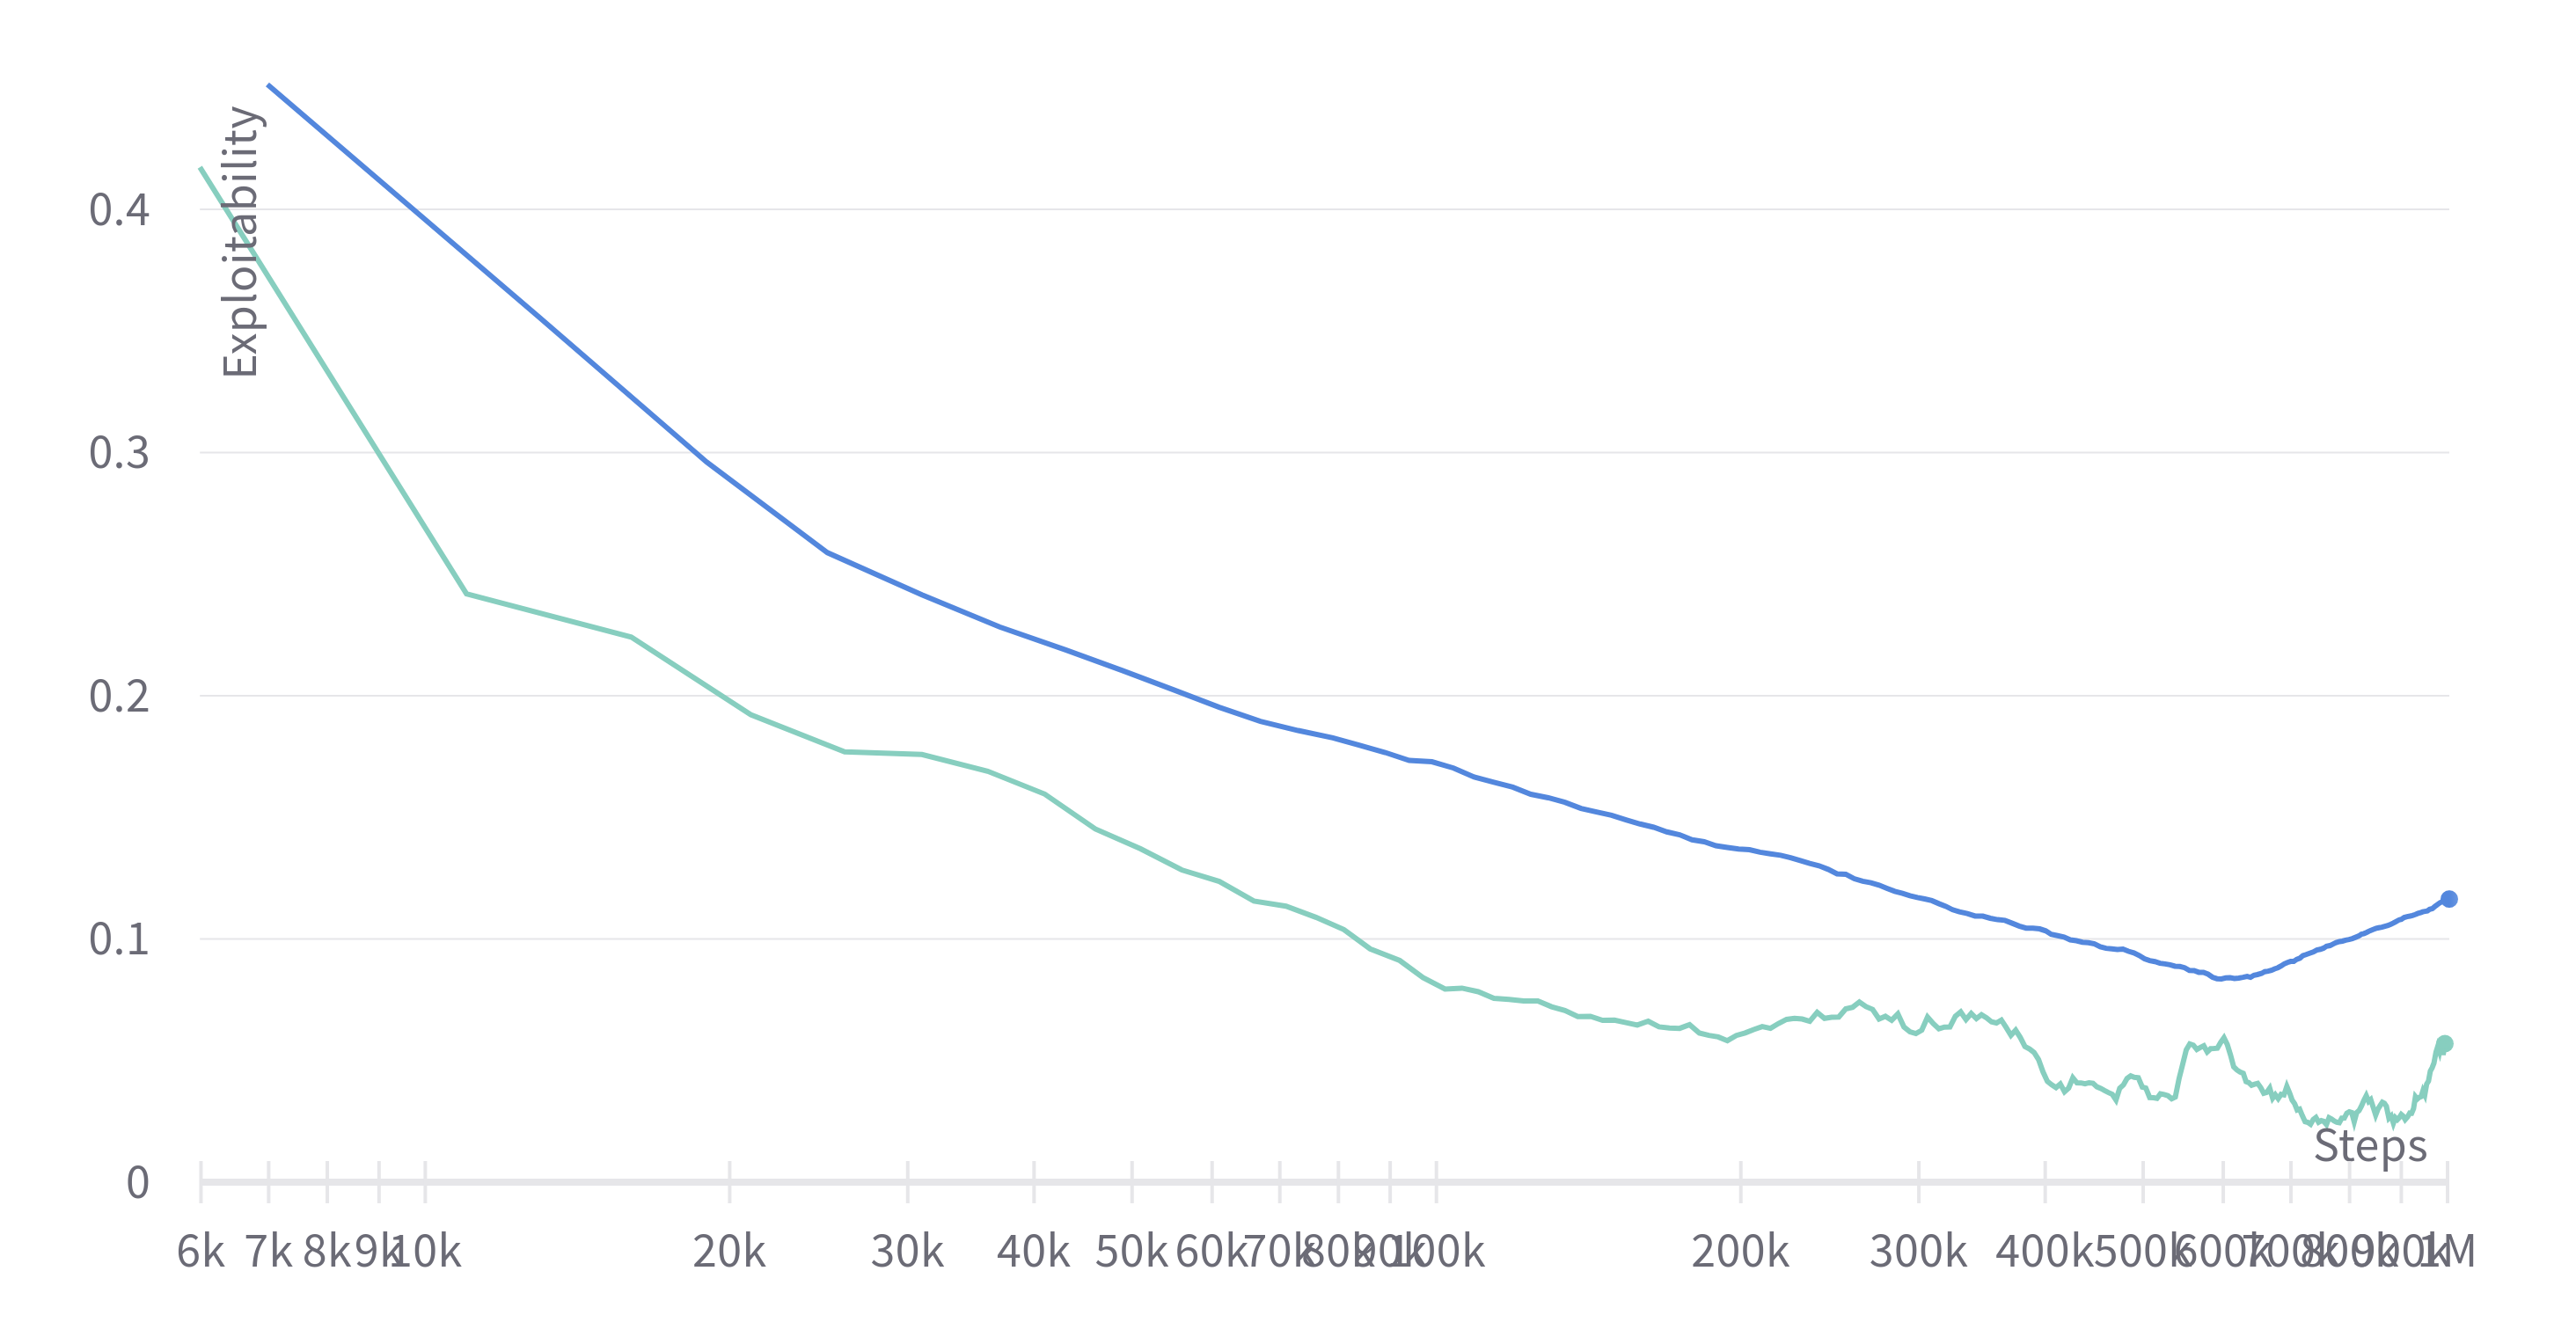
\includegraphics[width=\textwidth]{figs/kpoker.png}
		\caption{Kuhn Poker}
	\end{subfigure}
	\begin{subfigure}[b]{0.6\textwidth}
		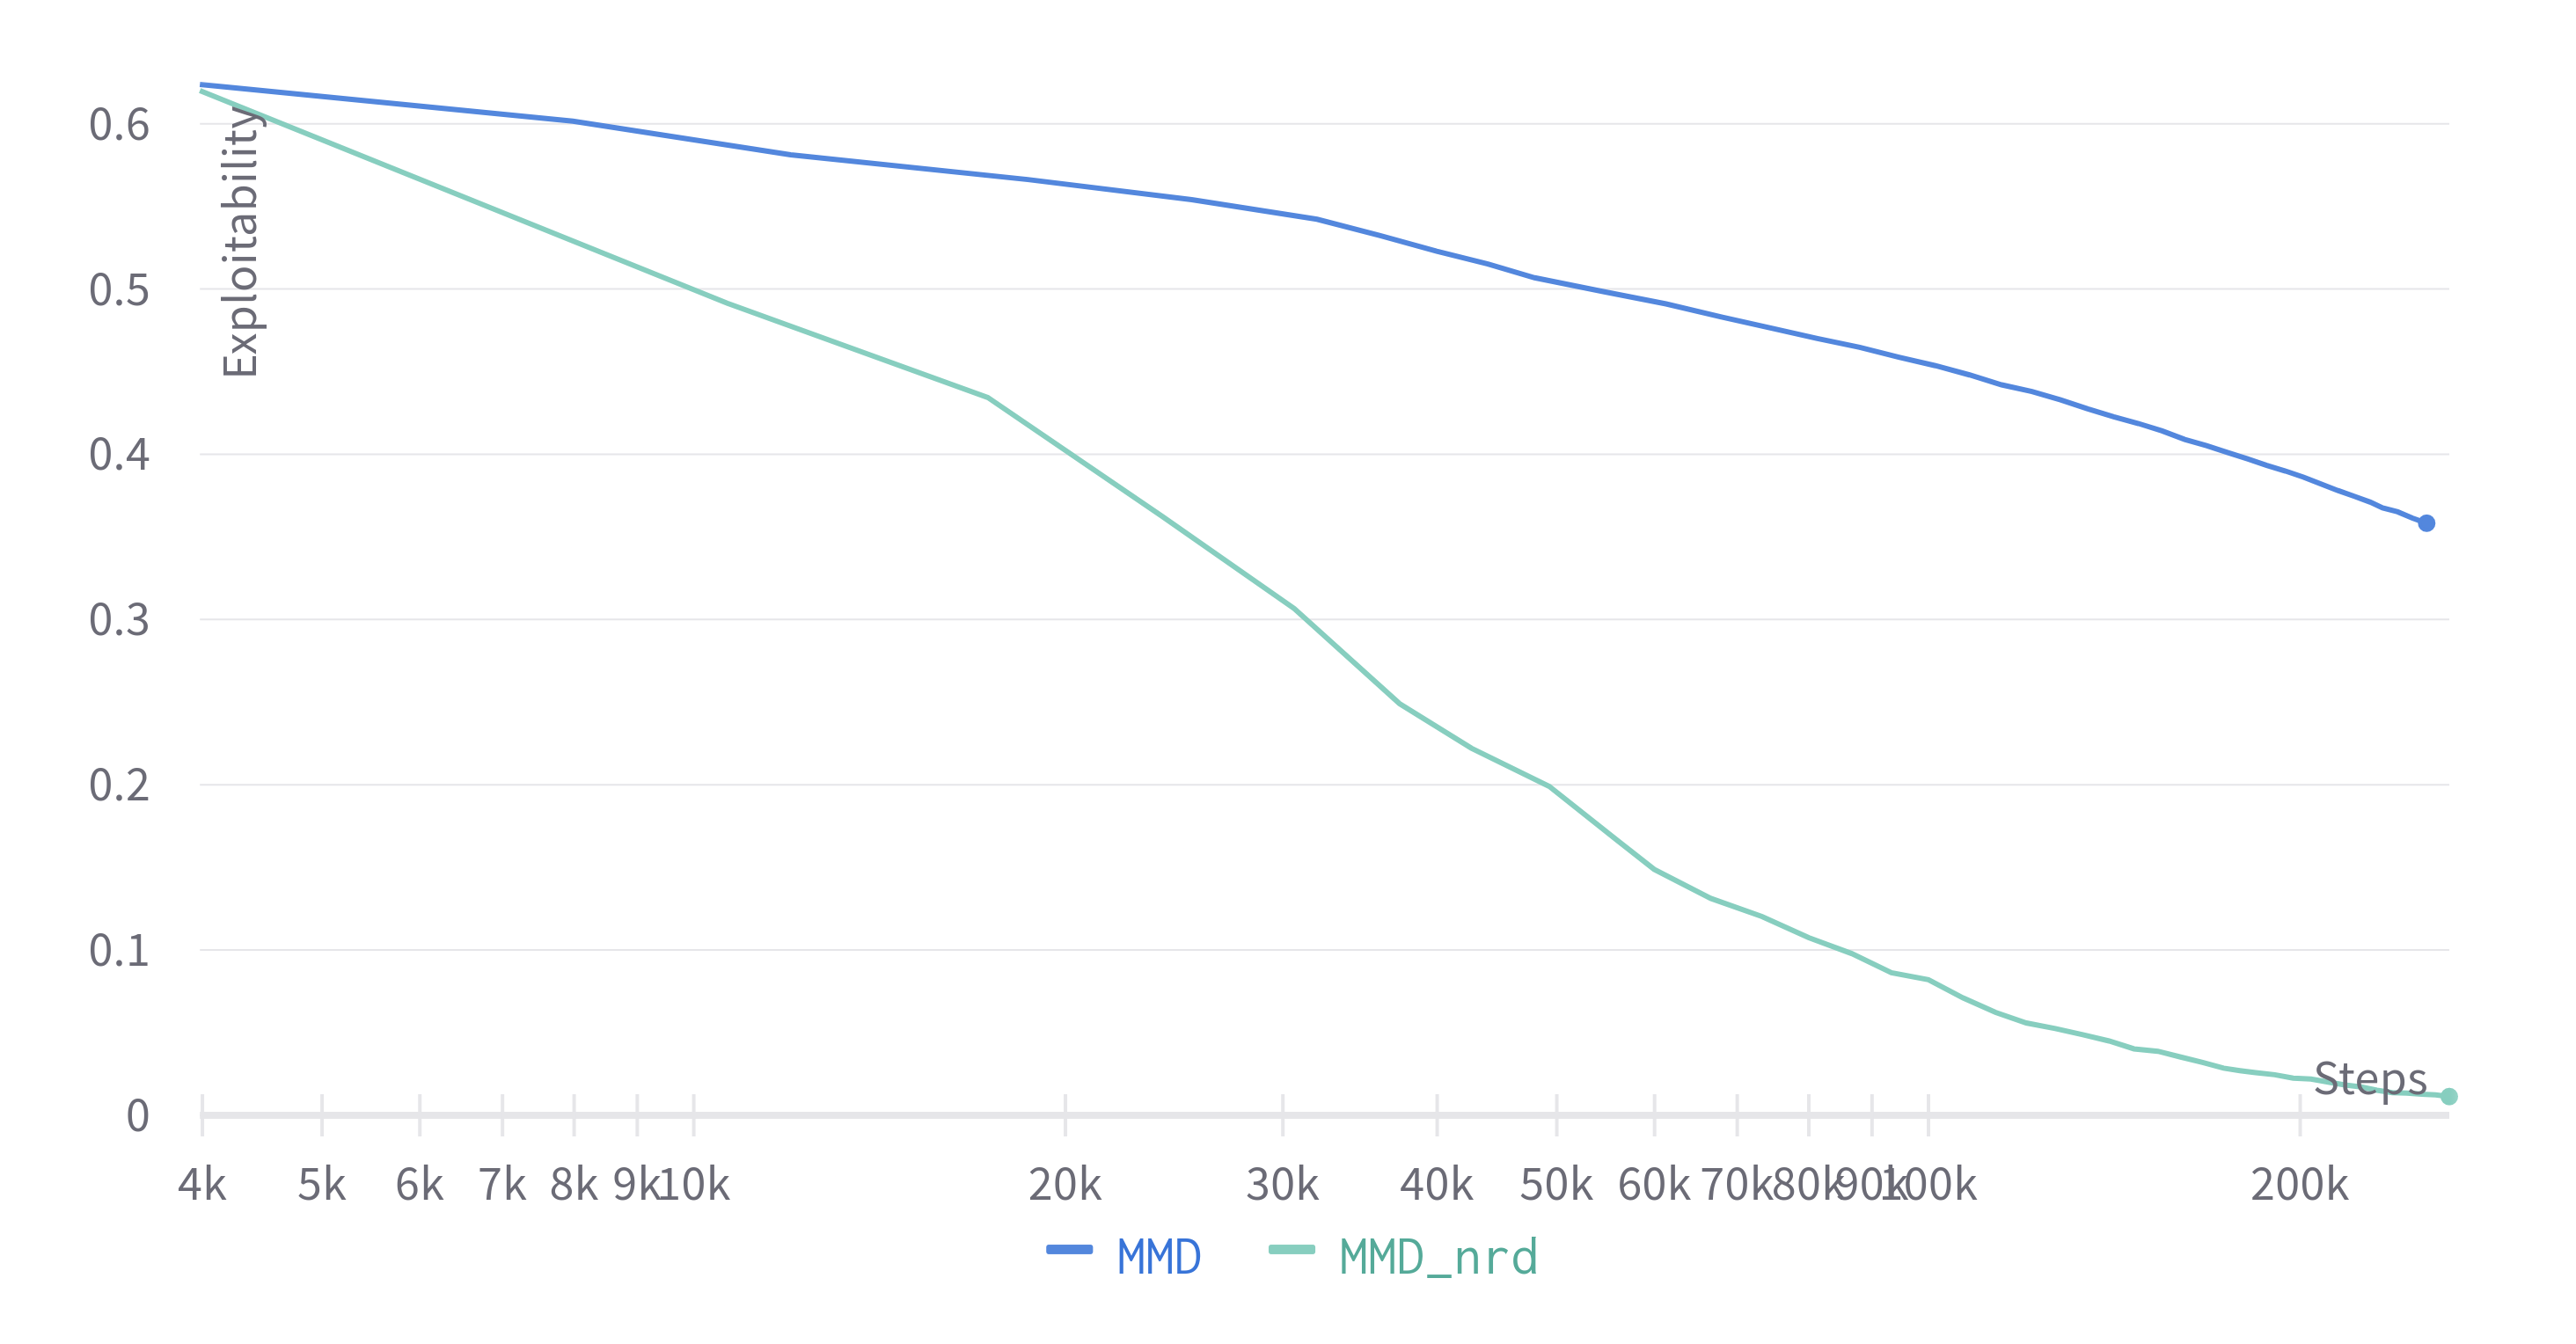
\includegraphics[width=\textwidth]{figs/ahex22.png}
		\caption{Abrupt Dark Hex (2$\times$2) (\red{1M steps version to be added})}
	\end{subfigure}
	\caption{Performance in small EFGs, measured by exact exploitability.}
	\label{fig:neuralsmall1}
\end{figure}

% We also compute approximate exploitability for the smaller games by training a DQN best-response
% agent for 1M steps against the fixed trained agents.

\ref{fig:neural2} shows improvement in performance by applying the NeuRD-fix in Abrupt Dark Hex
(3$\times$3) and Phantom TTT, as measured by the approximate exploitability.
\begin{figure}[H]
	\centering
	\begin{subfigure}[b]{0.4\textwidth}
		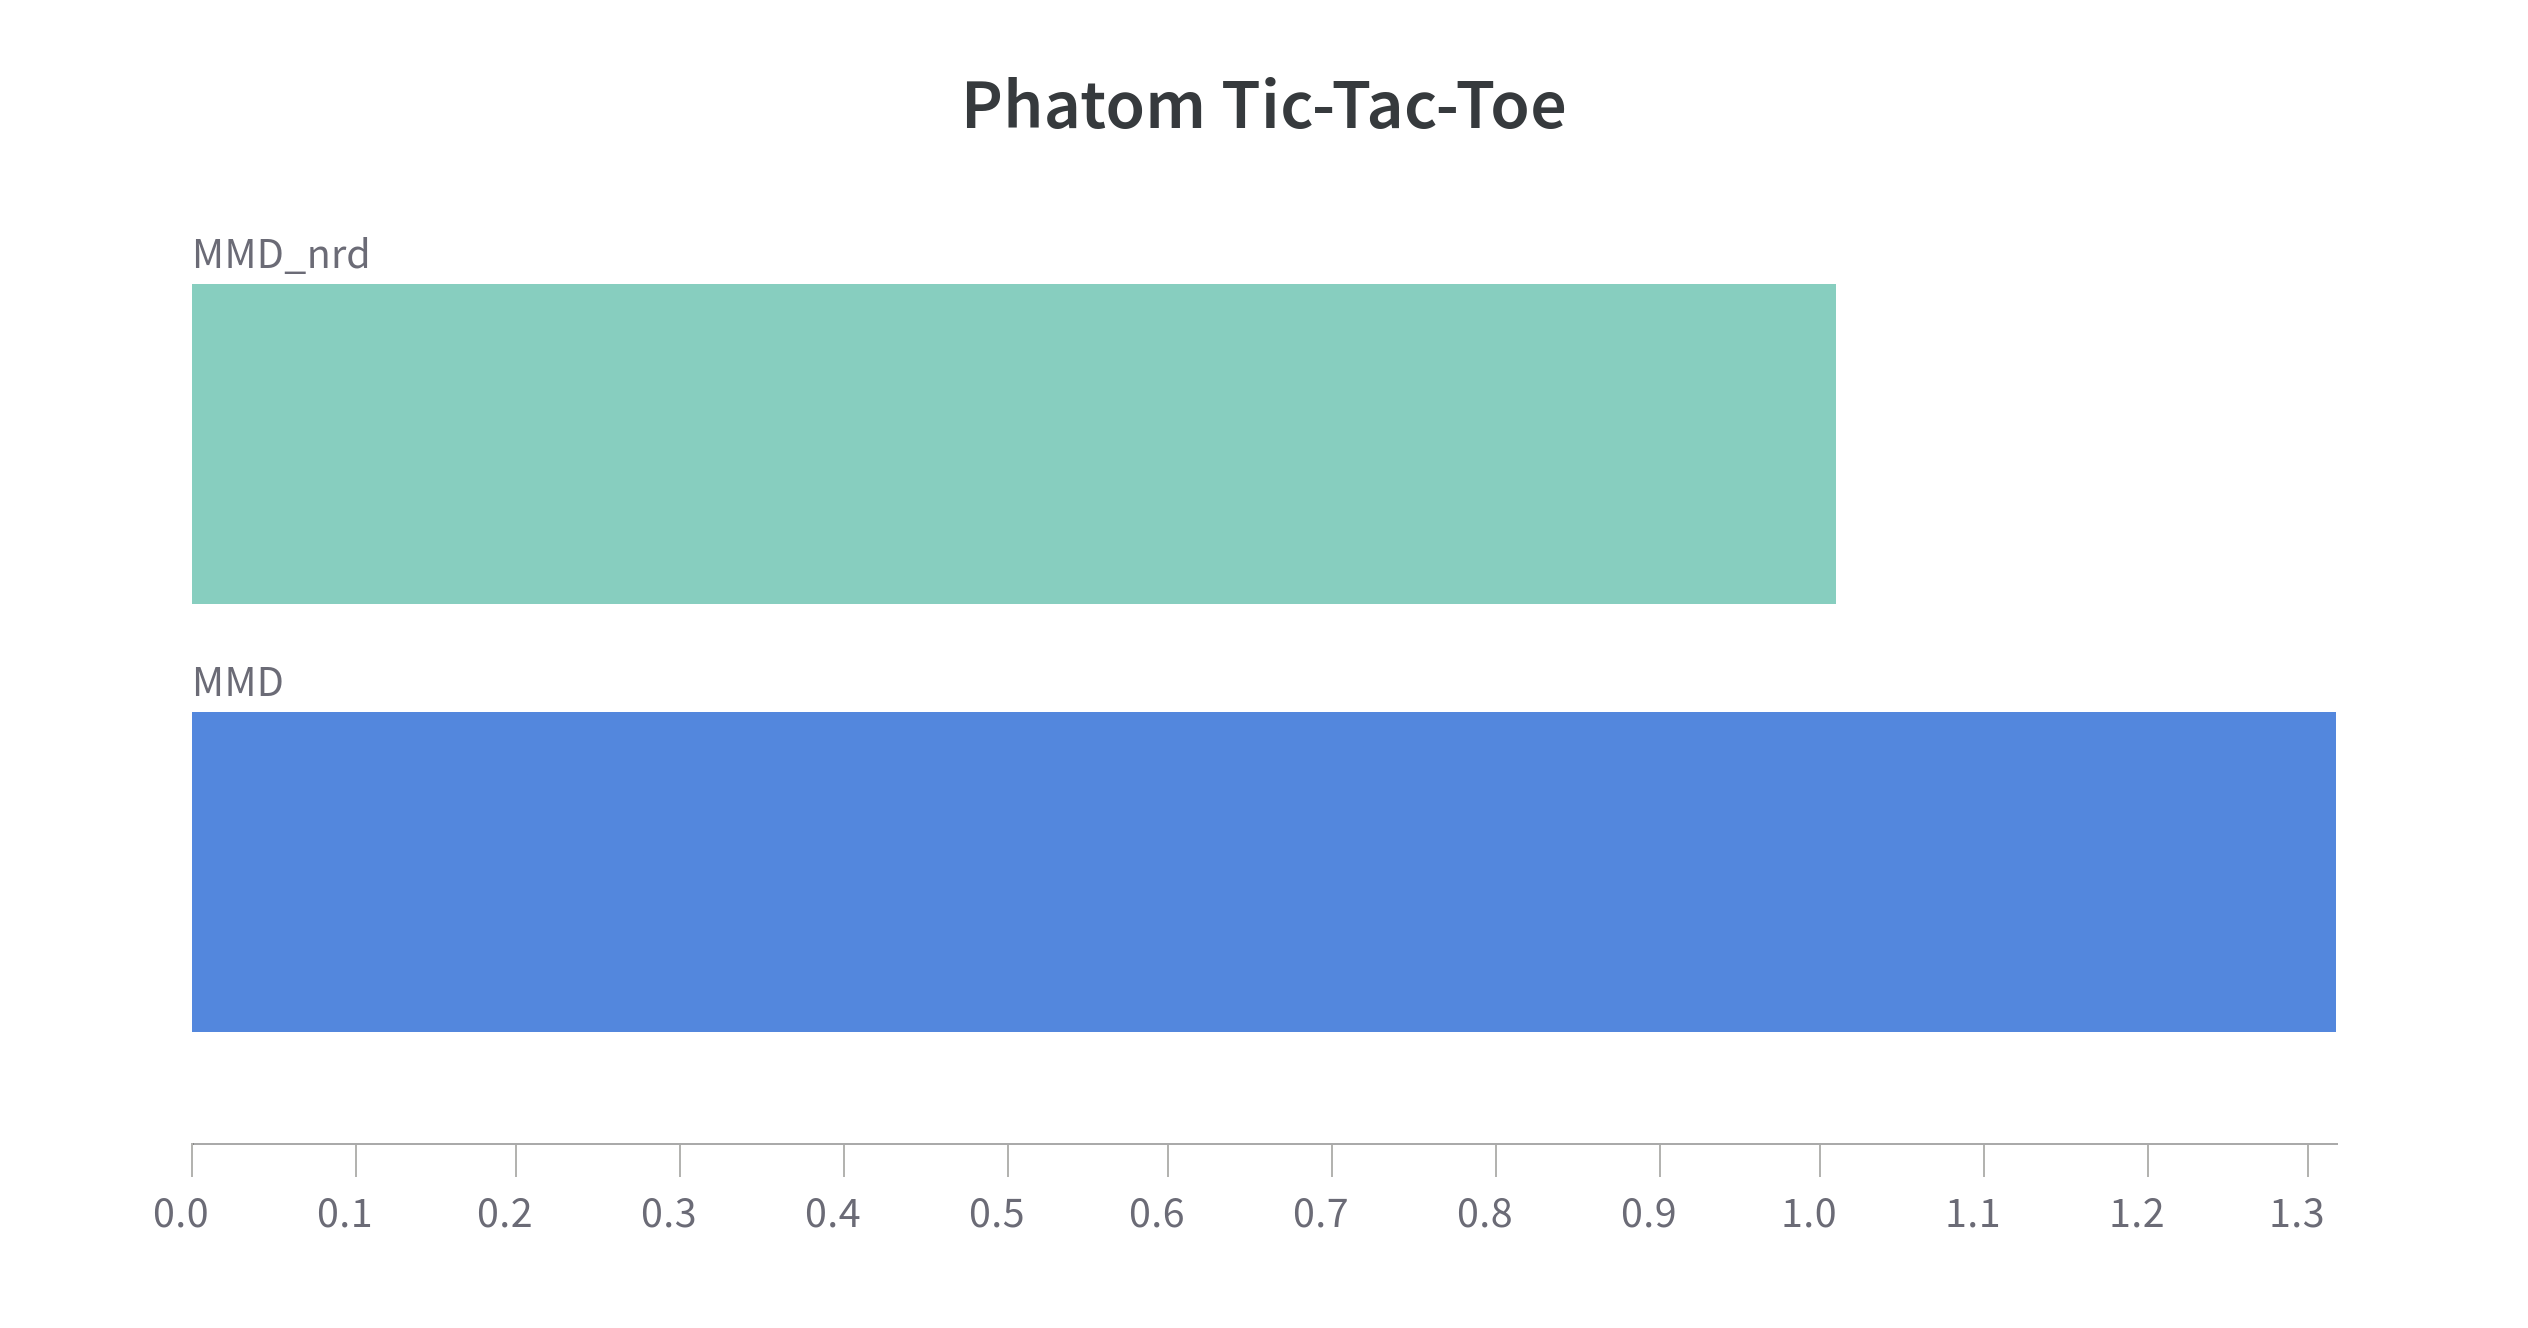
\includegraphics[width=\textwidth]{figs/pttt.png}
		\caption{Kuhn Poker}
	\end{subfigure}
	\begin{subfigure}[b]{0.4\textwidth}
		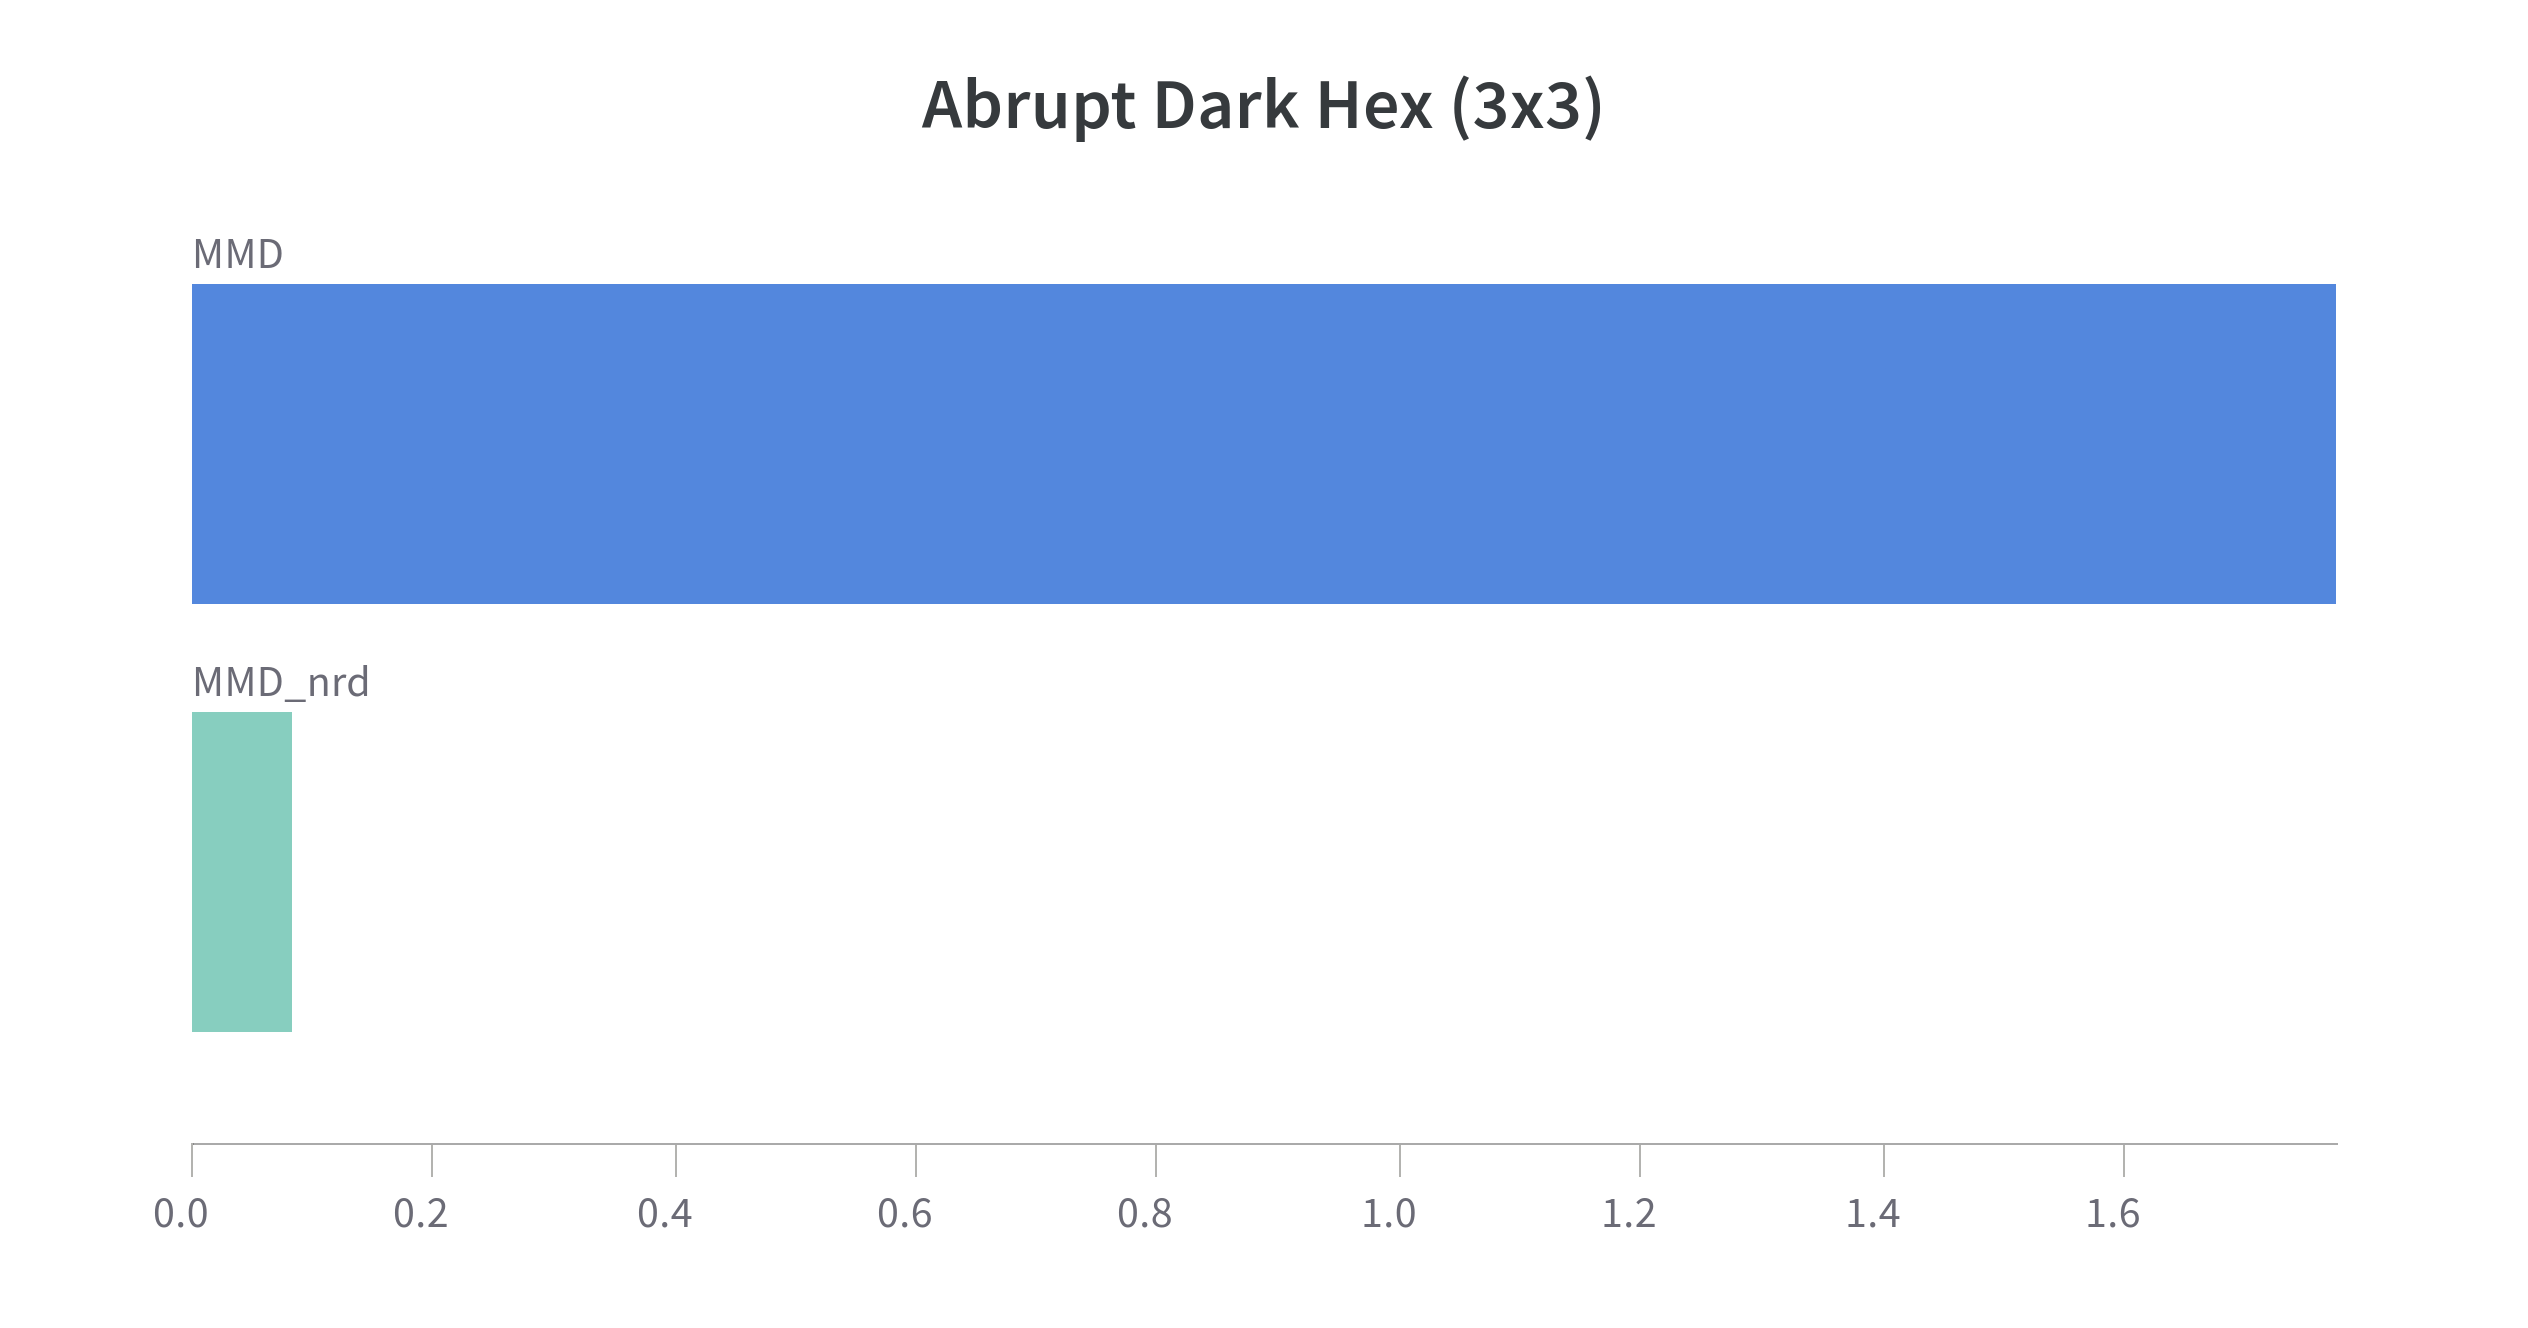
\includegraphics[width=\textwidth]{figs/ahex33.png}
		\caption{Abrupt Dark Hex (3$\times$3)}
	\end{subfigure}
	\caption{Performance in larger EFGs, measured by approximate exploitability.}
	\label{fig:neural2}
\end{figure}

\fillin{We also evaluate these algorithms by having the trained agents play against each other in a
	head-to-head manner.}
\chapter{Discussion}

\textbf{NeuRD-fix:}
The NeuRD-loss has also been previously applied on top of algorithms to improve performance or
induce convergence in competitive and cooperative settings.
Chhablani et.al,~\cite{chhablaniCounterfactual2021} showed improved performance in
identical-interest games by applying the NeuRD fix to COMA~\cite{foersterCounterfactual2018}.
Perolat et.al,~\cite{perolatMastering2022} used NeuRD loss to approximate Replicator dynamics as a
part of the DeepNash algorithm.
They used the same reward transformation based adaptive regularization~\cite{perolatPoincare2021}
to induce last-iterate convergence in training agents for the game of Stratego.
The improved performance of adapting the NeuRD-fix with mirror-descent based methods, and other
techniques for last-iterate convergence is also evident from our experimental evaluations.
Through this, we reinforce the idea that the NeuRD-loss can be more generally adapted into loss
functions of various algorithms in multi-agent settings.
\blue{is there a benefit to adding NeuRD in single-agent setting? even if the reward function is not dynamic.}
\\

\textbf{Entropy Regularization:}
As noted in the tabular experiments, and as observed from the performance of MDPO in the deep MARL
experiments, there exist faster methods to induce last-iterate convergence that adaptive
regularization.
\\

\textbf{Trust-region constraints:}
Trust-region constraints form the basis of state-of-the-art RL algorithms like PPO.
The presence of a relatively strongly-convex proximal operator is necessary for deriving algorithms
with strong performance guarantees.


\chapter{Conclusion}


% 
\newtheorem{theorem}{Theorem}


\chapter{Derivations}

\section{Online Learning}


\subsection{FoReL}


\section{Online Mirror Descent}


The FoReL update rule is,

\begin{align*}
    w_{t+1} &= argmin_w R(w) + \sum_{i=1}^t \langle w, z_t \rangle \\
            &= argmin_w R(w) + \langle w, z_{1:t}\rangle \\
            &= argmax_w \langle w, -z_{1:t} \rangle - R(w)    
\end{align*}

Let $g(\theta) = argmax_w \langle w, \theta \rangle - R(w)$. Then the FoReL update rule can 
be written as,

\begin{align*}
    \theta_{t+1} = \theta_t - z_t
    w_{t+1} = g(\theta_{t+1})
\end{align*}

where $g(\theta)$ is a link function that projects the predictions back to the convex set $S$.

Using different regularization functions yield different algorithms that have different regret bounds.

\begin{theorem}
    If R is a $(\frac{1}{\eta})$-strongly-convex function over $S$ with respect to some norm $\|.\|$, and OMD 
    is run on a sequence with the following link function

    $$g(\theta) = argmax_w (\langle w, \theta \rangle - R(w))$$

    then,

    $$\forall u \in S, Regret_T(u) \leq R(u) - min_{v \in S} R(v) + \eta \sum_{t=1}^T \|z\|_*^2$$

    where $\|.\|_*$ is the dual norm.
\end{theorem}


\subsection{Hedge}


Hedge or normalized Exponentiated Gradient is OMD with entropic regularization. The link function here is

\begin{equation}
    g_i(\theta) = \frac{e^{\eta \theta[i]}}{\sum_j e^{\eta \theta[j]}}.
\end{equation}

Fitting this into the OMD framework yields the following update rule,

\begin{align*}
    w_{t+1}[i] = \frac{w_t[i] e^{-\eta z_t[i]}}{\sum_j w_t[j] e^{-\eta z_t[j]}}
\end{align*}

We can analyze the regret bounds of Hedge with $R(w) = \frac{1}{\eta} \sum_i w[i] log(w[i])$. 


It is also useful to analyze OMD with the language of duality. The framework utilizing duality makes it easier 
in deriving new algorithms and also in proving tighter regret bounds.

\subsection{Fenchel Conjugacy}

The Fenchel conjugate of a function $f$ is defined as,

$$f^*(\theta) = max_u \langle u, \theta \rangle - f(u)$$

Fenchel conjugate by definition implies the Fenchel-Young inequality:

$$\forall u, f^*(\theta) \geq \langle u, \theta \rangle - f(u)$$.

If $u$ is a sub-gradient of $f^*$ at $\theta$ and if $f^*$ is differentiable, then the equality 
condition holds when $u = \nabla f^*(\theta)$. 


\subsection{Bergman Divergences}

For a differentiable function $R$, the Bergman divergence between two vectors is defined as,

\begin{equation}
    D_R(w \| u) = R(w) - R(u) + (\langle R(u), w-u \rangle)
\end{equation}

Bergman divergence is asymmetric and is always non-negative if R is convex.

\subsection{Online Mirror Descent in terms of Duality}

The link function in the OMD framework is defined as,

$$g(\theta) = argmax_w (\langle w, \theta \rangle - R(w)).$$

This can be also rewritten in terms of the conjugate of $R$ as,

$$g(\theta) = \nabla R^*(\theta)$$

With this, we can obtain different algorithms by using different regularization functions and deriving 
the update rules by using their conjugate.

\subsection{KL-Divergence and its Fenchel Conjugate}

KL-Divergence is a distance metric between two probability distributions and is defined as,

$$D_{KL}(p \| q) = \sum_i p[i] log \frac{p[i]}{q[i]}$$


% TODO: Derivation of the fenchel conjugate
The Fenchel Conjugate of KL-Divergence is given by,

$$f^*_q(x) = \log (\sum_i q_i e^{x_i}).$$


\section{MDPO}

The on-policy MDPO update rule is written as,

$$\theta_{k+1} \leftarrow argmax_{\theta \in \Theta} \Psi(\theta, \theta_k)$$

where,

$$\Psi(\theta, \theta_k) = \mathbb{E}_{s \sim \rho_{\theta_{k}}} [\mathbb{E}_{a \sim \pi_{\theta}}[A^{\theta_k}(s, a)] - \frac{1}{t_k} KL(s; \pi_{\theta}, \pi_{\theta_k})]$$


The gradient of the above update rule is as follows:

\begin{align*}
    \nabla_{\theta} \Psi(\theta, \theta_k) |_{\theta=\theta_k}
                                    &= \mathbb{E}_{s \sim \rho_{\theta_k}} [\sum_a \nabla_{\theta} \pi_{\theta} (a|s) A^{\theta_k}(s, a)] \\
                                    &= \mathbb{E}_{s \sim \rho_{\theta_k}} [\sum_a \pi_{\theta_k}(a|s) \frac{\nabla_{\theta} \pi_{\theta}(a|s)}{\pi_{\theta_k}(a|s)}  A^{\theta_k}(s, a)] \\
                                    &= \mathbb{E}_{s \sim \rho_{\theta_k}, a \sim \pi_{\theta_k}} [\nabla \log \pi_{\theta_k} (a|s) A^{\theta_k}(s,a)]
\end{align*}

For one-step MDPO, the gradient of the KL-Divergence term becomes 0. Hence it is proposed that the policy update at each iteration $k$ is done through $m$ steps of SGD.

$${\theta_k^{(0)} = \theta_k},$$

$$\theta_k^{(i+1)} \leftarrow \theta_k^{(i)} + \eta \nabla_{\theta} \Psi(\theta, \theta_k)|_{\theta=\theta_k^{(i)}}$$

and, $\theta_{k+1} = \theta_k^{(m)}$.


Then the gradient of the objective function evaluated at each step of the SGD update is,

\begin{align*}
    \nabla_{\theta} \Psi(\theta, \theta_k)|_{\theta = \theta_k^{(i)}} &=
                    \mathbb{E}_{s \sim \rho_{\theta_k}, a \sim \pi_{\theta_k}}[\frac{\pi_{\theta_k}^{(i)}}{\pi_{\theta_k}} \nabla \log \pi_{\theta_k^{(i)}} (a|s) A^{\theta_k}(s,a)] \\
                    &- \frac{1}{t_k} \mathbb{E}_{s \sim \rho_{\theta_k}}[\nabla_{\theta} KL(s; \pi_{\theta}, \pi_{\theta_k})|_{\theta = \theta_k^{(i)}}].
\end{align*}


$$KL(s; \pi_{\theta}, \pi_{\theta_k}) = \sum_{a \in \mathcal{A}} \pi_{\theta_k^{(i)}}(a|s) \log \frac{\pi_{\theta_k^{(i)}}(a|s)}{\pi_{\theta_k}(a|s)}$$

The gradient of the KL-Divergence term is given by,

\begin{align*}
    \nabla_{\theta} KL(s; \pi_{\theta}, \pi_{\theta_{k}})|_{\theta = \theta_{k}^{(i)}} 
    &= \sum_{a \in \mathcal{A}} [\nabla_{\theta_{k}^{(i)}} (\pi_{\theta_k^{(i)}}(a|s) \log \pi_{\theta_k}^{(i)}(a|s)) - \nabla_{\theta_k^{(i)}} (\pi_{\theta_k^{(i)}}(a|s) \log \pi_{\theta_k}(a|s))] \\
    &= \log \pi_{\theta_k^{(i)}}(a|s) \nabla_{\theta_{k}^{(i)}} \pi_{\theta_k^{(i)}}(a|s) + \nabla_{\theta_{k}^{(i)}} \pi_{\theta_k^{(i)}}(a|s) - \log \pi_{\theta_{k}}(a|s) \nabla_{\theta_{k}^{(i)}} \pi_{\theta_{k}^{(i)}}(a|s)\\
    &= \sum_{a \in \mathcal{A}} [(\log \pi_{\theta_{k}}^{(i)}(a|s) + 1 - \log \pi_{\theta_k}(a|s)) \nabla_{\theta_{k}^{(i)}}{\pi_{\theta_k^{(i)}}}(a|s)].
\end{align*}



As for the first term of the gradient, it can be seen that the gradient includes a term to account for the fact that the action $a$ was sampled from the policy $\pi_{\theta_k}$

\begin{align*}
    \nabla_{\theta} \Psi(\theta, \theta_k)|_{\theta = \theta_k^{(i)}}
        &= \mathbb{E}_{s \sim \rho_{\theta_k}} [\sum_a \nabla_{\theta_k^{(i)}} \pi_{\theta_k^{(i)}}(a|s) A^{\theta_k}(s, a)] \\
        &= \mathbb{E}_{s \sim \rho_{\theta_k}} [\sum_a \pi_{\theta_k}(a|s) \frac{\pi_{\theta_k^{(i)}}(a|s)}{\pi_{\theta_k}(a|s)} \frac{\nabla_{\theta_k^{(i)}} \pi_{\theta_k^{(i)}}(a | s)}{\pi_{\theta_k^{(i)}}(a|s)} A^{\theta_k}(s, a)] \\
        &= \mathbb{E}_{s \sim \rho_{\theta_k}, a \sim \pi_{\theta_k}} [\frac{\pi_{\theta_k^{(i)}}(a|s)}{\pi_{\theta_k}(a|s)} \nabla_{\theta_k^{(i)}} \log \pi_{\theta_k^{(i)}}(a | s) A^{\theta_k}(s, a)]
\end{align*}


































































% %\documentclass{article}

%\usepackage{dsfont}
%\usepackage{amsfonts}

%\begin{document}

%\title{Derivations for the main thesis}

\newtheorem{definition}{Definition}
\newtheorem{lemma}{Lemma}

\chapter{Online Learning and Online Convex Optimization}

\section{Online Learning}

Online Learning is a sub-domain of machine learning that has important theoretical and practical applications. 
In Online Learning, a learner is tasked with predicting the answer to a set of questions over a sequence of consecutive rounds.
At each round t, a question $x_t$ is taken from an instance domain $\mathcal{X}$, and the learner is required to predict 
an answer, $p_t$ to this question. After the prediction is made, the correct answer $y_t$, from a target domain $\mathcal{Y}$ 
is revealed and the learner suffers a loss $l(p_t, y_t)$. The prediction $p_t$ could belong to $\mathcal{Y}$ or a larger set, 
$\mathcal{D}$.

There are many special cases of Online learning that translate to popular Online learning problems. Some common ones are,

Online Classification: $\mathcal{Y}=\mathcal{D}=\{0,1\}$, and typically the loss function is the 0-1 loss: $l(p_t, y_t)=|p_t - y_t|$.

Online Regression:

Expert's case:


The goal of an Online learning algorithm is to minimize the cumulative loss across all the rounds it has been through so far.
The learner uses the information from the previous rounds to improve its prediction on present and future rounds.

The sequence of questions can be deterministic, stochastic or even adversarial. This means, for any online learning algorithm 
an adversary can make the cumulative loss unbounded, by simply providing an opposing answer to the algorithm's answer as the correct 
answer. To make learning possible, certain restrictions are imposed on the structure of the problem.

Realizability: It is assumed that the answers are generated by a target mapping $h^*: \mathcal{X} \rightarrow \mathcal{Y}$, and that $h^*$ is 
taken from a fixed set, $\mathcal{H}$ called the hypothesis class. Now, for any Online learning algorithm, A, $M_A(\mathcal{H})$ is the number 
of mistakes $A$ makes on a sequence of questions, labelled by some $h^* \in \mathcal{H}$. $M_A(\mathcal{H})$ is called the $\textit{mistake-bound}$ 
of $A$.

A relaxation from realizable assumption is that the answers are not generated by some fixed mapping $h^*$, but the learner is still only required 
to be competitive with the best fixed predictor from $\mathcal{H}$. This is the regret of an Online learning algorithm for not having followed a 
fixed hypothesis $h^* \in \mathcal{H}$.

\begin{equation}\label{eqn_regretdef}
    Regret_T(h^*) = \sum_{t=1}^T l(p_t, y_t) - \sum_{t=1}^T l(h^*(x_t), y_t),
\end{equation}

The regret of $A$ with $\mathcal{H}$ is,

\begin{equation}\label{eqn_regretdef}
    Regret_T(\mathcal{H}) = max_{h^* \in \mathcal{H}} Regret_T(h^*)
\end{equation}


\section{Online Convex Optimization}

An established approach to design efficient online learning algorithm has been using convex optimization. This typically frames online learning as an 
online convex optimization problem as follows:

input: a convex set S
for t = 1, 2. $\ldots$
predict a vector $w_t \in S$
receive a convex loss function $f_t: S \mapsto \mathbb{R}$

Reframing \ref{eqn_regretdef} in terms of convex optimization, we refer to a competing hypothesis here as some vector $u$ from the convex set $S$.

\begin{equation}
    Regret_T(u) = \sum_{t=1}^T f_t(w_t) - \sum_{t=1}^T f_t(u)
\end{equation}

and similarly, the regret with respect to a set of competing vectors $U$ is,
\begin{equation}
    Regret_T(U) = max_{u \in U} Regret_T(u)
\end{equation}

As stated in the case of online learning, the set $U$ can be same as $S$ or different in other cases. In this work, the default setting is $U=S$ and 
$S=\mathbb{R^d}$ unless specified otherwise.

% Convexification can be added here briefly

\subsection{FoReL}

Follow-the-Regularized-leader (FoReL) is a classic learning algorithm for online convex optimization, where the algorithm tries to minimize the loss on 
all past rounds along with a regularization term. The regularization term is used to stabilize the solution and prevent it from oscillating too much every 
round preventing converging to a solution.

The learning rule can be written as,

$$\forall t, w_t = argmin_{w \in S} \sum_{i=1}^{t-1} f_i(w) + R(w).$$

where $R(w)$ is the regularization term. Different regularization functions lead to different algorithms with varying regret bounds.


In the case of linear loss functions with respect to some $z_t$, i.e., $f_t(w) = \langle w, z_t \rangle$, and $S=\mathbb{R}^d$,  if FoReL is run with 
$l_2$-norm regularization $R(w) = \frac{1}{2 \eta} \|w\|_2^2$ , then the learning rule can be written as,

\begin{equation}
    w_{t+1} = -\eta \sum_{i=1}^t z_i = w_t - \eta z_t
\end{equation}

Since, $\nabla f_t(w_t) = z_t$, this can also be written as, $w_{t+1} = w_t - \eta \nabla f_t(w_t)$. This update rule is also commonly known as Online Gradient Descent.
The regret of FoReL run on Online linear optimization with a euclidean-norm regularizer is:

$$Regret_T(U) \leq BL \sqrt {2T}.$$

where $U = {u : \|u\| \leq B}$ and $\frac{1}{T} \sum_{t=1}^T \|z_t\|_2^2 \leq L^2$ with $\eta = \frac{B}{L\sqrt{2T}}$.

This can also be generalized to Convex Functions in general through linearization using the property of convex functions. For a convex set S, a convex function $f: S \mapsto \mathbb{R}$ is convex iff $\forall w \in S, \exists z$ such that,

\begin{equation}
    \forall u \in S, f(u) \leq f(w) + \langle u-w, z \rangle  
\end{equation}

Following this, in Online Convex Optimization for each round $t$, there exists a $z_t$ such that for all competing hypothesis $u$, 

$$f_t(w_t) - f_t(u) \leq \langle w_t - u, z_t \rangle.$$

where $z_t \in \partial f_t(w_t)$ is a sub-gradient of $f_t$ at $w_t$.

Then, for a sequence of convex loss functions $f_1, \ldots, f_T$ and vectors $w_1, \ldots, w_T$ and if for all $t$, $z_t \in \partial f_t(w_t)$,

\begin{equation}
    \sum_{t=1}^T (f_t(w_t) - f_t(u)) \leq \sum_{t=1}^T (\langle w_t, z_t\rangle - \langle u, z_t \rangle)
\end{equation}

This implies, the regret of an algorithm for Online Convex Optimization is upper bounded by the regret with respect to the linearization of the 
sequence of convex functions.

% Add details about theorem 2.4 and discuss about the requirement of the norm of z_t to be bounded by L, and how it relates to the lipschitzness of the loss function

Beyond Euclidean regularization, FoReL can also be run with other regularization functions and yield similar regret bounds given that the regularization functions are 
strongly convex.

\begin{definition}
    For any $\sigma$-strongly-convex function $f: S \mapsto \mathbb{R}$ with respect to a norm $\|.\|$, for any $w \in S$,
    \begin{equation}
        \forall z \in \partial f(w), \forall u \in S, f(u) \geq f(w) + \langle z, u - w\rangle + \frac{\sigma}{2}\| u - w \|^2.
    \end{equation}
\end{definition}


% Lemma 2.3 to be shifted above

\begin{lemma}\label{lem:forelrb}
    For a FoReL algorithm producing a sequence of vectors $w_1, \ldots, w_T$ with a sequence of loss functions $f_1, \ldots, f_T$, for all $u \in S$, 
    $$\sum_{t=1}^T (f_t(w_t) - f_t(u)) \leq R(u) - R(w_1) + \sum_{t=1}^T (f_t(w_t) - f_t(w_{t+1}))$$
\end{lemma}

\subsection{FoReL with Strongly Convex Regularizers}
From Lemma \ref{lem:forelrb}, the regret bound is given by,

$$\sum_{t=1}^T (f_t(w_t) - f_t(u)) \leq R(u) - R(w_1) + \sum_{t=1}^T (f_t(w_t) - f_t(w_{t+1}))$$

If $f_t$ is $L$-Lipschitz with respect to some norm $\|.\|$ then,

$$f_t(w_t) - f_t(u) \leq L \| w_t - w_{t+1} \|$$

If $\| w_t - w_{t+1} \|$ is small that leads to a better regret bound. It can be shown that if the regularization function $R(w)$ is strongly convex with 
respect to the same norm $\|.\|$ then $\|w_t - w_{t+1}\|$ is also bounded.

For a sequence of predictions $w_1, w_2, \ldots$ of the FoReL algorithm, with a regularizer $R: S \mapsto \mathbb{R}$,

$$f_t(w_t) - f_t(w_{t+1}) \leq L_t \|w-t - w_{t+1} \| \leq \frac{L_t^2}{\sigma}.$$

if $f_t$ is $L$-Lipschitz with respect to $\|.\|$ and $R$ is $\sigma$-strongly-convex.

\begin{theorem}\label{thm:forelregret}
    FoReL run on a sequence of convex functions $f_1, \ldots, f_T$ such that $f_t$ is $L_t$-Lipschitz, with a $\sigma$-strongly-convex regularization function 
    has a regret bound given by, 

    $$Regret_T(u) \leq R(u) - min_{v \in S} R(v) + \frac{TL^2}{\sigma}$$

    where $\frac{1}{T} \sum_{t=1}^T L_t^2 \leq L^2$.
\end{theorem}

\textcolor{red}{To add: derived regret bounds for euclidean and entropic regularizers}

\section{Online Mirror Descent}




% 

\begin{comment}
Mirror Descent:

Mirror descent with entropy regularization

Mirror descent with KL Divergence regularizations 


Mirror Descent Policy optimization (MDPO)

The update rule for on-policy MDPO is given by,

$\theta_{k+1} \leftarrow argmax_{\theta \in \Theta \psi(\theta, \theta_k)}$

$\psi(\theta, \theta_k) = \mathds{E}_{s ~ \rho_{\theta_k}}[\mathds{E}_{a~\pi_{\theta}}[A^{\theta_k}(S, a)] - \frac{1}{t_k} \textrm{KL}(s; \pi_{\theta}, \pi_{\theta_k})]$

\end{comment}

%\end{document}

\appendices
\newpage
\appendix
\chapter{Some Ancillary Stuff}

Ancillary material should be put in appendices.

\chapter{Game descriptions}
\label{apx:gamedesc}

\textbf{Kuhn Poker}
Kuhn Poker is a smaller extensive form game that allows for more introspection and exact
exploitability computation.

\textbf{Abrupt Dark Hex}
Abrupt Dark Hex

\textbf{Phantom Tic-Tac-Toe} Phantom Tic-Tac-Toe (Phantom TTT)

\chapter{Implementation details}
\label{apx:impdet}

\chapter{Some More Ancillary Stuff}

% Here is yet another appendix! Wahoo!


%\nocite{*}
\bibformb
\bibliography{BibFile,Citations}
\newpage
% \vita
% This is where the vita goes.  Its organization is left as an exercise.

\end{document}